\documentclass[10pt,a4paper]{article}
\usepackage{iftex}
\ifPDFTeX\usepackage[utf8]{inputenc}\usepackage[T1]{fontenc}\usepackage{lmodern}
\else\usepackage{fontspec}\fi
\usepackage[margin=2cm]{geometry}\usepackage{longtable}\usepackage{array}
\usepackage{tikz}\usetikzlibrary{positioning,arrows.meta}
\usepackage{xurl}\usepackage[hidelinks]{hyperref}\usepackage{fancyvrb}
\setlength{\parskip}{4pt}\setlength{\parindent}{0pt}
\tikzset{>={Latex}}
\title{Literature search report -- run 20260828T100120}\author{scitech-librarian 3.1}\date{\today}
\begin{document}\maketitle
Generated by scitech-librarian 3.1 (report level: full). Every number below is reproducible from the archived run directory \texttt{20260828T100120}.

{\scriptsize\begin{longtable}{p{0.306\linewidth}p{0.634\linewidth}}
\hline
\textbf{Item} & \textbf{Value} \\ \hline
\endhead
Run started & 2026-08-28 10:01:20 \\
Duration & 128 s \\
Query file & queries.example.json \\
Blocks & PSC, MLP, NOV, QC \\
Backends & openalex, arxiv, inspire, semanticscholar, ads, scopus \\
Mode & full fetch, up to 300 records per block and backend \\
Non-curated venue filter & on \\
Open-access lookup & not run \\
Interrupted & no \\
\hline
\end{longtable}}
\section*{Search strategy}
Each block is one structural query -- a conjunction of synonym groups, (a OR b) AND (c OR d) -- rendered into every backend's native grammar. The strings below are exactly what was sent (PRISMA-S item 8).

\subsection*{Block PSC: Perovskite solar cell degradation under humidity}
Purpose: grounding block -- expect thousands of hits; use it to sanity-check that every backend is reachable and the counts are plausible

\begin{Verbatim}[fontsize=\scriptsize]
(perovskite solar cell OR halide perovskite photovoltaic) AND (degradation OR stability OR encapsulation)
 AND (humidity OR moisture OR water ingress)
\end{Verbatim}
{\scriptsize\begin{longtable}{p{0.215\linewidth}p{0.725\linewidth}}
\hline
\textbf{Backend} & \textbf{Query string sent} \\ \hline
\endhead
openalex & ("perovskite solar cell" OR "halide perovskite photovoltaic") AND (degradation OR stability OR encapsulation) AND (humidity OR moisture OR "water ingress") \\
arxiv & (all:"perovskite solar cell" OR all:"halide perovskite photovoltaic") AND (all:"degradation" OR all:"stability" OR all:"encapsulation") \\
inspire & ("perovskite solar cell" or "halide perovskite photovoltaic") and ("degradation" or "stability" or "encapsulation") and ("humidity" or "moisture" or "water ingress") \\
semanticscholar & ("perovskite solar cell" | "halide perovskite photovoltaic") + ("degradation" | "stability" | "encapsulation") + ("humidity" | "moisture" | "water ingress") \\
ads & (abs:"perovskite solar cell" OR abs:"halide perovskite photovoltaic") AND (abs:"degradation" OR abs:"stability" OR abs:"encapsulation") AND (abs:"humidity" OR abs:"moisture" OR abs:"water ingress") \\
scopus & TITLE-ABS-KEY("perovskite solar cell" OR "halide perovskite photovoltaic") AND TITLE-ABS-KEY(degradation OR stability OR encapsulation) AND TITLE-ABS-KEY(humidity OR moisture OR "water ingress") \\
\hline
\end{longtable}}
\subsection*{Block MLP: Machine-learned interatomic potentials for amorphous materials}
Purpose: a narrower intersection -- expect hundreds; good for testing record fetch and RIS export

\begin{Verbatim}[fontsize=\scriptsize]
(machine learning potential OR machine-learned interatomic potential OR neural network potential) AND 
(amorphous OR glass OR disordered solid) AND (molecular dynamics OR structure prediction)
\end{Verbatim}
arXiv receives groups {[}0, 1{]} only (nested-boolean limitation).

{\scriptsize\begin{longtable}{p{0.215\linewidth}p{0.725\linewidth}}
\hline
\textbf{Backend} & \textbf{Query string sent} \\ \hline
\endhead
openalex & ("machine learning potential" OR "machine-learned interatomic potential" OR "neural network potential") AND (amorphous OR glass OR "disordered solid") AND ("molecular dynamics" OR "structure prediction") \\
arxiv & (all:"machine learning potential" OR all:"machine-learned interatomic potential" OR all:"neural network potential") AND (all:"amorphous" OR all:"glass" OR all:"disordered solid") \\
inspire & ("machine learning potential" or "machine-learned interatomic potential" or "neural network potential") and ("amorphous" or "glass" or "disordered solid") and ("molecular dynamics" or "structure prediction") \\
semanticscholar & ("machine learning potential" | "machine-learned interatomic potential" | "neural network potential") + ("amorphous" | "glass" | "disordered solid") + ("molecular dynamics" | "structure prediction") \\
ads & (abs:"machine learning potential" OR abs:"machine-learned interatomic potential" OR abs:"neural network potential") AND (abs:"amorphous" OR abs:"glass" OR abs:"disordered solid") AND (abs:"molecular dynamics" OR abs:"structure prediction") \\
scopus & TITLE-ABS-KEY("machine learning potential" OR "machine-learned interatomic potential" OR "neural network potential") AND TITLE-ABS-KEY(amorphous OR glass OR "disordered solid") AND TITLE-ABS-KEY("molecular dynamics" OR "structure prediction") \\
\hline
\end{longtable}}
\subsection*{Block NOV: EXAMPLE NOVELTY CHECK: origami metamaterials as topological acoustic pumps}
Purpose: novelty-check pattern -- a SMALL number is the good outcome; read every hit by hand before claiming a gap

\begin{Verbatim}[fontsize=\scriptsize]
(origami OR kirigami) AND (acoustic metamaterial OR phononic crystal) AND (topological pumping OR 
Thouless pump OR edge state)
\end{Verbatim}
{\scriptsize\begin{longtable}{p{0.215\linewidth}p{0.725\linewidth}}
\hline
\textbf{Backend} & \textbf{Query string sent} \\ \hline
\endhead
openalex & (origami OR kirigami) AND ("acoustic metamaterial" OR "phononic crystal") AND ("topological pumping" OR "Thouless pump" OR "edge state") \\
arxiv & (all:"origami" OR all:"kirigami") AND (all:"acoustic metamaterial" OR all:"phononic crystal") \\
inspire & ("origami" or "kirigami") and ("acoustic metamaterial" or "phononic crystal") and ("topological pumping" or "Thouless pump" or "edge state") \\
semanticscholar & ("origami" | "kirigami") + ("acoustic metamaterial" | "phononic crystal") + ("topological pumping" | "Thouless pump" | "edge state") \\
ads & (abs:"origami" OR abs:"kirigami") AND (abs:"acoustic metamaterial" OR abs:"phononic crystal") AND (abs:"topological pumping" OR abs:"Thouless pump" OR abs:"edge state") \\
scopus & TITLE-ABS-KEY(origami OR kirigami) AND TITLE-ABS-KEY("acoustic metamaterial" OR "phononic crystal") AND TITLE-ABS-KEY("topological pumping" OR "Thouless pump" OR "edge state") \\
\hline
\end{longtable}}
\subsection*{Block QC: Quasicrystal photonics (arXiv-tuned example)}
Purpose: demonstrates arxiv\_groups: arXiv chokes on deeply nested booleans, so name the two groups it should get

\begin{Verbatim}[fontsize=\scriptsize]
(quasicrystal OR quasiperiodic lattice) AND (photonic OR waveguide OR optical lattice) AND (localization 
OR critical states OR fractal spectrum)
\end{Verbatim}
arXiv receives groups {[}0, 2{]} only (nested-boolean limitation).

{\scriptsize\begin{longtable}{p{0.215\linewidth}p{0.725\linewidth}}
\hline
\textbf{Backend} & \textbf{Query string sent} \\ \hline
\endhead
openalex & (quasicrystal OR "quasiperiodic lattice") AND (photonic OR waveguide OR "optical lattice") AND (localization OR "critical states" OR "fractal spectrum") \\
arxiv & (all:"quasicrystal" OR all:"quasiperiodic lattice") AND (all:"localization" OR all:"critical states" OR all:"fractal spectrum") \\
inspire & ("quasicrystal" or "quasiperiodic lattice") and ("photonic" or "waveguide" or "optical lattice") and ("localization" or "critical states" or "fractal spectrum") \\
semanticscholar & ("quasicrystal" | "quasiperiodic lattice") + ("photonic" | "waveguide" | "optical lattice") + ("localization" | "critical states" | "fractal spectrum") \\
ads & (abs:"quasicrystal" OR abs:"quasiperiodic lattice") AND (abs:"photonic" OR abs:"waveguide" OR abs:"optical lattice") AND (abs:"localization" OR abs:"critical states" OR abs:"fractal spectrum") \\
scopus & TITLE-ABS-KEY(quasicrystal OR "quasiperiodic lattice") AND TITLE-ABS-KEY(photonic OR waveguide OR "optical lattice") AND TITLE-ABS-KEY(localization OR "critical states" OR "fractal spectrum") \\
\hline
\end{longtable}}
\section*{Results summary}
{\scriptsize\begin{longtable}{p{0.073\linewidth}p{0.097\linewidth}p{0.073\linewidth}p{0.089\linewidth}p{0.154\linewidth}p{0.073\linewidth}p{0.081\linewidth}p{0.113\linewidth}p{0.105\linewidth}p{0.081\linewidth}}
\hline
\textbf{Block} & \textbf{openalex} & \textbf{arxiv} & \textbf{inspire} & \textbf{semanticscholar} & \textbf{ads} & \textbf{scopus} & \textbf{Identified} & \textbf{Retrieved} & \textbf{Unique} \\ \hline
\endhead
PSC & 4567 & 175 & 0 & 2968 & 2179 & 4731 & 14,620 & 1275 & 1163 \\
MLP & 239 & 138 & 0 & 109 & 203 & 149 & 838 & 802 & 444 \\
NOV & 0 & 0 & 0 & 0 & 0 & 0 & 0 & 0 & 0 \\
QC & 154 & 414 & 17 & 122 & 206 & 65 & 978 & 854 & 609 \\
Total & 4,960 & 727 & 17 & 3,199 & 2,588 & 4,945 & 16,436 & 2931 & 2216 \\
\hline
\end{longtable}}
Identified = database hit counts (not comparable across backends: proximity operators are dropped and stemming differs). Retrieved = records actually downloaded after the venue filter, capped by \texttt{--limit}. Unique = after DOI/title deduplication across all backends.

\section*{PRISMA 2020 flow}
\begin{center}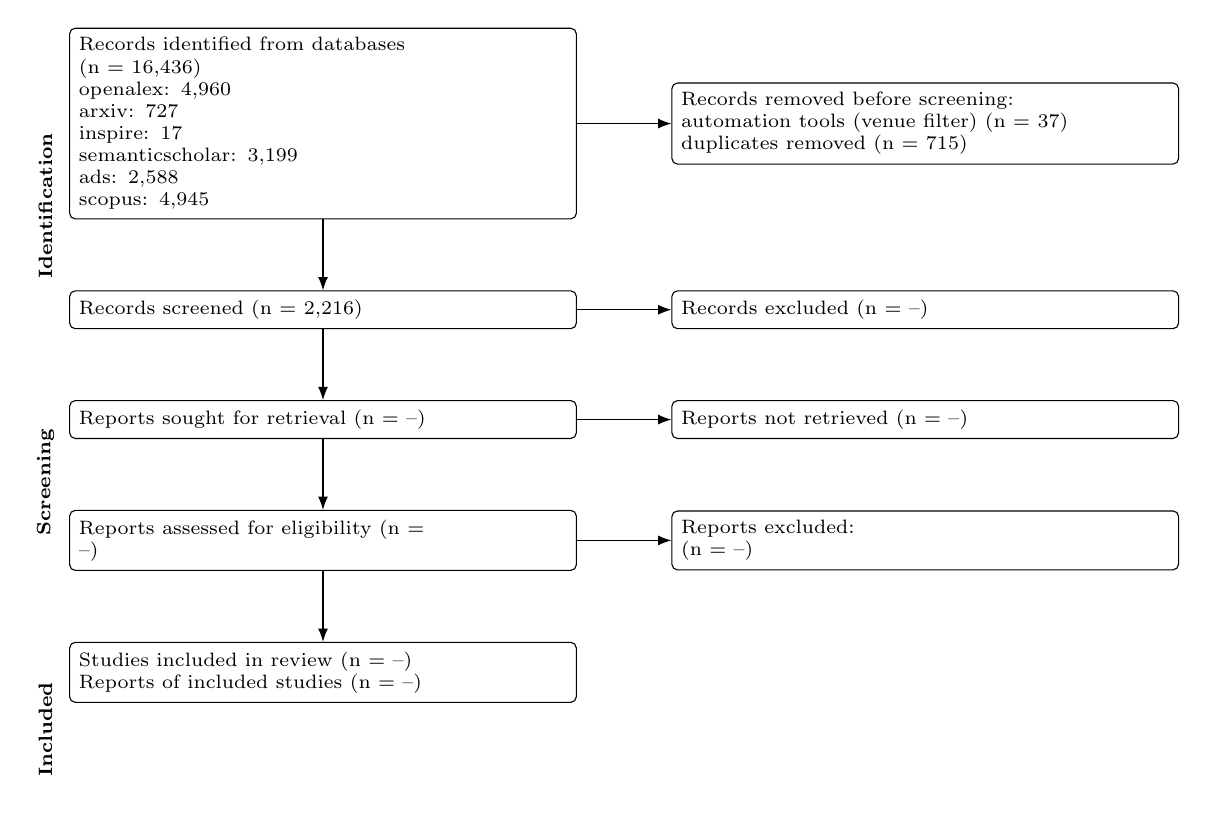
\begin{tikzpicture}[node distance=9mm and 12mm,
  box/.style={draw, rounded corners=2pt, text width=62mm, align=left, font=\scriptsize},
  lab/.style={rotate=90, font=\scriptsize\bfseries}]
\node[box] (id) {Records identified from databases \\ (n = 16,436) \\ openalex: 4,960 \\ arxiv: 727 \\ inspire: 17 \\ semanticscholar: 3,199 \\ ads: 2,588 \\ scopus: 4,945};
\node[box, right=of id] (idr) {Records removed before screening: \\ automation tools (venue filter) (n = 37) \\ duplicates removed (n = 715)};
\node[box, below=of id] (sc) {Records screened (n = 2,216)};
\node[box, right=of sc] (scr) {Records excluded (n = --)};
\node[box, below=of sc] (sc2) {Reports sought for retrieval (n = --)};
\node[box, right=of sc2] (sc2r) {Reports not retrieved (n = --)};
\node[box, below=of sc2] (sc3) {Reports assessed for eligibility (n = \\ --)};
\node[box, right=of sc3] (sc3r) {Reports excluded: \\ (n = --)};
\node[box, below=of sc3] (inc) {Studies included in review (n = --) \\ Reports of included studies (n = --)};
\node[lab, left=3mm of id] {Identification};
\node[lab, left=3mm of sc2] {Screening};
\node[lab, left=3mm of inc] {Included};
\draw[->] (id) -- (idr); \draw[->] (sc) -- (scr); \draw[->] (sc2) -- (sc2r);
\draw[->] (sc3) -- (sc3r);
\draw[->] (id) -- (sc); \draw[->] (sc) -- (sc2); \draw[->] (sc2) -- (sc3);
\draw[->] (sc3) -- (inc);
\end{tikzpicture}\end{center}
{\scriptsize\begin{longtable}{p{0.644\linewidth}p{0.296\linewidth}}
\hline
\textbf{Stage} & \textbf{n} \\ \hline
\endhead
Records identified from databases & 16,436 \\
  openalex & 4,960 \\
  arxiv & 727 \\
  inspire & 17 \\
  semanticscholar & 3,199 \\
  ads & 2,588 \\
  scopus & 4,945 \\
Records retrieved (downloaded) & 2,968 \\
Removed before screening: automation (non-curated venues) & 37 \\
Removed before screening: duplicates & 715 \\
Records to screen (unique) & 2,216 \\
Records screened & 2,216 (assumed = unique) \\
Records excluded at screening & -- \\
Reports sought for retrieval & -- \\
Reports not retrieved & -- \\
Reports assessed for eligibility & -- \\
Studies included & -- \\
Reports of included studies & -- \\
\hline
\end{longtable}}
Automation stages are computed from the run; '--' marks manual stages not yet recorded in prisma.json. Note that 'identified' counts hits reported by each database while 'retrieved' is what was downloaded within \texttt{--limit}, so the two differ on large blocks.

\subsection*{PRISMA-S search-reporting checklist}
{\scriptsize\begin{longtable}{p{0.072\linewidth}p{0.295\linewidth}p{0.573\linewidth}}
\hline
\textbf{Item} & \textbf{Requirement} & \textbf{This search} \\ \hline
\endhead
1 & Database name & openalex, arxiv, inspire, semanticscholar, ads, scopus (queried through their documented public APIs) \\
2 & Multi-database searching & 6 databases, one structural query per block rendered into each native grammar; see Search strategy \\
3 & Study registries & not applicable \\
4 & Online resources and browsing & not applicable \\
5 & Citation searching & not performed by the tool (manual, if any) \\
6 & Contacts & not applicable \\
7 & Other methods & none \\
8 & Full search strategies & reported verbatim per backend under Search strategy; archived in queries.json \\
9 & Limits and restrictions & record download capped at 300 per block and backend, most-cited first; no date, language or document-type limits applied \\
10 & Search filters & venue filter on: records from non-curated repositories (Zenodo, Figshare, SSRN...) removed \\
11 & Prior work & none \\
12 & Updates & 2 earlier run(s) archived; counts tracked in counts\_history.csv \\
13 & Dates of searches & all databases searched on 2026-08-28 10:01:20 \\
14 & Peer review & none \\
15 & Total records & 16,436 identified; 2,968 retrieved; 2,216 unique \\
16 & Deduplication & exact DOI match, else first 90 characters of the lower-cased title; 715 duplicates removed \\
\hline
\end{longtable}}
\section*{Records}
Deduplicated across backends, sorted by citation count.

\subsection*{Block PSC (1163 unique)}
\subsubsection*{Incorporation of rubidium cations into perovskite solar cells improves photovoltaic performance}
Michael Saliba; Taisuke Matsui; Konrad Domanski; Ji‐Youn Seo; Amita Ummadisingu; Shaik M. Zakeeruddin; Juan‐Pablo Correa‐Baena; Wolfgang Tress; Antonio Abate; Anders Hagfeldt; Michaël Grätzel. Science (2016). Cited by 3691. Found by: openalex. DOI: 10.1126/science.aah5557

Abstract: Improving the stability of perovskite solar cells Inorganic-organic have poor long-term because ultraviolet light and humidity degrade these materials. Bella et al. show that coating with a water-proof fluorinated polymer contains pigments to absorb re-emit it in visible range can boost cell efficiency limit photodegradation. The performance inorganic-organic are also limited by size cations required for forming correct lattice. Saliba rubidium cation, which is too small form itself, lattice cesium organic cations. Solar based on materials efficiencies exceeding 20\% over 500 hours if given environmental protection coating. Science , this issue pp. 203 206

\subsubsection*{High-efficiency two-dimensional Ruddlesden–Popper perovskite solar cells}
Hsinhan Tsai; Wanyi Nie; Jean‐Christophe Blancon; Constantinos C. Stoumpos; Reza Asadpour; Boris Harutyunyan; Amanda J. Neukirch; Rafael Verduzco; Jared Crochet; Sergei Tretiak; Laurent Pédesseau; Jacky Even; Muhammad A. Alam; Gautam Gupta; Jun Lou; Pulickel M. Ajayan; Michael J. Bedzyk; Mercouri G. Kanatzidis; Aditya D. Mohite. Nature (2016). Cited by 3360. Found by: openalex. DOI: 10.1038/nature18306

\subsubsection*{Efficient, stable and scalable perovskite solar cells using poly(3-hexylthiophene)}
Eui Hyuk Jung; Nam Joong Jeon; Eun Young Park; Chan Su Moon; Tae Joo Shin; Tae‐Youl Yang; Jun Hong Noh; Jangwon Seo. Nature (2019). Cited by 2318. Found by: ads, openalex. DOI: 10.1038/s41586-019-1036-3

\subsubsection*{A Layered Hybrid Perovskite Solar‐Cell Absorber with Enhanced Moisture Stability}
Ian C. P. Smith; Eric T. Hoke; Diego Solís-Ibarra; Michael D. McGehee; Hemamala I. Karunadasa. Angewandte Chemie International Edition (2014). Cited by 2006. Found by: openalex. DOI: 10.1002/anie.201406466

Abstract: Two-dimensional hybrid perovskites are used as absorbers in solar cells. Our first-generation devices containing (PEA)2(MA)2{[}Pb3I10{]} (1; PEA=C6H5(CH2)2NH3(+), MA=CH3NH3(+)) show an open-circuit voltage of 1.18 V and a power conversion efficiency 4.73\%. The layered structure allows for high-quality films to be deposited through spin coating high-temperature annealing is not required device fabrication. 3D perovskite (MA){[}PbI3{]} (2) has recently been identified promising absorber However, its instability moisture requires anhydrous processing operating conditions. Films 1 more resistant than 2 can fabricated under ambient humidity levels. larger bandgap the 2D also suitable higher dual-absorber tandem device. Compared 2, may offer greater tunability at molecular level material optimization.

\subsubsection*{Review of recent progress in chemical stability of perovskite solar cells}
Guangda Niu; Xudong Guo; Liduo Wang. Journal of Materials Chemistry A (2014). Cited by 1942. Found by: openalex. DOI: 10.1039/c4ta04994b

Abstract: The understanding of how the chemical stability PSCs is affected by oxygen and moisture, UV light, solution process, temperature was reviewed.

\subsubsection*{Understanding Degradation Mechanisms and Improving Stability of Perovskite Photovoltaics}
Caleb C. Boyd; Rongrong Cheacharoen; Tomas Leijtens; Michael D. McGehee. Chemical Reviews (2018). Cited by 1767. Found by: openalex. DOI: 10.1021/acs.chemrev.8b00336

Abstract: This review article examines the current state of understanding in how metal halide perovskite solar cells can degrade when exposed to moisture, oxygen, heat, light, mechanical stress, and reverse bias. It also highlights strategies for improving stability, such as tuning composition perovskite, introducing hydrophobic coatings, replacing electrodes with carbon or transparent conducting oxides, packaging. The concludes recommendations on accelerated testing should be performed rapidly develop that are both extraordinarily efficient stable.

\subsubsection*{Formamidinium and Cesium Hybridization for Photo‐ and Moisture‐Stable Perovskite Solar Cell}
Jin‐Wook Lee; Deok‐Hwan Kim; Hui‐Seon Kim; Seung‐Woo Seo; Sung‐Min Cho; Nam‐Gyu Park. Advanced Energy Materials (2015). Cited by 1661. Found by: ads, openalex. DOI: 10.1002/aenm.201501310

Abstract: Although power conversion efficiency (PCE) of state‐of‐the‐art perovskite solar cells has already exceeded 20\%, photo‐ and/or moisture instability organolead halide have prevented further commercialization. In particular, the underlying weak interaction organic cations with surrounding iodides due to eight equivalent orientations cation along body diagonals in unit cell and chemically non‐inertness result organometal perovskite. Here, a light absorber incorporating organic–inorganic hybrid A‐site 3D APbI 3 structure enhanced stability is reported. A partial substitution Cs + for HC(NH 2 ) PbI found substantially improve photovoltaic performance. When 10\% replaced by , film are significantly improved, which attributed between iodide contraction cubo‐octahedral volume. Moreover, trap density reduced one order magnitude upon incorporation responsible increased open‐circuit voltage fill factor, eventually leading enhancement average PCE from 14.9\% 16.5\%.

\subsubsection*{23.6\%-efficient monolithic perovskite/silicon tandem solar cells with improved stability}
Kevin A. Bush; Axel F. Palmstrom; Zhengshan J. Yu; Mathieu Boccard; Rongrong Cheacharoen; Jonathan P. Mailoa; David P. McMeekin; Robert L. Z. Hoye; Colin D. Bailie; Tomas Leijtens; Ian Marius Peters; Maxmillian C. Minichetti; Nicholas Rolston; Rohit Prasanna; Sarah E. Sofia; Duncan Harwood; Wen Ma; Farhad Moghadam; Henry J. Snaith; Tonio Buonassisi; Zachary C. Holman; Stacey F. Bent; Michael D. McGehee. Nature Energy (2017). Cited by 1533. Found by: openalex. DOI: 10.1038/nenergy.2017.9

\subsubsection*{Investigation of CH 3 NH 3 PbI 3 Degradation Rates and Mechanisms in Controlled Humidity Environments Using in Situ Techniques}
Jinli Yang; Braden D. Siempelkamp; Dianyi Liu; Timothy L. Kelly. ACS Nano (2015). Cited by 1342. Found by: openalex. DOI: 10.1021/nn506864k

Abstract: Perovskite solar cells have rapidly advanced to the forefront of solution-processable photovoltaic devices, but CH3NH3PbI3 semiconductor decomposes in moist air, limiting their commercial utility. In this work, we report a quantitative and systematic investigation perovskite degradation processes. By carefully controlling relative humidity an environmental chamber using situ absorption spectroscopy grazing incidence X-ray diffraction monitor phase changes process, demonstrate formation hydrated intermediate containing isolated PbI6(4-) octahedra as first step mechanism. We also show that identity hole transport layer can dramatic impact on stability underlying film, suggesting route toward with long device lifetimes resistance humidity.

\subsubsection*{Carbon Nanotube/Polymer Composites as a Highly Stable Hole Collection Layer in Perovskite Solar Cells}
Severin N. Habisreutinger; Tomas Leijtens; Giles E. Eperon; Samuel D. Stranks; R. J. Nicholas; Henry J. Snaith. Nano Letters (2014). Cited by 1198. Found by: openalex. DOI: 10.1021/nl501982b

Abstract: Organic-inorganic perovskite solar cells have recently emerged at the forefront of photovoltaics research. Power conversion efficiencies experienced an unprecedented increase to reported values exceeding 19\% within just four years. With focus mainly on efficiency, aspect stability has so far not been thoroughly addressed. In this paper, we identify thermal as a fundamental weak point cells, and demonstrate elegant approach mitigating degradation by replacing organic hole transport material with polymer-functionalized single-walled carbon nanotubes (SWNTs) embedded in insulating polymer matrix. composite structure, achieve JV scanned power-conversion up 15.3\% average efficiency 10 ± 2\%. Moreover, observe strong retardation compared employing state-of-the-art hole-transporting materials. addition, resistance water ingress is remarkably enhanced. These are critical developments for achieving long-term high-efficiency cells.

\subsubsection*{Improved performance and stability of perovskite solar cells by crystal crosslinking with alkylphosphonic acid ω-ammonium chlorides}
Xiong Li; M. Ibrahim Dar; Chenyi Yi; Jingshan Luo; Manuel Tschumi; Shaik M. Zakeeruddin; Mohammad Khaja Nazeeruddin; Hongwei Han; Michaël Grätzel. Nature Chemistry (2015). Cited by 1176. Found by: openalex, semanticscholar. DOI: 10.1038/nchem.2324

\subsubsection*{All-Inorganic Perovskite Solar Cells}
Jia Liang; Caixing Wang; Yanrong Wang; Zhaoran Xu; Zhipeng Lü; Yue Ma; Hongfei Zhu; Yi Hu; Chengcan Xiao; Xu Yi; Guoyin Zhu; Hongling Lv; Lianbo Ma; Tao Chen; Zuoxiu Tie; Zhong Jin; Jie Liu. Journal of the American Chemical Society (2016). Cited by 1091. Found by: openalex. DOI: 10.1021/jacs.6b10227

Abstract: The research field on perovskite solar cells (PSCs) is seeing frequent record breaking in the power conversion efficiency (PCE). However, organic-inorganic hybrid halide perovskites and organic additives common hole-transport materials (HTMs) exhibit poor stability against moisture heat. Here we report successful fabrication of all-inorganic PSCs without any labile or expensive components. entire process can be operated ambient environment humidity control (e.g., a glovebox). Even encapsulation, present no performance degradation humid air (90-95\% relative humidity, 25 °C) for over 3 months (2640 h) endure extreme temperatures (100 -22 °C). Moreover, by elimination HTMs noble-metal electrodes, cost was significantly reduced. highest PCE first-generation reached 6.7\%. This study opens door next-generation with long-term under harsh conditions, making practical application real possibility.

\subsubsection*{Study on the stability of CH 3 NH 3 PbI 3 films and the effect of post-modification by aluminum oxide in all-solid-state hybrid solar cells}
Guangda Niu; Wenzhe Li; Fanqi Meng; Liduo Wang; Haopeng Dong; Yong Qiu. Journal of Materials Chemistry A (2013). Cited by 1067. Found by: openalex. DOI: 10.1039/c3ta13606j

Abstract: Degradation of perovskite has been a big problem in all-solid-state solar cells, although many researchers mainly focus on the high efficiency these cells. This paper studies stability CH3NH3PbI3 films and finds that is sensitive to moisture. The degradation reaction proposed according UV-Vis spectra XRD results. In order improve CH3NH3PbI3, we introduce aluminum oxide as post-modification material into cells for first time. show Al2O3 modification could maintain absorption after degradation. results reveal protect from Moreover, device post-modified by shown more brilliant than without when exposed EIS dark current illustrate increased interface resistance dark, indicating restrained electron recombination process.

\subsubsection*{Organometallic-functionalized interfaces for highly efficient inverted perovskite solar cells}
Zhen Li; Bo Li; Xin Wu; Stephanie A. Sheppard; Shoufeng Zhang; Danpeng Gao; Nicholas J. Long; Zonglong Zhu. Science (2022). Cited by 1031. Found by: openalex. DOI: 10.1126/science.abm8566

Abstract: Further enhancing the performance and stability of inverted perovskite solar cells (PSCs) is crucial for their commercialization. We report that functionalization multication halide interfaces with an organometallic compound, ferrocenyl-bis-thiophene-2-carboxylate (FcTc 2 ), simultaneously enhanced efficiency PSCs. The resultant devices achieved a power conversion 25.0\% maintained >98\% initial after continuously operating at maximum point 1500 hours under simulated AM1.5 illumination. Moreover, FcTc -functionalized passed international standards mature photovoltaics (IEC61215:2016) have exhibited high damp heat test (85°C 85\% relative humidity).

\subsubsection*{Degradation observations of encapsulated planar CH 3 NH 3 PbI 3 perovskite solar cells at high temperatures and humidity}
Yu Han; S. Meyer; Yasmina Dkhissi; Karl Weber; Jennifer M. Pringle; Udo Bach; Leone Spiccia; Yi‐Bing Cheng. Journal of Materials Chemistry A (2015). Cited by 997. Found by: openalex. DOI: 10.1039/c5ta00358j

Abstract: The stability of encapsulated planar-structured CH 3 NH PbI (MAPbI ) perovskite solar cells (PSCs) was investigated under various simulated environmental conditions.

\subsubsection*{Stability of perovskite solar cells}
Dian Wang; Matthew Wright; Naveen Kumar Elumalai; Ashraf Uddin. Solar Energy Materials and Solar Cells (2016). Cited by 992. Found by: ads, openalex. DOI: 10.1016/j.solmat.2015.12.025

\subsubsection*{Strained hybrid perovskite thin films and their impact on the intrinsic stability of perovskite solar cells}
Jingjing Zhao; Yehao Deng; Haotong Wei; Xiaopeng Zheng; Zhenhua Yu; Yuchuan Shao; Jeffrey E. Shield; Jinsong Huang. Science Advances (2017). Cited by 965. Found by: openalex. DOI: 10.1126/sciadv.aao5616

Abstract: Organic-inorganic hybrid perovskite (OIHP) solar cells have achieved comparable efficiencies to those of commercial cells, although their instability hinders commercialization. Although encapsulation techniques been developed protect OIHP from external stimuli such as moisture, oxygen, and ultraviolet light, understanding the origin intrinsic films is needed improve stability. We show that fabricated by existing methods are strained strain caused mismatched thermal expansion substrates during annealing process. The polycrystalline compressive in out-of-plane direction in-plane tensile strain. accelerates degradation under illumination, which can be explained increased ion migration films. This study points out an avenue enhance stability reducing residual

\subsubsection*{Scalable fabrication and coating methods for perovskite solar cells and solar modules}
Nam‐Gyu Park; Kai Zhu. Nature Reviews Materials (2020). Cited by 902. Found by: openalex. DOI: 10.1038/s41578-019-0176-2

\subsubsection*{Improving efficiency and stability of perovskite solar cells with photocurable fluoropolymers}
Federico Bella; Gianmarco Griffini; Juan‐Pablo Correa‐Baena; Guido Saracco; Michaël Grätzel; Anders Hagfeldt; Stefano Turri; Claudio Gerbaldi. Science (2016). Cited by 866. Found by: openalex. DOI: 10.1126/science.aah4046

Abstract: Organometal halide perovskite solar cells have demonstrated high conversion efficiency but poor long-term stability against ultraviolet irradiation and water. We show that rapid light-induced free-radical polymerization at ambient temperature produces multifunctional fluorinated photopolymer coatings confer luminescent easy-cleaning features on the front side of devices, while concurrently forming a strongly hydrophobic barrier toward environmental moisture back contact side. The photopolymers re-emit light in visible range, boosting to nearly 19\% under standard illumination. Coated devices reproducibly retain their full functional performance during prolonged operation, even after series severe aging tests carried out for more than 6 months.

\subsubsection*{Thermochromic halide perovskite solar cells}
Jia Lin; Minliang Lai; Letian Dou; Christopher S. Kley; Hong Chen; Fei Peng; Junliang Sun; Dylan Lu; Steven A. Hawks; Chenlu Xie; Fan Cui; A. Paul Alivisatos; David T. Limmer; Peidong Yang. Nature Materials (2018). Cited by 854. Found by: openalex. DOI: 10.1038/s41563-017-0006-0

\subsubsection*{Damp heat–stable perovskite solar cells with tailored-dimensionality 2D/3D heterojunctions}
Randi Azmi; Esma Ugur; Akmaral Seitkhan; Faisal Aljamaan; Anand S. Subbiah; Jiang Liu; George T. Harrison; Mohamad Insan Nugraha; Mathan K. Eswaran; Maxime Babics; Yuan Chen; Fuzong Xu; Thomas G. Allen; Atteq ur Rehman; Chien‐Lung Wang; Thomas D. Anthopoulos; Udo Schwingenschlögl; Michele De Bastiani; Erkan Aydın; Stefaan De Wolf. Science (2022). Cited by 843. Found by: openalex. DOI: 10.1126/science.abm5784

Abstract: If perovskite solar cells (PSCs) with high power conversion efficiencies (PCEs) are to be commercialized, they must achieve long-term stability, which is usually assessed accelerated degradation tests. One of the persistent obstacles for PSCs has been successfully passing damp-heat test (85°C and 85\% relative humidity), standard verifying stability commercial photovoltaic (PV) modules. We fabricated damp heat-stable by tailoring dimensional fragments two-dimensional layers formed at room temperature oleylammonium iodide molecules; these passivate surface electron-selective contact. The resulting inverted deliver a 24.3\% PCE retain >95\% their initial value after >1000 hours conditions, thereby meeting one critical industrial standards PV

\subsubsection*{Tailored interfaces of unencapsulated perovskite solar cells for >1,000 hour operational stability}
Jeffrey A. Christians; Philip Schulz; Jonathan S. Tinkham; Tracy H. Schloemer; Steven P. Harvey; Bertrand J. Tremolet de Villers; Alan Sellinger; Joseph J. Berry; Joseph M. Luther. Nature Energy (2018). Cited by 826. Found by: ads, openalex, semanticscholar. DOI: 10.1038/s41560-017-0067-y

\subsubsection*{Stable High‐Performance Perovskite Solar Cells via Grain Boundary Passivation}
Tianqi Niu; Jing Lü; Rahim Munir; Jianbo Li; Dounya Barrit; Xu Zhang; Hanlin Hu; Zhou Yang; Aram Amassian; Kui Zhao; Shengzhong Liu. Advanced Materials (2018). Cited by 800. Found by: openalex. DOI: 10.1002/adma.201706576

Abstract: The trap states at grain boundaries (GBs) within polycrystalline perovskite films deteriorate their optoelectronic properties, making GB engineering particularly important for stable high-performance devices. It is demonstrated that bulk can be effectively passivated by semiconducting molecules with Lewis acid or base functional groups. crystallization kinetics are studied using in situ synchrotron-based grazing-incidence X-ray scattering to explore the film formation mechanism. A model of passivation mechanism proposed understand how simultaneously passivate Pb-I antisite defects and vacancies created under-coordinated Pb atoms. In addition, it also explains energy offset between influences intergrain carrier transport. superior properties attained optimizing molecular treatments. These benefits translated into significant enhancements power conversion efficiencies 19.3\%, as well improved environmental thermal stability solar cells. devices without encapsulation degrade only ≈13\% after 40 d exposure 50\% relative humidity room temperature, ≈10\% 24 h 80 °C controlled environment.

\subsubsection*{In Situ Growth of 2D Perovskite Capping Layer for Stable and Efficient Perovskite Solar Cells}
Peng Chen; Yang Bai; Songcan Wang; Miaoqiang Lyu; Jung‐Ho Yun; Lianzhou Wang. Advanced Functional Materials (2018). Cited by 772. Found by: openalex. DOI: 10.1002/adfm.201706923

Abstract: Abstract 2D halide perovskites have recently been recognized as a promising avenue in perovskite solar cells (PSCs) terms of encouraging stability and defect passivation effect. However, the efficiency (less than 15\%) ultrastable Ruddlesden–Popper PSCs still lag far behind their traditional 3D counterparts. Here, rationally designed 2D‐3D stacking‐layered architecture by situ growing PEA 2 PbI 4 capping layers on top film, which drastically improves without compromising high performance, is reported. Such layer induces larger Fermi‐level splitting film under light illumination, resulting an enhanced open‐circuit voltage ( V oc ) thus higher 18.51\% PSCs. Time‐resolved photoluminescence decay measurements indicate facilitated hole extraction films, ascribed to optimized energy band alignment reduced nonradiative recombination at subgap states. Benefiting from moisture resistivity well suppressed ion migration perovskite, show significantly improved long‐term stability, retaining nearly 90\% initial power conversion after 1000 h exposure ambient conditions with relative humidity level 60 ± 10\%.

\subsubsection*{2D perovskite stabilized phase-pure formamidinium perovskite solar cells}
Jin‐Wook Lee; Zhenghong Dai; Tae-Hee Han; Chungseok Choi; Sheng-Yung Chang; Sung‐Joon Lee; Nicholas De Marco; Hongxiang Zhao; Pengyu Sun; Yu Huang; Yang Yang. Nature Communications (2018). Cited by 747. Found by: openalex. DOI: 10.1038/s41467-018-05454-4

Abstract: Abstract Compositional engineering has been used to overcome difficulties in fabricating high-quality phase-pure formamidinium perovskite films together with its ambient instability. However, this comes alongside an undesirable increase bandgap that sacrifices the device photocurrent. Here we report fabrication of formamidinium-lead tri-iodide excellent optoelectronic quality and stability. Incorporation 1.67 mol\% 2D phenylethylammonium lead iodide into precursor solution enables formation order magnitude enhanced photoluminescence lifetime. The spontaneously forms at grain boundaries protect from moisture suppress ion migration. A stabilized power conversion efficiency (PCE) 20.64\% (certified PCE 19.77\%) is achieved a short-circuit current density exceeding 24 mA cm − 2 open-circuit voltage 1.130 V, corresponding loss-in-potential 0.35 significantly operational

\subsubsection*{Suppression of atomic vacancies via incorporation of isovalent small ions to increase the stability of halide perovskite solar cells in ambient air}
Makhsud I. Saidaminov; Junghwan Kim; Ankit Jain; Rafael Quintero‐Bermudez; Hairen Tan; Guankui Long; Furui Tan; Andrew Johnston; Yicheng Zhao; Oleksandr Voznyy; Edward H. Sargent. Nature Energy (2018). Cited by 745. Found by: ads, openalex. DOI: 10.1038/s41560-018-0192-2

\subsubsection*{A Layered Hybrid Perovskite Solar‐Cell Absorber with Enhanced Moisture Stability}
Ian C. P. Smith; Eric T. Hoke; Diego Solís-Ibarra; Michael D. McGehee; Hemamala I. Karunadasa. Angewandte Chemie (2014). Cited by 692. Found by: openalex. DOI: 10.1002/ange.201406466

Abstract: Abstract Two‐dimensional hybrid perovskites are used as absorbers in solar cells. Our first‐generation devices containing (PEA)2(MA)2{[}Pb3I10{]} (1; PEA=C6H5(CH2)2NH3+, MA=CH3NH3+) show an open‐circuit voltage of 1.18 V and a power conversion efficiency 4.73 \%. The layered structure allows for high‐quality films to be deposited through spin coating high‐temperature annealing is not required device fabrication. 3D perovskite (MA){[}PbI3{]} (2) has recently been identified promising absorber However, its instability moisture requires anhydrous processing operating conditions. Films 1 more resistant than 2 can fabricated under ambient humidity levels. larger bandgap the 2D also suitable higher dual‐absorber tandem device. Compared 2, may offer greater tunability at molecular level material optimization.

\subsubsection*{Stable high efficiency two-dimensional perovskite solar cells via cesium doping}
Xu Zhang; Xiaodong Ren; Bin Liu; Rahim Munir; Xuejie Zhu; Dong Yang; Jianbo Li; Yucheng Liu; Detlef‐M. Smilgies; Ruipeng Li; Zhou Yang; Tianqi Niu; Xiuli Wang; Aram Amassian; Kui Zhao; Shengzhong Liu. Energy \& Environmental Science (2017). Cited by 675. Found by: openalex. DOI: 10.1039/c7ee01145h

Abstract: Cs + doping into 2D (BA) 2 (MA) 3 Pb 4 I 13 perovskites boosts power conversion efficiency (PCE) to 13.7\% and yields superior humidity thermal stability.

\subsubsection*{A polymer scaffold for self-healing perovskite solar cells}
Yicheng Zhao; Jing Wei; Heng Li; Yin Yan; Wenke Zhou; Dapeng Yu; Qing Zhao. Nature Communications (2016). Cited by 666. Found by: openalex. DOI: 10.1038/ncomms10228

Abstract: Advancing of the lead halide perovskite solar cells towards photovoltaic market demands large-scale devices high-power conversion efficiency, high reproducibility and stability via low-cost fabrication technology, in particular resistance to humid environment for long-time operation. Here we achieve uniform film based on a novel polymer-scaffold architecture mild-temperature process. These exhibit efficiency up ∼ 16\% with small variation. The unencapsulated retain output 300 h highly (70\% relative humidity). Moreover, they show strong humidity resistant self-healing behaviour, recovering rapidly after removing from water vapour. Not only can self-heal this case, but corresponding present power recovery vapour is removed. Our work demonstrates value cheap, long chain hygroscopic polymer scaffold commercialization.

\subsubsection*{Accelerated degradation of methylammonium lead iodide perovskites induced by exposure to iodine vapour}
Shenghao Wang; Yan Jiang; Emilio J. Juárez‐Pérez; Luis K. Ono; Yabing Qi. Nature Energy (2016). Cited by 657. Found by: openalex. DOI: 10.1038/nenergy.2016.195

\subsubsection*{All‐Inorganic CsPbX 3 Perovskite Solar Cells: Progress and Prospects}
Jingru Zhang; Gary Hodes; Zhiwen Jin; Shengzhong Liu. Angewandte Chemie International Edition (2019). Cited by 611. Found by: openalex. DOI: 10.1002/anie.201901081

Abstract: Abstract Recently, lead halide‐based perovskites have become one of the hottest topics in photovoltaic research because their excellent optoelectronic properties. Among them, organic‐inorganic hybrid perovskite solar cells (PSCs) made very rapid progress with power conversion efficiency (PCE) now at 23.7 \%. However, intrinsically unstable nature these materials, particularly to moisture and heat, may be a problem for long‐term stability. Replacing fragile organic group more robust inorganic Cs + cations forms cesium halide system (CsPbX 3 , X is halide) as all‐inorganic which are much thermally stable often other factors. From first report 2015 now, PCE CsPbX ‐based PSCs has abruptly increased from 2.9 \% 17.1 enhanced In this Review, we summarize field up propose solutions terms development bottlenecks, attempt boost further PSCs.

\subsubsection*{Intact 2D/3D halide junction perovskite solar cells via solid-phase in-plane growth}
Yeoun‐Woo Jang; Seungmin Lee; Kyung Mun Yeom; Kiwan Jeong; Kwang Choi; Mansoo Choi; Jun Hong Noh. Nature Energy (2021). Cited by 606. Found by: openalex. DOI: 10.1038/s41560-020-00749-7

\subsubsection*{Trapped charge-driven degradation of perovskite solar cells}
Namyoung Ahn; Kwisung Kwak; Min Seok Jang; Heetae Yoon; Byung Yang Lee; Jong Kwon Lee; Peter V. Pikhitsa; Junseop Byun; Mansoo Choi. Nature Communications (2016). Cited by 601. Found by: ads, arxiv, openalex, semanticscholar. DOI: 10.1038/ncomms13422

Abstract: Perovskite solar cells have shown unprecedent performance increase up to 22\% efficiency. However, their photovoltaic has fast deterioration under light illumination in the presence of humid air even with encapulation. The stability perovskite materials been unsolved and its mechanism elusive. Here we uncover a for irreversible degradation which trapped charges, regardless polarity, play decisive role. An experimental setup using different polarity ions revealed that moisture-induced dissociation is triggered by charges along grain boundaries. We also identified synergetic effect oxygen on process degradation. deprotonation organic cations charge-induced local electric field would be attributed initiation decomposition.

\subsubsection*{Stability of Perovskite Solar Cells: A Prospective on the Substitution of the A Cation and X Anion}
Ze Wang; Zejiao Shi; Taotao Li; Yonghua Chen; Wei Huang. Angewandte Chemie International Edition (2016). Cited by 595. Found by: openalex. DOI: 10.1002/anie.201603694

Abstract: In recent years, organometal trihalide perovskites have emerged as promising materials for low-cost, flexible, and highly efficient solar cells. Despite their processing advantages, before the technology can be commercialized poor stability of organic-inorganic hybrid perovskite with regard to humidity, heat, light, oxygen has overcome. Herein, we distill current state-of-the-art highlight advances in improving chemical by substitution A-cation X-anion. Our hope is pave way rational design realize cells unprecedented improvement stability.

\subsubsection*{Efficient and stable perovskite solar cells prepared in ambient air irrespective of the humidity}
Qidong Tai; Peng You; Hongqian Sang; Zhike Liu; Chenglong Hu; H.L.W. Chan; Feng Yan. Nature Communications (2016). Cited by 582. Found by: ads, openalex. DOI: 10.1038/ncomms11105

Abstract: Poor stability of organic-inorganic halide perovskite materials in humid condition has hindered the success solar cells real applications since controlled atmosphere is required for device fabrication and operation, there a lack effective solutions to this problem until now. Here we report use lead (II) thiocyanate (Pb(SCN)2) precursor preparing ambient air. High-quality CH3NH3PbI3-x(SCN)x films can be readily prepared even when relative humidity exceeds 70\%. Under optimized processing conditions, obtain devices with an average power conversion efficiency 13.49\% maximum over 15\%. In comparison typical CH3NH3PbI3-based devices, these without encapsulation show greatly improved air, which attributed incorporation ions crystal lattice. The findings pave way realizing efficient stable atmosphere.

\subsubsection*{Efficient and stable Ruddlesden–Popper perovskite solar cell with tailored interlayer molecular interaction}
Hui Ren; Shidong Yu; Lingfeng Chao; Yingdong Xia; Yuanhui Sun; Shouwei Zuo; Fan Li; Tingting Niu; Yingguo Yang; Huanxin Ju; Bixin Li; Haiyan Du; Xingyu Gao; Jing Zhang; Jianpu Wang; Lijun Zhang; Yonghua Chen; Wei Huang. Nature Photonics (2020). Cited by 581. Found by: openalex. DOI: 10.1038/s41566-019-0572-6

\subsubsection*{Quantum-size-tuned heterostructures enable efficient and stable inverted perovskite solar cells}
Hao Chen; Sam Teale; Bin Chen; Yi Hou; Luke Grater; Tong Zhu; Koen Bertens; So Min Park; Harindi R. Atapattu; Yajun Gao; Mingyang Wei; Andrew Johnston; Qi‐Lin Zhou; Kaimin Xu; Danni Yu; Congcong Han; Teng Cui; Eui Hyuk Jung; Chun Zhou; Wenjia Zhou; Andrew H. Proppe; Sjoerd Hoogland; Frédéric Laquai; Tobin Filleter; Kenneth R. Graham; Zhijun Ning; Edward H. Sargent. Nature Photonics (2022). Cited by 581. Found by: openalex. DOI: 10.1038/s41566-022-00985-1

\subsubsection*{Perovskite-polymer composite cross-linker approach for highly-stable and efficient perovskite solar cells}
Tae-Hee Han; Jin‐Wook Lee; Chungseok Choi; Shaun Tan; Changsoo Lee; Yepin Zhao; Zhenghong Dai; Nicholas De Marco; Sung‐Joon Lee; Sang-Hoon Bae; Yonghai Yuan; Hyuck Mo Lee; Yu Huang; Yang Yang. Nature Communications (2019). Cited by 581. Found by: openalex. DOI: 10.1038/s41467-019-08455-z

Abstract: Manipulation of grain boundaries in polycrystalline perovskite is an essential consideration for both the optoelectronic properties and environmental stability solar cells as solution-processing films inevitably introduces many defects at boundaries. Though small molecule-based additives have proven to be effective defect passivating agents, their high volatility diffusivity cannot render robust enough against harsh environments. Here we suggest design rules molecules by considering molecular structure. From these, introduce a strategy form macromolecular intermediate phases using long chain polymers, which leads formation polymer-perovskite composite cross-linker. The cross-linker functions bridge grains, minimizing grain-to-grain electrical decoupling yielding excellent moisture, light, heat, has not been attainable with molecule agents. Consequently, all photovoltaic parameters are significantly enhanced devices also show stability.

\subsubsection*{Stabilizing the Efficiency Beyond 20\% with a Mixed Cation Perovskite Solar Cell Fabricated in Ambient Air under Controlled Humidity}
Trilok Singh; Tsutomu Miyasaka. Advanced Energy Materials (2017). Cited by 573. Found by: openalex. DOI: 10.1002/aenm.201700677

Abstract: Abstract Perovskite solar cells have evolved to compatible high efficiency and stability by employing mixed cation/halide type perovskite crystals as pinhole‐free large grain absorbers. The cesium (Cs)–formamidium–methylammonium triple cation‐based device fabricated in a glove box enables reproducible high‐voltage performance. This study explores the method reproduce stable power conversion (PCE) of cation prepared using one‐step solution deposition low‐temperature annealing fully conducted controlled ambient humidity conditions. Optimizing size Cs concentration processes, route is created obtain highly uniform, films that work with PCE up 20.8\% preservation without cell encapsulation for more than 18 weeks. further investigates light intensity characteristics open‐circuit voltage (Voc) small (5 × 5 mm2, > 20\%) (10 10 18\%) devices. Intensity dependence Voc shows an ideality factor range 1.7‐1.9 both devices, implying involves trap‐assisted recombination loss at hetero junction interfaces influences Voc. Despite relatively factor, capable supplying under low (0.01 Sun) whereas maintaining over 0.9 V.

\subsubsection*{Two-dimensional Ruddlesden–Popper layered perovskite solar cells based on phase-pure thin films}
Chao Liang; Hao Gu; Yingdong Xia; Zhuo Wang; Xiaotao Liu; Junmin Xia; Shouwei Zuo; Yue Hu; Xingyu Gao; Wei Hui; Lingfeng Chao; Tingting Niu; Min Fang; Hui Lu; Hanshan Dong; Hui Yu; Shi Chen; Xueqin Ran; Lin Song; Bixin Li; Jing Zhang; Yong Peng; Guosheng Shao; Jianpu Wang; Yonghua Chen; Guichuan Xing; Wei Huang. Nature Energy (2020). Cited by 554. Found by: openalex. DOI: 10.1038/s41560-020-00721-5

\subsubsection*{Low-loss contacts on textured substrates for inverted perovskite solar cells}
So Min Park; Mingyang Wei; Nikolaos Lempesis; Wenjin Yu; Tareq Hossain; Lorenzo Agosta; Virginia Carnevali; Harindi R. Atapattu; Peter Serles; Felix T. Eickemeyer; Heejong Shin; Maral Vafaie; Deokjae Choi; Kasra Darabi; Eui Dae Jung; Yi Yang; Da Bin Kim; Shaik M. Zakeeruddin; Bin Chen; Aram Amassian; Tobin Filleter; Mercouri G. Kanatzidis; Kenneth R. Graham; Lixin Xiao; Ursula Röthlisberger; Michaël Grätzel; Edward H. Sargent. Nature (2023). Cited by 548. Found by: openalex. DOI: 10.1038/s41586-023-06745-7

\subsubsection*{Multifunctional Chemical Linker Imidazoleacetic Acid Hydrochloride for 21\% Efficient and Stable Planar Perovskite Solar Cells}
Jiangzhao Chen; Xing Zhao; Seul‐Gi Kim; Nam‐Gyu Park. Advanced Materials (2019). Cited by 534. Found by: openalex. DOI: 10.1002/adma.201902902

Abstract: Abstract Chemical interaction at a heterojunction interface induced by an appropriate chemical linker is of crucial importance for high efficiency, hysteresis‐less, and stable perovskite solar cells (PSCs). Effective engineering in PSCs reported via multifunctional 4‐imidazoleacetic acid hydrochloride (ImAcHCl) that can provide bridge between SnO 2 through ester bond with esterification reaction electrostatic imidazolium cation ImAcHCl iodide anion perovskite. In addition, the chloride plays role improvement crystallinity film crystallinity. The introduction onto realigns positions conduction valence bands upwards, reduces nonradiative recombination, improves carrier life time. As consequence, average power conversion efficiency (PCE) increased from 18.60\% ± 0.50\% to 20.22\% 0.34\% before after surface modification, respectively, which mainly results enhanced voltage 1.084 0.012 V 1.143 0.009 V. best PCE 21\% achieved 0.1 mg mL −1 treatment, along negligible hysteresis. Moreover, unencapsulated device ImAcHCl‐modified shows much better thermal moisture stability than unmodified .

\subsubsection*{A review on perovskite solar cells: Evolution of architecture, fabrication techniques, commercialization issues and status}
Priyanka Roy; Numeshwar Kumar Sinha; Sanjay Tiwari; Ayush Khare. Solar Energy (2020). Cited by 530. Found by: openalex. DOI: 10.1016/j.solener.2020.01.080

\subsubsection*{CsPb0.9Sn0.1IBr2 Based All-Inorganic Perovskite Solar Cells with Exceptional Efficiency and Stability}
Jia Liang; Peiyang Zhao; Caixing Wang; Yanrong Wang; Yi Hu; Guoyin Zhu; Lianbo Ma; Jie Liu; Zhong Jin. Journal of the American Chemical Society (2017). Cited by 528. Found by: openalex. DOI: 10.1021/jacs.7b07949

Abstract: The emergence of perovskite solar cells (PSCs) has generated enormous interest in the photovoltaic research community. Recently, cesium metal halides (CsMX 3, M = Pb or Sn; X I, Br, Cl mixed halides) as a class inorganic perovskites showed great promise for PSCs and other optoelectronic devices. However, CsMX 3 -based usually exhibit lower power conversion efficiencies (PCEs) than organic–inorganic hybrid PSCs, due to unfavorable band gaps. Herein, novel mixed-Pb/Sn mixed-halide perovskite, CsPb 0.9 Sn 0.1 IBr 2, with suitable gap 1.79 eV an appropriate level valence maximum, was prepared ambient atmosphere without glovebox. After thoroughly eliminating labile organic components noble metals, all-inorganic based on 2 carbon counter electrodes high open-circuit voltage 1.26 V remarkable PCE up 11.33\%, which is record-breaking among existing PSCs. Moreover, show good long-term stability improved endurance against heat moisture. This study indicates feasible way design halide through energy-band engineering construction high-performance

\subsubsection*{Functionalization of perovskite thin films with moisture-tolerant molecules}
Shuang Yang; Yun Wang; Porun Liu; Yi‐Bing Cheng; Huijun Zhao; Hua Gui Yang. Nature Energy (2016). Cited by 527. Found by: openalex. DOI: 10.1038/nenergy.2015.16

\subsubsection*{Surface Passivation Using 2D Perovskites toward Efficient and Stable Perovskite Solar Cells}
Guangbao Wu; Rui Liang; Mingzheng Ge; G.C. Sun; Yuan Zhang; Guichuan Xing. Advanced Materials (2021). Cited by 524. Found by: openalex. DOI: 10.1002/adma.202105635

Abstract: 3D perovskite solar cells (PSCs) have shown great promise for use in next-generation photovoltaic devices. However, some challenges need to be addressed before their commercial production, such as enormous defects formed on the surface, which result severe SRH recombination, and inadequate material interplay between composition, leading thermal-, moisture-, light-induced degradation. 2D perovskites, organic layer functions a protective barrier block erosion of moisture or ions, recently emerged attracted increasing attention because they exhibit significant robustness. Inspired by this, surface passivation employing perovskites deposited top counterparts has triggered new wave research simultaneously achieve higher efficiency stability. Herein, we exploited vast amount literature comprehensively summarize recent progress 2D/3D heterostructure PSCs using passivation. The review begins with an introduction crystal structure, followed advantages combination perovskites. Then, strategies, optoelectronic properties, enhanced stability, performance are systematically discussed. Finally, perspectives techniques offer insight into further improved future proposed.

\subsubsection*{Engineering Stress in Perovskite Solar Cells to Improve Stability}
Nicholas Rolston; Kevin A. Bush; Adam D. Printz; Aryeh Gold‐Parker; Yichuan Ding; Michael F. Toney; Michael D. McGehee; Reinhold H. Dauskardt. Advanced Energy Materials (2018). Cited by 510. Found by: openalex, semanticscholar. DOI: 10.1002/aenm.201802139

Abstract: Abstract An overlooked factor affecting stability: the residual stresses in perovskite films, which are tensile and can exceed 50 MPa magnitude, a value high enough to deform copper, is reported. These provide significant driving force for fracture. Films shown be more unstable under stress—and conversely stable compressive stress—when exposed heat or humidity. Increasing formation temperature of films directly correlates with larger stresses, result thermal expansion coefficient perovskites. Specifically, this stress forms upon cooling room temperature, as substrate constrains from shrinking. No evidence relaxation observed, purely elastic film attributed mismatch between substrate. Additionally, authors demonstrate that using bath conversion method form at leads low values unaffected by further annealing, indicating complete prior annealing. It concluded reducing novel improving stability, accomplished lower temperatures, flexible substrates coefficients, externally applied after fabrication.

\subsubsection*{Enhanced Efficiency and Stability of Inverted Perovskite Solar Cells Using Highly Crystalline SnO 2 Nanocrystals as the Robust Electron‐Transporting Layer}
Zonglong Zhu; Yang Bai; Xiao Liu; Chu‐Chen Chueh; Shihe Yang; Alex K.‐Y. Jen. Advanced Materials (2016). Cited by 496. Found by: openalex. DOI: 10.1002/adma.201600619

Abstract: Highly crystalline SnO2 is demonstrated to serve as a stable and robust electron-transporting layer for high-performance perovskite solar cells. Benefiting from its high crystallinity, the relatively thick (≈120 nm) provides respectable property yield promising power conversion efficiency (PCE)(18.8\%) Over 90\% of initial PCE can be retained after 30 d storage in ambient with ≈70\% relative humidity.

\subsubsection*{Interfacial Residual Stress Relaxation in Perovskite Solar Cells with Improved Stability}
Hao Wang; Cheng Zhu; Lang Liu; Sai Ma; Pengfei Liu; Jiafeng Wu; Congbo Shi; Qin Du; Yanmin Hao; Sisi Xiang; Haining Chen; Pengwan Chen; Yang Bai; Huanping Zhou; Yujing Li; Qi Chen. Advanced Materials (2019). Cited by 495. Found by: openalex. DOI: 10.1002/adma.201904408

Abstract: To improve the photovoltaic performance (both efficiency and stability) in hybrid organic-inorganic halide perovskite solar cells, lattice distortion is investigated with regards to residual stress (and strain) polycrystalline thin films. It revealed that concentrated at surface of as-prepared film, an efficient method further developed release this interfacial by A site cation alloying. This results reconstruction films, which turn low elastic modulus. Thus, a "bone-joint" configuration constructed within interface between absorber carrier transport layer, improves device substantially. The resultant devices exhibit 21.48\% good humidity stability improved resistance against thermal cycling.

\subsubsection*{Degradation mechanism of hybrid tin-based perovskite solar cells and the critical role of tin (IV) iodide}
Luis Lanzetta; Thomas Webb; Nourdine Zibouche; Xinxing Liang; Dong Ding; Ganghong Min; Robert J. E. Westbrook; Benedetta Gaggio; Thomas J. Macdonald; M. Saïful Islam; Saif A. Haque. Nature Communications (2021). Cited by 493. Found by: openalex. DOI: 10.1038/s41467-021-22864-z

Abstract: Abstract Tin perovskites have emerged as promising alternatives to toxic lead in next-generation photovoltaics, but their poor environmental stability remains an obstacle towards more competitive performances. Therefore, a full understanding of decomposition processes is needed address these issues. Herein, we elucidate the degradation mechanism 2D/3D tin perovskite films based on (PEA)0.2(FA)0.8SnI3(where PEA phenylethylammonium and FA formamidinium). We show that SnI4, product oxygen-induced perovskite, quickly evolves into iodine via combined action moisture oxygen. identify highly aggressive species can further oxidise establishing cyclic mechanism. Perovskite then observed strongly depend hole transport layer chosen substrate, which exploited tackle film degradation. These key insights will enable future design optimisation stable tin-based optoelectronics.

\subsubsection*{Precise Control of Crystal Growth for Highly Efficient CsPbI2Br Perovskite Solar Cells}
Weijie Chen; Haiyang Chen; Guiying Xu; Rongming Xue; Shuhui Wang; Yaowen Li; Yongfang Li. Joule (2018). Cited by 491. Found by: ads, openalex. DOI: 10.1016/j.joule.2018.10.011

\subsubsection*{Gas chromatography–mass spectrometry analyses of encapsulated stable perovskite solar cells}
Lei Shi; Martin P. Bucknall; Trevor L. Young; Meng Zhang; Long Hu; Jueming Bing; Da Seul Lee; Jincheol Kim; Tom Wu; Noboru Takamure; David R. McKenzie; Shujuan Huang; Martin A. Green; Anita Ho‐Baillie. Science (2020). Cited by 489. Found by: openalex. DOI: 10.1126/science.aba2412

Abstract: Although perovskite solar cells have produced remarkable energy conversion efficiencies, they cannot become commercially viable without improvements in durability. We used gas chromatography-mass spectrometry (GC-MS) to reveal signature volatile products of the decomposition organic hybrid perovskites under thermal stress. In addition, we were able use GC-MS confirm that a low-cost polymer/glass stack encapsulation is effective suppressing such outgassing. Using an scheme, multi-cation, multi-halide containing methylammonium exceed requirements International Electrotechnical Commission 61215:2016 standard by surviving more than 1800 hours Damp Heat test and 75 cycles Humidity Freeze test.

\subsubsection*{Engineering ligand reactivity enables high-temperature operation of stable perovskite solar cells}
So Min Park; Mingyang Wei; Jian Xu; Harindi R. Atapattu; Felix T. Eickemeyer; Kasra Darabi; Luke Grater; Yi Yang; Cheng Liu; Sam Teale; Bin Chen; Hao Chen; Tonghui Wang; Lewei Zeng; Aidan Maxwell; Zaiwei Wang; K.R.P.M. Rao; Zhuoyun Cai; Shaik M. Zakeeruddin; Jonathan T. Pham; Chad Risko; Aram Amassian; Mercouri G. Kanatzidis; Kenneth R. Graham; Michaël Grätzel; Edward H. Sargent. Science (2023). Cited by 482. Found by: openalex. DOI: 10.1126/science.adi4107

Abstract: Perovskite solar cells (PSCs) consisting of interfacial two- and three-dimensional heterostructures that incorporate ammonium ligand intercalation have enabled rapid progress toward the goal uniting performance with stability. However, as field continues to seek ever-higher durability, additional tools avoid progressive are needed minimize degradation at high temperatures. We used ligands nonreactive bulk perovskites investigated a library varies molecular structure systematically. found fluorinated aniliniums offer passivation simultaneously reactivity perovskites. Using this approach, we report certified quasi–steady-state power-conversion efficiency 24.09\% for inverted-structure PSCs. In an encapsulated device operating 85°C 50\% relative humidity, document 1560-hour T 85 maximum power point under 1-sun illumination.

\subsubsection*{Advances in hole transport materials engineering for stable and efficient perovskite solar cells}
Zinab H. Bakr; Qamar Wali; Azhar Fakharuddin; Lukas Schmidt‐Mende; Thomas M. Brown; Rajan Jose. Nano Energy (2017). Cited by 448. Found by: ads, openalex. DOI: 10.1016/j.nanoen.2017.02.025

\subsubsection*{Flexible Perovskite Solar Cells}
Hyun Suk Jung; Gill Sang Han; Nam‐Gyu Park; Min Jae Ko. Joule (2019). Cited by 446. Found by: openalex. DOI: 10.1016/j.joule.2019.07.023

\subsubsection*{Perovskite Solar Cell Stability in Humid Air: Partially Reversible Phase Transitions in the PbI 2 ‐CH 3 NH 3 I‐H 2 O System}
Zhaoning Song; Antonio Abate; Suneth C. Watthage; Geethika K. Liyanage; Adam B. Phillips; Ullrich Steiner; Michaël Grätzel; Michael J. Heben. Advanced Energy Materials (2016). Cited by 435. Found by: ads, openalex. DOI: 10.1002/aenm.201600846

Abstract: After rapid progress over the past five years, organic–inorganic perovskite solar cells (PSCs) currently exhibit photoconversion efficiencies comparable to best commercially available photovoltaic technologies. However, instabilities in materials and devices, primarily due reactions with water, have kept PSCs from entering marketplace. Here, laser beam induced current imaging is used investigate spatial temporal evolution of quantum efficiency under controlled humidity conditions. Several interesting mechanistic aspects are revealed as degradation proceeds along a four‐stage process. Three four stages can be reversed, while fourth stage leads irreversible decomposition photoactive material. A series PbI 2 ‐CH 3 NH I‐H O system explains interplay between interactions water overall stability. Understanding mechanisms on microscopic level gives insight into improving long‐term

\subsubsection*{Is Excess PbI2 Beneficial for Perovskite Solar Cell Performance?}
Fangzhou Liu; Qi Dong; Man Kwong Wong; Aleksandra B. Djurišić; Annie Ng; Zhiwei Ren; Qian Shen; C. Surya; Wai Kin Chan; Jian Wang; Alan Man Ching Ng; Changzhong Liao; Hangkong Li; Kaimin Shih; Chengrong Wei; Huimin Su; Junfeng Dai. Advanced Energy Materials (2016). Cited by 422. Found by: openalex. DOI: 10.1002/aenm.201502206

Abstract: Unreacted lead iodide is commonly believed to be beneficial the efficiency of methylammonium perovskite based solar cells, since it has been proposed passivate defects in grain boundaries. However, shown here that presence unreacted PbI2 results an intrinsic instability film under illumination, leading degradation inert atmosphere and faster upon exposure illumination humidity. The films without have improved stability, but lower due inferior morphology (smaller size, pinholes). Optimization deposition process resulted PbI2‐free giving comparable those with excess (14.2 ± 1.3\% compared 15.1 0.9\%) Thus, optimization for leads dense, pinhole‐free, large size which result cells high detrimental effects on photostability caused by PbI2. should noted encapsulated devices illuminated through substrate (fluorine‐doped tin oxide glass, TiO2 film), not a key factor device degradation.

\subsubsection*{Device stability of perovskite solar cells – A review}
Muhammad Imran Asghar; Jun Zhang; H. Wang; Peter D. Lund. Renewable and Sustainable Energy Reviews (2017). Cited by 418. Found by: ads, openalex. DOI: 10.1016/j.rser.2017.04.003

\subsubsection*{Multifunctional Enhancement for Highly Stable and Efficient Perovskite Solar Cells}
Yuan Cai; Jian Cui; Ming Chen; Miaomiao Zhang; Yu Han; Qian Fang; Huan Zhao; Shaomin Yang; Zhou Yang; Hongtao Bian; Tao Wang; Kunpeng Guo; Molang Cai; Songyuan Dai; Zhike Liu; Shengzhong Liu. Advanced Functional Materials (2020). Cited by 418. Found by: openalex. DOI: 10.1002/adfm.202005776

Abstract: Abstract With a certified efficiency as high 25.2\%, perovskite has taken the crown highest thin film solar cell material. Unfortunately, serious instability issues must be resolved before cells (PSCs) are commercialized. Aided by theoretical calculation, an appropriate multifunctional molecule, 2,2‐difluoropropanediamide (DFPDA), is selected to ameliorate all issues. Specifically, carbonyl groups in DFPDA form chemical bonds with Pb 2+ and passivate under‐coordinated defects. Consequently, crystallization rate reduced high‐quality films produced fewer The amino not only bind iodide suppress ion migration but also increase electron density on further enhance their passivation effect. Furthermore, fluorine both effective barrier improve its moisture stability bridge between HTL for charge transport. In addition, they show doping effect carrier mobility. help of combined effects these DFPDA, PSCs additive achieve champion 22.21\% substantially improved against moisture, heat, light.

\subsubsection*{Enhancing stability and efficiency of perovskite solar cells with crosslinkable silane-functionalized and doped fullerene}
Yang Bai; Qingfeng Dong; Yuchuan Shao; Yehao Deng; Qi Wang; Liang Shen; Dong Wang; Wei Wei; Jinsong Huang. Nature Communications (2016). Cited by 416. Found by: openalex. DOI: 10.1038/ncomms12806

Abstract: The instability of hybrid perovskite materials due to water and moisture arises as one major challenge be addressed before any practical application the demonstrated high efficiency solar cells. Here we report a facile strategy that can simultaneously enhance stability p-i-n planar heterojunction-structure devices. Crosslinkable silane molecules with hydrophobic functional groups are bonded onto fullerene make layer highly water-resistant. Methylammonium iodide is introduced in for n-doping via anion-induced electron transfer, resulting dramatically increased conductivity over 100-fold. With crosslinkable silane-functionalized doped transport layer, devices deliver an 19.5\% fill factor 80.6\%. A crosslinked silane-modified also enhances non-sealed by retaining nearly 90\% their original efficiencies after 30 days' exposure ambient environment.

\subsubsection*{Tailored Amphiphilic Molecular Mitigators for Stable Perovskite Solar Cells with 23.5\% Efficiency}
Hongwei Zhu; Yuhang Liu; Felix T. Eickemeyer; Linfeng Pan; Dan Ren; Marco A. Ruiz‐Preciado; Brian Carlsen; Bowen Yang; Xiaofei Dong; Zaiwei Wang; Hongli Liu; Shirong Wang; Shaik M. Zakeeruddin; Anders Hagfeldt; M. Ibrahim Dar; Xianggao Li; Michaël Grätzel. Advanced Materials (2020). Cited by 416. Found by: openalex. DOI: 10.1002/adma.201907757

Abstract: Passivation of interfacial defects serves as an effective means to realize highly efficient and stable perovskite solar cells (PSCs). However, most molecular modulators currently used mitigate such form poorly conductive aggregates at the interface with charge collection layer, impeding extraction photogenerated carriers. Here, a judiciously engineered passivator, 4-tert-butyl-benzylammonium iodide (tBBAI), is introduced, whose bulky tert-butyl groups prevent unwanted aggregation by steric repulsion. It found that simple surface treatment tBBAI significantly accelerates from into spiro-OMeTAD hole-transporter, while retarding nonradiative carrier recombination. This boosts power conversion efficiency (PCE) PSC ≈20\% 23.5\% reducing hysteresis barely detectable levels. Importantly, raises fill factor 0.75 very high value 0.82, which concurs decrease in ideality 1.72 1.34, confirming suppression radiation-less The group also provides hydrophobic umbrella protecting film attack ambient moisture. As result, PSCs show excellent operational stability retaining over 95\% their initial PCE after 500 h full-sun illumination under maximum-power-point tracking continuous simulated irradiation.

\subsubsection*{Unveiling facet-dependent degradation and facet engineering for stable perovskite solar cells}
Chunqing Ma; Felix T. Eickemeyer; Sun-Ho Lee; Dong‐Ho Kang; Seok Joon Kwon; Michaël Grätzel; Nam‐Gyu Park. Science (2023). Cited by 414. Found by: openalex. DOI: 10.1126/science.adf3349

Abstract: A myriad of studies and strategies have already been devoted to improving the stability perovskite films; however, role different crystal facets in is still unknown. Here, we reveal underlying mechanisms facet-dependent degradation formamidinium lead iodide (FAPbI 3 ) films. We show that (100) facet substantially more vulnerable moisture-induced than (111) facet. With combined experimental theoretical studies, are revealed; a strong water adhesion following an elongated lead-iodine (Pb-I) bond distance observed, which leads δ-phase transition on Through engineering, higher surface fraction can be achieved, (111)-dominated crystalline FAPbI films exceptional against moisture. Our findings elucidate unknown kinetics.

\subsubsection*{2D/3D heterojunction engineering at the buried interface towards high-performance inverted methylammonium-free perovskite solar cells}
Jing Li; Cong Zhang; Cheng Gong; Daliang Zhang; Hong Zhang; Qixin Zhuang; Xuemeng Yu; Shaokuan Gong; Xihan Chen; Jiabao Yang; Xuanhua Li; Ru Li; Jingwei Li; Jinfei Zhou; Hua Gui Yang; Qianqian Lin; Junhao Chu; Michaël Grätzel; Jiangzhao Chen; Zhigang Zang. Nature Energy (2023). Cited by 395. Found by: openalex. DOI: 10.1038/s41560-023-01295-8

\subsubsection*{Orientation Regulation of Phenylethylammonium Cation Based 2D Perovskite Solar Cell with Efficiency Higher Than 11\%}
Xinqian Zhang; Gang Wu; Weifei Fu; Minchao Qin; Weitao Yang; Jielin Yan; Zhongqiang Zhang; Xinhui Lu; Hongzheng Chen. Advanced Energy Materials (2018). Cited by 389. Found by: openalex. DOI: 10.1002/aenm.201702498

Abstract: Abstract Increasing the power conversion efficiency (PCE) of two‐dimensional (2D) perovskite‐based solar cells (PVSCs) is really a challenge. Vertical orientation 2D perovskite film an efficient strategy to elevate PCE. In this work, vertically orientated highly crystalline (PEA)2(MA)n–1PbnI3n+1 (PEA= phenylethylammonium, MA = methylammonium, n 3, 4, 5) films are fabricated with assistance ammonium thiocyanate (NH4SCN) additive by one‐step spin‐coating method. Planar‐structured PVSCs device structure indium tin oxide (ITO)/poly(3,4‐ethylenedioxythiophene):poly(styrenesulfonate)/(PEA)2(MA)n–1PbnI3n+1/{[}6,6{]}‐phenyl‐C61‐butyric acid methyl ester/bahocuproine/Ag fabricated. The PCE boosted from original 0.56\% (without NH4SCN) 11.01\% optimized NH4SCN addition at 5, which among highest values for low‐n (n < 10) PVSCs. improved performance attributed thin as well balanced electron/hole transportation. humidity stability oriented also confirmed almost unchanged X‐ray diffraction patterns after 28 d exposed moisture in humidity‐controlled cabinet (Hr 55 ± 5\%). unsealed retains 78.5\% its 160 h storage air atmosphere 5\%. results provide effective approach toward and stable PVSC future commercialization.

\subsubsection*{Isomer‐Pure Bis‐PCBM‐Assisted Crystal Engineering of Perovskite Solar Cells Showing Excellent Efficiency and Stability}
Fei Zhang; Wenda Shi; Jingshan Luo; Norman Pellet; Chenyi Yi; Xiong Li; Xiaoming Zhao; T. John S. Dennis; Xianggao Li; Shirong Wang; Yin Xiao; Shaik M. Zakeeruddin; Dongqin Bi; Michaël Grätzel. Advanced Materials (2017). Cited by 388. Found by: openalex. DOI: 10.1002/adma.201606806

Abstract: -butyric acid methyl ester (bis-{[}60{]}PCBM) isomer mixture by preparative peak-recycling, high-performance liquid chromatography, and is employed as a templating agent for solution processing of metal halide perovskite films via an antisolvent method. The resulting α-bis-PCBM-containing solar cells achieve better stability, efficiency, reproducibility when compared with analogous containing PCBM. α-bis-PCBM fills the vacancies grain boundaries film, enhancing crystallization perovskites addressing issue slow electron extraction. In addition, resists ingression moisture passivates voids or pinholes generated in hole-transporting layer. As result, power conversion efficiency (PCE) 20.8\% obtained, 19.9\% PCBM, accompanied excellent stability under heat simulated sunlight. PCE unsealed devices dropped less than 10\% ambient air (40\% RH) after 44 d at 65 °C, 4\% 600 h continuous full-sun illumination maximum point tracking, respectively.

\subsubsection*{UV Degradation and Recovery of Perovskite Solar Cells}
Sang‐Won Lee; Seongtak Kim; Soohyun Bae; Kyungjin Cho; Taewon Chung; Laura E. Mundt; Seunghun Lee; Sungeun Park; Hyomin Park; Martin C. Schubert; Stefan W. Glunz; Yohan Ko; Yongseok Jun; Yoonmook Kang; Hae‐Seok Lee; Dong‐Hwan Kim. Scientific Reports (2016). Cited by 383. Found by: ads, openalex. DOI: 10.1038/srep38150

Abstract: Abstract Although the power conversion efficiency of perovskite solar cells has increased from 3.81\% to 22.1\% in just 7 years, they still suffer stability issues, as degrade upon exposure moisture, UV light, heat, and bias voltage. We herein examined degradation presence light alone. The were exposed 365 nm for over 1,000 h under inert gas at <0.5 ppm humidity without encapsulation. 1-sun illumination after resulted recovery fill factor efficiency. Furthermore, during consecutive diminished short circuit current density (J sc ) EQE continuously restored. soaking induced is considered be caused by resolving stacked charges defect state neutralization. J bounce-back phenomenon attributed beneficial effects PbI 2 which generated decomposition material.

\subsubsection*{A chemically inert bismuth interlayer enhances long-term stability of inverted perovskite solar cells}
Shaohang Wu; Rui Chen; Shasha Zhang; B. Hari Babu; Youfeng Yue; Hongmei Zhu; Zhichun Yang; Chuanliang Chen; Weitao Chen; Weitao Chen; Yuqian Huang; Shaoying Fang; 刘天伦; Liyuan Han; Wei Chen; Wei Chen. Nature Communications (2019). Cited by 378. Found by: ads, openalex. DOI: 10.1038/s41467-019-09167-0

Abstract: Long-term stability remains a key issue impeding the commercialization of halide perovskite solar cells (HPVKSCs). The diffusion molecules and ions causes irreversible degradation to photovoltaic device performance. Here, we demonstrate facile strategy for producing highly stable HPVKSCs by using thin but compact semimetal Bismuth interlayer. film acts as robust permeation barrier that both insulates from intrusion undesirable external moisture protects metal electrode iodine corrosion. Bismuth-interlayer-based devices exhibit greatly improved when subjected humidity, thermal light stresses. unencapsulated retains 88\% its initial efficiency in ambient air dark over 6000 h; maintain 95\% 97\% their efficiencies after 85 °C aging soaking nitrogen atmosphere 500 h, respectively. These sound parameters are among best planar structured reported date.

\subsubsection*{Polymer Doping for High‐Efficiency Perovskite Solar Cells with Improved Moisture Stability}
Jiexuan Jiang; Qian Wang; Zhiwen Jin; Xisheng Zhang; Jie Lei; Haijun Bin; Zhiguo Zhang; Yongfang Li; Shengzhong Liu. Advanced Energy Materials (2017). Cited by 377. Found by: openalex. DOI: 10.1002/aenm.201701757

Abstract: Abstract Each component layer in a perovskite solar cell plays an important role the performance. Here, few types of polymers including representative p‐type and n‐type semiconductors, classical insulator, are chosen to dope into film. The long‐chain polymer helps form network among crystalline grains, as witnessed by improved film morphology device stability. dewetting process is greatly suppressed cross‐linking effect chains, thereby resulting uniform films with large grain sizes. Moreover, it found that polymer‐doped shows reduced trap‐state density, likely due effectively passivating surface. Meanwhile doped formed bridge between grains for efficient charge transport. Using this approach, efficiency from 17.43\% high 19.19\%, much As not required have strict energy level matching perovskite, principle, one may use variety type design.

\subsubsection*{Humidity‐Induced Degradation via Grain Boundaries of HC(NH2)2PbI3 Planar Perovskite Solar Cells}
Jae Sung Yun; Jincheol Kim; Trevor L. Young; Robert Patterson; Dohyung Kim; Jan Seidel; Sean Lim; Martin A. Green; Shujuan Huang; Anita Ho‐Baillie. Advanced Functional Materials (2018). Cited by 373. Found by: openalex. DOI: 10.1002/adfm.201705363

Abstract: Abstract The sensitivity of organic–inorganic perovskites to environmental factors remains a major barrier for these materials become commercially viable photovoltaic applications. In this work, the degradation formamidinium lead iodide (FAPbI3) perovskite in moist environment is systematically investigated. It shown that level relative humidity (RH) important onset processes. Below 30\% RH, black phase FAPbI3 shows excellent stability over 90 d. Once RH reaches 50\%, occurs rapidly. Results from Kelvin probe force microscopy study reveal formation nonperovskite phases initiates at grain boundaries and transition proceeds toward interiors. Also, ion migration along greatly enhanced upon degradation. A post‐thermal treatment (PTT) removes chemical residues which effectively slows process developed. Finally, it demonstrated PTT improves performance final device.

\subsubsection*{Optimal Interfacial Engineering with Different Length of Alkylammonium Halide for Efficient and Stable Perovskite Solar Cells}
Hyeonwoo Kim; Seungun Lee; Do Yoon Lee; Min Jae Paik; Hyejin Na; Jaemin Lee; Sang Il Seok. Advanced Energy Materials (2019). Cited by 353. Found by: openalex. DOI: 10.1002/aenm.201902740

Abstract: Abstract Recently, two‐dimensional (2D) structure on three‐dimensional (3D) perovskites (graded 2D/3D) has been reported to be effective in significantly improving both efficiency and stability. However, the electrical properties of 2D as a passivation layer 3D perovskite thin film resistance penetration moisture may vary depending length alkyl chain. In addition, surface defects itself also affected by correlation between hole conductive material. Therefore, systematic interfacial study with chain long‐chained alkylammonium iodide forming is necessary. Herein, layers formed are compared butylammonium (BAI), octylammonium (OAI), dodecylammonium (DAI) (FAPbI 3 ) 0.95 (MAPbBr 0.05 terms PCE humidity As increased from BA OA DA, electron‐blocking ability increase significantly, but difference DA not large. The PSC post‐treated OAI slightly higher than those treated BAI DAI, achieving certified stabilized 22.9\%.

\subsubsection*{Enhancing Stability of Perovskite Solar Cells to Moisture by the Facile Hydrophobic Passivation}
Insung Hwang; Inyoung Jeong; Jinwoo Lee; Min Jae Ko; Kijung Yong. ACS Applied Materials \& Interfaces (2015). Cited by 352. Found by: openalex. DOI: 10.1021/acsami.5b04490

Abstract: In this study, a novel and facile passivation process for perovskite solar cell is reported. Poor stability in ambient atmosphere, which the most critical demerit of cell, overcome by simple using hydrophobic polymer layer. Teflon, polymer, deposited on top spin-coating method. With passivation, shows negligible degradation after 30 day storage atmosphere. Suppressed film proved various ways: X-ray diffraction, light absorption spectrum, quartz crystal microbalance. This but effective suggests new kind approach to enhance cells moisture.

\subsubsection*{Passivation of Grain Boundaries by Phenethylammonium in Formamidinium-Methylammonium Lead Halide Perovskite Solar Cells}
Da Seul Lee; Jae Sung Yun; Jincheol Kim; Arman Mahboubi Soufiani; Sheng Chen; Yongyoon Cho; Xiaofan Deng; Jan Seidel; Sean Lim; Shujuan Huang; Anita Ho‐Baillie. ACS Energy Letters (2018). Cited by 349. Found by: openalex. DOI: 10.1021/acsenergylett.8b00121

Abstract: In this work, we report the benefits of incorporating phenethylammonium cation (PEA + ) into (HC(NH 2 PbI 3 0.85 (CH NH PbBr 0.15 perovskite for first time. After adding small amounts PEA (<10\%), film morphology is changed but, most importantly, grain boundaries are passivated. This supported by Kelvin Probe Force Microscopy (KPFM). The passivation results in increase photoluminescence intensity and carrier lifetimes test structures open-circuit voltages ( V OC devices as long addition ≤4.5\%. presence higher-band-gap quasi-2D incorporated responsible boundary passivation, perovskites also found to be concentrated near TiO layer, revealed PL spectroscopy. Results moisture exposure tests show that incorporation effective slowing down degradation unencapsulated compared control without . These findings provide insights operation solar cells when large cations incorporated.

\subsubsection*{Material and Device Stability in Perovskite Solar Cells}
Hui‐Seon Kim; Ja‐Young Seo; Nam‐Gyu Park. ChemSusChem (2016). Cited by 347. Found by: openalex, semanticscholar. DOI: 10.1002/cssc.201600915

Abstract: Organic-inorganic halide perovskite solar cells have attracted great attention because of their superb efficiency reaching 22 \% and low-cost, facile fabrication processing. Nevertheless, stability issues in seem to block further advancements toward commercialization. Thus, device is one the important topics cell research. In beginning, poor moisture resistivity layer was considered as a main problem that hindered development cells, which encouraged engineering or protection by buffer layer. Soon after, other parameters affecting long-term were sequentially found various attempts been made enhance intrinsic extrinsic stability. Here we review recent progresses addressing cells. this report, investigated factors from material points view. To gain better understanding bulk material, decomposition mechanisms relation moisture, photons, heat. Stability full should also be carefully examined its dependent not only on but interfaces selective contacts. addition, ion migration current-voltage hysteresis closely related

\subsubsection*{Mixed Dimensional 2D/3D Hybrid Perovskite Absorbers: The Future of Perovskite Solar Cells?}
Anurag Krishna; Sébastien Gottis; Mohammad Khaja Nazeeruddin; Frédéric Sauvage. Advanced Functional Materials (2018). Cited by 347. Found by: openalex. DOI: 10.1002/adfm.201806482

Abstract: Abstract The cost‐effective processability and high efficiency of the organic–inorganic metal halide perovskite solar cells (PSCs) have shown tremendous potential to intervene positively in generation clean energy. However, prior an industrial scale‐up process, there are certain critical issues such as lack stability against over moisture, light, heat, which be resolved. One several proposed strategies improve that has lately emerged is development lower‐dimensional (2D) structures derived from Ruddlesden–Popper (RP) phases. excellent under ambient conditions by 2D RP phase perovskites made scalability expectations burgeon since it one most credible paths toward stable PSCs. In this review, 2D/3D mixed system for photovoltaics (PVs) elaborately discussed with focus on crystal structure, optoelectronic properties, charge carrier dynamics, their impact photovoltaic performances. Finally, some further challenges highlighted while outlining perspectives high‐efficiency cells.

\subsubsection*{Mixed Cation FAxPEA1–xPbI3 with Enhanced Phase and Ambient Stability toward High‐Performance Perovskite Solar Cells}
Nan Li; Zonglong Zhu; Chu‐Chen Chueh; Hongbin Liu; Bo Peng; Alessio Petrone; Xiaosong Li; Liduo Wang; Alex K.‐Y. Jen. Advanced Energy Materials (2016). Cited by 345. Found by: openalex, semanticscholar. DOI: 10.1002/aenm.201601307

Abstract: In this work, different from the commonly explored strategy of incorporating a smaller cation, MA+ and Cs+ into FAPbI3 lattice to improve efficiency stability, it is revealed that introduction phenylethylammonium iodide (PEAI) perovksite form mixed cation FAxPEA1–xPbI3 can effectively enhance both phase ambient stability as well resulting performance derived devices. From our experimental theoretical calculation results, proposed larger PEA capable assembling on surface grain boundaries quais‐3D perovskite structures. The surrounding PEA+ ions at crystal not only serve molecular locks tighten domains but also passivate defects moisture stablity. Consequently, high‐performance (PCE:17.7\%) stable solar cell could be developed.

\subsubsection*{Improvement of the humidity stability of organic–inorganic perovskite solar cells using ultrathin Al 2 O 3 layers prepared by atomic layer deposition}
Xu Dong; Xiang Fang; Minghang Lv; Bencai Lin; Shuai Zhang; Jianning Ding; Ningyi Yuan. Journal of Materials Chemistry A (2015). Cited by 343. Found by: openalex. DOI: 10.1039/c4ta06128d

Abstract: The high polarity of water molecules inevitably causes the decomposition perovskites. We retard degradation by introducing an ultrathin ALD–Al 2 O 3 layer, which has almost no negative effect on performance.

\subsubsection*{Encapsulation for long-term stability enhancement of perovskite solar cells}
Fabio Matteocci; Lucio Cinà; Enrico Lamanna; Stéfania Cacovich; Giorgio Divitini; Paul A. Midgley; Caterina Ducati; Aldo Di Carlo. Nano Energy (2016). Cited by 337. Found by: ads, openalex. DOI: 10.1016/j.nanoen.2016.09.041

\subsubsection*{Phase Pure 2D Perovskite for High‐Performance 2D–3D Heterostructured Perovskite Solar Cells}
Pengwei Li; Yiqiang Zhang; Chao Liang; Guichuan Xing; Xiaolong Liu; Fengyu Li; Xiaotao Liu; Xiaotian Hu; Guosheng Shao; Yanlin Song. Advanced Materials (2018). Cited by 336. Found by: openalex. DOI: 10.1002/adma.201805323

Abstract: Abstract Three‐dimensional (3D) metal‐halide perovskite solar cells (PSCs) have demonstrated exceptional high efficiency. However, instability of the 3D is main challenge for industrialization. Incorporation some long organic cations into crystal to terminate lattice, and function as moisture oxygen passivation layer ion migration blocking layer, proven be an effective method enhance stability. Unfortunately, this typically sacrifices charge‐carrier extraction efficiency perovskites. Even in 2D–3D vertically aligned heterostructures, a spread bandgaps 2D due varying degrees quantum confinement also results localization carrier mobility reduction. A trade‐off between power conversion stability made. Here, by introducing C 6 H 18 N 2 O PbI 4 (EDBEPbI ) microcrystals precursor solution, grain boundaries deposited film are passivated with phase pure perovskite. The phases (inorganic number n = 1) can minimize photogenerated low‐dimensional dominant vertical alignment does not affect extraction. Therefore, high‐efficiency (21.06\%) ultrastable (retain 90\% initial after 3000 h air) planar PSCs these mixtures.

\subsubsection*{Boosting the efficiency of carbon-based planar CsPbBr3 perovskite solar cells by a modified multistep spin-coating technique and interface engineering}
Xingyue Liu; Xianhua Tan; Zhiyong Liu; Haibo Ye; Bo Sun; Tielin Shi; Zirong Tang; Guanglan Liao. Nano Energy (2018). Cited by 336. Found by: openalex. DOI: 10.1016/j.nanoen.2018.11.053

\subsubsection*{High‐Efficiency Perovskite Solar Cells with Imidazolium‐Based Ionic Liquid for Surface Passivation and Charge Transport}
Xuejie Zhu; Minyong Du; Jiangshan Feng; Hui Wang; Zhuo Xu; Likun Wang; Shengnan Zuo; Chenyu Wang; Ziyu Wang; Cong Zhang; Xiaodong Ren; Shashank Priya; Dong Yang; Shengzhong Liu. Angewandte Chemie International Edition (2020). Cited by 335. Found by: openalex. DOI: 10.1002/anie.202010987

Abstract: Abstract Surface defects have been a key constraint for perovskite photovoltaics. Herein, 1,3‐dimethyl‐3‐imidazolium hexafluorophosphate (DMIMPF6) ionic liquid (IL) is adopted to passivate the surface of formamidinium‐cesium lead iodide (Cs0.08FA0.92PbI3) and also reduce energy barrier between hole transport layer. Theoretical simulations experimental results demonstrate that Pb‐cluster Pb‐I antisite can be effectively passivated by {[}DMIM{]}+ bonding with Pb2+ ion on surface, leading significantly suppressed non‐radiative recombination. As result, solar cell efficiency was increased 23.25 \% from 21.09 \%. Meanwhile, DMIMPF6‐treated device demonstrated long‐term stability because hydrophobic DMIMPF6 layer blocked moisture permeation.

\subsubsection*{Enhanced Environmental Stability of Planar Heterojunction Perovskite Solar Cells Based on Blade‐Coating}
Jong H. Kim; Spencer T. Williams; Namchul Cho; Chu‐Chen Chueh; A. Jen.  (2015). Cited by 335. Found by: semanticscholar. DOI: 10.1002/aenm.201401229

\subsubsection*{Mixed 3D–2D Passivation Treatment for Mixed‐Cation Lead Mixed‐Halide Perovskite Solar Cells for Higher Efficiency and Better Stability}
Yongyoon Cho; Arman Mahboubi Soufiani; Jae Sung Yun; Jincheol Kim; Da Seul Lee; Jan Seidel; Xiaofan Deng; Martin A. Green; Shujuan Huang; Anita Ho‐Baillie. Advanced Energy Materials (2018). Cited by 334. Found by: ads, openalex. DOI: 10.1002/aenm.201703392

Abstract: Abstract Layered low‐dimensional perovskite structures employing bulky organic ammonium cations have shown significant improvement on stability but poorer performance generally compared to their 3D counterparts. Here, a mixed passivation (MP) treatment is reported that uses mixture of iodide (iso‐butylammonium iodide, iBAI) and formammidinium (FAI), enhancing both power conversion efficiency stability. Through combination inactivation the interfacial trap sites, characterized by photoluminescence measurement, formation an energetic barrier which ionic transport reduced, demonstrated Kelvin probe force microscopy, MP perovskite/hole layer interface significantly suppresses photocurrent hysteresis. Using this treatment, champion mixed‐halide cell achieves reverse scan stabilized 21.7\%. Without encapsulation, devices show excellent moisture stability, sustaining over 87\% original after 38 d storage in ambient environment under 75 ± 20\% relative humidity. This work shows FAI/iBAI, new promising material for passivating perovskite/selective‐contact interfaces.

\subsubsection*{Role of 4- tert -Butylpyridine as a Hole Transport Layer Morphological Controller in Perovskite Solar Cells}
Shen Wang; Mahsa Sina; Pritesh Parikh; Taylor Uekert; Brian Shahbazian; Arun Devaraj; Ying Shirley Meng. Nano Letters (2016). Cited by 333. Found by: openalex, semanticscholar. DOI: 10.1021/acs.nanolett.6b02158

Abstract: Hybrid organic-inorganic materials for high-efficiency, low-cost photovoltaic devices have seen rapid progress since the introduction of lead based perovskites and solid-state hole transport layers. Although majority used perovskite solar cells (PSC) are introduced from dye-sensitized (DSSCs), presence a capping layer as opposed to single dye molecule (in DSSCs) changes interactions between various layers in cells. 4-tert-Butylpyridine (tBP), commonly PSCs, is assumed function charge recombination inhibitor, similar DSSCs. However, calls re-evaluation its PSCs. Using TEM (transmission electron microscopy), we first confirm role tBP HTL morphology controller Our observations suggest that significantly improves uniformity avoids accumulation Li salt. We also study degradation pathways by using FTIR (Fourier transform infrared spectroscopy) APT (atom probe tomography) investigate visualize 3-dimensions moisture content associated with Long-term effects, over 1000 h, due evaporation been studied. Based on our findings, PSC failure mechanism morphological change proposed. tBP, HTL, plays key this process, thus highlights need additive higher boiling points consistent long-term performance

\subsubsection*{Room-Temperature Molten Salt for Facile Fabrication of Efficient and Stable Perovskite Solar Cells in Ambient Air}
Lingfeng Chao; Yingdong Xia; Bixin Li; Guichuan Xing; Yonghua Chen; Wei Huang. Chem (2019). Cited by 324. Found by: openalex. DOI: 10.1016/j.chempr.2019.02.025

\subsubsection*{Design of low bandgap tin–lead halide perovskite solar cells to achieve thermal, atmospheric and operational stability}
Rohit Prasanna; Tomas Leijtens; Sean P. Dunfield; James A. Raiford; Eli J. Wolf; Simon A. Swifter; Jérémie Werner; Giles E. Eperon; Camila de Paula; Axel F. Palmstrom; Caleb C. Boyd; Maikel F. A. M. van Hest; Stacey F. Bent; Glenn Teeter; Joseph J. Berry; Michael D. McGehee. Nature Energy (2019). Cited by 323. Found by: openalex. DOI: 10.1038/s41560-019-0471-6

\subsubsection*{Fundamental Understanding of Photocurrent Hysteresis in Perovskite Solar Cells}
Pengyun Liu; Wei Wang; Shaomin Liu; Hua Gui Yang; Zongping Shao. Advanced Energy Materials (2019). Cited by 321. Found by: openalex. DOI: 10.1002/aenm.201803017

Abstract: Abstract Organic–inorganic hybrid perovskite solar cells (PSCs) have become a promising candidate in the photovoltaic field due to their high power conversion efficiency and low material cost. However, development of PSCs is limited by poor stability under practical conditions presence oxygen, moisture, sunlight, heat, current–voltage ( I – V ) hysteresis. In particular, hysteretic issue casts doubt on validity performance results that are achieved, making it difficult evaluate authentic PSCs. This review article focuses understanding hysteresis behavior exploring possible reasons leading this phenomenon. The various strategies attempted suppress summarized, brief future recommendation provided.

\subsubsection*{Red‐Carbon‐Quantum‐Dot‐Doped SnO2 Composite with Enhanced Electron Mobility for Efficient and Stable Perovskite Solar Cells}
Wei Hui; Yingguo Yang; Quan Xu; Hao Gu; Shanglei Feng; Zhenhuang Su; Miaoran Zhang; Jiaou Wang; Xiaodong Li; Junfeng Fang; Fei Xia; Yingdong Xia; Yonghua Chen; Xingyu Gao; Wei Huang. Advanced Materials (2019). Cited by 313. Found by: openalex, semanticscholar. DOI: 10.1002/adma.201906374

Abstract: Abstract An efficient electron transport layer (ETL) plays a key role in promoting carrier separation and extraction planar perovskite solar cells (PSCs). effective composite ETL is fabricated using carboxylic‐acid‐ hydroxyl‐rich red‐carbon quantum dots (RCQs) to dope low‐temperature solution‐processed SnO2, which dramatically increases its mobility by ≈20 times from 9.32 × 10−4 1.73 10−2 cm2 V−1 s−1. The achieved one of the highest reported mobilities for modified SnO2. Fabricated PSCs based on this novel SnO2 demonstrate an outstanding improvement efficiency 19.15\% without RCQs up 22.77\% have enhanced long‐term stability against humidity, preserving over 95\% initial after 1000 h under 40–60\% humidity at 25 °C. These significant achievements are solely attributed excellent ETL, also proven help passivation traps/defects ETL/perovskite interface promote formation highly crystallized perovskite, with phase purity uniformity large area. results that inexpensive simple but additives producing ETLs stable high‐performance as well other perovskite‐based optoelectronics.

\subsubsection*{Reduction of bulk and surface defects in inverted methylammonium- and bromide-free formamidinium perovskite solar cells}
Rui Chen; Jianan Wang; Zonghao Liu; Fumeng Ren; Sanwan Liu; Jing Zhou; Haixin Wang; Xin Meng; Zheng Zhang; Xinyu Guan; Wenxi Liang; Pavel A. Troshin; Yabing Qi; Liyuan Han; Wei Chen. Nature Energy (2023). Cited by 299. Found by: openalex. DOI: 10.1038/s41560-023-01288-7

\subsubsection*{High‐Performance Perovskite Solar Cells with Enhanced Environmental Stability Based on a (p‐FC6H4C2H4NH3)2{[}PbI4{]} Capping Layer}
Qin Zhou; Lusheng Liang; Junjie Hu; Bingbing Cao; Longkai Yang; Tingjun Wu; Xin Li; Bao Zhang; Peng Gao. Advanced Energy Materials (2019). Cited by 295. Found by: openalex. DOI: 10.1002/aenm.201802595

Abstract: Abstract Supported by the density functional theory (DFT) calculations, for first time, a fluorinated aromatic cation, 2‐(4‐fluorophenyl)ethyl ammonium iodide (FPEAI), is introduced to grow in situ low dimensional perovskite layer atop 3D film with excess PbI2. The resulted (p‐FC6H4C2H4NH3)2{[}PbI4{]} functions as protective capping protect from moisture. In meantime, thin facilitates charge transfer at interfaces, thereby reducing nonradiative recombination pathways. Laser scanning confocal microscopy unveils visually distribution of 2D on top perovskite. When employing 3D–2D absorbing photovoltaic cells, high power conversion efficiency 20.54\% realized. Superior device performance and moisture stability are observed modified over whole test period.

\subsubsection*{Stable and Efficient Organo‐Metal Halide Hybrid Perovskite Solar Cells via π‐Conjugated Lewis Base Polymer Induced Trap Passivation and Charge Extraction}
Pingli Qin; Guang Yang; Zhiwei Ren; Sin Hang Cheung; Shu Kong So; Li Chen; Jianhua Hao; Jianhui Hou; Gang Li. Advanced Materials (2018). Cited by 293. Found by: openalex, semanticscholar. DOI: 10.1002/adma.201706126

Abstract: High-quality pinhole-free perovskite film with optimal crystalline morphology is critical for achieving high-efficiency and high-stability solar cells (PSCs). In this study, a p-type π-conjugated polymer poly{[}(2,6-(4,8-bis(5-(2-ethylhexyl) thiophen-2-yl)-benzo{[}1,2-b:4,5-b'{]} dithiophene))-alt-(5,5-(1',3'-di-2-thienyl-5',7'-bis(2-ethylhexyl) benzo{[}1',2'-c:4',5'-c'{]} dithiophene-4,8-dione)){]} (PBDB-T) introduced into chlorobenzene to form facile effective template-agent during the anti-solvent process of formation. The PBDB-T found trigger heterogeneous nucleation over precursor passivate trap states mixed through formation Lewis adducts between lead oxygen atom in PBDB-T. semiconducting hydrophobic fills grain boundaries improve charge transfer better conductivity prevent moisture invasion active layers. Consequently, PSCs modified processing leads close 20\%, devices show excellent stability, retaining about 90\% initial power conversion efficiency after 150 d storage dry air.

\subsubsection*{Dion-Jacobson Phase 2D Layered Perovskites for Solar Cells with Ultrahigh Stability}
Ahmad, Sajjad; Fu, Ping; Yu, Shuwen; Yang, Qing; Liu, Xuan; Wang, Xuchao; Wang, Xiuli; Guo, Xin; Li, Can.  (2019). Cited by 292. Found by: ads. DOI: 10.1016/j.joule.2018.11.026

Abstract: 2D layered perovskites have emerged as potential alternates to traditional 3D analogs to solve the stability issue of perovskite solar cells (PSCs). However, van der Waals gaps in reported Ruddlesden-Popper (RP) phase 2D perovskites with monoammonium cations provide weak interactions between layers, potentially destabilizing the layered perovskite structure and thus the device. Here we eradicate such gaps by incorporating diammonium cations into MAPbI<SUB loc="post">3</SUB>, developing a series of Dion-Jacobson phase 2D perovskites that afford a cell efficiency of 13.3\% with ultrahigh device stability. Unencapsulated devices retain over 95\% efficiency upon exposure to various harsh stresses including ambient air (40\%─70\% relative humidity {[}RH{]}) for 4,000 hr, damp heat (85°C and 85\% RH) for 168 hr, and continuous light illumination for 3,000 hr. The improved device stability over the RP counterpart is attributed to alternating hydrogen bonding interactions between diammonium cations and inorganic slabs, strengthening the 2D layered perovskite structure.

\subsubsection*{Unveiling the Role of tBP–LiTFSI Complexes in Perovskite Solar Cells}
Shen Wang; Zihan Huang; Xuefeng Wang; Yingmin Li; Marcella Günther; Sophia Valenzuela; Pritesh Parikh; Amanda Cabreros; Wei Xiong; Ying Shirley Meng. Journal of the American Chemical Society (2018). Cited by 290. Found by: openalex. DOI: 10.1021/jacs.8b09809

Abstract: Lead halide-based perovskite materials have been applied as an intrinsic layer for next-generation photovoltaic devices. However, the stability and performance reproducibility of solar cells (PSCs) needs to be further improved match that silicon devices before they can commercialized. One major bottlenecks hinders improvement device stability/reproducibility is additives in hole-transport layer, lithium bis(trifluoromethanesulfonyl)imide (LiTFSI) 4- tert-butylpyridine (tBP). Despite positive effects these additives, LiTFSI hygroscopic adsorb moisture accelerate decomposition. On other hand, tBP, only liquid component PSCs, which evaporates easily, corrosive materials. Since 2012, empirical molar ratio 6:1 tBP:LiTFSI has wildly PSCs without concerns. In this study, formation tBP-LiTFSI complexes at various ratios discovered investigated thoroughly. These alleviate negative (decomposition corrosion) individual components tBP while maintaining their on Consequently, a minor change results huge influences perovskite. Due existence uncomplexed mixture, demonstrated not ideal PSCs. Instead, 4:1 all are complexed, shows with dramatically reduced effects. It minimizes hygroscopicity LiTFSI, lowering evaporation speed effect tBP. As result, fabricated highest average efficiency obviously decreased variation enhanced stability, proposed golden Our understanding interactions between molecular level pathway improve PSCs' make them step closer large-scale manufacturing.

\subsubsection*{High‐Performance Perovskite Solar Cells with Excellent Humidity and Thermo‐Stability via Fluorinated Perylenediimide}
Jia Yang; Cong Liu; C.S. Cai; Xiaotian Hu; Zengqi Huang; Xiaopeng Duan; Xiangchuan Meng; Zhongyi Yuan; Licheng Tan; Yiwang Chen. Advanced Energy Materials (2019). Cited by 289. Found by: ads, openalex. DOI: 10.1002/aenm.201900198

Abstract: Abstract The notoriously poor stability of perovskite solar cells is a crucial issue restricting commercial applications. Here, fluorinated perylenediimide (F‐PDI) first introduced into film to enhance the device's photovoltaic performance, as well thermal and moisture simultaneously. conductive F‐PDI molecules filling at grain boundaries (GBs) surface can passivate defects promote charge transport through GBs due chelation between carbonyl noncoordinating lead. Furthermore, an effective multiple hydrophobic structure formed protect from erosion. As result, F‐PDI‐incorporated devices based on MAPbI3 Cs0.05 (FA0.83MA0.17)0.95 Pb (Br0.17I0.83)3 absorber achieve champion efficiencies 18.28\% 19.26\%, respectively. Over 80\% initial efficiency maintained after exposure in air for 30 days with relative humidity (RH) 50\%. In addition, strong hydrogen bonding F···H‐N immobilize methylamine ion (MA+) thus enhances device, remaining nearly 70\% value treatment (100 °C) 24 h 50\% RH condition.

\subsubsection*{Strain in perovskite solar cells: origins, impacts and regulation}
Jinpeng Wu; Shunchang Liu; Zongbao Li; Shuo Wang; Ding‐Jiang Xue; Yuan Lin; Jin‐Song Hu. National Science Review (2021). Cited by 288. Found by: openalex. DOI: 10.1093/nsr/nwab047

Abstract: Metal halide perovskite solar cells (PSCs) have seen an extremely rapid rise in power conversion efficiencies the past few years. However, commercialization of this class emerging materials still faces serious challenges, one which is instability against external stimuli such as moisture, heat and irradiation. Much focus has deservedly been placed on understanding different origins intrinsic thereby enhancing their stability. Among these, tensile strain films important source that cannot be overcome using conventionally extrinsic stabilization approaches encapsulation. Here we review recent progress origin perovskites well its corresponding characterization methods, impacts physical properties performance PSCs including efficiency We then summarize latest advances strain-regulation strategies improve stability photovoltaic devices. Finally, provide a perspective how to make further stable high-efficiency via engineering.

\subsubsection*{Encapsulation of Organic and Perovskite Solar Cells: A Review}
Ashraf Uddin; Mushfika Baishakhi Upama; Haimang Yi; Leiping Duan. Coatings (2019). Cited by 285. Found by: openalex. DOI: 10.3390/coatings9020065

Abstract: Photovoltaic is one of the promising renewable sources power to meet future challenge energy need. Organic and perovskite thin film solar cells are an emerging cost-effective photovoltaic technology because low-cost manufacturing processing their light weight. The main barrier commercial use organic poor stability devices. Encapsulation these devices best ways address this issue enhance device lifetime by employing materials structures that possess high performance for oxygen moisture. aim review paper find different encapsulation techniques according present understanding reliability issues. It discusses available encapsulate utility in limiting chemicals, such as water vapour penetration. also covers mechanisms mechanical degradation within individual layers cell a whole, possible obstacles application both cells. contemporary mechanisms, interplay, initiating factors (both internal external) discussed.

\subsubsection*{Metal Oxide Charge Transport Layers for Efficient and Stable Perovskite Solar Cells}
Seong Sik Shin; Seon Joo Lee; Sang Il Seok. Advanced Functional Materials (2019). Cited by 285. Found by: openalex. DOI: 10.1002/adfm.201900455

Abstract: Abstract Currently, the efficiency of perovskite solar cells (PSCs) is ≈24\%. For fabrication such high PSCs, it necessary to use both electron and hole transport layers effectively separate charges generated by light absorption layer selectively transfer separated electrons holes. In addition efficiency, materials used for transporting must be resilient light, heat, moisture ensure long‐term stability PSCs; furthermore, low‐cost required form a charge at low temperatures solution process. this purpose, metal oxides are best suited as PSCs because their advantages cost, stability, efficiency. Review, oxide in reviewed preparation these summarized. Finally, challenges future research direction oxide‐based described.

\subsubsection*{Encapsulation for improving the lifetime of flexible perovskite solar cells}
Hasitha C. Weerasinghe; Yasmina Dkhissi; Andrew D. Scully; Rachel A. Caruso; Yi‐Bing Cheng. Nano Energy (2015). Cited by 284. Found by: ads, openalex. DOI: 10.1016/j.nanoen.2015.10.006

\subsubsection*{Fluorinated Low‐Dimensional Ruddlesden–Popper Perovskite Solar Cells with over 17\% Power Conversion Efficiency and Improved Stability}
Jishan Shi; Yerun Gao; Xiang Gao; Yun Zhang; Junjie Zhang; Xin Jing; Ming Shao. Advanced Materials (2019). Cited by 283. Found by: openalex. DOI: 10.1002/adma.201901673

Abstract: Abstract Low‐dimensional Ruddlesden–Popper perovskites (RPPs) exhibit excellent stability in comparison with 3D perovskites; however, the relatively low power conversion efficiency (PCE) limits their future application. In this work, a new fluorine‐substituted phenylethlammonium (PEA) cation is developed as spacer to fabricate quasi‐2D (4FPEA)2(MA)4Pb5I16 (n = 5) perovskite solar cells. The champion device exhibits remarkable PCE of 17.3\% Jsc 19.00 mA cm−2, Voc 1.16 V, and fill factor (FF) 79\%, which are among best results for low‐dimensional RPP cells ≤ 5). enhanced performance can be attributed follows: first, strong dipole field induced by 4‐fluoro‐phenethylammonium (4FPEA) organic facilitates charge dissociation. Second, fluorinated crystals preferentially grow along vertical direction, form phase distribution increasing n number from bottom top surface, resulting efficient transport. Third, 4FPEA‐based films higher film crystallinity, enlarged grain size, reduced trap‐state density. Lastly, unsealed devices demonstrate superior humidity thermal stability. Therefore, fluorination long‐chain cations provides feasible approach simultaneously improving

\subsubsection*{Influence of Electrode Interfaces on the Stability of Perovskite Solar Cells: Reduced Degradation Using MoOx/Al for Hole Collection}
Erin M. Sanehira; Bertrand J. Tremolet de Villers; Philip Schulz; Matthew O. Reese; Suzanne Ferrere; Kai Zhu; Lih Y. Lin; Joseph J. Berry; Joseph M. Luther. ACS Energy Letters (2016). Cited by 282. Found by: openalex. DOI: 10.1021/acsenergylett.6b00013

Abstract: We investigated and characterized the stability of power output from methylammonium lead iodide perovskite photovoltaic devices produced with various hole-collecting anode configurations consisting Au, Ag, MoO x /Au, /Ag, /Al. The unencapsulated were operated under constant illumination load conditions in laboratory ambient periodic current–voltage testing. Although initial efficiencies comparable across these configurations, varied significantly due to subtle differences electrode structure. Specifically, we found that /Al electrodes are more stable than conventional, costly, Au Ag electrodes. demonstrate a thin layer inhibits decomposition films greater improvements device achieved specifically role interlayer by exploring effect relative humidity thickness on solar cell stability.

\subsubsection*{Towards linking lab and field lifetimes of perovskite solar cells}
Qi Jiang; Robert Tirawat; Ross A. Kerner; E. Ashley Gaulding; Yeming Xian; Xiaoming Wang; Jimmy M. Newkirk; Yanfa Yan; Joseph J. Berry; Kai Zhu. Nature (2023). Cited by 281. Found by: openalex. DOI: 10.1038/s41586-023-06610-7

\subsubsection*{Highly Air-Stable Carbon-Based α-CsPbI3 Perovskite Solar Cells with a Broadened Optical Spectrum}
Sisi Xiang; Zhongheng Fu; Weiping Li; Ya Wei; Jiaming Liu; Huicong Liu; Liqun Zhu; Ruifeng Zhang; Haining Chen. ACS Energy Letters (2018). Cited by 279. Found by: openalex. DOI: 10.1021/acsenergylett.8b00820

Abstract: Inorganic cesium lead halide perovskites with superb thermal stability show promise to fabricate long-term operational photovoltaic devices. However, the cubic phase (α) of CsPbI 3 an appropriate band gap is unstable in air. We discover that highly stable α-CsPbI can be obtained dry air (temperature: 20–30 °C; humidity: 10–20\%) by replacing PbI 2 HPbI a one-step deposition solution. Furthermore, -processed advantageously reduced from 1.72 1.68 eV due existence tensile lattice strain. By employing such film carbon-based perovskite solar cells (C-PSCs), power conversion efficiency (PCE) 9.5\% achieved, which record value for PSCs without hole transport material. Most importantly, over 90\% initial PCE retained nonencapsulated devices after 3000 h storage Therefore, -based presents promising strategy prepare high-performance and air-stable PSCs.

\subsubsection*{Fabrication of perovskite solar cells in ambient air by blocking perovskite hydration with guanabenz acetate salt}
Luyao Yan; Hao Huang; Peng Cui; Shuxian Du; Zhineng Lan; Yingying Yang; Shujie Qu; Xinxin Wang; Qiang Zhang; Benyu Liu; Xiaopeng Yue; Xing Zhao; Yingfeng Li; Haifang Li; Jun Ji; Meicheng Li. Nature Energy (2023). Cited by 278. Found by: openalex. DOI: 10.1038/s41560-023-01358-w

\subsubsection*{Interfacial Defect Passivation and Stress Release via Multi-Active-Site Ligand Anchoring Enables Efficient and Stable Methylammonium-Free Perovskite Solar Cells}
Baibai Liu; Hua̅n Bì; Dongmei He; Le Bai; Wenqi Wang; Hongkuan Yuan; Qunliang Song; Pengyu Su; Zhigang Zang; Tingwei Zhou; Jiangzhao Chen. ACS Energy Letters (2021). Cited by 276. Found by: openalex. DOI: 10.1021/acsenergylett.1c00794

Abstract: Interfacial trap-assisted non-radiative recombination and residual stress impede the further increase of power conversion efficiency (PCE) stability methylammonium-free (MA-free) perovskite solar cells (PSCs). Here, we report an interfacial defect passivation release strategy through employing multi-active-site Lewis base ligand (i.e., (5-mercapto-1,3,4-thiadiazol-2-ylthio)acetic acid (MTDAA)) to modify surface grain boundaries (GBs) MA-free films. Both experimental theoretical results confirm strong chemical interactions between multiple active sites in MTDAA molecule undercoordinated Pb 2+ at or GBs It is demonstrated theoretically that adsorption more favorable thermodynamically as compared single-active-site adsorption, regardless PbI 2 termination formamidinium iodide (FAI) types. modification much reduced density, increased carrier lifetime, almost thoroughly released stress. Upon passivation, PCE boosted from 20.26\% 21.92\%. The unencapsulated device modified by maintains 99\% its initial after aging under relative humidity range 10–20\% for 1776 h, 91\% 60 °C 1032 h.

\subsubsection*{Suppressing Vacancy Defects and Grain Boundaries via Ostwald Ripening for High‐Performance and Stable Perovskite Solar Cells}
Yuqian Yang; Jihuai Wu; Xiaobing Wang; Qiyao Guo; Xuping Liu; Weihai Sun; Yuelin Wei; Yunfang Huang; Zhang Lan; Miaoliang Huang; Jianming Lin; Hongwei Chen; Zhanhua Wei. Advanced Materials (2019). Cited by 275. Found by: openalex. DOI: 10.1002/adma.201904347

Abstract: Abstract As one kind of promising next‐generation photovoltaic devices, perovskite solar cells (PVSCs) have experienced unprecedented rapid growth in device performance over the past few years. However, practical applications PVSCs require much improved long‐term stability and performance, internal defects external humidity sensitivity are two key limitation need to be overcome. Here, gadolinium fluoride (GdF 3 ) is added into precursor as a redox shuttle growth‐assist; meanwhile, aminobutanol vapor used for Ostwald ripening formation layer. Consequently, high‐quality film with large grain size boundaries obtained, resulting reduction trap state density carrier recombination. result, power conversion efficiency 21.21\% achieved superior negligible hysteresis.

\subsubsection*{Quantum Dots Supply Bulk- and Surface-Passivation Agents for Efficient and Stable Perovskite Solar Cells}
Xiaopeng Zheng; Joel Troughton; Nicola Gasparini; Yuanbao Lin; Mingyang Wei; Yi Hou; Jiakai Liu; Kepeng Song; Zhaolai Chen; Chen Yang; Bekir Türedi; Abdullah Y. Alsalloum; Jun Pan; Jie Chen; Ayan A. Zhumekenov; Thomas D. Anthopoulos; Yu Han; Derya Baran; Omar F. Mohammed; Edward H. Sargent; Osman M. Bakr. Joule (2019). Cited by 272. Found by: openalex. DOI: 10.1016/j.joule.2019.05.005

\subsubsection*{Bifunctional Organic Spacers for Formamidinium-Based Hybrid Dion–Jacobson Two-Dimensional Perovskite Solar Cells}
Yang Li; Jovana V. Milić; Amita Ummadisingu; Ji‐Youn Seo; Jeong‐Hyeok Im; Hui-Seo Kim; Yuhang Liu; M. Ibrahim Dar; Shaik M. Zakeeruddin; Peng Wang; Anders Hagfeldt; Michaël Grätzel. Nano Letters (2018). Cited by 271. Found by: openalex. DOI: 10.1021/acs.nanolett.8b03552

Abstract: Three-dimensional (3D) perovskite materials display remarkable potential in photovoltaics owing to their superior solar-to-electric power conversion efficiency, with current efforts focused on improving stability. Two-dimensional (2D) analogues feature greater stability toward environmental factors, such as moisture, a hydrophobic organic cation that acts spacer between the inorganic layers, which offers significant advantage over comparatively less stable 3D analogues. Here, we demonstrate first example of formamidinium (FA) containing Dion–Jacobson 2D material characterized by BFA n –1 Pb I 3 +1 formulation through employing novel bifunctional (B), namely 1,4-phenylenedimethanammonium (PDMA). We achieve efficiencies exceeding 7\% for (PDMA)FA 2 10 based solar cells resisting degradation when exposed humid ambient air, opens up new avenues design materials.

\subsubsection*{Over 20\% PCE perovskite solar cells with superior stability achieved by novel and low-cost hole-transporting materials}
Fei Zhang; Zhi-Qiang Wang; Hongwei Zhu; Norman Pellet; Jingshan Luo; Chenyi Yi; Xicheng Liu; Hongli Liu; Shirong Wang; Xianggao Li; Yin Xiao; Shaik M. Zakeeruddin; Dongqin Bi; Michaël Grätzel. Nano Energy (2017). Cited by 269. Found by: ads, openalex. DOI: 10.1016/j.nanoen.2017.09.035

\subsubsection*{Suppressed decomposition of organometal halide perovskites by impermeable electron-extraction layers in inverted solar cells}
K. Brinkmann; Jie Zhao; Jie Zhao; Neda Pourdavoud; T. Becker; Ting Hu; Ting Hu; S. Olthof; K. Meerholz; L. Hoffmann; T. Gahlmann; Ralf Heiderhoff; M. Oszajca; N. Luechinger; Detlef Rogalla; Yiwang Chen; Baochang Cheng; Thomas Riedl. Nature Communications (2017). Cited by 269. Found by: semanticscholar. DOI: 10.1038/ncomms13938

Abstract: The area of thin-film photovoltaics has been overwhelmed by organometal halide perovskites. Unfortunately, serious stability concerns arise with perovskite solar cells. For example, methyl-ammonium lead iodide is known to decompose in the presence of water and, more severely, even under inert conditions at elevated temperatures. Here, we demonstrate inverted perovskite solar cells, in which the decomposition of the perovskite is significantly mitigated even at elevated temperatures. Specifically, we introduce a bilayered electron-extraction interlayer consisting of aluminium-doped zinc oxide and tin oxide. We evidence tin oxide grown by atomic layer deposition does form an outstandingly dense gas permeation barrier that effectively hinders the ingress of moisture towards the perovskite and—more importantly—it prevents the egress of decomposition products of the perovskite. Thereby, the overall decomposition of the perovskite is significantly suppressed, leading to an outstanding device stability. The stability issue of perovskite-based solar cells is in part due to electrode corrosion. Here, Brinkmannet al. develop an impermeable bilayered electron-extraction layer between the active layer and the electrode, suppressing decomposition of the perovskite and preventing corrosion from the inside.

\subsubsection*{Effect of Selective Contacts on the Thermal Stability of Perovskite Solar Cells}
Xing Zhao; Hui‐Seon Kim; Ja-Young Seo; Nam‐Gyu Park. ACS Applied Materials \& Interfaces (2017). Cited by 264. Found by: openalex. DOI: 10.1021/acsami.6b15673

Abstract: Thermal stability of CH 3 NH PbI (MAPbI )-based perovskite solar cells was investigated for normal structure including the mesoporous TiO 2 layer and spiro-MeOTAD inverted with PCBM NiO. MAPbI found to be intrinsically stable from 85 °C 120 in absence moisture. However, fast degradation observed encapsulated device upon thermal stress at °C. Photoluminescence (PL) intensity time constant charge separation increased exposure time, which is indicative inhibition into spiro-MeOTAD. A full recovery photovoltaic performance °C-aged after renewal fresh spiro-MeOTAD, clearly indicates that instability structured mainly due proved thermally stable. Spiro-MeOTAD additives crystallized a low glass transition temperature, hole mobility significantly deteriorated, responsible instability. improved NiO transporting layer, where power conversion efficiency (PCE) maintained 74\% its initial PCE 14.71\% 80th cycle (one cycle: heating h cooling 25 h). This work implies depends on selective contacts.

\subsubsection*{Well-Defined Thiolated Nanographene as Hole-Transporting Material for Efficient and Stable Perovskite Solar Cells}
Jing Cao; Yumin Liu; Xiaojing Jing; Jun Yin; Jing Li; Bin Xu; Yuan‐Zhi Tan; Nanfeng Zheng. Journal of the American Chemical Society (2015). Cited by 261. Found by: openalex. DOI: 10.1021/jacs.5b06493

Abstract: Perovskite solar cells (PSCs) have been demonstrated as one of the most promising candidates for energy harvesting. Here, first time, a functionalized nanographene (perthiolated trisulfur-annulated hexa-peri-hexabenzocoronene, TSHBC) is employed hole transporting material (HTM) in PSCs to achieve efficient charge extraction from perovskite, yielding best efficiency 12.8\% pristine form. The readily improved up 14.0\% by doping with graphene sheets into TSHBC enhance transfer. By HOMO-LUMO level engineering homologues, we demonstrate that HOMO levels are critical performance PSCs. Moreover, beneficial hydrophobic nature TSHBC, devices show stability under AM 1.5 illumination humidity about 45\% without encapsulation. These findings open opportunities HTMs based on nanographenes utilizing strong interactions their functional groups perovskite.

\subsubsection*{Stability Issues on Perovskite Solar Cells}
Xing Zhao; Nam‐Gyu Park. Photonics (2015). Cited by 259. Found by: ads, openalex. DOI: 10.3390/photonics2041139

Abstract: Organo lead halide perovskite materials like methylammonium iodide (CH3NH3PbI3) and formamidinium (HC(NH2)2PbI3) show superb opto-electronic properties. Based on these light absorbers, power conversion efficiencies of the solar cells employing hole transporting layers have increased from 9.7\% to 20.1\% within just three years. Thus, it is apparent that cell a promising next generation photovoltaic technology. However, unstable nature was observed when exposing continuous illumination, moisture high temperature, impeding commercial development in long run thus becoming main issue needs be solved urgently. Here, we discuss factors affecting instability give some perspectives about further enhancement stability cell.

\subsubsection*{Interface Modification by Ionic Liquid: A Promising Candidate for Indoor Light Harvesting and Stability Improvement of Planar Perovskite Solar Cells}
Meng Li; Chao Zhao; Zhao‐Kui Wang; Cong‐Cong Zhang; Harrison Ka Hin Lee; Adam Pockett; Jérémy Barbé; Wing Chung Tsoi; Yingguo Yang; Matthew J. Carnie; Xingyu Gao; Wenxing Yang; James R. Durrant; Liang‐Sheng Liao; Sagar M. Jain. Advanced Energy Materials (2018). Cited by 257. Found by: openalex. DOI: 10.1002/aenm.201801509

Abstract: Abstract Organic–inorganic hybrid perovskite solar cells (PSCs) are currently attracting significant interest owing to their promising outdoor performance. However, the ability of indoor light harvesting perovskites and corresponding device performance rarely reported. Here, potential planar PSCs in for low‐power consumption devices is investigated. Ionic liquid 1‐butyl‐3‐methylimidazolium tetrafluoroborate ({[}BMIM{]}BF4) employed as a modification layer {[}6,6{]}‐phenyl‐C61‐butyric acid methyl ester) (PCBM) inverted PSCs. The incorporation {[}BMIM{]}BF4 not only paves interface contact between PCBM electrode, but also facilitates electron transport extraction efficient passivation surface trap states. Moreover, with excellent thermal stability can act protective by preventing erosion moisture oxygen into layer. resulting present record power conversion efficiency (PCE) 35.20\% under fluorescent lamps 1000 lux, an impressive PCE 19.30\% 1 sun illumination. finding this work verifies meet requirements eco‐friendly economy.

\subsubsection*{Vertically Oriented 2D Layered Perovskite Solar Cells with Enhanced Efficiency and Good Stability}
Xinqian Zhang; Gang Wu; Shida Yang; Weifei Fu; Zhongqiang Zhang; Chen Chen; Wenqing Liu; Jielin Yan; Weitao Yang; Hongzheng Chen. Small (2017). Cited by 255. Found by: openalex. DOI: 10.1002/smll.201700611

Abstract: Vertically oriented highly crystalline 2D layered (BA)2(MA)n−1PbnI3n+1 (BA = CH3(CH2)3NH3, MA CH3NH3, n 3, 4) perovskite thin‐films are fabricated with the aid of ammonium thiocyanate (NH4SCN) additive through one‐step spin‐coating process. The humidity‐stability film is certified by almost unchanged X‐ray diffraction patterns after exposed to humid atmosphere (Hr 55 ± 5\%) for 40 d. photovoltaic devices structure indium tin oxide(ITO)/poly(3,4‐ethylenedioxythiophene):poly(styrene‐sulfonate)/(BA)2(MA)n−1PbnI3n+1(n 3,4)/{[}6,6{]}‐phenyl‐C61‐butyric acid methyl ester/Bathocuproine/Ag fabricated. based on (BA)2(MA)2Pb3I10 (n 3) precursor composition BAI:methylammonium iodide:PbI2:NH4SCN 2:2:3:1 (by molar ratio) show an averaged power conversion efficiency (PCE) 6.82\%. In case (BA)2(MA)3Pb4I13 4), a higher PCE 8.79\% achieved. Both unsealed perform unique stability during period storage in purified N2 glove box. This work provides simple and effective method enhance solar cell.

\subsubsection*{A Review: Thermal Stability of Methylammonium Lead Halide Based Perovskite Solar Cells}
Tanzila Tasnim Ava; Abdullah Al Mamun; Sylvain Marsillac; Gon Namkoong. Applied Sciences (2019). Cited by 254. Found by: openalex. DOI: 10.3390/app9010188

Abstract: Perovskite solar cells have achieved photo-conversion efficiencies greater than 20\%, making them a promising candidate as an emerging cell technology. While perovskite are expected to eventually compete with existing silicon-based on the market, their long-term stability has become major bottleneck. In particular, films found be very sensitive external factors such air, UV light, light soaking, thermal stress and others. Among these stressors, oxygen moisture-induced degradation can slowed by integrating barrier or interface layers within device architecture. However, most representative absorber material, CH3NH3PbI3 (MAPbI3), appears thermally unstable even in inert environment. This poses substantial challenge for applications because temperatures over 45 °C higher ambient when operating under direct sunlight. Herein, recent advances resolving problems highlighted through literature review. Moreover, strategies overcoming also summarized.

\subsubsection*{Multifunctional Phosphorus‐Containing Lewis Acid and Base Passivation Enabling Efficient and Moisture‐Stable Perovskite Solar Cells}
Zhi Yang; Jinjuan Dou; Song Kou; Jialin Dang; Yongqiang Ji; Guan‐Jun Yang; Wu‐Qiang Wu; Dai‐Bin Kuang; Minqiang Wang. Advanced Functional Materials (2020). Cited by 254. Found by: ads, openalex. DOI: 10.1002/adfm.201910710

Abstract: Abstract Multiple‐cation lead mixed‐halide perovskites (MLMPs) have been recognized as ideal candidates in perovskite solar cells terms of high efficiency and stability due to decreased open‐circuit voltage loss suppressed yellow phase formation. However, they still suffer from an unsatisfactory long‐term moisture stability. In this study, phosphorus‐containing Lewis acid base molecules are employed improve device based on their multifunction including recombination reduction, segregation suppression, resistance. The strong fluorine‐containing treatment can achieve a champion PCE 22.02\%. Unencapsulated encapsulated devices retain 63\% 80\% the initial after 14 days aging under 75\% 85\% relative humidity, respectively. better passivation implies more halide defects than Pb at MLMP surface. This unbalanced defect type results that is synergistic effect Cs ion migrations. Identifying different effects beneficial not only choose suitable passivators boost slow down degradation cells, but also understand mechanism defect‐assisted degradation.

\subsubsection*{Highly Efficient and Stable Perovskite Solar Cells via Modification of Energy Levels at the Perovskite/Carbon Electrode Interface}
Zhifang Wu; Zonghao Liu; Zhanhao Hu; Zafer Hawash; Longbin Qiu; Yan Jiang; Luis K. Ono; Yabing Qi. Advanced Materials (2019). Cited by 254. Found by: openalex. DOI: 10.1002/adma.201804284

Abstract: Perovskite solar cells (PSCs) have attracted great attention in the past few years due to their rapid increase efficiency and low-cost fabrication. However, instability against thermal stress humidity is a big issue hindering commercialization practical applications. Here, by combining thermally stable formamidinium-cesium-based perovskite moisture-resistant carbon electrode, successful fabrication of PSCs reported, which maintain on average 77\% initial value after being aged for 192 h under conditions 85 °C 85\% relative (the "double 85" aging condition) without encapsulation. mismatch energy levels at interface between electrode limits charge collection leads poor device performance. To address this issue, thin-layer poly(ethylene oxide) (PEO) introduced achieve improved interfacial level alignment, verified ultraviolet photoemission spectroscopy measurements. Indeed as result, power conversion increases from 12.2\% 14.9\% suitable modification intentionally introducing thin layer PEO perovskite/carbon interface.

\subsubsection*{Intermolecular Exchange Boosts Efficiency of Air‐Stable, Carbon‐Based All‐Inorganic Planar CsPbIBr2 Perovskite Solar Cells to Over 9\%}
Weidong Zhu; Qianni Zhang; Dazheng Chen; Zeyang Zhang; Zhenhua Lin; Jingjing Chang; Jincheng Zhang; Chunfu Zhang; Yue Hao. Advanced Energy Materials (2018). Cited by 251. Found by: ads, openalex. DOI: 10.1002/aenm.201802080

Abstract: Abstract Among all inorganic halide perovskite photovoltaic materials, CsPbIBr2 exhibits the most balanced features in terms of bandgap and stability. However, poor quality solution‐processed films impedes further optimization cells performance. Herein, a facile intermolecular exchange strategy for film is demonstrated, wherein an optimized methanol solution CsI spin‐coated on precursor conventional one‐step route. It surprisingly produces full‐coverage pure‐phase featured with average grain size ≈0.65 µm, few boundaries, high crystallinity, preferable (100) orientation, stoichiometric composition along favorable electronic structures effective dissociation transfer carriers. Hence, cost‐effective, carbon‐based all‐inorganic planar solar based them, yield efficiency 9.16\% stabilized value 8.46\% ambient air conditions that highlight particularly superb open‐circuit voltage 1.245 V, which represent highest values reported pure so far. Moreover, cell without encapsulation shows excellent long‐term stability because it can retain 90\% over 60 days 97\% 7 its initial efficiency, when stored controllably ≈45\% relative humidity at 25 or 85 °C zero humidity, respectively.

\subsubsection*{Interfacial defect passivation and stress release by multifunctional KPF6 modification for planar perovskite solar cells with enhanced efficiency and stability}
Hua̅n Bì; Baibai Liu; Dongmei He; Le Bai; Wenqi Wang; Zhigang Zang; Jiangzhao Chen. Chemical Engineering Journal (2021). Cited by 250. Found by: ads, openalex. DOI: 10.1016/j.cej.2021.129375

\subsubsection*{Green-Solvent-Processable, Dopant-Free Hole-Transporting Materials for Robust and Efficient Perovskite Solar Cells}
Junwoo Lee; Mahdi Malekshahi Byranvand; Gyeongho Kang; Sung Yun Son; Seulki Song; Guan‐Woo Kim; Taiho Park. Journal of the American Chemical Society (2017). Cited by 250. Found by: openalex. DOI: 10.1021/jacs.7b04949

Abstract: In addition to having proper energy levels and high hole mobility (μ h ) without the use of dopants, hole-transporting materials (HTMs) used in n-i-p-type perovskite solar cells (PSCs) should be processed using green solvents enable environmentally friendly device fabrication. Although many HTMs have been assessed, due limited solubility solvents, no green-solvent-processable HTM has reported date. Here, we report on a HTM, an asymmetric D–A polymer (asy-PBTBDT) that exhibits superior even solvent, 2-methylanisole, which is known food additive. The new well matched with perovskites terms attains μ (1.13 × 10 –3 cm 2 /(V s)) dopants. Using produced robust PSCs 18.3\% efficiency (91\% retention after 30 days encapsulation under 50\%–75\% relative humidity) dopants; dopants (bis(trifluoromethanesulfonyl) imide tert -butylpyridine, 20.0\% was achieved. Therefore, it first for polymer, exhibiting highest efficiencies so far n-i-p devices

\subsubsection*{Investigation of Thermally Induced Degradation in CH3NH3PbI3 Perovskite Solar Cells using In-situ Synchrotron Radiation Analysis}
Nam-Koo Kim; Young Hwan Min; Seokhwan Noh; Eunkyung Cho; Gitaeg Jeong; Minho Joo; Seh‐Won Ahn; Jeong Soo Lee; Seongtak Kim; Kyuwook Ihm; Hyungju Ahn; Yoonmook Kang; Hae‐Seok Lee; Dong‐Hwan Kim. Scientific Reports (2017). Cited by 249. Found by: openalex. DOI: 10.1038/s41598-017-04690-w

Abstract: Abstract In this study, we employ a combination of various in-situ surface analysis techniques to investigate the thermally induced degradation processes in MAPbI 3 perovskite solar cells (PeSCs) as function temperature under air-free conditions (no moisture and oxygen). Through comprehensive approach that combines grazing-incidence wide-angle X-ray diffraction (GIWAXD) high-resolution photoelectron spectroscopy (HR-XPS) measurements, confirm structure film changes an intermediate phase decomposes CH I, NH , PbI 2 after both short (20 min) exposure heat stress at 100 °C long (>1 hour) 80 °C. Moreover, observe clearly orientation + organic cations with respect substrate phase, which might be linked directly thermal perovskites. These results provide important progress towards improved understanding mechanisms materials will facilitate improvements design fabrication better stability.

\subsubsection*{Inorganic Rubidium Cation as an Enhancer for Photovoltaic Performance and Moisture Stability of HC(NH2)2PbI3 Perovskite Solar Cells}
Yun Hee Park; Inyoung Jeong; Seunghwan Bae; Hae Jung Son; Phillip Lee; Jinwoo Lee; Chul‐Ho Lee; Min Jae Ko. Advanced Functional Materials (2017). Cited by 248. Found by: ads, openalex. DOI: 10.1002/adfm.201605988

Abstract: Perovskite solar cells (PSCs) based on organic monovalent cation (methylammonium or formamidinium) have shown excellent optoelectronic properties with high efficiencies above 22\%, threatening the status of silicon cells. However, critical issues long‐term stability to be solved for commercialization. The severe weakness state‐of‐the‐art PSCs against moisture originates mainly from hygroscopic cations. Here, rubidium (Rb) is suggested as a promising candidate an inorganic–organic mixed system enhance moisture‐tolerance and photovoltaic performances formamidinium lead iodide (FAPbI3). Partial incorporation Rb in FAPbI3 tunes tolerance factor stabilizes photoactive perovskite structure. Phase conversion hexagonal yellow trigonal black becomes favored when introduced. authors find that absorbance fluorescence lifetime 5\% Rb‐incorporated (Rb0.05FA0.95PbI3) are enhanced than bare FAPbI3. Rb0.05FA0.95PbI3‐based exhibit best power efficiency 17.16\%, which much higher device (13.56\%). Moreover, it demonstrated Rb0.05FA0.95PbI3 film shows superior humidity (85\%) full made exhibits remarkable under ambient condition without encapsulation, retaining performance 1000 h.

\subsubsection*{A Review on Encapsulation Technology from Organic Light Emitting Diodes to Organic and Perovskite Solar Cells}
Qian Lu; Zhichun Yang; Xin Meng; Youfeng Yue; Muhammad Ashfaq Ahmad; Wenjun Zhang; Shasha Zhang; Yiqiang Zhang; Zonghao Liu; Wei Chen. Advanced Functional Materials (2021). Cited by 246. Found by: ads, openalex. DOI: 10.1002/adfm.202100151

Abstract: Abstract Organic light emitting diodes (OLEDs) employing organic thin‐film based emitters have attracted tremendous attention due to their widespread applications in lighting and as displays mobile devices televisions. The novel photovoltaic techniques using or organic–inorganic hybrid materials such photovoltaics (OPVs) perovskite solar cells (PSCs) become emerging competitive candidates with regard the traditional on account of high‐efficiency, low‐cost, simple manufacturing processing properties. However, OLEDs, OPVs, PSCs are vulnerable undesired degradation induced by moisture oxygen. To afford long‐term stability, a robust encapsulation technique structures that possess high barrier performance against oxygen must be explored employed protect these devices. Herein, recent progress specific for three types basis fundamental understanding device stability is reviewed. First, mechanisms, well as, influencing factors discussed. Then, technologies classified Moreover, advantages disadvantages various coupled different compared. Finally, ongoing challenges future perspectives frontier provided.

\subsubsection*{Accelerated Lifetime Testing of Organic–Inorganic Perovskite Solar Cells Encapsulated by Polyisobutylene}
Lei Shi; Trevor L. Young; Jincheol Kim; Yun Sheng; Lei Wang; Yifeng Chen; Zhiqiang Feng; Mark Keevers; Xiaojing Hao; Pierre Verlinden; Martin A. Green; Anita Ho‐Baillie. ACS Applied Materials \& Interfaces (2017). Cited by 244. Found by: openalex, semanticscholar. DOI: 10.1021/acsami.7b07625

Abstract: Metal halide perovskite solar cells (PSCs) have undergone rapid progress. However, unstable performance caused by sensitivity to environmental moisture and high temperature is a major impediment commercialization of PSCs. In the present work, low-temperature, glass–glass encapsulation technique using polyisobutylene (PIB) as barrier investigated on planar glass/FTO/TiO 2 /FAPbI 3 /PTAA/gold cells. PIB was applied either an edge seal or blanket layer. Electrical connections encapsulated PSCs were provided FTO Au layers. Results “calcium test” demonstrated that edge-seal effectively prevents ingress. A shelf life test performed PIB-sealed PSC stable for at least 200 days. Damp heat thermal cycling tests, in compliance with IEC61215:2016, used evaluate different methods. Current–voltage measurements regularly under simulated AM1.5G sunlight monitor changes PCE. The best results we achieved date maintained initial efficiency after 540 h damp testing cycles. To authors’ knowledge, these are among cycle published date. Given modest (8\% averaged from forward reverse scans) especially more challenging FAPbI material tested this it envisaged better stability can be further when higher packaging techniques developed work. We propose rather than main cause our degradation. Furthermore, preventing escape volatile decomposition products cell materials key stability. very promising solution cells, given its effectiveness, ease application, low application temperature, cost.

\subsubsection*{All-inorganic CsPbBr 3 perovskite solar cell with 10.26\% efficiency by spectra engineering}
Haiwen Yuan; Yuanyuan Zhao; Jialong Duan; Yudi Wang; Xiya Yang; Qunwei Tang. Journal of Materials Chemistry A (2018). Cited by 242. Found by: openalex. DOI: 10.1039/c8ta08900k

Abstract: Through fabricating a perovskite/photoactive layer mixed light-harvester, the all-inorganic CsPbBr 3 PSC achieved champion PCE of 10.26\% and excellent stability in high humidity or temperature atmosphere.

\subsubsection*{Copper Salts Doped Spiro‐OMeTAD for High‐Performance Perovskite Solar Cells}
Meng Li; Zhao‐Kui Wang; Yingguo Yang; Yun Hu; Shanglei Feng; Jinmiao Wang; Xingyu Gao; Liang‐Sheng Liao. Advanced Energy Materials (2016). Cited by 241. Found by: ads, openalex. DOI: 10.1002/aenm.201601156

Abstract: The development of effective and stable hole transporting materials (HTMs) is very important for achieving high‐performance planar perovskite solar cells (PSCs). Herein, copper salts (cuprous thiocyanate (CuSCN) or cuprous iodide (CuI)) doped 2,2,7,7‐tetrakis( N , ‐di‐ p ‐methoxyphenylamine)‐9,9‐spirobifluorene (spiro‐OMeTAD) based on a solution processing as the HTM in PSCs demonstrated. incorporation CuSCN (or CuI) realizes p‐type doping with efficient charge transfer complex, which results improved film conductivity mobility spiro‐OMeTAD:CuSCN composite films. As result, PCE largely from 14.82\% to 18.02\% due obvious enhancements cell parameters short‐circuit current density fill factor. Besides role, can suppress aggregation crystallization spiro‐OMeTAD films reduced pinholes voids, slows down decomposition by avoiding moisture infiltration some extent. finding this work provides simple method improve efficiency stability cells.

\subsubsection*{A comprehensive device modelling of perovskite solar cell with inorganic copper iodide as hole transport material}
Syed Zulqarnain Haider; Hafeez Anwar; Mingqing Wang. Semiconductor Science and Technology (2018). Cited by 241. Found by: openalex. DOI: 10.1088/1361-6641/aaa596

Abstract: Abstract Hole transport material (HTM) plays an important role in the efficiency and stability of perovskite solar cells (PSCs). Spiro-MeOTAD, commonly used HTM, is costly can be easily degraded by heat moisture, thus offering hindrance to commercialize PSCs. There dire need find alternate inorganic stable HTM exploit PSCs with their maximum capability. In this paper, a comprehensive device simulation study various possible parameters that influence performance cell CuI as HTM. These include effect doping density, defect density thickness absorber layer, along diffusion length carriers well electron affinity layer (ETM) on addition, hole mobility also investigated. p-type low cost relatively high stability. It found concentration dopant ETM affect minutely, while improves greatly reduction density. Upon optimization parameters, power conversion for 21.32\%. The result shows lead-based PSC efficient system. Enhancing are critical factors future research. improved better fabrication process proper encapsulation cell.

\subsubsection*{Self-assembled bilayer for perovskite solar cells with improved tolerance against thermal stresses}
Bitao Dong; Mingyang Wei; Yuheng Li; Yingguo Yang; Wei Ma; Yueshuai Zhang; Yanbiao Ran; Meijie Cui; Zhongbo Su; Qunping Fan; Zhaozhao Bi; Tomas Edvinsson; Zhiqin Ding; Huanxin Ju; Shuai You; Shaik M. Zakeeruddin; Xiong Li; Anders Hagfeldt; Michaël Grätzel; Yuhang Liu. Nature Energy (2025). Cited by 240. Found by: openalex. DOI: 10.1038/s41560-024-01689-2

Abstract: The adoption of perovskite solar cells (PSCs) requires improved resistance to high temperatures and temperature variations. Hole-selective self-assembled monolayers (SAMs) have enabled progress in the performance inverted PSCs, yet they may compromise stability owing desorption weak interfacial contact. Here we developed a bilayer by covalently interconnecting phosphonic acid SAM with triphenylamine upper layer. This polymerized network, formed through Friedel–Crafts alkylation, resisted thermal degradation up 100 °C for 200 h. Meanwhile, face-on-oriented layer exhibited adhesive contact perovskites, leading 1.7-fold improvement adhesion energy compared SAM–perovskite interface. We reported power conversion efficiencies exceeding 26\% PSCs. champion devices demonstrated less than 4\% 3\% efficiency loss after 2,000 h damp heat exposure (85 85\% relative humidity) over 1,200 cycles between −40 85 °C, respectively, meeting criteria outlined International Electrotechnical Commission 61215:2021 standards. To improve tolerance against variations, Dong et al. cross-link two molecules charge transport strengthen

\subsubsection*{Boron Doping of Multiwalled Carbon Nanotubes Significantly Enhances Hole Extraction in Carbon-Based Perovskite Solar Cells}
Xiaoli Zheng; Haining Chen; Qiang Li; Yinglong Yang; Zhanhua Wei; Yang Bai; Yongcai Qiu; Dan Zhou; Kam Sing Wong; Shihe Yang. Nano Letters (2017). Cited by 239. Found by: openalex. DOI: 10.1021/acs.nanolett.7b00200

Abstract: Compared to the conventional perovskite solar cells (PSCs) containing hole-transport materials (HTM), carbon based HTM-free PSCs (C-PSCs) have often suffered from inferior power conversion efficiencies (PCEs) arising at least partially inefficient hole extraction perovskite–carbon interface. Here, we show that boron (B) doping of multiwalled nanotubes (B-MWNTs) electrodes are superior in enabling enhanced and transport by increasing work function, carrier concentration, conductivity MWNTs. The C-PSCs prepared using B-MWNTs as counter extract carriers achieved remarkably higher performances than with undoped MWNTs, resulting PCE being considerably improved 10.70\% (average 9.58\%) 14.60\% 13.70\%). Significantly, these negligible hysteretic behavior. Moreover, coating a thin layer insulating aluminum oxide (Al 2 O 3 ) on mesoporous TiO film physical barrier substantially reduce charge losses, has been further pushed 15.23\% 14.20\%). Finally, impressive durability stability were also testified under various conditions, including long-term air exposure, heat treatment, high humidity.

\subsubsection*{FAPbI3‐Based Perovskite Solar Cells Employing Hexyl‐Based Ionic Liquid with an Efficiency Over 20\% and Excellent Long‐Term Stability}
Seçkin Akın; Erdi Akman; Savaş Sönmezoğlu. Advanced Functional Materials (2020). Cited by 236. Found by: openalex. DOI: 10.1002/adfm.202002964

Abstract: Abstract Formamidinium lead triiodide (FAPbI3)‐based perovskite materials are of interest for photovoltaics in view their close‐to‐ideal bandgap, allowing absorption photons over a broad solar spectrum. However, FAPbI3‐based suffer from notorious phase transition the photoactive black (α‐FAPbI3) to nonperovskite yellow (δ‐FAPbI3) under ambient conditions. This dramatically reduces light absorbtion, thus, degrading photovoltaic performance and stability ensuring cells. In this study, 1‐hexyl‐3‐methylimidazolium iodide (HMII) ionic liquid (IL) is employed as an additive first time FAPbI3 overcome above‐mentioned issues. HMII incorporation facilitates grain coarsening crystal owing its high‐polarity high‐boiling point, which yields domains between neighboring grains reduce activation energy grain‐boundary migration. As result, active layer exhibits micron‐sized with substantially suppressed parasitic traps Urbach reduced by 2 meV. Hence, resulting cell achieves efficiency 20.6\% notable increase open circuit voltage (VOC) 80 mV compared HMII‐free cells (17.1\%). More importantly, HMII‐doped show striking enhancement shelf‐stability high humidity thermal stress, retaining >80\% initial efficiencies at 60 ± 10\% relative ≈95\% 65 °C.

\subsubsection*{Enhancing Stability of Perovskite Solar Cells to Moisture by the Facile Hydrophobic Passivation}
고민재; 이진우; 정인영; 용기중; 황인성.  (2015). Cited by 235. Found by: openalex. URL: https://openalex.org/W3029134055

\subsubsection*{Inorganic CsPb1−xSnxIBr2 for Efficient Wide‐Bandgap Perovskite Solar Cells}
Nan Li; Zonglong Zhu; Jiangwei Li; Alex K.‐Y. Jen; Liduo Wang. Advanced Energy Materials (2018). Cited by 235. Found by: openalex. DOI: 10.1002/aenm.201800525

Abstract: Abstract Recently, the stability of organic–inorganic perovskite thin films under thermal, photo, and moisture stresses has become a major concern for further commercialization due to high volatility organic cations in prototype composition (CH3NH3PbI3). All inorganic cesium (Cs) based is an alternative avoid release or decomposition cations. Moreover, substituting Pb with Sn lead halide perovskites been demonstrated narrow bandgap 1.2–1.4 eV high‐performance solar cells. In this work, series CsPb1−xSnxIBr2 alloys via one‐step antisolvent method demonstrated. These present tunable bandgaps from 2.04 1.64 eV. Consequently, CsPb0.75Sn0.25IBr2 homogeneous densely crystallized morphology shows remarkable power conversion efficiency 11.53\% Voc 1.21 V much improved phase illumination stability. This work provides possibility designing synthesizing novel as next generation photovoltaic materials.

\subsubsection*{Review on Chemical Stability of Lead Halide Perovskite Solar Cells}
Jing Zhuang; Jizheng Wang; Feng Yan. Nano-Micro Letters (2023). Cited by 232. Found by: openalex, semanticscholar. DOI: 10.1007/s40820-023-01046-0

Abstract: Lead halide perovskite solar cells (PSCs) have become a promising next-generation photovoltaic technology due to their skyrocketed power conversion efficiency. However, the device stability issues may restrict commercial applications, which are dominated by various chemical reactions of layers. Hence, comprehensive illustration on films in PSCs is urgently needed. In this review article, under different environmental conditions (e.g., moisture, oxygen, light) and with charge transfer materials metal electrodes systematically elucidated. Effective strategies for suppressing degradation perovskites, such as buffer layer introduction additives engineering, specified. Finally, conclusions outlooks field proposed. The will provide guideline material engineering design PSCs.

\subsubsection*{Enhancement of thermal stability for perovskite solar cells through cesium doping}
Guangda Niu; Wenzhe Li; Jiangwei Li; Xingyao Liang; Liduo Wang. RSC Advances (2017). Cited by 231. Found by: openalex. DOI: 10.1039/c6ra28501e

Abstract: Organic–inorganic hybrid perovskite solar cells are found to be sensitive moisture, oxygen, UV light, light soaking, heat, electric field, etc.

\subsubsection*{Inhibition of halide oxidation and deprotonation of organic cations with dimethylammonium formate for air-processed p–i–n perovskite solar cells}
Hongguang Meng; Kaitian Mao; Fengchun Cai; Kai Zhang; Shaojie Yuan; Tieqiang Li; Fangfang Cao; Zhenhuang Su; Zhengjie Zhu; Xingyu Feng; Wei Peng; Jiahang Xu; Jiahang Xu; Yan Gao; W Q Chen; Chuanxiao Xiao; Xiaojun Wu; Michael D. McGehee; Jixian Xu; Jixian Xu. Nature Energy (2024). Cited by 229. Found by: openalex. DOI: 10.1038/s41560-024-01471-4

\subsubsection*{Perovskite Solar Cells: A Review of the Recent Advances}
Priyanka Roy; Aritra Ghosh; Fraser Barclay; Ayush Khare; Erdem Cüce. Coatings (2022). Cited by 228. Found by: openalex. DOI: 10.3390/coatings12081089

Abstract: Perovskite solar cells (PSC) have been identified as a game-changer in the world of photovoltaics. This is owing to their rapid development performance efficiency, increasing from 3.5\% 25.8\% decade. Further advantages PSCs include low fabrication costs and high tunability compared conventional silicon-based cells. paper reviews existing literature discuss structural fundamental features that resulted significant gains. Key electronic optical properties electron mobility (800 cm2/Vs), long diffusion wavelength (>1 μm), absorption coefficient (105 cm−1). Synthesis methods are considered, with solution-based manufacturing being most cost-effective common industrial method. Furthermore, this review identifies issues impeding large-scale commercialisation actions needed resolve them. The main issue stability particularly vulnerable moisture, caused by inherently weak bonds perovskite structure. Scalability also big spin-coating technique used for laboratory-scale tests not appropriate production. highlights need transition techniques compatible roll-to-roll processing achieve throughput. Finally, discusses future innovations, more environmentally friendly lead-free high-efficiency multi-junction Overall, provides critical evaluation advances, opportunities challenges PSCs.

\subsubsection*{Crown Ether Modulation Enables over 23\% Efficient Formamidinium-Based Perovskite Solar Cells}
Tzu‐Sen Su; Felix T. Eickemeyer; Michael A. Hope; Farzaneh Jahanbakhshi; Marko Mladenović; Jun Li; Zhiwen Zhou; Aditya Mishra; Jun‐Ho Yum; Dan Ren; Anurag Krishna; Olivier Ouellette; Tzu‐Chien Wei; Hua Zhou; Hsin‐Hsiang Huang; Mounir Mensi; Kevin Sivula; Shaik M. Zakeeruddin; Jovana V. Milić; Anders Hagfeldt; Ursula Röthlisberger; Lyndon Emsley; Hong Zhang; Michaël Grätzel. Journal of the American Chemical Society (2020). Cited by 227. Found by: openalex. DOI: 10.1021/jacs.0c08592

Abstract: The use of molecular modulators to reduce the defect density at surface and grain boundaries perovskite materials has been demonstrated be an effective approach enhance photovoltaic performance device stability solar cells. Herein, we employ crown ethers modulate films, affording passivation undercoordinated defects. This interaction elucidated by solid-state nuclear magnetic resonance functional theory calculations. ether hosts induce formation host-guest complexes on which reduces concentration electronic defects suppresses nonradiative recombination 40\%, while minimizing moisture permeation. As a result, achieved substantially improved with power conversion efficiencies exceeding 23\%, accompanied enhanced under ambient operational conditions. work opens new avenue improve perovskite-based optoelectronic devices through supramolecular chemistry.

\subsubsection*{Zwitterionic-Surfactant-Assisted Room-Temperature Coating of Efficient Perovskite Solar Cells}
Kuan Liu; Qiong Liang; Minchao Qin; Dong Shen; Hang Yin; Zhiwei Ren; Yaokang Zhang; Hengkai Zhang; W.K. Fong; Zehan Wu; Jiaming Huang; Jianhua Hao; Zijian Zheng; Shu Kong So; Chun‐Sing Lee; Xinhui Lu; Gang Li. Joule (2020). Cited by 226. Found by: openalex. DOI: 10.1016/j.joule.2020.09.011

\subsubsection*{Large-area perovskite solar cells employing spiro-Naph hole transport material}
Mingyu Jeong; In Woo Choi; Kanghoon Yim; Seonghun Jeong; Minjin Kim; Seung Ju Choi; Yongjoon Cho; Jeong-Ho An; Hak‐Beom Kim; Yimhyun Jo; So‐Huei Kang; Jin‐Hyuk Bae; Chan‐Woo Lee; Dong Suk Kim; Changduk Yang. Nature Photonics (2022). Cited by 225. Found by: openalex. DOI: 10.1038/s41566-021-00931-7

\subsubsection*{Compositional Engineering for Thermally Stable, Highly Efficient Perovskite Solar Cells Exceeding 20\% Power Conversion Efficiency with 85 °C/85\% 1000 h Stability}
Taisuke Matsui; Teruaki Yamamoto; Takashi Nishihara; Ryosuke Morisawa; Tomoyasu Yokoyama; Takashi Sekiguchi; Takayuki Negami. Advanced Materials (2019). Cited by 222. Found by: openalex. DOI: 10.1002/adma.201806823

Abstract: Abstract Perovskite solar cells have received great attention because of their rapid progress in efficiency, with a present certified highest efficiency 23.3\%. Achieving both high and thermal stability is one the biggest challenges currently limiting perovskite devices displaying at temperature frequently suffer from marked decrease efficiency. In this report, relationship between composition device examined. It revealed that Rb can suppress growth PbI2 even under PbI2‐rich conditions decreasing Br ratio absorber layer prevent generation unwanted RbBr‐based aggregations. The optimized achieved by engineering exhibits 92\% power conversion retention stress test conducted 85 °C/85\% relative humidity (RH) according to an international standard (IEC 61215) while exceeding 20\% (certified 20.8\% 1 cm2). These results reveal potential for practical use near future.

\subsubsection*{High‐Performance Flexible Perovskite Solar Cells via Precise Control of Electron Transport Layer}
Keqing Huang; Yongyi Peng; Yaxin Gao; Jiao Shi; Hengyue Li; Xindi Mo; Han Huang; Yongli Gao; Liming Ding; Junliang Yang. Advanced Energy Materials (2019). Cited by 221. Found by: ads, openalex. DOI: 10.1002/aenm.201901419

Abstract: Abstract Flexible perovskite solar cells (f‐PSCs) have attracted great attention due to their promising commercial prospects. However, the performance of f‐PSCs is generally worse than that rigid counterparts. Herein, it found unsatisfactory planar heterojunction (PHJ) can be attributed undesirable morphology electron transport layer (ETL), which results from rough surface flexible substrate. Precise control over thickness and ETL tin dioxide (SnO2) not only reduces reflectance indium oxide (ITO) on polyethylene 2,6‐naphthalate (PEN) substrate enhances photon collection, but also decreases trap‐state densities films charge transfer resistance, leading a enhancement device performance. Consequently, f‐PSCs, with structure PEN/ITO/SnO2/perovskite/Spiro‐OMeTAD/Ag, exhibit power conversion efficiency (PCE) up 19.51\% steady output 19.01\%. Furthermore, show robust bending resistance maintain about 95\% initial PCE after 6000 cycles at radius 8 mm, they present an outstanding long‐term stability retain 90\% >1000 h storage in air (10\% relative humidity) without encapsulation.

\subsubsection*{Encapsulation of Perovskite Solar Cells for High Humidity Conditions}
Qi Dong; Fangzhou Liu; Man Kwong Wong; Ho Won Tam; Aleksandra B. Djurišić; Annie Ng; C. Surya; Wai Kin Chan; Alan Man Ching Ng. ChemSusChem (2016). Cited by 219. Found by: ads, openalex. DOI: 10.1002/cssc.201600868

Abstract: Abstract We examined different encapsulation strategies for perovskite solar cells by testing the device stability under continuous illumination, elevated temperature (85 °C) and ambient humidity of 65 \%. The effects use epoxies, protective layers presence desiccant were investigated. best (retention ∼80 \% initial efficiency on average after 48 h) was obtained devices protected a SiO2 film encapsulated with UV‐curable epoxy including sheet. However, ZnO‐based same method found to be inferior that TiO2‐based cells. Finally, outdoor performance tests performed (30–90 humidity). All following established international summit organic photovoltaic (ISOS) protocols cell (ISOS‐L2 ISOS‐O1).

\subsubsection*{A Low‐Temperature Thin‐Film Encapsulation for Enhanced Stability of a Highly Efficient Perovskite Solar Cell}
Young Il Lee; Nam Joong Jeon; Bong Jun Kim; Hyunjeong Shim; Tae‐Youl Yang; Sang Il Seok; Jangwon Seo; Sung Gap Im. Advanced Energy Materials (2017). Cited by 217. Found by: ads, openalex, semanticscholar. DOI: 10.1002/aenm.201701928

Abstract: Abstract The stability of a perovskite solar cell (PSC) is enhanced significantly by applying customized thin‐film encapsulation (TFE). TFE composed multilayer stack organic/inorganic layers deposited initiated chemical vapor deposition and atomic layer deposition, respectively, whose water transmission rate on the order 10 −4 g m −2 d −1 at an accelerated condition 38 °C 90\% relative humidity (RH). optimized, taking into consideration various aspects thermosensitive PSCs. Lowering process temperature one most effective methods for minimizing thermal damage to PSC during monolithic integration onto PSC. direct causes less than 0.3\% degradation (from 18.5\% 18.2\%) in power conversion efficiency, while long‐term substantially improved; retains 97\% its original efficiency after 300 h exposure 50 50\% RH, confirming against moisture. This first demonstration applied directly PSCs damage‐free manner, which will be powerful tool development highly stable with high efficiency.

\subsubsection*{Perovskite Solar Cells: A Review of the Latest Advances in Materials, Fabrication Techniques, and Stability Enhancement Strategies}
Rakesh A. Afre; Diego Pugliese. Micromachines (2024). Cited by 217. Found by: openalex. DOI: 10.3390/mi15020192

Abstract: Perovskite solar cells (PSCs) are gaining popularity due to their high efficiency and low-cost fabrication. In recent decades, noticeable research efforts have been devoted improving the stability of these under ambient conditions. Moreover, researchers exploring new materials fabrication techniques enhance performance PSCs various environmental The mechanical flexible is another area that has gained significant attention. latest also focuses on developing tin-based can overcome challenges associated with lead-based perovskites. This review article provides a comprehensive overview advances in materials, techniques, enhancement strategies for PSCs. It discusses progress perovskite crystal structure engineering, device construction, procedures led improvements photo conversion devices. highlights such as poor conditions employed stability. These include use novel charge transport layers encapsulation protect from moisture oxygen. Finally, this critical assessment current state art PSC future prospects technology. concludes great potential alternative conventional silicon-based but require further improve view definitive commercialization.

\subsubsection*{Electric-Field-Induced Degradation of Methylammonium Lead Iodide Perovskite Solar Cells}
Soohyun Bae; Seongtak Kim; Sang‐Won Lee; Kyung Jin Cho; Sungeun Park; Seunghun Lee; Yoonmook Kang; Hae‐Seok Lee; Dong‐Hwan Kim. The Journal of Physical Chemistry Letters (2016). Cited by 216. Found by: openalex. DOI: 10.1021/acs.jpclett.6b01176

Abstract: Perovskite solar cells have great potential for high efficiency generation but are subject to the impact of external environmental conditions such as humidity, UV and sun light, temperature, electric fields. The long-term stability perovskite is an important issue their commercialization. Various studies on currently being performed; however, related fields rarely discussed. Here electrical studied. Ion migration confirmed using temperature-dependent dark current decay. Changes in power conversion according amount bias measured dark, a significant drop observed only at applied voltage greater than 0.8 V. We demonstrate that stable under field up operating voltage.

\subsubsection*{Efficient and stable tin-based perovskite solar cells by introducing π-conjugated Lewis base}
Tianhao Wu; Xiao Liu; Xin He; Yanbo Wang; Xiangyue Meng; Takeshi Noda; Xudong Yang; Liyuan Han. Science China Chemistry (2019). Cited by 212. Found by: openalex. DOI: 10.1007/s11426-019-9653-8

\subsubsection*{Enhancing Efficiency and Stability of Photovoltaic Cells by Using Perovskite/Zr‐MOF Heterojunction Including Bilayer and Hybrid Structures}
Chia‐Chen Lee; Chih‐I Chen; Yu‐Te Liao; K. Wu; Chu‐Chen Chueh. Advancement of science (2019). Cited by 212. Found by: semanticscholar. DOI: 10.1002/advs.201801715

Abstract: In this study, the effectiveness of using a perovskite/Zr‐metal–organic frameworks (MOFs) heterojunction in realizing efficient and stable inverted p–i–n perovskite solar cells (PVSCs) is demonstrated. Two types of Zr‐MOFs, UiO‐66 and MOF‐808, are investigated owing to their respectable moisture and chemical stabilities. The MOFs while serving as an interlayer in conjunction with the perovskite film are shown to possess the advantages of UV‐filtering capability and enhancing perovskite crystallinity. Consequently, the UiO‐66/MOF‐808‐modified PVSCs yield enhanced power conversion efficiencies (PCEs) of 17.01\% and 16.55\%, outperforming the control device (15.79\%). While further utilizing a perovskite/Zr‐MOF hybrid heterojunction to fabricate the devices, the hybrid MOFs are found to possibly distribute over the perovskite grain boundary providing a grain‐locking effect to simultaneously passivate the defects and to reinforce the film's robustness against moisture invasion. As a result, the PCEs of the UiO‐66/MOF‐808‐hybrid PVSCs are further enhanced to 18.01\% and 17.81\%, respectively. Besides, over 70\% of the initial PCE is retained after being stored in air (25 °C and relative humidity of 60 ± 5\%) for over 2 weeks, in contrast to the quick degradation observed for the control device. This study demonstrates the promising potential of using perovskite/MOF heterojunctions to fabricate efficient and stable PVSCs.

\subsubsection*{Tailoring the Functionality of Organic Spacer Cations for Efficient and Stable Quasi‐2D Perovskite Solar Cells}
Weifei Fu; Hongbin Liu; Xueliang Shi; Lijian Zuo; Xiaosong Li; Alex K.‐Y. Jen. Advanced Functional Materials (2019). Cited by 211. Found by: openalex. DOI: 10.1002/adfm.201900221

Abstract: Abstract The recent development of quasi‐2D perovskite solar cells have drawn significant attention due to the improved stability these materials and devices against moisture compared their 3D counterparts. However, optoelectronic properties 2D perovskites need be optimized in order achieve high efficiency. In this work, effect spacer cations, i.e., phenethylammonium (PEA), 4‐fluorophenethylammonium (F‐PEA), 4‐methoxyphenethylammonium (MeO‐PEA) on device performance is systematically studied. It observed that both larger more hydrophobic cations can improve moisture, while size adversely influence performance. Interestingly, with F‐PEA or MeO‐PEA, distribution n value shifted toward content layers, which enables lower bandgaps possibly exciton binding energy. Due best charge transport lowest bandgap, F‐PEAI‐based (n = 5) cell shows a highest power conversion efficiency (PCE) 14.5\% excellent air humidity 40–50\%, keeping 90\% original PCE after 40 d. believed approach may open way for design new organic stable low‐dimensional hybrid

\subsubsection*{Importance of Functional Groups in Cross-Linking Methoxysilane Additives for High-Efficiency and Stable Perovskite Solar Cells}
Lin Xie; Jiangzhao Chen; Parth Vashishtha; Xing Zhao; Gwang Su Shin; Subodh G. Mhaisalkar; Nam‐Gyu Park. ACS Energy Letters (2019). Cited by 211. Found by: openalex. DOI: 10.1021/acsenergylett.9b01356

Abstract: Here we report an efficient and reproducible multifunctional additive engineering strategy via methoxysilane cross-linking agents functionalized by the different terminal group, moderate electron-donating −SH, weak −CH 3, or strong electron-withdrawing −CN, into a PbI 2 precursor solution. The power conversion efficiency (PCE) is increased from 18.4 to 20.8\% after introduction of (3-mercaptopropyl)trimethoxysilane (MPTS) containing −SH group as consequence improved voltage current density, while 3-cyanopropyltriethoxysilane (CPTS) −CN deteriorates overall photovoltaic performance. Moreover, in MPTS found passivate defects effectively through Lewis acid–base interaction with 2, resulting larger grain size longer carrier lifetime. Owing formation siloxane network protective layer on boundary, thermal moisture stability device are remarkably. present work provides guideline for purpose simultaneous achievement high PCE long-term stability.

\subsubsection*{Perovskite Solar Cells with Inorganic Electron‐ and Hole‐Transport Layers Exhibiting Long‐Term (≈500 h) Stability at 85 °C under Continuous 1 Sun Illumination in Ambient Air}
Seongrok Seo; Seonghwa Jeong; Changdeuck Bae; Nam‐Gyu Park; Hyunjung Shin. Advanced Materials (2018). Cited by 209. Found by: openalex. DOI: 10.1002/adma.201801010

Abstract: Despite the high power conversion efficiency (PCE) of perovskite solar cells (PSCs), poor long-term stability is one main obstacles preventing their commercialization. Several approaches to enhance PSCs have been proposed. However, an accelerating test at temperature under operating conditions in ambient air remains still be demonstrated. Herein, interface-engineered stable with inorganic charge-transport layers are shown. The highly conductive Al-doped ZnO films act as efficient electron-transporting well dense passivation layers. This layer prevents underneath from moisture contact, evaporation components, and reaction a metal electrode. Finally, inverted-type exhibit PCE 18.45\% retain 86.7\% initial for 500 h continuous 1 Sun illumination 85 °C electrical biases (at maximum point tracking).

\subsubsection*{Hydrophobic Organic Hole Transporters for Improved Moisture Resistance in Metal Halide Perovskite Solar Cells}
Tomas Leijtens; Tommaso Giovenzana; Severin N. Habisreutinger; Jonathan S. Tinkham; Nakita K. Noel; Brett A. Kamino; Golnaz Sadoughi; Alan Sellinger; Henry J. Snaith. ACS Applied Materials \& Interfaces (2016). Cited by 207. Found by: openalex. DOI: 10.1021/acsami.5b10093

Abstract: Solar cells based on organic-inorganic perovskite semiconductor materials have recently made rapid improvements in performance, with the best performing at over 20\% efficiency. With such progress, questions as cost and solar cell stability are becoming increasingly important to address if this new technology is reach commercial deployment. The moisture sensitivity of commonly used metal halide perovskites has especially raised concerns. Here, we demonstrate that hygroscopic lithium salt a dopant for hole transport material makes top layer devices hydrophilic causes rapidly degrade presence moisture. By using novel, low cost, hydrophobic transporters conjunction doping method incorporating preoxidized respective transporters, able prepare efficient greatly enhanced water resistance.

\subsubsection*{Thermodynamically Self‐Healing 1D–3D Hybrid Perovskite Solar Cells}
Jiandong Fan; Yunping Ma; Cuiling Zhang; Chong Liu; Wenzhe Li; R.E.I. Schropp; Yaohua Mai. Advanced Energy Materials (2018). Cited by 207. Found by: openalex. DOI: 10.1002/aenm.201703421

Abstract: Abstract Thermal degradation in perovskite solar cells is still an unsettled issue that limits its further development. In this study, 2‐(1 H ‐pyrazol‐1‐yl)pyridine introduced into lead halide 3D perovskites, which allows 1D–3D hybrid materials to be obtained. The heterostructural perovskites are proved capable of remarkably prolonging the photoluminescence decay lifetime and suppressing charge carrier recombination comparison conventional perovskites. intrinsic properties thermodynamically stable yet kinetically labile 1D allow system alleviate lattice mismatch passivate interface traps heterojunction region may occur during crystal growth process. Importantly, as‐fabricated display a thermodynamic self‐healing ability, induced through blocking ion‐migration channels A‐site ions by flexible with less densely close‐packed structure. Particularly, power conversion efficiency unencapsulated demonstrated reversible under temperature cycling (25–85 °C) at 55\% relative humidity, largely outperforms pure cell. present study provides facile approach fabricate high long‐term stability.

\subsubsection*{Synergistic Effects of Eu‐MOF on Perovskite Solar Cells with Improved Stability}
Jie Dou; Cheng Zhu; Hao Wang; Ying Han; Sai Ma; Xiuxiu Niu; Nengxu Li; Congbo Shi; Zhiwen Qiu; Huanping Zhou; Yang Bai; Qi Chen. Advanced Materials (2021). Cited by 206. Found by: openalex. DOI: 10.1002/adma.202102947

Abstract: Abstract Enhancing device lifetime is one of the essential challenges in perovskite solar cells. The ultrathin Eu‐MOF layer introduced at interface between electron‐transport and absorber to improve stability. Both Eu ions organic ligands MOF can reduce defect concentration carrier transport. Moreover, due Förster resonance energy transfer effect, films light utilization decomposition under ultraviolet light. Meanwhile, also turns tensile strain compressive films. As a result, corresponding devices achieve champion power conversion efficiency (PCE) 22.16\%. In addition, retain 96\% their original PCE after 2000 h relative humidity 30\% 91\% 1200 continuous 85 °C aging condition N 2 .

\subsubsection*{Wafer-scale monolayer MoS 2 film integration for stable, efficient perovskite solar cells}
Huachao Zai; Pengfei Yang; Jie Su; Ruiyang Yin; Rundong Fan; Yuetong Wu; Xiao Zhu; Yue Ma; Tong Zhou; Wentao Zhou; Yu Zhang; Yu Zhang; Zijian Huang; Yiting Jiang; Nengxu Li; Yang Bai; Cheng Zhu; Zhaohui Huang; Jingjing Chang; Qi Chen; Yanfeng Zhang; Yanfeng Zhang; Huanping Zhou. Science (2025). Cited by 206. Found by: openalex. DOI: 10.1126/science.ado2351

Abstract: One of the primary challenges in commercializing perovskite solar cells (PSCs) is achieving both high power conversion efficiency (PCE) and sufficient stability. We integrate wafer-scale continuous monolayer MoS 2 buffers at top bottom a layer through transfer process. These films physically block ion migration into carrier transport layers chemically stabilize formamidinium lead iodide phase strong coordination interaction. Effective chemical passivation results from formation Pb-S bonds, minority carriers are blocked type-I band alignment. Planar p-i-n PSCs (0.074 square centimeters) modules (9.6 with /perovskite/MoS configuration achieve PCEs up to 26.2\% (certified steady-state PCE 25.9\%) 22.8\%, respectively. Moreover, devices show excellent damp heat (85°C 85\% relative humidity) stability <5\% loss after 1200 hours notable temperature (85°C) operational <4\% hours.

\subsubsection*{Molecular materials as interfacial layers and additives in perovskite solar cells}
Maria Vasilopoulou; Azhar Fakharuddin; Athanassios G. Coutsolelos; Polycarpos Falaras; Panagiotis Argitis; Abd. Rashid bin Mohd Yusoff; Mohammad Khaja Nazeeruddin. Chemical Society Reviews (2020). Cited by 205. Found by: openalex. DOI: 10.1039/c9cs00733d

Abstract: Solar cells based on organo-metal halide perovskites have gained unprecedented research interest over the last few years due to their low-cost solution processability, high power conversion efficiency, which has recently reached a certified value of 25.2\%, and abundance raw materials. Nevertheless, best efficiencies remain below Shockley-Queisser theoretical limit 32.5\% several losses arising from either defect traps present in bulk perovskite absorber or at device heterointerfaces. While defects are detrimental for performance by mainly limiting open circuit voltage, interfacial layers also crucial. They dictate charge transfer/transport layer collecting electrodes, hence influencing photocurrent, but act as protective barriers against oxygen moisture penetration. Molecular materials additives widely used improve properties absorbers through formation high-quality films with superior optoelectronic properties, improved crystallinity, electronically clean interfaces minimum during transfer/transport. In this review, we analyze predominant pathways that contribute voltage current poor non-radiative recombination inferior morphology its inherent polycrystalline highly defective nature. We then discuss strategies achieving organic inorganic molecular application electron hole transport solar ideal energy levels, mobilities thermal, photo, structural stability. Moreover, prerequisites achieve dimensionality engineering, passivation, cross-linking, alignment electronic doping thoroughly discussed. Finally, examine prospects future directions commercialization.

\subsubsection*{Continuous Grain-Boundary Functionalization for High-Efficiency Perovskite Solar Cells with Exceptional Stability}
Yingxia Zong; Yuanyuan Zhou; Yi Zhang; Zhipeng Li; Lin Zhang; Ming‐Gang Ju; Min Chen; Shuping Pang; Xiao Cheng Zeng; Nitin P. Padture. Chem (2018). Cited by 204. Found by: openalex. DOI: 10.1016/j.chempr.2018.03.005

\subsubsection*{In situ studies of the degradation mechanisms of perovskite solar cells}
Soumya Kundu; Timothy L. Kelly. EcoMat (2020). Cited by 201. Found by: openalex. DOI: 10.1002/eom2.12025

Abstract: Abstract The last decade has seen an extraordinary rise in the performance of perovskite solar cells (PSCs). State‐of‐the‐art devices now have efficiencies over 25\%, putting them on par with best silicon cells. Yet despite their impressive performance, longevity lags behind that conventional technology. Environmental factors like moisture, heat, and light can all adversely affect PSC limit device lifetime. Systematically elucidating eliminating degradation pathways will be critical to success this In situ techniques provide powerful tools end, as they allow structural, compositional, morphological, optoelectronic changes tracked real‐time. Because follow a single film or course process, help eliminate statistical variation negatively affects many studies. Here we overview processes, emphasis image

\subsubsection*{Inkjet-Printed Triple Cation Perovskite Solar Cells}
Florian Mathies; Helge Eggers; Bryce S. Richards; Gerardo Hernandez‐Sosa; Uli Lemmer; Ulrich W. Paetzold. ACS Applied Energy Materials (2018). Cited by 200. Found by: openalex. DOI: 10.1021/acsaem.8b00222

Abstract: Noncontact inkjet printing offers rapid and digital deposition combined with excellent control over the layer formation for printed perovskite solar cells. In this work, is used to deposit triple cation layers 10\% cesium in a mixed formamidinium/methylammonium lead iodide/bromide composite cells high temperature moisture stability. A reliable process wide range of thickness from 175 780 nm corresponding grain sizes achieved by adjusting drop spacing printer cartridge. continuous power output at constant voltage, resulting conversion efficiency 12.9\%, demonstrated, representing major improvement previously reported inkjet-printed methylammonium triiodide Moreover, work highlights extended resistance against heat our ambient approach. The presented results are proof concept processability using next generation photovoltaic applications.

\subsubsection*{Passivation of the grain boundaries of CH 3 NH 3 PbI 3 using carbon quantum dots for highly efficient perovskite solar cells with excellent environmental stability}
Qiang Guo; Fanglong Yuan; Bing Zhang; Shijie Zhou; Jin Zhang; Yiming Bai; Louzhen Fan; Tasawar Hayat; Ahmed Alsaedi; Zhan’ao Tan. Nanoscale (2018). Cited by 200. Found by: openalex. DOI: 10.1039/c8nr08295b

Abstract: Organic-inorganic hybrid perovskites are prone to defect formation due iodine and methylamine ion/defect migration, leading the of lots defects at perovskite surface grain boundaries. Passivation is an effective method improve power conversion efficiency (PCE) stability solar cells (PSCs). To achieve stable passivation, interaction between additive materials should be taken into consideration. In this work, we for first time introduced carbon quantum dots (CQDs) as stabilization MAPbI3via passivation boundaries perovskite. Because carboxylic groups, hydroxyl groups amino-groups on edge CQDs can bond with uncoordinated Pb in MAPbI3, strong interactions generated, inducing a lower trap-state density better optoelectronic properties. The typical PCE PSCs based CQD modified MAPbI3 films increases from 17.59\% 18.81\% optimized champion reaches 19.38\%. Furthermore, hydrophobic molecules block contact water even if kept under ambient atmosphere without controlling humidity 4 months, film still retained its original black color.

\subsubsection*{Synergistic Effect of Fluorinated Passivator and Hole Transport Dopant Enables Stable Perovskite Solar Cells with an Efficiency Near 24\%}
Hongwei Zhu; Yameng Ren; Linfeng Pan; Olivier Ouellette; Felix T. Eickemeyer; Yinghui Wu; Xianggao Li; Shirong Wang; Hongli Liu; Xiaofei Dong; Shaik M. Zakeeruddin; Yuhang Liu; Anders Hagfeldt; Michaël Grätzel. Journal of the American Chemical Society (2021). Cited by 200. Found by: openalex. DOI: 10.1021/jacs.0c12802

Abstract: Long-term durability is critically important for the commercialization of perovskite solar cells (PSCs). The ionic character and hydrophilicity commonly used additives hole-transporting layer (HTL), such as lithium bis(trifluoromethanesulfonyl)imide (Li-TFSI) tert -butylpyridine ( t BP), render PSCs prone to moisture attack, compromising their long-term stability. Here we introduce a trifluoromethylation strategy overcome this drawback boost PSC’s electric power conversion efficiency (PCE). We employ 4-(trifluoromethyl)benzylammonium iodide (TFMBAI) an amphiphilic modifier interfacial defect mitigation 4-(trifluoromethyl)pyridine (TFP) additive enhance HTL’s hydrophobicity. Surface treatment triple-cation with TFMBAI largely suppressed nonradiative charge carrier recombination, boosting PCE from 20.9\% 23.9\% suppressing hysteresis, while adding TFP HTL enhanced PCS’s resistance maintaining its high PCE. Taking advantage synergistic effects resulting combination both fluoromethylated modifiers, realize TFMBAI/TFP-based highly efficient excellent operational stability moisture, retaining over 96\% initial after 500 h maximum point tracking (MPPT) under simulated 1 sun irradiation 97\% 1100 exposure ambient conditions relative humidity 60–70\%.

\subsubsection*{Chiral-structured heterointerfaces enable durable perovskite solar cells}
Tianwei Duan; Shuai You; Min Chen; Wenjian Yu; Yanyan Li; Peijun Guo; Joseph J. Berry; Joseph M. Luther; Kai Zhu; Yuanyuan Zhou. Science (2024). Cited by 199. Found by: openalex. DOI: 10.1126/science.ado5172

Abstract: Mechanical failure and chemical degradation of device heterointerfaces can strongly influence the long-term stability perovskite solar cells (PSCs) under thermal cycling damp heat conditions. We report chirality-mediated interfaces based on R -/ S -methylbenzyl-ammonium between absorber electron-transport layer to create an elastic yet strong heterointerface with increased mechanical reliability. This interface harnesses enantiomer-controlled entropy enhance tolerance cycling–induced fatigue material degradation, a heterochiral arrangement organic cations leads closer packing benzene rings, which enhances charge transfer. The encapsulated PSCs showed retentions 92\% power-conversion efficiency test (−40°C 85°C; 200 cycles over 1200 hours) (85\% relative humidity; 600 hours).

\subsubsection*{Compositional and Interface Engineering of Organic-Inorganic Lead Halide Perovskite Solar Cells}
Haizhou Lu; Anurag Krishna; Shaik M. Zakeeruddin; Michaël Grätzel; Anders Hagfeldt. iScience (2020). Cited by 198. Found by: openalex. DOI: 10.1016/j.isci.2020.101359

Abstract: -based compositions. Owing to the enormous engineering works, perovskite absorber layers with monolithic grains could be achieved, in which interior defects are negligible compared surface defects. Therefore, interface engineering, can passivate and/or isolate from environmental moistures, has been playing a more and important role further boost PCE stability of PSCs. Herein, compact review study compositional is presented promising strategies directions PSCs discussed.

\subsubsection*{Efficient Passivation with Lead Pyridine‐2‐Carboxylic for High‐Performance and Stable Perovskite Solar Cells}
Sheng Fu; Xiaodong Li; Li Wan; Yulei Wu; Wenxiao Zhang; Yueming Wang; Qinye Bao; Junfeng Fang. Advanced Energy Materials (2019). Cited by 198. Found by: ads, openalex. DOI: 10.1002/aenm.201901852

Abstract: Abstract Stability has become the main obstacle for commercialization of perovskite solar cells (PSCs) despite impressive power conversion efficiency (PCE). Poor crystallization and ion migration are major origins its degradation under working condition. Here, high‐performance PSCs incorporated with pyridine‐2‐carboxylic lead salt (PbPyA2) fabricated. The pyridine carboxyl groups on PbPyA2 can not only control but also passivate grain boundaries (GBs), which result in high‐quality film larger grains fewer defects. In addition, strong interaction among hydrophobic molecules GBs acts as barriers to component volatilization when exposed external stresses. Consequently, superior optoelectronic films improved thermal moisture stability obtained. resulting device shows a champion 19.96\% negligible hysteresis. Furthermore, (90 °C) (RH 40–60\%) threefold, maintaining 80\% initial after aging 480 h. More importantly, doped exhibits extraordinary improvement operational remains 93\% maximum point (MPP) tracking 540

\subsubsection*{Highly Air-Stable Tin-Based Perovskite Solar Cells through Grain-Surface Protection by Gallic Acid}
Tianyue Wang; Qidong Tai; Xuyun Guo; Jiupeng Cao; Chun‐Ki Liu; Naixiang Wang; Dong Shen; Ye Zhu; Chun‐Sing Lee; Feng Yan. ACS Energy Letters (2020). Cited by 194. Found by: openalex. DOI: 10.1021/acsenergylett.0c00526

Abstract: Maintaining the stability of tin halide perovskites is a major challenge in developing lead-free perovskite solar cells (PSCs). Adding extra SnX 2 (X = F, Cl, or Br) precursor solution to inhibit Sn 2+ oxidation an essential strategy improve device efficiency and stability. However, on surface grains tends prohibit charge transfer across films. Here, we report coadditive engineering approach by introducing antioxidant gallic acid (GA) together with SnCl performance tin-based PSCs. The –GA complex can not only protect but also more effectively conduct electrons it, leading highly stable efficient unencapsulated devices maintain ∼80\% their initial after 1000 h storage ambient air relative humidity 20\%, which best achieved PSCs date.

\subsubsection*{Propylammonium Chloride Additive for Efficient and Stable FAPbI3 Perovskite Solar Cells}
Yong Zhang; Yan Li; Lin Zhang; Hanlin Hu; Zikang Tang; Baomin Xu; Nam‐Gyu Park. Advanced Energy Materials (2021). Cited by 191. Found by: ads, openalex. DOI: 10.1002/aenm.202102538

Abstract: Abstract To achieve high efficiency perovskite solar cells (PSCs) based on α‐phase formamidinium lead iodide (FAPbI3), addition of methylammonium chloride (MACl) in the precursor solution is commonly used, mainly because phase stability and improvement grain size crystallinity. However, instability MA limits device long‐term stability. In this report, n‐propylammonium (PACl) proposed as an alternative to MACl for more stable efficient FAPbI3‐based PSCs. Perovskite increased after PACl. Unlike cation, propylammonium cation passivates boundary rather than being incorporated into lattice due larger ionic size, which minimizes change bandgap. Carrier lifetime significantly by five times from 405 2110 ns with PACl additive negligible trap‐mediated recombination, while only four longer carrier observed additive. As a result, power conversion over 22.2\% achieved 20 mol\% additive, one best efficiencies among MA‐free Br‐free addition, against moisture much better situ formed barrier at bulk perovskite.

\subsubsection*{Highly Efficient and Stable Perovskite Solar Cells by Interfacial Engineering Using Solution-Processed Polymer Layer}
Feijiu Wang; Ai Shimazaki; Fengjiu Yang; Kaito Kanahashi; Keiichiro Matsuki; Yuhei Miyauchi; Taishi Takenobu; Atsushi Wakamiya; Yasujiro Murata; Kazunari Matsuda. The Journal of Physical Chemistry C (2017). Cited by 191. Found by: openalex. DOI: 10.1021/acs.jpcc.6b12137

Abstract: Solution-processed organo-lead halide perovskite solar cells with deep pinholes in the layer lead to shunt-current leakage devices. Herein, we report a facile method for improving performance of by inserting solution-processed polymer between and hole-transporting layer. The photovoltaic conversion efficiency cell increased 18.1\% stability decreased only about 5\% during 20 days exposure moisture ambient conditions through incorporation poly(methyl methacrylate) (PMMA) improved devices PMMA is attributed reduction carrier recombination loss from pinholes, boundaries, surface states significant gain generated this simple procedure supports use strategy further applications thin-film optoelectronic

\subsubsection*{Poly(4‐Vinylpyridine)‐Based Interfacial Passivation to Enhance Voltage and Moisture Stability of Lead Halide Perovskite Solar Cells}
Bhumika Chaudhary; Ashish Kulkarni; Ajay Kumar Jena; M. Ikegami; Yosuke Udagawa; Hideyuki Kunugita; Kazuhiro Ema; Tsutomu Miyasaka. ChemSusChem (2017). Cited by 190. Found by: ads, openalex. DOI: 10.1002/cssc.201700271

Abstract: Abstract It is well known that the surface trap states and electronic disorders in solution‐processed CH 3 NH PbI perovskite film affect solar cell performance significantly moisture sensitivity of photoactive material limits its practical applications. Herein, we show modification a with solution‐processable hydrophobic polymer (poly(4‐vinylpyridine), PVP), which passivates undercoordinated lead (Pb) atoms (on perovskite) by pyridine Lewis base side chains thereby eliminates surface‐trap non‐radiative recombination. Moreover, it acts as an electron barrier between hole‐transport layer (HTL) to reduce interfacial charge recombination, led improvement open‐circuit voltage ( V oc ) 120 160 mV whereas standard fabricated same conditions showed low 0.9 owing dominating recombination processes. Consequently, power conversion efficiency (PCE) increased 5 \% polymer‐modified devices (PCE=15 \%) more than 1.05 hysteresis‐less J – curves. Advantageously, hydrophobicity chain was found protect from improved stability non‐encapsulated cells, retained their device up 30 days exposure open atmosphere (50 humidity).

\subsubsection*{Monoammonium Porphyrin for Blade-Coating Stable Large-Area Perovskite Solar Cells with >18\% Efficiency}
Congping Li; Jun Yin; Ruihao Chen; Xudong Lv; Xiaoxia Feng; Yiying Wu; Jing Cao. Journal of the American Chemical Society (2019). Cited by 190. Found by: openalex. DOI: 10.1021/jacs.9b01305

Abstract: Efficient control of crystallization and defects perovskite films are the key factors toward performance stability solar cells (PSCs), especially for preparation large-area PSCs devices. Herein, we directly embedded surfactant-like monoammonium zinc porphyrin (ZnP) compound into methylammonium (MA + ) lead iodide film to blade-coat uniform as large 16 cm 2 . Efficiency high 18.3\% blade-coating (1.96 with ZnP was unprecedentedly achieved, while best efficiency fabricated small-area (0.1 device up 20.5\%. The detailed analyses demonstrated functions in passivation surfaces grain boundaries. As a consequence, ZnP-encapsulated devices retained over 90\% its initial after 1000 h humidity about 45\% at 85 °C. This research presents facile way achieve synergistic effect coating, morphology tailoring, defect suppression based on molecular encapsulation strategy films, further improving photovoltaic PSCs.

\subsubsection*{NbF 5 : A Novel α‐Phase Stabilizer for FA‐Based Perovskite Solar Cells with High Efficiency}
Shihao Yuan; Qian Fang; Shaomin Yang; Yuan Cai; Qiang Wang; Jie Sun; Zhike Liu; Shengzhong Liu. Advanced Functional Materials (2019). Cited by 189. Found by: openalex. DOI: 10.1002/adfm.201807850

Abstract: Abstract The HC(NH 2 ) + (FA is a well‐known substitute to CH 3 NH (MA for its capability extend light utilization improved power conversion efficiency perovskite solar cells; unfortunately, the dark cubic phase (α‐phase) can easily transition yellow orthorhombic (δ‐phase) at room temperature, an issue that prevents commercial application. In this report, inorganic material (NbF 5 developed stabilize desired α‐phase by incorporating NbF additive into films. It found effectively suppresses formation of δ‐phase in synthesis and aging process, thus enhancing humidity light‐soaking stability film. As result, cells with exhibit air tenfold, retaining nearly 80\% their initial after 50 d. addition, under full‐sun AM 1.5 G illumination xenon lamp without any UV‐reduction, also show fivefold than control devices .

\subsubsection*{Perovskite solar cells based on spiro-OMeTAD stabilized with an alkylthiol additive}
Xu Liu; Bolin Zheng; Lei Shi; Shujie Zhou; Jiangtao Xu; Ziheng Liu; Jae Sung Yun; Eun Young Choi; Meng Zhang; Yinhua Lv; Wen‐Hua Zhang; Jialiang Huang; Caixia Li; Kaiwen Sun; Jan Seidel; Mingrui He; Jun Peng; Xiaojing Hao; Martin A. Green. Nature Photonics (2022). Cited by 188. Found by: openalex. DOI: 10.1038/s41566-022-01111-x

\subsubsection*{Enhancing the Performance of Inverted Perovskite Solar Cells via Grain Boundary Passivation with Carbon Quantum Dots}
Yuhui Ma; Heyi Zhang; Yewei Zhang; Ruiyuan Hu; Mao Fa Jiang; Rui Zhang; Hao Lv; Jingjing Tian; Liang Chu; Jian Zhang; Qifan Xue; Hin‐Lap Yip; Ruidong Xia; Xing’ao Li; Wei Huang. ACS Applied Materials \& Interfaces (2018). Cited by 187. Found by: openalex. DOI: 10.1021/acsami.8b18867

Abstract: ), is one of the crucial problems for achieving high power conversion efficiency (PCE) in inverted perovskite solar cells (PSCs). Usually, grain boundary passivation considered as an effective way to reduce nonradiative recombination because defects (uncoordinated ions) on boundaries are passivated. We added hydroxyl and carbonyl functional groups containing carbon quantum dots (CQDs) into a precursor solution passivate uncoordinated lead ions boundaries. Higher photoluminescence intensity longer carrier lifetime were demonstrated film with CQD additive. This confirmed that addition CQDs can by passivation. Additionally, introduction could increase thickness film. Consequently, we achieved champion device PCE 18.24\%. The retained 73.4\% its initial after being aged 48 h under 80\% humidity dark at room temperature. Our findings reveal mechanisms how perovskite, which improve stability PSCs.

\subsubsection*{Defect‐Engineering‐Enabled High‐Efficiency All‐Inorganic Perovskite Solar Cells}
Jia Liang; Xiao Han; Ji‐Hui Yang; Boyu Zhang; Qiyi Fang; Jing Zhang; Qing Ai; Meredith M. Ogle; Tanguy Terlier; Angel A. Martı́; Jun Lou. Advanced Materials (2019). Cited by 186. Found by: openalex. DOI: 10.1002/adma.201903448

Abstract: Abstract The emergence of cesium lead iodide (CsPbI 3 ) perovskite solar cells (PSCs) has generated enormous interest in the photovoltaic research community. However, general they exhibit low power conversion efficiencies (PCEs) because existence defects. A new all‐inorganic material, CsPbI :Br:InI , is prepared by defect engineering . This retains same bandgap as while intrinsic concentration largely suppressed. Moreover, it can be an extremely high humidity atmosphere and thus a glovebox not required. By completely eliminating labile expensive components traditional PSCs, PSCs based on carbon electrode PCE open‐circuit voltage 12.04\% 1.20 V, respectively. More importantly, demonstrate excellent stability air for more than two months, those survive only few days air. progress reported represents major leap paves way their further exploration order to achieve higher performance.

\subsubsection*{Interface Engineering of Imidazolium Ionic Liquids toward Efficient and Stable CsPbBr 3 Perovskite Solar Cells}
Wenyu Zhang; Xiaojie Liu; Benlin He; Zekun Gong; Jingwei Zhu; Yang Ding; Haiyan Chen; Qunwei Tang. ACS Applied Materials \& Interfaces (2020). Cited by 186. Found by: openalex, semanticscholar. DOI: 10.1021/acsami.9b20831

Abstract: The defect passivation of perovskite films is an efficacious way to further boost the power conversion efficiency (PCE) and long-term stability solar cells (PSCs). In this work, ionic liquids (ILs) 1-butyl-2,3-dimethylimidazolium chloride ({[}BMMIm{]}Cl) are used as a modification layer in carbon-based CsPbBr 3 PSCs without hole-transporting material (HTM) for passivating surface defects. preliminary results demonstrate that {[}BMMIm{]}Cl modifier passivates defects film reduces valence band close work function carbon electrode, which causes remarkably inhibited nonradiative radiative charge recombination, improved energy-level matching, decreased energy loss. After optimization, champion 9.92\% with V oc high 1.61 achieved tailored PSC HTM, by 61.3\% comparison 6.15\% control device. Furthermore, encapsulation-free presents good after storage air atmosphere 70\% RH at 20 °C or 0\% 80 well under continuous illumination conditions 30 days. significantly PCE humidity temperature suggest ILs effective strategy fabricating high-PCE stable PSCs.

\subsubsection*{Review of Novel Passivation Techniques for Efficient and Stable Perovskite Solar Cells}
Jincheol Kim; Anita Ho‐Baillie; Shujuan Huang. Solar RRL (2019). Cited by 185. Found by: openalex. DOI: 10.1002/solr.201800302

Abstract: Perovskite solar cells contain various defects within the perovskite absorber and corresponding interfaces, affecting device performance stability. Fortunately, there have been tremendous efforts in advancing passivation techniques contributing to high‐efficiency cell with improved Here, state‐of‐the‐art approaches for each layer of aim improving carrier extraction, reducing recombination, and/or stability are reviewed. Passivation electron transport can improve by trap states or physically separating from contacting perovskite. Controlling amount PbI2 precursor has found be effective passivating defect at grain boundaries on surface. Additives such as elemental iodine, organic surfactants, Group 1 metal compounds incorporated precursors reported passivate recombination centers. These also contributed energy band alignment between layers performance. An strategy moisture is use 2D perovskites hydrophobic large cation molecules forming quasi‐2D phases film surfaces providing preventing ingress.

\subsubsection*{Thermal Stability of CuSCN Hole Conductor‐Based Perovskite Solar Cells}
Minsu Jung; Young Chan Kim; Nam Joong Jeon; Woon Seok Yang; Jangwon Seo; Jun Hong Noh; Sang Il Seok. ChemSusChem (2016). Cited by 183. Found by: openalex. DOI: 10.1002/cssc.201600957

Abstract: Although perovskite solar cells (PSCs) surpassing 20 \% in certified power conversion efficiency (PCE) have been demonstrated with organic hole-transporting layers (HTLs), thermal degradation remains one of the key issues for practical applications. We fabricated PSCs using low temperature solution-processed CuSCN as inorganic hole-transport layer (HTL), which possesses a highly stable crystalline structure and is robust even at high temperatures. The best-performing cell delivers PCE 18.0 \%, 15.9 measured stabilized output. Here we report stability based on comparison commonly used 2,2',7,7'-tetrakis-(N,N-di-4-methoxyphenylamino)-9,9'-spirobifluorene (spiro-OMeTAD). PSC spiro-OMeTAD degrades to 25 initial after annealing 2 h 125 °C air under 40 average relative humidity. However, CuSCN-based maintain approximately 60 value, exhibiting superior identical conditions. This work demonstrates that improved are simultaneously achieved when an HTL PSCs.

\subsubsection*{Investigation of the influence of different hole-transporting materials on the performance of perovskite solar cells}
Elham Karimi; Seyed Mohammad Bagher Ghorashi. Optik (2016). Cited by 183. Found by: openalex, semanticscholar. DOI: 10.1016/j.ijleo.2016.10.122

\subsubsection*{Effect of Side-Group-Regulated Dipolar Passivating Molecules on CsPbBr 3 Perovskite Solar Cells}
Jialong Duan; Meng Wang; Yingli Wang; Junshuai Zhang; Qiyao Guo; Qiaoyu Zhang; Yanyan Duan; Qunwei Tang. ACS Energy Letters (2021). Cited by 183. Found by: openalex. DOI: 10.1021/acsenergylett.1c01060

Abstract: Interfacial passivation of defective perovskite films with a dipole molecule shows great potential for high-efficiency solar cells (PSCs). Herein, by regulating the side group an aniline-based electron-withdrawing nitryl (−NO 2 ) or electron-donating methoxyl (−OCH 3 ), binding energy between −NH and under-coordinated Pb 2+ in CsPbBr lattice is reinforced, dipole-moment-induced surface level reconstruction allows efficient hole extraction −OCH -tailored because changed intramolecular electron distribution, whereas −NO displays opposite effect. Finally, all-inorganic PSC achieves power conversion efficiency (PCE) 9.81\% open-circuit voltage ( V oc 1.632 excellent stability both high humidity light irradiation. Upon doping Sm 3+ into 3, PCE are further increased to 10.75\% 1.675 V. This work confirms importance on interface maximize charge scavenging, especially improvement.

\subsubsection*{Crystallization Kinetics in 2D Perovskite Solar Cells}
Youkui Xu; Meng Wang; Yutian Lei; Zhipeng Ci; Zhiwen Jin. Advanced Energy Materials (2020). Cited by 181. Found by: openalex. DOI: 10.1002/aenm.202002558

Abstract: Abstract 2D perovskites demonstrate higher moisture stability, oxygen content, thermal and a significantly lower ion migration/phase transition occurrence in comparison to 3D perovskite. These advantages imply huge potential for perovskite commercial applications the photovoltaic field. However, horizontal arrangement of organic layer severely hinders transport carriers, thus, power conversion efficiency solar cells (PSCs) is than that 3D. Controlling crystallization orientation achieve rapid carrier can effectively avoid or reduce such adverse effects. Hence, an in‐depth understanding formation mechanism kinetics films crucial development high‐performing PSCs. This review explores studies conducted on kinetics, which key issue perovskite, discusses their effects performance various types PSCs date. The crystal/natural quantum well structures origin stability are also summarized. Finally, remaining challenges terms bottlenecks discussed, alongside proposal possible solutions.

\subsubsection*{Efficiency and stability enhancement of perovskite solar cells by introducing CsPbI3 quantum dots as an interface engineering layer}
Chang Liu; Manman Hu; Xianyong Zhou; Jianchang Wu; Luozheng Zhang; Weiguang Kong; Xiangnan Li; Xingzhong Zhao; Songyuan Dai; Baomin Xu; Chun Cheng. NPG Asia Materials (2018). Cited by 181. Found by: openalex. DOI: 10.1038/s41427-018-0055-0

Abstract: Although great efforts have been devoted to enhancing the efficiency and stability of perovskite solar cells (PSCs), performance PSCs has far lower than anticipated. Interface engineering is helpful for obtaining high through control interfacial charge transfer in PSCs. This paper demonstrates that can be enhanced by introducing stable α-CsPbI3 quantum dots (QDs) as an interface layer between film hole transport material (HTM) layer. By synergistically controlling valence band position (VBP) layer, strategy was successfully used increase from HTM resulting power conversion increasing 15.17 18.56\%. In addition, enhancement attributed coating inorganic CsPbI3 QDs onto which a moisture result long-term ambient air. Researchers tiny crystals known engineer improved resistance into low-cost cells. Perovskites, family includes methylammonium lead tri-iodide, easily assembled photovoltaic devices harvest sunlight nearly well silicon. Baomin Xu Chun Cheng China’s Southern University Science Technology, Shenzhen, co-workers report cell containing cesium–lead–iodine inserted organic conducting material. The introduce new electronic states improve extraction photogenerated charge. They also migrate pores form water-repelling surface enabled team operate device with over month humid conditions normally degrade films. Due matching energy level substantially 15.17\% 18.56\% Moreover, maintained 82\% its initial 30 days at 30\% RH without any encapsulation.

\subsubsection*{Water‐Soluble Triazolium Ionic‐Liquid‐Induced Surface Self‐Assembly to Enhance the Stability and Efficiency of Perovskite Solar Cells}
Shuangjie Wang; Zhen Li; Yuanyuan Zhang; Xingrui Liu; Jian Han; Xuanhua Li; Zhike Liu; Shengzhong Liu; Wallace C. H. Choy. Advanced Functional Materials (2019). Cited by 180. Found by: openalex. DOI: 10.1002/adfm.201900417

Abstract: Abstract Despite being a promising candidate for next‐generation photovoltaics, perovskite solar cells (PSCs) exhibit limited stability that hinders their practical application. In order to improve the humidity of PSCs, herein, series ionic liquids (ILs) “1‐alkyl‐4‐amino‐1,2,4‐triazolium” (termed as RATZ; R represents alkyl chain, and ATZ 4‐amino‐1,2,4‐triazolium) cations are designed used additives in methylammonium lead iodide (MAPbI 3 ) precursor solution, obtaining triazolium ILs‐modified PSCs first time MA/RATZ PSCs). As opposed from traditional methods seek by functionalizing film with hydrophobic molecules, humidity‐stable films prepared exploiting self‐assembled monolayer (SAM) formation water‐soluble ILs on hydrophilic surface. The mechanism is validated experimental theoretical calculation. This strategy means devices good stability, maintaining around 80\% initial efficiency 3500 h under 40 ± 5\% relative humidity. Meanwhile, enhanced thermal photostability. Tuning molecule structure achieves maximum power conversion (PCE) 20.03\%. work demonstrates potential using SAM molecular design achieve high performance PSCs.

\subsubsection*{Perovskite solar cells: Materials, configurations and stability}
Isabel Mesquita; Luísa Andrade; Adélio Mendes. Renewable and Sustainable Energy Reviews (2017). Cited by 178. Found by: ads, openalex. DOI: 10.1016/j.rser.2017.09.011

\subsubsection*{Role of spiro-OMeTAD in performance deterioration of perovskite solar cells at high temperature and reuse of the perovskite films to avoid Pb-waste}
A. Jena; Y. Numata; M. Ikegami; T. Miyasaka.  (2018). Cited by 178. Found by: semanticscholar. DOI: 10.1039/C7TA07674F

\subsubsection*{Enhancing Moisture and Water Resistance in Perovskite Solar Cells by Encapsulation with Ultrathin Plasma Polymers}
Jesús Idígoras; Francisco J. Aparicio; Lidia Contreras‐Bernal; Susana Ramos‐Terrón; María Alcaire; Juan R. Sánchez‐Valencia; Ana Borrás; Ángel Barranco; Juan A. Anta. ACS Applied Materials \& Interfaces (2018). Cited by 177. Found by: openalex. DOI: 10.1021/acsami.7b17824

Abstract: A compromise between high power conversion efficiency and long-term stability of hybrid organic-inorganic metal halide perovskite solar cells is necessary for their outdoor photovoltaic application commercialization. Herein, a method to improve the under water moisture exposure consisting encapsulation cell with an ultrathin plasma polymer reported. The deposition carried out at room temperature by remote vacuum adamantane powder. This does not affect performance tested devices virtually compatible any device configuration independent chemical composition. After 30 days ambient conditions relative humidity (RH) in range 35-60\%, absorbance encapsulated films remains practically unaltered. deterioration corresponding also becomes significantly delayed respect without when vented continuously very humid air (RH > 85\%). More impressively, were immersed liquid water, was affected least within first 60 s. In fact, it has been possible measure operation water. proposed opens up new promising strategy develop stable photocatalytic devices.

\subsubsection*{All-Inorganic CsPb1-x Gex I2 Br Perovskite with Enhanced Phase Stability and Photovoltaic Performance.}
Fu Yang; D. Hirotani; G. Kapil; M. A. Kamarudin; C. H. Ng; Yaohong Zhang; Q. Shen; S. Hayase. Angewandte Chemie (2018). Cited by 177. Found by: semanticscholar. DOI: 10.1002/anie.201807270

Abstract: Compared with organic-inorganic perovskites, all-inorganic cesium-based perovskites without volatile organic compounds have gained extensive interests because of the high thermal stability. However, they have a problem on phase transition from cubic phase (active for photo-electric conversion) to orthorhombic phase (inactive for photo-electric conversion) at room temperature, which has hindered further progress. Herein, novel inorganic CsPb1-x Gex I2 Br perovskites were prepared in humid ambient atmosphere without a glovebox. The phase stability of the all-inorganic perovskite was effectively enhanced after germanium addition. In addition, the highest power conversion efficiency of 10.8 \% with high open-circuit voltage (VOC ) of 1.27 V in a planar solar cell based on CsPb0.8 Ge0.2 I2 Br perovskite was achieved. Furthermore, the highest VOC up to 1.34 V was obtained by CsPb0.7 Ge0.3 I2 Br perovskite, which is a remarkable record in the field of all-inorganic perovskite solar cells. More importantly, all the photovoltaic parameters of CsPb0.8 Ge0.2 I2 Br perovskite solar cells showed nearly no decay after 7 h measurement in 50-60 \% relative humidity without encapsulation.

\subsubsection*{Enhanced Stability of Perovskite Solar Cells with Low‐Temperature Hydrothermally Grown SnO2 Electron Transport Layers}
Qin Liu; Minchao Qin; Weijun Ke; Xiaolu Zheng; Chen Zhao; Pingli Qin; Liangbin Xiong; Hongwei Lei; Jiawei Wan; Jian Wen; Guang Yang; Junjie Ma; Zhenyu Zhang; Guojia Fang. Advanced Functional Materials (2016). Cited by 176. Found by: openalex. DOI: 10.1002/adfm.201600910

Abstract: Perovskite solar cells (PSCs) may offer huge potential in photovoltaic conversion, yet their practical applications face one major obstacle: low stability, or quick degradation of initial efficiencies. Here, a new design scheme is presented to enhance the PSC stability by using low‐temperature hydrothermally grown hierarchical nano‐SnO2 electron transport layers (ETLs). The ETL contains thin compact SnO2 layer underneath mesoporous nanosheets. plays multiple roles enhancing photon collection, preventing moisture penetration and improving long‐term stability. Through such simple approaches, PSCs with power conversion efficiencies ≈13\% can be readily obtained, highest efficiency 16.17\%. A prototypical preserves 90\% its even after storage air at room temperature for 130 d without encapsulation. This study demonstrates that fabricating low‐cost efficient

\subsubsection*{Targeted Therapy for Interfacial Engineering Toward Stable and Efficient Perovskite Solar Cells}
Shuhui Wang; Haiyang Chen; Jiandong Zhang; Guiying Xu; Weijie Chen; Rongming Xue; Moyao Zhang; Yaowen Li; Yongfang Li. Advanced Materials (2019). Cited by 176. Found by: openalex. DOI: 10.1002/adma.201903691

Abstract: Abstract The poor long‐term stability of organic–inorganic hybrid halide perovskite solar cells (pero‐SCs) remains a big challenge for their commercialization. Although strategies such as encapsulation, doping, and passivation have been reported, there lack understanding the water resistance thermal pero‐SCs. A fullerene derivative, {[}6,6{]}‐phenyl‐C61‐butyric acid‐N,N‐dimethyl‐3‐(2‐thienyl)propanam ester (PCBB‐S‐N) containing functional sulfur atom C60, is synthesized employed electron transporting layer (ETL)/intermediary to targetedly heal multitype defects in pero‐SCs or assist growth ETL, acid methyl (PCBM), planar p‐i‐n repaired can not only dramatically improve power conversion efficiencies, but also address issues under moisture high temperature. corresponding mechanism PCBB‐S‐N with targeted therapy effect device systematically investigated by both experiments theoretical calculation. This work demonstrates that proposed derivative finely tuned chemical structure be promising ETL candidate intermediary approach stable efficient

\subsubsection*{Sulfonate-Assisted Surface Iodide Management for High-Performance Perovskite Solar Cells and Modules}
Ruihao Chen; Yongke Wang; Siqing Nie; Hui Shen; Hui Yong; Jian Peng; Binghui Wu; Jun Yin; Jing Li; Nanfeng Zheng. Journal of the American Chemical Society (2021). Cited by 176. Found by: openalex. DOI: 10.1021/jacs.1c03419

Abstract: Owing to the ionic nature of lead halide perovskites, their halide-terminated surface is unstable under light-, thermal-, moisture-, or electric-field-driven stresses, resulting in formation unfavorable defects. As a result, nonradiative recombination generally occurs on perovskite films and deteriorates efficiency, stability, hysteresis performances solar cells (PSCs). Here, iodide management strategy was developed through use cesium sulfonate stabilize surface. It found that pristine common terminated with extra iodide, is, an I – /Pb 2+ ratio larger than 3, explaining origination surface-related problems. Through post-treatment by sulfonate, facilely removed as-exposed Pb cations were chelated anions while maintaining original 3D structure. Such replacement chelating coordination could reduce commonly existing defects recombination, enabling assembled PSCs efficiency 22.06\% 0.12 cm 2 18.1\% 36 modules high stability.

\subsubsection*{All-Ambient Processed Binary CsPbBr3-CsPb2Br5 Perovskites with Synergistic Enhancement for High-Efficiency Cs-Pb-Br-Based Solar Cells.}
Xisheng Zhang; Zhiwen Jin; Jingru Zhang; Dongliang Bai; Hui Bian; Kang Wang; Jie Sun; Qian Wang; S. Liu. ACS Applied Materials and Interfaces (2018). Cited by 174. Found by: semanticscholar. DOI: 10.1021/acsami.7b18902

\subsubsection*{Recent efficient strategies for improving the moisture stability of perovskite solar cells}
Faming Li; Mingzhen Liu. Journal of Materials Chemistry A (2017). Cited by 169. Found by: openalex. DOI: 10.1039/c7ta01325f

Abstract: Current popular and efficient strategies to improve the long-term stability regarding protection against moisture in field of PSCs.

\subsubsection*{Advances in stability of perovskite solar cells}
Qamar Wali; Faiza Jan Iftikhar; Muhammad Ejaz Khan; Abid Ullah; Yaseen Iqbal; Rajan Jose. Organic Electronics (2019). Cited by 169. Found by: openalex. DOI: 10.1016/j.orgel.2019.105590

\subsubsection*{Spontaneously Self‐Assembly of a 2D/3D Heterostructure Enhances the Efficiency and Stability in Printed Perovskite Solar Cells}
Jinlong Hu; Chuan Wang; Shudi Qiu; Yicheng Zhao; Ening Gu; Linxiang Zeng; Yuzhao Yang; Chaohui Li; Xianhu Liu; Karen Forberich; Christoph J. Brabec; Mohammad Khaja Nazeeruddin; Yaohua Mai; Fei Guo. Advanced Energy Materials (2020). Cited by 169. Found by: ads, openalex. DOI: 10.1002/aenm.202000173

Abstract: Abstract As perovskite solar cells (PSCs) are highly efficient, demonstration of high‐performance printed devices becomes important. 2D/3D heterostructures have recently emerged as an attractive way to relieving the film inhomogeneity and instability in devices. In this work, a ensemble with 2D perovskites self‐assembled atop 3D methylammonium lead triiodide (MAPbI3) via one‐step printing process is shown. A clean flat interface observed bilayer heterostructure for first time. The capping layer significantly suppresses nonradiative charge recombination, resulting marked increase open‐circuit voltage (VOC) by up 100 mV. An ultrahigh VOC 1.20 V achieved MAPbI3 PSCs, corresponding 91\% Shockley–Queisser limit. Moreover, notable enhancement light, thermal, moisture stability obtained result protective barrier perovskites. These results suggest viable approach scalable fabrication efficient enhanced environmental stability.

\subsubsection*{Constructing Efficient and Stable Perovskite Solar Cells via Interconnecting Perovskite Grains}
Xian Hou; Sumei Huang; Wei Ou‐Yang; Likun Pan; Zhuo Sun; Xiaohong Chen. ACS Applied Materials \& Interfaces (2017). Cited by 165. Found by: openalex. DOI: 10.1021/acsami.7b08488

Abstract: A high-quality perovskite film with interconnected grains was obtained by incorporating terephthalic acid (TPA) additive into the precursor solution. The presence of TPA changed crystallization kinetics and promoted lateral growth in vicinity crystal boundaries. As a result, sheet-shaped formed covered onto bottom grains, which made some adjacent partly merge together to form grains-interconnected film. Perovskite solar cells (PSCs) exhibited power conversion efficiency (PCE) 18.51\% less hysteresis, is obviously higher than that pristine (15.53\%). PSCs without retain 18 51\% initial PCE value, respectively, aging for 35 days exposed relative humidity 30\% air encapsulation. Furthermore, MAPbI 3 shows superior thermal stability one under 100 °C baking. results indicate can greatly improve performance as well their moisture resistance stability.

\subsubsection*{Fluorine‐Containing Passivation Layer via Surface Chelation for Inorganic Perovskite Solar Cells}
Hao Zhang; Wanchun Xiang; Xuejiao Zuo; Xiaojing Gu; Shiang Zhang; Yachao Du; Zhiteng Wang; Yali Liu; Haifeng Wu; Peijun Wang; Qingyue Cui; Hang Su; Qingwen Tian; Shengzhong Liu. Angewandte Chemie International Edition (2022). Cited by 165. Found by: openalex. DOI: 10.1002/anie.202216634

Abstract: Abstract Minimizing surface defect is vital to further improve power conversion efficiency (PCE) and stability of inorganic perovskite solar cells (PSCs). Herein, we designed a passivator trifluoroacetamidine (TFA) suppress CsPbI3−xBrxfilm defects. The amidine group TFA can strongly chelate onto the iodide vacancy, strengthened by additional hydrogen bonds. Moreover, three fluorine atoms allow strong intermolecular connection via bonds, thus constructing robust shield against moisture. TFA‐treated PSCs exhibit remarkably suppressed recombination, yielding record PCEs 21.35 \% 17.21 for 0.09 cm2and 1.0 cm2device areas, both which are highest all‐inorganic so far. device also achieves PCE 39.78 under indoor illumination, photovoltaic devices. Furthermore, greatly improves ambient preserving 93 initial after 960 h.

\subsubsection*{Reducing Energy Disorder in Perovskite Solar Cells by Chelation}
Yiting Jiang; Jiabin Wang; Huachao Zai; Dongyuan Ni; Jiayu Wang; Peiyao Xue; Nengxu Li; Boyu Jia; Huanjun Lu; Yu Zhang; Feng Wang; Zhenyu Guo; Zhaozhao Bi; Haipeng Xie; Qian Wang; Wei Ma; Yingfeng Tu; Huanping Zhou; Xiaowei Zhan. Journal of the American Chemical Society (2022). Cited by 164. Found by: openalex, semanticscholar. DOI: 10.1021/jacs.1c12732

Abstract: In inverted perovskite solar cells (PSCs), the fullerene derivative {[}6,6{]}-phenyl-C 61 -butyric acid methyl ester (PCBM) is a widely used electron transport material. However, high degree of energy disorder and inadequate passivation PCBM limit efficiency devices, severe self-aggregation unstable morphology lifespan devices. Here, we design series dyads FP-C n ( = 4, 8, 12) to replace as an layer, where {[}60{]}fullerene linked with terpyridine chelating group via flexible alkyl chain different lengths spacer. Among three dyads, FP-C8 shows most enhanced molecule ordering adhesion surface due balanced decoupling between chelation effect from self-assembly fullerene, leading lower higher morphological stability relative PCBM. The FP-C8/C60-based devices using Cs 0.05 FA 0.90 MA PbI 2.85 Br 0.15 light absorber show power conversion 21.69\%, than that PCBM/C60 (20.09\%), benefiting improved extraction well reduced charge recombination loss. When employing FAPbI 3 absorber, exhibit 23.08\%, which champion value PSCs solution-processed derivatives. Moreover, better moisture thermal PCBM/C60-based maintain 96\% their original after 1200 h operation, while counterpart maintains 60\% 670 h.

\subsubsection*{Development of encapsulation strategies towards the commercialization of perovskite solar cells}
Ma, Sai; Yuan, Guizhou; Zhang, Ying; Yang, Ning; Li, Yujing; Chen, Qi.  (2022). Cited by 164. Found by: ads. DOI: 10.1039/D1EE02882K

Abstract: Systematic encapsulation of PVSK solar cells is comprehensively reviewed by considering external encapsulation against H2O/O2intrusion, along with internal encapsulation to improve the intrinsic stabilities of their constituting layers.After a decade of research and development on perovskite solar cells (PSCs), the achievements targeting device stability have fallen far behind the progress made in the photoelectric conversion efficiency, which is a major obstacle in their commercialization. Although an in-depth understanding of the origin of the intrinsic and extrinsic degradation mechanisms is being rapidly acquired for these materials, the device architecture and module, together with synthetic strategies developed to improve the stability of the functional layers within the device (to inhibit phase and crystal structure transition, ion migration, morphology degradation, and surface and bulk chemical reactions), a consensus is forming that systematic encapsulation is indispensable in the device and module architecture to effectively resist harsh outdoor ageing stressors. This review, by focusing on the fundamental and technological development in the encapsulation studies of PSCs, discusses the role of encapsulation in preventing moisture and oxygen intrusion, which relies mainly on the selection of encapsulation materials, optimization of the encapsulation architecture and a more broadened sense of encapsulation to avoid the leakage of lead and improve the intrinsic stabilities of various materials in the device. Therefore, this review firstly summarizes the current state-of-the-art encapsulation approaches in various optoelectronic devices (light-emitting diodes, organic photovoltaic cells, and silicon solar cells) for their possible implications on PSCs. Then, targeting the moisture and oxygen stability, photostability, thermal stability, damp-heat stability, and thermal cycling stability, this review highlights the impact of encapsulation on these stabilities specifically. Furthermore, the authors advocate the establishment of standard and consistent procedures for the assessment of encapsulation materials and the stability of encapsulated devices for a more quantificational investigation and comparison. Finally, the current encapsulation materials are summarized for diverse techniques, developing a systematic concept of encapsulation, namely internal encapsulation, such as grain boundary encapsulation, surface and interface encapsulation, and device-level external encapsulation. This review thus offers an outlook on future material design, which may hopefully inspire future development of encapsulation technologies for PSCs.

\subsubsection*{Efficient and Stable Chemical Passivation on Perovskite Surface via Bidentate Anchoring}
Zhang, Hao; Wu, Yongzhen; Shen, Chao; Li, Erpeng; Yan, Chenxu; Zhang, Weiwei; Tian, He; Han, Liyuan; Zhu, Wei-Hong.  (2019). Cited by 164. Found by: ads. DOI: 10.1002/aenm.201803573

Abstract: Chemical passivation is an effective approach to suppress the grain surface dominated charge recombination in perovskite solar cells (PSCs). However, the passivation effect is usually labile on perovskite crystal surface since most passivating agents are weakly anchored. Here, the use of a bidentate molecule, 2-mercaptopyridine (2-MP), to increase anchoring strength for improving the passivation efficacy and stability synchronously is demonstrated. Compared to monodentate counterparts of pyridine and p-toluenethiol, 2-MP passivation on CH<SUB>3</SUB>NH<SUB>3</SUB>PbI<SUB>3</SUB> film results in twofold improvement of photoluminescence lifetime and remarkably enhanced tolerance to chlorobenzene washing and vacuum heating, which improve the power conversion efficiency of n─i─p planar structured PSCs from 18.35\% to 20.28\%, with open-circuit voltage approaching 1.18 V. Moreover, the CH<SUB>3</SUB>NH<SUB>3</SUB>PbI<SUB>3</SUB> films passivated with 2-MP exhibit unprecedented humid-stability that they can be exposed to saturated humidity for at least 5 h, mainly due to the passivation induced surface deactivation, which renders the unencapsulated devices retaining 93\% of the initial efficiency after 60 days aging in air with relative humidity of 60─70\%.

\subsubsection*{Poly(N,N′‐bis‐4‐butylphenyl‐N,N′‐bisphenyl)benzidine‐Based Interfacial Passivation Strategy Promoting Efficiency and Operational Stability of Perovskite Solar Cells in Regular Architecture}
Erdi Akman; Seçkin Akın. Advanced Materials (2020). Cited by 163. Found by: openalex. DOI: 10.1002/adma.202006087

Abstract: The failure of perovskite solar cells (PSCs) to maintain their maximum efficiency over a prolonged time is due the deterioration light harvesting material under environmental factors such as humidity, heat, and light. Systematically elucidating eliminating degradation pathways are critical imminent commercial use this technology. Here, straightforward approach introduced reduce level defect-states present at hole transporting layer interface by treating various surfaces with poly(N,N'-bis-4-butylphenyl-N,N'-bisphenyl)benzidine (polyTPD) molecules. This strategy significantly suppresses defect-mediated non-radiative recombination in ensuing devices prevents penetration degrading agents into inner layers passivating surface grain boundaries. Suppressed improved interfacial extraction result PSCs stabilized exceeding 21\% negligible hysteresis (≈19.1\% for control device). Moreover, ultra-hydrophobic polyTPD passivant considerably alleviates moisture penetration, showing ≈91\% retention initial efficiencies after 300 h storage high relative humidity 80\%. Similarly, passivated device retains 94\% its 800 operational conditions (maximum power point tracking continuous illumination 60 °C). In addition passivation function, hole-selective role dopant-free also evaluated discussed study.

\subsubsection*{Enhanced Performance and Stability of 3D/2D Tin Perovskite Solar Cells Fabricated with a Sequential Solution Deposition}
Efat Jokar; Po‐Yuan Cheng; Chia-Yi Lin; Sudhakar Narra; Saeed Shahbazi; Eric Wei‐Guang Diau. ACS Energy Letters (2021). Cited by 161. Found by: openalex. DOI: 10.1021/acsenergylett.0c02305

Abstract: To solve the toxic issue for new-generation photovoltaic applications, tin-based perovskite solar cells are a promising alternative to their lead counterparts, but they suffer from poor stability because of tendency exhibit tin oxidation. Herein we report new sequential method deposition based on solution processing using hexafluoro-2-propanol as solvent deposit eight bulky ammonium cations top 3D layer form 3D/quasi-2D protect grains penetration by moisture. The formation 2D was confirmed with grazing-incidence wide-angle X-ray scattering, scanning electron microscopy, conducive atomic force photoluminescence, and transient absorption spectroscopy measurements. anilinium (AN) device showed remarkable performance an efficiency 10.6\% great in ambient air without encapsulation. AN also self-healing effect when it subjected severe environment under continuous light soaking one-sun illumination thermal stress between 20 50 °C 10 cycles.

\subsubsection*{The Role of Charge Selective Contacts in Perovskite Solar Cell Stability}
Bart Roose; Qiong Wang; Antonio Abate. Advanced Energy Materials (2018). Cited by 155. Found by: ads, openalex. DOI: 10.1002/aenm.201803140

Abstract: Abstract Lead halide perovskite solar cells have rapidly achieved high efficiencies comparable to established commercial photovoltaic technologies. The main focus of the field is now shifting toward improving device lifetime. Many efforts been made increase stability compound and charge‐selective contacts. electron hole selective contacts are responsible for transport photogenerated charges out cell in intimate contact with absorber. Besides intrinsic themselves, interfaces at perovskite/selective metal/selective play an important role determining overall operational lifetime cells. This review discusses impact external factors, i.e., heat, UV‐light, oxygen, moisture, measured conditions, applied bias on (PSCs). authors summarize analyze reported strategies, material engineering interface via introduction interlayers aim enhancing PSCs elevated temperatures, humidity, UV irradiation. Finally, outlook provided emphasis inorganic that believed be key achieving highly stable PSCs.

\subsubsection*{Over 24\% efficient MA-free CsxFA1−xPbX3 perovskite solar cells}
Siyang Wang; Liguo Tan; Junjie Zhou; Minghao Li; Xing Zhao; Hang Li; Wolfgang Tress; Liming Ding; Michaël Grätzel; Chenyi Yi. Joule (2022). Cited by 155. Found by: ads, openalex. DOI: 10.1016/j.joule.2022.05.002

\subsubsection*{Bifunctional alkyl chain barriers for efficient perovskite solar cells}
Jing Zhang; Zhelu Hu; Like Huang; Guoqiang Yue; Jinwang Liu; Xingwei Lu; Ziyang Hu; Minghui Shang; Liyuan Han; Yuejin Zhu. Chemical Communications (2015). Cited by 154. Found by: openalex. DOI: 10.1039/c5cc00128e

Abstract: Perovskite solar cells as a hot research topic show the necessity of controlling interface. In this work, an insulating alkyl chain layer is self-assembled at perovskite/hole transport material interface, which successfully exhibits dual function: blocking electron recombination and resisting moisture same time. Improved energy conversion efficiency stability device are both achieved.

\subsubsection*{Self‐Encapsulating Thermostable and Air‐Resilient Semitransparent Perovskite Solar Cells}
Jie Zhao; Kai Oliver Brinkmann; Ting Hu; Neda Pourdavoud; Tim Becker; Tobias Gahlmann; R. Heiderhoff; Andreas Polywka; Patrick Görrn; Y. Chen; Baochang Cheng; Thomas Riedl. Advanced Energy Materials (2017). Cited by 151. Found by: ads, openalex. DOI: 10.1002/aenm.201602599

Abstract: Semitransparent perovskite solar cells (PSCs) are of interest for application in tandem and building‐integrated photovoltaics. Unfortunately, several perovskites decompose when exposed to moisture or elevated temperatures. Concomitantly, metal electrodes can be degraded by the corrosive decomposition products perovskite. This is even more problematic semitransparent PSCs, which top electrode based on ultrathin films. Here, we demonstrate outstandingly robust PSCs with electrodes, where an Ag layer sandwiched between SnO x grown low‐temperature atomic deposition. The forms electrically conductive permeation barrier, protects both silver against detrimental impact moisture. At same time, cladding underneath ultra‐thin shields halide compounds leaking out Our show efficiency higher than 11\% along about 70\% average transmittance near‐infrared region (λ > 800 nm) 29\% λ = 400–900 nm. devices reveal astonishing stability over 4500 hours regardless if they ambient atmosphere

\subsubsection*{Paradoxical Approach with a Hydrophilic Passivation Layer for Moisture-Stable, 23\% Efficient Perovskite Solar Cells}
Chunqing Ma; Nam‐Gyu Park. ACS Energy Letters (2020). Cited by 151. Found by: openalex. DOI: 10.1021/acsenergylett.0c01848

Abstract: Since the first report on ∼10\% efficient solid-state perovskite solar cell (PSC) in 2012, photovoltaics surged swiftly. Although there has been a quantum leap power conversion efficiency (PCE), stability still an issue despite considerable progress material and device stability. In this report, we propose paradoxical approach for improving of against moisture, which is surface treatment film with hydrophilic 2-aminoethanol hydroiodide (2AEI) or 4-amino-1-butanol (4ABI). The post-treated materials protect effectively underneath layer from moisture because water molecules are absorbed by layer. Over 90\% initial PCE retained after 1000 h stored under relative humidity ∼20\%, while faster degradation monitored untreated anchored found to improve simultaneously, leading value 23.25\%, due lowered trap-state distribution passivating defects.

\subsubsection*{Research Update: Strategies for improving the stability of perovskite solar cells}
Severin N. Habisreutinger; David P. McMeekin; Henry J. Snaith; R. J. Nicholas. APL Materials (2016). Cited by 150. Found by: openalex. DOI: 10.1063/1.4961210

Abstract: The power-conversion efficiency of perovskite solar cells has soared up to 22.1\% earlier this year. Within merely five years, the cell can now compete on with inorganic thin-film technologies, making it most promising new, emerging photovoltaic technologies. next grand challenge is aspect stability. hydrophilicity and volatility organic methylammonium makes work-horse material lead iodide vulnerable degradation through humidity heat. Additionally, ultraviolet radiation oxygen constitute stressors which deteriorate device performance. There are two fundamental strategies increasing stability: developing protective layers around absorber a more resilient absorber. important reports in literature summarized analyzed here, letting us conclude that any long-term stability, par only possible incorporated highly design.

\subsubsection*{Dion-Jacobson 2D-3D perovskite solar cells with improved efficiency and stability}
Xiaoqing Jiang; Jiafeng Zhang; Sajjad Ahmad; Dandan Tu; Xuan Liu; Guoqing Jia; Xin Guo; Can Li. Nano Energy (2020). Cited by 150. Found by: ads, openalex, semanticscholar. DOI: 10.1016/j.nanoen.2020.104892

\subsubsection*{Perfluorinated Self-Assembled Monolayers Enhance the Stability and Efficiency of Inverted Perovskite Solar Cells}
Christian M. Wolff; Laura Canil; Carolin Rehermann; Nguyen Ngoc Linh; Fengshuo Zu; Maryline Ralaiarisoa; Pietro Caprioglio; Lukas Fiedler; Martin Stolterfoht; Sergio Kogikoski; Ilko Bald; Norbert Koch; Eva Unger; Thomas Dittrich; Antonio Abate; Dieter Neher. ACS Nano (2020). Cited by 150. Found by: openalex. DOI: 10.1021/acsnano.9b03268

Abstract: Perovskite solar cells are among the most exciting photovoltaic systems as they combine low recombination losses, ease of fabrication, and high spectral tunability. The Achilles heel this technology is device stability due to ionic nature perovskite crystal, rendering it highly hygroscopic, extensive diffusion ions especially at increased temperatures. Herein, we demonstrate application a simple solution-processed perfluorinated self-assembled monolayer (p-SAM) that not only enhances cell efficiency, but also improves absorber and, in turn, under temperature or humid conditions. p-i-n-type devices employing these SAMs exhibited power conversion efficiencies surpassing 21\%. Notably, best performing stable standardized maximum point operation 85 °C inert atmosphere (ISOS-L-2) for more than 250 h exhibit superior humidity resilience, maintaining ∼95\% performance even if stored air ambient conditions over months (∼3000 h, ISOS-D-1). Our work, therefore, demonstrates strategy towards efficient with easily deposited functional interlayers.

\subsubsection*{Improving Efficiency and Stability of Perovskite Solar Cells Enabled by A Near-Infrared-Absorbing Moisture Barrier}
Qin Hu; Wei Chen; Wenqiang Yang; Yu Li; Yecheng Zhou; Bryon W. Larson; Justin C. Johnson; Yi‐Hsien Lu; Wenkai Zhong; Jinqiu Xu; Liana M. Klivansky; Cheng Wang; Miquel Salmerón; Aleksandra B. Djurišić; Feng Liu; Zhubing He; Rui Zhu; Thomas P. Russell. Joule (2020). Cited by 149. Found by: ads, openalex. DOI: 10.1016/j.joule.2020.06.007

\subsubsection*{Review on persistent challenges of perovskite solar cells’ stability}
Maithili K. Rao; D. Sangeetha; M. Selvakumar; Y.N. Sudhakar; M.G. Mahesha. Solar Energy (2021). Cited by 149. Found by: ads, openalex, semanticscholar. DOI: 10.1016/j.solener.2021.03.005

\subsubsection*{High‐Performance Thickness Insensitive Perovskite Solar Cells with Enhanced Moisture Stability}
Jiehuan Chen; Lijian Zuo; Yingzhu Zhang; Xiaomei Lian; Weifei Fu; Jielin Yan; Jun Li; Gang Wu; Chang‐Zhi Li; Hongzheng Chen. Advanced Energy Materials (2018). Cited by 148. Found by: ads, openalex, semanticscholar. DOI: 10.1002/aenm.201800438

Abstract: Abstract High‐performance perovskite solar cells (PVSCs) with absorber layer thickness insensitive features are important for practical fabrication, however these difficult to be realized. There very few reports of the fabrication polycrystalline PVSCs power conversion efficienies (PCE) film beyond 600 nm. The main reason lies in more serious recombination thick compared thin layer. Herein, this challenge is addressed by a simple hot casting method formulate high‐quality enlarged grain size, high carrier mobility, and reduced defects. It found that increasing temperature 70 °C can dramatically increase enlarge crystal, therefore boost efficiency from ≈16\% ≈19\%. Notably, record PCE 19.54\% achieved 850 nm film, which among highest thick‐film PVSCs. remains steady around 19\% when modifying 700 1150 Moreover, show good stability 80\% its initial after 30 d air humidity 50\%. Overall, yet effective has great potential mass manufacture

\subsubsection*{Moisture‐Resistant FAPbI3 Perovskite Solar Cell with 22.25 \% Power Conversion Efficiency through Pentafluorobenzyl Phosphonic Acid Passivation}
Erdi Akman; Ahmed Esmail Shalan; Faranak Sadegh; Seçkin Akın. ChemSusChem (2020). Cited by 148. Found by: openalex. DOI: 10.1002/cssc.202002707

Abstract: Abstract Perovskite solar cells (PSCs) have shown great promise for photovoltaic applications, owing to their low‐cost assembly, exceptional performance, and low‐temperature solution processing. However, the advancement of PSCs towards commercialization requires improvements in efficiency long‐term stability. The surface grain boundaries perovskite layer, as well interfaces, are critical factors determining performance assembled cells. Defects, which mainly located at surfaces, can trigger hysteresis, carrier recombination, degradation, diminish power conversion efficiencies (PCEs) resultant This study concerns stabilization α‐FAPbI3 phase without negatively affecting spectral features by using 2,3,4,5,6‐pentafluorobenzyl phosphonic acid (PFBPA) a passivation agent. Accordingly, high‐quality attained with an improved PCE 22.25 \% respectable cell parameters compared pristine layer. thin PFBPA layer effectively protects from moisture, resulting better stability unsealed PSCs, maintain >90 original under different humidity levels (40–75 \%) after 600 h. is found considerable impact obtaining stable FAPbI3 films benefit both PSCs.

\subsubsection*{In situ growth of graphene on both sides of a Cu–Ni alloy electrode for perovskite solar cells with improved stability}
Xuesong Lin; Hongzhen Su; Sifan He; Yenan Song; Yanbo Wang; Zhenzhen Qin; Yongzhen Wu; Xudong Yang; Qifeng Han; Junfeng Fang; Yiqiang Zhang; Hiroshi Segawa; Michaël Grätzel; Liyuan Han. Nature Energy (2022). Cited by 148. Found by: openalex. DOI: 10.1038/s41560-022-01038-1

\subsubsection*{Self-Seeding Growth for Perovskite Solar Cells with Enhanced Stability}
Fei Zhang; Chuanxiao Xiao; Xihan Chen; Bryon W. Larson; Steven P. Harvey; Joseph J. Berry; Kai Zhu. Joule (2019). Cited by 147. Found by: openalex. DOI: 10.1016/j.joule.2019.03.023

\subsubsection*{Ionic liquids engineering for high-efficiency and stable perovskite solar cells}
Xiaoyu Deng; Lisha Xie; Shurong Wang; Chengbo Li; Aili Wang; Yuan Yuan; Zhiyuan Cao; Tingshuai Li; Liming Ding; Feng Hao. Chemical Engineering Journal (2020). Cited by 146. Found by: openalex. DOI: 10.1016/j.cej.2020.125594

\subsubsection*{Multifunctional Small Molecule as Buried Interface Passivator for Efficient Planar Perovskite Solar Cells}
Meizi Wu; Yuwei Duan; Lu Yang; Peng You; Zhijun Li; Jungang Wang; Hui Zhou; Shaomin Yang; Dongfang Xu; Hong Zou; Zhike Liu. Advanced Functional Materials (2023). Cited by 146. Found by: openalex. DOI: 10.1002/adfm.202300128

Abstract: Abstract The improvement of power conversion efficiency (PCE) and stability the perovskite solar cell (PSC) is hindered by carrier recombination originating from defects at buried interface PSC. It crucial to suppress nonradiative facilitate transfer in PSC via engineering. Herein, P‐biguanylbenzoic acid hydrochloride (PBGH) developed modify tin oxide (SnO 2 )/perovskite interface. effects PBGH on transportation, growth, defect passivation, performance are systematically investigated. On one hand, can effectively passivate trap states Sn dangling bonds O vacancies SnO surface Lewis acid/base coordination, which conducive improving conductivity film accelerating electron extraction. other modification assists formation high‐quality with low density due its strong interaction PbI . Consequently, PBGH‐modified exhibits a champion 24.79\%, highest PCEs among all FACsPbI 3 ‐based PSCs reported date. In addition, stabilities films devices under high temperature/humidity light illumination conditions also studied.

\subsubsection*{1000 h Operational Lifetime Perovskite Solar Cells by Ambient Melting Encapsulation}
Sai Ma; Yang Bai; Hao Wang; Huachao Zai; Jiafeng Wu; Liang Li; Sisi Xiang; Na Liu; Lang Liu; Cheng Zhu; Guilin Liu; Xiuxiu Niu; Haining Chen; Huanping Zhou; Yujing Li; Qi Chen. Advanced Energy Materials (2020). Cited by 145. Found by: ads, openalex, semanticscholar. DOI: 10.1002/aenm.201902472

Abstract: Abstract Improving device lifetime is one of the critical challenges for practical use metal halide perovskite solar cells (PSCs), wherein a reliable encapsulation indispensable. Herein, based on an in‐depth understanding degradation mechanism PSCs, solvent‐free and low‐temperature melting technique, by employing low‐cost paraffin as encapsulant that compatible with absorbers, demonstrated. The strategy enables full encapsulating operations to be undertaken under ambient environment. It found not only removes residual oxygen moisture prevent from phase segregation, but also suppresses species volatilization impede absorber decomposition, enabling PSC devices good thermal stability. As result, as‐encapsulated PSCs achieve 1000 h operational encapsulated at continuous maximum power point output This work paves way scalable robust feasible hybrid optoelectronics in economic manner.

\subsubsection*{The balance between efficiency, stability and environmental impacts in perovskite solar cells: a review}
Antonio Urbina. Journal of Physics Energy (2019). Cited by 145. Found by: ads, openalex. DOI: 10.1088/2515-7655/ab5eee

Abstract: Abstract Photovoltaic technology is progressing very fast, both in a new installed capacity, now reaching total of more than 400 GW worldwide, and big research effort to develop efficient sustainable technologies. Organic hybrid solar cells have been pointed out as technological breakthrough due their potential for low economical cost environmental impact; but despite impressive laboratory progress, the market still beyond reach these technologies, especially perovskite-based technology. In this review, historical evolution relationship efficiency stability addressed, including Life Cycle Assessment studies which provide quantitative evaluation impacts several categories, such human health or freshwater ecotoxicity, with special focus on lead toxicity. The main conclusion that there no unsurmountable barrier massive deployment photovoltaic systems perovskite modules, if extended lifetimes similar technologies already market. results review some recommendations mainly focused best options improved (avoiding moisture oxygen degradation) by using metal oxides, ternary quaternary cations, novel 2D/3D approach, encapsulation should also take into account recyclability materials impact processes up-scaled industrial production. Research guidelines end-of-life devices cleaner routes production avoiding toxic solvents.

\subsubsection*{Dual-Protection Strategy for High-Efficiency and Stable CsPbI2Br Inorganic Perovskite Solar Cells}
Sheng Fu; Wenxiao Zhang; Xiaodong Li; Li Wan; Yulei Wu; Lijun Chen; Xiaohui Liu; Junfeng Fang. ACS Energy Letters (2020). Cited by 143. Found by: openalex. DOI: 10.1021/acsenergylett.9b02716

Abstract: Large opening circuit voltage ( V oc ) loss and poor moisture stability have significantly hindered the progress of inorganic perovskite solar cells (IPSCs). Here, we report a dual-protection strategy via incorporating monomer trimethylolpropane triacrylate (TMTA) into CsPbI 2 Br bulk capping surface with 2-thiophenemethylammonium iodide (Th−NI) to ameliorate above issues. Benefiting from growth control effective suppression both recombination, resulting devices show great improved efficiency 12.17 15.58\% champion 1.286 V. Also, endows films promoted tolerance, nonencapsulated device retains 83.4\% its initial after aging at 25\% relative humidity for 1540 h. More importantly, target shows good operational reveals unfallen maximum power point tracking 350 h 45 °C. Our work offers feasible method fabricate efficient stable IPSCs future commercialization.

\subsubsection*{Quantifying the Interface Defect for the Stability Origin of Perovskite Solar Cells}
Jionghua Wu; Jiangjian Shi; Yiming Li; Hongshi Li; Huijue Wu; Yanghong Luo; Dongmei Li; Qingbo Meng. Advanced Energy Materials (2019). Cited by 142. Found by: openalex. DOI: 10.1002/aenm.201901352

Abstract: Abstract The stability issue that is obstructing commercialization of the perovskite solar cell widely recognized, and tremendous effort has been dedicated to solving this issue. However, beyond apparent thermal moisture stability, more intrinsic semiconductor mechanisms regarding defect behavior have yet be explored understood. Herein, defects are quantified; especially interface defects, within reveal their impact on device performance stability. Both bulk distinguished traced in situ using an expanded admittance model when degrades its efficiency under illumination or voltage. electric field‐induced interface, rather than found a direct correlation Releasing strain fullerene derivative effective way suppress formation improve Overall, work provides quantitative approach probing mechanism behind issue, inherent discovered here among field, strain, important implications for ongoing engineering.

\subsubsection*{Critical Role of Water in Defect Aggregation and Chemical Degradation of Perovskite Solar Cells}
Yun-Hyok Kye; Chol‐Jun Yu; Un-Gi Jong; Yue Chen; Aron Walsh. The Journal of Physical Chemistry Letters (2018). Cited by 141. Found by: openalex. DOI: 10.1021/acs.jpclett.8b00406

Abstract: The chemical stability of methylammonium lead iodide (MAPbI 3 ) under humid conditions remains the primary challenge facing halide perovskite solar cells. We investigate defect processes in water-intercalated \_H 2 O) and monohydrated phase ·H within a first-principles thermodynamic framework. consider formation energies isolated aggregated vacancy defects with different charge states I-rich I-poor conditions. It is found that PbI (partial Schottky) complex can be formed readily, while MAI difficult to form hydrous compounds. Vacancies phases create deep transition levels, indicating degradation upon exposure moisture. Electronic structure analysis supports mechanism water-mediated pair formation.

\subsubsection*{Impact of Peripheral Groups on Phenothiazine-Based Hole-Transporting Materials for Perovskite Solar Cells}
Fei Zhang; Shirong Wang; Hongwei Zhu; Xicheng Liu; Hongli Liu; Xianggao Li; Yin Xiao; Shaik M. Zakeeruddin; Michaël Grätzel. ACS Energy Letters (2018). Cited by 141. Found by: openalex. DOI: 10.1021/acsenergylett.8b00395

Abstract: Three hole-transporting materials (HTMs) based on the phenothiazine core containing 4,4-dimethyltriphenylamine (Z28), N -ethylcarbazole (Z29), and 4,4-dimethoxytriphenylamine (Z30) as peripheral groups connected by double bonds were designed synthesized. The HTMs tested in mixed cation/anion perovskite solar cells (PSCs) of composition {[}(FAPbI 3 ) 0.85 (MAPbBr 0.15 {]}. A power conversion efficiency (PCE) 19.17\% under 100 Mw cm –2 standard AM 1.5G illumination was obtained using Z30. Importantly, devices Z30 show better stability compared to those Z28 Z29 when aged ambient air 40\% relative humidity dark for 1008 h continuous sunlight soaking without encapsulation 600 h. These results indicate that is a promising group combination with core, providing an alternative develop small molecular efficient stable PSCs.

\subsubsection*{Effect of Electron‐Transport Material on Light‐Induced Degradation of Inverted Planar Junction Perovskite Solar Cells}
Azat F. Akbulatov; Lyubov A. Frolova; Monroe P. Griffin; Ioana R. Gearba; Andrei Dolocan; David A. Vanden Bout; Sergey Tsarev; Eugene A. Katz; Alexander F. Shestakov; Keith J. Stevenson; Pavel A. Troshin. Advanced Energy Materials (2017). Cited by 139. Found by: ads, openalex, semanticscholar. DOI: 10.1002/aenm.201700476

Abstract: Abstract This paper presents a systematic study of the influence electron‐transport materials on operation stability inverted perovskite solar cells under both laboratory indoor and natural outdoor conditions in Negev desert. It is shown that all devices incorporating Phenyl C61 Butyric Acid Methyl ester ({[}60{]}PCBM) layer undergo rapid degradation illumination without exposure to oxygen moisture. Time‐of‐flight secondary ion mass spectrometry depth profiling reveals volatile products from decomposition methylammonium lead iodide (MAPbI3) films diffuse through {[}60{]}PCBM layer, go way toward top metal electrode, induce its severe corrosion with formation an interfacial AgI layer. On contrary, alternative material based perylendiimide derivative provides good isolation for MAPbI3 preventing their resulting significantly improved device stability. The obtained results strongly suggest current approach design should evolve respect replacement commonly used fullerene‐based layers other types (e.g., functionalized perylene diimides). believed these findings pave substantial improvements cells, which are essential successful commercialization this photovoltaic technology.

\subsubsection*{Molecular Engineering of Copper Phthalocyanines: A Strategy in Developing Dopant‐Free Hole‐Transporting Materials for Efficient and Ambient‐Stable Perovskite Solar Cells}
Xiaoqing Jiang; Dongping Wang; Ze Yu; Wanying Ma; Haibei Li; Xichuan Yang; Feng Liu; A. Hagfeldt; Licheng Sun. Advanced Energy Materials (2018). Cited by 139. Found by: ads, semanticscholar. DOI: 10.1002/aenm.201803287

Abstract: Copper (II) phthalocyanines (CuPcs) have attracted growing interest as promising hole‐transporting materials (HTMs) in perovskite solar cells (PSCs) due to their low‐cost and excellent stability. However, the most efficient PSCs using CuPc‐based HTMs reported thus far still rely on hygroscopic p‐type dopants, which notoriously deteriorate device stability. Herein, two new CuPc derivatives are designed, namely CuPc‐Bu and CuPc‐OBu, by molecular engineering of the non‐peripheral substituents of the Pc rings, and applied as dopant‐free HTMs in PSCs. Remarkably, a small structural change from butyl groups to butoxy groups in the substituents of the Pc rings significantly influences the molecular ordering and effectively improves the hole mobility and solar cell performance. As a consequence, PSCs based on dopant‐free CuPc‐OBu as HTMs deliver an impressive power conversion efficiency (PCE) of up to 17.6\% under one sun illumination, which is considerably higher than that of devices with CuPc‐Bu (14.3\%). Moreover, PSCs containing dopant‐free CuPc‐OBu HTMs show a markedly improved ambient stability when stored without encapsulation under ambient conditions with a relative humidity of 85\% compared to devices containing doped Spiro‐OMeTAD. This work thus provides a fundamental strategy for the future design of cost‐effective and stable HTMs for PSCs and other optoelectronic devices.

\subsubsection*{A review of stability and progress in tin halide perovskite solar cell}
Asim Aftab; Md. Imteyaz Ahmad. Solar Energy (2021). Cited by 137. Found by: ads, openalex. DOI: 10.1016/j.solener.2020.12.065

\subsubsection*{Moisture‐Resilient Perovskite Solar Cells for Enhanced Stability}
Randi Azmi; Shynggys Zhumagali; Helen Bristow; Shanshan Zhang; Aren Yazmaciyan; Anil Reddy Pininti; Drajad Satrio Utomo; Anand S. Subbiah; Stefaan De Wolf. Advanced Materials (2023). Cited by 134. Found by: ads, openalex. DOI: 10.1002/adma.202211317

Abstract: With the rapid rise in device performance of perovskite solar cells (PSCs), overcoming instabilities under outdoor operating conditions has become most crucial obstacle toward their commercialization. Among stressors such as light, heat, voltage bias, and moisture, latter is arguably critical, it can decompose metal-halide (MHP) photoactive absorbers instantly through its hygroscopic components (organic cations metal halides). In addition, charge transport layers (CTLs) commonly employed PSCs also degrade presence water. Furthermore, photovoltaic module fabrication encompasses several steps, laser processing, subcell interconnection, encapsulation, during which are exposed to ambient atmosphere. Therefore, a first step long-term stable photovoltaics, vital engineer materials maximizing moisture resilience, be accomplished by passivating bulk MHP film, introducing passivation interlayers at top contact, exploiting hydrophobic CTLs, encapsulating finished devices with barrier layers, without jeopardizing performance. Here, existing strategies for enhancing stability reviewed pathways moisture-resilient commercial formulated.

\subsubsection*{Engineering fluorinated-cation containing inverted perovskite solar cells with an efficiency of >21\% and improved stability towards humidity}
Xiao Wang; Kasparas Rakštys; Kevin S. Jack; Hui Jin; Jonathan Lai; Hui Li; Chandana Sampath Kumara Ranasinghe; Jaber Saghaei; Guanran Zhang; Paul L. Burn; I. Gentle; Paul E. Shaw. Nature Communications (2021). Cited by 134. Found by: openalex. DOI: 10.1038/s41467-020-20272-3

Abstract: Efficient and stable perovskite solar cells with a simple active layer are desirable for manufacturing. Three-dimensional most efficient but need to have improved environmental stability. Inclusion of larger ammonium salts has led trade-off between stability efficiency, which is attributed the films containing two-dimensional component. Here, we show that addition 0.3 mole percent fluorinated lead salt into three-dimensional methylammonium iodide enables low temperature fabrication inverted maximum power conversion efficiency 21.1\%. The no detectable component at concentrations up 5 percent. high concentration material found film-air interface provides greater hydrophobicity, increased size orientation surface crystals, unencapsulated devices humidity.

\subsubsection*{Review of recent developments and persistent challenges in stability of perovskite solar cells}
Billel Salhi; Y.S. Wudil; Mohammad Kamal Hossain; Amir Al‐Ahmed; Fahad A. Al‐Sulaiman. Renewable and Sustainable Energy Reviews (2018). Cited by 134. Found by: ads, openalex. DOI: 10.1016/j.rser.2018.03.058

\subsubsection*{Impact of moisture on efficiency-determining electronic processes in perovskite solar cells}
Manuel Salado; Lidia Contreras‐Bernal; Laura Calió; Anna Todinova; Carmen López‐Santos; Shahzada Ahmad; Ana Borrás; Jesús Idígoras; Juan A. Anta. Journal of Materials Chemistry A (2017). Cited by 133. Found by: openalex. DOI: 10.1039/c7ta02264f

Abstract: Moisture-induced degradation in perovskite solar cells was thoroughly investigated by structural (SEM, EDS, XRD and XPS) device characterization (impedance intensity modulated photocurrent spectroscopy) techniques.

\subsubsection*{Stability Improvement of Perovskite Solar Cells by Compositional and Interfacial Engineering}
Weiguang Chi; Sanjay K. Banerjee. Chemistry of Materials (2021). Cited by 132. Found by: openalex. DOI: 10.1021/acs.chemmater.0c04931

Abstract: Solar cells based on metal halide perovskites continue to approach their theoretical efficiency limits thanks worldwide research efforts. The next challenge is develop perovskite devices that can retain these efficiencies but exhibit acceptable degradation and decent stability for real-life practical applications. be triggered significantly affected by external environmental factors, such as moisture, oxygen, light, heat. Although the encapsulation allows effective suppression of moisture- oxygen-induced degradation, reduction light heat primarily dependent improvement materials interfaces cells. Herein, mechanisms caused are elucidated each major layers in device. methodologies corresponding enhancement interpreted from compositional interfacial engineering strategies with quantitative analysis including site-based substitution lattice, doping charge transporting layers, passivation using various (small molecules, polymers, ligands, quantum dots, low-dimensional perovskites), a protective layer vulnerable layers. This Review will provide important insight into solar give clue optimal design toward high-efficiency stable devices.

\subsubsection*{Encapsulation and Outdoor Testing of Perovskite Solar Cells: Comparing Industrially Relevant Process with a Simplified Lab Procedure}
Quiterie Emery; Marko Remec; Gopinath Paramasivam; S. Janke; Janardan Dagar; Carolin Ulbrich; Rutger Schlatmann; Bernd Stannowski; Eva Unger; Mark Khenkin. ACS Applied Materials \& Interfaces (2022). Cited by 132. Found by: openalex. DOI: 10.1021/acsami.1c14720

Abstract: Perovskite solar cells (PSCs) have shown great potential for next-generation photovoltaics. One of the main barriers to their commercial use is poor long-term stability under ambient conditions and, in particular, sensitivity moisture and oxygen. Therefore, several encapsulation strategies are being developed an attempt improve PSCs a humid environment. The lack common testing procedures makes comparison challenging. In this paper, we optimized investigated two strategies: lamination-based glass-glass outdoor operation (COM) simple glue-based mostly utilized laboratory research purposes (LAB). We compare both approaches evaluate effectiveness impede humidity ingress three different conditions: on-shelf storage at 21 °C 30\% relative (RH) (ISOS-D1), damp heat exposure 85 85\% RH (ISOS-D3), operational continuously monitoring device performance 10 months maximum power point tracking on roof-top test site Berlin, Germany (ISOS-O3). LAB perovskite devices consists glue cover glass can be performed temperature, inert environment without need complex equipment. This procedure allowed retain more than 93\% conversion efficiency after 1566 h atmosphere therefore, sufficient suitable as interim cell transport or short-term experiments outside atmosphere. However, does not pass IEC 61215 hence results high probability fast degradation conditions. COM requires vacuum laminator able withstand short period air least 20 min elevated temperatures (in our case, 150 °C). method enabled even over 95\% initial chamber. Above all, passing COM-encapsulated translates fully retaining full duration (>10 months). To best authors' knowledge, one longest demonstrations published date. stress that described work useful scientific community they fulfill purposes: realization prototypes real-condition validation ultimately, commercialization enable carrying out noninert

\subsubsection*{The Effect of Stoichiometry on the Stability of Inorganic Cesium Lead Mixed-Halide Perovskites Solar Cells}
Qingshan Ma; Shujuan Huang; Sheng Chen; Meng Zhang; Cho Fai Jonathan Lau; Mark Lockrey; Hemant Kumar Mulmudi; Yuchao Shan; Jizhong Yao; Jianghui Zheng; Xiaofan Deng; Kylie Catchpole; Martin A. Green; Anita Ho‐Baillie. The Journal of Physical Chemistry C (2017). Cited by 131. Found by: openalex. DOI: 10.1021/acs.jpcc.7b06268

Abstract: Metal halide perovskite solar cells that use the inorganic cation Cs have been shown to better thermal stability than organic containing counterparts, and CsPbI 2 Br has a more suitable (lower) band gap CsPbIBr as photovoltaic energy harvesting material. However, increase in iodine content reduces structural due preference toward non-perovskite orthorhombic phase when film is exposed air. In this work, effect of varying stoichiometry on quality such grain size, presence impurities nature impurity grains, photoluminescence, morphology, elemental distribution are studied. Details how vary during dual source evaporation process reported. It found air correlates with CsBr-to-PbI deposition rate ratio, which CsBr-rich most stable upon exposure, while stoichiometrically balanced gives best performance. The encapsulated device maintains 90\% initial performance after 240 h damp heat test at 85 °C 85\% relative humidity.

\subsubsection*{Progress and Challenges Toward Effective Flexible Perovskite Solar Cells}
Xiongjie Li; Haixuan Yu; Zhirong Liu; Junyi Huang; Xiaoting Ma; Yuping Liu; Qiang Sun; Letian Dai; Shahzada Ahmad; Yan Shen; Mingkui Wang. Nano-Micro Letters (2023). Cited by 129. Found by: openalex. DOI: 10.1007/s40820-023-01165-8

Abstract: The demand for building-integrated photovoltaics and portable energy systems based on flexible photovoltaic technology such as perovskite embedded with exceptional flexibility a superior power-to-mass ratio is enormous. photoactive layer, i.e., the thin film, critical component of solar cells (F-PSCs), still faces long-term stability issues when deformation occurs due to encountering temperature changes that also affect intrinsic rigidity. This literature investigation summarizes main factors responsible rapid destruction F-PSCs. We focus mechanical F-PSCs together recent research protocols improving this performance. Furthermore, we specify progress in concerning precise design strategies functional layer enhance flexural endurance films, internal stress engineering, grain boundary modification, self-healing strategy, crystallization regulation. existing challenges oxygen-moisture advanced encapsulation technologies are discussed. As concluding remarks, propose our viewpoints large-scale commercial application

\subsubsection*{Enhancing moisture tolerance in efficient hybrid 3D/2D perovskite photovoltaics}
T. Koh; V. Shanmugam; Xintong Guo; Swee Sien Lim; Oliver Filonik; E. Herzig; P. Müller‐Buschbaum; V. Swamy; Sum Tze Chien; S. Mhaisalkar; N. Mathews.  (2018). Cited by 127. Found by: semanticscholar. DOI: 10.1039/C7TA09657G

\subsubsection*{A facile molecularly engineered copper (II) phthalocyanine as hole transport material for planar perovskite solar cells with enhanced performance and stability}
Guang Yang; Yulong Wang; Jiaju Xu; Hongwei Lei; Cong Chen; Haiquan Shan; Xiao‐Yuan Liu; Zong‐Xiang Xu; Guojia Fang. Nano Energy (2016). Cited by 126. Found by: openalex. DOI: 10.1016/j.nanoen.2016.11.039

\subsubsection*{Hermetic seal for perovskite solar cells: An improved plasma enhanced atomic layer deposition encapsulation}
Haoran Wang; Yepin Zhao; Zhenyu Wang; Yunfei Liu; Zipeng Zhao; Guangwei Xu; Tae-Hee Han; Jin‐Wook Lee; Chen Chen; Daqian Bao; Yu Huang; Yu Duan; Yang Yang. Nano Energy (2019). Cited by 124. Found by: ads, openalex. DOI: 10.1016/j.nanoen.2019.104375

\subsubsection*{Indigo: A Natural Molecular Passivator for Efficient Perovskite Solar Cells}
Junjun Guo; Jianguo Sun; Long Hu; Shiwen Fang; Xufeng Ling; Xuliang Zhang; Yao Wang; Hehe Huang; Chenxu Han; Claudio Cazorla; Yingguo Yang; Dewei Chu; Tom Wu; Jianyu Yuan; Wanli Ma. Advanced Energy Materials (2022). Cited by 124. Found by: openalex. DOI: 10.1002/aenm.202200537

Abstract: Abstract Organic–inorganic hybrid lead halide perovskite solar cells have made unprecedented progress in improving photovoltaic efficiency during the past decade, while still facing critical stability challenges. Herein, natural organic dye Indigo is explored for first time to be an efficient molecular passivator that assists preparation of high‐quality film with reduced defects and enhanced stability. The molecule both carbonyl amino groups can provide bifunctional chemical passivation defects. In‐depth theoretical experimental studies show molecules firmly binds surfaces, enhancing crystallization films improved morphology. Consequently, Indigo‐passivated exhibits increased grain size better uniformity, boundaries, lowered defect density, retarded ion migration, boosting device up 23.22\%, ≈21\% large‐area (1 cm2). Furthermore, enhance terms humidity thermal stress. These results not only new insights into multipassivation role dyes but also a simple low‐cost strategy prepare optoelectronic applications based on derivatives.

\subsubsection*{CuSCN as Hole Transport Material with 3D/2D Perovskite Solar Cells}
Vinod E. Madhavan; Iwan Zimmermann; Ahmer A.B. Baloch; Afsal Manekkathodi; Abdelhak Belaidi; Nouar Tabet; Mohammad Khaja Nazeeruddin. ACS Applied Energy Materials (2019). Cited by 124. Found by: openalex. DOI: 10.1021/acsaem.9b01692

Abstract: We report stable perovskite solar cells having 3D/2D absorber layers and CuSCN as an inorganic hole transporting material (HTM). (Phenylethyl)ammonium (PEA) {[}(4-fluorophenyl)ethyl{]}ammonium (FPEA) have been chosen 2D cations, creating thin of 2 PbI 4 or on top the 3D perovskite. The interfacial layer, neutralizes defects at surface absorber, can protect from moisture-induced degradations. demonstrate excellent charge extraction through modified interfaces into HTM, with device efficiencies above 18\%, compared to 19.3\% conventional spiro-OMeTAD. Furthermore, we show significantly enhanced ambient stability.

\subsubsection*{Stability of Halide Perovskite Solar Cell Devices: In Situ Observation of Oxygen Diffusion under Biasing}
Hee Joon Jung; Daehan Kim; Sung-Kyu Kim; Joonsuk Park; Vinayak P. Dravid; Byungha Shin. Advanced Materials (2018). Cited by 123. Found by: openalex. DOI: 10.1002/adma.201802769

Abstract: Abstract Using in situ electrical biasing transmission electron microscopy, structural and chemical modification to n–i–p‐type MAPbI3 solar cells are examined with a TiO2 electron‐transporting layer caused by bias the absence of other stimuli known affect physical integrity such as moisture, oxygen, light, thermal stress. Electron energy loss spectroscopy (EELS) measurements reveal that oxygen ions released from migrate into under forward bias. The injection is accompanied significant transformation; single‐crystalline grain becomes amorphous appearance PbI2. Withdrawal back TiO2, some restoration crystallinity MAPbI3, observed after storage dark no A subsequent application reverse further removes more MAPbI3. Light current–voltage perovskite exhibit poorer performance elongated biasing; recovery performance, though not complete, achieved subsequently applying negative results indicate impacts on device migration This study identifies new degradation mechanism intrinsic n–i–p devices TiO2.

\subsubsection*{Machine learning analysis on stability of perovskite solar cells}
Çağla Odabaşı; Ramazan Yıldırım. Solar Energy Materials and Solar Cells (2019). Cited by 122. Found by: openalex. DOI: 10.1016/j.solmat.2019.110284

\subsubsection*{Intrinsic and Extrinsic Stability of Formamidinium Lead Bromide Perovskite Solar Cells Yielding High Photovoltage}
Neha Arora; M. Ibrahim Dar; Mojtaba Abdi‐Jalebi; Fabrizio Giordano; Norman Pellet; Gwénolé Jacopin; Richard H. Friend; Shaik M. Zakeeruddin; Michaël Grätzel. Nano Letters (2016). Cited by 122. Found by: openalex. DOI: 10.1021/acs.nanolett.6b03455

Abstract: We report on both the intrinsic and extrinsic stability of a formamidinium lead bromide {[}CH(NH 2 ) PbBr 3 = FAPbBr {]} perovskite solar cell that yields high photovoltage. The fabrication devices, displaying an outstanding photovoltage 1.53 V power conversion efficiency over 8\%, was realized by modifying mesoporous TiO –FAPbBr interface using lithium treatment. Reasons for improved photovoltaic performance were revealed combination techniques, including photothermal deflection absorption spectroscopy (PDS), transient-photovoltage charge-extraction analysis, time-integrated time-resolved photoluminescence. With lithium-treated films, PDS reveals exhibits low energetic disorder, emission dynamics showed electron injection from conduction band into is faster than untreated scaffold. Moreover, compared to device with pristine 2, charge carrier recombination rate within based film 1 order magnitude lower. Importantly, operational perovskites cells examined at maximum point material intrinsically (under nitrogen) as well extrinsically (in ambient conditions) stable, unsealed devices retained 95\% initial under continuous full sun illumination 150 h in nitrogen dry air 80\% 60\% relative humidity (T ∼60 °C). demonstration photovoltage, record 3, together robust renders our work practical significance.

\subsubsection*{Versatility of Carbon Enables All Carbon Based Perovskite Solar Cells to Achieve High Efficiency and High Stability}
Xiangyue Meng; Junshuai Zhou; Jie Hou; Xia Tao; Sin Hang Cheung; Shu Kong So; Shihe Yang. Advanced Materials (2018). Cited by 122. Found by: openalex, semanticscholar. DOI: 10.1002/adma.201706975

Abstract: Abstract Carbon‐based perovskite solar cells (PVSCs) without hole transport materials are promising for their high stability and low cost, but the electron transporting layer (ETL) of TiO2 is notorious inflicting hysteresis instability. In view its accepting ability, C60 used to replace ETL, forming a so‐called all carbon based PVSC. With device structure fluorine‐doped tin oxide (FTO)/C60/methylammonium lead iodide (MAPbI3)/carbon, power conversion efficiency (PCE) attained up 15.38\% hysteresis, much higher than that ones (12.06\% with obvious hysteresis). The ETL found effectively improve extraction, suppress charge recombination, reduce sub‐bandgap states at interface MAPbI3. Moreover, PVSCs shown resist moisture ion migration, leading operational under ambient, humid, light‐soaking conditions. To make it an even more genuine PVSC, further attempted use graphene as transparent conductive electrode, reaping PCE 13.93\%. performance stems from bonding flexibility electronic versatility carbon, commercial developments on account favorable balance efficiency, stability.

\subsubsection*{2-CF3-PEAI to eliminate Pb0 traps and form a 2D perovskite layer to enhance the performance and stability of perovskite solar cells}
Junjie Zhou; Minghao Li; Siyang Wang; Liguo Tan; Yue Liu; Chaofan Jiang; Xing Zhao; Liming Ding; Chenyi Yi. Nano Energy (2022). Cited by 121. Found by: ads, openalex. DOI: 10.1016/j.nanoen.2022.107036

\subsubsection*{Encapsulation: The path to commercialization of stable perovskite solar cells}
Qianqian Chu; Zhijian Sun; Dong Wang; Bo Cheng; Haijiang Wang; Ching‐Ping Wong; Baizeng Fang. Matter (2023). Cited by 120. Found by: openalex. DOI: 10.1016/j.matt.2023.08.016

\subsubsection*{Ambient Fabrication of Organic–Inorganic Hybrid Perovskite Solar Cells}
Yuan Zhang; Ashleigh Kirs; Filip Ambrož; Chieh‐Ting Lin; Abdulaziz S. R. Bati; Ivan P. Parkin; Joseph G. Shapter; Munkhbayar Batmunkh; Thomas J. Macdonald. Small Methods (2020). Cited by 118. Found by: openalex. DOI: 10.1002/smtd.202000744

Abstract: Organic-inorganic hybrid perovskite solar cells (PSCs) have attracted significant attention in recent years due to their high-power conversion efficiency, simple fabrication, and low material cost. However, high sensitivity moisture oxygen, efficiency PSCs are mainly constructed an inert environment. This has led concerns associated with the long-term stability manufacturing costs, which some of major limitations for commercialization this cutting-edge technology. Over past few years, excellent progress fabricating ambient conditions been made. These advancements drawn considerable research interest photovoltaic community shown great promise successful efficient stable PSCs. In review, after providing overview influence fabrication environment on films, advances discussed. Along discussing underlying challenges limitations, most appropriate strategies fabricate under summarized along multiple roadmaps assist future development

\subsubsection*{Recent Progress of Carbon‐Based Inorganic Perovskite Solar Cells: From Efficiency to Stability}
Xiang Zhang; Zhenhua Yu; Dan Zhang; Qidong Tai; Xingzhong Zhao. Advanced Energy Materials (2022). Cited by 117. Found by: ads, openalex. DOI: 10.1002/aenm.202201320

Abstract: Abstract Organic–inorganic hybrid perovskite solar cells (PSCs) are regarded as a promising next‐generation photovoltaic technology. However, poor device stability limits their commercialization. Carbon‐based inorganic PSCs (C‐IPSCs) can meet challenge owing to the absence of organic components. Meanwhile, hydrophobic carbon materials hole transport layers and back electrodes simplify fabrication process, decrease costs, protect devices from moisture erosion. Since first attempt for C‐IPSCs in 2016, series strategies have been proposed improve performance, including technique optimization, solvent engineering, composition interface charge layer so on, power conversion efficiency rapidly increased initial 5\% exceeding 15\%. In this review, recent progress is summarized, existing challenges field discussed, followed by prospect future development.

\subsubsection*{Film Grain‐Size Related Long‐Term Stability of Inverted Perovskite Solar Cells}
Chien‐Hung Chiang; Chun‐Guey Wu. ChemSusChem (2016). Cited by 117. Found by: openalex. DOI: 10.1002/cssc.201600887

Abstract: Abstract The power conversion efficiency (PCE) of the perovskite solar cell is high enough to be commercially viable. next important issue stability device. This article discusses effect grain‐size on long‐term inverted cells. Perovskite films composed various sizes grains were prepared by controlling solvent annealing time. related cells was investigated both in ambient atmosphere at relative humidity approximately 30–40 \% and a nitrogen filled glove box (H2O<0.1 ppm, O2<10 ppm). PCE based film having grain size larger than 1 μm (D‐10) decreases less 10 with storage 15 when it stored under an for 30 days. However, using small (∼100 nm) (D‐0) exhibits complete loss after only days up 70 These results suggest that, even H2O‐free conditions, chemical‐ thermal‐induced production pin holes boundaries could reason instability

\subsubsection*{Gradated Mixed Hole Transport Layer in a Perovskite Solar Cell: Improving Moisture Stability and Efficiency}
Guan‐Woo Kim; Gyeongho Kang; Mahdi Malekshahi Byranvand; Gang‐Young Lee; Taiho Park. ACS Applied Materials \& Interfaces (2017). Cited by 116. Found by: openalex, semanticscholar. DOI: 10.1021/acsami.7b07071

Abstract: We demonstrate a simple and facile way to improve the efficiency moisture stability of perovskite solar cells using commercially available hole transport materials, 2,2',7,7'-tetrakis-(N,N-di-4-methoxyphenylamino)-9,9'-spirobifluorene (spiro-OMeTAD) poly(3-hexylthiophene) (P3HT). The layer (HTL) composed mixed spiro-OMeTAD P3HT exhibited favorable vertical phase separation. hydrophobic was more distributed near surface (the air atmosphere), whereas hydrophilic layer. This separation resulted in improved by effectively blocking air. In addition, optimized composition enabling fast intramolecular charge transport. suitable energy level alignment facilitated transfer. A device fabricated HTL enhanced performance, demonstrating 18.9\% power conversion stability.

\subsubsection*{Printable WO3 electron transporting layer for perovskite solar cells: Influence on device performance and stability}
Alexandre Gheno; Trang Thi Thu Pham; Catherine Di Bin; Johann Bouclé; Bernard Ratier; Sylvain Vedraine. Solar Energy Materials and Solar Cells (2016). Cited by 116. Found by: openalex. DOI: 10.1016/j.solmat.2016.10.002

\subsubsection*{The Effect of Hydrophobicity of Ammonium Salts on Stability of Quasi-2D Perovskite Materials in Moist Condition}
Zheng, Haiying; Liu, Guozhen; Zhu, Liangzheng; Ye, Jiajiu; Zhang, Xuhui; Alsaedi, Ahmed; Hayat, Tasawar; Pan, Xu; Dai, Songyuan.  (2018). Cited by 115. Found by: ads. DOI: 10.1002/aenm.201800051

Abstract: With the potential of achieving high efficiency and low production costs, perovskite solar cells (PSCs) have attracted great attention. However, their unstableness under moist condition has retarded the commercial development. Recently, 2D perovskites have received a lot of attention due to their high moisture resistance. In this work, four quasi 2D quasi perovskites are prepared, then their stability under moist condition is investigated. The surface morphology, crystal structure, optical properties, and photovoltaic performance are measured. Among the four quasi-2D perovskites, (C<SUB>6</SUB>H<SUB>5</SUB>CH<SUB>2</SUB>NH<SUB>3</SUB>)<SUB>2</SUB>(FA)<SUB>8</SUB>Pb<SUB>9</SUB>I<SUB>28</SUB> has the best performance: uniform and dense film, extremely well-oriented crystal structure, strong absorption, and a high power conversion efficiency (PCE) of 17.40\%. The aging tests show that quasi-2D perovskites are more stable under moist conditions than FAPbI<SUB>3</SUB> is. The (C<SUB>6</SUB>H<SUB>5</SUB>CH<SUB>2</SUB>NH<SUB>3</SUB>)<SUB>2</SUB>(FA)<SUB>8</SUB>Pb<SUB>9</SUB>I<SUB>28</SUB> quasi-2D perovskite devices exhibit high humidity stability, maintaining 80\% of the starting PCE after 500 h under 80\% relative humidity. Compared with other quasi-2D perovskites, (C<SUB>6</SUB>H<SUB>5</SUB>CH<SUB>2</SUB>NH<SUB>3</SUB>)<SUB>2</SUB>(FA)<SUB>8</SUB>Pb<SUB>9</SUB>I<SUB>28</SUB> has the highest humidity stability, due to their strongest hydrophobicity from C<SUB>6</SUB>H<SUB>5</SUB>CH<SUB>2</SUB>NH<SUB>3</SUB><SUP>+</SUP>. This work demonstrates that the properties of perovskite materials can be modified by adding different ammonium salts into FAPbI<SUB>3</SUB>. Thus, by introducing ammonium salts with high hydrophobic properties the fabrication of highly efficient and stable 2D PSCs may be possible.

\subsubsection*{Barrier reinforcement for enhanced perovskite solar cell stability under reverse bias}
Nengxu Li; Zhifang Shi; Chengbin Fei; Haoyang Jiao; Mingze Li; Hangyu Gu; Steven P. Harvey; Yifan Dong; Matthew C. Beard; Jinsong Huang. Nature Energy (2024). Cited by 114. Found by: openalex. DOI: 10.1038/s41560-024-01579-7

\subsubsection*{Additive engineering for stable halide perovskite solar cells}
Carlos Pereyra; Haibing Xie; Mónica Lira‐Cantú. Journal of Energy Chemistry (2021). Cited by 113. Found by: ads, openalex. DOI: 10.1016/j.jechem.2021.01.037

\subsubsection*{Mechanochemistry Advances High‐Performance Perovskite Solar Cells}
Yuzhuo Zhang; Yanju Wang; Xiaoyu Yang; Lichen Zhao; Rui Su; Jiang Wu; Deying Luo; Shunde Li; Peng Chen; Maotao Yu; Qihuang Gong; Rui Zhu. Advanced Materials (2021). Cited by 112. Found by: openalex. DOI: 10.1002/adma.202107420

Abstract: Abstract A prerequisite for commercializing perovskite photovoltaics is to develop a swift and eco‐friendly synthesis route, which guarantees the mass production of halide perovskites in industry. Herein, green‐solvent‐assisted mechanochemical strategy developed fast synthesizing stoichiometric δ‐phase formamidinium lead iodide (δ‐FAPbI 3 ) powder, serves as high‐purity precursor film deposition with low defects. The presynthesized δ‐FAPbI possesses high concentration micrometer‐sized colloids, are favor preferable crystallization by spontaneous nucleation. resultant films own preferred crystal orientations cubic (100) plane, beneficial superior carrier transport compared that isotropic using “mixture PbI 2 FAI” precursors. As result, high‐performance solar cells maximum power conversion efficiency 24.2\% obtained. Moreover, powder shows storage stability more than 10 months ambient environment (40 ± 10\% relative humidity), being conducive facile practical further commercialization.

\subsubsection*{High Efficiency and Stability of Inverted Perovskite Solar Cells Using Phenethyl Ammonium Iodide-Modified Interface of NiOx and Perovskite Layers}
Yuning Liu; Jiaji Duan; Jiankai Zhang; Sumei Huang; Wei Ou‐Yang; Qinye Bao; Zhuo Sun; Xiaohong Chen. ACS Applied Materials \& Interfaces (2019). Cited by 112. Found by: openalex. DOI: 10.1021/acsami.9b18217

Abstract: Hole transport layer NiO x -based inverted perovskite solar cells (PSCs) have advantages of simple fabrication, low temperature, and cost. Furthermore, the p-type material compared to that typical n-type SnO for PSCs has better photostability potential due its lower photocatalytic ability. However, modified by some materials show relatively functions, which limit synthesized performance PSCs. Phenethyl ammonium iodide (PEAI) was introduced modify /perovskite interface, can synchronously contribute crystallinity stability layer, passivating interface defects, formed quasi-two-dimensional PEA 2 PbI 4 layers, superior contact properties. The PCEs with PEAI-modified obviously increased from 20.31 16.54\% reference PEAI modification remained 75 72\% original PCE values aging 10 h at 85 °C 65 days in a relative humidity 15\%, are (47 51\%, respectively) Therefore, higher thermal moisture resistance.

\subsubsection*{Interface degradation of perovskite solar cells and its modification using an annealing-free TiO2 NPs layer}
Jian Xiong; Bingchu Yang; Chenghao Cao; Runsheng Wu; Yulan Huang; Jia Sun; Jian Zhang; Chengbin Liu; Shaohua Tao; Yongli Gao; Junliang Yang. Organic Electronics (2015). Cited by 107. Found by: openalex. DOI: 10.1016/j.orgel.2015.12.010

\subsubsection*{Boosting mechanical durability under high humidity by bioinspired multisite polymer for high-efficiency flexible perovskite solar cells}
Zhihao Li; Zhihao Li; Chunmei Jia; Zhi Wan; Junchao Cao; Jishan Shi; Jiayi Xue; Xirui Liu; Hongzhuo Wu; Chuanxiao Xiao; Meng Li; Meng Li; Chao Zhang; Zhen Li; Zhen Li. Nature Communications (2025). Cited by 107. Found by: openalex. DOI: 10.1038/s41467-025-57102-3

Abstract: Flexible perovskite solar cells (FPSCs) with high stability in moist air are required for their practical applications. However, the poor mechanical under humidity remains a critical challenge flexible devices. Herein, inspired by exceptional wet adhesion of mussels via dopamine groups, we propose multidentate-cross-linking strategy, which combine multibranched structure and adequate anchor sites three-dimensional hyperbranched polymer to directly chelate materials multiple directions, therefore construct vertical scaffold across bulk films from bottom top interfaces, intimately bind grains substrates strong ability, enhance durability humidity. Consequently, modified rigid PSCs achieve superior PCE up 25.92\%, while exhibit 24.43\% maintain 94.1\% initial after 10,000 bending cycles radius 3 mm exposed 65\%

\subsubsection*{Achieving Resistance against Moisture and Oxygen for Perovskite Solar Cells with High Efficiency and Stability}
Weiguang Chi; S. Banerjee. Chemistry of Materials (2021). Cited by 106. Found by: openalex. DOI: 10.1021/acs.chemmater.1c00773

Abstract: Realization of high efficiency along with long-term stability perovskites solar cells has been a goal researchers in this field. Breakthroughs have achieved the past decade, exceeding those most thin film cells. However, challenge degradation and instability perovskite is currently bottleneck for their real-life application. Extensive research conducted to achieve simultaneously stability, leading considerable progress device performance. A significant source causing ingression external materials, such as moisture oxygen. In review, mechanisms oxygen occurring absorber charge transporting layers are interpreted. Primary approaches focus on encapsulation, interfacial layer engineering, process ion dopant alternative engineering. brief, we review materials development engineering strategies improve performance identify obstacles that hinder realization efficiency.

\subsubsection*{Dual Additive for Simultaneous Improvement of Photovoltaic Performance and Stability of Perovskite Solar Cell}
In Seok Yang; Nam‐Gyu Park. Advanced Functional Materials (2021). Cited by 105. Found by: openalex. DOI: 10.1002/adfm.202100396

Abstract: Abstract Additive engineering is one of the most efficient approaches to improve not only photovoltaic performance but also phase stability formamidinium (FA)‐based perovskite. Chlorine‐based additives, such as methylammonium chloride (MACl), have been in general used FAPbI3, which however often leads loss open‐circuit voltage Voc, accompanied by instability perovskite due volatile nature MA cation. A dual additive strategy for improving Voc and thereby overall efficiency are reported here. The mixing ratio MACl CsCl varied from {[}MACl{]}/{[}CsCl{]} = 4 1, where increases with decreasing best achieved 2. As compared single source MACl, addition reduces trap density resistance against charge recombination, responsible increased Voc. Moreover, defect passivation enables better than confirmed long‐term tests unencapsulated devices 50 days under relative humidity about 40\% at room temperature. power conversion 23.22\% additive, higher that or CsCl.

\subsubsection*{Solution processed pristine PDPP3T polymer as hole transport layer for efficient perovskite solar cells with slower degradation}
Ashish Dubey; Nirmal Adhikari; Swaminathan Venkatesan; Shaopeng Gu; Devendra Khatiwada; Qi Wang; Lal Mohammad; Mukesh Kumar; Qiquan Qiao. Solar Energy Materials and Solar Cells (2015). Cited by 105. Found by: openalex. DOI: 10.1016/j.solmat.2015.10.008

\subsubsection*{Spray reaction prepared FA 1−x Cs x PbI 3 solid solution as a light harvester for perovskite solar cells with improved humidity stability}
Xiang Xia; Wenyi Wu; Hongcui Li; Bo Zheng; Yebin Xue; Jing Xu; Dawei Zhang; Chunxiao Gao; Xizhe Liu. RSC Advances (2016). Cited by 104. Found by: openalex. DOI: 10.1039/c5ra23359c

Abstract: High efficiency and humidity stability perovskite solar cells based on FA 1−x Cs x PbI 3 solid solution are prepared by spray reaction technology.

\subsubsection*{Amino acid salt-driven planar hybrid perovskite solar cells with enhanced humidity stability}
Seong-Cheol Yun; Sunihl Ma; Hyeok-Chan Kwon; Kyung-Mi Kim; Gyumin Jang; Hyunha Yang; Jooho Moon. Nano Energy (2019). Cited by 103. Found by: ads, openalex. DOI: 10.1016/j.nanoen.2019.02.064

\subsubsection*{Degradation and Self-Healing in Perovskite Solar Cells}
Blake P. Finkenauer; Akriti Akriti; Ke Ma; Letian Dou. ACS Applied Materials \& Interfaces (2022). Cited by 101. Found by: openalex. DOI: 10.1021/acsami.2c01925

Abstract: Organic-inorganic halide perovskites are well-known for their unique self-healing ability. In the presence of strong external stimuli, such as light, temperature, and moisture, high-energy defects created which can be healed by removing perovskite from degradation source. This ability has been showcased in devices with recoverable performance day-and-night cycling operation to dramatically extend device lifetime even mechanical durability. However, date, mechanistic details theory around this captivating trait sparse convoluted complex nature perovskites. With a clear understanding intrinsic property, solar cells extended lifetimes durability designed realize large-scale commercialization cells. Here, we spotlight relevant literature then propose design strategies help conceptualize future research.

\subsubsection*{Recent Progress of All‐Bromide Inorganic Perovskite Solar Cells}
Guoqing Tong; Luis K. Ono; Yabing Qi. Energy Technology (2019). Cited by 100. Found by: openalex. DOI: 10.1002/ente.201900961

Abstract: Inorganic perovskite solar cells (PSCs) have attracted enormous attention during the past 5 years. Many advanced strategies and techniques been developed for fabricating inorganic PSCs with improved efficiency stability to realize commercial applications. CsPbBr3 is one of representative materials perovskites has demonstrated excellent against thermal high humidity environmental conditions. The power conversion CsPbBr3‐based increased significantly from 5.95\% in 2015 10.91\%, storage under moisture (≈80\% relative humidity) heat (≈80 °C) more than 2000 h. outstanding performance shows great potential light‐to‐electricity In this review, recent developments including physico‐chemical as well optoelectronic properties, processing films, derivative phase structures, efficiency, devices are reviewed discussed. Finally, challenges outlook future research directions outlined.

\subsubsection*{Enhancing stability for organic-inorganic perovskite solar cells by atomic layer deposited Al2O3 encapsulation}
Eun Young Choi; Jincheol Kim; Sean Lim; Ekyu Han; Anita Ho‐Baillie; Nochang Park. Solar Energy Materials and Solar Cells (2018). Cited by 99. Found by: ads, openalex. DOI: 10.1016/j.solmat.2018.08.016

\subsubsection*{Enhanced Ambient Stability of Efficient Perovskite Solar Cells by Employing a Modified Fullerene Cathode Interlayer}
Zonglong Zhu; Chu‐Chen Chueh; Francis Lin; Alex K.‐Y. Jen. Advanced Science (2016). Cited by 97. Found by: openalex. DOI: 10.1002/advs.201600027

Abstract: is employed to facilitate the fabrication of stable and efficient perovskite solar cells. This modified fullerene surfactant significantly increases air stability derived devices due its hydrophobic characteristics enable 80\% initial PCE be retained after being exposed in ambient condition with 20\% relative humidity for 14 days.

\subsubsection*{Photodecomposition and Morphology Evolution of Organometal Halide Perovskite Solar Cells}
Fukashi Matsumoto; Sarah M. Vorpahl; Jannel Q. Banks; Esha Sengupta; David S. Ginger. The Journal of Physical Chemistry C (2015). Cited by 95. Found by: openalex. DOI: 10.1021/acs.jpcc.5b06269

Abstract: We study the photoinduced degradation of hybrid organometal perovskite photovoltaics under illumination and ambient atmosphere using UV–vis absorption, atomic force microscopy, device performance. correlate structural changes in surface film with optical electronic properties devices. The photodecomposition methylammonium lead triiodide layer itself proceeds much more slowly than photodegradation performance devices fullerene/bathocuproine/aluminum top contacts, indicating that active alone is stable interface electrodes this geometry. evolution proceeded through several phases: (1) an initial improvement characteristics, (2) a plateau very slow degradation, (3) catastrophic decline material accompanied by marked morphology. rapid increase roughness semiconductor associated sudden failure also correlates decreased absorption at band edge growth iodide feature. find requires both light moisture, accelerated increased humidity, scales linearly intensity, depending primarily on total photon dose.

\subsubsection*{From Structural Design to Functional Construction: Amine Molecules in High-Performance FA-Based Perovskite Solar Cells.}
Chunpeng Fu; Zhenkun Gu; Yan Tang; Qian Xiao; Shasha Zhang; Yiqiang Zhang; Yanlin Song. Angewandte Chemie (2022). Cited by 93. Found by: semanticscholar. DOI: 10.1002/anie.202117067

Abstract: Formamidinium (FA)-based perovskites have been considered as one of the most promising light-absorbing perovskite materials owing to their narrower bandgap and better thermal stability compared to the conventional methylammonium-based perovskites. Constant improvement by using various additives stimulates the potential application of these perovskites. As the typical additives, amine molecules with different structures have been widely used in FA-based perovskite solar cells and decent performances have been achieved. Thus, a systematical review focusing on structural regulation and functional construction of amines in FA-based perovskites is of significance. Herein, we analyze the construction mechanism of different structural amines on the functional perovskite crystals. The influences of amine molecules on the specific perovskite properties including defect condition, charge transfer, and moisture resistance are evaluated. Finally, we summarize the design rules of amine molecules for the application in high-performance FA-based perovskite and propose directions for the future development of additive molecules.

\subsubsection*{Humidity-Assisted Chlorination with Solid Protection Strategy for Efficient Air-Fabricated Inverted CsPbI 3 Perovskite Solar Cells}
Sheng Fu; Wenxiao Zhang; Xiaodong Li; Jianming Guan; Weijie Song; Junfeng Fang. ACS Energy Letters (2021). Cited by 91. Found by: openalex. DOI: 10.1021/acsenergylett.1c01817

Abstract: Humidity-assisted chlorination with solid protection via 1,2-bis(chlorodimethylsilyl)ethane (Si–Cl) incorporation is demonstrated as an effective strategy to address water erosion for efficient air-fabricated inverted CsPbI 3 perovskite solar cells (PSCs). Si–Cl molecules can rapidly react reduce moisture during deposition in air. In addition, the hydrolysis production of hydrogen chloride (HCl) chlorinate while spontaneous polymerization 1,2-bis(hydroxydimethylsilyl)ethane (Si–OH) builds a protection, which would improve crystallization and phase stability . Therefore, champion efficiency 18.93\% high open-circuit voltage 1.176 V achieved, highest among inorganic PSCs. Furthermore, tolerance both films PSCs gets significant improvement. nonencapsulated device shows good operational without drop after 1 sun illumination at 65 °C 900 h.

\subsubsection*{Achieving Long‐Term Operational Stability of Perovskite Solar Cells with a Stabilized Efficiency Exceeding 20\% after 1000 h}
Tae‐Youl Yang; Nam Joong Jeon; Hee‐Won Shin; Seong Sik Shin; Young Yun Kim; Jangwon Seo. Advanced Science (2019). Cited by 91. Found by: openalex. DOI: 10.1002/advs.201900528

Abstract: Abstract Perovskite solar cells (PSCs) with mesoporous TiO2 (mp‐TiO2) as the electron transport material attain power conversion efficiencies (PCEs) above 22\%; however, their poor long‐term stability is a critical issue that must be resolved for commercialization. Herein, it demonstrated operational of mp‐TiO2 based PSCs PCE over 20\% achieved by isolating devices from oxygen and humidity. This achievement attributes to systematic understanding role in degradation PSCs. exhibit fast under controlled atmosphere illumination, which accompanied iodine migration into hole (HTM). A diffusion barrier at HTM/perovskite interface or encapsulation on top improves against light soaking. Notably, PSC solid retains efficiency after 1000 h 1 sun (AM1.5G including UV) illumination ambient air.

\subsubsection*{Lithium-Ion Endohedral Fullerene (Li+ @C60 ) Dopants in Stable Perovskite Solar Cells Induce Instant Doping and Anti-Oxidation.}
Il Jeon; H. Ueno; Seungju Seo; K. Aitola; R. Nishikubo; A. Saeki; H. Okada; G. Boschloo; S. Maruyama; Y. Matsuo. Angewandte Chemie (2018). Cited by 91. Found by: semanticscholar. DOI: 10.1002/anie.201800816

\subsubsection*{Graphdiyne‐Based Bulk Heterojunction for Efficient and Moisture‐Stable Planar Perovskite Solar Cells}
Hongshi Li; Rui Zhang; Yusheng Li; Yusheng Li; Yiming Li; Yiming Li; Huibiao Liu; Jiangjian Shi; Huiyin Zhang; Huijue Wu; Yanhong Luo; Dongmei Li; Yuliang Li; Yuliang Li; Qingbo Meng. Advanced Energy Materials (2018). Cited by 90. Found by: ads, openalex. DOI: 10.1002/aenm.201802012

Abstract: Abstract Graphdiyne (GDY) is introduced into the FA0.85MA0.15Pb(I0.85Br0.15)3 perovskite film to construct a perovskite/graphdiyne (PVSK/GDY) bulk heterojunction for planar solar cells (PSCs). This PVSK/GDY suggested provide an extra channel favor exciton separation and facilitate photogenerated electron extraction ability. The transportation ability has been improved higher Jsc, introduction of GDY can passivate grain boundaries interfaces effectively suppress carrier recombination, leading relatively fill factor. Up 20.54\% power conversion efficiency achieved. In addition, this with heterojunctions function in humid conditions also improved, good stability PSCs toward moisture. work provides new way fabricate highly efficient, stable by constructing simultaneously accelerating improving device stability.

\subsubsection*{Over 24\% Efficient Poly(vinylidene fluoride) (PVDF)‐Coordinated Perovskite Solar Cells with a Photovoltage up to 1.22 V}
Riming Sun; Qiushuang Tian; Mubai Li; Hongze Wang; Jin Chang; Wenxin Xu; Zihao Li; Yuyu Pan; Fangfang Wang; Tian-shi Qin. Advanced Functional Materials (2022). Cited by 90. Found by: semanticscholar. DOI: 10.1002/adfm.202210071

Abstract: Recently, organic–inorganic metal halide perovskite solar cells (PSCs) have achieved rapid improvement, however, the efficiencies are still behind the Shockley–Queisser theory mainly due to their high energy loss (ELOSS) in open‐circuit voltage (VOC). Due to the polycrystalline nature of the solution‐prepared perovskite films, defects at the grain boundaries as the non‐radiative recombination centers greatly affect the VOC and limit the device efficiency. Herein, poly(vinylidene fluoride) (PVDF) is introduced as polymer‐templates in the perovskite film, where the fluorine atoms in the PVDF network can form strong hydrogen‐bonds with organic cations and coordinate bonds with Pb2+. The strong interaction between PVDF and perovksite enables slow crystal growth and efficient defect passivation, which effectively reduce non‐radiation recombination and minimize ELOSS of VOC. PVDF‐based PSCs achieve a champion efficiency of 24.21\% with a excellent voltage of 1.22 V, which is one of the highest VOC values reported for FAMAPb(I/Br)3‐based PSCs. Furthermore, the strong hydrophobic fluorine atoms in PVDF endow the device with excellent humidity stability, the unencapsulated solar cell maintain the initial efficiency of >90\% for 2500 h under air ambient of ≈50\% humid and a consistently high VOC of 1.20 V.

\subsubsection*{Eliminating oxygen vacancies in SnO2 films via aerosol-assisted chemical vapour deposition for perovskite solar cells and photoelectrochemical cells}
M. F. Mohamad Noh; Nurul Affiqah Arzaee; Javad Safaei; Nurul Aida Mohamed; Hyeong Pil Kim; A. R. M. Mohd Yusoff; Jin Jang; M. A. Mat Teridi. Journal of Alloys and Compounds (2019). Cited by 90. Found by: semanticscholar. DOI: 10.1016/J.JALLCOM.2018.09.273

Abstract: Abstract Thin film deposition technologies are rapidly advancing especially in the field of solar energy storage and solar cells. Herein, spin coating and aerosol-assisted chemical vapour deposition (AACVD) are chosen to represent solution-based and vapour-based deposition routes, respectively. SnO2 films processed at low temperature via the mentioned methods are applied in photoelectrochemical (PEC) cell as active photoanode and perovskite solar cell (PSC) as electron transport layer. This study discovers that spin coated SnO2 film which consists of greater amount of oxygen vacancy is beneficial for PEC cell but is detrimental towards the stability and hysteresis of PSC device. The improved PEC performance is majorly attributed to the enhanced light absorption of SnO2 caused by the reduction of its band gap energy. Meanwhile, AACVD method successfully eliminates oxygen vacancy in SnO2 crystal lattice. Although PEC cell shows very poor performance upon using AACVD-fabricated SnO2, the employment of this layer greatly enhances the overall performance of PSC. The absence of oxygen vacancy allows efficient charge transfer at SnO2/perovskite interface and renders SnO2 less hydrophobic which prevents moisture-induced degradation of perovskite layer. Our findings provide valuable information to understanding the film formation mechanism of different fabrication technologies and their suitability for particular optoelectronic application.

\subsubsection*{Long-term stability of organic–inorganic hybrid perovskite solar cells with high efficiency under high humidity conditions}
Yue Sun; Yihui Wu; Xiang Fang; Linjun Xu; Zhijie Ma; Yongting Lu; Wen‐Hua Zhang; Qiang Yu; Ningyi Yuan; Jiangning Ding. Journal of Materials Chemistry A (2016). Cited by 89. Found by: openalex. DOI: 10.1039/c6ta08117g

Abstract: Perovskite solar cells with superior tolerance to humidity (85–95\% RH) and long-term stability have been achieved via adding a certain amount of cost-effective available water soluble additive, polyvinyl alcohol (PVA).

\subsubsection*{Tetrabutylammonium cations for moisture-resistant and semitransparent perovskite solar cells}
Isabella Poli; Salvador Eslava; Petra J. Cameron. Journal of Materials Chemistry A (2017). Cited by 87. Found by: openalex. DOI: 10.1039/c7ta06735f

Abstract: Tetra-butylammonium cations have been partially substituted for methylammonium in perovskite thin films. The stability of devices stored under ambient conditions was enhanced by the presence TBA and cells with high mol\% were found to reasonable efficiencies while being semi-transparent.

\subsubsection*{Water- and heat-activated dynamic passivation for perovskite photovoltaics}
Wei‐Ting Wang; P. Holzhey; Ning Zhou; Qiang Zhang; Suer Zhou; E. Duijnstee; K. Rietwyk; Jeng-Yu Lin; Yijie Mu; Yanfeng Zhang; Udo Bach; Chunzhi Wu; H. Yip; H. Snaith; Shien-Ping Feng. Nature (2024). Cited by 87. Found by: semanticscholar. DOI: 10.1038/s41586-024-07705-5

Abstract: Further improvements in perovskite solar cells require better control of ionic defects in the perovskite photoactive layer during the manufacturing stage and their usage1–5. Here we report a living passivation strategy using a hindered urea/thiocarbamate bond6–8 Lewis acid–base material (HUBLA), where dynamic covalent bonds with water and heat-activated characteristics can dynamically heal the perovskite to ensure device performance and stability. Upon exposure to moisture or heat, HUBLA generates new agents and further passivates defects in the perovskite. This passivation strategy achieved high-performance devices with a power conversion efficiency (PCE) of 25.1 per cent. HUBLA devices retained 94 per cent of their initial PCE for approximately 1,500 hours of ageing at 85 degrees Celsius in nitrogen and maintained 88 per cent of their initial PCE after 1,000 hours of ageing at 85 degrees Celsius and 30 per cent relative humidity in air. A living passivation strategy enables dynamic self-healing of perovskite solar cells to ensure device performance and stability on exposure to heat or moisture.

\subsubsection*{Low-Temperature Growing Anatase TiO2/SnO2 Multi-dimensional Heterojunctions at MXene Conductive Network for High-Efficient Perovskite Solar Cells}
Linsheng Huang; Xiaowen Zhou; Rui Xue; Pengfei Xu; Siliang Wang; Chaoming Xu; Weizhen Zeng; Yi Xiong; Hongqian Sang; Dong Liang. Nano-Micro Letters (2020). Cited by 87. Found by: semanticscholar. DOI: 10.1007/s40820-020-0379-5

Abstract: Nanoscale multi-dimensional heterojunctions in situ grow at the edge of two-dimensional MXene conductive network. A controlled anneal procedure in 150 °C is for preparing anatase TiO2/SnO2 heterojunctions with oxygen vacancy scramble effect. The perovskite solar cells achieve high power conversion efficiency and high moisture-resistance stability. Nanoscale multi-dimensional heterojunctions in situ grow at the edge of two-dimensional MXene conductive network. A controlled anneal procedure in 150 °C is for preparing anatase TiO2/SnO2 heterojunctions with oxygen vacancy scramble effect. The perovskite solar cells achieve high power conversion efficiency and high moisture-resistance stability. A multi-dimensional conductive heterojunction structure, composited by TiO2, SnO2, and Ti3C2TX MXene, is facilely designed and applied as electron transport layer in efficient and stable planar perovskite solar cells. Based on an oxygen vacancy scramble effect, the zero-dimensional anatase TiO2 quantum dots, surrounding on two-dimensional conductive Ti3C2TX sheets, are in situ rooted on three-dimensional SnO2 nanoparticles, constructing nanoscale TiO2/SnO2 heterojunctions. The fabrication is implemented in a controlled low-temperature anneal method in air and then in N2 atmospheres. With the optimal MXene content, the optical property, the crystallinity of perovskite layer, and internal interfaces are all facilitated, contributing more amount of carrier with effective and rapid transferring in device. The champion power conversion efficiency of resultant perovskite solar cells achieves 19.14\%, yet that of counterpart is just 16.83\%. In addition, it can also maintain almost 85\% of its initial performance for more than 45 days in 30–40\% humidity air; comparatively, the counterpart declines to just below 75\% of its initial performance.

\subsubsection*{Stability Enhancement in Perovskite Solar Cells with Perovskite/Silver–Graphene Composites in the Active Layer}
Tahmineh Mahmoudi; Yousheng Wang; Yoon‐Bong Hahn. ACS Energy Letters (2018). Cited by 86. Found by: openalex. DOI: 10.1021/acsenergylett.8b02201

Abstract: For practical use of perovskite solar cells (PSCs) the long-term stability devices should be ensured. The device is attributed to degradation molecule due moisture and ion migration thermal light instability under sunlight illumination. To solve issues, we proposed a new approach, i.e., fabrication PSCs based on perovskite/silver nanoparticle-anchored reduced graphene oxide (perovskite/Ag-rGO) composites. Ag-rGO in composite not only suppresses but improves stability. composite-based thermally aged at 90 °C for h sustained over 94\% initial value power conversion efficiency (PCE), while pristine PSC showed 39\% decrease its PCE. More importantly, was exceptional, retaining almost 100\% values performance parameters 330 days ambient conditions (i.e., 25–30 °C, 45–57\% humidity).

\subsubsection*{Textured CH3NH3PbI3 thin film with enhanced stability for high performance perovskite solar cells}
Mingzhu Long; Tiankai Zhang; Houyu Zhu; Guixia Li; Feng Wang; Wenyue Guo; Yang Chai; Wei Chen; Qiang Li; Kam Sing Wong; Jianbin Xu; Keyou Yan. Nano Energy (2017). Cited by 86. Found by: ads, openalex. DOI: 10.1016/j.nanoen.2017.02.002

\subsubsection*{Amazing stable open-circuit voltage in perovskite solar cells using AgAl alloy electrode}
Zi-jin Jiang; Xiaohong Chen; Xuanhuai Lin; Xiangkun Jia; Jinfeng Wang; L. Pan; Sumei Huang; F. Zhu; Zhuo Sun.  (2016). Cited by 85. Found by: ads, semanticscholar. DOI: 10.1016/J.SOLMAT.2015.11.026

\subsubsection*{Recent progress in stabilizing hybrid perovskites for solar cell applications}
Chen, Jianqing; Cai, Xin; Yang, Donghui; Song, Dan; Wang, Jiajia; Jiang, Jinghua; Ma, Aibin; Lv, Shiquan; Hu, Michael Z.; Ni, Chaoying.  (2017). Cited by 85. Found by: ads. DOI: 10.1016/j.jpowsour.2017.04.025

Abstract: Hybrid inorganic-organic perovskites have quickly evolved as a promising group of materials for solar cells and optoelectronic applications mainly owing to the inexpensive materials, relatively simple and versatile fabrication and high power conversion efficiency (PCE). The certified energy conversion efficiency for perovskite solar cell (PSC) has reached above 20\%, which is compatible to the current best for commercial applications. However, long-term stabilities of the materials and devices remain to be the biggest challenging issue for realistic implementation of the PSCs. This article discusses the key issues related to the stability of perovskite absorbing layer including crystal structural stability, chemical stability under moisture, oxygen, illumination and interface reaction, effects of electron-transporting materials (ETM), hole-transporting materials (HTM), contact electrodes, ion migration and preparation conditions. Towards the end, prospective strategies for improving the stability of PSCs are also briefly discussed and summarized. We focus on recent understanding of the stability of materials and devices and our perspectives about the strategies for the stability improvement.

\subsubsection*{Reviewing and understanding the stability mechanism of halide perovskite solar cells}
Caixin Zhang; Tao Shen; Dan Guo; Li‐Ming Tang; Kaike Yang; Hui‐Xiong Deng. InfoMat (2020). Cited by 84. Found by: openalex. DOI: 10.1002/inf2.12104

Abstract: Abstract Finding sustainable and renewable energy to replace traditional fossil fuel is critical for reducing greenhouse gas emission avoiding environment pollution. Solar cells that convert of sunlight into electricity offer a viable route solving this issue. At present, halide perovskites are the most potential candidate materials solar cell with considerable power conversion efficiency, whereas their stability remains challenge. In work, we summarize four different key factors influence perovskites: (a) effect environmental moisture on degradation perovskites. The performance perovskite reduced due hydrated crystal hinders diffusion photo‐generated carriers, which can be solved by encapsulation technique; (b) photo‐induced instability. Through uncovering underlying physical mechanism, note engineering or novel device structure extend working life under continuous light exposure; (c) thermal stability. Halide rapidly degraded PbI2 volatile substances as heating lower formation energy, hybrid little changed; (d) electric field in impacts significantly carrier separation, changes direction currents generates switchable photovoltaic effect. For each factor, have shown detail mechanisms discussed strategies overcome difficulty. We expect review from both theoretical experimental points view beneficial development promotes practical applications. image

\subsubsection*{Double Barriers for Moisture Degradation: Assembly of Hydrolysable Hydrophobic Molecules for Stable Perovskite Solar Cells with High Open‐Circuit Voltage}
Pengfei Guo; Qian Ye; Chen Liu; Fengren Cao; Xiaokun Yang; Linfeng Ye; Wenhao Zhao; Hongyue Wang; Hongyue Wang; Liang Li; Hongqiang Wang; Hongqiang Wang. Advanced Functional Materials (2020). Cited by 84. Found by: openalex. DOI: 10.1002/adfm.202002639

Abstract: Abstract The rapid growth in the device efficiency of perovskite solar cells (PSCs) has raised great demands for tackling their long‐term stability upon external environmental stimuli that restricts commercialization PSCs, which instability exposure to moisture been one major obstacles. Herein, an effective way building up double barriers degradation films is demonstrated by modifying them with rationally selected hydrolyzable hydrophobic molecules (1H,1H,2H,2H‐perfluorooctyl trichlorosilane, PFTS). layer oligomer derived from hydrolyzed PFTS at surface increases hydrophobicity film could serve as efficient wall preventing invasion. allows formation a secondary employs hydrolyzation grain boundaries, favoring defects passivation further improve humidity stability. Such gradual encouragingly helpful enhancement open‐circuit voltage PSCs original 1.136 1.205 V. constructed demonstrate excellent and improved thermal light stabilities, well champion power conversion 21.34\%.

\subsubsection*{Spontaneous grain polymerization for efficient and stable perovskite solar cells}
Xiaodong Li; Wenxiao Zhang; Wenjun Zhang; Hai‐Qiao Wang; Junfeng Fang. Nano Energy (2019). Cited by 84. Found by: ads, openalex. DOI: 10.1016/j.nanoen.2019.02.009

\subsubsection*{Glass-to-glass encapsulation with ultraviolet light curable epoxy edge sealing for stable perovskite solar cells}
Easwaramoorthi Ramasamy; Vaithinathan Karthikeyan; Kadusu Rameshkumar; Ganapathy Veerappan. Materials Letters (2019). Cited by 83. Found by: openalex. DOI: 10.1016/j.matlet.2019.04.082

\subsubsection*{Composite Encapsulation Enabled Superior Comprehensive Stability of Perovskite Solar Cells}
Yifan Lv; Hui Zhang; Ruqing Liu; Yanan Sun; Wei Huang. ACS Applied Materials \& Interfaces (2020). Cited by 82. Found by: openalex. DOI: 10.1021/acsami.0c06823

Abstract: Solar cells based on organometal hybrid perovskites have exhibited promising commercialization potential owing to their high efficiency and low-cost manufacturing. However, the poor outdoor operational stability of perovskite solar restricted practical application, moisture permeation organic compounds volatilization are realized as main factors accelerating performance degradation. Herein, we developed a composite encapsulation, by sequentially depositing compact Al 2 O 3 layer hydrophobic 1 H,1 H,2 H -perfluorodecyltrichlorosilane completed device, efficiently circumvent vapor permeability. Thus, encapsulated was systematically investigated under simulated conditions. It found that MAPbI prone decay into solid PbI at temperature or upon light illumination, decomposition reversible in well-encapsulated environment, resulting degradation recovery. The enhanced thermal ascribed competition between reverse synthesis. as-prepared high-quality, multilayered encapsulation scheme demonstrated superior sealing property, no obvious decline observed when device stored ambient air, continuous double 85 condition (85 °C, 85\% humidity), even water immersion. Therefore, this work paves way for scalable robust strategy feasible optoelectronics reproducible manner.

\subsubsection*{Progress in research on the stability of organometal perovskite solar cells}
Shahbazi, Mahboobeh; Wang, Hongxia.  (2016). Cited by 82. Found by: ads. DOI: 10.1016/j.solener.2015.11.008

Abstract: Organometal lead halides based perovskite solar cells (PSC) are a recent discovery in photovoltaic technology that have demonstrated impressive power conversion efficiency achieved by cost-effective solution method (e.g. roll-to-roll production) from readily available raw materials. Nevertheless, the PSC devices have shown limited operating life-times due to degradation of the perovskite materials. Since long operational durability is essential for this new and promising PV technology to fulfil its mission to deliver clean, low cost renewable energy, this review presents the most recent research on understanding of the factors that may cause the degradation process in perovskite materials and PSC devices. Strategies that may improve the stability of PSCs through optimization of the device architectures and development of new materials are also discussed.

\subsubsection*{Inhibiting Interfacial Nonradiative Recombination in Inverted Perovskite Solar Cells with a Multifunctional Molecule}
Jiaxin Wu; Rui Zhu; Guixiang Li; Zuhong Zhang; Jorge Pascual; Hongzhuo Wu; M. Aldamasy; Luyao Wang; Zhenhuang Su; Silver‐Hamill Turren‐Cruz; Rajarshi Roy; F. Alharthi; Ali Alsalme; Junhan Zhang; Xingyu Gao; Michael Saliba; Antonio Abate; Meng Li. Advances in Materials (2024). Cited by 81. Found by: semanticscholar. DOI: 10.1002/adma.202407433

Abstract: Interface‐induced nonradiative recombination losses at the perovskite/electron transport layer (ETL) are an impediment to improving the efficiency and stability of inverted (p‐i‐n) perovskite solar cells (PSCs). Tridecafluorohexane‐1‐sulfonic acid potassium (TFHSP) is employed as a multifunctional dipole molecule to modify the perovskite surface. The solid coordination and hydrogen bonding efficiently passivate the surface defects, thereby reducing nonradiative recombination. The induced positive dipole layer between the perovskite and ETLs improves the energy band alignment, enhancing interface charge extraction. Additionally, the strong interaction between TFHSP and the perovskite stabilizes the perovskite surface, while the hydrophobic fluorinated moieties prevent the ingress of water and oxygen, enhancing the device stability. The resultant devices achieve a power conversion efficiency (PCE) of 24.6\%. The unencapsulated devices retain 91\% of their initial efficiency after 1000 h in air with 60\% relative humidity, and 95\% after 500 h under maximum power point (MPP) tracking at 35 °C. The utilization of multifunctional dipole molecules opens new avenues for high‐performance and long‐term stable perovskite devices.

\subsubsection*{Molecular Engineering Using an Anthanthrone Dye for Low-Cost Hole Transport Materials: A Strategy for Dopant-Free, High-Efficiency, and Stable Perovskite Solar Cells}
Pham, Hong Duc; Do, Thu Trang; Kim, Jinhyun; Charbonneau, Cecile; Manzhos, Sergei; Feron, Krishna; Tsoi, Wing Chung; Durrant, James R.; Jain, Sagar M.; Sonar, Prashant.  (2018). Cited by 81. Found by: ads. DOI: 10.1002/aenm.201703007

Abstract: In this report, highly efficient and humidity-resistant perovskite solar cells (PSCs) using two new small molecule hole transporting materials (HTM) made from a cost-effective precursor anthanthrone (ANT) dye, namely, 4,10-bis(1,2-dihydroacenaphthylen-5-yl)-6,12-bis(octyloxy)-6,12-dihydronaphtho{[}7,8,1,2,3-nopqr{]}tetraphene (ACE-ANT-ACE) and 4,4'-(6,12-bis(octyloxy)-6,12-dihydronaphtho{[}7,8,1,2,3-nopqr{]}tetraphene-4,10-diyl)bis(N,N-bis(4-methoxyphenyl)aniline) (TPA-ANT-TPA) are presented. The newly developed HTMs are systematically compared with the conventional 2,2',7,7'-tetrakis(N,N'-di-p-methoxyphenylamino)-9,9'-spirbiuorene (Spiro-OMeTAD). ACE-ANT-ACE and TPA-ANT-TPA are used as a dopant-free HTM in mesoscopic TiO<SUB>2</SUB>/CH<SUB>3</SUB>NH<SUB>3</SUB>PbI<SUB>3</SUB>/HTM solid-state PSCs, and the performance as well as stability are compared with Spiro-OMeTAD-based PSCs. After extensive optimization of the metal oxide scaffold and device processing conditions, dopant-free novel TPA-ANT-TPA HTM-based PSC devices achieve a maximum power conversion efficiency (PCE) of 17.5\% with negligible hysteresis. An impressive current of 21 mA cm<SUP>−2</SUP> is also confirmed from photocurrent density with a higher fill factor of 0.79. The obtained PCE of 17.5\% utilizing TPA-ANT-TPA is higher performance than the devices prepared using doped Spiro-OMeTAD (16.8\%) as hole transport layer at 1 sun condition. It is found that doping of LiTFSI salt increases hygroscopic characteristics in Spiro-OMeTAD; this leads to the fast degradation of solar cells. While, solar cells prepared using undoped TPA-ANT-TPA show dewetting and improved stability. Additionally, the new HTMs form a fully homogeneous and completely covering thin film on the surface of the active light absorbing perovskite layers that acts as a protective coating for underlying perovskite films. This breakthrough paves the way for development of new inexpensive, more stable, and highly efficient ANT core based lower cost HTMs for cost-effective, conventional, and printable PSCs.

\subsubsection*{Degradation mechanism of planar-perovskite solar cells: correlating evolution of iodine distribution and photocurrent hysteresis}
Riski Titian Ginting; Mi-Kyoung Jeon; Kwang‐Jae Lee; Won‐Yong Jin; Tae‐Wook Kim; Jae‐Wook Kang. Journal of Materials Chemistry A (2017). Cited by 80. Found by: openalex. DOI: 10.1039/c6ta09202k

Abstract: The penetration of moisture/O 2 into the perovskite solar cells (PSCs) causes shifts iodine distribution within layer and facilitates diffusion towards hole transporting layer. Interestingly, these negative effects can be prevented by a simple encapsulation process further prolong stability PSCs.

\subsubsection*{Efficient and Air-Stable Planar Perovskite Solar Cells Formed on Graphene-Oxide-Modified PEDOT:PSS Hole Transport Layer}
Luo, Hui; Lin, Xuanhuai; Hou, Xian; Pan, Likun; Huang, Sumei; Chen, Xiaohong.  (2017). Cited by 80. Found by: ads. DOI: 10.1007/s40820-017-0140-x

Abstract: As a hole transport layer, PEDOT:PSS usually limits the stability and efficiency of perovskite solar cells (PSCs) due to its hygroscopic nature and inability to block electrons. Here, a graphene-oxide (GO)-modified PEDOT:PSS hole transport layer was fabricated by spin-coating a GO solution onto the PEDOT:PSS surface. PSCs fabricated on a GO-modified PEDOT:PSS layer exhibited a power conversion efficiency (PCE) of 15.34\%, which is higher than 11.90\% of PSCs with the PEDOT:PSS layer. Furthermore, the stability of the PSCs was significantly improved, with the PCE remaining at 83.5\% of the initial PCE values after aging for 39 days in air. The hygroscopic PSS material at the PEDOT:PSS surface was partly removed during spin-coating with the GO solution, which improves the moisture resistance and decreases the contact barrier between the hole transport layer and perovskite layer. The scattered distribution of the GO at the PEDOT:PSS surface exhibits superior wettability, which helps to form a high-quality perovskite layer with better crystallinity and fewer pin holes. Furthermore, the hole extraction selectivity of the GO further inhibits the carrier recombination at the interface between the perovskite and PEDOT:PSS layers. Therefore, the cooperative interactions of these factors greatly improve the light absorption of the perovskite layer, the carrier transport and collection abilities of the PSCs, and especially the stability of the cells.

\subsubsection*{Stability Issues of Perovskite Solar Cells: A Critical Review}
Shahriyar Safat Dipta; Ashraf Uddin. Energy Technology (2021). Cited by 79. Found by: openalex. DOI: 10.1002/ente.202100560

Abstract: The efficiency of perovskite solar cells (PSCs) has risen rapidly over the past decade, and it already crossed 25\% mark. However, stability long been bottleneck toward commercialization these devices. Perovskite is inherently vulnerable to moisture, high temperature, UV light, other environmental factors, which naturally come in contact during operation. Moreover, degradation device also associated with hole transport layer (HTL), electron (ETL), buffer layers. mechanisms for PSCs’ physical, chemical, structural, instabilities are discussed critically herein, along recent efforts made by various groups overcome issues. Comparison among different engineering techniques stabilize lack unified criteria tests PSCs discussed. Different collated compared approaches on analysis from a neutral point view evaluated. Finally, this review urges future research focus novel materials layers reasonably lattice matched stable use suitable encapsulation proper sealing against degrading substances.

\subsubsection*{Advancement in CsPbBr3 inorganic perovskite solar cells: Fabrication, efficiency and stability}
Naveen Kumar; Jyoti Rani; Rajnish Kurchania. Solar Energy (2021). Cited by 79. Found by: openalex. DOI: 10.1016/j.solener.2021.04.042

\subsubsection*{3D/2D multidimensional perovskites: Balance of high performance and stability for perovskite solar cells}
Fei Zhang; Dong Hoe Kim; Kai Zhu. Current Opinion in Electrochemistry (2018). Cited by 79. Found by: openalex. DOI: 10.1016/j.coelec.2018.10.001

\subsubsection*{Pre-annealing treatment for high-efficiency perovskite solar cells via sequential deposition}
Wang, Haibing; Ye, Feihong; Liang, Jiwei; Liu, Yongjie; Hu, Xuzhi; Zhou, Shun; Chen, Cong; Ke, Weijun; Tao, Chen; Fang, Guojia.  (2022). Cited by 79. Found by: ads. DOI: 10.1016/j.joule.2022.10.001

Abstract: Grain boundaries (GBs) have been shown to initiate metal halide perovskite degradation under light, moisture, and/or heat stresses due to the existence of various defects, making them extremely vulnerable in perovskite solar cells (PSCs). Although various post-treatments have been proven to be effective in repairing GBs, preventing the degradation from perovskite GBs remains an extremely difficult challenge. We report here a generic pre-annealing treatment for reconstructing sequentially deposited perovskite crystallites and GBs. With this strategy, robust GBs are created upon defect suppression with preferred oriented large perovskite grains. As a result, the resultant n-i-p-structured PSCs deliver an impressive power conversion efficiency of nearly 25\% and an extremely high fill factor of 85.5\%. The unencapsulated cells maintain 81\% of their initial efficiencies after 1,000 h of continuous operation at maximum power point at about 55°C in an inert atmosphere, showing greatly improved light stability.

\subsubsection*{Recent advances in plasmonic metal and rare-earth-element upconversion nanoparticle doped perovskite solar cells}
G. Kakavelakis; K. Petridis; E. Kymakis.  (2017). Cited by 78. Found by: semanticscholar. DOI: 10.1039/C7TA05428A

\subsubsection*{Dimensional Tuning in Lead‐Free Tin Halide Perovskite for Solar Cells}
Jinbo Zhao; Zuhong Zhang; Guixiang Li; M. Aldamasy; Meng Li; A. Abate. Advanced Energy Materials (2023). Cited by 77. Found by: semanticscholar. DOI: 10.1002/aenm.202204233

Abstract: Due to its outstanding optoelectronic properties, halide perovskite solar cells (PSCs) power conversion efficiency has rapidly grown to 25.7\%. Nonetheless, lead poisoning is a significant hurdle to the deployment of perovskite solar cells (PSCs). Tin is the most alternative with the most potential due to its similar electric and electronic properties to lead and its less hazardous nature. Yet, the performance of Sn‐based PSCs lags significantly below that of Pb‐based PSCs due to the Sn (II)'s easy oxidation to Sn (IV). Incorporating large‐sized organic cations to form quasi‐two‐dimensional (2D) structured‐tin perovskites increases the stability of the PSC. In addition, the hydrophobic group of the quasi‐2D structure inhibits moisture and oxygen from penetrating the absorber layers. This review analyzes and evaluates the characteristics and performance of quasi‐2D Sn‐based perovskites such as Ruddlesden–Popper, Dion–Jacobson, and alternating cation interlayer (ACI). This work further proposes alternative strategies to improve the efficiency and stability of tin‐based PSCs, including constructing new mixed 2D/3D perovskite structures, enhancing the transmission capacity, novel organic cations, and fabricating new ACI perovskite structures and controlling perovskite strain.

\subsubsection*{Electrospray‐Assisted Fabrication of Moisture‐Resistant and Highly Stable Perovskite Solar Cells at Ambient Conditions}
Shalinee Kavadiya; Dariusz M. Niedzwiedzki; Su Huang; Pratim Biswas. Advanced Energy Materials (2017). Cited by 76. Found by: ads, openalex. DOI: 10.1002/aenm.201700210

Abstract: An electrospray deposition technique to fabricate a perovskite (CH3NH3PbI3) layer for highly stable and efficient solar cells at ambient humidity (30\%–50\% relative humidity) conditions is demonstrated. A detailed study conducted determine the effect of different parameters on device performance provide mechanistic explanation superior stability films. Due controlled reactivity that results in formation smooth film, these exhibit exceeding 4000 h, contrast much lower those fabricated by conventional spin coating methods. Furthermore, film deposited methods exhibits self‐healing behavior when exposed moisture. The authors hypothesize an intermediate metastable phase morphology as reason this enhanced stability. Electrospray scalable provides precise control over amount material required deposition, reducing significant loss occurs solution‐based Overall, work shows can be improved fabrication using well optimized technique, without use any additives or cell encapsulants.

\subsubsection*{All‐Rounder Low‐Cost Dopant‐Free D‐A‐D Hole‐Transporting Materials for Efficient Indoor and Outdoor Performance of Perovskite Solar Cells}
H. Pham; Sagar M. Jain; Meng Li; Zhao‐Kui Wang; Sergei Manzhos; Krishna Feron; S. Pitchaimuthu; Zhiyong Liu; N. Motta; J. Durrant; P. Sonar. Advanced Electronic Materials (2020). Cited by 76. Found by: semanticscholar. DOI: 10.1002/aelm.201900884

Abstract: A novel biphenyl fumaronitrile as an acceptor and triphenylamine as donor conjugated building blocks are used for the first time to successfully synthesize donor–acceptor–donor molecule (D‐A‐D) 2,3‐bis(4′‐(bis(4‐methoxyphenyl)amino)‐{[}1,1′‐biphenyl{]}‐4‐yl)fumaronitrile (TPA‐BPFN‐TPA). The new TPA‐BPFN‐TPA with low‐lying HOMO is used as a dopant‐free hole‐transporting material (HTM) in mesoporous perovskite solar cells. The performance of the solar cells using this new HTM is compared with the traditional 2,2′,7,7′‐tetrakis(N,N′‐di‐p‐methoxyphenylamino)‐ 9,9′‐spirobifluorene (Spiro‐OMeTAD) HTM based devices for outdoor and indoor performance evaluation. Under 1 sun illumination, dopant‐free TPA‐BPFN‐TPA HTM based devices exhibit a power conversion efficiency (PCE) of 18.4\%, which is the record efficiency to date among D‐A‐D molecular design based dopant‐free HTMs. Moreover, the stability of unencapsulated TPA‐BPFN‐TPA‐based devices shows improvement over Spiro‐OMeTAD‐based devices in harsh relative humidity condition of 70\%. Another exciting feature of the newly developed HTM is that the TPA‐BPFN‐TPA‐based devices exhibit improved PCE of 30\% and 20.1\% at 1000 lux and 200 lux illuminations, respectively. This new finding provides a solution to fabricate low indoor (low light) and outdoor (1 sun) perovskite solar cell devices with high efficiency for cutting‐edge energy harvesting technology.

\subsubsection*{Molecular aspects of organic cations affecting the humidity stability of perovskites}
Bohyung Kim; S. Seok.  (2020). Cited by 76. Found by: semanticscholar. DOI: 10.1039/c9ee03473k

Abstract: Two important factors in solar cells are efficiency and long-term stability. The commercialization of halide perovskite solar cells (PSCs) containing organic cations may be limited due to their low stability, in spite of their high efficiency. The molecular features of the organic cations adopted in perovksites belong to a subset of ammonium cations, such as methylammonium (MA), which are known to display poor humidity stability. Based on the molecular aspects of organic cations, the humidity stability of perovskites can be affected by their structural stability, the hydrophobicity, chemical environment near the heteroatom, and stereochemistry. Organic cations with large ionic radii produce two-dimensional (2D) structures with significantly improved stability. 2D perovskites show high humidity stability due to their increased chemical stability and hydrophobicity, but have the drawback of slow charge transport due to the insulating properties of the organic cations. Accordingly, many efforts have been devoted to form conductive inorganic layers in 2D perovskites in addition to the light-active layer of PSCs in several ways. In this perspective, we have analyzed the possible degradation initiators formed under humid conditions based on a comprehensive review of the literature, followed by practical experimental results using ammonium-driven PSCs, focusing on their humidity stability and device performance. As a strategy to enhance the wet-fastness of perovskites, we propose new under-explored sulfonium cations (R3S+), showing characteristic stereochemistry and significantly increased humidity stability of perovskites, which differ from conventional protic ammonium cations.

\subsubsection*{In Situ Identification of Photo- and Moisture-Dependent Phase Evolution of Perovskite Solar Cells}
Bo‐An Chen; Jin-Tai Lin; Nian‐Tzu Suen; Che-Wei Tsao; Tzu-Chi Chu; Ying‐Ya Hsu; Ting‐Shan Chan; Yi‐Tsu Chan; Jye‐Shane Yang; Ching‐Wen Chiu; Hao Ming Chen. ACS Energy Letters (2017). Cited by 75. Found by: openalex. DOI: 10.1021/acsenergylett.6b00698

Abstract: Photovoltaic performance of a perovskite solar cell is observed to decrease with increasing humidity, which might be attributed the formation hydrated intermediates leading in extraction photocarriers. However, direct evidence interplay between layer and photovoltaic under operating conditions (consecutive illumination) has not yet been reported. Herein, we investigated degradation cells situations through situ X-ray diffraction absorption spectroscopies, revealed that lead hydroxide iodide (PbIOH), new phase previously identified as product cells, was formed an end decomposition inside cell. The PbIOH could break interface key reason behind problem reduced life. This work illustrates operando observation photo- moisture-induced effects can provide needed insights toward realizing stable cells.

\subsubsection*{Printing High‐Efficiency Perovskite Solar Cells in High‐Humidity Ambient Environment—An In Situ Guided Investigation}
W.K. Fong; Hanlin Hu; Zhiwei Ren; Kuan Liu; Li Cui; Tao Bi; Qiong Liang; Zehan Wu; Jianhua Hao; Gang Li. Advanced Science (2021). Cited by 75. Found by: openalex. DOI: 10.1002/advs.202003359

Abstract: Abstract Extensive studies are conducted on perovskite solar cells (PSCs) with significant performance advances (mainly spin coating techniques), which have encouraged recent efforts scalable techniques for the manufacture of PSCs. However, devices fabricated by blade inferior to state‐of‐the‐art spin‐coated because power conversion efficiency ( PCE ) is highly dependent morphology and crystallization kinetics in controlled environment delicate solvent system engineering. In this study, based widely studied solution dimethylformamide–dimethyl sulfoxide, air‐knife‐assisted ambient fabrication PSCs at a high relative humidity 55 ± 5\% reported. In‐depth time‐resolved UV–vis spectrometry carried out investigate impact removal rate, critical factors influencing adventitious moisture. enables accurate determination thickness wet precursor film. Anti‐solvent‐free, high‐humidity coatings hysteresis‐free s 21.1\% 18.0\% demonstrated 0.06 1 cm 2 devices, respectively. These exhibit comparable stability those glovebox, thus demonstrating their potential.

\subsubsection*{Self-healing perovskite solar cells}
Yue Yu; Fu Zhang; Hua Yu. Solar Energy (2020). Cited by 75. Found by: openalex. DOI: 10.1016/j.solener.2020.09.018

\subsubsection*{The effect of moisture on the structures and properties of lead halide perovskites: a first-principles theoretical investigation.}
Lei Zhang; Minggang Ju; W. Liang. Physical Chemistry, Chemical Physics - PCCP (2016). Cited by 75. Found by: semanticscholar. DOI: 10.1039/c6cp01994c

\subsubsection*{Copper‐Doped Chromium Oxide Hole‐Transporting Layer for Perovskite Solar Cells: Interface Engineering and Performance Improvement}
P. Qin; Hongwei Lei; Xiaolu Zheng; Qin Liu; H. Tao; Guang Yang; Weijun Ke; Liangbin Xiong; M. Qin; Xingzhong Zhao; G. Fang.  (2016). Cited by 74. Found by: semanticscholar. DOI: 10.1002/admi.201500799

\subsubsection*{Improved Efficiency and Stability of Pb/Sn Binary Perovskite Solar Cells Fabricated by Galvanic Displacement Reaction}
Zonglong Zhu; Nan Li; Dongbing Zhao; Liduo Wang; A. Jen. Advanced Energy Materials (2019). Cited by 74. Found by: semanticscholar. DOI: 10.1002/aenm.201802774

Abstract: Here, a simple and generally applicable method of fabricating efficient and stable Pb‐Sn binary perovskite solar cells (PVSCs) based on a galvanic displacement reaction (GDR) is demonstrated. Different from the commonly used conventional approaches to form perovskite precursor solutions by mixing metal halides and organic halides such as PbI2, SnI2, MAI, FAI, etc., together, the precursor solutions are formulated by reacting pure Pb‐based perovskite precursor solutions with fine Sn metal powders. After the ratios between Pb and Sn are optimized, high PCEs of 15.85\% and 18.21\% can be achieved for MAPb0.4Sn0.6I3 and (FAPb0.6Sn0.4I3)0.85(MAPb0.6Sn0.4Br3)0.15 based PVSCs, which are the highest PCEs among all values reported to date for Pb‐Sn binary PVSCs. Moreover, the GDR perovskite‐based PVSCs exhibit significantly improved ambient and thermal stability with encapsulation, which can retain more than 90\% of their initial PCEs after being stored in ambient (relative humidity (RH) ≈50\%) for 1000 h or being thermal annealed at 80 °C for more than 120 h in ambient conditions. These results demonstrate the advantage of using GDR to prepare tunable bandgap binary perovskites for devices with greatly improved performance and stability.

\subsubsection*{A novel Lead-free material Cs2PtI6 with Narrow Bandgap and Ultra-Stable for Its Photovoltaic Application.}
Shuzhang Yang; Liangle Wang; Shuai Zhao; Anmin Liu; Yi Zhou; Qianji Han; Fengyang Yu; Liguo Gao; Chu Zhang; T. Ma. ACS Applied Materials and Interfaces (2020). Cited by 73. Found by: semanticscholar. DOI: 10.1021/acsami.0c11429

Abstract: Lead halide perovskite has in recent years gained widespread interests due to its excellent physical and chemical properties, as well as superior optoelectronic performance. However, some restrictions still preclude full industrialization of the material, in particular toxicity issues and instability as a result to sensitivity to humidity. Lead-free all-inorganic double perovskite materials have thus recently become a focus of research. Herein, a new narrow bandgap lead-free double perovskite solar cell with a high-quality Cs2PtI6 film is proposed. It exhibits an optical bandgap of 1.37 eV, absorption within a wide range of wavelengths, and a high absorption coefficient. Importantly, this is the first time this novel material is used in solar cells. Following optimization, the device displays a best power conversion efficiency of 0.72\% with an open-circuit voltage of 0.73 V, a short-circuit current of 1.2 mA/cm2 and a fill factor of 0.82. Crucially, it also demonstrates excellent stability when exposed to extreme conditions such as high humidity, high temperature and UV-light irradiation. Stability tests show that the PSCs can retain almost 80\% of the original efficiency over 60 days stored in ambient temperature without any encapsulation, boosting prospects for applications of lead-free perovskite solar cells.

\subsubsection*{Effect of relative humidity during the preparation of perovskite solar cells: Performance and stability}
Isabel Mesquita; Luísa Andrade; Adélio Mendes. Solar Energy (2020). Cited by 72. Found by: ads, openalex. DOI: 10.1016/j.solener.2020.02.052

\subsubsection*{DMSO‐Free Solvent Strategy for Stable and Efficient Methylammonium‐Free Sn–Pb Alloyed Perovskite Solar Cells}
Zhanfei Zhang; Jianghu Liang; Jianli Wang; Yiting Zheng; Xueyun Wu; Congcong Tian; Anxin Sun; Ying Huang; Zhuang Zhou; Yajuan Yang; Yuan Liu; Chen Tang; Chun‐Chao Chen. Advanced Energy Materials (2023). Cited by 72. Found by: semanticscholar. DOI: 10.1002/aenm.202300181

Abstract: Harmful Sn(IV) vacancies and uncontrolled fast crystallization commonly occur in tin–lead alloyed perovskite films. The typical dimethyl sulfoxide (DMSO) processing solvent is suggested to be the primary source of problems. Here, a DMSO‐free solvent strategy is demonstrated to obtain high‐performance Cs0.25FA0.75Pb0.5Sn0.5I3 solar cells. A rational solvent selection process via Hansen solubility parameters and Gutmann's donor number shows that N,N′‐dimethylpropyleneurea (DMPU) has a strong coordinate ability to form complete complexation with organic (formamidinium iodide) and inorganic (CsI, PbI2, and SnI2) components. This treatment suppresses the iodoplumbate (PbIn2‐n) or iodostannate (SnIn2‐n) preformed in precursor solution, thereby promoting pure intermediate complexes and retarding crystallization, realizing enlarged grain size, and improved film crystallinity. Additionally, it is demonstrated that DMPU‐based solvent system can further inhibit the oxidation of Sn(II) and reduced Sn(IV) content by nearly 75\% due to its superior thermal and chemical stability. This DMSO‐free strategy generates a record efficiency of 22.41\%, with a Voc of 0.88 V and a FF of 82.72\% for the MA‐free Sn–Pb alloyed device. The unencapsulated devices display much‐improved humidity stability at 30 ± 5\% relative humidity in air for 240 h, impressive thermal stability at 85 °C for 500 h, and promote continuous operation stability at maximum power point for 150 h.

\subsubsection*{Enhanced Moisture Stability by Butyldimethylsulfonium Cation in Perovskite Solar Cells}
Bo‐Hyung Kim; Maengsuk Kim; Jun Hee Lee; Sang Il Seok. Advanced Science (2019). Cited by 71. Found by: openalex. DOI: 10.1002/advs.201901840

Abstract: Many organic cations in halide perovskites have been studied for their application perovskite solar cells (PSCs). Most PSCs are based on the protic nitrogen cores, which susceptible to deprotonation. Here, a new candidate of fully alkylated sulfonium cation (butyldimethylsulfonium; BDMS) is designed and successfully assembled into with aim increasing humidity stability. The BDMS-based retain structural optical features pristine perovskite, results comparable photovoltaic performance. However, aprotic nature BDMS shows much more pronounced effect increase stability, emphasizes generic electronic difference between ammonium cation. current would pave way explore development promising PSCs.

\subsubsection*{Excellent Moisture Stability and Efficiency of Inverted All-Inorganic CsPbIBr2 Perovskite Solar Cells through Molecule Interface Engineering}
Shuzhang Yang; Liang Wang; Liguo Gao; Junmei Cao; Qianji Han; Fengyang Yu; Yusuke Kamata; Chu Zhang; Meiqiang Fan; Guoying Wei; Tingli Ma. ACS Applied Materials \& Interfaces (2020). Cited by 70. Found by: openalex. DOI: 10.1021/acsami.9b23532

Abstract: All-inorganic lead halide perovskite solar cells (PSCs) have drawn widespread interest because of its excellent thermal stability compared to organic–inorganic hybrid counterpart. Poor phase caused by moisture, however, has thus far limited their commercial application. Herein, modifying the interface between hole-transport layer (HTL) and light absorption layer, optimizing HTL for better energy alignment, we controlled growth perovskite, reduced carrier recombination, facilitated injection transport, improved PSC’s power conversion efficiency (PCE) moisture stability. When testing using a positive bias scan, obtained significant improvement in PCE, 9.49\%, which is champion CsPbIBr 2 -based inverted PSC at present. The measurement shows that passivated PSCs can retain 86\% initial after 1000 h preserved ambient air with 65\% relative humidity. This study paves new way enhancing PSCs.

\subsubsection*{Amphiphilic Fullerenes Employed to Improve the Quality of Perovskite Films and the Stability of Perovskite Solar Cells}
Qingxia Fu; Shuqin Xiao; Xianglan Tang; Yiwang Chen; Ting Hu. ACS Applied Materials \& Interfaces (2019). Cited by 70. Found by: openalex. DOI: 10.1021/acsami.9b07149

Abstract: Fullerene end-capped polyethylene glycol (C60-PEG) was introduced via an antisolvent method to fabricate the perovskite films. C60-PEG could enlarge crystal size and passivate defects of films, facilitating carrier transport hindering recombination. In consequence, superior optoelectronic properties were attained with improved power conversion efficiency 17.71\% for device treatment. Meanwhile, amphiphilic enhanced resistance films moisture. After 40 days, C60-PEG-based devices without encapsulation remained 93 86\% original value under nitrogen ambient conditions (25 °C temperature, 60\% humidity), respectively.

\subsubsection*{Anti-solvent assisted multi-step deposition for efficient and stable carbon-based CsPbI<SUB loc="post">2</SUB>Br all-inorganic perovskite solar cell}
Dong, Chen; Han, Xiuxun; Li, Wenhui; Qiu, Qingqing; Wang, Jinqing.  (2019). Cited by 70. Found by: ads. DOI: 10.1016/j.nanoen.2019.02.075

Abstract: Inorganic halide perovskite CsPbI<SUB loc="post">2</SUB>Br has attracted tremendous attentions in the photovoltaic fields in view of its improved ambient phase stability and reasonable band gap (1.91eV). Traditional one-step solution-processed CsPbI<SUB loc="post">2</SUB>Br absorbers, however, usually suffer from poor morphology, low crystallinity and thin thickness, which impede further promotion of device performance. Herein, an anti-solvent assisted multi-step deposition strategy for high-quality CsPbI<SUB loc="post">2</SUB>Br film is demonstrated, wherein different anti-solvents are first introduced in the PbI<SUB loc="post">2</SUB> precursor filming processes to construct porous PbI<SUB loc="post">2</SUB>(DMSO) films. Then CsBr solution intercalates into the porous PbI<SUB loc="post">2</SUB>(DMSO) film by multi-step deposition, effectively facilitating the close contact of reactants and complete annealing reaction. CsBr drops and porosity degree of PbI<SUB loc="post">2</SUB>(DMSO) film are found to control the final morphology and phase composition of the perovskite film. Utilizing green ethanol (EtOH) treated PbI<SUB loc="post">2</SUB> film with high porosity and randomized orientation, highly pure-phase and full-coverage CsPbI<SUB loc="post">2</SUB>Br films with high thickness, large grain sizes and high crystallinity are obtained after optimizing CsBr drops. Finally, carbon-based all-inorganic planar perovskite solar cells (PSCs) with absorbers prepared through above methods achieve a champion efficiency of 10.21\%, which is a record value for the CsPbI<SUB loc="post">2</SUB>Br PSCs without hole transport layer. More importantly, the unencapsulated all-inorganic CsPbI<SUB loc="post">2</SUB>Br device shows a promising long-term stability with no obvious efficiency degradation when exposed in ambient atmosphere with 15─30\% relative humidity (RH) at room temperature for 44 days.

\subsubsection*{From Exceptional Properties to Stability Challenges of Perovskite Solar Cells}
Somayeh Gholipour; Michael Saliba. Small (2018). Cited by 69. Found by: openalex, semanticscholar. DOI: 10.1002/smll.201802385

Abstract: The discovery and development of organic-inorganic halide perovskites with exceptional properties has become an active research area in the field photovoltaics. Perovskite solar cells (PSCs) have attracted much attention recent years due to various attractive advantages, such as simple solution processing, low manufacturing cost, high performances power conversion efficiencies now reaching certified values close 23\% within a very short time frame five years. Despite this rapid progress, inferior device stability remains great challenge. This review focuses on factors limiting PSCs, humidity, heat, irradiation, summarizing strategies overcome fabrication obstacles order open new perspectives achieve highly durable perovskite devices toward future industrialization.

\subsubsection*{Construction of Stable Donor–Acceptor Type Covalent Organic Frameworks as Functional Platform for Effective Perovskite Solar Cell Enhancement}
Zhongping Li; Zhenwei Zhang; Riming Nie; Chunzhi Li; Qikun Sun; Wei Shi; Weicun Chu; Yuyang Long; He Li; Xiaomin Liu. Advanced Functional Materials (2022). Cited by 69. Found by: semanticscholar. DOI: 10.1002/adfm.202112553

Abstract: Covalent organic frameworks (COFs) as a new class of crystalline, porous materials have attracted extensive attention in the fields of photocatalytic and photovoltaic applications. Generally, donor–acceptor (DA) structures play an important role in the charge separation efficiency of solar cells. In this study, two DA‐COFs with high crystallinity, good porosity, and excellent stability are incorporated into the FAPbI3 layer of perovskite solar cells. This addition of DA‐COFs reduces the defect concentration and shallows the defect state. The donor–acceptor system in COFs also possesses strong charge‐transfer pathway, which strongly prevents charge recombination to afford more efficient charge separation efficiency. The highest power‐conversion efficiency of perovskite solar cells constructed with DA‐COFs is 23.19\% with excellent humidity stability of the solar cells. Therefore, this work provides a pathway for using DA‐COFs to fabricate perovskite solar cells with higher efficiency and stability.

\subsubsection*{Internal Encapsulation for Lead Halide Perovskite Films for Efficient and Very Stable Solar Cells}
Ge, Yansong; Ye, Feihong; Xiao, Meng; Wang, Haibing; Wang, Chen; Liang, Jiwei; Hu, Xuzhi; Guan, Hongling; Cui, Hongsen; Ke, Weijun; Tao, Chen; Fang, Guojia.  (2022). Cited by 69. Found by: ads. DOI: 10.1002/aenm.202200361

Abstract: External encapsulation technique as a straightforward craft process has been adopted to prevent the infiltration of moisture and oxygen, thereby improving environmental stabilities of lead halide perovskite solar cells (PSCs). However, irreversible light-induced degradation originating from various vacancies and ion diffusion or migration inside the device cannot be efficiently solved by external encapsulation. Herein, an internal encapsulation strategy by introducing NbCl<SUB>5</SUB> at the buried tin oxide/perovskite interface and spin-casting n-butylammonium bromide on top of perovskite is developed to comprehensively passivate the vacancies and hence block the channels for ion diffusion or migration. The internal encapsulation strategy results in better homogeneous electron transport layer and effective vacancy passivation at the buried interface and simultaneously generates a more homogeneous, better crystallized perovskite in the vertical direction with significantly reduced residual PbI<SUB>2</SUB>. Furthermore, fewer oxygen vacancies and formation of ultrathin Nb<SUB>2</SUB>O<SUB>5</SUB> lead to a better interfacial energy level alignment for electron transfer. As a result, power conversion efficiency (PCE) of the resulting PSCs is as high as 24.01\%. More importantly, the device demonstrates an excellent stability, retaining 88\% of its initial PCE at its maximum power point tracking measurement (under 100 mW cm<SUP>─2</SUP> white light illumination at ≍55 °C temperature, in N<SUB>2</SUB> atmosphere) after 1000 h.

\subsubsection*{Surface engineering with oxidized Ti<SUB loc="post">3</SUB>C<SUB loc="post">2</SUB>T<SUB loc="post">x</SUB> MXene enables efficient and stable p-i-n-structured CsPbI<SUB loc="post">3</SUB> perovskite solar cells}
Heo, Jin Hyuck; Zhang, Fei; Park, Jin Kyoung; Joon Lee, Hyong; Lee, David Sunghwan; Heo, Su Jeong; Luther, Joseph M.; Berry, Joseph J.; Zhu, Kai; Im, Sang Hyuk.  (2022). Cited by 69. Found by: ads. DOI: 10.1016/j.joule.2022.05.013

Abstract: All-inorganic CsPbI<SUB loc="post">3</SUB> perovskite has a near-ideal band gap, high thermal stability, and simple material composition, thus presenting a promising option for developing perovskite/Si tandem solar cells. However, CsPbI<SUB loc="post">3</SUB> undergoes a rapid phase transition under exposure to moisture and exhibits a significant performance gap relative to other perovskite compounds, particularly in the p-i-n structure favored for perovskite/Si tandems. Here, we demonstrate highly efficient and stable p-i-n-structured CsPbI<SUB loc="post">3</SUB> perovskite solar cells by surface engineering the CsPbI<SUB loc="post">3</SUB> layer with oxidized Ti<SUB loc="post">3</SUB>C<SUB loc="post">2</SUB>T<SUB loc="post">x</SUB> MXene (OMXene) nanoplates via spray coatings. OMXene provides a physical barrier against moisture and improves charge separation at the perovskite-electron transporting layer interface via an enhanced electric field. Consequently, we demonstrated CsPbI<SUB loc="post">3</SUB>/OMXene-based p-i-n devices with efficiencies of 19.69\% for 0.096-cm<SUP loc="post">2</SUP> cells and 14.64\% for 25-cm<SUP loc="post">2</SUP> minimodules. The encapsulated minimodule showed good stability, retaining ∼85\% of the initial efficiency under simultaneous damp heat (85°C/85\% relative humidity) and 1-sun light soaking for over 1,000 h.

\subsubsection*{Aromatic Alkylammonium Spacer Cations for Efficient Two‐Dimensional Perovskite Solar Cells with Enhanced Moisture and Thermal Stability}
Deepak Thrithamarassery Gangadharan; Yujie Han; Ashish Dubey; Xinyu Gao; Baoquan Sun; Qiquan Qiao; Ricardo Izquierdo; Dongling Ma. Solar RRL (2018). Cited by 68. Found by: openalex. DOI: 10.1002/solr.201700215

Abstract: Three‐dimensional (3D) perovskite solar cells are prone to degradation in the presence of moisture, heat, and light. Recently, two‐dimensional (2D) perovskites synthesized by isolating metal halide layers using aliphatic or aromatic alkylammonium spacer cation, which can retain their performance under ambient humidity levels due hydrophobic property cation. However, best 2D thus far, short butylammonium (BA) cation as shows only a modest tolerance against moisture heat inferior hydrophobicity well relatively smaller size BA Here, bulkier phenylethylammonium (PEA) used synthesis perovksite order achieve highly stable cells. By modifying crystallization process, an average power conversion efficiency (PCE) 5.50\% is achieved, highest reported PCE for alkylammonium‐based lower dimensional Importantly, unencapsulated (PEA)2(MA)3Pb4I13 devices show enhanced stability compared other harsh environment (72 ± 2\% relative humidity). Moreover, use organic materials p‐i‐n type device, instead oxides, electron hole extraction also paves way toward constructing flexible

\subsubsection*{Thermal and Humidity Stability of Mixed Spacer Cations 2D Perovskite Solar Cells}
Huayang Yu; Yulin Xie; Jia Zhang; Jiashun Duan; Xu Chen; Yu‐Dong Liang; Kai Wang; Ling Xu. Advanced Science (2021). Cited by 67. Found by: openalex. DOI: 10.1002/advs.202004510

Abstract: Abstract In this article, two different types of spacer cations, 1,4‐butanediamonium (BDA2+) and 2‐phenylethylammonium (PEA+) are co‐used to prepare the perovskite precursor solutions with formula (BDA)1‐a(PEA2)aMA4Pb5X16. By simply mixing self‐assembled polycrystalline films (BDA)0.8(PEA2)0.2MA4Pb5X16 obtained, BDA2+ is located in crystal grains PEA+ distributed on surface. The display a small exciton binding energy, uniformly quantum wells improved carrier transport. Besides, utilizing mixed cations also induces better crystallinity vertical orientation 2D films. Thus, power conversion efficiency (PCE) 17.21\% achieved optimized solar cells device structure ITO/PEDOT:PSS/Perovskite/PCBM/BCP/Ag. addition, complementary humidity thermal stability which ascribed enhanced interlayer interaction by moisture resistance hydrophobic group PEA+. encapsulated devices retained over 95\% or 75\% initial after storing 500 h ambient air under 40 ± 5\% relative 100 nitrogen at 60 °C.

\subsubsection*{Improve the Charge Carrier Transporting in Two‐Dimensional Ruddlesden–Popper Perovskite Solar Cells}
Xue Dong; Xin Li; Xiaobo Wang; Yuzhen Zhao; Wenqi Song; Fangmin Wang; Shudong Xu; Zongcheng Miao; Zhongbin Wu. Advances in Materials (2024). Cited by 66. Found by: semanticscholar. DOI: 10.1002/adma.202313056

Abstract: Conventional 3D organic–inorganic halide perovskite materials have shown substantial potential in the field of optoelectronics, enabling the power conversation efficiency of solar cells beyond 26\%. A key challenge limiting the further commercial application of 3D perovskite solar cells is their inherent instability over outer oxygen, humidity, light, and heat. By contrast, 2D Ruddlesden–Popper (2DRP) perovskites with bulky organic cations can effectively stabilize the inorganic slabs, yielding excellent environmental stability. However, the efficiencies of 2DRP perovskite solar cells are much lower than those of the 3D counterparts due to poor charge carrier transporting property of insulating bulky organic cations. Their inner structural, dielectric, optical, and excitonic properties remain to be primarily studied. In this review, the main reasons for the low efficiency of 2DRP perovskite solar cells are first analyzed. Next, a detailed description of various strategies for improving the charge carrier transporting of 2DRP perovskites is provided, such as bandgap regulation, perovskite crystal phase orientation and distribution, energy level matching, interfacial modification, etc. Finally, a summary is given, and the possible future research directions and methods to achieve high‐efficiency and stable 2DRP perovskite solar cells are rationalized.

\subsubsection*{Polymeric rheology modifier allows single-step coating of perovskite ink for highly efficient and stable solar cells}
A. Giuri; S. Masi; A. Listorti; G. Gigli; S. Colella; C. Esposito Corcione; A. Rizzo. Nano Energy (2018). Cited by 66. Found by: semanticscholar. DOI: 10.1016/J.NANOEN.2018.10.039

Abstract: Abstract Developing environmental friendly solution-processed hybrid perovskite films, with a compelling combination of reproducibility and moisture stability, is a highly desirable prospect to foster hybrid perovskite solar cells uptake in a fiercely competitive high-tech market. Herein, starch biopolymer is exploited as a rheological modifier to tailor the viscosity of perovskite precursor solutions, in order to allow the development of stable inks that can be straightforwardly deposited in a single coating step at mild-temperature, without the use of toxic solvents, to obtain uniform perovskite thin films. Importantly, the as conceived methylammonium lead iodide (MAPbI3) perovskite-starch composite film, integrated in a fully solution processed planar solar cell architecture, featured high power conversion efficiency of 17.2\%, which is the highest reported for polymer-perovskite blends, improved moisture stability, more than 800 h stored in humid environment (50\%), and resistance to bending stress in flexible devices. Moreover, it is worth to highlight how transmittance and thickness of the composite films can be simply adjusted by varying the perovskite inks viscosity with starch, envisioning the future implementation of such hybrid perovskite composites in printing technology and in different optoelectronic devices.

\subsubsection*{Rear-Surface Passivation by Melaminium Iodide Additive for Stable and Hysteresis-less Perovskite Solar Cells.}
Seul-Gi Kim; Jiangzhao Chen; Ja-Young Seo; D. Kang; N. Park. ACS Applied Materials and Interfaces (2018). Cited by 66. Found by: semanticscholar. DOI: 10.1021/acsami.8b06616

Abstract: Surface passivation of perovskite grains is one of the promising methods to reduce recombination and improve stability of perovskite solar cells (PSCs). We herein report the effect of a melaminium iodide additive on the photovoltaic performance of PSCs based on (FAPbI3)0.875(CsPbBr3)0.125 perovskite. Cyclic -C═N- and primary amine in melamine are a good hydrogen bond acceptor and Lewis base, which can interact with both the organic cation and Lewis acidic lead iodide in the perovskite film. Melaminium iodide is synthesized and added to the precursor solution, which is directly spin-coated to form the perovskite film. The presence of melaminium iodide additive reduces the trap density from 1.02 × 1016 to 0.645 × 1016 cm-3, which leads to the reduction of nonradiative recombination and thereby improving the mean open-circuit voltage and the fill factor from 1.054 to 1.095 V and from 0.693 to 0.725 V, receptively. In addition, photocurrent-voltage hysteresis is reduced by the melaminium iodide additive, which results in an enhanced average power conversion efficiency, obtained from reverse and forward scanned data, from 15.86 to 17.32\%. Time-resolved photoluminescence confirms that melaminium iodide plays a more important role in passivating the rear surface of the perovskite layer contacting the hole transporting spiro-MeOTAD layer. An aging test under a relative humidity of 65\% reveals that melaminium iodide improves stability because of the suppression of the defect evolved by moisture.

\subsubsection*{Stable and durable CH3NH3PbI3 perovskite solar cells at ambient conditions}
N. Rajamanickam; S. Kumari; V. K. Vendra; B. Lavery; Joshua M. Spurgeon; T. Druffel; M. Sunkara. Nanotechnology (2016). Cited by 65. Found by: semanticscholar. DOI: 10.1088/0957-4484/27/23/235404

Abstract: Degradation of metal−organic halide perovskites when exposed to ambient conditions is a crucial issue that needs to be addressed for commercial viability of perovskite solar cells (PSCs). Here, a concept of encapsulating CH3NH3PbI3 perovskite crystals with a multi-functional graphene–polyaniline (PANI) composite coating to protect the perovskite against degradation from moisture, oxygen and UV light is presented. Hole-conducting polymers containing 2D layered sheet materials are presented here as multi-functional materials with oxygen and moisture impermeability. Specific studies involving PANI and graphene composites as coatings for perovskite crystals exhibited resistance to moisture and oxygen under continued exposure to UV and visible light. Most importantly, no perovskite degradation was observed even after 96 h of exposure of the PSCs to extremely high humidity (99\% relative humidity). Our observations and results on perovskite protection with graphene/conducting polymer composites open up opportunities for glove-box-free and atmospheric processing of PSCs.

\subsubsection*{Cesiumlead based inorganic perovskite quantum-dots as interfacial layer for highly stable perovskite solar cells with exceeding 21\% efficiency}
Akin, Seckin; Altintas, Yemliha; Mutlugun, Evren; Sonmezoglu, Savas.  (2019). Cited by 65. Found by: ads. DOI: 10.1016/j.nanoen.2019.03.091

Abstract: Despite the excellent photovoltaic performances of perovskite solar cells (PSCs), the instability of PSCs under severe environment (e.g. humidity, light-induced, etc.) limits further commercialization of such devices. Therefore, in recent years, research on the long-term stability improvement of PSCs has been actively carried out in perovskite field. To address these issues, we demonstrated the incorporation of ultra-thin interfacial layer of inorganic CsPbBr<SUB loc="post">1.85</SUB>I<SUB loc="post">1.15</SUB> perovskite quantum-dots (PQDs) that can effectively passivate defects at or near to the perovskite/hole transport material (HTM) interface, significantly suppressing interfacial recombination. This passivation layer increased the open circuit voltage (V<SUB loc="post">oc</SUB>) of triple-cation perovskite cells by as much as 50 mV, with champion cells achieving V<SUB loc="post">oc</SUB> ∼ 1.14 V. As a result, we obtained hysteresis-free cells with the efficiency beyond 21\%. More importantly, devices based on such architecture are capable of resisting humidity and light-induced. Remarkably, the device employing CsPbBr<SUB loc="post">1.85</SUB>I<SUB loc="post">1.15</SUB> demonstrated a superb shelf-stability aganist to humidity under ambient conditions (R.H.≥40\%), retaining nearly 91\% of initial efficiency after 30 days, while the efficiency of control device rapidly dropped to 45\% from its initial value under the same conditions. Besides benefiting from the high moisture resistivity as well as supressed ion migration, PSCs based on PQDs showed better operational stability (retaining 94\% of their initial performance) than that of the PQDs-free one under continuous light irradiation over 400 h. In addition, a faster PL decay time of 4.66 ns was attained for perovskite/PQDs structure (5.77 ns for only PQDs structure) due to the favorable energy transfer at the interface, indicating a Förster resonance energy transfer (FRET) mechanism. This work indicates that inorganic PQDs are important materials as interlayer in PSCs to supremely enhance the device stability and efficiency.

\subsubsection*{Chlorine-terminated MXene quantum dots for improving crystallinity and moisture stability in high-performance perovskite solar cells}
Xiao Liu; Zhiang Zhang; Jinkun Jiang; Congcong Tian; Xin Wang; Luyao Wang; Zhanfei Zhang; Xueyun Wu; Yiting Zheng; Jianghu Liang; Chun‐Chao Chen. Chemical Engineering Journal (2021). Cited by 64. Found by: ads, openalex. DOI: 10.1016/j.cej.2021.134382

\subsubsection*{Multifunctional Aminoglycoside Antibiotics Modified SnO2 Enabling High Efficiency and Mechanical Stability Perovskite Solar Cells}
Tong Yan; Chenxi Zhang; Shiqi Li; Yukun Wu; Qinjun Sun; Yanxia Cui; Yuying Hao. Advanced Functional Materials (2023). Cited by 63. Found by: semanticscholar. DOI: 10.1002/adfm.202302336

Abstract: SnO2 as an electron transport layer (ETL) has been widely used in regular planar perovskite solar cells (PSCs) owing to its high optical transmittance, less photocatalytic activity, and low‐temperature processing. However, SnO2‐based PSCs still face many challenges which greatly impair their efficiency and stability of PSCs. Herein, a novel and effective multifunctional modification strategy is proposed by incorporating streptomycin sulfate (STRS) molecules with multiple functional groups into SnO2 ETL. STRS can significantly suppress SnO2 nanoparticle agglomeration, improve the electronic property of SnO2, as well as reduce nonradiative recombination. At the same time, interfacial residual tensile stress is released and the interfacial energy level alignment becomes more matched. As a result, the STRS‐modified PSCs achieve a higher efficiency of 22.89\% compared to 20.61\% of the control device and exhibit a hysteresis‐free feature. The humidity and thermal stability of PSCs based on STRS‐SnO2 are significantly improved. Furthermore, the efficiency of flexible devices increased from 19.74\% to 20.79\%, and the devices still maintain >80\% of initial PCE after 4500 bending cycles with a bend radius of 5 mm. This study provides a low‐cost, facile, and efficient strategy for achieving high efficiency and stability in PSCs.

\subsubsection*{A Review on Emerging Barrier Materials and Encapsulation Strategies for Flexible Perovskite and Organic Photovoltaics}
Sutherland, Luke J.; Weerasinghe, Hasitha C.; Simon, George P..  (2021). Cited by 63. Found by: ads. DOI: 10.1002/aenm.202101383

Abstract: Perovskite solar cells (PSCs) and organic photovoltaics (OPVs) have undergone rapid development within the last decade, exhibiting exciting properties such as high efficiency, flexibility, and the potential for large-scale fabrication through roll-to-roll (R2R) processing. Despite this, operational stability is recognized to be an ongoing challenge as prolonged device lifetimes are scarcely observed. This instability can be narrowed down to both "intrinsic degradation" and "extrinsic degradation," with exposure to moisture and oxygen having detrimental effects on device performance. A means of delaying the degradation of flexible PSC and OPV devices is through barrier encapsulation. Despite glass encapsulation exhibiting ideal barrier properties, the potential for flexible devices and high-throughput R2R fabrication requires the development of flexible barrier materials and encapsulation strategies. These barriers must demonstrate outstanding moisture permeation resistance, high transparency, chemical and thermal stability, and must be able to withstand repeated mechanical deformation. Herein, the fundamental principles of PSC and OPV devices are initially discussed, highlighting the degradation mechanisms and current stability obstacles. A review of the latest flexible barrier materials and encapsulation strategies follows, introducing stability studies that have been undertaken on flexible PSCs and OPV, along with suggestions as to the direction that future research may take.

\subsubsection*{Stability and Performance Enhancement of Perovskite Solar Cells: A Review}
Maria Khalid; Tapas K. Mallick. Energies (2023). Cited by 62. Found by: openalex. DOI: 10.3390/en16104031

Abstract: Perovskite solar cells (PSCs) have seen a rapid increase in power conversion efficiencies (PCEs) over just few years and are already competing against other photovoltaic (PV) technologies. The PCE of hybrid PSCs exhibiting distinct properties has increased from 3.8\% 2009 to ≈30\% 2023, making it strong contender for the next generation PV devices. However, their long-term stability is critical issue that must be addressed before these devices can commercialised. This review begins with discussion evolution different generations cells, following part presents details perovskite characteristics prospective strategies improve performance. Next, relationship environmental conditions, including moisture, UV light, temperature, discussed. Besides development PSC–silicon tandem an efficient way also Towards end, we discuss novel idea implementing concentrated application order achieve higher efficiency compete technologies by catching incident high-proton density. offers perspectives on future emerging PSC terms device performance enhancement improved stability, which central technology.

\subsubsection*{An integrated organic–inorganic hole transport layer for efficient and stable perovskite solar cells}
Yaxiong Guo; Hongwei Lei; Liangbin Xiong; Borui Li; G. Fang.  (2018). Cited by 62. Found by: semanticscholar. DOI: 10.1039/C7TA09946K

\subsubsection*{Progress on the stability and encapsulation techniques of perovskite solar cells}
Ling Xiang; Fangliang Gao; Yunxuan Cao; Dongyang Li; Qing Liu; Hongliang Liu; Shuti Li. Organic Electronics (2022). Cited by 61. Found by: openalex. DOI: 10.1016/j.orgel.2022.106515

\subsubsection*{Encapsulating perovskite solar cells for long-term stability and prevention of lead toxicity}
Shahriyar Safat Dipta; Md. Arifur Rahim; Ashraf Uddin. Applied Physics Reviews (2024). Cited by 61. Found by: openalex. DOI: 10.1063/5.0197154

Abstract: Lead halide perovskite solar cells (PSCs) have achieved remarkable efficiencies comparable to those of their established silicon counterparts at a very fast pace. Moreover, solution-processable facile technologies offer low-cost, low-temperature, scalable fabrication these cells. Numerous studies focused on improving the performance, stability, and processing PSCs. However, potential lead toxicity poor long-term stability impede commercialization. In recent years, several developed novel encapsulants for PSCs that can simultaneously improve leakage. Although improvements been made both fronts, no solution date could achieve level leakage prevention result in market breakthrough. Here, we analyze PSC encapsulation techniques undertaken years. While most related either or toxicity, note be solved together with suitable encapsulant is impermeable moisture Pb2+ ions. addition, lack unified standard testing protocol has led under variety temperatures, humidities, environmental conditions. Therefore, urgency cannot overlooked.

\subsubsection*{Air-processed mixed-cation Cs0.15FA0.85PbI3 planar perovskite solar cells derived from a PbI2–CsI–FAI intermediate complex}
Xiuwen Xu; Chunqing Ma; Yue‐Min Xie; Yuanhang Cheng; Ya-De Tian; Menglin Li; Yuhui Ma; Chun‐Sing Lee; S. Tsang.  (2018). Cited by 61. Found by: semanticscholar. DOI: 10.1039/C8TA01049H

\subsubsection*{Bromine Doping as an Efficient Strategy to Reduce the Interfacial Defects in Hybrid Two-Dimensional/Three-Dimensional Stacking Perovskite Solar Cells.}
Yanping Lv; Yantao Shi; Xuedan Song; Junxue Liu; Minhuan Wang; Shi Wang; Yulin Feng; Shengye Jin; C. Hao. ACS Applied Materials and Interfaces (2018). Cited by 61. Found by: semanticscholar. DOI: 10.1021/acsami.8b09461

Abstract: Solar-to-electricity conversion efficiency, power conversion efficiency (PCE), and stability are two important aspects of perovskite solar cells (PSCs). However, both aspects are difficult to simultaneously enhance. In the recent two years, two-dimensional (2D)/three-dimensional (3D) stacking structure, designed by covering the 3D perovskite with a thin 2D perovskite capping layer, was reported to be a promising method to achieve both a higher PCE and improved stability simultaneously. However, when reducing the surface defects of 3D perovskite, the thin 2D capping layer itself may probably introduce additional interfacial defects in a 2D/3D stacking structure, which is thought to be able to trigger trap-assisted nonradiative recombination or ion migration. Thus, efforts should be paid to reduce the interfacial defects of 2D hybrid perovskite when serving as a modification layer in a 2D/3D stacking structure PSCs. Here, we demonstrate that bromine (Br) doping of the 2D perovskite capping layer is an efficient strategy to passivate interfacial defects robustly, by which the photoluminescence lifetime is enhanced notably, whereas the interfacial charge recombination is suppressed a lot. As a result, the PCE is enhanced from 18.01\% (3D perovskite) to 20.07\% (Br-doped 2D/3D perovskite) along with improved moisture stability.

\subsubsection*{Recent Progress on the Stability of Perovskite Solar Cells in a Humid Environment}
Mengying Li; Haibo Li; Jing Fu; Tianyu Liang; Wei Ma. The Journal of Physical Chemistry C (2020). Cited by 60. Found by: openalex. DOI: 10.1021/acs.jpcc.0c08019

Abstract: In recent years, photovoltaic devices based on inorganic–organic hybrid perovskite materials have become one of the most promising research subjects in field energy conversion. CH 3 NH PbI stands out among a wide variety structural with advantages suitable band structure, small exciton binding energy, long carrier diffusion distance, and so on. Unfortunately, undergoes severe degradation under humid conditions, which limits service life device. To address this issue, researchers recently discovered that humidity stability solar cells (PSCs) can be improved through doping or interfacial engineering. Here, we reviewed state progress improving PSCs, including (a) material itself by element substitutions; (b) interface engineering between hole transport layer active layer; (c) modification electron (d) encapsulation. The strategy optimizing device structure developing new is summarized. We also make constructive suggestions for PSCs environments.

\subsubsection*{Light enhanced moisture degradation of perovskite solar cell material CH 3 NH 3 PbI 3}
Ying‐Bo Lu; Wei‐Yan Cong; ChengBo Guan; Hui Sun; Yanqing Xin; Kunlun Wang; Shumei Song. Journal of Materials Chemistry A (2019). Cited by 60. Found by: openalex. DOI: 10.1039/c9ta10443g

Abstract: We reveal the relationship between light enhanced moisture degradation and photostriction effect in MAPbI 3 perovskite.

\subsubsection*{Potassium iodide reduces the stability of triple-cation perovskite solar cells}
Tarek I. Alanazi; Onkar S. Game; Joel A. Smith; Rachel C. Kilbride; Claire Greenland; Rahul Jayaprakash; Kyriacos Georgiou; Nicholas J. Terrill; David G. Lidzey. RSC Advances (2020). Cited by 59. Found by: openalex. DOI: 10.1039/d0ra07107b

Abstract: electron transport layers (ETL), we propose that defect passivation using KI is highly sensitive to the composition of perovskite-ETL interface. We reconfirm findings from previous reports preferentially interacts with bromide ions in mixed-halide perovskites, and - at concentrations >5 mol\% precursor solution modifies primary absorber as well leading phase segregation an undesirable secondary non-perovskite (KBr) high concentration. Importantly, by studying both material device stability under continuous illumination bias ambient/high-humidity conditions, show this becomes a favourable degradation product, devices incorporating have reduced stability.

\subsubsection*{Toward fast charge extraction in all-inorganic CsPbBr3 perovskite solar cells by setting intermediate energy levels}
Guoqing Liao; Jialong Duan; Yuanyuan Zhao; Q. Tang. Solar Energy (2018). Cited by 59. Found by: semanticscholar. DOI: 10.1016/J.SOLENER.2018.06.041

Abstract: Abstract Perovskite-structured cesium lead bromide (CsPbBr3) halide is a rising light harvester for perovskite solar cell applications due to its high absorption coefficient and stability upon heat and humidity attacks. However, the serious electron-hole recombination arising from large interfacial energy differences has markedly limited charge extraction for enhanced photovoltaic performances. Herein, we systematically study fast charge extraction at TiO2/CsPbBr3 and CsPbBr3/carbon interfaces by setting intermediate energy levels with carbon quantum dots and red phosphorus quantum dots, respectively. The interfacial radiative or trap-dominant recombination can be significantly suppressed owing to the boosted charge transfer ability as well as the passivation effect by incorporating the carbon quantum dots and red phosphorus quantum dots into solar cells. Finally, the optimal perovskite solar cell device achieves a maximized power conversion efficiency of 8.20\% under one sun illumination in comparison with 6.37\% for quantum dots-free solar cell. Moreover, the efficiency is reduced by only 3\% upon persistent attack with 80\% relative humidity over 1000 h, suggesting a good environmental tolerance to boost the commercialization.

\subsubsection*{F-doping-Enhanced Carrier Transport in the SnO2/Perovskite Interface for High-Performance Perovskite Solar Cells.}
Tianyuan Luo; Gang Ye; Xiayan Chen; Hao Wu; Wenfeng Zhang; Haixin Chang. ACS Applied Materials and Interfaces (2022). Cited by 59. Found by: semanticscholar. DOI: 10.1021/acsami.2c11390

Abstract: SnO2 is widely used as the electron transport layer (ETL) in n-i-p perovskite solar cells. However, the deep-level defects at the interface between SnO2 and the perovskite film will lead to energy loss, reducing the open-circuit voltage. Therefore, the interface optimization is essential to raise the efficiency and enhance the stability of perovskite solar cells. In this work, we introduce NH4F into the SnO2 electron transport layers, and the optimized SnO2 films reduce the interface defect density, improve the charge extraction, and reveal a better energy-level arrangement. Compared to the conventional SnO2 perovskite solar cell, the average Voc is improved by 70 mV with the champion efficiency up to 22.12\%. Moreover, the unencapsulated F-doped SnO2 perovskite solar cells show better thermal stability (maintained 86.2\%) and humidity stability (maintained 80.8\%) after 35 days.

\subsubsection*{Stable and scalable 3D-2D planar heterojunction perovskite solar cells via vapor deposition}
Lin, Dongxu; Zhang, Tiankai; Wang, Jiming; Long, Mingzhu; Xie, Fangyan; Chen, Jian; Wu, Bujun; Shi, Tingting; Yan, Keyou; Xie, Weiguang; Liu, Pengyi; Xu, Jianbin.  (2019). Cited by 58. Found by: ads. DOI: 10.1016/j.nanoen.2019.03.014

Abstract: The device stability and toxic-solvent-free processing are indispensable development to industrialize organometal halide perovskite solar cells. In this work, the conventional top surface of vapor prepared 3D-MAPbI<SUB loc="post">3</SUB> was replaced by 2D-(BA)<SUB loc="post">2</SUB>(MA)<SUB loc="post">n‐1</SUB>Pb<SUB loc="post">n</SUB>I<SUB loc="post">3n+1</SUB> perovskite platelet via molecular substitution from MA (CH<SUB loc="post">3</SUB>NH) to BA (C<SUB loc="post">4</SUB>H<SUB loc="post">9</SUB>NH<SUB loc="post">2</SUB>). Our fully vapor process fabricated a 3D-2D perovskite heterojunction for solar cell application, realizing the power conversion efficiency as high as 16.50\% and the average one as 15.40\%. Furthermore, unencapsulated devices can sustain their 81\% efficiency after 30 days under 55\% RH, and also 74\% efficiency after 30 days under 80 °C heat stress. Stability of humidity resistance arises from the reduced n value of 2D perovskite caused by the surface reaction of moisture, and the improvement of thermal stability comes from the buffering of MA molecules release. Meanwhile, the fabrication of large scale device with high efficiency is also demonstrated in our experiment.

\subsubsection*{Precursor Engineering for Ambient-Compatible Antisolvent-Free Fabrication of High-Efficiency CsPbI<SUB>2</SUB>Br Perovskite Solar Cells}
Duan, Chenyang; Cui, Jian; Zhang, Miaomiao; Han, Yu; Yang, Shaomin; Zhao, Huan; Bian, Hongtao; Yao, Jianxi; Zhao, Kui; Liu, Zhike; Liu, Shengzhong (Frank).  (2020). Cited by 58. Found by: ads. DOI: 10.1002/aenm.202000691

Abstract: High temperature stable inorganic CsPbX<SUB>3</SUB> (X: I, Br, or mixed halides) perovskites with their bandgap tailored by tuning the halide composition offer promising opportunities in the design of ideal top cells for high-efficiency tandem solar cells. Unfortunately, the current high-efficiency CsPbX<SUB>3</SUB> perovskite solar cells (PSCs) are prepared in vacuum, a moisture-free glovebox or other low-humidity conditions due to their poor moisture stability. Herein, a new precursor system (HCOOCs, HPbI<SUB>3</SUB>, and HPbBr<SUB>3</SUB>) is developed to replace the traditional precursors (CsI, PbI<SUB>2</SUB>, and PbBr<SUB>2</SUB>) commonly used for solar cells of this type. Both the experiments and calculations reveal that a new complex (HCOOH∙Cs<SUP>+</SUP>) is generated in this precursor system. The new complex is not only stable against aging in humid air ambient at 91\% relative humidity, but also effectively slows the perovskite crystallization, making it possible to eliminate the popular antisolvent used in the perovskite CsPbI<SUB>2</SUB>Br film deposition. The CsPbI<SUB>2</SUB>Br PSCs based on the new precursor system achieve a champion efficiency of 16.14\%, the highest for inorganic PSCs prepared in ambient air conditions. Meanwhile, high air stability is demonstrated for an unencapsulated CsPbI<SUB>2</SUB>Br PSC with 92\% of the original efficiency remaining after more than 800 h aging in ambient air.

\subsubsection*{Enhanced moisture stability of metal halide perovskite solar cells based on sulfur–oleylamine surface modification}
Yu Hou; Zi Ren Zhou; Tian Wen; Hong Qiao; Ze Qing Lin; Bing Ge; Hua Gui Yang. Nanoscale Horizons (2018). Cited by 57. Found by: openalex, semanticscholar. DOI: 10.1039/c8nh00163d

Abstract: As one of the most promising light-harvesting materials, perovskites have drawn tremendous attention for their unique advantages, such as high efficiency, low cost and facile fabrication compared with other photovoltaic materials. Nevertheless, poor moisture tolerance greatly hampers operation devices hinders commercialization. Herein, we demonstrate a dipping treatment using sulfur-oleylamine solution surface atomic modulation perovskite films. Oleylammonium polysulfides (OPs) would be self-assembled on etched film an ultrathin outer layer. This layer could passivate chemical activity layers. Moreover, hydrophobic OPs significantly enhance stability devices. result, obtained device without encapsulation retains more than 70\% its initial power conversion efficiency (PCE) after 14 days exposure to relative humidity 40 ± 10\%.

\subsubsection*{Homeopathic Perovskite Solar Cells: Effect of Humidity during Fabrication on the Performance and Stability of the Device}
Lidia Contreras‐Bernal; Clara Aranda; Marta Vallés‐Pelarda; Thi Tuyen Ngo; Susana Ramos‐Terrón; Juan Jesús Gallardo; Javier Navas; Antonio Guerrero; Iván Mora‐Seró; Jesús Idígoras; Juan A. Anta. The Journal of Physical Chemistry C (2018). Cited by 56. Found by: openalex. DOI: 10.1021/acs.jpcc.8b01558

Abstract: Rapid degradation in humid environments is a major drawback of methylammonium lead iodide (CH 3 NH PbI ), which the archetypical component perovskite solar cells. In this work, we have investigated aging and kinetics CH films devices fabricated under controlled conditions as function relative humidity (RH) compared their performance with those that were prepared dry conditions. The monitored by optical absorption impedance spectroscopy measurements monochromatic illumination at two different wavelengths. Aged show substantial difference between recombination rate red blue light illumination, attributed to enhancement local routes upon aging. Interestingly, observe feature less pronounced highest RH 50\%. general, found these keep original electric properties withstand environment better. Chemical analysis X-ray photoelectron reveals presence coordinating water crystalline structure. This indicates small amount has beneficial effect against environment.

\subsubsection*{Nonionic Sc3N@C80 Dopant for Efficient and Stable Halide Perovskite Photovoltaics}
Kai Wang; Xiaoyang Liu; Rong Huang; Congcong Wu; Dong Yang; Xiaowen Hu; Xiaofang Jiang; James C. Duchamp; Harry C. Dorn; Shashank Priya. ACS Energy Letters (2019). Cited by 56. Found by: openalex. DOI: 10.1021/acsenergylett.9b01042

Abstract: One major challenge in the commercialization of halide perovskite solar cells is device instability against moisture. Efficient usually incorporate ionic dopants within charge transfer material to secure their electrical conductivity. Typical are hygroscopic, resulting significant moisture adsorption and accelerated degradation. Herein, we report a nonionic dopant, Sc 3 N@C 80, consisting hydrophobic fullerene cage that encapsulates metal salt achieve resistive highly electrically conductive hole layer (HTL). The direct electronic transaction between 80 spiro-OMeTAD renders drastically improved conductivity lower Fermi-level HTL minimize Schottky barrier. hydrophobicity also decreases wettability. Perovskite using -doped exhibit an efficiency surge from 18.15 20.77\% (champion cell exhibiting 21.09\%) stability (survival over 17\% after continuous illumination for 800 h). bifunctional dopant provides pathway toward efficient stable photovoltaics.

\subsubsection*{Improving the moisture stability of perovskite solar cells by using PMMA/P3HT based hole-transport layers}
Soumya Kundu; Timothy L. Kelly. Materials Chemistry Frontiers (2017). Cited by 56. Found by: openalex. DOI: 10.1039/c7qm00396j

Abstract: In recent years, the performance of lead halide perovskite solar cells has increased dramatically, setting a record efficiency 22.1\%; however, their sensitivity towards water limits utility and still needs to be addressed.

\subsubsection*{Triamine‐Based Aromatic Cation as a Novel Stabilizer for Efficient Perovskite Solar Cells}
Jinhyun Kim; Alan Jiwan Yun; Bumjin Gil; Younghyun Lee; Byungwoo Park. Advanced Functional Materials (2019). Cited by 56. Found by: semanticscholar. DOI: 10.1002/adfm.201905190

Abstract: Operational stability of perovskite solar cells has been a challenge from the beginning of perovskite research. In general, humidity and heat are the most well‐known degradation sources for perovskites, requiring ideal design of perovskite chemistry to withstand them. Although triple‐cation perovskite (Cs0.05(FA0.85MA0.15)0.95Pb(I0.85Br0.15)3) has been already introduced as the stable perovskite material, the high reactivity of methylammonium and formamidinium in the cation sites demands further modification. Herein, 1,2,4‐triazole is suggested as an effective cation solute to improve the performance and stability of perovskite solar cells. 1,2,4‐Triazole is an aromatic cation with low dipole moment that is stable under humidity and heat. It also possesses three nitrogen atoms, forming additional hydrogen bonds in the lattice, stabilizing the material. In this study, the solar cell utilizing 1,2,4‐triazole alloying achieves a power conversion efficiency of 20.9\% with superior stability under extreme condition (85 °C/85\% of relative humidity (RH), encapsulated) for 700 h. The 1,2,4‐triazole‐alloyed perovskite exhibits reduced trap density and film roughness and enhanced carrier lifetime with electrical conductivity, suggesting an ideal perovskite structure for efficient and stable optoelectronic applications.

\subsubsection*{Defect passivation by nontoxic biomaterial yields 21\% efficiency perovskite solar cells}
Shaobing Xiong; Tianyu Hao; Yuyun Sun; Jianming Yang; Ruru Ma; Jiulong Wang; Shijing Gong; Xianjie Liu; Liming Ding; M. Fahlman; Q. Bao.  (2021). Cited by 56. Found by: semanticscholar. DOI: 10.1016/j.jechem.2020.06.061

Abstract: Abstract Defect passivation is one of the most important strategies to boost both the efficiency and stability of perovskite solar cells (PSCs). Here, nontoxic and sustainable forest-based biomaterial, betulin, is first introduced into perovskites. The experiments and calculations reveal that betulin can effectively passivate the uncoordinated lead ions in perovskites via sharing the lone pair electrons of hydroxyl group, promoting charge transport. As a result, the power conversion efficiencies of the p-i-n planar PSCs remarkably increase from 19.14\% to 21.15\%, with the improvement of other parameters. The hydrogen bonds of betulin lock methylamine and halogen ions along the grain boundaries and on the film surface and thus suppress ion migration, further stabilizing perovskite crystal structures. These positive effects enable the PSCs to maintain 90\% of the initial efficiency after 30 days in ambient air with 60\%±5\% relative humidity, 75\% after 300 h aging at 85 °C, and 55\% after 250 h light soaking, respectively. This work opens a new pathway for using nontoxic and low-cost biomaterials from forest to make highly efficient and stable PSCs.

\subsubsection*{C60 additive-assisted crystallization in CH3NH3Pb0.75Sn0.25I3 perovskite solar cells with high stability and efficiency.}
Chong Liu; Wenzhe Li; Hongliang Li; Cuiling Zhang; Jiandong Fan; Y. Mai. Nanoscale (2017). Cited by 56. Found by: semanticscholar. DOI: 10.1039/c7nr03507a

\subsubsection*{Highly Efficient and Stable Perovskite Solar Cells Enabled by All-Crosslinked Charge-Transporting Layers}
Zhu, Zonglong; Zhao, Dongbing; Chueh, Chu-Chen; Shi, Xueliang; Li, Zhongan; Jen, Alex K.-Y..  (2018). Cited by 56. Found by: ads. DOI: 10.1016/j.joule.2017.11.006

Abstract: Despite the demonstrated high power conversion efficiency (PCE) of perovskite solar cells (PVSC), long-term stability of the device operated in humid environments under photo- and thermal stresses is still a serious concern prior to any commercialization. To provide possible solutions to overcome this hurdle, we have synthesized an n-type conjugated molecule, c-HATNA, that can be crosslinked as an electron-transporting layer (ETL) on top of the desired perovskites. By proper doping to increase its electron-transporting property, a high PCE of 18.21\% can be obtained with respectable moisture and thermal stability without encapsulation. Moreover, this c-HATNA ETL can be used in conjunction with another crosslinkable hole-transporting layer, c-TCTA-BVP, to fabricate all-crosslinked charge-transporting layers (CTLs) for PVSCs and achieve 16.08\% and 13.42\% PCEs on rigid and flexible substrates, respectively. More importantly, the device with all-crosslinked CTLs showed impressive thermal stability in ambient environment: almost 70\% of its initial PCE after being heated at 70°C for 300 hr.

\subsubsection*{Moisture-tolerant supermolecule for the stability enhancement of organic–inorganic perovskite solar cells in ambient air}
Dong Wei; Hao Huang; Peng Cui; Jun Ji; Shangyi Dou; Endong Jia; Sajid Sajid; Mengqi Cui; Lihua Chu; Yingfeng Li; Bing Jiang; Meicheng Li. Nanoscale (2018). Cited by 53. Found by: openalex. DOI: 10.1039/c8nr07638c

Abstract: Instability of the perovskite materials, especially in high humidity, is one major limitations that hinders development devices. Herein, to eliminate degradation solar cells humid air, a water-resistant absorption layer proposed by introducing macrocycle-type cyclodextrin material (β-CD) into films. The β-CD was proved be capable facilitating crystallization grains and enhancing stability forming supramolecular interactions with organic cations through hydrogen bonding Consequently, average efficiency PSCs remarkably increased from 16.19\% 19.98\%. champion cell even delivered an 20.09\%. exhibited superior long-term ambient air without encapsulation, which retained 90\% initial after continuous AM 1.5 illumination 80\% humidity for 300 h.

\subsubsection*{Highest‐Efficiency Flexible Perovskite Solar Module by Interface Engineering for Efficient Charge‐Transfer}
Dong Yang; Ruixia Yang; C. Zhang; Tao Ye; Kai Wang; Yuchen Hou; Luyao Zheng; Shashank Priya; Sheng Liu. Advances in Materials (2023). Cited by 53. Found by: semanticscholar. DOI: 10.1002/adma.202302484

Abstract: The electron‐transport layer (ETL) plays an important role in improving the performance of flexible perovskite solar cells (F‐PSCs). Herein, a room‐temperature‐processed SnO2:OH ETL is demonstrated, that exhibits reduced defect density, in particular lower oxygen vacancy concentration, with better energy band alignment and more wettable surface for quality perovskite deposition. More importantly, an efficient electron‐transfer channel is produced between the ETL and the perovskite layer due to the formation of hydrogen bonds at the interface, resulting in enhanced electron extraction from the perovskite. As a result, the efficiency of a large‐area (36.50 cm2) flexible perovskite solar module based on MAPbI3 is increased to as high as 18.71\%; this is thought to be the highest reported PCE value for flexible perovskite solar modules to date. In addition, it exhibits high durability while maintaining over 83\% of its initial PCE after flexing test cycles. Further, F‐PSCs with SnO2:OH show remarkably long‐term stability, owing to a high quality of the perovskite film and a strong coupling between the SnO2:OH and perovskite layer caused by hydrogen bonds, which successfully inhibits moisture permeation.

\subsubsection*{Ge Incorporation to Stabilize Efficient Inorganic CsPbI<SUB>3</SUB> Perovskite Solar Cells}
Meng, Fanqi; Yu, Bingcheng; Zhang, Qinghua; Cui, Yuqi; Tan, Shan; Shi, Jiangjian; Gu, Lin; Li, Dongmei; Meng, Qingbo; Nan, Cewen.  (2022). Cited by 53. Found by: ads. DOI: 10.1002/aenm.202103690

Abstract: Aiming at stable CsPbI<SUB>3</SUB> perovskite solar cells, Ge incorporated for the first time into DMAPbI<SUB>3</SUB>-based precursor systems. Ge incorporation is found to be able to modify crystallization growth of CsPb<SUB>1−</SUB><SUB>x</SUB>Ge<SUB>x</SUB>I<SUB>3</SUB> films and reduce annealing temperature and treatment time by lowering CsPbI<SUB>3</SUB> formation energy. The champion power conversion efficiency (PCE) of 19.52\% is achieved with a certified PCE of 18.8\%, which is the highest performance of CsPbI<SUB>3</SUB> PSCs with alien element-doping. In addition, in situ formation of GeO<SUB>2</SUB> can passivate the grain boundary and surface defects, thus significantly improving the moisture resistance of the perovskite film and related devices. Excellent operational stability is achieved with no PCE degradation over 3000 h at a fixed bias voltage of 0.85 V under continuous white LED (6500 K) illumination and a nitrogen atmosphere. This work demonstrates that Ge-incorporation is a promising way to stabilize CsPbI<SUB>3</SUB> perovskite solar cells by simultaneously improving perovskite crystallinity and passivating the grain boundary and interfacial defects.

\subsubsection*{Organic N‐Type Molecule: Managing the Electronic States of Bulk Perovskite for High‐Performance Photovoltaics}
Haiyang Chen; Yu Zhan; Guiying Xu; Weijie Chen; Shuhui Wang; Moyao Zhang; Yaowen Li; Yongfang Li. Advanced Functional Materials (2020). Cited by 52. Found by: semanticscholar. DOI: 10.1002/adfm.202001788

Abstract: The power conversion efficiency (PCE) of planar p–i–n perovskite solar cells (pero‐SCs) is commonly lower than that of the n–i–p pero‐SCs, due to the severe nonradiative recombination stemming from the more p‐type perovskite with prevailing electron traps. Here, two n‐type organic molecules, DMBI‐2‐Th and DMBI‐2‐Th‐I, with hydrogen‐transfer properties for the doping of bulk perovskite aimed at regulating its electronic states are synthesized. The generated radicals in these n‐type dopants with high‐lying singly occupied molecular orbitals enable easy transfer of the thermally activated electrons to the MAPbI3 perovskite for the realization of n‐doped perovskites. The n‐doping degree could be further enhanced by using the iodine ionized dopant DMBI‐2‐Th‐I. The doping effect could reduce the electron trap density, increase the electron concentration of the bulk perovskite, and simultaneously improve the surface electronic contact. When the DMBI‐2‐Th‐I‐doped perovskite is used in planar p–i–n pero‐SCs, the nonradiative recombination is significantly suppressed. As a result, the photovoltaic performance improved significantly, as evidenced by an excellent PCE of 20.90\% and a robust ambient stability even under high relative humidity. To the best of the knowledge, this work represents the first example where organic n‐type dopants are used to tune the electronic states of a bulk perovskite film for efficient planar p–i–n pero‐SCs.

\subsubsection*{Heterojunction Incorporating Perovskite and Microporous Metal–Organic Framework Nanocrystals for Efficient and Stable Solar Cells}
Xuesong Zhou; Lele Qiu; Ruiqing Fan; Jian Zhang; Su-E. Hao; Yulin Yang. Nano-Micro Letters (2020). Cited by 52. Found by: semanticscholar. DOI: 10.1007/s40820-020-00417-1

Abstract: Microporous indium-based metal–organic framework (In-BTC) nanocrystals are synthesized under an extremely mild condition. Perovskite/In-BTC heterojunction films possess improved morphology/crystallinity and reduced grain boundaries/defects. In-BTC-modified perovskite solar cells exhibit significantly enhanced efficiency of 20.87\% and long-term stability. In this paper, we present a facile approach to enhance the efficiency and stability of perovskite solar cells (PSCs) by incorporating perovskite with microporous indium-based metal–organic framework {[}In 12 O(OH) 16 (H 2 O) 5 (btc) 6 {]} n (In-BTC) nanocrystals and forming heterojunction light-harvesting layer. The interconnected micropores and terminal oxygen sites of In-BTC allow the preferential crystallization of perovskite inside the regular cavities, endowing the derived films with improved morphology/crystallinity and reduced grain boundaries/defects. Consequently, the In-BTC-modified PSC yields enhanced fill factor of 0.79 and power conversion efficiency (PCE) of 20.87\%, surpassing the pristine device (0.76 and 19.52\%, respectively). More importantly, over 80\% of the original PCE is retained after 12 days of exposure to ambient environment (25 °C and relative humidity of \textasciitilde{} 65\%) without encapsulation, while only about 35\% is left to the pristine device.

\subsubsection*{Multidentate Coordination Induced Crystal Growth Regulation and Trap Passivation Enables over 24\% Efficiency in Perovskite Solar Cells}
Runnan Yu; Guangzheng Wu; Rui Shi; Zongwen Ma; Qi Dang; Yizhao Qing; Chengyan Zhang; Kunxiang Xu; Zhan’ao Tan. Advanced Energy Materials (2022). Cited by 52. Found by: semanticscholar. DOI: 10.1002/aenm.202203127

Abstract: Crystal growth regulation has become an effective solution to reduce the defects at grain boundaries (GBs) and surfaces of perovskite films for better photovoltaic performances. Oxime acid materials are maturely used as selective collectors in the flotation separation of oxide minerals. Such materials, showing a strong coordination effect and high selectivity with lead, may have great potential in controlling the crystal growth and passivating the defect of perovskite film, which are rarely applied in perovskite solar cells (PerSCs). Herein, an oxime acid‐based material with multi‐coordination sites, ethyl 2‐(2‐aminothiazole‐4‐yl)‐2‐hydroxyiminoacetate (EHA), is incorporated into the PbI2 precursor solution to fabricate high‐performance PerSCs using a two‐step method. The multidentate coordination effect of EHA can link and integrate the PbI2 colloidal clusters to achieve pre‐aggregation in the PbI2 precursor solution, facilitating the sequent crystal growth progress of perovskite film. Meanwhile, EHA can connect grains and fill GBs, which is favorable for charge transfer and passivating both Pb‐I anti‐site and iodine vacancy defects. As a result, the optimal devices show an enhanced efficiency of 24.1\% and excellent humidity and thermal stability. This work affords a promising strategy to fabricate efficient and stable PerSCs via multidentate coordination‐induced crystallization control and GB passivation.

\subsubsection*{The poly(styrene-co-acrylonitrile) polymer assisted preparation of high-performance inverted perovskite solar cells with efficiency exceeding 22\%}
Yang, Jiabao; Cao, Qi; He, Ziwei; Pu, Xingyu; Li, Tongtong; Gao, Bingyu; Li, Xuanhua.  (2021). Cited by 52. Found by: ads. DOI: 10.1016/j.nanoen.2020.105731

Abstract: Solution treatment of perovskite films introduces many defects in the grain boundaries (GBs), which affects the power conversion efficiency (PCE) and long-term stability of the perovskite solar cells (PSCs). Designing suitable modification materials is the key to solving these problems. Herein, we synthesize the poly(styrene-co-acrylonitrile) polymer (PS-PAN polymer) through a facile polymerization method. The polymer successfully introduces nitrile (C≡N) into the PS chain and exhibits good thermal stability. When the PS-PAN polymer is added to the antisolvent to modify the perovskite film, it can passivate the GBs/surface defects and restrain the carrier recombination of the perovskite film. As a result, we obtain an enhanced PCE in inverted PSCs increasing from 18.18\% to 22.02\%. More importantly, the nonencapsulated PS-PAN-modified PSCs demonstrate good illumination and thermal stabilities and maintain 90\% PCE under full-spectrum illumination at 75 °C in nitrogen glove box for 800 h. In addition, the designed device is resistant to moisture, retaining 91\% PCE in air (50 ± 5\% relative humidity) for 4000 h.

\subsubsection*{Enhanced moisture stability of MAPbI3 perovskite solar cells through Barium doping}
Jitendra Bahadur; Amir H. Ghahremani; Sunil Gupta; Thad Druffel; Mahendra K. Sunkara; Kaushik Pal. Solar Energy (2019). Cited by 51. Found by: ads, openalex. DOI: 10.1016/j.solener.2019.08.033

\subsubsection*{Light‐Driven Dynamic Defect‐Passivation for Efficient Inorganic Perovskite Solar Cells}
Zhiteng Wang; Qiyong Chen; Huidong Xie; Xiaolong Feng; Yachao Du; Tianxiang Zhou; Rui Li; Junqi Zhang; Lu Zhang; Zhuo Xu; Lili Xi; Qingwen Tian; S. Liu. Advanced Functional Materials (2024). Cited by 51. Found by: semanticscholar. DOI: 10.1002/adfm.202416118

Abstract: Due to its soft lattice characteristics, all‐inorganic cesium lead halide (CsPbI3‐xBrx) perovskite is vulnerable to external environmental stress such as moisture, polar solvent, illumination. resulting in structural defects (VI, Ii, etc.) and ion mobility. However, most of the prior arts focus on short‐term and static passivation, which has a negligible effect on defects formed during solar cell operation. Herein, a photoisomerizable molecule, 1,3,3‐trimethylindolino‐8′‐methoxybenzopyrylospiran (OMe‐SP), exhibiting light‐driven pre‐isomeric (SP) and post‐isomeric (PMC) configurations, is employed as an interfacial protective layer on top of CsPbI3‐xBrx. The present strategy not only effectively suppresses migration of halogen ions, but also enables sustainable passivation of defects, thereby significantly reducing interfacial charge recombination and retarding perovskite degradation. Consequently, the OMe‐SP‐modified perovskite solar cells (PSCs) exhibit superior stability, maintaining 91\% of their initial efficiency after aging 1032 h under maximum power point (MPP) tracking and continuous one sun illumination. Meanwhile, the OMe‐SP‐modified cell also achieves an impressive power conversion efficiency of 22.20\%, which stands as the highest among all‐inorganic perovskite solar cells. Overall, the implementation of this robust strategy provides sustainable defect passivation and continuous suppression of ion migration for achieving both high PCE and stable inorganic perovskite.

\subsubsection*{Anti‐Solvent Assisted Crystallization Processed Methylammonium Bismuth Iodide Cuboids towards Highly Stable Lead‐Free Perovskite Solar Cells}
S. Mali; H. J. Kim; Do‐Heyoung Kim; C. Hong.  (2017). Cited by 51. Found by: semanticscholar. DOI: 10.1002/SLCT.201700025

\subsubsection*{Thiocyanate Containing Two-Dimensional Cesium Lead Iodide Perovskite, Cs2PbI2(SCN)2: Characterization, Photovoltaic Application, and Degradation Mechanism.}
Y. Numata; Y. Sanehira; R. Ishikawa; H. Shirai; T. Miyasaka. ACS Applied Materials and Interfaces (2018). Cited by 51. Found by: semanticscholar. DOI: 10.1021/acsami.8b15578

Abstract: We explored thiocyanate (SCN)-based two-dimensional (2D) organometal lead halide perovskite families toward photovoltaic applications. Using an SCN axial ligand and various cation species, we examined AA'PbI2(SCN)2-type 2D perovskite by replacing the cation species (AA') between methylammonium (MA), formamidinium (FA), and cesium. Among various cation compositions, only all-inorganic cesium-based SCN perovskite, Cs2PbI2(SCN)2, film showed high thermal stability compared to known 2D perovskites. Perovskite solar cells (PSCs) using the Cs2PbI2(SCN)2 absorber yielded approximately 2\% conversion efficiency on the mesoscopic device. Relatively low efficiency is attributed, in addition to optical properties (large band gap (2.05 eV) and exciton absorption), to the orientation of perovskite layer parallel to the layered structure, preventing carrier extraction from the light-absorber perovskite. In device stability, the Cs-based 2D perovskite was stable against oxygen (oxidation), whereas it was found to be unstable against humidity. X-ray diffraction and X-ray photoelectron spectroscopy measurements showed that, unlike long alkylammonium-based 2D perovskite families such as BA2PbI4 (BA = butylammonium), the Cs-based 2D perovskite can undergo hydrolysis due to the hydrophilic Cs cations.

\subsubsection*{Interface Play between Perovskite and Hole Selective Layer on the Performance and Stability of Perovskite Solar Cells.}
M. Salado; Jesús Idígoras; L. Calió; Samrana Kazim; M. Nazeeruddin; J. Anta; Shahzad Ahmad. ACS Applied Materials and Interfaces (2016). Cited by 51. Found by: semanticscholar. DOI: 10.1021/acsami.6b12236

\subsubsection*{Sandwiched electrode buffer for efficient and stable perovskite solar cells with dual back surface fields}
Zai, Huachao; Su, Jie; Zhu, Cheng; Chen, Yihua; Ma, Yue; Zhang, Pengxiang; Ma, Sai; Zhang, Xiao; Xie, Haipeng; Fan, Rundong; Huang, Zijian; Li, Nengxu; Zhang, Yu; Li, Yujing; Bai, Yang; Gao, Ziyan; Wang, Xueyun; Hong, Jiawang; Sun, Kangwen; Chang, Jingjing; Zhou, Huanping; Chen, Qi.  (2021). Cited by 51. Found by: ads. DOI: 10.1016/j.joule.2021.06.001

Abstract: With the rapid progress of perovskite solar cells (PSCs), both high efficiency and sufficient stability are required simultaneously for their real-life application, wherein interfaces play an essential role. In this work, we develop sandwiched electrode buffer (SEB) with respect to the hole-transport layer (HTL), wherein dual back surface fields are implemented at two interfaces in relevance. The SEB bridges the absorber to the back electrode with the desired band alignment and multi-defect passivation effects, which stabilize the perovskite, HTL, and metal electrodes. Accordingly, planar n-i-p PSCs with SEB achieve an efficiency of 23.9\% (certified 23.4\%). Notably, they exhibit a remarkable operational stability with only a 3\% efficiency decline for 2,000 h maximum power point tracking under 1-Sun illumination. Furthermore, the devices also show excellent thermal stability and humidity stability. Therefore, the SEB configuration boosts both efficiency and stability of PSCs, which paves the way for the commercialization of perovskite optoelectronics.

\subsubsection*{Porous Lead Iodide Layer Promotes Organic Amine Salt Diffusion to Achieve High Performance p-i-n Flexible Perovskite Solar Cells}
Sun, Qing; Duan, Shaocong; Liu, Gang; Meng, Xiangxin; Hu, Die; Deng, Jianguo; Shen, Bo; Kang, Bonan; Silva, S. Ravi P..  (2023). Cited by 51. Found by: ads. DOI: 10.1002/aenm.202301259

Abstract: Flexible perovskite solar cells (FPSCs) are attracting widespread research and attention for their benefits as the next-generation wearable electronic products. However, there are still many challenges in the quest to achieve dense, pinhole-free, high crystal quality, low defect, and stable perovskite films, which limit further improvement in the efficiency and stability of FPSCs. Herein, a novel technique for the incorporation of quaternary ammonium halide (QAH) additives to prepare fluffy porous lead iodide layers by using a two-step sequential deposition method, is reported. Benefiting from the good diffusion of organic amine salts on porous PbI<SUB>2</SUB> layers, flat and dense perovskite films are produced with large particle sizes, few defects, and high crystal quality. Finally, the champion rigid and flexible p-i-n PSCs with the 2-(acetyloxy)-N,N,N-trimethylethanium chloride (AtaCl) additive achieves exciting power conversion efficiencies (PCE) of 23.40\% and 21.10\%, respectively. The device with the AtaCl additive retains over 90\% of its original PCE under ambient conditions (40 ± 5\% relative humidity (RH)) over 1000 h of aging without encapsulation. In addition, the flexible device with the AtaCl additive shows excellent stability under mechanical bending conditions, retaining ≍85\% of its original PCE after 10 000 cycles (bending radius = 5 mm).

\subsubsection*{Reduced Graphene Oxide Improves Moisture and Thermal Stability of Perovskite Solar Cells}
Hui‐Seon Kim; Bowen Yang; Minas Μ. Stylianakis; Emmanuel Kymakis; Shaik M. Zakeeruddin; Michaël Grätzel; Anders Hagfeldt. Cell Reports Physical Science (2020). Cited by 50. Found by: ads, openalex. DOI: 10.1016/j.xcrp.2020.100053

Abstract: Reduced graphene oxide (rGO) is a very stable material with tunable electronic properties dependent on its reduction level. Nevertheless, the incorporation of rGO into perovskite solar cells (PSCs) frequently demonstrates inconsistent results, and it plays an ambiguous role. Here, we systematically explore as additive in 2,2′,7,7′-tetrakis{[}N,N-di(4-methoxyphenyl)amino{]}-9,9′-spirobifluorene (spiro-MeOTAD) using different levels (O18.42\%, O9.67\%, O7.14\%). Perovskite rGOO9.67\% results most shelf stability, demonstrating negligible performance degradation over 430 h, while one without shows 6.4\% drop, mainly due to fill-factor deterioration. Moreover, improved stability more pronounced when employed spiro-MeOTAD where crystallization effectively retarded. The integrated effect also observed PSCs based both spiro-MeOTAD, leading enhanced at 85°C 45\% relative humidity.

\subsubsection*{Large-area perovskite solar cells with CsxFA1−xPbI3−yBry thin films deposited by a vapor–solid reaction method}
Long Luo; Yulong Zhang; Nianyao Chai; Xiufeng Deng; Jie Zhong; Fuzhi Huang; Yong Peng; Zhiliang Ku; Yi-bing Cheng.  (2018). Cited by 50. Found by: semanticscholar. DOI: 10.1039/C8TA06557H

\subsubsection*{Cerium-Oxide-Modified Anodes for Efficient and UV-Stable ZnO-Based Perovskite Solar Cells.}
Ruiqian Meng; Xiaoxia Feng; Yiwei Yang; X. Lv; Jing Cao; Yu Tang. ACS Applied Materials and Interfaces (2019). Cited by 50. Found by: semanticscholar. DOI: 10.1021/acsami.9b01587

Abstract: CeO x has been widely used in optoelectronic devices due to its special electronic and optical structure. Herein, CeO x was directly doped into ZnO to successfully construct a ZnO/CeO x electron transport material (ETM) used in perovskite solar cells (PSCs). The incorporation of CeO x can regulate the chemical compatibility between ZnO and perovskite, unmatched energy levels, and poor UV stability, further enhancing the cell performance and stability of PSCs. As expected, the best efficiency of fabricated CH3NH3PbI3-PSCs based on ZnO/CeO x as the ETM was up to 19.5\%. In contrast, the efficiency of PSCs with pure ZnO was 16.0\%. Moreover, compared with PSCs based on ZnO, ZnO/CeO x-based PSCs exhibited significantly enhanced moisture, and thermal and UV stability. These results point to the introduction of rare-earth oxides, which could accelerate the industrialization of PSCs.

\subsubsection*{Optimization of the Ag/PCBM interface by a rhodamine interlayer to enhance the efficiency and stability of perovskite solar cells.}
John Ciro; Santiago Mesa; J. Uribe; Mario Alejandro Mejía-Escobar; D. Ramírez; J. Montoya; R. Betancur; Hyunwoong Yoo; N. Park; F. Jaramillo. Nanoscale (2017). Cited by 49. Found by: semanticscholar. DOI: 10.1039/c7nr01678f

Abstract: Effective control of the interface between the metal cathode and the electron transport layer (ETL) is critical for achieving high performance p-i-n planar heterojunction perovskite solar cells (PSCs). Several organic molecules have been explored as interlayers between the silver (Ag) electrode and the ETL for the improvement in the photovoltaic conversion efficiency (PCE) of p-i-n planar PSCs. However, the role of these organic molecules in the charge transfer at the metal/ETL interface and the chemical degradation processes of PSCs has not yet been fully understood. In this work, we systematically explore the effects of the interfacial modification of the Ag/ETL interface on PSCs using rhodamine 101 as a model molecule. By the insertion of rhodamine 101 as an interlayer between Ag and fullerene derivatives (PC60BM and PC70BM) ETLs improve the PCE as well as the stability of p-i-n planar PSCs. Atomic force microscopy (AFM) characterization reveals that rhodamine passivates the defects at the PCBM layer and reduces the band bending at the PCBM surface. In consequence, charge transfer from the PCBM towards the Ag electrode is enhanced leading to an increased fill factor (FF) resulting in a PCE up to 16.6\%. Moreover, rhodamine acts as a permeation barrier hindering the penetration of moisture towards the perovskite layer as well as preventing the chemical interaction of perovskite with the Ag electrode. Interestingly, the work function of the metal cathode remains more stable due to the rhodamine incorporation. Consequently, a better alignment between the quasi-Fermi level of PCBM and the Ag work function is achieved minimizing the energy barrier for charge extraction. This work contributes to reveal the relevance of proper interfacial engineering at the metal-cathode/organic-semiconductor interface.

\subsubsection*{Modifying SnO2 with Polyacrylamide to Enhance the Performance of Perovskite Solar Cells.}
Hai Dong; Jilin Wang; Xingyu Li; Weiting Liu; T. Xia; D. Yao; Lixiu Zhang; Chuantian Zuo; Liming Ding; Fei Long. ACS Applied Materials and Interfaces (2022). Cited by 49. Found by: semanticscholar. DOI: 10.1021/acsami.2c08662

Abstract: Modification of the charge transport layers is an effective way to improve charge transport and performance of perovskite solar cells (PSCs). The ions in the ionic compounds used for the modification of SnO2 may migrate into the perovskite layer, which harms the stability of PSCs. In this work, a low-cost, water-soluble nonionic polymer polyacrylamide (PAM) is used to modify SnO2. The addition of PAM improves the uniformity, wettability, and electron mobility of the SnO2 film. Through the modification of SnO2, the defects of perovskite films are reduced and the grain size is increased. Furthermore, the energy-level alignment at the SnO2/perovskite interface is improved, which is beneficial to the transfer of electrons from perovskite to SnO2. Finally, the power conversion efficiency (PCE) of PSCs formed from modified SnO2 is enhanced to 22.59\%. More importantly, the unencapsulated devices with modified SnO2 retain 90\% of the initial value after storage for more than 1000 h under a relative humidity of 50\%. These results indicate that modifying SnO2 using PAM is a promising strategy to improve the performance of PSCs.

\subsubsection*{High-Performance Multilayer Encapsulation for Perovskite Photovoltaics}
Wong-Stringer, Michael; Game, Onkar S.; Smith, Joel A.; Routledge, Thomas J.; Alqurashy, Bakhet A.; Freestone, Benjamin G.; Parnell, Andrew J.; Vaenas, Naoum; Kumar, Vikas; Alawad, Majed O. A.; Iraqi, Ahmed; Rodenburg, Cornelia; Lidzey, David G..  (2018). Cited by 49. Found by: ads. DOI: 10.1002/aenm.201801234

Abstract: An encapsulation system comprising of a UV-curable epoxy, a solution processed polymer interlayer, and a glass cover-slip, is used to increase the stability of methylammonium lead triiodide (CH<SUB>3</SUB>NH<SUB>3</SUB>PbI<SUB>3</SUB>) perovskite planar inverted architecture photovoltaic (PV) devices. It is found this encapsulation system acts as an efficient barrier to extrinsic degradation processes (ingress of moisture and oxygen), and that the polymer acts as a barrier that protects the PV device from the epoxy before it is fully cured. This results in devices that maintain 80\% of their initial power conversion efficiency after 1000 h of AM1.5 irradiation. Such devices are used as a benchmark and are compared with devices having initially enhanced efficiency as a result of a solvent annealing process. It is found that such solvent-annealed devices undergo enhanced burn-in and have a reduced long-term efficiency, a result demonstrating that initially enhanced device efficiency does not necessarily result in long-term stability.

\subsubsection*{A simple method to evaluate the effectiveness of encapsulation materials for perovskite solar cells}
Timothy J. Wilderspin; Francesca De Rossi; Trystan Watson. Solar Energy (2016). Cited by 48. Found by: openalex. DOI: 10.1016/j.solener.2016.09.038

\subsubsection*{Pre‐Embedded Multisite Chiral Molecules Realize Bottom‐Up Multilayer Manipulation toward Stable and Efficient Perovskite Solar Cells}
Qian Zhou; Baibai Liu; Yu Chen; Danqing Ma; Xiao Han; D. He; Zhengfu Zhang; Hua Yang; Liming Ding; Jing Feng; Jianhong Yi; Cong Chen; Jiangzhao Chen. Advanced Functional Materials (2024). Cited by 48. Found by: semanticscholar. DOI: 10.1002/adfm.202315064

Abstract: The defects from functional layers and interface, the agglomeration of SnO2 nanoparticles (NPs), and poor perovskite crystallization are the main barrier to further heightening the power conversion efficiency (PCE) and stability of regular perovskite solar cells. Here, a bottom‐up multilayer manipulation strategy by pre‐embedding multisite racemic DL‐cysteine hydrochloride monohydrate (DLCH) into the SnO2 electron transport layer (ETL) is reported. The positively and negatively charged defects from ETL, perovskite layer and their interface can be passivated through the synergistic effect of the ─SH, ─COOH, ─NH3+, and Cl− groups in DLCH. The synergy of multiple functional groups and multiple chemical bonds enables bottom‐up cross‐layer passivation, which minimizes bulk and interfacial nonradiative recombination losses. Furthermore, the multifunctional DLCH plays a role in inhibiting the agglomeration of SnO2 NPs, managing photons, relieving interfacial tensile stress, and manipulating perovskite crystallization. Benefiting from the above advantages, the DLCH‐incorporating device delivers a PCE of 24.01\%, which is much higher than the 21.61\% of the control device. Moreover, the DLCH‐modified devices demonstrate inviting thermal and ambient stabilities by maintaining 93\% of the initial efficiency after aging at 65 °C for 1800 h and 95\% of the original PCE after aging under a relative humidity of 20–25\% for 2000 h.

\subsubsection*{Air-Induced High-Quality CH3NH3PbI3 Thin Film for Efficient Planar Heterojunction Perovskite Solar Cells}
Chunhua Wang; Chujun Zhang; Sichao Tong; Jianqiang Shen; Can Wang; Youzhen Li; S. Xiao; Jun He; Jian Zhang; Yongli Gao; Junliang Yang.  (2017). Cited by 48. Found by: semanticscholar. DOI: 10.1021/ACS.JPCC.7B00981

\subsubsection*{Accelerated electron extraction and improved UV stability of TiO2 based perovskite solar cells by SnO2 based surface passivation}
Fang Wan; Xincan Qiu; Hui Chen; Yuquan Liu; Haipeng Xie; Jiao-jian Shi; Han Huang; Yong-bo Yuan; Yongli Gao; Cong-hua Zhou. Organic electronics (2018). Cited by 48. Found by: semanticscholar. DOI: 10.1016/J.ORGEL.2018.05.008

Abstract: Abstract TiO2 is a famous electron-transport-material (ETM) that used widely in perovskite solar cells. Photo-catalysis effect is a highly concerned issue for such TiO2 based devices because of its impact on device stability. To deal with the problem, a strategy was proposed to passivate the surface of TiO2 by a thin layer of in-situ formed SnO2, and then perovskite solar cells (PSCs) were prepared using such modified TiO2. It was observed that, after the surface passivation, photo-to-electric power conversion efficiency, hysteresis as well as stability of the TiO2 based PSCs were all improved. For example, efficiency increased from 14.92 (±1.86)\% (AM 1.5G, 100 mW/cm2) to 16.33 (±0.26)\%; hysteresis index decreased from 20.49 (±11.85)\% to 1.40 (±0.01)\%. As for stability, after being stored for 25 days (relative humidity of about 45\%, no encapsulation), efficiency could preserve 73.99\% of the original value, comparing to 47.55\% for device based on bare TiO2. Moreover, the passivation was found to accelerate electron extraction, while retard charge recombination between perovskite and TiO2. The improvement was ascribed to the enhanced contact between perovskite and bottom electron-transport-material, passivated surface defects of TiO2 by SnO2, as well as the high mobility of SnO2. Finally, designated ultraviolet (UV) illumination experiment showed that SnO2 passivation could obviously retard the photo-catalysis activity of TiO2, thus improve the UV stability of the devices.

\subsubsection*{Mixed cations and mixed halide perovskite solar cell with lead thiocyanate additive for high efficiency and long-term moisture stability}
Cai Ying; Shirong Wang; Mengna Sun; Xianggao Li; Yin Xiao.  (2018). Cited by 47. Found by: semanticscholar. DOI: 10.1016/J.ORGEL.2017.11.045

\subsubsection*{Extended Absorption Window and Improved Stability of Cesium-Based Triple-Cation Perovskite Solar Cells Passivated with Perfluorinated Organics}
K. Salim; T. Koh; D. Bahulayan; P. C. Harikesh; N. F. Jamaludin; B. Febriansyah; A. Bruno; S. Mhaisalkar; N. Mathews.  (2018). Cited by 47. Found by: semanticscholar. DOI: 10.1021/ACSENERGYLETT.8B00328

\subsubsection*{Simultaneously enhanced moisture tolerance and defect passivation of perovskite solar cells with cross-linked grain encapsulation}
Ke Xiao; Qiaolei Han; Yuan Gao; Shuai Gu; Xin Luo; Renxing Lin; Jia Zhu; Jun Xu; Hairen Tan. Journal of Energy Chemistry (2020). Cited by 46. Found by: ads, openalex. DOI: 10.1016/j.jechem.2020.08.020

\subsubsection*{Protecting Perovskite Solar Cells against Moisture-Induced Degradation with Sputtered Inorganic Barrier Layers}
Ramez Hosseinian Ahangharnejhad; Zhaoning Song; Tamanna Mariam; Jayla J. Gardner; Geethika K. Liyanage; Zahrah S. Almutawah; Bhuiyan M. Anwar; Maxwell M. Junda; Nikolas J. Podraza; Adam B. Phillips; Yanfa Yan; Michael J. Heben. ACS Applied Energy Materials (2021). Cited by 46. Found by: openalex. DOI: 10.1021/acsaem.1c00816

Abstract: We describe a general approach for protecting metal halide perovskite solar cells against degradation in high-humidity environments using sputtered barrier coating. A SiO2 protective layer, applied to two different types of cells, was deposited without strongly impacting the initial device performance. The imaged real time laser beam-induced current (LBIC) measurements an accelerated test. show that films can improve tolerance devices extreme humidity conditions and extend lifetimes by factor \textasciitilde{}60 when 45 nm layer is CH3NH3PbI3 \textasciitilde{}600 300 triple-cation material. LBIC data revealed promises protection initiation at edges scribed lines, which will be necessary fabrication monolithically integrated modules.

\subsubsection*{Synergistic Full-Scale Defect Passivation Enables High-Efficiency and Stable Perovskite Solar Cells}
Wen, Haoxin; Zhang, Zhen; Guo, Yixuan; Luo, Wenqiang; Si, Shenglin; Yin, Tianzhou; Wu, Hualin; Huang, Shaoming.  (2023). Cited by 46. Found by: ads. DOI: 10.1002/aenm.202301813

Abstract: Despite remarkable progress in perovskite solar cells (PSCs), the unsatisfying stability strongly interrelated with the defect density remains the main obstacle for commercialization. Herein, a synergetic defect passivation method is judiciously designed that consists of a precursor engineering strategy based on an ionic liquid 1-butylsulfonate-3-methylimidazolium dihydrogen phosphate (BMDP), and two-stage annealing (TSA) treatment to sufficiently passivate defects and enhance performance further. It is found that the multifunctional groups from BMDP have strong chemical interactions and form chelated complexes with perovskite components thus effectively passivating the intrinsic defects. Synergized by the sequential TSA treatment, the formed hydrophobic complexes can be precisely controlled with filling along grain boundaries (GBs) and on surfaces, leading to a wrapping of perovskite grains and significant passivation of GBs. Consequently, both deep- and shallow-level defects in the bulk, at GBs and surface are sufficiently passivated, resulting in a champion efficiency of 24.20\%. Impressively, the resultant unencapsulated films and corresponding devices exhibit admirable stability with maintaining 83.9\% of initial composition for 4000 h of aging in moist air, 81.7\% original structure after continuous heating for 1600 h, and 97\% initial power conversion efficiency for 1000 h under continuous illumination. This work provides an efficient strategy toward improved efficiency and stability PSCs.

\subsubsection*{Role of interface in stability of perovskite solar cells}
Chris Manspeaker; Swaminathan Venkatesan; Alex Zakhidov; Karen S. Martirosyan. Current Opinion in Chemical Engineering (2016). Cited by 45. Found by: openalex. DOI: 10.1016/j.coche.2016.08.013

\subsubsection*{Buried Interface Strategies with Covalent Organic Frameworks for High‐Performance Inverted Perovskite Solar Cells}
Shuai Yang; Jiandong He; Zhihui Chen; Hao Luo; Jinbei Wei; Xuyang Wei; Hao Li; Jiadi Chen; Weifeng Zhang; Jizheng Wang; Shu Wang; Gui Yu. Advances in Materials (2024). Cited by 45. Found by: semanticscholar. DOI: 10.1002/adma.202408686

Abstract: Simultaneously controlling defects and film morphology at the buried interface is a promising approach to improve the power conversion efficiency (PCE) of inverted perovskite solar cells (PSCs). Here, two new donor‒acceptor type semiconductive covalent organic frameworks (COFs) are developed, COFTPA and COFICZ. The carefully designed COFs structure not only effectively regulates the morphology and defects of the buried interface film, but also realizes the alignment with the energy level of the perovskite film and enhances the extraction and transmission of the interface charge. Among them, COFICZ‐treated inverted PSCs achieved a maxmum PCE of 25.68\% (certified 25.14\%), the inverted PCE reached a minimum PCE of 22.92\% for 1 cm2 device. The efficiency of inverted PSCs with a 1.68 eV wide bandgap reached 22.92\%, which is the highest datum of the reported 1.68 eV wide bandgap PSC. This lays the groundwork for the commercialization of perovskite/silicon tandem solar cells. Additionally, the unencapsulated devices demonstrated a high degree of stability during operational use and when subjected to conditions of high humidity and temperature.

\subsubsection*{Highly flexible, robust, stable and high efficiency perovskite solar cells enabled by van der Waals epitaxy on mica substrate}
Jia, Chunmei; Zhao, Xingyu; Lai, Yu-Hong; Zhao, Jinjin; Wang, Pei-Chun; Liou, De-Shiang; Wang, Peng; Liu, Zhenghao; Zhang, Wenhua; Chen, Wei; Chu, Ying-Hao; Li, Jiangyu.  (2019). Cited by 44. Found by: ads. DOI: 10.1016/j.nanoen.2019.03.053

Abstract: Flexible and lightweight solar cells are promising for numerous emerging applications, and organometallic halide perovskites are particularly suitable for flexible solar cell applications. Transferring state of art high efficiency perovskite solar cells (PSCs) processing onto a flexible substrate, however, is challenging, requiring substantial redevelopment of materials compositions, device architectures, and processing conditions. In this work, highly flexible, robust, stable, and high efficiency PSCs based on mica substrate have been successfully developed, exhibiting a champion photovoltaic conversion efficiency (PCE) of 18.0\%, retaining more than 91.7\% of the original PCE after 5000 cycles of large deformation bending, and being relatively stable against humidity under elevated temperature. Key to such excellent performance is the inorganic and transparent mica substrate that is chemically inert and stable under high temperature, so that processing developed for glass-based high efficiency perovskite solar cells (PSCs) can be readily applied without modification. Furthermore, the layered mica substrate is highly flexible, and van der Waals epitaxial growth of transparent conducting ITO relaxes the mechanical constraint on the PSCs substantially, reducing the strain in the device even under large bending deformation. We believe inorganic flexible mica substrate can be used as a platform for high efficiency PSCs compatible to glass substrate, speeding up the development of flexible PSCs substantially.

\subsubsection*{Comprehensive passivation strategy for achieving inverted perovskite solar cells with efficiency exceeding 23\% by trap passivation and ion constraint}
Zhang, Fan; Ye, Shuai; Zhang, Hanhong; Zhou, Feifan; Hao, Yuying; Cai, Houzhi; Song, Jun; Qu, Junle.  (2021). Cited by 44. Found by: ads. DOI: 10.1016/j.nanoen.2021.106370

Abstract: Both surface and bottom of perovskite film suffer from high density of trap-assisted recombination losses in perovskite solar cells; therefore, an effective method suitable for minimizing the trap density of perovskite solar cells (PSCs) both at perovskite/hole transport layer interfaces and perovskite/electron transport layer is urgently required. Herein, a comprehensive passivation strategy for achieving high-performance inverted PSCs was demonstrated. The study shows that the inverted PSCs possess dual increase of efficiency by passivation of the surface and bottom, as well as grain boundaries of perovskite active layer. The unencapsulated PSCs from comprehensive passivation strategy achieved the highest power conversion efficiency of 23.33\% with remarkable long-term stability when exposed to illumination and humidity. In addition, this work provides an original method to analyze the distribution of the interfacial trap density and ions accumulation density by using the combination process of capacitance─voltage (C-V) and drive-level capacitance profiling (DLCP) measurements, providing the direct evidence for reducing of trap density and inhibiting of ion accumulation at two interfaces of PSCs.

\subsubsection*{Efficient and stable planar all-inorganic perovskite solar cells based on high-quality CsPbBr<SUB loc="post">3</SUB> films with controllable morphology}
Wan, Xiaojing; Yu, Ze; Tian, Wenming; Huang, Fuzhi; Jin, Shengye; Yang, Xichuan; Cheng, Yi-Bing; Hagfeldt, Anders; Sun, Licheng.  (2020). Cited by 43. Found by: ads. DOI: 10.1016/j.jechem.2019.10.017

Abstract: A facile two-step spin-coating procedure has been developed to prepare high-quality CsPbBr<SUB loc="post">3</SUB> perovskite films. Perovskite solar cells (PSCs) based on the resulting films afford a maximum power conversion efficiency of 8.11\%. The unencapsulated PSC devices exhibit excellent thermal and humidity stability at ambient conditions.

\subsubsection*{Effective Surface Treatment for High-Performance Inverted CsPbI<SUB>2</SUB>Br Perovskite Solar Cells with Efficiency of 15.92\%}
Fu, Sheng; Li, Xiaodong; Wan, Li; Zhang, Wenxiao; Song, Weijie; Fang, Junfeng.  (2020). Cited by 43. Found by: ads. DOI: 10.1007/s40820-020-00509-y

Abstract: A simple and multifunctional surface treatment strategy is proposed to address the inferior-performance inverted CsPbI<SUB>2</SUB>Br perovskite solar cells (PSCs).The induced-ions exchange can align energy levels, passivate both GBs and surface, and gift the solid protection from external erosions.The inverted CsPbI<SUB>2</SUB>Br PSCs reveal a champion efficiency of 15.92\% and superior stability after moisture, operational, and thermal ages. A simple and multifunctional surface treatment strategy is proposed to address the inferior-performance inverted CsPbI<SUB>2</SUB>Br perovskite solar cells (PSCs). The induced-ions exchange can align energy levels, passivate both GBs and surface, and gift the solid protection from external erosions. The inverted CsPbI<SUB>2</SUB>Br PSCs reveal a champion efficiency of 15.92\% and superior stability after moisture, operational, and thermal ages. Developing high-efficiency and stable inverted CsPbI<SUB>2</SUB>Br perovskite solar cells is vitally urgent for their unique advantages of removing adverse dopants and compatible process with tandem cells in comparison with the regular. However, relatively low opening circuit voltage (V<SUB>oc</SUB>) and limited moisture stability have lagged their progress far from the regular. Here, we propose an effective surface treatment strategy with high-temperature FABr treatment to address these issues. The induced ions exchange can not only adjust energy level, but also gift effective passivation. Meanwhile, the gradient distribution of FA<SUP>+</SUP> can accelerate the carriers transport to further suppress bulk recombination. Besides, the Br-rich surface and FA<SUP>+</SUP> substitution can isolate moisture erosions. As a result, the optimized devices show champion efficiency of 15.92\% with V<SUB>oc</SUB> of 1.223 V. In addition, the tolerance of humidity and operation get significant promotion: maintaining 91.7\% efficiency after aged at RH 20\% ambient condition for 1300 h and 81.8\% via maximum power point tracking at 45 °C for 500 h in N<SUB>2</SUB>. Furthermore, the unpackaged devices realize the rare reported air operational stability and, respectively, remain almost efficiency (98.9\%) after operated under RH 35\% for 600 min and 91.2\% under RH 50\% for 300 min.

\subsubsection*{Defect passivation and electrical conductivity enhancement in perovskite solar cells using functionalized graphene quantum dots}
Y. Rui; Zuoming Jin; Xinyi Fan; Weitao Li; Bin Li; Tianpeng Li; Yuanqiang Wang; Liang Wang; Jia Wen Liang. Materials Futures (2022). Cited by 41. Found by: semanticscholar. DOI: 10.1088/2752-5724/ac9707

Abstract: Organic–inorganic halide perovskites have been intensively investigated as potential photovoltaic materials due to their exceptional optoelectronic properties and their successful applications in perovskite solar cells (PSCs). However, a large number of defect states still exist in the PSCs so far and are detrimental to their power conversion efficiencies (PCEs) and stability. Here, an effective strategy of incorporating single-crystalline graphene quantum dots (GQDs) into the perovskite films is proposed to passivate the defect states. Intriguingly, the GQD-modified perovskite films exhibit purer phase structure, higher quality of morphology, and higher electrical conductivity when compared with the control perovskite films. All of the advantages caused by the incorporation of the GQDs lead to fast carrier separation and transport, long carrier lifetime, and low nonradiative recombination in the PSCs based on the GQD-modified perovskite films. As a result, this kind of PSC displays an increase in all photovoltaic parameters, and its PCE shows an enhancement of more than 20\% when compared with the control PSC. Moreover, this novel PSC is demonstrated to have long-term stability and resistibility against heat and moisture. Our findings provide an insight into how to passivate the defect states and enhance the electrical conductivities in the perovskites and pave the way for their further exploration to achieve higher photovoltaic performances.

\subsubsection*{High-Mobility Hydrophobic Conjugated Polymer as Effective Interlayer for Air-Stable Efficient Perovskite Solar Cells}
Xiao-Xin Gao; D. Xue; D. Gao; Qiwei Han; Qianqing Ge; Jingyuan Ma; Jie Ding; Weifeng Zhang; Bao Zhang; Yaqing Feng; Gui Yu; Jinsong Hu. Solar RRL (2018). Cited by 41. Found by: semanticscholar. DOI: 10.1002/SOLR.201800232

Abstract: Hybrid organic–inorganic perovskite (HOIP) solar cells have achieved a certified power conversion efficiency (PCE) of 22.7\%, which commonly use doped spiro-OMeTAD as hole transport materials (HTMs). However, the additives in spiro-OMeTAD can absorb moisture and cause the degradation of HOIP layers, leading to severe air-instability of devices. Herein, conjugated polymers of PD-10-DTTE-7 as a new effective interlayer between perovskite and doped spiro-OMeTAD to achieve air-stable efficient perovskite solar cells are reported. Its hydrophobic nature can effectively prevent the penetration of moisture and additives. Its superb hole mobility (9.54 cm V 1 s , 10 times higher than spiro-OMeTAD) and suitable highest occupied molecular orbital level ( 5.33 eV) are preferable to the hole injection and transport at the interface thus enhancing the device PCE. As a result, the MAPbI3 solar cells with the PD-10-DTTE-7 interlayer achieve remarkable device air-stability and enhanced PCE, compared with the devices without the interlayer. These results provide a feasible approach to enhance solar cell stability and performance simultaneously.

\subsubsection*{Large-area, green solvent spray deposited nickel oxide films for scalable fabrication of triple-cation perovskite solar cells}
Neetesh Kumar; H. Lee; Sun-Na Hwang; Jaewook Kang.  (2020). Cited by 41. Found by: semanticscholar. DOI: 10.1039/c9ta13528f

Abstract: Fabrication of high-quality, low-cost and large-scale solution processable inorganic hole-transport layers (HTLs) for planar p–i–n perovskite solar cells (PSCs) is still a challenge that must be overcome to produce stable devices. Herein, we demonstrate the development of large-scale (>60 cm2), highly uniform and dopant-free NiO films via spray pyrolysis, and we show their subsequent application as a HTL in triple-cation PSCs. The spray deposited NiO films are highly crystalline in nature with a (111) oriented nanostructured morphology. We show outstanding optoelectronic properties (Eg ≈ 3.78 eV, work function ≈ 4.86 eV) that led to improved optical absorption and better energy band alignment with the perovskite layer. Compared to the state-of-the-art PEDOT:PSS based PSCs, these spray-deposited NiO-based devices exhibited an excellent power conversion efficiency (PCE) of ∼17.3\%, which is the highest reported value for dopant-free NiO-based PSCs prepared via the spray-deposition technique. More importantly, the NiO based PSCs also showed extremely high reproducibility and scalable device performance, achieving a PCE of 12.3\% at an aperture area of ∼1.04 cm2. Moreover, unencapsulated PSCs employing spray-deposited NiO exhibited outstanding stability, maintaining ∼87\% PCE after 4500 h of aging in a N2 atmosphere, and encapsulated devices exhibited much better stability retaining >82\% of the initial PCE after 200 h in a harsh environment (85 °C, 85\% relative humidity).

\subsubsection*{Toward stable lead halide perovskite solar cells: A knob on the A/X sites components}
Shurong Wang; Aili Wang; Feng Hao. iScience (2021). Cited by 40. Found by: semanticscholar. DOI: 10.1016/j.isci.2021.103599

Abstract: Summary Hybrid lead halide ABX3 perovskite solar cells (PSCs) have emerged as a strong competitor to the traditional solar cells with a certified power conversion efficiency beyond 25\% and other remarkable features such as light weight, solution processability, and low manufacturing cost. Further development on the efficiency and stability brings forth increasing attention in the component regulation, such as partial or entire substitution of A/B/X sites by alternative elements with similar size. However, the relationships between composition, property, and performance are poorly understood. Here, the instability of PSCs from the photon-, moisture-, thermal-, and mechanical-induced degradation was first summarized and discussed. In addition, the component regulation from the A/X sites is highlighted from the aspects of band level alignment, charge-carrier dynamics, ion migration, crystallization behavior, residual strain, stoichiometry, and dimensionality control. Finally, the perspectives and future outlooks are highlighted to guide the rational design and practical application of PSCs.

\subsubsection*{A Key 2D Intermediate Phase for Stable High-Efficiency CsPbI<SUB>2</SUB>Br Perovskite Solar Cells}
Yang, Shaomin; Wen, Jialun; Liu, Zhike; Che, Yuhang; Xu, Jie; Wang, Jungang; Xu, Dongfang; Yuan, Ningyi; Ding, Jianning; Duan, Yuwei; Liu, Shengzhong (Frank).  (2022). Cited by 39. Found by: ads. DOI: 10.1002/aenm.202103019

Abstract: Inorganic CsPbI<SUB>2</SUB>Br perovskite is promising for solar cell applications due to its excellent thermal stability and optoelectronic characteristics. Unfortunately, the current high-efficiency CsPbI<SUB>2</SUB>Br perovskite solar cells (PSCs) are mostly fabricated in an inert atmosphere due to their instability to moisture. Herein, a low-dimensional intermediate-assisted growth (LDIAG) method is reported for the deposition of CsPbI<SUB>2</SUB>Br film in ambient atmosphere by introducing imidazole halide (IMX: IMI and IMBr) into the precursor solution to control both nucleation and growth kinetics. The IMX first combines with PbI<SUB>2</SUB> in the precursor film to form a 2D intermediate which then gradually releases PbI<SUB>2</SUB> to slowly form high-quality CsPbI<SUB>2</SUB>Br film during annealing. It is found that the LDIAG method produces a uniform, highly crystalline, pinhole-free, and stable CsPbI<SUB>2</SUB>Br film with low defect density. Consequently, the solar cell efficiency is increased to as high as 17.26\%, one of the highest for this type of device. Furthermore, the bare device without any encapsulation shows excellent long-term stability with ≍86\% of its initial efficiency retained after being exposed to the ambient environment for 1000 h. This work provides a perspective to tune the intermediate phases and crystallization pathway for high-performance inorganic PSCs formed under ambient conditions.

\subsubsection*{Hysteresis and Instability Predicted in Moisture Degradation of Perovskite Solar Cells}
Kelvin J. Xu; Ryan Taoran Wang; Fan Xu; Jason Y. Chen; Gu Xu. ACS Applied Materials \& Interfaces (2020). Cited by 38. Found by: openalex, semanticscholar. DOI: 10.1021/acsami.0c17323

Abstract: The degradation of the perovskite solar cell structure was expected recently to be reversible, which opened a new gate enhancement device lifetime by reversing process. However, kinetic details structural collapse and recovery are still missing, without reversibility cannot further explored. Due experimental difficulty, purposeful numerical model conducted in this report, simulate water diffusion process both directions. It found that moisture needs initiated certain level imperfection is non-Fickian, as assisted into 1D chains. verified back diffusion, but accompanied hysteresis, stagnancy, even surprising instability, flow under initial equilibrium, due possibly imbalance during reconstruction lattice. These observations offer insights form strategies improvement, for example, via possible self-healing devices.

\subsubsection*{Synergetic Excess PbI2 and Reduced Pb Leakage Management Strategy for 24.28\% Efficient, Stable and Eco‐Friendly Perovskite Solar Cells}
Yuhong Zhang; Lin Xu; Yanjie Wu; Huan Zhang; Fancong Zeng; Jiahe Xing; Bin Liu; Yu Qi; Biao Dong; Xue Bai; Hongwei Song. Advanced Functional Materials (2023). Cited by 38. Found by: semanticscholar. DOI: 10.1002/adfm.202214102

Abstract: Introducing excess PbI2 has proven to be an effective in situ passivation strategy for enhancing efficiency of perovskite solar cells (PSCs). Nevertheless, the photoinstability and hysteresis are still tough issues owing to the photolysis nature of PbI2. Moreover, the humidity‐related degradation of perovskite films is also a difficult territory to cover in such an in situ passivation strategy. Herein, a synergistic strategy is reported via initiatively inducing vertical graded PbI2 distribution (GPD) in the whole perovskite film and capping a cis‐Ru(H2dcbpy)(dnbpy)(NCS)2 (Z907) internal encapsulation (IE) layer on the surface to ameliorate the above issues. The GPD design can enhance luminescence, prolong carrier lifetimes, ascertaining the improvement of efficiency and elimination of photoinstability in the PSCs. Besides, the introduced IE layer not only can promote the moisture and thermal resistance, but also inhibit Pb leakage and ion migration in the PSCs. Through the synergetic regulations, the resultant PSCs exhibit an impressive open circuit voltage (VOC) of 1.253 V, fill factor of 81.25\%, and power conversion efficiency (PCE) of 24.28\%. Moreover, the PSCs maintain 91\% of its initial PCE at relative humidity of 85\% after 500 h aging and 94\% under continuous heating at 85 °C after 750 h aging.

\subsubsection*{Prolonged Lifetime of Perovskite Solar Cells Using a Moisture-Blocked and Temperature-Controlled Encapsulation System Comprising a Phase Change Material as a Cooling Agent}
Nasibeh Mansour Rezaei Fumani; Farzaneh Arabpour Roghabadi; M. Alidaei; S. M. Sadrameli; V. Ahmadi; F. Najafi. ACS Omega (2020). Cited by 37. Found by: semanticscholar. DOI: 10.1021/acsomega.9b03407

Abstract: Although the power conversion efficiency of perovskite solar cells (PSCs) reached up to 25\% that made them comparable to the commercial solar cells, they are facing issues toward commercialization, especially their short lifetime. Remarkably, the most important key factors that regulate the durability of the devices are moisture, light, and heat. In this work, prolonging the device lifetime is focused by designing a flexible moisture-blocked and temperature-controlled encapsulation system. In this regard, a thermally adjusted phase change material is embedded in a polymer encapsulation layer to avoid the moisture diffusion, rapid temperature fluctuation, and undesired crystalline phase change of the perovskite layer in the PSCs under the operation condition. As a result, a 2 year stable device is achieved, whereas the reference device loses more than 50\% of its performance after 10 days. Surprisingly, the charge transport resistance and recombination rate show no significant change during 450 days of storage, which confirms no increase in the defect density.

\subsubsection*{Dopant‐Free Pyrrolopyrrole‐Based (PPr) Polymeric Hole‐Transporting Materials for Efficient Tin‐Based Perovskite Solar Cells with Stability Over 6000 h}
Chun-Hsiao Kuan; R. Balasaravanan; Shih‐Min Hsu; Jen‐Shyang Ni; Y. Tsai; Zhong Zhang; Ming‐Chou Chen; E. Diau. Advances in Materials (2023). Cited by 37. Found by: semanticscholar. DOI: 10.1002/adma.202300681

Abstract: A new set of pyrrolopyrrole‐based (PPr) polymers incorporated with thioalkylated/alkylated bithiophene (SBT/BT) is synthesized and explored as hole‐transporting materials (HTMs) for Sn‐based perovskite solar cells (TPSCs). Three bithiophenyl spacers bearing the thioalkylated hexyl (SBT‐6), thioalkylated tetradecyl (SBT‐14), and tetradecyl (BT‐14) chains are utilized to examine the effect of the alkyl chain lengths. Among them, the TPSCs are fabricated using PPr‐SBT‐14 as HTMs through a two‐step approach by attaining a power conversion efficiency (PCE) of 7.6\% with a remarkable long‐term stability beyond 6000 h, which has not been reported elsewhere for a non‐PEDOT:PSS‐based TPSC. The PPr‐SBT‐14 device is stable under light irradiation for 5 h in air (50\% relative humidity) at the maximum power point (MPP). The highly planar structure, strong intramolecular S(alkyl)···S(thiophene) interactions, and extended π‐conjugation of SBT enable the PPr‐SBT‐14 device to outperform the standard poly(3‐hexylthiophene,‐2,5‐diyl (P3HT) and other devices. The longer thio‐tetradecyl chain in SBT‐14 restricts molecular rotation and strongly affects the molecular conformation, solubility, and film wettability over other polymers. Thus, the present study makes a promising dopant‐free polymeric HTM model for the future design of highly efficient and stable TPSCs.

\subsubsection*{Improved performance and air stability of planar perovskite solar cells via interfacial engineering using a fullerene amine interlayer}
Xie, Jiangsheng; Yu, Xuegong; Sun, Xuan; Huang, Jiabin; Zhang, Yunhai; Lei, Ming; Huang, Kun; Xu, Dikai; Tang, Zeguo; Cui, Can; Yang, Deren.  (2016). Cited by 37. Found by: ads. DOI: 10.1016/j.nanoen.2016.08.048

Abstract: The recent rapid rise in power conversion efficiencies (PCEs) of perovskite solar cells (PSCs) has attracted worldwide extensive attention. However, the PSC applications are limited by their poor stability due to perovskite degradation in moisture. We used a fullerene amine interlayer in planar PSCs to reduce the interface barrier between ETL and metal electrode and also resist the moisture. The utilization of fullerene amine interlayer allowed for the enhancement of PSCs' performance, showing a highest power conversion efficiency (PCE)\&gt;17.2\% with negligible hysteresis. More importantly, the air stability of PSCs with fullerene amine was improved: the unpackaged devices stored in air can keep their high performance with no obvious PCE loss in 10\% humidity and \&gt;90\% of the initial PCE in 45\% humidity after 20 days.

\subsubsection*{Morphological Insights into the Degradation of Perovskite Solar Cells under Light and Humidity}
Kun Sun; Renjun Guo; Yuxin Liang; Julian E. Heger; Shangpu Liu; Shanshan Yin; Manuel A. Reus; Lukas V. Spanier; Felix Deschler; Sigrid Bernstorff; Peter Müller‐Buschbaum. ACS Applied Materials \& Interfaces (2023). Cited by 36. Found by: openalex. DOI: 10.1021/acsami.3c05671

Abstract: Perovskite solar cells (PSCs) have achieved competitive power conversion efficiencies compared with established cell technologies. However, their operational stability under different external stimuli is limited, and the underlying mechanisms are not fully understood. In particular, an understanding of degradation from a morphology perspective during device operation missing. Herein, we investigate PSCs CsI bulk modification CsI-modified buried interface AM 1.5G illumination 75 ± 5\% relative humidity, respectively, concomitantly probe evolution grazing-incidence small-angle X-ray scattering. We find that volume expansion within perovskite grains, induced by water incorporation, initiates light humidity leads to performance, in fill factor short-circuit current. modified degrade faster, which ascribed grain fragmentation increased boundaries. addition, reveal slight lattice PL redshifts both after exposure humidity. Our detailed insights microstructure on essential for extending PSCs.

\subsubsection*{An efficient and hydrophobic molecular doping in perovskite solar cells}
Junsheng Luo; Fang-Ru Lin; Jianxing Xia; Han Yang; Ruilin Zhang; H. Malik; H. Shu; Zhongquan Wan; Ke-li Han; Ruilin Wang; X. Yao; Chunyang Jia.  (2021). Cited by 36. Found by: ads, semanticscholar. DOI: 10.1016/J.NANOEN.2021.105751

Abstract: Abstract Longevity has been a long-standing challenge for perovskite photovoltaics. In general, Li-TFSI/t-BP are the state-of-the-art bi-dopants for the hole-transporting layer (HTL) in perovskite solar cells (PSCs), although such dopants significantly diminish the stability of devices. Here, we reported a novel dopant of fluorinated iron(III) porphine (Fe(III)-PP) as a potential alternative to the Li-TFSI/t-BP. The optimized PSCs exhibit a champion power conversion efficiency (PCE) of 21.73\%, which outperforms the standard bi-dopants Li-TFSI/t-BP (21.07\%). The high migration barrier together with the hydrophobic nature of the Fe(III)-PP, which in turn suppress intrinsic ion migration and alleviate extrinsic moisture-induced degradation, resulting in prominent improvement of long-term stability of PSCs up to 1200 h under air exposure without encapsulation.

\subsubsection*{Recent progress on low dimensional perovskite solar cells}
Lingfeng Chao; Ze Wang; Yingdong Xia; Yonghua Chen; Wei Huang. Journal of Energy Chemistry (2017). Cited by 36. Found by: semanticscholar. DOI: 10.1016/J.JECHEM.2017.10.013

Abstract: Abstract Low dimensional perovskites have recently attracted much attention due to their vertical growth of crystalline orientation, excellent film morphology, and long-term humidity, light, and heat stability. However, low dimensional perovskites suffer from low power conversion efficiency (PCE) with respect to their three dimensional analogues. Therefore, it is imperative to find excellent low-dimensional perovskite materials for improving the PCE. Previous work has demonstrated that bulkier organic molecules, e.g., C6H5(CH2)2NH3+(PEA+), CH3(CH2)3NH3+(n-BA+, iso-BA+), C2H4NH3+, and polyethylenimine cations (PEI+), play an important role in the formation of low-dimensional perovskites. In this review, we review the recent development of low dimensional perovskites for solar cells application in terms of film preparation, photophysics, and stability of perovskites, as well as the related device structure and physics. We have also discussed the future development of low-dimensional perovskites from materials design, fabrication processes, and device structure.

\subsubsection*{Dopant-free hole transporting materials with supramolecular interactions and reverse diffusion for efficient and modular p-i-n perovskite solar cells}
Rongming Xue; Moyao Zhang; Deying Luo; Weijie Chen; Rui Zhu; Y. Yang; Yaowen Li; Yongfang Li. Science China Chemistry (2020). Cited by 36. Found by: semanticscholar. DOI: 10.1007/s11426-020-9741-1

\subsubsection*{Efficient, stable and flexible perovskite solar cells using two-step solution-processed SnO2 layers as electron-transport-material}
Xincan Qiu; Bingchu Yang; Hui Chen; Gang Liu; Yuquan Liu; Yong-bo Yuan; Han Huang; Haipeng Xie; Dongmei Niu; Yongli Gao; Cong-hua Zhou. Organic electronics (2018). Cited by 36. Found by: semanticscholar. DOI: 10.1016/J.ORGEL.2018.04.010

Abstract: Abstract Flexible perovskite solar cells were prepared using two-step solution-processed SnO2 layers as electron-transport-material. The first layer was constructed by hydrothermal derived SnO2 nanoparticles, and the second layer was in-situ formed from hydrolysis and oxidization of SnCl2. It was observed that the two-step formed SnO2 layers could efficiently improve the device performance of the flexible perovskite solar cells. Without such layers, no photovoltaic effect was observed due to poor wettability of substrate. After SnO2 was deposited, power conversion begins due to improved crystallinity of perovskite layer. Compared with one-step processed SnO2 layer, the two-step processed SnO2 layers could take the advantages of accelerated charge extraction, lowered contact resistance, as well as reduced charge recombination, which help to upgrade open circuit voltage, short circuit current, fill factor and power conversion efficiency of the flexible devices. Device efficiency of 15.21\% (AM 1.5 G, 100 mW/cm2) was obtained for the flexible devices, with prolonged shelf-stability in addition. After being stored in dark for 111 days (relative humidity of 35–55\%, no encapsulation was used), device could keep 85\% of starting efficiency. Meanwhile, specific power (ratio between power and device weight) of 0.87 kW/kg was obtained, as well as sound fatigue ability against bending. The solution based two-step formation process thus provides a reliable strategy for future application of flexible perovskite solar cells.

\subsubsection*{Halide perovskite based on hydrophobic ionic liquid for stability improving and its application in high-efficient photovoltaic cell}
Jue Wang; Xiaoxue Ye; Yanying Wang; Zhengguo Wang; Wing-Leung Wong; Chunya Li. Electrochimica Acta (2019). Cited by 36. Found by: semanticscholar. DOI: 10.1016/J.ELECTACTA.2019.02.071

Abstract: Abstract A novel ionic liquid, 3-(3-aminopropyl)-1-methylimidazolium hexafluorophosphate (APMimPF6), with high hydrophobic property was successfully applied as the functional monomer for the halide perovskite preparation. The new hydrophobic ionic liquid significantly facilitates the perovskite forming a 2-dimensional structure with good passivation, particularly at the grain boundaries because of the high hydrophobic character and large size of ionic liquid molecule. The perovskite solar cell fabricated with this new perovskite based on the hydrophobic ionic liquid was found possessing excellent properties: the maximum value of Jsc = 22.9 mA cm−2, Voc = 1.05 V, and PCE = 17.3\%. In addition, the perovskite solar cell also shows good long-term stability, which benefited from the protecting effect of the high hydrophobic ionic liquid. In a typical stability test, the cells stored under the conditions with a relative humidity of 57\% for 40 days, the PCE was able to retain 98\% of its initial value. Therefore, the present study demonstrated a significant protocol for the development of highly stable perovskite solar cells.

\subsubsection*{Achieving Efficient and Stable Perovskite Solar Cells in Ambient Air Through Non-Halide Engineering}
Wang, Zhen; Jin, Junjun; Zheng, Yapeng; Zhang, Xiang; Zhu, Zhenkun; Zhou, Yuan; Cui, Xiaxia; Li, Jinhua; Shang, Minghui; Zhao, Xingzhong; Liu, Sheng; Tai, Qidong.  (2021). Cited by 36. Found by: ads. DOI: 10.1002/aenm.202102169

Abstract: The realization of highly efficient perovskite solar cells (PSCs) in ambient air is considered to be advantageous for low-cost commercial manufacturing. However, it is fundamentally difficult to achieve comparable device performance to that obtained in an inert atmosphere, especially when the ambient humidity is high. Here, an effective precursor engineering that simultaneously employs non-halide lead acetate and lead thiocyanate lead sources for fabricating high-quality methylammonium lead iodide perovskite films in ambient air with enhanced moisture tolerance, is reported. The presence of Ac<SUP>─</SUP> and SCN<SUP>─</SUP> ions not only enables the facile formation of homogeneous and highly crystalized perovskite films, but also directs the uniform growth of the crystals along the (110) direction. Accordingly, a 20.55\% efficiency is demonstrated, one of the best results for air-processed MAPbI<SUB>3</SUB> PSCs, which is also the highest value achieved with non-halide lead sources. Furthermore, the unencapsulated device shows fivefold prolonged air stability (3600 h) compared to the conventional PbI<SUB>2</SUB>-based PSC. Together with the use of non-toxic antisolvent, this strategy is fully compatible with ambient air operation and thus of great potential for practical applications.

\subsubsection*{Perovskite Solar Cells in the Shadow: Understanding the Mechanism of Reverse-Bias Behavior toward Suppressed Reverse-Bias Breakdown and Reverse-Bias Induced Degradation}
Wang, Chaofeng; Huang, Like; Zhou, Yike; Guo, Yi; Liang, Kaiwen; Wang, Tianzhou; Liu, Xiaohui; Zhang, Jing; Hu, Ziyang; Zhu, Yuejin.  (2023). Cited by 36. Found by: ads. DOI: 10.1002/aenm.202203596

Abstract: In recent years, the power conversion efficiencies of halide perovskite solar cells (PSCs) have reached 25.7\%. Further commercialization puts forward higher requirements for the stability of PSCs under different stresses. Current research on the stability of PSCs predominantly focuses on investigating the effects of temperature, humidity, oxygen, ultraviolet light, and electrical bias stress, while stability under reverse bias has been poorly studied among the many factors. When large-area application of PSCs panels occurs, the shading effect and local hot spots of PSCs modules in real scenarios all indicate that the research on reverse bias stability of PSCs is urgently needed. Within this review, a bird's-eye view of the recent advances on the reverse bias stability issue and reverse bias behavior of PSCs is obtained, and the related mechanisms behind that have been proposed so far are reviewed and discussed. Furthermore, future directions are provided for further improving the reverse bias stability of PSCs via increasing the reverse breakdown voltage (V<SUB>RB</SUB>). This review aims to promote the establishment of well-established reverse bias degradation and reverse breakdown mechanisms of PSCs as well as to establish standardized test procedures for reverse bias stability issues on the road to commercialization of PSCs.

\subsubsection*{Efficient and stable mesoscopic perovskite solar cell in high humidity by localized Dion-Jacobson 2D‐3D heterostructures}
Li, Wenhui; Gu, Xiaoyu; Shan, Chengwei; Lai, Xue; Sun, Xiao Wei; Kyaw, Aung Ko Ko.  (2022). Cited by 35. Found by: ads. DOI: 10.1016/j.nanoen.2021.106666

Abstract: Mesoscopic perovskite solar cells (PSCs) suffer from poor stability despite high efficiency, due to irreversible decomposition of perovskite in moisture. Herein, we demonstrate localized Dion−Jacobson (DJ) 2D─3D heterostructure (L2D─3DH), in which DJ 2D perovskite is formed on the localized surface of 3D perovskite without fully covering it, to improve the efficiency and stability of PSCs simultaneously. Different from conventional 2D─3D composite, L2D─3DH does not hinder the charge transfer between perovskite and hole transport layer due to partial coverage of DJ 2D yet effectively improve the moisture stability. Moreover, control of crystal orientation is not critical for efficient charge transport. As a result, L2D─3DH yields a power conversion efficiency of 20.1\%, which is higher than that obtained from pure 3D perovskite or conventional 2D─3D composite. The improved PCE can be attributed to the passivation of 3D perovskite with DJ 2D plates, which reduces the trap density, suppresses non-radiative recombination, and enhances quasi-Fermi level splitting. The L2D─3DH-based device retains 86\% of the initial efficiency after 1300 h under high humidity (70\% RH). This work offers a simple and effective way to improve the efficiency and stability of PSCs by incorporating the DJ 2D in 3D perovskite.

\subsubsection*{Improvement of efficiency and stability of CuSCN-based inverted perovskite solar cells by post-treatment with potassium thiocyanate}
Mei Lyu; Jiangzhao Chen; N. Park. Journal of Solid State Chemistry (2019). Cited by 34. Found by: semanticscholar. DOI: 10.1016/J.JSSC.2018.10.014

Abstract: Abstract We report an inverted perovskite solar cell (PSC) based on a solution-processed CuSCN thin film for hole transporting layer. Methylammonium lead iodide (MAPbI 3 ) perovskite film is formed on the CuSCN layer, which shows hysteresis-less current-voltage characteristics. Post-treatment of the CuSCN film with KSCN improves power conversion efficiency (PCE) from 11.9\% to 14.9\% due to main increment of photocurrent density from 16.71 to 19.20 mA/cm 2 . From the test with various salts of KX (X = SCN, I and Br) and MSCN (M = K and Na), we have found that thiocyanate anion plays more critical role in improving photovoltaic parameters. Photoluminescence (PL) is more quenched and PL decay time is faster after post-treatment with KSCN, which is indicative of better charge separation and responsible for the improved photocurrent density. In addition interface recombination, estimated by impedance spectroscopy, is suppressed by the post-treatment with KSCN, which is related to the improved open-circuit voltage. PSCs with KSCN-treated CuSCN demonstrates better photo- and humidity-stability as compared to those with untreated CuSCN, which is likely to correlate with improved interface.

\subsubsection*{A crosslinked fullerene matrix doped with an ionic fullerene as a cathodic buffer layer toward high-performance and thermally stable polymer and organic metallohalide perovskite solar cells}
Yi-Hsiang Chao; Y. Huang; Jen-Yun Chang; Shih-Hao Peng; W. Tu; Yen‐Ju Cheng; Jianhui Hou; Chain‐Shu Hsu.  (2015). Cited by 34. Found by: semanticscholar. DOI: 10.1039/C5TA05057J

\subsubsection*{p-Phenylenediaminium iodide capping agent enabled self-healing perovskite solar cell}
P. Zardari; A. Rostami; H. Shekaari. Scientific Reports (2020). Cited by 33. Found by: semanticscholar. DOI: 10.1038/s41598-020-76365-y

Abstract: In this study, p-Phenylenediaminium iodide (PDAI) is used to in-situ growth of 2D (PDA)2PbI4 perovskite layer between (FAPbI3)0.85(MAPbBr3)0.15 3D perovskite and CuSCN as a cheap hole transport layer. The results indicate that the incorporation of 5 mg mL−1 PDAI leads to enlarged grain sizes, compact grain boundaries, reduced trap density, efficient charge extraction, and enhanced stability of perovskite film. Passivation of perovskite film with the appropriate amount of PDAI helps in achieving efficient perovskite solar cell with a PCE as high as 16.10\%, a JSC of 21.45 mA cm−2, a VOC of 1.09 V, and FF of 70.21\%, with negligible hysteresis and excellent moisture stability which remains 99.01\% of its initial PCE value after 5 h in high relative humidity of 90 ± 5\% and shows unchanged PCE after 1440 h in low relative humidity of 15 ± 5\%. Most strikingly, this ultra-thin 2D passivation layer by the use of PDA cations as a bulky spacer not only passivates the defects on the surface of perovskite film but also induces self-healing properties in PSCs which can be rapidly recovered after keeping away from water vapor exposure. This study introduces the cheap and extra stable perovskite solar cells with outstanding self-healing ability towards commercialization.

\subsubsection*{Locking Surface Dimensionality for Endurable Interface in Perovskite Photovoltaics}
Xu Zhang; Yixin Luo; Xiaonan Wang; Ke Zhao; Pengju Shi; Yuan Tian; Jiazhe Xu; Libing Yao; Jingyi Sun; Qingqing Liu; Wei Fan; Rui Wang; Jingjing Xue. Carbon Energy (2025). Cited by 33. Found by: semanticscholar. DOI: 10.1002/cey2.718

Abstract: Surface passivation with organic ammoniums improves perovskite solar cell performance by forming 2D/quasi‐2D structures or adsorbing onto surfaces. However, complexity from mixed phases can trigger phase transitions, compromising stability. The control of surface dimensionality after organic ammonium passivation presents significant importance to device stability. In this study, we developed a poly‐fluorination strategy for surface treatment in perovskite solar cells, which enabled a high and durable interfacial phase purity after surface passivation. The locked surface dimensionality of perovskite was achieved through robust interaction between the poly‐fluorinated ammoniums and the perovskite surface, along with the steric hindrance imparted by fluorine atoms, reducing its reactivity and penetration capabilities. The high hydrophobicity of the poly‐fluorinated surface also aids in moisture resistance of the perovskite layer. The champion device achieved a power conversion efficiency (PCE) of 25.2\% with certified 24.6\%, with 90\% of its initial PCE retained after approximately 1200 h under continuous 1‐sun illumination, and over 14,400 h storage stability and superior stability under high‐temperature operation.

\subsubsection*{Efficient and Moisture‐Stable Inverted Perovskite Solar Cells via n‐Type Small‐Molecule‐Assisted Surface Treatment}
Ji A. Hong; Mingyu Jeong; Sujung Park; A. Lee; Hye Seung Seung Kim; Seonghun Jeong; Dae Woo Kim; Shinuk Cho; Changduk Yang; M. Song. Advancement of science (2022). Cited by 32. Found by: semanticscholar. DOI: 10.1002/advs.202205127

Abstract: Defect states at the surface and grain boundaries of perovskite films have been known to be major determinants impairing the optoelectrical properties of perovskite films and the stability of perovskite solar cells (PeSCs). Herein, an n‐type conjugated small‐molecule additive based on fused‐unit dithienothiophen{[}3,2‐b{]}‐pyrrolobenzothiadiazole‐core (JY16) is developed for efficient and stable PeSCs, where JY16 possesses the same backbone as the widely used Y6 but with long‐linear n‐hexadecyl side chains rather than branched side chains. Upon introducing JY16 into the perovskite films, the electron‐donating functional groups of JY16 passivate defect states in perovskite films and increase the grain size of perovskite films through Lewis acid–base interactions. Compared to Y6, JY16 exhibits superior charge mobility owing to its molecular packing ability and prevents decomposition of perovskite films under moisture conditions owing to their hydrophobic characteristics, improving the charge extraction ability and moisture stability of PeSCs. Consequently, the PeSC with JY16 shows a high power conversion efficiency of 21.35\%, which is higher than those of the PeSC with Y6 (20.12\%) and without any additive (18.12\%), and outstanding moisture stability under 25\% relative humidity, without encapsulation. The proposed organic semiconducting additive will prove to be crucial for achieving highly efficient and moisture stable PeSCs.

\subsubsection*{Universal Bottom Contact Modification with Diverse 2D Spacers for High‐Performance Inverted Perovskite Solar Cells}
Jun Li; Lijian Zuo; Haotian Wu; Benfang Niu; Shiqi Shan; Gang Wu; Hongzheng Chen. Advanced Functional Materials (2021). Cited by 32. Found by: semanticscholar. DOI: 10.1002/adfm.202104036

Abstract: Although the 2D spacer modification is widely studied in perovskite solar cells (PVSCs), the energy level alignment between the 2D/3D interfaces makes it unfavorable for top surface passivation in the inverted p‐i‐n device structure. To address this issue, the effect of bottom interface modification is studied with three representative 2D spacers, i.e., the Ruddlesden‐Popper 2D spacer, Dion‐Jacobson 2D spacer, and strong passivation 2D spacer, in inverted p‐i‐n PVSCs. After optimization, the PVSCs with these 2D spacer modifications universally exhibit the best efficiencies of ≈21.6\%, which constitutes dramatic improvement compared to the control device (20.7\%). By lifting off the perovskite layer, the optoelectronic properties of the bottom surface are studied, and the mechanism underlying the improved device performance is unveiled to be uniformly originated from the formation of 2D/3D heterojunction, where the cascade valence band facilitates the hole collection and electron back scattering field suppresses the charge recombination at the anode interface. Besides, the unencapsulated device retains 90\% of initial efficiency after 30 days of storage in ambient air with a relative humidity of 30 ± 5\%, indicating excellent stability against moisture and oxygen. This study provides insight into the bottom interface modification with diverse 2D spacers for high‐performance p‐i‐n structured PVSC devices.

\subsubsection*{Improved Moisture Stability of Perovskite Solar Cells Using N719 Dye Molecules}
Minghua Zhang; Meiqian Tai; Xin Li; Xingyue Zhao; Hui Chen; X. Yin; Yu Zhou; Qi Zhang; Jianhua Han; Ning Wang; Hong Lin. Solar RRL (2019). Cited by 32. Found by: semanticscholar. DOI: 10.1002/solr.201900345

\subsubsection*{Supramolecular Aza Crown Ether Modulator for Efficient and Stable Perovskite Solar Cells}
Xia Chen; Chunyan Deng; Jihuai Wu; Qi Chen; Yitian Du; Yuanxian Xu; Ruoshui Li; Lina Tan; Yuelin Wei; Yunfang Huang; Zhang Lan. Advanced Functional Materials (2024). Cited by 32. Found by: semanticscholar. DOI: 10.1002/adfm.202311527

Abstract: Molecular modulators have been demonstrated to be an effectual strategy for reducing the defect at the interface and in bulk of perovskite and ameliorating the performance and stability of perovskite solar cells (PSCs). Herein, 1‐aza‐15‐crown 5‐ether (A15C5), with a unique nitrogen heterocyclic structure as a molecular modulator is introduced at the interface between perovskite layer and hole transport layer of PSCs. Multiple supramolecular synergistic interaction between A15C5 and perovskite dramatically suppress and passivate defects, resulting in a 38\% decrease in electron trap‐state density in perovskite. The formation of two‐dimensional/th3D perovskite heterojunctions induced by planar A15C5 releases residual strain of perovskite film, optimizes the match of energy level array and boosts the stability of devices. Consequently, A15C5‐modulated PSC achieves an impressing efficiency of 24.13\% along with excellent humidity, light and thermal stability. This work provides a typical strategy to utilize supramolecular crown ether in PSCs.

\subsubsection*{Alkaline-earth bis(trifluoromethanesulfonimide) additives for efficient and stable perovskite solar cells}
Pham, Ngoc Duy; Shang, Jing; Yang, Yang; Hoang, Minh Tam; Tiong, Vincent Tiing; Wang, Xiaoxiang; Fan, Lijuan; Chen, Peng; Kou, Liangzhi; Wang, Lianzhou; Wang, Hongxia.  (2020). Cited by 32. Found by: ads. DOI: 10.1016/j.nanoen.2019.104412

Abstract: Environmental instability of Spiro-OMeTAD-based hole transport layer (HTL) caused due to rapid aggregation and hydration of its additive, Lithium bis(trifluoromethanesulfonyl)imide (Li-TFSI), gives rise to an accelerated degradation of the resulting perovskite solar cells (PSCs). Herein, we show that replacing the Li-TFSI with the more hydrophobic alkaline-earth bis(trifluoromethanesulfonyl)imide additives, namely Mg-TFSI<SUB loc="post">2</SUB> and Ca-TFSI<SUB loc="post">2</SUB>, can effectively stabilize the coordination complexes between the TFSI-salts and 4-tert-Butylpyridine, which in turn results in retarded additive aggregation and hydration, enabling enhanced moisture-resistance of the subsequent HTLs. Moreover, by manipulating this substitution method, we achieved high-quality HTLs with increased hole mobility, better-formed interface with the adjacent perovskite, allowing improved hole extraction process. Incorporating these HTLs into photovoltaic devices, we obtained a substantial performance improvement, with the champion PSC yielded a power conversion efficiency of over 20\%. In addition, un-encapsulated devices stabilized by the alkaline-earth bis(trifluoromethanesulfonyl)imide additive maintained 83\% its initial efficiency for 193 days after aging in ambient air (RH\% = 55─70\%).

\subsubsection*{Efficient and stable perovskite solar cells thanks to dual functions of oleyl amine-coated PbSO<SUB loc="post">4</SUB>(PbO)<SUB loc="post">4</SUB> quantum dots: Defect passivation and moisture/oxygen blocking}
Chen, Chong; Li, Fumin; Zhu, Liangxin; Shen, Zhitao; Weng, Yujuan; Lou, Qiang; Tan, Furui; Yue, Gentian; Huang, Qingsong; Wang, Mingtai.  (2020). Cited by 32. Found by: ads. DOI: 10.1016/j.nanoen.2019.104313

Abstract: The defects in perovskite crystals and the penetration of moisture/oxygen into the perovskite layer are major problems for perovskite solar cells (PSCs) to achieve long-term stability and high power conversion efficiency (PCE). However, there is still a lack of multifunctional passivation materials to solve these problems. Herein, for the first time, we report oleyl amine-coated PbSO<SUB loc="post">4</SUB>(PbO)<SUB loc="post">4</SUB> quantum-dots (QDs), as a passivation material with dual functions to simultaneously passivate the surface defects and block the penetration of moisture/oxygen into the perovskite layer for stable and efficient PSCs. The PbSO<SUB loc="post">4</SUB>(PbO)<SUB loc="post">4</SUB> QDs significantly reduce the defect density of the as-prepared CH<SUB loc="post">3</SUB>NH<SUB loc="post">3</SUB>PbI<SUB loc="post">3</SUB> films by passivating under-coordinated Pb ions and I anions and effectively enhance charge extraction efficiency at the TiO<SUB loc="post">2</SUB>/CH<SUB loc="post">3</SUB>NH<SUB loc="post">3</SUB>PbI<SUB loc="post">3</SUB> and CH<SUB loc="post">3</SUB>NH<SUB loc="post">3</SUB>PbI<SUB loc="post">3</SUB>/spiro-OMeTAD interfaces. Moreover, the hydrogen bond between H atoms of the OA and I atoms of the perovskite and the interface electric field at CH<SUB loc="post">3</SUB>NH<SUB loc="post">3</SUB>PbI<SUB loc="post">3</SUB>/OA interface also contribute to the improvement of efficiency and stability of PSCs. Finally, higher PCE (20.02\%) is achieved by the PSCs with OA-coated PbSO<SUB loc="post">4</SUB>(PbO)<SUB loc="post">4</SUB> QDs compared to that (16.86\%) of the PSCs without OA-coated PbSO<SUB loc="post">4</SUB>(PbO)<SUB loc="post">4</SUB>, corresponding to a 18.7\% enhancement. Moreover, the PSCs with OA-coated PbSO<SUB loc="post">4</SUB>(PbO)<SUB loc="post">4</SUB> QDs maintain 90\% of initial efficiency after operation for 280 h, indicating better stability than the PSCs without PbSO<SUB loc="post">4</SUB>(PbO)<SUB loc="post">4</SUB> QDs.

\subsubsection*{Moisture stability in nanostructured perovskite solar cells}
Mahdi Malekshahi Byranvand; Ali Nemati Kharat; Nima Taghavinia. Materials Letters (2018). Cited by 31. Found by: openalex. DOI: 10.1016/j.matlet.2018.10.029

\subsubsection*{Fluorinated Quasi 2D Perovskite Solar Cells with Improved Stability and Over 19\% Efficiency}
Qiaohui Li; Li Zhou; Tong Zhou. Advanced Energy Materials (2024). Cited by 31. Found by: semanticscholar. DOI: 10.1002/aenm.202400050

Abstract: 2D Ruddlesden–Popper perovskites (RPP) with excellent environmental and structural stability are emerging photovoltaic materials. Here, a benzylamine‐based spacer, namely 3,5‐difluorobenzylamine (DF‐BZA), is developed for stable and efficient quasi‐2D‐RP perovskite solar cells (PSCs). Compared to benzylamine (BZA)‐based quasi‐2D RPP, the DF‐BZA‐based perovskite film exhibited superior film quality with significantly enlarged grain size and improved charge carrier lifetime owing to the fluorine atoms in DF‐BZA. As a result, the optimized (DF‐BZA)2FA3Pb4I13 PSCs achieve a power conversion efficiency (PCE) of 19.24\%, while BZA‐based PSCs ((BZA)2FA3Pb4I13) only achieve a PCE of 17.04\%. This represents the champion PCE using FA as the A‐site cation in quasi‐2D RPPs with n = 4. Moreover, due to the effective insertion of fluorinated spacers into the inorganic layers, the moisture resistance stability and 85 °C thermal stability of (DF‐BZA)2FA3Pb4I13 are significantly improved. The improvement of photovoltaic performance and stability highlight the great potential of DF‐BZA‐based spacer for high‐performance quasi‐2D RP PSCs.

\subsubsection*{Gelation of Hole Transport Layer to Improve the Stability of Perovskite Solar Cells}
Ying Zhang; Chenxiao Zhou; Lizhi Lin; F. Pei; Mengqi Xiao; Xiaoyan Yang; Guizhou Yuan; Cheng Zhu; Yu Chen; Qi Chen. Nano-Micro Letters (2023). Cited by 31. Found by: ads, semanticscholar. DOI: 10.1007/s40820-023-01145-y

Abstract: The gelation of hole transport layer generates a dense and uniform hole transport layer film and significantly inhibits the aggregation of lithium bis(trifluoromethane sulfonyl)imide in spiro-OMeTAD. The gelated hole transport layer confers enhanced charge carrier transport and better humidity and operational stability of perovskite solar cells. To achieve high power conversion efficiency (PCE) and long-term stability of perovskite solar cells (PSCs), a hole transport layer (HTL) with persistently high conductivity, good moisture/oxygen barrier ability, and adequate passivation capability is important. To achieve enough conductivity and effective hole extraction, spiro-OMeTAD, one of the most frequently used HTL in optoelectronic devices, often needs chemical doping with a lithium compound (LiTFSI). However, the lithium salt dopant induces crystallization and has a negative impact on the performance and lifetime of the device due to its hygroscopic nature. Here, we provide an easy method for creating a gel by mixing a natural small molecule additive (thioctic acid, TA) with spiro-OMeTAD. We discover that gelation effectively improves the compactness of resultant HTL and prevents moisture and oxygen infiltration. Moreover, the gelation of HTL improves not only the conductivity of spiro-OMeTAD, but also the operational robustness of the devices in the atmospheric environment. In addition, TA passivates the perovskite defects and facilitates the charge transfer from the perovskite layer to HTL. As a consequence, the optimized PSCs based on the gelated HTL exhibit an improved PCE (22.52\%) with excellent device stability.

\subsubsection*{Improved stability and efficiency of perovskite solar cells with submicron flexible barrier films deposited in air}
Nicholas Rolston; Adam D. Printz; F. Hilt; Michael Q. Hovish; K. Brüning; Christopher J. Tassone; R. Dauskardt.  (2017). Cited by 31. Found by: semanticscholar. DOI: 10.1039/C7TA09178H

\subsubsection*{Recent Advances in the Combined Elevated Temperature, Humidity, and Light Stability of Perovskite Solar Cells}
Jing Zhou; You Gao; Yongyan Pan; Fumeng Ren; Ruiting Chen; Xin Meng; Derun Sun; Jizhou He; Zonghao Liu; Wei Chen. Solar RRL (2022). Cited by 31. Found by: semanticscholar. DOI: 10.1002/solr.202200772

Abstract: Perovskite solar cells (PSCs) are promising candidates for further photovoltaic technology. However, the instability issue remains a major obstacle hampering their commercialization. Since perovskites are sensitive to external stressors including elevated temperature, humidity, and light, and the decomposition of perovskite under these combined stressors could largely aggravate and accelerate PSCs degradation, the stability aging test under combined stressors has been recognized as the harshest and the most important requirements for PSCs stability evaluation. Herein, the degradation mechanisms of PSCs at elevated temperature, humidity, and light illumination conditions are analyzed. Further, the recent progress on improving the stability of PSCs under combined stressors including 85\% relative humidity/85 °C damp heat aging test and light and elevated temperature induced degradation aging test is summarized. The predictions for the further development of effective strategies for improving the stability of PSCs are provided at the end of this review.

\subsubsection*{ALD Al<SUB loc="post">2</SUB>O<SUB loc="post">3</SUB> on hybrid perovskite solar cells: Unveiling the growth mechanism and long-term stability}
Singh, Roja; Ghosh, Sudeshna; Subbiah, Anand S.; Mahuli, Neha; Sarkar, Shaibal K..  (2020). Cited by 31. Found by: ads. DOI: 10.1016/j.solmat.2019.110289

Abstract: Though perovskite solar cells (PSC) have reached high efficiency comparable to its counterparts, it is still striving towards finding a strong hold in terms of long-term stability. Several approaches have been made to prevent the degradation of PSC. Here, we present low-temperature ALD deposited Al<SUB loc="post">2</SUB>O<SUB loc="post">3</SUB> as an effective encapsulant for PSC. The encapsulated devices improve with PCE reaching up to 19.4\% post 300 cycles of Al<SUB loc="post">2</SUB>O<SUB loc="post">3</SUB> deposition. In-situ QCM and FTIR measurements reveal that trimethylaluminum gets trapped inside the spiro-OMeTAD layer and is available for the subsequent dosage of H<SUB loc="post">2</SUB>O during nucleation regime. Here we unveil the fact that the ALD grown Al<SUB loc="post">2</SUB>O<SUB loc="post">3</SUB> is not only surface limited, but the material penetrates the spiro-OMeTAD and enhances the hole transport property, improving the overall performance of encapsulated cells. Intermittent measurements indicate that encapsulated cells are stable, retaining 84\% of its initial efficiency by the end of 300 days. Subsequently we elucidate that the device measurements under continuous illumination and with different bias conditions and atmosphere show that the ALD grown encapsulation prevents ingress of moisture and oxygen into the cells maintaining their stability.

\subsubsection*{Polarity regulation for stable 2D-perovskite-encapsulated high-efficiency 3D-perovskite solar cells}
Su, Hang; Zhang, Lu; Liu, Yucheng; Hu, Yingjie; Zhang, Bobo; You, Jiaxue; Du, Xinyi; Zhang, Jing; Ren, Xiaodong; Gou, Jing; Liu, Shengzhong (Frank).  (2022). Cited by 31. Found by: ads. DOI: 10.1016/j.nanoen.2022.106965

Abstract: There have been a few types of passivators used to improve the efficiency and stability of perovskite solar cells. It seems that strong interactions between the passivator and the {[}PbI<SUB loc="post">6</SUB>{]}<SUP loc="post">4-</SUP> octahedron are beneficial not only for defect passivation but also for suppressing ion migration. Here, we used molecular induction to design model passivators including ortho-fluorinated phenethylamine (2-F-PEAI) and ortho-fluorinated benzylamine (2-F-PMAI) to attain an optimized effect by regulating the interaction between the passivator and the {[}PbI<SUB loc="post">6</SUB>{]}<SUP loc="post">4-</SUP> octahedron. The first-principals study and experimental results including FTIR NMR and TGA show that the larger molecular polarity of the passivator, the stronger the interactions between the passivator and the perovskite surface. These were used to systematically scrutinize the polarity regulation to establish a general passivation model with parameters including the passivator molecular structure, polarity, thermal decomposition temperature and power conversion efficiency (PCE). Consequently, the solar cell efficiency is significantly improved to as high as 23.5\% with very good reproducibility. The excellent long-term stability is manifested by 82.5\% of the initial PCE remaining after 2000 h of aging under relative humidity (RH) 40\% at ambient temperature. Finally, large-area devices (1 cm<SUP loc="post">2</SUP>) with PCE over 20\% have been prepared to show the uniformity of the perovskite film for further upscaling.

\subsubsection*{Chemical vapor deposition in fabrication of robust and highly efficient perovskite solar cells based on single-walled carbon nanotubes counter electrodes}
Van-Dang Tran; S. Pammi; Van-Duong Dao; Ho-Suk Choi; Soon-Gil Yoon.  (2018). Cited by 30. Found by: semanticscholar. DOI: 10.1016/J.JALLCOM.2018.02.006

\subsubsection*{Improving the stability and decreasing the trap state density of mixed-cation perovskite solar cells through compositional engineering}
Kianoosh Poorkazem; T. Kelly.  (2018). Cited by 30. Found by: semanticscholar. DOI: 10.1039/C8SE00127H

\subsubsection*{Simultaneous Suppression of Multilayer Ion Migration via Molecular Complexation Strategy toward High-Performance Regular Perovskite Solar Cells.}
Qian Zhou; Yingying Yang; D. He; Ke Yang; Yue Yu; Xinxing Liu; Jiajia Zhang; Xuxia Shai; Jinsong Wang; Jianhong Yi; Meicheng Li; Jiangzhao Chen. Angewandte Chemie (2024). Cited by 30. Found by: semanticscholar. DOI: 10.1002/anie.202416605

Abstract: The migration and diffusion of Li+, I- and Ag impedes the realization of long-term operationally stable perovskite solar cells (PSCs). Herein, we report a multifunctional and universal molecular complexation strategy to simultaneously stabilize hole transport layer (HTL), perovskite layer and Ag electrode by the suppression of Li+, I- and Ag migration via directly incorporating bis(2,4,6-trichlorophenyl) oxalate (TCPO) into HTL. Meanwhile, TCPO co-doping results in enhanced hole mobility of HTL, advantageous energy band alignment and mitigated interfacial defects, thereby leading to facilitated hole extraction and minimized nonradiative recombination losses. TCPO-doped regular device achieves a peak power conversion efficiency (PCE) of 25.68\% (certified 25.59\%). The unencapsulated TCPO doped devices maintain over 90\% of their initial efficiencies after 730 h of continuous operation under one sun illumination, 2800 h of storage at 30\% relative humidity, and 1200 h of exposure to 65 °C, which represents one of the best stabilities reported for regular PSCs. This work provides a new approach to enhance the PCE and long-term stability of PSCs by host-guest complexation strategy via rational design of multifunctional ligand molecules.

\subsubsection*{Surface Crystallization Modulation toward Highly‐Oriented and Phase‐Pure 2D Perovskite Solar Cells}
Bin Chen; Ke Meng; Zhi-li Qiao; YuFeng Zhai; Runze Yu; Zhu Fang; Pu Yan; Mingyue Xiao; Li Pan; Liya Zheng; Kecheng Cao; Gang Chen. Advances in Materials (2024). Cited by 30. Found by: semanticscholar. DOI: 10.1002/adma.202312054

Abstract: 2D perovskites have shown great potential toward stable and efficient photovoltaic devices. However, the crystal orientation and phase impurity issues of 2D perovskite films originating from the anisotropic crystal structure and specific growth mechanism have demoted their optoelectronic performances. Here, the surface crystallization modulation technique is introduced to fabricate the high‐quality 2D perovskite films with both vertical crystal orientation and high phase purity by regulating the crystallization dynamics. The solvent atmosphere condition is instituted during film processing, which promotes the formation of an oriented 2D perovskite layer in stoichiometric composition at the vapor–liquid interface and templates the subsequent film growth. The solar cells based on the optimized 2D perovskite films exhibit a power conversion efficiency of 15.04\%, the record for 2D perovskites (with the perovskite slab thickness n ≤ 3 and high phase purity). The solar cells based on the highly‐oriented and phase‐pure 2D perovskite films also demonstrate excellent thermal and humidity stabilities.

\subsubsection*{Cross-linkable molecule in spatial dimension boosting water-stable and high-efficiency perovskite solar cells}
Xi, Jiachen; Wu, Yeyong; Chen, Weijie; Li, Qilong; Li, Jiajia; Shen, Yunxiu; Chen, Haiyang; Xu, Guiying; Yang, Heyi; Chen, Ziyuan; Li, Na; Zhu, Jian; Li, Yaowen; Li, Yongfang.  (2022). Cited by 30. Found by: ads. DOI: 10.1016/j.nanoen.2021.106846

Abstract: Solution-processed perovskite films have high trap densities especially on the perovskite surface that become pathways of moisture invasion, unavoidably leading to perovskite degradation. Although the water resistance or crosslinking organic molecules attached to the perovskite film can partially mitigate the degradation, there is usually a significant trade-off between device power conversion efficiency (PCE) and moisture stability due to the insulating nature of the organic molecules. Here, we designed and synthesized a cross-linkable molecule PETA-G to solve the problem by rationally combining the guanidine and tri-acrylate groups. The guanidine group with three lone pair electrons enables sufficient bonding between lone pair electrons and undercoordinated Pb<SUP loc="post">2+</SUP> of the perovskite grain surface; the tri-acrylate group with three crosslink sites has a moderate crosslinking condition that can spatially crosslink, thus forming a compact network on the perovskite surface. The crosslinked PETA-G (CL-PETA-G) can significantly suppress non-radiative recombination and improve the moisture resistance of the perovskite film that even survives when dipped into water, while the charge transport was not influenced. Consequently, the long-term moisture and operational stabilities of the perovskite solar cells based on FA<SUB loc="post">0.92</SUB>MA<SUB loc="post">0.08</SUB>PbI<SUB loc="post">3</SUB> with CL-PETA-G were dramatically increased, and the devices achieved a remarkable PCE as high as 22.6\%.

\subsubsection*{High-performance quasi-2D perovskite solar cells with power conversion efficiency over 20\% fabricated in humidity-controlled ambient air}
Lai, Xue; Li, Wenhui; Gu, Xiaoyu; Chen, Hui; Zhang, Yuniu; Li, Gongqiang; Zhang, Ren; Fan, Dongyu; He, Feng; Zheng, Nan; Yu, Jiahao; Chen, Rui; Kyaw, Aung Ko Ko; Sun, Xiao Wei.  (2022). Cited by 30. Found by: ads. DOI: 10.1016/j.cej.2021.130949

Abstract: Quasi-2D perovskite solar cells (PSCs) have attracted extensive attention recently because of their superior stability to moisture, but their power conversion efficiency (PCE) still lags behind that of 3D counterparts. So, it is urgent to explore more stable and highly efficient quasi-2D PSCs. Herein, we employed fluorinated benzylammonium iodide as bulky cation to fabricate the quasi-2D PSCs. With the bulky action, quasi-2D perovskite films exhibit vertical orientation with less grain boundaries and almost no pinhole, all of which can suppress non-radiative recombination and improve the charge collection in photovoltaic devices. As a result, a remarkable PCE of 20.12\% with a relatively high open-voltage circuit of 1.223 V was achieved in champion device. More interestingly, the fabrication of our quasi-2D perovskite was carried out in a humidity-controlled ambient air, which demonstrates much more advantage comparing with other quasi-2D perovskites as the literatures reported so far, in which the preparation of low-dimensional perovskites usually requires a glove box filled with an inert gas. This work shed light on the development of high-quality quasi-2D perovskite film fabricated in humidity-controlled ambient air by simple and easy process, which is appealing for the future industrialization of PSCs with low-cost.

\subsubsection*{Binary Microcrystal Additives Enabled Antisolvent-Free Perovskite Solar Cells with High Efficiency and Stability}
Wang, Deng; Chen, Jiabang; Zhu, Peide; Qiao, Ying; Hu, Hang; Zeng, Jie; Zhang, Jiyao; Qu, Geping; Wang, Yanggang; Wang, Xingzhu; Jen, Alex K.-Y.; Xu, Baomin.  (2023). Cited by 30. Found by: ads. DOI: 10.1002/aenm.202203649

Abstract: Developing a facile method to prepare high-quality perovskite films without using the antisolvent technique is critical for upscaling production of perovskite solar cells (PVSCs). However, the as-prepared formamidinium (FA)-based perovskite films often exhibit poor film quality with high density of defects if antisolvent is not used, limiting the photovoltaic performance and long-term stability of derived PVSCs. Herein, this work adopts pre-synthesized 3D methylammonium lead chloride (MAPbCl<SUB>3</SUB>) and 1D 2-aminobenzothiazole lead iodide (ABTPbI<SUB>3</SUB>) microcrystals into self-drying perovskite precursors, which serve as seed crystals to promote nucleation and growth of FAPbI<SUB>3</SUB>-based perovskites without requiring antisolvent extraction. The combined binary microcrystals facilitate the formation of a dense and pinhole-free perovskite film with a stable perovskite lattice and defect-healed grain boundaries, enabling efficient charge carrier transfer and reduced non-radiative recombination loss. As a result, the best-performing inverted architecture device exhibits a champion power conversion efficiency of 23.27\% for small-area devices (0.09 cm<SUP>2</SUP>) and 21.52\% for large-area devices (1.0 cm<SUP>2</SUP>). These values are among the highest efficiencies reported for antisolvent-free PVSCs. Additionally, the unencapsulated device shows enhanced moisture, thermal, and operational stabilities, and maintains 92\% of its initial efficiency after being held at the maximum power point for 1000 h.

\subsubsection*{The influence of secondary solvents on the morphology of a spiro-MeOTAD hole transport layer for lead halide perovskite solar cells}
L. Ono; Zafer Hawash; E. J. Juárez-Pérez; Longbin Qiu; Yan Jiang; Y. Qi. Journal of Physics D: Applied Physics (2018). Cited by 29. Found by: semanticscholar. DOI: 10.1088/1361-6463/aacb6e

Abstract: 2,2′,7,7′-tetrakis(N,N-di-p-methoxyphenylamine)-9,9′-spirobifluorene (spiro-MeOTAD) has been widely employed as a hole transport layer (HTL) in perovskite-based solar cells. Despite high efficiencies, issues have been reported regarding solution processed spiro-MeOTAD HTL such as pinholes and the strong dependence of electrical properties upon air exposure, which poses challenges for solar cell stability and reproducibility. In this work, we perform a systematic study to unravel the fundamental mechanisms for the generation of pinholes in solution-processed spiro-MeOTAD films. The formation of pinholes is closely related to the presence of small amounts of secondary solvents (e.g. H2O, 2-methyl-2-butene or amylene employed as a stabilizer, absorbed moisture from ambient, etc), which have low miscibility in the primary solvent generally used to dissolve spiro-MeOTAD (e.g. chlorobenzene). The above findings are not only applicable for spiro-MeOTAD (a small organic molecule), but also applicable to polystyrene (a polymer). The influence of secondary solvents in the primary solvents is the main cause for the generation of pinholes on film morphology. Our findings are of direct relevance for the reproducibility and stability in perovskite solar cells and can be extended to many other spin-coated or drop-casted thin films.

\subsubsection*{Idealizing Air-Processed Perovskite Film Competitive by Surface Lattice Etching-Reconstruction for High-Efficiency Solar Cells.}
Hui Li; Jialong Duan; Chenlong Zhang; Naimin Liu; Linzheng Ma; Xingxing Duan; Jie Dou; Qiyao Guo; B. He; Yuanyuan Zhao; Qunwei Tang. Angewandte Chemie (2024). Cited by 29. Found by: semanticscholar. DOI: 10.1002/anie.202419061

Abstract: Air-processed perovskite solar cells are desirable for the large-scale manufacturing application in the future, yet the presence of moisture and oxygen goes against perovskite crystallization and deteriorates phase stabilization, leading to the formation of substantial defective nano-impurities, especially on the vulnerable surface. Here, we propose a strategy to simultaneously remove superficial defect layer and solidify the surface by soaking air-fabricated perovskite film into low-polar organic esters at elevated temperature to trigger an in-situ dynamic surface lattice disassemble and reconstruction process. Molecular dynamics simulations and experimental results indicate that the inorganic CsPbI2Br perovskite is first dissolved and then the Br-rich phase is recrystallized at solid-liquid interface owing to the balance between weak solubility and high-temperature induced annealing process, thus hardening the soft surface and releasing the lattice tensile stress, which benefits the minimization of interfacial recombination and improvement of the structural stability. As a result, we prepare a carbon-based CsPbI2Br device in complete air without precise control on humidity, achieving a champion efficiency of 15.37\% with excellent resistance to harsh attackers. This method offers a promising avenue for overcoming the limit of processing conditions on advancing perovskite-based optoelectronic devices.

\subsubsection*{High performance planar perovskite solar cells based on CH 3 NH 3 PbI 3-x (SCN) x perovskite film and SnO 2 electron transport layer prepared in ambient air with 70\% humility}
Yang Zhou; Zongbao Zhang; Yangyang Cai; Hui Liu; Qiqi Qin; Qidong Tai; Xubing Lu; Xingsen Gao; L. Shui; Sujuan Wu; Jun-ming Liu.  (2018). Cited by 29. Found by: semanticscholar. DOI: 10.1016/J.ELECTACTA.2017.12.076

\subsubsection*{Self-polymerized Spiro-Type Interfacial Molecule toward Efficient and Stable Perovskite Solar Cells.}
Qiushuang Tian; Jingxi Chang; Junbo Wang; Qingyun He; Shaoyu Chen; Pinghui Yang; Hongze Wang; Jingya Lai; Mengyang Wu; Xiangru Zhao; Chongyu Zhong; Renzhi Li; Wei Huang; Fangfang Wang; Yingguo Yang; Tianshi Qin. Angewandte Chemie (2024). Cited by 29. Found by: semanticscholar. DOI: 10.1002/anie.202318754

Abstract: In the pursuit of highly efficient perovskite solar cells, spiro-OMeTAD has demonstrated recorded power conversion efficiencies (PCEs), however, the stability issue remains one of the bottlenecks constraining its commercial development. In this study, we successfully synthesize a novel self-polymerized spiro-type interfacial molecule, termed v-spiro. The linearly arranged molecule exhibits stronger intermolecular interactions and higher intrinsic hole mobility compared to spiro-OMeTAD. Importantly, the vinyl groups in v-spiro enable in-situ polymerization, forming a polymeric protective layer on the perovskite film surface, which proves highly effective in suppressing moisture degradation and ion migration. Utilizing these advantages, poly-v-spiro-based device achieves an outstanding efficiency of 24.54\%, with an enhanced open-circuit voltage of 1.173 V and a fill factor of 81.11\%, owing to the reduced defect density, energy level alignment and efficient interfacial hole extraction. Furthermore, the operational stability of unencapsulated devices is significantly enhanced, maintaining initial efficiencies above 90\% even after 2000 hours under approximately 60\% humidity or 1250 hours under continuous AM 1.5G sunlight exposure. This work presents a comprehensive approach to achieving both high efficiency and long-term stability in PSCs through innovative interfacial design.

\subsubsection*{Highly stable and Efficient Perovskite Solar Cells Based on FAMA-Perovskite-Cu:NiO Composites with 20.7\% Efficiency and 80.5\% Fill Factor}
Wang, Yousheng; Mahmoudi, Tahmineh; Hahn, Yoon-Bong.  (2020). Cited by 29. Found by: ads. DOI: 10.1002/aenm.202000967

Abstract: To solve critical issues related to device stability and performance of perovskite solar cells (PSCs), FA<SUB>0.026</SUB>MA<SUB>0.974</SUB>PbI<SUB>3−</SUB><SUB>y</SUB>Cl<SUB>y</SUB>-Cu:NiO (formamidinium methylammonium (FAMA)-perovskite-Cu:NiO) and Al<SUB>2</SUB>O<SUB>3</SUB>/Cu:NiO composites are developed and utilized for fabrication of highly stable and efficient PSCs through fully-ambient-air processes. The FAMA-perovskite-Cu:NiO composite crystals prepared without using any antisolvents not only improve the perovskite film quality with large-size crystals and less grain boundaries but also tailor optical and electronic properties and suppress charge recombination with reduction of trap density. A champion device based on the composites as light absorber and Al<SUB>2</SUB>O<SUB>3</SUB>/Cu:NiO interfacial layer between electron transport layer and active layer yields power conversion efficiency (PCE) of 20.67\% with V<SUB>OC</SUB> of 1.047 V, J<SUB>SC</SUB> of 24.51 mA cm<SUP>−2</SUP>, and fill factor of 80.54\%. More importantly, such composite-based PSCs without encapsulation show significant enhancement in long-term air-stability, thermal- and photostability with retaining 97\% of PCE over 240 d under ambient conditions (25─30 °C, 45─55\% humidity).

\subsubsection*{Multi-Functional Regulation on Buried Interface for Achieving Efficient Triple-Cation Perovskite Solar Cells.}
Yang Ding; X. Feng; Erming Feng; Jian-hui Chang; Hengyue Li; Caoyu Long; Yuanji Gao; Siyuan Lu; Jun-liang Yang. Small (2024). Cited by 28. Found by: semanticscholar. DOI: 10.1002/smll.202308836

Abstract: Mixed-cation perovskite solar cells (PSCs) have attracted much attention because of the advantages of suitable bandgap and stability. It is still a challenge to rationally design and modify the perovskite/tin oxide (SnO2 ) heterogeneous interface for achieving highly efficient and stable PSCs. Herein, a strategy of one-stone-for-three-birds is proposed to achieve multi-functional interface regulation via introducing N-Chlorosuccinimide (NCS) into the solution of SnO2 : i) C═O functional group in NCS can induces strong binding affinity to uncoordinated defects (oxygen vacancies, free lead ions, etc) at the buried interface and passivate them; ii) incomplete in situ hydrolysis reactions can occur spontaneously and adjust the pH value of the SnO2 solution to achieve a more matchable energy level; iii) effectively releasing the residual stress of the underlying perovskite. As a result, a champion power conversion efficiency (PCE) of 24.74\% is achieved with a device structure of ITO/SnO2 /Perovskite/Spiro-OMeTAD/Ag, which is one of the highest values for cesium-formamidinium-methylammonium (CsFAMA) triple cation PSCs. Furthermore, the device without encapsulation can sustain 94.6\% of its initial PCE after the storage at room temperature and relative humidity (RH) of 20\% for 40 days. The research provides a versatile way to manipulate buried interface for achieving efficient and stable PSCs.

\subsubsection*{Unraveling the Heat- and UV-Induced Degradation of Mixed Halide Perovskite Thin Films via Surface Analysis Techniques}
Pei-Chen Huang; Ting-Jia Yang; Chia-Jou Lin; Man-Ying Wang; Weichao Lin. Langmuir (2024). Cited by 28. Found by: semanticscholar. DOI: 10.1021/acs.langmuir.3c03816

Abstract: In recent years, organic–inorganic hybrid perovskite materials have become one of the most promising materials in the new generation of solar cells. These perovskites can provide excellent photoelectric properties after a simple fabrication process. Although perovskite solar cells have achieved high power conversion efficiency, instability concerns regarding material exposure to heat, moisture, air, and UV light present hindrances to commercialization. In this study, three kinds of perovskites (MAPbI3, MAPbI3–xBrx, and MAPbI3–xClx) were used to investigate the crystal stability upon exposure to heat and UV light. SEM, XRD, and FTIR were used to observe the surface morphology, crystal structure, and functional groups of the perovskite thin films. XPS was used to examine the surface composition and chemical state of the perovskite thin films under different conditions. Among these three types of perovskites, it was found that the MAPbI3–xBrx crystal demonstrated the best stability. ToF-SIMS was used to confirm the molecular distribution of the MAPbI3–xBrx films upon exposure to heat and UV light at different depths. ToF-SIMS revealed that {[}Pb{]}+ and {[}PbI{]}+ aggregated at the interface between the perovskite and ITO substrate after 14 days of thermal treatment. On the other hand, {[}Pb{]}+ and {[}PbI{]}+ were distributed uniformly after 3 days of UV exposure. This study systematically analyzed and revealed the thermal- and UV-induced degradation process of three perovskite films by using surface analysis techniques. It was concluded that bromine-doped perovskite films had better stability, and UV light caused more severe damage than heat.

\subsubsection*{Toward Commercialization of Stable Devices: An Overview on Encapsulation of Hybrid Organic-Inorganic Perovskite Solar Cells}
Aranda, Clara A.; Caliò, Laura; Salado, Manuel.  (2021). Cited by 28. Found by: ads. DOI: 10.3390/cryst11050519

Abstract: Perovskite solar cells (PSCs) represent a promising technology for energy harvesting due to high power conversion efficiencies up to 26\%, easy manufacturing, and convenient deposition techniques, leading to added advantages over other contemporary competitors. In order to promote this technology toward commercialization though, stability issues need to be addressed. Lately, many researchers have explored several techniques to improve the stability of the environmentally-sensitive perovskite solar devices. Challenges posed by environmental factors like moisture, oxygen, temperature, and UV-light exposure, could be overcome by device encapsulation. This review focuses the attention on the different materials, methods, and requirements for suitable encapsulated perovskite solar cells. A depth analysis on the current stability tests is also included, since accurate and reliable testing conditions are needed in order to reduce mismatching involved in reporting the efficiencies of PSC.

\subsubsection*{SrTiO<SUB>3</SUB>/Al<SUB>2</SUB>O<SUB>3</SUB>-Graphene Electron Transport Layer for Highly Stable and Efficient Composites-Based Perovskite Solar Cells with 20.6\% Efficiency}
Mahmoudi, Tahmineh; Wang, Yousheng; Hahn, Yoon-Bong.  (2020). Cited by 28. Found by: ads. DOI: 10.1002/aenm.201903369

Abstract: For practical use of perovskite solar cells (PSCs) the instability issues of devices, attributed to degradation of perovskite molecules by moisture, ions migration, and thermal- and light-instability, have to be solved. Herein, highly efficient and stable PSCs based on perovskite/Ag-reduced graphene oxide (Ag-rGO) and mesoporous Al<SUB>2</SUB>O<SUB>3</SUB>/graphene (mp-AG) composites are reported. The mp-AG composite is conductive with one-order of magnitude higher mobility than mp-TiO<SUB>2</SUB> and used for electron transport layer (ETL). Compared to the mp-TiO<SUB>2</SUB> ETL based cells, the champion device based on perovskite/Ag-rGO and SrTiO<SUB>3</SUB>/mp-AG composites shows overall a best performance (i.e., V<SUB>OC</SUB> = 1.057 V, J<SUB>SC</SUB> = 25.75 mA cm<SUP>−2</SUP>, fill factor (FF) = 75.63\%, and power conversion efficiency (PCE) = 20.58\%). More importantly, the champion device without encapsulation exhibits not only remarkable thermal- and photostability but also long-term stability, retaining 97─99\% of the initial values of photovoltaic parameters and sustaining ≍93\% of initial PCE over 300 d under ambient conditions.

\subsubsection*{Efficient and stable CH<SUB>3</SUB>NH<SUB>3</SUB>PbI<SUB>3-x</SUB>(SCN)<SUB>x</SUB> planar perovskite solar cells fabricated in ambient air with low-temperature process}
Zhang, Zongbao; Zhou, Yang; Cai, Yangyang; Liu, Hui; Qin, Qiqi; Lu, Xubing; Gao, Xingsen; Shui, Lingling; Wu, Sujuan; Liu, Jun-Ming.  (2018). Cited by 28. Found by: ads. DOI: 10.1016/j.jpowsour.2017.11.070

Abstract: Planar perovskite solar cells (PSCs) based on CH<SUB>3</SUB>NH<SUB>3</SUB>PbI<SUB>3-x</SUB>(SCN)<SUB>x</SUB> (SCN: thiocyanate) active layer and low-temperature processed TiO<SUB>2</SUB> films are fabricated by a sequential two-step method in ambient air. Here, alkali thiocyanates (NaSCN, KSCN) are added into Pb(SCN)<SUB>2</SUB> precursor to improve the microstructure of CH<SUB>3</SUB>NH<SUB>3</SUB>PbI<SUB>3-x</SUB>(SCN)<SUB>x</SUB> perovskite layers and performance of the as-prepared PSCs. At the optimum concentrations of alkali thiocyanates as additives, the as-prepared NaSCN-modified and KSCN-modified PSCs demonstrate the efficiencies of 16.59\% and 15.63\% respectively, being much higher than 12.73\% of the reference PSCs without additives. This improvement is primarily ascribed to the enhanced electron transport, reduced recombination rates and much improved microstructures with large grain size and low defect density at grain boundaries. Importantly, it is revealed that the modified PSCs at the optimized concentrations of alkali thiocyanates additives exhibit remarkably improved stability than the reference PSCs against humid circumstance, and a continuous exposure to humid air without encapsulation over 45 days only records about 5\% degradation of the efficiency. These findings provide a facile approach to fabricate efficient and stable PSCs by low processing temperature in ambient air, both of which are highly preferred for future practical applications of PSCs.

\subsubsection*{Simultaneously enhanced efficiency and ambient stability of inorganic perovskite solar cells by employing tetramethylammonium chloride additive in CsPbI2Br}
I. Jin; Bhaskar Parida; J. Jung. Journal of Materials Science \& Technology (2021). Cited by 27. Found by: semanticscholar. DOI: 10.1016/j.jmst.2021.05.084

Abstract: ABSTRACT Although all-inorganic perovskites possess suitable bandgap and thermal stability for photovoltaic applications, the unstable film morphologies, and poor moisture stabilities lag behind the organic-inorganic hybrid counterparts. Herein, we demonstrate that high quality α-CsPbI2Br films with improved phase stability, high crystallinity, and pinhole-free film morphology was achieved by employing tetramethylammonium chloride (TMACl) as an additive. As a result, the TMACl-added CsPbI2Br films exhibited high power conversion efficiency of 14.12\% with an open-circuit voltage of 1.19 V, a short-circuit current density of 15.08 mA/cm2, and a fill factor of 0.78. More importantly, the TMACl addition imparts hydrophobicity to the film surface of CsPbI2Br, which delivered excellent stability up to 30 days in the ambient condition and thermal stability at 85°C for 156 h, respectively. Moreover, the TMACl-added device also exhibited excellent PCE of 27.16\% under indoor light source (1000 lux), which presents a promising approach for designing stable but high performance all-inorganic perovskite solar cells.

\subsubsection*{Unveiling the role of carbon black in printable mesoscopic perovskite solar cells}
Priyanka Kajal; Jia Haur Lew; A. Kanwat; Prem J S Rana; Gautam V. Nutan; T. Koh; S. Mhaisalkar; Satvasheel Powar; N. Mathews. Journal of Power Sources (2021). Cited by 27. Found by: semanticscholar. DOI: 10.1016/J.JPOWSOUR.2021.230019

Abstract: Abstract Carbon-based perovskite solar cells (C–PSCs) have attracted significant attention from the scientific community owing to their improved stability, low-cost fabrication, and potential scalability with screen printing technology. In this study, we examine the effect of three most commonly used carbon blacks, i.e. vulcan carbon (VC), meso carbon (MC) and super P (SP), on the properties of the resultant carbon electrode and the effect on photovoltaic performance as well as device stability. It shows that VC based carbon electrode promotes decent wettability to perovskite precursor solution, excellent infiltration and strong adhesion within the device stacks due to its high porosity and high pore volume. Furthermore, counter electrodes consisting of highly conductive VC exhibit sheet resistance of as low as 11.0 Ohm/□ as compared to those of MC (15.3 Ohm/□) and SP (22.0 Ohm/□). C–PSCs fabricated using VC based carbon electrode display champion power conversion efficiency of 12.55\% with almost no decrease in efficiency under ambient conditions (\textasciitilde{}75\% relative humidity) for 30 days without encapsulation. This work highlights the importance of carbon paste formulation for developing highly efficient and stable perovskite solar cells.

\subsubsection*{Triple‐Additive Strategy for Enhanced Material and Device Stability in Perovskite Solar Cells}
Zhenghong Xiong; Yun-Sung Jeon; Hongguang Wang; Guiming Fu; Seong-Ho Cho; Seung-Joo Chang; P. A. van Aken; Nam‐Gyu Park. Advances in Materials (2025). Cited by 27. Found by: semanticscholar. DOI: 10.1002/adma.202413712

Abstract: The stability of the FAPbI3 perovskite phase is significantly affected by internal strain. In this report, additives in the perovskite precursor solution are designed to prevent local lattice mismatch of the resulting perovskite layer. Instead of using a conventional methylammonium chloride (Control), triple additives (Target) are introduced by considering ion association and formation energy. The out‐of‐plane orientation for the (100) plane is less pronounced by the triple additives compared to the Control film with a highly enhanced preferred orientation, which reduces the strain gradient and the Pb─I bond distance. Moreover, the anisotropic atomic‐level lattice strain along (111) plane, associated with the α‐to‐δ phase transition, is more uniformly distributed by the triple additives. The triple‐additive strategy demonstrates exceptional phase stability under relative humidity as high as 90\% and the International Summit on Organic Photovoltaic Stability (ISOS)‐L‐2 protocol. The device lifetime measured under the ISOS‐D‐1 condition shows that the Target perovskite solar cell (PSC) maintains 95\% of its initial power conversion efficiency (PCE) for over 8000 h, and the best PCE of 24.50\% is achieved.

\subsubsection*{Basis and effects of ion migration on photovoltaic performance of perovskite solar cells}
Zhou, Wenke; Gu, Juan; Yang, Zhiqian; Wang, Mingyang; Zhao, Qing.  (2021). Cited by 27. Found by: ads. DOI: 10.1088/1361-6463/abbf74

Abstract: Halide perovskite materials, which are emerging as some of the most promising candidates for photovoltaics, have been widely studied and have been certified as demonstrating a comparable efficiency to single-crystal silicon solar cells. However, their low stability poses a challenge for commercialization. External impediments, like moisture, heat, and UV light, can be addressed by strict encapsulation; nevertheless, ion migration remains. The migrated ions will bring in a growing number of charged defects and phase segregation to bulk perovskite; they will cause interfacial band doping and degradation of the carrier transport layer, which will greatly hinder carrier transportation. Those effects are the origins of perovskite intrinsic instability. Thus, a thorough understanding of the operational mechanism of ion migration is urgent for the fabrication of perovskite solar cells (PSCs) with improved stability. Here, we systemically summarize the factors governing ion migration in perovskite film and the associated impact on the performance of PSCs. Light illumination, organic cations, grain boundaries, residue lattice strain and moisture have been found to make ion migration easier. Strategies developed to suppress the ion migration are also interspersed in each section.

\subsubsection*{Efficient and stable perovskite solar cells via surface passivation of an ultrathin hydrophobic organic molecular layer}
Li, Jing; Bu, Tongle; Lin, Zhipeng; Mo, Yanping; Chai, Nianyao; Gao, Xiaofeng; Ji, Meng; Zhang, Xiao-Li; Cheng, Yi-Bing; Huang, Fuzhi.  (2021). Cited by 27. Found by: ads. DOI: 10.1016/j.cej.2020.126712

Abstract: Organic and inorganic metal halide perovskite solar cells (PSCs) with an outstanding performance of low-cost manufacturing and low-temperature solution processing, have been regarded as the next-generation photovoltaic technology. However, the solution processed perovskite films usually have abundant defects, especially at the grain boundaries and surfaces, causing carrier recombination, hysteresis, and degradation. Herein, 4-(trifluoromethyl)benzylamine (TFMBA) is deposited on the surface of perovskites to form an ultrathin hydrophobic organic molecular layer, passivating the interfacial imperfections. By optimizing the post-treatment conditions, a remarkable power conversion efficiency (PCE) of 20.56\% is realized based on Cs<SUB>0.05</SUB>(FA<SUB>0.85</SUB>MA<SUB>0.15</SUB>)<SUB>0.95</SUB>Pb(I<SUB>0.85</SUB>Br<SUB>0.15</SUB>)<SUB>3</SUB> perovskite. Impressively, the passivated ultrathin organic molecular layer effectively prohibits the penetration of moisture, resulting in unsealed PSCs retaining 84\% of the original PCE after aged 1300 h at 65\%−75\% relative humidity (RH). SEM and XRD confirm that TFMBA can effectively passivate defects on the surface and grain boundaries, thereby prevent the perovskites from the irreversible decomposition with the immersion of moisture. This suggests that the TFMBA post-treatment has great potential in obtaining high-quality and stable perovskite films.

\subsubsection*{Enhanced efficiency and thermal stability of perovskite solar cells using poly(9-vinylcarbazole) modified perovskite/PCBM interface}
Jiankai Zhang; Wujian Mao; Jiaji Duan; Sumei Huang; Zhejuan Zhang; O. Wei; Xuehua Zhang; Zhuo Sun; Xiaohong Chen. Electrochimica Acta (2019). Cited by 26. Found by: semanticscholar. DOI: 10.1016/J.ELECTACTA.2019.06.102

Abstract: Abstract Poly(9-vinylcarbazole) (PVK) was introduced to modify the interface of perovskite/PCBM. The modified PVK material can induce the formation of the quasi-continuous sheet-shaped perovskite film at the surface of 3D perovskite layer, which may reduce the exposed grain boundaries. Besides, the PVK modified perovskite layer can reduce carrier recombination and accumulation at the interface of perovskite/PCBM and improve the crystallinity of perovskite layer and the interface contact properties. The PVK modification can greatly improve the PCEs and thermal and moisture stability and suppress the J-V hysteresis of perovskite solar cells (PSCs). PSCs with PVK modification achieved champion PCE of 19.03\% (average PCE of 18.40\%), maintained 80\% of the original PCE value aging for 50 days under ambient conduction without encapsulation. Furthermore, PSCs with PVK modification can maintain 87\% of the origin PCEs aging for 3 h under 85 °C thermal stress, which are greatly higher than that (26\%) of PSCs without PVK modification.

\subsubsection*{Manipulated Crystallization and Passivated Defects for Efficient Perovskite Solar Cells via Addition of Ammonium Iodide.}
Wenjing Qi; Jiale Li; Yameng Li; Khumal Sohail; Hao Ling; Peng Wang; Sumin Jiao; Fan Liu; Xin Zhou; Huanhuan Wang; Dekun Zhang; Yi Ding; Xinliang Chen; G. Hou; Jingshan Luo; Ying Zhao; Yuelong Li; Xiaodang Zhang. ACS Applied Materials and Interfaces (2021). Cited by 26. Found by: semanticscholar. DOI: 10.1021/acsami.1c05903

Abstract: Organic-inorganic metal halide perovskite materials have been widely studied as the light absorber for efficient photovoltaics. However, perovskite layers with defective nature are typically prepared with an uncontrollable crystallization process, intrinsically limiting further advance in device performance, and thus require delicate manipulation of crystallization processes and defect density. Here, we demonstrate an ammonium-assisted crystallization of perovskite absorbers during a two-step deposition to fabricate efficient solar cells. Addition of ammonium iodide (NH4I) is devised to manipulate the nucleation and crystal growth of perovskite, wherein the formation and transition of intermediate x{[}NH4+{]}•{[}PbI3{]}x- enables high-quality perovskite layers with an enlarged grain and reduced defect density. As a result, the perovskite solar cells (PSCs) achieve an average efficiency of 21.36\% with a champion efficiency of 22.15\% and improved environmental stability over 30 days in ambient conditions with varied relative humidity. These results with addition of NH4I provide an available and ingenious way to construct high-quality perovskite layers for efficient solar cells and will advance the commercial application of perovskite-based photovoltaics.

\subsubsection*{NH\_4PF\_6 assisted buried interface defect passivation for planar perovskite solar cells with efficiency exceeding 21\%}
Xing-Dong Ding; Xiaowen Zhou; Jinwei Meng; Haoxin Wang; Tai Wu; Yong Hua; Cheng Chen; Ming Cheng. Rare Metals (2023). Cited by 26. Found by: semanticscholar. DOI: 10.1007/s12598-023-02394-x

\subsubsection*{Efficient and Moisture Resistant Wide-Bandgap Perovskite Solar Cells with Phosphinate-Based Iodine Defect Passivation}
Song, Yuting; Liu, Ziyan; Cai, Xinhang; Ge, Haoyu; Liu, Xuelian; Wang, Xianzhao; Li, Aijun; Miyasaka, Tsutomu; Shibayama, Naoyuki; Wang, Xiao-Feng.  (2025). Cited by 26. Found by: ads. DOI: 10.1002/aenm.202500650

Abstract: Commercialization of perovskite-based tandem solar cells requires preparing wide-bandgap (WBG) perovskites in an ambient atmosphere environment. Here, producing high-performance and stable WBG perovskite solar cells (PSCs) is demonstrated with blade coating in ambient air (≍60\% relative humidity, RH) using sodium benzene phosphinate (SBP) as an additive modulator in the perovskite precursor. SBP can effectively suppress I<SUP>−</SUP> oxidation in high humidity ambient air, inhibit ion migration, and thus inhibit phase separation; it also modulates the crystallization of perovskite grains, passivates surface defects, and improves the hydrophobicity of perovskite film. The devices incorporating SBP achieved a power conversion efficiency (PCE) of up to 22.1\%, which is the state-of-the-art result for the WBG PSCs (≥1.68 eV) fabricated in ambient air with the blade coating method. In addition, the same protocol produces a PCE of 20.1\% for a larger area cell (1.05 cm<SUP>2</SUP>), and a PCE of over 19.5\% for unit cells on a 100cm<SUP>2</SUP> substrate. The unencapsulated devices exhibit excellent stability, i.e., 90.3\% efficiency retention after 2000 h with air exposure (≍60\% RH) and 86.3\% efficiency retention after 1000 h at 85 °C in an argon atmosphere. This SBP-based material modulation for the preparation of WBG PSCs provides a new opportunity for manufacturing perovskite photovoltaics.

\subsubsection*{Grain Boundary Passivation with Dion–Jacobson Phase Perovskites for High‐Performance Pb–Sn Mixed Narrow‐Bandgap Perovskite Solar Cells}
Lei Zhang; Qiao Kang; Yanping Song; D. Chi; Shi-hua Huang; G. He. Solar RRL (2021). Cited by 25. Found by: semanticscholar. DOI: 10.1002/solr.202000681

Abstract: The mixed Pb–Sn perovskites have the ideal bandgap of ≈1.2 eV for photovoltaic application. However, the undesirable p‐doping introduced by Sn2+ oxidation restrains the device's power conversion efficiency (PCE) and stability. Herein, an additive strategy with p‐phenyl dimethylammonium iodide (PhDMADI) is proposed, which has a bulky divalent organic cation and facilitates the formation of Dion–Jacobson phase‐based quasi‐2D perovskites at the grain boundaries. It is found that this unique 2D/3D bulk heterojunction structure is beneficial to suppress the oxidation of Sn2+ and isolate the moisture and oxygen, resulting in a good stability of the solar cell. Moreover, the quasi‐2D perovskites can passivate defects effectively. The trap density of the perovskite film has decreased by one order of magnitude, thus the carrier lifetime is increased more than twice. These enhanced properties enable us to fabricate a device of 20.5\% PCE with great stability.

\subsubsection*{Sb2S3 and Cu3SbS4 nanocrystals as inorganic hole transporting materials in perovskite solar cells}
F. Mohamadkhani; Maryam Heidariramsheh; S. Javadpour; Ehsan Ghavaminia; S. M. Mahdavi; N. Taghavinia. Solar Energy (2021). Cited by 25. Found by: semanticscholar. DOI: 10.1016/J.SOLENER.2021.05.049

Abstract: Abstract One of the key parts of perovskite solar cells which has great influence on their performance and stability is hole transporting layer. Spiro-OMeTAD is extensively used as organic hole transporting material in perovskite solar cells. However, Spiro-OMeTAD is expensive and has low chemical stability. In this study, the solution processed Sb2S3 and Cu3SbS4 nanocrystals have been synthesized and then the n-i-p mesoscopic perovskite solar cells have been fabricated using Spiro-OMeTAD, Sb2S3 and Cu3SbS4 nanocrystals as hole transporting layer at ambient air condition. It is shown that the conduction and valence band levels of the synthesized Sb2S3 and Cu3SbS4 nanocrystals are in the proper positions for using them as hole transporting layer in the perovskite solar cells. The perovskite solar cells fabricated using the Sb2S3 and Cu3SbS4 nanocrystals as hole transporting layer show maximum power conversion efficiency of 8.2\% and 13\%. Moreover, the non-encapsulated perovskite solar cell with the Cu3SbS4 nanocrystals  demonstrates 75\% of its initial efficiency while the perovskite solar cell with Spiro-OMeTAD demonstrates 50\% of its initial efficiency after 90 days under controlled humidity (

\subsubsection*{5‐Chloro‐2‐Hydroxypyridine Derivatives with Push‐Pull Electron Structure Enable Durable and Efficient Perovskite Solar Cells}
Can Zheng; Lidan Liu; Yong Li; Ang Gao; Zhou Yang; Lu Zhang; Zhike Liu; Dapeng Wang; S. Liu. Advanced Energy Materials (2023). Cited by 25. Found by: semanticscholar. DOI: 10.1002/aenm.202301302

Abstract: Targeted passivation of defects in perovskite is the primary consideration in the design of additives containing functional groups. However, the precise modulation of electron structure in functional groups and the structure‐activity relationship between electronic configuration and performance of perovskite solar cells (PSCs) still need to be explored. In this study, 5‐chloro‐2‐hydroxypyridine derivatives with –NH2 (HNCLP) and –F (HFCLP) end groups are selected to realize the push‐pull electronic structure configuration. Density functional theory demonstrates that, compared with HFCLP, HNCLP with the electron‐donating terminal of –NH2 has a long dipole moment and immobilize the interstitial I3−, and the N side of pyridine with high‐density electron cloud enables strong passivation with undercoordinated Pb2+ ions. The experimental results confirm that HNCLP with optimized electronic configuration emerges strong passivation ability, greatly suppresses the nonradiative recombination of perovskite absorber, and remarkably improves the film crystal quality along with the extraction and transfer process of photogenerated carriers. The HNCLP‐contained PSC exhibits a remarkable efficiency of 24.47\%, and HNCLP helps to enhance the moisture‐proof of perovskite film and device storage stability.

\subsubsection*{One‐Step Construction of a Perovskite/TiO2 Heterojunction toward Highly Stable Inverted All‐Layer‐Inorganic CsPbI2Br Perovskite Solar Cells with 17.1\% Efficiency}
Xingyu Pu; Qipeng Cao; Jie Su; Jiabao Yang; Tong Wang; Yixin Zhang; Hui Chen; Xilai He; Xingyuan Chen; Xuanhua Li. Advanced Energy Materials (2023). Cited by 25. Found by: semanticscholar. DOI: 10.1002/aenm.202301607

Abstract: All‐layer‐inorganic perovskite solar cells (PSCs) are prized for their remarkable thermal stability and low cost. However, “imperfect contact” at the perovskite heterojunction hinders charge transport and causes photochemical deterioration, restricting photovoltaic performance, and operational stability. Herein, an efficient perovskite/TiO2 heterojunction is constructed, produced by adding TiO2 to an antisolvent to concurrently form a CsPbI2Br perovskite layer and a top TiO2 electron transport layer in one step, which significantly improves the interfacial contact and thus facilitates charge transport at the heterojunction. The resultant inverted all‐layer‐inorganic PSCs exhibit a superior efficiency of 17.1\%. Moreover, given the high‐quality perovskite/TiO2 heterojunction and low interface defects, the encapsulated PSCs retain 91\% or 92\% of their initial efficiency for 1000 h under maximum power point tracking or damp‐heat conditions (85 °C and 85\% relative humidity), respectively. Surprisingly, the unencapsulated PSCs maintain an initial efficiency of 86\% during aging, even at 200 °C for 200 h.

\subsubsection*{Evaporated Undoped Spiro-OMeTAD Enables Stable Perovskite Solar Cells Exceeding 20\% Efficiency}
Du, Guozheng; Yang, Li; Zhang, Cuiping; Zhang, Xiaoli; Rolston, Nicholas; Luo, Zhide; Zhang, Jinbao.  (2022). Cited by 25. Found by: ads. DOI: 10.1002/aenm.202103966

Abstract: Thermal evaporation (TE) as a scalable and low-cost technique for fabrication of organic hole transport materials (HTMs) typically produces low photovoltaic performance and poor device reproducibility in the application of perovskite solar cells (PSCs), and there is a clear need to understand the weaknesses of TE. Here, a versatile manufacturing technology, solvent-annealing assisted thermal evaporation (SATE), enabling effective modulation of organic film morphology as well as optoelectronic properties, is introduced. The SATE method produces undoped spiro-OMeTAD layers with high density, good film homogeneity, enhanced conductivity, and remarkable film stability, all of which are superior to that made by conventional TE. In addition, SATE films eliminate the dopant induced degradation mechanism and simultaneously improve the electrical conductivity of undoped HTMs. Significantly, the resulting devices yield a 36\% enhancement of power conversion efficiency (PCE) from 14.68\% (TE) to 20.02\% (SATE), which is the highest reported PCE for evaporated HTMs in n─i─p PSCs. Moreover, unencapsulated PSC devices with SATE demonstrate an impressive environmental and thermal stability by maintaining 85\% of initial performance after 2500 h in air with 30\% humidity. The high efficiency with simultaneously improved stability demonstrates SATE can be generally applicable to controllable fabrication of organic thin film and reliable devices.

\subsubsection*{Two-in-one additive-engineering strategy for improved air stability of planar perovskite solar cells}
Yu, Wei; Yu, Shuwen; Zhang, Jing; Liang, Wensheng; Wang, Xiuli; Guo, Xin; Li, Can.  (2018). Cited by 25. Found by: ads. DOI: 10.1016/j.nanoen.2017.12.041

Abstract: The stability issue of organic-inorganic halide perovskite solar cells (PSCs) has become obstruction for their practical applications, although they have attained rapid growth in power conversion efficiency (PCE). Here, we demonstrate a two-in-one additive-engineering strategy by doping organic additives benzoquinone (BQ) into MAPbI<SUB loc="post">3</SUB> film and 2,3,5,6-tetrafluoro-7,7,8,8-tetracyanoquinodimethane (F4TCNQ) into hole transport layer (HTL) in a single device, resulting in efficient PSCs with enhanced air stability. The BQ and the F4TCNQ can respectively improve the crystal quality of the MAPbI<SUB loc="post">3</SUB> film and increase the moisture tolerance of HTL. The two additives suppress the charge recombination and take a synergistic effect on reduction of traps, contributing to the long-term air stability of unencapsulated planar PSCs. The resulting PSCs with a PCE over 16\% can maintain 95\% of their initial efficiency after 1400h in ambient air environment. This strategy provides a new way for the air stability enhancement of PSCs by engineering the perovskite layer and HTL with organic additives in a meanwhile.

\subsubsection*{High-performance fully-ambient air processed perovskite solar cells using solvent additive}
Hussein, Haitham T.; Zamel, Rafid S.; Mohamed, Mayada S.; Mohammed, Mustafa K. A..  (2021). Cited by 25. Found by: ads. DOI: 10.1016/j.jpcs.2020.109792

Abstract: Incredible progress in the efficiency of hybrid perovskite solar cells (PSCs) has nominated perovskites as a promising light-harvesting for new-generation photovoltaic devices. Additive engineering in PSCs is a valid and straightforward method to increase the surface quality of perovskite films. Herein, we prepared mixed cation of cesium (Cs)/formamidinium (FA)/methylammonium (MA) PSCs via an air-processed sequential deposition method. Acetonitrile (ACN) was used as an effective additive to improve the surface properties of perovskite layer. Our measurements demonstrated that with the incorporation of ACN in the FAI/MABr/MACl precursor surface defects on the perovskite film well passivated, and consequently, crystal grain size increased. A PCE of 15.64\% was achieved for ACN-based PSCs higher than of 13.06\% one for without additive devices. Additionally, ACN-containing devices showed a lower hysteresis effect as compared to the control devices. Most importantly, ACN additive based PSCs showed more stable behavior in ambient air, thermal, and humidity stability tests. This work introduces a simple approach for the fabrication of high-performance perovskite materials in ambient air.

\subsubsection*{Nonstoichiometric Adduct Approach for High-Efficiency Perovskite Solar Cells.}
N. Park. Inorganic Chemistry (2017). Cited by 24. Found by: semanticscholar. DOI: 10.1021/acs.inorgchem.6b01294

\subsubsection*{Degradation of inverted architecture CH3NH3PbI3‐xClx perovskite solar cells due to trapped moisture}
Christopher Bracher; B. Freestone; D. Mohamad; Joel A. Smith; David G Lidzey.  (2018). Cited by 24. Found by: semanticscholar. DOI: 10.1002/ese3.180

Abstract: We explore degradation pathways within encapsulated CH3NH3PbI3‐xClx perovskite devices based on the inverted architecture: ITO/PEDOT:PSS/CH3NH3PbI3‐xClx/PC70BM/LiF/Al. Devices were subjected to more than 670 h of continuous illumination approximating AM1.5, with a Ts80 lifetime of (280 ± 20) hours determined. Devices stored in the dark underwent a similar drop in efficiency over the same time‐period. Using external quantum efficiency, time‐resolved photoluminescence, X‐ray diffraction, scanning electron microscopy and laser beam induced current mapping, we attribute the primary cause of degradation to reactions with residual moisture trapped in the device, resulting in the decomposition of the perovskite.

\subsubsection*{Fast Fabrication of a Stable Perovskite Solar Cell with an Ultrathin Effective Novel Inorganic Hole Transport Layer.}
Aibin Huang; Lei Lei; Jingting Zhu; Yu Yu; Yan Liu; Songwang Yang; S. Bao; Xun Cao; P. Jin. Langmuir (2017). Cited by 24. Found by: semanticscholar. DOI: 10.1021/acs.langmuir.7b00127

\subsubsection*{Self-assembled interlayer aiming at the stability of NiO<SUB loc="post">x</SUB> based perovskite solar cells}
Guo, Tonghui; Fang, Zhi; Zhang, Zequn; Deng, Zhiqiang; Zhao, Rui; Zhang, Jing; Shang, Minghui; Liu, Xiaohui; Hu, Ziyang; Zhu, Yuejin; Han, Liyuan.  (2022). Cited by 24. Found by: ads. DOI: 10.1016/j.jechem.2022.01.049

Abstract: Inorganic NiO<SUB loc="post">x</SUB> based inverted structure perovskite solar cells (PSCs) is reported to be more stable than that with the organic hole transport materials. In this work, NiO<SUB loc="post">x</SUB>/MAPbI<SUB loc="post">3</SUB> interface chemical reaction induced instability of perovskite is unveiled: Ni<SUP loc="post">3+</SUP> and I<SUP loc="post">−</SUP> exhibit redox reactions and deprotonation of MA<SUP loc="post">+</SUP> happens, which result in interface defects and perovskite lattice deformation. Thus the defective interface accelerates the degradation of perovskite by defect pathways from the bottom interface to the perovskite surface contacting H<SUB loc="post">2</SUB>O/O<SUB loc="post">2</SUB>. Self-assembled interlayer of NH<SUB loc="post">2</SUB><SUP loc="post">−</SUP> end silane on NiO<SUB loc="post">x</SUB> separates the reactive NiO<SUB loc="post">x</SUB> and MAPbI<SUB loc="post">3</SUB>, tunes the interface energy states by ─NH<SUB loc="post">2</SUB> end group. As a result, the PSC based on the silane treated NiO<SUB loc="post">x</SUB> achieves enhanced PCE of 20.1\% with decent stability under environmental and extreme conditions (high temperature, high humidity, light infiltration). Our work highlights the interface chemical problem induced PSC instability and a simple interface modification to achieve the stable PSCs.

\subsubsection*{Encapsulation of Perovskite Solar Cells for High Humidity Conditions}
Qi Dong; Fangzhou Liu; Man Kwong Wong; Ho Won Tam; Aleksandra B. Djurišić; Annie Ng; C. Surya; Wai Kin Chan; Alan Man Ching Ng. ChemSusChem (2016). Cited by 23. Found by: openalex. DOI: 10.1002/cssc.201601090

Abstract: Abstract Invited for this month′s cover is the group of Aleksandra B. Djurišić at University Hong Kong along with collaborators from Kong, Polytechnic University, and South Science \& Technology China. The image shows outdoor testing performance perovskite solar cells during summer in Kong. Full Paper itself available 10.1002/cssc.201600868 .

\subsubsection*{Formamidinium-incorporated Dion-Jacobson phase 2D perovskites for highly efficient and stable photovoltaics}
Sajjad Ahmad; Sajjad Ahmad; Wei Yu; R. Lu; R. Lu; Yang Liu; T. Jiu; S. Pang; Xin Guo; Can Li. Journal of Energy Chemistry (2021). Cited by 23. Found by: semanticscholar. DOI: 10.1016/j.jechem.2020.08.055

Abstract: Abstract Dion-Jacobson phase two-dimensional (DJ 2D) perovskites, recently attracting considerable interests, exhibit excellent environmental stability and structural tunability, but their solar cells still offer unsatisfactory power conversion efficiencies (PCEs). Herein, we develop DJ 2D perovskites employing formamidinium (FA+) as a ternary cation in the perovskite cages ((PDA)(FA)x(MA)3-xPb4I13, x=0, 0.15, 0.3 and 0.6, PDA=1,3-propanediammonium) for highly efficient and stable perovskite solar cells (PSCs). We found that the DJ 2D perovskite with a 10\% FA+ fraction presents improved crystallinity, preferred vertical orientation, and longer charge carrier lifetime compared to that without FA+ doping. As a result, the FA-doped DJ 2D PSCs exhibit a champion PCE of 14.74\% with superior device stability. The unencapsulated devices sustain over 92\% of its initial PCE after storage at a constant relative humidity (RH) of 65\% for 6000 h, 90\% by heat at 85 °C in air for 800 h, and 94\% under 1-sun illumination for 5000 h. These findings demonstrate that the incorporation of FA cation into the DJ 2D perovskite is a promising strategy to develop highly efficient and stable DJ 2D PSCs.

\subsubsection*{All-inorganic, hole-transporting-layer-free, carbon-based CsPbIBr2 planar perovskite solar cells by a two-step temperature-control annealing process}
Cheng Wang; Jun-Sen Zhang; J. Duan; Li Gong; Jie Wu; Liang Jiang; Cong-hua Zhou; Haipeng Xie; Yongli Gao; Haiping He; Jianguo Lu; Zhishan Fang; B. Lu.  (2020). Cited by 23. Found by: semanticscholar. DOI: 10.1016/j.mssp.2019.104870

Abstract: Abstract In this paper, all-inorganic CsPbIBr2 thin films were annealed by a two-step temperature-control process. All-inorganic, hole-transporting-layer-free, carbon-based planar perovskite solar cells (PSCs) with these CsPbIBr2 thin films (FTO/c-TiO2/CsPbIBr2/C) were fabricated. The effect of different first-step annealing temperatures during the two-step temperature-control process (50 °C/280 °C, 80 °C/280 °C, 100 °C/280 °C, 150 °C/280 °C, 180 °C/280 °C) on the photovoltaic conversion efficiency (PCE) of PSCs was investigated for the first time. When the first-step annealing temperature was 150 °C and the second-step annealing temperature was 280 °C, the highest efficiency of 8.31\% was obtained. Without encapsulation, the solar cell could retain 97\% of the initial PCE, when it was stored at 80 °C and zero humidity for 8 days. For comparison, solar cells with CsPbIBr2 films annealed by a one-step temperature-control process were fabricated. The highest PCE was 4.98\%. From this, we could see that there is an increase of 66.9\% in PCE, through using a two-step temperature-control annealing process. And also, in order to investigate why the PSCs by a two-step temperature-control annealing process has a higher PCE, all kinds of measurements were done for the first time. According to the results of the measurements, the perovskite film annealed by a two-step temperature-control process has a bigger crystal size, fewer grain boundaries, stronger PL and UV–vis absorption intensities, longer lifetime of minority carriers, less energy loss for hole transporting.

\subsubsection*{Stability of organometal halide perovskite solar cells and role of HTMs: recent developments and future directions}
Ehsan Raza; F. Aziz; Z. Ahmad. RSC Advances (2018). Cited by 23. Found by: semanticscholar. DOI: 10.1039/c8ra03477j

Abstract: Perovskite solar cells (PSCs) have recently emerged as one of the most exciting fields of research of our time, and the World Economic Forum in 2016 recognized them as one of the top 10 technologies in 2016. With 22.7\% power conversion efficiency, PSCs are poised to revolutionize the way power is produced, stored and consumed. However, the widespread use of PSCs requires addressing the stability issue. Therefore, it is now time to focus on the critical step i.e. stability under the operating conditions for the development of a sustainable and durable PV technology based on PSCs. In order to improve the stability of PSCs, hole transport materials (HTMs) have been considered as the paramount components. This is due to the fact that most of the organic HTMs possess a hygroscopic and acidic nature that leads to poor stability of the PSCs. This article reviews briefly but comprehensively the environmental stability issues of PSCs, fundamentals, strategies for improvement, the role of HTMs towards stability and various types of HTMs. Also the environmental parameters affecting the performance of perovskite solar cells including temperature, moisture and light soaking environment have been considered.

\subsubsection*{A novel perylene diimide-based zwitterion as the cathode interlayer for high-performance perovskite solar cells}
Helin Wang; Jun Song; J. Qu; J. Lian; Peng-Cheng Qian; W. Wong.  (2020). Cited by 23. Found by: semanticscholar. DOI: 10.1039/d0ta06006b

Abstract: Perovskite solar cells (PSCs) have attracted widespread and intense interest because of their excellent device performance. However, the existence of poor interface contacts and energy losses in the device are key challenges for the development of PSCs in the future. In this work, we developed a novel perylene diimide-based zwitterion (QAPDI) as a cathode interlayer to improve the device performance of inverted PSCs. QAPDI exhibits excellent solubility, appropriate energy levels, and high electron mobility, suggesting that it is a suitable interlayer engineering material in inverted PSCs. The use of QAPDI as a cathode interlayer between the PCBM layer and metal electrode could improve the interface contact and reduce the energy level barrier, thus facilitating efficient electron injection and transport. Moreover, the application of QAPDI could obstruct the permeation of moisture into the perovskite film to reform the device stability. As a consequence, the optimal QAPDI-based device efficiency reached 20.55\% together with enhanced device stability compared with that of the control device (18.6\%). This work provides an excellent alternative cathode interlayer material for high-performance inverted PSCs.

\subsubsection*{Development of hermetic glass frit encapsulation for perovskite solar cells}
Emami, Seyedali; Martins, Jorge; Madureira, Ruben; Hernandez, Daniel; Bernardo, Gabriel; Mendes, Joaquim; Mendes, Adélio.  (2019). Cited by 23. Found by: ads. DOI: 10.1088/1361-6463/aaf1f4

Abstract: A hermetic laser-assisted glass frit encapsulation, at a process temperature of 120 °C, was developed for perovskite solar cell application. The hermeticity and long-term stability of the sealing was examined based on standard tests for photovoltaic (PV) applications. Encapsulations using fluorine doped tin oxide (FTO)-coated glass substrates displayed 8.93 × 10<SUP>−8</SUP> atm · cm<SUP>3</SUP> · s<SUP>−1</SUP> air leak rate after five cycles of a humidity-freeze test according to the IEC61646 standard; a rate lower than the reject limit of the MIL-STD-883 standard test for fine leaks. Devices sealed with a TiO<SUB>2</SUB> blocking layer and FTO scribing—denoted as an empty perovskite solar cell—showed that the encapsulation is compatible with the various thermal coefficient of expansion regions of perovskite solar cells (PSCs). The applicability of the MIL-STD-883 standard was studied in detail and it was concluded that a new method is required to measure the fine helium leak rate of devices with cavity sizes larger than 5.5 × 5.5 cm<SUP>2</SUP>. The developed sealing process is scalable for larger devices; therefore, it guarantees a new step forward for the industrialization of PSCs.

\subsubsection*{A pressure process for efficient and stable perovskite solar cells}
Luo, Junsheng; Xia, Jianxing; Yang, Hua; Sun, Chunlin; Li, Ning; Malik, Haseeb Ashraf; Shu, Hongyu; Wan, Zhongquan; Zhang, Haoli; Brabec, Christoph J.; Jia, Chunyang.  (2020). Cited by 23. Found by: ads. DOI: 10.1016/j.nanoen.2020.105063

Abstract: The grain boundaries of organic-inorganic halide perovskite films not only function as defect centers, but also behave as intrinsic ion migrating channels and extrinsic moisture-induced degradation initiators, which are detrimental to the efficiency and stability of perovskite solar cells (PSCs). Here, an effective methodology for fabrication of high-quality perovskite layers with reduced non-radiative recombination, suppressed ion migration and increased moisture stability is reported for the first time, referred as the pressure-assisted solution processing (PASP). Through PASP strategy, the nucleation and growth of perovskite crystals can be controlled, leading to the micron-sized grains and microsecond-range carrier lifetimes. The resultant PSC shows champion power conversion efficiency (PCE) as high as 20.74\% and a stabilized efficiency exceeding 20\%, with superior long-term stability, maintaining above 90\% of initial PCE even aging 60 days and continuous 1-sun illumination for 200 h in ambient environment without encapsulation. We unambiguously believe that the control of perovskite crystal nucleation and growth with high quality will be an important direction to improve the efficiency of PSCs to the theoretical limit, as well as to stabilize perovskite-based materials and devices.

\subsubsection*{Highly efficient and stable inorganic CsPbBr<SUB>3</SUB> perovskite solar cells via vacuum co-evaporation}
Duan, Yanyan; Zhao, Gen; Liu, Xiaotao; Ma, Jiale; Chen, Shuyao; Song, Yanlin; Pi, Xiaodong; Yu, Xuegong; Yang, Deren; Zhang, Yiqiang; Guo, Feng.  (2021). Cited by 23. Found by: ads. DOI: 10.1016/j.apsusc.2021.150153

Abstract: High power conversion efficiency (PCE) and good long-term stability are everlasting pursuit for perovskite solar cells. We present here CsPbBr<SUB>3</SUB> perovskite film deposited by vacuum co-evaporation of CsBr and PbBr<SUB>2</SUB>. By optimizing evaporation rate ratio of the two precursor and annealing temperature, perovskite films with large grain and high crystallinity are obtained. Furthermore, by regulating spinning speed of TiO<SUB>2</SUB> precursor solution and thickness of CsPbBr<SUB>3</SUB> film, a best PCE of 9.43\% is recorded under 100 mW cm<SUP>-2</SUP> illumination, providing a significant enhancement in contrast with 6.26\% of device based on spin-coating method. Additionally, the PCE of resulting perovskite solar cell without encapsulation remains at 96\% of initial value after storing for 480 h under humidity of 40\% in air. Our findings in this work deliver an effective strategy to fabricate high-performance inorganic perovskite solar cells.

\subsubsection*{Improving performance and moisture stability of perovskite solar cells through interface engineering with polymer-2D MoS<SUB loc="post">2</SUB> nanohybrid}
Ray, Rajeev; Sarkar, Abdus Salam; Pal, Suman Kalyan.  (2019). Cited by 23. Found by: ads. DOI: 10.1016/j.solener.2019.09.055

Abstract: Polymer (P3HT)-2D MoS<SUB loc="post">2</SUB> nanohybrid is utilized as hole transporting layer (HTL) in efficient perovskite solar cells. J<SUB loc="post">SC</SUB> is increased by 23\% and V<SUB loc="post">OC</SUB> by 10.4\% leading to 41\% enhancement in PCE. The improvement in photovoltaic performance is a consequence of enhanced charge extraction by HTL. The P3HT-2D MoS<SUB loc="post">2</SUB> HTL provides better device stability by protecting the perovskite layer from moisture.

\subsubsection*{The stable perovskite solar cell prepared by rapidly annealing perovskite film with water additive in ambient air}
Tingwei He; Zhiyong Liu; Yu Zhou; Heng Ma.  (2018). Cited by 22. Found by: semanticscholar. DOI: 10.1016/J.SOLMAT.2017.12.015

\subsubsection*{Fast Charge Transfer and High Stability via Hybridization of Hygroscopic Cu-BTC Metal-Organic Framework Nanocrystals with a Light-Absorbing Layer for Perovskite Solar Cells.}
Jiyoung Lee; Nikolai Tsvetkov; S. Shin; J. Kang. ACS Applied Materials and Interfaces (2022). Cited by 22. Found by: semanticscholar. DOI: 10.1021/acsami.2c05488

Abstract: Perovskite solar cells (PSCs) have great potential as an efficient solar energy harvesting system due to their outstanding optoelectronic properties, but the charge accumulation and recombination, as well as the moisture-induced degradation of the light-absorbing perovskite layers, remain great bottlenecks in practical applications for future technology. As a solution to this challenge, here we report a strategy to realize moisture-stable PSCs allowing fast charge transfer that, in turn, leads to high power conversion efficiency (PCE). Hybridization of hygroscopic copper(II) benzene-1,3,5-tricarboxylate metal-organic frameworks (Cu-BTC MOFs) with a light-absorbing perovskite layer for PSCs, where a moderate level of moisture attracted by Cu-BTC MOFs during the synthesis step, leads to enhanced perovskite crystallization. Besides, the perovskite-MOF hybrid facilitates the transfer of photoexcited electrons from the perovskite to TiO2 by providing additional channels for electron extraction. This enables a high PCE of 20.5\% in a triple-cation perovskite-MOF device with negligible hysteresis compared to reference devices. Moreover, the perovskite-MOF hybrid exhibits high stability in ambient air under dark conditions over a long period (up to 22 months), while the unmodified counterpart quickly decomposes into PbI2. Consequently, this work provides a promising clue to realizeing fast charge transfer and high stability for high-performance PSCs.

\subsubsection*{Accelerated Degradation of FAPbI3 Perovskite by Excess Charge Carriers and Humidity}
Seo-Ryeong Lee; Donghyeon Lee; Seung‐Gu Choi; Sungyeob Jung; Joo‐Hong Lee; Min-cheol Kim; Ji‐Sang Park; Jin-wook Lee. Solar RRL (2024). Cited by 22. Found by: semanticscholar. DOI: 10.1002/solr.202300958

Abstract: Excess charge carriers in metal halide perovskite layer have been known to accelerate degradation of the film and devices to cause poor operational stability of perovskite solar cells (PSCs). While mechanisms for such degradation have been predominantly studied for methylammonium‐based perovskites, effects of excess charge carriers and their interplays with other degradation causes are barely studied for widely used formamidinium‐based perovskites. Herein, a possible decomposition mechanism of the formamidinium lead tri‐iodide (FAPbI3) perovskite in the presence of excess charge under different humidity levels is investigated. The operating condition with excessive charges is simulated by placing half devices with either electron‐transporting layer (ETL) or hole‐transporting layer (HTL) under 1 sun illumination. FAPbI3 in contact with ETL degrades more rapidly than the one with HTL, which is attributed to excess hole charge carriers in the film. Under higher humidity, the synergetic effect of excess charge carriers and humidity is found and thus degradation pathway and kinetics are strongly dependent on the humidity level. The fundamental understanding of degradation pathways for formamidinium perovskites should provide a useful insight toward the development of efficient and operationally stable PSCs toward practical usage.

\subsubsection*{Ambient condition-processing strategy for improved air-stability and efficiency in mixed-cation perovskite solar cells}
I. Asuo; D. Gedamu; N. Y. Doumon; I. Ka; A. Pignolet; S. Cloutier; R. Nechache.  (2020). Cited by 22. Found by: semanticscholar. DOI: 10.1039/d0ma00528b

Abstract: Fabrication of efficient halide perovskite solar cells under ambient conditions and their stability remain a challenge due to the sensitivity of halide perovskites to moisture, oxygen, light, and temperature. Thus, there is a strong demand and interest to develop a method for fabricating perovskite solar cells with long-term stability and even better, such a fabrication method under ambient conditions. To this end, we use a chemical synthesis method and a solvent engineering technique to optimize halide perovskite thin film deposition in an ambient environment. We obtained pinhole-free films composed of large crystal grains and high crystal quality that result in excellent optoelectronic properties of the halide perovskite. We also report a low trap-density in the order of 1015 cm−3 for the polycrystalline perovskite thin film. Moreover, with an n–i–p solar cell structure, a maximum power conversion efficiency of ∼20.3\% with excellent stability in ambient air (25–55\%RH) for more than ten months of storage (>7000 hours) is achieved. The optimized solar cell without encapsulation retained ∼80\% of its initial performance after ten months of storage with a T80 of ∼5035 hours. Our findings suggest that the performance and stability of the perovskite solar cells are highly dependent on the device architecture, grain morphology, trap density, and carrier mobility in the device before and after storage.

\subsubsection*{Cyclic Multi-Site Chelation for Efficient and Stable Inverted Perovskite Solar Cells.}
Jiandong He; Shuai Yang; Chao Luo; Fengzhu Li; Xin Jiang; Zhe Liu; Yishun Feng; Ruihan Wu; Zhong-Rui Lan; Mingquan Tao; Guosheng Niu; Kaiyi Yang; Yu Yuan; Yili Wang; X. Deng; Yongjie Chen; Siyuan Zeng; Yao Zhao; Fuyi Wang; Yu‐Wu Zhong; Weifeng Zhang; Qing Zhao; Feng Liu; Gui Yu; Jizheng Wang. Angewandte Chemie (2024). Cited by 22. Found by: semanticscholar. DOI: 10.1002/anie.202414118

Abstract: Trap-assisted non-radiative recombination losses and moisture-induced degradation significantly impede the development of highly efficient and stable inverted (p-i-n) perovskite solar cells (PSCs), which require high-quality perovskite bulk. In this research, we mitigate these challenges by integrating thermally stable perovskite layers with Lewis base covalent organic frameworks (COFs). The ordered pore structure and surface binding groups of COFs facilitate cyclic, multi-site chelation with undercoordinated lead ions, enhancing the perovskite quality across both its bulk and grain boundaries. This process not only reduces defects but also promotes improved energy alignment through n-type doping at the surface. The inclusion of COF dopants in p-i-n devices achieves power conversion efficiencies (PCEs) of 25.64\% (certified 24.94\%) for a 0.0748-cm2 device and 23.49\% for a 1-cm2 device. Remarkably, these devices retain 81\% of their initial PCE after 978 hours of accelerated aging at 85˚C, demonstrating remarkable durability. Additionally, COF-doped devices demonstrate excellent stability under illumination and in moist conditions, even without encapsulation.

\subsubsection*{Transition Metal-Oxide Free Perovskite Solar Cells Enabled by a New Organic Charge Transport Layer.}
Sehoon Chang; Ggoch Ddeul Han; J. Weis; Hyoungwon Park; Olivia Hentz; Zhibo Zhao; T. Swager; S. Gradečak. ACS Applied Materials and Interfaces (2016). Cited by 22. Found by: semanticscholar. DOI: 10.1021/acsami.6b00635

\subsubsection*{Polymer-modified CsPbI2Br films for all-inorganic planar perovskite solar cells with improved performance}
Caiyun Zhang; Xiaojin Wan; J. Zang; Qi Liu; Y. Fei; Ze Yu.  (2021). Cited by 22. Found by: semanticscholar. DOI: 10.1016/j.surfin.2020.100809

Abstract: Abstract All-inorganic CsPbI2Br perovskite with relatively high phase stability and a suitable band gap has been considered as a promising candidate for photovoltaic application. However, in comparison with its organic–inorganic counterparts, it still shows unsatisfactory efficiency and high moisture sensitivity. Here, polyethylene glycol (PEG) is introduced into the CsPbI2Br precursor solution. It is revealed that Lewis base PEG interacts with Pb2+, which can slow down the crystallization rate, regulate the energy levels, and passivate the defect density of CsPbI2Br films. As a result, the optimized devices with PEG exhibit a power conversion efficiency (PCE) of 13.59\% under one sun illumination (100 mW cm‒2), which is considerably higher than that of the control devices (10.09\%), owing to the reduced nonradiative recombination losses for the former CsPbI2Br films. The results demonstrate that using polymer additives to improve the device performance is an effective strategy for all-inorganic perovskite solar cells.

\subsubsection*{Double-layer synergistic optimization by functional black phosphorus quantum dots for high-efficiency and stable planar perovskite solar cells}
Zhang, Yuhong; Xu, Lin; Wu, Yanjie; Zhou, Qingqing; Shi, Zhichong; Zhuang, Xinmeng; Liu, Bin; Dong, Biao; Bai, Xue; Xu, Wen; Zhou, Donglei; Song, Hongwei.  (2021). Cited by 22. Found by: ads. DOI: 10.1016/j.nanoen.2021.106610

Abstract: Additive engineering is one of the most effective techniques for optimizing the performance of perovskite solar cells (PSCs). However, the previous research mainly focused on adopting this strategy to a single layer of the PSCs. In this work, a double-layer synergistic optimization approach is employed by simultaneously introducing functional black phosphorus quantum dots (BPQDs) into the electron transport layer (ETL) and perovskite layer. The BPQDs with superior conductivity is doped into SnO<SUB loc="post">2</SUB> ETL to effectively fill the electron traps and enhance electron mobility of SnO<SUB loc="post">2</SUB>. Meanwhile, the 3-aminopropyltriethoxysilane-modified BPQDs (BPQDs@APTES) is introduced into the perovskite bulk to moderately tailor its intrinsic characteristics, and this synchronously facilitates the perovskite nucleation and growth, passivates defects and improves moisture-resistance of perovskite film. Taking advantage of the synergistic effects, efficient PSCs with power conversion efficiency of 22.85\% with ultrahigh open-circuit voltage (V<SUB loc="post">OC</SUB>) of 1.22 V is demonstrated, this V<SUB loc="post">OC</SUB> value ranks in the highest values of perovskite film with a bandgap of \textasciitilde{} 1.60 eV. Additionally, the non-encapsulated BPQDs modified PSCs show better long time and humidity stability.

\subsubsection*{Enhancing the stability of planar perovskite solar cells by green and inexpensive cellulose acetate butyrate}
Xiao, Bo; Qian, Yongxin; Li, Xin; Tao, Yang; Yi, Zijun; Jiang, Qinghui; Luo, Yubo; Yang, Junyou.  (2023). Cited by 22. Found by: ads. DOI: 10.1016/j.jechem.2022.09.039

Abstract: Although the efficiency of organic─inorganic hybrid halide perovskite solar cells has been improved rapidly, the intrinsic instability of perovskite materials restricts their commercial application. Here, an eco-friendly and low-cost organic polymer, cellulose acetate butyrate (CAB), was introduced to the grain boundaries and surfaces of perovskite, resulting in a high-quality and low-defect perovskite film with a nearly tenfold improvement in carrier lifetime. More importantly, the CAB-treated perovskite films have a well-matched energy level with the charge transport layers, thus suppressing carrier nonradiative recombination and carrier accumulation. As a result, the optimized CAB-based device achieved a champion efficiency of 21.5\% compared to the control device (18.2\%). Since the ester group in CAB bonds with Pb in perovskite, and the H and O in the hydroxyl group bond with the I and organic cations in perovskite, respectively, it will contribute to superior stability under heat, high humidity, and light soaking conditions. After aging under 35\% humidity (relative humidity, RH) for 3300 h, the optimized device can still maintain more than 90\% of the initial efficiency; it can also retain more than 90\% of the initial efficiency after aging at 65 °C, 65\% RH, or light (AM 1.5G) for 500 h. This simple optimization strategy for perovskite stability could facilitate the commercial application of perovskite solar cells.

\subsubsection*{Research Progress on Stability of FAPbI3 Perovskite Solar Cells}
Wenxin Deng; Jianwei Wei; Zengwei Ma; Wenlin Feng. Crystal research and technology (1981) (2025). Cited by 21. Found by: ads, semanticscholar. DOI: 10.1002/crat.202400228

Abstract: The formamidinium lead iodide (FAPbI3) perovskite has emerged as a promising material for high‐efficiency photovoltaic applications. Although a power conversion efficiency of more than 26\% has been achieved, stability issues have hindered its commercial application. In this study, the stability of FAPbI3 under adverse conditions such as humidity, oxygen, ultraviolet light, and temperature fluctuations is systematically reviewed. The known effective strategies for improving stability are discussed. Current studies have shown that technologies such as doping, halide alloying, additive manufacturing engineering, and interface modification have been identified as effective in mitigating phase transitions of FAPbI3 and enhancing environmental durability. Encapsulation technology further improves moisture and heat resistance. Compared with other stabilization strategies, doping and alloying can address the adverse effects of narrowing of the absorption edge. Interface engineering has an essential understanding of the stability mechanism, which will greatly improve the stability problem in the practical application of FAPbI3. This paper also looks forward to the future research directions and development trends.

\subsubsection*{Full-scale chemical and field-effect passivation: 21.52\% efficiency of stable MAPbI3 solar cells via benzenamine modification}
Fengyou Wang; Meifang Yang; Yuhong Zhang; Jinyue Du; Shuo Yang; Lili Yang; Lin Fan; Y. Sui; Yunfei Sun; Jinghai Yang. Nano Reseach (2021). Cited by 21. Found by: semanticscholar. DOI: 10.1007/s12274-021-3286-2

\subsubsection*{Recent strategies to improve moisture stability in metal halide perovskites materials and devices}
Zhou, Chenxiao; Tarasov, Alexey B.; Goodilin, Eugene A.; Chen, Pengwan; Wang, Hao; Chen, Qi.  (2022). Cited by 21. Found by: ads. DOI: 10.1016/j.jechem.2021.05.035

Abstract: At present, the stability of the new generation of solar cells based on hybrid perovskites is the bottleneck for their practical applications. Photochemical effects, high temperature, ultraviolet light, humidity and other known or still unknown factors might cause reduction of effectiveness or even irreversible loss of materials properties due to decomposition of functional layers within perovskite solar cells (PSCs). These factors alone have a serious impact on each component of the device, while their combinations lead to much more complicated effects and consequences. This review focuses on the stability of PSCs and the degradation of the device in a humid environment. We assess the instability factors and deep-seated principles of evolution of the device structure in a humidity environment with the emphasis on the influence on their interrelations. The related solutions are reviewed from the perspective of the encapsulation, perovskite active layer, carrier transport layer and electrodes. Combined with the latest research, we believe that the waterproof strategy of PSCs requires either tight encapsulation or thorough modifications in the device itself. Therefore, it is important to develop feasible strategies to improve the overall device stability over humid according to the target characteristics of various devices.

\subsubsection*{Understanding the thermal degradation mechanism of perovskite solar cells via dielectric and noise measurements}
Kumar, Ankit; Bansode, Umesh; Ogale, Satishchandra; Rahman, Atikur.  (2020). Cited by 21. Found by: ads. DOI: 10.1088/1361-6528/ab97d4

Abstract: Long term stability is a major obstacle to the success of perovskite solar cell (PSC) photovoltaic technology. PSC performance deteriorates significantly in the presence of humidity, oxygen and exposure to UV light and heat. Here the change in charge transport properties of PSC with temperature and the associated significant drop in device performance at high temperature have been investigated. The latter is shown to be primarily due to an increase in charge carrier recombination, which impacts the open-circuit voltage. To understand the pathway of temperature-induced degradation, low-frequency 1/f noise characteristics, and the capacitance-frequency, as well as capacitance-voltage characteristics have been investigated under various conditions. The results show that at high operating temperature accumulation of ions and charge carriers at the interface increase the surface recombination. Aging experiments at different temperatures show high stability of PSCs up to temperature \&lt;70 °C, but a drastic, irreversible degradation occurs at higher temperature (≥80 °C). Low-frequency 1/f noise study revealed that the magnitude of normalized noise in degraded perovskite solar cells is four orders of magnitude higher than the pristine device. This study shows the power of low-frequency noise measurement technique as a highly sensitive non-invasive tool to study the degradation mechanism of PSCs.

\subsubsection*{Indoloindole-Based Hole Transporting Material for Efficient and Stable Perovskite Solar Cells Exceeding 24\% Power Conversion Efficiency}
Kim, Dong Won; Choi, Kang-Hoon; Hong, Seung Hwa; Kang, Hyun-Sik; Kwon, Ji Eon; Park, Sungjin; An, Byeong-Kwan; Park, Soo Young.  (2023). Cited by 21. Found by: ads. DOI: 10.1002/aenm.202300219

Abstract: The new concept of hole transporting materials (HTMs) has inspired researchers to develop high-performing and stable perovskite solar cells (PSCs). In particular, small molecular organic semiconductors have been extensively studied for HTM due to their high reproducibility and easy synthesis. In this work, a novel linear-type series of indoloindole (IDID)-based hole transporting materials comprising a fluorinated IDID core(IDIDF) and multiple thiophene rings is developed. The structure-property relationship in the IDIDF derivatives is investigated systematically by changing the alkyl position and length of the backbone. The intrinsic properties of the material are significantly different depending on the alkyl position of inner thiophene ring. The optimized material exhibits improved solubility, favorable molecular packing patterns, and superior hole mobility. The champion PSCs using the optimum molecule, IDIDF2, yield a power conversion efficiency of 23.16\% in non-doped and 24.24\% in doped conditions, which represent one of the highest performances in n-i-p planar device configuration. For the first time, the IDIDF2-based PSCs achieve outstanding thermal and moisture stabilities under thermal aging (85 °C) and relative humidity of 85\%, respectively, for 1500 h.

\subsubsection*{Multifunctional 2D perovskite capping layer using cyclohexylmethylammonium bromide for highly efficient and stable perovskite solar cells}
Wang, Shibo; Cao, Fengxian; Wu, Yunjia; Zhang, Xiuchun; Zou, Jinjun; Lan, Zhang; Sun, Weihai; Wu, Jihuai; Gao, Peng.  (2021). Cited by 21. Found by: ads. DOI: 10.1016/j.mtphys.2021.100543

Abstract: Constructing three-dimensional (3D)/two-dimensional (2D) hybrid perovskite heterojunction has been proved to be a promising approach to improve the power conversion efficiency (PCE) and environmental stability of perovskite solar cells (PSCs). Here, an organic ammonium salt, cyclohexylmethylammonium bromide (CMABr), is deposited atop the primary 3D perovskite film to form ultrathin 2D perovskite with residual PbI<SUB loc="post">2</SUB> between the light-absorbing layer and the hole transport layer (HTL). The in-situ wide-band-gap 2D perovskite layer could play a multifunctional role in passivating the surface defects and protecting the underlying 3D perovskite film from humidity, resulting in the significantly suppressed non-radiative recombination process and superior moisture stability. As a result, a maximum PCE of 21.80\% was obtained for the 3D/2D PSC as compared to that (19.62\%) of pure 3D device. Moreover, the unencapsulated devices with 2D perovskite capping layer exhibited excellent long-term durability and mitigated hysteresis in contrast with the control device. Our study confirms that building 3D/2D perovskite heterojunctions by the utilization of organic ammonium salts is an effective way to develop highly efficient and stable PSCs.

\subsubsection*{A Porphyrin-Involved Benzene-1,3,5-Tricarboxamide Dendrimer (Por-BTA) as a Multifunctional Interface Material for Efficient and Stable Perovskite Solar Cells.}
Kuo-Pin Su; Penghui Zhao; Yu Ren; Yi Zhang; Guang Yang; Yuqiong Huang; Yaqing Feng; Bao Zhang. ACS Applied Materials and Interfaces (2021). Cited by 20. Found by: semanticscholar. DOI: 10.1021/acsami.1c00146

Abstract: Surface defects of perovskite films are the major sources of nonradiative recombination which limit the efficiency and stability of perovskite solar cells. Surface passivation represents one of the most efficient strategies to solve this problem. Herein, for the first time we designed a porphyrin-involved benzene-1,3,5-tricarboxamide dendrimer (Por-BTA) as a multifunctional interface material between the interface of the perovskite and the hole-transporting layer (spiro-OMeTAD) for the surface passivation of perovskite films. The results suggested that Por-BTA not only efficiently passivated the perovskite surface defects via the coordination of the exposed Pb2+ with the carbonyl unit and basic sites of pyrrole units in Por-BTA but also improved the interface contact and the charge transfer between the perovskite and spiro-OMeTAD ascribed to the strong intermolecular π-π stacking of Por-BTA. It was shown that the PSC devices with the Por-BTA treatment exhibited improved power conversion efficiency with the champion of 22.30\% achieved (21.30\% for the control devices), which is mainly attributed to the increased short-circuit current density and fill factor. Interestingly, the stability of moisture for the Por-BTA-treated device was also enhanced compared to those without the Por-BTA treatment. This work presents a promising direction toward the design of multifunctional organic molecules as the interface materials to improve the cell performance of PSCs.

\subsubsection*{Progress towards highly stable and lead-free perovskite solar cells}
Abd Mutalib, Muhazri; Ahmad Ludin, Norasikin; Nik Ruzalman, Nik Ahmad Aizudden; Barrioz, Vincent; Sepeai, Suhaila; Mat Teridi, Mohd Asri; Su'ait, Mohd Sukor; Ibrahim, Mohd Adib; Sopian, Kamaruzzaman.  (2018). Cited by 20. Found by: ads. DOI: 10.1007/s40243-018-0113-0

Abstract: High-performance perovskite solar cells have attracted increased attention for photovoltaic applications and potentially replacing the predecessor generations. Nevertheless, the stability issues and the lead content has always been among the major concerns that barriers perovskite solar cells from commercialization. This review presents the discussion towards the inherent instability of perovskite solar cells and the development towards replacing lead with discussion towards their performance and challenges. The degradation of perovskite active layer would release toxic substance into the environment. The development towards low-toxic, lead-free and efficient perovskite solar cells is the key for a sustainable solar energy generation with the application of perovskite solar cells.

\subsubsection*{Reducing energy loss and stabilising the perovskite/poly (3-hexylthiophene) interface through a polyelectrolyte interlayer}
Wenxiao Zhang; L. Wan; Sheng Fu; Xiaodong Li; Junfeng Fang.  (2020). Cited by 19. Found by: semanticscholar. DOI: 10.1039/d0ta01860k

Abstract: Efficient hole transport materials in n–i–p structured perovskite solar cells (PSCs) have been confined to 2,2′,7,7′-tetrakis(N,N-di-p-methoxyphenylamine)-9,9′-spirobifluorene (Spiro-OMeTAD) and poly(triarylamine) (PTAA). However, the need for hygroscopic dopants has limited improvements in the stability of the devices. Here, we have successfully fabricated stable PSCs using a dopant-free poly (3-hexylthiophene) (P3HT) HTL. Through introducing a polyelectrolyte buffer layer (P3CT-BN), the P3HT film morphology, perovskite built-in electric field, surficial defects and the hole transfer speed were all optimized, along with significant suppression of interfacial recombination. Hence, the efficiency was improved from 13.13\% to 19.23\%, with a substantially improved VOC from 0.90 V to 1.10 V and FF from 63.1\% to 74.2\%. Simultaneously, the un-encapsulated devices also exhibited improved stability, retaining 80\% of the peak PCE in the atmosphere (50\% relative humidity) for 2300 h or heating at 85 °C in N2 for 400 h and 79\% of the original PCE under simultaneous damp heat (60 °C/60–70\% humidity) in air.

\subsubsection*{A Thiophene Based Dopant-Free Hole-Transport Polymer for Efficient and Stable Perovskite Solar Cells}
In‐Bok Kim; Yeon-Ju Kim; Dong‐Yu Kim; Soo-Young Jang. Macromolecular Research (2022). Cited by 19. Found by: semanticscholar. DOI: 10.1007/s13233-022-0042-8

\subsubsection*{Regulating Spatial Charge Distribution of Multisite Passivating Additives Enables Stable Perovskite Solar Cells}
Xinyu Tong; Yujiao Ma; Lisha Xie; Songyu Du; Xingzheng Yan; Yanyang Zhou; Jun Li; Zhenwei Pu; Ying Wang; Mengjin Yang; Haitao Zhou; Mingyu Zhang; Yaohua Mai; Ziyi Ge. Advanced Functional Materials (2025). Cited by 19. Found by: semanticscholar. DOI: 10.1002/adfm.202511458

Abstract: The phase stability is one of the main factors restricting the efficiency and stability of perovskite solar cells (PSCs). It has been claimed that both amino and carbonyl within amide can interact with ionic defects in perovskite and stabilize perovskite phase. However, the effect of amide and its spatial distribution of charges on inhibiting perovskite degradation is still unclear. Herein, two coumarin derivatives with amide, 7‐Carbethoxyamino‐4‐methylcoumarin (MCC) and L‐glutamine‐γ‐(7‐amido‐4‐methylcoumarin) (MCG), are chosen to investigate the influence of the spatial distribution of positive and negative charges in multisite additives on stabilizing the perovskite phase. The carbonyl and amino of additives can interact with undercoordinated Pb2+, Formamidinium (FA+) and halides of perovskite, which effectively inhibit the phase transformation of perovskite films, suppress nonradiative recombination and prolong the operating lifetime of PSC. This findings also reveal that the dipole moment of additive does not directly affect defects passivation and phase stability of perovskite, but the extended spatial distribution of amide charge augment its interaction with defect site. Due to the amphoteric molecular structure containing more alternating charges, the MCG‐modified PSC achieves a higher efficiency of 26.72\% (certified 26.29\%) compare to the MCC‐modified PSC (25.81\%), and demonstrates superior humidity, thermal, and operational stability.

\subsubsection*{Analysis of degradation kinetics of halide perovskite solar cells induced by light and heat stress}
Khadka, Dhruba B.; Shirai, Yasuhiro; Yanagida, Masatoshi; Uto, Koichiro; Miyano, Kenjiro.  (2022). Cited by 19. Found by: ads. DOI: 10.1016/j.solmat.2022.111899

Abstract: The operational stability of encapsulated perovskite solar cells (PSCs) is imperative for commercialization. Here, we have investigated the degradation of PSCs with organic (PTAA) and inorganic (NiO<SUB loc="post">x</SUB>) HTLs under constant illumination and thermal stress. The device parameters under 1-sun illumination were monitored over time at different temperatures; 20─85 °C. The temperature-dependent device parameters analysis showed a lower value of degradation activation energy (E<SUB loc="post">A</SUB>) for the device with the PTAA (∼0.274 <mml:math altimg="si1.svg"><mml:mrow><mml:mo linebreak="goodbreak" linebreakstyle="after">±</mml:mo></mml:mrow></mml:math> 0.05 eV) than that for the NiO<SUB loc="post">x</SUB> device (∼0.495 <mml:math altimg="si1.svg"><mml:mrow><mml:mo linebreak="goodbreak" linebreakstyle="after">±</mml:mo></mml:mrow></mml:math> 0.05 eV). This result corroborates that higher activation energy for NiO<SUB loc="post">x</SUB>/HaP devices leads to superior device stability. The device degradation kinetic has been discussed by adopting the Arrhenius model with temperature and humidity prefactor correction associated with structural defects in the bulk and interfacial deterioration. Our analysis underscores the importance of the layer material's stability against humidity and thermal stress for the device stability correlating degradation activation energy and stress prefactor.

\subsubsection*{Perfluoroalkylsulfonyl ammonium for humidity- resistant printing high-performance phase-pure FAPbI<SUB loc="post">3</SUB> perovskite solar cells and modules}
Chen, Xining; Yang, Fu; Yuan, Linhao; Huang, Shihao; Gu, Hao; Wu, Xiaoxiao; Shen, Yunxiu; Chen, Yujin; Li, Ning; Egelhaaf, Hans-Joachim; Brabec, Christoph J.; Zhang, Rui; Gao, Feng; Li, Yaowen; Li, Yongfang.  (2024). Cited by 19. Found by: ads. DOI: 10.1016/j.joule.2024.05.018

Abstract: High-quality phase-pure formamidinium lead triiodide (FAPbI<SUB loc="post">3</SUB>) perovskite film needs to be fabricated under strict control of the surrounding atmosphere, which becomes more rigorous when large-area FAPbI<SUB loc="post">3</SUB> film is involved, leading to high-performance FAPbI<SUB loc="post">3</SUB> perovskite solar cells and modules predominantly carried out in an inert gas-filled atmosphere. In this work, we propose a scalable printing strategy for the large-area high-quality phase-pure FAPbI<SUB loc="post">3</SUB> film under a high-humidity atmosphere (up to 75\% ± 5\% relative humidity) by regulating the perovskite precursor ink with a functional perfluoroalkylsulfonyl quaternary ammonium iodide. This approach decreases the energy barriers of cubic phase formation and heterogeneous nucleation, thereby regulating the FAPbI<SUB loc="post">3</SUB> crystallization. The printed photovoltaic small-area cells and large-area modules achieved remarkable power conversion efficiencies of 24.37\% and 22.00\%, respectively. Specifically, the unencapsulated device exhibits superior operational stability with T<SUB loc="post">90</SUB> \&gt; 1,060 h, ambient stability with T<SUB loc="post">90</SUB> \&gt; 2,020 h, and thermal stability with T<SUB loc="post">90</SUB> \&gt; 2,350 h.

\subsubsection*{Improving the stability of metal halide perovskite solar cells from material to structure}
Qin, Kui; Dong, Binghai; Wang, Shimin.  (2019). Cited by 19. Found by: ads. DOI: 10.1016/j.jechem.2018.08.004

Abstract: Metal halide perovskites (MHPs) are promising photovoltaic (PV) materials owing to their advantages such as high carrier mobility, excellent absorption coefficient, bandgap tenability, long diffusion length, and low material cost. These qualities have increased the efficiency of MHP solar cells to 23.3\%. However, MHPs are hindered by a lack of stability. In addition, the applications of MHP solar cells are restricted by the instability of perovskite materials and devices. In this article, the most urgent stability problems faced by perovskite solar cells are identified, and recent progresses in MHPs are enumerated. The factors affecting the stability of perovskite materials and devices are also discussed. We analyzed the thermal and humid stability of perovskite materials in terms of transporting materials and their interface. In view of these recent advances, future works should focus on the large-scale application of MHP solar cells.

\subsubsection*{In situ growth of a 2D/3D mixed perovskite interface layer by seed-mediated and solvent-assisted Ostwald ripening for stable and efficient photovoltaics}
Shiqi Li; Lina Hu; Chenxi Zhang; Yukun Wu; Yifan Liu; Qinjun Sun; Yanxia Cui; Yuying Hao; Yucheng Wu.  (2020). Cited by 18. Found by: semanticscholar. DOI: 10.1039/c9tc05212g

Abstract: 2D/3D mixed perovskites have been recognized as very promising materials for simultaneously achieving high efficiency and stability in solar cells. In this work, we developed a seed-mediated and solvent-assisted Ostwald ripening method to form 2D PEA2PbI4 with a gradient distribution in the underlying 3D perovskite layer by a two-step deposition process with DMF as an additive. Using this method, the reaction of PEAI with MAPbI3 seed grains is prone to produce pure PEA2PbI4 which gives a graduated cladding on the 3D perovskite grains rather than a traditional 2D/3D planar heterostructured perovskite. We demonstrate that this type of perovskite simultaneously delivers a better optical performance and a higher stability than traditional perovskites. The devices made by our method exhibit an average enhancement of 15.5\% in power conversion efficiency (PCE) compared with the perovskite solar cells (PSCs) made with 2D/3D planar heterojunction perovskites. Besides, the PCE of the proposed cell without encapsulation remains at above 88\% of its original value after 15 days of storage in an air environment at 35–55\% humidity, which is higher than the 83\% delivered by the 2D/3D planar heterojunction PSCs. Moreover, this kind of cell shows superior operational stability at maximum power under AM 1.5G illumination at 100 mW cm−2 over 1 h relative to the regular 3D PSCs. Our results demonstrate an important strategy for the preparation of highly efficient and stable PSCs for future photovoltaic applications.

\subsubsection*{Merged interface construction toward ultra-low Voc loss in inverted two-dimensional Dion–Jacobson perovskite solar cells with efficiency over 18\%}
Haotian Wu; Xiaomei Lian; Jun Li; Yingzhu Zhang; Guanqing Zhou; Xinbo Wen; Zengqi Xie; Haiming Zhu; Gang Wu; Hongzheng Chen.  (2021). Cited by 18. Found by: semanticscholar. DOI: 10.1039/D1TA02015C

Abstract: An optimized interface between a perovskite and a charge transport layer with full contact and low defect density favors an improvement in performance of perovskite solar cells (PVSCs). However, few works have been reported on constructing an interface for efficient charge transport and low energy loss in 2D Dion–Jacobson (DJ) PVSCs with an inverted structure. Herein, a deposition process combining pre-annealing and merged annealing (PMA) was demonstrated to be effective in constructing a merged interface between the layers of an electron transport material, PC61BM, and DJ perovskite (3AMP)(MA0.75FA0.25)3Pb4I13, which promotes perovskite/PC61BM contact and thus improves defect passivation and charge transport. A high Voc (1.24 V) with ultra-low energy loss (0.35 eV) is achieved because of the decreased defect density. A PMA-based device with a structure of ITO/(NiOx/PTAA)/perovskite/PC61BM/BCP/Ag exhibits a highest PCE of 18.67\%, which is the highest value among the 2D DJ PVSCs with an inverted structure. The device retains 90\% of its initial PCE after storage in air with a humidity of 45 ± 5\% for 60 days or in an 85 °C N2 atmosphere for 480 h, and remains unchanged in 50 cycles of thermal cycling measurements. This work provides an effective approach towards 2D DJ PVSCs with both high efficiency and high moisture and thermal stability.

\subsubsection*{Band Tailing and Deep Defect States in CH 3 NH 3 Pb ( I 1 − x Br x ) 3 Perovskites As Revealed by Sub-Bandgap Photocurrent}
C. Sutter‐Fella; D. W. Miller; Quynh P. Ngo; Ellis T. Roe; F. Toma; I. Sharp; M. Lonergan; A. Javey.  (2017). Cited by 18. Found by: semanticscholar. URL: https://www.semanticscholar.org/paper/16501ba57b519542e698ca822e4b0a2744f08a63

\subsubsection*{Universal Strategy with Structural and Chemical Crosslinking Interface for Efficient and Stable Perovskite Solar Cells}
Keqing Huang; Li‐chun Chang; Yihui Hou; Wenzhong Ji; Thành Trần-Phú; A. D. Bui; Azul Mayon; Wei Wang; O. L. C. Lem; Dang-Thuan Nguyen; G. Tabi; Leiping Duan; Yun Liu; Heping Shen; Jun-liang Yang; Thomas P. White; K. Catchpole; Klaus Weber; The Duong. Advanced Energy Materials (2024). Cited by 18. Found by: semanticscholar. DOI: 10.1002/aenm.202304073

Abstract: Due to the limited interface contact and weak interfacial interaction, planar heterojunction perovskite solar cells (PSCs) have space for further improvement. Herein, a structural and chemical crosslinking interface is proposed and constructed by introducing an extra layer, which blends tin dioxide (SnO2) nanoparticles with chloride salts. Since the incorporated materials can be dissolved during the fabrication of perovskite, the quality of perovskite films is improved, leading to larger grain size and reduced trap‐state density. Also, more chloride ions at the SnO2/perovskite interface are observed and the interaction between Cl− and Sn4+ is confirmed. It results in more pronounced n‐type SnO2 with better conductivity and deeper conduction bands, leading to preferable energy level alignment between SnO2 and perovskite. Consequently, the open‐circuit voltage and fill factor of the devices increase, and target cells present better stability, retaining 98\% of initial efficiencies after >10 000 h storage in dry air (≈5\% relative humidity) and maintaining 85.50\% of the initial efficiency after 1000 h of operation under light. This strategy enables the achievement of 25.28\% efficiency with a low bandgap (1.53 eV) perovskite composition, and it is confirmed to be universal when other related materials are utilized.

\subsubsection*{Superiority of two-step deposition over one-step deposition for perovskite solar cells processed in high humidity atmosphere}
M. F. Mohamad Noh; Nurul Affiqah Arzaee; Inzamam Nawas Nawas Mumthas; Amin Aadenan; Farah Husna Saifuddin; A. A. Syakirin; Muhazri Abd Mutalib; M. Q. Lokman; M. A. Ibrahim; M. A. Mat Teridi. Optical materials (Amsterdam) (2021). Cited by 18. Found by: semanticscholar. DOI: 10.1016/j.optmat.2021.111288

Abstract: Abstract Perovskite solar cells (PSC) are currently experiencing rapid development due to the potential for achieving high efficiency but the fabrication process is strictly restricted inside an inert environment. This is because high relative humidity (RH) condition may cause irreversible degradation or low quality of perovskite film. Since the film quality and device performance depend strongly on the deposition protocol, a systematic investigation about the impact of one-step and two-step spin coating on perovskite film prepared in high-humidity is needed. Hereby, we developed PSC in humid atmosphere (RH40-50\%) using both deposition techniques to find the most easily-adopted coating method for PSC fabrication in high-humidity. Results show that one-step-based sample has numerous pinholes and smaller grain size whereas two-step-based counterpart exhibits compact surface coverage and large grains. Hence, the two-step-based film has higher light absorption, better charge transfer and lower charge recombination. The employment of PCBM as a secondary electron transport layer underneath the perovskite layer in one-step-based sample causes both layers to be washed away by chlorobenzene anti-solvent. However, such undesirable phenomenon is not seen for the two-step-based sample. Therefore, the use of two-step method is strongly recommended for the development of efficient PSC in open atmosphere without humidity restriction.

\subsubsection*{High efficient and long-time stable planar heterojunction perovskite solar cells with doctor-bladed carbon electrode}
Man Yang; Jun Yu Li; Jinhua Li; Zhengtian Yuan; J-H Zou; Gui Lei; Li Zhao; Xianbao Wang; Binghai Dong; Shimin Wang. Journal of Power Sources (2019). Cited by 17. Found by: semanticscholar. DOI: 10.1016/J.JPOWSOUR.2019.03.092

Abstract: Abstract Hole-transport-layer-free organic-inorganic halide perovskite solar cells are attracted wide attention due to low cost, good reproducibility and long-time stability. However, this type of perovskite solar cell still requires the high process temperature beyond 400 °C. Here, the planar perovskite solar cells with the structure of glass-FTO/ZnO/perovskite/Carbon are successfully fabricated at low temperature. The pristine CH3NH3PbI3 device exhibits the current density of 19.91 mA cm−2 and a power conversion efficiency of 12.81\%. Meaningfully, when ammonium chloride is added to the solution of iodide methylamine, the current density and power conversion efficiency of the resulting device can be improved to 20.21 mA cm−2 and 13.62\%, respectively. The high performances of device are mainly attributed to compact and smooth surface of perovskite film due to NH4Cl additive. More importantly, the cells also demonstrate good reproducibility, good illumination stability and good long-time stability. The unencapsulated cells can maintain over 90\% of the initial power conversion efficiency at 25–28 °C in an ambient environment with 45–60\% humidity over 1200 h. The present study can provide a facile and low cost approach to fabricate highly efficient and highly stable perovskite solar cells for the future application.

\subsubsection*{Simulation and Optimization of Lead-Based Perovskite Solar Cells with Cuprous Oxide as a P-type Inorganic Layer}
D. Eli; M. Onimisi; S. Garba; R. U. Ugbe; J. Owolabi; O. Ige; G. Ibeh; A. O. Muhammed. Journal of the Nigerian Society of Physical Sciences (2019). Cited by 17. Found by: semanticscholar. DOI: 10.46481/jnsps.2019.13

Abstract: The hole transporting material (HTM) is responsible for selectively transporting holes and blocking electrons which also plays a crucial role in the efficiency and stability of perovskite solar cells (PSCs). Spiro-MeOTAD is the most popular material, which is expensive and can be easily affected by moisture content. There is a need to find an alternative HTM with sufficiently high resistance to moisture content. In this paper, the influence of some parameters with cuprous oxide (Cu2O) as HTM was investigated using a solar cell capacitance simulator (SCAPS). These include the influence of doping concentration and thickness of the absorber layer, the effect of thickness of ETM and HTM as well as electron affinities of ETM and HTM on the performance of the PSCs. From the obtained results, it was found that the concentration of dopant in the absorber layer, the thickness of ETM and HTM and the electron affinity of HTM and ETM affect the performance of the solar cell. The cell performance improves greatly with the reduction of ETM electron affinity and its thickness. Upon optimization of parameters, power conversion efficiency for this device was found to be 20.42\% with a current density of 22.26 mAcm-2, voltage of 1.12 V, and fill factor of 82.20\%. The optimized device demonstrates an enhancement of 58.80\%, 2.25\%, 20.40\% and 30.23\% in PCE, Jsc, FF, and Voc over the initial cell. The results show that Cu2O in lead-based PSC as HTM is an efficient system and an alternative to spiro-MeOTAD.

\subsubsection*{Dopant-free polymer/2D/3D perovskite solar cells with high stability}
Xiaoqing Jiang; Jiafeng Zhang; Yang Liu; Ziyuan Wang; Xuan Liu; Xin Guo; Can Li. Nano Energy (2021). Cited by 17. Found by: semanticscholar. DOI: 10.1016/j.nanoen.2021.106521

Abstract: Abstract Dopant-free hole transporting materials (HTMs) are promising to tackle the stability issue of perovskite solar cells (PSCs) compared to traditional ones requiring hygroscopic additives. In addition to developing more dopant-free HTMs and increasing their hole extraction/transport ability, interfacial issues between perovskite and dopant-free HTM also remarkably impact on the PSC performance, which, however, have been less concerned. Herein, we introduce a 2D perovskite layer to the interface of 3D perovskite and a dopant-free polymeric HTM to improve the device efficiency and stability. The 2D perovskite layer can increase hole transports by offering a gradient energy-level alignment, decrease defects density, and improve contact at the interface, which are more efficiently when the 2D perovskite is prepared from a fluorine-containing organic cation. Accordingly, a device efficiency of 20.5\% is obtained, quite impressive for dopant-free HTM-based 2D–3D PSCs. In particular, these devices without encapsulation exhibit excellent stability under high humidity (85\%), heating (80 °C), or light illumination (1-sun), ascribed to double protections from both 2D perovskite layer and dopant-free polymer. This work offers a promising method to enhance the efficiency and stability of dopant-free HTM-based PSCs by introducing a 2D perovskite layer at the interface.

\subsubsection*{Green solvent engineering for enhanced performance and reproducibility in printed carbon-based mesoscopic perovskite solar cells and modules}
C. Worsley. Proceedings of the International Conference on Hybrid and Organic Photovoltaics (2022). Cited by 17. Found by: semanticscholar. DOI: 10.29363/nanoge.hopv.2022.038

Abstract: Mesoscopic carbon-based perovskite solar cells (CPSCs) are frequently described as a potential frontrunner for PSC commercialization. Previous work has introduced g -valerolactone (GVL) as a sustainable, non-toxic, green alternative to GBL for CPSC perovskite precursors. In this work, methanol (MeOH) solvent additives are applied to enhance the performance and reproducibility of GVL-based precursors, through improving electrode wetting, infiltration, and perovskite crystal quality. Precursors incorporating 10\% MeOH are found to substantially enhance reproducibility and performance, achieving a champion PCE of 13.82\% in a 1 cm 2 device and 4 9\% in a 220 cm 2 module fabricated in ambient conditions. Stability is also improved, with an unencapsulated MeOH device exhibiting a T80 of 4 420 hours at 50 1 C in ambient humidity under continuous AM1.5 illumination. This work established GVL-based precursors as commercially attractive and provides an example of how green solvent engineering can be applied in the development, amelioration and scale-up of novel photovoltaics.

\subsubsection*{22.1\% Carbon-Electrode Perovskite Solar Cells by Spontaneous Passivation and Self-Assembly of Hole-Transport Bilayer.}
Junjie Tong; Chen Dong; Miaosen Yao; Qichao Wang; Chenlei Shen; Yaxin Yue; Lei Yan; Yueyue Gao; Gentian Yue; Weifeng Zhang; M. Saidaminov; Furui Tan. ACS Nano (2025). Cited by 17. Found by: semanticscholar. DOI: 10.1021/acsnano.4c16916

Abstract: Low-temperature printable carbon-electrode perovskite solar cells (C-PSCs) promise commercially scalable and stable low-cost photovoltaic solutions. However, they suffer from low efficiency due to severe performance losses at the perovskite and carbon interface. Here, we propose a spontaneous interface assembly and passivation strategy based on a P3HT/NiOx hole-transport bilayer by introducing quaternary ammonium bromide surfactants into NiOx nanoparticles, and reveal the significant influences from their alkyl chains. Experimental and theoretical results demonstrate that hexyl trimethylammonium bromide (HTAB), with its optimal alkyl chain length, not only ensures the improved monodispersity and film quality of NiOx nanoparticles but also matches and interacts strongly with P3HT side chains, significantly enhancing the molecular orientation of P3HT for superior electronic contact and efficient hole transport between P3HT and HTAB-NiOx. In addition, the Br- ions in HTAB-NiOx spontaneously diffuse into a perovskite film, passivating uncoordinated Pb2+ or I vacancy defects and inhibiting the formation of metallic Pb0. Eventually, the low-temperature printable C-PSCs and modules achieve the highest reported efficiency of 22.1 and 18.0\%, respectively; exhibit excellent stability at 80-90\% high humidity without encapsulation; and demonstrate long-term operational stability for 500 h under maximum power point tracking conditions, maintaining 94\% of the initial efficiency.

\subsubsection*{Making fully printed perovskite solar cells stable outdoor with inorganic superhydrophobic coating}
Luo, Jianqiang; Yang, Hong Bin; Zhuang, Mingxiang; Liu, Shujuan; Wang, Liang; Liu, Bin.  (2020). Cited by 17. Found by: ads. DOI: 10.1016/j.jechem.2020.03.082

Abstract: Outdoor environment including moisture, dust, UV, oxygen and thermal stress (repeated heating-cooling) is devastating to perovskite solar cells (PSCs). Here, we demonstrate a new strategy to make fully printed PSCs stable with maximum power output in outdoor environment by coating them with a porous hydrophobic inorganic layer. After coating, the PSCs can maintain superior stability of more than 150 days of outdoor storage, 240 h of continuous operation at the maximum power output point in ambient air with relative humidity as high as \textasciitilde{}80\%, and stable operation for more than 10 h under raining condition. ANSYS simulation shows that the thin and porous nature of the inorganic coating layer offers much better heat dissipation than conventional encapsulation methods using glasses attached by photocurable epoxy. A similar thermal expansion coefficient of the inorganic encapsulation material with the solar cell substrate can also prevent it from cracking after repeated heating-cooling cycles. All of these merits resulted from our encapsulation method endow the perovskite solar cells with the real outdoor working capability.

\subsubsection*{Intercepting the Chelation of Perovskites with Ambient Moisture through Active Addition Reaction for Full-Air-Processed Perovskite Solar Cells}
Ning, Lei; Song, Lixin; Yao, Zhengzheng; Chen, Wei-Hsiang; Du, Pingfan; Jiang, Pei-Cheng; Xiong, Jie.  (2024). Cited by 17. Found by: ads. DOI: 10.1002/aenm.202401320

Abstract: The fabrication of perovskite solar cells (PSCs) under full-air conditions accelerates their scalable production and industrialization. However, ambient moisture interacts with perovskites during the film formation that disturbs their crystallization and triggers structural imperfections. Here, a formamidine (FA) active addition reaction (FAAR) strategy is devised to intercept the deleterious chemical coordination. The simultaneous incorporation of 2, 6-bis(aminomethyl)pyridine (BAMPy) molecule into tin oxide surface and perovskite bulk ameliorates the interface contact and film interior. It is found that the tail amino group from BAMPy selectively reacts with FA cation, occupying A site of perovskite crystals, increasing binding energy of perovskite with H<SUB>2</SUB>O molecule even in a defective surface, thereby strengthening moisture tolerance. This strategy effectively modifies perovskite crystallization in ambient air, favors structural uniformity, and forms the compressive-strained films. The FAAR-modified PSC devices fabricated under full-air conditions deliver the highest efficiencies of 24.11\% and 21.68\% with aperture areas of 0.06 and 1 cm<SUP>2</SUP>, respectively. The favorable moisture impediment property contributes to perovskite crystallization enhancement and structural uniformity, maintaining 90.8\% of their initial performance for the encapsulated devices after 2400 h storage under accelerating damp-heat measurements (85 °C and 85\% relative humidity).

\subsubsection*{Additive engineering enabled non-radiative defect passivation with improved moisture-resistance in efficient and stable perovskite solar cells}
Azam, Muhammad; Ke, Zhicheng; Luo, Junsheng; Wan, Zhongquan; Hassan, Ali; Jia, Chunyang.  (2024). Cited by 17. Found by: ads. DOI: 10.1016/j.cej.2024.149424

Abstract: Perovskite solar cells have emerged as promising candidates in the photovoltaic industry owing to their high efficiencies and low production costs. However, their commercial viability has been hampered by issues related to long-term environmental and operational stability, and their efficiency is lower than the Shockley─Queisser (SQ) limit. In this study, we explored a groundbreaking approach to enhance the efficiency and stability of CH<SUB loc="post">3</SUB>NH<SUB loc="post">3</SUB>PbI<SUB loc="post">3</SUB> perovskite solar cells via the additive engineering of tetraphenylphosphonium chloride (TPPP(Cl)). By introduction of TPPP(Cl) into perovskite precursor, we demonstrated a notable amelioration in the photovoltaic performance of respective device. The presence of TPPP(Cl) enhances the crystallinity of the perovskite film, and the Cl from TPPP(Cl) can passivate halide ion defects, resulting in reduced defect density and improved charge carrier mobility. This in turn, leads to a substantial increase in power conversion efficiency, making perovskite solar cells a more competitive option for renewable energy applications. Furthermore, our research delves into the remarkable stability enhancement achieved through the incorporation of TPPP(Cl), as the champion device retained 89 \% of its initial PCE for over 30 days after being placed in an ambient environment without any encapsulation. Thus, we propose that careful regulation of the concentration of TPPP(Cl) significantly increases the resistance of the device to moisture and heat, resulting in prolonged operational lifetimes.

\subsubsection*{Impact of Electrode Materials on Process Environmental Stability of Efficient Perovskite Solar Cells}
Chung, Jaehoon; Shin, Seong Sik; Kim, Geunjin; Jeon, Nam Joong; Yang, Tae-Youl; Noh, Jun Hong; Seo, Jangwon.  (2019). Cited by 17. Found by: ads. DOI: 10.1016/j.joule.2019.05.018

Abstract: For commercializing perovskite solar cells (PSCs), moisture-tolerant materials are required because a moisture-free environment cannot be maintained on an actual production line (large scale). Recently, PSCs with efficiency exceeding 22\% have been fabricated using Li-doped mesoporous TiO<SUB loc="post">2</SUB> as an electron transport layer (ETL). However, the use of Li can negatively influence device stability during the fabrication process under humid air because of its hydroscopic property. Here, we report a strategy for improving processing stability without sacrificing the power conversion efficiency (PCE) under a humid atmospheric environment by employing a mesoporous BaSnO<SUB loc="post">3</SUB> as an ETL. Using the mesoporous BSO ETL, we achieved a certified efficiency of 21.3\% and stabilized efficiency of 21.7\%. Furthermore, the BSO-based PSCs also exhibited better processing stability than Li-doped TiO<SUB loc="post">2</SUB>-based PSCs under humid air. We believe that this strategy of introducing BSO into PSCs will accelerate the commercialization of PSCs.

\subsubsection*{Unveiling the irreversible performance degradation of organo-inorganic halide perovskite films and solar cells during heating and cooling processes.}
A. Mamun; T. T. Ava; H. Byun; H. Jeong; M. S. Jeong; L. Nguyen; Christine M. Gausin; G. Namkoong. Physical Chemistry, Chemical Physics - PCCP (2017). Cited by 16. Found by: semanticscholar. DOI: 10.1039/c7cp03106h

\subsubsection*{Boosting Photovoltaic Efficiency: The Role of Functional Group Distribution in Perovskite Film Passivation.}
Qingquan He; Shicheng Pan; Tao Zhang; Xiuyuan Chen; An-Jie Chen; Gang Xu; Kun Zhou; Jing Li; Hongwei Zhu; Osman M. Bakr; Junyin Pan. Small (2024). Cited by 16. Found by: semanticscholar. DOI: 10.1002/smll.202410481

Abstract: The utilization of small organic molecules with appropriate functional groups and geometric configurations for surface passivation is essential for achieving efficient and stable perovskite solar cells (PSCs). In this study, two isomers, 4-sulfonamidobenzoic acid (4-SA) and 3-sulfamobenzoic acid (3-SA), both featuring sulfanilamide and carboxyl functional groups arranged in different positions, are evaluated for their effectiveness in passivating defects of the perovskite layer. The calculation and characterization results reveal that 3-SA, with its meta-substitution, offered superior passivation compared to the para-substituted 4-SA, leading to enhanced charge carrier dynamics and extraction efficiency. The devices treated with 3-SA demonstrates a notable increase in power conversion efficiency from 21.50\% to 23.30\%. Moreover, these devices maintain over 90\% of their initial efficiency after 2000 h in a 30\% relative humidity environment, showcasing exceptional long-term stability. This research advances strategic design approaches for small molecule passivation, providing critical insights for the enhancement of perovskite optoelectronic applications.

\subsubsection*{Hydrophobic 4-(isopropylbenzyl)oxy-substituted metallophthalocyanines as a dopant-free hole selective material for high-performance and moisture-stable perovskite solar cells}
Kong, Fantai; Güzel, Emre; Sonmezoglu, Savas.  (2023). Cited by 16. Found by: ads. DOI: 10.1016/j.mtener.2023.101324

Abstract: Dopant-free hole-transporting materials (HTMs) are necessary to overcome the instability for perovskite solar cells (PSCs) originating from conventional HTMs such as spiro-OMeTAD requiring hygroscopic dopants for future commercialization. Herein, a series of dopant-free HTMs based on peripherally 4-(isopropylbenzyl)oxy-substituted phthalocyanines with different core metals (EG-pZn1, EG-pCu1, and EG-pNi1) are designed and introduced as a hole-transport layer in PSCs for the first time. The introduction of hydrophobic bulky 4-(isopropylbenzyl)oxy moieties to the phthalocyanine structure favors excellent moisture-resistant effect, and good solubility, as well as suppression of charge recombination in PSCs. Three HTMs-based cells afford an impressive efficiency of 17.60\% (EG-pNi1), 16.45\% (EG-pCu1), and 15.83\% (EG-pZn1) with the character of hysteresis-free. More importantly, while EG-pNi1 and EG-pCu1 HTL-based devices can effectively protect perovskite film from moisture which degraded to only 10\% of its initial efficiency under humidity level (60─65\%) after a period of 20 days, unexpectedly, ∼30\% loss of initial efficiency has been observed in EG-pZn1 HTM based devices under the same conditions. Furthermore, EG-pNi1-based devices also show excellent thermal stability, maintaining 95\% initial efficiency after aging for 20 days at 85 °C. These results demonstrate the role of peripherally substituted hydrophobic 4-(isopropylbenzyl)oxy group in HTMs on photovoltaic performance and moisture-/thermal-stability of PSCs and its potential in reasonable and effective ways of industrial commercialization of PSCs.

\subsubsection*{Vertical distribution of PbI<SUB>2</SUB> nanosheets for robust air-processed perovskite solar cells}
Zhu, Zhenkun; Shang, Jitao; Tang, Guanqi; Wang, Zhen; Cui, Xiaxia; Jin, Junjun; Zhou, Yuan; Zhang, Xiang; Zhang, Dan; Liu, Xiaowei; Tai, Qidong.  (2023). Cited by 16. Found by: ads. DOI: 10.1016/j.cej.2022.140163

Abstract: The fabrication of perovskite solar cells (PSCs) in ambient air is technologically favorable for commercialization, however, the photovoltaic performance of ambient-processed PSCs is still lagging behind their inert counterparts. One major challenge is the growth of high-quality perovskite films regardless of the ambient humidity. Here, we demonstrate an effective strategy to grow robust perovskite film with enlarged grain size, enhanced crystallinity, and preferred orientation in high-humidity air. More particularly, PbI<SUB>2</SUB> 2D nanosheets are formed and vertically distributed at the grain boundaries of perovskite films, playing a powerful passivation role. Upon our regulation of the crystallization of perovskite film and the distribution of PbI<SUB>2</SUB>, the according device shows significant improvement in efficiency and stability. As a result, we achieve a maximum power conversion efficiency (PCE) of 19.83\% for MAPbI<SUB>3</SUB>-based device and over 21\% for MA<SUB>0.6</SUB>FA<SUB>0.4</SUB>PbI<SUB>3</SUB>-based device. Moreover, these devices display remarkably improved operational stability in ambient air without encapsulation. This work provides a reliable and cost-effective strategy for the commercial manufacturing of PSCs.

\subsubsection*{Multidentate anchoring strategy for synergistically modulating crystallization and stability towards efficient perovskite solar cells}
Hu, Ping; Zhou, Wenbo; Chen, Junliang; Xie, Xin; Zhu, Jingwei; Zheng, Yuxin; Li, Yafeng; Li, Junming; Wei, Mingdeng.  (2024). Cited by 16. Found by: ads. DOI: 10.1016/j.cej.2023.148249

Abstract: CsFAMA-based perovskite solar cells (PSCs) have become promising photovoltaic materials due to their excellent photovoltaic properties. However, the inherent instability of perovskite severely hinders its commercialization, since the typical ionic nature of perovskite can cause the ionic migration and volatilization of organic components. Herein, allantoin molecules with multiple alternating carbonyl (C = O) and amino (─NH<SUB loc="post">2</SUB> or ─NH─) groups were introduced as a multidentate additive to synergistically anchor the perovskite components and passivate the defects, resulting in non-radiative recombination and ion migration being not susceptible to occur. Due to the favorable attraction ability of allantoin to the perovskite precursor monomers and the formation of hydrogen bonds between FAI/MAI and allantoin, the crystal quality of perovskite was significantly improved and the bulk/interface defects were effectively eliminated. Specifically, the interaction between allantoin and FA<SUP loc="post">+</SUP>/MA<SUP loc="post">+</SUP> can suppress their deprotonations and prevent the volatilization of organic cations from the initial precursor solutions, drastically reducing the wastage of precursor materials. Consequently, the modified devices demonstrated a prominent elevation of performance with a higher efficiency of 21.49 \%, which was better than that of control (19.67 \%). Moreover, the modified perovskite films also demonstrated prominent stability under the continuous illumination and moisture aging owing to the reduction of trap defects. The allantoin additives also greatly enhanced the hydrophobicity of perovskite, and the modified device maintained 90 \% of its initial efficiency for 1680 h at 10─20 \% relative humidity without encapsulation.

\subsubsection*{Li-TFSI endohedral Metal-Organic frameworks in stable perovskite solar cells for Anti-Deliquescent and restricting ion migration}
Wang, Jiaqi; Zhang, Jian; Yang, Yulin; Dong, Yayu; Wang, Wei; Hu, Boyuan; Li, Jiao; Cao, Wei; Lin, Kaifeng; Xia, Debin; Fan, Ruiqing.  (2022). Cited by 16. Found by: ads. DOI: 10.1016/j.cej.2021.132481

Abstract: Lithium bis(trifluoromethanesulfonyl)imide (Li-TFSI) is generally regarded as a conventional p-dopant for classical hole transport material Spiro-OMeTAD, which improves the hole mobility and conductivity of hole-transporting layer (HTL). However, the hygroscopic Li-TFSI would absorb moisture and accelerate the degradation of perovskite film, causing a decline in the long-term stability of perovskite solar cells (PSCs). Herein, a novel dopant Li-TFSI endohedral metal--organic frameworks (namely Li-TFSI@NH<SUB>2</SUB>-MIL-101) is constructed for reducing the amount of Li salt and resisting the attack from water molecules. With a significantly decreased Li salt loading mass, the optimal power conversion efficiency (PCE) of 19.01\% is achieved for Li-TFSI@ NH<SUB>2</SUB>-MIL-101 doped PSCs, which is comparable to that of conventional devices (19.23\%). Furthermore, the strong interaction between ammonium groups (--NH<SUB>2</SUB>) and uncoordinated Pb<SUP>2+</SUP> ions would passivate the trap states and inhibit ion migration at perovskite/hole transport layer interface, which further improve the device stability. Importantly, this approach realizes an enhanced stability for approximately 10-fold that of conventional devices at the preliminary stage (time to reduce to 90\% of initial PCE). The Li-TFSI@NH<SUB>2</SUB>-MIL-101 doped PSCs display impressive property stability retaining over 85\% of the optimal PCE after 3600 h storage in ambient environment (room temperature and RH ≈ 40\%).

\subsubsection*{Humidity-insensitive fabrication of efficient perovskite solar cells in ambient air}
Wang, Feng; Ye, Zongbiao; Sarvari, Hojjatollah; Park, So Min; Abtahi, Ashkan; Graham, Kenneth; Zhao, Yuetao; Wang, Yafei; Chen, Zhi David; Li, Shibin.  (2019). Cited by 16. Found by: ads. DOI: 10.1016/j.jpowsour.2018.11.013

Abstract: Fabrication of perovskite solar cells (PSCs) is highly humidity-sensitive. In this paper, humidity-insensitive fabrication (HIF) of efficient CH<SUB>3</SUB>NH<SUB>3</SUB>PbI<SUB>3</SUB> (MAPbI<SUB>3</SUB>) PSCs using an antisolvent method is demonstrated. Characterizations including scanning electron microscope (SEM), X-ray diffraction (XRD), UV-vis absorption and steady-state photoluminescence (PL) of the MAPbI<SUB>3</SUB> films prepared in a glovebox(∼0\% RH) and 50\% RH ambient air using the antisolvent method are carried out. The quality of the MAPbI<SUB>3</SUB> films shows no obvious difference in these two cases. By analyzing the crystallization processes, the greatly suppressed influence of humidity is ascribed to the rapid crystallization process due to the antisolvent method. The photovoltaic performances and storage stability of MAPbI<SUB>3</SUB> PSCs prepared at a series of relative humidity (RH) levels below 60\% are found similar. Their average power conversion efficiency (PCE) is over 15\% with the best PCE of 16.9\%. In addition, the influence of absorbed water in the hydrophilic precursor to MAPbI<SUB>3</SUB> films and associated solar cells is investigated. The influence of equal molar absorbance of H<SUB>2</SUB>O is found ignorable. It is concluded that antisolvent method is an ideal HIF route for fabrication of efficient PSCs in ambient air and may pave the way for massive and low-cost manufacturing of solar panels.

\subsubsection*{Healing soft interface for stable and high-efficiency all-inorganic CsPbIBr<SUB>2</SUB> perovskite solar cells enabled by S-benzylisothiourea hydrochloride}
Yan, Furi; Yang, Peizhi; Li, Jiabao; Guo, Qiyao; Zhang, Qiaoyu; Zhang, Junshuai; Duan, Yanyan; Duan, Jialong; Tang, Qunwei.  (2022). Cited by 16. Found by: ads. DOI: 10.1016/j.cej.2021.132781

Abstract: Interfacial regulation to heal the soft lattice induced defective nanostructured surfaces of perovskite films plays a crucial role in determining the stability and efficiency of perovskite solar cells (PSCs). Herein, we report a facile method to strengthen and passivate the inorganic PbI<SUB>2</SUB>-excess CsPbIBr<SUB>2</SUB> surface with a multifunctional S-benzylisothiourea hydrochloride (SBTCl), which not only significantly reduces the detrimental defects through interaction between electron-donating groups and defects (as well as Cl doping as lattice "glue") but also enables straightway unobstructed hole extraction and transfer arising from the reduced work function. Consequently, a higher efficiency of 10.56\% with an open-circuit voltage of 1.327 V than control device with 7.72\%-efficiency is obtained for inorganic CsPbIBr<SUB>2</SUB> PSC free of hole transporting material, which is one cutting-edge value in this kind of PSC. In addition, the high hydrophobicity of SBTCl passivator hinders the permeation of moisture into perovskite film, resulting in improved long-term air-stability after storage in 5\% relative humidity (RH) without encapsulation over 110 days and persistent light irradiation over 16 h in 50\% RH condition.

\subsubsection*{Modulation of Perovskite Grain Boundaries by Electron Donor–Acceptor Zwitterions R,R-Diphenylamino-phenyl-pyridinium-(CH2)n-sulfonates: All-Round Improvement on the Solar Cell Performance}
C. Hung; Jin‐Tai Lin; Yu-Hsuan Yang; Yi-Chun Liu; M. Gu; Tai-Che Chou; Sheng-Fu Wang; ZiQin Chen; Chi-Chi Wu; Li-Cyun Chen; Cheng-Chih Hsu; Chun-Hsien Chen; Ching‐Wen Chiu; Hsieh-Chih Chen; Pi‐Tai Chou. JACS Au (2022). Cited by 15. Found by: semanticscholar. DOI: 10.1021/jacsau.2c00160

Abstract: Inverted perovskite solar cells (PSCs) have attracted intense attention because of their insignificant hysteresis and low-temperature fabrication process. However, the efficiencies of inverted PSCs are still inferior to those of commercialized silicon solar cells. Also, the poor stability of PSCs is one of the major impedances to commercialization. Herein, we rationally designed and synthesized a new series of electron donor (R,R-diphenylamino) and acceptor (pyridimium-(CH2)n-sulfonates) zwitterions as a boundary modulator and systematically investigated their associated interface properties. Comprehensive physical and optoelectronic studies verify that these zwitterions provide a four-in-one functionality: balancing charge carrier transport, suppressing less-coordinated Pb2+ defects, enhancing moisture resistance, and reducing ion migration. Although each functionality may have been reported by specific passivating molecules, a strategy that simultaneously regulates the charge-transfer balance and three other functionalities has not yet been developed. The results are to make an omnidirectional improvement of PSCs. Among all zwitterions, 4-(4-(4-(di-(4-methoxylphenyl)amino)phenyl)propane-1-ium-1-yl)butane-1-sulfonate (OMeZC3) optimizes the balance hole/electron mobility ratio of perovskite to 0.91, and the corresponding PSCs demonstrate a high power conversion efficiency (PCE) of up to 23.15\% free from hysteresis, standing out as one of the champion PSCs with an inverted structure. Importantly, the OMeZC3-modified PSC exhibits excellent long-term stability, maintaining almost its initial PCE after being stored at 80\% relative humidity for 35 days.

\subsubsection*{CsSnI3 Quantum Dots as a Multifunctional Interlayer for High‐Efficiency Bilayer Perovskite Solar Cells}
Chunchen Liu; Xiaojian Zhen; Wenyuan Peng; Kaixin Huang; Luozheng Zhang; Ziyi Li; Xianyong Zhou; Jinbo Chen; Liang Chu; Wensheng Yan; K. Fukuda; Yifa Sheng; Xingzhu Wang; Chang Liu. Advanced Energy Materials (2025). Cited by 15. Found by: semanticscholar. DOI: 10.1002/aenm.202405074

Abstract: Perovskite solar cells (PSCs) have garnered significant interest due to their potential for high performance at low cost. While single‐junction PSCs have surpassed 26\% efficiency, they are nearing their theoretical limits. Introducing dual absorber layers can broaden the spectral absorption range, enhancing performance. This study explores a zero‐dimensional/three‐dimensional (0D/3D) bilayer structure combining three‐dimensional (3D) FAPbI3 with zero‐dimensional (0D) cesium tin triiodide (CsSnI3) quantum dots (QDs) as an interfacial modification layer. The CsSnI3 QDs establish a cascade energy level structure, improving charge transfer efficiency at the perovskite‐hole transport layer (HTL) interface. Their narrow bandgap enhances light absorption efficiency, boosting hole extraction and short‐circuit current density. Incorporating CsSnI3 QDs into PSCs significantly improves the power conversion efficiency from 22.99\% to 25.72\% compared to 3D perovskite solar cells without the CsSnI3 QD interlayer. Also, surface‐passivated CsSnI3 QDs with hydrophobic ligands provide moisture resistance and interfacial passivation, increasing stability. Using perfluorooctanoic acid (PFA) to modify CsSnI3 QDs further enhances moisture resistance, allowing PSCs to maintain 85\% of initial efficiency for over 60 days at 25\% relative humidity without encapsulation, demonstrating significant stability improvements. The incorporation of CsSnI3 QDs in PSCs notably increases power conversion efficiency.

\subsubsection*{Bilayer interfacial engineering with PEAI/OAI for synergistic defect passivation in high-performance perovskite solar cells}
Chentai Cao; Yuli Tao; Quan Yang; Haifeng Yu; Yonggang Chen; Qiangqiang Meng; Jiajiu Ye; Xu Pan. Journal of Semiconductors (2025). Cited by 15. Found by: semanticscholar. DOI: 10.1088/1674-4926/25030046

Abstract: Interfacial defects and environmental instability at perovskite surfaces pose significant challenges for inverted perovskite solar cells (PSCs). Surface post-treatment strategies have emerged as a viable approach to improve film quality and passivate defects. Although organic molecules can passivate both surfaces and grain boundaries via hydrogen or covalent bonding, their limited adsorption specificity often results in incomplete defect neutralization. In this work, we introduce a bilayer passivation approach employing phenethylammonium iodide (PEAI) and n-octylammonium iodide (OAI) to concurrently mitigate non-radiative recombination and improve stability. PEAI passivates undercoordinated Pb2+ at grain boundaries and surfaces, effectively eliminating deep-level traps and suppressing non-radiative losses. Meanwhile, OAI forms a hydrophobic barrier on the perovskite surface through its long alkyl chains, inhibiting moisture penetration without compromising interfacial charge transport. As a result, the perovskite film exhibits significantly enhanced optoelectronic performance and environmental stability, achieving a champion power conversion efficiency (PCE) of 24.48\%.

\subsubsection*{Enhancing efficiency of perovskite solar cells from surface passivation of Co2+ doped CuGaO2 nanocrystals.}
Ruoshui Li; Yanfei Dou; Yinsheng Liao; Deng Wang; Guodong Li; Jihuai Wu; Z. Lan. Journal of Colloid and Interface Science (2021). Cited by 15. Found by: semanticscholar. DOI: 10.1016/j.jcis.2021.09.102

Abstract: Before completely applying inorganic materials as hole transport materials (HTM) for perovskite solar cells (PSCs), modifying devices with inorganic oxides that have the potential as inorganic hole transporters is an effective way to improve device performance and stability. Co2+ doped CuGaO2 nanocrystals (Co-CuGaO2 NCs) with sizes about 20 nm are synthesized by hydrothermal method and used for surface passivation at the interface of perovskite (PVK)/2,2',7,7'-Tetrakis{[}N,N-di (4-methoxyphenyl) amino{]}-9,9'-spirobifluorene (spiroOMeTAD). Co-CuGaO2 NCs have a larger bandgap with lower valance band compared with spiroOMeTAD, which is more beneficial to the conduction of holes and the blocking of electrons. Furthermore, the Co-CuGaO2 has a lower valance band energy compared with the original CuGaO2, which reduces the energy gap between Co-CuGaO2 and PVK. Co-CuGaO2 NCs fully cover the upper surface of PVK, which helps prevent direct contact between PVK and oxygen and moisture. The Co-CuGaO2 NCs surface passivation also gives better hole transport as revealed by the ultraviolet photoelectron spectroscopy (UPS), steady-state photoluminescence (PL), and time-resolved photoluminescence (TRPL) data. When the concentration of Co-CuGaO2 NCs solution is set to 7.5 mg mL-1, the device exhibits a best PCE of 20.39\% and maintains 84.34\% of the initial power conversion efficiency (PCE) after stored 30 days under air atmosphere with 15 ± 5\% humidity.

\subsubsection*{Ionic liquid doped organic hole transporting material for efficient and stable perovskite solar cells}
M. Elawad; Husileng Lee; Ze Yu; Licheng Sun.  (2020). Cited by 15. Found by: semanticscholar. DOI: 10.1016/j.physb.2020.412124

Abstract: Abstract As a hole transporting material (HTM), N2,N2,N2′,N2′,N7,N7,N7′,N7′-octakis (4-methoxyphenyl) spiro {[}fluorene-9,9′-xanthene{]}-2,2′,7,7′-tetraamine (X60) in mesoscopic perovskite solar cells (PSCs) has been widely utilized for substitution of the 2,2′,7,7′-tetrakis (N,N-di-p-methoxyphenylamine)-9,9′-spiro-bi-fluorene (spiro-OMeTAD). In this study, we have introduced an ionic liquid N-butyl-N'-(4-pyridylheptyl) imidazolium bis (trifluoromethane) sulfonamide (BuPyIm-TFSI) as a p-dopant to increase the hole conductivity and stability of the X60 based perovskite solar cells. As a result, based on the different concentrations of BuPyIm-TFSI in mesoscopic PSCs, the optimal condition (4.85 mM) showed the best power conversion efficiency (PCE) of 14.65\%, which is extremely higher than the device without BuPyIm-TFSI. Moreover, the device based on X60: BuPyIm-TFSI composite HTM at ambient conditions with humidity of \textasciitilde{}40\% exhibited good PSCs performance with the long-term stability of 840 h. Hence, the use of BuPyIm-TFSI as a p-dopant for X60 played a significant role in enhancing the electrical properties, stability and efficiency of PSCs.

\subsubsection*{In-situ observation of moisture-induced degradation of perovskite solar cells using laser-beam induced current}
Zhaoning Song; A. Abate; Suneth C. Watthage; Geethika K. Liyanage; A. Phillips; U. Steiner; M. Graetzel; M. Heben. Photovoltaic Specialists Conference (2016). Cited by 15. Found by: ads, semanticscholar. DOI: 10.1109/PVSC.2016.7749805

\subsubsection*{Roll-transferred graphene encapsulant for robust perovskite solar cells}
Yi, Ahra; Chae, Sangmin; Won, Sejeong; Jung, Hyun-June; Cho, In Hwa; Kim, Jae-Hyun; Kim, Hyo Jung.  (2020). Cited by 15. Found by: ads. DOI: 10.1016/j.nanoen.2020.105182

Abstract: Perovskite solar cells (PSCs) have demonstrated enormous potential for use in next-generation photovoltaics because of their promising properties. However, the poor stability of PSCs as a result of severe degradation under outdoor conditions precludes their commercialization. Therefore, ideal encapsulation is a pivotal technique for achieving good long-term stability of PSCs, which is highly demanded. Here, we first introduce a highly flexible and stable graphene encapsulant by adopting the dry transfer method based on the roll-based process. Under well-controlled moisture conditions, the optical and structural properties of encapsulated perovskite films with different numbers of layers were systematically investigated through optical spectroscopy and grazing-incidence wide-angle X-ray scattering studies. As a result, the graphene-encapsulated perovskite films exhibited outstanding stability compared with a pristine film, and the graphene device retained 95\% of its initial efficiency after 100 h of exposure to 85─90\% relative humidity and retained 82.4\% of its initial efficiency after 3700 h in ambient air. In addition, graphene-encapsulated flexible PSCs exhibited enhanced stability even when subjected to bending stress while submerged in water. On the basis of the results, we expect the proposed graphene encapsulation technique to be compatible with diverse graphene applications and to contribute to the development of not only stable perovskites but also next-generation flexible solar cells such as organic and quantum-dot solar cells.

\subsubsection*{MAPbI<SUB loc="post">3</SUB>/agarose photoactive composite for highly stable unencapsulated perovskite solar cells in humid environment}
Yang, Ying; Chen, Tian; Pan, Dequn; Gao, Jing; Zhu, Congtan; Lin, Feiyu; Zhou, Conghua; Tai, Qidong; Xiao, Si; Yuan, Yongbo; Dai, Qilin; Han, Yibo; Xie, Haipeng; Guo, Xueyi.  (2020). Cited by 15. Found by: ads. DOI: 10.1016/j.nanoen.2019.104246

Abstract: Perovskite solar cells, bearing the merits of facile preparation and remarkable efficiency, has great potential for bringing the photovoltaic industry to a new generation. The photovoltaic market demands high-efficiency, high stability and low-cost fabrication of perovksite solar cells, especially stability to the humid environment for operation. Here, MAPbI<SUB loc="post">3</SUB>/agarose photoactive material for humid stable unencapsulated devices has been proposed. These solar cells have been operated in ambient humid environment without glove box, exhibiting efficiency up to 14.66\% and retain 90\% of its PCE after 1392 h and 60\% of initial PCE after 1972 h in ambient humid environment (RH\&gt;70\%) without encapsulation. FTIR and XPS measurements reveal two critical factors for the improved stability. The molecular level interactions between agarose and MAPbI<SUB loc="post">3</SUB> passivates the grain boundaries of perovskite thus preventing its degradation. Moreover, the formation of Li<SUP loc="post">+</SUP>-agarose complex at the interface between perovskite layer and hole conductive layer, effectively prevents the water uptake of MAPbI<SUB loc="post">3</SUB> layer. Both effects of passivation and minimization of hygroscopicity of LiTFSI by agarose lower the decomposition speed of perovskite, which obviously increases the power efficiency and stability of device.

\subsubsection*{CoFe2O4 nanocrystals for interface engineering to enhance performance of perovskite solar cells}
R. Li; Yinsheng Liao; Yanfei Dou; Deng Wang; Guodong Li; Weihai Sun; Jihuai Wu; Z. Lan.  (2021). Cited by 14. Found by: semanticscholar. DOI: 10.1016/J.SOLENER.2021.03.073

Abstract: Abstract Interface engineering has been widely applied to perovskite solar cells (PSCs) for solving the problems caused by high density of parasitic traps and the defects that exist at grain boundaries and surfaces. Various inorganic metal oxides play roles in PSCs, helping to achieve higher efficiency and better long-term stability. In this work, two-phase hydrothermal method is used for CoFe2O4 nanocrystals (NCs) synthesis and the obtained NCs were used to modify the surface between perovskite (PVK) and hole transport layer (HTL). Results show that CoFe2O4 modified devices have enhanced hole extraction, reduced trap density, and hydrophobic ligand connected to CoFe2O4 NCs provide better moisture resistance to PVK layer. Devices with CoFe2O4 layer exhibit a best PCE of 19.65\% with improved open circuit voltage (VOC), fill factor (FF) and reproducibility. At steady-state, CoFe2O4 modified devices show a current density of 20.16 mA/cm2 and PCE of 18.97\%.

\subsubsection*{Stabilization Techniques of Lead Halide Perovskite for Photovoltaic Applications}
Y. Zheng; Shuang Yang. Solar RRL (2021). Cited by 14. Found by: semanticscholar. DOI: 10.1002/solr.202100710

Abstract: The emergence of lead halide perovskites as light absorbers has enabled low cost and efficient photovoltaics via a simple solution, high‐throughout process. However, the perovskite materials suffer from instability under various environmental stressors, including moisture, oxygen, heat, and irradiation, which heavily hinders the practical application of perovskite solar cells (PSCs). In this review, the structural and performance instability of perovskites and their degradation causes and mechanisms under different conditions are discussed. The state‐of‐the‐art strategies that stabilize the perovskite layer in solar cells are then summarized; moreover, the microscopic reasons for the improved environmental tolerance are elucidated. Due to the structural tunability of perovskites, the environmental tolerance, which is influenced by defects and extended imperfections in the polycrystalline films, can be enhanced by varying intrinsic factors of component, dimensionality, and crystallinity. Furthermore, the extrinsic factors to improve the environmental tolerance of perovskites are portrayed in terms of surface functionalized molecules, barrier layers, and encapsulants. The mechanism of each method in reducing the environmental sensitivity is highlighted to provide potential guidance in extending the lifetime of perovskite devices.

\subsubsection*{Implementation of a Multi-Functional-Group Strategy for Enhanced Performance of Perovskite Solar Cells through the Incorporation of 3-Amino-4-Phenylbutyric Acid Hydrochloride.}
Danyang Qi; Yang Cao; Xiaolong Feng; Jinghao Ge; Nan Yan; Yin Yuan; Jiafan Zhang; Fei Song; Kang Wang; S. Liu; Jiangshan Feng. Small (2024). Cited by 14. Found by: semanticscholar. DOI: 10.1002/smll.202401487

Abstract: Reducing the defect density of perovskite films during the crystallization process is critical in preparing high-performance perovskite solar cells (PSCs). Here, a multi-functional molecule, 3-phenyl-4-aminobutyric acid hydrochloride (APH), with three functional groups including a benzene ring, ─NH3 + and ─COOH, is added into the perovskite precursor solution to improve perovskite crystallization and device performance. The benzene ring increases the hydrophobicity of perovskites, while ─NH3 + and ─COOH passivate defects related to I- and Pb2+, respectively. Consequently, the power conversion efficiency (PCE) of the optimal device increased to 24.65\%. Additionally, an effective area of 1 cm2 with a PCE of 22.45\% is also prepared using APH as an additive. Furthermore, PSCs prepared with APH exhibit excellent stability by 87\% initial PCE without encapsulation after exposure at room temperature under 25\% humidity for 5000 h and retaining 70\% of initial PCE after aging at 85 °C in an N2 environment for 864 h.

\subsubsection*{Emerging Halide Perovskite Materials and Devices for Optoelectronics}
Tae‐Woo Lee. Advances in Materials (2019). Cited by 14. Found by: semanticscholar. DOI: 10.1002/adma.201905077

Abstract: DOI: 10.1002/adma.201905077 three disadvantages: (1) toxicity of Pb, (2) low stability upon exposure to moisture, light, and thermal stress, and (3) ionmigration-induced degradation of the devices during operation. These problems currently impede commercialization. Approaches to solve these problems include exploring how to control defects inside cyrstals and on their surfaces, and understanding how ion migration affects the photophysical properties of perovkites materials, as well as the electrical and optoelectric properties and the stability of the devices. This understanding might suggest new crystal structures and guide chemical design of MHP materials, chemical processes to minimize defects, and new architecture designs for device structures. One possible method for a new artchitecture is to use a new functional interlayer to passivate defects and to balance charge-carrier transport and extraction. Measurements of the electrical characteristics must be performed carefully. Trapped charges and ion migration are responsible for hysteresis and fast degradation in MHP devices, but can induce errors of measurement of the power conversion efficiencies in perovskite solar cells, and of external quantum efficiencies in PeLEDs. Therefore, special care must be taken to reliably and accurately measure the efficiency of perovskite solar cells (as discussed by Xudong Yang, Liyuan Han, and coworkers, article number 1803231). In solar cells, fair assessment can be possible when the devices are certified by NREL or Newport. However, no certification institutions are available for external quantum efficiencies (EQEs) of LEDs, nor have measurement methods and set-ups of EQEs in PeLEDs been standardized. Furthermore most recent high EQEs of ≈20\% were measured using a Lambertian assumption without using an integrating sphere or angle-dependent EL data; this approach actually impedes fair assessment of the EQE results in this emerging and competitive PeLED field. Therefore, this special issue of Advanced Material covers various core aspects in fundamentals of MHP materials, their applications to perovskite optoelectronics, and their future challenges, in 13 articles from world-leading experts who are mostly researching solar cells and LEDs.

\subsubsection*{A highly stable hole-conductor-free Cs MA1-PbI3 perovskite solar cell based on carbon counter electrode}
Shaowei Wang; Huijing Liu; H. Bala; B. Zong; Liwen Huang; Zu-an Guo; W. Fu; Bo Zhang; Guang Sun; Jianliang Cao; Zhanying Zhang.  (2020). Cited by 14. Found by: semanticscholar. DOI: 10.1016/j.electacta.2020.135686

Abstract: Abstract Hole-conductor-free perovskite solar cells (PSCs) based on carbon counter electrode were fabricated under a high humidity air environment and the performance of Cs+ doping in methylammonium lead iodide perovskite (CsxMA1-xPbI3) as light absorber layer was investigated and discussed. After the doping of Cs+, the excellent morphology, crystallinity and light absorption of perovskite thin films were observed by corresponding test methods, leading to the higher short-circuit current density and open-circuit voltage in the relevant devices. However, excessive Cs+ doping can damage the performance of PSCs. The optimized device with x=0.05, exhibited open-circuit voltage of 956 mV, short-circuit current density of 21.73 mA/cm2, fill factor of 0.509 and the power conversion efficiency (PCE) of 10.57\% under AM 1.5G illumination showing a 16\% enhancement than pure MAPbI3 devices. The PSCs based on carbon counter electrode also showed high stability, despite being stored under ambient air without encapsulation. After 1000 hours, the Cs0.05MA0.95PbI3 devices maintained more than 90\% of their initial PCE. The long-term stability can be attributed to the synergistic interaction of Cs+ on the solid solution strengthening of MAPbI3 and the protection of the hydrophobic carbon electrode on the perovskite active layer.

\subsubsection*{Charge transfer enhancement of TiO2/perovskite interface in perovskite solar cells}
Xuewen Sun; Meng Li; Qinyuan Qiu; Jian Song; Lei Zhu; Y. Qiang. Journal of Materials Science: Materials in Electronics (2021). Cited by 14. Found by: semanticscholar. DOI: 10.1007/s10854-021-06778-6

\subsubsection*{Designing conductive fullerenes ionene polymers as efficient cathode interlayer to improve inverted perovskite solar cells efficiency and stability}
Tian Zheng; Hang Zhou; Bin Fan; Yang Zhao; Bo Jin; Lisheng Fan; R. Peng. Chemical Engineering Journal (2021). Cited by 14. Found by: semanticscholar. DOI: 10.1016/J.CEJ.2021.128816

Abstract: Abstract Unsatisfactory interface contacts and energy level barrier between adjacent interlayers are important issues that hinder the improvement of the perovskite solar cells (PSCs). A novel and efficient conducting cathode interlayer for PSCs is synthesized in this work by combining ionene polymer with pendent fullerene. This novel n-doping fullerene ionene polymer (C60-MPE-ionene) is developed as a cathode interlayer to enhance interface contact, tune work function of metal cathode and reduce energy level barrier. Due to the introduction of fullerene to the side chain remarkably improves conductivity of ionene polymers, the high efficiency devices can be obtained by depressing charge accumulation at the cathode/electron transfer layer (ETL) interface. Hence, the device based on C60-MPE-ionene as cathode interlayer achieves a high efficiency of 19.28\%, which is significantly higher than the finding of control devices (15.60\%). Moreover, hydrophobic conductive fullerene ionene polymers dramastically enhance the resistance of perovskite films to moisture. Our study shows the promising potentials of fullerene ionene polymers as the cathode interlayer in PSCs and provides new insights into the development of new cathode modification materials in the future.

\subsubsection*{Scalable synthesis of Ti-doped MoO<SUB>2</SUB> nanoparticle-hole-transporting-material with high moisture stability for CH<SUB>3</SUB>NH<SUB>3</SUB>PbI<SUB>3</SUB> perovskite solar cells}
Im, Kyungmin; Heo, Jin Hyuck; Im, Sang Hyuk; Kim, Jinsoo.  (2017). Cited by 14. Found by: ads. DOI: 10.1016/j.cej.2017.07.160

Abstract: Ti doped MoO<SUB>2</SUB> nanoparticles with high BET surface area of 135 m<SUP>2</SUP>/g were synthesized via scalable solvothermal cracking of polycrystalline MoO<SUB>3</SUB> microparticles prepared by ultrasonic spray pyrolysis. The pristine MoO<SUB>2</SUB> and Ti doped MoO<SUB>2</SUB> nanoparticles showed metallic conductivity, whereas the MoO<SUB>3</SUB> microparticles had semi-conducting behavior. In addition, the Ti doping in MoO<SUB>2</SUB> nanoparticles formed stronger Mosbnd O bond than the pristine MoO<SUB>2</SUB> and consequently exhibited improved stability against humidity. Accordingly, the p-i-n type planar CH<SUB>3</SUB>NH<SUB>3</SUB>PbI<SUB>3</SUB> perovskite solar cells with Ti doped MoO<SUB>2</SUB> inorganic hole transporting material showed 15.8\% of power conversion efficiency at 1 Sun condition (100 mW/cm<SUP>2</SUP>) and significantly improved humidity stability.

\subsubsection*{Improvement of the stability of perovskite solar cells in terms of humidity/heat via compositional engineering}
Valipour, F.; Yazdi, E.; Torabi, N.; Mirjalili, B. F.; Behjat, A..  (2020). Cited by 14. Found by: ads. DOI: 10.1088/1361-6463/ab8511

Abstract: Compositional engineering is one of the ways of controlling the phase structure and improving the stability of perovskite solar cells. This study is the investigation of how adding cesium (Cs) to formamidium lead iodide (FAPbI<SUB>3</SUB>) perovskite affects the structure, morphology, performance and stability of hole-transport-free (HTF) mesoporous solar cells. It was shown that this addition leads to decrease in the lattice constant and the tolerance factor and causes perovskite band gaps to vary. The x-ray diffraction analysis also showed the removal of the non-photovoltaic perovskite phase and the conversion of the trigonal black phase to tetragonal structure. As 15\% of Cs was added, the average efficiency of 7.41\% and the highest efficiency of 11.78\% were achieved for the HTF solar cells. Finally, FA<SUB>0.85</SUB> Cs<SUB>0.15</SUB>PbI<SUB>3</SUB> perovskite cells proved to be more stable than FAPbI<SUB>3</SUB> reference cells at 150 °C and the humidity of 90\%.

\subsubsection*{Anhydrous organic etching derived fluorine-rich terminated MXene nanosheets for efficient and stable perovskite solar cells}
Zhao, Yu; Li, Bin; Tian, Chuanming; Han, Xuefei; Qiu, Yu; Xiong, Hao; Li, Kerui; Hou, Chengyi; Li, Yaogang; Wang, Hongzhi; Zhang, Qinghong.  (2023). Cited by 14. Found by: ads. DOI: 10.1016/j.cej.2023.143862

Abstract: MXene have exhibited their potential in the perovskite photovoltaic domain. Nevertheless, the majority of studies mainly focus on the profits of regular hydrophilic Ti<SUB>3</SUB>C<SUB>2</SUB>T<SUB>x</SUB> on charge transport and energy level regulation, lacking a reasonable design on the surface chemistry aimed at the long-term stability of perovskite solar cells (PSCs). Herein, we report a novel anhydrous etching strategy to synthesize fluorine-rich and hydroxyl-free terminated Ti<SUB>3</SUB>C<SUB>2</SUB>T<SUB>x</SUB> as an additive of perovskite. The tailored hydrophobic nanosheets are distributed at grain boundaries (GBs), in which Ti<SUB>3</SUB>C<SUB>2</SUB> constructs a conductive network to promote the flow of carrier, and the bilateral terminal groups take multi-protected roles. Abundant F groups repel the attack of external moisture on GBs, and the internal perovskite lattice is immobilized and passivated by electronegative F and O through hydrogen bond and electrostatic interaction. The target CsFAMA-based PSCs yield a champion power conversion efficiency (PCE) of 21.52\% and a negligible J-V hysteresis. The unencapsulated devices perform superior stability to humidity, thermal, and illumination, retaining 80 ∼ 90\% of the initial efficiency after ∼ 1000 h. Such MXene with novel surface groups presents superiority over conventional MXene in terms of improving both PCE and comprehensive stability. This work unveils the significance of well-tuned MXene for PSCs to balance efficiency and stability and paves an avenue for versatile MXene to be applied to broader fields.

\subsubsection*{Interface Engineering with Formamidinium Salts for Improving Ambient-Processed Inverted CsPbI3 Photovoltaic Performance: Intermediate- vs Post-Treatment.}
Tianxiang Li; Wan Li; Kun Wang; Li Cao; Yali Chen; Hongqiang Wang; M. Fu; Yu Tong. ACS Applied Materials and Interfaces (2023). Cited by 13. Found by: semanticscholar. DOI: 10.1021/acsami.3c10768

Abstract: Inverted all-inorganic perovskite solar cells (PSCs) have attracted increasing attention owing to excellent thermal stability, easy fabrication, and adaptable application as top cell in tandem solar cells. Apart from efficiency, ambient processing is desirable for practical production. To avoid water invasion in ambient air, surface engineering for perovskites is reported as a valid approach. However, most were performed by post-treatment, which hardly regulates the formation process of perovskite crystals. This work demonstrates a simple but effective surface intermediate-treatment strategy to stabilize CsPbI3 perovskites fabricated in ambient air and compares the different effects yielded on the inverted PSCs. By using formamidinium (FA) salts for intermediate-treatment, the strong interaction between FA cation and {[}PbI6{]}4- octahedron improves the moisture resistance, and compared with the post-treatment strategy, the accelerated crystallization rate and the shortened exposure time to moisture reduce the devastation by water during film fabrication process further. Moreover, the greatly passivated defects and optimized energy level matching between perovskite and PCBM suppress the nonradiative recombination. Resultantly, the optimized device shows enhanced efficiency from 11.39\% to 15.45\%, and long-term stability is improved, with 97.6\% efficiency remaining after storage for 1600 h. Therefore, we believe that this work can provide a promising guideline for fabricating all-inorganic inverted PSCs in a low-cost manufacturing scheme.

\subsubsection*{Resist Thermal Shock Through Viscoelastic Interface Encapsulation in Perovskite Solar Cells}
Sai Ma; Jiahong Tang; Guizhou Yuan; Ying Zhang; Yan Wang; Yuetong Wu; Cheng Zhu; Yimiao Wang; Shengfang Wu; Yue Lu; S. Chi; Tinglu Song; Huanping Zhou; M. Sui; Yujing Li; Qi Chen. ENERGY \&amp; ENVIRONMENTAL MATERIALS (2024). Cited by 13. Found by: semanticscholar. DOI: 10.1002/eem2.12739

Abstract: Enhancing the lifetime of perovskite solar cells (PSCs) is one of the essential challenges for their industrialization. Although the external encapsulation protects the perovskite device from the erosion of moisture and oxygen under various harsh conditions. However, the perovskite devices still undergo static and dynamic thermal stress during thermal and thermal cycling aging, respectively, resulting in irreversible damage to the morphology, component, and phase of stacked materials. Herein, the viscoelastic polymer polyvinyl butyral (PVB) material is designed onto the surface of perovskite films to form flexible interface encapsulation. After PVB interface encapsulation, the surface modulus of perovskite films decreases by nearly 50\%, and the interface stress range under the dynamic temperature field (−40 to 85 °C) drops from −42.5 to 64.8 MPa to −14.8 to 5.0 MPa. Besides, PVB forms chemical interactions with FA+ cations and Pb2+, and the macroscopic residual stress is regulated and defects are reduced of the PVB encapsulated perovskite film. As a result, the optimized device's efficiency increases from 22.21\% to 23.11\%. Additionally, after 1500 h of thermal treatment (85 °C), 1000 h of damp heat test (85 °C \& 85\% RH), and 250 cycles of thermal cycling test (−40 to 85 °C), the devices maintain 92.6\%, 85.8\%, and 96.1\% of their initial efficiencies, respectively.

\subsubsection*{Limitations and Progresses in Carbon-Based Cesium Lead Halide Perovskite Solar Cells.}
Wenran Wang; Jianxin Zhang; Huishi Guo; Zhenxiao Pan; Huashang Rao; Guizhi Zhang; Xinhua Zhong. ChemSusChem (2024). Cited by 13. Found by: semanticscholar. DOI: 10.1002/cssc.202301761

Abstract: Inorganic cesium lead halide perovskites (CsPbIxBr3-x, 0 ≤ x ≤ 3) are promising alternatives with great thermal stability. Additionally, the choice of moisture-resistive and dopant-free carbon as the electrode material can simultaneously solve the problems of stability and cost. Therefore, carbon electrode-based inorganic PSCs (C-IPSCs) represents a promising candidate toward commercialization, yet both the efficiencies and stability of related devices demand further progress. This article reviews the recent advancement of C-IPSCs, then unravels the distinctive merits and limitations in this field. Subsequently, our perspective on various modification strategies is analyzed on a methodological level. Finally, this article outlooks the promising research contents and the remaining unresolved issues in this field. We believe that understanding and analyzing the related problems in this field are instructive to stimulate the future development of C-IPSCs.

\subsubsection*{Self‐Formed Multifunctional Grain Boundary Passivation Layer Achieving 22.4\% Efficient and Stable Perovskite Solar Cells}
Wenqi Wang; Qian Zhou; D. He; Baibai Liu; Leng Bai; Cunyun Xu; Q. Song; Pengjun Zhao; Cong Chen; K. Sun; Hua Yang; Zhigang Zang; Donghwa Lee; Jiangzhao Chen. Solar RRL (2021). Cited by 13. Found by: semanticscholar. DOI: 10.1002/solr.202100893

Abstract: The deep‐level defects at grain boundary (GB) result in serious trap‐assisted non‐radiative recombination. Moreover, the degradation of perovskite films is preferentially triggered by the attack of GBs by water and/or oxygen. Therefore, it is urgently needed to develop a multifunctional GB tailoring strategy to address the abovementioned issues. Herein, a self‐formed multifunctional GB passivation strategy is reported, where an ultrathin GB passivation layer is in situ constructed via incorporating K2SO4 into perovskite precursor solution. The self‐formed GB passivation layer plays multiple functions, including crystallization improvement, defect passivation, and moisture resistance. The GB manipulation strategy endows perovskite films reduced defect density, boosted carrier lifetime, and thus suppressed non‐radiative recombination, which contributes to efficiency enhancement from 20.39\% to 22.40\%. The GB tailoring approach makes the unencapsulated target device exhibit no degradation while the control device degrades to 93\% of its initial power conversion efficiency after 1200 h ambient exposure with a relative humidity of 10–20\%. The modified device maintains 98\% of its original efficiency after aging at 60 °C for 1200 h, whereas only 89\% for the control device. Herein, the importance of developing an in situ GB modification strategy in enhancing performance of perovskite photovoltaics is highlighted.

\subsubsection*{Degradation mechanism and stability improvement of formamidine-based perovskite solar cells under high humidity conditions}
Cao, Fengren; Zhang, Peng; Sun, Haoxuan; Wang, Meng; Li, Liang.  (2022). Cited by 13. Found by: ads. DOI: 10.1007/s12274-022-4524-y

Abstract: Formamidine (FA)-based perovskite solar cells (PSCs) are promising candidates for photoelectric conversion devices due to their excellent optoelectronic properties. However, the instability of perovskites, especially moisture instability, remains one of the biggest obstacles to the commercialization of perovskite devices. Therefore, it is very important to explore and target the effect of moisture on FA-based perovskites to prevent this effect and improve device stability. Herein, we studied the degradation process of commonly used FA-based perovskite films by X-ray diffraction and scanning electron microscopy characterization and analyzed the reasons for their humidity-induced degradation. Subsequently, we further adopted a strategy by adding methylammonium bromine powder into a PbI<SUB>2</SUB> precursor solution to prepare a seed solution in a two-step preparation process to enhance the performance and stability of FA-based PSCs. Finally, the degradation rate of the obtained perovskite film was significantly slowed down under high humidity compared to that of perovskite films prepared by a two-step method without applying a seed solution. The corresponding device achieved a remarkable power conversion efficiency of 23.22\%, and the efficiency of this device showed no attenuation after 900 h of exposure to air.

\subsubsection*{Efficient and stable perovskite solar cells through e-beam preparation of cerium doped TiO<SUB loc="post">2</SUB> electron transport layer, ultraviolet conversion layer CsPbBr<SUB loc="post">3</SUB> and the encapsulation layer Al<SUB loc="post">2</SUB>O<SUB loc="post">3</SUB>}
Jin, Junjie; Li, Hao; Bi, Wenbo; Chen, Cong; Zhang, Boxue; Xu, Lin; Dong, Biao; Song, Hongwei; Dai, Qilin.  (2020). Cited by 13. Found by: ads. DOI: 10.1016/j.solener.2020.01.048

Abstract: Using the e-beam method to fabricate the Ce doped TiO<SUB loc="post">2</SUB> as the electron transport layer. Introduce the CsPbBr<SUB loc="post">3</SUB> quantum dots as the ultraviolet to visible conversion layer to improve the light stability. Using the e-beam method to prepare the Al<SUB loc="post">2</SUB>O<SUB loc="post">3</SUB> encapsulation layer to improve the moisture stability. The modified device can maintain 90\% of initial efficiency after aging 4000 h in the ambient air.

\subsubsection*{Highly stable perovskite solar cells with a novel Ni-based metal organic complex as dopant-free hole-transporting material}
Tai Wu; Linqin Wang; Rongjun Zhao; Rongshan Zhuang; Kanghong Zhao; Gaoyuan Liu; Jing Huang; Licheng Sun; Yongbin Hua.  (2022). Cited by 12. Found by: semanticscholar. DOI: 10.1016/J.JECHEM.2021.06.005

\subsubsection*{π-Conjugated Polymer with Pendant Side Chains as a Dopant-Free Hole Transport Material for High-Performance Perovskite Solar Cells.}
Zhiqing Xie; Jeonghyeon Park; Hyerin Kim; Bo Hyeon Cho; Chetan Lakshman; Ho‐Yeol Park; Thavamani Gokulnath; Young-Yong Kim; Jinhwan Yoon; Je-sung Jee; Y. Cho; Sung‐Ho Jin. ACS Applied Materials and Interfaces (2024). Cited by 12. Found by: semanticscholar. DOI: 10.1021/acsami.3c15611

Abstract: Dopant-free polymeric hole transport materials (HTMs) have attracted considerable attention in perovskite solar cells (PSCs) due to their high carrier mobilities and excellent hydrophobicity. They are considered promising candidates for HTMs to replace commercial Spiro-OMeTAD to achieve long-term stability and high efficiency in PSCs. In this study, we developed BDT-TA-BTASi, a conjugated donor-π-acceptor polymeric HTM. The donor benzo{[}1,2-b:4,5-b'{]}dithiophene (BDT) and acceptor benzotriazole (BTA) incorporated pendant siloxane, and alkyl side chains led to high hole mobility and solubility. In addition, BDT-TA-BTASi can effectively passivate the perovskite layer and markedly decrease the trap density. Based on these advantages, dopant-free BDT-TA-BTASi-based PSCs achieved an efficiency of over 21.5\%. Furthermore, dopant-free BDT-TA-BTASi-based devices not only exhibited good stability in N2 (retaining 92\% of the initial efficiency after 1000 h) but also showed good stability at high-temperature (60 °C) and -humidity conditions (80 ± 10\%) (retaining 92 and 82\% of the initial efficiency after 400 h). These results demonstrate that BDT-TA-BTASi is a promising HTM, and the study provides guidance on dopant-free polymeric HTMs to achieve high-performance PSCs.

\subsubsection*{Stability and Efficiency Enhancement of Perovskite Solar Cells Using Phenyltriethylammonium Iodide}
S. Palei; Hyungwoo Kim; J. Seo; Devendra Singh; Kwanyong Seo. Advanced Materials Interfaces (2022). Cited by 12. Found by: semanticscholar. DOI: 10.1002/admi.202200464

Abstract: Controlling the perovskite film surface is key to improving both the stability and photovoltaic performance of perovskite solar cells. In particular, surface defects on the perovskite films, which are fundamental issues, must be passivated. This work presents a 2D organic material phenyltriethylammonium iodide (PTEAI) to passivate a 3D (FAPbI3)1−x(MAPbBr3)x perovskite film surface. PTEAI forms a well‐matched conformal layer on the perovskite film, protecting the film surface from moisture by preventing the escape of organic ions from the film. The N+ cations and I− anions in PTEAI form bonds with the locally charged perovskite surface, reducing the surface defect density as well as the impeding non‐radiative recombination while enhancing carrier lifetimes. These PTEAI features facilitate significant enhancements in both the open‐circuit voltage (VOC) and fill factor (FF) of the perovskite solar cells. As a result, the champion PTEAI‐based perovskite solar cell exhibits the highest power conversion efficiency of 20.2\% compared with 18.8\% by the pristine device. Additionally, the PTEAI‐treated device retains 92\% of its initial efficiency after being stored in ambient air at room temperature and a relative humidity of 40–60\% for 500 h without encapsulation.

\subsubsection*{A highly hydrophobic fluorographene-based system as an interlayer for electron transport in organic-inorganic perovskite solar cells}
Saqib Javaid; C. Myung; Saeed Pourasad; B. Rakshit; Kwang Soo Kim; Geunsik Lee.  (2018). Cited by 12. Found by: semanticscholar. DOI: 10.1039/C8TA05811C

\subsubsection*{Impact of halide additives on green antisolvent and high-humidity processed perovskite solar cells}
Qian Chen; J. C. Ke; D. Wang; M. Mokhtar; A. Thomas; Zhu Liu.  (2021). Cited by 12. Found by: semanticscholar. DOI: 10.1016/J.APSUSC.2020.147949

Abstract: Abstract Organometal halide perovskites have recently gained remarkable interest as a light absorber for photovoltaic technology. However, the majority of efficient perovskite solar cells (PSCs) are fabricated in the glovebox. From the mass production perspective, it is vital to improve the quality of ambient-processed perovskite, as well as to reduce health risks, costs, and complexity of fabrication. This study investigates the effect of using green antisolvent ethyl acetate with various halide additives on the performance of ambient-processed planar PSCs by a one-step deposition method, under a high relative humidity (RH) of 50–60\%. Differences in microstructures, crystallinity, surface chemistry and optoelectronic properties for the green antisolvent and ambient-processed perovskite films with the addition of PbCl2, PbBr2, and MAI are observed, compared to the pristine film. Ambient-processed perovskite films with PbCl2 addition remarkably improves the PCE of the pristine device by 17.3\% and achieves a fill factor up to 76.3\%. Addition of PbCl2 also enhances the stability of the devices and retains 81\% of their initial PCEs after storage in ambient air for 28 days. These findings provide a strategy of using halide additives and green antisolvent for the fabrication of high-quality perovskite films under high relative humidity without the need of glovebox.

\subsubsection*{Environmental risks and strategies for the long-term stability of carbon-based perovskite solar cells}
Meng, F.; Zhou, Y.; Gao, L.; Li, Y.; Liu, A.; Li, Y.; Zhang, C.; Fan, M.; Wei, G.; Ma, T..  (2021). Cited by 12. Found by: ads. DOI: 10.1016/j.mtener.2020.100590

Abstract: The decent power conversion efficiency (\textasciitilde{}20\%), ultra-low cost, and 1-year stability make carbon-based perovskite solar cells (C-PSCs) one of the most promising candidates for commercialization in the field of perovskite photovoltaics. However, the stability of C-PSCs still lags behind that of the commercialized silicon and thin-film photovoltaics. Although there have been many reviews of the long-term stability of perovskite solar cells (PSCs), none has specifically focused on the long-term stability of C-PSCs. Herein, we summarize the environmental risks and strategies for ensuring the long-term stability of C-PSCs, highlighting also the various contributions of our research group. The most important factors affecting long-term stability are analyzed according to the environmental risks (i.e. moisture, oxygen, light, and thermal stress) of device degradation. The proposed strategies chiefly center around improving the intrinsic stability and strengthening encapsulation. In our conclusions, we also present an outlook on future work concerning stability improvement and commercial development of C-PSCs. Our work provides a clear guideline for future research on C-PSCs.

\subsubsection*{Efficient and stable perovskite solar cells: The effect of octadecyl ammonium compound side-chain}
Feng, Zhiying; Weng, Chaocang; Hua, Yikun; Chen, Xiaohong; Huang, Sumei.  (2023). Cited by 12. Found by: ads. DOI: 10.1016/j.cej.2023.146498

Abstract: The extreme vulnerability of hybrid perovskite solar cells (PSCs) to moisture greatly limits the realization of their full potential. Here, we propose an efficient strategy to reinforce the efficiency and the ambient stability of PSCs via employing a series of octadecyl ammonium salts (OASs): octadecyl trimethyl ammonium chloride (OTAC), octadecyl dimethyl benzyl ammonium chloride (ODBAC), and 3-(trimethoxysilyl)propyl octadecyldimethyl ammonium chloride (TOAC), as passivating agents. Among these OASs, TOAC bearing a trimethoxysilane (Si-O-CH<SUB>3</SUB>) side chain group most efficiently promoted the efficiency along with the high-humidity stability of PSC devices. TOAC significantly passivated the defects, assisted better energy-level alignment and facilitated charge carrier transport in the devices. The TOAC-passivated PSCs exhibited an increase in the average PCE from 16.62 ± 0.56 \% to 20.06 ± 0.68 \% with a substantially enhanced fill factor of 80.10 ± 1.82 \%. Furthermore, the unencapsulated TOAC-passivated PSCs preserved 90 \% of their performance after storage in ambient conditions (25-30 ℃, 50-70 \% relative humidity) for 300 h. When no OAS passivator was introduced, the devices were losing more than 74 \% of their starting PCE after 150 h. The Si-O-CH<SUB>3</SUB> groups side-chained to the OAS molecules were capable of supporting superior protection to the PSC devices against the permeation of high-moisture. Thereupon, the application of multifunctional octadecyl ammonium salt molecules to passivate defects and tailor the interface energy-level alignment in PSCs offers an encouraging staging to upgrade the PV performance of PSCs.

\subsubsection*{Enhanced anchoring enables highly efficient and stable inverted perovskite solar cells}
Yin, Ran; Wu, Rongfei; Miao, Wenjing; Wang, Kexiang; Sun, Weiwei; Huo, Xiaonan; Sun, Yansheng; You, Tingting; Hao, Weichang; Yin, Penggang.  (2024). Cited by 12. Found by: ads. DOI: 10.1016/j.nanoen.2024.109544

Abstract: The immobilization of all-type ions is critical for further enhancing the efficiency and stability of inverted perovskite solar cells as the volatilization of organic cations and migration of halides could cause device degradation and non-radiative recombination. This work reports a novel and effective multidentate molecular "lock", 2,3,4,5,6-Pentafluorophenylammonium Iodide (F<SUB>5</SUB>PhAI), to simultaneously immobilize all types of ions in perovskite with multiple chemical anchoring sites, leading to enhanced stability of perovskite under thermal and ambient conditions, as well as reduced defect density and energy disorder of perovskite films to significantly inhibit the non-radiative recombination. As a result, F<SUB>5</SUB>PhAI-modified device achieves an improved PCE of 24.03\%, with a V<SUB>OC</SUB> of 1.124 V, a J<SUB>SC</SUB> of 25.14 mA cm<SUP>−2</SUP>, and an FF of 85.03\%. Furthermore, the unencapsulated devices exhibit enhanced long-term stability, maintaining 85\% and 90\% of the initial efficiencies under 85°C thermal annealing in nitrogen for 500 hours and in humid air condition (RH: 60±10\%) for 1000 hours, respectively. This work provides a novel and effective multidentate molecular "lock" strategy to achieve high-efficiency and stable inverted perovskite solar cells.

\subsubsection*{Morphology control of perovskite film for efficient CsPbIBr<SUB loc="post">2</SUB> based inorganic perovskite solar cells}
Pan, Junye; Zhang, Xing; Zheng, Yong; Xiang, Wanchun.  (2021). Cited by 12. Found by: ads. DOI: 10.1016/j.solmat.2020.110878

Abstract: Inorganic perovskite solar cell (PSC) has been emerging as one of the most promising photovoltaic technologies for future application due to its excellent thermal stability and high power conversion efficiency (PCE). However, the efficiency of state-of-the-art CsPbIBr<SUB loc="post">2</SUB>─based PSCs is not satisfactory due to the poor quality of CsPbIBr<SUB loc="post">2</SUB> perovskite film. Herein, by combining both substrate preheat treatment (SPT) and NH<SUB loc="post">4</SUB>PF<SUB loc="post">6</SUB> precursor additive engineering, we prepared the high-quality CsPbIBr<SUB loc="post">2</SUB> perovskite film featuring full coverage, high crystallinity and large crystal grain size, resulting in improved light harvest and reduced nonradiative charge recombination. With these morphology optimizaitons, the PSCs demonstrate a champion efficiency of 10.1\% under 100 mW cm<SUP loc="post">−2</SUP> illumination. Moreover, CsPbIBr<SUB loc="post">2</SUB>-based PSC without encapsulation exhibits excellent moisture stability by showing negligible drop in PCE under 40\% relative humidity for 30 days.

\subsubsection*{Highly stable and efficient planar perovskite solar cells using ternary metal oxide electron transport layers}
Thambidurai, M.; Shini, Foo; Harikesh, P. C.; Mathews, Nripan; Dang, Cuong.  (2020). Cited by 12. Found by: ads. DOI: 10.1016/j.jpowsour.2019.227362

Abstract: In planar perovskite solar cells, the electron transport layer (ETL) plays a vital role in effective extraction and transportation of photogenerated electrons from the perovskite layer to the cathode. Ternary metal oxides exhibit excellent potentials as ETLs since their electrical and optical properties are attunable through simple compositional adjustments. In this paper, we demonstrate the use of solution-processed zinc oxide (ZnO) and zinc tin oxide (ZTO) films as highly efficient ETLs for perovskite solar cells. We observe poor compatibility between ZnO and perovskite which impedes device reproducibility, stability, and performance unlike ZTO ETL devices. Furthermore, we modify the ZTO/perovskite interface by introducing a thin passivating SnO<SUB>2</SUB> interlayer. The Zn<SUB>1</SUB>Sn<SUB>1</SUB>O<SUB>x</SUB>/SnO<SUB>2</SUB> ETL device demonstrates paramount power conversion efficiency (PCE) of 19.01\% with corresponding short circuit current density (J<SUB>sc</SUB>), open circuit voltage (V<SUB>oc</SUB>), and fill factor (FF) values of 21.93 mA cm<SUP>-2</SUP>, 1.10 V, and 78.82\%. Moreover, the Zn<SUB>1</SUB>Sn<SUB>1</SUB>O<SUB>x</SUB>/SnO<SUB>2</SUB> ETL device displays superior stability, maintaining 90\% of its initial PCE after 90 days in the absence of encapsulation at relative humidity of 30-40\%. Enhancement in charge extraction, favourable energy alignment, and reduction in recombination sites greatly contribute to the optimal performance, stability, and reproducibility of the Zn<SUB>1</SUB>Sn<SUB>1</SUB>O<SUB>x</SUB>/SnO<SUB>2</SUB> ETL device.

\subsubsection*{Biomass-derived functional additive for highly efficient and stable lead halide perovskite solar cells with built-in lead immobilisation}
Jing Li; Xiang Qiao; Bingchen He; Yuan Zhang; Subhajit Pal; Linchao Sun; Muhammad Bilal; Zhenhuang Su; Xingyu Gao; Joe Briscoe; I. Abrahams; Meng Li; Zhe Li; Yao Lu. Energy \& Environmental Science (2025). Cited by 11. Found by: semanticscholar. DOI: 10.1039/d4ee06038e

Abstract: Despite notable progress in the power conversion efficiency (PCE) of lead halide perovskite solar cells (PSCs), their commercial viability remains limited by stability issues and the risk of lead contamination. Uncoordinated lead ions can introduce defects during perovskite crystallization, resulting in reduced stability and potential environmental contamination. Here, we synthesized a biomass-derived tetrabutylammonium alginate (TBA-Alg) polymer that forms a connected network at the perovskite surface and grain boundaries to effectively manage lead ions and passivate defects. The alginate groups anchor unbound lead ions, promoting more ordered crystallization, while the hydrophobic tetrabutylammonium chains enhance moisture resistance. The TBA-Alg-modified inverted p–i–n PSCs achieved a PCE of 25.01\% and retained 95.5\% of their initial performance after 2000 hours of storage. Under continuous illumination at ∼60\% relative humidity (RH) for 1050 hours, the devices retained 80\% efficiency. Even under water immersion, the TBA-Alg network effectively protected lead ions from water erosion and suppressed 83\% of lead leakage. This strategy simultaneously achieves high PCE and stability of lead halide PSCs, and effectively prevents lead contamination; thereby offering the potential to greatly advance the commercialization of lead halide PSCs.

\subsubsection*{Efficient and Stable Perovskite Large Area Cells by Low-Cost Fluorene-Xantene-Based Hole Transporting Layer}
L. Vesce; M. Stefanelli; A. Di Carlo. Energies (2021). Cited by 11. Found by: semanticscholar. DOI: 10.3390/en14196081

Abstract: Among the new generation photovoltaics, perovskite solar cell (PSC) technology reached top efficiencies in a few years. Currently, the main objective to further develop PSCs is related to the fabrication of stable devices with cost-effective materials and reliable fabrication processes to achieve a possible industrialization pathway. In the n-i-p device configuration, the hole transporting material (HTM) used most is the highly doped organic spiro-fluorene-based material (Spiro-OMeTAD). In addition to the high cost related to its complex synthesis, this material has different issues such as poor photo, thermal and moisture stability. Here, we test on small and large area PSCs a commercially available HTM (X55, Dyenamo) with a new core made by low-cost fluorene–xantene units. The one-pot synthesis of this compound reduces 30 times its cost with respect to Spiro-OMeTAD. The optoelectronic performances and properties are characterized through JV measurement, IPCE (incident photon to current efficiency), steady-state photoluminescence and ISOS stability test. SEM (scanning electron microscope) images reveal a uniform and pinhole free coverage of the X55 HTM surface, which reduces the charge recombination losses and improves the device performance relative to Spiro-OMeTAD from 16\% to 17\%. The ISOS-D-1 stability test on large area cells without any encapsulation reports an efficiency drop of about 15\% after 1000 h compared to 30\% for the reference case.

\subsubsection*{Efficiency and Stability Enhancement of Fully Ambient Air Processed Perovskite Solar Cells Using TiO2 Paste with Tunable Pore Structure}
Seyedeh Mozhgan Seyed-Talebi; I. Kazeminezhad; Saeed Shahbazi; E. Diau. Advanced Materials Interfaces (2019). Cited by 11. Found by: semanticscholar. DOI: 10.1002/admi.201900939

Abstract: Crystallization and nucleation of the perovskite layer in the mesoscopic perovskite solar cells (PSCs) depend on the nucleation sites of the electron transport layer (ETL). The porosity optimization of TiO2 film as an efficient ETL plays an important role in the performance improvement of PSCs. In the present study, nontoxic carbon spheres synthesized with uniform morphology and controllable size under hydrothermal conditions and used as a template to generate the tunable porous TiO2 films. Furthermore, the effect of porosity modification of TiO2 on the formation of perovskite films with large grain size is studied in an ambient atmosphere with humidity higher than 50\%. The best TiO2 film is produced with carbon spheres 8 wt\% (C8), which results in the formation of a pinhole‐free, and compact‐packed perovskite layer. The fully air processed PSC device with the ETL made of C8 film exhibits an efficiency of 16.66\% with reduced hysteresis, which is much superior in performance compared to the standard cell (11.72\%). It is believed that this porosity optimization of TiO2 layer is a simple practical strategy for improved stability of fully air processed efficient perovskite solar cells and usable for the fabrication of reproducible compact perovskite layers in uncontrolled laboratories.

\subsubsection*{Optimization of Cs2SnBr6/Cs2TeI6 bilayer absorber for enhanced performance in perovskite solar cell}
Manasvi Raj; Anshul Aggarwal; Aditya Kushwaha; Neeraj Goel. Physica Scripta (2025). Cited by 11. Found by: semanticscholar. DOI: 10.1088/1402-4896/ae1b44

Abstract: This study presents a novel multi-absorber-layer perovskite solar cell (PSC) design addressing single-layer absorber limitations by integrating Cs2SnBr6 and Cs2TeI6. These materials were chosen for their complementary absorption properties, with Cs2SnBr6 covering the UV-visible range and Cs2TeI6 capturing light in the visible spectrum, ensuring broad-spectrum absorption. The device is meticulously configured with PCBM ({[}6,6{]}-Phenyl-C61-butyric acid methyl ester) as the electron transport layer and Cu2O as the hole transport layer, selected for their exceptional carrier mobility and compatibility with the absorbers based on conduction and valence band alignment. The transparent front contact comprises indium tin oxide (ITO) to ensure optimal light transmission and effective charge collection, while the back contact is made of Au for its superior conductivity and stability. Under optimized conditions, the solar cell (ITO/PCBM/Cs2SnBr6/Cs2TeI6/Cu2O/Au) demonstrates remarkable performance metrics, including a short-circuit current density of 33.32 mA.cm−2, an open-circuit voltage of 1.29 V, fill factor of 90.07\%, and power conversion efficiency of 38.62\%. Furthermore, a machine learning-based analysis was employed to study the effect of relative humidity, on device performance. The ML model helps identify degradation trends and predict stability under varying environmental conditions, supporting the development of more robust and moisture-resistant PSCs.

\subsubsection*{Enhancing the hydrophobicity of perovskite solar cells using C18 capped CH3NH3PbI3 nanocrystals}
(no authors).  (2018). Cited by 11. Found by: semanticscholar. DOI: 10.1039/C8TC01939H

Abstract: An important limitation in the commercialisation of perovskite solar cells is lack of stability towards moisture due to fast degradation of the absorber perovskite layer. One approach to improve the stability is effective interface engineering by adding materials that can protect the underlying perovskite film. In this work, we look at the incorporation of C18 capped CH3NH3PbI3 nanocrystals (MAPI NCs) in perovskite solar cells with both standard and inverted architecture. Three different solution-processing techniques were investigated and compared. We show that solar cells with MAPI NCs integrated at the perovskite–Spiro interface can reach over 10\% efficiency. The presence of long chain ligands bound to the MAPI NCs does not appear to damage hole extraction. Most importantly, the hydrophobicity of the surface is significantly enhanced, leading to a much higher device stability towards moisture.

\subsubsection*{Enhanced Light Absorption by Facile Patterning of Nano-Grating on Mesoporous TiO2 Photoelectrode for Cesium Lead Halide Perovskite Solar Cells}
Kang-Pil Kim; W. Kim; S. Kwon; Jun Yong Kim; Y. Do; Sun-Woong Woo. Nanomaterials (2020). Cited by 11. Found by: semanticscholar. DOI: 10.3390/nano11051233

Abstract: CsPbIBr2, a cesium-based all-inorganic halide perovskite (CsPe), is a very promising alternative material to mainstream organic–inorganic hybrid halide perovskite (HPe) materials owing to its exceptional moisture stability, thermal stability, and light stability. However, because of the wide band gap (2.05 eV) of CsPbIBr2, it has a low power conversion efficiency (PCE), which hinders its application in highly efficient solar cells. In this study, a facile nanoimprinted one-dimensional grating nanopattern (1D GNP) formation on mesoporous TiO2 (mp-TiO2) photoelectrodes was introduced to improve the effective light utilization and enhance the performance of CsPbIBr2 perovskite solar cells (PSCs). The 1D GNP structure on the mp-TiO2 layer increases the light absorption efficiency by diffracting the unabsorbed light into the active mp-TiO2 and CsPbIBr2 layers as well as increasing the charge separation and collection due to the extended interfacial contact area between the mp-TiO2 and CsPbIBr2 layers. Consequently, both the current density (JSC) and the fill factor (FF) of the fabricated cells improved, leading to over a 20\% enhancement in the solar cell’s PCE. Thus, this periodic grating structure, fabricated by simple nanoimprinting, could play an important role in the large-scale production of highly efficient and cost-effective Cs-based PSCs.

\subsubsection*{Fabrication of Efficient and Stable Perovskite Solar Cells in High-Humidity Environment through Trace-Doping of Large-Sized Cations}
Liu, Xueping; He, Jiang; Wang, Pengfei; Liu, Yuhao; Xiao, Junyan; Ku, Zhiliang; Peng, Yong; Huang, Fuzhi; Cheng, Yi-Bing; Zhong, Jie.  (2019). Cited by 11. Found by: ads. DOI: 10.1002/cssc.201900106

Abstract: Solution-processed organic─inorganic lead halide perovskites have shown photovoltaic performance above 23 \%, attracting great attention. However, the champion devices require fabrication in a controlled inert/dry atmosphere. The development of highly efficient and stable perovskite solar cells under high-humidity atmosphere conditions for future commercialization is still challenging, especially for CH<SUB>3</SUB>NH<SUB>3</SUB>PbI<SUB>3</SUB> (MAPbI<SUB>3</SUB>), which is vulnerable to moisture. In this study, a large-sized tert-butylammonium {[}C(CH<SUB>3</SUB>)<SUB>3</SUB>NH<SUB>3</SUB><SUP>+</SUP>{]} organic cation was incorporated into the MAPbI<SUB>3</SUB> crystalline structure, which could form a more stable 3 D crystalline structure and alleviate the decomposition caused by the humidity. It delivered a power conversion efficiency of 19.3 \% upon preparation under a humid environment condition of 50 \% relative humidity as well as improved humidity and thermal stability. Our work provides a facile strategy for improving perovskite performance and stability by introducing a new chemical additive for the future application of perovskite solar cells.

\subsubsection*{Degradation mechanisms and stability challenges in perovskite solar cells: a comprehensive review}
Sharshir, Swellam W.; El-Naggar, Ahmed A.; Ismail, Hamdy A.; Sami, Menna M.; Lotfy, Lotfy A.; Sharaby, Mosaad R.; Zhao, Huizhong; Jang, Sung-Hwan; Alsakran, Amena Ali; EL-Gawaad, N. S. Abd; Ismail, M.; Abdelnasser, Eman; El-Shaer, Abdelhamid; Rashad, Maher.  (2025). Cited by 11. Found by: ads. DOI: 10.1016/j.solener.2025.113707

Abstract: Perovskite solar cells (PSCs) present a promising alternative to silicon-based solar cells, offering high efficiency, cost-effective production, and flexibility. Despite their potential, challenges such as stability concerns, toxicity, and scaling limitations hinder their widespread commercial adoption. Ongoing research is focused on advancing material innovations and exploring tandem cell configurations to improve both durability and efficiency, aiming to overcome these barriers for broader deployment. Despite these superior properties there is no perfection in every aspect; the perovskite materials suffer from rapid degradation under operational conditions, so this review explores key degradation processes impeding the PSCs long-term stability, including the extrinsic factors which involve exposure to high temperature, humidity, light and intrinsic factors like ion migration, residual strain, and charge trapping. The main outcome of this review is the severe impact of defect density and environmental factors on PSC efficiency and stability. Increased defect density (from 1 × 10<SUP>12</SUP> to 1 × 10<SUP>16</SUP> cm<SUP>−3</SUP>) significantly reduces PSC efficiency, dropping PCE efficiency from 21.69 \% to 8 \% due to shortened diffusion length (10 to 0.1 µm) and carrier lifetime (20 to 0.002 µs). Additionally, the controlled humidity during fabrication enhances PCE efficiency to 20.19 \%, while high humidity yields lower PCE (12.39 \%), indicating the importance of defect and environmental management for optimal PSC performance.

\subsubsection*{Hydrophobic hole-transporting layer induced porous PbI<SUB loc="post">2</SUB> film for stable and efficient perovskite solar cells in 50\% humidity}
Hou, Fuhua; Jin, Fangming; Chu, Bei; Su, Zisheng; Gao, Yuan; Zhao, Haifeng; Cheng, Pengfei; Tang, Jianxin; Li, Wenlian.  (2016). Cited by 11. Found by: ads. DOI: 10.1016/j.solmat.2016.08.024

Abstract: Stable and efficient planar perovskite solar cells have been demonstrated in a high relative humidity of 50\% with a lead phthalocyanine (PbPc) hole-transporting layer (HTL). Porous PbI<SUB loc="post">2</SUB> film is prepared on the PbPc HTL due to it hydrophobic property, which leads to a fast formation of a compact and homogeneous perovskite film with large grains. As a result, a power conversion efficiency (PCE) of 10.79\% is obtained, which is comparable to the reference device with a traditional poly(3,4-ethylenedioxythiophene):poly(styrene sulfonate) HTL and one of the highest values among the reported perovskite solar cells prepared in a high humidity condition. More importantly, the device retains 45\% of its maximum PCE after it is stored in high humidity condition in dark for 56 days, comparing to an almost full failure of the reference device after only 6 days. This improvement is attributed to the restricted absorption of moisture during device fabrication and storage processes.

\subsubsection*{Multifunctional Interface Modification Enables Efficient and Stable HTL-Free Carbon-Electroded CsPbI2Br Perovskite Solar Cells.}
Wei Zhao; Lin Wu; Jianlin Chen; Jiayao Ju; Yuxi Zeng; Zihan Wu; Jintao He; Jincheng Huang; Zhuoyin Peng; Jian Chen. ChemSusChem (2024). Cited by 10. Found by: semanticscholar. DOI: 10.1002/cssc.202400223

Abstract: In recent years, hole transport layer-free all-inorganic CsPbI2Br carbon-electroded perovskite solar cells (C-PSCs) have garnered significant attention due to a trade-off between stability and photovoltaic performance. However, there are inevitably many defects generated at the surfaces or grain boundaries of CsPbI2-Br perovskite films, which will serve as carrier non-radiative recombination centers, and CsPbI2-Br perovskite films are sensitive to water molecules to degrade, together with energy level mismatch between CsPbI2Br perovskite and carbon electrodes. Herein, 1-benzyl-3-methylimidazolium hexafluorophosphate (1-B-3-MIMPF6), an imidazolium-based ionic liquid simultaneously containing benzene ring and fluorine atoms, was introduced for the modification of the perovskite/carbon interface. The results showed that it could effectively reduce defects, enhance carrier transfer, mitigate carrier non-radiative recombination, facilitate energy alignment, and block moisture intrusion. Therefore, the photovoltaic performance of the modified PSCs with ITO/SnO2/CsPbI2Br/1-B-3-MIMPF6/carbon architecture has been boosted with a champion power conversion efficiency (PCE) of 13.47\%, open circuit voltage of 1.20 V, short circuit current density of 14.69 mA/cm2, and fill factor of 76\%. Moreover, the unencapsulated modified devices exhibited an improved stability and maintained 78\% of their initial PCE after 24 h storage at room temperature in a 30\%-35\% humidity environment, whereas the pristine devices dropped to almost zero.

\subsubsection*{Halogenated Chiral Organic Spacer Cation Regulation for Efficient and Stable 2D Ruddlesden‐Popper Perovskite Solar Cells}
Xin Li; Xue Dong; Zihong Shen; Xiaohan Zai; Yang Li; Zongcheng Miao; Lin Song; Zhongbin Wu. Advanced Functional Materials (2025). Cited by 10. Found by: semanticscholar. DOI: 10.1002/adfm.202507591

Abstract: 2D Ruddlesden‐Popper (2DRP) perovskites have emerged as promising candidates for next‐generation photovoltaic devices owing to their excellent environmental stability, moisture resistance, and photo‐stability. However, their power conversion efficiencies (PCEs) still lag behind those of their 3D counterparts, primarily due to the poor charge‐carrier transport associated with the insulating bulky organic spacer cations. In this work, a series of halogenated chiral organic spacers–S‐α‐fluorophenylethylamine acrylate (S‐α‐FPEAAA), S‐α‐chlorophenylethylamine acrylate (S‐α‐ClPEAAA), and S‐α‐bromophenylethylamine acrylate (S‐α‐BrPEAAA)–are employed to regulate charge transport within the 2DRP framework. Incorporating halogen atoms facilitates halogen–halogen interactions between the organic spacers and the PbI64− octahedral framework, thereby enhancing structural ordering and electronic coupling. Among these, the S‐α‐BrPEAAA‐based perovskites exhibit superior film morphology, improved crystallinity, and an exceptional carrier lifetime of 3.353 µs. Notably, an inverted perovskite solar cell based on S‐α‐BrPEAAA achieves a high PCE of 20.30\%, rivaling the best‐performing systems reported recently. Moreover, the device demonstrates excellent long‐term stability, retaining over 95\% of their initial efficiency after 2000 h of storage under nitrogen atmosphere. These findings highlight the potential of halogenated chiral organic spacers in advancing high‐performance and stable 2D perovskite photovoltaics.

\subsubsection*{Two-step processed efficient perovskite solar cells via improving perovskite/PTAA interface using solvent engineering in PbI2 precursor}
Caoyu Long; Ning Wang; Keqing Huang; Hengyue Li; Biao Liu; Jun-liang Yang.  (2020). Cited by 10. Found by: semanticscholar. DOI: 10.1088/1674-1056/ab7744

Abstract: The morphology and interface of perovskite film are very important for the performance of perovskite solar cells (PSCs). The quality of perovskite film, fabricated via two-step spin-coating process, is significantly influenced by the morphology and crystallinity of PbI2 film. With the addition of additive dimethyl sulfoxide (DMSO) into the PbI2 precursor, the roughness and trap-state density of perovskite film have been significantly reduced, leading to the excellent contact between perovskite layer and subsequent deposited carrier transport layer. Accordingly, the planar heterojunction PSCs with an architecture of ITO/SnO2/perovskite/PTAA/Ag show an efficiency up to 19.02\%. Furthermore, PSCs exhibit promising stability in air with a humidity of \textasciitilde{} 45\%, and retain 80\% of initial efficiency after being exposed to air for 400 h without any encapsulation.

\subsubsection*{A Chelating‐Agent‐Passivated Electron Transport Layer for Efficient Perovskite Solar Cells with Enhanced Reproducibility}
Shui Wang; Runying Dai; Xiangchuan Meng; Jia Yang; Yiwang Chen. Advanced Functional Materials (2023). Cited by 10. Found by: semanticscholar. DOI: 10.1002/adfm.202310860

Abstract: Substandard printing quality of electron transport layers (ETLs) always leads to non‐ideal nucleation crystallization and bottom interface contact of the perovskite, followed by the formation of poor‐quality perovskite films with severe heterogeneity, which is the major source of non‐radiative recombination loss and environmental sensitivity of perovskite solar cells (PVSCs). These often result in serious photovoltaic performance loss, significant instability, and negative fabrication reproducibility. Herein, sodium phytate is proposed as a chelating agent for passivating the tin oxide (SnO2) ETLs to enable the stabilization of SnO2 nanoparticles and facilitate the printing of pinhole‐free films, thereby realizing the controlled nucleation crystallization in perovskite precursor. Thus, the printed PVSCs exhibit a champion power conversion efficiency up to 23.77\% with negligible hysteresis effect. The unencapsulated devices demonstrate outstanding long‐term stability, which maintains over 80\% of their initial efficiency under exposure to atmospheric environment (50\% relative humidity) for 1500 hours, and a consistent and centralized distribution of efficiencies across all seasons, indicating their good reproducibility in diverse climatic atmospheres.

\subsubsection*{Performance enhancement of CsPbI2Br perovskite solar cells via stoichiometric control and interface engineering}
Kalsoom Fatima; Muhammad Irfan Haider; A. Fakharuddin; Z. Akhter; M. Sultan; L. Schmidt‐Mende.  (2020). Cited by 10. Found by: semanticscholar. DOI: 10.1016/j.solener.2020.10.007

Abstract: Abstract Caesium based inorganic halide perovskite are promising alternatives to address the degradation issue of the organic–inorganic hybrid halide perovskites. However, high iodine content in these inorganic perovskites leads to structural instability upon exposure to moisture. In this work, the stoichiometry of CsPbI2Br perovskite is slightly tuned and its effect on structural stability and device performance is studied. Afterward, the charge transport layers are optimized to improve the charge extraction in perovskite solar cells. Finally, the device performance is further improved via interfacial modification. The optimized device yielded a power conversion efficiency (PCE) of 9.7\%.

\subsubsection*{Importance and Advancement of Modification Engineering in Perovskite Solar Cells}
Xiang Wu; Bo Wu; Zhiguo Zhu; Muhammad Tayyab; D. Gao. Solar RRL (2022). Cited by 10. Found by: semanticscholar. DOI: 10.1002/solr.202200171

Abstract: Perovskite solar cells (PSCs) have achieved excellent power conversion efficiencies comparable to those of silicon‐based cells. However, there are still many deficiencies in device stability, performance reproducibility, and hysteresis effect. Some surface modifiers and additives have been introduced in the last few years. Among them, organic ionic materials have attracted much attention due to their advantages of wide selection, strong electronic interaction, and good solubility. In this review, various ionic materials utilized in PSCs during recent several years are summarized. Their mechanisms to improve the device performance are thoroughly discussed, including the defect passivation on the surfaces and grain boundaries, improvement of energy‐level alignment, modification of surface morphology, modulation of crystal structure, stabilization of perovskite phase, suppression of ion migration, protection against moisture, and formation of low‐dimensional perovskite species. Finally, an outlook on the future research trends is proposed.

\subsubsection*{Study on influencing factors and countermeasures of humidity stability of tin-lead perovskite solar cells}
Li, Ran; Guli, Mina; He, Wenkai; Lan, Cheng; Zhou, Yancheng; Zhang, Yujing.  (2024). Cited by 10. Found by: ads. DOI: 10.1016/j.nanoen.2024.109664

Abstract: In recent years, tin-lead perovskite solar cells (TLPSCs) have attracted significant attention due to their rapid increase in photoelectric conversion efficiency, which is now comparable to that of lead-based devices. However, the stability of TLPSCs lags far behind the rapid increase in efficiency. Meanwhile, our statistical analysis reveals a scarcity of studies on the stability of TLPSCs, particularly regarding humidity stability. Therefore, this paper presents a statistical analysis and evaluation of the humidity stability of TLPSCs, as well as a summary of the factors influencing their stability in humid conditions. Additionally, we propose a novel humidity degradation mechanism and analyze various strategies, including component regulation, additive engineering, functional layer optimization, and interface engineering, to enhance the stability of tin-lead mixed perovskite solar cells. Thus, this review aims to raise awareness about the stability of TLPSCs, particularly in terms of humidity stability, and provides potential solutions to address this issue.

\subsubsection*{Cross-linkable fullerene interfacial contacts for enhancing humidity stability of inverted perovskite solar cells}
An, Ming-Wei; Xing, Zhou; Wu, Bao-Shan; Xie, Fang-Fang; Zheng, Shan-Yu; Deng, Lin-Long; Wang, Xu; Chen, Bin-Wen; Yun, Da-Qin; Xie, Su-Yuan; Huang, Rong-Bin; Zheng, Lan-Sun.  (2021). Cited by 10. Found by: ads. DOI: 10.1007/s12598-020-01595-y

Abstract: In situ cross-linking encapsulation has been demonstrated to be an efficient strategy for enhancing the humidity stability of perovskite solar cells (PSCs). In this study, a novel cross-linkable fullerene derivative, namely 1-(p-benzoate-(p-methylvinylbenzene)-indolino{[}2,3{]}{[}60{]} fullerene (FPPS), was readily synthesized from commercially available building blocks in two steps. This FPPS was employed as an interfacial modifier on perovskite surfaces in inverted planar p─i─n PSCs. Owing to the fast interfacial charge extraction and efficient trap passivation, PSCs based on the cross-linked FPPS (C-FPPS) exhibited excellent performance. The PSCs had a top-performing power conversion efficiency (PCE) of 17.82\% with negligible hysteresis, compared to the control devices without C-PFFS (16.99\%). Moreover, the strong water resistance of the C-FPPS interfacial layer distinctly enhances the ambient stability of PSC devices, exhibiting a t<SUB>80</SUB> (the time required to reach 80\% of the initial PCE) of 300 h under high-humidity conditions. This significantly surpasses the control devices, whose t<SUB>80</SUB> was only 130 h. These results demonstrate that cross-linkable fullerene derivatives can be promising interfacial materials for designing high-efficiency, hysteresis-free, air-stable PSCs.

\subsubsection*{Multifunctional sodium phytate as buried interface Passivator for high efficiency and stable planar perovskite solar cells}
Su, Haijun; Liu, Congcong; Fan, Huichao; Guo, Yinuo; Guo, Min; Zhang, Zhuo.  (2024). Cited by 10. Found by: ads. DOI: 10.1016/j.cej.2024.157212

Abstract: The buried interface defects of SnO<SUB>2</SUB> electron transport layer (ETL)/perovskite limit the enhancement of photoelectric conversion efficiency (PCE) and stability of perovskite solar cells (PSCs) based on SnO<SUB>2</SUB>. Here, sodium phytate (SP) is employed as a complex molecule for passivating the buried interface defects of SnO<SUB>2</SUB>/perovskite, thus achieving comprehensive improvement of SnO<SUB>2</SUB> ETL, perovskite film, and interface heterojunction. It is found that the six electron-donating groups (PO<SUB>4</SUB><SUP>2-</SUP>) in SP can provide multiple chelating sites to bind closely with uncoordinated Sn<SUP>2+</SUP> at the buried SnO<SUB>2</SUB>/perovskite interface, thereby enhancing the quality of SnO<SUB>2</SUB> ETL and passivating the buried interface defects. SP can raise the surface energy of SnO<SUB>2</SUB> ETL, inhibit perovskite nucleation, and improve the average grain size of perovskite film from 530 nm to 665 nm. Thus, the efficiency of PSC made with SP-SnO<SUB>2</SUB> is dramatically enhanced from 19.55 \% to 22.29 \%, which is 14.0 \% higher than that of the PSC made with SnO<SUB>2</SUB> (19.55 \%). The unencapsulated devices made with SP-SnO<SUB>2</SUB> show excellent humidity stability, maintaining 84 \% of their initial efficiency after 1000 h in an air environment with a relative humidity (RH) of 60 \%, while SnO<SUB>2</SUB>-based PSCs remain only 58 \%. The complexation strategy affords a universal method to passivate buried interface defects, revealing broad application prospects in efficient and stable PSCs.

\subsubsection*{Revealing the stability origins of 596 days-humidity-stable semitransparent perovskite solar cells}
Chen, Tian; Yang, Ying; Zhu, Congtan; Lin, Weihuang; Dai, Qilin; Guo, Xueyi.  (2024). Cited by 10. Found by: ads. DOI: 10.1016/j.jechem.2024.02.057

Abstract: Hybrid organic─inorganic perovskites (HOIPs) hold promise in the field of optoelectronics due to their excellent photoelectric conversion efficiency. However, the ion migration and hygroscopicity of these perovskite solar cells need to be addressed. Here, we presented semitransparent perovskite solar cells (ST-PSCs) using hole transport layer (HTL) combined with polyaniline (PANI) to stabilize HTL/perovskite interface, achieving a humidity durability (RH, 50\%─90\%) for 596 days (14304 h) without encapsulation. Moreover, the decrease in hydrolysis products (LiF) showed the interaction between PANI with the additives in HTL dramatically inhibited the water uptake and corrosion on MAPbI<SUB>3</SUB> layer. The PANI modified samples had a higher I/Pb ratio and lower trap state density, which indicated the passivation effect of PANI on the uncoordinated Pb<SUP>2+</SUP> and iodine vacancies. Subsequently, PANI successfully stabilized the interface and perovskite by inhibiting the formation of Pb<SUP>0</SUP> and Au migration as long period storage. This work presented an interfacial design to develop HOIP in air with high humidity stability.

\subsubsection*{Machine learning-guided humidity-induced degradation analysis of Cs<SUB>2</SUB>CuSbCl<SUB>6</SUB> sustainable perovskite solar cell}
Raj, Manasvi; Batra, Sajal; Aggarwal, Anshul; Kushwaha, Aditya; Goel, Neeraj.  (2025). Cited by 10. Found by: ads. DOI: 10.1016/j.renene.2025.123360

Abstract: In this study, we present a machine learning (ML)-predicted framework to evaluate both the performance and environmental stability of a novel lead-free perovskite solar cell with the structure FTO/AZnO/Cs<SUB>2</SUB>CuSbCl<SUB>6</SUB>/MoO<SUB>3</SUB>. Our approach integrates theoretical calculations, device simulations, and ML to predict device behaviour under varied conditions. Density Functional Theory (DFT) calculations were employed to determine intrinsic electronic properties, yielding bandgaps of 3.481 eV for FTO, 3.330 eV for AZnO, 1.7 eV for Cs<SUB>2</SUB>CuSbCl<SUB>6</SUB>, and 3.170 eV for MoO<SUB>3</SUB>. Optical analysis confirmed that Cs<SUB>2</SUB>CuSbCl<SUB>6</SUB> exhibits strong UV absorption with minimal losses, positioning it as an effective absorber. Subsequently, SCAPS-1D simulations optimized photovoltaic parameters, achieving an open-circuit voltage (Voc) of 1.58 V, a short-circuit current density (Jsc) of 21.82 mA/cm<SUP>2</SUP>, a fill factor (FF) of 91.12 \%, and a power conversion efficiency (PCE) of 31.50 \%. Nearly 100 \% quantum efficiency in the visible spectrum further demonstrates efficient charge carrier extraction. To address moisture-induced degradation, we developed a linear regression ML model trained on both experimental and simulated data, which achieved an R<SUP>2</SUP> of 0.989. The model reliably predicts that increased humidity and prolonged exposure significantly reduce PCE. This integrated methodology of DFT, device simulation, and ML offers a powerful tool for designing robust, high-performance perovskite photovoltaics with enhanced environmental resilience.

\subsubsection*{Break-through amplified spontaneous emission with ultra-low threshold in perovskite via synergetic moisture and BHT dual strategies}
Zhang D.. Light Science and Applications (2026). Cited by 10. Found by: scopus. DOI: 10.1038/s41377-025-02171-8

\subsubsection*{Non-Volatile Multifunctional Dipole Molecules Enable 19.2\% Efficiency for Printable Mesoscopic Perovskite Solar Cells.}
Weiqiang Xu; Yang Zhang; Yu Huang; Ying Tao; Jinjiang Wang; Wenfeng Liu; Dongjie Wang; Zheling Zhang; Jian Xiong; Jian Zhang. Small (2025). Cited by 9. Found by: semanticscholar. DOI: 10.1002/smll.202407063

Abstract: Dipole molecules (DMs) show great potential in defect passivation for printable mesoscopic perovskite solar cells (p-MPSCs), although the crystallization process of p-MPSCs is more intricate and challenging than planar perovskite solar cells. In this work, a series of non-volatile multifunctional DMs are employed as additives to enhance the crystallization of perovskites and improve both the power conversion efficiency (PCE) and stability of the devices. This enhancement is achieved by regulating the side groups of benzoic acid molecules with the electron-donating groups such as guanidine (─NH─C(═NH)─NH2), amino (─NH2) and formamidine (─C(═NH)─NH2). DMs form hydrogen bond interactions with the organic cations of perovskite and establish electrostatic interactions with PbI6 4-. The synergistic effect of these interactions suppresses PbI2 formation, enhances perovskite film crystalline quality, reduces perovskite crystal defect density, mitigates non-radiative recombination, and effectively enhances carrier transfer and extraction efficiency. Furthermore, the incorporation of DMs leads to a reconstruction of the perovskite film surface energy level, thereby enhancing hole extraction efficiency at the perovskite/carbon electrode interface. The optimized p-MPSCs achieve a PCE of 19.23\%. The unencapsulated device demonstrates promising long-term storage stability, retaining 91\% of the original PCE after 1440 h of aging at 40 ± 5\% relative humidity and 30 ± 5 °C.

\subsubsection*{Nanoscopic Parylene Layer: Enhancing Perovskite Solar Cells Through Parylene‐D Passivation}
Heesu Kim; Byeongil Noh; C. Lee; Eun Young Park; Gunoh Lee; Hyuntae Choi; Yeji Kim; Kyeounghak Kim; Nam Joong Jeon; Kyung Jin Lee; Seulki Song. Small Methods (2025). Cited by 9. Found by: semanticscholar. DOI: 10.1002/smtd.202500395

Abstract: The development of eco‐friendly energy sources has advanced photovoltaic technologies, with perovskite solar cells (PSCs) emerging as promising alternatives owing to their high efficiency, low fabrication costs, and excellent optical and electronic properties. However, their commercialization is hindered by stability issues, such as ion migration, defect‐induced degradation, and nonuniformity of the solution process over large areas, particularly at the perovskite/hole‐transporting layer (HTL) interface. To address these challenges, chemical vapor deposition (CVD) is employed to introduce an ultrathin, uniform parylene‐D layer at the perovskite/HTL interface. Parylene‐D, containing additional chlorine functional groups compared to parylene‐C, supports bidentate chelation, enabling effective interaction with uncoordinated Pb2⁺ and perovskite surface defects. This passivation layer significantly reduces nonradiative recombination and suppresses ion migration without affecting the morphology or electrical properties of large‐area perovskites. The optimized parylene‐D treatment yields PSCs with 23.75\% efficiency and enhanced open‐circuit voltage and fill factor. Stability tests demonstrate that the parylene‐D‐treated devices retain their initial efficiency after 1500 h under 10\% relative humidity at room temperature and maintain 80\% efficiency after 1200 h at 65 °C in a nitrogen environment. Furthermore, the scalability of this approach is validated by fabricating a large‐area module (25 cm2 aperture area), achieving module and active area efficiencies of 19.44\% and 20.59\%, respectively. These results highlight the potential of parylene‐D passivation via CVD as a practical and scalable strategy to enhance PSC performance and stability.

\subsubsection*{Influence of water–vapor treatment on the properties of CsPbBr3 perovskite solar cells}
Bolong He; Debao Jiao; Linlin Liu; Jialong Hu; S. Nie; Yihui Chen; Xiaoxiao Wang; Yongsheng Chen. The European Physical Journal Plus (2023). Cited by 9. Found by: semanticscholar. DOI: 10.1140/epjp/s13360-023-04059-1

\subsubsection*{Sustainable Self‐Healing of Perovskite Solar Cells Using Dendrimers as Volatile Reservoirs}
Bonkee Koo; Wooyeon Kim; Kiwon Choi; June Huh; M. Ko. Advances in Materials (2025). Cited by 9. Found by: semanticscholar. DOI: 10.1002/adma.202512410

Abstract: Perovskite solar cells (PSCs) face critical challenges owing to their intrinsic instability under harsh environmental conditions. Although various strategies are explored to enhance stability, their effects remain temporary. Herein, dendrimers are designed that serve as volatile reservoirs, enabling repeated self‐healing while simultaneously enhancing power conversion efficiency (PCE). PSCs containing these dendrimers achieve a PCE exceeding 26\% and recover 90\% of their initial PCE after ten cycles of alternating high‐humidity and dry conditions. Then the self‐healing mechanism is elucidated, which is facilitated by the dendrimers capturing volatile FA and interacting with PbI6 octahedra to form intermediate phases. These phenomena afford a reversible transition between perovskite and degraded perovskite phases. This approach offers a sustainable pathway toward semi‐permanent PSCs by enabling continuous self‐healing of perovskite materials.

\subsubsection*{Hole transport materials doped to absorber film for improving the performance of the perovskite solar cells}
Qintao Wang; Haimin Li; Jia Zhuang; Zhu Ma; Fang Wang; Ting Zhang; Yunchao Wang; Jianbo Lei. Materials Science in Semiconductor Processing (2019). Cited by 9. Found by: semanticscholar. DOI: 10.1016/J.MSSP.2019.03.028

Abstract: Abstract In spite of the power conversion efficiency (PCE) of the PSCs has been rapidly improved, many changes, such as defects, poor morphology and expensive hole transporte materials (HTM), are still on the way to commercial application. In this paper, CuSCN was used as the HTM to substitute the popular Spiro-OMeTAD, because of its high hole transfer capability and much lower cost. A simple, planar construction device of FTO/c-TiO2/MAPbI3/CuSCN/Au has been prepared, yielding a best PCE of 10.41\%. To improve the stability and performance of the device, 1 mol \% CuSCN was innovatively introduced into the absorber layer. The grain size of the MAPbI3 layer has increased obviously and the defects in the device were also reduced. The fast charge transportation and extraction make the short-circuit currents increased from 18.39 mA/cm2 to 22.18 mA/cm2. The PCE of the CuSCN doped perovskite solar cells (PSCs) have increased 21.4\% compared to the control device without added. In the meantime, the hysteresis and stability have also been improved effectively. The PCE of the CuSCN doped MAPbI3 device only dropped 28\% from the initial efficiency after 500 h stored in an ambient air with temperature of 25°Cand humidity of 20\%, whereas the device without CuSCN doped droped 48\%. This result indicates that CuSCN has great potential as a doping to improve the morphology of perovskite films and enhance the performance of the PSCs.

\subsubsection*{Progress of 2D Perovskite Solar Cells: Structure and Performance.}
Liyan Yang; Xiaofang Li; Mufang Li; Danjie Liu; Dong Wang; Tao Wang. Small (2025). Cited by 9. Found by: semanticscholar. DOI: 10.1002/smll.202410731

Abstract: 2D perovskite has demonstrated great potential for application in photovoltaic devices due to the tunable energy bands, suppressed ion migration, and high stability. However, 2D perovskite solar cells (PSCs) display suboptimal efficiency in comparison to 3D perovskite solar cells, which can be attributed to the quantum confinement and dielectric confinement effects resulting from the intercalation of organic spacer cations into the perovskite lattice. This review starts with the fundamental structural characteristics, optoelectronic properties, and carrier transport dynamics of 2D PSCs, followed by the discussion of approaches to improve the photovoltaic performance of 2D PSCs, including the manipulation of crystal orientation, phase distribution, pure phase, organic layer, and device engineering. Then the advancements in the structural, humidity, thermal, and maximum power point tracking stability of 2D PSCs are summarized. Afterward, the applications of 2D perovskite in 2/3D PSCs to improve efficiency and stability are discussed. This review provides a comprehensive understanding of the relationship between 2D perovskite structure and the performance of the resulting 2D PSCs, as well as offers insights for constructing efficient and stable 2/3D PSCs by integrating 2D and 3D perovskites.

\subsubsection*{Analysis and suppression of metal-contact-induced degradation in inverted triple cation perovskite solar cells}
Huiyu Zhang; Hai-xu Liu; Wanbing Lu; Wenxiu Zhang; Yanan Hao; W. Pei; Wei Yu. Materials letters (General ed.) (2019). Cited by 9. Found by: semanticscholar. DOI: 10.1016/J.MATLET.2018.09.141

Abstract: Abstract Perovskite solar cells (PSCs) have recently demonstrated high efficiencies of over 23\%, but the stability is still a major challenge for commercialization. Here, we demonstrate that the decomposition of organometal halide perovskite and the corrosion of silver electrode caused by the participation of water in the prepared inverted triple cation PSCs is an important factor for cell performance degradation. Through deeply analyzing the degradation mechanism, it is found that moisture ingress and diffusion of halide ions are the main reasons for the metal-contact-induced degradation process. In order to suppress the degradation, we find that inserting a pinhole-free ultrathin TiO2 layer grown by atomic layer deposition between the electrode and absorber layer is an effective strategy, which can significantly improve the environmental stability of the PSCs.

\subsubsection*{4-tert-butyl pyridine additive for moisture-resistant wide bandgap perovskite solar cells}
Rafiei Rad, Rafat; Azizollah Ganji, Bahram; Taghavinia, Nima.  (2022). Cited by 9. Found by: ads. DOI: 10.1016/j.optmat.2021.111876

Abstract: Perovskite solar cells fabrication process need inert or low humidity atmospheres. While highly efficient perovskite solar cells to overcome the photovoltaic marketing should be achieved stability at any environmental conditions. At high humidity, water molecules react with the perovskite layer and increase the degradation rate, leading to a drastic decrease in device performance and perovskite crystallinity. In this work, the effect of environmental humidity on photophysical parameters of wide bandgap, (WBG) perovskite layer and solar cells stability is systematically investigated and tBP is proposed as an additive in perovskite precursor to increase the moisture resistance and improve the crystallinity of the perovskite film, which is fabricated and kept at 80\% RH. tBP act as a surface modification of the perovskite layer. According to SEM, XRD and water contact angle analysis, the crystallinity and hydrophobicity of the perovskite film improve by utilizing tBP. The stability and efficiency of the perovskite solar cells with tBP additive are higher than the perovskite solar cells without tBP. This work demonstrates that the engineering of the absorber precursor with a suitable additive could be a simple and low-cost strategy to reduce the effect of moisture in perovskite devices at high relative humidity.

\subsubsection*{Ultra-thin thermally grown silicon dioxide nanomembrane for waterproof perovskite solar cells}
Cho, Myeongki; Jeon, Gyeong G.; Sang, Mingyu; Kim, Tae Soo; Suh, Jungmin; Shin, So Jeong; Choi, Min Jun; Kim, Hyun Woo; Kim, Kyubeen; Lee, Ju Young; Noh, Jeong Yeon; Kim, Jong H.; Kim, Jincheol; Park, Nochang; Yu, Ki Jun.  (2023). Cited by 9. Found by: ads. DOI: 10.1016/j.jpowsour.2023.232810

Abstract: Recently, perovskite solar cells (PSCs) have been attracting attention as the most promising alternative to conventional photovoltaics, mainly due to their high power conversion efficiency (PCE) of 25.7\%. However, prior to commercialization, problems with their long-term stability caused by moisture should be solved. Accordingly, encapsulation is a crucial strategy for enhancing the long-term stability of PSCs, meaning a well-established strategy that includes an excellent barrier that protects them from the external environment while minimizing any damage during encapsulation is required. In this study, a room temperature thin-film encapsulation (RT-TFE) strategy is applied by transferring a defect-free thermally grown silicon dioxide nanomembrane (t-SiO<SUB>2</SUB> NM), which is a well-known superior water molecule barrier, onto the PSCs. The average PCE of the devices decreased by only 0.012\% with a standard deviation of 0.4249 during the entire encapsulation process, which was achieved by minimizing any thermal degradation of the photovoltaic components, including the perovskite and hole transport layers. This t-SiO<SUB>2</SUB> NM successfully protected the PSC from external water molecules in an underwater condition for 31 days at room temperature, which is the longest reported survival time of encapsulated PSCs. As a result, the RT-TFE PSC maintained more than 98\% of the initial efficiency.

\subsubsection*{Shellac protects perovskite solar cell modules under real-world conditions}
Zhang, Guodong; Zheng, Yifan; Wang, Haonan; Ding, Guoyu; Yang, Fan; Xu, Yongchun; Yu, Junsheng; Shao, Yuchuan.  (2024). Cited by 9. Found by: ads. DOI: 10.1016/j.joule.2023.12.008

Abstract: Perovskite solar cells (PSCs) operating under real-world conditions face various external stimuli, including moisture, UV irradiation, and hailstorms. Therefore, the encapsulants need to be multifunctional to enhance the stability of PSCs with a simple and cost-effective encapsulation process. Here, we present a simple and economical encapsulation strategy with shellac to protect PSCs under various accelerated degradation experiments. The shellac-encapsulated (SE) PSC modules pass outdoor stability, UV preconditioning, and hail tests according to the International Electrotechnical Commission 61215 standard (IEC61215). More importantly, the SE PSC modules demonstrate excellent lead sequestration ability after mechanical shock damage, which is vital in mitigating the perceived toxicity concerns of PSCs during widespread applications.

\subsubsection*{Modulated crystal growth enables efficient and stable perovskite solar cells in humid air}
Wang, Zhen; Zhu, Zhenkun; Jin, Junjun; Zhang, Xiang; Zhou, Yuan; Cui, Xiaxia; Hou, Xiaoyi; Zhao, Xingzhong; Tai, Qidong.  (2022). Cited by 9. Found by: ads. DOI: 10.1016/j.cej.2022.136267

Abstract: The preparation of high-quality perovskite thin film in ambient air is crucial for achieving low-cost commercialization of perovskite solar cells (PSCs). However, it is difficult to obtain high-performance PSCs in high-humidity atmosphere because the perovskite films based on universal PbI<SUB>2</SUB> lead source face the challenges of sluggish crystallization rate and high defect density. Herein, we report an effective additive method by incorporating volatile methylamine salts into the perovskite precursor solution to facilitate the fabrication of efficient and stable MAPbI<SUB>3</SUB> PSCs in ambient air irrespective of the humidity. The addition of various compositional volatile methylamine salts (MACl, MASCN and MAAc) can modulate perovskite crystal growth in different degrees and improve the film quality with enhanced crystallinity and enlarged crystal grains. By comparison, the device with MACl additive achieves the highest power conversion efficiency (PCE) of 20.06\% with almost no hysteresis owing to the significantly reduced defect state density in the film. Meanwhile, the device with MASCN addition delivers the second-best PCE (19.19\%). Notably, the according perovskite film exhibits the strongest crystallinity that renders excellent photovoltaic performance even in ultrashort annealing duration or without annealing, indicating a prospect for the rapid upscaling of PSCs in ambient air. Furthermore, the PSCs without encapsulation show greatly enhanced air stability after the film growth modulation. Our work demonstrates the possibility of fabricating efficient and stable PSCs in humid atmosphere with PbI<SUB>2</SUB> lead source and should be informative for industrial production in the future.

\subsubsection*{Enhanced moisture-resistant and highly efficient perovskite solar cells via surface treatment with long-chain alkylammonium iodide}
Cao, Fengxian; Pan, Weichun; Zhang, Zeyu; Chen, Pengxu; He, Ruowei; Tong, Anling; Zheng, Qingshui; Lan, Zhang; Sun, Weihai; Wu, Jihuai.  (2023). Cited by 9. Found by: ads. DOI: 10.1016/j.apsusc.2023.157003

Abstract: Defects distributed between the perovskite film and the hole transport layer (HTL) are easily generated, which can not only act as charge recombination sites, but also provoke the irreversible decomposition of the perovskite structure as well as severe degradation of devices. Herein, aiming to eliminate the interfacial defects and improve the moisture-resistant of perovskite films, we introduced a long-chain alkylammonium salt, dodecylammonium iodide (DDAI). DDAI with high moisture tolerance can play the role of an efficient passivation layer between the perovskite absorber layer and HTL, ameliorating the interfacial carrier recombination and energy band structure. The analytical results have shown that the introduced -NH<SUB>3</SUB><SUP>+</SUP> and I<SUP>-</SUP> from DDAI can effectively passivate the surface defects of perovskite and enhance the surface resistance to moisture. Benefiting from the suppressed non-radiative recombination and better-matched energy levels brought by the introduction of DDAI, the optimal photoelectric conversion efficiency of 21.85\% for DDAI-modified devices can be achieved, superior to the pristine (19.03\%). Moreover, the passivated devices without encapsulation exhibited excellent long-term durability due to the inherent hydrophobic features of the long-chain organic ammonium, which sustained 90.4\% of their original efficiency for 30 days under an air environment (relative humidity ≈ 20 ± 5\%). Our work offers an avenue for improving the photoelectric performance and water resistance of perovskite solar cells.

\subsubsection*{Improved Chemical Stability of Organometal Halide Perovskite Solar Cells Against Moisture and Heat by Ag Doping}
Park, Chaneui; Yang, Seok Joo; Choi, Jinhyeok; Song, Sungwon; Choi, Wookjin; Cho, Kilwon.  (2020). Cited by 9. Found by: ads. DOI: 10.1002/cssc.202000192

Abstract: Organometal halide perovskite (OHP) solar cells have been intensively studied because of their promising optoelectronic features, which has resulted in high power conversion efficiencies \&gt;23 \%. Although OHP solar cells exhibit high power conversion efficiencies, their relatively poor stability is a significant obstacle to their practical use. We report that the chemical stability of OHP solar cells with respect to both moisture and heat can be improved by adding a small amount of Ag to the precursor. Ag doping increases the size of the OHP grains and reduces the size of the amorphous intergranular regions at the grain boundaries, and thereby hinders the infiltration of moisture into the OHP films and their thermal degradation. Quantum mechanical simulation reveals that Ag doping increases the energies of both the hydration reaction and heat-induced vacancy formation in OHP crystals. This procedure also improves the power conversion efficiencies of the resulting solar cells.

\subsubsection*{Hydrophobic interface layer improves the moisture tolerance and efficiency of ambient air-processed perovskite solar cells}
Yin W.. Fundamental Research (2026). Cited by 9. Found by: scopus. DOI: 10.1016/j.fmre.2024.12.013

\subsubsection*{Enhanced efficiency and stability of inverted perovskite solar cells by interfacial engineering with alkyl bisphosphonic molecules}
Nan Li; Chang-mei Cheng; Hainan Wei; Hongbin Liu; Xiaosong Li; Wenzhe Li; Liduo Wang.  (2017). Cited by 8. Found by: semanticscholar. DOI: 10.1039/C7RA07514F

Abstract: The moisture instability of perovskite materials especially under illumination has engendered severe hindrance toward future industrial applications for high-efficiency and stable perovskite solar cells. Here, we designed and synthesized a series of hydrophobic alkyl bisphosphonic molecules which served as interfacial layers between a perovskite and PC61BM to improve the moisture and light-stability of the inverted PVSCs. The steric arrangement of the bisphosphonic molecules suppressed the infiltration of moisture and oxygen inside the perovskite film under humidity and continuous illumination, and decreased the loss of halide and methylammonium ions as revealed by the lower PbI2 and Pb0 in the film. When exposed to 50–60\% RH and continuous AM1.5G illumination, devices after undergoing interfacial treatment retained 70\% of the initial power conversion efficiency, while the control device totally failed, suggesting markedly improved moisture and light-stability by the interfacial engineering. Moreover, the treated devices showed almost no degradation after being stored in an ambient atmosphere for 300 h.

\subsubsection*{Interface Tailoring by Multifunctional Metal–Organic Salts Enables Efficient Perovskite Solar Cells with a Fill Factor Over 86\%}
G. Xiong; Yangbin Fu; Xufeng Ling; Hongyu Wang; Hongxing Tian; Junjun Guo; Fang Liu; Lin Gui; S. Cen; Yuhang Liu; Yehao Deng; Shijian Chen. Advanced Functional Materials (2025). Cited by 8. Found by: semanticscholar. DOI: 10.1002/adfm.202515859

Abstract: Interfacial non‐radiative recombination in inverted (p‐i‐n) perovskite solar cells (PSCs) critically limits both efficiency and stability of the devices. To address this challenge, a metal–organic salt, potassium perfluorohexyl ethyl sulfonate (PPFES), featuring a multidentate sulfonate (SO3−) moiety and a hydrophobic perfluoroalkyl tail, is introduced to regulate the perovskite/electron transport layer (ETL) interface. Comprehensive theoretical and experimental analyses reveal that PPFES modulation synergistically passivates the surface defects of perovskite via sulfonate‐Pb chelation, shields the perovskite against moisture ingress, and optimizes the energy band alignment at the perovskite/ETL interface. As a consequence, the PPFES‐tailored PSCs deliver a champion power conversion efficiency (PCE) as high as 25.32\%, with an ultra‐high fill factor of 86.39\%, reaching 95.6\% of the Shockley‐Queisser limit at a bandgap of 1.55 eV. Moreover, the devices retain 90\% and 88\% of their initial PCEs after 1200 h of storage in air with 60\% relative humidity and 1300 h of maximum power point tracking under AM 1.5G illumination at 35 °C in ambient, respectively. This work establishes a multi‐effect interfacial engineering paradigm that concurrently achieves defect passivation and stability enhancement in PSCs.

\subsubsection*{In-situ Interfacial Passivation for Stable Perovskite Solar Cells}
Longfan Duan; Liang Li; Yizhou Zhao; Guangyue Cao; Xiuxiu Niu; Huanping Zhou; Yang Bai; Qi Chen. Frontiers in Materials (2019). Cited by 8. Found by: semanticscholar. DOI: 10.3389/fmats.2019.00200

Abstract: Unreacted lead iodide is commonly believed playing an important role in the performance of perovskite solar cells. However, the excess lead iodide acts like a double-edged blade, which hampers the long-term stability of devices. Here, we used the ethanedithiol (EDT) as the solvent to process Spiro-OMeTAD (Spiro) layer. Due to the strong coordination between EDT and Pb (II), the unreacted PbI2 at the perovskite films surface was effectively passivated, which suppressed the degradation of the perovskite layer without sacrificing the efficiency. Moreover, the hydrophobic EDT also enhanced the moisture stability of devices, thus prolonged the device lifetime. With EDT-Spiro layer, a stabilized power conversion efficiencies from 17.11\% up to 19.23\% was achieved in the corresponding device. More importantly, a significant enhancement of the long-term stability of perovskite solar cells was observed under the N2 atmosphere without sealing for 30 days.

\subsubsection*{Interface Modification via Rare Earth Material to Assist Hole Migration for Efficiency and Stability Promotion of Perovskite Solar Cells}
C. Shi; Shuping Xiao; Ziyi Wang; Wuchen Xiang; Rui Wu; Xueli Yu; Liang Ma; Zhongli Qin; Lun Xiong; Qingbo Liu; Xingmao Jiang; G. Fang; P. Qin. Solar RRL (2023). Cited by 8. Found by: semanticscholar. DOI: 10.1002/solr.202300461

Abstract: Interface defect is a limiting factor of the charge dynamics and stability of perovskite solar cells (PSCs). Herein, a rare earth metal oxide cerium oxide is introduced into the interface between perovskite and spiro‐OMeTAD {[}2,2,7,7‐tetrakis (N,N ‐di‐p‐methoxyphenyl‐amine) 9,9‐spirobifluorene{]} to passivate interfacial defects. Due to the nearest‐neighbor interaction of CeO2 with spiro‐OMeTAD, it can accelerate the oxidization process of spiro‐OMeTAD to form a donor–acceptor complex at this interface, which can overcome the interface barrier for the high hole collecting ability. The bonding formation between lead and oxygen makes this heterojunction show metal conduction behavior at this interface. The insertion of CeO2 between perovskite and spiro‐OMeTAD, can improve hole transferring to balance the extraction of electron and hole by their respective electrodes, for the decreased device hysteresis with the higher efficiency and improved stability. The results show that the CeO2‐based PSC device achieve a power conversion efficiency (PCE) of over 24\%, retaining more than 87\% of the initial PCE after 2570 h of storage at 20 ≈ 30\% humidity.

\subsubsection*{Stability of MAPbI3 perovskite grown on planar and mesoporous electron-selective contact by inverse temperature crystallization}
R. Battula; G. Veerappan; P. Bhyrappa; C. Sudakar; E. Ramasamy. RSC Advances (2020). Cited by 8. Found by: semanticscholar. DOI: 10.1039/d0ra05590e

Abstract: Single crystalline perovskite solar cells (PSC) are promising for their inherent stability due to the absence of grain boundaries. While the development of single crystals of perovskite with enhanced optoelectronic properties is known, studies on the growth, device performance and understanding of the intrinsic stability of single crystalline perovskite thin film solar cell devices fabricated on electron selective contacts are scarcely explored. In this work, we examine the impact of mesoporous TiO2 (m-TiO2) and planar TiO2 (p-TiO2) on the growth of single crystalline-methyl ammonium lead iodide (SC-MAPbI3) film, PSC device performance and film stability under harsh weather conditions (T ∼ 85 °C and RH ∼ 85\%). Self-grown SC-MAPbI3 films are developed on m-TiO2 and p-TiO2 by inverse temperature crystallization under ambient conditions without the need for sophisticated glove-box processing. The best device with m-TiO2 as an electron transport layer showed a promising power conversion efficiency of 3.2\% on an active area of 0.3 cm2 in hole transport material free configuration, whereas, only 0.7\% was achieved for the films developed on p-TiO2. Complete conversion of precursor to perovskite phase and better surface coverage of the film leading to enhanced absorption and reduced defects of single crystalline perovskite on m-TiO2 compared to its p-TiO2 leads to this large difference in efficiency. Mesoporous device retained more than 70\% of its initial performance when stored at 30 °C under dark for more than 5000 h at 50\% RH; while the planar device degraded after 1500 h. Thermal and moisture endurance of SC-MAPbI3 films are investigated by subjecting them to temperatures ranging from 35 °C to 85 °C at a constant relative humidity (RH) of 85\%. X-ray diffraction studies show that the SC-MAPbI3 films are stable even at 85 °C and 85\% RH, with only slight detection (30–35\%) of PbI2 at these conditions. This study highlights the superior stability of SC-MAPbI3 films which paves way for further studies on improving the stability and performance of the ambient processed PSCs.

\subsubsection*{Effect of different oxygen precursors on alumina deposited using a spatial atomic layer deposition system for thin-film encapsulation of perovskite solar cells}
Hatameh Asgarimoghaddam; Qiaoyun Chen; Fan Ye; Ahmed Shahin; Bo Song; Kevin P. Musselman. Nanotechnology (2023). Cited by 8. Found by: ads, semanticscholar. DOI: 10.1088/1361-6528/ad1059

Abstract: An atmospheric-pressure spatial atomic layer deposition system operated in atmospheric-pressure spatial chemical vapor deposition conditions is employed to deposit alumina (AlO x ) thin films using trimethylaluminum and different oxidants, including water (H2O), hydrogen peroxide (H2O2), and ozone (O3). The impact of the oxygen precursor on the structural properties of the films and their moisture-barrier performance is investigated. The O3-AlO x films, followed by H2O2-AlO x , exhibit higher refractive indexes, lower concentrations of OH− groups, and lower water-vapor-transmission rates compared to the films deposited using water (H2O-AlO x ). The AlO x films are then rapidly deposited as thin-film-encapsulation layers on perovskite solar cells at 130 °C without damaging the temperature-sensitive perovskite and organic materials. The stability of the p–i–n formamidinium methylammonium lead iodide solar cells under standard ISOS-D-3 testing conditions (65 °C and 85\% relative humidity) is significantly enhanced by the encapsulation layers. Specifically, the O3-AlO x and H2O2-AlO x layers result in a six-fold increase in the time required for the cells to degrade to 80\% of their original efficiency compared to un-encapsulated cells.

\subsubsection*{Fullerene (C60)-modulated surface evolution in CH3NH3PbI3 and its role in controlling the performance of inverted perovskite solar cells}
M. Patel; D. K. Chaudhary; D. K. Chaudhary; Pankaj Kumar; L. Kumar. Journal of Materials Science: Materials in Electronics (2020). Cited by 8. Found by: semanticscholar. DOI: 10.1007/s10854-020-03664-5

\subsubsection*{Regulating CsPbI3 crystal growth for efficient printable perovskite solar cells and minimodules}
Yuqi Cui; Chengyu Tan; Rui Zhang; Shannon J. Tan; Yiming Li; Huijue Wu; Jiangjian Shi; Yanhong Luo; Dongmei Li; Q. Meng. Science China Materials (2024). Cited by 8. Found by: semanticscholar. DOI: 10.1007/s40843-024-3046-3

\subsubsection*{Improvement of stability of perovskite solar cells with PbS buffer layer formed by solution process}
Kim, Soo-Ah; Kim, Hyun Seo; Lee, Wonjong; Jeon, Nam Joong; Lim, Jongchul; Yang, Tae-Youl.  (2023). Cited by 8. Found by: ads. DOI: 10.1016/j.apsusc.2023.157286

Abstract: To commercialize perovskite solar cells (PSCs), it is essential to ensure their stability against heat and humidity. However, organometal halide perovskites, which are employed as light absorbing materials in PSCs, have the disadvantage of being easily decomposed by moisture. Moreover, iodine ions in the perovskite are highly mobile, reducing the stability of PSCs by reacting with metal electrodes after moving to other layers when exposed to heat or light. Introducing a firm buffer layer on the perovskite surface can be an effective solution to increase stability by preventing the perovskite from such degradation. In this work, using a solution process in which Na<SUB>2</SUB>S solution was spin-coated on a perovskite surface and then heat-treated, we formed a buffer layer with PbS. The PbS buffer layer prevented the perovskite from being in direct contact with moisture and suppressed ion migration from the perovskite. With the PbS buffer layer, the PSCs exhibited significantly improved long-term stability, without any encapsulation 1) under continuous illumination of AM1.5G - 1 SUN light in ambient air, 2) at high temperature of 85℃ in nitrogen, and 3) in high humidity of 36.4 ± 5 \% RH at elevated temperature of 60℃. In addition, the PbS buffer layer enhanced the extraction of holes from the perovskite, thereby improving the power conversion efficiency.

\subsubsection*{The effect of ethylene-amine ligands enhancing performance and stability of perovskite solar cells}
Yao, Disheng; Mao, Xin; Wang, Xiaoxiang; Yang, Yang; Hoang, Minh Tam; Du, Aijun; Waclawik, Eric R.; Wilson, Gregory J.; Wang, Hongxia.  (2020). Cited by 8. Found by: ads. DOI: 10.1016/j.jpowsour.2020.228210

Abstract: The inclusion of long chain alkyl-amine organics in perovskite solar cells (PSCs) has been reported to enhance water-resistance of perovskite films, but this strategy lowers device efficiency at the same time. Herein, we develop an approach that combines molecular dimensionality control and interfacial passivation of perovskite layers using a novel post-device treatment (PDT) with the vapour of ethylene-amine salts of different carbon chain lengths to improve both efficiency and stability of the PSCs. The effect of a series of ligand vapours including ethylenediamine (EDA), diethylenetriamine (DETA) and triethylenetetramine (TETA) was systematically investigated. A thin hydrophobic two-dimensional (2D) perovskite capping layer formed in the device after the 3D perovskite was exposed to the vapour of long chain ethylene-amine molecules, such as DETA and TETA, which protected the underlying bulk 3D perovskite layer from moisture attack. An improved energy level alignment was obtained in the treated devices and that a reduced density of defects was present in the perovskite after treatment with DETA and TETA vapours. Consequently, enhanced efficiency from 17.07\% to 18.09\% (DETA) and improved moisture stability with PCE retention from 73.8\% to 90.0\% (TETA) under a relative humidity\&gt;65\% for 1000 h were achieved by this vapour treatment respectively.

\subsubsection*{Oriented haloing metal-organic framework providing high efficiency and high moisture-resistance for perovskite solar cells}
Huang, Linsheng; Zhou, Xiaowen; Wu, Ranyun; Shi, Changchang; Xue, Rui; Zou, Jifei; Xu, Chao; Zhao, Jinling; Zeng, Wei.  (2019). Cited by 8. Found by: ads. DOI: 10.1016/j.jpowsour.2019.226699

Abstract: A facile two-dimensional Pb-based metal-organic framework in hexagon sheet structure is developed, and an oriented haloing effect of framework is further demonstrated when it is composited with organic Spiro-OMeTAD layer based on experimental and model analysis. With the haloing effect, the composited layer shows the smoother surface, higher hydrophobicity and upshifted energy levels and electrical interfaces, in comparison to a pure Spiro-OMeTAD layer. When the composite layer is used as hole transfer layer in perovskite solar cells, the cell reveals the higher power conversion efficiency and moisture-resistance feather. The average efficiency of cell with the composite layer is 13.17\%, which is 25\% larger than that with pure Spiro-OMeTAD layer, and the cell can remain 54\% efficiency of initial value even after 9 days in an environment of 30\% relative humidity, in contrast, the efficiency of cell with pure Spiro-OMeTAD layer decays to 28\% of initial value just after 7 days.

\subsubsection*{An entropy-regulating molecular lock stabilizes formamidinium lead halide perovskite}
Miao T.. Science (2026). Cited by 8. Found by: scopus. DOI: 10.1126/science.aeb9953

\subsubsection*{In Situ Engineered Gradient Ruddlesden–Popper 2D/3D Heterostructures at the Buried Interface Enable Current-Matched Perovskite/Silicon Tandems}
Zheng J.. ACS Energy Letters (2026). Cited by 8. Found by: scopus. DOI: 10.1021/acsenergylett.5c04127

\subsubsection*{Chiral Molecular Engineering for Synergistic Defect Passivation and Phase Stabilization Enables 22.19\%-Efficient Inorganic Perovskite Solar Cells}
Wang K.. Advanced Energy Materials (2026). Cited by 8. Found by: scopus. DOI: 10.1002/aenm.202506140

\subsubsection*{Defect Passivation with Organic Co-Crystal Layers for Efficient and Stable Inverted Perovskite Solar Cells: A Non-2D-Perovskites Strategy for Surface Treatments}
Wu C.. Advanced Materials (2026). Cited by 8. Found by: scopus. DOI: 10.1002/adma.202519138

\subsubsection*{Intermolecular Coupling Reinforces Self‐Assembled Hole‐Transport Layers Stability and Performance in NiOx‐Based Inverted Perovskite Solar Cells}
Qiaofei Hu; Zhen He; Gang Wang; Yuanwei Pu; Qiyu Yang; Yingqi Zuo; Chuying Wang; Fenggui Zhao; Dongjie Wang; Jiang Wang; Xiaobo Wang; Yongchao Liang; Jian Zhang; Jian Xiong. Advanced Functional Materials (2026). Cited by 7. Found by: scopus, semanticscholar. DOI: 10.1002/adfm.202526993

Abstract: NiOx hole transport layers modified with phosphonic acid‐based self‐assembled monolayers (SAMs) offers a promising strategy to resolve buried interface issues in NiOx‐based inverted perovskite solar cells (IPSCs). However, SAMs efficacy is hindered by molecular aggregation, strong acidity, and anchoring instability, restricting their interfacial modification capabilities. Here, leveraging an intermolecular coupling strategy, hybrid SAMs (H‐SAMs) is first designed for NiOx/perovskite interface modification, where triphenylamine (TPA)‐based boronic acid molecule (MeO‐TPABA) serves as coupling agent to integrate with MeO‐2PACz. The multidirectional π‐π interaction and more conjugated structural features provided by MeO‐TPABA effectively suppress the aggregation behavior of MeO‐2PACz molecules and improve the interfacial electrical transport kinetics. Notably, this intermolecular coupling strategy converts individual molecules’ single‐point anchoring into multi‐point anchoring of 2D coupled molecular layer, while enhancing the anchoring strength of SAMs’ anchoring groups—thus significantly boosting molecular anchoring density and stability. Benefiting from this strategy, H‐SAMs improves anode interface contact, carrier transport, perovskite film quality, and reduces residual stress, thereby notably enhancing device performance and stability. The best power conversion efficiency (PCE) of 26.18\% is achieved, which is among the highest values reported for hybrid SAMs‐modified NiOx‐based IPSCs. Furthermore, the device based on the H‐SAMs exhibits excellent stability under thermal, moisture and illumination.

\subsubsection*{1-Adamantanamine Hydrochloride Resists Environmental Corrosion to Obtain Highly Efficient and Stable Perovskite Solar Cells.}
Baibai Liu; D. He; Qian Zhou; Yu Chen; Peng He; Xiao Han; Danqing Ma; Yong He; Yuelong Li; Pengjun Zhao; Zongwei Xu; Shirong Lu; Zhigang Zang; Jiangzhao Chen. Journal of Physical Chemistry Letters (2023). Cited by 7. Found by: semanticscholar. DOI: 10.1021/acs.jpclett.3c00298

Abstract: Passivating the defective surface of perovskite film is a promising strategy to improve the stability and efficiency of perovskite solar cells (PSCs). Herein, 1-adamantanamine hydrochloride (ATH) is introduced to the upper surface of the perovskite film to heal the defects of the perovskite surface. The best-performance ATH-modified device has a higher efficiency (23.45\%) than the champion control device (21.53\%). The defects are passivated, interfacial nonradiative recombination is suppressed, and interface stress is released by the ATH deposited on the perovskite film, leading to longer carrier lifetimes and enhancement in open-circuit voltage (VOC) and fill factor (FF) of the PSCs. With obvious improvement, VOC and FF of 1.159 V and 0.796 for the control device are raised to 1.178 V and 0.826 for the ATH-modified device, respectively. Finally, during an operational stability measurement of more than 1000 h, the ATH-treated PSC exhibited better moisture resistance, thermal persistence, and light stability.

\subsubsection*{Trimethylsulfonium lead triiodide (TMSPbI3) for moisture-stable perovskite solar cells}
M. Rahman; Arif Ahmed; Chuang-Ye Ge; Ranbir Singh; Kicheon Yoo; Sanjay Sandhu; Sunghwan Kim; Jae‐Joon Lee. Sustainable Energy \& Fuels (2021). Cited by 7. Found by: semanticscholar. DOI: 10.1039/d1se00560j

Abstract: Trimethylsulfonium lead iodide (TMSPbI3)-based PSCs show high moisture stability with a hysteresis-free PCE of 2.22\%. The high moisture stability can be attributed to the absence of hydrogen bonding between the TMS+ in TMSPbI3 and water molecules.

\subsubsection*{Perovskite Solar Cells: High‐Performance Perovskite Solar Cells with Excellent Humidity and Thermo‐Stability via Fluorinated Perylenediimide (Adv. Energy Mater. 18/2019)}
Jia Yang; Cong Liu; Chunsheng Cai; Xiaotian Hu; Zengqi Huang; Xiaopeng Duan; Xiangchuan Meng; Zhongyi Yuan; L. Tan; Yiwang Chen. Advanced Energy Materials (2019). Cited by 7. Found by: semanticscholar. DOI: 10.1002/AENM.201970064

\subsubsection*{Stable Perovskite Solar Cells with Improved Hydrophobicity Based on BHT Additive}
Lifen Jin; Yuelong Huang; Zhu Ma; H. Mao; Yuepeng Li; Hua Yu; C. Peng. NANO (2019). Cited by 7. Found by: semanticscholar. DOI: 10.1142/S179329201950022X

Abstract: Remarkable progress has been achieved in organometallic halide perovskite solar cells (PSCs). However, poor environmental stability of PSCs has been proved to be challenging and needs further improvement. Here, a strategy of butylated hydroxytoluene (BHT) antioxidant additive with hydrophobic tert butyl and hydrophilic hydroxyl is developed to enhance the hydrophobicity, control nucleation rate and passivate the defect states of perovskite. The tert butyl group effectively prevents the penetration of moisture, as well as the formed hydrogen bond between hydroxyl group and iodine controls the assembly process of BHT and perovskite. By optimizing weight ratio of BHT and MAPbI3 in precursor solution, the power conversion efficiency of PSCs increased from 14.93\% to 18.28\% and greatly enhanced device stability compared with control device. We believe that our tactic of BHT additive can be applied to various perovskite films and will facilitate the realization of stable perovskite optoelectronics.

\subsubsection*{Surface modulation for highly efficient and stable perovskite solar cells}
Dongliang Bai; Dexu Zheng; Shaoan Yang; Fengyang Yu; Xuejie Zhu; Lei Peng; Likun Wang; Jishuang Liu; Dong Yang; S. Liu. RSC Advances (2023). Cited by 7. Found by: semanticscholar. DOI: 10.1039/d3ra00809f

Abstract: Defects formed by halide ion escape and wettability of the perovskite absorber are essential limiting factors in achieving high performance of perovskite solar cells (PSCs). Herein, a series of ionic organic modulators are designed to contain halide anions to prevent defect formation and improve the surface tension of the perovskite absorber. It was found that the surface modulator containing Br anions is the most effective one due to its capability in bonding with the undercoordinated Pb2+ ions to reduce charge recombination. Moreover, this surface modulator effectively creates a suitable energy level between the perovskite and hole transport layer to promote carrier transfer. In addition, the surface modulator forms a chemisorbed capping layer on the perovskite surface to improve its hydrophobicity. As a result, the efficiency of PSCs based on surface modulators containing Br anion enhances to 23.32\% from 21.08\% of the control device. The efficiency of unencapsulated PSCs with a surface modulator retains 75.42\% of its initial value under about 35\% humidity stored in the air for 28 days, while the control device only maintained 44.49\% of its initial efficiency. The excellent stability originates from the hydrophobic perovskite surface after capping the surface modulator.

\subsubsection*{Suppressing Glass‐Transition and Lithium‐Ions Migration in Hole Transport Layer by V2O5 Decorated Graphite Carbon Nitride Nanosheets for Thermally Stable Perovskite Solar Cells}
Wei Cao; Jian Zhang; Kaifeng Lin; Junzhuo Li; Yayu Dong; Debin Xia; Ruiqing Fan; Yulin Yang. Solar RRL (2022). Cited by 7. Found by: semanticscholar. DOI: 10.1002/solr.202200310

Abstract: The undesired glass transition of 2,2’,7,7’‐tetrakis(N,N‐di‐p‐methoxyphenylamine)‐9,9’‐spirobifluorene (spiro‐OMeTAD) and the lithium‐ions migration are the intractable factors affecting the stability of perovskite solar cells (PSCs). Herein, the 2D graphite carbon nitride nanosheets (CNVx) with various loading masses of V2O5 are developed as additives for spiro‐OMeTAD to achieve stable and efficient PSCs. The optimized CNVx possesses quantitative and controllable oxidation ability to spiro‐OMeTAD under the inert atmosphere, yielding significantly improved conductivity and hole mobility of the modified hole transport layer (HTL) film. As a result, a power conversion efficiency (PCE) of 21.10\% is obtained in the CNVx modified device with enhanced open‐circuit voltage of 1.114 V and fill factor of 0.80. Furthermore, the glass transition temperature suppression in the CNVx‐modified HTL film and effective Li+ ions capture significantly improve the stability of the unencapsulated device, which maintains 82\% and 90\% of the original PCE after aging at 85 °C in the N2 atmosphere and storing in an ambient atmosphere with a relative humidity of 40\% for 720 h, respectively. These results provide a deep understanding of PSCs stability enhancement with 2D carbon nanosheets for realizing high‐performance PSCs.

\subsubsection*{Deciphering the Orientation of the Aromatic Spacer Cation in Bilayer Perovskite Solar Cells through Spectroscopic Techniques.}
Meenakshi Pegu; Samrana Kazim; T. Buffeteau; D. Bassani; Shahzad Ahmad. ACS Applied Materials and Interfaces (2021). Cited by 7. Found by: semanticscholar. DOI: 10.1021/acsami.1c13166

Abstract: Slowing the degradation of perovskite-based solar cells (PSCs) is of substantial interest. We engineered the surface by introducing a hydrophobic overlayer on a three-dimensional (3D) perovskite using fluorinated or nonfluorinated aryl ammonium cation spacers. The placement of a fluoroarene cation allows the formation of a bilayer structure, that is, layered/3D perovskites. By doing so, the surface hydrophobic character increases notably by the virtue of the perfluorinated benzene moiety. The fabricated devices thereof gave higher performance and longevity than control devices in addition to boosting reliability. The fluoro-phenethylammonium iodide (FPEAI)-based devices showed lower nonradiative carrier recombination. To decipher the orientation of the spacer cation in this bilayer structure, we probed the surface by polarization-modulated infrared reflection-absorption spectroscopy and noted substantial differences in the orientation due to the presence of fluorine substitution. We hypothesize that the stronger van der Waals interactions due to the higher electronegativity in FPEAI govern the orientation and performance enhancement and act as a barrier to moisture decomposition.

\subsubsection*{Additive Conformational Engineering To Improve the PbI2 Framework for Efficient and Stable Perovskite Solar Cells.}
Zhihao Guo; Weixian Chen; Huaxin Wang; Wensi Cai; Saif M. H. Qaid; Zhigang Zang. Inorganic Chemistry (2023). Cited by 7. Found by: semanticscholar. DOI: 10.1021/acs.inorgchem.3c02338

Abstract: The PbI2 framework is critical for two-step fabricated perovskite solar cells. This study investigates the effects of introducing two functional urea-based molecules, biuret (BU) and dithiobiuret (DTBU), into the PbI2 precursor solution on the absorber layer and overall device performance. BU, which contains C═O, enhanced device performance and stability, whereas DTBU, which contains C═S, had negative effects. Research analysis revealed the differences in the spatial structures of the two urea-based molecules. The introduction of symmetrical BU molecules facilitated the crystallization of PbI2, whereas the introduction of DTBU with a twisted molecular structure led to inferior crystallization performance of PbI2. The perovskite thin film, obtained by introducing BU into the PbI2 precursor solution, demonstrated superior performance, characterized by a decreased defect density and an extended carrier lifetime. The device performance and stability were enhanced, resulting in higher open-circuit voltage and fill factor. The highest achieved power conversion efficiency was 23.50\%. After 1300 h of storage under unpackaged conditions at 30-40\% humidity, the devices maintained 93\% of their initial efficiency. Conversely, the devices prepared with DTBU doping exhibited inferior performance and stability, displaying power conversion efficiency below 10\% and faster degradation under the same humidity conditions.

\subsubsection*{Effect of out-gassing from polymeric encapsulant materials on the lifetime of perovskite solar cells}
Sutherland, Luke J.; Benitez-Rodriguez, Juan F.; Angmo, Dechan; Peiris, T. A. Nirmal; Simon, George P.; Gao, Mei; Weerasinghe, Hasitha.  (2022). Cited by 7. Found by: ads. DOI: 10.1016/j.solmat.2022.111887

Abstract: Perovskite solar cells (PSCs) have emerged as an exciting thin-film photovoltaic (PV) technology due to their high efficiency and applicability for low-cost roll-to-roll fabrication. The progression of this technology towards commercialization requires a concerted effort to understand and address the degradation mechanisms currently hindering the longevity of PSCs. Cell instability in the presence of ambient moisture and oxygen is a dominating factor undermining their operational lifetime and thus the development of encapsulation materials and processes is central to addressing this instability. Herein, we report the results of a study on the effect of flexible encapsulant pre-conditioning (drying) on the durability of five PSC types with varying perovskite composition and device architecture. Performance testing over 1500 h revealed that two of the three conventionally structured (n-i-p) PSC devices were stable irrespective of moisture-content level in the barrier materials, whereas both inverted (p-i-n) device types suffered significant degradation when encapsulated with barrier materials without pre-conditioning. The incident photon-to-current conversion efficiency measurements and spectroscopic impedance analysis of the encapsulated devices demonstrated the extent to which out-gassing can impact the interfacial electrical properties of the PSCs. This study reveals the critical importance of appropriate conditioning treatments of flexible encapsulant materials prior to encapsulation for achieving optimal long-term stability of PSCs.

\subsubsection*{Moisture control enables high-performance sprayed perovskite solar cells under ambient conditions}
Yu, Xinxin; Mo, Yanping; Li, Jing; Ku, Zhiliang; Xiao, Junyan; Long, Fei; Han, Liyuan; Li, Wangnan; Lei, Shulai; Peng, Yong; Li, Bin; Cheng, Yi-Bing.  (2023). Cited by 7. Found by: ads. DOI: 10.1016/j.mtener.2023.101391

Abstract: Morphology and crystallization control are critical for metal halide perovskite films in enabling high-performance photovoltaic devices. However, they remain particularly challenging for sprayed devices due to the inherent flaw of the spraying technology—the "coffee-ring" effect (CRE). Herein, we report a moisture-assisted strategy that effectively eliminates CRE and enhances film crystallization through the combined utilization of humidity control and water additives. This approach leads to the formation of Cs<SUB loc="post">0.19</SUB>FA<SUB loc="post">0.81</SUB>PbI<SUB loc="post">2.5</SUB>Br<SUB loc="post">0.5</SUB> perovskite films with homogeneous morphology and excellent crystallization, and the power conversion efficiency (PCE) of the champion perovskite solar cells increases from 18.25\% to 19.74\%. Moreover, unencapsulated devices exhibit excellent stability, with 80\% of their initial efficiency retained after operating at 50 °C for over 800 h. Furthermore, the large-area perovskite film (10 × 10 cm<SUP loc="post">2</SUP>) exhibits significant uniformity throughout the entire film, and the corresponding devices exhibit high consistency and reproducibility. The small-area devices utilizing the same large-area perovskite film show an average PCE of 19.53 ± 0.25\%, while mini-modules with an active area of 64.8 cm<SUP loc="post">2</SUP> yield an optimal PCE of 16.75\%, with an average PCE of 16.08 ± 0.32\%.

\subsubsection*{Stability forecasting of perovskite solar cells utilizing various machine learning and deep learning techniques}
Mammeri, M.; Bencherif, H.; Dehimi, L.; Hajri, A.; Sasikumar, P.; Syed, A.; AL-Shwaiman, Hind A..  (2025). Cited by 7. Found by: ads. DOI: 10.1007/s12596-024-01819-9

Abstract: In this study, we propose the use of Machine Learning (ML) and Neural Network (NN) techniques for forecasting the stability of Perovskite Solar Cells (PSCs). We gather experimental data from various studies and examine the impact of environmental conditions on stability degradation. Our research stands out for its innovative approach in employing three distinct techniques: Support Vector Machine (SVM), Multilayer Perceptron Regression (MLPR), and Probabilistic Neural Networks (PNN). Each method is rigorously evaluated using the same dataset, showcasing the robustness and reliability of our analysis. Notably, the incorporation of extreme environmental conditions data and the adoption of the PNN technique are the key contributions of this research. Our results indicate that the PNN technique achieves the highest accuracy with an evaluation score of 70.17\%, followed by MLPR at 63.1\%. Conversely, SVM demonstrates the lowest accuracy at 17\%. Furthermore, we identify temperature, humidity, and light intensity as significant factors contributing to device stability degradation. These findings lay the groundwork for developing long-term stable perovskite solar cells.

\subsubsection*{Ambient Spray Coating of Organic-Inorganic Composite Thin Films for Perovskite Solar Cell Encapsulation}
Luo, Zhide; Zhang, Cuiping; Yang, Li; Zhang, Jinbao.  (2022). Cited by 7. Found by: ads. DOI: 10.1002/cssc.202102008

Abstract: Perovskite solar cells (PSCs) are developing rapidly in recent years, showing remarkable power conversion efficiency (PCE) of 25 \%, which is comparable to crystalline silicon solar cells. However, since perovskite and other functional layers are very sensitive to the environment with high humidity, illumination, and heat, PSCs meet great challenges in device stability, which significantly limit their industrialization and commercialization. Encapsulation has become an effective strategy to enhance the stability of PSCs, and various encapsulation techniques have been developed, such as atomic layer deposition and glass-glass technology. Most of the current encapsulating methods are either time-consuming and sophisticated processes, or exhibit rigid configuration, which is unsuitable for flexible and curved devices. Here, an ambient spray coating method was developed to fabricate organic-inorganic composite film for direct encapsulation of PSCs. By systematical optimization of the film composition, thickness, and microstructures, a superhydrophobic encapsulating thin film with high compactness and homogeneity was achieved. As a result, the hybrid encapsulating film with polystyrene (PS)-4033/PS-4033-SiO<SUB>2</SUB> significantly improved the stability of PSCs in humid environment (60─70 \% relative humidity, 35 °C) by showing about 10 times longer lifetime than that of the unencapsulated devices, which was mainly attributed to complementary effects from the high compactness of PS and high hydrophobicity of SiO<SUB>2</SUB>. This work suggests that direct deposition of organic-inorganic composite on devices as encapsulating films is an efficient strategy to enhance the device stability, and this method shows great promises of application in flexible and large-area devices.

\subsubsection*{Phenothiazine-Phenoxazine Hybrid Cross Hole-Transporting Material for High Performance Perovskite Solar Cell}
Ding X.. Angewandte Chemie International Edition (2026). Cited by 7. Found by: scopus. DOI: 10.1002/anie.202523644

\subsubsection*{Effect of the incorporation of poly(ethylene oxide) copolymer on the stability of perovskite solar cells}
J. C. da Silva; Francineide Lopes de Araújo; R. Szostak; P. Marchezi; R. Moral; J. D. de Freitas; A. Nogueira.  (2020). Cited by 6. Found by: semanticscholar. DOI: 10.1039/d0tc02078h

Abstract: The incorporation of a well-established copolymer based on poly(ethylene oxide) was investigated towards maximizing the stability of perovskite solar cells based on methylammonium lead iodide (MAPbI3). Poly(ethylene oxide-co-epichlorohydrin) P(EO/EP) was chosen as an additive to the precursor solution to minimize the degradation process under ambient conditions. A power conversion efficiency of 17.04\% was obtained for the standard solar cell, and the efficiency was gradually decreased as the concentration of P(EO/EP) was increased. In spite of the efficiency loss, the stability of the films against aggressive humidity and illumination conditions was investigated and the perovskite films containing the copolymer showed enhanced stability. Through H-NMR spectroscopy, it was possible to verify the existence of hydrogen bonding between the polymer and methylammonium cation. This interaction is responsible for retaining the cation in the structure, thus conferring stability to the film. It was also observed that the polymer incorporation delays the perovskite crystallization, which was accompanied by in situ grazing incidence wide angle X-ray scattering. The incorporation of P(EO/EP) has also decreased the average grain size and passivated the surface defects of the perovskite layer. The device without P(EO/EP) and the device containing 1.5 mg mL−1 P(EO/EP) retained 47\% and 68\% of the starting PCE values, respectively, after 480 hours (20 days) exposed to environmental conditions (relative humidity ∼53\%), indicating that the incorporation of P(EO/EP) in the perovskite active layer provided greater stability to the perovskite film.

\subsubsection*{Regulating Bifacial Surface Potential of Perovskite Film Enables Efficient Perovskite Solar Cells Universal for Different Charge Transport Layers.}
Hao Huang; Yingying Yang; Benyu Liu; Zhi-Shui Lan; Min Wang; Huilin Yan; Shujie Qu; Fu Yang; Qiang Zhang; Pengle Cui; Meicheng Li. Small (2025). Cited by 6. Found by: semanticscholar. DOI: 10.1002/smll.202412129

Abstract: Planar perovskite solar cells (PSCs) show huge promise as an efficient photovoltaic technology, where the inefficient carrier transport at the hetero-interface largely limits their performance advancement. Herein, bifacial surface potential regulation is realized in a monolithic perovskite film through interface doping, leading to optimized dual-interfacial energy level alignment. In a n-i-p planar device, the up-shift of Fermi level on the perovskite bottom surface is first achieved through bottom-up diffusion of Li+. Then, vitamin D2 is incorporated into the methoxy-Phenethylammonium iodide (MeO-PEAI) passivator, which can neutralize the up-shift of the Fermi level of perovskite top surface induced by MeO-PEAI passivation and further induce its down-shift. Both experimental measurements and theoretical simulation reveal that the bifacial surface potential regulation effectively promotes interfacial carrier transport and reduces carrier recombination, enhancing the adaptability of efficient PSCs to different charge transport materials. Impressively, the PSCs with 2,2',7,7'-Tetrakis {[}N, N-di(4-methoxyphenyl) amino{]}-9,9'-spirobifluorene (Spiro-OMeTAD) and 2,4,6-Trimethyl-N, N-diphenylaniline (PTAA) achieve efficiencies of 26.05\% (certificated 25.80\%) and 24.65\%, respectively. Besides, the device can maintain 99\% of its highest efficiency after aging more than 2200 h in ambient air with a relative humidity of ≈20\%, showing excellent stability.

\subsubsection*{A charge-separated interfacial hole transport semiconductor for efficient and stable perovskite solar cells}
Wenhui Feng; Ruilin Geng; Dongzhi Liu; Tianyang Wang; Thomas T. Testoff; W. Li; Wenping Hu; Lichang Wang; Xueqin Zhou.  (2021). Cited by 6. Found by: semanticscholar. DOI: 10.1016/j.orgel.2020.105988

Abstract: Abstract Perovskite solar cells (PSCs) with high efficiency and high stability are still a challenge to produce although remarkable successes have been achieved since they were first reported in 2009. One strategy to effectively improve both the performance as well as the stability is to introduce an interfacial layer between perovskite and hole transport material. Herein, we report a charge-separated (CS) organic semiconductor as the interfacial layer that forms cascaded energy levels between perovskite and hole transportation material. This CS semiconductor displays high hole and electron mobilities by converting long-lived CS states in solution into permanent polarons (charged carriers) in films. Doping with iodinehydride is able to improve the surface morphology of the CS semiconductor layer. Our devices with an iodinehydride-doped CS semiconductor layer exhibit an efficiency of 17.87\%, which is increased by \textasciitilde{}25\% in comparison with 14.24\% of the reference devices that have no interfacial layer. This additional CS semiconductor layer also enhances the unsealed device stability by maintaining 90\% of initial PCE, while the reference devices degraded by 35\% at a relative humidity of 20–30\%, temperature of 25 °C and ambient light for 240 h. This result reveals that the utilization of CS states is an alternative approach to construct high charge transport organic semiconductors. An interfacial semiconductor with proper energy level and a matching hole transport mobility can improve the hole extraction, speed up hole transport and suppress charge recombination of PSCs, and thus may be an effective strategy to improve their efficiency and stability.

\subsubsection*{Interface modification for efficient carbon-electrode CsPbI2Br perovskite solar cells using ionic liquid}
Yaping Zhang; Tao Wang; Yanan Wang; Jing Chen; L. Peng; Xiaoli Liu; Jia Lin. Nanotechnology (2024). Cited by 6. Found by: semanticscholar. DOI: 10.1088/1361-6528/ad288c

Abstract: All-inorganic CsPbI2Br, as a promising photovoltaic (PV) material, have attracted extensive research attention in society for its outstanding thermal stability and appropriate trade-offs. Carbon-based perovskite solar cells (C-PSCs) without hole transporting layer (HTL) have shown great potential in terms of cost-effectiveness and stability. However, the inevitable defects on the surface of CsPbI2Br films severely hampers the development of high-efficiency CsPbI2Br C-PSCs. Surface engineering has emerged an effective approach to overcome this challenge. Herein, 1-decyl-3-methylimidazolium tetrafluoroborate (DMTT) ionic liquid was introduced between CsPbI2Br and carbon electrode to reduce non-recombination of charges, decrease defect states, minimize the energy-level mismatch, and greatly enhance the device stability. As a result, the HTL-free CsPbI2Br C-PSCs combined with DMTT as an interface modification achieved a higher power conversion efficiency (PCE) of 12.47\% than that of the control devices with a PCE of 11.32\%. Furthermore, without any encapsulation, the DMTT-optimized C-PSC remained approximately 84\% of its initial PCE after over 700 h under room temperature and 25\% relative humidity (RH) conditions. Additionally, when exposed to a temperature of 65 °C for over 400 h, the device still retained 74\% of the initial PCE, demonstrating its thermal stability.

\subsubsection*{Low‐Temperature Stable CsPbI2Br Perovskite for Solar Photovoltaics and Blue Photodetection}
Xiaoqing Li; Xiang Chen; Xiaoxin Pan; Yongcheng Wu; Jiayun Wei; Jie Tang; Jie Pan; Zhijia Huang; Haohan Qu; Chengdu Huang; Zhengrong Wei; Jun Zhang; J. Duan; Hao Wang. Advanced Optical Materials (2024). Cited by 6. Found by: semanticscholar. DOI: 10.1002/adom.202401512

Abstract: As an inorganic halide perovskite (IHP), CsPbI2Br has generated enormous publicity due to its suitable optical bandgap (≈1.92 eV) and thermal stability. Unfortunately, the terrible phase stability of CsPbI2Br film will cause a phase change in a wet environment and decelerate light response, seriously hindering the progression of IHP photovoltaics. Herein, a synergistic postmodification strategy with CsBr and MABr to achieve high‐quality CsPbI2Br film at a low‐temperature (≈150 °C) and positive perovskite/carbon interface is presented. Adding a small amount of MABr can promote the crystallization of perovskite. The evaporated CsBr accumulates on the grain boundaries and surface of CsPbI2Br and forms Br‐rich perovskite, which provides the protection of CsPbI2Br and segregation of water vapor. The carbon‐based perovskite solar cell (C‐PeSC) with the modified CsPbI2Br harvests a high power conversion efficiency (PCE) of 11.04\%. Notably, the unpackaged cell maintains 81\% of its original PCE after being stored for 21 days in an air atmosphere with 25–35\% humidity. Flexible devices are further manufactured, whose PCE drops to 90\% of the initial value during 150 bending cycles. The flexible device also exhibits excellent blue photodetection performances. The maximum responsivity and detection reach 0.68 A W−1 and 8.91 × 1012 Jones, respectively. These findings provide broader avenues for flexible IHP in multifunctional devices.

\subsubsection*{Stability enhancement of perovskite solar cells via multi-point ultraviolet-curing-based protection}
Li, Ruoshui; Jing, Yu; Liu, Xiao; Xu, Yuan; Wang, Deng; Li, Wenjing; Hou, Weizhi; Wu, Jihuai; Lan, Zhang.  (2022). Cited by 6. Found by: ads. DOI: 10.1016/j.jpowsour.2021.230906

Abstract: As efficiency approaches the limit, it becomes more urgent to solve the toxicity and instability of organometal halide perovskite solar cells (PSCs), which asks for enhancement by applying methods that majorly contribute to stability itself to help prevent device from suffering from harmful matters. In this paper, we introduce a simple ultraviolet (UV) curing recipe which contains ethoxylated trimethylolpropane triacrylate (ETPTA) and 2-hydroxy-2-methyl-1-phenyl-1-propanone. ETPTA is polymerized by UV-curing and is applied as additive rather than as encapsulation material to distribute around the perovskite as a cross-linked network. Suitable amount of UV-gel added in perovskite precursor solution and hole transport material solution during device fabrication could promotes the crystallization of perovskite, reduce the diffusion of moisture in hole transport layer and therefore avoid degradation of PSCs. Notable protection happens with a volume percentage of ETPTA no more than 0.5\%, especially in ambient conditions with humidity larger than 60\%.

\subsubsection*{Hyperbranched phthalocyanine enabling black-phase formamidinium perovskite solar cells processing and operating in humidity open air}
Li, Rong; Ding, Jiale; Mu, Xijiao; Kang, Yifei; Wang, Anran; Bi, Weihui; Zhang, Yunhe; Cao, Jing; Dong, Qingfeng.  (2022). Cited by 6. Found by: ads. DOI: 10.1016/j.jechem.2022.04.002

Abstract: The extreme instability of pure α-phase FAPbI<SUB loc="post">3</SUB> under high humidity conditions restricts the high-throughput fabrication in unmodified air environments, resulting in poor performance of α-phase FAPbI<SUB loc="post">3</SUB> perovskite devices obtained by scalable fabrication methods. Here we synthesized hyperbranched copper phthalocyanine (HCuPc) as a supramolecular additive with twisted phthalocyanine units to realize the molecular-level encapsulation at the grain boundaries through supramolecular interaction, which greatly broadened the processing window of FAPbI<SUB loc="post">3</SUB> under high humidity. At the same time, unlike traditional encapsulation layer that carrier can only be collected by tunneling effect, the twisted phthalocyanine ring of HCuPc in perovskite films is more conducive to hole extraction. Finally, a record efficiency was achieved in pure FAPbI<SUB loc="post">3</SUB> based inverted structured solar cell by blade-coating to the best of our knowledge, even under unmodified humid air conditions (relative humidity of 65\%─85\%). The best operational stability of 3D pure FAPbI<SUB loc="post">3</SUB> devices can also be achieved at the same time and unencapsulated HCuPc-FAPbI<SUB loc="post">3</SUB> device can even operate with negligible degradation for 100 h in the open air (RH 30\%─40\%).

\subsubsection*{Perovskite Solar Cells for Extreme Environments: Tailoring Material Design and Exploring New Opportunities}
Kim W.. Nano Micro Letters (2026). Cited by 6. Found by: scopus. DOI: 10.1007/s40820-026-02173-0

\subsubsection*{Ion-pair pinning on perovskite quantum dots for high-efficiency air-processed light-emitting diodes with Rec. 2020 compliance}
Cui Y.. Light Science and Applications (2026). Cited by 6. Found by: scopus. DOI: 10.1038/s41377-026-02247-z

\subsubsection*{Approaching 26\% Efficiency in Inverted FAPbI3 Perovskite Solar Cells Enabled by Tailored Fluoropyridine Derivative Additives}
Wu J.. Advanced Functional Materials (2026). Cited by 6. Found by: scopus. DOI: 10.1002/adfm.202526679

\subsubsection*{Regulating Functional Groups to Construct a Mild Passivator Enhancing the Efficiency and Stability of Carbon-Based Perovskite Solar Cells.}
Xiangjie Chen; Hongbing Ran; Yue Zhao; Yulin Wang; Xu Han; Yiwen Tang; Shiyu Wang. ACS Applied Materials and Interfaces (2024). Cited by 5. Found by: semanticscholar. DOI: 10.1021/acsami.4c08235

Abstract: The abundant defects on the perovskite surface greatly impact the efficiency improvement and long-term stability of carbon-based perovskite solar cells. Molecules with electron-donating or electron-withdrawing functional groups have been cited for passivating various defects. However, few studies have investigated the potential adverse effects arising from the synergistic interactions among functional groups. Herein, we investigate the correlation between functional group configurations and passivation strength as well as the potential adverse impacts of strong electrostatic structures by methodically designing three distinct interface molecules functionalized with different ending groups, which both belong to biguanide derivatives, including 1-(3,4-dichlorophenyl) biguanide hydrochloride (DBGCl), metformin hydrochloride (MFCl), and biguanide hydrochloride (BGCl). The results indicate that DBGCl establishes comparatively mild active sites, not only passivates defects but also aids in forming a surface with a uniform potential. Conversely, MFCl exerts a more pronounced adverse effect on the perovskite surface, which is attributable to the electronic state perturbations induced by its functional groups. Due to the lack of hydrophobic groups, devices treated with BGCl demonstrate insufficient moisture resistance. Devices passivated with DBGCl demonstrate superior average efficiency, showcasing a 12\% enhancement relative to the pristine. Furthermore, DBGCl-treated devices exhibit enhanced stability in three different environments, respectively, achieving the highest PCE retention rates under nitrogen conditions (25 °C), room-temperature air conditions (25 °C, RH = 40 ± 2\%), and high-temperature air conditions (65 °C, RH = 40 ± 2\%).

\subsubsection*{Cover Picture: Encapsulation of Perovskite Solar Cells for High Humidity Conditions (ChemSusChem 18/2016)}
Qi Dong; Fang‐zhou Liu; Man Kwong Wong; H. Tam; A. Djurišić; A. Ng; C. Surya; W. Chan; A. Ng.  (2016). Cited by 5. Found by: semanticscholar. DOI: 10.1002/CSSC.201601091

\subsubsection*{Air-Processed Efficient Cesium-Based Two-Dimensional Perovskite Solar Cells Based on Asymmetric Chiral Ammonium Salts.}
Xiaobo Wang; Xue Dong; He Dong; Yipeng Zhou; Chenxin Ran; Lin Song; Xiaowang Liu; Weidong Xu; Wei Huang; Zhongbin Wu. ACS Nano (2024). Cited by 5. Found by: semanticscholar. DOI: 10.1021/acsnano.4c08789

Abstract: Cesium-based two-dimensional (2D) perovskites with attractive phase and environmental stability have broad application prospects in single-junction and tandem perovskite solar cells (PSCs). However, the severe nonradiative recombination and significant energy losses due to disordered phase orientations and phase distributions greatly hinder the carrier transport performance of cesium-based 2D PSCs and severely limit their photovoltaic performance. Here, we employ an asymmetric chiral spacer cation source, (R)-α-phenylethylamine acrylate (R-α-PEAAA), to prepare high-quality 2D cesium-based films with uniform phase distribution and high out-of-plane orientation by air processing, resulting in efficient carrier transport. More importantly, the asymmetric chiral spacer R-α-PEA has a stronger dipole moment than its isomer (PEA), which can regulate the dielectric properties of cesium-based 2D perovskites and promote charge dissociation. In addition, the chiral R-α-PEA can optimize the morphology and out-of-plane orientation of perovskite films, reduce trap density and nonradiative recombination loss, and optimize energy level alignment, thus enhancing carrier transport. As a result, cesium-based 2D PSCs (R-α-PEA2Cs4Pb5I16, n = 5) achieved a record power conversion efficiency of 19.71\% and the unencapsulated device maintained over 90\% efficiency after 1500 h of continuous light exposure and ambient storage (35 ± 5\% relative humidity). This study provides an idea for the development of chiral 2D perovskite with efficient charge carrier transport toward efficient and stable cesium-based 2D PSCs.

\subsubsection*{Addressing the efficiency loss and degradation of triple cation perovskite solar cells via integrated light managing encapsulation}
Mousavi, Seyede Maryam; Daghigh Shirazi, Hamidreza; Ranta, Rikhard; Asghar, Muhammad Imran; Kasurinen, Severi; Halme, Janne; Vapaavuori, Jaana.  (2024). Cited by 5. Found by: ads. DOI: 10.1016/j.mtener.2024.101707

Abstract: Here, we present a holistic encapsulation method for perovskite solar cells to address both optical performance losses at the air-cell interface as well as intrinsic and extrinsic stability challenges. Our one-step method provides shielding to PSCs from oxygen and moisture-induced degradation as well as in situ patterning for light management. As a result of embedding the antireflective coating onto the front side of the cell, the power conversion efficiency (PCE) of the PSCs was increased from 14.1 ± 0.8 \% to 15.6 ± 0.8 \%, indicating an 8 \% relative improvement. Moreover, the encapsulated devices kept their initial performance after 90 \% relative humidity and water immersion tests. The outdoor exposure test showed no degradation for the encapsulated cells after 24 h of resting at −17 °C and maximum wind speeds of 7 m/s on average. Additionally, the encapsulation strategy was instrumental in mitigating oxygen and humidity-induced degradation during ISOS-LC tests, retaining up to 80 \% of the initial performance for the encapsulated devices after 360 h. This research establishes in situ encapsulation and patterning as a promising solution for reducing optical losses and extrinsic instabilities in PSCs. The choice of flexible encapsulant enables it to be used for both rigid and flexible PSCs in a wide range of applications.

\subsubsection*{Compositional engineering and surface passivation for carbon-based perovskite solar cells with superior thermal and moisture stability}
Dileep K, Reshma; Ramasamy, Easwaramoorthi; Suresh, Koppoju; Mallick, Sudhanshu; Rao, Tata Narasinga; Veerappan, Ganapathy.  (2023). Cited by 5. Found by: ads. DOI: 10.1016/j.jpowsour.2023.232645

Abstract: The inherent stability of perovskite absorbers towards environmental factors is a major limitation towards commercializing perovskite solar cells (PSCs). In this regard, MaPbI<SUB>3</SUB> (MAPI) is engineered to attain thermal stability by incorporating Guanidinium iodide (GuI) and moisture stability by surface passivation using 5- amino valeric acid iodide (5-AVAI). The surface passivation of Gu modified MAPI, hereafter termed as GUMAPI, exhibits a 2D/3D perovskite interface, which, facilitates perovskite to attain high moisture and temperature stability. Various concentrations of 5-AVAI are used as the surface passivator. The stability of the surface-modified Gu doped MAPI films is studied thoroughly using time-dependent water contact angle measurements, in-situ temperature-dependent XRD analysis, and XRD studies of aged perovskite films under ambient conditions. 1AV films exhibit excellent temperature (\&gt;150 °C) and ambient stability (\&gt;59 days) when compared with control perovskite films (GUMAPI). The stability and performance of these perovskite films in a carbon-PSCs (CPSCs) architecture are evaluated by studying the current-voltage characteristics and assessing the device performance at various intervals. The 1AV-based CPSCs exhibit performance surpassing the control (GUMAPI) devices. A 9.0\% increment is observed in the 1AV-based CPSCs compared to the GUMAPI-based CPSCs with an efficiency of 13.2\% and a T<SUB>80</SUB> lifetime of 93.2\% without encapsulation.

\subsubsection*{Reproducible perovskite solar cells using a simple solvent-mediated sol-gel synthesized NiO <SUB>x</SUB> hole transport layer}
Muslih, Ersan Y.; Shahiduzzaman, Md.; Akhtaruzzaman, Md.; Hossain, Mohammad Ismail; Wang, LiangLe; Alkhammash, Hend I.; Alharthi, Sami S.; Nakano, Masahiro; Karakawa, Makoto; Aminuzzaman, Mohammod; Tey, Lai-Hock; Sopian, Kamaruzzaman; Nunzi, Jean-Michel; Taima, Tetsuya.  (2022). Cited by 5. Found by: ads. DOI: 10.35848/1882-0786/ac435d

Abstract: A nickel oxide (NiO <SUB>x</SUB> ) hole transport layer was made from nickel oxide powder by a simple process and non-stabilizer or chelating agent. We used ethanol as the main solvent and less than 2\% nitric acid as the co-solvent. The formation reaction mechanism of the NiO <SUB>x</SUB> thin film was also studied. Perovskite solar cells (PSCs) with an optimum thickness of 70 nm exhibited a power conversion efficiency as high as 12.99\%, which is superior to those of PSCs with their counterparts. The moisture stability of NiO <SUB>x</SUB>-based devices (non-encapsulated) remained above 70\% of their initial output after 700 h storage at ambient conditions.

\subsubsection*{Ambient-air fabrication of wide-band-gap perovskites via a dual-functional polymer for all-perovskite tandem solar modules}
Sun R.. Joule (2026). Cited by 5. Found by: scopus. DOI: 10.1016/j.joule.2025.102316

\subsubsection*{Benzyl-imidazolium fluoroborate showing synergistic anion-cation passivation and surface encapsulation for efficient and stable perovskite solar cells}
Guo Z.. Chemical Engineering Journal (2026). Cited by 5. Found by: scopus. DOI: 10.1016/j.cej.2026.174948

\subsubsection*{In situ inorganic passivation strategy for high-performance perovskite solar cells}
Gui Y.. Joule (2026). Cited by 5. Found by: scopus. DOI: 10.1016/j.joule.2025.102300

\subsubsection*{Defect-Healing in Perovskite Photovoltaics Driving Long-Term Reliability and Performance}
Zhang X.. Advanced Functional Materials (2026). Cited by 5. Found by: scopus. DOI: 10.1002/adfm.202523417

\subsubsection*{Multifunctional Cellulose Derivative Enables Efficient and Stable Wide-Bandgap Perovskite Solar Cells by Inhibiting Ion Migration}
Liu C.. Small (2026). Cited by 5. Found by: scopus. DOI: 10.1002/smll.202512469

\subsubsection*{High efficiency of 19\% for stable perovskite solar cells fabrication under ambient environment using “conductive polymer adhesive”}
Pengyun Zhang; Wei-Hsiang Chen; Xinxing Yin; Lixin Song; Pei-Cheng Jiang; P. Du; Jie Xiong.  (2021). Cited by 4. Found by: semanticscholar. DOI: 10.1016/J.JPOWSOUR.2021.230302

\subsubsection*{All green sulfolane-based solvent enhanced electrical conductivity and rigidity of perovskite crystalline layer}
Akarapitch Siripraparat; Pimolrat Mittanonsakul; Pimsuda Pansa‐Ngat; Chaowaphat Seriwattanachai; P. Kumnorkaew; A. Kaewprajak; P. Kanjanaboos; P. Pakawatpanurut. Scientific Reports (2023). Cited by 4. Found by: semanticscholar. DOI: 10.1038/s41598-023-36440-6

Abstract: Industrial commercialization of perovskite solar cells not only depends on sufficient device performance, but also requires complete elimination of hazardous solvents in the fabrication process to enable sustainable development of the technology. This work reports a new solvent system based on sulfolane, \$\$\textbackslash{}gamma\$\$ γ -butyrolactone (GBL), and acetic acid (AcOH) as a significantly greener alternative to common but more hazardous solvents. Interestingly, this solvent system not only resulted in densely-packed perovskite layer of bigger crystal size and better crystallinity, the grain boundaries were found to be more rigid and highly conductive to electrical current. The physical changes at the grain boundaries were due to the sulfolane-infused crystal interfaces, which were expected to facilitate better charge transfer and provide stronger barrier to moisture within the perovskite layer, yielding higher current density and longer performance of the device as a result. In fact, by using a mixed solvent system consisting of sulfolane, GBL, and AcOH in the volume ratio of 70.0:27.5:2.5, the device stability was better and the photovoltaic performance was statistically comparable with those prepared using DMSO-based solvent. Our report reflects unprecedented findings of enhanced electrical conductivity and rigidity of the perovskite layer simply by using an appropriate choice of the all-green solvent.

\subsubsection*{Factors influencing the stability of perovskite solar cells}
Dan Zhang; Ling-Ling Zheng; Yingzhuang Ma; Shu-Feng Wang; Z. Bian; Chun-Hui Huang; Qi-Huang Gong; Lixin Xiao.  (). Cited by 4. Found by: semanticscholar. DOI: 10.7498/aps.64.038803

Abstract: In 2009, organic-inorganic hybrid perovskite was first used as the light-absorbing material for solar cells. The rapidly increased efficiency, simple preparation process, and low cost have aroused widespread concern. The last five years have witnessed the increase of the power conversion efficiency in the organic-inorganic hybrid perovskite solar cells from 3.8\% to 19.3\%. At present, most researches focus on how to improve the photoelectric conversion efficiency rather than the stability. With the improvement of the power conversion efficiency, people have realized that the long-term stability is also one of the key issues in practical applications. The present preliminary researches indicate that there are two main factors connected with the stability. One is the stability of the perovskite materials, including thermal stability and humidity stability; the other is the stability of solar devices, mainly related to the design and optimization of devices’ structure. To solve the problems of stability of perovskite materials, the main point is its crystal structure. Based on the tolerance factor related to the stability of the perovskite lattice structure, choosing a more suitable size of the moiety can reduce its sensitivity to humidity and improve its stability. To design the device structure, we should try to select a hydrophobic material to protect the perovskite materials from being affected by the surrounding environment. Researches have so far showed that by optimizing the design of the solar cell structure via combining the elements utilized and the bonding interface work, the stability of the hybrid perovskites solar cell is supposed to be entirely solved, and this will determine the practical process of hybrid perovskite photovoltaic materials. However, by the moment, the study on stability of perovskite solar cells is far from being sufficient.

\subsubsection*{Inverted planar perovskite solar cells with efficient and stability via optimized cathode-interfacial layer}
Zhiqiang Zhao; Jing Huang; Cao Yang; Zhu-Zhu Sun; Cheng Nian; Sun Shujie; Haibin Sun; Shuai You.  (2020). Cited by 4. Found by: semanticscholar. DOI: 10.1016/j.solener.2020.07.050

Abstract: Abstract Among the factors that lead to the reduction of the efficiency and stability of perovskite solar cells (PSCs) using {[}6,6{]}-phenyl C61 butyric acid methyl ester (PCBM) versus those of conventional structure, is the difficulty involved in realizing a high-quality film, and the non-radiative recombination that takes place at the interface between PCBM and perovskite. Our present work proposes a fabrication technique capable of overcoming these issues. Organic small molecule material was introduced along with PCBM, to obtain a homogeneously seamless film that plays the role of a dipole layer. The incorporated triethyl citrate (TEC) boosts the power conversion efficiency (PCE) from 14.56\% to 17.86\% with suppressed hysteresis, which originates primarily from the efficient electron transfer between the perovskite/PCBM and the Ag cathode interface. The results of electrochemical impedance spectroscopy measurements imply efficient electron transfer, low series resistance, and large recombination resistance in the photovoltaic device employing PCBM@TEC as the cathode interfacial layer. Specifically, the highly hydrophobic PCBM@TEC cathode interfacial layer (CIL) showed higher resistance to moisture, leading to a more environmentally-stable device. The results also showed the efficiency of the device retained 84\% of its initial value after 30 days of operation under ambient conditions, which shows a visibly superior stability compared to a reference device that, under the same environment, retained only 37\% its initial efficiency. Such advancement in the operational efficiency and stability of the device, will contribute to the longevity and cost-effectiveness of inverted PSC devices.

\subsubsection*{A trifunctional polyethylene oxide buffer layer for stable and efficient all-inorganic CsPbBr3 perovskite solar cells.}
Jin Tan; Jie Dou; Jialong Duan; Yuanyuan Zhao; B. He; Q. Tang. Dalton Transactions (2023). Cited by 4. Found by: semanticscholar. DOI: 10.1039/d3dt00169e

Abstract: Carbon-based all-inorganic perovskite solar cells have attracted growing interest owing to their simple fabrication process, low cost, and high stability in air. On account of the large interfacial energy barriers and polycrystalline features of perovskite films, the carrier interface recombination and inherent defects in the perovskite layer are still great challenges in further increasing the power conversion efficiency and stability of carbon-based PSCs. We present here a trifunctional polyethylene oxide buffer layer at the perovskite/carbon interface to promote the PCE and stability of carbon-based all-inorganic CsPbBr3 PSCs: (i) the PEO layer increases the crystallinity of inorganic CsPbBr3 grains for low defect state density; (ii) the oxygenic groups in PEO chains passivate the defects on the perovskite surface; and (iii) the long hydrophobic alkyl chains improve the stability in moisture. The best encapsulated PSC achieves a PCE of 8.84\% and maintains 84.8\% of its initial efficiency in air with 80\% RH over 30 days.

\subsubsection*{Grain Boundary Encapsulation for Efficient Perovskite Solar Cells via PbI2‐Derived Low‐Dimensional Structure}
Guodong Li; Jihuai Wu; Jing Song; Zhang Lan; Hongyu Chen; Yizhou Xu; Chunyan Deng; Liang Chu; Wensheng Yan. Advanced Functional Materials (2026). Cited by 4. Found by: scopus, semanticscholar. DOI: 10.1002/adfm.202531852

Abstract: The excess of residual PbI2 and the grain boundary defects in perovskite films limit the performance and stability of perovskite solar cells (PSCs). This study proposes a strategy for secondary phase transformation of residual PbI2 and grain boundary encapsulation in perovskite films based on the 4‐pyridinecarboximidamide hydrochloride (4‐FAPyCl2) additive. By introducing 4‐FAPyCl2 into the PbI2 precursor solution, a quasi‐2D perovskite coating of the grain boundaries was successfully constructed, achieving effective protection of the 3D α‐FAPbI3 perovskite. This strategy not only significantly increases the perovskite grain size and eliminates pinholes but also promotes the formation of a 2D/3D heterojunction encapsulation structure at the grain boundaries, effectively passivating defects, suppressing non‐radiative recombination, and relieving residual stress. The optimized n‐i‐p planar PSCs achieved a champion power conversion efficiency (PCE) of 25.32 \%. Besides, PSCs prepared under natural humid air conditions exhibit a PCE loss < 3 \%. Meanwhile, due to the enhanced hydrophobicity and phase stability of optimized perovskite films, the PSCs exhibited excellent long‐term humidity environment storage, thermal, and light stability. This work provides an innovative idea for synergistically regulating the photoactive secondary phase of PbI2 and constructing high‐performance 2D/3D perovskite structures, promoting the development of efficient and stable PSCs.

\subsubsection*{Synergistic Dual-Anchor Passivation at Buried Interfaces Enabling High-Efficiency and Stable Perovskite Solar Cells.}
Jian Su; Qiwei Liu; Tao Hu; Xianwei Zhang; Nan Sun; Sai Jiang; Ding Gu; Jianhua Qiu; Han Zhang; Ziyao Zhou. Journal of Physical Chemistry Letters (2025). Cited by 4. Found by: semanticscholar. DOI: 10.1021/acs.jpclett.5c02124

Abstract: The buried interfacial nonradiative recombination and carrier transport losses in perovskite solar cells, particularly caused by oxygen and iodide vacancy defects at the SnO2/perovskite interface, critically limit their efficiency and stability. Herein, we propose a bifunctional passivation strategy using guanidinium phosphate (GAP), which spatially separates phosphate and guanidine groups to synergistically anchor SnO2 and perovskite interfaces. We systematically demonstrate the multifunctional synergistic roles of GAP molecules at the SnO2/perovskite buried interface, where phosphate groups establish robust coordination bonds with the SnO2 surface to passivate oxygen vacancy defects while optimizing interfacial energy level alignment. At the same time, guanidinium cations suppress the formation of iodine vacancies in the perovskite through electrostatic interactions, induce oriented crystallization, and reduce grain boundary defect density. Additionally, GAP is a bridging molecule that fills interfacial voids, enhancing interfacial bonding strength and improving carrier transport efficiency across the interface. Based on this strategy, the champion device achieves a power conversion efficiency of 24.12\% with negligible hysteresis. The unencapsulated devices retain more than 90\% of their initial efficiency after 2000 h of aging under a 25\% relative humidity. This work establishes a novel paradigm for designing multifunctional molecular passivators, advancing perovskite optoelectronics toward high efficiency and operational stability.

\subsubsection*{Effective Encapsulation and Surface Treatment for Damp‐Heat Stable Triple Cation Perovskite Solar Cells}
H. Kim; Jae-In Sin; Moonhoe Kim; Gisung Kim; Mijoung Kim; Jaeho Kim; G. Park; B. Kim; M. Jeong; JungYup Yang. Solar RRL (2023). Cited by 4. Found by: semanticscholar. DOI: 10.1002/solr.202300825

Abstract: Multiple‐cation perovskites have been extensively researched for stability enhancement, but limited literature exists on CsFAMA (CFM) solar cell stability under harsh temperature and humidity. This article focuses on the development of damp‐heat‐resistant CFM‐based perovskite solar cells (PSCs) through the implementation of various surface treatment strategies, including antisolvent treatment (AST) control and alkyl‐type interfacial passivation, while also proposing an effective encapsulation structure. The Cs+ ratio in Csx(FA0.91MA0.09)1−xPb(I,Br)3 perovskites is varied in the range of x = 0 to 0.362, and the AST times are explored by adjusting from 8 to 15 s. Remarkably, a power conversion efficiency (PCE) is achieved with significant improvements in open‐circuit voltage and fill factor at an AST time of 12 s. Through precise tuning of the Cs ratio to x = 0.17 (Cs0.17(FA0.91MA0.09)0.83Pb(I,Br)3) and introduction of an octyl‐ammonium iodide interlayer, the highest‐performing device with a PCE of 20.82\% is obtained. Additionally, a low‐temperature vacuum lamination is employed, and the conducive tape in a twisted form is extended, which effectively seals the device. This results in superior stability for 500 h under damp‐heat conditions at 85 °C and 85\% relative humidity. This encapsulation method holds significant promise as a potential solution for the modularization of PSCs.

\subsubsection*{Comparison of encapsulation methods for perovskite solar cells via analysis of a large dataset}
Miriam Eshed; I. Visoly‐Fisher. Journal of Physics: Energy (2025). Cited by 4. Found by: semanticscholar. DOI: 10.1088/2515-7655/adccf9

Abstract: The lifetime of halide perovskite solar cells (PSCs) is thought to be limited by a combination of intrinsic instability of the PSC materials and extrinsic degradation caused by external aging stressors. PSC encapsulation has proven to be an effective method for improving environmental stability by preventing access to ambient species including oxygen and moisture. The choice of the best PSC encapsulation method in terms of its effect on PSC lifetime requires a thorough comparison of methods. Herein we aim to use meta-analysis of a large database for such a comparison. We developed a methodology for meta-analysis of PSC stability with different encapsulation strategies using data available in the Perovskite Database Project. Our algorithm filtered the data, grouped the relevant experiments according to their encapsulation type and compared their average lifetime indicator values. We conclude that encapsulation schemes with Al2O3 thin films and glass-on-glass with butyl rubber-based sealant yielded improved stability compared with other studied encapsulations. The frequently used glass-on-glass encapsulation with epoxy sealing yielded comparable PSC stability to glass-on-glass encapsulation with other sealants. Inorganic-based encapsulation schemes mostly showed improved PSC stability compared with organic cover materials. As more data are added to the Perovskite Database, our code can be used for updated and statistically more accurate comparison.

\subsubsection*{Efficient and Stable Solution-Processed Planar Perovskite Solar Cells}
Chuanjiang Qin.  (2015). Cited by 4. Found by: semanticscholar. URL: https://www.semanticscholar.org/paper/187944915aa788229e004d191de110a7aadcca9b

\subsubsection*{Reversible degradation-assisted interface engineering via Cs<SUB>4</SUB>PbBr<SUB>6</SUB> nanocrystals to boost the performance of CsPbI<SUB>2</SUB>Br perovskite solar cells}
Liu, Wenwen; Cao, Mengsha; Zhang, Jing; Jiang, Jun; Yu, Haiyan; Hao, Xiaomin; Zhang, Jing; Guo, Huafei; Fang, Bijun; Yuan, Ningyi; Fan, Xihao; Zhang, Shuai; Ding, Jianning.  (2022). Cited by 4. Found by: ads. DOI: 10.1016/j.jpowsour.2022.231294

Abstract: CsPbI<SUB>2</SUB>Br perovskites are promising candidates for photovoltaic applications owing to the trade-off between the optoelectronic properties and phase stability of cesium-based inorganic perovskites. However, the major shortcomings of CsPbI<SUB>2</SUB>Br perovskite solar cells (PSCs), namely energy loss and poor moisture resistance, still need to be addressed. In this work, reversible degradation-assisted decoration with Cs<SUB>4</SUB>PbBr<SUB>6</SUB> nanocrystals (NCs) is used to passivate the perovskite/hole transporting material (HTM) interface. Moisture-induced Cs<SUB>4</SUB>PbBr<SUB>6</SUB> decomposition products (CsPbBr<SUB>3</SUB> and CsBr) and CsPbI<SUB>2-x</SUB>Br<SUB>1+x</SUB> (x \&gt; 0), generated as a result of halide anion exchange between CsPbI<SUB>2</SUB>Br and Cs<SUB>4</SUB>PbBr<SUB>6</SUB> or its decomposition products, are found to improve the quality of the CsPbI<SUB>2</SUB>Br film and suppress the trap state density. In addition, the decoration achieves desirable energy-level alignments at the CsPbI<SUB>2</SUB>Br/HTM interface and raises the Fermi level of the CsPbI<SUB>2</SUB>Br film, thereby strengthening the built-in electric field between the perovskite and HTM. As a result, the optimized CsPbI<SUB>2</SUB>Br PSC has a champion efficiency of 15.52\% with an open-circuit voltage of 1.30 V (mean value: 1.29 V). The unencapsulated CsPbI<SUB>2</SUB>Br film and device both exhibit high air stability (∼40\% humidity), and the latter retains 90\% of its initial efficiency after a 500 h aging test.

\subsubsection*{Highly efficient and humidity stable perovskite solar cells achieved by introducing perovskite-like metal formate material as the nanocrystal scaffold}
Liu, Guozhen; Zhu, Liangzheng; Zheng, Haiying; Xu, Xiaoxiao; Alsaedi, Ahmed; Hayat, Tasawar; Pan, Xu; Dai, Songyuan.  (2018). Cited by 4. Found by: ads. DOI: 10.1016/j.jpowsour.2018.07.014

Abstract: Crystallinity and morphology of perovskite absorber layers are important factors for influencing on the performance and stability of perovskite solar cells. Here, a perovskite-like metal formate (PLMF) material is firstly introduced as the scaffold into the perovskite precursor solution to improve the quality of perovskite films by effectively controlling the crystallization process in the course of the perovskite growth. The results show that the perovskite films with PLMF exhibit well-organized crystallinity and compact morphology, and therefore decreased grain boundaries which will notably reduce the electron-hole recombination and the defect points exposed to humidity. Finally, the photoelectricity properties have been significantly improved. The device with 3 mg ml<SUP>-1</SUP> PLMF achieves a power conversion efficiency of 19.17\% with less hysteresis under AM 1.5G solar illumination, which shows a 16.53\% increase than the pristine one (a power conversion efficiency of 16.45\%). Importantly, the device with 3 mg ml<SUP>-1</SUP> PLMF displays excellent stability compared to pristine device under 40 ± 5\% and 70 ± 5\% relative humidity (RH) in the dark, maintaining about 85\% and 60\% of the original efficiency after about 1000 h at room temperature, respectively. This work offers a potential way by employing scaffold additive to improve the performance and stability of perovskite solar cells.

\subsubsection*{Study on the prevention of moisture intrusion of different shielding gas environments for stable perovskite solar cells}
Zhang, Hehui; Wang, Shizhao; Jin, Junjun; Dong, Fang; Sheng, Can; Guo, Tonghui; Tai, Qidong; Liu, Sheng.  (2023). Cited by 4. Found by: ads. DOI: 10.1016/j.solener.2023.04.041

Abstract: Exploring the inhibition of moisture intrusion and the protection of perovskite solar cells in a CO<SUB loc="post">2</SUB> and N<SUB loc="post">2</SUB> sealed environment. Established the model of moisture intrusion under the environment of N<SUB loc="post">2</SUB>, CO<SUB loc="post">2</SUB> and SF<SUB loc="post">6</SUB>, and simulated the degree of moisture intrusion under the three gas environments. In the practical application of perovskite solar cells, on the premise of considering sealing and cost, it provides guidance for the selection of shielding gas.

\subsubsection*{Performance-limiting metastable intragrain impurity nanoclusters in metal halide perovskites}
Wang W.. Nature Communications (2026). Cited by 4. Found by: scopus. DOI: 10.1038/s41467-025-66856-9

\subsubsection*{Synchronously modulating the strength of chemical and electric field-induced passivation for robust and efficient perovskite photovoltaics}
Qu C.. Science China Chemistry (2026). Cited by 4. Found by: scopus. DOI: 10.1007/s11426-025-3010-8

\subsubsection*{Bypassing the yellow phase for extremely stable formamidinium lead iodide perovskite solar cells}
Garai R.. Science (2026). Cited by 4. Found by: scopus. DOI: 10.1126/science.aeb7992

\subsubsection*{The long road to outdoor stability: real-world challenges for controlling perovskite materials for solar cells}
López J.J.P.. Chemical Society Reviews (2026). Cited by 4. Found by: scopus. DOI: 10.1039/d5cs01085c

\subsubsection*{Dual-Site Competitive Coordination Eliminates Residual DMSO for Thermally and Moisture-Stable Perovskite Solar Cells}
Yang Q.. ACS Energy Letters (2026). Cited by 4. Found by: scopus. DOI: 10.1021/acsenergylett.5c03999

\subsubsection*{Performance optimization of perovskite solar cells using p-InGaN as a hole transport layer: A numerical comparison with spiro-OMeTAD and HTL-free designs}
Jubu P.R.. Next Energy (2026). Cited by 4. Found by: scopus. DOI: 10.1016/j.nxener.2025.100510

\subsubsection*{In Situ Growth of 2D Perovskite Nanocrystals to Induce β–Phase of PVDF for Piezoelectric Nanogenerators with Ultra-High Output Voltage}
Yang Y.. Small (2026). Cited by 4. Found by: scopus. DOI: 10.1002/smll.202512004

\subsubsection*{Internal encapsulation for enhancing perovskite solar cell stability based on moisture-triggered in situ polymerization}
Jingwei Zhu; J. Huang; Ping Hu; Wei Yue; Mingdeng Wei; Ying Zhang; Yafeng Li. Chemical Engineering Journal (2025). Cited by 3. Found by: ads, semanticscholar. DOI: 10.1016/j.cej.2025.165684

\subsubsection*{Efficient and stable planar MAPbI3 perovskite solar cells based on a small molecule passivator}
J. Zang; Caiyun Zhang; Yue Qiang; Qi Liu; Y. Fei; Ze Yu.  (2021). Cited by 3. Found by: semanticscholar. DOI: 10.1016/J.SURFIN.2021.101213

Abstract: Abstract Metal halide perovskite solar cells (PSCs) have made remarkable progress recently. However, the large number of defects in the polycrystalline perovskite film has an important impact on the carrier recombination and ion migration in the device. The non-radiative recombination is regarded as the main way of charge loss, which largely determines the performance of PSCs. Here, a small molecule, 2-mercaptopyrimidine (MPM), was selected as the surface passivator for MAPbI3 perovskite films. It is revealed that both S and N atoms in MPM can interact with uncoordinated Pb2+ to passivation the surface defects. As a result, the devices based on MPM passivation achieve a higher power conversion efficiency (PCE) of 19.71\% than the control devices (17.85\%) due to the reduced surface defect state density. Moreover, MPM-passivated PSCs also possess superior humidity stability, retaining 94\% and 82\% of the initial PCEs after 720 and 480 h aging in air with a relative humidity of 30\% and 60\%, respectively.

\subsubsection*{Thiophene-Bridged Conjugated Self-Assembled Hole Transport Monolayer for Efficient and Stable Inverted Perovskite Solar Cells.}
Weibin Sheng; M. Han; Botong Li; Ziqiang Su; Xuepeng Liu; R. Ghadari; Jiang Sheng; Zhipeng Shao; Guanglei Cui; Yong Ding; Songyuan Dai. ChemSusChem (2026). Cited by 3. Found by: semanticscholar. DOI: 10.1002/cssc.202502441

Abstract: Molecular engineering of self-assembled hole transport monolayer (SAM) has been proven as a crucial way to improve the performance of perovskite solar cells (PSCs). We report a thiophene-based conjugated SAM (MPA-Th-CA) for PSC through rational design to exploit superior conjugation and heteroatom effects. This SAM delivers multifaceted enhancements over its benzene-based counterpart (MPA-Ph-CA), featuring a larger dipole moment, improved conductivity, optimized energy level alignment with perovskite, more uniform substrate coverage, and promoted perovskite crystallization. Ultimately, devices based on MPA-Th-CA achieved an excellent power conversion efficiency of 25.53\% and demonstrated markedly improved stability under long-term operation, high humidity, and high-temperature conditions. This work provides an important strategy for optimizing interfacial materials via conjugated molecular design to fabricate high-efficiency, stable PSCs.

\subsubsection*{Research progress on perovskite solar cells based on organic carbon electrodes}
Zhikuan Lin; Zhen Xiong; Hai-jun Guo; Hai-rong Zhang; Mengkun Wang; L. Xiong; Xin-de Chen. Carbon letters (2025). Cited by 3. Found by: semanticscholar. DOI: 10.1007/s42823-025-00935-1

\subsubsection*{Self-Aligned Fluorinated-Organic Ligand for Boosting the Performance of Perovskite Solar Cells.}
Y. Lee; Yuanhao Tang; Raunak Dani; Wonjune Lee; Jeong Hui Kim; G. Lee; Jiaonan Sun; Ke Ma; S. Jeong; Wenzhan Xu; Jianguo Mei; Letian Dou. ACS Applied Materials and Interfaces (2025). Cited by 3. Found by: semanticscholar. DOI: 10.1021/acsami.5c03012

Abstract: Surface passivation is evident to be one of the most efficient approaches to achieve high efficiency with superior stability of perovskite solar cells (PeSCs). However, most previous approaches to surface passivation involve adding an additional coating process either before or after perovskite film fabrication, thereby introducing an extra processing step and significantly increasing production costs. Here, a simple yet novel one-step interfacial passivation approach was implemented by utilizing the self-aligning properties of fluorinated organic ligands (F4TmI) within a perovskite precursor solution. The inherent propensity of the ligand to spontaneously anchor onto the surface of perovskite guides the crystallization process of perovskites, thus largely enhancing the device performance and humidity stability. The optimized F4TmI-based devices achieved an efficiency of 21.1\%, surpassing that of the control (19.8\%). Moreover, the device stability significantly improved after the incorporation of F4TmI, maintaining 78.9 and 95.1\% of its initial efficiency after aging at 60 °C and 60\% relative humidity, respectively, for 330 h.

\subsubsection*{Instant p-doping and pore elimination of the spiro-OMeTAD hole-transport layer in perovskite solar cells.}
Zhipeng Fu; Tian Hou; Xin Wang; Kaipeng Chen; Guangmian Jiang; Xiaoshan Li; Linhu Xiang; Xiaoran Sun; Hua Yu; Xu Liu; Meng Zhang. Chemical Communications (2024). Cited by 3. Found by: semanticscholar. DOI: 10.1039/d4cc00111g

\subsubsection*{Sustainable Recycling of Perovskite Solar Cells: Green Solvent‐Based Recovery of ITO Substrates}
Sun‐Ju Kim; E. Jeong; Ji‐Youn Seo. International Journal of Chemical Kinetics (2024). Cited by 3. Found by: semanticscholar. DOI: 10.1002/kin.21771

Abstract: Perovskite solar cells (PSCs) emerge as a leading next‐generation photovoltaic (PV) technology, with power conversion efficiencies (PCEs) reaching 26.7\% for single cells and 36.1\% for hybrid tandem cells. As commercialization progresses, the inverted (p–i–n) structure of PSCs gains attention due to its enhanced thermal stability, lower moisture sensitivity, and reduced processing temperatures compared to the conventional (n–i–p) structure. However, sustainability concerns, particularly regarding production costs and end‐of‐life disposal, become increasingly critical. Recycling PSCs provides a viable solution to these challenges by recovering valuable indium tin oxide (ITO) substrates, which significantly impact material costs. Existing recycling methods for conventional PSCs often use toxic solvents like chlorobenzene (CB) and N,N‐dimethylformamide (DMF), posing environmental and health risks. This study introduces an eco‐friendly recycling process for ITO‐based inverted PSCs using acetone as a green solvent. The results show that recycled ITO substrates maintain their physical, electrical, and optical properties without significant degradation in PSC performance, even after multiple recycling cycles. This green solvent‐based approach not only preserves device efficiency but also supports future environmental regulations, highlighting its potential in promoting sustainable and cost‐effective PV technologies.

\subsubsection*{In-Situ Self-Assembly Dipole Shielding Layer Toward Efficient and Stable Inorganic Perovskite Solar Cells.}
Mengdi Zhan; Songyan Yuan; Wenwen Wu; Mengqi Wang; Wenjian Yang; Hui Xiong; Ziyu Tan; Wenzhe Li; Jiandong Fan. Small (2024). Cited by 3. Found by: semanticscholar. DOI: 10.1002/smll.202402997

Abstract: Despite CsPbI2.75Br0.25 inorganic perovskites exhibit high potential for single-junction and/or tandem solar cells, unexpected non-radiative recombination, and mismatched interfacial band alignment within the inorganic perovskite solar cells (PSCs) disadvantageously affect their photovoltaic performance. Rational design of the dipole shielding layer (DSL) is vital to realize a win-win situation for the defect passivation and band alignment. Herein, A-site dipole molecules, that is, neopentylamine and 2-methylbutylamine, are employed for in-situ self-assembly of a thus-far unreported DSL at the interface between 3D perovskite and hole transport layer. The as-prepared DSL demonstrates a 2D RP phase perovskite and the lattice-matching structurally-stable DSL@3D perovskite enables to alleviate the unexpected surface defects and suppress the spontaneous non-radiative recombination by means of effectively tuning the surface work function via regulating the dipole moment length and Van der Waals gap. Accordingly, the top dipole-modified inorganic PSCs exhibit a champion power conversion efficiency (PSC) as high as 19.77\% and a fill factor over 83\%. Equally importantly, the corresponding solar cells demonstrate a remarkable enhanced stability, maintaining 90\% of its initial efficiency for more than 1200 h without encapsulation under a 20\% ± 5\% relative humidity.

\subsubsection*{Investigating the stability of flexible perovskite solar cell modules in heat and damp-heat environments}
Mavlonov, Abdurashid; Hishikawa, Yoshihiro; Kawano, Yu; Negami, Takayuki; Hayakawa, Akinobu; Minemoto, Takashi.  (2025). Cited by 3. Found by: ads. DOI: 10.1016/j.solmat.2025.113410

Abstract: Stability of flexible perovskite solar cell (PSC) modules have been investigated in heat test and damp-heat test (DH-test) conditions. Heat-tests were performed at 85, 95, and 105 °C, while DH-test were at 85 °C/85 \% relative humidity (RH), 95 °C/85\%RH, and 99 °C/85\%RH. For this purpose, the devices with a standard structure of "polyethylene terephthalate (PET)/Sn-doped In<SUB>2</SUB>O<SUB>3</SUB>/compact-TiO<SUB>2</SUB>/mesoporous-TiO<SUB>2</SUB>/CH<SUB>3</SUB>NH<SUB>3</SUB>PbI<SUB>3</SUB>/Spiro-OMeTAD/metal electrode" were fabricated. Consequently, the PSC modules were encapsulated by sandwiching front PET film with a barrier layer and back PET film with aluminum layer. Although the perovskite layer can be readily decomposed even at room temperature in the presence of water, it has been shown that devices' stability can be significantly enhanced by proper encapsulation. In particular, the properties of the barrier film such as water vapor transmission rate play a crucial role to suppress the ingress and integration of water/humidity into the device. As expected, PSC modules showed better stability under heat-test over DH-test. However, damp-heat stability significantly improved for the samples with lower WVTRs. The flexible PSC module with WVTR of 0.005 g/m<SUP>2</SUP>/day showed improved stability in DH-test, which showed no critical failure, i.e., sudden degradation of solar cell parameters, even after 4200h of DH-test under 85 °C/85\%RH.

\subsubsection*{Reduced humidity sensitivity of the perovskite fabrication via intermediate treatment enabling stable perovskite solar cells}
Xu, Hongyu; Zhong, Qixuan; Ji, Yongqiang; Li, Qiuyang; Yan, Haoming; Chen, Yu; Zhu, Rui; Zhao, Lichen.  (2025). Cited by 3. Found by: ads. DOI: 10.1016/j.jechem.2025.02.014

Abstract: High-efficiency formamidinium lead iodide (FAPbI<SUB>3</SUB>)-based perovskite solar cells (PSCs) typically involve annealing in humid air during the fabrication process of perovskite films. However, the combined effects of humidity and relatively high temperature often result in the uncontrollable formation of a detrimental PbI<SUB>2</SUB> phase in the perovskite films. As a result, the annealing process of perovskite films is highly sensitive to the relative humidity fluctuations of the environment. Under solar illumination, the undesired PbI<SUB>2</SUB> tends to decompose, accelerating the degradation of perovskite materials and severely compromising the light stability of PSCs. This issue is particularly critical for the buried interface and bulk of the perovskite films, as these regions absorb the majority of the incident light. Pre-treatment and post-treatment strategies are generally confined to address the PbI<SUB>2</SUB> issues at the buried interface and on the surface of the perovskite films, respectively. However, effectively addressing the effects of excess PbI<SUB>2</SUB> at buried interface and grain boundaries within bulk in a single step remains challenging. In this study, we propose an intermediate-treatment strategy using phthalylglycyl chloride (PTC), which involves treating the wet films with PTC prior to annealing during the formation process of the perovskite films. This approach protects the grain boundaries of polycrystalline perovskite films in advance, effectively preventing moisture-induced degradation of the perovskites and thus significantly broadening the relative humidity window of annealing process. Our results demonstrate that this strategy can successfully suppress the formation of PbI<SUB>2</SUB> at the grain boundaries and buried interface of perovskite films, thereby eliminating the PbI<SUB>2</SUB>-induced degradation pathways. Our strategy significantly reduces the sensitivity to humidity fluctuations during annealing for fabricating stable PSCs, ensuring more consistent fabrication of stable PSCs. Consequently, the resulting PSCs achieve a champion power conversion efficiency of 26.1\% and demonstrate excellent light stability.

\subsubsection*{Simultaneous improvement to performance and stability of perovskite solar cells through incorporation of imidazolium-based ionic liquid}
Thambidurai, M.; Dewi, Herlina Arianita; Kanwat, Anil; Periyal, Srilakshmi Subramanian; Jamaludin, Nur Fadilah; Bruno, Annalisa; Mathews, Nripan; Dang, Cuong; Nguyen, Hung D..  (2023). Cited by 3. Found by: ads. DOI: 10.1016/j.jpowsour.2023.232874

Abstract: Despite the meteoric rise of perovskite solar cell (PSC) efficiency in recent years, commercialization of this technology is still limited by issues pertaining to perovskite instability. Herein, a novel ionic liquid (IL) - 1-ethyl-3-methylimidazolium chloride (EMIC) additive is shown to be beneficial in enhancing perovskite's ambient and operational stability. Not only does it improve crystallinity and smoothen surface topography, but the simultaneous increase in carrier lifetimes, reduction in defect density as well as improvement to interfacial band energy alignment have contributed extensively towards promoting higher power conversion efficiency (PCE) and moisture/thermal stability of the EMIC-based PCSs. The champion, unencapsulated EMIC-based PSC yields a PCE of 20.15\% and retains 89\% of its initial PCE after 1440 h of storage under ambient conditions (30\% Relative humidity (RH), 25 °C) and retains 65\% of its initial PCE after 600 h of thermal aging (85 °C, 10\% RH).

\subsubsection*{Progress and perspectives on accelerated degradation modeling of perovskite solar cells}
Pandey, Anand; Bag, Ankush.  (2026). Cited by 3. Found by: ads. DOI: 10.1016/j.rser.2025.116173

Abstract: Perovskite solar cells (PSCs) have emerged as an alternative to commercially available silicon photovoltaic technology due to their comparable power conversion efficiency (PCE) of over 26 \%, low cost, and easy-to-scale synthesis process. To commercialize PSCs, they must operate effectively under extreme conditions as defined by the International Electrotechnical Commission (IEC) and the International Summit on Organic PV Stability (ISOS). Recent research on PSCs has centered on enhancing PCE and performing accelerated degradation tests, which involve a comprehensive analysis and precise quantification of device degradation, utilizing standard protocols and diverse degradation schemes. Understanding PSCs' reliability requires fitting their PCE's degradation kinetics using several existing degradation models. This review highlights the need to adapt multiple degradation models for PSCs to accurately model the degradation kinetics of their PCE under extreme conditions such as temperature, humidity, light, and bias. Further, relevant degradation models are discussed, illustrating the potential effects of the accelerated factors on PSCs, and can be used to model and simulate the degradation kinetics of PSCs. For instance, the Arrhenius and Eyring models are employed to predict temperature-induced degradation. In contrast, Hallberg-Peck and Eyring models may be used for humidity-induced degradation. The article underscores the necessity of comprehensive models that consider multiple factors simultaneously to accurately predict PSC stability under real-world conditions. Additionally, it addresses the remaining challenges in modeling PSC degradation and identifies the figures of merit that can be derived from device degradation data. Future research should prioritize developing comprehensive degradation models and standardized protocols to further advance PSC technology for sustainable development.

\subsubsection*{Deuteration-functionalized self-assembled monolayers for UV-durable perovskite solar cells}
Li D.. Infomat (2026). Cited by 3. Found by: scopus. DOI: 10.1002/inf2.70140

\subsubsection*{Comprehensive Investigation on the Mechanisms Underlying Perovskite Solar Cells' Deterioration and Durability Improvement}
Sani R.. Chemistry an Asian Journal (2026). Cited by 3. Found by: scopus. DOI: 10.1002/asia.70789

\subsubsection*{An ultra-low-consumption dilution strategy for high-performance inverted perovskite solar cells}
Zhou Y.. Journal of Colloid and Interface Science (2026). Cited by 3. Found by: scopus. DOI: 10.1016/j.jcis.2026.139891

\subsubsection*{PerovLearn: An Interpretable Ensemble Machine Learning Framework for Bandgap Prediction in Hybrid Halide Perovskite Solar Cell Materials}
Chatterjee D.. Journal of Electronic Materials (2026). Cited by 3. Found by: scopus. DOI: 10.1007/s11664-026-12774-5

\subsubsection*{Internal Ultrathin Hydrophobic Self-Assembled Capping Layers Enables Moisture-Resistant All-Perovskite Tandems}
Fu S.. Advanced Materials (2026). Cited by 3. Found by: scopus. DOI: 10.1002/adma.72936

\subsubsection*{Recent progress in buried Interface engineering for n-i-p perovskite solar cells}
Liu X.. Sustainable Materials and Technologies (2026). Cited by 3. Found by: scopus. DOI: 10.1016/j.susmat.2026.e01853

\subsubsection*{Mechanochemically Reinforced Dual-Dynamic Covalent Seeding Enables High-Performance and Operationally Stable Perovskite Solar Cells}
Xu X.. Advanced Materials (2026). Cited by 3. Found by: scopus. DOI: 10.1002/adma.72823

\subsubsection*{All Air-Processed n-i-p Perovskite Solar Cells Exceed 26\% Efficiency Enabled by Thiacetazone Additive}
Li B.. Advanced Materials (2026). Cited by 3. Found by: scopus. DOI: 10.1002/adma.202523630

\subsubsection*{High-valence iodoplumbate intermediate and surface-constructed one-dimensional perovskite enabling repeatable processing of perovskite solar cells}
Chen R.. Journal of Energy Chemistry (2026). Cited by 3. Found by: scopus. DOI: 10.1016/j.jechem.2025.11.044

\subsubsection*{Molecular Buffering Regulates Lattice Strain for Fatigue-Resistant Perovskite Photovoltaics Under Cryogenic Thermal Cycling}
Yang Y.. Advanced Materials (2026). Cited by 3. Found by: scopus. DOI: 10.1002/adma.202519339

\subsubsection*{Chemical Passivation and Crystallization Kinetics Regulation for Enhancing Efficiency and Stability of Inverted Perovskite Solar Cells}
Liu W.. Small (2026). Cited by 3. Found by: scopus. DOI: 10.1002/smll.202514524

\subsubsection*{Achieving Seasonal Reproducibility in Wide-Bandgap Sn-Based Perovskite Solar Cells via Proton-Locking Interface Engineering}
Cho S.W.. Advanced Energy Materials (2026). Cited by 3. Found by: scopus. DOI: 10.1002/aenm.202505598

\subsubsection*{Critical failure of flexible perovskite solar mini-module by water vapor ingress under prolonged damp-heat test over 4000 h}
Krobkrong N.. Materials Science in Semiconductor Processing (2026). Cited by 3. Found by: scopus. DOI: 10.1016/j.mssp.2025.110247

\subsubsection*{RETRACTED ARTICLE: Energy band engineering and cubic crystallinity: achieving 36\% efficiency in lead-free MASnBr3 perovskite solar cells via SCAPS-guided optimization}
Mohammad Mirdoraghi; Maryam Shakiba; M. Khademalrasool. Optical and quantum electronics (2025). Cited by 2. Found by: semanticscholar. DOI: 10.1007/s11082-025-08271-4

\subsubsection*{Computational design of dopant-free hole transporting materials: achieving an optimal balance between water stability and charge transport.}
A. Mohammadian; Negar Ashari Astani; F. Shayeganfar. Physical Chemistry, Chemical Physics - PCCP (2025). Cited by 2. Found by: semanticscholar. DOI: 10.1039/d5cp00082c

Abstract: Hole transporting materials (HTMs) play a crucial role in the performance and stability of perovskite solar cells (PSCs). The interaction of HTMs with water significantly affects the overall stability and efficiency of these devices. Hydrophilic HTMs or those lacking adequate water resistance can absorb moisture, leading to degradation of both the HTM and the perovskite layer. In this study, we employed a proof-of-principle approach to investigate the effect of various chemical modifications on a promising HTM candidate, 8,11-bis(4-(N,N-bis(4-methoxyphenyl)amino)-1-phenyl)-dithieno{[}1,2-b:4,3-b{]}phenazine (TQ4). Using molecular dynamics simulations, we examined the collective behavior of chemically modified TQ4 molecules in the presence of water at different concentrations. To ensure that enhanced water resistance did not compromise the desirable electronic properties of the HTM, we analyzed both the individual and collective electronic structures of the HTM molecule and its molecular crystal. Additionally, we calculated the charge transport rate in different directions within the HTM crystal using Marcus theory. Our findings indicate that chemical modifications at the periphery of TQ4, particularly the symmetric addition of two F-chains, result in the optimal combination of electronic, crystal structure, and water-resistant properties. HOMO shape analysis reveals that the HOMO does not extend onto the added F-chains, reducing the maximum predicted hole mobility relative to TQ4 by an order of magnitude. Despite this, a hole mobility of 2.8 × 10-4 cm2 V-1 s-1 is successfully achieved for all designed HTMs, reflecting a compromise between stability and charge transport. This atomistic insight into the collective behavior of chemically modified HTMs and its effect on hole transport pathways paves the way for designing more effective HTMs for PSC applications.

\subsubsection*{Environmental stability and excited state dynamics of MAI-(PbI2)1-x(NiCl2)x}
Saurav K. Ojha; A. Ojha.  (2021). Cited by 2. Found by: semanticscholar. DOI: 10.1016/j.matchemphys.2020.124179

Abstract: Abstract The most significant hurdle in the commercialization of perovskite solar cells (PSCs) is the poor environmental stability of the hybrid organic inorganic perovskites (HOIPs) under ambient conditions. In the present report, we have investigated the environmental stability of nickel chloride (NiCl2) doped methylammonium lead iodide \{MAI-(PbI2)1-x (NiCl2)x\} thin films. MAI-(PbI2)1-x (NiCl2)x thin films were exposed to the environment with 65\% relative humidity for different time intervals. The degradation of the films with aging is monitored by looking at the evolution of lead iodide (PbI2) peak in the X-ray diffraction (XRD) patterns and found that the rate of degradation decreases with an increase of doping percentage. The enhanced stability of the MAI-(PbI2)1-x (NiCl2)x films is explained in terms of strengthening of hydrogen bonds formed between organic and inorganic components. The time-resolved photoluminescence (TRPL) measurements of the films are performed to study the impact of NiCl2 doping on lifetime of the charge carrier. We observe an increase in average lifetime of the charge carrier with NiCl2 doping.

\subsubsection*{Study of Long-Term Stability of Perovskite Solar Cells: Highly Stable Carbon-Based Versus Unstable Gold-Based PSCs}
M. Shekari; S. Sadeghzadeh; M. Golriz.  (2021). Cited by 2. Found by: semanticscholar. DOI: 10.30501/JREE.2021.240562.1132

\subsubsection*{A High-Performance Perovskite Solar Cell Prepared Based on Targeted Passivation Technology}
Meihong Liu; Yafeng Hao; Fupeng Ma; Pu Zhu; Huijia Wu; Ziwei Li; Wenyu Niu; Yujie Huang; Guitian Huangfu; Junye Li; Fengchao Li; Jiangang Yu; Tengteng Li; Longlong Zhang; Cheng Lei; Ting Liang. Crystals (2025). Cited by 2. Found by: semanticscholar. DOI: 10.3390/cryst15100873

Abstract: Perovskite materials have garnered significant attention in both fundamental research and practical applications owing to their exceptional light absorption coefficients, low fabrication costs, and inherent advantages for thin-film and flexible device fabrication. Nevertheless, interface defects within perovskite films induce detrimental non-radiative carrier recombination and pronounced hysteresis effects, which collectively impose substantial limitations on the photovoltaic performance and long-term operational stability of perovskite solar cells (PSCs). Conventional passivation strategies, despite their demonstrated efficacy in mitigating interface defects, often inadvertently introduce secondary defects in originally defect-free regions, thereby restricting the extent of device performance improvement. To overcome this critical limitation, we have developed a precision defect passivation methodology that employs a targeted two-step immersion–cleaning process, achieving selective defect passivation while concomitantly eliminating residual passivating agents. This approach effectively prevents the formation of new defects in unaffected regions of the perovskite films, and the resultant PSC possesses a power conversion efficiency (PCE) of 21.08\%, accompanied by a substantial mitigation of hysteresis behavior. Furthermore, unencapsulated devices demonstrate remarkable stability, retaining over 81\% of their initial efficiency after 20 days of atmospheric storage under 50\% relative humidity, which underscores the effectiveness of our passivation strategy in simultaneously enhancing both device performance and operational stability.

\subsubsection*{In situ lead oxysalt passivation layer for stable and efficient perovskite solar cells.}
W. Hou; Mengna Guo; Yun-zhen Chang; Sheng Zhu; H. Bi; Qing Shen; Yaoming Xiao; Gaoyi Han. Chemical Communications (2022). Cited by 2. Found by: semanticscholar. DOI: 10.1039/d2cc04976g

Abstract: A Rb2SO4 additive is employed to passivate the Pb2+ defects in a perovskite film by forming PbSO4in situ, which can cover the surface and grain boundaries of the perovskite to ensure that the film is not decomposed by moisture. Finally, a device based on the Rb2SO4 modification achieved an enhanced power conversion efficiency (22.25\%) and long-term stability.

\subsubsection*{Glutathione-Coated Gold Nanoparticles Enabling Bifunctional Therapy at the Buried Interface for Efficient and UV-Resistant Perovskite Solar Cells.}
Baohua Zhao; Teng Zhang; Chenhao Song; Shihui Zhu; Tailin Wang; Xinyu Sun; Heyuan Liu; Yanli Chen; Xiyou Li. ACS Applied Materials and Interfaces (2024). Cited by 2. Found by: semanticscholar. DOI: 10.1021/acsami.4c07458

Abstract: Very recently, the poor contact between the perovskite and carrier selective layer has been regarded as a critical issue for improving the performance and stability of perovskite solar cells (PSCs). In this study, the buried interface of regularly structured PSCs has been targeted. Glutathione-coated gold nanoparticles (GSH-AuNPs) are used as double-sided passivating agents to improve the quality of the perovskite films. It has been demonstrated that the GSH-AuNPs interact strongly with the SnO2 underlayer and the upper perovskite layer, significantly reducing the defect densities of this interface. Thus, the power conversion efficiency (PCE) of the PSCs can be increased from 20.46\% (control, 19.38\%, IPCE corrected) to 22.22\% (GSH-AuNPs modified, 21.10\%, IPCE corrected) with notable enhancement in Voc and FF. Moreover, the strong interaction between the C═O groups of GSH-AuNPs and the undercoordinated Pb2+ species of the perovskite films inhibits the formation of metallic Pb0. As a result, the unencapsulated GSH-AuNPs-modified devices retained 80\% of their initial PCEs after 1000 h at ambient conditions, with a relative humidity (RH) of 60 ± 5\%. UV-resistant PSCs have also been demonstrated after introducing GSH-AuNPs. Therefore, our findings demonstrate the bidirectional therapy strategy as a feasible approach for achieving efficient and UV-resistant PSCs.

\subsubsection*{Effective Defect Passivation with an Amino‐Pyrazine Compound for Performance Improvement in Perovskite Solar Cells}
Appiagyei Ewusi Mensah; Saif Ahmed; Farihatun Jannat Lima; Md. Mahbubur Rahman; F. Asiam; Sanjay Sandhu; Ashok Kumar Kaliamurthy; Jae‐Joon Lee. Solar RRL (2025). Cited by 2. Found by: semanticscholar. DOI: 10.1002/solr.202500153

Abstract: Aminopyrazine (APz), a bifunctional additive with nitrogen‐rich content and aromatic character, is investigated for its effectiveness in enhancing the stability and performance of perovskite solar cells (PSCs). When incorporated into the perovskite precursor solution, APz provides dual benefits: it strengthens the perovskite framework through hydrogen‐bonding with halides and Lewis base coordination with under‐coordinated lead to reduce defects at the surface and grain boundaries. The high nitrogen content and aromatic nature of APz further contribute to improved structural stability and moisture resistance in the perovskite films, enhancing charge transport. Optimized PSCs with APz achieve a power conversion efficiency (PCE) of 21.31\% and retain over 94\% of their initial PCE after 20 days of ambient storage. These findings highlight APz's potential as an additive, demonstrating that nitrogen‐rich, aromatic additives can significantly improve PSC stability and efficiency, advancing their practical application.

\subsubsection*{Degradation of perovskite solar cells: Insights from accelerated testing versus outdoor aging in two climate zones}
Haryński, Łukasz; Trocki, Kamil; Bykkam, Satish; Pozo, Gonzalo del; Romero, Beatriz; Bochentyn, Beata; Glowienka, Damian.  (2026). Cited by 2. Found by: ads. DOI: 10.1016/j.solener.2025.114131

Abstract: In this study, we present our latest developments in encapsulating perovskite solar cells (PSC) with polyisobutylene (PIB). We evaluate the performance of devices under accelerated aging protocols including light soaking and damp heat (DH) and compare these results to outdoor (ISOS-O-2) performance in two distinct climates: the hot-summer Mediterranean climate, Csa (Madrid, Spain), and the hot-summer humid continental climate, Dfb (Gdańsk, Poland). Additionally, we explore the prevailing failure modes within the devices during these stability tests based on light intensity-dependent current density─voltage (suns-JV) analysis. Light soaking testing revealed photoinstability, with T<SUB>80</SUB> occurring after 740 h. Outdoor testing in Madrid resulted in device degradation, as evidenced by a significant drop in power output, whereas stable operation was maintained in Gdańsk. This difference in device behavior may be influenced by various factors, including climate conditions, operating mode, mounting configuration, and measurement frequency, as the tests were conducted under different setups. Further analysis of the operating conditions in the outdoor test conducted in Gdańsk showed that open-circuit (OC) accelerates degradation strongly, while maximum power point (MPP) and short-circuit (SC) imposed progressively less stress. These findings lay the groundwork for future efforts to correlate specific performance parameters across different research groups. This will ultimately pave the way for a comprehensive test protocol applicable across all climatic zones and directly linkable to accelerated aging studies.

\subsubsection*{HALS-770 interlayer simultaneously block internal and external degradation paths of perovskite for stability and high efficiency perovskite solar cells}
Hu, Lina; Zhang, Chenxi; Wu, Yukun; Li, Shiqi; Zhang, Fan; Ren, Jingkun; Hao, Yang; Sun, Qinjun; Wang, Yulin; Hao, Yuying.  (2024). Cited by 2. Found by: ads. DOI: 10.1016/j.cej.2024.151575

Abstract: The stability of perovskite solar cells (PSCs) is a major problem limiting their application. Here, we proposed a feasible solution using bis(2,2,6,6-tetramethyl-4-piperidyl) sebacate (HALS-770) as top protection layer of perovskite. HALS-770 interlayer can not only improve the antioxidant ability of perovskite by removing superoxide (O<SUB loc="post">2</SUB><SUP loc="post">·-</SUP>) with help of hindered amine groups, but also suppress the internal and external degradation path of perovskite due to the co-existence of hydrophilic and hydrophobic groups. Moreover, it can block volatilization of organic cation and the migration of Ag<SUP loc="post">+</SUP> and I<SUP loc="post">-</SUP>, thus improve thermal stability of perovskite and alleviate destruction of Ag electrode. In addition, the heterocycles N atom and carbonyl group in HALS-770 interact with the under-coordinated Pb<SUP loc="post">2+</SUP>, reducing the interface defects. As a result, the unencapsulated device maintains excellent stability over 95 \% of its initial efficiency after 30 days in ambient condition with about 25─50 \% humidity, and possesses remarkable continuous operation stability with projected T80 \&gt; 1400 h at maximum power point tracking in glove box, much higher than those of the pristine device. Meanwhile, HALS-770 enable the PCE of 21.88 \% for PSC (0.06 cm<SUP loc="post">2</SUP>), which is among the highest efficiencies for MAPbI<SUB loc="post">3</SUB> based PSCs with p-i-n structure, and the PCE of 19.07 \% for PSM (4 cm<SUP loc="post">2</SUP>). And it is also suitable for FAMA-based devices with n-i-p structure, enabling an efficiency of 23.03 \% (0.06 cm<SUP loc="post">2</SUP>) and excellent stability.

\subsubsection*{Thermosetting polyurethane-based encapsulation of flexible perovskite solar cells: A step forward in devices stabilization in highly damp environment}
De Rossi, Francesca; Gallo, Davide; Bonandini, Luca; Koch, Giulio; Menozzi, Alberto; Bonomo, Matteo; Brunetti, Francesca; Barolo, Claudia.  (2025). Cited by 2. Found by: ads. DOI: 10.1016/j.mtener.2025.101850

Abstract: Flexible perovskite solar cells (f-PSCs) are emerging as a promising technology for a wide range of applications, where flexibility, lightweight, and a high power-to-weight ratio are desirable features. To ensure f-PSCs long-term stability, a suitable encapsulation that provides protection from atmospheric agents (i.e., moisture, water, and oxygen) without compromising the overall flexibility of the device is required. Thermosetting polyurethanes (PUs) arise as promising candidates: they are inert toward the perovskite layer, and their curing reaction can easily be performed at room temperature, directly on the f-PSC. Moreover, minimal modifications on the precursors' skeleton can tune flexibility, barrier properties, and transparency. In this work, a low-cost thermosetting PU resin is successfully implemented as the primary encapsulant for 1 cm<SUP loc="post">2</SUP> f-PSCs. Two encapsulation strategies are proposed: the PU is applied only on the back of the device (i.e., in contact with the metal electrode) or on both the back and the front, onto the PET substrate. Besides preserving the device flexibility (500 bending cycles without any PCE decrement), the double encapsulation strategy ensures for long term stability under a highly damp atmosphere (RH \&gt; 75 \%), reaching T80 of over 550 h (i.e., 23 days), clearly outperforming the unencapsulated control devices, whose T80 is 6 h.

\subsubsection*{Anomalous effect of UV light on the humidity dependence of photocurrent in perovskite solar cells}
Kumar, Ankit; Mishra, Amrit K.; Bansode, Umesh; Ogale, Satishchandra; Rahman, Atikur.  (2018). Cited by 2. Found by: ads. DOI: 10.1088/1361-6528/aad2ec

Abstract: Effect of oxygen on the humidity dependence of photocurrent in the presence of UV light has been studied for perovskite solar cells. We observed that the magnitude of photocurrent increases with decreasing humidity initially, but below a certain level, the photocurrent starts to decrease when the humidity is reduced by sending dry nitrogen gas. If we decrease the humidity by sending dry air (keeping nitrogen to oxygen ratio same), then this effect is absent. This phenomenon is related to the presence of oxygen in the environment. When humidity is decreased by flowing dry nitrogen, the oxygen present in the environment of perovskite solar cell also reduces. We found that in the reduced oxygen condition, the presence of UV light helps to remove oxygen from the surface of the mesoporous TiO<SUB>2</SUB> which is responsible for the reduction of photocurrent. In the presence of white light, this effect is not observed. To understand the phenomenon we studied low-frequency noise and current─voltage characteristics, and the dielectric properties of perovskite solar cells under various conditions.

\subsubsection*{Air-processed flexible perovskite solar cells with superior mechanical reliability and humidity resistance enabled by stepwise interfacial engineering}
Albab, Muh Fadhil; Jahandar, Muhammad; Kim, Ah Ra; Heo, Jinhee; Kim, Yong Hyun; Milić, Jovana; Seo, Ji-Youn; Kim, Soyeon; Lim, Dong Chan.  (2025). Cited by 2. Found by: ads. DOI: 10.1016/j.cej.2025.164371

Abstract: Flexible perovskite solar cell (f-PSCs) fabrication under ambient air conditions represents a transformative step toward scalable and cost-effective commercialization. However, achieving high photovoltaic efficiency, operational stability, and mechanical robustness in high-humidity fabrications presents a critical challenge, as moisture-induced defects at both the top and buried interfaces significantly deteriorate device performance. Here, we introduce a stepwise defect passivation strategy using phenethylammonium chloride (PEACl) forming two-dimensional (2D) halide perovskite materials both at the buried and top perovskite interface to enable the fabrication of efficient and hi-durable f-PSCs under relative humidity (RH) conditions of up to 50 \%. The incorporation of 2D perovskite into the hole transport layer (HTL) enhances moisture resistance while improving interfacial stability. Remarkably, the resulting f-PSCs achieve a flexible-to-rigid efficiency ratio exceeding 94 \% and retain 85 \% of their initial efficiency after 2800 h of air storage without additional encapsulation. Furthermore, dual-sided 2D passivated f-PSCs exhibit outstanding mechanical reliability, maintaining 96 \% efficiency after 10,000 bending cycles and 87 \% after extreme shear-sliding tests. These results not only demonstrate the potential of 2D perovskites in enhancing the mechanical and environmental stability of f-PSCs but also overcome critical barriers to their large-scale manufacturing under ambient conditions.

\subsubsection*{Simple fabrication of perovskite solar cells with enhanced efficiency, stability, and flexibility under ambient air}
Chen, Wei-Hsiang; Qiu, Linlin; Zhuang, Zhishan; Song, Lixin; Du, Pingfan; Xiong, Jie; Ko, Frank.  (2019). Cited by 2. Found by: ads. DOI: 10.1016/j.jpowsour.2019.227216

Abstract: In order to increase the applicability and commercial potential of perovskite solar cells, simple fabrication of high-photovoltaic-performance flexible perovskite solar cells with excellent moisture stabilities without the use of a glove-box and an antisolvent is required. In this paper, we present a simple fabrication strategy involving introduction of 4-tert-butylpyridine into CH<SUB>3</SUB>NH<SUB>3</SUB>PbI<SUB>3</SUB> and significantly enhancing 4-tert-butylpyridine morphology-modifying effect via a reduction-active flexible poly (3,4-ethylenedioxythiophene):poly (styrenesulfonate) interlayer. Owing to the specific oxidation facilitation by the poly (3,4-ethylenedioxythiophene):poly (styrenesulfonate) polymer, a perovskite film with large (\textasciitilde{}1 μm) and quasi-all-in-one-structured grains can be obtained, which significantly enhance the efficiency and the stability of the perovskite solar cells. Furthermore, the high-efficiency flexible perovskite solar cells fabricated by the simple strategy exhibit excellent moisture resistances owing to the stronger coordination and the outside-covering effect of the hydrophobic 4-tert-butylpyridine. The fabrication can be carried out under ambient air (without glovebox, relative humidity \&gt; 40\%), which paves the way for wearable device application and commercialization.

\subsubsection*{Liquid-derived, solvent-free vapor-mediated dimensional reconstruction yields a record fill factor in inverted perovskite solar cells}
Liu Y.. Nature Communications (2026). Cited by 2. Found by: scopus. DOI: 10.1038/s41467-026-72790-1

\subsubsection*{Charge-transport-layer-free 2D/3D perovskite photodetector with high performance and stability}
Yun Y.. Journal of Materials Science and Technology (2026). Cited by 2. Found by: scopus. DOI: 10.1016/j.jmst.2026.01.028

\subsubsection*{Thermal cycling degradation in Cs₃Sb₂Br₉-based solar cell: A simulation-to-ML framework}
Dubey A.. Next Materials (2026). Cited by 2. Found by: scopus. DOI: 10.1016/j.nxmate.2026.102491

\subsubsection*{Long-term performance of perovskite solar cells in low-power indoor energy harvesting applications}
Uršič D.. Solar Energy Materials and Solar Cells (2026). Cited by 2. Found by: scopus. DOI: 10.1016/j.solmat.2026.114254

\subsubsection*{Mitigating lead leakage and enhancing stability in perovskite solar cells via in situ monomer polymerization strategy}
Xu Y.. Nano Research Energy (2026). Cited by 2. Found by: scopus. DOI: 10.26599/NRE.2026.9120218

\subsubsection*{Asymmetric molecular design of buried interfaces for efficient perovskite solar cells}
Kim M.. Chemical Engineering Journal (2026). Cited by 2. Found by: scopus. DOI: 10.1016/j.cej.2026.176105

\subsubsection*{π-π Conjugation-mediated modulation of the PC61BM/BCP interface enables mitigation of the light soaking effect in inverted perovskite solar cells}
Zhang W.. Journal of Energy Chemistry (2026). Cited by 2. Found by: scopus. DOI: 10.1016/j.jechem.2026.01.046

\subsubsection*{Highly efficient inverted perovskite solar cells based on amphiphilic self-assembled molecules of cyanovinyl-containing fluoroareneamines}
Wu Y.. Science Bulletin (2026). Cited by 2. Found by: scopus. DOI: 10.1016/j.scib.2026.03.022

\subsubsection*{Organic vs. inorganic lead halide perovskites: Navigating synthesis pathways and stability landscapes of CH3NH3PbI3 and CsPbI3}
Mohanty I.. Journal of Alloys and Compounds (2026). Cited by 2. Found by: scopus. DOI: 10.1016/j.jallcom.2026.187847

\subsubsection*{Beyond the Sum of Its Parts: Alkyl-Chain Engineering Unlocks Dopant-Free Pyrene-Based Antenna Molecules for Efficient Perovskite Solar Cells}
Feng X.. Angewandte Chemie International Edition (2026). Cited by 2. Found by: scopus. DOI: 10.1002/anie.2660254

\subsubsection*{Fabrication and performance of MAPbI3 perovskite solar cells under extreme humidity conditions: A spin-coating approach}
Hussein Bashir R.. Solid State Sciences (2026). Cited by 2. Found by: scopus. DOI: 10.1016/j.solidstatesciences.2026.108227

\subsubsection*{Revealing the role of the fluoroalkyl hybrid glycol ether side chains of n-type polymers in the performance of Dion-Jacobson perovskite solar cells}
Tian M.. Nano Energy (2026). Cited by 2. Found by: scopus. DOI: 10.1016/j.nanoen.2026.111753

\subsubsection*{Two-dimensional halide perovskites spacer for stable perovskite solar cells: A review}
Hou S.. Materials Science and Engineering R Reports (2026). Cited by 2. Found by: scopus. DOI: 10.1016/j.mser.2026.101202

\subsubsection*{The Next Frontier in Perovskite Stability: Operando Smart-Responsive Materials Driving the Next Revolution}
Guo H.. Small (2026). Cited by 2. Found by: scopus. DOI: 10.1002/smll.202514753

\subsubsection*{Synergistic interfacial modification with amphiphilic astaxanthin for efficient and stable perovskite solar cells}
Jiang J.. Materials Science in Semiconductor Processing (2026). Cited by 2. Found by: scopus. DOI: 10.1016/j.mssp.2025.110278

\subsubsection*{Thermo-Crosslinking Organic Electron Transport Layers for Stable Perovskite Solar Cells Decoded by In Situ Acoustic Resonance}
Wang W.. Advanced Materials (2026). Cited by 2. Found by: scopus. DOI: 10.1002/adma.202522652

\subsubsection*{Synchronous spectral management and UV tolerance in carbon-based perovskite solar cells by Eu3+ doped BaTiO3/TiO2 nanocomposite ETL}
Anandan G.L.M.. Solar Energy Materials and Solar Cells (2026). Cited by 2. Found by: scopus. DOI: 10.1016/j.solmat.2025.114059

\subsubsection*{Natural Polyphenol-Assisted Dispersing Liquid Metal/Carbon Composite Electrode for the Superior Interface in Carbon-Based Perovskite Solar Cells.}
Dan Lu; Mengqi Geng; Xinrui Ma; Yu Gu; Jialiang Li; Jianming Mao; Le Jiang; Jianxin Chen; Tingting Xu. Langmuir (2025). Cited by 1. Found by: semanticscholar. DOI: 10.1021/acs.langmuir.5c00860

Abstract: Carbon-based perovskite solar cells (PSCs) present lower power conversion efficiency (PCE) compared with that of metal-based PSCs. One of the main reasons is the limited conductivity of carbon materials. Liquid metals (LMs) with good fluidity and excellent conductivity can be applied as superior electrode materials for a broad range of applications. Herein, LMs are combined with a carbon slurry to improve their conductivity and enhance interfacial contact for high photovoltaic performance of carbon-based PSCs. In order to well disperse LMs and avoid their aggregation, three natural polyphenols, namely, gallic acid (GA), tannic acid (TA), and tea polyphenols (TP), with different molecular structures are adopted to disperse Gallium nanoparticles (Ga NPs) and form an encapsulation layer. As a novel surfactant, the TP molecule with moderate numbers of hydroxyl groups and steric hindrance presents the best property to disperse Ga NPs among these natural polyphenols. It can tightly bind with Ga3+ to form a core-shell structure on the surface of Ga NPs. Its durable outer shell, around 11 nm, enables TP@Ga NPs to have superior structural stability, effectively inhibiting the invasion of water and oxygen, even after 10 days. With an optimal mass ratio of TP@Ga NPs to the carbon slurry (1:40), C-PSCs based on the TP@Ga40/C electrode achieve a champion PCE of 16.58\%, significantly higher than that of the control devices (13.27\%). In addition, the long-term stability of C-PSCs has also been increased, and after being stored at room temperature and a relative humidity of 35\% for 35 days, the PCE can remain above 85\% of the initial PCE. This work proposes a new method to well disperse LMs by TP surfactants and explores its promising application on improving the efficiency and stability of carbon-based PSCs.

\subsubsection*{Studying degradation of perovskite solar cells in ambient atmosphere using photoluminescence spectroscopy}
S. Gerritsen; H. Nguyen; A. Creatore.  (2019). Cited by 1. Found by: semanticscholar. URL: https://www.semanticscholar.org/paper/04cdd63a5d52927f9ce8aaff1cfb614faa27792d

\subsubsection*{Improved the Performance and Stability at High Humidity of Perovskite Solar Cells by Mixed Cesium-Metylammonium Cations}
A. Bahtiar; Rizka Yazibarahmah; A. Aprilia; Darmawan Hidayat.  (2020). Cited by 1. Found by: semanticscholar. DOI: 10.4028/www.scientific.net/KEM.860.9

Abstract: Perovskite solar cells have a great potential as competitor of silicon solar cells which have been dominated the market of solar cells since last decade, due to a tremendous improvement of their power conversion efficiency (PCE). Recently, a PCE of perovskite solar cells above 23\% have been obtained. Moreover, perovskite solar cells can be fabricated using simple solution methods, therefore, the whole cost production of solar cells is less than half of silicon solar cells. However, their low stability in thermal and high humidity hinder them to be produced and commercially used to replace silicon solar cells. Many efforts have been done to improve both PCE and stability, including mixed inorganic-organic cations, mixed halide anions, improvement of perovskite morphology or crystallinity and using small molecules for passivation of defect in perovskite. In this paper, we used mixed cesium-methylammonium to improve both PCE and stability of perovskite solar cells. Cesium was used due to its smaller ionic radius than methylammonium (MA) ions, therefore, the crystal structure of perovskite is not distorted. Moreover, perovskite cesium-lead-bromide (CsPbBr3) are more stable than that of MAPbBr3 and doping cesium increased light absorption in perovskite MAPbBr3. We studied the effect of mixed cesium-MA on the PCE and stability at high humidity (>70\%). The percentage of cesium was varied at 0\%, 5\%, 10\%, 15\% and 20\%. The perovskite solar cells have monolithic hole-transport layer free (HTL-free) structure using carbon as electrode. This structure was used due simple and low cost in processing of solar cells. Our results showed that by replacing 10\% of MA ions with Cs ions, both PCE and stability at high humidity are improved.

\subsubsection*{Ethanol‐Assisted Nitrogen‐Blade Coating and Surface Passivation for Efficient and Stable Perovskite Solar Modules}
Jianlin Peng; Liu Yuan; Fengyuan Li; Qingde Long; Penglong Li; Jiangwei Huo; Jiahao Pei; Zhe Liu; Hongqiang Wang; Ruihao Chen. Solar RRL (2025). Cited by 1. Found by: semanticscholar. DOI: 10.1002/solr.202500502

Abstract: Scaling perovskite solar cells (PSCs) to large‐area modules remains challenging due to efficiency losses from nonuniform films and interfacial defects. Here, we introduce a synergistic strategy combining ethanol‐assisted nitrogen‐blade coating and iodine (4‐fluorophenyl) prop‐2‐en‐1‐amine (4‐FPPA) surface passivation to fabricate efficient and stable large‐area modules. Ethanol incorporation accelerates solvent evaporation during blade coating, enhancing crystallization uniformity and reducing bulk defects. Concurrently, 4‐FPPA posttreatment forms a 2D perovskite capping layer by reacting with residual PbI2, suppressing surface defects and nonradiative recombination. The optimized small‐area cells achieve a champion efficiency of 25.11\%, while large‐area modules (36 cm2) attain a remarkable 22.06\% efficiency. Devices fabricated via dual engineering exhibited superior stability against moisture, oxygen and heat. The unencapsulated modules retained nearly 90\% of initial PCE after being exposed to air with a relative humidity of 25\% for around 1600 h. This work provides a scalable pathway for high‐performance perovskite photovoltaics.

\subsubsection*{Enhanced Efficiency and Moisture Stability of Dopant-Free P3HT Perovskite Solar Cells via a Tricarboxytriphenylamine Molecular Lock.}
Yue Long; Gang Wang; Li Xiao; Hang Xu; Weikui Li; Zezhuan Jiang; Zhenzhen Li; Chaoting Wang; Zhukang Zhang; Cheng Li. ACS Applied Materials and Interfaces (2026). Cited by 1. Found by: scopus, semanticscholar. DOI: 10.1021/acsami.5c25402

Abstract: Dopant-free poly(3-hexylthiophene) (P3HT) has attracted increasing interest as a stable and solution-processable hole-transporting layer (HTL) for perovskite solar cells (PSCs), yet its relatively weak interfacial contact and limited hole-extraction capability remain major constraints on device efficiency. Here, we demonstrate an effective interfacial engineering strategy using two π-conjugated molecules, triphenylamine (TPA) and 4,4',4″-tricarboxytriphenylamine (TCTA), to simultaneously regulate the perovskite/P3HT interface and suppress interfacial defects. The benzene-ring frameworks of TPA and TCTA enable strong π-π stacking interactions with the thiophene units of P3HT, improving molecular ordering and facilitating more efficient hole transport. Meanwhile, the carboxyl groups in TCTA provide robust coordination with undercoordinated Pb2+, leading to superior defect passivation and more favorable energy-level alignment at the interface. As a result, TCTA-treated devices exhibit significantly enhanced charge extraction, reduced nonradiative recombination, and improved operational stability. Benefiting from these synergistic effects, the power conversion efficiency of dopant-free P3HT-based PSCs is boosted from 12.66\% to 17.17\% and 19.68\% for TPA- and TCTA-modified devices, accompanied by markedly improved moisture stability and long-term durability. This work provides a promising molecular design principle for constructing high-performance and stable dopant-free P3HT-HTL-based PSCs.

\subsubsection*{Development of 3D/2D Perovskite Solar Cells Using a Spray-Based Sequential Deposition}
Neetesh Kumar; Rishabh Sahani; Daniel Muñoz; Cheng-Yu Lai; D. Radu. Photovoltaic Specialists Conference (2023). Cited by 1. Found by: semanticscholar. DOI: 10.1109/PVSC48320.2023.10360002

Abstract: The 3D-perovskite halides have gained a considerable reputation as solar absorbers versus their counterpart semiconductor materials since they achieved a remarkably high-power conversion efficiency of 25.2\% within a decade. However, lattice degradation and sensitivity against moisture, oxygen, and strong irradiation still hinder perovskite solar cells mass production and commercialization. Herein, we report a new sequential spray deposition method to deposit bulky organic cations (BOCs) on top of the 3D perovskite layer toward forming a protective 3D/2D layer. With controlled thickness and composition, this layer protects the perovskite grains from moisture penetration. The formation of the 2D layer was confirmed by X-ray diffraction, scanning electron microscopy, atomic force microscopy, photoluminescence, and absorption spectroscopy measurements.

\subsubsection*{Reinforcing CsPbI3 all-inorganic perovskite grain boundaries through bilateral cyano-based molecular cross-linking for efficient and stable solar cells}
Chenyu Wang; Haotong Zhang; Yunxiao Wei; Pengfei Li; Ping Lin; Tiantian Liu; Xiaoping Wu; Peng Wang; Xuegong Yu; Zhenyi Ni; C. Cui; Lingbo Xu. Applied Physics Letters (2026). Cited by 1. Found by: scopus, semanticscholar. DOI: 10.1063/5.0326762

Abstract: CsPbI3 all-inorganic perovskite solar cells (PSCs) are highly promising for photovoltaics owing to their excellent thermal stability and suitable bandgap. However, their performance and operational stability are often compromised by weak grain boundaries accompanied by a high density of defects. To overcome this limitation, we introduce succinonitrile (SN) as a multifunctional additive. SN features a flexible carbon chain terminated with cyano (–C≡N) groups at both ends, enabling it to coordinate strongly with Pb2+ via Lewis acid–base interactions and thereby act as a molecular cross-linker between adjacent grains. This bilateral coordination facilitates controlled crystallization, improves film morphology, passivates grain-boundary defects, and increases moisture resistance. As a result, the power conversion efficiency of SN-modified CsPbI3 PSCs increases from 14.52\% to 16.17\%, accompanied by significantly improved environmental stability. This work provides useful guidance for the design of efficient additives toward high-performance and stable all-inorganic CsPbI3 PSCs.

\subsubsection*{Hermetic Sealed Perovskite Solar Cells: Water Stable Encapsulation}
V. Adiga; Bidisha Nath; Praveen C Ramamurthy; D. Roy Mahapatra; G. Hegde. Photovoltaic Specialists Conference (2021). Cited by 1. Found by: ads, semanticscholar. DOI: 10.1109/PVSC43889.2021.9518649

Abstract: Metal halide perovskite solar cells (PSCs) have exhibited colossal potential for future photovoltaic applications due to their favorable properties. Instability towards moisture has been their primary concern, which reduces their lifetime during prolonged periods. Herein, we demonstrate an ambient hermetic encapsulation process to eradicate the moisture penetration into the PSCs based on the profound understanding of the degradation. The encapsulation of the PSCs was performed on a glass slide with a hermetic seal using ultraviolet (UV) curable glue. The devices were kept outside with ISOS D1 protocol showed excellent behavior with degradation \textasciitilde{}10\% when compared to unencapsulated devices, which were prone to more than 60\% degradation. Besides, the solar cells were immersed in water to observe the penetration of water molecules. The PSCs encapsulated showed no change for 48 hours, whereas the unencapsulated devices changed their color within 2 minutes, showing a pathway for an efficient encapsulation process for scalable and robust perovskite solar cells.

\subsubsection*{Ytterbium Acetylacetonate as Cathode Buffer Layer for Tin‐Based Perovskite Solar Cells}
Xiaoxue Wang; Chenwu Zeng; Zihao Yang; Chuan Luo; Jialun Jin; Heng Huang; Zhengyu Xiao; Hangyu Zhou; Junyu Qu; Zhihao Zhang; Shenghan Wu; Yang Li; Chao Ding; Cong Chen; Changlei Wang; Chunyang Yin; Sai Bai; Hongxiang Li; S. Ren; Dewei Zhao. Advanced Functional Materials (2026). Cited by 1. Found by: scopus, semanticscholar. DOI: 10.1002/adfm.75080

Abstract: Tin (Sn)‐based perovskite solar cells (PSCs) are promising candidates for low‐toxicity photovoltaics. However, their performance remains limited by interfacial energy losses and cathode degradation. Here, we report a facile strategy of adopting ytterbium acetylacetonate (Yb(acac)3) as a solution‐processed cathode buffer layer (CBL) to regulate the C60/Cu interface in Sn‐based PSCs. The introduction of Yb(acac)3 improves energy‐level alignment, suppresses charge accumulation and recombination, and facilitates electron extraction. Meanwhile, Yb(acac)3 forms a chemically anchored interlayer with C60 through π–π interactions, and its hydrophobic chelate structure hinders moisture ingress and iodide‐ion migration, thereby enhancing the corrosion resistance of the Cu electrode. These interfacial effects are consistent with the strong Lewis acidity and coordination capability of Yb3+, which support stable interfacial binding and modified charge transport at the cathode interface. As a result, the optimized Sn‐based PSCs deliver a champion efficiency of 14.92\% together with substantially improved stability, maintaining 92\% of the initial efficiency after 3000 h in N2 and ∼85\% after 350 h of continuous illumination in ambient air. This work provides an acetylacetonate‐based interfacial engineering strategy for achieving high‐performance Sn‐based PSCs.

\subsubsection*{Utilizing Sulfonated Reduced Graphene Oxide as a Dopant to Enhance Perovskite Grain Sizes}
N. E. Safie; M. Azam; Nur Sabrina Sahira Syed Omar; Nurain Anis Abdul Razak. Materials Science Forum (2022). Cited by 1. Found by: semanticscholar. DOI: 10.4028/p-1ka447

Abstract: Out of the perovskite material used in Perovskite Solar Cells, methylammonium lead triiodide (MAPbI3) is the most studied, proving to yield a device with high power conversion efficiency. However, this perovskite material has a high tendency to degrade, especially when exposed to high humidity and ambient atmosphere. The degradation issue has led to its poor morphology, which eventually affects the device's power conversion efficiency based on this perovskite material. Therefore, this study aims to enhance the morphological property of the perovskite thin film by incorporating sulfonated reduced graphene oxide (srGO) as a dopant. The reduced graphene oxide is synthesized through modified Hummer's method and further sulfonated before being incorporated into the perovskite thin film deposited under relative humidity above 80\% in ambient conditions. The srGO has successfully assisted the nucleation growth of MAPbI3 with the increment of grain size is approaching micron-sized. In this work, the optimized weight percentage of srGO in methylammonium iodide (MAI) precursor is found to be 20\% resulting in grain size in the diameter range of 300 to 1000 nm. Hence, this perovskite doped srGO would be incorporated as the active layer for further application, especially in inverted planar perovskite solar cells.

\subsubsection*{Enhanced Stability through Efficient Suppression of Iodine Oxidation Pathways in CsFAMA Perovskite Solar Cells via Thiourea‐Based Molecule}
Ilhom Boynazarov; Guangpeng Feng; Sherzod Nematov; Xilai He; Xuanhua Li; Ilkhom Tajibaev. Energy Technology (2025). Cited by 1. Found by: semanticscholar. DOI: 10.1002/ente.202500820

Abstract: Perovskite solar cells (PSCs) exhibit remarkable efficiency but face serious stability challenges due to defects and environmental stresses such as oxygen and moisture. This study introduces enhancing the stability and performance of triple‐cation CsFAMA‐based PSCs through 4‐(Carbamothioylamino)phenylthiourea (CPTU), which is a thiourea derivative with diverse functional groups. CPTU's sulfur and amino groups passivate surface and bulk defects, suppress iodide oxidation, and mitigate superoxidation‐induced degradation, thus improving the passivation mechanism and reducing photodegradation. In this work, CPTU is incorporated into the perovskite active layer via additive engineering. Compared to control devices (without CPTU), the CPTU‐treated PSCs showed improved photovoltaic performance, with power conversion efficiency (PCE) increasing from 20.74\% to 22.97\%. Long‐term stability tests under continuous illumination (45 °C) demonstrated that CPTU‐based devices retained 92\% of their initial PCE after 500 h (vs. 69\% for control devices) and 84\% after 1000 h. These results highlight CPTU's role in defect passivation and oxidation suppression.

\subsubsection*{Encapsulation Techniques of Perovskite Solar Cells}
Wu, Qi; Li, Wenfeng; Chen, Mengyu; Li, Cheng.  (2021). Cited by 1. Found by: ads. DOI: 10.1109/ICEPT52650.2021.9568196

Abstract: Due to the rapid development of solar cells based on organic metal halide perovskite as light-absorber, the power conversion efficiency (PCE) of perovskite solar cells (PSCs) has increased from 3.8\% to 25.5\%, which exceeds that of silicon ones. In the meantime, the stability of the device has also made breakthrough progress. However, the degradation of perovskite is the primary reason which largely limits large-scale application. PSCs quickly chemically react with the water/oxygen in the air and decompose when exposed to ambient condition. It is urgently necessary to develop appropriate encapsulation techniques to isolate perovskite from external stimuli including moisture, oxygen and UV light to effectively extend lifetime. In this paper, the influences and physical mechanisms of the stability of perovskite are summarized. Then, the main encapsulation methods and technical approaches to improve and enhance the stability of perovskite are also reviewed, including traditional rigid-substrate-based encapsulation, thin film encapsulation, and advanced encapsulation strategies. Finally, it overviews the challenges and further development strategies faced by PSCs encapsulation techniques in practical applications.

\subsubsection*{Enhanced long-term stability of perovskite solar cells using a polymer-nanoparticle composite encapsulation layer}
Jung, Youngsoo; Lee, Seongha; Pal, Vishal; Ye, Sangho; Kwon, Giryeong; Lee, Doh-Kwon; Lee, Jung-Kun.  (2025). Cited by 1. Found by: ads. DOI: 10.1016/j.cej.2025.165837

Abstract: One of the hurdles against the commercialization of perovskite solar cells (PSCs) is their rapid degradation in humid and hot environments. Such weakness imposes limitations on the lifespan and reliability of these devices. In this study, we designed a 3-dimensional interpenetrating network (IPN) structure of poly(methyl methacrylate) - polyurethane (PMMA-PU) mixture. Subsequently, CeO<SUB>2</SUB> nanoparticles were incorporated into the IPN polymer for the encapsulation of PSC devices. Physical entanglement between PMMA and PU forms sturdy IPN polymers, which gradually modifies the mechanical properties of the IPN polymer as a function of the PMMA/PU ratio. This entanglement also reduces the free volume within the polymer and suppresses the transport of water molecules, thereby decreasing the water diffusion coefficient. Moreover, the incorporation of CeO<SUB>2</SUB> nanoparticles into the IPN phase further suppresses water transport. Hydrophobic nanoparticles occupy the available free volume via strong bonding with hydrophobic moieties and minimize the flexibility of the IPN polymer matrix. The IPN-CeO<SUB>2</SUB> composite was coated on the PSC and PSC-Si tandem solar cells, and the long-term stability of the devices was tested at 85 °C ─ 85 \% relative humidity. The power conversion efficiency (PCE) of encapsulated PSCs decreased by 18 \% during 816-h-long test.

\subsubsection*{Engineering organic inorganic hybrid surface networks for enhanced moisture and thermal stability in perovskite solar cells}
Zeng, Xiang; Xiao, Guoqing; Song, Rutong; Zhang, Miaojuan; Zhang, Yuemei.  (2026). Cited by 1. Found by: ads. DOI: 10.1016/j.apsusc.2025.165019

Abstract: The long-term operational stability of perovskite solar cells is predominantly constrained by environmental stressors, especially the effects of heat and moisture. In this study, an organic inorganic hybrid network (APSi) comprising poly(vinyl alcohol) (PVA), 2-acrylamido-2-methylpropane sulfonic acid (AMPS), and silicon dioxide (SiO<SUB>2</SUB>) nanoparticles was developed to enhance the environmental durability and photovoltaic performance of perovskite film. The polymer layer forms a compact protective barrier on the top of perovskite film through physical cross-linking, and the network penetrates into perovskite bulk, effectively reduces the structural defects, suppresses PbI<SUB>2</SUB> formation, and mitigates non-radiative recombination. The encapsulated film maintained stable crystal structure and excellent optoelectronic properties after extended hot and humidity environment exposure. Under the modification of APSi, the efficiency of normal perovskite solar cell (PSC) increases from 23.84\% to 25.24\%, and the efficiency of inverted PSC increases from 23.11\% to 25.18\%. The hybrid network significantly enhanced both thermal and humidity stability of the perovskite film and device, maintaining more than 80\% of its initial efficiency after 1200 h at 65 °C and 65\% RH, over 94\% of its initial efficiency after 1400 h in environmental storage, and over 98\% of its initial efficiency after maximum power point tracking for 350 h.

\subsubsection*{Correlating nanoscale electronic uniformity and device performance in mixed-cation perovskite solar cells driven by sequential deposition}
Gim Y.. Nano Convergence (2026). Cited by 1. Found by: scopus. DOI: 10.1186/s40580-026-00541-5

\subsubsection*{Enhancing structural and optical properties of hybrid perovskite layers with polymer modification}
Bahramgour M.. Scientific Reports (2026). Cited by 1. Found by: scopus. DOI: 10.1038/s41598-026-36719-4

\subsubsection*{Molecular surface n-doping enables 22\% efficient and highly stable inverted perovskite solar cells under 60\% humidity}
Wang H.. Journal of Colloid and Interface Science (2026). Cited by 1. Found by: scopus. DOI: 10.1016/j.jcis.2026.140653

\subsubsection*{The superoxide anion radical scavenger as interface layer for efficient Cs2AgBiBr6 solar cells}
Zhang L.. Applied Surface Science (2026). Cited by 1. Found by: scopus. DOI: 10.1016/j.apsusc.2026.166960

\subsubsection*{Constructing carbon-based perovskite solar cells based on the energy bands of perovskite synergistically optimized by graphite fluorinated polymers}
Wang Y.. Chemical Engineering Journal (2026). Cited by 1. Found by: scopus. DOI: 10.1016/j.cej.2026.177954

\subsubsection*{Ti3C2Tx (MXene)-Polystyrene Based Passivation for Perovskite Solar Cells With Enhanced Stability}
Suragtkhuu S.. Small (2026). Cited by 1. Found by: scopus. DOI: 10.1002/smll.202513734

\subsubsection*{Tear-Film-Inspired Moisture-Resistant and Mechanical Flexible Perovskite Microwire Artificial Visual System}
Wang Y.. Laser and Photonics Reviews (2026). Cited by 1. Found by: scopus. DOI: 10.1002/lpor.202503181

\subsubsection*{Interference Crystallization Rebalances Facet Competition for Efficient and Stable Perovskite Solar Cells}
Huang W.. Advanced Materials (2026). Cited by 1. Found by: scopus. DOI: 10.1002/adma.73539

\subsubsection*{Gemini quaternary ammonium salt-enabled efficient interface and bulk engineering for inverted perovskite solar cells}
Zuo Y.. Journal of Energy Chemistry (2026). Cited by 1. Found by: scopus. DOI: 10.1016/j.jechem.2026.03.050

\subsubsection*{Synthesis of advanced copolymers to stabilize Bi inorganic perovskite in solar cell application}
da Hora L.F.. Solar Energy Materials and Solar Cells (2026). Cited by 1. Found by: scopus. DOI: 10.1016/j.solmat.2026.114260

\subsubsection*{Cu-doped Co3O4 colloid hole-transporting material for the stable perovskite solar cells}
Li B.. Solar Energy Materials and Solar Cells (2026). Cited by 1. Found by: scopus. DOI: 10.1016/j.solmat.2026.114269

\subsubsection*{Perovskite/Silicon Tandem Solar Cells with Enhanced (100)-Oriented Perovskite Crystallization}
Yu Z.. Advanced Functional Materials (2026). Cited by 1. Found by: scopus. DOI: 10.1002/adfm.75660

\subsubsection*{Suppressing Interlayer Ion Migration With a Tailored Passivator for Highly Air-Stable Perovskite Solar Cells}
Jiang C.. Advanced Functional Materials (2026). Cited by 1. Found by: scopus. DOI: 10.1002/adfm.75412

\subsubsection*{Temporal Decoupling of Processing and Passivation: A Latent Passivator Activated by In Situ Hydrolysis for Efficient Perovskite Solar Cells}
Pi J.. Advanced Functional Materials (2026). Cited by 1. Found by: scopus. DOI: 10.1002/adfm.75370

\subsubsection*{Multifunctional Conjugated Ligands Synergistically Optimize the Interface and Regulate Crystallization for High-Performance 2D/3D Perovskite Solar Cells}
Yang Y.. Advanced Materials (2026). Cited by 1. Found by: scopus. DOI: 10.1002/adma.202520251

\subsubsection*{Long-lived carbon-based perovskite solar cell in air and water via light concentrating encapsulation for battery-free indoor electronics}
Inna A.. Materials Today Advances (2026). Cited by 1. Found by: scopus. DOI: 10.1016/j.mtadv.2026.100832

\subsubsection*{Paradigm shift in perovskite photovoltaics scalability: Spray-engineered 1D/3D perovskite interfaces unlock efficiency and moisture stability}
Kumar N.. Materials Today Sustainability (2026). Cited by 1. Found by: scopus. DOI: 10.1016/j.mtsust.2026.101347

\subsubsection*{Enabling Long Term, Shelf-Stable Perovskite Solar Cells: Alumina Barriers to Protect Perovskite Devices from Moisture and Oxygen}
Davis M.A.. Advanced Energy Materials (2026). Cited by 1. Found by: scopus. DOI: 10.1002/aenm.70834

\subsubsection*{3,5-Dinitrobenzoic Acid Enables Stable and Efficient HTL-Free MAPbI3 Perovskite Solar Cells}
Subramani S.. Langmuir (2026). Cited by 1. Found by: scopus. DOI: 10.1021/acs.langmuir.6c00500

\subsubsection*{Ferromagnetic–Electronic Coupling Strategy for Enhancing Operational Stability of Planar Perovskite Solar Cells toward Magnetron Co-Sputtered Iron-Doped Zinc-Tin-Oxide Ferroelectric Electron Transport Layers}
Cinar I.. Advanced Functional Materials (2026). Cited by 1. Found by: scopus. DOI: 10.1002/adfm.202529943

\subsubsection*{Multifunctional Glutathione Enables ISOS-Robust Inverted Perovskite Solar Cells via Dipole Engineering and Redox-Driven Self-Healing}
Jin M.. Advanced Materials (2026). Cited by 1. Found by: scopus. DOI: 10.1002/adma.73036

\subsubsection*{Bio-based encapsulation materials enabling recyclable and stable perovskite solar cells}
Ge C.. Energy and Environmental Science (2026). Cited by 1. Found by: scopus. DOI: 10.1039/d5ee07173a

\subsubsection*{Suppressing ion migration and electrode corrosion in perovskite solar cells through Nb2O5 interface engineering}
Zhang S.. Journal of Energy Chemistry (2026). Cited by 1. Found by: scopus. DOI: 10.1016/j.jechem.2025.12.060

\subsubsection*{Interfacial bidentate passivation by a hydrophobic bipyridine molecule for boosting the performance of perovskite solar cells}
Chang W.. Optical Materials (2026). Cited by 1. Found by: scopus. DOI: 10.1016/j.optmat.2026.117871

\subsubsection*{Interface engineering with aromatic silane carbonates toward efficient and durable perovskite photovoltaics}
Prakash M.H.. Results in Chemistry (2026). Cited by 1. Found by: scopus. DOI: 10.1016/j.rechem.2026.103165

\subsubsection*{Humidity Resistant Air-Processing of Large Area Perovskite Photovoltaic Modules via Dual Interaction-Induced Moisture Shielding}
Mao P.. Advanced Functional Materials (2026). Cited by 1. Found by: scopus. DOI: 10.1002/adfm.202531313

\subsubsection*{Multi-Site Synergistic Regulation Towards Highly Efficient and Stable Perovskite Solar Cells}
Jiao B.. Angewandte Chemie International Edition (2026). Cited by 1. Found by: scopus. DOI: 10.1002/anie.3450174

\subsubsection*{Light Stability of Laser-Assisted Glass Encapsulated Perovskite Solar Cells under Different Atmospheres}
Pereira M.. Advanced Energy Materials (2026). Cited by 1. Found by: scopus. DOI: 10.1002/aenm.202506288

\subsubsection*{Enhancing Efficiency and Stability of Planar Perovskite Solar Cells via PBDB-T/IT-4F Interface Engineering}
Nie X.. Chinese Journal of Chemistry (2026). Cited by 1. Found by: scopus. DOI: 10.1002/cjoc.70457

\subsubsection*{Understanding damp-heat-induced degradation in perovskite solar cells towards successful field installation: A comprehensive review}
Anoop K.M.. Next Materials (2026). Cited by 1. Found by: scopus. DOI: 10.1016/j.nxmate.2026.101878

\subsubsection*{Moisture ingress evaluation of encapsulation materials using multiphysics modelling for perovskite solar cell packaging}
Amalu E.H.. Next Materials (2026). Cited by 1. Found by: scopus. DOI: 10.1016/j.nxmate.2026.101694

\subsubsection*{Multifunctional ethyl dimethylphosphonoacetate for passivating defects and modulating crystallization for high performance air-processed perovskite solar cells}
Liu C.. Journal of Energy Chemistry (2026). Cited by 1. Found by: scopus. DOI: 10.1016/j.jechem.2025.11.029

\subsubsection*{Impact of MAPbBr3 incorporation on (FAPbI3)1-x(MAPbBr3)x perovskite solar cells processed under high-humidity ambient conditions without use of additives}
Cancino-Gordillo F.E.. Journal of Materials Science Materials in Electronics (2026). Cited by 1. Found by: scopus. DOI: 10.1007/s10854-026-17253-5

\subsubsection*{Enhancing charge transport and device stability of MAPbI3 perovskite solar cells by hole-transport bilayer}
Du S.. Organic Electronics (2026). Cited by 1. Found by: scopus. DOI: 10.1016/j.orgel.2026.107391

\subsubsection*{Defect and stress co-management via bifunctional molecular engineering for high-efficiency and stable CsPbI3 perovskite solar cells}
Han H.. Journal of Semiconductors (2026). Cited by 1. Found by: scopus. DOI: 10.1088/1674-4926/25120041

\subsubsection*{Performance Optimization of Semi-Transparent CsPbBr3 Perovskite Solar Cells via Synergistic Dual-Function Regulation by BaCl2}
Song J.. Advanced Sustainable Systems (2026). Cited by 1. Found by: scopus. DOI: 10.1002/adsu.202501733

\subsubsection*{Aromatic-Substituted Carbazole Monolayers: Self-Assembly Optimization for Efficient Inverted Perovskite Solar Cells}
Zhu Z.. Aggregate (2026). Cited by 1. Found by: scopus. DOI: 10.1002/agt2.70339

\subsubsection*{Critical weight percent of graphene nanoplatelets (GNPs) that optimizes water barrier and transport properties of ethylene vinyl acetate (EVA) for improved photovoltaic module packaging reliability}
Amalu E.H.. Next Materials (2026). Cited by 1. Found by: scopus. DOI: 10.1016/j.nxmate.2026.101762

\subsubsection*{3D/1D Heterostructure Perovskite Engineering via 1D TMSPbI3 Templated Growth Toward Improved Efficiency and Moisture Stability in Solar Cells}
Lima F.J.. Solar Rrl (2026). Cited by 1. Found by: scopus. DOI: 10.1002/solr.202500865

\subsubsection*{Down-Conversion Strategies Toward High-Performance Perovskite Solar Cells}
Liang W.. Small (2026). Cited by 1. Found by: scopus. DOI: 10.1002/smll.202514486

\subsubsection*{Design and Performance of Two-Sided Self-Protecting Perovskite Solar Cells for Indoor Vertical Applications}
Valastro S.. Small Science (2026). Cited by 1. Found by: scopus. DOI: 10.1002/smsc.202500603

\subsubsection*{Broad-Spectral Response Lead Halide Perovskite Solar Cells Through Integration of Multifunctional Organic Bulk-Heterojunction and Quantum-Cutting Downconversion Materials}
He L.. Rare Metals (2026). Cited by 1. Found by: scopus. DOI: 10.1002/rar2.70153

\subsubsection*{Cu-BTC MOF/MoO₃, the first nano-composite based on the tilia plant, as a hole-transport layer in carbon-based perovskite solar cells in ambient conditions}
Arjmand F.. Results in Engineering (2026). Cited by 1. Found by: scopus. DOI: 10.1016/j.rineng.2026.109031

\subsubsection*{Degradation Kinetics of Inverted Perovskite Solar Cells}
Mejd Alsari; Andrew J. Pearson; Jacob Tse-Wei Wang; Zhiping Wang; Augusto Montisci; Neil C. Greenham; Henry J. Snaith; Samuele Lilliu; Richard H. Friend. arXiv preprint (2018). Cited by 0. Found by: arxiv. URL: http://arxiv.org/abs/1801.09761v1

Abstract: We explore the degradation behaviour under continuous illumination and direct oxygen exposure of inverted unencapsulated formamidinium(FA)0.83Cs0.17Pb(I0.8Br0.2)3, CH3NH3PbI3, and CH3NH3PbI3-xClx perovskite solar cells. We continuously test the devices in-situ and in-operando with current-voltage sweeps, transient photocurrent, and transient photovoltage measurements, and find that degradation in the CH3NH3PbI3-xClx solar cells due to oxygen exposure occurs over shorter timescales than FA0.83Cs0.17Pb(I0.8Br0.2)3 mixed-cation devices. We attribute these oxygen-induced losses in the power conversion efficiencies to the formation of electron traps within the perovskite photoactive layer. Our results highlight that the formamidinium-caesium mixed-cation perovskites are much less sensitive to oxygen-induced degradation than the methylammonium-based perovskite cells, and that further improvements in perovskite solar cell stability should focus on the mitigation of trap generation during ageing.

\subsubsection*{Degradation Dynamics of Perovskite Solar Cells Under Fixed Reverse Current Injection}
Fangyuan Jiang; Haruka Koizumi; Hannah Contreras; Rajiv Giridharagopal; Akash Dasgupta; Zixu Huang; Ryan A. DeCrescent; Kell Fremouw; Michael D. McGehee; Neal R. Armstrong; David S. Ginger. arXiv preprint (2026). Cited by 0. Found by: arxiv. URL: http://arxiv.org/abs/2603.20516v1

Abstract: Previous studies of reverse-bias stability in perovskite solar cells have focused primarily on voltage controlled reverse-bias tests. Here we instead present an investigation of perovskite solar cell degradation under well-defined, constant reverse-current stress. We show that the choice of hole-transport layer dictates the dominant degradation pathway: cells using thick poly(triphenylamine) (PTAA) layers with better indium-doped tin oxide (ITO) coverage can tolerate high reverse bias but quickly undergo catastrophic breakdown under fixed reverse current near their one-sun maximum power-point. In contrast, cells modified with the phosphonic-acid interface layer MeO-2PACz, with poorer ITO coverage compared to PTAA, exhibit soft, gradual, and largely recoverable degradation, regardless of the shading conditions. For MeO-2PACz devices, degradation increases with both current magnitude and duration. Importantly, when normalized by injected charge (current times duration), lower currents applied over longer times cause more severe degradation than higher currents over shorter periods. Combining electrical measurements with spatially resolved photoluminescence imaging, we argue against shunt formation and instead support an ion- and charge-mediated interfacial electrochemical degradation mode.

\subsubsection*{Effect of Ion Migration Induced Electrode Degradation on the Operational Stability of Perovskite Solar Cells}
Boris Rivkin; Paul Fassl; Qing Sun; Alexander D. Taylor; Zhuoying Chen; Yana Vaynzof. arXiv preprint (2019). Cited by 0. Found by: arxiv. URL: http://arxiv.org/abs/1904.11731v1

Abstract: Perovskite-based solar cells are promising due to their rapidly improving efficiencies, but suffer from instability issues. Recently it has been claimed that one of the key contributors to the instability of perovskite solar cells is ion migration induced electrode degradation, which can be avoided by incorporating inorganic hole blocking layers (HBL) in the device architecture. In this work, we investigate the operational environmental stability of methylammonium lead iodide (MAPbI3) perovskite solar cells that contain either an inorganic or organic HBL, with only the former effectively blocking ions from migrating to the metal electrode. This is confirmed by X-ray photoemission spectroscopy measured on electrodes of degraded devices, where only electrodes of devices with an organic HBL show a significant iodine signal. Despite this, we show that when these devices are degraded under realistic operational conditions (i.e. constant illumination in a variety of atmospheric conditions), both types of devices exhibit nearly identical degradation behavior. These results demonstrate that contrary to prior suggestions, ion-induced electrode degradation is not the dominant factor in perovskite environmental instability under operational conditions.

\subsubsection*{Predictive modeling of ion migration induced degradation in perovskite solar cells}
Vikas Nandal; Pradeep R. Nair. arXiv preprint (2017). Cited by 0. Found by: arxiv. URL: http://arxiv.org/abs/1704.06603v1

Abstract: With excellent efficiencies being reported from multiple labs across the world, device stability and the degradation mechanisms have emerged as the key aspects that could determine the future prospects of perovskite solar cells. However, the related experimental efforts remain scattered due to the lack of any unifying theoretical framework. In this context, here we provide a comprehensive analysis of ion migration effects in perovskite solar cells. Specifically, we show, for the first time, that (a) the effect of ionic charges is almost indistinguishable from that of dopant ions, (b) ion migration could lead to simultaneous improvement in Voc and degradation in Jsc - a unique observation which is beyond the realm of mere parametric variation in carrier mobility and lifetime, (c) champion devices are more resilient towards the ill effects of ion migration, and finally (d) we propose unique characterization schemes to determine both magnitude and polarity of ionic species. Our results, supported by detailed numerical simulations and direct comparison with experimental data, are of broad interest and provide a much needed predictive capability towards the research on performance degradation mechanisms in perovskite solar cells

\subsubsection*{Spontaneous Radiative Cooling to Enhance the Operational Stability of Perovskite Solar Cells via a Black-body-like Full Carbon Electrode}
Bingcheng Yu; Jiangjian Shi; Yiming Li; Shan Tan; Yuqi Cui; Fanqi Meng; Huijue Wu; Yanhong Luo; Dongmei Li; Qingbo Meng. arXiv preprint (2022). Cited by 0. Found by: arxiv. URL: http://arxiv.org/abs/2205.13103v1

Abstract: Operational stability of perovskite solar cells is remarkably influenced by the device temperature, therefore, decreasing the interior temperature of the device is one of the most effective approaches to prolong the service life. Herein, we introduce the spontaneous radiative cooling effect into the perovskite solar cell and amplified this effect via functional structure design of a full-carbon electrode (F-CE). Firstly, with interface engineering, >19\% and >23\% power conversion efficiencies of F-CE based inorganic CsPbI3 and hybrid perovskite solar cells have been achieved, respectively, both of which are the highest reported efficiencies based on carbon electrode and are comparative to the results for metal electrodes. Highly efficient thermal radiation of this F-CE can reduce the temperature of the operating cell by about 10 °C. Compared with the conventional metal electrode-based control cells, the operational stability of the above two types of cells have been significantly improved due to this cooling effect. Especially, the CsPbI3 PSCs exhibited no efficiency degradation after 2000 hours of continuous operational tracking.

\subsubsection*{Quantifying Perovskite Solar Cell Degradation via Machine Learning from Spatially Resolved Multimodal Luminescence Time Series}
Giulio Barletta; Simon Ternes; Saif Ali; Zohair Abbas; Chiara Ostendi; Marialucia D'Addio; Erica Magliano; Pietro Asinari; Eliodoro Chiavazzo; Aldo Di Carlo. arXiv preprint (2026). Cited by 0. Found by: arxiv. URL: http://arxiv.org/abs/2603.12857v2

Abstract: Perovskite solar cells achieve remarkable power conversion efficiencies, yet operational stability remains a major barrier to large-scale deployment. Reliable and rapid assessment of device state of health is therefore essential. Conventional electrical diagnostics, such as illuminated current-voltage (J--V) sweeps, provide accurate performance metrics but are time-consuming and do not resolve spatially localized degradation, motivating non-invasive imaging-based alternatives. A deep-learning framework is introduced to estimate PSC efficiency retention, \$R\_\textbackslash{}mathrm\{PCE\}=\textbackslash{}mathrm\{PCE\}\_t/\textbackslash{}mathrm\{PCE\}\_0\$, directly from multimodal luminescence imaging acquired during device aging. Each sample combines electroluminescence (EL), open-circuit photoluminescence (PLoc), and short-circuit photoluminescence (PLsc) at an aged state with device-specific reference images at \$t=0\$, enabling learning of degradation-relevant spatial changes. LumPerNet, a compact convolutional neural network, is benchmarked against a spatially homogenized control in which each luminescence channel is replaced by its spatial average while retaining the same learning framework and leakage-aware protocol. The comparison indicates that global luminescence evolution contains most of the predictive signal, while spatial information provides a secondary contribution to robustness. These results establish spatially resolved luminescence imaging as a practical route for accelerated stability testing and non-invasive degradation monitoring in perovskite photovoltaics.

\subsubsection*{Thermal Degradation Mechanisms and Stability Enhancement Strategies in Perovskite Solar Cells: A Review}
Arghya Paul; Kanak Raj; Prince Raj Lawrence Raj; Pratim Kumar. arXiv preprint (2025). Cited by 0. Found by: arxiv. URL: http://arxiv.org/abs/2509.13700v1

Abstract: Perovskite Solar Cells (PSCs) have garnered global research interest owing to their superior photovoltaic (PV) performance. The future of photovoltaic technology lies in PSCs since they can produce power with performance on par with the best silicon solar cells while being less expensive. PSCs have enormous potential; in just ten years, their efficiency increased from 3.8\% to 25.2\%, and research into new developments is still ongoing. Thermal instability is PSCs' main disadvantage, despite their high efficiency, flexibility, and lightweight nature. This paper looks at how temperature affects the ways that hole transport layers (HTLs) like spiro-OMeTAD and perovskite layers, especially MAPbI3, degrade. Elevated temperatures cause MAPbI3 to degrade into PbI2, CH3I, and NH3, with decomposition rates affected by moisture, oxygen, and environmental factors. Mixed cation compositions, such as Cs-MA-FA, have higher thermal stability, whereas MA+ cations break-down faster under heat stress. HTLs deteriorate due to morphological changes and the hydrophilicity of dopant additions like Li-TFSI and t-BP. Alternative dopant-free HTMs, such as P3HT and inorganic materials including CuSCN, NiOx, and Cu2O, have shown improved thermal stability and efficiency. Hybrid HTLs, dopant-free designs, and interface tweaks are all viable solutions for increasing the stability of PSC. Addressing thermal stability issues remains crucial for the development of more reliable and efficient PSC technology.

\subsubsection*{Architecture Optimization Dramatically Improves Reverse Bias Stability in Perovskite Solar Cells: A Role of Polymer Hole Transport Layers}
Fangyuan Jiang; Yangwei Shi; Tanka R. Rana; Daniel Morales; Isaac Gould; Declan P. McCarthy; Joel Smith; Grey Christoforo; Hannah Contreras; Stephen Barlow; Aditya D. Mohite; Henry Snaith; Seth R. Marder; J. Devin MacKenzie; Michael D. McGehee; David S. Ginger. arXiv preprint (2023). Cited by 0. Found by: arxiv. URL: http://arxiv.org/abs/2308.08084v1

Abstract: We report that device architecture engineering has a substantial impact on the reverse bias instability that has been reported as a critical issue in commercializing perovskite solar cells. We demonstrate breakdown voltages exceeding -15 V in typical pin structured perovskite solar cells via two steps: i) using polymer hole transporting materials; ii) using a more electrochemically stable gold electrode. While device degradation can be exacerbated by higher reverse bias and prolonged exposure, our as-fabricated perovskite solar cells completely recover their performance even after stressing at -7 V for 9 hours both in the dark and under partial illumination. Following these observations, we systematically discuss and compare the reverse bias driven degradation pathways in perovskite solar cells with different device architectures. Our model highlights the role of electrochemical reaction rates and species in dictating the reverse bias stability of perovskite solar cells.

\subsubsection*{Improving efficiency and stability for perovskite solar cell with diethylene glycol dimethacrylate modification}
Xiaodan Wei; Shuyuan Zhang; Boyang Ma; Zehua Feng; chunhan Yu; Linyuan Peng; Zijian Hua; Jie Xu. arXiv preprint (2025). Cited by 0. Found by: arxiv. URL: http://arxiv.org/abs/2504.15169v1

Abstract: The humidity resistance is the key challenges that hinder the commercial application of perovskite solar cells (PSCs). Herein, we propose an ultra-thin acrylate polymer (diethylene glycol dimethacrylate, DGDMA) into perovskite films to investigate the influence of polymerized networks on stability. The monomer molecules containing acrylate and carbonyl groups were selected, and the effects of the polymerized were quantified with different concentration. The experimental results show that, when the concentration of DGDMA is 1 mg/ml, the PCE increases from 18.06\% to 21.82\%, which is optimum. The monomer molecules with carbonyl groups polymerize, they can chelate with uncoordinated Pb2+ in perovskite films to improve the film quality, reduce the surface defect density to decrease non-radiative recombination, and also significantly enhance the humidity stability of PSCs.

\subsubsection*{Influence of the Cathodes Microstructure on the Stability of Inverted Planar Perovskite Solar Cells}
Svetlana Sirotinskaya; Roland Schmechel; Niels Benson. arXiv preprint (2019). Cited by 0. Found by: arxiv. URL: http://arxiv.org/abs/1909.12679v1

Abstract: One of the main challenges for perovskite solar cells (PSC) is their stability, due to environment-induced perovskite decomposition. The resulting decomposition compounds are mobile and may, therefore, react with charge carrier extraction layers or the contact metallization, in addition to enhancing the recombination rate in the absorber layer. In this contribution, the influence of different contact metallization layers, such as aluminum (Al), silver (Ag), gold (Au) and nickel (Ni) on the storage stability of inverted planar methylammonium lead iodide (MAPI)-based perovskite solar cells without encapsulation has been investigated. For this study current-voltage (J-V) and impedance measurements in combination with scanning electron microscope (SEM) and Energy-dispersive X-ray spectroscopy (EDX) analysis were used to examine and correlate structural device information with the development of PSC electrical properties. While a strong perovskite decomposition and further iodide diffusion to the contacts were detected for devices using Al, Ag or Au as cathode electrodes, the microstructure of Ni cathodes inhibits such decomposition process. This experiment has allowed for the realization of MAPI based solar cells with Ni contacts, which exhibit no efficiency decrease below as-fabricated values for up to one month of storage and select AM1.5 testing in ambient atmosphere.

\subsubsection*{Boosting Perovskite Solar Cell Stability: Dual Protection with Ultrathin Plasma Polymer Passivation Layers}
Mahmoud Nabil; Lidia Contreras-Bernal; Gloria P. Moreno-Martinez; Jose Obrero-Perez; Javier Castillo-Seoane; Juan A. Anta; Gerko Oskam; Paul Pistor; Ana Borrás; Juan R. Sanchez-Valencia; Angel Barranco. arXiv preprint (2024). Cited by 0. Found by: arxiv. URL: http://arxiv.org/abs/2412.19863v1

Abstract: Metal halide perovskite solar cells (MHPSCs) hold great promise related to their high efficiency and low fabrication costs, but their long-term stability under environmental conditions remains a major challenge. In this study, we demonstrate an effective protection strategy to enhance the stability of MHPSCs through the incorporation of a double passivation layer based on an adamantane-based plasma polymer (ADA) at both the electron transport layer (ETL)/perovskite and perovskite/hole transport layer (HTL) interfaces. Our results show that the implemented ADA deposition technique is compatible with delicate substrates such as perovskites thin films, as their optical, morphological and optoelectronic properties are unaltered upon ADA deposition. At the same time, it provides effective protection to the perovskite material in high humidity environments. The ADA-double passivation not only reduces the formation of mobile ionic defects that cause additional recombination, but also significantly reduces humidity-induced degradation and mitigates the photocatalytic degradation caused by TiO2 under UV exposure. Stability tests performed under 100\% relative humidity and continuous AM 1.5G illumination (ISOS-L-1) show that ADA dual passivated devices retained 80\% of their initial efficiency after 4000 minutes, while reference samples dropped to 30\%. The enhanced performance of ADA-passivated cells is attributed to protective nature of the plasma polymer layer resulting in a preservation of photocurrent and the prevention of new recombination routes. This dual passivation strategy offers a promising route to improve the environmental stability of PSCs and extend their operational lifetime.

\subsubsection*{Disentangling the origin of degradation in perovskite solar cells via optical imaging and Bayesian inference}
Akash Dasgupta; Robert D. J. Oliver; Manuel Kober-Czerny; Charlie H. G. Nicholls; Xueli Cao; Yen-Hung Lin; Alexandra J. Ramadan; Henry J. Snaith. arXiv preprint (2026). Cited by 0. Found by: arxiv. URL: http://arxiv.org/abs/2606.13114v1

Abstract: Machine learning and computational inference, coupled with experimental data, promise to significantly accelerate our rate of learning in most scientific disciplines. In this study, we develop tools that connect microscopic observations to macroscopic device behaviour, a capability that is essential for accelerating the design of durable energy materials. To this end, we introduce a novel approach that integrates photoluminescence imaging with drift diffusion simulations to understand operation and degradation in fully fabricated perovskite solar cells. By employing Bayesian inference, we generate "inferred maps" of parameters that govern recombination processes present in devices. We track these parameter maps while the devices are aged (70 °C, full spectrum sunlight) to analyse their temporal evolution during degradation. Notably, our approach allows us to distinguish between degradation occurring at the hole or electron transporting layer interface, or within the bulk. Our analysis reveals pronounced spatially non-uniform degradation, with significant macroscopic heterogeneity observed in the optoelectronic parameter maps. We pinpoint the greatest degradation observed in specific regions to stem from the perovskite/transport layer interfaces. Finally, we demonstrate that an amino-silane molecular passivation treatment suppresses this degradation, highlighting its specific role in enhancing device stability. Our approach offers valuable insights for future device fabrication and is a clear exemplification of how advanced Bayesian inference can significantly increase the value of experimental data.

\subsubsection*{Analysis of degradation in perovskite solar cells through physics-based machine learning}
Kjeld O. Jensen; Gemma Giliberti; Aldo Di Carlo; Will Clarke; Giles Richardson; Taylor Blackwell; Petra J. Cameron; Alison B. Walker. arXiv preprint (2026). Cited by 0. Found by: arxiv. URL: http://arxiv.org/abs/2608.10691v1

Abstract: Degradation in lead halide perovskite solar cells is analysed by inverse modelling of published measurements of characteristics of a single solar cell at ages 0, 90, 280, 480 minutes. We employ machine learning to deduce distributions of material parameter values and hence the physics linked to measured changes. Bayesian parameter estimation is coupled with drift diffusion simulations using the IonMonger code combined with an optical model. We accurately replicated measured changes in device performance with age through variations in model input parameters. Our key result is that degradation is influenced by correlated changes in the concentrations and diffusion coefficients of mobile ions and by interface recombination at large mobile ion concentrations. This study demonstrates the power of machine learning combined with simulations to reliably interpret experimental results, a task which is problematic if using simulation models with only manual exploration of the input parameter space.

\subsubsection*{Critical role of water in defect aggregation and chemical degradation of perovskite solar cells}
Yun-Hyok Kye; Chol-Jun Yu; Un-Gi Jong; Yue Chen; Aron Walsh. arXiv preprint (2017). Cited by 0. Found by: arxiv. URL: http://arxiv.org/abs/1708.07606v3

Abstract: The chemical stability of methylammonium lead iodide (\textbackslash{}ce\{MAPbI3\}) under humid conditions remains the primary challenge facing halide perovskite solar cells. We investigate defect processes in the water-intercalated iodide perovskite (\textbackslash{}ce\{MAPbI3\}\textbackslash{}\_\textbackslash{}ce\{H2O\}) and monohydrated phase (\textbackslash{}ce\{MAPbI3\}\$\textbackslash{}cdot\$\textbackslash{}ce\{H2O\}) within a first-principles thermodynamic framework. We consider the formation energies of isolated and aggregated vacancy defects with different charge states under I-rich and I-poor conditions. It is found that a \textbackslash{}ce\{PbI2\} (partial Schottky) vacancy complex can be formed readily, while the \textbackslash{}ce\{MAI\} vacancy complex is difficult to form in the hydrous compounds. Vacancies in the hydrous phases create deep charge transition levels, indicating the degradation of halide perovskite upon exposure to moisture. Electronic structure analysis supports a novel mechanism of water-mediated vacancy-pair formation.

\subsubsection*{Ionic Charge Imbalance in Perovskite Solar Cells}
Dhyana Sivadas; Abhimanyu Singareddy; Chittiboina vinod; Pradeep Nair. arXiv preprint (2023). Cited by 0. Found by: arxiv. URL: http://arxiv.org/abs/2301.10973v1

Abstract: Ion migration in perovskite solar cells is usually analyzed and understood in terms of charge neutrality condition. However, several recent reports indicate possibility of ionic imbalance in the active layer due to external ion migration and/or chemical reactions. In this context, here we explore the influence of ionic charge neutrality on the performance of perovskite solar cells. Our results indicate that ionic imbalance leads to an asymmetry in the device electrostatics, which have interesting implications on the impact of material/interface degradation, hysteresis, and finally on the long-term stability and influence of optimal device architecture (NIP vs. PIN).

\subsubsection*{First-principles studies of oxygen interstitial dopants in RbPbI\$\_3\$ halide for perovskite solar cells}
Chongyao Yang; Wei Wu; Kwang-Leong Choy. Modelling and Simulation in Materials Science and Engineering, 32, 015007 (2023) (2023). Cited by 0. Found by: arxiv. DOI: 10.1088/1361-651X/ad104f

Abstract: Recent research on perovskite solar cells has caught much attention for the application in renewable energy materials. However, the effect of external dopants on the performance of perovskite solar cell is yet to be understood properly. Oxygen atom or molecule is important dopant to influence the stability of structural, electronic and optical properties as well as the performance of perovskite solar cells. RbPbX3-type perovskites have fantastic chemical stability and good power conversion efficiency. Here for the first time, we have studied the effect of interstitial oxygen atom (O1) and molecule (O2) on the structural properties, and hence the electronic structure of RbPbI3 from first principles. A significant reduction of the band gap from \textasciitilde{}2.6 eV to \textasciitilde{} 1.0 eV, which is close to the optimal band gap, has been predicted when incorporating oxygen. This could in turn be applied to improve the optical properties for harvesting light if we can control the oxygen level appropriately. In addition, an exotic metallic state has been found in our calculations for interstitial oxygen molecule when there are strong O-O, O-Pb, and O-I bonds, indicating the complex nature of oxygen-doped perovskite solar cells. The comparison between oxygen atom and molecules is consistent with the previous report about oxygen-molecule passivation of perovskite solar cells. This indicated oxygen incorporation can not only improve efficiency and stability but also facilitate the optimal band-gap engineering. Our work has therefore provided an important and timely theoretical insight to the effect of oxygen dopants in perovskite solar cells. Moreover, these results also provide theoretical foundation for further simulations such as molecular dynamics.

\subsubsection*{Efficient indoor p-i-n hybrid perovskite solar cells using low temperature solution processed NiO as hole extraction layers}
Lethy Krishnan Jagadamma; Oskar Blaszczyk; Muhammad T. Sajjad; Arvydas Ruseckas; Ifor D. W. Samuel. Solar Energy Materials and Solar Cells, 201, 110071, 2019 (2019). Cited by 0. Found by: arxiv. DOI: 10.1016/j.solmat.2019.110071

Abstract: Hybrid perovskites have received tremendous attention due to their exceptional photovoltaic and optoelectronic properties. Among the two widely used perovskite solar cell device architectures of n-ip and p-i-n, the latter is interesting in terms of its simplicity of fabrication and lower energy input. However this structure mostly uses PEDOT:PSS as a hole transporting layer which can accelerate the perovskite solar cell degradation. Hence the development of stable, inorganic hole extraction layers (HEL), without compromising the simplicity of device fabrication is crucial in this fast-growing photovoltaic field. Here we demonstrate a low temperature (\textasciitilde{}100 oC) solution - processed and ultrathin (\textasciitilde{} 6 nm) NiO nanoparticle thin films as an efficient HEL for CH3NH3PbI3 based perovskite solar cells. We measure a power conversion efficiency (PCE) of 13.3 \% on rigid glass substrates and 8.5 \% on flexible substrates. A comparison with PEDOT:PSS based MAPbI3 solar cells (PCE \textasciitilde{} 7.9 \%) shows that NiO based solar cells have higher short circuit current density and improved open circuit voltage (1.03V). Apart from the photovoltaic performance under 1 Sun, the efficient hole extraction property of NiO is demonstrated for indoor lighting as well with a PCE of 23.0 \% for NiO based CH3NH3PbI2.9Cl0.1 p-i-n solar cells under compact fluorescent lighting. Compared to the perovskite solar cells fabricated on PEDOT:PSS HEL, better shelf-life stability is observed for perovskite solar cells fabricated on NiO HEL. Detailed microstructural and photophysical investigations imply uniform morphology, lower recombination losses, and improved charge transfer properties for CH3NH3PbI3 grown on NiO HEL.

\subsubsection*{Enhancing Intrinsic Stability of Hybrid Perovskite Solar Cell by Strong, yet Balanced, Electronic Coupling}
Fedwa El-Mellouhi; El Tayeb Bentria; Sergey N Rashkeev; Sabre Kais; Fahhad H Alharbi. arXiv preprint (2016). Cited by 0. Found by: arxiv. URL: http://arxiv.org/abs/1604.06875v1

Abstract: In the past few years, the meteoric development of hybrid organic--inorganic perovskite solar cells (PSC) astonished the community. The efficiency has already reached the level needed for commercialization; however, the instability hinders its deployment on the market. Here, we report a mechanism to chemically stabilize PSC absorbers. We propose to replace the widely used methylammonium cation (\textbackslash{}ce\{CH3NH3+\}) by alternative molecular cations allowing an enhanced electronic coupling between the cation and the \textbackslash{}ce\{PbI6\} octahedra while maintaining the band gap energy within the suitable range for solar cells. The mechanism exploits establishing a balance between the electronegativity of the materials' constituents and the resulting ionic electrostatic interactions. The calculations demonstrate the concept of enhancing the electronic coupling, and hence the stability, by exploring the stabilizing features of \textbackslash{}ce\{CH3PH3+\}, \textbackslash{}ce\{CH3SH2+\}, and \textbackslash{}ce\{SH3+\} cations, among several other possible candidates. Chemical stability enhancement hence results from a strong, yet balanced, electronic coupling between the cation and the halides in the octahedron. This shall unlock the hindering instability problem for PSCs and allow them to hit the market as a serious low-cost competitor to silicon based solar cell technologies.

\subsubsection*{Charge transport layer dependent electronic band bending in perovskite solar cells and its correlation to device degradation}
Junseop Byeon; Jutae Kim; Ji-Young Kim; Gunhee Lee; Kijoon Bang; Namyoung Ahn; Mansoo Choi. arXiv preprint (2019). Cited by 0. Found by: arxiv. URL: http://arxiv.org/abs/1910.12451v1

Abstract: Perovskite solar cells (PSCs) have shown remarkably improved power-conversion efficiency of around 25\%. However, their working principle remains arguable and the stability issue has not been solved yet. In this report, we revealed that the working mechanism of PSCs is explained by a dominant pn junction occurring at the different interface depending on electron transport layer, and charges are accumulated at the corresponding dominant junction initiating device degradation. Locations of a dominant pn junction, the electric field, and carrier-density distribution with respect to electron-transport layers in the PCS devices were investigated by using the electron-beam-induced current measurement and Kelvin probe force microscopy. The amount of accumulated charges in the devices was analyzed using the charge-extraction method and the degradation process of devices was confirmed by SEM measurements. From these observations, we identified that the dominant pn junction appears at the interface where the degree of band bending is higher compared to the other interface, and charges are accumulated at the corresponding junction where the device degradation is initiated, which suggests that there exists a strong correlation between PSC working principle and device degradation. We highlight that an ideal pin PSC that can minimize the degree of band bending should be designed for ensuring long-term stability, via using proper selective contacts

\subsubsection*{Nitrobenzene as Additive to Improve Reproducibility and Degradation Resistance of Highly Efficient Methylammonium-Free Inverted Perovskite Solar Cells}
Apostolos Ioakeimidis; Stelios. A. Choulis. Materials 2020, 13, 3289 (2020). Cited by 0. Found by: arxiv. DOI: 10.3390/ma13153289

Abstract: We show that the addition of 1 \% (v/v) nitrobenzene within the perovskite formulation can be used as a method to improve the power conversion efficiency and reliability performance of methylammonium-free (CsFA) inverted perovskite solar cells. Addition of nitrobenzene increased PCE due to defect passivation and provides smoother films resulting in PVSCs with narrower PCE distribution. Moreover, the nitrobenzene additive methylammonium-free hybrid PVSCs exhibit prolonged lifetime compare to additive free PVSCs due to enhanced air and moisture degradation resistance.

\subsubsection*{Ultrathin plasma polymer passivation of perovskite solar cells for improved stability and reproducibility}
Jose M. Obrero-Perez; Lidia Contreras-Bernal+; Fernando Nunez-Galvez; Javier Castillo-Seoane; Karen Valadez-Villalobos; Francisco J. Aparicio; Juan A. Anta; Ana Borras; Juan R. Sanchez-Valencia; Angel Barranco+. arXiv preprint (2022). Cited by 0. Found by: arxiv. URL: http://arxiv.org/abs/2202.08188v1

Abstract: Despite the youthfulness of hybrid halide perovskite solar cells, their efficiencies are currently comparable to commercial silicon and have surpassed quantum-dots solar cells. Yet, the scalability of these devices is a challenge due to their low reproducibility and stability under environmental conditions. However, the methods reported to date to tackle such issues recurrently involve the use of solvent methods that would further complicate their transfer to industry. Herein we present a reliable alternative relaying in the implementation of an ultrathin plasma polymer as passivation interface between the electron transport material and the hybrid perovskite layer. Such nanoengineering interface provides solar devices with increased long-term stability under ambient conditions. Thus, without consideringr any additional encapsulation step, the cells retain more than 80 \% of their efficiency after being exposed to the ambient atmosphere for more than 1000 h. Moreover, this plasma polymer passivation strategy significantly improves the coverage of the mesoporous scaffold by the perovskite layer, providing the solar cells with enhanced performance as well as improved reproducibility.

\subsubsection*{Material selection method for a perovskite solar cell design based on the genetic algorithm}
Eungkyun Kim; Indranil Bhattacharya. arXiv preprint (2020). Cited by 0. Found by: arxiv. URL: http://arxiv.org/abs/2011.07651v1

Abstract: In this work, we propose a method of selecting the most desirable combinations of material for a perovskite solar cell design utilizing the genetic algorithm. Solar cells based on the methylammonium lead halide, CH3NH3PbX3, attract researchers due to the benefits of their high absorption coefficient and sharp Urbach tail, long diffusion length and carrier lifetime, and high carrier mobility. However, their poor stability under exposure to moisture still poses a challenge. In our work, we assigned stability index, power conversion efficiency index, and cost-effectiveness index for each material based on the available experimental data in the literature, and our algorithm determined the TiO2/CH3NH3PbI2.1Br0.9/Spiro-OMeTAD as the most well balanced solution in terms of cost, efficiency, and stability. The proposed method can be extended further to aid the material selection in all-perovskite multijunction solar cell design as more data on perovskite materials become available in the future.

\subsubsection*{Low Frequency Carrier Kinetics in Perovskite Solar Cells}
Vinod K. Sangwan; Menghua Zhu; Sarah Clark; Kyle A. Luck; Tobin J. Marks; Mercouri G. Kanatzidis; Mark C. Hersam. arXiv preprint (2019). Cited by 0. Found by: arxiv. DOI: 10.1021/acsami.9b03884

Abstract: Hybrid organic-inorganic halide perovskite solar cells have emerged as leading candidates for third-generation photovoltaic technology. Despite the rapid improvement in power conversion efficiency (PCE) for perovskite solar cells in recent years, the low-frequency carrier kinetics that underlie practical roadblocks such as hysteresis and degradation remain relatively poorly understood. In an effort to bridge this knowledge gap, we perform here correlated low-frequency noise (LFN) and impedance spectroscopy (IS) characterization that elucidates carrier kinetics in operating perovskite solar cells. Specifically, we focus on planar cell geometries with a SnO2 electron transport layer and two different hole transport layers, namely, poly(triarylamine) (PTAA) and Spiro-OMeTAD. PTAA and Sprio-OMeTAD cells with moderate PCEs of 5 to 12 percent possess a Lorentzian feature at 200 Hz in LFN measurements that corresponds to a crossover from electrode to dielectric polarization. In comparison, Spiro-OMeTAD cells with high PCEs (15 percent) show four orders of magnitude lower LFN amplitude and are accompanied by a cyclostationary process. Through a systematic study of more than a dozen solar cells, we establish a correlation with noise amplitude, power conversion efficiency, and fill factor. Overall, this work establishes correlated LFN and IS as an effective methodology for quantifying low frequency carrier kinetics in perovskite solar cells, thereby providing new physical insights that can rationally guide ongoing efforts to improve device performance, reproducibility, and stability.

\subsubsection*{Multimodal operando microscopy reveals that interfacial chemistry and nanoscale performance disorder dictate perovskite solar cell stability}
Kyle Frohna; Cullen Chosy; Amran Al-Ashouri; Florian Scheler; Yu-Hsien Chiang; Milos Dubajic; Julia E. Parker; Jessica M. Walker; Lea Zimmermann; Thomas A. Selby; Yang Lu; Bart Roose; Steve Albrecht; Miguel Anaya; Samuel D. Stranks. arXiv preprint (2024). Cited by 0. Found by: arxiv. URL: http://arxiv.org/abs/2403.16988v1

Abstract: Next-generation low-cost semiconductors such as halide perovskites exhibit optoelectronic properties dominated by nanoscale variations in their structure, composition and photophysics. While microscopy provides a proxy for ultimate device function, past works have focused on neat thin-films on insulating substrates, missing crucial information about charge extraction losses and recombination losses introduced by transport layers. Here we use a multimodal operando microscopy toolkit to measure nanoscale current-voltage curves, recombination losses and chemical composition in an array of state-of-the-art perovskite solar cells before and after extended operational stress. We apply this toolkit to the same scan areas before and after extended operation to reveal that devices with the highest performance have the lowest initial performance spatial heterogeneity - a crucial link that is missed in conventional microscopy. We find that subtle compositional engineering of the perovskite has surprising effects on local disorder and resilience to operational stress. Minimising variations in local efficiency, rather than compositional disorder, is predictive of improved performance and stability. Modulating the interfaces with different contact layers or passivation treatments can increase initial performance but can also lead to dramatic nanoscale, interface-dominated degradation even in the presence of local performance homogeneity, inducing spatially varying transport, recombination, and electrical losses. These operando measurements of full devices act as screenable diagnostic tools, uniquely unveiling the microscopic mechanistic origins of device performance losses and degradation in an array of halide perovskite devices and treatments. This information in turn reveals guidelines for future improvements to both performance and stability.

\subsubsection*{Bayesian parameter estimation for characterising mobile ion vacancies in perovskite solar cells}
Samuel G. McCallum; Oliver Nicholls; Kjeld O. Jensen; Matthew V. Cowley; James E. Lerpinière; Alison B. Walker. arXiv preprint (2023). Cited by 0. Found by: arxiv. URL: http://arxiv.org/abs/2309.14302v1

Abstract: To overcome the challenges associated with poor temporal stability of perovskite solar cells, methods are required that allow for fast iteration of fabrication and characterisation, such that optimal device performance and stability may be actively pursued. Currently, establishing the causes of underperformance is both complex and time-consuming, and optimisation of device fabrication thus inherently slow. Here, we present a means of computational device characterisation of mobile halide ion parameters from room temperature current-voltage (J-V) measurements only, requiring \$\textbackslash{}sim 2\$ hours of computation on basic computing resources. With our approach, the physical parameters of the device may be reverse modelled from experimental J-V measurements. In a drift-diffusion model, the set of coupled drift-diffusion partial differential equations cannot be inverted explicitly, so a method for inverting the drift-diffusion simulation is required. We show how Bayesian Parameter Estimation (BPE) coupled with a drift-diffusion perovskite solar cell model can determine the extent to which device parameters affect performance measured by J-V characteristics. Our method is demonstrated by investigating the extent to which device performance is influenced by mobile halide ions for a specific fabricated device. The ion vacancy density \$N\_0\$ and diffusion coefficient \$D\_I\$ were found to be precisely characterised for both simulated and fabricated devices. This result opens up the possibility of pinpointing origins of degradation by finding which parameters most influence device J-V curves as the cell degrades.

\subsubsection*{Enhanced Power Point Tracking for High Hysteresis Perovskite Solar Cells: A Galvanostatic Approach}
Emilio J. Juarez-Perez; Cristina Momblona; Roberto Casas; Marta Haro. Cell Reports Physical Science, 2024, 5, 101885 (2023). Cited by 0. Found by: arxiv. DOI: 10.1016/j.xcrp.2024.101885

Abstract: This article introduces a novel Maximum Power Point Tracking (MPPT) algorithm and cost-effective hardware for long-term operational stability measurements in perovskite solar cells (PSCs). Harnessing the untapped potential of solar energy sources is crucial for achieving a sustainable future, and accurate MPPT is vital to maximizing power generation. However, existing MPPT algorithms for classical photovoltaic technology lead to suboptimal performance and decreased energy efficiency conversion when applied to the most stable perovskite devices, the so-called triple mesoscopic hole transport material (HTM)-free metal halide PSCs. To address this challenge, our research focuses on developing an innovative low-cost hardware solution for research purposes that enables massive long-term stability measurements, eliminating the need for expensive and complex stability monitoring systems. Our galvanostatic MPPT algorithm ensures continuous and precise tracking achieving superior operational performance for high hysteresis PSCs. The suggested enhancements bear significant implications for the extensive integration of perovskite solar cell technologies, particularly those dependent on power optimizer devices.

\subsubsection*{Quantification of mobile ions in perovskite solar cells with thermally activated ion current measurements}
Moritz C. Schmidt; Agustin O. Alvarez; Riccardo Pallotta; Biruk A. Seid; Jeroen J. de Boer; Jarla Thiesbrummel; Felix Lang; Giulia Grancini; Bruno Ehrler. arXiv preprint (2025). Cited by 0. Found by: arxiv. URL: http://arxiv.org/abs/2508.19403v1

Abstract: Mobile ions play a key role in the degradation of perovskite solar cells, making their quantification essential for enhancing device stability. Various electrical measurements have been applied to characterize mobile ions. However, discerning between different ionic migration processes can be difficult. Furthermore, multiple measurements at different temperatures are usually required to probe different ions and their activation energies. Here, we demonstrate a new characterization technique based on measuring the thermally activated ion current (TAIC) of perovskite solar cells. The method reveals density, diffusion coefficient, and activation energy of mobile ions within a single temperature sweep and offers an intuitive way to distinguish mobile ion species. We apply the TAIC technique to quantify mobile ions of MAPbI3 and triple-cation perovskite solar cells. We find a higher activation energy and a lower diffusion coefficient in the triple-cation devices. TAIC measurements are a simple yet powerful tool to better understand ion migration in perovskite solar cells.

\subsubsection*{Photo Stabilization of p-i-n Perovskite Solar Cells with Bathocuproine: MXene}
Anastasia Yusheva; Danila Saranin; Dmitry Muratov; Pavel Gostishchev; Hanna Pazniak; Alessia Di Vito; Son Thai Le; Lev Luchnikov; Anton Vasiliev; Dmitry Podgorny; Denis Kuznetsov; Sergey Didenko; Aldo Di Carlo. Small, 2022 (2023). Cited by 0. Found by: arxiv. URL: http://arxiv.org/abs/2311.09695v1

Abstract: Interface engineering is one of the promising strategies for the long-term stabilization of perovskite solar cells, preventing chemical decomposition induced by external agents and promoting fast charge transfer. Recently, MXenes-2D structured transition metal carbides and nitrides with various functionalization (=O,-F,-OH) demonstrated high potential for mastering the work function in halide perovskite absorbers and significantly improved the n-type charge collection in solar cells. This work demonstrates that MXenes allow for efficient stabilization of perovskite solar cells besides improving their performances. We introduce a new mixed composite bathocuproine:MXene, i.e., (BCP:MXene) interlayer at the interface between an electron-transport layer (ETL) and a metal cathode in the p-in device structure. Our investigation demonstrates that the use of BCP:MXene interlayer slightly increases the power conversation efficiency (PCE) for PSCs (from 16.5 for reference to 17.5\%) but dramatically improves the out of Glove-Box stability. Under ISOS-L-2 light soaking stress at 63\$\textbackslash{}pm\$ 1.5\{\textbackslash{}textdegree\}C, The T80 (time needed to reduce efficiency down to 80\% of the initial one) period increased from 460 h to > 2300 h.

\subsubsection*{Water-resistant hybrid perovskite solar cell -- drop triboelectric energy harvester}
Fernando Nunez-Galvez; Xabier Garcia-Casas; Lidia Contreras Bernal; Alejandro Descalzo; Jose Manuel Obrero-Perez; javier Castillo-Seoane; Antonio Gines; Gildas Leger; Juan Carlos Sanchez-Lopez; Juan Pedro Espinos; Angel Barranco; Ana Borras; Juan Ramon Sanchez-Valencia; Carmen Lopez-Santos. Nano Energy, vol. 148, 2026, 111678 (2024). Cited by 0. Found by: arxiv. DOI: 10.1016/j.nanoen.2025.111678

Abstract: Hybrid energy-harvesting systems combining perovskite solar cells (PSCs) with drop-driven triboelectric nanogenerators (D-TENGs) provide continuous power under various weather conditions. However, halide perovskites' vulnerability to moisture hampers widespread use. We present plasma-deposited fluorinated polymers (CFX) as multifunctional encapsulation layers offering water resistance, triboelectric functionality, and > 90 \% optical transparency. These conformal, room-temperature, solvent-free coatings protect PSCs without reducing performance; encapsulated cells maintained a PCE of 17.9 \%, and devices kept over 50 \% of initial PCE after 10 days in high humidity and temperature. CFx layers also enabled compatibility with UV-curable resins, creating a hybrid PSC/D-TENG capable of harvesting solar and rain energy. This device retained 80 \% of its performance after 300 hours of humid operation and stayed stable under continuous dripping and illumination for over 5 hours. Optimizing CFx's chemical composition improved triboelectric performance. Using the same CFx layer for encapsulation and triboelectric function, the device achieved 11.6 mA/cm2 short-circuit current under 0.5 sun and 12 V peak voltage per raindrop, enabling simultaneous solar and rain energy harvesting. A self-charging prototype powered LED arrays via a boost converter, demonstrating practical multisource energy harvesting.

\subsubsection*{Deposition of Reduced Graphene Oxide Thin Film by Spray Pyrolysis Method for Perovskite Solar Cell}
Manoj Pandey; Dipendra Hamal; Deepak Subedi; Bijaya Basnet; Rajaram Sah; Santosh K. Tiwari; Bhim Kafle. arXiv preprint (2022). Cited by 0. Found by: arxiv. DOI: 10.3126/jnphyssoc.v7i3.42193

Abstract: The Perovskite absorber layer, the electron transport layer (ETL), the hole transport layer (HTL), and the transparent conducting oxide layer (TCO) are the major components that make up a Perovskite solar cell. Between ETL and HTL, the absorber layer is sandwiched, on which electron-hole pairs are created after absorption of solar radiation. Despite substantial progress toward efficiency, long-term stability still remains a serious concern. Present work focuses toward contributing on the later issue by adopting Titanium dioxide (TiO2) as ETL and reduced graphene oxide (rGO) as HTL. Specifically, in the present work, we report our efforts on the preparation of compact titanium dioxide (C-TiO2) and mesoporous titanium dioxide (M-TiO2) layers as an ETL and a reduced graphene oxide thin film as a HTL. The C-TiO2 film was spin casted on FTO glass followed by casting of M-TiO2 film using Doctor Blading technique. Similarly, the rGO film was produced by spray casting over the glass substrate. The as-prepared ETL and HTL layers were characterized by measuring their optical properties (transmittance and reflectance of thin films). Then, the bandgap, Eg was extracted from reflectance and transmittance curves for ETL and HTL respectively. In the case of rGO, we found the value of Eg to be 2.1 eV, which varies between 2.7eV and 0.02eV depending upon its reduction level based on the previously reported values. Similarly, the bandgap of the C-TiO2 was 4.51 eV which was reduced to 4.12 eV after the addition of M-TiO2, which are 0.9 to 1.1 eV higher than previously reported values. However, bandgap shows decreasing trend after employing M- TiO2 over C-TiO2. In a Perovskite solar cell, both ETL and HTL will be investigated.

\subsubsection*{Degradation Analysis of Perovskite Solar Cells via Short-Circuit Impedance Spectroscopy: A case study on NiOx passivation}
Osbel Almora; Pilar López-Varo; Renán Escalante; John Mohanraj; Luis F Marsal; Selina Olthof; Juan A. Anta. arXiv preprint (2024). Cited by 0. Found by: arxiv. DOI: 10.1063/5.0216983

Abstract: Perovskite solar cells (PSCs) continue to be the front runner technology among emerging photovoltaic devices in terms of power conversion efficiency and application versatility. However, not only the stability but also the understanding of their ionic-electronic transport mechanisms continues to be challenging. In this work, the case study of NiOx-based inverted PSCs and the effect of different interface passivating treatments on the device performance are approached. Our experiments include impedance spectroscopy (IS) measurements in short-circuit under different illumination intensities and operational stability tests under constant illumination intensity. It is found that certain surface treatments lead to more stable performance. However, protic anion donors can induce, both, an initial performance decrease and a subsequent reactivity during light exposure which apparently improves the cells performance. Our drift-diffusion simulations suggest that the modification of the interface with the hole transport material may have decrease the conductivity, as well as the ion and electron mobilities at the perovskite and the NiOx, respectively. Importantly, capacitance and resistance are shown to peak maximum and minimum values, respectively, around specific ranges of mobile ion concentration. Our results introduce a general route for characterization of degradation paths in PSCs via IS in short-circuit.

\subsubsection*{Simultaneous Optimization of Efficiency and Degradation in Tunable HTL-Free Perovskite Solar Cells with MWCNT-Integrated Back Contact Using a Machine Learning-Derived Polynomial Regressor}
Ihtesham Ibn Malek; Hafiz Imtiaz; Samia Subrina. arXiv preprint (2025). Cited by 0. Found by: arxiv. URL: http://arxiv.org/abs/2505.18693v1

Abstract: Perovskite solar cells (PSCs) without a hole transport layer (HTL) offer a cost-effective and stable alternative to conventional architectures, utilizing only an absorber layer and an electron transport layer (ETL). This study presents a machine learning (ML)-driven framework to optimize the efficiency and stability of HTL-free PSCs by integrating experimental validation with numerical simulations. Excellent agreement is achieved between a fabricated device and its simulated counterpart at a molar fraction \textbackslash{}( x = 68.7\textbackslash{}\% \textbackslash{}) in \textbackslash{}(\textbackslash{}mathrm\{MAPb\}\_\{1-x\}\textbackslash{}mathrm\{Sb\}\_\{2x/3\}\textbackslash{}mathrm\{I\}\_3\textbackslash{}), where MA is methylammonium. A dataset of 1650 samples is generated by varying molar fraction, absorber defect density, thickness, and ETL doping, with corresponding efficiency and 50-hour degradation as targets. A fourth-degree polynomial regressor (PR-4) shows the best performance, achieving RMSEs of 0.0179 and 0.0117, and \textbackslash{}( R\^{}2 \textbackslash{}) scores of 1 and 0.999 for efficiency and degradation, respectively. The derived model generalizes beyond the training range and is used in an L-BFGS-B optimization algorithm with a weighted objective function to maximize efficiency and minimize degradation. This improves device efficiency from 13.7\textbackslash{}\% to 16.84\textbackslash{}\% and reduces degradation from 6.61\textbackslash{}\% to 2.39\textbackslash{}\% over 1000 hours. Finally, the dataset is labeled into superior and inferior classes, and a multilayer perceptron (MLP) classifier achieves 100\textbackslash{}\% accuracy, successfully identifying optimal configurations.

\subsubsection*{Influence of Phase Segregation on the Hysteresis of Perovskite Solar Cells}
Abhimanyu Singareddy; Pradeep R. Nair. arXiv preprint (2024). Cited by 0. Found by: arxiv. URL: http://arxiv.org/abs/2412.15558v1

Abstract: Organic-inorganic hybrid perovskite solar cells (PSC) have demonstrated impressive performance improvement. Among the various characteristics, the time-dependent current-voltage (J-V) hysteresis allows a direct exploration of various critical phenomena that affect the stability of PSCs. The hysteresis is associated with various spatial heterogeneity-related phenomena, including lifetime, bandgap, and phase segregation. We investigate these phenomena through numerical simulations and quantify how the spatial non-uniformity in the perovskite active layer impacts the hysteresis. Further, we correlate the time dependent device degradation with the hysteresis trends in terms of ion density and effective carrier lifetime.

\subsubsection*{Pulsatile therapy for perovskite solar cells}
Kiwan Jeong; Junseop Byeon; Jihun Jang; Namyoung Ahn; Mansoo Choi. arXiv preprint (2020). Cited by 0. Found by: arxiv. URL: http://arxiv.org/abs/2007.06190v1

Abstract: The current utmost challenge for commercialization of perovskite solar cells is to ensure long-term operation stability. Here, we developed the pulsatile therapy which can prolong device lifetime by addressing accumulation of both charges and ions in the middle of maximum power point tracking (MPPT). In the technique, reverse biases are repeatedly applied for a very short time without any pause of operation, leading to stabilization of the working device. The observed efficacies of our pulsatile therapy are delaying irreversible degradation as well as restoring degraded photocurrent during MPPT operation. We suggest an integrated mechanism underlying the therapy, in which harmful deep-level defects can be prevented to form and already formed defects can be cured by driving charge-state transition. We demonstrated the therapy to maintain defect-tolerance continuously, leading to outstanding improvement of lifetime and harvesting power. The unique technique will open up new possibility to commercialize perovskite materials into a real market.

\subsubsection*{LLM tools in the prediction of the stability of perovskite solar cells}
S. Frenkel; V. Zakharov; E. A. Katz. arXiv preprint (2025). Cited by 0. Found by: arxiv. URL: http://arxiv.org/abs/2512.11615v2

Abstract: Predicting degradation rates is an important task in the development of new perovskite solar cells (PSCs). In this paper, we explore the feasibility of solving this problem using Machine Learning models supported by LLM tools. We consider both the "lifetime" prediction of the device and the prediction of degree of its degradation at specific time intervals. We demonstrate the ability of common LLM tools (ChatGPT, DeepSeek) to suggest and justify prediction methods in a dialogue with the user under conditions of incomplete information about the physical models of PSC degradation and the influence of the environment, providing rather accurate prediction. The results cover the formation of time series of efficiency with a given architecture, calculated using various available mathematical models together with environmental characteristics archived in various meteorological databases (illumination, temperature, humidity, UV level). We conclude that ChatGPT currently has sufficient access to training samples, can suggest to PSC designer various PSC models in the literature, and has adequate solutions for predicting degradation trends.

\subsubsection*{Efficiency limits of Perovskite Solar Cells with Transition Metal Oxides as Hole Transport Layers}
Dhyana Sivadas; Swasti Bhatia; Pradeep Nair. arXiv preprint (2021). Cited by 0. Found by: arxiv. DOI: 10.1063/5.0059221

Abstract: Transition metal oxides (TMOs) like MoOx are increasingly explored as hole transport layers for perovskite-based solar cells. Due to their large work function, the hole collection mechanism of such solar cells are fundamentally different from other materials like PEDOT: PSS, and the associated device optimizations are not well elucidated. In addition, the prospects of such architectures against the challenges posed by ion migration are yet to be explored - which we critically examine in this contribution through detailed numerical simulations. Curiously, we find that, for similar ion densities and interface recombination velocities, ion migration is more detrimental for Perovskite solar cells with TMO contact layers with much lower achievable efficiency limits (21\%). The insights shared by this work should be of broad interest to the community in terms of long-term stability, efficiency degradation and hence could help critically evaluate the promises and prospects of TMOs as hole contact layers for perovskite solar cells.

\subsubsection*{Enhanced thermal stability of inverted perovskite solar cells by bulky passivation with pyridine-functionalized triphenylamine}
Ekaterina A. Ilicheva; Irina A. Chuyko; Lev O. Luchnikov; Polina K. Sukhorukova; Nikita S. Saratovsky; Anton A. Vasilev; Luiza Alexanyan; Anna A. Zarudnyaya; Dmitri Yu. Dorofeev; Sergey S. Kozlov; Andrey P. Morozov; Dmitry S. Muratov; Yuriy N. Luponosov; Danila S. Saranin. arXiv preprint (2025). Cited by 0. Found by: arxiv. URL: http://arxiv.org/abs/2510.08401v1

Abstract: Despite competitive efficiency compared to Si solar cells and relevant stability at near room temperatures the rapid degradation at elevated temperatures remains the critical obstacle for exploitation of perovskite photovoltaics. In this work, a 4-(pyridin-4-yl)triphenylamine (TPA-Py) with pyridine anchor group was employed for inter-grain bulk modification of double-cation CsCH(NH2)2PbI3 perovskite absorbers to enhance thermal stability. Through coordination and dipole-dipole interactions, nitrogen-containing fragments (diphenylamine and pyridine) of TPA-Py passivate uncoordinated cations and improve the phase resilience of perovskite films against segregation. This resulted in a power conversion efficiency of 21.3\% with a high open-circuit voltage of 1.14 V. Notable impact of self-assembled monolayer incorporated into the bulk of perovskite film manifested in huge improvement of thermal stability at 85°C (ISOS-D-2). TPA-Py modification improved extended the T80 lifetime to \textasciitilde{}600 h compared to only 200 h for the reference under harsh heating stress in ambient conditions. In-depth analysis using photoinduced voltage transients and admittance spectroscopy after different stress periods revealed the screening of ion migration (0.45 eV) for devices with TPA-Py. This work offers an important understanding of the bulk modification of microcrystalline perovskite absorbers and guide for robust design of bulk and buried interfaces in highly efficient perovskite solar cells.

\subsubsection*{Employing surfactant-assisted hydrothermal synthesis to control CuGaO2 nanoparticle formation and improved carrier selectivity of perovskite solar cells}
Ioannis T. Papadas; Achilleas Savva; Apostolos Ioakeimidis; Polyvios Eleftheriou; Gerasimos S. Armatas; Stelios A. Choulis. Materials Today Energy, Volume 8, Pages 57-64, 2018 (2018). Cited by 0. Found by: arxiv. DOI: 10.1016/j.mtener.2018.03.003

Abstract: Delafossites like CuGaO2 have appeared as promising p-type semiconductor materials for opto-electronic applications mainly due to their high optical transparency and electrical conductivity. However, existing synthetic efforts usually result in particles with large diameter limiting their performance relevant to functional electronic applications. In this article, we report a novel surfactant-assisted hydrothermal synthesis method, which allows the development of ultrafine (\textasciitilde{}5 nm) monodispersed p-type CuGaO2 nanoparticles (NPs). We show that DMSO can be used as a ligand and dispersing solvent for stabilizing the CuGaO2 NPs. The resulting dispersion is used for the fabrication of dense, compact functional CuGaO2 electronic layer with properties relevant to advanced optoelectronic applications. As a proof of concept, the surfactant-assisted hydrothermal synthesized CuGaO2 is incorporated as a hole transporting layer (HTL) in the inverted p-i-n perovskite solar cell device architecture providing improved hole carrier selectivity and power conversion efficiency compared to conventional PEDOT:PSS HTL based perovskite solar cells.

\subsubsection*{Experimental demonstration of ions induced electric field in perovskite solar cells}
Zeguo Tang; Takashi Minemoto. arXiv preprint (2015). Cited by 0. Found by: arxiv. URL: http://arxiv.org/abs/1508.05491v1

Abstract: The anomalous hysteresis is reported in photo current density-voltage (J-V) curves of perovskite solar cells. The origins responsible for hysteresis are primarily attributed to ferroelectricity, trapping/de-trapping, and ions migration. Meanwhile, a switchable photovoltaic effect is disclosed in lateral structure perovskite solar cells, where a p-i-n structure is formed after poling the device with a reverse bias. Considering the normal sandwiched structure of perovskite solar cells, i.e. the intrinsic perovskite layer is situated in an electric field built by p-type (Spiro-OMeTAD) and n-type (TiO2) layers, the poling process also works in such devices. The migration of ions will induce a new electric field with opposite direction as inherent built-in electric field. As a consequence, less collection of photogenerated carriers is predicted due to the built-in electric field is partially screened. Here, the ions induced electric field is experimentally demonstrated by exploring the external quantum efficiency (EQE) spectra under various forward voltage biases. The anomalous hysteresis observed on J-V curves is explained based on the insight of ions migrations under bias voltage. The external applied voltage presents significant influence on the stability of solar cells. Meanwhile, a novel phenomenon of negative capacitance is initially detected at low frequency, which is ascribed to the position reversal of negatively and positively charged ions under forward bias.

\subsubsection*{Quantification of Ion Migration in CH3NH3PbI3 Perovskite Solar Cells by Transient Capacitance Measurements}
Moritz H. Futscher; Ju Min Lee; Lucie McGovern; Loreta A. Muscarella; Tianyi Wang; Muhammad Irfan Haider; Azhar Fakharuddin; Lukas Schmidt-Mende; Bruno Ehrler. arXiv preprint (2018). Cited by 0. Found by: arxiv. DOI: 10.1039/c9mh00445a

Abstract: Solar cells based on organic-inorganic metal halide perovskites show efficiencies close to highly-optimized silicon solar cells. However, ion migration in the perovskite films leads to device degradation and impedes large scale commercial applications. We use transient ion-drift measurements to quantify activation energy, diffusion coefficient, and concentration of mobile ions in methylammonium lead triiodide (MAPbI3) perovskite solar cells, and find that their properties change close to the tetragonal-to-orthorhombic phase transition temperature. We identify three migrating ion species which we attribute to the migration of iodide (I-) and methylammonium (MA+). We find that the concentration of mobile MA+ ions is one order of magnitude higher than the one of mobile I- ions, and that the diffusion coefficient of mobile MA+ ions is three orders of magnitude lower than the one for mobile I- ions. We furthermore observe that the activation energy of mobile I- ions (0.29 eV) is highly reproducible for different devices, while the activation energy of mobile MA+ depends strongly on device fabrication. This quantification of mobile ions in MAPbI3 will lead to a better understanding of ion migration and its role in operation and degradation of perovskite solar cells.

\subsubsection*{Enhanced Performance and Stability of Perovskite Solar Cells with Ag-Cu-Zn Alloy Electrodes}
Keshav Kumar Sharma; Ashutosh Ujjwal; Rohit Saini; Ramesh Karuppannan. Energy Technology, 2025, e202501392 (2025). Cited by 0. Found by: arxiv. DOI: 10.1002/ente.202501392

Abstract: Though the common metal electrode-based perovskite solar cells have achieved a power conversion efficiency of >25\%, they also play a crucial role in accelerating the degradation of the cells. In this study, we investigated phase transition engineering in Ag electrodes via Cu and Zn alloying, transforming from a cubic to a tetragonal phase. These alloyed electrodes are then thermally deposited as back electrodes in perovskite solar cells. We conducted a comprehensive analysis of the pure Ag and Ag-Cu-Zn alloys deposited atop a hole-transport layer for use in Cs0.05(FA0.83MA0.17)0.95Pb(I0.83Br0.17)3-based solar cells. Our findings reveal that solar cells developed with pure Ag electrodes demonstrate a power conversion efficiency (PCE) of 18.71\%, characterized by a fill factor (FF) of 74.8\%, an open-circuit voltage (VOC) of 1.08 V, and a short-circuit current density (JSC) of 23.17 mA/cm2. Conversely, solar cells fabricated with optimized Ag0.875Cu0.120Zn0.005 electrodes exhibit enhanced performance metrics, with an FF of 72.5\%, VOC of 1.12 V, and JSC of 23.39 mA/cm2, culminating in an elevated PCE of 19.02\%. Moreover, this electrode demonstrates remarkable durability, sustaining operational integrity for 460 hours for the PSCs stored in the N2 glove box, in contrast to the 320 hours for cells with Ag electrodes. The Ag-Cu-Zn alloys exhibited high resistance to corrosion and good adhesion on the hole-transport material layer compared to a layer of Ag. These advancements may lead to the realization of cost-effective, durable, and efficient solar energy conversion systems.

\subsubsection*{The hysteresis-free behavior of perovskite solar cells from the perspective of the measurement conditions}
George Alexandru Nemnes; Cristina Besleaga; Andrei Gabriel Tomulescu; Lucia Nicoleta Leonat; Viorica Stancu; Mihaela Florea; Andrei Manolescu; Ioana Pintilie. Journal of Materials Chemistry C 2019 (2018). Cited by 0. Found by: arxiv. DOI: 10.1039/C8TC05999C

Abstract: We investigate in how far the hysteresis-free behavior of perovskite solar cells can be reproduced using particular pre-conditioning and measurement conditions. As there are currently more and more reports of perovskite solar cells without J-V hysteresis it is crucial to distinguish between genuine performance improvements and measurement artifacts. We focus on two of the parameters that influence the dynamic J-V scans, namely the bias scan rate and and the bias poling voltage, and point out measurement conditions for achieving a hysteresis-free behavior. In this context we discuss the suitability of defining a hysteresis index (HI) for the characterization of dynamic J-V scans. Using HI, aging effects are also investigated, establishing a potential connection between the sample degradation and the variation of the maximal hysteresis on one hand, and relaxation time scale of the slow process, on the other hand. Pre-poling induced recombinations effects are identified. In addition, our analysis based on sample pre-biasing reveals potential indication regarding two types of slow processes, with two different relaxation time scales, which provides further insight regarding ionic migration.

\subsubsection*{A Design Based on Stair-case Band Alignment of Electron Transport Layer for Improving Performance and Stability in Planar Perovskite Solar Cells}
Shang-Hsuan Wu; Ming-Yi Lin; Sheng-Hao Chang; Wei-Chen Tu; Chih-Wei Chu; Yia-Chung Chang. arXiv preprint (2017). Cited by 0. Found by: arxiv. URL: http://arxiv.org/abs/1708.03153v1

Abstract: Among the n-type metal oxide materials used in the planar perovskite solar cells, zinc oxide (ZnO) is a promising candidate to replace titanium dioxide (TiO2) due to its relatively high electron mobility, high transparency, and versatile nanostructures. Here, we present the application of low temperature solution processed ZnO/Al-doped ZnO (AZO) bilayer thin film as electron transport layers (ETLs) in the inverted perovskite solar cells, which provide a stair-case band profile. Experimental results revealed that the power conversion efficiency (PCE) of perovskite solar cells were significantly increased from 12.25 to 16.07\% by employing the AZO thin film as the buffer layer. Meanwhile, the short-circuit current density (Jsc), open-circuit voltage (Voc), and fill factor (FF) were improved to 20.58 mA/cm2, 1.09V, and 71.6\%, respectively. The enhancement in performance is attributed to the modified interface in ETL with stair-case band alignment of ZnO/AZO/CH3NH3PbI3, which allows more efficient extraction of photogenerated electrons in the CH3NH3PbI3 active layer. Thus, it is demonstrated that the ZnO/AZO bilayer ETLs would benefit the electron extraction and contribute in enhancing the performance of perovskite solar cells.

\subsubsection*{Improved evaluation of deep-level transient spectroscopy on perovskite solar cells reveals ionic defect distribution}
Sebastian Reichert; Jens Flemming; Qingzhi An; Yana Vaynzof; Jan-Frederik Pietschmann; Carsten Deibel. Phys. Rev. Applied 13, 034018 (2020) (2019). Cited by 0. Found by: arxiv. DOI: 10.1103/PhysRevApplied.13.034018

Abstract: One of the key challenges for future development of efficient and stable metal halide perovskite solar cells is related to the migration of ions in these materials. Mobile ions have been linked to the observation of hysteresis in the current--voltage characteristics, shown to reduce device stability against degradation and act as recombination centers within the band gap of the active layer. In the literature one finds a broad spread of reported ionic defect parameters (e.g. activation energies) for seemingly similar perovskite materials, rendering the identification of the nature of these species difficult. In this work, we performed temperature dependent deep-level transient spectroscopy (DLTS) measurements on methylammonium lead iodide perovskite solar cells and developed a extended regularization algorithm for inverting the Laplace transform. Our results indicate that mobile ions form a distribution of emission rates (i.e. a distribution of diffusion constants) for each observed ionic species, which may be responsible for the differences in the previously reported defect parameters. Importantly, different DLTS modes such as optical and current DLTS yield the same defect distributions. Finally the comparison of our results with conventional boxcar DLTS and impedance spectroscopy (IS) verifies our evaluation algorithm.

\subsubsection*{Automated and Scalable SEM Image Analysis of Perovskite Solar Cell Materials via a Deep Segmentation Framework}
Jian Guo Pan; Lin Wang; Xia Cai. arXiv preprint (2025). Cited by 0. Found by: arxiv. URL: http://arxiv.org/abs/2509.26548v1

Abstract: Scanning Electron Microscopy (SEM) is indispensable for characterizing the microstructure of thin films during perovskite solar cell fabrication. Accurate identification and quantification of lead iodide and perovskite phases are critical because residual lead iodide strongly influences crystallization pathways and defect formation, while the morphology of perovskite grains governs carrier transport and device stability. Yet current SEM image analysis is still largely manual, limiting throughput and consistency. Here, we present an automated deep learning-based framework for SEM image segmentation that enables precise and efficient identification of lead iodide, perovskite and defect domains across diverse morphologies. Built upon an improved YOLOv8x architecture, our model named PerovSegNet incorporates two novel modules: (i) Adaptive Shuffle Dilated Convolution Block, which enhances multi-scale and fine-grained feature extraction through group convolutions and channel mixing; and (ii) Separable Adaptive Downsampling module, which jointly preserves fine-scale textures and large-scale structures for more robust boundary recognition. Trained on an augmented dataset of 10,994 SEM images, PerovSegNet achieves a mean Average Precision of 87.25\% with 265.4 Giga Floating Point Operations, outperforming the baseline YOLOv8x-seg by 4.08\%, while reducing model size and computational load by 24.43\% and 25.22\%, respectively. Beyond segmentation, the framework provides quantitative grain-level metrics, such as lead iodide/perovskite area and count, which can serve as reliable indicators of crystallization efficiency and microstructural quality. These capabilities establish PerovSegNet as a scalable tool for real-time process monitoring and data-driven optimization of perovskite thin-film fabrication.The source code is available at:https://github.com/wlyyj/PerovSegNet/tree/master.

\subsubsection*{Double-side Integration of the Fluorinated Self-Assembling Monolayers for Enhanced Stability of Inverted Perovskite Solar Cells}
Ekaterina A. Ilicheva; Polina K. Sukhorukova; Lev O. Luchnikov; Dmitry O. Balakirev; Nikita S. Saratovsky; Andrei P. Morozov; Pavel A. Gostishchev; S. Yu. Yurchuk; Anton A. Vasilev; Sergey S. Kozlov; Sergey I. Didenko; Svetlana M. Peregudova; Dmitry S. Muratov; Yuriy N. Luponosov; Danila S. Saranin. arXiv preprint (2024). Cited by 0. Found by: arxiv. URL: http://arxiv.org/abs/2407.20690v1

Abstract: Traps and structural defects at the hole and electron transport interfaces of the microcrystalline absorber limits the efficiency and long-term stability of perovskite solar cells (PSCs) due to accumulation of the ionic clusters, non-radiative recombination and electrochemical corrosion. Surface engineering using self-assembled monolayers (SAM) was considered as an effective strategy for modification of charge-collection junctions. In this work, we demonstrate the first report about complex integration of a SAM for double-side passivation in p-i-n PSCs. Integrating the novel 5-(4-{[}bis(4-fluorophenyl)amino{]}phenyl)thiophene-2-carboxylic acid (FTPATC) as a fluorinated SAM at the hole-transport interface reduced potential barriers and lattice stresses in the absorber. At the electron-transport side, FTPATC interacted with the A-site cations of the perovskite molecule (Cs, formamidinium), inducing a dipole for defect compensation. Using the passivation approach with fluorinated SAM demonstrated benefits in the gain of the output performance up to 22.2\%. The key-advantage of double-side passivation was confirmed by the enhanced stability under continuous light-soaking (1-sun equivalent, 65 C, ISOS-L-2), maintaining 88\% of the initial performance over 1680 hours and thermal stabilization under harsh heating at 90 C.

\subsubsection*{Unraveling UV Stability in Metal Halide Perovskites: From Degradation Mechanisms to Molecular Passivation}
Xin Wen; Zhiyi Yao; Wenzhuo Li; Zhijun Ning; Fan Zheng. arXiv preprint (2025). Cited by 0. Found by: arxiv. URL: http://arxiv.org/abs/2511.22136v1

Abstract: Understanding the mechanisms of UV-induced degradation is crucial for enhancing the UV stability of perovskite solar cells. The UV-driven structural dynamics of CH3NH3PbI3 (MAPbI3) are investigated using real-time TDDFT simulations, revealing that under the electron and hole excitation, the distortion of the inorganic framework (PbI) is primarily driven by the electron occupation of Pb-p and I-p antibonding states, whereas in the hole case, it is mainly governed by the direct cooling induced distortion. We also find that UV accelerates the rotation of MA+ molecules. Further, a BDO molecule is introduced as a passivant, which suppresses structural distortions and provides multi-phonon channels to dissipate carrier cooling energy. Experimental results confirm the UV-protective role of BDO, with suppressed PbI2 formation and improved device stability. These results clarify the mechanism of the UV-induced degradation in the MAPbI3 perovskite and further elucidate how passivation molecules enhance UV stability.

\subsubsection*{Impact of Doping Spiro-OMeTAD with Li-TFSI, FK209, and tBP on the Performance of Perovskite Solar Cells}
Mehran Hosseinzadeh Dizaj. arXiv preprint (2024). Cited by 0. Found by: arxiv. DOI: 10.22036/org.chem.2024.494577.1370

Abstract: This study delves into the effects of doping Spiro-OMeTAD, a widely employed hole transport material (HTM) in perovskite solar cells, with three distinct impurities: lithium bis(trifluoromethanesulfonyl)imide (Li-TFSI), FK209, and tertbutylpyridine (tBP). The focus lies on their influence on critical photovoltaic parameters, including Fill Factor (FF), power conversion efficiency (eta), short-circuit current density (Jsc), and open-circuit voltage (Voc). Employing advanced simulation tools, we systematically compare the performance of undoped and doped Spiro-OMeTAD structures. Among the examined dopants, Li-TFSI exhibits the most pronounced enhancements, significantly improving both FF and efficiency. In contrast, FK209 and tBP yield moderate gains in device performance. These results underscore the superior charge transport properties imparted by Li-TFSI doping and its capacity to optimize HTM functionality, thereby presenting a promising approach to advancing the efficiency and stability of perovskite solar cells

\subsubsection*{Touching is believing: interrogating organometal halide perovskite solar cells at the nanoscale via scanning probe microscopy}
Jiangyu Li; Boyuan Huang; Ehsan Nasr Esfahani; Linlin Wei; Jianjun Yao; Jinjin Zhao; Wei Chen. npj Quantum Materials 2, Article number: 56, 2017 (2017). Cited by 0. Found by: arxiv. DOI: 10.1038/s41535-017-0061-4

Abstract: Halide perovskite solar cells based on CH3NH3PbI3 and related materials have emerged as the most exciting development in the next generation photovoltaic technologies, yet the microscopic phenomena involving photo-carriers, ionic defects, spontaneous polarization, and molecular vibration and rotation interacting with numerous grains, grain boundaries, and interfaces are still inadequately understood. In fact, there is still need for an effective method to interrogate the local photovoltaic properties of halide perovskite solar cells that can be directly traced to their microstructures on one hand and linked to their device performance on the other hand. In this perspective, we propose that scanning probe microscopy techniques have great potential to realize such promises at the nanoscale, and highlight some of the recent progresses and challenges along this line of investigation toward local probing of photocurrent, work function, ionic activities, polarization switching, and chemical degradation. We also emphasize the importance of multi-modality imaging, in-operando scanning, big data analysis, and multidisciplinary collaboration for further studies toward fully understanding of these complex systems.

\subsubsection*{Dopant-free molecular hole transport material that mediates a 20\% power conversion efficiency in a perovskite solar cell}
Yang Cao; Yunlong Li; Thomas Morrissey; Brian Lam; Brian O. Patrick; David J. Dvorak; Zhicheng Xia; Timothy L. Kelly; Curtis P. Berlinguette. arXiv preprint (2019). Cited by 0. Found by: arxiv. URL: http://arxiv.org/abs/1908.04439v1

Abstract: Organic molecular hole-transport materials (HTMs) are appealing for the scalable manufacture of perovskite solar cells (PSCs) because they are easier to reproducibly prepare in high purity than polymeric and inorganic HTMs. There is also a need to construct PSCs without dopants and additives to avoid formidable engineering and stability issues. We report here a power conversion efficiency (PCE) of 20.6\% with a molecular HTM in an inverted (p-i-n) PSC without any dopants or interlayers. This new benchmark was made possible by the discovery that annealing a spiro-based dopant-free HTM (denoted DFH) containing redox-active triphenyl amine (TPA) units undergoes preferential molecular organization normal to the substrate. This structural order, governed by the strong intermolecular interactions of the DFH dioxane groups, affords high intrinsic hole mobility (1x10-3 cm2 V-1 s-1). Annealing films of DFH also enables the growth of large perovskite grains (up to 2 um) that minimize charge recombination in the PSC. DFH can also be isolated at a fraction of the cost of any other organic HTM.

\subsubsection*{Comparison of Electroluminescence and Photoluminescence Imaging of Mixed-Cation Mixed-Halide Perovskite Solar Cells at Low Temperatures}
Hurriyet Yuce-Cakir; Haoran Chen; Isaac Ogunniranye; Susanna M. Thon; Yanfa Yan; Zhaoning Song; Behrang H. Hamadani. arXiv preprint (2025). Cited by 0. Found by: arxiv. URL: http://arxiv.org/abs/2510.14213v1

Abstract: Halide perovskites have emerged as promising candidates for high-performance solar cells. This study investigates the temperature-dependent optoelectronic properties of mixed-cation mixed-halide perovskite solar cells using electroluminescence (EL) and photoluminescence (PL) hyperspectral imaging, along with current-voltage analysis. Luminescence images, which were converted to EL and PL external radiative efficiency (ERE) maps, revealed significant changes in the optoelectronic behavior of these devices at low temperatures. Specifically, we found that a significant source of heterogeneity in the low-temperature EL ERE maps below 240 K is related to local charge injection and extraction bottlenecks, whereas PL ERE maps show suppressed non-radiative recombination and significant improvements in efficiency throughout the investigated temperature range. The spatial distribution of ERE and its variation with applied current were analyzed, offering insights into charge-carrier dynamics and defect behavior. Our results reveal that while the perovskite layer exhibits enhanced ERE at low temperatures, charge injection barriers at the interfaces of the perovskite solar cells significantly suppress EL and degrade the fill factor below 240 K. These findings reveal that a deeper understanding of the performance of perovskite solar cells under low-temperature conditions is an essential step toward their potential application in space power systems and advanced semiconductor devices.

\subsubsection*{Operando multidimensional spectroscopy reveals A-site-dependent carrier cooling in perovskite solar cells}
Edoardo Amarotti; Luca Bolzonello; Qi Shi; Sun-Ho Lee; Torbjörn Pascher; Donatas Zigmantas; Niek van Hulst; Nam-Gyu Park; Tönu Pullerits. arXiv preprint (2026). Cited by 0. Found by: arxiv. URL: http://arxiv.org/abs/2608.17577v1

Abstract: Understanding how photogenerated carriers dissipate excess energy in operating perovskite solar cells is essential for connecting ultrafast photophysics with photovoltaic function and provides design principles for engineering next-generation cell architectures. Here we use photocurrent-detected two-dimensional electronic spectroscopy (PC-2DES) to resolve energy-dependent carrier relaxation in fully encapsulated, functioning metal halide perovskite solar cells. By comparing devices with identical architecture but different absorber compositions - MAPbI3, mixed FAMA, and FAPbI3 - we directly follow the redistribution of photoexcited carriers from initially populated high-energy states toward lower-energy band-edge states. The multidimensional photocurrent response reveals a cascade-like intraband cooling process whose rate depends strongly on absorber composition, with the slowest relaxation in MA-based devices, intermediate behaviour in mixed-cation devices, and fastest relaxation in FA-based devices. A reduced kinetic model incorporating phonon-mediated intraband scattering, supplemented by a phenomenological many-body contribution, captures the main energy-dependent trends. These results establish action-detected multidimensional spectroscopy as a device-level probe of ultrafast energy dissipation and show that subtle changes in perovskite composition can substantially reshape the carrier relaxation pathways that precede charge extraction.

\subsubsection*{La-Doped BaSnO\$\_3\$ Electron Transport Layer for Perovskite Solar Cells}
Chang Woo Myung; Geunsik Lee; Kwang S. Kim. arXiv preprint (2018). Cited by 0. Found by: arxiv. URL: http://arxiv.org/abs/1808.04979v2

Abstract: Due to the photo-instability and hysteresis of TiO\$\_2\$ electron transport layer (ETL) in perovskite solar cells (PSCs), novel electron transport materials are highly demanded. Here, we show ideal band alignment between La-doped BaSnO\$\_3\$ (LBSO) and methyl ammonium (MA) lead iodide perovskite (MAPbI\$\_3\$). The CH\$\_3\$NH\$\_3\$PbI\$\_3\$/La\$\_x\$Ba\$\_\{(1-x)\}\$SnO\$\_3\$ interface forms a stable all-perovskite heterostructure. The selective band alignment is manipulated with band gap renormalization by La-doping on the Ba site. LBSO shows high mobility, photo-stability, and structural stability, promising the next generation ETL materials.

\subsubsection*{NiOx passivation in perovskite solar cells: from surface reactivity to device performance}
John Mohanraj; Bipasa Samanta; Osbel Almora; Renán Escalante; Lluis F. Marsal; Sandra Jenatsch; Arno Gadola; Beat Ruhstaller; Juan A. Anta; Maytal Caspary Toroker; Selina Olthof. arXiv preprint (2024). Cited by 0. Found by: arxiv. URL: http://arxiv.org/abs/2402.10286v1

Abstract: Non-stoichiometric nickel oxide (NiOx) is the only metal oxide successfully used as hole transport material in p-i-n type perovskite solar cells (PSCs). Its favorable opto-electronic properties and facile large-scale preparation methods are potentially relevant for future commercialization of PSCs, though currently low operational stability of PSCs containing NiOx hole transport layers are reported. Poorly understood degradation reactions at the interface to the perovskite are seen as cause for the inferior stability and a variety of interface passivation approaches have been shown to be effective in improving the overall solar cell performance. To gain a better understanding of the processes happening at this interface, we systematically passivated possible specific defects on NiOx with three different categories of organic/inorganic compounds. The effects on the NiOx and the perovskite (MAPbI3) were investigated using x-ray photoelectron spectroscopy (XPS), X-ray diffraction (XRD), and scanning electron microscopy (SEM) where we find that the structural stability and film formation can be significantly affected. In combination with Density Functional Theory (DFT) calculations, a likely origin of NiOx-perovskite degradation interactions is proposed. The surface passivated NiOx was incorporated into MAPbI3 based PSCs and its influence on overall performance, particularly operational stability, was investigated by current-voltage (J-V), impedance spectroscopy (IS), and open circuit voltage decay (OCVD) measurements. Interestingly, we find that a superior structural stability due to an interface passivation must not relate to high operational stability. The discrepancy comes from the formation of excess ions at the interface which negatively impacts all solar cell parameters.

\subsubsection*{Phenothiazine-Based Self-Assembled Monolayer with Thiophene Head Groups Minimizes Buried Interface Losses in Tin Perovskite Solar Cells}
Valerio Stacchini; Madineh Rastgoo; Mantas Marčinskas; Chiara Frasca; Kazuki Morita; Lennart Frohloff; Antonella Treglia; Orestis Karalis; Vytautas Getautis; Annamaria Petrozza; Norbert Koch; Hannes Hempel; Tadas Malinauskas; Antonio Abate; Artem Musiienko. arXiv preprint (2025). Cited by 0. Found by: arxiv. DOI: 10.1002/aenm.202500841

Abstract: Self-assembled monolayers (SAMs) have revolutionized the fabrication of lead-based perovskite solar cells, but they remain underexplored in tin perovskite systems. PEDOT is the material of choice for hole-selective layers in tin perovskite solar cells (TPSCs), but presents challenges for both performance and stability. MeO-2PACz, the only SAM reported for Sn perovskites, enables device fabrication but consistently underperforms when compared to PEDOT. In this work, we identify that MeO-2PACz's limitations arise from excessively strong interactions with perovskite surface and poor lattice matching, leading to poor interface quality. To overcome these issues, we design, synthesize, and characterize a novel SAM-forming molecule called Th-2EPT. Th-2EPT optimizes coordination strength and improves lattice compatibility, contributing to the creation of a high-quality buried interface and dramatically suppressing non-radiative recombination. We used Density Functional Theory (DFT) to evaluate coordination strength and lattice compatibility, complemented by nanosecond-resolution optical characterization techniques to confirm significantly reduced interfacial recombination and enhanced carrier lifetimes in Th-2EPT-Perovskite films. With Th-2EPT, we demonstrated the first SAM-based tin perovskite solar cells to outperform PEDOT-based devices, delivering a record power conversion efficiency (PCE) of 8.2\% with a DMSO-free solvent system.

\subsubsection*{Exploring the Way to Approach the Efficiency Limit of Perovskite Solar Cells by Drift-Diffusion Model}
Xingang Ren; Zishuai Wang; Wei E. I. Sha; Wallace C. H. Choy. ACS Photonics, 2017, 4(4), 934-942 (2017). Cited by 0. Found by: arxiv. DOI: 10.1021/acsphotonics.6b01043

Abstract: Drift-diffusion model is an indispensable modeling tool to understand the carrier dynamics (transport, recombination, and collection) and simulate practical-efficiency of solar cells (SCs) through taking into account various carrier recombination losses existing in multilayered device structures. Exploring the way to predict and approach the SC efficiency limit by using the drift-diffusion model will enable us to gain more physical insights and design guidelines for emerging photovoltaics, particularly perovskite solar cells. Our work finds out that two procedures are the prerequisites for predicting and approaching the SC efficiency limit. Firstly, the intrinsic radiative recombination needs to be corrected after adopting optical designs which will significantly affect the open-circuit voltage at its Shockley-Queisser limit. Through considering a detailed balance between emission and absorption of semiconductor materials at the thermal equilibrium, and the Boltzmann statistics at the non-equilibrium, we offer a different approach to derive the accurate expression of intrinsic radiative recombination with the optical corrections for semiconductor materials. The new expression captures light trapping of the absorbed photons and angular restriction of the emitted photons simultaneously, which are ignored in the traditional Roosbroeck-Shockley expression. Secondly, the contact characteristics of the electrodes need to be carefully engineered to eliminate the charge accumulation and surface recombination at the electrodes. The selective contact or blocking layer incorporated nonselective contact that inhibits the surface recombination at the electrode is another important prerequisite. With the two procedures, the accurate prediction of efficiency limit and precise evaluation of efficiency degradation for perovskite solar cells are attainable by the drift-diffusion model.

\subsubsection*{Triphenylamine-based interlayer with carboxyl anchoring group for tuning of charge collection interface in stabilized p-i-n perovskite solar cells and modules}
P. K. Sukhorukova; E. A. Ilicheva; P. A. Gostishchev; L. O. Luchnikov; M. M. Tepliakova; D. O. Balakirev; I. V. Dyadishchev; A. A. Vasilev; D. S. Muratov; Yu. N. Luponosov; A. Di Carlo; D. S. Saranin. arXiv preprint (2023). Cited by 0. Found by: arxiv. URL: http://arxiv.org/abs/2311.13685v1

Abstract: A novel triphenylamine-based hole transport material (HTM) with a carboxyl anchoring group (TPATC) was developed for tuning the interface between nanocrystalline NiO and double cation CsCH3(NH2)2PbI3-xClx absorber in p-i-n device architectures. We present a unique comprehensive confinement study of PSCs with TPATC as the self-assembled HTM, including analysis of numerical defect parameters, phase composition evolution, and up-scaling capabilities. Our investigation shows that the ultrathin TPATC interlayer effectively passivates traps, increases work-function of HTL by about \textasciitilde{}0.2 eV, and enhances the charge carrier extraction efficiency. Advanced transient spectroscopy measurements revealed that modification of the NiO surface with TPATC in perovskite solar cells (PSCs) reduces the concentration of ionic defects by an order of magnitude. Interface engineering with TPATC allowed to reach power conversion efficiency of 20.58\% for small area devices (0.15 cm2) under standard AM 1.5 G conditions. Using TPATC interlayer also provided stabilized performance of PSCs under operation conditions and improved sustainability of the perovskite absorber to decomposition. After continuous light-soaking (1000 h, ISOS-L-2 protocol), NiO/TPATC devices showed a slight decrease of 2\% in maximum power. In contrast, NiO PSCs demonstrated decrease in power output (>20\%) after 400 h. We explored the potential of TPATC to modify interfaces in large-area perovskite solar modules (PSM, active area-64.8 cm2, 12 sub-cells). By applying slot-die-coated TPATC, the PCE at AM 1.5 G conditions increased from 13.22\% for NiO PSM to 15.64\% for NiO/TPATC ones. This study provides new insights into the interface engineering for p-i-n perovskite solar cells, behavior of the ionic defects and their contribution to the long-term stability.

\subsubsection*{Ion Induced Passivation of Grain Boundaries in Perovskite Solar Cells}
Vikas Nandal; Pradeep R. Nair. arXiv preprint (2018). Cited by 0. Found by: arxiv. DOI: 10.1063/1.5082967

Abstract: Demonstration of high-efficiency large area cells with excellent stability is an important requirement towards commercialization of perovskite solar cells (PSC). With reports of high-quality perovskite grains, it is evident that the performance of such large area cells will be strongly influenced by phenomena like carrier recombination and ion migration at grain boundaries (GBs). Here, we develop a modeling framework to address performance limitation due to GBs in large area PSCs. Through detailed numerical simulations, we show that photo-carrier recombination has a non-trivial dependence on the orientation of GBs. Interestingly, we find that ions at GBs lead to significant performance recovery through field effect passivation, which is influenced by critical parameters like density and polarity of ions, and the location of GB. These results have interesting implications towards long-term stability and hence are relevant for the performance optimization of large area polycrystalline based thin film solar cells such as PSCs, CIGS, CZTS, etc.

\subsubsection*{Super-droplet-repellent carbon-based printable perovskite solar cells}
Cuc Thi Kim Mai; Janne Halme; Heikki A. Nurmi; Aldeliane M. da Silva; Gabriela S. Lorite; David Martineau; Stéphanie Narbey; Naeimeh Mozaffari; Robin H. A. Ras; Syed Ghufran Hashmi and; Maja Vuckovac. arXiv preprint (2024). Cited by 0. Found by: arxiv. URL: http://arxiv.org/abs/2401.07621v1

Abstract: Despite attractive cost-effectiveness, scalability, and superior stability, carbon-based printable perovskite solar cells (CPSCs) still face moisture-induced degradation that limits their lifespan and commercial potential. Here, we investigate the moisture-preventing mechanisms of thin nanostructured super-repellent coating (advancing contact angle \$>\$167\$\^{}\{\textbackslash{}circ\}\$ and contact angle hysteresis 7\$\^{}\{\textbackslash{}circ\}\$ integrated into CPSCs for different moisture forms (falling water droplets vs water vapor vs condensed water droplets). We show that unencapsulated super-repellent CPSCs have superior performance under continuous droplet impact for 12h (rain simulation experiments) compared to unencapsulated pristine (uncoated) CPSCs that degrade within seconds. Contrary to falling water droplets, where super-repellent coating serves as a shield, we found water vapor to physisorb through porous super-repellent coating (room temperature and relative humidity, RH 65\textbackslash{}\% and 85\textbackslash{}\%) that increased the CPSCs performance for 21\textbackslash{}\% during \textasciitilde{}43 days similarly to pristine CPSCs. We further showed that, water condensation forms within or below the super-repellent coating (40\$\^{}\{\textbackslash{}circ\}\$ C and RH 85\textbackslash{}\%), followed by chemisorption and degradation of CPSCs. Because different forms of water have distinct effect on CPSC, we suggest that future standard tests for repellent CPSCs should include rain simulation and condensation tests. Our findings will thus inspire the development of super-repellent coatings for moisture prevention.

\subsubsection*{An eco-friendly passivation strategy of resveratrol for highly efficient and antioxidative perovskite solar cells}
Xianhu Wu; Jieyu Bi; Guanglei Cui; Nian Liu; Gaojie Xia; Ping Li; Chunyi Zhao; Zewen Zuo; Min Gu. arXiv preprint (2024). Cited by 0. Found by: arxiv. URL: http://arxiv.org/abs/2405.01058v1

Abstract: The stability of perovskite solar cells is closely related to the defects in perovskite crystals, and there are a large number of crystal defects in the perovskite thin films prepared by the solution method, which is not conducive to the commercial production of PSCs. In this study, resveratrol(RES), a green natural antioxidant abundant in knotweed and grape leaves, was introduced into perovskite films to passivate the defect. RES achieves defect passivation by interacting with uncoordinated Pb2+ in perovskite films. The results show that the quality of the perovskite film is significantly improved, and the energy level structure of the device is optimized, and the power conversion efficiency of the device is increased from 21.62\% to 23.44\%. In addition, RES can hinder the degradation of perovskite structures by O2- and CO2- free radicals, and the device retained 88\% of its initial PCE after over 1000 hours in pure oxygen environment. The device retains 91\% of the initial PCE after more than 1000 hours at 25°C and 50+5\% relative humidity. This work provides a strategy for the use of natural and environmentally friendly additives to improve the efficiency and stability of devices, and provides an idea for the development of efficient, stable and environmentally friendly PSCs.

\subsubsection*{Normal and inverted hysteresis in perovskite solar cells}
George Alexandru Nemnes; Cristina Besleaga; Viorica Stancu; Lucia Nicoleta Leonat; Lucian Pintilie; Kristinn Torfason; Marjan Ilkov; Andrei Manolescu; Ioana Pintilie. arXiv preprint (2017). Cited by 0. Found by: arxiv. URL: http://arxiv.org/abs/1704.03300v1

Abstract: Hysteretic effects are investigated in perovskite solar cells in the standard FTO/TiO\$\_2\$/CH\$\_3\$NH\$\_3\$PbI\$\_\{3-x\}\$Cl\$\_x\$/spiro-OMeTAD/Au configuration. We report normal (NH) and inverted hysteresis (IH) in the J-V characteristics occurring for the same device structure, the behavior strictly depending on the pre-poling bias. NH typically appears at pre-poling biases larger than the open circuit bias, while pronounced IH occurs for negative bias pre-poling. The transition from NH to IH is marked by a intermediate mixed hysteresis behavior characterized by a crossing point in the J-V characteristics. The measured J-V characteristics are explained quantitatively by the dynamic electrical model (DEM). Furthermore, the influence of the bias scan rate on the NH/IH hysteresis is discussed based on the time evolution of the non-linear polarization. Introducing a three step measurement protocol, which includes stabilization, pre-poling and measurement, we put forward the difficulties and possible solutions for a correct PCE evaluation.

\subsubsection*{Improved Performance and Reliability of p-i-n Perovskite Solar Cells via Doped Metal Oxides}
Achilleas Savva; Ignasi Burgues-Ceballos; Stelios A. Choulis. Advanced Energy Materials 2016, 1600285 (2016). Cited by 0. Found by: arxiv. DOI: 10.1002/aenm.201600285

Abstract: Perovskite photovoltaics (PVs) have attracted attention because of their excellent power conversion efficiency (PCE). Critical issues related to large area PV performance, reliability and lifetime need to be addressed. Here, we show that doped metal oxides can provide ideal electron selectivity, improved reliability and stability for perovskite PVs. We report p-i-n perovskite PVs with device areas ranging from 0.09cm2 to 0.5cm2 incorporating a thick aluminum doped zinc oxide (AZO) electron selective contact with hysteresis-free PCE of over 13\% and high fill factor values in the range of 80\%. AZO provides suitable energy levels for carrier selectivity, neutralizes the presence of pinholes and provides intimate interfaces. Devices using AZO exhibit an average PCE increase of over 20\% compared with the devices without AZO and maintain the high PCE for the larger area devices reported. Furthermore, the device stability of p-i-n perovskite solar cells under the ISOS-D-1 is enhanced when AZO is used, and maintains 100\% of the initial PCE for over 1000 hours of exposure when AZO/Au is used as the top electrode. Our results indicate the importance of doped metal oxides as carrier selective contacts to achieve reliable and high performance long lived large area perovskite solar cells.

\subsubsection*{Influences of Dielectric Constant and Scan Rate to Hysteresis Effect in Perovskite Solar Cell: Simulation and Experimental Analyses}
Jun-Yu Huang; You-Wei Yang; Wei-Hsuan Hsu; En-Wen Chang; Mei-Hsin Chen; Yuh-Renn Wu. Scientific Reports, 12, 7927, 2022 (2021). Cited by 0. Found by: arxiv. DOI: 10.1038/s41598-022-11899-x

Abstract: In this work, perovskite solar cells (PSCs) with different transport layers were fabricated to understand the hysteresis phenomenon under a series of scan rates. The experimental results show that the hysteresis phenomenon would be affected by the dielectric constant of transport layers and scan rate significantly. To explain this, a modified Poisson and drift-diffusion solver coupled with a fully time-dependent ion migration model is developed to analyze how the ion migration affects the performance and hysteresis of PSCs. The simulation model was optimized for carrier transportation of organic materials, which can simulate the organic transport layer correctly without using heavy doping in simulating the organic transport layer. The modeling results show that the most crucial factor in the hysteresis behavior is the built-in electric field of the perovskite. The non-linear hysteresis curves are demonstrated under different scan rates, and the mechanism of the hysteresis behavior is explained. The findings reveal why the change in hysteresis degree with scan rate is Gaussian shaped rather than monotonic. Additionally, other factors contributing to the degree of hysteresis are determined to be the degree of degradation in the perovskite material, the quality of the perovskite crystal, and the materials of the transport layer, which corresponds to the total ion density, carrier lifetime of perovskite, and the dielectric constant of the transport layer, respectively. Finally, it was found that the dielectric constant of the transport layer is a key factor affecting hysteresis in perovskite solar cells; a lower dielectric constant corresponds to a higher electric field of the transport layer. Hence, if the electric field of the perovskite material is small, the degree of hysteresis is small and vice versa.

\subsubsection*{Optimization and Performance Evaluation of Cs\$\_2\$CuBiCl\$\_6\$ Double Perovskite Solar Cell for Lead-Free Photovoltaic Applications}
Syeda Anber Urooj Wasti; Sundus Naz; Ammara Sattar; Asad Yaqoob; Ateeq ul Rehman; Fawad Ali; Shahbaz Afzal. arXiv preprint (2025). Cited by 0. Found by: arxiv. URL: http://arxiv.org/abs/2502.16850v1

Abstract: In the previous decade, there has been a significant advancement in the performance of perovskite solar cells (PSCs), characterized by a notable increase in efficiency from 3.8\% to 25\%. Nonetheless, PSCs face many problems when we commercialize them because of their toxicity and stability. Consequently, lead-PSCs need an alternative solar cell with high performance and low processing cost; lead-free inorganic perovskites have been explored. Recent research showcased Cs\$\_2\$CuBiCl\$\_6\$, a lead-free inorganic double perovskite material with remarkable photoelectric characteristics and exceptional environmental robustness. To investigate the potential of Cs\$\_2\$CuBiCl\$\_6\$ material, the solar cell structure FTO/ETL/Cs\$\_2\$CuBiCl\$\_6\$/HTL/Au was used and analyzed through a solar cell capacitance simulator (SCAPS-1D). CeO\$\_2\$ is used as the Electron transport layer (ETL), and CuI is the Hole transport layer (HTL). Furthermore, the research examined the optimization of different parameters of the absorber layer (AL), such as thickness, defect density, electron affinity, band gap, and operational temperature. In the end, it has been noticed that by setting the temperature at 300 K and an electron affinity of 4.3 eV of the absorber layer, the PSCs achieve the highest efficiency of 24.51 \%, FF of 43.01 \%, Voc of 1.73V, and Jsc of 32.82mA/cm\$\^{}2\$. This is the highest Cs\$\_2\$CuBiCl\$\_6\$ double PSCs efficiency we've reached yet. In theoretical studies, 17.03\% of PCE was achieved using Cs\$\_2\$CuBiCl\$\_6\$ as an active layer. The analysis underscores the significant potential of Cs\$\_2\$CuBiCl\$\_6\$ as an absorbing layer in developing highly efficient lead-free all-inorganic PSCs.

\subsubsection*{Remarkable performance recovery in highly defective perovskite solar cells by photo-oxidation}
Katelyn P. Goetz; Fabian T. F. Thome; Qingzhi An; Yvonne J. Hofstetter; Tim Schramm; Aymen Yangui; Alexander Kiligaridis; Markus Loeffler; Alexander D. Taylor; Ivan G. Scheblykin; Yana Vaynzof. arXiv preprint (2024). Cited by 0. Found by: arxiv. URL: http://arxiv.org/abs/2404.11635v1

Abstract: Exposure to environmental factors is generally expected to cause degradation in perovskite films and solar cells. Herein, we show that films with certain defect profiles can display the opposite effect, healing upon exposure to oxygen under illumination. We tune the iodine content of methylammonium lead triiodide perovskite from understoichiometric to overstoichiometric and expose them to oxygen and light prior to the addition of the top layers of the device, thereby examining the defect dependence of their photooxidative response in the absence of storage-related chemical processes. The contrast between the photovoltaic properties of the cells with different defects is stark. Understoichiometric samples indeed degrade, demonstrating performance at 33\% of their untreated counterparts, while stoichiometric samples maintain their performance levels. Surprisingly, overstoichiometric samples, which show low current density and strong reverse hysteresis when untreated, heal to maximum performance levels (the same as untreated, stoichiometric samples) upon the photooxidative treatment. A similar, albeit smaller-scale, effect is observed for triple cation and methylammonium-free compositions, demonstrating the general application of this treatment to state-of-the-art compositions. We examine the reasons behind this response by a suite of characterization techniques, finding that the performance changes coincide with microstructural decay at the crystal surface, reorientation of the bulk crystal structure for the understoichiometric cells, and a decrease in the iodine-to-lead ratio of all films. These results indicate that defect engineering is a powerful tool to manipulate the stability of perovskite solar cells.

\subsubsection*{Towards low-temperature processing of efficient \$γ\$-CsPbI\$\_3\$ perovskite solar cells}
Zongbao Zhang; Ran Ji; Yvonne J. Hofstetter; Marielle Deconinck; Julius Brunner; Yanxiu Li; Qingzhi An; Yana Vaynzof. arXiv preprint (2024). Cited by 0. Found by: arxiv. URL: http://arxiv.org/abs/2404.11636v1

Abstract: Inorganic cesium lead iodide (CsPbI\$\_3\$) perovskite solar cells (PSCs) have attracted enormous attention due to their excellent thermal stability and optical bandgap (\textasciitilde{}1.73 eV), well-suited for tandem device applications. However, achieving high-performing photovoltaic devices processed at low temperatures is still challenging. Here we reported a new method to fabricate high-efficiency and stable \$γ\$-CsPbI\$\_3\$ PSCs at lower temperatures than was previously possible by introducing the long-chain organic cation salt ethane-1,2-diammonium iodide (EDAI2) and regulating the content of lead acetate (Pb(OAc)2) in the perovskite precursor solution. We find that EDAI2 acts as an intermediate that can promote the formation of \$γ\$-CsPbI\$\_3\$, while excess Pb(OAc)2 can further stabilize the \$γ\$-phase of CsPbI\$\_3\$ perovskite. Consequently, improved crystallinity and morphology and reduced carrier recombination are observed in the CsPbI\$\_3\$ films fabricated by the new method. By optimizing the hole transport layer of CsPbI\$\_3\$ inverted architecture solar cells, we demonstrate up to 16.6\% efficiencies, surpassing previous reports examining \$γ\$-CsPbI\$\_3\$ in inverted PSCs. Notably, the encapsulated solar cells maintain 97\% of their initial efficiency at room temperature and dim light for 25 days, demonstrating the synergistic effect of EDAI2 and Pb(OAc)2 on stabilizing \$γ\$-CsPbI\$\_3\$ PSCs.

\subsubsection*{Polyaniline as a conductive polymer and its role in improving the efficiency and conductivity of perovskite solar cells}
Mehran Hosseinzadeh Dizaj. arXiv preprint (2026). Cited by 0. Found by: arxiv. DOI: 10.11591/ijpeds.v16.i4.pp2731-2743

Abstract: This article investigates the role of polyaniline as a conductive polymer in the active layer of perovskite solar cells. Samples were created by incorporating polyaniline into the transport layers to assess its impact on enhancing efficiency and conductivity. The application of this polymer across various layers of the cell structure led to improved stability and performance. Given its high doping capability, polyaniline was examined in detail, particularly focusing on two types of oxidation doping and its integration into the hole transport layer. Graphene oxide and reduced graphene oxide were chosen as comparative models, and their performance was evaluated against the standard polyaniline configuration. Laboratory results revealed that power conversion efficiency increased by 17.5\% with graphene oxide and by 36.8\% with reduced graphene oxide. Furthermore, short-circuit current density improved by 9.8\% and 23.1\%, respectively. These findings are consistent with existing studies in the field and support the validity of the approach.

\subsubsection*{Gefitinib-Induced Interface Engineering Enhances the Defect Formation Energy for Highly Efficient and Stable Perovskite Solar Cells}
Xianhu Wu; Guanglei Cui; Jieyu Bi; Gaojie Xia; Zewen Zuo; Min Gu. arXiv preprint (2025). Cited by 0. Found by: arxiv. URL: http://arxiv.org/abs/2506.03611v1

Abstract: Poly(3,4-ethylenedioxythiophene):polystyrenesulfonate (PEDOT:PSS) has been widely used as a hole transport layer in perovskite solar cells (PSCs). However, the high interface defect density and energy level mismatch between PEDOT:PSS and perovskite can lead to significant open-circuit voltage loss. Additionally, the free PSS chains on the surface of PEDOT:PSS can absorb water molecules, promoting the degradation of perovskite at the PEDOT:PSS/perovskite interface. Here, gefitinib is used to modify the surface of PEDOT:PSS, removing a portion of the free PSS chains from the surface, reducing the PSS/PEDOT ratio, and enhancing the conductivity of PEDOT:PSS. Gefitinib has altered the energy level structure of PEDOT:PSS, facilitating hole transport at the interface. The Cl, F, and NH groups in gefitinib also passivated defects in the perovskite, reducing the defect density at the interface and significantly enhancing the stability of PSCs. This modification increased the open-circuit voltage from 1.077 to 1.110 V and the power conversion efficiency (PCE) from 17.01\% to 19.63\%. When gefitinib was used to modify the interface between SnO2 and perovskite, the PCE of PSCs (ITO/SnO2/perovskite/Spiro-OMETAD/Au) increased from 22.46\% to 23.89\%. This approach provides new perspectives and strategies for improving the efficiency and stability of PSCs.

\subsubsection*{Imaging real-time amorphization of hybrid perovskite solar cells under electrical biasing}
Min-cheol Kim; Namyoung Ahn; Diyi Cheng; Mingjie Xu; Xiaoqing Pan; Suk Jun Kim; Yanqi Luo; David P. Fenning; Darren H. S. Tan; Minghao Zhang; So-Yeon Ham; Kiwan Jeong; Mansoo Choi; Ying Shirley Meng. arXiv preprint (2020). Cited by 0. Found by: arxiv. URL: http://arxiv.org/abs/2010.12509v1

Abstract: Perovskite solar cells have drawn much attention in recent years, owing to its world-record setting photovoltaic performances. Despite its promising use in tandem applications and flexible devices, its practicality is still limited by its structural instability often arising from ion migration and defect formation. While it is generally understood that ion instability is a primary cause for degradation, there is still a lack of direct evidence of structural transformation at the atomistic scale. Such an understanding is crucial to evaluate and pin-point how such instabilities are induced relative to external perturbations such as illumination or electrical bias with time, allowing researchers to devise effective strategies to mitigate them. Here, we designed an in-situ TEM setup to enable real-time observation of amorphization in double cation mixed perovskite materials under electrical biasing at 1 V. It is found that amorphization occurs along the (001) and (002) planes, which represents the observation of in-situ facet-dependent amorphization of a perovskite crystal. To reverse the degradation, the samples were heated at 50 oC and was found to recrystallize, effectively regaining its performance losses. This work is vital toward understanding fundamental ion-migration phenomena and address instability challenges of perovskite optoelectronics.

\subsubsection*{Surface Treatment of Cu:NiOx Hole-Transporting Layer Using \textbackslash{}b\{eta\}-Alanine for Hysteresis-Free and Thermally Stable Inverted Perovskite Solar Cells}
Fedros Galatopoulos; Ioannis T. Papadas; Apostolos Ioakeimidis; Polyvios Eleftheriou; Stelios A. Choulis. Nanomaterials 2020, 10(10), 1961 (2020). Cited by 0. Found by: arxiv. DOI: 10.3390/nano10101961

Abstract: Inverted perovskite solar cells (PSCs) using a Cu:NiOx hole transporting layer (HTL) often exhibit stability issues and in some cases J/V hysteresis. In this work, we developed a \textbackslash{}b\{eta\}-alanine surface treatment process on Cu:NiOx HTL that provides J/V hysteresis-free, highly efficient, and thermally stable inverted PSCs. The improved device performance due to \textbackslash{}b\{eta\}-alanine-treated Cu:NiOx HTL is attributed to the formation of an intimate Cu:NiOx/perovskite interface and reduced charge trap density in the bulk perovskite active layer. The \textbackslash{}b\{eta\}-alanine surface treatment process on Cu:NiOx HTL eliminates major thermal degradation mechanisms, providing 40 times increased lifetime performance under accelerated heat lifetime conditions. By using the proposed surface treatment, we report optimized devices with high power conversion efficiency (PCE) (up to 15.51\%) and up to 1000 h lifetime under accelerated heat lifetime conditions (60 C, N2).

\subsubsection*{Exploring Lead Free Mixed Halide Double Perovskites Solar Cell}
Md Yekra Rahman; Sharif Mohammad Mominuzzaman. arXiv preprint (2024). Cited by 0. Found by: arxiv. DOI: 10.1109/ICECE64886.2024.11024609

Abstract: The significant surge in energy use and escalating environmental concerns have sparked worldwide interest towards the study and implementation of solar cell technology. Perovskite solar cells (PSCs) have garnered remarkable attention as an emerging third-generation solar cell technology. This paper presents an in-depth analysis of lead-free mixed halide double perovskites in the context of their potential uses in solar cell technology. Through the previous studies of various mixed halide double perovskite materials as potential absorber layer materials, it has been observed that Cs\$\_2\$TiI\$\_\{6-x\}\$Br\$\_x\$ possesses promising characteristics. In this study, simulations were conducted using SCAPS-1D software to explore all possible combinations for x= 0 to 6. The materials for the Hole Transport Layer (HTL) and Electron Transport Layer (ETL) and absorber layer, along with their optimal thicknesses, are selected to yield the most promising results in terms of open-circuit voltage (V\$\_\{oc\}\$), short-circuit current density (J\$\_\{sc\}\$), fill factor (FF), and power conversion efficiency. A novel tolerance factor is employed to assess structural stability of perovskites. FTO/Cu\$\_2\$O/Cs\$\_2\$TiI\$\_5\$Br\$\_1\$/WS\$\_2\$ emerges as the best combination in terms of the efficiency with 19.03\% but FTO/Cu\$\_2\$O/Cs\$\_2\$TiI\$\_2\$Br\$\_4\$/WS\$\_2\$ shows good stability with 13.31\% efficiency.

\subsubsection*{A green solvent system for precursor phase-engineered sequential deposition of stable formamidinium lead triiodide for perovskite solar cells}
Benjamin M. Gallant; Philippe Holzhey; Joel A. Smith; Saqlain Choudhary; Karim A. Elmestekawy; Pietro Caprioglio; Igal Levine; Alex Sheader; Fengning Yang; Daniel T. W. Toolan; Rachel C. Kilbride; Augustin K. A. Zaininger; James M. Ball; M. Greyson Christoforo; Nakita Noel; Laura M. Herz; Dominik J. Kubicki; Henry J. Snaith. arXiv preprint (2024). Cited by 0. Found by: arxiv. URL: http://arxiv.org/abs/2406.08441v2

Abstract: Perovskite solar cells (PSCs) offer an efficient, inexpensive alternative to current photovoltaic technologies, with the potential for manufacture via high-throughput coating methods. However, challenges for commercial-scale solution-processing of metal-halide perovskites include the use of harmful solvents, the expense of maintaining controlled atmospheric conditions, and the inherent instabilities of PSCs under operation. Here, we address these challenges by introducing a high volatility, low toxicity, biorenewable solvent system to fabricate a range of 2D perovskites, which highly effective precursor phases for subsequent transformation to alpha-formamidinium lead triiodide (FAPbI3), fully processed under ambient conditions. PSCs utilising our FAPbI3 reproducibly show remarkable stability under illumination and elevated temperature (ISOS-L-2) and "damp heat" (ISOS-D-3) stressing, surpassing other state-of-the-art perovskite compositions. We determine that this enhancement is a consequence of the 2D precursor phase crystallisation route, which simultaneously avoids retention of residual low-volatility solvents (such as DMF and DMSO) and reduces the rate of degradation of FA+ in the material. Our findings highlight both the critical role of the initial crystallisation process in determining the operational stability of perovskite materials, and that neat FA+-based perovskites can be competitively stable despite the inherent metastability of the alpha-phase.

\subsubsection*{Impact of interface defects on the band alignment and performance of TiO\$\_2\$/MAPI/Cu\$\_2\$O perovskite solar cells}
Nicolae Filipoiu; Marina Cuzminschi; Mihaela Cosinschi; Calin-Andrei Pantis-Simut; Kristinn Torfason; Rachel Elizabeth Brophy; Andrei Manolescu; Roxana E. Patru; Cristina Besleaga; George E. Stan; Ioana Pintilie; George Alexandru Nemnes. Physica Scripta 101, 265906 (2026) (2024). Cited by 0. Found by: arxiv. DOI: 10.1088/1402-4896/ae7cef

Abstract: Optimizing the interfaces in perovskite solar cells (PSCs) is essential for enhancing their performance, improving their stability, and making them commercially viable for large-scale deployment in solar energy harvesting applications. Point defects, like vacancies, have a dual role, as they can inherently provide a proper doping, but they can also reduce the collected current by trap-assisted recombination. Moreover, they can play an active role in ion migration and degradation. Using ab initio density functional theory (DFT) calculations we investigate the changes in the band alignment induced by interfacial vacancy defects in a TiO\$\_2\$/MAPI/Cu\$\_2\$O based PSC. Depending on the type of the vacancy (Ti, Cu, O, Pb, I) in the oxide and perovskite materials, additional doping is superimposed on the already existing background. Their effect on the performance of the PSCs becomes visible, as shown by SCAPS simulations. The most significant impact is observed for \$p\$ type doping of TiO\$\_2\$ and \$n\$ type doping of Cu\$\_2\$O, while the effective doping of the perovskite layer affects one of the two interfaces. We discuss these results based on modifications of the band structure near the active interfaces and provide further insights concerning the optimization of electron and hole collection.

\subsubsection*{Efficient Passivation of Surface Defects by Lewis Base in Lead-free Tin-based Perovskite Solar Cells}
Hejin Yan; Bowen Wang; Xuefei Yan; Qiye Guan; Hongfei Chen; Zheng Shu; Dawei Wen; Yongqing Cai. Materials Today Energy (2022) (2022). Cited by 0. Found by: arxiv. DOI: 10.1016/j.mtener.2022.101038

Abstract: Lead-free tin-based perovskites are highly appealing for the next generation of solar cells due to their intriguing optoelectronic properties. However, the tendency of Sn2+ oxidation to Sn4+ in the tin-based perovskites induces serious film degradation and performance deterioration. Herein, we demonstrate, through the density functional theory based first-principle calculations in a surface slab model, that the surface defects of the Sn-based perovskite FASnI3 (FA = NH2CHNH2+) could be effectively passivated by the Lewis base molecules. The passivation performance of Lewis base molecules in tin-based perovskite is tightly correlated with their molecular hardness. We reveal that the degree of hardness of Lewis adsorbate governs the stabilization via dual effects: first, changing the stubborn spatial distribution of tin vacancy (VSn) by triggering charge redistribution; second, saturating the dangling states while simultaneously reducing the amounts of deep band gap states. Specifically, the hard Lewis base molecules like edamine (N-donor group) and Isatin-Cl (Cl-donor group) would show a better healing effect than other candidates on the defects-contained tin-based perovskite surface with a somehow hard Lewis acid nature. Our research provides a general strategy for additive engineering and fabricating stable and high-efficiency lead-free Sn-based perovskite solar cells.

\subsubsection*{Capacitive and inductive effects in perovskite solar cells: the different roles of ionic current and ionic charge accumulation}
Nicolae Filipoiu; Amanda Teodora Preda; Dragos Victor Anghel; Roxana Patru; Rachel Elizabeth Brophy; Movaffaq Kateb; Cristina Besleaga; Andrei Gabriel Tomulescu; Ioana Pintilie; Andrei Manolescu; George Alexandru Nemnes. Phys. Rev. Applied 18, 064087 (2022) (2022). Cited by 0. Found by: arxiv. URL: http://arxiv.org/abs/2208.10199v2

Abstract: Dynamic hysteresis effects have been long known to occur in the J-V characteristics of perovskite solar cells (PSCs), with the ionic migration being identified as the primary factor. The hysteretic effects impacted early studies by the uncertainty in the evaluation of the power conversion efficiency, while currently, potential links to degradation mechanisms are in the focus. Therefore, understanding ion migration is a central goal, typically addressed by performing a combined large- and small signal analysis. The reported large capacitive and inductive effects created controversies with respect to the underlying mechanisms, yielding essentially two classes of models, one based on large accumulation capacitances and the other based on ionic modulation of the collected current. We introduce here an equivalent circuit model and interpret these phenomena in terms of recombination current modulation, identifying the distinct contributions from ion current and ionic charge accumulations. These contributions to the recombination current are associated with capacitive and inductive effects, respectively, and we corroborate the numerical simulations with electrochemical impedance spectroscopy (EIS) measurements. These show the role of the recombination currents of photogenerated carriers in producing both capacitive and inductive effects as the illumination is varied. Moreover, we provide a bridging point between the two classes of models and suggest a framework of investigation of defect states based on the observed inductive behavior, which would further aid the mitigation of the degradation effects.

\subsubsection*{First-Principles Study on Material Properties and Stability of Inorganic Halide Perovskite Solid Solutions CsPb(I\$\_\{1-x\}\$Br\$\_x\$)\$\_3\$ towards High Performance Perovskite Solar Cells}
Chol-Jun Yu; Un-Hyok Ko; Suk-Gyong Hwang; Yun-Sim Kim; Un-Gi Jong; Yun-Hyok Kye; Chol-Hyok Ri. Phys. Rev. Materials 4, 045402 (2020) (2019). Cited by 0. Found by: arxiv. DOI: 10.1103/PhysRevMaterials.4.045402

Abstract: All-inorganic halide perovskites have attracted a great interest as a promising light harvester of perovskite solar cells due to their enhanced chemical stability. In this work we investigate the material properties of solid solutions CsPb(I\$\_\{1-x\}\$Br\$\_x\$)\$\_3\$ in cubic phase by applying the virtual crystal approximation approach within a density functional theory framework. First we check the validity of constructed pseudopotentials of the virtual atoms (X = I\$\_\{1-x\}\$Br\$\_x\$) by verifying that the lattice constants follow the linear function of mixing ratio. We then suggest an idea of using the hybrid HSE functional with linear increasing value of exact exchange term as increasing the Br content x, which produces the band gaps of CsPbX3 in good agreement with the available experimental data. The calculated light absorption coefficients and reflectivity show the systematic varying tendency to the Br content. We calculate the phonon dispersions of CsPbX3, CsX and PbX2 as slightly changing their volumes, revealing the phase instability of CsPbX3 and calculating the thermodynamic potential function differences. By projecting Gibbs free energy differences onto the plane of G = 0, we determine the P - T diagram for CsPbX3 to be stable against the chemical decomposition, highlighting that the area of being stable extends gradually as the Br content increases.

\subsubsection*{An eco-friendly universal strategy via ribavirin to achieve highly efficient and stable perovskite solar cells}
Xianhu Wu; Gaojie Xia; Guanglei Cui; Jieyu Bi; Nian Liu; Jiaxin Jiang; Jilong Sun; Luyang Liu; Ping Li; Ning Lu; Zewen Zuo; Min Gu. arXiv preprint (2025). Cited by 0. Found by: arxiv. URL: http://arxiv.org/abs/2507.10557v1

Abstract: The grain boundaries of perovskite films prepared by the solution method are highly disordered, with a large number of defects existing at the grain boundaries. These defect sites promote the decomposition of perovskite. Here, we use ribavirin obtained through bacillus subtilis fermentation to regulate the crystal growth of perovskite, inducing changes in the work function and energy level structure of perovskite, which significantly reduces the defect density. Based on density functional theory calculations, the defect formation energies of VI, VMA, VPb, and PbI in perovskite are improved. This increases the open-circuit voltage of perovskite solar cells (PSCs) (ITO/PEDOT:PSS/perovskite/PCBM/BCP/Ag) from 1.077 to 1.151 V, and the PCE increases significantly from 17.05\% to 19.86\%. Unencapsulated PSCs were stored in the environment (humidity approximately 35+-5\%) for long-term stability testing. After approximately 900 hours of storage, the PCE of the ribavirin-based device retains 84.33\% of its initial PCE, while the control-based device retains only 13.44\% of its initial PCE. The PCE of PSCs (ITO/SnO2/perovskite/Spiro-OMETAD/Ag) is increased from 20.16\% to 22.14\%, demonstrating the universality of this doping method. This universal doping strategy provides a new approach for improving the efficiency and stability of PSCs using green molecular doping strategies.

\subsubsection*{(111) Facet-engineered SnO2 as Electron Transport Layer for Efficient and Stable Triple-Cation Perovskite Solar Cells}
Keshav Kumar Sharma;  Rohit; Sochannao Machinao; Ramesh Karuppannan. Sustainable Energy Fuels, 2025,9, 3102-3109 (2025). Cited by 0. Found by: arxiv. DOI: 10.1039/D5SE00339C

Abstract: We report the (111) facet-engineered cubic phase SnO2 (C-SnO2) as a novel electron transport layer (ETL) for triple-cation mixed-halide Cs0.05(FA0.83MA0.17)0.95Pb(I0.83Br0.17)3 perovskite solar cells (PSCs). The C-SnO2 layer was prepared via a normal sol-gel process followed by the spin-coating technique. The (111) facet C-SnO2 layer provides a larger surface contact area with an adjacent perovskite layer, enhancing charge transfer dynamics at the interface. In addition, the well-matched overlapping band structures improve the charge extraction efficiency between the two layers. Using (111) facet C-SnO2 as ETLs, we obtain PSCs with a higher power conversion efficiency of 20.34\% (0.09 cm2) than those employing tetragonal phase SnO2 ETL. The PSCs with C-SnO2 ETL retain over 81\% of their initial efficiency even after 480 h. This work concludes with a brief discussion on recombination and charge transport mechanisms, providing ways to optimize C-SnO2 ETL to improve the PSCs' performance and stability.

\subsubsection*{Atomistic mechanism for trapped-charge driven degradation of perovskite solar cells}
Kwisung Kwak; Eunhak Lim; Namyoung Ahn; Jiyoung Heo; Kijoon Bang; Seong Keun Kim; Mansoo Choi. arXiv preprint (2017). Cited by 0. Found by: arxiv. URL: http://arxiv.org/abs/1709.04130v1

Abstract: It is unmistakably paradoxical that the weakest point of the photoactive organic-inorganic hybrid perovskite is its instability against light. Why and how perovskites break down under light irradiation and what happens at the atomistic level during the degradation still remains unanswered. In this paper, we revealed the fundamental origin and mechanism for irreversible degradation of hybrid perovskite materials from our new experimental results and ab initio molecular dynamics (AIMD) simulations. We found that the photo-generated charges trapped along the grain boundaries of the perovskite crystal result in oxygen-induced irreversible degradation in air even in the absence of moisture. The present result, together with our previous experimental finding on the same critical role of trapped charges in the perovskite degradation under moisture, suggests that the trapped charges are the main culprit in both the oxygen- and moisture-induced degradation of perovskite materials. More detailed roles of oxygen and water molecules were investigated by tracking the atomic motions of the oxygen- or water-covered CH3NH3PbI3(MAPbI3) perovskite crystal surface with trapped charges via AIMD simulation. In the first few picoseconds of our simulation, trapped charges start disrupting the crystal structure, leading to a close-range interaction between oxygen or water molecules and the compositional ions of MAPbI3. We found that there are different degradation pathways depending on both the polarity of the trapped charge and the kind of gas molecule. Especially, the deprotonation of organic cations was theoretically predicted for the first time in the presence of trapped anionic charges and water molecules. We confirmed that a more structurally stable, multi-component perovskite material(MA0.6FA0.4PbI2.9Br0.1) exhibited a much longer lifespan than MAPbI3 under light irradiation even in 100\% oxygen ambience.

\subsubsection*{Transparent Multispectral Photonic Electrode for All-Weather Stable and Efficient Perovskite Solar Cells}
George Perrakis; Anna C. Tasolamprou; George Kakavelakis; Konstantinos Petridis; Michael Graetzel; George Kenanakis; Stelios Tzortzakis; Maria Kafesaki. arXiv preprint (2023). Cited by 0. Found by: arxiv. URL: http://arxiv.org/abs/2308.03386v1

Abstract: Perovskite solar cells (PSCs) are the most promising technology for advancing current photovoltaic performance. However, the main challenge for their practical deployment and commercialization is their operational stability, affected by solar illumination and heating, as well as the electric field that is generated in the PV device by light exposure. Here, we propose a transparent multispectral photonic electrode placed on top of the glass substrate of solar cells, which simultaneously reduces the device solar heating and enhances its efficiency. Specifically, the proposed photonic electrode, composed of a low-resistivity metal and a conductive layer, simultaneously serves as a highly-efficient infrared filter and an ultra-thin transparent front contact, decreasing devices' solar heating and operating temperature. At the same time, it simultaneously serves as an anti-reflection coating, enhancing the efficiency. We additionally enhance the device cooling by coating the front glass substrate side with a visibly transparent film (PDMS), which maximizes substrate's thermal radiation. To determine the potential of our photonic approach and fully explore the cooling potential of PSCs, we first provide experimental characterizations of the absorption properties (in both visible and infrared wavelengths) of state-of-the-art PSCs among the most promising ones regarding the efficiency, stability, and cost. We then numerically show that applying our approach to promising PSCs can result in lower operating temperatures by over 9.0 oC and an absolute efficiency increase higher than 1.3\%. These results are insensitive to varying environmental conditions. Our approach is simple and only requires modification of the substrate; it therefore points to a feasible photonic approach for advancing current photovoltaic performance with next-generation solar cell materials.

\subsubsection*{A simple all-inorganic hole-only structure for trap density measurement in perovskite solar cells}
Atena mohamadnezhad; Alireza Fathi-Beiraghvandi; Mahmoud Samadpour. arXiv preprint (2023). Cited by 0. Found by: arxiv. URL: http://arxiv.org/abs/2306.07136v2

Abstract: One of the critical challenges in enhancing the performance of perovskite solar cells is reducing the density of trap states in the light-absorbing perovskite layer. These trap states lead to increased charge carrier recombination, thus dropping device efficiency. Space charge limited current (SCLC) analysis serves as a valuable method to study trap density, requiring structures capable of selectively transporting either electrons or holes. By analyzing current-voltage (I-V) characteristics and identifying the voltage at which the slope changes, trap density can be calculated effectively. Traditional organic polymer hole transport layers such as Spiro-OMeTAD, PEDOT: PSS, and PTAA face challenges, including moisture instability, low charge mobility, low conductivity, and high costs. This work introduces a novel hole-only device structure utilizing inorganic materials, offering improved stability, straightforward fabrication, and reduced costs compared to conventional structures. This device comprises a nanostructured NiOx layer, a perovskite layer, a copper indium selenide (CIS) layer, and an Au electrode on an ITO substrate. The performance of this structure is assessed by fabricating various perovskite layers under different experimental conditions. The trap density was successfully determined using the proposed hole-only device structure. Analysis of the photovoltaic properties revealed a clear correlation between trap density in the perovskite layers and the overall performance of the solar cells.

\subsubsection*{Deep-level transient spectroscopy of the charged defects in p-i-n perovskite solar cells induced by light-soaking}
A. A. Vasilev; D. S. Saranin; P. A. Gostishchev; M. P. Tuhova; S. I. Didenko; A. Y. Polyakov; A. Di Carlo. arXiv preprint (2022). Cited by 0. Found by: arxiv. URL: http://arxiv.org/abs/2210.11176v1

Abstract: The long-term stability of halide perovskite solar cells (PSCs) remains the critical problem of this photovoltaic technology. Different structural defects formed in the thin-film perovskite films were considered as a main trigger for the decomposition of the absorber and corrosion of the interfaces in the device structure. The changes in the stability performance of the PSCs require a detailed analysis of the defects generated under external stress (light and heat). Using admittance, deep-level transient spectroscopy (DLTS) and reverse DLTS we determined the evolution of the defect energy levels in p-i-n PCS under continuous light soaking stress. We compared the impact of the charged defects on the performance and long-term stability of the CsFAPbI3 based devices with and without Cl-doping. Despite the gain in the output performance of the PCSs, the devices with CsFAPbI3-xClx showed improved light soaking stability. The T80 (time required to reduce initial efficiency by 20\%) for Cl-doped PSCs was 1280h, while for pure CsFAPbI3 based devices only 650h. Three different defect energy levels were determined for different device configurations. We found that Cl-doping suppressed the formation of the antisite defects (IPb, IFA) and iodine interstitials (Ii). The changes in the defect's energy levels after continuous light soaking stress were analyzed and discussed. The present work provides new insights for the defect behavior of PSCs under continuous external stress, revealing the physical-chemical impact of the Cl-additive strategy.

\subsubsection*{Turning bad into good: a water-splitting-active hole transporting material to preserve the performance of perovskite solar cells in humid environments}
Min Kim; Antonio Alfano; Giovanni Perotto; Michele Serri; Nicola Dengo; Alessandro Mezzetti; Silvia Gross; Mirko Prato; Marco Salerno; Roberto Sorrentino; Gaudenzio Meneghesso; Fabio Di Fonzo; Annamaria Petrozza; Teresa Gatti; Francesco Lamberti. arXiv preprint (2020). Cited by 0. Found by: arxiv. URL: http://arxiv.org/abs/2005.09703v1

Abstract: Lead halide perovskite-based photoactive layers are nowadays employed for a large number of optoelectronic applications, from solar cells to photodetectors and light-emitting diodes, because of their excellent absorption, emission and charge-transport properties. Unfortunately, their commercialization is still hindered by an intrinsic instability towards classical environmental conditions. Water in particular promotes fast decomposition, leading to a drastic decrease in device performance. An innovative functional approach to overcome this major issue could derive from integrating water-splitting active species within charge extracting layers adjacent to the perovskite photoactive layer, converting incoming water molecules into molecular oxygen and hydrogen before they reach this last one, thus preserving device performance in time. In this work we report for the first time on a perovskite-ancillary layer based on CuSCN nanoplateletes dispersed in a p-type semiconducting polymeric matrix, combining hole extraction/transport properties with good water-oxidation activity, that transforms incoming water molecules and further triggers the in situ p-doping of the conjugated polymer by means of the produced dioxygen, further improving transport of photogenerated charges. This composite layer enables the long-term stabilization of a mixed cation lead halide perovskite within a direct solar cell architecture, maintaining a stable performance for 28 days in high-moisture simulated conditions. Our findings demonstrate that the engineering of a hole extraction layer with water-splitting active additives represent a valuable strategy to mitigate the degradation of perovskite solar cells exposed to atmospheric humidity. A similar approach could be employed in the future to improve stabilities of other optoelectronic devices based on water-sensitive species.

\subsubsection*{AI-supported Degradation Study of Carbon-based Perovskite Solar Cells: Learning the Device Physics of Perovskite Solar Cells: A Drift-Diffusion Guided Autoencoder Approach}
Oliver Zbinden; Sharun Parayil Shaji; Wolfgang Tress. arXiv preprint (2026). Cited by 0. Found by: arxiv. URL: http://arxiv.org/abs/2603.22520v1

Abstract: Carbon-electrode-based PSC devices are stressed under 1 Sun equivalent illumination in a stability setup, and different scan-speed dependent current-voltage (J-V) curves are measured during aging. The collected data is used to estimate several physical parameters that contain information about charge transport and recombination using Machine Learning (ML), which allows for in situ tracking of possible signs of degradation. These results are compared to what can be classically interpreted by analysing changes in J-V curves, and the evolution of the predicted parameters is studied. The predictions are then used to simulate a digital twin of the measured devices, and their physical implications and the differences between measurements and devices are discussed.

\subsubsection*{Separation of Hoke and Schottky effects for improvement of mixed halide perovskite solar cell stability}
Vladimir Ivanov; Eduard Ageev; Denis Danilov; Eduard Danilovskiy; Dmitry Gets. arXiv preprint (2025). Cited by 0. Found by: arxiv. URL: http://arxiv.org/abs/2512.07523v1

Abstract: Ion migration in halide perovskites is a key factor limiting the operational stability of solar cells due to formation of halogen ion enriched domains and accumulation layers. The present work demonstrates the manifestation of ion migration in two ways via Hoke and Schottky effects. Both effects are induced by external exposure but have its peculiar way of solar cell performance degradation. We demonstrate the effects of ion migration on the device performance by measuring time dependent short-circuit current and different impedance characteristics that allow to see how charge-carrier separation property degrades. The Schottky effect leads to the rapid decrease of charge-carrier separation characteristic of solar cell while Hoke effect leads to the slow defect accumulation in the perovskite layer leading to the enhanced Shockley-Read-Hall recombination. Separation of these two effects can be realized by simple increase of transport layer thickness. A thick transport layer blocks losses of charge-carrier selectivity in a solar cell and leads to an enormous increase of T80 time, from 15 seconds up to 60 minutes.

\subsubsection*{Local Nanoscale Defective Phase Impurities Are the Sites of Degradation in Halide Perovskite Devices}
Stuart Macpherson; Tiarnan A. S. Doherty; Andrew J. Winchester; Sofiia Kosar; Duncan N. Johnstone; Yu-Hsien Chiang; Krzystof Galkowski; Miguel Anaya; Kyle Frohna; Affan N. Iqbal; Bart Roose; Zahra Andaji-Garmaroudi; Paul A. Midgley; Keshav M. Dani; Samuel D. Stranks. arXiv preprint (2021). Cited by 0. Found by: arxiv. URL: http://arxiv.org/abs/2107.09549v1

Abstract: Halide perovskites excel in the pursuit of highly efficient thin film photovoltaics, with power conversion efficiencies reaching 25.5\% in single junction and 29.5\% in tandem halide perovskite/silicon solar cell configurations. Operational stability of perovskite solar cells remains a barrier to their commercialisation, yet a fundamental understanding of degradation processes, including the specific sites at which failure mechanisms occur, is lacking. Recently, we reported that performance-limiting deep sub-bandgap states appear in nanoscale clusters at particular grain boundaries in state-of-the-art \$Cs\_\{0.05\}FA\_\{0.78\}MA\_\{0.17\}Pb(I\_\{0.83\}Br\_\{0.17\})\_\{3\}\$ (MA=methylammonium, FA=formamidinium) perovskite films. Here, we combine multimodal microscopy to show that these very nanoscale defect clusters, which go otherwise undetected with bulk measurements, are sites at which degradation seeds. We use photoemission electron microscopy to visualise trap clusters and observe that these specific sites grow in defect density over time under illumination, leading to local reductions in performance parameters. Scanning electron diffraction measurements reveal concomitant structural changes at phase impurities associated with trap clusters, with rapid conversion to metallic lead through iodine depletion, eventually resulting in pinhole formation. By contrast, illumination in the presence of oxygen reduces defect densities and reverses performance degradation at these local clusters, where phase impurities instead convert to amorphous and electronically benign lead oxide. Our work shows that the trapping of charge carriers at sites associated with phase impurities, itself reducing performance, catalyses redox reactions that compromise device longevity. Importantly, we reveal that both performance losses and intrinsic degradation can be mitigated by eliminating these defective clusters.

\subsubsection*{Combined DFT, SCAPS-1D, and wxAMPS frameworks for design optimization of efficient Cs2BiAgI6-based perovskite solar cells with different charge transport layers}
M. Khalid Hossain; A. A. Arnab; Ranjit C. Das; K. M. Hossain; M. H. K. Rubel; Md. Ferdous Rahman; H. Bencherif; M. E. Emetere; Mustafa K. A. Mohammed; Rahul Pandey. RSC Advance 12 (2022) 35002-35025 (2022). Cited by 0. Found by: arxiv. DOI: 10.1039/D2RA06734J

Abstract: In this study, combined DFT, SCAPS-1D, and wxAMPS frameworks are used to investigate the optimized designs of Cs2BiAgI6 double perovskite-based solar cells. The first-principle calculation is employed to investigate the structural stability, optical responses, and electronic contribution of the constituent elements in Cs2BiAgI6 absorber material, where SCAPS-1D and wxAMPS simulators are used to scrutinize different configurations of Cs2BiAgI6 solar cells. Here, PCBM, ZnO, TiO2, C60, IGZO, SnO2, WS2, and CeO2 are used as ETL, and Cu2O, CuSCN, CuSbS2, NiO, P3HT, PEDOT: PSS, Spiro-MeOTAD, CuI, CuO, V2O5, CBTS, CFTS are used as HTL, and Au is used as a back contact. About ninety-six combinations of Cs2BiAgI6-based solar cell structures are investigated, in which eight sets of solar cell structures are identified as the most efficient structures. Besides, holistic investigation on the effect of different factors such as the thickness of different layers, series and shunt resistances, temperature, capacitance, Mott-Schottky and generation-recombination rates, and J-V (current-voltage density) and QE (quantum efficiency) characteristics is performed. The results show CBTS as the best HTL for Cs2BiAgI6 with all eight ETLs used in this work, resulting in a power conversion efficiency (PCE) of 19.99\%, 21.55\%, 21.59\%, 17.47\%, 20.42\%, 21.52\%, 14.44\%, 21.43\% with PCBM, TiO2, ZnO, C60, IGZO, SnO2, CeO2, WS2, respectively. The proposed strategy may pave the way for further design optimization of lead-free double perovskite solar cells.

\subsubsection*{A Comprehensive Computational Photovoltaic Study of Lead-free Inorganic NaSnCl\$\_3\$-based Perovskite Solar Cell: Effect of Charge Transport Layers and Material Parameters}
Md Tashfiq Bin Kashem; Sadia Anjum Esha. arXiv preprint (2025). Cited by 0. Found by: arxiv. URL: http://arxiv.org/abs/2503.02845v1

Abstract: Lead-free all-inorganic halide perovskite solar cells (PSCs) have emerged as a promising alternative to toxic lead-based solar cells and organic solar cells, which have limited stability. This work explores such a PSC with sodium tin chloride (NaSnCl\$\_3\$) as the absorber, due to its significant potential for optoelectronic applications. To investigate this potential, a comprehensive computational analysis of NaSnCl\$\_3\$-based solar cells is performed using the one-dimensional solar cell capacitance simulator (SCAPS -1D). Simulations are performed for device structures with front contact/Indium Tin Oxide (ITO)/electron transport layer (ETL)/NaSnCl\$\_3\$/hole transport layer (HTL)/back contact configuration, where TiO\$\_2\$, SnS\$\_2\$, IGZO, ZnSe, CdS, GaSe, ZnSnN\$\_2\$, WS\$\_2\$, PCBM, STO, and CSTO are utilized as ETLs and CNTS, GO, Mg-CuCrO\$\_2\$, Spiro-OMeTAD, CdTe, GaAs, MoTe\$\_2\$, BaSi\$\_2\$, and P3HT are utilized as HTLs. Based on the obtained power conversion efficiency (PCE), six best ETL-HTL combinations with SnS\$\_2\$, STO, WS\$\_2\$, IGZO, ZnSe and CSTO as ETLs and MoTe\$\_2\$ as HTL are chosen for further analysis. The effects of different material and device parameters, such as thickness and doping density; effective density of states; bulk and interface defects; series and shunt resistance; and operating conditions, such as temperature and light intensity are investigated. Using the optimized material parameters, SnS\$\_2\$ ETL and MoTe\$\_2\$ HTL-based solar cell show the best performance with open circuit voltage, Voc = 1.196V, short circuit current density, Jsc = 35.82 mA/cm\$\^{}2\$, fill factor, FF = 89.72\% and PCE = 38.42\%. This detailed study provides valuable insights for the fabrication of high efficiency NaSnCl\$\_3\$-based solar cells.

\subsubsection*{Ab Initio Thermodynamic Study of PbI\$\_2\$ and CH\$\_3\$NH\$\_3\$PbI\$\_3\$ Surfaces in Reaction with CH\$\_3\$NH\$\_2\$ Gas for Perovskite Solar Cells}
Yun-Sim Kim; Chol-Hyok Ri; Yun-Hyok Kye; Un-Gi Jong; Chol-Jun Yu. arXiv preprint (2021). Cited by 0. Found by: arxiv. URL: http://arxiv.org/abs/2109.14553v1

Abstract: Hybrid organic-inorganic halide perovskites for photovoltaics have attracted research interest due to their unique material properties, but suffered from poor material stability. In this work, we investigated the surface phase diagrams of PbI\$\_2\$ and cubic CH\$\_3\$NH\$\_3\$PbI\$\_3\$ (MAPbI\$\_3\$) for a better understanding of precursor effect on perovskite synthesis via solid-gas reaction, by density functional theory calculations combined with thermodynamics. Using the devised slab models of PbI\$\_2\$(001) and MAPbI\$\_3\$(100), (110) and (111) surfaces with perfect and various vacant defect terminations, we calculated their formation energies and adsorption energies of CH\$\_3\$NH\$\_2\$ molecule on the PbI\$\_2\$(001) surfaces under different synthesis conditions of temperature, pressure and pH via chemical potentials of species. Our calculations revealed that the adsorption can be facilitated by including HI or NH\$\_4\$I molecule by dissociation of this additive and formation of CH\$\_3\$NH\$\_3\^{}+\$ cation or NH\$\_3\$-CH\$\_3\$NH\$\_3\^{}+\$ complex, which is beneficial for conversion of PbI\$\_2\$ to MAPbI\$\_3\$ via solid-gas reaction. Furthermore, we found that among different perovskite MAPbI\$\_3\$ surfaces, the MA-terminated (110) and MAI-terminated (100) surfaces are placed on the thermodynamically stable region of chemical potentials at pH values of 1 and 6, being agreed well with the experimental findings. We believe this work gives a fundamental understanding of solid-gas reaction for high-crystallinity perovskite synthesis towards perovskite solar cells with improved stability.

\subsubsection*{Structural Stability and Optoelectronic Properties of Tetragonal MAPbI3 under Strain}
Lei Guo; Gao Xu; Gang Tang; Daining Fang; Jiawang Hong. Nanotechnology 31, 225204 (2020) (2020). Cited by 0. Found by: arxiv. DOI: 10.1088/1361-6528/ab7679

Abstract: In recent years, organic-inorganic hybrid perovskites have attracted wide attention due to their excellent optoelectronic properties in the application of optoelectronic devices. In the manufacturing process of perovskite solar cells, perovskite films inevitably have residual stress caused by non-stoichiometry components and the external load. However, their effects on the structural stability and photovoltaic performance of perovskite solar cells are still not clear. In this work, we investigated the effects of external strain on the structural stability and optoelectronic properties of tetragonal MAPbI3 by using the first-principles calculations. We found that the migration barrier of I- ion increases in the presence of compressive strain and decreases with tensile strain, indicating that the compressive strain can enhance the structural stability of halide perovskites. In addition, the light absorption and electronic properties of MAPbI3 under compressive strain are also improved. The variations of the band gap under triaxial and biaxial strains are consistent within a certain range of strain, resulting from the fact that the band edge positions are mainly influenced by the Pb-I bond in the equatorial plane. Our results provide useful guidance for realizing the commercial applications of MAPbI3-based perovskite solar cells.

\subsubsection*{Stability Engineering of Halide Perovskite via Machine Learning}
Zhenzhu Li; Qichen Xu; Qingde Sun; Zhufeng Hou; Wan-Jian Yin. arXiv preprint (2018). Cited by 0. Found by: arxiv. URL: http://arxiv.org/abs/1803.06042v1

Abstract: Perovskite stability is of the core importance and difficulty in current research and application of perovskite solar cells. Nevertheless, over the past century, the formability and stability of perovskite still relied on simplified factor based on human knowledge, such as the commonly used tolerance factor t. Combining machine learning (ML) with first-principles density functional calculations, we proposed a strategy to firstly calculate the decomposition energies, considered to be closely related to thermodynamic stability, of 354 kinds halide perovskites, establish the machine learning relationship between decomposition energy and compositional ionic radius and investigate the stabilities of 14,190 halide double perovskites. The ML-predicted results enable us to rediscover a series of stable rare earth metal halide perovskites (up to \textasciitilde{}1000 kinds), indicating the generalization of this model and further provide elemental and concentration suggestion for improving the stability of mixed perovskite.

\subsubsection*{Nanoparticulate Metal Oxide Top Electrode Interface Modification Improves the Thermal Stability of Inverted Perovskite Photovoltaics}
Ioannis T. Papadas; Fedros Galatopoulos; Gerasimos S. Armatas; Nir Tessler; Stelios A. Choulis. Nanomaterials 2019, 9(11), 1616 (2019). Cited by 0. Found by: arxiv. DOI: 10.3390/nano9111616

Abstract: Solution processed γ-Fe2O3 nanoparticles via the solvothermal colloidal synthesis in conjunction with ligand-exchange method are used for interface modification of the top electrode in inverted perovskite solar cells. In comparison to more conventional top electrodes such as PC(70)BM/Al and PC(70)BM/AZO/Al, we show that incorporation of a γ-Fe2O3 provides an alternative solution processed top electrode (PC(70)BM/γ-Fe2O3/Al) that not only results in comparable power conversion efficiencies but also improved thermal stability of inverted perovskite photovoltaics. The origin of improved stability of inverted perovskite solar cells incorporating PC(70)BM/ γ-Fe2O3/Al under accelerated heat lifetime conditions is attributed to the acidic surface nature of γ-Fe2O3 and reduced charge trapped density within PC(70)BM/ γ-Fe2O3/Al top electrode interfaces.

\subsubsection*{Long Thermal Stability of Inverted Perovskite Photovoltaics Incorporating Fullerene-based Diffusion Blocking Layer}
Fedros Galatopoulos; Ioannis T. Papadas; Gerasimos S. Armatas; Stelios A. Choulis. Adv. Mater. Interfaces 2018, 5, 1800280 (2019). Cited by 0. Found by: arxiv. DOI: 10.1002/admi.201800280

Abstract: In this article, the stability of p-i-n perovskite solar cells is studied under accelerated heat lifetime conditions (60 oC ,85oC and N2 atmosphere). By using a combination of buffer layer engineering, impedance spectroscopy and other characterization techniques, we propose the interaction of the perovskite active layer with the top Al metal electrode through diffusion mechanisms as the major thermal degradation pathway for planar inverted perovskite photovoltaics (PVs) under 85oC heat conditions. We show that by using thick solution processed fullerene buffer layer the perovskite active layer can be isolated from the top metal electrode and improve the lifetime performance of the inverted perovskite photovoltaics at 85 oC. Finally, we present an optimized solution processed inverted perovskite PV device using thick fullerene-based diffusion blocking layer with over 1000 hours accelerated heat lifetime performance at 60oC.

\subsubsection*{Revealing the stability and efficiency enhancement in mixed halide perovskites MAPb(I\$\_\{1-x\}\$Cl\$\_x\$)\$\_3\$ with ab initio calculations}
Un-Gi Jong; Chol-Jun Yu; Yong-Man Jang; Gum-Chol Ri; Song-Nam Hong; Yong-Hyon Pae. Journal of Power Sources, Volume 350, 15 May 2017, Pages 65-72 (2016). Cited by 0. Found by: arxiv. DOI: 10.1016/j.jpowsour.2017.03.038

Abstract: A little addition of Cl to \textbackslash{}ce\{MAPbI3\} has been reported to improve the material stability as well as light harvesting and carrier conducting properties of organometal trihalide perovskites, the key component of perovskite solar cell (PSC). However, the mechanism of performance enhancement of PSC by Cl addition is still unclear. Here, we apply the efficient virtual crystal approximation method to revealing the effects of Cl addition on the structural, electronic, optical properties and material stability of \textbackslash{}ce\{MAPb(I\_\{1-x\}Cl\_x)3\}. Our \{\textbackslash{}it ab initio\} calculations present that as the increase of Cl content cubic lattice constants and static dielectric constants decrease linearly, while band gaps and exciton binding energies increase quadratically. Moreover, we find the minimum of exciton binding energy at the Cl content of 7\textbackslash{}\%, at which the chemical decomposition reaction changes coincidentally to be from exothermic to endothermic. Interactions among constituents of compound and electronic charge transferring during formation are carefully discussed. This reveals new prospects for understanding and designing of stable, high efficiency PSCs.

\subsubsection*{Stabilization of interfaces for double-cation halide perovskites with AVA2FAPb2I7 additives}
Lev O. Luchnikov; Ekaterina A. Ilicheva; Victor A. Voronov; Prokhor A. Alekseev; Mikhail S. Dunaevskiy; Vladislav Kalinichenko; Vladimir Ivanov; Aleksandra Furasova; Daria A. Krupanova; Ekaterina V. Tekshina; Sergey A. Kozyukhin; Dmitry S. Muratov; Maria I. Voronova; Danila S. Saranin; Eugene I. Terukov. arXiv preprint (2025). Cited by 0. Found by: arxiv. URL: http://arxiv.org/abs/2502.20903v1

Abstract: The use of mixed cation absorber composition was considered as an efficient strategy to mitigate the degradation effects in halide perovskite solar cells. Despite the reports about partial stabilization at elevated temperatures, unfavorable phase transition after thermocycling and electric field-driven corrosion remains critical bottlenecks of perovskite thin-films semiconductors. In this work, we developed stabilized heterostructures based on CsFAPbI3, modified with mechanically synthesized quasi-2D perovskite incorporating the 5-ammonium valeric acid cation (AVA2FAPb2I7). We found that integration of AVA2FAPb2I7 into grain boundaries boosts phase resilience under harsh thermocycling from -10 up to 100 C and suppresses transitions, as well as decomposition to PbI2. The rapid oxidation of metal contacts in the multi-layer stacks with non-passivated CsFAPbI3 was effectively suppressed in the fabricated heterostructure. A comprehensive interface study of the copper electrode contact revealed that the incorporation of AVA2FAPb2I7 stabilized the lead and iodine states and suppressed contamination of FA cation in ambient conditions. Meanwhile, the metal-perovskite interface remained predominantly in the Cu(0)-Cu(I) state. The observed stabilization in perovskite heterostructure was attributed to an increased activation energy for delta-phase accumulation at the grain boundaries combined with reduced ionic diffusion. The obtained results opened important highlights for the mechanisms of the improved phase stability after thermal cycling and mitigation of the interface corrosion and under an applied electric field.

\subsubsection*{Impermeable Inorganic Walls Sandwiching Photoactive Layer toward Inverted Perovskite Solar and Indoor-Photovoltaic Devices}
Jie Xu; Jun Xi; Hua Dong; Namyoung Ahn; Zonglong Zhu; Jinbo Chen; Peizhou Li; Xinyi zhu; Jinfei Dai; Ziyang Hu; Bo Jiao; Xun Hou; Jingrui Li; Zhaoxin Wu. arXiv preprint (2020). Cited by 0. Found by: arxiv. URL: http://arxiv.org/abs/2010.05679v1

Abstract: Interfaces between the perovskite active layer and the charge-transport layers (CTLs) play a critical role in both efficiency and stability of halide-perovskite photovoltaics. One of the major concerns is that surface defects of perovskite could cause detrimental nonradiative recombination and material degradation. In this work, we addressed this challenging problem by inserting ultrathin alkali-fluoride (AF) films between the tri-cation lead-iodide perovskite layer and both CTLs. This bilateral inorganic walls strategy makes use of both physical-blocking and chemical-anchoring functionalities of the continuous, uniform and compact AF framework: on the one hand, the uniformly distributed alkali-iodine coordination at the perovskite-AF interfaces effectively suppresses the formation of iodine-vacancy defects at the surfaces and grain boundaries of the whole perovskite film, thus reducing the trap-assisted recombination at the perovskite-CTL interfaces and therewith the open-voltage loss; on the other hand, the impermeable AF buffer layers effectively prevent the bidirectional ion migration at the perovskite-CTLs interfaces even under harsh working conditions. As a result, a power-conversion efficiency (PCE) of 22.02\% (certified efficiency 20.4\%) with low open-voltage deficit (< 0.4V) was achieved for the low-temperature processed inverted planar perovskite solar cells. Exceptional operational stability (500 h, ISOS-L-2) and thermal stability (1000 h, ISOS-D-2) were obtained. Meanwhile, a 35.7\% PCE was obtained under dim-light source (1000 lux white LED light) with the optimized device, which is among the best records in perovskite indoor photovoltaics.

\subsubsection*{Impact of Grain Boundaries on Efficiency and Stability of Organic-Inorganic Trihalide Perovskites}
Zhaodong Chu; Mengjin Yang; Philip Schulz; Di Wu; Xin Ma; Edward Seifert; Liuyang Sun; Kai Zhu; Xiaoqin Li; Keji Lai. arXiv preprint (2016). Cited by 0. Found by: arxiv. DOI: 10.1038/s41467-017-02331-4

Abstract: Organic-inorganic perovskite solar cells have attracted tremendous attention because of their remarkably high power conversion efficiencies (PCEs). To further improve the device performance, however, it is imperative to obtain fundamental understandings on the photo-response and long-term stability down to the microscopic level. Here, we report the first quantitative nanoscale photoconductivity imaging on two methylammonium lead triiodide (MAPbI3) thin films with different PCEs by light-stimulated microwave impedance microscopy. The intrinsic photo-response is largely uniform across grains and grain boundaries, which is direct evidence on the inherently benign nature of microstructures in the perovskite thin films. In contrast, the carrier mobility and lifetime are strongly affected by bulk properties such as the sample crystallinity. As visualized by the spatial evolution of local photoconductivity, the degradation due to water diffusion through the capping layer begins with the disintegration of large grains rather than the nucleation and propagation from grain boundaries. Our findings provide new insights to improve the electro-optical properties of MAPbI3 thin films towards large-scale commercialization.

\subsubsection*{Computational Prediction of Structural, Electronic, Optical Properties and Phase Stability of Double Perovskites K2SnX6 (X = I, Br, Cl)}
Un-Gi Jong; Chol-Jun Yu; Yun-Hyok Kye. arXiv preprint (2019). Cited by 0. Found by: arxiv. URL: http://arxiv.org/abs/1908.05236v3

Abstract: Vacancy-ordered double perovskites K2SnX6 (X = I, Br, Cl) attract significant research interest due to their potential application as light-absorbing materials in perovskite solar cells. However, a deep insight into their material properties at the atomic scale is yet scarce. Here we present a systematic investigation on their structural, electronic, optical properties and phase stabilities in cubic, tetragonal, and monoclinic phases based on density functional theory calculations. Quantitatively reliable prediction of lattice constants, band gaps, effective masses of charge carriers, exciton binding energies is provided in comparison with the available experimental data, revealing the increasing tendency of band gap and exciton binding energy as lowering the crystallographic symmetry from cubic to monoclinic and going from I to Cl. We highlight that cubic K2SnBr6 and monoclinic K2SnI6 are suitable for the application as a light-absorber for solar cell devices due to their proper band gaps of 1.65 and 1.16 eV and low exciton binding energies of 59.4 and 15.3 meV, respectively. The constant-volume Helmholtz free energies are determined through phonon calculations, giving a prediction of their phase transition temperatures as 449, 433 and 281 K for cubic-tetragonal and 345, 301 and 210 K for tetragonal-monoclinic transitions for X = I, Br and Cl. Our calculations provide an understanding of material properties of vacancy-ordered double perovskite K2SnX6, helping to devise a low-cost and high performance perovskite solar cell.

\subsubsection*{Charting the thermodynamic stability of hybrid perovskite alloys with machine learning}
Jarno Laakso; Armi Tiihonen; Patrick Rinke. arXiv preprint (2026). Cited by 0. Found by: arxiv. URL: http://arxiv.org/abs/2605.30012v1

Abstract: Alloy-based perovskite solar cells offer tunable properties and improved stability, but their complexity has impeded accurate modeling, hindering development. We present a machine-learning (ML) accelerated atomistic modeling approach for the phase stability of (Cs/FA)Pb(Br/I)3 and (Cs/FA)Sn(Br/I)3 perovskites, with FA being formamidinium. To make such quaternary alloys tractable, we adopt a two-level ML strategy, combining 1) graph neural network interatomic potentials trained on density functional theory data for efficient structure relaxations with 2) secondary ML models for direct energy prediction from unrelaxed structures. These models enable computations of free energy landscapes across compositions and phases, capturing alloy disorder and FA molecular orientations. Our results reveal narrower stable composition regions for the Sn-based system compared to its Pb-based counterpart, limiting options for compositional engineering. Maximum stability occurs at high I content, and no stabilization is observed near the center of the composition space. Our results guide the design of stable perovskites.

\subsubsection*{Crystal structure, stability and optoelectronic properties of the organic-inorganic wide bandgap perovskite CH3NH3BaI3: Candidate for transparent conductor applications}
Akash Kumar; K. R. Balasubramaniam; Jiban Kangsabanik;  Vikram; Aftab Alam. Phys. Rev. B 94, 180105 (2016) (2016). Cited by 0. Found by: arxiv. DOI: 10.1103/PhysRevB.94.180105

Abstract: Structural stability, electronic structure and optical properties of CH3NH3BaI3 hybrid perovskite is examined both from theory as well as experiment. Solution-processed thin films of CH3NH3BaI3 exhibited a high band gap of approximately 3.87 eV, which is in excellent agreement with the theoretical estimate of 4 eV. Also, the XRD patterns of the thin films match well with the l-peaks of the simulated pattern obtained from the relaxed unit cell of CH3NH3BaI3, crystallizing in the I4/mcm space group, with lattice parameters, a = 9.30 A, c = 13.94 A. Atom projected density of state and band structure calculations reveal the conduction and valence band edges to be comprised primarily of Barium d-orbitals and Iodine p-orbitals, respectively. The larger band gap of CH3NH3BaI3 compared to CH3NH3PbI3 can be attributed to the lower electro-negativity coupled with the lack of d-orbitals in the valence band of Ba\{2+\}. A more detailed analysis reveals the excellent chemical and mechanical stability of CH3NH3BaI3 against humidity, unlike its lead halide counterpart, which degrades under such conditions. The dopability of the CH3NH3BaI3 compound e.g. by doping La on the Ba site combined with its structural and mechanical stability under the ambient conditions, suggests this compound as a promising candidate for transparent conductor applications, especially for all perovskite solar cells.

\subsubsection*{Eliminating the Electric Field Response in a Perovskite Heterojunction Solar Cell to Improve Operational Stability}
Jiangjian Shi; Yiming Li; Yusheng Li; Huijue Wu; Yanhong Luo; Dongmei Li; Qingbo Meng. arXiv preprint (2020). Cited by 0. Found by: arxiv. URL: http://arxiv.org/abs/2008.01956v1

Abstract: Intrinsic and extrinsic ion migration is a very large threat to the operational stability of perovskite solar cells and is difficult to completely eliminate due to the low activation energy of ion migration and the existence of internal electric field. We propose a heterojunction route to help suppress ion migration, thus improving the operational stability of the cell from the perspective of eliminating the electric field response in the perovskite absorber. A heavily doped p-type (p+) thin layer semiconductor is introduced between the electron transporting layer (ETL) and perovskite absorber. The heterojunction charge depletion and electric field are limited to the ETL and p+ layers, while the perovskite absorber and hole transporting layer remain neutral. The p+ layer has a variety of candidate materials and is tolerant of defect density and carrier mobility, which makes this heterojunction route highly feasible and promising for use in practical applications.

\subsubsection*{Improvement of both performance and stability of photovoltaic devices by in situ formation of a sulfur-based 2D perovskite}
Milon Kundar; Sahil Bhandari; Sein Chung; Kilwon Cho; Satinder K. Sharma; Ranbir Singh; Suman Kalyan Pal. arXiv preprint (2022). Cited by 0. Found by: arxiv. URL: http://arxiv.org/abs/2211.15236v1

Abstract: Perovskite solar cells (PSCs) with superior performance have been recognized as a potential candidate in photovoltaic technologies. However, the defects in active perovskite layer induce non-radiative recombination which restricts the performance and stability of the PSCs. The construction of thiophene-based 2D structure is one of the significant approaches for surface passivation of hybrid PSCs that may combine the benefits of the stability of 2D perovskite with the high performance of 3D perovskite. Here, a sulfur-rich spacer cation 2-thiopheneethylamine iodide (TEAI) is synthesized as a passivation agent for the construction of three-dimensional/two-dimensional (3D/2D) perovskite bilayer structure. TEAI-treated PSCs possess a much higher efficiency (20.06\%) compared to the 3D perovskite (MAFAPbI3) devices (17.42\%). Time-resolved photoluminescence (TRPL) and femtosecond transient absorption (TA) spectroscopy are employed to investigate the effect of surface passivation on the charge carrier dynamics of the 3D perovskite. Additionally, the stability test of TEAI-treated perovskite devices reveals significant improvement in humid (RH \textasciitilde{} 56\%) and thermal stability as the sulfur-based 2D (TEA)2PbI4 material self-assembles on the 3D surface making the perovskite surface hydrophobic. Our findings provide a reliable approach to improve device stability and performance successively, paving the way for industrialization of PSCs.

\subsubsection*{Enhanced stability of 2D organic-inorganic halide perovskites by doping and heterostructure engineering}
Rahul Singh; Prashant Singh; Ganesh Balasubramanian. arXiv preprint (2018). Cited by 0. Found by: arxiv. URL: http://arxiv.org/abs/1807.01221v2

Abstract: Organic-inorganic halide perovskite solar cells have recently attracted much attention due to their low-cost fabrication, flexibility, and high-power conversion efficiency. The reduction from three- to two-dimension (2D) promises an exciting opportunity to tune the electronic properties of organic-inorganic halide perovskites. Here, we propose first-principles density-functional theory based route to study the effect of reduced dimensionality, impurity doping, and heterostructure engineering on energy stability, band-gap and transport properties of 2D hybrid organic-inorganic halide perovskites. We show that the energetic stability of two-dimensional organic-inorganic halide perovskites can be significantly enhanced by chemically depositing MoS2 monolayer as a precursor in the system by heterostructure engineering. While on one hand, the structures have similar and excellent transport properties as their bulk counterparts, on the other, they possess the advantage of a broad range of tunable band gaps. Our predictions will expedite future efforts (both theoretical and experimental) in the synthesis, measurements and applications of high performance perovskites.

\subsubsection*{Influence of halide composition on the structural, electronic, and optical properties of mixed CH\$\_3\$NH\$\_3\$Pb(I\$\_\{1-x\}\$Br\$\_x\$)\$\_3\$ perovskites calculated using the virtual crystal approximation method}
Un-Gi Jong; Chol-Jun Yu; Nam-Hyok Kim; Guk-Chol Ri. Phys. Rev. B 94, 125139 (2016) (2016). Cited by 0. Found by: arxiv. DOI: 10.1103/PhysRevB.94.125139

Abstract: We investigate the structural, electronic and optical properties of mixed bromide-iodide lead perovskite solar cell CH\$\_3\$NH\$\_3\$Pb(I\$\_\{1-x\}\$Br\$\_x\$)\$\_3\$ by means of the virtual crystal approximation (VCA) within density functional theory (DFT). Optimizing the atomic positions and lattice parameters increasing the bromide content \$x\$ from 0.0 to 1.0, we fit the calculated lattice parameter and energy band gap to the linear and quadratic function of Br content, respectively, which are in good agreement with the experiment, respecting the Vegard's law. With the calculated exciton binding energy and light absorption coefficient, we make sure that VCA gives consistent results with the experiment, and the mixed halide perovskites are suitable for generating the charge carriers by light absorption and conducting the carriers easily due to their strong photon absorption coefficient, low exciton bindign energy, and high carrier mobility at low Br contents. Furthermore analyzing the bonding lengths between Pb and X (I\$\_\{1-x\}\$Br\$\_x\$: virtual atom) as well as C and N, we stress that the stability of perovskite solar cell is definitely improved at \$x\$=0.2.

\subsubsection*{Predicting Organic-Inorganic Halide Perovskite Photovoltaic Performance from Optical Properties of Constituent Films through Machine Learning}
Ruiqi Zhang; Brandon Motes; Shaun Tan; Yongli Lu; Meng-Chen Shih; Yilun Hao; Karen Yang; Shreyas Srinivasan; Moungi G. Bawendi; Vladimir Bulovic. arXiv preprint (2024). Cited by 0. Found by: arxiv. URL: http://arxiv.org/abs/2412.09638v1

Abstract: We demonstrate a machine learning (ML) approach that accurately predicts the current-voltage behavior of 3D/2D-structured (FAMA)Pb(IBr)3/OABr hybrid organic-inorganic halide perovskite (HOIP) solar cells under AM1.5 illumination. Our neural network algorithm is trained on measured responses from several hundred HOIP solar cells, using three simple optical measurements of constituent HOIP films as input: optical transmission spectrum, spectrally-resolved photoluminescence, and time-resolved photoluminescence, from which we predict the open-circuit voltage (Voc), short-circuit current (Jsc), and fill factors (FF) values of solar cells that contain the HOIP active layers. Determined average prediction accuracies for 95 \% of the predicted Voc, Jsc, and FF values are 91\%, 94\% and 89\%, respectively, with R2 coefficients of determination of 0.47, 0.77, and 0.58, respectively. Quantifying the connection between ML predictions and physical parameters extracted from the measured HOIP films optical properties, allows us to identify the most significant parameters influencing the prediction results. With separate ML-classifying algorithms, we identify degraded solar cells using the same optical input data, achieving over 90\% classification accuracy through support vector machine, cross entropy loss, and artificial neural network algorithms. To our knowledge, the demonstrated regression and classification work is the first to use ML to predict device photovoltaic properties solely from the optical properties of constituent materials.

\subsubsection*{Protective Coating Interfaces for perovskite Solar Cell Materials: A first Principles Study}
Azimatu Fangnon; Marc Dvorak; Ville Havu; Milica Todorovic; Jingrui Li; Patrick Rinke. arXiv preprint (2022). Cited by 0. Found by: arxiv. DOI: 10.1021/acsami.1c21785

Abstract: The protection of halide perovskites is important for the performance and stability of emergent perovskite-based optoelectronic technologies. In this work, we investigate the potential inorganic protective coating materials ZnO, SrZrO3, and ZrO2 for the CsPbI3perovskite. The optimal interface registries are identified with Bayesian optimization. We then use semi-local density-functional theory (DFT) to determine the atomic structure at the interfaces of each coating material with the clean CsI-terminated surface and three reconstructed surface models with added PbI2and CsI complexes. For the final structures, we explore the level alignment at the interface with hybrid DFT calculations. Our analysis of the level alignment at the coating-substrate interfaces reveals no detrimental mid-gap states, but substrate-dependent valence and conduction band offsets. While ZnO and SrZrO3act as insulators on CsPbI3, ZrO2 might be suitable as electron transport layer with the right interface engineering.

\subsubsection*{Microscopic Intricacies of Self-Healing in Halide Perovskite-Charge Transport Layer Heterostructures}
Tejmani Behera; Boris Louis; Lukas Paesen; Roel Vanden Brande; Koki Asano; Martin Vacha; Maarten Roeffaers; Elke Debroye; Johan Hofkens; Sudipta Setha. arXiv preprint (2025). Cited by 0. Found by: arxiv. URL: http://arxiv.org/abs/2510.11948v1

Abstract: The stability and performance of halide perovskite photovoltaic devices are critically limited by progressive defect generation and associated local non-radiative losses during operation. Self-healing of defects provides a promising pathway to prolong device functionality, yet the underlying microscopic mechanisms remain poorly understood, particularly the role of interfacial chemistry on trap dynamics and healing kinetics. Here, we elucidate self-healing and defect evolution in triple-cation mixed halide (TCMH) perovskite films and their device-relevant charge transport layer heterostructures subjected to photo-induced damage. Using correlation clustering imaging (CLIM), our recently developed local functional imaging tool, we map spatiotemporal photoluminescence heterogeneity to track defect dynamics in pristine and heterostructure films. The defect healing follows bi-phasic kinetics, with an initial electronic relaxation (tens of minutes) and a subsequent slower phase (\textasciitilde{} hours) associated to ionic and lattice rearrangement. Most importantly, our results demonstrate that the chemical nature of charge-transport layers modulates trap activity, healing kinetics, and halide redistribution, with heterostructures exhibiting faster recovery than pristine films, a boon for device resilience. These findings provide new insights into the dynamic interaction between defects, interfaces, and ion migration, and establish a framework for rational design of durable, next-generation perovskite optoelectronic devices.

\subsubsection*{Multi-site mixing and entropy stabilization of CsPbI\$\_\{3\}\$ with potential application in photovoltaics}
Namitha Anna Koshi; Krishnamohan Thekkepat; Doh-Kwon Lee; Seung-Cheol Lee; Satadeep Bhattacharjee. arXiv preprint (2025). Cited by 0. Found by: arxiv. URL: http://arxiv.org/abs/2504.18272v1

Abstract: Metal halide perovskite solar cells have achieved dramatic improvements in their power conversion efficiency in the recent past. Since compositional engineering plays an important role in optimizing material properties, we investigate the effect of alloying at Cs and Pb sites on the energetics and electronic structure of CsPbI\$\_\{3\}\$ using cluster expansion method in combination with first-principles calculations. For Ge-mixing at Pb-site, the \$α\$ and \$β\$-phases are considered with emphasis on the electronic structure, transition probability, absorption coefficient, efficiency, and carrier mobility of higher-symmetry configurations. CsPb\$\_\{0.50\}\$Ge\$\_\{0.50\}\$I\$\_\{3\}\$ (Cs\$\_\{2\}\$PbGeI\$\_\{6\}\$) which takes up a double perovskite (elpasolite) structure has a direct band gap with no parity-forbidden transitions. Further, we utilize the alloy entropic effect to improve the material stability and optoelectronic properties of CsPbI\$\_\{3\}\$ by multi-element mixing. For the proposed mixed compositions, the Fr\{ö\}hlich electron-phonon coupling constant is determined. Scattering rates and electron mobility are obtained from first-principles inputs. These lower Pb-content inorganic perovskites offer great promise as efficient solar cell materials for photovoltaic applications.

\subsubsection*{Photo-effect on ion transport in mixed cation and halide perovskites and implications for photo de-mixing}
Gee Yeong Kim; Alessandro Senocrate; Yaru Wang; Davide Moia; Joachim Maier. arXiv preprint (2019). Cited by 0. Found by: arxiv. URL: http://arxiv.org/abs/1912.09777v1

Abstract: Organic-inorganic hybrid perovskites are considered to be most promising photovoltaic materials. Highest efficiencies of perovskite solar cells have been achieved by using appropriate cation and anion mixtures. Mixed perovskite solar cells also show an improved stability. For both performance as well as stability, experimental information on electronic and ionic charge carriers is key, an information that so far has only been provided for methylammonium lead iodide; there we also found that light can enhance not only electronic but also ionic conductivities by more than one order of magnitude. We also proposed a mechanism for this surprising photo-ionic effect and explained its impact on photo-decomposition. Here we quantitatively deconvolute ionic and electronic transport properties for the practically relevant substitutions and mixtures. Specifically, we investigate various cation and anion substitutions (Cs; FA; Br) with a special eye on their photo-ionic effect. The results are not only of importance for light-induced degradation but also for light-induced demixing. As far as the photo-ionic effect is concerned, we find that the choice of the halide is of crucial importance, while the cationic substitutions are less relevant. The huge ionic conductivity enhancement found for iodide perovskites, is weakened by bromide substitution and eventually becomes insignificant for the pure bromide. Based on these experimental results, we provide a rationale for the experimentally observed photo-demixing.

\subsubsection*{A microstructural analysis of 2D halide perovskites: Stability and functionality}
Susmita Bhattacharya; Goutam Kumar Chandra; P. Predeep. Frontiers in Nanotechnology 2021 (2021). Cited by 0. Found by: arxiv. DOI: 10.3389/fnano.2021.657948

Abstract: Recent observations indicated that the photoelectric conversion properties of perovskite materials are intimately related to the presence of superlattice structures and other unusual nanoscale features in them. The low dimensional or mixed dimensional halide perovskite family are found to be more efficient materials for device application compared to 3-dimensional halide perovskites. The emergence of perovskite solar cell has revolutionized the solar cell industry because of their flexible architecture and rapidly increased efficiency. Tuning the dielectric constant, charge separation are the main objective in designing a photovoltaic device that can be explored using 2-dimensional perovskite family. Thus, revisiting the fundamental properties of perovskite crystals could reveal further possibilities for recognizing these improvements towards device functionality. In this context, this review discusses the material properties of 2-dimensional halide perovskite and related optoelectronic devices aiming particularly for solar cell application.

\subsubsection*{Experimentally observed defect tolerance in the electronic structure of lead bromide perovskites}
Gabriel J. Man; Aleksandr Kalinko; Dibya Phuyal; Pabitra K. Nayak; Håkan Rensmo; Sergei M. Butorin. arXiv preprint (2023). Cited by 0. Found by: arxiv. URL: http://arxiv.org/abs/2305.04014v1

Abstract: Point defect tolerance in materials, which extends operational lifetime, is essential for societal sustainability, and the creation of a framework to design such properties is a grand challenge in the material sciences. Using three prototypical lead bromide perovskites in single crystal form and high-resolution synchrotron-based X-ray spectroscopy, we reveal the unexpectedly pivotal role of the A-cation in mediating the influence of photoinduced defects. Organic A-cation hydrogen bonding facilitates chemical flexing of the lead-bromide bond that mitigates the self-doping effect of bromide vacancies. The contribution of partially ionic lead-bromide bonding to the electronic band edges, where the bonding becomes more ionic upon the formation of defects, mitigates re-hybridization of the electronic structure upon degradation. These findings reveal two new general design principles for defect tolerance in materials. Our findings uncover the foundations of defect tolerance in halide perovskites and have implications for defect calculations, all beam-based measurements of photophysical properties and perovskite solar cell technology.

\subsubsection*{What Happens at Surfaces and Grain Boundaries of Halide Perovskites: Insights from Reactive Molecular Dynamics Simulations of CsPbI\$\_\{3\}\$}
Mike Pols; Tobias Hilpert; Ivo Filot; Adri C. T. van Duin; Sofía Calero; Shuxia Tao. ACS Appl. Mater. Interfaces 2022, 14, 36, 40841-40850 (2022). Cited by 0. Found by: arxiv. DOI: 10.1021/acsami.2c09239

Abstract: The commercialization of perovskite solar cells is hindered by the poor long-term stability of the metal halide perovskite (MHP) light absorbing layer. Solution processing, the common fabrication method for MHPs, produces polycrystalline films with a wide variety of defects, such as point defects, surfaces, and grain boundaries. Although the optoelectronic effects of such defects have been widely studied, the evaluation of their impact on the long-term stability remains challenging. In particular, an understanding of the dynamics of degradation reactions at the atomistic scale is lacking. In this work, using reactive force field (ReaxFF) molecular dynamics simulations, we investigate the effects of defects, in the forms of surfaces, surface defects and grain boundaries, on the stability of the inorganic halide perovskite CsPbI\$\_\{3\}\$. Our simulations establish a stability trend for a variety of surfaces, which correlates well with the occurrence of these surfaces in experiments. We find that a perovskite surface degrades by progressively changing the local geometry of PbI\$\_\{\textbackslash{}mathrm\{x\}\}\$ octahedra from corner- to edge- to face-sharing. Importantly, we find that Pb dangling bonds and the lack of steric hindrance of I species are two crucial factors that induce degradation reactions. Finally, we show that the stability of these surfaces can be modulated by adjusting their atomistic details, either by creating additional point defects or merging them to form grain boundaries. While in general additional defects, particularly when clustered, have a negative impact on the material stability, some grain boundaries have a stabilizing effect, primarily because of the additional steric hindrance.

\subsubsection*{Influence of interstitial Li on the electronic properties of Li\$\_\{x\}\$CsPbI\$\_\{3\}\$ for photovoltaic and battery applications}
Wei Wei; Julian Gebhardt; Daniel F. Urban; Christian Elsässer. Physical Review B 112, 245103 (2025) (2024). Cited by 0. Found by: arxiv. DOI: 10.1103/nvxh-kwzt

Abstract: The integrated device of a perovskite solar cell with a Li-ion battery is an innovative solution for decentralized energy storage in smart electronic devices. In this study, we examine the stability of Li ions intercalated in a CsPbI\$\_3\$ perovskite and their effect on the electronic structure of Li\$\_x\$CsPbI\$\_3\$ compounds using first-principles density functional theory. Our simulations demonstrate that the insertion of Li at concentrations up to \$x\$ = 1 into CsPbI\$\_3\$ is energetically possible. Moreover, we identify that the distortion of the Pb-I octahedra has the strongest impact on the change in the electronic band gap. Specifically, an increase in the amount of intercalated Li causes larger structural distortions, which in turn lead to an increasing band gap as function of the Li content.

\subsubsection*{Transmission electron microscopy of organic-inorganic hybrid perovskites: myths and truths}
Shulin Chen; Ying Zhang; Jinjin Zhao; Zhou Mi; Jingmin Zhang; Jian Cao; Jicai Feng; Guanglei Zhang; Junlei Qi; Jiangyu Li; Peng Gao. Science Bulletin. 65, 1643-1649 (2020) (2020). Cited by 0. Found by: arxiv. DOI: 10.1016/j.scib.2020.05.020

Abstract: Organic-inorganic hybrid perovskites (OIHPs) have attracted extensive research interest as a promising candidate for efficient and inexpensive solar cells. Transmission electron microscopy characterizations that can benefit the fundamental understanding and the degradation mechanism are widely used for these materials. However, their sensitivity to the electron beam illumination and hence structural instabilities usually prevent us from obtaining the intrinsic information or even lead to significant artifacts. Here, we systematacially investigate the structural degradation behaviors under different experimental factors to reveal the optimized conditions for TEM characterizations of OIHPs by using low-dose electron diffraction and imaging techniques. We find that a low temperature does not slow down the beam damage but instead induces a rapid amorphization for OIHPs. Moreover, a less severe damage is observed at a higher accelerating voltage. The beam-sensitivity is found to be facet-dependent that a (100) exposed MAPbI3 surface is more stable than (001) surface. With these guidance, we successfully acquire the atomic structure of pristine MAPbI3 and identify the characterization window that is very narrow. These findings are helpful to guide future electron microscopy characterization of these beam-sensitive materials, which are also useful for finding strategies to improve the stability and the performance of the perovskite solar cells.

\subsubsection*{Hexagonal MASnI\$\_3\$ exhibiting strong absorption of ultraviolet photons}
Qiaoqiao Li; Wenhui Wan; Yanfeng Ge; Busheng Wang; Yingmei Li; Chuang Wang; Yong-Hong Zhao; Yong Liu. Appl. Phys. Lett. 114, 101906 (2019); (2019). Cited by 0. Found by: arxiv. DOI: 10.1063/1.5087649

Abstract: MASnI\$\_3\$, an organometallic halide, has great potential in the field of lead-free perovskite solar cells. Ultraviolet photons have been shown to generate deep trapping electronic defects in mesoporous TiO\$\_2\$-based perovskite, affecting its performance and stability. In this study, the structure, electronic properties, and optical properties of the cubic, tetragonal, and hexagonal phases of MASnI\$\_3\$ were studied using first-principles calculations. The results indicate that the hexagonal phase of MASnI\$\_3\$ possesses a larger indirect band gap and larger carrier effective mass along the \textbackslash{}emph\{c\}-axis compared with the cubic and tetragonal phases. These findings were attributed to the enhanced electronic coupling and localization in the hexagonal phase. Moreover, the hexagonal phase exhibited high absorption of ultraviolet photons and high transmission of visible photons, particularly along the \textbackslash{}emph\{c\}-axis. These characteristics demonstrate the potential of hexagonal MASnI\$\_3\$ for application in multijunction perovskite tandem solar cells or as coatings in mesoporous TiO\$\_2\$-based perovskite solar cells to enhance ultraviolet stability and photon utilization.

\subsubsection*{First-principles prediction into robust high-performance photovoltaic double perovskites A\$\_\{2\}\$SiI\$\_\{6\}\$ (A = K, Rb, Cs)}
Qiaoqiao Li; Liujiang Zhou; Yanfeng Ge; Yulu Ren; Jiangshan Zhao; Wenhui Wan; Kaicheng Zhang; Yong Liu. arXiv preprint (2019). Cited by 0. Found by: arxiv. URL: http://arxiv.org/abs/1908.02187v2

Abstract: Despite the exceeding 23\textbackslash{}\% photovoltaic efficiency achieved in organic-inorganic hybrid perovskite solar cells obtaining, the stable materials with desirable band gap are rare and are highly desired. With the aid of first-principles calculations, we predict a new promising family of nontoxic inorganic double perovskites (DPs), namely, silicon (Si)-based halides A\$\_\{2\}\$SiI\$\_\{6\}\$ (A = K, Rb, Cs; X = Cl, Br, I). This family containing the earth-abundant Si could be applied for perovskite solar cells (PSCs). Particularly A\$\_\{2\}\$SiI\$\_\{6\}\$ exhibits superb physical traits, including suitable band gaps of 0.84-1.15 eV, dispersive lower conduction bands, small carrier effective masses, wide photon absorption in the visible range. Importantly, the good stability at high temperature renders them as promising optical absorbers for solar cells.

\subsubsection*{Multiscale Models For Perovskite Optimisation}
Philippe Baranek; James P. Connolly; Antoine Gissler; Philip Schulz; Michel Rérat; Roberto Dovesi. EUPVSEC 2025 42nd European Photovoltaic Solar Energy Conference and Exhibition, WIP Renewable Energies, Sep 2025, Bilbao, Spain (2025). Cited by 0. Found by: arxiv. URL: http://arxiv.org/abs/2510.14396v1

Abstract: This paper presents a multiscale approach to evaluate perovskite solar cell performance which determines material properties at the atomistic scale with first-principles calculations, and applies them in macro-scale device models. This work focuses on the MAPbI3 (MA = CH3NH3) perovskite and how its phase transitions impact on its optical, electronic, and structural properties which are investigated at the first-principles level. The obtained data are coupled to a numerical drift-diffusion device model enabling evaluation of the performance of corresponding single junction devices. The first-principles simulation applies a hybrid exchange-correlation functional adapted to the studied family of compounds. Validation by available experimental data is presented from materials properties to device performance, justifying the use of the approach for predictive evaluation of existing and novel perovskites. The coupling between atomistic and device models is described in terms of a framework for exchange of optical, vibrational, and electronic parameters between the two scales. The result of this theoretical investigation is a methodology for designing and optimising perovskite materials for both cell performance and stability, the key obstacle in the societal implementation of these record-breaking new materials.

\subsubsection*{Ionically gated perovskite solar cell with tunable carbon nanotube interface at thick fullerene electron transporting layer: comparison to gated OPV}
D. S. Saranin; D. S. Muratov; R. Haroldson; A. G. Nasibulin; A. R. Ishteev; D. V. Kuznetsov; M. N. Orlova; S. I. Didenko; A. A. Zakhidov. arXiv preprint (2019). Cited by 0. Found by: arxiv. URL: http://arxiv.org/abs/1911.02619v1

Abstract: We demonstrate an ionically gated planar PS-PV solar cell with ultra-thick fullerene ETL with a porous CNT electron collector on top of it. Perovskite photovoltaic devices usually have undoped electron transport layers, usually thin like C60 due to its high resistance. Metallic low work function cathodes are extremely unstable in PS-PV due to reaction with halogens I-/Br-, and it would be desirable to have stable carbon cathodes on top of thick low resistance ETL for enhancing the stability of PS-PVs. We show that gating such top CNT cathode in ionic liquid, as part of a supercapacitor charged by Vg tunes the Fermi level of CNT by EDL charging, and causes lowering of a barrier at of C60/C70 ETL. Moreover, at higher gating voltage ions further propagates into fullerene by electrochemical n-doping, which increases dramatically PV performance by raising mostly two parameters: Isc and FF, resulting in PCE efficiency raised from 3 \% to 11 \%. N-doping of ETL strongly enhances charge collection by ETL and CNT raising Isc and lowering series resistance and thus increasing strongly PCE. Surprisingly Voc is not sensitive in PS-PV to external Vg gating, on the contrary, to strongly enhanced Voc in ionically gated organic PV, where it is the main gating effect. This insensitivity of Voc to lowering of the work function of Vg gated CNT electrode is a clear indication that Voc in PS-PV is determined by inner p-i-n junction formation in PS itself, via accumulation of its intrinsic mobile ionic species halogens and cations and their vacancies.

\subsubsection*{Molecular dynamics simulations of nucleation of hexagonal(\$δ\$) and cubic(\$α\$)-FAPbI\$\_3\$ perovskites from solution}
Paramvir Ahlawat. arXiv preprint (2023). Cited by 0. Found by: arxiv. URL: http://arxiv.org/abs/2306.14172v1

Abstract: Solar to power conversion certified efficiencies of formamidinium lead iodide based single-junction perovskite solar cell is now 26\%, all perovskite-perovskite tandem \$\textbackslash{}sim\$28\%, and the perovskite-silicon tandem solar cell is \$\textbackslash{}sim\$34\% going beyond gallium arsenide solar cells. Therefore, it is now one of the most promising materials for generating cheaper sunlight-based electricity. This material has two commonly known polymorphs; one is a thermodynamically stable yellow hexagonal phase. The other one is a metastable black perovskite phase: a powerful photo-active material. Thousands of experiments have been performed to produce the highly crystalline photoactive phase of formamidinium lead iodide. Despite that, PSCs often suffer from poor reproducibility and stability. One of the root cause is the lack of control over their synthesis, i.e. crystallization process, where one of the main quests is to synthesize and stabilize corner-sharing defects-free photoactive perovskite form of pure or doped black perovskite form of formamidinium lead iodide and prevent the formation of hexagonal phases. Thus, for the rapid industrialization of perovskite based solar farms to combat global rising temperatures: it is all-important to understand the polymorph selective nucleation of formamidinium lead iodide from its precursors. Towards this ultimate goal, here we perform molecular simulations of the nucleation of formamidinium lead iodide from solution. This study aims to take the primary steps for the all-atoms simulations of the polymorph selective crystallization of halide perovskites.

\subsubsection*{Stable Perovskite Solar Cells via exfoliated graphite as an ion diffusion-blocking layer}
Abdullah S. Alharbi; Miqad S. Albishi; Temur Maksudov; Tariq F. Alhuwaymel; Chrysa Aivalioti; Kadi S. AlShebl; Naif R. Alshamrani; Furkan H. Isikgor; Mubarak Aldosari; Majed M. Aljomah; Konstantinos Petridis; Thomas D. Anthopoulos; George Kakavelakis; Essa A. Alharbi. arXiv preprint (2024). Cited by 0. Found by: arxiv. URL: http://arxiv.org/abs/2407.21662v1

Abstract: Ion and metal diffusion in metal halide perovskites, charge-transporting layers, and electrodes are detrimental to the performance and stability of perovskite-based photovoltaic devices. As a result, there is an intense research interest in developing novel defect and ion diffusion mitigation strategies. We present a simple, low-cost, scalable, and highly effective method that uses spray-coated exfoliated graphite interlayers to block ion and metal diffusion and humidity ingress within the perovskite, the hole transport material, and metal electrodes. The influence of inserting the exfoliated graphite films on the structural, surface morphology, and optoelectronic properties were examined through various methods, including X-ray diffraction, Time-of-Flight Secondary Ion Mass Spectrometry, Scanning electron microscope, atomic force microscopy, Current-voltage (J-V) characteristics, Transient photocurrent, and transient photovoltage. Our comprehensive investigation found that exfoliated graphite films reduced the I- and Li+ diffusion among the layers, leading to defect mitigation, reducing non-radiative recombination, and enhancing the device stability. Consequently, the best-performing device demonstrated a power conversion efficiency of 25\% and a fill factor exceeding 80\%. Additionally, these devices were subjected to different lifetime tests, which significantly enhanced the operational stability.

\subsubsection*{Generalised Framework for Controlling and Understanding Ion Dynamics with Passivated Lead Halide Perovskites}
Tomi K. Baikie; Philip Calado; Krzysztof Galkowski; Zahra Andaji-Garmaroudi; Yi-Chun Chin; Joel Luke; Charlie Henderson; Tom Dunlop; James McGettrick; Ji-Seon Kim; Akshay Rao; Jenny Nelson; Samuel D. Stranks; Piers R. B. Barnes. arXiv preprint (2023). Cited by 0. Found by: arxiv. URL: http://arxiv.org/abs/2305.14942v1

Abstract: Metal halide perovskite solar cells have gained widespread attention due to their high efficiency and high defect tolerance. The absorbing perovskite layer is as a mixed electron-ion conductor that supports high rates of ion and charge transport at room temperature, but the migration of mobile defects can lead to degradation pathways. We combine experimental observations and drift-diffusion modelling to demonstrate a new framework to interpret surface photovoltage (SPV) measurements in perovskite systems and mixed electronic ionic conductors more generally. We conclude that the SPV in mixed electronic ionic conductors can be understood in terms of the change in electric potential at the surface associated with changes in the net charge within the semiconductor system. We show that by modifying the interfaces of perovskite bilayers, we may control defect migration behaviour throughout the perovskite bulk. Our new framework for SPV has broad implications for developing strategies to improve the stability of perovskite devices by controlling defect accumulation at interfaces. More generally, in mixed electronic conductors our framework provides new insights into the behaviour of mobile defects and their interaction with photoinduced charges, which are foundational to physical mechanisms in memristivity, logic, impedance, sensors and energy storage.

\subsubsection*{Stabilizing Solution-Substrate Interaction of Perovskite Ink on PEDOT:PSS for Scalable Blade Coated Narrow Bandgap Perovskite Solar Modules by Gas Quenching}
Severin Siegrist; Johnpaul K. Pious; Huagui Lai; Radha K. Kothandaraman; Jincheng Luo; Vitor Vlnieska; Ayodhya N. Tiwari; Fan Fu. arXiv preprint (2024). Cited by 0. Found by: arxiv. URL: http://arxiv.org/abs/2406.06088v1

Abstract: The development of scalable 1.25 eV mixed Pb-Sn perovskite solar modules by blade coating lags behind Pb-based perovskites due to limited understanding of solution-substrate interaction of the perovskite ink on PEDOT:PSS and subsequent gas quenching. To address this challenge, we systematically studied the wet film deposition and quenching process to better understand narrow bandgap perovskite film formation on PEDOT:PSS. We found, the wetting of Pb-Sn perovskite ink on PEDOT:PSS is highly unstable over relevant coating time scales, causing the contact angles to decrease rapidly from 42° to 16° within seconds. This instability leads to localized irregularities in the wet film, resulting in uneven solvent extraction and inhomogeneous nuclei density. As a result, rough perovskite films with voids at the buried interface are obtained. To overcome this problem, we developed a quasi-static wetting process by reducing the blade coating speed, thereby stabilizing the wetting behavior of Pb-Sn perovskite precursor ink on PEDOT:PSS. This optimized process facilitates the deposition of high-quality, void-free Pb-Sn perovskite films with uniform thickness over 8 cm of coating length using moderate (1.4 bar) N2 quenching. We achieved 20 \% efficient narrow bandgap perovskite solar cells and mini-modules with 15.8 \% active area efficiency on 15.9 cm2.

\subsubsection*{Design of Lead-Free Inorganic Halide Perovskites for Solar Cells via Cation-Transmutation}
Xin-Gang Zhao; Ji-Hui Yang; Yuhao Fu; Dongwen Yang; Qiaoling Xu; Liping Yu; Su-Huai Wei; Lijun Zhang. J. Am. Chem. Soc. 139, 2630 (2017) (2017). Cited by 0. Found by: arxiv. DOI: 10.1021/jacs.6b09645

Abstract: Hybrid organic-inorganic halide perovskites with the prototype material of CH\$\_\{3\}\$NH\$\_\{3\}\$PbI\$\_\{3\}\$ have recently attracted intense interest as low-cost and high-performance photovoltaic absorbers. Despite the high power conversion efficiency exceeding 20\% achieved by their solar cells, two key issues -- the poor device stabilities associated with their intrinsic material instability and the toxicity due to water soluble Pb\$\^{}\{2+\}\$ -- need to be resolved before large-scale commercialization. Here, we address these issues by exploiting the strategy of cation-transmutation to design stable inorganic Pb-free halide perovskites for solar cells. The idea is to convert two divalent Pb\$\^{}\{2+\}\$ ions into one monovalent M\$\^{}\{+\}\$ and one trivalent M\$\^{}\{3+\}\$ ions, forming a rich class of quaternary halides in double-perovskite structure. We find through first-principles calculations this class of materials have good phase stability against decomposition and wide-range tunable optoelectronic properties. With photovoltaic-functionality-directed materials screening, we identify eleven optimal materials with intrinsic thermodynamic stability, suitable band gaps, small carrier effective masses, and low excitons binding energies as promising candidates to replace Pb-based photovoltaic absorbers in perovskite solar cells. The chemical trends of phase stabilities and electronic properties are also established for this class of materials, offering useful guidance for the development of perovskite solar cells fabricated with them.

\subsubsection*{Unraveling the water degradation mechanism of CH\$\_3\$NH\$\_3\$PbI\$\_3\$}
Chao Zheng; Oleg Rubel. J. Phys. Chem. C 123, 19385-19394 (2019) (2019). Cited by 0. Found by: arxiv. DOI: 10.1021/acs.jpcc.9b05516

Abstract: Instability of perovskite photovoltaics is still a topic which is currently under intense debate, especially the role of water environment. Unraveling the mechanism of this instability is urgent to enable practical application of perovskite solar cells. Here, ab initio metadynamics is employed to investigate the initial phase of a dissolution process of CH\$\_3\$NH\$\_3\$PbI\$\_3\$ (MAPbI\$\_3\$) in explicit water. It is found that the initial dissolution of MAPbI\$\_3\$ is a complex multi-step process triggered by the departure of I\$\^{}-\$ ion from the CH\$\_3\$NH\$\_3\$I-terminated surface. Reconstruction of the free energy landscape indicates a low energy barrier for water dissolution of MAPbI\$\_3\$. In addition, we propose a two-step thermodynamic cycle for MAPbI\$\_3\$ dissolution in water at a finite concentration that renders a spontaneity of the dissolution process. The low energy barrier for the initial dissolution step and the spontaneous nature of MAPbI\$\_3\$ dissolution in water explain why the water immediately destroys pristine MAPbI\$\_3\$. The dissolution thermodynamics of all-inorganic CsPbI\$\_3\$ perovskite is also analyzed for comparison. Hydration enthalpies and entropies of aqueous ions play an important role for the dissolution process. Our findings provide a comprehensive understanding to the current debate on water instability of MAPbI\$\_3\$.

\subsubsection*{Physics-based material parameters extraction from perovskite experiments via Bayesian optimization}
Hualin Zhan; Viqar Ahmad; Azul Mayon; Grace Tabi; Anh Dinh Bui; Zhuofeng Li; Daniel Walter; Hieu Nguyen; Klaus Weber; Thomas White; Kylie Catchpole. arXiv preprint (2024). Cited by 0. Found by: arxiv. DOI: 10.1039/D4EE00911H

Abstract: The ability to extract material parameters of perovskite from quantitative experimental analysis is essential for rational design of photovoltaic and optoelectronic applications. However, the difficulty of this analysis increases significantly with the complexity of the theoretical model and the number of material parameters for perovskite. Here we use Bayesian optimization to develop an analysis platform that can extract up to 8 fundamental material parameters of an organometallic perovskite semiconductor from a transient photoluminescence experiment, based on a complex full physics model that includes drift-diffusion of carriers and dynamic defect occupation. An example study of thermal degradation reveals that the carrier mobility and trap-assisted recombination coefficient are reduced noticeably, while the defect energy level remains nearly unchanged. The reduced carrier mobility can dominate the overall effect on thermal degradation of perovskite solar cells by reducing the fill factor, despite the opposite effect of the reduced trap-assisted recombination coefficient on increasing the fill factor. In future, this platform can be conveniently applied to other experiments or to combinations of experiments, accelerating materials discovery and optimization of semiconductor materials for photovoltaics and other applications.

\subsubsection*{Influence of water intercalation and hydration on chemical decomposition and ion transport in methylammonium lead halide perovskites}
Un-Gi Jong; Chol-Jun Yu; Gum-Chol Ri; Andrew P. McMahon; Nicholas M. Harrison; Piers R. F. Barnes; Aron Walsh. arXiv preprint (2017). Cited by 0. Found by: arxiv. URL: http://arxiv.org/abs/1708.07608v3

Abstract: The use of methylammonium (MA) lead halide perovskites \textbackslash{}ce\{CH3NH3PbX3\} (X=I, Br, Cl) in perovskite solar cells (PSCs) has made great progress in performance efficiency during recent years. However, the rapid decomposition of \textbackslash{}ce\{MAPbI3\} in humid environments hinders outdoor application of PSCs, and thus, a comprehensive understanding of the degradation mechanism is required. To do this, we investigate the effect of water intercalation and hydration of the decomposition and ion migration of \textbackslash{}ce\{CH3NH3PbX3\} using first-principles calculations. We find that water interacts with \textbackslash{}ce\{PbX6\} and MA through hydrogen bonding, and the former interaction enhances gradually, while the latter hardly changes when going from X=I to Br and to Cl. Thermodynamic calculations indicate that water exothermically intercalates into the perovskite, while the water intercalated and monohydrated compounds are stable with respect to decomposition. More importantly, the water intercalation greatly reduces the activation energies for vacancy-mediated ion migration, which become higher going from X=I to Br and to Cl. Our work indicates that hydration of halide perovskites must be avoided to prevent the degradation of PSCs upon moisture exposure.

\subsubsection*{Terahertz Time-Domain Spectroscopy as a Universal Defect Fingerprinting Tool for Organic Halide Perovskite Solar Cells}
Inhee Maeng; Young Mi Lee; Jinwoo Park; Seung Jae Oh; Min-Cherl Jung. arXiv preprint (2026). Cited by 0. Found by: arxiv. URL: http://arxiv.org/abs/2607.15538v1

Abstract: Organic-inorganic hybrid perovskites (OHPs) deliver certified single-junction power conversion efficiencies (PCEs) exceeding 26\% and perovskite-silicon tandem values surpassing 34\%, yet a substantial gap with the Shockley-Queisser (S-Q) limit persists-primarily due to grain-boundary (GB) defects that drive non-radiative recombination, ion migration, and degradation. Rational passivation demands a non-contact tool capable of identifying and quantifying specific defect species in device-relevant thin films, a capability absent from conventional probes. This short review demonstrates that terahertz time-domain spectroscopy (THz-TDS, 0.3-3.0 THz) fulfills this role. Across four OHP compositions fabricated by sequential vacuum evaporation (SVE)-MAPbI3, MAPbBr3, FAPbI3, and CsPbI3-the THz spectral window captures both intrinsic phonon modes and GB-localized molecular defect vibrations, enabling species-specific, quantitative characterization at room temperature. Notably, the oscillator strength of the SVE-specific 1.58 THz absorption in MAPbI3 scales linearly with XPS-quantified CH3NH2 defect concentration, establishing THz-TDS as a direct, non-destructive defect meter. Building on these findings, we propose a three-pillar framework for THz-guided defect engineering: (I) quantitative defect measurement via oscillator-strength analysis, (II) material-specific fingerprint identification from a systematically constructed THz library, and (III) fingerprint-guided defect elimination with real-time feedback-together defining a closed-loop quality-control cycle that connects spectroscopic diagnosis to passivation strategy and, ultimately, to enhanced solar-cell efficiency.

\subsubsection*{Post-Transition Metal Sn-Based Chalcogenide Perovskites: A Promising Lead-Free and Transition Metal Alternative for Stable, High-Performance Photovoltaics}
Surajit Adhikari; Sankhasuvra Das; Priya Johari. arXiv preprint (2024). Cited by 0. Found by: arxiv. DOI: 10.1039/D4TC04701J

Abstract: Chalcogenide perovskites (CPs) have emerged as promising materials for optoelectronic applications due to their stability, non-toxicity, small bandgaps, high absorption coefficients, and defect tolerance. Although transition metal-based CPs, particularly those incorporating Zr and Hf, have been well-studied, they often exhibit higher bandgaps, lower charge carrier mobility, and reduced efficiency compared to lead-based halide perovskites (HPs). Tin (Sn), a post-transition metal with a similar oxidation state (+4) as Zr and Hf in ABX\$\_\{3\}\$ structures but with different valence characteristics, remains underexplored in CPs. Given the influence of valence states on material properties, Sn-based CPs are of great interest. This study employs density functional theory (DFT), density functional perturbation theory (DFPT), and many-body perturbation theory (GW and BSE) to investigate a series of distorted Sn-based CPs (ASnX\$\_\{3\}\$, A = Ca, Sr, Ba; X = S, Se). Our results demonstrate that these perovskites are mechanically stable and exhibit lower direct G\$\_\{0\}\$W\$\_\{0\}\$ bandgaps (0.79-1.50 eV) compared to their Zr- and Hf-based counterparts. Analysis of carrier-phonon interactions reveals that the charge-separated polaronic state is less stable than the bound exciton state in these materials. Additionally, polaron-assisted charge carrier mobilities for electrons (21.33-416.02 cm\^{}\{2\}V\^{}\{-1\}s\^{}\{-1\}) and holes (7.02-260.69 cm\^{}\{2\}V\^{}\{-1\}s\^{}\{-1\}) are comparable to or higher than those in lead-based HPs and significantly exceed those of Zr- and Hf-based CPs, owing to reduced carrier-phonon coupling. The estimated spectroscopic limited maximum efficiency (24.2\%-31.2\%)-confirmed through perovskite solar cell (PSC) simulations using SCAPS-1D software-indicates that these materials are promising candidates for photovoltaic applications.

\subsubsection*{Light Intensity Modulated Impedance Spectroscopy (LIMIS) in All-Solid-State Solar Cells at Open Circuit}
Osbel Almora; Yicheng Zhao; Xiaoyan Du; Thomas Heumueller; Gebhard J. Matt; Germà Garcia-Belmonte; Christoph J. Brabec. arXiv preprint (2019). Cited by 0. Found by: arxiv. DOI: 10.1016/j.nanoen.2020.104982

Abstract: Potentiostatic impedance spectroscopy (IS) is a well stablished characterization technique for elucidating the electric resistivity and capacitive features of materials and devices. In the case of solar cells, by applying a small voltage perturbation the current signal is recorded and the recombination processes and defect distributions are among the typical outcomes in IS studies. In this work a photo-impedance approach, named light intensity modulated impedance spectroscopy (LIMIS), is first tested in all-solid-state photovoltaic cells by recording the individual photocurrent (IMPS) and photovoltage (IMVS) responsivity signals due to a small light perturbation at open-circuit (OC), and combining them: LIMIS=IMVS/IMPS. The experimental LIMIS spectra from silicon, organic, and perovskite solar cells are presented and compared with IS. An analysis of the equivalent circuit numerical models for total resistive and capacitive features is discussed. Our theoretical findings show a correction to the lifetimes evaluations by obtaining the total differential resistances and capacitances combining IS and LIMIS measurements. This correction addresses the discrepancies among different techniques, as shown with transient photovoltage. The experimental differences between IS and LIMIS (i) proves the unviability of the superposition principle, (ii) suggest a bias-dependent photo-current correction to the empirical Shockley equation of the steady-state current at different illumination intensities around OC and (iii) are proposed as a potential figure of merit for characterizing performance and stability of solar cells. In addition, new features are reported for the low-frequency capacitance of perovskite solar cells, measured by IS and LIMIS.

\subsubsection*{Performance Analysis of Double Perovskite-Based Solar Cells Using SCAPS-1D Simulation: A brief review}
H. Laltlanmawii; Lalrem Kima; Mahabur Rahman; Md. Ferdous Rahman; Dilshod Nematov; S. Bhattarai; C. V. M. Chaturvedi; Yazen M. Alawaideh; A. Laref; D. P. Rai. arXiv preprint (2026). Cited by 0. Found by: arxiv. URL: http://arxiv.org/abs/2608.04736v1

Abstract: Lead-free double perovskites are among the rapidly developing next-generation solar cell technologies, providing the required low toxicity, stability, as well as high optoelectronic potential. So far, experimentally prepared lead-free perovskite solar cell devices are reported to have low power conversion efficiency (PCE) for practical application as compared to the lead-based perovskites. In recent years, numerical simulations have emerged as a cost-effective approach that plays a crucial role in expediting scientific research, can bridge the gap between experiment and theory, and provide predictive information regarding the preparation of solar cells and their PCEs without undergoing real-time experiments. The tools, such as 1D numerical simulation software SCAPS-1D, are now needed to test newer architectures and determine what exactly is holding them back. So far in the field of solar cell research, SCAPS-1D has been extensively used and looks like a powerful software due to its user-friendliness and simulation of results in a few seconds. The speed and ease of simulation make SCAPS-1D a very popular tool; as a result, it enables rapid optimization of a large number of photovoltaic devices and their performances without undergoing any experimental work, which can save time and money. However, one serious drawback is that the SCAPS-1D simulator works only for 1D configurations. It is ineffective in incorporating atomistic interactions and 3D effects. Hence, the efficacy of the SCAPS-1D simulator solely relies on the accuracy of the input parameters that the user provides, failing which may give wrong results and large deviations from accuracy.

\subsubsection*{Intrinsic Instability of the Hybrid Halide Perovskite Semiconductor CH3NH3PbI3}
Yue-Yu Zhang; Shiyou Chen; Peng Xu; Hongjun Xiang; Xin-Gao Gong; Aron Walsh; Su-Huai Wei. Chin. Phys. Lett. 35, 036104 (2018) (2015). Cited by 0. Found by: arxiv. DOI: 10.1088/0256-307X/35/3/036104

Abstract: The organic-inorganic hybrid perovskite CH3NH3PbI3 has attracted significant interest for its high performance in converting solar light into electrical power with an efficiency exceeding 20\%. Unfortunately, chemical stability is one major challenge in the development of the CH3NH3PbI3 solar cells. It was commonly assumed that moisture or oxygen in the environment causes the poor stability of hybrid halide perovskites, however, here we show from the first-principles calculations that the room-temperature tetragonal phase of CH3NH3PbI3 is thermodynamically unstable with respect to the phase separation into CH3NH3I + PbI2, i.e., the disproportionation is exothermic, independent of the humidity or oxygen in the atmosphere. When the structure is distorted to the low-temperature orthorhombic phase, the energetic cost of separation increases, but remains small. Contributions from vibrational and configurational entropy at room temperature have been considered, but the instability of CH3NH3PbI3 is unchanged. When I is replaced by Br or Cl, Pb by Sn, or the organic cation CH3NH3 by inorganic Cs, the perovskites become more stable and do not phase-separate spontaneously. Our study highlights that the poor chemical stability is intrinsic to CH3NH3PbI3 and suggests that element-substitution may solve the chemical stability problem in hybrid halide perovskite solar cells.

\subsubsection*{Effect of heterostructure engineering on electronic structure and transport properties of two-dimensional halide perovskites}
Rahul Singh; Prashant Singh; Ganesh Balasubramania. Computational Materials Science, Volume 200, December 2021, 110823 (2021). Cited by 0. Found by: arxiv. DOI: 10.1016/j.commatsci.2021.110823

Abstract: Organic-inorganic halide perovskite solar cells have attracted much attention due to their low-cost fabrication, flexibility, and high-power conversion efficiency. More recent efforts show that the reduction from three- to two-dimensions (2D) of organic-inorganic halide perovskites promises an exciting opportunity to tune their electronic properties. Here, we explore the effect of reduced dimensionality and heterostructure engineering on the intrinsic material properties, such as energy stability, bandgap and transport properties of 2D hybrid organic-inorganic halide perovskites using first-principles density functional theory. We show that the energetic stability is significantly enhanced by engineered perovskite heterostructures that also possess excellent transport properties similar to their bulk counterparts. These layered chemistries also demonstrate the advantage of a broad range of tunable bandgaps and high-absorption coefficient in the visible spectrum. The proposed 2D heterostructured material holds potential for nano-optoelectronic devices as well as for effective photovoltaics.

\subsubsection*{Molecular Bond Engineering and Feature Learning for the Design of Hybrid Organic-Inorganic Perovskites Solar Cells with Strong Non-Covalent Halogen-Cation Interactions}
Johannes Teunissen; Fabiana da Pieve. arXiv preprint (2021). Cited by 0. Found by: arxiv. DOI: 10.1021/acs.jpcc.1c07295

Abstract: Hybrid organic-inorganic perovskites are exceedingly interesting candidates for new solar energy technologies, for both ground-based and space applications. However, their large-scale production is hampered by the lack of long-term stability, mostly associated to ion migration. The specific role of non-covalent bonds in contributing to the stability remains elusive, and in certain cases controversial. Here, we perform an investigation on a large perovskite chemical space via a combination of first-principles calculations for the bond strengths and the recently developed Sure Independent Screening and Sparsifying Operator (SISSO) algorithm. The latter is used to formulate mathematical descriptors that, by highlighting the importance of specific non-covalent molecular bonds, can guide the design of perovskites with suppressed ion migration. The results unveil the distinct nature of different non-covalent interactions, with remarkable differences compared to previous arguments and interpretations in the literature on the basis of smaller chemical spaces. In particular, we clarify the origin of the higher stability offered by FA compared to MA, which shows to be different from previous arguments in the literature, the reasons of the improved stability given by the halogen F, and explain the exceptional case of overall stronger bonds for Guanidiunium. The found descriptors reveal the criteria that, within the stability boundaries given by the Goldschmidt factor, give an all-in-one picture of non-covalent interactions which provide the more stable configurations, also including interactions other than H-bonds. Such descriptors are more informative than previously used quantities and can be used as universal input to better inform new machine learning studies.

\subsubsection*{Inverted Perovskite Photovoltaics using Flame Spray Pyrolysis Solution based CuAlO2/Cu-O Hole Selective Contact}
Achilleas Savva; Ioannis T. Papadas; Dimitris Tsikritzis; Apostolos Ioakeimidis; Fedros Galatopoulos; Konstantinos Kapnisis; Roland Fuhrer; Benjamin Hartmeier; Marek F. Oszajca; Norman A. Luechinger; Stella Kennou; Gerasimos Armatas; Stelios A. Choulis. ACS Applied Energy Materials,2,3,2276-2287,2019 (2019). Cited by 0. Found by: arxiv. DOI: 10.1021/acsaem.9b00070

Abstract: We present the functionalization process of a conductive and transparent copper aluminum oxide, copper oxide alloy. The copper aluminum oxide, copper oxide powders were developed by flame spray pyrolysis and their stabilized dispersions were treated by sonication and centrifugation methods. We show that when the supernatant part of the treated copper aluminum oxide, copper oxide dispersions is used for the development of hole transporting layers the corresponding inverted perovskite solar cells show improved functionality and power conversion efficiency with negligible hysteresis effect.

\subsubsection*{Unraveling the varied nature and roles of defects in hybrid halide perovskites with time-resolved photoemission electron microscopy}
Sofiia Kosar; Andrew J. Winchester; Tiarnan A. S. Doherty; Stuart Macpherson; Christopher E. Petoukhoff; Kyle Frohna; Miguel Anaya; Nicholas S. Chan; Julien Madéo; Michael K. L. Man; Samuel D. Stranks; Keshav M. Dani. arXiv preprint (2021). Cited by 0. Found by: arxiv. URL: http://arxiv.org/abs/2107.12572v1

Abstract: With rapidly growing photoconversion efficiencies, hybrid perovskite solar cells have emerged as promising contenders for next generation, low-cost photovoltaic technologies. Yet, the presence of nanoscale defect clusters, that form during the fabrication process, remains critical to overall device operation, including efficiency and long-term stability. To successfully deploy hybrid perovskites, we must understand the nature of the different types of defects, assess their potentially varied roles in device performance, and understand how they respond to passivation strategies. Here, by correlating photoemission and synchrotron-based scanning probe X-ray microscopies, we unveil three different types of defect clusters in state-of-the-art triple cation mixed halide perovskite thin films. Incorporating ultrafast time-resolution into our photoemission measurements, we show that defect clusters originating at grain boundaries are the most detrimental for photocarrier trapping, while lead iodide defect clusters are relatively benign. Hexagonal polytype defect clusters are only mildly detrimental individually, but can have a significant impact overall if abundant in occurrence. We also show that passivating defects with oxygen in the presence of light, a previously used approach to improve efficiency, has a varied impact on the different types of defects. Even with just mild oxygen treatment, the grain boundary defects are completely healed, while the lead iodide defects begin to show signs of chemical alteration. Our findings highlight the need for multi-pronged strategies tailored to selectively address the detrimental impact of the different defect types in hybrid perovskite solar cells.

\subsubsection*{More than just light management -- The multiple advantages of nano- and micro-textures in perovskite solar cells}
Guillermo Martínez-Denegri; Christiane Becker. arXiv preprint (2026). Cited by 0. Found by: arxiv. URL: http://arxiv.org/abs/2605.30182v2

Abstract: Perovskite-based solar cells have undergone rapid improvements over the last decade enabling highest power conversion efficiencies of single-junction and multi-junction devices. The implementation of nano- or micro-textures has played a major role in this development due to their ability to minimize reflection losses, maximize light trapping, and hence increase light harvesting in the active layer. In the slipstream of these advances, it has become apparent that nano- and micro-textures can also have many other collateral benefits beyond light management. In this article, very recently reported texture-related benefits for perovskite-based solar cells different from light management are reviewed. These are namely (1) improved film wetting from perovskite-solution, (2) enhanced perovskite crystallinity in terms of grain size, crystal orientation and phase homogeneity, (3) enhanced carrier extraction leading to higher open-circuit voltages, and potentially (4) increased mechanical stability upon bending in flexible devices and reduced residual stress. This survey helps to understand textures as a holistic concept to further improve perovskite-based solar cells, photodetectors and light emitting diodes.

\subsubsection*{Lattice matched heterogeneous nucleation eliminate defective buried interface in halide perovskites}
Paramvir Ahlawat; Cecilia Clementi; Felix Musil; Maria-Andreea Filip. arXiv preprint (2024). Cited by 0. Found by: arxiv. URL: http://arxiv.org/abs/2405.11599v1

Abstract: Metal halide perovskite-based semi-conducting hetero-structures have emerged as promising electronics for solar cells, light-emitting diodes, detectors, and photo-catalysts. Perovskites' efficiency, electronic properties and their long-term stability directly depend on their morphology {[}1-24{]}. Therefore, to manufacture stable and higher efficiency perovskite solar cells and electronics, it is now crucial to understand their micro-structure evolution. In this study, we perform molecular dynamics simulations to investigate the formation of cesium lead bromide perovskite on interfaces. Our simulations reveal that perovskite crystallizes in a heteroepitaxial manner on widely employed oxide interfaces. This could introduce the formation of dislocations, voids and defects in the buried interface, and grain boundaries in the bulk crystal. From simulations, we find that lattice-matched interfaces could enable epitaxial ordered growth of perovskites and may prevent defect formation in the buried interface.

\subsubsection*{Enhanced Electron Extraction in Co-Doped TiO2 Quantified by Drift-Diffusion Simulation for Stable CsPbI3 Solar Cells}
Thomas W. Gries; Davide Regaldo; Hans Koebler; Titan Noor Hartono Putri; Gennaro V. Sannino; Emilio Gutierrez Partida; Roberto Felix; Elif Huesam; Ahmed Saleh; Regan G. Wilks; Zafar Iqbal; Zahra Loghman Nia; Florian Ruske; Martin Stolterfoht; Dieter Neher; Marcus Baer; Stefan A. Weber; Paola Delli Veneri; Philip Schulz; Jean-Baptiste Puel; Jean-Paul Kleider; Qiong Wang; Eva Unger; Artem Musiienko; Antonio Abate. Small Sci. 2025, 5, 2400578 (2024). Cited by 0. Found by: arxiv. DOI: 10.1002/smsc.202400578

Abstract: Solar cells based on inorganic perovskite CsPbI3 are promising candidates to resolve the challenge of operational stability in the field of perovskite photovoltaics. For stable operation, however, it is crucial to thoroughly understand the extractive and recombinative processes occurring at the interfaces of perovskite and the charge-selective layers. In this study, we focus on the electronic properties of (doped) TiO2 as an electron-selective contact. We show via KPFM that co-doping of TiO2 with Nb(V) and Sn(IV) reduces the materials work function by 270 meV, giving it stronger n-type characteristics compared to Nb(V) mono-doped TiO2. The altered electronic alignment with CsPbI3 translates to enhanced electron extraction, as demonstrated with ssPL, trPL and trSPV in triad. Importantly, we extract crucial parameters, such as the concentration of extracted electrons and the interface hole recombination velocity, from the SPV transients via 2D drift-diffusion simulations. When implementing the co-doped TiO2 into full n-i-p solar cells, the operational stability is enhanced to 32000 h of projected TS80 lifetime. This study provides fundamental understanding of interfacial charge extraction and its correlation with operational stability of perovskite solar cells, which can be transferred to other charge-selective contacts.

\subsubsection*{Resolving the Hydrophobicity of Me-4PACz Hole Transport Layer for High-Efficiency Inverted Perovskite Solar Cells}
Kashimul Hossain; Ashish Kulkarni; Urvashi Bothra; Benjamin Klingebiel; Thomas Kirchartz; Michael Saliba; Dinesh Kabra. arXiv preprint (2023). Cited by 0. Found by: arxiv. URL: http://arxiv.org/abs/2304.13788v1

Abstract: {[}4-(3,6-dimethyl-9H-carbazole-9-yl)butyl{]}phosphonic acid (Me-4PACz) self-assembled monolayer (SAM) has been employed in perovskite single junction and tandem devices demonstrating high efficiencies. However, a uniform perovskite layer does not form due to the hydrophobicity of Me-4PACz. Here, we tackle this challenge by adding a conjugated polyelectrolyte poly(9,9-bis(3'-(N,N-dimethyl)-N-ethylammonium-propyl-2,7-fluorene)-alt-2,7-(9,9dioctylfluorene)dibromide (PFN-Br) to the Me-4PACz in a specific ratio, defines as Pz:PFN. With this mixing engineering strategy of Pz:PFN, the PFN-Br interacts with the A-site cation and is confirmed via solution-state nuclear magnetic resonance studies. The narrow full width at half maximum (FWHM) of diffraction peaks of perovskite film revealed improved crystallization on the optimal mixing ratio of Pz:PFN. Interestingly, the mixing of PFN-Br additionally tunes the work function of the Me-4PACz as revealed by the Kelvin probe force microscopy and built-in-voltage estimation in solar cells. Devices employing optimized Pz:PFN mixing ratio deliver open-circuit voltage (Voc)of 1.16 V and efficiency >20\% for perovskites with a bandgap of 1.6 eV with high reproducibility and concomitant stability. Considering significant research on Me-4PACz SAM, our work highlights the importance of obtaining a uniform perovskite layer with improved yield and performance.

\subsubsection*{First-principles study on the chemical decomposition of inorganic perovskites \textbackslash{}ce\{CsPbI3\} and \textbackslash{}ce\{RbPbI3\} at finite temperature and pressure}
Un-Gi Jong; Chol-Jun Yu; Yun-Hyok Kye; Chol-Ho Kim; Son-Guk Ri; Yue Chen. arXiv preprint (2018). Cited by 0. Found by: arxiv. URL: http://arxiv.org/abs/1807.02277v1

Abstract: Inorganic halide perovskite \textbackslash{}ce\{Cs(Rb)PbI3\} has attracted significant research interest in the application of light-absorbing material of perovskite solar cells (PSCs). Although there have been extensive studies on structural and electronic properties of inorganic halide perovskites, the investigation on their thermodynamic stability is lack. Thus, we investigate the effect of substituting Rb for Cs in \textbackslash{}ce\{CsPbI3\} on the chemical decomposition and thermodynamic stability using first-principles thermodynamics. By calculating the formation energies of solid solutions \textbackslash{}ce\{Cs\$\_\{1-x\}\$Rb\$\_x\$PbI3\} from their ingredients \textbackslash{}ce\{Cs\$\_\{1-x\}\$Rb\$\_x\$I\} and \textbackslash{}ce\{PbI2\}, we find that the best match between efficiency and stability can be achieved at the Rb content \$x\textbackslash{}approx\$ 0.7. The calculated Helmholtz free energy of solid solutions indicates that \textbackslash{}ce\{Cs\$\_\{1-x\}\$Rb\$\_x\$PbI3\} has a good thermodynamic stability at room temperature due to a good miscibility of \textbackslash{}ce\{CsPbI3\} and \textbackslash{}ce\{RbPbI3\}. Through lattice-dynamics calculations, we further highlight that \textbackslash{}ce\{RbPbI3\} never stabilize in cubic phase at any temperature and pressure due to the chemical decomposition into its ingredients \textbackslash{}ce\{RbI\} and \textbackslash{}ce\{PbI2\}, while \textbackslash{}ce\{CsPbI3\} can be stabilized in the cubic phase at the temperature range of 0\$-\$600 K and the pressure range of 0\$-\$4 GPa. Our work reasonably explains the experimental observations, and paves the way for understanding material stability of the inorganic halide perovskites and designing efficient inorganic halide PSCs.

\subsubsection*{Compound Defects in Halide Perovskites: A First-Principles Study of CsPbI\$\_3\$}
Haibo Xue; José Manuel Vicent-Luna; Shuxia Tao; Geert Brocks. arXiv preprint (2022). Cited by 0. Found by: arxiv. URL: http://arxiv.org/abs/2209.03484v1

Abstract: Lattice defects affect the long-term stability of halide perovskite solar cells. Whereas simple point defects, i.e., atomic interstitials and vacancies, have been studied in great detail, here we focus on compound defects that are more likely to form under crystal growth conditions, such as compound vacancies or interstitials, and antisites. We identify the most prominent defects in the archetype inorganic perovskite CsPbI\$\_3\$, through first-principles density functional theory (DFT) calculations. We find that under equilibrium conditions at room temperature, the antisite of Pb substituting Cs forms in a concentration comparable to those of the most prominent point defects, whereas the other compound defects are negligible. However, under nonequilibrium thermal and operating conditions, other complexes also become as important as the point defects. Those are the Cs substituting Pb antisite, and, to a lesser extent, the compound vacancies of PbI\$\_2\$ or CsPbI\$\_3\$ units, and the I substituting Cs antisite. These compound defects only lead to shallow or inactive charge carrier traps, which testifies to the electronic stability of the halide perovskites. Under operating conditions with a quasi Fermi level very close to the valence band, deeper traps can develop.

\subsubsection*{Quantum optoelectronics in semiconductor solar cell materials and devices}
Xi Liu; Wenxi Fang. arXiv preprint (2026). Cited by 0. Found by: arxiv. URL: http://arxiv.org/abs/2608.04328v2

Abstract: We analyze the integration of quantum optical phenomena, such as cavity quantum electrodynamics (CQED), Fabry Perot resonances, and strong light-matter coupling, into the design and engineering of next generation photovoltaic systems. We examine how these phenomena can be harnessed through photonic structures including optical cavities, plasmonic materials, and metasurfaces to improve light trapping, absorption, and carrier dynamics in future solar cell devices. Specific focus is given to semiconductor materials such as perovskites, organics, transition metal dichalcogenides (TMD), cadmium telluride (CdTe), and silicon. For perovskite solar cells, we analyze device architectures, interfacial engineering with hyperbranched polymers, and additive optimization using molecular dopants and nanosheets to enhance film morphology and stability. We further examine laser-based metrology for thin-film characterization and coherent spectroscopy techniques involving frequency combs and high-harmonic generation. The paper also shows how machine learning (ML), combined with density functional theory (DFT), accelerates material screening and performance prediction for next-generation solar cell absorbers. These developments demonstrate how quantum optoelectronic design principles are transforming photovoltaic research and enabling higher efficiency, stability, and functionality in solar energy devices.

\subsubsection*{Recent advances in La2NiMnO6 Double Perovskites for various applications; Challenges and opportunities}
Suresh Chandra Baral; P. Maneesha; E. G. Rini; Somaditya Sen. arXiv preprint (2023). Cited by 0. Found by: arxiv. URL: http://arxiv.org/abs/2304.06951v1

Abstract: Double perovskites R2NiMnO6 (R= Rare earth element) (RNMO) are a significant class of materials owing to their Multifunctional properties with structural modifications. In particular, multifunctional double perovskite oxides La2NiMnO6 (LNMO) which possess both electric and magnetic orderings, chemical flexibility, versatility, and indispensable properties like high ferromagnetic curie temperature, high absorption rates, dielectrics, etc. have drawn a lot of attention due their rich physics and diverse applications in various technology. This justifies the intense research in this class of materials, and the keen interest they are subject to both the fundamental and practical side. In view of the demands of this material in lead-free perovskite solar cells, photocatalytic degradation of organic dyes, clean hydrogen production, electric tuneable devices, Fuel cells, gas sensing, and Biomedical applications, there is a need for an overview of all the literature so far, the ongoing research and the future prospective. This review summarised all the Physical and Structural Properties of LNMO such as electric, magnetic, catalytic, and dielectric properties with their underlying mechanisms. This review article provides insight into the scope of studies in LNMO material for exploring unexposed properties in new material research and to identify areas of future investigation of the materials in the double perovskite family.

\subsubsection*{Interface Engineering in Hybrid Iodide CH3NH3PbI3 Perovskite Using Lewis Base and Graphene towards High Performance Solar Cells}
Chol-Jun Yu; Yun-Hyok Kye; Un-Gi Jong; Song-Guk Ko; Kum-Chol Ri; Song-Hyok Choe; Jin-Song Kim; Gwon-Il Ryu; Byol Kim. arXiv preprint (2019). Cited by 0. Found by: arxiv. URL: http://arxiv.org/abs/1908.05237v2

Abstract: Perovskite solar cells have achieved a substantial breakthrough via advanced interface engineerings. Reports have emphasized that combining the hybrid perovskites with Lewis base and graphene improve the performance; the underlying mechanisms are not yet fully understood. Here, using density functional theory, we show that upon the formation of CH3NH3PbI3 interfaces with three different Lewis base molecules and graphene, the binding strength with S-donors thiocarbamide and thioacetamide is higher than with O-donor dimethyl sulfoxide, while the interface dipole and work function reduction tend to increase from S-donors to O-donor. Furthermore, we provide evidences of deep trap states elimination in the S-donor perovskite interfaces through the analysis of defect formation on CH3NH3PbI3(110) surface, and of stability enhancement by estimating activation barriers for iodine atom migrations. These theoretical predictions are in line with the experimental observation of performance enhancement in the perovskites prepared using thiocarbamide.

\subsubsection*{Ultra-stable 2D/3D hybrid perovskite photovoltaic module}
Giulia Grancini; Cristina Roldán-Carmona; Iwan Zimmermann; David Martineau; Stéphanie Narbey; Frédéric Oswald; Mohammad Khaja Nazeeruddin. arXiv preprint (2016). Cited by 0. Found by: arxiv. URL: http://arxiv.org/abs/1609.09846v1

Abstract: Hybrid perovskite solar cells, with their power conversion efficiency (PCE) exceeding 22\%, have been representing a revolutionary concept for future energy power generation. Although listed among the Top 10 Emerging Technologies of 2016, device longevity is the actual bottleneck for their real uptake in the market. Here we design an ultra-stable molecular junction of two/three dimensional (2D/3D) perovskites. It consists of a 2D (HOOC(CH2)2NH3)2PbI4, anchored at the oxide substrate, that templates the growth of a highly ordered 3D CH3NH3PbI3 perovskite stabilizing in the orthorhombic phase, even at room temperature. The unique and exceptional 2D/3D structure yields 14.6\% PCE in solar cells with Spiro-OMeTAD and Au, and 12.9\% PCE in hole-conductor free architecture. Aiming at the up-scaling of this technology, we realize 10x10 cm2 large-area photovoltaic modules by a low-cost, fully printable, industrial-scale process delivering 11.2\% PCE. We demonstrate a record stability in the PCE of 5,000 hours, setting the direction for the new generation of carbon free energy.

\subsubsection*{Comprehensive numerical analysis of doping controlled efficiency in lead free Cs(SnGe)I3 perovskites solar cell}
Nazmul Hasan; M. Hussayeen Khan Anik; Mohammed Mehedi Hasan; Sharnali Islam; Alamgir Kabir. arXiv preprint (2025). Cited by 0. Found by: arxiv. DOI: 10.1007/s00339-024-08125-y

Abstract: One effective way to prevent toxicity and improve the stability of materials for photovoltaic applications is to exclude lead and organic molecules from perovskite materials. Specifically, the CsSn1-xGexI3 appears to be a promising contender; nonetheless, it requires optimization, particularly bandgap tuning by doping concentration modifications. In this study, density functional theory (DFT) was employed to comprehensively analyze the electronic properties of CsSn1-xGexI3 that influenced light-matter interactions tuning of the perovskite materials by varying composition in B site atoms. We use the solar cell capacitance (SCAPS-1D) simulator to compute device performance; however, it computes the absorption spectrum using a simplified mathematical function that approximates the actual spectrum. To achieve a quantum-mechanical level of accuracy DFT extracted parameters like absorption spectra and bandgap were fed into SCAPS-1D. We find that increasing the Ge concentration leads to a higher bandgap and improved absorption profile, thereby enhancing solar energy conversion efficiency. Thermal and field distribution analyses were also done for the optimized device through a finite-difference time-domain (FDTD) framework. By optimizing the absorber layer with a 75\% Ge concentration, we achieve a remarkable PCE of 23.80\%. Our findings guide future research in designing high-performance non-leaded halide PSCs, paving the way for low-cost, stable, and highly efficient solar cells through atomic doping-tuned perovskite absorber layers.

\subsubsection*{Methylamine Vapor Exposure for Improved Morphology and Stability of Cesium-Methylammonium Lead Halide Perovskite Thin-Films}
Akash Singh; Arun Singh Chouhan; Sushobhan Avasthi. arXiv preprint (2017). Cited by 0. Found by: arxiv. DOI: 10.1007/978-3-319-97604-4\_60

Abstract: Mixed-cation Cesium-Methylammonium lead halide perovskite (CsxMA1-xPbI3-xBrx) thin-films have been used to demonstrate stable and efficient perovskite devices. However, a systematic study of the Cs incorporation on the properties of the perovskite films has not been reported. In this report, Impact of Cesium incorporation on the minority carrier recombination lifetime of Cesium-Methylammonium lead halide perovskite thin-films is studied. The lifetime for the as-deposited perovskite films decreases with increasing concentration of cesium. However, mixed cation perovskite film is more stable, showing higher lifetime (15-20 micro seconds) after 9 hours of ambient exposure than just after deposition (6-13 micro seconds). Methylamine Vapor Exposure (MVE) technique was used to improve the morphology of the as-deposited film. MVE treated films are more oriented along (110) direction and were even more stable in ambient, with Cs0.10MA0.90PbI2.90Br0.10 films showing lifetime of almost 50 micro seconds after 9 hours of ambient exposure, twice the lifetime of a comparable MAPbI3 film. These results throw light on why mixed-cation cesium-methylamine lead halide perovskite films are better for highly efficient and stable perovskite solar cells.

\subsubsection*{A Review on Improving PSC Performance through Charge Carrier Management: Where We Stand and What's Next?}
Dilshod Nematov. Next Energy, 2026, 13 (2025). Cited by 0. Found by: arxiv. DOI: 10.1016/j.nxener.2026.100763

Abstract: Perovskite solar cells (PSCs) represent a breakthrough in photovoltaic technology, combining high power conversion efficiencies (PCEs), ease of fabrication, and tunable optoelectronic properties. However, their commercial viability is limited by critical issues such as charge carrier recombination, interfacial defects, instability under environmental stress, and toxicity of lead-based components. This review systematically examines recent advancements in charge carrier management strategies aimed at overcoming these limitations. Initially, fundamental mechanisms governing carrier generation, separation, transport, and recombination are outlined to provide a clear foundation. The study then delves into an in-depth analysis of carrier lifetime and mobility, evaluating recent methodologies for their enhancement through compositional engineering and structural optimization. Subsequently, trap state passivation techniques and interface engineering approaches are reviewed, with a particular focus on their impact on device stability and efficiency. The review also discusses long-term stability strategies and emerging trends in lead-free and scalable PSC technologies. In this work, recent strategies for charge carrier management are systematically categorized, comparative analyses are provided and synergistic solutions with high potential for real-world implementation are highlighted. By synthesizing data and perspectives from over thirty recent studies, this article offers a comprehensive roadmap for researchers seeking to optimize PSC performance and accelerate their transition toward commercial application.

\subsubsection*{Organic-inorganic Copper(II)-based Material: a Low-Toxic, Highly Stable Light Absorber beyond Organolead Perovskites}
Xiaolei Li; Xiangli Zhong; Yue Hu; Bochao Li; Yusong Sheng; Yang Zhang; Chao Weng; Ming Feng; Hongwei Han; Jinbin Wang. arXiv preprint (2017). Cited by 0. Found by: arxiv. URL: http://arxiv.org/abs/1703.02401v2

Abstract: Lead halide perovskite solar cells have recently emerged as a very promising photovoltaic technology due to their excellent power conversion efficiencies; however, the toxicity of lead and the poor stability of perovskite materials remain two main challenges that need to be addressed. Here, for the first time, we report a lead-free, highly stable C6H4NH2CuBr2I compound. The C6H4NH2CuBr2I films exhibit extraordinary hydrophobic behavior with a contact angle of approximately 90 degree, and their X-ray diffraction patterns remain unchanged even after four hours of water immersion. UV-Vis absorption spectrum shows that C6H4NH2CuBr2I compound has an excellent optical absorption over the entire visible spectrum. We applied this copper-based light absorber in printable mesoscopic solar cell for the initial trial and achieved a power conversion efficiency of 0.5\%. Our study represents an alternative pathway to develop low-toxic and highly stable organic-inorganic hybrid materials for photovoltaic application.

\subsubsection*{Pressure-induced reversible phase transition and amorphization of CH\$\_3\$NH\$\_3\$PbI\$\_3\$}
Kai Wang; Ran Liu; Yuancun Qiao; Jinxing Cui; Bo Song; Bingbing Liu; Bo Zou. arXiv preprint (2015). Cited by 0. Found by: arxiv. URL: http://arxiv.org/abs/1509.03717v1

Abstract: Recent advances of highly efficient solar cells based on organic-inorganic halide perovskites have triggered intense research efforts to establish the fundamental properties of these materials. In this work, we utilized diamond anvil cell to investigate the pressure-induced structural and electronic transformations in methylammonium lead iodide (CH\$\_3\$NH\$\_3\$PbI\$\_3\$) up to 7 GPa at room temperature. The synchrotron X-ray diffraction experiment show that the sample transformed from tetragonal to orthorhombic phase at 0.3 GPa and amorphized above 4 GPa. Further high pressure IR spectroscopy experiments illustrated the high pressure behavior of organic (CH\$\_3\$NH\$\_3\$)\$\^{}+\$ cations. We also analyzed the pressure dependence of the band gap energy based on the optical absorption and photoluminescence (PL) results. Moreover, all the observed changes were fully reversible when the pressure was completely released. Our in situ high pressure studies provide essential information for the intrinsic properties and stability of organic-inorganic halide perovskites, which significantly affect the performance of perovskite solar cells.

\subsubsection*{Size dependent solid-solid crystallization of halide perovskites}
Paramvir Ahlawat. arXiv preprint (2024). Cited by 0. Found by: arxiv. URL: http://arxiv.org/abs/2404.05644v1

Abstract: The efficiency and stability of halide perovskite-based solar cells and light-emitting diodes directly depend on the intricate dynamics of solid-solid crystallization{[}1-23{]}. In this study, we employ a multi-scale approach using random phase approximation, density functional theory, machine learning potentials, reduced charge force fields, and both enhanced sampling biased and brute-force unbiased molecular dynamics simulations to understand the solid-solid phase transitions in cesium lead iodide perovskite. Our simulations uncover that the direct phase transition from the non-perovskite to the perovskite involves the formation of stacked-faulted and low-dimensional intermediate structures. Through extensive large-scale all-atom simulations encompassing up to 650,000 atoms, we observe that solid-solid crystallization may require the formation of a sufficiently large critical nucleus to grow into a faceted perovskite crystal. Based on simulations, we determine that utilizing (100)-faceted seeded crystallization could offer a promising path for manufacturing high-performance and stable perovskite solar cells.

\subsubsection*{Efficient and ultra-stable perovskite light-emitting diodes}
Bingbing Guo; Runchen Lai; Sijie Jiang; Yaxiao Lian; Zhixiang Ren; Puyang Li; Xuhui Cao; Shiyu Xing; Yaxin Wang; Weiwei Li; Chen Zou; Mengyu Chen; Cheng Li; Baodan Zhao; Dawei Di. Nature Photonics 16, 637-643 (2022) (2022). Cited by 0. Found by: arxiv. DOI: 10.1038/s41566-022-01046-3

Abstract: Perovskite light-emitting diodes (PeLEDs) have emerged as a strong contender for next-generation display and information technologies. However, similar to perovskite solar cells, the poor operational stability remains the main obstacle toward commercial applications. Here we demonstrate ultra-stable and efficient PeLEDs with extraordinary operational lifetimes (T50) of 1.0x10\^{}4 h, 2.8x10\^{}4 h, 5.4x10\^{}5 h, and 1.9x10\^{}6 h at initial radiance (or current densities) of 3.7 W/sr/m2 (\textasciitilde{}5 mA/cm2), 2.1 W/sr/m2 (\textasciitilde{}3.2 mA/cm2), 0.42 W/sr/m2 (\textasciitilde{}1.1 mA/cm2), and 0.21 W/sr/m2 (\textasciitilde{}0.7 mA/cm2) respectively, and external quantum efficiencies of up to 22.8\%. Key to this breakthrough is the introduction of a dipolar molecular stabilizer, which serves two critical roles simultaneously. First, it prevents the detrimental transformation and decomposition of the alpha-phase FAPbI3 perovskite, by inhibiting the formation of lead and iodide intermediates. Secondly, hysteresis-free device operation and microscopic luminescence imaging experiments reveal substantially suppressed ion migration in the emissive perovskite. The record-long PeLED lifespans are encouraging, as they now satisfy the stability requirement for commercial organic LEDs (OLEDs). These results remove the critical concern that halide perovskite devices may be intrinsically unstable, paving the path toward industrial applications.

\subsubsection*{Advances in Modelling and Simulation of Halide Perovskites for Solar Cell Applications}
Chol-Jun Yu. arXiv preprint (2018). Cited by 0. Found by: arxiv. URL: http://arxiv.org/abs/1811.00702v1

Abstract: Perovskite solar cells (PSCs) are attracting great attention as the most promising candidate for the next generation solar cells. This is due to their low cost and high power conversion efficiency in spite of their relatively short period of development. Key components of PSCs are a variety of halide perovskites with ABX3 stoichiometry used as a photoabsorber, which brought the factual breakthrough in the field of photovoltaic (PV) technology with their outstanding optoelectronic properties. To commercialize PSCs in the near future, however, these materials need to be further improved for a better performance, represented by high efficiency and high stability. As in other materials development, atomistic modelling and simulation can play a significant role in finding new functional halide perovskites as well as revealing the underlying mechanisms of their material processes and properties. In this sense, computational works for the halide perovskites, mostly focusing on first-principles works, are reviewed with an eye looking for an answer how to improve the performance of PSCs. Specific modelling and simulation techniques to quantify material properties of the halide perovskites are also presented. Finally, the outlook for the challenges and future research directions in this field is provided.

\subsubsection*{Lessons from Chalcopyrites for Scaling Thin Film Perovskite Photovoltaic Technology}
Mirjana Dimitrievska; Edgardo Saucedo; Stefaan De Wolf; Billy J. Stanbery; Veronica Bermudez Benito. arXiv preprint (2025). Cited by 0. Found by: arxiv. URL: http://arxiv.org/abs/2508.11638v2

Abstract: The growing demand for photovoltaic (PV) technologies that are lightweight, flexible, and seamlessly integrated into diverse applications has propelled interest in thin-film solar cells. Among these, Cu(In,Ga)(S,Se)2 (CIGS) and metal halide perovskites have garnered significant attention in the past and present, respectively. While CIGS reached commercial readiness after decades of refinement, their large-scale deployment was hindered by manufacturing complexity, scale-up challenges, and a lack of coordination between materials, device design, and production systems. Perovskite solar cells, despite setting record efficiencies at an unprecedented pace, now face similar challenges on their path to commercialization: ensuring long-term stability, translating laboratory performance to scalable architectures, and aligning with industrial realities. In this perspective, we revisit the CIGS experience not as a benchmark, but as a blueprint, highlighting how its successes and failures can inform a more deliberate and durable trajectory for perovskite PV. Bridging this historical perspective with the current frontier, we propose that the future of perovskites depends not only on continued innovation, but on learning from past thin-film PV experience to avoid its repetition.

\subsubsection*{Lead-Free Halide Double Perovskites via Heterovalent Substitution of Noble Metals}
George Volonakis; Marina R. Filip; Amir Abbas Haghighirad; Nobuya Sakai; Bernard Wenger; Henry J. Snaith; Feliciano Giustino. arXiv preprint (2016). Cited by 0. Found by: arxiv. URL: http://arxiv.org/abs/1603.01585v1

Abstract: Lead-based halide perovskites are emerging as the most promising class of materials for next generation optoelectronics. However, despite the enormous success of lead-halide perovskite solar cells, the issues of stability and toxicity are yet to be resolved. Here we report on the computational design and the experimental synthesis of a new family of Pb-free inorganic halide double-perovskites based on bismuth or antimony and noble metals. Using first-principles calculations we show that this hitherto unknown family of perovskites exhibits very promising optoelectronic properties, such as tunable band gaps in the visible range and low carrier effective masses. Furthermore, we successfully synthesize the double perovskite Cs2BiAgCl6, we perform structural refinement using single-crystal X-ray diffraction, and we characterize its optical properties via optical absorption and photoluminescence measurements. This new perovskite belongs to the Fm-3m space group, and consists of BiCl6 and AgCl6 octahedra alternating in a rock-salt face-centered cubic structure. From UV-Vis and PL measurements we obtain an indirect gap of 2.2 eV. The new compound is very stable under ambient conditions.

\subsubsection*{Fully printed flexible perovskite solar modules with improved energy alignment by tin oxide surface modification}
Lirong Dong; Shudi Qiu; Jose Garcia Cerrillo; Michael Wagner; Olga Kasian; Sarmad Feroze; Dongju Jang; Chaohui Li; Vincent M. Le Corre; Kaicheng Zhang; Heiko Peisert; Felix U Kosasih; Charline Arrive; Tian Du; Fu Yang; Christoph J. Brabec; Hans-Joachim Egelhaaf. arXiv preprint (2024). Cited by 0. Found by: arxiv. URL: http://arxiv.org/abs/2406.03123v1

Abstract: Fully printed flexible perovskite solar cells (f-PSCs) show great potential for the commercialization of perovskite photovoltaics owing to their compatibility with high-throughput roll-to-roll (R2R) production. However, the challenge remains in the deficiency in controlling interfacial recombination losses of the functional layer, causing remarkable loss of power conversion efficiency (PCE) in industrial production. Here, a fullerene-substituted alkylphosphonic acid dipole layer is introduced between the R2R-printed tin oxide electron transport layer and the perovskite active layer to reduce the energetic barrier and to suppress surface recombination at the buried interface. The resulting f-PSCs exhibit a PCE of 17.0\% with negligible hysteresis, retain 95\% of their initial PCE over 3000 bending cycles and achieve a T95 lifetime of 1200 h under 1 sun and 65 degreeC in nitrogen atmosphere. Moreover, the fully printed flexible perovskite solar mini-modules (f-PSMs) with a 20.25 cm2 aperture area achieve a PCE of 11.6\%. The encapsulated f-PSMs retain 90\% of their initial PCE after 500 h damp-heat testing at 65 degreeC and 85\% relative humidity (ISOS-D3). This work marks an important progress toward the realization of efficient and stable flexible perovskite photovoltaics for commercialization.

\subsubsection*{Perovskite-R1: a domain-specialized large language model for intelligent discovery of precursor additives and experimental design}
Xin-De Wang; Zhi-Rui Chen; Peng-Jie Guo; Ze-Feng Gao; Cheng Mu; Zhong-Yi Lu. Communications Materials 7, 86 (2026) (2025). Cited by 0. Found by: arxiv. DOI: 10.1038/s43246-026-01099-9

Abstract: Perovskite solar cells (PSCs) have rapidly emerged as a leading contender in next-generation photovoltaic technologies, owing to their exceptional power conversion efficiencies and advantageous material properties. Despite these advances, challenges such as long-term stability, environmental sustainability, and scalable manufacturing continue to hinder their commercialization. Precursor additive engineering has shown promise in addressing these issues by enhancing both the performance and durability of PSCs. However, the explosive growth of scientific literature and the complex interplay of materials, processes, and device architectures make it increasingly difficult for researchers to efficiently access, organize, and utilize domain knowledge in this rapidly evolving field. To address this gap, we introduce Perovskite-R1, a specialized large language model (LLM) with advanced reasoning capabilities tailored for the discovery and design of PSC precursor additives. By systematically mining and curating 1,232 high-quality scientific publications and integrating a comprehensive library of 33,269 candidate materials, we constructed a domain-specific instruction-tuning dataset using automated question-answer generation and chain-of-thought reasoning. Fine-tuning the QwQ-32B model on this dataset resulted in Perovskite-R1, which can intelligently synthesize literature insights and generate innovative and practical solutions for defect passivation and the selection of precursor additives. Experimental validation of several model-proposed strategies confirms their effectiveness in improving material stability and performance. Our work demonstrates the potential of domain-adapted LLMs in accelerating materials discovery and provides a closed-loop framework for intelligent, data-driven advancements in perovskite photovoltaic research.

\subsubsection*{Dimethylammonium additives alter both vertical and lateral composition in halide perovskite semiconductors}
Sarthak Jariwala; Rishi Kumar; Giles E. Eperon; Yangwei Shi; David Fenning; David S. Ginger. arXiv preprint (2021). Cited by 0. Found by: arxiv. URL: http://arxiv.org/abs/2110.11458v1

Abstract: Adding a large A-site cation, such as dimethylammonium (DMA), to the perovskite growth solution has been shown to improve performance and long-term operational stability of halide perovskite solar cells. To better understand the origins of these improvements, we explore the changes in film structure, composition, and optical properties of a formamidinium (FA), Cs, Pb, mixed halide perovskite following addition of DMA to the perovskite growth solution in the ratio DMA0.1FA0.6Cs0.3Pb(I0.8Br0.2)3. Using time-of-flight secondary-ion mass spectrometry (TOF-SIMS) we show that DMA is indeed incorporated into the perovskite, with a higher DMA concentration at the surface. Using a combination of PL microscopy and photo-induced force microscopy-based (PiFM) nanoinfrared (nanoIR), we demonstrate that incorporating DMA into the film leads to increased local heterogeneity in the local bandgap, and clustering of the local formamidinium (CH5N2+) composition. In addition, using nano-X-ray diffraction, we demonstrate that DMA incorporation also alters the local structural composition by changing the local d-spacing distribution and grain size. Our results suggest that compositional variations in the organic cations at the A-site drive the structural heterogeneity observed in case of DMA incorporated films. Our results also suggest that while current-DMA-additive based approaches do have benefits to operational stability and device performance, process optimization to achieve local compositional and structural homogeneity could further boost both of these gains in performance, bringing further gains to solar cells using DMA additives.

\subsubsection*{The effect of B-site alloying on the electronic and opto-electronic properties of RbPbI3: A DFT study}
Anupriya Nyayban; Subhasis Panda; Avijit Chowdhury. arXiv preprint (2022). Cited by 0. Found by: arxiv. DOI: 10.1016/j.physb.2022.414384

Abstract: Divalent cations mixed lead halide perovskites with enhanced performances, high stabilities, and reduced toxicity are requisite to make persistent progress in perovskite solar cells. However, the mixing strategy is not reported extensively in search of a lead reduced structure. Herein, we report the structural, electronic and optical properties of RbPb\{1-x\}MxI3 (where, M=\{Sn,Ge\} and x=\{0.25, 0.50, 0.75\}) by alloying the B-site with Sn and Ge, using the density functional theory. The formation enthalpy is estimated for all RbPb\{1-x\}MxI3 (with x= 0.25, 0.50, 0.75), which confirms stability for all the structures. The energy bandgap and density of states (DOS) have been thoroughly investigated. The energy bandgap decreases with the increasing Sn/Ge contents, the lowest bandgap of 1.850 eV is observed at x = 0.50 in the case of RbPb\{1-x\}GexI3 systems. Further, the effective masses and the binding energy of excitons and spectroscopic limited maximum efficiency (SLME) are also estimated for all the mixed systems. The exciton type is observed to change from Mott-Wannier to Frenkel type with increasing the contents of both Sn and Ge at the B-site. The maximum efficiency of 23\% is achieved using an active layer containing an equal admixture of Sn/Ge and Pb. The estimated parameters of both the mixed systems are consistent with the available literature of similar types.

\subsubsection*{Precise Control of Process Parameters for >23\% Efficiency Perovskite Solar Cells in Ambient Air Using an Automated Device Acceleration Platform}
Jiyun Zhang; Anastasia Barabash; Tian Du; Jianchang Wu; Vincent M. Le Corre; Yicheng Zhao; Shudi Qiu; Kaicheng Zhang; Frederik Schmitt; Zijian Peng; Jingjing Tian; Chaohui Li; Chao Liu; Thomas Heumueller; Larry Lüer; Jens A. Hauch; Christoph J. Brabec. arXiv preprint (2024). Cited by 0. Found by: arxiv. URL: http://arxiv.org/abs/2404.00106v1

Abstract: Achieving high-performance perovskite photovoltaics, especially in ambient air relies heavily on optimizing process parameters. However, traditional manual methods often struggle to effectively control the key variables. This inherent challenge requires a paradigm shift toward automated platforms capable of precise and reproducible experiments. Herein, we use a fully automated device acceleration platform (DAP) to optimize the process parameters for preparing full perovskite devices using a two-step method in ambient air. Eight process parameters that have the potential to significantly influence device performance are systematically optimized. Specifically, we delve into the impact of the dispense speed of organic ammonium halide, a parameter that is difficult to control manually, on both perovskite film and device performance. Through the targeted design of experiments, we reveal that the dispense speed significantly affects device performance primarily by adjusting the residual PbI2 content in the films. We find that moderate dispense speeds, e.g., 50 μl/s, contribute to top-performance devices. Conversely, too fast or too slow speeds result in devices with relatively poorer performance and lower reproducibility. The optimized parameter set enables us to establish a Standard Operation Procedure (SOP) for additive-free perovskite processing under ambient conditions, which yield devices with efficiencies surpassing 23\%, satisfactory reproducibility, and state-of-the-art photo-thermal stability. This research underscores the importance of understanding the causality of process parameters in enhancing perovskite photovoltaic performance. Furthermore, our study highlights the pivotal role of automated platforms in discovering innovative workflows and accelerating the development of high-performing perovskite photovoltaic technologies.

\subsubsection*{Strong Performance Enhancement in Lead-Halide Perovskite Solar Cells through Rapid, Atmospheric Deposition of n-type Buffer Layer Oxides}
Ravi D. Raninga; Robert A. Jagt; Solène Béchu; Tahmida N. Huq; Mark Nikolka; Yen-Hung Lin; Mengyao Sun; Zewei Li; Wen Li; Muriel Bouttemy; Mathieu Frégnaux; Henry J. Snaith; Philip Schulz; Judith L. MacManus-Driscoll; Robert L. Z. Hoye. arXiv preprint (2019). Cited by 0. Found by: arxiv. DOI: 10.1016/j.nanoen.2020.104946

Abstract: Thin (approximately 10 nm) oxide buffer layers grown over lead-halide perovskite device stacks are critical for protecting the perovskite against mechanical and environmental damage. However, the limited perovskite stability restricts the processing methods and temperatures (<=110 C) that can be used to deposit the oxide overlayers, with the latter limiting the electronic properties of the oxides achievable. In this work, we demonstrate an alternative to existing methods that can grow pinhole-free TiOx (x = 2.00+/-0.05) films with the requisite thickness in <1 min without vacuum. This technique is atmospheric pressure chemical vapor deposition (AP-CVD). The rapid but soft deposition enables growth temperatures of >=180 °C to be used to coat the perovskite. This is >=70 °C higher than achievable by current methods and results in more conductive TiOx films, boosting solar cell efficiencies by >2\%. Likewise, when AP-CVD SnOx (x \textasciitilde{} 2) is grown on perovskites, there is also minimal damage to the perovskite beneath. The SnOx layer is pinhole-free and conformal, which reduces shunting in devices, and increases steady-state efficiencies from 16.5\% (no SnOx) to 19.4\% (60 nm SnOx), with fill factors reaching 84\%. This work shows AP-CVD to be a versatile technique for growing oxides on thermally-sensitive materials.

\subsubsection*{Clever Materials: When Models Identify Good Materials for the Wrong Reasons}
Kevin Maik Jablonka. arXiv preprint (2026). Cited by 0. Found by: arxiv. URL: http://arxiv.org/abs/2602.17730v1

Abstract: Machine learning can accelerate materials discovery. Models perform impressively on many benchmarks. However, strong benchmark performance does not imply that a model learned chemistry. I test a concrete alternative hypothesis: that property prediction can be driven by bibliographic confounding. Across five tasks spanning MOFs (thermal and solvent stability), perovskite solar cells (efficiency), batteries (capacity), and TADF emitters (emission wavelength), models trained on standard chemical descriptors predict author, journal, and publication year well above chance. When these predicted metadata ("bibliographic fingerprints") are used as the sole input to a second model, performance is sometimes competitive with conventional descriptor-based predictors. These results show that many datasets do not rule out non-chemical explanations of success. Progress requires routine falsification tests (e.g., group/time splits and metadata ablations), datasets designed to resist spurious correlations, and explicit separation of two goals: predictive utility versus evidence of chemical understanding.

\subsubsection*{PeroMAS: A Multi-agent System of Perovskite Material Discovery}
Yishu Wang; Wei Liu; Yifan Li; Shengxiang Xu; Xujie Yuan; Ran Li; Yuyu Luo; Jia Zhu; Shimin Di; Min-Ling Zhang; Guixiang Li. arXiv preprint (2026). Cited by 0. Found by: arxiv. URL: http://arxiv.org/abs/2602.13312v1

Abstract: As a pioneer of the third-generation photovoltaic revolution, Perovskite Solar Cells (PSCs) are renowned for their superior optoelectronic performance and cost potential. The development process of PSCs is precise and complex, involving a series of closed-loop workflows such as literature retrieval, data integration, experimental design, and synthesis. However, existing AI perovskite approaches focus predominantly on discrete models, including material design, process optimization,and property prediction. These models fail to propagate physical constraints across the workflow, hindering end-to-end optimization. In this paper, we propose a multi-agent system for perovskite material discovery, named PeroMAS. We first encapsulated a series of perovskite-specific tools into Model Context Protocols (MCPs). By planning and invoking these tools, PeroMAS can design perovskite materials under multi-objective constraints, covering the entire process from literature retrieval and data extraction to property prediction and mechanism analysis. Furthermore, we construct an evaluation benchmark by perovskite human experts to assess this multi-agent system. Results demonstrate that, compared to single Large Language Model (LLM) or traditional search strategies, our system significantly enhances discovery efficiency. It successfully identified candidate materials satisfying multi-objective constraints. Notably, we verify PeroMAS's effectiveness in the physical world through real synthesis experiments.

\subsubsection*{Interface Modeling of Perovskite Polymer Heterostructures for Enhanced Charge Transfer Efficiency in Hybrid Photovoltaic Materials}
Somayyeh Alidoust; V. Ongun Özçelik. arXiv preprint (2025). Cited by 0. Found by: arxiv. URL: http://arxiv.org/abs/2512.22321v1

Abstract: Perovskite solar cells (PSCs) based on methylammonium lead iodide (MAPbI3) exhibit remarkable photovoltaic performance, where interface engineering with hole transport layers (HTLs) is crucial for optimizing charge transfer and device efficiency. In this work, we present a density functional theory (DFT) study of the MAPbI3/poly(3-hexylthiophene) (P3HT) hybrid interface, focusing on the role of perovskite surface termination in determining interfacial stability and electronic structure. We model MAI- and PbI-terminated MAPbI3 surfaces interfaced with P3HT and compare their interfacial electronic properties. Electronic structure calculations reveal distinct differences in orbital hybridization and band alignment: the MAI/m-P3HT interface exhibits weak coupling, whereas the PbI/m-P3HT interface shows stronger hybridization and enhanced charge transfer. Band alignment confirms type-II, hole-selective character in both cases, with more pronounced valence band maximum adjustment for PbI. Charge difference maps, Bader analysis, and local density of states consistently indicate higher charge transfer and stronger electronic coupling for PbI termination. Electrostatic potential offsets and transport parameters further highlight termination-dependent differences, with lighter effective masses at PbI/m-P3HT and higher hole velocity at MAI/m-P3HT. These findings provide theoretical insight into interfacial charge transport mechanisms and offer guidelines for optimizing perovskite-organic hybrid solar cells.

\subsubsection*{Antiphase boundary in CH\$\_3\$NH\$\_3\$PbI\$\_3\$ repels charge carriers while promotes fast ion migrations}
Shulin Chen; Changwei Wu; Qiuyu Shang; Caili He; Wenke Zhou; Jinjin Zhao; Jingmin Zhang; Junlei Qi; Qing Zhang; Xiao Wang; Jiangyu Li; Peng Gao. Acta Materialia, 2022 (2022). Cited by 0. Found by: arxiv. DOI: 10.1016/j.actamat.2022.118010

Abstract: Defects in organic-inorganic hybrid perovskites (OIHPs) greatly influence their optoelectronic properties. Identification and better understanding of defects existing in OIHPs is an essential step towards fabricating high-performance perovskite solar cells. However, direct visualizing the defects is still a challenge for OIHPs due to their sensitivity during electron microscopy characterizations. Here, by using low dose scanning transmission electron microscopy techniques, we observe the common existence of antiphase boundary (APB) in CH\$\_3\$NH\$\_3\$PbI\$\_3\$ (MAPbI\$\_3\$), resolve its atomic structure, and correlate it to the electrical/ionic activities and structural instabilities. Such an APB is caused by the half-unit-cell shift of {[}PbI\$\_6\${]}\$\_4\$-octahedron along the {[}100{]}/{[}010{]} direction, leading to the transformation from corner-sharing {[}PbI\$\_6\${]}\$\_4\$-octahedron in bulk MAPbI\$\_3\$ into edge-sharing ones at the APB. Based on the identified atomic-scale configuration, we further carry out density functional theory calculations and reveal that the APB in MAPbI\$\_3\$ repels both electrons and holes while serves as a fast ion-migration channel, causing a rapid decomposition into PbI\$\_2\$ that is detrimental to optoelectronic performance. These findings provide valuable insights into the relationships between structures and optoelectronic properties of OIHPs and suggest that controlling the APB is essential for their stability.

\subsubsection*{Substitution of Lead with Tin Suppresses Ionic Transport in Halide Perovskite Optoelectronics}
Krishanu Dey; Dibyajyoti Ghosh; Matthew Pilot; Samuel R Pering; Bart Roose; Priyanka Deswal; Satyaprasad P Senanayak; Petra J Cameron; M Saiful Islam; Samuel D Stranks. arXiv preprint (2023). Cited by 0. Found by: arxiv. URL: http://arxiv.org/abs/2305.02014v1

Abstract: Despite the rapid rise in the performance of a variety of perovskite optoelectronic devices with vertical charge transport, the effects of ion migration remain a common and longstanding Achilles heel limiting the long-term operational stability of lead halide perovskite devices. However, there is still limited understanding of the impact of tin (Sn) substitution on the ion dynamics of lead (Pb) halide perovskites. Here, we employ scan-rate-dependent current-voltage measurements on Pb and mixed Pb-Sn perovskite solar cells to show that short circuit current losses at lower scan rates, which can be traced to the presence of mobile ions, are present in both kinds of perovskites. To understand the kinetics of ion migration, we carry out scan-rate-dependent hysteresis analyses and temperature-dependent impedance spectroscopy measurements, which demonstrate suppressed ion migration in Pb-Sn devices compared to their Pb-only analogues. By linking these experimental observations to first-principles calculations on mixed Pb-Sn perovskites, we reveal the key role played by Sn vacancies in increasing the iodide ion migration barrier due to local structural distortions. These results highlight the beneficial effect of Sn substitution in mitigating undesirable ion migration in halide perovskites, with potential implications for future device development.

\subsubsection*{Understanding and exploiting interfacial interactions between phosphonic acid functional groups and co-evaporated perovskites}
Thomas Feeney; Julian Petry; Abderrezak Torche; Dirk Hauschild; Benjamin Hacene; Constantin Wansorra; Alexander Diercks; Michelle Ernst; Lothar Weinhardt; Clemens Heske; Ganna Grynova; Ulrich W. Paetzold; Paul Fassl. arXiv preprint (2024). Cited by 0. Found by: arxiv. DOI: 10.1016/j.matt.2024.02.004

Abstract: Interfacial engineering has fueled recent development of p-i-n perovskite solar cells (PSCs), with self-assembled monolayer-based hole-transport layers (SAM-HTLs) enabling almost lossless contacts for solution-processed PSCs, resulting in the highest achieved power conversion efficiency (PCE) to date. Substrate interfaces are particularly crucial for the growth and quality of co-evaporated PSCs. However, adoption of SAM-HTLs for co-evaporated perovskite absorbers is complicated by the underexplored interaction of such perovskites with phosphonic acid functional groups. In this work, we highlight how exposed phosphonic acid functional groups impact the initial phase and final bulk crystal structures of co-evaporated perovskites and their resultant PCE. The explored surface interaction is mediated by hydrogen bonding with interfacial iodine, leading to increased formamidinium iodide adsorption, persistent changes in perovskite structure, and stabilization of bulk α-FAPbI3, hypothesized as being due to kinetic trapping. Our results highlight the potential of exploiting substrates to increase control of co-evaporated perovskite growth.

\subsubsection*{Illuminating the Future: Nanophotonics for Future Green Technologies, Precision Healthcare, and Optical Computing}
Osama M. Halawa; Esraa Ahmed; Malk M. Abdelrazek; Yasser M. Nagy; Omar A. M. Abdelraouf. arXiv preprint (2025). Cited by 0. Found by: arxiv. URL: http://arxiv.org/abs/2507.06587v1

Abstract: Nanophotonics, an interdisciplinary field merging nanotechnology and photonics, has enabled transformative advancements across diverse sectors including green energy, biomedicine, and optical computing. This review comprehensively examines recent progress in nanophotonic principles and applications, highlighting key innovations in material design, device engineering, and system integration. In renewable energy, nanophotonic allows light-trapping nanostructures and spectral control in perovskite solar cells, concentrating solar power, and thermophotovoltaics. That have significantly enhanced solar conversion efficiencies, approaching theoretical limits. For biosensing, nanophotonic platforms achieve unprecedented sensitivity in detecting biomolecules, pathogens, and pollutants, enabling real-time diagnostics and environmental monitoring. Medical applications leverage tailored light-matter interactions for precision photothermal therapy, image-guided surgery, and early disease detection. Furthermore, nanophotonics underpins next-generation optical neural networks and neuromorphic computing, offering ultra-fast, energy-efficient alternatives to von Neumann architectures. Despite rapid growth, challenges in scalability, fabrication costs, and material stability persist. Future advancements will rely on novel materials, AI-driven design optimization, and multidisciplinary approaches to enable scalable, low-cost deployment. This review summarizes recent progress and highlights future trends, including novel material systems, multidisciplinary approaches, and enhanced computational capabilities, to pave the way for transformative applications in this rapidly evolving field.

\subsubsection*{A Morphotropic Phase Boundary in MA\$\_\{1-x\}\$FA\$\_x\$PbI\$\_3\$: Linking Structure, Dynamics, and Electronic Properties}
Tobias Hainer; Erik Fransson; Sangita Dutta; Julia Wiktor; Paul Erhart. arXiv preprint (2025). Cited by 0. Found by: arxiv. URL: http://arxiv.org/abs/2503.22372v1

Abstract: Understanding the phase behavior of mixed-cation halide perovskites is critical for optimizing their structural stability and optoelectronic performance. Here, we map the phase diagram of MA\$\_\{1-x\}\$FA\$\_x\$PbI\$\_3\$ using a machine-learned interatomic potential in molecular dynamics simulations. We identify a morphotropic phase boundary (MPB) at approximately 27\% FA content, delineating the transition between out-of-phase and in-phase octahedral tilt patterns. Phonon mode projections reveal that this transition coincides with a mode crossover composition, where the free energy landscapes of the M and R phonon modes become nearly degenerate. This results in nanoscale layered structures with alternating tilt patterns, suggesting minimal interface energy between competing phases. Our results provide a systematic and consistent description of this important system, complementing earlier partial and sometimes conflicting experimental assessments. Furthermore, density functional theory calculations show that band edge fluctuations peak near the MPB, indicating an enhancement of electron-phonon coupling and dynamic disorder effects. These findings establish a direct link between phonon dynamics, phase behavior, and electronic structure, providing a further composition-driven pathway for tailoring the optoelectronic properties of perovskite materials. By demonstrating that phonon overdamping serves as a hallmark of the MPB, our study offers new insights into the design principles for stable, high-performance perovskite solar cells.

\subsubsection*{Efficient dataset generation for machine learning perovskite alloys}
Henrietta Homm; Jarno Laakso; Patrick Rinke. Physical Review Materials, 9(5), 053802 (2025) (2025). Cited by 0. Found by: arxiv. DOI: 10.1103/PhysRevMaterials.9.053802

Abstract: Lead-based perovskite solar cells have reached high efficiencies, but toxicity and lack of stability hinder their wide-scale adoption. These issues have been partially addressed through compositional engineering of perovskite materials, but the vast complexity of the perovskite materials space poses a significant obstacle to exploration. We previously demonstrated how machine learning (ML) can accelerate property predictions for the CsPb(Cl/Br)\$\_3\$ perovskite alloy. However, the substantial computational demand of density functional theory (DFT) calculations required for model training prevents applications to more complex materials. Here, we introduce a data-efficient scheme to facilitate model training, validated initially on CsPb(Cl/Br)\$\_3\$ data and extended to the ternary alloy CsSn(Cl/Br/I)\$\_3\$. Our approach employs clustering to construct a compact yet diverse initial dataset of atomic structures. We then apply a two-stage active learning approach to first improve the reliability of the ML-based structure relaxations and then refine accuracy near equilibrium structures. Tests for CsPb(Cl/Br)\$\_3\$ demonstrate that our scheme reduces the number of required DFT calculations during the different parts of our proposed model training method by up to 20\% and 50\%. The fitted model for CsSn(Cl/Br/I)\$\_3\$ is robust and highly accurate, evidenced by the convergence of all ML-based structure relaxations in our tests and an average relaxation error of only 0.5 meV/atom.

\subsubsection*{Dynamic Nanodomains Dictate Macroscopic Properties in Lead Halide Perovskites}
Milos Dubajic; James R. Neilson; Johan Klarbring; Xia Liang; Stephanie A. Boer; Kirrily C. Rule; Josie E. Auckett; Leilei Gu; Xuguang Jia; Andreas Pusch; Ganbaatar Tumen-Ulzii; Qiyuan Wu; Thomas A. Selby; Yang Lu; Julia C. Trowbridge; Eve M. Mozur; Arianna Minelli; Nikolaj Roth; Kieran W. P. Orr; Arman Mahboubi Soufiani; Simon Kahmann; Irina Kabakova; Jianning Ding; Tom Wu; Gavin J. Conibeer; Stephen P. Bremner; Aron Walsh; Michael P. Nielsen; Samuel D. Stranks. arXiv preprint (2024). Cited by 0. Found by: arxiv. DOI: 10.1038/s41565-025-01917-0

Abstract: Empirical A-site cation substitution has advanced the stability and efficiency of hybrid organic-inorganic lead halide perovskites solar cells and the functionality of X-ray detectors. Yet, the fundamental mechanisms underpinning their unique performance remain elusive. This multi-modal study unveils the link between nanoscale structural dynamics and macroscopic optoelectronic properties in these materials by utilising X-ray diffuse scattering, inelastic neutron spectroscopy and optical microscopy complemented by state-of-the-art machine learning-assisted molecular dynamics simulations. Our approach uncovers the presence of dynamic, lower-symmetry local nanodomains embedded within the higher-symmetry average phase in various perovskite compositions. The properties of these nanodomains are tunable via the A-site cation selection: methylammonium induces a high density of anisotropic, planar nanodomains of out-of-phase octahedral tilts, while formamidinium favours sparsely distributed isotropic, spherical nanodomains with in-phase tilting, even when crystallography reveals cubic symmetry on average. The observed variations in the properties of dynamic nanodomains are in agreement with our simulations and are directly linked to the differing macroscopic optoelectronic and ferroelastic behaviours of these compositions. By demonstrating the influence of A-site cation on local nanodomains and consequently, on macroscopic properties, we propose leveraging this relationship to engineer the optoelectronic response of these materials, propelling further advancements in perovskite-based photovoltaics, optoelectronics, and X-ray imaging.

\subsubsection*{Influence of Disorder and Anharmonic Fluctuations on the Dynamical Rashba Effect in Purely Inorganic Lead-Halide Perovskites}
Arthur Marronnier; Guido Roma; Marcelo Carignano; Yvan Bonnassieux; Claudine Katan; Jacky Even; Edoardo Mosconi; Filippo De Angelis. arXiv preprint (2018). Cited by 0. Found by: arxiv. DOI: 10.1021/acs.jpcc.8b11288

Abstract: Doping organic metal-halide perovskites with cesium could be the best solution to stabilize highly-efficient perovskite solar cells. The understanding of the respective roles of the organic molecule, on one hand, and the inorganic lattice, on the other, is thus crucial in order to be able to optimize the physical properties of the mixed-cation structures. In particular, the study of the recombination mechanisms is thought to be one of the key challenges towards full comprehension of their working principles. Using molecular dynamics and frozen phonons, we evidence sub-picosecond anharmonic fluctuations in the fully inorganic \$CsPbI\_3\$ perovskite. We reveal the effect of these fluctuations, combined with spin-orbit coupling, on the electronic band structure, evidencing a dynamical Rashba effect. Our study show that under certain conditions space disorder can quench the Rashba effect. As for time disorder, we evidence a dynamical Rashba effect which is similar to what was found for \$MAPbI\_3\$ and which is still sizable despite temperature disorder, the large investigated supercell, and the absence of the organic cations' motion. We show that the spin texture associated to the Rashba splitting cannot be deemed responsible for a consistent reduction of recombination rates, although the spin mismatch between valence and conduction band increases with the ferroelectric distortion causing the Rashba splitting.

\subsubsection*{A closed-loop AI framework for hypothesis-driven and interpretable materials design}
Kangyu Ji; Tianran Liu; Fang Sheng; Shaun Tan; Moungi Bawendi; Tonio Buonassisi. arXiv preprint (2025). Cited by 0. Found by: arxiv. URL: http://arxiv.org/abs/2509.18604v1

Abstract: Scientific hypothesis generation is central to materials discovery, yet current approaches often emphasize either conceptual (idea-to-data) reasoning or data-driven (data-to-idea) analysis, rarely achieving an effective integration of both. Here, we present a generalizable active learning workflow that integrates top-down, theory-driven hypothesis generation, guided by a large language model. This is complemented by bottom-up, data-driven hypothesis testing through a root-cause association study. We demonstrate this approach through the design of equimolar quinary-cation two-dimensional perovskite, a chemically complex system with over 850,000 possible cation combinations. In the top-down component, the large language model drives closed-loop optimization by proposing candidates that are likely to achieve phase purity, leveraging domain knowledge and chain-of-thought reasoning. With each iteration, the model identifies an increasing number of near phase-pure compositions, sampling less than 0.004\% of the design space. In parallel, the bottom-up association study identifies molecular features with statistically significant influences on phase purity. The integration of these approaches enables the convergence of conceptual and statistical hypotheses, leading to generalizable and rational design rules for phase-pure quinary-cation two-dimensional perovskites. As a proof of concept, we applied the optimized phase-pure quinary-cation two-dimensional perovskite film as a surface capping layer in perovskite solar cells, achieving good performance and stability. Our framework enables the development of interpretable and generalizable design rules that are applicable to a wide range of optimization processes within complex design spaces, providing a foundational strategy for rational, scalable, and efficient materials discovery.

\subsubsection*{Tailoring wetting properties of organic hole-transport interlayers for slot-die coated perovskite solar modules}
T. S. Le; I. A. Chuykoa; L. O. Luchnikova; K. A. Ilicheva; P. O. Sukhorukova; D. O. Balakirev; N. S. Saratovsky; A. O. Alekseev; S. S. Kozlov; D. S. Muratov; V. V. Voronov; P. A. Gostishchev; D. A. Kiselev; T. S. Ilina; A. A. Vasilev; A. Y. Polyakov; E. A. Svidchenko; O. A. Maloshitskaya; Yu. N. Luponosov; D. S. Saranin. arXiv preprint (2024). Cited by 0. Found by: arxiv. URL: http://arxiv.org/abs/2406.08415v1

Abstract: The use of self-assembled monolayers (SAMs) with anchoring groups was considered as an effective approach for interface engineering in perovskite solar cells with metal oxide charge transporting layers. However, the coating of SAM layers in PSMs by means of a slot-die is a challenging process due to the low viscosity of the solutions and the low wettability of the films. In this study, we integrate a triphenylamine-based polymer, pTPA-TDP, blended with SAM based on 5-{[}4-{[}4-(diphenylamino) phenyl{]} thiophene-2-carboxylic acid (TPATC), to address the challenges of uniform slot-die coating and interface passivation in large-area modules. We fabricated p-i-n oriented PSMs on 50x50 mm2 substrates (12-sub-cells) with NiO hole transport layer (HTL) and organic interlayers for surface modification. Wetting angle mapping demonstrated that ununiform regions of the slot-die coated SAM have hydrophobicity with contact angle values up to 90°, causing fluctuations in absorber thickness and the presence of macro-defects at buried interfaces. The incorporation of the blended interlayer to NiO/perovskite junction homogenized the surface wettability (contact angle=40°) and mitigated lattice strain in the absorber. This enabled the effective use of SAM properties on a large-area surface, improving energy level alignment and enhancing the power conversion efficiency (PCE) of the modules from 13.98\% to 15.83\% and stability (ISOS-L-2, T80 period) from 500-1000 hours to 1630 hours. Investigation of PSMs upon cooling till -5 °C showed that the PCE increased by +0.19\%/°C for samples with NiO HTL, while using SAM and blended interlayers raised the coefficient to \textasciitilde{}0.40\%/°C due to changes in activation energy and trap contributions to device performance across a wide temperature range.

\subsubsection*{Amorphous π‐Conjugated Passivator Facilitates Widening Process Window for Reliable Perovskite Solar Modules}
Hyun Seo Kim; Young Yun Kim; Hyejin Na; You‐Hyun Seo; Sungjae Na; Seul-Yi Lee; Mingi Kang; Ji‐Hyun Jang; Daehyeok Kim; Yeonkyeong Ju; S. Yoo; Jae Yong Park; Bong Joo Kang; Geun Ho Gu; Tae Joo Shin; Jaemin Lee; Nam Joong Jeon; Eui Hyuk Jung. Advanced Energy Materials (2026). Cited by 0. Found by: semanticscholar. DOI: 10.1002/aenm.202506809

Abstract: Although halide perovskite solar cells have achieved remarkable efficiencies close to their theoretical limits, durability against external factors and reproducible processing remain major barriers to commercialization. Conventional ammonium halide‐based surface passivation strategies enable effective defect passivation and charge selectivity via 2D/3D heterostructure formation, but their metastability and strong sensitivity to processing conditions limit long‐term stability and process window. In this work, we report an amorphous π‐conjugated passivator, (4‐(3‐iodo‐9H‐carbazol‐9‐yl)butyl)phosphonic acid (I–4PACz). The asymmetric iodine substituent enhances the molecular dipole moment while simultaneously altering intermolecular interactions, thereby suppressing ordered molecular packing and enabling the formation of a uniform interfacial layer. The characteristics of I‐4PACz result in efficient charge extraction as well as widening process window. Perovskite solar modules applied to I‐4PACz as passivator between the perovskite and hole transport‐layer show a power conversion efficiency of 21.2\% with 24.5 cm
 2
 aperture size, and excellent long‐term stability retaining 85\% of the initial efficiency for 884 h under 65°C and 40\% relative humidity, and 98.7\% of the initial efficiency for 525 h under continous illumination, respectively. Moreover, the minial dependence on blade‐coating speed also reinforces the suitability of this interfacial control strategy for inline and large‐area manufacturing.

\subsubsection*{Chalcogenide Perovskites For Photovoltaic Applications: Properties, Advantages, Solar Cell And Optoelectronic Applications}
F. Sarı; M. Kuş. Trakya Üniversitesi Mühendislik Bilimleri Dergisi (2026). Cited by 0. Found by: semanticscholar. DOI: 10.59314/tujes.1771161

Abstract: Renewable energy sources are of critical importance for sustainable development worldwide. For the well-being of future generations, it is essential to produce electrical energy in an environmentally friendly and long-term sustainable manner. Among these resources, solar energy holds the most significant potential. Photovoltaic (PV) technology has progressed over decades due to substantial efforts, with current research trends focusing on performance metrics such as high efficiency, stability, and cost-effectiveness. Perovskite solar cells (PSCs) are a prominent research area, not only because of their high efficiency but also due to their ability to be easily produced through low-cost solution processes. Additionally, chalcogenide-based perovskites are emerging as promising alternatives with enhanced stability, lower toxicity, and the potential for cost-effective, scalable production. This study provides a detailed review of advancements in chalcogenide perovskite research, emphasizing the material’s tunable band gaps, superior charge transport properties, and resilience to environmental conditions such as humidity, oxygen, and UV light. Chalcogenide perovskites (CPs), exhibiting graphene-like properties, are considered strong candidates for next-generation PV technologies due to their high charge mobility and flexibility. Various synthesis and optimization strategies such as advanced synthesis techniques, precise doping methods, and innovative interface and additive engineering are discussed to enhance PV performance. In this context, the review bridges fundamental research with practical applications, delineating strategic directions for emerging chalcogenide-based PSCs and optoelectronic devices to meet global energy demands sustainably

\subsubsection*{Characterization of the perovskite solar cells containing atomic layer deposited Al2O3 buffer layer}
M. Kot; K. Wojciechowski; H. Snaith; D. Schmeißer.  (2017). Cited by 0. Found by: semanticscholar. URL: https://www.semanticscholar.org/paper/01089b4dd3f9ed2c14ed1df93c8456c5e8b6557e

\subsubsection*{Modification of Interface with APMS Molecules for the Fabrication of Highly Efficient and Long-Term Stable Perovskite Solar Cells}
Yasemin Torlak. Muş Alparslan Üniversitesi Fen Bilimleri Dergisi (2025). Cited by 0. Found by: semanticscholar. DOI: 10.18586/msufbd.1709835

Abstract: The surface morphology of perovskite material is critical for high-efficiency perovskite solar cells (PSCs), due to its high sensitivity to humidity. The boundaries of the interface layer, ion migration into the cell, and defects on the film surface negatively affect the efficiency and stability of PSCs. Furthermore, defects on the surface and at the grain boundaries of these films also have a negative impact on charge recombination. In this study, the fabrication of cells using 3-aminopropyltrimethoxysilane (APMS), a silane coupling agent, as a small molecule to passivate defects in a TiO2 and perovskite film was achieved. By improving the crystallinity and uniformity of perovskite grains, the power conversion efficiency for solution-treated planar heterojunction solar cells was increased from 8.95\% to 9.77\% with less hysteresis. In conclusion, it was determined that APMS small molecules improve the surface properties of perovskite cells, enhancing cell performance and offering a potential solution to one of their most significant problems: stability.

\subsubsection*{Recent Advances of Quasi‐Two‐Dimensional Perovskite Solar Cells}
Yekai Li; Xiangxi Chen; Chunli Xiang; Minhang Liu; Xing Zhou; Jin Zhao; Qiang Zhou; Xiang Li; Hongquan Zhao; Xingzhu Wang; Weichuan Zhang. Solar RRL (2026). Cited by 0. Found by: scopus, semanticscholar. DOI: 10.1002/solr.70427

Abstract: Quasi‐two‐dimensional (quasi‐2D) perovskites are promising materials for next‐generation photovoltaics, offering significantly improved moisture and thermal stability over conventional three‐dimensional (3D) perovskites. However, their intrinsic multiple‐quantum‐well structure and the inclusion of bulky insulating organic cations severely hinder charge‐carrier transport, interlayer charge transfer, and phase purity, resulting in power conversion efficiencies that still lag substantially behind those of 3D counterparts. This review systematically analyzes the structural and optoelectronic properties of key quasi‐2D perovskite systems, including the Ruddlesden–Popper, Dion–Jacobson, and alternating‐cation‐in‐the‐interlayer phases. It then outlines the persistent challenges in realizing high‐performance devices, focusing particularly on crystallographic orientation control and phase distribution regulation. Recent advances in performance optimization are comprehensively reviewed, encompassing compositional engineering, intermediate‐phase manipulation, solvent and additive strategies, interfacial modification, and advanced deposition techniques, with corresponding mechanistic insights provided. Finally, current limitations are critically evaluated, and future research directions toward rational molecular design and scalable manufacturing are proposed to advance the practical deployment of efficient and stable quasi‐2D perovskite solar cells.

\subsubsection*{Modified P3HT materials as hole transport layers for flexible perovskite solar cells.}
F. D. Rossi; Giacomo Renno; B. Taheri; N. Y. Nia; V. Ilieva; A. Fin; A. Carlo; M. Bonomo; C. Barolo; F. Brunetti. Proceedings of the 13th Conference on Hybrid and Organic Photovoltaics (2021). Cited by 0. Found by: semanticscholar. DOI: 10.29363/nanoge.hopv.2021.086

Abstract: Abstract Flexible perovskite solar cells (f-PSCs) are light-weight, conformal and thus ideal for seamless integration of photovoltaics onto wearable and portable electronics. Nevertheless, the spread of f-PSCs is limited by both the lower efficiency compared to rigid counterparts and the employment of costly materials. Among them, hole-transporting materials (HTM) represent the most expensive component and also a weak spot for long-term stability, due to poor resistance against heat and moisture. Here, we propose poly-3-hexylthiophene (P3HT)-modified HTMs embodying benzothiadiazole (BTD) moieties as electron-poor host. BTD is inserted along P3HT backbone, creating a donor-acceptor system able to promote the charge mobility throughout the HTM. A first series of copolymers, synthetized by Stille coupling, shows a decrease of benzothiadiazole/thiophene ratio (1:2, 1:4, 1:6), allowing to modulate both electronic and optical properties. Additionally, a greener approach (Kumada polycondensation) is employed to synthetize a homologous copolymer (VI-LM-027) embodying a lower amount of BTD that, used as HTM in f-PSCs, leads to power conversion efficiency comparable to commercially available P3HT and shows improved stability under continuous illumination. Finally, VI-LM-027 is also employed in 6 × 6 cm2 modules, delivering 6.9\% efficiency on 16 cm2 of active area and demonstrating the feasibility of the proposed HTMs for large area manufacture.

\subsubsection*{An Eco‐Friendly Universal Strategy via Ribavirin to Achieve Highly Efficient and Stable Perovskite Solar Cells}
Xianhu Wu; Gaojie Xia; G. Cui; Jieyu Bi; Nian Liu; Jiaxin Jiang; Jilong Sun; Luyang Liu; Ping Li; Ning Lu; Zewen Zuo; Min-Gyeong Gu. Solar RRL (2025). Cited by 0. Found by: semanticscholar. DOI: 10.1002/solr.202500951

Abstract: The grain boundaries of perovskite films prepared by the solution method are highly disordered, with a large number of defects existing at the grain boundaries. These defect sites promote the decomposition of perovskite. Here, we use ribavirin obtained through bacillus subtilis fermentation to regulate the crystal growth of perovskite, inducing changes in the work function and energy level structure of perovskite, which significantly reduces the defect density. Based on density functional theory calculations, the defect formation energies of VI, VMA, VPb, and PbI in perovskite are improved. This increases the open‐circuit voltage of perovskite solar cells (PSCs) (ITO/PEDOT:PSS/perovskite/PCBM/BCP/Ag) from 1.077 to 1.151 V, and the power conversion efficiency (PCE) increases significantly from 17.05\% to 19.86\%. Unencapsulated PSCs were stored in the environment (humidity ≈35 ± 5\%) for long‐term stability testing. After ≈900 h of storage, the PCE of the ribavirin‐based device retains 84.33\% of its initial PCE, while the control‐based device retains only 13.44\% of its initial PCE. The PCE of PSCs (ITO/SnO2/perovskite/Spiro‐OMETAD/Ag) is increased from 20.16\% to 22.14\%, demonstrating the universality of this doping method. This universal doping strategy provides a new approach for improving the efficiency and stability of PSCs using green molecular doping strategies.

\subsubsection*{Reduced Degradation of CH3NH3PbI3 Solar Cells by Graphene Encapsulation}
Kyle Reiter.  (2019). Cited by 0. Found by: semanticscholar. DOI: 10.25394/PGS.8047580.V2

\subsubsection*{Designed Lewis Acid–Base Passivation for High Performance Perovskite Solar Cells}
Afna Manaf; Hiba Shahulhameed; Bhabani Sankar Swain; S. Liu; Adel Najar. Advanced Functional Materials (2026). Cited by 0. Found by: scopus, semanticscholar. DOI: 10.1002/adfm.76195

Abstract: Silicon's high cost and long energy payback time remain major barriers to the global expansion of solar power. In contrast, metal–halide perovskites offer abundant, solution‐processable absorbers, and have achieved efficiencies of 25\%–30\%, positioning them as strong competitors to silicon. However, commercialization of is hindered by instability and performance fluctuations arising from defects such as uncoordinated Pb2+, halide vacancies, and grain‐boundary traps within the perovskite and adjacent layers. This review provides information on the current advances in Lewis acid/base chemistry for the perovskite layer, the electron transport layer, and the hole transport layer; it includes multiple examples of how the ability to modify molecular pairs helps to passivate grain boundaries, reduce recombination, and create interfacial layers that repel moisture and block ion movement. The review closes with a roadmap for researchers seeking to advance the efficiency and stability limits of perovskite photovoltaics by bridging the gap between fundamental chemistry and device engineering.

\subsubsection*{(Invited) Towards Outdoor Operation of Perovskite Solar Cells}
Kai Zhu. ECS Meeting Abstracts (2024). Cited by 0. Found by: semanticscholar. DOI: 10.1149/ma2024-02191773mtgabs

Abstract: Organic-inorganic hybrid halide perovskites represent a new class of light absorbers that have demonstrated multiple ideal characteristics and a rapid performance progress for solar conversion applications. Perovskite-based photovoltaic (PV) technologies have attracted significant R\&D attention in the PV community as a promising next-generation approach for future PV applications. The certified efficiency of single-junction perovskite solar cells (PSCs) has reached greater than 26\%. In order to reach the commercialization stage for perovskite PV, significant efforts are still needed to demonstrate the robust operation under real-world condition for multiple decades. To speed up this process, it is important to develop accelerated aging test protocols and understand their correlation to device operation under outdoor conditions. Here, I will first present our recent studies on perovskite surface engineering to improve device stability under indoor operational conditions. Using molecules/structures based on bulky organic cations (e.g., phenethylammonium) to improve the surface or interface properties is promising for improving PSC performance. A few strategies on suppressing defect formation, improving bulk and surface morphology, and reducing transport barriers for better extraction will be highlighted. In the second part of presentation, I will discuss our recent progress toward understanding the correlation between indoor and outdoor PSC degradation behaviours. Understanding device reliability under real-world outdoor conditions where multiple stress factors (e.g., light, heat, humidity) coexist is critical to moving perovskite PV toward commercialization. It is important to understand the link between indoor and outdoor behaviors in order to help identify accelerated indoor testing protocols to quickly guide PSC development.

\subsubsection*{(Invited) Achieving Stable Black-CsPbI3 Thin-Films for Opto-Electronic Applications}
R. A. Saha; G. Degutis; J. Steele; Maarten B. J. Roeffaers. ECS Meeting Abstracts (2023). Cited by 0. Found by: semanticscholar. DOI: 10.1149/ma2023-02341637mtgabs

Abstract: Halide perovskite materials, particularly CsPbI3, have emerged as promising candidates for optoelectronic applications, including solar cells, due to their favorable bandgap of \textasciitilde{}1.7 eV for tandem solar cells with silicon-based counterparts. However, their widespread adoption is hindered by their instability and reactivity under ambient conditions, especially to moisture and oxygen. The black phase CsPbI3 polymorphs (α, β, and γ) are only stable at elevated temperatures, and at room temperature (RT), they transform to a yellow, nonperovskite phase (δ) with a wider bandgap of \textasciitilde{}2.8 eV, leading to a loss of device performance. To address this challenge, various approaches have been explored to increase the stability of the black phase of CsPbI3 thin films under ambient conditions.{[}1{]}
 One approach is based on interface engineering to induce crystal strain, which increases the stabilization time of the black phase. Thin films of CsPbI3 are prepared on substrates with different thermal expansion coefficients, leading to interfacial strain when quenched from high temperatures (> 320 °C) to RT. This interfacial strain increases the stability of the black phase from a few seconds in bulk polycrystalline samples to a few minutes in thin films, as shown in Fig. 1(a).{[}2{]} Additionally, black phase stabilization has been enhanced to a few hours by introducing minimal amounts (< 5\%) of dopant elements in the Pb site of CsPbI3, which modifies the texture and generates microstrain in the polycrystalline perovskite films (see Fig. 1(b)).{[}3{]} The dopants locally disrupt the normal bonding arrangement and manipulate strains/distortions, and structural relaxation around the dopants is mediated by dynamic disorder and the relatively soft elastic constants of halide perovskite, resulting in the stabilization of the required crystallographic phase.
 Furthermore, annealing of CsPbI3 thin films in the presence of oxygen has been explored as another approach to increase the stability of the black phase (stable for a few days). Heating the films under oxygen leads to surface oxidation and the formation of Pb-O bonds, resulting in the gathering of Pb and O atoms and the formation of lead oxide. The replacement of I atoms in the inorganic frameworks by O atoms tends to form volatile iodine (I2), but PbI2 is typically detected as the dominant product of degradation during heating in a dry air environment (Fig. 1(c)).{[}4{]} The oxidation products on the surface could potentially serve as a protective layer to inhibit further oxidation.
 Another highly effective approach to enhance the stability of the black phase CsPbI3 in perovskite thin films and devices is through the implementation of coarse photolithography to embed a PbI2-based interfacial microstructure.{[}5{]} The resulting films, adorned with a tessellating microgrid ((Fig. 1(d))), display remarkable resistance to moisture-induced decay and demonstrate prolonged stability of the black phase, persisting beyond 2.5 years even in dry environments. This remarkable stability can be attributed to the significant increase in the phase transition energy barrier and the effective limitation of potential yellow phase formation to structurally isolated domains within the microgrid.
 In summary, our laboratory has effectively implemented various methods to enhance the durability of black phase CsPbI3 thin films when exposed to ambient conditions. These methods comprise inducing interfacial strain, introducing bulk strain through doping, embedding interfacial microstructures, and surface oxidation. These techniques have demonstrated encouraging outcomes in maintaining the black phase of CsPbI3 for extended durations, ranging from a few minutes to several months, and exhibit significant potential for the advancement of practical applications of CsPbI3-based perovskite solar cells. Further exploration and advancement in this direction are anticipated to contribute to achieving long-lasting and efficient perovskite devices.
 {[}1{]} Acc. Mater. Res., 2020, 1, 1, 3–15
 {[}2{]} Science, 2019, 365, 679-684
 {[}3{]} J. Am. Chem. Soc., 2021, 143, 28, 10500–10508
 {[}4{]} unpublished results
 {[}5{]} Nature Commun., 2022, 13, 7513.
 
 
 
 
 
 Figure 1

\subsubsection*{Environmentally stable perovskite film for active material of high stability solid state solar cells}
A. Bahtiar; M. Putri; E. S. Nurazizah; Risdiana; Y. Furukawa.  (2018). Cited by 0. Found by: semanticscholar. DOI: 10.1088/1742-6596/1013/1/012176

Abstract: We studied new perovskite material lead (II) thiocyanate {[}Pb(SCN)2{]} in ambient air with humidity above 90\%. We prepared perovskite film by use of two-step method combination of spin-coating and dip-coating technique. The Pb(SCN)2 film was first spin-coated either on bare glass or TiO2 coated glass and then followed by dipping it into methylammonium iodide (MAI) solution. The UV-Vis spectrum of Pb(SCN)2 film shows absorption at wavelength shorter than 400 nm. Meanwhile, perovskite MAPb(SCN)xI3-x film absorps light ranging from 300 nm to 760 nm, which shows that the perovskite film can absorp more light to be converted into free charge carrier for generating electricity in solar cells. The XRD patterns shows that perovskite peaks are clearly observed which confirms that perovskite is already well formed. We also observe no significant changes in XRD pattern of perovskite films after stored for five days at ambient air with humidity exceed 90\%. This result shows that perovskite MAPb(SCN)XI3-X film is environmentally stable, therefore high stability perovskite solar cells is expected to be produced in ambient air with high humidity. This is in accordance with the SEM images of surface morphology that shows no “pin-hole”.

\subsubsection*{Photoinstability aversion in perovskite solar cell by downconversion cadmium chalcogenide filters}
Carlos Tamayo-Bello; Á. Sauceda-Carvajal; R. Villa-Angulo; Carlos Villa-Angulo.  (2022). Cited by 0. Found by: semanticscholar. DOI: 10.1117/1.JPE.12.025501

\subsubsection*{The stability of perovskite solar cells}
Feihong Huang; Jinkui Song; Peizhe Liao; Mingkui Wang.  (2017). Cited by 0. Found by: semanticscholar. URL: https://www.semanticscholar.org/paper/07cc2d9d5153e72724a69a0c2d325b8a11031786

\subsubsection*{Improved Ambient Stability of Inorganic Perovskite Films Through Reduction of Tensile Stress}
Samantha C. Kaczaral; Gabriel R. McAndrews; Boyu Guo; A. Amassian; Rebecca A. Belisle; M. McGehee. Photovoltaic Specialists Conference (2024). Cited by 0. Found by: semanticscholar. DOI: 10.1109/pvsc57443.2024.10749198

Abstract: Understanding degradation mechanisms is crucial to preventing efficiency loss in metal halide perovskite solar cells. Investigation of degradation caused by tensile stress reveals mixed organic-inorganic perovskite thin films uptake water and oxygen to relieve residual tension. Mass uptake in perovskite films is evident in ambient conditions but not in films held under inert conditions, thus confirming the contribution of water and oxygen in air. Therefore, reduction of residual tension in notoriously moisture sensitive inorganic perovskites should decrease the rate of water uptake in films stored in ambient conditions. By utilizing a diethyl ether antisolvent bath to lower tensile stress, the ambient stability of CsPbI2Br was substantially improved.

\subsubsection*{Suppressing Phase Segregation and Improving Stability in Mixed-Halide Perovskites through Spinel Oxide-Directed Epitaxy}
Diana K. LaFollette; Martín Gómez-Dominguez; Kunal Datta; Amanda Conde Del Moral; S. Cha; Jack Lawton; Rui Li; B. Lawrie; Yanqi Luo; C. Perini; Guoxiang Hu; Juan‐Pablo Correa‐Baena. Journal of the American Chemical Society (2026). Cited by 0. Found by: scopus, semanticscholar. DOI: 10.1021/jacs.6c04846

Abstract: Mixed-cation mixed-halide perovskite compositions are essential for achieving the required bandgaps for high-efficiency multijunction photovoltaics, yet their stability remains limited by interfacial defects, phase segregation, and degradation. Here, we introduce spinel oxides as a new family of lattice-matched substrates that enable crystalline, phase-pure, compositionally-uniform, bromide-rich perovskite film growth. The effect of spinel oxides is two-fold: reducing defects at the bottom interface by templating film growth and inducing beneficial compressive strain through mismatch-dependent substrate-perovskite lattice coupling. Spinel oxide substrates facilitate growth of highly crystalline films and eliminate detrimental secondary phases across thicknesses. Using grazing incidence X-ray diffraction, X-ray fluorescence, cathodoluminescence–scanning electron microscopy, cryogenic photoluminescence, and density functional theory, we reveal that Mg-halide bonds at the bottom interface induce lattice mismatch-dependent compressive strain that suppresses halide segregation and further reduces defect formation. In addition, films grown on spinel oxides maintain over 87\% of the perovskite phase after 12 h under 100\% relative humidity, as monitored by in situ grazing incidence wide-angle X-ray scattering (GIWAXS), compared to less than 70\% for control samples. This work extends lattice matching from vapor-deposited epitaxial semiconductors to solution-processed halide perovskites to establish a broadly applicable strategy for defect suppression, phase homogenization, and long-term stability. Based on the fundamental science explored here, we set the stage for the development of lattice-matched spinel oxide charge transport layers to be integrated into perovskite solar cells and other optoelectronic devices.

\subsubsection*{Redirecting wet-interfacial redox pathways for efficient inverted perovskite solar cells.}
Zheng Liang; Boyuan Liu; Yuelong Li; Yalan Zhang; Yi Yang; Shengbin Cheng; Linchuan Ma; Bao Tu; Hua-Chao Liu; Huifen Xu; Yuqi Bao; Minghui Fan; Peide Zhu; Xianfu Zhang; Congqi Li; Hui Zhang; Xinyuan Zhang; Yuheng Li; Guodong Chen; Cheng Liu; Chen Zhu; Chuying Ouyang; Nam‐Gyu Park; Yong Zhang. Science (2026). Cited by 0. Found by: semanticscholar. DOI: 10.1126/science.aeg8415

Abstract: Carbazole-based phosphonic acid self-assembled monolayers (SAMs) are essential for high-efficiency p-i-n perovskite solar cells. However, during processing, these SAMs inevitably contact perovskite inks, where their acidity triggers a dimethyl sulfoxide (DMSO)-mediated iodide redox reaction that imprints device performance, representing a universal bottleneck for inverted devices. We resolve this SAM-triggered redox mechanism and introduce chemistry-matched hydrazide additives to mitigate the degradation. These additives abrogate DMSO activation and redirect unwanted by-products toward benign hydrazide-formamidinium adducts. Consequently, we achieved power conversion efficiencies (PCEs) of 27.7\% (certified 27.4\%) in small-area (0.06 cm2) cells and 20.1\% in 2.0 m2 modules, along with T95 lifetimes of \textasciitilde{}2000 hours of maximum power point tracking (MPPT) at 85°C and \textasciitilde{}1500 hours MPPT at 85°C and 85\% relative humidity.

\subsubsection*{Single-Molecule Triad: 6-MCA Additive Synchronizes Defect Passivation, Morphology Control, and Moisture Blockade for Efficient and Stable Perovskite Solar Cells.}
Xusheng Zhao; Jialing Yi; Chuanchuan Chen; Yuhang Du; Xiude Yang; Ping Li; Shaohui Zheng; Yanqing Yao; Q. Song. ACS Applied Materials and Interfaces (2026). Cited by 0. Found by: scopus, semanticscholar. DOI: 10.1021/acsami.6c04650

Abstract: Defects, humidity, and uncontrolled crystallization remain critical limitations for the perovskite photovoltaic performance. Fortunately, these issues can be addressed through additive engineering. However, it remains a challenge to develop a simple and efficient additive with the corresponding functional groups to simultaneously solve these problems. Herein, this goal was achieved by incorporating 6-maleimidocaproic acid (6-MCA) into the perovskite precursor solution. The functional groups (C═O) of 6-MCA coordinate with undercoordinated Pb2+ ions, effectively passivating defects in the perovskite film. Concurrently, they regulate the perovskite crystallization process to improve the film morphology by suppressing pinholes, enhancing crystallinity, enlarging grain size, and lowering roughness. Additionally, the hydrophobic alkyl chain of 6-MCA improves the moisture resistance of the perovskite film. As a result, the devices modified with 6-MCA achieved a champion power conversion efficiency (PCE) of 23.74\% (compared to 20.38\% for the control), with a high open-circuit voltage of 1.167 V and negligible hysteresis. More importantly, the 6-MCA molecule further enhanced the light, thermal, and environmental stabilities of the devices.

\subsubsection*{Molecular Glass Interface Engineering Enables Highly Efficient and Stable Inverted Perovskite Solar Cells}
E. Muslih; Neng Hani Handayani; Masahiro Nakano; M. Karakawa; Mohammad Ismail Hossain; M. Akhtaruzzaman; J. Nunzi; O. Lebel; Tetsuya Taima; M. Shahiduzzaman. Energy Technology (2026). Cited by 0. Found by: scopus, semanticscholar. DOI: 10.1002/ente.202502597

Abstract: Perovskite solar cells with inverted configuration (p–i–n) offer simple, low‐temperature fabrication and high open‐circuit voltage, but they are limited by poor thermal and moisture stability. Here, we introduce solution‐processable amorphous molecular glass electron‐acceptor interlayers, comprising two fused fluoranthene imide (FFI) derivatives and a diketopyrrolopyrrole (DPP) analog, which simultaneously enhance the efficiency and operational durability of MAPbI
 3
 p–i–n devices. These glassy films utilize strong
 π
 –
 π
 stacking, electron‐withdrawing triazine and thiophene units, and inherent hydrophobicity to optimize energy‐level alignment with PCBM, reduce ion migration, and prevent moisture ingress. The addition of FFI increases the champion power conversion efficiency (PCE) from 14.6\% to 15.5\% and raises the water contact angle from 77° to 108°. Under continuous maximum power point tracking at 85°C, FFI‐modified cells retain over 90\% of their initial PCE after 96 h, while control devices degrade within 48 h. X‐ray diffraction and UV–Vis measurements confirm the sustained integrity of the
 α
 ‐phase and minimal formation of PbI
 2
 . This interfacial engineering approach offers a scalable pathway to high‐performance, durable perovskite photovoltaics.

\subsubsection*{Atomic Layer Deposited Nanolayers for Environmentally Stable Perovskite Solar Cells}
(no authors).  (2018). Cited by 0. Found by: semanticscholar. URL: https://www.semanticscholar.org/paper/0bc3f165b2bfb43c675946ab75ea035736f359ac

\subsubsection*{Composition pinning growth for efficient and stable all‐inorganic Pb‐Sn perovskite solar cells}
Jin Kyoung Park; Hyong Joon Lee; Seok Yeong Hong; Lin Lin Feng; S. Im; Fei Zhang; J. Heo. InfoMat (2026). Cited by 0. Found by: scopus, semanticscholar. DOI: 10.1002/inf2.70153

Abstract: All‐inorganic Pb‐Sn perovskites offer near‐optimal bandgaps for photovoltaics but suffer from compositional inhomogeneity and limited operational stability, particularly in large‐area devices. Here, we demonstrate that the film formation pathway plays a decisive role in governing the optoelectronic properties and device performance of all‐inorganic CsPb
 0.5
 Sn
 0.5
 I
 3
 perovskite solar cells (PSCs). By employing a composition pinning growth (CPG) strategy, the formation of segregation‐prone crystallization states is suppressed, leading to reduced surface Sn enrichment and Sn oxidation, lower defect density, and more favorable charge‐carrier dynamics. As a result, CPG‐based devices achieve power conversion efficiencies (PCEs) of 19.37\% at the unit‐cell level, among the highest of reported all‐inorganic Pb‐Sn PSCs, and 17.03\% for 64 cm
 2
 aperture area modules and enhanced operational stability, retaining approximately 87\% of the initial efficiency after 1000 h of continuous operation at 85°C and 85\% relative humidity. This work establishes growth‐pathway engineering as a scalable and effective strategy for achieving high‐efficiency, stable all‐inorganic CsPb
 0.5
 Sn
 0.5
 I
 3
 perovskite photovoltaics.
 
 
 
 
 image

\subsubsection*{High coordination-solvent bathing for e ffi cient crystallization of MA-free triple halide perovskite solar cells †}
J. Jer´onimo-Rendon; S. Gholipour; Sofya Svetlosanova; Rajarshi Roy; Stephan Boehringer; Seyma Topcu; Weiwei Zuo; Mohammadreza Zohdi; M. Ataei; Mayank Kedia; A. Zhuravlova; Silver‐Hamill Turren‐Cruz; Paolo Samor; A. G. Ricciardulli; M. M. Byranvand; Michael Saliba; Ees Sol.  (). Cited by 0. Found by: semanticscholar. URL: https://www.semanticscholar.org/paper/0d52102b28efc8ed3b5c7f551edbfd68fb4478ad

\subsubsection*{Vapor-phase Annealing toward Homogeneous Bottom-Up Crystallization in Perovskite Solar Cells.}
Chengxin Xu; Xuemei Qiu; Yuelun Mao; Danmin He; Xinyu Wang; Yuke Zhang; Zicong Yang; Anyu Yao; Gui Li; Fei Xu; Xinmao Yin; Hongwei Song; Zhigang Zeng. ACS Applied Materials and Interfaces (2026). Cited by 0. Found by: scopus, semanticscholar. DOI: 10.1021/acsami.6c07418

Abstract: High-quality perovskite films are essential to device efficiency and stability, yet inhomogeneous crystallization and interfacial defects remain major challenges. Here, we introduce a vapor-phase annealing (VPA) strategy to regulate crystallization kinetics and film morphology. By establishing a uniform thermal-humidity field, VPA is proposed to promote a bottom-up crystallization tendency, in contrast to the conventional top-down mode often observed in hot-plate annealing. This shift in growth direction could facilitate homogeneous nucleation, reduce interfacial void formation, and enable more complete precursor conversion with suppressed PbI2 residue. As a result, the films exhibit improved optoelectronic properties, and additive-free inverted perovskite solar cells achieve a champion power conversion efficiency (PCE) of 22.15\% with excellent long-term stability. These results suggest that VPA may provide a scalable route to mitigating crystallization inhomogeneity in perovskite photovoltaics.

\subsubsection*{Accelerating Scaling to Rapid Open-Air Fabrication of Robust Perovskite Solar Modules}
Nicholas Rolston; R. Dauskardt.  (2019). Cited by 0. Found by: semanticscholar. URL: https://www.semanticscholar.org/paper/0ea870603489239670b547f0ac409e950243702c

\subsubsection*{Inkjet-Printed SiOxNy Barrier Film for Encapsulation of Perovskite Solar Cells.}
Bohan Li; Jian Qin; Jiajun Hong; Yinzhi Gong; Lifeng Sang; Ke Shui; Tianyu Xu; Xingze Chen; Junhe Zhu; Changzeng Ding; Shuangli Yang; Zongbo Zhang; Qun Luo; Changxian Ma. Small (2026). Cited by 0. Found by: semanticscholar. DOI: 10.1002/smll.74816

Abstract: Thin-film encapsulation is a suitable method for enhancing the environmental stability of perovskite solar cells (PSCs) against oxygen and moisture. In this work, inkjet printing of perhydropolysilazane (PHPS) solution was first adopted to fabricate silicon oxynitride (SiOxNy) barrier films, which were converted from PHPS via vacuum ultraviolet (VUV) treatment. The transformation process was confirmed by Fourier transform infrared spectroscopy and X-ray photoelectron spectroscopy. Experiment results revealed that multiple thin-layer deposition enables the formation of a more uniform surface ascribed to the synergistic effect of surface energy tuning and precursor self-leveling during layer-by-layer printing. The improved thin film morphology ensures better barrier properties of the barrier films, as proved by the water immersion test on perovskite films. The inkjet-printed SiOxNy film encapsulation process demonstrated exceptional compatibility with PSCs owing to the conformal coating and low-temperature processing (< 80°C). The encapsulated PSCs retained 93\% ± 5\% power conversion efficiency after 1000 h storage under 25°C/60\%RH environment (ISOS-D-1 protocol) and 80\% ± 13\% after 1 h water immersion. The stability results demonstrate inkjet printing is a viable encapsulation strategy for perovskite photovoltaics, offering (i) precise pattern control (line width of 59.4 ± 5.0 µm), (ii) room-temperature processing compatibility, and (iii) scalable manufacturing potential.

\subsubsection*{Bulk Organic Ions as Buried Interfacial Assembled Molecular Glues for Boosting the Performance of Perovskite Solar Cells}
Haonan Xue; Weikang You; Yan Wang; Wenqian Chang; Xuwu Xiang; Yu Zhou; Jie Zhou. Solar RRL (2026). Cited by 0. Found by: scopus, semanticscholar. DOI: 10.1002/solr.202600005

Abstract: We employed a bulk organic ions HBTU, a multifunctional additive comprising O‐(benzothiazol‐1‐yl)‐N,N,N′,N′‐tetramethyldimethylammonium cation and PF6‐ anions, in perovskite precursor solutions. Its benzotriazole and PF6‐ groups coordinate with uncoordinated Pb2+ to passivate lead vacancies, while tetramethylurea interacts with FAI via hydrogen bonding and steric effects, suppressing PbI2 aggregation and delaying crystallization. The aromatic benzotriazole further enhances moisture resistance by forming hydrophobic grain‐boundary layers. HBTU distributes uniformly in the bulk and accumulates at the buried interface, forming a passivating molecular film. This dual passivation strategy yields perovskite solar cells with a champion power conversion efficiency (PCE) of 24.96\% and exceptional stability, retaining 91.5\% of initial efficiency after 1200 h in N2 without encapsulation.

\subsubsection*{Towards quantification of redox reactions at perovskite interfaces for enhanced stability in photovoltaics}
Michel De Keersmaecker; N. Armstrong; E. Ratcliff. Organic, Hybrid, and Perovskite Photovoltaics XXII (2021). Cited by 0. Found by: semanticscholar. DOI: 10.1117/12.2595072

Abstract: Metal halide perovskites have mixed electronic-ionic conductivity that contributes to intrinsic instabilities under operating conditions of voltage, light and temperature, exacerbated in environmental conditions involving oxygen and moisture. A lack of operando characterization, particularly of buried interfaces, limits rational improvement of perovskite solar cells. This talk will focus on measurement and quantification of relevant charge transfer processes at perovskite interfaces. We employ a new metrology approach to evaluate the electrochemical and spectroelectrochemical behaviors of perovskite interfaces, complemented with a combination of photoelectron spectroscopies and operando x-ray diffraction measurements.

\subsubsection*{UV Strees Testing of Perovskite Devices Packaged with Different UV-Blocking Materials}
Nancy D. Trejo; Giles E. Eperon; Brian M. Habersberger; Lisa S. Madenjian. Photovoltaic Specialists Conference (2024). Cited by 0. Found by: semanticscholar. DOI: 10.1109/pvsc57443.2024.10748835

Abstract: Perovskite solar cells have reached impressive efficiencies and show promise as a low-cost PV technology for terrestrial and space applications. However, their sensitivity to moisture, heat, and UV light necessitates proper encapsulation and rigorous stress testing to ensure device efficacy and longevity. This is particularly important for space applications where UV light illumination is stronger than that on earth. This study focuses on testing perovskite devices encapsulated with UV protecting layers with varying UV cutoffs. UV protection is provided either through the encapsulant with UV absorbers or with a UV-blocking coating on the front sheet. The encapsulated devices are stress tested by exposing them to UV A-340 fluorescent lamps at 1 W/ m2/nm. While perovskite devices of different compositions may require different UV light protection, this study shows that varying the UV cutoff range can be a good way to find the optimum value to increase stability while minimizing efficiency loss.

\subsubsection*{Reduced Dimensionality of Perovskite Films Combined with 3D Configuration for Stable Carbon‐Based Perovskite Solar Cells}
Le Jiang; Chenyu Shi; Jialiang Li; Mengqi Geng; Dan Lu; Yu Gu; Bin Li; Tingting Xu. Solar RRL (2026). Cited by 0. Found by: scopus, semanticscholar. DOI: 10.1002/solr.202500960

Abstract: Constructing 3D/Low‐dimensional (3D/LD) hybrid perovskite structures has emerged as a promising route to enhance environmental tolerance due to the steric effect from the LD perovskite counterpart, while how to properly choose the LD perovskites remains a big obstacle in terms of the uncertain layer number n values formed in the perovskite precursor solution. In order to purposely form an efficient perovskite 3D/LD film, herein, a series of quasi‐2D perovskite (PEA)2MAn−1PbnI3n + 1 solutions with varying n‐values (n = 1, 3, 10, 20, 30, and 60) are prepared and incorporated into the bulk phase of methylammonium lead iodide precursors to construct 3D/LD hybrid structures. The introduction of the quasi‐2D phases with appropriate n values effectively regulated the crystallization of perovskite films, optimized film morphology, and reduced defect density. With the increase of the n value, the grain size and the diffraction peak intensity of the perovskite gradually increased, reaching the optimum at n = 10. Among them, the 3D/LD PSCs based on PEA2MA9Pb10I31 (n = 10) exhibited the highest power conversion efficiency (PCE) of 15.27\%, primarily due to their excellent short‐circuit current density (JSC) and fill factor (FF), which indicates more efficient carrier transport. When the n value is further increased to 60, the device exhibited a lower PCE, possibly due to the excessively thick organic spacer layer limiting carrier transport. Furthermore, the intrinsic stability of the quasi‐2D phase endowed the devices with superior durability. Under environmental conditions (room temperature, 35–45\% relative humidity), the unencapsulated 3D/LD devices retained approximately 90\% of their initial PCE after 30 days, whereas the control devices retained only 60\%. These results provide valuable insights into the role of quasi‐2D phase engineering in 3D/LD perovskite systems and offer an effective strategy for advancing the performance and durability of carbon‐based perovskite solar cells (C‐PSCs).

\subsubsection*{Improving the photovoltaic performance and stability of perovskite solar cells through PEG-modified hole transport layers}
Xuanfei Kuang; Yao Xiao; Kun Qian; Muyun Han; Zongcun Liang; W. Fu. Applied Physics A (2025). Cited by 0. Found by: semanticscholar. DOI: 10.1007/s00339-025-08809-z

\subsubsection*{Perovskite having improved moisture stability and photostability, and solar cell using same}
박남규; 이진욱; 김덕환.  (2016). Cited by 0. Found by: semanticscholar. URL: https://www.semanticscholar.org/paper/13778c5ba943c085ee6663b7854d3d40a58e42f6

\subsubsection*{Improving moisture stability in carbon-based triple-mesoscopic perovskite solar cells via diazonium electrografting}
E. Bar-on; Bruno Jousselme; Frédéric Oswald. Proceedings of the International Conference on Hybrid and Organic Photovoltaics (2026). Cited by 0. Found by: semanticscholar. DOI: 10.29363/nanoge.hopv.2026.095

\subsubsection*{Ion induced �eld screening governs the early performance degradation of perovskite solar cells}
(no authors).  (). Cited by 0. Found by: semanticscholar. URL: https://www.semanticscholar.org/paper/15040d733767da327516b4c4297e1c836d650496

\subsubsection*{Predicting Optimal Solar Cell Design for Enhanced Degradation Resistance based on Environmental Conditions Using Machine Learning}
Pratik De Sarkar; Rajdeep Karmakar; Rupayan Dutta; K. Ghosh. 2024 International Conference on Signal Processing, Computation, Electronics, Power and Telecommunication (IConSCEPT) (2024). Cited by 0. Found by: semanticscholar. DOI: 10.1109/IConSCEPT61884.2024.10627912

Abstract: This research aims to develop a machine learning based predictive model to optimize the selection of solar cell materials for perovskite solar cells (PSCs) based on environmental conditions. We explore how machine learning models can improve the efficiency and longevity of PSCs. We consider the environmental condition such as existence of O2, humidity, stored conditions and desired efficiency of the PSC to be the feature space for our predictive machine learning model. After evaluating some renowned machine learning algorithms for our predictive model, the Decision Tree Regression outperforms other algorithms. Our machine learning algorithm is designed to forecast an optimized architecture for PSC capable of enduring specific environmental conditions, ensuring a maximum tenure before experiencing an 80\% drop in initial efficiency. By integrating machine learning techniques into our research is to improve the efficiency and lifespan of solar energy systems, thereby advancing sustainable energy solutions.

\subsubsection*{The History and Progress of Halide Perovskite Photovoltaics (Conference Presentation)}
N. Park.  (2017). Cited by 0. Found by: semanticscholar. DOI: 10.1117/12.2271929

\subsubsection*{Transition metal carbide-engineered active layers for high-efficiency and stable perovskite solar cell}
Sajjad Hussain; Hailiang Liu; Sayed Zafar Abbas; Iftikhar Hussain; Abdullah A. Al-Kahtani; Naesung Lee; Hyun-Seok Kim; J. Kang; Jongwan Jung; Dhanasekaran Vikraman. International Journal of Minerals, Metallurgy, and Materials (2026). Cited by 0. Found by: scopus, semanticscholar. DOI: 10.1007/s12613-025-3340-2

\subsubsection*{Bulk and Interfacial Engineering to Enhance Photovoltaic Properties of Iodide and Bromide Perovskite Solar Cells}
C. Alonso.  (2019). Cited by 0. Found by: semanticscholar. DOI: 10.6035/14104.2019.656885

Abstract: espanolLas celdas solares de perovskita han alcanzado la primera linea de la tecnologia fotovoltaica debido a las impresionantes eficiencias energeticas conseguidas, superando el 25\% en la actualidad. Estos valores vienen acompanados de grandes avances como los metodos de deposito de los films a gran escala y a una mejora considerable en la estabilidad de estos dispositivos. Sin embargo, aun existen numerosas cuestiones que deben solucionarse para conseguir una comercializacion real de esta tecnologia. sta tesis doctoral aborda las cuestiones relacionadas precisamente con la estabilidad de los dispositivos bajo condiciones reales de operacion, asi como aquellas cuestiones relacionadas con las interacciones interfaciales. Para la consecucion de ambos objetivos, dos formulaciones de perovskita han sido optimizadas con exito: MAPbI3 y MAPbBr3. Junto con una amplia variedad de tecnicas instrumentales de caracterizacion, tanto del bulk como de las regiones interfaciales, se ha desarrollado un metodo para la obtencion de altas eficiencias bajo condiciones de humedad, asi como la reduccion de procesos de recombinacion interfaciales que han permitido la obtencion de valores record de fotovoltage, alcanzanco los 1.6 V. EnglishPerovskite solar cells (PSCs) have come to the forefront of photovoltaic technology due to their impressive power conversion efficiency (PCE) of up to 25\%. This high efficiency comes together with great advances regarding large-scale deposition methods and a critical enhancement of device stabilities. However, important challenges remain in the shadows for commercialization of this technology. his thesis addresses issues related with the stability under real operation condicions and those associated with the interfacial interactions. For both purposes, two main perovskite materials based in methylammonium lead halides (MAPbX3) were optimized: MAPbI3 and MAPbBr3. Coupled with a wide number of instrumentak techniques for bulk and interfacial characterization, a robust method to fabricate PSCs under moisture conditions was developed using iodide derivatives. On the other han, interfacial engineering with lithium additives in MAPbBr3 devices promoted a decrease in recombination mechanisms allowing to achieve a record open circuit poetential approaching 1.6 V.

\subsubsection*{Multi functional ionic Ru(bpy)3(PF6)2 assisted preparation of perovskite solar cell with over 19\% and superior stability}
Jin Huang; Chunliang Jia; Chunyang Chen; Hao Wang; Husheng Yang; Yizhe Tang; Xiao Wang; Qibin Yuan; Shuya Ning; Kunping Guo; Yongqiang Ji. Semiconductor Science and Technology (2024). Cited by 0. Found by: semanticscholar. DOI: 10.1088/1361-6641/ad98ba

Abstract: The global community is striving to advance the development of emerging perovskite solar cells (PSCs). It has been demonstrated that the utilization of passivators is an effective approach to enhance the photoelectric conversion efficiency and long-term stability of PSCs, thus attracting increasing attention to organic passivators. All-inorganic CsPbI3 PSCs play a crucial role in the next-generation photovoltaic technology due to their unique optical bandgap and excellent light absorption properties. However, due to its poor stability, CsPbI3−xBrx halide hybrid perovskite has been proposed. The spin-coating film formation method leads to the presence of a large number of vacancy defects in the film, which poses a significant challenge to the commercialization of CsPbI3−xBrx perovskite films. Therefore, in this study, a novel passivator, Ru(bpy)3(PF6)2 (TRH), was introduced. By introducing the passivator, the photoelectric conversion efficiency of PSCs in air was improved, there by optimizing the device performance. After the addition of the passivator, {[}Ru(bpy)3{]}2+ filled the defects on the surface of the film, while the free PF6- ions passivated the negatively charged halide vacancies. The fluorine atoms effectively prevented the entry of water molecules in the air. As a result, the optimized CsPbI3−xBrx film exhibited a more compact morphology, a lower defect state density, and better carrier transport performance. Eventually, the champion device achieved a photoelectric conversion efficiency of 19.47\%, and even after being placed at an ambient temperature of 25 °C–30°C and a humidity of 30\%–40\% for 150 d, its efficiency remained above 85\% of the initial efficiency of the device.

\subsubsection*{High stability perovskite solar cells under ambient conditions}
Aslan, Emre; Ates Turkmen, Tulin; Alturk, Elif.  (2020). Cited by 0. Found by: ads. DOI: 10.1049/iet-rpg.2020.0098

Abstract: Though perovskite solar cells have outstanding commercialisation potential, perovskite materials are very vulnerable to moisture and oxygen. So the main issue for perovskite solar cell is very fast degradation. In order to elaborate on this concern, the stability of perovskite solar cells were investigated in this study. The effect of oxygen and moisture on perovskite solar cells decreased with encapsulation of the cells. Encapsulation has been carried out with ultraviolet cured epoxy resin. Stability tests were taken place in laboratory conditions under solar simulator and also shelf-life tests. Perovskite solar cells showed the highest power conversion efficiency (PCE) of 9.77\% with a short circuit current density of 22.5 mA/cm<SUP>2</SUP>, the open-circuit voltage of 0.94 V and fill factor of 0.46. After 2800 h, perovskite solar cells were still 85\% stable in atmospheric conditions. Perovskite solar cells exhibited distinctive durability for shelf-life test in laboratory conditions. The PCE of perovskite solar cells were decreased only 15\% of its initial value after 2800 h. In order to elaborate the degradation of perovskite solar cells, the cells are exposed to solar irradiation AM1.5G. Perovskite solar cells degraded gradually with time under solar irradiation; however, this stability test indicated that the solar cells were durable 20\% after 500 h exposure to solar irradiation.

\subsubsection*{Perovskite solar cells prepared with multifunctional alcohol additives for enhanced thermal stability and optoelectronic performance}
Cai, Luoqi; Zhao, Qichen; Sun, Luanhong; Lan, Quanzhi; Sheng, YuQing; Wang, Lei; Song, Qinghong; Yang, Zixu; Ye, Qing; Wang, Kun.  (2025). Cited by 0. Found by: ads. DOI: 10.1088/1402-4896/adf94f

Abstract: In recent years, CsFAMAPbI<SUB>1−x</SUB>Br<SUB>x</SUB>-based lead halide perovskite solar cells have been widely studied for their high efficiency. However, lead-based perovskite films exhibit inherent defects, leading to significant stability degradation under high humidity and temperature. In this study, we used three alcohol additives (IPA, IBA, and NBA) combined with CB-PMMA to form mixed solutions, focusing on their effects on large grain formation and thermal stability enhancement. The CB-PMMA mixed solution provided the least improvement in thermal stability, with CsFAMAPbI<SUB>1−x</SUB>Br<SUB>x</SUB> films degrading after annealing at 150 °C for 9 h. In contrast, the CB/IPA-PMMA, CB/IBA-PMMA, and CB/NBA-PMMA mixed solutions significantly enlarged perovskite grain sizes, reduced grain boundary counts, lowered carrier recombination at grain boundaries, and improved device photocurrent and fill factor. The optimized perovskite films maintained a high photoelectric conversion efficiency of 15.42\% after annealing at 150 °C for 9 h, demonstrating excellent thermal stability.

\subsubsection*{Air-Processed and Water-Stable Perovskite Solar Cells Enabled by a Fishing-Net-Inspired Interfacial Network}
Albab M.F.. Nano Micro Letters (2026). Cited by 0. Found by: scopus. DOI: 10.1007/s40820-026-02295-5

\subsubsection*{Dual-functional 1-adamantanethiol additive engineering for efficient and stable perovskite solar cells}
Tang S.. Journal of Colloid and Interface Science (2026). Cited by 0. Found by: scopus. DOI: 10.1016/j.jcis.2026.140907

\subsubsection*{Chiral molecule-induced interface passivation for high-efficiency and stable perovskite solar cells}
Gao Y.. Journal of Colloid and Interface Science (2026). Cited by 0. Found by: scopus. DOI: 10.1016/j.jcis.2026.140925

\subsubsection*{Diagonal binding prevails over edge anchoring for surface passivation of perovskite solar cells: A theoretical study}
Chen N.. Applied Surface Science (2026). Cited by 0. Found by: scopus. DOI: 10.1016/j.apsusc.2026.167814

\subsubsection*{Scalable fabrication of SnO2 quantum dot electron-transport layers through multicycle infrared annealing for perovskite solar cells}
Hongsith K.. Results in Engineering (2026). Cited by 0. Found by: scopus. DOI: 10.1016/j.rineng.2026.111690

\subsubsection*{Surface-confined protection stabilizes pre-annealing crystallization for ambient blade-coated perovskites}
Duan L.. Nature Communications (2026). Cited by 0. Found by: scopus. DOI: 10.1038/s41467-026-75053-1

\subsubsection*{Self-assembled 1D/3D heterojunction enables all-inorganic perovskite 4-terminal tandem solar cells with 21.54\% certified efficiency}
Zhang H.. Nature Communications (2026). Cited by 0. Found by: scopus. DOI: 10.1038/s41467-026-72099-z

\subsubsection*{Mechanistic insight into α-to-δ phase transition and stabilizing α-phase FAPbI3 via regulating δ-phase orientation}
Xing C.. Nature Communications (2026). Cited by 0. Found by: scopus. DOI: 10.1038/s41467-026-73739-0

\subsubsection*{Artificial Intelligence-Guided Cosolvent Design for High-Performance Perovskite/Silicon Tandem Solar Cells}
Liu L.. Nano Micro Letters (2026). Cited by 0. Found by: scopus. DOI: 10.1007/s40820-026-02291-9

\subsubsection*{Rational design of nanogel particle composition to control halide perovskite growth, structure and increase solar cell efficiency}
Aljedaani R.. Journal of Colloid and Interface Science (2026). Cited by 0. Found by: scopus. DOI: 10.1016/j.jcis.2026.140871

\subsubsection*{Research progress of inorganic CsPbX3 perovskite solar cells}
Wang S.. Solar Energy (2026). Cited by 0. Found by: scopus. DOI: 10.1016/j.solener.2026.115025

\subsubsection*{Reinforced 1D perovskite growth via molecular synergy for enhanced perovskite solar cells stability}
Zhou Z.. Chemical Engineering Journal (2026). Cited by 0. Found by: scopus. DOI: 10.1016/j.cej.2026.180548

\subsubsection*{Zn2+ modification for enhancing performance of CsPbBr3 perovskite solar cells}
Zhou Z.. Materials Science and Engineering B (2026). Cited by 0. Found by: scopus. DOI: 10.1016/j.mseb.2026.119748

\subsubsection*{Zero-dimensional perovskite-inspired Cs3Sb2I9 dimers: ambient synthesis and potential photovoltaic applications}
Siddiq M.. Materials Letters (2026). Cited by 0. Found by: scopus. DOI: 10.1016/j.matlet.2026.141190

\subsubsection*{Chemical synthesis route of lanthanum-based perovskite manganese oxide for high-performance water vapour sensors}
Shinde V.G.. Sensors and Actuators A Physical (2026). Cited by 0. Found by: scopus. DOI: 10.1016/j.sna.2026.118297

\subsubsection*{Perovskite solar modules assisted by trimeric surfactants}
Han Y.. Colloids and Surfaces A Physicochemical and Engineering Aspects (2026). Cited by 0. Found by: scopus. DOI: 10.1016/j.colsurfa.2026.140824

\subsubsection*{Mo3C2Tx MXene mediated SnO2 engineering for simultaneous control of wettability, conductivity, and work function for efficient and stable perovskite solar cells}
Ullah H.. Solar Energy Materials and Solar Cells (2026). Cited by 0. Found by: scopus. DOI: 10.1016/j.solmat.2026.114548

\subsubsection*{Stability and degradation mechanisms of perovskite solar cells: Physics, kinetics, and mitigation strategies toward commercialization}
Jha R.K.. Next Energy (2026). Cited by 0. Found by: scopus. DOI: 10.1016/j.nxener.2026.100811

\subsubsection*{Origins of perovskite solar cell degradation under dry ambient storage in arid climates}
Hossain M.I.. Solar Energy (2026). Cited by 0. Found by: scopus. DOI: 10.1016/j.solener.2026.114987

\subsubsection*{Alkylthiol coordination-hydrophobic synergy for high-performance perovskite solar cells}
Wang L.. Solar Energy (2026). Cited by 0. Found by: scopus. DOI: 10.1016/j.solener.2026.115010

\subsubsection*{3-mercapto-1,2,4-triazole for inhibiting iodide oxidation and passivating defects in air-processed perovskite solar cells}
Wang S.. Chemical Engineering Journal (2026). Cited by 0. Found by: scopus. DOI: 10.1016/j.cej.2026.179785

\subsubsection*{Proton transfer-mediated interface dual electric fields for efficient and stable carbon-based perovskite solar cells}
Niu Y.. Chemical Engineering Journal (2026). Cited by 0. Found by: scopus. DOI: 10.1016/j.cej.2026.179274

\subsubsection*{Bipolar polymer networks in perovskite films by in-situ cross-linking for smoother carrier transportation and enhanced stability in photovoltaic devices}
Feng S.. Dyes and Pigments (2026). Cited by 0. Found by: scopus. DOI: 10.1016/j.dyepig.2026.113862

\subsubsection*{Zero-valent tin nanoparticles for reliability in Sn-containing perovskites}
Wang M.. Nano Energy (2026). Cited by 0. Found by: scopus. DOI: 10.1016/j.nanoen.2026.112222

\subsubsection*{A review of transition metal-based double perovskite oxides for photovoltaic applications}
Nyangiwe N.N.. Next Materials (2026). Cited by 0. Found by: scopus. DOI: 10.1016/j.nxmate.2026.103022

\subsubsection*{MXene-integrated 2D Ruddlesden–Popper perovskite heterostructures for enhanced optical and electrical performance}
Bagyalakshmi S.. Physica B Condensed Matter (2026). Cited by 0. Found by: scopus. DOI: 10.1016/j.physb.2026.419001

\subsubsection*{Multifunctional ligand modification enabling high-performance air-processed NIR perovskite QLEDs}
He F.. Chemical Engineering Journal (2026). Cited by 0. Found by: scopus. DOI: 10.1016/j.cej.2026.179490

\subsubsection*{Exploring the outdoor stability mechanism of semitransparent perovskite solar cells}
Bykkam S.. Solar Energy (2026). Cited by 0. Found by: scopus. DOI: 10.1016/j.solener.2026.114891

\subsubsection*{Efficient perovskite solar cells enabled by carborane-based interfacial grain boundary passivation}
Cai M.. Chemical Engineering Journal (2026). Cited by 0. Found by: scopus. DOI: 10.1016/j.cej.2026.179015

\subsubsection*{Triple functional passivation of SnO2 surface defects for highly efficient and stable perovskite solar cells}
Liu X.. Surfaces and Interfaces (2026). Cited by 0. Found by: scopus. DOI: 10.1016/j.surfin.2026.110023

\subsubsection*{Three-dimensional finite-element-based coupled optical-electrical modeling of Cs2AgBiBr6 double perovskite solar cells: Device-Level optimization for enhanced efficiency}
Moed M.S.. Solar Energy Materials and Solar Cells (2026). Cited by 0. Found by: scopus. DOI: 10.1016/j.solmat.2026.114441

\subsubsection*{Unlocking the potential of sulfonate-functionalized covalent organic framework in perovskite solar cells: Mechanistic insights into high efficiency and stability}
Liu F.. Chemical Engineering Journal (2026). Cited by 0. Found by: scopus. DOI: 10.1016/j.cej.2026.178603

\subsubsection*{Optimized Three-Layer Carbon Electrode Architecture for High-Performance CsPbI3 Perovskite Solar Cells}
Subash T.D.. Progress in Photovoltaics Research and Applications (2026). Cited by 0. Found by: scopus. DOI: 10.1002/pip.70117

\subsubsection*{Reducing non-radiative recombination in perovskite solar cells with a SiO2-graphene oxide buried interface layer}
Cao Z.. Nano Energy (2026). Cited by 0. Found by: scopus. DOI: 10.1016/j.nanoen.2026.112209

\subsubsection*{Review: polymer-based strategies for processing and stability optimization of organic–inorganic perovskites}
Daraigan S.G.S.. Journal of Materials Science (2026). Cited by 0. Found by: scopus. DOI: 10.1007/s10853-026-13310-w

\subsubsection*{Surface modification with S-benzylisothiourea hydrochloride for enhancing the efficiency and stability of carbon-based CsPbI3 perovskite solar cells}
Wang Z.. Journal of Power Sources (2026). Cited by 0. Found by: scopus. DOI: 10.1016/j.jpowsour.2026.240463

\subsubsection*{Crosslinking-Induced Chelation and Stress Compression for High-Efficiency All-Inorganic CsPbBr3 Perovskite Solar Cells}
Tang W.. Advanced Functional Materials (2026). Cited by 0. Found by: scopus. DOI: 10.1002/adfm.77137

\subsubsection*{Dual-Function Equol Molecule Suppresses Superoxide-Mediated Degradation in Perovskite Solar Cells}
Tang T.. Small (2026). Cited by 0. Found by: scopus. DOI: 10.1002/smll.74320

\subsubsection*{Boosting Carrier Transport in Carbon-Based Hole-Transport-Layer-Free Perovskite Solar Cells via 2D/3D Interfacial Structural Configuration}
You S.. Solar Rrl (2026). Cited by 0. Found by: scopus. DOI: 10.1002/solr.70447

\subsubsection*{Nanoscale Insights Into Hydration- and Light-Induced Surface Degradation and Annealing Recovery in Solution-Processed Perovskite Thin Films}
Ahmad S.. Solar Rrl (2026). Cited by 0. Found by: scopus. DOI: 10.1002/solr.70443

\subsubsection*{Surfactant-regulated crystallization enables ambient fabrication of high-performance perovskite solar cells}
Chen H.. Journal of Colloid and Interface Science (2026). Cited by 0. Found by: scopus. DOI: 10.1016/j.jcis.2026.140331

\subsubsection*{Synergistic interfacial modulation enables efficient and stable air-ambient fabricated perovskite solar cells}
Bansal N.K.. Chemical Engineering Journal (2026). Cited by 0. Found by: scopus. DOI: 10.1016/j.cej.2026.177905

\subsubsection*{Low-temperature multilayer barrier strategy for wearable, automotive, and outdoor perovskite photovoltaics}
An H.. Chemical Engineering Journal (2026). Cited by 0. Found by: scopus. DOI: 10.1016/j.cej.2026.178217

\subsubsection*{Multifunctional 4-Chloro-N-methylpyridine-2-carboxamide upper interface toward efficient inorganic perovskite solar cells}
Yu P.. Surfaces and Interfaces (2026). Cited by 0. Found by: scopus. DOI: 10.1016/j.surfin.2026.109787

\subsubsection*{Synergistic enhancement of CsPbBr3 perovskite nanocrystals via ZnO and EPDM for stable wide-color-gamut display}
Niu Z.. Journal of Alloys and Compounds (2026). Cited by 0. Found by: scopus. DOI: 10.1016/j.jallcom.2026.189848

\subsubsection*{Dynamic Stress and Strain Evolution and Engineering Strategies to Enhance Operational Durability in Perovskite Solar Cells}
Fasti R.. ACS Energy Letters (2026). Cited by 0. Found by: scopus. DOI: 10.1021/acsenergylett.6c01837

\subsubsection*{Realizing Stable and High-Detectivity Near-Infrared Photodetectors by Suppressing Interface Reaction Between Tin−Lead Perovskite and Nickel Oxide}
Chen P.. Advanced Optical Materials (2026). Cited by 0. Found by: scopus. DOI: 10.1002/adom.71485

\subsubsection*{Synergistic Interfacial Dangling-Bond Passivation for Enhanced Moisture Resistance in Perovskite Photovoltaics}
Tan Y.. Advanced Materials (2026). Cited by 0. Found by: scopus. DOI: 10.1002/adma.73950

\subsubsection*{A Universal Solid-Phase Reaction Strategy for Lead Iodide Management in Wide-Bandgap Perovskites Across Multiple Fabrication Methods}
Zhang Z.. Advanced Functional Materials (2026). Cited by 0. Found by: scopus. DOI: 10.1002/adfm.77193

\subsubsection*{Dual-Site Interface Passivation by Sulfur-Based Small Molecules for the Simultaneous Enhancement of Efficiency and Stability in Inverted Perovskite Solar Cells}
Zhang H.. ACS Applied Materials Interfaces (2026). Cited by 0. Found by: scopus. DOI: 10.1021/acsami.6c05331

\subsubsection*{Gradient Facet Orientation Engineering Via Mg3Sb2 Quantum Dots for High-Performance and Stable Perovskite Solar Cells}
Li K.. Advanced Energy Materials (2026). Cited by 0. Found by: scopus. DOI: 10.1002/aenm.71181

\subsubsection*{Dual-Functional Amino Acid Mediated Buried SAM Interfaces for Efficient Inverted Perovskite Solar Cells}
Sridevi M.. ACS Applied Electronic Materials (2026). Cited by 0. Found by: scopus. DOI: 10.1021/acsaelm.6c01103

\subsubsection*{Dielectric-Chemical Interfacial Engineering Toward Improved Efficiency and Reverse-Bias Stability for Air-Processed Perovskite Photovoltaics}
Zhu Z.. Small Methods (2026). Cited by 0. Found by: scopus. DOI: 10.1002/smtd.70827

\subsubsection*{Perovskite Heterostructures for Optoelectronic Applications}
Li L.. Advanced Materials (2026). Cited by 0. Found by: scopus. DOI: 10.1002/adma.73851

\subsubsection*{Molecular Additive Engineering for Process-Humidity Robustness and Reproducible Fabrication of Perovskite Solar Cells and Modules}
Saeed M.M.. ACS Applied Materials and Interfaces (2026). Cited by 0. Found by: scopus. DOI: 10.1021/acsami.6c09922

\subsubsection*{Synthesis of the Elusive Bulk Iodide Double-Perovskite Semiconductor, Cs2AgBiI6: Microcrystals and Photoconductive Films}
Horani F.. Journal of the American Chemical Society (2026). Cited by 0. Found by: scopus. DOI: 10.1021/jacs.6c08152

\subsubsection*{Conjugated Polymer Semiconductors Enabled Multifunctional Interfacial Engineering for High-Performance Inverted Perovskite Solar Cells}
Chen J.. Advanced Materials (2026). Cited by 0. Found by: scopus. DOI: 10.1002/adma.73850

\subsubsection*{Hole-transfer cascade-engineered donor polymer for unencapsulated perovskite solar cells with improved moisture stability}
Lee M.H.. Nature Energy (2026). Cited by 0. Found by: scopus. DOI: 10.1038/s41560-026-02071-0

\subsubsection*{Surface Modification of Perovskite Solar Cells Using Organic Dyes for Enhanced Efficiency and Moisture Stability}
Subash T.D.. Journal of Electronic Materials (2026). Cited by 0. Found by: scopus. DOI: 10.1007/s11664-026-12925-8

\subsubsection*{Photoactivated Spiropyran Improves Iodine Immobilization for Stable Perovskite Solar Cells}
Chen G.. Solar Energy (2026). Cited by 0. Found by: scopus. DOI: 10.1016/j.solener.2026.114725

\subsubsection*{Siloxane bifunctional molecule for upper interface modification in lead amine halide perovskite solar cells}
Xu J.. Materials Today Physics (2026). Cited by 0. Found by: scopus. DOI: 10.1016/j.mtphys.2026.102149

\subsubsection*{Humidity-induced degradation kinetics of MAPbI3 perovskite films with machine learning insights}
Elsenety M.. Solid State Sciences (2026). Cited by 0. Found by: scopus. DOI: 10.1016/j.solidstatesciences.2026.108350

\subsubsection*{Defect regulation through materials processing in organic–inorganic hybrid perovskite photovoltaics}
Al-Syadi A.M.. Journal of Materials Science (2026). Cited by 0. Found by: scopus. DOI: 10.1007/s10853-026-13288-5

\subsubsection*{A synergistic passivation and orientation strategy toward high-efficiency and stable inverted perovskite solar cells}
Ma N.. Chemical Engineering Journal (2026). Cited by 0. Found by: scopus. DOI: 10.1016/j.cej.2026.177583

\subsubsection*{Nanocomposites of Spiro-OMeTAD:ZnPc as promising hole transport materials for perovskite solar cells}
Tazhibayev S.K.. Synthetic Metals (2026). Cited by 0. Found by: scopus. DOI: 10.1016/j.synthmet.2026.118192

\subsubsection*{Cobalt benzoate interfacial engineering for efficient and stable perovskite solar cells}
Zhang S.. Materials Today Energy (2026). Cited by 0. Found by: scopus. DOI: 10.1016/j.mtener.2026.102360

\subsubsection*{Ce-doped ZnO ETLs: enhancing optoelectronic properties for efficient HTL-free Cs0.10MA0.90Pb(I0.90Br0.10)3-based perovskite solar cells}
Tabriz A.. Emergent Materials (2026). Cited by 0. Found by: scopus. DOI: 10.1007/s42247-026-01474-9

\subsubsection*{Synergistic defect passivation and energy level regulation via phenanthroline derivatives for efficient and stable dopant-free P3HT perovskite solar cells}
Xu H.. Surfaces and Interfaces (2026). Cited by 0. Found by: scopus. DOI: 10.1016/j.surfin.2026.109608

\subsubsection*{Synergistic aggregation inhibition and radical-catalyzed doping in 3D crosslinked electron transport layer for efficient and stable inverted perovskite solar cells}
Wang D.. Chemical Engineering Journal (2026). Cited by 0. Found by: scopus. DOI: 10.1016/j.cej.2026.177832

\subsubsection*{Bridging the scalability-stability gap in perovskite photovoltaics via solution-processed coating}
Zhai Z.. Science China Materials (2026). Cited by 0. Found by: scopus. DOI: 10.1007/s40843-026-4091-4

\subsubsection*{Tailoring phase stability and optoelectronic properties of CsPbI3 through indium-based B-site substitution}
Chhillar P.. Physica B Condensed Matter (2026). Cited by 0. Found by: scopus. DOI: 10.1016/j.physb.2026.418654

\subsubsection*{Organo-sulfur chemistry in perovskite solar cells: fundamentals to functional strategies}
Rahman M.M.. Journal of Materials Chemistry A (2026). Cited by 0. Found by: scopus. DOI: 10.1039/d6ta04046b

\subsubsection*{SbxBi1−xSBr-Based Inorganic Solar Cells}
Lv D.. ACS Applied Energy Materials (2026). Cited by 0. Found by: scopus. DOI: 10.1021/acsaem.6c01125

\subsubsection*{Aromatic imide small molecules for surface functionalization of inorganic perovskites}
Wang S.. Journal of Alloys and Compounds (2026). Cited by 0. Found by: scopus. DOI: 10.1016/j.jallcom.2026.189784

\subsubsection*{Eliminating Residue-Induced Degradation: A Volatile Dopant Strategy for High Performance Perovskite Photovoltaics}
Zhao J.. Small (2026). Cited by 0. Found by: scopus. DOI: 10.1002/smll.74289

\subsubsection*{Arc-plated Graphene Enables Perovskite Surface Passivation for Durable and Efficient Solar Cells}
Xu Z.. Advanced Functional Materials (2026). Cited by 0. Found by: scopus. DOI: 10.1002/adfm.76677

\subsubsection*{Spatiotemporally homogeneous crystallization for ambient scalable perovskite photovoltaics}
Gao B.. Science (2026). Cited by 0. Found by: scopus. DOI: 10.1126/science.aef1969

\subsubsection*{Block-structured thermoplastic polycarbonate-based polyurethane films for perovskite solar cells: Enabling low-temperature encapsulation, high barrier properties, and tunable mechanical properties}
Ouyang Y.. Chemical Engineering Journal (2026). Cited by 0. Found by: scopus. DOI: 10.1016/j.cej.2026.177364

\subsubsection*{In situ RbPbI3 filler for high-performance carbon-based perovskite solar cells}
Liu X.. Solar Energy (2026). Cited by 0. Found by: scopus. DOI: 10.1016/j.solener.2026.114642

\subsubsection*{Atomistic mechanisms of guanidinium chloride passivation for suppressing ion migration and environmental degradation in MAPbI3 and FAPbI3 perovskites}
Yaro A.A.. Physical Chemistry Chemical Physics (2026). Cited by 0. Found by: scopus. DOI: 10.1039/d6cp01275b

\subsubsection*{Molecular Engineering of a Bidentate Thiol−Carboxylate Ligand for High Performance Wide-Bandgap Perovskite Solar Cells}
Cai Z.. ACS Applied Electronic Materials (2026). Cited by 0. Found by: scopus. DOI: 10.1021/acsaelm.6c00104

\subsubsection*{Cationic polarity facilitation with tailored aminopyridine ligands for bulkier defect-free and air-stable perovskite solar cells}
Chen W.H.. Journal of Materials Chemistry A (2026). Cited by 0. Found by: scopus. DOI: 10.1039/d6ta01631f

\subsubsection*{Rational Design for Self-Healing Perovskite Solar Cells}
Kim W.. ACS Energy Letters (2026). Cited by 0. Found by: scopus. DOI: 10.1021/acsenergylett.6c01303

\subsubsection*{Ambient-Air Fabrication of Perovskite Films for Near-Infrared Light-Emitting Diodes}
Wu J.. ACS Energy Letters (2026). Cited by 0. Found by: scopus. DOI: 10.1021/acsenergylett.6c00510

\subsubsection*{Enhancing High-Humidity Stability of CsPbI3 Perovskite Solar Cells Through Strong Bidentate Ligand Coordination}
Embrose K.. Small (2026). Cited by 0. Found by: scopus. DOI: 10.1002/smll.73854

\subsubsection*{Bifunctional Heme Modifier for Defect Passivation and Oxidative Stability in Perovskite Solar Cells}
Guo J.. Laser and Photonics Reviews (2026). Cited by 0. Found by: scopus. DOI: 10.1002/lpor.202501531

\subsubsection*{Suppressing Vacancies via Tailored Molecular Interactions Toward Enhanced Moisture Stability in Fully Air-Fabricated Inverted Perovskite Solar Cells}
Wang Y.. Advanced Functional Materials (2026). Cited by 0. Found by: scopus. DOI: 10.1002/adfm.76345

\subsubsection*{Unraveling perovskite solar cell degradation via interfacial surface recombination and ion migration by analytical and drift–diffusion modeling}
Singh D.. Solar Energy Materials and Solar Cells (2026). Cited by 0. Found by: scopus. DOI: 10.1016/j.solmat.2026.114322

\subsubsection*{Z907-buffered moisture migration enabling ambient-air preparation of high-quality wide-bandgap perovskite films for tandem applications}
Gao Y.. Materials Today Energy (2026). Cited by 0. Found by: scopus. DOI: 10.1016/j.mtener.2026.102291

\subsubsection*{A unified ligand-dimensional design to halt cation migration in perovskite photovoltaics}
Miao Z.. Science Advances (2026). Cited by 0. Found by: scopus. DOI: 10.1126/sciadv.aed6327

\subsubsection*{Engineering Buried Interfaces With a π-Ionic Lock for Efficient Perovskite Solar Cells}
Gao Q.. Advanced Functional Materials (2026). Cited by 0. Found by: scopus. DOI: 10.1002/adfm.76278

\subsubsection*{Assessment of Additive Chemistry in FAPbI3 Perovskite Solar Cells: Linking Molecular Design to Performance and Long-Term Device Stability}
Maulidan I.F.. Solar Rrl (2026). Cited by 0. Found by: scopus. DOI: 10.1002/solr.70396

\subsubsection*{Molecular Suppression of PCBM Dimerization in Inverted Perovskite Solar Cells}
Yu Q.. Solar Rrl (2026). Cited by 0. Found by: scopus. DOI: 10.1002/solr.70405

\subsubsection*{Ionic Anchoring of Dopants via a Multifunctional Phenothiazine Regulator Enables Perovskite Solar Cells With Enhanced Operational Longevity}
Liu H.. Advanced Functional Materials (2026). Cited by 0. Found by: scopus. DOI: 10.1002/adfm.76257

\subsubsection*{A triple-strategy regulation of ion migration, defect and energy-level to enhance the performance of air-processed CsPbI₂Br solar cells}
Cao J.. Journal of Alloys and Compounds (2026). Cited by 0. Found by: scopus. DOI: 10.1016/j.jallcom.2026.189036

\subsubsection*{Lattice Oxygen-Mediated Defect and Strain Regulation of SnO2 via Water-Soluble Tb2O3 for High-Performance Perovskite Solar Cells}
Liang J.. Small (2026). Cited by 0. Found by: scopus. DOI: 10.1002/smll.73621

\subsubsection*{A Biomimetic Hydrated Nanodomain Strategy for Perovskite Solar Cells}
Zhou S.. Advanced Functional Materials (2026). Cited by 0. Found by: scopus. DOI: 10.1002/adfm.75939

\subsubsection*{Self-Adaptive Anhydrous Passivation Mitigates Open-Circuit Voltage Loss in Pb-Sn Mixed Perovskite Solar Cells}
Rahman M.A.. Advanced Functional Materials (2026). Cited by 0. Found by: scopus. DOI: 10.1002/adfm.76072

\subsubsection*{Dense Silica Encapsulation of Perovskite Quantum Dots via Decylphosphonic Acid Self-Catalysis for Robust X-ray Scintillators}
Wang H.. Laser and Photonics Reviews (2026). Cited by 0. Found by: scopus. DOI: 10.1002/lpor.202502814

\subsubsection*{Dual-Function Interface Engineering for δ-Phase-Free Crystallization Toward Efficient and Stable FAPbI3 Perovskite Solar Cells}
Wu X.. Advanced Functional Materials (2026). Cited by 0. Found by: scopus. DOI: 10.1002/adfm.75866

\subsubsection*{Tuning Spacer Interaction via Br-Substitution Position for High-Efficiency and Stable 2D Ruddlesden–Popper Perovskite Solar Cells}
Dong X.. ACS Applied Materials and Interfaces (2026). Cited by 0. Found by: scopus. DOI: 10.1021/acsami.6c08388

\subsubsection*{Polyaniline-Enabled Dual Passivation of SnOx Oxygen Vacancies and Perovskite Surface Defects}
Kooking P.. ACS Applied Materials and Interfaces (2026). Cited by 0. Found by: scopus. DOI: 10.1021/acsami.6c05326

\subsubsection*{Vertical Interaction between Thiourea and Perovskite Surface Results in Obviously Enhanced Performance with PCE Surpassing 24\% Efficiency}
Lv X.. ACS Applied Materials and Interfaces (2026). Cited by 0. Found by: scopus. DOI: 10.1021/acsami.6c04021

\subsubsection*{Inorganic-Organic Synergistic Passivation via Grain Boundary-Selective ALD-Al2O3 and Piperazine-1,4-diium Iodide for Efficient Wide-Bandgap Perovskite Solar Cells}
Yang J.. Advanced Functional Materials (2026). Cited by 0. Found by: scopus. DOI: 10.1002/adfm.75644

\subsubsection*{Strain regulation for phase-pure and stable wide-bandgap FAPbBr3 perovskite solar cells}
Raza H.. Materials Chemistry Frontiers (2026). Cited by 0. Found by: scopus. DOI: 10.1039/d6qm00236f

\subsubsection*{Perovskite functionalized tapered seven-core optical fiber sensor for measuring humidity and temperature}
Cheng J.. Journal of Alloys and Compounds (2026). Cited by 0. Found by: scopus. DOI: 10.1016/j.jallcom.2026.188842

\subsubsection*{Long-term (∼3000 h) in situ XRD investigation of environmental stabilization in hybrid perovskites via trace 2D loading}
Wincukiewicz A.. Solar Energy Materials and Solar Cells (2026). Cited by 0. Found by: scopus. DOI: 10.1016/j.solmat.2026.114278

\subsubsection*{Advancing energy materials through Cryo-TEM: Microscopic insights into organic-inorganic structures in battery interphase and hybrid perovskites}
Zhu X.. Journal of Power Sources (2026). Cited by 0. Found by: scopus. DOI: 10.1016/j.jpowsour.2026.240037

\subsubsection*{A Targeting Light-Management Strategy Affords Ultraviolet-Stable and Efficient Perovskite Solar Cells}
Zhang Z.. Small (2026). Cited by 0. Found by: scopus. DOI: 10.1002/smll.73537

\subsubsection*{Tailoring CsPbBr3/Cs4PbBr6 Evolution via Controlled Moisture Treatment for High-Performance LEDs}
Zhao Z.. Advanced Optical Materials (2026). Cited by 0. Found by: scopus. DOI: 10.1002/adom.71307

\subsubsection*{Ambient Air Fabrication of Highly Efficient and Stable Perovskite Solar Cells via Local Spontaneous Gas-Mediated Crystallization}
Li L.. Advanced Functional Materials (2026). Cited by 0. Found by: scopus. DOI: 10.1002/adfm.75508

\subsubsection*{Enhanced performance of single-crystal perovskite solar cells via in situ passivation of ionic liquid}
Zhao T.. Nanoscale (2026). Cited by 0. Found by: scopus. DOI: 10.1039/d6nr00931j

\subsubsection*{Novel Combination of Inorganic Dual-Absorber Perovskite Solar Cell (Cs2TiI6/Cs2CuBiCl6): SCAPS-1D Optimization and Underwater Analysis}
Sahu K.. Physica Status Solidi A Applications and Materials Science (2026). Cited by 0. Found by: scopus. DOI: 10.1002/pssa.70404

\subsubsection*{Multifunctional Ligand Passivation via 4-Sulfamoylbenzoic Acid for High-Performance Perovskite Solar Cells}
Hou X.. ACS Applied Energy Materials (2026). Cited by 0. Found by: scopus. DOI: 10.1021/acsaem.6c01139

\subsubsection*{Stability of Emerging Halide Perovskite Transistors with Integrated Organic Semiconductor and Insulator Channels}
Nketia-Yawson B.. Advanced Materials Technologies (2026). Cited by 0. Found by: scopus. DOI: 10.1002/admt.202502438

\subsubsection*{Molecular orientation–steric hindrance tradeoff of cyclohexylammonium passivators for high-performance perovskite solar cells}
Gao S.. Journal of Materials Chemistry A (2026). Cited by 0. Found by: scopus. DOI: 10.1039/d6ta01370h

\subsubsection*{Enhancing buried interfacial toughness and performance in n–i–p perovskite solar cells via dipolar molecular interlayers}
Huang H.. Journal of Materials Chemistry C (2026). Cited by 0. Found by: scopus. DOI: 10.1039/d6tc00496b

\subsubsection*{One-year ambient stability: Nanostructured mixed-dimensional perovskite solar cells with enhanced performance}
Zardari P.. Solar Energy Materials and Solar Cells (2026). Cited by 0. Found by: scopus. DOI: 10.1016/j.solmat.2026.114173

\subsubsection*{Perovskite solar cells: a comprehensive review of material design, device structure, and commercialization prospects}
Xu Y.. Semiconductor Science and Technology (2026). Cited by 0. Found by: scopus. DOI: 10.1088/1361-6641/ae762b

\subsubsection*{Boosting the efficiency and stability of carbon-based inorganic perovskite solar cells via strategic surface modification using a polar polymer}
Chen K.. Materials Today Energy (2026). Cited by 0. Found by: scopus. DOI: 10.1016/j.mtener.2026.102274

\subsubsection*{Perovskite Solar Cells Based on a Methoxy Dual-Sided Modification Strategy}
Zhang L.. Journal of Electronic Materials (2026). Cited by 0. Found by: scopus. DOI: 10.1007/s11664-026-12851-9

\subsubsection*{Engineering Hydrophobic Fatty Acid-Derived Antisolvents to Enhance Crystallinity and Moisture Resistance in Perovskite Solar Cells}
Nezamoddinykachooye N.. Journal of Materials Engineering and Performance (2026). Cited by 0. Found by: scopus. DOI: 10.1007/s11665-026-13309-z

\subsubsection*{Fabrication of HTL free perovskite solar cell using compositional engineering via cesium bromide for ambient fabrication}
Qureshi M.S.. Optical Materials (2026). Cited by 0. Found by: scopus. DOI: 10.1016/j.optmat.2026.117960

\subsubsection*{Fabrication of methylammonium lead bromide perovskite nanocrystals on chitosan for enhanced structural and optical stability}
Bathula C.. International Journal of Biological Macromolecules (2026). Cited by 0. Found by: scopus. DOI: 10.1016/j.ijbiomac.2026.152740

\subsubsection*{Simultaneous cationic–anionic site modulation via guanidinoacetic acid for defect passivation in high-efficiency and stable perovskite solar cells}
Sajid S.. Materials Today Communications (2026). Cited by 0. Found by: scopus. DOI: 10.1016/j.mtcomm.2026.115633

\subsubsection*{Promoting hole mobility in carbon-based perovskite solar cells by p-type doping of P3HT to lower its hole reorganization energy}
Liu W.W.. Journal of Energy Chemistry (2026). Cited by 0. Found by: scopus. DOI: 10.1016/j.jechem.2026.02.032

\subsubsection*{Hydrogen-bond triggered dimethylammonium removal enables surface-reconstructed CsPbI3 perovskite solar cells}
Wei Y.. Materials Today Chemistry (2026). Cited by 0. Found by: scopus. DOI: 10.1016/j.mtchem.2026.103654

\subsubsection*{Improving the performance of perovskite solar cells by incorporating NiO/rGO nanocomposite into CH3NH3PbI3}
Arjun V.. Carbon Letters (2026). Cited by 0. Found by: scopus. DOI: 10.1007/s42823-026-01062-1

\subsubsection*{Multifunctional three-dimensional polymer-mediated defect passivation enabling efficient and stable inverted inorganic CsPbI2Br perovskite solar cells}
Pu X.. Applied Surface Science (2026). Cited by 0. Found by: scopus. DOI: 10.1016/j.apsusc.2026.166385

\subsubsection*{Balancing moisture and oxygen can match the crystallization dynamics of inert halide perovskite processing}
Hossain M.. Ees Solar (2026). Cited by 0. Found by: scopus. DOI: 10.1039/d6el00041j

\subsubsection*{Bio-Based Materials in Modern Photovoltaic Cells: From Active Layers and Interfaces to Encapsulants and Substrates}
Barwinek J.. Applied Sciences Switzerland (2026). Cited by 0. Found by: scopus. DOI: 10.3390/app16126085

\subsubsection*{Multifunctional interface engineering enables high efficiency of semi-transparent CsPbBr3 solar cells}
Shu A.. Chemical Engineering Journal (2026). Cited by 0. Found by: scopus. DOI: 10.1016/j.cej.2026.176242

\subsubsection*{Hydroxyl-driven dimethylammonium iodide volatilization for efficient CsPbI3 solar cells}
Liu J.. Journal of Energy Chemistry (2026). Cited by 0. Found by: scopus. DOI: 10.1016/j.jechem.2026.02.030

\subsubsection*{Simultaneous excess PbI2 management and promoted band alignment by interface modulation for highly efficient perovskite solar cells}
Lin Z.C.. Journal of Alloys and Compounds (2026). Cited by 0. Found by: scopus. DOI: 10.1016/j.jallcom.2026.188645

\subsubsection*{Mitigating Filamentary Conduction with SiNxOy to Enhance Reverse-Bias Stability in Inverted Perovskite Solar Cells}
Sun Y.. Journal of Physical Chemistry Letters (2026). Cited by 0. Found by: scopus. DOI: 10.1021/acs.jpclett.6c01048

\subsubsection*{Methoxyl-Substitution of Phenylethylammonium Strengthened 2D/3D Heterogeneous Structures for Inverted Perovskite Solar Cells with Enhanced Efficiency and Stability}
Tang X.. Small (2026). Cited by 0. Found by: scopus. DOI: 10.1002/smll.73351

\subsubsection*{Oleylamine-Formamidinium Coherent Structure Boosts the Synergistic Enhancement of Efficiency and Stability in Perovskite Solar Cells}
Jiao X.. Advanced Functional Materials (2026). Cited by 0. Found by: scopus. DOI: 10.1002/adfm.202527584

\subsubsection*{Temperature-Modulated Facet Orientation of Perovskite Films Using Controllable Moisture for Efficient Solar Cells}
Li H.F.. Journal of Physical Chemistry C (2026). Cited by 0. Found by: scopus. DOI: 10.1021/acs.jpcc.6c01538

\subsubsection*{Multisite-Functionalized Thiazole Spacer Enables Synergistic Grain-Boundary Healing and Energy-Level Alignment for High-Performance 2D/3D Perovskite Solar Cells}
Zheng H.. Advanced Functional Materials (2026). Cited by 0. Found by: scopus. DOI: 10.1002/adfm.202524302

\subsubsection*{In-Vacuum Electron-Beam-Evaporated MgF2/MgO Bilayer on TiO2 Boosts Efficiency and Stability in All-Inorganic Perovskite Solar Cells}
Xue T.. ACS Applied Materials and Interfaces (2026). Cited by 0. Found by: scopus. DOI: 10.1021/acsami.6c02555

\subsubsection*{Engineering the germanium sulfide embedded carbon nanotube composites doped electron transport layer for enhanced perovskite solar cell characteristics}
Liu H.. Surfaces and Interfaces (2026). Cited by 0. Found by: scopus. DOI: 10.1016/j.surfin.2026.109156

\subsubsection*{Evaporated molecular bilayers strengthen interface reliability of perovskite solar cells}
Qi L.. Chemical Engineering Journal (2026). Cited by 0. Found by: scopus. DOI: 10.1016/j.cej.2026.175960

\subsubsection*{Low-dimensional hydrophobic ligand in antioxidant vitamin acetate enables high-performance perovskite solar cells}
Tian S.. Chemical Engineering Journal (2026). Cited by 0. Found by: scopus. DOI: 10.1016/j.cej.2026.176080

\subsubsection*{Synergistic Dual-Interface Modification and Crystallization Regulation for Efficient and Stable Inorganic Perovskite Solar Cells Based on Carbon Electrode}
Wang Z.. Solar Rrl (2026). Cited by 0. Found by: scopus. DOI: 10.1002/solr.70358

\subsubsection*{An operando spectroscopic examination of the influence of trace humidity on interdigital back contact metal halide perovskite solar cells}
Bayat M.E.. Journal of Materials Chemistry A (2026). Cited by 0. Found by: scopus. DOI: 10.1039/d6ta01295g

\subsubsection*{Air-Processed n-Butylpyridinium Bromide-Doped CsPbI2Br Perovskite Solar Cells: Stress Relief, Energy Level Modulation, and 14.51\% Efficiency}
Li T.. ACS Applied Materials and Interfaces (2026). Cited by 0. Found by: scopus. DOI: 10.1021/acsami.6c00645

\subsubsection*{Ionic Liquid Assisting the Crystallization of CsPbI3 for High-Quality Perovskite Solar Cells in Air Atmosphere}
Wang L.. ACS Applied Materials and Interfaces (2026). Cited by 0. Found by: scopus. DOI: 10.1021/acsami.5c25961

\subsubsection*{Low-Temperature Fabrication of Flexible Perovskite Solar Cells in Ambient Air with Enhanced Stability}
Gao H.. Langmuir (2026). Cited by 0. Found by: scopus. DOI: 10.1021/acs.langmuir.6c00104

\subsubsection*{Robust Protection via In Situ Formation of Lead Sulfate and Defect Suppression for Stable Air-Fabricated CsPbl3 Solar Cells}
Yue S.. Advanced Functional Materials (2026). Cited by 0. Found by: scopus. DOI: 10.1002/adfm.202532066

\subsubsection*{Enantiomeric engineering of chiral perovskite interface for enhanced operational durability of perovskite solar cells}
Yu W.. Bulletin of the Korean Chemical Society (2026). Cited by 0. Found by: scopus. DOI: 10.1002/bkcs.70164

\subsubsection*{Advances in 2D/3D perovskite heterostructures: Toward commercially viable perovskite solar cells}
Sohmer-Tal M.. Bulletin of the Korean Chemical Society (2026). Cited by 0. Found by: scopus. DOI: 10.1002/bkcs.70166

\subsubsection*{Upcycling EAF graphite electrode waste into graphene-oxide–doped PEDOT:PSS for inverted perovskite solar cells}
Denny Y.R.. International Journal of Renewable Energy Development (2026). Cited by 0. Found by: scopus. DOI: 10.61435/ijred.2026.62013

\subsubsection*{Intermediate phase modulation and defect passivation to stabilize the photoactive phase of formamidinium-based perovskites for air-ambient device fabrication}
Bansal N.K.. Energy Advances (2026). Cited by 0. Found by: scopus. DOI: 10.1039/d5ya00348b

\subsubsection*{Structural and Morphological Evaluation of Air-Processed Cs3Sb2I9 Perovskite Thin Film in Ambient Conditions}
Barua P.. Energies (2026). Cited by 0. Found by: scopus. DOI: 10.3390/en19092196

\subsubsection*{Dual-Mode terahertz modulator based on ReS2/FAPbI3/Metamaterial hybrid structure with large modulation depth and high environmental stability}
Sun B.. Infrared Physics and Technology (2026). Cited by 0. Found by: scopus. DOI: 10.1016/j.infrared.2026.106518

\subsubsection*{Synergistic Stabilization and Defect Passivation of CsPbI3 Perovskite Solar Cells Enabled by an In Situ Polymerized Network}
Wu J.. ACS Applied Materials and Interfaces (2026). Cited by 0. Found by: scopus. DOI: 10.1021/acsami.6c02481

\subsubsection*{Impact of Electron Transport Layers on Hysteresis and Performance of Ambient-Processed Perovskite Solar Cells}
Chen Q.. Chemsuschem (2026). Cited by 0. Found by: scopus. DOI: 10.1002/cssc.202502742

\subsubsection*{Top-Interface Passivation With Morpholine-4-Carboximidamide Hydrochloride Enables 25.79\% Efficiency and Highly Stable Air-Processed n-i-p Perovskite Solar Cells}
Zheng D.. Solar Rrl (2026). Cited by 0. Found by: scopus. DOI: 10.1002/solr.70342

\subsubsection*{Humidity-Stable Unencapsulated Bi-Additivited MAPbI3 Perovskite Solar Cells by Electrodeposition}
Lavoipierre R.. Solar Rrl (2026). Cited by 0. Found by: scopus. DOI: 10.1002/solr.70346

\subsubsection*{A Multifunctional Coumarin-Based Additive for Defect Passivation in Perovskite Solar Cells}
Lei Y.X.. Solar Rrl (2026). Cited by 0. Found by: scopus. DOI: 10.1002/solr.70351

\subsubsection*{Advances in Air-Stable Perovskite Precursor Inks for Photovoltaics}
Lu X.. Solar Rrl (2026). Cited by 0. Found by: scopus. DOI: 10.1002/solr.70355

\subsubsection*{Molecular Engineering in Donor–Acceptor-Conjugated Hole-Transporting Materials for High-Performance Perovskite Solar Cells}
Zhao X.. ACS Sustainable Chemistry and Engineering (2026). Cited by 0. Found by: scopus. DOI: 10.1021/acssuschemeng.5c13680

\subsubsection*{Pyrido-phenazine-Based Multifunctional Interface Molecules: Construction and Mechanism of High-Efficiency and Stable Perovskite Solar Cells}
Liu X.. Journal of Physical Chemistry Letters (2026). Cited by 0. Found by: scopus. DOI: 10.1021/acs.jpclett.6c00211

\subsubsection*{CsCl seed layer engineering for buried-interface modification enabling >20\% efficiency in single-source vapor-deposited perovskite solar cells}
Yang L.. Journal of Materials Chemistry A (2026). Cited by 0. Found by: scopus. DOI: 10.1039/d5ta10131j

\subsubsection*{Atomic Layer Deposition Grown Nb-Doped SnO2 Electron Transport Layers for High-Performance p–i–n Perovskite Devices}
Gesesse G.D.. ACS Applied Energy Materials (2026). Cited by 0. Found by: scopus. DOI: 10.1021/acsaem.6c00059

\subsubsection*{High-Throughput Development of Humidity-Stable Quasi-2D Perovskites with a Low Amplified Spontaneous Emission Threshold}
Li J.. Advanced Optical Materials (2026). Cited by 0. Found by: scopus. DOI: 10.1002/adom.71157

\subsubsection*{Two-Dimensional Perovskite Quantum Dot Building Blocks toward Efficient 2D/3D Perovskite Heterostructures in Photovoltaics}
Lang Y.. ACS Applied Materials and Interfaces (2026). Cited by 0. Found by: scopus. DOI: 10.1021/acsami.5c24915

\subsubsection*{Suppressing the Oxygen/Moisture Effect with 9-Fluorenylmethyl Carbazate to Facilitate Ambient-Fabrication of Stable Perovskite Solar Cells}
Tang L.. Small (2026). Cited by 0. Found by: scopus. DOI: 10.1002/smll.202514927

\subsubsection*{Multifunctional amphiphilic molecule tailors the buried interface for highly stable perovskite solar cells}
Gong X.. Solar Energy (2026). Cited by 0. Found by: scopus. DOI: 10.1016/j.solener.2026.114393

\subsubsection*{Highly efficient hole-transport-layer-free carbon-based all-inorganic CsPbI2.2Br0.8 perovskite solar cells using TACl-modified TiO2 ETL}
Wan J.. Journal of Materials Science Materials in Electronics (2026). Cited by 0. Found by: scopus. DOI: 10.1007/s10854-026-17251-7

\subsubsection*{Excess PbI2 suppression and grain growth regulation by 4-nitrobenzenesulfonyl fluoride for efficient and stable perovskite solar cells}
Yin Q.. Materials Science in Semiconductor Processing (2026). Cited by 0. Found by: scopus. DOI: 10.1016/j.mssp.2025.110366

\subsubsection*{Chlorophyll–amino acid bionic cascade strategy for efficient and stable wide-bandgap perovskite solar cells}
Liu X.. Materials Science and Engineering R Reports (2026). Cited by 0. Found by: scopus. DOI: 10.1016/j.mser.2026.101196

\subsubsection*{Enhanced stability and near-IR tunability in tin–lead perovskites via multi-cation engineering}
Benson W.H.. Journal of Physics and Chemistry of Solids (2026). Cited by 0. Found by: scopus. DOI: 10.1016/j.jpcs.2025.113511

\subsubsection*{Hydrophobic PEACl additive for low-temperature processed all-inorganic CsPbIBr₂ perovskite solar cells}
Chandrakar N.. Materials Letters (2026). Cited by 0. Found by: scopus. DOI: 10.1016/j.matlet.2026.140113

\subsubsection*{Study on regulation characteristics of printing MAPbBr3 quantum dot micro-films}
Jiang J.. Guangxue Jingmi Gongcheng Optics and Precision Engineering (2026). Cited by 0. Found by: scopus. DOI: 10.37188/OPE.20263408.1245

\subsubsection*{Fluorophenylalkylamine passivation of α-FAPbI3 for highperformance and air-stable photodetectors}
Wang M.. Nano Research (2026). Cited by 0. Found by: scopus. DOI: 10.26599/NR.2026.94908476

\subsubsection*{Tetrabutylammonium Additive Engineering to Sequentially Deposit Perovskite for Carbon-Based Perovskite Solar Cells}
Jiang L.. Solar Rrl (2026). Cited by 0. Found by: scopus. DOI: 10.1002/solr.202500695

\subsubsection*{Regulating Crystallization Through Buried Interface Molecules for Efficient and Stable Sn–Pb Perovskite Solar Cells}
Wang A.. Solar Rrl (2026). Cited by 0. Found by: scopus. DOI: 10.1002/solr.202500794

\subsubsection*{D-Camphorsulfonic Acid Modulated Self-Assembled Monolayer for Stable and Efficient Inverted Perovskite Solar Cells}
Bi Z.. ACS Applied Materials and Interfaces (2026). Cited by 0. Found by: scopus. DOI: 10.1021/acsami.5c20743

\subsubsection*{A Multi-Additive System With Superimposed Optimization Effects by Incorporating Additives With Tailored Mechanisms for Perovskite Solar Cells}
Jiang B.. Advanced Optical Materials (2026). Cited by 0. Found by: scopus. DOI: 10.1002/adom.202503859

\subsubsection*{Performance Optimization of Air-Processed Perovskite Solar Cells via Compositional Engineering and Residual Stress Analysis}
Paul M.. ACS Applied Energy Materials (2026). Cited by 0. Found by: scopus. DOI: 10.1021/acsaem.5c04004

\subsubsection*{Dual Defense against Interface Defects and Environmental Stress via Synergistic Encapsulation for Efficient and Stable Perovskite Solar Cells}
Wang T.. ACS Applied Materials and Interfaces (2026). Cited by 0. Found by: scopus. DOI: 10.1021/acsami.5c24125

\subsubsection*{Supramolecular Chemistry Regulation of Perovskite Solar Cells: From Material Design to Device Stability}
Chen Z.. Chemistry an Asian Journal (2026). Cited by 0. Found by: scopus. DOI: 10.1002/asia.70663

\subsubsection*{Enhanced Interfacial Charge Transfer Dynamics of Carbon-Based Hole Transport Layer-Free All-Inorganic Perovskite Solar Cells Prepared in Air}
Shi Y.. Advanced Optical Materials (2026). Cited by 0. Found by: scopus. DOI: 10.1002/adom.202503817

\subsubsection*{HI-Mediated In Situ Nitro Reduction and Film Optimization Enable High-Performance Water-Stable Quasi-1D Perovskite Photodetectors}
Nishana K.. Small Methods (2026). Cited by 0. Found by: scopus. DOI: 10.1002/smtd.202502159

\subsubsection*{Dual-functional Interface Engineering with Picolinamide for Improved MAPbI3–xClxPerovskite Solar Cells}
Deng Y.. Journal of Physical Chemistry Letters (2026). Cited by 0. Found by: scopus. DOI: 10.1021/acs.jpclett.6c00022

\subsubsection*{Rapid Microwave Annealing of Perovskites: Effects on Device and Material Stability in High Humidity}
Sakib S.N.. Ecomat (2026). Cited by 0. Found by: scopus. DOI: 10.1002/eom2.70054

\subsubsection*{Dual-functional hydrazide–indole additive for boosting efficiency and stability in perovskite solar cells}
Peng Z.. Energy Materials and Devices (2026). Cited by 0. Found by: scopus. DOI: 10.26599/EMD.2026.9370088

\subsubsection*{Thermal stability and structural evolution of lead-free MA3Bi2I9 perovskite thin films fabricated by thermal evaporation}
Yılmaz G.. Applied Physics A Materials Science and Processing (2026). Cited by 0. Found by: scopus. DOI: 10.1007/s00339-025-09287-z

\subsubsection*{Research progress on self-polymerizing materials for improving the performance of perovskite solar cells}
Ke H.. Gongcheng Kexue Xuebao Chinese Journal of Engineering (2026). Cited by 0. Found by: scopus. DOI: 10.13374/j.issn2095-9389.2025.05.14.003

\subsection*{Block MLP (444 unique)}
\subsubsection*{Atom-centered symmetry functions for constructing high-dimensional neural network potentials}
Jörg Behler. The Journal of Chemical Physics (2011). Cited by 1643. Found by: ads, openalex, scopus, semanticscholar. DOI: 10.1063/1.3553717

Abstract: Neural networks offer an unbiased and numerically very accurate approach to represent high-dimensional ab initio potential-energy surfaces. Once constructed, neural network potentials can provide the energies forces many orders of magnitude faster than electronic structure calculations, thus enable molecular dynamics simulations large systems. However, Cartesian coordinates are not a good choice atomic positions, transformation symmetry functions is required. Using simple benchmark systems, properties several types suitable for construction surfaces discussed in detail. The general be applied all systems such as molecules, crystalline amorphous solids, liquids.

\subsubsection*{Realistic Atomistic Structure of Amorphous Silicon from Machine-Learning-Driven Molecular Dynamics}
Volker L. Deringer; Noam Bernstein; Albert P. Bartók; Matthew J. Cliffe; Rachel N. Kerber; Lauren E. Marbella; Clare P. Grey; Stephen R. Elliott; Gábor Cśanyi. The Journal of Physical Chemistry Letters (2018). Cited by 269. Found by: openalex, scopus, semanticscholar. DOI: 10.1021/acs.jpclett.8b00902

Abstract: Abstract Amorphous silicon (a-Si) is a widely studied noncrystalline material, and yet the subtle details of its atomistic structure are still unclear. Here, we show that accurate structural models a-Si can be obtained using machine-learning-based interatomic potential. Our best network by simulated cooling from melt at rate 1011 K/s (that is, on 10 ns time scale), contains less than 2\% defects, agrees with experiments regarding excess energies, diffraction data, 29Si NMR chemical shifts. We this level quality impossible to achieve faster quench simulations. then generate 4096-atom system correctly reproduces magnitude first sharp peak (FSDP) in factor, achieving closest agreement date. study demonstrates broader impact machine-learning potentials for elucidating structures properties technologically important amorphous materials.

\subsubsection*{Machine-learned interatomic potentials by active learning: amorphous and liquid hafnium dioxide}
G. Sivaraman; A. Krishnamoorthy; Matthias Baur; Christian Holm; M. Stan; Gábor Csányi; C. Benmore; Á. Vázquez-Mayagoitia. npj Computational Materials (2020). Cited by 195. Found by: ads, openalex, scopus, semanticscholar. DOI: 10.1038/s41524-020-00367-7

Abstract: We propose an active learning scheme for automatically sampling a minimum number of uncorrelated configurations for fitting the Gaussian Approximation Potential (GAP). Our active learning scheme consists of an unsupervised machine learning (ML) scheme coupled with a Bayesian optimization technique that evaluates the GAP model. We apply this scheme to a Hafnium dioxide (HfO 2 ) dataset generated from a “melt-quench” ab initio molecular dynamics (AIMD) protocol. Our results show that the active learning scheme, with no prior knowledge of the dataset, is able to extract a configuration that reaches the required energy fit tolerance. Further, molecular dynamics (MD) simulations performed using this active learned GAP model on 6144 atom systems of amorphous and liquid state elucidate the structural properties of HfO 2 with near ab initio precision and quench rates (i.e., 1.0 K/ps) not accessible via AIMD. The melt and amorphous X-ray structural factors generated from our simulation are in good agreement with experiment. In addition, the calculated diffusion constants are in good agreement with previous ab initio studies.

\subsubsection*{Machine-learned interatomic potentials by active learning: amorphous and liquid hafnium dioxide}
Ganesh Sivaraman; Anand Narayanan Krishnamoorthy; Matthias Baur; Christian Holm; Marius Stan; Gábor Cśanyi; Chris J. Benmore; Álvaro Vázquez‐Mayagoitia. Cambridge University Engineering Department Publications Database (2019). Cited by 184. Found by: openalex. DOI: 10.17863/cam.55408

Abstract: Abstract: We propose an active learning scheme for automatically sampling a minimum number of uncorrelated configurations fitting the Gaussian Approximation Potential (GAP). Our consists unsupervised machine (ML) coupled with Bayesian optimization technique that evaluates GAP model. apply this to Hafnium dioxide (HfO2) dataset generated from “melt-quench” ab initio molecular dynamics (AIMD) protocol. results show scheme, no prior knowledge dataset, is able extract configuration reaches required energy fit tolerance. Further, (MD) simulations performed using learned model on 6144 atom systems amorphous and liquid state elucidate structural properties HfO2 near precision quench rates (i.e., 1.0 K/ps) not accessible via AIMD. The melt X-ray factors our simulation are in good agreement experiment. In addition, calculated diffusion constants previous studies.

\subsubsection*{Growth Mechanism and Origin of High sp3 Content in Tetrahedral Amorphous Carbon}
Miguel A. Caro; Volker L. Deringer; Jari Koskinen; Tomi Laurila; Gábor Cśanyi. Physical Review Letters (2018). Cited by 178. Found by: ads, arxiv, openalex, scopus, semanticscholar. DOI: 10.1103/physrevlett.120.166101

Abstract: We study the deposition of tetrahedral amorphous carbon (ta-C) films from molecular dynamics simulations based on a machine-learned interatomic potential trained density-functional theory data. For first time, high sp\^{}\{3\} fractions in excess 85\% observed experimentally are reproduced by means computational simulation, and energy dependence film's characteristics is also accurately described. High confidence direct access to atomic interactions allow us infer microscopic growth mechanism this material. While widespread view that ta-C grows "subplantation," we show so-called "peening" model actually dominant responsible for content. pressure waves lead bond rearrangement away impact site incident ion, arise delicate balance transitions between three- fourfold coordinated atoms. These results open door understanding nanostructure formation with an unprecedented level predictive power.

\subsubsection*{Constructing first-principles phase diagrams of amorphous LixSi using machine-learning-assisted sampling with an evolutionary algorithm}
Nongnuch Artrith; Alexander Urban; Gerbrand Ceder. The Journal of Chemical Physics (2018). Cited by 155. Found by: ads, arxiv, openalex, scopus, semanticscholar. DOI: 10.1063/1.5017661

Abstract: The atomistic modeling of amorphous materials requires structure sizes and sampling statistics that are challenging to achieve with first-principles methods. Here, we propose a methodology speed up the disordered using combination genetic algorithm specialized machine-learning potential based on artificial neural networks (ANNs). We show for example LiSi alloy around 1000 calculations sufficient ANN-potential assisted low-energy atomic configurations in entire LixSi phase space. obtained diagram is validated by comparison results from an extensive molecular dynamics simulations general ANN trained ∼45 000 calculations. This demonstrates utility approach materials.

\subsubsection*{Study of Li atom diffusion in amorphous Li3PO4 with neural network potential}
Wenwen Li; Yasunobu Ando; Emi Minamitani; Satoshi Watanabe. The Journal of Chemical Physics (2017). Cited by 154. Found by: ads, openalex, scopus, semanticscholar. DOI: 10.1063/1.4997242

Abstract: To clarify atomic diffusion in amorphous materials, which is important novel information and energy devices, theoretical methods having both reliability computational speed are eagerly anticipated. In the present study, we applied neural network (NN) potentials, a recently developed machine learning technique, to study of atom using Li3PO4 as benchmark material. The NN potential was used together with nudged elastic band, kinetic Monte Carlo, molecular dynamics characterize Li vacancy behavior model. By comparing these results corresponding DFT calculations, found that average error 0.048 eV calculating barriers paths, 0.041 activation energy. Moreover, coefficients obtained from always consistent those ab initio simulation, while computation 3–4 orders magnitude faster than DFT. Lastly, structure ion transport properties it were studied large supercell model containing more 1000 atoms. formation P2O7 units observed, experimental characterization. estimated be 0.55 eV, agrees well measurements.

\subsubsection*{Impact of the Local Environment on Li Ion Transport in Inorganic Components of Solid Electrolyte Interphases}
Taiping Hu; Jianxin Tian; Fuzhi Dai; Xiaoxu Wang; Rui Wen; Shenzhen Xu. Journal of the American Chemical Society (2022). Cited by 107. Found by: openalex, scopus, semanticscholar. DOI: 10.1021/jacs.2c11521

Abstract: The spontaneously formed passivation layer, the solid electrolyte interphase (SEI) between electrode and electrolyte, is crucial to performance durability of Li ion batteries. However, transport mechanism in major inorganic components SEI (Li 2 CO 3 LiF) still unclear. Particularly, whether introducing an amorphous environment beneficial for improving diffusivity under debate. Here, we investigate diffusion LiF via machine-learning-potential-assisted molecular dynamics simulations. Our results show that at room temperature cannot be accurately captured by Arrhenius extrapolation from high (>600 K) diffusivities (difference ∼2 orders magnitude). We reveal spontaneous formation Li–F regular tetrahedrons low temperatures (<500 leads extremely diffusivity, suggesting designing bulk LiF-based help with transport. further critical role suppressing tetrahedron when these two SEIs are mixed. Overall, our work provides atomic insights into impact local on suggests large-sized bulk-phase might improve battery performance.

\subsubsection*{Thermal conductivity modeling using machine learning potentials: application to crystalline and amorphous silicon}
Xin Qian; Shiyu Peng; Xiaobo Li; Yong Wei; Ronggui Yang. Materials Today Physics (2019). Cited by 103. Found by: ads, openalex, scopus, semanticscholar. DOI: 10.1016/j.mtphys.2019.100140

\subsubsection*{A unified deep neural network potential capable of predicting thermal conductivity of silicon in different phases}
Ruiyang Li; Eungkyu Lee; Tengfei Luo. Materials Today Physics (2020). Cited by 102. Found by: ads, openalex, scopus, semanticscholar. DOI: 10.1016/j.mtphys.2020.100181

\subsubsection*{Molecular Dynamics Simulations of Disordered Materials: From Network Glasses to Phase-Change Memory Alloys}
C. Massobrio; Jincheng Du; M. Bernasconi; P. Salmon.  (2015). Cited by 93. Found by: semanticscholar. DOI: 10.1007/978-3-319-15675-0

\subsubsection*{TeaNet: Universal neural network interatomic potential inspired by iterative electronic relaxations}
Takamoto S.. Computational Materials Science (2022). Cited by 88. Found by: scopus. DOI: 10.1016/j.commatsci.2022.111280

\subsubsection*{Visualizing the SEI formation between lithium metal and solid-state electrolyte}
Ren F.. Energy and Environmental Science (2024). Cited by 76. Found by: ads, scopus. DOI: 10.1039/d3ee03536k

\subsubsection*{Unraveling the crystallization kinetics of the Ge2Sb2Te5 phase change compound with a machine-learned interatomic potential}
Omar Abou El Kheir; Luigi Bonati; Michele Parrinello; Marco Bernasconi. npj Computational Materials (2024). Cited by 62. Found by: ads, arxiv, openalex, scopus, semanticscholar. DOI: 10.1038/s41524-024-01217-6

Abstract: Abstract The phase change compound Ge 2 Sb Te 5 (GST225) is exploited in advanced non-volatile electronic memories and neuromorphic devices which both rely on a fast reversible transition between the crystalline amorphous phases induced by Joule heating. crystallization kinetics of GST225 key functional feature for operation these devices. We report here development machine-learned interatomic potential that allowed us to perform large scale molecular dynamics simulations (over 10,000 atoms over 100 ns) uncover details wide range temperatures interest programming obtained fitting with deep neural network (NN) scheme quantum-mechanical database generated within density theory. availability highly efficient yet accurate NN opens possibility simulate materials at length time scales real

\subsubsection*{Deep machine learning interatomic potential for liquid silica}
Balyakin I.A.. Physical Review E (2020). Cited by 56. Found by: ads, scopus. DOI: 10.1103/PhysRevE.102.052125

\subsubsection*{Optimization and validation of a deep learning CuZr atomistic potential: Robust applications for crystalline and amorphous phases with near-DFT accuracy}
Andolina C.M.. Journal of Chemical Physics (2020). Cited by 49. Found by: arxiv, scopus. DOI: 10.1063/5.0005347

\subsubsection*{Tuning the Through-Plane Lattice Thermal Conductivity in van der Waals Structures through Rotational (Dis)ordering}
Eriksson F.. ACS Nano (2023). Cited by 45. Found by: arxiv, scopus. DOI: 10.1021/acsnano.3c09717

\subsubsection*{Artificial Intelligence-Aided Mapping of the Structure-Composition-Conductivity Relationships of Glass-Ceramic Lithium Thiophosphate Electrolytes}
Guo H.. Chemistry of Materials (2022). Cited by 44. Found by: scopus, semanticscholar. DOI: 10.1021/acs.chemmater.2c00267

\subsubsection*{Development of a neuroevolution machine learning potential of Pd-Cu-Ni-P alloys}
Rui Zhao; Shucheng Wang; Zhuangzhuang Kong; Yunlei Xu; Kuan Fu; Ping Peng; Cuilan Wu. Materials \& Design (2023). Cited by 43. Found by: openalex, scopus. DOI: 10.1016/j.matdes.2023.112012

Abstract: Pd-Cu-Ni-P alloy is an ideal model system of metallic glass known for its exceptional glass-forming ability. However, few correlation structures with properties was systematically investigated owing to a lack interatomic potential. In this work, neuroevolution machine learning potential (NEP) efficiency close embedded atom method (EAM) potentials developed. Its accuracy has been compared density functional theory (DFT) calculations. For energy, force and virial, the training errors are 6.0 meV/atom, 111.1 meV/Å 21.5 respectively. By means NEP, several thermodynamic parameters such as transition temperatures pair distribution functions Pd40Cu30Ni10P20 Pd40Ni40P20 liquid glassy alloys well their short-range orders, tensile compression strengths, transport etc. have evaluated by series molecular dynamics simulations. A good agreement DFT calculations previous experiments indicates NEP provides accurate efficient scheme in analysis exploration microstructures, kinetic alloys.

\subsubsection*{A systematic approach to generating accurate neural network potentials: the case of carbon}
Shaidu Y.. Npj Computational Materials (2021). Cited by 43. Found by: ads, openalex, scopus, semanticscholar. DOI: 10.1038/s41524-021-00508-6

\subsubsection*{Mechanisms of temperature-dependent thermal transport in amorphous silica from machine-learning molecular dynamics}
Liang, Ting; Ying, Penghua; Xu, Ke; Ye, Zhenqiang; Ling, Chao; Fan, Zheyong; Xu, Jianbin.  (2023). Cited by 42. Found by: ads, arxiv. DOI: 10.1103/PhysRevB.108.184203

Abstract: Amorphous silica (a-SiO<SUB>2</SUB>) is a foundational disordered material for which the thermal transport properties are important for various applications. To accurately model the interatomic interactions in classical molecular dynamics (MD) simulations of thermal transport in a-SiO<SUB>2</SUB>, we herein develop an accurate yet highly efficient machine-learned potential model that allows us to generate a-SiO<SUB>2</SUB> samples closely resembling experimentally produced ones. Using the homogeneous nonequilibrium MD method and a proper quantum-statistical correction to the classical MD results, quantitative agreement with experiments is achieved for the thermal conductivities of bulk and 190-nm-thick a-SiO<SUB>2</SUB> films over a wide range of temperatures. To interrogate the thermal vibrations at different temperatures, we calculated the current correlation functions corresponding to the transverse acoustic and longitudinal acoustic collective vibrations. The results reveal that, below the Ioffe-Regel crossover frequency, phonons as well-defined excitations remain applicable in a-SiO<SUB>2</SUB> and play a predominant role at low temperatures, resulting in a temperature-dependent increase in thermal conductivity. In the high-temperature region, more phonons are excited, accompanied by a more intense liquidlike diffusion event. We attribute the temperature-independent thermal conductivity in the high-temperature range of a-SiO<SUB>2</SUB> to the collaborative involvement of excited phonon scattering and liquidlike diffusion in heat conduction. These findings provide physical insights into the thermal transport of a-SiO<SUB>2</SUB> and are expected to be applied to a vast range of amorphous materials.

\subsubsection*{Training machine-learning potentials for crystal structure prediction using disordered structures}
Chang‐Ho Hong; Jeong Min Choi; Wonseok Jeong; Sungwoo Kang; Suyeon Ju; Kyeongpung Lee; Jisu Jung; Yong Youn; Seungwu Han. Physical review. B./Physical review. B (2020). Cited by 40. Found by: ads, arxiv, openalex, scopus, semanticscholar. DOI: 10.1103/physrevb.102.224104

Abstract: Prediction of the stable crystal structure for multinary (ternary or higher) compounds with unexplored compositions demands fast and accurate evaluation free energies in exploring vast configurational space. The machine-learning potential such as neural network (NNP) is poised to meet this requirement but a dearth information on poses challenge choosing training sets. Herein we propose constructing set from density functional theory (DFT)--based dynamical trajectories liquid quenched amorphous phases, which does not require any preceding material structures except chemical composition. To demonstrate suitability trained NNP prediction, compare DFT \$\{\textbackslash{}mathrm\{Ba\}\}\_\{2\}\{\textbackslash{}mathrm\{AgSi\}\}\_\{3\}\$, \$\{\textbackslash{}mathrm\{Mg\}\}\_\{2\}\{\textbackslash{}mathrm\{SiO\}\}\_\{4\}\$, \$\{\textbackslash{}mathrm\{LiAlCl\}\}\_\{4\}\$, \$\{\textbackslash{}mathrm\{InTe\}\}\_\{2\}\{\textbackslash{}mathrm\{O\}\}\_\{5\}\textbackslash{}mathrm\{F\}\$ over experimental phases well low-energy that are generated theoretically. For every material, find strong correlations between energies, ensuring NNPs can properly rank among crystalline structures. We also evolutionary search using identify metastable more efficiently than DFT-based approach. By proposing way developing reliable potentials work paves identifying efficiently.

\subsubsection*{Crystallization of amorphous GeTe simulated by neural network potential addressing medium-range order}
Dong-Heon Lee; Kyeongpung Lee; Dongsun Yoo; Wonseok Jeong; Seungwu Han. Computational Materials Science (2020). Cited by 40. Found by: openalex, scopus, semanticscholar. DOI: 10.1016/j.commatsci.2020.109725

\subsubsection*{Electronically Driven 1D Cooperative Diffusion in a Simple Cubic Crystal}
Wang Y.. Physical Review X (2021). Cited by 38. Found by: ads, scopus. DOI: 10.1103/PhysRevX.11.011006

\subsubsection*{Ultralow and glass-like lattice thermal conductivity in crystalline BaAg2Te2: Strong fourth-order anharmonicity and crucial diffusive thermal transport}
Zezhu Zeng; Cunzhi Zhang; Hulei Yu; Wen Li; Yanzhong Pei; Yue Chen. Materials Today Physics (2021). Cited by 37. Found by: ads, openalex, scopus, semanticscholar. DOI: 10.1016/j.mtphys.2021.100487

\subsubsection*{Structural and elastic properties of amorphous carbon from simulated quenching at low rates}
Jana, Richard; Savio, Daniele; Deringer, Volker L.; Pastewka, Lars.  (2019). Cited by 37. Found by: ads, arxiv. DOI: 10.1088/1361-651X/ab45da

Abstract: We generate representative structural models of amorphous carbon (a-C) from constant-volume quenching from the liquid with subsequent relaxation of internal stresses in molecular dynamics simulations using empirical and machine-learning interatomic potentials. By varying volume and quench rate we generate structures with a range of density and amorphous morphologies. We find that all a-C samples show a universal relationship between hybridization, bulk modulus and density despite having distinctly different cohesive energies. Differences in cohesive energy are traced back to slight changes in the distribution of bond-angles that is likely linked to thermal stability of these structures.

\subsubsection*{Dependence of a cooling rate on structural and vibrational properties of amorphous silicon: A neural network potential-based molecular dynamics study}
Wenwen Li; Yasunobu Ando. The Journal of Chemical Physics (2019). Cited by 35. Found by: ads, openalex, scopus, semanticscholar. DOI: 10.1063/1.5114652

Abstract: Amorphous materials have variable structural order, which has a significant influence on their electronic, transport, and thermal properties. However, this difference in structure rarely been investigated by atomistic modeling. In study, high-quality machine-learning-based interatomic potential was used to generate series of atomic structures amorphous silicon with different degrees disorder simulated cooling from the melt rates (1011–1015 K/s). We found that short- intermediate-range orders are enhanced decreasing rate, order change is excellent agreement experimental annealing process terms structural, energetic, vibrational addition, comparing excess energies, factors, radial distribution functions, phonon densities states, Raman spectra, it possible determine corresponding theoretical model for samples prepared certain method history.

\subsubsection*{Experiment-Driven Atomistic Materials Modeling: A Case Study Combining X-Ray Photoelectron Spectroscopy and Machine Learning Potentials to Infer the Structure of Oxygen-Rich Amorphous Carbon}
Tigany Zarrouk; Rina Ibragimova; Albert P. Bartók; Miguel A. Caro. Journal of the American Chemical Society (2024). Cited by 35. Found by: ads, openalex, scopus, semanticscholar. DOI: 10.1021/jacs.4c01897

Abstract: High Resolution Image Download MS PowerPoint Slide An important yet challenging aspect of atomistic materials modeling is reconciling experimental and computational results. Conventional approaches involve generating numerous configurations through molecular dynamics or Monte Carlo structure optimization selecting the one with closest match to experiment. However, this inefficient process not guaranteed succeed. We introduce a general method combine machine learning (ML) observables that produces structures compatible experiment by design . use approach in combination grand-canonical within modified Hamiltonian formalism, generate agree data are chemically sound (low energy). apply our understand oxygenated amorphous carbon (a-CO x ), an intriguing carbon-based material, answer question how much oxygen can be added before it fully decomposes into CO 2 Utilizing ML-based X-ray photoelectron spectroscopy (XPS) model trained from GW density functional theory (DFT) data, conjunction ML interatomic potential, we identify a-CO compliant XPS predictions also energetically favorable respect DFT. Employing network analysis, accurately deconvolve spectrum motif contributions, both revealing inaccuracies inherent interpretation granting us insight This generalizes multiple allows for elucidation directly thereby enabling experiment-driven degree realism previously out reach.

\subsubsection*{Microscopic mechanisms of pressure-induced amorphous-amorphous transitions and crystallisation in silicon}
Fan Z.. Nature Communications (2024). Cited by 34. Found by: scopus. DOI: 10.1038/s41467-023-44332-6

\subsubsection*{Accurate and Transferable Machine Learning Potential for Molecular Dynamics Simulation of Sodium Silicate Glasses}
Marco Bertani; Thibault Charpentier; Francesco Faglioni; Alfonso Pedone. Journal of Chemical Theory and Computation (2024). Cited by 33. Found by: ads, openalex, scopus, semanticscholar. DOI: 10.1021/acs.jctc.3c01115

Abstract: An accurate and transferable machine learning (ML) potential for the simulation of binary sodium silicate glasses over a wide range compositions (from 0 to 50\% Na 2 O) was developed. The energy surface is approximated by sum atomic contributions mapped neural network algorithm from local geometry comprising information on distances angles with neighboring atoms using DeePMD code {[} Wang, H. Comput. Phys. Commun. 2018, 228, 178–184{]}. Our model trained large data set total energies forces computed at density functional theory level structures extracted classical molecular dynamics (MD) simulations performed several temperatures 300 3000 K. This allows generation robust ML applicable full compositional glass formability different that outperforms empirical potentials available in literature reproducing properties such as bond angle distribution, distribution functions, vibrational state. generality approach enables future training other or more elements allowing structures, properties, behavior ternary multicomponent oxide nearly ab initio accuracy fraction computational cost.

\subsubsection*{Vibrational anharmonicity results in decreased thermal conductivity of amorphous HfO2 at high temperature}
Zhang H.. Physical Review B (2023). Cited by 33. Found by: ads, openalex, scopus. DOI: 10.1103/PhysRevB.108.045422

\subsubsection*{Applications of machine‐learning interatomic potentials for modeling ceramics, glass, and electrolytes: A review}
Shingo Urata; Marco Bertani; Alfonso Pedone. Journal of the American Ceramic Society (2024). Cited by 32. Found by: openalex, scopus, semanticscholar. DOI: 10.1111/jace.19934

Abstract: Abstract The emergence of artificial intelligence has provided efficient methodologies to pursue innovative findings in material science. Over the past two decades, machine‐learning potential (MLP) emerged as an alternative technology density functional theory (DFT) and classical molecular dynamics (CMD) simulations for computational modeling materials estimation their properties. MLP offers more computation compared DFT, while providing higher accuracy CMD. This enables us conduct realistic using models with atoms longer simulation times. Indeed, number research studies utilizing MLPs significantly increased since 2015, covering a broad range structures, ranging from simple complex, well various chemical physical phenomena. As result, there are high expectations further applications field science industrial development. review aims summarize applications, particularly ceramics glass science, fundamental theories facilitate future progress utilization. Finally, we provide summary discuss perspectives on next challenges development application MLPs.

\subsubsection*{AENET-LAMMPS and AENET-TINKER: Interfaces for accurate and efficient molecular dynamics simulations with machine learning potentials.}
Michael S. Chen; Tobias Morawietz; H. Mori; T. Markland; Nongnuch Artrith. Journal of Chemical Physics (2021). Cited by 31. Found by: ads, arxiv, openalex, scopus, semanticscholar. DOI: 10.1063/5.0063880

Abstract: Machine-learning potentials (MLPs) trained on data from quantum-mechanics based first-principles methods can approach the accuracy of the reference method at a fraction of the computational cost. To facilitate efficient MLP-based molecular dynamics and Monte Carlo simulations, an integration of the MLPs with sampling software is needed. Here, we develop two interfaces that link the atomic energy network (ænet) MLP package with the popular sampling packages TINKER and LAMMPS. The three packages, ænet, TINKER, and LAMMPS, are free and open-source software that enable, in combination, accurate simulations of large and complex systems with low computational cost that scales linearly with the number of atoms. Scaling tests show that the parallel efficiency of the ænet-TINKER interface is nearly optimal but is limited to shared-memory systems. The ænet-LAMMPS interface achieves excellent parallel efficiency on highly parallel distributed-memory systems and benefits from the highly optimized neighbor list implemented in LAMMPS. We demonstrate the utility of the two MLP interfaces for two relevant example applications: the investigation of diffusion phenomena in liquid water and the equilibration of nanostructured amorphous battery materials.

\subsubsection*{Sub-Micrometer Phonon Mean Free Paths in Metal─Organic Frameworks Revealed by Machine Learning Molecular Dynamics Simulations}
Ying, Penghua; Liang, Ting; Xu, Ke; Zhang, Jin; Xu, Jianbin; Zhong, Zheng; Fan, Zheyong.  (2023). Cited by 31. Found by: ads, arxiv. DOI: 10.1021/acsami.3c07770

Abstract: Metal-organic frameworks (MOFs) are a family of materials that have high porosity and structural tunability and hold great potential in various applications, many of which requiring a proper understanding of the thermal transport properties. Molecular dynamics (MD) simulations play an important role in characterizing the thermal transport properties of various materials. However, due to the complexity of the structures, it is difficult to construct accurate empirical interatomic potentials for reliable MD simulations of MOFs. To this end, we develop a set of accurate yet highly efficient machine-learned potentials for three typical MOFs, including MOF-5, HKUST-1, and ZIF-8, using the neuroevolution potential approach as implemented in the GPUMD package, and perform extensive MD simulations to study thermal transport in the three MOFs. Although the lattice thermal conductivity (LTC) values of the three MOFs are all predicted to be smaller than 1 \$\textbackslash{}rm\{W/(m\textbackslash{} K)\}\$ at room temperature, the phonon mean free paths (MFPs) are found to reach the sub-micrometer scale in the low-frequency region. As a consequence, the apparent LTC only converges to the diffusive limit for micrometer single crystals, which means that the LTC is heavily reduced in nanocrystalline MOFs. The sub-micrometer phonon MFPs are also found to be correlated with a moderate temperature dependence of LTC between those in typical crystalline and amorphous materials. Both the large phonon MFPs and the moderate temperature dependence of LTC fundamentally change our understanding of thermal transport in MOFs.

\subsubsection*{Neural-network assisted study of nitrogen atom dynamics on amorphous solid water - I. Adsorption and desorption}
Molpeceres G.. Monthly Notices of the Royal Astronomical Society (2020). Cited by 29. Found by: ads, arxiv, scopus, semanticscholar. DOI: 10.1093/mnras/staa2891

\subsubsection*{The Roadmap of Graphene: From Fundamental Research to Broad Applications}
Jin Zhang; Hailin Peng; Hua Zhang; Shigeo Maruyama; Li Lin. Advanced Functional Materials (2022). Cited by 27. Found by: openalex. DOI: 10.1002/adfm.202208378

Abstract: Owing to its atomically thin structure and fascinating properties, graphene has emerged as an important material in modern physics chemistry. Tremendous breakthroughs have been made the mass production of materials development a wealth applications electronics, photonics, batteries, wearables, sensors. Currently, commercially available products can be divided into films, oxide (GO), reduced (rGO), mainstream preparation techniques include chemical vapor deposition (CVD) exfoliation. The global market size exceeded USD 4 billion by 2021, over 20000 companies are currently engaged graphene-related businesses. Scientists, engineers, enterprises working tandem find scalable approaches producing with reliable quality performance, unveiling novel revolutionary applications. success industrialization commercialization will promising through joint academic industrial efforts. This special issue organized Profs. Jin Zhang, Hailin Peng, Hua Shigeo Maruyama, Li Lin, provides body high-impact reviews research articles fields synthesis, engineering, application materials. We proposed this Advanced Functional Materials on occasion 60th birthday Prof. Zhongfan Liu, world-famous expert research. consists 16 14 articles, focusing latest summary progress from fundamental broad graphene. range sub-topics, such controllable synthesis powders, fibers, innovative for specific applications, structural functional engineering architectures, characterization synchrotron radiation, advanced composites. believe that topics would provide pivotal viewpoints relevant promoting graphene, valuable audience academia industry professionals business. commercial should stand technique fine control quality, cost, reproducibility. CVD approach produce films powders excellent scalability at high temperatures. In last decade, great products, exemplified wafer-scale single-crystal wrinkle-free successful removal surface contamination. Feng Ding et al. (article number 2203191) detailed achievements challenges theoretical perspective. Future focus is also growth relatively low temperatures, insulating substrates, thickness interlayer stacking order. Yanwu Zhu 2203894) systematically investigates evolution C60 fullerene crystal other nanocarbon materials, combining neural network potential stochastic walking methods. Haofei Shi 2202415) reveal domains subject different compressive strains when growing across twin boundaries copper substrates during high-temperature CVD. A new understanding effect grain epitaxy provided guideline high-quality twinned metal foil. another study 2202376), selective-area reconstruction method patterned which oxidation reduction capable regulating characteristics thereby enabling nucleation epitaxial growth. Bin Wu Yunqi Liu 2202584) growth, characterization, properties multilayered Various state-of-the-art synthetic twisted bilayer review, well underlying mechanisms. Innovation become theme some articles. Liangti Qu 202203164) systematic review laser-processing technologies spatial precision, fast reaction rate, controllability. interaction principle processing strategies treated lasers presented detail, regulation optoelectronic photo/electro-devices. Qingkai Yu 2202381) propose carbon black 2D molten salt temperatures bubbling CVD, formation transition chloride anion complexes NaCl-KCl significantly enhance pyrolysis efficiency methane. As phase, bubbles employed driving force cleave graphite layers nanoplates or separate substrates. Yu, Guqiao Ding, Xiaoming Xie 2203124) introduces bubble-based efficient manner, covering both “top-down” “bottom-up” routines. integration traditional expected uncover outstanding performance cannot achieved using individual components. Optical fibers highest-quality optical waveguides information communication photon manipulation, enabled significant advances all-fiber photonics optoelectronics. Kaihui 2202282) introduce various related fabrication methods, summarize fiber devices, including ultrafast lasers, polarizers, modulators, detectors, Jingyu Sun 2200428) report direct ultra-flat economical quartz wafer scale without folds, multilayer islands, metallic impurities. obtained enables smooth GaN (001) single-crystallinity amorphous silica facilitating cost-effective emerging III-nitrides exciting device modifying perspective morphological electronic structures applied multifunctional compact energy storage, ion/molecular separation, gas barrier flexible electronics. Zhang 2202319) hybridizing nanomaterials 3D architecture electrochemical storage conversion. 2202697) strategy fabricate ultra-large directly oxidizing electrochemically derived porous networks, networks could enable diffusion channels oxidant. process consumes only 40 minutes ultralow oxidant dosage. Yanfeng 2202026) recent plasma-enhanced vertically oriented emphasis design practical improving qualities developing high-end Richard Kaner 2203101) simple framework electrostatic interactions between cationic surfactant. reported leads supercapacitors capacitance areal capacitance, comparable those activated supercapacitors. Dan 2201535) graphene-based membrane reducing hydrazine discover resultant densely packed rGO retains interconnected nanochannels shows good capacitive performance. Andreeva Novoselov 2201904) hydrogel consisting self-assembly abundant biodegradable thermo-responsive hydroxypropyl cellulose nanolayers. composite was developed thermal stimuli construct electro-thermo-controlled valve water transfer. Lin 2203179) doping modulating doped Some structure–property relationship their main topic. Lei Fu Mengqi Zeng 2202469) how radiation monitor interfaces, layer number, spacing, Robert Young Dr. Zheling 2202373) stress concentration ahead crack tips flakes based Raman spectroscopy and, particular, mapping. Wanlin Guo Zhuhua 2203866) colossal mechanocaloric effects superelastic estimated adiabatic temperature change reach record value 155 K under 0.7 GPa wide range. Finding “killer” virtue irreplaceable functionalities future. electrical conductivity permeability, fabrics, composites, electromagnetic wave shielding absorption discussed aforementioned Chao Gao 2204591). Quan-Hong Yang 2204272) presents overview assemblies, membranes, management, conductive devices. Qiang 2204755) derivatives analogs electrocatalysis, requirements electrocatalysis advantages review. Novoselov, Li, Boyang Mao 2205934) smart textiles management flame retardancy, mechanics, developments, fabric designs, on-body Wencai Ren Huiming Cheng 2203115) developments CVD-grown optoelectronics, photodetectors, organic solar cells, light-emitting diodes. ability large-area devices work-function tuning, interfacial high-performance Il Jeon Maruyama 2204594) nanotubes perovskite cells. Versatile roles nanocarbons cells functions transparent electrodes, charge-transporting layers, additives, encapsulants. suspended membranes multidimensional electron microscopy (EM) imaging highlighted Peng 2202502). EM high-resolution imaging, cryo-EM reconstruction, 4D situ liquid EM, summarized Zhong Shuzhou 2200937), develop holey rGO/poly(p-phenylene-benzimidazole-terephthalamide) (PBIA) scaffolded structure. Holey clamp effectively band plentiful PBIA chains in-plane holes, enhancing mechanical fibers. Milo Shaffer 2202596) reveals polyethylene glycol-grafted stabilized water, dispensable nucleant systems protein crystallization. Yingying 2200162) hydrophilic, breathable, biocompatible, washable graphene-decorated textile realized assistance silk sericin; comfortable integrated multi-sensing textiles. Finally, we like express our sincere thanks editors Materials, particular Muxian Shen, initiating handling all papers. thank authors reviewers efforts making possible. Any comment, suggestion, feedback always welcome {[}email protected{]}, protected{]}. declare no conflict interest. his B.S. M.S. degrees Lanzhou University 1992 1995, respectively, completed Ph.D. degree Hulin Peking 1997. After two-year postdoctoral fellowship Leeds, UK, he returned where appointed Associate Professor (2000) promoted Full 2006. 2013, Changjiang professor. His focuses controlled spectroscopic nanomaterials. received chemistry Jilin 2000 physical 2005. Stanford 2005 2009, became associate professor (2009) then full (2014) University. interests nanostructured topological insulators, oxychalcogenides, crystals. Herman Hu Chair Nanomaterials City Hong Kong. He (1998). fellow, joined Katholieke Universiteit Leuven (1999) moved Northwestern (2001). NanoInk Inc. (USA) Institute Bioengineering Nanotechnology (Singapore), Nanyang Technological 2006 Kong 2019. current phase (PEN), especially preparing unconventional phases, epitaxially heterostructures FRSC, Tokyo 1988. Since 2014, distinguished Department Mechanical Engineering, Tokyo. nanoscale molecular dynamics simulation, cell alcohol catalytic single-walled nanotubes. served president “The Fullerenes, Nanotubes Graphene Research Society” 2011–2020 co-chair steering committee “International Conference Science Application Low-Dimensional Materials”. Chemistry Shandong 2012 Physical 2017. Manchester National Singapore 2018–2021, assistant (2022) transfer,

\subsubsection*{Harnessing machine learning potentials to understand the functional properties of phase-change materials}
Sosso G.. MRS Bulletin (2019). Cited by 27. Found by: scopus. DOI: 10.1557/mrs.2019.202

\subsubsection*{Modeling Short-Range and Three-Membered Ring Structures in Lithium Borosilicate Glasses Using a Machine-Learning Potential}
Shingo Urata. The Journal of Physical Chemistry C (2022). Cited by 26. Found by: openalex, scopus, semanticscholar. DOI: 10.1021/acs.jpcc.2c07597

Abstract: Lithium borosilicate (LBS) glass is a prototypical lithium-ion conducting oxide available for an all-solid-state buttery. Nevertheless, the atomistic modeling of LBS using ab initio (AIMD) and classical molecular dynamics (CMD) simulations has critical limitations due to computational cost inaccuracy in reproducing microstructures, respectively. To overcome these difficulties, machine-learning potential (MLP) was examined this work glasses DeepMD. The structures obtained by MLP possessed 4-fold coordinated boron ( 4 B) confirmed well with experimental data abundance three-membered rings. models were energetically more stable compared those constructed functional force field even though both included reasonable B. results be superior model boron-containing address inherent shortcomings AIMD CMD. This study also discusses some glasses.

\subsubsection*{Structure of disordered TiO2 phases from ab initio based deep neural network simulations}
Calegari Andrade M.F.. Physical Review Materials (2020). Cited by 25. Found by: ads, openalex, scopus. DOI: 10.1103/PhysRevMaterials.4.113803

\subsubsection*{Atomistic Simulation of HF Etching Process of Amorphous Si 3 N 4 Using Machine Learning Potential}
Chang‐Ho Hong; Sangmin Oh; Hyungmin An; Purun-hanul Kim; Yaeji Kim; Jae-hyeon Ko; J.A. Sue; Dongyean Oh; Sung-Kye Park; Seungwu Han. ACS Applied Materials \& Interfaces (2024). Cited by 24. Found by: openalex, scopus, semanticscholar. DOI: 10.1021/acsami.4c07949

Abstract: An atomistic understanding of dry-etching processes with reactive molecules is crucial for achieving geometric integrity in highly scaled semiconductor devices. Molecular dynamics (MD) simulations are instrumental, but the lack reliable force fields hinders widespread use MD etching simulations. In this work, we develop an accurate neural network potential (NNP) simulating process amorphous Si 3 N 4 HF molecules. The surface reactions diverse local environments considered by incorporating several types training sets: baseline structures, reaction-specific data, and general-purpose sets. Furthermore, NNP refined through iterative comparisons density functional theory results. Using trained NNP, carry out simulations, which allow detailed observation analysis key such as preferential sputtering, modification, yield, threshold energy, distribution products. Additionally, a simple continuum model, built from simulation results, effectively reproduces composition obtained By establishing computational framework scale bridging, work will pave way more efficient design industry, enhancing device performance manufacturing precision.

\subsubsection*{Proton Transport in Perfluorinated Ionomer Simulated by Machine-Learned Interatomic Potential.}
Ryosuke Jinnouchi; Saori Minami; F. Karsai; C. Verdi; G. Kresse. Journal of Physical Chemistry Letters (2023). Cited by 24. Found by: openalex, scopus, semanticscholar. DOI: 10.1021/acs.jpclett.3c00293

Abstract: Polymers are a class of materials that are highly challenging to deal with using first-principles methods. Here, we present an application of machine-learned interatomic potentials to predict structural and dynamical properties of dry and hydrated perfluorinated ionomers. An improved active-learning algorithm using a small number of descriptors allows to efficiently construct an accurate and transferable model for this multielemental amorphous polymer. Molecular dynamics simulations accelerated by the machine-learned potentials accurately reproduce the heterogeneous hydrophilic and hydrophobic domains formed in this material as well as proton and water diffusion coefficients under a variety of humidity conditions. Our results reveal pronounced contributions of Grotthuss chains consisting of two to three water molecules to the high proton mobility under strongly humidified conditions.

\subsubsection*{Machine learning interatomic potentials for amorphous zeolitic imidazolate frameworks}
Nicolas Castel; Dune André; Connor Edwards; Jack D. Evans; François‐Xavier Coudert. Digital Discovery (2024). Cited by 23. Found by: openalex. DOI: 10.1039/d3dd00236e

Abstract: Accurate microscopic models of amorphous metal–organic frameworks (MOFs) are difficult to create. Machine learning potentials based on data from ab initio molecular dynamics offer a novel way achieve this goal.

\subsubsection*{Reaction dynamics on amorphous solid water surfaces using interatomic machine-learned potentials. Microscopic energy partition revealed from the P + H → PH reaction}
Molpeceres, G.; Zaverkin, V.; Furuya, K.; Aikawa, Y.; Kästner, J..  (2023). Cited by 23. Found by: ads, arxiv. DOI: 10.1051/0004-6361/202346073

Abstract: Context. Energy redistribution after a chemical reaction is one of the few mechanisms that can explain the diffusion and desorption of molecules which require more energy than the thermal energy available in quiescent molecular clouds (10 K). This energy distribution can be important in phosphorous hydrides, elusive yet fundamental molecules for interstellar prebiotic chemistry. <BR /> Aims: Our goal with this study is to use state-of-the-art methods to determine the fate of the chemical energy in the simplest phosphorous hydride reaction. <BR /> Methods: We studied the reaction dynamics of the P + H → PH reaction on amorphous solid water, a reaction of astrophysical interest, using ab initio molecular dynamics with atomic forces evaluated by a neural network interatomic potential. <BR /> Results: We found that the exact nature of the initial phosphorous binding sites is less relevant for the energy dissipation process because the nascent PH molecule rapidly migrates to sites with higher binding energy after the reaction. Non-thermal diffusion and desorption after reaction were observed and occurred early in the dynamics, essentially decoupled from the dissipation of the chemical reaction energy. From an extensive sampling of on-site reactions, we constrained the average dissipated reaction energy within the simulation time (50 ps) to be between 50 and 70\%. Most importantly, the fraction of translational energy acquired by the formed molecule was found to be mostly between 1 and 5\%. <BR /> Conclusions: Including these values, specifically for the test cases of 2\% and 5\% of translational energy conversion, in astrochemical models, reveals very low gas-phase abundances of PH<SUB>x</SUB> molecules and reflects that considering binding energy distributions is paramount to correctly merging microscopic and macroscopic modelling of non-thermal surface astrochemical processes. Finally, we found that PD molecules dissipate more of the reaction energy. This effect can be relevant for the deuterium fractionation and preferential distillation of molecules in the interstellar medium.

\subsubsection*{Simulation of Phase-Change-Memory and Thermoelectric Materials using Machine-Learned Interatomic Potentials: Sb2Te3}
Konstantinou K.. Physica Status Solidi B Basic Research (2021). Cited by 22. Found by: ads, openalex, scopus, semanticscholar. DOI: 10.1002/pssb.202000416

\subsubsection*{Ab initio molecular dynamics and high-dimensional neural network potential study of VZrNbHfTa melt}
Balyakin I.A.. Journal of Physics Condensed Matter (2020). Cited by 22. Found by: ads, openalex, scopus, semanticscholar. DOI: 10.1088/1361-648X/ab6f87

\subsubsection*{Suppression of Rayleigh Scattering in Silica Glass by Codoping Boron and Fluorine: Molecular Dynamics Simulations with Force-Matching and Neural Network Potentials}
Shingo Urata; Nobuhiro Nakamura; Tomofumi Tada; Aik Rui Tan; Rafael Gómez‐Bombarelli; Hideo Hosono. The Journal of Physical Chemistry C (2022). Cited by 21. Found by: openalex, scopus. DOI: 10.1021/acs.jpcc.1c10300

Abstract: Rayleigh scattering attributed to the density fluctuation of silica glass is considered as intrinsic origin optical loss in fiber. Therefore, minimizing key improving information and telecommunications networks. In this study, classical molecular dynamics (MD) simulations were employed theoretically examine effectiveness codoping boron fluorine for ameliorating homogeneity glass. For MD simulations, force-matching potential (FMP) with a Buckingham formula was developed by optimizing parameters reproduce force energy calculated functional theory (DFT). The accuracy FMP confirmed via comparisons available experimental data well models constructed using neural network potential, which superior reproducing DFT FMP. As result, small amount added found not deteriorate additives reduce viscosity glass, leads lower fictive temperature and, thus, better homogeneity. Consequently, suggested possible solution suppress

\subsubsection*{Suppression of Rayleigh Scattering in Silica Glass by Codoping Boron and Fluorine: Molecular Dynamics Simulations with Force-Matching and Neural Network Potentials}
S. Urata; N. Nakamura; T. Tada; Aik Rui Tan; Rafael Gómez-Bombarelli; Hideo Hosono. Journal of Physical Chemistry C (2022). Cited by 21. Found by: semanticscholar. DOI: 10.1021/acs.jpcc.1c10300.s001

\subsubsection*{Grain boundary amorphization as a strategy to mitigate lithium dendrite growth in solid-state batteries}
You, Yiwei; Zhang, Dexin; Wu, Zhifeng; Lü, Tie-Yu; Cao, Xinrui; Sun, Yang; Zhu, Zi-Zhong; Wu, Shunqing.  (2025). Cited by 21. Found by: ads. DOI: 10.1038/s41467-025-59895-9

Abstract: Solid-state lithium metal batteries using garnet-type Li<SUB>7</SUB>La<SUB>3</SUB>Zr<SUB>2</SUB>O<SUB>12</SUB> electrolytes hold immense promise for next-generation energy storage, but grain boundary defects promote lithium redistribution and dendrite formation, compromising performance and safety. To address this, we investigate lithium behavior at these boundaries using machine learning potentials and molecular dynamics simulations. Energy minimization drives lithium accumulation or depletion at grain boundaries depending on cavity fraction and local lithium concentration. Crack-like boundary voids facilitate lithium protrusions and dendrites at the electrolyte/negative electrode interface, increasing short-circuit risks. Controlled grain boundary melting achieves selective amorphization while preserving bulk crystallinity. This structural modification slightly reduces ionic conductivity but enhances interfacial electronic and mechanical properties, suppressing lithium aggregation and alleviating interfacial protrusions. In this work, we demonstrate how grain boundary structures govern lithium redistribution dynamics and dendrite formation mechanisms. We further propose targeted grain boundary amorphization as an effective strategy to engineer robust solid-state electrolyte microstructures that improve battery cyclability and safety.

\subsubsection*{Modeling the aqueous interface of amorphous TiO2 using deep potential molecular dynamics}
Ding Z.. Journal of Chemical Physics (2023). Cited by 21. Found by: ads, openalex, scopus, semanticscholar. DOI: 10.1063/5.0157188

\subsubsection*{Nature of the Amorphous–Amorphous Interfaces in Solid-State Batteries Revealed Using Machine-Learned Interatomic Potentials}
Chuhong Wang; Muratahan Aykol; Tim Mueller. Chemistry of Materials (2023). Cited by 20. Found by: openalex, scopus, semanticscholar. DOI: 10.1021/acs.chemmater.3c00993

Abstract: Non-crystalline solid materials have attracted growing attention in energy storage for their desirable properties such as ionic conductivity, stability, and processability. However, compared to bulk crystalline materials, fundamental understanding of these highly complex metastable systems is hindered by the scale limitations density functional theory (DFT) calculations resolution experimental methods. To fill knowledge gap guide rational design amorphous battery interfaces, we present a molecular dynamics (MD) framework based on machine-learned interatomic potentials trained fly study electrolyte Li 3 PS 4 its protective coating, B 11 O 18 . The use allows us simulate at time length scales that are not accessible DFT while maintaining near-DFT level accuracy. This approach calculate amorphization energies, amorphous–amorphous interface impact lithium ion conductivity. demonstrates promising role actively learned extending application ab initio modeling more realistic interfaces.

\subsubsection*{Boron coordination and three‐membered ring formation in sodium borate glasses: a machine‐learning molecular dynamics study}
Takeyuki Kato; Federica Lodesani; Shingo Urata. Journal of the American Ceramic Society (2023). Cited by 20. Found by: openalex, scopus, semanticscholar. DOI: 10.1111/jace.19629

Abstract: Abstract Classical molecular dynamics (CMD) simulations that employ analytical force fields have been commonly utilized to investigate mechanical, chemical, and thermal properties of oxide glasses owing their superior computational efficiency. Conversely, simple functional forms limit the accuracy in modeling complicated glass structures, specifically, alkaline borate glasses, which exhibit boron coordination numbers vary nonlinearly with changes composition temperature. Machine‐learning potentials (MLPs), are trained using datasets on energy evaluated via density theory (DFT), garnering significant attention as a novel simulation technology for enhancing materials. Therefore, this study applied universal MLP, PreFerred Potential (PFP) (trade‐name: Matlantis), model sodium its was verified reproducing ring structures by comparing results available experimental data. We found PFP can quantitatively reproduce change without any empirical correction, while melts at high temperatures is overestimated, even though qualitative variation better estimated than CMD simulations. Furthermore, MLP could generate many 3‐rings, unlike force‐field. Accordingly, we demonstrated discussing challenges faced elaborated microstructures glasses.

\subsubsection*{Pressure-induced reversal of Peierls-like distortions elicits the polyamorphic transition in GeTe and GeSe}
Fujita T.. Nature Communications (2023). Cited by 20. Found by: scopus. DOI: 10.1038/s41467-023-43457-y

\subsubsection*{Assessing the Reactivity of the Na3PS4 Solid-State Electrolyte with the Sodium Metal Negative Electrode Using Total Trajectory Analysis with Neural-Network Potential Molecular Dynamics}
Bekaert L.. Journal of Physical Chemistry C (2023). Cited by 20. Found by: openalex, scopus. DOI: 10.1021/acs.jpcc.3c02379

\subsubsection*{Binding energies and sticking coefficients of H2 on crystalline and amorphous CO ice}
Germán Molpeceres; Viktor Zaverkin; Naoki Watanabe; Johannes Kästner. Astronomy and Astrophysics (2021). Cited by 18. Found by: ads, openalex, scopus, semanticscholar. DOI: 10.1051/0004-6361/202040023

Abstract: Context. Molecular hydrogen (H2) is the most abundant interstellar molecule and plays an important role in chemistry physics of medium. The interaction H2 with ices relevant for several processes (e.g., nuclear spin conversion chemical reactions on surface ice). To model processes, quantities such as binding energies sticking coefficients are required. Aims. We provide H2/CO system. These data absent literature so far could help modelers experimentalists to draw conclusions cold molecular clouds. Methods. Ab initio dynamics simulations, combination neural network potentials, were employed our simulations. Atomistic networks trained against density functional theory calculations systems. sampled a wide range internal three temperatures. Results. Our results show that energy system low average, − 157 K amorphous CO −266 crystalline CO. This carries implications rest work. stronger by 109 than CO, while shows wider distribution. Sticking never unity vary strongly temperature, but less ice phase, values between 0.95 0.17. With this study, 17 25\% beam molecules at room temperature would stick surface, depending phase. Residence times orders magnitude latter showing residence order seconds 5 K. may diffuse before desorption ices, which might accommodate it deeper sites. Conclusions. Based results, significant fraction will under experimental conditions, even more harsh conditions prestellar cores. However, H2–CO energies, too short consider population pure ices. Diffusion possible time window desorption, sites, increase surface.

\subsubsection*{Crystal-like thermal transport in amorphous carbon}
Jaeyun Moon; Zhiting Tian. npj Computational Materials (2024). Cited by 18. Found by: ads, openalex, scopus, semanticscholar. DOI: 10.1038/s41524-025-01625-2

Abstract: Thermal transport in amorphous carbon has attracted immense attention due to its extreme thermal properties: It has been reported to have among the highest thermal conductivity for bulk amorphous solids up to \textasciitilde{}37 W m−1 K−1, comparable to crystalline sapphire (α-Al2O3). However, mechanism behind the high thermal conductivity remains elusive due to many variables at play. In this work, we perform large-scale (\textasciitilde{}105 atoms) molecular dynamics simulations utilizing a machine learning potential based on neural networks with first-principles accuracy. Through spectral decomposition of thermal conductivity which enables a quantum correction to classical heat capacity, we find that propagating vibrational excitations govern thermal transport in amorphous carbon (\textasciitilde{}100 \% of thermal conductivity) in sharp contrast to the convention that diffusive vibrational excitations dominate thermal transport in amorphous solids. This remarkable behavior resembles thermal transport in simple crystals. Our work, therefore, provides a perspective that deepens our understanding of intermediate thermal transport mechanisms between the two ends of spectrum of solids: crystalline and amorphous solids.

\subsubsection*{The ab initio non-crystalline structure database: empowering machine learning to decode diffusivity}
Hui Zheng; E. Sivonxay; Rasmus Christensen; Max C. Gallant; Ziyao Luo; Matthew J. McDermott; Patrick Huck; Morten M. Smedskjær; Kristin A. Persson. npj Computational Materials (2024). Cited by 18. Found by: ads, openalex, scopus, semanticscholar. DOI: 10.1038/s41524-024-01469-2

Abstract: Non-crystalline materials exhibit unique properties that make them suitable for various applications in science and technology, ranging from optical and electronic devices and solid-state batteries to protective coatings. However, data-driven exploration and design of non-crystalline materials is hampered by the absence of a comprehensive database covering a broad chemical space. In this work, we present the largest computed non-crystalline structure database to date, generated from systematic and accurate ab initio molecular dynamics (AIMD) calculations. We also show how the database can be used in simple machine-learning models to connect properties to composition and structure, here specifically targeting ionic conductivity. These models predict the Li-ion diffusivity with speed and accuracy, offering a cost-effective alternative to expensive density functional theory (DFT) calculations. Furthermore, the process of computational quenching non-crystalline structures provides a unique sampling of out-of-equilibrium structures, energies, and force landscape, and we anticipate that the corresponding trajectories will inform future work in universal machine learning potentials, impacting design beyond that of non-crystalline materials. In addition, combining diffusion trajectories from our dataset with models that predict liquidus viscosity and melting temperature could be utilized to develop models for predicting glass-forming ability.

\subsubsection*{Density dependence of thermal conductivity in nanoporous and amorphous carbon with machine-learned molecular dynamics}
Wang Y.. Physical Review B (2025). Cited by 18. Found by: ads, openalex, scopus, semanticscholar. DOI: 10.1103/PhysRevB.111.094205

\subsubsection*{Thermal conductivity of Li3PS4 solid electrolytes with ab initio accuracy}
Tisi D.. Physical Review Materials (2024). Cited by 18. Found by: ads, arxiv, openalex, scopus, semanticscholar. DOI: 10.1103/PhysRevMaterials.8.065403

\subsubsection*{PotentialMind: Graph Convolutional Machine Learning Potential for Sb-Te Binary Compounds of Multiple Stoichiometries}
Wang G.. Journal of Physical Chemistry C (2023). Cited by 18. Found by: openalex, scopus. DOI: 10.1021/acs.jpcc.3c07110

\subsubsection*{Generalized modeling of carbon film deposition growth via hybrid MD/MC simulations with machine-learning potentials}
Yutao Liu; Tinghong Gao; Qingquan Xiao; Yunjun Ruan; Qian Chen; Bei Wang; Jin Huang. npj Computational Materials (2025). Cited by 17. Found by: ads, openalex, scopus, semanticscholar. DOI: 10.1038/s41524-025-01781-5

Abstract: Theoretical investigations into the controlled growth of carbon films are essential for guiding the experimental fabrication of carbon-based devices. However, accurately simulating the deposition process remains a significant challenge. In this work, we developed an active learning workflow to construct a machine learning-based neuroevolution potential (NEP) for investigating carbon atoms deposition growth on various substrates. By integrating molecular dynamics and time-stamped force-biased Monte Carlo simulations, we studied the growth of amorphous carbon films on Si(111) and found that deposition energy strongly influenced bonding topology and film morphology. The NEP reliably captured the surface diffusion of carbon atoms, the formation of carbon chains and rings. We revealed a new growth mechanism of adhesion-driven growth at low energies and peening-induced densification at high energies of carbon atoms on Si(111) substrates. To evaluate the transferability of fitting workflow, we extended the NEP to simulate carbon deposition on Cu(111) and Al2O3(0001) surface. Simulation results demonstrate that the NEP can reproduce the subprocesses of graphene formation during carbon growth on the Cu(111) substrate. In contrast, only disordered carbon chains are observed on the Al2O3(0001) substrate. This work provides atomistic insights into the growth mechanisms of carbon films on representative substrates and establishes a robust computational framework for synthesis of diverse carbon nanostructures.

\subsubsection*{Many-body interactions and deep neural network potentials for water}
Zhai, Yaoguang; Rashmi, Richa; Palos, Etienne; Paesani, Francesco.  (2024). Cited by 17. Found by: ads. DOI: 10.1063/5.0203682

Abstract: We present a detailed assessment of deep neural network potentials developed within the Deep Potential Molecular Dynamics (DeePMD) framework and trained on the MB-pol data-driven many-body potential energy function. Specific focus is directed at the ability of DeePMD-based potentials to correctly reproduce the accuracy of MB-pol across various water systems. Analyses of bulk and interfacial properties as well as many-body interactions characteristic of water elucidate inherent limitations in the transferability and predictive accuracy of DeePMD-based potentials. These limitations can be traced back to an incomplete implementation of the "nearsightedness of electronic matter" principle, which may be common throughout machine learning potentials that do not include a proper representation of self-consistently determined long-range electric fields. These findings provide further support for the "short-blanket dilemma" faced by DeePMD-based potentials, highlighting the challenges in achieving a balance between computational efficiency and a rigorous, physics-based representation of the properties of water. Finally, we believe that our study contributes to the ongoing discourse on the development and application of machine learning models in simulating water systems, offering insights that could guide future improvements in the field.

\subsubsection*{Plasma Oxidation of Copper: Molecular Dynamics Study with Neural Network Potentials}
Yantao Xia; Philippe Sautet. ACS Nano (2022). Cited by 16. Found by: openalex, scopus, semanticscholar. DOI: 10.1021/acsnano.2c07712

Abstract: The formation of thin oxide films is significant scientific and practical interest. In particular, the semiconductor industry interested in developing a plasma atomic layer etching process to pattern copper, replacing dual Damascene process. Using nonthermal oxygen convert metallic copper into oxide, followed by formic acid organometallic reaction etch this has shown great promise. However, current not optimal because oxidation step self-limiting, hampering degree thickness control. present study, neural network potential for binary interaction between developed validated against first-principles calculations. This covers entire range energy surfaces oxides, oxygen, molecular oxygen. usable kinetic ranges from 0 20 eV. potential, was studied with large-scale dynamics at resolution, an accuracy approaching that first principle An amorphous CuO formed on Cu, thicknesses reaching 2.5 nm. Plasma found create intense local heating effect rapidly dissipates across film. depends ions. A higher ion leads longer range, which sustains faster-than-thermal rates periods time growth. Beyond agitation, growth expected be limited thermally activated rate. High-frequency, repeated impacts result microannealing quasicrystalline beneath amorphized layer. crystalline slows down Growth rate fitted temperature gradient due ion-induced thermal agitations, obtain apparent activation 1.0 strategy lowering substrate increasing power proposed as being favorable more self-limited oxidation.

\subsubsection*{Machine learning interatomic potentials for aluminium: application to solidification phenomena}
Jakse, Noel; Sandberg, Johannes; Granz, Leon F.; Saliou, Anthony; Jarry, Philippe; Devijver, Emilie; Voigtmann, Thomas; Horbach, Jürgen; Meyer, Andreas.  (2023). Cited by 16. Found by: ads. DOI: 10.1088/1361-648X/ac9d7d

Abstract: In studying solidification process by simulations on the atomic scale, the modeling of crystal nucleation or amorphization requires the construction of interatomic interactions that are able to reproduce the properties of both the solid and the liquid states. Taking into account rare nucleation events or structural relaxation under deep undercooling conditions requires much larger length scales and longer time scales than those achievable by ab initio molecular dynamics (AIMD). This problem is addressed by means of classical molecular dynamics simulations using a well established high dimensional neural network potential trained on a set of configurations generated by AIMD relevant for solidification phenomena. Our dataset contains various crystalline structures and liquid states at different pressures, including their time fluctuations in a wide range of temperatures. Applied to elemental aluminium, the resulting potential is shown to be efficient to reproduce the basic structural, dynamics and thermodynamic quantities in the liquid and undercooled states. Early stages of crystallization are further investigated on a much larger scale with one million atoms, allowing us to unravel features of the homogeneous nucleation mechanisms in the fcc phase at ambient pressure as well as in the bcc phase at high pressure with unprecedented accuracy close to the ab initio one. In both cases, a single step nucleation process is observed.

\subsubsection*{Structural Evolution of C 60 Molecular Crystal Predicted by Neural Network Potential}
Kun Ni; Fei Pan; Yanwu Zhu. Advanced Functional Materials (2022). Cited by 14. Found by: ads, openalex, scopus, semanticscholar. DOI: 10.1002/adfm.202203894

Abstract: Abstract The preparation of fullerene and a wide range derivatives has attracted much attention in past decades. Understanding the structural evolution starting from is critical to guide experimental exploration but been paid less yet. Using ab initio molecular dynamics or global search algorithm accompanied with density functional theory calculations can give glance potential energy surface (PES), suffers high cost low efficiency. Herein, by using neural network potentials stochastic walking method, an accelerated calculation, higher efficient PES mapping C 60 crystal are reported. found follow order → polymers opened caged ordered structures 3D) curved carbon graphite under zero pressure. Under pressures, e.g., 50 GPa, follows pathway sp 2 3 hybrid amorphous diamond. electronic property calculation obtained shows band gap depending on parameter generated structures, suggesting that more novel carbons be potentially prepared experiments, .

\subsubsection*{Machine Learning Interatomic Potential for Modeling the Mechanical and Thermal Properties of Naphthyl-Based Nanotubes}
H. X. Rodrigues; H. Armando; D. da Silva; J. P. da Costa; L. A. Ribeiro; M. L. Pereira. Journal of Chemical Theory and Computation (2025). Cited by 14. Found by: openalex, scopus, semanticscholar. DOI: 10.1021/acs.jctc.4c01578

Abstract: Two-dimensional (2D) nanomaterials are at the forefront of potential technological advancements. Carbon-based materials have been extensively studied since synthesizing graphene, which revealed properties of great interest for novel applications across diverse scientific and technological domains. New carbon allotropes continue to be explored theoretically, with several successful synthesis processes for carbon-based materials recently achieved. In this context, this study investigates the mechanical and thermal properties of DHQ-based monolayers and nanotubes, a carbon allotrope characterized by 4-, 6-, and 10-membered carbon rings, with a potential synthesis route using naphthalene as a molecular precursor. A machine-learned interatomic potential (MLIP) was developed to explore this nanomaterial’s mechanical and thermal behavior at larger scales than those accessible through the first-principles calculations. The MLIP was trained on data derived from the DFT/PBE (density functional theory/Perdew–Burke–Ernzerhof) level using ab initio molecular dynamics (AIMD). Classical molecular dynamics (CMD) simulations, employing the trained MLIP, revealed that Young’s modulus of DHQ-based nanotubes ranges from 127 to 243 N/m, depending on chirality and diameter, with fracture occurring at strains between 13.6 and 17.4\% of the initial length. Regarding thermal response, a critical temperature of 2200 K was identified, marking the onset of a transition to an amorphous phase at higher temperatures.

\subsubsection*{Thermal transport of glasses via machine learning driven simulations}
Pegolo, Paolo; Grasselli, Federico.  (2024). Cited by 14. Found by: ads, scopus. DOI: 10.3389/fmats.2024.1369034

Abstract: Accessing the thermal transport properties of glasses is a major issue for the design of production strategies of glass industry, as well as for the plethora of applications and devices where glasses are employed. From the computational standpoint, the chemical and morphological complexity of glasses calls for atomistic simulations where the interatomic potentials are able to capture the variety of local environments, composition, and (dis)order that typically characterize glassy phases. Machine-learning potentials (MLPs) are emerging as a valid alternative to computationally expensive ab initio simulations, inevitably run on very small samples which cannot account for disorder at different scales, as well as to empirical force fields, fast but often reliable only in a narrow portion of the thermodynamic and composition phase diagrams. In this article, we make the point on the use of MLPs to compute the thermal conductivity of glasses, through a review of recent theoretical and computational tools and a series of numerical applications on vitreous silica and vitreous silicon, both pure and intercalated with lithium.

\subsubsection*{Multi-scale theoretical modeling with molecular simulation framework for fly ash-based high-performance concrete}
Vairagade V.S.. Scientific Reports (2025). Cited by 14. Found by: ads, scopus. DOI: 10.1038/s41598-025-28690-3

\subsubsection*{Role of hydrogen-doping for compensating oxygen-defect in non-stoichiometric amorphous In2O3−x: Modeling with a machine-learning potential}
Shingo Urata; Nobuhiro Nakamura; Junghwan Kim; Hideo Hosono. Journal of Applied Physics (2023). Cited by 13. Found by: ads, openalex, scopus, semanticscholar. DOI: 10.1063/5.0149199

Abstract: Transparent amorphous oxide semiconductors (TAOSs) are essential materials and ushering in information communications technologies. The performance of TAOS depends on the microstructures relating to defects dopants. Density functional theory (DFT) is a powerful tool understand structure–property relationship electronic state; however, computation DFT expensive, which often hinders appropriate structural modeling materials. This study, thus, applied machine-learning potential (MLP) reproduce level accuracy with enhanced efficiency, model In2O3 (a-In2O3), instead expensive molecular dynamics (MD) simulations DFT. MLP-MD could a-In2O3 structure closer experimental data comparison DFT-MD classical MD an analytical force field. Using relatively large models obtained by simulations, it was unraveled that anionic hydrogen atoms bonding indium attract electrons missing oxygen remedy optical transparency deficient a-In2O3. preferential formation metal–H through reaction vacancy demonstrated as analogous InGaZnOx thin films {[}Joonho et al., Appl. Phys. Lett. 110, 232105 (2017){]}. present simulation suggests same mechanism works a-In2O3, our finding informative clarify factors affecting In-based films.

\subsubsection*{Nuclear quantum effects in the acetylene:ammonia plastic co-crystal}
Atul C. Thakur; Richard C. Remsing. The Journal of Chemical Physics (2024). Cited by 13. Found by: ads, openalex, scopus, semanticscholar. DOI: 10.1063/5.0179161

Abstract: Organic molecular solids can exhibit rich phase diagrams. In addition to structurally unique phases, translational and rotational degrees of freedom melt at different state points, giving rise partially disordered solid phases. The structural dynamic disorder in these materials have a significant impact on the physical properties organic solid, necessitating thorough understanding atomic scale. When phases form low temperatures, especially crystals with light nuclei, prediction material be complicated by importance nuclear quantum effects. As an example, we investigate effects structure dynamics orientationally disordered, translationally ordered plastic acetylene:ammonia (1:1) co-crystal that is expected exist surface Saturn's moon Titan. Titan's temperature (∼90 K) suggests mechanical behavior nuclei may important this other environments. By using neural network potentials combined ring polymer simulations, show increase orientational within weakening hydrogen bonds. Our results suggest are accurately model their low-temperature

\subsubsection*{Accurate prediction of structural and mechanical properties on amorphous materials enabled through machine-learning potentials: A case study of silicon nitride}
G. K. Nayak; P. Srinivasan; J. Todt; Rostislav Daniel; P. Nicolini; D. Holec. Computational materials science (2024). Cited by 13. Found by: arxiv, openalex, scopus, semanticscholar. DOI: 10.1016/j.commatsci.2024.113629

Abstract: Amorphous silicon nitride (a-SiN) is a material which has found wide application due to its excellent mechanical and electrical properties. Despite the significant effort devoted in understanding how the microscopic structure influences the material performance, many aspects still remain elusive. If on the one hand \textbackslash{}textit\{ab initio\} calculations respresent the technique of election to study such a system, they present severe limitations in terms of the size of the system that can be simulated. Such an aspect plays a determinant role, particularly when amorphous structure are to be investigated, as often results depend dramatically on the size of the system. Here, we overcome this limitation by training a machine-learning (ML) interatomic model to \textbackslash{}textit\{ab initio\} data. We show that molecular dynamics simulations using the ML model on much larger systems can reproduce experimental measurements of elastic properties, including elastic isotropy. Our study demonstrates the broader impact of machine-learning potentials for predicting structural and mechanical properties, even for complex amorphous structures.

\subsubsection*{Development and Validation of Neural Network Potentials for Multicomponent Oxide Glasses}
Ryuki Kayano; Yaohiro Inagaki; Ryuta Matsubara; Keisuke Ishida; Takahiro Ohkubo. The Journal of Physical Chemistry C (2024). Cited by 12. Found by: openalex, scopus. DOI: 10.1021/acs.jpcc.4c04604

Abstract: A neural network potential (NNP) for molecular dynamics simulation (MD) of multicomponent oxide glasses was developed with a particular focus on structural reproducibility. The NNP constructed through pretraining using density functional theory (DFT) data set provided by the Open Catalysis project and fine-tuning based nine-component glasses. Thorough validation performed comparing glass structure derived (NNMD) here previous experimental DFT-MD data. accuracy NNMD investigated in terms local glass, comparison from MD conventional potentials. composition dependence Na 2 O–SiO O–B O 3 systems well-reproduced NNMD-derived glass. ability to reproduce demonstrated four-coordinated boron population, formation superstructures alkali borate glasses, Al novel Al-rich binary aluminoborosilicate importance results obtained without pretraining. Although better metric scores were pretraining, resulting not realistic. This is an important lesson, showing that score alone inadequate determine Finally, used model reference nuclear waste (60.1SiO –3.84Al –15.97B –12.65Na O–2.87CaO–2.86MgO–1.72ZrO ), charge compensation mechanism cations investigated.

\subsubsection*{Atomic Structure of Na 4 P 2 S 7 Glass Solid Electrolyte: Fine-Tuning Machine Learning Potentials for Enhanced Accuracy}
Marco Bertani; Alfonso Pedone. The Journal of Physical Chemistry C (2025). Cited by 12. Found by: openalex, scopus. DOI: 10.1021/acs.jpcc.5c01857

Abstract: High Resolution Image Download MS PowerPoint Slide Understanding the atomic structure of glassy solid electrolytes (GSEs) is essential for optimizing their performance in all-solid-state sodium batteries (ASSSBs). In this study, we investigate structural organization Na 4 P 2 S 7 glass, a representative composition sulfide-based GSEs, using ab initio molecular dynamics (AIMD) and machine learning interatomic potentials (MLIPs). We assess accuracy pretrained MACE foundation models (MP0-small, MP0-medium, MP0-large) reproducing short- medium-range order demonstrate that fine-tuning with system-specific density functional theory (DFT) data significantly improves predictions. Our analysis pair distribution functions (PDFs) bond angle distributions (BADs) reveals overestimate presence homonuclear P–P bonds predict unrealistic edge-sharing 6 units, artifacts are corrected upon fine-tuning. The refined MLIPs also provide better description sulfur chain formation, which strongly influences ion transport. Additionally, validate through 31 NMR spectra calculations, showing improved agreement experimental data. vibrational states (VDOS) elastic properties further highlight advantages fine-tuned capturing glass. This work establishes robust methodology simulating GSEs paves way future investigations into composition-structure–property relationships MLIPs.

\subsubsection*{Enhanced heat transport in amorphous silicon via microstructure modulation}
Youtian Li; Yangyu Guo; Shiyun Xiong; Hong-Liang Yi. International Journal of Heat and Mass Transfer (2024). Cited by 12. Found by: ads, openalex, scopus. DOI: 10.1016/j.ijheatmasstransfer.2023.125167

\subsubsection*{Elaboration of a neural-network interatomic potential for silica glass and melt}
Salomé Trillot; Julien Lam; Simona Ispas; Akshay Krishna Ammothum Kandy; Mark E. Tuckerman; Nathalie Tarrat; Magali Benoit. Computational Materials Science (2024). Cited by 12. Found by: openalex, scopus. DOI: 10.1016/j.commatsci.2024.112848

Abstract: Because of its importance in various aspects everyday life, silica is a material that has been the subject extensive research. Studies on amorphous phase have particularly benefited from contribution atomistic simulations to understand close relationships between structure and properties. In this context, main difficulty lies compromise had be made precision interactions need computed at an ab initio level important statistics required describe disorder. With advent machine learning approaches, it now possible couple accuracy by using interatomic potentials trained databases. This opens up unprecedented prospects for studies where calculation accuracy, system size trajectory length are critical. work, we propose potential obtained neural network database consisting few hundred configurations extracted molecular dynamics Density Functional Theory (DFT) liquid high temperature under pressure. We show sufficiently accurate phases silica, also transferable glasses moderate pressure and, more surprisingly, certain crystalline phases.

\subsubsection*{Neural Network Force Fields for Metal Growth Based on Energy Decompositions}
Qin Hu; Mouyi Weng; Xin Chen; Shucheng Li; Feng Pan; Lin‐Wang Wang. The Journal of Physical Chemistry Letters (2020). Cited by 12. Found by: openalex, scopus, semanticscholar. DOI: 10.1021/acs.jpclett.9b03780

Abstract: A method using machine learning (ML) is proposed to describe metal growth for simulations, which retains the accuracy of ab initio density functional theory (DFT) and results in a thousands-fold reduction computational time. This based on atomic energy decomposition from DFT calculations. Compared with other ML methods, our approach can yield much more information same employed amorphous sodium system, where only 1000 molecular dynamics images are enough training an accurate model. The neural network potential (NNP) compared show that similar structural properties generated. Finally, experiments liquid solid small larger system carried out demonstrate ability NNP simulate real process.

\subsubsection*{Dynamic mesophase transition induces anomalous suppressed and anisotropic phonon thermal transport}
Linfeng Yu; Kexin Dong; Qi Yang; Yi Zhang; Zheyong Fan; Xiong Zheng; Huimin Wang; Zhenzhen Qin; Guangzhao Qin. npj Computational Materials (2024). Cited by 12. Found by: ads, openalex, scopus, semanticscholar. DOI: 10.1038/s41524-024-01442-z

Abstract: The physical/chemical properties undergo significant transformations in the different states arising from phase transition. However, due to lack of a dynamic perspective, transitional mesophases are largely underexamined, constrained by high resource burden first principles. Here, using molecular dynamics (MD) simulations empowered machine-learning potential, we proffer an innovative paradigm for transition: regulating thermal transport via mesophase triggered uniaxial force field. We investigate mechanical, electrical, and two-dimensional carbon allotrope Janus-graphene with strain-engineered Notably, found that significantly suppresses conductivity induces strong anisotropy near transition point. Through machine-learning-driven MD simulations, achieved high-precision atomic-level Janus-graphene. results show vibration-induced intermediate amorphous or interfacial phases induce anisotropic resistance. investigation not only endows us novel perspective on during transitions but also enhances our holistic comprehension evolution material properties.

\subsubsection*{High-Accuracy Neural Network Interatomic Potential for Silicon Nitride}
Xu H.. Nanomaterials (2023). Cited by 12. Found by: openalex, scopus, semanticscholar. DOI: 10.3390/nano13081352

\subsubsection*{Neural network potential for Zr-Rh system by machine learning}
Xie K.. Journal of Physics Condensed Matter (2022). Cited by 12. Found by: ads, openalex, scopus, semanticscholar. DOI: 10.1088/1361-648X/ac37dc

\subsubsection*{Efficient Training of Machine Learning Potentials by a Randomized Atomic-System Generator}
Young-Jae Choi; Seung-Hoon Jhi. The Journal of Physical Chemistry B (2020). Cited by 11. Found by: openalex, scopus, semanticscholar. DOI: 10.1021/acs.jpcb.0c05075

Abstract: Machine learning potentials provide an efficient and comprehensive tool to simulate large-scale systems inaccessible by conventional first-principles methods still in a similar level of accuracy. One critical issue constructing machine is build training data sets cost-effectively that can represent the potential energy surface wide range configurations. We develop scheme named randomized atomic-system generator (RAG) produce widely cover combining random sampling structural optimization. apply construct for simulation chalcogen-based phase change materials. Constructed successfully dynamics melting crystallization processes binary GeTe at comparable simulations. The visual analysis shows RAG-generated set represents process including amorphous phases. From velocity autocorrelation function obtained from molecular simulations, we calculate phonon density states analyze vibrational properties during crystallization.

\subsubsection*{Structural and mechanical properties of monolayer amorphous carbon and boron nitride}
Xi Zhang; Yutian Zhang; Yun-Peng Wang; Yun-Peng Wang; Shixuan Du; Shixuan Du; Yuyang Zhang; Yuyang Zhang; Sokrates T. Pantelides. Physical review. B./Physical review. B (2024). Cited by 11. Found by: ads, arxiv, openalex, scopus, semanticscholar. DOI: 10.1103/physrevb.109.174106

Abstract: Amorphous materials exhibit various characteristics that are not featured by crystals and can sometimes be tuned their degree of disorder (DOD). Here, we report results on the mechanical properties monolayer amorphous carbon (MAC) boron nitride (maBN) with different DOD. The pertinent structures obtained kinetic Monte Carlo (kMC) simulations using machine-learning potentials density-functional theory-level accuracy. An intuitive order parameter, namely, areal fraction \$\{F\}\_\{\textbackslash{}mathrm\{x\}\}\$ occupied crystallites within continuous random network, is proposed to describe We find captures essence DOD: Samples same but sizes arrangements crystallites, two distinct kMC procedures, have virtually identical radial distribution functions as well bond-length bond-angle distributions. Furthermore, simulating fracture process molecular dynamics, found responses MAC maBN before mainly determined insensitive specific some extent numbers area distributions crystallites. behavior cracks in analyzed propagate meandering paths network region influenced ways toughen material. present reveal relation between structure monolayers may provide a universal toughening strategy for two-dimensional materials.

\subsubsection*{Structure and Crystallization Kinetics of As‐Deposited Films of the GeTe Phase Change Compound from Atomistic Simulations}
Simone Perego; Daniele Dragoni; Silvia Gabardi; Davide Campi; Marco Bernasconi. physica status solidi (RRL) - Rapid Research Letters (2022). Cited by 11. Found by: ads, openalex, scopus. DOI: 10.1002/pssr.202200433

Abstract: Models of the amorphous phase GeTe compound have been generated by depositing individual atoms on a substrate molecular dynamics simulations. This material is interest for applications in change memories. The kinetic energy impinging surface range 1.5–10 eV which typical magnetron sputtering growth. simulations with up to 8000 exploit machine learning potential devised previously group. structural properties films depend very little and they are also similar those models quenching from melt, but larger fraction GeGe bonds Ge tetrahedral geometries films. crystal nucleation growth then simulated at 600 K close temperature maximal velocity exploited memory devices. Despite differences mentioned above, kinetics crystallization as‐deposited melt‐quenched models.

\subsubsection*{Crystallization kinetics of nanoconfined GeTe slabs in GeTe/TiTe\$\$\_2\$\$-like superlattices for phase change memories}
Debdipto Acharya; Omar Abou El Kheir; Davide Campi; Marco Bernasconi. Scientific Reports (2024). Cited by 11. Found by: ads, openalex, scopus, semanticscholar. DOI: 10.1038/s41598-024-53192-z

Abstract: Superlattices made of alternating blocks the phase change compound Sb{[}Formula: see text{]}Te{[}Formula: text{]} and TiTe{[}Formula: confining layers have been recently proposed for applications in neuromorphic devices. The text{]}/TiTe{[}Formula: heterostructure allows a better control multiple intermediate resistance states lower drift with time electrical amorphous phase. However, suffers from low data retention due to crystallization temperature T{[}Formula: text{]}. Substituting higher text{]}, such as GeTe, seems an interesting option this respect. Nanoconfinement might, however, alters kinetics respect bulk. In work, we investigated process GeTe nanoconfined geometries mimicking GeTe/TiTe{[}Formula: superlattices by means molecular dynamics simulations machine learning potential. reveal that nanoconfinement induces mild reduction crystal growth velocities which would not hinder application heterostructures devices superior retention.

\subsubsection*{Atomic-scale factors that control the rate capability of nanostructured amorphous Si for high-energy-density batteries}
Artrith, Nongnuch; Urban, Alexander; Wang, Yan; Ceder, Gerbrand.  (2019). Cited by 11. Found by: ads, openalex. DOI: 10.48550/arXiv.1901.09272

Abstract: Nanostructured Si is the most promising high-capacity anode material to substantially increase the energy density of Li-ion batteries. Among the remaining challenges is its low rate capability as compared to conventional materials. To understand better what controls the diffusion of Li in the amorphous Li-Si alloy, we use a novel machine-learning potential trained on more than 40,000 ab-initio calculations and nanosecond-scale molecular dynamics simulations, to visualize for the first time the delithiation of entire LiSi nanoparticles. Our results show that the Si host is not static but undergoes a dynamic rearrangement from isolated atoms, to chains, and clusters, with the Li diffusion strongly governed by this Si rearrangement. We find that the Li diffusivity is highest when Si segregates into clusters, so that Li diffusion proceeds via hopping between the Si clusters. The average size of Si clusters and the concentration range over which Si clustering occurs can thus function as design criteria for the development of rate-improved anodes based on modified Si.

\subsubsection*{Neural network molecular dynamics study of LiGe2(PO4)3: Investigation of structure}
Balyakin I.A.. Computational Materials Science (2024). Cited by 10. Found by: scopus. DOI: 10.1016/j.commatsci.2024.112979

\subsubsection*{Modifying ring structures in lithium borate glasses under compression: MD simulations using a machine-learning potential}
Urata S.. Physical Review Materials (2024). Cited by 10. Found by: ads, scopus. DOI: 10.1103/PhysRevMaterials.8.033602

\subsubsection*{Artificial neural network potentials for mechanics and fracture dynamics of two-dimensional crystals**}
Jung G.S.. Machine Learning Science and Technology (2023). Cited by 10. Found by: scopus. DOI: 10.1088/2632-2153/accd45

\subsubsection*{Graph-EAM: An Interpretable and Efficient Graph Neural Network Potential Framework}
Jun Yang; Zhitao Chen; Hong Sun; Amit Samanta. Journal of Chemical Theory and Computation (2023). Cited by 9. Found by: openalex, scopus, semanticscholar. DOI: 10.1021/acs.jctc.3c00344

Abstract: The development of deep learning interatomic potentials has enabled efficient and accurate computations in quantum chemistry materials science, circumventing computationally expensive ab initio calculations. However, the huge number learnable parameters models their complex architectures hinder physical interpretability affect robustness derived potential. In this work, we propose graph-EAM, a lightweight graph neural network (GNN) inspired by empirical embedded atom method to model potential single-element structures. Four material systems: platinum, niobium, silicon, amorphous-carbon, for which simulation data sets are publicly available, examined demonstrate that graph-EAM can achieve high energy force prediction accuracy─comparable or better than existing state-of-the-art machine models─with much fewer parameters. It is also shown explicit inclusion angular information via three-body atomic density increases accuracy. accuracy efficiency obtained from help accelerate molecular dynamics simulation.

\subsubsection*{Exploration of Amorphous V 2 O 5 as Cathode for Magnesium Batteries}
Vijay Choyal; Debsundar Dey; Gopalakrishnan Sai Gautam. Small (2025). Cited by 9. Found by: ads, arxiv, openalex, scopus, semanticscholar. DOI: 10.1002/smll.202505851

Abstract: Abstract Development of energy storage technologies that can exhibit higher densities, better safety, and lower supply‐chain constraints than the current state‐of‐the‐art Li‐ion batteries is crucial for our transition into sustainable use. In this context, Mg offer a promising pathway to achieve superior volumetric densities but require development positive electrodes (cathodes) high at reasonable power performance. Notably, amorphous materials lack long range order “flatter” potential surfaces crystalline frameworks, possibly resulting in faster 2+ motion. Here, we use combination ab initio molecular dynamics (AIMD), machine learned interatomic based calculations used explore amorphous‐V 2 O 5 as cathode batteries. Using an AIMD‐generated dataset, train validate moment tensor potentials accurately model Importantly, find ≈7 (5) orders magnitude diffusivity amorphous‐MgV crystalline‐Mg x V (thiospinel‐Mg Ti S 4 ), which directly attributable amorphization structure, along with 10‐14\% drop average intercalation voltage. Our work highlights both practical deployment

\subsubsection*{Atomistic Study of the Configurational Entropy and the Fragility of Supercooled Liquid GeTe}
Yuhan Chen; Davide Campi; Marco Bernasconi; Riccardo Mazzarello. Advanced Functional Materials (2024). Cited by 9. Found by: ads, openalex, scopus, semanticscholar. DOI: 10.1002/adfm.202314264

Abstract: Abstract Phase‐change materials (PCMs) are an important family of alloys employed in non‐volatile memories and neuromorphic devices. These devices exploit the ability PCMs to undergo rapid transitions between amorphous crystalline phases at moderately high temperature. At ambient conditions, both stable. properties imply a very strong temperature dependence crystallization kinetics, which has been attributed fragility supercooled liquid phase. In this work, index GeTe, PCM, is extracted from computational exploration potential energy landscape system by molecular dynamics simulations. For purpose, neural‐network used describe interatomic interactions, enables evaluation configurational entropy deeply regime. The viscosity relaxation times also calculated same range. Finally, Adam‐Gibbs relation extrapolate data low temperatures estimate glass transition index. latter quantity turns out be order 135–140, shows that GeTe highly fragile system.

\subsubsection*{Computational investigation of water glasses using machine-learning potentials}
Ryan J. Szukalo; N. Giovambattista; P. Debenedetti. Proceedings of the National Academy of Sciences of the United States of America (2025). Cited by 9. Found by: ads, scopus, semanticscholar. DOI: 10.1073/pnas.2509609122

Abstract: Significance Water’s anomalous properties have long intrigued scientists. One explanation is the existence of two metastable liquid states at low temperatures and elevated pressures, separated by a first-order phase transition. Experimental confirmation remains difficult due to rapid ice formation, making glassy phases central to studying cold, noncrystalline water. We use machine-learning potentials with molecular dynamics simulations to conduct an investigation of water glasses based on quantum mechanical calculations. The models accurately reproduce experimental observations of low- and high-density amorphous ices without being explicitly trained on them. Our findings support the liquid–liquid phase transition hypothesis and suggest experimental pathways for probing criticality by quenching water near the proposed critical pressure, where enhanced density fluctuations may persist in the glassy state.

\subsubsection*{Lattice distortion leads to glassy thermal transport in crystalline Cs3Bi2I6Cl3}
Zezhu Zeng; Zheyong Fan; Michele Simoncelli; Chen Chen; Ting Liang; Yue Chen; G. Thornton; Bingqing Cheng. Proceedings of the National Academy of Sciences of the United States of America (2024). Cited by 9. Found by: ads, semanticscholar. DOI: 10.1073/pnas.2415664122

Abstract: Significance Crystals and glasses have fundamentally different thermal transport mechanisms, leading to distinct thermal conductivity trends with temperature. However, crystalline perovskite Cs3Bi2I6Cl3 display glass-like thermal conductivity, which is unusual and poorly understood. Combining machine learning potentials with state-of-the-art heat transport theory and path-integral molecular dynamics simulations, we reveal that this abnormal thermal conductivity originates from severe lattice distortions at low temperatures. This work provides a comprehensive framework for predicting glassy thermal transport in crystals, paving the way for designing materials with tailored thermal properties.

\subsubsection*{Large-scale structure prediction of near-stoichiometric magnesium oxide based on a machine-learned interatomic potential: Crystalline phases and oxygen-vacancy ordering}
Hossein Tahmasbi; S. Goedecker; S. Ghasemi. PHYSICAL REVIEW MATERIALS (2021). Cited by 9. Found by: arxiv, semanticscholar. DOI: 10.1103/PhysRevMaterials.5.083806

Abstract: Using a fast and accurate neural network potential we are able to systematically explore the energy landscape of large unit cells of bulk magnesium oxide with the minima hopping method. The potential is trained with a focus on the near-stoichiometric compositions, in particular on suboxides, i.e., MgxO1−x with 0.50 < x < 0.60. Our extensive exploration demonstrates that for bulk stoichiometric compounds, there are several new lowenergy rocksalt-like structures in which Mg atoms are octahedrally six–coordinated and form trigonal prismatic motifs with different stacking sequences. Furthermore, we find a dense spectrum of novel non-stoichiometric crystal phases of MgxO1−x for each composition of x. These structures are mostly similar to the rock salt structure with octahedral coordination and five–coordinated Mg atoms. Due to the removal of one oxygen atom, the energy landscape becomes more glass-like with oxygen-vacancy type structures that all lie very close to each other energetically. For the same number of magnesium and oxygen atoms our oxygen-deficient structures are lower in energy if the vacancies are aligned along lines or planes than rock salt structures with randomly distributed oxygen vacancies. We also found the putative global minima configurations for each composition of the non-stoichiometric suboxide structures. These structures are predominantly composed of (111) slabs of the rock salt structure which are terminated with Mg atoms at the top and bottom, and are stacked in different sequences along the z-direction. Like other Magnéli-type phases, these structures have properties that differ considerably from their stoichiometric counterparts such as low lattice thermal conductivity and high electrical conductivity.

\subsubsection*{Commensurate-incommensurate phase transition of dense potassium simulated by machine-learned interatomic potential}
Zhao, Long; Zong, Hongxiang; Ding, Xiangdong; Sun, Jun; Ackland, Graeme J..  (2019). Cited by 9. Found by: ads. DOI: 10.1103/PhysRevB.100.220101

Abstract: The alkali metal potassium exhibits complex structures under pressure, including both commensurate and incommensurate phases, however, the transformation kinetics and microscopic mechanisms between these are yet to be elucidated. Here, we investigate the phase transformation behavior between close-packed fcc and incommensurate host-guest structures (KIII). We use multiscale molecular dynamics, with a machine-learned potential which fully reproduces the phase diagram and known phase transitions of potassium. We find that no straightforward, low-energy path exists: The previously proposed displacive transformation mechanisms have impossibly high kinetic barriers. The fcc-KIII transition occurs in a complex and diffusive manner, and involves an intermediate amorphization process during the nucleation of the product phase. Our findings may provide further insight into phase transition theory.

\subsubsection*{Progress on Materials Design and Multiscale Simulations for Phase-Change Memory}
Shen X.. Jinshu Xuebao Acta Metallurgica Sinica (2024). Cited by 9. Found by: scopus. DOI: 10.11900/0412.1961.2024.00188

\subsubsection*{Investigating Ionic Diffusivity in Amorphous LiPON using Machine-Learned Interatomic Potentials}
Aqshat Seth; Rutvij Pankaj Kulkarni; Gopalakrishnan Sai Gautam. ACS Materials Au (2025). Cited by 7. Found by: ads, arxiv, openalex, scopus, semanticscholar. DOI: 10.1021/acsmaterialsau.4c00117

Abstract: High Resolution Image Download MS PowerPoint Slide Due to its immense importance as an amorphous solid electrolyte in thin-film devices, lithium phosphorus oxynitride (LiPON) has garnered significant scientific attention. However, investigating Li + transport within the LiPON framework, especially across a Li||LiPON interface, proven challenging due nature and varying stoichiometry, necessitating large supercells long time scales for computational models. Notably, machine-learned interatomic potentials (MLIPs) can combine speed of classical force fields with accuracy density functional theory (DFT), making them ideal tool modeling such materials. Thus, this work, we train validate neural equivariant potential (NequIP) framework on comprehensive DFT-based data set consisting 13,454 chemically relevant structures describe LiPON. With optimized training (validation) energy mean absolute errors 5.5 (6.1) meV/atom 13.6 (13.2) meV/Å, respectively, employ trained model both bulk interfaces. Amorphous generated by resemble those ab initio molecular dynamics, N being incorporated nonbridging apical bridging sites. Subsequent analysis diffusivity indicates broad agreement prior experimental literature. Further, investigate anisotropy Li(110)||LiPON Li(111)||LiPON where observe interface be one order magnitude slower than motion phases. Nevertheless, note that is minor, do not expect it cause any impedance buildup. Finally, our work highlights efficiency MLIPs enabling high-fidelity complex noncrystalline systems over length scales.

\subsubsection*{Machine-Learning Molecular Dynamics Study on the Structure and Glass Transition of Calcium Aluminosilicate Glasses}
Takeyuki Kato; Ryuki Kayano; Takahiro Ohkubo. The Journal of Physical Chemistry B (2025). Cited by 7. Found by: openalex, scopus, semanticscholar. DOI: 10.1021/acs.jpcb.5c03404

Abstract: Calcium aluminosilicate (CAS) glass systems represent an important class of materials for industrial applications due to their superior thermal and mechanical properties. Although CAS glasses have been extensively studied, the structure–property relationships, particularly in peraluminous region (Al 2 O 3 /CaO > 1), remain insufficiently understood. Experimental studies identified presence five-coordinated aluminum 5 ) depending on Al content; however, classical molecular dynamics simulations struggled accurately reproduce coordination environment. To address this limitation, we developed a machine-learning potential tailored systems, trained comprehensive simulation based density functional theory data set refined using fine-tuning approach. Melt-quench were then carried out model structures. The resulting structures from machine learning-based (MLMD) reproduced both experimental densities fractions 5, including observed increase oxygen triclusters (TBOs) region. In addition, performed heating evaluate enthalpy changes structural evolution as function temperature. Analogous differential scanning calorimetry experiments, transition temperature ( T g was determined MLMD data. compositional dependence TBO near quantitatively analyzed, providing insights into role rearrangements. These findings demonstrate that enables accurate modeling yields valuable behavior. This approach offers robust framework understanding relationships complex systems.

\subsubsection*{Umbrella sampling with machine learning potentials applied for solid phase transition of GeSbTe}
Yanliang Zhao; Jikai Sun; Li Yang; Dong Zhai; Lei Sun; Wei Deng. Chemical Physics Letters (2022). Cited by 7. Found by: ads, openalex, scopus. DOI: 10.1016/j.cplett.2022.139813

\subsubsection*{Atomic-scale factors that control the rate capability of nanostructured amorphous Si for high-energy-density batteries}
Nongnuch Artrith; A. Urban; Yan Wang; G. Ceder.  (2019). Cited by 7. Found by: arxiv, semanticscholar. URL: https://www.semanticscholar.org/paper/df237562402175e4e2a42856b94667db823a2831

Abstract: Author(s): Artrith, Nongnuch; Urban, Alexander; Wang, Yan; Ceder, Gerbrand | Abstract: Nanostructured Si is the most promising high-capacity anode material to substantially increase the energy density of Li-ion batteries. Among the remaining challenges is its low rate capability as compared to conventional materials. To understand better what controls the diffusion of Li in the amorphous Li-Si alloy, we use a novel machine-learning potential trained on more than 40,000 ab-initio calculations and nanosecond-scale molecular dynamics simulations, to visualize for the first time the delithiation of entire LiSi nanoparticles. Our results show that the Si host is not static but undergoes a dynamic rearrangement from isolated atoms, to chains, and clusters, with the Li diffusion strongly governed by this Si rearrangement. We find that the Li diffusivity is highest when Si segregates into clusters, so that Li diffusion proceeds via hopping between the Si clusters. The average size of Si clusters and the concentration range over which Si clustering occurs can thus function as design criteria for the development of rate-improved anodes based on modified Si.

\subsubsection*{Machine learning based modeling of disordered elemental semiconductors: understanding the atomic structure of a-Si and a-C}
Caro, Miguel A..  (2023). Cited by 7. Found by: ads, scopus. DOI: 10.1088/1361-6641/acba3d

Abstract: Disordered elemental semiconductors, most notably a-C and a-Si, are ubiquitous in a myriad of different applications. These exploit their unique mechanical and electronic properties. In the past couple of decades, density functional theory (DFT) and other quantum mechanics-based computational simulation techniques have been successful at delivering a detailed understanding of the atomic and electronic structure of crystalline semiconductors. Unfortunately, the complex structure of disordered semiconductors sets the time and length scales required for DFT simulation of these materials out of reach. In recent years, machine learning (ML) approaches to atomistic modeling have been developed that provide an accurate approximation of the DFT potential energy surface for a small fraction of the computational time. These ML approaches have now reached maturity and are starting to deliver the first conclusive insights into some of the missing details surrounding the intricate atomic structure of disordered semiconductors. In this Topical Review we give a brief introduction to ML atomistic modeling and its application to amorphous semiconductors. We then take a look at how ML simulations have been used to improve our current understanding of the atomic structure of a-C and a-Si.

\subsubsection*{Exploring the phase change and structure of carbon using a deep learning interatomic potential}
Chen K.. Physical Chemistry Chemical Physics (2024). Cited by 7. Found by: ads, scopus, semanticscholar. DOI: 10.1039/d4cp02781g

\subsubsection*{Origin of the surface facet dependence in the thermal degradation of the diamond (111) and (100) surfaces in vacuum investigated by machine learning molecular dynamics simulations}
Enriquez J.I.G.. Carbon (2024). Cited by 7. Found by: ads, scopus. DOI: 10.1016/j.carbon.2024.119223

\subsubsection*{Realistic Atomistic Structure of Amorphous Silicon from Machine-Learning-Driven Molecular Dynamics.}
Volker L. Deringer; Noam Bernstein; Albert P. Bartók; Matthew J. Cliffe; Rachel N. Kerber; Lauren E. Marbella; Clare P. Grey; Stephen R. Elliott; Gábor Cśanyi. arXiv (Cornell University) (2018). Cited by 6. Found by: openalex. DOI: 10.17863/cam.28044

Abstract: Amorphous silicon ( a-Si) is a widely studied noncrystalline material, and yet the subtle details of its atomistic structure are still unclear. Here, we show that accurate structural models a-Si can be obtained using machine-learning-based interatomic potential. Our best network by simulated cooling from melt at rate 1011 K/s (that is, on 10 ns time scale), contains less than 2\% defects, agrees with experiments regarding excess energies, diffraction data, 29Si NMR chemical shifts. We this level quality impossible to achieve faster quench simulations. then generate 4096-atom system correctly reproduces magnitude first sharp peak (FSDP) in factor, achieving closest agreement date. study demonstrates broader impact machine-learning potentials for elucidating structures properties technologically important amorphous materials.

\subsubsection*{Basic Stability Tests of Machine Learning Potentials for Molecular Simulations in Computational Drug Discovery}
Kavindri Ranasinghe; Adam L. Baskerville; Geoffrey P. F. Wood; Gerhard König. Journal of Chemical Information and Modeling (2025). Cited by 6. Found by: arxiv, openalex, scopus, semanticscholar. DOI: 10.1021/acs.jcim.5c01150

Abstract: Neural network potentials trained on quantum-mechanical data can calculate molecular interactions with relatively high speed and accuracy. However, not all neural are suitable for simulations, as they might exhibit instabilities, nonphysical behavior, or lack To assess the reliability of potentials, a series tests is conducted during model training, in gas phase, condensed phase. The testing procedure performed eight in-house based ANI-2x set, using both MACE architectures. This consistent framework allows an evaluation effect architecture its performance. For comparison, we also perform stability publicly available potentials: ANI-2x, ANI-1ccx, MACE-OFF23, AIMNet2. results show that different models have weaknesses. A normal-mode analysis 14 simple benchmark molecules large displacements from energy minima revealed published MACE-OFF23-S shows deviations reference surface. Also, some reduced number parameters failed to produce stable dynamics simulations unfavorable behavior steric clashes. In addition, one able reproduce structure liquid water at ambient conditions, forming amorphous solid phase instead. ANI-1ccx model, multibody lead additional bond length angle space, which caused transition solid. Out 13 considered public models, only B97–3c set better agreement experimental radial distribution function than mechanics TIP3P OPC models. Protein–ligand interaction energies four systems TYK2, CDK2, JNK1, P38 almost higher correlation binding affinities Chemgauss4 docking score (average R 2 > 0.16). With average 0.43, outperforms calculations GAFF2 force field DFTB3 semiempirical 0.39 0.38), approaching accuracy absolute free 0.52). rather mixed machine learning great care must be taken training when selecting potential real-world applications.

\subsubsection*{Sampling rare events using nanostructures for universal Pt neural network potential}
Joonhee Kang; Byung‐Hyun Kim; Min Ho Seo; Jehyun Lee. Current Applied Physics (2024). Cited by 6. Found by: ads, openalex, scopus. DOI: 10.1016/j.cap.2024.07.005

\subsubsection*{Study of vacancy ordering and the boson peak in metastable cubic Ge-Sb-Te using machine learning potentials}
Young-Jae Choi; Minjae Ghim; Seung-Hoon Jhi. Physical Review Materials (2024). Cited by 6. Found by: ads, arxiv, openalex, scopus, semanticscholar. DOI: 10.1103/physrevmaterials.8.013606

Abstract: The mechanism of the vacancy ordering in metastable cubic Ge-Sb-Te (c-GST) that underlies ultrafast phase-change dynamics and prominent thermoelectric properties remains elusive. Achieving a comprehensive understanding vacancy-ordering process at an atomic level is challenging because enormous computational demands required to simulate disordered structures on large temporal spatial scales. In this study, we investigate c-GST by performing large-scale molecular simulations using machine learning potentials. initial structure with randomly distributed vacancies rearranges develop semiordered layerlike ordered after annealing 700 K for 100 ns. significantly affects lattice dynamical c-GST. fully vacancies, observe boson peak, usually associated amorphous solids, consists localized modes \textbackslash{}ensuremath\{\textbackslash{}sim\}0.575 THz. peak are highly around specific arrangements straight vacancy-Te-vacancy trios. As become ordered, disappears, Debye-Waller thermal \$B\$ factor Te decreases substantially. This finding indicates undergoes transition from amorphous-like crystalline-like solid state low-frequency dynamics.

\subsubsection*{Atomistic Simulations of the Crystallization of Amorphous GeTe Nanoparticles}
Debdipto Acharya; Omar Abou El Kheir; Simone Perego; Davide Campi; Marco Bernasconi. The Journal of Physical Chemistry C (2024). Cited by 6. Found by: openalex, scopus. DOI: 10.1021/acs.jpcc.4c05157

Abstract: The effect of dimensionality reduction on the crystallization kinetics phase change materials is relevant for operation ultrascale memory devices. Therefore, amorphous nanoparticles (NPs) prototypical compounds, GeTe and Ge 2 Sb Te 5, has been addressed by several experimental works in recent years. In this work, we performed molecular dynamics simulations process NPs with diameters range 3–6 nm (512–4096 atoms) exploiting a machine-learned interatomic potential. We saw few crystal nucleation events larger but no smallest NP, 3 diameter, lasting up to 80 ns temperature 500–750 K. analysis suggests that rate per volume decreases NP size an extent prevents us from seeing our simulation time scale. This result consistent large increase observed experimentally shorter than 3.5 nm.

\subsubsection*{Atomistic Insights into Stress-Driven Lithiation at Silicon Anode Crack Tips.}
Bowen Zhang; Peiyao Zhang; Changguo Wang; Huifeng Tan; Liwei Dong; Jia-Yan Liang; Yuanpeng Liu. ACS Applied Materials and Interfaces (2025). Cited by 6. Found by: openalex, scopus, semanticscholar. DOI: 10.1021/acsami.5c11237

Abstract: Silicon is a leading candidate for next-generation lithium-ion battery anodes due to its high theoretical capacity. However, large volume changes during lithiation and delithiation generate significant mechanical stress, leading to particle fracture and crack formation, which degrade electrode performance. In this work, we investigate the lithiation dynamics at the tip of the crack along the {[}112̅{]} direction using molecular dynamics simulations driven by a machine learning potential trained with the NEP framework. By applying a range of tensile strains, we systematically explored how crack-tip stress fields influence the atomic-scale lithiation process. Under zero stress, lithium insertion proceeds uniformly, generating a flat amorphous-crystalline interface. Moderate tensile stress leads to the formation of a stepped interface morphology, which is consistent with a ledge-mediated amorphization mechanism. Quantitative kinetic analysis reveals that tensile strain reduces the activation energy for lithiation, thereby accelerating interface propagation. At higher stress levels, the lithiation front becomes unstable and advances via narrow, stress-guided channels that penetrate deeply into the crystalline silicon. These results demonstrate that mechanical stress fields not only modulate lithiation kinetics but also dictate the morphological evolution of the reaction front. This study provides fundamental atomistic insights into the chemo-mechanical coupling that governs lithiation behavior in silicon and may inform the design of more durable high-capacity battery electrodes.

\subsubsection*{Realistic atomistic structure of amorphous silicon from machine-learning-driven molecular dynamics}
Deringer, Volker L.; Bernstein, Noam; Bartók, Albert P.; Cliffe, Matthew J.; Kerber, Rachel N.; Marbella, Lauren E.; Grey, Clare P.; Elliott, Stephen R.; Csányi, Gábor.  (2018). Cited by 6. Found by: ads. DOI: 10.48550/arXiv.1803.02802

Abstract: Amorphous silicon (a-Si) is a widely studied non-crystalline material, and yet the subtle details of its atomistic structure are still unclear. Here, we show that accurate structural models of a-Si can be obtained by harnessing the power of machine-learning algorithms to create interatomic potentials. Our best a-Si network is obtained by cooling from the melt in molecular-dynamics simulations, at a rate of 10\$\^{}\{11\}\$ K/s (that is, on the 10 ns timescale). This structure shows a defect concentration of below 2\% and agrees with experiments regarding excess energies, diffraction data, as well as \$\^{}\{29\}\$Si solid-state NMR chemical shifts. We show that this level of quality is impossible to achieve with faster quench simulations. We then generate a 4,096-atom system which correctly reproduces the magnitude of the first sharp diffraction peak (FSDP) in the structure factor, achieving the closest agreement with experiments to date. Our study demonstrates the broader impact of machine-learning interatomic potentials for elucidating accurate structures and properties of amorphous functional materials.

\subsubsection*{Heat transport in superionic materials via machine-learned molecular dynamics}
Zhou, Wenjiang; Tang, Benrui; Fan, Zheyong; Grasselli, Federico; Baroni, Stefano; Song, Bai.  (2025). Cited by 6. Found by: ads. DOI: 10.48550/arXiv.2512.04718

Abstract: Precise modeling and understanding of heat transport in the superionic phase are of great interest. Although simulations combining Green-Kubo (GK) molecular dynamics with machine-learned potentials (MLPs) stand as a promising approach, substantial challenges remain due to the crucial impact of atomic diffusion. Here, we first show that the thermal conductivity (\$κ\$) of superionic materials calculated via conventional GK integral of the energy flux varies notably with the MLP model. Subsequently, we highlight that reliable, model-independent \$κ\$ values can be obtained by applying Onsager's reciprocal relations to correctly capture the coupled heat and mass transport. Remarkably, an anomalously invariant \$κ\$ can be observed over a wide temperature range, distinct from the characteristic trends in traditional crystals and glasses. In addition, we illustrate that conventional \$κ\$ decompositions into kinetic, potential, and cross terms suffer from ambiguities in the physical interpretation, despite their mathematical rigor. Finally, we propose a criterion for the necessity of the Onsager correction and reveal the underlying mechanism as a competition between thermally and chemically driven ion fluxes.

\subsubsection*{Non-Monotonic Ion Conductivity in Lithium-Aluminum-Chloride Glass Solid-State Electrolytes Explained by Cascading Hopping}
Kang, Beomgyu; Yu, Jina; Saito, Shinji; Jang, Jihyun; Sung, Bong June.  (2025). Cited by 6. Found by: ads, openalex, scopus, semanticscholar. DOI: 10.1002/advs.202509205

Abstract: Inorganic glass solid-state electrolytes (IGSSEs) exhibit superionic conductivity at ambient temperature. Understanding their ion conduction mechanism remains challenging but is essential for the development of next-generation all-solid-state batteries. The coupling between lithium ion diffusion and the rotation of neighboring polyanions, known as the paddlewheel effect, has been proposed as a possible mechanism, though its existence remains controversial. Herein, a systematic and extendible approach is proposed to explore the ion conduction mechanism of IGSSEs using large-scale machine learning molecular dynamics (MLMD) simulations and hop function analysis. A machine learning potential is constructed for model IGSSEs of LixAlCl3 + x (x = 0.25 to 3). MLMD simulation results reproduce the experimentally observed non-monotonic composition dependence of lithium-ion conductivity, with a maximum at x = 1. Hop function analysis reveals that lithium ion diffusion occurs mainly via cascading hopping events rather than paddlewheel motions. The cascading hops are composition-dependent and account for the observed non-monotonic composition dependence. The non-monotonic composition dependence arises from a delicate balance between the local concentrations of lithium ions and the lithium vacancies.

\subsubsection*{Amorphous Zirconia-doped Tantala modeling and simulations using explicit multi-element spectral neighbor analysis machine learning potentials (EME-SNAP)}
Jiang J.. Physical Review Materials (2023). Cited by 6. Found by: ads, openalex, scopus. DOI: 10.1103/PhysRevMaterials.7.045602

\subsubsection*{Multikernel similarity‐based clustering of amorphous systems and machine‐learned interatomic potentials by active learning}
Firas Shuaib; Guido Ori; Philippe Thomas; Olivier Masson; Assil Bouzid. Journal of the American Ceramic Society (2024). Cited by 5. Found by: openalex, scopus, semanticscholar. DOI: 10.1111/jace.20128

Abstract: Abstract We present a hybrid similarity kernel that exemplifies the integration of short‐ and long‐range descriptors via use an average approach. This technique allows for direct measure between amorphous configurations, when combined with active learning (AL) spectral clustering approach, it leads to classification configurations into uncorrelated clusters. Subsequently, minimum size database is built by considering small fraction belonging each cluster machine interatomic potential (MLIP), within Gaussian approximation scheme, fitted relying on Bayesian optimization hyperparameters. step embedded AL loop sequentially increase whenever MLIP fails meet predefined energy convergence threshold. As such, are in almost fully automatized fashion. approach tested two diverse systems were previously generated using first‐principles molecular dynamics. Accurate potentials less than 2 meV/atom root mean square error compared reference data obtained. accuracy achieved only 175 sampling studied at various temperatures. The robustness these then confirmed producing models several thousands atoms featuring good agreement ab initio experimental data.

\subsubsection*{Crystallization kinetics in Ge-rich Ge x Te alloys from large scale simulations with a machine-learned interatomic potential}
Dario Baratella; Omar Abou El Kheir; Marco Bernasconi. Acta Materialia (2024). Cited by 5. Found by: ads, openalex, scopus. DOI: 10.1016/j.actamat.2024.120608

Abstract: A machine-learned interatomic potential for Ge-rich Ge x Te alloys has been developed aiming at uncovering the kinetics of phase separation and crystallization in these materials. The results are interest operation embedded change memories which exploits Ge-enrichment GeSbTe to raise temperature. is generated by fitting a large database energies forces computed within Density Functional Theory with neural network scheme implemented DeePMD-kit package. highly accurate suitable describe structural dynamical properties liquid, amorphous crystalline phases wide range compositions from pure stoichiometric GeTe alloy. Large scale molecular dynamics simulations have suggested mechanism depends on At 600 K, segregation most excess was observed occur ns time followed nearly regions. 500 nucleation before separation, slow crystal growth due concurrent expulsion excess.

\subsubsection*{Temperature-density dependent hidden order of amorphous carbon}
Yutao Liu; Tinghong Gao; Qingquan Xiao; Yunjun Ruan; Qian Chen; Bei Wang; Jin Huang. Communications Physics (2025). Cited by 5. Found by: ads, openalex, scopus, semanticscholar. DOI: 10.1038/s42005-025-02320-w

Abstract: The microscopic structure of amorphous carbon is inherently complex, and its underlying topological order remains poorly understood. Here, we developed a high-precision machine learning potential performed large-scale molecular dynamics simulations the annealing process over wide range temperatures densities. Nine representative structures were identified characterized through X-ray diffraction factor analysis, enabling detailed comparison their differences. From these results, constructed temperature–density phase diagram that reveals two distinct boundaries associated with discontinuous structural transitions, critical temperature increasing approximately linearly density. further indicates transformation pathways, where high-density disordered graphene networks paracrystalline diamond act as intermediate states. Additional pressure-controlled demonstrate asymmetric nucleation during formation decomposition. These findings provide clearer understanding hidden in offer theoretical framework to guide controlled synthesis. Carbon exhibits several known allotropes equivalents exhibit an even wider variations can be difficult identify due lack crystallinity. authors report machine-learned maps orders function

\subsubsection*{The ab initio amorphous materials database: Empowering machine learning to decode diffusivity}
Hui Zheng; Eric Sivonxay; Max C. Gallant; Ziyao Luo; Matthew J. McDermott; Patrick Huck; Kristin A. Persson. arXiv (Cornell University) (2024). Cited by 5. Found by: openalex. DOI: 10.48550/arxiv.2402.00177

Abstract: Amorphous materials exhibit unique properties that make them suitable for various applications in science and technology, ranging from optical electronic devices solid-state batteries to protective coatings. However, data-driven exploration design of amorphous is hampered by the absence a comprehensive database covering broad chemical space. In this work, we present largest computed date, generated systematic accurate \textbackslash{}textit\{ab initio\} molecular dynamics (AIMD) calculations. We also show how can be used simple machine-learning models connect composition structure, here specifically targeting ionic conductivity. These predict Li-ion diffusivity with speed accuracy, offering cost-effective alternative expensive density functional theory (DFT) Furthermore, process computational quenching provides sampling out-of-equilibrium structures, energies, force landscape, anticipate corresponding trajectories will inform future work universal machine learning potentials, impacting beyond non-crystalline materials.

\subsubsection*{Mechanisms of nanodiamond and amorphous diamond-like carbon formation following room temperature compression of C60}
Hendrik Heimes; Ethan P. Turner; Alan Salek; Jessica Wierbik; Xingshuo Huang; William R. Dunstan; Nigel A. Marks; Dougal G. McCulloch; J. E. Bradby. Diamond and Related Materials (2025). Cited by 5. Found by: openalex. DOI: 10.1016/j.diamond.2025.112776

Abstract: The transformation of carbon into sp 3 -rich phases is broad interest for developing superhard materials, yet the role non-hydrostatic pressures during such transformations remains poorly understood. While buckminsterfullerene (C 60 ) known to collapse under high and temperatures, structural evolution pathways conditions have not been fully established. Here, we report formation transparent, amorphous diamond-like ( a-D from C compressed 49 GPa at room temperature stress. Transmission electron microscopy recovered material reveals a predominantly -bonded network with (85 ± 5)\% bonds density (3.05 0.10) g cm −3 , interlaced residual molecules narrow bands nanocrystalline diamond. To understand mechanism, performed molecular dynamics simulations using an atomic cluster expansion potential. show that uniaxial stress, fullerene cages lower (29–32 GPa) than hydrostatic (42–45 GPa), forming structure consistent carbon. Annealing on 50 result in diamond formation, suggesting localised heat spikes generated by adiabatic shear band process drive observed nanodiamond regions. • Formation recoverable temperature. nanodiamonds bands. Non-hydrostatic stresses promote cage collapse. Machine learning potentials are powerful tools model pressure responses

\subsubsection*{A high-efficiency neuroevolution potential for tobermorite and calcium silicate hydrate systems with ab initio accuracy}
Xiao Xu; Shijie Wang; Haifeng Qin; Zhiqiang Zhao; Zheyong Fan; Zhuhua Zhang; Hang Yin. Cement and Concrete Research (2025). Cited by 5. Found by: openalex, scopus. DOI: 10.1016/j.cemconres.2025.108091

\subsubsection*{Softening of Vibrational Modes and Anharmonicity Induced Thermal Conductivity Reduction in a‐Si:H at High Temperatures}
Zhuo Chen; Yuejin Yuan; Yanzhou Wang; Penghua Ying; Shouhang Li; Cheng Shao; Wenyang Ding; Gang Zhang; Meng An. Advanced Electronic Materials (2025). Cited by 5. Found by: openalex, scopus, semanticscholar. DOI: 10.1002/aelm.202500104

Abstract: Abstract Hydrogenated amorphous silicon (a‐Si:H) has garnered considerable attention in the semiconductor industry, particularly for its use solar cells and passivation layers high‐performance cells, owing to exceptional photoelectric properties scalable manufacturing processes. A comprehensive understanding of thermal transport mechanism a‐Si:H is essential optimizing management ensuring reliable operation these devices. In this study, we developed a neuroevolution machine learning potential based on first‐principles calculations energy, forces, virial, which enables accurate modeling interatomic interaction both a‐Si systems. Using homogeneous nonequilibrium molecular dynamics (HNEMD) method, study systematically investigated conductivity across temperature range 300–1000 K hydrogen concentrations ranging from 6 12 at\%. The simulation results showed that with at\% significantly reduced by 41.2\% compared at 300 K. spectral conductivity, vibrational density states lifetimes modes are analyzed, revealed softening anharmonicity effects contribute reduction as concentration increase. Furthermore, influence diffuson propagon contribution quantatively revealed. This provides valuable insight developing strategies silicon‐based semiconducting devices advancing

\subsubsection*{The ab initio amorphous materials database: Empowering machine learning to decode diffusivity}
Hui Zheng; E. Sivonxay; Max C. Gallant; Ziyao Luo; Matthew J. McDermott; Patrick Huck; Kristin A. Persson.  (2024). Cited by 5. Found by: arxiv, semanticscholar. URL: https://www.semanticscholar.org/paper/9008bdd61c066b33af3812ed10ff7580256f8e54

Abstract: Amorphous materials exhibit unique properties that make them suitable for various applications in science and technology, ranging from optical and electronic devices and solid-state batteries to protective coatings. However, data-driven exploration and design of amorphous materials is hampered by the absence of a comprehensive database covering a broad chemical space. In this work, we present the largest computed amorphous materials database to date, generated from systematic and accurate \textbackslash{}textit\{ab initio\} molecular dynamics (AIMD) calculations. We also show how the database can be used in simple machine-learning models to connect properties to composition and structure, here specifically targeting ionic conductivity. These models predict the Li-ion diffusivity with speed and accuracy, offering a cost-effective alternative to expensive density functional theory (DFT) calculations. Furthermore, the process of computational quenching amorphous materials provides a unique sampling of out-of-equilibrium structures, energies, and force landscape, and we anticipate that the corresponding trajectories will inform future work in universal machine learning potentials, impacting design beyond that of non-crystalline materials.

\subsubsection*{Machine learning interatomic potential for silicon-nitride (Si<SUB>3</SUB>N<SUB>4</SUB>) by active learning}
Milardovich, Diego; Wilhelmer, Christoph; Waldhoer, Dominic; Cvitkovich, Lukas; Sivaraman, Ganesh; Grasser, Tibor.  (2023). Cited by 5. Found by: ads. DOI: 10.1063/5.0146753

Abstract: Silicon nitride (Si<SUB>3</SUB>N<SUB>4</SUB>) is an extensively used material in the automotive, aerospace, and semiconductor industries. However, its widespread use is in contrast to the scarce availability of reliable interatomic potentials that can be employed to study various aspects of this material on an atomistic scale, particularly its amorphous phase. In this work, we developed a machine learning interatomic potential, using an efficient active learning technique, combined with the Gaussian approximation potential (GAP) method. Our strategy is based on using an inexpensive empirical potential to generate an initial dataset of atomic configurations, for which energies and forces were recalculated with density functional theory (DFT); thereafter, a GAP was trained on these data and an iterative re-training algorithm was used to improve it by learning on-the-fly. When compared to DFT, our potential yielded a mean absolute error of 8 meV/atom in energy calculations for a variety of liquid and amorphous structures and a speed-up of molecular dynamics simulations by 3-4 orders of magnitude, while achieving a first-rate agreement with experimental results. Our potential is publicly available in an open-access repository.

\subsubsection*{Structural origin of disorder-induced ion conduction in NaFePO4 cathode materials}
Christensen R.. Journal of Materials Chemistry A (2025). Cited by 5. Found by: scopus. DOI: 10.1039/d5ta02295a

\subsubsection*{Neural Network Molecular Dynamics Study of Ultrafast Laser-Induced Melting of Copper Nanofilms}
Gao T.. Jinshu Xuebao Acta Metallurgica Sinica (2024). Cited by 5. Found by: scopus. DOI: 10.11900/0412.1961.2024.00143

\subsubsection*{Machine learning potential for predicting thermal conductivity of θ-phase and amorphous tantalum nitride}
Zhicheng Zong; Yangjun Qin; Jiahong Zhan; Haisheng Fang; Nuo Yang. International Journal of Heat and Mass Transfer (2025). Cited by 4. Found by: ads, openalex, scopus, semanticscholar. DOI: 10.1016/j.ijheatmasstransfer.2025.128155

\subsubsection*{Molecular Dynamics Study of Silicon Carbide Using an Ab Initio-Based Neural Network Potential: Effect of Composition and Temperature on Crystallization Behavior}
Jinyoung Lim; Youngseon Shim; Jaehong Park; Hongkee Yoon; Mun‐Bo Shim; Young-Gu Kim; Dae Sin Kim. The Journal of Physical Chemistry C (2023). Cited by 4. Found by: openalex, scopus. DOI: 10.1021/acs.jpcc.3c04224

Abstract: Structure and diffusion dynamics of silicon carbide (Si 1– x C ) are investigated via molecular computer simulations with ab initio-based neural network potentials, exploring the effect composition temperature on crystallization behaviors. A potential is developed to describe high-dimensional energy surfaces (SiC) systems, reproducing first-principles results their energies forces. The phase behavior amorphous Si below its experimental melting point systematically demonstrated by analyzing structural dynamic properties as a function carbon concentration in range 0 ≤ 0.5 T = 2000–2600 K, compared available experiments. characterized pair correlation function, coordination number, tetrahedral order parameter, SiC tetrahedron fraction, disordered excess entropy. Our indicate that system undergoes organizing short- medium-range content increases, where critical fraction for increases temperature. addition separation into liquid crystal well partial . self-diffusivity also evaluated understand how change caused works dynamics. becomes slower increasing decreasing temperature, which significantly slows down onset crystallization.

\subsubsection*{Slowly quenched, high pressure glassy B2O3 at DFT accuracy}
Debendra Meher; Nikhil V. S. Avula; Sundaram Balasubramanian. The Journal of Chemical Physics (2025). Cited by 4. Found by: ads, arxiv, openalex, scopus, semanticscholar. DOI: 10.1063/5.0240030

Abstract: Modeling inorganic glasses requires an accurate representation of interatomic interactions, large system sizes to allow for intermediate-range structural order, and slow quenching rates eliminate kinetically trapped motifs. Neither first principles-based nor force field-based molecular dynamics (MD) simulations satisfy these three criteria unequivocally. Herein, we report the development a machine learning potential (MLP) classic glass, B2O3, which meets goals well. The MLP is trained on condensed phase configurations whose energies forces atoms are obtained using periodic quantum density functional theory. Deep MD based this accurately predict equation state densification glass with slower from melt. At ambient conditions, larger than 1011 K/s shown lead artifacts in structure. Pressure-dependent x-ray neutron structure factors compare excellently experimental data. High-pressure show varied coordination geometries boron oxygen, concur observations.

\subsubsection*{Machine learning metallic glass critical cooling rates through elemental and molecular simulation based featurization}
Lane E. Schultz; Ben Afflerbach; P. Voyles; Dane Morgan. Journal of Materiomics (2024). Cited by 4. Found by: arxiv, openalex, scopus, semanticscholar. DOI: 10.1016/j.jmat.2024.100964

Abstract: We have developed a machine learning model for critical cooling rates for metallic glasses based on computational properties. We compare results for features derived from easy-to-compute functions of elemental properties to more complex physically motivated properties using ab initio, machine-learning potentials, and empirical potential molecular dynamics methods. The established approach enables property acquisition across a diverse range of alloys. Analysis of various features for 34 alloys from 20 chemical systems shows that the best model for critical cooling rates was learned from one elemental property-based feature and three simulated features. The elemental property-based feature is an ideal entropy value based on alloy stoichiometry. The simulated features were acquired from estimates of energies above the convex hull, changes in heat capacity, and the fraction of icosahedra-like Voronoi polyhedra. Models were assessed through a demanding cross validation test based on repeatedly leaving out full chemical systems as test sets and had an \$R\^{}2\$ of 0.78 and a mean average error of 0.76 in units of \${[}log\_\{10\}(K/s){]}\$. We demonstrate with Shapley additive explanation analysis that the most impactful features have physically reasonable influence on model predictions. The established methodology can be applied to other high-throughput studies of material properties of diverse compositions.

\subsubsection*{Comparison of intermediate-range order in GeO2 glass: Molecular dynamics using machine-learning interatomic potential vs reverse Monte Carlo fitting to experimental data.}
Kenta Matsutani; S. Kasamatsu; Takeshi Usuki. Journal of Chemical Physics (2024). Cited by 4. Found by: ads, openalex, scopus, semanticscholar. DOI: 10.1063/5.0240087

Abstract: The short-range order and intermediate-range order in GeO2 glass are investigated by molecular dynamics using machine-learning interatomic potential trained on ab initio calculation data and compared with the reverse Monte Carlo fitting of neutron diffraction data. To characterize the structural differences in each model, the total/partial structure factors, coordination number, ring size and shape distributions, and persistent homology analysis were performed. These results show that although the two approaches yield similar two-body correlations, they can lead to three-dimensional models with different short- and intermediate-range ordering. A clear difference was observed especially in the ring distributions; RMC models exhibit a broad distribution in the ring size distribution, while neural network potential molecular dynamics yield much narrower ring distributions. This confirms that the density functional approximation in the ab initio calculations determines the preferred network assembly more strictly than RMC with simple coordination constraints even when using multiple diffraction data.

\subsubsection*{Constitutive relations for plasticity of amorphous carbon}
Jana, Richard; von Lautz, Julian; Khosrownejad, S. Mostafa; Andrews, W. Beck; Moseler, Michael; Pastewka, Lars.  (2020). Cited by 4. Found by: ads, arxiv. DOI: 10.1088/2515-7639/ab953c

Abstract: We deform representative volume elements of amorphous carbon obtained from melt-quenches in molecular dynamics calculations using bond-order and machine learning interatomic potentials. A Drucker-Prager law with a zero-pressure flow stress of 41.2 GPa and an internal friction coefficient of 0.39 describes the deviatoric stress during flow as a function of pressure. We identify the mean coordination number as the order parameter describing this flow surface. However, a description of the dynamical relaxation of the quenched samples towards steady-state flow requires an additional order parameter. We suggest an intrinsic strain of the samples and present equations for its evolution. Our results provide insights into rehybridization and pressure dependence of friction between coated surfaces as well as routes towards the description of amorphous carbon in macroscale models of deformation.

\subsubsection*{Molecular augmented dynamics: Generating experimentally consistent atomistic structures by design}
Zarrouk, Tigany; Caro, Miguel A..  (2025). Cited by 4. Found by: ads. DOI: 10.48550/arXiv.2508.17132

Abstract: A fundamental objective of materials modeling is identifying atomic structures that align with experimental observables. Conventional approaches for disordered materials involve sampling from thermodynamic ensembles and hoping for an experimental match. This process is inefficient and offers no guarantee of success. We present a method based on modified molecular dynamics, that we call molecular augmented dynamics (MAD), which identifies structures that simultaneously match multiple experimental observables and exhibit low energies as described by a machine learning interatomic potential (MLP) trained from ab-initio data. We demonstrate its feasibility by finding representative structures of glassy carbon, nanoporous carbon, ta-C, a-C:D and a-CO\$\_x\$ that match their respective experimental observables -- X-ray diffraction, neutron diffraction, pair distribution function and X-ray photoelectron spectroscopy data -- using the same initial structure and underlying MLP. The method is general, accepting any experimental observable whose simulated counterpart can be cast as a function of differentiable atomic descriptors. This method enables a computational "microscope" into experimental structures.

\subsubsection*{Vacancy defects impede the transition from peapods to diamond: a neuroevolution machine learning study}
Li, Yu; Jiang, Jin-Wu.  (2023). Cited by 4. Found by: ads. DOI: 10.1039/D3CP03862A

Abstract: The effect of vacancy defects on structural transitions in carbon peapods is investigated via developed machine-learned potential based on the neuroevolution potential framework. Exploration of novel carbon allotropes has been a central subject in materials science, in which carbon peapods hold great potential as a precursor for the development of new carbon allotropes. To enable precise large-scale molecular dynamics simulations, we develop a high-accurate and low-cost machine-learned potential (MLP) for carbon materials using the neuroevolution potential framework. Based on the MLP, we conduct an investigation into the structural transitions of peapod arrays under high-temperature and high-pressure conditions and disclose the impact of vacancy defects. Defects promote the transition from the ordered crystalline structure to the disordered amorphous structure in peapods at low temperatures, while impeding the transition to the ordered diamond structure. Benefiting from the accurate MLP, we are able to reproduce the experimentally observed carbon structures in numerical simulations. We build a diagram summarizing all the structures that appear in the compression simulation of peapod arrays at various temperatures. The present work not only discloses the underlying mechanism of structural transitions from carbon peapods into various functional carbon materials, but also provides a high-accurate and low-cost interatomic potential that shall be valuable in the exploration of novel carbon allotropes.

\subsubsection*{Anisotropic response under shock compression in refractory high-entropy alloy via machine-learning potential}
Liu H.. Materials and Design (2025). Cited by 4. Found by: openalex, scopus. DOI: 10.1016/j.matdes.2025.115222

\subsubsection*{Nature of the amorphous-amorphous interfaces in solid-state batteries revealed using machine-learned interatomic potentials}
Chuhong Wang; Muratahan Aykol; Tim Mueller. ChemRxiv (2023). Cited by 3. Found by: openalex. DOI: 10.26434/chemrxiv-2023-frr79-v2

Abstract: Non-crystalline solid materials have attracted growing attention in energy storage for their desirable properties such as ionic conductivity, stability and processability. However, compared to bulk crystalline materials, fundamental understanding of these highly complex metastable systems is hindered by the scale limitations density functional theory (DFT) calculations resolution experimental methods. To fill knowledge gap guide rational design amorphous battery interfaces, we present a molecular dynamics (MD) framework based on machine-learned interatomic potentials trained fly study electrolyte Li3PS4 its protective coating, Li3B11O18. The use allows us simulate at time length scales that are not accessible DFT while maintaining near-DFT level accuracy. This approach calculate amorphization energies, amorphous-amorphous interface impact lithium ion conductivity. demonstrates promising role actively-learned extending application ab-initio modeling more realistic interfaces.

\subsubsection*{Viscosity, breakdown of Stokes–Einstein relation, and dynamical heterogeneity in supercooled liquid Ge2Sb2Te5 from simulations with a neural network potential}
Simone Marcorini; Rocco Pomodoro; Omar Abou El Kheir; Marco Bernasconi. The Journal of Chemical Physics (2025). Cited by 3. Found by: ads, arxiv, openalex, scopus, semanticscholar. DOI: 10.1063/5.0282855

Abstract: Phase change materials are exploited in non-volatile electronic memories and photonic devices that rely on a fast reversible transformation between the amorphous crystalline phases upon heating. Recrystallization of phase under operation conditions occurs supercooled liquid above glass transition temperature Tg. The dynamics is thus great relevance for and, close to Tg, also structural relaxations affect performances memories. Information atomic provided by diffusion coefficient (D) viscosity (η), which are, however, both difficult be measured experimentally due crystallization. In this work, we leverage machine learning interatomic potential flagship compound Ge2Sb2Te5 compute η, D, α-relaxation time wide range from 1200 K about 100 Large-scale molecular simulations allowed quantifying fragility occurrence breakdown Stokes-Einstein relation η D phase. Isoconfigurational analysis visualization emergence dynamical heterogeneities responsible relation. revealed regions most mobile atoms related presence Ge with particular local environments.

\subsubsection*{A Generalized Bond Switching Monte Carlo method for amorphous structure generation}
Zhengneng Zheng; Fan Zheng; Yuning Wu; Shiyou Chen; Lin‐Wang Wang. Computational Materials Today (2025). Cited by 3. Found by: openalex. DOI: 10.1016/j.commt.2025.100031

Abstract: Amorphous semiconductors are used in many electronic devices. For Si and other highly covalent bond systems, the amorphous structures can be generated using switching method. However, for non-covalent materials, it becomes challenging to generate their atomic structures. In this work, we extend method various complex ionic systems. This transform a general crystalline structure an (such as HfO 2 ), or without counterparts such carbon black. We also introduce additional terms Bond Switching Monte Carlo process control porosity of system, O 3 . addition, reproduce experimental pair correlation function. have investigated changes coordination numbers process, analyzed usability depending on ionicity system. • introduced new repulsing term uniformity structure, successfully eliminated voids , making by BSMC more reasonable. Our has faster running speed compared molecular dynamics (MD) methods like DFT MD with machine learning potential especially materials strong properties. usually requires long simulation time break bonds however, is quite easy our program. provide series universal parameters most while require model retraining different systems program, function input desired structure. Therefore, program match results algorithm not only applied but tested seen constructed literature. According calculations, local bonding number similar bandgap dielectric constant consistent experiments, does contain any deep defect levels. The system specific shaped structures, slab, bending interface device GAA FET, thus pave way realistic nanosized simulations.

\subsubsection*{When more data hurts: Optimizing data coverage while mitigating diversity-induced underfitting in an ultrafast machine-learned potential}
Jason Gibson; Tesia D. Janicki; Ajinkya C. Hire; Chris Bishop; J. Matthew D. Lane; Richard G. Hennig. Physical Review Materials (2025). Cited by 3. Found by: ads, openalex, scopus. DOI: 10.1103/physrevmaterials.9.043802

Abstract: Machine-learned interatomic potentials (MLIPs) are becoming an essential tool in materials modeling. However, optimizing the generation of training data used to parametrize MLIPs remains a significant challenge. This is because can fail when encountering local enviroments too different from those present data. The difficulty determining priori environments that will be encountered during molecular dynamics simulation necessitates diverse, high-quality study investigates how diversity affects performance using Ultra-Fast force field (\$\{\textbackslash{}mathrm\{UF\}\}\^{}\{3\}\$) model amorphous silicon nitride. We employ expert and autonomously generated create fit four variants subsets Our findings reveal critical balance diversity: insufficient hinders generalization, while excessive exceed MLIP's learning capacity, reducing accuracy. Specifically, we found \$\{\textbackslash{}mathrm\{UF\}\}\^{}\{3\}\$ variant trained on subset data, which nitrogen-rich structures were removed, offered vastly better prediction accuracy than any other variant. By comparing these variants, highlight nuanced requirements for creating accurate MLIPs, emphasizing importance application-specific achieve optimal modeling complex material behaviors.

\subsubsection*{Insights Into Radiation Damage in YBa2Cu3O7−δ From Machine Learned Interatomic Potentials}
Ashley Dickson; Niccolò Di Eugenio; F. Ledda; D. Torsello; F. Laviano; F. Djurabekova; J. Byggmastar; M. R. Gilbert; D. Nguyen-Manh; E. Gallo; Antonio Trotta; Davide Gambino; Samuel T. Murphy. Superconductivity (2025). Cited by 3. Found by: openalex, scopus, semanticscholar. DOI: 10.1016/j.supcon.2026.100264

Abstract: Accurate prediction of radiation damage in YBa\$\_2\$Cu\$3\$O\$\{7-\textbackslash{}delta\}\$ (YBCO) is essential for assessing the performance of high-temperature superconducting (HTS) tapes in compact fusion reactors. Existing empirical interatomic potentials have been used to model radiation damage in stoichiometric YBCO, but fail to describe oxygen-deficient compositions, which are ubiquitous in industrial Rare-Earth Barium Copper Oxide conductors and strongly influence superconducting properties. In this work, we demonstrate that modern machine-learned interatomic potentials enable predictive modelling of radiation damage in YBCO across a wide range of oxygen stoichiometries, with higher fidelity than previous empirical models. We employ two recently developed approaches: an Atomic Cluster Expansion (ACE) potential and a tabulated Gaussian Approximation Potential (tabGAP). Both models accurately reproduce Density Functional Theory (DFT) energies, forces, and threshold displacement energy distributions, providing a reliable description of atomic-scale collision processes. Molecular dynamics simulations of 5 keV cascades predict enhanced peak defect production and recombination relative to a widely used empirical potential, indicating different cascade evolution. By explicitly varying oxygen deficiency, we show that total defect production depends only weakly on stoichiometry, offering insight into the robustness of radiation damage processes in oxygen-deficient YBCO. Finally, fusion-relevant 300 keV cascade simulations reveal amorphous regions with dimensions comparable to the superconducting coherence length, consistent with electron microscopy observations of neutron-irradiated HTS tapes. These results establish machine-learned interatomic potentials as efficient and predictive tools for investigating radiation damage in YBCO across relevant compositions and irradiation conditions.

\subsubsection*{Machine-Learning-Guided Insights into Solid-Electrolyte Interphase Conductivity: Are Amorphous Lithium Fluorophosphates the Key?}
Zhong, Peichen; Persson, Kristin A..  (2026). Cited by 3. Found by: ads, arxiv. DOI: 10.1021/acsenergylett.5c03526

Abstract: Despite decades of study, the identity of the dominant \textbackslash{}ce\{Li+\}-conducting phase within the inorganic SEI of Li-ion batteries remains unresolved. While the mosaic model describes LiF/\textbackslash{}ce\{Li2O\}/\textbackslash{}ce\{Li2CO3\} nanocrystallites within a disordered matrix, these crystalline phases inherently offer limited ionic conductivity. Growing evidence suggests that interfaces, grain boundaries, and amorphous phases may instead host the primary fast-ion pathways. Using diffusion-based generative structure prediction and machine-learning interatomic potentials (MLIPs), we investigate lithium difluorophosphate (\textbackslash{}ce\{LiPO2F2\}), a key mixed-anion decomposition product of phosphorus- and fluorine-containing electrolytes. We identify a stable crystalline polymorph and demonstrate that the amorphous counterpart is conductive, with projected room-temperature \$σ\textbackslash{}approx 0.18\$ mS cm\$\^{}\{-1\}\$ and \$E\_\textbackslash{}mathrm\{a\} \textbackslash{}approx 0.40\$ eV. This enhancement stems from structural disorder flattening the Li site-energy landscape and a low formation energy for Li-interstitial defects, which supplies additional mobile carriers. We propose amorphous mixed-anion Li--P--O--F phases as a promising conducting medium in the SEI, offering a specific target for engineering improved battery interfaces.

\subsubsection*{Structure and transport properties of LiTFSI-based deep eutectic electrolytes from machine-learned interatomic potential simulations}
Shayestehpour, Omid; Zahn, Stefan.  (2024). Cited by 3. Found by: ads. DOI: 10.1063/5.0232631

Abstract: Deep eutectic solvents have recently gained significant attention as versatile and inexpensive materials with many desirable properties and a wide range of applications. In particular, their characteristics, similar to those of ionic liquids, make them a promising class of liquid electrolytes for electrochemical applications. In this study, we utilized a local equivariant neural network interatomic potential model to study a series of deep eutectic electrolytes based on lithium bis(trifluoromethanesulfonyl)imide (LiTFSI) using molecular dynamics (MD) simulations. The use of equivariant features combined with strict locality results in highly accurate, data-efficient, and scalable interatomic potentials, enabling large-scale MD simulations of these liquids with first-principles accuracy. Comparing the structure of the liquids to the reported results from classical force field (FF) simulations indicates that ion-ion interactions are not accurately characterized by FFs. Furthermore, close contacts between lithium ions, bridged by oxygen atoms of two amide molecules, are observed. The computed cationic transport numbers (t<SUP>+</SUP>) and the estimated ratios of Li<SUP>+</SUP>-amide lifetime (τ<SUB>Li-amide</SUB>) to the amide's rotational relaxation time (τ<SUB>R</SUB>), combined with the ionic conductivity trend, suggest a more structural Li<SUP>+</SUP> transport mechanism in the LiTFSI:urea mixture through the exchange of amide molecules. However, a vehicular mechanism could have a larger contribution to Li<SUP>+</SUP> ion transport in the LiTFSI:N-methylacetamide electrolyte. Moreover, comparable diffusivities of Li<SUP>+</SUP> cation and TFSI<SUP>-</SUP> anion and a τ<SUB>Li-amide</SUB>/τ<SUB>R</SUB> close to unity indicate that vehicular and solvent-exchange mechanisms have rather equal contributions to Li<SUP>+</SUP> ion transport in the LiTFSI:acetamide system.

\subsubsection*{Reconstructions and Dynamics of <inline-formula><mml:math><mml:mi>β</mml:mi></mml:math></inline-formula>-Lithium Thiophosphate Surfaces}
Türk, Hanna; Tisi, Davide; Ceriotti, Michele.  (2025). Cited by 3. Found by: ads, arxiv. DOI: 10.1103/5hf9-hlj6

Abstract: Lithium thiophosphate (LPS) is a promising solid electrolyte for next-generation lithium-ion batteries due to its superior energy storage, high ionic conductivity, and low-flammability properties. Despite its potential, the high reactivity of LPS with common contaminants such as atmospheric water, preparation solvents, and electrode materials poses significant challenges for commercialization. The lack of understanding regarding the structure, morphology, and chemical behavior of the surface of LPS slows down the search for solutions to these issues. Here, we utilize a machine-learning interatomic potential to achieve a fundamental atomistic understanding of the mechanical and chemical properties of the <inline-formula><mml:math><mml:mi>β</mml:mi></mml:math></inline-formula>-<inline-formula><mml:math><mml:mi>Li</mml:mi></mml:math></inline-formula><inline-formula><mml:math><mml:msub><mml:mi></mml:mi><mml:mn>3</mml:mn></mml:msub></mml:math></inline-formula><inline-formula><mml:math><mml:mi>PS</mml:mi></mml:math></inline-formula><inline-formula><mml:math><mml:msub><mml:mi></mml:mi><mml:mn>4</mml:mn></mml:msub></mml:math></inline-formula> surfaces. Employing molecular-dynamics simulations, we identify relevant complexions formed by surface reconstructions, determine their surface energies, and compute the Wulff shape of <inline-formula><mml:math><mml:mi>β</mml:mi></mml:math></inline-formula>-LPS. The most stable complexions exhibit properties distinctly different from the bulk, including amorphization, increased density, decreased conductivity, and large deformation of the structural building blocks. We demonstrate that these surfaces are not static but undergo significant dynamical activity at room temperature, which is clearly identified by an analysis featuring a time-averaged structural descriptor. Finally, we examine the changes of the electronic structure induced by the surface complexions as well as their effect on the reaction enthalpy with water, which provides us with details on changes in surface reactivity and active sites, underlining the importance of investigating surface complexions under realistic conditions.

\subsubsection*{Hexagonal ice density dependence on interatomic distance changes due to nuclear quantum effects}
de Miranda, Lucas T. S.; Gomes-Filho, Márcio S.; Rossi, Mariana; Pedroza, Luana S.; Rocha, Alexandre R..  (2025). Cited by 3. Found by: ads. DOI: 10.1063/5.0279956

Abstract: Hexagonal ice (I<SUB>h</SUB>), the most common structure of ice, displays a variety of fascinating properties. Despite major efforts, a theoretical description of all its properties is still lacking. In particular, correctly accounting for its density and interatomic interactions is of utmost importance as a stepping stone for a deeper understanding of other properties. Deep potentials are a recent alternative to investigate the properties of ice I<SUB>h</SUB>, aiming to match the accuracy of ab initio simulations with the simplicity and scalability of classical molecular dynamics. This becomes particularly significant if one wishes to address nuclear quantum effects. In this work, we use machine learning potentials obtained for different exchange and correlation functionals to simulate the structural and vibrational properties of ice I<SUB>h</SUB>. We show that most functionals overestimate the density of ice compared to experimental results. Furthermore, a quantum treatment of the nuclei leads to even further distancing from experiments. We understand this by highlighting how different interatomic interactions play a role in obtaining the equilibrium density. In particular, different from water clusters and bulk water, nuclear quantum effects lead to stronger H-bonds in ice I<SUB>h</SUB>.

\subsubsection*{Defect evolution in gallium oxide during stretching process: A molecular dynamics simulation}
Li R.. Materials Science in Semiconductor Processing (2025). Cited by 3. Found by: scopus. DOI: 10.1016/j.mssp.2025.109463

\subsubsection*{Unraveling the adhesion characteristics of ruthenium as an advanced metal interconnect material using machine learning potential}
Cho E.. Journal of Materials Chemistry C (2025). Cited by 3. Found by: scopus. DOI: 10.1039/d4tc04870a

\subsubsection*{Critical Composition Window for Co–P Bulk Metallic Glasses Revealed by Machine-Learned Interatomic Potentials}
Md Sharif Khan; Bourgeois Biova Irénée Gadjagboui; Oliviero Andreussi. The Journal of Physical Chemistry C (2025). Cited by 2. Found by: openalex. DOI: 10.1021/acs.jpcc.5c05928

Abstract: Bulk metallic glasses are a distinct class of alloys whose disordered atomic structure imparts exceptional mechanical strength, corrosion resistance, and catalytic activity. Nevertheless, the optimization their compositional ratios remains predominantly empirical, relying largely on qualitative nonpredictive computational models. In this work, we developed machine interatomic potential for Co–P binary alloys, trained approximately 32,000 density functional theory-labeled configurations spanning wide range compositions (5–40\% P) temperatures (300–1800 K). The model accurately reproduced reference energies forces remained reliable in high-temperature molecular dynamics simulations. Analysis structural motifs revealed that high phosphorus content promotes medium-range ordering, while very low favors partial crystallinity. Intermediate (20, 15, 10\% exhibited signatures bulk glasses, including pronounced icosahedral clustering, split second-neighbor peaks radial distribution functions, coordination environments resembling distorted bicapped square antiprisms. Thermal dynamical assessments showed these form stable amorphous phases with favorable glass transition temperatures. enables large-scale simulations offers guidance optimizing Co–P-based energy applications.

\subsubsection*{The structural evolution of SiBCNZr amorphous ceramics analyzed by machine learning potential}
Meng Zhang; Siyan Deng; Jianghong Zhang; Daxin Li; Dechang Jia; Yu Zhou. Ceramics International (2024). Cited by 2. Found by: openalex, scopus. DOI: 10.1016/j.ceramint.2024.05.296

\subsubsection*{Unraveling the Crystallization Kinetics of the Ge\$\_2\$Sb\$\_2\$Te\$\_5\$ Phase Change Compound with a Machine-Learned Interatomic Potential}
Omar Abou El Kheir; Luigi Bonati; Michele Parrinello; Marco Bernasconi. arXiv (Cornell University) (2023). Cited by 2. Found by: openalex. DOI: 10.48550/arxiv.2304.03109

Abstract: The phase change compound Ge\$\_2\$Sb\$\_2\$Te\$\_5\$ (GST225) is exploited in advanced non-volatile electronic memories and neuromorphic devices which both rely on a fast reversible transition between the crystalline amorphous phases induced by Joule heating. crystallization kinetics of GST225 key functional feature for operation these devices. We report here development machine-learned interatomic potential that allowed us to perform large scale molecular dynamics simulations (over 10000 atoms over 100 ns) uncover details wide range temperatures interest programming obtained fitting with deep neural network (NN) scheme quantum-mechanical database generated within Density Functional Theory. availability highly efficient yet accurate NN opens possibility simulate materials at length time scales real

\subsubsection*{Thermal Conductivity Modeling using Machine Learning Potentials: Application to Crystalline and Amorphous Silicon}
Xin Qian; Shenyou Peng; Xiaobo Li; Yujie Wei; Ronggui Yang. arXiv (Cornell University) (2019). Cited by 2. Found by: openalex. DOI: 10.48550/arxiv.1907.09088

Abstract: First-principles based modeling on phonon dynamics and transport using density functional theory Boltzmann equation has proven powerful in predicting thermal conductivity of crystalline materials, but it remains unfeasible for complex crystals disordered solids due to the prohibitive computational cost capture structure, especially when quasiparticle "phonon" model breaks down. Recently, machine-learning regression algorithms show great promises building high-accuracy potential fields atomistic with length time scales far beyond those achievable by first-principles calculations. In this work, both amorphous silicon as examples, we develop machine learning conductivity. The interatomic is derived from calculations stochastically sampling energy surface configurational space. conductivities are then calculated equilibrium molecular dynamics, which agree well experimental measurements. This work documents procedure training potentials conductivity, demonstrates that can be a promising tool materials strong disorder.

\subsubsection*{Density dependence of thermal conductivity in nanoporous and amorphous carbon with machine-learned molecular dynamics}
Yanzhou Wang; Zheyong Fan; Ping Qian; Miguel A. Caro; Tapio Ala-Nissilä. Aaltodoc (Aalto University) (2024). Cited by 2. Found by: openalex. DOI: 10.48550/arxiv.2408.12390

Abstract: Disordered forms of carbon are an important class materials for applications such as thermal management. However, a comprehensive theoretical understanding the structural dependence transport and underlying microscopic mechanisms is lacking. Here we study structure-dependent conductivity disordered by employing molecular dynamics (MD) simulations driven machine-learned interatomic potential based on efficient neuroevolution approach. Using large-scale MD simulations, generate realistic nanoporous (NP-C) samples with density varying from \$0.3\$ to \$1.5\$ g cm\$\^{}\{-3\}\$ dominated sp\$\^{}2\$ motifs, amorphous (a-C) \$3.5\$ exhibiting mixed sp\$\^{}3\$ motifs. Structural properties including short- medium-range order characterized atomic coordination, pair correlation function, angular distribution function structure factor. homogeneous nonequilibrium method associated quantum-statistical correction scheme, predict linear superlinear NP-C a-C, respectively, in good agreement relevant experiments. The distinct dependences attributed different impacts motifs spectral heat capacity, vibrational mean free paths group velocity. We additionally highlight significant role regulating carbon.

\subsubsection*{Strong lattice anharmonicity and glass-like lattice thermal conductivity in nitrohalide double antiperovskites: A case study based on machine-learning potentials}
Yuan Li; Weidong Zheng; Jin Huan Pu; Qi Wang; Jian‐Hua Jiang. Thermo-X (2025). Cited by 2. Found by: openalex, semanticscholar. DOI: 10.70401/tx.2025.0001

Abstract: Antiperovskites have attracted significant interest in the field of energy conversion recent years. While extensive research has focused on magnetism, ionic conductivity and superconductivity antiperovskites, their thermal properties including lattice anharmonicity transport remain less explored compared to well-studied perovskite counterparts. Recently, nitrohalide double antiperovskites been successfully synthesized. In this work, we investigate Li6NII2 Li6NBrBr2 using first-principles machine-learning potentials. Our results reveal that within perturbation theory framework, imaginary phonons appear throughout entire Brillouin zone both harmonic regime at elevated temperatures. Atomic vibrational analysis indicates stochastic Li-ion movements confined a single conventional unit cell are responsible for presence these phonons. Furthermore, homogeneous nonequilibrium molecular dynamics equilibrium simulations demonstrate exhibit ultralow glass-like conductivities. Spectral shows dominant contributions arise from with frequencies below 5 THz around 11 THz. The substantial phonon contribution near is attributed motions Li ions. This work uncovers unconventional microscopic cation strong Li6NBrBr2, thereby advancing understanding materials.

\subsubsection*{Crystal-like thermal transport in amorphous carbon}
Jaeyun Moon; Zhiting Tian. arXiv (Cornell University) (2024). Cited by 2. Found by: openalex. DOI: 10.48550/arxiv.2405.07298

Abstract: Thermal transport properties of amorphous carbon has attracted increasing attention due to its extreme thermal properties: It been reported have among the highest conductivity for bulk solids up \$\textbackslash{}sim\$ 37 Wm\textbackslash{}textsuperscript\{-1\}K\textbackslash{}textsuperscript\{-1\}, comparable crystalline sapphire (\$α\$-Al\textbackslash{}textsubscript\{2\}O\textbackslash{}textsubscript\{3\}). Further, large density dependence in demonstrates a potential largely tunable conductivity. However, mechanism behind high and remains elusive many variables at play. In this work, we perform large-scale (\$\textbackslash{}sim\$ 10\textbackslash{}textsuperscript\{5\} atoms) molecular dynamics simulations utilizing machine learning based on neural networks. Through spectral decomposition which enables quantum correction classical heat capacity, find that propagating vibrational excitations govern 100 \textbackslash{}\% conductivity) sharp contrast conventional wisdom diffusive dominate solids. Instead, remarkable behavior resembles simple crystals. Moreover, our temperature dependent diffusivity velocity current correlation analyses reveal originates from anharmonicity sensitive excitations. Our work suggests novel insight design principle into developing mechanically hard, thermally conductive

\subsubsection*{Universal Interatomic Potentials with DFT for Understanding Orbital Localization in Polydimethylsiloxane-Amorphous Silica Nanocomposites}
Carson Farmer; Hector Medina. ACS Omega (2025). Cited by 2. Found by: openalex, scopus, semanticscholar. DOI: 10.1021/acsomega.5c09273

Abstract: High Resolution Image Download MS PowerPoint Slide To investigate molecular orbital localization in polydimethylsiloxane (PDMS) amorphous silica nanocomposites, an approach that integrates first-principles with data-driven methods is introduced: Integrated Modeling and Prediction using Ab initio Combined Trained potentials for (IMPACT4OL). This used to accelerate the identification of localized orbitals near polymer–nanoparticle interface polymer nanocomposites (PNC). structure generation, machine-learned interatomic (MLIPs) are utilized perform dynamics studies studying interfacial region quantum mechanical methods. adsorption behavior, various cross-linking densities PDMS utilized. While cross-links have been shown induce defect sites deep traps, a small degree polymerization PDMS, they hinder surface and, thereby, locations orbitals, which, turn, can serve as trap sites. The acceleration localization, especially large model systems, IMPACT4OL facilitates elucidation intricate mechanisms could help advance development novel PNC-based insulators electrets. Furthermore, our method introduces new path understanding conformational science engineering.

\subsubsection*{Ballistic transport from propagating vibrational modes in amorphous silicon dioxide: Thermal experiments and atomistic-machine learning modeling}
Man Li; Lingyun Dai; Huan Wu; Yan Yan; Joon Sang Kang; Sophia C. King; Patricia E. McNeil; Danielle M. Butts; Tiphaine Galy; Michal Marszewski; Esther H. Lan; Bruce Dunn; Sarah H. Tolbert; Laurent Pilon; Yongjie Hu. Materials Today Physics (2025). Cited by 2. Found by: ads, openalex, scopus. DOI: 10.1016/j.mtphys.2025.101659

Abstract: Understanding thermal transport in amorphous materials is critical for a wide range of applications, including buildings, vehicles, aerospace, and acoustic technologies. Despite its importance, the fundamental behavior heat carriers structures remains poorly understood often attributed to localized vibrational modes with mean free paths about 1 nm, posing significant challenges engineering their functionalities. In this study, we present experimental measurements on mesoporous silica atomistic analyses using Monte Carlo simulations machine learning models quantify relationship between nanoarchitecture effective conductivity. Through rational chemical synthesis ultrafast spectroscopy measurements, strong size dependence within sub-10 nm regime observed, where classical Fourier conduction theory fails account effects porosity pore size. This deviation from diffusive contribution propagating modes, addition non-propagating revealing unexpectedly long ballistic silica. The are further investigated spectral-dependent Boltzmann equation molecular dynamics potentials, showing good agreement results. study provides valuable insights into nanoscale-modulated properties opens new opportunities design thermally insulating materials.

\subsubsection*{Advanced active learning techniques for precision-driven machine-learned potentials in Sb2S3}
V Priyadarshini; Pengfei Zou; Debashish Dash; Sanskriti Mahata; Manwendra Chauhan; Kumar Akash. Results in Engineering (2025). Cited by 2. Found by: openalex, scopus. DOI: 10.1016/j.rineng.2025.106626

Abstract: • A machine-learned interatomic potential for amorphous and crystalline Sb₂S₃ was developed using active learning DFT reference data. The trained moment tensor accurately reproduces DFT-level energies, forces, stresses with high R² values, demonstrating excellent predictive capability. Structural features such as pair distribution functions bond environments from MTP-generated configurations closely match experimental ab initio references. Ab molecular dynamics simulations were employed to benchmark thermal dynamic behavior, guiding accurate MTP fitting. model effectively captures the medium-range order coordination in disordered Sb₂S₃, making it suitable simulating phases at low computational cost. This work enables large-scale of electronic thermomechanical applications, bridging accuracy efficiency through ML potentials. We present a powerful efficient strategy modeling antimony trisulfide (Sb₂S₃) Machine-Learned Interatomic Potential (MLIP) via an approach based on Moment Tensor (MTP) framework. Beginning bulk geometries orthorhombic, triclinic, monoclinic we extracted essential elemental structural construct robust training dataset. loop systematically identified high-uncertainty configurations, which refined Density Functional Theory (DFT) calculations interact improving accuracy. iterative, data-efficient process not only significantly reduced expense but also yielded remarkable predicting atomic stress tensors. Our findings reveal striking concordance between predictions results, affirming potential's reliability. Furthermore, resulting is benchmarked against DFT/PBE (density functional theory/Perdew−Burke−Ernzerhof) level (AIMD) terms metrics radial angular functions. results show that reliably short- ordering can serve surrogate atomistic materials. By advancing potentials tailored complex, systems like this study lays groundwork scalable generalizable next-generation materials precision efficiency.

\subsubsection*{Atomic armor for thermal stability in nanoporous structures}
Rui Yang; Qiaoling Si; Qiang Sheng; Mingyang Yang; Mu Du; Hu Zhang; Xiao‐Lei Shi; G.H. Tang; Zhi‐Gang Chen. Proceedings of the National Academy of Sciences (2025). Cited by 2. Found by: openalex, scopus. DOI: 10.1073/pnas.2510746122

Abstract: Nanoporous structures play a critical role in wide range of applications, including catalysis, thermoelectrics, energy storage, gas adsorption, and thermal insulation. However, their instability remains persistent challenge. Inspired by the extraordinary resilience tardigrades, an "atomic armor" strategy is introduced to enhance stability nanoporous structures. Applied mesoporous silica at parts-per-million levels, atomic armor provides resistance exceeding that existing stabilization techniques. Thermal treatment 1,000 °C for 168 h results fivefold increase specific surface area, 66\% lower conductivity, sixfold pore volume compared untreated samples. Surface viscosity linked sintering resistance, glass transition temperature fragility are as design parameters. Machine-learned interatomic potentials metabasin escape algorithm-assisted molecular dynamics simulations employed reveal materials traditionally classified nonglass formers can exhibit temperatures display intrinsic fragility. Alumina identified having record-high temperature. By modulating nanoparticles, this approach stabilizes effectively. The proposed method offers simple universal posttreatment process improving

\subsubsection*{Physics-informed machine learning exploration of Na storage mechanisms in disordered carbon}
Nikhil Rampal; Stephen E. Weitzner; Fredrick Omenya; Marissa Wood; David Reed; Xiaolin Li; Jonathan R. I. Lee; Liwen F. Wan. Energy storage materials (2026). Cited by 2. Found by: ads, arxiv, openalex, scopus, semanticscholar. DOI: 10.1016/j.ensm.2026.104967

\subsubsection*{Thermal conductivity of Li\$\_3\$PS\$\_4\$ solid electrolytes with ab initio accuracy}
Davide Tisi; Federico Grasselli; Lorenzo Gigli; Michele Ceriotti. arXiv (Cornell University) (2024). Cited by 2. Found by: openalex. DOI: 10.48550/arxiv.2401.12936

Abstract: The vast amount of computational studies on electrical conduction in solid-state electrolytes is not mirrored by comparable efforts addressing thermal conduction, which has been scarcely investigated despite its relevance to management and (over)heating batteries. reason for this lies the complexity calculations: one hand, diffusion ionic charge carriers makes lattice methods formally unsuitable, due lack equilibrium atomic positions needed normal-mode expansion. On other prohibitive cost large-scale molecular dynamics (MD) simulations heat transport large systems at ab initio levels hindered use MD-based methods. In paper, we leverage recently developed machine-learning potentials targeting different functionals (PBEsol, r\$\^{}2\$SCAN, PBE0) a state-of-the-art formulation Green-Kubo theory multicomponent compute conductivity promising electrolyte, Li\$\_3\$PS\$\_4\$, all polymorphs (\$α\$, \$β\$, \$γ\$). By comparing MD estimates with low-temperature, nondiffusive \$γ\$-Li\$\_3\$PS\$\_4\$, highlight strong anharmonicities negligible nuclear quantum effects, hence further justifying even phases. Finally, ion-conducting \$α\$ \$β\$ phases, where approach mandatory, our indicate weak temperature dependence conductivity, glass-like behavior effective local disorder characterizing these Li-diffusing

\subsubsection*{Revealing Phonon Bridge Effect for Amorphous vs Crystalline Metal–Silicide Layers at Si/Ti Interfaces by a Machine Learning Potential}
Mayur Singh; L. Patra; Chengyang Zhang; G. MacDougall; S. Datta; David G. Cahill; Satish Kumar. ACS Applied Electronic Materials (2025). Cited by 2. Found by: ads, arxiv, openalex, scopus, semanticscholar. DOI: 10.1021/acsaelm.5c02592

Abstract: Metal-semiconductor interfaces play a central role in micro and nano-electronic devices as heat dissipation or temperature drop across these interfaces can significantly affect device performance. Prediction of accurate thermal boundary resistance (TBR) across these interfaces, considering realistic structures and their correlation with underlying thermal transport, remains challenging. In this work we develop a unified Neuroevolution Potential (NEP) for the Si-Ti system that accurately reproduces energies, forces, and phonon properties of bulk Si, Ti, and TiSi2 and extends naturally to interfacial environments to analyze interfacial transport. An important development over current machine-learned interatomic potentials is the capability to model complex structures at metal-semiconductor interfaces, as the NEP enables large scale non-equilibrium molecular dynamics simulations of epitaxial Si/Ti interfaces to elucidate the effect of amorphous or crystalline silicide interfacial layers. Simulated TBRs show excellent agreement with our time-domain thermoreflectance (TDTR) measurements. Spectral analyses reveal that amorphous TiSi2 interfacial layer helps in efficient interfacial transport when the thickness is less than 1.5 nm compared to the crystalline TiSi2 layer, but this trend reverses when the interfacial layer thickness increases beyond 1.5 nm. Comparison of TBRs at Si/TiSi2 interface for different crystalline phases of TiSi2 establishes that C54 phase has reduced TBR compared to C49 phase, which is correlated with the difference in their phonon density of states (PDOS) overlap with Si. These results provide atomistic insight into the role of crystalline versus amorphous silicides in interfacial heat transport and demonstrate a transferable machine-learned potential for studying heat dissipation in advanced semiconductor devices.

\subsubsection*{Amorphous boron nitride as an ultrathin copper diffusion barrier for advanced interconnects}
Onurcan Kaya; Hyeongjoon Kim; B. Kim; Thomas Galvani; Luigi Colombo; M. Lanza; Hyeon-Jin Shin; I. Cole; Hyeon Suk Shin; Stephan Roche. 2D Materials (2024). Cited by 2. Found by: ads, openalex, scopus, semanticscholar. DOI: 10.1088/2053-1583/ae2521

Abstract: This study focuses on amorphous boron nitride ( α-BN) as a novel diffusion barrier for advanced semiconductor technology, particularly addressing the critical challenge of copper diffusion in back-end-of-line (BEOL) interconnects. Owing to its ultralow dielectric constant and robust barrier properties, α-BN is examined as an alternative to conventional low-k dielectrics. The investigation primarily employs theoretical modelling, using a Gaussian approximation potential, to simulate and understand the atomic-level interactions. This machine-learning-based potential enables realistic simulations of amorphous α-BN structures and allows us to examine how different film morphologies affect barrier performance. Furthermore, we studied the electronic and optical properties of the films using a simple Tight-Binding model. In addition to the theoretical work, we performed copper diffusion experiments through PECVD-grown α-BN on Si substrates. Theoretical and experimental results indicate that α-BN films can suppress Cu diffusion at nanometre thicknesses. Together, molecular dynamics simulations based on a machine-learned interatomic potential and PECVD experiments support the use of α-BN as a Cu diffusion barrier for BEOL interconnects.

\subsubsection*{Confining Li⁺ Solvation in Core–Shell Metal–Organic Frameworks for Stable Lithium Metal Batteries at 100 °C}
Minh Hai Nguyen; Jeongmin Shin; Mee-Ree Kim; Quan Van Nguyen; JinHyeok Cha; Sangbaek Park. Nano-Micro Letters (2026). Cited by 2. Found by: semanticscholar. DOI: 10.1007/s40820-025-01988-7

Abstract: We report the in-situ growth of core–shell metal-organic frameworks on glass fiber, creating a binder-free quasi-solid-state electrolytes (QSSEs) with multiple Li+ transport pathways. Pore-size-dependent solvation and de-solvation structures of Li+ are confined within HKUST-1 and ZIF-8 channels, enabling tailored ion dynamics. The core–shell QSSE achieves high Li+ conductivity, suppressed dendrite growth, and stable Li plating/stripping under high-temperature conditions. Lithium metal batteries with the core–shell QSSE show exceptional cycling stability at 100 °C. We report the in-situ growth of core–shell metal-organic frameworks on glass fiber, creating a binder-free quasi-solid-state electrolytes (QSSEs) with multiple Li+ transport pathways. Pore-size-dependent solvation and de-solvation structures of Li+ are confined within HKUST-1 and ZIF-8 channels, enabling tailored ion dynamics. The core–shell QSSE achieves high Li+ conductivity, suppressed dendrite growth, and stable Li plating/stripping under high-temperature conditions. Lithium metal batteries with the core–shell QSSE show exceptional cycling stability at 100 °C. The practical deployment of lithium metal batteries remains severely constrained, especially under elevated temperatures. Although metal–organic frameworks (MOFs) improve the thermal stability of liquid electrolytes by capturing them in well-ordered sub-nanopores, interparticle voids between MOF particles readily absorb liquid electrolyte, obscuring our understanding of the intrinsic role of nanopores in directing Li⁺ transport. To address this challenge, we introduce a one-dimensional (1D) MOF model architecture that eliminates interparticle effects and enables direct observation of Li⁺ solvation and de-solvation dynamics. Comparative studies of 1D HKUST-1 and ZIF-8 uncover distinct transport behaviors, supported by both experimental measurements and neural network potential-based molecular dynamics simulations. Building on these insights, we construct a hierarchical core–shell MOF architecture by integrating ZIF-8 (core) and HKUST-1 (shell) onto a hybrid fiber scaffold. This design harnesses the complementary strengths of both MOFs to achieve continuous ion pathways, directional Li⁺ conduction, and improved thermal and electrochemical resilience.

\subsubsection*{A machine-learning interatomic potential for iron under high pressure and its application to shock response}
Zeng, Xin; Xiao, Shifang; Chen, Yangchun; Li, Xiaofan; Wang, Kun; Deng, Huiqiu; Zhu, Wenjun; Hu, Wangyu.  (2025). Cited by 2. Found by: ads. DOI: 10.1016/j.physb.2025.417499

Abstract: Iron exhibits complex coupling between plastic deformation and phase transition under shock loading. We develop a machine learning interatomic potential within the moment tensor potential (MTP) framework to capture plasticity and phase transition. Our potential successfully addresses three limitations of previous potentials, including the description of plasticity before phase transformation, eliminating the appearance of unphysical FCC phase in transformation products, and reproducing the pressure dependence of melting temperature. The large-scale molecular dynamics simulations of shock response in single crystal Fe indicate that the distinct dislocation-mediated plasticity before phase transition only occurs in {[}110{]} direction shock. The primary deformation modes of the HCP phase were identified as 1/3⟨1─100⟩ dislocation slip and \{10─12\}⟨10-1-1⟩ twinning, while at higher impact velocities, amorphization suppresses the development of twins and dislocations. These results provide an understanding of the response of Fe under extreme conditions.

\subsubsection*{Large-scale atomistic study of plasticity in amorphous gallium oxide with ab-initio accuracy}
Zhang, Jiahui; Zhao, Junlei; Byggmästar, Jesper; Frankberg, Erkka J.; Kuronen, Antti.  (2025). Cited by 2. Found by: ads. DOI: 10.1038/s41598-025-93874-w

Abstract: Compared to the widely investigated crystalline polymorphs of gallium oxide (<inline-formula id="IEq1"><tex-math id="IEq1\_TeX">\$\$\{\textbackslash{}text \{Ga\}\_\{2\}\textbackslash{}text \{O\}\_\{3\}\}\$\$</tex-math></inline-formula>), knowledge about its amorphous state is very limited. With the help of a machine-learning interatomic potential, we conducted large-scale atomistic simulations to investigate the formation and plastic behavior of amorphous <inline-formula id="IEq2"><tex-math id="IEq2\_TeX">\$\$\{\textbackslash{}text \{Ga\}\_\{2\}\textbackslash{}text \{O\}\_\{3\}\}\$\$</tex-math></inline-formula> (a-<inline-formula id="IEq3"><tex-math id="IEq3\_TeX">\$\$\{\textbackslash{}text \{Ga\}\_\{2\}\textbackslash{}text \{O\}\_\{3\}\}\$\$</tex-math></inline-formula>). Amorphization of gallium oxide melt is successfully observed at ultrahigh cooling rates, including a distinct glass transition. The glass transition temperature is evaluated to range from 1234 to 1348 K at different cooling rates. Structural analysis shows similarities between a-<inline-formula id="IEq4"><tex-math id="IEq4\_TeX">\$\$\{\textbackslash{}text \{Ga\}\_\{2\}\textbackslash{}text \{O\}\_\{3\}\}\$\$</tex-math></inline-formula> and amorphous alumina (a-<inline-formula id="IEq5"><tex-math id="IEq5\_TeX">\$\$\{\textbackslash{}text \{Al\}\_\{2\}\textbackslash{}text \{O\}\_\{3\}\}\$\$</tex-math></inline-formula>) in many aspects, including pair distribution function, coordination distribution, and bond angle distribution. In the tension simulations, highly plastic behavior at room temperature is observed, highly comparable to a-<inline-formula id="IEq6"><tex-math id="IEq6\_TeX">\$\$\{\textbackslash{}text \{Al\}\_\{2\}\textbackslash{}text \{O\}\_\{3\}\}\$\$</tex-math></inline-formula>. Based on multiple quantitative characterization results, we show that a-<inline-formula id="IEq7"><tex-math id="IEq7\_TeX">\$\$\{\textbackslash{}text \{Ga\}\_\{2\}\textbackslash{}text \{O\}\_\{3\}\}\$\$</tex-math></inline-formula> exhibits a higher nucleation rate of localized plastic strain events compared to a-<inline-formula id="IEq8"><tex-math id="IEq8\_TeX">\$\$\textbackslash{}text \{Al\}\_\{2\}\textbackslash{}text \{O\}\_\{3\}\$\$</tex-math></inline-formula>, which can increase the material's resistance to shear banding formation during deformation.

\subsubsection*{Bridging classical and quantum interpretation of chemical state analysis by XPS/HAXPES to resolve short-range order in amorphous alumina films}
Gramatte, Simon; Wang, Xing; Hernández Bertrán, Michael Alejandro; Cancellieri, Claudia; Pizzi, Giovanni; Prezzi, Deborah; Timrov, Iurii; Politano, Olivier; Utke, Ivo; Jeurgens, Lars P. H.; Turlo, Vladyslav.  (2024). Cited by 2. Found by: ads. DOI: 10.48550/arXiv.2408.08255

Abstract: Probing the local structure and chemistry of wide-bandgap amorphous oxide thin films remains challenging due to the limitations of lab-based spectroscopy. This work integrates X-ray photoelectron spectroscopy (XPS), hard X-ray photoemission spectroscopy (HAXPES), molecular dynamics simulations using machine-learning interatomic potentials, density-functional theory (DFT) calculations, and classical electrostatic modeling of final-state core-ionization effects in Al atoms to uncover the structure and chemistry of amorphous alumina polymorphs made with atomic layer deposition (ALD). DFT calculations using the Delta Kohn-Sham method supported the interpretation of final-state effects and validated electrostatic model assumptions. Shifts in the measured Auger parameter were interpreted as extra-atomic relaxation energies, revealing sensitivity to the local coordination environment. Structural disorder and thermal fluctuations were found to govern the distribution of extra-atomic relaxation energies, suggesting that cryo-XPS can isolate and reveal intrinsic structural building blocks of amorphous oxides. Simulated heating and annealing demonstrated that Auger parameter shifts can serve as indicators of phase decomposition in H-supersaturated ALD amorphous alumina. These findings provide a pathway for comprehensive interpretation and predictive modeling of XPS spectra in amorphous wide-bandgap oxides.

\subsubsection*{Li diffusion in oxygen-chlorine mixed anion borosilicate glasses using a machine-learning simulation}
Urata, Shingo; Kayaba, Noriyoshi.  (2024). Cited by 2. Found by: ads. DOI: 10.1063/5.0222015

Abstract: Lithium-ion conducting borate glasses are suitable for solid-state batteries as an interfacial material between a crystalline electrolyte and an electrode, thanks to their superior formability. Chlorine has been known to improve the electron conductivity of borate glasses as a secondary anion. To examine the impact of chlorine on lithium dynamics, molecular dynamics (MD) simulations were performed with a machine-learning interatomic potential (MLIP). The accuracy of the MLIP in modeling chlorine-doped lithium borate (LBCl) and borosilicate (LBSCl) glasses was verified by comparing with available experimental data on density, neutron diffraction S(q), and glass transition temperatures (T<SUB>g</SUB>). While the MLIP-MD simulations underestimated the density when an isobaric-isothermal (NPT) ensemble was used, the glass models relaxed using the NPT ensemble after a melt-quench simulation employing a canonical (NVT) ensemble possessed reasonable density. The LBCl and LBSCl glass models exhibited increased lithium ion diffusion, and the ions were found to travel longer distances with an increase in the chlorine content. According to the structural analyses, it was observed that chlorine ions primarily interacted with lithium ions rather than the network formers. Consequently, lithium ions that interacted with a higher amount of chlorine showed a moderate increase in mobility. In summary, the MLIP demonstrated reasonable accuracy in modeling chlorine-containing borate glasses and enabled the investigation of the effect of chlorine on electron conductivity. In contrast, the first sharp diffraction peaks in S(q) deviated from the experimental diffractions, suggesting that additional efforts are required to accurately model the middle-range structure of the glasses.

\subsubsection*{Large-Scale, Long-Time Atomistic Simulations of Proton Transport in Polymer Electrolyte Membranes Using a Neural Network Interatomic Potential}
Yoshimoto, Yuta; Matsumura, Naoki; Iwasaki, Yuto; Nakao, Hiroshi; Sakai, Yasufumi.  (2025). Cited by 2. Found by: ads, openalex. DOI: 10.48550/arXiv.2503.20412

Abstract: In recent years, machine learning interatomic potentials (MLIPs) have attracted significant attention as a method that enables large-scale, long-time atomistic simulations while maintaining accuracy comparable to electronic structure calculations based on density functional theory (DFT) and ab initio wavefunction theories. However, a challenge with MLIP-based molecular dynamics (MD) simulations is their lower stability compared to those using conventional classical potentials. Analyzing highly heterogeneous systems or amorphous materials often requires large-scale and long-time simulations, necessitating the development of robust MLIPs that allow for stable MD simulations. In this study, using our neural network potential (NNP) generator, we construct an NNP model that enables large-scale, long-time MD simulations of perfluorinated ionomer membranes (Nafion) across a wide range of hydration levels. We successfully build a robust deep potential (DP) model by iteratively expanding the dataset through active-learning loops. Specifically, by combining the sampling of off-equilibrium structures via non-equilibrium DPMD simulations with the structure screening in a 3D structural feature space incorporating minimum interatomic distances, it is possible to significantly enhance the robustness of the DP model, which allows for stable MD simulations of large Nafion systems ranging from approximately 10,000 to 20,000 atoms for an extended duration of 31 ns. The MD simulations employing the developed DP model yield self-diffusion coefficients of hydrogen atoms that more closely match experimental values in a wide range of hydration levels compared to previous ab initio MD simulations of smaller systems.

\subsubsection*{Lattice distortion leads to glassy thermal transport in crystalline Cs\$\_3\$Bi\$\_2\$I\$\_6\$Cl\$\_3\$}
Zeng, Zezhu; Fan, Zheyong; Simoncelli, Michele; Chen, Chen; Liang, Ting; Chen, Yue; Thornton, Geoff; Cheng, Bingqing.  (2024). Cited by 2. Found by: ads. DOI: 10.48550/arXiv.2407.18510

Abstract: The glassy thermal conductivities observed in crystalline inorganic perovskites such as Cs\$\_3\$Bi\$\_2\$I\$\_6\$Cl\$\_3\$ is perplexing and lacking theoretical explanations. Here, we first experimentally measure such its thermal transport behavior from 20\textasciitilde{}K to 300\textasciitilde{}K, after synthesizing Cs\$\_3\$Bi\$\_2\$I\$\_6\$Cl\$\_3\$ single crystals. Using path-integral molecular dynamics simulations driven by machine learning potentials, we reveal that Cs\$\_3\$Bi\$\_2\$I\$\_6\$Cl\$\_3\$ has large lattice distortions at low temperatures, which may be related to the large atomic size mismatch. Employing the Wigner formulation of thermal transport, we reproduce the experimental thermal conductivities based on lattice-distorted structures. This study thus provides a framework for predicting and understanding glassy thermal transport in materials with strong lattice disorder.

\subsubsection*{How Realistic Are Idealized Copper Surfaces? A Machine Learning Study of Rough Copper─Water Interfaces}
Erhard, Linus C.; Schörghuber, Johannes; Comas-Vives, Aleix; Madsen, Georg K. H..  (2026). Cited by 2. Found by: ads. DOI: 10.1021/acsmaterialsau.5c00174

Abstract: Copper is a highly promising catalyst for the electrochemical CO\$\_2\$ reduction reaction (CO2RR) since it is the only pure metal that can form highly added-value products such as ethylene and ethanol. Since the CO2RR takes place in aqueous solution, the detailed atomic structure of the water-copper interface is essential for unraveling the key reaction mechanisms. In this study, we investigate copper-water interfaces exhibiting nanometer-scale roughnesses. We introduce two molecular dynamics protocols to create rough copper surfaces, which are subsequently brought into contact with water. From these interfaces, we sample additional training configurations from machine-learning-interatomic-potential-driven molecular dynamics simulations containing hundreds of thousands of atoms. An active learning workflow is developed to identify regions with high spatially resolved uncertainty and convert them into DFT-feasible cells through a modified amorphous matrix embedding approach. Finally, we analyze the local environments at the interface using unsupervised machine-learning techniques. Unique environments emerge on the rough copper surfaces absent from model systems, including stacking-fault-induced configurations and undercoordinated corner atoms. Notably, corner atoms consistently feature chemisorbed water molecules in our simulations, indicating their potential importance in catalytic processes.

\subsubsection*{Dynamical properties of hydrogen fluid at high pressures}
Gliaudelis, G.; Lukyanchuk, V.; Chtchelkatchev, N.; Saitov, I.; Kondratyuk, N..  (2025). Cited by 2. Found by: ads. DOI: 10.1063/5.0236394

Abstract: The properties of the hydrogen fluid at high pressures are still of interest to the scientific community. The experimentally unreachable dynamical properties could provide new insights into this field. In 2020 {[}Cheng et al., Nature 585, 217-220 (2020){]}, the machine-learned approach allows the calculation of the self-diffusion coefficient in the warm dense hydrogen with higher precision. After that, the work {[}van de Bund et al., Phys. Rev. Lett. 126(22), 225701 (2021){]} reports the ab initio treatment of isotopic effects on diffusion in H<SUB>2</SUB>/D<SUB>2</SUB> and a significant increase in its value in the region of the phase transition. Both works indicate the anomalous growth of diffusion, but the reasons for this phenomenon are unclear. In the present work, we reveal the plasma-like behavior of the diffusion growth. We apply the classical molecular dynamics method using a machine learning potential developed on the ab initio modeling for the prediction of diffusion and shear viscosity coefficients. We consider dependencies of the vibrational spectrum, molecule lifetime, diffusion, and shear viscosity coefficients on density along the isotherms in the temperature range from 600 to 1100 K.

\subsubsection*{Homogeneous nucleation of undercooled Al─Ni melts via a machine-learned interaction potential}
Sandberg, Johannes; Voigtmann, Thomas; Devijver, Emilie; Jakse, Noel.  (2025). Cited by 2. Found by: ads. DOI: 10.1063/5.0299431

Abstract: Homogeneous nucleation processes are important for understanding solidification and the resulting microstructure of materials. Simulating this process requires accurately describing the interactions between atoms, which is further complicated by chemical order through cross-species interactions. The large scales needed to observe rare nucleation events are far beyond the capabilities of ab initio simulations. Machine learning is used for overcoming these limitations in terms of both accuracy and speed, by building a high-dimensional neural network potential for binary Al─Ni alloys, which serve as a model system relevant to many industrial applications. The potential is validated against experimental diffusion, viscosity, scattering data, and its melting temperature. It is applied to large-scale molecular dynamics simulations of homogeneous nucleation, specifically for Al─Ni at equiatomic composition and for pure Ni. Pure Ni nucleates in a single step into an fcc crystal phase, in contrast to previous results obtained with a classical empirical potential. This highlights the sensitivity of nucleation pathways to the underlying atomic interactions. Our findings suggest that the nucleation pathway for AlNi proceeds in a single step toward a B2 structure, which is discussed in relation to the pure elements counterparts.

\subsubsection*{Heat transport properties of PbTe1−xSex alloys using equivariant graph neural network interatomic potential}
Conley K.. Materials Horizons (2025). Cited by 2. Found by: scopus, semanticscholar. DOI: 10.1039/d5mh00934k

\subsubsection*{Unveiling the crystallization kinetics in Ge-rich Ge\$\_x\$Te alloys by large scale simulations with a machine-learned interatomic potential}
Dario Baratella; Omar Abou El Kheir; Marco Bernasconi. arXiv (Cornell University) (2024). Cited by 1. Found by: ads, openalex. DOI: 10.48550/arxiv.2404.15128

Abstract: A machine-learned interatomic potential for Ge-rich Ge\$\_x\$Te alloys has been developed aiming at uncovering the kinetics of phase separation and crystallization in these materials. The results are interest operation embedded change memories which exploits Ge-enrichment GeSbTe to raise temperature. is generated by fitting a large database energies forces computed within Density Functional Theory with neural network scheme implemented DeePMD-kit package. highly accurate suitable describe structural dynamical properties liquid, amorphous crystalline phases wide range compositions from pure Ge stoichiometric GeTe Ge\$\_2\$Te alloy. Large scale molecular dynamics simulations revealed mechanism depends on At 600 K, segregation most excess occurs ns time followed nearly regions. 500 nucleation before separation, slow crystal growth due concurrent expulsion excess.

\subsubsection*{On the boroxol ring fraction in melt-quenched B2O3 glass: Insights from machine learning potentials}
Debendra Meher; Nikhil V. S. Avula; Sundaram Balasubramanian. The Journal of Chemical Physics (2026). Cited by 1. Found by: ads, arxiv, openalex, scopus, semanticscholar. DOI: 10.1063/5.0321441

Abstract: An atomistic structural model for melt-quenched B2O3 glass has eluded the simulation community so far. The difficulty lies in abundance of six-membered boroxol rings-an intermediate-range order motif suggested by Raman and NMR spectroscopy-which is challenging to capture molecular dynamics simulations. Here, we report development a density functional theory-accurate machine-learned potential employ quench rates as low 109 K/s obtain glasses with more than 30\% boron atoms rings. Additionally, show that pressure, consequently fraction, deep simulations critically depends on range geometry descriptor used embedding neural network, it converges beyond value 7 Å. ring fraction increases decreasing rate. Finally, amorphous configurations display minimum energy at 75\%, remarkably close experimental estimate glass.

\subsubsection*{Accurate prediction of structural and mechanical properties on amorphous materials enabled through machine-learning potentials: a case study of silicon nitride}
Ganesh Kumar Nayak; Prashanth Srinivasan; Juraj Todt; R. Daniel; Paolo Nicolini; David Holec. DESY Publication Database (PUBDB) (Deutsches Elektronen-Synchrotron) (2024). Cited by 1. Found by: ads, openalex. DOI: 10.48550/arxiv.2408.05782

Abstract: Amorphous silicon nitride (a-SiN) is a material which has found wide application due to its excellent mechanical and electrical properties. Despite the significant effort devoted in understanding how microscopic structure influences performance, many aspects still remain elusive. If on one hand \textbackslash{}textit\{ab initio\} calculations respresent technique of election study such system, they present severe limitations terms size system that can be simulated. Such an aspect plays determinant role, particularly when amorphous are investigated, as often results depend dramatically system. Here, we overcome this limitation by training machine-learning (ML) interatomic model data. We show molecular dynamics simulations using ML much larger systems reproduce experimental measurements elastic properties, including isotropy. Our demonstrates broader impact potentials for predicting structural even complex structures.

\subsubsection*{Developing a Neural Network potential to investigate interface phenomena in solid-phase epitaxy}
Ruggero Lot; Layla Martin‐Samos; Stefano de Gironcoli; Anne Hémeryck.  (2021). Cited by 1. Found by: ads, openalex, scopus, semanticscholar. DOI: 10.1109/nmdc50713.2021.9677541

Abstract: In this work, we develop a new neural network potential for silicon and perform accurate molecular dynamics simulations of the liquid, amorphous diamond phases. The is tested against several physical properties solid phase epitaxy process simulated.

\subsubsection*{A Unified Deep Neural Network Potential Capable of Predicting Thermal Conductivity of Silicon in Different Phases}
Ruiyang Li; Eungkyu Lee; Tengfei Luo. arXiv (Cornell University) (2019). Cited by 1. Found by: openalex. DOI: 10.48550/arxiv.1912.05044

Abstract: Molecular dynamics simulations have been extensively used to predict thermal properties, but simulating different phases with similar precision using a unified force field is often difficult, due the lack of accurate and transferrable interatomistic potential fields. As result, this issue has become major barrier predicting phase change materials their transport properties atomistic-level modeling techniques. Recently, machine learning based algorithms emerged as promising tools develop potentials for molecular simulations. In work, we approach problem conductivity silicon in by performing deep neural network potential. This trained ab-initio data crystalline, liquid amorphous phases. The accuracy our first validated through reproducing atomistic structures during transition, where other empirical usually fail. then calculated, showing good agreement experimental results calculation results. Our work shows that network-based can be tool studying high accuracy.

\subsubsection*{Simulation of structure and dynamics of phosphate glasses with fluoride additives: A hybrid approach combining universal and specialized neural network potentials}
I. A. Balyakin; K. A. Arslanov; Maxim I. Vlasov. Computational Materials Science (2025). Cited by 1. Found by: openalex, scopus. DOI: 10.1016/j.commatsci.2025.114065

\subsubsection*{Nature of adsorption of amino acids and precursors on interstellar amorphous solid water}
Natsuki Watanabe; Yuta Hori; Kazuki Okazawa; Yasuteru Shigeta; Mitsuo Shoji. Monthly Notices of the Royal Astronomical Society (2025). Cited by 1. Found by: ads, openalex, scopus, semanticscholar. DOI: 10.1093/mnras/staf1913

Abstract: ABSTRACT Hundreds of interstellar molecules have been identified in molecular clouds by radio telescope observations. Although aminoacetonitrile, one the glycine precursors, has clouds, amino acids not detected. Therefore, presence confirmed yet. This study elucidates nature adsorption and their precursors on amorphous solid water (ASW) from perspective binding energy. To calculate energies adsorbed model ASW, machine learning potential-based dynamics simulations quantum chemical calculations were performed. For nitriles, acids, we found that group forms stronger hydrogen bonds with ASW than nitrile group, owing to larger negative partial charge nitrogen group. We also revealed methyl groups enhances stability adsorption, since act as electron donors atoms. Additionally, our results suggest strength is typical complex organic molecules, such methanol, indicating detection using telescopes will be challenging. In contrast, 2-aminopropionitrile, an alanine precursor, comparable those aminoacetonitrile. These 2-aminopropionitrile could desorbed into gas phase a high probability being detected telescopic

\subsubsection*{AI-Aided Mapping of the Structure-Composition-Conductivity Relationships of Glass-Ceramic Lithium Thiophosphate Electrolytes}
Haoyue Guo; Qian Wang; Alexander E. Urban; Nongnuch Artrith. arXiv (Cornell University) (2022). Cited by 1. Found by: ads, openalex. DOI: 10.48550/arxiv.2201.11203

Abstract: Lithium thiophosphates (LPS) with the composition (Li\$\_2\$S)\$\_x\$(P\$\_2\$S\$\_5\$)\$\_\{1-x\}\$ are among most promising prospective electrolyte materials for solid-state batteries (SSBs), owing to their superionic conductivity at room temperature (\$>10\^{}\{-3\}\$ S cm\$\^{}\{-1\}\$), soft mechanical properties, and low grain boundary resistance. Several glass-ceramic (gc) LPS different compositions good Li have been previously reported, but relationship between composition, atomic structure, stability, remains unclear due challenges in characterizing non-crystalline phases experiments or simulations. Here, we mapped phase diagram by combining first principles artificial intelligence (AI) methods, integrating density functional theory, neural network potentials, genetic-algorithm sampling, ab initio molecular dynamics By means of an unsupervised structure-similarity analysis, glassy/ceramic were correlated local structural motifs known crystal structures, showing that energetically favorable environment varies composition. Based on discovered trends diagram, propose a candidate (Li\$\_\{2\}\$S)\$\_\{x\}\$(P\$\_\{2\}\$S\$\_\{5\}\$)\$\_\{1-x\}\$ (\$x\textbackslash{}sim\{\}0.725\$), exhibits high ionic (\$>10\^{}\{-2\}\$ cm\$\^{}\{-1\}\$) our simulations, thereby demonstrating general design strategy amorphous solid electrolytes enhanced stability.

\subsubsection*{Liquid anomalies and fragility of supercooled antimony}
Flavio Giuliani; Francesco Guidarelli Mattioli; Yuhan Chen; Dario Baratella; Daniele Dragoni; Marco Bernasconi; John Russo; Lilia Boeri; Riccardo Mazzarello. Proceedings of the National Academy of Sciences (2026). Cited by 1. Found by: ads, openalex, scopus, semanticscholar. DOI: 10.1073/pnas.2531605123

Abstract: Phase-change materials (PCMs) based on group IV, V, and VI elements, such as Ge, Sb, Te, exhibit distinctive liquid-state features, including thermodynamic anomalies unusual dynamical properties, which are believed to play a key role in their fast reversible crystallization behavior. Antimony (Sb), monoatomic PCM with ultrafast switching capabilities, stands out the only elemental member of this for properties liquid supercooled states have so far remained unknown. In work, we use large-scale molecular dynamics simulations neural network potential trained first-principles data investigate liquid, supercooled, amorphous phases Sb across broad pressure-temperature range. We uncover clear signatures anomalous behavior, density maximum nonmonotonic response functions, described by two-state model structural evolution liquid. Moreover, extrapolation viscosity glass transition, configurational excess entropies, indicates that is highly fragile material. Our results present compelling case connection between PCMs unique ability combine high amorphous-phase stability crystallization.

\subsubsection*{Origin of Doping-Induced Structural Amorphization and Improved Cycling Performance in Aluminum Anodes for Lithium-Ion Batteries}
Jiwon Yu; Gyeong S. Hwang. The Journal of Physical Chemistry C (2025). Cited by 1. Found by: openalex, scopus. DOI: 10.1021/acs.jpcc.5c06267

Abstract: Aluminum (Al) has been considered a promising anode material for advanced lithium-ion batteries (LIBs); however, it is prone to degradation after multiple electrochemical cycles. Using first-principles-based simulations, we emphasize the critical role of structural amorphization and demonstrate how doping influences disorder and, in turn, cyclic stability Al anodes. The amorphous phase found be readily lithiated, whereas its crystalline counterpart exhibits resistance during initial stage lithiation. Our work reveals that silicon (Si) effectively stabilizes structure, while iron (Fe) copper (Cu) are ineffective suppressing recrystallization. This behavior largely attributed strong Al–Si bonding interaction. In addition, our neural network potential-based molecular dynamics simulations illustrate Li atoms preferentially incorporate around Si dopants, leading facilitated more spatially uniform lithiation Si-doped compared undoped Al. This, enhances integrity promotes reversible volume changes cycling. findings highlight distinct anodes may offer advantages over conventional alloy-type suffer from disintegration arising large changes.

\subsubsection*{Softening of Vibrational Modes and Anharmonicity Induced Thermal Conductivity Reduction in a-Si:H at High Temperatures}
Zhuo Chen; Yuejin Yuan; Yanzhou Wang; Penghua Ying; Shouhang Li; Cheng Shao; Wenyang Ding; Gang Zhang; Meng An. arXiv (Cornell University) (2025). Cited by 1. Found by: ads, openalex. DOI: 10.48550/arxiv.2502.05584

Abstract: Hydrogenated amorphous silicon (a-Si:H) has garnered considerable attention in the semiconductor industry, particularly for its use solar cells and passivation layers high performance cells, owing to exceptional photoelectric properties scalable manufacturing processes. A comprehensive understanding of thermal transport mechanism a-Si:H is essential optimizing management ensuring reliable operation these devices. In this study, we developed a neuroevolution machine learning potential based on first-principles calculations energy, forces, virial, which enables accurate modeling interatomic interactions both a-Si systems. Using homogeneous nonequilibrium molecular dynamics (HNEMD) method, systematically investigated conductivity across temperature range 300-1000 K hydrogen concentrations ranging from 6 12 at\%. Our simulation results found that with at\% was significantly reduced by 12\% compared at 300 K. We analyzed spectral conductivity, vibrational density states lifetimes modes, revealed softening modes anharmonicity effects contribute reduction as concentration increase. Furthermore, influence diffuson propagon contribution revealed. This study provides valuable insights developing strategies silicon-based semiconducting devices advances

\subsubsection*{Form and Function of Disorder}
Parthapratim Biswas; Gang Chen; Serge Nakhmanson; Jianjun Dong. physica status solidi (b) (2021). Cited by 1. Found by: openalex. DOI: 10.1002/pssb.202100366

Abstract: David A. Drabold Viewing the subject in light of its development over a period past five decades, it is evident that field disordered materials continues to present significant challenges and problems outstanding interest date. While generic behavior many systems now more or less understood, our knowledge understanding properties real are still evolving far from being complete. From theoretical point view, main difficulty arises lack atomic positions solids. Diffraction experiments, while provide useful structural information through pair-correlation functions, alone cannot determine three-dimensional structure solids via inversion data. In view this, great majority current methods for inference limited Monte Carlo molecular-dynamics simulations, using variety total-energy functionals classical semi-classical quantum-mechanical approaches. The last approach mostly relies on density-functional theory (DFT), developed by Kohn Sham sixties. these approaches have been highly successful determining structures solids, such as glasses, they nonetheless either small system sizes (via DFT calculations) relatively simple amorphous/glassy which accurate force-fields available. computational complexity associated with calculations large major obstacle studying complex multi-component glasses technological importance. Metallic classic examples this category, often characterized medium-range ordering nanometer length scale. Likewise, interplay between magnetism disorder remains largely an uncharted territory. sophisticated theories (for materials) already place, unified simultaneously takes into account magnetic interactions atoms missing. recent years, emergence new breed methods, rely experimental data relevant information, brings fresh impetus address problem modeling data-centric view. These data-driven construct machine-learning (ML) potential, set training number high-quality simulations generate realistic models directly incorporating (approximate) augmented solution space. Although be seen what extent ML can some most difficult modeling, involving non-stoichiometric environment length- time-scale issues, there cautious optimism air bring paradigm shift discovery. we wait future deliver definitive answer, undoubtedly exciting time when results reported regularly. issue “Form Function Disorder” originates desire honor celebrate sixtieth birthday Professor his contributions field. had cancel accompanying conference (May 30–31, 2020 Athens, Ohio, USA), due outbreak Covid19 pandemic 2020, delighted special has finally come fruition irrespective pandemic-related difficulties experienced recently. consists twenty-two (22) articles fourteen (14) related study systems/materials. topics covered diverse nature range applications classical, quantum-mechanical, interest, well geometric topological points Following discussion emerging their applications, noting availability space, briefly mention here thematically title issue. article Konstantinou et al. (pssb.202000416) illustrates use potentials accuracy phase-change material, Sb2Te3, whereas application data-assisted FEAR presented Thapa (pssb.202000415) important metallic glassy system, Cu46–Zr46–Al8. transition crystalline discussed Sun (pssb.202000427), where authors examine evolution interface lithium disilicate systems. work Dahal (pssb.202000447) explores origin fast sharp diffraction (FSDP) peak amorphous silicon provides insights relationship position FSDP wavevector space radial scale Subedi (pssb.202000438) discuss fascinating employ Kubo-Greenwood formula conductivity leads identification paths/regions construction conducting matrix. Biswas (pssb.202000610) addresses energy landscapes degenerate model spin-glass author presents classification scheme providing two-dimensional description high-dimensional potential-energy surfaces, showing minima barriers separate them. vibrations vitreous silica studied Shcheblanov (pssb.202000422) emphasis low- frequency vibrational modes. show modes quasi-localized resulted mixing non-localized localized states. latter found exhibit both exponential power-law decays. Sadjadi (pssb.202000555), isostatic material frameworks, brilliant how constraints random networks play decisive role materials. remaining equally enjoyable read. We thank delivering high standard scientific content Finally, grateful editorial team physica status solidi (b), particular Dr. Sabine Bahrs, who worked alongside us year make appear print. Parthapratim Gang Chen Serge Nakhmanson Jianjun Dong July 27, 2021 Physics University Southern Mississippi (Hattiesburg, MS, USA). He obtained Ph.D. S. N. Bose National Center Basic Sciences Kolkata (India) did postdoctoral research Netherlands, UK, USA, Germany. primary area electronic-structure His involves information-based inverse hybrid determination, geometric, topological, information. received Materials Science Engineering at Lehigh (Bethlehem, PA, USA) 2004. currently Associate Department Astronomy Ohio (USA). focused fundamental structure–property relations electronic Nakhmanson's interests involve functional finite-element based tools. one original creators developer ‘Ferret’ code simulating ferroic functionalities mesoscale. Specific areas include novel multifunctional predicting behavior; influence shape, size orientation properties, occasional excursions “soft” ferroelectrics, polymers, oligomers molecular crystals. (JJ) Auburn (Auburn, AL, degree 1998, under supervision Prof. Drabold. focuses A thrust develop methodologies understand heat transfer materials, extreme low temperatures, very anharmonic crystals, disordered/glassy interfaces.

\subsubsection*{A high-efficiency neuroevolution potential for tobermorite and calcium silicate hydrate systems with ab initio accuracy}
Xiao Xu; Shijie Wang; Haifeng Qin; Zhiqiang Zhao; Zheyong Fan; Zhuhua Zhang; Hang Yin.  (2025). Cited by 1. Found by: arxiv, semanticscholar. URL: https://www.semanticscholar.org/paper/44745113c02965d4d6812126f4b188db3c0ac212

Abstract: Tobermorite and Calcium Silicate Hydrate (C-S-H) systems are indispensable cement materials but still lack a satisfactory interatomic potential with both high accuracy and high computational efficiency for better understanding their mechanical performance. Here, we develop a Neuroevolution Machine Learning Potential (NEP) with Ziegler-Biersack-Littmark hybrid framework for tobermorite and C-S-H systems, which conveys unprecedented efficiency in molecular dynamics simulations with substantially reduced training datasets. Our NEP model achieves prediction accuracy comparable to DFT calculations using just around 300 training structures, significantly fewer than other existing machine learning potentials trained for tobermorite. Critically, the GPU-accelerated NEP computations enable scalable simulations of large tobermorite systems, reaching several thousand atoms per GPU card with high efficiency. We demonstrate the NEP's versatility by accurately predicting mechanical properties, phonon density of states, and thermal conductivity of tobermorite. Furthermore, we extend the NEP application to large-scale simulations of amorphous C-S-H, highlighting its potential for comprehensive analysis of structural and mechanical behaviors under various realistic conditions.

\subsubsection*{Structural properties of amorphous Na\$\_3\$OCl electrolyte by first-principles and machine learning molecular dynamics}
Pham, T.-L.; Guerboub, M.; Wansi Wendj, S. D.; Bouzid, A.; Tugène, C.; Boero, M.; Massobrio, C.; Shin, Y.-H.; Ori, G..  (2024). Cited by 1. Found by: ads. DOI: 10.48550/arXiv.2404.11442

Abstract: Solid-state electrolytes mark a significant leap forward in the field of electrochemical energy storage, offering improved safety and efficiency compared to conventional liquid electrolytes. Among these, antiperovskite electrolytes, particularly those based on Li and Na, have emerged as promising candidates due to their superior ionic conductivity and straightforward synthesis processes. This study focuses on the amorphous phase of antiperovskite Na\$\_3\$OCl, assessing its structural properties through a combination of first-principles molecular dynamics (FPMD) and machine learning interatomic potential (MLIP) simulations. Our comprehensive analysis spans models ranging from 135 to 3645 atoms, allowing for a detailed examination of X-ray and neutron structure factors, total and partial pair correlation functions, coordination numbers, and structural unit distributions. We demonstrate the minimal, albeit partially present, size effects on these structural features and validate the accuracy of the MLIP model in reproducing the intricate details of the amorphous Na\$\_3\$OCl structure described at the FPMD level.

\subsubsection*{When More Data Hurts: Optimizing Data Coverage While Mitigating Diversity Induced Underfitting in an Ultra-Fast Machine-Learned Potential}
Gibson, Jason B.; Janicki, Tesia D.; Hire, Ajinkya C.; Bishop, Chris; Lane, J. Matthew D.; Hennig, Richard G..  (2024). Cited by 1. Found by: ads, openalex, semanticscholar. DOI: 10.48550/arXiv.2409.07610

Abstract: Machine-learned interatomic potentials (MLIPs) are becoming an essential tool in materials modeling. However, optimizing the generation of training data used to parameterize the MLIPs remains a significant challenge. This is because MLIPs can fail when encountering local enviroments too different from those present in the training data. The difficulty of determining \textbackslash{}textit\{a priori\} the environments that will be encountered during molecular dynamics (MD) simulation necessitates diverse, high-quality training data. This study investigates how training data diversity affects the performance of MLIPs using the Ultra-Fast Force Field (UF\$\^{}3\$) to model amorphous silicon nitride. We employ expert and autonomously generated data to create the training data and fit four force-field variants to subsets of the data. Our findings reveal a critical balance in training data diversity: insufficient diversity hinders generalization, while excessive diversity can exceed the MLIP's learning capacity, reducing simulation accuracy. Specifically, we found that the UF\$\^{}3\$ variant trained on a subset of the training data, in which nitrogen-rich structures were removed, offered vastly better prediction and simulation accuracy than any other variant. By comparing these UF\$\^{}3\$ variants, we highlight the nuanced requirements for creating accurate MLIPs, emphasizing the importance of application-specific training data to achieve optimal performance in modeling complex material behaviors.

\subsubsection*{Modeling Short-Range and Three-Membered Ring Structures in Lithium Borosilicate Glasses using Machine Learning Potential}
Urata, Shingo.  (2022). Cited by 1. Found by: ads, openalex. DOI: 10.48550/arXiv.2209.00316

Abstract: Lithium borosilicate (LBS) glass is a prototypical lithium-ion conducting oxide glasses available for an all-solid state buttery. Nevertheless, the atomistic modeling of LBS glass using \$ab\$ \$initio\$ (AIMD) and classical molecular dynamics (CMD) simulations have critical limitations due to computational cost and inaccuracy in reproducing the glass microstructures, respectively. To overcome these difficulties, a machine-learning potential (MLP) was examined in this work for modeling LBS glasses using DeepMD. The glass structures obtained by this MLP possessed fourhold-coordinated boron (\$\^{}4\$B) confirmed well with the experimental data and abundance of three-membered rings. The models were energetically more stable compared with those constructed with a functional force-field even though both the models included reasonable \$\^{}4\$B. The results confirmed MLP to be superior to model the boron-containing glasses and address the inherent shortcomings of the AIMD and CMD. This study also discusses some limitations of MLP for modeling glasses.

\subsubsection*{Basic stability tests of machine learning potentials for molecular simulations in computational drug discovery}
Ranasinghe, Kavindri; Baskerville, Adam L.; Wood, Geoffrey P. F.; Koenig, Gerhard.  (2025). Cited by 1. Found by: ads. DOI: 10.48550/arXiv.2503.11537

Abstract: Neural network potentials trained on quantum-mechanical data can calculate molecular interactions with relatively high speed and accuracy. However, neural network potentials might exhibit instabilities, nonphysical behavior, or lack accuracy. To assess the reliability of neural network potentials, a series of tests is conducted during model training, in the gas phase, and in the condensed phase. The testing procedure is performed for eight in-house neural network potentials based on the ANI-2x dataset, using both the ANI-2x and MACE architectures. This allows an evaluation of the effect of the model architecture on its performance. We also perform stability tests of the publicly available neural network potentials ANI-2x, ANI-1ccx, MACE-OFF23, and AIMNet2. A normal mode analysis of 14 simple benchmark molecules revealed that the small MACE-OFF23 model shows large deviations from the reference quantum-mechanical energy surface. Also, some MACE models with a reduced number of parameters failed to produce stable molecular dynamics simulations in the gas phase, and all MACE models exhibit unfavorable behavior during steric clashes. The published ANI-2x and one of the in-house MACE models are not able to reproduce the structure of liquid water at ambient conditions, forming an amorphous solid phase instead. The ANI-1ccx model shows nonphysical additional energy minima in bond length and bond angle space, which caused a phase transition to an amorphous solid. Out of all 13 considered public and in-house models, only one in-house model based on the ANI-2x B97-3c dataset shows better agreement with the experimental radial distribution function of water than the simple molecular mechanics TIP3P model. This shows that great care must be taken during model training and when selecting a neural network potential for real-world applications.

\subsubsection*{Phase selection in aluminum rare-earth metallic alloys by molecular dynamics simulations using machine learning interatomic potentials}
Tang, Ling; Kramer, Mathew J.; Ho, Kai-Ming; Wang, Cai-Zhang.  (2023). Cited by 1. Found by: ads. DOI: 10.1103/PhysRevMaterials.7.025601

Abstract: Aluminum rare-earth (Al-RE) metallic alloys and glasses with Al-rich compositions have attracted much attention owing to their high strength-to-weight ratio and superior thermal stability. However, differences in phase selection and formation upon using light- or heavy-RE elements are still not well understood. Using Al<SUB>90</SUB>Ce<SUB>10</SUB> and Al<SUB>90</SUB>Tb<SUB>10</SUB> as prototype Al-rich light-RE and heavy-RE alloys, we study the similarity and difference of phase selection and glass-formation ability (GFA) in the two metallic glasses by molecular dynamics (MD) simulations using accurate machine learning (ML) interatomic potentials and cluster alignment analysis. We show that the glass-forming structural short-range order (SRO) motifs are much stronger in Al<SUB>90</SUB>Tb<SUB>10</SUB> glass than in Al<SUB>90</SUB>Ce<SUB>10</SUB> glass (77\% vs 47\%). On the other hand, there is a noticeable fraction of Al<SUB>11</SUB>RE<SUB>3</SUB> and hexagonal Al<SUB>3</SUB>RE crystalline SRO motifs in Al<SUB>90</SUB>Ce<SUB>10</SUB> glass that are almost absent in Al<SUB>90</SUB>Tb<SUB>10</SUB> . The origin of the SRO difference is investigated by comparing the structure-energy landscapes in these two systems, where unique competing metastable structures are obtained from an adaptive genetic algorithm search. MD simulations using the ML potentials and a solid/liquid interface model are also performed to show that the crystal growth speed in the Al-Ce is about 2-3 times faster than that in the Al-Tb system at similar undercooling conditions. The diffusion constant in the undercooled liquids and the latent heat of several competing crystalline phases and their liquids are also calculated to elucidate the different crystallization behaviors in the two systems. Moreover, chemical order preference in the two systems is also analyzed. Our results suggest that the different phase selection and GFA in the two systems can be attributed to the relative energetic stabilities of various competing metastable phases which lead to different structural and chemical SROs and different crystallization driving forces which influence the phase selection kinetics of the two systems.

\subsubsection*{Phase diagram of CO<SUB>2</SUB>-I/III from molecular dynamics simulation using a PBE0-accuracy machine learning potential}
Hong, Benkun; Li, Guoao; Liu, Pei; Li, Wei; Yang, Manyi; Li, Shuhua.  (2025). Cited by 1. Found by: ads. DOI: 10.1063/5.0282391

Abstract: We employ the PBC-GEBF-AL workflow, integrating active learning (AL), the linear-scaling generalized energy-based fragmentation approach under periodic boundary conditions (PBC-GEBF), and multiTPU-OPES enhanced sampling, to create a PBE0-D3(BJ)/aug-cc-pVDZ-accuracy machine learning potential for studying the carbon dioxide (CO<SUB>2</SUB>) molecular crystal phase diagram. Based on up to 170 ns MLP-based multiTPU-OPES simulations, we obtain the phase diagram across a wide temperature range (250─700 K) and pressure range (10.5─14.0 GPa). It suggests a CO<SUB>2</SUB>-I/III coexistence line peaks at ∼12.3 GPa, 525 K, with a negative slope at higher temperatures, closely matching experimental I/III and I/VII transition pressures. Trajectory analysis revealed a concerted CO<SUB>2</SUB>-I/III transition mechanism driven by molecular rotation, lattice deformation, and non-monotonic volume changes (expansion followed by contraction). We propose a new Cmca space group structure for the true CO<SUB>2</SUB>-III phase, characterized by molecules tilted relative to the ac plane and lattice parameters a \&gt; b. It differs from the reported CO<SUB>2</SUB>-III structure determined by powder x-ray diffraction but closely resembles the CO<SUB>2</SUB>-VII crystal, where CO<SUB>2</SUB> molecules are aligned parallel to the ac plane. This proposed tilted Cmca structure coexists with CO<SUB>2</SUB>-VII at high temperatures. We conject that CO<SUB>2</SUB>-III and CO<SUB>2</SUB>-VII belong to the same phase, with the discrepancies in their experimental Raman spectra primarily caused by slight structural changes due to the thermal effect. This work provides deeper insights into CO<SUB>2</SUB> phase transitions and establishes a generalizable strategy for high-precision MLPs in complex rare event systems.

\subsubsection*{Structure and viscosity of liquid uranium-zirconium mixtures from machine-learning-based molecular dynamics}
Canducci, Matteo; Bourasseau, Emeric; Malfreyt, Patrice; Jakse, Noël; Tranchida, Julien.  (2026). Cited by 1. Found by: ads. DOI: 10.1103/3z69-s3d2

Abstract: The thermophysical properties of liquid uranium-zirconium (U,Zr) mixtures play a crucial role in understanding the early stages of nuclear accident scenarios in pressurized-water reactors, as well as in other reactor designs. In this study, atomistic modeling leveraging ab initio calculations and a machine-learning interatomic potential framework are employed to investigate the static and dynamic properties of liquid (U,Zr) mixtures. More specifically, a spectral neighbor analysis potential trained on ab initio configurations is used to model the system, and its predictions are systematically compared and analyzed with experimental data from the literature and ab initio results. The model is then used to analyze an increase of the viscosity predicted for intermediate liquid (U,Zr) compositions, and its relationship to the internal structure of the mixtures. These insights contribute to the refinement of nuclear fuel models, enhance the accuracy of in-vessel corium retention simulations related to the mitigation of severe accident scenarios, and emphasize the possibility of using a combined ab initio and machine-learning interatomic potential approach to compute properties of such complex mixtures.

\subsubsection*{<inline-formula><mml:math><mml:mi>Si</mml:mi></mml:math></inline-formula>/diamond thermal boundary conductance enhanced by <inline-formula><mml:math><mml:msub><mml:mrow><mml:mi>Si</mml:mi><mml:mi>N</mml:mi></mml:mrow><mml:mi>x</mml:mi></mml:msub></mml:math></inline-formula> and amorphous carbon interlayers}
Adnan, Khalid Zobaid; Abedien, Tanvirul; Feng, Tianli.  (2026). Cited by 1. Found by: ads. DOI: 10.1103/84jf-svtg

Abstract: Thermal boundary conductance (TBC) between silicon and diamond influences heat removal in next-generation electronics where <inline-formula><mml:math><mml:mi>Si</mml:mi></mml:math></inline-formula> and diamond serve as substrates or channels. In this paper, we report simulations of <inline-formula><mml:math><mml:mi>Si</mml:mi></mml:math></inline-formula>/diamond interfaces using machine-learning interatomic potential (MLIP)-driven molecular dynamics. MLIPs trained on ab initio <inline-formula><mml:math><mml:mi>Si</mml:mi></mml:math></inline-formula>/diamond heterostructures faithfully reproduce interfacial <inline-formula><mml:math><mml:mi>Si</mml:mi></mml:math></inline-formula>—<inline-formula><mml:math><mml:mrow><mml:mrow><mml:mi>C</mml:mi></mml:mrow></mml:mrow></mml:math></inline-formula> bonding and the phonon dispersions of bulk <inline-formula><mml:math><mml:mi>Si</mml:mi></mml:math></inline-formula> and diamond, whereas the classical Tersoff potential fails to capture these accurately. After quantum correction, the room-temperature TBC of a bare <inline-formula><mml:math><mml:mi>Si</mml:mi></mml:math></inline-formula>/diamond interface is <inline-formula><mml:math><mml:mn>130</mml:mn><mml:mspace></mml:mspace><mml:mi>MW</mml:mi><mml:mspace></mml:mspace><mml:msup><mml:mrow><mml:mrow><mml:mi>m</mml:mi></mml:mrow></mml:mrow><mml:mrow><mml:mo>−</mml:mo><mml:mn>2</mml:mn></mml:mrow></mml:msup><mml:mspace></mml:mspace><mml:msup><mml:mrow><mml:mrow><mml:mi>K</mml:mi></mml:mrow></mml:mrow><mml:mrow><mml:mo>−</mml:mo><mml:mn>1</mml:mn></mml:mrow></mml:msup></mml:math></inline-formula>, in close agreement with experiment (approximately <inline-formula><mml:math><mml:mn>140</mml:mn><mml:mspace></mml:mspace><mml:mi>MW</mml:mi><mml:mspace></mml:mspace><mml:msup><mml:mrow><mml:mrow><mml:mi>m</mml:mi></mml:mrow></mml:mrow><mml:mrow><mml:mo>−</mml:mo><mml:mn>2</mml:mn></mml:mrow></mml:msup><mml:mspace></mml:mspace><mml:msup><mml:mrow><mml:mrow><mml:mi>K</mml:mi></mml:mrow></mml:mrow><mml:mrow><mml:mo>−</mml:mo><mml:mn>1</mml:mn></mml:mrow></mml:msup></mml:math></inline-formula>), and far below predictions from Tersoff molecular dynamics (<inline-formula><mml:math><mml:mn>310</mml:mn><mml:mspace></mml:mspace><mml:mi>MW</mml:mi><mml:mspace></mml:mspace><mml:msup><mml:mrow><mml:mrow><mml:mi>m</mml:mi></mml:mrow></mml:mrow><mml:mrow><mml:mo>−</mml:mo><mml:mn>2</mml:mn></mml:mrow></mml:msup><mml:mspace></mml:mspace><mml:msup><mml:mrow><mml:mrow><mml:mi>K</mml:mi></mml:mrow></mml:mrow><mml:mrow><mml:mo>−</mml:mo><mml:mn>1</mml:mn></mml:mrow></mml:msup></mml:math></inline-formula>) or a first-principles phonon-dispersion diffuse mismatch model (<inline-formula><mml:math><mml:mn>205</mml:mn><mml:mspace></mml:mspace><mml:mi>MW</mml:mi><mml:mspace></mml:mspace><mml:msup><mml:mrow><mml:mrow><mml:mi>m</mml:mi></mml:mrow></mml:mrow><mml:mrow><mml:mo>−</mml:mo><mml:mn>2</mml:mn></mml:mrow></mml:msup><mml:mspace></mml:mspace><mml:msup><mml:mrow><mml:mrow><mml:mi>K</mml:mi></mml:mrow></mml:mrow><mml:mrow><mml:mo>−</mml:mo><mml:mn>1</mml:mn></mml:mrow></mml:msup></mml:math></inline-formula>). Adding a 1-nm-thick <inline-formula><mml:math><mml:msub><mml:mrow><mml:mi>Si</mml:mi><mml:mi>N</mml:mi></mml:mrow><mml:mi>x</mml:mi></mml:msub></mml:math></inline-formula> interlayer approximately doubles the TBC to <inline-formula><mml:math><mml:mn>275</mml:mn><mml:mspace></mml:mspace><mml:mi>MW</mml:mi><mml:mspace></mml:mspace><mml:msup><mml:mrow><mml:mrow><mml:mi>m</mml:mi></mml:mrow></mml:mrow><mml:mrow><mml:mo>−</mml:mo><mml:mn>2</mml:mn></mml:mrow></mml:msup><mml:mspace></mml:mspace><mml:msup><mml:mrow><mml:mrow><mml:mi>K</mml:mi></mml:mrow></mml:mrow><mml:mrow><mml:mo>−</mml:mo><mml:mn>1</mml:mn></mml:mrow></mml:msup></mml:math></inline-formula>, and replacing <inline-formula><mml:math><mml:msub><mml:mrow><mml:mi>Si</mml:mi><mml:mi>N</mml:mi></mml:mrow><mml:mi>x</mml:mi></mml:msub></mml:math></inline-formula> with amorphous carbon further increases it to <inline-formula><mml:math><mml:mn>350</mml:mn><mml:mspace></mml:mspace><mml:mi>MW</mml:mi><mml:mspace></mml:mspace><mml:msup><mml:mrow><mml:mrow><mml:mi>m</mml:mi></mml:mrow></mml:mrow><mml:mrow><mml:mo>−</mml:mo><mml:mn>2</mml:mn></mml:mrow></mml:msup><mml:mspace></mml:mspace><mml:msup><mml:mrow><mml:mrow><mml:mi>K</mml:mi></mml:mrow></mml:mrow><mml:mrow><mml:mo>−</mml:mo><mml:mn>1</mml:mn></mml:mrow></mml:msup></mml:math></inline-formula>. The density of states analysis reveals that the interlayer supplies a large portion of intermediate phonon modes that bridge <inline-formula><mml:math><mml:mi>Si</mml:mi></mml:math></inline-formula> and diamond. Finite-element device simulations indicate that these TBC improvements measurably reduce peak chip temperature. These results highlight interfacial-layer engineering as a potential route to improved thermal management in wide-band-gap electronics.

\subsubsection*{Thermal transport in amorphous carbon nanotubes}
Liang, Nianjie; Fiorentino, Alfredo; Song, Bai.  (2025). Cited by 1. Found by: ads. DOI: 10.1103/klhj-x3f2

Abstract: Thermal transport in low-dimensional materials is of great fundamental and applied interest due to their unusual and widely tunable properties, as demonstrated by numerous studies of two- and one-dimensional (1D) crystals. In grim contrast, low-dimensional amorphous materials remain largely unexplored, despite their potentially unique characteristics and applications. Here, we theoretically explore thermal transport in quasi-1D single-walled amorphous carbon nanotubes (a-CNTs) by combining homogeneous nonequilibrium molecular dynamics and lattice dynamics, based on a custom-trained high-accuracy machine-learned potential. For both zigzag and armchair a-CNTs of different diameters, the quantum-corrected thermal conductivity (κ) consistently drops by about an order of magnitude as the degree of disorder increases from 0.01 to 0.08, which is quantified by the concentration of Stone-Wales defects. Spectral analysis reveals the predominant role of the low-frequency (\&lt;3 THz) vibrational modes, the mean free paths (MFPs) of which are long but finite, thus leading to converged κ as the tube length reaches several micrometers. Further, lattice dynamics calculations yield much larger MFPs for the longitudinal acoustic modes compared to the transverse acoustic modes, which is primarily attributed to the distinctly higher group velocity of the former. Moreover, the κ suppression appears to be dictated by the structural disorder while anharmonicity barely contributes. Our work expands the understanding of thermal transport in low-dimensional amorphous materials and may help promote their eventual application.

\subsubsection*{Structure and solidification of the (Fe<SUB>0.75</SUB>B<SUB>0.15</SUB>Si<SUB>0.1</SUB>)<SUB>100-x</SUB>Ta<SUB>x</SUB> (x=0-2) melts: Experiment and machine learning}
Sterkhova, I. V.; Kamaeva, L. V.; Lad'yanov, V. I.; Chtchelkatchev, N. M..  (2023). Cited by 1. Found by: ads, arxiv. DOI: 10.1016/j.jpcs.2022.111143

Abstract: Fe-B-Si system is a matrix for synthesis of new functional materials with exceptional magnetic and mechanical properties. Progress in this area is associated with the search for optimal doping conditions. This theoretical and experimental study is aimed to address the influence of Ta alloying on the structure of undercooled (Fe<SUB>0.75</SUB>B<SUB>0.15</SUB>Si<SUB>0.1</SUB>)<SUB>100-x</SUB>Ta<SUB>x</SUB> (x = 0-2) melts, their undercoolability and the processes of structure formation during solidification. Small concentration of Ta complicates standard ab initio and machine learning investigations. We developed a technique for fast and stable training of machine learning interatomic potential (MLIP) in this case and uncovered the structure of undercooled (Fe<SUB>0.75</SUB>B<SUB>0.15</SUB>Si<SUB>0.1</SUB>)<SUB>100-x</SUB>Ta<SUB>x</SUB> (х = 0-2) melts. Molecular dynamic simulations with MLIP showed that at Ta concentration of 1 at.\% there is a sharp change in the chemical short-range ordering in the melt associated with a change in the interaction of Ta atoms. This effect leads to a restructuring of the cluster formation in the system. At the same time, our experimental investigation shows that melts with a Ta content of 1 at.\% have the greatest tendency to undercoolability. Alloying with Ta promotes the formation of primary crystals of Fe<SUB>2</SUB>B, and at a concentration of more than 1.5 at.\% Ta, also of FeTaB. Herewith, near 1 at.\% Ta, the crystallization of the melt proceeds nontrivially: with the formation of two intermediate metastable phases Fe<SUB>3</SUB>B and Fe<SUB>2</SUB>Ta Laves phase. Also, the highest tendency to amorphization under conditions of quick quenching is exhibited by a melt with a Ta concentration of 1 at.\%. The results not only provide understanding of optimal alloying of Fe-B-Si materials but also promote a machine learning method for numerical design of metallic alloys with a small dopant concentration.

\subsubsection*{Advances in modeling complex materials: The rise of neuroevolution potentials}
Ying, Penghua; Qian, Cheng; Zhao, Rui; Wang, Yanzhou; Ding, Feng; Chen, Shunda; Fan, Zheyong.  (2025). Cited by 1. Found by: ads. DOI: 10.48550/arXiv.2501.11191

Abstract: Interatomic potentials are essential for driving molecular dynamics (MD) simulations, directly impacting the reliability of predictions regarding the physical and chemical properties of materials. In recent years, machine-learned potentials (MLPs), trained against first-principles calculations, have become a new paradigm in materials modeling as they provide a desirable balance between accuracy and computational cost. The neuroevolution potential (NEP) approach, implemented in the open-source GPUMD software, has emerged as a promising machine-learned potential, exhibiting impressive accuracy and exceptional computational efficiency. This review provides a comprehensive discussion on the methodological and practical aspects of the NEP approach, along with a detailed comparison with other representative state-of-the-art MLP approaches in terms of training accuracy, property prediction, and computational efficiency. We also demonstrate the application of the NEP approach to perform accurate and efficient MD simulations, addressing complex challenges that traditional force fields typically can not tackle. Key examples include structural properties of liquid and amorphous materials, chemical order in complex alloy systems, phase transitions, surface reconstruction, material growth, primary radiation damage, fracture in two-dimensional materials, nanoscale tribology, and mechanical behavior of compositionally complex alloys under various mechanical loadings. This review concludes with a summary and perspectives on future extensions to further advance this rapidly evolving field.

\subsubsection*{Reactive hydrogenation of interstellar carbon monoxide ices. The viewpoint of machine learning-driven simulations}
del Valle, Juan Carlos; Kästner, Johannes; Molpeceres, Germán.  (2026). Cited by 1. Found by: ads. DOI: 10.1093/mnras/staf2114

Abstract: We investigated the hydrogenation of CO ices and the subsequent redistribution of the energy of reaction <inline-formula><tex-math>\$\textbackslash{}mathrm\{CO + H \textbackslash{}longrightarrow HCO\}\$</tex-math></inline-formula> by means of a reactive machine-learned potential trained on density functional theory data. Using that potential, we performed a set of molecular dynamics simulations on amorphous and crystalline CO ice models. From extensive sampling, we obtained binding energy distributions for the formyl radical (HCO) in both types of ices. During the simulations, we tracked the kinetic energy of the HCO radical and the ice matrix to characterize the pathways of energy redistribution while validating the accuracy of the MLIP in real time. Our simulations showed that the reaction energy is unable to break the long-range ordering of crystalline CO ices but may produce local structural changes in the reaction sites that could develop into local amorphous regions within CO ices. Moreover, we observed the desorption of the nascent HCO radical from both crystalline and amorphous surfaces as well as long-range non-thermal diffusion in the amorphous one, supporting enhanced organic chemistry on these ices. The potential impact of these findings on current astronomical models is discussed.

\subsubsection*{Revisit Many-body Interaction Heat Current and Thermal Conductivity Calculation in Moment Tensor Potential/LAMMPS Interface}
Tai, Siu Ting; Wang, Chen; Cheng, Ruihuan; Chen, Yue.  (2024). Cited by 1. Found by: ads, openalex. DOI: 10.48550/arXiv.2411.01255

Abstract: The definition of heat current operator for systems for non-pairwise additive interactions and its impact on related lattice thermal conductivity (\$κ\_\{L\}\$) via molecular dynamics simulation (MD) are ambiguous and controversial when migrating from conventional empirical potential models to machine learning potential (MLP) models. Empirical model descriptions are often limited to three- to four-body interaction while a sophisticated representation of the many-body physics could be resembled in MLPs. Herein, we study and compare the significance of many-body interaction to the heat current computation in one of the most popular MLP models, the Moment Tensor Potential (MTP). Non-equilibrium MD simulations and equilibrium MD simulations among four different materials, \$PbTe\$, amorphous \$Sc\_\{0.2\}Sb\_\{2\}Te\_\{3\}\$, graphene, and \$BAs\$, were performed. We found inconsistency between the simulation thermostat and its implemented heat current operator in our non-equilibrium MD results which violate law of energy conservation and suggest a need for revision. We revisit the virial stress tensor expression within the calculator and identified the lack of a generalised many-body heat current description in it. We uncover the influence of the modified heat current formula that could alter the \$κ\_\{L\}\$ results 29\% to 64\% using the equilibrium MD computational approach. Our work demonstrates the importance of a many-body description during thermal analysis in MD simulations when MLPs are in concern. This work sheds light on a better understanding of the relationship between interatomic interaction and its heat transport mechanism.

\subsubsection*{Temperature and pressure effects on the surface structure of liquid gallium}
Fang, Yi-Bin; Sun, De-Yan; Gong, Xin-Gao.  (2025). Cited by 1. Found by: ads. DOI: 10.1063/5.0243949

Abstract: Liquid gallium exhibits a unique metallic-covalent coexistence. Leveraging the volume constant pressure molecular dynamics method and a well-trained neural network potential, we study the evolution of liquid Ga surface structures under varying temperatures and pressures. Our study presents a schematic P-T phase diagram of the liquid surface. We observe symmetric static structure factor main peaks in the outermost layers of the liquid Ga surface compared with asymmetric ones for inner layers, indicating a simple liquid behavior and a lack of Ga<SUB>2</SUB> dimers at the surface. We calculate the surface energy and the surface tension, which reveal non-monotonic changes. All these results provide a further insight into understanding the physics of the strange metal gallium.

\subsubsection*{Nature of the amorphous-amorphous interfaces in solid-state batteries revealed using machine-learned interatomic potentials}
Chuhong Wang; Muratahan Aykol; Tim Mueller. ChemRxiv (2023). Cited by 0. Found by: openalex. DOI: 10.26434/chemrxiv-2023-frr79

Abstract: Non-crystalline solid materials have attracted growing attention in energy storage for their desirable properties such as ionic conductivity, stability and processability. However, compared to bulk crystalline materials, fundamental understanding of these highly complex metastable systems is hindered by the scale limitations density functional theory (DFT) calculations resolution experimental methods. To fill knowledge gap guide rational design amorphous battery interfaces, we present a molecular dynamics (MD) framework based on machine-learned interatomic potentials trained fly study electrolyte Li3PS4 its protective coating, Li3B11O18. The use allows us simulate at time length scales that are not accessible DFT while maintaining near-DFT level accuracy. This approach calculate amorphization energies, amorphous-amorphous interface impact lithium ion conductivity. demonstrates promising role actively-learned extending application ab-initio modeling more realistic interfaces.

\subsubsection*{Investigating Ionic Diffusivity in Amorphous Solid Electrolytes using Machine Learned Interatomic Potentials}
Aqshat Seth; Rutvij Pankaj Kulkarni; Gopalakrishnan Sai Gautam. arXiv (Cornell University) (2024). Cited by 0. Found by: openalex. DOI: 10.48550/arxiv.2409.06242

Abstract: Investigating Li\$\^{}+\$ transport within the amorphous lithium phosphorous oxynitride (LiPON) framework, especially across a Li||LiPON interface, has proven challenging due to its nature and varying stoichiometry, necessitating large supercells long timescales for computational models. Notably, machine learned interatomic potentials (MLIPs) can combine speed of classical force fields with accuracy density functional theory (DFT), making them ideal tool modelling such materials. Thus, in this work, we train validate neural equivariant Interatomic potential (NequIP) framework on comprehensive DFT-based dataset consisting 13,454 chemically relevant structures describe LiPON. With an optimized training (validation) energy mean absolute errors 5.5 (6.1) meV/atom 13.6 (13.2) meV/Å, respectively, employ trained model Li-transport both bulk LiPON interface. Amorphous generated by do resemble those ab initio molecular dynamics, N being incorporated non-bridging apical bridging sites. Subsequent analysis diffusivity indicates broad agreement experimental literature so far. Further, investigate anisotropy Li(110)||LiPON where observe interface be one order-of-magnitude slower than Li-motion Li phases. Nevertheless, note that is minor not expect it cause any significant impedance buildup. Finally, our work highlights efficiency MLIPs enabling high-fidelity complex non-crystalline systems over length time scales.

\subsubsection*{Machine-learned interatomic potentials for modelling nanoscale fracturing in silica and basalt}
Marthe Grønlie Guren; Henrik Anderson Sveinsson; Anders Malthe‐Sørenssen; Razvan Caracas; François Renard.  (2023). Cited by 0. Found by: ads, openalex. DOI: 10.5194/egusphere-egu23-6256

Abstract: At the nanoscale, fracturing creates surface area and flow pathways, which control rates of fluid-rock interactions. However, how fractures form at nanoscale remains enigmatic. Here, we implement molecular dynamics simulations to reproduce fracture propagation in quartz basalt. These require large systems long simulation times are therefore currently depending on interatomic potentials. In recent years, machine learning approaches have been established as a way fit potentials, where potentials trained with quantum-mechanical data obtained from ab initio simulations. We developed machine-learned for silica basalt that allow using simulate nanoscale. The mechanical properties bulk sand also account propagation. First, potential verify fitting procedure, then used same procedure train an By training water carbon dioxide fluids, aim study dynamic damage basaltic glass enter these wake rupture. Our results relevant mineralization coupling between dissolution precipitation carbonate minerals can lead nanofracturing rock.

\subsubsection*{Dynamic Metrics to Validate the Use of Machine-Learned Interatomic Potential for Dynamic Sampling}
Bourgeois Biova Irénée Gadjagboui; Md Sharif Khan; Oliviero Andreussi.  (2026). Cited by 0. Found by: openalex, scopus, semanticscholar. DOI: 10.1145/3773966.3785507

Abstract: Machine learning and data-driven approaches are increasingly being used to predict the energies forces of chemical compounds materials, enabling in silico design construction digital twins. Machine-learning interatomic potentials (MLIPs), typically trained on large databases quantum-mechanical calculations for small systems, widely employed sample configurations realistic, large-scale atomistic systems. However, these models usually evaluated only static benchmark datasets, which does not reveal how their accuracy evolves along dynamical trajectories or under changes composition. Here, we introduce a simple general validation protocol MLIP an amorphous material that tracks prediction error molecular-dynamics (MD) across compositions. For specific system study, designed shows model exhibits consistently low energy errors, with no systematic drift over time loss as composition varies. This type diagnostic provides compact complement standard procedures can be readily applied other materials

\subsubsection*{Dependence of a cooling rate on structural and vibrational properties of amorphous silicon: A neural network potential-based molecular dynamics study}
康伸 安藤; Yasunobu Ando. Institutional Repositories DataBase (IRDB) (2019). Cited by 0. Found by: openalex. URL: https://openalex.org/W7145405791

\subsubsection*{Critical Composition Window for Co–P Bulk Metallic Glasses Revealed by Machine-Learned Interatomic Potentials}
Md Sharif Khan; Bourgeois Biova Irénée Gadjagboui; Oliviero Andreussi. ChemRxiv (2025). Cited by 0. Found by: openalex. DOI: 10.26434/chemrxiv-2025-vl9mj

Abstract: Bulk metallic glasses are a distinct class of alloys whose disordered atomic structure imparts exceptional mechanical strength, corrosion resistance, and catalytic activity. Nevertheless, the optimization their compositional ratios remains predominantly empirical, relying largely on qualitative non-predictive computational models. In this work we developed machine interatomic potential for Co–P binary alloys, trained approximately 32,000 density functional theory–labeled configurations spanning wide range compositions (5–40\% P) temperatures (300–1800 K). The model accurately reproduced reference energies forces remained reliable in high-temperature molecular dynamics simulations. Analysis structural motifs revealed that high phosphorus content promotes medium-range ordering, while very low favors partial crystallinity. Intermediate (20, 15, 10\% exhibited signatures bulk glasses, including pronounced icosahedral clustering, split second-neighbor peaks radial distribution functions, coordination environments resembling distorted bicapped square antiprisms. Thermal dynamical assessments showed these form stable amorphous phases with favorable glass transition temperatures. enables large-scale simulations offers guidance optimizing Co–P-based energy applications.

\subsubsection*{Suppression of Rayleigh Scattering in Silica Glass by Codoping Boron and Fluorine: Molecular Dynamics Simulations with ForceMatching and Neural Network Potentials}
伸宏 中村; Nobuhiro Nakamura; 朋史 多田; Tomofumi Tada (1674688); 秀雄 細野; HIDEO HOSONO. Institutional Repositories DataBase (IRDB) (2022). Cited by 0. Found by: openalex. URL: https://openalex.org/W7145446861

\subsubsection*{Insights Into Radiation Damage in YBa\$\_2\$Cu\$\_3\$O\$\_\{7-δ\}\$ From Machine-Learned Interatomic Potentials}
Ashley Dicksona; Niccolò Di Eugenio; Federico Ledda; Daniele Torsello; F. Laviano; Flyura Djurabekova; Jesper Byggmästar; Mark R. Gilbert; D. Nguyen-Manh; Erik Gallo; Antonio Trotta; Davide Gambino; Samuel T. Murphy. arXiv (Cornell University) (2025). Cited by 0. Found by: arxiv, openalex. URL: https://openalex.org/W7118052361

Abstract: Accurate prediction of radiation damage in YBa\$\_2\$Cu\$3\$O\$\{7-δ\}\$ (YBCO) is essential for assessing the performance high-temperature superconducting (HTS) tapes compact fusion reactors. Existing empirical interatomic potentials have been used to model stoichiometric YBCO, but fail describe oxygen-deficient compositions, which are ubiquitous industrial Rare-Earth Barium Copper Oxide conductors and strongly influence properties. In this work, we demonstrate that modern machine-learned enable predictive modelling YBCO across a wide range oxygen stoichiometries, with higher fidelity than previous models. We employ two recently developed approaches: an Atomic Cluster Expansion (ACE) potential tabulated Gaussian Approximation Potential (tabGAP). Both models accurately reproduce Density Functional Theory (DFT) energies, forces, threshold displacement energy distributions, providing reliable description atomic-scale collision processes. Molecular dynamics simulations 5 keV cascades predict enhanced peak defect production recombination relative widely potential, indicating different cascade evolution. By explicitly varying deficiency, show total depends only weakly on stoichiometry, offering insight into robustness processes YBCO. Finally, fusion-relevant 300 reveal amorphous regions dimensions comparable coherence length, consistent electron microscopy observations neutron-irradiated HTS tapes. These results establish as efficient tools investigating relevant compositions irradiation conditions.

\subsubsection*{Insights Into Radiation Damage in YBa\$\_2\$Cu\$\_3\$O\$\_\{7-δ\}\$ From Machine-Learned Interatomic Potentials}
Ashley Dicksona; Niccolò Di Eugenio; Federico Ledda; Daniele Torsello; F. Laviano; Flyura Djurabekova; Jesper Byggmästar; Mark R. Gilbert; D. Nguyen-Manh; Erik Gallo; Antonio Trotta; Davide Gambino; Samuel T. Murphy. arXiv (Cornell University) (2025). Cited by 0. Found by: ads, openalex. DOI: 10.48550/arxiv.2512.24430

Abstract: Accurate prediction of radiation damage in YBa\$\_2\$Cu\$3\$O\$\{7-δ\}\$ (YBCO) is essential for assessing the performance high-temperature superconducting (HTS) tapes compact fusion reactors. Existing empirical interatomic potentials have been used to model stoichiometric YBCO, but fail describe oxygen-deficient compositions, which are ubiquitous industrial Rare-Earth Barium Copper Oxide conductors and strongly influence properties. In this work, we demonstrate that modern machine-learned enable predictive modelling YBCO across a wide range oxygen stoichiometries, with higher fidelity than previous models. We employ two recently developed approaches: an Atomic Cluster Expansion (ACE) potential tabulated Gaussian Approximation Potential (tabGAP). Both models accurately reproduce Density Functional Theory (DFT) energies, forces, threshold displacement energy distributions, providing reliable description atomic-scale collision processes. Molecular dynamics simulations 5 keV cascades predict enhanced peak defect production recombination relative widely potential, indicating different cascade evolution. By explicitly varying deficiency, show total depends only weakly on stoichiometry, offering insight into robustness processes YBCO. Finally, fusion-relevant 300 reveal amorphous regions dimensions comparable coherence length, consistent electron microscopy observations neutron-irradiated HTS tapes. These results establish as efficient tools investigating relevant compositions irradiation conditions.

\subsubsection*{Modeling Carbon Nanodomain Formation in Amorphous SiOC Using MACE Neural Network Potentials}
Tuuli Tettenborn. Digital Library of the University of Innsbruck (University of Innsbruck) (2026). Cited by 0. Found by: openalex. URL: https://openalex.org/W7153957297

Abstract: In this work, the temperature-dependent structural evolution of amorphous silicon oxycar bide (SiOC) was investigated using molecular dynamics simulations based on equiv ariant machine-learned interatomic potential MACE (Multi-Atomic Cluster Expansion). Within framework theoretical chemistry, particular emphasis placed as sessing capability symmetry-preserving neural network potentials to describe com plex bond reorganization processes in disordered ceramic systems. Starting from melt quenched SiO2, SiOC model systems with experimentally motivated compo sitions were generated and simulated between 300 1000 K for up 12 ns. Carbon segregation nanodomain formation quanti ed graph-based cluster analysis modi Voronoi neighbor detection. A systematic increase carbon size temperature observed across all variants initial con gurations. Radial distribution function reveals a progressive transformation bonding mo tifs toward sp2-dominated gurations, accompanied by decreasing SiC correlations, indicating temperature-driven hybrid network. Sim ulated powder X-ray di raction patterns rm predominantly character material while re ecting enhanced medium-range ordering at elevated temperatures. The results demonstrate that equivariant provide physically consistent numerically stable description SiOC, highlighting their suitability investigating complex reactive materials.

\subsubsection*{Ion Dynamics in Amorphous Solid Electrolytes Studied Using Neural Network Potentials}
Kōji Shimizu. ˜The œMaterials Research Society series (2024). Cited by 0. Found by: openalex. DOI: 10.1007/978-981-97-6039-8\_35

\subsubsection*{A neural network potential for the phase change material gete: large scale molecular dynamics simulations with close to ab initio accuracy}
Gabriele C. Sosso. BOA (University of Milano-Bicocca) (2013). Cited by 0. Found by: openalex. URL: https://openalex.org/W2341698921

Abstract: Phase change materials based on chalcogenide alloys are attracting an increasing interest worldwide due to their ability undergo reversible and fast transitions between the amorphous crystalline phases upon heating. This property is exploited in rewritable optical media (CD, DVD, Blu-Ray Discs) electronic nonvolatile memories of new concept, Change Memories (PCM). The strong contrast crystal allows discriminating two that correspond bits binary information zero one. material choice for applications ternary compound Ge2Sb2Te5 (GST). However, related alloy GeTe has also been thoroughly investigated because its higher crystallization temperature better data retention at high with respect GST. PCM devices, born thanks work Ovshinsky late 1960s, offer extremely programming, extended cycling endurance, good reliability inexpensive, easy integration. A essentially a resistor thin film low field resistance changes by several orders magnitude across phase change. In memory operations, cell read out performed bias. Programming requires instead relatively large current heat up induce change, either melting subsequent amorphization (RESET) or recrystallization (SET). last few years, atomistic simulations density functional theory (DFT) have provided useful insights into properties materials. key issues such as thermal conductivity nanoscale origin crystallization, just name few, presently beyond reach ab initio computational cost. fact, first principles can deal most 10\^{}2 atoms timescale ps, while many like direct process require least 10\^{}3 ps. development reliable classical interatomic potentials possible route overcome limitations system size time scale molecular dynamics. traditional approaches fitting simple forms very challenging complexity chemical bonding revealed simulations. solution proposed recently Behler Parrinello, who developed highdimensional close accuracy employing artificial neural networks (NN). this thesis work, we potential bulk NN technique. was validated comparing results structural dynamical liquid, amorphous, derived from NN-based obtained here previous works {[}10{]}. displays underlying DFT framework much reduced load scales linearly system. It us simulate thousands tens ns, which well present-day capabilities MD. thus breakthrough modeling To date, employed our NNP order investigate three issues: 1. 2. viscosity atomic mobility supercooled liquid overheated 3. dynamics homogeneous Thermal operation, corresponding writing/erasing processes strongly depend dissipation transport. Moreover, cross-talks among different crucial issue PCM. Although experimental available class it unclear whether value measured could describe behavior nanoscaled devices (10-20 nm) might be smaller than phonon mean free path. particularly relevant architectures nanostructures nanowires, colloidal nanoparticles, bridges nanotubes. display propagating phonons path long 0.5 μm. demonstrated Si where modes contribute half total conductivity. therefore great technological relevance assess similar present well. Atomistic provide transport suitable aid modelling device operation. calculation (on ns scale) models (thousands atoms) fully use allowed compute a-GeTe ballistic inhibited disorder even nanoscale. makes some speed transformation leads full 10-100 Joule What compounds so special semiconductors is, however, still matter debate. driving force actually energy difference liquid. controlled both mobility. vanishes increases cooling. supercooling boost speed. These conditions met fragile liquids. liquids classified basis dependence {[}16{]}. An ideal shows Arrhenius η Tm down glass transition Tg. On contrary, crossover T∗, below steep rise (and decrease mobility) observed. If T∗ sufficiently far (Tm), same time. question not. Due unfortunately not measure experimentally. We addressed problem MD indeed (fragility index ∼ 100). Moreover breakdown Stokes-Einstein relation diffusion coefficient found, further increase temperatures Hysteretic effects heating above Tg Finally, 4000-atom simulation times ns. previously simulations, (about 200 (500 ps) prevented estimate critical nucleus speed, accessible organised follows: introductory chapter 1 I essential about memories. Chapter 2 dedicated methods, chapters 3,4,5 6 devoted GeTe, melt phase.

\subsubsection*{On the Boroxol Ring Fraction in Melt-Quenched B2O3 Glass: Insights from Machine Learning Potentials}
Nikhil Avula; Sundaram Balasubramanian; Debendra Meher. AIP Publishing (2026). Cited by 0. Found by: openalex. DOI: 10.60893/figshare.jcp.c.8338831

Abstract: An atomistic structural model for melt-quenched B2O3 glass has eluded the simulation community so far. The difficulty lies in abundance of six-membered boroxol rings- an intermediate-range order motif suggested by Raman and NMR spectroscopy- which is challenging to capture molecular dynamics simulations. Here, we report development a DFT-accurate machine-learned potential employ quench rates as low 109 K/s obtain B2O3sses with more than 30\% boron atoms rings. Also, show that pressure, consequently fraction, deep (DPMD) simulations critically depends on range geometry descriptor used embedding neural network, it converges beyond value 7 Å. ring fraction increases decreasing rate. Finally, amorphous configurations display minimum energy at 75\%, remarkably close experimental estimate glass.

\subsubsection*{On the Boroxol Ring Fraction in Melt-Quenched B2O3 Glass: Insights from Machine Learning Potentials}
Nikhil Avula; Sundaram Balasubramanian; Debendra Meher. AIP Publishing (2026). Cited by 0. Found by: openalex. DOI: 10.60893/figshare.jcp.c.8338831.v1

Abstract: An atomistic structural model for melt-quenched B2O3 glass has eluded the simulation community so far. The difficulty lies in abundance of six-membered boroxol rings- an intermediate-range order motif suggested by Raman and NMR spectroscopy- which is challenging to capture molecular dynamics simulations. Here, we report development a DFT-accurate machine-learned potential employ quench rates as low 109 K/s obtain B2O3sses with more than 30\% boron atoms rings. Also, show that pressure, consequently fraction, deep (DPMD) simulations critically depends on range geometry descriptor used embedding neural network, it converges beyond value 7 Å. ring fraction increases decreasing rate. Finally, amorphous configurations display minimum energy at 75\%, remarkably close experimental estimate glass.

\subsubsection*{Charge integrated graph neural network-based machine learning potential for amorphous and non-stoichiometric hafnium oxide}
Hyo Gyeong Shin; Seong Hun Kim; Eun Ho Kim; Jun Hyeong Gu; Jaeseon Kim; Seon-Gyu Kim; Shin Hyun Kim; Hyo Kim; Sunghyun Kim; Duk-Hyun Choe; Donghwa Lee. npj Computational Materials (2025). Cited by 0. Found by: ads, openalex, scopus, semanticscholar. DOI: 10.1038/s41524-025-01864-3

Abstract: Amorphous and non-stoichiometric hafnium oxide (a-HfO x ) systems are essential for advanced electronic applications due to their superior electrical properties. Simulating atomic behaviors under electric fields ( \textbackslash{}(\{E\}\_\{\{field\}\}\textbackslash{}) is critical but challenging. Ab-initio molecular dynamics (AIMD) offer high accuracy computationally expensive, while classical MD lacks precision. To address this, we develop a charge equilibration integrated graph neural network (CIGNN) model that predicts charge, energy, force conditions. Using the CIGNN AIMD datasets, CIGNN-based machine learning potential (CNMP) optimized a-HfO systems. The CNMP achieves quantum mechanical effectively captures dynamic properties of these across varying temperatures, densities, We expect serve as valuable tool studying field-induced phenomena in complex provide foundation advancing innovations applications.

\subsubsection*{Investigation of medium-range order in amorphous GeTe and Ge2Sb2Te5 using density functional theory and neural network potential}
이동헌. Seoul National University Open Repository (Seoul National University) (2020). Cited by 0. Found by: openalex. URL: https://openalex.org/W3138260678

Abstract: Phase change memory (PCM) is a promising non-volatile memory.Among emerging memories, PCM has been successfully commercialized and mature technology.However, there still lack of understanding the phase transition process at atomic scale.Since molecular dynamics simulation can provide insight into crystallization kinetics materials, we perform simulations show that medium-range orders in amorphous materials are critical kinetics.We develop neural network potentials (NNP) for GeTe as representative material investigate GeTe.With accuracy density functional theory (DFT) level much cheaper computational cost, achieve realistic using NNP.In developing NNP, find overly flattened fourfold rings structure exaggerate process, especially nucleation.By explicitly including relaxation paths from flat to puckered rings, obtain modified which produces more consistent with DFT.This structural increases interfacial energy between crystalline phases suppresses nucleation.Using two densities (equilibrium density) temperatures ranging 500 650 K.We observe finite incubation times both densities.In particular, time equilibrium found be 7 or 17 ns, experiments.In practice, properties tuned by doping Ge-Sb-Te alloys mainly used.However, NNP multi-component systems challenging present, study effects Al Ga dopants ab initio calculations.We behave similarly i Ge 2 Sb Te 5 (GST), they mostly coordinated atoms tetrahedral geometry, similar those M x y (M=Al Ga).The number wrong bonds dopant predominantly bond atoms, affects order structures.The ring structures, ABAB-type, decreases significantly odd-numbered increased, explaining enhanced thermal stability slow speed doped GST experiment.

\subsubsection*{Application of Neural Network Potentials to Materials Science ― Analysis of Partial Crystallization in Glass Structures and Ion Conduction Mechanisms ―}
Kōji Shimizu. Vacuum and Surface Science (2025). Cited by 0. Found by: openalex. DOI: 10.1380/vss.68.350

Abstract: This study introduces the application of neural network potentials (NNPs) in materials science, with a focus on their use analyzing partial crystallization and ion conduction mechanisms glass structures, while also highlighting recent advancements NNPs. Specifically, molecular dynamics (MD) simulations employing NNPs were performed to investigate process Li3PS4 under heat treatment. The revealed nucleation growth crystalline phases within matrix, providing atomic-level insights into mechanism. Furthermore, an assessment impact lithium transport properties demonstrated that precipitated phase corresponded high-temperature α-phase. Additionally, formation new pathways through interconnection crystal nuclei was identified as key factor enhancing ionic conductivity glass-ceramic materials.

\subsubsection*{Desorption Dynamics of Interstellar Molecule on Amorphous Solid Water Investigated by Machine Learning Potential-based PaCS-MD Simulation}
Yuta Hori; Natsuki Watanabe; Johannes Kästner; Ryuhei Harada; Yasuteru Shigeta; Mitsuo Shoji. AIP Publishing (2026). Cited by 0. Found by: openalex. DOI: 10.60893/figshare.jcp.c.8384920

Abstract: Molecular adsorption, diffusion, reaction, and desorption on interstellar amorphous solid water (ASW) dominate the chemical processes in molecular clouds. Elucidating evolution clouds requires understanding interactions between molecules ASW surface. Investigating dynamics surfaces highly accurate efficient (MD) simulations. This study proposes a computational scheme that combines rare-event sampling method, Parallel Cascade Selection MD (PaCS-MD), with machine learning potential-based (MLP-MD), referred to as PaCS-MLP-MD. Because PaCS-MLP-MD explores without applying external forces or increasing temperature, it provides suitable framework for investigating astrochemically relevant processes. Using simulations, we simulated of aminoacetonitrile (AAN) from an surface model. Two potential were identified: one which amino group desorbs first, followed by nitrile group, another group. Additional unbiased MLP-MD initiated representative snapshots, performed reveal re-adsorption behaviors AAN These new findings simulations may contribute more detailed occurring cloud environments.

\subsubsection*{Desorption dynamics of interstellar molecule on amorphous solid water investigated by machine learning potential-based PaCS-MD simulation}
Natsuki Watanabe; Johannes Kästner; Yuta Hori; Yasuteru Shigeta; Mitsuo Shoji; Ryuhei HARADA. The Journal of Chemical Physics (2026). Cited by 0. Found by: ads, openalex, scopus, semanticscholar. DOI: 10.1063/5.0325531

Abstract: Molecular adsorption, diffusion, reaction, and desorption on interstellar amorphous solid water (ASW) dominate the chemical processes in molecular clouds. Elucidating evolution clouds requires understanding interactions between molecules ASW surface. Investigating dynamics surfaces highly accurate efficient (MD) simulations. This study proposes a computational scheme that combines rare-event sampling method, parallel cascade selection MD (PaCS-MD), with machine learning potential-based (MLP-MD), referred to as PaCS-MLP-MD. Because PaCS-MLP-MD explores without applying external forces or increasing temperature, it provides suitable framework for investigating astrochemically relevant processes. Using simulations, we simulated of aminoacetonitrile (AAN) from an surface model. Two potential were identified: one which amino group desorbs first, followed by nitrile group, another group. Additional unbiased MLP-MD initiated representative snapshots, performed reveal re-adsorption behaviors AAN These new findings simulations may contribute more detailed occurring cloud environments.

\subsubsection*{Desorption dynamics of interstellar molecule on amorphous solid water investigated by machine learning potential-based PaCS-MD simulation}
Watanabe Natsuki; Kästner Johannes; Yuta Hori; Yasuteru Shigeta; Mitsuo Shoji; Harada Ryuhei. Institutional Repositories DataBase (IRDB) (2026). Cited by 0. Found by: openalex. URL: https://openalex.org/W7169694995

Abstract: Molecular adsorption, diffusion, reaction, and desorption on interstellar amorphous solid water (ASW) dominate the chemical processes in molecular clouds. Elucidating evolution clouds requires understanding interactions between molecules ASW surface. Investigating dynamics surfaces highly accurate efficient (MD) simulations. This study proposes a computational scheme that combines rare-event sampling method, parallel cascade selection MD (PaCS-MD), with machine learning potential-based (MLP-MD), referred to as PaCS-MLP-MD. Because PaCS-MLP-MD explores without applying external forces or increasing temperature, it provides suitable framework for investigating astrochemically relevant processes. Using simulations, we simulated of aminoacetonitrile (AAN) from an surface model. Two potential were identified: one which amino group desorbs first, followed by nitrile group, another group. Additional unbiased MLP-MD initiated representative snapshots, performed reveal re-adsorption behaviors AAN These new findings simulations may contribute more detailed occurring cloud environments.

\subsubsection*{Development and Validation of Neural Network Potentials for Multicomponent Oxide Glasses}
Ryuki Kayano; Yaohiro Inagaki; Ryuta Matsubara; Keisuke Ishida; Takahiro Ohkubo. ChemRxiv (2024). Cited by 0. Found by: openalex. DOI: 10.26434/chemrxiv-2024-hb50k

Abstract: A neural network potential (MLP) for molecular dynamics simulation (MD) of multicomponent oxide glasses was developed with special consideration structural reproducibility. The MLP constructed through pre-training using the dataset density functional theory (DFT) data provided by Open Catalysis project and fine-tuning nine-component glasses. thorough validation based on previous experimental DFT-MD performed glass structure derived from (\{\textbackslash{}MLMD\}) \{\textbackslash{}MLP\}. accuracy \{\textbackslash{}MLMD\} investigated in terms local glass, comparing it to MD conventional potentials. composition dependence \textbackslash{}ce\{Na2O\}--\textbackslash{}ce\{SiO2\} \textbackslash{}ce\{Na2O\}--\textbackslash{}ce\{B2O3\} systems well reproduced \{\textbackslash{}MLMD\}-derived glass. ability reproduce demonstrated population four-coordinated boron formation superstructures alkali borate glasses, Al novel Al-rich binary aluminoborosilicate importance revealed results \{\textbackslash{}MLP\} without pre-training. Although better metric scores can be achieved, resultant not realistic. This is an important lesson that score alone inadequate construct accurate Finally, applied modeling reference nuclear waste (60.1\{\textbackslash{}Si\}--3.84\{\textbackslash{}Al\}--15.97\{\textbackslash{}B\}--12.65\{\textbackslash{}Na\}--2.87\{\textbackslash{}Ca\}--2.86\{\textbackslash{}Mg\}--1.72\{\textbackslash{}Zr\}), charge compensation mechanism cations discussed.

\subsubsection*{Development and Validation of Neural Network Potentials for Multicomponent Oxide Glasses}
Ryuki Kayano; Yaohiro Inagaki; Ryuta Matsubara; Keisuke Ishida; Takahiro Ohkubo. ChemRxiv (2024). Cited by 0. Found by: openalex. DOI: 10.26434/chemrxiv-2024-hb50k-v2

Abstract: A neural network potential (MLP) for molecular dynamics simulation (MD) of multicomponent oxide glasses was developed with special consideration structural reproducibility. The MLP constructed through pre-training using the dataset density functional theory (DFT) data provided by Open Catalysis project and fine-tuning nine-component glasses. thorough validation based on previous experimental DFT-MD performed glass structure derived from (\{\textbackslash{}MLMD\}) \{\textbackslash{}MLP\}. accuracy \{\textbackslash{}MLMD\} investigated in terms local glass, comparing it to MD conventional potentials. composition dependence \textbackslash{}ce\{Na2O\}--\textbackslash{}ce\{SiO2\} \textbackslash{}ce\{Na2O\}--\textbackslash{}ce\{B2O3\} systems well reproduced \{\textbackslash{}MLMD\}-derived glass. ability reproduce demonstrated population four-coordinated boron formation superstructures alkali borate glasses, Al novel Al-rich binary aluminoborosilicate importance revealed results \{\textbackslash{}MLP\} without pre-training. Although better metric scores can be achieved, resultant not realistic. This is an important lesson that score alone inadequate construct accurate Finally, applied modeling reference nuclear waste (60.1\{\textbackslash{}Si\}--3.84\{\textbackslash{}Al\}--15.97\{\textbackslash{}B\}--12.65\{\textbackslash{}Na\}--2.87\{\textbackslash{}Ca\}--2.86\{\textbackslash{}Mg\}--1.72\{\textbackslash{}Zr\}), charge compensation mechanism cations discussed.

\subsubsection*{Neutron and X-ray Diffraction Reveal the Limits of Long-Range Machine Learning Potentials for Medium-Range Order in Silica Glass}
Sai Harshit Balantrapu; Atul C. Thakur; Chris J. Benmore; Ganesh Sivaraman. arXiv (Cornell University) (2026). Cited by 0. Found by: arxiv, openalex. URL: https://openalex.org/W7155654491

Abstract: Glassy silica is a foundational material in optics and electronics, yet accurately predicting its medium-range order (MRO) remains major challenge for machine-learning interatomic potentials (MLIPs). While local MLIPs reproduce the short-range SiO4 tetrahedral network well, it unclear whether locality alone sufficient to recover first sharp diffraction peak (FSDP), principal experimental signature of MRO. Here, we combine neutron X-ray measurements with large-scale molecular dynamics driven by two MACE-based models: (SR) potential long-range (LR) extension incorporating reciprocal-space gated attention. The SR model systematically over-structures network, producing an overly intense FSDP both liquid glassy states. Incorporating interactions improves agreement experiment structure reducing this excess ordering, but LR still fails amorphous MRO after quenching. Ring-statistics bond-angle analyses reveal that exhibits artificially narrow distribution dominated six-membered rings, while produces broader biased ring population. Despite preserving correct geometry, models show limited variability Si-O-Si angles, indicating constrained flexibility. These structural signatures demonstrate retain excessive memory parent leading kinetically trapped nonphysical configurations during vitrification. results explicit are necessary not predictive modelling disordered suggest accurate further requires training data sampling strategies adequately represent liquid-to-glass transition.

\subsubsection*{Neutron and X-ray Diffraction Reveal the Limits of Long-Range Machine Learning Potentials for Medium-Range Order in Silica Glass}
Sai Harshit Balantrapu; Atul C. Thakur; Chris J. Benmore; Ganesh Sivaraman. arXiv (Cornell University) (2026). Cited by 0. Found by: openalex. DOI: 10.48550/arxiv.2604.21222

Abstract: Glassy silica is a foundational material in optics and electronics, yet accurately predicting its medium-range order (MRO) remains major challenge for machine-learning interatomic potentials (MLIPs). While local MLIPs reproduce the short-range SiO4 tetrahedral network well, it unclear whether locality alone sufficient to recover first sharp diffraction peak (FSDP), principal experimental signature of MRO. Here, we combine neutron X-ray measurements with large-scale molecular dynamics driven by two MACE-based models: (SR) potential long-range (LR) extension incorporating reciprocal-space gated attention. The SR model systematically over-structures network, producing an overly intense FSDP both liquid glassy states. Incorporating interactions improves agreement experiment structure reducing this excess ordering, but LR still fails amorphous MRO after quenching. Ring-statistics bond-angle analyses reveal that exhibits artificially narrow distribution dominated six-membered rings, while produces broader biased ring population. Despite preserving correct geometry, models show limited variability Si-O-Si angles, indicating constrained flexibility. These structural signatures demonstrate retain excessive memory parent leading kinetically trapped nonphysical configurations during vitrification. results explicit are necessary not predictive modelling disordered suggest accurate further requires training data sampling strategies adequately represent liquid-to-glass transition.

\subsubsection*{Neutron and x-ray diffraction reveal the limits of long-range machine learning potentials for medium-range order in silica glass}
Sai Harshit; Atul C. Thakur; Chris J. Benmore; Ganesh Sivaraman. Journal of Physics Materials (2026). Cited by 0. Found by: ads, openalex, scopus, semanticscholar. DOI: 10.1088/2515-7639/ae8643

Abstract: Abstract Glassy silica is a foundational material in optics and electronics, yet accurately predicting its medium-range order (MRO) remains major challenge for machine-learning interatomic potentials (MLIPs). While local MLIPs reproduce the short-range (SR) SiO 4 tetrahedral network well, it unclear whether locality alone sufficient to recover first sharp diffraction peak (FSDP), principal experimental signature of MRO. Here, we combine neutron x-ray measurements with large-scale molecular dynamics driven by two MACE-based models: SR potential long-range (LR) extension incorporating reciprocal-space gated attention. The model systematically over-structures network, producing an overly intense FSDP both liquid glassy states. Incorporating LR interactions improves agreement experiment structure reducing this excess ordering, but still fails amorphous MRO after quenching. Ring-statistics bond-angle analyses reveal that exhibits artificially narrow distribution dominated six-membered rings, while produces broader biased ring population. Despite preserving correct geometry, models show limited variability Si–O–Si angles, indicating constrained flexibility. These structural signatures demonstrate retain excessive memory parent leading kinetically trapped nonphysical configurations during vitrification. results explicit are necessary not predictive modeling disordered suggest accurate further requires training data sampling strategies adequately represent liquid-to-glass transition.

\subsubsection*{High-dimensional neural-network potentials for phase change materials for data storage}
Marco Bernasconi. BOA (University of Milano-Bicocca) (2012). Cited by 0. Found by: openalex. URL: https://openalex.org/W2325852788

Abstract: In this seminar I will review our recent study of the properties phase change materials by means molecular dynamics simulations based on Neural Network potentials {[}1{]}. The we are dealing with chalcogenide alloys (typically Ge2Sb2Te5 or GeTe) which subject extensive experimental and theoretical research because their use in optical (digital versatile disc, DVD) electronic (phase memories, PCM) storage devices {[}2{]}. Both applications rely fast reversible transformation between crystalline amorphous phases induced heating either via laser irradiation (DVD) Joule effect (PCM). two states memory can be discriminated large difference reflectivity conductivity phases. last few years atomistic density functional theory have provided useful insights class {[}3{]}. However, several key issues such as crystallization occurring at ns time scale, crystalline/amorphous interface thermal nanoscale, just to name a few, presently beyond reach fully ab-initio simulations. A route overcome limitations system size scale is development empirical interatomic potentials. traditional approaches fitting simple forms very challenges due complexity variability chemical bonding crystal these revealed possible solution was demonstrated ago Behler Parrinello {[}2{]} who developed classical close accuracy databases NN scheme. By technique, potential for GeTe {[}4{]} one compounds under scrutiny memories. has allowed us address data homogeneous heterogeneous amorphous, glass transition supercooled liquid phase. {[}1{]} J. M. Parrinello, Phys. Rev. Lett. 14, 146401 (2007); Behler. Chemical Modelling, 7, 1 (2010). Wuttig N. Yamada, Nature Mater. 6, 824 (2007) {[}3{]} S. Caravati, Bernasconi, T.D. Kuehne, Krack, Appl. 91, 171906 ibidem, 102, 205502 (2009); Cond. Matt. 23, 265801 (2011); 21, 255501 D. Lencer, Salinga Wuttig, Adv. 2030 (2011). G. C. Sosso, Miceli, Behler, arXiv:1201.2026v1.

\subsubsection*{κALDo 2.0: Scalable thermal transport from first principles and machine learning potentials}
Giuseppe Barbalinardo; Zekun Chen; Dylan A. Folkner; Bohan Li; Nicholas W. Lundgren; Nathaniel Troup; Alfredo Fiorentino; Davide Donadio. Mendeley Data (2026). Cited by 0. Found by: openalex. DOI: 10.17632/t3f42nv4fw.1

Abstract: We introduce κALDo 2.0, an open-source Python package for computing vibrational, elastic, and thermal transport properties of crystalline disordered solids from first principles machine-learned interatomic potentials. Building on the anharmonic lattice dynamics (ALD) framework, 2.0 provides efficient CPU GPU-accelerated implementations Boltzmann equation (BTE) crystals quasi-harmonic Green-Kubo (QHGK) method. The QHGK formalism extends predictions beyond translationally-invariant to materials lacking long-range order, including glasses, alloys, complex nanostructures. introduces native integration with modern potentials (MLPs), enabling workflows that combine accuracy first-principles methods scalability classical force fields. It also features comprehensive support temperature-dependent effective (TDEP) workflows, flexible storage backends large-scale calculations, advanced quantification anharmonicity. software seamlessly interfaces electronic structure codes (Quantum ESPRESSO, VASP), molecular packages (LAMMPS), state-of-the-art MLPs (ACE, NEP, MACE, MatterSim, Orb), studies 0 K finite temperatures. implements multiple BTE solution strategies (relaxation time approximation, self-consistent iteration, full matrix inversion, eigendecomposition) supports essential physical corrections, isotopic scattering non-analytical terms polar materials. A modular architecture lazy evaluation formats (formatted text, NumPy, HDF5) enables simulations systems containing more than 10,000 atoms. This paper describes theoretical implementation details, architecture, validation examples demonstrating 2.0’s capabilities studying materials, halide perovskites strong anharmonicity oxides requiring electrostatic corrections.

\subsubsection*{κALDo 2.0: Scalable thermal transport from first principles and machine learning potentials}
Giuseppe Barbalinardo; Zekun Chen; Dylan A. Folkner; Bohan Li; Nicholas W. Lundgren; Nathaniel Troup; Alfredo Fiorentino; Davide Donadio. Mendeley Data (2026). Cited by 0. Found by: openalex. DOI: 10.17632/t3f42nv4fw

Abstract: We introduce κALDo 2.0, an open-source Python package for computing vibrational, elastic, and thermal transport properties of crystalline disordered solids from first principles machine-learned interatomic potentials. Building on the anharmonic lattice dynamics (ALD) framework, 2.0 provides efficient CPU GPU-accelerated implementations Boltzmann equation (BTE) crystals quasi-harmonic Green-Kubo (QHGK) method. The QHGK formalism extends predictions beyond translationally-invariant to materials lacking long-range order, including glasses, alloys, complex nanostructures. introduces native integration with modern potentials (MLPs), enabling workflows that combine accuracy first-principles methods scalability classical force fields. It also features comprehensive support temperature-dependent effective (TDEP) workflows, flexible storage backends large-scale calculations, advanced quantification anharmonicity. software seamlessly interfaces electronic structure codes (Quantum ESPRESSO, VASP), molecular packages (LAMMPS), state-of-the-art MLPs (ACE, NEP, MACE, MatterSim, Orb), studies 0 K finite temperatures. implements multiple BTE solution strategies (relaxation time approximation, self-consistent iteration, full matrix inversion, eigendecomposition) supports essential physical corrections, isotopic scattering non-analytical terms polar materials. A modular architecture lazy evaluation formats (formatted text, NumPy, HDF5) enables simulations systems containing more than 10,000 atoms. This paper describes theoretical implementation details, architecture, validation examples demonstrating 2.0’s capabilities studying materials, halide perovskites strong anharmonicity oxides requiring electrostatic corrections.

\subsubsection*{Dynamic heterogeneity in sodium silicate melts via machine-learning potential}
Kumpei Shiraishi; Rikuta Nozawa; Emi Minamitani. arXiv (Cornell University) (2026). Cited by 0. Found by: arxiv, openalex, semanticscholar. URL: https://openalex.org/W7166400150

Abstract: We present a comprehensive characterisation of dynamic heterogeneity in sodium silicate melts using molecular dynamics simulation with machine-learning potentials. By studying disilicate, tetrasilicate, and hexasilicate across range temperatures, mean squared displacement time-correlation function computed up to the nanosecond timescale provide detailed account how spatial mobility disparities emerge realistic multicomponent oxide glass. Within these timescales, self-part van Hove for displays bimodality, demonstrating that alkali transport is mediated by discrete events consistent hopping mechanism. This distinct allows ions decouple from sluggish relaxation matrix. Furthermore, evaluation non-Gaussian parameter reveals that, although all constituent species exhibit heterogeneity, behaviour most pronounced oxygen atoms. trend reflects intermittency structural rearrangements, where framework atoms undergo rare stochastic compared frequent displacements mobile ions. Our findings elucidate microscopic mechanism ion its connection melts, offering new avenue study fundamental glassy physics vitreous materials.

\subsubsection*{Dynamic heterogeneity in sodium silicate melts via machine-learning potential}
Kumpei Shiraishi; Rikuta Nozawa; Emi Minamitani. arXiv (Cornell University) (2026). Cited by 0. Found by: ads, openalex. DOI: 10.48550/arxiv.2606.26646

Abstract: We present a comprehensive characterisation of dynamic heterogeneity in sodium silicate melts using molecular dynamics simulation with machine-learning potentials. By studying disilicate, tetrasilicate, and hexasilicate across range temperatures, mean squared displacement time-correlation function computed up to the nanosecond timescale provide detailed account how spatial mobility disparities emerge realistic multicomponent oxide glass. Within these timescales, self-part van Hove for displays bimodality, demonstrating that alkali transport is mediated by discrete events consistent hopping mechanism. This distinct allows ions decouple from sluggish relaxation matrix. Furthermore, evaluation non-Gaussian parameter reveals that, although all constituent species exhibit heterogeneity, behaviour most pronounced oxygen atoms. trend reflects intermittency structural rearrangements, where framework atoms undergo rare stochastic compared frequent displacements mobile ions. Our findings elucidate microscopic mechanism ion its connection melts, offering new avenue study fundamental glassy physics vitreous materials.

\subsubsection*{A Systematic Approach to Generating Accurate Neural Network Potentials:\textbackslash{}n the Case of Carbon}
Yusuf Shaidu; Emine Küçükbenli; Ruggero Lot; Franco Pellegrini; Efthimios Kaxiras; Stefano de Gironcoli. arXiv (Cornell University) (2020). Cited by 0. Found by: openalex. DOI: 10.48550/arxiv.2011.04604

Abstract: Availability of affordable and widely applicable interatomic potentials is\textbackslash{}nthe key needed to unlock the riches modern materials modelling. Artificial\textbackslash{}nneural network based approaches for generating are promising;\textbackslash{}nhowever neural training requires large amounts data, sampled\textbackslash{}nadequately from an often unknown potential energy surface. Here we propose a\textbackslash{}nself-consistent approach that is on crystal structure prediction\textbackslash{}nformalism guided by unsupervised data analysis, construct an\textbackslash{}naccurate, inexpensive transferable artificial potential.\textbackslash{}nUsing this approach, Carbon and\textbackslash{}ndemonstrate its ability reproduce first principles results elastic and\textbackslash{}nvibrational properties diamond, graphite graphene, as well energy\textbackslash{}nordering structural a wide range crystalline amorphous\textbackslash{}nphases.\textbackslash{}n

\subsubsection*{κALDo 2.0: Scalable thermal transport from first principles and machine learning potentials}
Giuseppe Barbalinardo; Zekun Chen; Dylan A. Folkner; Bohan Li; Nicholas W. Lundgren; Nathaniel Troup; Alfredo Fiorentino; Davide Donadio. Computer Physics Communications (2026). Cited by 0. Found by: ads, openalex, scopus. DOI: 10.1016/j.cpc.2026.110282

\subsubsection*{Deformation mechanisms and compressive response of NbTaTiZr alloy via machine learning potentials}
LIU Hongyang; Bo Chen; Rong Chen; Kang Dongdong; Dai Jiayu. Acta Physica Sinica (2025). Cited by 0. Found by: openalex, scopus. DOI: 10.7498/aps.74.20250738

Abstract: Refractory multi-principal element alloys (RMPEAs)have become a hotspot in materials science research recent years due to their excellent high-temperature mechanical properties and broad application prospects. However, the unique deformation mechanisms behaviors of NbTaTiZr quaternary RMPEA under extreme conditions such as high temperature strain rate are still unclear, limiting its further design engineering applications. In order reveal depth dynamic response this alloy on an atomic scale, study develops high-accuracy machine learning potential (MLP) for combines it with large-scale molecular dynamics (MD) simulations systematically investigate effects crystallographic orientation, rate, temperature, chemical composition microstructural evolution compressive loading. The results show that exhibits significant structural anisotropy during uniaxial compression. highest yield strength when loaded along {[}111{]} direction, while shows lowest compressed {[}110{]} where twinning is more likely occur. Under compression {[}100{]} primary include local disordering transitions dislocation slip, 1/2 \textbackslash{}begin\{document\}\$ \textbackslash{}left\textbackslash{}langle\{111\}\textbackslash{}right\textbackslash{}rangle \$\textbackslash{}end\{document\} dislocations being dominant type. When increases 1010 s–1, significantly enhanced, accompanied by notable increase proportion amorphous or disordered structures, indicating loading suppresses nucleation motion promoting transitions. Simulations at varying temperatures indicate maintains level even 2100 K. Compositional analysis indicates increasing percentage Nb Ta effectively enhances alloy, whereas Ti Zr content adversely affects strength. By combining MLP MD methods, elucidates anisotropic characteristics behavior dependence combination providing important theoretical basis simulation foundation optimizing designing novel material environments.

\subsubsection*{Density functional and neural-network potential simulations of Ag migration in disordered GeS 2 electrolytes}
Jaakko Akola; Sondre Dahl; A Götz; R. Jones. Physical Review Materials (2026). Cited by 0. Found by: ads, openalex. DOI: 10.1103/75rr-pqqp

Abstract: Density functional/molecular dynamics (DF/MD) simulations on \$\{\textbackslash{}mathrm\{GeS\}\}\_\{2\}\$ with four compositions of silver \$(2.5\%\textbackslash{}text\{--\}20\%)\$ provide valuable information the structures and energetics amorphous material. Ag fills available empty volume (cavities, voids) interacts mainly sulfur. The number Ag-Ag contacts increases increasing composition, leading to branched chains that partially disrupt covalent Ge-S network. We use DF/MD study dissolution, \$\textbackslash{}mathrm\{Ag\}\textbackslash{}text\{\textbackslash{}ensuremath\{-\}\}\{\textbackslash{}mathrm\{GeS\}\}\_\{2\}\$ alloys for differing content, migration paths in energy surfaces at 0 K, liquid 1100 close experimental melting point. discuss electronic optimized glass structures. can describe these systems temperatures, but are too short allow lower temperatures. have used trajectories generated snapshots high-\$T\$ liquids develop a neural network potential (NNP) allows tens nanoseconds. These \$500--800\textbackslash{}phantom\{\textbackslash{}rule\{0.28em\}\{0ex\}\}\textbackslash{}mathrm\{K\}\$, linear behavior mean-square displacement logarithmic scale; effective (\$0.33\textbackslash{}ensuremath\{-\}0.43\textbackslash{}phantom\{\textbackslash{}rule\{0.28em\}\{0ex\}\}\textbackslash{}mathrm\{eV\}\$, little composition dependence) agrees well static DF barriers.

\subsubsection*{Development of a TaN-Ce Machine Learning Potential and Its Application to Solid–Liquid Interface Simulations}
Yunhan Zhang; Jianfeng Cai; Hongjian Chen; Xuming Lv; Bowen Huang. Metals (2025). Cited by 0. Found by: openalex, scopus, semanticscholar. DOI: 10.3390/met15090972

Abstract: This study develops a machine learning potential (MLP) based on the Moment Tensor Potential (MTP) method for TaN-Ce system. is employed to investigate interfacial structure and wetting behavior between liquid Ce solid TaN. Molecular dynamics (MDs) simulations reveal that exhibits significant TaN surface at high temperatures. The region undergoes pre-melting component interdiffusion, forming an amorphous transition layer. Nitrogen atoms display diffusivity, leading mass loss, while tantalum demonstrate excellent thermal stability penetration resistance. These findings provide theoretical support design of materials corrosion control in high-temperature metallurgy.

\subsubsection*{Study of vacancy ordering and the boson peak in metastable cubic Ge-Sb-Te using machine learning potentials}
Young-Jae Choi; Minjae Ghim; Seung-Hoon Jhi. arXiv (Cornell University) (2023). Cited by 0. Found by: openalex. DOI: 10.48550/arxiv.2309.01089

Abstract: The mechanism of the vacancy ordering in metastable cubic Ge-Sb-Te (c-GST) that underlies ultrafast phase-change dynamics and prominent thermoelectric properties remains elusive. Achieving a comprehensive understanding vacancy-ordering process at an atomic level is challenging because enormous computational demands required to simulate disordered structures on large temporal spatial scales. In this study, we investigate c-GST by performing large-scale molecular simulations using machine learning potentials. initial structure with randomly distributed vacancies rearranges develop semi-ordered layer-like ordered after annealing 700\textasciitilde{}K for 100\textasciitilde{}ns. significantly affects lattice dynamical c-GST. fully vacancies, observe boson peak, usually associated amorphous solids, consists localized modes \$\textbackslash{}sim\$0.575\textasciitilde{}THz. peak are highly around specific arrangements straight vacancy-Te-vacancy trios. As become ordered, disappears Debye-Waller thermal \textbackslash{}textit\{B\} factor Te decreases substantially. This finding indicates undergoes transition from amorphous-like crystalline-like solid state low-frequency dynamics.

\subsubsection*{Neural Network Potentials with Effective Charge Separation for Non-Equilibrium Dynamics of Ionic Solids: A ZnO Case Study}
Gang Seob Jung; Lei Cheng. ChemRxiv (2025). Cited by 0. Found by: openalex. DOI: 10.26434/chemrxiv-2025-fm5t6

Abstract: Developing neural network potentials (NNPs) that remain accurate under non-equilibrium dynamics is challenging, as such systems require extensive sampling of diverse atomic environments beyond equilibrium phases. Here we construct high-fidelity NNPs for zinc oxide (ZnO), a polymorphic ionic solid with wurtzite (W), rock-salt (RS), zinc-blende (ZB), and amorphous states, using density functional theory (DFT) reference data. To efficiently capture transitional configurations, combine enhanced-sampling molecular empirical potentials, data distillation, pretraining on short-range energies (A-Train), followed by transfer learning DFT-relabeled datasets. Compared conventional total-energy training (T-Train) directly DFT data, this hierarchical approach improves transferability across polymorphs stress states. We further introduce effective charge separation, treating long-range Coulombic terms analytically while residual interactions are learned the NNP. The optimal charges fall in range 0.5–1.0 qe, consistent dielectric-screened values derived from formal but distinct Bader estimates. This strategy can significantly improve accuracy DFT-level predictions energies, forces, stress. Together, these results establish broadly applicable framework robust NNP development solids, enabling reliable simulation phase transformations dynamics.

\subsubsection*{Dynamic mesophase transition induces anomalous suppressed and anisotropic phonon transport revealed by unified machine learning potential}
一 张; Linfeng Yu; 可鑫 董; 麒 杨. Research Square (2024). Cited by 0. Found by: openalex. DOI: 10.21203/rs.3.rs-4082274/v1

Abstract: Abstract The physical/chemical properties undergo significant transformation in the different states arising from phase transition. However, owing to lack of a dynamic perspective, transitional mesophases are largely underexamined, which is limited by high resources burden first-principles. Here, using molecular dynamics (MD) simulations empowered advanced unified machine learning (ML) potential, we proffer an innovative paradigm for transition: regulating thermal transport via mesophase triggered uniaxial force field. We investigate mechanical, electrical, and novel two-dimensional carbon allotrope Janus-graphene with strain engineered Notably, found that significantly suppresses conductivity induces strong anisotropy near transition point. ML-driven MD meticulously recapitulate atomic-scale metamorphosis exhibited Janus-graphene, where vibration-induced intermediate amorphous or interfacial phases induce anisotropic resistance, eludes capture traditional first-principles methods. investigation not only endows us perspective on during transitions but also augment our holistic comprehension evolution material properties.

\subsubsection*{Viscosity, breakdown of Stokes-Einstein relation and dynamical heterogeneity in supercooled liquid Ge\$\_2\$Sb\$\_2\$Te\$\_5\$ from simulations with a neural network potential}
Simone Marcorini; Rocco Pomodoro; Omar Abou El Kheir; Marco Bernasconi. arXiv (Cornell University) (2025). Cited by 0. Found by: openalex. DOI: 10.48550/arxiv.2506.13668

Abstract: Phase change materials are exploited in non-volatile electronic memories and photonic devices that rely on a fast reversible transformation between the amorphous crystalline phase upon heating. The recrystallization of at operation conditions occurs supercooled liquid above glass transition temperature \$T\_g\$. dynamics is thus great relevance for and, close to \$T\_g\$, also structural relaxations affect performances memories. Information atomic provided by diffusion coefficient (\$D\$) viscosity (\$η\$) which are, however, both difficult be measured experimentally due crystallization. In this work, we leverage machine learning interatomic potential flagship compound Ge\$\_2\$Sb\$\_2\$Te\$\_5\$ compute \$η\$, \$D\$ \$α\$-relaxation time wide range from 1200 K about 100 Large scale molecular simulations allowed quantifying fragility occurrence breakdown Stokes-Einstein relation \$η\$ phase. Isoconfigurational analysis visualization emergence dynamical heterogeneities responsible relation. revealed regions most mobile atoms related presence Ge with particular local environments.

\subsubsection*{Comparison of intermediate-range order in GeO\$\_2\$ glass: molecular dynamics using machine-learning interatomic potential vs.\textbackslash{} reverse Monte Carlo fitting to experimental data}
Kenta Matsutani; Shusuke Kasamatsu; Takeshi Usuki. arXiv (Cornell University) (2024). Cited by 0. Found by: openalex. DOI: 10.48550/arxiv.2409.06982

Abstract: The short and intermediate-range order in GeO\$\_2\$ glass are investigated by molecular dynamics using machine-learning interatomic potential trained on ab initio calculation data compared with reverse Monte Carlo fitting of neutron diffraction data. To characterize the structural differences each model, total/partial structure factors, coordination number, ring size shape distributions, persistent homology analysis were performed. These results show that although two approaches yield similar two-body correlations, they can lead to three-dimensional models very different ordering. A clear difference was observed especially distributions; RMC exhibit a broad distribution distribution, while neural network much narrower distributions. This confirms density functional approximation calculations determines preferred assembly more strictly than simple constraints isotope substitution.

\subsubsection*{Study of the thermodynamics and kinetic anomalies of Antimony-based phase-change materials by machine-learned molecular dynamics}
FLAVIO GIULIANI. IRIS Research product catalog (Sapienza University of Rome) (2026). Cited by 0. Found by: openalex. URL: https://openalex.org/W7130263246

Abstract: Energy-intensive data centers and large-scale machine learning models, combined with the exponential growth of global generation, are unsustainable in long term unless more efficient storage computing technologies developed. Promising next-generation devices include ultrafast non-volatile memories brain-inspired units. The core these is enabled by phase-change materials, alloys group-IV to -VI elements exhibiting unique, reversible switching properties between a resistive amorphous (glass) phase conducting crystal on timescale hundreds nanoseconds. design optimization materials closely linked physics supercooled liquids, i.e., metastable liquids below their melting points. elucidation kinetics thermodynamics complex under deep supercooling now within reach atomistic simulations, thanks advent machine-learned interatomic potentials trained ab-initio data. In this work, we focus antimony (Sb), recent candidate for monoatomic Sb-rich Ge-Sb alloys. Signs liquid-liquid transition Ge\$\_\{15\}\$Sb\$\_\{85\}\$ have been reported femtosecond X-ray experiments supported simulations. Motivated this, investigate possible signatures elemental Sb using machine-learning potential taken from literature. By systematically exploring structure crystals spontaneously nucleating liquid phase, discover an unreported Sb: bulk A17 (black phosphorus–type) layered emerging upon decompression, which only nucleate –1 GPa. Within liquid, find water-like thermodynamic structural anomalies, suggesting presence transition. We introduce custom octahedral order parameter — analogous tetrahedral water describe anomalies terms emergence structured at low temperature, perform two-state model fit. Direct computation configurational entropy provides no evidence kinetic crossover, indicating that highly fragile system. Finally, train in-house architecture - \textbackslash{}alphanes, proposed Guidarelli Mattioli, Sciortino Russo 2023 -, ambient pressure achieves comparable accuracy existing potential. Building experience, generate dedicated ab initio dataset Ge\$\_\{15\}\$Sb\$\_\{85\}\$, comprising nearly 200k atoms total, via NeuroEvolution Potential framework. Validation confirms its robustness against overfitting suitability multi-phase modeling future studies alloy.

\subsubsection*{Electronic structure and reactive molecular dynamics simulations for modelling solid-state batteries}
高榕志; 高榕志. The HKU Scholars Hub (University of Hong Kong) (2025). Cited by 0. Found by: openalex. URL: https://openalex.org/W7119437731

Abstract: Solid-state batteries exhibit superior theoretical energy density, significantly enhanced safety characteristics, and prolonged cycling stability, establishing them as a pivotal focus in next-generation materials research. Compared to conventional liquid electrolyte batteries, solid-state eliminate hazards associated with flammable electrolytes while promising higher densities extended operational lifespans—attributes of paramount importance for meeting the future demands electric vehicles renewable storage applications. Nevertheless, their commercialization trajectory remains impeded by multiple challenges, including interface ionic transport mechanisms, compatibility issues. In battery research, computational methodologies have emerged powerful instruments elucidating fundamental mechanisms accelerating technological advancement. Electronic structure calculations provide precise insights into band structures interfacial properties materials, molecular dynamics simulations capture atomic-scale dynamic processes. This thesis presents innovative modelling techniques focused on these two critical domains, offering novel perspectives investigation. realm electronic methods, this research establishes an density-functional tight-binding parameterization scheme accurately alignment at interfaces. Through integration genetic algorithms explicit constraints, approach successfully reproduces typical all system (Li-Li₂PO₂N-LiCoO₂) accordance density functional theory calculations. The developed parameter set demonstrates excellent transferability across diverse lithium-containing various charging states, providing tool that balances efficiency accuracy design. domain simulations, develops universal machine learning potential framework incorporates equivariant graph neural networks polarizable long-range interactions. methodological innovation overcomes limitation existing potentials capturing electrostatic dispersion effects beyond cutoff radius. pretrained model, encompassing elements up plutonium, exhibits exceptional performance predicting properties, bulk modulus, diffusivity, phase transitions. enables large-scale reactive interfaces, revealing unprecedented formation solid-electrolyte interphase. Simulations Li₃PS₄/Li Li₆PS₅Cl/Li interfaces elucidate atomic-level processes involved stabilization, crystallization Li₂S amorphous Li₃P/Li₂S regions, findings align closely experimental observations. These developments tools investigating phenomena relevant length time scales, contributing design improved technologies.

\subsubsection*{Elucidating Lithium Transport Mechanisms in Disordered LiF from Machine-Learning Molecular Dynamics Simulations}
袁苏跃; Nikhil Rampal; Nicole Adelstein; Liwen F. Wan. ACS Materials Letters (2026). Cited by 0. Found by: openalex, scopus. DOI: 10.1021/acsmaterialslett.6c00029

Abstract: Abstract Lithium fluoride (LiF) is a ubiquitous component of solid- and cathode–electrolyte interphases, yet its functional role remains unclear under the structural chemical heterogeneity typical cycling batteries. Here, we systematically quantify how disorder, off-stoichiometry, strain govern Li-ion transport in LiF. Using machine-learning potential to enable extensive molecular-dynamics sampling, compare crystalline amorphous LiF, Li0.95F, LiF0.95, evaluate impact small homogeneous deformations. Defect-free LiF effectively ion-blocking at 300−500 K, whereas amorphization generates free-volume–assisted percolation pathways that facilitates diffusion. At elevated temperatures, thermodynamically driven crystallization disrupts these pathways, leading non-Arrhenius behavior. In phases, Li deficiency activates vacancy-mediated diffusion, while governed primarily by network connectivity. Strain found have only marginal effect on mobility both structures.

\subsubsection*{Machine Learning Guided Exploration of Amorphous Electrodes and Electrolytes}
Sai Gautam Gopalakrishnan; Aqshat Seth; Debsundar Dey; Vijay Choyal. ECS Meeting Abstracts (2025). Cited by 0. Found by: ads, openalex, semanticscholar. DOI: 10.1149/ma2025-0271034mtgabs

Abstract: The state of the art in energy storage technologies, namely lithium-ion and solid-state batteries, are made viable due to use robust crystalline materials that used as electrodes and/or solid electrolytes. However, there fundamental limitations properties can be accessed within materials, owing bonding, symmetry, ordering constraints. For example, typically do not exhibit good ionic conductivity for multivalent ions (such Mg, Ca, etc.), which is a critical bottleneck development batteries. Similarly, defective regions form across metallic anode||crystalline electrolyte interfaces cause spike electric field, eventually resulting metal dendrite nucleation propagation. Such mitigated, an extent, by (metastable) amorphous materials. Thus, my talk, I will present some our recent work on modelling understanding possible electrodes, electrolytes, their relevant systems. Using combination density functional theory based calculations, ab initio molecular dynamics, trained machine learned interatomic potentials, highlight characterising transport reaction energies bulk interfaces, where also adopt form. hope study kickstart further utilising greater extent battery

\subsubsection*{Large-scale first-principle simulations of amorphous indium oxide}
Matthew Bousquet; Francois Gygi; Giulia Galli. arXiv (Cornell University) (2026). Cited by 0. Found by: ads, openalex. DOI: 10.48550/arxiv.2607.08617

Abstract: Amorphous indium oxide (a-In\$\_2\$O\$\_3\$) is a high-electron-mobility semiconductor of central importance in thin-film transistors and promising photoanode for solar-driven water oxidation. Despite sustained experimental computational investigations, the structural motifs underlying its unusual transport properties existence O-O peroxide-like bonds within network have remained unresolved. Here we develop MACE-based machine-learned interatomic potential trained on first-principles molecular dynamics trajectories use it to generate analyze amorphous structures containing up 5120 atoms, two orders magnitude larger than those adopted typical ab initio studies. We find X-ray structure factors excellent quantitative agreement with experiment confirm that In\$\_2\$O\$\_3\$ poor glass former, likely presence quasi-crystalline regions samples. Our large-scale analysis reveals extended chains edge-sharing InO\$\_k\$ polyhedra providing concrete basis high electron mobility a-In\$\_2\$O\$\_3\$. results strongly support formation network, mean length 1.5 Å. show these introduce localized in-gap states near conduction band minimum, acting as source intrinsic n-type self-doping enhancing sub-gap optical absorption. These effects are detectable via distinct Raman feature 850 cm\$\^{}\{-1\}\$ absent IR spectrum. Overall, our establish comprehensive structure-property picture a-In\$\_2\$O\$\_3\$, provide directly testable predictions, suggest controlled amorphization viable strategy improving photoelectrochemical activity

\subsubsection*{Large-scale first-principle simulations of amorphous indium oxide}
Matthew Bousquet; Francois Gygi; Giulia Galli. arXiv (Cornell University) (2026). Cited by 0. Found by: arxiv, openalex, semanticscholar. URL: https://openalex.org/W7168054795

Abstract: Amorphous indium oxide (a-In\$\_2\$O\$\_3\$) is a high-electron-mobility semiconductor of central importance in thin-film transistors and promising photoanode for solar-driven water oxidation. Despite sustained experimental computational investigations, the structural motifs underlying its unusual transport properties existence O-O peroxide-like bonds within network have remained unresolved. Here we develop MACE-based machine-learned interatomic potential trained on first-principles molecular dynamics trajectories use it to generate analyze amorphous structures containing up 5120 atoms, two orders magnitude larger than those adopted typical ab initio studies. We find X-ray structure factors excellent quantitative agreement with experiment confirm that In\$\_2\$O\$\_3\$ poor glass former, likely presence quasi-crystalline regions samples. Our large-scale analysis reveals extended chains edge-sharing InO\$\_k\$ polyhedra providing concrete basis high electron mobility a-In\$\_2\$O\$\_3\$. results strongly support formation network, mean length 1.5 Å. show these introduce localized in-gap states near conduction band minimum, acting as source intrinsic n-type self-doping enhancing sub-gap optical absorption. These effects are detectable via distinct Raman feature 850 cm\$\^{}\{-1\}\$ absent IR spectrum. Overall, our establish comprehensive structure-property picture a-In\$\_2\$O\$\_3\$, provide directly testable predictions, suggest controlled amorphization viable strategy improving photoelectrochemical activity

\subsubsection*{Large scale molecular modelling of basalt surfaces and fracturing in basaltic glass}
Marthe Grønlie Guren; Henrik Andersen Sveinsson; Razvan Caracas; Anders Malthe‐Sørenssen; François Renard.  (2024). Cited by 0. Found by: ads, openalex. DOI: 10.5194/egusphere-egu24-11861

Abstract: How fracture initiate and propagate at the nanoscale controls specific surface area available for fluid-rock interactions. Fracturing creates flow pathways, which control mixing properties reactivity. However, how fractures form in basaltic glasses remains enigmatic. Here, we implement molecular dynamics simulations to reproduce propagation amorphous basalt. These require large systems long simulation times are therefore currently depending on interatomic potentials rather than ab initio calculations. We have developed a machine-learned potential glass that allow using simulate nanoscale. This reproduces mechanical of bulk solid molten basalt over wide range temperatures pressures. During simulation, bonds formed broken as atoms ions move. As result, various species may migrate into or towards surface. In order study changes time looked cation-anion measured each lived before coordination changes. Our results show process zone around propagating cracks is much larger instance when quartz breaks, cavities open ahead crack tip, grow with until they coalesce. A similar has been observed experiments silica nanometer scale atomic force microscopy reminiscent ductile fracturing metals. By training water carbon dioxide fluids, also aim dynamic damage enter these wake rupture. relevant mineralization where coupling between dissolution precipitation carbonate minerals lead rock.

\subsubsection*{Structure and mechanical properties of monolayer amorphous carbon and boron nitride}
Xi Zhang; Yutian Zhang; Yunpeng Wang; Yiran Li; Shixuan Du; Yuyang Zhang; Sokrates T. Pantelides. arXiv (Cornell University) (2023). Cited by 0. Found by: openalex. DOI: 10.48550/arxiv.2309.15352

Abstract: Amorphous materials exhibit various characteristics that are not featured by crystals and can sometimes be tuned their degree of disorder (DOD). Here, we report results on the mechanical properties monolayer amorphous carbon (MAC) boron nitride (maBN) with different DOD. The pertinent structures obtained kinetic-Monte-Carlo (kMC) simulations using machine-learning potentials (MLP) density-functional-theory (DFT)-level accuracy. An intuitive order parameter, namely areal fraction Fx occupied crystallites within continuous random network, is proposed to describe We find captures essence DOD: Samples same but sizes distributions have virtually identical radial functions as well bond-length bond-angle distributions. Furthermore, simulating fracture process molecular dynamics, found responses MAC maBN before solely determined insensitive specific arrangements crystallites. behavior cracks in two analyzed mainly propagate meandering paths CRN region influenced distinct ways toughen material. present reveal relation between structure monolayers may provide a universal toughening strategy for 2D materials.

\subsubsection*{Large scale simulations of amorphous phase change materials for data storage}
Marco Bernasconi. BOA (University of Milano-Bicocca) (2012). Cited by 0. Found by: openalex. URL: https://openalex.org/W1151744864

Abstract: In this seminar I will review our recent study of the properties phase change materials by means molecular dynamics simulations based on Neural Network potentials {[}1{]}. The we are dealing with chalcogenide alloys (typically Ge2Sb2Te5 or GeTe) which subject extensive experimental and theoretical research because their use in optical (digital versatile disc, DVD) electronic (phase memories, PCM) storage devices {[}2{]}. Both applications rely fast reversible transformation between crystalline amorphous phases induced heating either via laser irradiation (DVD) Joule effect (PCM). two states memory can be discriminated large difference reflectivity conductivity phases. last few years atomistic density functional theory have provided useful insights class {[}3{]}. However, several key issues such as crystallization occurring at ns time scale, crystalline/amorphous interface thermal nanoscale, just to name a few, presently beyond reach fully ab-initio simulations. A route overcome limitations system size scale is development empirical interatomic potentials. traditional approaches fitting simple forms very challenges due complexity variability chemical bonding crystal these revealed possible solution was demonstrated ago Behler Parrinello {[}2{]} who developed classical close accuracy databases NN scheme. By technique, an potential for GeTe {[}4{]} one compounds under scrutiny memories. has allowed us address data homogeneous heterogeneous amorphous, glass transition supercooled liquid phase.

\subsubsection*{The ab initio amorphous materials database: Empowering machine learning to decode diffusivity}
Hui Zheng; Patrick Huck. OSTI OAI (U.S. Department of Energy Office of Scientific and Technical Information) (2024). Cited by 0. Found by: openalex. DOI: 10.17188/mpcontribs/2281590

Abstract: Amorphous materials exhibit unique properties that make them suitable for various applications in science and technology, ranging from optical electronic devices solid-state batteries to protective coatings. However, data-driven ex- ploration design of amorphous is hampered by the absence a com- prehensive database covering broad chemical space. In this work, we present largest computed date, generated sys- tematic accurate ab initio molecular dynamics (AIMD) calculations. We also show how can be used simple machine-learning models connect composition structure, here specifically targeting ionic conductiv- ity. These predict Li-ion diffusivity with speed accuracy, offering cost-effective alternative expensive density functional theory (DFT) Furthermore, process computational quenching provides sampling out-of-equilibrium structures, energies, force landscape, anticipate corresponding trajectories will inform future work uni- versal machine learning potentials, impacting beyond non-crystalline materials.

\subsubsection*{Energy dissipation at the atomic scale explains how fracture energy depends on crack velocity in silica glass}
Marthe Grønlie Guren; Sigbjørn Løland Bore; François Renard; Henrik Andersen Sveinsson. arXiv (Cornell University) (2026). Cited by 0. Found by: ads, openalex. DOI: 10.48550/arxiv.2605.03457

Abstract: The fracture energy of brittle materials rises with crack velocity, and this effect is typically attributed to surface roughening from path instabilities. Here we show, using molecular dynamics simulations silica glass a first-principles machine learned interatomic potential, that the structural by up 33 \% already below branching threshold, showing not constant material property. This rise in roughly equally partitioned between an increase intrinsic density nanoscale increases real area. Results demonstrate dynamic merely creating more apparent surface, but also fundamentally different at nanoscale.

\subsubsection*{Energy dissipation at the atomic scale explains how fracture energy depends on crack velocity in silica glass}
Marthe Grønlie Guren; Sigbjørn Løland Bore; François Renard; Henrik Andersen Sveinsson. arXiv (Cornell University) (2026). Cited by 0. Found by: arxiv, openalex, semanticscholar. URL: https://openalex.org/W7160565694

Abstract: The fracture energy of brittle materials rises with crack velocity, and this effect is typically attributed to surface roughening from path instabilities. Here we show, using molecular dynamics simulations silica glass a first-principles machine learned interatomic potential, that the structural by up 33 \% already below branching threshold, showing not constant material property. This rise in roughly equally partitioned between an increase intrinsic density nanoscale increases real area. Results demonstrate dynamic merely creating more apparent surface, but also fundamentally different at nanoscale.

\subsubsection*{Role of Characteristic Length Scale in Interface Graphitization-Induced Wear Resistance of Diamond and Amorphous Carbon}
Wenliang Shi; YanYu Zhang; WenZheng Liao; Kai Xu; HongYu Wu; ZhiCheng Zhong; KeKe Chang. arXiv (Cornell University) (2026). Cited by 0. Found by: ads, openalex. DOI: 10.48550/arxiv.2606.03325

Abstract: The evolution of interfacial atomic structures critically influences the friction and wear behavior carbon-based materials. However, how characteristic length scale friction-induced sp\textbackslash{}textsuperscript\{2\} reconstruction governs macroscopic remains poorly understood, particularly for diamond amorphous carbon where graphitization modes differ fundamentally. In this work, we develop a machine learning potential these systems investigate structural at interfaces in both diamond/diamond amorphous/amorphous using molecular dynamics simulations. Our results reveal distinct atomic-scale characteristics two interfaces. Diamond laterally continuous layer with 30--45\textasciitilde{}Å, while form only fully isolated patches 8--12\textasciitilde{}Å. This disparity determines density weakly bonded atoms left outside layer, thereby directly dictating rate. Based on insights, propose strategy to regulate coatings by protecting specific crystallographic orientations, such as (111) close-packed planes. work bridges gap between structure tribological performance, offering mechanistic guidelines rational design wear-resistant coatings.

\subsubsection*{Role of Characteristic Length Scale in Interface Graphitization-Induced Wear Resistance of Diamond and Amorphous Carbon}
Wenliang Shi; YanYu Zhang; WenZheng Liao; Kai Xu; HongYu Wu; ZhiCheng Zhong; KeKe Chang. arXiv (Cornell University) (2026). Cited by 0. Found by: arxiv, openalex, semanticscholar. URL: https://openalex.org/W7163597948

Abstract: The evolution of interfacial atomic structures critically influences the friction and wear behavior carbon-based materials. However, how characteristic length scale friction-induced sp\textbackslash{}textsuperscript\{2\} reconstruction governs macroscopic remains poorly understood, particularly for diamond amorphous carbon where graphitization modes differ fundamentally. In this work, we develop a machine learning potential these systems investigate structural at interfaces in both diamond/diamond amorphous/amorphous using molecular dynamics simulations. Our results reveal distinct atomic-scale characteristics two interfaces. Diamond laterally continuous layer with 30--45\textasciitilde{}Å, while form only fully isolated patches 8--12\textasciitilde{}Å. This disparity determines density weakly bonded atoms left outside layer, thereby directly dictating rate. Based on insights, propose strategy to regulate coatings by protecting specific crystallographic orientations, such as (111) close-packed planes. work bridges gap between structure tribological performance, offering mechanistic guidelines rational design wear-resistant coatings.

\subsubsection*{Neural Network-Based Simulation Method to Examine Ion Behaviors under Electric Fields: Application to Ion Migration in Amorphous Li3PO4}
Kōji Shimizu; Ryuji Otsuka; Satoshi Watanabe. Journal of the Japan Society of Powder and Powder Metallurgy (2023). Cited by 0. Found by: openalex, scopus. DOI: 10.2497/jjspm.23-00043

Abstract: We developed a neural network-based model to predict the Born effective charges from atomic structures. By combining forces due an applied electric field, expressed as product of charge and evaluated by network potential (NNP), simulation scheme ion dynamics under field was proposed. Taking Li3PO4 prototype, we demonstrated validity our computation scheme. Using constructed predictor NNP based on density functional (perturbation) theory calculation data, molecular (MD) simulations uniform 0.1 V/Å were performed. obtained enhanced mean square displacement Li along which seems physically reasonable. In addition, found that external direction perpendicular originated off-diagonal components charges, had non-negligible effect motion. Furthermore, observed more susceptive response in amorphous structure.

\subsubsection*{Machine-Learned Potential–Driven Insights into Li₂S–P₂S₅ Glass Electrolytes and Li₆PS₅Cl Interfacial Chemistry for Solid-State Batteries}
Byungju Lee; C S Kim; Sojeong Yang. ECS Meeting Abstracts (2026). Cited by 0. Found by: ads, openalex, semanticscholar. DOI: 10.1149/ma2026-016700mtgabs

Abstract: Machine-learned interatomic potentials (MLPs) provide an avenue for exploring complex structural motifs and chemical reactions in solid-state battery materials that are challenging to access via purely first-principles approaches. In this presentation, I introduce our recent studies employing MLP-based simulations investigate two key classes of sulfide electrolytes (SSEs): Li₂S–P₂S₅ glass composition density optimization, Li₆PS₅Cl argyrodite interfacial surface reactivity. For the system , we develop MLP-enabled framework systematically maps relationships among composition, densification behavior, motifs, ionic transport. By performing extensive sampling structures across a wide range, identify optimal formulations regimes enhance Li-ion mobility thermodynamic stability. This approach allows efficient navigation broad design space inherent multicomponent amorphous SSEs. complement, Li metal | interfaces chemistry under oxygen moisture exposure. MLP-accelerated molecular dynamics reveals initial reaction pathways, interphase formation, evolution at Li–solid interface, providing insights into stability ion-transport implications. Additionally, analyze degradation triggered by O₂/H₂O on surfaces, elucidating mechanisms relevant processing conditions long-term performance. Together, these results demonstrate how machine-learned enable multiscale understanding—from bulk structure chemistry—crucial robust high-conductivity electrolytes.

\subsubsection*{Suppressed glass transition behavior through high configurational entropy in high-entropy metallic glasses}
Jinyue Wang; Fuzhi Dai; Yihuan Cao; Yuan Wu; Hui Wang; Suihe Jiang; Xiaobin Zhang; Xianzhen Wang; Xiongjun Liu; Zhaoping Lu. Acta Materialia (2026). Cited by 0. Found by: ads, openalex, scopus. DOI: 10.1016/j.actamat.2026.122361

\subsubsection*{Visualizing a Li-depleted amorphous cathode–electrolyte interphase in sulfide solid-state batteries using in situ cryogenic electron microscopy}
Yuki Nomura; Ryoma Sasaki; Huu Duc Luong; Misaki Hasegawa; Willy Shun Kai Bong; Koji Hiraoka; Kazuo Yamamoto; Yutaka Ito; Yoshiya Fujiwara; Yoshitaka Tateyama; Takuhiro Miyuki. ChemRxiv (2026). Cited by 0. Found by: openalex. DOI: 10.26434/chemrxiv.15003253/v1

Abstract: Electrochemical degradation at the cathode/solid-electrolyte interface critically limits performance of sulfide-based solid-state batteries; however, its nanoscale origin remains unclear. Here, we directly visualize structural and chemical evolutions LiNi 0.5 Co 0.2 Mn 0.3 O 2 /Li 6 PS 5 Cl during charging using in situ scanning transmission electron microscopy combined with energy-loss spectroscopy energy-filtered nanobeam diffraction. A potential-controlled sample-preparation protocol is developed to preserve native interphase structure sample preparation, low-dose-rate cryogenic suppresses electron-beam-induced damage. At uncoated interface, induced formation a \textasciitilde{}50-nm-thick Li-depleted cathode–electrolyte interphase. In regions within \textasciitilde{}20 nm Li concentration decreased below x = 4 Cl, leading complete amorphization solid electrolyte. Machine-learning-potential molecular dynamics simulations reveal that depletion destabilizes argyrodite framework increases Li-ion migration barrier, thereby identifying interfacial resistance. Conversely, LiNbO y -coated interfaces exhibited neither pronounced nor significant amorphization, even coating thicknesses as small nm, elucidating buffering mechanism cathode/sulfide-solid-electrolyte interface. These results establish Li-depletion-induced disorder fundamental transport-limiting cathode employing sulfide electrolytes, providing for engineering.

\subsubsection*{Quantitative assessment of the structure of (Na2O)0.1-(V2O5)0.6-(TeO2)0.3 glass: An ab initio and machine learning interatomic potential study of oxide systems with mixed-valence}
Firas Shuaib; Rémi Piotrowski; Gaëlle Delaizir; Pierre-Marie Geffroy; Steve Dave Wansi Wendji; Carlo Massobrio; Mauro Boero; Guido Ori; Philippe Thomas; Olivier Masson; Assil Bouzid. Artificial Intelligence Chemistry (2026). Cited by 0. Found by: openalex, scopus. DOI: 10.1016/j.aichem.2026.100123

Abstract: This study investigates the atomic-scale structure of a glassy system using first-principles molecular dynamics (FPMD) and machine-learned interatomic potentials (MLIP). The structural models generated MLIP demonstrate excellent agreement with FPMD results while offering substantial computational efficiency, enabling exploration much larger sizes that are prohibitive for retaining comparable accuracy. Validation against experimental X-ray total factors pair distribution functions indicates reliability both FPMD- MLIP-generated structures. glass network is found to be composed mix VO 4 , 5 6 polyhedra, TeO 3 units. Local environments studied through maximally localized Wannier function (MLWF)-based bonding analysis, coordination number bond angle distributions. model further used compositions varying amounts V + investigate oxidation-state-dependent changes. Our melt-quench produced MLIP-based subsequently relaxed via single-shot DFT calculation can capture changes in local topology, coordination, V–O motifs high accuracy, revealing describing mixed-valence oxide systems. finding explained by charge self-regulation transition-metal oxides, where formal oxidation state accommodated metal–O electronic redistribution accompanying rearrangements. work highlights capability MLIPs accurately describe complex glasses multicomponent variable states, extending their applicability chemically diverse disordered

\subsubsection*{Thermochemical properties and glass transition of Na 2 O–Al 2 O 3 –P 2 O 5 system: a deep learning potential approach and its experimental validation}
Dmitry Zakiryanov; Maxim I. Vlasov; Victor Bykov. Modelling and Simulation in Materials Science and Engineering (2026). Cited by 0. Found by: ads, openalex, scopus, semanticscholar. DOI: 10.1088/1361-651x/ae39f7

Abstract: Abstract Observation of glass properties including the transition temperature T g is one most challenging problems for atomistic simulations due to complexity composition and slow time evolution rates. To address issue, robust machine learning potentials trained with accurate ab initio data can be employed. In this paper, a prospective immobilization nuclear waste 0.25 Na 2 O–0.25 Al O 3 –0.5 P 5 (mass fraction) was studied via neural network potential. We used 42 independent calculations as dataset. The obtained by cooling during 96 ns from molten state down room temperature. an extrapolation technique assess true infinitely found that resulting 715 K agrees well experimentally observed value 682 K. specific heat range up = 1500 Also, thermal conductivity calculated using non-equilibrium molecular dynamics. Among other properties, Young’s modulus, diffusivity, vibrational density states were calculated. reliability developed model further confirmed comparison measured Raman spectrum.

\subsubsection*{Study on Cu 50 Zr 50 Metallic Glass Based on Machine Learning Force Field: Correlation between Virial and Equipartition Theorem Violations and Atomic-Scale Dynamic Behaviors}
Wenliang Shi; YanYu Zhang; HongYu Wu; KeKe Chang; ZhiCheng Zhong. Chinese Physics B (2026). Cited by 0. Found by: openalex, semanticscholar. DOI: 10.1088/1674-1056/ae42ba

Abstract: Abstract The thermodynamic properties of amorphous materials are crucial. However, their lack long-range order makes both vibrational theory and experimental characterization methods ineffective in studying the related microscopic behaviors. This fundamental limitation hinders a mechanistic understanding how relaxation behaviors govern macroscopic properties. Traditional simulation such as empirical potential-based molecular dynamics density functional can link statistical properties, but often limited by trade-offs between scale accuracy. In this work, we use machine learning potential with Density Functional Theory-level accuracy to investigate behavior influence on kinetic energy Virial large-scale Cu 50 Zr metallic glass. Our simulations reveal two distinct types atomic different temperature dependencies, which glass above below transition temperature. Furthermore, observe breaking equipartition theorem during evolution deviation from relation gradually decays zero over time processes activated. These findings provide more accurate method for atomic-level mechanisms underlying formation glassy materials.

\subsubsection*{Zero-Dimensional Ice Ring Topological Proton Glass: Gapless Texture Soft Modes, Anharmonic Wandering, and Three Conserved Invariants}
Zhongzheng Miao; Miao Zhongzheng. ChemRxiv (2026). Cited by 0. Found by: openalex. DOI: 10.26434/chemrxiv.15004437/v1

Abstract: Traditional studies of confined ice have heavily relied on exogenous pore confinement such as carbon nanotubes and porous materials. Through a strategy stepwise dimensionality reduction geometric topological closure, without any chemical doping or external substrate confinement, this work systematically constructs full-curvature-gradient family zerodimensional closed-loop rings, denoted PNH‑M‑Ring. Starting from two-dimensional intrinsic one-dimensional free-standing multi-helix (PNH‑INT, N = 3–7) employing self-developed curling program, we generate these structures. Using two first‑principles software packages (CASTEP, DMol3) the semi‑empirical tight‑binding method DFTB+ in hierarchical complementary computational framework, together with convergence tests phonons, supercell size evolution analyses, multi‑temperature ab initio molecular dynamics (AIMD) simulations, demonstrate four perspectives (atomic geometry, electronic structure, harmonic lattice vibrations, finite‑temperature dynamics) that closing one‑dimensional helical axially via S1 ends to form zero‑dimensional ring generates new state matter – proton glass (TPG). Unlike KOH‑doped glasses where disorder is impurity‑induced, present system relies solely constraints achieve perfect satisfaction Bernal‑Fowler rules, yet becomes locked into manifold nearly degenerate ground states because closed‑loop topology (“perfect but trapped”). High‑precision phonon calculations consistently yield low‑frequency imaginary frequencies, which signal cooperative, gapless texture soft mode throughout do not indicate structural mechanical instability. Finite‑temperature AIMD shows at low temperatures evolves an anharmonic wandering dominated by global elliptical breathing sliding; oxygen skeleton remains fully connected, transient hydrogen‑bond breakage heals rapidly. We rigorously derive three invariants enforced zero polarization flux, Gauss linking number Lk, ℤ2 chiral charge C0 thereby establishing quantitative criterion for TPG. Leveraging complete research spectrum 2D through 1D 0D, elucidate evolutionary law progressive stripping translational degrees freedom concomitant enhancement frustration. clarify role nuclear quantum effects (NQE), propose decisive experiments (deuteration inelastic neutron scattering), outline potential device applications. All configurations input scripts are open‑source, invite community re‑examine our findings using PIMD machine‑learning potentials.

\subsubsection*{Nanoparticules d'argent enrobées dans une matrice de silice pour des dispositifs antibactériens : synthèse en phase gazeuse et modélisation assistée par apprentissage automatique}
Marie-Salomé Trillot. HAL (Le Centre pour la Communication Scientifique Directe) (2025). Cited by 0. Found by: openalex. URL: https://openalex.org/W7153401716

Abstract: This study focuses on the development of antibacterial nanocomposite materials composed silver nanoparticles (AgNPs) embedded in a silica matrix, and located few nanometers below free surface. The AgNPs act as reservoirs Ag⁺ ions which, once released, diffuse through matrix to reach surface exert action. serves both protective barrier for metallic environment, ion release regulator, line with "nano-safer by design " principle. A combined experimental theoretical approach was developed understand atomic-scale mechanisms ionic diffusion amorphous optimize structural parameters materials.On side, gas-phase synthesis selected its ability produce under well-controlled conditions, organic contamination. method is coupled radio-frequency magnetron sputtering deposit thin layer over AgNPs. main objective achieve independent control size density deposited AgNPs, optimal coverage. key result concerns effect oxygen nucleation mechanisms. addition at very low concentration (< 0.2\%) significantly increases rate nanoparticles. Optical emission spectroscopy (OES) measurements led hypothesis that may trigger ion-induced nucleation, accounting observed increase rate. Preliminary tests were performed aqueous solution. Future work will focus embedding investigate influence nanoparticle properties controlled efficiency.On studied using molecular dynamics simulations machine-learned interatomic potentials. Two neural network potentials (NNPs) from DFT databases. first, dedicated pure silica, accurately reproduces vibrational silica. second, extended systems containing single ion, enabled simulation matrix. computed trajectories revealed sub-diffusive behaviour, strong trapping effects related disordered topology network. In particular, under-coordinated atoms (O1 defects) form stable Ag-O bonds, which slow down transport. glass also affects connectivity accessible pathways.These results show can be modulated fine-tuning local structure pave way precise release, directly linked performance surfaces.

\subsubsection*{Influence of crystal orientation and polymorphism on the shock response of boron carbide}
Kimia Ghaffari; Salil Bavdekar; Douglas E. Spearot; Ghatu Subhash. Acta Materialia (2025). Cited by 0. Found by: ads, openalex, scopus. DOI: 10.1016/j.actamat.2025.121305

\subsubsection*{Phonon Transport in Disordered Two-Dimensional Graphene}
Shoaib, Hassan. eScholarship@McGill (McGill) (2025). Cited by 0. Found by: openalex. DOI: 10.82308/27920

Abstract: We employ molecular dynamics (MD) simulations, equipped with a machine-learned interatomic potential, to examine the impact of structural disorder on phonon transport in two-dimensional graphene.By generating amorphous structures through Monte Carlo methods, we systematically investigate how defects modify thermal conductivity and vibrational properties.Our findings demonstrate that minimal defect concentration 0.2\% significantly degrades conductivity: out-of-plane component declines by over an order magnitude, while in-plane decreases half.Spectral analyses reveal low-frequency flexural acoustic (ZA) modes, which predominantly govern heat pristine graphene, are substantially suppressed defective samples.In mean free paths ZA phonons reduced approximately half magnitude compared this reduction exceeding modes; however, decrease is not preferentially biased toward low frequencies as initially hypothesized.Furthermore, only minor localization effects observed at (P P R ≈ 0.9).These observations Abstract ii suggest more complex scenario, implying may disrupt normal scattering processes frequencies, potentially necessitating deeper examination hydrodynamic effects. iii AbrégéNous utilisons des simulations de dynamique moléculaire (DM), dotées d'un potentiel interatomique appris par machine, pour examiner l'impact du désordre sur le dans graphène bidimensionnel.En générant amorphes méthodes Carlo, nous procédons à une investigation systématique la manière dont les défauts modifient conductivité thermique et propriétés vibrationnelles.Nos résultats démontrent qu'une minimale 0,2 \% entraîne dégradation significative : composante hors-plan diminue ordre grandeur, tandis que in-plan se réduit moitié.Les spectrales révèlent modes acoustiques flexuraux basse fréquence, qui dominent principalement chaleur pur, sont fortement supprimés échantillons défectueux.Dans défectueux, chemins libres moyens réduits d'environ un demi-ordre grandeur rapport au cette réduction étant plus marquée celle observée ; toutefois, diminution n'est pas Abrégé iv préférentiellement biaisée vers basses fréquences, comme hypothétisé initialement.De plus, seuls effets localisation mineurs observés fréquence 0.9).Ces suggèrent scénario complexe, indiquant pourraient perturber processus diffusion normaux ce pourrait nécessiter examen approfondi hydrodynamiques.Ces soulignent rôle crucial l'introduction voies résistives, compromettant ainsi graphène.

\subsubsection*{Atomic structure at the surface of warm basaltic glasses}
Marthe Grønlie Guren; Henrik Anderson Sveinsson; Razvan Caracas; Anders Malthe‐Sørenssen; François Renard.  (2025). Cited by 0. Found by: ads, openalex. DOI: 10.5194/egusphere-egu25-12944

Abstract: Silicate melts exist as lava flows which form when molten or partially magma erupts, and they cool, magmas evolve into solid rocks. Depending on the cooling rate, can fully crystalline rocks, partially-crystallized rocks even glassy The composition of glass at interface with air water may be different than in bulk. Here we study how some major elements could concentrated depleted surface a basaltic melt. This have effects will interact onset weathering. To model silicate melts, trained machine-learned interatomic potential for glass, use to run molecular dynamics simulations basalt temperatures consistent fresh deposits during eruption. We studied difference between bulk free by comparing diffusion coefficient, lifetime species spatial distribution atoms two domains. show that is higher bulk, indicating rearrangement surfaces compared coordination numbers are generally lower When studying our results most cations iron, magnesium calcium, i.e. react CO2 precipitate carbonate minerals. These relevant initial weathering melt, knowledge reactions carbon mineralization.

\subsubsection*{Through Rainbow-Tinted Glasses: Machine Learning-Driven Modeling of Chromophores}
Eric Lindgren.  (2026). Cited by 0. Found by: openalex, semanticscholar. DOI: 10.63959/chalmers.dt/5890

Abstract: Chromophores are a class of molecules that give color to the world around us, from chlorophyll in plants enables photosynthesis retinal our eyes allow us see. also fundamental for developing range technologies crucial transition sustainable society, including photovoltaics and energy storage. While chromophores have been widely studied experimentally, we still lack sufficient understanding their structure dynamics on atomic scale. In particular, many glass formers or form supramolecular aggregates due intermolecular interactions, leading complicated landscape interactions spanning time length scales. Addressing this limitation requires atomistic simulations capable connecting microscopic experimentally measurable quantities. spirit, thesis presents simulation framework links electronic calculations via molecular experiments, with focus neutron scattering.The key ingredient is machine-learned interatomic potentials, enabling accuracy quantum mechanical large systems chromophores. Methodological developments neuroevolution potential implemented GPUMD package. A major contribution development calorine package, which companion software interfaces broader scientific ecosystem.The applied three challenging applications: formation, optical response, scattering. First, formation occurs beyond timescales accessible simulations, circumvented by extrapolating relaxation processes nanoseconds experimental using Bayesian regression. Second, properties obtained predict tensorial such as dipole moment, spectral quantities dielectric function. Finally, instrument-specific inelastic scattering signatures predicted calculations, machine learning, correlation functions. Together, these establish observables, modeling over multiple The transferable directly applicable other systems.

\subsubsection*{Dynamic Anion Sublattices, Cooperative Ion Migration and Metastable Pathway Engineering for Next-Generation Solid Electrolytes}
Rajab Abbas; Rabia Shahzad; Aasma Bibi; Muhammad Adeel; Muhammad Usman; Rizwan Haider; Waqar Yousaf; Hunza Afzal; Junaid Zaman. Saudi Journal of Engineering and Technology (2026). Cited by 0. Found by: openalex, semanticscholar. DOI: 10.36348/sjet.2026.v11i08.003

Abstract: Solid electrolytes are commonly designed using static descriptors such as crystallographic bottlenecks, vacancy concentrations, and migration barriers, yet emerging evidence shows that anion translation, rotation, vibration, disorder can actively reorganize ionic energy landscapes. This review establishes a unified materials framework linking dynamic sublattices, cooperative ion migration, metastable pathway engineering across lithium-, sodium-, proton-, multivalent-ion conductors. A literature synthesis will compare sulfides, halides, oxyhalides, complex hydrides, solid acids, antiperovskites, amorphous or partially crystalline electrolytes. Particular emphasis is placed on distinguishing independent hopping from correlated, concerted, paddle-wheel, phonon-assisted transport; identifying when motion causal rather than merely coincident; determining how mixed-anion chemistry, defects, strain, mechanochemistry, quenching, controlled amorphization stabilize transport-active configurations. Mode-resolved spectroscopy, neutron methods, solid-state nuclear magnetic resonance, total scattering, ab initio molecular dynamics, enhanced sampling, machine-learned interatomic potentials critically evaluated for resolving coupled sublattice dynamics time length scales. Quantitative structure–dynamics–transport relationships proposed conductivity, activation energy, correlation factors, rotational timescales, phonon characteristics, metrics, electrochemical stability. The concludes with experimentally testable design rules standardized reporting priorities discovering room-temperature combine rapid conduction, retention, interfacial compatibility, device-level durability.

\subsubsection*{Structural origin of disorder-induced ion conduction in NaFePO4 cathode materials}
Rasmus Christensen; Kristin A. Persson; Morten M. Smedskjær. ChemRxiv (2025). Cited by 0. Found by: openalex. DOI: 10.26434/chemrxiv-2025-9sf4n

Abstract: Most modern battery technologies depend on solid-state crystalline cathode materials. However, some of these materials are constrained by the low ionic conductivity their most stable phases. An example this is maricite (NaFePO4). Interestingly, experiments have shown that can improve its rate capability through disordering (amorphization). experimental characterization amorphous remains a major challenge, hindering clear understanding structural origin disorder-induced improvement in sodium-ion mobility. Here, we employ molecular dynamics simulations first training machine learning potential for NaFePO4 based atomic cluster expansion approach and batch active parameterization scheme. This then applied to explore dynamical properties glasses as Specifically, investigate effect glass structure diffusion, revealing relative influences short-range medium-range order features. We find significant heterogeneity diffusivity glass, with fast-conducting ions residing less environments fewer P Fe neighbors. These more mobile also surrounded larger ring-type structures. Overall, results developed present promising avenues developing high-performance glassy cathodes next-generation batteries.

\subsubsection*{MOLECULAR SIMULATION METHODS FOR MODELING}
Dylan David Fortney. Purdue (2026). Cited by 0. Found by: openalex. DOI: 10.25394/pgs.32048331

Abstract: Molecular dynamics is a computational tool that critical to modern methods of understanding materials across wide range applications. simulations calculate the motions atoms through small time steps using Newton's laws motion and potentials approximate forces. This allows for prediction variety physical properties with fundamentally simple method. method used two main projects discussed here: development genetic algorithm parametrizes coarse-grain models framework computationally probe underwater adhesion molecules.Deep neural networks have become popular model architectures fitting coarse-grained molecular (CGMD) owing their ability describe complex features ease training against large datasets. However, such are much more complicated than traditional functional forms. raises question whether similar data-driven approach simpler form would any advantages. In in first part this defense, we develop optimizes Lennard-Jones various crystal liquid forming based on both structural thermodynamic information. A detailed description algorithm, its loss function, hyperparameters presented. The developed by reproduce broader achieved parametrization schemes general methods, as Martini. also show surprising transferability reproducing were not directly trained against. Simulations larger systems these demonstrate stabilization reference structure long scales, preserve melting-point trends, crystalline phase transitions, despite information being absent from training. then expanded parametrize amorphous systems. set oligomers, originally modeled all-atom machine learned interatomic potentials. excellent performance radial distribution pressure, interaction energy showing methodology can be extended Despite rush adopt network potentials, case-studies forms retain untapped potential CGMD when coupled algorithms.Adhesives numerous applications, yet most commercial adhesives fail aqueous environments. Catechol-based adhesives, inspired marine mussels other aquatic organisms, distinctive providing strong surface bulk cohesion underwater; however, mechanism enabling remains poorly understood, limiting rational design improved materials. second steered (SMD) density theory (DFT) calculations systematically screen several hypothesis-driven series candidate molecules adhesive an alumina surface. Bidentate consistently outperform unidentate molecules, increasing hydroxyl substitution monotonically improves up pentahydroxybenzene. Binding group geometry critical, ortho-positioned groups outperforming meta para isomers. motif analysis revealed mechanisms: direct binding surface-bound water layer, highest-performing engaging simultaneously. Oxidation energy--a surrogate crosslinking capacity--shows no correlation performance, suggesting cohesive independently optimized. Alternative core studied, finding 1,8-dihydroxynaphthalene canonical benzene ring found catechol. was polymeric systems, where attached selection experimentally known backbones linkers. With catechol it best performing linkers tended less bulky or hydrophobic, indicating competing space major limitation polymer case. When testing consistent backbone linker, attaching polymers greatly exaggerated existing trends diminished some higher substituted groups. These results establish structure-based rules identify promising candidates beyond future experimental validation.

\subsubsection*{MOLECULAR SIMULATION METHODS FOR MODELING}
Dylan David Fortney. Purdue (2026). Cited by 0. Found by: openalex. DOI: 10.25394/pgs.32048331.v1

Abstract: Molecular dynamics is a computational tool that critical to modern methods of understanding materials across wide range applications. simulations calculate the motions atoms through small time steps using Newton's laws motion and potentials approximate forces. This allows for prediction variety physical properties with fundamentally simple method. method used two main projects discussed here: development genetic algorithm parametrizes coarse-grain models framework computationally probe underwater adhesion molecules.Deep neural networks have become popular model architectures fitting coarse-grained molecular (CGMD) owing their ability describe complex features ease training against large datasets. However, such are much more complicated than traditional functional forms. raises question whether similar data-driven approach simpler form would any advantages. In in first part this defense, we develop optimizes Lennard-Jones various crystal liquid forming based on both structural thermodynamic information. A detailed description algorithm, its loss function, hyperparameters presented. The developed by reproduce broader achieved parametrization schemes general methods, as Martini. also show surprising transferability reproducing were not directly trained against. Simulations larger systems these demonstrate stabilization reference structure long scales, preserve melting-point trends, crystalline phase transitions, despite information being absent from training. then expanded parametrize amorphous systems. set oligomers, originally modeled all-atom machine learned interatomic potentials. excellent performance radial distribution pressure, interaction energy showing methodology can be extended Despite rush adopt network potentials, case-studies forms retain untapped potential CGMD when coupled algorithms.Adhesives numerous applications, yet most commercial adhesives fail aqueous environments. Catechol-based adhesives, inspired marine mussels other aquatic organisms, distinctive providing strong surface bulk cohesion underwater; however, mechanism enabling remains poorly understood, limiting rational design improved materials. second steered (SMD) density theory (DFT) calculations systematically screen several hypothesis-driven series candidate molecules adhesive an alumina surface. Bidentate consistently outperform unidentate molecules, increasing hydroxyl substitution monotonically improves up pentahydroxybenzene. Binding group geometry critical, ortho-positioned groups outperforming meta para isomers. motif analysis revealed mechanisms: direct binding surface-bound water layer, highest-performing engaging simultaneously. Oxidation energy--a surrogate crosslinking capacity--shows no correlation performance, suggesting cohesive independently optimized. Alternative core studied, finding 1,8-dihydroxynaphthalene canonical benzene ring found catechol. was polymeric systems, where attached selection experimentally known backbones linkers. With catechol it best performing linkers tended less bulky or hydrophobic, indicating competing space major limitation polymer case. When testing consistent backbone linker, attaching polymers greatly exaggerated existing trends diminished some higher substituted groups. These results establish structure-based rules identify promising candidates beyond future experimental validation.

\subsubsection*{Nuclear Quantum Effects in the Acetylene:Ammonia Plastic Co-crystal}
Atul C. Thakur; Richard C. Remsing. arXiv (Cornell University) (2023). Cited by 0. Found by: openalex. DOI: 10.48550/arxiv.2310.00480

Abstract: Organic molecular solids can exhibit rich phase diagrams. In addition to structurally unique phases, translational and rotational degrees of freedom melt at different state points, giving rise partially disordered solid phases. The structural dynamic disorder in these materials have a significant impact on the physical properties organic solid, necessitating thorough understanding atomic scale. When phases form low temperatures, especially crystals with light nuclei, prediction be complicated by importance nuclear quantum effects. As an example, we investigate effects structure dynamics orientationally-disordered, translationally-ordered plastic acetylene:ammonia (1:1) co-crystal that is expected exist surface Saturn's moon Titan. Titan's temperature (\textasciitilde{}90 K) suggests mechanical behavior nuclei may important this other environments. By using neural network potentials combined ring polymer simulations, show increase orientational within weakening hydrogen bonds. Our results suggest are accurately model their

\subsubsection*{Beyond Boltzmann transport: Green–Kubo prediction of lattice thermal conductivity with machine-learned potentials}
Xiaoying Zhang; Ning Liu; Qian Guo; Guo-Yong Shi; Yue Wang. The Journal of Chemical Physics (2026). Cited by 0. Found by: ads, openalex, scopus, semanticscholar. DOI: 10.1063/5.0297462

Abstract: We investigate the microscopic origin of ultralow lattice thermal conductivity in Rb2ZnTe by combining anharmonic dynamics based on first-principles density functional theory with Boltzmann transport equation (BTE). Full cubic and quartic anharmonicity is included, accounting for phonon renormalization both three-phonon four-phonon scattering processes. In addition, due to unusually strong coherence effects Rb2ZnTe, we consider off-diagonal contributions beyond conventional BTE framework. The calculated approaches Ioffe-Regel limit, indicating breakdown quasiparticle picture. To obtain an accurate conductivity, employ a machine-learning potential perform Green-Kubo molecular simulations using GPUMD. At 300 K, computed increases 38\% compared previous estimates, yet remains close amorphous highlighting as promising thermoelectric material. methodology presented here provides robust framework understanding strongly crystals guiding rational design low-thermal-conductivity materials.

\subsubsection*{Probing the Formation Mechanisms and Vibrational Spectra of Silicate Cloud Particles on WASP-17b using Molecular Simulation}
Stephen Ingram; Yifei Chen; Hanna Vehkamäki.  (2026). Cited by 0. Found by: openalex. DOI: 10.5194/egusphere-egu26-9272

Abstract: Grant et al (2023) recently detected an 8.6 micron absorption in the atmosphere of exoplanet WASP-17b using James Webb Space Telescope (JWST), infrared feature proposed to be caused by presence \textasciitilde{}10nm radius “Quartz Cloud” droplets. is a so-called “hot Jupiter” exoplanet: its upper has temperature 1250 K and pressure 10-3 bar. Such conditions are below melting point quartz but also within region silica phase diagram where β-tridymite should most stable phase. In this work, vibrational densities states nanoparticles (quartz, amorphous silica) have been calculated both traditional force field molecular dynamics (Heinz 2013) extended tight binding (Bannwarth 2019) methods, showing generally good agreement with JWST data. The degree hydrogenation dangling Si-O bonds found affect wavelength (and therefore overlap planetary spectrum) more significantly than nanoparticles, confirming solid Silica likely present atmosphere, not necessarily quartz.Under assumption that such "droplets” form through nucleation growth mechanism akin terrestrial aerosol, atomistic simulations were conducted new generation neural network potential MACE-MH-1 (Batatia 2025). Both SiO2 oxidation silicon monoxide water studied. We report novel exoplanetary aerosol formation mechanism, involving clusters initially as polymeric chains tetrahedral arrangements units, before transitioning larger interconnected rings they grow.ReferencesDavid al, Astrophysical Journal Letters, 2023, 956, L29Hendrik Heinz Langmuir, 2013, 29(6), 1754Christoph Bannwarth , J. Chem. Theory Comput., 2019, 15(3), 1652Ilyes Batatia arXiv, 2025, 2510.2538

\subsubsection*{Competitive Hydrogen-Bond Partitioning in Deep Eutectic Solvents: From Cooperative Charge Spreading to Structure–Property Design Rules}
Sergio de-la-Huerta-Sainz; Valentín Diez‐Cabanes; Alberto Gutiérrez; Sara Santamaria; María A. Escobedo; Pedro A. Marcos; Alfredo Bol; Jose L. Trenzado; Mert Atilhan; Santiago Aparício. ACS Omega (2026). Cited by 0. Found by: openalex, scopus, semanticscholar. DOI: 10.1021/acsomega.6c02376

Abstract: High Resolution Image Download MS PowerPoint Slide Deep eutectic solvents (DESs) owe their remarkable melting-point depression, high viscosity, and tunable solvation to a hydrogen-bond network far richer than the binary donor–acceptor picture suggests. This study advances framework of competitive partitioning: ionic Cl – ···H–X interactions, neutral donor–donor self-association, cation-mediated contacts, water-competitive motifs coexist continuously redistribute as function composition, temperature, interfacial confinement. Evidence is synthesized from vibrational spectroscopy, multinuclear NMR, neutron X-ray scattering, dielectric relaxation, classical ab initio molecular dynamics, DFT cluster calculations, machine-learning potentials, establishing that no single technique can fully characterize network─a triangulation criterion requiring at least two independent method categories essential. A quantitative structure–property developed linking six descriptors─motif population, persistence distribution, connectivity, hydration index, dynamic heterogeneity, partitioning─to conductivity, diffusion, glass transition across Type III, V, Natural DES (NADES), hydrophobic DES. central finding cooperativity–mobility tradeoff: cooperative charge spreading simultaneously drives depression rigidity, defining design axis along which be rationally positioned. Water analyzed both partner four regimes, reorganization electrodes─largely neglected in prior studies─is critically examined. An integrated characterization workflow with standardized reporting criteria, validated force-field benchmarks, data-driven descriptors for predictive screening proposed.

\subsubsection*{Thermal Transport Mechanisms of Phonons, Diffusons, Electrons, and Ions in Functional Materials}
Yatian Zhang. Media (https://www.suub.uni-bremen.de/) (2026). Cited by 0. Found by: openalex. DOI: 10.26092/elib/5520

Abstract: The design of advanced functional materials relies on a fundamental understanding heat transport processes, which are governed by multiple thermal carriers including phonons, diffusons, electrons, and mobile ions. Each these interacts with the underlying atomic structure through mechanisms closely related to lattice dynamics anharmonicity. In this thesis, I systematically investigate behavior in solid-state materials—ranging from two-dimensional crystals layered bulk compounds—with focus identifying distinct contributions phononic, diffusonic, electronic, ionic channels. Employing theoretical framework incorporates first-principles anharmonic into unified theory, explore how intrinsic structural features interactions influence conductivity. findings provide insights carrier scattering anisotropy, temperature-dependent conductivity trends. Firstly, impact phonon properties employing two-channel model, distinguishes between propagating modes diffusive (locally confined or non-propagating) vibrational modes. Chapter 3, examine potential utilization diverse crystal found Cu2Te for on/off switching. 4, find that nitride perovskite LaWN3 displays strong manifested low non-standard temperature dependence. 5, Ag8SnSe6. Despite being crystal, Ag8SnSe6 exhibits an exceptionally-low nearly independent Secondly, another key carrier, is introduced investigated. Chapters 6, effects high order electron-phonon 2H-TaS2. 7, early concept “phonon-glass-electron-crystal” enhancing thermoelectric figure merit (ZT) explored theoretically Ge-Se crystals, where wave-like behavior. Finally, employ hybrid approach combining Green-Kubo formalism molecular based machine-learning predict Li3OCl. analyze vibrations, ion transport, vibrationsions couplings its It as temperatures increase, Li3OCl transitions quasi-liquid state, resulting substantial migration contributes non-negligibly These expected enhance solids promote practical applications materials.

\subsubsection*{Accelerating Amorphous Alloy Discovery: Data-Driven Property Prediction via General-Purpose Machine Learning Interatomic Potential}
Xuhe Gong; Hengbo Zhao; Xiao Fu; Jingchen Lian; Qifan Yang; Ran Li; Ruijuan Xiao; Tao Zhang; Hong Li. arXiv preprint (2025). Cited by 0. Found by: arxiv. URL: http://arxiv.org/abs/2508.11989v1

Abstract: While traditional trial-and-error methods for designing amorphous alloys are costly and inefficient, machine learning approaches based solely on composition lack critical atomic structural information. Machine learning interatomic potentials, trained on data from first-principles calculations, offer a powerful alternative by efficiently approximating the complex three-dimensional potential energy surface with near-DFT accuracy. In this work, we develop a general-purpose machine learning interatomic potential for amorphous alloys by using a dataset comprising 20400 configurations across representative binary and ternary amorphous alloys systems. The model demonstrates excellent predictive performance on an independent test set, with a mean absolute error of 5.06 meV/atom for energy and 128.51 meV/Å for forces. Through extensive validation, the model is shown to reliably capture the trends in macroscopic property variations such as density, Young's modulus and glass transition temperature across both the original training systems and the compositionally modified systems derived from them. It can be directly applied to composition-property mapping of amorphous alloys. Furthermore, the developed interatomic potential enables access to the atomic structures of amorphous alloys, allowing for microscopic analysis and interpretation of experimental results, particularly those deviating from empirical trends.This work breaks the long-standing computational bottleneck in amorphous alloys research by developing the first general-purpose machine learning interatomic potential for amorphous alloy systems. The resulting framework provides a robust foundation for data-driven design and high-throughput composition screening in a field previously constrained by traditional simulation limitations.

\subsubsection*{Unveiling defect motifs in amorphous GeSe using machine learning interatomic potentials}
Minseok Moon; Seungwoo Hwang; Jaesun Kim; Yutack Park; Changho Hong; Seungwu Han. arXiv preprint (2025). Cited by 0. Found by: arxiv. URL: http://arxiv.org/abs/2506.15934v1

Abstract: Ovonic threshold switching (OTS) selectors play a critical role in non-volatile memory devices because of their nonlinear electrical behavior and polarity-dependent threshold voltages. However, the atomic-scale origins of the defect states responsible for these properties are not yet fully understood. In this study, we use molecular dynamics simulations accelerated by machine-learning interatomic potentials to investigate defects in amorphous GeSe. We begin by benchmarking several potential architectures-including descriptor-based models and graph neural network (GNN) models-and show that faithfully representing amorphous GeSe requires capturing higher-order interactions (at least four-body correlations) and medium-range structural order. We find that GNN architectures with multiple interaction layers successfully capture these correlations and structural motifs, preventing the spurious defects that less expressive models introduce. With our optimized GNN potential, we examine twenty independent 960-atom amorphous GeSe structures and identify two distinct defect motifs: aligned Ge chains, which give rise to defect states near the conduction band, and overcoordinated Ge chains, which produce defect states near the valence band. We further correlate these electronic defect levels with specific structural features-namely, the average alignment of bond angles in the aligned chains and the degree of local Peierls distortion around overcoordinated Ge atoms. These findings provide a theoretical framework for interpreting experimental observations and deepen our understanding of defect-driven OTS phenomena in amorphous GeSe.

\subsubsection*{Li-P-S Electrolyte Materials as a Benchmark for Machine-Learned Interatomic Potentials}
Natascia L. Fragapane; Volker L. Deringer. arXiv preprint (2025). Cited by 0. Found by: arxiv. URL: http://arxiv.org/abs/2511.16569v1

Abstract: With the growing availability of machine-learned interatomic potential (MLIP) models for materials simulations, there is an increasing demand for robust, automated, and chemically insightful benchmarking methodologies. In response, we here introduce LiPS-25, a curated benchmark dataset for a canonical series of solid-state electrolyte materials from the Li2S-P2S5 pseudo-binary compositional line, including crystalline and amorphous configurations. Together with the dataset, we present a suite of performance tests that range from conventional numerical error metrics to physically motivated evaluation tasks. With a focus on graph-based MLIP architectures, we run numerical experiments that assess (i) the effect of hyperparameters and (ii) the fine-tuning behavior of selected pre-trained ("foundational") MLIP models. Beyond the Li-P-S solid-state electrolytes, we expect that such benchmarks and their code implementations can be readily adapted to other material systems.

\subsubsection*{Persistent homology-based descriptor for machine-learning potential of amorphous structures}
Emi Minamitani; Ippei Obayashi; Koji Shimizu; Satoshi Watanabe. arXiv preprint (2022). Cited by 0. Found by: arxiv. URL: http://arxiv.org/abs/2206.13727v3

Abstract: High-accuracy prediction of the physical properties of amorphous materials is challenging in condensed-matter physics. A promising method to achieve this is machine-learning potentials, which is an alternative to computationally demanding ab initio calculations. When applying machine-learning potentials, the construction of descriptors to represent atomic configurations is crucial. These descriptors should be invariant to symmetry operations. Handcrafted representations using a smooth overlap of atomic positions and graph neural networks (GNN) are examples of methods used for constructing symmetry-invariant descriptors. In this study, we propose a novel descriptor based on a persistence diagram (PD), a two-dimensional representation of persistent homology (PH). First, we demonstrated that the normalized two-dimensional histogram obtained from PD could predict the average energy per atom of amorphous carbon (aC) at various densities, even when using a simple model. Second, an analysis of the dimensional reduction results of the descriptor spaces revealed that PH can be used to construct descriptors with characteristics similar to those of a latent space in a GNN. These results indicate that PH is a promising method for constructing descriptors suitable for machine-learning potentials without hyperparameter tuning and deep-learning techniques.

\subsubsection*{Unveiling the crystallization kinetics in Ge-rich Ge\$\_x\$Te alloys by large scale simulations with a machine-learned interatomic potential}
Dario Baratella; Omar Abou El Kheir; Marco Bernasconi. arXiv preprint (2024). Cited by 0. Found by: arxiv, semanticscholar. URL: http://arxiv.org/abs/2404.15128v1

Abstract: A machine-learned interatomic potential for Ge-rich Ge\$\_x\$Te alloys has been developed aiming at uncovering the kinetics of phase separation and crystallization in these materials. The results are of interest for the operation of embedded phase change memories which exploits Ge-enrichment of GeSbTe alloys to raise the crystallization temperature. The potential is generated by fitting a large database of energies and forces computed within Density Functional Theory with the neural network scheme implemented in the DeePMD-kit package. The potential is highly accurate and suitable to describe the structural and dynamical properties of the liquid, amorphous and crystalline phases of the wide range of compositions from pure Ge and stoichiometric GeTe to the Ge-rich Ge\$\_2\$Te alloy. Large scale molecular dynamics simulations revealed a crystallization mechanism which depends on temperature. At 600 K, segregation of most of Ge in excess occurs on the ns time scale followed by crystallization of nearly stoichiometric GeTe regions. At 500 K, nucleation of crystalline GeTe occurs before phase separation, followed by a slow crystal growth due to the concurrent expulsion of Ge in excess.

\subsubsection*{Melt-Quench Failures and Practical Solutions for Universal Machine-Learning Interatomic Potentials in Amorphous Structure Generation}
Shuwei Li; Yuqi An; Xingyu Guo; Wenqiang Yang; Zhenbin Wang. arXiv preprint (2026). Cited by 0. Found by: arxiv. URL: http://arxiv.org/abs/2606.16385v2

Abstract: Generating experimentally relevant amorphous structures via melt-quench molecular dynamics is prohibitively expensive at the first-principles level. Universal machine-learning interatomic potentials (uMLIPs) could accelerate such simulations, but their reliability under non-equilibrium conditions remains unclear. Here, we examine eight leading uMLIPs for generating amorphous IrO2, using this electrocatalytically relevant oxide as a diagnostic case. Under the conventional melt-quench protocol, all models yield unphysically expanded structures with densities of 1-4 g/cm3, far below the ab initio molecular dynamics (AIMD) reference value of 10.04 g/cm3. Comparisons against ab initio references show that accurate energies and forces alone do not ensure stable NPT dynamics; correct energy-volume responses and pressure predictions are also essential. We identify two practical remedies: pressure-targeted fine-tuning and a revised NVT-quench/NPT-equilibration protocol that avoids unphysical volume expansion without additional ab initio training data. Both recover IrO2 densities and local structures consistent with AIMD. Across 30 chemically diverse materials, the volume-expansion failure proves general, and the revised protocol substantially improves density predictions, reducing the AIMD-referenced MAE from 2.46 to 0.35 g/cm3. This work establishes practical validation criteria and simulation strategies for robust uMLIP-driven amorphous structure generation.

\subsubsection*{Comparison of intermediate-range order in GeO\$\_2\$ glass: molecular dynamics using machine-learning interatomic potential vs.\textbackslash{} reverse Monte Carlo fitting to experimental data}
Kenta Matsutani; Shusuke Kasamatsu; Takeshi Usuki. arXiv preprint (2024). Cited by 0. Found by: arxiv. URL: http://arxiv.org/abs/2409.06982v2

Abstract: The short and intermediate-range order in GeO\$\_2\$ glass are investigated by molecular dynamics using machine-learning interatomic potential trained on ab initio calculation data and compared with reverse Monte Carlo fitting of neutron diffraction data. To characterize the structural differences in each model, the total/partial structure factors, coordination number, ring size and shape distributions, and persistent homology analysis were performed. These results show that although the two approaches yield similar two-body correlations, they can lead to three-dimensional models with very different short and intermediate-range ordering. A clear difference was observed especially in the ring distributions; RMC models exhibit a broad distribution in the ring size distribution, while neural network potential molecular dynamics yield much narrower ring distributions. This confirms that the density functional approximation in the ab initio calculations determines the preferred network assembly more strictly than RMC with simple coordination constraints and neutron diffraction data with isotope substitution.

\subsubsection*{Machine-learned potential for amorphous Indium-Tin-Oxide alloys}
Shuaiyang Guo; Yuan Wang; Wei Zhang. arXiv preprint (2026). Cited by 0. Found by: arxiv. URL: http://arxiv.org/abs/2601.00145v1

Abstract: Machine-learned potential-driven molecular dynamics (MLMD) simulations are of great value in guiding the design and optimization of memory devices. Amorphous indium-tin-oxide (ITO) is widely used as transparent conducting oxide for flat-panel display and solar cell applications, and also as a capping layer in phase-change-materials-based reconfigurable color display devices. However, atomistic simulations of ITO using ab initio molecular dynamics (AIMD) are limited to systems of a few hundred atoms due to expensive computational costs, which prevents the device-scale modelling of real-world applications. In this work, we develop a machine-learned potential for ITO and its parent phase In2O3 based on the Gaussian approximation potential (GAP) framework. We generate a comprehensive training dataset using an iterative training protocol. Our MLMD simulations of crystalline, liquid and melt-quenched amorphous ITO models are in great agreement with the AIMD reference. In particular, the ML potential well captures the minority atomic interaction, such as Sn-Sn bonds, which have poor statistics in small-scale AIMD simulations. We demonstrate that the MLMD simulations are 3-4 orders of magnitude faster than AIMD. The training dataset and the fitted GAP potentials for ITO and In2O3 are openly accessible.

\subsubsection*{Modeling Short-Range and Three-Membered Ring Structures in Lithium Borosilicate Glasses using Machine Learning Potential}
Shingo Urata. arXiv preprint (2022). Cited by 0. Found by: arxiv. URL: http://arxiv.org/abs/2209.00316v2

Abstract: Lithium borosilicate (LBS) glass is a prototypical lithium-ion conducting oxide glasses available for an all-solid state buttery. Nevertheless, the atomistic modeling of LBS glass using \$ab\$ \$initio\$ (AIMD) and classical molecular dynamics (CMD) simulations have critical limitations due to computational cost and inaccuracy in reproducing the glass microstructures, respectively. To overcome these difficulties, a machine-learning potential (MLP) was examined in this work for modeling LBS glasses using DeepMD. The glass structures obtained by this MLP possessed fourhold-coordinated boron (\$\^{}4\$B) confirmed well with the experimental data and abundance of three-membered rings. The models were energetically more stable compared with those constructed with a functional force-field even though both the models included reasonable \$\^{}4\$B. The results confirmed MLP to be superior to model the boron-containing glasses and address the inherent shortcomings of the AIMD and CMD. This study also discusses some limitations of MLP for modeling glasses.

\subsubsection*{Large-scale atomistic study of plasticity in amorphous gallium oxide with a machine-learning potential}
Jiahui Zhang; Junlei Zhao; Jesper Byggmästar; Erkka J. Frankberg; Antti Kuronen. arXiv preprint (2024). Cited by 0. Found by: arxiv. URL: http://arxiv.org/abs/2404.17353v1

Abstract: Compared to the widely investigated crystalline polymorphs of gallium oxide (Ga2O3), knowledge about its amorphous state is still limited. With the help of a machine-learning interatomic potential, we conducted large-scale atomistic simulations to investigate the glass transition and mechanical behavior of amorphous Ga2O3 (a-Ga2O3). During the quenching simulations, amorphization of gallium oxide melt is observed at ultrahigh cooling rates, including a distinct glass transition. The final densities at room temperature have up to 4\% variance compared to experiments. The glass transition temperature is evaluated to range from 1234 K to 1348 K at different cooling rates. Structural analysis of the amorphous structure shows evident similarities in structural properties between a-Ga2O3 and amorphous alumina (a-Al2O3), such as radial distribution function, coordination distribution, and bond angle distribution. An amorphous gallium oxide structure that contains approximately one million atoms is prepared for the tension simulation. A highly plastic behavior is observed at room temperature in the tension simulations, comparable to amorphous alumina. With quantitative characterization methods, we show that a-Ga2O3 can possibly has a higher nucleation rate of localized plastic strain events compared to a-Al2O3, which can increase the material's resistance to shear banding formation during deformation.

\subsubsection*{Validation Workflow for Machine Learning Interatomic Potentials for Complex Ceramics}
Kimia Ghaffari; Salil Bavdekar; Douglas E. Spearot; Ghatu Subhash. arXiv preprint (2024). Cited by 0. Found by: arxiv. DOI: 10.1016/j.commatsci.2024.112983

Abstract: The number of published Machine Learning Interatomic Potentials (MLIPs) has increased significantly in recent years. These new data-driven potential energy approximations often lack the physics-based foundations that inform many traditionally-developed interatomic potentials and hence require robust validation methods for their applicability, accuracy, computational efficiency, and transferability to the intended applications. This work presents a sequential, three-stage workflow for MLIP validation: (i) preliminary validation, (ii) static property prediction, and (iii) dynamic property prediction. This material-agnostic procedure is demonstrated in a tutorial approach for the development of a robust MLIP for boron carbide (B4C), a widely employed, structurally complex ceramic that undergoes a deleterious deformation mechanism called "amorphization" under high-pressure loading. It is shown that the resulting B4C MLIP offers a more accurate prediction of properties compared to the available empirical potential.

\subsubsection*{Atomistic Insights into Cu/amorphous-Ta\$\_x\$N Interfacial Adhesion via Machine Learning Interatomic Potentials: Effects of Stoichiometry and Interface Construction}
Jeong Min Choi; Jaehoon Kim; Ji-Hwan Lee; Won-Joon Son; Seungwu Han. arXiv preprint (2025). Cited by 0. Found by: arxiv. URL: http://arxiv.org/abs/2509.20662v2

Abstract: Accurate understanding and control of interfacial adhesion between Cu and Ta\$\_x\$N diffusion barriers are essential for ensuring the mechanical reliability and integrity of Cu interconnect systems in semiconductor devices. Amorphous tantalum nitride (a-Ta\$\_x\$N) barriers are particularly attractive due to their superior barrier performance, attributed to the absence of grain boundaries. However, a systematic atomistic investigation of how varying Ta stoichiometries influences adhesion strength at Cu/a-Ta\$\_x\$N interfaces remains lacking, hindering a comprehensive understanding of interface optimization strategies. In this study, we employ machine learning interatomic potentials (MLIPs) to perform steered molecular dynamics (SMD) simulations of Cu/a-Ta\$\_x\$N interfaces. We simultaneously evaluate three distinct interface construction approaches--static relaxation, high-temperature annealing, and simulated Cu deposition--to comprehensively investigate their influence on adhesion strength across varying Ta compositions (\$x=1, 2, 4\$). Peak force and work of adhesion values from SMD simulations quantitatively characterize interface strength, while atomic stress and strain analyses elucidate detailed deformation behavior, highlighting the critical role of interfacial morphologies. Additionally, we explore the atomistic mechanisms underlying cohesive failure, revealing how targeted incorporation of Ta atoms into Cu layers enhances the cohesive strength of the interface. This study demonstrates how MLIP-driven simulations can elucidate atomic-scale relationships between interface morphology and adhesion behavior, providing insights that can guide future atomistic engineering strategies toward enhancing intrinsic barrier adhesion, potentially enabling liner-free interconnect technologies.

\subsubsection*{Machine Learning Potential Powered Insights into the Mechanical Stability of Amorphous Li-Si Alloys}
Zixiong Wei; Nongnuch Artrith. arXiv preprint (2024). Cited by 0. Found by: arxiv. URL: http://arxiv.org/abs/2402.08834v1

Abstract: Understanding the mechanical properties of solid-state materials at the atomic scale is crucial for developing novel materials. For example, amorphous LiSi alloys are attractive anode materials for solid-state Li-ion batteries but face mechanical instabilities due to significant volume variations with changing Li content. A fundamental grasp of the mechanical behavior in such systems is essential to address their poor mechanical integrity. Experimental methods offer insufficient information to elaborate on dynamic mechanical degradation mechanisms at the atomic scale, and computationally demanding first-principles methods, like DFT, struggle to access the system sizes needed for modeling mechanical phenomena. Machine learning potentials (MLPs) can overcome the computational constraints of traditional DFT-based simulations, enabling large-scale, accurate, and efficient simulations. Here, we provide a concise tutorial on developing and applying MLPs to investigate mechanical properties in materials systems, ranging from bulk to nanoparticles, using Li-Si alloys as an example. Trained on a comprehensive dataset (\textasciitilde{}45,000 DFT structures) with the aenet package accelerated by PyTorch, a robust MLP is constructed to reproduce results consistent with previous experimental observations. We demonstrate applying the MLP to realistic structures to visualize the deformation mechanism and determine the origin of mechanical instabilities caused by fracturing. This work aims to establish MLP-based simulations as a tool to understand the atomic-scale mechanical behavior in different materials systems.

\subsubsection*{Is the Future of Materials Amorphous? Challenges and Opportunities in Simulations of Amorphous Materials}
Ata Madanchi; Emna Azek; Karim Zongo; Laurent K. Béland; Normand Mousseau; Lena Simine. arXiv preprint (2024). Cited by 0. Found by: arxiv. URL: http://arxiv.org/abs/2410.05035v2

Abstract: Amorphous solids form an enormous and underutilized class of materials. In order to drive the discovery of new useful amorphous materials further we need to achieve a closer convergence between computational and experimental methods. In this review, we highlight some of the important gaps between computational simulations and experiments, discuss popular state-of-the-art computational techniques such as the Activation Relaxation Technique nouveau (ARTn) and Reverse Monte Carlo (RMC), and introduce more recent advances: machine learning interatomic potentials (MLIPs) and generative machine learning for simulations of amorphous matter, e.g., the Morphological Autoregressive Protocol (MAP). Examples are drawn from the amorphous silicon and silica literature as well as from molecular glasses. Our outlook stresses the need for new computational methods to extend the time- and length- scales accessible through numerical simulations.

\subsubsection*{Machine-learning-driven modelling of amorphous and polycrystalline BaZrS\$\_\{3\}\$}
Laura-Bianca Paşca; Yuanbin Liu; Andy S. Anker; Ludmilla Steier; Volker L. Deringer. arXiv preprint (2025). Cited by 0. Found by: arxiv. URL: http://arxiv.org/abs/2506.01517v1

Abstract: The chalcogenide perovskite material BaZrS\$\_\{3\}\$ is of growing interest for emerging thin-film photovoltaics. Here we show how machine-learning-driven modelling can be used to describe the material's amorphous precursor as well as polycrystalline structures with complex grain boundaries. Using a bespoke machine-learned interatomic potential (MLIP) model for BaZrS\$\_\{3\}\$, we study the atomic-scale structure of the amorphous phase, quantify grain-boundary formation energies, and create realistic-scale polycrystalline structural models which can be compared to experimental data. Beyond BaZrS\$\_\{3\}\$, our work exemplifies the increasingly central role of MLIPs in materials chemistry and marks a step towards realistic device-scale simulations of materials that are gaining momentum in the fields of photovoltaics and photocatalysis.

\subsubsection*{Resolving Structural Avalanches in Amorphous Carbon with Arclength Continuation}
Fraser Birks; Ibrahim Ghanem; Lars Pastewka; James Kermode; Maciej Buze. arXiv preprint (2026). Cited by 0. Found by: arxiv. DOI: 10.1103/6n5m-rxc1

Abstract: Plastic deformation in amorphous solids is carried by localized shear transformations that self-organize into avalanches. In amorphous carbon modeled with a machine-learned interatomic potential, we find that the energetics and organization of these avalanches can be resolved by systematically following the underlying energy landscape. With a pseudo-arclength numerical continuation framework, we decompose avalanches into constituent shear transformations and determine their strain-dependent energetics. Our analysis shows that, prior to onset, avalanches have a latent structure that consists of well-separated local minima. We further demonstrate that arclength continuation yields an event driven framework for following avalanche dynamics, eliminating time-step effects on statistical avalanche properties such as distributions of stress drops.

\subsubsection*{On phase separation and crystallization of Ge-rich GeSbTe alloys from atomistic simulations with a machine learning interatomic potential}
Omar Abou El Kheir; Dario Baratella; Marco Bernasconi. arXiv preprint (2026). Cited by 0. Found by: arxiv. URL: http://arxiv.org/abs/2604.13843v1

Abstract: We developed a machine learning interatomic potential (MLIP) for Ge-rich GeSbTe alloys of interest for applications in phase change memories embedded in microcontrollers. The MLIP was generated by fitting with a neural network method a large database of energies and forces computed within density functional theory of elemental, binary, stoichiometric and non-stoichiometric ternary alloys in the Ge-Sb-Te phase diagram. The MLIP is demonstrated to be highly transferable to large regions of the phase diagram around the compositions included in the dataset. The MLIP is then exploited to simulate the crystallization with phase separation of three Ge-rich alloys on the Ge-Sb\$\_2\$Te\$\_3\$ and Ge- Ge\$\_2\$Sb\$\_2\$Te\$\_5\$ tie-lines that correspond to the set process of the memory cell. The transformation on the ns time scale and at 600 K, comparable to the operation conditions of the memory, yields crystalline cubic GeTe slightly Sb-doped and amorphous GeSb and Ge. These metastable phases differ from the thermodynamically stable products and form due to kinetics effects on the short time span of the set operation in phase change memories.

\subsubsection*{Thermal Conductivity and Temperature-Induced Band Gap Renormalization in Crystalline and Amorphous Ga\$\_2\$O\$\_3\$}
Rustam Arabov; Jiaxuan Li; Xiaotong Chen; Nikita Rybin; Alexander Shapeev. arXiv preprint (2026). Cited by 0. Found by: arxiv. URL: http://arxiv.org/abs/2603.29484v2

Abstract: The lattice thermal conductivity (LTC) and electron-phonon interactions in crystalline and amorphous gallium oxide are herein determined by coupling a machine-learned interatomic potential, namely the moment tensor potential (MTP) model, to first-principles calculations. Crystalline \$β\$-Ga\$\_2\$O\$\_3\$ exhibits a substantial band gap renormalization (BGR) of \$\textbackslash{}sim\$0.45 eV at 700 K, with \$\textbackslash{}sim\$0.2 eV caused by zero-point BGR. The computed temperature dependence of BGR induced by classical nuclear motion in \$β\$-Ga\$\_2\$O\$\_3\$ is stronger than that in amorphous Ga\$\_2\$O\$\_3\$, with the difference in BGR reaching \$\textbackslash{}sim\$0.18 eV at 900 K. Thermal transport calculations reveal that the LTC of amorphous Ga\$\_2\$O\$\_3\$ remains near \$0.9\$ W\$\textbackslash{}cdot\$ m\$\^{}\{-1\}\$\$\textbackslash{}cdot\$K\$\^{}\{-1\}\$ for temperatures between 300 K and 700 K, which is approximately an order of magnitude lower than that of crystalline \$β\$-Ga\$\_2\$O\$\_3\$. Overall, the presented framework provides a computationally tractable and reliable route for predicting properties of semiconductors (both crystalline and amorphous) under operating conditions relevant to microelectronics and optoelectronics.

\subsubsection*{From oligomers to entangled polymers: How to train a transferable machine learning interatomic potential}
Mirko Fischer; Andreas Heuer. arXiv preprint (2026). Cited by 0. Found by: arxiv. URL: http://arxiv.org/abs/2608.01162v1

Abstract: Over the past decade, Machine Learning Interatomic Potentials (MLIPs) have emerged as a powerful technique for performing molecular dynamics (MD) simulations with nearly ab initio accuracy. Alongside the development of new descriptors and advanced machine learning architectures, sophisticated procedures for the generation of diverse and accurate reference datasets have been established. To date, research has focused primarily on MLIPs for crystalline or amorphous inorganic and small molecular systems; however, large macromolecules such as polymers remain underrepresented in the literature, despite beeing an important class of materials. In this work, we investigate several aspects of developing MLIPs for polymers, utilizing polyethylene as a representative, yet simple model system. First, we compare various local atomic descriptors, identifying the Atomic Cluster Expansion (ACE) as the most effective for this application. Second, we implement and automatized active learning scheme to efficiently generate diverse training data and demonstrate that ACE potentials fitted on small oligomers are transferable to larger polymers. Given that the accurate reproduction of the density depends critically on a correct description of intermolecular interactions, which are far more complex to learn than intramolecular interactions, we carefully evaluate the performance of the ACE potentials with respect to non-bonded interactions. By utilizing the computationally efficient OPLS-AA force field as a ground truth reference, we are able to perform a direct comparison of nanosecond-scale MD trajectories resulting from the ACE and reference potential. We find that the ACE potential accurately reproduces key thermodynamic, structural and dynamical properties.

\subsubsection*{ATLAS: A Foundation Neural Sampler for Amorphous Materials}
Mouyang Cheng; Denis Blessing; Botao Yu; Gerhard Neumann; Mingda Li; Carles Domingo-Enrich; Yuanqi Du. arXiv preprint (2026). Cited by 0. Found by: arxiv. URL: http://arxiv.org/abs/2607.19198v1

Abstract: Amorphous materials exhibit exceptional mechanical and functional properties, yet their rugged energy landscapes are notoriously difficult to sample. Below the glass-transition temperature, conventional molecular dynamics and Monte Carlo become inefficient because equilibration relies on rare barrier-crossing events, while data-driven generative models are constrained by scarce and biased reference ensembles. Here, we introduce ATLAS, an efficient sampler that learns a diffusion process to generate Boltzmann-distributed amorphous structures directly from a target energy function. Parameterized by an equivariant graph neural network, ATLAS generalizes across system size, temperature, and composition. By exploiting the time reversal of the diffusion process, it enables efficient estimation of thermodynamic quantities and steering toward target observables. In two-dimensional Kob-Andersen systems, ATLAS reproduces parallel tempering Markov chain Monte Carlo structural distributions, free energies and entropies, achieving below 0.2\% free energy error in the low-temperature glass regime with over 500-fold fewer energy evaluations. In Cu-Zr and Cr-Co-Ni metallic glasses, ATLAS recovers experimentally observed short-range-order trends and steers structures toward prescribed order parameters and optimized bulk moduli. Moreover, composition-amortized pretraining outperforms composition-specific training from scratch, reduces inverse-design costs by several hundred-fold, and enables sampling with expensive universal machine learning interatomic potentials. Coupled to a large language model agent, ATLAS searches an eight-element space for high-entropy metallic glasses balancing stiffness and ductility, identifying a converged Pareto frontier within 480 oracle evaluations. Together, these results establish ATLAS as a foundation model for sampling, steering and designing amorphous materials.

\subsubsection*{Polymorphic crystallites model for monolayer amorphous materials}
Le-Ye Zhu; Xi Zhang; Yun-Peng Wang; Jieheng Shi; Junwei Zhang; Shixuan Du; Yu-Yang Zhang. arXiv preprint (2026). Cited by 0. Found by: arxiv. URL: http://arxiv.org/abs/2605.01881v1

Abstract: Modeling the atomic structure of amorphous materials has long been a critical challenge in materials science. Recent advances in monolayer amorphous materials enable direct observation of their atomic structures, paving the way for a better understanding of their atomic-scale models. Here, we investigate amorphous multielement monolayers using machine learning potential from first-principles total energies via energy-driven kinetic Monte Carlo based active-learning framework. A polymorphic crystallite model is proposed to describe the atomic configuration of monolayer amorphous boron nitride, as it consists of coexisting crystallite of \$o-B\_2N\_2\$ and \$o-B\_4N\_4\$ structural motifs. Generality of the polymorphic crystallite model is further validated in two other multielement monolayer amorphous systems. Monolayer amorphous LiCl shows coexisting hexagonal and tetragonal crystallites, while monolayer amorphous BCN contains a combination of graphene-like, h-BN-like, and borophene-like crystallites. These findings expand the classical picture of amorphous structure models and offer new insight into the microscopic structure of amorphous materials.

\subsubsection*{A Unified Deep Neural Network Potential Capable of Predicting Thermal Conductivity of Silicon in Different Phases}
Ruiyang Li; Eungkyu Lee; Tengfei Luo. arXiv preprint (2019). Cited by 0. Found by: arxiv. URL: http://arxiv.org/abs/1912.05044v1

Abstract: Molecular dynamics simulations have been extensively used to predict thermal properties, but simulating different phases with similar precision using a unified force field is often difficult, due to the lack of accurate and transferrable interatomistic potential fields. As a result, this issue has become a major barrier to predicting the phase change of materials and their transport properties with atomistic-level modeling techniques. Recently, machine learning based algorithms have emerged as promising tools to develop accurate potentials for molecular dynamics simulations. In this work, we approach the problem of predicting the thermal conductivity of silicon in different phases by performing molecular dynamics simulations with a deep neural network potential. This neural network potential is trained with ab-initio data of silicon in the crystalline, liquid and amorphous phases. The accuracy of our potential is first validated through reproducing the atomistic structures during the phase transition, where other empirical potentials usually fail. The thermal conductivity of different phases is then calculated, showing a good agreement with the experimental results and ab-initio calculation results. Our work shows that a unified neural network-based potential can be a promising tool for studying phase change and thermal transport of materials with high accuracy.

\subsubsection*{Atomistic insights into hydrogen migration in IGZO from machine-learning interatomic potential: linking atomic diffusion to device performance}
Hyunsung Cho; Minseok Moon; Jaehoon Kim; Eunkyung Koh; Hyeon-Deuk Kim; Rokyeon Kim; Gyehyun Park; Seungwu Han; Youngho Kang. arXiv preprint (2025). Cited by 0. Found by: arxiv. URL: http://arxiv.org/abs/2508.19674v1

Abstract: Understanding hydrogen diffusion is critical for improving the reliability and performance of oxide thin-film transistors (TFTs), where hydrogen plays a key role in carrier modulation and bias instability. In this work, we investigate hydrogen diffusion in amorphous IGZO (\$a\$-IGZO) and \$c\$-axis aligned crystalline IGZO (CAAC-IGZO) using machine learning interatomic potential molecular dynamics (MLIP-MD) simulations. We construct accurate phase-specific MLIPs by fine-tuning SevenNet-0, a universal pretrained MLIP, and validate the models against a comprehensive dataset covering hydrogen-related configurations and diffusion environments. Hydrogen diffusivity is evaluated over 650--1700 K, revealing enhanced mobility above 750 K in \$a\$-IGZO due to the glassy matrix, while diffusion at lower temperatures is constrained by the rigid network. Arrhenius extrapolation of the diffusivity indicates that hydrogen in \$a\$-IGZO can reach the channel/insulator interface within \$10\^{}\{4\}\$ seconds at 300--400 K, likely contributing to negative bias stress-induced device degradation. Trajectory analysis reveals that long-range diffusion in \$a\$-IGZO is enabled by a combination of hydrogen hopping and flipping mechanisms. In CAAC-IGZO, hydrogen exhibits high in-plane diffusivity but severely restricted out-of-plane transport due to a high energy barrier along the \$c\$-axis. This limited vertical diffusion in CAAC-IGZO suggests minimal impact on bias instability. This work bridges the atomic-level hydrogen transport mechanism and device-level performance in oxide TFTs by leveraging large-scale MLIP-MD simulations.

\subsubsection*{Thermal Conductivity Modeling using Machine Learning Potentials: Application to Crystalline and Amorphous Silicon}
Xin Qian; Shenyou Peng; Xiaobo Li; Yujie Wei; Ronggui Yang. arXiv preprint (2019). Cited by 0. Found by: arxiv. URL: http://arxiv.org/abs/1907.09088v1

Abstract: First-principles based modeling on phonon dynamics and transport using density functional theory and Boltzmann transport equation has proven powerful in predicting thermal conductivity of crystalline materials, but it remains unfeasible for modeling complex crystals and disordered solids due to the prohibitive computational cost to capture the disordered structure, especially when the quasiparticle "phonon" model breaks down. Recently, machine-learning regression algorithms show great promises for building high-accuracy potential fields for atomistic modeling with length and time scales far beyond those achievable by first-principles calculations. In this work, using both crystalline and amorphous silicon as examples, we develop machine learning based potential fields for predicting thermal conductivity. The machine learning based interatomic potential is derived from density functional theory calculations by stochastically sampling the potential energy surface in the configurational space. The thermal conductivities of both amorphous and crystalline silicon are then calculated using equilibrium molecular dynamics, which agree well with experimental measurements. This work documents the procedure for training the machine-learning based potentials for modeling thermal conductivity, and demonstrates that machine-learning based potential can be a promising tool for modeling thermal conductivity of both crystalline and amorphous materials with strong disorder.

\subsubsection*{Amorphous materials as a frontier challenge for universal interatomic potentials}
Natascia L. Fragapane; Volker L. Deringer. arXiv preprint (2026). Cited by 0. Found by: arxiv. URL: http://arxiv.org/abs/2607.11384v1

Abstract: Pre-trained or 'foundational' machine-learned interatomic potentials (MLIPs) are now widely used in materials modelling. However, early pre-trained models and benchmarks have largely focused on ordered, crystalline structures, and their transferability to non-crystalline solids remains unclear. Here, we show that the amorphous state is indeed a central challenge for future universal MLIPs, based on a systematic evaluation of current mainstream models in this domain. We introduce a benchmarking framework built on a curated reference dataset of canonical amorphous systems, as well as validation for structures and properties. Our study identifies limitations in the transferability of many current pre-trained models and investigates fine-tuning strategies tailored to disordered phases. Together, our results can facilitate future applications of MLIPs in the fast-growing field of amorphous functional materials, and they provide guidance for designing next-generation training datasets and transferable atomistic models.

\subsubsection*{Efficient training of machine learning potentials for metallic glasses: CuZrAl validation}
Antoni Wadowski; Anshul D. S. Parmar; Filip Kaśkosz; Jesper Byggmästar; Jan S. Wróbel; Mikko J. Alava; Silvia Bonfanti. arXiv preprint (2024). Cited by 0. Found by: arxiv. URL: http://arxiv.org/abs/2501.00589v2

Abstract: Interatomic potentials are key to uncovering microscopic structure-property relationships, essential for multiscale simulations and high-throughput experiments. For metallic glasses, their disordered atomic structure makes the development of potentials particularly challenging, resulting in the scarcity of chemistry-specific parametrizations for this important class of materials. We address this gap by introducing an efficient methodology to design machine learning interatomic potentials (MLIPs), benchmarked on the CuZrAl system. Using a Lennard-Jones surrogate model, swap-Monte Carlo sampling, and single-point Density Functional Theory (DFT) corrections, we capture amorphous structures spanning 14 decades of supercooling. These representative configurations, competing with the experimental time scale, enable robust model training across diverse states, while minimizing the need for extensive DFT datasets. The resulting MLIP matches the experimental data and predictions of the classical embedded atom method (EAM) for structural, dynamical, energetic, and mechanical properties. This approach offers a scalable path to develop accurate MLIPs for complex metallic glasses, including emerging multi-component and high-entropy systems.

\subsubsection*{Crystal-like thermal transport in amorphous carbon}
Jaeyun Moon; Zhiting Tian. arXiv preprint (2024). Cited by 0. Found by: arxiv. URL: http://arxiv.org/abs/2405.07298v1

Abstract: Thermal transport properties of amorphous carbon has attracted increasing attention due to its extreme thermal properties: It has been reported to have among the highest thermal conductivity for bulk amorphous solids up to \$\textbackslash{}sim\$ 37 Wm\textbackslash{}textsuperscript\{-1\}K\textbackslash{}textsuperscript\{-1\}, comparable to crystalline sapphire (\$α\$-Al\textbackslash{}textsubscript\{2\}O\textbackslash{}textsubscript\{3\}). Further, large density dependence in thermal conductivity demonstrates a potential for largely tunable thermal conductivity. However, mechanism behind the high thermal conductivity and its large density dependence remains elusive due to many variables at play. In this work, we perform large-scale (\$\textbackslash{}sim\$ 10\textbackslash{}textsuperscript\{5\} atoms) molecular dynamics simulations utilizing a machine learning potential based on neural networks. Through spectral decomposition of thermal conductivity which enables a quantum correction to classical heat capacity, we find that propagating vibrational excitations govern thermal transport in amorphous carbon (\$\textbackslash{}sim\$ 100 \textbackslash{}\% of thermal conductivity) in sharp contrast to the conventional wisdom that diffusive vibrational excitations dominate thermal transport in amorphous solids. Instead, this remarkable behavior resembles thermal transport in simple crystals. Moreover, our temperature dependent spectral diffusivity and velocity current correlation analyses reveal that the density dependent thermal conductivity originates from anharmonicity sensitive propagating excitations. Our work suggests a novel insight and design principle into developing mechanically hard, thermally conductive amorphous solids.

\subsubsection*{A Gaussian Approximation Potential for Amorphous Si:H}
Davis Unruh; Reza Vatan Meidanshahi; Stephen M. Goodnick; Gábor Csányi; Gergely T. Zimányi. arXiv preprint (2021). Cited by 0. Found by: arxiv. URL: http://arxiv.org/abs/2106.02946v3

Abstract: Hydrogenation of amorphous silicon (a-Si:H) is critical for reducing defect densities, passivating mid-gap states and surfaces, and improving photoconductivity in silicon-based electro-optical devices. Modelling the atomic scale structure of this material is critical to understanding these processes, which in turn is needed to describe c-Si/a-Si:H heterjunctions that are at the heart of the modern solar cells with world record efficiency. Density functional theory (DFT) studies achieve the required high accuracy but are limited to moderate system sizes a hundred atoms or so by their high computational cost. Simulations of amorphous materials in particular have been hindered by this high cost because large structural models are required to capture the medium range order that is characteristic of such materials. Empirical potential models are much faster, but their accuracy is not sufficient to correctly describe the frustrated local structure. Data driven, "machine learned" interatomic potentials have broken this impasse, and have been highly successful in describing a variety of amorphous materials in their elemental phase. Here we extend the Gaussian approximation potential (GAP) for silicon by incorporating the interaction with hydrogen, thereby significantly improving the degree of realism with which amorphous silicon can be modelled. We show that our Si:H GAP enables the simulation of hydrogenated silicon with an accuracy very close to DFT, but with computational expense and run times reduced by several orders of magnitude for large structures. We demonstrate the capabilities of the Si:H GAP by creating models of hydrogenated liquid and amorphous silicon, and showing that their energies, forces and stresses are in excellent agreement with DFT results, and their structure as captured by bond and angle distributions, with both DFT and experiments.

\subsubsection*{On the origin of in-gap states in amorphous Ge\$\_2\$Sb\$\_2\$Te\$\_5\$}
Omar Abou El Kheir; Marco Bernasconi. arXiv preprint (2026). Cited by 0. Found by: arxiv. URL: http://arxiv.org/abs/2602.15446v1

Abstract: The localized states in the band gap of amorphous phase change alloys like Ge\$\_2\$Sb\$\_2\$Te\$\_5\$ control the electrical conduction via the Poole-Frenkel mechanism. Understanding the origin of in-gap states and their evolution in time during aging of the glass is therefore important for the control of the resistance drift in phase change memory devices. Here, we use a machine learning interatomic potential to generate several models of Ge\$\_2\$Sb\$\_2\$Te\$\_5\$ whose electronic structure is then analyzed within density functional theory with a hybrid functional. A detailed statistical analysis of the structural motifs on which the in-gap states are localized, reveals that the vast majority of in-gap states involve wrong bonds (homopolar or Ge-Sb bonds) often accompanied by Ge in tetrahedral configurations or overcoordinated Ge and Sb atoms. Metadynamics simulations mimicking glass aging support the picture that structural relaxations lead to the depletion of in-gap states and then to an increase of resistance. The simulations thus provide important insights for the mitigation of the resistance drift in phase change memory devices.

\subsubsection*{A Systematic Approach to Generating Accurate Neural Network Potentials: the Case of Carbon}
Yusuf Shaidu; Emine Kucukbenli; Ruggero Lot; Franco Pellegrini; Efthimios Kaxiras; Stefano de Gironcoli. arXiv preprint (2020). Cited by 0. Found by: arxiv. URL: http://arxiv.org/abs/2011.04604v1

Abstract: Availability of affordable and widely applicable interatomic potentials is the key needed to unlock the riches of modern materials modelling. Artificial neural network based approaches for generating potentials are promising; however neural network training requires large amounts of data, sampled adequately from an often unknown potential energy surface. Here we propose a self-consistent approach that is based on crystal structure prediction formalism and is guided by unsupervised data analysis, to construct an accurate, inexpensive and transferable artificial neural network potential. Using this approach, we construct an interatomic potential for Carbon and demonstrate its ability to reproduce first principles results on elastic and vibrational properties for diamond, graphite and graphene, as well as energy ordering and structural properties of a wide range of crystalline and amorphous phases.

\subsubsection*{Modulation of structural short-range order due to chemical patterning in multi-component amorphous interfacial complexions}
Esther C. Hessong; Zhengyu Zhang; Tianjiao Lei; Mingjie Xu; Toshihiro Aoki; Timothy J. Rupert. arXiv preprint (2025). Cited by 0. Found by: arxiv. URL: http://arxiv.org/abs/2509.06166v3

Abstract: Amorphous interfacial complexions have been shown to restrict grain growth and improve damage tolerance in nanocrystalline alloys, with increased chemical complexity stabilizing the complexions themselves. Here, we investigate local chemical composition and structural short-range order in Cu-rich, multi-component nanocrystalline alloys to understand how dopants self-organize within these amorphous complexions and how local structure is altered. High resolution scanning transmission electron microscopy and elemental analysis are used to study both grain boundaries and interphase boundaries, with chemical partitioning observed for both. Notably, the amorphous-crystalline transition region is observed to be enriched in certain dopant species and depleted of others as compared to the interior of the amorphous complexions. This chemical patterning can be explained in terms of the elemental preference for ordered or disordered grain boundary environments. As only a qualitative measure of structural short-range order can be obtained with nanobeam electron diffraction for these specimens, atomistic simulations with a custom-built machine learning interatomic potential are then used to probe how dopant patterning affects local structural state. Increased grain boundary chemical complexity is found to result in a more disordered complexion structure, with segregation to the amorphous-crystalline transition regions driving changes in local structure that are sensitive to dopant ratios. As a whole, the intimate connection between local chemistry and order in amorphous interfacial complexions is demonstrated, opening the door for microstructural engineering within the amorphous complexions themselves.

\subsubsection*{Medium-range structural order in amorphous arsenic}
Yuanbin Liu; Yuxing Zhou; Richard Ademuwagun; Luc Walterbos; Janine George; Stephen R. Elliott; Volker L. Deringer. arXiv preprint (2025). Cited by 0. Found by: arxiv. URL: http://arxiv.org/abs/2509.02484v1

Abstract: Medium-range order (MRO) is a key structural feature of amorphous materials, but its origin and nature remain elusive. Here, we reveal the MRO in amorphous arsenic (a-As) using advanced atomistic simulations, based on machine-learned potentials derived using automated workflows. Our simulations accurately reproduce the experimental structure factor of a-As, especially the first sharp diffraction peak (FSDP), which is a signature of MRO. We compare and contrast the structure of a-As with that of its lighter homologue, red amorphous phosphorus (a-P), identifying the dihedral-angle distribution as a key factor differentiating the MRO in both. The pressure-dependent structural behaviors of a-As and a-P differ as well, which we link to the interplay of ring topology and structural entropy. We finally show that the origin of the FSDP is closely correlated with the size and spatial distribution of voids in the amorphous networks. Our work provides fundamental insights into MRO in an amorphous elemental system, and more widely it illustrates the usefulness of automation for machine-learning-driven atomistic simulations.

\subsubsection*{From Bulk to Surface: Structure and Dynamics of Amorphous Alumina from Deep Potential Molecular Dynamics}
Zheng Yu; Jiayan Xu; Abhirup Patra; Sharan Shetty; Detlef Hohl; Roberto Car. arXiv preprint (2026). Cited by 0. Found by: arxiv. URL: http://arxiv.org/abs/2605.05361v1

Abstract: Understanding the atomic-scale structure and dynamics of amorphous oxide surfaces is essential for interpreting their chemical reactivity, mechanical stability, and interfacial behavior, yet direct experimental characterization remains challenging. We employ Deep Potential (DP) molecular dynamics to generate large-scale, ab initio-quality models of amorphous Al\$\_2\$O\$\_3\$ bulk glasses and melt-quenched free surfaces, enabling a quantitative analysis of both structure and relaxation dynamics with statistical confidence inaccessible to direct ab initio simulation. The trained DP model reproduces experimental liquid and glass structure, captures the cooling-rate dependence of the bulk glass transition, and corrects systematic biases in the polyhedral populations predicted by widely used classical force fields. At the free surface, mass density recovers to bulk values over \textasciitilde{}10 \$\textbackslash{}unicode\{x212B\}\$, while local coordination requires a slightly wider subsurface region to fully converge. The outermost layer is oxygen-enriched, exhibits altered polyhedral connectivity with contracted Al-O bonds, and hosts a broad population of under-coordinated motifs (notably AlO\$\_3\$ and OAl\$\_2\$) whose abundances are governed by glass stability. These reactive Lewis acid and Br\$\textbackslash{}unicode\{x00F8\}\$nsted base sites are locally paired in a manner consistent with bond-valence compensation, yet remain spatially dispersed rather than aggregating into extended clusters. Despite this pronounced structural heterogeneity, the surface relaxes on the same timescale as the bulk and exhibits a comparable glass transition temperature, suggesting that the disordered surface is kinetically stable once formed. Together, these results establish a molecular-level picture of amorphous alumina surfaces and demonstrate the capability of machine-learned potentials to resolve structure-property relationships in disordered oxide interfaces.

\subsubsection*{Recent Advances in Metallic Glasses}
Silvia Bonfanti; Ralf Busch; Jesper Byggmästar; Jeppe C. Dyre; Jürgen Eckert; Spencer Fajardo; Michael L. Falk; Isabella Gallino; Jamie J. Kruzic; Jiayin Lu; Giulio Monaco; Misaki Ozawa; Anshul D. S. Parmar; Chris H. Rycroft; Srikanth Sastry. arXiv preprint (2025). Cited by 0. Found by: arxiv. URL: http://arxiv.org/abs/2512.16590v1

Abstract: This paper reviews recent advances in the field of metallic glasses, focusing on the development of novel experimental techniques and in silico models. We discuss progress in experimental characterization, additive manufacturing, multiscale modeling approaches, and the growing role of machine learning in understanding and designing these complex materials. On the experimental side, we highlight measurements of thermophysical properties of supercooled liquids via fast chip calorimetry and enhancements in mechanical properties through rejuvenation treatments. This work underscores the crucial role of short-range order and medium-range order in controlling metallic glass mechanical properties. Recent progress in structural probes allows in situ observations of deformation mechanisms, positioning the field well to further advance our understanding of mechanical properties. Additive manufacturing of metallic glasses is discussed as one encouraging new manufacturing route for metallic glasses. We examine laser powder-bed fusion process physics and the central trade-off between amorphicity and densification, including heat affected zone devitrification and defects formation, together with emerging mitigation strategies and applications. On the theoretical and simulation side, we review advances in nanoscale, mesoscale, and continuum modeling of metallic glasses that have led to promising approaches by which multiscale schemes can incorporate data sourced from atomic-scale simulations. These efforts have helped to elucidate the connection between the glass structure and mechanical and rheological responses. We also cover the development of machine learning interatomic potentials for metallic glasses, along with machine learning driven prediction of glass forming ability and inverse design methods. Finally, challenges and directions for future research are presented and discussed.

\subsubsection*{Bridging classical and quantum interpretation of chemical state analysis by XPS/HAXPES to resolve short-range order in amorphous alumina films}
Simon Gramatte; Xing Wang; Michael Alejandro Hernández Bertrán; Claudia Cancellieri; Giovanni Pizzi; Deborah Prezzi; Iurii Timrov; Olivier Politano; Ivo Utke; Lars P. H. Jeurgens; Vladyslav Turlo. arXiv preprint (2024). Cited by 0. Found by: arxiv. URL: http://arxiv.org/abs/2408.08255v2

Abstract: Probing the local structure and chemistry of wide-bandgap amorphous oxide thin films remains challenging due to the limitations of lab-based spectroscopy. This work integrates X-ray photoelectron spectroscopy (XPS), hard X-ray photoemission spectroscopy (HAXPES), molecular dynamics simulations using machine-learning interatomic potentials, density-functional theory (DFT) calculations, and classical electrostatic modeling of final-state core-ionization effects in Al atoms to uncover the structure and chemistry of amorphous alumina polymorphs made with atomic layer deposition (ALD). DFT calculations using the Delta Kohn-Sham method supported the interpretation of final-state effects and validated electrostatic model assumptions. Shifts in the measured Auger parameter were interpreted as extra-atomic relaxation energies, revealing sensitivity to the local coordination environment. Structural disorder and thermal fluctuations were found to govern the distribution of extra-atomic relaxation energies, suggesting that cryo-XPS can isolate and reveal intrinsic structural building blocks of amorphous oxides. Simulated heating and annealing demonstrated that Auger parameter shifts can serve as indicators of phase decomposition in H-supersaturated ALD amorphous alumina. These findings provide a pathway for comprehensive interpretation and predictive modeling of XPS spectra in amorphous wide-bandgap oxides.

\subsubsection*{Atomic insight into Li\$\^{}+\$ ion transport in amorphous electrolytes Li\$\_x\$AlO\$\_y\$Cl\$\_\{3+x-2y\}\$ (0.5 \$\textbackslash{}leq\$ x \$\textbackslash{}leq\$ 1.5, 0.25 \$\textbackslash{}leq\$ y \$\textbackslash{}leq\$ 0.75)}
Yang Qifan; Xu Jing; Fu Xiao; Lian Jingchen; Wang Liqi; Gong Xuhe; Xiao Ruijuan; Li Hong. arXiv preprint (2024). Cited by 0. Found by: arxiv. URL: http://arxiv.org/abs/2409.16712v1

Abstract: The recent study of viscoelastic amorphous oxychloride electrolytes has opened up a new field of research for solid-state electrolytes. In this work, we chose Li-Al-O-Cl system containing disordered structures with varying O/Cl ratio and Li\$\^{}+\$ content to study their structural characteristics and ion transport mechanism using ab-initio molecular dynamics (AIMD) simulation and machine learning interatomic potential based molecular dynamics (MLIP-based MD) simulation. It is found that O-doping results in the presence of a skeleton of Al-chains formed by AlOCl tetrahedra and the increase of glass forming ability, causing Cl atoms' rotation around centered-Al within the tetrahedron thus facilitating the motion of Li\$\^{}+\$ ions. However, further increase of O/Cl ratio decreases the number of rotating Cl atoms, weakening the transport of Li\$\^{}+\$. So increasing glass forming ability without reducing Cl content or by methods through controlling synthesis conditions, are useful to promote Li\$\^{}+\$ ion conducting of oxychloride electrolytes.

\subsubsection*{Turing Pattern Engineering Enables Kinetically Ultrastable yet Ductile Metallic Glasses}
Huanrong Liu; Qingan Li; Shan Zhang; Rui Su; Yunjiang Wang; Pengfei Guan. arXiv preprint (2025). Cited by 0. Found by: arxiv. URL: http://arxiv.org/abs/2512.20196v1

Abstract: Enhancing the kinetic stability of glasses often necessitates deepening thermodynamic stability, which typically compromises ductility due to increased structural rigidity. Decoupling these properties remains a critical challenge for functional applications. Here, we demonstrate that pattern engineering in metallic glasses (MGs) enables unprecedented kinetic ultrastability while retaining thermodynamic metastability and intrinsic plasticity. Through atomistic simulations guided by machine-learning interatomic potentials and replica-exchange molecular dynamics, we reveal that clustering oxygen contents, driven by reaction-diffusion-coupled pattern dynamics, act as localized pinning sites. These motifs drastically slow structural relaxation, yielding kinetic stability comparable to crystal-like ultrastable glasses while retaining an energetic as-cast state. Remarkably, the thermodynamically metastable state preserves heterogeneous atomic mobility, allowing strain delocalization under mechanical stress. By tailoring oxygen modulation via geometric patterning, we achieve an approximately 200 K increase in the onset temperature of the glass transition (Tonset) while maintaining fracture toughness akin to conventional MGs. This work establishes a paradigm of kinetic stabilization without thermodynamic compromise, offering a roadmap to additively manufacture bulk amorphous materials with combined hyperstability and plasticity.

\subsubsection*{Realistic atomistic structure of amorphous silicon from machine-learning-driven molecular dynamics}
Volker L. Deringer; Noam Bernstein; Albert P. Bartók; Matthew J. Cliffe; Rachel N. Kerber; Lauren E. Marbella; Clare P. Grey; Stephen R. Elliott; Gábor Csányi. arXiv preprint (2018). Cited by 0. Found by: arxiv. URL: http://arxiv.org/abs/1803.02802v1

Abstract: Amorphous silicon (a-Si) is a widely studied non-crystalline material, and yet the subtle details of its atomistic structure are still unclear. Here, we show that accurate structural models of a-Si can be obtained by harnessing the power of machine-learning algorithms to create interatomic potentials. Our best a-Si network is obtained by cooling from the melt in molecular-dynamics simulations, at a rate of 10\$\^{}\{11\}\$ K/s (that is, on the 10 ns timescale). This structure shows a defect concentration of below 2\% and agrees with experiments regarding excess energies, diffraction data, as well as \$\^{}\{29\}\$Si solid-state NMR chemical shifts. We show that this level of quality is impossible to achieve with faster quench simulations. We then generate a 4,096-atom system which correctly reproduces the magnitude of the first sharp diffraction peak (FSDP) in the structure factor, achieving the closest agreement with experiments to date. Our study demonstrates the broader impact of machine-learning interatomic potentials for elucidating accurate structures and properties of amorphous functional materials.

\subsubsection*{Density dependence of thermal conductivity in nanoporous and amorphous carbon with machine-learned molecular dynamics}
Yanzhou Wang; Zheyong Fan; Ping Qian; Miguel A. Caro; Tapio Ala-Nissila. arXiv preprint (2024). Cited by 0. Found by: arxiv. URL: http://arxiv.org/abs/2408.12390v2

Abstract: Disordered forms of carbon are an important class of materials for applications such as thermal management. However, a comprehensive theoretical understanding of the structural dependence of thermal transport and the underlying microscopic mechanisms is lacking. Here we study the structure-dependent thermal conductivity of disordered carbon by employing molecular dynamics (MD) simulations driven by a machine-learned interatomic potential based on the efficient neuroevolution potential approach. Using large-scale MD simulations, we generate realistic nanoporous carbon (NP-C) samples with density varying from \$0.3\$ to \$1.5\$ g cm\$\^{}\{-3\}\$ dominated by sp\$\^{}2\$ motifs, and amorphous carbon (a-C) samples with density varying from \$1.5\$ to \$3.5\$ g cm\$\^{}\{-3\}\$ exhibiting mixed sp\$\^{}2\$ and sp\$\^{}3\$ motifs. Structural properties including short- and medium-range order are characterized by atomic coordination, pair correlation function, angular distribution function and structure factor. Using the homogeneous nonequilibrium MD method and the associated quantum-statistical correction scheme, we predict a linear and a superlinear density dependence of thermal conductivity for NP-C and a-C, respectively, in good agreement with relevant experiments. The distinct density dependences are attributed to the different impacts of the sp\$\^{}2\$ and sp\$\^{}3\$ motifs on the spectral heat capacity, vibrational mean free paths and group velocity. We additionally highlight the significant role of structural order in regulating the thermal conductivity of disordered carbon.

\subsubsection*{Structural properties of amorphous Na\$\_3\$OCl electrolyte by first-principles and machine learning molecular dynamics}
T. -L. Pham; M. Guerboub; S. D. Wansi Wendj; A. Bouzid; C. Tugène; M. Boero; C. Massobrio; Y. -H. Shin; G. Ori. arXiv preprint (2024). Cited by 0. Found by: arxiv. URL: http://arxiv.org/abs/2404.11442v1

Abstract: Solid-state electrolytes mark a significant leap forward in the field of electrochemical energy storage, offering improved safety and efficiency compared to conventional liquid electrolytes. Among these, antiperovskite electrolytes, particularly those based on Li and Na, have emerged as promising candidates due to their superior ionic conductivity and straightforward synthesis processes. This study focuses on the amorphous phase of antiperovskite Na\$\_3\$OCl, assessing its structural properties through a combination of first-principles molecular dynamics (FPMD) and machine learning interatomic potential (MLIP) simulations. Our comprehensive analysis spans models ranging from 135 to 3645 atoms, allowing for a detailed examination of X-ray and neutron structure factors, total and partial pair correlation functions, coordination numbers, and structural unit distributions. We demonstrate the minimal, albeit partially present, size effects on these structural features and validate the accuracy of the MLIP model in reproducing the intricate details of the amorphous Na\$\_3\$OCl structure described at the FPMD level.

\subsubsection*{Enhanced ionic conductivity through crystallization of glass-Li\$\_3\$PS\$\_4\$ by machine learning molecular dynamics simulations}
Koji Shimizu; Parth Bahuguna; Shigeo Mori; Akitoshi Hayashi; Satoshi Watanabe. arXiv preprint (2023). Cited by 0. Found by: arxiv. URL: http://arxiv.org/abs/2312.06963v1

Abstract: Understanding the atomistic mechanism of ion conduction in solid electrolytes is critical for the advancement of all-solid-state batteries. Glass-ceramics, which undergo crystallization from a glass state, frequently exhibit unique properties including enhanced ionic conductivities compared to both the original crystalline and glass forms. Despite these distinctive features, specific details regarding the behavior of ion conduction in glass-ceramics, particularly concerning conduction pathways, remain elusive. In this study, we demonstrate the crystallization process of glass-Li\$\_3\$PS\$\_4\$ through molecular dynamics simulations employing machine learning interatomic potentials constructed from first principles calculation data. Our analyses of Li conduction using the obtained partially crystallized structures reveal that the diffusion barriers of Li decrease as the crystallinity in Li\$\_3\$PS\$\_4\$ glass-ceramics increases. Furthermore, Li displacements predominantly occur in the precipitated crystalline portion, suggesting that percolation conduction plays a significant role in enhanced Li conduction. These findings provide valuable insights for the future utilization of glass-ceramic materials.

\subsubsection*{Machine learning potential for predicting thermal conductivity of θ-phase and amorphous Tantalum Nitride}
Zhicheng Zong; Yangjun Qin; Jiahong Zhan; Haisheng Fang; Nuo Yang. arXiv preprint (2025). Cited by 0. Found by: arxiv. URL: http://arxiv.org/abs/2508.03297v1

Abstract: Tantalum nitride (TaN) has attracted considerable attention due to its unique electronic and thermal properties, high thermal conductivity, and applications in electronic components. However, for the θ-phase of TaN, significant discrepancies exist between previous experimental measurements and theoretical predictions. In this study, deep potential models for TaN in both the θ-phase and amorphous phase were developed and employed in molecular dynamics simulations to investigate the thermal conductivities of bulk and nanofilms. The simulation results were compared with reported experimental and theoretical results, and the mechanism for differences were discussed. This study provides insights into the thermal transport mechanisms of TaN, offering guidance for its application in advanced electronic and thermal management devices.

\subsubsection*{Mechanisms of alkali ionic transport in amorphous oxyhalides solid state conductors}
Luca Binci; KyuJung Jun; Bowen Deng; Gerbrand Ceder. arXiv preprint (2026). Cited by 0. Found by: arxiv. URL: http://arxiv.org/abs/2601.06384v1

Abstract: Amorphous oxyhalides have attracted significant attention due to their relatively high ionic conductivity (\$>\$1 mS cm\$\^{}\{-1\}\$), excellent chemical stability, mechanical softness, and facile synthesis routes via standard solid-state reactions. These materials exhibit an ionic conductivity that is almost independent of the underlying chemistry, in stark contrast to what occurs in crystalline conductors. In this work, we employ an accurately fine-tuned machine learning interatomic potential to construct large-scale molecular dynamics trajectories encompassing hundreds of nanoseconds to obtain statistically converged transport properties. We find that the amorphous state consists of chain fragments of metal-anion tetrahedra of various lenght. By analyzing the residence time of alkali cations migrating around tetrahedrally-coordinated trivalent metal ions, we find that oxygen anions on the metal-anion tetrahedra limit alkali diffusion. By computing the full Einstein expression of the ionic conductivity, we demonstrate that the alkali transference number of these materials is strongly influenced by distinct-particles correlations, while at the same time they are characterized by an alkali Haven ratio close to one, implying that ionic transport is largely dictated by uncorrelated self-diffusion. Finally, by extending this analysis to chemical compositions \$AMX\_\{2.5\}\textbackslash{}textsf\{O\}\_\{0.75\}\$, spanning different alkaline (\$A\$ = Li, Na, K), metallic (\$M\$ = Al, Ga, In), and halogen (\$X\$ = Cl, Br, I) species, we clarify why the diffusion properties of these materials remain largely insensitive to variations in atomic chemistry.

\subsubsection*{Neural-Network Assisted Study of Nitrogen Atom Dynamics on Amorphous Solid Water -- II. Diffusion}
Viktor Zaverkin; Germán Molpeceres; Johannes Kästner. arXiv preprint (2021). Cited by 0. Found by: arxiv. DOI: 10.1093/mnras/stab3631

Abstract: The diffusion of atoms and radicals on interstellar dust grains is a fundamental ingredient for predicting accurate molecular abundances in astronomical environments. Quantitative values of diffusivity and diffusion barriers usually rely heavily on empirical rules. In this paper, we compute the diffusion coefficients of adsorbed nitrogen atoms by combining machine-learned interatomic potentials, metadynamics, and kinetic Monte Carlo simulations. With this approach, we obtain a diffusion coefficient of nitrogen atoms on the surface of amorphous solid water of merely \$(3.5 \textbackslash{}pm 1.1)10\^{}\{-34\}\$cm\$\^{}2\$s\$\^{}\{-1\}\$ at 10 K for a bare ice surface. Thus, we find that nitrogen, as a paradigmatic case for light and weakly bound adsorbates, is unable to diffuse on bare amorphous solid water at 10 K. Surface coverage has a strong effect on the diffusion coefficient by modulating its value over 9--12 orders of magnitude at 10 K and enables diffusion for specific conditions. In addition, we have found that atom tunneling has a negligible effect. Average diffusion barriers of the potential energy surface (2.56 kJ mol\$\^{}\{-1\}\$) differ strongly from the effective diffusion barrier obtained from the diffusion coefficient for a bare surface (6.06 kJ mol\$\^{}\{-1\}\$) and are, thus, inappropriate for diffusion modeling. Our findings suggest that the thermal diffusion of N on water ice is a process that is highly dependent on the physical conditions of the ice.

\subsubsection*{Machine Learning Assisted Modeling of Amorphous TiO\$\_2\$-Doped GeO\$\_2\$ for Advanced LIGO Mirror Coatings}
Jun Jiang; Rui Zhang; Kiran Prasai; Riccardo Bassiri; James N. Fry; Martin M. Fejer; Hai-Ping Cheng. arXiv preprint (2025). Cited by 0. Found by: arxiv. URL: http://arxiv.org/abs/2503.21701v1

Abstract: The mechanical loss angle of amorphous TiO\$\_2\$-doped GeO\$\_2\$ can be lower than 10\$\^{}\{-4\}\$, making it a candidate for Laser Interferometer Gravitational-wave Observatory (LIGO) mirror coatings. Amorphous oxides have complex atomic structures that are influenced by various factors, including doping concentration, preparation, and thermal history, resulting in different mass densities and physical properties. Modeling at atomistic level enables capturing these effects by generating atomic structure models according to experimental conditions. In order to obtain reliable and physical amorphous models at an affordable cost, we develop classical and machine-learning potentials (MLP) to speed up simulations. First-principles calculations are used to train and validate MLP as well as validating structure models. To better reproduce properties such as elastic modulus, radial distribution function (RDF) and the variations in mass density of doped amorphous oxides, density functional theory (DFT) calculations are used to optimize the final models. We find that the mass densities of amorphous systems are correlated with the total void volume. The experimental mass density matches the models with the most symmetric potential energy wells under volume change. The elastic response of the metal-oxygen network is also studied. The 27\textbackslash{}\% TiO\$\_2\$ doped GeO\$\_2\$ system shows the least number of large atom-atom distance changes, while for 44\textbackslash{}\% TiO\$\_2\$ doped GeO\$\_2\$, a majority of Ti-O distances are significantly changed. In response to strains, the metal-oxygen network at low mass densities prefers to adjust bond angles, while at high mass densities, the adjustment is mainly done by changing atom-atom distance.

\subsubsection*{Fast Isotropic Li-Ion Diffusion in Zeolitic Imidazolate Framework Glass Electrolytes for Batteries}
Yong Li; Tao Du; Timothée Jamin; Zhencai Li; Kasper Tolborg; Yuanzheng Yue; Morten M. Smedskjaer. arXiv preprint (2026). Cited by 0. Found by: arxiv. URL: http://arxiv.org/abs/2608.06902v1

Abstract: All-solid-state lithium batteries require solid electrolytes that combine rapid room-temperature ion transport with mechanical robustness and interfacial compatibility. Zeolitic imidazolate framework (ZIF) glasses, with ZIFs being a sub-set of metal-organic frameworks, offer an attractive yet relatively underexplored platform because they combine an grainboundary-free and amorphous topology with chemically tunable frameworks. Here, we reveal that structural disorder unlocks fast and isotropic lithium diffusion in ZIF glasses. This is realized by using a machine learning interatomic potential to simulate Li+ transport in crystalline and glassy ZIF-4 and ZIF-62. Structural disorder reduces the activation energy for Li+ migration from \textasciitilde{}0.35 eV to 0.16 eV and increases the extrapolated room-temperature diffusion coefficient by more than one order of magnitude for ZIF-4 and nearly sevenfold for ZIF-62. Analyses of non-Gaussian dynamics and van Hove correlation functions reveal that Li+ diffusion in crystalline ZIFs occurs via rare, dynamically heterogeneous hopping events among well-defined cages, whereas Li+ diffusion in glassy ZIFs is more homogeneous, continuous, and Fickian-like, benefiting from a wide distribution of coordination geometries and migration barriers. Li+ diffusion in crystalline ZIFs is strongly anisotropic, reflecting that ordered orientations of imidazolate and benzimidazolate rings impose distinct energy barriers along different crystallographic directions. Upon vitrification, these ring orientations become randomized, and hence, the diffusion of Li+ becomes isotropic or near-isotropic. These findings imply that well-designed metal-organic framework glasses are a promising candidate as high-performance solid-state electrolytes.

\subsubsection*{kALDo 2.0: Scalable Thermal Transport from First Principles and Machine Learning Potentials}
Giuseppe Barbalinardo; Zekun Chen; Dylan Folkner; Bohan Li; Nicholas W. Lundgren; Nathaniel Troup; Alfredo Fiorentino; Davide Donadio. arXiv preprint (2026). Cited by 0. Found by: arxiv. URL: http://arxiv.org/abs/2602.23728v2

Abstract: We introduce kALDo2.0, an open-source Python package for computing vibrational, elastic, and thermal transport properties of solids from first principles and machine-learned interatomic potentials. Building on the anharmonic lattice dynamics (ALD) framework, kALDo2.0 provides efficient CPU and GPU-accelerated implementations of the Boltzmann transport equation (BTE) for crystals and the quasi-harmonic Green-Kubo (QHGK) method. QHGK extends thermal transport predictions beyond crystals to disordered materials, including glasses, alloys, and complex nanostructures. kALDo2.0 introduces native integration with modern machine-learned potentials (MLPs), enabling thermal transport workflows that combine the accuracy of first-principles methods with the scalability of classical force fields. It also features comprehensive support for temperature-dependent effective potentials workflows, flexible storage backends for large-scale calculations, and advanced quantification of anharmonicity. The software seamlessly interfaces with electronic structure codes (Quantum ESPRESSO, VASP), molecular dynamics packages (LAMMPS), and MLPs (ACE, NEP, MACE, MatterSim, Orb), enabling thermal transport studies from 0 K to finite temperatures. kALDo2.0 implements multiple BTE solution strategies and essential physical corrections, including isotopic scattering and non-analytical terms for polar materials. A modular Python architecture with lazy evaluation and multiple storage formats (ASCII, NumPy, HDF5) enables simulations of systems containing up to tens of thousands of atoms. This paper describes the theoretical framework, implementation details, software architecture, and validation examples demonstrating kALDo2.0's capabilities for studying complex materials, including halide perovskites with strong anharmonicity and polar oxides requiring long-range electrostatic corrections.

\subsubsection*{Simulations of High Temperature Decomposition of Metal-Organic Frameworks to form Amorphous Catalysts}
Connor W. Edwards; Oliver M. Linder-Patton; Jack D. Evans. arXiv preprint (2026). Cited by 0. Found by: arxiv. URL: http://arxiv.org/abs/2601.16459v1

Abstract: Metal-organic framework (MOF) derived materials formed through high temperature processes show great potential as catalysts. However, understanding of structure-property relationships between the initial MOF and the resulting MOF-derived catalyst is limited because the amorphous nature of the catalyst challenges standard structural characterization methods. Neural network approaches that learn interatomic potentials from density functional theory offer a promising solution. We simulated the pyrolysis of UiO-66, UiO-67 and MIP-206 using both foundational and fine-tuned machine learned interatomic potentials (MLIPs). To mimic experimental conditions, an atmosphere of CO2 and H2 was introduced and the structures were doped with 20 wt\% copper to probe the effect of copper on the structural evolution of MOFs. These simulations provide atomistic insights into gas evolution, metal nanoparticle formation, and linker decomposition that were compared to available experimental data. Overall, this work demonstrates the potential of MLIPs to accurately model high temperature MOF dynamics under experimentally relevant conditions and guide the design of new catalytic materials.

\subsubsection*{Thermal conductivity of glasses above the plateau: first-principles theory and applications}
Michele Simoncelli; Francesco Mauri; Nicola Marzari. arXiv preprint (2022). Cited by 0. Found by: arxiv. URL: http://arxiv.org/abs/2209.11201v1

Abstract: Predicting the thermal conductivity of glasses from first principles has hitherto been a prohibitively complex problem. In fact, past works have highlighted challenges in achieving computational convergence with respect to length and/or time scales using either the established Allen-Feldman or Green-Kubo formulations, endorsing the concept that atomistic models containing thousands of atoms -- thus beyond the capabilities of first-principles calculations -- are needed to describe the thermal conductivity of glasses. In addition, these established formulations either neglect anharmonicity (Allen-Feldman) or miss the Bose-Einstein statistics of atomic vibrations (Green Kubo), thus leaving open the question on the relevance of these effects. Here, we present a first-principles formulation to address the thermal conductivity of glasses above the plateau, which can account comprehensively for the effects of structural disorder, anharmonicity, and quantum Bose-Einstein statistics. The protocol combines the Wigner formulation of thermal transport with convergence-acceleration techniques, and is validated in vitreous silica using both first-principles calculations and a quantum-accurate machine-learned interatomic potential. We show that models of vitreous silica containing less than 200 atoms can already reproduce the thermal conductivity in the macroscopic limit and that anharmonicity negligibly affects heat transport in vitreous silica. We discuss the microscopic quantities that determine the trend of the conductivity at high temperature, highlighting the agreement of the calculations with experiments in the temperature range above the plateau where radiative effects remain negligible (50<T <450 K).

\subsubsection*{Simulating alternating bias assisted annealing of amorphous oxide tunnel junctions}
Alexander C. Tyner; Alexander V. Balatsky. arXiv preprint (2025). Cited by 0. Found by: arxiv. URL: http://arxiv.org/abs/2512.18420v1

Abstract: Amorphous oxide tunneling barriers, primarily formed from aluminum, represent one of the most widely adopted platforms for superconducting quantum bits (qubits). To overcome challenges associated with defects and sample variance among the tunneling barriers, the methodology of alternating bias assisted annealing (ABAA) was introduced in Pappas et. al{[}1{]}. The process of applying alternating bias to the barrier and subsequently aging before use was shown to reduce defects in the barrier. Namely, defects that give rise to two-level systems, coupling to the qubit and expediting decoherence. In this work we replicate an expedited ABAA process through a combination of ab-initio molecular dynamics and machine-learned potentials, illuminating how ABAA effects the energy landscape of the barrier.

\subsubsection*{Origin of negative thermal expansion and pressure induced amorphization in zirconium tungstate from machine-learning potential}
Ri He; Hongyu Wu; Yi Lu; Zhicheng Zhong. arXiv preprint (2022). Cited by 0. Found by: arxiv. DOI: 10.1103/PhysRevB.106.174101

Abstract: Understanding various macroscopic pressure-volume-temperature properties of materials on the atomistic level has always been an ambition for physicists and material scientists. Particularly, some materials such as zirconium tungstate (ZrW2O8), exhibit multiple exotic properties including negative thermal expansion (NTE) and pressure-induced amorphization (PIA). Here, using machine-learning based deep potential, we trace both of the phenomena in ZrW2O8 back to a common atomistic origin, where the nonbridging O atoms play a critical role. We demonstrate that the nonbridging O atoms confer great flexibility to vibration of polyhedrons, and kinetically drive volume shrinking on heating, or NTE. In addition, beyond a certain critical pressure, we find that the migration of nonbridging O atoms leads to additional bond formation that lowers the potential energy, suggesting that the PIA is a potential-driven first-order phase transition. Most importantly, we identify a second critical pressure beyond which the amorphous phase of ZrW2O8 undergoes a hidden phase transition from a reversible phase to an irreversible one.

\subsubsection*{Harnessing Structural Disorder: Unraveling Hydrogen Evolution in Monolayer Amorphous Carbon via First-Principles Simulations and Machine-Learned Potentials}
Sreehari M S; Ashutosh Krishna Amaram; Raghavan Ranganathan. arXiv preprint (2026). Cited by 0. Found by: arxiv. URL: http://arxiv.org/abs/2605.07670v1

Abstract: Disorder and defective coordination in the catalytic plane are crucial for enhancing the Hydrogen Evolution Reaction (HER) on two-dimensional catalysts. Amorphous materials are disordered, making them catalytically adaptive for many reactions. In this work, the HER capabilities of Monolayer Amorphous Carbon (MAC) were studied in comparison with crystalline carbon derivatives, such as pristine graphene (GE) and graphyne derivatives. MAC generated from melt-quench simulations revealed a diverse framework of predominantly sp2 and sp3 carbons with numerous 5-, 6-, and 7-membered rings. Density Functional Theory (DFT) calculations investigated free-energy variations in hydrogen adsorption for each material. According to Sabatier's principle, optimum activity is achieved when the Gibbs free energy (Delta GH) change approaches zero. Crystalline carbon materials possess limited active sites, with beta-graphyne showing the best Delta GH value of +0.34 eV. The adsorption study for MAC was conducted in 30 distinct local environments, where core structural properties were analyzed against varying radii. Calculations showed a Delta GH distribution for MAC ranging from -0.02 eV to +1.35 eV. To evaluate activity across the entire MAC surface, a MACE MLIP foundation model was finetuned, achieving optimal energy and force fitting of 1.67 meV/atom and 29.15 meV/A, respectively. The MLIP predicted Delta GH values from -0.91 eV to +1.70 eV, with approximately 15\% of sites exhibiting values below +0.25 eV. Feature analysis revealed that 7-membered rings, curvature, and ripple height enhance HER activity. Our findings suggest that, with careful optimization of local features, MAC can be tuned to compete with noble metal catalysts.

\subsubsection*{Thermal transport of glasses via machine learning driven simulations}
Paolo Pegolo; Federico Grasselli. arXiv preprint (2024). Cited by 0. Found by: arxiv. URL: http://arxiv.org/abs/2402.06479v1

Abstract: Accessing the thermal transport properties of glasses is a major issue for the design of production strategies of glass industry, as well as for the plethora of applications and devices where glasses are employed. From the computational standpoint, the chemical and morphological complexity of glasses calls for atomistic simulations where the interatomic potentials are able to capture the variety of local environments, composition, and (dis)order that typically characterize glassy phases. Machine-learning potentials (MLPs) are emerging as a valid alternative to computationally expensive ab initio simulations, inevitably run on very small samples which cannot account for disorder at different scales, as well as to empirical force fields, fast but often reliable only in a narrow portion of the thermodynamic and composition phase diagrams. In this article, we make the point on the use of MLPs to compute the thermal conductivity of glasses, through a review of recent theoretical and computational tools and a series of numerical applications on vitreous silica and vitreous silicon, both pure and intercalated with lithium.

\subsubsection*{Machine learning Hamiltonian enables scalable and accurate defect calculations: The case of oxygen vacancies in amorphous SiO\$\_2\$}
Zhenxing Dai; Zhong Yang; Mingjue Ni; Menglin Huang; Hongjun Xiang; Xin-Gao Gong; Shiyou Chen. arXiv preprint (2026). Cited by 0. Found by: arxiv. URL: http://arxiv.org/abs/2604.07197v1

Abstract: Point defects critically influence the properties of materials and devices, yet density functional theory (DFT) remains computationally demanding for defect supercell calculations. Machine learning interatomic potentials (MLIPs) offer high efficiency but require extensive datasets. MLIPs trained only on defect configurations in small supercells exhibit systematic energy errors in larger supercells, demonstrating limited transferability. Here, we present a machine learning Hamiltonian (MLH) model-based method for calculating total energies and atomic forces in defect supercells with linear-scaling computational cost, enabling efficient structural relaxation and accurate formation energy predictions. We take oxygen vacancies in amorphous SiO\$\_2\$ as an example and train the MLH model on defect configurations in 95-atom supercells, with the training data derived from 120 self-consistent field calculations and 12 structural relaxations. The MLH model enables efficient structural relaxations for host (defect-free) and defect systems in larger supercells, avoiding the systematic energy errors observed in MLIPs. The cancellation of energy errors between host and defect systems yields accurate formation energy predictions, with deviations from DFT below 50 meV. The proposed method holds significant potential for defect simulations in complex materials.

\subsubsection*{Synthesizability, hardness, and stacking order in multicomponent transition metal carbides from machine-learned potentials}
Xin Liu; Anirudh Raju Natarajan. arXiv preprint (2026). Cited by 0. Found by: arxiv. URL: http://arxiv.org/abs/2605.29482v1

Abstract: Multicomponent transition metal carbides are promising for extreme-environment applications, but identifying compositions that are both synthesizable and hard remains challenging. We fine-tune the MACE machine-learned interatomic potential on approximately 28,000 density functional theory calculations spanning the composition space of groups 4-6 transition metals and carbon to predict the thermodynamic stability and elastic properties of multicomponent carbides. The fine-tuned model achieves formation energy errors of \textasciitilde{} 10 meV/atom for thermodynamically relevant structures with only 20\% of the training data. We screen over 1500 equiatomic compositions across rocksalt, hexagonal, and hcp prototypes, combining free energy models with elasticity-based hardness surrogates. Synthesizability predictions at 1500°C agree well with experimental reports for both single-phase and multiphase carbides. The group number of the constituent metals governs both stability and hardness. Free energy contributions from short-range order are small, typically a few meV/atom, indicating that a perfectly disordered solid solution provides a reasonable approximation for high-throughput screening. For compositions mixing group 4/5 and group 6 metals, we identify a new family of stacking-ordered phases with formation energies well below those of disordered rocksalt or hexagonal structures. DFT calculations corroborate these predictions and suggest that stacking-ordered phases should be experimentally accessible in multicomponent carbides. This study provides a framework for screening synthesizable multicomponent materials with target properties, identifies promising carbide compositions across the full nine-component space, and reveals a new class of stacking-ordered carbides accessible only in multicomponent compositions.

\subsubsection*{Efficient and accurate simulation of vitrification in multi-component metallic liquids with neural-network potentials}
Rui Su; Jieyi Yu; Pengfei Guan; Weihua Wang. arXiv preprint (2022). Cited by 0. Found by: arxiv. URL: http://arxiv.org/abs/2211.03350v3

Abstract: Constructing accurate interatomic potential and overcoming the exponential growth of structural equilibration time are challenges to the atomistic investigations of the composition-dependent structure and dynamics during the vitrification process of deeply supercooled multi-component metallic liquids. In this work, we describe a state-of-the-art strategy to address these challenges simultaneously. In the case of the representative Zr-Cu-Al system, in combination with a general algorithm for generating the neural-network potentials (NNP) of multi-component metallic glasses effectively and accurately, we propose a highly efficient atom-swapping hybrid Monte Carlo (SHMC) algorithm for accelerating the thermodynamic equilibration of deeply supercooled liquids. Extensive calculations demonstrate that the newly developed NNP faithfully reproduces the phase stabilities and structural characteristics obtained from the ab initio calculations and experiments. In the combined NNP-SHMC algorithm, the structure equilibration time in the deeply supercooled temperatures is accelerated by at least five orders of magnitudes, and the quenched glassy samples exhibit comparable stability to those prepared in the laboratory. Our results pave the way for the next-generation studies of the vitrification process and, thereby the composition-dependent glass-forming ability and physical properties of multi-component metallic glasses.

\subsubsection*{Atomic cluster expansion potential for the Si-H system}
Louise A. M. Rosset; Volker L. Deringer. arXiv preprint (2025). Cited by 0. Found by: arxiv. URL: http://arxiv.org/abs/2510.15633v1

Abstract: The silicon-hydrogen system is of key interest for solar-cell devices, including both crystalline and amorphous modifications. Elemental amorphous Si is now well understood, but the atomic-scale effects of hydrogenating the silicon matrix remain to be fully explored. Here, we present a machine-learned interatomic potential model based on the atomic cluster expansion (ACE) framework that can describe a wide range of Si-H phases, from crystalline and amorphous bulk structures to surfaces and molecules. We perform numerical and physical validation across a range of hydrogen concentrations and compare our results to experimental findings. Our work constitutes an advancement toward the exploration of large structural models of a-Si:H at realistic device scales.

\subsubsection*{CO Adsorption Sites on Interstellar Water Ices Explored with Machine Learning Potentials. Binding energy distributions and snowline}
Giulia M. Bovolenta; Germán Molpeceres; Kenji Furuya; Johannes Kästner; Stefan Vogt-Geisse. A\&A 703, A172 (2025) (2025). Cited by 0. Found by: arxiv. DOI: 10.1051/0004-6361/202555836

Abstract: Context. Carbon monoxide (CO) is arguably the most important molecule for interstellar organic chemistry. Its binding to amorphous solid water (ASW) ice regulates both diffusion and desorption processes. Accurately characterizing the CO binding energy (BE) is essential for realistic astrochemical modeling.   Aims. We aim to derive a statistically robust and physically accurate distribution of CO BEs on ASW surfaces, and to evaluate its implications for laboratory temperature-programmed desorption experiments and interstellar chemistry, with a focus on protoplanetary disks.   Methods. We trained a machine-learned potential (MLP) on 8321 density functional theory (DFT) energies and gradients of CO interacting with differently-sized water clusters (22-60 water molecules). The DFT method was selected after extensive benchmark. With this potential we built realistic non-porous and porous ASW surfaces, and computed a BE distribution. We used symmetry-adapted perturbation theory to rationalize the interaction of CO on the different binding sites.   Results. We find that both ASW morphologies yield similar Gaussian-like BE distributions with mean values near 900 K. However, the nature of the binding interactions is rather different and critically depends on surface roughness and dangling-OH bonds. Simulated TPD curves reproduce experimental trends across several coverage regimes. From an astrochemical point of view, the application of the full BE distribution has a dramatic influence on the CO distribution in protoplanetary disks, leading to a broader CO snowline region, improving predictions of CO gas-ice partitioning, and suggesting an equally broader distribution of organics in these objects.

\subsubsection*{AI-Aided Mapping of the Structure-Composition-Conductivity Relationships of Glass-Ceramic Lithium Thiophosphate Electrolytes}
Haoyue Guo; Qian Wang; Alexander Urban; Nongnuch Artrith. arXiv preprint (2022). Cited by 0. Found by: arxiv. URL: http://arxiv.org/abs/2201.11203v1

Abstract: Lithium thiophosphates (LPS) with the composition (Li\$\_2\$S)\$\_x\$(P\$\_2\$S\$\_5\$)\$\_\{1-x\}\$ are among the most promising prospective electrolyte materials for solid-state batteries (SSBs), owing to their superionic conductivity at room temperature (\$>10\^{}\{-3\}\$ S cm\$\^{}\{-1\}\$), soft mechanical properties, and low grain boundary resistance. Several glass-ceramic (gc) LPS with different compositions and good Li conductivity have been previously reported, but the relationship between composition, atomic structure, stability, and Li conductivity remains unclear due to the challenges in characterizing non-crystalline phases in experiments or simulations. Here, we mapped the LPS phase diagram by combining first principles and artificial intelligence (AI) methods, integrating density functional theory, artificial neural network potentials, genetic-algorithm sampling, and ab initio molecular dynamics simulations. By means of an unsupervised structure-similarity analysis, the glassy/ceramic phases were correlated with the local structural motifs in the known LPS crystal structures, showing that the energetically most favorable Li environment varies with the composition. Based on the discovered trends in the LPS phase diagram, we propose a candidate solid-state electrolyte composition, (Li\$\_\{2\}\$S)\$\_\{x\}\$(P\$\_\{2\}\$S\$\_\{5\}\$)\$\_\{1-x\}\$ (\$x\textbackslash{}sim\{\}0.725\$), that exhibits high ionic conductivity (\$>10\^{}\{-2\}\$ S cm\$\^{}\{-1\}\$) in our simulations, thereby demonstrating a general design strategy for amorphous or glassy/ceramic solid electrolytes with enhanced conductivity and stability.

\subsubsection*{Nine-element machine-learned interatomic potentials for multiphase refractory alloys}
Jesper Byggmästar; Tiago Lopes; Zheyong Fan; Tapio Ala-Nissila. arXiv preprint (2026). Cited by 0. Found by: arxiv. URL: http://arxiv.org/abs/2603.04147v1

Abstract: New refractory alloys are being continuously designed and characterised for applications requiring good high-temperature mechanical properties and stability. Computational design from atomistic simulations is limited by interatomic potentials missing key elements, being too inaccurate, or computationally too slow for large-scale simulations. Here we present development of a refractory alloy database and two computationally efficient and general-purpose machine-learned potentials (tabGAP and NEP). We also design a cross-sampling strategy for effective sampling of training data using predictions from two potentials with completely different underlying architecture. The potentials support arbitrary alloy compositions of elements in groups four to six in the periodic table (Ti, Zr, Hf, V, Nb, Ta, Cr, Mo, W). The database is diverse yet multitargeted to enable simulations of refractory metals and alloys across different pure-metal, solid-solution, intermetallic, and glassy phases. We demonstrate the usefulness of the potentials by reproducing known pressure-, temperature-, and solute-induced phase transitions, grain boundary segregation, and simulations of radiation damage in the WTaCrVHf metallic glass.

\subsubsection*{Experiment-driven atomistic materials modeling: A case study combining X-ray photoelectron spectroscopy and machine learning potentials to infer the structure of oxygen-rich amorphous carbon}
Tigany Zarrouk; Rina Ibragimova; Albert P. Bartók; Miguel A. Caro. J. Am. Chem. Soc. 146, 14645 (2024) (2024). Cited by 0. Found by: arxiv. URL: http://arxiv.org/abs/2402.03219v2

Abstract: An important yet challenging aspect of atomistic materials modeling is reconciling experimental and computational results. Conventional approaches involve generating numerous configurations through molecular dynamics or Monte Carlo structure optimization and selecting the one with the closest match to experiment. However, this inefficient process is not guaranteed to succeed. We introduce a general method to combine atomistic machine learning (ML) with experimental observables that produces atomistic structures compatible with experiment by design. We use this approach in combination with grand-canonical Monte Carlo within a modified Hamiltonian formalism, to generate configurations that agree with experimental data and are chemically sound (low in energy). We apply our approach to understand the atomistic structure of oxygenated amorphous carbon (a-CO\$\_\{x\}\$), an intriguing carbon-based material, to answer the question of how much oxygen can be added to carbon before it fully decomposes into CO and CO\$\_2\$. Utilizing an ML-based X-ray photoelectron spectroscopy (XPS) model trained from \$GW\$ and density functional theory (DFT) data, in conjunction with an ML interatomic potential, we identify a-CO\$\_\{x\}\$ structures compliant with experimental XPS predictions that are also energetically favorable with respect to DFT. Employing a network analysis, we accurately deconvolve the XPS spectrum into motif contributions, both revealing the inaccuracies inherent to experimental XPS interpretation and granting us atomistic insight into the structure of a-CO\$\_\{x\}\$. This method generalizes to multiple experimental observables and allows for the elucidation of the atomistic structure of materials directly from experimental data, thereby enabling experiment-driven materials modeling with a degree of realism previously out of reach.

\subsubsection*{When More Data Hurts: Optimizing Data Coverage While Mitigating Diversity Induced Underfitting in an Ultra-Fast Machine-Learned Potential}
Jason B. Gibson; Tesia D. Janicki; Ajinkya C. Hire; Chris Bishop; J. Matthew D. Lane; Richard G. Hennig. arXiv preprint (2024). Cited by 0. Found by: arxiv. URL: http://arxiv.org/abs/2409.07610v1

Abstract: Machine-learned interatomic potentials (MLIPs) are becoming an essential tool in materials modeling. However, optimizing the generation of training data used to parameterize the MLIPs remains a significant challenge. This is because MLIPs can fail when encountering local enviroments too different from those present in the training data. The difficulty of determining \textbackslash{}textit\{a priori\} the environments that will be encountered during molecular dynamics (MD) simulation necessitates diverse, high-quality training data. This study investigates how training data diversity affects the performance of MLIPs using the Ultra-Fast Force Field (UF\$\^{}3\$) to model amorphous silicon nitride. We employ expert and autonomously generated data to create the training data and fit four force-field variants to subsets of the data. Our findings reveal a critical balance in training data diversity: insufficient diversity hinders generalization, while excessive diversity can exceed the MLIP's learning capacity, reducing simulation accuracy. Specifically, we found that the UF\$\^{}3\$ variant trained on a subset of the training data, in which nitrogen-rich structures were removed, offered vastly better prediction and simulation accuracy than any other variant. By comparing these UF\$\^{}3\$ variants, we highlight the nuanced requirements for creating accurate MLIPs, emphasizing the importance of application-specific training data to achieve optimal performance in modeling complex material behaviors.

\subsubsection*{Extracting Atomic Environments for Machine Learning Interatomic Potentials}
Jared C. Stimac; Fei Zhou; Kyle Bushick; Bo Lei; Sebastien Hamel; Amit Samanta; Vincenzo Lordi. arXiv preprint (2026). Cited by 0. Found by: arxiv. URL: http://arxiv.org/abs/2607.26018v2

Abstract: In order to appropriately capture large-scale material features and emergent phenomena via atomistic simulations, such as Molecular Dynamics (MD), the system scale can range up to hundreds of millions of atoms. However, the force-field models that drive those simulations are generally trained with Density Functional Theory (DFT) reference data, limited to relatively small configurations on the order of 100s or 1000s of atoms. To compute DFT forces on atoms in regions of interest, for example for active-learning or on-the-fly training of interatomic potentials, one needs to extract a small set of atoms from the larger simulation box, and typically work with periodic boundary conditions for DFT. However, methods to select the shape and size of this extracted set of atoms, as well as to generate a potentially necessary passivating envelope, have not been systematically analyzed. In this work, we benchmark several techniques, including a generative diffusion-based artificial intelligence (AI) approach, for extracting atomic environments from large, bulk configurations and embedding them into smaller configurations suitable for DFT calculations with periodic boundary conditions. We test with a diverse set of material systems, which includes amorphous \$\textbackslash{}mathrm\{SiO\_2\}\$, Ta with screw dislocations, and molten C. We demonstrated a notably simple procedure, a method we refer to as deletions, yields superior performance over an array of alternative extraction methods.

\subsubsection*{Particle Swarm Based Hyper-Parameter Optimization for Machine Learned Interatomic Potentials}
Suresh Kondati Natarajan; Miguel A. Caro. arXiv preprint (2020). Cited by 0. Found by: arxiv. URL: http://arxiv.org/abs/2101.00049v1

Abstract: Modeling non-empirical and highly flexible interatomic potential energy surfaces (PES) using machine learning (ML) approaches is becoming popular in molecular and materials research. Training an ML-PES is typically performed in two stages: feature extraction and structure-property relationship modeling. The feature extraction stage transforms atomic positions into a symmetry-invariant mathematical representation. This representation can be fine-tuned by adjusting on a set of so-called "hyper-parameters" (HPs). Subsequently, an ML algorithm such as neural networks or Gaussian process regression (GPR) is used to model the structure-PES relationship based on another set of HPs. Choosing optimal values for the two sets of HPs is critical to ensure the high quality of the resulting ML-PES model.   In this paper, we explore HP optimization strategies tailored for ML-PES generation using a custom-coded parallel particle swarm optimizer (available freely at https://github.com/suresh0807/PPSO.git). We employ the smooth overlap of atomic positions (SOAP) descriptor in combination with GPR-based Gaussian approximation potentials (GAP) and optimize HPs for four distinct systems: a toy C dimer, amorphous carbon, \$α\$-Fe, and small organic molecules (QM9 dataset). We propose a two-step optimization strategy in which the HPs related to the feature extraction stage are optimized first, followed by the optimization of the HPs in the training stage. This strategy is computationally more efficient than optimizing all HPs at the same time by means of significantly reducing the number of ML models needed to be trained to obtain the optimal HPs. This approach can be trivially extended to other combinations of descriptor and ML algorithm and brings us another step closer to fully automated ML-PES generation.

\subsubsection*{An Accurate and Transferable Machine Learning Potential for Carbon}
Patrick Rowe; Volker L Deringer; Piero Gasparotto; Gábor Csányi; Angelos Michaelides. arXiv preprint (2020). Cited by 0. Found by: arxiv. DOI: 10.1063/5.0005084

Abstract: We present an accurate machine learning (ML) model for atomistic simulations of carbon, constructed using the Gaussian approximation potential (GAP) methodology. The potential, named GAP-20, describes the properties of the bulk crystalline and amorphous phases, crystal surfaces and defect structures with an accuracy approaching that of direct ab initio simulation, but at a significantly reduced cost. We combine structural databases for amorphous carbon and graphene, which we extend substantially by adding suitable configurations, for example, for defects in graphene and other nanostructures. The final potential is fitted to reference data computed using the optB88-vdW density functional theory (DFT) functional. Dispersion interactions, which are crucial to describe multilayer carbonaceous materials, are therefore implicitly included. We additionally account for long-range dispersion interactions using a semianalytical two-body term and show that an improved model can be obtained through an optimisation of the many-body smooth overlap of atomic positions (SOAP) descriptor. We rigorously test the potential on lattice parameters, bond lengths, formation energies and phonon dispersions of numerous carbon allotropes. We compare the formation energies of an extensive set of defect structures, surfaces and surface reconstructions to DFT reference calculations. The present work demonstrates the ability to combine, in the same ML model, the previously attained flexibility required for amorphous carbon {[}Phys. Rev. B, 95, 094203, (2017){]} with the high numerical accuracy necessary for crystalline graphene {[}Phys. Rev. B, 97, 054303, (2018){]}, thereby providing an interatomic potential that will be applicable to a wide range of applications concerning diverse forms of bulk and nanostructured carbon.

\subsubsection*{Structure-property relations of silicon oxycarbides studied using a machine learning interatomic potential}
Niklas Leimeroth; Jochen Rohrer; Karsten Albe. arXiv preprint (2024). Cited by 0. Found by: arxiv. URL: http://arxiv.org/abs/2403.10154v1

Abstract: Silicon oxycarbides show outstanding versatility due to their highly tunable composition and microstructure. Consequently, a key challenge is a thorough knowledge of structure-property relations in the system. In this work, we fit an atomic cluster expansion potential to a set of actively learned DFT training data spanning a wide configurational space. We demonstrate the ability of the potential to produce realistic amorphous structures and rationalize the formation of different morphologies of the turbostratic free carbon phase. Finally, we relate the materials stiffness to its composition and microstructure, finding a delicate dependence on Si-C bonds that contradicts commonly assumed relations to the free carbon phase.

\subsubsection*{SiC-TGAP: A machine learning interatomic potential for radiation damage simulations in 3C-SiC}
Ali Hamedani; Andrea E. Sand. arXiv preprint (2025). Cited by 0. Found by: arxiv. URL: http://arxiv.org/abs/2510.06966v1

Abstract: Silicon carbide (SiC) has long been a subject of study for its application in harsh environments. Existing empirical interatomic potentials for 3C-SiC show significant discrepancies in predicting the properties that are crucial in describing the evolution of defects generated in collision cascades. We present a Gaussian approximation potential model for 3C-SiC (TGAP) trained by two-body and the turboSOAP many-body descriptors. The dataset covers crystalline, liquid and amorphous phases. To accurately capture defect dynamics, twenty-one defect types have been included in the dataset. TGAP captures the experimentally observed decomposition of carbon atoms in the liquid phase at atmospheric pressure, while also accurately reproducing the radial distribution function of the high-temperature homogeneous liquid phase across a range of densities. Moreover, it predicts the melting point in very good agreement with density functional theory and experiments. The potential is equipped with the Nordlund-Lehtola-Hobler repulsive potential to capture the high repulsion of recoils in the collision cascades. TGAP provides an accurate tool for atomistic simulation of radiation damage in cubic SiC.

\subsubsection*{Liquid anomalies and Fragility of Supercooled Antimony}
Flavio Giuliani; Francesco Guidarelli Mattioli; Yuhan Chen; Daniele Dragoni; Marco Bernasconi; John Russo; Lilia Boeri; Riccardo Mazzarello. arXiv preprint (2025). Cited by 0. Found by: arxiv. URL: http://arxiv.org/abs/2510.25920v2

Abstract: Phase-change materials (PCMs) based on group IV, V, and VI elements, such as Ge, Sb, and Te, exhibit distinctive liquid-state features, including thermodynamic anomalies and unusual dynamical properties, which are believed to play a key role in their fast and reversible crystallization behavior. Antimony (Sb), a monoatomic PCM with ultrafast switching capabilities, stands out as the only elemental member of this group for which the properties of the liquid and supercooled states have so far remained unknown. In this work, we use large-scale molecular dynamics simulations with a neural network potential trained on first-principles data to investigate the liquid, supercooled, and amorphous phases of Sb across a broad pressure-temperature range. We uncover clear signatures of anomalous behavior, including a density maximum and non-monotonic thermodynamic response functions, and introduce a novel octahedral order parameter that captures the structural evolution of the liquid. Moreover, extrapolation of the viscosity to the glass transition, based on configurational and excess entropies, indicates that Sb is a highly fragile material. Our results present a compelling new case for the connection between the liquid-state properties of phase-change materials and their unique ability to combine high amorphous-phase stability with ultrafast crystallization.

\subsubsection*{Unveiling hole-facilitated amorphisation in pressure-induced phase transformation of silicon}
Tong Zhao; Shulin Zhong; Yuxin Sun; Defan Wu; Chunyi Zhang; Rui Shi; Hao Chen; Zhenyi Ni; Xiaodong Pi; Xiangyang Ma; Yunhao Lu; Deren Yang. arXiv preprint (2024). Cited by 0. Found by: arxiv. URL: http://arxiv.org/abs/2412.04732v1

Abstract: Pressure-induced phase transformation occurs during silicon (Si) wafering processes. \textbackslash{}b\{eta\}-tin (Si-II) phase is formed at high pressures, followed by the transformation to Si-XII, Si-III or/and amorphous Si (α-Si) phases during the subsequent decompression. While the imposed pressure and its release rate are known to dictate the phase transformation of Si, the effect of charge carriers are ignored. Here, we experimentally unveil that the increased hole concentration facilitates the amorphization in the pressure-induced phase transformation of Si. The underlying mechanism is elucidated by the theoretical calculations based on machine-learning interatomic potentials. The hole-facilitated amorphization is also experimentally confirmed to occur in the indented Ge, GaAs or SiC. We discover that hole concentration is another determining factor for the pressure-induced phase transformations of the industrially important semiconductors.

\subsubsection*{Critical role of phase-dependent properties in modeling photothermal sintering of LiCoO2 cathodes}
Yang Hu; Benoit Sklénard; Wouter Vels; Yaroslav E. Romanyuk; Vladyslav Turlo. arXiv preprint (2026). Cited by 0. Found by: arxiv. URL: http://arxiv.org/abs/2604.21842v2

Abstract: Photothermal (photonic) sintering crystallizes as-deposited amorphous LiCoO2 (LCO) cathodes for solid-state thin-film batteries using millisecond, surface-localized heating. However, process design often relies on 1D models with phase-averaged, temperature-independent properties, which can mispredict peak temperatures and thermal damage margins. Here we develop a multiscale, data-driven framework that provides phase- and grain size-resolved thermophysical inputs for stoichiometric LCO. We train an Allegro neural network potential with near-ab initio accuracy, enabling Green-Kubo calculations of thermal conductivity for crystalline and amorphous phases. The low, weakly density-dependent conductivity of amorphous LCO motivates its use as an effective intergranular phase in a thin-interface model that reproduces observed grain-size-dependent thermal transport. Combined with measured wavelength-resolved optical properties in 1D multiphysics simulations, we show amorphous LCO absorbs more strongly and reaches higher peak temperatures than crystalline LCO; thus crystalline, constant-property models systematically overestimate safe operating windows.

\subsubsection*{Unifying the description of hydrocarbons and hydrogenated carbon materials with a chemically reactive machine learning interatomic potential}
Rina Ibragimova; Mikhail S. Kuklin; Tigany Zarrouk; Miguel A. Caro. arXiv preprint (2024). Cited by 0. Found by: arxiv. URL: http://arxiv.org/abs/2409.08194v1

Abstract: We present a general-purpose machine learning (ML) interatomic potential for carbon and hydrogen which is capable of simulating various materials and molecules composed of these elements. This ML interatomic potential is trained using the Gaussian approximation potential (GAP) framework and an extensive dataset of C-H configurations obtained from density functional theory. The dataset is constructed through iterative training and structure-search techniques that generate a broad range of configurations to comprehensively sample the potential energy surface. Furthermore, the dataset is supplemented with relevant bulk, molecular, and high-pressure structures. Finally, long-range van der Waals interactions are added as a locally parametrized model. The accuracy and generality of the potential are validated through the analysis of different simulations under a wide range of conditions, including weak interactions, high temperature, and high pressure. We show that our CH GAP model describes different problems such as the formation of simple and complex alkanes, aromatic hydrocarbons, hydrogenated amorphous carbon (a-C:H), and CH systems at extreme conditions, while retaining good accuracy for pure carbon materials. We use this model to generate hydrocarbons of different sizes and complexity without prior knowledge of organic chemistry rules, and to highlight intrinsic limitations to the simultaneous description on intra and intermolecular interactions within a single computational framework. Our general-purpose ML interatomic potential has the capability to significantly advance research in the field of H-containing carbon materials and compounds, particularly in the areas where longer dynamics, reactivity and large-scale effects may be important.

\subsubsection*{Unconventional crystallization pathway bypassing the intermediate cubic phase in phase-change superlattices}
Bai-Qian Wang; Nian-Ke Chen; Yao-Jie Wang; Jia Sun; Yu-Ting Huang; Ming Xu; Shengbai Zhang; Xian-Bin Li. arXiv preprint (2026). Cited by 0. Found by: arxiv. URL: http://arxiv.org/abs/2606.03309v1

Abstract: The Ge-Sb-Te (GST) superlattice phase-change material is a promising candidate for overcoming the high power-consumption of phase-change memory (PCM). However, the working mechanism of the superlattice PCM remains controversial. Partial amorphization, which is currently considered the most plausible mechanism, remains hotly debated: how does the partially amorphized GST recrystallize into its superlattice phase instead of the conventionally expected cubic phase? Here, we address this issue using large-scale molecular dynamics simulations enabled by a machine-learning interatomic potential. Starting from a partially melted GST superlattice, we demonstrate that the residual crystalline regions serve as nuclei, enabling the amorphous GST to recrystallize directly into the superlattice phase without passing through the intermediate cubic phase. Moreover, the recrystallized phase is not an ideal superlattice, but rather a structurally ordered and chemically disordered defective superlattice characterized by anti-site defects and stacking faults. The defective superlattice region is also more susceptible to melting than the defect-free superlattice, and thereby can act as the active region of the PCM device. These results help to clarify the longstanding debates concerning the mechanism of superlattice-based PCM.

\subsubsection*{Modeling phase separation in polymer-derived silicon carbonitride ceramics through extended machine learning molecular dynamics}
Fabien Mortier; Sylvian Cadars; Olivier Masson; Mauro Boero; Guido Ori; Yun Wang; Samuel Bernard; Assil Bouzid. arXiv preprint (2026). Cited by 0. Found by: arxiv. URL: http://arxiv.org/abs/2605.20358v2

Abstract: Polymer-derived ceramics combine the thermal stability of ceramics with the versatile properties of carbon domains, but modeling their atomic-scale evolution during processing remains elusive due to the limitations of traditional computational methods. To address this issue, here we develop and apply a machine learning interatomic potential for silicon carbonitride-based (Si-C-N-H) systems, trained on a diversified database of over 9000 configurations -- including amorphous models, high-temperature states, surfaces, and crystal structure predictions -- to capture the full complexity of these materials. This potential enables large-scale molecular dynamics simulations of 8000-atom systems revealing the atomic-scale evolution of the polymer-derived ceramic during thermal treatment. A key result of this work is the occurrence of a phase separation where carbon domains progressively nucleate from the amorphous SiCN matrix during thermal processing, forming distinct graphene-like sheets while preserving the integrity of the ceramic network. The resulting models reproduce the experimental atomic pair distribution functions with exceptional fidelity, validating our approach and providing microscopic explanations for the material unique combination of ceramic and graphitic properties. In this process, defective 5- and/or 7-member carbon rings, mediate the transformation to stable 6-member aromatic structures. These findings offer new atomic-scale insights into the thermal stability and structural transformation pathways of polymer-derived ceramics, while our methodology opens avenues for studying complex amorphous systems with first-principles accuracy at experimentally relevant scales.

\subsubsection*{Understanding phase transitions of \$α\$-quartz under dynamic compression conditions by machine-learning driven atomistic simulations}
Linus C. Erhard; Christoph Otzen; Jochen Rohrer; Clemens Prescher; Karsten Albe. npj Comput Mater 11, 58 (2025) (2024). Cited by 0. Found by: arxiv. DOI: 10.1038/s41524-025-01542-4

Abstract: Characteristic shock effects in silica serve as a key indicator of historical impacts at geological sites. Despite this geological significance, atomistic details of structural transformations under high pressure and shock compression remain poorly understood. This ambiguity is evidenced by conflicting experimental observations of both amorphization and crystallization transitions. Utilizing a newly developed machine-learning interatomic potential, we examine the response of \$α\$-quartz to shock compression with a peak pressure of 60 GPa over nano-second timescales. We initially observe amorphization before recrystallization into a d-NiAs-structured silica with disorder on the silicon sublattice, accompanied by the formation of domains with partial order of silicon. Investigating a variety of strain conditions enables us to identify the non-hydrostatic stress and strain states that allow the direct diffusionless formation of rosiaite-structured silica.

\subsubsection*{Simulation of the crystallization kinetics of Ge\$\_2\$Sb\$\_2\$Te\$\_5\$ nanoconfined in superlattice geometries for phase change memories}
Debdipto Acharya; Omar Abou El Kheir; Simone Marcorini; Marco Bernasconi. arXiv preprint (2025). Cited by 0. Found by: arxiv. URL: http://arxiv.org/abs/2501.18370v1

Abstract: Phase change materials are the most promising candidates for the realization of artificial synapsis for neuromorphic computing. Different resistance levels corresponding to analogic values of the synapsis conductance can be achieved by modulating the size of an amorphous region embedded in its crystalline matrix. Recently, it has been proposed that a superlattice made of alternating layers of the phase change compound Sb\$\_2\$Te\$\_3\$ and of the TiTe\$\_2\$ confining material allows for a better control of multiple intermediate resistance states and for a lower drift with time of the electrical resistance of the amorphous phase. In this work, we consider to substitute Sb\$\_2\$Te\$\_3\$ with the Ge\$\_2\$Sb\$\_2\$Te\$\_5\$ prototypical phase change compound that should feature better data retention. By exploiting molecular dynamics simulations with a machine learning interatomic potential, we have investigated the crystallization kinetics of Ge\$\_2\$Sb\$\_2\$Te\$\_5\$ nanoconfined in geometries mimicking Ge\$\_2\$Sb\$\_2\$Te\$\_5\$/TiTe\$\_2\$ superlattices. It turns out that nanoconfinement induces a slight reduction in the crystal growth velocities with respect to the bulk, but also an enhancement of the nucleation rate due to heterogeneous nucleation. The results support the idea of investigating Ge\$\_2\$Sb\$\_2\$Te\$\_5\$/TiTe\$\_2\$ superlattices for applications in neuromorphic devices with improved data retention. The effect on the crystallization kinetics of the addition of van der Waals interaction to the interatomic potential is also discussed.

\subsubsection*{Local Structure Dictates Ionic Transport and Mechanical Properties in Glassy Solid Electrolytes for Lithium Batteries}
Yong Li; Tao Du; Rasmus Christensen; Timothée Jamin; Zhencai Li; Qi Zhang; Xiaoyi Xu; Kasper Tolborg; Yuanzheng Yue; Morten M. Smedskjaer. arXiv preprint (2026). Cited by 0. Found by: arxiv. URL: http://arxiv.org/abs/2608.06895v1

Abstract: Electrolytes composed of sulfide and halide glasses are promising candidates for all-solid-state lithium batteries owing to their processability, lack of grain boundaries, and relatively high ionic conductivity. Nevertheless, their ionic conductivity and mechanical properties are still not satisfying for the real-world applications. Significant advances in solid electrolytes require a thorough understanding of their microstructures. Here, we reveal the connections among structure, ionic transport properties, and mechanical stability in a series of glassy solid electrolytes by employing molecular dynamics simulations based on a machine learning interatomic potential. Specifically, we explore how the interplay between B-S and P-S networks in glassy Li-S-P-B-I (LSPBI) governs ionic conductivity and deformation behavior. The introduction of P2S5 into a B2S3-based glass induces a critical structural transformation, through which both ionic conductivity and mechanical nano-ductility can be enhanced. For a moderate P2S5 content, incorporated PS4 units depolymerize the rigid boron framework, creating percolative diffusion pathways for fast ionic transport. Concurrently, the flexible P-S-P configurations enable energy dissipation through bond bending, leading to the brittle-to-ductile transition. However, excessive P2S5 increases the fraction of polyphosphates (e.g., P2S6 and P2S7), thereby polymerizing the structural network and ultimately impeding Li+ mobility. Our work thus provides atomistic principles for engineering glass electrolytes with balanced ionic conductivity and mechanical robustness.

\subsubsection*{Machine learning exploration of binding energy distributions of H2O at astrochemically relevant dust grain surfaces}
Anant Vaishnav; Niels M. Mikkelsen; Mie Andersen. arXiv preprint (2026). Cited by 0. Found by: arxiv. URL: http://arxiv.org/abs/2602.11050v1

Abstract: Binding energies (BEs) of adsorbates on interstellar dust grains critically control adsorption, desorption, diffusion, and surface reactivity, and therefore strongly influence astrochemical models of star- and planet-forming regions. While recent computational studies increasingly report full distributions of BEs rather than single representative values, these distributions are typically derived for either bare grain surfaces or thick water-ice mantles. In this work, we bridge these regimes by systematically investigating the BE distributions of water on partially and fully ice-covered dust grain surfaces.   We employ machine-learning interatomic potentials (MLIPs) based on graph neural networks to model water adsorption on graphene and on the Mg-terminated (010) surface of forsterite, representing carbonaceous and silicate grains, respectively. The models enable extensive sampling of adsorption sites on water clusters, monolayers, and bilayers generated under both crystalline (thermally processed) and amorphous (low-temperature) growth conditions. At submonolayer coverage, the chemical nature of the underlying grain strongly affects both ice morphology and binding energies, with Mg-O interactions on silicate surfaces producing particularly deep binding sites. From monolayer coverage onward, adsorption on both substrates is dominated by hydrogen bonding within the ice, reducing the influence of the grain material.   Across all coverages, amorphous ice structures systematically shift the BE distributions toward stronger binding compared to crystalline ice, introducing highly stable defect and pocket sites. These results demonstrate that BE distributions in the submonolayer to few-layer ice regime are broad and highly surface dependent, and they provide physically motivated input for next-generation astrochemical models incorporating surface heterogeneity.

\subsubsection*{Atomic cluster expansion for quantum-accurate large-scale simulations of carbon}
Minaam Qamar; Matous Mrovec; Yury Lysogorskiy; Anton Bochkarev; Ralf Drautz. arXiv preprint (2022). Cited by 0. Found by: arxiv. URL: http://arxiv.org/abs/2210.09161v4

Abstract: We present an atomic cluster expansion (ACE) for carbon that improves over available classical and machine learning potentials. The ACE is parameterized from an exhaustive set of important carbon structures at extended volume and energy range, computed using density functional theory (DFT). Rigorous validation reveals that ACE predicts accurately a broad range of properties of both crystalline and amorphous carbon phases while being several orders of magnitude more computationally efficient than available machine learning models. We demonstrate the predictive power of ACE on three distinct applications, brittle crack propagation in diamond, evolution of amorphous carbon structures at different densities and quench rates and nucleation and growth of fullerene clusters under high pressure and temperature conditions.

\subsubsection*{How Realistic are Idealized Copper Surfaces? A Machine Learning Study of Rough Copper-Water Interfaces}
Linus C. Erhard; Johannes Schörghuber; Aleix Comas-Vives; Georg K. H. Madsen. arXiv preprint (2025). Cited by 0. Found by: arxiv. URL: http://arxiv.org/abs/2509.17833v1

Abstract: Copper is a highly promising catalyst for the electrochemical CO\$\_2\$ reduction reaction (CO2RR) since it is the only pure metal that can form highly added-value products such as ethylene and ethanol. Since the CO2RR takes place in aqueous solution, the detailed atomic structure of the water-copper interface is essential for unraveling the key reaction mechanisms. In this study, we investigate copper-water interfaces exhibiting nanometer-scale roughnesses. We introduce two molecular dynamics protocols to create rough copper surfaces, which are subsequently brought into contact with water. From these interfaces, we sample additional training configurations from machine-learning-interatomic-potential-driven molecular dynamics simulations containing hundreds of thousands of atoms. An active learning workflow is developed to identify regions with high spatially resolved uncertainty and convert them into DFT-feasible cells through a modified amorphous matrix embedding approach. Finally, we analyze the local environments at the interface using unsupervised machine-learning techniques. Unique environments emerge on the rough copper surfaces absent from model systems, including stacking-fault-induced configurations and undercoordinated corner atoms. Notably, corner atoms consistently feature chemisorbed water molecules in our simulations, indicating their potential importance in catalytic processes.

\subsubsection*{Softening of Vibrational Modes and Anharmonicity Induced Thermal Conductivity Reduction in a-Si:H at High Temperatures}
Zhuo Chen; Yuejin Yuan; Yanzhou Wang; Penghua Ying; Shouhang Li; Cheng Shao; Wenyang Ding; Gang Zhang; Meng An. arXiv preprint (2025). Cited by 0. Found by: arxiv. URL: http://arxiv.org/abs/2502.05584v2

Abstract: Hydrogenated amorphous silicon (a-Si:H) has garnered considerable attention in the semiconductor industry, particularly for its use in solar cells and passivation layers for high performance silicon solar cells, owing to its exceptional photoelectric properties and scalable manufacturing processes. A comprehensive understanding of thermal transport mechanism in a-Si:H is essential for optimizing thermal management and ensuring the reliable operation of these devices. In this study, we developed a neuroevolution machine learning potential based on first-principles calculations of energy, forces, and virial, which enables accurate modeling of interatomic interactions in both a-Si:H and a-Si systems. Using the homogeneous nonequilibrium molecular dynamics (HNEMD) method, we systematically investigated the thermal conductivity of a-Si:H and a-Si across a temperature range of 300-1000 K and hydrogen concentrations ranging from 6 to 12 at\%. Our simulation results found that thermal conductivity of a-Si:H with 12 at\% hydrogen was significantly reduced by 12\% compared to that of a-Si at 300 K. We analyzed the spectral thermal conductivity, vibrational density of states and lifetimes of vibrational modes, and revealed the softening of vibrational modes and anharmonicity effects contribute to the reduction of thermal conductivity as temperature and hydrogen concentration increase. Furthermore, the influence of hydrogen concentration and temperature on diffuson and propagon contribution to thermal conductivity of a-Si:H was revealed. This study provides valuable insights for developing thermal management strategies in silicon-based semiconducting devices and advances the understanding of thermal transport in amorphous systems.

\subsubsection*{How to Train a Shallow Ensemble}
Moritz Schäfer; Matthias Kellner; Johannes Kästner; Michele Ceriotti. arXiv preprint (2026). Cited by 0. Found by: arxiv. URL: http://arxiv.org/abs/2602.15747v1

Abstract: Shallow ensembles provide a convenient strategy for uncertainty quantification in machine learning interatomic potentials, that is computationally efficient because the different ensemble members share a large part of the model weights. In this work, we systematically investigate training strategies for shallow ensembles to balance calibration performance with computational cost. We first demonstrate that explicit optimization of a negative log-likelihood (NLL) loss improves calibration with respect to approaches based on ensembles of randomly initialized models, or on a last-layer Laplace approximation. However, models trained solely on energy objectives yield miscalibrated force estimates. We show that explicitly modeling force uncertainties via an NLL objective is essential for reliable calibration, though it typically incurs a significant computational overhead. To address this, we validate an efficient protocol: full-model fine-tuning of a shallow ensemble originally trained with a probabilistic energy loss, or one sampled from the Laplace posterior. This approach results in negligible reduction in calibration quality compared to training from scratch, while reducing training time by up to 96\%. We evaluate this protocol across a diverse range of materials, including amorphous carbon, ionic liquids (BMIM), liquid water (H\$\_2\$O), barium titanate (BaTiO\$\_3\$), and a model tetrapeptide (Ac-Ala3-NHMe), establishing practical guidelines for reliable uncertainty quantification in atomistic machine learning.

\subsubsection*{Atomistic Structure Generation and Neural-Network Screening of Hard Carbons to Identify High-Capacity Sodium Storage}
Harry Mclean; Aiden Daniel Emery; Theodore Thomas Walton; Ned Thaddeus Taylor; Steven Paul Hepplestone. arXiv preprint (2026). Cited by 0. Found by: arxiv. URL: http://arxiv.org/abs/2608.17716v1

Abstract: Hard carbons are established anodes for lithium-ion batteries and leading candidates for sodium-ion batteries, yet their electrochemical performance is governed by a heterogeneous network of graphitic domains, defects, and nanopores that conventional atomistic methods cannot model at the required length scales. We combine universal machine-learned interatomic potentials with the RAFFLE structure-generation framework to construct 13,096 realistic hard carbon models containing up to 4,378 atoms, matching experimentally measured densities, porosities, and sp\$\^{}2\$/sp\$\^{}3\$ bonding fractions. Explicit sodium intercalation of representative structures reproduces the characteristic sloping-to-plateau voltage profiles, revealing that capacity increases with decreasing carbon density and increasing porosity. To screen the full library, we train a lightweight neural-network surrogate that predicts capacity directly from the host using frozen universal-potential descriptors augmented by geometric void features. The surrogate identifies high-capacity candidates exceeding 800 mAh g\$\^{}\{-1\}\$, which are validated by full intercalation calculations. This scalable framework links hard carbon microstructure to sodium-storage performance and provides atomistic design principles for high-capacity anodes. More broadly, the workflow enables systematic exploration of synthesis-dependent amorphous microstructures, including precursor chemistry, pyrolysis, heteroatom doping, and pore engineering, providing a route toward atomistically informed hard carbon design.

\subsubsection*{Nuclear Quantum Effects in the Acetylene:Ammonia Plastic Co-crystal}
Atul C. Thakur; Richard C. Remsing. arXiv preprint (2023). Cited by 0. Found by: arxiv. URL: http://arxiv.org/abs/2310.00480v1

Abstract: Organic molecular solids can exhibit rich phase diagrams. In addition to structurally unique phases, translational and rotational degrees of freedom can melt at different state points, giving rise to partially disordered solid phases. The structural and dynamic disorder in these materials can have a significant impact on the physical properties of the organic solid, necessitating a thorough understanding of disorder at the atomic scale. When these disordered phases form at low temperatures, especially in crystals with light nuclei, the prediction of materials properties can be complicated by the importance of nuclear quantum effects. As an example, we investigate nuclear quantum effects on the structure and dynamics of the orientationally-disordered, translationally-ordered plastic phase of the acetylene:ammonia (1:1) co-crystal that is expected to exist on the surface of Saturn's moon Titan. Titan's low surface temperature (\textasciitilde{}90 K) suggests that the quantum mechanical behavior of nuclei may be important in this and other molecular solids in these environments. By using neural network potentials combined with ring polymer molecular dynamics simulations, we show that nuclear quantum effects increase orientational disorder and rotational dynamics within the acetylene:ammonia (1:1) co-crystal by weakening hydrogen bonds. Our results suggest that nuclear quantum effects are important to accurately model molecular solids and their physical properties in low temperature environments.

\subsubsection*{The transformation mechanisms among cuboctahedra, Ino's decahedra and icosahedra structures of magic-size gold nanoclusters}
Ehsan Rahmatizad Khajehpasha; Mohammad Ismaeil Safa; Nasrin Eyvazi; Marco Krummenacher; Stefan Goedecker. arXiv preprint (2026). Cited by 0. Found by: arxiv. URL: http://arxiv.org/abs/2601.10434v1

Abstract: Gold nanoclusters possess multiple competing structural motifs with small energy differences, enabling structural coexistence and interconversion. Using a high-accuracy machine learned potential trained on some 20'000 density functional theory reference data points, we investigate transformation pathways connecting both high-symmetry and amorphous cuboctahedra, Ino's decahedra and icosahedra for Au55, Au147, Au309 and Au561 nanoclusters. Our saddle point searches reveal that high-symmetry transformations from cuboctahedra and Ino's decahedra to icosahedra proceed through a single barrier and represent soft-mode-driven jitterbug-type and slip-dislocation motions. In addition, we identify lower-barrier asymmetric transformation pathways that drive the system into disordered, Jahn-Teller-stabilized amorphous icosahedra. Minima Hopping sampling further uncovers, in this context, many such low-symmetry minima. Some of the newly identified global minima for Au309 and Au561 have energies that are up to 2.8 eV lower than the previously reported global minima. Hence, both the shapes and the transformation pathways studied in previous investigations are not the physically relevant ones. In contrast to the previously studied pathways, our transformation pathways give reasonable transformation times that are in rough agreement with experiments.

\subsubsection*{Advances in modeling complex materials: The rise of neuroevolution potentials}
Penghua Ying; Cheng Qian; Rui Zhao; Yanzhou Wang; Feng Ding; Shunda Chen; Zheyong Fan. Chem. Phys. Rev. 6, 011310 (2025) (2025). Cited by 0. Found by: arxiv. DOI: 10.1063/5.0259061

Abstract: Interatomic potentials are essential for driving molecular dynamics (MD) simulations, directly impacting the reliability of predictions regarding the physical and chemical properties of materials. In recent years, machine-learned potentials (MLPs), trained against first-principles calculations, have become a new paradigm in materials modeling as they provide a desirable balance between accuracy and computational cost. The neuroevolution potential (NEP) approach, implemented in the open-source GPUMD software, has emerged as a promising machine-learned potential, exhibiting impressive accuracy and exceptional computational efficiency. This review provides a comprehensive discussion on the methodological and practical aspects of the NEP approach, along with a detailed comparison with other representative state-of-the-art MLP approaches in terms of training accuracy, property prediction, and computational efficiency. We also demonstrate the application of the NEP approach to perform accurate and efficient MD simulations, addressing complex challenges that traditional force fields typically can not tackle. Key examples include structural properties of liquid and amorphous materials, chemical order in complex alloy systems, phase transitions, surface reconstruction, material growth, primary radiation damage, fracture in two-dimensional materials, nanoscale tribology, and mechanical behavior of compositionally complex alloys under various mechanical loadings. This review concludes with a summary and perspectives on future extensions to further advance this rapidly evolving field.

\subsubsection*{NEP89: Universal neuroevolution potential for inorganic and organic materials across 89 elements}
Ting Liang; Ke Xu; Eric Lindgren; Zherui Chen; Rui Zhao; Jiahui Liu; Esmée Berger; Benrui Tang; Bohan Zhang; Yanzhou Wang; Keke Song; Penghua Ying; Nan Xu; Haikuan Dong; Shunda Chen; Paul Erhart; Zheyong Fan; Tapio Ala-Nissila; Jianbin Xu. Nature Computational Science (2026) (2025). Cited by 0. Found by: arxiv. DOI: 10.1038/s43588-026-01009-6

Abstract: While machine-learned interatomic potentials offer near-quantum-mechanical accuracy for atomistic simulations, many are material-specific or computationally intensive, limiting their broader use. Here, we introduce NEP89, a foundation model based on neuroevolution potential architecture, delivering near-empirical-potential speed and high accuracy across 89 elements. A compact yet comprehensive training dataset covering inorganic and organic materials was curated through descriptor-space subsampling and iterative refinement across multiple datasets. NEP89 achieves competitive accuracy compared to representative foundation models while being three to four orders of magnitude more computationally efficient, enabling previously impractical large-scale atomistic simulations of inorganic and organic systems. In addition to its out-of-the-box applicability to diverse scenarios, including million-atom-scale compression of compositionally complex alloys, ion diffusion in solid-state electrolytes and water, rocksalt dissolution, methane combustion, and protein-ligand dynamics, NEP89 also supports fine-tuning for rapid adaptation to user-specific applications, such as mechanical, thermal, structural, and spectral properties of two-dimensional materials, metallic glasses, and organic crystals.

\subsubsection*{Single-model uncertainty quantification in neural network potentials does not consistently outperform model ensembles}
Aik Rui Tan; Shingo Urata; Samuel Goldman; Johannes C. B. Dietschreit; Rafael Gómez-Bombarelli. arXiv preprint (2023). Cited by 0. Found by: arxiv. DOI: 10.1038/s41524-023-01180-8

Abstract: Neural networks (NNs) often assign high confidence to their predictions, even for points far out-of-distribution, making uncertainty quantification (UQ) a challenge. When they are employed to model interatomic potentials in materials systems, this problem leads to unphysical structures that disrupt simulations, or to biased statistics and dynamics that do not reflect the true physics. Differentiable UQ techniques can find new informative data and drive active learning loops for robust potentials. However, a variety of UQ techniques, including newly developed ones, exist for atomistic simulations and there are no clear guidelines for which are most effective or suitable for a given case. In this work, we examine multiple UQ schemes for improving the robustness of NN interatomic potentials (NNIPs) through active learning. In particular, we compare incumbent ensemble-based methods against strategies that use single, deterministic NNs: mean-variance estimation, deep evidential regression, and Gaussian mixture models. We explore three datasets ranging from in-domain interpolative learning to more extrapolative out-of-domain generalization challenges: rMD17, ammonia inversion, and bulk silica glass. Performance is measured across multiple metrics relating model error to uncertainty. Our experiments show that none of the methods consistently outperformed each other across the various metrics. Ensembling remained better at generalization and for NNIP robustness; MVE only proved effective for in-domain interpolation, while GMM was better out-of-domain; and evidential regression, despite its promise, was not the preferable alternative in any of the cases. More broadly, cost-effective, single deterministic models cannot yet consistently match or outperform ensembling for uncertainty quantification in NNIPs.

\subsubsection*{Revisit Many-body Interaction Heat Current and Thermal Conductivity Calculation in Moment Tensor Potential/LAMMPS Interface}
Siu Ting Tai; Chen Wang; Ruihuan Cheng; Yue Chen. arXiv preprint (2024). Cited by 0. Found by: arxiv. DOI: 10.1021/acs.jctc.4c01659

Abstract: The definition of heat current operator for systems for non-pairwise additive interactions and its impact on related lattice thermal conductivity (\$κ\_\{L\}\$) via molecular dynamics simulation (MD) are ambiguous and controversial when migrating from conventional empirical potential models to machine learning potential (MLP) models. Empirical model descriptions are often limited to three- to four-body interaction while a sophisticated representation of the many-body physics could be resembled in MLPs. Herein, we study and compare the significance of many-body interaction to the heat current computation in one of the most popular MLP models, the Moment Tensor Potential (MTP). Non-equilibrium MD simulations and equilibrium MD simulations among four different materials, \$PbTe\$, amorphous \$Sc\_\{0.2\}Sb\_\{2\}Te\_\{3\}\$, graphene, and \$BAs\$, were performed. We found inconsistency between the simulation thermostat and its implemented heat current operator in our non-equilibrium MD results which violate law of energy conservation and suggest a need for revision. We revisit the virial stress tensor expression within the calculator and identified the lack of a generalised many-body heat current description in it. We uncover the influence of the modified heat current formula that could alter the \$κ\_\{L\}\$ results 29\% to 64\% using the equilibrium MD computational approach. Our work demonstrates the importance of a many-body description during thermal analysis in MD simulations when MLPs are in concern. This work sheds light on a better understanding of the relationship between interatomic interaction and its heat transport mechanism.

\subsubsection*{Million-atom simulation of the set process in phase change memories at the real device scale}
Omar Abou El Kheir; Marco Bernasconi. arXiv preprint (2025). Cited by 0. Found by: arxiv. URL: http://arxiv.org/abs/2501.07384v1

Abstract: Phase change materials are exploited in several enabling technologies such as storage class memories, neuromorphic devices and memories embedded in microcontrollers. A key functional property for these applications is the fast crystal nucleation and growth in the supercool liquid phase. Over the last decade, atomistic simulations based on density functional theory (DFT) have provided crucial insights on the early stage of this process. These simulations are, however, restricted to a few hundred atoms for at most a few ns. More recently, the scope of the DFT simulations have been greatly extended by leveraging on machine learning techniques. In this paper, we show that the exploitation of a recently devised neural network potential for the prototypical phase change compound Ge\$\_2\$Sb\$\_2\$Te\$\_5\$, allows simulating the crystallization process in a multimillion atom model at the length and time scales of the real memory devices. The simulations provide a vivid atomistic picture of the subtle interplay between crystal nucleation and crystal growth from the crystal/amorphous rim. Moreover, the simulations have allowed quantifying the distribution of point defects controlling electronic transport, in a very large crystallite grown at the real conditions of the set process of the device.

\subsubsection*{Cluster expansion constructed over Jacobi-Legendre polynomials for accurate force fields}
Michelangelo Domina; Urvesh Patil; Matteo Cobelli; Stefano Sanvito. arXiv preprint (2022). Cited by 0. Found by: arxiv. URL: http://arxiv.org/abs/2208.10292v3

Abstract: We introduce a compact cluster expansion method, constructed over Jacobi and Legendre polynomials, to generate highly accurate and flexible machine-learning force fields. The constituent many-body contributions are separated, interpretable and adaptable to replicate the physical knowledge of the system. In fact, the flexibility introduced by the use of the Jacobi polynomials allows us to impose, in a natural way, constrains and symmetries to the cluster expansion. This has the effect of reducing the number of parameters needed for the fit and of enforcing desired behaviours of the potential. For instance, we show that our Jacobi-Legendre cluster expansion can be designed to generate potentials with a repulsive tail at short inter-atomic distances, without the need of imposing any external function. Our method is here continuously compared with available machine-learning potential schemes, such as the atomic cluster expansion and potentials built over the bispectrum. As an example we construct a Jacobi-Legendre potential for carbon, by training a slim and accurate model capable of describing crystalline graphite and diamond, as well as liquid and amorphous elemental carbon.

\subsubsection*{Nucleation mechanism for the direct graphite-to-diamond phase transition}
Rustam Z. Khaliullin; Hagai Eshet; Thomas D. Kuhne; Jorg Behler; Michele Parrinello. arXiv preprint (2011). Cited by 0. Found by: arxiv. DOI: 10.1038/nmat3078

Abstract: Graphite and diamond have comparable free energies, yet forming diamond from graphite is far from easy. In the absence of a catalyst, pressures that are significantly higher than the equilibrium coexistence pressures are required to induce the graphite-to-diamond transition. Furthermore, the formation of the metastable hexagonal polymorph of diamond instead of the more stable cubic diamond is favored at lower temperatures. The concerted mechanism suggested in previous theoretical studies cannot explain these phenomena. Using an ab initio quality neural-network potential we performed a large-scale study of the graphite-to-diamond transition assuming that it occurs via nucleation. The nucleation mechanism accounts for the observed phenomenology and reveals its microscopic origins. We demonstrated that the large lattice distortions that accompany the formation of the diamond nuclei inhibit the phase transition at low pressure and direct it towards the hexagonal diamond phase at higher pressure. The nucleation mechanism proposed in this work is an important step towards a better understanding of structural transformations in a wide range of complex systems such as amorphous carbon and carbon nanomaterials.

\subsubsection*{An experimentally validated end-to-end framework for operando modeling of intrinsically complex metallosilicates}
Jong Hyun Jung; Tom Schächtel; Yongliang Ou; Selina Itzigehl; Marc Högler; Niels Hansen; Johanna R. Bruckner; Blazej Grabowski. arXiv preprint (2025). Cited by 0. Found by: arxiv. URL: http://arxiv.org/abs/2512.02309v2

Abstract: Structurally and chemically complex materials such as amorphous metallosilicates underpin major catalytic and separation technologies, yet their intrinsic complexity challenges reliable atomistic modeling under realistic conditions. Consequently, simulations that connect composition to material properties remain largely inaccessible for these materials. Here, we enable quantitative operando atomistic modeling of intrinsically complex materials through an experimentally validated end-to-end computational framework. The approach combines separation of simulation domains, lightweight machine-learning potentials trained on high-fidelity data, and large-scale de novo in silico synthesis that mimics experimental procedures. We apply the framework to realistic mesoporous SiO\$\_2\$(Al\$\_2\$O\$\_3\$)\$\_\{x/2\}\$ (0 \$\textbackslash{}leq x \textbackslash{}leq\$ 0.4) and validate the results experimentally. Simulations quantitatively reproduce multiple experimental observables, including bulk densities, pair distribution functions, infrared spectra, and hydroxyl densities. Beyond prediction, the framework enables analysis of acid sites and vibrations for catalytic and adsorption processes. By integrating simulation and experiment within a unified workflow, we advance the realism and reliability of atomistic modeling for intrinsically complex materials.

\subsubsection*{Accelerated Discovery of Crystalline Materials with Record Ultralow Lattice Thermal Conductivity via a Universal Descriptor}
Xingchen Shen; Jiongzhi Zheng; Michael Marek Koza; Petr Levinsky; Jiri Hejtmanek; Philippe Boullay; Bernard Raveau; Jinghui Wang; Jun Li; Pierric Lemoine; Christophe Candolfi; Emmanuel Guilmeau. arXiv preprint (2025). Cited by 0. Found by: arxiv. DOI: 10.1038/s41467-025-67333-z

Abstract: Ultralow glass-like lattice thermal conductivity in crystalline materials is crucial for enhancing energy conversion efficiency in thermoelectrics and thermal insulators. We introduce a universal descriptor for thermal conductivity that relies only on the atomic number in the primitive cell and the sound velocity, enabling fast and scalable materials screening. Coupled with high-throughput workflows and universal machine learning potentials, we identify the candidate materials with ultralow thermal conductivity from over 25, 000 materials. We further validate this approach by experimentally confirming record-low thermal conductivity values of 0.15-0.16 W/m/K from 170 to 400 K in the halide metal CsAg2I3. Combining inelastic neutron scattering with first-principles calculations, we attribute the ultralow thermal conductivity to the intrinsically small sound velocity, strong anharmonicity, and structural complexity. Our work illustrates how a universal descriptor, combined with high-throughput screening, machine-learning potential and experiment, enables the efficient discovery of materials with ultralow thermal conductivity.

\subsubsection*{Cluster Models for Next-Generation, Machine-Learning-Based Energy Functions for Molecular Simulations}
JingChun Wang; Meenu Upadhyay; Eric D. Boittier; Kham Lek Chaton; Valerii Andreichev; Mike Devereux; Shimoni Patel; Sena Aydin; Kai Töpfer; Markus Meuwly. arXiv preprint (2025). Cited by 0. Found by: arxiv. URL: http://arxiv.org/abs/2509.11639v1

Abstract: Energy functions for pure and heterogenous systems are one of the backbones for molecular simulation of condensed phase systems. With the advent of machine learned potential energy surfaces (ML-PESs) a new era has started. Statistical models allow the representation of reference data from electronic structure calculations for chemical systems of almost arbitrary complexity at unprecedented detail and accuracy. Here, kernel- and neural network-based approaches for intramolecular degrees of freedom are combined with distributed charge models for long range electrostatics to describe the interaction energies of condensed phase systems. The main focus is on illustrative examples ranging from pure liquids (dichloromethane, water) to chemically and structurally heterogeneous systems (eutectic liquids, CO on amorphous solid water), reactions (Menshutkin), and spectroscopy (triatomic probes for protein dynamics). For all examples, small to medium-sized clusters are used to represent and improve the total interaction energy compared with reference quantum chemical calculations. Although remarkable accuracy can be achieved for some systems (chemical accuracy for dichloromethane and water), it is clear that more realistic models are required for van der Waals contributions and improved water models need to be used for more quantitative simulations of heterogeneous chemical and biological systems.

\subsubsection*{Unconventional mechanical and thermal behaviors of MOF CALF-20}
Dong Fan; Supriyo Naskar; Guillaume Maurin. Nature Communication 15, 3251 (2024) (2023). Cited by 0. Found by: arxiv. DOI: 10.1038/s41467-024-47695-6

Abstract: CALF-20 was recently identified as a novel benchmark sorbent for CO\$\_2\$ capture at the industrial scale, however comprehensive atomistic insight into its mechanical/thermal properties under working conditions is still lacking. In this study, we developed a general-purpose machine-learned potential (MLP) for the CALF-20 MOF framework that predicts the thermodynamic and mechanical properties of the structure at finite temperatures within first-principles accuracy. Interestingly, CALF-20 was demonstrated to exhibit both negative area compression and negative thermal expansion. Most strikingly, upon application of the tensile strain along the {[}001{]} direction, CALF-20 was shown to display a distinct two-step elastic deformation behavior, unlike typical MOFs that undergo plastic deformation after elasticity. Furthermore, this MOF was shown to exhibit a spectacular fracture strain of up to 27\% along the {[}001{]} direction at room temperature comparable to that of MOF glasses. These abnormal thermal and mechanical properties make CALF-20 as attractive material for flexible and stretchable electronics and sensors.

\subsubsection*{Heat transport in superionic materials via machine-learned molecular dynamics}
Wenjiang Zhou; Benrui Tang; Zheyong Fan; Federico Grasselli; Stefano Baroni; Bai Song. arXiv preprint (2025). Cited by 0. Found by: arxiv. URL: http://arxiv.org/abs/2512.04718v2

Abstract: Precise modeling and understanding of heat transport in the superionic phase are of great interest. Although simulations combining Green-Kubo (GK) molecular dynamics with machine-learned potentials (MLPs) stand as a promising approach, substantial challenges remain due to the crucial impact of atomic diffusion. Here, we first show that the thermal conductivity (\$κ\$) of superionic materials calculated via conventional GK integral of the energy flux varies notably with the MLP model. Subsequently, we highlight that reliable, model-independent \$κ\$ values can be obtained by applying Onsager's reciprocal relations to correctly capture the coupled heat and mass transport. Remarkably, an anomalously invariant \$κ\$ can be observed over a wide temperature range, distinct from the characteristic trends in traditional crystals and glasses. In addition, we illustrate that conventional \$κ\$ decompositions into kinetic, potential, and cross terms suffer from ambiguities in the physical interpretation, despite their mathematical rigor. Finally, we propose a criterion for the necessity of the Onsager correction and reveal the underlying mechanism as a competition between thermally and chemically driven ion fluxes.

\subsubsection*{Machine learning for predicting ultralow thermal conductivity and high ZT in complex thermoelectric materials}
Yuzhou Hao; Yuting Zuo; Jiongzhi Zheng; Wenjie Hou; Hong Gu; Xiaoying Wang; Xuejie Li; Jun Sun; Xiangdong Ding; Zhibin Gao. arXiv preprint (2024). Cited by 0. Found by: arxiv. DOI: 10.1021/acsami.4c09043

Abstract: Efficient and precise calculations of thermal transport properties and figure of merit, alongside a deep comprehension of thermal transport mechanisms, are essential for the practical utilization of advanced thermoelectric materials. In this study, we explore the microscopic processes governing thermal transport in the distinguished crystalline material Tl\$\_9\$SbTe\$\_6\$ by integrating a unified thermal transport theory with machine learning-assisted self-consistent phonon calculations. Leveraging machine learning potentials, we expedite the analysis of phonon energy shifts, higher-order scattering mechanisms, and thermal conductivity arising from various contributing factors like population and coherence channels. Our finding unveils an exceptionally low thermal conductivity of 0.31 W m\$\^{}\{-1\}\$ K\$\^{}\{-1\}\$ at room temperature, a result that closely correlates with experimental observations. Notably, we observe that the off-diagonal terms of heat flux operators play a significant role in shaping the overall lattice thermal conductivity of Tl\$\_9\$SbTe\$\_6\$, where the ultralow thermal conductivity resembles that of glass due to limited group velocities. Furthermore, we achieve a maximum \$ZT\$ value of 3.17 in the \$c\$-axis orientation for \textbackslash{}textit\{p\}-type Tl\$\_9\$SbTe\$\_6\$ at 600 K, and an optimal \$ZT\$ value of 2.26 in the \$a\$-axis and \$b\$-axis direction for \textbackslash{}textit\{n\}-type Tl\$\_9\$SbTe\$\_6\$ at 500 K. The crystalline Tl\$\_9\$SbTe\$\_6\$ not only showcases remarkable thermal insulation but also demonstrates impressive electrical properties owing to the dual-degeneracy phenomenon within its valence band. These results not only elucidate the underlying reasons for the exceptional thermoelectric performance of Tl\$\_9\$SbTe\$\_6\$ but also suggest potential avenues for further experimental exploration.

\subsubsection*{Incipient ionic conductors: Ion-constrained lattices achieving superionic-like thermal conductivity by extreme anharmonicity}
Yongheng Li; Chunqiu Lu; Bin Wei; Cong Lu; Xingang Jiang; Daisuke Ishikawa; Taishun Manjo; Caofeng Pan; Alfred Q. R. Baron; Jiawang Hong. arXiv preprint (2025). Cited by 0. Found by: arxiv. DOI: 10.1002/adma.202513381

Abstract: Phonon liquid-like thermal conduction in the solid state enables superionic conductors to serve as efficient thermoelectric device candidates. While liquid-like motion of ions effectively suppresses thermal conductivity (κ), their high mobility concurrently triggers material degradation due to undesirable ion migration and consequent metal deposition, making it still a challenge to balancing low κand high stability. Here, we report a superionic-like thermal transport alongside restricted long-range ion migration in CsCu\_2I\_3 with incipient ionic conduction, using synchrotron X-ray diffraction, inelastic X-ray scattering, and machine-learning potential-based simulations. We reveal that the Cu ions exhibit confined migration between CuI\_4 tetrahedra at high temperatures, displaying extreme anharmonicity of dominated phonons beyond conventional rattling and comparable to that in superionic conductorsl. Consequently, a glass-like κ(\textasciitilde{}0.3 W m\^{}\{-1\} K\^{}\{-1\} at 300 K) following the relationship of κ\textasciitilde{} T\^{}\{0.17\}, was achieved along the x-direction, where Cu ion migration is three oders of magnitude lower than in superionic conductors. These results highlight the advantage of incipient ionic conductors in simultaneously maintaining both low κand high stability, elucidate the thermal transport mechanism via ion migration constraints, and pave an effective pathway toward ultralow thermal conductivity in ionic conductors.

\subsubsection*{Understanding correlations in BaZrO3:Structure and dynamics on the nano-scale}
Erik Fransson; Petter Rosander; Paul Erhart; Göran Wahnström. Chemistry of Materials 36, 514 (2024) (2023). Cited by 0. Found by: arxiv. DOI: 10.1021/acs.chemmater.3c02548

Abstract: Barium zirconate BaZrO3 is one of few perovskites that is claimed to retain an average cubic structure down to 0K at ambient pressure, while being energetically very close to a tetragonal phase obtained by condensation of a soft phonon mode at the R-point. Previous studies suggest, however, that the local structure of BaZrO3 may change at low temperature forming nanodomains or a glass-like phase. Here, we investigate the global and local structure of BaZrO3 as a function of temperature and pressure via molecular dynamics simulations using a machine-learned potential with near density functional theory (DFT) accuracy. We show that the softening of the octahedral tilt mode at the R-point gives rise to weak diffuse superlattice reflections at low temperatures and ambient pressure, which are also observed experimentally. However, we do not observe any static nanodomains but rather soft dynamic fluctuations of the ZrO6 octahedra with a correlation length of 2 to 3nm over time-scales of about 1ps. This soft dynamic behaviour is the precursor of a phase transition and explains the emergence of weak superlattice peaks in measurements. On the other hand, when increasing the pressure at 300K we find a phase transition from the cubic to the tetragonal phase at around 16GPa, also in agreement with experimental studies.

\subsubsection*{Reactive machine-learned potentials for fluoropolymer binders: unified physical and chemical property validation.}
Huanyu Zhu; Mingjie Wen; Dongping Chen; Qingzhao Chu. Physical Chemistry, Chemical Physics - PCCP (2026). Cited by 0. Found by: scopus, semanticscholar. DOI: 10.1039/d6cp01325b

Abstract: Accurate atomistic simulation of polymer-bonded explosive (PBX) initiation demands a force field that simultaneously captures mechanical deformation, thermal response, and chemical bond scission. Classical force fields reproduce equilibrium physical properties but cannot describe bond breaking, and ReaxFF contains no parameterization for F23-series fluoropolymers, leaving binder degradation and explosive decomposition inaccessible to molecular simulations. Here, we report a reactive machine learning potential (MLP) for three fluoropolymer binders widely used in PBXs: F2311, F2313, and F2314. Trained on density functional theory (DFT) datasets via the deep potential framework with iterative active learning, the MLP achieves ab initio accuracy at a fraction of the computational cost. Validation spans both physical and chemical regimes: radial distribution functions, equilibrium densities, glass transition temperature (Tg), and elastic constants agree quantitatively with experiment and ab initio molecular dynamics benchmarks. A microscopic analysis of backbone torsional transition events further reveals a positive correlation between dihedral activation energy and Tg, providing atomic-scale mechanistic insight into their thermal-mechanical behavior. Critically, the MLP faithfully reproduces DFT atomic forces throughout bond scission under uniaxial tension with bond dissociation energies deviating only 0.14-0.15 eV from DFT reference values. This work provides a foundation for future atomistic studies of PBX initiation, which fills a critical gap in reactive force field coverage for F23-series fluoropolymer binders and establishes a validated framework spanning physical and reactive property regimes.

\subsubsection*{Machine learning potentials in studying phononic and thermal properties of germanium telluride}
Jian Zhang; Zhuo Zhao; Yuan Zhang; Yongjun Huo; Aijun Hou; Haochun Zhang; Gang Zhang. AIP Advances (2025). Cited by 0. Found by: ads, scopus, semanticscholar. DOI: 10.1063/5.0294385

Abstract: Germanium telluride (GeTe) is an important functional material that has been attracting extensive research attention. Challenges such as phase transition processes and crystallization of amorphous GeTe cannot yet be accurately calculated using ab initio molecular dynamics because of the time limitations of density functional theory calculations. Molecular dynamics simulation using empirical potentials can address the aforementioned issues. However, their accuracy relies on the validity of the empirical interatomic potential. With the advancement of computational methodologies within materials science and engineering, machine learning potentials (MLPs) have garnered substantial interest. In this paper, we review the applications of MLPs, including neural network potential, Gaussian approximation potentials, and neuroevolution potential, in studying the phonon properties of GeTe. Our focus includes the crystallization of amorphous GeTe, the mechanisms underlying structural phase transitions, and thermal conductivity. These advancements can offer valuable guidance for the utilization of GeTe in advanced thermal management and contribute to the exploration of MLPs in phonon physics.

\subsubsection*{DL\_POLY 25th Anniversary}
I. Todorov.  (2021). Cited by 0. Found by: semanticscholar. DOI: 10.1080/08927022.2021.1883913

Abstract: It was my pleasure to organise and celebrate the 25 anniversary of the DL\_POLY project as a special event at the Royal Society’s Chicheley Hall in November 2017. This special issue of Molecular Simulation is a humble outcome of that special event and a follow-up from the two previous reviews of the project in the journal in 2006 (Vol. 32(12–13), pp. 933–993) and in 2002 (Vol. 28 (5), pp. 385–471). The issue contains a collection of articles that showcase the diversity of modelling and simulation research assisted and inspired by the DL\_POLY project and the people behind it. This diversity includes and acknowledges the hidden and often unrecognised efforts of ‘software creators’ or ‘hack-a-demics’ in methodology creation and application development by means of software engineering and continuous program improvement. These efforts are an integral part of the project and very much at the heart of the DL\_POLY’s home community, CCP5. CCP5 is the UK’s Collaborative Computational Project for the computer simulation of condensed phase materials at length scales spanning from the atomistic to the mesoscopic and it has been a long-standing driving force in advancing research in this area; DL\_POLY was originally developed to meet demand from CCP5 for a general purpose package. This series of articles begins with a biologically oriented paper investigating the pressure reversal mechanisms of general anaesthetics on membranes by Chau. It provides arguments based on molecular dynamics simulations as to why the natural hypothesis responsible for this effect – the aggregation of halothane molecules within DMPC and POPC bilayers – cannot be the key mechanism. A discussion of the range of challenges – theoretical, numerical and software – when addressing the multiscale problem for mesoscale bio-simulations is provided by Melchionna et al. The article addresses the efficiency versus realism arguments for optimal combination when coupling molecular dynamics and lattice Boltzmann techniques. Kaiser et al. discuss the use of neural network potentials and how to use them to represent the potential energy function of a system. It is followed by a description of the interface between the eanet library (of Artith and Urban) and the DL\_POLY program. Its use is showcased by results for liquid water, with a detailed comparison of the results with those from a classical simulation. The interplay between simulation and experiment to guide the improvement of force-field interactions for the single point charge water model is discussed by English et al. The authors describe the systematic Design-of-Experiments, factorialdesign approaches they took to minimise the differences in diffusivity and radial distribution functions between simulation and experiment. DL\_MONTE, following in the footsteps of DL\_POLY, is an ambitious project that has delivered a general purpose, atomistic Monte Carlo program. Underwood et al.’s long article describes the CCP5 Flagship Project and its outcomes in detail. The methods within DL\_MONTE and the package’s versatile functionality are illustrated by two studies: free energy profiling of a lipid translocation through a lipid bilayer, and examination of the thermodynamic stability of two plastic crystal phases of water at high pressure. Q. Parker et al. employ molecular dynamics to study comprehensively three different ionic liquids with two different force-fields to represent the interactions in these systems. They calculate a range of properties at a number of temperatures and compare and contrast the results and their sensitivity with experiment. Dove et al. investigate the validity of the conventional Lorentz–Bertholet mixing rules for the Lennard–Jones potentials on mixed water and methane systems. Ab initio and classical molecular dynamics simulations of methane hydrate clathrates are compared and contrasted to determine the crucial interactions that these mixing-rules fail to address. S.C. Parker et al. describe a computational workflow for modelling the sorption and transport of molecular hydrogen in cellulose frameworks. The study utilises a number of DL packages – DL\_POLY, DL\_MONTE and DL\_FIELD in a concerted manner to provide insight into the behaviour of amorphous cellulose. Seaton gives a perspective on the history and capability of another excellent simulation package, DL\_MESO, that uses a technology similar in spirit to DL\_POLY to address the mesoscopic scale via dissipative particle dynamics (DPD). The article gives information on the current performance of DL\_MESO\_DPD and demonstrates its versatility for a selection of applications. Elena et al. take a detailed technical look into the complexity of dynamic load balancing via Task-Based Parallelism. They use an OpenMP strategy for two-body force calculations within DL\_POLY\_4 to demonstrate the value of this approach and discuss the challenges of extending it beyond two-body. The following article by Guest et al. provides a comprehensive performance analysis of the DL\_POLY project over the last two decades. It provides details of all project codes to date – DL\_POLY\_Classic and DL\_POLY 3 \& 4 – to generate a broad overview of performance across well over 100 HPC systems with discussions of optimum choices of hardware components for best parallel performance.

\subsubsection*{Evolution of boroxol ring in lithium borosilicate glasses using machine-learning potential}
S. Urata.  (2022). Cited by 0. Found by: semanticscholar. URL: https://www.semanticscholar.org/paper/6da449fc0e001f116bf41dd843ea042afb2082d7

\subsubsection*{Machine learning interatomic potentials for NaPSO glasses: the critical role of training data}
Bertani, Marco; Pedone, Alfonso.  (2026). Cited by 0. Found by: ads. DOI: 10.1016/j.solidstatesciences.2025.108204

Abstract: The performance of five machine learning interatomic potentials (MLIPs), based on MACE, DeePMD, and GRACE-FS architectures, is assessed in reproducing the structural and mechanical properties of Na<SUB>4</SUB>P<SUB>2</SUB>S<SUB>7-x</SUB>O<SUB>x</SUB> mixed oxy-thiophosphate glasses, promising candidates for next-generation all-solid-state sodium batteries. The glass series (0 ≤ x ≤ 3.5) was chosen to explore the effect of oxygen incorporation on short- and medium-range structural order (SRO and MRO), a particularly challenging task as experimental data show non-linear trends in density, conductivity, and structural units with composition. Universal MLIPs, trained on generic databases (MP0, MATPES-r2SCAN, METPES-PBE) or on datasets comprising only the elements relevant to glassy solid electrolytes (GRACE-GSE), provide stable molecular dynamics but often predict artifacts such as edge-sharing tetrahedra or P─P chains, and fail to reproduce the SRO evolution. A DeePMD MLIP, trained via concurrent learning on crystalline Na─P─S─O structures without stoichiometry-specific data, exhibits similar limitations. Among the universal MLIPs, MATPES-r2SCAN reproduces density, mechanical properties, and anion (S and O) speciation with reasonable accuracy. Fine-tuning MP0 on the specific glass compositions (FT-MP0) significantly improves structural reproduction, accurately capturing density trends, mechanical properties, and the preference of oxygen for bridging positions. Nonetheless, even FT-MP0 cannot accurately reproduce the disproportionation reaction of dimeric P<SUP>1</SUP> units converting to isolated P<SUP>0</SUP> units and P<SUP>2</SUP> chains associated with oxygen incorporation. These results highlight that universal MLIPs are valuable starting points for approximate simulations or database generation, but fine-tuning on both composition and relevant structural features is essential to accurately reproduce the short- and medium-range order of NaPSO glasses.

\subsubsection*{Effects of composition and oxidation states on the structures of chromium-containing sodium silicate glasses: Molecular dynamics simulations using machine learning interatomic potentials}
Lopez-Puga, Cristina; Lu, Xiaonan; Vienna, John D.; Gervasio, Vivianaluxa; Du, Jincheng.  (2026). Cited by 0. Found by: ads. DOI: 10.1016/j.jnucmat.2026.156932

Abstract: Chromium represents a significant challenge for the vitrification of high-level nuclear waste into aluminosilicate and borosilicate glasses due to its low solubility and variable oxidation states, which can limit the waste loading due to promotion of crystallization or phase separation during processing. In this study, we modeled chromium containing silicate glasses using molecular dynamics simulations with three machine learning interatomic potentials (MLIPs): Multi-Atomic Cluster Expansion (MACE), Crystal Hamiltonian Graph Neural Network (CHGNet), and Preferred Potential (PFP). These were employed to gain insights on glass composition and oxidation states in the structures of these glasses. The goal is to evaluate the ability of these MLIPs to accurately represent the general structure of silicate glasses and chromium local environments as a function of chromium oxidation states. Density Functional Theory (DFT) based calculations and experimental data such as neutron diffraction structure factors are used to validate the structural models. The foundation models of the three MLIPs are able to reproduce general structural features of the sodium silicate glass structure consistent with experimental and DFT data, but only CHGNet and PFP accurately capture the oxidation states and local environment of Cr<SUP>3+</SUP> and Cr<SUP>6+</SUP>. Furthermore, PFP is used to investigate the effects of the Cr<SUP>3+</SUP>/Cr<SUP>6+</SUP> ratio and total chromium content on the structural properties of the glass network. Our results indicate that Cr<SUP>6+</SUP>coordinates with four oxygen atoms, with a Cr─O bond distance of 1.66 Å, whereas Cr³⁺ exhibits coordination with five to six oxygen atoms, with a Cr─O bond distance of 1.95 Å. Cr<SUP>3+</SUP> plays the role of network modifier while Cr<SUP>6+</SUP> influences network polymerization by reducing the concentration of non-bridging oxygens (NBO), since Na⁺ ions are consumed for charge compensation during the formation of chromate species (CrO₄²⁻). System size effects on the structural characteristics and chromium environments were also tested. This work highlights the importance of careful validation on the precision, transferability, and potential of MLIPs for modeling glasses containing transition metal elements that can exist in multiple oxidation states.

\subsubsection*{From bulk to surface: Structure and dynamics of amorphous alumina from deep potential molecular dynamics}
Yu, Zheng; Xu, Jiayan; Patra, Abhirup; Shetty, Sharan; Hohl, Detlef; Car, Roberto.  (2026). Cited by 0. Found by: ads, scopus. DOI: 10.1016/j.actamat.2026.122611

Abstract: Understanding the atomic-scale structure and dynamics of amorphous oxide surfaces is essential for interpreting their chemical reactivity, mechanical stability, and interfacial behavior, yet direct experimental characterization remains challenging. We employ Deep Potential (DP) molecular dynamics to generate large-scale, ab initio-quality models of amorphous Al<SUB>2</SUB>O<SUB>3</SUB> bulk glasses and melt-quenched free surfaces, enabling a quantitative analysis of both structure and relaxation dynamics with statistical confidence inaccessible to direct ab initio simulation. The trained DP model reproduces experimental liquid and glass structure, captures the cooling-rate dependence of the bulk glass transition, and corrects systematic biases in the polyhedral populations predicted by widely used classical force fields. At the free surface, mass density recovers to bulk values over <mml:math><mml:mo>∼</mml:mo></mml:math>10 Å, while local coordination requires a slightly wider subsurface region to fully converge. The outermost layer is oxygen-enriched, exhibits altered polyhedral connectivity with contracted AlO bonds, and hosts a broad population of under-coordinated motifs (notably AlO<SUB>3</SUB> and OAl<SUB>2</SUB>) whose abundances are governed by glass stability. These under-coordinated surface motifs exhibit distinct vibrational signatures and occur as locally paired Lewis acid and Brønsted base sites consistent with bond-valence compensation, yet remain spatially dispersed rather than aggregating into extended clusters. Despite this pronounced structural heterogeneity, surface relaxation and the glass-transition temperature remain comparable to their bulk counterparts, suggesting that the disordered surface is kinetically stable once formed. Together, these results establish a molecular-level picture of amorphous alumina surfaces and demonstrate the capability of machine-learned potentials to resolve structure─property relationships in disordered oxide interfaces.

\subsubsection*{Interatomic-potential dependence and quenching-rate effects on the structure and mechanical anisotropy of amorphous tobermorite}
Kanemasu, Ikumi; Nomura, Ken-ichi; Ohmura, Satoshi.  (2026). Cited by 0. Found by: ads. DOI: 10.1088/2053-1591/ae79fb

Abstract: The effects of different interatomic potentials on the amorphous structure of 1.1 nm tobermorite, a representative structural model for calcium─silicate─hydrate (C─S─H), are investigated systematically by molecular dynamics simulations using empirical potential Clayff, density functional theory (DFT), and machine-learning interatomic potential (MLMD) (Allegro-FM). Amorphous structures obtained through DFT and Allegro-FM are in agreement with each other when quenched from the same molten structure. In contrast, the structure generated using Clayff differs significantly from those obtained using these two approaches. The analysis of the radial distribution functions reveals that, except for the Si─O interaction, all interatomic distances obtained with Clayff are longer than those predicted by DFT and Allegro-FM. Consequently, the amorphous structure obtained with Clayff exhibits a lower density than those of the other two models. In addition to static structural analysis, the tensile response of amorphous tobermorite prepared at different quenching rates is examined using the MLMD Allegro-FM, and tensile simulations are performed along the x-, y-, and z-directions. The resulting stress─strain curves exhibit a clear dependence on the quenching rate (708, 70.8, and 7.08 K ps<SUP>−1</SUP>). Mechanical anisotropy gradually diminishes with a decreasing quenching rate. This finding demonstrates that even subtle variations in the static structure significantly influence dynamic behavior, and that isotropic mechanical responses emerge when a sufficiently slow quenching is employed, i.e. the elastic anisotropy becomes negligible when the cooling duration is further increased.

\subsubsection*{Unveiling defect motifs in amorphous GeSe using machine learning interatomic potentials}
Moon, Minseok; Hwang, Seungwoo; Kim, Jaesun; Park, Yutack; Hong, Changho; Han, Seungwu.  (2025). Cited by 0. Found by: ads. DOI: 10.48550/arXiv.2506.15934

Abstract: Ovonic threshold switching (OTS) selectors play a critical role in non-volatile memory devices because of their nonlinear electrical behavior and polarity-dependent threshold voltages. However, the atomic-scale origins of the defect states responsible for these properties are not yet fully understood. In this study, we use molecular dynamics simulations accelerated by machine-learning interatomic potentials to investigate defects in amorphous GeSe. We begin by benchmarking several potential architectures-including descriptor-based models and graph neural network (GNN) models-and show that faithfully representing amorphous GeSe requires capturing higher-order interactions (at least four-body correlations) and medium-range structural order. We find that GNN architectures with multiple interaction layers successfully capture these correlations and structural motifs, preventing the spurious defects that less expressive models introduce. With our optimized GNN potential, we examine twenty independent 960-atom amorphous GeSe structures and identify two distinct defect motifs: aligned Ge chains, which give rise to defect states near the conduction band, and overcoordinated Ge chains, which produce defect states near the valence band. We further correlate these electronic defect levels with specific structural features-namely, the average alignment of bond angles in the aligned chains and the degree of local Peierls distortion around overcoordinated Ge atoms. These findings provide a theoretical framework for interpreting experimental observations and deepen our understanding of defect-driven OTS phenomena in amorphous GeSe.

\subsubsection*{Structural evolution of amorphous SiO<SUB>2</SUB> and its impact on interfacial heat transport with β-Ga<SUB>2</SUB>O<SUB>3</SUB>}
Li, Hui; Wu, Hongyu; Zhai, Dongyuan; Lu, Jiwu.  (2026). Cited by 0. Found by: ads, scopus. DOI: 10.1016/j.jnoncrysol.2026.124168

Abstract: Amorphous silica (a‑SiO<SUB>2</SUB>) serves as an essential dielectric and structural material in microelectronics, photonics, and advanced power devices. Its thermal and structural properties are strongly governed by variations in atomic topology, which are in turn highly sensitive to fabrication processing such as melt‑quench cooling. In this study, we employ a machine‑learning interatomic potential with DFT accuracy to systematically investigate the amorphization of SiO<SUB>2</SUB> over a wide range of quenching rates and to examine the implications of amorphous topology on thermal transport. Molecular dynamics simulations reveal that rapid quenching produces a highly disordered network with broad distributions of local defects, whereas slow quenching enables enhanced medium‑range ordering and densification. These structural differences lead to pronounced variations in thermal conductivity. Extending the analysis to β‑Ga<SUB>2</SUB>O<SUB>3</SUB>/a‑SiO<SUB>2</SUB> heterointerfaces, we show that the interfacial thermal conductance is strongly influenced by the vibrational spectrum of a‑SiO<SUB>2</SUB> and its quench‑rate‑dependent relaxation. This work establishes an atomistic link between amorphous topology, vibrational features, and interfacial heat transport, offering guidance for designing thermally efficient oxide heterostructures.

\subsubsection*{Mechanisms of Alkali Ionic Transport in Amorphous Oxyhalides Solid State Conductors}
Binci, Luca; Jun, KyuJung; Deng, Bowen; Ceder, Gerbrand.  (2026). Cited by 0. Found by: ads. DOI: 10.1002/aenm.71124

Abstract: Amorphous oxyhalides have attracted significant attention due to their relatively high ionic conductivity (\$\&gt;\$1 mS \$\{\textbackslash{}rm cm\}\^{}\{-1\}\$), excellent chemical stability, mechanical softness, and facile synthesis routes via standard solid-state reactions. These materials exhibit an ionic conductivity that is almost independent of the underlying chemistry, in stark contrast to what occurs in crystalline conductors. In this work, we employ machine learning interatomic potentials to construct large-scale molecular dynamics trajectories encompassing hundreds of nanoseconds to obtain statistically converged transport properties. We find that the amorphous state consists of chain fragments of metal-anion tetrahedra of various lengths. By analyzing the residence time of alkali cations migrating around tetrahedrally-coordinated metals, we find that oxygen anions limit alkali diffusion. By computing the full Einstein expression of the ionic conductivity, we demonstrate that the alkali transference number of these materials is strongly influenced by distinct-particles correlations, while alkali transport is dictated by uncorrelated self-diffusion. By extending this analysis to chemical compositions \$AMX\_\{2.5\}\textbackslash{}textsf \{O\}\_\{0.75\}\$, spanning different alkaline (\$A\$ = Li, Na, K), metallic (\$M\$ = Al, Ga, In), and halogen (\$X\$ = Cl, Br, I) species, we clarify why the diffusion properties of these materials remain largely insensitive to variations in atomic isovalent chemistry.

\subsubsection*{Atomistic Insights into Cu/Amorphous-TaxN Interfacial Adhesion via Machine Learning Interatomic Potentials: Effects of Stoichiometry and Interface Construction}
Choi, Jeong Min; Kim, Jaehoon; Lee, Ji-Hwan; Son, Won-Joon; Han, Seungwu.  (2025). Cited by 0. Found by: ads. DOI: 10.1021/acsaelm.5c02157

Abstract: Accurate understanding and control of interfacial adhesion between Cu and Ta\$\_x\$N diffusion barriers are essential for ensuring the mechanical reliability and integrity of Cu interconnect systems in semiconductor devices. Amorphous tantalum nitride (a-Ta\$\_x\$N) barriers are particularly attractive due to their superior barrier performance, attributed to the absence of grain boundaries. However, a systematic atomistic investigation of how varying Ta stoichiometries influences adhesion strength at Cu/a-Ta\$\_x\$N interfaces remains lacking, hindering a comprehensive understanding of interface optimization strategies. In this study, we employ machine learning interatomic potentials (MLIPs) to perform steered molecular dynamics (SMD) simulations of Cu/a-Ta\$\_x\$N interfaces. We simultaneously evaluate three distinct interface construction approaches--static relaxation, high-temperature annealing, and simulated Cu deposition--to comprehensively investigate their influence on adhesion strength across varying Ta compositions (\$x=1, 2, 4\$). Peak force and work of adhesion values from SMD simulations quantitatively characterize interface strength, while atomic stress and strain analyses elucidate detailed deformation behavior, highlighting the critical role of interfacial morphologies. Additionally, we explore the atomistic mechanisms underlying cohesive failure, revealing how targeted incorporation of Ta atoms into Cu layers enhances the cohesive strength of the interface. This study demonstrates how MLIP-driven simulations can elucidate atomic-scale relationships between interface morphology and adhesion behavior, providing insights that can guide future atomistic engineering strategies toward enhancing intrinsic barrier adhesion, potentially enabling liner-free interconnect technologies.

\subsubsection*{Training machine-learning potentials for crystal structure prediction using disordered structures}
Hong, Changho; Choi, Jeong Min; Jeong, Wonseok; Kang, Sungwoo; Ju, Suyeon; Lee, Kyeongpung; Jung, Jisu; Youn, Yong; Han, Seungwu.  (2020). Cited by 0. Found by: ads. DOI: 10.48550/arXiv.2008.07786

Abstract: Prediction of the stable crystal structure for multinary (ternary or higher) compounds with unexplored compositions demands fast and accurate evaluation of free energies in exploring the vast configurational space. The machine-learning potential such as the neural network potential (NNP) is poised to meet this requirement but a dearth of information on the crystal structure poses a challenge in choosing training sets. Herein we propose constructing the training set from densityfunctional-theory (DFT) based dynamical trajectories of liquid and quenched amorphous phases, which does not require any preceding information on material structures except for the chemical composition. To demonstrate suitability of the trained NNP in the crystal structure prediction, we compare NNP and DFT energies for Ba2AgSi3, Mg2SiO4, LiAlCl4, and InTe2O5F over experimental phases as well as low-energy crystal structures that are generated theoretically. For every material, we find strong correlations between DFT and NNP energies, ensuring that the NNPs can properly rank energies among low-energy crystalline structures. We also find that the evolutionary search using the NNPs can identify low-energy metastable phases more efficiently than the DFTbased approach. By proposing a way to developing reliable machine-learning potentials for the crystal structure prediction, this work will pave the way to identifying unexplored multinary phases efficiently.

\subsubsection*{Atomistic insights into hydrogen migration in IGZO from machine-learning interatomic potential: linking atomic diffusion to device performance}
Cho, Hyunsung; Moon, Minseok; Kim, Jaehoon; Koh, Eunkyung; Kim, Hyeon-Deuk; Kim, Rokyeon; Park, Gyehyun; Han, Seungwu; Kang, Youngho.  (2025). Cited by 0. Found by: ads. DOI: 10.48550/arXiv.2508.19674

Abstract: Understanding hydrogen diffusion is critical for improving the reliability and performance of oxide thin-film transistors (TFTs), where hydrogen plays a key role in carrier modulation and bias instability. In this work, we investigate hydrogen diffusion in amorphous IGZO (\$a\$-IGZO) and \$c\$-axis aligned crystalline IGZO (CAAC-IGZO) using machine learning interatomic potential molecular dynamics (MLIP-MD) simulations. We construct accurate phase-specific MLIPs by fine-tuning SevenNet-0, a universal pretrained MLIP, and validate the models against a comprehensive dataset covering hydrogen-related configurations and diffusion environments. Hydrogen diffusivity is evaluated over 650--1700 K, revealing enhanced mobility above 750 K in \$a\$-IGZO due to the glassy matrix, while diffusion at lower temperatures is constrained by the rigid network. Arrhenius extrapolation of the diffusivity indicates that hydrogen in \$a\$-IGZO can reach the channel/insulator interface within \$10\^{}\{4\}\$ seconds at 300--400 K, likely contributing to negative bias stress-induced device degradation. Trajectory analysis reveals that long-range diffusion in \$a\$-IGZO is enabled by a combination of hydrogen hopping and flipping mechanisms. In CAAC-IGZO, hydrogen exhibits high in-plane diffusivity but severely restricted out-of-plane transport due to a high energy barrier along the \$c\$-axis. This limited vertical diffusion in CAAC-IGZO suggests minimal impact on bias instability. This work bridges the atomic-level hydrogen transport mechanism and device-level performance in oxide TFTs by leveraging large-scale MLIP-MD simulations.

\subsubsection*{Melt-Quench Failures and Practical Solutions for Universal Machine-Learning Interatomic Potentials in Amorphous Structure Generation}
Li, Shuwei; An, Yuqi; Guo, Xingyu; Yang, Wenqiang; Wang, Zhenbin.  (2026). Cited by 0. Found by: ads. DOI: 10.48550/arXiv.2606.16385

Abstract: Generating experimentally relevant amorphous structures via melt-quench molecular dynamics is prohibitively expensive at the first-principles level. Universal machine-learning interatomic potentials (uMLIPs) could accelerate such simulations, but their reliability under non-equilibrium conditions remains unclear. Here, we examine eight leading uMLIPs for generating amorphous IrO2, using this electrocatalytically relevant oxide as a diagnostic case. Under the conventional melt-quench protocol, all models yield unphysically expanded structures with densities of 1-4 g/cm3, far below the ab initio molecular dynamics (AIMD) reference value of 10.04 g/cm3. Comparisons against ab initio references show that accurate energies and forces alone do not ensure stable NPT dynamics; correct energy-volume responses and pressure predictions are also essential. We identify two practical remedies: pressure-targeted fine-tuning and a revised NVT-quench/NPT-equilibration protocol that avoids unphysical volume expansion without additional ab initio training data. Both recover IrO2 densities and local structures consistent with AIMD. Across 30 chemically diverse materials, the volume-expansion failure proves general, and the revised protocol substantially improves density predictions, reducing the AIMD-referenced MAE from 2.46 to 0.35 g/cm3. This work establishes practical validation criteria and simulation strategies for robust uMLIP-driven amorphous structure generation.

\subsubsection*{Machine-learned potential for amorphous Indium-Tin-Oxide alloys}
Guo, Shuaiyang; Wang, Yuan; Zhang, Wei.  (2026). Cited by 0. Found by: ads. DOI: 10.48550/arXiv.2601.00145

Abstract: Machine-learned potential-driven molecular dynamics (MLMD) simulations are of great value in guiding the design and optimization of memory devices. Amorphous indium-tin-oxide (ITO) is widely used as transparent conducting oxide for flat-panel display and solar cell applications, and also as a capping layer in phase-change-materials-based reconfigurable color display devices. However, atomistic simulations of ITO using ab initio molecular dynamics (AIMD) are limited to systems of a few hundred atoms due to expensive computational costs, which prevents the device-scale modelling of real-world applications. In this work, we develop a machine-learned potential for ITO and its parent phase In2O3 based on the Gaussian approximation potential (GAP) framework. We generate a comprehensive training dataset using an iterative training protocol. Our MLMD simulations of crystalline, liquid and melt-quenched amorphous ITO models are in great agreement with the AIMD reference. In particular, the ML potential well captures the minority atomic interaction, such as Sn-Sn bonds, which have poor statistics in small-scale AIMD simulations. We demonstrate that the MLMD simulations are 3-4 orders of magnitude faster than AIMD. The training dataset and the fitted GAP potentials for ITO and In2O3 are openly accessible.

\subsubsection*{Silicon nitride crystallization study via molecular dynamics and the Ultra-Fast 3-body (UF3) machine-learned interatomic potential}
Janicki, Tesia; Gibson, Jason; Chacon, Carlos; Chiu, Edwin; Grutzik, Scott; Hattar, Khalid; Kotula, Paul; Lim, Hojun; Parkin, Calvin; Podlevsky, Jennie; Rezwan, Aashique; Hennig, Richard; Bishop, Christopher; Lane, J. Matthew.  (2024). Cited by 0. Found by: ads. URL: https://ui.adsabs.harvard.edu/abs/2024APS..MARW39010J

Abstract: Amorphous silicon nitride (SiN) is an insulating layer material in microelectronics devices which acts as an ion diffusion barrier. Under high-temperature (\&gt;1300K) annealing conditions, experiments have demonstrated unexpected crystallization to alpha Si3</SUB>N<SUB><SUB>4</SUB>. We employ molecular dynamics (MD) methods to understand the primary drivers for this crystal growth phenomenon using the Ultra-Fast 3-body (UF3) machine-learned interatomic potential. UF3 is an accurate, efficient, and interpretable potential framework for training from quantum calculations. We present an analysis of amorphous silicon nitride structure and dynamic properties of the amorphous to crystalline transition. These results are compared and contrasted with several established empirical interatomic potentials, as well as with experimental measurements. Sandia National Laboratories is a multimission laboratory managed and operated by National Technology and Engineering Solutions of Sandia LLC, a wholly owned subsidiary of Honeywell International Inc. for the U.S. Department of Energy's National Nuclear Security Administration under contract DE-NA0003525

\subsubsection*{Atomic insight into Li\$\^{}+\$ ion transport in amorphous electrolytes Li\$\_x\$AlO\$\_y\$Cl\$\_\{3+x-2y\}\$ (0.5 \$\textbackslash{}leq\$ x \$\textbackslash{}leq\$ 1.5, 0.25 \$\textbackslash{}leq\$ y \$\textbackslash{}leq\$ 0.75)}
Qifan, Yang; Jing, Xu; Xiao, Fu; Jingchen, Lian; Liqi, Wang; Xuhe, Gong; Ruijuan, Xiao; Hong, Li.  (2024). Cited by 0. Found by: ads. DOI: 10.48550/arXiv.2409.16712

Abstract: The recent study of viscoelastic amorphous oxychloride electrolytes has opened up a new field of research for solid-state electrolytes. In this work, we chose Li-Al-O-Cl system containing disordered structures with varying O/Cl ratio and Li\$\^{}+\$ content to study their structural characteristics and ion transport mechanism using ab-initio molecular dynamics (AIMD) simulation and machine learning interatomic potential based molecular dynamics (MLIP-based MD) simulation. It is found that O-doping results in the presence of a skeleton of Al-chains formed by AlOCl tetrahedra and the increase of glass forming ability, causing Cl atoms' rotation around centered-Al within the tetrahedron thus facilitating the motion of Li\$\^{}+\$ ions. However, further increase of O/Cl ratio decreases the number of rotating Cl atoms, weakening the transport of Li\$\^{}+\$. So increasing glass forming ability without reducing Cl content or by methods through controlling synthesis conditions, are useful to promote Li\$\^{}+\$ ion conducting of oxychloride electrolytes.

\subsubsection*{Cluster and network formation in Fe─Si─B amorphous alloys: a machine learning molecular dynamics study}
Ikebuchi, Ryohei; Shimono, Masato; Ohta, Motoki; Hirayama, Naomi.  (2026). Cited by 0. Found by: ads. DOI: 10.1088/1361-648X/ae74a2

Abstract: Local atomic arrangements in amorphous materials, particularly short- and medium-range orders (SRO and MRO, respectively), govern their metastability and distinctive physical properties. In 1979, Gaskell proposed that the structural motifs of transition metal─metalloid glasses reflect the ordering tendencies found in their crystalline counterparts. In this study, we investigate SRO and MRO in amorphous Fe─Si─B alloys, a key class of soft-magnetic transition metal─metalloid glasses used in energy-efficient motor applications. We previously developed a machine-learning interatomic potential based on the Gaussian approximation potential framework for this system. Using this potential, we performed melt-quench molecular dynamics simulations on 2048-atom systems to clarify the structural roles of the minor elements B and Si, focusing on both SRO and MRO. The simulations reveal that B-centred clusters predominantly adopt bi-capped anti-prism (BAP) and tri-capped trigonal prism (TTP) geometries, which are characteristic of crystalline Fe₂B and Fe₃B, respectively. This result provides strong support for Gaskell's structural model. In contrast, Si-centred clusters preferentially form icosahedral motifs that are typically associated with amorphous structures. At the MRO level, Si- and B-centred clusters exhibit distinct modes of cluster-pair connectivity, with B-centred clusters, particularly those based on the BAP geometries, showing a higher tendency towards network formation.

\subsubsection*{Turing pattern engineering enables kinetically ultrastable yet ductile metallic glasses}
Liu, Huanrong; Li, Qingan; Zhang, Shan; Su, Rui; Wang, Yunjiang; Guan, Pengfei.  (2026). Cited by 0. Found by: ads. DOI: 10.1088/2752-5724/ae3d4f

Abstract: Enhancing the kinetic stability of glasses typically requires deepening their thermodynamic stability, which increases structural rigidity and degrades ductility; decoupling these properties remains a major challenge. Here, we demonstrate that spatial patterning in metallic glasses produces exceptional kinetic ultrastability that coexists with a thermodynamically metastable, high-energy state and excellent plasticity. Guided by atomistic simulations using replica exchange molecular dynamics and machine learning interatomic potentials, we reveal that oxygen, through reaction─diffusion-coupled pattern dynamics, self-organizes into oxygen-centered pinned structures (OPSs) that serve as localized kinetic constraints. These motifs drastically slow structural relaxation, delivering kinetic stability comparable to ultrastable glasses even as the system retains the high inherent energy of rapidly quenched states. The OPSs' topology yields a spatially uniform activation of plastic events, promoting strain delocalization under mechanical load. By geometrically tailoring oxygen patterns, we increase the glass transition onset temperature (T<SUB>onset</SUB>) by about 200 K with negligible loss of deformability. Our findings establish a practicable paradigm for decoupling kinetic and thermodynamic stability and point to a scalable, additive route for designing amorphous materials that combine hyperstability with plasticity.

\subsubsection*{Enhanced ionic conductivity through crystallization of glass-Li\$\_3\$PS\$\_4\$ by machine learning molecular dynamics simulations}
Shimizu, Koji; Bahuguna, Parth; Mori, Shigeo; Hayashi, Akitoshi; Watanabe, Satoshi.  (2023). Cited by 0. Found by: ads. DOI: 10.48550/arXiv.2312.06963

Abstract: Understanding the atomistic mechanism of ion conduction in solid electrolytes is critical for the advancement of all-solid-state batteries. Glass-ceramics, which undergo crystallization from a glass state, frequently exhibit unique properties including enhanced ionic conductivities compared to both the original crystalline and glass forms. Despite these distinctive features, specific details regarding the behavior of ion conduction in glass-ceramics, particularly concerning conduction pathways, remain elusive. In this study, we demonstrate the crystallization process of glass-Li\$\_3\$PS\$\_4\$ through molecular dynamics simulations employing machine learning interatomic potentials constructed from first principles calculation data. Our analyses of Li conduction using the obtained partially crystallized structures reveal that the diffusion barriers of Li decrease as the crystallinity in Li\$\_3\$PS\$\_4\$ glass-ceramics increases. Furthermore, Li displacements predominantly occur in the precipitated crystalline portion, suggesting that percolation conduction plays a significant role in enhanced Li conduction. These findings provide valuable insights for the future utilization of glass-ceramic materials.

\subsubsection*{Mechanical loss in doped amorphous oxides with machine learning potentials}
Jiang, Jun; Zhang, Rui; Fry, James; Bassiri, Riccardo; Fejer, Martin; Cheng, Hai-Ping; LIGO Team.  (2023). Cited by 0. Found by: ads. URL: https://ui.adsabs.harvard.edu/abs/2023APS..MARA61002J

Abstract: Doped amorphous oxides (TiO<SUB>2</SUB>-doped Ta<SUB>2</SUB>O<SUB>5</SUB>) providing very good optical and mechanical properties are used as mirror coatings in the Laser Interferometer Gravitational-Wave Observatory (LIGO) detector. To increase sensitivity, it is desirable to reduce the noise in the coatings. In this work we focus on thermal noise manifested by mechanical loss. Modeling doped amorphous oxides is extremely difficult due to their complicated energy landscape. Determining some properties requires a large simulation box to capture a fair sample of configurations. Hence fast and accurate potentials (or force field) are essential. We develop machine learning potentials based on spectral neighbor analysis (SNAP) for doped amorphous systems (ZrO<SUB>2</SUB>-doped Ta<SUB>2</SUB>O<SUB>5</SUB>, TiO<SUB>2</SUB>-doped GeO<SUB>2</SUB>). Mechanical spectroscopy is used to simulate the stress responses from applied strains, which allows us to calculate the mechanical loss Q<SUP>-1</SUP> from molecular dynamics (MD) simulations. The calculated mechanical losses increase as the temperature increases at high frequencies (\&gt; 10<SUP>9</SUP>Hz). At 1kHz, the low-frequency power-law extrapolation Q<SUP>-1</SUP> is 4x10<SUP>-3</SUP> at 300K and 5x10<SUP>-4</SUP> at 50K for 50\% ZrO<SUB>2</SUB>-doped Ta<SUB>2</SUB>O<SUB>5</SUB>. The mechanical loss dependence of the doping is also studied to find the optimal dopant and doping concentration. <P />This work is supported by the NSF through Grants PHY-2011776, PHY-2011770 and PHY-1707870. Computations were performed using the utilities of the National Energy Research Scientific Computing Center (NERSC) and the University of Florida Research Computing HiPerGator.

\subsubsection*{Large-scale molecular-dynamics simulations on heterogeneous state during decompression-induced transformation of short-range order in silica glass}
Wakabayashi, Daisuke; Sano, Taichi; Shimamura, Kohei; Koura, Akihide; Shimojo, Fuyuki.  (2026). Cited by 0. Found by: ads. DOI: 10.1063/5.0341016

Abstract: Large-scale molecular-dynamics simulations with machine-learning interatomic potentials have shown that a nanometer-scale heterogeneous intermediate state emerges during the structural transformation of silica glass from a sixfold-coordinated state to a fourfold-coordinated state under decompression. The simulation results reproduce key experimental observations, including density changes and low-Q scattering intensity during decompression. The heterogeneity is explained by the distribution of the coordination number for silicon. The transformation proceeds via a relatively unstable fivefold-coordinated state, and its generation is followed by the formation of a fourfold-coordinated component that increases in proportion to the logarithm of time.

\subsubsection*{Study of the adsorption of light species on interstellar ices using molecular dynamics and machine-learned potentials}
Molpeceres, German; Zaverkin, Viktor; Kästner, Johannes.  (2021). Cited by 0. Found by: ads. URL: https://ui.adsabs.harvard.edu/abs/2021APS..MARC26003M

Abstract: Modeling the chemistry happening on top of interstellar dust grains requires information on several properties (sticking coefficients, binding energies, etc.) of adsorbates on surfaces. With the conditions of dense clouds, solid bodies are found as amorphous ices, where the quantities mentioned above are not univocally defined due to the distribution of binding sites on the surface. Therefore, these quantities' theoretical determination requires sampling of the expected outcomes on the surface's different sites. Here, we present our recent results on the study of these adsorption processes by combining sampling using ab-initio molecular dynamics simulations with the help of cheap electronic structure solvers. We will focus our attention on using machine-learned potentials to affordably tackle these problems. <P />Support from the Alexander von Humboldt Foundation, the Deutsche Forschungsgemeinschaft, and the Studienstiftung des Deutschen Volkes is much appreciated.

\subsubsection*{Modeling the behavior of concentrated aqueous HNO<SUB>3</SUB> using machine learning interatomic potentials}
Dinpajooh, Mohammadhasan; Lacount, Michael D.; Muller, Scott E.; Henson, Neil J.; Mejia-Rodriguez, Daniel; Gomez, Axel; Mundy, Christopher J.; Ritzmann, Andrew M..  (2026). Cited by 0. Found by: ads. DOI: 10.1063/5.0303907

Abstract: We develop two multi-defect machine learning interatomic potentials (MLIPs) trained at the BLYP-D2 and PBE-D3 density functional theories using the DeepMD-kit, allowing for the investigation of structural and thermodynamic properties of nitric acid over a wide range of concentrations via molecular dynamics (MD) simulations. We directly compute the degree of dissociation, α, and pK<SUB>a</SUB> from MD simulations, revealing that HNO<SUB>3</SUB> behaves as a weaker acid at higher concentrations, noting that our standard-state pK<SUB>a</SUB> value is in excellent agreement with the experimental one. In general, good agreement is observed with experimental results such as α and density outside the training dataset, with only modest deviations at low-to-medium concentrations. We benchmark our custom multi-defect DeepMD MLIPs against foundational models MACE-MP0 and MACE-OFF23. The foundation models capture some aspects of HNO<SUB>3</SUB>/<inline-formula><mml:math><mml:msup><mml:mrow><mml:msub><mml:mrow><mml:mtext>NO</mml:mtext></mml:mrow><mml:mrow><mml:mn>3</mml:mn></mml:mrow></mml:msub></mml:mrow><mml:mrow><mml:mo>−</mml:mo></mml:mrow></mml:msup></mml:math></inline-formula> solvation in concentrated nitric acid but show noticeable density errors and miss subtle structural features relevant to spectroscopy, whereas the bespoke DeepMD MLIPs yield more compact solvation shells, reproduce density-concentration trends, and run ∼12─15× faster than MACE-MP0. Although classical FFs are still more efficient and match experimental densities better, they lack chemical reactivity and thus cannot predict α or pK<SUB>a</SUB>, underscoring the need for system-specific reactive MLIPs beyond universal MLIPs.

\subsubsection*{(Invited) Are Pre-Trained Universal Machine Learning Interatomic Potentials Ready for Solid Electrolyte Discovery?}
Qi, Ji; Liu, Runze; Ong, Shyue Ping.  (2025). Cited by 0. Found by: ads. DOI: 10.1149/MA2025-02291584mtgabs

Abstract: Machine learning interatomic potentials (MLIPs) enable accurate simulations of materials at scales beyond those accessible to conventional first-principles methods.<SUP>1</SUP> Specifically, for solid electrolyte materials, MLIPs have bridged the gap between ionic conductivities simulated by ab initio molecular dynamics (AIMD) at room temperature and experimental measurements.<SUP>2</SUP> MLIPs also extend the accuracy of AIMD to systems too computationally demanding for AIMD alone, including grain boundaries, amorphous structures, interfaces, and structures with varying short-range order.<SUP>3</SUP> Recently, the emergence of universal MLIPs has opened opportunities for discovering new materials at unprecedented scales.<SUP>4</SUP> In this talk, I will introduce MatPES, a fundamental dataset constructed to enhance the stability and accuracy of universal MLIPs in capturing both thermodynamic and kinetic properties.<SUP>5</SUP> With benchmark results, I will also attempt to answer the question posed in the title of my talk. Unke, O. T. et al. Machine Learning Force Fields. Chem. Rev. 121, 10142─10186 (2021).Qi, J. et al. Bridging the gap between simulated and experimental ionic conductivities in lithium superionic conductors. Mater. Today Phys. 21, 100463 (2021).Lee, T. et al. Atomic-scale origin of the low grain-boundary resistance in perovskite solid electrolyte Li0.375Sr0.4375Ta0.75Zr0.25O3. Nat. Commun. 14, 1940 (2023).Jacobs, R. et al. A practical guide to machine learning interatomic potentials ─ Status and future. Curr. Opin. Solid State Mater. Sci. 35, 101214 (2025).Kaplan, A. D. et al. A Foundational Potential Energy Surface Dataset for Materials. Preprint at https://doi.org/10.48550/arXiv.2503.04070 (2025). Unke, O. T. et al. Machine Learning Force Fields. Chem. Rev. 121, 10142─10186 (2021). Qi, J. et al. Bridging the gap between simulated and experimental ionic conductivities in lithium superionic conductors. Mater. Today Phys. 21, 100463 (2021). Lee, T. et al. Atomic-scale origin of the low grain-boundary resistance in perovskite solid electrolyte Li0.375Sr0.4375Ta0.75Zr0.25O3. Nat. Commun. 14, 1940 (2023). Jacobs, R. et al. A practical guide to machine learning interatomic potentials ─ Status and future. Curr. Opin. Solid State Mater. Sci. 35, 101214 (2025). Kaplan, A. D. et al. A Foundational Potential Energy Surface Dataset for Materials. Preprint at https://doi.org/10.48550/arXiv.2503.04070 (2025).

\subsubsection*{Study of the boson peak in amorphous Ge-Sb-Te using machine learning potentials}
Park, Pyungjin; Jhi, Seung-Hoon.  (2026). Cited by 0. Found by: ads. DOI: 10.1103/2x95-1f6q

Abstract: An excess of low-frequency vibrational states beyond the Debye prediction—known as the boson peak—is a universal feature of disordered materials, yet its microscopic origin and connection to atomic-scale structural disorder remain unresolved. Here we study the microscopic origin and real time evolution of the boson peak during crystallization of amorphous Ge-Sb-Te by carrying out large-scale molecular dynamics simulations using machine learning interatomic potentials. The boson peak frequency is found to match with the transverse Ioffe-Regel crossover frequency throughout crystallization. As crystallization proceeds, the boson peak shifts to higher frequencies and its intensity progressively weakens, while the macroscopic shear modulus increases concurrently. The square-root scaling of the boson peak frequency with the shear modulus is more pronounced in mechanically soft and interfacial regions than in stiff regions. Atom-resolved vibrational anomaly highlights the population of quasilocalized low-frequency modes in the mechanically soft regions. The anticorrelation between the shear modulus and the boson peak intensity persists even at atomic scales in both amorphous and partially crystalline phases. Our large-scale atomistic simulations of structural ordering provide a microscopic perspective on the interplay between structural ordering, local elastic rigidity, and vibrational anomalies in real materials.

\subsubsection*{From oligomers to entangled polymers: How to train a transferable machine learning interatomic potential}
Fischer, Mirko; Heuer, Andreas.  (2026). Cited by 0. Found by: ads. DOI: 10.48550/arXiv.2608.01162

Abstract: Over the past decade, Machine Learning Interatomic Potentials (MLIPs) have emerged as a powerful technique for performing molecular dynamics (MD) simulations with nearly ab initio accuracy. Alongside the development of new descriptors and advanced machine learning architectures, sophisticated procedures for the generation of diverse and accurate reference datasets have been established. To date, research has focused primarily on MLIPs for crystalline or amorphous inorganic and small molecular systems; however, large macromolecules such as polymers remain underrepresented in the literature, despite beeing an important class of materials. In this work, we investigate several aspects of developing MLIPs for polymers, utilizing polyethylene as a representative, yet simple model system. First, we compare various local atomic descriptors, identifying the Atomic Cluster Expansion (ACE) as the most effective for this application. Second, we implement and automatized active learning scheme to efficiently generate diverse training data and demonstrate that ACE potentials fitted on small oligomers are transferable to larger polymers. Given that the accurate reproduction of the density depends critically on a correct description of intermolecular interactions, which are far more complex to learn than intramolecular interactions, we carefully evaluate the performance of the ACE potentials with respect to non-bonded interactions. By utilizing the computationally efficient OPLS-AA force field as a ground truth reference, we are able to perform a direct comparison of nanosecond-scale MD trajectories resulting from the ACE and reference potential. We find that the ACE potential accurately reproduces key thermodynamic, structural and dynamical properties.

\subsubsection*{Modeling phase separation in polymer-derived silicon carbonitride ceramics through extended machine learning molecular dynamics}
Mortier, Fabien; Cadars, Sylvian; Masson, Olivier; Boero, Mauro; Ori, Guido; Wang, Yun; Bernard, Samuel; Bouzid, Assil.  (2026). Cited by 0. Found by: ads. DOI: 10.48550/arXiv.2605.20358

Abstract: Polymer-derived ceramics combine the thermal stability of ceramics with the versatile properties of carbon domains, but modeling their atomic-scale evolution during processing remains elusive due to the limitations of traditional computational methods. To address this issue, here we develop and apply a machine learning interatomic potential for silicon carbonitride-based (Si-C-N-H) systems, trained on a diversified database of over 9000 configurations -- including amorphous models, high-temperature states, surfaces, and crystal structure predictions -- to capture the full complexity of these materials. This potential enables large-scale molecular dynamics simulations of 8000-atom systems revealing the atomic-scale evolution of the polymer-derived ceramic during thermal treatment. A key result of this work is the occurrence of a phase separation where carbon domains progressively nucleate from the amorphous SiCN matrix during thermal processing, forming distinct graphene-like sheets while preserving the integrity of the ceramic network. The resulting models reproduce the experimental atomic pair distribution functions with exceptional fidelity, validating our approach and providing microscopic explanations for the material unique combination of ceramic and graphitic properties. In this process, defective 5- and/or 7-member carbon rings, mediate the transformation to stable 6-member aromatic structures. These findings offer new atomic-scale insights into the thermal stability and structural transformation pathways of polymer-derived ceramics, while our methodology opens avenues for studying complex amorphous systems with first-principles accuracy at experimentally relevant scales.

\subsubsection*{On the origin of in-gap states in amorphous Ge<mml:math><mml:msub><mml:mrow></mml:mrow><mml:mrow><mml:mn>2</mml:mn></mml:mrow></mml:msub></mml:math>Sb<mml:math><mml:msub><mml:mrow></mml:mrow><mml:mrow><mml:mn>2</mml:mn></mml:mrow></mml:msub></mml:math>Te<mml:math><mml:msub><mml:mrow></mml:mrow><mml:mrow><mml:mn>5</mml:mn></mml:mrow></mml:msub></mml:math>}
Abou El Kheir, Omar; Bernasconi, Marco.  (2026). Cited by 0. Found by: ads. DOI: 10.1016/j.actamat.2026.122251

Abstract: The localized states in the band gap of amorphous phase change alloys like Ge<mml:math><mml:msub><mml:mrow></mml:mrow><mml:mrow><mml:mn>2</mml:mn></mml:mrow></mml:msub></mml:math>Sb<mml:math><mml:msub><mml:mrow></mml:mrow><mml:mrow><mml:mn>2</mml:mn></mml:mrow></mml:msub></mml:math>Te<mml:math><mml:msub><mml:mrow></mml:mrow><mml:mrow><mml:mn>5</mml:mn></mml:mrow></mml:msub></mml:math> control the electrical conduction via the Poole─Frenkel mechanism. Understanding the origin of in-gap states and their evolution in time during aging of the glass is therefore important for the control of the resistance drift in phase change memory devices. Here, we use a machine learning interatomic potential to generate several models of Ge<mml:math><mml:msub><mml:mrow></mml:mrow><mml:mrow><mml:mn>2</mml:mn></mml:mrow></mml:msub></mml:math>Sb<mml:math><mml:msub><mml:mrow></mml:mrow><mml:mrow><mml:mn>2</mml:mn></mml:mrow></mml:msub></mml:math>Te<mml:math><mml:msub><mml:mrow></mml:mrow><mml:mrow><mml:mn>5</mml:mn></mml:mrow></mml:msub></mml:math> whose electronic structure is then analyzed within density functional theory with a hybrid functional. A detailed statistical analysis of the structural motifs on which the in-gap states are localized, reveals that the vast majority of in-gap states involve wrong bonds (homopolar or Ge─Sb bonds) often accompanied by Ge in tetrahedral configurations or overcoordinated Ge and Sb atoms. Metadynamics simulations mimicking glass aging support the picture that structural relaxations lead to the depletion of in-gap states and then to an increase of resistance. The simulations thus provide important insights for the mitigation of the resistance drift in phase change memory devices.

\subsubsection*{AENET-LAMMPS and AENET-TINKER: Interfaces for Accurate and Efficient Molecular Dynamics Simulations with Machine Learning Potentials}
Chen, Michael S.; Morawietz, Tobias; Mori, Hideki; Markland, Thomas E.; Artrith, Nongnuch.  (2021). Cited by 0. Found by: ads. DOI: 10.48550/arXiv.2107.11311

Abstract: Machine learning potentials (MLPs) trained on data from quantum-mechanics based first-principles methods can approach the accuracy of the reference method at a fraction of the computational cost. To facilitate efficient MLP-based molecular dynamics (MD) and Monte Carlo (MC) simulations, an integration of the MLPs with sampling software is needed. Here we develop two interfaces that link the Atomic Energy Network (ænet) MLP package with the popular sampling packages TINKER and LAMMPS. The three packages, ænet, TINKER, and LAMMPS, are free and open-source software that enable, in combination, accurate simulations of large and complex systems with low computational cost that scales linearly with the number of atoms. Scaling tests show that the parallel efficiency of the ænet-TINKER interface is nearly optimal but is limited to shared-memory systems. The ænet-LAMMPS interface achieves excellent parallel efficiency on highly parallel distributed memory systems and benefits from the highly optimized neighbor list implemented in LAMMPS. We demonstrate the utility of the two MLP interfaces for two relevant example applications, the investigation of diffusion phenomena in liquid water and the equilibration of nanostructured amorphous battery materials.

\subsubsection*{Simulation of crystallization and thermal conduction of Ge<SUB>2</SUB>Sb<SUB>2</SUB>Te<SUB>5</SUB> using machine-learning potential}
Choi, Youngjae; Park, Pyung Jin; Jhi, Seung-Hoon.  (2022). Cited by 0. Found by: ads. URL: https://ui.adsabs.harvard.edu/abs/2022APS..MART49010C

Abstract: Phase-change material Ge<SUB>2</SUB>Sb<SUB>2</SUB>Te<SUB>5</SUB> exhibits interesting behavior in electrical and thermal conduction during the phase transition from the amorphous, to metastable rock-salt, and to stable hexagonal structure. About 10000-fold variation of electrical conductivity is produced by the cation and vacancy rearrangement during the transition, whose atom-wise tracking is yet very limited. Crystallization simulation by ab-initio molecular dynamics is computationally too expensive, and the machine-learning potential (MLP) approach is a good alternative in this respect. The training set construction is a critical step for proper sampling of potential-energy surface and we developed a cost-effective and efficient training scheme, namely, randomized atomic-system generator (RAG) scheme {[}1{]}. Using the RAG-trained MLP, we simulated the crystallization of amorphous Ge<SUB>2</SUB>Sb<SUB>2</SUB>Te<SUB>5</SUB> and calculated the thermal conductivity of several intermediate structures during the crystallization simulation.

\subsubsection*{Atomic perspective on plasticity mechanism of ionic-covalent silver sulfide}
Yang, Guanlin; Peng, Hexiang; Huang, Jian; Chen, Hongjian; Xiao, Shifang; Hu, Wangyu.  (2025). Cited by 0. Found by: ads. DOI: 10.1016/j.ijmecsci.2025.110471

Abstract: Due to the diversity of atomic bonding, good plasticity and machinability are often considered hallmark characteristics of metals. Novel plastic inorganic semiconductors like α-Ag<SUB>2</SUB>S have challenged this conventional thinking, but relevant first-principles calculations still lack an intuitive and comprehensive understanding of the underlying plasticity mechanisms. From the perspective of machine learning molecular dynamics that can describe the microstructure evolution aptly, this work reveals the plasticity mechanism of the ionic-covalent system α-Ag<SUB>2</SUB>S. It is found that the S sublattice stabilized by movable Ag acts as a framework during deformation, while the mechanical response of α-Ag<SUB>2</SUB>S is sublattice-dependent. Shear bands or kink bands originating from random and local micro-kinks signify the plastic features, and the subsequent amorphization enables sustained deformation under high strains. Different from features in metals, the oppositely signed dislocation pairs in α-Ag<SUB>2</SUB>S can achieve nucleation and motion through coordinated lattice expansion and contraction, while the twining-like kink triggered in a staggered manner allows the material to accommodate large shear strains. The established idealized models capture the unconventional dislocation pair and pseudo-twinning kink, narrowing the blind area in our understanding of plasticity mechanisms within similar systems. The summarized novel structural and deformation features provide clear clues for identifying other plastic ionic-covalent crystals in superionic conductors.

\subsubsection*{Expanding the time- and length-scale of ab initio molecular dynamics with deep neural network potentials}
Andrade, Marcos; Zhang, Linfeng; Ko, Hsin-Yu; Sommers, Grace; Car, Roberto; Selloni, Annabella.  (2021). Cited by 0. Found by: ads. URL: https://ui.adsabs.harvard.edu/abs/2021APS..MARL18002A

Abstract: Deep neural networks (DNNs) have successfully reproduced the ab initio potential energy surface of condensed phase systems at orders of magnitude lower computational cost. The computational efficiency of DNNs allows molecular simulations of large systems for tens of nanoseconds with the accuracy of ab initio electronic structure calculations. In this talk, after a brief discussion of the Deep Potential (DP) method, I will focus on recent applications of DP molecular dynamics (DPMD) to the study of chemical reactions, amorphous materials and vibrational spectroscopies of water. Such studies require long-time sampling and/or large system sizes, both still out-of-reach of ab initio molecular dynamics. I shall also discuss a generalized version of DP that allows us to describe the electric dipole and polarizability of insulating systems and thus simulate the vibrational spectroscopies of large systems fully from first principles. The methods presented here can be readily extended to a variety of condensed-phase systems combining computational efficiency with the accuracy of quantum mechanics. This work was done in collaboration with Linfeng Zhang, Hsin-Yu Ko, Grace Sommers, Roberto Car and Annabella Selloni. <P />This work was supported by the Computational Chemical Center: Chemistry in Solution and at Interfaces, funded by the DoE under Award DE-SC0019394. We also acknowledge support from the DoE-BES, Division of Chemical Sciences, Geosciences and Biosciences under Award DE-SC0007347.

\subsubsection*{Ring structure analysis in calcium aluminophosphate glasses}
Firooz, Amirhossein F.; Biscio, Christophe A. N.; Christensen, Anders K. R.; Sørensen, Søren S.; Krishnan, N. M. Anoop; Smedskjaer, Morten M..  (2026). Cited by 0. Found by: ads. DOI: 10.1103/w4ww-f72m

Abstract: While the short-range order structure and properties of phosphate-based glasses have been extensively studied, limited studies have focused on their medium-range order (MRO) structure, including the structural origin of the first sharp diffraction peak (FSDP) in the structure factor. In this work we perform molecular dynamics simulations, based on a machine learning interatomic potential, of calcium phosphate and calcium aluminophosphate glasses to investigate their MRO structures. We do so based on both classical ring analyses and persistent homology, clarifying the relation between different MRO features and the position of the FSDP. Furthermore, by classifying loops based on geometric descriptors (roundness and eccentricity), we show that the density distribution of loops with an eccentricity between 0.6 and 0.8 and those exhibiting high roundness are found at similar <inline-formula><mml:math><mml:mrow><mml:mi>Q</mml:mi></mml:mrow></mml:math></inline-formula> values as the FSDP. Compositional variations, especially with increasing Ca/P ratio, systematically leads to larger loops, including more loops with high eccentricity. Overall, our work provides new insights into the geometry of MRO structures identified by persistent homology and classical ring analysis in phosphate glass networks.

\subsubsection*{Physics-Informed ML Exploration of Structure-Transport Relationships in Hard Carbon}
Rampal, Nikhil; Weitzner, Stephen E.; Omenya, Fredrick; Wood, Marissa; Reed, David M.; Li, Xiaolin; Lee, Jonathan R. I.; Wan, Liwen F..  (2025). Cited by 0. Found by: ads. DOI: 10.48550/arXiv.2508.14849

Abstract: Sodium-ion batteries are a cost-effective and sustainable alternative to lithium-ion systems for large-scale energy storage. Hard carbon (HC) anodes, composed of disordered graphitic and amorphous domains, offer high capacity but exhibit complex, poorly understood ion transport behavior. In particular, the relationship between local microstructure and sodium mobility remains unresolved, hindering rational performance optimization. Here, we introduce a data-driven framework that combines machine-learned interatomic potentials with molecular dynamics simulations to systematically investigate sodium diffusion across a broad range of carbon densities and sodium loadings. By computing per-ion structural descriptors, we identify the microscopic factors that govern ion transport. Unsupervised learning uncovers distinct diffusion modes, including hopping, clustering, and void trapping, while supervised analysis highlights tortuosity and NaNa coordination as primary determinants of mobility. Correlation mapping further connects these transport regimes to processing variables such as bulk density and sodium content. This physics-informed approach establishes quantitative structure-transport relationships that capture the heterogeneity of disordered carbon. Our findings deliver mechanistic insights into sodium-ion dynamics and provide actionable design principles for engineering high-performance HC anodes in next-generation battery systems.

\subsubsection*{Machine-learning interatomic potential for barium sulfide: From thermodynamic properties to crystal growth kinetics}
Chtchelkatchev, N. M.; Ryltsev, R. E.; Ankudinov, V. E.; Rozas, R. E..  (2025). Cited by 0. Found by: ads. DOI: 10.1063/5.0304792

Abstract: We developed a neural network-based interatomic potential (DeePMD) for the semiconductor barium sulfide (BaS), trained on first-principles simulations of both the solid and liquid phases. Using molecular dynamics, we evaluated the bulk thermodynamic properties, anisotropic stiffnesses, and interfacial free energies for different crystallographic orientations. The performance of the DeePMD potential was compared to that of the classical Rino potential, showing improved predictions of the density and liquid structure. Growth simulations were used to estimate the crystal growth velocities over a wide temperature range. Both potentials reproduce the melting temperature and the linear growth regime near melting, whereas at lower temperatures (T \&lt; 1800 K), the DeePMD potential predicts an enhanced front velocity, potentially associated with clustering or spontaneous nucleation. By integrating the atomistic results with a kinetic phase-field model, we assessed the applicability and limitations of the existing descriptions of crystal growth kinetics. This work demonstrates the role of machine-learning potentials for predictive multiscale simulations of crystal growth.

\subsubsection*{Mechanisms of alkali ionic transport in amorphous oxyhalides solid state conductors}
Binci, Luca; Jun, KyuJung; Deng, Bowen; Ceder, Gerbrand.  (2026). Cited by 0. Found by: ads. DOI: 10.48550/arXiv.2601.06384

Abstract: Amorphous oxyhalides have attracted significant attention due to their relatively high ionic conductivity (\$\&gt;\$1 mS cm\$\^{}\{-1\}\$), excellent chemical stability, mechanical softness, and facile synthesis routes via standard solid-state reactions. These materials exhibit an ionic conductivity that is almost independent of the underlying chemistry, in stark contrast to what occurs in crystalline conductors. In this work, we employ an accurately fine-tuned machine learning interatomic potential to construct large-scale molecular dynamics trajectories encompassing hundreds of nanoseconds to obtain statistically converged transport properties. We find that the amorphous state consists of chain fragments of metal-anion tetrahedra of various lenght. By analyzing the residence time of alkali cations migrating around tetrahedrally-coordinated trivalent metal ions, we find that oxygen anions on the metal-anion tetrahedra limit alkali diffusion. By computing the full Einstein expression of the ionic conductivity, we demonstrate that the alkali transference number of these materials is strongly influenced by distinct-particles correlations, while at the same time they are characterized by an alkali Haven ratio close to one, implying that ionic transport is largely dictated by uncorrelated self-diffusion. Finally, by extending this analysis to chemical compositions \$AMX\_\{2.5\}\textbackslash{}textsf\{O\}\_\{0.75\}\$, spanning different alkaline (\$A\$ = Li, Na, K), metallic (\$M\$ = Al, Ga, In), and halogen (\$X\$ = Cl, Br, I) species, we clarify why the diffusion properties of these materials remain largely insensitive to variations in atomic chemistry.

\subsubsection*{Phase diagram and global structure search of bismuth using machine learning potential}
Yang, Ziyang; Zhu, Yijie; Shi, Jiuyang; Pan, Shuning; Yu, Shaobo; Pan, Yujian; Liang, Zhixin; Wang, Junjie; Sun, Jian.  (2026). Cited by 0. Found by: ads. DOI: 10.1063/5.0308764

Abstract: Bismuth's (Bi) unique high-pressure phase behavior has long attracted significant interest. Despite their significance in both technological applications and fundamental research, comprehensive and accurate modeling of these transitions remains challenging. To address this, we developed a neural equivariant potential machine learning potential for Bi with near first-principles accuracy. By integrating this potential with state-of-the-art computational techniques—including the MAGUS crystal structure search algorithm and GPUMD molecular dynamics simulations with enhanced sampling—we systematically explored the phase behavior of Bi under high-pressure and high-temperature conditions. The calculated solid─solid phase boundaries and solid─liquid coexistence line up to 4 GPa show good agreement with previous experimental results. Furthermore, we predict a new competitive phase of Bi with <inline-formula><mml:math><mml:mrow><mml:mi>P</mml:mi><mml:msub><mml:mn>4</mml:mn><mml:mn>2</mml:mn></mml:msub><mml:mo>/</mml:mo><mml:mi>m</mml:mi><mml:mi>n</mml:mi><mml:mi>m</mml:mi></mml:mrow></mml:math></inline-formula> symmetry, which is dynamically stable around 2 GPa and competitive at free energy with the known phase C2/m near the melting line.

\subsubsection*{ATLAS: A Foundation Neural Sampler for Amorphous Materials}
Cheng, Mouyang; Blessing, Denis; Yu, Botao; Neumann, Gerhard; Li, Mingda; Domingo-Enrich, Carles; Du, Yuanqi.  (2026). Cited by 0. Found by: ads. DOI: 10.48550/arXiv.2607.19198

Abstract: Amorphous materials exhibit exceptional mechanical and functional properties, yet their rugged energy landscapes are notoriously difficult to sample. Below the glass-transition temperature, conventional molecular dynamics and Monte Carlo become inefficient because equilibration relies on rare barrier-crossing events, while data-driven generative models are constrained by scarce and biased reference ensembles. Here, we introduce ATLAS, an efficient sampler that learns a diffusion process to generate Boltzmann-distributed amorphous structures directly from a target energy function. Parameterized by an equivariant graph neural network, ATLAS generalizes across system size, temperature, and composition. By exploiting the time reversal of the diffusion process, it enables efficient estimation of thermodynamic quantities and steering toward target observables. In two-dimensional Kob-Andersen systems, ATLAS reproduces parallel tempering Markov chain Monte Carlo structural distributions, free energies and entropies, achieving below 0.2\% free energy error in the low-temperature glass regime with over 500-fold fewer energy evaluations. In Cu-Zr and Cr-Co-Ni metallic glasses, ATLAS recovers experimentally observed short-range-order trends and steers structures toward prescribed order parameters and optimized bulk moduli. Moreover, composition-amortized pretraining outperforms composition-specific training from scratch, reduces inverse-design costs by several hundred-fold, and enables sampling with expensive universal machine learning interatomic potentials. Coupled to a large language model agent, ATLAS searches an eight-element space for high-entropy metallic glasses balancing stiffness and ductility, identifying a converged Pareto frontier within 480 oracle evaluations. Together, these results establish ATLAS as a foundation model for sampling, steering and designing amorphous materials.

\subsubsection*{Exploration of amorphous V\$\_2\$O\$\_5\$ as cathode for magnesium batteries}
Choyal, Vijay; Dey, Debsundar; Sai Gautam, Gopalakrishnan.  (2025). Cited by 0. Found by: ads. DOI: 10.48550/arXiv.2505.10967

Abstract: Development of energy storage technologies that can exhibit higher energy densities, better safety, and lower supply-chain constraints than the current state-of-the-art Li-ion batteries (LIBs) is crucial for our transition into sustainable energy use. In this context, Mg batteries (MBs) offer a promising pathway to design energy storage systems with superior volumetric energy densities than LIBs but require the development of positive electrodes (cathodes) exhibiting high energy and power densities. Notably, amorphous materials that lack long range order can exhibit `flatter' potential energy surfaces than crystalline frameworks, possibly resulting in faster Mg\$\^{}\{2+\}\$ motion. Here, we use a combination of ab initio molecular dynamics (AIMD), and machine learned interatomic potential (MLIP) based calculations to explore amorphous V\$\_2\$O\$\_5\$ as a potential cathode for MBs. Using an AIMD-generated dataset, we train and validate moment tensor potentials that can accurately model amorphous (Mg)V\$\_2\$O\$\_5\$ Due to the amorphization of V\$\_2\$O\$\_5\$, we observe a 10-14\% drop in the average Mg intercalation voltage \$-\$ but the voltage remains higher than sulfide Mg cathodes. Importantly, we find a \$\textbackslash{}sim\$seven (five) orders of magnitude higher Mg\$\^{}\{2+\}\$ diffusivity in amorphous MgV\$\_2\$O\$\_5\$ than its crystalline version (thiospinel-Mg\$\_x\$Ti\$\_2\$S\$\_4\$), which is directly attributable to the amorphization of the structure. Also, we note the Mg\$\^{}\{2+\}\$ motion in the amorphous structure is significantly cross-correlated at low temperatures, with the correlation decreasing with increase in temperature. Thus, our work highlights the potential of amorphous V\$\_2\$O\$\_5\$ as a cathode that can exhibit both high energy and power densities, resulting in the practical deployment of MBs.

\subsubsection*{A Metallic amorphous chalcogenide contact for a MoS<SUB>2</SUB> channel with a quasi-van der Waals gap}
Sasaki, Toshiya; Kim, Mihyeon; Fons, Paul; Saito, Yuta.  (2026). Cited by 0. Found by: ads. DOI: 10.35848/1347-4065/ae645f

Abstract: The high contact resistivity at metal/semiconductor interfaces in transition metal dichalcogenides, particularly MoS<SUB>2</SUB>, severely limits device performance and remains an urgent challenge. Recently, semimetal contacts have been reported to reduce contact resistivity, however, they suffer from poor thermal stability. Here, we propose metallic amorphous chalcogenide as a solution and demonstrate amorphous TiS<SUB>2</SUB> (a-TiS<SUB>2</SUB>) as a promising electrode material. Molecular dynamics simulations using a machine learned potential reveal the spontaneous formation of a van der Waals (vdW) gap at the a-TiS<SUB>2</SUB>/MoS<SUB>2</SUB> interface. Subsequent density functional theory calculations show that the quasi-vdW interface suppresses the formation of metal-induced gap states (MIGS). The suppression of MIGS has the potential to reduce contact resistivity. In parallel, experimental characterization of sputtered a-TiS<SUB>2</SUB> thin films by X-ray diffraction confirms thermal stability up to 500 °C. The amorphous nature facilitates omnidirectional contact formation, a critical attribute for next-generation Gate-All-Around (GAA) transistors.

\subsubsection*{Development of Machine Learning Potentials for Plasma-Surface Interactions}
Kounis-Melas, Andreas; Vella, Joseph; Panagiotopoulos, Athanassios; Graves, David.  (2024). Cited by 0. Found by: ads. URL: https://ui.adsabs.harvard.edu/abs/2024APS..GECER2003K

Abstract: Molecular dynamics (MD) simulations can aid in the understanding of plasma-surface interactions (PSIs) in thin film and surface processing. MD simulations require robust and reliable force fields to accurately model PSIs. Currently, there is no obvious systematic procedure to develop force fields for the many new materials being introduced in plasma processing. Although many empirical force fields for plasma processes have been constructed, these potentials generally result in tradeoffs between accuracy and computational efficiency. Machine learning (ML) techniques can enable the development of ab initio-based models which have the computational efficiency of empirical force fields while maintaining ab initio accuracy. In this work, we have developed a ML model for the interaction between Si and Ar using data from quantum density functional theory calculations to obtain the effective energy hypersurface and associated forces. In order to correct unrealistic behavior at short distances which can be accessed during ion bombardment, we interpolate the ML model with a short-range potential. The results show good agreement with experimental Si etch yields and amorphous layer thicknesses. Further, we use ML potentials to simulate atomic layer etching of Si by Cl<SUB>2</SUB> molecules and Ar<SUP>+</SUP> ions. The etch per cycle as a function of Ar<SUP>+</SUP> ion energy shows good agreement with experiment and previous results using empirical force fields. Finally, the distribution of etch products during the ion bombardment is analyzed.

\subsubsection*{Fast ionic conductivity by thermal treatment with ultralow electronic transport in solid-state electrolyte Na<SUB>3</SUB>YCl<SUB>6</SUB>}
Ri, Tae-Il; Hwang, Suk-Gyong; Kim, Jin-Song; Ri, Kum-Chol; Yu, Chol-Jun.  (2025). Cited by 0. Found by: ads. DOI: 10.1063/5.0293754

Abstract: Improving the ionic and electronic conductivities of solid-state electrolytes (SSEs) is urgently needed to develop commercially viable all-solid-state batteries. Here, we provide atomistic insights into the electronic transport properties and Na ionic conductivity of the halide-based SSE Na<SUB>3</SUB>YCl<SUB>6</SUB> (NYC) with a trigonal structure and propose a way for improving ionic conductivity by amorphization. Our ab initio calculations, employing a highly accurate hybrid functional and many-body method, reveal high electric and thermal insulating behavior of crystalline NYC. Using machine learning interatomic potential-based molecular dynamics simulations, we demonstrate low ionic conductivity at room temperature in the crystalline phase, but a significantly higher value of 0.29 mS/cm in amorphous NYC simulated by thermal treatment, highlighting that amorphization is an effective way for improving ionic conductivity.

\subsubsection*{Turing Pattern Engineering Enables Kinetically Ultrastable yet Ductile Metallic Glasses}
Liu, Huanrong; Li, Qingan; Zhang, Shan; Su, Rui; Wang, Yunjiang; Guan, Pengfei.  (2025). Cited by 0. Found by: ads. DOI: 10.48550/arXiv.2512.20196

Abstract: Enhancing the kinetic stability of glasses often necessitates deepening thermodynamic stability, which typically compromises ductility due to increased structural rigidity. Decoupling these properties remains a critical challenge for functional applications. Here, we demonstrate that pattern engineering in metallic glasses (MGs) enables unprecedented kinetic ultrastability while retaining thermodynamic metastability and intrinsic plasticity. Through atomistic simulations guided by machine-learning interatomic potentials and replica-exchange molecular dynamics, we reveal that clustering oxygen contents, driven by reaction-diffusion-coupled pattern dynamics, act as localized pinning sites. These motifs drastically slow structural relaxation, yielding kinetic stability comparable to crystal-like ultrastable glasses while retaining an energetic as-cast state. Remarkably, the thermodynamically metastable state preserves heterogeneous atomic mobility, allowing strain delocalization under mechanical stress. By tailoring oxygen modulation via geometric patterning, we achieve an approximately 200 K increase in the onset temperature of the glass transition (Tonset) while maintaining fracture toughness akin to conventional MGs. This work establishes a paradigm of kinetic stabilization without thermodynamic compromise, offering a roadmap to additively manufacture bulk amorphous materials with combined hyperstability and plasticity.

\subsubsection*{Vacancy-induced mechanism on deformation and thermal conductivity in medium-entropy carbides with typical grain boundaries}
Zhou, Xianteng; Guo, Chaokun; Yang, Zhen; Xu, Yuanji; Song, Hongquan; Lin, De-Ye; Tian, Fuyang.  (2026). Cited by 0. Found by: ads. DOI: 10.1016/j.mtphys.2026.102025

Abstract: The synergistic optimization of ultra-high hardness and low thermal conductivity in high entropy carbides is achieved by adjusting the concentration of ordered carbon vacancies. By using machine-learning interatomic potentials integrated with molecular dynamics simulations and <mml:math><mml:mrow><mml:mi>a</mml:mi><mml:mi>b</mml:mi></mml:mrow></mml:math><mml:math><mml:mrow><mml:mi>i</mml:mi><mml:mi>n</mml:mi><mml:mi>i</mml:mi><mml:mi>t</mml:mi><mml:mi>i</mml:mi><mml:mi>o</mml:mi></mml:mrow></mml:math> calculations, we elucidate how lattice distortion, carbon vacancies and grain boundaries regulate the mechanical response and thermal transport of (NbTaZr)C. The results reveal that lattice distortion drives anomalous CNb bond rupture, enabling edge dislocation nucleation. Carbon vacancies reduce the critical resolved shear stress(CRSS) and induce localized amorphization, thereby enhancing intrinsic plasticity. The preferential segregation of carbon vacancies at grain boundaries optimizes stress redistribution, mitigating stress concentration while enhancing both yield strength and strain. Carbon vacancies markedly suppress lattice thermal transport capability via increasing vibrational localization and scattering between phonons and defects, whereas the ordering of carbon vacancies partially enhances lattice thermal conductivity through low-frequency phonon delocalization. Pronounced lattice distortion and Anderson localization collectively intensify electron scattering, thereby reducing electronic thermal conductivity, whereas the ordered carbon vacancies facilitate the delocalization of electrons, leading to a modest increase of electronic thermal conductivity. The interfacial thermal conductance(ITC) decreases due to impaired phonon mode matching and strengthened localization. We establish carbon vacancy-mediated strategies for concurrently tuning mechanical and thermal transport in multi-principal carbide ceramics.

\subsubsection*{Deep Potential Molecular Dynamics Study of PMN Relaxor Ferroelectricity}
Cai, Kehan; Xie, Pinchen; Car, Roberto.  (2024). Cited by 0. Found by: ads. URL: https://ui.adsabs.harvard.edu/abs/2024APS..MARD02004C

Abstract: We investigate the relaxor ferroelectric Pb(Mg1<SUB>/3</SUB>Nb2<SUB>/3</SUB>)O<SUB>3</SUB> (PMN) crystal through all-atom molecular dynamics simulations, employing a neural-network potential energy model (Deep Potential) trained on density functional theory (DFT) data with the SCAN approximation. With consistent DFT data on maximally localized Wannier functions, another neural network model (Deep Wannier) is trained to predict the bulk polarization of PMN. The static and frequency-dependent susceptibility of PMN predicted by our models are found to qualitatively agree with experiments. To gain insight into the mechanism of relaxor ferroelectricity, we examine the temperature behavior of the local order parameter, i.e., a soft pseudospin identified by the local dipole associated to each PbMgO<SUB>3</SUB> or PbNbO<SUB>3</SUB> unit. By analyzing the Edwards-Anderson order parameter and the correlation of the dipoles with the local chemical composition, we establish a connection between PMN and conventional spin glasses. <P />This research received support from the Computational Chemical Science Center: Chemistry in Solution and at Interfaces (CSI), which was funded through the DOE Award DE-SC0019394. The simulations used resources provided by Princeton Research Computing and the National Energy Research Scientific Computing Center (NERSC), respectively.

\subsubsection*{Machine learning potential for predicting thermal conductivity of θ-phase and amorphous Tantalum Nitride}
Zong, Zhicheng; Qin, Yangjun; Zhan, Jiahong; Fang, Haisheng; Yang, Nuo.  (2025). Cited by 0. Found by: ads. DOI: 10.48550/arXiv.2508.03297

Abstract: Tantalum nitride (TaN) has attracted considerable attention due to its unique electronic and thermal properties, high thermal conductivity, and applications in electronic components. However, for the θ-phase of TaN, significant discrepancies exist between previous experimental measurements and theoretical predictions. In this study, deep potential models for TaN in both the θ-phase and amorphous phase were developed and employed in molecular dynamics simulations to investigate the thermal conductivities of bulk and nanofilms. The simulation results were compared with reported experimental and theoretical results, and the mechanism for differences were discussed. This study provides insights into the thermal transport mechanisms of TaN, offering guidance for its application in advanced electronic and thermal management devices.

\subsubsection*{Simulating alternating bias assisted annealing of amorphous oxide tunnel junctions}
Tyner, Alexander C.; Balatsky, Alexander V..  (2025). Cited by 0. Found by: ads. DOI: 10.48550/arXiv.2512.18420

Abstract: Amorphous oxide tunneling barriers, primarily formed from aluminum, represent one of the most widely adopted platforms for superconducting quantum bits (qubits). To overcome challenges associated with defects and sample variance among the tunneling barriers, the methodology of alternating bias assisted annealing (ABAA) was introduced in Pappas et. al{[}1{]}. The process of applying alternating bias to the barrier and subsequently aging before use was shown to reduce defects in the barrier. Namely, defects that give rise to two-level systems, coupling to the qubit and expediting decoherence. In this work we replicate an expedited ABAA process through a combination of ab-initio molecular dynamics and machine-learned potentials, illuminating how ABAA effects the energy landscape of the barrier.

\subsubsection*{Harnessing Machine Learning to Advance Amorphous Battery Materials}
Guo, Haoyue; Cao, Chuntian; Carbone, Matthew; Yoo, Shinjae; Wang, Feng; Lu, Deyu; Urban, Alexander; Artrith, Nong.  (2025). Cited by 0. Found by: ads. DOI: 10.1149/MA2025-027996mtgabs

Abstract: Many materials with applications in energy, e.g., in batteries, are non-crystalline, exhibiting amorphous structures, chemical disorder, and complex compositions. This complexity makes direct modeling with first principles methods challenging. To address this challenge, we developed accelerated sampling strategies based on machine learning interatomic potentials, genetic algorithms, and molecular-dynamics simulations {[}1{]}. Here, I will discuss the methodology and its applications to amorphous battery materials. We mapped the composition and structure space of amorphous lithium thiophosphate (LPS) solid electrolytes {[}2{]}. The thermodynamic stability and ionic conductivity of the non-crystalline phases were correlated with local structural motifs, leading to the identification of structure-composition-conductivity relationships that can be used for materials optimization and design. X-ray absorption spectroscopy (XAS) reveals details of the absorber atom's local chemistry and is, therefore, well suited to validate amorphous structures predicted by simulations. For this purpose, we created a computational sulfur/phosphorus K-edge XAS spectra database for LPS phases using structures from our previous study {[}3{]}. We then showed how experimental XAS measurements of degraded LPS can be interpreted by matching with the simulation database using machine learning {[}4{]}, providing initial atomic-scale insights into the oxidative degradation of LPS electrolytes, guiding macroscopic reactions via microstructural engineering, and enhancing sulfide electrolyte design. {[}1{]} - N. Artrith and A. Urban, Comput. Mater. Sci. 114, 135-150 (2016). {[}2{]} - H. Guo, Q. Wang, A. Urban, and N. Artrith, Chemistry of Materials 34, 6702-6712 (2022). {[}3{]} - H. Guo, M.R. Carbone, C. Cao, N. Artrith, A. Urban, D. Lu, et al, Scientific Data 10, 349 (2023). {[}4{]} - C. Cao, M.R. Carbone, C. Komurcuoglu, S. Jagriti, S. Yoo, N. Artrith, A. Urban, D. Lu, F. Wang et al, Cell Reports Physical Science, 5, 101909 (2024).

\subsubsection*{Melting and Phase Separation of SiC from Large-scale Machine Learning Molecular Dynamics}
Xie, Yu; Ramakers, Senja; Kozinsky, Boris.  (2023). Cited by 0. Found by: ads. URL: https://ui.adsabs.harvard.edu/abs/2023APS..MARQ53011X

Abstract: Incongruent melting has been reported by many experimental studies with the observation that the SiC decomposes into liquid silicon and solid carbon upon heating. However, contradictory results have also been reported that SiC melts congruently with no decomposition. Ab initio MD provides evidence of carbon clustering during the melting process but did not capture the phase separation limited by the small supercell. Empirical potentials give good approximations of the melting points but all of them have limited ability to describe other phases and thus cannot capture the decomposition in the MD simulation. In this work, we use Bayesian active learning to train a machine learning potential for SiC at a wide range of temperatures and pressures, and observe the phase decomposition process into Si and C-rich phases in both the active learning and the large-scale MD stages. Our results provide a microscopic validation of the incongruent melting hypothesis, resolving the disagreement among experiments of the SiC melting behavior. The occurrence of decomposition also indicates that amorphous SiC can not be produced by melting and quenching but only with irradiation, consistent with existing experimental approaches of the amorphization of SiC.

\subsubsection*{Structural transitions in liquid semiconductor alloys: A molecular dynamics study with a neural network potential}
Fang, Yi-Bin; Shang, Cheng; Liu, Zhi-Pan; Gong, Xin-Gao.  (2024). Cited by 0. Found by: ads. DOI: 10.1063/5.0223453

Abstract: Liquid-liquid phase transitions hold a unique and profound significance within condensed matter physics. These transitions, while conceptually intriguing, often pose formidable computational challenges. However, recent advances in neural network (NN) potentials offer a promising avenue to effectively address these challenges. In this paper, we delve into the structural transitions of liquid CdTe, CdS, and their alloy systems using molecular dynamics simulations, harnessing the power of an NN potential named LaspNN. Our investigations encompass both pressure and temperature effects. Through our simulations, we uncover three primary liquid structures around melting points that emerge as pressure increases: tetrahedral, rock salt, and close-packed structures, which greatly resemble those of solid states. In the high-temperature regime, we observe the formation of Te chains and S dimers, providing a deeper understanding of the liquid's atomic arrangements. When examining CdS<SUB>x</SUB>Te<SUB>1-x</SUB> alloys, our findings indicate that a small substitution of S by Te atoms for S-rich alloys (x \&gt; 0.5) exhibits a structural transition much different from CdS, while a large substitution of Te by S atoms for Te-rich alloys (x \&lt; 0.5) barely exhibits a structural transition similar to CdTe. We construct a schematic diagram for liquid alloys that considers both temperature and pressure, providing a comprehensive overview of the alloy system's behavior. The local aggregation of Te atoms demonstrates a linear relationship with alloy composition x, whereas that of S atoms exhibits a nonlinear one, shedding light on the composition-dependent structural changes.

\subsubsection*{Extracting Atomic Environments for Machine Learning Interatomic Potentials}
Stimac, Jared C.; Zhou, Fei; Bushick, Kyle; Lei, Bo; Hamel, Sebastien; Samanta, Amit; Lordi, Vincenzo.  (2026). Cited by 0. Found by: ads. DOI: 10.48550/arXiv.2607.26018

Abstract: In order to appropriately capture large-scale material features and emergent phenomena via atomistic simulations, such as Molecular Dynamics (MD), the system scale can range up to hundreds of millions of atoms. However, the force-field models that drive those simulations are generally trained with Density Functional Theory (DFT) reference data, limited to relatively small configurations on the order of 100s or 1000s of atoms. To compute DFT forces on atoms in regions of interest, for example for active-learning or on-the-fly training of interatomic potentials, one needs to extract a small set of atoms from the larger simulation box, and typically work with periodic boundary conditions for DFT. However, methods to select the shape and size of this extracted set of atoms, as well as to generate a potentially necessary passivating envelope, have not been systematically analyzed. In this work, we benchmark several techniques, including a generative diffusion-based artificial intelligence (AI) approach, for extracting atomic environments from large, bulk configurations and embedding them into smaller configurations suitable for DFT calculations with periodic boundary conditions. We test with a diverse set of material systems, which includes amorphous \$\textbackslash{}mathrm\{SiO\_2\}\$, Ta with screw dislocations, and molten C. We demonstrated a notably simple procedure, a method we refer to as deletions, yields superior performance over an array of alternative extraction methods.

\subsubsection*{Liquid anomalies and Fragility of Supercooled Antimony}
Giuliani, Flavio; Guidarelli Mattioli, Francesco; Chen, Yuhan; Dragoni, Daniele; Bernasconi, Marco; Russo, John; Boeri, Lilia; Mazzarello, Riccardo.  (2025). Cited by 0. Found by: ads. DOI: 10.48550/arXiv.2510.25920

Abstract: Phase-change materials (PCMs) based on group IV, V, and VI elements, such as Ge, Sb, and Te, exhibit distinctive liquid-state features, including thermodynamic anomalies and unusual dynamical properties, which are believed to play a key role in their fast and reversible crystallization behavior. Antimony (Sb), a monoatomic PCM with ultrafast switching capabilities, stands out as the only elemental member of this group for which the properties of the liquid and supercooled states have so far remained unknown. In this work, we use large-scale molecular dynamics simulations with a neural network potential trained on first-principles data to investigate the liquid, supercooled, and amorphous phases of Sb across a broad pressure-temperature range. We uncover clear signatures of anomalous behavior, including a density maximum and non-monotonic thermodynamic response functions, and introduce a novel octahedral order parameter that captures the structural evolution of the liquid. Moreover, extrapolation of the viscosity to the glass transition, based on configurational and excess entropies, indicates that Sb is a highly fragile material. Our results present a compelling new case for the connection between the liquid-state properties of phase-change materials and their unique ability to combine high amorphous-phase stability with ultrafast crystallization.

\subsubsection*{Ab-initio molecular dynamics simulations of the P+H -\&gt; PH reaction on interstellar dust grains}
Molpeceres de Diego, Germán; Kästner, Johannes; Zaverkin, Viktor.  (2022). Cited by 0. Found by: ads. URL: https://ui.adsabs.harvard.edu/abs/2022cosp...44.2744M

Abstract: Surface chemistry plays a pivotal role in the chemical evolution of the interstellar medium (ISM). In particular, it is a fundamental ingredient for the chemistry occurring in dense molecular clouds, with temperatures as low as 10 K where gaseous species accrete on top of refractory dust grains, forming an icy mantle. Under these harsh conditions, it appears evident that molecules should remain bound to the ices, given the low available thermal energy to induce processes such as thermal desorption. Non-thermal effects, like non-thermal diffusion and desorption, are crucial to explaining species mobility in quiescent environments {[}1{]}. Phosphorous, an element key in forming prebiotic molecules, is present on dust grains. In this work, we put the focus on the non-thermal effects emanating from the release of chemical energy for the simplest reaction involving phosphorous atoms in space, e.g. P + H -\&gt; PH on top of amorphous solid water {[}2{]}. We looked at the said processes against energy dissipation into the ice using molecular dynamics simulations based on neural-network potentials {[}3{]}. In our study, we put the focus on the influence of two factors: i) The binding site under consideration for the P atom (e.g. strong binding or shallow binding sites) and ii) the surface mechanism reaction (e.g. Langmuir-Hinshelwood vs Eley-Rideal). We found that the former has the most significant impact on the subsequent non-thermal evolution of the nascent PH radical. We also found that the timescales for reaction energy dissipation/energy injection into the ice are hardly predictable from our set of trajectories. Finally, we will also discuss the mechanism behind non-thermal desorption and under which conditions such a mechanism is promoted. {[}1{]} Jin. M. and Garrod. R. Astrophys. J. Supp. 249, 26 (2020)., Wakelam. V et al. Astron. Astrophys. 652, A63 (2021). {[}2{]} Molpeceres. G. and Kästner. J. Astrophys. J. 910, 1 (2021). {[}3{]} Zaverkin, V. and Kästner, J. J. Chem. Theory Comput. 16, 5410-5421 (2020), Molpeceres, G., Zaverkin, V. and Kästner, J. Mon. Not. R. Astron. Soc. 499, 1373-1384 (2020), Molpeceres, G., Zaverkin, V., Watanabe, N. and Kastner, J. Astron. Astrophys. 648, A84 (2021).

\subsubsection*{Simulation of the crystallization kinetics of Ge\$\_2\$Sb\$\_2\$Te\$\_5\$ nanoconfined in superlattice geometries for phase change memories}
Acharya, Debdipto; Abou El Kheir, Omar; Marcorini, Simone; Bernasconi, Marco.  (2025). Cited by 0. Found by: ads. DOI: 10.48550/arXiv.2501.18370

Abstract: Phase change materials are the most promising candidates for the realization of artificial synapsis for neuromorphic computing. Different resistance levels corresponding to analogic values of the synapsis conductance can be achieved by modulating the size of an amorphous region embedded in its crystalline matrix. Recently, it has been proposed that a superlattice made of alternating layers of the phase change compound Sb\$\_2\$Te\$\_3\$ and of the TiTe\$\_2\$ confining material allows for a better control of multiple intermediate resistance states and for a lower drift with time of the electrical resistance of the amorphous phase. In this work, we consider to substitute Sb\$\_2\$Te\$\_3\$ with the Ge\$\_2\$Sb\$\_2\$Te\$\_5\$ prototypical phase change compound that should feature better data retention. By exploiting molecular dynamics simulations with a machine learning interatomic potential, we have investigated the crystallization kinetics of Ge\$\_2\$Sb\$\_2\$Te\$\_5\$ nanoconfined in geometries mimicking Ge\$\_2\$Sb\$\_2\$Te\$\_5\$/TiTe\$\_2\$ superlattices. It turns out that nanoconfinement induces a slight reduction in the crystal growth velocities with respect to the bulk, but also an enhancement of the nucleation rate due to heterogeneous nucleation. The results support the idea of investigating Ge\$\_2\$Sb\$\_2\$Te\$\_5\$/TiTe\$\_2\$ superlattices for applications in neuromorphic devices with improved data retention. The effect on the crystallization kinetics of the addition of van der Waals interaction to the interatomic potential is also discussed.

\subsubsection*{Large-scale Molecular-dynamics Simulations of SiO<SUB>2</SUB> Melt and Glass under High Pressure with Robust Machine-learning Interatomic Potentials}
Wakabayashi, Daisuke; Shimamura, Kohei; Shimojo, Fuyuki; Koura, Akihide.  (2025). Cited by 0. Found by: ads. DOI: 10.5940/jcrsj.67.121

\subsubsection*{Local Structure Dictates Ionic Transport and Mechanical Properties in Glassy Solid Electrolytes for Lithium Batteries}
Li, Yong; Du, Tao; Christensen, Rasmus; Jamin, Timothée; Li, Zhencai; Zhang, Qi; Xu, Xiaoyi; Tolborg, Kasper; Yue, Yuanzheng; Smedskjaer, Morten M..  (2026). Cited by 0. Found by: ads. DOI: 10.48550/arXiv.2608.06895

Abstract: Electrolytes composed of sulfide and halide glasses are promising candidates for all-solid-state lithium batteries owing to their processability, lack of grain boundaries, and relatively high ionic conductivity. Nevertheless, their ionic conductivity and mechanical properties are still not satisfying for the real-world applications. Significant advances in solid electrolytes require a thorough understanding of their microstructures. Here, we reveal the connections among structure, ionic transport properties, and mechanical stability in a series of glassy solid electrolytes by employing molecular dynamics simulations based on a machine learning interatomic potential. Specifically, we explore how the interplay between B-S and P-S networks in glassy Li-S-P-B-I (LSPBI) governs ionic conductivity and deformation behavior. The introduction of P2S5 into a B2S3-based glass induces a critical structural transformation, through which both ionic conductivity and mechanical nano-ductility can be enhanced. For a moderate P2S5 content, incorporated PS4 units depolymerize the rigid boron framework, creating percolative diffusion pathways for fast ionic transport. Concurrently, the flexible P-S-P configurations enable energy dissipation through bond bending, leading to the brittle-to-ductile transition. However, excessive P2S5 increases the fraction of polyphosphates (e.g., P2S6 and P2S7), thereby polymerizing the structural network and ultimately impeding Li+ mobility. Our work thus provides atomistic principles for engineering glass electrolytes with balanced ionic conductivity and mechanical robustness.

\subsubsection*{Using Excitations to Understand and Predict Dynamic Properties of Amorphous Condensed Matter}
Cicerone, Marcus T; McDaniel, Jesse.  (2025). Cited by 0. Found by: ads. URL: https://ui.adsabs.harvard.edu/abs/2025nsf....2426182C

Abstract: With support from the Chemical Structure and Dynamics (CSD) program in the Division of Chemistry, Professors Cicerone and McDaniel of The Georgia Institute of Technology will develop a novel framework for rationalizing liquid dynamics by connecting fundamental molecular relaxation events to macroscopic properties. Their approach will combine experimental measurements of relaxation dynamics with simulations to elucidate how molecular excitations facilitate motion across the complex potential energy landscape in glasses and liquids, with intrinsic barriers correlated to thermodynamic quantities of the system. The team will use a combination of neutron scattering, Raman spectroscopy, and molecular dynamics with ab initio and machine-learning potentials to validate their framework and explore the universality of liquid behavior across several different molecular structures, classes of inter- and intramolecular forces, and pressures. Their studies could enable the prediction of macroscopic relaxation and transport processes of liquids based on fundamental thermodynamic parameters, which could lead to new design principles for tailoring bulk properties for various technical applications. The Cicerone and McDaniel groups consistently provide research experience and opportunities for undergraduate students and participate in several educational outreach activities each year, introducing scientific concepts to local K-12 students. <P />Transport and relaxation in liquids and glasses occur through microscopic cooperative rearrangements on picosecond timescales and Angstrom length scales. The Cicerone and McDaniel labs have recently quantified the population of particles involved in these elemental relaxations and have shown that the activation free energy for these collective relaxation processes is proportional to that of crystallization for simple liquids. In this project, they will determine how to find these activation barriers for complex systems without a well-defined melting point. They will also connect molecular structure with the topology of sequential microscopic reorganization events that lead to structural relaxation. Finally, they will focus on systematically adapting ab initio force fields to reproduce THz collective motion observed in experiments. These studies will seek to quantitatively reproduce the temperature and pressure dependence of transport and dynamics measured using quasi-elastic neutron scattering, THz Raman scattering, and simulation. Success in these steps will help realize improved efficiency in designing materials and liquids with targeted properties. <P />This award reflects NSF's statutory mission and has been deemed worthy of support through evaluation using the Foundation's intellectual merit and broader impacts review criteria.

\subsubsection*{Active-learned potentials reveal the interplay between the structure and dynamics in thorium molten salts}
Grizzi, Vitor Ferreira; Nebgen, Benjamin; Z, Y..  (2026). Cited by 0. Found by: ads. DOI: 10.1103/4dsc-6432

Abstract: The introduction of high-valence actinides, such as thorium and uranium, into molten alkali halide induces complex structural correlations and intermediate-range ordering, presenting a daunting challenge for computational materials science. Because these dynamic topological features span length scales and timescales that are inaccessible to traditional ab initio molecular dynamics, capturing their influence on macroscopic transport properties requires highly scalable, high-fidelity sampling. Here, we employ an uncertainty-driven active-learning framework to construct a robust machine-learned interatomic potential (MLIP) for the multicomponent <inline-formula><mml:math><mml:msub><mml:mtext>LiF-NaF-ThF</mml:mtext><mml:mn>4</mml:mn></mml:msub></mml:math></inline-formula> ionic liquid. With the resulting MLIP, we performed 400 ps simulations of <inline-formula><mml:math><mml:mrow><mml:mn>100</mml:mn><mml:mspace></mml:mspace><mml:mn>000</mml:mn></mml:mrow></mml:math></inline-formula>-atom systems at six temperatures spanning 973─1473 K with near─density functional theory accuracy. These large-scale simulations allowed us to compute key thermophysical, structural, and transport properties over a broad temperature range while substantially reducing the finite-size effects that limit the convergence of Green-Kubo transport coefficients in highly correlated liquids. Our simulations reveal that the solvation of <inline-formula><mml:math><mml:msup><mml:mrow><mml:mi>Th</mml:mi></mml:mrow><mml:mrow><mml:mn>4</mml:mn><mml:mo>+</mml:mo></mml:mrow></mml:msup></mml:math></inline-formula> drives the formation of transient, medium-range (<inline-formula><mml:math><mml:msub><mml:mi>ThF</mml:mi><mml:mi>n</mml:mi></mml:msub></mml:math></inline-formula>) clusters. We demonstrate that this emergent structural inhomogeneity fundamentally alters the transport mechanisms of the melt: the bulky clusters impede ionic mobility and disrupt collective vibrational modes. This interplay between dynamic local structure and energy dissipation leads to an increased shear viscosity and a significantly reduced thermal conductivity relative to the pure eutectic salt. Collectively, these results elucidate the profound impact of dynamic structural heterogeneities on dissipative transport, underscoring MLIP-driven simulations as a necessary tool to achieve the spatiotemporal resolution required to study correlated alkali halide melts.

\subsubsection*{A high-efficiency neuroevolution potential for tobermorite and calcium silicate hydrate systems with ab initio accuracy}
Xu, Xiao; Wang, Shijie; Qin, Haifeng; Zhao, Zhiqiang; Fan, Zheyong; Zhang, Zhuhua; Yin, Hang.  (2025). Cited by 0. Found by: ads. DOI: 10.48550/arXiv.2505.18993

Abstract: Tobermorite and Calcium Silicate Hydrate (C-S-H) systems are indispensable cement materials but still lack a satisfactory interatomic potential with both high accuracy and high computational efficiency for better understanding their mechanical performance. Here, we develop a Neuroevolution Machine Learning Potential (NEP) with Ziegler-Biersack-Littmark hybrid framework for tobermorite and C-S-H systems, which conveys unprecedented efficiency in molecular dynamics simulations with substantially reduced training datasets. Our NEP model achieves prediction accuracy comparable to DFT calculations using just around 300 training structures, significantly fewer than other existing machine learning potentials trained for tobermorite. Critically, the GPU-accelerated NEP computations enable scalable simulations of large tobermorite systems, reaching several thousand atoms per GPU card with high efficiency. We demonstrate the NEP's versatility by accurately predicting mechanical properties, phonon density of states, and thermal conductivity of tobermorite. Furthermore, we extend the NEP application to large-scale simulations of amorphous C-S-H, highlighting its potential for comprehensive analysis of structural and mechanical behaviors under various realistic conditions.

\subsubsection*{Unconventional crystallization pathway bypassing the intermediate cubic phase in phase-change superlattices}
Wang, Bai-Qian; Chen, Nian-Ke; Wang, Yao-Jie; Sun, Jia; Huang, Yu-Ting; Xu, Ming; Zhang, Shengbai; Li, Xian-Bin.  (2026). Cited by 0. Found by: ads. DOI: 10.48550/arXiv.2606.03309

Abstract: The Ge-Sb-Te (GST) superlattice phase-change material is a promising candidate for overcoming the high power-consumption of phase-change memory (PCM). However, the working mechanism of the superlattice PCM remains controversial. Partial amorphization, which is currently considered the most plausible mechanism, remains hotly debated: how does the partially amorphized GST recrystallize into its superlattice phase instead of the conventionally expected cubic phase? Here, we address this issue using large-scale molecular dynamics simulations enabled by a machine-learning interatomic potential. Starting from a partially melted GST superlattice, we demonstrate that the residual crystalline regions serve as nuclei, enabling the amorphous GST to recrystallize directly into the superlattice phase without passing through the intermediate cubic phase. Moreover, the recrystallized phase is not an ideal superlattice, but rather a structurally ordered and chemically disordered defective superlattice characterized by anti-site defects and stacking faults. The defective superlattice region is also more susceptible to melting than the defect-free superlattice, and thereby can act as the active region of the PCM device. These results help to clarify the longstanding debates concerning the mechanism of superlattice-based PCM.

\subsubsection*{The quantum method of planes-local pressure definitions for machine learning potentials}
Smith, E. R..  (2026). Cited by 0. Found by: ads. DOI: 10.1063/5.0321140

Abstract: Stress, or pressure, is a central quantity in engineering and remains vital in molecular modeling. However, the commonly used virial stress tensor is invalid for an inhomogeneous fluid, which is essential in fluid dynamics and non-equilibrium molecular dynamics (NEMD) simulations. This is solved by using the method of planes (MoP), a mechanical form of pressure, simply interpreted as the force divided by area, yet it is derived from the firm foundations of statistical mechanics. We present an extension of MoP stress {[}B. D. Todd et al., Phys. Rev. E 52, 1627─1638 (1995){]} to the MACE potential, a particular form of machine learning (ML) potential allowing the incorporation of quantum mechanical physics into classical simulation. We present the derivation of this local stress for the MACE potential using the theoretical framework set out by Irving and Kirkwood {[}J. Chem. Phys. 18(6), 817─829 (1950){]}. For the test case of an interface between water and zirconium oxide, we show that the MoP measures the correct force balance while the virial form fails. Furthermore, we demonstrate that this planar definition of stress is valid arbitrarily far from equilibrium, showing exact conservation every time step in a control volume bounded by MoP. This links the stress directly to the conservation equations and demonstrates the validity in non-equilibrium molecular dynamics systems. All code to reproduce these validations for any MACE system, together with ASE accelerated code to calculate the MoP, is provided as open source. This work helps build the foundation to extend the ML revolution in materials to NEMD and molecular fluid dynamics modeling.

\subsubsection*{Achieving optimal GaN/SiC interfacial thermal conductance via ultrathin alloy interlayers for high-power device cooling}
Zhang, Yuwen; Tang, Zhipeng; Ouyang, Tao; Li, Wu.  (2026). Cited by 0. Found by: ads. DOI: 10.1038/s41524-026-02134-6

Abstract: Efficient heat dissipation across GaN/SiC interfaces is critical for the reliability of high-power devices, yet their interfacial thermal transport behavior remains insufficiently understood. Here, using a high-fidelity machine-learning interatomic potential, we perform systematic nonequilibrium molecular dynamics simulations to quantify and engineer the interfacial thermal conductance (ITC) of device-relevant SiC/GaN heterostructures. The results show that Al-rich Al<SUB>x</SUB>Ga<SUB>1−x</SUB>N alloy interlayers and ultrathin amorphous layers can act as efficient phonon bridges for the strongly mismatched SiC/GaN interface by enhancing mid-frequency 5─15 THz transmission channels. In particular, a 1 nm Al<SUB>0.75</SUB>Ga<SUB>0.25</SUB>N interlayer markedly elevates the SiC/GaN ITC from \textasciitilde{} 243 to an unprecedented \textasciitilde{} 417 MW m<SUP>−2</SUP>K<SUP>−1</SUP>, corresponding to a 71\% enhancement over the abrupt interface, whereas a 1 nm amorphous interlayer increases the ITC to \textasciitilde{} 384 MW m<SUP>−2</SUP>K<SUP>−1</SUP>. These enhancements in interfacial thermal conductance translate into clear device-level benefits. For instance, under a power density of 1 × 10<SUP>16</SUP>W m<SUP>−3</SUP>, the peak channel temperature decreases from 478 K for an abrupt SiC/GaN interface to 427 K with a 1 nm amorphous interlayer, and further to 416 K with a 1 nm Al<SUB>0.75</SUB>Ga<SUB>0.25</SUB>N interlayer. This work provides functional interface-design guidelines for improving thermal management in GaN/SiC-based high-power devices.

\subsubsection*{Understanding correlations in BaZrO3:Structure and dynamics on the nano-scale}
Fransson, Erik; Rosander, Petter; Erhart, Paul; Wahnström, Göran.  (2023). Cited by 0. Found by: ads. DOI: 10.48550/arXiv.2310.05565

Abstract: Barium zirconate BaZrO3 is one of few perovskites that is claimed to retain an average cubic structure down to 0K at ambient pressure, while being energetically very close to a tetragonal phase obtained by condensation of a soft phonon mode at the R-point. Previous studies suggest, however, that the local structure of BaZrO3 may change at low temperature forming nanodomains or a glass-like phase. Here, we investigate the global and local structure of BaZrO3 as a function of temperature and pressure via molecular dynamics simulations using a machine-learned potential with near density functional theory (DFT) accuracy. We show that the softening of the octahedral tilt mode at the R-point gives rise to weak diffuse superlattice reflections at low temperatures and ambient pressure, which are also observed experimentally. However, we do not observe any static nanodomains but rather soft dynamic fluctuations of the ZrO6 octahedra with a correlation length of 2 to 3nm over time-scales of about 1ps. This soft dynamic behaviour is the precursor of a phase transition and explains the emergence of weak superlattice peaks in measurements. On the other hand, when increasing the pressure at 300K we find a phase transition from the cubic to the tetragonal phase at around 16GPa, also in agreement with experimental studies.

\subsubsection*{Collaborative Research: LSC Center for Coatings Research}
Cheng, Hai-Ping.  (2017). Cited by 0. Found by: ads. URL: https://ui.adsabs.harvard.edu/abs/2017nsf....1707870C

Abstract: The LIGO Scientific Collaboration (LSC) Center for Coatings Research (CCR), funded by the NSF and with planned co-funding by the Gordon and Betty Moore Foundation, seeks to extend the reach of the next generation of gravitational wave detectors by addressing the dominant noise source limiting their performance, thermal noise in the interferometer mirrors. This noise reduces the number of observable gravitational wave signals from astronomical sources. It arises from thermal excitation of the vibrational modes of the mirrors in the LIGO detector optics. The effect of these excitations is reduced as the mechanical quality factor (Q) of the mirrors is increased. Since the Q of the mirrors is limited by the reflective coatings deposited on their surfaces, lower noise requires development of better coatings. The CCR combines groups from 10 institutions in the US working on computational modeling of amorphous materials, deposition of coatings, and characterization of their atomic structure and macroscopic properties. These components are often performed by three diverse communities that work in relative isolation from each other. The strength of the CCR and its promise of accelerating discoveries arises from close integration of these three communities focused on a unified research goal. Coating thermal noise is also a limiting factor in the fields of precision timing, quantum information, low noise interferometry, and precision measurements like the search for deviations in the gravitational inverse-square law. Coatings improving on the state of the art in mechanical and optical properties developed under this program would be applicable to these communities as well. On broader impacts in education, the mixture of undergraduate institutions with elite graduate programs provides research opportunities at all education levels and establishes clear avenues of advancement for students who wish to pursue a career within the physical sciences. In addition, the CCR has a strong commitment to the advancement of women and underrepresented minorities; and will also continue its participants' activities in issues of education and public outreach through all major channels of public and social media. <P />The A+ LIGO detector, planned for 2021, will reduce quantum noise with squeezed light injection, leaving thermal noise dominant in the mid-band of the detector. Reducing this noise source requires reducing the mechanical dissipation in the mirror coatings on the test masses. The goal of this project is to develop mirror coatings consistent with A+ LIGO's mechanical and optical requirements. Meeting this goal requires solution of a longstanding problem in the physics of amorphous materials: the nature and control of the low-energy excitations in amorphous oxides. On a longer time scale, developing mirror coatings for the cryogenic LIGO Voyager detector broadens the possibilities to include amorphous or crystalline semiconductors. The primary research focus is to find conditions under which amorphous metal-oxide coatings can be deposited as "ultrastable glasses", which have a low density of the structural motifs that form two-level systems, the source of elastic dissipation. A second research track seeks methods to stabilize coatings against crystallization during high temperature annealing, another method known to reduce room temperature elastic losses. For the longer term research towards LIGO Voyager applications, the group will investigate non-oxide coatings such as single-crystal semiconductors AlGaAs and AlGaP, which have shown low mechanical loss for small geometries but whose scale up to the size of LIGO optics is challenging; and also amorphous silicon and silicon nitride, which have attractive mechanical properties but whose optical properties must be improved. <P />Project Outcomes: To further improve the sensitivity of the LIGO detector and detect gravitational wave events from deeper in the universe, in this project we focus on searching and studying reflective amorphous mirror coatings materials to reduce one of the limiting noise sources in the current gravitational wave detector, namely thermal noise. The underlying atomic structures and their mechanical responses to external strain and stress are keys to understanding the origination of thermal noise and possible ways to reduce it. Modeling is very challenging due to the randomness in atomic structures, which leads to a "bumpy" energy landscape. By combining the calculated energies and forces from classical pair potentials, first-principle calculations, and the experimentally measured radial distribution function from X-ray Grazing Incidence Pair Distribution Function (GIPDF), we generate realistic amorphous atomic models which match experimental observations and based on theoretical calculations are also physically stable . For amorphous ZrO2-doped Ta2O5, the models revealed that a reduction in face-sharing, edge-sharing, and also more "kinkier" chain structures are related to the room temperature loss reduction after thermal annealing. For amorphous materials, large models are needed. Machine learning potentials give a good balance between calculation speed and accuracy. We applied the most recent machine learning techniques to the amorphous modeling to generate machine learning potentials specifically for amorphous doped oxides (ZrO2-doped Ta2O5). This allows us to speed up calculations (by a factor of more than 100) compared to first-principle calculations while improving accuracy compared to classical pair potentials. This machine-learning-potentials approach is even more useful for the study of materials systems where good classical pair potential is not available. We also developed a new efficient approach to calculate Raman spectra from first-principle calculations, reducing the calculation cost significantly. Without this new approach, it is almost impossible to calculate a Raman spectrum for amorphous materials due to the large number of atoms in each model. The mechanical loss calculations have been performed theoretically using two different methods, one based on the two-level-system (TLS) model and another based on non-equilibrium molecular dynamic simulations. Two types of atomic structure transitions are found in both methods. Cage-breaking events involves at least one large change in the distance between an atom-atom pair, while non-cage-breaking transitions have only small rearrangements. Cage-breaking transitions start to become significant contribution to the mechanical loss above 100K. Reducing the number of TLSs that contribute to mechanical loss at the working temperature is the key to lowering the mechanical loss. The amorphous materials themselves are important materials widely used in fiber optic cables, screen protectors, containers, etc. Our studies are useful for both physical understanding and applications in the amorphous materials field. Last Modified: 11/27/2022 Submitted by: Hai-Ping Cheng

\subsubsection*{Machine learning metallic glass critical cooling rates through elemental and molecular simulation based featurization}
Schultz, Lane E.; Afflerbach, Benjamin; Voyles, Paul M.; Morgan, Dane.  (2026). Cited by 0. Found by: ads. DOI: 10.48550/arXiv.2606.21467

Abstract: We have developed a machine learning model for critical cooling rates for metallic glasses based on computational properties. We compare results for features derived from easy-to-compute functions of elemental properties to more complex physically motivated properties using ab initio, machine-learning potentials, and empirical potential molecular dynamics methods. The established approach enables property acquisition across a diverse range of alloys. Analysis of various features for 34 alloys from 20 chemical systems shows that the best model for critical cooling rates was learned from one elemental property-based feature and three simulated features. The elemental property-based feature is an ideal entropy value based on alloy stoichiometry. The simulated features were acquired from estimates of energies above the convex hull, changes in heat capacity, and the fraction of icosahedra-like Voronoi polyhedra. Models were assessed through a demanding cross validation test based on repeatedly leaving out full chemical systems as test sets and had an \$R\^{}2\$ of 0.78 and a mean average error of 0.76 in units of \${[}log\_\{10\}(K/s){]}\$. We demonstrate with Shapley additive explanation analysis that the most impactful features have physically reasonable influence on model predictions. The established methodology can be applied to other high-throughput studies of material properties of diverse compositions.

\subsubsection*{The High-Value Thermoelectric Properties of Ruby-Silver Ores Ag3XS3 (X = As, Sb): A Combined Density Functional Theory and Machine Learning Approach}
Coro, Alfredo Ranes, III; You, Hao-Jen; Villaos, Rovi Angelo Beloya; Huang, Zhi-Quan; Yao, Liang-Zi; Liang, Gengchiau; Lin, Hsin; Chuang, Feng-Chuan.  (2026). Cited by 0. Found by: ads. DOI: 10.1021/acsaem.6c01192

Abstract: Silver thio-compounds, Ag3AsS3 and Ag3SbS3, have emerged as highly promising candidates for thermoelectric energy conversion due to their intrinsically low thermal conductivity and favorable electronic transport properties. In this work, we present a comprehensive study of the thermoelectric performance of Ag3XS3 (X = As, Sb) using first-principles calculations and machine learning interatomic potentials (MLIPs). By training the MLIPs, we performed large-scale molecular dynamics simulations with density functional theory-level accuracy, enabling a rigorous assessment of the full lattice anharmonicity and its impact on thermal transport. Our results reveal that the inclusion of fourth-order phonon-phonon interactions is essential for accurately capturing the temperature dependence of lattice thermal conductivity, which exhibits a crossover behavior between the As- and Sb-based systems at elevated temperatures. We identify a transition from particle-like to wave-like transport, where a significant fraction of phonon modes enters the overdamped regime, surpassing the Ioffe-Regel limit. In this regime, heat is primarily conducted through coherent vibrational modes, with the wave-like contribution accounting for over 95\% of the total lattice thermal conductivity. On the electronic side, the materials exhibit high power factors attributed to the large density-of-states effective masses of the carrier states, which sustain a high Seebeck coefficient even at high carrier concentrations. The synergistic effect of ultralow, glass-like thermal conductivity and optimized electronic transport leads to exceptional dimensionless figures of merit zT. Specifically, we predict a peak n-type zT of 3.91 at 500 K for Ag3SbS3 and p-type zT of 3.37 at 300 K for Ag3AsS3. These findings not only position Ag3XS3 as the premier candidates for efficient waste heat recovery but also demonstrate the transformative potential of MLIP-driven large-scale simulations in the discovery of next-generation energy materials.

\subsubsection*{Prediction of segregation, short-range order, and plasticity in nickel based polycrystals: insights from an uncertainty aware machine learning potential}
Ning S.. Materials and Design (2026). Cited by 0. Found by: scopus. DOI: 10.1016/j.matdes.2026.116511

\subsubsection*{Composition-Dependent Li-Ion Transport in Mixed-Metal ZIF-62 Glasses Revealed by Machine-Learning Molecular Dynamics}
Sewak R.. ACS Applied Materials and Interfaces (2026). Cited by 0. Found by: scopus. DOI: 10.1021/acsami.6c03442

\subsubsection*{Advances and prospects in thermal transport theory for complex semiconductors}
Yang J.. Wuli Xuebao Acta Physica Sinica (2026). Cited by 0. Found by: scopus. DOI: 10.7498/aps.75.20251752

\subsubsection*{Research Progress of Chalcogenide Phase Change Materials Driven by Data and Assisted by Machine Learning}
Zhang X.. Kuei Suan Jen Hsueh Pao Journal of the Chinese Ceramic Society (2026). Cited by 0. Found by: scopus. DOI: 10.14062/j.issn.0454-5648.20250815

\subsubsection*{Accelerated and efficient modeling of low-κ organosilicate glass with the M3GNet machine learning interatomic potentials}
Ng E.Z.X.. Computational Materials Today (2025). Cited by 0. Found by: scopus. DOI: 10.1016/j.commt.2025.100042

\subsubsection*{From Summation to AI-Assisted Data-Driven Methods of Glass Property Calculations}
Hu L.. Kuei Suan Jen Hsueh Pao Journal of the Chinese Ceramic Society (2025). Cited by 0. Found by: scopus. DOI: 10.14062/j.issn.0454-5648.20250306

\subsection*{Block QC (609 unique)}
\subsubsection*{Transport and Anderson localization in disordered two-dimensional photonic lattices}
Schwartz, Tal; Bartal, Guy; Fishman, Shmuel; Segev, Mordechai.  (2007). Cited by 1329. Found by: ads. DOI: 10.1038/nature05623

Abstract: One of the most interesting phenomena in solid-state physics is Anderson localization, which predicts that an electron may become immobile when placed in a disordered lattice. The origin of localization is interference between multiple scatterings of the electron by random defects in the potential, altering the eigenmodes from being extended (Bloch waves) to exponentially localized. As a result, the material is transformed from a conductor to an insulator. Anderson's work dates back to 1958, yet strong localization has never been observed in atomic crystals, because localization occurs only if the potential (the periodic lattice and the fluctuations superimposed on it) is time-independent. However, in atomic crystals important deviations from the Anderson model always occur, because of thermally excited phonons and electron-electron interactions. Realizing that Anderson localization is a wave phenomenon relying on interference, these concepts were extended to optics. Indeed, both weak and strong localization effects were experimentally demonstrated, traditionally by studying the transmission properties of randomly distributed optical scatterers (typically suspensions or powders of dielectric materials). However, in these studies the potential was fully random, rather than being `frozen' fluctuations on a periodic potential, as the Anderson model assumes. Here we report the experimental observation of Anderson localization in a perturbed periodic potential: the transverse localization of light caused by random fluctuations on a two-dimensional photonic lattice. We demonstrate how ballistic transport becomes diffusive in the presence of disorder, and that crossover to Anderson localization occurs at a higher level of disorder. Finally, we study how nonlinearities affect Anderson localization. As Anderson localization is a universal phenomenon, the ideas presented here could also be implemented in other systems (for example, matter waves), thereby making it feasible to explore experimentally long-sought fundamental concepts, and bringing up a variety of intriguing questions related to the interplay between disorder and nonlinearity.

\subsubsection*{Observation of two-dimensional discrete solitons in optically induced nonlinear photonic lattices}
Fleischer, Jason W.; Segev, Mordechai; Efremidis, Nikolaos K.; Christodoulides, Demetrios N..  (2003). Cited by 1039. Found by: ads. DOI: 10.1038/nature01452

Abstract: Nonlinear periodic lattices occur in a large variety of systems, such as biological molecules, nonlinear optical waveguides, solid-state systems and Bose-Einstein condensates. The underlying dynamics in these systems is dominated by the interplay between tunnelling between adjacent potential wells and nonlinearity. A balance between these two effects can result in a self-localized state: a lattice or `discrete' soliton. Direct observation of lattice solitons has so far been limited to one-dimensional systems, namely in arrays of nonlinear optical waveguides. However, many fundamental features are expected to occur in higher dimensions, such as vortex lattice solitons, bright lattice solitons that carry angular momentum, and three-dimensional collisions between lattice solitons. Here, we report the experimental observation of two-dimensional (2D) lattice solitons. We use optical induction, the interference of two or more plane waves in a photosensitive material, to create a 2D photonic lattice in which the solitons form. Our results pave the way for the realization of a variety of nonlinear localization phenomena in photonic lattices and crystals. Finally, our observation directly relates to the proposed lattice solitons in Bose-Einstein condensates, which can be observed in optically induced periodic potentials.

\subsubsection*{Hyperuniform states of matter}
S. Torquato. Physics reports (2018). Cited by 501. Found by: openalex, semanticscholar. DOI: 10.1016/j.physrep.2018.03.001

Abstract: Hyperuniform states of matter are correlated systems that are characterized by an anomalous suppression of long-wavelength (i.e., large-length-scale) density fluctuations compared to those found in garden-variety disordered systems, such as ordinary fluids and amorphous solids. All perfect crystals, perfect quasicrystals and special disordered systems are hyperuniform. Thus, the hyperuniformity concept enables a unified framework to classify and structurally characterize crystals, quasicrystals and the exotic disordered varieties. While disordered hyperuniform systems were largely unknown in the scientific community over a decade ago, now there is a realization that such systems arise in a host of contexts across the physical, materials, chemical, mathematical, engineering, and biological sciences, including disordered ground states, glass formation, jamming, Coulomb systems, spin systems, photonic and electronic band structure, localization of waves and excitations, self-organization, fluid dynamics, number theory, stochastic point processes, integral and stochastic geometry, the immune system, and photoreceptor cells. Such unusual amorphous states can be obtained via equilibrium or nonequilibrium routes, and come in both quantum-mechanical and classical varieties. The connections of hyperuniform states of matter to many different areas of fundamental science appear to be profound and yet our theoretical understanding of these unusual systems is only in its infancy. The purpose of this review article is to introduce the reader to the theoretical foundations of hyperuniform ordered and disordered systems. Special focus will be placed on fundamental and practical aspects of the disordered kinds, including our current state of knowledge of these exotic amorphous systems as well as their formation and novel physical properties.

\subsubsection*{Localization and delocalization of light in photonic moiré lattices}
Peng Wang; Yuanlin Zheng; Xianfeng Chen; Changming Huang; Yaroslav V. Kartashov; Lluis Torner; Vladimir V. Konotop; Fangwei Ye. Nature (2019). Cited by 482. Found by: ads, arxiv, openalex, scopus, semanticscholar. DOI: 10.1038/s41586-019-1851-6

\subsubsection*{Decoherence and Disorder in Quantum Walks: From Ballistic Spread to Localization}
Schreiber, A.; Cassemiro, K. N.; Potoček, V.; Gábris, A.; Jex, I.; Silberhorn, Ch..  (2011). Cited by 355. Found by: ads. DOI: 10.1103/PhysRevLett.106.180403

Abstract: We investigate the impact of decoherence and static disorder on the dynamics of quantum particles moving in a periodic lattice. Our experiment relies on the photonic implementation of a one-dimensional quantum walk. The pure quantum evolution is characterized by a ballistic spread of a photon’s wave packet along 28 steps. By applying controlled time-dependent operations we simulate three different environmental influences on the system, resulting in a fast ballistic spread, a diffusive classical walk, and the first Anderson localization in a discrete quantum walk architecture.

\subsubsection*{Delocalization of a disordered bosonic system by repulsive interactions}
B. Deissler; Matteo Zaccanti; G. Roati; Chiara D’Errico; M. Fattori; M. Modugno; Giovanni Carlo Modugno; M. Inguscio. Nature Physics (2010). Cited by 273. Found by: openalex. DOI: 10.1038/nphys1635

\subsubsection*{Topological triple phase transition in non-Hermitian Floquet quasicrystals}
Sebastian Weidemann; Mark Kremer; Stefano Longhi; Alexander Szameit. Nature (2022). Cited by 223. Found by: ads, openalex, scopus, semanticscholar. DOI: 10.1038/s41586-021-04253-0

Abstract: Abstract Phase transitions connect different states of matter and are often concomitant with the spontaneous breaking symmetries. An important category phase is mobility transitions, among which well known Anderson localization1, where increasing randomness induces a metal–insulator transition. The introduction topology in condensed-matter physics2–4 lead to discovery topological materials as insulators5. symmetry non-Hermitian systems describe transition on-average conserved energy6 new phases7–9. Bulk conductivity, seemingly emerge from physics and, thus, may appear separable phenomena. However, quasicrystals, such can be mutually interlinked by forming triple transition10. Here we report experimental observation transition, changing single parameter simultaneously gives rise localization (metal–insulator), parity–time symmetry-breaking (energy) manifested temporally driven (Floquet) dissipative quasicrystal. We implement our ideas via photonic quantum walks coupled optical fibre loops11. Our study highlights intertwinement topology, quasicrystalline synthetic matter. results applied phase-change devices, bulk edge transport energy or particle exchange environment predicted controlled.

\subsubsection*{Observation of topological valley modes in an elastic hexagonal lattice}
Vila, Javier; Pal, Raj Kumar; Ruzzene, Massimo.  (2017). Cited by 219. Found by: ads. DOI: 10.1103/PhysRevB.96.134307

Abstract: We report on the experimental observation of topologically protected edge waves in a two-dimensional elastic hexagonal lattice. The lattice is designed to feature K -point Dirac cones that are well separated from the other numerous elastic wave modes characterizing this continuous structure. We exploit the arrangement of localized masses at the nodes to break mirror symmetry at the unit-cell level, which opens a frequency band gap. This produces a nontrivial band structure that supports topologically protected edge states along the interface between two realizations of the lattice obtained through mirror symmetry. Detailed numerical models support the investigations of the occurrence of the edge states, while their existence is verified through full-field experimental measurements. The test results show the confinement of the topologically protected edge states along predefined interfaces and illustrate the lack of significant backscattering at sharp corners. Experiments conducted on a trivial waveguide in an otherwise uniformly periodic lattice reveal the inability of a perturbation to propagate and its sensitivity to backscattering, which suggests the superior waveguiding performance of the class of nontrivial interfaces investigated herein.

\subsubsection*{Disorder-Enhanced Transport in Photonic Quasicrystals}
Liad Levi; Mikael C. Rechtsman; Barak Freedman; Tal Schwartz; Ofer Manela; Mordechai Segev. Science (2011). Cited by 205. Found by: openalex, scopus, semanticscholar. DOI: 10.1126/science.1202977

Abstract: Quasicrystals are aperiodic structures with rotational symmetries forbidden to conventional periodic crystals; examples of quasicrystals can be found in aluminum alloys, polymers, and even ancient Islamic art. Here, we present direct experimental observation disorder-enhanced wave transport quasicrystals, which contrasts directly the characteristic suppression by disorder. Our experiments carried out photonic where find that increasing disorder leads enhanced expansion beam propagating through medium. By further disorder, observe progresses a regime diffusive-like until it finally transitions Anderson localization transport. We study this fundamental phenomenon elucidate its origins relating basic properties quasicrystalline media presence

\subsubsection*{Compact localized states and flat-band generators in one dimension}
Maimaiti, Wulayimu; Andreanov, Alexei; Park, Hee Chul; Gendelman, Oleg; Flach, Sergej.  (2017). Cited by 184. Found by: ads. DOI: 10.1103/PhysRevB.95.115135

Abstract: Flat bands (FB) are strictly dispersionless bands in the Bloch spectrum of a periodic lattice Hamiltonian, recently observed in a variety of photonic and dissipative condensate networks. FB Hamiltonians are fine-tuned networks, still lacking a comprehensive generating principle. We introduce a FB generator based on local network properties. We classify FB networks through the properties of compact localized states (CLS) which are exact FB eigenstates and occupy U unit cells. We obtain the complete two-parameter FB family of two-band d =1 networks with nearest unit cell interaction and U =2 . We discover a novel high symmetry sawtooth chain with identical hoppings in a transverse dc field, easily accessible in experiments. Our results pave the way towards a complete description of FBs in networks with more bands and in higher dimensions.

\subsubsection*{Generalized Aubry-André self-duality and mobility edges in non-Hermitian quasiperiodic lattices}
Liu, Tong; Guo, Hao; Pu, Yong; Longhi, Stefano.  (2020). Cited by 152. Found by: ads, openalex. DOI: 10.1103/PhysRevB.102.024205

Abstract: We demonstrate the existence of generalized Aubry-André self-duality in a class of non-Hermitian quasiperiodic lattices with complex potentials. From the self-duality relations, the analytical expression of mobility edges is derived. Compared to Hermitian systems, mobility edges in non-Hermitian ones not only separate localized from extended states but also indicate the coexistence of complex and real eigenenergies, making possible a topological characterization of mobility edges. An experimental scheme, based on optical pulse propagation in synthetic photonic mesh lattices, is suggested to implement a non-Hermitian quasicrystal displaying mobility edges.

\subsubsection*{Topological Phase Transitions and Mobility Edges in Non-Hermitian Quasicrystals}
Quan Lin; Tianyu Li; Lei Xiao; Kunkun Wang; Wei Yi; Peng Xue. Physical Review Letters (2022). Cited by 135. Found by: arxiv, inspire, openalex, semanticscholar. DOI: 10.1103/physrevlett.129.113601

Abstract: Non-Hermiticity significantly enriches the properties of topological models, leading to exotic features such as non-Hermitian skin effects and non-Bloch bulk-boundary correspondence that have no counterparts in Hermitian settings. Its impact is particularly illustrating quasicrystals where interplay between non-Hermiticity quasiperiodicity results concurrence delocalization-localization transition, parity-time (PT)-symmetry breaking, onset effects. Here, we experimentally simulate using photonic quantum walks. Using dynamic observables, demonstrate system can transit from a delocalized, PT-symmetry broken phase effects, localized, unbroken with The measured critical point consistent theoretical prediction through spectral winding number, confirming origin transition. More interestingly, also provide first experimental evidence for mobility edges which are induced by non-Hermiticity. Our Letter opens avenue investigating non-Hermiticity, quasiperiodicity, topology open systems.

\subsubsection*{Localization and delocalization of light in photonic moiré lattices}
Peng Wang; Yuanlin Zheng; Xianfeng Chen; Changming Huang; Yaroslav V. Kartashov; Lluis Torner; V. V. Konotop; Fangwei Ye. LA Referencia (Red Federada de Repositorios Institucionales de Publicaciones Científicas) (2020). Cited by 121. Found by: openalex. URL: https://openalex.org/W3102201054

Abstract: Abstract Moiré lattices consist of two superimposed identical periodic structures with a relative rotation angle. have several applications in everyday life, including artistic design, the textile industry, architecture, image processing, metrology and interferometry. For scientific studies, they been produced using coupled graphene–hexagonal boron nitride monolayers1, 2, graphene–graphene layers3, 4 graphene quasicrystals on silicon carbide surface5. The recent surge interest moiré arises from possibility exploring many salient physical phenomena such systems; examples include commensurable–incommensurable transitions topological defects2, emergence insulating states owing to band flattening3, 6, unconventional superconductivity4 controlled by angle7, 8, quantum Hall effect9, realization non-Abelian gauge potentials10 appearance at special angles11. A fundamental question that remains unexplored concerns evolution waves potentials defined lattices. Here we experimentally create two-dimensional photonic lattices, which—unlike their material counterparts—have readily controllable parameters symmetry, allowing us explore between fundamentally different geometries (periodic, general aperiodic quasicrystal). We observe localization light deterministic linear is based flat-band physics6, contrast previous schemes diffusion optical quasicrystals12, where disorder required13 for onset Anderson localization14 (that is, wave random media). Using commensurable incommensurable patterns, demonstrate localization–delocalization transition light. may feature an almost arbitrary geometry consistent crystallographic symmetry groups sublattices, therefore afford powerful tool controlling properties patterns physics periodic–aperiodic phase wavepacket relevant areas science, optics, acoustics, condensed matter atomic physics.

\subsubsection*{Bose-Einstein condensates in optical quasicrystal lattices}
Laurent Sanchez-Palencia; L. Santos. Physical Review A (2005). Cited by 117. Found by: ads, arxiv, openalex, scopus, semanticscholar. DOI: 10.1103/physreva.72.053607

Abstract: We analyze the physics of Bose-Einstein condensates confined in two dimensional (2D) quasiperiodic optical lattices, which offer an intermediate situation between ordered and disordered systems. First, we time-of-flight interference pattern that reveals long-range order. Second, demonstrate localization effects associated with quasidisorder as well Bloch oscillations extended nature wave function a condensate quasicrystal. In addition, discuss detail crossover diffusive localized regimes when potential is switched on, interactions.

\subsubsection*{Asymmetric Vortex Solitons in Nonlinear Periodic Lattices}
Alexander, Tristram J.; Sukhorukov, Andrey A.; Kivshar, Yuri S..  (2004). Cited by 106. Found by: ads. DOI: 10.1103/PhysRevLett.93.063901

Abstract: We reveal the existence of asymmetric vortex solitons in ideally symmetric periodic lattices and show how such nonlinear localized structures describing elementary circular flows can be analyzed systematically using the energy-balance relations. We present the examples of rhomboid, rectangular, and triangular vortex solitons on a square lattice and also describe novel coherent states where the populations of clockwise and anticlockwise vortex modes change periodically due to a nonlinearity-induced momentum exchange through the lattice. Asymmetric vortex solitons are expected to exist in different nonlinear lattice systems, including optically induced photonic lattices, nonlinear photonic crystals, and Bose-Einstein condensates in optical lattices.

\subsubsection*{Observing Localization in a 2D Quasicrystalline Optical Lattice}
Matteo Sbroscia; Konrad Viebahn; Edward Carter; Jr-Chiun Yu; Alexander L. Gaunt; Ulrich Schneider. Physical Review Letters (2020). Cited by 104. Found by: openalex, semanticscholar. DOI: 10.1103/physrevlett.125.200604

Abstract: Quasicrystals are long-range ordered but not periodic, representing an interesting middle ground between order and disorder. We experimentally numerically study the localization transition in state of noninteracting weakly interacting bosons eightfold symmetric quasicrystalline optical lattice. In contrast to typically used real space situ techniques, we probe system momentum by recording matter wave diffraction patterns. Shallow lattices lead extended states whereas observe a at critical lattice depth V\_\{0\}≈1.78(2)E\_\{rec\} for system. Our measurements Gross-Pitaevskii simulations demonstrate that systems is shifted deeper lattices, as expected from superfluid counteracting localization. Quasiperiodic potentials, lacking conventional rare regions, provide ideal testing realize many-body 2D.

\subsubsection*{Aperiodic Structures in Condensed Matter: Fundamentals and Applications}
E. Barber.  (2008). Cited by 94. Found by: semanticscholar. URL: https://www.semanticscholar.org/paper/5e1a7eb2e38fc259c682c6d93700b1888682a155

\subsubsection*{Photonic Band Gap in Isotropic Hyperuniform Disordered Solids with Low Dielectric Contrast References and Links}
W. Man; M. Florescu; K. Matsuyama; P. Yadak; G. Nahal; S. Hashemizad; E. Williamson; P. Chaikin; S John; J D Forster; H. Noh; S. Liew; V. Saranathan; C. Schreck; L. Yang; J.-G Park; R. Prum; S. Mochrie; C. S. O 'hern; H. Cao; E. R. Dufresne; I El-Kady; M. Reda Taha; M. F. Su; Chan; C. Chan; Z. Liu; M C Rechtsman; Hyeongseop Jeong; P. Chaikin; S. Torquato; P. Steinhardt; K Edagawa; S. Kanoko; M. Notomi; S. Imagawa; K. Edagawa; K. Morita; T. Niino; Y. Kagawa; Man; M. Florescu; E. Williamson; Y. He; S. Hashemizad; B. Leung; D. Liner; E Lidorikis; M. Sigalas; E. Economou; C. Soukoulis; A A Asatryan; P. A. Robinson; L. Botten; R. McPhedran; N. Nicorovici; C. D. de Sterke; Effects; M A Kaliteevski; J. Martinez; D. Cassagne; J. Albert; Choi; Y. Luo; R. Wehrspohn; R. Hillebrand; J. Schilling; U. Gösele; Su; G. Fei; Y. Zhang; H. Li; P. Yan; G. Shang; L. Zhang; Anodic Alumina Photonic Crystal Heterostructures; J. Opt; Soc.; M M Rahman; J. Ferré‐Borrull; J. Pallarès; L. Marsal; Batten; F. Stillinger; X C Zeng; D. Bergman; P. Hui; D. Stroud; Joannopoulos; S. Johnson; J. N. Winn; R. Mead; Ho; R. Biswas; M. Sigalas; Ishizaki; M. Koumura; K. Suzuki; K. Gondaira; S. Noda; K. Matsuyama; P. Yadak; P. Chaikin; Experimental; H Cao; Y. G. Zhao; S. Ho; E. W. Seeling; Q. H. Wang; R. Chang; Guo; C. Divin; A. Myc; F. L. Terry; J. Baker; T. Norris; J. Ye; I Schnitzer; E. Yablonovitch; C. Caneau; T. Gmitter; A. Scherer.  (). Cited by 84. Found by: semanticscholar. URL: https://www.semanticscholar.org/paper/d24afdf717d88820037c9c4f13e4dd5333feeded

\subsubsection*{Power dependent soliton location and stability in complex photonic structures}
Yannis Kominis; Kyriakos Hizanidis. Optics Express (2008). Cited by 73. Found by: openalex, semanticscholar. DOI: 10.1364/oe.16.012124

Abstract: The presence of spatial inhomogeneity in a nonlinear medium results the breaking translational invariance underlying propagation equation. As result traveling wave soliton solutions do not exist general for such systems, while stationary solitons are located fixed positions with respect to inhomogeneous structure. In simple photonic structures monochromatic modulation linear refractive index, position and stability depend on characteristics as power, width constant. this work, we show that more complex where either one indices (linear or nonlinear) is modulated by than wavenumbers, both them modulated, depends strongly its characteristics. latter additional functionality related discrimination structures. respective power (or width/propagation constant) dependent bifurcations studied terms Melnikov-type theory. used determination specific positions, structure, can be located. A wide variety cases studied, including periodic quasiperiodic lattices index spatially modulated. investigation inhomogeneities provides physical insight design structure control localized wave.

\subsubsection*{Localized modes in photonic quasicrystals with Penrose-type lattice.}
A. Della Villa; S. Enoch; G. Tayeb; F. Capolino; V. Pierro; V. Galdi. Optics Express (2006). Cited by 63. Found by: openalex, semanticscholar. DOI: 10.1364/OE.14.010021

Abstract: We investigate the properties of the resonant modes that occur in the transparency bands of two-dimensional finite-size Penrose-type photonic quasicrystals made of dielectric cylindrical rods. These modes stem from the natural local arrangements of the quasicrystal structure rather than, as originally thought, from fabrication-related imperfections. Examples of local density of states and field maps are shown for different wavelengths. Calculations of local density of states show that these modes mainly originate from the interactions between a limited numbers of rods.

\subsubsection*{Photonic quasi-crystal terahertz lasers}
Vitiello, Miriam Serena; Nobile, Michele; Ronzani, Alberto; Tredicucci, Alessandro; Castellano, Fabrizio; Talora, Valerio; Li, Lianhe; Linfield, Edmund H.; Davies, A. Giles.  (2014). Cited by 61. Found by: ads. DOI: 10.1038/ncomms6884

Abstract: Quasi-crystal structures do not present a full spatial periodicity but are nevertheless constructed starting from deterministic generation rules. When made of different dielectric materials, they often possess fascinating optical properties, which lie between those of periodic photonic crystals and those of a random arrangement of scatterers. Indeed, they can support extended band-like states with pseudogaps in the energy spectrum, but lacking translational invariance, they also intrinsically feature a pattern of ‘defects’, which can give rise to critically localized modes confined in space, similar to Anderson modes in random structures. If used as laser resonators, photonic quasi-crystals open up design possibilities that are simply not possible in a conventional periodic photonic crystal. In this letter, we exploit the concept of a 2D photonic quasi crystal in an electrically injected laser; specifically, we pattern the top surface of a terahertz quantum-cascade laser with a Penrose tiling of pentagonal rotational symmetry, reaching 0.1-0.2\% wall-plug efficiencies and 65 mW peak output powers with characteristic surface-emitting conical beam profiles, result of the rich quasi-crystal Fourier spectrum.

\subsubsection*{Observing the two-dimensional Bose glass in an optical quasicrystal}
Jr-Chiun Yu; S. Bhave; Lee Reeve; B. Song; U. Schneider. Nature (2023). Cited by 60. Found by: inspire, semanticscholar. DOI: 10.1038/s41586-024-07875-2

Abstract: The presence of disorder substantially influences the behaviour of physical systems. It can give rise to slow or glassy dynamics, or to a complete suppression of transport as in Anderson insulators1, where normally extended wavefunctions such as light fields or electronic Bloch waves become exponentially localized. The combined effect of disorder and interactions is central to the richness of condensed-matter physics2. In bosonic systems, it can also lead to additional quantum states such as the Bose glass3,4—an insulating but compressible state without long-range phase coherence that emerges in disordered bosonic systems and is distinct from the well-known superfluid and Mott insulating ground states of interacting bosons. Here we report the experimental realization of the two-dimensional Bose glass using ultracold atoms in an eight-fold symmetric quasicrystalline optical lattice5. By probing the coherence properties of the system, we observe a Bose-glass-to-superfluid transition and map out the phase diagram in the weakly interacting regime. We furthermore demonstrate that it is not possible to adiabatically traverse the Bose glass on typical experimental timescales by examining the capability to restore coherence and discuss the connection to the expected non-ergodicity of the Bose glass. Our observations are in good agreement with recent quantum Monte Carlo predictions6 and pave the way for experimentally testing the connection between the Bose glass, many-body localization and glassy dynamics more generally7,8. The two-dimensional Bose glass state of matter is realized experimentally using ultracold atoms in an eight-fold symmetric quasicrystalline optical lattice, and the phase transition between Bose glass and superfluid is directly observed.

\subsubsection*{Transition between extended and localized states in a one-dimensional incommensurate optical lattice}
R. Diener; G. Georgakis; J. Zhong; M. Raizen; Q. Niu.  (2001). Cited by 57. Found by: semanticscholar. DOI: 10.1103/PHYSREVA.64.033416

\subsubsection*{Observation of localization of light in linear photonic quasicrystals with diverse rotational symmetries}
Peng Wang; Qidong Fu; V. Konotop; Y. V. Kartashov; Fangwei Ye. Nature Photonics (2024). Cited by 57. Found by: ads, arxiv, openalex, scopus, semanticscholar. DOI: 10.1038/s41566-023-01350-6

Abstract: Since their first observation in metallic alloys, quasicrystals have remained highly intriguing ubiquitous physical structures, sharing properties of ordered and disordered media. They can be created in various ways, including optically induced or technologically fabricated structures in photonic and phononic systems. Understanding the wave propagation in such two-dimensional structures attracts considerable attention, with strikingly different localization properties observed in various quasicrystalline systems. Direct observation of localization in purely linear photonic quasicrystals remains elusive, and the impact of varying rotational symmetry on localization is yet to be understood. Here, using sets of interfering plane waves, we create photonic two-dimensional quasicrystals with different rotational symmetries. We demonstrate experimentally that linear localization of light does occur even in clean linear quasicrystals. We found that light localization occurs above a critical depth of optically induced potential and that this critical depth rapidly decreases with increasing order of the discrete rotational symmetry of the quasicrystal. These findings pave the way for achieving wave localization in a wide variety of aperiodic systems obeying discrete symmetries, with possible applications in photonics, atomic physics, acoustics and condensed matter. Localization of light is observed in photonic quasicrystals with various orders of rotational symmetry.

\subsubsection*{Octonacci photonic quasicrystals}
E.R. Brandão; Carlos H. Costa; M.S. Vasconcelos; D.H.A.L. Anselmo; V.D. Mello. Optical Materials (2015). Cited by 56. Found by: arxiv, openalex, scopus, semanticscholar. DOI: 10.1016/j.optmat.2015.04.051

\subsubsection*{Gap solitons and soliton trains in finite-sized two-dimensional periodic and quasiperiodic photonic crystals}
Xie, Ping; Zhang, Zhao-Qing; Zhang, Xiangdong.  (2003). Cited by 54. Found by: ads. DOI: 10.1103/PhysRevE.67.026607

Abstract: We demonstrate the existence of the gap solitons and soliton trains in finite-sized two-dimensional periodic nonlinear photonic crystals by using the mutiple-scattering approach with an iterative scheme. In 12-fold symmetric nonlinear quasicrystals, we also demonstrated the existence of symmetric, regular gap solitons, asymmetric single-soliton states, and two-solitons states. We revealed that the existence of symmetric, regular gap solitons in a 12-fold quasicrystal is limited by the geometrical size of the hexagon that forms the core of the dodecahedral cell, which is the building block of the quasicrystal.

\subsubsection*{Optical nonlinearities of small polarons in lithium niobate}
Imlau, Mirco; Badorreck, Holger; Merschjann, Christoph.  (2015). Cited by 50. Found by: ads. DOI: 10.1063/1.4931396

Abstract: An overview of optical nonlinearities of small bound polarons is given, which can occur in the congruently melting composition of LiNbO<SUB>3</SUB>. Such polarons decisively influence the linear and nonlinear optical performance of this material that is important for the field of optics and photonics. On the basis of an elementary phenomenological approach, the localization of carriers in a periodic lattice with intrinsic defects is introduced. It is applied to describe the binding energies of four electron and hole small polarons in LiNbO<SUB>3</SUB>: small free Nb<SUB>Nb</SUB><SUP>4 +</SUP> polarons, small bound Nb<SUB>Li</SUB><SUP>4 +</SUP> polarons, small bound Nb<SUB>Li</SUB><SUP>4 +</SUP>:Nb<SUB>Nb</SUB><SUP>4 +</SUP> bipolarons, and small bound O<SUP>-</SUP> hole polarons. For the understanding of their linear interaction with light, an optically induced transfer between nearest-neighboring polaronic sites is assumed. It reveals spectrally well separated optical absorption features in the visible and near-infrared spectral range, their small polaron peak energies and lineshapes. Nonlinear interaction of light is assigned to the optical formation of short-lived small polarons as a result of carrier excitation by means of band-to-band transitions. It is accompanied by the appearance of a transient absorption being spectrally constituted by the individual fingerprints of the small polarons involved. The relaxation dynamics of the transients is thermally activated and characterized phenomenologically by a stretched exponential behavior, according to incoherent 3D small polaron hopping between regular and defect sites of the crystal lattice. It is shown that the analysis of the dynamics is a useful tool for revealing the recombination processes between small polarons of different charge. Nonlinear interaction of small polarons with light furthermore results in changes of the index of refraction. Besides its causal relation to the transients via Kramers-Kronig relation, pronounced index changes may occur due to optically generated electric fields modulating the index of refraction via the linear electro-optic effect, also. Based on a microscopic picture and by considering the local structural environment of bound polarons, the appearance of photovoltaic currents is explained straightforwardly as a result of the optically induced carrier transfer. Both transient absorption and index changes are spatially confined to the intensity profile of the interacting light allowing for the recording of efficient mixed absorption and phase volume holograms. By means of holographic spectroscopy, these small-polaron based optical nonlinearities are verified either without or with the action of the linear electro-optic effect; their prominent features are highlighted by appropriate experimental studies wherin the ultrafast response on the picosecond time scale is the most recognized one. Based on these findings, the consequences for applications of LiNbO<SUB>3</SUB> in the field of nonlinear optics and photonics are presented. Besides visionary examples like real-time, 3D holographic displays, the impact of optical nonlinearities of small polarons for present applications are discussed with frequency conversion and respective limiting effects, such as green-induced infrared absorption and optical damage, as important example.

\subsubsection*{Photonic quasicrystal single-cell cavity mode}
Sun-Kyung Kim; J. W. Lee; Se‐Heon Kim; I. Hwang; Yong-Hee Lee; Sung-Bock Kim.  (2004). Cited by 49. Found by: ads, openalex, semanticscholar. DOI: 10.1063/1.1852716

\subsubsection*{Localized photonic band edge modes and orbital angular momenta of light in a golden-angle spiral}
Seng Fatt Liew; Heeso Noh; Jacob Trevino; Luca Dal Negro; Hui Cao. Optics Express (2011). Cited by 47. Found by: arxiv, openalex. DOI: 10.1364/oe.19.023631

Abstract: We present a numerical study on photonic bandgap and band edge modes in the golden-angle spiral array of air cylinders dielectric media. Despite lack long-range translational rotational order, there is large PBG for TE polarized light. Due to spatial inhomogeneity hole spacing, are spatially localized by Bragg scattering from parastichies structure. They have discrete angular momenta that originate different families whose numbers correspond Fibonacci numbers. The unique structural characteristics lead distinctive features absent both crystals quasicrystals.

\subsubsection*{Dephasing-Induced Mobility Edges in Quasicrystals.}
Stefano Longhi. Physical Review Letters (2024). Cited by 46. Found by: arxiv, openalex, semanticscholar. DOI: 10.1103/PhysRevLett.132.236301

Abstract: Mobility edges (ME), separating Anderson-localized states from extended states, are known to arise in the single-particle energy spectrum of certain one-dimensional lattices with aperiodic order. Dephasing and decoherence effects are widely acknowledged to spoil Anderson localization and to enhance transport, suggesting that ME and localization are unlikely to be observable in the presence of dephasing. Here it is shown that, contrary to such a wisdom, ME can be created by pure dephasing effects in quasicrystals in which all states are delocalized under coherent dynamics. Since the lifetimes of localized states induced by dephasing effects can be extremely long, rather counterintuitively decoherence can enhance localization of excitation in the lattice. The results are illustrated by considering photonic quantum walks in synthetic mesh lattices.

\subsubsection*{Mode localization and band-gap formation in defect-free photonic quasicrystals.}
K. Mnaymneh; R. Gauthier. Optics Express (2007). Cited by 45. Found by: openalex, scopus, semanticscholar. DOI: 10.1364/OE.15.005089

Abstract: Defects in photonic crystals are local regions in which the translational symmetry is broken. The same definition can be applied to photonic quasicrystals except in this case the symmetry is the 2pi/n rotational symmetry, where n is the rotational fold number. In this context, if no such defects are present, the structure is called "defect-free". Even though photonic quasicrystal patterns can be defect-free, localized modes can still exist in such structures. These modes resemble those of a central potential that suggests that localization in photonic quasicrystals are actually "extended" modes of the rotational symmetry. A possible connection is suggested between these localized modes and short-range dependence of the photonic band gap (PBG). Such a connection implies a tight-binding description of PBG formation of photonic quasicrystals - making them more similar to electronic semiconductors than regular photonic crystals.

\subsubsection*{Parametric localized modes in quadratic nonlinear photonic structures}
Sukhorukov, Andrey A.; Kivshar, Yuri S.; Bang, Ole; Soukoulis, Costas M..  (2000). Cited by 45. Found by: ads. DOI: 10.1103/PhysRevE.63.016615

Abstract: We analyze two-color spatially localized nonlinear modes formed by parametrically coupled fundamental and second-harmonic fields excited at quadratic (or χ<SUP>(2)</SUP>) nonlinear interfaces embedded in a linear layered structure-a quadratic nonlinear photonic crystal. For a periodic lattice of nonlinear interfaces, we derive an effective discrete model for the amplitudes of the fundamental and second-harmonic waves at the interfaces (the so-called discrete χ<SUP>(2)</SUP> equations) and find, numerically and analytically, the spatially localized solutions-discrete gap solitons. For a single nonlinear interface in a linear superlattice, we study the properties of two-color localized modes, and describe both similarities to and differences from quadratic solitons in homogeneous media.

\subsubsection*{Optical studies of perpendicular transport in semiconductor superlattices}
Deveaud, Benoit; Shah, Jagdeep; Damen, Theodore C.; Lambert, B.; Chomette, A..  (1988). Cited by 44. Found by: ads. DOI: 10.1109/3.7094

Abstract: Optical studies of perpendicular transport of carriers in superlattices are reviewed. Steady-state optical measurements demonstrate the existence of perpendicular transport in superlattices. The nature of the transport has been recently investigated by using all-optical time-of-flight techniques. These studies have demonstrated that the transport for both electrons and holes indeed proceeds by extended Bloch states of the minibands in short-period superlattices. Furthermore, the mobility for such transport has been determined by these ultrafast luminescence techniques. The transition from Bloch transport to the localized transport with increasing period of the superlattice has been directly observed.

\subsubsection*{Intrinsic photonic wave localization in a three-dimensional icosahedral quasicrystal}
Seung‐Yeol Jeon; Hyungho Kwon; Kahyun Hur. Nature Physics (2017). Cited by 43. Found by: ads, openalex, scopus, semanticscholar. DOI: 10.1038/nphys4002

\subsubsection*{Photonic crystals, amorphous materials, and quasicrystals}
Edagawa K.. Science and Technology of Advanced Materials (2014). Cited by 40. Found by: ads, scopus. DOI: 10.1088/1468-6996/15/3/034805

\subsubsection*{Experimental Observation of Intrinsic Light Localization in Photonic Icosahedral Quasicrystals}
Artem D. Sinelnik; Ivan I. Shishkin; Xiaochang Yu; K. B. Samusev; Pavel A. Belov; M. F. Limonov; Pavel Ginzburg; Mikhail V. Rybin. Advanced Optical Materials (2020). Cited by 39. Found by: arxiv, openalex, semanticscholar. DOI: 10.1002/adom.202001170

Abstract: Abstract One of the most intriguing problems light transport in solids is localization that has been observed various disordered photonic structures. The defect‐free icosahedral quasicrystals recently predicted theoretically without experimental verification. Herein, fabrication submicron‐size dielectric reported and results detailed studies properties these structures are demonstrated. first direct observation intrinsic presented. This result obtained time‐resolved measurements at different laser wavelengths visible. linked with aperiodicity structure, which leads to uncompensated scattering from an individual structural element over entire sphere, providing multiple inside sample and, as a result, light.

\subsubsection*{Observation of Topological Corner State Arrays in Photonic Quasicrystals}
Aoqian Shi; Yiwei Peng; Jiapei Jiang; Yuchen Peng; Peng Peng; Jianzhi Chen; Hongsheng Chen; Shuangchun Wen; Xiao Lin; Fei Gao; Jianjun Liu. Laser \& Photonics Review (2024). Cited by 35. Found by: arxiv, openalex, semanticscholar. DOI: 10.1002/lpor.202300956

Abstract: Abstract Recently, the studies of topological corner states (TCSs) have been extended from crystals to quasicrystals, which are referred as higher‐order quasicrystalline insulators (HOTQIs). However, TCSs complete quasi‐periodic structure in photonic systems yet be demonstrated. Moreover, there is only one TCS each region (HOTIs). Increasing number expected increase application potential TCSs. In this work, HOTQIs experimentally observed. It found that possess arrays, and array contains several Furthermore, universal theoretical framework multimer analysis method improved, difference average charge density proposed a real‐space index. These results will open up new ideas for investigating highly integrated, multi‐region localized provide ways explore phenomena applications quasicrystals.

\subsubsection*{Size limits for focusing of two-dimensional photonic quasicrystal lenses}
Liu J.. IEEE Photonics Technology Letters (2018). Cited by 35. Found by: ads, scopus. DOI: 10.1109/LPT.2018.2828024

\subsubsection*{Inverse Anderson transition in photonic cages}
Longhi, Stefano.  (2021). Cited by 34. Found by: ads. DOI: 10.1364/OL.430196

Abstract: Transport inhibition via Anderson localization is ubiquitous in disordered periodic lattices. However, in crystals displaying only flatbands, disorder can lift macroscopic band flattening, removing geometric localization and enabling transport in certain conditions. Such a striking phenomenon, dubbed inverse Anderson transition and predicted for three-dimensional flatband systems, has thus far not been directly observed. Here we suggest a simple quasi one-dimensional photonic flatband system, namely, an Aharonov-Bohm photonic cage, in which correlated binary disorder induces an inverse Anderson transition and ballistic transport.

\subsubsection*{Enhanced Soliton Transport in Quasiperiodic Lattices with Introduced Aperiodicity}
Andrey A. Sukhorukov. Physical Review Letters (2006). Cited by 33. Found by: ads, openalex, semanticscholar. DOI: 10.1103/physrevlett.96.113902

Abstract: We study linear transmission and nonlinear soliton transport through quasiperiodic structures, where the lattice profiles are described by multiple modulation frequencies. show that resonant scattering at mixed-frequency resonances limits efficiency of localized wave packets, leading to radiation possible trapping solitons. obtain an explicit analytical expression for optimal profiles, additional aperiodic modulations suppress resonances, resulting in dramatic enhancement mobility. Our results can be applied design photonic waveguide arrays magnetic micro-traps atomic Bose-Einstein condensates.

\subsubsection*{Localization-delocalization in aperiodic systems}
L. Kroon; E. Lennholm; R. Riklund.  (2002). Cited by 33. Found by: semanticscholar. DOI: 10.1103/PHYSREVB.66.094204

\subsubsection*{Exact mobility edges and topological phase transition in two-dimensional non-Hermitian quasicrystals}
Zhihao Xu; X. C. Xia; Shu Chen. Science China Physics Mechanics and Astronomy (2021). Cited by 31. Found by: ads, arxiv, inspire, openalex, scopus, semanticscholar. DOI: 10.1007/s11433-021-1802-4

\subsubsection*{Quasiperiodic photonic crystal fiber {[}Invited{]}}
Exian Liu; Jianjun Liu. Chinese Optics Letters (2023). Cited by 30. Found by: openalex, scopus, semanticscholar. DOI: 10.3788/col202321.060603

Abstract: In the fields of light manipulation and localization, quasiperiodic photonic crystals, or quasicrystals (PQs), are causing an upsurge in research because their rotational symmetry long-range orientation transverse lattice arrays, as they lack translational symmetry. It allows for optimization well-established propagation properties has introduced new guiding features. Therefore, a class, crystal fibers, quasicrystal fibers (PQFs), considered to add flexibility richness optical expected offer significant potential applications fiber fields. this review, fundamental concept, working mechanisms, invention history PQFs explained. Recent progress property improvement its novel such dispersion control, polarization-maintenance, supercontinuum generation, orbital angular momentum transmission, plasmon-based sensors filters, high nonlinearity topological mode then reviewed detail. Bandgap-type air-guiding supporting low attenuation regulation density states cladding which guidance is achieved by coherent Bragg scattering also summarized. Finally, current challenges encountered mechanisms practical preparation techniques, well prospects trends PQFs, presented.

\subsubsection*{Localization-delocalization transition in self-dual quasi-periodic lattices}
Sun, M. L.; Wang, G.; Li, N. B.; Nakayama, T..  (2015). Cited by 29. Found by: ads. DOI: 10.1209/0295-5075/110/57003

Abstract: Within the framework of the Aubry-André model, one kind of self-dual quasi-periodic lattice, it is known that a sharp transition occurs from all eigenstates being extended to all being localized. The common perception for this type of quasi-periodic lattice is that the self-duality excludes the appearance of a finite critical energy separating localized from extended states. In this work, we propose a multi-chromatic quasi-periodic lattice model retaining the self-duality identical to the Aubry-André model. In this model we find numerically a well-defined localization-delocalization transition at the mobility edges in contrast with the Aubry-André model. As a result, the diffusion of wave packet exhibits a transition from ballistic to diffusive motion, and back to ballistic motion. We point out that experimental realizations of the predicted transition can be accessed with light waves in photonic lattices and matter waves in optical lattices.

\subsubsection*{Luminescence properties of a Fibonacci photonic quasicrystal}
V. Passias; N. V. Valappil; Z. Shi; L. Deych; A. A. Lisyansky; V. M. Menon. Optics Express (2009). Cited by 28. Found by: ads, arxiv, openalex, semanticscholar. DOI: 10.1364/oe.17.006636

Abstract: An active one-dimensional Fibonacci photonic quasi-crystal is realized via spin coating. Luminescence properties of an organic dye embedded in the are studied experimentally and compared to theoretical simulations. The luminescence occurs pseudo-bandedge mode follows dispersion crystal. Time resolved measurement structure shows faster spontaneous emission rate, indicating effect large photon densities available at bandedge due presence critically localized states. experimental results good agreement with calculations for steady-state spectra.

\subsubsection*{Simultaneous large band gaps and localization of electromagnetic and elastic waves in defect-free quasicrystals}
Tianbao Yu; Zhong Wang; Wenxing Liu; Tongbiao Wang; Nian-Hua Liu; Qinghua Liao. Optics Express (2016). Cited by 27. Found by: openalex, semanticscholar. DOI: 10.1364/oe.24.007951

Abstract: We report numerically large and complete photonic phononic band gaps that simultaneously exist in eight-fold phoxonic quasicrystals (PhXQCs). PhXQCs can possess simultaneous over a wide range of geometric parameters. Abundant localized modes be achieved defect-free for all polarizations. These exhibit multiform spatial distributions confine electromagnetic elastic waves area, thereby providing rich selectivity enlarging the interaction space optical waves. The simulated results based on finite element method show quasiperiodic structures formed both solid rods air holes materials tailor waves; these showed advantages periodic counterparts.

\subsubsection*{Non-Hermitian Delocalization in a Two-Dimensional Photonic Quasicrystal}
Zhaoyang Zhang; Shun Liang; I. Septembre; Jiawei Yu; Yongping Huang; Maochang Liu; Yanpeng Zhang; Min Xiao; G. Malpuech; D. D. Solnyshkov. Physical Review Letters (2024). Cited by 26. Found by: ads, openalex, scopus, semanticscholar. DOI: 10.1103/physrevlett.132.263801

Abstract: Theoretical and experimental studies suggest that both Hermitian non-Hermitian quasicrystals show localization due to the fractal spectrum transition diffusive bands via exceptional points, respectively. Here, we present an study of a dodecagonal photonic quasicrystal based on electromagnetically induced transparency in Rb vapor cell. First, observe suppression wave packet expansion case. We then discover new regime, where increasing non-Hermiticity leads delocalization, demonstrating behavior is richer than previously thought.

\subsubsection*{Parity-Induced Thermalization Gap in Disordered Ring Lattices}
Yao Wang; Jun Gao; Xiao-Ling Pang; Zhi‐Qiang Jiao; Hao Tang; Yuan Chen; Lu‐Feng Qiao; Zhen-Wei Gao; Jian-Peng Dou; Ai-Lin Yang; Xian‐Min Jin. Physical Review Letters (2019). Cited by 26. Found by: ads, openalex, semanticscholar. DOI: 10.1103/physrevlett.122.013903

Abstract: The gaps separating two different states widely exist in various physical systems: from the electrons periodic lattices to analogs photonic, phononic, plasmonic systems, and even quasicrystals. Recently, a thermalization gap, an inaccessible range of photon statistics, was proposed for light disordered structures {[}Nat. Phys. 11, 930 (2015)NPAHAX1745-247310.1038/nphys3482{]}, which is intrinsically induced by disorder-immune chiral symmetry can be reflected statistics. lattice topology further identified as decisive role determining statistics when satisfied. Being very distinct one-dimensional lattices, ring are dictated its parity, i.e., odd or sited. Here, we first time experimentally observe parity-induced gap strongly photonic structures. In limited scale, though tends localized, still able find clear evidence parity-dependent resulting measuring while strong disorder-induced Anderson localization overwhelms such phenomenon larger-scale Our results shed new on relation among symmetry, disorder, localization, may inspire resources artificial devices information processing quantum control chip.

\subsubsection*{Photonic band gaps and localization in two-dimensional metallic quasicrystals}
M. Bayindir; E. Cubukcu; I. Bulu; E. Ozbay.  (2001). Cited by 26. Found by: openalex, semanticscholar. DOI: 10.1209/EPL/I2001-00485-9

\subsubsection*{Dynamic localization of two electrons in a one-dimensional lattice system driven by an oscillating electric field}
Noba, Ken-Ichi.  (2003). Cited by 26. Found by: ads. DOI: 10.1103/PhysRevB.67.153102

Abstract: Coherent dynamics of two charged particles with the repulsive Coulomb interaction in a periodic lattice system is theoretically studied with the help of numerical calculations. The two particles are assumed to be in a one-dimensional lattice system under the influence of an oscillating electric field. It is shown that initially localized wave functions of two charged particles remain localized in the presence of an applied oscillating electric field under some conditions. This is nothing but the dynamic localization of two charged particles. These conditions for the dynamic localization are discussed.

\subsubsection*{Dielectric refractive index dependence of the focusing properties of a dielectric-cylinder-type decagonal photonic quasicrystal flat lens and its photon localization}
Liu J.. Applied Physics Express (2015). Cited by 26. Found by: ads, openalex, scopus, semanticscholar. DOI: 10.7567/APEX.8.112003

\subsubsection*{Photonic band gaps in periodic dielectric structures: The scalar-wave approximation}
Datta, S.; Chan, C. T.; Ho, K. M.; Soukoulis, C. M..  (1992). Cited by 25. Found by: ads. DOI: 10.1103/PhysRevB.46.10650

Abstract: Using a plane-wave expansion method we have computed the band structure for a scalar wave propagating in periodic lattices of dielectric spheres (dielectric constant ∊<SUB>a</SUB>) in a uniform dielectric background (∊<SUB>b</SUB>). All of the lattices studied (simple cubic, bcc, fcc, and diamond) do possess a full band gap. The optimal values of the filling ratio f of spheres and of the relative dielectric contrast for the existence of a gap are obtained. The minimum value of the relative dielectric contrast for creating a gap is also obtained. These results are applicable to the problem of classical-wave propagation in composite media and relevant to the problem of classical-wave localization.

\subsubsection*{Absorption coefficient in type-II GaAs/AlAs short-period superlattices}
Voliotis, V.; Grousson, R.; Lavallard, P.; Ivchenko, E. L.; Kiselev, A. A.; Planel, R..  (1994). Cited by 24. Found by: ads. DOI: 10.1103/PhysRevB.49.2576

Abstract: Optical-absorption experiments have been performed on short-period GaAs/AlAs superlattices of type-II in a waveguiding configuration at low temperature. We measured the absolute absorption coefficients of optical transitions involving electrons confined in X states in AlAs layers and holes confined in Γ states in GaAs layers. Complementary photoluminescence and photoluminescence-excitation experiments show clearly the origin of the transitions and support our results. Theoretical calculations of the effective dielectric tensor and absorption coefficient in the exciton resonance region are presented. The Γ-X mixing of electron states is explicitly taken into account and the dependence on the parity of layers is discussed. From comparison between experimental and theoretical values of the absorption coefficient we deduce the value of Γ-X coupling coefficient. The study of the photoluminescence decay time yields radiative exciton lifetimes and allows us to calculate the excitonic localization area in our structures.

\subsubsection*{Reentrant delocalization transition in one-dimensional photonic quasicrystals}
S. Vaidya; Christina Jörg; Kyley A. Linn; Megan Goh; M. Rechtsman. Conference on Lasers and Electro-Optics (2022). Cited by 23. Found by: openalex, scopus, semanticscholar. DOI: 10.1364/cleo\_fs.2023.ftu4d.8

Abstract: We theoretically predict and experimentally observe that the localization of light in one-dimensional photonic quasicrystals is followed by a second delocalization transition on increasing quasiperiodic modulation strength - an example of a reentrant transition.

\subsubsection*{Reentrant delocalization transition in one-dimensional photonic quasicrystals}
Vaidya, Sachin; Jörg, Christina; Linn, Kyle; Goh, Megan; Rechtsman, Mikael C..  (2023). Cited by 23. Found by: ads, openalex, scopus. DOI: 10.1103/PhysRevResearch.5.033170

Abstract: Waves propagating in certain one-dimensional quasiperiodic lattices are known to exhibit a sharp localization transition. We theoretically predict and experimentally observe that the localization of light in one-dimensional photonic quasicrystals is followed by a second delocalization transition for some states on increasing quasiperiodic modulation strength—an example of a reentrant transition. We further propose that this phenomenon can be qualitatively captured by a dimerized tight-binding model with long-range couplings. This work furthers our understanding of localization physics in complex systems and the impact of quasiperiodicity on light transport in photonic devices.

\subsubsection*{Condensed matter physics in big discrete time crystals}
Hannaford, Peter; Sacha, Krzysztof.  (2022). Cited by 23. Found by: ads. DOI: 10.1007/s43673-022-00041-8

Abstract: We review the application of discrete time crystals created in a Bose-Einstein condensate (BEC) of ultracold atoms bouncing resonantly on an oscillating atom mirror to the investigation of condensed matter phenomena in the time dimension. Such a bouncing BEC system can exhibit dramatic breaking of time-translation symmetry, allowing the creation of discrete time crystals having up to about 100 temporal lattice sites and suitable for hosting a broad range of temporal condensed matter phenomena. We first consider single-particle condensed matter phenomena in the time dimension which include Anderson localization due to temporal disorder, topological time crystals, and quasi-crystal structures in time. We then discuss many-body temporal condensed matter phenomena including Mott insulator phases in time, many-body localization in time, many-body topological time crystals and time crystals having long-range exotic interactions. We also discuss the construction of two (or three) dimensional time lattices, involving the bouncing of a BEC between two (or three) orthogonal oscillating mirrors and between two oscillating mirrors oriented at 45<SUP>∘</SUP>. The latter configuration supports a versatile Möbius strip geometry which can host a variety of two-dimensional time lattices including a honeycomb time lattice and a Lieb square time lattice. Finally, we discuss the construction of a six-dimensional time-space lattice based on periodically driven BECs trapped in a three-dimensional optical lattice.

\subsubsection*{Defect-free localized modes and coupled-resonator acoustic waveguides constructed in two-dimensional phononic quasicrystals}
Mingda Zhang; Wei Zhong; Xiangdong Zhang. Journal of Applied Physics (2012). Cited by 22. Found by: openalex, semanticscholar. DOI: 10.1063/1.4721372

Abstract: The localization of acoustic waves in defect-free two-dimensional quasiperiodic phononic crystals has been investigated by using an exact multiple-scattering method. Different types localized states have found eightfold, tenfold, and twelvefold quasicrystals without introducing any defect. coupled-resonator waveguides, based on these modes, designed, the resonant transmission properties waveguides demonstrated numerical simulations. It is anticipated that our findings can be potentially applied to devices.

\subsubsection*{Effects of graphene on light transmission spectra in Dodecanacci photonic quasicrystals}
E.F. Silva; M.S. Vasconcelos; Carlos H. Costa; D.H.A.L. Anselmo; V.D. Mello. Optical Materials (2019). Cited by 20. Found by: openalex, scopus, semanticscholar. DOI: 10.1016/j.optmat.2019.109450

\subsubsection*{Simultaneous localization of photons and phonons within the transparency bands of LiNbO\_3 phoxonic quasicrystals}
Zhong Wang; Wenxing Liu; Tianbao Yu; Tongbiao Wang; Haoming Li; Nian-Hua Liu; Qinghua Liao. Optics Express (2016). Cited by 20. Found by: openalex, semanticscholar. DOI: 10.1364/oe.24.023353

Abstract: PhXQCs provide a good candidate to enhance phononic-photonic interaction and show considerable advantage over the periodic counterparts.

\subsubsection*{Spin waves in planar quasicrystal of Penrose tiling}
Justyna Rychły-Gruszecka; Szymon Mieszczak; Jarosław W. Kłos. Journal of Magnetism and Magnetic Materials (2017). Cited by 20. Found by: ads, arxiv, openalex, scopus, semanticscholar. DOI: 10.1016/j.jmmm.2017.03.029

\subsubsection*{Light Localization in Local Isomorphism Classes of Quasicrystals}
Chaney Lin; Paul J. Steinhardt; Salvatore Torquato. Physical Review Letters (2018). Cited by 19. Found by: ads, openalex, scopus, semanticscholar. DOI: 10.1103/physrevlett.120.247401

Abstract: We study a continuum of photonic quasicrystal heterostructures derived from local isomorphism (LI) classes pentagonal tilings. These tilings are obtained by direct projection five-dimensional hypercubic lattice. demonstrate that, with the sole exception Penrose LI class, all other result in degenerate, effectively localized states, precisely predictable and tunable properties (frequencies, frequency splittings, densities). show that localization tunability related to mathematical property pattern known as "restorability," i.e., whether tiling can be uniquely specified given only set rules fix allowed clusters smaller than some bound.

\subsubsection*{Light localisation and lasing : random and quasi-random photonic structures}
M. Ghulinyan; Lorenzo Pavesi.  (2015). Cited by 19. Found by: semanticscholar. DOI: 10.1017/CBO9781139839501

\subsubsection*{Non-Hermitian topological mobility edges and transport in photonic quantum walks}
Stefano Longhi. Optics Letters (2022). Cited by 18. Found by: inspire, openalex, semanticscholar. DOI: 10.1364/ol.460484

Abstract: In non-Hermitian quasicrystals, mobility edges (ME) separating localized and extended states in the complex energy plane can arise as a result of terms Hamiltonian. Such ME are topological nature, i.e., energies exhibit distinct structures plane. However, depending on origin non-Hermiticity, asymmetry hopping amplitudes or complexification incommensurate potential phase, different winding numbers introduced, corresponding to transport features bulk lattice: while ballistic is allowed former case, pseudo-dynamical localization observed latter case. The results illustrated by considering photonic quantum walks synthetic mesh lattices.

\subsubsection*{Exciton-polaritonic quasicrystalline and aperiodic structures}
Alexander N. Poddubny; Laura Pilozzi; M. M. Voronov; E. L. Ivchenko. Physical Review B (2009). Cited by 18. Found by: ads, openalex. DOI: 10.1103/physrevb.80.115314

Abstract: We have theoretically studied propagation of exciton-polaritons in deterministic aperiodic multiple-quantum-well structures, particularly, the Fibonacci and Thue-Morse chains. The attention is concentrated on structures tuned to resonant Bragg condition with two-dimensional quantum-well exciton. Depending number wells, super-radiant either photonic-quasicrystal regimes are realized these structures. For moderate values exciton nonradiative damping rate \$\textbackslash{}ensuremath\{\textbackslash{}Gamma\}\$, developed theory based two-wave approximation allows one perceive describe analytically exact transfer-matrix computations for transmittance reflectance spectra whole frequency range except a narrow region near resonance \$\{\textbackslash{}ensuremath\{\textbackslash{}omega\}\}\_\{0\}\$. In this optical exciton-polariton dispersion demonstrate scaling invariance self-similarity which can be interpreted terms ``band-edge'' cycle trace map, case zero reflection frequencies, With decreasing allowed polariton band stops valid, transition occurs from Bloch-like localized states, modes closer \$\{\textbackslash{}ensuremath\{\textbackslash{}omega\}\}\_\{0\}\$ becoming first.

\subsubsection*{A Fourier ( k-) space design approach for controllable photonic band and localization states in aperiodic lattices}
Chakraborty, Subhasish; Parker, Michael C.; Mears, Robert J..  (2005). Cited by 18. Found by: ads. DOI: 10.1016/j.photonics.2005.09.011

Abstract: In this paper we present a systematic study of photonic bandgap engineering using aperiodic lattices (ALs). Up to now ALs have tended to be defined by specific formulae (e.g. Fibonacci, Cantor), and theories have neglected other useful ALs along with the vast majority of non-useful (random) ALs. Here, we present a practical and efficient Fourier space-based general theory to identify all those ALs having useful band properties, which are characterized by well-defined Fourier (i.e. lattice momentum) components. Direct control of field localization comes via control of the Parseval strength competition between the different Fourier components characterizing a lattice. Real-space optimization of ALs tends to be computationally demanding. However, via our Fourier space-based simulated annealing inverse optimization algorithm, we efficiently tailor the relative strength of the AL Fourier components for precise control of photonic band and localization properties.

\subsubsection*{Properties of defect modes in two-dimensional organic octagonal quasicrystals at low dielectric contrast}
Cai, Yuanyuan; Wang, Zhi; Chen, Xiao; Li, Changwei; Wang, Xiaoqing; Feng, Shuai; Wang, Yiquan.  (2018). Cited by 18. Found by: ads, openalex, scopus, semanticscholar. DOI: 10.1016/j.optcom.2018.06.010

Abstract: We study theoretically the localization and coupling properties of defect modes in octagonal quasi-crystals made of conjugated polymers for the light modulation of organic light-emitting devices (OLED) and organic lasers. Due to the rotational symmetry of quasicrystals and the low refractive-index of organic semiconductors, it is observed that localized modes only occur in the complex defect-cavity structures. Unlike conventional photonic crystals with high-index, some unusual characteristics of defect modes coupling in quasicrystals under the low-index contrast are revealed and analyzed, such as the loss of defect modes, composite resonant cavity, and phase-opposition of modal tails. These results will allow us to better utilize the light control in organic photonic crystal microcavity lasers, especially in the localization region, and further to apply in OLED and VCSEL (Vertical Cavity Surface Emitting Laser) fields.

\subsubsection*{Light Localisation and Lasing: Random and Quasi-random Photonic Structures}
Mher Ghulinyan; Lorenzo Pavesi. Medical Entomology and Zoology (2014). Cited by 17. Found by: openalex. URL: https://openalex.org/W641369541

Abstract: List of contributors Preface 1. Light propagation and emission in complex photonic media W. L. Vos, A. Lagendijk P. Mosk 2. Transport localized waves via modes channels Genack Z. Shi 3. Modes structure interaction random lasers M. Leonetti C. Lopez 4. Ordered disordered light transport couple microring resonators S. Mookherjea 5. One-dimensional quasicrystals Ghulinyan 6. 2D pseudo-random deterministic aperiodic H. Cao, Noh Dal Negro 7. 3D quasicrystal structures Ledermann, Renner G. von Freymann 8. Cavity quantum electrodynamics with three-dimensional bandgap crystals Vos Woldering References Index.

\subsubsection*{Generation and detection of matter-wave gap vortices in optical lattices}
Ostrovskaya, Elena A.; Alexander, Tristram J.; Kivshar, Yuri S..  (2006). Cited by 17. Found by: ads. DOI: 10.1103/PhysRevA.74.023605

Abstract: We analyze numerically the process of dynamical generation of spatially localized vortices in Bose-Einstein condensates (BEC’s) with repulsive atomic interactions confined by two-dimensional optical lattices. Akin to bright solitons in a repulsive condensate, these nonlinear localized states exist only within the gaps of the matter-wave band-gap spectrum imposed by the periodicity of the lattice potential. We discuss the complex structure of matter-wave phase singularities associated with different types of stationary gap vortices and suggest two different excitation methods. In one method, the condensate is adiabatically driven to the edge of the Brillouin zone where a vortex phase is subsequently imprinted onto the condensate wave packet. Alternatively, a vortex is created in a condensate confined in a harmonic trap and then is nonadiabatically released into the lattice potential. We find that only the latter method leads to robust and reliable generation of vortices within the gap of the matter-wave band-gap spectrum. Moreover, the nonadiabatic excitation can lead to the formation of broad gap vortices from the initial BEC wave packets with a large number of atoms. These broad vortices are intimately connected to self-trapped nonlinear states of the BEC recently demonstrated in experiments with a one-dimensional optical lattice. Our numerical simulations also confirm the feasibility of a homodyne interferometric detection of broad gap vortices.

\subsubsection*{Symmetry-induced quasicrystalline waveguides}
Davies B.. Wave Motion (2022). Cited by 17. Found by: ads, scopus. DOI: 10.1016/j.wavemoti.2022.103068

\subsubsection*{Anderson localization and Brewster anomalies in photonic disordered quasiperiodic lattices}
Reyes-Gómez E.. Physical Review E Statistical Nonlinear and Soft Matter Physics (2011). Cited by 17. Found by: ads, openalex, scopus, semanticscholar. DOI: 10.1103/PhysRevE.84.036604

\subsubsection*{Effects of mirror symmetry on the transmission fingerprints of quasiperiodic photonic multilayers}
Coelho I.P.. Physics Letters Section A General Atomic and Solid State Physics (2010). Cited by 17. Found by: scopus. DOI: 10.1016/j.physleta.2010.01.061

\subsubsection*{Nonlinear optical waveguide lattices: Asymptotic analysis, solitons, and topological insulators}
Ablowitz, Mark J.; Cole, Justin T..  (2022). Cited by 16. Found by: ads. DOI: 10.1016/j.physd.2022.133440

Abstract: In recent years, there has been considerable interest in the study of wave propagation in nonlinear photonic lattices. The interplay between nonlinearity and periodicity has led researchers to manipulate light and discover new and interesting phenomena such as new classes of localized modes, usually referred to as solitons, and novel surface states that propagate robustly. A field where both nonlinearity and periodicity arises naturally is nonlinear optics. But there are other areas where waves propagating on background lattices play an important role, including photonic crystal fibers and Bose-Einstein condensation. In this review article the propagation of wave envelopes in one and two-dimensional periodic lattices associated with additional potential in the nonlinear Schrödinger (NLS) equation, termed lattice NLS equations, are studied. A discrete reduction, known as the tight-binding approximation, is employed to find the linear dispersion relation and the equations governing nonlinear discrete envelopes for two-dimensional simple periodic lattices and two-dimensional non-simple honeycomb lattices. In the limit under which the envelopes vary slowly, continuous envelope equations are derived from the discrete system. The coefficients of the linear evolution system are related to the dispersion relation in both the discrete and continuous cases. For simple lattices, the continuous systems are NLS type equations. In honeycomb lattices, in certain cases, the continuous system is found to be nonlinear Dirac equations. Finally, it is possible to realize so-called topological insulator systems in an optical waveguide setting. The modes supported by these systems are associated with spectral topological invariants and, remarkably, can propagate without backscatter from lattice defects.

\subsubsection*{A study of optical reflectance and localization modes of 1-D Fibonacci photonic quasicrystals using different graded dielectric materials}
Singh B.K.. Journal of Modern Optics (2014). Cited by 16. Found by: ads, openalex, scopus, semanticscholar. DOI: 10.1080/09500340.2014.914587

\subsubsection*{Bose-Einstein condensates in quasiperiodic lattices: Bosonic Josephson junction, self-trapping, and multimode dynamics}
Henrique C. Prates; Dmitry A. Zezyulin; V. V. Konotop. Physical Review Research (2022). Cited by 15. Found by: ads, openalex. DOI: 10.1103/physrevresearch.4.033219

Abstract: A Bose-Einstein condensate loaded in a one-dimensional bichromatic optical lattice with constituent sublattices having incommensurate periods is considered. Using the rational approximations for periods, we show that below mobility edge localized states are distributed nearly homogeneously space and explore versatility of such potentials. We superposition symmetric antisymmetric can be used to simulate various physical dynamical regimes, known occur double-well multiwell traps. As examples, obtain an alternative realization bosonic Josephson junction, whose coherent oscillations display beatings or switching weakly nonlinear regime, describe self-trapping four-mode dynamics, mimicking four-well These phenomena observed different pairs modes, which due interference rather than confining trap. The results obtained using few-mode compared direct numerical simulations Gross-Pitaevskii equation. related dynamics found persist long times even repulsive condensates. also described bifurcations families symmetry breaking, stable minigap solitons.

\subsubsection*{Fundamental and vortex gap solitons in quasiperiodic photonic lattices}
Changming Huang; Liangwei Dong; Hanying Deng; Xiao Zhang; Penghui Gao. Optics Letters (2021). Cited by 15. Found by: ads, openalex, semanticscholar. DOI: 10.1364/ol.443051

Abstract: We address the existence and stability of fundamental, single-charged vortex, double-charged vortex gap solitons in two-dimensional quasiperiodic photonic lattices imprinted a Kerr-type medium. Fundamental can bifurcate from linear localized states or their combination supported by for both defocusing focusing nonlinearities. find that three types mentioned above are stable entire domain nonlinearities, they also be at lower power level At higher power, unstable characterized ring-shaped symmetry-breaking distribution, unique spot profile formed is repeatedly observed with changes propagation distance.

\subsubsection*{Stationary and traveling solitons via local dissipation in Bose-Einstein condensates in ring optical lattices}
Russell Campbell; Gian‐Luca Oppo. Physical Review A (2016). Cited by 14. Found by: ads, arxiv, openalex, semanticscholar. DOI: 10.1103/physreva.94.043626

Abstract: A model of a Bose-Einstein condensate in ring optical lattice with atomic dissipations applied at stationary or moving location on the is presented. The localized dissipation shown to generate and stabilize both traveling solitons. Among many solutions, we have generated spatially quasiperiodic solitons family two intensity peaks per potential well no counterpart discrete case. Collisions between as display critical dependence from depth. Stable counterpropagating lattices can find applications gyroscope interferometers ultracold gases.

\subsubsection*{Addressing atoms in optical lattices with Bessel beams}
Saffman, Mark.  (2004). Cited by 14. Found by: ads. DOI: 10.1364/OL.29.001016

Abstract: A method of synthesizing localized optical fields with zeroes on a periodic lattice is analyzed. The applicability to addressing atoms trapped in optical lattices with low crosstalk is discussed.

\subsubsection*{Giant stop bands and defect modes in one-dimensional waveguide with dangling side branches}
Rouhani, B. Djafari; Vasseur, J. O.; Akjouj, A.; Dobrzynski, L.; Kushwaha, M. S.; Deymier, P. A.; Zemmouri, J..  (1998). Cited by 14. Found by: ads. DOI: 10.1016/S0079-6816(98)00051-3

Abstract: We investigate both the photonic and electronic band structure of a comb-like waveguide geometry in which dangling side branches are grafted along an infinite one-dimensional waveguide. In a periodic (superlattice like) waveguide, we report the opening-up of stop bands which originate both from the periodicity of the system and the resonant states of the grafted branches (which play the role of resonators). Wide gaps (narrow bands) can be obtained by grafting several dangling side branches at every node. The stop bands still remain even for identical constituent materials. We also propose a tandem structure composed of two or several successive combs which differ by their physical characteristics that allows an ultrawideband filter. This behavior results from the superposition of the bandgaps in the successive structures. The presence of a defect branch in the comb can give rise to localized modes inside gaps. These states appear as very narrow peaks in the transmission spectrum and therefore may have useful applications in the frame of photonic bandgap materials or electronic band engineering of nanostructures.

\subsubsection*{Localized modes in defect-free two-dimensional circular photonic crystals}
Wei Zhong; Xiangdong Zhang. Physical Review A (2010). Cited by 13. Found by: openalex, scopus, semanticscholar. DOI: 10.1103/physreva.81.013805

Abstract: The localization of electromagnetic waves in defect-free circular photonic crystals (CPCs) is investigated using a multiple-scattering method. It shown that certain freqencies are localized some special regions inside perfect CPC with high order rotational symmetry. Localized modes \$Q\$ factor, greater than \$\{10\}\^{}\{6\}\$, obtained. In particular, unique such as and for both polarized found the present system, which completely different from those quasicrystals periodic structures. Their physical properties also analyzed.

\subsubsection*{Study of Optical Propagation in Hybrid Periodic/Quasiregular Structures Based on Porous Silicon}
Jose Escorcia-García; M.E. Mora‐Ramos. PIERS Online (2009). Cited by 13. Found by: openalex, semanticscholar. DOI: 10.2529/piers080906010703

Abstract: In this work we report the propagation of light waves within Bragg-Fibonacci (BM-FN) hybrid structures and appearance photonic bandgaps in re∞ectance spec- trum these systems, which are studied theoretically with use oblique incidence transfer matrix technique. all cases, discussion is made regarding possible application as quasicrystals. For simulation have adopted typical parame- ters a Porous-Silicon dielectric multilayer. It found that conflguration type BM-FN-BM promising candidate for resonant microcavities strong mode localization.

\subsubsection*{Modeling of Aperiodic Fractal Waveguide Structures for Multifrequency Light Transport}
Hiltunen, Marianne; Negro, Luca Dal; Feng, Ning-Ning; Kimerling, Lionel C.; Michel, Jurgen.  (2007). Cited by 13. Found by: ads. DOI: 10.1109/JLT.2007.897709

Abstract: In this paper, we present the design of a novel waveguide structure capable of multifrequency transmission bands with strongly enhanced electric field states. The concept of the structure is based on aperiodic and quasi-periodic fractal ordering of scattering subunits combined within a traditional channel-waveguide scheme. The resulting 3-D fractal waveguides are characterized by complex transmission spectra and sustain quasi-localized field modes with strong enhancement effects due to the lack of translational symmetry. In this paper, we will describe how it is possible to accurately model these complex waveguide structures within a simple 1-D model. We will explore the formation of photonic band gaps and the character of the quasi-localized states in fractal waveguide structures generated according to different deterministic rules, such as Fibonacci, Thue─Morse, and Rudin─Shapiro sequences. Furthermore, we will qualitatively compare the characteristics of the optical gaps and field states in periodic, fractal, and aperiodic waveguides. The results of our comparative study will show that fractal waveguides based on aperiodic order exhibit the richest transmission spectra with field-enhancement effects occurring at multiple frequencies. The proposed fractal waveguide design can provide an attractive route toward the fabrication of optically active devices for multiwavelength operation.

\subsubsection*{Acousto-optic interactions for terahertz waves using phoxonic quasicrystals}
Zhong Wang; Tianbao Yu; Tongbiao Wang; Wenxing Liu; Nian-Hua Liu; Qinghua Liao. Journal of Physics D Applied Physics (2018). Cited by 12. Found by: openalex, semanticscholar. DOI: 10.1088/1361-6463/aaa98c

Abstract: Abstract Phoxonic quasicrystals possess abundant localized modes and low-index-contrast bandgaps, thus showing much advantage over periodic counterparts. We calculated the modulation of photonic for terahertz waves by phononic in defect-free phoxonic (FDQs) having center point defects (PDQs). Both moving interface (MI) photoelastic effects are considered acousto-optic coupling. Terahertz can be efficiently modified acoustic due to simultaneous confinement electromagnetic elastic fields both inside outside bandgaps. The coupling strength depends on selection defect modes. predominant mechanism is determined overlapping between PDQs, while MI effect becomes FDQs. Our results important wave with ultra-small footprint size.

\subsubsection*{Resonant transmission of electromagnetic waves through two-dimensional photonic quasicrystals}
Y. Neve-Oz; Therese Pollok; S. Burger; M. Golosovsky; D. Davidov.  (2010). Cited by 12. Found by: openalex, semanticscholar. DOI: 10.1063/1.3329542

\subsubsection*{Stability of quasicrystalline ultracold fermions to dipolar interactions}
P. Molignini.  (2024). Cited by 12. Found by: inspire, openalex, semanticscholar. DOI: 10.1103/szdc-61nl

Abstract: Quasiperiodic potentials can be used to interpolate between localization and delocalization in one dimension. With the rise of optical platforms engineering dipolar interactions, a key question is the stability of quasicrystalline phases under these long-range interactions. In this work, we study repulsive ultracold dipolar fermions in a quasiperiodic optical lattice to characterize the behavior of interacting quasicrystals. We simulate the full time evolution of the typical experimental protocols used to probe quasicrystalline order and localization properties. We extract experimentally measurable dynamical observables and correlation functions to characterize the three phases observed in the noninteracting setting: localized, intermediate, and extended. We then study the stability of such phases to repulsive dipolar interactions. We find that dipolar interactions can completely alter the shape of the phase diagram by stabilizing the intermediate phase, mostly at the expense of the extended phase. Moreover, in the strongly interacting regime, a resonance-like behavior characterized by density oscillations appears. Remarkably, strong dipolar repulsions can also localize particles even in the absence of quasiperiodicity if the primary lattice is sufficiently deep. Our work shows that dipolar interactions in a quasiperiodic potential can give rise to a complex, tuneable coexistence of localized and extended quantum states.

\subsubsection*{Quantum Hamiltonians with Weak Random Abstract Perturbation. II. Localization in the Expanded Spectrum}
Borisov, Denis; Täufer, Matthias; Veselić, Ivan.  (2021). Cited by 12. Found by: ads. DOI: 10.1007/s10955-020-02683-0

Abstract: We consider multi-dimensional Schrödinger operators with a weak random perturbation distributed in the cells of some periodic lattice. In every cell the perturbation is described by the translate of a fixed abstract operator depending on a random variable. The random variables, indexed by the lattice, are assumed to be independent and identically distributed according to an absolutely continuous probability density. A small global coupling constant tunes the strength of the perturbation. We treat analogous random Hamiltonians defined on multi-dimensional layers, as well. For such models we determine the location of the almost sure spectrum and its dependence on the global coupling constant. In this paper we concentrate on the case that the spectrum expands when the perturbation is switched on. Furthermore, we derive a Wegner estimate and an initial length scale estimate, which together with Combes-Thomas estimate allow to invoke the multi-scale analysis proof of localization. We specify an energy region, including the bottom of the almost sure spectrum, which exhibits spectral and dynamical localization. Due to our treatment of general, abstract perturbations our results apply at once to many interesting examples both known and new.

\subsubsection*{The square Thue–Morse tiling for photonic application}
L. Moretti; V. Mocella.  (2008). Cited by 11. Found by: ads, openalex, semanticscholar. DOI: 10.1080/14786430802047076

\subsubsection*{FDTD analysis of 12-fold photonic quasi-crystal central pattern localized states}
Gauthier, Robert C.; Mnaymneh, Khaled.  (2006). Cited by 11. Found by: ads. DOI: 10.1016/j.optcom.2006.01.056

Abstract: The TM bandgap features of the 2D 12-fold quasi-crystal are examined based on the width of the dielectric strip and pattern central symmetry location within the quasi-crystal. Results indicate that the bandgap properties observed for a particular fill factor is independent of the rotational symmetry center when the dielectric strip is wide, and still observable when the strip width is considerably reduced, confirming the general belief that the bandgap generating properties of the quasi-crystal are a local dielectric effect for the lower frequency band. Thin strips are shown to posses defect states in the bandgap region of the thicker equivalent strips, defect states analogous to intentionally introduced defect states of translational symmetric photonic crystals. We explore the mode profiles of the defect state when the defect is coincidental with the rotational symmetry central pivot point of the quasi-crystal pattern. In addition we show that the rotational center "defect" may be used to enhance the optical guidance of light around a 90° bend in a waveguide implanted in the quasi-crystal.

\subsubsection*{BCS Theory of Time-Reversal-Symmetric Hofstadter-Hubbard Model}
Umucalılar, R. O.; Iskin, M..  (2017). Cited by 11. Found by: ads. DOI: 10.1103/PhysRevLett.119.085301

Abstract: The competition between the length scales associated with the periodicity of a lattice potential and the cyclotron radius of a uniform magnetic field is known to have dramatic effects on the single-particle properties of a quantum particle, e.g., the fractal spectrum is known as the Hofstadter butterfly. Having this intricate competition in mind, we consider a two-component Fermi gas on a square optical lattice with opposite synthetic magnetic fields for the components, and study its effects on the many-body BCS-pairing phenomenon. By a careful addressing of the distinct superfluid transitions from the semimetal, quantum spin-Hall insulator, or normal phases, we explore the low-temperature phase diagrams of the model, displaying lobe structures that are reminiscent of the well-known Mott-insulator transitions of the Bose-Hubbard model.

\subsubsection*{Pseudospectral Renormalization Method for Solitons in Quasicrystal Lattice with the Cubic-Quintic Nonlinearity}
Nalan Antar. Journal of Applied Mathematics (2014). Cited by 10. Found by: openalex, semanticscholar. DOI: 10.1155/2014/848153

Abstract: We modified the spectral renormalization method as pseudospectral in order to find localized solutions. The can be applied a large class of problems including different homogeneities. Using this computational method, we demonstrate existence two solitons optical media described by self-focusing cubic and self-defocusing quintic nonlinear Schrödinger equation with quasicrystal lattice. It is shown that there are lattice corresponding first second factors for model. However, nonlinearity without does not support solitons. showed have same powers amplitudes. also supports bistable adding such linear stabilities these investigated using direct simulation cubic-quintic its linearized equation.

\subsubsection*{Spectral properties of two coupled Fibonacci chains}
A. Moustaj; M. Röntgen; C. Morfonios; P. Schmelcher; C. Morais Smith. New Journal of Physics (2022). Cited by 10. Found by: ads, openalex, semanticscholar. DOI: 10.1088/1367-2630/acf0e0

Abstract: The Fibonacci chain, i.e. a tight-binding model where couplings and/or on-site potentials can take only two different values distributed according to the Fibonacci word, is a classical example of a one-dimensional quasicrystal. With its many intriguing properties, such as a fractal eigenvalue spectrum, the Fibonacci chain offers a rich platform to investigate many of the effects that occur in three-dimensional quasicrystals. In this work, we study the eigenvalues and eigenstates of two identical Fibonacci chains coupled to each other in different ways. We find that this setup allows for a rich variety of effects. Depending on the coupling scheme used, the resulting system (i) possesses an eigenvalue spectrum featuring a richer hierarchical structure compared to the spectrum of a single Fibonacci chain, (ii) shows a coexistence of Bloch and critical eigenstates, or (iii) possesses a large number of degenerate eigenstates, each of which is perfectly localized on only four sites of the system. If additionally, the system is infinitely extended, the macroscopic number of perfectly localized eigenstates induces a perfectly flat quasi band. Especially the second case is interesting from an application perspective, since eigenstates that are of Bloch or of critical character feature largely different transport properties. At the same time, the proposed setup allows for an experimental realization, e.g. with evanescently coupled waveguides, electric circuits, or by patterning an anti-lattice with adatoms on a metallic substrate.

\subsubsection*{Quadratic superlattices: A type of nonperiodic lattice with extended states}
Citrin, D. S..  (2023). Cited by 10. Found by: ads. DOI: 10.1103/PhysRevB.107.125150

Abstract: Deterministic nonperiodic lattices often exhibit properties intermediate between those of random and periodic crystals. Properties that have attracted interest include complex heirarchical structure factors, the breaking up of the band into a dense set of critical states and minigaps, and the interplay between extended and localized states. In one dimension, considerable attention has focused on nonperiodic lattices showing properties intermediate between periodic and random. We propose a one-dimensional nonperiodic lattice with lattice sites at 0<SUP>2</SUP>d , 1<SUP>2</SUP>d , 2<SUP>2</SUP>d , ... with length d playing the rôle of the lattice constant. Here we show that the structure factor S<SUB>0</SUB>(k ) , which governs how waves are scattered and is reflected in many physical properties, is simply related to the Jacobi theta function ϑ<SUB>3</SUB>(q ) . S<SUB>0</SUB>(k ) is periodic in wave vector k and is singular continuous, consisting of a dense set of peaks with k given by rational-fraction multiples of π/d , though the scaling properties of S<SUB>0</SUB>(k ) are the same as for periodic crystals. The electronic structure considered in a tight-binding model shows a bandlike spectrum, but broken by a dense set of minigaps near peak locations in S<SUB>0</SUB>(k ) . These lattices show novel properties such as the coexistence of a singular-continuous spectrum with extended states. Quadratic lattices may enable the physical realization of special functions of mathematical and physical importance as well as for the design of nonperiodic diffraction gratings, antenna arrays, ad coupled optical resonators to produce complex quasirandom behavior and are of interest to study quantum interactions in nonperiodic optical lattices.

\subsubsection*{Invariable mobility edge in a quasiperiodic lattice}
Liu, Tong; Cheng, Shujie; Zhang, Rui; Ruan, Rongrong; Jiang, Houxun.  (2022). Cited by 10. Found by: ads, arxiv, scopus, semanticscholar. DOI: 10.1088/1674-1056/ac140e

Abstract: We analytically and numerically study a 1D tight-binding model with tunable incommensurate potentials. We utilize the self-dual relation to obtain the critical energy, namely, the mobility edge. Interestingly, we analytically demonstrate that this critical energy is a constant independent of strength of potentials. Then we numerically verify the analytical results by analyzing the spatial distributions of wave functions, the inverse participation rate and the multifractal theory. All numerical results are in excellent agreement with the analytical results. Finally, we give a brief discussion on the possible experimental observation of the invariable mobility edge in the system of ultracold atoms in optical lattices.

\subsubsection*{Surface-field cavity based on a two-dimensional cylindrical lattice}
Konoplev, I. V.; Fisher, L.; Ronald, K.; Cross, A. W.; Phelps, A. D. R.; Robertson, C. W.; Thumm, M..  (2010). Cited by 10. Found by: ads. DOI: 10.1063/1.3428776

Abstract: The results of theoretical and experimental studies of a high-Q cavity based on a cylindrical, periodic lattice are presented. The coupling of localized surface and volume electromagnetic fields results in cavity mode selection over radial, azimuthal, and longitudinal indices and formation of a high-Q cavity eigenmode. Numerical analyses of the field evolution inside the cavity were carried out. Application of these two-dimensional periodic structures in the development of high-power terahertz masers is proposed.

\subsubsection*{Bloch Oscillations of Driven Dissipative Solitons in a Synthetic Dimension}
Englebert, Nicolas; Goldman, Nathan; Erkintalo, Miro; Mostaan, Nader; Gorza, Simon-Pierre; Leo, François; Fatome, Julien.  (2021). Cited by 10. Found by: ads. DOI: 10.48550/arXiv.2112.10756

Abstract: The engineering of synthetic dimensions allows for the construction of fictitious lattice structures by coupling the discrete degrees of freedom of a physical system, such as the quantized modes of an electromagnetic cavity or the internal states of an atom. This method enables the study of static and dynamical Bloch band properties in the absence of a real periodic lattice structure. So far, the vast majority of implementations have focused on linear and conservative processes, with the potentially rich physics and opportunities offered by nonlinearities and dissipation remaining largely unexplored. Here, we theoretically and experimentally investigate the complex interplay between Bloch band transport, nonlinearity, and dissipation, exploring how a synthetic dimension realised in the frequency space of a coherently-driven optical resonator influences the dynamics of nonlinear waves of the system. In particular, we observe and study nonlinear dissipative Bloch oscillations occurring along the synthetic frequency dimension, sustained by localized dissipative structures (solitons) that persist endlessly in the resonator. The unique properties of the dissipative soliton states can extend the effective size of the synthetic dimension far beyond that achieved in the linear regime, as well as enable long-lived Bloch oscillations and high-resolution probing of the underlying band structure. Besides representing the first experimental study of the interplay between Bloch oscillations and dissipative solitons, our work establishes Kerr resonators as an ideal platform for the study of nonlinear dynamics in long-scale synthetic dimensions, with promising applications in topological photonics.

\subsubsection*{Robust Anderson transition in non-Hermitian photonic quasicrystals}
Longhi S.. Optics Letters (2024). Cited by 10. Found by: arxiv, inspire, openalex, scopus, semanticscholar. DOI: 10.1364/OL.517182

\subsubsection*{Specialty topological fiber using periodic lattice geometries}
Biswas, Piyali; Dey, Suman; Ghosh, Somnath.  (2021). Cited by 9. Found by: ads. DOI: 10.1103/PhysRevA.104.043513

Abstract: Topological photonics provides a new platform to control and manipulate the flow of light in photonic devices that exhibit topological phase transitions. One way to introduce such transition of geometric phases in photonic waveguides is to modulate the structure of the photonic crystals, array waveguides, or the metamaterials in such a way that it eventually changes the bulk topology. Such topological waveguides localize the light at the boundary of the two distinct bulk systems with different topological invariant. Based on this fundamental physics, we demonstrate a robust and controlled propagation of light in a class of specialty optical fiber which exhibits the topological phase transition between a nontrivial one-dimensional (1D) periodic cylinder and its topologically trivial counterpart. The key idea is to explore the possibility of topological phase transition of 1D photonic bands over the momentum space by tuning the unit-cell dimension and its individual thicknesses. We have systematically computed the trivial and the nontrivial topological invariants, the Zak phase, of designed cylindrical 1D lattices with inversion symmetry over the first Brillouin zone. To establish the presence and the robustness of the localized edge mode, we have studied the reflectance of the geometry in the presence of disorder. Also, the simulated field profile and the back-reflectionless propagation of the edge mode through the fiber have been shown. Besides conventional fibers, such topological optical fibers are definitely a waveguide geometry for robust delivery of light and thus would be very significant to open up a new paradigm in guided wave photonics.

\subsubsection*{Superfluidity and Bose-Einstein condensation in optical lattices and porous media: A path integral Monte Carlo study}
Shams, Ali A.; Glyde, H. R..  (2009). Cited by 9. Found by: ads. DOI: 10.1103/PhysRevB.79.214508

Abstract: We evaluate the Bose-Einstein condensate density and the superfluid fraction of bosons in a periodic external potential using path-integral Monte Carlo methods. The periodic lattice consists of a cubic cell containing a potential well that is replicated along one dimension using periodic boundary conditions. The aim is to describe bosons in a one-dimensional optical lattice or helium confined in a periodic porous medium. The one-body density matrix is evaluated and diagonalized numerically to obtain the single boson natural orbitals and the occupation of these orbitals. The condensate fraction is obtained as the fraction of bosons in the orbital that has the highest occupation. The superfluid density is obtained from the winding number. From the condensate orbital and superfluid fraction, we investigate (1) the impact of the periodic external potential on the spatial distribution of the condensate, and (2) the correlation of localizing the condensate into separated parts and the loss of superflow along the lattice. For high-density systems, as the well depth increases, the condensate becomes depleted in the wells and confined to the plateaus between successive wells, as in pores between necks in a porous medium. For low-density systems, as the well depth increases the BEC is localized at the center of the wells (tight binding) and depleted between the wells. In both cases, the localization of the condensate suppresses superflow leading to a superfluid-insulator crossover. The impact of the external potential on the temperature dependence of the superfluidity is also investigated. The external potential suppresses the superfluid fraction at all temperatures, with a superfluid fraction significantly less than one at low temperature. The addition of an external potential does not, however, significantly reduce the transition temperature.

\subsubsection*{Surface electromagnetic waves in anisotropic superlattices}
Darinskii, A. N.; Shuvalov, A. L..  (2020). Cited by 9. Found by: ads. DOI: 10.1103/PhysRevA.102.033515

Abstract: This paper studies the existence of electromagnetic surface waves localized on a boundary of half-infinite periodic superlattices formed by an arbitrary periodic sequence of layers of homogeneous or functionally graded materials with generally anisotropic dielectric permittivity and magnetic permeability tensors. The geometry in question implies either two superlattices attached together to form a photonic bicrystal or else a superlattice in contact with vacuum or any other homogeneous dielectric or metal. Using the formalism of transfer and impedance matrices, a series of statements is proved on the maximum number of surface waves which may exist within a forbidden band at a fixed tangential wave number. This number embraces possible occurrences of surface waves in a given bicrystal and in its counterpart obtained by swapping the upper and lower superlattices. A maximum total number of surface waves in both these structures with an arbitrary arrangement of their unit cells is 2 in the lowest forbidden band (extending from zero frequency) and 4 in any upper forbidden band. The same statements apply to the case where one of the half spaces is occupied by a homogeneous material. A factor 2 smaller number of surface waves occur in a bicrystal composed of superlattices with a symmetric arrangement of unit cells. The existence considerations are further specialized for the surface waves with TE and TM polarizations.

\subsubsection*{Tunable defect modes through the (YBCO-Yttria) based on Octonacci photonic quasicrystals}
Youssef Trabelsi; Francis Segovia-Chaves; Naim Ben Ali. Results in Physics (2022). Cited by 8. Found by: openalex. DOI: 10.1016/j.rinp.2022.106176

Abstract: The transmission spectra by a one-dimensional (1D) inhomogeneous stratified medias organized following the Octonacci sequence are investigated. transfer-matrix method and Frequency-dependent dispersion formula according to two-fluid Gorter–Casimir theory deployed. proposed hetero-structures made up of Yttrium oxide, known as yttria, Y2O3 (A) superconductor (B): yttrium–barium–copper oxide (YBa2Cu3O7), resulting in (BTO/Y2O3)N/YBCO/(Y2O3/BTO)N multilayered nanostructure array. We report localization modes through stacks built inflation rule quasi-periodic sequence. Localized defect were obtained for specific generation structure both TE TM modes. optical properties exhibiting different regions with zero called photonic bandgaps (PBGs) that can be tuned order temperature Bulk superconductor. performance allows propagation signals inter-channels evaluated tailoring temperature, order, direction incident wave, deformation degree (parameter control thickness lattices). system exhibits similar localized resonators operating at cryogenic environments. verify modifications influenced strain applied along whole thicknesses slab.

\subsubsection*{Spectral singularities and asymmetric light scattering in PT-symmetric 2D nanoantenna arrays}
Tapar, Jinal; Kishen, Saurabh; Emani, Naresh Kumar.  (2020). Cited by 8. Found by: ads. DOI: 10.1364/OL.398551

Abstract: The intriguing physics of non-Hermitian systems satisfying parity-time (PT) symmetry has spurred a surge of both theoretical and experimental research in interleaved gain-loss systems for novel photonic devices. In this work, we investigate vertically stacked GaInP PT-symmetric nanodisk resonators arranged in two-dimensional periodic lattice using full-wave numerical simulations and scattering matrix theory. The proposed dielectric metasurface supports lasing spectral singularities with asymmetric reflection and highly anisotropic far-field scattering patterns. It offers a much broader design parameter space to control wavelength, scattering direction, and efficiency of optical emission when compared to the predominantly one-dimentional (1D) or quasi-1D structures studied so far. The proposed system with Q-factor \&gt; 10 5 serves as a powerful platform for enhanced light-matter interaction by enabling extensive control of asymmetric light scattering, amplification, and unprecedented localization of electromagnetic fields.

\subsubsection*{Topological wave phenomena in photonic time quasicrystals}
Xiang Ni; Shixiong Yin; Huanan Li; Andrea Alù. Physical review. B./Physical review. B (2025). Cited by 7. Found by: openalex. DOI: 10.1103/physrevb.111.125421

Abstract: Time interfaces consist of abrupt and spatially uniform changes in the optical properties a medium. Their periodic occurrence forms photonic time crystals, which offer opportunities to tailor classical quantum light-matter interactions. Here we explore one-dimensional quasicrystals, formed when occur quasiperiodic fashion featuring long-range order. We unveil emergence topological phases Hofstadter butterfly spectra these systems, demonstrate that their temporal response emulates localization edge states, enabling analog Thouless pumping. Our findings open avenues for photonics leveraging as synthetic dimension, with functionalities go beyond spatial counterparts.

\subsubsection*{Interface states in two-dimensional quasicrystals with broken inversion symmetry}
Danilo Beli; Matheus I. N. Rosa; Luca Lomazzi; Carlos De Marqui; Massimo Ruzzene. Physical Review Applied (2025). Cited by 7. Found by: ads, openalex, semanticscholar. DOI: 10.1103/physrevapplied.23.024039

Abstract: Topological metamaterials exhibit remarkable functionality in robust energy localization and waveguiding. Passive systems mostly use periodic structures with nontrivial topological features their band structures. While quasicrystals could significantly expand this design space by introducing other symmetry orders, lack of periodicity adds challenges. This work demonstrates the existence interface states induced broken inversion symmetries two-dimensional quasicrystals: Mass dimerization breaks a tenfold-symmetric quasicrystal lattice, producing two fivefold sublattices to create domain-wall interfaces for diffractionless

\subsubsection*{Radiative heat transfer mediated by topological phonon polaritons in a family of quasiperiodic nanoparticle chains}
Boxiang Wang; Changying Zhao. International Journal of Heat and Mass Transfer (2023). Cited by 7. Found by: ads, openalex. DOI: 10.1016/j.ijheatmasstransfer.2023.124163

\subsubsection*{Dispersion properties of a nanophotonic Bragg waveguide with finite aperiodic cladding}
V. Fesenko; V. Tuz; O. Shulika; I. Sukhoivanov.  (2015). Cited by 7. Found by: semanticscholar. DOI: 10.1515/nanoph-2016-0025

Abstract: A comprehensive analysis of guided modes of a novel type of a planar Bragg reflection waveguide which consists of a low refractive index guiding layer sandwiched between two finite aperiodic mirrors is presented. The layers in the mirrors are aperiodically arranged according to the Kolakoski substitution rule. In such a waveguide light is confined inside the core by Bragg reflection from the mirrors, while dispersion characteristics of guided modes strongly depend on aperiodicity of the cladding. Using the transfer matrix formalism bandgap conditions, dispersion characteristics and mode profiles of the guided modes of such Bragg reflection waveguide are studied. © 2015 Optical Society of America OCIS codes: (130.3120) Integrated optics devices; (130.5296) Photonic crystal waveguides; (230.7390) Waveguides, planar; (230.4170) Multilayers; (310.4165) Multilayer design. References and links 1. A. J. Fox, “The grating guide – A component for integrated optics,” Proceedings of IEEE 62, 644–645 (1974). 2. P. Yeh, and A. Yariv, “Bragg reflection waveguides,” Opt. Commun. 19, 427–430 (1976). 3. P. Yeh, A. Yariv, and E. Marom,“Theory of Bragg fiber,” J. Opt. Soc. Am. 68, 1196–1201 (1978). 4. Qing Hu, Liu-Yang Sun, Di-Hu Xu, Yu Zhou, Ru-Wen Peng, and Mu Wang, “Tunable multimode and narrowband in a photonic quasicrystal waveguide,” J. Nanosci. Nanotechnol. 13, 873–877 (2013). 5. I. A. Sukhoivanov, S. O. Iakushev, O. V. Shulika, A. Dı́ez, and M. Andrés, “Femtosecond parabolic pulse shaping in normally dispersive optical fibers,” Opt. Express 21, 17769–17785 (2013). 6. D. N. Chigrin, A. V. Lavrinenko, and C. S. Torres, “Nanopillars photonic crystal waveguides,” Opt. Express 12, 617–622 (2004). 7. A. W. Snyder, and J. D. Love, Optical Waveguide Theory (Chapman and Hall, London, New-York, 1983). 8. P. Russell, “Photonic crystal fibers,” Science 299, 358–362 (2003). 9. B. Nistad, M. W. Haakestad, and J. Skaar, “Dispersion properties of planar Bragg waveguides,” Opt. Commun. 265, 153–160 (2006). 10. V. I. Fesenko, V. R. Tuz, P. P. Rocha Garćıa, and I. A. Sukhoivanov, “Dispersion properties of a one-dimensional aperiodic OmniGuide structure,” in Photonic Fiber and Crystal Devices: Advances in Materials and Innovations in Device Applications VIII, S. Yin and R. Guo, eds., Proc. SPIE 9200, 1–7 (2014). 11. J. Li, and K. S. Chiang, “Light guidance in a photonic bandgap slab waveguide consisting of two different Bragg reflectors,” Opt. Commun. 281, 5797–5803 (2008). 12. V. I. Fesenko, I. A. Sukhoivanov, S. N. Shul'ga, and J. A. Andrade-Lucio, “Propagation of electromagnetic waves in anisotropic photonic structures,” in Advances in Photonic Crystals, Vittorio M. N. Passaro, ed. (InTech, Rijeka, 2013), pp 79–105. 13. S. Dasgupta, A. Ghatak, and B. P. Pal, “Analysis of Bragg reflection waveguides with finite cladding: An accurate matrix method formulation,” Opt. Commun. 279, 83–88 (2007). 14. B. R. West, and A. S. Helmy, “Properties of the quarter-wave Bragg reflection waveguide: Theory,” J. Opt. Soc. Am. B 23, 1207–1220 (2006). 15. Yu Li, Yanping Xi, Xun Li, and Wei-Ping Huang, “A single-mode laser based on asymmetric Bragg reflection waveguides,” Opt. Express 17, 11179–11186 (2009). 16. Bishnu P. Pal, Somnath Ghosh, R. K. Varshney, Sonali Dasgupta, Ajoy Ghatak, “Loss and dispersion tailoring in 1D photonics band gap Bragg reflection waveguides: Finite chirped claddings as a design tool,” Opt. Quant. Electron. 39, 983–993 (2007). 17. Y. Fink, J. N. Winn, S. Fan, C. Chen, J. Michel, J. D. Joannopoulos, and E. L. Thomas, “A dielectric omnidirectional reflector,” Science 282, 1679–1682 (1998). 18. M. Ibanescu, Y. Fink, S. Fan, E. L. Thomas, and J. D. Joannopoulos, “An all-dielectric coaxial waveguide,” Science 289, 415–419 (2000). 19. S. G. Johnson, M. Ibanescu, M. Skorobogatiy, O. Weisberg, T. D. Engeness, M. Soljačić, S. A. Jacobs, J. D. Joannopoulos, and Y. Fink, “Breaking the glass ceiling: hollow OmniGuide fibers,” in Photonic Bangap Materials and Devices, A. Adibi, A. Scherer and Shawn-Yu Lin, eds., Proc. SPIE 4655, 1-15 (2002). 20. D. Lusk, I. Abdulhalim, and F. Placido, “Omnidirectional reflection from Fibonacci quasi-periodic one-dimensional photonic crystal,” Opt. Commun. 198, 273–279 (2001). 21. F. Qiu, R. W. Peng, X. Q. Huang, X. F. Hu, Mu Wang, A. Hu, S. S. Jiang, and D. Feng, “Omnidirectional reflection of electromagnetic waves on Thue-Morse dielectric multilayers,” Europhys. Lett. 68, 658 (2004). 22. A. Barriuso, J. Monzón, L. Sánchez-Soto, and A. Felipe, “Comparing omnidirectional reflection from periodic and quasiperiodic one-dimensional photonic crystals,” Opt. Express 13, 3913–3920 (2005). 23. V. I. Fesenko, V. R. Tuz, and I. A. Sukhoivanov, “Optical characterization of the aperiodic multilayered anisotropic structure based on Kolakoski sequence,” in Integrated Optics: Physics and Simulations, P. Cheben, J. Ctyroký and I. Molina-Fernandez, eds., Proc. SPIE 8781, 87811C-1– 87811C-7 (2013). 24. V. I. Fesenko, “Aperiodic birefringent photonic structures based on Kolakoski sequence,” Waves Rand. Complex 24, 174–190 (2014). 25. V. I. Fesenko, “Omnidirectional reflection from generalized Kolakoski multilayers,” Prog. Electromagn. Res. M 41, 33–41 (2015). 26. V. R. Tuz, “Optical properties of a quasiperiodic generalized Fibonacci structure of chiral and material layers,” J. Opt. Soc. Am. B 26, 627–632 (2009). 27. V. R. Tuz and V. B. Kazanskiy “Electromagnetic scattering by a quasiperiodic generalized multilayer Fibonacci structure with grates of magnetodielectric bars,” Waves Rand. Complex 19, 501–508 (2009). 28. V. R. Tuz, “A peculiarity of localized mode transfiguration of a Cantor-like chiral multilayer,” J. Opt. A: Pure Appl. Opt. 11, 125103 (2009). 29. W. Kolakoski, “Self generating runs, Problem 5304,” Amer. Math. Monthly 72, 674 (1965). 30. B. Sing, “Kolakoski sequences – an example of aperiodic order,”J. Non-Cryst. Solids 334, 100–104 (2004). 31. J.-S. I, Y. Park, and H. Jeon, “One-dimensional photonic crystal waveguide: A frame for photonic integrated circuits,” J. Korean Phys. Soc. 39, 994–997 (2001). 32. J.-S. I, Y. Park, and H. Jeon, “Optimal design for one-dimensional photonic crystal waveguide,” J. Light. Tech. 22, 509–513 (2004). 33. G. P. Agrawal, Nonlinear Fiber Optics. Third Edition (Academic Press, San Diego, 2001). 34. J. Li, and K. S. Chiang, “Guided modes of one-dimensional photonic bandgap waveguides,” J. Opt. Soc. Am. A 24, 1942–1950 (2007). 35. F. Villa, and J. Gaspar-Armenta, “Photonic crystal to photonic crystal surface modes: narrowbandpass filters,” Opt. Express 12, 2338–2355 (2004).

\subsubsection*{Guiding Properties of a Photonic Quasi-Crystal Fiber Based on the Thue-Morse Sequence}
Ferrando, Vicente; Coves, Ángela; Andrés, Pedro; Monsoriu, Juan A..  (2015). Cited by 7. Found by: ads. DOI: 10.1109/LPT.2015.2444991

Abstract: We present a novel microstructured optical fiber having a quasi-periodic distribution of air holes based on the Thue-Morse sequence. The transverse section of these fibers is basically a two-dimensional photonic quasi-crystal that can also provide complete photonic bandgaps without being a perfect periodic structure. Like in the conventional photonic crystal fibers, if the quasi-periodicity is broken by decreasing the size of some air holes or by introducing an extra air hole, the modified holes become defects that localize and guide light along the fiber. The guidance is attributed to the inhibition of transverse radiation produced by the photonic quasi-crystal cladding. Dispersion curves of guided modes for different structural parameters are calculated, along with the transverse intensity distribution of the fundamental mode. In particular, several specially designed Thue-Morse quasi-crystal fibers with nearly zero ultraflattened group-velocity dispersion are presented.

\subsubsection*{Near-field enhancement by waveguide-plasmon polaritons in a nonlocal metasurface}
Zang, Xiaorun; Shevchenko, Andriy.  (2023). Cited by 7. Found by: ads. DOI: 10.1088/1367-2630/ad0a17

Abstract: Localized surface plasmons in metal nanoparticles are widely used in nano-optics to confine and enhance optical fields. It has been previously shown that, if the nanoparticles are distributed periodically, an additional enhancement can be achieved by coupling the localized surface plasmons to the diffraction orders of the lattice, forming surface lattice resonances. In this work, we study an even further improvement of the near-field enhancement by placing a metal-dielectric slab waveguide beneath the lattice of the particles to excite coupled waveguide-plasmon polaritons. These excitations can extend over many periods of the lattice, making the metasurface highly nonlocal. We numerically demonstrate that the approach can provide a significant extra increase in the near-field intensity-by a factor of 80 over that produced by a single-particle plasmon resonance and by 7 over the lattice-resonance enhancement. The described enhancement mechanism can be used to design extraordinarily efficient nonlocal optical metasurfaces for many applications, including surface-enhanced Raman spectroscopy, fluorescence spectroscopy, nonlinear optics, and solar energy harvesting.

\subsubsection*{Diffraction and pseudospectra in non-Hermitian quasiperiodic lattices}
Ghatak, Ananya; Kaltsas, Dimitrios H.; Kulkarni, Manas; Makris, Konstantinos G..  (2024). Cited by 7. Found by: ads, openalex, semanticscholar. DOI: 10.1103/PhysRevE.110.064228

Abstract: Wave dynamics in disordered open media is an intriguing topic and has lately attracted a lot of attention in non-Hermitian physics, especially in photonics. In fact, spatial distributions of gain and loss elements are physically possible in the context of integrated photonic waveguide arrays. In these type of lattices, counterintuitive quantized jumps along the propagation direction appear in the strong disorder limit (where all eigenstates are localized), and they have also been recently experimentally observed. We systematically study the non-Hermitian quasiperiodic Aubry-André-Harper model with on-site gain and loss distribution, with an emphasis on the spectral sensitivity based on pseudospectra analysis. Moreover, diffraction dynamics and the quantized jumps as well as the effect of saturable nonlinearity are investigated in detail. In this paper, we reveal the intricate relation between the nonlinearity and non-hermiticity.

\subsubsection*{Advances in Natural Quasicrystals and Quasicrystal Tilings}
Lin, Chaney C..  (2017). Cited by 7. Found by: ads, semanticscholar. URL: https://ui.adsabs.harvard.edu/abs/2017PhDT........39L

Abstract: The first part of this dissertation reports recent progress on natural quasicrystals. We present new evidence from a fragment of the quasicrystal-bearing CV3 carbonaceous chondritic meteorite Khatyrka that shows cross-cutting relationships and redox reaction between Al-Cu-bearing alloys and silicate phases. The new evidence establishes that the Al-Cu-bearing alloys (including quasicrystals) formed in outer space during a complex, multi-stage process. Some Al-bearing grains (including some quasicrystals) formed as a direct result of an impact in space a few 100 Ma. Most other Al-bearing grains (including quasicrystals) existed prior to the impact and thus formed in space at an earlier time. We also present the discovery of two new quasicrystals, including a second distinct Al-Cu-Fe icosahedral phase in Khatyrka--the first quasicrystal found in nature prior to discovery in the lab--and a synthetic Al-Fe-Cu-Cr-Ni icosahedral phase--the first quasicrystal to be synthesized in a laboratory shock experiment. In the second part of this dissertation, we explore how different local isomorphism (LI) classes of quasicrystals vary in their structural and physical properties. We examine the continuum of LI classes of pentagonal quasicrystal tilings obtained by direct projection from a five-dimensional hypercubic lattice. Our initial focus is on hyperuniformity, the suppression of long-wavelength density fluctuations relative to typical structurally disordered systems. We study how the degree of hyperuniformity depends on LI class. The results show that the degree of hyperuniformity is dominantly determined by the local distribution of vertex environments, and also exhibits a non-negligible dependence on the restorability. Among the pentagonal quasicrystal tilings, the Penrose tiling is the most hyperuniform. The difference in the degree of hyperuniformity is expected to affect physical characteristics, such as transport properties. We then turn to a study of photonic quasicrystal heterostructures derived from the continuum of pentagonal quasicrystal tilings. We demonstrate that, with the exception of the Penrose LI class, all other LI classes result in degenerate, effectively localized states, with precisely predictable and tunable properties (frequencies, frequency splittings, spatial configurations). A relationship between the degeneracy of these states and the number of certain vertex environments is discussed, and potential applications for these states are described.

\subsubsection*{Enhanced Light Scattering Using a Two-Dimensional Quasicrystal-Decorated 3D-Printed Nature-Inspired Bio-photonic Architecture}
Partha Kumbhakar; Ashim Pramanik; Shashank Mishra; Raphael M. Tromer; Krishanu Biswas; Arup Dasgupta; Douglas S. Galvão; Chandra Sekhar Tiwary. The Journal of Physical Chemistry C (2023). Cited by 6. Found by: openalex. DOI: 10.1021/acs.jpcc.3c00513

Abstract: A number of strategies have been exploited so far to trap photons inside living cells obtain high-contrast imaging. Also, launching light biological materials is technically challenging. Using photon confinement in a three-dimensional (3D)-printed biomimetic architecture the presence localized surface plasmon resonance (LSPR) promoter can overcome some these issues. This work compares optical natural and 3D-printed photonic architectures, namely, fish scale, atomically thin Al 70 Co 10 Fe 5 Ni Cu quasicrystals (QCs). Due their wideband LSPR response, QCs as scattering hotspots. The acts an additive source excitation for two-dimensional (2D) via total internal reflection (TIR). computational analysis describes plasmon-based property 2D QCs. scale’s image contrast with QC has compared other (graphene, h-BN, MoS 2 ) outperforms them. present study conceptually presents new approach obtaining high-quality imaging imaging, even using high-energy photons.

\subsubsection*{Isotropic photonic bandgap in Penrose textured metallic mircocavity}
Jennifer Y. Zhang; H. Tam; W. Wong; Y. Pun; J. Xia; K. Cheah.  (2006). Cited by 6. Found by: ads, openalex, semanticscholar. DOI: 10.1016/J.SSC.2006.02.035

\subsubsection*{Observation of Generalized Dynamic Localizations in Arbitrary-Wave Driven Synthetic Temporal Lattices}
Ye, Han; Wang, Shulin; Qin, Chengzhi; Zhao, Lange; Hu, Xinyuan; Liu, Chenyu; Wang, Bing; Lu, Peixiang.  (2023). Cited by 6. Found by: ads. DOI: 10.1002/lpor.202200505

Abstract: Dynamic localization (DL) refers to a wavefunction confinement effect of electrons in periodic lattices under an ac electric field driving. Recent studies have transplanted DLs from electronic to photonic systems using periodically curved waveguide lattices, where the ac electric field is mimicked by the waveguide's bending curvature. However, due to the severe limitations of bending losses and poor tunability for highly curved, arbitrarily shaped waveguides, present studies mainly focus on DL under the simplest sinusoidal-wave driving; its extension to an arbitrary-wave driving remains challenging. Here, by constructing a synthetic temporal lattice with a coupled fiber-loop circuit, the limitations of spatially curved waveguides are circumvented and generalized DLs are experimentally demonstrated under arbitrary-wave driving. First, by applying band-collapse criteria, the general conditions for the driving field's symmetry to achieve DLs are revealed. Then, two representative even-function driving fields of square- and triangle-waveforms are chosen, and wave-packet revivals are observed as signatures of DLs. As a counter-example, the breakdown of DL is also verified using odd-function driving field of sawtooth-waveform. The work reveals the conditions for realizing generalized DLs and experimentally verifies them using synthetic lattice schemes. This paradigm may find potential applications in versatile temporal-waveform reshaping, pulse manipulations for optical communications, and signal processing.

\subsubsection*{Light propagation in aperiodic photonic lattices created by synthesized Mathieu-Gauss beams}
Vasiljević, Jadranka M.; Zannotti, Alessandro; Timotijević, Dejan V.; Denz, Cornelia; Jović Savić, Dragana M..  (2020). Cited by 6. Found by: ads. DOI: 10.1063/5.0013174

Abstract: We investigate light propagation in a two-dimensional aperiodic refractive index lattice realized using the interference of multiple Mathieu-Gauss beams. We demonstrate experimentally and numerically that such a lattice effectively hinders linear light expansion and leads to light localization, compared to periodic photonic lattices in a photorefractive crystal. Most promisingly, we show that such an aperiodic lattice supports the nonlinear confinement of light in the form of soliton-like propagation that is robust with respect to changes in a wide range of intensities.

\subsubsection*{Deep macroscopic pure-optical potential for laser cooling and trapping of neutral atoms}
Prudnikov, O. N.; Ilenkov, R. Ya.; Taichenachev, A. V.; Yudin, V. I.; Bagaev, S. N..  (2023). Cited by 6. Found by: ads. DOI: 10.1103/PhysRevA.108.043107

Abstract: We show the possibility of implementing a deep dissipative optical lattice for neutral atoms with a macroscopic period. The depth of the lattice can reach magnitudes comparable to the depth of the magnetooptical traps (MOT), while the presence of dissipative friction forces allows for the trapping and cooling of atoms. The area of localization of trapped atoms reaches submillimeter size, and the number of atoms is comparable to the number trapped in MOT. As an example, we study lithium atoms for which the macroscopic period of the lattice Λ =1.5 cm. Such deep optical lattices with a macroscopic period open up the possibility for developing effective methods for cooling and trapping neutral atoms without the use of magnetic field as an alternative to MOT. This is important for developing compact systems based on cold atoms.

\subsubsection*{Theoretical study of light localization in photonic bandgaps of organic octagonal quasiperiodic photonic crystal slabs}
Chen X.. Optik (2014). Cited by 6. Found by: ads, scopus. DOI: 10.1016/j.ijleo.2014.02.041

\subsubsection*{Study of optical propagation in hybrid periodic/quasiregular structures based on porous silicon}
Escorcia-García J.. Progress in Electromagnetics Research Symposium (2009). Cited by 6. Found by: scopus. URL: https://api.elsevier.com/content/abstract/scopus\_id/84898944395

\subsubsection*{One-dimensional photonic quasicrystals}
Mher Ghulinyan. Cambridge University Press eBooks (2014). Cited by 5. Found by: openalex. DOI: 10.1017/cbo9781139839501.006

Abstract: Introduction Self-organization is one of the most extraordinary tools in Nature which assembles its elementary building blocks, atoms and molecules, form solid substances. Crystals, this sense, represent class a vast number materials (molecules) are brought together perfect, spatially periodic manner. A macroscopic crystal, therefore, made by repeating smallest microscopic period – crystal unit cell infinitely space (Fig. 5.1(a)). Therefore, when translating an integer size, coincides with itself. This property basis modern solid-state physics crystallography known as discrete translational symmetry . Crystals thus ordered show both short- (within couple nearest neighbors) long-range order. Because lattice potential, energy states within extended, electrons can diffuse freely through it. At opposite extreme crystalline order there disordered or amorphous materials, short-range may still exist, while completely missing 5.1(c)). In these kind solids, e.g. heavily doped semiconductors glasses, periodicity lacking atomic potential varies random certain cases, degree randomness large enough, electron wavefunctions localize exponentially near individual sites diffusion charge carriers vanishes (Anderson localization) {[}11{]}. With advances X-ray diffraction at beginning twentieth century, scientists learned to image signatures crystals mapping symmetries their reciprocal lattices. The for all possible arrangements perfect classified 230 groups. Contrary this, form, solid, shows cloud-like concentric rings indicating from totally and, consequently, lack any or, equivalently, preferential direction solid.

\subsubsection*{Observation of Topological Corner State Arrays in Photonic Quasicrystals}
Aoqian Shi; Yiwei Peng; Jiapei Jiang; Yuchen Peng; Peng Peng; Jianzhi Chen; Hongsheng Chen; Shuangchun Wen; Xiao Lin; Fei Gao; Jianjun Liu. arXiv (Cornell University) (2022). Cited by 5. Found by: openalex. DOI: 10.48550/arxiv.2209.05751

Abstract: Recently, the studies of topological corner states (TCSs) are extended from crystals to quasicrystals, which referred as higher-order quasicrystalline insulators (HOTQIs). However, TCSs complete quasi-periodic structure in photonic systems have yet be demonstrated. Moreover, there is only one TCS each region (HOTIs). Increasing number expected increase application potential TCSs. In this work, HOTQIs experimentally observed. It found that possess arrays, and array contains several Furthermore, universal theoretical framework multimer analysis method improved, difference average charge density proposed a real-space index. These results will open up new ideas for investigating highly integrated, multi-region localized provide ways explore phenomena applications quasicrystals.

\subsubsection*{Observation of Light Localization at the Edges of Quasicrystal Waveguide Arrays}
Ivanov, S. K.; Zhuravitskii, S. A.; Kostyuchenko, N. S.; Skryabin, N. N.; Dyakonov, I. V.; Kalinkin, A. A.; Kulik, S. P.; Kompanets, V. O.; Chekalin, S. V.; Alyatkin, S.; Ferrando, A.; Kartashov, Y. V.; Zadkov, V. N..  (2025). Cited by 5. Found by: ads, arxiv, openalex, scopus, semanticscholar. DOI: 10.1103/PhysRevLett.134.113803

Abstract: Quasicrystals are unique systems that, unlike periodic structures, lack translational symmetry but exhibit long-range order dramatically enriching the system properties. While evolution of light in the bulk of photonic quasicrystals is well studied, experimental evidences of light localization near the edge of truncated photonic quasicrystal structures are practically absent. In this Letter, we observe both linear and nonlinear localization of light at the edges of radially cropped quasicrystal waveguide arrays, forming an aperiodic Penrose tiling. Our theoretical analysis reveals that for certain truncation radii, the system exhibits linear eigenstates localized at the edge of the truncated array, whereas for other radii, this localization does not occur, highlighting the significant influence of truncation on edge light localization. Using single-waveguide excitations, we experimentally confirm the presence of localized states in Penrose arrays inscribed by a femtosecond laser and investigate the effects of nonlinearity on these states. Our theoretical findings identify a family of edge solitons, and experimentally, we observe a transition from linear localized states to edge solitons as the power of the input pulse increases. Our results represent the first experimental demonstration of localization phenomena induced by the selective truncation of quasiperiodic photonic systems.

\subsubsection*{Plasmon-polariton fractal spectra in quasiperiodic photonic crystals with graphene}
Vasconcelos, M. S.; Cottam, M. G..  (2019). Cited by 5. Found by: ads, scopus. DOI: 10.1209/0295-5075/128/27003

Abstract: In this work we study the plasmon-polariton spectra in one-dimensional photonic crystals based on the Fibonacci, Thue-Morse and double-period sequences, where we have graphene at the interface of one of the constituent building blocks (A = SiO<SUB>2</SUB>/graphene, B = SiO<SUB>2</SUB>). The dispersion relations for each quasicrystal are numerically calculated by using a transfer-matrix approach. The spectra of these structures are shown to be fractals (for the bulk bands distribution), obeying a power law in a particular frequency region and these are induced specifically by the quasiperiodic ordering in the unit cells of each system studied. We also report a strong dependence of the width of the bulk bands on the wave vector for this particular frequency region, whereas for large wave vectors the fractal properties in these spectra are absent.

\subsubsection*{Pythagoras superposition principle for localized eigenstates of two-dimensional moiré lattices}
Gao, Zixuan; Xu, Zhenli; Yang, Zhiguo; Ye, Fangwei.  (2023). Cited by 5. Found by: ads. DOI: 10.1103/PhysRevA.108.013513

Abstract: Moiré lattices are aperiodic systems formed by a superposition of two periodic lattices with a relative rotational angle. In optics, the photonic moiré lattice has many appealing properties such as its ability to localize light, thus attracting much attention on exploring features of such a structure. One fundamental research area for photonic moiré lattices is the properties of eigenstates, particularly the existence of localized eigenstates and the localization-to-delocalization transition in the energy band structure. Here we propose an accurate algorithm for the eigenproblems of aperiodic systems by combining plane-wave discretization and spectral indicator validation under the higher-dimensional projection, allowing us to explore energy bands of fully aperiodic systems. A localization-delocalization transition regarding the intensity of the aperiodic potential is observed and a Pythagoras superposition principle for localized eigenstates of two-dimensional moiré lattices is revealed by analyzing the relationship between the aperiodic system and its corresponding periodic eigenstates. This principle sheds light on exploring the physics of localizations for moiré lattices.

\subsubsection*{Electrically pumped photonic crystal laser constructed with organic semiconductors}
Cai, Yuan-yuan; Chen, Xiao; Li, Ning; Li, Chang-wei; Wang, Yi-quan.  (2017). Cited by 5. Found by: ads. DOI: 10.1088/1555-6611/aa5291

Abstract: We experimentally demonstrate the lasing action of electrically pumped octagonal quasi-crystal microcavities formed in a layer of conjugated polymer poly{[}2-methoxy- 5-(2-ethylhexyloxy)-1,4-phenylenevinylene{]} (MEH-PPV) sandwiched between two electrodes. Lasing from a point-defect microcavity is observed at a wavelength of 606 nm with a narrow linewidth of 0.5 nm, limited by the spectrometer resolution. Due to the properties of the photonic bandgap and localization in photonic crystals, the threshold current for lasing is low at 0.8 mA. The ion injection in the luminescent polymer layer by focused ion beam (FIB) etching technology also contributes to enhancement of the carrier density as well as the mobility, resulting in an increase of MEH-PPV conductivity and a decrease of turn-on voltage.

\subsubsection*{Spin channels exploring finite superlattices: Vertical and lateral transport}
de Dios-Leyva, M.; Marques, G. E.; Drake, J. C..  (2010). Cited by 5. Found by: ads. DOI: 10.1103/PhysRevB.81.155320

Abstract: We have investigated spin-dependent transport properties in finite semiconductor superlattices containing N periods. Spin-orbit coupling is taken into account by including the linear Dresselhaus term into the effective Hamiltonian. We have derived analytical expressions for spin-polarized transmission coefficients, density of states, group velocities, and phase delay times for these systems. It is shown that the miniband structure of infinite semiconductor superlattices is spin dependent and plays a fundamental role in the description and understanding of these quantities. For N -period superlattices, these quantities are oscillating functions of the electron energy and their maxima and/or minima are always localized inside the corresponding spin-split minibands. The oscillations disappear for energies inside the superlattice minigaps. We have identified two electron energy ranges where the spin-split minibands do not show overlap and, within these energy ranges, the polarization efficiency is essentially 100\%, suggesting that these systems may be explored as possible spin filtering mechanism, even for unpolarized injection from the emitter layer. It is also shown that the energy range where the spin-split resonant minibands show overlap may be also explored as lateral multichannel spin filters, but their efficiencies depend on the degree of resonant peak overlapping.

\subsubsection*{Diffraction propagation of light wave and image distortionless transmission in ten-fold symmetric photonic quasicrystal lattices}
Jin W.. Optics Communications (2021). Cited by 5. Found by: ads, openalex, scopus, semanticscholar. DOI: 10.1016/j.optcom.2021.127329

\subsubsection*{SPECIAL TOPIC-Cold atoms and molecules Properties and applications of one dimensional quasiperiodic lattices}
Wang Y.C.. Wuli Xuebao Acta Physica Sinica (2019). Cited by 5. Found by: scopus. DOI: 10.7498/aps.68.20181927

\subsubsection*{Symmetry-induced light confinement in a photonic quasicrystal-based mirrorless cavity}
Zito G.. Crystals (2016). Cited by 5. Found by: ads, openalex, scopus, semanticscholar. DOI: 10.3390/cryst6090111

\subsubsection*{Resonant modes of 12-fold symmetric defect free photonic quasicrystal}
Minfeng Chen; Yunjing Li; Yuh‐Jen Cheng; Yai-Chung Chang; Chun-Yen Chang. Optics Express (2014). Cited by 4. Found by: openalex, semanticscholar. DOI: 10.1364/oe.22.002007

Abstract: This work investigates the resonant modes of a 12-fold symmetric defect free photonic quasicrystal (PQC) nanorod array using finite difference time domain (FDTD) simulation. Localized can exist in PQC without introducing defects due to lack translational symmetry. The unit cell and one expanded from are systematically examined. spectrum is that single rod modified by interaction among nanorods. mode confinement contributed guided resonance destructive interference scattering. self-scaling similarity profile also investigated.

\subsubsection*{Tunability in the terahertz range of a one-dimensional photonic quasicrystal containing an InSb semiconductor}
Francis Segovia-Chaves; Hussein A. Elsayed; Ahmed Mehaney. Optik (2021). Cited by 4. Found by: ads, openalex, semanticscholar. DOI: 10.1016/j.ijleo.2021.167675

\subsubsection*{Interaction-induced reentrance of Bose glass and quench dynamics of Bose gases in twisted bilayer and quasicrystal optical lattices}
Ding, Shi-Hao; Lang, Li-Jun; Zhu, Qizhong; He, Liang.  (2025). Cited by 4. Found by: ads. DOI: 10.1103/fvny-58kf

Abstract: We investigate the ground state and dynamical properties of ultracold gases in optical lattices with a quasicrystal structure—a scenario inspired by recent experiments on twisted bilayer optical lattices and optical quasicrystals. Our study reveals that the interplay between on-site repulsive interactions and a quasiperiodic potential gives rise to rich physics. At low filling factors, increasing the interaction strength induces a delocalization effect that transforms a Bose-glass (BG) phase, characterized by disconnected superfluid (SF) regions, into a robust SF phase with a percolated network of SF clusters. This transition is quantitatively characterized by monitoring the percolation probability. At higher filling factors, we uncover a striking reentrant behavior: As the on-site interaction increases, the system initially transitions from BG to SF, but a further increase reverses this trend, returning the system to the BG phase. This reentrance is ascribed to an interaction-driven rearrangement of particles, where a once-percolated SF network fragments into isolated SF islands as repulsive interactions dominate. Furthermore, our analysis of quench dynamics demonstrates distinct transient behaviors. Intraphase quenches yield minimal variations in both the percolation probability and the inverse participation ratio (IPR) of the particle-density distribution. In contrast, interphase quenches produce pronounced effects; for instance, a quench from the SF to BG phase is marked by an abrupt loss of global SF connectivity, while a BG-to-SF quench features oscillatory changes in the percolation probability and a gradual decrease in the IPR, eventually stabilizing the SF phase. Our findings unveil the complex interplay between quasiperiodic optical lattice potential and interaction in ultracold Bose gases, offering valuable insights that are highly pertinent to current experimental efforts employing state-of-the-art twisted bilayer and quasicrystalline optical lattice platforms.

\subsubsection*{Anomalous optical Anderson localization in mixed one dimensional photonic quasicrystals}
Cunding Liu; Mingdong Kong; Bincheng Li. Optics Express (2015). Cited by 3. Found by: openalex, scopus, semanticscholar. DOI: 10.1364/oe.23.0a1297

Abstract: Anomalous optical Anderson localization (AOAL) in mixed one-dimensional (1D) photonic quasicrystals with matching impedance is obtained when the average refractive index of left- and right-handed layers approximately zero. The transport properties ordinary anomalous are investigated compared. difficulties expressing analytically scaling factors illustrated from Hamiltonian-map analysis. An approach based on transfer matrix method proposed to simulate behavior. From simulation, it found that narrow distribution phase shift responsible for AOAL structures. decrease broadening distribution. maximum shifts structures determine lower boundary localization.

\subsubsection*{Interaction of fast electron beam with photonic quasicrystals}
Wei Zhong; Jinying Xu; Xiangdong Zhang. Optics Express (2009). Cited by 3. Found by: openalex, semanticscholar. DOI: 10.1364/oe.17.013270

Abstract: The interactions of two-dimensional 10-fold and 12-fold photonic quasicrystals with a moving electron beam have been studied by using the multiple-scattering method. energy loss spectroscopy (EELS) three-dimensional local density states in these systems calculated. Some localized defect-free found. It has demonstrated that can be explored means EELS.

\subsubsection*{Optical properties of 1D photonic time quasicrystals}
Anny Araújo; Carlos Costa; S. Azevedo; G. M. Viswanathan; Claudionor Bezerra. Journal of the Optical Society of America B (2025). Cited by 3. Found by: openalex. DOI: 10.1364/josab.542001

Abstract: Photonic time crystals are materials in which the refractive index varies periodically and suddenly time. This material exhibits unusual properties, such as momentum bands separated by gaps. Because of sudden change optical light propagating these experiences refraction reflection, analogous to reflection conventional photonic crystals. Interference between time-refracted time-reflected waves gives rise Floquet–Bloch states dispersion bands, gapped. In this paper, we employ a transfer-matrix treatment study propagation quasicrystals composed two alternating building slabs, A B , constructed according Fibonacci, Thue–Morse, Double-Period sequences. We present numerical results for band structure terms dimensionless wave-vector k ¯= / 0 normalized Bloch’s angular frequency Ω T π . Our show bandgap behavior function ratio indices n BA = layer thicknesses t also studied localization self-similar structures, whose fractality can be described power law. that law scaling δ identified being diffusion constant spectra, presents non-monotonic dependence on Finally, plots transmission/reflection calculated via method, shown different values

\subsubsection*{Programmable 2D photonic quasicrystals with real-time reconfigurability}
Peisheng Sun; Xuesong Hu; Ruonan Li; Jingjing Xue; Haitao Zhou; Linhua Ye; Yun Zhang; Li‐Gang Wang; Junxiang Zhang. Optics Letters (2025). Cited by 3. Found by: openalex, scopus, semanticscholar. DOI: 10.1364/ol.568662

Abstract: We demonstrate a programmable approach to generate 2D photonic quasicrystals (PQCs) with real-time reconfigurability. By encoding complex amplitude onto the spatial light modulator (SLM), we directly emulate tunable PQC lattices, where engineered diffractive patterns define structure. This enables switching (60 Hz) between diverse lattices up 26-fold rotational symmetry, tailorable orbital angular momentum (OAM), and distortion control. Moreover, parameter optimization can further customize structures meet additional demands. SLM-based method scalable PQCs experimentally validated reliability. It offers direct applications in localization, topological photonics, parallel optical trapping, providing versatile platform for emerging quantum applications.

\subsubsection*{Shear based gap control in 2D photonic quasicrystals of dielectric cylinders}
Ángel Andueza; Joaquín Sevilla; Jesús Pérez-Conde; Kang Wang. Optics Express (2021). Cited by 3. Found by: ads, arxiv, openalex, semanticscholar. DOI: 10.1364/oe.427235

Abstract: 2D dielectric photonic quasicrystals can be designed to show isotropic band gaps. In this work we study a quasiperiodic lattice made of silicon cylinders (ɛ = 12) arranged as periodic unit cell based on decagonal approximant Penrose lattice. We analyze the bulk properties resulting well bright states excited in gap, which correspond localized resonances electromagnetic field specific cylinder clusters Then introduce controlled shear deformation γ breaks symmetry and evaluate width reduction gap together with evolution resonances, for all values compatible physical constraints (cylinder contact). The reaches 18.5\% while different change their frequency several ways. Realistic analysis actual transmission radiation, often missing literature, has been performed finite "slice" proposed structure. Two calculation procedures MIT Photonic Bands (MPB) Finite Integration Technique (FIT) are used structures showing an excellent agreement between them.

\subsubsection*{Properties of microcavities in two-dimensional photonic quasicrystals with octagonal rotational symmetry}
D. M. Beggs; M. A. Kaliteevski; R. A. Abram. Journal of Modern Optics (2007). Cited by 3. Found by: openalex, semanticscholar. DOI: 10.1080/09500340601102441

Abstract: It is now well established that two-dimensional structures with dielectric variations based on quasicrystalline tilings are able to support photonic band gaps. Here, we have investigated the properties of localized defect modes frequencies within gap for a certain kind octagonal quasicrystal lattice vacancies breaking quasi-periodic symmetry. The eigenfrequencies such given as function filling fractions four distinct microcavity designs, and electromagnetic field profiles explored. calculations were performed using supercell approximation in plane wave method.

\subsubsection*{Simultaneous localization of photons and phonons in defect-free dodecagonal phoxonic quasicrystals}
Bihang Xu; Zhong Wang; Yixiang Tan; Tianbao Yu. Modern Physics Letters B (2018). Cited by 3. Found by: openalex, semanticscholar. DOI: 10.1142/s0217984918500963

Abstract: In dodecagonal phoxonic quasicrytals (PhXQCs) with a very high rotational symmetry, we demonstrate numerically large band gaps (PhXBGs, the coexistence of photonic and phononic gaps). By computing existence dependence PhXBGs on choice radius holes, find that PhXQCs can possess simultaneous over rather wide range geometric parameters. Furthermore, localized modes THz photons tens MHz phonons may exist inside outside in defect-free PhXQCs. The electromagnetic elastic field be confined simultaneously around center decay length scale several basic cells. As kind quasiperiodic structures, 12-fold provide good candidate for tailoring waves. Moreover, these structures exhibit some interesting characteristics due to symmetry.

\subsubsection*{Interface states in two-dimensional quasicrystals with broken inversion symmetry}
Danilo Beli; Matheus I. N. Rosa; Luca Lomazzi; Carlos De Marqui; Massimo Ruzzene. arXiv (Cornell University) (2023). Cited by 3. Found by: openalex. DOI: 10.48550/arxiv.2304.09628

Abstract: We investigate the existence of interface states induced by broken inversion symmetries in two-dimensional quasicrystal lattices. introduce a 10-fold rotationally symmetric lattice whose symmetry is through mass dimerization that produces two 5-fold sub-lattices. By considering resonator scatterers attached to an elastic plate, we illustrate emergence bands accompany band spectrum as function parameter. These are filled modes which localized along domain-wall interfaces separating regions opposite symmetry. features draw parallels dynamic behavior topological context valley Hall effect, has been so far limited periodic numerically and experimentally demonstrate wave-guiding featuring zig-zag with sharp turns 36 degrees, goes beyond limitation 60 degrees associated 6-fold (i.e., honeycomb) Our results provide new opportunities for symmetry-based quasicrystalline waveguides do not require time-reversal breaking, allow higher freedom design their waveguiding trajectories leveraging higher-order rotational symmetries.

\subsubsection*{Exploring light-induced phases of 2D materials in a modulated 1D quasicrystal}
Yifei Bai; A. Dardia; Toshihiko Shimasaki; David M. Weld. Physical Review X (2025). Cited by 3. Found by: ads, openalex, scopus, semanticscholar. DOI: 10.1103/37vk-qz71

Abstract: Light-induced quantum phases offer the potential for simple and powerful tuning of material properties. For example, simply illuminating 2D materials in the integer quantum Hall regime with polarized light is predicted to drive quantum phase transitions. Such phenomena are largely beyond the current frontier of solid state experiments due to technical limitations on laser intensity and material purity. However, the Harper-Hofstadter mapping which relates a two-dimensional integer quantum Hall system to a 1D quasicrystal enables the same polarization-dependent light-induced phase transitions to be observed using a quantum gas in a driven quasiperiodic optical lattice. We report results of such an experiment. We observe an interlaced phase diagram of localization-delocalization phase transitions as a function of drive polarization and amplitude. Elliptically polarized driving can stabilize an extended critical phase featuring multifractal wavefunctions; we observe signatures of this phenomenon in anomalous polarization-dependent subdiffusive transport. In this regime, increasing the strength of the quasiperiodic potential can enhance rather than suppress transport. These experiments demonstrate a simple method for synthesizing exotic multifractal states and exploring light-induced quantum phases across different dimensionalities.

\subsubsection*{Non-diffusion transport in decoherent non-Hermitian quasicrystals}
Yudong Ren; Rui Zhao; Kangpeng Ye; Lu Zhang; Hongsheng Chen; Haoran Xue; Yihao Yang.  (2025). Cited by 3. Found by: arxiv, semanticscholar. URL: https://www.semanticscholar.org/paper/4771ae690eb1cf4e81d21c5669824d85952d6921

Abstract: Disorder and coherence jointly govern wave transport in complex media. In Hermitian systems, a long-established paradigm since Anderson's work holds that disorder-induced localization relies on phase-coherent interference, and that the loss of coherence inevitably suppresses localization and restores featureless diffusive transport at long times. Whether this intuition remains valid in non-Hermitian systems, where transport can be governed by dissipation rather than interference, has remained largely open. Here we theoretically and experimentally demonstrate that this paradigm fundamentally breaks down in decoherent non-Hermitian quasicrystals. Using a programmable photonic lattice with independently engineered dissipation and fully programmable dephasing, we access regimes spanning from fully coherent to fully incoherent dynamics. While decoherence washes out localization and enforces structureless diffusion in Hermitian lattices, we find that decoherent non-Hermitian quasicrystals retain nontrivial, non-diffusive transport structures even in the incoherent limit. These include dissipation-induced localization, diffusion-localization transitions, and decoherence-induced mobility edges, phenomena with no counterparts in Hermitian disordered systems. We develop a unified theoretical framework that captures the ensemble-averaged dynamics across the entire coherence landscape, continuously connecting coherent and incoherent regimes, and reveals how dissipation and decoherence cooperate to shape transport. Our results establish decoherent non-Hermitian lattices as a distinct class of transport systems, in which dissipation and incoherence generate structured, non-diffusive phases, beyond the conventional Anderson picture.

\subsubsection*{Disorder-enhanced transport in photonic quasi-crystals: Anderson localization and delocalization}
Liad Levi; M. Rechtsman; B. Freedman; T. Schwartz; O. Manela; M. Segev. CLEO/QELS: 2010 Laser Science to Photonic Applications (2010). Cited by 3. Found by: scopus, semanticscholar. DOI: 10.1364/QELS.2010.QME2

\subsubsection*{Quantum Diffusion in a Photonic Fibonacci Chain: From Localization to Ballistic Dynamics.}
Jiankun Zhu; Yao Qin; Yuxiang Guo; Jizhou Wu; Sheng-Jun Yang; Yucheng Wang; Jingyun Fan. Physical Review Letters (2026). Cited by 3. Found by: ads, openalex, scopus, semanticscholar. DOI: 10.1103/tjm4-gjx8

Abstract: Quantum transport remains a central yet experimentally challenging problem in condensed matter and quantum physics. Here we report the first complete experimental characterization of the full spectrum of quantum transport behaviors in a one-dimensional Fibonacci chain-the paradigmatic quasicrystalline model-spanning localization, subdiffusion, normal and superdiffusion, and ballistic transport. Using a tunable photonic quantum-walk platform, these regimes are unambiguously resolved through their distinct power-law scalings of the mean square displacement and smooth autocorrelation function, together with pronounced oscillatory dynamical structures. These signatures arise from the intrinsic multifractal spectra and hyperuniform order of the Fibonacci quasicrystal, long predicted but never before experimentally resolved. Beyond mapping a comprehensive transport regime diagram, our highly controllable platform provides a powerful and versatile framework for exploring quasiperiodicity, multifractal criticality, and emergent quantum transport phenomena.

\subsubsection*{FDTD sources for localized state excitation in photonic crystals and photonic quasi-crystals}
Newman, Scott R.; Gauthier, Robert C..  (2009). Cited by 3. Found by: ads. DOI: 10.1117/12.809209

Abstract: Numerical methods, such as the finite difference time domain (FDTD) technique, are commonly used to study transmission properties, waveguide modes, and localized states of photonic crystals and photonic quasi-crystals. The degree to which a localized state is excited is dependent on the source's topology. Researchers have proposed a number of different source configurations in order to efficiently excite localized states; dipole sources, random sources, and initial field distributions. The efficient excitation of different localized states in a photonic crystal and quasi-crystal through a general source configuration remains an issue to be addressed. This work re-examines the techniques currently used and determines the most efficient method to excite the modes of a photonic crystal and quasi-crystal without prior knowledge of the localized state profiles.

\subsubsection*{Appearance of Mobility Edge in Self-Dual Quasiperiodic Lattices}
Wang, Gang; Li, Nianbei; Nakayama, Tsuneyoshi.  (2013). Cited by 3. Found by: ads, openalex. DOI: 10.48550/arXiv.1312.0844

Abstract: Within the framework of the Aubry-Andre model, one kind of self-dual quasiperiodic lattice, it is known that a sharp transition occurs from \textbackslash{}emph\{all\} eigenstates being extended to \textbackslash{}emph\{all\} being localized. The common perception for this type of quasiperiodic lattice is that the self-duality excludes the appearance of the mobility edge separating localized from extended states. In this work, we propose a multi-chromatic quasiperiodic lattice model retaining the self-duality identical to the Aubry-Andre model, and demonstrate numerically the occurrence of the localization-delocalization transition with definite mobility edges. This contrasts with the Aubry-Andre model. As a result, the diffusion of wave packet exhibits a transition from ballistic to diffusive motion, and back to ballistic motion. We point out that experimental realizations of the predicted transition can be accessed with light waves in photonic lattices and matter waves in optical lattices.

\subsubsection*{Phase controllable dynamical localization of a quantum particle in a driven optical lattice}
Singh, Navinder.  (2012). Cited by 3. Found by: ads. DOI: 10.1016/j.physleta.2012.03.048

Abstract: The Dunlap-Kenkre (DK) result states that dynamical localization of a driven quantum particle in a periodic lattice happens when the ratio of the field magnitude to the field frequency of the diagonal drive is a root of the ordinary Bessel function of order 0. This has been experimentally verified. A generalization of the DK result is presented here. The hitherto considered DK model contains only the diagonal forcing. In the present extended version of the DK model we consider both off-diagonal and diagonal driving fields with different frequencies and a definite relative phase between them. We analytically show that new dynamical localizations conditions exist where an important role is played by the relative phase. In appropriate limits our results reduce to DK result.

\subsubsection*{Perfect periodic photonic quasi-crystals}
Gauthier, Robert C..  (2008). Cited by 3. Found by: ads. DOI: 10.1117/12.769067

Abstract: The new term "Perfectly Periodic Photonic Quasi-Crystals" (P <SUP>3</SUP>QC) applies to 2-D and 3-D dielectric arrangements that posses a high rotational order about a central pivot point (standard photonic quasi-crystal) and in the same pattern posses a radial periodicity as viewed from the same central pivot point. These structures display no translational symmetry as associated with standard photonic crystals. In a 2-D structure, P <SUP>3</SUP>QC periodicity is observed for the polar coordinates (r, φ) and a unit cell of surface dS =rdrd θ serves as the building block of the pattern at each of the radial "Lattice Points". A generating algorithm based on orthogonal functions is used to produce many different types of P <SUP>3</SUP>QC patterns for latter analysis through FDTD simulations. The presence of bandgaps in the transmission spectrum for these structures is observed when the dielectric fill factor, rotational order and dielectric contrast are carefully selected. Central localized light states are commonly observed in these structures.

\subsubsection*{Light Localisation and Lasing}
Ghulinyan, Mher; Pavesi, Lorenzo.  (2014). Cited by 3. Found by: ads. URL: https://ui.adsabs.harvard.edu/abs/2014lll..book.....G

Abstract: List of contributors; Preface; 1. Light propagation and emission in complex photonic media W. L. Vos, A. Lagendijk and A. P. Mosk; 2. Transport of localized waves via modes and channels A. Genack and Z. Shi; 3. Modes structure and interaction in random lasers M. Leonetti and C. Lopez; 4. Ordered and disordered light transport in couple microring resonators S. Mookherjea; 5. One-dimensional photonic quasicrystals M. Ghulinyan; 6. 2D pseudo-random and deterministic aperiodic lasers H. Cao, H. Noh and L. Dal Negro; 7. 3D photonic quasicrystal and deterministic aperiodic structures A. Ledermann, M. Renner and G. von Freymann; 8. Cavity quantum electrodynamics with three-dimensional photonic bandgap crystals W. L. Vos and L. A. Woldering; References; Index.

\subsubsection*{Ultra-low threshold ZnSe-based lasers with novel design of active region}
Ivanov, S. V.; Toropov, A. A.; Sorokin, S. V.; Shubina, T. V.; Lebedev, A. V.; Sedova, I. V.; Sitnikova, A. A.; Zolotareva, R. V.; Kop'ev, P. S.; Alferov, Zh. I..  (1999). Cited by 3. Found by: ads. DOI: 10.1016/S0022-0248(98)01498-5

Abstract: In this paper, we present the results of recent development of ZnSe-based room temperature blue-green lasers grown by MBE. A novel laser structure design is proposed and realized, involving a combination of alternately-strained ZnSSe/(Zn,Cd)Se layers in a short-period superlattice waveguide with a single 2-3 monolayer thick CdSe fractional monolayer (FM) active region incorporated into a ZnSe quantum well (QW). The CdSe FMs transform under certain MBE conditions into the dense array of 15-30 nm-size CdSe-based self-organized dot-like islands providing effective carrier localization and serving as radiative recombination centers. As a result, significantly improved optical and electronic confinement as well as high quantum efficiency have been obtained, leading to the lowest ever reported threshold power density (4 kW/cm <SUP>2</SUP>, 300 K) and increased degradation stability with respect to conventional ZnCdSe QW lasers.

\subsubsection*{Design and operation of mid-infrared light-emitting devices (λ≈ 11 µm) based on a chirped superlattice}
Page, H.; Sirtori, C.; Barbieri, S.; Kruck, P.; Stellmacher, M.; Nagle, J..  (2000). Cited by 3. Found by: ads. DOI: 10.1088/0268-1242/15/1/308

Abstract: The optical and electrical characteristics of a set of devices in which the periodicity of the superlattice layers has been chirped are presented. The operation of these devices can be explained through the delocalization of electron wavefunctions which satisfy the Bragg transmission condition across a portion of our structures, under the influence of an electric field. This groups together discrete states in sets of manifolds, each manifold separated by an energy gap of the order of the emitted photon energy under bias. Thus a quantum cascade scheme of electrons jumping between each manifold of states forms the basis of these structures. The operation of electroluminescent devices working at icons/Journals/Common/approx" ALT="approx" ALIGN="TOP"/\&gt; 11 µm has been measured over the temperature range from 77 to 300 K. Line widths of 13 meV and slope efficiencies of 15 nW A<SUP>-1</SUP> have been measured at 77 K. Limiting factors in the operation of these devices can be understood from carrier overflow into higher-energy states, an effect that can be seen from light-current (L -I ), current-voltage (I -V ) and spectra characteristics.

\subsubsection*{Observation of Topological Corner State Arrays in Photonic Quasicrystals (Laser Photonics Rev. 18(7)/2024)}
Aoqian Shi; Yiwei Peng; Jiapei Jiang; Yuchen Peng; Peng Peng; Jianzhi Chen; Hongsheng Chen; Shuangchun Wen; Xiao Lin; Fei Gao; Jianjun Liu. Laser \& Photonics Review (2024). Cited by 2. Found by: openalex. DOI: 10.1002/lpor.202470041

Abstract: Topological Corner States in Photonic Quasicrystals Higher-order topological quasicrystalline insulators (HOTQIs) photonic systems are theoretically and experimentally observed by Fei Gao, Jianjun Liu, co-workers (see article number 2300956). It is found that HOTQIs possess corner state (TCS) arrays, with each TCS array containing several TCSs. This work introduces new ideas for investigating highly integrated, multi-region localized TCSs expected to provide novel approaches exploring phenomena the applications of quasicrystals.

\subsubsection*{Negative refraction and localized states of a classical wave in high-symmetry quasicrystals}
Xiangdong Zhang; Wei Zhong; Zhifang Feng; Yiquan Wang; Zhi‐Yuan Li; Daozhong Zhang. The Philosophical Magazine A Journal of Theoretical Experimental and Applied Physics (2010). Cited by 2. Found by: ads, openalex, semanticscholar. DOI: 10.1080/14786435.2010.512576

Abstract: Recently, negative refraction of electromagnetic waves in periodic photonic crystals has been demonstrated experimentally and sub-wavelength images observed. A theoretical experimental investigation is reported the wave transport high-symmetry quasicrystals (QCs). It shown that can appear these transparent quasicrystalline structures. interesting highly symmetric two-dimensional QCs possess a universal feature for non-near-field focus two kinds polarized (S P wave). That is, be realized by using flat lenses, which consist some high-symmetric with same structures parameters. In addition, three-dimensional localized states defect-free have found. evident unusual explored means electron energy loss spectroscopy.

\subsubsection*{Light wave propagation and diffraction inhibition in three-dimensional photonic quasicrystal lattices}
Meng Song; Jin Wentao; Shaochun Fu; Yuanmei Gao. Results in Physics (2023). Cited by 2. Found by: ads, openalex, scopus. DOI: 10.1016/j.rinp.2023.106884

Abstract: We have investigated the linear propagation of light wave in three-dimensional photonic quasicrystal lattices by numerical simulation. The diffraction characteristics waves longitudinal non-modulated, in-phase modulated and out-of-phase been compared discussed. demonstrated inhibition quasicrystals. Linear transverse localization has realized adjusting structural parameters appropriately. Furthermore, results also show that quasicrystals are easier to produce than periodic under low refractive index contrast. Distortionless dot image transmission numerically array. It provides a new way for distortion-free transmission, which promising applications optical information all-optical signal processing.

\subsubsection*{Probing Structural Correlated Disorder with Photonic Transport}
Ying‐Yue Yang; Yi‐Jun Chang; Yong‐Heng Lu; Ka‐Di Zhu; Xian‐Min Jin. ACS Photonics (2024). Cited by 2. Found by: openalex, scopus. DOI: 10.1021/acsphotonics.3c01385

Abstract: Wave spreading has been widely studied in various disordered materials including quasiperiodic, amorphous, and completely random based on the spatial order. However, there is no clear observable mechanism connecting underlying correlated disorder to wave transport. Here, we experimentally probe with different characteristic length scales by directly observing photonic transport a chip. The density of states corresponding aperiodic structures shows degrees singularity, suggesting diverse behaviors photons. By analyzing localization properties photons, demonstrate that compared nearly ballistic quasiperiodic lattice long-range order, photon behavior partly destroyed from amorphous lattices short-range order while totally deviating without coefficient related variance represents an evident difference for scales. resolution sufficient distinguish types, eligible identifier materials.

\subsubsection*{Topological states in Penrose-square photonic crystals}
Qichen Zhang; Jianzhi Chen; Dongyang Liu; Jianjun Liu. Journal of the Optical Society of America A (2024). Cited by 2. Found by: openalex, scopus, semanticscholar. DOI: 10.1364/josaa.520606

Abstract: Topological edge states (TESs) and topological corner (TCSs) in photonic crystals (PCs) provide an effective way to control the propagation localization of light. The performance integrated devices can be improved by introducing basic structural unit quasicrystals (PQCs) into PCs. However, previous works arranged Stampfli-type 12-fold Penrose-type triangular lattices, which have a complex structure allow light only propagate around 60° or 120° corners, limiting their applications. In this paper, Penrose-square PC is proposed, realizes both TESs TCSs, successfully propagates 90° corners. This work may reduce difficulties encountered preparation (TPCs) structured arranging units PQCs periodically. It also provides new, best our knowledge, platform for studying TPCs new ideas improving devices.

\subsubsection*{Fast Light and Focusing in 2D Photonic Quasicrystals}
Y. Neve-Oz; Therese Pollok; S. Burger; M. Golosovsky; D. Davidov.  (2009). Cited by 2. Found by: openalex, semanticscholar. DOI: 10.2529/PIERS081223080021

\subsubsection*{Photonic band gap effect and localization in two-dimensional Penrose lattice}
M. Bayindir; E. Cubukcu; I. Bulu; E. Ozbay. Quantum Electronics and Laser Science Conference (2001). Cited by 2. Found by: ads, openalex, scopus, semanticscholar. DOI: 10.1109/QELS.2001.961940

\subsubsection*{Generalized Aubry-André self-duality and Mobility edges in non-Hermitian quasi-periodic lattices}
Liu, Tong; Guo, Hao; Pu, Yong; Longhi, Stefano.  (2020). Cited by 2. Found by: ads. DOI: 10.48550/arXiv.2007.06259

Abstract: We demonstrate the existence of generalized Aubry-André self-duality in a class of non-Hermitian quasi-periodic lattices with complex potentials. From the self-duality relations, the analytical expression of mobility edges is derived. Compared to Hermitian systems, mobility edges in non-Hermitian ones not only separate localized from extended states, but also indicate the coexistence of complex and real eigenenergies, making it possible a topological characterization of mobility edges. An experimental scheme, based on optical pulse propagation in synthetic photonic mesh lattices, is suggested to implement a non-Hermitian quasi-crystal displaying mobility edges.

\subsubsection*{Light localization in optically induced deterministic aperiodic Fibonacci lattices}
Boguslawski, Martin; Lučić, Nemanja M.; Diebel, Falko; Timotijević, Dejan V.; Denz, Cornelia; Jović Savić, Dragana M..  (2015). Cited by 2. Found by: ads. DOI: 10.48550/arXiv.1501.04479

Abstract: As light localization becomes increasingly pronounced in photonic systems with less order, we investigate optically induced two-dimensional Fibonacci structures which are supposed to be amongst the most ordered realizations of deterministic aperiodic patterns. For the generation of corresponding refractive index structures, we implement a recently developed incremental induction method using nondiffracting Bessel beams as waveguide formation entities. Even though Fibonacci structures present slightly reduced order, we show that transverse light transport is significantly hampered here in comparison with periodic lattices that account for discrete diffraction. Our experimental findings are supported by numerical simulations that additionally illustrate a development of transverse light localization for increasing propagation distance.

\subsubsection*{Classical Wave Localization in - and Two-Dimensional Disordered Dielectric Structures at Microwave Frequencies}
Dalichaouch, Rachida Aouissat.  (1990). Cited by 2. Found by: ads. URL: https://ui.adsabs.harvard.edu/abs/1990PhDT.......119D

Abstract: Scaling theory predicts localization in disordered quantum mechanical systems in one and two dimensions and a mobility edge separating localized from delocalized states in three dimensions. The investigation of strong localization effects in real conducting systems is often complicated by many body effects such as electron-electron interaction and electron-phonon interaction. We have simulated the problem of an electron travelling in a random potential by studying the problem of electromagnetic waves scattering in a disordered waveguide at microwave frequencies. For this system we were able to study the localization of electromagnetic waves in one and two dimensions. In one dimension, we did a complete numerical study of the system eigenfrequencies, eigenmodes and the ensemble average localization length of the localized modes as a function of the system parameters. The transmission spectra versus frequency of any random configuration displayed large fluctuations which could be related to the so called conductance fluctuations. The frequency peaks observed in the spectra were the signature of modes localized in the guide. The ensemble average localization length \&lt; xi\&gt; versus frequency and dielectric mismatch agreed quite well with that calculated by P. Sheng. In the high frequency limit, away from the guide cut-off the parameter \&lt;xi /a\&gt;(a is the average slab length) was found to be independent of frequency and the slab thickness. We have also completed a study of the effect of dielectric losses on the \&lt; xi\&gt;. We established that the actual system losses used in our experiments have negligible effect on the \&lt;xi\&gt;. In our experimental system we were able to reproduce (using swept frequency measurements) the transmission spectra of selected random configurations, the electric energy density (using a microwave probe with AC or homodyne detection) and the longitudinal magnetic energy density (using electron spin resonance absorption). For the investigations in two dimensions we designed an expanded waveguide scattering chamber. We studied the scattering of microwaves by single isolated dielectric cylinders. In the strong scattering conditions k l \textasciitilde{}eq 1, we obtained good agreement with the numerical simulations for the frequency dependence of the forward scattering cross section. For random configuration of dielectric cylinders, we demonstrated classical wave localization, and characterized the localized modes. Finally, we characterized the band structure by measuring the transmission coefficient in the (1 0) direction of a periodic lattice of quartz cylinders and the characteristics of defects modes.

\subsubsection*{Optically and remotely controlling localization of exciton-polariton condensates in a potential lattice}
Ai, Qiang; Wingenbach, Jan; Yang, Xinmiao; Wei, Jing; Hatzopoulos, Zaharias; Savvidis, Pavlos G.; Schumacher, Stefan; Ma, Xuekai; Gao, Tingge.  (2025). Cited by 2. Found by: ads. DOI: 10.1103/PhysRevApplied.23.024029

Abstract: Exciton polaritons are inherently tunable systems with an adjustable potential landscape. In this work, we show that exciton-polariton condensates can be selectively localized in a fixed optically induced periodic lattice with uniform potential depth, by judiciously controlling a second focused pump of very small size away from the lattice chain. Specifically, the localized polariton condensate can be tuned among different potential traps by adjusting the relative distance between the small pump spot and the potential lattice. The adjustment of the excitation position of the smaller pump spot and its combination with the fixed larger pump spot for the potential creation induce the mode selection determined by the gain profile, the group velocity, and the potential distribution within the system. The localization of the exciton-polariton condensate and its control are independent of the orientation of the potential lattice and, thus, even in a slightly disordered system, one can selectively excite such localized polariton condensates. Our results illuminate a path to the remote manipulation of exciton-polariton bosonic condensates in fixed integrated photonic chips and circuits.

\subsubsection*{Super Hamiltonian in superspace for incommensurate superlattices and quasicrystals}
Valiente, M.; Duncan, C. W.; Zinner, N. T..  (2021). Cited by 2. Found by: ads. DOI: 10.1088/1361-6455/abe35c

Abstract: Infinite quasiperiodic arrangements in space, such as quasicrystals, are typically described as projections of higher-dimensional periodic lattices onto the physical dimension. The concept of a reference higher-dimensional space, called a superspace, has proved useful in relation to quasiperiodic systems. Although some quantum-mechanical systems in quasiperiodic media have been shown to admit quasiperiodic states, any sort of general Hamiltonian formalism in superspace is lacking to this date. Here, we show how to extend generic quantum-mechanical Hamiltonians to higher dimensions in such a way that eigenstates of the original Hamiltonian are obtained as projections of the Hamiltonian in superspace, which we call the super Hamiltonian. We apply the super Hamiltonian formalism to a simple, yet realistic one-dimensional quantum particle in a quasiperiodic potential without the tight-binding approximation, and obtain continuously labelled eigenstates of the system corresponding to a continuous spectrum. All states corresponding to the continuum are quasiperiodic. We also obtain the Green's functions for continuum states in closed form and, from them, the density of states and local density of states, and scattering states off defects and impurities. The closed form of this one-dimensional Green's function is equally valid for any continuum state in any one-dimensional single-particle quantum system admitting continuous spectrum. With the basis set we use, which is periodic in superspace, and therefore quasiperiodic in physical space, we find that Anderson-localised states are also quasiperiodic if distributional solutions are admitted, but circumvent this difficulty by generalising the superspace method to open boundary conditions. We also obtain an accurate estimate of the critical point where the ground state of the system changes from delocalised to Anderson localised, and of the critical exponent for the effective mass. Finally, we calculate, within the superspace formalism, topological edge states for the semi-infinite system, and observe that these exist, in the delocalised phase, within all spectral gaps we have been able to resolve. Our formalism opens up a plethora of possibilities for studying the physics of electrons, atoms or light in quasicrystalline and other aperiodic media.

\subsubsection*{Momentum-space non-Hermitian skin effect in an exciton-polariton system}
Yow-Ming; Hu; Król, Mateusz; Smirnova, Daria A.; Smirnov, Lev A.; Fabricante, Bianca Rae; Winkler, Karol; Kamp, Martin; Schneider, Christian; Höfling, Sven; Liew, Timothy C. H.; Truscott, Andrew G.; Ostrovskaya, Elena A.; Estrecho, Eliezer.  (2025). Cited by 2. Found by: ads. DOI: 10.48550/arXiv.2512.10146

Abstract: Localization of a macroscopic number of eigenstates on a real-space boundary, known as the non-Hermitian skin effect, is one of the striking topological features emerging from non-Hermiticity. Realizing this effect typically requires periodic (lattice) systems with asymmetry of intersite coupling, which is not readily available in many physical platforms. Instead, it is meticulously engineered, e.g., in photonics, which results in complex structures requiring precise fabrication steps. Here, we propose a simpler mechanism: introducing an asymmetric, purely imaginary potential in a topologically trivial system induces momentum-space localization akin to the skin effect. We experimentally demonstrate this localization using exciton polaritons, hybrid light-matter quasi-particles in a simple engineered `round box' trap, pumped by a laser pump offset from the trap center. The effect disappears if the pump is concentric with the trap. The localization persists and becomes stronger at higher densities of polaritons, when a non-equilibrium Bose-Einstein condensate is formed and the system becomes nonlinear. Our approach offers a new route to realizing skin effects in continuous, non-periodic systems and exploring the interplay of non-Hermiticity, topology, and nonlinearity in macroscopic quantum states.

\subsubsection*{Light propagation in two-dimensional organic octagonal quasiperiodic photonic crystal slabs}
Liang X.. Guangxue Xuebao Acta Optica Sinica (2013). Cited by 2. Found by: scopus. DOI: 10.3788/AOS201333.0116002

\subsubsection*{Fourier-Bessel expansions of localized light in disorder dielectric lattices}
Newman S.. Proceedings of SPIE the International Society for Optical Engineering (2012). Cited by 2. Found by: scopus. DOI: 10.1117/12.908586

\subsubsection*{About optical localization in photonic quasicrystals}
Faris Mohammed; Alexander Quandt. Optical and Quantum Electronics (2016). Cited by 1. Found by: ads, openalex, scopus, semanticscholar. DOI: 10.1007/s11082-016-0648-1

\subsubsection*{Three- and four-material photonic quasicrystal}
Chittaranjan Nayak; Jitendra K. Behera; Rajesh Moharana; Leonid Kotov. Optical Engineering (2025). Cited by 1. Found by: ads, openalex, semanticscholar. DOI: 10.1117/1.oe.64.7.077101

Abstract: Photonic quasicrystals (PQCs) are a unique class of materials characterized by aperiodic yet ordered structures, blending the periodicity PQCs with randomness disordered media. These exhibit photonic bandgaps (PBGs) and localized modes, enabling advanced optical control. Although traditional have been extensively studied, exploration multi-component quasicrystals, such as tribonacci (TPQCs) quadribonacci (QPQCs) remains uncharted. We investigate properties TPQCs QPQCs composed three four materials, respectively, using transfer matrix method. Our findings reveal that PBGs at longer wavelengths, influenced material configuration composition. In addition, PBGs’ position, width, intensity highly sensitive to refractive index arrangement constituent materials. This research provides new insights into design devices based on PQCs, highlighting their potential for enhanced performance functionality.

\subsubsection*{Mode localization in defect-free GaN-based bottom-up photonic quasicrystal lasers}
Tzeng-Tsong Wu; Chih‐Cheng Chen; Hao Chen; Tien‐Chang Lu; Shing-Chung Wang; Cheng-Huang Kuo.  (2012). Cited by 1. Found by: ads, openalex, scopus, semanticscholar. DOI: 10.1109/islc.2012.6348389

Abstract: GaN-based bottom-up photonic quasicrystal (PQC) lasers were realized and characterized. Photonic nanopillars by nanoimprint technique selective area growth. Highly localized mode was identified for the first time in PQC lasers.

\subsubsection*{Emission enhancement in hybrid Tamm plasmon/photonic quasicrystal structure}
Konstantin M. Morozov; К. А. Иванов; Aleksei V. Belonovskii; Elizaveta I. Girshova. SN Applied Sciences (2019). Cited by 1. Found by: openalex, semanticscholar. DOI: 10.1007/s42452-019-1375-6

\subsubsection*{Formation of nonlinear modes in one-dimensional quasiperiodic lattices with a mobility edge}
Dmitry A. Zezyulin; G. L. Alfimov. Physical Review A (2024). Cited by 1. Found by: ads, openalex, semanticscholar. DOI: 10.1103/physreva.110.063304

Abstract: We investigate the formation of steady states in one-dimensional Bose-Einstein condensates repulsively interacting ultracold atoms loaded into a quasiperiodic potential created by two incommensurate periodic lattices. study transformations between linear and nonlinear modes describe general patterns that govern birth emerging spectral gaps near band edges. show symmetric undergo both symmetry-breaking pitchfork bifurcations saddle-node bifurcations, mimicking prototypical behaviors asymmetric double-well potentials. The properties differ for occurring below above mobility edge. In generic case, when consists lattices with nonzero phase shift them, localized occurs through cascade bifurcations. Because analogy Gross-Pitaevskii equation Schr\textbackslash{}"odinger equation, our results can also be applied to optical guided photonic

\subsubsection*{Coupling photonic quasicrystals with a one-dimensional critical high-temperature superconducting cavity}
Francis Segovia-Chaves; Youssef Trabelsi; T.A. Taha. Optik (2023). Cited by 1. Found by: ads, openalex. DOI: 10.1016/j.ijleo.2023.170847

\subsubsection*{Novel hybrid organic/inorganic 2D photonic quasicrystals with 8-fold and 12-fold diffraction symmetries}
Lucia Petti; Massimo Rippa; Rossella Capasso; Marco Zanella; Liberato Manna; Jun Zhou; Weijie Song; Pasquale Mormile. Proceedings of SPIE, the International Society for Optical Engineering/Proceedings of SPIE (2012). Cited by 1. Found by: openalex, semanticscholar. DOI: 10.1117/12.923183

Abstract: Quasiperiodic crystals (QCs) are a new class of materials that exhibit long-range aperiodic translational order and high rotational symmetries. Unlike periodically arranged photonic (or band-gaps), PQCs possess unique light localization transport properties related to their complex, multi-fractal energy spectra. Advances in 2D structures expected the introduction non linear and/or active functionality into PQC. One-dimensional semiconductor nanostructures likewise promising both fundamental research practical applications. CdSe/CdS rods present appealing characteristics strong tunable emission from green red, highly fluorescent show linearly polarized emission. These open way hybrid devices based on polymers colloidal NRs which optical inorganic moiety combined with processability host matrix develop performing such as organic light-emitting diodes, ultra-low threshold lasers non-linear devices. One challenges these applications is incorporation nanoparticles polymer matrices, since this usually accompanied by phase separation, aggregation nanoparticles, loss transparency luminescence quenching due exciton transfer. In paper two-dimensional (2D) consist air nanocomposite prepared incorporating core/shell nanorods (NR) proposed experimentally demonstrated. Scanning electron microscopy far field diffraction used characterize experimental structures.

\subsubsection*{A tribute to Sydney G. Davison}
Aart W. Kleyn. Progress in Surface Science (2003). Cited by 1. Found by: openalex. DOI: 10.1016/j.progsurf.2003.09.003

\subsubsection*{Stability of quasicrystalline ultracold fermions to dipolar interactions}
Paolo Molignini. arXiv (Cornell University) (2024). Cited by 1. Found by: openalex. DOI: 10.48550/arxiv.2403.04830

Abstract: Quasiperiodic potentials can be used to interpolate between localization and delocalization in one dimension. With the rise of optical platforms engineering dipolar interactions, a key question is stability quasicrystalline phases under these long-range interactions. In this work, we study repulsive ultracold fermions quasiperiodic lattice characterize behavior interacting quasicrystals. We simulate full time evolution typical experimental protocols probe order properties. extract experimentally measurable dynamical observables correlation functions three observed noninteracting setting: localized, intermediate, extended. then such find that interactions completely alter shape phase diagram by stabilizing intermediate phase, mostly at expense extended phase. Moreover, strongly regime, resonance-like characterized density oscillations appears. Remarkably, strong repulsions also localize particles even absence quasiperiodicity if primary sufficiently deep. Our work shows potential give complex, tuneable coexistence localized quantum states.

\subsubsection*{Engineering Aperiodic Spiral Order in Nanophotonics: Fundamentals and Device Applications}
Luca Dal Negro; Nate Lawrence; Jacob Trevino.  (2015). Cited by 1. Found by: openalex. DOI: 10.1201/b19365-5

Abstract: In this chapter, we present our work on the engineering of aperiodic spiral order for nanophotonic device applications. After introducing guiding ideas behind nanophotonics, discuss distinctive structural and optical properties arrays metal- dielectric nanoparticles with Vogel geometry. This fascinating class nanostructures offers unprecedented opportunities to manipulate light scattering resonant phenomena over broad frequency spectra. particular, photonic spirals support large bandgaps (PBGs) as well a high density radially localized modes that cannot be found in regular crystals or quasicrystal structures, are ideally suited boost polarization-insensitive light-matter coupling planar substrates. addition, feature resonances carrying orbital angular momentum (OAM) rich azimuthal spectrum, uniquely tailored by their The direct generation manipulation structured chips using provide exciting applications broadband sources, secure communication, photovoltaics, sensing.

\subsubsection*{Colloquium: Synthetic quantum matter in non-standard geometries}
Tobias Graß; Dario Bercioux; Utso Bhattacharya; Maciej Lewenstein; Hai Son Nguyen; Christof Weitenberg. arXiv (Cornell University) (2024). Cited by 1. Found by: openalex. DOI: 10.48550/arxiv.2407.06105

Abstract: Quantum simulation is making a significant impact on scientific research. The prevailing tendency of the field to build quantum simulators that get closer real-world systems interest, in particular electronic materials. However, progress microscopic design also provides an opportunity for orthogonal research direction: building many-body beyond limitations. This colloquium takes this perspective: Concentrating synthetic matter non-standard lattice geometries, such as fractal lattices or quasicrystals, higher-dimensional curved spaces, it aims at providing fresh introduction aligned with recent trends across various platforms, including atomic, photonic, and devices. We shine light novel phenomena which arise from these geometries: Condensed physicists may appreciate variety different localization properties well topological phases are offered by exotic simulators. But search models gravity cosmology, spaces can provide useful experimental tool.

\subsubsection*{Efficient local classification of parity-based material topology}
Stephan Wong; I. Yamazaki; Christopher Siefert; I. Duff; T. Loring; Alexander Cerjan.  (2026). Cited by 1. Found by: arxiv, openalex, semanticscholar. URL: https://www.semanticscholar.org/paper/55e14b27261c8a78513da974556d3e1498d1eb5b

Abstract: Although the classification of crystalline materials can be generally handled by momentum-space-based approaches, topological classification of aperiodic materials remains an outstanding challenge, as the absence of translational symmetry renders such conventional approaches inapplicable. Here, we present a numerically efficient real-space framework for classifying parity-based \$\textbackslash{}mathbb\{Z\}\_2\$ topology in aperiodic systems based on the spectral localizer framework and the direct computation of the sign of a Pfaffian associated with a large sparse skew-symmetric matrix. Unlike projector-based or momentum-space-based approaches, our method does not rely on translational symmetry, spectral gaps in the Hamiltonian's bulk, or gapped auxiliary operators such as spin projections, and instead provides a local, energy-resolved topological invariant accompanied by an intrinsic measure of topological protection. A central contribution of this work is the development of a scalable sparse factorization algorithm that enables the reliable determination of the Pfaffian's sign for large sparse matrices, making the approach practical to realistic physical materials. We apply this framework to identify the quantum spin Hall effect in quasicrystalline class AII systems, including gapless heterostructures, and to diagnose fragile topology in a large \$C\_2 \textbackslash{}mathcal\{T\}\$-symmetric photonic quasicrystal. Overall, our results demonstrate that the spectral localizer, combined with efficient sparse numerical methods, provides a unified and robust tool for diagnosing parity-based topological phases in aperiodic electronic, photonic, and acoustic materials where conventional band-theoretic indexes are inapplicable.

\subsubsection*{Photonic quasicrystals: a case for crystal angular momentum}
K. Mnaymneh.  (2008). Cited by 1. Found by: semanticscholar. DOI: 10.22215/etd/2008-06492

Abstract: Photonic crystals are periodic nanostructures whose dispersion relations can be regarded as the optical equivalent of electronic bandstructures from solid-state physics. Photonic quasicrystals are the rotational analogy of photonic crystals. These structures give rise to rotational extended states similar to the translational extended states, known as Bloch states, in photonic crystals. These rotational extended states appear as defect states because they are localized to certain sites within the photonic quasicrystal pattern. However, the pattern does not have physical defects to yield these states as in the case with photonic crystals. This thesis puts forward the case that these rotational extended states arise from crystal rotational symmetry. The rotational order (or foldness) of this photonic quasicrystal can be identified with an orbital angular momentum quantum number, / , which leads to 2/ +1 rotational extended states. These states are called crystal angular momentum states and are similar to central potential states in atomic systems. The analogy is strengthened further by the discovery of Lamb shift states similar to those in atomic systems. Group theory predicts less than 2/ +1 localized states but it is the unconventional scatterer shapes of the photonic quasicrystal that manifests the 2/ +1 modes. Theoretical, simulated and experimental evidence is presented in this thesis for the existence of crystal angular momentum states in photonic quasicrystals.

\subsubsection*{Appearance of Mobility Edge in Self-Dual Quasiperiodic Lattices}
Gang Wang; Nianbei Li; T. Nakayama.  (2013). Cited by 1. Found by: arxiv, semanticscholar. URL: https://www.semanticscholar.org/paper/9b40ca90b88727e8c4ffd6e6bbb94e13eaf50cc0

Abstract: Within the framework of the Aubry-Andre model, one kind of self-dual quasiperiodic lattice, it is known that a sharp transition occurs from \textbackslash{}emph\{all\} eigenstates being extended to \textbackslash{}emph\{all\} being localized. The common perception for this type of quasiperiodic lattice is that the self-duality excludes the appearance of the mobility edge separating localized from extended states. In this work, we propose a multi-chromatic quasiperiodic lattice model retaining the self-duality identical to the Aubry-Andre model, and demonstrate numerically the occurrence of the localization-delocalization transition with definite mobility edges. This contrasts with the Aubry-Andre model. As a result, the diffusion of wave packet exhibits a transition from ballistic to diffusive motion, and back to ballistic motion. We point out that experimental realizations of the predicted transition can be accessed with light waves in photonic lattices and matter waves in optical lattices.

\subsubsection*{Spectral distribution of one-dimensional photonic quasicrystals: The role of irrational numbers}
Hui Quan; Wei Si; K. Jiang. Physical Review A (2026). Cited by 1. Found by: ads, semanticscholar. DOI: 10.1103/t3bs-kz24

Abstract: In this paper, we construct a one-dimensional photonic quasicrystal by combining two incommensurate spatial harmonics, where the ratio of their periods is the irrational number \textbackslash{}beta. We evaluate the photonic quasicrystal accurately by a generalized spectral method that embeds the quasiperiodic structure into a higher-dimensional periodic system. We study the spectral distribution of one-dimensional photonic quasicrystals and find some interesting phenomena. As the computational resolution N increases, there are more eigenvalues within finite frequency bandwidths, and the maximum localization always occurs at spectral gap edges for states near index N + 1. By varying \textbackslash{}beta within the range of (0,1), we present a butterfly-shaped spectral structure with abundant band gaps. We find that the spectral structure factor Q (defined as I\_\{mg\}/N, where I\_\{mg\} is the maximum gap index) exhibits different linear patterns as \textbackslash{}beta changes: Q = 1 - \textbackslash{}beta when \textbackslash{}beta<\textbackslash{}beta c, while Q = \textbackslash{}beta when \textbackslash{}beta>\textbackslash{}beta c, where \textbackslash{}beta c \textbackslash{}approx 0.424 is the transition point. This linear relationship holds robustly in the strong quasiperiodic regime (\textbackslash{}beta away from 0 or 1) and is independent of the specific type of irrational number used. The relationship disappears (weak quasiperiodic regime) near \textbackslash{}beta = 0 or \textbackslash{}beta = 1. It demonstrates that the intrinsic spectral properties of one-dimensional photonic quasicrystals are fundamentally governed by the magnitude of the irrational parameter \textbackslash{}beta.

\subsubsection*{Analytical mobility edge in nonreciprocal quasiperiodic lattices with next-nearest-neighbor hopping}
Wenming Wang; Xiaosen Yang; Xianqi Tong.  (2026). Cited by 1. Found by: arxiv, openalex, semanticscholar. URL: https://www.semanticscholar.org/paper/b5188a68ab98cc0751e6035246aff7aec15a1b80

Abstract: We investigate localization transitions and spectral topology in a one-dimensional non-Hermitian generalization of the Aubry-Andr\textbackslash{}'\{e\} model in which both the nearest-neighbor and the next-nearest-neighbor hopping amplitudes are nonreciprocal. By extending the Fermi-surface point-matching method to nonreciprocal hopping, we derive a closed-form expression for the energy-dependent mobility edge in which the two nonreciprocity parameters are absorbed into exponentially renormalized effective hopping amplitudes. The mobility edge forms a single parabola in the energy--potential plane: nearest-neighbor nonreciprocity rigidly shifts the localization boundary toward stronger potentials, whereas next-nearest-neighbor nonreciprocity reduces the curvature of the boundary and thereby broadens the energy window in which extended and localized states coexist. Exact diagonalization confirms the analytical boundary for purely nearest-neighbor, purely next-nearest-neighbor, and combined nonreciprocity, and recovers the known Hermitian mobility edge in the reciprocal limit. We further analyze the spectral topology under periodic boundary conditions and show that the spectral winding numbers evaluated at base energies near the two band edges directly bracket the mixed phase: the winding number at the lower band edge drops when the mobility edge enters the spectrum and the first localized states appear, while the winding number at the upper band edge drops when the last extended states localize, delineating the full potential-strength window over which extended and localized states coexist. These results provide a compact analytical framework that connects energy-dependent localization, spectral topology, and nonreciprocity in quasiperiodic lattices, and they are directly testable in photonic, atomic, and electrical-circuit platforms.

\subsubsection*{A century of breakthroughs with Annalen der Physik}
A. Physik.  (2017). Cited by 1. Found by: semanticscholar. DOI: 10.1002/andp.201770014

\subsubsection*{Boundary modes in quasiperiodic elastic structures}
M. Rosa; R. Pal; J. Arruda; M. Ruzzene. Smart Structures and Materials + Nondestructive Evaluation and Health Monitoring (2018). Cited by 1. Found by: ads, openalex, semanticscholar. DOI: 10.1117/12.2300887

\subsubsection*{Exploring unconventional features of light dynamics in Aubrey-André-Harper model based quasi-periodic optical lattices}
Dey, Suman; Das, Nikhil Ranjan; Ghosh, Somnath.  (2022). Cited by 1. Found by: ads. DOI: 10.1016/j.optcom.2021.127593

Abstract: We report an Aubrey-André-Harper (AAH) model based quasi-periodic lossless evanescently coupled waveguide lattice to study the unconventional physics of light localization. We find an exclusively new way to establish localization phase transition in a 1D-AAH lattice by observing the slope variation of the band and accordingly study the modal characteristics to reveal the fact that a higher value of quasi-periodic modulation strength is imperative for observing a signature of fully localized light states having higher eigenenergy. This analytical concept has numerically been implemented in the proposed quasi-periodic lattice to achieve light localization, where we have shown that the supported states not only depend on localization phase transition parameter, but also on the specific location of excitation which is due to quasi-periodic nature of lattice. Furthermore, we have investigated a unique effect of the presence of disorder on light localization phenomenon, where it has been reported that the presence of off-diagonal disorder, which is otherwise detrimental, favours light localization in the proposed structure due to its quasi-periodic nature. The findings indeed have the potential to open up a fertile platform to manipulate light in passive photonic devices.

\subsubsection*{Direct observation of Anderson localization in plasmonic terahertz devices}
Pandey, Shashank; Gupta, Barun; Mujumdar, Sushil; Nahata, Ajay.  (2017). Cited by 1. Found by: ads. DOI: 10.1038/lsa.2016.232

Abstract: We present the first experimental observation of Anderson localization in the terahertz frequency range using plasmonic structures. To accomplish this goal, we designed THz waveguides consisting of a one-dimensional array of rectangular apertures that were fabricated in a freestanding metal foil. Disorder is introduced into the waveguide by offsetting the position of each aperture by a random distance within a prescribed range. For example, for a waveguide with apertures spaced by 250 μm in a periodic waveguide, 10\% disorder would correspond to the apertures being shifted by a random value between ±25 μm along the waveguide axis. We find that for disorder levels below 25\%, there is only an increase in the propagation loss along the device. However, for two specific waveguides with 25\% disorder, we observe a spatially localized mode that lies just within the stop band of the device and exhibits a double-sided exponential spatial decay away from the maximum.

\subsubsection*{Photon Moiré lattices: light field localization and bandgap engineering for theoretical and technological breakthroughs in low-threshold, high-power lasers}
Wu, Zibo; Song, Yue; Liu, Jishun; Sha, Hongbo; Chen, Yongyi; Zhang, Hao; Shi, Mengjie; Qin, Li; Liang, Lei; Jia, Peng; Qiu, Cheng; Lei, Yuxin; Wang, Yubing; Wang, Lijun.  (2025). Cited by 1. Found by: ads. DOI: 10.1016/j.optlastec.2025.113833

Abstract: Photon Moiré lattices, as a novel type of artificial microstructure, are formed by overlaying twisted or periodically mismatched lattices to create long-period superlattice potentials. These lattices provide a unique platform for light field localization and bandgap engineering. This paper systematically reviews the design principles of photon Moiré lattices and their critical role in optimizing laser performance. Key mechanisms explored include flat-band engineering for lowering laser thresholds, localization effects for suppressing mode competition, and dynamic tuning for synergistically optimizing beam quality and power density. By comparing the performance of traditional photonic crystals with photon Moiré lattices, this study reveals the latter's disruptive advantages in subwavelength localization, high-Q nanocavity design, and multi-physics co-design. Combined with cutting-edge directions such as topological photonics, 2D material integration, and strain engineering, the potential of photon Moiré lattices in applications like lasers and quantum optics is further analyzed. Finally, the paper summarizes current technological bottlenecks and proposes key pathways for future development, providing a systematic reference for designing high-power, low-threshold lasers and their cross-disciplinary applications.

\subsubsection*{Observation of topological vortex solitons on disclinations}
Kireev, Alexander; Sabour, Khalil; Kompanets, Victor; Alyatkin, Sergey; Kostyuchenko, Nikita; Zhuravitskii, Sergey; Skryabin, Nikolay; Dyakonov, Ivan; Kalinkin, Alexander; Sitnik, Kirill; Ivanov, Sergey; Kulik, Sergey; Chekalin, Sergey; Lagoudakis, Pavlos; Zadkov, Victor; Kartashov, Yaroslav.  (2026). Cited by 1. Found by: ads. DOI: 10.1117/1.AP.8.2.026013

Abstract: Vortex-carrying wave fields play a crucial role in photonics due to unusual propagation properties and interactions with matter, which enable numerous practical applications ranging from optical tweezers and imaging to information encoding and transmission. Localized vortex-carrying beams propagating in nonlinear optical media may form self-sustained excited states—vortex solitons—which are however usually prone to instabilities and require high powers for their stabilization in nontopological materials. Using fs-laser written aperiodic waveguide arrays, we demonstrate that photonic topological insulators (TIs) with disclinations admit the formation of stable and thresholdless vortex solitons with tunable shapes. These unique materials belong to a class of higher-order topological insulators and allow the propagation of localized, topologically protected excitations at the disclination core, enabling disorder-resistant transmission of signals and energy. We show that vortex solitons bifurcate from the superposition of topologically protected linear edge states at the disclination core and remain stable in the entire forbidden topological gap. Realized topological vortex solitons with symmetries that are inaccessible in periodic lattices are the first example of excited soliton states with nontrivial phase structure in a TI. Our findings shine a light on the interplay between nonlinearity, the angular momentum degree of freedom of light, and the material topology.

\subsubsection*{Dynamical localization of electrons in an aperiodic superlattice}
Luban, Marshall; Luscombe, James H..  (1998). Cited by 1. Found by: ads. DOI: 10.1103/PhysRevB.57.9043

Abstract: We derive the analytical form of the time-dependent wave function for a single-band tight-binding model of independent conduction electrons within an aperiodic semiconductor superlattice, created by modifications in the composition of a single layer of an otherwise periodic superlattice. While the wave function for long times is known to feature both diffusive and localized behavior, the latter originating in the superlattice aperiodicity, we provide quantitative results for these features for all values of the time.

\subsubsection*{Micro-cylinder mode in photonic quasicrystal observed by near-field optical microscopy}
Fang, Zheyu; Dai, Tao; Zhang, Bei; Zhu, Xing.  (2008). Cited by 1. Found by: ads, openalex, semanticscholar. DOI: 10.1117/12.767590

Abstract: We propose and realize a micro-cylinder mode in photonic quasicrystal (PQC) on the top of an edge-emitting GaN light emitting diodes (LEDs) with 30 μm indium tin oxides (ITO) covered and 8 μm GaN exposed broad-stripe. A well-defined hexagon-like localized state following a C <SUB>6v</SUB> symmetry is identified from the PQC micro-cylinder arrays. Enhancement factor of the surface light extraction from 12-fold PQC patterns on electrical current injected GaN-based light emitters is 2.4 times higher than non-patterned regions, which is observed by scanning near-field optical microscopy (SNOM). According to the near-field optical images, micro-cylinders can be considered as nano-optics sources because the electromagnetic energy is strongly concentrated due to the wave guide modes and the beaming effect of the surface microstructures.

\subsubsection*{Room-temperature polariton repulsion and ultra-strong coupling for a non-trivial topological one-dimensional tunable Fibonacci-conjugated porous-Silicon photonic quasi-crystal showing quasi bound-states-in-the-continuum}
Ruiz Pérez, Atzin David; Escobar Guerrero, Salvador; Del Rocío Nava Lara, Ma.; Reyes-Esqueda, Jorge-Alejandro.  (2023). Cited by 1. Found by: ads. DOI: 10.48550/arXiv.2305.10532

Abstract: Room temperature strong coupling from CdSeS/Zn quantum-dots embedded into a tunable porous-silicon Fibonacci-conjugated array could be observed when exciton's energy was tuned either to the photonic-edge or the defect in the middle of the pseudo-bandgap region of the 1D cavity. Both, the photonic-edge and the defect could be identified as topological edge modes and quasi-bound-states-in-the-continuum, where large density of states and field localization over a wider bandwidth produce a broadband Purcell enhancement, helping to optimize the coupling among the exciton and the 1D photonic quasi-crystal despite the natural difficulty to make the quantum dots to penetrate the cavity pores. A clear repulsion among polaritons, amounting to almost 8 meV for in-plane k values when the cavity energy is larger than the exciton one (blue k-detuning), was measured when increasing the incident light fluence, marking the potential of this non-trivial topological array for achieving polariton quantum blockade. Evidence for ultra-strong coupling, where a shift as large as 20 meV, could be found when the defect of the pseudo-bandgap region of the cavity was tuned to the exciton.

\subsubsection*{Dynamical localization of interacting ultracold atoms in one-dimensional quasiperiodic potentials}
Marino, Áttis V. M.; Caracanhas, M. A.; Bagnato, V. S.; Chakrabarti, B..  (2026). Cited by 1. Found by: ads. DOI: 10.1103/yqz4-s22q

Abstract: Ultracold atoms loaded in a quasiperiodic optical lattice offer an ideal platform to study localization. Examples include the Anderson insulator, the Bose glass phase, and many-body localization. An intriguing prospect is to investigate the dynamical localization process in a quasiperiodic optical lattice. Precision control over lattice depth, interaction strength, and filling factor enables the exploration of various correlated and fragmented phases in a finite periodic lattice. We investigate the system's dynamics when the secondary incommensurate lattice is abruptly switched on. To obtain the full time evolution of the many-body Schrödinger equation, we employ the multiconfigurational time-dependent Hartree method for bosons. The many-body dynamics is analyzed through distinct measures of the Glauber correlation functions and dynamical fragmentation. Our study reveals four distinct scenarios of localization process in the nonequilibrium dynamics. Weakly interacting nonfragmented superfluid exhibits the collapse-revival dynamics of localization. In contrast, a fragmented superfluid exhibits dynamical Mott localization. A strongly correlated, fully fragmented Mott state shows a subtle competition with localization introduced by the secondary lattice that merely melts the Mott correlations. Interestingly, in the fermionized Mott regime, where the density in each well is fragmented, the intradimer correlations exhibit unexpected robustness. These findings provide insights into many-body correlation dynamics and localization mechanisms in quasiperiodic lattices, paving the way for engineering exotic quantum behaviors in ultracold atomic systems in a quasiperiodic lattice.

\subsubsection*{Observation of Linear and Nonlinear Light Trapping on Topological Dislocations}
Ivanov, S. K.; Kireev, A. V.; Sabour, K.; Kostyuchenko, N. S.; Zhuravitskii, S. A.; Skryabin, N. N.; Dyakonov, I. V.; Kalinkin, A. A.; Kompanets, V. O.; Kulik, S. P.; Chekalin, S. V.; Ferrando, A.; Zadkov, V. N.; Kartashov, Y. V..  (2026). Cited by 1. Found by: ads. DOI: 10.1002/lpor.202502543

Abstract: Topological dislocations in otherwise periodic lattices represent global structural defects that typically leave the lattice periodicity intact far from the dislocation. Such dislocations arise in diverse systems ranging from crystalline solids, acoustic and photonic lattices to matter waves in optical lattices. Dislocations drastically affect the evolution of wave excitations in their vicinity, enabling novel trapping mechanisms at topological defects. Moreover, when combined with nonlinearity, such systems support new types of self-sustained states of topological origin. Here we demonstrate experimentally, for the first time at optical frequencies, the waveguiding at various types of topological edge dislocations resulting in the formation of localized photonic eigenstates with distinct and tunable shapes. Using femtosecond laser-writing techniques, we fabricated waveguide arrays with precisely tailored dislocation parameters, enabling full control over the degree of localization and internal mode structure. We further demonstrate both theoretically and experimentally that in the high-power regime, the families of thresholdless dislocation solitons bifurcate from such modes, inheriting the shape diversity of their linear counterparts. Our results reveal a nontrivial interplay between nonlinearity and topological lattice deformations and establish dislocation solitons as a new class of nonlinear topological states, potentially enabling novel types of interaction scenarios for excitations in nonlinear physical systems with controllable global deformations.

\subsubsection*{Modelling of experimental set-up for material studies based on a periodic lattice with a defect operating in the 215 GHz to 230 GHz frequency range}
MacLachlan, Amy; Konoplev, I. V.; Robertson, C. W.; Cross, A. W.; Ronald, K.; Phelps, A. D. R.; Donaldson, C. R..  (2011). Cited by 1. Found by: ads. DOI: 10.1109/IVEC.2011.5746913

Abstract: One-dimensional (1D) periodic structures with a localized defect and operating in the mm and sub-mm wavelength ranges can be formed by machining small perturbations on the waveguide's walls. We demonstrate the applicability of such structures for diverse applications: from particle acceleration to materials research. It is shown that the strong field enhancement inside the sizable lattice defect should allow material analysis in strong electric fields, as well as construction of novel particle accelerating structures and klystron cavities. The design of the apparatus to launch the radiation is also discussed.

\subsubsection*{Engineering insulator-metal transition in a class of decorated aperiodic lattices: A quantum dynamical study}
Maity, Arkajyoti; Chakrabarti, Arunava.  (2021). Cited by 1. Found by: ads. DOI: 10.1016/j.physleta.2021.127452

Abstract: We investigate the quantum dynamics of wave packets in a class of decorated lattices, both quasiperiodic and random, where a nominal quasi-one dimensionality is introduced at local levels, bringing in a deterministic or even random variations in the distribution of the coordination number throughout the system. We show that certain correlations in the numerical parameters of the system Hamiltonian can cause a drastic change in the dynamical evolution of the wave packet, revealing a complete delocalization, independent of the energy of the travelling particle, even in the absence of any translational invariance. We use an exact decimation of a selected subset of the degrees of freedom, and an analysis of the commutation of the 2 × 2 transfer matrices on a renormalized version of the parent systems within a tight binding framework. An in-depth analysis of the mean square displacement, temporal autocorrelation function and the inverse participation ratio establishes the gross change in the behaviour of the wave packet dynamics. The consequence is the occurrence of a parameter-driven insulator-metal transition over the full (or a major) range of the energy spectrum in each case. In certain cases, inclusion of an external magnetic flux enables us to control the transition. The observation is general, and, to our mind, can inspire experiments involving photonics or matter wave localization.

\subsubsection*{Electromagnetic field enhancement and light localization in deterministic aperiodic nanostructures}
Gopinath, Ashwin.  (2010). Cited by 1. Found by: ads. URL: https://ui.adsabs.harvard.edu/abs/2010PhDT.........7G

Abstract: The control of light matter interaction in periodic and random media has been investigated in depth during the last few decades, yet structures with controlled degree of disorder such as Deterministic Aperiodic Nano Structures (DANS) have been relatively unexplored. DANS are characterized by non-periodic yet long-range correlated (deterministic) morphologies and can be generated by the mathematical rules of symbolic dynamics and number theory. In this thesis, I have experimentally investigated the unique light transport and localization properties in planar dielectric and metal (plasmonics) DANS. In particular, I have focused on the design, nanofabrication and optical characterization of DANS, formed by arranging metal/dielectric nanoparticles in an aperiodic lattice. This effort is directed towards development of on-chip nanophotonic applications with emphasis on label-free bio-sensing and enhanced light emission. The DANS designed as Surface Enhanced Raman Scattering (SERS) substrate is composed of multi-scale aperiodic nanoparticle arrays fabricated by e-beam lithography and are capable of reproducibly demonstrating enhancement factors as high as ∼107. Further improvement of SERS efficiency is achieved by combining DANS formed by top-down approach with bottom-up reduction of gold nanoparticles, to fabricate novel nanostructures called plasmonic "nano-galaxies" which increases the SERS enhancement factors by 2--3 orders of magnitude while preserving the reproducibility. In this thesis, along with presenting details of fabrication and SERS characterization of these "rationally designed" SERS substrates, I will also present results on using these substrates for detection of DNA nucleobases, as well as reproducible label-free detection of pathogenic bacteria with species specificity. In addition to biochemical detection, the combination of broadband light scattering behavior and the ability for the generation of reproducible high fields in DANS make these structures ideally suited for radiative engineering. In particular, I will present results on fabrication and optical characterization of aperiodic photonic and plasmonic crystals for radiative engineering in Si-compatible SiNx/Er:SiNx in the visible and NIR spectral range. This thesis work represents the first systematic investigation of novel nanophotonic and nanoplasmonic devices based on the engineering aperiodic order for optical label-free bio-sensing and radiative engineering application.

\subsubsection*{In-plane thermoelectric properties of freestanding Si/Ge superlattice structures}
Venkatasubramanian, R.; Siivola, E.; Colpitts, T. S..  (1998). Cited by 1. Found by: ads. DOI: 10.1109/ICT.1998.740350

Abstract: Freestanding, thin-film Si/Ge superlattice (SL) structures over a wide range of periods, from /spl sim/300 /spl Aring/ to /spl sim/10 /spl Aring/, have been experimentally investigated for their thermoelectric properties in the plane of the SL interfaces. We have observed a several-fold enhancement in the power factor at 300 K in these Si/Ge SL structures, compared to thin-film SiGe and bulk SiGe alloys. The thermoelectric power factor and Hall-effect measurements, with model calculations for effective conduction-band density of states, have been used to understand the mechanism behind the strong enhancement in power factor in these apparently weakly-quantum confined SL structures. We suggest that the Si/Ge SL structure is an example where bandstructure or valley engineering without appreciable quantum-confinement can enhance thermoelectric power factor. AC calorimetry measurements have also been completed to determine the in-plane thermal diffusivity of these Si/Ge SL thin-films. The variation of thermal diffusivity (D) with the SL period appears complex, with reduction in D coming apparently from both short-period and lattice-mismatch effects. We observe and suggest a mechanism for minima in D values for certain intermediate SL periods. We observe that the behavior of the measured thermal diffusivity with SL period appears characteristic of localization-like effects, similar to the well-known localization of electrons and more recently, photons. We also present the first experimental demonstration of a factorial improvement in the three-dimensional figure-of-merit (ZT/sub 3D/) of SL structures with respect to comparable bulk alloys, with all the properties measured in the same direction, suggesting a proof-of-concept validation for thin-film SL structures. The implications of the ZT enhancement with SL/Ge SL structures would be significant for a variety of applications.

\subsubsection*{Localized resonant states and transmission in a two- dimensional photonic quasicrystal}
Yair Neve-Oz; Therese Pollok; Sven Burger; M. Golosovsky; Dan Davidov. International Conference on Applied Mathematics (2011). Cited by 0. Found by: openalex, semanticscholar. URL: https://openalex.org/W135497521

Abstract: We report numerical studies of the electromagnetic wave transmission through a two-dimensional photonic quasicrystal (PQC) based on rhombic Penrose tiling. find frequency range where wavelength in array is especially large. The direction propagating waves emerging from such an can be controlled by adjusting array's shape. Moreover, we show that due to quasiperiodic structure, high achieved tunneling chain localized resonant states.

\subsubsection*{Photonic band gaps and localization in two-dimensional metallic quasicrystals}
Enrique Maciá.  (2016). Cited by 0. Found by: openalex, semanticscholar. URL: https://openalex.org/W2560550406

\subsubsection*{Multiple -wavelength Fabry-Perot filters with localized modes in symmetric photonics quasicrystals}
柳存定 Liu Cunding; Mingdong Kong; Bincheng Li.  (2016). Cited by 0. Found by: openalex, semanticscholar. DOI: 10.1364/oic.2016.fa.9

Abstract: Optical filters at different wavelengths are constructed from effective band gaps of one dimensional Fibonacci quasicrystals. The construction condition, performances and possible applications the discussed.

\subsubsection*{Finite-difference methods used to model photonic wave localization in 3D quasicrystals}
Aditi Risbud. MRS Bulletin (2017). Cited by 0. Found by: openalex, semanticscholar. DOI: 10.1557/mrs.2017.39

\subsubsection*{Diffraction and pseudospectra in non-Hermitian quasiperiodic lattices}
Ananya Ghatak; Dimitrios Kaltsas; Manas Kulkarni; Konstantinos G. Makris. arXiv (Cornell University) (2024). Cited by 0. Found by: openalex. DOI: 10.48550/arxiv.2410.09185

Abstract: Wave dynamics in disordered open media is an intriguing topic, and has lately attracted a lot of attention non-Hermitian physics, especially photonics. In fact, spatial distributions gain loss elements are physically possible the context integrated photonic waveguide arrays. particular, these type lattices, counter-intuitive quantized jumps along propagation direction appear strong disorder limit (where all eigenstates localized) they have also been recently experimentally observed. We systematically study quasiperiodic Aubry-André-Harper model with on-site distribution (NHAAH), emphasis on spectral sensitivity based pseudospectra analysis. Moreover, diffraction jumps, as well as, effect saturable nonlinearity, investigated detail. Our reveals intricate relation between nonlinearity non-Hermiticity.

\subsubsection*{Reentrant delocalization transition in one-dimensional photonic quasicrystals}
Sachin Vaidya; Christina Jörg; Kyle Linn; Megan Goh; Mikael C. Rechtsman. arXiv (Cornell University) (2022). Cited by 0. Found by: openalex. DOI: 10.48550/arxiv.2211.06047

Abstract: Waves propagating in certain one-dimensional quasiperiodic lattices are known to exhibit a sharp localization transition. We theoretically predict and experimentally observe that the of light photonic quasicrystals may be followed by second delocalization transition for some states on increasing modulation strength - an example reentrant further propose this phenomenon can qualitatively captured dimerized tight-binding model with long-range couplings.

\subsubsection*{Non-Hermitian delocalization in a 2D photonic quasicrystal}
Zhaoyang Zhang; Shun Liang; I. Septembre; Jiawei Yu; Yongping Huang; Maochang Liu; Yanpeng Zhang; Min Xiao; G. Malpuech; D. D. Solnyshkov. arXiv (Cornell University) (2023). Cited by 0. Found by: ads, openalex. DOI: 10.48550/arxiv.2312.09322

Abstract: Quasicrystals show long-range order, but lack translational symmetry. So far, theoretical and experimental studies suggest that both Hermitian non-Hermitian quasicrystals localized eigenstates. This localization is due to the fractal structure of spectrum in case transition diffusive bands via exceptional points case. Here, we present an study a dodecagonal (12-fold) photonic quasicrystal based on electromagnetically-induced transparency Rb vapor cell. The obtained by superposing two honeycomb lattices at 30\$\^{}\textbackslash{}circ\$ with continuous tuning their amplitudes. Non-Hermiticity controlled independently. We spatial expansion probe wavepacket. In case, wavepacket suppressed when amplitude second lattice increased (quasicrystal localization). find new regime, where increasing potential enhances expansion, \$C\_\{12\}\$ symmetry becoming visible structure. real-space k-space specific modes. Our results behavior richer than previously thought. properties can be used for beam tailoring photonics, are also important other fields.

\subsubsection*{Localization in photonic crystals}
Faris Siedahmend Mohammed Osman. University of the Witwatersrand, Johannesburg Institutional Repository on DSpace (University of the Witwatersrand, Johannesburg) (2017). Cited by 0. Found by: openalex. URL: https://openalex.org/W2794744957

Abstract: This thesis is an accumulation of the work and that was carried out published as two articles \textbackslash{}nand book chapters. Throughout thesis, we develop present theoretical well \textbackslash{}nnumerical model to extend existing techniques study optical properties photonic \textbackslash{}ncrystals, plasmonic crystals quasicrystals. \textbackslash{}nWe start with a background review, where cover aspects light–matter \textbackslash{}ninteraction. That followed by review physics crystals. In chapter, \textbackslash{}ndiscuss different crystals, \textbackslash{}ntopic localization. We then delve into numerical subject. provide \textbackslash{}nreview on frequency domain method finite–differences–time–domain methods which \textbackslash{}nthey are both used in perform types simulations. \textbackslash{}nThe is, then, extended enable analysis \textbackslash{}nproperties use first order perturbation theory \textbackslash{}neffect surface plasmon polaritons band structure developed simple tool extends standard \textbackslash{}ncompute employ stage cut project scheme generate dodecagonal two–dimensional \textbackslash{}nquasiperiodic structure. The finite-differences-time–domain applied simulate \textbackslash{}npropagation electromagnetic modes system. compute transmission coefficients \textbackslash{}nas inverse participation ratio for quasicrystal consisting dielectric cylindrical rods. has shown crystal critical states. Furthermore, apply \textbackslash{}ndomain quantify localized vicinity defects \textbackslash{}nphotonic crystal. intensity those surroundings sites \textbackslash{}nto identify their nature. Finally, \textbackslash{}nsecond example quasicrystalline structure, states localized.

\subsubsection*{Vortex and corner solitons in Stampfli-tiling dodecagonal quasiperiodic lattices}
Boquan Ren; Yongli Qu; Milivoj R. Belić; Yongdong Li; Yiqi Zhang. Chaos Solitons \& Fractals (2025). Cited by 0. Found by: ads, openalex, scopus. DOI: 10.1016/j.chaos.2025.117285

\subsubsection*{Optical properties of 1D-photonic time quasicrystals}
Claudionor Bezerra; Anny Araújo; S. Azevedo; Carlos Costa; G. M. Viswanathan.  (2024). Cited by 0. Found by: openalex. DOI: 10.1364/opticaopen.26973478.v1

Abstract: Photonic time crystals are materials in which the refractive index varies periodically and suddenly time. This material exhibits unusual properties such as momentum bands separated by gaps. Because of sudden change optical properties, light propagating these experiences time-refraction time-reflection, analogous to refraction reflection conventional photonic crystals. Interference between time-refracted time-reflected waves gives rise Floquet-Bloch states dispersion bands, gapped. In this paper, we employ a transfer-matrix treatment study propagation quasicrystals composed two alternating building slabs, \$A\$ \$B\$, constructed according Fibonacci, Thue-Morse Double-Period sequences. We present numerical results for band structure terms dimensionless wave-vector \$\textbackslash{}bar\{k\} = k / k\_\{0\}\$ normalized Bloch’s angular frequency \$\textbackslash{}Omega T/\textbackslash{}pi\$. Our show band-gap behavior function ratio indices \$n\_\{BA\} n\_\{B\}/n\_\{A\}\$ layer thicknesses \$t\_\{BA\} t\_\{B\}/t\_\{A\}\$. also studied localization self-similar structures, whose fractality can be described power law. that law scaling \$\textbackslash{}delta\$, identified being diffusion constant spectra, presents non-monotonic dependence on \$n\_\{BA\}\$ \$t\_\{BA\}\$. Finally, plots transmission/reflection calculated via method, k\_\{0\}\$, shown different values

\subsubsection*{Optical properties of 1D-photonic time quasicrystals}
Claudionor Bezerra; Anny Araújo; S. Azevedo; Carlos da Silva Costa; G. M. Viswanathan.  (2024). Cited by 0. Found by: openalex. DOI: 10.1364/opticaopen.26973478

Abstract: Photonic time crystals are materials in which the refractive index varies periodically and suddenly time. This material exhibits unusual properties such as momentum bands separated by gaps. Because of sudden change optical properties, light propagating these experiences time-refraction time-reflection, analogous to refraction reflection conventional photonic crystals. Interference between time-refracted time-reflected waves gives rise Floquet-Bloch states dispersion bands, gapped. In this paper, we employ a transfer-matrix treatment study propagation quasicrystals composed two alternating building slabs, \$A\$ \$B\$, constructed according Fibonacci, Thue-Morse Double-Period sequences. We present numerical results for band structure terms dimensionless wave-vector \$\textbackslash{}bar\{k\} = k / k\_\{0\}\$ normalized Bloch’s angular frequency \$\textbackslash{}Omega T/\textbackslash{}pi\$. Our show band-gap behavior function ratio indices \$n\_\{BA\} n\_\{B\}/n\_\{A\}\$ layer thicknesses \$t\_\{BA\} t\_\{B\}/t\_\{A\}\$. also studied localization self-similar structures, whose fractality can be described power law. that law scaling \$\textbackslash{}delta\$, identified being diffusion constant spectra, presents non-monotonic dependence on \$n\_\{BA\}\$ \$t\_\{BA\}\$. Finally, plots transmission/reflection calculated via method, k\_\{0\}\$, shown different values

\subsubsection*{Robust Anderson transition in non-Hermitian photonic quasicrystals}
Stefano Longhi.  (2024). Cited by 0. Found by: openalex. DOI: 10.1364/opticaopen.25134767.v1

Abstract: Anderson localization, i.e. the suppression of diffusion in lattices with random or incommensurate disorder, is a fragile interference phenomenon which spoiled out presence dephasing effects fluctuating disorder. As consequence, localization-delocalization phase transitions observed Hermitian systems, such as one-dimensional quasicrystals when amplitude potential increased above threshold, are washed included. Here we consider spectral occurring non-Hermitian local gain and loss, show that, contrary to case, transition robust against effects. The results illustrated by considering synthetic photonic mesh lattices.

\subsubsection*{Robust Anderson transition in non-Hermitian photonic quasicrystals}
Stefano Longhi.  (2024). Cited by 0. Found by: openalex. DOI: 10.1364/opticaopen.25134767

Abstract: Anderson localization, i.e. the suppression of diffusion in lattices with random or incommensurate disorder, is a fragile interference phenomenon which spoiled out presence dephasing effects fluctuating disorder. As consequence, localization-delocalization phase transitions observed Hermitian systems, such as one-dimensional quasicrystals when amplitude potential increased above threshold, are washed included. Here we consider spectral occurring non-Hermitian local gain and loss, show that, contrary to case, transition robust against effects. The results illustrated by considering synthetic photonic mesh lattices.

\subsubsection*{Photonic Crystal/Quasicrystal Nanolasers and Spontaneous Emission Control}
Kengo Nozaki; Toshihiko Baba. The Review of Laser Engineering (2006). Cited by 0. Found by: openalex, semanticscholar. DOI: 10.2184/lsj.34.756

Abstract: We demonstrate the laser operation by an ultrasmall mode in photonic crystal (PC) and quasiperiodic (QPC) nanocavities fabricated into GaInAsP slab. In former, smallest modal volume of 0.019 μm3 =0.15 (λ/n) 3 is achieved using a PC point-shift nanocavity. latter, as well nanocavity lasing, unique localization Bragg modes arising from fractal lattices QPC observed. These are effective for enhancement spontaneous emission rate (so-called Purcell effect). The time-resolved measurement shows 28 times faster decay

\subsubsection*{Formation of nonlinear modes in one-dimensional quasiperiodic lattices with a mobility edge}
Dmitry A. Zezyulin; G. L. Alfimov. arXiv (Cornell University) (2024). Cited by 0. Found by: openalex. DOI: 10.48550/arxiv.2411.13936

Abstract: We investigate the formation of steady states in one-dimensional Bose-Einstein condensates repulsively interacting ultracold atoms loaded into a quasiperiodic potential created by two incommensurate periodic lattices. study transformations between linear and nonlinear modes describe general patterns that govern birth emerging spectral gaps near band edges. show symmetric undergo both symmetry-breaking pitchfork bifurcations saddle-node bifurcations, mimicking prototypical behaviors asymmetric double-well potentials. The properties differ for occurring below above mobility edge. In generic case, when consists lattices with nonzero phase shift them, localized occurs through cascade bifurcations. Because analogy Gross-Pitaevskii equation Schrödinger equation, our results can also be applied to optical guided photonic

\subsubsection*{Linear light localization in two-dimensional fractional diffraction quasicrystals}
Zeyun Shi; Lu Qin; Pengfei Li; Yuan Zhou; Xiaoqian Zhao; Guanghui Wang. Optics Letters (2025). Cited by 0. Found by: openalex, scopus, semanticscholar. DOI: 10.1364/ol.566565

Abstract: We numerically investigate linear light localization in two-dimensional photonic quasicrystals incorporating fractional diffraction. Our findings reveal that arises when the potential depth exceeds a critical threshold, which diminishes rapidly with increasing order of discrete rotational symmetry. Notably, diffraction modifies these thresholds, enabling significantly shallower potentials compared to conventional systems-particularly under lower orders (where effects are most pronounced). The resulting localized modes exhibit remarkable robustness, remaining insensitive initial position input beam. These results establish fractional-diffraction as versatile, tunable platform for precise manipulation wave phenomena.

\subsubsection*{Analytical mobility edge in nonreciprocal quasiperiodic lattices with next-nearest-neighbor hopping}
Wenmin Wang; Xiaosen Yang; Xianqi Tong. arXiv (Cornell University) (2026). Cited by 0. Found by: ads, openalex. DOI: 10.48550/arxiv.2607.10996

Abstract: We investigate localization transitions and spectral topology in a one-dimensional non-Hermitian generalization of the Aubry-André model which both nearest-neighbor next-nearest-neighbor hopping amplitudes are nonreciprocal. By extending Fermi-surface point-matching method to nonreciprocal hopping, we derive closed-form expression for energy-dependent mobility edge two nonreciprocity parameters absorbed into exponentially renormalized effective amplitudes. The forms single parabola energy--potential plane: rigidly shifts boundary toward stronger potentials, whereas reduces curvature thereby broadens energy window extended localized states coexist. Exact diagonalization confirms analytical purely nearest-neighbor, next-nearest-neighbor, combined nonreciprocity, recovers known Hermitian reciprocal limit. further analyze under periodic conditions show that winding numbers evaluated at base energies near band edges directly bracket mixed phase: number lower drops when enters spectrum first appear, while upper last localize, delineating full potential-strength over These results provide compact framework connects localization, topology, quasiperiodic lattices, they testable photonic, atomic, electrical-circuit platforms.

\subsubsection*{Spectral Distribution of one-dimensional Photonic Quasicrystals: The Role of Irrational Numbers}
Hui Quan; Wei Si; Kai Jiang. arXiv (Cornell University) (2026). Cited by 0. Found by: arxiv, openalex. URL: https://openalex.org/W7124117353

Abstract: In this paper, we construct a one-dimensional photonic quasicrystal by combining two incommensurate spatial harmonics, where the ratio of their periods is irrational number β. We evaluate accurately generalized spectral method that embeds quasiperiodic structure into higher-dimensional periodic system. study distribution quasicrystals and find some interesting phenomena. As computational resolution N increases, there are more eigenvalues within finite frequency bandwidths, maximum localization always occurs at gap edges for states near index + 1. By varying βwithin range (0,1), present butterfly-shaped with abundant band gaps. factor Q (defined as I\_\{mg\}/N, I\_\{mg\} index) exhibits different linear patterns βchanges: = 1 - βwhen β< βc, while β> βc \textbackslash{}approx 0.424 transition point. This relationship holds robustly in strong regime (βaway from 0 or 1) independent specific type used. The disappears (weak regime) β= It demonstrates intrinsic properties fundamentally governed magnitude parameter

\subsubsection*{Super-ballistic diffusion induced by nonlinear interactions in a one-dimensional quasiperiodic lattice}
J. K. Dong; Long-Hua Gu; Luchen Zhang; Zhi Li; Dan-Wei Zhang. Physics Letters A (2024). Cited by 0. Found by: ads, inspire, openalex, scopus. DOI: 10.1016/j.physleta.2024.129549

\subsubsection*{Spectral Distribution of one-dimensional Photonic Quasicrystals: The Role of Irrational Numbers}
Hui Quan; Wei Si; Kai Jiang. arXiv (Cornell University) (2026). Cited by 0. Found by: openalex. DOI: 10.48550/arxiv.2601.06482

Abstract: In this paper, we construct a one-dimensional photonic quasicrystal by combining two incommensurate spatial harmonics, where the ratio of their periods is irrational number β. We evaluate accurately generalized spectral method that embeds quasiperiodic structure into higher-dimensional periodic system. study distribution quasicrystals and find some interesting phenomena. As computational resolution N increases, there are more eigenvalues within finite frequency bandwidths, maximum localization always occurs at gap edges for states near index + 1. By varying βwithin range (0,1), present butterfly-shaped with abundant band gaps. factor Q (defined as I\_\{mg\}/N, I\_\{mg\} index) exhibits different linear patterns βchanges: = 1 - βwhen β< βc, while β> βc \textbackslash{}approx 0.424 transition point. This relationship holds robustly in strong regime (βaway from 0 or 1) independent specific type used. The disappears (weak regime) β= It demonstrates intrinsic properties fundamentally governed magnitude parameter

\subsubsection*{Time-Domain Interferometric Measurement of Photonic Band Structure in a One-Dimensional Quasicrystal}
Toshiaki Hattori; Noriaki Tsurumachi; Sakae Kawato; Hiroki Nakatsuka. Ultrafast Phenomena (1994). Cited by 0. Found by: openalex. DOI: 10.1364/up.1994.md.14

Abstract: Although ultrashort optical pulses are used for the time-domain study of transmission through dispersive media, interferometric measurements using white light with an correlation time can very often be much more powerful and useful {[}1,2{]}. Here, we present application Fourier-transform interferometry to photonic band structure in a one-dimensional quasiperiodic structure. Photonic formation periodical dielectric structures localization random have been subject great interest recent years {[}3{]}. Studies on quasiperiodical will extend this new area research furthermore. Our sample system was Fibonacci lattice, which proposed by Kohmoto et al. {[}4{]}. Fractal behavior wave functions energy spectrum it has theoretically predicted.

\subsubsection*{Families of localized modes of Bose-Einstein condensates enabled by incommensurate optical lattice and photon-atom interactions}
Pedro S. Gil; V. V. Konotop. Physical Review Research (2026). Cited by 0. Found by: ads, arxiv, openalex, scopus, semanticscholar. DOI: 10.1103/5hcq-tfjz

Abstract: We consider a Bose-Einstein condensate (BEC) loaded into one-dimensional optical cavity under the combined action of an external potential and atom-cavity coupling with mutually incommensurate periods. Such configuration enables localization matter waves even in absence two-body interactions. study families localized modes within mean-field approximation for red blue detunings from atomic resonances relatively shallow quasiperiodic lattices, beyond validity tight-binding approximation. The parameter regimes supporting wave packets are identified. system exhibits two types bistability manifested as distinct photon numbers otherwise identical conditions. One type arises coexistence multiple modes, typical conservative nonlinear systems, while other stems multivalued dependence on parameters, characteristic systems exhibiting hysteresis. BEC may also display pseudodegeneracy, understood existence atomic-density distributions corresponding to same (although different chemical potentials). stability is analyzed. It shown that, owing strong impact long-range interactions stability, two-localized-mode can operate logic gate.

\subsubsection*{Families of localized modes of Bose-Einstein condensates enabled by incommensurate optical lattice and photon-atom interactions}
Pedro S. Gil; V. V. Konotop. arXiv (Cornell University) (2026). Cited by 0. Found by: openalex. DOI: 10.48550/arxiv.2602.17780

Abstract: We consider a Bose-Einstein condensate (BEC) loaded into one-dimensional optical cavity under the combined action of an external potential and atom-cavity coupling with mutually incommensurate periods. Such configuration enables localization matter waves even in absence two-body interactions. study families localized modes within mean-field approximation for red blue detunings from atomic resonances relatively shallow quasiperiodic lattices, beyond validity tight-binding approximation. The parameter regimes supporting wave packets are identified. system exhibits two types bistability manifested as distinct photon numbers otherwise identical conditions. One type arises coexistence multiple modes, typical conservative nonlinear systems, while other stems multivalued dependence on parameters, characteristic systems exhibiting hysteresis. BEC may also display pseudodegeneracy, understood existence atomic-density distributions corresponding to same (although different chemical potentials). stability is analyzed. It shown that, owing strong impact long-range interactions stability, two-localized-mode can operate XOR logic gate.

\subsubsection*{Optical QuasiCrystals -Properties andDynamics}
Demetrios N. Christodoulides; Jason W. Fleischer.  (2005). Cited by 0. Found by: openalex, semanticscholar. URL: https://openalex.org/W2187545214

Abstract: Wepresent thefirst observation ofwavedynamics in2DPenrose-Tile quasi-periodic optical lattices, including experiments onlinear discrete diffraction fromvarious lattice sites, nonlinear (self- focusing) localization, andexperiments onnonlinearly interacting lattices. ©2005 Optical Society ofAmerica OCIScodes: (190.5330) Photorefractive optics; (090.7330) Volume holographic gratings; (999.9999) Photonic crystals

\subsubsection*{Photonic band gap effect and localization in two-dimensional Penrose lattice}
Mehmet Bayındır; Ertugrul Cubukcu; İrfan Bulu; Ekmel Özbay.  (2001). Cited by 0. Found by: ads, openalex. DOI: 10.1109/cleo.2001.948207

Abstract: Summary form only given. Photonic crystals are artificial periodic structures in which the refractive index modulation gives rise to stop bands for electromagnetic waves (EM) within a certain frequency range all directions. Recently it was recognized that photonic gaps can exist two-dimensional (2D) octagonal quasicrystals. A quasiperiodic system is characterized by lack of long translational order. But has long-range band orientational order, so be considered as an intermediate between and random systems. In this work, we report on observation gap effect 2D Penrose quasicrystal consisting dielectric rods. Defect characteristics various inequivalent sites crystal were investigated. The tiles composed fat skinny rhombic unit cells fill plane nonperiodically.

\subsubsection*{Critical states and anomalous wave transport in an aperiodic polariton monotile}
Valtýr Kári Daníelsson; Helgi Sigurðsson. arXiv (Cornell University) (2026). Cited by 0. Found by: openalex. DOI: 10.48550/arxiv.2605.29023

Abstract: Recently "the Hat" monotile was introduced into the family of aperiodic tilings and quasicrystals boasting physical properties lying at boundary ordered disordered systems. Here we study two-dimensional wave transport, transverse localization scaling quantum modes in a Monotile quasilattice. Our system is based on reconfigurable optical lattices for cavity-polaritons which provide flexible means to wavepacket dynamics, strong nonlinear phenomena, power-driven condensation this new type an tiling. We confirm existence localized critical states through direct diagonalization Schrödinger equation. Scaling analysis moments wavefunction distribution reveals anomalous transport regimes super-diffusive near sub-diffusive polariton associated with fractal structure Hilbert space. propose strategy using resonantly excited fluids verify our findings.

\subsubsection*{Critical states and anomalous wave transport in an aperiodic polariton monotile}
Valtýr Kári Daníelsson; Helgi Sigurðsson. arXiv (Cornell University) (2026). Cited by 0. Found by: arxiv, openalex, semanticscholar. URL: https://openalex.org/W7162894222

Abstract: Recently "the Hat" monotile was introduced into the family of aperiodic tilings and quasicrystals boasting physical properties lying at boundary ordered disordered systems. Here we study two-dimensional wave transport, transverse localization scaling quantum modes in a Monotile quasilattice. Our system is based on reconfigurable optical lattices for cavity-polaritons which provide flexible means to wavepacket dynamics, strong nonlinear phenomena, power-driven condensation this new type an tiling. We confirm existence localized critical states through direct diagonalization Schrödinger equation. Scaling analysis moments wavefunction distribution reveals anomalous transport regimes super-diffusive near sub-diffusive polariton associated with fractal structure Hilbert space. propose strategy using resonantly excited fluids verify our findings.

\subsubsection*{Vortex solitons in disclination quasicrystals}
Hua Zhong; Yaroslav Kartashov; Yongdong Li; Fangwei Ye; Y Zhang. Reports on Progress in Physics (2026). Cited by 0. Found by: ads, openalex, scopus, semanticscholar. DOI: 10.1088/1361-6633/ae73b5

Abstract: Quasicrystals are ubiquitous in nature. They represent unique aperiodic materials featuring long-range order that occupy an intermediate niche between exactly periodic and disordered materials. These properties reflected the unusual evolutionary dynamics of excitations localization linear eigenmodes supported by quasicrystals. In particular, being structures characterized discrete rotational symmetryCνof orderν, photonic quasicrystals can support stable propagation vortex-carrying light beams vortex solitons. However, impact symmetryνof on states has not been investigated so far, as only systems constructed using simplest Penrose tiling or corresponding optically induced lattices considered this context. Here, we propose a broad class with global topological defects-disclinations-introduced into their structure allows to produce novel quasicrystalline any desired symmetry from basic structure. Such deformation substantially enriches spectrum quasicrystals, allowing them new types bifurcating families thresholdless solitons intensity phase distributions. We find two different classes comprising in-phase out-of-phase pairs closely located bright spots, total distribution reflecting particular quasicrystal disclination. Remarkably, even low-charge be disclinations, whereas stability intervals for broaden decrease Our results extend theory deformation, highlighting emerging prospects robust transmission power information arising these systems.

\subsubsection*{Dephasing-induced mobility edges in quasicrystals}
Stefano Longhi. arXiv (Cornell University) (2024). Cited by 0. Found by: openalex. DOI: 10.48550/arxiv.2405.07198

Abstract: Mobility edges (ME), separating Anderson-localized states from extended states, are known to arise in the single-particle energy spectrum of certain one-dimensional lattices with aperiodic order. Dephasing and decoherence effects widely acknowledged spoil Anderson localization enhance transport, suggesting that ME unlikely be observable presence dephasing. Here it is shown that, contrary such a wisdom, can created by pure dephasing quasicrystals which all delocalized under coherent dynamics. Since lifetimes localized induced extremely long, rather counter-intuitively excitation lattice. The results illustrated considering photonic quantum walks synthetic mesh lattices.

\subsubsection*{Study of Localization-Delocalization Transition of Light in Photonic Moiré Lattices Fabricated with Saturable Nonlinear Materials}
Trong Dat Ngo; Chinh Cuong Duong; Luong Thien Nguyen; Thanh Luan Nguyen; Đức Anh Nguyễn; Nguyen Viet Hung. Diffusion and defect data, solid state data. Part B, Solid state phenomena/Solid state phenomena (2024). Cited by 0. Found by: openalex, semanticscholar. DOI: 10.4028/p-ttxk2p

Abstract: Recently, Moiré lattices have received much attention from physicists and materials scientists. These structures opened the door to exploration of numerous physical phenomena such as superconductivity, commensurate-incommensurate transition, appearance quasicrystals at special rotation angles, or two-dimensional localization-delocalization transition light in linear systems. In this study, we propose photonic induced by saturable nonlinear materials. After performing numerical simulations, it is observed that there exists a between delocalized localized formation laser beams under different geometrical conditions, commensurate incommensurate lattices. The results suggest with their compactness tunability would be utilized control patterns integrated optical devices.

\subsubsection*{Non-diffusion transport in decoherent non-Hermitian quasicrystals}
Yudong Ren; Rui Zhao; Kangpeng Ye; Lu Zhang; Hongsheng Chen; Haoran Xue; Yihao Yang. arXiv (Cornell University) (2025). Cited by 0. Found by: openalex. DOI: 10.48550/arxiv.2505.04205

Abstract: Disorder and coherence jointly govern wave transport in complex media. In Hermitian systems, a long-established paradigm since Anderson's work holds that disorder-induced localization relies on phase-coherent interference, the loss of inevitably suppresses restores featureless diffusive at long times. Whether this intuition remains valid non-Hermitian where can be governed by dissipation rather than has remained largely open. Here we theoretically experimentally demonstrate fundamentally breaks down decoherent quasicrystals. Using programmable photonic lattice with independently engineered fully dephasing, access regimes spanning from coherent to incoherent dynamics. While decoherence washes out enforces structureless diffusion lattices, find quasicrystals retain nontrivial, non-diffusive structures even limit. These include dissipation-induced localization, diffusion-localization transitions, decoherence-induced mobility edges, phenomena no counterparts disordered systems. We develop unified theoretical framework captures ensemble-averaged dynamics across entire landscape, continuously connecting regimes, reveals how cooperate shape transport. Our results establish lattices as distinct class which incoherence generate structured, phases, beyond conventional Anderson picture.

\subsubsection*{Simulating non-Hermitian quasicrystals with single-photon quantum walks}
Quan Lin; Tianyu Li; Lei Xiao; Kunkun Wang; Wei Yi; Peng Xue. arXiv (Cornell University) (2021). Cited by 0. Found by: openalex. DOI: 10.48550/arxiv.2112.15024

Abstract: Non-Hermiticity significantly enriches the properties of topological models, leading to exotic features such as non-Hermitian skin effects and non-Bloch bulk-boundary correspondence that have no counterparts in Hermitian settings. Its impact is particularly illustrating quasicrystals where interplay between non-Hermiticity quasiperiodicity results concurrence delocalization-localization transition, parity-time (PT)-symmetry breaking, onset effects. Here we experimentally simulate using photonic quantum walks. Using dynamic observables, demonstrate system can transit from a delocalized, PT-symmetry broken phase effects, localized, unbroken with The measured critical point consistent theoretical prediction through spectral winding number, confirming origin transition. Our work opens avenue investigating non-Hermiticity, quasiperiodicity, topology open systems.

\subsubsection*{Floquet Harper-Hofstadter Butterflies and non-Hermitian phase transition in quasicrystals}
Mark Kremer; Sebastian Weidemann; Stefano Longhi; MartinWimmer; Ulf Peschel; Alexander Szameit. Conference on Lasers and Electro-Optics (2021). Cited by 0. Found by: openalex, semanticscholar. DOI: 10.1364/cleo\_qels.2021.fw2m.2

Abstract: The non-Hermitian Aubry-André-Harper model exhibits a phase transition that coincides with localization transition. We provide high-resolution measurement of the Butterfly spectrum and propose experiments to measure those transitions, using photonic lattice.

\subsubsection*{Advances in classical and quantum wave dynamics on quasiperiodic lattices : a dissertation submitted for the degree of Doctor of Philosophy in Physics, Centre for Theoretical Chemistry and Physics, New Zealand Institute for Advanced Study, Massey University, Albany, New Zealand}
Carlo Danieli. Massey Research Online (Massey University) (2016). Cited by 0. Found by: openalex. URL: https://openalex.org/W2698686299

Abstract: Lattices and discrete networks are cornerstones of a number scientific subjects. In condensed \textbackslash{}nmatter, optical lattices allowed the experimental realization several theoretically \textbackslash{}npredicted phenomena. Indeed, these structures constitute ideal benchmarks for light \textbackslash{}nwave propagation experiments involving interacting particles, such as clouds ultra-cold \textbackslash{}natoms that Bose-Einstein condensate. Moreover, they allow design particular \textbackslash{}nlattice topologies, well implementation classes spatial perturbations. \textbackslash{}nFor example, Anderson localization being observed first time in atomic \textbackslash{}nBose-Einstein condensate Aubry-André discovered with \textbackslash{}npropagating through waveguide. \textbackslash{}nThis thesis considers different types presence quasiperiodic modulations, \textbackslash{}nmainly celebrated potential. Particular attention will be given to \textbackslash{}nspectral properties models, features eigenmodes transition from \textbackslash{}ndelocalized (metallic) eigenstates localized (insulating) ones within energy spectrum. \textbackslash{}nWe additionally discuss relation between model’s dynamics \textbackslash{}nparticles hopping along lattice. \textbackslash{}nAfter introducing linear Schrödinger equation, we spectral \textbackslash{}nproperties model. We then study metallic \textbackslash{}nand insulating regimes class potentials constructed an iterative \textbackslash{}nsuperposition periodic increasing period. Next, \textbackslash{}nAubry-André perturbation flat-band their energy-dependent (mobility \textbackslash{}nedge), which can expressed analytical forms case specific onsite \textbackslash{}ncorrelations, highlighting existence zeroes, singularities divergences. \textbackslash{}ntwo cases driven one-dimensional lattices, namely chain weak \textbackslash{}ntime-space driving multi-frequency \textbackslash{}ndriving. show anaytically numerically how drivings lift respective generate delocalization by design. Finally problem possible \textbackslash{}ngeneration correlated states two particles one dimensional chains, under coherent drive interaction.

\subsubsection*{Exploring light-induced phases of 2D materials in a modulated 1D quasicrystal}
Yifei Bai; Anna R. Dardia; Toshihiko Shimasaki; David Weld. arXiv (Cornell University) (2025). Cited by 0. Found by: openalex. DOI: 10.48550/arxiv.2506.11984

Abstract: Light-induced quantum phases offer the potential for simple and powerful tuning of material properties. For example, simply illuminating 2D materials in integer Hall regime with polarized light is predicted to drive phase transitions. Such phenomena are largely beyond current frontier solid state experiments due technical limitations on laser intensity purity. However, Harper-Hofstadter mapping which relates a two-dimensional system 1D quasicrystal enables same polarization-dependent light-induced transitions be observed using gas driven quasiperiodic optical lattice. We report results such an experiment. observe interlaced diagram localization-delocalization as function polarization amplitude. Elliptically driving can stabilize extended critical featuring multifractal wavefunctions; we signatures this phenomenon anomalous subdiffusive transport. In regime, increasing strength enhance rather than suppress These demonstrate method synthesizing exotic states exploring across different dimensionalities.

\subsubsection*{Multicomponent Photonic Crystals with Inhomogeneous Scatterers}
Alexander B. Khanikaev; Mikhail V. Rybin; M. F. Limonov. Series in optics and optoelectronics (2012). Cited by 0. Found by: openalex. DOI: 10.1201/b12175-11

Abstract: The concept of quasicrystal as a nonperiodic structure with perfect long-ranged order was brought in solid-state physics by Levine and Steinhardt.1 At present, it has become clear that, addition to crystalline amorphous materials, there exists third form solids that unexpectedly lls the gap between two well-dened condensed-matter states. Moreover, this intermediate class called aperiodic deterministic structures includes famous Fibonacci sequence ABAAB . other quasicrystals can be described projection onto n-dimensional (nD) space n = 1, 2, or 3 an mD periodic lattice dimensionality m > n. Examples different from are Thue-Morse period-doubling sequences. Discovery initiated new elds research photonics. studies long-range-ordered systems were extended optics work Kohmoto et al.,2 where 1D constructed dielectric layers forming proposed. Since then, photonic articial long-rangeordered objects have aroused increasing interest optical spectroscopy solids.3-5 In chapter, we rst dene present their factors. Then consider light propagation pay particular attention CONTENTS 2.6.1 Denition Structure Factor .................................................................................... 132 2.6.1.1 One-Dimensional Quasicrystals .................................................................... 2.6.1.2 Structures ......................................................................................... 133 2.6.1.3 Factor................................................................................................. 134 2.6.2 Two-Wave Approximation ............................................................................................. 137 2.6.3 Reƒection Transmission ........................................... 138 2.6.3.1 Nonresonant Binary Chains ......................................................... 139 2.6.3.2 QW ................................................................................. 140 2.6.4 Scaling Features Localization Excitonic Polaritons........................................ 143 2.6.5 Variety Aperiodic Long-Range-Order Photonic ................................. 146 2.6.5.1 Non-Fibonacci Sequences ............................................................. 2.6.5.2 Two-Dimensional .......................................................................... 147 2.6.5.3 Three-Dimensional ....................................................................... 148 2.6.6 Summary .......................................................................................................................... References ..................................................................................................................................... 149 application two-wave approximation (TWA). latter allows one interpret spectra terms underline specic features arising result nonperiodicity. To illustrate, analyze not only binary superlattices built constituent A B but also recently proposed objects, namely, multiple quantum-well (QW) structures. An important point is regimes TWA invalid demonstrate properties forbidden for structures: (i) localization characteristic disordered (ii) scaling self-similarity absent both conventional crystals materials. nal part brieƒy enumerate studied structures-1D, 2D, 3D.

\subsubsection*{Time-resolved light propoagation at the band-edge states of 1D Fibonacci quasicrystals}
Luca Dal Negro; Claudio J. Otón; Z. Gaburro; Lorenzo Pavesi; Philip J. M. Johnson; Ad Lagendijk; Diederik S. Wiersma. MRS Proceedings (2002). Cited by 0. Found by: openalex, semanticscholar. DOI: 10.1557/proc-722-l6.9

\subsubsection*{Exploring Aperiodic Order in Photonic Time Crystals}
Marino Coppolaro; Massimo Moccia; Giuseppe Castaldi; Vincenzo Galdi. arXiv (Cornell University) (2025). Cited by 0. Found by: openalex. DOI: 10.48550/arxiv.2505.20039

Abstract: We present a theoretical framework for analyzing aperiodically ordered photonic time quasicrystals (PTQCs), which are the temporal analogs of spatial quasicrystals. Using general two-symbol substitutional sequence to model modulations, we extend trace and anti-trace map formalism used domain. Focusing on Thue-Morse as representative example, examine band structure wave-transport properties, discussing their physical origins highlighting both similarities key differences with conventional periodic crystals. Furthermore, investigate peculiar features PTQCs, such multiscale spectral response localization effects. Our findings provide valuable insights into complex interplay between aperiodic order wave dynamics in time-varying media, its potential enable development advanced devices.

\subsubsection*{Strong light confinement of tunable resonances in low symmetric quasicrystal through orientational variations}
Döne Yılmaz; Mediha Tutgun; Hamza Kurt.  (2018). Cited by 0. Found by: ads, openalex, semanticscholar. DOI: 10.1117/12.2307331

Abstract: We propose octagonal quasi-crystal designs providing effective light confinement for different resonance frequencies through the structural modification with utilization of low-symmetric photonic unit cells. The effect rotational symmetry reduction on cavity appearing in corresponding bandgap each structure has been investigated. Relatively small dielectric cylinders have additionally located at discrete angular positions particular distances from center core cylinder and noteworthy peaks observed to emerge bandgaps. Rotational proposed structures is be modified by varying displacement smaller quasi-crystalline rods angle θ terms x-axis rod. successful demonstration tunable modes achieved numerically experimentally first time tailoring positional parameters reducing crystalline symmetry. Strongly localized quasi-crystals great potential various slow applications along other technologies such as sensors, lasers memory units.

\subsubsection*{Topological States in 1D Photonic Quasi-crystals}
M.S. Vasconcelos; E.L. Albuquerque. MRS Proceedings (2014). Cited by 0. Found by: openalex. DOI: 10.1557/opl.2014.839

\subsubsection*{Exploration of localization physics with atomic, molecular, and optical platforms}
Jun Gao; Hang Li; Val Zwiller; Ali W. Elshaari. Journal of Physics Condensed Matter (2026). Cited by 0. Found by: ads, openalex, scopus, semanticscholar. DOI: 10.1088/1361-648x/ae6aee

Abstract: Anderson localization (AL)-a fundamental wave phenomenon resulting from coherent interference in disordered potentials-has attracted substantial attention quantum optics and ultracold atomic physics due to its universal nature controllable experimental realizations. In this review, we survey recent advances the study of physics, focusing primarily on AL, quasi-periodic modulation, emergence mobility edges optical systems. After briefly introducing theoretical origins historical context, discuss frameworks underlying phenomena, highlighting key models such as tight-binding model Aubry-André quasiperiodic lattice. The core emphasis review lies developments: comprehensively describe how gases platforms-including waveguides fiber loop systems-have enabled precise observation characterization transitions edges. Experimental methodologies, diagnostics, challenges unique each system are thoroughly addressed. Finally, conclude by outlining promising future directions, many-body localization, non-Hermitian synthetic-dimension systems, emphasizing interplay between theory innovation continues drive field forward.

\subsubsection*{Photonic Band Structure of Fibonacci Superlattices with Metamaterials. Part 1: The Algebraic Method of Calculation for Lossless Layers}
Karol Tarnowski; W. Salejda. Photonics Letters of Poland (2009). Cited by 0. Found by: openalex. DOI: 10.4302/plp.2009.3.09

Abstract: We study the properties of photonic band structure (PBS) infinite and binary Fibonacci superlattices (FS) containing metamaterial lossless layers. The transfer matrix method (TMM) periodic boundary conditions are applied. algebraic PBS calculations, based on Bloch theorem, is described used. dispersion relations, for both type light polarization, characterizing peculiarities calculated numerically presented. Fractal a existence so called zero-n gaps established. Full Text: PDF References E. Macia,"The role aperiodic order in science technology", Rep. Prog. Phys. 69, 397 (2006) {[}CrossRef{]} W. Steurer, D. Suter-Widmer,"Photonic phononic quasicrystals", J. D: Appl. 40, R229 (2007) S. A. Ramakrishna, T. M. Grzegorczyk, "Physics Applications Negative Refractive Index Materials", SPIE Press CRC 2009 J.E. Lugo et al,"Multiband negative refraction one-dimensional crystals", Optics Express, 17, 3042 (2009) H. Zhang, X. Chen, Y. Li, Fu, N. Yuan,"The Bragg gap vanishing phenomena 7800 de Dios-Leyva, J.C. Drake-Perez,"Zero-width associated with nŻ =0 condition crystals left-handed materials", Rev. E, 79, 036608 O.E. Gonzales-Vasquez,"Band electromagnetic fields B, 77,125102 (2008) R. Srivastava, K.B. Thapa, Pati, S.P. Ojha,"Negative 1D Sol. State Comm., 147, 157 Fang, He,"Transparent consisting layers matching layers", A, 78, 023813 Bruno-Alfonso, Reyes-Gomez, S.B. Cavalcanti, L.E. Oliveira,"Band edge states ?n?=0 lattices", 035801 Eds. C. Krowne, Refraction Springer 2007 Y.-T Zhou, E.Y.B. Pun,"High-Q filters using epsilon-negative 86, 587 Hu, Z. Liu, Q. Gong,"A multichannel filter crystal heterostructure single-negative Opt. A: Pure Opt., 9, 877 F. Medeiros, L. Albuquerque, Vasconcelos,"Transmission spectra band-gap nanostructures", Surface Science, 601, 4492 K. Tarnowski, Salejda, Tyc,"Propagation polarized through optical nanosuperlattices", Optica Applicata, 37, 387, M.H. Tyc, Klauzer-Kruszyna, Tarnowski,"Photonic composed metamaterials", Proceedings Series, 2007, 6581, 658112 Tarnowski,"Propagation left- right-handed 658113 P. Yeh, "Optical Waves Layered Media", Wiley-Interscience 2005 H.X. Da, Xu, Z.Y. Li,"Omnidirectional reflection from quasi-periodic material", Lett. 345, 459 (2005) Tarnowski,"One-dimensional quasicrystals: application to reflectors", 2005, 5950, 59501Q Tarnowski,"Electromagnetic wave propagation 5955, 595514 Zhao, Liu,"Zero n - quasiperiodic stacking positive refractive index 332, 461 (2004) Klauzer- Kruszyna, Tyc,"Polarized Light Transmission Generalized Multilayers. I. Dynamical maps approach", Optik, 115, 257 II. Numerical Results", 267 Kohomoto, B. Sutherland, Iguchi,"Localization optics: Quasiperiodic media", Lett., 58, 2436 (1987) C.T. Chan, Shang,"Photonic Band Gap Stack Positive 90, 083901 (2003)

\subsubsection*{Quasicrystalline Structures for Electromagnetic Wave Manipulation}
Mikhail V. Rybin.  (2024). Cited by 0. Found by: ads, openalex, scopus, semanticscholar. DOI: 10.1109/piers62282.2024.10618664

Abstract: Quasicrystal-based photonic structures are rigorously ordered but aperiodic systems and the theoretical description of their properties is relatively poor developed yet. The lack translation symmetry enables many wave phenomena that prohibited in periodic systems. give more degrees freedom for designing demonstrate novel effects. On other hand, rigorous order still limits degree to a reasonable value. aim this article review some recent effects observed quasicrystal-based including intrinsic light localization, complete bandgap formation low-refractive index frequency-angular selective absorption electromagnetic radiation.

\subsubsection*{}
(no authors). Chinese Optics Letters (2023). Cited by 0. Found by: openalex. DOI: 10.3788/col/2023/21/6

Abstract: In the fields of light manipulation and localization, quasiperiodic photonic crystals, or quasicrystals (PQs), are causing an upsurge in research because their rotational symmetry long-range orientation transverse lattice arrays, as they lack translational symmetry.It allows for optimization well-established propagation properties has introduced new guiding features.Therefore, a class, crystal fibers, quasicrystal fibers (PQFs), considered to add flexibility richness optical expected offer significant potential applications fiber fields.In this review, fundamental concept, working mechanisms, invention history PQFs explained.Recent progress property improvement its novel such dispersion control, polarization-maintenance, supercontinuum generation, orbital angular momentum transmission, plasmon-based sensors filters, high nonlinearity topological mode then reviewed detail.Bandgap-type air-guiding supporting low attenuation regulation density states cladding which guidance is achieved by coherent Bragg scattering also summarized.Finally, current challenges encountered mechanisms practical preparation techniques, well prospects trends PQFs, presented.

\subsubsection*{Spectral Properties of Two Coupled Fibonacci Chains}
Anouar Moustaj; Malte Röntgen; Christian V. Morfonios; Peter Schmelcher; C. Morais Smith. arXiv (Cornell University) (2022). Cited by 0. Found by: openalex. DOI: 10.48550/arxiv.2208.05178

Abstract: The Fibonacci chain, i.e., a tight-binding model where couplings and/or on-site potentials can take only two different values distributed according to the word, is classical example of one-dimensional quasicrystal. With its many intriguing properties, such as fractal eigenvalue spectrum, chain offers rich platform investigate effects that occur in three-dimensional quasicrystals. In this work, we study eigenvalues and eigenstates identical chains coupled each other ways. We find setup allows for variety effects. Depending on coupling scheme used, resulting system (i) possesses an spectrum featuring richer hierarchical structure compared single (ii) shows coexistence Bloch critical eigenstates, or (iii) large number degenerate which perfectly localized four sites system. If additionally, infinitely extended, macroscopic induces flat quasi band. Especially second case interesting from application perspective, since are character feature largely transport properties. At same time, proposed experimental realization, e.g., with evanescently waveguides, electric circuits, by patterning anti-lattice adatoms metallic substrate.

\subsubsection*{Aubry-André-Harper momentum-state chain in curved spacetime}
Yiyi MAO; Hanning DAI. Acta Physica Sinica (2024). Cited by 0. Found by: inspire, openalex, scopus, semanticscholar. DOI: 10.7498/aps.74.20241592

Abstract: Anderson localization is a profound phenomenon in condensed matter physics, representing fundamental transition eigenstates, which triggered off by disorder. The one-dimensional Aubry-André-Harper (AAH) model, an iconic quasiperiodic lattice one of the simplest models that demonstrate transition. Recently, with growth interest quantum curved spacetime (CST), AAH model CST has been proposed to explore interplay between and physics. Several have realized optical waveguide systems date, but there are still significant challenges experimental preparation measurement states, primarily due difficulty dynamically modulating lattices such systems. In this work, we propose scheme using momentum-state (MSL) ultracold atom system realize study context. Due individually controllable coupling adjacent momentum states each pair, amplitude MSL can be encoded as power-law position-dependent \textbackslash{}begin\{document\}\$J\_n \textbackslash{}propto n\^{}\{\textbackslash{}sigma\}\$\textbackslash{}end\{document\} , conducive effective simulation CST. numerical calculation results Hamiltonian show phase separation appears 34-site chain CST, where wave packet dynamics exhibit localized behavior on side critical site extended other side. identified extracting turning points evolving fractal dimension width from evolution simulations. Furthermore, curvature parameter σ, method preparing eigenstates perform simulations MSL. By calculating prepared aforementioned method, analyze properties under various modulation phases, confirming coexistence phase, swing energy spectrum. Unlike traditional different indicating existence mobility edge. Our provide feasible for studying presents new platform realizing spacetime.

\subsubsection*{Efficient local classification of parity-based material topology}
Stephan Wong; Ichitaro Yamazaki; Chris Siefert; Iain Duff; Terry A. Loring; Alexander Cerjan. arXiv (Cornell University) (2026). Cited by 0. Found by: openalex. DOI: 10.48550/arxiv.2601.13598

Abstract: Although the classification of crystalline materials can be generally handled by momentum-space-based approaches, topological aperiodic remains an outstanding challenge, as absence translational symmetry renders such conventional approaches inapplicable. Here, we present a numerically efficient real-space framework for classifying parity-based \$\textbackslash{}mathbb\{Z\}\_2\$ topology in systems based on spectral localizer and direct computation sign Pfaffian associated with large sparse skew-symmetric matrix. Unlike projector-based or our method does not rely symmetry, gaps Hamiltonian's bulk, gapped auxiliary operators spin projections, instead provides local, energy-resolved invariant accompanied intrinsic measure protection. A central contribution this work is development scalable factorization algorithm that enables reliable determination Pfaffian's matrices, making approach practical to realistic physical materials. We apply identify quantum Hall effect quasicrystalline class AII systems, including gapless heterostructures, diagnose fragile \$C\_2 \textbackslash{}mathcal\{T\}\$-symmetric photonic quasicrystal. Overall, results demonstrate localizer, combined numerical methods, unified robust tool diagnosing phases electronic, photonic, acoustic where band-theoretic indexes are

\subsubsection*{Colloidal monolayers on quasiperiodic laser fields}
Jules Mikhael. OPUS Publication Server of the University of Stuttgart (University of Stuttgart) (2010). Cited by 0. Found by: openalex. DOI: 10.18419/opus-4924

Abstract: Quasicrystals are somewhat paradoxical structures which exhibit many amazing properties distinguishing them from ordinary crystals. Although the atoms not localized at periodic positions, quasicrystals posses perfect long-range order. Until early 1980s it was unanimously established that ordered matter is always periodic. Accordingly, rotational symmetry in real space thought to be limited n=2,3,4 and 6. However more than a hundred complex metal alloys, for instance discretely diffracting icosahedral AlPdMn or decagonal AlNiCo, have defied these crystallographic rules self-organized into quasicrystals. majority of identified alloys synthesized laboratory, recent experimental results proved quasiperiodic order metals. Matter also organizes itself aperiodically larger length scales where thermal fluctuations play an important role. Recent experiments shown oberved soft systems, such as micellars, polymers, binary nanoparticles. show interesting quite different they considered materials with high technological potential e.g. surface coatings, barriers, catalysts photonic materials. Quasicrystalline been theoretically predicted systems single type particles. Nevertheless, experimentally their spontaneous formation has only observed binary, ternary even alloys. surfaces degree structural chemical complexity intriguing properties. In understand origin those characteristics would helpful disentangle aspects can achieved by growing single-element monolayers quasicrystalline surfaces. Apart understanding how transferred monolayers, this approach might allow fabrication novel First heteroepitatic growth on indeed demonstrate Pb, Bi Sb determined low-energy electron diffraction elastic helium atom scattering experiments. Compared reciprocal studies, recently atomically resolved scanning tunneling microscopy investigations adsorbate morphology became possible. Even then, however, difficult relate structure underlying substrate. respect, study phase behaviour colloidal particles interacting laser fields throw new light fundamental problems broad interest physics condensed physics. fact meanwhile excellent model atomic demonstrated give answers basic questions. Depending pair-interaction concentration, analogues all states systems: gas, liquid solid states. The mesoscopic size (nm-µm), time (ms-s) tunability pair interaction make convenient system theoretical studies. As consequence, analysis means video allows tracking trajectories individual makes evolution accessible detail. Such information inaccessible investigated experiments, available averaged over area. Because there direct access information, strength nature interactions, origins behavior could examples identified. conclusion, rich suspensions provides ideal conditions Thesis, we report real-space investigation charged tetradecagonal substrates created interfering five seven beams. Different starting configurations, dense fluid triangular crystals densities, prepared. At low intensities particle electrostatic repulsion dominates colloid-substrate crystalline remains mainly intact. expected, very ordering observed. Interestingly, intermediate observe alignment domains along 5 directions This agreement observations Xenon adsorbed ten-fold Al-Ni-Co numerical simulations weakly systems. Intermediate phases interactions strong enough produce defects crystal. These adapt form rows quadratic tiles. Surprisingly, specific densities (at minimized) identify pseudomorphic ordering. exhibits likewise described Archimedean-like tiling consisting alternating calculated pattern copper same energy minimized. triangles squares, closer reveals substantial differences. Here, large almost found. We closely related density highly symmetric local motifs substrate potential. second part Thesis under investigated. Currently, clear why most hold 5- 10-fold but no example 7 9-fold ever Since strongly connected structure, better mechanisms great importance. contrast three dimensions, quasiperiodicity (except quasicrystals) restricted two dimensions. three-dimensional comprised stacking layers any hurdle within layer will eventually prohibit direction. geometrical constraints impede certain symmetries system. subjecting monolayer N=5- 7-beam landscapes. Our clearly much easier N = compared 7. With increasing intensity colloids first adopt areas then laterally grow until extended forms. nucleation sites originates, pattern. find varies n surprisingly smallest exactly never exist act preferential adsorption sites, suggests deficiency accounts absence 7-fold symmetry. addition aspects, incorporated polymer hydrogel matrix. higher point group crystals, micrometer-scale expected isotropic bandgaps visible range. our case, induced using fields. reported gelled unique sizes well good optical uniformity. situ variable scale demonstrated. studied showed lead performed unconventional measurements symmetries. found hurdles crucial role proliferation hindered prohibited 7- And finally, combination matrices leads quasiperiodically

\subsubsection*{Topological critical states and anomalous electronic transmittance in one dimensional quasicrystals}
Junmo Jeon; SungBin Lee. Phys. Rev. Research 3, 013168 (2021) (2020). Cited by 0. Found by: arxiv. DOI: 10.1103/PhysRevResearch.3.013168

Abstract: Due to the absence of periodic length scale, electronic states and their topological properties in quasicrystals have been barely understood. Here, we focus on one dimensional quasicrystal and reveal that their electronic critical states are topologically robust. Based on tiling space cohomology, we exemplify the case of one dimensional aperiodic tilings especially Fibonacci quasicrystal and prove the existence of topological critical states at zero energy. Furthermore, we also show exotic electronic transmittance behavior near such topological critical states. Within the perturbative regime, we discuss lack of translational symmetries and presence of topological critical states lead to unconventional scaling behavior in transmittance. Considering both analytic analysis and numerics, electronic transmittance is computed in cases where the system is placed in air or is connected by semi-infinite periodic leads. Finally, we also discuss generalization of our analysis to other quasicrystals. Our findings open a new class of topological quantum states which solely exist in quasicrystals due to exotic tiling patterns in the absence of periodic length scale, and their anomalous electronic transport properties applicable to many experiments.

\subsubsection*{Non-Fermi-Liquid Behavior in Metallic Quasicrystals with Local Magnetic Moments}
Eric C. Andrade; Anuradha Jagannathan; Eduardo Miranda; Matthias Vojta; Vladimir Dobrosavljević. Phys. Rev. Lett. 115, 036403 (2015) (2014). Cited by 0. Found by: arxiv. DOI: 10.1103/PhysRevLett.115.036403

Abstract: Motivated by the intrinsic non-Fermi-liquid behavior observed in the heavy-fermion quasicrystal \$\textbackslash{}mbox\{Au\}\_\{51\}\textbackslash{}mbox\{Al\}\_\{34\}\textbackslash{}mbox\{Yb\}\_\{15\}\$, we study the low-temperature behavior of dilute magnetic impurities placed in metallic quasicrystals. We find that a large fraction of the magnetic moments are not quenched down to very low temperatures \$T\$, leading to a power-law distribution of Kondo temperatures \$P(T\_\{\textbackslash{}mbox\{K\}\})\textbackslash{}sim T\_\{\textbackslash{}mbox\{K\}\}\^{}\{α-1\}\$, with a nonuniversal exponent \$α\$, in a remarkable similarity to the Kondo-disorder scenario found in disordered heavy-fermion metals. For \$α<1\$, the resulting singular \$P(T\_\{\textbackslash{}mbox\{K\}\})\$ induces non-Fermi-liquid behavior with diverging thermodynamic responses as \$T\textbackslash{}rightarrow0\$.

\subsubsection*{Emergent Localization in Dodecagonal Bilayer Quasicrystals}
Moon Jip Park; Hee Seung Kim; SungBin Lee. Phys. Rev. B 99, 245401 (2019) (2018). Cited by 0. Found by: arxiv. DOI: 10.1103/PhysRevB.99.245401

Abstract: A new type of long-range ordering in the absence of translational symmetry gives rise to drastic revolution of our common knowledge in condensed matter physics. Quasicrystal, as such unconventional system, became a plethora to test our insights and to find exotic states of matter. In particular, electronic properties in quasicrystal have gotten lots of attention along with their experimental realization and controllability in twisted bilayer systems. In this work, we study how quasicrystalline order in bilayer systems can induce unique localization of electrons without any extrinsic disorders. We focus on dodecagonal quasicrystal that has been demonstrated in twisted bilayer graphene system in recent experiments. In the presence of small gap, we show the localization generically occurs due to non-periodic nature of quasicrystal, which is evidenced by the inverse participation ratio and the energy level statistics. We understand the origin of such localization by approximating the dodecagonal quasicrystals as an impurity scattering problem.

\subsubsection*{Quantum critical state in a magnetic quasicrystal}
Kazuhiko Deguchi; Shuya Matsukawa; Noriaki K. Sato; Taisuke Hattori; Kenji Ishida; Hiroyuki Takakura; Tsutomu Ishimasa. Nature Materials (Advance Online Publication 7 October 2012) (2012). Cited by 0. Found by: arxiv. DOI: 10.1038/Nmat3432

Abstract: Quasicrystals are metallic alloys that possess long-range, aperiodic structures with diffraction symmetries forbidden to conventional crystals. Since the discovery of quasicrystals by Schechtman et al. at 1984 (ref. 1), there has been considerable progress in resolving their geometric structure. For example, it is well known that the golden ratio of mathematics and art occurs over and over again in their crystal structure. However, the characteristic properties of the electronic states - whether they are extended as in periodic crystals or localized as in amorphous materials - are still unresolved. Here we report the first observation of quantum (T = 0) critical phenomena of the Au-Al-Yb quasicrystal - the magnetic susceptibility and the electronic specific heat coefficient arising from strongly correlated 4f electrons of the Yb atoms diverge as T -> 0. Furthermore, we observe that this quantum critical phenomenon is robust against hydrostatic pressure. By contrast, there is no such divergence in a crystalline approximant, a phase whose composition is close to that of the quasicrystal and whose unit cell has atomic decorations (that is, icosahedral clusters of atoms) that look like the quasicrystal. These results clearly indicate that the quantum criticality is associated with the unique electronic state of the quasicrystal, that is, a spatially confined critical state. Finally we discuss the possibility that there is a general law underlying the conventional crystals and the quasicrystals.

\subsubsection*{Quantum-geometric origin of superfluid weight in quasicrystals with critical states}
Kazuma Saito; Ryo Okugawa; Yusuke Kato; Takami Tohyama. arXiv preprint (2026). Cited by 0. Found by: arxiv. URL: http://arxiv.org/abs/2606.09989v1

Abstract: A distinctive feature of many quasiperiodic systems is the presence of critical states that are neither extended nor exponentially localized. We investigate the geometric effect on the superfluid weight in quasiperiodic systems with critical states at zero temperature. We employ both real-space and momentum-space approaches to superfluid weight in quasicrystals, which allows us to separate the conventional and quantum geometric contributions. We find that the superfluid weight is dominated by the geometric contribution in quasiperiodic systems with critical states. This finding reveals a fundamental interplay between superconductivity and critical states in quasicrystals.

\subsubsection*{Quantum metric and localization in a quasicrystal}
Quentin Marsal; Patric Holmvall; Annica M. Black-Schaffer. arXiv preprint (2025). Cited by 0. Found by: arxiv. URL: http://arxiv.org/abs/2506.15575v3

Abstract: We use the quantum metric to understand the properties of quasicrystals, represented by the one-dimensional (1D) Fibonacci chain. We show that the quantum metric can relate the localization properties of the eigenstates to the self-similarity of both the chain and its energy spectrum. In particular, the quantum metric incorporates information about distances between the local symmetry centers of each eigenstate, making it much more sensitive to the localization properties of quasicrystals than other measures of localization, such as the inverse participation ratio. Importantly, we further find that a complete description of localization requires us to, in addition, introduce a new phasonic component to the quantum metric, along with a similarly mixed phason-position Chern number. Using this, we show that the sum of both position and phasonic components of the quantum metric is lower-bounded by the gap labels associated with each energy gap of the Fibonacci chain, which stem from the Chern number. This establishes a direct link through the quantum geometry between spatial localization and fractal energy spectrum of quasicrystals. Taken together, quantum geometry provides a unifying, yet accessible, understanding of quasicrystals, rooted in their self-similarity and with intriguing consequences also for many-body physics.

\subsubsection*{Critical analysis of the re-entrant localization transition in a one-dimensional dimerized quasiperiodic lattice}
Shilpi Roy; Sourav Chattopadhyay; Tapan Mishra; Saurabh Basu. arXiv preprint (2021). Cited by 0. Found by: arxiv. DOI: 10.1103/PhysRevB.105.214203

Abstract: A re-entrant localization transition has been predicted recently in a one-dimensional quasiperiodic lattice with dimerized hopping between the nearest-neighbour sites (Phys. Rev. Lett. \{\textbackslash{}bf 126\} 106803 (2021)) \textbackslash{}cite\{PhysRevLett.126.106803\}. It has been shown that the interplay between the hopping dimerization and a staggered quasi-periodic disorder manifests two localization transitions through two intermediate phases resulting in four critical points as a function of the quasiperiodic potential. In this paper, we study the phenomenon of the re-entrant localization transition by examining the spectral properties of the states. By performing a systematic finite-size scaling analysis for a fixed value of the hopping dimerization, we obtain accurate critical disorder strengths for different transitions and the associated critical exponents. Moreover, through a multifractal analysis, we study the critical nature of the states across the localization transitions by computing the mass exponents and the corresponding fractal dimensions of the states. Further, we complement the critical nature of the states by computing the Hausdorff dimensions.

\subsubsection*{Localization and topological transitions in non-Hermitian quasiperiodic lattices}
Ling-Zhi Tang; Guo-Qing Zhang; Ling-Feng Zhang; Dan-Wei Zhang. Phys. Rev. A 103, 033325 (2021) (2021). Cited by 0. Found by: arxiv. DOI: 10.1103/PhysRevA.103.033325

Abstract: We investigate the localization and topological transitions in a one-dimensional (interacting) non-Hermitian quasiperiodic lattice, which is described by a generalized Aubry-André-Harper model with irrational modulations in the off-diagonal hopping and on-site potential and with non-Hermiticities from the nonreciprocal hopping and complex potential phase. For noninteracting cases, we reveal that the nonreciprocal hopping (the complex potential phase) can enlarge the delocalization (localization) region in the phase diagrams spanned by two quasiperiodical modulation strengths. We show that the localization transition are always accompanied by a topological phase transition characterized the winding numbers of eigenenergies in three different non-Hermitian cases. Moreover, we find that a real-complex eigenenergy transition in the energy spectrum coincides with (occurs before) these two phase transitions in the nonreciprocal (complex potential) case, while the real-complex transition is absent under the coexistence of the two non-Hermiticities. For interacting spinless fermions, we demonstrate that the extended phase and the many-body localized phase can be identified by the entanglement entropy of eigenstates and the level statistics of complex eigenenergies. By making the critical scaling analysis, we further show that the many-body localization transition coincides with the real-complex transition and occurs before the topological transition in the nonreciprocal case, which are absent in the complex phase case.

\subsubsection*{Non-Abelian generalization of non-Hermitian quasicrystal: PT-symmetry breaking, localization, entanglement and topological transitions}
Longwen Zhou. Phys. Rev. B 108, 014202 (2023) (2023). Cited by 0. Found by: arxiv. DOI: 10.1103/PhysRevB.108.014202

Abstract: Non-Hermitian quasicrystal forms a unique class of matter with symmetry-breaking, localization and topological transitions induced by gain and loss or nonreciprocal effects. In this work, we introduce a non-Abelian generalization of the non-Hermitian quasicrystal, in which the interplay between non-Hermitian effects and non-Abelian quasiperiodic potentials create mobility edges and rich transitions among extended, critical and localized phases. These generic features are demonstrated by investigating three non-Abelian variants of the non-Hermitian Aubry-André-Harper model. A unified characterization is given to their spectrum, localization, entanglement and topological properties. Our findings thus add new members to the family of non-Hermitian quasicrystal and uncover unique physics that can be triggered by non-Abelian effects in non-Hermitian systems.

\subsubsection*{New Classes of Quasicrystals and Marginal Critical States}
Nobuhisa Fujita; Komajiro Niizeki. Phys. Rev. Lett. 85, 4924 (2000) (2000). Cited by 0. Found by: arxiv. DOI: 10.1103/PhysRevLett.85.4924

Abstract: One-dimensional quasilattices, namely, the geometrical objects to represent quasicrystals, are classified into mutual local-derivability (MLD) classes. Besides the familiar class, there exist an infinite number of new MLD classes, and different MLD classes are distinguished by the inflation rules of their representatives. It has been found that electronic properties of a new MLD class are characterized by the presence of marginal critical states, which are considered to be nearly localized states.

\subsubsection*{Localization and spectral structure in two-dimensional quasicrystal potentials}
Zhaoxuan Zhu; Shengjie Yu; Dean Johnstone; Laurent Sanchez-Palencia. Phys. Rev. A 109, 013314 (2024) (2023). Cited by 0. Found by: arxiv. URL: http://arxiv.org/abs/2307.09527v2

Abstract: Quasicrystals, a fascinating class of materials with long-range but nonperiodic order, have revolutionized our understanding of solid-state physics due to their unique properties at the crossroads of long-range-ordered and disordered systems. Since their discovery, they continue to spark broad interest for their structural and electronic properties. The quantum simulation of quasicrystals in synthetic quantum matter systems offers a unique playground to investigate these systems with unprecedented control parameters. Here, we investigate the localization properties and spectral structure of quantum particles in 2D quasicrystalline optical potentials. While states are generally localized at low energy and extended at high energy, we find alternating localized and critical states at intermediate energies. Moreover, we identify a complex succession of gaps in the energy spectrum. We show that the most prominent gap arises from strongly localized ring states, with the gap width determined by the energy splitting between states with different quantized winding numbers. In addition, we find that these gaps are stable for quasicrystals with different rotational symmetries and potential depths, provided that other localized states do not enter the gap generated by the ring states. Our findings shed light on the unique properties of quantum quasicrystals and have implications for their many-body counterparts.

\subsubsection*{Localization transitions in non-Hermitian quasiperiodic lattice}
Aruna Prasad Acharya; Sanjoy Datta. arXiv preprint (2023). Cited by 0. Found by: arxiv. URL: http://arxiv.org/abs/2306.09036v1

Abstract: The delocalization-localization (DL) transition in non-Hermitian systems exhibits intriguing features distinct from their Hermitian counterparts. In this study, we investigate the DL transition in a generalized non-Hermitian lattice with asymmetric hopping and complex quasi-periodic potential. Irrespective of the boundary conditions, the lattice undergoes a DL transition at a critical strength of the quasiperiodic potential with identical modulation of its real and complex parts. For periodic boundary conditions (PBC), we obtained an analytical expression that accurately predicts this critical point. Our numerical results indicate that the critical point remains the same with the open boundary condition (OBC) as well. Interestingly, we observe that a difference in the modulation of the real and the complex part of potential leads to a mixed phase that appears between the delocalized and the localized phases. Intriguingly, within the mixed state region, we observed a coexistence of skin modes and localized states in the case of OBC, while in the case of PBC, a mixed phase is created by a coexistence of delocalized and localized states. We mapped out the phase diagrams for different scenarios offering valuable insights into the role of different parameters in a wide class of non-Hermitian quasiperiodic lattices.

\subsubsection*{Field-Tunable Valley Coupling and Localization in a Dodecagonal Semiconductor Quasicrystal}
Zhida Liu; Qiang Gao; Yanxing Li; Xiaohui Liu; Fan Zhang; Dong Seob Kim; Yue Ni; Miles Mackenzie; Hamza Abudayyeh; Kenji Watanabe; Takashi Taniguchi; Chih-Kang Shih; Eslam Khalaf; Xiaoqin Li. arXiv preprint (2024). Cited by 0. Found by: arxiv. URL: http://arxiv.org/abs/2408.02176v1

Abstract: Quasicrystals are characterized by atomic arrangements possessing long-range order without periodicity. Van der Waals (vdW) bilayers provide a unique opportunity to controllably vary atomic alignment between two layers from a periodic moiré crystal to an aperiodic quasicrystal. Here, we reveal a remarkable consequence of the unique atomic arrangement in a dodecagonal WSe2 quasicrystal: the K and Q valleys in separate layers are brought arbitrarily close in momentum space via higher-order Umklapp scatterings. A modest perpendicular electric field is sufficient to induce strong interlayer K-Q hybridization, manifested as a new hybrid excitonic doublet. Concurrently, we observe the disappearance of the trion resonance and attribute it to quasicrystal potential driven localization. Our findings highlight the remarkable attribute of incommensurate systems to bring any pair of momenta into close proximity, thereby introducing a novel aspect to valley engineering.

\subsubsection*{Localization of Electronic Wave Functions on Quasiperiodic Lattices}
Thomas Rieth; Uwe Grimm; Michael Schreiber. Proceedings of the 6th International Conference on Quasicrystals, Eds. S. Takeuchi and T. Fujiwara (World Scientific, Singapore, 1998), pp. 639-642 (1998). Cited by 0. Found by: arxiv. DOI: 10.1088/0953-8984/10/4/008

Abstract: We study electronic eigenstates on quasiperiodic lattices using a tight-binding Hamiltonian in the vertex model. In particular, the two-dimensional Penrose tiling and the three-dimensional icosahedral Ammann-Kramer tiling are considered. Our main interest concerns the decay form and the self-similarity of the electronic wave functions, which we compute numerically for periodic approximants of the perfect quasiperiodic structure. In order to investigate the suggested power-law localization of states, we calculate their participation numbers and structural entropy. We also perform a multifractal analysis of the eigenstates by standard box-counting methods. Our results indicate a rather different behaviour of the two- and the three-dimensional systems. Whereas the eigenstates on the Penrose tiling typically show power-law localization, this was not observed for the icosahedral tiling.

\subsubsection*{Spin-wave localization on phasonic defects in one-dimensional magnonic quasicrystal}
Szymon Mieszczak; Maciej Krawczyk; Jarosław W. Kłos. arXiv preprint (2022). Cited by 0. Found by: arxiv. DOI: 10.1103/PhysRevB.106.064430

Abstract: We report on the evolution of the spin-wave spectrum under structural disorder introduced intentionally into one-dimensional magnonic quasicrystal. We study theoretically a system composed of ferromagnetic strips arranged in a Fibonacci sequence. We considered several stages of disorder in the form of phasonic defects, where different rearrangements of strips are introduced. By transition from the quasiperiodic order towards disorder, we show a gradual degradation of spin-waves fractal spectra and closing of the frequency gaps. In particular, the phasonic defects lead to the disappearance of the van Hove singularities at the frequency gap edges by moving modes into the frequency gaps and appearing new modes inside the frequency gaps. These modes disperse and eventually can close the gap, with increasing disorder levels. The work reveals how the the presence of disorder modifies the intrinsic spin wave localization existing in undefected magnonic quasicrystals. The paper contributes to the knowledge of magnonic Fibonacci quasicrystals and opens the way to study of the phasonic defects in two-dimensional magnonic quasicrystals.

\subsubsection*{Localization transitions of correlated particles in nonreciprocal quasicrystals}
Lei Wang; Juan Kang; Ni Liu; Chaohua Wu; Gang Chen. arXiv preprint (2024). Cited by 0. Found by: arxiv. URL: http://arxiv.org/abs/2412.18755v1

Abstract: The interplay among interaction, non-Hermiticity, and disorder opens a new avenue for engineering novel phase transitions. We here study the spectral and localization features of two interacting bosons in one-dimensional nonreciprocal quasicrystals. Specifically, by considering a quasiperiodic Hubbard lattice with nonreciprocal hoppings, we show that the interaction can lead to a mobility edge, which arises from the fact that the bound states display a much lower threshold for spectral and extended-localized transitions than scattering states. The localization transition of bound or scattering states is accompanied by a complex-real spectrum transition. Moreover, while the two-particle localized states are robust to the boundary conditions, the two-particle extended states turn into skin modes under open boundary condition. We also show the correlated dynamics to characterize these localization transitions. Finally, we reveal that the bound states can form mobility edge on their own by introducing a dimerized nonreciprocal quasicrystal. Our paper may pave the way for the study of non-Hermitian few-body physics.

\subsubsection*{Critical states and anomalous mobility edges in two-dimensional diagonal quasicrystals}
Callum W. Duncan. Phys. Rev. B 109, 014210 (2024) (2023). Cited by 0. Found by: arxiv. DOI: 10.1103/PhysRevB.109.014210

Abstract: We study the single-particle properties of two-dimensional quasicrystals where the underlying geometry of the tight-binding lattice is crystalline but the on-site potential is quasicrystalline. We will focus on the 2D generalised Aubry-André model which has a varying form to its quasiperiodic potential, through a deformation parameter and varied irrational periods of cosine terms, which allows a continuous family of on-site quasicrystalline models to be studied. We show that the 2D generalised Aubry-André model exhibits single-particle mobility edges between extended and localised states and a localisation transition in a similar manner to the prior studied one-dimensional limit. However, we find that such models in two dimensions are dominated across large parameter regions by critical states. The presence of critical states results in anomalous mobility edges between both extended and critical and localised and critical states in the single-particle spectrum, even when there is no mobility edge between extended and localised states present. Due to this, these models exhibit anomalous diffusion of initially localised states across the majority of parameter regions, including deep in the normally localised regime. The presence of critical states in large parameter regimes and throughout the spectrum will have consequences for the many-body properties of quasicrystals, including the formation of the Bose glass and the potential to host a many-body localised phase.

\subsubsection*{Anomalous localization and multifractality in a kicked quasicrystal}
Toshihiko Shimasaki; Max Prichard; H. Esat Kondakci; Jared Pagett; Yifei Bai; Peter Dotti; Alec Cao; Tsung-Cheng Lu; Tarun Grover; David M. Weld. arXiv preprint (2022). Cited by 0. Found by: arxiv. URL: http://arxiv.org/abs/2203.09442v2

Abstract: Multifractal states offer a "third way" for quantum matter, neither fully localized nor ergodic, exhibiting singular continuous spectra, self-similar wavefunctions, and transport and entanglement scaling exponents intermediate between extended and localized states. While multifractality in equilibrium systems generally requires fine-tuning to a critical point, externally driven quantum matter can exhibit multifractal states with no equilibrium counterpart. We report the experimental observation of multifractal matter and anomalous localization in a kicked Aubry-André-Harper quasicrystal. Our cold-atom realization of this previously-unexplored model is enabled by apodized Floquet engineering techniques which expand the accessible phase diagram by five orders of magnitude. This kicked quantum quasicrystal exhibits a rich phase diagram including not only fully localized and fully delocalized phases but also an extended region comprising an intricate nested pattern of localized, delocalized, and multifractal states. Mapping transport properties throughout the phase diagram, we observe disorder-driven re-entrant delocalization and sub-ballistic transport, and present a theoretical explanation of these phenomena based on eigenstate multifractality. These results open up the exploration of new states of matter characterized by an intricate interplay of fractal structure and quantum dynamics.

\subsubsection*{Fractal Spectrum of the Aubry-Andre Model}
Ang-Kun Wu. arXiv preprint (2021). Cited by 0. Found by: arxiv. URL: http://arxiv.org/abs/2109.07062v2

Abstract: The Aubry-Andre model is a one-dimensional lattice model for quasicrystals with localized and delocalized phases. At the localization transition point, the system displays fractal spectrum, which relates to the Hofstadter butterfly. In this work, we uncover the exact self-similarity structures in the energy spectrum. We separate the fractal structures into two parts: the fractal filling positions of gaps and the scaling of gap sizes. We show that the fractal fillings emerge for a certain type of incommensurate periodicity regardless of potential strength. However, the power-law scaling of gap sizes is characteristic for general incommensurability at the critical point of the model.

\subsubsection*{Quantum Antiferromagnetism in Quasicrystals}
Stefan Wessel; Anuradha Jagannathan; Stephan Haas. Phys. Rev. Lett. 90, 177205 (2003). (2002). Cited by 0. Found by: arxiv. DOI: 10.1103/PhysRevLett.90.177205

Abstract: The antiferromagnetic Heisenberg model is studied on a two-dimensional bipartite quasiperiodic lattice. The distribution of local staggered magnetic moments is determined on finite square approximants with up to 1393 sites, using the Stochastic Series Expansion Quantum Monte Carlo method. A non-trivial inhomogeneous ground state is found. For a given local coordination number, the values of the magnetic moments are spread out, reflecting the fact that no two sites in a quasicrystal are identical. A hierarchical structure in the values of the moments is observed which arises from the self-similarity of the quasiperiodic lattice. Furthermore, the computed spin structure factor shows antiferromagnetic modulations that can be measured in neutron scattering and nuclear magnetic resonance experiments.  This generic model is a first step towards understanding magnetic quasicrystals such as the recently discovered Zn-Mg-Ho icosahedral structure.

\subsubsection*{Boundary-dependent Self-dualities, Winding Numbers and Asymmetrical Localization in non-Hermitian Quasicrystals}
Xiaoming Cai. Phys. Rev. B 103, 014201 (2021) (2020). Cited by 0. Found by: arxiv. DOI: 10.1103/PhysRevB.103.014201

Abstract: We study a non-Hermitian Aubry-André-Harper model with both nonreciprocal hoppings and complex quasiperiodical potentials, which is a typical non-Hermitian quasicrystal. We introduce boundary-dependent self-dualities in this model and obtain analytical results to describe its Asymmetrical Anderson localization and topological phase transitions. We find that the Anderson localization is not necessarily in accordance with the topological phase transitions, which are characteristics of localization of states and topology of energy spectrum respectively. Furthermore, in the localized phase, single-particle states are asymmetrically localized due to non-Hermitian skin effect and have energy-independent localization lengths. We also discuss possible experimental detections of our results in electric circuits.

\subsubsection*{Engineering mobility in quasiperiodic lattices with exact mobility edges}
Zhenbo Wang; Yu Zhang; Li Wang; Shu Chen. Phys. Rev. B 108, 174202 (2023) (2023). Cited by 0. Found by: arxiv. DOI: 10.1103/PhysRevB.108.174202

Abstract: We investigate the effect of an additional modulation parameter \$δ\$ on the mobility properties of quasiperiodic lattices described by a generalized Ganeshan-Pixley-Das Sarma model with two on site modulation parameters. For the case with bounded quasiperiodic potential, we unveil the existence of self-duality relation, independent of \$δ\$. By applying Avila's global theory, we analytically derive Lyapunov exponents in the whole parameter space, which enables us to determine mobility edges or anomalous mobility edges exactly. Our analytical results indicate that the mobility edge equation is described by two curves and their intersection with the spectrum gives the true mobility edge. Tuning the strength parameter \$δ\$ can change the spectrum of the quasiperiodic lattice, and thus engineers the mobility of quasi-periodic systems, giving rise to completely extended, partially localized, and completely localized regions. For the case with unbounded quasiperiodic potential, we also obtain the analytical expression of the anomalous mobility edge, which separates localized states from critical states. By increasing the strength parameter \$δ\$, we find that the critical states can be destroyed gradually and finally vanishes.

\subsubsection*{Extended-localized transition in diffusive quasicrystals}
Zhoufei Liu; Pei-Chao Cao; Ying Li; Jiping Huang. Phys. Rev. Appl. 21, 064035 (2024) (2022). Cited by 0. Found by: arxiv. DOI: 10.1103/PhysRevApplied.21.064035

Abstract: Compared to periodic systems, quasicrystals without translational invariance exhibit unexpected localization properties. The extended-localized transition in quasicrystals has been observed in both quantum and classical wave systems. However, its manifestation in diffusion systems, which serve as novel platforms for exploring phases of matter in condensed matter physics, remains unexplored. Here, we present the implementation of the extended-localized transition in a diffusive quasicrystal based on the coupled ring chain structure. By modulating the thermal conductivities of rings, we obtain the diffusive one-dimensional Aubry-André-Harper (AAH) model, which exhibits an extended-localized transition. Thanks to the ring-shaped chain, we clearly demonstrate the extended-localized transition under the uniform excitation through temperature field simulations. For the localized state, the temperature field clearly demonstrates a multiple localization centers phenomenon, which has no counterpart in wave systems. We also quantitatively investigate the temperature evolution and size effect of this transition. Furthermore, the local excitation has been adopted to demonstrate the temperature field for both the extended and localized states. Besides, we implement the non-Hermitian diffusive AAH model by rotating rings, whose temperature field shows a moving multiple localization centers phenomenon in the localized phase. Finally, we give the experimental suggestions for the diffusive AAH model and propose a potential application named as double-trace distributed generator. Our results can facilitate the design of flexible thermal devices and efficient heat management.

\subsubsection*{Interplay of non-Hermitian skin effects and Anderson localization in non-reciprocal quasiperiodic lattices}
Hui Jiang; Li-Jun Lang; Chao Yang; Shi-Liang Zhu; Shu Chen. Phys. Rev. B 100, 054301 (2019) (2019). Cited by 0. Found by: arxiv. DOI: 10.1103/PhysRevB.100.054301

Abstract: Non-Hermiticity from non-reciprocal hoppings has been shown recently to demonstrate the non-Hermitian skin effect (NHSE) under open boundary conditions (OBCs). Here we study the interplay of this effect and the Anderson localization in a \textbackslash{}textit\{non-reciprocal\} quasiperiodic lattice, dubbed non-reciprocal Aubry-André model, and a \textbackslash{}textit\{rescaled\} transition point is exactly proved. The non-reciprocity can induce not only the NHSE, but also the asymmetry in localized states with two Lyapunov exponents for both sides. Meanwhile, this transition is also topological, characterized by a winding number associated with the complex eigenenergies under periodic boundary conditions (PBCs), establishing a \textbackslash{}textit\{bulk-bulk\} correspondence. This interplay can be realized by an elaborately designed electronic circuit with only linear passive RLC devices instead of elusive non-reciprocal ones, where the transport of a continuous wave undergoes a transition between insulating and amplifying. This initiative scheme can be immediately applied in experiments to other non-reciprocal models, and will definitely inspires the study of interplay of NHSEs and more other quantum/topological phenomena.

\subsubsection*{Composite-State Localization Beyond the External Landscape in Non-Hermitian Quasicrystals}
Tian Zhou; Xue-Bin Wang; Zhongmin Yang; Tao Liu. arXiv preprint (2026). Cited by 0. Found by: arxiv. URL: http://arxiv.org/abs/2608.08105v1

Abstract: A composite excitation need not inherit the localization behavior of its constituents. We show that an interacting non-Hermitian quasiperiodic ladder realizes a controllable and reversible localization inversion between composite and unbound excitations, where internal configuration, rather than only the external potential, becomes a control parameter for localization. Opposite complex potentials on the two legs cancel at first order for a same-rung pair but act directly on separated particles, allowing extended composite states to persist while the unpaired sector becomes localized. A strong-coupling theory identifies the composite state as an emergent weakly modulated non-Hermitian quasicrystal generated by virtual unpaired configurations. Breaking the potential antisymmetry restores a direct modulation of the composite band and reverses the localization hierarchy. Engineering configuration-space pathways further stabilizes an extended composite band embedded within a localized continuum, the inverse of the conventional bound-state-in-the-continuum scenario. Our results establish internal configuration as a reversible control parameter for localization.

\subsubsection*{Non-Hermitian delocalization in a 2D photonic quasicrystal}
Zhaoyang Zhang; Shun Liang; Ismael Septembre; Jiawei Yu; Yongping Huang; Maochang Liu; Yanpeng Zhang; Min Xiao; Guillaume Malpuech; Dmitry Solnyshkov. arXiv preprint (2023). Cited by 0. Found by: arxiv, semanticscholar. URL: http://arxiv.org/abs/2312.09322v1

Abstract: Quasicrystals show long-range order, but lack translational symmetry. So far, theoretical and experimental studies suggest that both Hermitian and non-Hermitian quasicrystals show localized eigenstates. This localization is due to the fractal structure of the spectrum in the Hermitian case and to the transition to diffusive bands via exceptional points in the non-Hermitian case. Here, we present an experimental study of a dodecagonal (12-fold) photonic quasicrystal based on electromagnetically-induced transparency in a Rb vapor cell. The transition to a quasicrystal is obtained by superposing two honeycomb lattices at 30\$\^{}\textbackslash{}circ\$ with a continuous tuning of their amplitudes. Non-Hermiticity is controlled independently. We study the spatial expansion of a probe wavepacket. In the Hermitian case, the wavepacket expansion is suppressed when the amplitude of the second lattice is increased (quasicrystal localization). We find a new regime, where increasing the non-Hermitian potential in the quasicrystal enhances spatial expansion, with the \$C\_\{12\}\$ symmetry becoming visible in the wavepacket structure. This real-space expansion is due to a k-space localization on specific quasicrystal modes. Our results show that the non-Hermitian quasicrystal behavior is richer than previously thought. The localization properties of the quasicrystals can be used for beam tailoring in photonics, but are also important in other fields.

\subsubsection*{Nonlinear topological Toda quasicrystal}
Motohiko Ezawa. J. Phys. Soc. Jpn. 91, 084703 (2022) (2022). Cited by 0. Found by: arxiv. DOI: 10.7566/JPSJ.91.084703

Abstract: Topological edge states are known to emerge in certain quasicrystals. We investigate a topological quasicrystal in the presence of nonlinearity by generalizing the Toda lattice to include modulated periodic hoppings, where the period is taken irrational to the original lattice. It is found that topological edge states in a quasicrystal survive against nonlinearity based on the quench dynamics. It is also found that an extended-localization transition is induced by the quasicrystal hopping modulation. The present model is experimentally realizable by a transmission line with variable capacitance diodes, where the inductance is modulated.

\subsubsection*{Theory of Localized States in Quasiperiodic Lattices}
Jin-Rong Chen; Xin-Yu Guo; Shi-Ping Ding; Tian-Le Wu; Miao Liang; Jin-Hua Gao; X. C. Xie. arXiv preprint (2025). Cited by 0. Found by: arxiv. URL: http://arxiv.org/abs/2509.05950v1

Abstract: The physics of localized states in quasiperiodic lattices has been extensively studied for decades, but still lacks an comprehensive theoretical framework. Recently, we developed a incommensurate energy band (IEB) theory, which extends the concept of energy bands to quasiperiodic systems lacking translational symmetry, thereby achieving a breakthrough in elucidating extended states. Here, we demonstrate that, due to the inherent duality between momentum and real space, the IEB theory also offers a comprehensive framework for elucidating localized states. Specifically, via a so-called spiral (module) mapping, the energy spectrum of localized states can be represented as a function defined on a compact circular manifold-akin to the Brillouin zone-whose form resembles conventional energy bands. These localized state energy bands (LSEBs) fully characterize all the properties of the localized states. Moreover, we show that quasiperiodic systems with mobility edges exhibit a unique hybrid band structure: the IEB for extended states (momentum space) and LSEB for localized states (real space), separated by mobility edges. Our theory thus establishes a comprehensive framework for analyzing the localized states in quasiperiodic lattices.

\subsubsection*{Emergent extended states in an unbounded quasiperiodic lattice}
Jia-Ming Zhang; Shan-Zhong Li; Shi-Liang Zhu; Zhi Li. arXiv preprint (2025). Cited by 0. Found by: arxiv. URL: http://arxiv.org/abs/2502.13503v1

Abstract: Previous studies have established that quasiperiodic lattice models with unbounded potentials can exhibit localized and multifractal states, yet preclude the existence of extended states. In this work, we introduce a quasiperiodic system that incorporates both unbounded potentials and unbounded hopping amplitudes, where extended states emerge as a direct consequence of the unbounded hopping terms overcoming the localization constraints imposed by the unbounded potential, thereby facilitating enhanced particle transport. By using Avila's global theory, we derive analytical expressions for the phase boundaries, with exact results aligning closely with numerical simulations.Intriguingly, we uncover a hidden self-duality in the proposed model by establishing a mapping to the Aubry-André model, revealing a profound structural connection between these systems.

\subsubsection*{Nonmonotonic crossover and scaling behaviors in a disordered 1D quasicrystal}
Anuradha Jagannathan; Piyush Jeena; Marco Tarzia. Phys. Rev. B 99, 054203 (2019) (2018). Cited by 0. Found by: arxiv. DOI: 10.1103/PhysRevB.99.054203

Abstract: We consider a noninteracting disordered 1D quasicrystal in the weak disorder regime. We show that the critical states of the pure model approach strong localization in strikingly different ways, depending on their renormalization properties. A finite size scaling analysis of the inverse participation ratios of states (IPR) of the quasicrystal shows that they are described by several kinds of scaling functions. While most states show a progressively increasing IPR as a function of the scaling variable, other states exhibit a nonmonotonic `re-entrant' behavior wherein the IPR first decreases, and passes through a minimum, before increasing. This surprising behavior is explained in the framework of perturbation renormalization group treatment, where wavefunctions can be computed analytically as a function of the hopping amplitude ratio and the disorder, however it is not specific to this model. Our results should help to clarify results of recent studies of localization due to random and quasiperiodic potentials.

\subsubsection*{Growing Perfect Decagonal Quasicrystals by Local Rules}
Hyeong-Chai Jeong. Phys. Rev. Lett. 98, 135501 (2007) (2007). Cited by 0. Found by: arxiv. DOI: 10.1103/PhysRevLett.98.135501

Abstract: A local growth algorithm for a decagonal quasicrystal is presented. We show that a perfect Penrose tiling (PPT) layer can be grown on a decapod tiling layer by a three dimensional (3D) local rule growth. Once a PPT layer begins to form on the upper layer, successive 2D PPT layers can be added on top resulting in a perfect decagonal quasicrystalline structure in bulk with a point defect only on the bottom surface layer. Our growth rule shows that an ideal quasicrystal structure can be constructed by a local growth algorithm in 3D, contrary to the necessity of non-local information for a 2D PPT growth.

\subsubsection*{Renormalization-Group Theory of 1D quasiperiodic lattice models with commensurate approximants}
Miguel Gonçalves; Bruno Amorim; Eduardo V. Castro; Pedro Ribeiro. Phys. Rev. B 108, L100201 (2023) (2022). Cited by 0. Found by: arxiv. DOI: 10.1103/PhysRevB.108.L100201

Abstract: We develop a renormalization group (RG) description of the localization properties of onedimensional (1D) quasiperiodic lattice models. The RG flow is induced by increasing the unit cell of subsequent commensurate approximants. Phases of quasiperiodic systems are characterized by RG fixed points associated with renormalized single-band models. We identify fixed-points that include many previously reported exactly solvable quasiperiodic models. By classifying relevant and irrelevant perturbations, we show that phase boundaries of more generic models can be determined with exponential accuracy in the approximant's unit cell size, and in some cases analytically. Our findings provide a unified understanding of widely different classes of 1D quasiperiodic systems.

\subsubsection*{Dephasing-induced distinct mobility edges in a dimerized off-diagonal quasicrystal}
Ming-Jie Tao; Yi-Ting Wang; Jing Li; Hongsheng Hou; Xiang-Ping Jiang; Lei Pan. arXiv preprint (2026). Cited by 0. Found by: arxiv. URL: http://arxiv.org/abs/2608.17937v1

Abstract: Anderson localization and the mobility edge (ME) have been extensively studied in isolated aperiodic systems. Conventional theory suggests that dephasing and decoherence should disrupt localization and facilitate transport. In this work, we investigate localization behaviors in a dimerized off-diagonal Aubry-Andre-Harper (AAH) quasicrystal subject to on-site pure dephasing. In the strong-dephasing limit, we apply adiabatic elimination within the Lindblad master equation framework to derive an effective classical Markov transition matrix that governs the dissipative relaxation dynamics. Counterintuitively, we demonstrate that pure dephasing can induce distinct MEs, including both conventional MEs separating extended and localized states and anomalous MEs separating multifractal critical states from localized states, even when all eigenstates of the original closed coherent system are delocalized or multifractal. Using fractal dimension finite-size scaling, wave-packet spreading dynamics, and energy spectrum statistics, we numerically verify the coexistence of fully extended, multifractal critical, and localized regions within the relaxation spectrum of the dissipative system, and construct the global dissipative phase diagram. These findings reveal that dephasing can see as a powerful mechanism for controlling localization transitions, thus enhancing our understanding of dissipative quasicrystal systems.

\subsubsection*{Spatially Localized Quasicrystals}
P. Subramanian; A. J. Archer; E. Knobloch; A. M. Rucklidge. New J. Phys. 20 (2018) 122002 (2017). Cited by 0. Found by: arxiv. DOI: 10.1088/1367-2630/aaf3bd

Abstract: We investigate quasicrystal-forming soft matter using a two-scale phase field crystal model. At state points near thermodynamic coexistence between bulk quasicrystals and the liquid phase, we find multiple metastable spatially localized quasicrystals embedded in a background of liquid. In three dimensions we obtain spatially localized icosahedral quasicrystals. In two dimensions, we compute several families of spatially localized quasicrystals with dodecagonal structure and investigate their properties as a function of the system parameters. In both cases the localized quasicrystals are metastable, and so correspond to energetically locally favored structures. The presence of such structures is expected to crucially affect the dynamics of the crystallization process.

\subsubsection*{Floquet engineering of topological localization transitions and mobility edges in one-dimensional non-Hermitian quasicrystals}
Longwen Zhou. Phys. Rev. Research 3, 033184 (2021) (2021). Cited by 0. Found by: arxiv. DOI: 10.1103/PhysRevResearch.3.033184

Abstract: Time-periodic driving fields could endow a system with peculiar topological and transport features. In this work, we find dynamically controlled localization transitions and mobility edges in non-Hermitian quasicrystals via shaking the lattice periodically. The driving force dresses the hopping amplitudes between lattice sites, yielding alternate transitions between localized, mobility edge and extended non-Hermitian quasicrystalline phases. We apply our Floquet engineering approach to five representative models of non-Hermitian quasicrystals, obtain the conditions of photon-assisted localization transitions and mobility edges, and find the expressions of Lyapunov exponents for some models. We further introduce topological winding numbers of Floquet quasienergies to distinguish non-Hermitian quasicrystalline phases with different localization nature. Our discovery thus extend the study of quasicrystals to non-Hermitian Floquet systems, and provide an efficient way of modulating the topological and transport properties of these unique phases.

\subsubsection*{Dimerization induced mobility edges and multiple reentrant localization transitions in non-Hermitian quasicrystals}
Wenqian Han; Longwen Zhou. Phys. Rev. B 105, 054204 (2022) (2021). Cited by 0. Found by: arxiv. DOI: 10.1103/PhysRevB.105.054204

Abstract: Non-Hermitian effects could create rich dynamical and topological phase structures. In this work, we show that the collaboration between lattice dimerization and non-Hermiticity could generally bring about mobility edges and multiple localization transitions in one-dimensional quasicrystals. Non-Hermitian extensions of the Aubry-André-Harper (AAH) model with staggered onsite potential and dimerized hopping amplitudes are introduced to demonstrate our results. Reentrant localization transitions due to the interplay between quasiperiodic gain/loss and lattice dimerization are found. Quantized winding numbers are further adopted as topological invariants to characterize transitions among phases with distinct spectrum and transport nature. Our study thus enriches the family of non-Hermitian quasicrystals by incorporating effects of lattice dimerization, and offering a convenient way to modulate localization transitions and mobility edges in non-Hermitian systems.

\subsubsection*{First-order Quantum Phase Transitions and Localization in the 2D Haldane Model with Non-Hermitian Quasicrystal Boundaries}
Xianqi Tong; Su-Peng Kou. arXiv preprint (2023). Cited by 0. Found by: arxiv. URL: http://arxiv.org/abs/2309.09173v1

Abstract: The non-Hermitian extension of quasicrystals (QC) are highly tunable system for exploring novel material phases. While extended-localized phase transitions have been observed in one dimension, quantum phase transition in higher dimensions and various system sizes remain unexplored. Here, we show the discovery of a new critical phase and imaginary zeros induced first-order quantum phase transition within the two-dimensional (2D) Haldane model with a quasicrystal potential on the upper boundary. Initially, we illustrate a phase diagram that evolves with the amplitude and phase of the quasiperiodic potential, which is divided into three distinct phases by two critical boundaries: phase (I) with extended wave functions, PT-restore phase (II) with localized wave functions, and a critical phase (III) with multifunctional wave functions. To describe the wavefunctions in these distinct phases, we introduce a low-energy approximation theory and an effective two-chain model. Additionally, we uncover a first-order structural phase transition induced (FOSPT) by imaginary zeros. As we increase the size of the potential boundary, we observe the critical phase splitting into regions in proportion to the growing number of potential zeros. Importantly, these observations are consistent with groundstate fidelity and energy gap calculations. Our research enhances the comprehension of phase diagrams associated with high-dimensional quasicrystal potentials, offering valuable contributions to the exploration of unique phases and quantum phase transition.

\subsubsection*{How Do Quasicrystals Grow?}
Aaron S. Keys; Sharon C. Glotzer. Phys. Rev. Lett. 99, pp. 235503 (2007) (2007). Cited by 0. Found by: arxiv. DOI: 10.1103/PhysRevLett.99.235503

Abstract: Using molecular simulations, we show that the aperiodic growth of quasicrystals is controlled by the ability of the growing quasicrystal `nucleus' to incorporate kinetically trapped atoms into the solid phase with minimal rearrangement. In the system under investigation, which forms a dodecagonal quasicrystal, we show that this process occurs through the assimilation of stable icosahedral clusters by the growing quasicrystal. Our results demonstrate how local atomic interactions give rise to the long-range aperiodicity of quasicrystals.

\subsubsection*{One-dimensional L\{é\}vy Quasicrystal}
Pallabi Chatterjee; Ranjan Modak. J. Phys.: Condens. Matter 35 505602 (2023) (2022). Cited by 0. Found by: arxiv. DOI: 10.1088/1361-648X/acf9d4

Abstract: Space-fractional quantum mechanics (SFQM) is a generalization of the standard quantum mechanics when the Brownian trajectories in Feynman path integrals are replaced by L\{é\}vy flights. We introduce L\{é\}vy quasicrystal by discretizing the space-fractional Schr\$\textbackslash{}ddot\{\textbackslash{}text\{o\}\}\$dinger equation using the Gr\$\textbackslash{}ddot\{\textbackslash{}text\{u\}\}\$nwald-Letnikov derivatives and adding on-site quasiperiodic potential. The discretized version of the usual Schr\$\textbackslash{}ddot\{\textbackslash{}text\{o\}\}\$dinger equation maps to the Aubry-Andr\{é\} Hamiltonian, which supports localization-delocalization transition even in one dimension. We find the similarities between L\{é\}vy quasicrystal and the Aubry-Andr\{é\} (AA) model with power-law hopping and show that the L\{é\}vy quasicrystal supports a delocalization-localization transition as one tunes the quasiperiodic potential strength and shows the coexistence of localized and delocalized states separated by mobility edge. Hence, a possible realization of SFQM in optical experiments should be a new experimental platform to test the predictions of AA models in the presence of power-law hopping.

\subsubsection*{Re-entrant topological phase transition in a non-Hermitian quasiperiodic lattice}
Ashirbad Padhan; Soumya Ranjan Padhi; Tapan Mishra. arXiv preprint (2023). Cited by 0. Found by: arxiv. URL: http://arxiv.org/abs/2306.11084v1

Abstract: We predict a re-entrant topological transition in a one dimensional non-Hermitian quasiperiodic lattice. By considering a non-Hermitian generalized Aubry-André-Harper (AAH) model with quasiperiodic potential, we show that the system first undergoes a transition from the delocalized phase to the localized phase and then to the delocalized phase as a function of the hermiticity breaking parameter. This re-entrant delocalization-localization-delocalization transition in turn results in a re-entrant topological transition identified by associating the phases with spectral winding numbers. Moreover, we find that these two transitions occur through intermediate phases hosting both extended and localized states having real and imaginary energies, respectively. We find that these phases also possess non-trivial winding numbers which are different from that of the localized phase.

\subsubsection*{A patchy-particle 3-dimensional octagonal quasicrystal}
Akie Kowaguchi; Savan Mehta; Jonathan P. K. Doye; Eva G. Noya. J. Chem. Phys. 163, 244904 (2025) (2024). Cited by 0. Found by: arxiv. DOI: 10.1063/5.0292922

Abstract: We devise an ideal 3-dimensional octagonal quasicrystal that is based upon the 2-dimensional Ammann-Beenker tiling and that is potentially suitable for realization with patchy particles. Based on an analysis of its local environments we design a binary system of 8- and 5-patch particles that in simulations assembles into a 3-dimensional octagonal quasicrystal. The local structure is subtly different from the original ideal quasicrystal possessing a narrower coordination-number distribution; in fact, the 8-patch particles are not needed and a one-component system of the 5-patch particles assembles into an essentially identical octagonal quasicrystal. We also consider a one-component system of the 8-patch particles; this assembles into a cluster with a number of crystalline domains, but which, because of the coherent boundaries between the crystallites, has approximate eight-fold order. We envisage that these systems could be realized using DNA origami or protein design.

\subsubsection*{Perpendicular space accounting of localized states in a quasicrystal}
Murod Mirzhalilov; M. Ö. Oktel. Phys. Rev. B 102, 064213 (2020) (2020). Cited by 0. Found by: arxiv. DOI: 10.1103/PhysRevB.102.064213

Abstract: Quasicrystals can be described as projections of sections of higher dimensional periodic lattices into real space. The image of the lattice points in the projected out dimensions, called the perpendicular space, carries valuable information about the local structure of the real space lattice. In this paper, we show that perpendicular space projection can be used to analyze the elementary excitations of a quasicrystal. In particular, we consider the vertex tight binding model on the two dimensional Penrose lattice and investigate the properties of strictly localized states using perpendicular space images. Our method reproduces the previously reported frequencies for the six types of localized states in this model. We also calculate the overlaps between different localized states and show that the number of type-5 and type-6 localized states which are independent from the four other types is a factor of golden ratio \$τ=(1+\textbackslash{}sqrt\{5\})/2\$ higher than previously reported values. Two orientations of the same type-5 or type-6 which are supported around the same site are shown to be linearly dependent with the addition of other types. We also show through exhaustion of all lattice sites in perpendicular space that any point in the Penrose lattice is either in the support of at least one localized state or is forbidden by local geometry to host a strictly localized state.

\subsubsection*{Purely local growth of a quasicrystal}
Thomas Fernique; Ilya Galanov. arXiv preprint (2022). Cited by 0. Found by: arxiv. URL: http://arxiv.org/abs/2201.00789v2

Abstract: Self-assembly is the process in which the components of a system, whether molecules, polymers, or macroscopic particles, are organized into ordered structures as a result of local interactions between the components themselves, without exterior guidance. In this paper, we speak about the self-assembly of aperiodic tilings. Aperiodic tilings serve as a mathematical model for quasicrystals - crystals that do not have any translational symmetry. Because of the specific atomic arrangement of these crystals, the question of how they grow remains open. In this paper, we state the theorem regarding purely local and deterministic growth of Golden-Octagonal tilings. Showing, contrary to the popular belief, that local growth of aperiodic tilings is possible.

\subsubsection*{Mott transition and correlation effects on strictly localized states in an octagonal quasicrystal}
Efe Yelesti; Onur Erten; M. O. Oktel. Phys. Rev. B 112, 144204 (2025) (2025). Cited by 0. Found by: arxiv. DOI: 10.1103/hxhj-7tvt

Abstract: Flat-band systems have attracted significant attention as platforms for studying strongly correlated electron physics, where the dominance of electron-electron interactions over kinetic energy gives rise to a variety of emergent phenomena. Quasicrystals are compelling systems for studying these phenomena as they host degenerate strictly localized states at zero energy due to perfect destructive interference patterns. In this study, we use the slave-rotor mean-field approach to investigate the effects of electron interactions within the Hubbard model on the Ammann-Beenker quasicrystal. The phase diagram characterizing metallic and Mott insulator regions indicates a first-order phase transition. Our analysis shows that the local coordination number affects the local quasiparticle weight, displaying varying metallicity across the sites. Furthermore, we focus on the strictly localized states that arise in the non-interacting limit. We find that interactions and deviation from particle-hole symmetry induce spectral splitting, broadening, and partial delocalization of the localized states, depending on the local environment. In particular, certain localized states with higher coordination numbers remain more robust compared to others. Our results highlight the critical role of local geometry in shaping correlation effects in flat-band quasicrystals.

\subsubsection*{Phononic Topological States in 1D Quasicrystals}
J. R. M. Silva; M. S. Vasconcelos; D. H. A. L. Anselmo; V. D. Mello. arXiv preprint (2019). Cited by 0. Found by: arxiv. DOI: 10.1088/1361-648X/ab312a

Abstract: We theoretically analyze the spectrum of phonons of a one-dimensional quasiperiodic lattice. We simulate the quasicrystal from the classic system of spring-bound atoms with a force constant modulated by the Aubry-André model, so that its value is slightly different in each site of the lattice. From the equations of motion, we obtained the equivalent phonon spectrum of the Hofstadter butterfly, characterizing a multifractal. In this spectrum, we obtained the extended, critical and localized regimes, and we observed that the multifractal characteristic is sensitive to the number of atoms and the \$λ\$ parameter of our model. We also verified the presence of border states for phonons, where some modes in the system boundaries present vibrations. Through the measurement of localization of the individual displacements in each site, we verify the presence of a phase transition through the Inverse Participation Rate (IPR) for \$λ= 1.0 \$, where the system changes from extended to localized.

\subsubsection*{Emergent multi-loop nested point gap in a non-Hermitian quasiperiodic lattice}
Yi-Qi Zheng; Shan-Zhong Li; Zhi Li. Phys. Rev. B 111, 104204 (2025) (2024). Cited by 0. Found by: arxiv. DOI: 10.1103/PhysRevB.111.104204

Abstract: We propose a geometric series modulated non-Hermitian quasiperiodic lattice model, and explore its localization and topological properties. The results show that with the ever-increasing summation terms of the geometric series, multiple mobility edges and non-Hermitian point gaps with high winding number can be induced in the system. The point gap spectrum of the system has a multi-loop nested structure in the complex plane, resulting in a high winding number. In addition, we analyze the limit case of summation of infinite terms. The results show that the mobility edges merge together as only one mobility edge when summation terms are pushed to the limit. Meanwhile, the corresponding point gaps are merged into a ring with winding number equal to one. Through Avila's global theory, we give an analytical expression for mobility edges in the limit of infinite summation, reconfirming that mobility edges and point gaps do merge and will result in a winding number that is indeed equal to one.

\subsubsection*{Spin susceptibility in quasicrystal superconductor with spin-orbit interactions}
Yasuhiro Tada. arXiv preprint (2025). Cited by 0. Found by: arxiv. URL: http://arxiv.org/abs/2512.15093v1

Abstract: We study impacts of spin-orbit interactions on the spin susceptibility in quasicrystal superconductors, motivated by the anomolous superconducting properties in the van der Waals quasicrystal Ta\$\_\{1.6\}\$Te under magnetic fields. We consider the Penrose tiling model with \$s\$-wave pairing as a representative system and include anisotropic spin-orbit interactions allowed for the quasicrystal structure. It is shown that the spin-momentum locking locally takes place in the quasicrystal, and electron motion and spin directions are tightly connected at each spatial position in the real space. As a result, the spin susceptibility is enhanced for both in-plane and out-of-plane magnetic fields in the presence of a Rashba-type spin-orbit interaction. For an Ising-type spin-orbit interaction, the spin susceptibility only for in-plane magnetic fields is increased, while the out-of-plane spin susceptibility is almost unchanged. When there are both kinds of the spin-orbit interactions, temperature dependence of the spin susceptibility for any field directions is suppressed.

\subsubsection*{Localization of Pairs in One-Dimensional Quasicrystals with Power-Law Hopping}
G. A. Domínguez-Castro; R. Paredes. arXiv preprint (2022). Cited by 0. Found by: arxiv. DOI: 10.1103/PhysRevB.106.134208

Abstract: Pair localization in one-dimensional quasicrystals with nearest-neighbor hopping is independent of whether short-range interactions are repulsive or attractive. We numerically demonstrate that this symmetry is broken when the hopping follows a power law \$1/r\^{}α\$. In particular, for repulsively bound states, we find that the critical quasiperiodicity that signals the transition to localization is always bounded by the standard Aubry-André critical point, whereas attractively bound dimers get localized at larger quasiperiodic modulations when the range of the hopping increases. Extensive numerical calculations establish the contrasting nature of the pair energy gap for repulsive and attractive interactions, as well as the behavior of the algebraic localization of the pairs as a function of quasiperiodicity, interaction strength, and power-law hops. The results here discussed are of direct relevance to the study of the quantum dynamics of systems with power-law couplings.

\subsubsection*{Hybrid Quasicrystals, Transport and Localization in Products of Minimal Sets}
Tulio O. Carvalho; Cesar R. de Oliveira. arXiv preprint (2007). Cited by 0. Found by: arxiv. DOI: 10.1007/s10955-007-9299-8

Abstract: We consider convex combinations of finite-valued almost periodic sequences (mainly substitution sequences) and put them as potentials of one-dimensional tight-binding models. We prove that these sequences are almost periodic. We call such combinations \{\textbackslash{}em hybrid quasicrystals\} and these studies are related to the minimality, under the shift on both coordinates, of the product space of the respective (minimal) hulls. We observe a rich variety of behaviors on the quantum dynamical transport ranging from localization to transport.

\subsubsection*{Localization, \$\textbackslash{}mathcal\{PT\}\$-Symmetry Breaking and Topological Transitions in non-Hermitian Quasicrystals}
Aruna Prasad Acharya; Aditi Chakrabarty; Deepak Kumar Sahu; Sanjoy Datta. Phys. Rev. B 105, 014202 (2022) (2021). Cited by 0. Found by: arxiv. DOI: 10.1103/PhysRevB.105.014202

Abstract: According to the topological band theory of a Hermitian system, the different electronic phases are classified in terms of topological invariants, wherein the transition between the two phases characterized by a different topological invariant is the primary signature of a topological phase transition. Recently, it has been argued that the delocalization-localization transition in a quasicrystal, described by the non-Hermitian \$\textbackslash{}mathcal\{PT\}\$-symmetric extension of the Aubry-André-Harper (AAH) Hamiltonian can also be identified as a topological phase transition. Interestingly, the \$\textbackslash{}mathcal\{PT\}\$-symmetry also breaks down at the same critical point. However, in this article, we have shown that the delocalization-localization transition and the \$\textbackslash{}mathcal\{PT\}\$-symmetry breaking are not connected to a topological phase transition. To demonstrate this, we have studied the non-Hermitian \$\textbackslash{}mathcal\{PT\}\$-symmetric AAH Hamiltonian in the presence of Rashba Spin-Orbit (RSO) coupling. We have obtained an analytical expression of the topological transition point and compared it with the numerically obtained critical points. We have found that, except in some special cases, the critical point and the topological transition point are not the same. In fact, the delocalization-localization transition takes place earlier than the topological transition whenever they do not coincide.

\subsubsection*{Localized States in Local Isomorphism Classes of Pentagonal Quasicrystals}
M. Ö. Oktel. Phys. Rev. B 106, 024201 (2022) (2022). Cited by 0. Found by: arxiv. DOI: 10.1103/PhysRevB.106.024201

Abstract: A family of pentagonal quasicrystals can be defined by projecting a section of the five-dimensional cubic lattice to two dimensions. A single parameter, the sum of intercepts \$Γ=\textbackslash{}sum\_j γ\_j\$, describes this family. Each value of \$0\textbackslash{}le Γ\textbackslash{}le \textbackslash{}frac\{1\}\{2\}\$ defines a unique local isomorphism class for these quasicrystals, with \$Γ=0\$ giving the Penrose lattice. Except for a few special values of \$Γ\$, these lattices lack simple inflation-deflation rules making it hard to count how frequently a given local configuration is repeated. We consider the vertex-tight-binding model on these quasicrystals and investigate the strictly localized states (LS) for all values of \$Γ\$. We count the frequency of localized states both by numerical exact diagonalization on lattices of \$\textasciitilde{}10\^{}5\$ sites and by identifying localized state types and calculating their perpendicular space images. While the imbalance between the number of sites of the sublattices of the bipartite quasicrystal grows monotonically with \$Γ\$, we find that the localized state fraction first decreases and then increases as the distance from the Penrose lattice grows. The highest LS fraction of \$\textasciitilde{}10.17\textbackslash{}\%\$ is attained at \$Γ=0.5\$ while the minimum is \$\textasciitilde{}4.5\textbackslash{}\%\$ at \$Γ\textbackslash{}simeq 0.12\$. The LS on the even sublattice are generally concentrated near sites with high symmetry, while the LS on the odd sublattice are more uniformly distributed. The odd sublattice has a higher LS fraction, having almost three times the LS frequency of the even sublattice at \$Γ=0.5\$. We identify 20 LS types on the even sublattice, and their total frequency agrees well with the numerical exact diagonalization result for all values of \$Γ\$. For the odd sublattice, we identify 45 LS types. However, their total frequency remains significantly below the numerical calculation, indicating the possibility of more independent LS types.

\subsubsection*{Exploring Metallic-Insulating Transition and Thermodynamic Applications of Fibonacci Quasicrystals}
He-Guang Xu; Shujie Cheng. arXiv preprint (2024). Cited by 0. Found by: arxiv. URL: http://arxiv.org/abs/2410.17550v1

Abstract: Extended and critical states are two common phenomena in Fibonacci quasicrystals. In this paper, we first reveal the difference between the extended phase and the critical phase in the extended-critical Fibonacci quasicrystal from the perspectives of quantum transport and Wigner distribution. The transport conductance indicates that the extended-critical transition resembles a metallic-insulating transition. Moreover, the Wigner distributions show that the Wigner distribution of the extended wave function is localized in the momentum direction of the phase space, while that of the critical wave function is sub-extended in the momentum direction of the phase space. Based on the results of entanglement entropy, the extended-critical transition is a thermodynamic phase transition because it is accompanied by decreasing entropy. We engineer a quantum heat cycle engine with the extended-critical quasicrystal as the working medium, and find that there are rich working modes in the engine, such as quantum accelerator, quantum heater and quantum heat engine.   Importantly, the extended quasicrystals are more conducive to the realization of quantum heat engines, while the critical quasicrystals are more conducive to the realization of quantum heaters. Our work is an important step toward exploring the rich thermodynamic applications of Fibonacci quasicrystals.

\subsubsection*{Self-induced Bose glass phase in quantum cluster quasicrystals}
Matheus Grossklags; Matteo Ciardi; Vinicius Zampronio; Fabio Cinti; Alejandro Mendoza-Coto. Results in Physics, 65, 107991, ( 2024) (2023). Cited by 0. Found by: arxiv. DOI: 10.1016/j.rinp.2024.107991

Abstract: We study the emergence of Bose glass phases in self sustained bosonic quasicrystals induced by a pair interaction between particles of Lifshitz-Petrich type. By using a mean field variational method designed in momentum space as well as Gross-Pitaevskii simulations we determine the phase diagram of the model. The study of the local and global superfluid fraction allows the identification of supersolid, super quasicrystal, Bose glass and insulating phases. The Bose glass phase emerges as a quasicrystal phase in which the global superfluidity is essentially zero, while the local superfluidity remains finite in certain ring structures of the quasicrystalline pattern. Furthermore, we perform continuous space Path Integral Monte Carlo simulations for a case in which the interaction between particles stabilizes a quasicrystal phase. Our results show that as the strength of the interaction between particles is increased the system undergoes a sequence of states consistent with the super quasicrystal, Bose glass, and quasicrystal insulator thermodynamic phases.

\subsubsection*{Dislocations in quasicrystals and their interaction with cluster-like obstacles}
R. Mikulla; P. Gumbsch; H. -R. Trebin. arXiv preprint (1997). Cited by 0. Found by: arxiv. URL: http://arxiv.org/abs/cond-mat/9708102v2

Abstract: A dislocation moving through a quasicrystal is leaving in its wake a fault denoted phason wall. For a two-dimensional model quasicrystal the disregistry energy of this phason wall is studied to determine possible Burgers vectors of the quasicrystalline structure. Contrary to periodic crystals, the disregistry energy is an average quantity with large fluctuations on the atomic scale. Therefore the dislocation core structure and mobility cannot be linked to this quantity e.g. by a Peierls-Nabarro model. Atomistic simulations show that dislocation motion is controlled by local obstacles inherent to the atomic structure of the quasicrystal.

\subsubsection*{Computational Self-Assembly of a Six-Fold Chiral Quasicrystal}
Nydia Roxana Varela-Rosales; Michael Engel. arXiv preprint (2024). Cited by 0. Found by: arxiv. URL: http://arxiv.org/abs/2408.01984v2

Abstract: Quasicrystals are unique materials characterized by long-range order without periodicity. They are observed in systems such as metallic alloys, soft matter, and particle simulations. Unlike periodic crystals, which are invariant under real-space symmetry operations, quasicrystals possess symmetry that requires description by a space group in reciprocal space. In this study, we report the self-assembly of a six-fold chiral quasicrystal using molecular dynamics simulations of a two-dimensional particle system. The particles interact via the Lennard-Jones-Gauss pair potential and are subjected to a periodic substrate potential. We confirm the presence of chiral symmetry through diffraction patterns and order parameters, revealing unique local motifs in both real and reciprocal space. The quasicrystal's properties, including the tiling structure and symmetry and the extent of diffuse scattering, are strongly influenced by substrate potential depth and temperature. Our results provide insights into the mechanisms of chiral quasicrystal formation and the role and potential of external fields in tailoring quasicrystal structures.

\subsubsection*{Controlling light with nonlinear quasicrystal metasurfaces}
Yutao Tang; Junhong Deng; King Fai Li; Mingke Jin; Jack Ng; Guixin Li. arXiv preprint (2019). Cited by 0. Found by: arxiv. URL: http://arxiv.org/abs/1901.10138v1

Abstract: Metasurface, a kind of two-dimensional structured medium, represents a novel platform to manipulate the propagation of light at subwavelength scale. In linear optical regime, many interesting topics such as planar metalens, metasurface optical holography and so on have been widely investigated. Recently, metasurfaces go into nonlinear optical regime. While it is recognized that the local symmetry of the meta-atoms plays vital roles, its relationship with global symmetry of the nonlinear metasurfaces remains elusive. According to the Penrose tiling and the newly proposed hexagonal quasicrystalline tiling, here we designed and fabricated the nonlinear optical quasicrystal metasurfaces based on the geometric phase controlled plasmonic meta-atoms with local rotational symmetry. The second harmonic waves will be determined by both the tiling schemes of quasicrystal metasurfaces and the local symmetry of meta-atoms they consist of. The proposed concept opens new routes for designing nonlinear metasurface crystals with desired optical functionalities.

\subsubsection*{Driving-induced multiple \$\{\textbackslash{}cal PT\}\$-symmetry breaking transitions and reentrant localization transitions in non-Hermitian Floquet quasicrystals}
Longwen Zhou; Wenqian Han. Phys. Rev. B 106, 054307 (2022) (2022). Cited by 0. Found by: arxiv. DOI: 10.1103/PhysRevB.106.054307

Abstract: The cooperation between time-periodic driving fields and non-Hermitian effects could endow systems with distinctive spectral and transport properties. In this work, we uncover an intriguing class of non-Hermitian Floquet matter in one-dimensional quasicrystals, which is characterized by the emergence of multiple driving-induced \$\{\textbackslash{}cal PT\}\$-symmetry breaking/restoration, mobility edges, and reentrant localization transitions. These findings are demonstrated by investigating the spectra, level statistics, inverse participation ratios and wavepacket dynamics of a periodically quenched nonreciprocal Harper model. Our results not only unveil the richness of localization phenomena in driven non-Hermitian quasicrystals, but also highlight the advantage of Floquet approach in generating unique types of nonequilibrium phases in open systems.

\subsubsection*{Intrinsic vortex pinning in superconducting quasicrystals}
Yuki Nagai. Phys. Rev. B 106, 064506 (2022) (2021). Cited by 0. Found by: arxiv. DOI: 10.1103/PhysRevB.106.064506

Abstract: We numerically show that a vortex pinning occurs in superconducting quasicrystal without impurities and defects. This vortex pinning is intrinsic since the superconducting order parameter in quasicrystal is always inhomogeneous due to the lack of the translational symmetry. We propose that experiments influenced by vortex pinning effects can detect the atomic-scale inhomogeneous superconducting order parameter in quasicrystals. We develop a numerical method to solve the Bogoliubov-de Gennes equations and gap equations in large systems, which is based on the localized-Krylov subspace and a sparse modeling technique. Two two-dimensional quasicrystals, the Penrose and Amman-Beenker tiling, are considered.

\subsubsection*{Hyperuniform electron distributions controlled by electron interactions in quasicrystal}
Shiro Sakai; Ryotaro Arita; Tomi Ohtsuki. Phys. Rev. B 105, 054202 (2022) (2021). Cited by 0. Found by: arxiv. DOI: 10.1103/PhysRevB.105.054202

Abstract: We study how the electron-electron interactions influence the charge distributions in the metallic state of quasicrystals. As a simple theoretical model, we introduce an extended Hubbard model on the Penrose lattice, and numerically solve the model (up to \$\textbackslash{}sim1.4\$ million sites) within the Hartree-Fock approximation. Because each site on the quasiperiodic lattice has a different local geometry, the Coulomb interaction, in particular the intersite one, works in a site-dependent way, leading to a nontrivial redistribution of the charge. The resultant charge distribution patterns are not multifractal but characterized by hyperuniformity, which offers a measure to distinguish various inhomogeneous but ordered distributions. We clarify how the electron interactions alter the order metric of the hyperuniformity, revealing that the intersite interaction considerably affects the hyperuniformity in particular on the electron-rich side.

\subsubsection*{Stripe order in quasicrystals}
Rafael M. P. Teixeira; Eric C. Andrade. Eur. Phys. J. B 98, 188 (2025) (2025). Cited by 0. Found by: arxiv. DOI: 10.1140/epjb/s10051-025-01040-y

Abstract: We explore the emergence of magnetic order in geometrically frustrated quasiperiodic systems, focusing on the interplay between local tile symmetry and frustration-induced constraints. In particular, we study the \$J\_1\$-\$J\_2\$ Ising model on the two-dimensional Ammann--Beenker quasicrystal. Through large-scale Monte Carlo simulations and general arguments, we map the phase diagram of the model. For small \$J\_2\$, a Néel phase appears, whereas a stripe phase is stable for dominant antiferromagnetic \$J\_2\$, despite the system's lack of periodicity. Although long-range stripe order emerges below a critical temperature, unlike in random systems, it is softened by the nucleation of competing stripe domains pinned at specific quasiperiodic sites. This behavior reveals a unique mechanism of symmetry breaking in quasiperiodic lattices, where geometric frustration and local environment effects compete to determine the magnetic ground state. Our results show how long-range order adapts to non-periodic structures, with implications for understanding nematic phases and other broken-symmetry states in quasicrystals.

\subsubsection*{Topological Anderson insulator phase in a quasicrystal lattice}
Rui Chen; Dong-Hui Xu; Bin Zhou. Phys. Rev. B 100, 115311 (2019) (2019). Cited by 0. Found by: arxiv. DOI: 10.1103/PhysRevB.100.115311

Abstract: Motivated by the recent experimental realization of the topological Anderson insulator and research interest on the topological quasicrystal lattices, we investigate the effects of disorder on topological properties of a two-dimensional Penrose-type quasicrystal lattice that supports the quantum spin Hall insulator (QSHI) and normal insulator (NI) phases in the clean limit. It is shown that the helical edge state of the QSHI phase is robust against weak disorder. Most saliently, it is found that disorder can induce a phase transition from NI to QSHI phase in the quasicrystal system. The numerical results based on a two-terminal device show that a quantized conductance plateau can arise inside the energy gap of NI phase for moderate Anderson disorder strength. Further, it is confirmed that the local current distributions of the disorder-induced quantized conductance plateau are located on the two edges of sample. Finally, we identify this disorder-induced phase as topological Anderson insulator phase by computing the disorder-averaged spin Bott index.

\subsubsection*{Anomalous Localization and Mobility Edges in Non-Hermitian Quasicrystals with Disordered Imaginary Gauge Fields}
Guolin Nan; Zhijian Li; Feng Mei; Zhihao Xu. arXiv preprint (2026). Cited by 0. Found by: arxiv. URL: http://arxiv.org/abs/2601.14754v2

Abstract: Localization in non-Hermitian quasicrystals can differ fundamentally from its Hermitian counterpart when non-reciprocity is spatially disordered. Here we study a one-dimensional non-Hermitian Aubry-André-Harper chain with a Bernoulli imaginary gauge field and quasiperiodic onsite modulation. In the nearest-neighbor limit, we identify an anomalous transition from a fully erratic non-Hermitian skin effect (ENHSE) phase to a fully localized phase. Although the fractal dimension vanishes in both regimes, the Lyapunov exponent and the fluctuation of the eigenstate center of mass sharply distinguish them. For generic finite-size realizations, this transition is further accompanied by a complex-to-real spectral change under periodic boundary conditions and a change of spectral winding from nontrivial to trivial. With weak next-nearest-neighbor hopping, we uncover an anomalous mobility edge at the same location as in the Hermitian generalized Aubry-André-Harper model, but separating Anderson-localized states from ENHSE-type macroscopic-accumulation states rather than extended states. We further show that this anomalous localization structure is reflected in spectral winding and wave-packet dynamics: single realizations exhibit winding-dependent drift, winding-resolved averaging preserves opposite directional responses, and full disorder averaging largely restores Hermitian-like transport. Our results establish practical diagnostics of anomalous localization and mobility edges in non-Hermitian quasicrystals.

\subsubsection*{Bose-Einstein Condensation and quasicrystals}
Moorad Alexanian; Vanik E. Mkrtchian. Armenian Journal of Physics, 2021, vol. 14, issue 2, pp. 128-131 (2021). Cited by 0. Found by: arxiv. URL: http://arxiv.org/abs/2107.02901v1

Abstract: We consider interacting Bose particles in an external local potential. It is shown that large class of external quasicrystal potentials cannot sustain any type of Bose-Einstein condensates. Accordingly, at spatial dimensions \$D\textbackslash{}leq 2\$ in such quasicrystal potentials a supersolid is not possible via Bose-Einstein condensates at finite temperatures. The latter also hold true for the two-dimensional Fibonacci tiling. However, supersolids do arise at \$D\textbackslash{}leq 2\$ via Bose-Einstein condensates from infinitely long-range, nonlocal interparticle potentials.

\subsubsection*{Modelling Quasicrystal Growth}
Uwe Grimm; Dieter Joseph. Quasicrystals - An Introduction to Structure, Physical Properties and Applications, edited by J.-B. Suck, M. Schreiber and P. H"aussler (Springer, Berlin, 2002) pp. 199-218 (1999). Cited by 0. Found by: arxiv. URL: http://arxiv.org/abs/cond-mat/9903074v1

Abstract: Understanding the growth of quasicrystals poses a challenging problem, not the least because the quasiperiodic order present in idealized mathematical models of quasicrystals prohibit simple local growth algorithms. This can only be circumvented by allowing for some degree of disorder, which of course is always present in real quasicrystalline samples. In this review, we give an overview of the present state of theoretical research, addressing the problems, the different approaches and the results obtained so far.

\subsubsection*{Quantum Cluster Quasicrystals}
Guido Pupillo; Primoz Ziherl; Fabio Cinti. Phys. Rev. B 101, 134522 (2020) (2019). Cited by 0. Found by: arxiv. DOI: 10.1103/PhysRevB.101.134522

Abstract: Quasicrystals remain among the most intriguing materials in physics and chemistry. Their structure results in many unusual properties including anomalously low friction as well as poor electrical and thermal conductivity but it also supports superconductivity, which shows that quantum effects in quasicrystals can be quite unique. Here we theoretically study superfluidity in a model quantum cluster quasicrystal. Using path-integral Monte Carlo simulations, we explore a 2D ensemble of bosons with the Lifshitz-Petrich-Gaussian pair potential, finding that moderate quantum fluctuations do not destroy the dodecagonal quasicrystalline order. This quasicrystal is characterized by a small yet finite superfluidity, demonstrating that particle clustering combined with the local cogwheel structure can underpin superfluidity even in the almost classical regime. This type of distributed superfluidity may also be expected in certain open crystalline lattices. Large quantum fluctuations are shown to induce transitions to cluster solids, supersolids and superfluids, which we characterize fully quantum-mechanically.

\subsubsection*{Nonlinearity-Induced Thouless Pumping in Quasiperiodic Lattices}
Xiao-Xiao Hu; Dun Zhao; Hong-Gang Luo. arXiv preprint (2026). Cited by 0. Found by: arxiv. URL: http://arxiv.org/abs/2604.00639v1

Abstract: Nonlinear Thouless pumping has been established in periodic lattices; its counterpart in quasiperiodic lattices remains unexplored. Here, we show a nonlinear topological pumping of gap solitons in quasiperiodic lattices where the local nonlinear self-consistent potentials lead to a lattice potential reconstruction; as a result, an emergent topological structure induced by this local reconstruction governs the dynamics of the gap solitons. This enables solitons to adiabatically occupy a single topological band, realizing quasi-quantized Thouless pumping. In addition, the intrinsic lattice perturbations disrupt this band occupation, which drives solitons into a non-quantized drifting regime. However, even in this regime, we also find that the soliton transport is constrained by the topological properties of a critical rational approximant. Tuning nonlinearity or lattice scaling reveals a controllable switching among topological pumping, drifting, and localization. Our work uncovers a mechanism for nonlinearity-induced topological behavior in complex lattice potentials.

\subsubsection*{Strictly localized states in the octagonal Ammann-Beenker quasicrystal}
M. Ö. Oktel. Phys. Rev. B 104, 014204 (2021) (2021). Cited by 0. Found by: arxiv. DOI: 10.1103/PhysRevB.104.014204

Abstract: Ammann-Beenker lattice is a two-dimensional quasicrystal with eight-fold symmetry, which can be described as a projection of a cut from a four-dimensional simple cubic lattice. We consider the vertex tight-binding model on this lattice and investigate the strictly localized states at the center of the spectrum. We use a numerical method based on the generation of finite lattices around a given perpendicular space point and QR decomposition of the Hamiltonian to count the strictly localized states. We apply this method to count the frequency of localized states in lattices of up to 100 000 sites. We obtain an orthogonal set of compact localized states by diagonalizing the position operator projected onto the manifold spanned by the zero energy states. We identify twenty localized state types and calculate their exact frequencies through their perpendicular space images. Unlike the Penrose lattice, all the localized state types are eight-fold symmetric around an eight edge vertex, and all vertex types can support localized states. The total frequency of these twenty types gives a lower bound of \$f\_\{LS\}=30796-21776\textbackslash{}sqrt\{2\} \textbackslash{}simeq 0.08547\$ for the fraction of strictly localized states in the spectrum. This value is in agreement with the numerical calculation and very close to the recently conjectured exact fraction of localized states \$f\_\{Ex\}=3/2-\textbackslash{}sqrt\{2\}\textbackslash{}simeq 0.08579\$.

\subsubsection*{Family of self-dual quasicrystals with critical Phases}
Wenzhi Wang; Wei Yi; Tianyu Li. W. Wang, W. Yi and T. Li, Phys. Rev. B 112, L140201 (2025) (2025). Cited by 0. Found by: arxiv. DOI: 10.1103/yntg-6yh2

Abstract: We propose a general framework for constructing self-dual one-dimensional quasiperiodic lattice models with arbitrary-range hoppings and multifractal behaviors. Our framework generates a broad spectrum of one dimensional quasicrystals, ranging from the off-diagonal Aubry-André-Harper models on one end, to those featuring long-range hoppings with varied quasiperiodic modulations on another. Focusing on models with off-diagonal quasiperiodic hoppings with power-law decay, we exploit the fact that, when the self-dual condition is satisfied, the system must be in the critical state with multifractal properties. This enables the engineering of models with competing extended, critical, and localized phases, with richly structured mobility edges separating them. As an outstanding example, we show that a limiting case of our family of self-dual quasicrystals can be implemented using Rydberg-atom arrays. Our work offers a systematic route toward critical phases from self-duality considerations, and would facilitate the experimental simulation of these exotic states.

\subsubsection*{Length scale formation in the Landau levels of quasicrystals}
Junmo Jeon; Moon Jip Park; SungBin Lee. arXiv preprint (2021). Cited by 0. Found by: arxiv. DOI: 10.1103/PhysRevB.105.045146

Abstract: Exotic tiling patterns of quasicrystals have motivated extensive studies of quantum phenomena such as critical states and phasons. Nevertheless, the systematic understanding of the Landau levels of quasicrystals in the presence of the magnetic field has not been established yet. One of the main obstacles is the complication of the quasiperiodic tilings without periodic length scales, thus it has been thought that the system cannot possess any universal features of the Landau levels. In this paper, contrary to these assertions, we develop a generic theory of the Landau levels for quasicrystals. Focusing on the two dimensional quasicrystals with rotational symmetries, we highlight that quasiperiodic tilings induce anomalous Landau levels where electrons are localized near the rotational symmetry centers. Interestingly, the localization length of these Landau levels has a universal dependence on n for quasicrystals with n-fold rotational symmetry. Furthermore, macroscopically degenerate zero energy Landau levels are present due to the chiral symmetry of the rhombic tilings. In this case, each Landau level forms an independent island where electrons are trapped at given fields, but with field control, the interference between the islands gives rise to an abrupt change in the local density of states. Our work provide a general scheme to understand the electron localization behavior of the Landau levels in quasicrystals.

\subsubsection*{The Fibonacci quasicrystal: case study of hidden dimensions and multifractality}
Anuradha Jagannathan. arXiv preprint (2020). Cited by 0. Found by: arxiv. DOI: 10.1103/RevModPhys.93.045001

Abstract: The distinctive electronic properties of quasicrystals stem from their long range structural order, with invariance under rotations and under discrete scale change, but without translational invariance. d-dimensional quasicrystals can be described in terms of lattices of higher dimension \$D>d\$, and many of their properties can be simply derived from analyses that take into account the extra "hidden" dimensions. In particular, as recent theoretical and experimental studies have shown, quasicrystals can have topological properties inherited from the parent crystals. These properties are discussed here for the simplest of quasicrystals, the 1D Fibonacci chain. The Fibonacci noninteracting tight-binding Hamiltonians are characterized by multifractality of spectrum and states, which is manifested in many of its physical properties, notably in transport. Perturbations due to disorder and re-entrance phenomena are described, along with the crossover to strong Anderson localization. Perturbations due to boundary conditions also give information on the spatial and topological electronic properties, as is shown for the superconducting proximity effect. Related models including phonon and mixed Fibonacci models are discussed, as well as generalizations to other quasiperiodic chains and higher dimensional extensions. Interacting quasiperiodic systems and the case for many body localization are briefly discussed. Some experimental realizations of the 1D quasicrystal and their potential applications are described.

\subsubsection*{Asymmetric transfer matrix analysis of Lyapunov exponents in one-dimensional non-reciprocal quasicrystals}
Shan-Zhong Li; Enhong Cheng; Shi-Liang Zhu; Zhi Li. Phys. Rev. B 110, 134203 (2024) (2024). Cited by 0. Found by: arxiv. DOI: 10.1103/PhysRevB.110.134203

Abstract: The Lyapunov exponent, serving as an indicator of the localized state, is commonly utilized to identify localization transitions in disordered systems. In non-Hermitian quasicrystals, the non-Hermitian effect induced by non-reciprocal hopping can lead to the manifestation of two distinct Lyapunov exponents on opposite sides of the localization center. Building on this observation, we here introduce a comprehensive approach for examining the localization characteristics and mobility edges of non-reciprocal quasicrystals, referred to as asymmetric transfer matrix analysis. We demonstrate the application of this method to three specific scenarios: the non-reciprocal Aubry-André model, the non-reciprocal off-diagonal Aubry-André model, and the non-reciprocal mosaic quasicrystals. This work may contribute valuable insights to the investigation of non-Hermitian quasicrystal and disordered systems.

\subsubsection*{Universal self-assembly of one-component three-dimensional dodecagonal quasicrystals}
Roman Ryltsev; Nikolay Chtchelkatchev. arXiv preprint (2017). Cited by 0. Found by: arxiv. URL: http://arxiv.org/abs/1705.01517v1

Abstract: Using molecular dynamics simulations, we study computational self-assembly of one-component three-dimensional dodecagonal (12-fold) quasicrystals in systems with two-length-scale potentials. Existing criteria for three-dimensional quasicrystal formation are quite complicated and rather inconvenient for particle simulations. So to localize numerically the quasicrystal phase, one should usually simulate over a wide range of system parameters. We show how to universally localize the parameters values at which dodecagonal quasicrystal order may appear for a given particle system. For that purpose, we use a criterion recently proposed for predicting decagonal quasicrystal formation in one-component two-length-scale systems. The criterion is based on two dimensionless effective parameters describing the fluid structure which are extracted from radial distribution function. The proposed method allows reducing the time spent for searching the parameters favoring certain solid structure for a given system. We show that the method works well for dodecagonal quasicrystals; this results is verified on four systems with different potentials: Dzugutov potential, oscillating potential which mimics metal interactions, repulsive shoulder potential describing effective interaction for core/shell model of colloids and embedded-atom model potential for aluminum. Our results suggest that mechanism of dodecagonal quasicrystal formation is universal for both metallic and soft-matter systems and it is based on competition between interparticle scales.

\subsubsection*{Growth modes of quasicrystals}
C. V. Achim; M. Schmiedeberg; H. Löwen. Phys. Rev. Lett. 112, 255501 (2014) (2014). Cited by 0. Found by: arxiv. DOI: 10.1103/PhysRevLett.112.255501

Abstract: The growth of quasicrystals, i.e., aperiodic structures with long-range order, seeded from the melt is investigated using a dynamical phase field crystal model. Depending on the thermodynamic conditions, two different growth modes are detected, namely defect-free growth of the stable quasicrystal and a mode dominated by phasonic flips which are incorporated as local defects into the grown structure such that random tiling-like ordering emerges. The latter growth mode is unique to quasicrystals and can be verified in experiments on one-component mesoscopic systems.

\subsubsection*{Non-Hermitian quasicrystal in dimerized lattices}
Longwen Zhou; Wenqian Han. arXiv preprint (2021). Cited by 0. Found by: arxiv. DOI: 10.1088/1674-1056/ac1efc

Abstract: Non-Hermitian quasicrystals possess PT and metal-insulator transitions induced by gain and loss or nonreciprocal effects. In this work, we uncover the nature of localization transitions in a generalized Aubry-Andre-Harper model with dimerized hopping amplitudes and complex onsite potential. By investigating the spectrum, adjacent gap ratios and inverse participation ratios, we find an extended phase, a localized phase and a mobility edge phase, which are originated from the interplay between hopping dimerizations and non-Hermitian onsite potential. The lower and upper bounds of the mobility edge are further characterized by a pair of topological winding numbers, which undergo quantized jumps at the boundaries between different phases. Our discoveries thus unveil the richness of topological and transport phenomena in dimerized non-Hermitian quasicrystals.

\subsubsection*{On the characterisation of a hitherto unreported icosahedral quasicrystal phase in additively manufactured aluminium alloy AA7075}
Shravan K. Kairy; Oumaima Gharbi; Juan Nicklaus; Derui Jiang; Christopher R. Hutchinson; Nick Birbilis. arXiv preprint (2018). Cited by 0. Found by: arxiv. DOI: 10.1007/s11661-018-5025-1

Abstract: Aluminium alloy AA7075 (Al-Zn-Mg-Cu) specimens were prepared using selective laser melting, also known as powder bed fusion additive manufacturing. In the as-manufactured state, which represents a locally rapidly solidified condition, the prevalence of a previously unreported icosahedral quasicrystal with 5-fold symmetry was observed. The icosahedral quasicrystal, which has been termed nu-phase, was comprised of Zn, Cu and Mg.

\subsubsection*{Conventional superconductivity in quasicrystals}
Ronaldo N. Araújo; Eric C. Andrade. Phys. Rev. B 100, 014510 (2019) (2019). Cited by 0. Found by: arxiv. DOI: 10.1103/PhysRevB.100.014510

Abstract: Motivated by a recent experimental observation of superconductivity in the Al-Zn-Mg quasicrystal, we study the low-temperature behavior of electrons moving in the quasiperiodic potential of the Ammann-Beenker tiling in the presence of a local attraction. We employ the Bogoliubov-de Gennes approach for approximants of different sizes and determine the local pairing amplitude \$Δ\_\{i\}\$ as well its spatial average, \$Δ\_\{0\}\$, the superconducting order parameter. Due to the lack of periodicity of the octagonal tiling, the resulting superconducting state is inhomogeneous, but we find no evidence of the superconductivity islands, as observed in disordered systems, with \$Δ\_\{i\}\textbackslash{}rightarrow0\$ at \$T\_\{c\}\$ for all sites. In the weak-coupling regime, we find that the superconducting order parameter depends appreciably on the approximant size only if the Fermi energy sits at a pseudogap in the noninteracting density of states, with \$Δ\_\{0\}\$ decreasing as the system size increases. These results are in line with the experimental observations for the Al-Zn-Mg quasicrystal, and they suggest that, despite their electronic structure, quasicrystals are prone to display conventional BCS-like superconductivity.

\subsubsection*{Reentrant delocalization transition in one-dimensional photonic quasicrystals}
Sachin Vaidya; Christina Jörg; Kyle Linn; Megan Goh; Mikael C. Rechtsman. arXiv preprint (2022). Cited by 0. Found by: arxiv, scopus. URL: http://arxiv.org/abs/2211.06047v1

Abstract: Waves propagating in certain one-dimensional quasiperiodic lattices are known to exhibit a sharp localization transition. We theoretically predict and experimentally observe that the localization of light in one-dimensional photonic quasicrystals may be followed by a second delocalization transition for some states on increasing quasiperiodic modulation strength - an example of a reentrant transition. We further propose that this phenomenon can be qualitatively captured by a dimerized tight-binding model with long-range couplings.

\subsubsection*{A Database of 2,500 Quasicrystal Cells}
Tony Robbin; George Francis; Kurt Baumann. arXiv preprint (2018). Cited by 0. Found by: arxiv. URL: http://arxiv.org/abs/1805.11457v2

Abstract: Here is a database of quasicrystal cells computed by the deBruijn Grand Dual Method. The database is in a form that can be converted and read by a variety of geometry programs. Proof of the accuracy of the computations is given by the consistency of the two values of the volumes of the cells. How the deBruijn algorithm works, and the possible use of the algorithm for modeling non-local phenomena is also discussed.

\subsubsection*{Non-Hermitian butterfly spectra in a family of quasiperiodic lattices}
Li Wang; Zhenbo Wang; Shu Chen. Phys. Rev. B 110, L060201 (2024) (2024). Cited by 0. Found by: arxiv. DOI: 10.1103/PhysRevB.110.L060201

Abstract: We propose a family of exactly solvable quasiperiodic lattice models with analytical complex mobility edges, which can incorporate mosaic modulations as a straightforward generalization. By sweeping a potential tuning parameter \$δ\$, we demonstrate a kind of interesting butterfly-like spectra in complex energy plane, which depicts energy-dependent extended-localized transitions sharing a common exact non-Hermitian mobility edge. Applying Avila's global theory, we are able to analytically calculate the Lyapunov exponents and determine the mobility edges exactly. For the minimal model without mosaic modulation, a compactly analytic formula for the complex mobility edges is obtained, which, together with analytical estimation of the range of complex energy spectrum, gives the true mobility edge. The non-Hermitian mobility edge in complex energy plane is further verified by numerical calculations of fractal dimension and spatial distribution of wave functions. Tuning parameters of non-Hermitian potentials, we also investigate the variations of the non-Hermitian mobility edges and the corresponding butterfly spectra, which exhibit richness of spectrum structures.

\subsubsection*{Noncoplanar ferrimagnetism and local crystalline-electric-field anisotropy in the quasicrystal approximant Au\$\_\{70\}\$Si\$\_\{17\}\$Tb\$\_\{13\}\$}
Takanobu Hiroto; Taku J Sato; Huibo Cao; Takafumi Hawai; Tetsuya Yokoo; Shinichi Itoh; Ryuji Tamura. arXiv preprint (2019). Cited by 0. Found by: arxiv. DOI: 10.1088/1361-648X/ab997d

Abstract: Neutron scattering experiments have been performed to elucidate magnetic properties of the quasicrystal approximant Au\$\_\{70\}\$Si\$\_\{17\}\$Tb\$\_\{13\}\$, consisting of icosahedral spin clusters in a body-centered-cubic lattice. Bulk magnetic measurements performed on the single crystalline sample unambiguously confirm long-range ordering at \$T\_\{\textbackslash{}rm C\} = 11.6 \textbackslash{}pm 1\$ K. In contrast to the simple ferromagnetic response in the bulk measurements, single crystal neutron diffraction confirms a formation of intriguing non-collinear and non-coplanar magnetic order. The magnetic moment direction was found to be nearly tangential to the icosahedral cluster surface in the local mirror plane, which is quite similar to that recently found in the antiferromagnetic quasicrystal approximant Au\$\_\{72\}\$Al\$\_\{14\}\$Tb\$\_\{14\}\$. Inelastic neutron scattering on the powdered sample exhibits a very broad peak centered at \$\textbackslash{}hbar ω\textbackslash{}simeq 4\$ meV. The observed inelastic spectrum was explained by the crystalline-electric-field model taking account of the chemical disorder at the fractional Au/Si sites. The resulting averaged anisotropy axis for the crystalline-electric-field ground state is consistent with the ordered moment direction determined in the magnetic structure analysis, confirming that the non-coplanar magnetic order is stabilized by the local uniaxial anisotropy.

\subsubsection*{Topological Hofstadter Insulators in a Two-Dimensional Quasicrystal}
Duc-Thanh Tran; Alexandre Dauphin; Nathan Goldman; Pierre Gaspard. Phys. Rev. B 91, 085125 (2015) (2014). Cited by 0. Found by: arxiv. DOI: 10.1103/PhysRevB.91.085125

Abstract: We investigate the properties of a two-dimensional quasicrystal in the presence of a uniform magnetic field. In this configuration, the density of states (DOS) displays a Hofstadter butterfly-like structure when it is represented as a function of the magnetic flux per tile. We show that the low-DOS regions of the energy spectrum are associated with chiral edge states, in direct analogy with the Chern insulators realized with periodic lattices. We establish the topological nature of the edge states by computing the topological Chern number associated with the bulk of the quasicrystal. This topological characterization of the non-periodic lattice is achieved through a local (real-space) topological marker. This work opens a route for the exploration of topological insulating materials in a wide range of non-periodic lattice systems, including photonic crystals and cold atoms in optical lattices.

\subsubsection*{Interface states in two-dimensional quasicrystals with broken inversion symmetry}
Danilo Beli; Matheus I. N. Rosa; Luca Lomazzi; Carlos De Marqui; Massimo Ruzzene. arXiv preprint (2023). Cited by 0. Found by: arxiv. URL: http://arxiv.org/abs/2304.09628v1

Abstract: We investigate the existence of interface states induced by broken inversion symmetries in two-dimensional quasicrystal lattices. We introduce a 10-fold rotationally symmetric quasicrystal lattice whose inversion symmetry is broken through a mass dimerization that produces two 5-fold symmetric sub-lattices. By considering resonator scatterers attached to an elastic plate, we illustrate the emergence of bands of interface states that accompany a band inversion of the quasicrystal spectrum as a function of the dimerization parameter. These bands are filled by modes which are localized along domain-wall interfaces separating regions of opposite inversion symmetry. These features draw parallels to the dynamic behavior of topological interface states in the context of the valley Hall effect, which has been so far limited to periodic lattices. We numerically and experimentally demonstrate wave-guiding in a quasicrystal lattice featuring a zig-zag interface with sharp turns of 36 degrees, which goes beyond the limitation of 60 degrees associated with 6-fold symmetric (i.e., honeycomb) periodic lattices. Our results provide new opportunities for symmetry-based quasicrystalline topological waveguides that do not require time-reversal symmetry breaking, and that allow for higher freedom in the design of their waveguiding trajectories by leveraging higher-order rotational symmetries.

\subsubsection*{Reversible phasonic control of a quantum phase transition in a quasicrystal}
Toshihiko Shimasaki; Yifei Bai; H. Esat Kondakci; Peter Dotti; Jared E. Pagett; Anna R. Dardia; Max Prichard; André Eckardt; David M. Weld. arXiv preprint (2023). Cited by 0. Found by: arxiv. URL: http://arxiv.org/abs/2312.00976v1

Abstract: Periodic driving can tune the quasistatic properties of quantum matter. A well-known example is the dynamical modification of tunneling by an oscillating electric field. Here we show experimentally that driving the phasonic degree of freedom of a cold-atom quasicrystal can continuously tune the effective quasi-disorder strength, reversibly toggling a localization-delocalization quantum phase transition. Measurements agree with fit-parameter-free theoretical predictions, and illuminate a fundamental connection between Aubry-André localization in one dimension and dynamic localization in the associated two-dimensional Harper-Hofstadter model. These results open up new experimental possibilities for dynamical coherent control of quantum phase transitions.

\subsubsection*{The Aubry-Andre Anderson model: Magnetic impurities coupled to a fractal spectrum}
Ang-Kun Wu; Daniel Bauernfeind; Xiaodong Cao; Sarang Gopalakrishnan; Kevin Ingersent; J. H. Pixley. arXiv preprint (2022). Cited by 0. Found by: arxiv. DOI: 10.1103/PhysRevB.106.165123

Abstract: The Anderson model for a magnetic impurity in a one-dimensional quasicrystal is studied using the numerical renormalization group (NRG). The main focus is elucidating the physics at the critical point of the Aubry-Andre (AA) Hamiltonian, which exhibits a fractal spectrum with multifractal wave functions, leading to an AA Anderson (AAA) impurity model with an energy-dependent hybridization function defined through the multifractal local density of states at the impurity site. We first study a class of Anderson impurity models with uniform fractal hybridization functions that the NRG can solve to arbitrarily low temperatures. Below a Kondo scale \$T\_K\$, these models approach a fractal strong-coupling fixed point where impurity thermodynamic properties oscillate with \$\textbackslash{}log\_b T\$ about negative average values determined by the fractal dimension of the spectrum. The fractal dimension also enters into a power-law dependence of \$T\_K\$ on the Kondo exchange coupling \$J\_K\$. To treat the AAA model, we combine the NRG with the kernel polynomial method (KPM) to form an efficient approach that can treat hosts without translational symmetry down to a temperature scale set by the KPM expansion order. The aforementioned fractal strong-coupling fixed point is reached by the critical AAA model in a simplified treatment that neglects the wave-function contribution to the hybridization. The temperature-averaged properties are those expected for the numerically determined fractal dimension of \$0.5\$. At the AA critical point, impurity thermodynamic properties become negative and oscillatory. Under sample-averaging, the mean and median Kondo temperatures exhibit power-law dependences on \$J\_K\$ with exponents characteristic of different fractal dimensions. We attribute these signatures to the impurity probing a distribution of fractal strong-coupling fixed points with decreasing temperature.

\subsubsection*{Interaction tuned pattern-selective superconductivity: Application to the dodecagonal quasicrystal}
Junmo Jeon; SungBin Lee. arXiv preprint (2025). Cited by 0. Found by: arxiv. URL: http://arxiv.org/abs/2503.14593v2

Abstract: Quasicrystals exhibit superconductivity under the unique interplay of long-range order and strong inhomogeneity, distinguishing them from both crystalline and amorphous systems. Understanding how this structural complexity affects superconducting states and phase transitions remains an important open question. Here, we unveil anomalous superconductivity in a dodecagonal quasicrystal using the attractive Hubbard model within the Bogoliubov-de Gennes framework. We show that both the gap structure and critical temperature depend on the local pattern due to inhomogeneous charge distribution and kinetic terms. This leads to unconventional phase transitions between mixed phases where superconducting and normal metal regions coexist, even without external fields, which we term pattern-selective superconductivity. Furthermore, superconductivity can be anomalously suppressed even under stronger attractive interactions due to the alignment of the Fermi level with a spectral gap in the fragmented Hartree-shifted spectrum. These findings, not observed in conventional crystals, amorphous systems, or previous studies of quasicrystal superconductivity, highlight the distinct role of quasicrystalline order.

\subsubsection*{Energy levels and their correlations in quasicrystals}
A. Jagannathan; F. Piechon. arXiv preprint (2006). Cited by 0. Found by: arxiv. DOI: 10.1080/14786430701196990

Abstract: Quasicrystals can be considered, from the point of view of their electronic properties, as being intermediate between metals and insulators. For example, experiments show that quasicrystalline alloys such as AlCuFe or AlPdMn have conductivities far smaller than those of the metals that these alloys are composed from. Wave functions in a quasicrystal are typically intermediate in character between the extended states of a crystal and the exponentially localized states in the insulating phase, and this is also reflected in the energy spectrum and the density of states. In the theoretical studies we consider in this review, the quasicrystals are described by a pure hopping tight binding model on simple tilings. We focus on spectral properties, which we compare with those of other complex systems, in particular, the Anderson model of a disordered metal.

\subsubsection*{Correlation-induced phase transitions and mobility edges in an interacting non-Hermitian quasicrystal}
Tian Qian; Yongjian Gu; Longwen Zhou. Phys. Rev. B 109, 054204 (2024) (2023). Cited by 0. Found by: arxiv. DOI: 10.1103/PhysRevB.109.054204

Abstract: Non-Hermitian quasicrystal constitutes a unique class of disordered open system with PT-symmetry breaking, localization and topological triple phase transitions. In this work, we uncover the effect of quantum correlation on phase transitions and entanglement dynamics in non-Hermitian quasicrystals. Focusing on two interacting bosons in a Bose-Hubbard lattice with quasiperiodically modulated gain and loss, we find that the onsite interaction between bosons could drag the PT and localization transition thresholds towards weaker disorder regions compared with the noninteracting case. Moreover, the interaction facilitates the expansion of the critical point of a triple phase transition in the noninteracting system into a critical phase with mobility edges, whose domain could be flexibly controlled by tuning the interaction strength. Systematic analyses of the spectrum, inverse participation ratio, topological winding number, wavepacket dynamics and entanglement entropy lead to consistent predictions about the correlation-driven phases and transitions in our system. Our findings pave the way for further studies of the interplay between disorder and interaction in non-Hermitian quantum matter.

\subsubsection*{Wigner distribution, Wigner entropy and Quantum Refrigerator of a One-Dimensional Off-diagonal Quasicrystal}
Shan Suo; Ao Zhou; Yanting Chen; Shujie Cheng; Gao Xianlong. arXiv preprint (2026). Cited by 0. Found by: arxiv. URL: http://arxiv.org/abs/2601.17691v1

Abstract: We investigate an off-diagonal quasicrystal featuring simultaneous off-diagonal and diagonal quasiperiodic modulations. By analyzing the fractal dimension, we map out the delocalization-localization phase diagram. We demonstrate that delocalized and localized states can be distinguished via the Wigner distribution, while extended, critical, and localized phases are separated using the Wigner entropy. Furthermore, we explore the quantum thermodynamic properties, revealing that localized states facilitate the emergence of a quantum heater mode, alongside the appearance of a refrigerator mode. These findings enhance our understanding of localization phenomena and expand the thermodynamic applications of quasiperiodic systems.

\subsubsection*{Localization transition, spectrum structure and winding numbers for one-dimensional non-Hermitian quasicrystals}
Yanxia Liu; Qi Zhou; Shu Chen. Phys. Rev. B 104, 024201 (2021) (2020). Cited by 0. Found by: arxiv. DOI: 10.1103/PhysRevB.104.024201

Abstract: By analyzing the Lyapunov exponent (LE), we develop a rigorous, fundamental scheme for the study of general non-Hermitian quasicrystals with both complex phase factor and non-reciprocal hopping. Specially, the localization-delocalization transition point, \$\textbackslash{}mathcal\{PT\}\$-symmetry-breaking point and the winding number transition points are determined by LEs of its dual Hermitian model. The analysis was based on Avila's global theory, and we found that winding number is directly related to the acceleration, the slope of the LE, while quantization of acceleration is the crucial ingredient of Avila's global theory. This result applies as well to the models with higher winding, not only the simplest Aubry-André model. As typical examples, we obtain the analytical phase boundaries of localization transition for non-Hermitian Aubry-André model in the whole parameter space, and the complete phase diagram is straightforwardly determined. For the non-Hermitian Soukoulis-Economou model, a high winding model, we show how the phase boundaries of localization transition and winding number transitions relate to the LEs of its dual Hermitian model. Moreover, we discover an intriguing feature of robust spectrum, i.e., the spectrum keeps invariant when one changes the complex phase parameter \$h\$ or non-reciprocal parameter \$g\$ in the region of \$h<|h\_c|\$ or \$g<|g\_c|\$ if the system is in the extended or localized state, respectively.

\subsubsection*{Bloch-like Electronic Wave Functions in Two-Dimensional Quasicrystals}
Shahar Even-Dar Mandel; Ron Lifshitz. arXiv preprint (2008). Cited by 0. Found by: arxiv. URL: http://arxiv.org/abs/0808.3659v1

Abstract: Electrons in quasicrystals generically possess critical wave functions that are neither exponentially-localized nor extended, but rather decay algebraically in space. Nevertheless, motivated by recent calculations on the square and cubic Fibonacci quasicrystals, we investigate whether it is possible to obtain extended wave functions expressed as linear combinations of degenerate, or nearly-degenerate, critical eigenfunctions. We find that not only is this possible, but that the wave functions that emerge are Bloch-like, exhibiting the quasiperiodic long-range order of the underlying quasicrystal. We discuss the significance of this result for the study of electronic properties of real quasicrystals.

\subsubsection*{Quasicrystals in pattern formation, Part I: Local existence and basic properties}
Ian Melbourne; Jens Rademacher; Bob Rink; Sergey Zelik. arXiv preprint (2024). Cited by 0. Found by: arxiv. URL: http://arxiv.org/abs/2410.19967v2

Abstract: In this paper, we propose a general mechanism for the existence of quasicrystals in spatially extended systems (partial differential equations with Euclidean symmetry). We argue that the existence of quasicrystals with higher order rotational symmetry, icosahedral symmetry, etc, is a natural and universal consequence of spontaneous symmetry breaking, bypassing technical issues such as Diophantine properties and hard implicit function theorems. The diffraction diagrams associated with these quasicrystal solutions are not Delone sets, so strictly speaking they do not conform to the definition of a ``mathematical quasicrystal''. But they do appear to capture very well the features of the diffraction diagrams of quasicrystals observed in nature. For the Swift-Hohenberg equation, we obtain more detailed information, including that the \$\textbackslash{}ell\^{}2\$ norm of the diffraction diagram grows like the square root of the bifurcation parameter.

\subsubsection*{Transition pathways connecting crystals and quasicrystals}
Jianyuan Yin; Kai Jiang; An-Chang Shi; Pingwen Zhang; Lei Zhang. arXiv preprint (2020). Cited by 0. Found by: arxiv. DOI: 10.1073/pnas.2106230118

Abstract: Due to structural incommensurability, the emergence of a quasicrystal from a crystalline phase represents a challenge to computational physics. Here the nucleation of quasicrystals is investigated by using an efficient computational method applied to a Landau free-energy functional. Specifically, transition pathways connecting different local minima of the Lifshitz-Petrich model are obtained by using the high-index saddle dynamics. Saddle points on these paths are identified as the critical nuclei of the 6-fold crystals and 12-fold quasicrystals. The results reveal that phase transitions between the crystalline and quasicrystalline phases could follow two possible pathways, corresponding to a one-stage phase transition and a two-stage phase transition involving a metastable lamellar quasicrystalline state, respectively.

\subsubsection*{Computation and visualization of photonic quasicrystal spectra via Blochs theorem}
Alejandro W. Rodriguez; Alexander P. McCauley; Yehuda Avniel; Steven G. Johnson. Physical Review B, 77 104201, 2008 (2007). Cited by 0. Found by: arxiv. DOI: 10.1103/PhysRevB.77.104201

Abstract: Previous methods for determining photonic quasicrystal (PQC) spectra have relied on the use of large supercells to compute the eigenfrequencies and/or local density of states (LDOS). In this manuscript, we present a method by which the energy spectrum and the eigenstates of a PQC can be obtained by solving Maxwells equations in higher dimensions for any PQC defined by the standard cut-and-project construction, to which a generalization of Blochs theorem applies. In addition, we demonstrate how one can compute band structures with defect states in the higher-dimensional superspace with no additional computational cost. As a proof of concept, these general ideas are demonstrated for the simple case of one-dimensional quasicrystals, which can also be solved by simple transfer-matrix techniques.

\subsubsection*{Atomistic mechanisms of dynamics in a two-dimensional dodecagonal quasicrystal}
Kun Zhao; Matteo Baggioli; Wen-Sheng Xu; Jack F. Douglas; Yun-Jiang Wang. J. Chem. Phys. 162, 234503 (2025) (2024). Cited by 0. Found by: arxiv. DOI: 10.1063/5.0270291

Abstract: Quasicrystals have been observed in a variety of materials ranging from metal alloys to block copolymers. However, their structural and dynamical properties cannot be readily described in terms of conventional solid-state models of liquids and solids. We may expect the dynamics of this specific class of quasicrystalline materials to be more like glass-forming liquids in the sense of exhibiting large fluctuations in the local mobility ("dynamic heterogeneity") and non-Arrhenius temperature dependence of relaxation and diffusion. In this work, we investigate a model dodecagonal quasicrystal material in two dimensions (2D) using molecular dynamics (MD) simulations, with a focus on heterogeneous dynamics and non-Arrhenius relaxation and diffusion. As observed in glass-forming liquids and heated crystals, we observe a two-stage relaxation dynamics in the self-intermediate scattering function \$F\_s(k,t)\$ of our quasicrystal material. It involves a fast \$β\$-relaxation and \$α\$ relaxation process having a highly temperature dependent relaxation time whose activation energy varies in concert with the extent of string-like collective motion, a phenomenon recognized to occur in glass-forming liquids at low temperatures and crystalline materials at elevated temperatures. After examining the dynamics of our dodecagonal quasicrystalline material in great detail, we conclude that the dynamics of these materials more closely resembles observations on metallic glass-forming liquids than crystalline materials.

\subsubsection*{Magnons in a Quasicrystal: Propagation, Localization and Extinction of Spin Waves in Fibonacci Structures}
Filip Lisiecki; Justyna Rychły; Piotr Kuświk; Hubert Głowiński; Jarosław W. Kłos; Felix Groß; Iuliia Bykova; Markus Weigand; Mateusz Zelent; Eberhard Goering; Gisela Schütz; Maciej Krawczyk; Feliks Stobiecki; Janusz Dubowik; Joachim Gräfe. Phys. Rev. Applied 11, 054061 (2019) (2018). Cited by 0. Found by: arxiv. DOI: 10.1103/PhysRevApplied.11.054061

Abstract: Magnonic quasicrystals exceed the possibilities of spin wave (SW) manipulation offered by regular magnonic crystals, because of their more complex SW spectra with fractal characteristics. Here, we report the direct x-ray microscopic observation of propagating SWs in a magnonic quasicrystal, consisting of dipolarly coupled permalloy nanowires arranged in a one-dimensional Fibonacci sequence. SWs from the first and second band as well as evanescent waves from the band gap between them are imaged. Moreover, additional mini-band gaps in the spectrum are demonstrated, directly indicating an influence of the quasiperiodicity of the system. The experimental results are interpreted using numerical calculations and we deduce a simple model to estimate the frequency position of the magnonic gaps in quasiperiodic structures. The demonstrated features of SW spectra in one-dimensional magnonic quasicrystals allows utilizing this class of metamaterials for magnonics and makes them an ideal basis for future applications.

\subsubsection*{Al-Cu-Fe alloys: the relationship between the quasicrystal and its melt}
L. V. Kamaeva; R. E. Ryltsev; V. I. Lad'yanov; N. M. Chtchelkatchev. arXiv preprint (2019). Cited by 0. Found by: arxiv. URL: http://arxiv.org/abs/1908.03931v1

Abstract: Understanding the mechanisms which relate properties of liquid and solid phases is crucial for fabricating new advanced solid materials, such as glasses, quasicrystals and high-entropy alloys. Here we address this issue for quasicrystal-forming Al-Cu-Fe alloys which can serve as a model for studying microscopic mechanisms of quasicrystal formation. We study experimentally two structural-sensitive properties of the liquid -- viscosity and undercoolability -- and compare results with \textbackslash{}textit\{ab initio\} investigations of short-range order (SRO). We observe that SRO in Al-Cu-Fe melts is polytetrahedral and mainly presented by distorted Kasper polyhedra. However, topologically perfect icosahedra are almost absent an even stoichiometry of icosahedral quasicrystal phase that suggests the topological structure of local polyhedra does not survive upon melting. It is shown that the main features of interatomic interaction in Al-Cu-Fe system, extracted from radial distribution function and bong-angle distribution function, are the same for both liquid and solid states. In particular, the system demonstrates pronounced repulsion between Fe and Cu as well as strong chemical interaction between Fe and Al, which are almost concentration-independent. We argue that SRO and structural-sensitive properties of a melt may serve as useful indicators of solid phase formation. In particular, in the concentration region corresponding to the composition of the icosahedral phase, a change in the chemical short-range order is observed, which leads to minima on the viscosity and udercoolability isotherms and has a noticeable effect on the initial stage of solidification.

\subsubsection*{Existence of quasicrystals and universal stable sampling and interpolation in LCA groups}
E. Agora; J. Antezana; C. Cabrelli; B. Matei. arXiv preprint (2016). Cited by 0. Found by: arxiv. URL: http://arxiv.org/abs/1611.05804v2

Abstract: We characterize all the locally compact abelian (LCA) groups that contain quasicrystals (a class of model sets). Moreover, we describe all possible quasicrystals in the group constructing an appropriate lattice associated with the cut and project scheme that produces it. On the other hand, if an LCA group G admits a simple quasicrystal, we prove that recent results of Meyer and Matei for the case of the n-dimensional Euclidean space can be extended to G. More precisely, we prove that simple quasicrystals are universal sets of stable sampling and universal sets of stable interpolation in generalized Paley-Wiener spaces.

\subsubsection*{How Quasicrystals Remember: Hierarchical Memory Under Cyclic Shear}
Edwin A. Bedolla-Montiel; Marjolein Dijkstra. arXiv preprint (2026). Cited by 0. Found by: arxiv. URL: http://arxiv.org/abs/2607.12674v1

Abstract: Quasicrystals occupy a unique middle ground between periodically ordered crystals and disordered glasses, making them an ideal platform for examining the interplay between disorder and the emergence of mechanical memory. Using athermal quasistatic shear simulations, we show that two-dimensional dodecagonal quasicrystals encode and recover memory under cyclic driving. Above the yielding transition, the response becomes irreversible, characterized by persistent shear bands and locally transformed regions. Below yielding, cyclic shear with varying amplitudes produces a hierarchy of nested hysteresis loops in the stress-strain response characteristic of loop-return point memory. By resolving the underlying reversible plastic events, we reveal localized phason-like tile rearrangements as the elementary switching units and identify tile-switch hysterons responsible for memory in the quasicrystal. Such a microscopic identification of the fundamental switching units is considerably more challenging, and often impossible, in amorphous solids. Despite their structural diversity, these rearrangements share a compact core, sharp bistability, and an Eshelby-compatible elastic far field. In contrast, a periodic approximant of the quasicrystal lacks both the structural disorder and the bistable tile-switch rearrangements required for cyclic-shear memory, linking phason degrees of freedom to bistable hysterons.

\subsubsection*{Electronic properties of ternary quasicrystals in one dimension}
Nobuhisa Fujita; Komajiro Niizeki. Phys. Rev. B 64 (2001) 144207. (2001). Cited by 0. Found by: arxiv. DOI: 10.1103/PhysRevB.64.144207

Abstract: The one-electron properties of a certain class of one-dimensional ternary quasicrystals are investigated. In particular, we show in detail the presence of a special kind of critical states called marginal critical states in these QCs. By the use of a real-space renormalization-group method, it is shown that the scaling properties of marginal critical states are characterized by stretched exponentials. These states are virtually localized, so that their presence may make a QC less conductive.

\subsubsection*{One-Dimensional Quasicrystals from Incommensurate Charge Order}
Felix Flicker; Jasper van Wezel. Phys. Rev. Lett. 115, 236401 (2015) (2015). Cited by 0. Found by: arxiv. DOI: 10.1103/PhysRevLett.115.236401

Abstract: Artificial quasicrystals are nowadays routinely manufactured, yet only two naturally occurring examples are known. We present a class of systems with the potential to be realized both artificially and in nature, in which the lowest energy state is a one-dimensional quasicrystal. These systems are based on incommensurately charge-ordered materials, in which the quasicrystalline phase competes with the formation of a regular array of discommensurations as a way of interpolating between incommensurate charge order at high temperatures and commensurate order at low temperatures. The nonlocal correlations characteristic of the quasicrystalline state emerge from a free-energy contribution localized in reciprocal space. We present a theoretical phase diagram showing that the required material properties for the appearance of such a ground state allow for one-dimensional quasicrystals to form in real materials. The result is a potentially wide class of one-dimensional quasicrystals.

\subsubsection*{Magnetic ground state of a prototype quasicrystal approximant: a candidate for octahedral spin ice physics}
Leonie Woodland; Farid Labib; Dmitry Khalyavin; Pascal Manuel; Fabio Orlandi; Hubertus Luetkens; Ryuji Tamura. arXiv preprint (2026). Cited by 0. Found by: arxiv. URL: http://arxiv.org/abs/2605.26044v1

Abstract: Magnetic ordering in quasicrystals has recently emerged as a fertile ground for discovering unconventional magnetic states beyond the framework of periodic crystals. However, elucidating the microscopic origin of such states remains challenging due to the intrinsic aperiodicity of quasicrystals. Here, we address this issue by investigating the prototypical Tsai-type quasicrystal approximant Cd6Tb, which preserves the essential local geometry and connectivity of icosahedral quasicrystals while allowing detailed structural and magnetic characterization due to its translational periodicity. Using neutron diffraction measurements, we find a noncoplanar multi-k magnetic ground state composed of Ising-like Tb moments arranged on a network of corner-sharing octahedra, the ingredients required to host octahedral spin-ice physics. Remarkably, only one third of the Tb moments develop long-range magnetic order, whereas the remaining moments display strongly reduced static order accompanied by persistent spin dynamics on microsecond timescales, as evidenced by muon spin rotation. This coexistence of ordered and fluctuating moments constitutes a potential realization of magnetic fragmentation - a key prediction of octahedral spin-ice physics - in a quasicrystal-related material.

\subsubsection*{Valence Change Driven by Constituent Element Substitution in the Mixed-Valence Quasicrystal and Approximant Au-Al-Yb}
Shuya Matsukawa; Katsumasa Tanaka; Mika Nakayama; Kazuhiko Deguchi; Keiichiro Imura; Hiroyuki Takakura; Shiro Kashimoto; Tsutomu Ishimasa; Noriaki K. Sato. J. Phys. Soc. Jpn. 83 (2014) 034705 (5 Pages) (2014). Cited by 0. Found by: arxiv. DOI: 10.7566/JPSJ.83.034705

Abstract: Quantum criticality has been considered to be specific to crystalline materials such as heavy fermions. Very recently, however, the Tsai-type quasicrystal Au51Al34Yb15 has been reported to show unusual quantum critical behavior. To obtain a deeper understanding of this new material, we have searched for other Tsai-type cluster materials. Here, we report that the metal alloys Au44Ga41Yb15 and Ag47Ga38Yb15 are members of the 1/1 approximant to the Tsai-type quasicrystal and that both possess no localized magnetic moment. We suggest that the Au-Al-Yb system is located near the border of the divalent and trivalent states of the Yb ion; we also discuss a possible origin of the disappearance of magnetism, associated with the valence change, by the substitution of the constituent elements.

\subsubsection*{Quantum Entanglement of Non-Hermitian Quasicrystals}
Li-Mei Chen; Yao Zhou; Shuai A. Chen; Peng Ye. Phys. Rev. B 105, L121115 (2022) (2021). Cited by 0. Found by: arxiv. DOI: 10.1103/PhysRevB.105.L121115

Abstract: As a hallmark of pure quantum effect, quantum entanglement has provided unconventional routes to condensed matter systems. Here, from the perspective of quantum entanglement, we disclose exotic quantum physics in non-Hermitian quasicrystals. We present a class of experimentally realizable models for non-Hermitian quasicrystal chains, in which asymmetric hopping and complex potential coexist. We diagnose global phase diagram by means of entanglement from both real-space and momentum-space partition. By measuring entanglement entropy, we numerically determine the metal-insulator transition point. We combine real-space and momentum-space entanglement spectra to complementarily characterize the delocalization phase and the localization phase. Inspired by entanglement spectrum, we further analytically prove that a duality exists between the two phase regions. The transition point is self-dual and exact, further validating the numerical result from diagonalizing non-Hermitian matrices. Finally, we identify mobility edge by means of entanglement.

\subsubsection*{Nature of Protected Zero Energy States in Penrose Quasicrystals}
Ezra Day-Roberts; Rafael M. Fernandes; Alex Kamenev. Phys. Rev. B 102, 064210 (2020) (2020). Cited by 0. Found by: arxiv. DOI: 10.1103/PhysRevB.102.064210

Abstract: The electronic spectrum of the Penrose rhombus quasicrystal exhibits a macroscopic fraction of exactly degenerate zero energy states. In contrast to other bipartite quasicrystals, such as the kite-and-dart one, these zero energy states cannot be attributed to a global mismatch \$Δn\$ between the number of sites in the two sublattices that form the quasicrystal. Here, we argue that these zero energy states are instead related to a local mismatch \$Δn(\textbackslash{}bf r)\$. Although \$Δn(\textbackslash{}bf r)\$ averages to zero, its staggered average over self-organized domains gives the correct number of zero energy states. Physically, the local mismatch is related to a hidden structure of nested self-similar domains that support the zero energy states. This allows us to develop a real space renormalization-group scheme, which yields the scaling law for the fraction of zero energy states, \$Z\$, versus size of their support domain, \$N\$, as \$Z\textbackslash{}propto N\^{}\{-η\}\$ with \$η=1-\textbackslash{}ln 2/\textbackslash{}ln(1+τ) \textbackslash{}approx 0.2798\$ (where \$τ\$ is the golden ratio). It also reproduces the known total fraction of the zero energy states, \$81-50τ\textbackslash{}approx 0.0983\$. We also show that the exact degeneracy of these states is protected against a wide variety of local perturbations, such as irregular or random hopping amplitudes, magnetic field, random dilution of the lattice, etc. We attribute this robustness to the hidden domain structure and speculate about its underlying topological origin.

\subsubsection*{Emergence of multiple localization transitions in a one-dimensional quasiperiodic lattice}
Ashirbad Padhan; Mrinal Kanti Giri; Suman Mondal; Tapan Mishra. Phys. Rev. B 105, L220201 (2022) (2021). Cited by 0. Found by: arxiv. DOI: 10.1103/PhysRevB.105.L220201

Abstract: Low dimensional quasiperiodic systems exhibit localization transitions by turning all quantum states localized after a critical quasidisorder. While certain systems with modified or constrained quasiperiodic potential undergo multiple localization transitions in one dimension, we predict an emergence of multiple localization transitions without directly imposing any constraints on the quasiperiodic potential. By considering a one-dimensional system described by the Aubry-Andŕe (AA) model, we show that an additional staggered onsite potential can drive the system through a series of localization transitions as a function of the staggered potential. Interestingly, we find that the number of localization transitions strongly depends on the strength of the quasiperiodic potential. Moreover, we obtain the signatures of these localization transitions in the expansion dynamics and propose an experimental scheme for their detection in the quantum gas experiment.

\subsubsection*{Origin of Quantum Criticality in Yb-Al-Au Approximant Crystal and Quasicrystal}
Shinji Watanabe; Kazumasa Miyake. J. Phys. Soc. Jpn. 85 (2016) 063703 (2016). Cited by 0. Found by: arxiv. DOI: 10.7566/JPSJ.85.063703

Abstract: To get insight into the mechanism of emergence of unconventional quantum criticality observed in quasicrystal Yb\$\_\{15\}\$Al\$\_\{34\}\$Au\$\_\{51\}\$, the approximant crystal Yb\$\_\{14\}\$Al\$\_\{35\}\$Au\$\_\{51\}\$ is analyzed theoretically. By constructing a minimal model for the approximant crystal, the heavy quasiparticle band is shown to emerge near the Fermi level because of strong correlation of 4f electrons at Yb. We find that charge-transfer mode between 4f electron at Yb on the 3rd shell and 3p electron at Al on the 4th shell in Tsai-type cluster is considerably enhanced with almost flat momentum dependence. The mode-coupling theory shows that magnetic as well as valence susceptibility exhibits \$χ\textbackslash{}sim T\^{}\{-0.5\}\$ for zero-field limit and is expressed as a single scaling function of the ratio of temperature to magnetic field \$T/B\$ over four decades even in the approximant crystal when some condition is satisfied by varying parameters, e.g., by applying pressure. The key origin is clarified to be due to the strong locality of the critical Yb-valence fluctuation and small Brillouin zone reflecting the large unit cell, giving rise to the extremely-small characteristic energy scale. This also gives a natural explanation for the quantum criticality in the quasicrystal corresponding to the infinite limit of the unit-cell size.

\subsubsection*{Fractal Surface States in Three-Dimensional Topological Quasicrystals}
Zhu-Guang Chen; Cunzhong Lou; Kaige Hu; Lih-King Lim. Phys. Rev. Research 6, 043054 (2024) (2024). Cited by 0. Found by: arxiv. DOI: 10.1103/PhysRevResearch.6.043054

Abstract: We study topological states of matter in quasicrystals, which do not rely on crystalline orders. In the absence of a bandstructure description and spin-orbit coupling, we show that a three-dimensional quasicrystal can nevertheless form a topological insulator. It relies on a combination of noncrystallographic rotational symmetry of quasicrystals and electronic orbital space symmetry, which is the quasicrystalline counterpart of topological crystalline insulator. The resulting topological state obeys a non-trivial twisted bulk-boundary correspondence and lacks a good metallic surface. The topological surface states, localized on the top and bottom planes respecting the quasicrystalline symmetry, exhibit a new kind of multifractality with probability density concentrates mostly on high symmetry patches. They form a near-degenerate manifold of 'immobile' states whose number scales proportionally with the macroscopic sample size. This can open the door to a novel platform for topological surface physics distinct from the crystalline counterpart.

\subsubsection*{Host-atom-driven transformation of a honeycomb oxide into a dodecagonal quasicrystal}
Martin Haller; Julia Hewelt; V. Y. M. Rajesh Chirala; Loi Vinh Tran; Ankur Bhide; Muriel Wegner; Stefan Förster; Wolf Widdra. Phys. Rev. Lett. 136, 156201 (2026) (2025). Cited by 0. Found by: arxiv. DOI: 10.1103/ws7j-tvty

Abstract: Dodecagonal oxide quasicrystals (OQCs) have so far been limited to a few elemental systems, with no general formation mechanism established. Here, we demonstrate a versatile approach to OQC formation via a host-atom-induced transformation of a metal-oxide honeycomb (HC) network. Adsorption of Ba, Sr, or Eu onto the HC layer triggers its reorganization into a dodecagonal tiling, as revealed by low-energy electron diffraction and scanning tunneling microscopy. Full conversion occurs when 73\% of the honeycomb rings are occupied. Kelvin probe and UV photoelectron spectroscopy show a linear decrease in work function with increasing host coverage, followed by a sharp increase upon quasicrystal formation due to reduced host dipoles. This transformation mechanism enables the fabrication of structurally precise OQCs, including a new Eu-Ti-O phase that extends the field to lanthanide quasicrystals, forming a 2D grid of localized magnetic moments. The method offers a general route to explore lattice-matched substrates for epitaxial growth and may be adapted to other 2D honeycomb materials - such as graphene, hexagonal ice, and silica - paving the way for engineered aperiodic systems beyond transition metal oxides.

\subsubsection*{Closing of gaps and gap labeling and passage from molecular states to critical states in a 2D quasicrystal}
Anuradha Jagannathan. arXiv preprint (2023). Cited by 0. Found by: arxiv. DOI: 10.1103/PhysRevB.108.115109

Abstract: The single electron spectrum and wavefunctions in quasicrystals continue to be a fascinating problem, with few known solutions, especially in two and higher dimensions. This paper investigates the energy spectra and gap structures in tight-binding models on a quasiperiodic tiling in two dimensions. By varying a continuous parameter, we follow the evolution of the band structure from the discrete molecular or atomic states, to the multifractal states well-known from previous studies. We propose a scheme for labeling gaps in finite approximants. It is equivalent in the limit of infinite systems to the one presented by Kellendonk and Putnam based on the algebraic structure of this quasiperiodic system.

\subsubsection*{Ground states of a family of frustrated spin models for quasicrystals and their approximants}
Anuradha Jagannathan. arXiv preprint (2025). Cited by 0. Found by: arxiv. DOI: 10.1103/ht6g-5dwl

Abstract: Many new families of quasicrystal-forming magnetic alloys have been synthesized and studied in recent years. For small changes of composition, the alloys can go from quasiperiodic to periodic (approximant crystals) while conserving most of the local atomic environments. Experiments show that many of the periodic approximants order at low temperatures, with clear signatures of ferromagnetic or antiferromagnetic transitions, and also in some cases undergo non-equilibrium spin glass transitions. In contrast, the quasicrystals are mostly found to be spin glasses. Systematically studying these alloys could help elucidate the role played by quasiperiodicity in (de)stabilizing long range magnetic order. In this work, we study cluster spin models with the aim of understanding the mechanisms behind various types of long range magnetic ordering in approximants and quasicrystals. These models embody key features of real systems, and to some extent are analytically tractable, both for periodic and quasiperiodic cases. For the quasicrystal, we describe two novel magnetic phases with quasiperiodic ordering. Our results should serve to motivate further studies with detailed numerical explorations of this family of models.

\subsubsection*{Phonon transmittance of one dimensional quasicrystals}
Junmo Jeon; SungBin Lee. arXiv preprint (2020). Cited by 0. Found by: arxiv. URL: http://arxiv.org/abs/2009.12378v1

Abstract: In quasicrystals, special tiling patterns could give rise to unique physical phenomena such as critical states distinct from periodic systems. In this paper, we study how quasi-periodicity in aperiodic systems results in anomalous phonon modes, especially focusing on thermal transmittance in one-dimensional quasicrystals. Unlike periodic or compeletly random systems, we classify certain quasicrystals could host critical phonon modes whose transport properties are topologically protected based on their pattern equivariant cohomology group of supertilings. Starting from discussing general rule to find such critical phonon modes, we discuss classification of topologically distinct thermal transmittance in quasiperiodic systems. To be more specific, we exemplify (decorated) metallic-mean tilings and Cantor tiling, and derive universal features for resonant and decaying phonon modes as a function of quasi-periodic strength. Our study paves a new way to understand thermal transmittance of quasi-periodic systems based on the topological classification and offers quasicrystals as strong candidates to control drastic phonon modes.

\subsubsection*{Site-selective correlations in interacting "flat-band" quasicrystals}
Yuxi Zhang; Richard T. Scalettar; Rafael M. Fernandes. arXiv preprint (2024). Cited by 0. Found by: arxiv. DOI: 10.1103/77l3-krmj

Abstract: Model lattices such as the kagome and Lieb lattices have been widely investigated to elucidate the properties of interacting flat-band systems. While a quasicrystal does not have proper bands, the non-interacting density of states of several of them displays the typical signature of a flat band pinned at the Fermi level: a delta-function zero-energy peak. Here, we employ quantum Monte Carlo simulations to determine the effect of onsite repulsion on these quasicrystals. While global properties such as the antiferromagnetic structure factor and the specific heat behave similarly as in the case of periodic lattices undergoing a Mott transition, the behavior of the local density of states depends on the coordination number of the site. In particular, sites with the smallest coordination number, which give the dominant spectral-weight contribution to the zero-energy peak, are the ones most strongly impacted by the interaction. Besides establishing site-selective correlations in quasicrystals, our work also points to the importance of the real-space structure of flat bands in interacting systems.

\subsubsection*{Density Distribution in Soft Matter Crystals and Quasicrystals}
Priya Subramanian; Daniel J. Ratliff; Alastair M. Rucklidge; Andrew J. Archer. Phys. Rev. Lett. 126, 218003 (2021) (2020). Cited by 0. Found by: arxiv. DOI: 10.1103/PhysRevLett.126.218003

Abstract: The density distribution in solids is often represented as a sum of Gaussian peaks (or similar functions) centred on lattice sites or via a Fourier sum. Here, we argue that representing instead the \$\textbackslash{}mathit\{logarithm\}\$ of the density distribution via a Fourier sum is better. We show that truncating such a representation after only a few terms can be highly accurate for soft matter crystals. For quasicrystals, this sum does not truncate so easily, nonetheless, representing the density profile in this way is still of great use, enabling us to calculate the phase diagram for a 3-dimensional quasicrystal forming system using an accurate non-local density functional theory.

\subsubsection*{Quantum state transfer and maximal entanglement between distant qubits using a minimal quasicrystal pump}
Arnob Kumar Ghosh; Rubén Seoane Souto; Vahid Azimi-Mousolou; Annica M. Black-Schaffer; Patric Holmvall. Phys. Rev. B 112, 205427 (2025) (2025). Cited by 0. Found by: arxiv. DOI: 10.1103/8zys-w2v4

Abstract: Coherent quantum state transfer over macroscopic distances between non-neighboring elements in quantum circuits is a crucial component to increase connectivity and simplify quantum information processing. To facilitate such transfers, an efficient and easily controllable quantum pump would be highly beneficial. In this work, we demonstrate such a quantum pump based on a one-dimensional quasicrystal Fibonacci chain\textasciitilde{}(FC). In particular, we utilize the unique properties of quasicrystals to pump the edge-localized winding states between the two distant ends of the chain by only minimal manipulation of the FC at its end points. We establish the necessary conditions for successful state transfer within a fully time-dependent picture and also demonstrate robustness of the transfer protocol against disorder. We then couple external qubits to each end of the FC and establish highly adaptable functionality as a quantum bus with both on-demand switching of the qubit states and generation of maximally entangled Bell states between the qubits. Thanks to the minimal control parameters, the setup is well-suited for implementation across diverse experimental platforms, thus establishing quasicrystals as an efficient platform for versatile quantum information processing.

\subsubsection*{Scale-free localization versus Anderson localization in unidirectional quasiperiodic lattices}
Yu Zhang; Luhong Su; Shu Chen. Phys. Rev. B 111, L140201(2025) (2025). Cited by 0. Found by: arxiv. DOI: 10.1103/PhysRevB.111.L140201

Abstract: Scale-free localization emerging in non-Hermitian physics has recently garnered significant attention. In this work, we explore the interplay between scale-free localization and Anderson localization by investigating a unidirectional quasiperiodic model with generalized boundary conditions. We derive analytical expressions of Lyapunov exponent from the bulk equations. Together with the boundary equation, we can determine properties of eigenstates and spectrum and establish their exact relationships with the quasiperiodic potential strength and boundary parameter. While eigenstates exhibit scale-free localization in the weak disorder regime, they become localized in the strong disorder regime. The scale-free and Anderson localized states satisfy the boundary equation in distinct ways, leading to different localization properties and scaling behaviors. Generalizing our framework, we design a model with exact energy edges separating the scale-free and Anderson localized states via the mosaic modulation of quasiperiodic potentials. Our models can be realized experimentally in electric circuits.

\subsubsection*{Quantum interferences in quasicrystals}
Stephan Roche. arXiv preprint (1999). Cited by 0. Found by: arxiv. URL: http://arxiv.org/abs/cond-mat/9907476v2

Abstract: Contributions of quantum interference effects occuring in quasicrystals are emphasized. First conversely to metallic systems, quasiperiodic ones are shown to enclose original alterations of their conductive properties while downgrading long range order. Besides, origins of localization mechanisms are outlined within the context of the original metal-insulator transition (MIT) found in these materials.

\subsubsection*{Cut-and-Project Density Functional Theory for Quasicrystals}
Gavin N. Nop; Jonathan D. H. Smith; Thomas Koschny; Durga Paudyal. arXiv preprint (2026). Cited by 0. Found by: arxiv. URL: http://arxiv.org/abs/2603.14590v1

Abstract: Cut-and-project from a symmetric structure in a higher-dimensional space is a standard method for describing the structure of a large class of quasicrystals. By means of a novel localization procedure, we now show how local physical interactions within these quasicrystals are also accurately described by cut-and-project, from corresponding physical interactions in the higher-dimensional space. A density functional theory (DFT++) formulation allows the cut-and-project method to handle the Schroedinger equation for interactions in quasicrystals. The theory is both rigorous and computationally tractable. The resulting ab initio approach specifies quasicrystalline quantum states, in contrast to previous approaches which only worked with crystalline approximants of the quasi-periodic structures.

\subsubsection*{Fractalized magnon transport on the quasicrystal with enhanced stability}
Junmo Jeon; Se Kwon Kim; SungBin Lee. arXiv preprint (2022). Cited by 0. Found by: arxiv. DOI: 10.1103/PhysRevB.106.134431

Abstract: Magnonics has been receiving significant attention in magnetism and spintronics because of its premise for devices using spin current carried by magnons, quanta of spin-wave excitations of a macroscopically ordered magnetic media. Although magnonics has clear energy-wise advantage over conventional electronics due to the absence of the Joule heating, the inherent magnon-magnon interactions give rise to finite lifetime of the magnons which has been hampering the efficient realizations of magnonic devices. To promote magnonics, it is imperative to identify the delocalized magnon modes that are minimally affected by magnon-magnon interactions and thus possess a long lifetime and use them to achieve efficient magnon transport. Here, we suggest that quasicrystals may offer the solution to this problem via the critical magnon modes that are neither extended nor localized. We find that the critical magnon exhibits fractal characteristics that are absent in conventional magnon modes in regular solids such as a unique power-law scaling and a self-similar distribution of distances showing perfect magnon transmission. Moreover, the critical magnons have longer lifetimes compared to the extended ones in a periodic system, by suppressing the magnon-magnon interaction decay rate. Such enhancement of the magnon stability originates from the presence of the quasi-periodicity and intermediate localization behavior of the critical magnons. Thus, we offer the utility of quasicrystals and their critical spin wave functions in magnonics as unique fractal transport characteristics and enhanced stability.

\subsubsection*{Common quantum phase transition in quasicrystals and heavy-fermion metals}
V. R. Shaginyan; A. Z. Msezane; K. G. Popov; G. S. Japaridze; V. A. Khodel. Phys. Rev. B 87, 245122 (2013) (2013). Cited by 0. Found by: arxiv. DOI: 10.1103/PhysRevB.87.245122

Abstract: Extraordinary new materials named quasicrystals and characterized by noncrystallographic rotational symmetry and quasiperiodic translational properties have attracted scrutiny. Study of quasicrystals may shed light on the most basic notions related to the quantum critical state observed in heavy-fermion metals. We show that the electronic system of some quasicrystals is located at the fermion condensation quantum phase transition without tuning. In that case the quasicrystals possess the quantum critical state with the non-Fermi liquid behavior which in magnetic fields transforms into the Landau Fermi-liquid one. Remarkably, the quantum critical state is robust despite the strong disorder experienced by the electrons. We also demonstrate for the first time that quasicrystals exhibit the typical scaling behavior of their thermodynamic properties such as the magnetic susceptibility, and belong to the famous family of heavy-fermion metals. Our calculated thermodynamic properties are in good agreement with recent experimental observations.

\subsubsection*{High-harmonic spectroscopy of mobility edges in one-dimensional quasicrystals}
H. K. Avetissian; B. R. Avchyan; A. Brown; G. F. Mkrtchian. arXiv preprint (2025). Cited by 0. Found by: arxiv. URL: http://arxiv.org/abs/2509.06647v2

Abstract: Quasicrystals occupy a unique position between periodic and disordered systems, where localization phenomena such as Anderson transitions and mobility edges can emerge even in the absence of disorder. This distinctive behavior motivates the development of robust, all-optical diagnostic tools capable of probing the structural, topological, and dynamical properties of such systems. In this work, focusing on generalized Aubry-André-Harper models and on an incommensurate potential in the continuum limit, we demonstrate that high-harmonic generation phenomenon serves as a powerful probe of localization transitions and mobility edges in quasicrystals. We introduce a new parameter--dipole mobility--which captures the impact of intraband dipole transitions and enables classification of nonlinear optical regimes, where excitation and high-harmonic generation yield can differ by orders of magnitude. We show that the cutoff frequency of harmonics is strongly influenced by the position of the mobility edge, providing a robust and experimentally accessible signature of localization transitions in quasicrystals.

\subsubsection*{Anomalous electronic conductance in quasicrystals}
Stephan Roche. arXiv preprint (1999). Cited by 0. Found by: arxiv. DOI: 10.1103/PhysRevB.61.6048

Abstract: Generic quantum interference effects occuring in 1D-quasicrystals are reviewed with emphasis on the joint effect of phason disorder on electronic localization and propagation modes. In close conjunction with properties of real materials, the contributions of quantum interferences in several regimes close to the metal insulator transition are outlined.

\subsubsection*{The Aubry-André model as the hobbyhorse for understanding localization phenomenon}
G. A. Domínguez-Castro; R. Paredes. arXiv preprint (2018). Cited by 0. Found by: arxiv. DOI: 10.1088/1361-6404/ab1670

Abstract: We present a thorough pedagogical analysis of the single particle localization phenomenon in a quasiperiodic lattice in one dimension. Description of disorder in the lattice is represented by the Aubry-André model. Characterization of localization is performed through the analysis of both, stationary and dynamical properties. The stationary properties investigated are the inverse participation ratio (IPR), the normalized participation ratio (NPR) and the energy spectrum as a function of the disorder strength. As expected, the distinctive Hofstadter pattern is found. Two dynamical quantities allow discerning the localization phenomenon, being the spreading of an initially localized state and the evolution of population imbalance in even and odd sites across the lattice.

\subsubsection*{Tensor network method for real-space topology in quasicrystal Chern mosaics}
Tiago V. C. Antão; Yitao Sun; Adolfo O. Fumega; Jose L. Lado. Phys. Rev. Lett. 136, 156601 (2026) (2025). Cited by 0. Found by: arxiv. DOI: 10.1103/hhdf-xpwg

Abstract: Computing topological invariants in two-dimensional quasicrystals and super-moire matter is a remarkable open challenge, due to the absence of translational symmetry and the colossal number of sites inherent to these systems. Here, we establish a method to compute local topological invariants of exceptionally large systems using tensor networks, enabling the computation of invariants for Hamiltonians with hundreds of millions of sites, several orders of magnitude above the capabilities of conventional methodologies. Our approach leverages a tensor-network representation of the density matrix using a Chebyshev tensor network algorithm, enabling large-scale calculations of topological markers in quasicrystalline and moire systems. We demonstrate our methodology with two-dimensional quasicrystals featuring \$C\_8\$ and \$C\_\{10\}\$ rotational symmetries and mosaics of Chern phases. Our work establishes a powerful method to compute topological phases in exceptionally large-scale topological systems, providing the required tool to rationalize generic supe-moire and quasicrystalline topological matter.

\subsubsection*{Interlayer Decoupling in 30° Twisted Bilayer Graphene Quasicrystal}
Bing Deng; Binbin Wang; Ning Li; Rongtan Li; Yani Wang; Jilin Tang; Qiang Fu; Zhen Tian; Peng Gao; Jiamin Xue; Hailin Peng. ACS Nano (2020) (2020). Cited by 0. Found by: arxiv. DOI: 10.1021/acsnano.9b07091

Abstract: Stacking order has strong influence on the coupling between the two layers of twisted bilayer graphene (BLG), which in turn determines its physical properties. Here, we report the investigation of the interlayer coupling of the epitaxially grown single-crystal 30° twisted BLG on Cu(111) at the atomic scale. The stacking order and morphology of BLG is controlled by a rationally designed two-step growth process, that is, the thermodynamically controlled nucleation and kinetically controlled growth. The crystal structure of the 30°-twisted bilayer graphene (30°-tBLG) is determined to have the quasicrystal like symmetry. The electronic properties and interlayer coupling of the 30°-tBLG is investigated using scanning tunneling microscopy (STM) and spectroscopy (STS). The energy-dependent local density of states (DOS) with in-situ electrostatic doping shows that the electronic states in two graphene layers are decoupled near the Dirac point. A linear dispersion originated from the constituent graphene monolayers is discovered with doubled degeneracy. This study contributes to controlled growth of twist-angle-defined BLG, and provides insights of the electronic properties and interlayer coupling in this intriguing system.

\subsubsection*{Spin waves in one-dimensional bi-component quasicrystals}
J. Rychły; J. W. Kłos; M. Mruczkiewicz; M. Krawczyk. Phys. Rev. B 92, 054414 (2015) (2014). Cited by 0. Found by: arxiv. DOI: 10.1103/PhysRevB.92.054414

Abstract: We studied finite Fibonacci sequence of Co and Py stripes aligned side-by-side and in direct contact with each other. Calculations based on continuous model including exchange and dipole interactions were performed for structures feasible for fabrication and characterization of main properties of magnonic quasicrystals. We have shown the fractal structure of the magnonic spectrum with a number of magnonics gaps of different width. Also localization of spin waves in quasicrystals and existence of surface spin waves in finite quaiscrystal structure is demonstrated.

\subsubsection*{Equilibrium configurations for generalized Frenkel-Kontorova models on quasicrystals}
Rodrigo Treviño. arXiv preprint (2017). Cited by 0. Found by: arxiv. DOI: 10.1007/s00220-019-03557-7

Abstract: I study classes of generalized Frenkel-Kontorova models whose potentials are given by almost-periodic functions which are closely related to aperiodic Delone sets of finite local complexity. Since such Delone sets serve as good models for quasicrytals, this setup presents Frenkel-Kontorova models for the type of aperiodic crystals which have been discovered since Shechtman's discovery of quasicrystals. Here I consider models with configurations \$u:\textbackslash{}mathbb\{Z\}\^{}r \textbackslash{}rightarrow \textbackslash{}mathbb\{R\}\^{}d\$, where \$d\$ is the dimension of the quasicrystal, for any \$r\$ and \$d\$. The almost-periodic functions used for potentials are called pattern-equivariant and I show that if the interactions of the model satisfies a mild \$C\^{}2\$ requirement, and if the potential satisfies a mild non-degeneracy assumption, then there exist equilibrium configurations of any prescribed rotation rotation number/vector/plane. The assumptions are general enough to satisfy the classical Frenkel-Kontorova models and its multidimensional analogues. The proof uses the idea of the anti-integrable limit.

\subsubsection*{Localization, multifractality, and many-body localization in periodically kicked quasiperiodic lattices}
Yu Zhang; Bozhen Zhou; Haiping Hu; Shu Chen. Phys. Rev. B 106, 054312 (2022) (2022). Cited by 0. Found by: arxiv. DOI: 10.1103/PhysRevB.106.054312

Abstract: We study the combined effect of quasiperiodic disorder, driven and interaction in the periodically kicked Aubry-André model. In the non-interacting limit, by analyzing the quasienergy spectrum statistics, we verify the existence of a dynamical localization transition in the high-frequency region, whereas the spectrum statistics becomes intricate in the low-frequency region due to the emergence of the extended/localized-to-multifractal edges in the quasienergy spectrum, which separate the multifractal states from the extended (localized) states. When the interaction is introduced, we find the periodically kicked incommensurate potential can lead to a transition from ergodic to many-body-localization phase in the high-frequency region. However, the many-body localization phase vanishes in the low-frequency region even for strong quasiperiodic disorder. Our studies demonstrate that the periodically kicked Aubry-André model displays rich dynamical phenomena and the driving frequency plays an important role in the formation of many-body localization in addition to the disorder strength.

\subsubsection*{A parametric study of the lensing properties of dodecagonal photonic quasicrystals}
E. Di Gennaro; D. Morello; C. Miletto; S. Savo; A. Andreone; G. Castaldi; V. Galdi; V. Pierro. arXiv preprint (2007). Cited by 0. Found by: arxiv. DOI: 10.1016/j.photonics.2007.12.001

Abstract: We present a study of the lensing properties of two-dimensional (2-D) photonic quasicrystal (PQC) slabs made of dielectric cylinders arranged according to a 12-fold-symmetric square-triangle aperiodic tiling. Our full-wave numerical analysis confirms the results recently emerged in the technical literature and, in particular, the possibility of achieving focusing effects within several frequency regions. However, contrary to the original interpretation, such focusing effects turn out to be critically associated to local symmetry points in the PQC slab, and strongly dependent on its thickness and termination. Nevertheless, our study reveals the presence of some peculiar properties, like the ability to focus the light even for slabs with a reduced lateral width, or beaming effects, which render PQC slabs potentially interesting and worth of deeper investigation. Key words: Photonic quasicrystals; negative refraction; superlensing.

\subsubsection*{Exact anomalous mobility edges in one-dimensional non-Hermitian quasicrystals}
Xiang-Ping Jiang; Weilei Zeng; Yayun Hu; Lei Pan. arXiv preprint (2024). Cited by 0. Found by: arxiv. URL: http://arxiv.org/abs/2409.03591v1

Abstract: Recent research has made significant progress in understanding localization transitions and mobility edges (MEs) that separate extended and localized states in non-Hermitian (NH) quasicrystals. Here we focus on studying critical states and anomalous MEs, which identify the boundaries between critical and localized states within two distinct NH quasiperiodic models. Specifically, the first model is a quasiperiodic mosaic lattice with both nonreciprocal hopping term and on-site potential. In contrast, the second model features an unbounded quasiperiodic on-site potential and nonreciprocal hopping. Using Avila's global theory, we analytically derive the Lyapunov exponent and exact anomalous MEs. To confirm the emergence of the robust critical states in both models, we conduct a numerical multifractal analysis of the wave functions and spectrum analysis of level spacing. Furthermore, we investigate the transition between real and complex spectra and the topological origins of the anomalous MEs. Our results may shed light on exploring the critical states and anomalous MEs in NH quasiperiodic systems.

\subsubsection*{Identification and properties of topological states in the bulk of quasicrystals}
Frode Balling-Ansø; Jeppe Lykke Krogh; Ella Elisabeth Lassen; Anne E. B. Nielsen. Phys. Rev. B 113, 075134 (2026) (2025). Cited by 0. Found by: arxiv. DOI: 10.1103/56vs-zwr8

Abstract: In contrast to the usual bulk-boundary correspondence, topological states localized within the bulk of the system have been numerically identified in quasicrystalline structures, termed bulk localized transport (BLT) states. These states exhibit properties different from edge states, one example being that the number of BLT states scales with system size, while the number of edge states scales with system perimeter. Here, we define a procedure to identify BLT states, which is based on the physically motivated crosshair marker and robustness analyses. Applying the procedure to the Hofstadter model on the Ammann-Beenker tiling, we find that the BLT states appear mainly for magnetic fluxes within a specific interval. While edge states appear at low densities of states, we find that BLT states can appear at many different densities of states. Many of the BLT states are found to have real-space localization that follows geometric patterns characteristic of the given quasicrystal. Furthermore, BLT states can appear both isolated and in groups within the energy spectrum which could imply greater robustness for the states within such groups. The spatial localization of the states within a certain group can change depending on the Fermi energy.

\subsubsection*{Relationship between Structure and Dynamics of an Icosahedral Quasicrystal using Unsupervised Machine Learning}
Edwin A. Bedolla-Montiel; Susana Marín-Aguilar; Marjolein Dijkstra. arXiv preprint (2025). Cited by 0. Found by: arxiv. URL: http://arxiv.org/abs/2507.15731v1

Abstract: We present a comprehensive study of the structure, formation, and dynamics of a one-component model system that self-assembles into an icosahedral quasicrystal (IQC). Using molecular dynamics simulations combined with unsupervised machine learning techniques, we identify and characterize the unique structural motifs of IQCs, including icosahedral and dodecahedral arrangements, and quantify the evolution of local environments during the IQC formation process. Our analysis reveals that the formation of the IQC is driven by the emergence of distinct local clusters that serve as precursors to the fully developed quasicrystalline phase. Additionally, we examine the dynamics of the system across a range of temperatures, identifying transitions from vibrationally restricted motion to activated diffusion, and uncovering signatures of dynamic heterogeneity inherent to the quasicrystalline state. To directly connect structure and dynamics, we use a machine-learning-based order parameter to quantify the presence of distinct local environments across temperatures. We find that regions with high structural order, as captured by specific machine-learned classes, correlate with suppressed self-diffusion and minimal dynamical heterogeneity, consistent with phason-like motion within the IQC. In contrast, regions with lower structural order exhibit enhanced collective motion and increased dynamical heterogeneity. These results establish a quantitative framework for understanding the coupling between structural organization and dynamical processes in quasicrystals, providing new insights into the mechanisms governing IQC stability and dynamics.

\subsubsection*{Quantum bridge states and sub-dimensional transports in quasicrystals}
Junmo Jeon; SungBin Lee. arXiv preprint (2022). Cited by 0. Found by: arxiv. URL: http://arxiv.org/abs/2205.15343v1

Abstract: Exotic tiling patterns of quasicrystals have gotten a lot of attention for unique quantum phenomena such as critical state and multifractality. In this regard, finding new quasi-periodic tiling patterns and the relevant quantum states is one of the main interests in quasicrystals. Here, we focus on new types of quasicrystals described by coexisting phason flips and discuss their quantum transports with distinct local tiling patterns. It turns out that such new tilings are uniquely descended from the translation of high-dimensional lattices and their projection, in particular, a four-dimensional hypercubic lattice. Such unconventional tiling gives rise to sub-dimensionally confined states forming a bridge, so-called quantum bridge states. It turns out that electrons in such states could be strongly localized by applying a magnetic field at a particular time but are transported to the sites which share the same local patterns along the bridge with time evolution. The speed of transport is controlled via magnetic field strength, and one can even expect electron transportation between multiple bridges where their numbers are determined by the translation vectors of a four-dimensional hypercubic lattice. Our work paves a way to discover anomalous quantum states and their transports uniquely present in quasicrystals with new tiling structures.

\subsubsection*{1D quasicrystals and topological markers}
Joseph Sykes; Ryan Barnett. arXiv preprint (2022). Cited by 0. Found by: arxiv. DOI: 10.1088/2633-4356/ac75a6

Abstract: Local topological markers are effective tools for determining the topological properties of both homogeneous and inhomogeneous systems. The Chern marker is an established topological marker that has previously been shown to effectively reveal the topological properties of 2D systems. In an earlier work, the present authors have developed a marker that can be applied to 1D time-dependent systems which can be used to explore their topological properties, like charge pumping under the presence of disorder. In this paper, we show how to alter the 1D marker so that it can be applied to quasiperiodic and aperiodic systems. We then verify its effectiveness against different quasicrystal Hamiltonians, some which have been addressed in previous studies using existing methods, and others which possess topological structures that have been largely unexplored. We also demonstrate that the altered 1D marker can be productively applied to systems that are fully aperiodic.

\subsubsection*{Fragile magnetic order in metallic quasicrystals}
Ronaldo N. Araújo; Carlo C. Bellinati; Eric C. Andrade. Phys. Rev. B 110, 165131 (2024) (2023). Cited by 0. Found by: arxiv. DOI: 10.1103/PhysRevB.110.165131

Abstract: Inspired by recent experimental studies of local magnetic moments interacting with a metallic quasicrystal, we study the low-temperature fate of spins placed in two-dimensional tilings. In the diluted local moment limit, we calculate the spin relaxation rate \$1/T\_\{1\}\$, as measured by electron spin resonance, and show that it displays a marked dependence on the system size \$N\$ and the filing \$n\$ of the electronic bath. For a finite concentration of spins, we integrate out the conduction electrons and generate an effective magnetic coupling between the local moments, which we treat as Ising spins. Despite the strongly frustrating nature of the magnetic couplings and the lack of periodicity in the problem, we find long-range orders for finite \$N\$ in our large-scale Monte Carlo simulations. However, the resulting magnetically state is fragile, as clusters of essentially free spins fluctuate down to very low temperatures.

\subsubsection*{Quantum Fluctuations and Excitations in Antiferromagnetic Quasicrystals}
Stefan Wessel; Igor Milat. Phys. Rev. B 71, 104427 (2005). (2004). Cited by 0. Found by: arxiv. DOI: 10.1103/PhysRevB.71.104427

Abstract: We study the effects of quantum fluctuations and the excitation spectrum for the antiferromagnetic Heisenberg model on a two-dimensional quasicrystal, by numerically solving linear spin-wave theory on finite approximants of the octagonal tiling. Previous quantum Monte Carlo results for the distribution of local staggered magnetic moments and the static spin structure factor are reproduced well within this approximate scheme. Furthermore, the magnetic excitation spectrum consists of magnon-like low-energy modes, as well as dispersionless high-energy states of multifractal nature. The dynamical spin structure factor, accessible to inelastic neutron scattering, exhibits linear-soft modes at low energies, self-similar structures with bifurcations emerging at intermediate energies, and flat bands in high-energy regions. We find that the distribution of local staggered moments stemming from the inhomogeneity of the quasiperiodic structure leads to a characteristic energy spread in the local dynamical spin susceptibility, implying distinct nuclear magnetic resonance spectra, specific for different local environments.

\subsubsection*{Exploring light-induced phases of 2D materials in a modulated 1D quasicrystal}
Yifei Bai; Anna R. Dardia; Toshihiko Shimasaki; David M. Weld. arXiv preprint (2025). Cited by 0. Found by: arxiv. URL: http://arxiv.org/abs/2506.11984v3

Abstract: Light-induced quantum phases offer the potential for simple and powerful tuning of material properties. For example, simply illuminating 2D materials in the integer quantum Hall regime with polarized light is predicted to drive quantum phase transitions. Such phenomena are largely beyond the current frontier of solid state experiments due to technical limitations on laser intensity and material purity. However, the Harper-Hofstadter mapping which relates a two-dimensional integer quantum Hall system to a 1D quasicrystal enables the same polarization-dependent light-induced phase transitions to be observed using a quantum gas in a driven quasiperiodic optical lattice. We report results of such an experiment. We observe an interlaced phase diagram of localization-delocalization phase transitions as a function of drive polarization and amplitude. Elliptically polarized driving can stabilize an extended critical phase featuring multifractal wavefunctions; we observe signatures of this phenomenon in anomalous polarization-dependent subdiffusive transport. In this regime, increasing the strength of the quasiperiodic potential can enhance rather than suppress transport. These experiments demonstrate a simple method for synthesizing exotic multifractal states and exploring light-induced quantum phases across different dimensionalities.

\subsubsection*{Emergent Nonperturbative Universal Floquet Localization}
Soumadip Pakrashi; Atanu Rajak; Sambuddha Sanyal. arXiv preprint (2026). Cited by 0. Found by: arxiv. URL: http://arxiv.org/abs/2601.09793v1

Abstract: We show that a robust, nonperturbative localization plateau emerges in periodically driven quasiperiodic lattices, independent of the static localization properties and drive protocol. Using exact Floquet dynamics, Floquet perturbation theory, and optimal-order van Vleck analysis, we identify a fine-tuned amplitude-to-frequency ratio where all Floquet states become localized despite dense resonances. The van Vleck expansion achieves superasymptotic accuracy up to an optimal orde; it ultimately breaks down due to resonant hybridization at a weak quasiperiodic potential, revealing that the observed localization is nonperturbative.

\subsubsection*{Localization transition in weakly-interacting Bose superfluids in one-dimensional quasiperdiodic lattices}
Samuel Lellouch; Laurent Sanchez-Palencia. Physical Review A, American Physical Society, 2014, 90, pp.061602(R) (2014). Cited by 0. Found by: arxiv. DOI: 10.1103/PhysRevA.90.061602

Abstract: We study the localization of collective pair excitations in weakly-interacting Bose superfluids in one-dimensional quasiperiodic lattices. The localization diagram is first determined numerically. For intermediate interaction and quasiperiodic amplitude we find a sharp localization transition, with extended low-energy states and localized high-energy states. We then develop an analytical treatment, which allows us to quantitatively map the localization transition into that of an effective multiharmonic quasiperiodic system.

\subsubsection*{Twisted Multilayer Graphene: Superperiodicity and quasicrystals}
Pedro Alcázar Guerrero. arXiv preprint (2026). Cited by 0. Found by: arxiv. URL: http://arxiv.org/abs/2607.25411v1

Abstract: This thesis investigates how superperiodicity, quasiperiodicity, and disorder shape electronic and spin transport in graphene-based systems, with an emphasis on experimentally relevant length scales and realistic atomistic modeling. Using large-scale real-space quantum-transport methods, it first establishes controlled transport fingerprints that distinguish conventional Bloch propagation in periodic structures from the anomalous dynamics induced by quasiperiodic modulations. Building on this framework, the thesis analyzes magic-angle twisted bilayer graphene and shows that, within a finite disorder window where flat-band features remain robust, moderate Anderson disorder can counterintuitively enhance the mean free path. This disorder-induced delocalization is further linked to changes in the quantum metric extracted from optical conductivity, revealing a direct connection between transport, electronic geometry, and the real-space extent of the underlying states. The study then turns to graphene quasicrystal approximants and hybrid multilayer stacks, identifying sub-ballistic transport and self-similar localization patterns as signatures of quasicrystalline order, while also demonstrating their strong fragility against disorder and interlayer proximity effects. Finally, the thesis addresses spin transport in suspended monolayer graphene, showing that atomic-scale corrugations generate short-range fluctuating Rashba fields that can limit spin lifetimes to the nanosecond range even when charge transport remains close to ballistic. Taken together, these results provide a unified picture of how geometry, disorder, and structural complexity govern transport phenomena in twisted and corrugated graphene systems.

\subsubsection*{Gapless superconductivity and its real-space topology in quasicrystals}
Kazuma Saito; Masahiro Hori; Ryo Okugawa; K. Tanaka; Takami Tohyama. Physical Review Research 7, L022077 (2025) (2024). Cited by 0. Found by: arxiv. DOI: 10.1103/nb7l-f44r

Abstract: We study superconductivity in Ammann-Beenker quasicrystals under magnetic field. By assuming an intrinsic \$s\$-wave pairing interaction and solving for mean-field equations self-consistently, we find gapless superconductivity in the quasicrystals at and near half filling. We show that gapless superconductivity originates in broken translational symmetry and confined states unique to the quasicrystals. When Rashba spin-orbit coupling is present, the quasicrystalline gapless superconductor can be topologically nontrivial and characterized by a nonzero pseudospectrum invariant given by a spectral localizer. The gapless topological superconducting phase exhibits edge states with near-zero energy. These findings suggest that quasicrystals can be a unique platform for realizing gapless superconductivity with nontrivial topology.

\subsubsection*{Robust flat bands in twisted trilayer graphene quasicrystals}
Chen-Yue Hao; Zhen Zhan; Pierre A. Pantaleón; Jia-Qi He; Ya-Xin Zhao; Kenji Watanabe; Takashi Taniguchi; Francisco Guinea; Lin He. arXiv preprint (2024). Cited by 0. Found by: arxiv. URL: http://arxiv.org/abs/2401.09010v1

Abstract: Moiré structures formed by twisting three layers of graphene with two independent twist angles present an ideal platform for studying correlated quantum phenomena, as an infinite set of angle pairs is predicted to exhibit flat bands. Moreover, the two mutually incommensurate moiré patterns among the twisted trilayer graphene (TTG) can form highly tunable moiré quasicrystals. This enables us to extend correlated physics in periodic moiré crystals to quasiperiodic systems. However, direct local characterization of the structure of the moiré quasicrystals and of the resulting flat bands are still lacking, which is crucial to fundamental understanding and control of the correlated moiré physics. Here, we demonstrate the existence of flat bands in a series of TTGs with various twist angle pairs and show that the TTGs with different magic angle pairs are strikingly dissimilar in their atomic and electronic structures. The lattice relaxation and the interference between moiré patterns are highly dependent on the twist angles. Our direct spatial mappings, supported by theoretical calculations, reveal that the localization of the flat bands exhibits distinct symmetries in different regions of the moiré quasicrystals.

\subsubsection*{Consistent Simulation of Fibonacci Anyon Braiding within a Qubit Quasicrystal Inflation Code}
Marcelo M. Amaral. arXiv preprint (2025). Cited by 0. Found by: arxiv. URL: http://arxiv.org/abs/2506.21643v1

Abstract: The simulation of non-Abelian anyon braiding is a critical step towards fault-tolerant quantum computation. We introduce a framework for this task based on a one-dimensional Quasicrystal Inflation Code (QIC). The code is defined by a local Hamiltonian whose ground state manifold enforces Fibonacci tiling constraints and possesses the correct Fibonacci degeneracy. We derive the corresponding braid operators and demonstrate that, while they are formally non-local, they possess an exact, local 3-qubit structure. This allows us to distill their action into a single, physically realizable \$8 \textbackslash{}times 8\$ gate, which we term the \$B\_\{gate\}\$. We prove through comparative compilation for systems with different numbers of qubits that constructing circuits by composing these local gates is dramatically more scalable than compiling the equivalent global unitary, showing a greater than tenfold reduction in circuit depth. To validate the framework, we successfully executed a braiding algorithm for the Jones polynomial, a topological invariant of knots, on an IBM Quantum processor, quantifying the signal degradation due to hardware noise. Finally, we numerically confirm for systems up to 17 qubits that our construction rigorously satisfies the required Temperley-Lieb and braid group relations while preserving the code subspace. This work establishes a validated and physically grounded pathway for the scalable simulation of anyonic braiding on programmable quantum systems.

\subsubsection*{Holographic Foliations: Self-Similar Quasicrystals from Hyperbolic Honeycombs}
Latham Boyle; Justin Kulp. Phys. Rev. D 111, 046001 (2025) (2024). Cited by 0. Found by: arxiv. DOI: 10.1103/PhysRevD.111.046001

Abstract: Discrete geometries in hyperbolic space are of longstanding interest in pure mathematics and have come to recent attention in holography, quantum information, and condensed matter physics. Working at a purely geometric level, we describe how any regular tessellation of (\$d+1\$)-dimensional hyperbolic space naturally admits a \$d\$-dimensional boundary geometry with self-similar ''quasicrystalline'' properties. In particular, the boundary geometry is described by a local, invertible, self-similar substitution tiling, that discretizes conformal geometry. We greatly refine an earlier description of these local substitution rules that appear in the 1D/2D example and use the refinement to give the first extension to higher dimensional bulks; including a detailed account for all regular 3D hyperbolic tessellations. We comment on global issues, including the reconstruction of bulk geometries from boundary data, and introduce the notion of a ''holographic foliation'': a foliation by a stack of self-similar quasicrystals, where the full geometry of the bulk (and of the foliation itself) is encoded in any single leaf in a local invertible way. In the \$\textbackslash{}\{3,5,3\textbackslash{}\}\$ tessellation of 3D hyperbolic space by regular icosahedra, we find a 2D boundary quasicrystal admitting points of 5-fold symmetry which is not the Penrose tiling, and record and comment on a related conjecture of William Thurston. We end with a large list of open questions for future analytic and numerical studies.

\subsubsection*{Evidence of local effects in anomalous refraction and focusing properties of dodecagonal photonic quasicrystals}
Emiliano Di Gennaro; Carlo Miletto; Salvatore Savo; Antonello Andreone; Davide Morello; Vincenzo Galdi; Giuseppe Castaldi; Vincenzo Pierro. arXiv preprint (2008). Cited by 0. Found by: arxiv. DOI: 10.1103/PhysRevB.77.193104

Abstract: We present the key results from a comprehensive study of the refraction and focusing properties of a two-dimensional dodecagonal photonic `\texttt{quasicrystal'' (PQC), carried out via both full-wave numerical simulations and microwave measurements on a slab made of alumina rods inserted in a parallel-plate waveguide. We observe anomalous refraction and focusing in several frequency regions, confirming some recently published results. However, our interpretation, based on numerical and experimental evidence, differs substantially from the one in terms of }`effective negative refractive-index'' that was originally proposed. Instead, our study highlights the critical role played by short-range interactions associated with local order and symmetry.

\subsubsection*{Plasmonic quasicrystals for designable ultra broadband transmission enhancement and second harmonic generation}
Sachin Kasture; Ajith P R; V J Yallapragada; Raj Patil; Nikesh V. V.; Gajendra Mulay; Achanta Venu Gopal. arXiv preprint (2013). Cited by 0. Found by: arxiv. URL: http://arxiv.org/abs/1309.3286v1

Abstract: Quasi-crystals are intriguing as they exhibit rotational symmetry and long range ordering but lack translational symmetry. 2-dimensional metal-dielectric patterns are interesting to make use of surface plasmon polariton (SPP) mediated local field enhancement and for near dispersionless SPP modes. In plasmonic crystals, the orientation and periodicity of the pattern dictate the polarization response and the discrete plasmon resonances while the interfaces define the plasmon dispersion. However, unique properties of plasmonic quasicrystals lead to polarization independence, designable k-space and broadband transmission enhancement due to SPP mediation. These are useful in many applications like energy harvesting, nonlinear optics and quantum plasmonics. We demonstrate design and fabrication of large area quasicrystal air hole patterns of pi/5 symmetry in metal film in which broadband, launch angle and polarization independent transmission enhancement as well as broadband second harmonic generation are observed. Designable transmission response, other symmetries and tilings are possible.

\subsubsection*{Which wavenumbers determine the thermodynamic stability of soft matter quasicrystals?}
D. J. Ratliff; A. J. Archer; P. Subramanian; A. M. Rucklidge. Phys. Rev. Lett. 123, 148004 (2019) (2019). Cited by 0. Found by: arxiv. DOI: 10.1103/PhysRevLett.123.148004

Abstract: For soft matter to form quasicrystals an important ingredient is to have two characteristic lengthscales in the interparticle interactions. To be more precise, for stable quasicrystals, periodic modulations of the local density distribution with two particular wavenumbers should be favored, and the ratio of these wavenumbers should be close to certain special values. So, for simple models, the answer to the title question is that only these two ingredients are needed. However, for more realistic models, where in principle all wavenumbers can be involved, other wavenumbers are also important, specifically those of the second and higher reciprocal lattice vectors. We identify features in the particle pair interaction potentials which can suppress or encourage density modes with wavenumbers associated with one of the regular crystalline orderings that compete with quasicrystals, enabling either the enhancement or suppression of quasicrystals in a generic class of systems.

\subsubsection*{Space-Time Quasicrystal Structures and Inflationary and Late Time Evolution Dynamics in Accelerating Cosmology}
Sergiu I. Vacaru. Clas. Quant. Grav. 35 (2018) no. 24, 245009 (2018). Cited by 0. Found by: arxiv. DOI: 10.1088/1361-6382/aaec93

Abstract: We construct new classes of cosmological solutions in modified and Einstein gravity theories encoding space-time quasicrystal, STQC, configurations modelled by nonlinear self-organized and pattern forming quasi-periodic structures. Such solutions are defined by generic off-diagonal locally anisotropic and inhomogeneous metrics depending via generating and integration functions on all spacetime coordinates. There are defined nonholonomic variables and conditions for the generating/integration functions and sources for effective descriptions, or approximations, as "quasi" Friedmann-Lamaître-Robertson-Walker (FLRW) metrics. Such (off-) diagonal STQC-FLRW configurations contain memory on nonlinear classical and/or quantum interactions and may describe new acceleration cosmology scenarios. For special time-periodic conditions on nonlinear gravitational and matter field interactions, we can model at cosmological scales certain analogous of time crystal like structures originally postulated by Frank Wilczek in condensed matter physics. We speculate how STQC quasi-FLRW configurations could explain modern cosmology data and provide viable descriptions for the inflation and structure formation in our Universe. Finally, it is discussed systematically and critically how a unified description of inflation with dark energy era can be explained by (modified) cosmological STQC-scenarios.

\subsubsection*{Quasiperiodic pairing in graphene quasicrystals}
Rasoul Ghadimi; Bohm-Jung Yang. Nano Lett. 2025, 25, 5, 1808 1815 (2024). Cited by 0. Found by: arxiv. DOI: 10.1021/acs.nanolett.4c04386

Abstract: We investigate the superconducting instabilities of twisted bilayer graphene quasicrystals (TBGQC) obtained by stacking two monolayer graphene sheets with a \$30\^{}\textbackslash{}circ\$ relative twisting. The electronic energy spectrum of TBGQC contains periodic energy ranges (PER) and quasiperiodic energy ranges (QER), where the underlying local density of states (LDOS) exhibits periodic and quasiperiodic distribution, respectively. We found that superconductivity in the PER is a simple superposition of two monolayer superconductors. This is because, particularly near the charge neutrality point of TBGQC, the two layers are weekly coupled, leading to pairing instabilities with uniform distribution in real space. On the other hand, within QER, the inhomogeneous distribution of the LDOS enhances the superconducting instability with a non-uniform distribution of pairing amplitudes, leading to quasiperiodic superconductivity. Our study can qualitatively explain the superconductivity in recently discovered moiré quasicrystals, which show superconductivity in its QER.

\subsubsection*{Electronic states of a disordered 2D quasiperiodic tiling: from critical states to Anderson localization}
Anuradha Jagannathan; Marco Tarzia. arXiv preprint (2022). Cited by 0. Found by: arxiv. DOI: 10.1103/PhysRevB.107.054206

Abstract: We consider critical eigenstates in a two dimensional quasicrystal and their evolution as a function of disorder. By exact diagonalization of finite size systems we show that the evolution of properties of a typical wave-function is non-monotonic. That is, disorder leads to states delocalizing, until a certain crossover disorder strength is attained, after which they start to localize. Although this non-monotonic behavior is only present in finite-size systems and vanishes in the thermodynamic limit, the crossover disorder strength decreases logarithmically slowly with system size, and is quite large even for very large approximants. The non-monotonic evolution of spatial properties of eigenstates can be observed in the anomalous dimensions of the wave-function amplitudes, in their multifractal spectra, and in their dynamical properties. We compute the two-point correlation functions of wave-function amplitudes and show that these follow power laws in distance and energy, consistent with the idea that wave-functions retain their multifractal structure on a scale which depends on disorder strength. Dynamical properties are studied as a function of disorder. We find that the diffusion exponents do not reflect the non-monotonic wave-function evolution. Instead, they are essentially independent of disorder until disorder increases beyond the crossover value, after which they decrease rapidly, until the strong localization regime is reached. The differences between our results and earlier studies on geometrically disordered ``phason-flip'' models lead us to propose that the two models are in different universality classes. We conclude by discussing some implications of our results for transport and a proposal for a Mott hopping mechanism between power law localized wave-functions, in moderately disordered quasicrystals.

\subsubsection*{Binary icosahedral quasicrystals of hard spheres in spherical confinement}
Da Wang; Tonnishtha Dasgupta; Ernest B. van der Wee; Daniele Zanaga; Thomas Altantzis; Yaoting Wu; Gabriele M. Coli; Christopher B. Murray; Sara Bals; Marjolein Dijkstra; Alfons van Blaaderen. arXiv preprint (2019). Cited by 0. Found by: arxiv. DOI: 10.1038/s41567-020-1003-9

Abstract: The influence of geometry on the local and global packing of particles is important to many fundamental and applied research themes such as the structure and stability of liquids, crystals and glasses. Here, we show by experiments and simulations that a binary mixture of hard-sphere-like particles crystallizing into the MgZn2 Laves phase in bulk, spontaneously forms 3D icosahedral quasicrystals in slowly drying droplets. Moreover, the local symmetry of 70-80\% of the particles changes to that of the MgCu2 Laves phase. Both of these findings are significant for photonic applications. If the stoichiometry deviates from that of the Laves phase, our experiments show that the crystallization of MgZn2 is hardly affected by the spherical confinement. Our simulations show that the quasicrystals nucleate away from the spherical boundary and grow along five-fold symmetric structures. Our findings not only open the way for particle-level studies of nucleation and growth of 3D quasicrystals, but also of binary crystallization.

\subsubsection*{Topological metal-insulator transitions in one-dimensional non-Hermitian quasicrystals: beyond PT-symmetry}
Guangjie Zhang; Bing Shao; Longwen Zhou; Jiangbin Gong; Weiwei Zhu. arXiv preprint (2026). Cited by 0. Found by: arxiv. URL: http://arxiv.org/abs/2605.25072v1

Abstract: One-dimensional non-Hermitian quasicrystals with parity and time-reversal (PT) symmetry can simultaneously exhibit localization-delocalization transition, topological phase transition, and PT-symmetry-breaking transition. This motivates this work to investigate how the absence of PT symmetry impacts topological metal-insulator transitions in non-Hermitian quasicrystals. We propose a non-Hermitian quasiperiodic model that generally does not preserve PT symmetry and demonstrate that, in most parameter regions, such a system supports triple phase transitions that encompass localization, topology, and degeneracy-breaking. The system may also exhibit a particular type of localization-delocalization transition analogous to the Hermitian case, namely, without activating topological phase transitions or degeneracy-breaking transitions. Our work extends the topological metal-insulator transitions previously studied in PT-symmetric systems to a more general class of non-Hermitian setting, and further reveals that non-Hermitian systems can host distinct types of localization behavior.

\subsubsection*{Asymptotic estimates of large gaps between directions in certain planar quasicrystals}
Gustav Hammarhjelm; Andreas Strömbergsson; Shucheng Yu. arXiv preprint (2024). Cited by 0. Found by: arxiv. URL: http://arxiv.org/abs/2409.19514v2

Abstract: For quasicrystals of cut-and-project type in \$\textbackslash{}mathbb\{R\}\^{}d\$, it was proved by Marklof and Strömbergsson that the limit local statistical properties of the directions to the points in the set are described by certain \$\textbackslash{}operatorname\{SL\}\_d(\textbackslash{}mathbb\{R\})\$-invariant point processes. In the present paper we make a detailed study of the tail asymptotics of the limiting gap statistics of the directions, for certain specific classes of planar quasicrystals.

\subsubsection*{Phasons and the Plastic Deformation of Quasicrystals}
Maurice Kleman. Eur. phys. J. B 31 (2003) 315-325 (2002). Cited by 0. Found by: arxiv. DOI: 10.1140/epjb/e2003-00037-3

Abstract: The plastic deformation of a quasicrystal (QC) is ruled by singularities of its 'phonon' strain field and of its 'phason' strain field. In the framework of the topological theory of defects, and the QC being defined as an irrational subset of a high dimensional crystal, both types of defects appear as distinct components of the same entity, a 'disvection'. Each of them can also be described in classical terms, within a detailed analysis of the Volterra process:(a)- the 'phonon' singularity breaks some symmetry of translation, represented by a Burgers vector projected from the high dimensional crystal onto the physical space; it is akin to an ordinary perfect dislocation, (b)- the 'phason' singularities are dislocation dipoles whose Burgers vectors are of a special type; they break not only a particular symmetry of translation but also, in the QCs' jargon, the 'class of local isomorphism' of the QC. In fact, such dipoles, if they open up into loops, bound stacking faults; a phason singularity is thus an imperfect dislocation. It is suggested that the interplay of perfect and imperfect dislocations is at the origin of the peculiar characters of the plastic deformation of QCs, namely the brittle-ductile transition followed by a stage of work softening; in particular the brittle-ductile transition could be related to a cooperative transition of the Kosterlitz-Thouless type which affects the dipoles and turn them into (imperfect) dislocation loops.

\subsubsection*{Starobinsky Inflation and Dark Energy and Dark Matter Effects from Quasicrystal Like Spacetime Structures}
R. Aschheim; L. Bubuianu; Fang Fang; Klee Irwin; V. Ruchin; S. Vacaru. Annals of Physics 394 (2018) 120-138 (2016). Cited by 0. Found by: arxiv. DOI: 10.1016/j.aop.2018.04.033

Abstract: The goal of this work on mathematical cosmology and geometric methods in modified gravity theories, MGTs, is to investigate Starobinsky-like inflation scenarios determined by gravitational and scalar field configurations mimicking quasicrystal, QC, like structures. Such spacetime aperiodic QCs are different from those discovered and studied in solid state physics but described by similar geometric methods. We prove that an inhomogeneous and locally anisotropic gravitational and matter field effective QC mixed continuous and discrete "aether" can be modeled by exact cosmological solutions in MGTs and Einstein gravity. The coefficients of corresponding generic off-diagonal metrics and generalized connections depend (in general) on all spacetime coordinates via generating and integration functions and certain smooth and discrete parameters. Imposing additional nonholonomic constraints, prescribing symmetries for generating functions and solving the boundary conditions for integration functions and constants, we can model various nontrivial torsion QC structures or extract cosmological Levi--Civita configurations with diagonal metrics reproducing de Sitter (inflationary) like and other types homogeneous inflation and acceleration phases. Finally, we speculate how various dark energy and dark matter effects can be modeled by off-diagonal interactions and deformations of a nontrivial QC like gravitational vacuum structure and analogous scalar matter fields.

\subsubsection*{Localization Transitions in a Half-Filled Helical Aubry-André Model}
Taylan Yildiz; B. Tanatar; Balázs Hetényi. arXiv preprint (2026). Cited by 0. Found by: arxiv. DOI: 10.1103/c5wk-3ym5

Abstract: We study localization in a one-dimensional quasiperiodic lattice obtained by extending the Aubry-André model with an additional \$N\$th-neighbor hopping term of strength \$J\_\{N\}\$. This long-range tunneling couples successive windings of an effective helical chain and introduces a second control parameter beyond the quasiperiodic potential strength \$Δ\$. Working with noninteracting fermions (typically at half filling), we diagnose the delocalization-localization transition using extensions of the modern theory of polarization. Specifically, we compute the polarization amplitudes of the many-body Slater-determinant ground state and construct a geometric Binder cumulant from polarization amplitudes. The critical potential where the localization transition happens is extracted from the sign change (zero crossing) of the geometric Binder cumulant. We map critical potential as a function of \$J\_N\$ and the helical range \$N\$, finding that stronger helical hopping generally stabilizes the extended phase (shifting critical potential upward), while the \$N\$-dependence can display pronounced commensurability-induced spikes. We further compare the geometric Binder cumulant with the Fermi gap, which remains near zero at small values of potential and opens in the same parameter regime where the geometric Binder cumulant departs from extended phase. Finally, to take a controlled thermodynamic limit along Fibonacci system sizes, we employ a Zeckendorf-shift construction that fixes the many-body sector consistently as system size goes to infinity.

\subsubsection*{Raman study of lattice dynamics in quasicrystals}
Yu. S. Ponosov; N. I. Shchegolikhina; A. F. Prekul. arXiv preprint (2009). Cited by 0. Found by: arxiv. URL: http://arxiv.org/abs/0908.4535v1

Abstract: We present the first Raman investigation of icosahedral quasicrystals. Broad structured bands in the energy range up to \textasciitilde{} 500 \$cm\^{}\{-1\} have been observed in a series of AlFeCu, AlPdMn and AlPdRe systems. Original information on the vibrational density of states g(omega) was obtained for AlPdRe; for AlFeCu and AlPdMn estimated g(omega) shows a good agreement with the previous neutron results, but demonstrates finer structure. Strong increase in the parameter of electron-vibrational coupling for the low-energy vibrations and its correlation with changes in electronic conductivity has been observed in the series from AlFeCu to AlPdRe. This suggests the increase of the degree of localization for these vibrational excitations and involved electronic states.

\subsubsection*{Reentrant Localization Transitions in a Topological Anderson Insulator: A Study of a Generalized Su-Schrieffer-Heeger Quasicrystal}
Zhanpeng Lu; Yunbo Zhang; Zhihao Xu. Front. Phys. 20, 024204 (2025) (2023). Cited by 0. Found by: arxiv. DOI: 10.15302/frontphys.2025.024204

Abstract: We study the topology and localization properties of a generalized Su-Schrieffer-Heeger (SSH) model with a quasi-periodic modulated hopping. It is found that the interplay of off-diagonal quasi-periodic modulations can induce topological Anderson insulator (TAI) phases and reentrant topological Anderson insulator (RTAI), and the topological phase boundaries can be uncovered by the divergence of the localization length of the zero-energy mode. In contrast to the conventional case that the TAI regime emerges in a finite range with the increase of disorder, the TAI and RTAI are robust against arbitrary modulation amplitude for our system. Furthermore, we find that the TAI and RTAI can induce the emergence of reentrant localization transitions. Such an interesting connection between the reentrant localization transition and the TAI/RTAI can be detected from the wave-packet dynamics in cold atom systems by adopting the technique of momentum-lattice engineering.

\subsubsection*{Anderson Localization and Swing Mobility Edge in Curved Spacetime}
Shan-Zhong Li; Xue-Jia Yu; Shi-Liang Zhu; Zhi Li. Phys. Rev. B 108, 094209 (2023) (2022). Cited by 0. Found by: arxiv. DOI: 10.1103/PhysRevB.108.094209

Abstract: We construct a quasiperiodic lattice model in curved spacetime to explore the crossover concerning both condensed matter and curved spacetime physics. We study the related Anderson localization and find that the model has a clear boundary of localized-extended phase separation, which leads to a swing mobility edge, i.e., the coexistence of localized, swing and sub-extended phases. The swing mobility edge, first reported here, features the phase-dependent eigenstate, that is, the eigenstate swing between the extended and localized state for differnt phase parameter of the quasiperiodic potential. Furthermore, A novel self-consistent segmentation method is developed to calculate the analytical expression of the critical point of phase separation, and the rich phase diagram is obtained by calculating the fractal dimension and scaling index in multifractal analysis.

\subsubsection*{Generic non-Hermitian mobility edges in a class of duality-breaking quasicrystals}
Xiang-Ping Jiang; Mingdi Xu; Lei Pan. Results in Physics 70 (2025) 108146 (2024). Cited by 0. Found by: arxiv. DOI: 10.1016/j.rinp.2025.108146

Abstract: We provide approximate solutions for the mobility edge (ME) that demarcates localized and extended states within a specific class of one-dimensional non-Hermitian (NH) quasicrystals. These NH quasicrystals exhibit a combination of nonreciprocal hopping terms and complex quasiperiodic on-site potentials. Our analytical approach is substantiated by rigorous numerical calculations, demonstrating significant accuracy. Furthermore, our ansatz closely agrees with the established limiting cases of the NH Aubry-Andr\{é\}-Harper (AAH) and Ganeshan-Pixley-Das Sarma (GPD) models, which have exact results, thereby enhancing its credibility. Additionally, we have examined their dynamic properties and discovered distinct behaviors in different regimes. Our research provides a practical methodology for estimating the position of MEs in a category of NH quasicrystals that break duality.

\subsubsection*{Quantum transport in quasicrystals and complex metallic alloys}
Didier Mayou; Guy Trambly De Laissardière. Quasicrystals, Elsevier, Amsterdam (Ed.) (2008) 209-265 (2007). Cited by 0. Found by: arxiv. URL: http://arxiv.org/abs/cond-mat/0701639v1

Abstract: The semi-classical Bloch-Boltzmann theory is at the heart of our understanding of conduction in solids, ranging from metals to semi-conductors. Physical systems that are beyond the range of applicability of this theory are thus of fundamental interest. This is the case of disordered systems which present quantum interferences in the diffusive regime, i.e. Anderson localization effects. It appears that in quasicrystals and related complex metallic alloys another type of breakdown of the semi-classical Bloch-Boltzmann theory operates. This type of quantum transport is related to the specific propagation mode of electrons in these systems. We develop a theory of quantum transport that applies to a normal ballistic law but also to these specific diffusion laws. As we show phenomenological models based on this theory describe correctly the experimental transport properties. Ab-initio calculations performed on approximants confirm also the validity of this anomalous quantum diffusion scheme. Although the present chapter focuses on electrons in quasicrystals and complex metallic alloys, the concept that are developed here can be useful for phonons in these systems. There is also a deep analogy between the type of quantum transport described here and the conduction properties of other systems where charge carriers are also slow, such as some heavy fermions or polaronic systems.

\subsubsection*{Hybrid skin-topological effect induced by eight-site cells and arbitrary adjustment of the localization of topological edge states}
Jianzhi Chen; Aoqian Shi; Yuchen Peng; Peng Peng; Jianjun Liu. Chinese Physics Letters 41, 037103 (2024) Chinese Physics Letters 41, 037103 (2024) (2024). Cited by 0. Found by: arxiv. DOI: 10.1088/0256-307X/41/3/037103

Abstract: The hybrid skin-topological effect (HSTE) in non-Hermitian systems exhibits both the skin effect and topological protection, offering a novel mechanism for the localization of topological edge states (TESs) in electrons, circuits, and photons. However, it remains unclear whether the HSTE can be realized in quasicrystals, and the unique structure of quasicrystals with multi-site cells may provide novel localization phenomena for TESs induced by the HSTE. We propose an eight-site cell in two-dimensional quasicrystals and realize the HSTE with eight-site nonreciprocal intracell hoppings. Furthermore, we can arbitrarily adjust the eigenfield distributions of the TESs and discover domain walls associated with effective dissipation and their correlation with localization. We present a new scheme to precisely adjust the energy distribution in non-Hermitian quasicrystals with arbitrary polygonal outer boundaries.

\subsubsection*{Su-Schrieffer-Heeger quasicrystal: Topology, localization, and mobility edge}
D. A. Miranda; T. V. C. Antão; N. M. R Peres. Phys. Rev. B 109, 195427, Published 21 May 2024 (2024). Cited by 0. Found by: arxiv. DOI: 10.1103/PhysRevB.109.195427

Abstract: In this paper we discussed the topological transition between trivial and nontrivial phases of a quasi-periodic (Aubry-André like) mechanical Su-Schrieffer-Heeger (SSH) model. We find that there exists a nontrivial boundary separating the two topological phases and an analytical expression for this boundary is found. We discuss the localization of the vibrational modes using the calculation of the inverse participation ratio (IPR) and access the localization nature of the states of the system. We find three different regimes: extended, localized, and critical, depending on the intensity of the Aubry-André spring. We further study the energy dependent mobility edge (ME) separating localized from extended eigenstates and find its analytical expression for both commensurate and incommensurate modulation wavelengths, thus enlarging the library of models possessing analytical expressions for the ME. Our results extend previous results for the theory of fermionic topological insulators and localization theory in quantum matter to the classical realm.

\subsubsection*{The scales of disorder in perfect quasicrystals}
Alan Rodrigo Mendoza Sosa; Atahualpa S. Kraemer; Michael Schmiedeberg; Erdal C. Oğuz. arXiv preprint (2026). Cited by 0. Found by: arxiv. URL: http://arxiv.org/abs/2607.09274v1

Abstract: The classical dichotomy between crystalline order and amorphous disorder is increasingly challenged by novel states that lack conventional crystalline symmetries while retaining crystal-like properties. Quasicrystals occupy a distinctive position within this expanding framework by possessing long-range order without translational periodicity, thereby permitting arbitrary \$N\$-fold rotational symmetry. Paradoxically, far from their unique symmetry center, high-symmetry quasicrystals closely resemble disordered patterns, raising the question of how deterministic order can be detected. Here we show that increasing rotational symmetry progressively suppresses local statistical signatures of quasiperiodicity, while preserving its underlying exact long-range order. This order is thus concealed below an emergent crossover length that grows linearly with \$N\$. Therefore, as \$N \textbackslash{}rightarrow \textbackslash{}infty\$, the disorder-like regime expands without bound, defining a symmetry-controlled geometric critical point at which deterministic order and randomness become statistically indistinguishable over any finite observation window. For finite \$N\$, however, quasiperiodic order becomes detectable beyond this crossover, revealing a second emergent length scale that we identify as the size of a \textbackslash{}textit\{statistical unit cell\} -- finite patches over which statistical properties recur despite the absence of conventional translational periodicity. In one dimension, the statistical-unit-cell size coincides with the crossover length, whereas in two dimensions it grows as \$N\^{}2\$, remaining smaller than the size of typical approximants and establishing a hierarchy of emergent length scales. Together, the disorder-to-order crossover and statistical unit cells provide a quantitative framework connecting crystals, quasicrystals, and amorphous matter, showing how apparent disorder can emerge from purely deterministic geometry.

\subsubsection*{Entropic crystallization of geometrically frustrated magnets on 1/1 approximant Tsai-type quasicrystal}
Oscar Novat; Ludovic D. C. Jaubert; Masafumi Udagawa. arXiv preprint (2026). Cited by 0. Found by: arxiv. URL: http://arxiv.org/abs/2604.02180v1

Abstract: We have studied the antiferromagnetic Ising model on the icosahedral bcc lattice, as a model system of 1/1 approximant Tsai-type quasicrystals. We addressed thermal equilibrium properties of this system with Markov-chain Monte Carlo simulation supplemented with the parallel tempering technique to accelerate the relaxation dynamics. As a result, we found a second-order phase transition takes place to the magnetic ordered phase with \$\{\textbackslash{}mathbb Z\_3\}\textbackslash{}times \{\textbackslash{}mathbb Z\_2\}\$ symmetry breaking. Despite the ordering, the low-temperature phase keeps macroscopic degeneracy as identified by finite residual entropy, \$\textbackslash{}mathcal\{S\}\textbackslash{}sim0.1767/\{\textbackslash{}rm spin\}\$. Remarkably, the existence of residual entropy turns out to play a major role in the formation of magnetic order. Generation of domain wall is suppressed, as it reduces the residual entropy locally stored in icosahedra, beyond the gain of configurational entropy due to domain wall patterns. Magnetic order arises out of this competition as entropic crystallization, which manifest universal mechanism of strongly frustrated systems with large geometrical units.

\subsubsection*{Unveiling exotic magnetic phase diagram of a non-Heisenberg quasicrystal approximant}
Farid Labib; Kazuhiro Nawa; Shintaro Suzuki; Hung-Cheng Wu; Asuka Ishikawa; Kazuki Inagaki; Takenori Fujii; Katsuki Kinjo; Taku J. Sato; Ryuji Tamura. arXiv preprint (2023). Cited by 0. Found by: arxiv. URL: http://arxiv.org/abs/2310.14291v1

Abstract: A magnetic phase diagram of the non-Heisenberg Tsai-type 1/1 Au-Ga-Tb approximant crystal (AC) has been established across a wide electron-per-atom (e/a) range via magnetization and powder neutron diffraction measurements. The diagram revealed exotic ferromagnetic (FM) and antiferromagnetic (AFM) orders that originate from the unique local spin icosahedron common to icosahedral quasicrystals (iQCs) and ACs; The noncoplanar whirling AFM order is stabilized as the ground state at the e/a of 1.72 or less whereas a noncoplanar whirling FM order was found at the larger e/a of 1.80, with magnetic moments tangential to the Tb icosahedron in both cases. Moreover, the FM/AFM phase selection rule was unveiled in terms of the nearest neighbour (J1) and next nearest neighbour (J2) interactions by numerical calculations on a non-Heisenberg single icosahedron. The present findings will pave the way for understanding the intriguing magnetic orders of not only non-Heisenberg FM/AFM ACs but also non-Heisenberg FM/AFM iQCs, the latter of which are yet to be discovered.

\subsubsection*{Non-Fermi-Liquid Behaviors in Weakly Interacting Two-Dimensional Quasicrystals}
Junmo Jeon; Shiro Sakai. arXiv preprint (2026). Cited by 0. Found by: arxiv. URL: http://arxiv.org/abs/2607.18394v1

Abstract: Non-Fermi-liquid (NFL) behavior is usually associated with strong electronic correlations, quantum criticality, or singular fluctuations that invalidate the quasiparticle picture. Quasicrystals are known to provide a fundamentally different route to such physics: their lack of translational symmetry gives rise to critical single-particle states and fragmented spectra even in the absence of electron-electron interactions. Here, we numerically study the NFL behaviors in quasicrystals with weak interactions. Using Penrose and Ammann--Beenker tilings as representative quasiperiodic systems, we analyze thermodynamic, magnetic, and transport properties within a weak-coupling perturbative framework. The Sommerfeld coefficient and magnetic susceptibility show anomalous temperature dependences governed by the singular energy dependence of the density of states near the Fermi level. The Wilson ratio reveals that low-temperature NFL behavior in quasicrystals is accompanied by enhanced spin fluctuations over a broad range of filling fractions, while its magnitude and temperature dependence vary sensitively with filling fraction. The self-energy shows anomalous scaling and a finite residual scattering rate, indicating the breakdown of quasiparticles. Our site-resolved analysis reveals a pronounced enhancement of the residual scattering rate in regions with a high local density of states. These results serve as a guide to analyze experimental data for quasicrystals and to identify the microscopic mechanism of the NFL behaviors.

\subsubsection*{Existence results in the linear dynamics of quasicrystals with phason diffusion and non-linear gyroscopic effects}
Luca Bisconti; Paolo Maria Mariano. arXiv preprint (2015). Cited by 0. Found by: arxiv. URL: http://arxiv.org/abs/1511.06646v1

Abstract: Quasicrystals are characterized by quasi-periodic arrangements of atoms. The description of their mechanics involves deformation and a (so called phason) vector field accounting at macroscopic scale of local phase changes, due to atomic flips necessary to match quasi-periodicity under the action of the external environment. Here we discuss the mechanics of quasicrystals, commenting the shift from its initial formulation, as standard elasticity in a space with dimension twice the ambient one, to a more elaborated setting avoiding physical inconveniences of the original proposal. In the new setting we tackle two problems. First we discuss the linear dynamics of quasicrystals including a phason diffusion. We prove existence of weak solutions and their uniqueness under rather general boundary and initial conditions. We then consider phason rotational inertia, non-linearly coupled with the curl of the macroscopic velocity, and prove once again existence of weak solutions to the pertinent balance equations.

\subsubsection*{Striking Similarities in Dynamics and Vibrations of 2D Quasicrystals and Supercooled Liquids}
Edwin A. Bedolla-Montiel; Marjolein Dijkstra. arXiv preprint (2025). Cited by 0. Found by: arxiv. URL: http://arxiv.org/abs/2508.18856v2

Abstract: We investigate the interplay between structure and dynamics in two structurally distinct two-dimensional systems: a dodecagonal quasicrystal (DDQC) and a supercooled binary liquid. Using molecular dynamics simulations, we uncover striking dynamical similarities despite their fundamentally different structural organizations. Both systems exhibit pronounced dynamic heterogeneities, as evidenced by the cage-trapping plateaus in the mean-squared displacement and the pronounced peaks in the non-Gaussian parameter. In both cases, we observe a strong correlation between local structural order and dynamic propensity, indicating similar structure-dynamics relationships, albeit driven by distinct microscopic mechanisms. Despite these parallels, their vibrational properties diverge: the DDQC exhibits multiple peaks linked to phason dynamics, while the supercooled liquid displays a characteristic boson peak. Analysis of vibrational eigenmodes shows that both systems exhibit extended modes at low frequencies. At high frequencies, however, the DDQC maintains a higher density of topological defects, reflecting its quasi-long-range order. Finally, we contextualize these findings by comparing both systems to a square crystal. While the dynamics appears similar across all three systems, the vibrational and topological features clearly distinguish the DDQC and glass from the crystalline state. These results underscore a surprising universality in dynamical behavior across structurally diverse systems and provide new insights into how structural organization shapes motion in soft-matter systems.

\subsubsection*{Cholesteric shells: two-dimensional blue fog and finite quasicrystals}
Livio Nicola Carenza; Giuseppe Gonnella; Davide Marenduzzo; Giuseppe Negro; Enzo Orlandini. Physical Review Letters 2022 (2021). Cited by 0. Found by: arxiv. DOI: 10.1103/PhysRevLett.128.027801

Abstract: We study the phase behaviour of a quasi-two dimensional cholesteric liquid crystal shell. We characterise the topological phases arising close to the isotropic-cholesteric transition, and show that they differ in a fundamental way from those observed on a flat geometry. For spherical shells, we discover two types of quasi-two dimensional topological phases: finite quasicrystals and amorphous structures, both made up by mixtures of polygonal tessellations of half-skyrmions. These structures generically emerge instead of regular double twist lattices because of geometric frustration, which disallows a regular hexagonal tiling of curved space. For toroidal shells, the variations in the local curvature of the surface stabilises heterogeneous phases where cholesteric patterns coexist with hexagonal lattices of half-skyrmions. Quasicrystals, amorphous and heterogeneous structures could be sought experimentally by self assembling cholesteric shells on the surface of emulsion droplets.

\subsubsection*{Mapping of strained graphene into one-dimensional Hamiltonians: quasicrystals and modulated crystals}
Gerardo G. Naumis; Pedro Roman-Taboada. arXiv preprint (2014). Cited by 0. Found by: arxiv. DOI: 10.1103/PhysRevB.89.241404

Abstract: The electronic properties of graphene under any arbitrary uniaxial strain field are obtained by an exact mapping of the corresponding tight-binding Hamiltonian into an effective one-dimensional modulated chain. For a periodic modulation, the system displays a rich behavior, including quasicrystals and modulated crystals with a complex spectrum, gaps at the Fermi energy and interesting localization properties. These features are explained by the incommensurate or commensurate nature of the potential, which leads to a dense filling of the reciprocal space in the former case. Thus, the usual perturbation theory approach breaks down in some cases, as is proved by analyzing a special momentum that uncouples the model into dimers.

\subsubsection*{The fate of Wannier-Stark localization and skin effect in periodically driven non-Hermitian quasiperiodic lattices}
Aditi Chakrabarty; Sanjoy Datta. arXiv preprint (2024). Cited by 0. Found by: arxiv. URL: http://arxiv.org/abs/2412.11740v1

Abstract: The eigenstates of one-dimensional Hermitian and non-Hermitian tight-binding systems (in the presence/absence of quasiperiodic potential) and an external electric field undergo complete localization with equally spaced eigenenergies, known as the Wannier-Stark (WS) localization. In this work, we demonstrate that when the electric field is slowly modulated with time, new non-trivial phases with multiple mobility edges emerge in place of WS localized phase, which persists up to a certain strength of the non-Hermiticity. On the other hand, for a large driving frequency, we retrieve the usual sharp delocalization-localization transition to the usual (no WS) localized phase, similar to the static non-Hermitian Aubry-André-Harper type without any electric field. This vanishing of WS localization can be attributed solely to the time-periodic drive and occurs irrespective of the non-Hermiticity. Interestingly, under the open boundary condition (OBC), we find that contrary to the undriven systems where an external electric field destroys the SE completely, the SE appears in certain regime of the parameter space when the electric field is temporally driven. This appearance of SE is closely related to the absence of extended unitarity. In addition, in the presence of the drive, the skin states are found to be multifractal, contrary to its usual nature in such non-Hermitian systems. An in-depth understanding about the behavior of the states in the driven system is established from the long-time dynamics of an initial excitation.

\subsubsection*{Information Theoretic Signatures of Localization and Mobility Edges in Quasiperiodic Systems}
Arpita Goswami. arXiv preprint (2026). Cited by 0. Found by: arxiv. URL: http://arxiv.org/abs/2603.27175v1

Abstract: We investigate localization transitions and mobility edge phenomena in one-dimensional quasiperiodic lattice models using an information theoretic framework based on the Tsallis entropy of single particle eigenstates.We employ the Tsallis entropy as a continuous, normalized functional of wavefunction amplitudes, where the entropic index \$q\$ provides a tunable sensitivity to different regions of the probability distribution, enhancing the contribution of localized peaks (\$q>1\$) or extended components (\$q<1\$). Building on this framework, we introduce an entropy-gradient susceptibility defined from the energy dependence of the Tsallis entropy, which probes variations in eigenstate structure across the spectrum. We show that this quantity clearly distinguishes global localization transitions from mobility edge physics. In the Aubry Andre model, where all eigenstates undergo a uniform transition, the entropy varies smoothly, resulting in a broad crossover in the susceptibility. In contrast, in systems hosting mobility edges, including a quasiperiodically modulated Su Schrieffer Heeger chain and the generalized Aubry Andre model, the coexistence of localized and extended states produces sharp spectral variations, leading to a pronounced and system size independent peak. The qualitative behavior persists over a broad range of the entropic parameter \$q\$, with systematic variations reflecting its role as a tunable probe of spectral structure. Our results establish an information theoretic approach that leverages the continuous \$q\$ dependence of Tsallis entropy to construct a derivative based measure of spectral heterogeneity, providing a complementary and physically transparent diagnostic of mobility edge phenomena beyond conventional state resolved measures.

\subsubsection*{Quasiperiodic Skin Criticality in an Exactly Solvable Non-Hermitian Quasicrystal}
Zhangyuan Chen; Muhammad Idrees; Ying Yang; Xianqi Tong; Xiaosen Yang. Phys. Rev. B 113, 235423(2026) (2026). Cited by 0. Found by: arxiv. DOI: 10.1103/wlsw-zyq9

Abstract: Critical states in quasiperiodic systems defy the conventional dichotomy between extended and localized states. In this work, we demonstrate that non-Hermiticity fundamentally reshapes this paradigm by giving rise to an exactly solvable quasiperiodic critical phase with no energy selectivity. We introduce a non-Hermitian quasiperiodic lattice based on a modulated Hatano-Nelson model and uncover a new universality class of quasiperiodic skin criticality, in which all eigenstates share an identical multifractal spatial structure. Through a nonunitary gauge transformation, the system is mapped onto a disorder-free lattice, enabling exact analytical solutions for the full spectrum and eigenstates. As a consequence, the inverse participation ratio is strictly energy-independent and controlled solely by a global phase. We further show that this criticality persists in multiband lattices, establishing a general and analytically controlled framework for non-Hermitian quasiperiodic critical phenomena.

\subsubsection*{Quasilattice-conserved optimization of the atomic structure of decagonal Al-Co-Ni quasicrystals}
Xiao-Tian Li; Xiao-Bao Yang; Yu-Jun Zhao. arXiv preprint (2014). Cited by 0. Found by: arxiv. DOI: 10.1088/0256-307X/32/3/036102

Abstract: The detailed atomic structure of quasicrystals has been an open question for decades. Here, we present a quasilattice-conserved optimization method (quasiOPT), with particular quasiperiodic boundary conditions. As the atomic coordinates described by basic cells and quasilattices, we are able to maintain the self-similarity characteristics of qusicrystals with the atomic structure of the boundary region updated timely following the relaxing region. Exemplified with the study of decagonal Al-Co-Ni (d-Al-Co-Ni), we propose a more stable atomic structure model based on Penrose quasilattice and our quasiOPT simulations. In particular, "rectangle-triangle" rules are suggested for the local atomic structures of d-Al-Co-Ni quasicrystals.

\subsubsection*{Localization characteristics of two-dimensional quasicrystals consisting of metal nanoparticles}
Jian-Wen Dong; Kin Hung Fung; C. T. Chan; He-Zhou Wang. Phys. Rev. B 80, 155118 (2009) (2009). Cited by 0. Found by: arxiv. DOI: 10.1103/PhysRevB.80.155118

Abstract: Using the eigen-decomposition method, we investigated the plasmonic modes in a two-dimensional quasicrystalline array of metal nanoparticles. Various properties of the plasmonic modes, such as their symmetry, radiation loss and spatial localization are studied. Some collective plasmonic modes are found to be leaky with out-of-plane radiation loss, but some modes can have very high fidelity. To facilitate the analysis on the complex behavior of the collective plasmonic modes, we considered a trajectory map in a three dimension parameter space defined by the frequency of the mode, the participation ratio of the mode that gives the spatial distribution, and the eigenvalue that is related to the inverse lifetime of the mode. With the help of the trajectory map method, we found that there are modes that are localized in some special ways and the plasmonic mode with highest spatial localization and highly fidelity is found to be a type of anti-phase ring mode. In general, different localized modes have very different radial decay behaviors. There is no special relationship between the fidelity of the modes and their spatial localization.

\subsubsection*{Symmetry-breaking dynamics of the finite-size Lipkin-Meshkov-Glick model near ground state}
Yi Huang; Tongcang Li; Zhang-qi Yin. Phys. Rev. A 97, 012115 (2018) (2017). Cited by 0. Found by: arxiv. DOI: 10.1103/PhysRevA.97.012115

Abstract: We study the dynamics of the Lipkin-Meshkov-Glick (LMG) model with finite number of spins. In the thermodynamic limit, the ground state of the LMG model with isotropic Hamiltonian in broken phase breaks to a mean-field ground state with a certain direction. However, when the spins number \$N\$ is finite, the exact ground state is always unique and is not given by a classical mean-field ground state. Here we prove that for \$N\$ is large but finite, through a tiny external perturbation, a localized state which is close to a mean-field ground state can be prepared, which mimics a spontaneous symmetry breaking (SSB). Besides, we find the localized in-plane spin polarization oscillates with two different frequencies \$\textbackslash{}sim O(1/N)\$, and the lifetime of the localized state is long enough to exhibit this oscillation. We numerically test the analytical results and find that they agree with each other very well. Finally, we link the phenomena to quantum time crystals and quasicrystals.

\subsubsection*{Entanglement phase transitions in non-Hermitian quasicrystals}
Longwen Zhou. Phys. Rev. B 109, 024204 (2024) (2023). Cited by 0. Found by: arxiv. DOI: 10.1103/PhysRevB.109.024204

Abstract: The scaling law of entanglement entropy could undergo qualitative changes during the nonunitary evolution of a quantum many-body system. In this work, we uncover such entanglement phase transitions in one-dimensional non-Hermitian quasicrystals (NHQCs). We identify two types of entanglement transitions with different scaling laws and critical behaviors due to the interplay between non-Hermitian effects and quasiperiodic potentials. The first type represents a typical volume-law to area-law transition, which happens together with a PT-symmetry breaking and a localization transition. The second type features an abnormal log-law to area-law transition, which is mediated by a critical phase with a volume-law scaling in the steady-state entanglement entropy. These entangling phases and transitions are demonstrated in two representative models of NHQCs. Our results thus advanced the study of entanglement transitions in non-Hermitian disordered systems and further disclosed the rich entanglement patterns in NHQCs.

\subsubsection*{Antiferromagnetism in two-dimensional quasicrystals}
Anuradha Jagannathan; Attila Szallas. arXiv preprint (2008). Cited by 0. Found by: arxiv. URL: http://arxiv.org/abs/0810.2312v1

Abstract: Quasiperiodic structures possess long range positional order, but are freed of constraints imposed by translational invariance. For spins interacting via Heisenberg couplings, one may expect therefore to find novel magnetic configurations in such structures. We have studied magnetic properties for simple two dimensional models, as a first step towards understanding experimentally studied magnetic quasicrystals such as the Zn-Mg-R(rare earth) compounds. We analyse properties of the antiferromagnetic ground state and magnon excitation modes for bipartite tilings such as the octagonal and Penrose tilings. In the absence of frustration, one has an inhomogeneous Neel-ordered ground state, with local quantum fluctuations of the local staggered magnetic order parameter. We study the spin wave spectrum and wavefunctions of such antiferromagnets within the linear spin wave approximation. Some results for spin-spin correlations in these systems are discussed.

\subsubsection*{First-principles evidence for conventional superconductivity in a quasicrystal approximant}
Pedro N. Ferreira; Roman Lucrezi; Sangmin Lee; Lucy Nathwani; Matthew Julian; Rohit P. Prasankumar; Warren E. Pickett; Chris J. Pickard; Philip Kim; Christoph Heil. arXiv preprint (2025). Cited by 0. Found by: arxiv. URL: http://arxiv.org/abs/2511.09224v2

Abstract: Quasicrystals (QCs) host long-range order without translational symmetry, a regime in which the very foundations of BCS theory are not straightforwardly applicable, yet experiments on QCs and their approximant crystals (ACs) point to conventional, \$s\$-wave, electron-phonon coupled superconductivity. Here we test the predictive power of the electron-phonon framework in a representative decagonal AC from first principles. Using state-of-the-art \textbackslash{}textit\{ab initio\} methods, we compute the superconducting properties of the recently discovered AC Al\$\_\{13\}\$Os\$\_4\$ and quantitatively reproduce its bulk \$T\_\textbackslash{}text\{c\}\$. This constitutes, to our knowledge, the first \textbackslash{}textit\{ab initio\} determination of \$T\_\textbackslash{}text\{c\}\$ for an AC and establishes that the electron-phonon framework is predictive in these systems as well. Using the generalized quasichemical approximation for alloy modeling in the decagonal Al--Os family, we predict tunable superconductivity in Al\$\_\{13\}\$Os\$\_\{4-x\}\$Re\$\_x\$ and Al\$\_\{13\}\$Os\$\_\{4-x\}\$Ir\$\_x\$; in particular, Al\$\_\{13\}\$Re\$\_4\$ is dynamically stable and estimated to have a \$T\_\textbackslash{}text\{c\}\$ about 30\% above Al\$\_\{13\}\$Os\$\_4\$. Finally, we discuss the role of ACs as high-fidelity proxies for their parent QCs. Although long-range quasiperiodicity may introduce subtle electronic features, our findings indicate that the key ingredients for superconductivity are already encoded in the local structural motifs preserved by the AC. This places the Al--Os and Al--Re families among the most promising candidates for the highest-\$T\_\textbackslash{}text\{c\}\$ quasicrystalline superconductivity.

\subsubsection*{Quasicrystalline 30\$\^{}\{\textbackslash{}circ\}\$ twisted bilayer graphene: Fractal patterns and electronic localization properties}
Kevin J. U. Vidarte; Caio Lewenkopf. Frontiers in Carbon 3, 1496179 (2024) (2024). Cited by 0. Found by: arxiv. DOI: 10.3389/frcrb.2024.1496179

Abstract: The recently synthesized 30\$\^{}\textbackslash{}circ\$ twisted bilayer graphene (30\$\^{}\textbackslash{}circ\$-TBG) systems are unique quasicrystal systems possessing dodecagonal symmetry with graphene's relativistic properties.   We employ a real-space numerical atomistic framework that respects both the dodecagonal rotational symmetry and the massless Dirac nature of the electrons to describe the local density of states of the system.   The approach we employ is very efficiency for systems with very large unit cells and does not rely on periodic boundary conditions. These features allow us to address a broad class of multilayer two-dimensional crystal with incommensurate configurations, particularly TBGs. Our results reveal that the 30\$\^{}\textbackslash{}circ\$-TBG electronic spectrum consist of extended states together with a set of localized wave functions. The localized states exhibit fractal patterns consistent with the quasicrystal tiling.

\subsubsection*{Correlation-enhanced Friedel oscillations in amorphous alloys and quasicrystals}
Johann Kroha. J. Noncryst. Solids, 250-252, 865 (1999) (1998). Cited by 0. Found by: arxiv. DOI: 10.1016/S0022-3093(99)00194-5

Abstract: We show that quantum correlations induced by electron-electron interactions in the presence of random impurity scattering can play an important role in the thermal stabilization of amorphous Hume-Rothery systems: When there is strong backscattering off local, concentrical ion clusters, the static electron density response \$χ(0,q)\$ acquires a powerlaw divergence at \$q=2k\_F\$ even at elevated temperature. This leads to an enhancement as well as to a systematical phase shift of the Friedel oscillations, both consistent with experiments. The possible importance of this effect in icosahedral quasicrystals is discussed.

\subsubsection*{Bulk Localised Transport States in Infinite and Finite Quasicrystals via Magnetic Aperiodicity}
Dean Johnstone; Matthew J. Colbrook; Anne E. B. Nielsen; Patrik Öhberg; Callum W. Duncan. Phys. Rev. B 106, 045149 (2022) (2021). Cited by 0. Found by: arxiv. DOI: 10.1103/PhysRevB.106.045149

Abstract: Robust edge transport can occur when particles in crystalline lattices interact with an external magnetic field. This system is well described by Bloch's theorem, with the spectrum being composed of bands of bulk states and in-gap edge states. When the confining lattice geometry is altered to be quasicrystaline, then Bloch's theorem breaks down. However, we still expect to observe the basic characteristics of bulk states and current carrying edge states. Here, we show that for quasicrystals in magnetic fields, there is also a third option; the bulk localised transport states. These states share the in-gap nature of the well-known edge states and can support transport along them, but they are fully contained within the bulk of the system, with no support along the edge. We consider both finite and infinite systems, using rigorous error controlled computational techniques that are not prone to finite-size effects. The bulk localised transport states are preserved for infinite systems, in stark contrast to the normal edge states. This allows for transport to be observed in infinite systems, without any perturbations, defects, or boundaries being introduced. We confirm the in-gap topological nature of the bulk localised transport states for finite and infinite systems by computing common topological measures; namely the Bott index and local Chern marker. The bulk localised transport states form due to a magnetic aperiodicity arising from the interplay of length scales between the magnetic field and quasiperiodic lattice. Bulk localised transport could have interesting applications similar to those of the edge states on the boundary, but that could now take advantage of the larger bulk of the lattice. The infinite size techniques introduced here, especially the calculation of topological measures, could also be widely applied to other crystalline, quasicrystalline, and disordered models.

\subsubsection*{Monte Carlo study on critical exponents of the classical Heisenberg model in ferromagnetic icosahedral quasicrystal}
Shinji Watanabe; Tsunetomo Yamada; Hiroyuki Takakura; Nobuhisa Fujita. Phys. Rev. Research 7 (2025) 043113 (2025). Cited by 0. Found by: arxiv. DOI: 10.1103/4zb8-2zjq

Abstract: Quasicrystals (QCs) lack three-dimensional periodicity of atomic arrangement but possess long-range structural order, which are distinct from periodic crystals and random systems. Here, we show how the ferromagnetic (FM) order arises in the icosahedral QC (i-QC) on the basis of the Monte Carlo simulation of the Heisenberg model on the Yb lattice of Cd\$\_\{5.7\}\$Yb composed of regular icosahedrons. By finite-size scaling of the Monte Carlo data, we identified the critical exponents of the magnetization, magnetic susceptibility, and spin correlation length, \$β=0.508(30)\$, \$γ=1.361(59)\$, and \$ν=0.792(17)\$, respectively. We confirmed that our data satisfy the hyperscaling relation and estimated the other critical exponents \$α=-0.376(51)\$, \$δ=3.68(23)\$, and \$η=0.282(65)\$. These results show a new universality class inherent in the i-QC, which is different from those in periodic magnets and spin glasses. In the i-QC, each Yb site at vertices of the regular icosahedrons is classified into 8 classes with respect to the coordination numbers of the nearest-neighbor and next-nearest-neighbor bonds. We revealed the FM-transition mechanism by showing that the difference in the local environment of each site is governed by cooperative evolution of spin correlations upon cooling, giving rise to the critical phenomena.

\subsubsection*{Catalytic mechanism of LENR in quasicrystals based on localized anharmonic vibrations and phasons}
Volodymyr Dubinko; Denis Laptev; Klee Irwin. arXiv preprint (2016). Cited by 0. Found by: arxiv. URL: http://arxiv.org/abs/1609.06625v1

Abstract: Quasicrystals (QCs) are a novel form of matter, which are neither crystalline nor amorphous. Among many surprising properties of QCs is their high catalytic activity. We propose a mechanism explaining this peculiarity based on unusual dynamics of atoms at special sites in QCs, namely, localized anharmonic vibrations (LAVs) and phasons. In the former case, one deals with a large amplitude (\textasciitilde{} fractions of an angstrom) time-periodic oscillations of a small group of atoms around their stable positions in the lattice, known also as discrete breathers, which can be excited in regular crystals as well as in QCs. On the other hand, phasons are a specific property of QCs, which are represented by very large amplitude (\textasciitilde{}angstrom) oscillations of atoms be-tween two quasi-stable positions determined by the geometry of a QC. Large amplitude atomic motion in LAVs and phasons results in time-periodic driving of adjacent potential wells occupied by hydrogen ions (protons or deuterons) in case of hydrogenated QCs. This driving may result in the increase of amplitude and energy of zero-point vibrations (ZPV). Based on that, we demonstrate a drastic increase of the D-D or D-H fusion rate with increasing number of modulation periods evaluated in the framework of Schwinger model, which takes into account suppression of the Coulomb barrier due to lattice vibrations. In this context, we present numerical solution of Schrodinger equation for a particle in a non-stationary double well potential, which is driven time-periodically imitating the action of a LAV or phason. We show that the rate of tunneling of the particle through the potential barrier separating the wells is enhanced drastically by the driving, and it increases strongly with increasing amplitude of the driving. These results support the concept of nuclear catalysis in QCs that can take place at special sites provided by their inherent topology.

\subsubsection*{A general approach to the exact localized transition points of 1D mosaic disorder models}
Yanxia Liu. arXiv preprint (2022). Cited by 0. Found by: arxiv. URL: http://arxiv.org/abs/2208.02762v2

Abstract: In this paper, we present a general correspondence between the mosaic and non-mosaic models, which can be used to obtain the exact solution for the mosaic ones. This relation holds not only for the quasicrystal models, but also for the Anderson models. Despite the different localization properties of the specific models, this relationship shares a unified form. Applying our method to the mosaic Anderson models, we find that there is a discrete set of extended states. At last, we also give the general analytical mobility edge for the mosaic slowly varying potential models and the mosaic Ganeshan-Pixley-Das Sarma models.

\subsubsection*{Optical reflectivity as a simple diagnostic method for testing structural quality of icosahedral quasicrystals}
Valerie Brien; Anne Dauscher; F. Machizaud. Journal of Applied Physics, American Institute of Physics, 2006, 100 (4), pp.043503 (2020). Cited by 0. Found by: arxiv. DOI: 10.1063/1.2234558

Abstract: Optical reflectivity as a simple diagnostic method for testing structural quality of icosahedral quasicrystals 2 The optical reflectivity of Al-based and Ti-based quasicrystalline and approximant samples were investigated versus the quality of their structural morphology using optical reflectometry, X-ray diffraction and transmission electron microscopy. The different structural morphologies were obtained using three different preparation processes : sintering, pulsed laser deposition and reactive cathodic magnetron sputtering. The work demonstrates that the canonical behaviour of icosahedral state in specular reflectivity is extremely sensitive to different and very fine aspects of the microstructure : sizes of grains smaller than 50 nm, slight local diffuse disorder and shifts away from the icosahedral crystallographic structure (approximants). The work explains why the optical properties of the same kind of quasicrystals found in literature sometimes reveal a different behaviour from one author to another. The study then confirms the work of some authors and definitely shows that the canonical behaviour of icosahedral state in specular reflectivity over the 30000-50000 cm-1 domain is characterized by a decreasing function made of steps. It also shows that this behaviour can be interpreted thanks to the cluster hierarchy of the model of Janot.

\subsubsection*{Magnetic properties of icosahedral quasicrystals and their cubic approximants in the Cd-Mg-RE (RE = Gd, Tb, Dy, Ho, Er, and Tm) systems}
Farid Labib; Daisuke Okuyama; Nobuhisa Fujita; Tsunetomo Yamada; Satoshi Ohhashi; Taku J. Sato; An-Pang Tsai. arXiv preprint (2020). Cited by 0. Found by: arxiv. DOI: 10.1088/1361-648X/ab9343

Abstract: A systematic investigation has been performed to elucidate effects of Rare-Earth (RE) type and local atomic configuration on magnetic properties of icosahedral quasicrystal (iQC) and their cubic approximants (2/1 and 1/1 ACs) in the ternary Cd-Mg-RE (RE = Gd, Tb, Dy, Ho, Er, and Tm) systems. At low temperatures, iQC and 2/1 ACs exhibit spin-glass-like freezing for RE = Gd, Tb, Dy, and Ho, while Er and Tm systems do not show freezing behaviour down to the base temperature \textasciitilde{} 2 K. The 1/1 ACs exhibit either spin-glass-like freezing or antiferromagnetic (AFM) ordering depending on their constituent Mg content. The Tf values show increasing trend from iQC to 2/1 and 1/1 ACs. In contrast, the absolute values of Weiss temperature for iQCs are larger than those in 2/1 and 1/1 ACs, indicating that the total AFM interactions between the neighboring spins are larger in aperiodic, rather than periodic systems. Competing spin interactions originating from the long-range Ruderman-Kittel-Kasuya-Yoshida mechanism along with chemical disorder of Cd/Mg ions presumably account for the observed spin-glass-like behavior in Cd-Mg-RE iQCs and ACs.

\subsubsection*{Delone measures of finite local complexity and applications to spectral theory of one-dimensional continuum models of quasicrystals}
Steffen Klassert; Daniel Lenz; Peter Stollmann. arXiv preprint (2010). Cited by 0. Found by: arxiv. URL: http://arxiv.org/abs/1003.3574v1

Abstract: We study measures on the real line and present various versions of what it means for such a measure to take only finitely many values. We then study perturbations of the Laplacian by such measures. Using Kotani-Remling theory, we show that the resulting operators have empty absolutely continuous spectrum if the measures are not periodic. When combined with Gordon type arguments this allows us to prove purely singular continuous spectrum for some continuum models of quasicrystals.

\subsubsection*{Self-duality of One-dimensional Quasicrystals with Spin-Orbit Interaction}
Deepak Kumar Sahu; Aruna Prasad Acharya; Debajyoti Choudhuri; Sanjoy Datta. Phys. Rev. B 104, 054202 (2021) (2021). Cited by 0. Found by: arxiv. DOI: 10.1103/PhysRevB.104.054202

Abstract: Non-interacting spinless electrons in one-dimensional quasicrystals, described by the Aubry-André-Harper (AAH) Hamiltonian with nearest neighbour hopping, undergoes metal to insulator transition (MIT) at a critical strength of the quasi-periodic potential. This transition is related to the self-duality of the AAH Hamiltonian. Interestingly, at the critical point, which is also known as the self-dual point, all the single particle wave functions are multifractal or non-ergodic in nature, while they are ergodic and delocalized (localized) below (above) the critical point. In this work, we have studied the one dimensional quasi-periodic AAH Hamiltonian in the presence of spin-orbit (SO) coupling of Rashba type, which introduces an additional spin conserving complex hopping and a spin-flip hopping. We have found that, although the self-dual nature of AAH Hamiltonian remains unaltered, the self-dual point gets affected significantly. Moreover, the effect of the complex and spin-flip hoppings are identical in nature. We have extended the idea of Kohn's localization tensor calculations for quasi-particles and detected the critical point very accurately. These calculations are followed by detailed multifractal analysis along with the computation of inverse participation ratio and von Neumann entropy, which clearly demonstrate that the quasi-particle eigenstates are indeed multifractal and non-ergodic at the critical point. Finally, we mapped out the phase diagram in the parameter space of quasi-periodic potential and SO coupling strength.

\subsubsection*{Real-space Formalism for the Euler Class and Fragile Topology in Quasicrystals and Amorphous Lattices}
Dexin Li; Citian Wang; Huaqing Huang. SciPost Phys. 17, 086 (2024) (2023). Cited by 0. Found by: arxiv. URL: http://arxiv.org/abs/2311.01557v1

Abstract: We propose a real-space formalism of the topological Euler class, which characterizes the fragile topology of two-dimensional systems with real wave functions. This real-space description is characterized by local Euler markers whose macroscopic average coincides with the Euler number, and it applies equally well to periodic and open boundary conditions for both crystals and noncrystalline systems. We validate this by diagnosing topological phase transitions in clean and disordered crystalline systems with the reality endowed by the space-time inversion symmetry \$\textbackslash{}mathcal\{I\}\_\{ST\}\$. Furthermore, we demonstrated the topological Euler phases in quasicrystals and even in amorphous lattices lacking any spatial symmetries. Our work not only provides a local characterization of the fragile topology but also significantly extends its territory beyond \$\textbackslash{}mathcal\{I\}\_\{ST\}\$-symmetric crystalline materials.

\subsubsection*{Logarithmically Correlated Landscapes and Localization in Non-Hermitian Quasicrystals}
Xianqi Tong; Qifeng Ding; Xiaosen Yang. arXiv preprint (2026). Cited by 0. Found by: arxiv. URL: http://arxiv.org/abs/2608.11700v1

Abstract: We study a one-dimensional Hatano-Nelson ring whose nonreciprocal hopping is quasiperiodically modulated through zero. A gauge transformation maps every eigenstate onto a single spatial envelope, whose logarithm becomes a deterministic, logarithmically correlated field once the hopping vanishes along the quasiperiodic orbit. We derive an exact Fourier representation and prove that the landscape variance grows logarithmically with system size, with a stiffness set by the modulation power and the arithmetic of the incommensurate frequency. The extended phase terminates at an algebraic boundary given by Jensen's formula. Inside the singular regime, localization requires the stiffness to exceed a critical threshold: above it, the wavefunction weight concentrates on the few highest landscape peaks and the state is localized; below it, the weight spreads over too many competing peaks and the state is a critical multifractal. The extreme-value statistics are anomalous: peak gaps grow as a power of the logarithm of rank, with an exponent that encodes the continued-fraction type of the frequency, distinct from the Anderson, Aubry-André, and random-gauge universality classes. The stiffness adds across channels in multiband lattices, and all signatures survive percent-level component disorder, placing the mechanism within reach of nonreciprocal topolectrical circuits.

\subsubsection*{Long-range Magnetic Order in Models for Rare Earth Quasicrystals}
Stefanie Thiem; J. T. Chalker. Phys. Rev. B 92, 224409 (2015) (2015). Cited by 0. Found by: arxiv. DOI: 10.1103/PhysRevB.92.224409

Abstract: We take a two-step theoretical approach to study magnetism of rare earth quasicrystals by considering Ising spins on quasiperiodic tilings, coupled via RKKY interactions. First, we compute RKKY interactions from a tight-binding Hamiltonian defined on the two-dimensional quasiperiodic tilings. We find that the magnetic interactions are frustrated and strongly dependent on the local environment. This results in the formation of clusters with strong bonds at certain patterns of the tilings that repeat quasiperiodically. Second, we examine the statistical mechanics of Ising spins with these RKKY interactions, using extensive Monte Carlo simulations. Although models that have frustrated interactions and lack translational invariance might be expected to display spin glass behaviour, we show that the spin system has a phase transition to low-temperature states with long-range quasiperiodic magnetic order. Additionally, we find that in some of the systems spin clusters can fluctuate much below the ordering temperature.

\subsubsection*{Exact mobility edges, \$\textbackslash{}mathcal\{PT\}\$-symmetry breaking and skin effect in one-dimensional non-Hermitian quasicrystals}
Yanxia Liu; Yucheng Wang; Xiong-Jun Liu; Qi Zhou; Shu Chen. Phys. Rev. B 103, 014203 (2021) (2020). Cited by 0. Found by: arxiv. DOI: 10.1103/PhysRevB.103.014203

Abstract: We propose a general analytic method to study the localization transition in one-dimensional quasicrystals with parity-time (\$\textbackslash{}mathcal\{PT\}\$) symmetry, described by complex quasiperiodic mosaic lattice models. By applying Avila's global theory of quasiperiodic Schrödinger operators, we obtain exact mobility edges and prove that the mobility edge is identical to the boundary of \$\textbackslash{}mathcal\{PT\}\$-symmetry breaking, which also proves the existence of correspondence between extended (localized) states and \$\textbackslash{}mathcal\{PT\}\$-symmetry (\$\textbackslash{}mathcal\{PT\}\$-symmetry-broken) states. Furthermore, we generalize the models to more general cases with non-reciprocal hopping, which breaks \$\textbackslash{}mathcal\{PT\}\$ symmetry and generally induces skin effect, and obtain a general and analytical expression of mobility edges. While the localized states are not sensitive to the boundary conditions, the extended states become skin states when the periodic boundary condition is changed to open boundary condition. This indicates that the skin states and localized states can coexist with their boundary determined by the mobility edges.

\subsubsection*{Anomalous electronic transport in Quasicrystals and related Complex Metallic Alloys}
Guy Trambly de Laissardière; Didier Mayou. C. R. Physique 15 (2014) 70-81 (2013). Cited by 0. Found by: arxiv. DOI: 10.1016/j.crhy.2013.09.010

Abstract: We analyze the transport properties in approximants of quasicrystals alpha-AlMnSi, 1/1-AlCuFe and for the complex metallic phase lambda-AlMn. These phases presents strong analogies in their local atomic structures and are related to existing quasicrystalline phases. Experimentally they present unusual transport properties with low conductivities and a mix of metallic-like and insulating-like characteristics. We compute the band structure and the quantum diffusion in the perfect structure without disorder and introduce simple approximations that allow to treat the effect of disorder. Our results demonstrate that the standard Bloch-Boltzmann theory is not applicable to these intermetallic phases. Indeed their dispersion relation are flat indicating small band velocities and corrections to quantum diffusion that are not taken into account in the semi-classical Bloch-Boltzmann scheme become dominant. We call this regime the small velocity regime. A simple Relaxation Time Approximation to treat the effect of disorder allows us to reproduce the main experimental facts on conductivity qualitatively and even quantitatively.

\subsubsection*{Macroscopically degenerate localized zero-energy states of quasicrystalline bilayer systems in strong coupling limit}
Hyunsoo Ha; Bohm-Jung Yang. Phys. Rev. B 104, 165112 (2021) (2021). Cited by 0. Found by: arxiv. DOI: 10.1103/PhysRevB.104.165112

Abstract: When two identical two-dimensional (2D) periodic lattices are stacked in parallel after rotating one layer by a certain angle relative to the other layer, the resulting bilayer system can lose lattice periodicity completely and become a 2D quasicrystal. Twisted bilayer graphene with 30-degree rotation is a representative example. We show that such quasicrystalline bilayer systems generally develop macroscopically degenerate localized zero-energy states (ZESs) in strong coupling limit where the interlayer couplings are overwhelmingly larger than the intralayer couplings. The emergent chiral symmetry in strong coupling limit and aperiodicity of bilayer quasicrystals guarantee the existence of the ZESs. The macroscopically degenerate ZESs are analogous to the flat bands of periodic systems, in that both are composed of localized eigenstates, which give divergent density of states. For monolayers, we consider the triangular, square, and honeycomb lattices, comprised of homogenous tiling of three possible planar regular polygons: the equilateral triangle, square, and regular hexagon. We construct a compact theoretical framework, which we call the quasiband model, that describes the low energy properties of bilayer quasicrystals and counts the number of ZESs using a subset of Bloch states of monolayers. We also propose a simple geometric scheme in real space which can show the spatial localization of ZESs and count their number. Our work clearly demonstrates that bilayer quasicrystals in strong coupling limit are an ideal playground to study the intriguing interplay of flat band physics and the aperiodicity of quasicrystals.

\subsubsection*{Quantum transport in a one-dimensional quasicrystal with mobility edges}
Yan Xing; Lu Qi; Xuedong Zhao; Zhe Lü; Shutian Liu; Shou Zhang; Hong-Fu Wang. Physical Review A 105, 032443 (2022) (2022). Cited by 0. Found by: arxiv. DOI: 10.1103/PhysRevA.105.032443

Abstract: Quantum transport in a one-dimensional (1D) quasiperiodic lattice with mobility edges is explored. We first investigate the adiabatic pumping between left and right edge modes by resorting to two edge-bulk-edge channels and demonstrate that the success or failure of the adiabatic pumping depends on whether the corresponding bulk subchannel undergoes a localization-delocalization transition. Compared with the paradigmatic Aubry-André (AA) model, the introduction of mobility edges triggers an opposite outcome for successful pumping in the two channels, showing a discrepancy of critical condition, and facilitates the robustness of the adiabatic pumping against quasidisorder. We also consider the transfer between excitations at both boundaries of the lattice and an anomalous phenomenon characterized by the enhanced quasidisorder contributing to the excitation transfer is found. Furthermore, there exists a parametric regime where a nonreciprocal effect emerges in the presence of mobility edges, which leads to a unidirectional transport for the excitation transfer and enables potential applications in the engineering of quantum diodes.

\subsubsection*{Super Hamiltonian in superspace for incommensurate superlattices and quasicrystals}
Manuel Valiente; Callum W. Duncan; Nikolaj T. Zinner. arXiv preprint (2019). Cited by 0. Found by: arxiv. URL: http://arxiv.org/abs/1908.03214v1

Abstract: Infinite quasiperiodic arrangements in space, such as quasicrystals, are typically described as projections of higher-dimensional periodic lattices onto the physical dimension. The concept of a reference higher-dimensional space, called a superspace, has proved useful in relation to quasiperiodic systems. Although some quantum-mechanical systems in quasiperiodic media have been shown to admit quasiperiodic states, any sort of general Hamiltonian formalism in superspace is lacking to this date. Here, we show how to extend generic quantum-mechanical Hamiltonians to higher dimensions in such a way that eigenstates of the original Hamiltonian are obtained as projections of the Hamiltonian in superspace, which we call the super Hamiltonian. We apply the super Hamiltonian formalism to a simple, yet realistic one-dimensional quantum particle in a quasiperiodic potential without the tight-binding approximation, and obtain continuously labelled eigenstates of the system corresponding to a continuous spectrum. All states corresponding to the continuum are quasiperiodic. We also obtain the Green's functions for continuum states in closed form and, from them, the density of states and local density of states, and scattering states off defects and impurities. The closed form of this one-dimensional Green's function is equally valid for any continuum state in any one-dimensional single-particle quantum system admitting continuous spectrum. With the basis set we use, which is periodic in superspace, and therefore quasiperiodic in physical space, we find that Anderson-localised states are also quasiperiodic if distributional solutions are admitted, but circumvent this difficulty by generalising the superspace method to open boundary conditions (cont'd).

\subsubsection*{Hierarchical Structures of Quantum Geometric Spectrum in Quasicrystals: A Renormalization-Group Study}
Jundi Wang; Yuxiao Chen; Huaqing Huang. Physical Review Letters (2026) (2025). Cited by 0. Found by: arxiv. DOI: 10.1103/v4ky-6v45

Abstract: Quantum geometry, characterized by the quantum metric and Berry curvature, is a powerful framework for understanding diverse physical phenomena in quantum materials, but its behavior in non-periodic systems remains largely uncharted. Here, we uncover a universal mechanism for the divergent enhancement of the quantum metric in one-dimensional quasiperiodic systems, governed by the interplay of wavefunction criticality and spectral fractality. Using the paradigmatic Fibonacci chain, we demonstrate that the quantum metric displays a hierarchical scaling structure that mirrors the fractal organization of the energy spectrum. A real-space renormalization-group analysis yields an analytic power-law scaling, \$\textbackslash{}mathcal\{G\} \textbackslash{}propto (ΔE)\^{}\{-k\}\$, between the quantum metric \$\textbackslash{}mathcal\{G\}\$ and spectral gap \$ΔE\$, with the exponent \$k\$ dictated by the system's self-similarity. This scaling persists in the critical Aubry-André-Harper model but disappears in both its localized and extended phases, confirming its universality across different quasiperiodic paradigms and its unique link to criticality. Our results show that the quantum metric provides a sensitive geometric indicator of quasiperiodic criticality, and highlight quasicrystals as promising platforms for realizing unconventional giant quantum geometric effects beyond the limits of periodic crystals.

\subsubsection*{Topological delocalization transitions and mobility edges in the nonreciprocal Maryland model}
Longwen Zhou; Yongjian Gu. J. Phys.: Condens. Matter 34, 115402 (2022) (2021). Cited by 0. Found by: arxiv. DOI: 10.1088/1361-648X/ac4530

Abstract: Non-Hermitian effects could trigger spectrum, localization and topological phase transitions in quasiperiodic lattices. We propose a non-Hermitian extension of the Maryland model, which forms a paradigm in the study of localization and quantum chaos by introducing asymmetry to its hopping amplitudes. The resulting nonreciprocal Maryland model is found to possess a real-to-complex spectrum transition at a finite amount of hopping asymmetry, through which it changes from a localized phase to a mobility edge phase. Explicit expressions of the complex energy dispersions, phase boundaries and mobility edges are found. A topological winding number is further introduced to characterize the transition between different phases. Our work introduces a unique type of non-Hermitian quasicrystal, which admits exactly obtainable phase diagrams, mobility edges, and holding no extended phases at finite nonreciprocity in the thermodynamic limit.

\subsubsection*{Exact non-Hermitian mobility edges in one-dimensional quasicrystal lattice with exponentially decaying hopping and its dual lattice}
Yanxia Liu; Yongjian Wang; Zuohuan Zheng; Shu Chen. Phys. Rev. B 103, 134208 (2021) (2020). Cited by 0. Found by: arxiv. DOI: 10.1103/PhysRevB.103.134208

Abstract: We analytically determine the non-Hermitian mobility edges of a one-dimensional quasiperiodic lattice model with exponential decaying hopping and complex potentials as well as its dual model, which is just a non-Hermitian generalization of the Ganeshan-Pixley-Das Sarma model with nonreciprocal nearest-neighboring hopping. The presence of non-Hermitian term destroys the self-duality symmetry and thus prevents us exploring the localization-delocalization point through looking for self-dual points. Nevertheless, by applying Avila's global theory, the Lyapunov exponent of the Ganeshan-Pixley-Das Sarma model can be exactly derived, which enables us to get an analytical expression of mobility edge of the non-Hermitian dual model. Consequently, the mobility edge of the original model is obtained by using the dual transformation, which creates exact mappings between the spectra and wavefunctions of these two models.

\subsubsection*{Spectral and Diffusive Properties of Silver-Mean Quasicrystals in 1,2, and 3 Dimensions}
V. Z. Cerovski; M. Schreiber; U. Grimm. Phys. Rev. B 72, 054203 (2005) (2004). Cited by 0. Found by: arxiv. DOI: 10.1103/PhysRevB.72.054203

Abstract: Spectral properties and anomalous diffusion in the silver-mean (octonacci) quasicrystals in d=1,2,3 are investigated using numerical simulations of the return probability C(t) and the width of the wave packet w(t) for various values of the hopping strength v. In all dimensions we find C(t)\textbackslash{}sim t\^{}\{-δ\}, with results suggesting a crossover from δ<1 to δ=1 when v is varied in d=2,3, which is compatible with the change of the spectral measure from singular continuous to absolute continuous; and we find w(t)\textbackslash{}sim t\^{}β with 0<β(v)<1 corresponding to anomalous diffusion. Results strongly suggest that β(v) is independent of d. The scaling of the inverse participation ratio suggests that states remain delocalized even for very small hopping amplitude v. A study of the dynamics of initially localized wavepackets in large three-dimensional quasiperiodic structures furthermore reveals that wavepackets composed of eigenstates from an interval around the band edge diffuse faster than those composed of eigenstates from an interval of the band-center states: while the former diffuse anomalously, the latter appear to diffuse slower than any power law.

\subsubsection*{Decoding flat bands from compact localized states}
Yuge Chen; Juntao Huang; Kun Jiang; Jiangping Hu. arXiv preprint (2022). Cited by 0. Found by: arxiv. DOI: 10.1016/j.scib.2023.11.032

Abstract: The flat band system is an ideal quantum platform to investigate the kaleidoscope created by the electron-electron correlation effects. The central ingredient of realizing a flat band is to find its compact localized states. In this work, we develop a systematic way to generate the compact localized states by designing destructive interference pattern from 1-dimensional chains. A variety of 2-dimensional new flat band systems are constructed with this method. Furthermore, we show that the method can be extended to generate the compact localized states in multi-orbital systems by carefully designing the block hopping scheme, as well as in quasicrystal and disorder systems.

\subsubsection*{Magnetic and transport properties of i-\$R\$-Cd icosahedral quasicrystals (\$R\$ = Y, Gd-Tm)}
Tai Kong; Sergey L. Bud'ko; Anton Jesche; John McArthur; Andreas Kreyssig; Alan I. Goldman; Paul C. Canfield. arXiv preprint (2014). Cited by 0. Found by: arxiv. DOI: 10.1103/PhysRevB.90.014424

Abstract: We present a detailed characterization of the recently discovered i-\$R\$-Cd (\$R\$ = Y, Gd-Tm) binary quasicrystals by means of x-ray diffraction, temperature-dependent dc and ac magnetization, temperature-dependent resistance and temperature-dependent specific heat measurements. Structurally, the broadening of x-ray diffraction peaks found for i-\$R\$-Cd is dominated by frozen-in phason strain, which is essentially independent of \$R\$. i-Y-Cd is weakly diamagnetic and manifests a temperature-independent susceptibility. i-Gd-Cd can be characterized as a spin-glass below 4.6 K via dc magnetization cusp, a third order non-linear magnetic susceptibility peak, a frequency-dependent freezing temperature and a broad maximum in the specific heat. i-\$R\$-Cd (\$R\$ = Ho-Tm) is similar to i-Gd-Cd in terms of features observed in thermodynamic measurements. i-Tb-Cd and i-Dy-Cd do not show a clear cusp in their zero-field-cooled dc magnetization data, but instead show a more rounded, broad local maximum. The resistivity for i-\$R\$-Cd is of order 300 \$μΩ\$ cm and weakly temperature-dependent. The characteristic freezing temperatures for i-\$R\$-Cd (\$R\$ = Gd-Tm) deviate from the de Gennes scaling, in a manner consistent with crystal electric field splitting induced local moment anisotropy.

\subsubsection*{Mobility Crossover in Two-Dimensional Berry Crystals}
Zixuan Chai; Si-Yuan Chen; Chenzheng Yu; Anton M. Graf; Joonas Keski-Rahkonen; Eric J. Heller. arXiv preprint (2024). Cited by 0. Found by: arxiv. URL: http://arxiv.org/abs/2412.07117v3

Abstract: A Berry crystal is a random superposition of N plane waves of equal amplitude and fixed wavevector magnitude, propagating in different directions. Using numerical simulations of wavepacket dynamics, spectral analysis based on autocorrelation functions, and scaling of Inverse Participation Ratio, the nature of eigenstates across the energy spectrum of a two-dimensional Berry crystal is characterized. It exhibits Anderson localization and critical (extended but non-ergodic) states, reminiscent of quasicrystals, which sit in the middle ground between periodic and disordered systems and can host critical states. However, in contrast to quasicrystals that display sharp mobility edges separating extended and localized phases, the Berry crystal exhibits an extended regimes of critical states. We name this a "mobility crossover". At weak potential strength, low-energy states are extended while higher-energy states near the backscattering momentum are critical. As the potential strength increases to become comparable with the recoil energy, these critical states evolve into localized states, yielding a transition from extended non-ergodic to localized behavior near the backscattering momentum. An estimate for the boundaries of ergodic extended regimes is given by the mapping onto an effective Anderson model on a Bethe Lattice. The results shed light on the relation between backscattering and Anderson localization in continuous two-dimensional aperiodic systems.

\subsubsection*{Exact complex mobility edges and flagellate spectra for non-Hermitian quasicrystals with exponential hoppings}
Li Wang; Jiaqi Liu; Zhenbo Wang; Shu Chen. Phys. Rev. B 110, 144205 (2024) (2024). Cited by 0. Found by: arxiv. DOI: 10.1103/PhysRevB.110.144205

Abstract: We propose a class of general non-Hermitian quasiperiodic lattice models with exponential hoppings and analytically determine the genuine complex mobility edges by solving its dual counterpart exactly utilizing Avila's global theory. Our analytical formula unveils that the complex mobility edges usually form a loop structure in the complex energy plane. By shifting the eigenenergy a constant \$t\$, the complex mobility edges of the family of models with different hopping parameter \$t\$ can be described by a unified formula, formally independent of \$t\$. By scanning the hopping parameter, we demonstrate the existence of a type of intriguing flagellate-like spectra in complex energy plane, in which the localized states and extended states are well separated by the complex mobility edges. Our result provides a firm ground for understanding the complex mobility edges in non-Hermitian quasiperiodic lattices.

\subsubsection*{Non-Hermitian mobility edges in one-dimensional quasicrystals with parity-time symmetry}
Yanxia Liu; Xiang-Ping Jiang; Junpeng Cao; Shu Chen. Phys. Rev. B 101, 174205 (2020) (2020). Cited by 0. Found by: arxiv. DOI: 10.1103/PhysRevB.101.174205

Abstract: We investigate localization-delocalization transition in one-dimensional non-Hermitian quasiperiodic lattices with exponential short-range hopping, which possess parity-time (\$\textbackslash{}mathcal\{PT\}\$) symmetry. The localization transition induced by the non-Hermitian quasiperiodic potential is found to occur at the \$\textbackslash{}mathcal\{PT\}\$-symmetry-breaking point. Our results also demonstrate the existence of energy dependent mobility edges, which separate the extended states from localized states and are only associated with the real part of eigen-energies. The level statistics and Loschmidt echo dynamics are also studied.

\subsubsection*{The local atomic quasicrystal structure of the icosahedral Mg25Y11Zn64 alloy}
S. Bruehne; E. Uhrig; C. Gross; W. Assmus; A. S. Masadeh; S. J. L. Billinge. J. Phys.: Condens. Matter 17 (2005) 1561-1572 (2004). Cited by 0. Found by: arxiv. DOI: 10.1088/0953-8984/17/10/011

Abstract: A local and medium range atomic structure model for the face centred icosahedral (fci) Mg25Y11Zn64 alloy has been established in a sphere of r = 27 A. The model was refined by least squares techniques using the atomic pair distribution (PDF) function obtained from synchrotron powder diffraction. Three hierarchies of the atomic arrangement can be found: (i) five types of local coordination polyhedra for the single atoms, four of which are of Frank-Kasper type. In turn, they (ii) form a three-shell (Bergman) cluster containing 104 atoms, which is condensed sharing its outer shell with its neighbouring clusters and (iii) a cluster connecting scheme corresponding to a three-dimensional tiling leaving space for few glue atoms. Inside adjacent clusters, Y8-cubes are tilted with respect to each other and thus allow for overall icosahedral symmetry. It is shown that the title compound is essentially isomorphic to its holmium analogue. Therefore fci-Mg-Y-Zn can be seen as the representative structure type for the other rare earth analogues fci-Mg-Zn-RE (RE = Dy, Er, Ho, Tb) reported in the literature.

\subsubsection*{Classifying extended, localized and critical states in quasiperiodic lattices via unsupervised learning}
Bohan Zheng; Siyu Zhu; Xingping Zhou; Tong Liu. arXiv preprint (2024). Cited by 0. Found by: arxiv. URL: http://arxiv.org/abs/2410.15061v1

Abstract: Classification of quantum phases is one of the most important areas of research in condensed matter physics. In this work, we obtain the phase diagram of one-dimensional quasiperiodic models via unsupervised learning. Firstly, we choose two advanced unsupervised learning algorithms, Density-Based Spatial Clustering of Applications with Noise (DBSCAN) and Ordering Points To Identify the Clustering Structure (OPTICS), to explore the distinct phases of Aubry-André-Harper model and quasiperiodic p-wave model. The unsupervised learning results match well with traditional numerical diagonalization. Finally, we compare the similarity of different algorithms and find that the highest similarity between the results of unsupervised learning algorithms and those of traditional algorithms has exceeded 98\textbackslash{}\%. Our work sheds light on applications of unsupervised learning for phase classification.

\subsubsection*{Strictly Localized States on the Socolar Dodecagonal Lattice}
M. Akif Keskiner; M. Ö Oktel. Phys. Rev. B 106, 064207 (2022) (2022). Cited by 0. Found by: arxiv. URL: http://arxiv.org/abs/2207.05552v2

Abstract: Socolar dodecagonal lattice is a quasicrystal closely related to the better-known Ammann-Beenker and Penrose lattices. The cut and project method generates this twelve-fold rotationally symmetric lattice from the six-dimensional simple cubic lattice. We consider the vertex tight-binding model on this lattice and use the acceptance domains of the vertices in perpendicular space to count the frequency of strictly localized states. We numerically find that these states span \$f\_\{\textbackslash{}mathrm\{Num\}\}\textbackslash{}simeq 7.61\$ \textbackslash{}\% of the Hilbert space. We give 18 independent localized state types and calculate their frequencies. These localized state types provide a lower bound of \$f\_\{\textbackslash{}mathrm\{LS\}\} =\textbackslash{}frac\{10919-6304\textbackslash{}sqrt\{3\}\}\{2\} \textbackslash{}simeq 0.075854\$, accounting for more than \$99 \textbackslash{}\%\$ of the zero-energy manifold. Numerical evidence points to larger localized state types with smaller frequencies, similar to the Ammann-Beenker lattice. On the other hand, we find sites forbidden by local connectivity to host localized states. Forbidden sites do not exist for the Ammann-Beenker lattice but are common in the Penrose lattice. We find a lower bound of \$f\_\{\textbackslash{}mathrm\{Forbid\}\}\textbackslash{}simeq 0.038955\$ for the frequency of forbidden sites. Finally, all the localized state types we find can be chosen to have constant density and alternating signs over their support, another feature shared with the Ammann-Beenker lattice.

\subsubsection*{Fate of Majorana zero modes, critical states and non-conventional real-complex transition in non-Hermitian quasiperiodic lattices}
Tong Liu; Shujie Cheng; Hao Guo; Gao Xianlong. Phys. Rev. B 103, 104203 (2021) (2020). Cited by 0. Found by: arxiv. DOI: 10.1103/PhysRevB.103.104203

Abstract: We study a one-dimensional \$p\$-wave superconductor subject to non-Hermitian quasiperiodic potentials. Although the existence of the non-Hermiticity, the Majorana zero mode is still robust against the disorder perturbation. The analytic topological phase boundary is verified by calculating the energy gap closing point and the topological invariant. Furthermore, we investigate the localized properties of this model, revealing that the topological phase transition is accompanied with the Anderson localization phase transition, and a wide critical phase emerges with amplitude increments of the non-Hermitian quasiperiodic potentials. Finally, we numerically uncover a non-conventional real-complex transition of the energy spectrum, which is different from the conventional \$\textbackslash{}mathcal\{PT\}\$ symmetric transition.

\subsubsection*{Two-body interaction induced phase transitions and intermediate phases in nonreciprocal non-Hermitian quasicrystals}
Yalun Zhang; Longwen Zhou. Phys. Rev. B 111, 064204 (2025) (2024). Cited by 0. Found by: arxiv. DOI: 10.1103/PhysRevB.111.064204

Abstract: Non-Hermitian phenomena, such as exceptional points, non-Hermitian skin effects, and topologically nontrivial phases have attracted continued attention. In this work, we reveal how interactions and nonreciprocal hopping could collectively influence the behavior of two interacting bosons on quasiperiodic lattices. Focusing on the Bose-Hubbard model with Aubry-André-Harper quasiperiodic modulations and hopping asymmetry, we discover that interactions could enlarge the localization transition point of the noninteracting system into an intermediate mobility edge phase, in which localized doublons formed by bosonic pairs can coexist with delocalized states. Under the open boundary condition, the bosonic doublons could further show non-Hermitian skin effects, realizing doublon condensation at the edges, and their direction of skin-localization can be flexibly tuned by the hopping parameters. A framework is developed to characterize the spectral, localization, and topological transitions accompanying these phenomena. Our work advances the understanding of localization and topological phases in non-Hermitian systems, particularly in relation to multiparticle interactions.

\subsubsection*{Conduction in quasi-periodic and quasi-random lattices: Fibonacci, Riemann, and Anderson models}
Vipin Kerala Varma; Sebastiano Pilati; Vladimir E. Kravtsov. Phys. Rev. B 94, 214204 (2016) (2016). Cited by 0. Found by: arxiv. DOI: 10.1103/PhysRevB.94.214204

Abstract: We study the ground state conduction properties of noninteracting electrons in aperiodic but non-random one-dimensional models with chiral symmetry, and make comparisons against Anderson models with non-deterministic disorder. The first model we consider is the Fibonacci lattice, which is a paradigmatic model of quasicrystals; the second is the Riemann lattice, which we define inspired by Dyson's proposal on the possible connection between the Riemann hypothesis and a suitably defined quasicrystal. Our analysis is based on Kohn's many-particle localization tensor defined within the modern theory of the insulating state. In the Fibonacci quasicrystal, where all single-particle eigenstates are critical (i.e., intermediate between ergodic and localized), the noninteracting electron gas is found to be a conductor at most electron densities, including the half-filled case; however, at various specific fillings \$ρ\$, including the values \$ρ= 1/g\^{}n\$, where \$g\$ is the golden ratio and \$n\$ is any integer, the gas turns into an insulator due to spectral gaps. Metallic behaviour is found at half-filling in the Riemann lattice as well; however, in contrast to the Fibonacci quasicrystal, the Riemann lattice is generically an insulator due to single-particle eigenstate localization, likely at all other fillings. Its behaviour turns out to be alike that of the off-diagonal Anderson model, albeit with different system-size scaling of the band-centre anomalies. The advantages of analysing the Kohn's localization tensor instead of other measures of localization familiar from the theory of Anderson insulators (such as the participation ratio or the Lyapunov exponent) are highlighted.

\subsubsection*{Lattice Bounded Distance Equivalence for 1D Delone Sets with Finite Local Complexity}
Petr Ambrož; Zuzana Masáková; Edita Pelantová. arXiv preprint (2020). Cited by 0. Found by: arxiv. URL: http://arxiv.org/abs/2010.03884v1

Abstract: Spectra of suitably chosen Pisot-Vijayaraghavan numbers represent non-trivial examples of self-similar Delone point sets of finite local complexity, indispensable in quasicrystal modeling. For the case of quadratic Pisot units we characterize, dependingly on digits in the corresponding numeration systems, the spectra which are bounded distance to an average lattice. Our method stems in interpretation of the spectra in the frame of the cut-and-project method. Such structures are coded by an infinite word over a finite alphabet which enables us to exploit combinatorial notions such as balancedness, substitutions and the spectrum of associated incidence matrices.

\subsubsection*{Interlaced wire medium with quasicrystal lattice}
Eugene A. Koreshin; Mikhail V. Rybin. arXiv preprint (2022). Cited by 0. Found by: arxiv. DOI: 10.1103/PhysRevB.105.024307

Abstract: We propose a design of interlaced wire medium with quasicrystalline lattice based on five-fold rotation symmetry Penrose tiling. The transport properties of this structure are studied. We distinguish two transport regimes, namely, propagation regime related to the low-frequency interval and localization regime in the high-frequency interval. While the former is observed in structures both with and without translation symmetry property, the latter is exclusive for aperiodic structures only. We show that the localization regime is promising for many applications including engineering of effective multi-channel devices for telecommunication and imaging systems.

\subsubsection*{Local growth of icosahedral quasicrystalline tilings}
Connor Hann; Joshua E. S. Socolar; Paul J. Steinhardt. Phys. Rev. B 94, 014113 (2016) (2016). Cited by 0. Found by: arxiv. DOI: 10.1103/PhysRevB.94.014113

Abstract: Icosahedral quasicrystals (IQCs) with extremely high degrees of translational order have been produced in the laboratory and found in naturally occurring minerals, yet questions remain about how IQCs form. In particular, the fundamental question of how locally determined additions to a growing cluster can lead to the intricate long-range correlations in IQCs remains open. In answer to this question, we have developed an algorithm that is capable of producing a perfectly ordered IQC, yet relies exclusively on local rules for sequential, face-to-face addition of tiles to a cluster. When the algorithm is seeded with a special type of cluster containing a defect, we find that growth is forced to infinity with high probability and that the resultant IQC has a vanishing density of defects. The geometric features underlying this algorithm can inform analyses of experimental systems and numerical models that generate highly ordered quasicrystals.

\subsubsection*{Mobility rings in a non-Hermitian non-Abelian quasiperiodic lattice}
Rui-Jie Chen; Guo-Qing Zhang; Zhi Li; Dan-Wei Zhang. Phys. Rev. A 112, 013320 (2025) (2025). Cited by 0. Found by: arxiv. DOI: 10.1103/zfrn-53lz

Abstract: We study localization and topological properties in spin-1/2 non-reciprocal Aubry-André chain with SU(2) non-Abelian artificial gauge fields. The results reveal that, different from the Abelian case, mobility rings, will emerge in the non-Abelian case accompanied by the non-Hermitian topological phase transition. As the non-Hermitian extension of mobility edges, such mobility rings separate Anderson localized eigenstates from extended eigenstates in the complex energy plane under the periodic boundary condition. Based on the topological properties, we obtain the exact expression of the mobility rings. Furthermore, the corresponding indicators such as inverse participation rate, normalized participation ratio, winding number, non-Hermitian spectral structures and wave functions are numerically studied. The numerical results are in good agreement with the analytical expression, which confirms the emergence of mobility rings.

\subsubsection*{Anyon Quasilocalization in a Quasicrystalline Toric Code}
Soumya Sur; Mohammad Saad; Adhip Agarwala. arXiv preprint (2025). Cited by 0. Found by: arxiv. URL: http://arxiv.org/abs/2511.17144v2

Abstract: An exactly solvable model of a quantum spin liquid on a quasicrystal, akin to Kitaev's honeycomb model, was introduced in Kim \textbackslash{}textit\{et al.\}, \textbackslash{}href\{https://doi.org/10.1103/PhysRevB.110.214438\}\{\textbackslash{}text\{Phys. Rev. B\} \textbackslash{}textbf\{110\}, 214438 (2024)\}. It was shown that in contrast to the translationally invariant models, such a spin liquid stabilizes a gapped ground state with a finite irrational flux density. In this work, we analyze the strong bond-anisotropic limit of the model and demonstrate that the aperiodic lattice geometry naturally generates a hierarchy of exponentially separated coupling constants in the resulting toric code Hamiltonian. Furthermore, a perturbative magnetic field leads to anomalous localization properties where an anyonic excitation sequentially delocalizes over subsets of sites forming equipotential contours in the quasicrystal. In addition, certain background flux configurations, together with the underlying geometry, give rise to strictly localized eigenstates that remain decoupled from the rest of the spectrum. Using numerical studies, we uncover the key mechanisms responsible for this unconventional localization behavior. Our study highlights that topologically ordered phases, in the presence of geometrical constraints can lead to highly anomalous localization properties of fractionalized charges.

\subsubsection*{Breakdown of the correspondence between the real-complex and delocalization-localization transitions in non-Hermitian quasicrystals}
Wen Chen; Shujie Cheng; Ji Lin; Reza Asgari; Gao Xianlong. arXiv preprint (2022). Cited by 0. Found by: arxiv. DOI: 10.1103/PhysRevB.106.144208

Abstract: The correspondence between the real-complex transition in energy and delocalization-localization transition is well-established in a class of Aubry-Andr'e-Harper model with exponential non-Hermitian on-site potentials. In this paper, we study a generalized Aubry-Andr'e model with off-diagonal modulation and non-Hermitian on-site potential. We find that, when there exists an incommensurate off-diagonal modulation, the correspondence breaks down, although the extended phase is maintained in a wide parameter range of the strengths of the on-site potential and the off-diagonal hoppings. An additional intermediate phase with a non-Hermitian mobility edge emerges when the off-diagonal hoppings become commensurate. This phase is characterized by the real and complex sections of the energy spectrum corresponding to the extended and localized states. In this case, the aforementioned correspondence reappears due to the recovery of the PT-symmetry.

\subsubsection*{N-independent Localized Krylov Bogoliubov-de Gennes Method: Ultra-fast Numerical Approach to Large-scale Inhomogeneous Superconductors}
Yuki Nagai. J. Phys. Soc. Jpn. 89, 074703 (2020) (2020). Cited by 0. Found by: arxiv. DOI: 10.7566/JPSJ.89.074703

Abstract: We propose the ultra-fast numerical approach to large-scale inhomogeneous superconductors, which we call the Localized Krylov Bogoliubov-de Gennes method (LK-BdG). In the LK-BdG method, the computational complexity of the local Green's function, which is used to calculate the local density of states and the mean-fields, does not depend on the system size \$N\$. The calculation cost of self-consistent calculations is \$\{\textbackslash{}cal O\}(N)\$, which enables us to open a new avenue for treating extremely large systems with millions of lattice sites. To show the power of the LK-BdG method, we demonstrate a self-consistent calculation on the 143806-site Penrose quasicrystal lattice with a vortex and a calculation on 1016064-site two-dimensional nearest-neighbor square-lattice tight-binding model with many vortices. We also demonstrate that it takes less than 30 seconds with one CPU core to calculate the local density of states with whole energy range in 100-millions-site tight-binding model.

\subsubsection*{Discrete quasiperiodic sets with predefined local structure}
Nicolae Cotfas. Journal of Geometry and Physics 56 (2006) 2415-2428 (2004). Cited by 0. Found by: arxiv. DOI: 10.1016/j.geomphys.2005.12.008

Abstract: Model sets play a fundamental role in structure analysis of quasicrystals. The diffraction diagram of a quasicrystal admits as symmetry group a finite group G, and there is a G-cluster C (union of orbits of G) such that the quasicrystal can be regarded as a quasiperiodic packing of interpenetrating copies of C. We present an algorithm which leads from any G-cluster C directly to a multi-component model set Q such that the arithmetic neighbours of any point x belonging to Q are distributed on the sites of the translated copy x+C of C. Our mathematical algorithm may be useful in quasicrystal physics.

\subsubsection*{Growth of a One Dimensional Quasiperiodic Covering with Locally Determined Decorations}
Hyeong-Chai Jeong. arXiv preprint (2008). Cited by 0. Found by: arxiv. URL: http://arxiv.org/abs/0801.3509v1

Abstract: A growth mechanism for a perfect one-dimensional (1D) quasiperiodic structure is presented with a local covering rule. We use rectangular tiles with two different types of string decorations. The string position in a tile is allowed to move when the tile is attached to an existing patch. By adjusting the position properly with local information, we show that a growth of perfect quasiperiodic structure is possible. This observation may provide new insight into how quasicrystals grow with perfect quasiperiodic order.

\subsubsection*{Local 3D real space atomic structure of the simple icosahedral Ho11Mg15Zn74 quasicrystal from PDF data}
S. Bruehne; E. Uhrig; C. Gross; W. Assmus. Cryst. Res. Technol. 38(12) (2003) 1023-1036. (2003). Cited by 0. Found by: arxiv. URL: http://arxiv.org/abs/cond-mat/0308161v1

Abstract: We present a new complementary strategy to quasicrystalline structure determination: The local atomic structure of simple icosahedral (si) Ho11Mg15Zn74 {[}a(6D)=5.144(3)A{]} in a sphere of up to r=17A was refined using the atomic pair distribution function (PDF) from in-house X-ray powder diffraction data (MoKa1, Qmax=13.5A-1; R=20.4\%). The basic building block is a 105-atom Bergman-Cluster \{Ho8Mg12Zn85\}. Its center is occupied by a Zn atom - in contrast to a void in face centred icosahedral (fci) Ho9Mg26Zn65. The center is then surrounded by another 12 Zn atoms, forming an icosahedron (1st shell). The 2nd shell is made up of 8 Ho atoms arranged on the vertices of a cube which in turn is completed to a pentagon dodecahedron by 12 Mg atoms, the dodecahedron then being capped by 12 Zn atoms. The 3rd shell is a distorted soccer ball of 60 Zn atoms, reflecting the higher Zn content of the si phase compared to the fci phase. In our model, 7\% of all atoms are situated in between the clusters. The model corresponds to a hypothetical 1/1-approximant of the icosahedral (i) phase. The local coordinations of the single atoms are of a much distorted Frank-Kasper type and call to mind those present in 0/1-Mg2Zn11.

\subsubsection*{Mobility edge and intermediate phase in one-dimensional incommensurate lattice potentials}
Xiao Li; S. Das Sarma. Phys. Rev. B 101, 064203 (2020) (2018). Cited by 0. Found by: arxiv. DOI: 10.1103/PhysRevB.101.064203

Abstract: We study theoretically the localization properties of two distinct one-dimensional quasiperiodic lattice models with a single-particle mobility edge (SPME) separating extended and localized states in the energy spectrum. The first one is the familiar Soukoulis-Economou trichromatic potential model with two incommensurate potentials, and the second is a system consisting of two coupled 1D Aubry-Andre chains each containing one incommensurate potential. We show that as a function of the Hamiltonian model parameters, both models have a wide single-particle intermediate phase (SPIP), defined as the regime where localized and extended single-particle states coexist in the spectrum, leading to a behavior intermediate between purely extended or purely localized when the system is dynamically quenched from a generic initial state. Our results thus suggest that both systems could serve as interesting experimental platforms for studying the interplay between localized and extended states, and may provide insight into the role of the coupling of small baths to localized systems. We also calculate the Lyapunov (or localization) exponent for several incommensurate 1D models exhibiting SPME, finding that such localization critical exponents for quasiperiodic potential induced localization are nonuniversal and depend on the microscopic details of the Hamiltonian.

\subsubsection*{Multifractal-enriched mobility edges and emergent quantum phases in Rydberg atomic arrays}
Shan-Zhong Li; Yi-Cai Zhang; Yucheng Wang; Shanchao Zhang; Shi-Liang Zhu; Zhi Li. Sci. China-Phys. Mech. Astron. 69, 217212 (2026) (2025). Cited by 0. Found by: arxiv. DOI: 10.1007/s11433-025-2774-2

Abstract: Anderson localization describes disorder-induced phase transitions, distinguishing between localized and extended states. In quasiperiodic systems, a third multifractal state emerges, characterized by unique energy and wave functions. However, the corresponding multifractal-enriched mobility edges and three-state-coexisting quantum phases have yet to be experimentally detected. In this work, we propose exactly-solvable one-dimensional quasiperiodic lattice models that simultaneously host three-state-coexisting quantum phases, with their phase boundaries analytically derived via Avila's global theorem. Furthermore, we propose experimental protocols via Rydberg atom arrays to realize these states. Notably, we demonstrate a spectroscopic technique capable of measuring inverse participation ratios across real-space and dual-space domains, enabling simultaneous characterization of localized, extended, and multifractal quantum phases in systems with up to tens of qubits. Our work opens new avenues for the experimental exploration of Anderson localization and multifractal states in artificial quantum systems.

\subsubsection*{Local Rules for Computable Planar Tilings}
Thomas Fernique; Mathieu Sablik. EPTCS 90, 2012, pp. 133-141 (2012). Cited by 0. Found by: arxiv. DOI: 10.4204/EPTCS.90.11

Abstract: Aperiodic tilings are non-periodic tilings characterized by local constraints. They play a key role in the proof of the undecidability of the domino problem (1964) and naturally model quasicrystals (discovered in 1982). A central question is to characterize, among a class of non-periodic tilings, the aperiodic ones. In this paper, we answer this question for the well-studied class of non-periodic tilings obtained by digitizing irrational vector spaces. Namely, we prove that such tilings are aperiodic if and only if the digitized vector spaces are computable.

\subsubsection*{Local spectroscopy of moiré-induced electronic structure in gate-tunable twisted bilayer graphene}
Dillon Wong; Yang Wang; Jeil Jung; Sergio Pezzini; Ashley M. DaSilva; Hsin-Zon Tsai; Han Sae Jung; Ramin Khajeh; Youngkyou Kim; Juwon Lee; Salman Kahn; Sajjad Tollabimazraehno; Haider Rasool; Kenji Watanabe; Takashi Taniguchi; Alex Zettl; Shaffique Adam; Allan H. MacDonald; Michael F. Crommie. Phys. Rev. B 92, 155409 (2015) (2015). Cited by 0. Found by: arxiv. DOI: 10.1103/PhysRevB.92.155409

Abstract: Twisted bilayer graphene (tBLG) forms a quasicrystal whose structural and electronic properties depend on the angle of rotation between its layers. Here we present a scanning tunneling microscopy study of gate-tunable tBLG devices supported by atomically-smooth and chemically inert hexagonal boron nitride (BN). The high quality of these tBLG devices allows identification of coexisting moiré patterns and moiré super-superlattices produced by graphene-graphene and graphene-BN interlayer interactions. Furthermore, we examine additional tBLG spectroscopic features in the local density of states beyond the first van Hove singularity. Our experimental data is explained by a theory of moiré bands that incorporates ab initio calculations and confirms the strongly non-perturbative character of tBLG interlayer coupling in the small twist-angle regime.

\subsubsection*{Topological zero-modes of the spectral localizer of trivial metals}
Selma Franca; Adolfo G. Grushin. Phys. Rev. B 109, 195107 (2024) (2023). Cited by 0. Found by: arxiv. DOI: 10.1103/PhysRevB.109.195107

Abstract: Topological insulators are described by topological invariants that can be computed by integrals over momentum space, but also as traces over local, real-space topological markers. These markers are useful to detect topological insulating phases in disordered crystals, quasicrystals and amorphous systems. Among these markers, only the spectral localizer operator can be used to distinguish topological metals, that show zero-modes of the localizer spectrum. However, it remains unclear whether trivial metals also display zero-modes, and if their localizer spectrum is distinguishable from topological ones. Here, we show that trivial metals generically display zero-modes of the localizer spectrum. The localizer zero-modes are determined by the zero-mode solutions of a Dirac equation with a varying mass parameter. We use this observation, valid in any dimension, to determine the difference between the localizer spectrum of trivial and topological metals, and conjecture the spectrum of the localizer for fractional quantum Hall edges. Because the localizer is a local, real-space operator, it may be used as a tool to differentiate between non-crystalline topological and trivial metals, and characterize strongly correlated systems, for which local topological markers are scarce.

\subsubsection*{Hidden dualities in 1D quasiperiodic lattice models}
Miguel Gonçalves; Bruno Amorim; Eduardo V. Castro; Pedro Ribeiro. SciPost Phys. 13, 046 (2022) (2021). Cited by 0. Found by: arxiv. DOI: 10.21468/SciPostPhys.13.3.046

Abstract: We find that quasiperiodicity-induced transitions between extended and localized phases in generic 1D systems are associated with hidden dualities that generalize the well-known duality of the Aubry-André model. These spectral and eigenstate dualities are locally defined near the transition and can, in many cases, be explicitly constructed by considering relatively small commensurate approximants. The construction relies on auxiliary 2D Fermi surfaces obtained as functions of the phase-twisting boundary conditions and of the phase-shifting real-space structure. We show that, around the critical point of the limiting quasiperiodic system, the auxiliary Fermi surface of a high-enough-order approximant converges to a universal form. This allows us to devise a highly-accurate method to obtain mobility edges and duality transformations for generic 1D quasiperiodic systems through their commensurate approximants. To illustrate the power of this approach, we consider several previously studied systems, including generalized Aubry-André models and coupled Moiré chains. Our findings bring a new perspective to examine quasiperiodicity-induced extended-to-localized transitions in 1D, provide a working criterion for the appearance of mobility edges, and an explicit way to understand the properties of eigenstates close to and at the transition.

\subsubsection*{An efficient saddle search method for ordered phase transitions involving translational invariance}
Gang Cui; Kai Jiang; Tiejun Zhou. arXiv preprint (2023). Cited by 0. Found by: arxiv. URL: http://arxiv.org/abs/2310.07108v2

Abstract: In this work, we propose an efficient nullspace-preserving saddle search (NPSS) method for a class of phase transitions involving translational invariance, where the critical states are often degenerate. The NPSS method includes two stages, escaping from the basin and searching for the index-1 generalized saddle point. The NPSS method climbs upward from the generalized local minimum in segments to overcome the challenges of degeneracy. In each segment, an effective ascent direction is ensured by keeping this direction orthogonal to the nullspace of the initial state in this segment. This method can escape the basin quickly and converge to the transition states. We apply the NPSS method to the phase transitions between crystals, and between crystal and quasicrystal, based on the Landau-Brazovskii and Lifshitz-Petrich free energy functionals. Numerical results show a good performance of the NPSS method.

\subsubsection*{Interplay of Quasiperiodic Criticality and the Non-Hermitian Skin Effect}
Zhangyuan Chen; Xianqi Tong; Xiaosen Yang. arXiv preprint (2026). Cited by 0. Found by: arxiv. URL: http://arxiv.org/abs/2607.08294v1

Abstract: Quasiperiodic lattices can host critical eigenstates, whereas nonreciprocal hopping in non-Hermitian lattices can induce non-Hermitian skin effect. In this work, we investigate localization phenomena in a Hatano--Nelson model with quasiperiodically modulated hopping amplitudes, where nonreciprocity arises from unequal modulation strengths of the right and left hoppings. Using a non-unitary gauge transformation, we map the non-Hermitian system into a Hermitian quasiperiodic system and obtain an exact analytical expression for the Lyapunov exponent in the thermodynamic limit. Under periodic boundary conditions, inverse participation ratios and finite-size scaling analysis are used to identify the quasiperiodic critical regimes. The comparison shows that parameter regimes hosting quasiperiodic critical states under periodic boundary conditions can exhibit the non-Hermitian skin effect under open boundary conditions. Furthermore, the non-Hermitian skin effect associated with quasiperiodic critical regimes is also observed in representative long-range hopping models and multiband extensions. Our results provide an analytically controlled perspective on how quasiperiodicity, modulated nonreciprocity, and boundary conditions jointly shape the non-Hermitian skin effect in critical regimes.

\subsubsection*{Computing with almost periodic functions}
R. V. Moody; M. Nesterenko; J. Patera. arXiv preprint (2008). Cited by 0. Found by: arxiv. URL: http://arxiv.org/abs/0808.1814v1

Abstract: The paper develops a method for discrete computational Fourier analysis of functions defined on quasicrystals and other almost periodic sets. A key point is to build the analysis around the emerging theory of quasicrystals and diffraction in the setting on local hulls and dynamical systems. Numerically computed approximations arising in this way are built out of the Fourier module of the quasicrystal in question, and approximate their target functions uniformly on the entire infinite space.   The methods are entirely group theoretical, being based on finite groups and their duals, and they are practical and computable. Examples of functions based on the standard Fibonacci quasicrystal serve to illustrate the method (which is applicable to all quasicrystals modeled on the cut and project formalism).

\subsubsection*{Quantum criticality and Kibble-Zurek scaling in the Aubry-André-Stark model}
En-Wen Liang; Ling-Zhi Tang; Dan-Wei Zhang. Phys. Rev. B 110, 024207 (2024) (2024). Cited by 0. Found by: arxiv. DOI: 10.1103/PhysRevB.110.024207

Abstract: We explore quantum criticality and Kibble-Zurek scaling (KZS) in the Aubry-Andre-Stark (AAS) model, where the Stark field of strength \$\textbackslash{}varepsilon\$ is added onto the one-dimensional quasiperiodic lattice. We perform scaling analysis and numerical calculations of the localization length, inverse participation ratio (IPR), and energy gap between the ground and first excited states to characterize critical properties of the delocalization-localization transition. Remarkably, our scaling analysis shows that, near the critical point, the localization length \$ξ\$ scales with \$\textbackslash{}varepsilon\$ as \$ξ\textbackslash{}propto\textbackslash{}varepsilon\^{}\{-ν\}\$ with \$ν\textbackslash{}approx0.3\$ a new critical exponent for the AAS model, which is different from the counterparts for both the pure Aubry-Andre (AA) model and Stark model. The IPR \$\textbackslash{}mathcal\{I\}\$ scales as \$\textbackslash{}mathcal\{I\}\textbackslash{}propto\textbackslash{}varepsilon\^{}\{s\}\$ with the critical exponent \$s\textbackslash{}approx0.098\$, which is also different from both two pure models. The energy gap \$ΔE\$ scales as \$ΔE\textbackslash{}propto \textbackslash{}varepsilon\^{}\{νz\}\$ with the same critical exponent \$z\textbackslash{}approx2.374\$ as that for the pure AA model. We further reveal hybrid scaling functions in the overlap between the critical regions of the Anderson and Stark localizations. Moreover, we investigate the driven dynamics of the localization transitions in the AAS model. By linearly changing the Stark (quasiperiodic) potential, we calculate the evolution of the localization length and the IPR, and study their dependence on the driving rate. We find that the driven dynamics from the ground state is well described by the KZS with the critical exponents obtained from the static scaling analysis. When both the Stark and quasiperiodic potentials are relevant, the KZS form includes the two scaling variables. This work extends our understanding of critical phenomena on localization transitions and generalizes the application of the KZS to hybrid models.

\subsubsection*{Single-particle and many-body analyses of a quasiperiodic integrable system after a quench}
Kai He; Lea F. Santos; Tod M. Wright; Marcos Rigol. Phys. Rev. A 87, 063637 (2013) (2013). Cited by 0. Found by: arxiv. DOI: 10.1103/PhysRevA.87.063637

Abstract: In general, isolated integrable quantum systems have been found to relax to an apparent equilibrium state in which the expectation values of few-body observables are described by the generalized Gibbs ensemble. However, recent work has shown that relaxation to such a generalized statistical ensemble can be precluded by localization in a quasiperiodic lattice system. Here we undertake complementary single-particle and many-body analyses of noninteracting spinless fermions and hard-core bosons within the Aubry-Andre model to gain insight into this phenomenon. Our investigations span both the localized and delocalized regimes of the quasiperiodic system, as well as the critical point separating the two. Considering first the case of spinless fermions, we study the dynamics of the momentum distribution function and characterize the effects of real-space and momentum-space localization on the relevant single-particle wave functions and correlation functions. We show that although some observables do not relax in the delocalized and localized regimes, the observables that do relax in these regimes do so in a manner consistent with a recently proposed Gaussian equilibration scenario, whereas relaxation at the critical point has a more exotic character. We also construct various statistical ensembles from the many-body eigenstates of the fermionic and bosonic Hamiltonians and study the effect of localization on their properties.

\subsubsection*{Coexistence of topological Anderson insulator and multifractal critical phase in a non-Hermitian quasicrystal}
Qi-Bo Zeng; Rong Lü. Phys. Rev. B 113, 224203 (2026) (2026). Cited by 0. Found by: arxiv. DOI: 10.1103/n9rf-zk9t

Abstract: The interplay of topology, disorder, and non-Hermiticity gives rise to phenomena beyond the conventional classification of quantum phases. We propose a one-dimensional non-Hermitian Su-Schrieffer-Heeger model with quasiperiodically modulated nonreciprocal intracell hopping. We show that quasiperiodic modulation can substantially enhance the topological regime and, remarkably, induce a non-Hermitian topological Anderson insulator (TAI) phase. Beyond the topological transition, increasing nonreciprocity drives a cascade of localization transitions in which all bulk eigenstates evolve from extended to multifractal critical and ultimately to localized states. Strikingly, the extended-to-critical transition coincides exactly with a real-complex spectral transition. We establish complete phase diagrams and derive exact analytical boundaries for both topological and localization transitions, uncovering an unanticipated coexistence of TAI and multifractal critical phases. Finally, we propose a feasible implementation in topolectrical circuits. Our results reveal a new paradigm for studying the cooperative effects of topology, quasiperiodicity, and non-Hermiticity.

\subsubsection*{Quasicrystalline Spin Liquid}
Sunghoon Kim; Mohammad Saad; Dan Mao; Adhip Agarwala; Debanjan Chowdhury. Phys. Rev. B 110, 214438, 2024 (2024). Cited by 0. Found by: arxiv. DOI: 10.1103/PhysRevB.110.214438

Abstract: The interplay of electronic interactions and frustration in crystalline systems leads to a panoply of correlated phases, including exotic Mott insulators with non-trivial patterns of entanglement. Disorder introduces additional quantum interference effects that can drive localization phenomena. Quasicrystals, which are neither disordered nor perfectly crystalline, are interesting playgrounds for studying the effects of interaction, frustration, and quantum interference. Here we consider a solvable example of a quantum spin liquid on a tri-coordinated quasicrystal. We extend Kitaev's original construction for the spin model to our quasicrystalline setting and perform a large scale flux-sampling to find the ground-state configuration in terms of the emergent majorana fermions and flux excitations. This reveals a fully gapped and time-reversal symmetric quantum spin liquid, regardless of the exchange anisotropies, accompanied by a tendency towards non-trivial (de-)localization at the edge and the bulk. The advent of moiré materials and a variety of quantum simulators provide a new platform to bring phases of quasicrystalline quantum matter to life in a controlled fashion.

\subsubsection*{Photoinduced Phase Transition in Two-Band model on Penrose Tiling}
Ken Inayoshi; Yuta Murakami; Akihisa Koga. J. Phys.: Conf. Ser. 2164, 012050 (2022) (2021). Cited by 0. Found by: arxiv. DOI: 10.1088/1742-6596/2164/1/012050

Abstract: We study the effects of the photo irradiation on the band insulating state in the two-band Hubbard model on the Penrose tiling. Examining the time- and site-dependent physical quantities, we find that the excitionic state is dynamically induced with site-dependent order parameters. It is also clarified that, in the excitonic state induced by the photo irradiation, local oscillatory behavior appears in the electron number as well as in the order parameter, which should be characteristic of the quasiperiodic lattice.

\subsubsection*{Disordered, Quasicrystalline and Crystalline Phases of Densely Packed Tetrahedra}
Amir Haji-Akbari; Michael Engel; Aaron S. Keys; Xiaoyu Zheng; Rolfe G. Petschek; Peter Palffy-Muhoray; Sharon C. Glotzer. Nature 462, 773--777 (2009) (2010). Cited by 0. Found by: arxiv. DOI: 10.1038/nature08641

Abstract: All hard, convex shapes are conjectured by Ulam to pack more densely than spheres, which have a maximum packing fraction of φ = π/\textbackslash{}sqrt18 \textasciitilde{} 0.7405. For many shapes, simple lattice packings easily surpass this packing fraction. For regular tetrahedra, this conjecture was shown to be true only very recently; an ordered arrangement was obtained via geometric construction with φ = 0.7786, which was subsequently compressed numerically to φ = 0.7820. Here we show that tetrahedra pack much better than this, and in a completely unexpected way. Following a conceptually different approach, using thermodynamic computer simulations that allow the system to evolve naturally towards high-density states, we observe that a fluid of hard tetrahedra undergoes a first-order phase transition to a dodecagonal quasicrystal, which can be compressed to a packing fraction of φ = 0.8324. By compressing a crystalline approximant of the quasicrystal, the highest packing fraction we obtain is φ = 0.8503. If quasicrystal formation is suppressed, the system remains disordered, jams, and compresses to φ = 0.7858. Jamming and crystallization are both preceded by an entropy-driven transition from a simple fluid of independent tetrahedra to a complex fluid characterized by tetrahedra arranged in densely packed local motifs that form a percolating network at the transition. The quasicrystal that we report represents the first example of a quasicrystal formed from hard or non-spherical particles. Our results demonstrate that particle shape and entropy can produce highly complex, ordered structures.

\subsubsection*{Quasicrystalline electronic states in 30\$\^{}\textbackslash{}circ\$ rotated twisted bilayer graphene}
Pilkyung Moon; Mikito Koshino; Young-Woo Son. Phys. Rev. B 99, 165430 (2019) (2019). Cited by 0. Found by: arxiv. DOI: 10.1103/PhysRevB.99.165430

Abstract: The recently realized bilayer graphene system with a twist angle of \$30\^{}\textbackslash{}circ\$ offers a new type of quasicrystal which unites the dodecagonal quasicrystalline nature and graphene's relativistic properties. Here, we introduce a concise theoretical framework that fully respects both the dodecagonal rotational symmetry and the massless Dirac nature, to describe the electronic states of the system. We find that the electronic spectrum consists of resonant states labeled by 12-fold quantized angular momentum, together with the extended relativistic states. The resulting quasi-band structure is composed of the nearly flat bands with spiky peaks in the density of states, where the wave functions exhibit characteristic patterns which fit to the fractal inflations of the quasicrystal tiling. We also demonstrate that the 12-fold resonant states appear as spatially-localized states in a finite-size geometry, which is another hallmark of quasicrystal. The theoretical method introduced here is applicable to a broad class of "extrinsic quasicrystals" composed of a pair of two-dimensional crystals overlaid on top of the other with incommensurate configurations.

\subsubsection*{Observation of subdiffusion of a disordered interacting system}
E. Lucioni; B. Deissler; L. Tanzi; G. Roati; M. Modugno; M. Zaccanti; M. Larcher; F. Dalfovo; M. Inguscio; G. Modugno. Phys. Rev. Lett. 106, 230403 (2011) (2010). Cited by 0. Found by: arxiv. DOI: 10.1103/PhysRevLett.106.230403

Abstract: We study the transport dynamics of matter-waves in the presence of disorder and nonlinearity. An atomic Bose-Einstein condensate that is localized in a quasiperiodic lattice in the absence of atom-atom interaction shows instead a slow expansion with a subdiffusive behavior when a controlled repulsive interaction is added. The measured features of the subdiffusion are compared to numerical simulations and a heuristic model. The observations confirm the nature of subdiffusion as interaction-assisted hopping between localized states and highlight a role of the spatial correlation of the disorder.

\subsubsection*{Correlation function of weakly interacting bosons in a disordered lattice}
B. Deissler; E. Lucioni; M. Modugno; G. Roati; L. Tanzi; M. Zaccanti; M. Inguscio; G. Modugno. New J. Phys. 13 (2011) 023020 (2010). Cited by 0. Found by: arxiv. DOI: 10.1088/1367-2630/13/2/023020

Abstract: One of the most important issues in disordered systems is the interplay of the disorder and repulsive interactions. Several recent experimental advances on this topic have been made with ultracold atoms, in particular the observation of Anderson localization, and the realization of the disordered Bose-Hubbard model. There are however still questions as to how to differentiate the complex insulating phases resulting from this interplay, and how to measure the size of the superfluid fragments that these phases entail. It has been suggested that the correlation function of such a system can give new insights, but so far little experimental investigation has been performed. Here, we show the first experimental analysis of the correlation function for a weakly interacting, bosonic system in a quasiperiodic lattice. We observe an increase in the correlation length as well as a change in shape of the correlation function in the delocalization crossover from Anderson glass to coherent, extended state. In between, the experiment indicates the formation of progressively larger coherent fragments, consistent with a fragmented BEC, or Bose glass.

\subsubsection*{Theory of spin Bott index for quantum spin Hall states in non-periodic systems}
Huaqing Huang; Feng Liu. Phys. Rev. B 98, 125130 (2018) (2018). Cited by 0. Found by: arxiv. DOI: 10.1103/PhysRevB.98.125130

Abstract: This is a joint publication with the Letter by H. Huang and F. Liu {[}Phys. Rev. Lett. 121, 126401 (2018){]}. In this work, we propose the spin Bott index to identify the quantum spin Hall (QSH) state in both crystalline and non-periodic systems. The applicability of the spin Bott index is confirmed by analyzing the periodic and disorder Kane-Mele models. As an example of non-periodic systems, we systematically investigate the QSH effect in a Penrose-type quasicrystal lattice (QL). We characterized the nontrivial electronic topology of the QL by directly calculating the spin Bott index. In addition, the topological edge states, the localization of wavefunctions and quantized transport signatures are also studied in detail.

\subsubsection*{Time-quasiperiodic topological superconductors with Majorana Multiplexing}
Yang Peng; Gil Refael. Phys. Rev. B 98, 220509 (2018) (2018). Cited by 0. Found by: arxiv. DOI: 10.1103/PhysRevB.98.220509

Abstract: Time-quasiperiodic Majoranas are generalizations of Floquet Majoranas in time-quasiperiodic superconducting systems. We show that in a system driven at \$d\$ mutually irrational frequencies, there are up to \$2\^{}d\$ types of such Majoranas, coexisting despite spatial overlap and lack of time-translational invariance. Although the quasienergy spectrum is dense in such systems, the time-quasiperiodic Majoranas can be stable and robust against resonances due to localization in the periodic-drives induced synthetic dimensions. This is demonstrated in a time-quasiperiodic Kitaev chain driven at two frequencies. We further relate the existence of multiple Majoranas in a time-quasiperiodic system to the time quasicrystal phase introduced recently. These time-quasiperiodic Majoranas open a new possibility for braiding which will be pursued in the future.

\subsubsection*{Hubbard Models for Quasicrystalline Potentials}
Emmanuel Gottlob; Ulrich Schneider. Phys. Rev. B 107, 144202 (2023) (2022). Cited by 0. Found by: arxiv. DOI: 10.1103/PhysRevB.107.144202

Abstract: Quasicrystals are long-range ordered, yet not periodic, and thereby present a fascinating challenge for condensed matter physics, as one cannot resort to the usual toolbox based on Bloch's theorem. Here, we present a numerical method for constructing the Hubbard Hamiltonian of non-periodic potentials without making use of Bloch's theorem and apply it to the case of an eightfold rotationally symmetric 2D optical quasicrystal that was recently realized using cold atoms. We construct maximally localised Wannier functions and use them to extract on-site energies, tunneling amplitudes, and interaction energies. In addition, we introduce a configuration-space representation, where sites are ordered in terms of shape and local environment, that leads to a compact description of the infinite-size quasicrystal in which all Hamiltonian parameters can be expressed as smooth functions. This configuration-space picture allows one to construct arbitrarily large tight-binding graphs for numerical many-body calculations and enables new analytic arguments on the topological structure and many-body physics of these models, for instance the conclusion that this quasicrystal will host unit-filling Mott insulators in the thermodynamic limit.

\subsubsection*{Magnetic states induced by electron-electron interactions in a plane quasiperiodic tiling}
A. Jagannathan; H. J. Schulz. arXiv preprint (1996). Cited by 0. Found by: arxiv. DOI: 10.1103/PhysRevB.55.8045

Abstract: We consider the Hubbard model for electrons in a two-dimensional quasiperiodic tiling using the Hartree--Fock approximation. Numerical solutions are obtained for the first three square approximants of the perfect octagonal tiling. At half-filling, the magnetic state is antiferromagnetic. We calculate the distributions of local magnetizations and their dependence on the local environments as U (Hubbard repulsion strength) is varied. The inflation symmetry of quasicrystals results in a corresponding inflation symmetry of the magnetic configurations when passing from one tiling to the next in the progression towards the infinite quasicrystal.

\subsubsection*{Affine Dihedral Subgroups of Higher Dimensional Cubic Lattices \$\textbackslash{}mathbb\{Z\}\^{}n\$ and Quasicrystallography}
Nazife Ozdes Koca; Mehmet Koca; Ramazan Koc; Amira Al-Maqbali. Sultan Qaboos University Journal For Science 2025 : Vol. 30: Iss. 2, 102-116 (2023). Cited by 0. Found by: arxiv. DOI: 10.53539/2414-536X.1405

Abstract: Quasicrystals described as the projections of higher dimensional cubic lattices, and the particular affine extensions of the dihedral group \$I\_2(h)\$ of order \$2h\$, \$h=2n\$ being the Coxeter number, as a subgroup of affine \$B\_n\$ offers a different perspective to \$h\$-fold symmetric quasicrystallography. Affine \$I\_2(h)\$ is constructed as the subgroup of the affine \$B\_n\$, the symmetry of the cubic lattice \$\textbackslash{}mathbb\{Z\}\^{}n\$. The infinite discrete group with local dihedral symmetry of order \$2h\$ operates on the concentric h-gons obtained by projecting the Voronoi cell of the cubic lattice with \$2\^{}n\$ vertices onto the Coxeter plane. Voronoi cells tile the space facet to facet, consequently, leading to the tilings of the Coxeter plane with some overlaps of the rhombic tiles. It is noted that the projected Voronoi cell is the overlap of \$h\$ copy of the \$h\$-gons tiled with some rhombi and rotated by the angle \$2π/h\$. After a general discussion on the lattice \$\textbackslash{}mathbb\{Z\}\^{}n\$ with the affine symmetry \$\textbackslash{}tilde B\_n\$ and its affine dihedral subgroup \$\textbackslash{}tilde I\_2(h)\$ its projection onto the Coxeter plane has been worked out with some examples. The cubic lattices with affine symmetry \$\textbackslash{}tilde B\_n\$ \$(n=1,2,3,4,5)\$ have been presented and shown that the projection of the lattice \$B\_3\$ leads to the hexagonal lattice, the projection of the lattice \$B\_4\$ describes the Ammann-Beenker quasicrystal lattice with 8-fold local symmetry and the projection of the lattice \$B\_5\$ describes a quasicrystal structure with local 10-fold symmetry with thick and thin rhombi. It is then straight forward to show that the projections of the cubic lattices with even higher dimensions onto the Coxeter plane may lead to the quasicrystal structures with 12-fold, 18-fold symmetries and so on.

\subsubsection*{Amplitude-dependent edge states and discrete breathers in nonlinear modulated phononic lattices}
Matheus I. N. Rosa; Michael J. Leamy; Massimo Ruzzene. arXiv preprint (2022). Cited by 0. Found by: arxiv. URL: http://arxiv.org/abs/2201.05526v2

Abstract: We investigate the spectral properties of one-dimensional spatially modulated nonlinear phononic lattices, and their evolution as a function of amplitude. In the linear regime, the stiffness modulations define a family of periodic and quasiperiodic lattices whose bandgaps host topological edge states localized at the boundaries of finite domains. With cubic nonlinearities, we show that edge states whose eigenvalue branch remains within the gap as amplitude increases remain localized, and therefore appear to be robust with respect to amplitude. In contrast, edge states whose corresponding branch approaches the bulk bands experience de-localization transitions. These transitions are predicted through continuation studies on the linear eigenmodes as a function of amplitude, and are confirmed by direct time domain simulations on finite lattices. Through our predictions, we also observe a series of amplitude-induced localization transitions as the bulk modes detach from the nonlinear bulk bands and become discrete breathers that are localized in one or more regions of the domain. Remarkably, the predicted transitions are independent of the size of the finite lattice, and exist for both periodic and quasiperiodic lattices. These results highlight the co-existence of topological edge states and discrete breathers in nonlinear modulated lattices. Their interplay may be exploited for amplitude-induced eigenstate transitions, for the assessment of the robustness of localized states, and as a strategy to induce discrete breathers through amplitude tuning.

\subsubsection*{Chemical localization}
V. F. Gantmakher. UFN 172(11), 1283 (2002) {[}English translation in Physics-Uspekhi 45(11), (2002){]} (2002). Cited by 0. Found by: arxiv. DOI: 10.1070/PU2002v045n11ABEH001246

Abstract: Analysis of experimental data shows that the metal--insulator transition is possible in materials composed of atoms of only metallic elements. Such a transition may occur in spite of the high concentration of valence electrons. It requires stable atomic configurations to act as deep potential traps absorbing dozens of valence electrons. This means in essence that bulk metallic space transforms into an assembly of identical quantum dots. Depending on the parameters, such a material either does contain delocalized electrons (metal) or does not contain such electrons (insulator). The degree of disorder is one of these parameters. Two types of substances with such properties are discussed: liquid binary alloys with both components being metallic, and thermodynamically stable quasicrystals.

\subsubsection*{Superconducting properties of Fibonacci chains with enhanced superconducting pairing at the boundaries}
Quanyong Zhu; Guo-Qiao Zha; A. A. Shanenko; Yajiang Chen. Physical Review B 112, 134503 (2025) (2024). Cited by 0. Found by: arxiv. DOI: 10.1103/j8tj-82ty

Abstract: Recently, the superconducting properties of Fibonacci quasicrystals have attracted considerable attention. By numerically solving the self-consistent Bogoliubov-de Gennes equations for an \$s-\$wave superconducting Fibonacci chain, we find that the system exhibits universal end superconductivity, where the pair potential at the chain ends can persist at higher temperatures compared to the bulk critical temperature (\$T\_\{cb\}\$) of the condensate in the chain center. Furthermore, our study reveals two distinct critical temperatures at the left (\$T\_\{cL\}\$) and right (\$T\_\{cR\}\$) ends of the chain. This complex behavior arises from the competition between topological bound states and critical states, a characteristic of quasicrystals. With the chosen parameters, the maximal enhancement of \$T\_\{cR\}\$ reaches up to \$66\textbackslash{}\%\$ relative to \$T\_\{cb\}\$, while \$T\_\{cL\}\$ can increase by up to \$31\textbackslash{}\%\$. Our study sheds light on the phenomenon of end superconductivity in Fibonacci quasicrystals, pointing to alternative pathways for increasing the superconducting critical temperature.

\subsubsection*{Sub-diffusive electronic states in octagonal tiling}
G. Trambly de Laissardière; C. Oguey; D. Mayou. Journal of Physics: Conf. Series 809 (2017) 012020 (2016). Cited by 0. Found by: arxiv. DOI: 10.1088/1742-6596/809/1/012020

Abstract: We study the quantum diffusion of charge carriers in octagonal tilings. Our numerical results show a power law decay of the wave-packet spreading, \$L(t) \textbackslash{}propto t\^{}β\$, characteristic of critical states in quasicrystals at large time \$t\$. For many energies states are sub-diffusive, i.e. \$β< 0.5\$, and thus conductivity increases when the amount of defects (static defects and/or temperature) increases.

\subsubsection*{Phase transitions and bunching of correlated particles in a non-Hermitian quasicrystal}
Stefano Longhi. Phys. Rev. B 108, 075121 (2023) (2023). Cited by 0. Found by: arxiv. DOI: 10.1103/PhysRevB.108.075121

Abstract: Non-interacting particles in non-Hermitian quasi crystals display localization-delocalization and spectral phase transitions in complex energy plane, that can be characterized by point-gap topology. Here we investigate the spectral and dynamical features of two interacting particles in a non-Hermitian quasi crystal, described by an effective Hubbard model in an incommensurate sinusoidal potential with a complex phase, and unravel some intriguing effects without any Hermitian counterpart. Owing to the effective decrease of correlated hopping introduced by particle interaction, doublon states, i.e. bound particle states, display a much lower threshold for spectral and localization-delocalization transitions than single-particle states, leading to the emergence of mobility edges. Remarkably, since doublons display longer lifetimes, two particles initially placed in distant sites tend to bunch and stick together, forming a doublon state in the long time limit of evolution, a phenomenon that can be dubbed \{\textbackslash{}em non-Hermitian particle bunching\}.

\subsubsection*{Higher-dimensional Hofstadter butterfly on Penrose lattice}
Rasoul Ghadimi; Takanori Sugimoto; Takami Tohyama. arXiv preprint (2022). Cited by 0. Found by: arxiv. DOI: 10.1103/PhysRevB.106.L201113

Abstract: Quasicrystal is now open to search for novel topological phenomena enhanced by its peculiar structure characterized by an irrational number and high-dimensional primitive vectors. Here we extend the concept of a topological insulator with an emerging staggered local magnetic flux (i.e., without external fields), similar to the Haldane's honeycomb model, to the Penrose lattice as a quasicrystal. The Penrose lattice consists of two different tiles, where the ratio of the numbers of tiles corresponds to an irrational number. Contrary to periodic lattices, the periodicity of energy spectrum with respect to the magnetic flux no longer exists reflecting the irrational number in the Penrose lattice. Calculating the Bott index as a topological invariant, we find topological phases appearing in a fractal energy spectrum like the Hofstadter butterfly. More intriguingly, by folding the one-dimensional aperiodic magnetic flux into a two-dimensional periodic flux space, the fractal structure of energy spectrum is extended to higher dimension, whose section corresponds to the Hofstadter butterfly.

\subsubsection*{Lyapunov exponent for pure and random Fibonacci chains}
M. T. Velhinho; I. R. Pimentel. Phys. Rev. B 61, 1043 (2000) (2000). Cited by 0. Found by: arxiv. DOI: 10.1103/PhysRevB.61.1043

Abstract: We study the Lyapunov exponent for electron and phonon excitations, in pure and random Fibonacci quasicrystal chains, using an exact real space renormalization group method, which allows the calculation of the Lyapunov exponent as a function of the energy. It is shown that the Lyapunov exponent on a pure Fibonacci chain has a self-similar structure, characterized by a scaling index that is independent of the energy for the electron excitations, ''diagonal'' or ''off-diagonal'' quasiperiodic, but is a function of the energy for the phonon excitations. This scaling behavior implies the vanishing of the Lyapunov exponent for the states on the spectrum, and hence the absence of localization on the Fibonacci chain, for the various excitations considered. It is also shown that disordered Fibonacci chains, with random tiling that introduces phason flips at certain sites on the chain, exhibit the same Lyapunov exponent as the pure Fibonacci chain, and hence this type of disorder is irrelevant, either in the case of electron or phonon excitations.

\subsubsection*{Exploring Aperiodic Order in Photonic Time Crystals}
Marino Coppolaro; Massimo Moccia; Giuseppe Castaldi; Vincenzo Galdi. arXiv preprint (2025). Cited by 0. Found by: arxiv. URL: http://arxiv.org/abs/2505.20039v1

Abstract: We present a theoretical framework for analyzing aperiodically ordered photonic time quasicrystals (PTQCs), which are the temporal analogs of spatial photonic quasicrystals. Using a general two-symbol substitutional sequence to model temporal modulations, we extend the trace and anti-trace map formalism used for spatial photonic quasicrystals to the temporal domain. Focusing on the Thue-Morse sequence as a representative example, we examine the band structure and wave-transport properties, discussing their physical origins and highlighting both similarities and key differences with conventional periodic photonic time crystals. Furthermore, we investigate the peculiar features of PTQCs, such as multiscale spectral response and localization effects. Our findings provide valuable insights into the complex interplay between aperiodic order and wave dynamics in time-varying media, highlighting its potential to enable the development of advanced photonic devices.

\subsubsection*{Ground state of a two dimensional quasiperiodic antiferromagnet}
A. Jagannathan. arXiv preprint (2004). Cited by 0. Found by: arxiv. DOI: 10.1103/PhysRevB.71.115101

Abstract: We consider the spin 1/2 Heisenberg antiferromagnet on a two dimensional quasiperiodic tiling. The T=0 state is long range ordered, with an inhomogeneous distribution of the staggered moment. An approximate real space renormalization scheme first developed for the square lattice is generalized and used to obtain information on the ground state energy as well as the distribution of local correlations in the quasicrystal.

\subsubsection*{On the Spectra of Sieved Schrödinger Operators}
Jake Fillman; Alexandro Luna. arXiv preprint (2025). Cited by 0. Found by: arxiv. URL: http://arxiv.org/abs/2505.08763v1

Abstract: We give a family of examples of discrete Schrödinger operators whose spectral dimension is not invariant under sieving. The examples are produced from the Fibonacci Hamiltonian, which is one of the main models of a one-dimensional quasicrystal. We also give a family of examples in which the local Hausdorff dimension tends to zero in some parts of the spectrum as the sieving parameter is sent to infinity.

\subsubsection*{Complete Structural Determination of Mesostructural Dodecagonal Quasicrystalline Particles}
Xueliang Zhang; Xi Wang; Nobuhisa Fujita; Osamu Terasaki; Lu Han. arXiv preprint (2026). Cited by 0. Found by: arxiv. URL: http://arxiv.org/abs/2608.02142v1

Abstract: Quasicrystals have revolutionized our understanding of order in solids by demonstrating exotic structural and physicochemical properties with diverse potential applications. Despite the development of various theoretical models and experimental techniques to describe quasicrystal structures, the precise determination of local three dimensional (3D) arrangements of constituent atoms, or of secondary building units such as clusters or micelles, remains elusive. This challenge is particularly acute in self assembled soft matter quasicrystalline systems, where the complex assembly of molecular groups introduces additional defects and structural modulations. Herein, we report the first complete structural determination of self-assembled mesostructural dodecagonal quasicrystalline particles. Employing advanced electron tomography, combined with dedicated structural tracing and processing workflows, the 3D coordinates of all nodal sites were extracted. This approach reveals that the actual structure deviates from the conventionally assumed tetrahedral close packing geometry, exhibiting diverse coordination environments and displacive fluctuations. We identified and quantified rotational intergrowths arising from node exchange, as well as various defects and disorder, with these features discernible only through 3D analysis. Additionally, we propose a simplified two-layer stacking of isomorphic hexagonal model to form dodecagonal quasicrystal. This work advances our understanding of soft-matter dodecagonal quasicrystals and paves the way for detailed structural elucidation of self-assembled systems.

\subsubsection*{Antiferromagnetic order in the Hubbard Model on the Penrose Lattice}
Akihisa Koga; Hirokazu Tsunetsugu. Phys. Rev. B 96, 214402 (2017) (2017). Cited by 0. Found by: arxiv. DOI: 10.1103/PhysRevB.96.214402

Abstract: We study an antiferromagnetic order in the ground state of the half-filled Hubbard model on the Penrose lattice and investigate the effects of quasiperiodic lattice structure. In the limit of infinitesimal Coulomb repulsion \$U \textbackslash{}rightarrow +0\$, the staggered magnetizations persist to be finite, and their values are determined by confined states, which are strictly localized with thermodynamics degeneracy. The magnetizations exhibit an exotic spatial pattern, and have the same sign in each of cluster regions, the size of which ranges from 31 sites to infinity. With increasing \$U\$, they continuously evolve to those of the corresponding spin model in the \$U=\textbackslash{}infty\$ limit. In both limits of \$U\$, local magnetizations exhibit a fairly intricate spatial pattern that reflects the quasiperiodic structure, but the pattern differs between the two limits. We have analyzed this pattern change by a mode analysis by the singular value decomposition method for the fractal-like magnetization pattern projected into the perpendicular space.

\subsubsection*{Mott transition for a Lieb-Liniger gas in a shallow quasiperiodic potential: Delocalization induced by disorder}
Hepeng Yao; Luca Tanzi; Laurent Sanchez-Palencia; Thierry Giamarchi; Giovanni Modugno; Chiara D'Errico. Phys. Rev. Lett. 133, 123401 (2024) (2024). Cited by 0. Found by: arxiv. DOI: 10.1103/PhysRevLett.133.123401

Abstract: Disorder or quasi-disorder is known to favor the localization in many-body Bose systems. Here in contrast, we demonstrate an anomalous delocalization effect induced by incommensurability in quasiperiodic lattices. Loading ultracold atoms in two shallow periodic lattices with equal amplitude and either equal or incommensurate spatial periods, we show the onset of a Mott transition not only in the periodic case but also in the quasiperiodic case. Upon increase of the incommensurate component of the potential we find that the Mott insulator turns into a delocalized superfluid. Our experimental results agree with quantum Monte Carlo calculations, showing anomalous delocalization induced by the interplay between the commensuration and interaction.

\subsubsection*{Understanding shape entropy through local dense packing}
Greg van Anders; Daphne Klotsa; N. Khalid Ahmed; Michael Engel; Sharon C. Glotzer. PNAS 111, E4812-E4821 (2014) (2013). Cited by 0. Found by: arxiv. DOI: 10.1073/pnas.1418159111

Abstract: Entropy drives the phase behavior of colloids ranging from dense suspensions of hard spheres or rods to dilute suspensions of hard spheres and depletants. Entropic ordering of anisotropic shapes into complex crystals, liquid crystals, and even quasicrystals has been demonstrated recently in computer simulations and experiments. The ordering of shapes appears to arise from the emergence of directional entropic forces (DEFs) that align neighboring particles, but these forces have been neither rigorously defined nor quantified in generic systems. Here, we show quantitatively that shape drives the phase behavior of systems of anisotropic particles upon crowding through DEFs. We define DEFs in generic systems, and compute them for several hard particle systems. We show that they are on the order of a few kT at the onset of ordering, placing DEFs on par with traditional depletion, van der Waals, and other intrinsic interactions. In experimental systems with these other interactions, we provide direct quantitative evidence that entropic effects of shape also contribute to self-assembly. We use DEFs to draw a distinction between self-assembly and packing behavior. We show that the mechanism that generates directional entropic forces is the maximization of entropy by optimizing local particle packing. We show that this mechanism occurs in a wide class of systems, and we treat, in a unified way, the entropy-driven phase behavior of arbitrary shapes incorporating the well-known works of Kirkwood, Onsager, and Asakura and Oosawa.

\subsubsection*{Approximating Metal-Insulator Transitions}
C. Danieli; K. Rayanov; B. Pavlov; G. Martin; S. Flach. arXiv preprint (2014). Cited by 0. Found by: arxiv. DOI: 10.1142/S0217979215500368

Abstract: We consider quantum wave propagation in one-dimensional quasiperiodic lattices. We propose an iterative construction of quasiperiodic potentials from sequences of potentials with increasing spatial period. At each finite iteration step the eigenstates reflect the properties of the limiting quasiperiodic potential properties up to a controlled maximum system size. We then observe approximate metal-insulator transitions (MIT) at the finite iteration steps. We also report evidence on mobility edges which are at variance to the celebrated Aubry-Andre model. The dynamics near the MIT shows a critical slowing down of the ballistic group velocity in the metallic phase similar to the divergence of the localization length in the insulating phase.

\subsubsection*{Engineering bands of extended electronic states in a class of topologically disordered and quasiperiodic lattices}
Biplab Pal; Arunava Chakrabarti. Physics Letters A, Volume 378, Issue 37, Page 2782 (2014) (2014). Cited by 0. Found by: arxiv. DOI: 10.1016/j.physleta.2014.07.034

Abstract: We show that a discrete tight-binding model representing either a random or a quasiperiodic array of bonds, can have the entire energy spectrum or a substantial part of it absolutely continuous, populated by extended eigenfunctions only, when atomic sites are coupled to the lattice locally, or non-locally from one side. The event can be fine-tuned by controlling only the host-adatom coupling in one case, while in two other cases cited here an additional external magnetic field is necessary. The delocalization of electronic states for the group of systems presented here is sensitive to a subtle correlation between the numerical values of the Hamiltonian parameters - a fact that is not common in the conventional cases of Anderson localization. Our results are analytically exact, and supported by numerical evaluation of the density of states and electronic transmission coefficient.

\subsubsection*{Combined energy -- diffraction data refinement of decagonal AlNiCo}
M. Mihalkovič; C. L. Henley; M. Widom. arXiv preprint (2003). Cited by 0. Found by: arxiv. DOI: 10.1016/j.jnoncrysol.2003.11.034

Abstract: We incorporate realistic pair potential energies directly into a non-linear least-square fit of diffraction data to quantitatively compare structure models with experiment for the Ni-rich \$d\$(AlNiCo) quasicrystal. The initial structure models are derived from a few \{\textbackslash{}it a priori\} assumptions (gross features of the Patterson function) and the pair potentials. In place of the common hyperspace approach to the structure refinement of quasicrystals, we use a real-space tile decoration scheme, which does not rely on strict quasiperiodicity, and makes it easy to enforce sensible local arrangements of the atoms. Inclusion of the energies provides information complementary to the diffraction data and protects the fit procedure from converging on spurious solutions. The method pinpoints sites which are likely to break the symmetry of their local environment.

\subsubsection*{Electronic and optical properties of strained graphene and other strained 2D materials: a review}
Gerardo G. Naumis; Salvador Barraza-Lopez; Maurice Oliva-Leyva; Humberto Terrones. Rep. Prog. Phys. 80 096501 (2017) (2016). Cited by 0. Found by: arxiv. DOI: 10.1088/1361-6633/aa74ef

Abstract: This review presents the state of the art in strain and ripple-induced effects on the electronic and optical properties of graphene. It starts by providing the crystallographic description of mechanical deformations, as well as the diffraction pattern for different kinds of representative deformation fields. Then, the focus turns to the unique elastic properties of graphene, and to how strain is produced. Thereafter, various theoretical approaches used to study the electronic properties of strained graphene are examined, discussing the advantages of each. These approaches provide a platform to describe exotic properties, such as a fractal spectrum related with quasicrystals, a mixed Dirac-Schrödinger behavior, emergent gravity, topological insulator states, in molecular graphene and other 2D discrete lattices. The physical consequences of strain on the optical properties are reviewed next, with a focus on the Raman spectrum. At the same time, recent advances to tune the optical conductivity of graphene by strain engineering are given, which open new paths in device applications. Finally, a brief review of strain effects in multilayered graphene and other promising 2D materials like silicene and materials based on other group-IV elements, phosphorene, dichalcogenide- and monochalcogenide-monolayers is presented, with a brief discussion of interplays among strain, thermal effects, and illumination in the latter material family.

\subsubsection*{Fate of Majorana zero modes by a modified real-space-Pfaffian method and mobility edges in a one-dimensional quasiperiodic lattice}
Shujie Cheng; Yufei Zhu; Gao Xianlong; Tong Liu. arXiv preprint (2021). Cited by 0. Found by: arxiv. URL: http://arxiv.org/abs/2102.00737v2

Abstract: We aim to study a one-dimensional \$p\$-wave superconductor with quasiperiodic on-site potentials. A modified real-space-Pfaffian method is applied to calculate the topological invariants. We confirm that the Majorana zero mode is protected by the nontrivial topology the topological phase transition is accompanied by the energy gap closing and reopening. In addition, we numerically find that there are mobility edges which originate from the competition between the extended \$p\$-wave pairing and the localized quasi-disorder. We qualitatively analyze the influence of superconducting pairing parameters and on-site potential strength on the mobility edge. In general, our work enriches the research on the \$p\$-wave superconducting models with quasiperiodic potentials.

\subsubsection*{Stochastic Flips on Dimer Tilings}
Thomas Fernique; Damien Regnault. arXiv preprint (2011). Cited by 0. Found by: arxiv. URL: http://arxiv.org/abs/1111.7297v1

Abstract: This paper introduces a Markov process inspired by the problem of quasicrystal growth. It acts over dimer tilings of the triangular grid by randomly performing local transformations, called \{\textbackslash{}em flips\}, which do not increase the number of identical adjacent tiles (this number can be thought as the tiling energy). Fixed-points of such a process play the role of quasicrystals. We are here interested in the worst-case expected number of flips to converge towards a fixed-point. Numerical experiments suggest a bound quadratic in the number n of tiles of the tiling. We prove a O(n\^{}2.5) upper bound and discuss the gap between this bound and the previous one. We also briefly discuss the average-case.

\subsubsection*{Cleaved surface of i-AlPdMn quasicrystals: Influence of the local temperature elevation at the crack tip on the fracture surface roughness}
Laurent Ponson; Daniel Bonamy; Luc Barbier. Physical Review B 74 (20/11/2006) 184205 (2006). Cited by 0. Found by: arxiv. DOI: 10.1103/PhysRevB.74.184205

Abstract: Roughness of i-AlPdMn cleaved surfaces are presently analysed. From the atomic scale to 2-3 nm, they are shown to exhibit scaling properties hiding the cluster (0.45 nm) aperiodic structure. These properties are quantitatively similar to those observed on various disordered materials, albeit on other ranges of length scales. These properties are interpreted as the signature of damage mechanisms occurring within a 2-3 nm wide zone at the crack tip. The size of this process zone finds its origin in the local temperature elevation at the crack tip. For the very first time, this effect is reported to be responsible for a transition from a perfectly brittle behavior to a nanoductile one.

\subsubsection*{Resonant metallic states in driven quasiperiodic lattices}
L. Morales-Molina; E. Doerner; C. Danieli; S. Flach. arXiv preprint (2014). Cited by 0. Found by: arxiv. URL: http://arxiv.org/abs/1405.0765v1

Abstract: We consider a quasiperiodic Aubry-Andre (AA) model and add a weak time-periodic and spatially quasiperiodic perturbation. The undriven AA model is chosen to be well in the insulating regime. The spatial quasiperiodic perturbation extends the model into two dimensions in reciprocal space. For a spatial resonance which reduces the reciprocal space dynamics to an effective one-dimensional two-leg ladder case, the ac perturbation resonantly couples certain groups of localized eigenstates of the undriven AA model and turns them into extended metallic ones. Slight detuning of the spatial and temporal frequencies off resonance returns these states into localized ones. We analyze the details of the resonant metallic eigenstates using Floquet representations. In particular, we find that their size grows linearly with the system size. Initial wave packets overlap with resonant metallic eigenstates and lead to ballistic spreading.

\subsubsection*{On the spectrum of 1D quantum Ising quasicrystal}
W. N. Yessen. arXiv preprint (2011). Cited by 0. Found by: arxiv. URL: http://arxiv.org/abs/1110.6894v6

Abstract: We consider one dimensional quantum Ising spin-1/2 chains with two-valued nearest neighbor couplings arranged in a quasi-periodic sequence, with uniform, transverse magnetic field. By employing the Jordan-Wigner transformation of the spin operators to spinless fermions, the energy spectrum can be computed exactly on a finite lattice. By employing the transfer matrix technique and investigating the dynamics of the corresponding trace map, we show that in the thermodynamic limit the energy spectrum is a Cantor set of zero Lebesgue measure. Moreover, we show that local Hausdorff dimension is continuous and nonconstant over the spectrum. This forms a rigorous counterpart of numerous numerical studies.

\subsubsection*{Emergent periodic and quasiperiodic lattices on surfaces of synthetic Hall tori and synthetic Hall cylinders}
Yangqian Yan; Shao-Liang Zhang; Sayan Choudhury; Qi Zhou. Phys. Rev. Lett. 123, 260405 (2019) (2018). Cited by 0. Found by: arxiv. DOI: 10.1103/PhysRevLett.123.260405

Abstract: Synthetic spaces allow physicists to bypass constraints imposed by certain physical laws in experiments. Here, we show that a synthetic torus, which consists of a ring trap in the real space and internal states of ultracold atoms cyclically coupled by Laguerre-Gaussian Raman beams, could be threaded by a net effective magnetic flux through its surface---an impossible mission in the real space. Such synthetic Hall torus gives rise to a periodic lattice in the real dimension, in which the periodicity of density modulation of atoms fractionalizes that of the Hamiltonian. Correspondingly, the energy spectrum is featured by multiple bands grouping into clusters with nonsymmorphic symmetry protected band crossings in each cluster, leading to braidings of wavepackets in Bloch oscillations. Our scheme allows physicists to glue two synthetic Hall tori such that localization may emerge in a quasicrystalline lattice. If the Laguerre-Gaussian Raman beams and ring traps were replaced by linear Raman beams and ordinary traps, a synthetic Hall cylinder could be realized and deliver many of the aforementioned phenomena.

\subsubsection*{Observation of an aperiodic polariton monotile}
Sergey Alyatkin; Yaroslav V. Kartashov; Kirill Sitnik; Philipp Grigoryev; Pavlos G. Lagoudakis. arXiv preprint (2026). Cited by 0. Found by: arxiv. URL: http://arxiv.org/abs/2605.13206v1

Abstract: A plethora of unconventional localization phenomena and fractal features of linear spectrum observed in quasiperiodic structures have been accompanied by a long-standing quest for the geometrical elements and structures that permit tilings of the plane, but only in a non-periodic manner. Until 2024, it was believed that such quasiperiodic structures, or quasicrystals, could only be composed of at least two different tiles. Surprisingly, a newly discovered class of quasicrystals requires only one elementary monotile. However, its physical realization and study of propagating coherent excitations in this novel setting remained elusive. Here we optically sculpt aperiodic quasicrystals composed of "einstein" monotiles in an inorganic microcavity and observe nontrivial relative phases of the exciton-polariton condensates nonresonantly excited at the vertices of each monotile. Utilizing energy-resolved tomography in momentum-space, we reveal the formation of distinct Bragg peaks with six-fold symmetry and Dirac-like spectral fingerprints, intrinsic to the underlying graphene-like structure, while interferometric phase reconstruction shows a nontrivial synchronization pattern distinct from both periodic triangular lattices and Penrose quasicrystals. Our work demonstrates that monotiles can be converted into a programmable driven-dissipative artificial material, where long-range coherence coexists with enforced geometric aperiodicity, producing synchronization and spectral responses distinct from both periodic and conventional quasicrystalline tilings.

\subsubsection*{Unraveling Multifractality and Mobility Edges in Quasiperiodic Aubry-André-Harper Chains through High-Harmonic Generation}
Marlena Dziurawiec; Jessica O. de Almeida; Mohit Lal Bera; Marcin Płodzień; Maciej M. Maśka; Maciej Lewenstein; Tobias Grass; Utso Bhattacharya. arXiv preprint (2023). Cited by 0. Found by: arxiv. DOI: 10.1103/PhysRevB.110.014209

Abstract: Quasicrystals are fascinating and important because of their unconventional atomic arrangements, which challenge traditional notions of crystalline structures. Unlike regular crystals, they lack translational symmetry and generate unique mechanical, thermal, and electrical properties, holding promise for numerous applications. In order to probe the electronic properties of quasicrystals, tools beyond linear response transport measurements are needed, since all spectral regions can be affected by the non-periodic geometry. Here we show that high-harmonic spectroscopy offers an advanced avenue for this goal. Focusing on the quasiperiodic 1D Aubry-André-Harper (AAH) model, we leverage high-harmonic spectroscopy to delve into their intricate characteristics: By carefully analyzing emitted harmonic intensities, we extract the multifractal spectrum -- an essential indicator of the spatial distribution of electronic states in quasicrystals. Additionally, we address the detection of mobility edges, vital energy thresholds that demarcate localized and extended eigenstates within generalized AAH models. The precise identification of these mobility edges sheds light on the metal-insulator transition and the behavior of electronic states near these boundaries. Merging high-harmonic spectroscopy with the AAH model provides a powerful framework for understanding the interplay between localization and extended states in quasicrystals for an extremely wide energy range not captured within linear response studies, thereby offering valuable insights for guiding future experimental investigations.

\subsubsection*{Phase Diagram of Hard Tetrahedra}
Amir Haji-Akbari; Michael Engel; Sharon C. Glotzer. J. Chem. Phys. 135, 194101 (2011) (2011). Cited by 0. Found by: arxiv. DOI: 10.1063/1.3651370

Abstract: Advancements in the synthesis of faceted nanoparticles and colloids have spurred interest in the phase behavior of polyhedral shapes. Regular tetrahedra have attracted particular attention because they prefer local symmetries that are incompatible with periodicity. Two dense phases of regular tetrahedra have been reported recently. The densest known tetrahedron packing is achieved in a crystal of triangular bipyramids (dimers) with packing density 4000/4671=85.63\%. In simulation a dodecagonal quasicrystal is observed; its approximant, with periodic tiling (3.4.3\^{}2.4), can be compressed to a packing fraction of 85.03\%. Here, we show that the quasicrystal approximant is more stable than the dimer crystal for packing densities below 84\% using Monte Carlo computer simulations and free energy calculations. To carry out the free energy calculations, we use a variation of the Frenkel-Ladd method for anisotropic shapes and thermodynamic integration. The enhanced stability of the approximant can be attributed to a network substructure, which maximizes the free volume (and hence the 'wiggle room') available to the particles and facilitates correlated motion of particles, which further contributes to entropy and leads to diffusion for packing densities below 65\%. The existence of a solid-solid transition between structurally distinct phases not related by symmetry breaking -- the approximant and the dimer crystal-- is unusual for hard particle systems.

\subsubsection*{Superconductivity on a Quasiperiodic Lattice: Extended-to-Localized Crossover of Cooper Pairs}
Shiro Sakai; Nayuta Takemori; Akihisa Koga; Ryotaro Arita. Phys. Rev. B 95, 024509 (2017) (2016). Cited by 0. Found by: arxiv. DOI: 10.1103/PhysRevB.95.024509

Abstract: We study a possible superconductivity in quasiperiodic systems, by portraying the issue within the attractive Hubbard model on a Penrose lattice. Applying a real-space dynamical mean-field theory to the model consisting of 4181 sites, we find a superconducting phase at low temperatures. Reflecting the nonperiodicity of the Penrose lattice, the superconducting state exhibits an inhomogeneity. According to the type of the inhomogeneity, the superconducting phase is categorized into three different regions which cross over each other. Among them, the weak-coupling region exhibits spatially extended Cooper pairs, which are nevertheless distinct from the conventional pairing of two electrons with opposite momenta.

\subsubsection*{Subdiffusion of nonlinear waves in quasiperiodic potentials}
Marco Larcher; Tetyana V. Laptyeva; Joshua D. Bodyfelt; Franco Dalfovo; Michele Modugno; Sergej Flach. New Journal of Physics 14 (2012) 103036 (2012). Cited by 0. Found by: arxiv. DOI: 10.1088/1367-2630/14/10/103036

Abstract: We study the spatio-temporal evolution of wave packets in one-dimensional quasiperiodic lattices which localize linear waves. Nonlinearity (related to two-body interactions) has destructive effect on localization, as recently observed for interacting atomic condensates {[}Phys. Rev. Lett. 106, 230403 (2011){]}. We extend the analysis of the characteristics of the subdiffusive dynamics to large temporal and spatial scales. Our results for the second moment \$m\_2\$ consistently reveal an asymptotic \$m\_2 \textbackslash{}sim t\^{}\{1/3\}\$ and intermediate \$m\_2 \textbackslash{}sim t\^{}\{1/2\}\$ laws. At variance to purely random systems {[}Europhys. Lett. 91, 30001 (2010){]} the fractal gap structure of the linear wave spectrum strongly favors intermediate self-trapping events. Our findings give a new dimension to the theory of wave packet spreading in localizing environments.

\subsubsection*{Diffraction and pseudospectra in non-Hermitian quasiperiodic lattices}
Ananya Ghatak; Dimitrios H. Kaltsas; Manas Kulkarni; Konstantinos G. Makris. arXiv preprint (2024). Cited by 0. Found by: arxiv. URL: http://arxiv.org/abs/2410.09185v1

Abstract: Wave dynamics in disordered open media is an intriguing topic, and has lately attracted a lot of attention in non-Hermitian physics, especially in photonics. In fact, spatial distributions of gain and loss elements are physically possible in the context of integrated photonic waveguide arrays. In particular, in these type of lattices, counter-intuitive quantized jumps along the propagation direction appear in the strong disorder limit (where all eigenstates are localized) and they have also been recently experimentally observed. We systematically study the non-Hermitian quasiperiodic Aubry-André-Harper model with on-site gain and loss distribution (NHAAH), with an emphasis on the spectral sensitivity based on pseudospectra analysis. Moreover, diffraction dynamics and the quantized jumps, as well as, the effect of saturable nonlinearity, are investigated in detail. Our study reveals the intricate relation between the nonlinearity and non-Hermiticity.

\subsubsection*{Discrete quasiperiodic sets with predefined covering cluster}
Nicolae Cotfas. Philosophical Magazine 86 (2006) 895-900 (2005). Cited by 0. Found by: arxiv. DOI: 10.1080/14786430500263413

Abstract: Some of the most remarkable tilings and discrete quasiperiodic sets used in quasicrystal physics can be obtained by using strip projection method in a superspace of dimension four, five or six, and the projection of a unit hypercube as a window of selection. We present some mathematical results which allow one to use this very elegant method in superspaces of dimension much higher, and to generate discrete quasiperiodic sets with a more complicated local structure by starting from the corresponding covering cluster. Hundreds of points of these sets can be obtained in only a few minutes by using our computer programs.

\subsubsection*{Localization control born of intertwined quasiperiodicity and non-Hermiticity}
Jeon, Junmo; Lee, SungBin. SciPost Phys.Core (2022). Cited by 0. Found by: inspire. DOI: 10.21468/SciPostPhysCore.6.4.077

\subsubsection*{Topological Pumping over a Photonic Fibonacci Quasicrystal}
Verbin, Mor; Zilberberg, Oded; Lahini, Yoav; Kraus, Yaacov E.; Silberberg, Yaron. Phys.Rev.B (2014). Cited by 0. Found by: inspire. DOI: 10.1103/PhysRevB.91.064201

\subsubsection*{Anderson localization in Bose-Einstein condensates}
Modugno, Giovanni. Rept.Prog.Phys. (2010). Cited by 0. Found by: inspire. DOI: 10.1088/0034-4885/73/10/102401

\subsubsection*{Anomalous localization in a kicked quasicrystal}
Shimasaki, Toshihiko; Prichard, Max; Kondakci, H. Esat; Pagett, Jared E.; Bai, Yifei; Dotti, Peter; Cao, Alec; Dardia, Anna R.; Lu, Tsung-Cheng; Grover, Tarun; Weld, David M.. Nature Phys. (2022). Cited by 0. Found by: inspire. DOI: 10.1038/s41567-023-02329-4

\subsubsection*{Support Vector Machine Kernels as Quantum Propagators}
Kuo, Nan-Hong; Wong, Renata. INSPIRE record (2025). Cited by 0. Found by: inspire. URL: https://inspirehep.net/api/literature/2885954?format=json

\subsubsection*{Colloquium: Synthetic quantum matter in nonstandard geometries}
Grass, Tobias; Bercioux, Dario; Bhattacharya, Utso; Lewenstein, Maciej; Nguyen, Hai Son; Weitenberg, Christof. Rev.Mod.Phys. (2024). Cited by 0. Found by: inspire. DOI: 10.1103/RevModPhys.97.011001

\subsubsection*{Phasonic Spectroscopy of a Quantum Gas in a Quasicrystalline Lattice}
Rajagopal, Shankari V.; Shimasaki, Toshihiko; Dotti, Peter; Račiūnas, Mantas; Senaratne, Ruwan; Anisimovas, Egidijus; Eckardt, André; Weld, David M.. Phys.Rev.Lett. (2019). Cited by 0. Found by: inspire. DOI: 10.1103/PhysRevLett.123.223201

\subsubsection*{Non-Hermitian physics}
Ashida, Yuto; Gong, Zongping; Ueda, Masahito. Adv.Phys. (2020). Cited by 0. Found by: inspire. DOI: 10.1080/00018732.2021.1876991

\subsubsection*{Cavity QED with Quantum Gases: New Paradigms in Many-Body Physics}
Mivehvar, Farokh; Piazza, Francesco; Donner, Tobias; Ritsch, Helmut. Adv.Phys. (2021). Cited by 0. Found by: inspire. DOI: 10.1080/00018732.2021.1969727

\subsubsection*{An exactly solvable model for two-dimensional non-Hermitian quasicrystals}
S. Kou. Science China Physics Mechanics and Astronomy (2021). Cited by 0. Found by: semanticscholar. DOI: 10.1007/s11433-021-1824-1

\subsubsection*{Mie-Resonant Nanophotonics and Metasurfaces}
N. Lassaline; Raphael Brechbühler; Deepankur Thureja; S. Vonk; Korneel Ridderbeek; M. Spieser; Samuel Bisig; B. L. Feber; T. Chervy; D. Petter; P. Murthy; A. Knoll; F. Rabouw; David J. Norris.  (2022). Cited by 0. Found by: semanticscholar. URL: https://www.semanticscholar.org/paper/13fef52a6f5eb766aadaaa731333b4010ccd9975

\subsubsection*{Time-Domain Interferometric Measurement of Photonic Band Structure in a One-Dimensional Quasicrystal}
T. Hattori; N. Tsurumachi; S. Kawato; H. Nakatsuka. Ultrafast Phenomena (1994). Cited by 0. Found by: semanticscholar. DOI: 10.1007/978-3-642-85176-6\_103

\subsubsection*{cc sd-0 00 04 32 5 , v er si on 3-2 2 A ug 2 00 5 Bose-Einstein Condensates in Optical Quasicrystal Lattices}
L. Sanchez-Palencia; L. Santos.  (2005). Cited by 0. Found by: semanticscholar. URL: https://www.semanticscholar.org/paper/5296107a781cb8cdb596a03013d4eb6de2bfa1ed

\subsubsection*{PRO O F CO PY 076503 APL Photonic quasicrystal single-cell cavity mode}
Sun-Kyung Kim; Jeehye Lee; Se‐Heon Kim; I. Hwang; Yong-Hee Lee.  (2004). Cited by 0. Found by: semanticscholar. URL: https://www.semanticscholar.org/paper/5aa1311c050ccd20f15380721540a02023f8857d

\subsubsection*{Program of Oral Presentations}
M. Caudle; A. Kreyssig; S. Nandi; M. G. Kim; X. Lin; K. Dennis; R. Mccallum; A. Goldman; M. Boissieu; T. Yamada; C. Cui; H. Euchner; C. P. Gòmez; M. Engel; A. Haji-Akbari; J. Mikhael; T. Bohlein.  (2010). Cited by 0. Found by: semanticscholar. URL: https://www.semanticscholar.org/paper/5fb13813ca0a99e01b208ac5b681ea1465299a35

\subsubsection*{Photonic Time Quasicrystals}
M. Coppolaro; M. Moccia; G. Castaldi; V. Galdi. Metamaterials (2025). Cited by 0. Found by: semanticscholar. DOI: 10.1109/Metamaterials65622.2025.11174179

Abstract: We introduce a framework for analyzing photonic time quasicrystals (PTQCs) using substitutional sequences to model aperiodic temporal modulations. Extending trace map methods to the time domain, we examine wave transport and spectral properties, focusing on the Thue-Morse sequence. Our findings reveal distinctive PTQC behaviors, including multiscale spectra and localization effects, with potential for advanced photonic applications.

\subsubsection*{Tuning Capability of THz Surface Modes in Photonic Quasicrystal Containing Graphene}
A. Namdar; Rana Feizollahi Onsoroudi; H. Khoshsima; M. Sahrai.  (2017). Cited by 0. Found by: semanticscholar. URL: https://www.semanticscholar.org/paper/af80eb476a54d023f3dea90f82e9c5681d937666

\subsubsection*{Title Localized modes in photonic quasicrystals with penrose-type lattice Permalink}
A. D. Villa; S. Enoch; G. Tayeb; F. Capolino; V. Pierro; V. Galdi.  (2006). Cited by 0. Found by: semanticscholar. URL: https://www.semanticscholar.org/paper/bf30922debc1d4ea57e4437d1f5b7e08044bf963

\subsubsection*{Photonic band gap effect and localization in two-dimensional penrose lattice-Lasers and Electro-Optics, 2001. CLEO '01. Technical Digest. Summaries of papers presented at the}
M. Bayindir.  (2004). Cited by 0. Found by: semanticscholar. URL: https://www.semanticscholar.org/paper/f4a25323f7a77a63079f63b3eb5d2d55fe86f176

\subsubsection*{Localization of Light in Photonics Lattices for All-Optical Representation of Binaries}
Nguyen, Dan T.; Nolan, Daniel A.; Borrelli, Nicholas F..  (2021). Cited by 0. Found by: ads. DOI: 10.3389/fphy.2021.709428

Abstract: In this paper we present a novel conceptual method for all optical representation of binary numbers that could be used for all-optical binary logic components in optical digital computing, as well as for other applications. The new concept is based on effect of localization of light in specially designed binary photonics lattices whose central parts resemble the represented binaries, and the localizations occur due to breaking periodicities of the lattices. The proposed structures can be made with integrated photonics on-chip that are highly programmable and controllable. Most significantly, the working principle of the novel method doesn't require nonlinear interaction between light and material, which is the most serious obstacle in the conventional method that uses optical transistors whose mechanism relies mainly on optical nonlinearity. We will discuss some technical challenges in developing the components.

\subsubsection*{Observation of localization of light in photonic quasicrystals of diverse symmetries}
Wang, Peng; Fu, Qidong; Konotop, Vladimir V.; Kartashov, Yaroslav V.; Ye, Fangwei.  (2024). Cited by 0. Found by: ads. DOI: 10.48550/arXiv.2412.18253

Abstract: Quasicrystals are ubiquitous in nature. Beyond crystalline solids, they can be created as optically induced or technologically fabricated structures in photonic and phononic systems, as potentials for cold atoms and Bose-Einstein condensates (BECs). On a parwith the unusual structural properties of quasicrystals, nowadays the problem of wave propagation in such two-dimensional structures attracts considerable attention, already in earlier studies it was predicted that the lowest electronic states in five-fold quasicrystals are localized. Later on localization of BECs in an eight-fold rotational symmetric quasicrystal optical lattices was observed. Direct observation of localization in purely linear photonic quasicrystals, therefore, remains elusive. Here, using sets of interfering plane waves, we create photonic two-dimensional quasicrystals with different rotational symmetries, not allowed in periodic crystallographic structures. We demonstrate experimentally that linear localization of light does occur even in clean linear quasicrystals for probe beams propagating both in the center and off-center regions of the quasicrystals. We found that light localization occurs above a critical depth of optically induced potential and that this critical depth rapidly decreases with the increase of the order of the discrete rotational symmetry of the quasicrystal. Our results clarify a long-standing problem of wave localization in linear quasicrystals and elucidate the conditions under which this phenomenon occurs. These findings pave the way for achieving wave localization in a wide variety of aperiodic systems obeying discrete symmetries, with possible applications in photonics, atomic physics, acoustics, and condensed matter.

\subsubsection*{Probing localization in the 2D Aubry-Andre model using ultracold atoms in an optical lattice}
Wu, Qijun; Reeve, Lee; Gröters, David; Ou, Zhuoxian; Gottlob, Emmanuel; Song, Bo; Schneider, Ulrich.  (2024). Cited by 0. Found by: ads. URL: https://ui.adsabs.harvard.edu/abs/2024APS..DMPC04002W

Abstract: The Aubry-Andre model is a quasiperiodic system where a weak, periodic, but incommensurable modulation is applied on the onsite energies of a periodic lattice. It displays novel properties such as a localization transition and topological phenomena and its phase diagram contains the localized Bose glass in addition to the conventional superfluid and Mott insulting phases found in periodic lattices. We implement a 2D Aubry-Andre model by superimposing four retro-reflecting laser beams with different amplitudes under 45 degrees in the horizontal plane. By loading a BEC of bosonic <SUP>39</SUP>K atoms with widely tunable scattering length into this optical lattice, we study the interplay between disorder and interaction on the localization transition of this system. We map out the superfluid to Bose glass/Mott insulator transition phase diagram by measuring the coherence of the atoms through their matter-wave diffraction pattern in time-of-flight imaging. For vanishing interactions, the localization transition is in good agreement with the single-particle prediction. For increasing repulsive interaction we initially observe that superfluidity is preserved for larger disorder strength, similar to our previous experiment on the eight-fold symmetrical quasicrystal. For strong interactions, this trend reverses and the Bose glass transition blends into the Mott transition. <P />European Union (ERC), EPSRC, and the EPSRC hub on Quantum Computing and Simulation.

\subsubsection*{Aperiodic lattices for tunable photonic bandgaps and localization}
Chakraborty, Subhasish; Parker, Michael C.; Mears, Robert J..  (2005). Cited by 0. Found by: ads. DOI: 10.48550/arXiv.physics/0507081

Abstract: Photonic bandgap engineering using aperiodic lattices (ALs) is systematically studied. Up to now ALs have tended to be defined by specific formulae (e.g. Fibonacci, Cantor), and theories have neglected other useful ALs along with the vast majority of non-useful (random) ALs. Here we present a practical and efficient Fourier space-based general theory, to identify all those ALs having useful band properties, which are characterized by well-defined Fourier (i.e. lattice momentum) components. Direct real-space optimization of ALs tends to be computationally demanding, and is also difficult to generalise beyond 1D. However, via our Fourier space-based inverse optimization algorithm, we efficiently tailor the relative strength of the AL Fourier components for precise control of photonic band and localization properties.

\subsubsection*{Signature of simultaneous onset of topological edge-state and transverse localized state in a 1-D specialty photonic lattice}
Bhattacherjee, Sayan; Ghosh, Somnath.  (2022). Cited by 0. Found by: ads. DOI: 10.1016/j.optcom.2022.128500

Abstract: We investigate and establish the fact that, a topological edge-state and transverse localized state can coexist due to the interplay of band topology and deliberate refractive index disorder in 1-D photonic lattice. We found that two exclusive states of light are supported by a 10 mm long specialty topological lattice in presence of optimum disorder. The signature of the edge-state is identified by its robust loss-less nature whereas transverse localized state is identified by the exponentially decaying tail of the transverse intensity distributions. The specialty topological lattice used as test-bed is made by combining two periodic lattices of different topologies. The topological nature of the lattices are identified by the associated Zak phases of the corresponding bands. The studies in this direction are necessary to explore novel optical communication schemes in 1-D lattices which are robust to the fabrication imperfections.

\subsubsection*{Coherent control of localization in modulated quasiperiodic lattices}
Shimasaki, Toshihiko; Kondakci, Hasan; Prichard, Max; Dotti, Peter; Pagett, Jared; Bai, Yifei; Weld, David.  (2022). Cited by 0. Found by: ads. URL: https://ui.adsabs.harvard.edu/abs/2022APS..DMPQ11007S

Abstract: We report experiments demonstrating reversible coherent control of a localization phase transition by phasonic modulation. As background, we recently reported phasonic spectroscopy of a quantum gas in an artificial quasicrystal realized by a bichromatic optical lattice. In that work, we studied how rapid phase modulation of the secondary optical lattice (phason modulation) causes atoms to absorb energy at high harmonics of the drive frequency. In this talk, we discuss phase modulation in a lower frequency regime where excitation into higher bands is not significant but the modulation frequency is high enough to avoid intraband excitations. In particular, we investigated the phase modulation amplitude dependence of the localization properties of the quasicrystal. In this regime, the effect of the phase modulation is to renormalize the effective lattice depth of the phase modulated secondary lattice. By monitoring transport in the modulated bichromatic lattice, we observed that the effective variation of the secondary lattice depth causes a number of localization-delocalization transitions as the phason drive amplitude is increased. These results open a new path to dynamical coherent control of the transport properties of quantum matter. <P />We acknowledge support from the Air Force Office of Scientific Research (FA9550-20-1-0240), the Army Research Office (MURI W911NF1710323), the National Science Foundation (CAREER 1555313), the Eddleman Center for Quantum Innovation, the NSF QLCI program through Grant Number OMA-2016245, and the UCSB NSF Quantum Foundry through the Q-AMASEi program (Grant No. DMR-1906325).

\subsubsection*{Postdoctoral Fellowship: MPS-Ascend: Unveiling Transport and Critical States in Quasicrystalline Optical Lattices and Amplifying Science Engagement Through Digital Storytelling}
Wilson, Cedric C.  (2024). Cited by 0. Found by: ads. URL: https://ui.adsabs.harvard.edu/abs/2024nsf....2402298W

Abstract: Cedric Wilson is awarded an NSF Mathematical and Physical Sciences Ascending Postdoctoral Research Fellowship (NSF MPS-Ascend) to conduct a program of research and activities related to broadening participation by groups underrepresented in STEM. This fellowship to Dr. Wilson supports the research project entitled "Postdoctoral Fellowship: MPS-Ascend: Unveiling Transport and Critical States in Quasicrystalline Optical Lattices and Amplifying Science Engagement Through Digital Storytelling" under the mentorship of a sponsoring scientist. The host institution for the fellowship is Yale University and the sponsoring scientist is Dr. Charles Brown. <P />Quasicrystaline materials exhibit some, but not all the properties of true crystals. Solid quasicrytaline materials have been observed but it is difficult to manipulate the properties of the samples to fully test our theoretical understanding of these unusual systems. This award supports the construction of an ultracold atom simulator which will allow a much fuller exploration of the properties of systems with quasicrystaline symmetry. In this and other similar quantum simulators, the electrons in a conventional solid are replaced by ultracold atoms and the ions are replaced by an "optical lattice" of interfering laser beams. The parameters of such a lattice are readily adjusted in a way not possible in solid materials. The research team will construct a 10-fold quasi-crystalline optical lattice which will allow a detailed mapping of the simulated quasicrystal's energy bands. The understanding gained from this project could inform both basic quantum science underlying the properties of quasicrystals, and new technologies based on quantum materials. <P />The PI plans to increase broadening participation in STEM by producing educational videos to increase the participation of Black and other underrepresented physicists, improving the vitality and diversity of perspectives in the physical sciences. Construction of the quantum simulator will be documented in video, with segments of the construction used as anchors for the educational videos. <P />This award reflects NSF's statutory mission and has been deemed worthy of support through evaluation using the Foundation's intellectual merit and broader impacts review criteria.

\subsubsection*{Effects of Localized Defects / Sources in a Periodic Lattice Using Green's Function of Periodic Scatterers}
Tan, Shurun; Tsang, Leung.  (2018). Cited by 0. Found by: ads. DOI: 10.1109/APUSNCURSINRSM.2018.8608210

Abstract: A novel method is developed to efficiently analyze the effects of localized defects and excitation sources in a periodic array of scatterers such as photonic crystals and metamaterials. The Green's function of the periodic scatterers and the free space Green's function are used to formulate a set of coupled surface integral equations (SIEs) over one or multiple enclosed surfaces surrounding the localized defects and / or excitation sources. The defects can be the removal, deformation, displacement, or distortion in material properties of a scatterer in localized cells. The Green's function of the periodic scatterers represent the field response due to a point source inside the array of the periodic scatterers. The periodic scatterer Green's function is only required to be calculated once to solve any form of defects and/or sources in the localized region of interest. The Green's function of the periodic scatterers can be also represented using few band solutions of the periodic lattice by using the newly developed BroadBand Green's Function with Low wavenumber extraction (BBGFL) technique. This renders the approach applicable to efficient broadband simulations of localized defects / sources analysis and designs.

\subsubsection*{A new design of a directional coupling based on Photonic Quasi-Crystals Fiber with extended core}
da Silva, Jose P.; De O. Guimaraes, Adller; Dantas, Emmannuel R. M..  (2015). Cited by 0. Found by: ads. DOI: 10.1109/IMOC.2015.7369042

Abstract: A new design of an optical fiber constituted from photonic quasi-crystals is applied in the development of a dual-core coupler. The structure is composed of pure silica, and is obtained from twelve-fold distributions of air holes arranged symmetrically with defects caused by drawing of air holes to form two identical cores equidistant from the air hole localized in the center of the fiber. The power launched into the core located on the left side of the fiber is completely transferred to the right core for the propagation distance around of 7.60 cm. The validation of the design is ensured with an accurate Photonic Quasi-Crystal Fiber analysis based on finite element and the vectorial beam propagation method.

\subsubsection*{Localization and reentrant delocalization transitions in one-dimensional photonic quasicrystals}
Vaidya, Sachin; Jörg, Christina; Linn, Kyle; Goh, Megan; Rechtsman, Mikael.  (2024). Cited by 0. Found by: ads. URL: https://ui.adsabs.harvard.edu/abs/2024APS..MART54005V

Abstract: Waves propagating in certain one-dimensional quasiperiodic lattices are known to undergo a sharp localization transition at a finite disorder strength. We theoretically predict and experimentally demonstrate that the localization of light in one-dimensional photonic quasicrystals is followed by a reentrant delocalization transition when the quasiperiodic modulation strength is increased well beyond the localized regime. We further demonstrate that this phenomenon can be qualitatively captured by a dimerized tight-binding model with long-range couplings. Our findings shed light on the physics of localization in complex systems and the impact of quasiperiodicity on light transport in photonic devices. <P />M.C.R. and S.V. acknowledge the support of the Charles E. Kaufman Foundation under Grant No. KA2020-114794, the U.S. Office of Naval Research Multidisciplinary University Research Initiative (MURI) under Grant No. N00014-20-1-2325, as well as the U.S. Army Research Office MURI under Grant No. W911NF-22-2-0103. C.J. acknowledges funding from the Alexander von Humboldt Foundation within the Feodor-Lynen Fellowship program. K.L. and M.G. acknowledge support from the NSF-REU Program under Grant No. DMR-1851987.

\subsubsection*{Emergent flat bands and nonlinear phenomena of Bose−Einstein condensates in two-dimensional trilayer moiré optical lattices}
Liu, Xiuye; Zeng, Jianhua.  (2026). Cited by 0. Found by: ads. DOI: 10.15302/frontphys.2026.042201

Abstract: Moiré superlattices, classified as a supercell periodic structure configured from a periodic lattice overlaps with its twisted counterpart, have been demonstrated to exhibit many emergent linear and nonlinear phenomena like moiré induced flat bands, unconventional superconductivity, unique linear classical wave localization and nonlinear localized modes. Recent studies are, however, mainly focused on twisted bilayer structures, the static and nonequilibrium physics of trilayer moiré superlattices have remained largely unknown. We here consider trilayer moiré optical lattices by which Bose−Einstein condensates are trapped, and demonstrate theoretically the emergent flat bands and nonlinear phenomena — localized gap modes in form of gap solitons and vortices with a topological charge <inline-formula> <mml:math> <mml:mrow> <mml:mi>s</mml:mi> <mml:mo>=</mml:mo> <mml:mn>1</mml:mn> </mml:mrow> </mml:math> </inline-formula>. We give a unified picture for constructing optimal (largest) photonic forbidden gaps in such trilayer moiré superlattices and reveal nonlinear localization mechanism therein. Computational studies demonstrated the robustness of these localized modes, enabling insightful inspections of moiré physics and exploring ongoing moiré photonics applications in twisted trilayer superlattices in optics and ultracold atoms.

\subsubsection*{A comprehensive Fourier (k-) space design approach for controllable single and multiple photon localization states}
Chakraborty1, Subhasish; Parker2, Michael C.; Mears3, Robert J.; Hasko1, David G.  (2005). Cited by 0. Found by: ads. DOI: 10.48550/arXiv.physics/0501163

Abstract: A Fourier-space based design approach for the systematic control of single and multiple photon localization states in a 1D lattice is presented. Resultant lattices are aperiodic in nature, such that lattice periodicity is not a useful optimization parameter to achieve novel field localization characteristics. Instead, direct control of field localization comes via control of the Parseval strength competition between the different Fourier components characterizing a lattice. This is achieved via an inverse optimization algorithm, tailoring the aperiodic lattice Fourier components to match that of a target Fourier distribution appropriate for the desired photonic localization properties. We present simulation results indicating the performance of a novel aperiodic lattice exhibiting a doubly-resonant high-Q characteristic.

\subsubsection*{Coherent control of localization in phase-modulated quasiperiodic lattices}
Bai, Yifei; Shimasaki, Toshihiko; Kondakci, Hasan; Prichard, Max; Pagett, Jared; Dotti, Peter; Weld, David.  (2023). Cited by 0. Found by: ads. URL: https://ui.adsabs.harvard.edu/abs/2023APS..MARA66002B

Abstract: We report experiments demonstrating reversible coherent control of a localization phase transition by phasonic modulation. As background, we recently reported phasonic spectroscopy of a quantum gas in an artificial quasicrystal realized by a bichromatic optical lattice. In this work we study a different frequency regime where excitation into higher bands is not significant, and the modulation frequency is high enough to avoid intraband excitations. In this regime, the phase modulation allows us to control the sign and magnitude of the effective lattice depth of the phase-modulated secondary lattice. By monitoring expansion of a Bose-Einstein Condensate in the modulated bichromatic lattice, we observed that the effective variation of the secondary lattice depth causes a number of localization-delocalization transitions as the phason drive amplitude is increased. These results open a new path to dynamical coherent control of the transport properties of quantum matter. <P />We acknowledge support from the Air Force Office of Scientific Research (FA9550-20-1-0240), the Army Research Office (MURI W911NF1710323), the National Science Foundation (CAREER 1555313), the Eddleman Center for Quantum Innovation, the NSF QLCI program through Grant Number OMA-2016245, and the UCSB NSF Quantum Foundry through the Q-AMASEi program (Grant No. DMR-1906325).

\subsubsection*{Phasonic spectroscopy in a tunable quasicrystalline optical lattice}
Rajagopal, Shankari; Shimasaki, Toshihiko; Dotti, Peter; Senaratne, Ruwan; Weld, David.  (2019). Cited by 0. Found by: ads. URL: https://ui.adsabs.harvard.edu/abs/2019APS..DMPP05002R

Abstract: We describe studies of excitations in a tunable quantum quasicrystal realized using neutral strontium atoms in a bichromatic optical lattice. The phasonic degrees of freedom of solid-state quasicrystals are thought to have significant effects on thermal and electronic transport, yet are typically not dynamically accessible. Driving such a phason mode in a cold-atom context has revealed high-order multiphoton excitation processes, drawing a link to high-harmonic generation processes in solids. We study the dependence of these multiphoton processes on tunneling and modulation strength, and use the phasonic drive as a novel spectroscopic probe of the quasicrystal. Extensions to this work include realizing a phasonic Thouless pump, directly mapping out a slice of the Hofstadter butterfly spectrum, and studying effects of Anderson localization and mobility edges on interband transitions. <P />The authors acknowledge support from ARO (MURI W911NF171032) and NSF (CAREER 1555313).

\subsubsection*{Aperiodic lattices in silicon nano-wire for spectrally engineered DWDM photonics}
Chakraborty, Subhasish; Parker, M. C.; Irvine, A. C.; Morgan, C. N.; White, I.; Mears, R. J..  (2006). Cited by 0. Found by: ads. DOI: 10.1109/CLEO.2006.4628626

Abstract: We demonstrate the first experimental realization of an aperiodic slotted-lattice silicon wire, exhibiting multiple high-transmission defect states for dense wavelength-division-multiplexing. Direct control of field localization in real-space comes via engineering the aperiodic lattice Fourier components.

\subsubsection*{Localised defects in one-dimensional periodic structures and relative phase measurements of the radiation passed through the periodic lattice}
Konoplev, I. V.; MacInnes, P.; Cross, A. W.; Ronald, K.; Phelps, A. D. R..  (2008). Cited by 0. Found by: ads. DOI: 10.1109/PLASMA.2008.4591174

Abstract: Summary form only given. Interference and diffraction of electromagnetic waves on periodic structures is a fundamental topic which has proven to be relevant and applicable to many areas of physics. Periodic structures (also known as Bragg, or photonic band gap structures) have been considered as distributed elements of the interaction space of high power sources of coherent radiation. In this role they are extremely important for a number of applications in optics and microwave electronics. Periodic lattices are considered as an alternative material for constructing wave-guiding systems, highly selective filters and pulse compressors. These are usually achieved by machining structures with specific lattice defects, which modify the properties of the lattice band-gap. The localised defect inside periodic structure creates a special state, or pass band which allows photons of specific energy and momentum to pass freely through the band gap. The measurements of the phase of the wave passed through such a structure allow one to analyse the dispersion characteristics of the lattice, which determine its suitability for a number of applications. We present the results of experimental studies of a system based on a waveguide periodic structure driven by a frequency-chirped electromagnetic wave. A comparative study of one-dimensional (1D) periodic lattices with and without localized defects is presented. The influence of the step change of the lattice period, on the structurespsila dispersion characteristics and photonic band gap are studied. Results of the measurements and analysis of the properties of periodic structures are demonstrated and discussed. The parameters of the band gap and pass band associated with the defect are studied via measurement of the relative phase of the system "photons - periodic lattice" and the amplitude of the transmitted signal.

\subsubsection*{Floquet states on disclinations}
Sabour, K.; Ivanov, S. K.; Ferrando, A.; Kartashov, Y. V..  (2026). Cited by 0. Found by: ads. DOI: 10.1016/j.chaos.2025.117743

Abstract: We show that periodic longitudinal modulation of a waveguide arrays with disclination can result in the appearance of previously unexplored Floquet modes bound to the disclination core. Such modes arise due to oscillations of the waveguides in the array, periodically switching the structure between topological and trivial phases on each modulation period, so that on average it seems trivial. Localization of such modes depends on the amplitude of waveguide oscillations. Depending on the discrete rotational symmetry of the arrays with disclinations, these modes exhibit distinct spatial profiles unattainable in periodic lattices. Propagation in a medium with focusing cubic nonlinearity reveals that these Floquet states remain localized below a critical power threshold, indicating on the possibility of formation of disclination-bound Floquet solitons. Our results unveil a new regime of localization in photonic systems, bridging disclination topology, Floquet engineering, and nonlinearity.

\subsubsection*{Driving versus disorder: interplay of dynamic localization and Aubry-André localization in a cold atom quasicrystal}
Shimasaki, Toshihiko; Dotti, Peter; Bai, Yifei; Dardia, Anna; Weld, David.  (2024). Cited by 0. Found by: ads. URL: https://ui.adsabs.harvard.edu/abs/2024APS..DMPC04004S

Abstract: We report the experimental study of an ultracold atomic gas in a bichromatic optical lattice subjected to both dipolar driving and quasi-disorder. We measure a rich localization phase diagram as a function of drive amplitude and quasi-disorder strength which arises due to the competition between these two localizing effects. The observed quantum phase transition displays multiple lobes which can be understood as arising from a competition between quasi-disorder and effective tunneling energy, but also comprises several features which are not present in this first-order theory. We argue, with the support of numerics, that these exotic features arise from higher-order terms beyond the high-frequency-drive approximation. <P />We acknowledge support from the National Science Foundation (QLCI OMA-2016245), Air Force Office of Scientific Research (AFOSR FA9550-20-1-0240), and the Army Research Office (MURI W911NF-17-1-0323, W911NF-20-1-0294). D.M.W. and A.D. acknowledge support from the UCSB NSF Quantum Foundry through the Q-AMASE-i program (DMR-1906325). This material is based in part upon work supported by the U.S. Department of Energy, Office of Science, National Quantum Information Science Research Centers, Quantum Science Center.

\subsubsection*{Fibonacci Optical Lattices}
Singh, Kevin; Geiger, Zachary; Senaratne, Ruwan; Rajagopal, Shankari; Fujiwara, Kurt; Weld, David; Weld Group Team.  (2015). Cited by 0. Found by: ads. URL: https://ui.adsabs.harvard.edu/abs/2015APS..DMP.T7005S

Abstract: Quasiperiodicity is intimately involved in quantum phenomena from localization to the quantum Hall effect. Recent experimental investigation of quasiperiodic quantum effects in photonic and electronic systems have revealed intriguing connections to topological phenomena. However, such experiments have been limited by the absence of techniques for creating tunable quasiperiodic structures. We propose a new type of quasiperiodic optical lattice, constructed by intersecting a Gaussian beam with a 2D square lattice at an angle with an irrational tangent. The resulting potential, a generalization of the Fibonacci lattice, is a physical realization of the mathematical ``cut-and-project'' construction which underlies all quasiperiodic structures. Calculation of the energies and wavefunctions of atoms loaded into the proposed quasiperiodic lattice demonstrate a fractal energy spectrum and the existence of edge states. <P />We acknowledge support from the ONR (award N00014-14-1-0805), the ARO and the PECASE program (award W911NF-14-1-0154), the AFOSR (award FA9550-12-1-0305), and the Alfred P. Sloan foundation (grant BR2013-110).

\subsubsection*{Novel 1D photonic crystal biosensor for the detection of tuberculosis in blood samples}
Mukherjee, Trinath; Ansari, Mohammad Abu Saqib Alam; Sharma, Anup Kumar; Patra, Suman; Bag, Pousali; Sutradhar, Soumyaditya; Chandra, Swarniv; Mukherjee, Rupam; Maity, Amit Ranjan; Kumar, Samir; Maji, Partha Sona.  (2026). Cited by 0. Found by: ads. DOI: 10.1007/s11082-026-08904-2

Abstract: This work presents a theoretical study of a label-free optical biosensor based on a cavity configuration sandwiched within a one-dimensional photonic crystal for tuberculosis (TB) detection through refractive index changes in blood. The proposed structure consists of periodic Si/SiO<SUB>2</SUB> multilayer stacks (N = 5) on both sides of a central defect cavity containing the analyte layer, forming a metal-free resonant configuration. Thin MgF<SUB>2</SUB> layers are introduced adjacent to the analyte region to enhance chemical stability, reduce surface oxidation effects, and improve optical confinement. The optical response of the structure is analyzed using the Transfer Matrix Method in the infrared spectral regime, demonstrating strong localization of defect modes within the photonic bandgap. A clear linear dependence between resonance wavelength shifts and analyte refractive index is observed, yielding a maximum sensitivity of \textasciitilde{} 525 nm/RIU, a quality factor \textasciitilde{} 6520 and a figure of merit 2650 RIU<SUP>− 1</SUP> for an optimized analyte thickness of 700 nm. Comprehensive performance evaluation including Quality Factor, Figure of Merit, and Full Width at Half Maximum for different angular incidence confirms the robustness, tunability, and high sensing performance of the proposed design. These findings indicate that the proposed cavity configuration in a one-dimensional photonic crystal could be useful for point-of-care optical diagnostics of infectious diseases.

\subsubsection*{Phasonic control, dynamical localization and extended critical region using Floquet engineering with ultracold strontium gases}
Bai, Yifei; Shimasaki, Toshihiko; Kondakci, Hasan; Dotti, Peter; Pagett, Jared; Prichard, Max; Weld, David.  (2022). Cited by 0. Found by: ads. URL: https://ui.adsabs.harvard.edu/abs/2022APS..DMPN01049B

Abstract: We report recent experimental studies of dynamics and localization using ultracold strontium atoms in an 1D bichromatic optical lattice. This system realizes the Aubry-André-Harper model, a prototypical tool for the study of localization, pseudo-disorder, and quasicrystals. Driving the phasonic degree of freedom unique to the quasicrystal, we have demonstrated coherent control of Aubry-André localization. Periodically pulsing the secondary optical lattice realizes the hitherto-unexplored kicked Aubry-André-Harper model. To explore the phase diagram of this model as a function of disorder strength and kick period, we developed a Floquet apodization technique. Applying this technique, we observe signatures of an extended critical regime of multifractal wavefunctions. <P />We acknowledge support from the Air Force Office of Scientific Research (FA9550-20-1-0240), the Army Research Office (MURI W911NF1710323), the National Science Foundation (CAREER 1555313), the Eddleman Center for Quantum Innovation, the NSF QLCI program through Grant Number OMA-2016245, and the UCSB NSF Quantum Foundry through the Q-AMASEi program (Grant No. DMR-1906325).

\subsubsection*{Experimental Realisation of PT-Symmetric Flat Bands}
Biesenthal, Tobias; Kremer, Mark; Heinrich, Matthias; Szameit, Alexander.  (2019). Cited by 0. Found by: ads. DOI: 10.1109/CLEOE-EQEC.2019.8873246

Abstract: Non-Hermitian physics, and in particular its well-known representative of PT-symmetry, is a field of great interest in current research. Photonics allows for the implementation of its associated complex potentials by means of judiciously distributed refractive index, gain and loss. In this vein, femtosecond laser-written waveguide systems are a versatile platform to explore non-Hermitian physics in discrete settings. In light of the widespread use of light for rapid long-distance transmission, the capability to temporarily halt its propagation is desirable for a wide range of applications. In this vein, flat band structures are of particular importance. This work shows how flat bands can be synthesized by judiciously applying loss to the system. We experimentally investigate the emergence of a flat band at the systems exceptional point and observe the associated compact localised eigenmodes that can be excited at arbitrary locations of the periodic lattice.

\subsubsection*{Localization in a Quasi-Periodic One Dimensional System}
Biddle, John; Priour, Donald; Das Sarma, Sankar.  (2009). Cited by 0. Found by: ads. URL: https://ui.adsabs.harvard.edu/abs/2009APS..MARW16012B

Abstract: We study mobility edges and Anderson-like localization in a disorder-free, one-dimensional quasi-periodic system. In particular, we study a bichromatic sinusoidal lattice potential where a primary periodic lattice is perturbed by a secondary lattice with a period that is incommensurate with that of the primary lattice. This interesting potential admits both extended and localized states without the presence of disorder. We examine the transitions between extended and localized states by numerically solving the Schrodinger equation over a broad spatial domain, and the Lyapunov exponents are obtained from the localized eigenstates. From calculations based on the single-particle eigenstates, we report how mobility edges will be manifest in cold atom experiments in bichromatic incommensurate optical lattices.

\subsubsection*{Ultracold bosons in 2D quasicrystalline and Aubry-Andre systems}
Reeve, Lee; Wu, Qijun; Gröters, David; Ou, Zhuoxian; Gottlob, Emmanuel; Song, Bo; Schneider, Ulrich.  (2024). Cited by 0. Found by: ads. URL: https://ui.adsabs.harvard.edu/abs/2024APS..DMPK00135R

Abstract: Ultracold atoms in optical lattices provide an ideal medium for studies of interacting lattice physics, thanks to their flexible, clean and widely tuneable nature. As such, applying this medium to the investigation of quasiperiodic systems, and the rich physics associated with them, presents a promising avenue to probing a range of physical phenomena, not least those related to localization. This poster presents an overview on our recent experiments studying such systems, in which we load ultracold bosons to both an eight-fold rotationally symmetric 2D optical quasicrystal, and a 2D Aubry-Andre lattice, observing signatures of superfluid, Bose glass, and Mott insulator phases and mapping out phase diagrams of both systems with variable interaction strength. We furthermore study the dynamics in the quasicrystal, looking into both sudden quenches between the superfluid and Bose glass regimes, as well as the transport properties of the system and discuss how the results relate to the underlying system and localization phenomena. <P />European Union (ERC), EPSRC, EPSRC hub on Quantum Computing and Simulation.

\subsubsection*{Eigenstates of Photonic Crystal Structures Visualized in Real Space and in k-Space}
Engelen, R. J. P.; Sugimoto, Y.; Gersen, H.; Ikeda, N.; Asakawa, K.; Kuipers, L..  (2007). Cited by 0. Found by: ads. DOI: 10.1109/ICTON.2007.4296164

Abstract: Photonic crystal structures allow an unprecedented control of light on length scales equivalent to the wavelength. The intricate interaction of light and the periodic lattice can lead to phenomena like localization, negative refraction and slow light. In order to understand the optical behaviour of such novel structures, an investigation of the underlying photonic eigenstates is crucial, since the propagation of light through them is governed by their photonic eigenstates and the coupling between these states. Here we investigate the propagation of light pulses through a complex photonic crystal device in real-time. Analysis of the photonic eigenstates in k-space allows different states to be identified. By tracking the evolution of the eigenstates in both k-space and time, we uncover the dynamics of the eigenstates and their mutual coupling directly on femtosecond time-scales.

\subsubsection*{Coherent control of localization in driven quasicrystals and integer quantum Hall systems}
Bai, Yifei; Dotti, Peter; Shimasaki, Toshihiko; Dardia, Anna; Weld, David.  (2024). Cited by 0. Found by: ads. URL: https://ui.adsabs.harvard.edu/abs/2024APS..MART54003B

Abstract: We report experimental and theoretical advances in coherent control of a localization quantum phase transition in a shaken quasicrystal. By controlling the amplitude and phasonic/phononic character of modulation applied to atoms in an 1D bichromatic optical lattice, we experimentally observe the competition between dynamical and Anderson localization and demonstrate coherent tuning of the localization transition. We elucidate the mapping between this system and a two-dimensional integer quantum Hall system, in which our modulation protocol maps to light with fully tunable polarization. We discuss two possibilities illuminated by this higher-dimensional mapping: engineering a thermodynamically stable critical phase hosting multifractal wave functions, and modifying topological properties. <P />We acknowledge support from the Air Force Office of Scientific Research (FA9550-20-1-0240), the Army Research Office (MURI W911NF1710323), the Eddleman Center for Quantum Innovation, the NSF QLCI program through Grant No. OMA-2016245, and the NSF Quantum Foundry through the Q-AMASEi program (Grant No. DMR-1906325). This material is based in part upon work supported by the U.S. Department of Energy, Office of Science, National Quantum Information Science Research Centers, Quantum Science Center.

\subsubsection*{Symmetry-induced quasicrystalline waveguides}
Davies, Bryn; Craster, Richard V.  (2022). Cited by 0. Found by: ads. DOI: 10.48550/arXiv.2208.14906

Abstract: Introducing an axis of reflectional symmetry in a quasicrystal leads to the creation of localised edge modes that can be used to build waveguides. We develop theory that characterises reflection-induced localised modes in materials that are formed by recursive tiling rules. This general theory treats a one-dimensional continuous differential model and describes a broad class of both quasicrystalline and periodic materials. We present an analysis of a material based on the Fibonacci sequence, which has previously been shown to have exotic, Cantor-like spectra with very wide spectral gaps. Our approach provides a way to create localised edge modes at frequencies within these spectral gaps, giving strong and stable wave localisation. We also use our general framework to make a comparison with reflection-induced modes in periodic materials. These comparisons show that while quasicrystalline waveguides enjoy enhanced robustness over periodic materials in certain settings, the benefits are less clear if the decay rates are matched. This shows the need to carefully consider equivalent structures when making robustness comparisons and to draw conclusions on a case-by-case basis, depending on the specific application.

\subsubsection*{Quantum Walks in Quasi-Periodic Photonics Lattices}
Nguyen, Dan; Nolan, Daniel; Borrelli, Nicholas.  (2019). Cited by 0. Found by: ads. DOI: 10.1109/PHOSST.2019.8794963

Abstract: We present construction rules for a new class of quasi-periodic photonics lattices to realize localized quantum walks deterministically. The new quasi-periodic structures are constructed \&lt;em\&gt;symmetrically\&lt;/em\&gt; with Fibonacci, Thue-Morse sequences. Our simulations show that localized quantum walks in these quasi-periodic lattices are symmetrical and highly controllable.

\subsubsection*{Delocalization of a disordered bosonic system by repulsive interactions}
Deissler, Benjamin; Zaccanti, Matteo; Roati, Giacomo; D'Errico, Chiara; Fattori, Marco; Modugno, Michele; Modugno, Giovanni; Inguscio, Massimo.  (2010). Cited by 0. Found by: ads. URL: https://ui.adsabs.harvard.edu/abs/2010APS..DMP.C4006D

Abstract: Anderson localization of ultracold atoms in disordered optical lattices, i.e. the transition from extended to exponentially localized states, was recently demonstrated for non-interacting samples. With the addition of atomic interactions, such a system becomes more complicated and is more difficult to describe theoretically. The effects of the disorder are expected to be gradually suppressed by repulsive interactions, and the possibility of different quantum phases arises. We employ a Bose-Einstein condensate of potassium, where the interaction can be tuned from negligible to large values via a Feshbach resonance and use a quasi-periodic lattice potential as a model of a controllable disordered system. This allows us to study the interplay of disorder and repulsive interactions in detail. We characterize the entire delocalization crossover through the study of the average local shape of the wavefunction, the spatial correlations, and the phase coherence. Three different regimes are identified and compared with theoretical expectations: an exponentially localized Anderson glass, the formation of locally coherent fragments, as well as a coherent, extended state.

\subsubsection*{Watching pythagorean numbers: Localization-delocalization transition in two-dimensional aperiodic potentials}
Huang, Changming; Ye, Fangwei; Chen, Xianfeng; Kartashov, Yaroslav V.; Konotop, Vladimir V.; Torner, Lluis.  (2016). Cited by 0. Found by: ads. DOI: 10.1109/PIERS.2016.7735253

Abstract: We introduce composite two-dimensional optical lattices representing a superposition of two mutually rotated square patterns and allowing observation of continuous transformation between aperiodic and completely periodic optical lattices upon variation of the rotation angle θ. A remarkable property of this lattice is that it acquires periodicity only for specific rotation angles cos θ = b/c, sin θ = a/c, set by Pythagorean triples (a; b; c) of natural numbers. While linear eigenmodes supported by lattices associated with Pythagorean triples are always extended, quasi-crystal patterns generated for intermediate rotation angles allow observation of localization-delocalization transition for two-dimensional eigenmodes upon modification of the relative strength of two square lattices forming composite pattern. Sharp delocalization of supported modes for certain θ values can be used for direct visualization of Pythagorean triples. We found that power thresholds and stability properties of solitons supported by composite nonlinear lattices strongly depend on rotation angle θ. The effects predicted here are general and take place also in composite structures with more complex geometry, such as patterns generated by two rotated hexagonal lattices.

\subsubsection*{Anomalous localization in a kicked quasicrystal}
Shimasaki, Toshihiko; Prichard, Max; Kondakci, Hasan; Pagett, Jared; Dotti, Peter; Cao, Alec; Lu, Tsung-Cheng; Grover, Tarun; Weld, David.  (2023). Cited by 0. Found by: ads. URL: https://ui.adsabs.harvard.edu/abs/2023APS..MARA66008S

Abstract: We report experimental results on the anomalous transport and localization of the kicked Aubry-André-Harper (kAAH) model in an extended parameter space. The experiment consists of loading a Bose-Einstein condensate in a static optical lattice then periodically applying a secondary lattice with a lattice constant incommensurate to the first lattice. The extended parameter space is reached by spectrally tailoring the pulses, which allows us to reduce interband excitation by minimizing unwanted spectral components. This ``apodization'' technique is a versatile new tool to experimentally implement a single-band lattice model in the presence of periodic driving. In our experiment this technique extends the range of accessible parameter space by 5 orders of magnitude and allows us to explore regions where anomalous transport has been predicted. We experimentally map out the phase diagram via transport measurements, and indeed observe anomalous transport in a wide range of parameter space in the phase diagram. We theoretically show that the observed anomalous transport is a result of the mixed spectra and, in particular, a nonvanishing fraction of critical eigenstates. We also discuss the connection to multifractality, which is theoretically predicted for the kAAH model. <P />We acknowledge support from the Air Force Office of Scientific Research (FA9550-20-1-0240), the Army Research Office (MURI W911NF1710323), the National Science Foundation (CAREER 1555313), the Eddleman Center for Quantum Innovation, the NSF QLCI program through Grant Number OMA-2016245, and the UCSB NSF Quantum Foundry through the Q-AMASEi program (Grant No. DMR-1906325).

\subsubsection*{Revealing Superfluid--Mott-Insulator Transition in an Optical Lattice}
Prokof'ev, Nikolay.  (2003). Cited by 0. Found by: ads. URL: https://ui.adsabs.harvard.edu/abs/2003APS..MAR.H4002P

Abstract: We study (by an exact Monte Carlo scheme) the single particle density matrix of about 1,000 ultracold atoms in an optical lattice with a parabolic confining potential. Our simulation is directly relevant to the interpretation and further development of the recent experiment by Greiner et al., Nature, 415, 39 (2002). The interference pattern in absorption images results from (i) periodic lattice structure of the system, and (ii) phase coherence between lattice sites. As long as phase coherence exists on length scales of several lattice sites, there is a clear picture of narrow interference peaks, with peak positions being in one-to-one correspondence with the reciprocal lattice space. In the Mott phase coherence is still present due to quantum hopping of loosely localized atoms to neighboring sites, and in the small-gap insulator, coherence extends over a large correlation length (inverse proportional to the gap). The major interference peaks thus reveal an essentially quantum nature of the ground state, and are present both in the superfluid and insulating phases. However, the restructuring of the spatial distribution of the superfluid component when a domain of the Mott-insulator phase appears in the system, results in a fine structure (satellite peaks) in the particle momentum distribution. This feature may be used to locate the point of the superfluid--Mott-insulator transition.

\subsubsection*{Optical quasi crystals-properties and dynamics}
Freedman, B.; Bartal, G.; Segev, M.; Christodoulides, D. N.; Fleischer, J. W..  (2005). Cited by 0. Found by: ads. DOI: 10.1109/QELS.2005.1548893

Abstract: We present the first observation of wave dynamics in 2D Penrose-Tile quasi-periodic optical lattices, including experiments on linear "discrete" diffraction from various lattice sites, nonlinear (self-focusing) localization, and experiments on nonlinearly interacting quasi-periodic lattices.

\subsubsection*{Light propagation in disordered aperiodic Mathieu photonic lattices}
Vasiljević, Jadranka M.; Timotijević, Dejan V.; Jović Savić, Dragana M..  (2022). Cited by 0. Found by: ads. DOI: 10.1051/epjconf/202226608015

Abstract: We present the numerical modeling of two different randomization methods of photonic lattices. We compare the results of light propagation in disordered aperiodic and disordered periodic lattices. In disordered aperiodic lattice disorder always enhances light transport for both methods, contrary to the disordered periodic lattice. For the highest disorder levels, we detect Anderson localization for both methods and both disordered lattices. More pronounced localization is observed for disordered aperiodic lattice.

\subsubsection*{Exploring quasicrystal dynamics with degenerate strontium}
Dardia, Anna; Shimasaki, Toshihiko; Bai, Yifei; Dotti, Peter; Pagett, Jared; Kondakci, Esat; Weld, David.  (2023). Cited by 0. Found by: ads. URL: https://ui.adsabs.harvard.edu/abs/2023APS..DMPN01105D

Abstract: Ultracold atoms in 1D bichromatic optical lattices realize the Aubry-André-Harper model, enabling the dynamical study of localization, pseudo-disorder, and quasicrystals. We report recent results on the coherent control of Aubry-André localization by phasonic modulation, and the experimental realization of the kicked Aubry-André-Harper (kAAH) model via periodic pulsing of the secondary lattice. In the latter case, we explore the global phase diagram of the kAAH model using a Floquet apodization technique. We discuss extensions to these studies, including the implementation of time-reversed evolution in the Aubry-Andre model and the investigation of the interplay between disorder-induced localization and dynamic localization. Separately, we discuss planned upgrades and future directions including a scheme for phase-stabilized 2D optical lattices with tunable geometry. <P />We acknowledge support from the National Science Foundation (QLCI OMA-2016245), Air Force Office of Scientific Research (AFOSR FA9550-20-1-0240), and the Army Research Office (MURI W911NF-17-1-0323, W911NF-20-1-0294). D.M.W. and A.D. acknowledge support from the UCSB NSF Quantum Foundry through the Q-AMASE-i program (DMR-1906325). This material is based in part upon work supported by the U.S. Department of Energy, Office of Science, National Quantum Information Science Research Centers, Quantum Science Center.

\subsubsection*{Acquisition of Instrumentation for the Study of Nonlinear Nanoscale Localization and for Student Training}
Sievers, Albert J.  (2000). Cited by 0. Found by: ads. URL: https://ui.adsabs.harvard.edu/abs/2000nsf....0075930S

Abstract: This is an award to Cornell University for the acquisition of instrumentation to study nonlinear nanoscale localization and student training. A pump-probe broad band spectrometer with associated detectors will be purchased to build a new experimental platform for the production and investigation of intrinsic nonlinear nanoscale localization of spin waves in both classical and quantum antiferromagnets. This instrument will make possible both the production of intrinsic localized spin waves in C(2)CuCl4 and other antiferromagnets over a large frequency region. It will also permit time dependent and transport studies of these nanoscale objects down to the milliseconds and sub-milliseconds time regimes. Both the high power and the large tuning range are essential features of this specialized instrumentation for the experimental investigation of a new fundamental nanoscale localization phenomenon in condensed matter physics. The general physical feature that such localization in periodic lattices depends only on nonlinearity plus discreteness ensures that graduate and undergraduate students working in this area will have training in nonlinear dynamics with applications spanning a variety of length scales, ranging from the nano- to the macroscopic ones. <P />This is an award to Cornell University for the acquisition of instrumentation to study nonlinear nanoscale localization and student training. This experimental instrumentation is directed at probing the underlying simplicity of the dynamics of nonlinear periodic physical systems by exploring large amplitude nanoscale excitations in atomic lattices. The work is expected to influence other developing areas of nonlinear dynamics including intrinsic localized electromagnetic modes in optical switches in nonlinear photonic crystal waveguides, intrinsic localization in periodic Josephson junction arrays, mechanical localization in micro-electrical-mechanical systems, acoustic localization of energy in an air filled tube with a periodic array of resonators and, at the largest scale, the nonlinear localization within multibunch modes in high energy accelerators. Graduate and undergraduate students working in this new research area will have training in condensed matter nonlinear dynamics with applications involving technologically important length scales.

\subsubsection*{Disorder-induced enhancement of nonclassical correlations in programmable integrated quantum walks}
Zhang, Zhi-Yuan; Chen, Yang; Feng, Lan-Tian; Zheng, Jin-Hao; Wang, Qin-Qin; Xu, Bo-Yu; Ding, Yu-Yang; Xu, Xiao-Ye; Guo, Guang-Can; Ren, Xi-Feng.  (2026). Cited by 0. Found by: ads. DOI: 10.1117/1.APN.5.1.016019

Abstract: Programmable two-particle quantum walks are crucial for advancing quantum simulation, computation, and information processing. Although disorder is traditionally associated with information loss, it can also facilitate emergent phenomena such as enhanced energy transport. Here, we experimentally realize a 12-step discrete-time quantum walk in programmable integrated photonic circuits, introducing tunable static and dynamic disorder to explore quantum transport dynamics. In periodic lattices, disorder induces light localization and drives a transition from quantum ballistic to classical diffusive behavior. In particular, quantum walks of correlated photons exhibit a disorder-induced bunching effect, accompanied by enhanced nonclassical correlations. Our platform provides a scalable framework for investigating multiparticle quantum dynamics in engineered environments, promoting the development of quantum optics toward large-scale applications.

\subsubsection*{Collision dynamics of molecules and rotational excitons in an ultracold gas confined by an optical lattice}
Krems, Roman.  (2010). Cited by 0. Found by: ads. URL: https://ui.adsabs.harvard.edu/abs/2010APS..MART28001K

Abstract: This talk will focus on two problems: (i) inelastic collisions of ultracold molecules confined by optical laser forces; and (ii) dynamics of rotational excitons in an optical lattice of ultracold polar molecules. Optical laser forces can be used to restrict the motion of ultracold particles in one dimension to produce a quasi-2D gas. I will discuss the general features of inelastic scattering and chemical reactions in ultracold quasi-2D gases of molecules. I will demonstrate that the cross sections for inelastic and chemically reactive collisions are suppressed by the confinement forces. This suppression is generally more significant than the effect of the laser confinement on the probability of elastic scattering. The elastic-to-inelastic collision ratios are therefore enhanced in the presence of a laser confinement. Our results thus suggest that applying laser confinement in one dimension may stabilize ultracold systems against reactive collisions. I will show that the threshold energy dependence of cross sections for both elastic and inelastic collisions in quasi-2D gases can be tuned by varying the laser confinement forces and an external magnetic field. Optical laser forces can also be used to generate periodic lattice structures of ultracold molecules. Rotational excitation of molecules in the lattice structures gives rise to rotational excitons. I will show that a combination of an optical confinement and an external dc electric field can be used to induce scattering resonances in collisions of the rotational excitons with lattice impurities. These resonances are analogous to Feshbach resonances in atomic collisions. An external dc electric field can be used to control dynamics of the rotational excitons, leading to localization of excitons by multiple collisions with impurities. The system of ultracold molecules I will describe can thus be used for the detailed study of fundamental physical phenomena such as Anderson localizations.

\subsubsection*{Transmission properties of a Fibonacci quasi-crystals containing single-negative materials and their usage as multi-channel filters}
Charkhesht, Ali; Pashaei Adl, Hamid; Roshan Entezar, Samad.  (2014). Cited by 0. Found by: ads. URL: https://ui.adsabs.harvard.edu/abs/2014APS..MARQ50003C

Abstract: One of the interesting phenomena appearing in Fibonacci quasi-crystals is wave localization, so that the field becomes spatially confined in some suitable regions, or delocalized in some other parts. Many theoretical works have been written on this interesting subject. The periodic Fibonacci structure properties lead to a transmission spectrum that exhibits some band gap, and it is possible to control these band gaps by the generation number of this structures. All these properties make Fibonacci quasi-crystals materials very attractive from an optical point of view. Accordingly, the transmission properties of Fibonacci quasi-crystals containing single-negative materials are investigated with the transfer matrix method. It is shown that the periodic structures created by repeating the Fibonacci quasi-crystal generations, have some omnidirectional band gaps at the single-negative frequency region. Moreover, it is shown these band gaps depends on the number of Fibonacci photonic crystal unit cell. In other words, when generation number of Fibonacci photonic crystal unit cell increases, some sub band gaps appears within this omnidirectional band gap. In this work by using Fibonacci quasi-periodic structures we demonstrate that by increasing Generation Number of Unit cell, some omnidirectional sub-gaps will appear which can be used as a multichannel filter.

\subsubsection*{1. LOCALIZATION AND QUANTUM CHAOS:  Chaotic quantum transport in superlattices}
Fromhold, T. M.; Krokhin, A. A.; Wilkinson, P. B.; Belyaev, A. E.; Tench, C. R.; Bujkiewicz, S.; Sheard, F. W.; Eaves, L.; Henini, M..  (2001). Cited by 0. Found by: ads. DOI: 10.1070/1063-7869/44/10S/S03

Abstract: We report a new type of quantum chaotic system in which the classical Hamiltonian originates from the intrinsically quantum mechanical nature of the device. The system is a semiconductor superlattice in a magnetic field. The energy-momentum dispersion curves can be used to calculate semi- classical orbits for electrons confined to a single miniband. When a magnetic field is applied along the superlattice axis (x-direction), the electrons perform Bloch oscillations along the axis with cyclotron motion in the orthogonal plane. But when the magnetic field is tilted away from the x-direction, the orbits are chaotic, and have a spatial width along the superlattice axis, which is much larger than the amplitude of the Bloch oscillations. This is because the tilted field transfers momentum between the x- and z-directions, thereby delocalizing the electron path. This type of chaotic dynamics is fundamentally different to that identified in our previous studies of double-barrier resonant tunneling diodes. We investigate the relation between the orbits of the effective Hamiltonian, and the quantum states of the superlattice. In the regime of strong chaos, the wave functions have a highly diffuse structure which extends across many periods of the superlattice, just like the corresponding classical orbits. This chaos-induced delocalization increases the current flow through real devices. By contrast, in the stable domain the electron orbits remain localized along the paths of particular quasi-periodic orbits. We use theoretical and experimental current-voltage curves to show how the onset of chaos manifests itself in the transport properties of two- and three-terminal superlattice structures, and identify current oscillations associated with classical resonances. We also consider analogies with ultra-cold atoms in an optical lattice with a tilted harmonic trap.

\subsubsection*{Nanoimprinted deterministic aperiodic nanostructures for tailored light matter interactions}
Xavier, Jolly; Probst, Jurgen; Becker, Christiane.  (2017). Cited by 0. Found by: ads. DOI: 10.1109/CLEOE-EQEC.2017.8087096

Abstract: Engineered manipulation of photon flux in structured semiconductor materials with an aperiodic distribution of nanostructures plays a key role in efficiency-enhanced and industrially viable broadband photonic and plasmonic integrated technologies {[}1, 2{]}. The dense Fourier spectra of such aperiodic lattice-embedded nanostructured materials could strongly modulate and enable flexible tailoring of the light-matter interaction for broad band nanophotonic applications in comparison to unstructured bulk materials. Through a deterministic bottom-up technological route, we show a versatile generic strategy for very large area nanoengineered c-Si thin films embedded with desired aperiodic nanostructures precisely tailorable for varying integrated applications such as spectrally tunable biosensors, exotic white LEDs, slow light integrated chips, structured thin film photovoltaics, novel surface-enhanced Raman scattering nanoplasmonic building blocks, tailorable photonic bandgap materials and efficient nanophotonic test beds for nonlinear light-matter interactions like Anderson localization{[}3{]}.

\subsubsection*{Hypermoiré and moiré singlet from laterally displaced non-periodic photonic slabs}
Cheng, Xi; Mo, Huilin; Duan, Zhenjie; Peng, Hejie; Jia, Leda; Jiang, Huan; Zhao, Wenyu; Wang, Jian.  (2026). Cited by 0. Found by: ads. DOI: 10.1038/s42005-026-02641-4

Abstract: Moiré patterns have become a powerful platform for exploring emergent phenomena in both electronic and photonic systems. However, most studies to date have focused on periodic systems where a small twist or lattice mismatch generates a superlattice or a quasi-periodic order. Here we show that rich moiré states can also arise in non-periodic photonic structures in the absence of global translational or rotational symmetry. We present a reconfigurable platform of two concentric ring-patterned slabs and dynamically probe the optical response as a function of relative displacement. We reveal two distinct emergent regimes: the hypermoiré state, where interlayer coupling is distributed among multiple spatial channels to form a dense array of curved bands, and the moiré singlet, where interlayer coupling is funneled into a highly localized mode spanning the device. Our findings establish a route to tunable optical states in non-periodic bilayers and extend moiré photonics beyond periodic superlattices.

\subsubsection*{The Role of Fibonacci sequence in the Transport of Bose-Einstein Condensate Atoms in Optical Lattices}
Eksioglu, Yasa; Akdeniz, K. Gediz.  (2007). Cited by 0. Found by: ads. DOI: 10.1063/1.2733338

Abstract: P. Vignolo, Z. Akdeniz, and M. P. Tosi recently have investigated the mixture of 87Rb and 40K atoms under a Bose-Hubbard tight-binding model. In their work, 40K atoms that are localized in various configurations inside the lattice wells alter the lattice potential. They have evaluated the transport or 87Rb atoms driven by a constant force in a quasi-one-dimensional lattice. More recently, Y. Eksioglu, P. Vignolo, and M. P. Tosi have used the same model to calculate the transport of 87Rb atoms driven by a constant force through Fibonacci array of potential wells. In this presentation, we extended the previous works to deal the dependence of the site number effects on the transmittivity of the 87Rb atoms of the boson-fermion mixture in a quasi-periodic lattice. We then discuss the results obtained by altering the site number of the potential in the Fibonacci sequence.

\subsubsection*{Dynamically confined superwires as stable electron guides in the presence of lattice defects}
Kim, Myeongseo; Graf, Anton; Lin, Ke; Keski-Rahkonen, Joonas; Heller, Eric.  (2024). Cited by 0. Found by: ads. URL: https://ui.adsabs.harvard.edu/abs/2024APS..MAROD01042

Abstract: Guiding electrons along a 2D material, in a similar fashion to optical waveguides, can be one way to control electron transmission and improve electronic and even quantum communication. It was recently found that electrons propagated in a 2D periodic superlattice potential, more specifically in a linear channel, stay in the channel for a long time. In these channels, namely ``superwires'', electrons are not mechanically confined with a high barrier of potential, and this 1D localization occurs dynamically. We demonstrate that by altering parameters such as lattice constant and shapes and heights of the potential, we can modulate allowed electron wavelengths in superwires. Furthermore, dynamic superwires can remain robust against vacancies, impurities, and disorder emerging from finite-temperature lattice vibrations. The stability analysis of dynamical channels in a realizable parameter regime is discussed. The suppressed electron-phonon interactions in the flat bands of high Brillouin zones imply reduced backscattering and may give rise to zero-resistivity transport. This stability of the dynamical localization of electrons against perturbations in a non-integrable system promises a novel way to control electron transport in nanoscale devices. <P />M.K. thanks the Harvard College Research Program for financial support. J.K.-R. thanks the Emil Aaltonen Foundation, the Vaisala Foundation and the Oskar Huttunen Foundation for financial support. A.M.G. thanks the Harvard Quantum Initiative for financial support.

\subsubsection*{Band Flips and Bound States in Leaky-Mode Resonant Photonic Lattices}
Magnusson, Robert.  (2018). Cited by 0. Found by: ads. URL: https://ui.adsabs.harvard.edu/abs/2018nsf....1809143M

Abstract: title: Band Flips and Bound States in Leaky-Mode Resonant Photonic Lattices <P />Nontechnical part A photonic lattice is a periodic structure of materials with differing refractive indices. It is analogous to the familiar crystal lattice possessing a regular atomic arrangement. Photonic lattices effectively reflect, filter, and redirect incident light. Metamaterials constitute a new class of photonic lattices wherein principal performance metrics are controlled by the properties of a collection of subwavelength particles. Periodic and aperiodic metasurfaces and metagratings can be fashioned to provide complex functionality in extremely compact format even as single-layer films. Lossless dielectric media are particularly promising for high-efficiency applications. Thus, there is great interest in exploring metamaterials as building blocks for high-performance photonic devices including metalenses, perfect reflectors, and new types of holograms. Here, we propose to demonstrate new fundamental effects in nanophotonic resonance systems that are connected to asymptotic bound states in the spectral continuum. The new understanding generated under the project may lead to innovative ways to control light. The project provides excellent analytical and experimental experience for undergraduate and graduate students thus supporting the development of the next-generation workforce in photonics technology. If successful, the project will lead to innovative optical engineering ideas with substantial economic benefits and societal value. <P />Technical part The objective of this research is to conduct research into band flips found to occur in leaky-mode photonic lattices. Their connection with non-leaky photonic states or bound states in the continuum (BIC) is of great interest. We seek solid physical understanding of these band flips and associated bound-state transitions and propose to demonstrate them experimentally with proof-of-concept prototypes. These elements will be fashioned as periodic nanostructures in nanocomposites with nanoimprint lithography allowing perfect control of spatial modulation, harmonic content, and spectral linewidths. We investigate fundamental aspects of the resonance interactions in these devices. The detailed spectral properties including band structure will be measured. Thus, we will treat photonic thin-film lattices supporting resonant leaky modes. Their properties include versatile spectra, polarization effects, substantial resonant Q-factors with strong local fields, and phase control. The band structure is unique supporting a leaky edge and a non-leaky edge for each supported resonant mode if the lattice is symmetric. The non-leaky edge is associated with a bound state in the continuum (BIC), or embedded eigenvalue, currently of great scientific interest. It is possible to control the width of the leaky band gap by lattice design. As a modal band closes, there results a quasi-degenerate state?this state is remarkable as it is possible to transit to it by parametric and material choice as shown in this proposal. It is possible to dither dynamically around this point with band-edge transitions into and out of the BIC dispersion branch. There are associated modulation and tuning possibilities. Using semianalytical and rigorous mathematical methods, we will characterize band flips and BICs relative to lattice harmonic content as this has great effect on the band properties. We will study BIC-generated passbands under leaky-mode band flips for the various mode bands. Moreover, we can implement band flips using double resonance structures with paired leaky-mode devices. When the devices are close to each other, the resonance bands interact via evanescent-wave coupling. This configuration possesses additional interference effects along with the band-transition and BIC properties of the simpler embodiments. Electrically induced coupling in and out of the bound continuum states might be possible. The new band-flip concept proposed here is unexplored with high potential impact in various branches of photonics along with exciting possibilities for new scientific discoveries. <P />This award reflects NSF's statutory mission and has been deemed worthy of support through evaluation using the Foundation's intellectual merit and broader impacts review criteria. <P />Project Outcomes: The study of wave propagation in periodic optical systems is a venerable, century-old field of science, engineering, and technology. The simplest type of such a system is the classic diffraction grating with common use in spectroscopy. Natural periodic diffractive systems are known in the form of butterfly wings and moths eyes. The research reported here addresses subwavelength periodic lattices wherein the period is smaller than the operational wavelength. Focus is on the resonance domain and new photonic phenomena discovered and explained with numerous concrete outcomes as summarized here. 1. We proved that the frequency of the guided-mode resonance (GMR) band edge, and correspondingly the bound state in the continuum (BIC) edge, is determined by superposition of Bragg processes chiefly generated by the first two Fourier harmonics of the spatial modulation. Thus, these fundamental Bragg processes control the band dynamics. 2. We quantified properties of the band gap and conditions for band closure and band flips for a lattice supporting multiple lateral Bloch modes. We derived an analytical expression for leaky-band closure which connects the fill factor and index modulation based on a conventional half-wave stack lattice that is fully transmissive at band closure. 3. We discovered that Rytovs original effective-medium theory (EMT) is far more general and useful than previously thought. In a classic 1956 paper, addressing the conversion of a finely stratified medium to an approximate homogeneous space, Rytov derived closed-form transcendental equations based on an infinite half space. The EMT commonly used in the literature is based on analytical approximations of Rytovs zeroth-root solution; many papers have studied these solutions and used them in device design. To our knowledge, no one has used the higher-order solutions for anything. They have been totally ignored; even Rytov himself ignored them and proceeded directly to approximate solutions for the deep-subwavelength regime. In his time, of course, resonant photonic lattices and metasurfaces were unknown, so he had no reason to proceed this way. We believe that the utility and precision with which the simple Rytov formalism applies to resonant metamaterials is an important discovery. Even experts in the field are unaware of this fact. It has potential for major impact in formulation and understanding of resonant metamaterials. We used this formalism to analytically model band flips. 4. In contrast to many papers describing metasurface physics, we show that Mie scattering does not govern the resonance reflectance of photonic lattices. In fact, the spectral positioning of the zero-order reflectance is primarily controlled by the lattice period. The resonance can be tuned to the lattice-particle Mie resonance wavelength with no effect on quantitative reflectance. Key features of resonance reflectance loci are explained by lateral modal content; such insights are not available with the Mie resonance viewpoint. This applies to lattices composed of bare particles with arbitrary shapes. It also applies to particles that are treated with antireflection coatings to quench the local particle resonance, namely the familiar Mie resonance. 5. Perfect (100\%) reflection generally appears away from Mie resonance. However, when the lateral leaky-mode internal (electric, magnetic) field profiles approach the isolated-particle Mie field profiles, the resonance locus tends towards the Mie resonance wavelength; hence we introduce the new concept of Mie modal memory. This is a major new idea provided under this research project. 6. Isolated particles with low-refractive-index materials may support no Mie resonance at all; nevertheless, the corresponding lattice has extensive bands of perfect reflection. 7. The Mie memory concept will become helpful in understanding and explaining the actual role of localized particle resonance and its relation to lattice resonance. This will be of much future interest in the community in perhaps reconciling diverse views. 8. The theoretically predicted band flip effect in resonant optical lattices was experimentally verified. Thus, the transition of the leaky, resonant band edge and the non-leaky bound-state band edge across the band gap was quantified experimentally. This was also accomplished for multimode propagation, demonstrating a band transition for each mode. The experimental demonstration aligns well with theoretical predictions, thereby deepening the understanding of the fundamental physics of multimode lattices. 9. The project provided education and training of professional optical scientists and engineers. The graduate students participating in this project were trained in nanofabrication techniques and receive related safety, chemical, and laser instructions. Numerous graduated PhD students have joined US high-tech firms including Intel, Cisco, AMD, Samsung, Lockheed-Martin, Global Foundries, and Raytheon. Our undergraduates, always included in our research, received similar guidance. Moreover, all students participated in device design and modeling using homemade and commercial numerical software tools. Regular group meetings allowed students and research scientists to hone their presentation and discussion skills. Last Modified: 12/18/2023 Submitted by: RobertMagnusson

\subsubsection*{Infrared resonance-lattice device technology}
Magnusson, Robert; Ko, Yeong H.; Lee, Kyu J.; Simlan, Fairooz A.; Bootpakdeetam, Pawarat; Chen, Renjie; Wawro Weidanz, Debra; Gimlin, Susanne; Ghaffari, Soroush.  (2024). Cited by 0. Found by: ads. DOI: 10.48550/arXiv.2404.13167

Abstract: We present subwavelength resonant lattices fashioned as nano- and microstructured films as a basis for a host of device concepts. Whereas the canonical physical properties are fully embodied in a one-dimensional periodic lattice, the final device constructs are often patterned in two-dimensionally-modulated films in which case we may refer to them as photonic crystal slabs, metamaterials, or metasurfaces. These surfaces can support lateral modes and localized field signatures with propagative and evanescent diffraction channels critically controlling the response. The governing principle of guided-mode, or lattice, resonance enables diverse spectral expressions such that a single-layer component can behave as a sensor, reflector, filter, or polarizer. This structural sparsity contrasts strongly with the venerable field of multi-layer thin-film optics that is basis for most optical components on the market today. The lattice resonance effect can be exploited in all major spectral regions with appropriate low-loss materials and fabrication resources. In this paper, we highlight resonant device technology and present our work on design, fabrication, and characterization of optical elements operating in the near-IR, mid-IR, and long-wave IR spectral regions. Examples of fabricated and tested devices include biological sensors, high-contrast-ratio polarizers, narrow-band notch filters, and wideband high reflectors.

\subsubsection*{Compact localized states and flatband generators in one dimension}
Maimaiti, Wulayimu; Andreanov, Alexei; Park, Hee Chul; Gendelman, Oleg; Flach, Sergej.  (2017). Cited by 0. Found by: ads. URL: https://ui.adsabs.harvard.edu/abs/2017APS..MARC27013M

Abstract: Flat bands (FB) are strictly dispersionless bands in the Bloch spectrum of a periodic lattice Hamiltonian, recently observed in a variety of photonic and dissipative condensate networks. We classify FB networks through the properties of compact localized states (CLS) which are exact FB eigenstates and occupy U unit cells. We obtain necessary and sufficient conditions for a network to be of FB class U. These conditions are turned into a simple local FB testing routine which avoids Bloch based band structure calculations. The tester in turn is used to introduce a novel FB generator based on local algebraic network properties. We obtain the complete FB family of two-band networks in one dimension with nearest unit cell interaction, for which U \&lt;= 2 . We find that the CLS set is generically linearly independent and spans the complete FB Hilbert space. With the CLS structure we obtain the Bloch polarization vectors of the FB. <P />This work was supported by Project Code(IBS-R024- D1).

\subsubsection*{Localized Structures in Spatially Extended Systems: Fronts and Defects}
Knobloch, Edgar.  (2019). Cited by 0. Found by: ads. URL: https://ui.adsabs.harvard.edu/abs/2019nsf....1908891K

Abstract: Spatially localized structures such as fronts, defects, spots or pulses are common in many continuum systems, and include pulses propagating along nerve fibers, dissipative solitons in optical and chemical systems, localized buckling of slender structures under compression, and oscillons in vibrating granular media. Examples from fluids include localized convection, vortices and drops. These diverse systems have two things in common: (i) they are dissipative systems driven by spatially uniform forcing, and (ii) there is range of forcing within which the application of different finite amplitude perturbations can lead to distinct localized states. The investigator seeks to extend existing theory in new directions, focusing on problems arising in materials science such as the nucleation and growth of crystals from a supercooled liquid, and the ordered and disordered structures that may result. These include structures with short-range order but no long-range order called quasicrystals. The type of structure that forms in turn determines the strength and other properties of the resulting material and this depends strongly on the speed of the crystallization process. The aim of the project is to provide a comprehensive understanding of the mechanisms behind the different types of growth that take place at different temperatures of the liquid both in this and in related systems. Two postdoctoral students are engaged in the research of the project. <P />In this project the investigator and his colleagues study the properties of spatially localized structures in two and three dimensions. Both conserved and nonconserved systems are considered with a focus on phase field and dynamical density functional theory models of soft matter crystallization from a supercooled melt. Depending on the speed of this process, the resulting material may be crystalline, amorphous, or a quasicrystal. Localized structures of each type may serve as critical nuclei for the nucleation of the crystal and are therefore of particular interest. The project focuses on the properties of these structures, and the properties of the fronts that separate them from the melt. Both steady and propagating fronts are considered and the processes that determine the propagation speed are studied in detail. These include pinning of fronts to the microstructure behind them and the interaction with the conserved mass mode. The project also includes a parallel study of traveling pulses in nonconserved systems and a detailed study of different types of defects where pinning to microstructure is important. The techniques used by the investigator include bifurcation theory, coupled with numerical branch-following and direct numerical simulations of realistic systems. Two postdoctoral students are engaged in the research of the project. <P />This award reflects NSF's statutory mission and has been deemed worthy of support through evaluation using the Foundation's intellectual merit and broader impacts review criteria. <P />Project Outcomes: This project partially supported the research of one postdoctoral research associate and one graduate student in the Department of Physics, University of California, Berkeley. The project also supported a 2-month visit by a mathematician from the University of Auckland, New Zealand. Our work has applications in biophysics, material science and fluid dynamics because it focuses on uncovering and understanding basic mechanisms that lead to the formation of spatial structures, both time-independent and time-dependent. Motivated by the wrinkling of the inner lining of arteries during the systolic-diastolic heartbeat cycle we studied the bifurcation structure of substrate-supported elastic tubes under lateral compression and showed that the resulting wrinkles can be related to the buckled states of the substrate-free system and hence computed semi-analytically. We provided a detailed study of localized patterns on a disk, both time-independent and time-dependent, uncovering a number of new patterns, some of which are only present because of the presence of the disk boundary. These states are commonly organized in parameter space in structures referred to as snaking structures. We have studied such snaking structures in a number of physical systems and demonstrated that the same approach that we use for localized structures embedded in a spatially uniform background can be used to study defects in pattern-forming systems, provided the latter are suitably demodulated. As a result we showed that multiple defects with different structure can be simultaneously present at a given parameter value and that these are also organized in snaking structures. We studied such structures in detail in the context of bright and dark solitons in photonics. Motivated by the latter, we identified and analyzed a degenerate bifurcation to identify all generic behavior present in its vicinity. This type of study has broad applicability, for example, to spatially localized structures in models of dryland ecology. We also studied the spatially localized structures associated with a classical pattern-forming instability, the subcritical Turing instability. We computed these states in the context of Meinhardt's model of branching of vasculature or lung issue, showing that these states are organized in a structure we refer to as foliated snaking. The origin of this structure was explained and its consequences explored. A related study of invasion fronts, describing the elimination of one state by another, led to the identification of a new mechanism generating strongly pulsating fronts, whose origin was elucidated. Motivated by biological applications we studied front motion on growing domains and identified a procedure for computing the correct front speed and front profile. Binary collisions of traveling localized structures in driven dissipative systems were studied and found to be strongly dissipative, with the two structures gluing together to form a single traveling state. The properties of these types of collisions were studied and explained using a simple model for the interaction of the two structures involved. The motion of localized structured is often described by simplified equations. However, some of these equations predict behavior that violates expectation. The PI identified the source of this anomalous behavior, and provided a prescription to identify terms that must be retained to preserve the expected behavior, thereby opening a way to constructing robust models of physical processes. Coupled oscillators with nonlocal interactions and phase lag were studied in order to understand the dynamics of traveling synchronization fronts in planar oscillator arrays separating in-phase oscillators from those oscillating incoherently. Basic principles required for propagating structures of this type were described and the stability of the different structures determined. Symmetry-based techniques were used to derive the equations governing the properties of weakly nonlinear structures in the wake of a freely falling disk or sphere and the results applied to a hot disk or sphere falling through a fluid. The key outcomes of the project are: (1) the integrability of the steady state equation describing the interaction between pressure, tension and substrate forces compressing an elastic tube or ring, (2) the identification of propagation failure as a generic feature of front-supporting models and its association with special points in parameter space called T-points, (3) the elucidation of the role played by phase lag in the propagation of synchonization fronts in coupled oscillator networks, (4) the discovery of potentially stable structurally stable heteroclinic cycles in a well-known mode interaction problem, and (5) the identification of a large family of frequently employed models of active matter exhibiting nongeneric behavior, such as stationary asymmetric localized states. The results of the project described above were published in more than 30 scientific publications and presented at a number of international conferences both in the US and abroad. The work involved a large number of collaborators from around the world, almost all at no cost to the project. The PI was able to successfully involve two undergraduate students in this work, both of whom were able to submit their work for publication. Last Modified: 11/28/2023 Submitted by: EdgarKnobloch

\subsubsection*{Tamm states and variety of their analogs in electrodynamics}
Tarapov, S. I.; Belozorov, D. P..  (2013). Cited by 0. Found by: ads. DOI: 10.1109/MSMW.2013.6621985

Abstract: The Tamm states {[}1{]} in quantum mechanics of bounded periodical crystals are well known special surface state of electrons concentrated in the vicinity of the crystal boundary. There are two physical reasons of electron localization near the surface: the electron motion outside, in the vacuum, is restricted by existing potential barrier connected with work function of a metal, while inside crystal the electronic motion is restricted if its energy belongs to an electron forbidden zone in periodic lattice. Tamm level shows itself as a very narrow level in the forbidden zone of electron spectra.

\subsubsection*{Collaborative Research: Cellular Metamaterials that Localize Stress - Towards a Topological Protection against Fracture}
Gonella, Stefano; Labuz, Joseph F.  (2020). Cited by 0. Found by: ads. URL: https://ui.adsabs.harvard.edu/abs/2020nsf....2027000G

Abstract: One of the main challenges in designing engineering structures that can withstand severe loading conditions is the development of materials that can intelligently manage stresses to avoid or retard the onset and propagation of fracture. Most traditional approaches towards this goal involve improvements in the microstructural composition of the material to increase toughness. This award revisits fracture in the context of lattice materials featuring a cellular architecture, where protection can be sought not only by adjusting the material composition but also through changes in the morphology of the cellular structure. The focus will be on a special class of lattice materials in which it may be possible to concentrate the stresses due to external loading at known, desirable locations, providing the ability to prevent or delay the onset of damage processes. The knowledge gained from this research will contribute towards the longevity and reliability of structural systems across engineering applications, from infrastructural engineering to the aerospace industry. The project will also support design of innovative demonstration kits on stress analysis for undergraduate students and demonstrations of basic principles of structural analysis for high-school students and the public. <P />The objective of this project is to investigate the potential of topology in cellular metamaterials in managing internal stresses and protecting against fracturing. The project is centered on Maxwell lattices that can contain topologically polarized states, including topologically protected states of self-stress along internal domain walls or interfaces. When these lattices are loaded and deformed, the stress tends to focus predominantly on these interfaces, even in the presence of cracks in the domain. As a result, the detrimental stress concentration and subsequent fracturing, which is typically observed at crack tips can be avoided or significantly retarded. The project will assess how this property, which depends on the bulk architecture of the lattice, is preserved in going from ideal lattices endowed with perfect hinges to realistic lattices featuring structural ligaments. This objective will be achieved through an experimental characterization based on digital image correlation accompanied by theoretical development that will extend the topological fracture protection to the continuum limit. Efforts will be also devoted to determining how deep into the topological protection the material itself is affected by failure, an assessment of which will be sought experimentally using acoustic emission monitoring. <P />This award reflects NSF's statutory mission and has been deemed worthy of support through evaluation using the Foundation's intellectual merit and broader impacts review criteria. <P />Project Outcomes: In this project, we have investigated an array of mechanical phenomena that occur at internal interfaces, or domain walls, in a class of cellular metamaterials known as Maxwell lattices, with emphasis on their practical implications for damage and fracture protection. Specifically, we have concentrated our attention on the domain walls that can be formed by stitching two lattices characterized by different elastic polarization (e.g., a polarized and a non-polarized lattice, or two lattices polarized in opposite directions). When subjected to mechanical loads, these configurations can effectively focus stresses along their domain walls. The ability to channel stresses along a known path, which can be engineered and programmed, has the beneficial effect of avoiding spontaneous stress concentration at other unpredictable hot spots, where unwanted and unexpected spikes in stress could induce fracture initiation and catastrophic propagation, and thus be detrimental for structural integrity. Prior to this project, this effect was only studied theoretically in the context of ideal lattices, i.e., spring-mass models or simple trusses of rods. Realistic engineering applications, however, require working with physical lattices that can be effectively fabricated and display substantial load-bearing capabilities. Unlike ideal lattices, which are floppy, here the connections between cells are structural ligaments characterized by finite bending stiffness. Our overarching goal has been to document whether the effects of polarization survive the transition from ideal to structural lattices and, if so, with what degree of dilution. We have investigated this problem considering different ligament widths, lattice morphologies and a variety of constitutive materials, ranging from metals to elastomers. Our first goal was to demonstrate experimentally the onset of stress focusing in physical lattice specimens. An example of such specimens, obtained via water jet cutting from a steel slab, is shown in Fig. 1 (a). The lattice features a domain wall along the vertical mid-line. The specimen was loaded vertically in a load frame and instrumented with strain gauges that measured strains along the ligaments of a few cells located at progressively increasing distance from the domain wall itself. The gauge readings indicated that, indeed, the stress localizes at the domain wall and decays sharply as soon as we move away from it, documenting the desired focusing capability. We performed additional tests on the specimen after introducing a crack by severing selected ligaments. We showed that, despite the crack, a negligible amount of stress is concentrated at the crack tips and the stress keeps being focused along the domain wall, thus effectively protecting the damage zone. Our second goal was to document the robustness of the observed stress focusing phenomena in systems that undergo finite, possibly very large deformation. To this end, we tested soft lattice prototypes made of silicone rubber under loads that produce extreme elongation. Using Digital Image Correlation (DIC), we demonstrated that, remarkably, the lattices preserve a significant stress focusing capability even under extreme loads (that generate up to 30\% total elongation). This robustness is observed despite the large deformations that drastically alter the shapes of the cells and compromise the periodicity of the lattices. The results of this investigation are pictorially summarized in Fig. 1 (b). While the main scope of a domain wall is to prevent the onset of fracturing, we have also asked ourselves how damage ultimately propagates if a crack is eventually initiated. We have discovered that the lattice polarization is responsible for an interesting and programmable directionality of the crack paths, an explanation of which eludes the classical description of linear fracture mechanics that holds for conventional media. In parallel, the project has also led to a powerful generalization of the concept of domain wall focusing to other types of interfaces that can be formed in lattices by adjoining different sub-lattices with different topological character. For example, we have demonstrated that, by adjoining two topologically distinct configurations, we can engineer domain walls along which we can achieve very efficient and robust waveguiding. Waveguiding consists of the ability to propagate waves along a desired direction, with minimal scattering and losses into the bulk. Here, we discovered a recipe to make this effect omnidirectional, i.e., available along arbitrarily inclined interfaces. This is a significant improvement with respect to other techniques proposed to achieve waveguiding, such as those based on mechanical analogs of quantum topological insulators, where the effect is limited to a small set of preferred directions. Some results confirming the emergence of this type of waveguiding are given in Fig. 1 (c). Last Modified: 03/19/2025 Submitted by: StefanoGonella

\subsubsection*{Lattice multi-lobed solitons in photorefractive materials}
Salgueiro, José R.; Michinel, Humberto; Rodas-Verde, María I.; Doval, Susana.  (2008). Cited by 0. Found by: ads. DOI: 10.1088/1464-4258/10/9/095103

Abstract: We calculate and classify different families of localized nonlinear waves that can exist in two-dimensional photonic lattices induced in photorefractive materials. The saturable nonlinearity of the medium, together with the periodic lattice potential, leads to waves that take the form of light clusters filling an arbitrary number of lattice sites. We calculate these nonlinear waves and describe the different features that they present according to their power and propagation constant. We also study their stability, demonstrating that stable propagation is possible for some of them, and describing the different instability scenarios that the unstable solutions develop.

\subsubsection*{Collaborative Research: Topological Dynamics of Hyperbolic and Fractal Lattices}
Prodan, Emil V.  (2021). Cited by 0. Found by: ads. URL: https://ui.adsabs.harvard.edu/abs/2021nsf....2131760P

Abstract: This grant will fund research that dramatically enlarges the design space for future vibration absorbing materials and structural designs, with applications to energy harvesting and acoustic panel technologies, thereby promoting the progress of science and advancing the national prosperity. The wave guiding properties of such materials depend on an underlying spatial pattern of individual oscillator elements. While the behavior associated with simple patterns that tessellate the plane using regular polygons is well understood, there is a gap in our knowledge of the ability of other classes of patterns to steer, guide, and localize waves. This project will fill this gap by discovering radically new wave-guiding physics associated with such new classes of patterns, including fractals with self-similar features at multiple scales. The experimental part of this work will uncover solutions to the problems of fabricating acoustic crystals with a desired pattern, as well as characterizing the pattern of a given crystal, opening up new research directions in materials science, acoustics, and mechanics. The project's collaborative research ecosystem, where pure mathematics meets computational modeling and physical validation, will provide unique training opportunities for both undergraduate and graduate students, as well as for postdoctoral researchers. Outreach programs will expose middle- and high-school students and teachers to advanced topics in geometry, topology, and dynamics through dedicated and hands-on activities. <P />This research aims to make fundamental contributions to the mathematical theory of wave-guiding metamaterials that can be characterized as hyperbolic or fractal lattices, as well as to the ability to physically realize such structures for experimental validation or design. It will achieve this outcome by formulating a theoretical framework for the classification of topological dynamics and of the possible manifestations of the bulk-boundary principle in hyperbolic and fractal lattices. The research will further demonstrate how intrinsic degrees of freedom of such lattices may be controlled to achieve new forms of wave steering, phase control, edge and bulk mode localization, and topological pumping. The experimental effort will demonstrate bioinspired packing and design solutions for large-scale fabrication of aperiodic lattices. The project will expand our knowledge about the collective dynamics of lattices, and will deliver analysis tools, mathematical models, and experimental platforms that will help chart the complex landscape of novel lattice geometries and their possible application for future material and structural designs. <P />This award reflects NSF's statutory mission and has been deemed worthy of support through evaluation using the Foundation's intellectual merit and broader impacts review criteria.

\subsubsection*{From mathematical order to functional materials: new developments in thermal transport engineering}
Nomura, Masahiro; Wu, Xin.  (2026). Cited by 0. Found by: ads. DOI: 10.35848/1882-0786/ae45ec

Abstract: Mathematical order such as the golden ratio, Fibonacci sequences, and other quasiperiodic or aperiodic patterns provide a compact design language for functional matter. This review traces their role from describing non-periodic order in quasicrystals, fractals, and optical systems to actively engineering wave and energy transport, with particular emphasis on phononic and thermal phenomena. We highlight periodic superlattices as phononic crystals that control coherent─incoherent crossover, Golomb ruler-based architectures as paradigms of controlled disorder enabling broadband suppression of transport channels, and quasiperiodic sequences such as Fibonacci, Thue─Morse, and Double─Period designs that generate hierarchical scattering and partial localization. Taken together, these advances show how mathematically encoded order can sculpt phonon and photon landscapes in a highly structured way, suggesting mathematics-guided routes toward cross-scale control of heat, light, and related excitations.

\subsubsection*{Light-induced forces on small particles}
Ng, Tsz Fai Jack.  (2005). Cited by 0. Found by: ads. URL: https://ui.adsabs.harvard.edu/abs/2005PhDT........62N

Abstract: Light-trapping is generally associated with the phenomenon that small particles are driven toward the intensity maxima of a carefully sculpted laser beam. There is another type of inter-particle optical force arising from the coherent multiple-scattering of light between the particles, previously observed in various experiments. This thesis is mainly devoted to the theoretical study of such optical binding force for a cluster of dielectric particles. In contrast to the intensity-driven light-trapping, the optical binding force is present even when a plane wave (with homogeneous intensity) is incident upon a collection of microparticles. Firstly, the theory of optical force for neutral dielectric Rayleigh particles is presented. We then show through rigorous calculations that the optical binding force (with the incident intensity ∼106 W/cm2) can dominate other interactions and bind dielectric microspheres in stable structures that behave like "molecules." Such photonic clusters can exhibit a multiplicity of static and drifting equilibrium configurations, with some having remarkable geometries such as a quasicrystal-like arrangement. The photonic clusters exhibit exotic dynamics, and the equilibrium configurations can correspond with either stable or a type of quasi-stable states in which the cluster maintains an average shape, with individual particles executing periodic motion in the presence of frictional dissipation. Photonic clusters consist of Rayleigh particles are also investigated. A stable one-dimensional lattice is found and analyzed, localized vibration modes are observed. Finally, we consider an interesting type of resonant inter-particle optical force. We shall see that tuning of the incident light's frequency to the morphology-dependent resonances of a cluster of transparent microspheres induces a strong, resonant optical force between the spheres. The resonant force can be enhanced by orders of magnitude so that it dominates other interactions (at a modest incident intensity of ∼104 W/cm2). We also proposed various ways to utilize the resonant force in the binding of a microsphere cluster.

\subsubsection*{Real-space and Real-time Study of Two-dimensional Colloidal Quasicrystals}
Wu, Ning; Wu, David T.  (2020). Cited by 0. Found by: ads. URL: https://ui.adsabs.harvard.edu/abs/2020nsf....2030480W

Abstract: Quasicrystals are structures that lie between crystalline and disordered phases. They exhibit some properties similar to those of crystals, but they do not have the periodic structure of crystals. Quasicrystals can interact with light in unique ways and exhibit rich optical properties that are not manifested in crystals or in completely disordered materials. Although atomic quasicrystals are predominantly metallic alloys, synthetic quasicrystals have also been found in soft materials made from nanoparticles, micelles, and polymers. However, both natural and synthetic quasicrystals are built from units that are too small to be directly observed by optical microscopy. As a result, it has proven challenging to fully understand the formation and stability of quasicrystals. The goal of this project is to build two-dimensional quasicrystals from single-component microparticles that are large enough to observe with optical microscopy. The assembly of the microparticles into quasicrystals will be driven using applied alternating current electric fields. The formation of the Microparticles will be observed in detail and the experiments will be compared with numerical simulations to understand the dynamics of quasicrystal formation. Results of the project will address fundamental questions about quasicrystal formation, such as how the long-range but non-periodic order emerges and evolves and what stabilizes low and high temperature quasicrystals. The research will be integrated with a variety of educational and outreach efforts, including an activity to encourage participation of children with dyslexia in science and engineering. <P />The objective of this project is to assemble two-dimensional dodecagonal quasicrystals from particles whose sizes are comparable to the wavelengths of visible light. Owing to the size of the particles, the dynamic formation of quasicrystals can be observed directly with optical microscopy. This provides a tool to address fundamental issues related to quasicrystal formation from soft matter. Large high-quality two-dimensional quasicrystals will be assembled from colloidal microspheres of different materials by combining externally applied fields with geometric confinement. The coordinates of all particles will be visualized as a function of time, the underlying driving forces that stabilize colloidal quasicrystals will be determined, and nucleation and growth mechanisms will be identified. Complementary Monte Carlo and Brownian Dynamics simulations will be performed in parallel to interpret experimental observations. Finally, the photonic properties of the assembled quasicrystals in both visible and near-infrared light spectra will be measured. This project will offer an opportunity to search for physical principles that unify the formation of soft-matter quasicrystals over a broad range of length scales. <P />This award reflects NSF's statutory mission and has been deemed worthy of support through evaluation using the Foundation's intellectual merit and broader impacts review criteria. <P />Project Outcomes: The objective of this proposal is to understand the fundamental questions in quasicrystal and colloidal cluster formation through complementary experimental and computeational studies. To this end, we have achieved the following results. We first investigate the assembly of colloidal particles into a large variety of elaborate structures including periodic arrays of colloidal oligomers and non-close-packed honeycomb lattices via Monte Carlo simulations using a Stockmayer potential. We obtain phase diagrams as a function of the strength of dipolar interaction, areal fraction, and the ratio of particles in the upper plane to those in the lower plane. The resulting theoretical phase diagram also agrees well with simulation. Our work explains possible pathways between different phases and provides a platform for examining phases that have yet to be observed in experiments. We then focused our study on quasicrystals. Discovered first in synthetic alloys and subsequently in nature, quasicrystals (QCs) exhibit forbidden symmetries and long-range orientational order but lack periodicity. We used the same simulation methods to introduce a strategy to make two-dimensional dodecagonal quasicrystals using single-component microspheres subjected to alternating-current electric fields. By systematically varying the field strength, particle area fraction, and the number ratio of particles between the two layers, we demonstrate that two-dimensional dodecagonal quasicrystals can be assembled over a range of conditions that are experimentally accessible. The simulated phase diagrams align closely with analytical predictions derived from energy calculations, offering robust theoretical validation. Preliminary experimental results further corroborate our findings, showing the assembly of highly confined polystyrene microspheres into localized quasicrystals. This work provides a new way to create soft quasicrystals whose dynamic behaviors can be directly studied via optical microscopy in real space and real time. Despite ample theoretical and numerical studies, experimentally making QCs remains challenging, with limited means available for observing their formation in situ. As a result, questions remain regarding the detailed mechanisms of QC formation and stabilization. We demonstrate that, through a combination of orthogonally applied magnetic and electric fields, two-dimensional dodecagonal QCs can be reversibly assembled from single-component microspheres. Representing the largest spontaneously QC-forming building blocks discovered to date, heterogeneous and homogeneous nucleating solid-solid and liquid-solid phase transitions can now be readily characterized in real space and time. In this, varying the magnitude and frequency of the applied fields not only determines the resulting structures but also sets the phase transition dynamics via an effective system temperature. We hypothesize that these QCs are energetically stabilized with their formation driven by an isotropic double-well pair potential, although the origin of the second minimum remains an open question. In addition to quasicrystals, we have also studied colloidal clusters assembled from AC electric fields. In particular, chiral structures assembled from colloids are of great interest for applications in metamaterials and micromachines. However, similar to their molecular counterparts, these assemblies often result in racemic mixtures. Achieving homochirality by breaking the symmetry remains a significant challenge. We find an approach to obtain single-handed clusters from colloidal dimers using orthogonal electric and magnetic fields. Applying an alternating-current electric field perpendicular to the substrate generates a mixture of chiral clusters with both handedness. However, symmetry is broken by superimposing a planar rotating magnetic field, favoring one chirality over the other. The clusters chirality can be precisely controlled in situ by adjusting the magnetic fields direction and strength, as well as the electric field frequency. Remarkably, this method also induces uniform chirality in initially achiral clusters when exposed solely to the electric field. Both experimental and numerical analyses reveal that the stability of specific handedness depends on the competition between forces and torques generated by the magnetic field, electric field, and electrohydrodynamic flow. Furthermore, we propose a strategy for producing colloidal clusters with uniform sizes and single-handedness through dynamic tuning of the electric and magnetic fields. This work not only demonstrates the potential of integrating external fields but also provides a viable way to create reconfigurable chiral colloidal structures. Last Modified: 01/02/2025 Submitted by: NingWu

\subsubsection*{5f Band Magnetism in Uranium Compounds}
Arko, A. J.; Joyce, J. J.; Moore, D. P.; Sarrao, J. L.; Morales, L. A.; Hochst, H.; Chuang, Y. D.; Wojakowski, A.; Cichorek, T..  (2000). Cited by 0. Found by: ads. URL: https://ui.adsabs.harvard.edu/abs/2000APS..MARI20011A

Abstract: High resolution photoemission experiments on U-based magnetic materials reveal details of the 5f electronic properties. We have conducted angle-resolved ( ± 0.3 degree angular acceptance) measurements for USeAs (ferromagnetic below 130 K) and USb<SUB>2</SUB> (anti-ferromagnetic below 200 K) at 12 K. Both materials show sharp 5f spectral features (FWHM \&lt;= 40 meV) near the Fermi level. These sharp peaks near the Fermi level invariably show dispersion and periodicity with the lattice. With an energy resolution of 25 meV it is clear that the 5f bands in USb<SUB>2</SUB> approach the Fermi level but do not cross it. In both materials the majority of the 5f spectral weight is localized in small sections of the Brillion zone. Moreover, the details of the 5f bands and the hybridization of these bands with d-states is presented through photon energy dependent photoemission. The implications of band magnetism and the relation to heavy fermion systems will be discussed.

\subsubsection*{Disordered topological graphs enhancing nonlinear phenomena}
Jia, Zhetao; Seclì, Matteo; Avdoshkin, Alexander; Redjem, Walid; Dresselhaus, Elizabeth; Moore, Joel; Kante, Boubacar.  (2023). Cited by 0. Found by: ads. URL: https://ui.adsabs.harvard.edu/abs/2023APS..MARD66005J

Abstract: Since their discovery in crystalline materials, topological insulators have also been realized in amorphous solids, where non-trivial topology is captured by the real space version of the Chern number. Unlike the periodic lattice, disorder in amorphous structure induces Anderson localization of the bulk modes. We propose and demonstrate topological structurally disordered systems with a modal structure that enhances nonlinear phenomena by inhibiting the leakage of energy from topological edge modes to bulk modes in the presence of nonlinearities. We present the construction of the graph and show that its dynamics enhances the photon pair generation rate in an optical realization.

\subsubsection*{Topological Amorphous Metasurfaces Based on Electromagnetic Duality}
Bisharat, D. J.; Sievenpiper, D. F..  (2020). Cited by 0. Found by: ads. DOI: 10.1109/Metamaterials49557.2020.9284971

Abstract: Photonic topological insulators (PTIs) promise immunity to wave propagation losses associated with arbitrary sharp bends and defects caused by fabrication imperfections. However, current realizations so far are based on ordered and periodic lattices, wherein specific crystalline symmetries are responsible for topological phases. In this work, we examine electromagnetic-dual metasurfaces, wherein the modal degeneracies underpinning the topological phases are mainly the result of the complementary local response of the constituent cells rather than a precise lattice arrangement. This allows for PTIs with disordered and nonperiodic patterns, which support robust pseudospin modes at their interface. In addition, we show that the appearance of pentagon and heptagon shaped cells in our hyperunifrom hexagonal metasurface is associated with localized cavity modes. These real-space topological defects are elementary lattice imperfections that cannot be removed by local perturbations, and thus the new zero-dimensional modes have equal robustness to their topological onedimensional edge modes counterparts

\subsubsection*{RUI: Disorder in Strongly-Correlated Electrons on a Lattice}
Khatami, Ehsan.  (2016). Cited by 0. Found by: ads. URL: https://ui.adsabs.harvard.edu/abs/2016nsf....1609560K

Abstract: NONTECHNICAL SUMMARY <P />This award supports theoretical research and education in the physics of disorder and its effect on how electrons organize in real materials. Theoretical study and understanding of fundamental properties of solids that exhibit unexpected and often technologically useful properties at low temperatures commonly rely on the assumption that atoms form perfectly periodic lattices. However, disorder (crystal defects or impurities) that exists in real materials cannot always be ignored when studying electronic properties. Together with all the other important players in the system (crystal lattice geometry, interaction between electrons, etc.), their presence can drive the system as a whole to phases that do not appear if one considers disorder alone, or only electronic interactions. The accurate description of such an inclusive system using current numerical techniques can be a daunting task. <P />In this project, the PI will implement a novel idea for efficiently taking random disorder into account in certain numerical simulations of interacting electrons. The PI will use the method to study the collective rearrangements of electrons and the different transformations they can undergo. The results will help interpret experimental observations, and will ultimately help understand the mechanism behind the creation of exotic phases, such as insulating and superconducting phases, with possible applications in the technology and energy sectors. <P />The activities will provide several undergraduate students from the diverse population of San Jose State University with hands-on research experience in the field of computational condensed matter physics, and with opportunities to improve their scientific communication skills through writing papers and presenting their findings at national scientific meetings. The award also supports the PI in his efforts to integrate research and undergraduate education through the incorporation of computational methods into physics courses. <P />TECHNICAL SUMMARY <P />This award supports theoretical research and education in the physics of disorder and its effect on electronic phase transitions. The interplay of disorder, caused by impurities or crystal defects in real materials, and electronic correlations in condensed matter physics is only poorly understood. Important questions about the effect of disorder on the appearance and nature of phase transitions, as well as on the fate of the Anderson localization upon introduction of electronic interactions in different dimensions, remain largely unsettled. This is especially true for fermionic systems and the corresponding quantum lattice models that emulate disorder effects through random-site or bond energies. Recent experiments with ultracold Fermi gasses on optical lattices have begun to shed light on some of these questions. However, much like in experimental simulations with clean lattices, these experiments rely on approximation-free and highly precise numerical simulations for thermometry and characterization. <P />In this project the PI will implement a new idea for the treatment of continuous random disorder in the numerical linked-cluster expansion, an emerging and powerful method that yields exact finite-temperature results for strongly correlated electronic systems in the thermodynamic limit. Using this method, the PI will study the thermodynamic properties, including various magnetic and/or superconducting correlations of Heisenberg and Hubbard models in two and three dimensions. The results will improve our understanding of the exotic phenomena that can arise in the presence of both disorder and electronic correlations, and will help interpret results of future experiments with disordered optical lattices. The data obtained, especially in the strong-coupling regimes, can also be used to benchmark other numerical methods for disordered fermionic systems. <P />The activities will provide several undergraduate students from the diverse population of San Jose State University with hands-on research experience in the field of computational condensed matter physics, and with opportunities to improve their scientific communication skills through writing papers and presenting their findings at national scientific meetings. The award also supports the PI in his efforts to integrate research and undergraduate education through the incorporation of computational methods into physics courses. <P />Project Outcomes: Crystal defects or impurities, collectively referred to as disorder, in solids can affect their electronic properties in nontrivial ways. The theoretical models we use to gain insight into the collective properties of electrons moving around and interacting with each other in solids, including their tendency to organize themselves in ways that give rise to macroscopically interesting phenomena, such as magnetism or superconductivity, are often constructed in clean and homogeneous environments. This is partly because treating disorder effects on the same footing as all the other important players in an interacting electronic system is very challenging for the vast majority of the numerical methods we use to study those models. In this project, we developed and implemented algorithms based on a numerical method that can already produce exact results for such systems in the clean limit to extend its applicability to systems with disorder. Given the extent of randomness introduced to model parameters due to a certain type of disorder present in the system, we can obtain exact properties such as the heat capacity, magnetization, or the tendency for the system to change its phase, at a range of finite temperatures relevant to experimental realizations. Our results have helped to improve our understanding of how disorder, in the presence interactions, modifies the temperature-dependent collective electronic character of quantum materials. The project created opportunities for undergraduate and Masters students from the diverse population of San Jose State University, including six from groups historically underrepresented in physics, to engage in research activities, including computer programming, presentation of their findings at conferences, and co-authorship of scientific papers. Traveling to meetings, conferences and workshops for the dissemination of the results obtained for this project, facilitated PI's collaborations, including several with experimental groups, and significantly improved the PI's engagement in his professional field. Sixteen peer-reviewed publications, including three published in journals of Science and Nature, were produced, made possible at least in part due to support from this grant. Activities supported by this grant also promoted building capacity for high-performance computing facilities at the PI's institution. Last Modified: 03/30/2020 Submitted by: Ehsan Khatami

\subsubsection*{Multi-Worm Algorithm for Path Integral Quantum Monte Carlo in Ultracold Dipolar Gases}
Capogrosso-Sansone, Barbara.  (2015). Cited by 0. Found by: ads. URL: https://ui.adsabs.harvard.edu/abs/2015nsf....1552978C

Abstract: The goal of this project is to investigate quantum phases of strongly correlated systems with an emphasis on cold polar molecule setups. Strong correlations are at the core of many fascinating biological, chemical, and physical systems. The understanding of these systems is one of the major challenges facing physicists and a key issue in the community. Indeed, strongly correlated systems hold great potential in revolutionizing technological applications in medicine, communications, and computations. Within the framework of this project, novel extensions of a path-integral quantum Monte Carlo algorithm will be developed. The use of these Monte Carlo techniques will produce reliable and accurate results with controlled uncertainty. Unbiased theoretical predictions are timely and crucial to guide experimentalists in helping interpret experimental results and/or suggest observables. Moreover, the numerical results that will be obtained in this project can provide a platform for testing and validating analytical techniques. Indeed, these numerical techniques will also greatly contribute to the deeper understanding of certain classes of quantum many-body models which are, or will soon be, realizable in Atomic Molecular and Optical (AMO) experiments. <P />In this project, the investigator and her students will develop extensions of quantum Monte Carlo techniques needed to study strongly-correlated many-body systems with an emphasis on cold polar molecules in optical lattice setups. When free of the sign problem, quantum Monte Carlo is a powerful theoretical tool to study equilibrium properties of strongly interacting systems, especially in dimensions higher than one. In this project the investigator will use the Worm algorithm to study properties of many-body strongly correlated systems of bosonic polar molecules trapped in optical lattice geometries. Emphasis will be given on geometries for which the anisotropic nature of the dipolar interaction will play a major role in determining the phase diagram of the system. The geometries that will be studied include stacks of one- and two-dimensional layers, and two-dimensional gases where molecules have tilted dipole moments. Considering the recent successful experimental advances in cold polar molecule experiments, these phases are very likely to be within reach in the near future. Therefore, accurate and reliable theoretical predictions are timely and valuable to the experimental community. The single-worm algorithm is not suitable to study the quantum phases of these multimers. In this project, the investigator plans to develop three different non-trivial extensions of the single-worm algorithm: (i) N-distinguishable-worms, (ii) N-indistinguishable-worms, and (iii) a hybrid algorithm with both distinguishable and indistinguishable worms. These multi-worm algorithms for quantum systems will allow for the study of multimer formation in a rich variety of optical lattice dipolar systems. <P />Project Outcomes: This project was devoted to study Bose-Hubbard type models, as realized by ultracold atoms and molecules, by means of large-scale quantum Monte Carlo simulations. Within this project, we have successfully developed a multi-worm algorithm capable of simulating many-component systems such as mixtures of different atomic species or different internal states and certain dipolar systems. We have produced accurate and reliable results with controllable errorbars for a variety of systems, both at finite and zero temperature. Unbiased theoretical predictions are timely and crucial to guide experimentalists in helping interpret results and/or suggest observables. Moreover, our results can provide a platform for testing and validating analytical techniques. The systems studied and the main results achieved within this project can be summarized as follows. 1) We studied ground-state and finite temperature properties of a variety of dipolar lattice systems. We studied polar molecules with tilted dipole moments and found that, for large enough dipolar interaction, the tilt angle determines the phase of the systems. We found that a stripe solid is the most robust phase against thermal fluctuations, making it the best candidate for experimental observation. We also studied polar molecules trapped in a stack of one-dimensional layers, with both, finite and zero tunneling between layers. This system stabilizes formation of multimers, that is, bound states of dipoles, which can undergo a superfluid-to-insulator transition. We showed how multimer formation in a many-body system with competing interactions is highly non-trivial and appears to be threshold-less with respect to dipolar interaction in the case of zero tunneling between layers. 2) We studied disordered systems. Specifically, we studied how the phase diagram is modified in the presence of disorder. The type of disorder introduced was either diagonal (in terms of a quasi-periodic lattice or random disorder in the chemical potential) or off-diagonal. The latter was motivated by recent experiments with ultracold polar molecules trapped in deep optical lattices where the long-ranged XXZ model with off-diagonal disorder was realized (the off-diagonal disorder being realized by site-dilution). We found that, unlike what was observed in the case of short-range hopping, localization never occurs even for site dilution larger than the percolation threshold, and off-diagonal order, though strongly suppressed, persists for arbitrarily large values of site-dilution. 3) Motivated by recent experiments and theoretical investigations on binary mixtures, we investigated the miscible-immiscible transition both at zero and finite temperature. We observed demixing, characterized by spatial separation of the two species, for inter-species interaction larger than the intra-species one. We showed that demixing can be detected experimentally through the effects of anisotropy revealed by time-of-flight images. Moreover, based on the observation that the segregated phase is strongly affected by temperature, we proposed to use the degree of demixing for thermometry of a binary bosonic mixture trapped in an optical lattice. We showed that the proposed method is especially sensitive at low temperatures, of the order of the tunnelling amplitude, and therefore is particularly suitable in the regime where quantum magnetism is expected. 4) We studied entanglement in binary mixtures and in topologically ordered phases stabilized by single-component Bose-Hubbard type models. For binary mixtures, our results indicated that inter-species entanglement can provide a new perspective in understanding quantum phase transitions. For Z2 topologically ordered phases, our results suggested that the specifics of the density-density interaction determine the long-range entanglement of the model which possesses "restricted patterns" of the long-range entanglement realized in corresponding string-net models with the same topological order. Within this project we had the opportunity to train two graduate students and several undergraduate students, several of them from underrepresented groups. Last Modified: 11/30/2018 Submitted by: Barbara Capogrosso-Sansone

\subsubsection*{Single-layer resonant metasurfaces as versatile IR sensors, polarizers, filters, and reflectors}
Magnusson, Robert; Ko, Yeong H.; Lee, Kyu J.; Simlan, Fairooz A.; Bootpakdeetam, Pawarat; Chen, Renjie; Weidanz, Debra Wawro; Gimlin, Susanne; Ghaffari, Soroush.  (2024). Cited by 0. Found by: ads. DOI: 10.1117/12.3021205

Abstract: Subwavelength resonant lattices fashioned as nano- and microstructured films represent a basis for a host of device concepts. Whereas the canonical physical properties are fully embodied in a one-dimensional periodic lattice, the final device constructs are often patterned in two-dimensionally-modulated films in which case we may refer to them as photonic crystal slabs, metamaterials, or metasurfaces. These surfaces can support lateral modes and localized field signatures with propagative and evanescent diffraction channels critically controlling the response. The governing principle of guided-mode, or lattice, resonance enables diverse spectral expressions such that a single-layer component can behave as a sensor, reflector, filter, or polarizer. This structural sparsity contrasts strongly with the venerable field of multi-layer thin-film optics that is basis for most optical components on the market today. The lattice resonance effect can be exploited in all major spectral regions with appropriate low-loss materials and fabrication resources. In this paper, we highlight resonant device technology and present our work on design, fabrication, and characterization of optical elements operating in the near-IR, mid-IR, and long-wave IR spectral regions. Examples of fabricated and tested devices include biological sensors, high-contrast-ratio polarizers, narrow-band notch filters, and wideband high reflectors.

\subsubsection*{Finite quantal systems -- from semiconductor quantum dots to cold atoms in traps}
Reimann, Stephanie M..  (2007). Cited by 0. Found by: ads. URL: https://ui.adsabs.harvard.edu/abs/2007APS..MARU32004R

Abstract: Many-body systems that are set rotating may form vortices, characterized by rotating motion around a central cavity. This is familiar to us from every-day life: you can observe vortices while stirring your coffee, or watching a hurricane. In quantum physics, vortices are known to occur in superconducting films and rotating bosonic He-4 or fermionic He-3 liquids, and recently became a hot topic in the research on cold atoms in traps. Here we show that the rotation of trapped particles with a repulsive interaction may lead to vortex formation regardless of whether the particles are bosons or fermions. The exact many-particle wave function provides evidence that the mechanism is very similar in both cases. We discuss the close relation between rotating BECs and quantum dots at strong magnetic fields. The vortices can stick to particles to form composite particles, but also occur without association to any particular particle. In quantum dots we find off-electron vortices that are localized, giving rise to charge deficiency or holes in the density, with rotating currents around them. The vortex formation is observable in the energetics of the system. ``Giant vortices'' may form in anharmonic potentials. Here, the vortices accumulate at the trap center, leading to large cores in the electron and current densities. Turning from single traps to periodic lattices, we comment upon the analogies between optical lattices with cold fermionic atoms, and regular arrays of few-electron quantum dots. Trapping a few (N \&lt; 12) fermions in each of the single minima of the lattice, we find that the shell structure in the quantum wells determines the magnetism, leading to a systematic sequence of non-magnetic, ferromagnetic and antiferromagnetic states. <BR />M. Toreblad et al., Phys. Rev. Lett. 93, 090407 (2004); <BR />H. Saarikoski, et al., Phys. Rev. Lett. 93, 116802 (2004) , Phys. Rev. B 71, 035421 (2005); <BR />M. Manninen, et al., Phys. Rev. Lett. 94, 106405 (2005); <BR />E. R"as"anen, et al., Phys. Rev. B 73, 235324 (2006); <BR />M. Koskinen, et al., Phys. Rev. Lett. 90, 066802 (2003) ; <BR />K. Karkkainen, et al., to be published (2006)

\subsubsection*{Dynamics of Time-Varying and Nonlinear Phononic Lattices}
Kim, Brian Lee Kiwon.  (2023). Cited by 0. Found by: ads. URL: https://ui.adsabs.harvard.edu/abs/2023PhDT........25K

Abstract: The control of waves and vibrations in materials and structures underpins both the most common and the most advanced technologies. Spatially structured and periodic media have been widely studied and applied to signal processing, vibration mitigation, focusing, and other applications beyond the capabilities of bulk materials. Recently, interest has grown in the effects of temporal variation of material and medium properties on wave propagation. Temporal variations serve as an additional dimension for the design and structure of materials, further expanding potential functionalities and performance. Many of the concepts of waves in time-varying media have been developed in photonics and other electromagnetic systems, but the same fundamental dynamics govern acoustic and elastic systems, which provide alternative opportunities for implementation and new applications of time-varying media. In this thesis, we employ a one-dimensional phononic lattice composed of repelling ring magnets with electromagnetic coils that act as time-dependent grounding stiffness. The lattice provides an excellent platform for studying waves in time-varying media, with implementation and modeling of time-variation of elastic properties made simple by its discreteness. In addition, the repelling force between the magnets allows not only for the study of the linear dynamics of time-varying systems for small displacements but also for the exploration of the interaction between time-variation and nonlinear effects. We first present novel demonstrations of two types of time-varying wave phenomena in acoustic or elastic systems. First, the measurement of the propagation of waves across a temporal discontinuity in elastic properties demonstrates the temporal analog to refraction across a spatial boundary. Second, the experimental reconstruction of the dispersion relation of a time-periodic periodic medium shows the opening of wavenumber band gaps. We then characterize the dynamic stability of the time-periodic lattice and consider the role of nonlinearity. Finally, we investigate the possible existence of wavenumber gap breathers, temporally localized solutions of the discrete, nonlinear system.

\subsubsection*{RUI: Quantum Transport Dynamics with Ultracold Atoms: Localized versus Extended States}
Das, Kunal.  (2010). Cited by 0. Found by: ads. URL: https://ui.adsabs.harvard.edu/abs/2010nsf....0970012D

Abstract: This project will undertake a thorough theoretical study of the essential properties of coherent transport dynamics of trapped ultra-cold atoms, using a novel approach based on localized states. Besides being an effective way to numerically simulate transport of atoms through arbitrary potentials ('devices' in an atomic circuit), this approach can be directly implemented in atom transport experiments. Realistic designs for such experiments will also be developed as part of this study. The focus will be on mechanisms that involve time-dependent potential, coherent evolution, and features that distinguish atoms from electrons. The goal is to establish transport research with ultracold atoms as a flourishing field of study with significant applications. New quantum dynamical phenomena will be investigated for cold atoms, which are expected to have cross-disciplinary impact by providing a broader perspective on several transport phenomena. A new application of atom chips is implied in examining the flow of atoms, aligned with the functions of semiconductor microchips, with potential for integration into an atomic circuit. An alternate system that can probe coherent quantum transport in a controlled setting at the micron scale of atom chips, instead of the nanoscale of electronic circuits, will be valuable for testing and applying quantum transport dynamics imminent in future technology. <P />The broader impact of the work is its capacity to strengthen both teaching and research activity at a predominantly undergraduate institution. This project will enhance the educational experience of the students working on the project and will help to create an environment that encourages research for both students and faculty. Undergraduate research involvement will be an integral component of this project, with an emphasis on recruiting students underrepresented in science in an effort to encourage them towards careers in science and technology. Because of the location of the University, both inner city students and those from very rural areas will be recruited. <P />Project Outcomes: Transport of electrons and holes through circuits is the basis of much of our modern technology, constituting what we call electronics. This project examines how that technology could be extended by using transport of ultracold atoms instead, in what has been called atomtronics in analogy with electronics. Relentless miniaturization in electronics and the advances in creating macroscopic coherent quantum states of atoms such as Bose-Einstein condensates (BEC), have led to a convergence of the two fields at the realm of ultra-small and ultracold where they share similar dynamics governed by quantum physics. As a result, transport studies that were previously done almost entirely in electronic systems, can now be examined and utilized in systems of cold atoms trapped in waveguides, that emulate electrons in nanoscale wires. This research has pioneered the study of such atomtronics transport aiming to motivate experiments for practical applications as well as for the study of fundamental physics. As a field still in its initial stages, the immediate goal is to understand different transport phenomena in simulations that can be translated directly to experiments. While practical applications may not be competitive with electronic counterparts for quite a while, atomic version of transport studies offer significant advantage towards understanding the dynamics involved in such processes in ways that cannot be accessed in electronic systems. One such innovation in this work is to use counter-propagating wavepackets of atoms to emulate the dynamical scenario of electrons flowing through a wire between two terminals. This allows a great degree of control and flexibility not possible in electronic circuits. Within this general framework, some of the specific objectives accomplished in this project are now described. Quantum pumps generate current without any bias, simply by using time-varying potentials. They have been studied in theory extensively in mesoscopic electronics but with little success in experiments. Using atomic wavepackets this is currently being developed for implementation motivated by this research. It was shown in this work that the scattering profile of the wavepackets explicitly display the dynamics involved in quantum pumps in extraordinary detail not seen in typical electronic circuits. Phase coherence is a key feature of quantum states whereby the wave nature of matter is manifest in creating interference patterns just like light. Atoms also interact with each other leading to an effective nonlinear behavior. This research brought those two features together in the context of the counter-propagating wavepackets of coherent atoms. The result was a surprising sensitivity to the location of any intervening scattering potential barrier. Contrary to anything that could happen in classical physics, all of the particles could move in the same direction after mutual collision and scattering. Nonlinearity was found to significantly heighten the sensitivity, which was used to propose new possibilities for force sensors (when used in linear geometry) and rotation sensors (when used in circular geometry). When the transport is confined by a triple-well potential, a clever manipulation of the wells leads to an extraordinary behavior whereby atoms in one extreme well can be relocated to the other extreme well without ever being significantly present in the intervening well. This phenomenon was given an important applications-potential in this project by demonstrating that it can be used to transport a particle through the position of a blocking particle as if the latter was invisible. Furthermore, implementation in periodic lattices was shown to be feasible so that multiple particles can be manipulated so simultaneously to scale up the operation. A different use was made of the triple-well setup to create an atomtronics version of a transistor where one atom species could be used to control to movement and f...

\subsubsection*{COLLABORATIVE RESEARCH: DMREF: Designing Plasmonic Nanoparticle Assemblies For Active Nanoscale Temperature Control By Exploiting Near- And Far-Field Coupling}
Willets, Katherine.  (2021). Cited by 0. Found by: ads. URL: https://ui.adsabs.harvard.edu/abs/2021nsf....2118389W

Abstract: With the support of the DMREF Program and the Division of Chemistry, Professor David J. Masiello from the University of Washington, Professor Stephan Link from Rice University, and Professor Katherine A. Willets from Temple University are developing methods to theoretically design and experimentally realize a new class of periodic 1D and 2D thermal metamaterials. Thermal energy, or heat, flows naturally from hot to cold, making it difficult to create localized thermal "hot spots" even when heat is applied to a single location. Said differently, the degree of spatial correlation between the heat power supplied and the temperature change that it induces is likely to be small. Touching a hot pan's lid provides a simple and all too familiar example of this effect. As a material's size is reduced to 10-100s of nanometers, or about 1,000 times smaller than the width of a human hair, depositing and maintaining thermal energy within a small region of space becomes even more challenging. Yet, the ability to control heat flow and thus temperature at both nanoscale (\&lt;100 nm) and micron-scale (\textasciitilde{}1-100 μm) dimensions has important implications for applications ranging from big data to nanomedicine. This research project aims to overcome thermal diffusion and achieve long-range global control of spatially-nonuniform heating, using only light to actively control the thermal profile of the materials. Beyond impacting a wide variety of applications, the project will facilitate the interdisciplinary training of students and postdoctoral researchers through student exchange between the three research groups, organization of two new scientific meetings, and the design of a nanotechnology summer camp for middle school students with focus on photothermal materials. <P />The goal of this project is to overcome thermal diffusion through the theoretical design and experimental realization of a new class of periodic 1D and 2D thermal metamaterials. Plasmonic nanoparticle unit cells that are individually capable of hosting spatially-controllable nanoscale thermal profiles will be integrated into periodic lattices, which introduces the possibility for long-range global control of spatially-nonuniform heating upon optical excitation. To achieve this goal, the research team will (i) expand the design and thermal characterization capabilities for multi-particle unit cells that exploit near-field coupling; (ii) engineer photonic band structure to sculpt long-range thermal profiles in 1D and 2D Bravais lattices using light; and (iii) integrate multiple sub-lattices to realize 1D and 2D non-Bravais lattices to actively control both nanoscale and micron-scale thermal profiles using light. Realization of such thermally-active materials will require the coordinated and iterative efforts of a highly-skilled team capable of integrating new theoretical methods for predicting how light energy is transduced into modified thermal profiles with experimental fabrication and characterization techniques to design and quantify temperature across decades of length scales, spanning from below the diffraction limit to millimeters. This project will leverage the iterative theory-experiment-theory feedback loop to expand the genome of actively-controllable photothermal materials. <P />This award reflects NSF's statutory mission and has been deemed worthy of support through evaluation using the Foundation's intellectual merit and broader impacts review criteria.

\subsubsection*{Localized coherent structures in the three-dimensional high-order nonlinear Schrödinger equation with quasi-periodic potentials}
Wang Y.. Wuli Xuebao Acta Physica Sinica (2026). Cited by 0. Found by: scopus. DOI: 10.7498/aps.75.20260181

\subsubsection*{Broadband High Absorption Based on Dirac Semimetal Quasi-Periodic Structure}
Zeng X.. Laser and Optoelectronics Progress (2026). Cited by 0. Found by: scopus. DOI: 10.3788/LOP251698

\subsubsection*{Progress in Moiré Photonics of Different Dimensions (Invited)}
Huan S.. Guangxue Xuebao Acta Optica Sinica (2026). Cited by 0. Found by: scopus. DOI: 10.3788/AOS260904

\subsubsection*{Exploring aperiodic order in photonic time crystals}
Coppolaro M.. Physical Review Applied (2025). Cited by 0. Found by: scopus. DOI: 10.1103/vw6g-kq3z

\subsubsection*{Non-Hermitian quasicrystal lattices}
Ghatak A.. CLEO Fundamental Science CLEO Fs 2024 in Proceedings CLEO 2024 Part of Conference on Lasers and Electro Optics (2024). Cited by 0. Found by: scopus. DOI: 10.1364/cleo\_fs.2024.ftu3g.7

\subsubsection*{Localization and delocalization in kicked quantum matter}
Shimasaki T.. Proceedings of SPIE the International Society for Optical Engineering (2022). Cited by 0. Found by: scopus. DOI: 10.1117/12.2634143

\subsubsection*{Research Progress on Photonic Quasicrystals}
Che Z.. Rengong Jingti Xuebao Journal of Synthetic Crystals (2021). Cited by 0. Found by: scopus. URL: https://api.elsevier.com/content/abstract/scopus\_id/85113407081

\subsubsection*{Disorder-enhanced transport in photonic quasi-crystals: Anderson Localization and delocalization}
Levi L.. Optics Infobase Conference Papers (2010). Cited by 0. Found by: scopus. URL: https://api.elsevier.com/content/abstract/scopus\_id/84897741527

\section*{Backend overlap}
{\scriptsize\begin{longtable}{p{0.255\linewidth}p{0.175\linewidth}p{0.255\linewidth}p{0.255\linewidth}}
\hline
\textbf{Backend} & \textbf{Retrieved} & \textbf{Found only here} & \textbf{Filtered venues} \\ \hline
\endhead
openalex & 656 & 319 & 37 \\
arxiv & 613 & 546 & 0 \\
inspire & 17 & 9 & 0 \\
semanticscholar & 531 & 273 & 0 \\
ads & 600 & 352 & 0 \\
scopus & 514 & 315 & 0 \\
\hline
\end{longtable}}
'Found only here' counts unique records no other backend in this run returned -- a measure of each database's marginal contribution.

\section*{Distributions}
\subsection*{Publication year}
{\scriptsize\begin{longtable}{p{0.396\linewidth}p{0.544\linewidth}}
\hline
\textbf{Year} & \textbf{Records} \\ \hline
\endhead
1988 & 1 \\
1990 & 1 \\
1992 & 1 \\
1994 & 3 \\
1996 & 1 \\
1997 & 1 \\
1998 & 5 \\
1999 & 4 \\
2000 & 6 \\
2001 & 6 \\
2002 & 5 \\
2003 & 7 \\
2004 & 10 \\
2005 & 9 \\
2006 & 10 \\
2007 & 13 \\
2008 & 13 \\
2009 & 12 \\
2010 & 20 \\
2011 & 11 \\
2012 & 11 \\
2013 & 11 \\
2014 & 28 \\
2015 & 38 \\
2016 & 78 \\
2017 & 86 \\
2018 & 127 \\
2019 & 143 \\
2020 & 142 \\
2021 & 143 \\
2022 & 152 \\
2023 & 155 \\
2024 & 236 \\
2025 & 240 \\
2026 & 483 \\
\hline
\end{longtable}}
\subsection*{Top venues}
{\scriptsize\begin{longtable}{p{0.737\linewidth}p{0.203\linewidth}}
\hline
\textbf{Venue} & \textbf{Records} \\ \hline
\endhead
arXiv preprint & 345 \\
Advanced Functional Materials & 58 \\
Advanced Energy Materials & 51 \\
arXiv (Cornell University) & 50 \\
Advanced Materials & 35 \\
ACS Applied Materials and Interfaces & 35 \\
Small & 24 \\
Chemical Engineering Journal & 22 \\
ACS Energy Letters & 20 \\
Solar RRL & 19 \\
Nature Communications & 18 \\
ACS Applied Materials \& Interfaces & 18 \\
Journal of Materials Chemistry A & 17 \\
Solar Energy & 17 \\
Nano Energy & 17 \\
\hline
\end{longtable}}
\subsection*{Most frequent authors}
{\scriptsize\begin{longtable}{p{0.645\linewidth}p{0.295\linewidth}}
\hline
\textbf{Author} & \textbf{Records} \\ \hline
\endhead
Michaël Grätzel & 21 \\
Marco Bernasconi & 19 \\
Shaik M. Zakeeruddin & 15 \\
Nam‐Gyu Park & 15 \\
Omar Abou El Kheir & 13 \\
Jiangzhao Chen & 11 \\
Shu Chen & 11 \\
Wei Huang & 10 \\
Un-Gi Jong & 10 \\
Zheyong Fan & 10 \\
Chol-Jun Yu & 10 \\
Longwen Zhou & 10 \\
Shimasaki, Toshihiko & 10 \\
Dotti, Peter & 10 \\
Anders Hagfeldt & 9 \\
\hline
\end{longtable}}
\section*{Filtered non-curated venues}
{\scriptsize\begin{longtable}{p{0.552\linewidth}p{0.388\linewidth}}
\hline
\textbf{Venue} & \textbf{Records removed} \\ \hline
\endhead
Figshare & 15 \\
Zenodo & 11 \\
SSRN Electronic Journal & 9 \\
Open MIND & 1 \\
Preprints.org & 1 \\
\hline
\end{longtable}}
\section*{Count history}
Per-block totals across archived runs (lit/counts\_history.csv); drift shows how the indexes -- or your queries -- changed.

{\scriptsize\begin{longtable}{p{0.128\linewidth}p{0.271\linewidth}p{0.271\linewidth}p{0.271\linewidth}}
\hline
\textbf{Block} & \textbf{20260815T095908} & \textbf{20260828T091142} & \textbf{20260828T100120} \\ \hline
\endhead
PSC & - & - & 14,620 \\
MLP & - & 239 & 838 \\
NOV & - & 0 & 0 \\
QC & - & - & 978 \\
\hline
\end{longtable}}
\section*{Per-backend raw results (before deduplication)}
\subsection*{MLP\_ads (200 records)}
{\scriptsize\begin{longtable}{p{0.287\linewidth}p{0.287\linewidth}p{0.057\linewidth}p{0.057\linewidth}p{0.057\linewidth}p{0.197\linewidth}}
\hline
\textbf{Title} & \textbf{Authors} & \textbf{Year} & \textbf{Venue} & \textbf{Cited} & \textbf{DOI} \\ \hline
\endhead
Neutron and x-ray diffraction reveal the limits of long-range machine learning potentials for medium-range order in silica glass & Balantrapu, Sai Harshit; Thakur, Atul; Benmore, Chris; Sivaraman, Ganesh & 2026 &  & 0 & \href{https://doi.org/10.1088/2515-7639/ae8643}{10.1088/2515-7639/ae8643} \\
Machine learning interatomic potentials for NaPSO glasses: the critical role of training data & Bertani, Marco; Pedone, Alfonso & 2026 &  & 0 & \href{https://doi.org/10.1016/j.solidstatesciences.2025.108204}{10.1016/j.solidstatesciences.2025.108204} \\
Ab initio molecular dynamics and high-dimensional neural network potential study of VZrNbHfTa melt & Balyakin, I. A.; Yuryev, A. A.; Gelchinski, B. R.; Rempel, A. A. & 2020 &  & 11 & \href{https://doi.org/10.1088/1361-648X/ab6f87}{10.1088/1361-648X/ab6f87} \\
Atom-centered symmetry functions for constructing high-dimensional neural network potentials & Behler, Jörg & 2011 &  & 1013 & \href{https://doi.org/10.1063/1.3553717}{10.1063/1.3553717} \\
Neural network potential for Zr-Rh system by machine learning & Xie, Kun; Qiao, Chong; Shen, Hong; Yang, Riyi; Xu, Ming; Zhang, Chao; Zheng, Yuxiang; Zhang, Rongjun; Chen, Liangyao; Ho, Kai-Ming; Wang, Cai-Zhuang; Wang, Songyou & 2022 &  & 7 & \href{https://doi.org/10.1088/1361-648X/ac37dc}{10.1088/1361-648X/ac37dc} \\
Effects of composition and oxidation states on the structures of chromium-containing sodium silicate glasses: Molecular dynamics simulations using machine learning interatomic potentials & Lopez-Puga, Cristina; Lu, Xiaonan; Vienna, John D.; Gervasio, Vivianaluxa; Du, Jincheng & 2026 &  & 0 & \href{https://doi.org/10.1016/j.jnucmat.2026.156932}{10.1016/j.jnucmat.2026.156932} \\
Structural and elastic properties of amorphous carbon from simulated quenching at low rates & Jana, Richard; Savio, Daniele; Deringer, Volker L.; Pastewka, Lars & 2019 &  & 37 & \href{https://doi.org/10.1088/1361-651X/ab45da}{10.1088/1361-651X/ab45da} \\
Unraveling the crystallization kinetics of the Ge<SUB>2</SUB>Sb<SUB>2</SUB>Te<SUB>5</SUB> phase change compound with a machine-learned interatomic potential & Abou El Kheir, Omar; Bonati, Luigi; Parrinello, Michele; Bernasconi, Marco & 2024 &  & 43 & \href{https://doi.org/10.1038/s41524-024-01217-6}{10.1038/s41524-024-01217-6} \\
Thermal conductivity modeling using machine learning potentials: application to crystalline and amorphous silicon & Qian, X.; Peng, S.; Li, X.; Wei, Y.; Yang, R. & 2019 &  & 59 & \href{https://doi.org/10.1016/j.mtphys.2019.100140}{10.1016/j.mtphys.2019.100140} \\
Viscosity, breakdown of Stokes─Einstein relation, and dynamical heterogeneity in supercooled liquid Ge<SUB>2</SUB>Sb<SUB>2</SUB>Te<SUB>5</SUB> from simulations with a neural network potential & Marcorini, Simone; Pomodoro, Rocco; Abou El Kheir, Omar; Bernasconi, Marco & 2025 &  & 2 & \href{https://doi.org/10.1063/5.0282855}{10.1063/5.0282855} \\
Comparison of intermediate-range order in GeO<SUB>2</SUB> glass: Molecular dynamics using machine-learning interatomic potential vs reverse Monte Carlo fitting to experimental data & Matsutani, Kenta; Kasamatsu, Shusuke; Usuki, Takeshi & 2024 &  & 2 & \href{https://doi.org/10.1063/5.0240087}{10.1063/5.0240087} \\
From bulk to surface: Structure and dynamics of amorphous alumina from deep potential molecular dynamics & Yu, Zheng; Xu, Jiayan; Patra, Abhirup; Shetty, Sharan; Hohl, Detlef; Car, Roberto & 2026 &  & 0 & \href{https://doi.org/10.1016/j.actamat.2026.122611}{10.1016/j.actamat.2026.122611} \\
Crystallization kinetics in Ge-rich Ge<mml:math altimg="si3.svg" display="inline" id="d1e1384"><mml:msub><mml:mrow></mml:mrow><mml:mrow><mml:mi>x</mml:mi></mml:mrow></mml:msub></mml:math>Te alloys from large scale simulations with a machine-learned interatomic potential & Baratella, Dario; Abou El Kheir, Omar; Bernasconi, Marco & 2025 &  & 1 & \href{https://doi.org/10.1016/j.actamat.2024.120608}{10.1016/j.actamat.2024.120608} \\
Investigating Ionic Diffusivity in Amorphous LiPON using Machine-Learned Interatomic Potentials & Seth, Aqshat; Kulkarni, Rutvij Pankaj; Sai Gautam, Gopalakrishnan & 2025 &  & 1 & \href{https://doi.org/10.1021/acsmaterialsau.4c00117}{10.1021/acsmaterialsau.4c00117} \\
Machine-learned interatomic potentials by active learning: amorphous and liquid hafnium dioxide & Sivaraman, Ganesh; Krishnamoorthy, Anand Narayanan; Baur, Matthias; Holm, Christian; Stan, Marius; Csányi, Gábor; Benmore, Chris; Vázquez-Mayagoitia, Álvaro & 2020 &  & 129 & \href{https://doi.org/10.1038/s41524-020-00367-7}{10.1038/s41524-020-00367-7} \\
Influence of crystal orientation and polymorphism on the shock response of boron carbide & Ghaffari, Kimia; Bavdekar, Salil; Spearot, Douglas E.; Subhash, Ghatu & 2025 &  & 0 & \href{https://doi.org/10.1016/j.actamat.2025.121305}{10.1016/j.actamat.2025.121305} \\
Machine-learned interatomic potentials for modelling nanoscale fracturing in silica and basalt & Grønlie Guren, Marthe; Anderson Sveinsson, Henrik; Malthe-Sørenssen, Anders; Caracas, Razvan; Renard, Francois & 2023 &  & 0 & \href{https://doi.org/10.5194/egusphere-egu23-6256}{10.5194/egusphere-egu23-6256} \\
Machine learning interatomic potentials for aluminium: application to solidification phenomena & Jakse, Noel; Sandberg, Johannes; Granz, Leon F.; Saliou, Anthony; Jarry, Philippe; Devijver, Emilie; Voigtmann, Thomas; Horbach, Jürgen; Meyer, Andreas & 2023 &  & 16 & \href{https://doi.org/10.1088/1361-648X/ac9d7d}{10.1088/1361-648X/ac9d7d} \\
Interatomic-potential dependence and quenching-rate effects on the structure and mechanical anisotropy of amorphous tobermorite & Kanemasu, Ikumi; Nomura, Ken-ichi; Ohmura, Satoshi & 2026 &  & 0 & \href{https://doi.org/10.1088/2053-1591/ae79fb}{10.1088/2053-1591/ae79fb} \\
Machine learning potential for predicting thermal conductivity of θ-phase and amorphous tantalum nitride & Zong, Zhicheng; Qin, Yangjun; Zhan, Jiahong; Fang, Haisheng; Yang, Nuo & 2026 &  & 2 & \href{https://doi.org/10.1016/j.ijheatmasstransfer.2025.128155}{10.1016/j.ijheatmasstransfer.2025.128155} \\
Training machine-learning potentials for crystal structure prediction using disordered structures & Hong, Changho; Choi, Jeong Min; Jeong, Wonseok; Kang, Sungwoo; Ju, Suyeon; Lee, Kyeongpung; Jung, Jisu; Youn, Yong; Han, Seungwu & 2020 &  & 22 & \href{https://doi.org/10.1103/PhysRevB.102.224104}{10.1103/PhysRevB.102.224104} \\
Unveiling defect motifs in amorphous GeSe using machine learning interatomic potentials & Moon, Minseok; Hwang, Seungwoo; Kim, Jaesun; Park, Yutack; Hong, Changho; Han, Seungwu & 2025 &  & 0 & \href{https://doi.org/10.48550/arXiv.2506.15934}{10.48550/arXiv.2506.15934} \\
Structural evolution of amorphous SiO<SUB>2</SUB> and its impact on interfacial heat transport with β-Ga<SUB>2</SUB>O<SUB>3</SUB> & Li, Hui; Wu, Hongyu; Zhai, Dongyuan; Lu, Jiwu & 2026 &  & 0 & \href{https://doi.org/10.1016/j.jnoncrysol.2026.124168}{10.1016/j.jnoncrysol.2026.124168} \\
A unified deep neural network potential capable of predicting thermal conductivity of silicon in different phases & Li, R.; Lee, E.; Luo, T. & 2020 &  & 59 & \href{https://doi.org/10.1016/j.mtphys.2020.100181}{10.1016/j.mtphys.2020.100181} \\
Growth Mechanism and Origin of High s p<SUP>3</SUP> Content in Tetrahedral Amorphous Carbon & Caro, Miguel A.; Deringer, Volker L.; Koskinen, Jari; Laurila, Tomi; Csányi, Gábor & 2018 &  & 118 & \href{https://doi.org/10.1103/PhysRevLett.120.166101}{10.1103/PhysRevLett.120.166101} \\
Mechanisms of Alkali Ionic Transport in Amorphous Oxyhalides Solid State Conductors & Binci, Luca; Jun, KyuJung; Deng, Bowen; Ceder, Gerbrand & 2026 &  & 0 & \href{https://doi.org/10.1002/aenm.71124}{10.1002/aenm.71124} \\
Unveiling the crystallization kinetics in Ge-rich Ge\$\_x\$Te alloys by large scale simulations with a machine-learned interatomic potential & Baratella, Dario; Abou El Kheir, Omar; Bernasconi, Marco & 2024 &  & 0 & \href{https://doi.org/10.48550/arXiv.2404.15128}{10.48550/arXiv.2404.15128} \\
Deep machine learning interatomic potential for liquid silica & Balyakin, I. A.; Rempel, S. V.; Ryltsev, R. E.; Rempel, A. A. & 2020 &  & 40 & \href{https://doi.org/10.1103/PhysRevE.102.052125}{10.1103/PhysRevE.102.052125} \\
On the boroxol ring fraction in melt-quenched B<SUB>2</SUB>O<SUB>3</SUB> glass: Insights from machine learning potentials & Meher, Debendra; Avula, Nikhil V. S.; Balasubramanian, Sundaram & 2026 &  & 1 & \href{https://doi.org/10.1063/5.0321441}{10.1063/5.0321441} \\
Atomistic Insights into Cu/Amorphous-TaxN Interfacial Adhesion via Machine Learning Interatomic Potentials: Effects of Stoichiometry and Interface Construction & Choi, Jeong Min; Kim, Jaehoon; Lee, Ji-Hwan; Son, Won-Joon; Han, Seungwu & 2025 &  & 0 & \href{https://doi.org/10.1021/acsaelm.5c02157}{10.1021/acsaelm.5c02157} \\
A machine-learning interatomic potential for iron under high pressure and its application to shock response & Zeng, Xin; Xiao, Shifang; Chen, Yangchun; Li, Xiaofan; Wang, Kun; Deng, Huiqiu; Zhu, Wenjun; Hu, Wangyu & 2025 &  & 2 & \href{https://doi.org/10.1016/j.physb.2025.417499}{10.1016/j.physb.2025.417499} \\
Density dependence of thermal conductivity in nanoporous and amorphous carbon with machine-learned molecular dynamics & Wang, Yanzhou; Fan, Zheyong; Qian, Ping; Caro, Miguel A.; Ala-Nissila, Tapio & 2025 &  & 13 & \href{https://doi.org/10.1103/PhysRevB.111.094205}{10.1103/PhysRevB.111.094205} \\
Revealing Phonon Bridge Effect for Amorphous vs Crystalline Metal─Silicide Layers at Si/Ti Interfaces by a Machine Learning Potential & Singh, Mayur; Patra, Lokanath; Zhang, Chengyang; MacDougall, Gregory J.; Datta, Suman; Cahill, David G.; Kumar, Satish & 2026 &  & 0 & \href{https://doi.org/10.1021/acsaelm.5c02592}{10.1021/acsaelm.5c02592} \\
Constitutive relations for plasticity of amorphous carbon & Jana, Richard; von Lautz, Julian; Khosrownejad, S. Mostafa; Andrews, W. Beck; Moseler, Michael; Pastewka, Lars & 2020 &  & 4 & \href{https://doi.org/10.1088/2515-7639/ab953c}{10.1088/2515-7639/ab953c} \\
Machine learning interatomic potential for silicon-nitride (Si<SUB>3</SUB>N<SUB>4</SUB>) by active learning & Milardovich, Diego; Wilhelmer, Christoph; Waldhoer, Dominic; Cvitkovich, Lukas; Sivaraman, Ganesh; Grasser, Tibor & 2023 &  & 5 & \href{https://doi.org/10.1063/5.0146753}{10.1063/5.0146753} \\
Amorphous boron nitride as an ultrathin copper diffusion barrier for advanced interconnects & Kaya, Onurcan; Kim, Hyeongjoon; Kim, Byeongkyu; Galvani, Thomas; Colombo, Luigi; Lanza, Mario; Shin, Hyeon-Jin; Cole, Ivan; Suk Shin, Hyeon; Roche, Stephan & 2026 &  & 0 & \href{https://doi.org/10.1088/2053-1583/ae2521}{10.1088/2053-1583/ae2521} \\
Realistic atomistic structure of amorphous silicon from machine-learning-driven molecular dynamics & Deringer, Volker L.; Bernstein, Noam; Bartók, Albert P.; Cliffe, Matthew J.; Kerber, Rachel N.; Marbella, Lauren E.; Grey, Clare P.; Elliott, Stephen R.; Csányi, Gábor & 2018 &  & 6 & \href{https://doi.org/10.48550/arXiv.1803.02802}{10.48550/arXiv.1803.02802} \\
Large-scale atomistic study of plasticity in amorphous gallium oxide with ab-initio accuracy & Zhang, Jiahui; Zhao, Junlei; Byggmästar, Jesper; Frankberg, Erkka J.; Kuronen, Antti & 2025 &  & 2 & \href{https://doi.org/10.1038/s41598-025-93874-w}{10.1038/s41598-025-93874-w} \\
Training machine-learning potentials for crystal structure prediction using disordered structures & Hong, Changho; Choi, Jeong Min; Jeong, Wonseok; Kang, Sungwoo; Ju, Suyeon; Lee, Kyeongpung; Jung, Jisu; Youn, Yong; Han, Seungwu & 2020 &  & 0 & \href{https://doi.org/10.48550/arXiv.2008.07786}{10.48550/arXiv.2008.07786} \\
Study of Li atom diffusion in amorphous Li<SUB>3</SUB>PO<SUB>4</SUB> with neural network potential & Li, Wenwen; Ando, Yasunobu; Minamitani, Emi; Watanabe, Satoshi & 2017 &  & 104 & \href{https://doi.org/10.1063/1.4997242}{10.1063/1.4997242} \\
Enhanced heat transport in amorphous silicon via microstructure modulation & Li, Youtian; Guo, Yangyu; Xiong, Shiyun; Yi, Hongliang & 2024 &  & 6 & \href{https://doi.org/10.1016/j.ijheatmasstransfer.2023.125167}{10.1016/j.ijheatmasstransfer.2023.125167} \\
Structural properties of amorphous Na\$\_3\$OCl electrolyte by first-principles and machine learning molecular dynamics & Pham, T.-L.; Guerboub, M.; Wansi Wendj, S. D.; Bouzid, A.; Tugène, C.; Boero, M.; Massobrio, C.; Shin, Y.-H.; Ori, G. & 2024 &  & 1 & \href{https://doi.org/10.48550/arXiv.2404.11442}{10.48550/arXiv.2404.11442} \\
Thermal transport of glasses via machine learning driven simulations & Pegolo, Paolo; Grasselli, Federico & 2024 &  & 14 & \href{https://doi.org/10.3389/fmats.2024.1369034}{10.3389/fmats.2024.1369034} \\
Neural-network assisted study of nitrogen atom dynamics on amorphous solid water - I. adsorption and desorption & Molpeceres, Germán; Zaverkin, Viktor; Kästner, Johannes & 2020 &  & 27 & \href{https://doi.org/10.1093/mnras/staa2891}{10.1093/mnras/staa2891} \\
Atomistic insights into hydrogen migration in IGZO from machine-learning interatomic potential: linking atomic diffusion to device performance & Cho, Hyunsung; Moon, Minseok; Kim, Jaehoon; Koh, Eunkyung; Kim, Hyeon-Deuk; Kim, Rokyeon; Park, Gyehyun; Han, Seungwu; Kang, Youngho & 2025 &  & 0 & \href{https://doi.org/10.48550/arXiv.2508.19674}{10.48550/arXiv.2508.19674} \\
Large scale molecular modelling of basalt surfaces and fracturing in basaltic glass & Grønlie Guren, Marthe; Andersen Sveinsson, Henrik; Caracas, Razvan; Malthe-Sørenssen, Anders; Renard, Francois & 2024 &  & 0 & \href{https://doi.org/10.5194/egusphere-egu24-11861}{10.5194/egusphere-egu24-11861} \\
Melt-Quench Failures and Practical Solutions for Universal Machine-Learning Interatomic Potentials in Amorphous Structure Generation & Li, Shuwei; An, Yuqi; Guo, Xingyu; Yang, Wenqiang; Wang, Zhenbin & 2026 &  & 0 & \href{https://doi.org/10.48550/arXiv.2606.16385}{10.48550/arXiv.2606.16385} \\
Many-body interactions and deep neural network potentials for water & Zhai, Yaoguang; Rashmi, Richa; Palos, Etienne; Paesani, Francesco & 2024 &  & 17 & \href{https://doi.org/10.1063/5.0203682}{10.1063/5.0203682} \\
Commensurate-incommensurate phase transition of dense potassium simulated by machine-learned interatomic potential & Zhao, Long; Zong, Hongxiang; Ding, Xiangdong; Sun, Jun; Ackland, Graeme J. & 2019 &  & 9 & \href{https://doi.org/10.1103/PhysRevB.100.220101}{10.1103/PhysRevB.100.220101} \\
Computational investigation of water glasses using machine-learning potentials & Szukalo, Ryan J.; Giovambattista, Nicolas; Debenedetti, Pablo G. & 2025 &  & 3 & \href{https://doi.org/10.1073/pnas.2509609122}{10.1073/pnas.2509609122} \\
Machine-learned potential for amorphous Indium-Tin-Oxide alloys & Guo, Shuaiyang; Wang, Yuan; Zhang, Wei & 2026 &  & 0 & \href{https://doi.org/10.48550/arXiv.2601.00145}{10.48550/arXiv.2601.00145} \\
Insights Into Radiation Damage in YBa\$\_2\$Cu\$\_3\$O\$\_\{7-δ\}\$ From Machine-Learned Interatomic Potentials & Dickson, Ashley; Di Eugenio, Niccolò; Ledda, Federico; Torsello, Daniele; Laviano, Francesco; Djurabekova, Flyura; Byggmästar, Jesper; Gilbert, Mark R.; Nguyen-Manh, Duc; Gallo, Erik; Trotta, Antonio; Gambino, Davide; Murphy, Samuel T. & 2025 &  & 0 & \href{https://doi.org/10.48550/arXiv.2512.24430}{10.48550/arXiv.2512.24430} \\
Silicon nitride crystallization study via molecular dynamics and the Ultra-Fast 3-body (UF3) machine-learned interatomic potential & Janicki, Tesia; Gibson, Jason; Chacon, Carlos; Chiu, Edwin; Grutzik, Scott; Hattar, Khalid; Kotula, Paul; Lim, Hojun; Parkin, Calvin; Podlevsky, Jennie; Rezwan, Aashique; Hennig, Richard; Bishop, Christopher; Lane, J. Matthew & 2024 &  & 0 & \href{https://ui.adsabs.harvard.edu/abs/2024APS..MARW39010J}{(link)} \\
Machine-Learned Potential─Driven Insights into Li₂S─P₂S₅ Glass Electrolytes and Li₆PS₅Cl Interfacial Chemistry for Solid-State Batteries & Lee, Byungju; Kim, Chihun; Yang, Sojeong & 2026 &  & 0 & \href{https://doi.org/10.1149/MA2026-016700mtgabs}{10.1149/MA2026-016700mtgabs} \\
κALDo 2.0: Scalable thermal transport from first principles and machine learning potentials & Barbalinardo, Giuseppe; Chen, Zekun; Folkner, Dylan A.; Li, Bohan; Lundgren, Nicholas W.; Troup, Nathaniel; Fiorentino, Alfredo; Donadio, Davide & 2026 &  & 0 & \href{https://doi.org/10.1016/j.cpc.2026.110282}{10.1016/j.cpc.2026.110282} \\
AENET-LAMMPS and AENET-TINKER: Interfaces for accurate and efficient molecular dynamics simulations with machine learning potentials & Chen, Michael S.; Morawietz, Tobias; Mori, Hideki; Markland, Thomas E.; Artrith, Nongnuch & 2021 &  & 18 & \href{https://doi.org/10.1063/5.0063880}{10.1063/5.0063880} \\
Mechanisms of temperature-dependent thermal transport in amorphous silica from machine-learning molecular dynamics & Liang, Ting; Ying, Penghua; Xu, Ke; Ye, Zhenqiang; Ling, Chao; Fan, Zheyong; Xu, Jianbin & 2023 &  & 42 & \href{https://doi.org/10.1103/PhysRevB.108.184203}{10.1103/PhysRevB.108.184203} \\
Umbrella sampling with machine learning potentials applied for solid phase transition of GeSbTe & Zhao, Yanliang; Sun, Jikai; Yang, Li; Zhai, Dong; Sun, Lei; Deng, Weiqiao & 2022 &  & 2 & \href{https://doi.org/10.1016/j.cplett.2022.139813}{10.1016/j.cplett.2022.139813} \\
When More Data Hurts: Optimizing Data Coverage While Mitigating Diversity Induced Underfitting in an Ultra-Fast Machine-Learned Potential & Gibson, Jason B.; Janicki, Tesia D.; Hire, Ajinkya C.; Bishop, Chris; Lane, J. Matthew D.; Hennig, Richard G. & 2024 &  & 1 & \href{https://doi.org/10.48550/arXiv.2409.07610}{10.48550/arXiv.2409.07610} \\
Atomic insight into Li\$\^{}+\$ ion transport in amorphous electrolytes Li\$\_x\$AlO\$\_y\$Cl\$\_\{3+x-2y\}\$ (0.5 \$\textbackslash{}leq\$ x \$\textbackslash{}leq\$ 1.5, 0.25 \$\textbackslash{}leq\$ y \$\textbackslash{}leq\$ 0.75) & Qifan, Yang; Jing, Xu; Xiao, Fu; Jingchen, Lian; Liqi, Wang; Xuhe, Gong; Ruijuan, Xiao; Hong, Li & 2024 &  & 0 & \href{https://doi.org/10.48550/arXiv.2409.16712}{10.48550/arXiv.2409.16712} \\
Origin of the surface facet dependence in the thermal degradation of the diamond (111) and (100) surfaces in vacuum investigated by machine learning molecular dynamics simulations & Enriquez, John Isaac G.; Halim, Harry Handoko; Yamasaki, Takahiro; Michiuchi, Masato; Inagaki, Kouji; Geshi, Masaaki; Hamada, Ikutaro; Morikawa, Yoshitada & 2024 &  & 4 & \href{https://doi.org/10.1016/j.carbon.2024.119223}{10.1016/j.carbon.2024.119223} \\
Cluster and network formation in Fe─Si─B amorphous alloys: a machine learning molecular dynamics study & Ikebuchi, Ryohei; Shimono, Masato; Ohta, Motoki; Hirayama, Naomi & 2026 &  & 0 & \href{https://doi.org/10.1088/1361-648X/ae74a2}{10.1088/1361-648X/ae74a2} \\
Turing pattern engineering enables kinetically ultrastable yet ductile metallic glasses & Liu, Huanrong; Li, Qingan; Zhang, Shan; Su, Rui; Wang, Yunjiang; Guan, Pengfei & 2026 &  & 0 & \href{https://doi.org/10.1088/2752-5724/ae3d4f}{10.1088/2752-5724/ae3d4f} \\
Constructing first-principles phase diagrams of amorphous Li<SUB>x</SUB>Si using machine-learning-assisted sampling with an evolutionary algorithm & Artrith, Nongnuch; Urban, Alexander; Ceder, Gerbrand & 2018 &  & 103 & \href{https://doi.org/10.1063/1.5017661}{10.1063/1.5017661} \\
Modeling the aqueous interface of amorphous TiO<SUB>2</SUB> using deep potential molecular dynamics & Ding, Zhutian; Selloni, Annabella & 2023 &  & 12 & \href{https://doi.org/10.1063/5.0157188}{10.1063/5.0157188} \\
A systematic approach to generating accurate neural network potentials: the case of carbon & Shaidu, Yusuf; Küçükbenli, Emine; Lot, Ruggero; Pellegrini, Franco; Kaxiras, Efthimios; de Gironcoli, Stefano & 2021 &  & 29 & \href{https://doi.org/10.1038/s41524-021-00508-6}{10.1038/s41524-021-00508-6} \\
Thermochemical properties and glass transition of Na<SUB>2</SUB>O─Al<SUB>2</SUB>O<SUB>3</SUB>─P<SUB>2</SUB>O<SUB>5</SUB> system: a deep learning potential approach and its experimental validation & Zakiryanov, Dmitry; Vlasov, Maxim; Bykov, Victor & 2026 &  & 0 & \href{https://doi.org/10.1088/1361-651X/ae39f7}{10.1088/1361-651X/ae39f7} \\
Role of hydrogen-doping for compensating oxygen-defect in non-stoichiometric amorphous In<SUB>2</SUB>O<SUB>3-x</SUB>: Modeling with a machine-learning potential & Urata, Shingo; Nakamura, Nobuhiro; Kim, Junghwan; Hosono, Hideo & 2023 &  & 5 & \href{https://doi.org/10.1063/5.0149199}{10.1063/5.0149199} \\
Enhanced ionic conductivity through crystallization of glass-Li\$\_3\$PS\$\_4\$ by machine learning molecular dynamics simulations & Shimizu, Koji; Bahuguna, Parth; Mori, Shigeo; Hayashi, Akitoshi; Watanabe, Satoshi & 2023 &  & 0 & \href{https://doi.org/10.48550/arXiv.2312.06963}{10.48550/arXiv.2312.06963} \\
Bridging classical and quantum interpretation of chemical state analysis by XPS/HAXPES to resolve short-range order in amorphous alumina films & Gramatte, Simon; Wang, Xing; Hernández Bertrán, Michael Alejandro; Cancellieri, Claudia; Pizzi, Giovanni; Prezzi, Deborah; Timrov, Iurii; Politano, Olivier; Utke, Ivo; Jeurgens, Lars P. H.; Turlo, Vladyslav & 2024 &  & 2 & \href{https://doi.org/10.48550/arXiv.2408.08255}{10.48550/arXiv.2408.08255} \\
Modifying ring structures in lithium borate glasses under compression: MD simulations using a machine-learning potential & Urata, Shingo; Tan, Aik Rui; Gómez-Bombarelli, Rafael & 2024 &  & 5 & \href{https://doi.org/10.1103/PhysRevMaterials.8.033602}{10.1103/PhysRevMaterials.8.033602} \\
Modeling Short-Range and Three-Membered Ring Structures in Lithium Borosilicate Glasses using Machine Learning Potential & Urata, Shingo & 2022 &  & 1 & \href{https://doi.org/10.48550/arXiv.2209.00316}{10.48550/arXiv.2209.00316} \\
Dependence of a cooling rate on structural and vibrational properties of amorphous silicon: A neural network potential-based molecular dynamics study & Li, Wenwen; Ando, Yasunobu & 2019 &  & 21 & \href{https://doi.org/10.1063/1.5114652}{10.1063/1.5114652} \\
Mechanical loss in doped amorphous oxides with machine learning potentials & Jiang, Jun; Zhang, Rui; Fry, James; Bassiri, Riccardo; Fejer, Martin; Cheng, Hai-Ping; LIGO Team & 2023 &  & 0 & \href{https://ui.adsabs.harvard.edu/abs/2023APS..MARA61002J}{(link)} \\
Large-scale molecular-dynamics simulations on heterogeneous state during decompression-induced transformation of short-range order in silica glass & Wakabayashi, Daisuke; Sano, Taichi; Shimamura, Kohei; Koura, Akihide; Shimojo, Fuyuki & 2026 &  & 0 & \href{https://doi.org/10.1063/5.0341016}{10.1063/5.0341016} \\
Study of the adsorption of light species on interstellar ices using molecular dynamics and machine-learned potentials & Molpeceres, German; Zaverkin, Viktor; Kästner, Johannes & 2021 &  & 0 & \href{https://ui.adsabs.harvard.edu/abs/2021APS..MARC26003M}{(link)} \\
Slowly quenched, high pressure glassy B<SUB>2</SUB>O<SUB>3</SUB> at DFT accuracy & Meher, Debendra; Avula, Nikhil V. S.; Balasubramanian, Sundaram & 2025 &  & 2 & \href{https://doi.org/10.1063/5.0240030}{10.1063/5.0240030} \\
Simulation of Phase-Change-Memory and Thermoelectric Materials using Machine-Learned Interatomic Potentials: Sb 2 Te 3 & Konstantinou, Konstantinos; Mavračić, Juraj; Mocanu, Felix C.; Elliott, Stephen R. & 2021 &  & 8 & \href{https://doi.org/10.1002/pssb.202000416}{10.1002/pssb.202000416} \\
Modeling the behavior of concentrated aqueous HNO<SUB>3</SUB> using machine learning interatomic potentials & Dinpajooh, Mohammadhasan; Lacount, Michael D.; Muller, Scott E.; Henson, Neil J.; Mejia-Rodriguez, Daniel; Gomez, Axel; Mundy, Christopher J.; Ritzmann, Andrew M. & 2026 &  & 0 & \href{https://doi.org/10.1063/5.0303907}{10.1063/5.0303907} \\
Basic stability tests of machine learning potentials for molecular simulations in computational drug discovery & Ranasinghe, Kavindri; Baskerville, Adam L.; Wood, Geoffrey P. F.; Koenig, Gerhard & 2025 &  & 1 & \href{https://doi.org/10.48550/arXiv.2503.11537}{10.48550/arXiv.2503.11537} \\
Vibrational anharmonicity results in decreased thermal conductivity of amorphous HfO<SUB>2</SUB> at high temperature & Zhang, Honggang; Gu, Xiaokun; Fan, Zheyong; Bao, Hua & 2023 &  & 25 & \href{https://doi.org/10.1103/PhysRevB.108.045422}{10.1103/PhysRevB.108.045422} \\
(Invited) Are Pre-Trained Universal Machine Learning Interatomic Potentials Ready for Solid Electrolyte Discovery? & Qi, Ji; Liu, Runze; Ong, Shyue Ping & 2025 &  & 0 & \href{https://doi.org/10.1149/MA2025-02291584mtgabs}{10.1149/MA2025-02291584mtgabs} \\
Study of the boson peak in amorphous Ge-Sb-Te using machine learning potentials & Park, Pyungjin; Jhi, Seung-Hoon & 2026 &  & 0 & \href{https://doi.org/10.1103/2x95-1f6q}{10.1103/2x95-1f6q} \\
Energy dissipation at the atomic scale explains how fracture energy depends on crack velocity in silica glass & Grønlie Guren, Marthe; Løland Bore, Sigbjørn; Renard, François; Andersen Sveinsson, Henrik & 2026 &  & 0 & \href{https://doi.org/10.48550/arXiv.2605.03457}{10.48550/arXiv.2605.03457} \\
Atomic structure at the surface of warm basaltic glasses & Grønlie Guren, Marthe; Anderson Sveinsson, Henrik; Caracas, Razvan; Malthe-Sørenssen, Anders; Renard, Francois & 2025 &  & 0 & \href{https://doi.org/10.5194/egusphere-egu25-12944}{10.5194/egusphere-egu25-12944} \\
From oligomers to entangled polymers: How to train a transferable machine learning interatomic potential & Fischer, Mirko; Heuer, Andreas & 2026 &  & 0 & \href{https://doi.org/10.48550/arXiv.2608.01162}{10.48550/arXiv.2608.01162} \\
Exploration of Amorphous V2O5 as Cathode for Magnesium Batteries & Choyal, Vijay; Dey, Debsundar; Sai Gautam, Gopalakrishnan & 2025 &  & 5 & \href{https://doi.org/10.1002/smll.202505851}{10.1002/smll.202505851} \\
Machine-Learning-Guided Insights into Solid-Electrolyte Interphase Conductivity: Are Amorphous Lithium Fluorophosphates the Key? & Zhong, Peichen; Persson, Kristin A. & 2026 &  & 3 & \href{https://doi.org/10.1021/acsenergylett.5c03526}{10.1021/acsenergylett.5c03526} \\
Charge integrated graph neural network-based machine learning potential for amorphous and non-stoichiometric hafnium oxide & Shin, Hyo Gyeong; Kim, Seong Hun; Kim, Eun Ho; Gu, Jun Hyeong; Kim, Jaeseon; Kim, Seon-Gyu; Kim, Shin Hyun; Kim, Hyo; Kim, Sunghyun; Choe, Duk-Hyun; Lee, Donghwa & 2025 &  & 0 & \href{https://doi.org/10.1038/s41524-025-01864-3}{10.1038/s41524-025-01864-3} \\
Modeling phase separation in polymer-derived silicon carbonitride ceramics through extended machine learning molecular dynamics & Mortier, Fabien; Cadars, Sylvian; Masson, Olivier; Boero, Mauro; Ori, Guido; Wang, Yun; Bernard, Samuel; Bouzid, Assil & 2026 &  & 0 & \href{https://doi.org/10.48550/arXiv.2605.20358}{10.48550/arXiv.2605.20358} \\
Reaction dynamics on amorphous solid water surfaces using interatomic machine-learned potentials. Microscopic energy partition revealed from the P + H → PH reaction & Molpeceres, G.; Zaverkin, V.; Furuya, K.; Aikawa, Y.; Kästner, J. & 2023 &  & 23 & \href{https://doi.org/10.1051/0004-6361/202346073}{10.1051/0004-6361/202346073} \\
On the origin of in-gap states in amorphous Ge<mml:math><mml:msub><mml:mrow></mml:mrow><mml:mrow><mml:mn>2</mml:mn></mml:mrow></mml:msub></mml:math>Sb<mml:math><mml:msub><mml:mrow></mml:mrow><mml:mrow><mml:mn>2</mml:mn></mml:mrow></mml:msub></mml:math>Te<mml:math><mml:msub><mml:mrow></mml:mrow><mml:mrow><mml:mn>5</mml:mn></mml:mrow></mml:msub></mml:math> & Abou El Kheir, Omar; Bernasconi, Marco & 2026 &  & 0 & \href{https://doi.org/10.1016/j.actamat.2026.122251}{10.1016/j.actamat.2026.122251} \\
Desorption dynamics of interstellar molecule on amorphous solid water investigated by machine learning potential-based PaCS-MD simulation & Watanabe, Natsuki; Kästner, Johannes; Hori, Yuta; Shigeta, Yasuteru; Shoji, Mitsuo; Harada, Ryuhei & 2026 &  & 0 & \href{https://doi.org/10.1063/5.0325531}{10.1063/5.0325531} \\
When more data hurts: Optimizing data coverage while mitigating diversity-induced underfitting in an ultrafast machine-learned potential & Gibson, Jason B.; Janicki, Tesia D.; Hire, Ajinkya C.; Bishop, Chris; Lane, J. Matthew D.; Hennig, Richard G. & 2025 &  & 1 & \href{https://doi.org/10.1103/PhysRevMaterials.9.043802}{10.1103/PhysRevMaterials.9.043802} \\
AENET-LAMMPS and AENET-TINKER: Interfaces for Accurate and Efficient Molecular Dynamics Simulations with Machine Learning Potentials & Chen, Michael S.; Morawietz, Tobias; Mori, Hideki; Markland, Thomas E.; Artrith, Nongnuch & 2021 &  & 0 & \href{https://doi.org/10.48550/arXiv.2107.11311}{10.48550/arXiv.2107.11311} \\
Simulation of crystallization and thermal conduction of Ge<SUB>2</SUB>Sb<SUB>2</SUB>Te<SUB>5</SUB> using machine-learning potential & Choi, Youngjae; Park, Pyung Jin; Jhi, Seung-Hoon & 2022 &  & 0 & \href{https://ui.adsabs.harvard.edu/abs/2022APS..MART49010C}{(link)} \\
Atomic perspective on plasticity mechanism of ionic-covalent silver sulfide & Yang, Guanlin; Peng, Hexiang; Huang, Jian; Chen, Hongjian; Xiao, Shifang; Hu, Wangyu & 2025 &  & 0 & \href{https://doi.org/10.1016/j.ijmecsci.2025.110471}{10.1016/j.ijmecsci.2025.110471} \\
Crystal-like thermal transport in amorphous carbon & Moon, Jaeyun; Tian, Zhiting & 2025 &  & 14 & \href{https://doi.org/10.1038/s41524-025-01625-2}{10.1038/s41524-025-01625-2} \\
Li diffusion in oxygen-chlorine mixed anion borosilicate glasses using a machine-learning simulation & Urata, Shingo; Kayaba, Noriyoshi & 2024 &  & 2 & \href{https://doi.org/10.1063/5.0222015}{10.1063/5.0222015} \\
Accurate prediction of structural and mechanical properties on amorphous materials enabled through machine-learning potentials: a case study of silicon nitride & Nayak, Ganesh Kumar; Srinivasan, Prashanth; Todt, Juraj; Daniel, Rostislav; Nicolini, Paolo; Holec, David & 2024 &  & 0 & \href{https://doi.org/10.48550/arXiv.2408.05782}{10.48550/arXiv.2408.05782} \\
Experiment-Driven Atomistic Materials Modeling: A Case Study Combining X-Ray Photoelectron Spectroscopy and Machine Learning Potentials to Infer the Structure of Oxygen-Rich Amorphous Carbon & Zarrouk, Tigany; Ibragimova, Rina; Bartók, Albert P.; Caro, Miguel A. & 2024 &  & 23 & \href{https://doi.org/10.1021/jacs.4c01897}{10.1021/jacs.4c01897} \\
Density functional and neural-network potential simulations of Ag migration in disordered <inline-formula><mml:math><mml:msub><mml:mi>GeS</mml:mi><mml:mn>2</mml:mn></mml:msub></mml:math></inline-formula> electrolytes & Akola, Jaakko; Dahl, Sondre; Götz, Adam; Jones, R. O. & 2026 &  & 0 & \href{https://doi.org/10.1103/75rr-pqqp}{10.1103/75rr-pqqp} \\
Structural Evolution of C60 Molecular Crystal Predicted by Neural Network Potential & Ni, Kun; Pan, Fei; Zhu, Yanwu & 2022 &  & 8 & \href{https://doi.org/10.1002/adfm.202203894}{10.1002/adfm.202203894} \\
Machine learning potentials in studying phononic and thermal properties of germanium telluride & Zhang, Jian; Zhao, Zhuo; Zhang, Yuan; Huo, Yongjun; Hou, Aijun; Zhang, Haochun; Zhang, Gang & 2025 &  & 0 & \href{https://doi.org/10.1063/5.0294385}{10.1063/5.0294385} \\
Study of vacancy ordering and the boson peak in metastable cubic Ge-Sb-Te using machine learning potentials & Choi, Young-Jae; Ghim, Minjae; Jhi, Seung-Hoon & 2024 &  & 2 & \href{https://doi.org/10.1103/PhysRevMaterials.8.013606}{10.1103/PhysRevMaterials.8.013606} \\
Expanding the time- and length-scale of ab initio molecular dynamics with deep neural network potentials & Andrade, Marcos; Zhang, Linfeng; Ko, Hsin-Yu; Sommers, Grace; Car, Roberto; Selloni, Annabella & 2021 &  & 0 & \href{https://ui.adsabs.harvard.edu/abs/2021APS..MARL18002A}{(link)} \\
Structure and transport properties of LiTFSI-based deep eutectic electrolytes from machine-learned interatomic potential simulations & Shayestehpour, Omid; Zahn, Stefan & 2024 &  & 3 & \href{https://doi.org/10.1063/5.0232631}{10.1063/5.0232631} \\
Machine learning based modeling of disordered elemental semiconductors: understanding the atomic structure of a-Si and a-C & Caro, Miguel A. & 2023 &  & 7 & \href{https://doi.org/10.1088/1361-6641/acba3d}{10.1088/1361-6641/acba3d} \\
Phase selection in aluminum rare-earth metallic alloys by molecular dynamics simulations using machine learning interatomic potentials & Tang, Ling; Kramer, Mathew J.; Ho, Kai-Ming; Wang, Cai-Zhang & 2023 &  & 1 & \href{https://doi.org/10.1103/PhysRevMaterials.7.025601}{10.1103/PhysRevMaterials.7.025601} \\
Phase diagram of CO<SUB>2</SUB>-I/III from molecular dynamics simulation using a PBE0-accuracy machine learning potential & Hong, Benkun; Li, Guoao; Liu, Pei; Li, Wei; Yang, Manyi; Li, Shuhua & 2025 &  & 1 & \href{https://doi.org/10.1063/5.0282391}{10.1063/5.0282391} \\
Structural and mechanical properties of monolayer amorphous carbon and boron nitride & Zhang, Xi; Zhang, Yu-Tian; Wang, Yun-Peng; Li, Shiyu; Du, Shixuan; Zhang, Yu-Yang; Pantelides, Sokrates T. & 2024 &  & 10 & \href{https://doi.org/10.1103/PhysRevB.109.174106}{10.1103/PhysRevB.109.174106} \\
Binding energies and sticking coefficients of H<SUB>2</SUB> on crystalline and amorphous CO ice & Molpeceres, G.; Zaverkin, V.; Watanabe, N.; Kästner, J. & 2021 &  & 15 & \href{https://doi.org/10.1051/0004-6361/202040023}{10.1051/0004-6361/202040023} \\
Ring structure analysis in calcium aluminophosphate glasses & Firooz, Amirhossein F.; Biscio, Christophe A. N.; Christensen, Anders K. R.; Sørensen, Søren S.; Krishnan, N. M. Anoop; Smedskjaer, Morten M. & 2026 &  & 0 & \href{https://doi.org/10.1103/w4ww-f72m}{10.1103/w4ww-f72m} \\
Physics-Informed ML Exploration of Structure-Transport Relationships in Hard Carbon & Rampal, Nikhil; Weitzner, Stephen E.; Omenya, Fredrick; Wood, Marissa; Reed, David M.; Li, Xiaolin; Lee, Jonathan R. I.; Wan, Liwen F. & 2025 &  & 0 & \href{https://doi.org/10.48550/arXiv.2508.14849}{10.48550/arXiv.2508.14849} \\
Machine-learning interatomic potential for barium sulfide: From thermodynamic properties to crystal growth kinetics & Chtchelkatchev, N. M.; Ryltsev, R. E.; Ankudinov, V. E.; Rozas, R. E. & 2025 &  & 0 & \href{https://doi.org/10.1063/5.0304792}{10.1063/5.0304792} \\
Ultralow and glass-like lattice thermal conductivity in crystalline BaAg<SUB loc="post">2</SUB>Te<SUB loc="post">2</SUB>: Strong fourth-order anharmonicity and crucial diffusive thermal transport & Zeng, Zezhu; Zhang, Cunzhi; Yu, Hulei; Li, Wen; Pei, Yanzhong; Chen, Yue & 2021 &  & 23 & \href{https://doi.org/10.1016/j.mtphys.2021.100487}{10.1016/j.mtphys.2021.100487} \\
Mechanisms of alkali ionic transport in amorphous oxyhalides solid state conductors & Binci, Luca; Jun, KyuJung; Deng, Bowen; Ceder, Gerbrand & 2026 &  & 0 & \href{https://doi.org/10.48550/arXiv.2601.06384}{10.48550/arXiv.2601.06384} \\
Multi-scale theoretical modeling with molecular simulation framework for fly ash-based high-performance concrete & Vairagade, Vikrant S. & 2025 &  & 3 & \href{https://doi.org/10.1038/s41598-025-28690-3}{10.1038/s41598-025-28690-3} \\
Atomic-scale factors that control the rate capability of nanostructured amorphous Si for high-energy-density batteries & Artrith, Nongnuch; Urban, Alexander; Wang, Yan; Ceder, Gerbrand & 2019 &  & 11 & \href{https://doi.org/10.48550/arXiv.1901.09272}{10.48550/arXiv.1901.09272} \\
Large-scale first-principle simulations of amorphous indium oxide & Bousquet, Matthew; Gygi, Francois; Galli, Giulia & 2026 &  & 0 & \href{https://doi.org/10.48550/arXiv.2607.08617}{10.48550/arXiv.2607.08617} \\
Sub-Micrometer Phonon Mean Free Paths in Metal─Organic Frameworks Revealed by Machine Learning Molecular Dynamics Simulations & Ying, Penghua; Liang, Ting; Xu, Ke; Zhang, Jin; Xu, Jianbin; Zhong, Zheng; Fan, Zheyong & 2023 &  & 31 & \href{https://doi.org/10.1021/acsami.3c07770}{10.1021/acsami.3c07770} \\
Structure and viscosity of liquid uranium-zirconium mixtures from machine-learning-based molecular dynamics & Canducci, Matteo; Bourasseau, Emeric; Malfreyt, Patrice; Jakse, Noël; Tranchida, Julien & 2026 &  & 1 & \href{https://doi.org/10.1103/3z69-s3d2}{10.1103/3z69-s3d2} \\
Amorphous Zirconia-doped Tantala modeling and simulations using explicit multi-element spectral neighbor analysis machine learning potentials (EME-SNAP) & Jiang, Jun; Li, Xiang-Guo; Mishkin, Alec S.; Zhang, Rui; Bassiri, Riccardo; Fry, James N.; Fejer, Martin M.; Cheng, Hai-Ping & 2023 &  & 3 & \href{https://doi.org/10.1103/PhysRevMaterials.7.045602}{10.1103/PhysRevMaterials.7.045602} \\
Large-Scale, Long-Time Atomistic Simulations of Proton Transport in Polymer Electrolyte Membranes Using a Neural Network Interatomic Potential & Yoshimoto, Yuta; Matsumura, Naoki; Iwasaki, Yuto; Nakao, Hiroshi; Sakai, Yasufumi & 2025 &  & 2 & \href{https://doi.org/10.48550/arXiv.2503.20412}{10.48550/arXiv.2503.20412} \\
Phase diagram and global structure search of bismuth using machine learning potential & Yang, Ziyang; Zhu, Yijie; Shi, Jiuyang; Pan, Shuning; Yu, Shaobo; Pan, Yujian; Liang, Zhixin; Wang, Junjie; Sun, Jian & 2026 &  & 0 & \href{https://doi.org/10.1063/5.0308764}{10.1063/5.0308764} \\
AI-Aided Mapping of the Structure-Composition-Conductivity Relationships of Glass-Ceramic Lithium Thiophosphate Electrolytes & Guo, Haoyue; Wang, Qian; Urban, Alexander; Artrith, Nongnuch & 2022 &  & 0 & \href{https://doi.org/10.48550/arXiv.2201.11203}{10.48550/arXiv.2201.11203} \\
ATLAS: A Foundation Neural Sampler for Amorphous Materials & Cheng, Mouyang; Blessing, Denis; Yu, Botao; Neumann, Gerhard; Li, Mingda; Domingo-Enrich, Carles; Du, Yuanqi & 2026 &  & 0 & \href{https://doi.org/10.48550/arXiv.2607.19198}{10.48550/arXiv.2607.19198} \\
Exploration of amorphous V\$\_2\$O\$\_5\$ as cathode for magnesium batteries & Choyal, Vijay; Dey, Debsundar; Sai Gautam, Gopalakrishnan & 2025 &  & 0 & \href{https://doi.org/10.48550/arXiv.2505.10967}{10.48550/arXiv.2505.10967} \\
Nature of adsorption of amino acids and precursors on interstellar amorphous solid water & Watanabe, Natsuki; Hori, Yuta; Okazawa, Kazuki; Shigeta, Yasuteru; Shoji, Mitsuo & 2025 &  & 1 & \href{https://doi.org/10.1093/mnras/staf1913}{10.1093/mnras/staf1913} \\
Grain boundary amorphization as a strategy to mitigate lithium dendrite growth in solid-state batteries & You, Yiwei; Zhang, Dexin; Wu, Zhifeng; Lü, Tie-Yu; Cao, Xinrui; Sun, Yang; Zhu, Zi-Zhong; Wu, Shunqing & 2025 &  & 21 & \href{https://doi.org/10.1038/s41467-025-59895-9}{10.1038/s41467-025-59895-9} \\
Lattice distortion leads to glassy thermal transport in crystalline Cs\$\_3\$Bi\$\_2\$I\$\_6\$Cl\$\_3\$ & Zeng, Zezhu; Fan, Zheyong; Simoncelli, Michele; Chen, Chen; Liang, Ting; Chen, Yue; Thornton, Geoff; Cheng, Bingqing & 2024 &  & 2 & \href{https://doi.org/10.48550/arXiv.2407.18510}{10.48550/arXiv.2407.18510} \\
<inline-formula><mml:math><mml:mi>Si</mml:mi></mml:math></inline-formula>/diamond thermal boundary conductance enhanced by <inline-formula><mml:math><mml:msub><mml:mrow><mml:mi>Si</mml:mi><mml:mi>N</mml:mi></mml:mrow><mml:mi>x</mml:mi></mml:msub></mml:math></inline-formula> and amorphous carbon interlayers & Adnan, Khalid Zobaid; Abedien, Tanvirul; Feng, Tianli & 2026 &  & 1 & \href{https://doi.org/10.1103/84jf-svtg}{10.1103/84jf-svtg} \\
A Metallic amorphous chalcogenide contact for a MoS<SUB>2</SUB> channel with a quasi-van der Waals gap & Sasaki, Toshiya; Kim, Mihyeon; Fons, Paul; Saito, Yuta & 2026 &  & 0 & \href{https://doi.org/10.35848/1347-4065/ae645f}{10.35848/1347-4065/ae645f} \\
Development of Machine Learning Potentials for Plasma-Surface Interactions & Kounis-Melas, Andreas; Vella, Joseph; Panagiotopoulos, Athanassios; Graves, David & 2024 &  & 0 & \href{https://ui.adsabs.harvard.edu/abs/2024APS..GECER2003K}{(link)} \\
Temperature-density dependent hidden order of amorphous carbon & Liu, Yutao; Gao, Tinghong; Xiao, Qingquan; Ruan, Yunjun; Chen, Qian; Wang, Bei; Huang, Jin & 2025 &  & 2 & \href{https://doi.org/10.1038/s42005-025-02320-w}{10.1038/s42005-025-02320-w} \\
How Realistic Are Idealized Copper Surfaces? A Machine Learning Study of Rough Copper─Water Interfaces & Erhard, Linus C.; Schörghuber, Johannes; Comas-Vives, Aleix; Madsen, Georg K. H. & 2026 &  & 2 & \href{https://doi.org/10.1021/acsmaterialsau.5c00174}{10.1021/acsmaterialsau.5c00174} \\
Physics-informed machine learning exploration of Na storage mechanisms in disordered carbon & Rampal, Nikhil; Weitzner, Stephen E.; Omenya, Fredrick; Wood, Marissa; Reed, David M.; Li, Xiaolin; Lee, Jonathan R. I.; Wan, Liwen F. & 2026 &  & 0 & \href{https://doi.org/10.1016/j.ensm.2026.104967}{10.1016/j.ensm.2026.104967} \\
Fast ionic conductivity by thermal treatment with ultralow electronic transport in solid-state electrolyte Na<SUB>3</SUB>YCl<SUB>6</SUB> & Ri, Tae-Il; Hwang, Suk-Gyong; Kim, Jin-Song; Ri, Kum-Chol; Yu, Chol-Jun & 2025 &  & 0 & \href{https://doi.org/10.1063/5.0293754}{10.1063/5.0293754} \\
Turing Pattern Engineering Enables Kinetically Ultrastable yet Ductile Metallic Glasses & Liu, Huanrong; Li, Qingan; Zhang, Shan; Su, Rui; Wang, Yunjiang; Guan, Pengfei & 2025 &  & 0 & \href{https://doi.org/10.48550/arXiv.2512.20196}{10.48550/arXiv.2512.20196} \\
Vacancy-induced mechanism on deformation and thermal conductivity in medium-entropy carbides with typical grain boundaries & Zhou, Xianteng; Guo, Chaokun; Yang, Zhen; Xu, Yuanji; Song, Hongquan; Lin, De-Ye; Tian, Fuyang & 2026 &  & 0 & \href{https://doi.org/10.1016/j.mtphys.2026.102025}{10.1016/j.mtphys.2026.102025} \\
Deep Potential Molecular Dynamics Study of PMN Relaxor Ferroelectricity & Cai, Kehan; Xie, Pinchen; Car, Roberto & 2024 &  & 0 & \href{https://ui.adsabs.harvard.edu/abs/2024APS..MARD02004C}{(link)} \\
Lattice distortion leads to glassy thermal transport in crystalline Cs<SUB>3</SUB>Bi<SUB>2</SUB>I<SUB>6</SUB>Cl<SUB>3</SUB> & Zeng, Zezhu; Fan, Zheyong; Simoncelli, Michele; Chen, Chen; Liang, Ting; Chen, Yue; Thornton, Geoff; Cheng, Bingqing & 2025 &  & 5 & \href{https://doi.org/10.1073/pnas.2415664122}{10.1073/pnas.2415664122} \\
Sampling rare events using nanostructures for universal Pt neural network potential & Kang, Joonhee; Kim, Byung-Hyun; Seo, Min Ho; Lee, Jehyun & 2024 &  & 1 & \href{https://doi.org/10.1016/j.cap.2024.07.005}{10.1016/j.cap.2024.07.005} \\
Machine learning potential for predicting thermal conductivity of θ-phase and amorphous Tantalum Nitride & Zong, Zhicheng; Qin, Yangjun; Zhan, Jiahong; Fang, Haisheng; Yang, Nuo & 2025 &  & 0 & \href{https://doi.org/10.48550/arXiv.2508.03297}{10.48550/arXiv.2508.03297} \\
Accurate and Transferable Machine Learning Potential for Molecular Dynamics Simulation of Sodium Silicate Glasses & Bertani, Marco; Charpentier, Thibault; Faglioni, Francesco; Pedone, Alfonso & 2024 &  & 10 & \href{https://doi.org/10.1021/acs.jctc.3c01115}{10.1021/acs.jctc.3c01115} \\
Dynamical properties of hydrogen fluid at high pressures & Gliaudelis, G.; Lukyanchuk, V.; Chtchelkatchev, N.; Saitov, I.; Kondratyuk, N. & 2025 &  & 2 & \href{https://doi.org/10.1063/5.0236394}{10.1063/5.0236394} \\
Simulating alternating bias assisted annealing of amorphous oxide tunnel junctions & Tyner, Alexander C.; Balatsky, Alexander V. & 2025 &  & 0 & \href{https://doi.org/10.48550/arXiv.2512.18420}{10.48550/arXiv.2512.18420} \\
Thermal transport in amorphous carbon nanotubes & Liang, Nianjie; Fiorentino, Alfredo; Song, Bai & 2025 &  & 1 & \href{https://doi.org/10.1103/klhj-x3f2}{10.1103/klhj-x3f2} \\
Harnessing Machine Learning to Advance Amorphous Battery Materials & Guo, Haoyue; Cao, Chuntian; Carbone, Matthew; Yoo, Shinjae; Wang, Feng; Lu, Deyu; Urban, Alexander; Artrith, Nong & 2025 &  & 0 & \href{https://doi.org/10.1149/MA2025-027996mtgabs}{10.1149/MA2025-027996mtgabs} \\
Developing a Neural Network potential to investigate interface phenomena in solid-phase epitaxy & Lot, Ruggero; Martin-Samos, Layla; de Gironcoli, Stefano; Hemeryck, Anne & 2021 &  & 0 & \href{https://doi.org/10.1109/NMDC50713.2021.9677541}{10.1109/NMDC50713.2021.9677541} \\
Beyond Boltzmann transport: Green─Kubo prediction of lattice thermal conductivity with machine-learned potentials & Zhang, Xiaoying; Liu, Ning; Guo, Qian; Shi, Guoyong; Wang, Yue & 2026 &  & 0 & \href{https://doi.org/10.1063/5.0297462}{10.1063/5.0297462} \\
Melting and Phase Separation of SiC from Large-scale Machine Learning Molecular Dynamics & Xie, Yu; Ramakers, Senja; Kozinsky, Boris & 2023 &  & 0 & \href{https://ui.adsabs.harvard.edu/abs/2023APS..MARQ53011X}{(link)} \\
Machine Learning Guided Exploration of Amorphous Electrodes and Electrolytes & Gopalakrishnan, Sai Gautam; Seth, Aqshat; Dey, Debsundar; Choyal, Vijay & 2025 &  & 0 & \href{https://doi.org/10.1149/MA2025-0271034mtgabs}{10.1149/MA2025-0271034mtgabs} \\
Structural transitions in liquid semiconductor alloys: A molecular dynamics study with a neural network potential & Fang, Yi-Bin; Shang, Cheng; Liu, Zhi-Pan; Gong, Xin-Gao & 2024 &  & 0 & \href{https://doi.org/10.1063/5.0223453}{10.1063/5.0223453} \\
Suppressed glass transition behavior through high configurational entropy in high-entropy metallic glasses & Wang, Jinyue; Dai, Fuzhi; Cao, Yihuan; Wu, Yuan; Wang, Hui; Jiang, Suihe; Zhang, Xiaobin; Wang, Xianzhen; Liu, Xiongjun; Lu, Zhaoping & 2026 &  & 0 & \href{https://doi.org/10.1016/j.actamat.2026.122361}{10.1016/j.actamat.2026.122361} \\
Ballistic transport from propagating vibrational modes in amorphous silicon dioxide: Thermal experiments and atomistic-machine learning modeling & Li, Man; Dai, Lingyun; Wu, Huan; Yan, Yan; Kang, Joon Sang; King, Sophia; McNeil, Patricia E.; Butts, Danielle; Galy, Tiphaine; Marszewski, Michal; Lan, Esther; Dunn, Bruce S.; Tolbert, Sarah H.; Pilon, Laurent; Hu, Yongjie & 2025 &  & 2 & \href{https://doi.org/10.1016/j.mtphys.2025.101659}{10.1016/j.mtphys.2025.101659} \\
Extracting Atomic Environments for Machine Learning Interatomic Potentials & Stimac, Jared C.; Zhou, Fei; Bushick, Kyle; Lei, Bo; Hamel, Sebastien; Samanta, Amit; Lordi, Vincenzo & 2026 &  & 0 & \href{https://doi.org/10.48550/arXiv.2607.26018}{10.48550/arXiv.2607.26018} \\
Heat transport in superionic materials via machine-learned molecular dynamics & Zhou, Wenjiang; Tang, Benrui; Fan, Zheyong; Grasselli, Federico; Baroni, Stefano; Song, Bai & 2025 &  & 6 & \href{https://doi.org/10.48550/arXiv.2512.04718}{10.48550/arXiv.2512.04718} \\
Reconstructions and Dynamics of <inline-formula><mml:math><mml:mi>β</mml:mi></mml:math></inline-formula>-Lithium Thiophosphate Surfaces & Türk, Hanna; Tisi, Davide; Ceriotti, Michele & 2025 &  & 3 & \href{https://doi.org/10.1103/5hf9-hlj6}{10.1103/5hf9-hlj6} \\
Liquid anomalies and Fragility of Supercooled Antimony & Giuliani, Flavio; Guidarelli Mattioli, Francesco; Chen, Yuhan; Dragoni, Daniele; Bernasconi, Marco; Russo, John; Boeri, Lilia; Mazzarello, Riccardo & 2025 &  & 0 & \href{https://doi.org/10.48550/arXiv.2510.25920}{10.48550/arXiv.2510.25920} \\
Ab-initio molecular dynamics simulations of the P+H -\&gt; PH reaction on interstellar dust grains & Molpeceres de Diego, Germán; Kästner, Johannes; Zaverkin, Viktor & 2022 &  & 0 & \href{https://ui.adsabs.harvard.edu/abs/2022cosp...44.2744M}{(link)} \\
Molecular augmented dynamics: Generating experimentally consistent atomistic structures by design & Zarrouk, Tigany; Caro, Miguel A. & 2025 &  & 4 & \href{https://doi.org/10.48550/arXiv.2508.17132}{10.48550/arXiv.2508.17132} \\
Non-Monotonic Ion Conductivity in Lithium-Aluminum-Chloride Glass Solid-State Electrolytes Explained by Cascading Hopping & Kang, Beomgyu; Yu, Jina; Saito, Shinji; Jang, Jihyun; Sung, Bong June & 2025 &  & 6 & \href{https://doi.org/10.1002/advs.202509205}{10.1002/advs.202509205} \\
Dynamic heterogeneity in sodium silicate melts via machine-learning potential & Shiraishi, Kumpei; Nozawa, Rikuta; Minamitani, Emi & 2026 &  & 0 & \href{https://doi.org/10.48550/arXiv.2606.26646}{10.48550/arXiv.2606.26646} \\
Structure of disordered TiO<SUB>2</SUB> phases from ab initio based deep neural network simulations & Calegari Andrade, Marcos F.; Selloni, Annabella & 2020 &  & 13 & \href{https://doi.org/10.1103/PhysRevMaterials.4.113803}{10.1103/PhysRevMaterials.4.113803} \\
Simulation of the crystallization kinetics of Ge\$\_2\$Sb\$\_2\$Te\$\_5\$ nanoconfined in superlattice geometries for phase change memories & Acharya, Debdipto; Abou El Kheir, Omar; Marcorini, Simone; Bernasconi, Marco & 2025 &  & 0 & \href{https://doi.org/10.48550/arXiv.2501.18370}{10.48550/arXiv.2501.18370} \\
Generalized modeling of carbon film deposition growth via hybrid MD/MC simulations with machine-learning potentials & Liu, Yutao; Gao, Tinghong; Xiao, Qingquan; Ruan, Yunjun; Chen, Qian; Wang, Bei; Huang, Jin & 2025 &  & 8 & \href{https://doi.org/10.1038/s41524-025-01781-5}{10.1038/s41524-025-01781-5} \\
Atomistic Study of the Configurational Entropy and the Fragility of Supercooled Liquid GeTe & Chen, Yuhan; Campi, Davide; Bernasconi, Marco; Mazzarello, Riccardo & 2024 &  & 3 & \href{https://doi.org/10.1002/adfm.202314264}{10.1002/adfm.202314264} \\
Structure and solidification of the (Fe<SUB>0.75</SUB>B<SUB>0.15</SUB>Si<SUB>0.1</SUB>)<SUB>100-x</SUB>Ta<SUB>x</SUB> (x=0-2) melts: Experiment and machine learning & Sterkhova, I. V.; Kamaeva, L. V.; Lad'yanov, V. I.; Chtchelkatchev, N. M. & 2023 &  & 1 & \href{https://doi.org/10.1016/j.jpcs.2022.111143}{10.1016/j.jpcs.2022.111143} \\
Large-scale Molecular-dynamics Simulations of SiO<SUB>2</SUB> Melt and Glass under High Pressure with Robust Machine-learning Interatomic Potentials & Wakabayashi, Daisuke; Shimamura, Kohei; Shimojo, Fuyuki; Koura, Akihide & 2025 &  & 0 & \href{https://doi.org/10.5940/jcrsj.67.121}{10.5940/jcrsj.67.121} \\
Role of Characteristic Length Scale in Interface Graphitization-Induced Wear Resistance of Diamond and Amorphous Carbon & Shi, WenLiang; Zhang, YanYu; Liao, WenZheng; Xu, Kai; Wu, HongYu; Zhong, ZhiCheng; Chang, KeKe & 2026 &  & 0 & \href{https://doi.org/10.48550/arXiv.2606.03325}{10.48550/arXiv.2606.03325} \\
Nuclear quantum effects in the acetylene:ammonia plastic co-crystal & Thakur, Atul C.; Remsing, Richard C. & 2024 &  & 6 & \href{https://doi.org/10.1063/5.0179161}{10.1063/5.0179161} \\
Visualizing the SEI formation between lithium metal and solid-state electrolyte & Ren, Fucheng; Wu, Yuqi; Zuo, Wenhua; Zhao, Wengao; Pan, Siyuan; Lin, Hongxin; Yu, Haichuan; Lin, Jing; Lin, Min; Yao, Xiayin; Brezesinski, Torsten; Gong, Zhengliang; Yang, Yong & 2024 &  & 25 & \href{https://doi.org/10.1039/D3EE03536K}{10.1039/D3EE03536K} \\
Advances in modeling complex materials: The rise of neuroevolution potentials & Ying, Penghua; Qian, Cheng; Zhao, Rui; Wang, Yanzhou; Ding, Feng; Chen, Shunda; Fan, Zheyong & 2025 &  & 1 & \href{https://doi.org/10.48550/arXiv.2501.11191}{10.48550/arXiv.2501.11191} \\
Local Structure Dictates Ionic Transport and Mechanical Properties in Glassy Solid Electrolytes for Lithium Batteries & Li, Yong; Du, Tao; Christensen, Rasmus; Jamin, Timothée; Li, Zhencai; Zhang, Qi; Xu, Xiaoyi; Tolborg, Kasper; Yue, Yuanzheng; Smedskjaer, Morten M. & 2026 &  & 0 & \href{https://doi.org/10.48550/arXiv.2608.06895}{10.48550/arXiv.2608.06895} \\
Hexagonal ice density dependence on interatomic distance changes due to nuclear quantum effects & de Miranda, Lucas T. S.; Gomes-Filho, Márcio S.; Rossi, Mariana; Pedroza, Luana S.; Rocha, Alexandre R. & 2025 &  & 3 & \href{https://doi.org/10.1063/5.0279956}{10.1063/5.0279956} \\
Electronically Driven 1D Cooperative Diffusion in a Simple Cubic Crystal & Wang, Yong; Wang, Junjie; Hermann, Andreas; Liu, Cong; Gao, Hao; Tosatti, Erio; Wang, Hui-Tian; Xing, Dingyu; Sun, Jian & 2021 &  & 20 & \href{https://doi.org/10.1103/PhysRevX.11.011006}{10.1103/PhysRevX.11.011006} \\
Using Excitations to Understand and Predict Dynamic Properties of Amorphous Condensed Matter & Cicerone, Marcus T; McDaniel, Jesse & 2025 &  & 0 & \href{https://ui.adsabs.harvard.edu/abs/2025nsf....2426182C}{(link)} \\
Active-learned potentials reveal the interplay between the structure and dynamics in thorium molten salts & Grizzi, Vitor Ferreira; Nebgen, Benjamin; Z, Y. & 2026 &  & 0 & \href{https://doi.org/10.1103/4dsc-6432}{10.1103/4dsc-6432} \\
The ab initio non-crystalline structure database: empowering machine learning to decode diffusivity & Zheng, Hui; Sivonxay, Eric; Christensen, Rasmus; Gallant, Max; Luo, Ziyao; McDermott, Matthew; Huck, Patrick; Smedskjær, Morten M.; Persson, Kristin A. & 2024 &  & 14 & \href{https://doi.org/10.1038/s41524-024-01469-2}{10.1038/s41524-024-01469-2} \\
Reactive hydrogenation of interstellar carbon monoxide ices. The viewpoint of machine learning-driven simulations & del Valle, Juan Carlos; Kästner, Johannes; Molpeceres, Germán & 2026 &  & 1 & \href{https://doi.org/10.1093/mnras/staf2114}{10.1093/mnras/staf2114} \\
Exploring the phase change and structure of carbon using a deep learning interatomic potential & Chen, Kai; Yang, Riyi; Wang, Zhefeng; Zhao, Wuyan; Xu, Youmin; Sun, Huaijun; Zhang, Chao; Wang, Songyou; Ho, Kaiming; Wang, Cai-Zhuang; Su, Wan-Sheng & 2024 &  & 2 & \href{https://doi.org/10.1039/D4CP02781G}{10.1039/D4CP02781G} \\
Homogeneous nucleation of undercooled Al─Ni melts via a machine-learned interaction potential & Sandberg, Johannes; Voigtmann, Thomas; Devijver, Emilie; Jakse, Noel & 2025 &  & 2 & \href{https://doi.org/10.1063/5.0299431}{10.1063/5.0299431} \\
Structure and Crystallization Kinetics of As-Deposited Films of the GeTe Phase Change Compound from Atomistic Simulations & Perego, Simone; Dragoni, Daniele; Gabardi, Silvia; Campi, Davide; Bernasconi, Marco & 2023 &  & 6 & \href{https://doi.org/10.1002/pssr.202200433}{10.1002/pssr.202200433} \\
Crystallization kinetics of nanoconfined GeTe slabs in GeTe/TiTe<SUB>2</SUB>-like superlattices for phase change memories & Acharya, Debdipto; Abou El Kheir, Omar; Campi, Davide; Bernasconi, Marco & 2024 &  & 7 & \href{https://doi.org/10.1038/s41598-024-53192-z}{10.1038/s41598-024-53192-z} \\
A high-efficiency neuroevolution potential for tobermorite and calcium silicate hydrate systems with ab initio accuracy & Xu, Xiao; Wang, Shijie; Qin, Haifeng; Zhao, Zhiqiang; Fan, Zheyong; Zhang, Zhuhua; Yin, Hang & 2025 &  & 0 & \href{https://doi.org/10.48550/arXiv.2505.18993}{10.48550/arXiv.2505.18993} \\
Thermal conductivity of Li<SUB>3</SUB>PS<SUB>4</SUB> solid electrolytes with ab initio accuracy & Tisi, Davide; Grasselli, Federico; Gigli, Lorenzo; Ceriotti, Michele & 2024 &  & 13 & \href{https://doi.org/10.1103/PhysRevMaterials.8.065403}{10.1103/PhysRevMaterials.8.065403} \\
Unconventional crystallization pathway bypassing the intermediate cubic phase in phase-change superlattices & Wang, Bai-Qian; Chen, Nian-Ke; Wang, Yao-Jie; Sun, Jia; Huang, Yu-Ting; Xu, Ming; Zhang, Shengbai; Li, Xian-Bin & 2026 &  & 0 & \href{https://doi.org/10.48550/arXiv.2606.03309}{10.48550/arXiv.2606.03309} \\
Dynamic mesophase transition induces anomalous suppressed and anisotropic phonon thermal transport & Yu, Linfeng; Dong, Kexin; Yang, Qi; Zhang, Yi; Fan, Zheyong; Zheng, Xiong; Wang, Huimin; Qin, Zhenzhen; Qin, Guangzhao & 2024 &  & 7 & \href{https://doi.org/10.1038/s41524-024-01442-z}{10.1038/s41524-024-01442-z} \\
Vacancy defects impede the transition from peapods to diamond: a neuroevolution machine learning study & Li, Yu; Jiang, Jin-Wu & 2023 &  & 4 & \href{https://doi.org/10.1039/D3CP03862A}{10.1039/D3CP03862A} \\
The quantum method of planes-local pressure definitions for machine learning potentials & Smith, E. R. & 2026 &  & 0 & \href{https://doi.org/10.1063/5.0321140}{10.1063/5.0321140} \\
Softening of Vibrational Modes and Anharmonicity Induced Thermal Conductivity Reduction in a-Si:H at High Temperatures & Chen, Zhuo; Yuan, Yuejin; Wang, Yanzhou; Ying, Penghua; Li, Shouhang; Shao, Cheng; Ding, Wenyang; Zhang, Gang; An, Meng & 2025 &  & 0 & \href{https://doi.org/10.48550/arXiv.2502.05584}{10.48550/arXiv.2502.05584} \\
Achieving optimal GaN/SiC interfacial thermal conductance via ultrathin alloy interlayers for high-power device cooling & Zhang, Yuwen; Tang, Zhipeng; Ouyang, Tao; Li, Wu & 2026 &  & 0 & \href{https://doi.org/10.1038/s41524-026-02134-6}{10.1038/s41524-026-02134-6} \\
Understanding correlations in BaZrO3:Structure and dynamics on the nano-scale & Fransson, Erik; Rosander, Petter; Erhart, Paul; Wahnström, Göran & 2023 &  & 0 & \href{https://doi.org/10.48550/arXiv.2310.05565}{10.48550/arXiv.2310.05565} \\
Revisit Many-body Interaction Heat Current and Thermal Conductivity Calculation in Moment Tensor Potential/LAMMPS Interface & Tai, Siu Ting; Wang, Chen; Cheng, Ruihuan; Chen, Yue & 2024 &  & 1 & \href{https://doi.org/10.48550/arXiv.2411.01255}{10.48550/arXiv.2411.01255} \\
Temperature and pressure effects on the surface structure of liquid gallium & Fang, Yi-Bin; Sun, De-Yan; Gong, Xin-Gao & 2025 &  & 1 & \href{https://doi.org/10.1063/5.0243949}{10.1063/5.0243949} \\
Collaborative Research: LSC Center for Coatings Research & Cheng, Hai-Ping & 2017 &  & 0 & \href{https://ui.adsabs.harvard.edu/abs/2017nsf....1707870C}{(link)} \\
Machine learning metallic glass critical cooling rates through elemental and molecular simulation based featurization & Schultz, Lane E.; Afflerbach, Benjamin; Voyles, Paul M.; Morgan, Dane & 2026 &  & 0 & \href{https://doi.org/10.48550/arXiv.2606.21467}{10.48550/arXiv.2606.21467} \\
The High-Value Thermoelectric Properties of Ruby-Silver Ores Ag3XS3 (X = As, Sb): A Combined Density Functional Theory and Machine Learning Approach & Coro, Alfredo Ranes, III; You, Hao-Jen; Villaos, Rovi Angelo Beloya; Huang, Zhi-Quan; Yao, Liang-Zi; Liang, Gengchiau; Lin, Hsin; Chuang, Feng-Chuan & 2026 &  & 0 & \href{https://doi.org/10.1021/acsaem.6c01192}{10.1021/acsaem.6c01192} \\
Liquid anomalies and fragility of supercooled antimony & Giuliani, Flavio; Guidarelli Mattioli, Francesco; Chen, Yuhan; Baratella, Dario; Dragoni, Daniele; Bernasconi, Marco; Russo, John; Boeri, Lilia; Mazzarello, Riccardo & 2026 &  & 0 & \href{https://doi.org/10.1073/pnas.2531605123}{10.1073/pnas.2531605123} \\
\hline
\end{longtable}}
\subsection*{MLP\_arxiv (138 records)}
{\scriptsize\begin{longtable}{p{0.238\linewidth}p{0.238\linewidth}p{0.057\linewidth}p{0.212\linewidth}p{0.057\linewidth}p{0.138\linewidth}}
\hline
\textbf{Title} & \textbf{Authors} & \textbf{Year} & \textbf{Venue} & \textbf{Cited} & \textbf{DOI} \\ \hline
\endhead
Accelerating Amorphous Alloy Discovery: Data-Driven Property Prediction via General-Purpose Machine Learning Interatomic Potential & Xuhe Gong; Hengbo Zhao; Xiao Fu; Jingchen Lian; Qifan Yang; Ran Li; Ruijuan Xiao; Tao Zhang; Hong Li & 2025 & arXiv preprint & 0 & \href{http://arxiv.org/abs/2508.11989v1}{(link)} \\
Unveiling defect motifs in amorphous GeSe using machine learning interatomic potentials & Minseok Moon; Seungwoo Hwang; Jaesun Kim; Yutack Park; Changho Hong; Seungwu Han & 2025 & arXiv preprint & 0 & \href{http://arxiv.org/abs/2506.15934v1}{(link)} \\
Li-P-S Electrolyte Materials as a Benchmark for Machine-Learned Interatomic Potentials & Natascia L. Fragapane; Volker L. Deringer & 2025 & arXiv preprint & 0 & \href{http://arxiv.org/abs/2511.16569v1}{(link)} \\
Investigating Ionic Diffusivity in Amorphous Solid Electrolytes using Machine Learned Interatomic Potentials & Aqshat Seth; Rutvij Pankaj Kulkarni; Gopalakrishnan Sai Gautam & 2024 & arXiv preprint & 0 & \href{https://doi.org/10.1021/acsmaterialsau.4c00117}{10.1021/acsmaterialsau.4c00117} \\
Persistent homology-based descriptor for machine-learning potential of amorphous structures & Emi Minamitani; Ippei Obayashi; Koji Shimizu; Satoshi Watanabe & 2022 & arXiv preprint & 0 & \href{http://arxiv.org/abs/2206.13727v3}{(link)} \\
Unraveling the Crystallization Kinetics of the Ge\$\_2\$Sb\$\_2\$Te\$\_5\$ Phase Change Compound with a Machine-Learned Interatomic Potential & Omar Abou El Kheir; Luigi Bonati; Michele Parrinello; Marco Bernasconi & 2023 & npj Comput Mater 10, 33 (2024) & 0 & \href{https://doi.org/10.1038/s41524-024-01217-6}{10.1038/s41524-024-01217-6} \\
Unveiling the crystallization kinetics in Ge-rich Ge\$\_x\$Te alloys by large scale simulations with a machine-learned interatomic potential & Dario Baratella; Omar Abou El Kheir; Marco Bernasconi & 2024 & arXiv preprint & 0 & \href{http://arxiv.org/abs/2404.15128v1}{(link)} \\
Melt-Quench Failures and Practical Solutions for Universal Machine-Learning Interatomic Potentials in Amorphous Structure Generation & Shuwei Li; Yuqi An; Xingyu Guo; Wenqiang Yang; Zhenbin Wang & 2026 & arXiv preprint & 0 & \href{http://arxiv.org/abs/2606.16385v2}{(link)} \\
Comparison of intermediate-range order in GeO\$\_2\$ glass: molecular dynamics using machine-learning interatomic potential vs.\textbackslash{} reverse Monte Carlo fitting to experimental data & Kenta Matsutani; Shusuke Kasamatsu; Takeshi Usuki & 2024 & arXiv preprint & 0 & \href{http://arxiv.org/abs/2409.06982v2}{(link)} \\
Machine-learned potential for amorphous Indium-Tin-Oxide alloys & Shuaiyang Guo; Yuan Wang; Wei Zhang & 2026 & arXiv preprint & 0 & \href{http://arxiv.org/abs/2601.00145v1}{(link)} \\
Revealing Phonon Bridge Effect for Amorphous vs Crystalline Metal-Silicide Layers at Si/Ti Interfaces by a Machine Learning Potential & Mayur Singh; Lokanath Patra; Chengyang Zhang; Greg MacDougall; Suman Datta; David Cahill; Satish Kumar & 2025 & arXiv preprint & 0 & \href{https://doi.org/10.1021/acsaelm.5c02592}{10.1021/acsaelm.5c02592} \\
Modeling Short-Range and Three-Membered Ring Structures in Lithium Borosilicate Glasses using Machine Learning Potential & Shingo Urata & 2022 & arXiv preprint & 0 & \href{http://arxiv.org/abs/2209.00316v2}{(link)} \\
Large-scale atomistic study of plasticity in amorphous gallium oxide with a machine-learning potential & Jiahui Zhang; Junlei Zhao; Jesper Byggmästar; Erkka J. Frankberg; Antti Kuronen & 2024 & arXiv preprint & 0 & \href{http://arxiv.org/abs/2404.17353v1}{(link)} \\
Viscosity, breakdown of Stokes-Einstein relation and dynamical heterogeneity in supercooled liquid Ge\$\_2\$Sb\$\_2\$Te\$\_5\$ from simulations with a neural network potential & Simone Marcorini; Rocco Pomodoro; Omar Abou El Kheir; Marco Bernasconi & 2025 & J. Chem. Phys. 163, 154501 (2025) & 0 & \href{https://doi.org/10.1063/5.0282855}{10.1063/5.0282855} \\
Validation Workflow for Machine Learning Interatomic Potentials for Complex Ceramics & Kimia Ghaffari; Salil Bavdekar; Douglas E. Spearot; Ghatu Subhash & 2024 & arXiv preprint & 0 & \href{https://doi.org/10.1016/j.commatsci.2024.112983}{10.1016/j.commatsci.2024.112983} \\
Atomistic Insights into Cu/amorphous-Ta\$\_x\$N Interfacial Adhesion via Machine Learning Interatomic Potentials: Effects of Stoichiometry and Interface Construction & Jeong Min Choi; Jaehoon Kim; Ji-Hwan Lee; Won-Joon Son; Seungwu Han & 2025 & arXiv preprint & 0 & \href{http://arxiv.org/abs/2509.20662v2}{(link)} \\
Machine Learning Potential Powered Insights into the Mechanical Stability of Amorphous Li-Si Alloys & Zixiong Wei; Nongnuch Artrith & 2024 & arXiv preprint & 0 & \href{http://arxiv.org/abs/2402.08834v1}{(link)} \\
Is the Future of Materials Amorphous? Challenges and Opportunities in Simulations of Amorphous Materials & Ata Madanchi; Emna Azek; Karim Zongo; Laurent K. Béland; Normand Mousseau; Lena Simine & 2024 & arXiv preprint & 0 & \href{http://arxiv.org/abs/2410.05035v2}{(link)} \\
Accurate prediction of structural and mechanical properties on amorphous materials enabled through machine-learning potentials: a case study of silicon nitride & Ganesh Kumar Nayak; Prashanth Srinivasan; Juraj Todt; Rostislav Daniel; Paolo Nicolini; David Holec & 2024 & Comput. Mater. Sci. 249 (2025) 113629 & 0 & \href{https://doi.org/10.1016/j.commatsci.2024.113629}{10.1016/j.commatsci.2024.113629} \\
Insights Into Radiation Damage in YBa\$\_2\$Cu\$\_3\$O\$\_\{7-δ\}\$ From Machine-Learned Interatomic Potentials & Ashley Dickson; Niccolò Di Eugenio; Federico Ledda; Daniele Torsello; Francesco Laviano; Flyura Djurabekova; Jesper Byggmästar; Mark R. Gilbert; Duc Nguyen-Manh; Erik Gallo; Antonio Trotta; Davide Gambino; Samuel T. Murphy & 2025 & arXiv preprint & 0 & \href{http://arxiv.org/abs/2512.24430v2}{(link)} \\
Machine-learning-driven modelling of amorphous and polycrystalline BaZrS\$\_\{3\}\$ & Laura-Bianca Paşca; Yuanbin Liu; Andy S. Anker; Ludmilla Steier; Volker L. Deringer & 2025 & arXiv preprint & 0 & \href{http://arxiv.org/abs/2506.01517v1}{(link)} \\
Large-scale first-principle simulations of amorphous indium oxide & Matthew Bousquet; Francois Gygi; Giulia Galli & 2026 & arXiv preprint & 0 & \href{http://arxiv.org/abs/2607.08617v1}{(link)} \\
Resolving Structural Avalanches in Amorphous Carbon with Arclength Continuation & Fraser Birks; Ibrahim Ghanem; Lars Pastewka; James Kermode; Maciej Buze & 2026 & arXiv preprint & 0 & \href{https://doi.org/10.1103/6n5m-rxc1}{10.1103/6n5m-rxc1} \\
On phase separation and crystallization of Ge-rich GeSbTe alloys from atomistic simulations with a machine learning interatomic potential & Omar Abou El Kheir; Dario Baratella; Marco Bernasconi & 2026 & arXiv preprint & 0 & \href{http://arxiv.org/abs/2604.13843v1}{(link)} \\
Thermal Conductivity and Temperature-Induced Band Gap Renormalization in Crystalline and Amorphous Ga\$\_2\$O\$\_3\$ & Rustam Arabov; Jiaxuan Li; Xiaotong Chen; Nikita Rybin; Alexander Shapeev & 2026 & arXiv preprint & 0 & \href{http://arxiv.org/abs/2603.29484v2}{(link)} \\
From oligomers to entangled polymers: How to train a transferable machine learning interatomic potential & Mirko Fischer; Andreas Heuer & 2026 & arXiv preprint & 0 & \href{http://arxiv.org/abs/2608.01162v1}{(link)} \\
ATLAS: A Foundation Neural Sampler for Amorphous Materials & Mouyang Cheng; Denis Blessing; Botao Yu; Gerhard Neumann; Mingda Li; Carles Domingo-Enrich; Yuanqi Du & 2026 & arXiv preprint & 0 & \href{http://arxiv.org/abs/2607.19198v1}{(link)} \\
Polymorphic crystallites model for monolayer amorphous materials & Le-Ye Zhu; Xi Zhang; Yun-Peng Wang; Jieheng Shi; Junwei Zhang; Shixuan Du; Yu-Yang Zhang & 2026 & arXiv preprint & 0 & \href{http://arxiv.org/abs/2605.01881v1}{(link)} \\
A Unified Deep Neural Network Potential Capable of Predicting Thermal Conductivity of Silicon in Different Phases & Ruiyang Li; Eungkyu Lee; Tengfei Luo & 2019 & arXiv preprint & 0 & \href{http://arxiv.org/abs/1912.05044v1}{(link)} \\
Training machine-learning potentials for crystal structure prediction using disordered structures & Changho Hong; Jeong Min Choi; Wonseok Jeong; Sungwoo Kang; Suyeon Ju; Kyeongpung Lee; Jisu Jung; Yong Youn; Seungwu Han & 2020 & Phys. Rev. B 102, 224104 (2020) & 0 & \href{https://doi.org/10.1103/PhysRevB.102.224104}{10.1103/PhysRevB.102.224104} \\
Atomistic insights into hydrogen migration in IGZO from machine-learning interatomic potential: linking atomic diffusion to device performance & Hyunsung Cho; Minseok Moon; Jaehoon Kim; Eunkyung Koh; Hyeon-Deuk Kim; Rokyeon Kim; Gyehyun Park; Seungwu Han; Youngho Kang & 2025 & arXiv preprint & 0 & \href{http://arxiv.org/abs/2508.19674v1}{(link)} \\
Thermal Conductivity Modeling using Machine Learning Potentials: Application to Crystalline and Amorphous Silicon & Xin Qian; Shenyou Peng; Xiaobo Li; Yujie Wei; Ronggui Yang & 2019 & arXiv preprint & 0 & \href{http://arxiv.org/abs/1907.09088v1}{(link)} \\
Amorphous materials as a frontier challenge for universal interatomic potentials & Natascia L. Fragapane; Volker L. Deringer & 2026 & arXiv preprint & 0 & \href{http://arxiv.org/abs/2607.11384v1}{(link)} \\
Efficient training of machine learning potentials for metallic glasses: CuZrAl validation & Antoni Wadowski; Anshul D. S. Parmar; Filip Kaśkosz; Jesper Byggmästar; Jan S. Wróbel; Mikko J. Alava; Silvia Bonfanti & 2024 & arXiv preprint & 0 & \href{http://arxiv.org/abs/2501.00589v2}{(link)} \\
Constitutive relations for plasticity of amorphous carbon & Richard Jana; Julian von Lautz; S. Mostafa Khosrownejad; W. Beck Andrews; Michael Moseler; Lars Pastewka & 2020 & J. Phys. Mater. 3, 035005 (2020) & 0 & \href{https://doi.org/10.1088/2515-7639/ab953c}{10.1088/2515-7639/ab953c} \\
Crystal-like thermal transport in amorphous carbon & Jaeyun Moon; Zhiting Tian & 2024 & arXiv preprint & 0 & \href{http://arxiv.org/abs/2405.07298v1}{(link)} \\
Structural and elastic properties of amorphous carbon from simulated quenching at low rates & Richard Jana; Daniele Savio; Volker L. Deringer; Lars Pastewka & 2019 & Modelling Simul. Mater. Sci. Eng. 27, 085009 (2019) & 0 & \href{https://doi.org/10.1088/1361-651X/ab45da}{10.1088/1361-651X/ab45da} \\
Exploration of amorphous V\$\_2\$O\$\_5\$ as cathode for magnesium batteries & Vijay Choyal; Debsundar Dey; Gopalakrishnan Sai Gautam & 2025 & arXiv preprint & 0 & \href{https://doi.org/10.1002/smll.202505851}{10.1002/smll.202505851} \\
A Gaussian Approximation Potential for Amorphous Si:H & Davis Unruh; Reza Vatan Meidanshahi; Stephen M. Goodnick; Gábor Csányi; Gergely T. Zimányi & 2021 & arXiv preprint & 0 & \href{http://arxiv.org/abs/2106.02946v3}{(link)} \\
On the origin of in-gap states in amorphous Ge\$\_2\$Sb\$\_2\$Te\$\_5\$ & Omar Abou El Kheir; Marco Bernasconi & 2026 & arXiv preprint & 0 & \href{http://arxiv.org/abs/2602.15446v1}{(link)} \\
A Systematic Approach to Generating Accurate Neural Network Potentials: the Case of Carbon & Yusuf Shaidu; Emine Kucukbenli; Ruggero Lot; Franco Pellegrini; Efthimios Kaxiras; Stefano de Gironcoli & 2020 & arXiv preprint & 0 & \href{http://arxiv.org/abs/2011.04604v1}{(link)} \\
Modulation of structural short-range order due to chemical patterning in multi-component amorphous interfacial complexions & Esther C. Hessong; Zhengyu Zhang; Tianjiao Lei; Mingjie Xu; Toshihiro Aoki; Timothy J. Rupert & 2025 & arXiv preprint & 0 & \href{http://arxiv.org/abs/2509.06166v3}{(link)} \\
Growth Mechanism and Origin of High \$sp\^{}3\$ Content in Tetrahedral Amorphous Carbon & Miguel A. Caro; Volker L. Deringer; Jari Koskinen; Tomi Laurila; Gábor Csányi & 2018 & Phys. Rev. Lett. 120, 166101 (2018) & 0 & \href{https://doi.org/10.1103/PhysRevLett.120.166101}{10.1103/PhysRevLett.120.166101} \\
Medium-range structural order in amorphous arsenic & Yuanbin Liu; Yuxing Zhou; Richard Ademuwagun; Luc Walterbos; Janine George; Stephen R. Elliott; Volker L. Deringer & 2025 & arXiv preprint & 0 & \href{http://arxiv.org/abs/2509.02484v1}{(link)} \\
From Bulk to Surface: Structure and Dynamics of Amorphous Alumina from Deep Potential Molecular Dynamics & Zheng Yu; Jiayan Xu; Abhirup Patra; Sharan Shetty; Detlef Hohl; Roberto Car & 2026 & arXiv preprint & 0 & \href{http://arxiv.org/abs/2605.05361v1}{(link)} \\
Recent Advances in Metallic Glasses & Silvia Bonfanti; Ralf Busch; Jesper Byggmästar; Jeppe C. Dyre; Jürgen Eckert; Spencer Fajardo; Michael L. Falk; Isabella Gallino; Jamie J. Kruzic; Jiayin Lu; Giulio Monaco; Misaki Ozawa; Anshul D. S. Parmar; Chris H. Rycroft; Srikanth Sastry & 2025 & arXiv preprint & 0 & \href{http://arxiv.org/abs/2512.16590v1}{(link)} \\
Bridging classical and quantum interpretation of chemical state analysis by XPS/HAXPES to resolve short-range order in amorphous alumina films & Simon Gramatte; Xing Wang; Michael Alejandro Hernández Bertrán; Claudia Cancellieri; Giovanni Pizzi; Deborah Prezzi; Iurii Timrov; Olivier Politano; Ivo Utke; Lars P. H. Jeurgens; Vladyslav Turlo & 2024 & arXiv preprint & 0 & \href{http://arxiv.org/abs/2408.08255v2}{(link)} \\
Machine-Learning-Guided Insights into Solid-Electrolyte Interphase Conductivity: Are Amorphous Lithium Fluorophosphates the Key? & Peichen Zhong; Kristin A. Persson & 2025 & arXiv preprint & 0 & \href{https://doi.org/10.1021/acsenergylett.5c03526}{10.1021/acsenergylett.5c03526} \\
Neutron and X-ray Diffraction Reveal the Limits of Long-Range Machine Learning Potentials for Medium-Range Order in Silica Glass & Sai Harshit Balantrapu; Atul C. Thakur; Chris Benmore; Ganesh Sivaraman & 2026 & arXiv preprint & 0 & \href{http://arxiv.org/abs/2604.21222v1}{(link)} \\
Constructing first-principles phase diagrams of amorphous LixSi using machine-learning-assisted sampling with an evolutionary algorithm & Nongnuch Artrith; Alexander Urban; Gerbrand Ceder & 2018 & The Journal of Chemical Physics 148 (24), 241711 2018 & 0 & \href{https://doi.org/10.1063/1.5017661}{10.1063/1.5017661} \\
Atomic insight into Li\$\^{}+\$ ion transport in amorphous electrolytes Li\$\_x\$AlO\$\_y\$Cl\$\_\{3+x-2y\}\$ (0.5 \$\textbackslash{}leq\$ x \$\textbackslash{}leq\$ 1.5, 0.25 \$\textbackslash{}leq\$ y \$\textbackslash{}leq\$ 0.75) & Yang Qifan; Xu Jing; Fu Xiao; Lian Jingchen; Wang Liqi; Gong Xuhe; Xiao Ruijuan; Li Hong & 2024 & arXiv preprint & 0 & \href{http://arxiv.org/abs/2409.16712v1}{(link)} \\
Turing Pattern Engineering Enables Kinetically Ultrastable yet Ductile Metallic Glasses & Huanrong Liu; Qingan Li; Shan Zhang; Rui Su; Yunjiang Wang; Pengfei Guan & 2025 & arXiv preprint & 0 & \href{http://arxiv.org/abs/2512.20196v1}{(link)} \\
Realistic atomistic structure of amorphous silicon from machine-learning-driven molecular dynamics & Volker L. Deringer; Noam Bernstein; Albert P. Bartók; Matthew J. Cliffe; Rachel N. Kerber; Lauren E. Marbella; Clare P. Grey; Stephen R. Elliott; Gábor Csányi & 2018 & arXiv preprint & 0 & \href{http://arxiv.org/abs/1803.02802v1}{(link)} \\
Density dependence of thermal conductivity in nanoporous and amorphous carbon with machine-learned molecular dynamics & Yanzhou Wang; Zheyong Fan; Ping Qian; Miguel A. Caro; Tapio Ala-Nissila & 2024 & arXiv preprint & 0 & \href{http://arxiv.org/abs/2408.12390v2}{(link)} \\
Energy dissipation at the atomic scale explains how fracture energy depends on crack velocity in silica glass & Marthe Grønlie Guren; Sigbjørn Løland Bore; François Renard; Henrik Andersen Sveinsson & 2026 & arXiv preprint & 0 & \href{http://arxiv.org/abs/2605.03457v1}{(link)} \\
The ab initio amorphous materials database: Empowering machine learning to decode diffusivity & Hui Zheng; Eric Sivonxay; Max Gallant; Ziyao Luo; Matthew McDermott; Patrick Huck; Kristin A. Persson & 2024 & arXiv preprint & 0 & \href{http://arxiv.org/abs/2402.00177v1}{(link)} \\
Structural properties of amorphous Na\$\_3\$OCl electrolyte by first-principles and machine learning molecular dynamics & T. -L. Pham; M. Guerboub; S. D. Wansi Wendj; A. Bouzid; C. Tugène; M. Boero; C. Massobrio; Y. -H. Shin; G. Ori & 2024 & arXiv preprint & 0 & \href{http://arxiv.org/abs/2404.11442v1}{(link)} \\
On the Boroxol Ring Fraction in Melt-Quenched B\$\_2\$O\$\_3\$ Glass & Debendra Meher; Nikhil V. S. Avula; Sundaram Balasubramanian & 2025 & J. Chem. Phys. 164, 124504 (2026) & 0 & \href{https://doi.org/10.1063/5.0321441}{10.1063/5.0321441} \\
Enhanced ionic conductivity through crystallization of glass-Li\$\_3\$PS\$\_4\$ by machine learning molecular dynamics simulations & Koji Shimizu; Parth Bahuguna; Shigeo Mori; Akitoshi Hayashi; Satoshi Watanabe & 2023 & arXiv preprint & 0 & \href{http://arxiv.org/abs/2312.06963v1}{(link)} \\
Machine learning potential for predicting thermal conductivity of θ-phase and amorphous Tantalum Nitride & Zhicheng Zong; Yangjun Qin; Jiahong Zhan; Haisheng Fang; Nuo Yang & 2025 & arXiv preprint & 0 & \href{http://arxiv.org/abs/2508.03297v1}{(link)} \\
Role of Characteristic Length Scale in Interface Graphitization-Induced Wear Resistance of Diamond and Amorphous Carbon & WenLiang Shi; YanYu Zhang; WenZheng Liao; Kai Xu; HongYu Wu; ZhiCheng Zhong; KeKe Chang & 2026 & arXiv preprint & 0 & \href{http://arxiv.org/abs/2606.03325v1}{(link)} \\
Structure and mechanical properties of monolayer amorphous carbon and boron nitride & Xi Zhang; Yu-Tian Zhang; Yun-Peng Wang; Shiyu Li; Shixuan Du; Yu-Yang Zhang; Sokrates T. Pantelides & 2023 & arXiv preprint & 0 & \href{https://doi.org/10.1103/PhysRevB.109.174106}{10.1103/PhysRevB.109.174106} \\
Optimization and Validation of a Deep Learning CuZr Atomistic Potential: Robust Applications for Crystalline and Amorphous Phases with near-DFT Accuracy & Christopher M. Andolina; Philip Williamson; Wissam A. Saidi & 2020 & J. Chem. Phys. 152, 154701 (2020) & 0 & \href{https://doi.org/10.1063/5.0005347}{10.1063/5.0005347} \\
Mechanisms of alkali ionic transport in amorphous oxyhalides solid state conductors & Luca Binci; KyuJung Jun; Bowen Deng; Gerbrand Ceder & 2026 & arXiv preprint & 0 & \href{http://arxiv.org/abs/2601.06384v1}{(link)} \\
Neural-Network Assisted Study of Nitrogen Atom Dynamics on Amorphous Solid Water -- II. Diffusion & Viktor Zaverkin; Germán Molpeceres; Johannes Kästner & 2021 & arXiv preprint & 0 & \href{https://doi.org/10.1093/mnras/stab3631}{10.1093/mnras/stab3631} \\
Machine Learning Assisted Modeling of Amorphous TiO\$\_2\$-Doped GeO\$\_2\$ for Advanced LIGO Mirror Coatings & Jun Jiang; Rui Zhang; Kiran Prasai; Riccardo Bassiri; James N. Fry; Martin M. Fejer; Hai-Ping Cheng & 2025 & arXiv preprint & 0 & \href{http://arxiv.org/abs/2503.21701v1}{(link)} \\
Fast Isotropic Li-Ion Diffusion in Zeolitic Imidazolate Framework Glass Electrolytes for Batteries & Yong Li; Tao Du; Timothée Jamin; Zhencai Li; Kasper Tolborg; Yuanzheng Yue; Morten M. Smedskjaer & 2026 & arXiv preprint & 0 & \href{http://arxiv.org/abs/2608.06902v1}{(link)} \\
kALDo 2.0: Scalable Thermal Transport from First Principles and Machine Learning Potentials & Giuseppe Barbalinardo; Zekun Chen; Dylan Folkner; Bohan Li; Nicholas W. Lundgren; Nathaniel Troup; Alfredo Fiorentino; Davide Donadio & 2026 & arXiv preprint & 0 & \href{http://arxiv.org/abs/2602.23728v2}{(link)} \\
Dynamic heterogeneity in sodium silicate melts via machine-learning potential & Kumpei Shiraishi; Rikuta Nozawa; Emi Minamitani & 2026 & arXiv preprint & 0 & \href{http://arxiv.org/abs/2606.26646v1}{(link)} \\
Neural-Network Assisted Study of Nitrogen Atom Dynamics on Amorphous Solid Water. I. Adsorption \& Desorption & Germán Molpeceres; Viktor Zaverkin; Johannes Kästner & 2020 & arXiv preprint & 0 & \href{https://doi.org/10.1093/mnras/staa2891}{10.1093/mnras/staa2891} \\
Simulations of High Temperature Decomposition of Metal-Organic Frameworks to form Amorphous Catalysts & Connor W. Edwards; Oliver M. Linder-Patton; Jack D. Evans & 2026 & arXiv preprint & 0 & \href{http://arxiv.org/abs/2601.16459v1}{(link)} \\
Thermal conductivity of glasses above the plateau: first-principles theory and applications & Michele Simoncelli; Francesco Mauri; Nicola Marzari & 2022 & arXiv preprint & 0 & \href{http://arxiv.org/abs/2209.11201v1}{(link)} \\
Simulating alternating bias assisted annealing of amorphous oxide tunnel junctions & Alexander C. Tyner; Alexander V. Balatsky & 2025 & arXiv preprint & 0 & \href{http://arxiv.org/abs/2512.18420v1}{(link)} \\
Origin of negative thermal expansion and pressure induced amorphization in zirconium tungstate from machine-learning potential & Ri He; Hongyu Wu; Yi Lu; Zhicheng Zhong & 2022 & arXiv preprint & 0 & \href{https://doi.org/10.1103/PhysRevB.106.174101}{10.1103/PhysRevB.106.174101} \\
Harnessing Structural Disorder: Unraveling Hydrogen Evolution in Monolayer Amorphous Carbon via First-Principles Simulations and Machine-Learned Potentials & Sreehari M S; Ashutosh Krishna Amaram; Raghavan Ranganathan & 2026 & arXiv preprint & 0 & \href{http://arxiv.org/abs/2605.07670v1}{(link)} \\
Thermal transport of glasses via machine learning driven simulations & Paolo Pegolo; Federico Grasselli & 2024 & arXiv preprint & 0 & \href{http://arxiv.org/abs/2402.06479v1}{(link)} \\
Machine learning Hamiltonian enables scalable and accurate defect calculations: The case of oxygen vacancies in amorphous SiO\$\_2\$ & Zhenxing Dai; Zhong Yang; Mingjue Ni; Menglin Huang; Hongjun Xiang; Xin-Gao Gong; Shiyou Chen & 2026 & arXiv preprint & 0 & \href{http://arxiv.org/abs/2604.07197v1}{(link)} \\
Synthesizability, hardness, and stacking order in multicomponent transition metal carbides from machine-learned potentials & Xin Liu; Anirudh Raju Natarajan & 2026 & arXiv preprint & 0 & \href{http://arxiv.org/abs/2605.29482v1}{(link)} \\
Efficient and accurate simulation of vitrification in multi-component metallic liquids with neural-network potentials & Rui Su; Jieyi Yu; Pengfei Guan; Weihua Wang & 2022 & arXiv preprint & 0 & \href{http://arxiv.org/abs/2211.03350v3}{(link)} \\
Atomic cluster expansion potential for the Si-H system & Louise A. M. Rosset; Volker L. Deringer & 2025 & arXiv preprint & 0 & \href{http://arxiv.org/abs/2510.15633v1}{(link)} \\
Study of vacancy ordering and the boson peak in metastable cubic Ge-Sb-Te using machine learning potentials & Young-Jae Choi; Minjae Ghim; Seung-Hoon Jhi & 2023 & Phys. Rev. Materials 8, 013606 (2024) & 0 & \href{https://doi.org/10.1103/PhysRevMaterials.8.013606}{10.1103/PhysRevMaterials.8.013606} \\
Mechanisms of temperature-dependent thermal transport in amorphous silica from machine-learning molecular dynamics & Ting Liang; Penghua Ying; Ke Xu; Zhenqiang Ye; Chao Ling; Zheyong Fan; Jianbin Xu & 2023 & Physical Review B 108, 184203 (2023) & 0 & \href{https://doi.org/10.1103/PhysRevB.108.184203}{10.1103/PhysRevB.108.184203} \\
AENET-LAMMPS and AENET-TINKER: Interfaces for Accurate and Efficient Molecular Dynamics Simulations with Machine Learning Potentials & Michael S. Chen; Tobias Morawietz; Hideki Mori; Thomas E. Markland; Nongnuch Artrith & 2021 & J. Chem. Phys. 155, 074801 (2021) & 0 & \href{https://doi.org/10.1063/5.0063880}{10.1063/5.0063880} \\
Atomic-scale factors that control the rate capability of nanostructured amorphous Si for high-energy-density batteries & Nongnuch Artrith; Alexander Urban; Yan Wang; Gerbrand Ceder & 2019 & arXiv preprint & 0 & \href{http://arxiv.org/abs/1901.09272v1}{(link)} \\
CO Adsorption Sites on Interstellar Water Ices Explored with Machine Learning Potentials. Binding energy distributions and snowline & Giulia M. Bovolenta; Germán Molpeceres; Kenji Furuya; Johannes Kästner; Stefan Vogt-Geisse & 2025 & A\&A 703, A172 (2025) & 0 & \href{https://doi.org/10.1051/0004-6361/202555836}{10.1051/0004-6361/202555836} \\
Basic stability tests of machine learning potentials for molecular simulations in computational drug discovery & Kavindri Ranasinghe; Adam L. Baskerville; Geoffrey P. F. Wood; Gerhard Koenig & 2025 & J. Chem. Inf. Model. 2025, 65, 17, 8980-8999 & 0 & \href{https://doi.org/10.1021/acs.jcim.5c01150}{10.1021/acs.jcim.5c01150} \\
AI-Aided Mapping of the Structure-Composition-Conductivity Relationships of Glass-Ceramic Lithium Thiophosphate Electrolytes & Haoyue Guo; Qian Wang; Alexander Urban; Nongnuch Artrith & 2022 & arXiv preprint & 0 & \href{http://arxiv.org/abs/2201.11203v1}{(link)} \\
Nine-element machine-learned interatomic potentials for multiphase refractory alloys & Jesper Byggmästar; Tiago Lopes; Zheyong Fan; Tapio Ala-Nissila & 2026 & arXiv preprint & 0 & \href{http://arxiv.org/abs/2603.04147v1}{(link)} \\
Reaction dynamics on amorphous solid water surfaces using interatomic machine learned potentials. Microscopic energy partition revealed from the P + H -> PH reaction & Germán Molpeceres; Viktor Zaverkin; Kenji Furuya; Yuri Aikawa; Johannes Kästner & 2023 & A\&A 673, A51 (2023) & 0 & \href{https://doi.org/10.1051/0004-6361/202346073}{10.1051/0004-6361/202346073} \\
Experiment-driven atomistic materials modeling: A case study combining X-ray photoelectron spectroscopy and machine learning potentials to infer the structure of oxygen-rich amorphous carbon & Tigany Zarrouk; Rina Ibragimova; Albert P. Bartók; Miguel A. Caro & 2024 & J. Am. Chem. Soc. 146, 14645 (2024) & 0 & \href{http://arxiv.org/abs/2402.03219v2}{(link)} \\
When More Data Hurts: Optimizing Data Coverage While Mitigating Diversity Induced Underfitting in an Ultra-Fast Machine-Learned Potential & Jason B. Gibson; Tesia D. Janicki; Ajinkya C. Hire; Chris Bishop; J. Matthew D. Lane; Richard G. Hennig & 2024 & arXiv preprint & 0 & \href{http://arxiv.org/abs/2409.07610v1}{(link)} \\
Machine learning metallic glass critical cooling rates through elemental and molecular simulation based featurization & Lane E. Schultz; Benjamin Afflerbach; Paul M. Voyles; Dane Morgan & 2026 & arXiv preprint & 0 & \href{https://doi.org/10.1016/j.jmat.2024.100964}{10.1016/j.jmat.2024.100964} \\
Large Scale Structure Prediction of Near-Stoichiometric Magnesium Oxide Based on a Machine-Learned Interatomic Potential: Novel Crystalline Phases and Oxygen-Vacancy Ordering & Hossein Tahmasbi; Stefan Goedecker; S. Alireza Ghasemi & 2021 & Phys. Rev. Materials 5, 083806 (2021) & 0 & \href{https://doi.org/10.1103/PhysRevMaterials.5.083806}{10.1103/PhysRevMaterials.5.083806} \\
Extracting Atomic Environments for Machine Learning Interatomic Potentials & Jared C. Stimac; Fei Zhou; Kyle Bushick; Bo Lei; Sebastien Hamel; Amit Samanta; Vincenzo Lordi & 2026 & arXiv preprint & 0 & \href{http://arxiv.org/abs/2607.26018v2}{(link)} \\
Particle Swarm Based Hyper-Parameter Optimization for Machine Learned Interatomic Potentials & Suresh Kondati Natarajan; Miguel A. Caro & 2020 & arXiv preprint & 0 & \href{http://arxiv.org/abs/2101.00049v1}{(link)} \\
An Accurate and Transferable Machine Learning Potential for Carbon & Patrick Rowe; Volker L Deringer; Piero Gasparotto; Gábor Csányi; Angelos Michaelides & 2020 & arXiv preprint & 0 & \href{https://doi.org/10.1063/5.0005084}{10.1063/5.0005084} \\
Structure-property relations of silicon oxycarbides studied using a machine learning interatomic potential & Niklas Leimeroth; Jochen Rohrer; Karsten Albe & 2024 & arXiv preprint & 0 & \href{http://arxiv.org/abs/2403.10154v1}{(link)} \\
SiC-TGAP: A machine learning interatomic potential for radiation damage simulations in 3C-SiC & Ali Hamedani; Andrea E. Sand & 2025 & arXiv preprint & 0 & \href{http://arxiv.org/abs/2510.06966v1}{(link)} \\
Liquid anomalies and Fragility of Supercooled Antimony & Flavio Giuliani; Francesco Guidarelli Mattioli; Yuhan Chen; Daniele Dragoni; Marco Bernasconi; John Russo; Lilia Boeri; Riccardo Mazzarello & 2025 & arXiv preprint & 0 & \href{http://arxiv.org/abs/2510.25920v2}{(link)} \\
Unveiling hole-facilitated amorphisation in pressure-induced phase transformation of silicon & Tong Zhao; Shulin Zhong; Yuxin Sun; Defan Wu; Chunyi Zhang; Rui Shi; Hao Chen; Zhenyi Ni; Xiaodong Pi; Xiangyang Ma; Yunhao Lu; Deren Yang & 2024 & arXiv preprint & 0 & \href{http://arxiv.org/abs/2412.04732v1}{(link)} \\
Critical role of phase-dependent properties in modeling photothermal sintering of LiCoO2 cathodes & Yang Hu; Benoit Sklénard; Wouter Vels; Yaroslav E. Romanyuk; Vladyslav Turlo & 2026 & arXiv preprint & 0 & \href{http://arxiv.org/abs/2604.21842v2}{(link)} \\
Unifying the description of hydrocarbons and hydrogenated carbon materials with a chemically reactive machine learning interatomic potential & Rina Ibragimova; Mikhail S. Kuklin; Tigany Zarrouk; Miguel A. Caro & 2024 & arXiv preprint & 0 & \href{http://arxiv.org/abs/2409.08194v1}{(link)} \\
Unconventional crystallization pathway bypassing the intermediate cubic phase in phase-change superlattices & Bai-Qian Wang; Nian-Ke Chen; Yao-Jie Wang; Jia Sun; Yu-Ting Huang; Ming Xu; Shengbai Zhang; Xian-Bin Li & 2026 & arXiv preprint & 0 & \href{http://arxiv.org/abs/2606.03309v1}{(link)} \\
Modeling phase separation in polymer-derived silicon carbonitride ceramics through extended machine learning molecular dynamics & Fabien Mortier; Sylvian Cadars; Olivier Masson; Mauro Boero; Guido Ori; Yun Wang; Samuel Bernard; Assil Bouzid & 2026 & arXiv preprint & 0 & \href{http://arxiv.org/abs/2605.20358v2}{(link)} \\
Understanding phase transitions of \$α\$-quartz under dynamic compression conditions by machine-learning driven atomistic simulations & Linus C. Erhard; Christoph Otzen; Jochen Rohrer; Clemens Prescher; Karsten Albe & 2024 & npj Comput Mater 11, 58 (2025) & 0 & \href{https://doi.org/10.1038/s41524-025-01542-4}{10.1038/s41524-025-01542-4} \\
Simulation of the crystallization kinetics of Ge\$\_2\$Sb\$\_2\$Te\$\_5\$ nanoconfined in superlattice geometries for phase change memories & Debdipto Acharya; Omar Abou El Kheir; Simone Marcorini; Marco Bernasconi & 2025 & arXiv preprint & 0 & \href{http://arxiv.org/abs/2501.18370v1}{(link)} \\
Slowly Quenched, High Pressure Glassy B\$\_2\$O\$\_3\$ at DFT Accuracy & Debendra Meher; Nikhil V. S. Avula; Sundaram Balasubramanian & 2024 & J. Chem. Phys. 162, 044503 (2025) & 0 & \href{https://doi.org/10.1063/5.0240030}{10.1063/5.0240030} \\
Local Structure Dictates Ionic Transport and Mechanical Properties in Glassy Solid Electrolytes for Lithium Batteries & Yong Li; Tao Du; Rasmus Christensen; Timothée Jamin; Zhencai Li; Qi Zhang; Xiaoyi Xu; Kasper Tolborg; Yuanzheng Yue; Morten M. Smedskjaer & 2026 & arXiv preprint & 0 & \href{http://arxiv.org/abs/2608.06895v1}{(link)} \\
Machine learning exploration of binding energy distributions of H2O at astrochemically relevant dust grain surfaces & Anant Vaishnav; Niels M. Mikkelsen; Mie Andersen & 2026 & arXiv preprint & 0 & \href{http://arxiv.org/abs/2602.11050v1}{(link)} \\
Atomic cluster expansion for quantum-accurate large-scale simulations of carbon & Minaam Qamar; Matous Mrovec; Yury Lysogorskiy; Anton Bochkarev; Ralf Drautz & 2022 & arXiv preprint & 0 & \href{http://arxiv.org/abs/2210.09161v4}{(link)} \\
A high-efficiency neuroevolution potential for tobermorite and calcium silicate hydrate systems with ab initio accuracy & Xiao Xu; Shijie Wang; Haifeng Qin; Zhiqiang Zhao; Zheyong Fan; Zhuhua Zhang; Hang Yin & 2025 & arXiv preprint & 0 & \href{http://arxiv.org/abs/2505.18993v1}{(link)} \\
How Realistic are Idealized Copper Surfaces? A Machine Learning Study of Rough Copper-Water Interfaces & Linus C. Erhard; Johannes Schörghuber; Aleix Comas-Vives; Georg K. H. Madsen & 2025 & arXiv preprint & 0 & \href{http://arxiv.org/abs/2509.17833v1}{(link)} \\
Physics-Informed ML Exploration of Structure-Transport Relationships in Hard Carbon & Nikhil Rampal; Stephen E. Weitzner; Fredrick Omenya; Marissa Wood; David M. Reed; Xiaolin Li; Jonathan R. I. Lee; Liwen F. Wan & 2025 & Energy Storage Materials, 2026 & 0 & \href{https://doi.org/10.1016/j.ensm.2026.104967}{10.1016/j.ensm.2026.104967} \\
Softening of Vibrational Modes and Anharmonicity Induced Thermal Conductivity Reduction in a-Si:H at High Temperatures & Zhuo Chen; Yuejin Yuan; Yanzhou Wang; Penghua Ying; Shouhang Li; Cheng Shao; Wenyang Ding; Gang Zhang; Meng An & 2025 & arXiv preprint & 0 & \href{http://arxiv.org/abs/2502.05584v2}{(link)} \\
How to Train a Shallow Ensemble & Moritz Schäfer; Matthias Kellner; Johannes Kästner; Michele Ceriotti & 2026 & arXiv preprint & 0 & \href{http://arxiv.org/abs/2602.15747v1}{(link)} \\
Atomistic Structure Generation and Neural-Network Screening of Hard Carbons to Identify High-Capacity Sodium Storage & Harry Mclean; Aiden Daniel Emery; Theodore Thomas Walton; Ned Thaddeus Taylor; Steven Paul Hepplestone & 2026 & arXiv preprint & 0 & \href{http://arxiv.org/abs/2608.17716v1}{(link)} \\
Nuclear Quantum Effects in the Acetylene:Ammonia Plastic Co-crystal & Atul C. Thakur; Richard C. Remsing & 2023 & arXiv preprint & 0 & \href{http://arxiv.org/abs/2310.00480v1}{(link)} \\
The transformation mechanisms among cuboctahedra, Ino's decahedra and icosahedra structures of magic-size gold nanoclusters & Ehsan Rahmatizad Khajehpasha; Mohammad Ismaeil Safa; Nasrin Eyvazi; Marco Krummenacher; Stefan Goedecker & 2026 & arXiv preprint & 0 & \href{http://arxiv.org/abs/2601.10434v1}{(link)} \\
Advances in modeling complex materials: The rise of neuroevolution potentials & Penghua Ying; Cheng Qian; Rui Zhao; Yanzhou Wang; Feng Ding; Shunda Chen; Zheyong Fan & 2025 & Chem. Phys. Rev. 6, 011310 (2025) & 0 & \href{https://doi.org/10.1063/5.0259061}{10.1063/5.0259061} \\
NEP89: Universal neuroevolution potential for inorganic and organic materials across 89 elements & Ting Liang; Ke Xu; Eric Lindgren; Zherui Chen; Rui Zhao; Jiahui Liu; Esmée Berger; Benrui Tang; Bohan Zhang; Yanzhou Wang; Keke Song; Penghua Ying; Nan Xu; Haikuan Dong; Shunda Chen; Paul Erhart; Zheyong Fan; Tapio Ala-Nissila; Jianbin Xu & 2025 & Nature Computational Science (2026) & 0 & \href{https://doi.org/10.1038/s43588-026-01009-6}{10.1038/s43588-026-01009-6} \\
Reconstructions and Dynamics of \$β\$-Lithium Thiophosphate Surfaces & Hanna Türk; Davide Tisi; Michele Ceriotti & 2025 & PRX Energy 4(3), 033010 (2025) & 0 & \href{https://doi.org/10.1103/5hf9-hlj6}{10.1103/5hf9-hlj6} \\
Single-model uncertainty quantification in neural network potentials does not consistently outperform model ensembles & Aik Rui Tan; Shingo Urata; Samuel Goldman; Johannes C. B. Dietschreit; Rafael Gómez-Bombarelli & 2023 & arXiv preprint & 0 & \href{https://doi.org/10.1038/s41524-023-01180-8}{10.1038/s41524-023-01180-8} \\
Revisit Many-body Interaction Heat Current and Thermal Conductivity Calculation in Moment Tensor Potential/LAMMPS Interface & Siu Ting Tai; Chen Wang; Ruihuan Cheng; Yue Chen & 2024 & arXiv preprint & 0 & \href{https://doi.org/10.1021/acs.jctc.4c01659}{10.1021/acs.jctc.4c01659} \\
Million-atom simulation of the set process in phase change memories at the real device scale & Omar Abou El Kheir; Marco Bernasconi & 2025 & arXiv preprint & 0 & \href{http://arxiv.org/abs/2501.07384v1}{(link)} \\
Cluster expansion constructed over Jacobi-Legendre polynomials for accurate force fields & Michelangelo Domina; Urvesh Patil; Matteo Cobelli; Stefano Sanvito & 2022 & arXiv preprint & 0 & \href{http://arxiv.org/abs/2208.10292v3}{(link)} \\
Nucleation mechanism for the direct graphite-to-diamond phase transition & Rustam Z. Khaliullin; Hagai Eshet; Thomas D. Kuhne; Jorg Behler; Michele Parrinello & 2011 & arXiv preprint & 0 & \href{https://doi.org/10.1038/nmat3078}{10.1038/nmat3078} \\
Structure and solidification of the (Fe0.75B0.15Si0.1)100-xTax (x=0-2) melts: experiment and machine learning & I. V. Sterkhova; L. V. Kamaeva; V. I. Ladyanov; N. M. Chtchelkatchev & 2022 & arXiv preprint & 0 & \href{https://doi.org/10.1016/j.jpcs.2022.111143}{10.1016/j.jpcs.2022.111143} \\
An experimentally validated end-to-end framework for operando modeling of intrinsically complex metallosilicates & Jong Hyun Jung; Tom Schächtel; Yongliang Ou; Selina Itzigehl; Marc Högler; Niels Hansen; Johanna R. Bruckner; Blazej Grabowski & 2025 & arXiv preprint & 0 & \href{http://arxiv.org/abs/2512.02309v2}{(link)} \\
Accelerated Discovery of Crystalline Materials with Record Ultralow Lattice Thermal Conductivity via a Universal Descriptor & Xingchen Shen; Jiongzhi Zheng; Michael Marek Koza; Petr Levinsky; Jiri Hejtmanek; Philippe Boullay; Bernard Raveau; Jinghui Wang; Jun Li; Pierric Lemoine; Christophe Candolfi; Emmanuel Guilmeau & 2025 & arXiv preprint & 0 & \href{https://doi.org/10.1038/s41467-025-67333-z}{10.1038/s41467-025-67333-z} \\
Cluster Models for Next-Generation, Machine-Learning-Based Energy Functions for Molecular Simulations & JingChun Wang; Meenu Upadhyay; Eric D. Boittier; Kham Lek Chaton; Valerii Andreichev; Mike Devereux; Shimoni Patel; Sena Aydin; Kai Töpfer; Markus Meuwly & 2025 & arXiv preprint & 0 & \href{http://arxiv.org/abs/2509.11639v1}{(link)} \\
Tuning the lattice thermal conductivity in van-der-Waals structures through rotational (dis)ordering & Fredrik Eriksson; Erik Fransson; Christopher Linderälv; Zheyong Fan; Paul Erhart & 2023 & ACS Nano 17, 25565 (2023) & 0 & \href{https://doi.org/10.1021/acsnano.3c09717}{10.1021/acsnano.3c09717} \\
Sub-micrometer phonon mean free paths in metal-organic frameworks revealed by machine-learning molecular dynamics simulations & Penghua Ying; Ting Liang; Ke Xu; Jin Zhang; Jianbin Xu; Zheng Zhong; Zheyong Fan & 2023 & ACS Appl.Mater.Interfaces, 2023,15, 36412 & 0 & \href{https://doi.org/10.1021/acsami.3c07770}{10.1021/acsami.3c07770} \\
Unconventional mechanical and thermal behaviors of MOF CALF-20 & Dong Fan; Supriyo Naskar; Guillaume Maurin & 2023 & Nature Communication 15, 3251 (2024) & 0 & \href{https://doi.org/10.1038/s41467-024-47695-6}{10.1038/s41467-024-47695-6} \\
Heat transport in superionic materials via machine-learned molecular dynamics & Wenjiang Zhou; Benrui Tang; Zheyong Fan; Federico Grasselli; Stefano Baroni; Bai Song & 2025 & arXiv preprint & 0 & \href{http://arxiv.org/abs/2512.04718v2}{(link)} \\
Machine learning for predicting ultralow thermal conductivity and high ZT in complex thermoelectric materials & Yuzhou Hao; Yuting Zuo; Jiongzhi Zheng; Wenjie Hou; Hong Gu; Xiaoying Wang; Xuejie Li; Jun Sun; Xiangdong Ding; Zhibin Gao & 2024 & arXiv preprint & 0 & \href{https://doi.org/10.1021/acsami.4c09043}{10.1021/acsami.4c09043} \\
Incipient ionic conductors: Ion-constrained lattices achieving superionic-like thermal conductivity by extreme anharmonicity & Yongheng Li; Chunqiu Lu; Bin Wei; Cong Lu; Xingang Jiang; Daisuke Ishikawa; Taishun Manjo; Caofeng Pan; Alfred Q. R. Baron; Jiawang Hong & 2025 & arXiv preprint & 0 & \href{https://doi.org/10.1002/adma.202513381}{10.1002/adma.202513381} \\
Understanding correlations in BaZrO3:Structure and dynamics on the nano-scale & Erik Fransson; Petter Rosander; Paul Erhart; Göran Wahnström & 2023 & Chemistry of Materials 36, 514 (2024) & 0 & \href{https://doi.org/10.1021/acs.chemmater.3c02548}{10.1021/acs.chemmater.3c02548} \\
Thermal conductivity of Li\$\_3\$PS\$\_4\$ solid electrolytes with ab initio accuracy & Davide Tisi; Federico Grasselli; Lorenzo Gigli; Michele Ceriotti & 2024 & Phys. Rev. Materials 8 (2024) 065403 & 0 & \href{https://doi.org/10.1103/PhysRevMaterials.8.065403}{10.1103/PhysRevMaterials.8.065403} \\
\hline
\end{longtable}}
\subsection*{MLP\_openalex (206 records)}
{\scriptsize\begin{longtable}{p{0.224\linewidth}p{0.224\linewidth}p{0.057\linewidth}p{0.224\linewidth}p{0.057\linewidth}p{0.154\linewidth}}
\hline
\textbf{Title} & \textbf{Authors} & \textbf{Year} & \textbf{Venue} & \textbf{Cited} & \textbf{DOI} \\ \hline
\endhead
Atom-centered symmetry functions for constructing high-dimensional neural network potentials & Jörg Behler & 2011 & The Journal of Chemical Physics & 1643 & \href{https://doi.org/10.1063/1.3553717}{10.1063/1.3553717} \\
Machine-learned interatomic potentials by active learning: amorphous and liquid hafnium dioxide & Ganesh Sivaraman; Anand Narayanan Krishnamoorthy; Matthias Baur; Christian Holm; Marius Stan; Gábor Csányi; Chris Benmore; Álvaro Vázquez-Mayagoitia & 2020 & npj Computational Materials & 185 & \href{https://doi.org/10.1038/s41524-020-00367-7}{10.1038/s41524-020-00367-7} \\
Machine-learned interatomic potentials by active learning: amorphous and liquid hafnium dioxide & Ganesh Sivaraman; Anand Narayanan Krishnamoorthy; Matthias Baur; Christian Holm; Marius Stan; Gábor Cśanyi; Chris J. Benmore; Álvaro Vázquez‐Mayagoitia & 2019 & Cambridge University Engineering Department Publications Database & 184 & \href{https://doi.org/10.17863/cam.55408}{10.17863/cam.55408} \\
Study of Li atom diffusion in amorphous Li3PO4 with neural network potential & Wenwen Li; Yasunobu Ando; Emi Minamitani; Satoshi Watanabe & 2017 & The Journal of Chemical Physics & 154 & \href{https://doi.org/10.1063/1.4997242}{10.1063/1.4997242} \\
Realistic Atomistic Structure of Amorphous Silicon from Machine-Learning-Driven Molecular Dynamics & Volker L. Deringer; Noam Bernstein; Albert P. Bartók; Matthew J. Cliffe; Rachel N. Kerber; Lauren E. Marbella; Clare P. Grey; Stephen R. Elliott; Gábor Cśanyi & 2018 & The Journal of Physical Chemistry Letters & 269 & \href{https://doi.org/10.1021/acs.jpclett.8b00902}{10.1021/acs.jpclett.8b00902} \\
Thermal conductivity modeling using machine learning potentials: application to crystalline and amorphous silicon & Xin Qian; Shiyu Peng; Xiaobo Li; Yong Wei; Ronggui Yang & 2019 & Materials Today Physics & 103 & \href{https://doi.org/10.1016/j.mtphys.2019.100140}{10.1016/j.mtphys.2019.100140} \\
Unraveling the crystallization kinetics of the Ge2Sb2Te5 phase change compound with a machine-learned interatomic potential & Omar Abou El Kheir; Luigi Bonati; Michele Parrinello; Marco Bernasconi & 2024 & npj Computational Materials & 62 & \href{https://doi.org/10.1038/s41524-024-01217-6}{10.1038/s41524-024-01217-6} \\
Training machine-learning potentials for crystal structure prediction using disordered structures & Chang‐Ho Hong; Jeong Min Choi; Wonseok Jeong; Sungwoo Kang; Suyeon Ju; Kyeongpung Lee; Jisu Jung; Yong Youn; Seungwu Han & 2020 & Physical review. B./Physical review. B & 40 & \href{https://doi.org/10.1103/physrevb.102.224104}{10.1103/physrevb.102.224104} \\
Nature of the Amorphous–Amorphous Interfaces in Solid-State Batteries Revealed Using Machine-Learned Interatomic Potentials & Chuhong Wang; Muratahan Aykol; Tim Mueller & 2023 & Chemistry of Materials & 20 & \href{https://doi.org/10.1021/acs.chemmater.3c00993}{10.1021/acs.chemmater.3c00993} \\
Dependence of a cooling rate on structural and vibrational properties of amorphous silicon: A neural network potential-based molecular dynamics study & Wenwen Li; Yasunobu Ando & 2019 & The Journal of Chemical Physics & 35 & \href{https://doi.org/10.1063/1.5114652}{10.1063/1.5114652} \\
Proton Transport in Perfluorinated Ionomer Simulated by Machine-Learned Interatomic Potential & Ryosuke Jinnouchi; Saori Minami; Ferenc Karsai; Carla Verdi; Georg Kresse & 2023 & The Journal of Physical Chemistry Letters & 23 & \href{https://doi.org/10.1021/acs.jpclett.3c00293}{10.1021/acs.jpclett.3c00293} \\
Crystallization of amorphous GeTe simulated by neural network potential addressing medium-range order & Dong-Heon Lee; Kyeongpung Lee; Dongsun Yoo; Wonseok Jeong; Seungwu Han & 2020 & Computational Materials Science & 40 & \href{https://doi.org/10.1016/j.commatsci.2020.109725}{10.1016/j.commatsci.2020.109725} \\
A unified deep neural network potential capable of predicting thermal conductivity of silicon in different phases & Ruiyang Li; Eungkyu Lee; Tengfei Luo & 2020 & Materials Today Physics & 102 & \href{https://doi.org/10.1016/j.mtphys.2020.100181}{10.1016/j.mtphys.2020.100181} \\
Accurate and Transferable Machine Learning Potential for Molecular Dynamics Simulation of Sodium Silicate Glasses & Marco Bertani; Thibault Charpentier; Francesco Faglioni; Alfonso Pedone & 2024 & Journal of Chemical Theory and Computation & 33 & \href{https://doi.org/10.1021/acs.jctc.3c01115}{10.1021/acs.jctc.3c01115} \\
Simulation of Phase‐Change‐Memory and Thermoelectric Materials using Machine‐Learned Interatomic Potentials: Sb2Te3 & Konstantinos Konstantinou; Juraj Mavračić; Felix C. Mocanu; Stephen R. Elliott & 2020 & physica status solidi (b) & 21 & \href{https://doi.org/10.1002/pssb.202000416}{10.1002/pssb.202000416} \\
Growth Mechanism and Origin of High sp3 Content in Tetrahedral Amorphous Carbon & Miguel A. Caro; Volker L. Deringer; Jari Koskinen; Tomi Laurila; Gábor Cśanyi & 2018 & Physical Review Letters & 178 & \href{https://doi.org/10.1103/physrevlett.120.166101}{10.1103/physrevlett.120.166101} \\
AENET–LAMMPS and AENET–TINKER: Interfaces for accurate and efficient molecular dynamics simulations with machine learning potentials & Michael S. Chen; Tobias Morawietz; Hideki Mori; Thomas E. Markland; Nongnuch Artrith & 2021 & The Journal of Chemical Physics & 29 & \href{https://doi.org/10.1063/5.0063880}{10.1063/5.0063880} \\
Suppression of Rayleigh Scattering in Silica Glass by Codoping Boron and Fluorine: Molecular Dynamics Simulations with Force-Matching and Neural Network Potentials & Shingo Urata; Nobuhiro Nakamura; Tomofumi Tada; Aik Rui Tan; Rafael Gómez‐Bombarelli; Hideo Hosono & 2022 & The Journal of Physical Chemistry C & 21 & \href{https://doi.org/10.1021/acs.jpcc.1c10300}{10.1021/acs.jpcc.1c10300} \\
Plasma Oxidation of Copper: Molecular Dynamics Study with Neural Network Potentials & Yantao Xia; Philippe Sautet & 2022 & ACS Nano & 16 & \href{https://doi.org/10.1021/acsnano.2c07712}{10.1021/acsnano.2c07712} \\
Ab initio molecular dynamics and high-dimensional neural network potential study of VZrNbHfTa melt & I. A. Balyakin; A. A. Yuryev; Б. Р. Гельчинский; А. А. Rempel & 2020 & Journal of Physics Condensed Matter & 20 & \href{https://doi.org/10.1088/1361-648x/ab6f87}{10.1088/1361-648x/ab6f87} \\
Investigating Ionic Diffusivity in Amorphous LiPON using Machine-Learned Interatomic Potentials & Aqshat Seth; Rutvij Pankaj Kulkarni; Gopalakrishnan Sai Gautam & 2025 & ACS Materials Au & 7 & \href{https://doi.org/10.1021/acsmaterialsau.4c00117}{10.1021/acsmaterialsau.4c00117} \\
Development of a neuroevolution machine learning potential of Pd-Cu-Ni-P alloys & Rui Zhao; Shucheng Wang; Zhuangzhuang Kong; Yunlei Xu; Kuan Fu; Ping Peng; Cuilan Wu & 2023 & Materials \& Design & 43 & \href{https://doi.org/10.1016/j.matdes.2023.112012}{10.1016/j.matdes.2023.112012} \\
Atomistic Simulation of HF Etching Process of Amorphous Si 3 N 4 Using Machine Learning Potential & Chang‐Ho Hong; Sangmin Oh; Hyungmin An; Purun-hanul Kim; Yaeji Kim; Jae-hyeon Ko; J.A. Sue; Dongyean Oh; Sung-Kye Park; Seungwu Han & 2024 & ACS Applied Materials \& Interfaces & 24 & \href{https://doi.org/10.1021/acsami.4c07949}{10.1021/acsami.4c07949} \\
Constructing first-principles phase diagrams of amorphous LixSi using machine-learning-assisted sampling with an evolutionary algorithm & Nongnuch Artrith; Alexander Urban; Gerbrand Ceder & 2018 & The Journal of Chemical Physics & 155 & \href{https://doi.org/10.1063/1.5017661}{10.1063/1.5017661} \\
Experiment-Driven Atomistic Materials Modeling: A Case Study Combining X-Ray Photoelectron Spectroscopy and Machine Learning Potentials to Infer the Structure of Oxygen-Rich Amorphous Carbon & Tigany Zarrouk; Rina Ibragimova; Albert P. Bartók; Miguel A. Caro & 2024 & Journal of the American Chemical Society & 35 & \href{https://doi.org/10.1021/jacs.4c01897}{10.1021/jacs.4c01897} \\
Multikernel similarity‐based clustering of amorphous systems and machine‐learned interatomic potentials by active learning & Firas Shuaib; Guido Ori; Philippe Thomas; Olivier Masson; Assil Bouzid & 2024 & Journal of the American Ceramic Society & 5 & \href{https://doi.org/10.1111/jace.20128}{10.1111/jace.20128} \\
Modeling the aqueous interface of amorphous TiO2 using deep potential molecular dynamics & Zhutian Ding; Annabella Selloni & 2023 & The Journal of Chemical Physics & 19 & \href{https://doi.org/10.1063/5.0157188}{10.1063/5.0157188} \\
Density dependence of thermal conductivity in nanoporous and amorphous carbon with machine-learned molecular dynamics & Yanzhou Wang; Zheyong Fan; Ping Qian; A. Miguel; Tapio Ala-Nissilä & 2025 & Physical review. B./Physical review. B & 17 & \href{https://doi.org/10.1103/physrevb.111.094205}{10.1103/physrevb.111.094205} \\
Nature of the amorphous-amorphous interfaces in solid-state batteries revealed using machine-learned interatomic potentials & Chuhong Wang; Muratahan Aykol; Tim Mueller & 2023 & ChemRxiv & 3 & \href{https://doi.org/10.26434/chemrxiv-2023-frr79-v2}{10.26434/chemrxiv-2023-frr79-v2} \\
Assessing the Reactivity of the Na 3 PS 4 Solid-State Electrolyte with the Sodium Metal Negative Electrode Using Total Trajectory Analysis with Neural-Network Potential Molecular Dynamics & Lieven Bekaert; Suzuno Akatsuka; Naoto Tanibata; Frank De Proft; Annick Hubin; Mesfin Haile Mamme; Masanobu Nakayama & 2023 & The Journal of Physical Chemistry C & 19 & \href{https://doi.org/10.1021/acs.jpcc.3c02379}{10.1021/acs.jpcc.3c02379} \\
Modeling Short-Range and Three-Membered Ring Structures in Lithium Borosilicate Glasses Using a Machine-Learning Potential & Shingo Urata & 2022 & The Journal of Physical Chemistry C & 26 & \href{https://doi.org/10.1021/acs.jpcc.2c07597}{10.1021/acs.jpcc.2c07597} \\
Role of hydrogen-doping for compensating oxygen-defect in non-stoichiometric amorphous In2O3−x: Modeling with a machine-learning potential & Shingo Urata; Nobuhiro Nakamura; Junghwan Kim; Hideo Hosono & 2023 & Journal of Applied Physics & 13 & \href{https://doi.org/10.1063/5.0149199}{10.1063/5.0149199} \\
Development and Validation of Neural Network Potentials for Multicomponent Oxide Glasses & Ryuki Kayano; Yaohiro Inagaki; Ryuta Matsubara; Keisuke Ishida; Takahiro Ohkubo & 2024 & The Journal of Physical Chemistry C & 12 & \href{https://doi.org/10.1021/acs.jpcc.4c04604}{10.1021/acs.jpcc.4c04604} \\
Accurate prediction of structural and mechanical properties on amorphous materials enabled through machine-learning potentials: A case study of silicon nitride & Ganesh Kumar Nayak; Prashanth Srinivasan; Juraj Todt; R. Daniel; Paolo Nicolini; David Holec & 2025 & Computational Materials Science & 11 & \href{https://doi.org/10.1016/j.commatsci.2024.113629}{10.1016/j.commatsci.2024.113629} \\
Structural Evolution of C 60 Molecular Crystal Predicted by Neural Network Potential & Kun Ni; Fei Pan; Yanwu Zhu & 2022 & Advanced Functional Materials & 14 & \href{https://doi.org/10.1002/adfm.202203894}{10.1002/adfm.202203894} \\
PotentialMind: Graph Convolutional Machine Learning Potential for Sb–Te Binary Compounds of Multiple Stoichiometries & Guanjie Wang; Yuqi Sun; Jian Zhou; Zhimei Sun & 2023 & The Journal of Physical Chemistry C & 17 & \href{https://doi.org/10.1021/acs.jpcc.3c07110}{10.1021/acs.jpcc.3c07110} \\
Crystallization kinetics in Ge-rich Ge x Te alloys from large scale simulations with a machine-learned interatomic potential & Dario Baratella; Omar Abou El Kheir; Marco Bernasconi & 2024 & Acta Materialia & 5 & \href{https://doi.org/10.1016/j.actamat.2024.120608}{10.1016/j.actamat.2024.120608} \\
Atomic Structure of Na 4 P 2 S 7 Glass Solid Electrolyte: Fine-Tuning Machine Learning Potentials for Enhanced Accuracy & Marco Bertani; Alfonso Pedone & 2025 & The Journal of Physical Chemistry C & 12 & \href{https://doi.org/10.1021/acs.jpcc.5c01857}{10.1021/acs.jpcc.5c01857} \\
Efficient Training of Machine Learning Potentials by a Randomized Atomic-System Generator & Young-Jae Choi; Seung-Hoon Jhi & 2020 & The Journal of Physical Chemistry B & 11 & \href{https://doi.org/10.1021/acs.jpcb.0c05075}{10.1021/acs.jpcb.0c05075} \\
Neural network potential for Zr–Rh system by machine learning & Kun Xie; Chong Qiao; Hong Shen; Riyi Yang; Ming Xu; Chao Zhang; Yuxiang Zheng; Rongjun Zhang; Liangyao Chen; Kai-Ming Ho; Cai-Zhuang Wang; Songyou Wang & 2021 & Journal of Physics Condensed Matter & 8 & \href{https://doi.org/10.1088/1361-648x/ac37dc}{10.1088/1361-648x/ac37dc} \\
Insights into radiation damage in YBa2Cu3O7−δ from machine learned interatomic potentials & Ashley Dickson; Niccolò Di Eugenio; Federico Ledda; Daniele Torsello; F. Laviano; Flyura Djurabekova; Jesper Byggmästar; Mark R. Gilbert; D. Nguyen-Manh; Erik Gallo; Antonio Trotta; Davide Gambino; Samuel T. Murphy & 2026 & Superconductivity & 2 & \href{https://doi.org/10.1016/j.supcon.2026.100264}{10.1016/j.supcon.2026.100264} \\
Generalized modeling of carbon film deposition growth via hybrid MD/MC simulations with machine-learning potentials & Yutao Liu; Tinghong Gao; Qingquan Xiao; Yunjun Ruan; Qian Chen; Bei Wang; Jin Huang & 2025 & npj Computational Materials & 16 & \href{https://doi.org/10.1038/s41524-025-01781-5}{10.1038/s41524-025-01781-5} \\
Graph-EAM: An Interpretable and Efficient Graph Neural Network Potential Framework & Jun Yang; Zhitao Chen; Hong Sun; Amit Samanta & 2023 & Journal of Chemical Theory and Computation & 9 & \href{https://doi.org/10.1021/acs.jctc.3c00344}{10.1021/acs.jctc.3c00344} \\
Machine learning potential for predicting thermal conductivity of θ-phase and amorphous tantalum nitride & Zhicheng Zong; Yangjun Qin; Jiahong Zhan; Haisheng Fang; Nuo Yang & 2025 & International Journal of Heat and Mass Transfer & 4 & \href{https://doi.org/10.1016/j.ijheatmasstransfer.2025.128155}{10.1016/j.ijheatmasstransfer.2025.128155} \\
Critical Composition Window for Co–P Bulk Metallic Glasses Revealed by Machine-Learned Interatomic Potentials & Md Sharif Khan; Bourgeois Biova Irénée Gadjagboui; Oliviero Andreussi & 2025 & The Journal of Physical Chemistry C & 2 & \href{https://doi.org/10.1021/acs.jpcc.5c05928}{10.1021/acs.jpcc.5c05928} \\
Realistic Atomistic Structure of Amorphous Silicon from Machine-Learning-Driven Molecular Dynamics. & Volker L. Deringer; Noam Bernstein; Albert P. Bartók; Matthew J. Cliffe; Rachel N. Kerber; Lauren E. Marbella; Clare P. Grey; Stephen R. Elliott; Gábor Cśanyi & 2018 & arXiv (Cornell University) & 6 & \href{https://doi.org/10.17863/cam.28044}{10.17863/cam.28044} \\
Machine-Learning Molecular Dynamics Study on the Structure and Glass Transition of Calcium Aluminosilicate Glasses & Takeyuki Kato; Ryuki Kayano; Takahiro Ohkubo & 2025 & The Journal of Physical Chemistry B & 7 & \href{https://doi.org/10.1021/acs.jpcb.5c03404}{10.1021/acs.jpcb.5c03404} \\
Machine learning interatomic potentials for amorphous zeolitic imidazolate frameworks & Nicolas Castel; Dune André; Connor Edwards; Jack D. Evans; François‐Xavier Coudert & 2024 & Digital Discovery & 23 & \href{https://doi.org/10.1039/d3dd00236e}{10.1039/d3dd00236e} \\
Vibrational anharmonicity results in decreased thermal conductivity of amorphous HfO2 at high temperature & Honggang Zhang; Xiaokun Gu; Zheyong Fan; Hua Bao & 2023 & Physical review. B./Physical review. B & 31 & \href{https://doi.org/10.1103/physrevb.108.045422}{10.1103/physrevb.108.045422} \\
Molecular Dynamics Study of Silicon Carbide Using an Ab Initio-Based Neural Network Potential: Effect of Composition and Temperature on Crystallization Behavior & Jinyoung Lim; Youngseon Shim; Jaehong Park; Hongkee Yoon; Mun‐Bo Shim; Young-Gu Kim; Dae Sin Kim & 2023 & The Journal of Physical Chemistry C & 4 & \href{https://doi.org/10.1021/acs.jpcc.3c04224}{10.1021/acs.jpcc.3c04224} \\
Umbrella sampling with machine learning potentials applied for solid phase transition of GeSbTe & Yanliang Zhao; Jikai Sun; Li Yang; Dong Zhai; Lei Sun; Wei Deng & 2022 & Chemical Physics Letters & 7 & \href{https://doi.org/10.1016/j.cplett.2022.139813}{10.1016/j.cplett.2022.139813} \\
The structural evolution of SiBCNZr amorphous ceramics analyzed by machine learning potential & Meng Zhang; Siyan Deng; Jianghong Zhang; Daxin Li; Dechang Jia; Yu Zhou & 2024 & Ceramics International & 2 & \href{https://doi.org/10.1016/j.ceramint.2024.05.296}{10.1016/j.ceramint.2024.05.296} \\
Basic Stability Tests of Machine Learning Potentials for Molecular Simulations in Computational Drug Discovery & Kavindri Ranasinghe; Adam L. Baskerville; Geoffrey P. F. Wood; Gerhard König & 2025 & Journal of Chemical Information and Modeling & 6 & \href{https://doi.org/10.1021/acs.jcim.5c01150}{10.1021/acs.jcim.5c01150} \\
Boron coordination and three‐membered ring formation in sodium borate glasses: a machine‐learning molecular dynamics study & Takeyuki Kato; Federica Lodesani; Shingo Urata & 2023 & Journal of the American Ceramic Society & 20 & \href{https://doi.org/10.1111/jace.19629}{10.1111/jace.19629} \\
Sampling rare events using nanostructures for universal Pt neural network potential & Joonhee Kang; Byung‐Hyun Kim; Min Ho Seo; Jehyun Lee & 2024 & Current Applied Physics & 6 & \href{https://doi.org/10.1016/j.cap.2024.07.005}{10.1016/j.cap.2024.07.005} \\
Unraveling the Crystallization Kinetics of the Ge\$\_2\$Sb\$\_2\$Te\$\_5\$ Phase Change Compound with a Machine-Learned Interatomic Potential & Omar Abou El Kheir; Luigi Bonati; Michele Parrinello; Marco Bernasconi & 2023 & arXiv (Cornell University) & 2 & \href{https://doi.org/10.48550/arxiv.2304.03109}{10.48550/arxiv.2304.03109} \\
Amorphous Zirconia-doped Tantala modeling and simulations using explicit multi-element spectral neighbor analysis machine learning potentials (EME-SNAP) & Jun Jiang; Xiangguo Li; A. Mishkin; R. Zhang; R. Bassiri; J. N. Fry; M. M. Fejer; Hai‐Ping Cheng & 2023 & Physical Review Materials & 5 & \href{https://doi.org/10.1103/physrevmaterials.7.045602}{10.1103/physrevmaterials.7.045602} \\
Thermal Conductivity Modeling using Machine Learning Potentials: Application to Crystalline and Amorphous Silicon & Xin Qian; Shenyou Peng; Xiaobo Li; Yujie Wei; Ronggui Yang & 2019 & arXiv (Cornell University) & 2 & \href{https://doi.org/10.48550/arxiv.1907.09088}{10.48550/arxiv.1907.09088} \\
Applications of machine‐learning interatomic potentials for modeling ceramics, glass, and electrolytes: A review & Shingo Urata; Marco Bertani; Alfonso Pedone & 2024 & Journal of the American Ceramic Society & 32 & \href{https://doi.org/10.1111/jace.19934}{10.1111/jace.19934} \\
Crystal-like thermal transport in amorphous carbon & Jaeyun Moon; Zhiting Tian & 2025 & npj Computational Materials & 16 & \href{https://doi.org/10.1038/s41524-025-01625-2}{10.1038/s41524-025-01625-2} \\
Ultralow and glass-like lattice thermal conductivity in crystalline BaAg2Te2: Strong fourth-order anharmonicity and crucial diffusive thermal transport & Zezhu Zeng; Cunzhi Zhang; Hulei Yu; Wen Li; Yanzhong Pei; Yue Chen & 2021 & Materials Today Physics & 37 & \href{https://doi.org/10.1016/j.mtphys.2021.100487}{10.1016/j.mtphys.2021.100487} \\
Study of vacancy ordering and the boson peak in metastable cubic Ge-Sb-Te using machine learning potentials & Young-Jae Choi; Minjae Ghim; Seung-Hoon Jhi & 2024 & Physical Review Materials & 6 & \href{https://doi.org/10.1103/physrevmaterials.8.013606}{10.1103/physrevmaterials.8.013606} \\
Binding energies and sticking coefficients of H2 on crystalline and amorphous CO ice & Germán Molpeceres; Viktor Zaverkin; Naoki Watanabe; Johannes Kästner & 2021 & Astronomy and Astrophysics & 18 & \href{https://doi.org/10.1051/0004-6361/202040023}{10.1051/0004-6361/202040023} \\
Unveiling the crystallization kinetics in Ge-rich Ge\$\_x\$Te alloys by large scale simulations with a machine-learned interatomic potential & Dario Baratella; Omar Abou El Kheir; Marco Bernasconi & 2024 & arXiv (Cornell University) & 1 & \href{https://doi.org/10.48550/arxiv.2404.15128}{10.48550/arxiv.2404.15128} \\
Density dependence of thermal conductivity in nanoporous and amorphous carbon with machine-learned molecular dynamics & Yanzhou Wang; Zheyong Fan; Ping Qian; Miguel A. Caro; Tapio Ala-Nissilä & 2024 & Aaltodoc (Aalto University) & 2 & \href{https://doi.org/10.48550/arxiv.2408.12390}{10.48550/arxiv.2408.12390} \\
Enhanced heat transport in amorphous silicon via microstructure modulation & Youtian Li; Yangyu Guo; Shiyun Xiong; Hong-Liang Yi & 2024 & International Journal of Heat and Mass Transfer & 12 & \href{https://doi.org/10.1016/j.ijheatmasstransfer.2023.125167}{10.1016/j.ijheatmasstransfer.2023.125167} \\
Elaboration of a neural-network interatomic potential for silica glass and melt & Salomé Trillot; Julien Lam; Simona Ispas; Akshay Krishna Ammothum Kandy; Mark E. Tuckerman; Nathalie Tarrat; Magali Benoit & 2024 & Computational Materials Science & 12 & \href{https://doi.org/10.1016/j.commatsci.2024.112848}{10.1016/j.commatsci.2024.112848} \\
On the boroxol ring fraction in melt-quenched B2O3 glass: Insights from machine learning potentials & Debendra Meher; Nikhil V. S. Avula; Sundaram Balasubramanian & 2026 & The Journal of Chemical Physics & 1 & \href{https://doi.org/10.1063/5.0321441}{10.1063/5.0321441} \\
Strong lattice anharmonicity and glass-like lattice thermal conductivity in nitrohalide double antiperovskites: A case study based on machine-learning potentials & Yuan Li; Weidong Zheng; Jin Huan Pu; Qi Wang; Jian‐Hua Jiang & 2025 & Thermo-X & 2 & \href{https://doi.org/10.70401/tx.2025.0001}{10.70401/tx.2025.0001} \\
Structural and mechanical properties of monolayer amorphous carbon and boron nitride & Xi Zhang; Yutian Zhang; Yun-Peng Wang; Yun-Peng Wang; Shixuan Du; Shixuan Du; Yuyang Zhang; Yuyang Zhang; Sokrates T. Pantelides & 2024 & Physical review. B./Physical review. B & 11 & \href{https://doi.org/10.1103/physrevb.109.174106}{10.1103/physrevb.109.174106} \\
Atomistic Simulations of the Crystallization of Amorphous GeTe Nanoparticles & Debdipto Acharya; Omar Abou El Kheir; Simone Perego; Davide Campi; Marco Bernasconi & 2024 & The Journal of Physical Chemistry C & 6 & \href{https://doi.org/10.1021/acs.jpcc.4c05157}{10.1021/acs.jpcc.4c05157} \\
Viscosity, breakdown of Stokes–Einstein relation, and dynamical heterogeneity in supercooled liquid Ge2Sb2Te5 from simulations with a neural network potential & Simone Marcorini; Rocco Pomodoro; Omar Abou El Kheir; Marco Bernasconi & 2025 & The Journal of Chemical Physics & 3 & \href{https://doi.org/10.1063/5.0282855}{10.1063/5.0282855} \\
Exploration of Amorphous V 2 O 5 as Cathode for Magnesium Batteries & Vijay Choyal; Debsundar Dey; Gopalakrishnan Sai Gautam & 2025 & Small & 9 & \href{https://doi.org/10.1002/smll.202505851}{10.1002/smll.202505851} \\
Anisotropic response under shock compression in refractory high-entropy alloy via machine-learning potential & Hongyang Liu; Rong Chen; Bo Chen; Jingzhi He; Dongdong Kang; Yu Tang; Jiayu Dai & 2025 & Materials \& Design & 3 & \href{https://doi.org/10.1016/j.matdes.2025.115222}{10.1016/j.matdes.2025.115222} \\
Accurate prediction of structural and mechanical properties on amorphous materials enabled through machine-learning potentials: a case study of silicon nitride & Ganesh Kumar Nayak; Prashanth Srinivasan; Juraj Todt; R. Daniel; Paolo Nicolini; David Holec & 2024 & DESY Publication Database (PUBDB) (Deutsches Elektronen-Synchrotron) & 1 & \href{https://doi.org/10.48550/arxiv.2408.05782}{10.48550/arxiv.2408.05782} \\
Comparison of intermediate-range order in GeO2 glass: Molecular dynamics using machine-learning interatomic potential vs reverse Monte Carlo fitting to experimental data & Kenta Matsutani; Shusuke Kasamatsu; Takeshi Usuki & 2024 & The Journal of Chemical Physics & 3 & \href{https://doi.org/10.1063/5.0240087}{10.1063/5.0240087} \\
Developing a Neural Network potential to investigate interface phenomena in solid-phase epitaxy & Ruggero Lot; Layla Martin‐Samos; Stefano de Gironcoli; Anne Hémeryck & 2021 &  & 1 & \href{https://doi.org/10.1109/nmdc50713.2021.9677541}{10.1109/nmdc50713.2021.9677541} \\
Temperature-density dependent hidden order of amorphous carbon & Yutao Liu; Tinghong Gao; Qingquan Xiao; Yunjun Ruan; Qian Chen; Bei Wang; Jin Huang & 2025 & Communications Physics & 5 & \href{https://doi.org/10.1038/s42005-025-02320-w}{10.1038/s42005-025-02320-w} \\
A Unified Deep Neural Network Potential Capable of Predicting Thermal Conductivity of Silicon in Different Phases & Ruiyang Li; Eungkyu Lee; Tengfei Luo & 2019 & arXiv (Cornell University) & 1 & \href{https://doi.org/10.48550/arxiv.1912.05044}{10.48550/arxiv.1912.05044} \\
The ab initio amorphous materials database: Empowering machine learning to decode diffusivity & Hui Zheng; Eric Sivonxay; Max C. Gallant; Ziyao Luo; Matthew J. McDermott; Patrick Huck; Kristin A. Persson & 2024 & arXiv (Cornell University) & 5 & \href{https://doi.org/10.48550/arxiv.2402.00177}{10.48550/arxiv.2402.00177} \\
Simulation of structure and dynamics of phosphate glasses with fluoride additives: A hybrid approach combining universal and specialized neural network potentials & I. A. Balyakin; K. A. Arslanov; Maxim I. Vlasov & 2025 & Computational Materials Science & 1 & \href{https://doi.org/10.1016/j.commatsci.2025.114065}{10.1016/j.commatsci.2025.114065} \\
Mechanisms of nanodiamond and amorphous diamond-like carbon formation following room temperature compression of C60 & Hendrik Heimes; Ethan P. Turner; Alan Salek; Jessica Wierbik; Xingshuo Huang; William R. Dunstan; Nigel A. Marks; Dougal G. McCulloch; J. E. Bradby & 2025 & Diamond and Related Materials & 5 & \href{https://doi.org/10.1016/j.diamond.2025.112776}{10.1016/j.diamond.2025.112776} \\
Impact of the Local Environment on Li Ion Transport in Inorganic Components of Solid Electrolyte Interphases & Taiping Hu; Jianxin Tian; Fuzhi Dai; Xiaoxu Wang; Rui Wen; Shenzhen Xu & 2022 & Journal of the American Chemical Society & 107 & \href{https://doi.org/10.1021/jacs.2c11521}{10.1021/jacs.2c11521} \\
Crystal-like thermal transport in amorphous carbon & Jaeyun Moon; Zhiting Tian & 2024 & arXiv (Cornell University) & 2 & \href{https://doi.org/10.48550/arxiv.2405.07298}{10.48550/arxiv.2405.07298} \\
A Generalized Bond Switching Monte Carlo method for amorphous structure generation & Zhengneng Zheng; Fan Zheng; Yuning Wu; Shiyou Chen; Lin‐Wang Wang & 2025 & Computational Materials Today & 3 & \href{https://doi.org/10.1016/j.commt.2025.100031}{10.1016/j.commt.2025.100031} \\
Universal Interatomic Potentials with DFT for Understanding Orbital Localization in Polydimethylsiloxane-Amorphous Silica Nanocomposites & Carson Farmer; Hector Medina & 2025 & ACS Omega & 2 & \href{https://doi.org/10.1021/acsomega.5c09273}{10.1021/acsomega.5c09273} \\
Non‐Monotonic Ion Conductivity in Lithium‐Aluminum‐Chloride Glass Solid‐State Electrolytes Explained by Cascading Hopping & Beomgyu Kang; Jinqiu Yu; Shinji Saito; Ji‐Hyun Jang; Bong June Sung & 2025 & Advanced Science & 5 & \href{https://doi.org/10.1002/advs.202509205}{10.1002/advs.202509205} \\
Atomic-scale factors that control the rate capability of nanostructured amorphous Si for high-energy-density batteries & Nongnuch Artrith; Alexander S. Urban; Yan Wang; Gerbrand Ceder & 2019 & arXiv (Cornell University) & 3 & \href{https://doi.org/10.48550/arxiv.1901.09272}{10.48550/arxiv.1901.09272} \\
Atomic-scale factors that control the rate capability of nanostructured\textbackslash{}n amorphous Si for high-energy-density batteries & Nongnuch Artrith; Alexander Urban; Yan Wang; Gerbrand Ceder & 2019 & arXiv (Cornell University) & 3 & \href{https://doi.org/10.48550/arxiv.1901.09272}{10.48550/arxiv.1901.09272} \\
Machine learning metallic glass critical cooling rates through elemental and molecular simulation based featurization & Lane E. Schultz; Benjamin Afflerbach; Paul M. Voyles; Dane Morgan & 2024 & Journal of Materiomics & 3 & \href{https://doi.org/10.1016/j.jmat.2024.100964}{10.1016/j.jmat.2024.100964} \\
Ballistic transport from propagating vibrational modes in amorphous silicon dioxide: Thermal experiments and atomistic-machine learning modeling & Man Li; Lingyun Dai; Huan Wu; Yan Yan; Joon Sang Kang; Sophia C. King; Patricia E. McNeil; Danielle M. Butts; Tiphaine Galy; Michal Marszewski; Esther H. Lan; Bruce Dunn; Sarah H. Tolbert; Laurent Pilon; Yongjie Hu & 2025 & Materials Today Physics & 2 & \href{https://doi.org/10.1016/j.mtphys.2025.101659}{10.1016/j.mtphys.2025.101659} \\
Nature of adsorption of amino acids and precursors on interstellar amorphous solid water & Natsuki Watanabe; Yuta Hori; Kazuki Okazawa; Yasuteru Shigeta; Mitsuo Shoji & 2025 & Monthly Notices of the Royal Astronomical Society & 1 & \href{https://doi.org/10.1093/mnras/staf1913}{10.1093/mnras/staf1913} \\
Nature of the amorphous-amorphous interfaces in solid-state batteries revealed using machine-learned interatomic potentials & Chuhong Wang; Muratahan Aykol; Tim Mueller & 2023 & ChemRxiv & 0 & \href{https://doi.org/10.26434/chemrxiv-2023-frr79}{10.26434/chemrxiv-2023-frr79} \\
Investigating Ionic Diffusivity in Amorphous Solid Electrolytes using Machine Learned Interatomic Potentials & Aqshat Seth; Rutvij Pankaj Kulkarni; Gopalakrishnan Sai Gautam & 2024 & arXiv (Cornell University) & 0 & \href{https://doi.org/10.48550/arxiv.2409.06242}{10.48550/arxiv.2409.06242} \\
Structure of disordered TiO2 phases from ab initio based deep neural network simulations & Marcos F. Calegari Andrade; Annabella Selloni & 2020 & Physical Review Materials & 24 & \href{https://doi.org/10.1103/physrevmaterials.4.113803}{10.1103/physrevmaterials.4.113803} \\
AI-Aided Mapping of the Structure-Composition-Conductivity Relationships of Glass-Ceramic Lithium Thiophosphate Electrolytes & Haoyue Guo; Qian Wang; Alexander E. Urban; Nongnuch Artrith & 2022 & arXiv (Cornell University) & 1 & \href{https://doi.org/10.48550/arxiv.2201.11203}{10.48550/arxiv.2201.11203} \\
Machine-learned interatomic potentials for modelling nanoscale fracturing in silica and basalt & Marthe Grønlie Guren; Henrik Anderson Sveinsson; Anders Malthe‐Sørenssen; Razvan Caracas; François Renard & 2023 &  & 0 & \href{https://doi.org/10.5194/egusphere-egu23-6256}{10.5194/egusphere-egu23-6256} \\
Dynamic Metrics to Validate the Use of Machine-Learned Interatomic Potential for Dynamic Sampling & Bourgeois Biova Irénée Gadjagboui; Md Sharif Khan; Oliviero Andreussi & 2026 &  & 0 & \href{https://doi.org/10.1145/3773966.3785507}{10.1145/3773966.3785507} \\
Machine Learning Interatomic Potential for Modeling the Mechanical and Thermal Properties of Naphthyl-Based Nanotubes & Hugo X. Rodrigues; Hudson R. Armando; Daniel A. da Silva; João Paulo C. L. da Costa; Luiz Antônio Ribeiro; Marcelo Lopes Pereira & 2025 & Journal of Chemical Theory and Computation & 12 & \href{https://doi.org/10.1021/acs.jctc.4c01578}{10.1021/acs.jctc.4c01578} \\
Dependence of a cooling rate on structural and vibrational properties of amorphous silicon: A neural network potential-based molecular dynamics study & 康伸 安藤; Yasunobu Ando & 2019 & Institutional Repositories DataBase (IRDB) & 0 & \href{https://openalex.org/W7145405791}{(link)} \\
Critical Composition Window for Co–P Bulk Metallic Glasses Revealed by Machine-Learned Interatomic Potentials & Md Sharif Khan; Bourgeois Biova Irénée Gadjagboui; Oliviero Andreussi & 2025 & ChemRxiv & 0 & \href{https://doi.org/10.26434/chemrxiv-2025-vl9mj}{10.26434/chemrxiv-2025-vl9mj} \\
Suppression of Rayleigh Scattering in Silica Glass by Codoping Boron and Fluorine: Molecular Dynamics Simulations with ForceMatching and Neural Network Potentials & 伸宏 中村; Nobuhiro Nakamura; 朋史 多田; Tomofumi Tada (1674688); 秀雄 細野; HIDEO HOSONO & 2022 & Institutional Repositories DataBase (IRDB) & 0 & \href{https://openalex.org/W7145446861}{(link)} \\
Insights Into Radiation Damage in YBa\$\_2\$Cu\$\_3\$O\$\_\{7-δ\}\$ From Machine-Learned Interatomic Potentials & Ashley Dicksona; Niccolò Di Eugenio; Federico Ledda; Daniele Torsello; F. Laviano; Flyura Djurabekova; Jesper Byggmästar; Mark R. Gilbert; D. Nguyen-Manh; Erik Gallo; Antonio Trotta; Davide Gambino; Samuel T. Murphy & 2025 & arXiv (Cornell University) & 0 & \href{https://openalex.org/W7118052361}{(link)} \\
Insights Into Radiation Damage in YBa\$\_2\$Cu\$\_3\$O\$\_\{7-δ\}\$ From Machine-Learned Interatomic Potentials & Ashley Dicksona; Niccolò Di Eugenio; Federico Ledda; Daniele Torsello; F. Laviano; Flyura Djurabekova; Jesper Byggmästar; Mark R. Gilbert; D. Nguyen-Manh; Erik Gallo; Antonio Trotta; Davide Gambino; Samuel T. Murphy & 2025 & arXiv (Cornell University) & 0 & \href{https://doi.org/10.48550/arxiv.2512.24430}{10.48550/arxiv.2512.24430} \\
Modeling Carbon Nanodomain Formation in Amorphous SiOC Using MACE Neural Network Potentials & Tuuli Tettenborn & 2026 & Digital Library of the University of Innsbruck (University of Innsbruck) & 0 & \href{https://openalex.org/W7153957297}{(link)} \\
Structure and Crystallization Kinetics of As‐Deposited Films of the GeTe Phase Change Compound from Atomistic Simulations & Simone Perego; Daniele Dragoni; Silvia Gabardi; Davide Campi; Marco Bernasconi & 2022 & physica status solidi (RRL) - Rapid Research Letters & 11 & \href{https://doi.org/10.1002/pssr.202200433}{10.1002/pssr.202200433} \\
Ion Dynamics in Amorphous Solid Electrolytes Studied Using Neural Network Potentials & Kōji Shimizu & 2024 & ˜The œMaterials Research Society series & 0 & \href{https://doi.org/10.1007/978-981-97-6039-8_35}{10.1007/978-981-97-6039-8\_35} \\
Neural Network Force Fields for Metal Growth Based on Energy Decompositions & Qin Hu; Mouyi Weng; Xin Chen; Shucheng Li; Feng Pan; Lin‐Wang Wang & 2020 & The Journal of Physical Chemistry Letters & 12 & \href{https://doi.org/10.1021/acs.jpclett.9b03780}{10.1021/acs.jpclett.9b03780} \\
Atomistic Study of the Configurational Entropy and the Fragility of Supercooled Liquid GeTe & Yuhan Chen; Davide Campi; Marco Bernasconi; Riccardo Mazzarello & 2024 & Advanced Functional Materials & 9 & \href{https://doi.org/10.1002/adfm.202314264}{10.1002/adfm.202314264} \\
A neural network potential for the phase change material gete: large scale molecular dynamics simulations with close to ab initio accuracy & Gabriele C. Sosso & 2013 & BOA (University of Milano-Bicocca) & 0 & \href{https://openalex.org/W2341698921}{(link)} \\
On the Boroxol Ring Fraction in Melt-Quenched B2O3 Glass: Insights from Machine Learning Potentials & Nikhil Avula; Sundaram Balasubramanian; Debendra Meher & 2026 & AIP Publishing & 0 & \href{https://doi.org/10.60893/figshare.jcp.c.8338831}{10.60893/figshare.jcp.c.8338831} \\
On the boroxol ring fraction in melt-quenched B2O3 glass: Insights from machine learning potentials & Debendra Meher; Nikhil V. S. Avula; Sundaram Balasubramanian & 2026 & The Journal of Chemical Physics & 0 & \href{https://doi.org/10.1063/5.0321441}{10.1063/5.0321441} \\
Nuclear quantum effects in the acetylene:ammonia plastic co-crystal & Atul C. Thakur; Richard C. Remsing & 2024 & The Journal of Chemical Physics & 13 & \href{https://doi.org/10.1063/5.0179161}{10.1063/5.0179161} \\
On the Boroxol Ring Fraction in Melt-Quenched B2O3 Glass: Insights from Machine Learning Potentials & Nikhil Avula; Sundaram Balasubramanian; Debendra Meher & 2026 & AIP Publishing & 0 & \href{https://doi.org/10.60893/figshare.jcp.c.8338831.v1}{10.60893/figshare.jcp.c.8338831.v1} \\
The ab initio non-crystalline structure database: empowering machine learning to decode diffusivity & Hui Zheng; Eric Sivonxay; Rasmus Christensen; Max C. Gallant; Ziyao Luo; Matthew J. McDermott; Patrick Huck; Morten M. Smedskjær; Kristin A. Persson & 2024 & npj Computational Materials & 16 & \href{https://doi.org/10.1038/s41524-024-01469-2}{10.1038/s41524-024-01469-2} \\
Revealing Phonon Bridge Effect for Amorphous vs Crystalline Metal–Silicide Layers at Si/Ti Interfaces by a Machine Learning Potential & Mayur Pratap Singh; Lokanath Patra; Cheng Zhang; G. J. MacDougall; Suman Datta; David G. Cahill; Sudhir Kumar & 2026 & ACS Applied Electronic Materials & 0 & \href{https://doi.org/10.1021/acsaelm.5c02592}{10.1021/acsaelm.5c02592} \\
Charge integrated graph neural network-based machine learning potential for amorphous and non-stoichiometric hafnium oxide & Hyo Gyeong Shin; Seong Hun Kim; Eun Ho Kim; Jun Hyeong Gu; Jaeseon Kim; Seon-Gyu Kim; Shin Hyun Kim; Hyo Kim; Sunghyun Kim; Duk-Hyun Choe; Donghwa Lee & 2025 & npj Computational Materials & 0 & \href{https://doi.org/10.1038/s41524-025-01864-3}{10.1038/s41524-025-01864-3} \\
Revealing Phonon Bridge Effect for Amorphous vs Crystalline Metal–Silicide Layers at Si/Ti Interfaces by a Machine Learning Potential & Mayur Singh; Lokanath Patra; Chengyang Zhang; G. J. MacDougall; Suman Datta; David G. Cahill; Satish Kumar & 2026 & ACS Applied Electronic Materials & 0 & \href{https://doi.org/10.1021/acsaelm.5c02592}{10.1021/acsaelm.5c02592} \\
Investigation of medium-range order in amorphous GeTe and Ge2Sb2Te5 using density functional theory and neural network potential & 이동헌 & 2020 & Seoul National University Open Repository (Seoul National University) & 0 & \href{https://openalex.org/W3138260678}{(link)} \\
Dynamic mesophase transition induces anomalous suppressed and anisotropic phonon thermal transport & Linfeng Yu; Kexin Dong; Qi Yang; Yi Zhang; Zheyong Fan; Xiong Zheng; Huimin Wang; Zhenzhen Qin; Guangzhao Qin & 2024 & npj Computational Materials & 12 & \href{https://doi.org/10.1038/s41524-024-01442-z}{10.1038/s41524-024-01442-z} \\
High-Accuracy Neural Network Interatomic Potential for Silicon Nitride & Hui Xu; Zeyuan Li; Zhaofu Zhang; Sheng Liu; Shengnan Shen; Yuzheng Guo & 2023 & Nanomaterials & 11 & \href{https://doi.org/10.3390/nano13081352}{10.3390/nano13081352} \\
Application of Neural Network Potentials to Materials Science ― Analysis of Partial Crystallization in Glass Structures and Ion Conduction Mechanisms ― & Kōji Shimizu & 2025 & Vacuum and Surface Science & 0 & \href{https://doi.org/10.1380/vss.68.350}{10.1380/vss.68.350} \\
Desorption Dynamics of Interstellar Molecule on Amorphous Solid Water Investigated by Machine Learning Potential-based PaCS-MD Simulation & Yuta Hori; Natsuki Watanabe; Johannes Kästner; Ryuhei Harada; Yasuteru Shigeta; Mitsuo Shoji & 2026 & AIP Publishing & 0 & \href{https://doi.org/10.60893/figshare.jcp.c.8384920}{10.60893/figshare.jcp.c.8384920} \\
Desorption dynamics of interstellar molecule on amorphous solid water investigated by machine learning potential-based PaCS-MD simulation & Natsuki Watanabe; Johannes Kästner; Yuta Hori; Yasuteru Shigeta; Mitsuo Shoji; Ryuhei HARADA & 2026 & The Journal of Chemical Physics & 0 & \href{https://doi.org/10.1063/5.0325531}{10.1063/5.0325531} \\
Desorption dynamics of interstellar molecule on amorphous solid water investigated by machine learning potential-based PaCS-MD simulation & Watanabe Natsuki; Kästner Johannes; Yuta Hori; Yasuteru Shigeta; Mitsuo Shoji; Harada Ryuhei & 2026 & Institutional Repositories DataBase (IRDB) & 0 & \href{https://openalex.org/W7169694995}{(link)} \\
Development and Validation of Neural Network Potentials for Multicomponent Oxide Glasses & Ryuki Kayano; Yaohiro Inagaki; Ryuta Matsubara; Keisuke Ishida; Takahiro Ohkubo & 2024 & ChemRxiv & 0 & \href{https://doi.org/10.26434/chemrxiv-2024-hb50k}{10.26434/chemrxiv-2024-hb50k} \\
Development and Validation of Neural Network Potentials for Multicomponent Oxide Glasses & Ryuki Kayano; Yaohiro Inagaki; Ryuta Matsubara; Keisuke Ishida; Takahiro Ohkubo & 2024 & ChemRxiv & 0 & \href{https://doi.org/10.26434/chemrxiv-2024-hb50k-v2}{10.26434/chemrxiv-2024-hb50k-v2} \\
Neutron and X-ray Diffraction Reveal the Limits of Long-Range Machine Learning Potentials for Medium-Range Order in Silica Glass & Sai Harshit Balantrapu; Atul C. Thakur; Chris J. Benmore; Ganesh Sivaraman & 2026 & arXiv (Cornell University) & 0 & \href{https://openalex.org/W7155654491}{(link)} \\
Neutron and X-ray Diffraction Reveal the Limits of Long-Range Machine Learning Potentials for Medium-Range Order in Silica Glass & Sai Harshit Balantrapu; Atul C. Thakur; Chris J. Benmore; Ganesh Sivaraman & 2026 & arXiv (Cornell University) & 0 & \href{https://doi.org/10.48550/arxiv.2604.21222}{10.48550/arxiv.2604.21222} \\
Neutron and x-ray diffraction reveal the limits of long-range machine learning potentials for medium-range order in silica glass & Sai Harshit; Atul C. Thakur; Chris J. Benmore; Ganesh Sivaraman & 2026 & Journal of Physics Materials & 0 & \href{https://doi.org/10.1088/2515-7639/ae8643}{10.1088/2515-7639/ae8643} \\
Crystallization kinetics of nanoconfined GeTe slabs in GeTe/TiTe\$\$\_2\$\$-like superlattices for phase change memories & Debdipto Acharya; Omar Abou El Kheir; Davide Campi; Marco Bernasconi & 2024 & Scientific Reports & 11 & \href{https://doi.org/10.1038/s41598-024-53192-z}{10.1038/s41598-024-53192-z} \\
Advanced active learning techniques for precision-driven machine-learned potentials in Sb2S3 & V Priyadarshini; Pengfei Zou; Debashish Dash; Sanskriti Mahata; Manwendra Chauhan; Kumar Akash & 2025 & Results in Engineering & 2 & \href{https://doi.org/10.1016/j.rineng.2025.106626}{10.1016/j.rineng.2025.106626} \\
Thermal conductivity of Li 3 PS 4 solid electrolytes with ab initio accuracy & Davide Tisi; Federico Grasselli; Lorenzo Gigli; Michele Ceriotti & 2024 & Physical Review Materials & 15 & \href{https://doi.org/10.1103/physrevmaterials.8.065403}{10.1103/physrevmaterials.8.065403} \\
A systematic approach to generating accurate neural network potentials: the case of carbon & Yusuf Shaidu; Emine Küçükbenli; Ruggero Lot; Franco Pellegrini; Efthimios Kaxiras; Stefano de Gironcoli & 2021 & npj Computational Materials & 0 & \href{https://doi.org/10.1038/s41524-021-00508-6}{10.1038/s41524-021-00508-6} \\
High-dimensional neural-network potentials for phase change materials for data storage & Marco Bernasconi & 2012 & BOA (University of Milano-Bicocca) & 0 & \href{https://openalex.org/W2325852788}{(link)} \\
κALDo 2.0: Scalable thermal transport from first principles and machine learning potentials & Giuseppe Barbalinardo; Zekun Chen; Dylan A. Folkner; Bohan Li; Nicholas W. Lundgren; Nathaniel Troup; Alfredo Fiorentino; Davide Donadio & 2026 & Mendeley Data & 0 & \href{https://doi.org/10.17632/t3f42nv4fw.1}{10.17632/t3f42nv4fw.1} \\
κALDo 2.0: Scalable thermal transport from first principles and machine learning potentials & Giuseppe Barbalinardo; Zekun Chen; Dylan A. Folkner; Bohan Li; Nicholas W. Lundgren; Nathaniel Troup; Alfredo Fiorentino; Davide Donadio & 2026 & Mendeley Data & 0 & \href{https://doi.org/10.17632/t3f42nv4fw}{10.17632/t3f42nv4fw} \\
Dynamic heterogeneity in sodium silicate melts via machine-learning potential & Kumpei Shiraishi; Rikuta Nozawa; Emi Minamitani & 2026 & arXiv (Cornell University) & 0 & \href{https://openalex.org/W7166400150}{(link)} \\
Dynamic heterogeneity in sodium silicate melts via machine-learning potential & Kumpei Shiraishi; Rikuta Nozawa; Emi Minamitani & 2026 & arXiv (Cornell University) & 0 & \href{https://doi.org/10.48550/arxiv.2606.26646}{10.48550/arxiv.2606.26646} \\
A Systematic Approach to Generating Accurate Neural Network Potentials:\textbackslash{}n the Case of Carbon & Yusuf Shaidu; Emine Küçükbenli; Ruggero Lot; Franco Pellegrini; Efthimios Kaxiras; Stefano de Gironcoli & 2020 & arXiv (Cornell University) & 0 & \href{https://doi.org/10.48550/arxiv.2011.04604}{10.48550/arxiv.2011.04604} \\
A high-efficiency neuroevolution potential for tobermorite and calcium silicate hydrate systems with ab initio accuracy & Xiao Xu; Shijie Wang; Haifeng Qin; Zhiqiang Zhao; Zheyong Fan; Zhuhua Zhang; Hang Yin & 2025 & Cement and Concrete Research & 5 & \href{https://doi.org/10.1016/j.cemconres.2025.108091}{10.1016/j.cemconres.2025.108091} \\
Atomic armor for thermal stability in nanoporous structures & Rui Yang; Qiaoling Si; Qiang Sheng; Mingyang Yang; Mu Du; Hu Zhang; Xiao‐Lei Shi; G.H. Tang; Zhi‐Gang Chen & 2025 & Proceedings of the National Academy of Sciences & 2 & \href{https://doi.org/10.1073/pnas.2510746122}{10.1073/pnas.2510746122} \\
When more data hurts: Optimizing data coverage while mitigating diversity-induced underfitting in an ultrafast machine-learned potential & Jason Gibson; Tesia D. Janicki; Ajinkya C. Hire; Chris Bishop; J. Matthew D. Lane; Richard G. Hennig & 2025 & Physical Review Materials & 3 & \href{https://doi.org/10.1103/physrevmaterials.9.043802}{10.1103/physrevmaterials.9.043802} \\
κALDo 2.0: Scalable thermal transport from first principles and machine learning potentials & Giuseppe Barbalinardo; Zekun Chen; Dylan A. Folkner; Bohan Li; Nicholas W. Lundgren; Nathaniel Troup; Alfredo Fiorentino; Davide Donadio & 2026 & Computer Physics Communications & 0 & \href{https://doi.org/10.1016/j.cpc.2026.110282}{10.1016/j.cpc.2026.110282} \\
Deformation mechanisms and compressive response of NbTaTiZr alloy via machine learning potentials & LIU Hongyang; Bo Chen; Rong Chen; Kang Dongdong; Dai Jiayu & 2025 & Acta Physica Sinica & 0 & \href{https://doi.org/10.7498/aps.74.20250738}{10.7498/aps.74.20250738} \\
Density functional and neural-network potential simulations of Ag migration in disordered GeS 2 electrolytes & Jaakko Akola; Sondre Dahl; A Götz; R. Jones & 2026 & Physical Review Materials & 0 & \href{https://doi.org/10.1103/75rr-pqqp}{10.1103/75rr-pqqp} \\
Development of a TaN-Ce Machine Learning Potential and Its Application to Solid–Liquid Interface Simulations & Yunhan Zhang; Jianfeng Cai; Hongjian Chen; Xuming Lv; Bowen Huang & 2025 & Metals & 0 & \href{https://doi.org/10.3390/met15090972}{10.3390/met15090972} \\
Slowly quenched, high pressure glassy B2O3 at DFT accuracy & Debendra Meher; Nikhil V. S. Avula; Sundaram Balasubramanian & 2025 & The Journal of Chemical Physics & 4 & \href{https://doi.org/10.1063/5.0240030}{10.1063/5.0240030} \\
Softening of Vibrational Modes and Anharmonicity Induced Thermal Conductivity Reduction in a‐Si:H at High Temperatures & Zhuo Chen; Yuejin Yuan; Yanzhou Wang; Penghua Ying; Shouhang Li; Cheng Shao; Wenyang Ding; Gang Zhang; Meng An & 2025 & Advanced Electronic Materials & 5 & \href{https://doi.org/10.1002/aelm.202500104}{10.1002/aelm.202500104} \\
Modeling Short-Range and Three-Membered Ring Structures in Lithium Borosilicate Glasses using Machine Learning Potential & Shingo Urata & 2022 & arXiv (Cornell University) & 0 & \href{https://doi.org/10.48550/arxiv.2209.00316}{10.48550/arxiv.2209.00316} \\
Physics-informed machine learning exploration of Na storage mechanisms in disordered carbon & Nikhil Rampal; Stephen E. Weitzner; Fredrick Omenya; Marissa Wood; David Reed; Xiaolin Li; Jonathan R. I. Lee; Liwen F. Wan & 2026 & Energy storage materials & 2 & \href{https://doi.org/10.1016/j.ensm.2026.104967}{10.1016/j.ensm.2026.104967} \\
Study of vacancy ordering and the boson peak in metastable cubic Ge-Sb-Te using machine learning potentials & Young-Jae Choi; Minjae Ghim; Seung-Hoon Jhi & 2023 & arXiv (Cornell University) & 0 & \href{https://doi.org/10.48550/arxiv.2309.01089}{10.48550/arxiv.2309.01089} \\
Neural Network Potentials with Effective Charge Separation for Non-Equilibrium Dynamics of Ionic Solids: A ZnO Case Study & Gang Seob Jung; Lei Cheng & 2025 & ChemRxiv & 0 & \href{https://doi.org/10.26434/chemrxiv-2025-fm5t6}{10.26434/chemrxiv-2025-fm5t6} \\
Dynamic mesophase transition induces anomalous suppressed and anisotropic phonon transport revealed by unified machine learning potential & 一 张; Linfeng Yu; 可鑫 董; 麒 杨 & 2024 & Research Square & 0 & \href{https://doi.org/10.21203/rs.3.rs-4082274/v1}{10.21203/rs.3.rs-4082274/v1} \\
Viscosity, breakdown of Stokes-Einstein relation and dynamical heterogeneity in supercooled liquid Ge\$\_2\$Sb\$\_2\$Te\$\_5\$ from simulations with a neural network potential & Simone Marcorini; Rocco Pomodoro; Omar Abou El Kheir; Marco Bernasconi & 2025 & arXiv (Cornell University) & 0 & \href{https://doi.org/10.48550/arxiv.2506.13668}{10.48550/arxiv.2506.13668} \\
Comparison of intermediate-range order in GeO\$\_2\$ glass: molecular dynamics using machine-learning interatomic potential vs.\textbackslash{} reverse Monte Carlo fitting to experimental data & Kenta Matsutani; Shusuke Kasamatsu; Takeshi Usuki & 2024 & arXiv (Cornell University) & 0 & \href{https://doi.org/10.48550/arxiv.2409.06982}{10.48550/arxiv.2409.06982} \\
Study of the thermodynamics and kinetic anomalies of Antimony-based phase-change materials by machine-learned molecular dynamics & FLAVIO GIULIANI & 2026 & IRIS Research product catalog (Sapienza University of Rome) & 0 & \href{https://openalex.org/W7130263246}{(link)} \\
Electronic structure and reactive molecular dynamics simulations for modelling solid-state batteries & 高榕志; 高榕志 & 2025 & The HKU Scholars Hub (University of Hong Kong) & 0 & \href{https://openalex.org/W7119437731}{(link)} \\
Liquid anomalies and fragility of supercooled antimony & Flavio Giuliani; Francesco Guidarelli Mattioli; Yuhan Chen; Dario Baratella; Daniele Dragoni; Marco Bernasconi; John Russo; Lilia Boeri; Riccardo Mazzarello & 2026 & Proceedings of the National Academy of Sciences & 1 & \href{https://doi.org/10.1073/pnas.2531605123}{10.1073/pnas.2531605123} \\
Elucidating Lithium Transport Mechanisms in Disordered LiF from Machine-Learning Molecular Dynamics Simulations & 袁苏跃; Nikhil Rampal; Nicole Adelstein; Liwen F. Wan & 2026 & ACS Materials Letters & 0 & \href{https://doi.org/10.1021/acsmaterialslett.6c00029}{10.1021/acsmaterialslett.6c00029} \\
Machine Learning Guided Exploration of Amorphous Electrodes and Electrolytes & Sai Gautam Gopalakrishnan; Aqshat Seth; Debsundar Dey; Vijay Choyal & 2025 & ECS Meeting Abstracts & 0 & \href{https://doi.org/10.1149/ma2025-0271034mtgabs}{10.1149/ma2025-0271034mtgabs} \\
Large-scale first-principle simulations of amorphous indium oxide & Matthew Bousquet; Francois Gygi; Giulia Galli & 2026 & arXiv (Cornell University) & 0 & \href{https://doi.org/10.48550/arxiv.2607.08617}{10.48550/arxiv.2607.08617} \\
Large-scale first-principle simulations of amorphous indium oxide & Matthew Bousquet; Francois Gygi; Giulia Galli & 2026 & arXiv (Cornell University) & 0 & \href{https://openalex.org/W7168054795}{(link)} \\
Amorphous boron nitride as an ultrathin copper diffusion barrier for advanced interconnects & Onurcan Kaya; Hyeongjoon Kim; Byeongkyu Kim; Thomas Galvani; Luigi Colombo; Mario Lanza; Hyeon‐Jin Shin; Ivan Cole; Hyeon Suk Shin; Stephan Roche & 2025 & 2D Materials & 0 & \href{https://doi.org/10.1088/2053-1583/ae2521}{10.1088/2053-1583/ae2521} \\
Large scale molecular modelling of basalt surfaces and fracturing in basaltic glass & Marthe Grønlie Guren; Henrik Andersen Sveinsson; Razvan Caracas; Anders Malthe‐Sørenssen; François Renard & 2024 &  & 0 & \href{https://doi.org/10.5194/egusphere-egu24-11861}{10.5194/egusphere-egu24-11861} \\
Structure and mechanical properties of monolayer amorphous carbon and boron nitride & Xi Zhang; Yutian Zhang; Yunpeng Wang; Yiran Li; Shixuan Du; Yuyang Zhang; Sokrates T. Pantelides & 2023 & arXiv (Cornell University) & 0 & \href{https://doi.org/10.48550/arxiv.2309.15352}{10.48550/arxiv.2309.15352} \\
Large scale simulations of amorphous phase change materials for data storage & Marco Bernasconi & 2012 & BOA (University of Milano-Bicocca) & 0 & \href{https://openalex.org/W1151744864}{(link)} \\
Origin of Doping-Induced Structural Amorphization and Improved Cycling Performance in Aluminum Anodes for Lithium-Ion Batteries & Jiwon Yu; Gyeong S. Hwang & 2025 & The Journal of Physical Chemistry C & 1 & \href{https://doi.org/10.1021/acs.jpcc.5c06267}{10.1021/acs.jpcc.5c06267} \\
Softening of Vibrational Modes and Anharmonicity Induced Thermal Conductivity Reduction in a-Si:H at High Temperatures & Zhuo Chen; Yuejin Yuan; Yanzhou Wang; Penghua Ying; Shouhang Li; Cheng Shao; Wenyang Ding; Gang Zhang; Meng An & 2025 & arXiv (Cornell University) & 1 & \href{https://doi.org/10.48550/arxiv.2502.05584}{10.48550/arxiv.2502.05584} \\
Thermal conductivity of Li\$\_3\$PS\$\_4\$ solid electrolytes with ab initio accuracy & Davide Tisi; Federico Grasselli; Lorenzo Gigli; Michele Ceriotti & 2024 & arXiv (Cornell University) & 2 & \href{https://doi.org/10.48550/arxiv.2401.12936}{10.48550/arxiv.2401.12936} \\
The ab initio amorphous materials database: Empowering machine learning to decode diffusivity & Hui Zheng; Patrick Huck & 2024 & OSTI OAI (U.S. Department of Energy Office of Scientific and Technical Information) & 0 & \href{https://doi.org/10.17188/mpcontribs/2281590}{10.17188/mpcontribs/2281590} \\
Energy dissipation at the atomic scale explains how fracture energy depends on crack velocity in silica glass & Marthe Grønlie Guren; Sigbjørn Løland Bore; François Renard; Henrik Andersen Sveinsson & 2026 & arXiv (Cornell University) & 0 & \href{https://doi.org/10.48550/arxiv.2605.03457}{10.48550/arxiv.2605.03457} \\
Energy dissipation at the atomic scale explains how fracture energy depends on crack velocity in silica glass & Marthe Grønlie Guren; Sigbjørn Løland Bore; François Renard; Henrik Andersen Sveinsson & 2026 & arXiv (Cornell University) & 0 & \href{https://openalex.org/W7160565694}{(link)} \\
Role of Characteristic Length Scale in Interface Graphitization-Induced Wear Resistance of Diamond and Amorphous Carbon & Wenliang Shi; YanYu Zhang; WenZheng Liao; Kai Xu; HongYu Wu; ZhiCheng Zhong; KeKe Chang & 2026 & arXiv (Cornell University) & 0 & \href{https://doi.org/10.48550/arxiv.2606.03325}{10.48550/arxiv.2606.03325} \\
Role of Characteristic Length Scale in Interface Graphitization-Induced Wear Resistance of Diamond and Amorphous Carbon & Wenliang Shi; YanYu Zhang; WenZheng Liao; Kai Xu; HongYu Wu; ZhiCheng Zhong; KeKe Chang & 2026 & arXiv (Cornell University) & 0 & \href{https://openalex.org/W7163597948}{(link)} \\
Atomistic Insights into Stress-Driven Lithiation at Silicon Anode Crack Tips & Bowen Zhang; Peiyao Zhang; Changguo Wang; Huifeng Tan; Liwei Dong; Jia‐Yan Liang; Yuanpeng Liu & 2025 & ACS Applied Materials \& Interfaces & 1 & \href{https://doi.org/10.1021/acsami.5c11237}{10.1021/acsami.5c11237} \\
Neural Network-Based Simulation Method to Examine Ion Behaviors under Electric Fields: Application to Ion Migration in Amorphous Li3PO4 & Kōji Shimizu; Ryuji Otsuka; Satoshi Watanabe & 2023 & Journal of the Japan Society of Powder and Powder Metallurgy & 0 & \href{https://doi.org/10.2497/jjspm.23-00043}{10.2497/jjspm.23-00043} \\
Machine-Learned Potential–Driven Insights into Li₂S–P₂S₅ Glass Electrolytes and Li₆PS₅Cl Interfacial Chemistry for Solid-State Batteries & Byungju Lee; C S Kim; Sojeong Yang & 2026 & ECS Meeting Abstracts & 0 & \href{https://doi.org/10.1149/ma2026-016700mtgabs}{10.1149/ma2026-016700mtgabs} \\
Large-Scale, Long-Time Atomistic Simulations of Proton Transport in Polymer Electrolyte Membranes Using a Neural Network Interatomic Potential & Yuta Yoshimoto; Naoki Matsumura; Iwasaki, Yuto; Hiroshi Nakao; Yasufumi Sakai & 2025 & arXiv (Cornell University) & 1 & \href{https://doi.org/10.48550/arxiv.2503.20412}{10.48550/arxiv.2503.20412} \\
Suppressed glass transition behavior through high configurational entropy in high-entropy metallic glasses & Jinyue Wang; Fuzhi Dai; Yihuan Cao; Yuan Wu; Hui Wang; Suihe Jiang; Xiaobin Zhang; Xianzhen Wang; Xiongjun Liu; Zhaoping Lu & 2026 & Acta Materialia & 0 & \href{https://doi.org/10.1016/j.actamat.2026.122361}{10.1016/j.actamat.2026.122361} \\
Visualizing a Li-depleted amorphous cathode–electrolyte interphase in sulfide solid-state batteries using in situ cryogenic electron microscopy & Yuki Nomura; Ryoma Sasaki; Huu Duc Luong; Misaki Hasegawa; Willy Shun Kai Bong; Koji Hiraoka; Kazuo Yamamoto; Yutaka Ito; Yoshiya Fujiwara; Yoshitaka Tateyama; Takuhiro Miyuki & 2026 & ChemRxiv & 0 & \href{https://doi.org/10.26434/chemrxiv.15003253/v1}{10.26434/chemrxiv.15003253/v1} \\
Form and Function of Disorder & Parthapratim Biswas; Gang Chen; Serge Nakhmanson; Jianjun Dong & 2021 & physica status solidi (b) & 1 & \href{https://doi.org/10.1002/pssb.202100366}{10.1002/pssb.202100366} \\
Quantitative assessment of the structure of (Na2O)0.1-(V2O5)0.6-(TeO2)0.3 glass: An ab initio and machine learning interatomic potential study of oxide systems with mixed-valence & Firas Shuaib; Rémi Piotrowski; Gaëlle Delaizir; Pierre-Marie Geffroy; Steve Dave Wansi Wendji; Carlo Massobrio; Mauro Boero; Guido Ori; Philippe Thomas; Olivier Masson; Assil Bouzid & 2026 & Artificial Intelligence Chemistry & 0 & \href{https://doi.org/10.1016/j.aichem.2026.100123}{10.1016/j.aichem.2026.100123} \\
Thermochemical properties and glass transition of Na 2 O–Al 2 O 3 –P 2 O 5 system: a deep learning potential approach and its experimental validation & Dmitry Zakiryanov; Maxim I. Vlasov; Victor Bykov & 2026 & Modelling and Simulation in Materials Science and Engineering & 0 & \href{https://doi.org/10.1088/1361-651x/ae39f7}{10.1088/1361-651x/ae39f7} \\
Study on Cu 50 Zr 50 Metallic Glass Based on Machine Learning Force Field: Correlation between Virial and Equipartition Theorem Violations and Atomic-Scale Dynamic Behaviors & Wenliang Shi; YanYu Zhang; HongYu Wu; KeKe Chang; ZhiCheng Zhong & 2026 & Chinese Physics B & 0 & \href{https://doi.org/10.1088/1674-1056/ae42ba}{10.1088/1674-1056/ae42ba} \\
Zero-Dimensional Ice Ring Topological Proton Glass: Gapless Texture Soft Modes, Anharmonic Wandering, and Three Conserved Invariants & Zhongzheng Miao; Miao Zhongzheng & 2026 & ChemRxiv & 0 & \href{https://doi.org/10.26434/chemrxiv.15004437/v1}{10.26434/chemrxiv.15004437/v1} \\
The Roadmap of Graphene: From Fundamental Research to Broad Applications & Jin Zhang; Hailin Peng; Hua Zhang; Shigeo Maruyama; Li Lin & 2022 & Advanced Functional Materials & 27 & \href{https://doi.org/10.1002/adfm.202208378}{10.1002/adfm.202208378} \\
Nanoparticules d'argent enrobées dans une matrice de silice pour des dispositifs antibactériens : synthèse en phase gazeuse et modélisation assistée par apprentissage automatique & Marie-Salomé Trillot & 2025 & HAL (Le Centre pour la Communication Scientifique Directe) & 0 & \href{https://openalex.org/W7153401716}{(link)} \\
Influence of crystal orientation and polymorphism on the shock response of boron carbide & Kimia Ghaffari; Salil Bavdekar; Douglas E. Spearot; Ghatu Subhash & 2025 & Acta Materialia & 0 & \href{https://doi.org/10.1016/j.actamat.2025.121305}{10.1016/j.actamat.2025.121305} \\
Phonon Transport in Disordered Two-Dimensional Graphene & Shoaib, Hassan & 2025 & eScholarship@McGill (McGill) & 0 & \href{https://doi.org/10.82308/27920}{10.82308/27920} \\
Phonon Transport in Disordered Two-Dimensional Graphene & Hassan Shoaib & 2025 & McGill-DEV & 0 & \href{https://doi.org/10.82308/27920}{10.82308/27920} \\
Atomic structure at the surface of warm basaltic glasses & Marthe Grønlie Guren; Henrik Anderson Sveinsson; Razvan Caracas; Anders Malthe‐Sørenssen; François Renard & 2025 &  & 0 & \href{https://doi.org/10.5194/egusphere-egu25-12944}{10.5194/egusphere-egu25-12944} \\
Through Rainbow-Tinted Glasses: Machine Learning-Driven Modeling of Chromophores & Eric Lindgren & 2026 &  & 0 & \href{https://doi.org/10.63959/chalmers.dt/5890}{10.63959/chalmers.dt/5890} \\
Through rainbow-tinted glasses: machine learning-driven modeling of chromophores & Lindgren E & 2026 & Science and Technology Facilities Council & 0 & \href{https://doi.org/10.63959/chalmers.dt/5890}{10.63959/chalmers.dt/5890} \\
When More Data Hurts: Optimizing Data Coverage While Mitigating Diversity Induced Underfitting in an Ultra-Fast Machine-Learned Potential & Jason B. Gibson; Tesia Janicki; Ajinkya C. Hire; Chris Bishop; J. Matthew D. Lane; Richard G. Hennig & 2024 & arXiv (Cornell University) & 0 & \href{https://doi.org/10.48550/arxiv.2409.07610}{10.48550/arxiv.2409.07610} \\
Physics-informed machine learning exploration of Na storage mechanisms in disordered carbon & Nikhil Rampal; Stephen E. Weitzner; Fredrick Omenya; Marissa Wood; David M. Reed; Xiaolin Li; Jonathan R.I. Lee; Liwen F. Wan & 2026 & Energy storage materials & 0 & \href{https://doi.org/10.1016/j.ensm.2026.104967}{10.1016/j.ensm.2026.104967} \\
Dynamic Anion Sublattices, Cooperative Ion Migration and Metastable Pathway Engineering for Next-Generation Solid Electrolytes & Rajab Abbas; Rabia Shahzad; Aasma Bibi; Muhammad Adeel; Muhammad Usman; Rizwan Haider; Waqar Yousaf; Hunza Afzal; Junaid Zaman & 2026 & Saudi Journal of Engineering and Technology & 0 & \href{https://doi.org/10.36348/sjet.2026.v11i08.003}{10.36348/sjet.2026.v11i08.003} \\
Structural origin of disorder-induced ion conduction in NaFePO4 cathode materials & Rasmus Christensen; Kristin A. Persson; Morten M. Smedskjær & 2025 & ChemRxiv & 0 & \href{https://doi.org/10.26434/chemrxiv-2025-9sf4n}{10.26434/chemrxiv-2025-9sf4n} \\
MOLECULAR SIMULATION METHODS FOR MODELING & Dylan David Fortney & 2026 & Purdue & 0 & \href{https://doi.org/10.25394/pgs.32048331}{10.25394/pgs.32048331} \\
MOLECULAR SIMULATION METHODS FOR MODELING & Dylan David Fortney & 2026 & Purdue & 0 & \href{https://doi.org/10.25394/pgs.32048331.v1}{10.25394/pgs.32048331.v1} \\
Nuclear Quantum Effects in the Acetylene:Ammonia Plastic Co-crystal & Atul C. Thakur; Richard C. Remsing & 2023 & arXiv (Cornell University) & 0 & \href{https://doi.org/10.48550/arxiv.2310.00480}{10.48550/arxiv.2310.00480} \\
Beyond Boltzmann transport: Green–Kubo prediction of lattice thermal conductivity with machine-learned potentials & Xiaoying Zhang; Ning Liu; Qian Guo; Guo-Yong Shi; Yue Wang & 2026 & The Journal of Chemical Physics & 0 & \href{https://doi.org/10.1063/5.0297462}{10.1063/5.0297462} \\
Revisit Many-body Interaction Heat Current and Thermal Conductivity Calculation in Moment Tensor Potential/LAMMPS Interface & Tai, Siu Ting; Chen Wang; Ruihuan Cheng; Yue Chen & 2024 & arXiv (Cornell University) & 0 & \href{https://doi.org/10.48550/arxiv.2411.01255}{10.48550/arxiv.2411.01255} \\
Probing the Formation Mechanisms and Vibrational Spectra of Silicate Cloud Particles on WASP-17b using Molecular Simulation & Stephen Ingram; Yifei Chen; Hanna Vehkamäki & 2026 &  & 0 & \href{https://doi.org/10.5194/egusphere-egu26-9272}{10.5194/egusphere-egu26-9272} \\
Competitive Hydrogen-Bond Partitioning in Deep Eutectic Solvents: From Cooperative Charge Spreading to Structure–Property Design Rules & Sergio de-la-Huerta-Sainz; Valentín Diez‐Cabanes; Alberto Gutiérrez; Sara Santamaria; María A. Escobedo; Pedro A. Marcos; Alfredo Bol; Jose L. Trenzado; Mert Atilhan; Santiago Aparício & 2026 & ACS Omega & 0 & \href{https://doi.org/10.1021/acsomega.6c02376}{10.1021/acsomega.6c02376} \\
Thermal Transport Mechanisms of Phonons, Diffusons, Electrons, and Ions in Functional Materials & Yatian Zhang & 2026 & Media (https://www.suub.uni-bremen.de/) & 0 & \href{https://doi.org/10.26092/elib/5520}{10.26092/elib/5520} \\
\hline
\end{longtable}}
\subsection*{MLP\_scopus (149 records)}
{\scriptsize\begin{longtable}{p{0.268\linewidth}p{0.105\linewidth}p{0.057\linewidth}p{0.268\linewidth}p{0.057\linewidth}p{0.184\linewidth}}
\hline
\textbf{Title} & \textbf{Authors} & \textbf{Year} & \textbf{Venue} & \textbf{Cited} & \textbf{DOI} \\ \hline
\endhead
From bulk to surface: Structure and dynamics of amorphous alumina from deep potential molecular dynamics & Yu Z. & 2026 & Acta Materialia & 0 & \href{https://doi.org/10.1016/j.actamat.2026.122611}{10.1016/j.actamat.2026.122611} \\
κALDo 2.0: Scalable thermal transport from first principles and machine learning potentials & Barbalinardo G. & 2026 & Computer Physics Communications & 0 & \href{https://doi.org/10.1016/j.cpc.2026.110282}{10.1016/j.cpc.2026.110282} \\
Neutron and x-ray diffraction reveal the limits of long-range machine learning potentials for medium-range order in silica glass & Balantrapu S.H. & 2026 & Jphys Materials & 0 & \href{https://doi.org/10.1088/2515-7639/ae8643}{10.1088/2515-7639/ae8643} \\
Structural evolution of amorphous SiO2 and its impact on interfacial heat transport with β-Ga2O3 & Li H. & 2026 & Journal of Non Crystalline Solids & 0 & \href{https://doi.org/10.1016/j.jnoncrysol.2026.124168}{10.1016/j.jnoncrysol.2026.124168} \\
Suppressed glass transition behavior through high configurational entropy in high-entropy metallic glasses & Wang J. & 2026 & Acta Materialia & 0 & \href{https://doi.org/10.1016/j.actamat.2026.122361}{10.1016/j.actamat.2026.122361} \\
Prediction of segregation, short-range order, and plasticity in nickel based polycrystals: insights from an uncertainty aware machine learning potential & Ning S. & 2026 & Materials and Design & 0 & \href{https://doi.org/10.1016/j.matdes.2026.116511}{10.1016/j.matdes.2026.116511} \\
Reactive machine-learned potentials for fluoropolymer binders: unified physical and chemical property validation & Zhu H. & 2026 & Physical Chemistry Chemical Physics & 0 & \href{https://doi.org/10.1039/d6cp01325b}{10.1039/d6cp01325b} \\
Competitive Hydrogen-Bond Partitioning in Deep Eutectic Solvents: From Cooperative Charge Spreading to Structure–Property Design Rules & de-la-Huerta-Sainz S. & 2026 & ACS Omega & 0 & \href{https://doi.org/10.1021/acsomega.6c02376}{10.1021/acsomega.6c02376} \\
Elucidating Lithium Transport Mechanisms in Disordered LiF from Machine-Learning Molecular Dynamics Simulations & Yuan S. & 2026 & ACS Materials Letters & 0 & \href{https://doi.org/10.1021/acsmaterialslett.6c00029}{10.1021/acsmaterialslett.6c00029} \\
Insights into radiation damage in YBa2Cu3O7−δ from machine learned interatomic potentials & Dickson A. & 2026 & Superconductivity & 1 & \href{https://doi.org/10.1016/j.supcon.2026.100264}{10.1016/j.supcon.2026.100264} \\
Quantitative assessment of the structure of (Na2O)0.1-(V2O5)0.6-(TeO2)0.3 glass: An ab initio and machine learning interatomic potential study of oxide systems with mixed-valence & Shuaib F. & 2026 & Artificial Intelligence Chemistry & 0 & \href{https://doi.org/10.1016/j.aichem.2026.100123}{10.1016/j.aichem.2026.100123} \\
Composition-Dependent Li-Ion Transport in Mixed-Metal ZIF-62 Glasses Revealed by Machine-Learning Molecular Dynamics & Sewak R. & 2026 & ACS Applied Materials and Interfaces & 0 & \href{https://doi.org/10.1021/acsami.6c03442}{10.1021/acsami.6c03442} \\
Desorption dynamics of interstellar molecule on amorphous solid water investigated by machine learning potential-based PaCS-MD simulation & Watanabe N. & 2026 & Journal of Chemical Physics & 0 & \href{https://doi.org/10.1063/5.0325531}{10.1063/5.0325531} \\
Advances and prospects in thermal transport theory for complex semiconductors & Yang J. & 2026 & Wuli Xuebao Acta Physica Sinica & 0 & \href{https://doi.org/10.7498/aps.75.20251752}{10.7498/aps.75.20251752} \\
Machine learning potential for predicting thermal conductivity of θ-phase and amorphous tantalum nitride & Zong Z. & 2026 & International Journal of Heat and Mass Transfer & 2 & \href{https://doi.org/10.1016/j.ijheatmasstransfer.2025.128155}{10.1016/j.ijheatmasstransfer.2025.128155} \\
On the boroxol ring fraction in melt-quenched B2O3 glass: Insights from machine learning potentials & Meher D. & 2026 & Journal of Chemical Physics & 0 & \href{https://doi.org/10.1063/5.0321441}{10.1063/5.0321441} \\
Revealing Phonon Bridge Effect for Amorphous vs Crystalline Metal–Silicide Layers at Si/Ti Interfaces by a Machine Learning Potential & Singh M. & 2026 & ACS Applied Electronic Materials & 0 & \href{https://doi.org/10.1021/acsaelm.5c02592}{10.1021/acsaelm.5c02592} \\
Liquid anomalies and fragility of supercooled antimony & Giuliani F. & 2026 & Proceedings of the National Academy of Sciences of the United States of America & 1 & \href{https://doi.org/10.1073/pnas.2531605123}{10.1073/pnas.2531605123} \\
Amorphous boron nitride as an ultrathin copper diffusion barrier for advanced interconnects & Kaya O. & 2026 & 2d Materials & 0 & \href{https://doi.org/10.1088/2053-1583/ae2521}{10.1088/2053-1583/ae2521} \\
Physics-informed machine learning exploration of Na storage mechanisms in disordered carbon & Rampal N. & 2026 & Energy Storage Materials & 2 & \href{https://doi.org/10.1016/j.ensm.2026.104967}{10.1016/j.ensm.2026.104967} \\
Dynamic Metrics to Validate the Use of Machine-Learned Interatomic Potential for Dynamic Sampling & Gadjagboui B.B.I. & 2026 & Wsdm 2026 Proceedings of the 19th ACM International Conference on Web Search and Data Mining & 0 & \href{https://doi.org/10.1145/3773966.3785507}{10.1145/3773966.3785507} \\
Beyond Boltzmann transport: Green–Kubo prediction of lattice thermal conductivity with machine-learned potentials & Zhang X. & 2026 & Journal of Chemical Physics & 0 & \href{https://doi.org/10.1063/5.0297462}{10.1063/5.0297462} \\
A high-efficiency neuroevolution potential for tobermorite and calcium silicate hydrate systems with ab initio accuracy & Xu X. & 2026 & Cement and Concrete Research & 3 & \href{https://doi.org/10.1016/j.cemconres.2025.108091}{10.1016/j.cemconres.2025.108091} \\
Thermochemical properties and glass transition of Na2O–Al2O3–P2O5 system: a deep learning potential approach and its experimental validation & Zakiryanov D. & 2026 & Modelling and Simulation in Materials Science and Engineering & 0 & \href{https://doi.org/10.1088/1361-651X/ae39f7}{10.1088/1361-651X/ae39f7} \\
Research Progress of Chalcogenide Phase Change Materials Driven by Data and Assisted by Machine Learning & Zhang X. & 2026 & Kuei Suan Jen Hsueh Pao Journal of the Chinese Ceramic Society & 0 & \href{https://doi.org/10.14062/j.issn.0454-5648.20250815}{10.14062/j.issn.0454-5648.20250815} \\
Universal Interatomic Potentials with DFT for Understanding Orbital Localization in Polydimethylsiloxane-Amorphous Silica Nanocomposites & Farmer C. & 2025 & ACS Omega & 2 & \href{https://doi.org/10.1021/acsomega.5c09273}{10.1021/acsomega.5c09273} \\
Non-Monotonic Ion Conductivity in Lithium-Aluminum-Chloride Glass Solid-State Electrolytes Explained by Cascading Hopping & Kang B. & 2025 & Advanced Science & 6 & \href{https://doi.org/10.1002/advs.202509205}{10.1002/advs.202509205} \\
Charge integrated graph neural network-based machine learning potential for amorphous and non-stoichiometric hafnium oxide & Shin H.G. & 2025 & Npj Computational Materials & 0 & \href{https://doi.org/10.1038/s41524-025-01864-3}{10.1038/s41524-025-01864-3} \\
Anisotropic response under shock compression in refractory high-entropy alloy via machine-learning potential & Liu H. & 2025 & Materials and Design & 4 & \href{https://doi.org/10.1016/j.matdes.2025.115222}{10.1016/j.matdes.2025.115222} \\
Accelerated and efficient modeling of low-κ organosilicate glass with the M3GNet machine learning interatomic potentials & Ng E.Z.X. & 2025 & Computational Materials Today & 0 & \href{https://doi.org/10.1016/j.commt.2025.100042}{10.1016/j.commt.2025.100042} \\
Temperature-density dependent hidden order of amorphous carbon & Liu Y. & 2025 & Communications Physics & 3 & \href{https://doi.org/10.1038/s42005-025-02320-w}{10.1038/s42005-025-02320-w} \\
Crystal-like thermal transport in amorphous carbon & Moon J. & 2025 & Npj Computational Materials & 14 & \href{https://doi.org/10.1038/s41524-025-01625-2}{10.1038/s41524-025-01625-2} \\
Nature of adsorption of amino acids and precursors on interstellar amorphous solid water & Watanabe N. & 2025 & Monthly Notices of the Royal Astronomical Society & 1 & \href{https://doi.org/10.1093/mnras/staf1913}{10.1093/mnras/staf1913} \\
Multi-scale theoretical modeling with molecular simulation framework for fly ash-based high-performance concrete & Vairagade V.S. & 2025 & Scientific Reports & 14 & \href{https://doi.org/10.1038/s41598-025-28690-3}{10.1038/s41598-025-28690-3} \\
Generalized modeling of carbon film deposition growth via hybrid MD/MC simulations with machine-learning potentials & Liu Y. & 2025 & Npj Computational Materials & 14 & \href{https://doi.org/10.1038/s41524-025-01781-5}{10.1038/s41524-025-01781-5} \\
Origin of Doping-Induced Structural Amorphization and Improved Cycling Performance in Aluminum Anodes for Lithium-Ion Batteries & Yu J. & 2025 & Journal of Physical Chemistry C & 1 & \href{https://doi.org/10.1021/acs.jpcc.5c06267}{10.1021/acs.jpcc.5c06267} \\
Exploration of Amorphous V2O5 as Cathode for Magnesium Batteries & Choyal V. & 2025 & Small & 7 & \href{https://doi.org/10.1002/smll.202505851}{10.1002/smll.202505851} \\
Atomistic Insights into Stress-Driven Lithiation at Silicon Anode Crack Tips & Zhang B. & 2025 & ACS Applied Materials and Interfaces & 6 & \href{https://doi.org/10.1021/acsami.5c11237}{10.1021/acsami.5c11237} \\
Viscosity, breakdown of Stokes-Einstein relation, and dynamical heterogeneity in supercooled liquid Ge2Sb2Te5 from simulations with a neural network potential & Marcorini S. & 2025 & Journal of Chemical Physics & 3 & \href{https://doi.org/10.1063/5.0282855}{10.1063/5.0282855} \\
Deformation mechanisms and compressive response of NbTaTiZr alloy via machine learning potentials & Liu H. & 2025 & Wuli Xuebao Acta Physica Sinica & 0 & \href{https://doi.org/10.7498/aps.74.20250738}{10.7498/aps.74.20250738} \\
Machine learning potentials in studying phononic and thermal properties of germanium telluride & Zhang J. & 2025 & Aip Advances & 0 & \href{https://doi.org/10.1063/5.0294385}{10.1063/5.0294385} \\
From Summation to AI-Assisted Data-Driven Methods of Glass Property Calculations & Hu L. & 2025 & Kuei Suan Jen Hsueh Pao Journal of the Chinese Ceramic Society & 0 & \href{https://doi.org/10.14062/j.issn.0454-5648.20250306}{10.14062/j.issn.0454-5648.20250306} \\
Heat transport properties of PbTe1−xSex alloys using equivariant graph neural network interatomic potential & Conley K. & 2025 & Materials Horizons & 2 & \href{https://doi.org/10.1039/d5mh00934k}{10.1039/d5mh00934k} \\
Atomic armor for thermal stability in nanoporous structures & Yang R. & 2025 & Proceedings of the National Academy of Sciences of the United States of America & 1 & \href{https://doi.org/10.1073/pnas.2510746122}{10.1073/pnas.2510746122} \\
Basic Stability Tests of Machine Learning Potentials for Molecular Simulations in Computational Drug Discovery & Ranasinghe K. & 2025 & Journal of Chemical Information and Modeling & 5 & \href{https://doi.org/10.1021/acs.jcim.5c01150}{10.1021/acs.jcim.5c01150} \\
Influence of crystal orientation and polymorphism on the shock response of boron carbide & Ghaffari K. & 2025 & Acta Materialia & 0 & \href{https://doi.org/10.1016/j.actamat.2025.121305}{10.1016/j.actamat.2025.121305} \\
Development of a TaN-Ce Machine Learning Potential and Its Application to Solid–Liquid Interface Simulations & Zhang Y. & 2025 & Metals & 0 & \href{https://doi.org/10.3390/met15090972}{10.3390/met15090972} \\
Advanced active learning techniques for precision-driven machine-learned potentials in Sb2S3 & Priyadarshini V. & 2025 & Results in Engineering & 1 & \href{https://doi.org/10.1016/j.rineng.2025.106626}{10.1016/j.rineng.2025.106626} \\
Machine-Learning Molecular Dynamics Study on the Structure and Glass Transition of Calcium Aluminosilicate Glasses & Kato T. & 2025 & Journal of Physical Chemistry B & 5 & \href{https://doi.org/10.1021/acs.jpcb.5c03404}{10.1021/acs.jpcb.5c03404} \\
Softening of Vibrational Modes and Anharmonicity Induced Thermal Conductivity Reduction in a-Si:H at High Temperatures & Chen Z. & 2025 & Advanced Electronic Materials & 2 & \href{https://doi.org/10.1002/aelm.202500104}{10.1002/aelm.202500104} \\
Computational investigation of water glasses using machine-learning potentials & Szukalo R.J. & 2025 & Proceedings of the National Academy of Sciences of the United States of America & 6 & \href{https://doi.org/10.1073/pnas.2509609122}{10.1073/pnas.2509609122} \\
Simulation of structure and dynamics of phosphate glasses with fluoride additives: A hybrid approach combining universal and specialized neural network potentials & Balyakin I.A. & 2025 & Computational Materials Science & 1 & \href{https://doi.org/10.1016/j.commatsci.2025.114065}{10.1016/j.commatsci.2025.114065} \\
Structural origin of disorder-induced ion conduction in NaFePO4 cathode materials & Christensen R. & 2025 & Journal of Materials Chemistry A & 5 & \href{https://doi.org/10.1039/d5ta02295a}{10.1039/d5ta02295a} \\
Atomic Structure of Na4P2S7Glass Solid Electrolyte: Fine-Tuning Machine Learning Potentials for Enhanced Accuracy & Bertani M. & 2025 & Journal of Physical Chemistry C & 11 & \href{https://doi.org/10.1021/acs.jpcc.5c01857}{10.1021/acs.jpcc.5c01857} \\
Machine learning metallic glass critical cooling rates through elemental and molecular simulation based featurization & Schultz L.E. & 2025 & Journal of Materiomics & 4 & \href{https://doi.org/10.1016/j.jmat.2024.100964}{10.1016/j.jmat.2024.100964} \\
Defect evolution in gallium oxide during stretching process: A molecular dynamics simulation & Li R. & 2025 & Materials Science in Semiconductor Processing & 3 & \href{https://doi.org/10.1016/j.mssp.2025.109463}{10.1016/j.mssp.2025.109463} \\
Investigating Ionic Diffusivity in Amorphous LiPON using Machine-Learned Interatomic Potentials & Seth A. & 2025 & ACS Materials Au & 6 & \href{https://doi.org/10.1021/acsmaterialsau.4c00117}{10.1021/acsmaterialsau.4c00117} \\
When more data hurts: Optimizing data coverage while mitigating diversity-induced underfitting in an ultrafast machine-learned potential & Gibson J.B. & 2025 & Physical Review Materials & 3 & \href{https://doi.org/10.1103/PhysRevMaterials.9.043802}{10.1103/PhysRevMaterials.9.043802} \\
Unraveling the adhesion characteristics of ruthenium as an advanced metal interconnect material using machine learning potential & Cho E. & 2025 & Journal of Materials Chemistry C & 3 & \href{https://doi.org/10.1039/d4tc04870a}{10.1039/d4tc04870a} \\
Machine Learning Interatomic Potential for Modeling the Mechanical and Thermal Properties of Naphthyl-Based Nanotubes & Rodrigues H.X. & 2025 & Journal of Chemical Theory and Computation & 12 & \href{https://doi.org/10.1021/acs.jctc.4c01578}{10.1021/acs.jctc.4c01578} \\
Density dependence of thermal conductivity in nanoporous and amorphous carbon with machine-learned molecular dynamics & Wang Y. & 2025 & Physical Review B & 18 & \href{https://doi.org/10.1103/PhysRevB.111.094205}{10.1103/PhysRevB.111.094205} \\
Accurate prediction of structural and mechanical properties on amorphous materials enabled through machine-learning potentials: A case study of silicon nitride & Nayak G.K. & 2025 & Computational Materials Science & 13 & \href{https://doi.org/10.1016/j.commatsci.2024.113629}{10.1016/j.commatsci.2024.113629} \\
Ballistic transport from propagating vibrational modes in amorphous silicon dioxide: Thermal experiments and atomistic-machine learning modeling & Li M. & 2025 & Materials Today Physics & 2 & \href{https://doi.org/10.1016/j.mtphys.2025.101659}{10.1016/j.mtphys.2025.101659} \\
Slowly quenched, high pressure glassy B2O3 at DFT accuracy & Meher D. & 2025 & Journal of Chemical Physics & 4 & \href{https://doi.org/10.1063/5.0240030}{10.1063/5.0240030} \\
Crystallization kinetics in Ge-rich GexTe alloys from large scale simulations with a machine-learned interatomic potential & Baratella D. & 2025 & Acta Materialia & 4 & \href{https://doi.org/10.1016/j.actamat.2024.120608}{10.1016/j.actamat.2024.120608} \\
Multikernel similarity-based clustering of amorphous systems and machine-learned interatomic potentials by active learning & Shuaib F. & 2025 & Journal of the American Ceramic Society & 5 & \href{https://doi.org/10.1111/jace.20128}{10.1111/jace.20128} \\
Unraveling the crystallization kinetics of the Ge2Sb2Te5 phase change compound with a machine-learned interatomic potential & Abou El Kheir O. & 2024 & Npj Computational Materials & 60 & \href{https://doi.org/10.1038/s41524-024-01217-6}{10.1038/s41524-024-01217-6} \\
Applications of machine-learning interatomic potentials for modeling ceramics, glass, and electrolytes: A review & Urata S. & 2024 & Journal of the American Ceramic Society & 31 & \href{https://doi.org/10.1111/jace.19934}{10.1111/jace.19934} \\
Microscopic mechanisms of pressure-induced amorphous-amorphous transitions and crystallisation in silicon & Fan Z. & 2024 & Nature Communications & 34 & \href{https://doi.org/10.1038/s41467-023-44332-6}{10.1038/s41467-023-44332-6} \\
Crystallization kinetics of nanoconfined GeTe slabs in GeTe/TiTe2-like superlattices for phase change memories & Acharya D. & 2024 & Scientific Reports & 6 & \href{https://doi.org/10.1038/s41598-024-53192-z}{10.1038/s41598-024-53192-z} \\
Dynamic mesophase transition induces anomalous suppressed and anisotropic phonon thermal transport & Yu L. & 2024 & Npj Computational Materials & 9 & \href{https://doi.org/10.1038/s41524-024-01442-z}{10.1038/s41524-024-01442-z} \\
The ab initio non-crystalline structure database: empowering machine learning to decode diffusivity & Zheng H. & 2024 & Npj Computational Materials & 15 & \href{https://doi.org/10.1038/s41524-024-01469-2}{10.1038/s41524-024-01469-2} \\
Comparison of intermediate-range order in GeO2 glass: Molecular dynamics using machine-learning interatomic potential vs reverse Monte Carlo fitting to experimental data & Matsutani K. & 2024 & Journal of Chemical Physics & 3 & \href{https://doi.org/10.1063/5.0240087}{10.1063/5.0240087} \\
Atomistic Simulations of the Crystallization of Amorphous GeTe Nanoparticles & Acharya D. & 2024 & Journal of Physical Chemistry C & 5 & \href{https://doi.org/10.1021/acs.jpcc.4c05157}{10.1021/acs.jpcc.4c05157} \\
Development and Validation of Neural Network Potentials for Multicomponent Oxide Glasses & Kayano R. & 2024 & Journal of Physical Chemistry C & 11 & \href{https://doi.org/10.1021/acs.jpcc.4c04604}{10.1021/acs.jpcc.4c04604} \\
Sampling rare events using nanostructures for universal Pt neural network potential & Kang J. & 2024 & Current Applied Physics & 2 & \href{https://doi.org/10.1016/j.cap.2024.07.005}{10.1016/j.cap.2024.07.005} \\
Progress on Materials Design and Multiscale Simulations for Phase-Change Memory & Shen X. & 2024 & Jinshu Xuebao Acta Metallurgica Sinica & 9 & \href{https://doi.org/10.11900/0412.1961.2024.00188}{10.11900/0412.1961.2024.00188} \\
Neural Network Molecular Dynamics Study of Ultrafast Laser-Induced Melting of Copper Nanofilms & Gao T. & 2024 & Jinshu Xuebao Acta Metallurgica Sinica & 5 & \href{https://doi.org/10.11900/0412.1961.2024.00143}{10.11900/0412.1961.2024.00143} \\
Exploring the phase change and structure of carbon using a deep learning interatomic potential & Chen K. & 2024 & Physical Chemistry Chemical Physics & 7 & \href{https://doi.org/10.1039/d4cp02781g}{10.1039/d4cp02781g} \\
Atomistic Simulation of HF Etching Process of Amorphous Si3N4 Using Machine Learning Potential & Hong C. & 2024 & ACS Applied Materials and Interfaces & 22 & \href{https://doi.org/10.1021/acsami.4c07949}{10.1021/acsami.4c07949} \\
The structural evolution of SiBCNZr amorphous ceramics analyzed by machine learning potential & Zhang M. & 2024 & Ceramics International & 1 & \href{https://doi.org/10.1016/j.ceramint.2024.05.296}{10.1016/j.ceramint.2024.05.296} \\
Origin of the surface facet dependence in the thermal degradation of the diamond (111) and (100) surfaces in vacuum investigated by machine learning molecular dynamics simulations & Enriquez J.I.G. & 2024 & Carbon & 7 & \href{https://doi.org/10.1016/j.carbon.2024.119223}{10.1016/j.carbon.2024.119223} \\
Thermal conductivity of Li3PS4 solid electrolytes with ab initio accuracy & Tisi D. & 2024 & Physical Review Materials & 18 & \href{https://doi.org/10.1103/PhysRevMaterials.8.065403}{10.1103/PhysRevMaterials.8.065403} \\
Atomistic Study of the Configurational Entropy and the Fragility of Supercooled Liquid GeTe & Chen Y. & 2024 & Advanced Functional Materials & 6 & \href{https://doi.org/10.1002/adfm.202314264}{10.1002/adfm.202314264} \\
Experiment-Driven Atomistic Materials Modeling: A Case Study Combining X-Ray Photoelectron Spectroscopy and Machine Learning Potentials to Infer the Structure of Oxygen-Rich Amorphous Carbon & Zarrouk T. & 2024 & Journal of the American Chemical Society & 32 & \href{https://doi.org/10.1021/jacs.4c01897}{10.1021/jacs.4c01897} \\
Boron coordination and three-membered ring formation in sodium borate glasses: a machine-learning molecular dynamics study & Kato T. & 2024 & Journal of the American Ceramic Society & 19 & \href{https://doi.org/10.1111/jace.19629}{10.1111/jace.19629} \\
Enhanced heat transport in amorphous silicon via microstructure modulation & Li Y. & 2024 & International Journal of Heat and Mass Transfer & 12 & \href{https://doi.org/10.1016/j.ijheatmasstransfer.2023.125167}{10.1016/j.ijheatmasstransfer.2023.125167} \\
Structural and mechanical properties of monolayer amorphous carbon and boron nitride & Zhang X. & 2024 & Physical Review B & 11 & \href{https://doi.org/10.1103/PhysRevB.109.174106}{10.1103/PhysRevB.109.174106} \\
Neural network molecular dynamics study of LiGe2(PO4)3: Investigation of structure & Balyakin I.A. & 2024 & Computational Materials Science & 10 & \href{https://doi.org/10.1016/j.commatsci.2024.112979}{10.1016/j.commatsci.2024.112979} \\
Visualizing the SEI formation between lithium metal and solid-state electrolyte & Ren F. & 2024 & Energy and Environmental Science & 76 & \href{https://doi.org/10.1039/d3ee03536k}{10.1039/d3ee03536k} \\
Modifying ring structures in lithium borate glasses under compression: MD simulations using a machine-learning potential & Urata S. & 2024 & Physical Review Materials & 10 & \href{https://doi.org/10.1103/PhysRevMaterials.8.033602}{10.1103/PhysRevMaterials.8.033602} \\
Elaboration of a neural-network interatomic potential for silica glass and melt & Trillot S. & 2024 & Computational Materials Science & 12 & \href{https://doi.org/10.1016/j.commatsci.2024.112848}{10.1016/j.commatsci.2024.112848} \\
Accurate and Transferable Machine Learning Potential for Molecular Dynamics Simulation of Sodium Silicate Glasses & Bertani M. & 2024 & Journal of Chemical Theory and Computation & 31 & \href{https://doi.org/10.1021/acs.jctc.3c01115}{10.1021/acs.jctc.3c01115} \\
Nuclear quantum effects in the acetylene:ammonia plastic co-crystal & Thakur A.C. & 2024 & Journal of Chemical Physics & 11 & \href{https://doi.org/10.1063/5.0179161}{10.1063/5.0179161} \\
Study of vacancy ordering and the boson peak in metastable cubic Ge-Sb-Te using machine learning potentials & Choi Y.J. & 2024 & Physical Review Materials & 1 & \href{https://doi.org/10.1103/PhysRevMaterials.8.013606}{10.1103/PhysRevMaterials.8.013606} \\
Thermal transport of glasses via machine learning driven simulations & Pegolo P. & 2024 & Frontiers in Materials & 14 & \href{https://doi.org/10.3389/fmats.2024.1369034}{10.3389/fmats.2024.1369034} \\
PotentialMind: Graph Convolutional Machine Learning Potential for Sb-Te Binary Compounds of Multiple Stoichiometries & Wang G. & 2023 & Journal of Physical Chemistry C & 18 & \href{https://doi.org/10.1021/acs.jpcc.3c07110}{10.1021/acs.jpcc.3c07110} \\
Tuning the Through-Plane Lattice Thermal Conductivity in van der Waals Structures through Rotational (Dis)ordering & Eriksson F. & 2023 & ACS Nano & 45 & \href{https://doi.org/10.1021/acsnano.3c09717}{10.1021/acsnano.3c09717} \\
Pressure-induced reversal of Peierls-like distortions elicits the polyamorphic transition in GeTe and GeSe & Fujita T. & 2023 & Nature Communications & 20 & \href{https://doi.org/10.1038/s41467-023-43457-y}{10.1038/s41467-023-43457-y} \\
Molecular Dynamics Study of Silicon Carbide Using an Ab Initio-Based Neural Network Potential: Effect of Composition and Temperature on Crystallization Behavior & Lim J. & 2023 & Journal of Physical Chemistry C & 3 & \href{https://doi.org/10.1021/acs.jpcc.3c04224}{10.1021/acs.jpcc.3c04224} \\
Role of hydrogen-doping for compensating oxygen-defect in non-stoichiometric amorphous In2O3-x: Modeling with a machine-learning potential & Urata S. & 2023 & Journal of Applied Physics & 12 & \href{https://doi.org/10.1063/5.0149199}{10.1063/5.0149199} \\
Graph-EAM: An Interpretable and Efficient Graph Neural Network Potential Framework & Yang J. & 2023 & Journal of Chemical Theory and Computation & 8 & \href{https://doi.org/10.1021/acs.jctc.3c00344}{10.1021/acs.jctc.3c00344} \\
Artificial neural network potentials for mechanics and fracture dynamics of two-dimensional crystals** & Jung G.S. & 2023 & Machine Learning Science and Technology & 10 & \href{https://doi.org/10.1088/2632-2153/accd45}{10.1088/2632-2153/accd45} \\
Nature of the Amorphous-Amorphous Interfaces in Solid-State Batteries Revealed Using Machine-Learned Interatomic Potentials & Wang C. & 2023 & Chemistry of Materials & 20 & \href{https://doi.org/10.1021/acs.chemmater.3c00993}{10.1021/acs.chemmater.3c00993} \\
Structure and Crystallization Kinetics of As-Deposited Films of the GeTe Phase Change Compound from Atomistic Simulations & Perego S. & 2023 & Physica Status Solidi Rapid Research Letters & 11 & \href{https://doi.org/10.1002/pssr.202200433}{10.1002/pssr.202200433} \\
Vibrational anharmonicity results in decreased thermal conductivity of amorphous HfO2 at high temperature & Zhang H. & 2023 & Physical Review B & 33 & \href{https://doi.org/10.1103/PhysRevB.108.045422}{10.1103/PhysRevB.108.045422} \\
Modeling the aqueous interface of amorphous TiO2 using deep potential molecular dynamics & Ding Z. & 2023 & Journal of Chemical Physics & 21 & \href{https://doi.org/10.1063/5.0157188}{10.1063/5.0157188} \\
Development of a neuroevolution machine learning potential of Pd-Cu-Ni-P alloys & Zhao R. & 2023 & Materials and Design & 40 & \href{https://doi.org/10.1016/j.matdes.2023.112012}{10.1016/j.matdes.2023.112012} \\
Assessing the Reactivity of the Na3PS4 Solid-State Electrolyte with the Sodium Metal Negative Electrode Using Total Trajectory Analysis with Neural-Network Potential Molecular Dynamics & Bekaert L. & 2023 & Journal of Physical Chemistry C & 20 & \href{https://doi.org/10.1021/acs.jpcc.3c02379}{10.1021/acs.jpcc.3c02379} \\
Proton Transport in Perfluorinated Ionomer Simulated by Machine-Learned Interatomic Potential & Jinnouchi R. & 2023 & Journal of Physical Chemistry Letters & 21 & \href{https://doi.org/10.1021/acs.jpclett.3c00293}{10.1021/acs.jpclett.3c00293} \\
Amorphous Zirconia-doped Tantala modeling and simulations using explicit multi-element spectral neighbor analysis machine learning potentials (EME-SNAP) & Jiang J. & 2023 & Physical Review Materials & 6 & \href{https://doi.org/10.1103/PhysRevMaterials.7.045602}{10.1103/PhysRevMaterials.7.045602} \\
High-Accuracy Neural Network Interatomic Potential for Silicon Nitride & Xu H. & 2023 & Nanomaterials & 12 & \href{https://doi.org/10.3390/nano13081352}{10.3390/nano13081352} \\
Machine learning based modeling of disordered elemental semiconductors: understanding the atomic structure of a-Si and a-C & Caro M.A. & 2023 & Semiconductor Science and Technology & 7 & \href{https://doi.org/10.1088/1361-6641/acba3d}{10.1088/1361-6641/acba3d} \\
Impact of the Local Environment on Li Ion Transport in Inorganic Components of Solid Electrolyte Interphases & Hu T. & 2023 & Journal of the American Chemical Society & 100 & \href{https://doi.org/10.1021/jacs.2c11521}{10.1021/jacs.2c11521} \\
Neural Network-Based Simulation Method to Examine Ion Behaviors under Electric Fields: Application to Ion Migration in Amorphous Li3PO4 & Koji S. & 2023 & Funtai Oyobi Fummatsu Yakin Journal of the Japan Society of Powder and Powder Metallurgy & 0 & \href{https://doi.org/10.2497/jjspm.23-00043}{10.2497/jjspm.23-00043} \\
Plasma Oxidation of Copper: Molecular Dynamics Study with Neural Network Potentials & Xia Y. & 2022 & ACS Nano & 15 & \href{https://doi.org/10.1021/acsnano.2c07712}{10.1021/acsnano.2c07712} \\
Modeling Short-Range and Three-Membered Ring Structures in Lithium Borosilicate Glasses Using a Machine-Learning Potential & Urata S. & 2022 & Journal of Physical Chemistry C & 26 & \href{https://doi.org/10.1021/acs.jpcc.2c07597}{10.1021/acs.jpcc.2c07597} \\
Structural Evolution of C60 Molecular Crystal Predicted by Neural Network Potential & Ni K. & 2022 & Advanced Functional Materials & 12 & \href{https://doi.org/10.1002/adfm.202203894}{10.1002/adfm.202203894} \\
Umbrella sampling with machine learning potentials applied for solid phase transition of GeSbTe & Zhao Y. & 2022 & Chemical Physics Letters & 6 & \href{https://doi.org/10.1016/j.cplett.2022.139813}{10.1016/j.cplett.2022.139813} \\
Artificial Intelligence-Aided Mapping of the Structure-Composition-Conductivity Relationships of Glass-Ceramic Lithium Thiophosphate Electrolytes & Guo H. & 2022 & Chemistry of Materials & 44 & \href{https://doi.org/10.1021/acs.chemmater.2c00267}{10.1021/acs.chemmater.2c00267} \\
TeaNet: Universal neural network interatomic potential inspired by iterative electronic relaxations & Takamoto S. & 2022 & Computational Materials Science & 88 & \href{https://doi.org/10.1016/j.commatsci.2022.111280}{10.1016/j.commatsci.2022.111280} \\
Neural network potential for Zr-Rh system by machine learning & Xie K. & 2022 & Journal of Physics Condensed Matter & 12 & \href{https://doi.org/10.1088/1361-648X/ac37dc}{10.1088/1361-648X/ac37dc} \\
Suppression of Rayleigh Scattering in Silica Glass by Codoping Boron and Fluorine: Molecular Dynamics Simulations with Force-Matching and Neural Network Potentials & Urata S. & 2022 & Journal of Physical Chemistry C & 21 & \href{https://doi.org/10.1021/acs.jpcc.1c10300}{10.1021/acs.jpcc.1c10300} \\
A systematic approach to generating accurate neural network potentials: the case of carbon & Shaidu Y. & 2021 & Npj Computational Materials & 43 & \href{https://doi.org/10.1038/s41524-021-00508-6}{10.1038/s41524-021-00508-6} \\
Ultralow and glass-like lattice thermal conductivity in crystalline BaAg2Te2: Strong fourth-order anharmonicity and crucial diffusive thermal transport & Zeng Z. & 2021 & Materials Today Physics & 37 & \href{https://doi.org/10.1016/j.mtphys.2021.100487}{10.1016/j.mtphys.2021.100487} \\
Simulation of Phase-Change-Memory and Thermoelectric Materials using Machine-Learned Interatomic Potentials: Sb2Te3 & Konstantinou K. & 2021 & Physica Status Solidi B Basic Research & 22 & \href{https://doi.org/10.1002/pssb.202000416}{10.1002/pssb.202000416} \\
AENET-LAMMPS and AENET-TINKER: Interfaces for accurate and efficient molecular dynamics simulations with machine learning potentials & Chen M.S. & 2021 & Journal of Chemical Physics & 29 & \href{https://doi.org/10.1063/5.0063880}{10.1063/5.0063880} \\
Binding energies and sticking coefficients of H2on crystalline and amorphous CO ice & Molpeceres G. & 2021 & Astronomy and Astrophysics & 17 & \href{https://doi.org/10.1051/0004-6361/202040023}{10.1051/0004-6361/202040023} \\
Electronically Driven 1D Cooperative Diffusion in a Simple Cubic Crystal & Wang Y. & 2021 & Physical Review X & 38 & \href{https://doi.org/10.1103/PhysRevX.11.011006}{10.1103/PhysRevX.11.011006} \\
Developing a Neural Network potential to investigate interface phenomena in solid-phase epitaxy & Lot R. & 2021 & 2021 IEEE 16th Nanotechnology Materials and Devices Conference Nmdc 2021 & 0 & \href{https://doi.org/10.1109/NMDC50713.2021.9677541}{10.1109/NMDC50713.2021.9677541} \\
Training machine-learning potentials for crystal structure prediction using disordered structures & Hong C. & 2020 & Physical Review B & 40 & \href{https://doi.org/10.1103/PhysRevB.102.224104}{10.1103/PhysRevB.102.224104} \\
Machine-learned interatomic potentials by active learning: amorphous and liquid hafnium dioxide & Sivaraman G. & 2020 & Npj Computational Materials & 181 & \href{https://doi.org/10.1038/s41524-020-00367-7}{10.1038/s41524-020-00367-7} \\
Deep machine learning interatomic potential for liquid silica & Balyakin I.A. & 2020 & Physical Review E & 56 & \href{https://doi.org/10.1103/PhysRevE.102.052125}{10.1103/PhysRevE.102.052125} \\
Structure of disordered TiO2 phases from ab initio based deep neural network simulations & Calegari Andrade M.F. & 2020 & Physical Review Materials & 25 & \href{https://doi.org/10.1103/PhysRevMaterials.4.113803}{10.1103/PhysRevMaterials.4.113803} \\
Neural-network assisted study of nitrogen atom dynamics on amorphous solid water - I. Adsorption and desorption & Molpeceres G. & 2020 & Monthly Notices of the Royal Astronomical Society & 29 & \href{https://doi.org/10.1093/mnras/staa2891}{10.1093/mnras/staa2891} \\
Efficient Training of Machine Learning Potentials by a Randomized Atomic-System Generator & Choi Y.J. & 2020 & Journal of Physical Chemistry B & 7 & \href{https://doi.org/10.1021/acs.jpcb.0c05075}{10.1021/acs.jpcb.0c05075} \\
Crystallization of amorphous GeTe simulated by neural network potential addressing medium-range order & Lee D. & 2020 & Computational Materials Science & 38 & \href{https://doi.org/10.1016/j.commatsci.2020.109725}{10.1016/j.commatsci.2020.109725} \\
Ab initio molecular dynamics and high-dimensional neural network potential study of VZrNbHfTa melt & Balyakin I.A. & 2020 & Journal of Physics Condensed Matter & 22 & \href{https://doi.org/10.1088/1361-648X/ab6f87}{10.1088/1361-648X/ab6f87} \\
Optimization and validation of a deep learning CuZr atomistic potential: Robust applications for crystalline and amorphous phases with near-DFT accuracy & Andolina C.M. & 2020 & Journal of Chemical Physics & 49 & \href{https://doi.org/10.1063/5.0005347}{10.1063/5.0005347} \\
A unified deep neural network potential capable of predicting thermal conductivity of silicon in different phases & Li R. & 2020 & Materials Today Physics & 94 & \href{https://doi.org/10.1016/j.mtphys.2020.100181}{10.1016/j.mtphys.2020.100181} \\
Neural Network Force Fields for Metal Growth Based on Energy Decompositions & Hu Q. & 2020 & Journal of Physical Chemistry Letters & 12 & \href{https://doi.org/10.1021/acs.jpclett.9b03780}{10.1021/acs.jpclett.9b03780} \\
Dependence of a cooling rate on structural and vibrational properties of amorphous silicon: A neural network potential-based molecular dynamics study & Li W. & 2019 & Journal of Chemical Physics & 30 & \href{https://doi.org/10.1063/1.5114652}{10.1063/1.5114652} \\
Harnessing machine learning potentials to understand the functional properties of phase-change materials & Sosso G. & 2019 & MRS Bulletin & 27 & \href{https://doi.org/10.1557/mrs.2019.202}{10.1557/mrs.2019.202} \\
Thermal conductivity modeling using machine learning potentials: application to crystalline and amorphous silicon & Qian X. & 2019 & Materials Today Physics & 102 & \href{https://doi.org/10.1016/j.mtphys.2019.100140}{10.1016/j.mtphys.2019.100140} \\
Constructing first-principles phase diagrams of amorphous LixSi using machine-learning-assisted sampling with an evolutionary algorithm & Artrith N. & 2018 & Journal of Chemical Physics & 142 & \href{https://doi.org/10.1063/1.5017661}{10.1063/1.5017661} \\
Realistic Atomistic Structure of Amorphous Silicon from Machine-Learning-Driven Molecular Dynamics & Deringer V.L. & 2018 & Journal of Physical Chemistry Letters & 232 & \href{https://doi.org/10.1021/acs.jpclett.8b00902}{10.1021/acs.jpclett.8b00902} \\
Growth Mechanism and Origin of High sp3 Content in Tetrahedral Amorphous Carbon & Caro M.A. & 2018 & Physical Review Letters & 166 & \href{https://doi.org/10.1103/PhysRevLett.120.166101}{10.1103/PhysRevLett.120.166101} \\
Study of Li atom diffusion in amorphous Li3PO4 with neural network potential & Li W. & 2017 & Journal of Chemical Physics & 140 & \href{https://doi.org/10.1063/1.4997242}{10.1063/1.4997242} \\
Atom-centered symmetry functions for constructing high-dimensional neural network potentials & Behler J. & 2011 & Journal of Chemical Physics & 1432 & \href{https://doi.org/10.1063/1.3553717}{10.1063/1.3553717} \\
\hline
\end{longtable}}
\subsection*{MLP\_semanticscholar (109 records)}
{\scriptsize\begin{longtable}{p{0.224\linewidth}p{0.224\linewidth}p{0.057\linewidth}p{0.224\linewidth}p{0.057\linewidth}p{0.154\linewidth}}
\hline
\textbf{Title} & \textbf{Authors} & \textbf{Year} & \textbf{Venue} & \textbf{Cited} & \textbf{DOI} \\ \hline
\endhead
Reactive machine-learned potentials for fluoropolymer binders: unified physical and chemical property validation. & Huanyu Zhu; Mingjie Wen; Dongping Chen; Qingzhao Chu & 2026 & Physical Chemistry, Chemical Physics - PCCP & 0 & \href{https://doi.org/10.1039/d6cp01325b}{10.1039/d6cp01325b} \\
Machine learning potentials in studying phononic and thermal properties of germanium telluride & Jian Zhang; Zhuo Zhao; Yuan Zhang; Yongjun Huo; Aijun Hou; Haochun Zhang; Gang Zhang & 2025 & AIP Advances & 0 & \href{https://doi.org/10.1063/5.0294385}{10.1063/5.0294385} \\
Study on Cu
 50
 Zr
 50
 Metallic Glass Based on Machine Learning Force Field: Correlation between Virial and Equipartition Theorem Violations and Atomic-Scale Dynamic Behaviors & Wenliang Shi; Yanyu Zhang; Hongyu Wu; Keke Chang; Zhicheng Zhong & 2026 & Chinese Physics B & 0 & \href{https://doi.org/10.1088/1674-1056/ae42ba}{10.1088/1674-1056/ae42ba} \\
Revealing Phonon Bridge Effect for Amorphous vs Crystalline Metal–Silicide Layers at Si/Ti Interfaces by a Machine Learning Potential & Mayur Singh; L. Patra; Chengyang Zhang; G. MacDougall; S. Datta; David G. Cahill; Satish Kumar & 2025 & ACS Applied Electronic Materials & 2 & \href{https://doi.org/10.1021/acsaelm.5c02592}{10.1021/acsaelm.5c02592} \\
Heat transport properties of PbTe1-xSex alloys using equivariant graph neural network interatomic potential. & Kevin Conley; Colton Gerber; Andrew Novick; Terra Berriodi; E. Toberer; Antti J. Karttunen & 2025 & Materials Horizons & 0 & \href{https://doi.org/10.1039/d5mh00934k}{10.1039/d5mh00934k} \\
Neural Network Force Fields For Metal Growth Based On Energy Decompositions. & Q. Hu; Mouyi Weng; Xin Chen; Shucheng Li; F. Pan; Lin-wang Wang & 2020 & Journal of Physical Chemistry Letters & 9 & \href{https://doi.org/10.1021/acs.jpclett.9b03780}{10.1021/acs.jpclett.9b03780} \\
Binding energies and sticking coefficients of H2 on crystalline and amorphous CO ice & G. Molpeceres; V. Zaverkin; N. Watanabe; J. Kästner & 2021 & Astronomy \& Astrophysics & 10 & \href{https://doi.org/10.1051/0004-6361/202040023}{10.1051/0004-6361/202040023} \\
Experiment-Driven Atomistic Materials Modeling: A Case Study Combining X-Ray Photoelectron Spectroscopy and Machine Learning Potentials to Infer the Structure of Oxygen-Rich Amorphous Carbon & Tigany Zarrouk; Rina Ibragimova; A. Bartók; Miguel A. Caro & 2024 & Journal of the American Chemical Society & 33 & \href{https://doi.org/10.1021/jacs.4c01897}{10.1021/jacs.4c01897} \\
Efficient training of machine-learning potentials by randomized atomic-system generator. & Young-Jae Choi; S. Jhi & 2020 & Journal of Physical Chemistry B & 6 & \href{https://doi.org/10.1021/acs.jpcb.0c05075}{10.1021/acs.jpcb.0c05075} \\
Desorption dynamics of interstellar molecule on amorphous solid water investigated by machine learning potential-based PaCS-MD simulation. & Natsuki Watanabe; Johannes Kästner; Yuta Hori; Yasuteru Shigeta; Mitsuo Shoji; Ryuhei Harada & 2026 & Journal of Chemical Physics & 0 & \href{https://doi.org/10.1063/5.0325531}{10.1063/5.0325531} \\
Training machine-learning potentials for crystal structure prediction using disordered structures & Changho Hong; Jeong Min Choi; Wonseok Jeong; Sungwoo Kang; Suyeon Ju; Kyeo-Re Lee; Jisu Jung; Yong Youn; Seungwu Han & 2020 & Physical review B & 22 & \href{https://doi.org/10.1103/physrevb.102.224104}{10.1103/physrevb.102.224104} \\
Role of hydrogen-doping for compensating oxygen-defect in non-stoichiometric amorphous In2O3−x: Modeling with a machine-learning potential & S. Urata; Nobuhiro Nakamura; Junghwan Kim; Hideo Hosono & 2023 & Journal of Applied Physics & 12 & \href{https://doi.org/10.1063/5.0149199}{10.1063/5.0149199} \\
Impact of the Local Environment on Li Ion Transport in Inorganic Components of Solid Electrolyte Interphases. & Taiping Hu; Jian-Xin Tian; Fuzhi Dai; Xiaoxu Wang; R. Wen; Shenzhen Xu & 2022 & Journal of the American Chemical Society & 86 & \href{https://doi.org/10.1021/jacs.2c11521}{10.1021/jacs.2c11521} \\
Crystallization of amorphous GeTe simulated by neural network potential addressing medium-range order & Dongheon Lee; Kyeo-Re Lee; Dongsun Yoo; W. Jeong; Seungwu Han & 2020 &  & 37 & \href{https://doi.org/10.1016/j.commatsci.2020.109725}{10.1016/j.commatsci.2020.109725} \\
Generalized modeling of carbon film deposition growth via hybrid MD/MC simulations with machine-learning potentials & Yutao Liu; Tinghong Gao; Qingquan Xiao; Yunjun Ruan; Qian Chen; Bei Wang; Jin Huang & 2025 & npj Computational Materials & 17 & \href{https://doi.org/10.1038/s41524-025-01781-5}{10.1038/s41524-025-01781-5} \\
Amorphous boron nitride as an ultrathin copper diffusion barrier for advanced interconnects & Onurcan Kaya; Hyeongjoon Kim; B. Kim; Thomas Galvani; Luigi Colombo; M. Lanza; Hyeon-Jin Shin; I. Cole; Hyeon Suk Shin; Stephan Roche & 2024 & 2D Materials & 2 & \href{https://doi.org/10.1088/2053-1583/ae2521}{10.1088/2053-1583/ae2521} \\
DL\_POLY 25th Anniversary & I. Todorov & 2021 &  & 0 & \href{https://doi.org/10.1080/08927022.2021.1883913}{10.1080/08927022.2021.1883913} \\
Proton Transport in Perfluorinated Ionomer Simulated by Machine-Learned Interatomic Potential. & Ryosuke Jinnouchi; Saori Minami; F. Karsai; C. Verdi; G. Kresse & 2023 & Journal of Physical Chemistry Letters & 24 & \href{https://doi.org/10.1021/acs.jpclett.3c00293}{10.1021/acs.jpclett.3c00293} \\
A unified deep neural network potential capable of predicting thermal conductivity of silicon in different phases & Ruiyang Li; Eungkyu Lee; T. Luo & 2019 &  & 93 & \href{https://doi.org/10.1016/j.mtphys.2020.100181}{10.1016/j.mtphys.2020.100181} \\
Machine learning metallic glass critical cooling rates through elemental and molecular simulation based featurization & Lane E. Schultz; Ben Afflerbach; P. Voyles; Dane Morgan & 2024 & Journal of Materiomics & 4 & \href{https://doi.org/10.1016/j.jmat.2024.100964}{10.1016/j.jmat.2024.100964} \\
Study of Li atom diffusion in amorphous Li3PO4 with neural network potential. & Wenwen Li; Y. Ando; E. Minamitani; Satoshi Watanabe & 2017 & Journal of Chemical Physics & 138 & \href{https://doi.org/10.1063/1.4997242}{10.1063/1.4997242} \\
Applications of machine‐learning interatomic potentials for modeling ceramics, glass, and electrolytes: A review & S. Urata; M. Bertani; A. Pedone & 2024 & Journal of The American Ceramic Society & 27 & \href{https://doi.org/10.1111/jace.19934}{10.1111/jace.19934} \\
Atomistic Insights into Stress-Driven Lithiation at Silicon Anode Crack Tips. & Bowen Zhang; Peiyao Zhang; Changguo Wang; Huifeng Tan; Liwei Dong; Jia-Yan Liang; Yuanpeng Liu & 2025 & ACS Applied Materials and Interfaces & 6 & \href{https://doi.org/10.1021/acsami.5c11237}{10.1021/acsami.5c11237} \\
Charge integrated graph neural network-based machine learning potential for amorphous and non-stoichiometric hafnium oxide & Hyo Gyeong Shin; S. Kim; Eun Ho Kim; Jun Hyeong Gu; Jaeseon Kim; Seon-Gyu Kim; Shin Hyun Kim; Hyo Kim; Sunghyun Kim; Duk-hyun Choe; Donghwa Lee & 2025 & npj Computational Materials & 0 & \href{https://doi.org/10.1038/s41524-025-01864-3}{10.1038/s41524-025-01864-3} \\
Beyond Boltzmann transport: Green-Kubo prediction of lattice thermal conductivity with machine-learned potentials. & Xiaoying Zhang; N. Liu; Qian Guo; G.-P. Shi; Yue Wang & 2026 & Journal of Chemical Physics & 0 & \href{https://doi.org/10.1063/5.0297462}{10.1063/5.0297462} \\
Universal Interatomic Potentials with DFT for Understanding Orbital Localization in Polydimethylsiloxane-Amorphous Silica Nanocomposites & Carson Farmer; H. Medina & 2025 & ACS Omega & 2 & \href{https://doi.org/10.1021/acsomega.5c09273}{10.1021/acsomega.5c09273} \\
Constructing first-principles phase diagrams of amorphous LixSi using machine-learning-assisted sampling with an evolutionary algorithm. & Nongnuch Artrith; A. Urban; G. Ceder & 2018 & Journal of Chemical Physics & 142 & \href{https://doi.org/10.1063/1.5017661}{10.1063/1.5017661} \\
A high-efficiency neuroevolution potential for tobermorite and calcium silicate hydrate systems with ab initio accuracy & Xiao Xu; Shijie Wang; Haifeng Qin; Zhiqiang Zhao; Zheyong Fan; Zhuhua Zhang; Hang Yin & 2025 &  & 1 & \href{https://www.semanticscholar.org/paper/44745113c02965d4d6812126f4b188db3c0ac212}{(link)} \\
Neural network potential for Zr–Rh system by machine learning & Kun Xie; C. Qiao; H. Shen; Riyi Yang; Ming Xu; Chao Zhang; Yuxiang Zheng; Rongjun Zhang; Liangyao Chen; K. Ho; Caizhuang Wang; Songyou Wang & 2021 & Journal of Physics: Condensed Matter & 7 & \href{https://doi.org/10.1088/1361-648X/ac37dc}{10.1088/1361-648X/ac37dc} \\
Boron coordination and three‐membered ring formation in sodium borate glasses: a machine‐learning molecular dynamics study & Takeyuki Kato; F. Lodesani; S. Urata & 2023 & Journal of The American Ceramic Society & 19 & \href{https://doi.org/10.1111/jace.19629}{10.1111/jace.19629} \\
Machine-learned interatomic potentials by active learning: amorphous and liquid hafnium dioxide & G. Sivaraman; A. Krishnamoorthy; Matthias Baur; Christian Holm; M. Stan; Gábor Csányi; C. Benmore; Á. Vázquez-Mayagoitia & 2020 & npj Computational Materials & 195 & \href{https://doi.org/10.1038/s41524-020-00367-7}{10.1038/s41524-020-00367-7} \\
A systematic approach to generating accurate neural network potentials: the case of carbon & Yusuf Shaidu; E. Kucukbenli; Ruggero Lot; F. Pellegrini; E. Kaxiras; Stefano de Gironcoli & 2020 & npj Computational Materials & 38 & \href{https://doi.org/10.1038/s41524-021-00508-6}{10.1038/s41524-021-00508-6} \\
Slowly quenched, high pressure glassy B2O3 at DFT accuracy. & Debendra Meher; Nikhil V. S. Avula; S. Balasubramanian & 2024 & Journal of Chemical Physics & 4 & \href{https://doi.org/10.1063/5.0240030}{10.1063/5.0240030} \\
Competitive Hydrogen-Bond Partitioning in Deep Eutectic Solvents: From Cooperative Charge Spreading to Structure–Property Design Rules & Sergio de-la-Huerta-Sainz; Valentín Diez-Cabanes; Alberto Gutiérrez-Vega; S. Santamaria; M. Escobedo; P. A. Marcos; Alfredo Bol-Arreba; J. Trenzado; M. Atilhan; S. Aparicio & 2026 & ACS Omega & 0 & \href{https://doi.org/10.1021/acsomega.6c02376}{10.1021/acsomega.6c02376} \\
Developing a Neural Network potential to investigate interface phenomena in solid-phase epitaxy & Ruggero Lot; L. Martin-Samos; Stefano de Gironcoli; A. Hémeryck & 2021 & Nanotechnology Materials and Devices Conference & 0 & \href{https://doi.org/10.1109/NMDC50713.2021.9677541}{10.1109/NMDC50713.2021.9677541} \\
Atom-centered symmetry functions for constructing high-dimensional neural network potentials. & J. Behler & 2011 & Journal of Chemical Physics & 1466 & \href{https://doi.org/10.1063/1.3553717}{10.1063/1.3553717} \\
Ultralow and glass-like lattice thermal conductivity in crystalline BaAg2Te2: Strong fourth-order anharmonicity and crucial diffusive thermal transport & Zezhu Zeng; Cunzhi Zhang; Hulei Yu; Wen Li; Y. Pei; Yue Chen & 2021 &  & 34 & \href{https://doi.org/10.1016/J.MTPHYS.2021.100487}{10.1016/J.MTPHYS.2021.100487} \\
Physics-informed machine learning exploration of Na storage mechanisms in disordered carbon & Nikhil Rampal; S. Weitzner; Fred Omenya; Marissa Wood; David M. Reed; Xiaolin Li; Jonathan R. I. Lee; Liwen F. Wan & 2025 & Energy Storage Materials & 2 & \href{https://doi.org/10.1016/j.ensm.2026.104967}{10.1016/j.ensm.2026.104967} \\
Computational investigation of water glasses using machine-learning potentials & Ryan J. Szukalo; N. Giovambattista; P. Debenedetti & 2025 & Proceedings of the National Academy of Sciences of the United States of America & 9 & \href{https://doi.org/10.1073/pnas.2509609122}{10.1073/pnas.2509609122} \\
Basic Stability Tests of Machine Learning Potentials for Molecular Simulations in Computational Drug Discovery & Kavindri Ranasinghe; Adam L. Baskerville; Geoffrey P. F. Wood; Gerhard König & 2025 & Journal of Chemical Information and Modeling & 6 & \href{https://doi.org/10.1021/acs.jcim.5c01150}{10.1021/acs.jcim.5c01150} \\
Molecular Dynamics Simulations of Disordered Materials: From Network Glasses to Phase-Change Memory Alloys & C. Massobrio; Jincheng Du; M. Bernasconi; P. Salmon & 2015 &  & 93 & \href{https://doi.org/10.1007/978-3-319-15675-0}{10.1007/978-3-319-15675-0} \\
Exploration of Amorphous V2O5 as Cathode for Magnesium Batteries. & V. Choyal; Debsundar Dey; G. Sai Gautam & 2025 & Small & 9 & \href{https://doi.org/10.1002/smll.202505851}{10.1002/smll.202505851} \\
Modeling Short-Range and Three-Membered Ring Structures in Lithium Borosilicate Glasses Using a Machine-Learning Potential & S. Urata & 2022 & Journal of Physical Chemistry C & 26 & \href{https://doi.org/10.1021/acs.jpcc.2c07597}{10.1021/acs.jpcc.2c07597} \\
Role of Characteristic Length Scale in Interface Graphitization-Induced Wear Resistance of Diamond and Amorphous Carbon & Wenliang Shi; Yanyu Zhang; Wenzhen Liao; Kai Xu; Hongyu Wu; Zhicheng Zhong; Keke Chang & 2026 &  & 0 & \href{https://www.semanticscholar.org/paper/61df0e1842e4b702676567a86ff4129961d3d2b9}{(link)} \\
Confining Li⁺ Solvation in Core–Shell Metal–Organic Frameworks for Stable Lithium Metal Batteries at 100 °C & Minh Hai Nguyen; Jeongmin Shin; Mee-Ree Kim; Quan Van Nguyen; JinHyeok Cha; Sangbaek Park & 2026 & Nano-Micro Letters & 2 & \href{https://doi.org/10.1007/s40820-025-01988-7}{10.1007/s40820-025-01988-7} \\
Accurate and Transferable Machine Learning Potential for Molecular Dynamics Simulation of Sodium Silicate Glasses. & M. Bertani; T. Charpentier; F. Faglioni; A. Pedone & 2024 & Journal of Chemical Theory and Computation & 29 & \href{https://doi.org/10.1021/acs.jctc.3c01115}{10.1021/acs.jctc.3c01115} \\
Dynamic Metrics to Validate the Use of Machine-Learned Interatomic Potential for Dynamic Sampling & Bourgeois Biova Irénée Gadjagboui; Md Sharif Khan; O. Andreussi & 2026 & Web Search and Data Mining & 0 & \href{https://doi.org/10.1145/3773966.3785507}{10.1145/3773966.3785507} \\
Evolution of boroxol ring in lithium borosilicate glasses using machine-learning potential & S. Urata & 2022 &  & 0 & \href{https://www.semanticscholar.org/paper/6da449fc0e001f116bf41dd843ea042afb2082d7}{(link)} \\
Suppression of Rayleigh Scattering in Silica Glass by Codoping Boron and Fluorine: Molecular Dynamics Simulations with Force-Matching and Neural Network Potentials & S. Urata; N. Nakamura; T. Tada; Aik Rui Tan; Rafael Gómez-Bombarelli; Hideo Hosono & 2022 & Journal of Physical Chemistry C & 21 & \href{https://doi.org/10.1021/acs.jpcc.1c10300.s001}{10.1021/acs.jpcc.1c10300.s001} \\
Plasma Oxidation of Copper: Molecular Dynamics Study with Neural Network Potentials. & Yantao Xia; P. Sautet & 2022 & ACS Nano & 15 & \href{https://doi.org/10.1021/acsnano.2c07712}{10.1021/acsnano.2c07712} \\
Machine learning potential for predicting thermal conductivity of θ-phase and amorphous tantalum nitride & Z. Zong; Yangjun Qin; Jiahong Zhan; Haisheng Fang; Nuo Yang & 2025 & International Journal of Heat and Mass Transfer & 3 & \href{https://doi.org/10.1016/j.ijheatmasstransfer.2025.128155}{10.1016/j.ijheatmasstransfer.2025.128155} \\
Study of vacancy ordering and the boson peak in metastable cubic Ge-Sb-Te using machine learning potentials & Young-Jae Choi; M. Ghim; S. Jhi & 2023 & PHYSICAL REVIEW MATERIALS & 3 & \href{https://doi.org/10.1103/PhysRevMaterials.8.013606}{10.1103/PhysRevMaterials.8.013606} \\
Investigating Ionic Diffusivity in Amorphous LiPON using Machine-Learned Interatomic Potentials & Aqshat Seth; R. Kulkarni; G. Sai Gautam & 2024 & ACS Materials Au & 4 & \href{https://doi.org/10.1021/acsmaterialsau.4c00117}{10.1021/acsmaterialsau.4c00117} \\
Nature of Adsorption of Amino Acids and Precursors on Interstellar Amorphous Solid Water & Natsuki Watanabe; Yuta Hori; K. Okazawa; Yasuteru Shigeta; Mitsuo Shoji & 2025 & Monthly notices of the Royal Astronomical Society & 1 & \href{https://doi.org/10.1093/mnras/staf1913}{10.1093/mnras/staf1913} \\
Energy dissipation at the atomic scale explains how fracture energy depends on crack velocity in silica glass & M. Guren; S. Bore; Franccois Renard; H. A. Sveinsson & 2026 &  & 0 & \href{https://www.semanticscholar.org/paper/7fc0953b039bf8dd9f3da8c00087329ce814952b}{(link)} \\
Neural-network assisted study of nitrogen atom dynamics on amorphous solid water – I. adsorption and desorption & G. Molpeceres; V. Zaverkin; J. Kästner & 2020 &  & 21 & \href{https://doi.org/10.1093/mnras/staa2891}{10.1093/mnras/staa2891} \\
Insights Into Radiation Damage in YBa2Cu3O7−δ From Machine Learned Interatomic Potentials & Ashley Dickson; Niccolò Di Eugenio; F. Ledda; D. Torsello; F. Laviano; F. Djurabekova; J. Byggmastar; M. R. Gilbert; D. Nguyen-Manh; E. Gallo; Antonio Trotta; Davide Gambino; Samuel T. Murphy & 2025 & Superconductivity & 3 & \href{https://doi.org/10.1016/j.supcon.2026.100264}{10.1016/j.supcon.2026.100264} \\
Dependence of a cooling rate on structural and vibrational properties of amorphous silicon: A neural network potential-based molecular dynamics study. & Wenwen Li; Y. Ando & 2019 & Journal of Chemical Physics & 28 & \href{https://doi.org/10.1063/1.5114652}{10.1063/1.5114652} \\
Machine-Learned Potential–Driven Insights into Li₂S–P₂S₅ Glass Electrolytes and Li₆PS₅Cl Interfacial Chemistry for Solid-State Batteries & Byungju Lee; Chihun Kim; Sojeong Yang & 2026 & ECS Meeting Abstracts & 0 & \href{https://doi.org/10.1149/ma2026-016700mtgabs}{10.1149/ma2026-016700mtgabs} \\
Lattice distortion leads to glassy thermal transport in crystalline Cs3Bi2I6Cl3 & Zezhu Zeng; Zheyong Fan; Michele Simoncelli; Chen Chen; Ting Liang; Yue Chen; G. Thornton; Bingqing Cheng & 2024 & Proceedings of the National Academy of Sciences of the United States of America & 9 & \href{https://doi.org/10.1073/pnas.2415664122}{10.1073/pnas.2415664122} \\
Development of a TaN-Ce Machine Learning Potential and Its Application to Solid–Liquid Interface Simulations & Yunhan Zhang; Jianfeng Cai; Hongjian Chen; Xuming Lv; Bowen Huang & 2025 & Metals & 0 & \href{https://doi.org/10.3390/met15090972}{10.3390/met15090972} \\
Graph-EAM: An Interpretable and Efficient Graph Neural Network Potential Framework. & Jun Yang; Zhitao Chen; Hong Sun; A. Samanta & 2023 & Journal of Chemical Theory and Computation & 8 & \href{https://doi.org/10.1021/acs.jctc.3c00344}{10.1021/acs.jctc.3c00344} \\
The ab initio amorphous materials database: Empowering machine learning to decode diffusivity & Hui Zheng; E. Sivonxay; Max C. Gallant; Ziyao Luo; Matthew J. McDermott; Patrick Huck; Kristin A. Persson & 2024 &  & 5 & \href{https://www.semanticscholar.org/paper/9008bdd61c066b33af3812ed10ff7580256f8e54}{(link)} \\
Comparison of intermediate-range order in GeO2 glass: Molecular dynamics using machine-learning interatomic potential vs reverse Monte Carlo fitting to experimental data. & Kenta Matsutani; S. Kasamatsu; Takeshi Usuki & 2024 & Journal of Chemical Physics & 4 & \href{https://doi.org/10.1063/5.0240087}{10.1063/5.0240087} \\
Realistic Atomistic Structure of Amorphous Silicon from Machine-Learning-Driven Molecular Dynamics. & Volker L. Deringer; N. Bernstein; A. Bartók; M. Cliffe; R. Kerber; Lauren E. Marbella; C. Grey; S. Elliott; Gábor Csányi & 2018 & Journal of Physical Chemistry Letters & 233 & \href{https://doi.org/10.1021/acs.jpclett.8b00902}{10.1021/acs.jpclett.8b00902} \\
Crystallization kinetics of nanoconfined GeTe slabs in GeTe/TiTe2-like superlattices for phase change memories & Debdipto Acharya; O. Abou El Kheir; Davide Campi; Marco Bernasconi & 2024 & Scientific Reports & 9 & \href{https://doi.org/10.1038/s41598-024-53192-z}{10.1038/s41598-024-53192-z} \\
Through Rainbow-Tinted Glasses: Machine Learning-Driven Modeling of Chromophores & Eric Lindgren &  &  & 0 & \href{https://doi.org/10.63959/chalmers.dt/5890}{10.63959/chalmers.dt/5890} \\
Dynamic Anion Sublattices, Cooperative Ion Migration and Metastable Pathway Engineering for Next-Generation Solid Electrolytes & Rajab Abbas; Rabia Shahzad; Aasma Bibi; M. Adeel; Muhammad Usman; Rizwan Haider; Waqar Yousaf; Hunza Afzal; Junaid Zaman & 2026 & Saudi Journal of Engineering and Technology & 0 & \href{https://doi.org/10.36348/sjet.2026.v11i08.003}{10.36348/sjet.2026.v11i08.003} \\
Strong lattice anharmonicity and glass-like lattice thermal conductivity in nitrohalide double antiperovskites: A case study based on machine-learning potentials & Yuan Li; Weidong Zheng; J. Pu; Qi Wang; Jian-Hua Jiang & 2025 & Thermo-X & 1 & \href{https://doi.org/10.70401/tx.2025.0001}{10.70401/tx.2025.0001} \\
Dynamic heterogeneity in sodium silicate melts via machine-learning potential & Kumpei Shiraishi; Rikuta Nozawa; Emi Minamitani & 2026 &  & 0 & \href{https://www.semanticscholar.org/paper/9ae4eaceeb593c472c00e0ef3755734d7359769d}{(link)} \\
Structure and mechanical properties of monolayer amorphous carbon and boron nitride & Xi Zhang; Yu-Tian Zhang; Yun-Peng Wang; Shiyu Li; Shixuan Du; Yu-Yang Zhang; S. T. P. U. O. C. A. O. Sciences; Institute of Modern Physics; Chinese Academy of Sciences; Beijing; China.; Cas Key Laboratory of Theoretical Physics; Institute of Modern Physics; Hunan Key Laboratory for Super Microstructure; Ultrafast Process; S. O. Physics; Electronics; Central South University; Changsha; Songshan Lake Materials Laboratory; Dongguan; D. Physics; Astronomy; D. Electrical; Computer Engineering; V. University; Nashville; USA. & 2023 &  & 1 & \href{https://doi.org/10.1103/PhysRevB.109.174106}{10.1103/PhysRevB.109.174106} \\
Unraveling the crystallization kinetics of the Ge\_2Sb\_2Te\_5 phase change compound with a machine-learned interatomic potential & O. Abou El Kheir; L. Bonati; M. Parrinello; M. Bernasconi & 2023 & npj Computational Materials & 57 & \href{https://doi.org/10.1038/s41524-024-01217-6}{10.1038/s41524-024-01217-6} \\
Machine Learning Guided Exploration of Amorphous Electrodes and Electrolytes & S. G. Gopalakrishnan; Aqshat Seth; Debsundar Dey; V. Choyal & 2025 & ECS Meeting Abstracts & 0 & \href{https://doi.org/10.1149/ma2025-0271034mtgabs}{10.1149/ma2025-0271034mtgabs} \\
Unveiling the crystallization kinetics in Ge-rich Ge\$\_x\$Te alloys by large scale simulations with a machine-learned interatomic potential & D. Baratella; Omar Abou El Kheir; Marco Bernasconi & 2024 &  & 0 & \href{https://www.semanticscholar.org/paper/a64ef038eca4073ae762ab8e889a426dbaec37ce}{(link)} \\
Machine Learning Interatomic Potential for Modeling the Mechanical and Thermal Properties of Naphthyl-Based Nanotubes & H. X. Rodrigues; H. Armando; D. da Silva; J. P. da Costa; L. A. Ribeiro; M. L. Pereira & 2025 & Journal of Chemical Theory and Computation & 14 & \href{https://doi.org/10.1021/acs.jctc.4c01578}{10.1021/acs.jctc.4c01578} \\
Structural Evolution of C60 Molecular Crystal Predicted by Neural Network Potential & Kun Ni; Fei Pan; Yanwu Zhu & 2022 & Advanced Functional Materials & 11 & \href{https://doi.org/10.1002/adfm.202203894}{10.1002/adfm.202203894} \\
Thermochemical properties and glass transition of Na2O–Al2O3–P2O5 system: a deep learning potential approach and its experimental validation & D. Zakiryanov; M. Vlasov; V.A. Bykov & 2026 & Modelling and Simulation in Materials Science and Engineering & 0 & \href{https://doi.org/10.1088/1361-651X/ae39f7}{10.1088/1361-651X/ae39f7} \\
When More Data Hurts: Optimizing Data Coverage While Mitigating Diversity Induced Underfitting in an Ultra-Fast Machine-Learned Potential & Jason B. Gibson; Tesia Janicki; A. Hire; Chris Bishop; J. M. Lane; R. Hennig & 2024 & arXiv.org & 0 & \href{https://doi.org/10.48550/arXiv.2409.07610}{10.48550/arXiv.2409.07610} \\
Artificial Intelligence-Aided Mapping of the Structure–Composition–Conductivity Relationships of Glass–Ceramic Lithium Thiophosphate Electrolytes & Haoyue Guo; Qian Wang; A. Urban; Nongnuch Artrith & 2022 & Chemistry of Materials & 41 & \href{https://doi.org/10.1021/acs.chemmater.2c00267}{10.1021/acs.chemmater.2c00267} \\
Neutron and x-ray diffraction reveal the limits of long-range machine learning potentials for medium-range order in silica glass & Sai Harshit Balantrapu; Atul C. Thakur; C. Benmore; Ganesh Sivaraman & 2026 & Journal of Physics Materials & 0 & \href{https://doi.org/10.1088/2515-7639/ae8643}{10.1088/2515-7639/ae8643} \\
Thermal conductivity of 
<mml:math xmlns:mml="http://www.w3.org/1998/Math/MathML"><mml:mrow><mml:msub><mml:mi>Li</mml:mi><mml:mn>3</mml:mn></mml:msub><mml:msub><mml:mi>PS</mml:mi><mml:mn>4</mml:mn></mml:msub></mml:mrow></mml:math>
 solid electrolytes with 
<i>ab initio</i>
 accuracy & Davide Tisi; Federico Grasselli; L. Gigli; Michele Ceriotti & 2024 & PHYSICAL REVIEW MATERIALS & 5 & \href{https://doi.org/10.1103/PhysRevMaterials.8.065403}{10.1103/PhysRevMaterials.8.065403} \\
Density dependence of thermal conductivity in nanoporous and amorphous carbon with machine-learned molecular dynamics & Yanzhou Wang; Zheyong Fan; Ping Qian; Miguel A. Caro; T. Ala-Nissila & 2024 & Physical review B & 17 & \href{https://doi.org/10.1103/physrevb.111.094205}{10.1103/physrevb.111.094205} \\
Viscosity, breakdown of Stokes-Einstein relation, and dynamical heterogeneity in supercooled liquid Ge2Sb2Te5 from simulations with a neural network potential. & Simone Marcorini; Rocco Pomodoro; O. Abou El Kheir; Marco Bernasconi & 2025 & Journal of Chemical Physics & 3 & \href{https://doi.org/10.1063/5.0282855}{10.1063/5.0282855} \\
Nuclear quantum effects in the acetylene:ammonia plastic co-crystal. & Atul C. Thakur; Richard C. Remsing & 2023 & Journal of Chemical Physics & 10 & \href{https://doi.org/10.1063/5.0179161}{10.1063/5.0179161} \\
Ab initio molecular dynamics and high-dimensional neural network potential study of VZrNbHfTa melt & I. Balyakin; A. A. Yuryev; B. Gelchinski; A. A. Rempel & 2020 & Journal of Physics: Condensed Matter & 13 & \href{https://doi.org/10.1088/1361-648X/ab6f87}{10.1088/1361-648X/ab6f87} \\
Accurate prediction of structural and mechanical properties on amorphous materials enabled through machine-learning potentials: A case study of silicon nitride & G. K. Nayak; P. Srinivasan; J. Todt; Rostislav Daniel; P. Nicolini; D. Holec & 2024 & Computational materials science & 13 & \href{https://doi.org/10.1016/j.commatsci.2024.113629}{10.1016/j.commatsci.2024.113629} \\
Liquid anomalies and fragility of supercooled antimony. & Flavio Giuliani; Francesco Guidarelli Mattioli; Yuhan Chen; D. Baratella; D. Dragoni; Marco Bernasconi; John Russo; L. Boeri; R. Mazzarello & 2025 & Proceedings of the National Academy of Sciences of the United States of America & 1 & \href{https://doi.org/10.1073/pnas.2531605123}{10.1073/pnas.2531605123} \\
Large-scale structure prediction of near-stoichiometric magnesium oxide based on a machine-learned interatomic potential: Crystalline phases and oxygen-vacancy ordering & Hossein Tahmasbi; S. Goedecker; S. Ghasemi & 2021 & PHYSICAL REVIEW MATERIALS & 9 & \href{https://doi.org/10.1103/PhysRevMaterials.5.083806}{10.1103/PhysRevMaterials.5.083806} \\
Crystal-like thermal transport in amorphous carbon & Jaeyun Moon; Zhiting Tian & 2024 & npj Computational Materials & 18 & \href{https://doi.org/10.1038/s41524-025-01625-2}{10.1038/s41524-025-01625-2} \\
Large-scale first-principle simulations of amorphous indium oxide & Matthew Bousquet; F. Gygi; Giulia Galli & 2026 &  & 0 & \href{https://www.semanticscholar.org/paper/ca5fdd493742f2be7056280523d038eba6db9221}{(link)} \\
AENET-LAMMPS and AENET-TINKER: Interfaces for accurate and efficient molecular dynamics simulations with machine learning potentials. & Michael S. Chen; Tobias Morawietz; H. Mori; T. Markland; Nongnuch Artrith & 2021 & Journal of Chemical Physics & 31 & \href{https://doi.org/10.1063/5.0063880}{10.1063/5.0063880} \\
Atomistic Simulation of HF Etching Process of Amorphous Si3N4 Using Machine Learning Potential. & Changho Hong; Sangmin Oh; Hyungmin An; Purun-hanul Kim; Yaeji Kim; J. Ko; Jiwoong Sue; D. Oh; Sungkye Park; Seungwu Han & 2024 & ACS Applied Materials and Interfaces & 23 & \href{https://doi.org/10.1021/acsami.4c07949}{10.1021/acsami.4c07949} \\
Thermal conductivity modeling using machine learning potentials: application to crystalline and amorphous silicon & Xin Qian; S. Peng; Xiaobo Li; Yujie Wei; Ronggui Yang & 2019 & Materials today physics & 94 & \href{https://doi.org/10.1016/j.mtphys.2019.100140}{10.1016/j.mtphys.2019.100140} \\
Temperature-density dependent hidden order of amorphous carbon & Yutao Liu; Tinghong Gao; Qingquan Xiao; Yunjun Ruan; Qian Chen; Bei Wang; Jin Huang & 2025 & Communications Physics & 4 & \href{https://doi.org/10.1038/s42005-025-02320-w}{10.1038/s42005-025-02320-w} \\
The ab initio non-crystalline structure database: empowering machine learning to decode diffusivity & Hui Zheng; E. Sivonxay; Rasmus Christensen; Max C. Gallant; Ziyao Luo; Matthew J. McDermott; Patrick Huck; Morten M. Smedskjær; Kristin A. Persson & 2024 & npj Computational Materials & 18 & \href{https://doi.org/10.1038/s41524-024-01469-2}{10.1038/s41524-024-01469-2} \\
Simulation of Phase‐Change‐Memory and Thermoelectric Materials using Machine‐Learned Interatomic Potentials: Sb2Te3 & K. Konstantinou; Juraj Mavračić; F. Mocanu; S. Elliott & 2020 & physica status solidi (b) & 16 & \href{https://doi.org/10.1002/pssb.202000416}{10.1002/pssb.202000416} \\
Atomic-scale factors that control the rate capability of nanostructured amorphous Si for high-energy-density batteries & Nongnuch Artrith; A. Urban; Yan Wang; G. Ceder & 2019 &  & 7 & \href{https://www.semanticscholar.org/paper/df237562402175e4e2a42856b94667db823a2831}{(link)} \\
Exploring the phase change and structure of carbon using a deep learning interatomic potential. & Kai Chen; Riyi Yang; Zhefeng Wang; Wuyan Zhao; Youmin Xu; Huaijun Sun; Chao Zhang; Songyou Wang; Kai-Ming Ho; Caiyan Wang; Wan-Sheng Su & 2024 & Physical Chemistry, Chemical Physics - PCCP & 3 & \href{https://doi.org/10.1039/d4cp02781g}{10.1039/d4cp02781g} \\
Atomistic Study of the Configurational Entropy and the Fragility of Supercooled Liquid GeTe & Yuhan Chen; Davide Campi; Marco Bernasconi; R. Mazzarello & 2024 & Advanced Functional Materials & 8 & \href{https://doi.org/10.1002/adfm.202314264}{10.1002/adfm.202314264} \\
Multikernel similarity‐based clustering of amorphous systems and machine‐learned interatomic potentials by active learning & Firas Shuaib; Guido Ori; Philippe Thomas; Olivier Masson; A. Bouzid & 2024 & Journal of The American Ceramic Society & 4 & \href{https://doi.org/10.1111/jace.20128}{10.1111/jace.20128} \\
Non‐Monotonic Ion Conductivity in Lithium‐Aluminum‐Chloride Glass Solid‐State Electrolytes Explained by Cascading Hopping & Beomgyu Kang; Jina Yu; S. Saito; Jihyun Jang; B. Sung & 2025 & Advancement of science & 5 & \href{https://doi.org/10.1002/advs.202509205}{10.1002/advs.202509205} \\
High-Accuracy Neural Network Interatomic Potential for Silicon Nitride & Hui Xu; Zeyuan Li; Zhaofu Zhang; Sheng Liu; S. Shen; Yuzheng Guo & 2023 & Nanomaterials & 10 & \href{https://doi.org/10.3390/nano13081352}{10.3390/nano13081352} \\
Nature of the Amorphous–Amorphous Interfaces in Solid-State Batteries Revealed Using Machine-Learned Interatomic Potentials & Chuhong Wang; M. Aykol; Tim Mueller & 2023 & Chemistry of Materials & 16 & \href{https://doi.org/10.1021/acs.chemmater.3c00993}{10.1021/acs.chemmater.3c00993} \\
Machine-Learning Molecular Dynamics Study on the Structure and Glass Transition of Calcium Aluminosilicate Glasses. & Takeyuki Kato; Ryuki Kayano; Takahiro Ohkubo & 2025 & Journal of Physical Chemistry B & 6 & \href{https://doi.org/10.1021/acs.jpcb.5c03404}{10.1021/acs.jpcb.5c03404} \\
On the boroxol ring fraction in melt-quenched B2O3 glass: Insights from machine learning potentials & Debendra Meher; Nikhil V. S. Avula; S. Balasubramanian & 2025 & Journal of Chemical Physics & 1 & \href{https://doi.org/10.1063/5.0321441}{10.1063/5.0321441} \\
Growth Mechanism and Origin of High sp\^{}\{3\} Content in Tetrahedral Amorphous Carbon. & M. A. Caro; Volker L. Deringer; J. Koskinen; T. Laurila; Gábor Csányi & 2018 & Physical Review Letters & 132 & \href{https://doi.org/10.1103/PhysRevLett.120.166101}{10.1103/PhysRevLett.120.166101} \\
Dynamic mesophase transition induces anomalous suppressed and anisotropic phonon thermal transport & Linfeng Yu; Kexin Dong; Qi Yang; Yi Zhang; Zheyong Fan; Xiong Zheng; Huimin Wang; Zhenzhen Qin; Guangzhao Qin & 2024 & npj Computational Materials & 11 & \href{https://doi.org/10.1038/s41524-024-01442-z}{10.1038/s41524-024-01442-z} \\
Softening of Vibrational Modes and Anharmonicity Induced Thermal Conductivity Reduction in a‐Si:H at High Temperatures & Zhuo Chen; Yuejin Yuan; Yanzhou Wang; Penghua Ying; Shouhang Li; Cheng Shao; Wenyang Ding; Gang Zhang; Meng An & 2025 & Advanced Electronic Materials & 4 & \href{https://doi.org/10.1002/aelm.202500104}{10.1002/aelm.202500104} \\
Modeling the aqueous interface of amorphous TiO2 using deep potential molecular dynamics. & Zhutian Ding; A. Selloni & 2023 & Journal of Chemical Physics & 17 & \href{https://doi.org/10.1063/5.0157188}{10.1063/5.0157188} \\
\hline
\end{longtable}}
\subsection*{PSC\_ads (200 records)}
{\scriptsize\begin{longtable}{p{0.302\linewidth}p{0.302\linewidth}p{0.057\linewidth}p{0.057\linewidth}p{0.057\linewidth}p{0.165\linewidth}}
\hline
\textbf{Title} & \textbf{Authors} & \textbf{Year} & \textbf{Venue} & \textbf{Cited} & \textbf{DOI} \\ \hline
\endhead
Encapsulation for long-term stability enhancement of perovskite solar cells & Matteocci, Fabio; Cinà, Lucio; Lamanna, Enrico; Cacovich, Stefania; Divitini, Giorgio; Midgley, Paul A.; Ducati, Caterina; Di Carlo, Aldo & 2016 &  & 156 & \href{https://doi.org/10.1016/j.nanoen.2016.09.041}{10.1016/j.nanoen.2016.09.041} \\
Perovskite Solar Cell Stability in Humid Air: Partially Reversible Phase Transitions in the PbI<SUB>2</SUB>-CH<SUB>3</SUB>NH<SUB>3</SUB>I-H<SUB>2</SUB>O System & Song, Zhaoning; Abate, Antonio; Watthage, Suneth C.; Liyanage, Geethika K.; Phillips, Adam B.; Steiner, Ullrich; Graetzel, Michael; Heben, Michael J. & 2016 &  & 210 & \href{https://doi.org/10.1002/aenm.201600846}{10.1002/aenm.201600846} \\
Stability of perovskite solar cells & Wang, Dian; Wright, Matthew; Elumalai, Naveen Kumar; Uddin, Ashraf & 2016 &  & 380 & \href{https://doi.org/10.1016/j.solmat.2015.12.025}{10.1016/j.solmat.2015.12.025} \\
Encapsulation for improving the lifetime of flexible perovskite solar cells & Weerasinghe, Hasitha C.; Dkhissi, Yasmina; Scully, Andrew D.; Caruso, Rachel A.; Cheng, Yi-Bing & 2015 &  & 131 & \href{https://doi.org/10.1016/j.nanoen.2015.10.006}{10.1016/j.nanoen.2015.10.006} \\
A Low-Temperature Thin-Film Encapsulation for Enhanced Stability of a Highly Efficient Perovskite Solar Cell & Lee, Young Il; Jeon, Nam Joong; Kim, Bong Jun; Shim, Hyunjeong; Yang, Tae-Youl; Seok, Sang Il; Seo, Jangwon; Im, Sung Gap & 2018 &  & 96 & \href{https://doi.org/10.1002/aenm.201701928}{10.1002/aenm.201701928} \\
Hermetic seal for perovskite solar cells: An improved plasma enhanced atomic layer deposition encapsulation & Wang, Haoran; Zhao, Yepin; Wang, Zhenyu; Liu, Yunfei; Zhao, Zipeng; Xu, Guangwei; Han, Tae-Hee; Lee, Jin-Wook; Chen, Chen; Bao, Daqian; Huang, Yu; Duan, Yu; Yang, Yang & 2020 &  & 47 & \href{https://doi.org/10.1016/j.nanoen.2019.104375}{10.1016/j.nanoen.2019.104375} \\
High-Performance Perovskite Solar Cells with Excellent Humidity and Thermo-Stability via Fluorinated Perylenediimide & Yang, Jia; Liu, Cong; Cai, Chunsheng; Hu, Xiaotian; Huang, Zengqi; Duan, Xiaopeng; Meng, Xiangchuan; Yuan, Zhongyi; Tan, Licheng; Chen, Yiwang & 2019 &  & 132 & \href{https://doi.org/10.1002/aenm.201900198}{10.1002/aenm.201900198} \\
Study on influencing factors and countermeasures of humidity stability of tin-lead perovskite solar cells & Li, Ran; Guli, Mina; He, Wenkai; Lan, Cheng; Zhou, Yancheng; Zhang, Yujing & 2024 &  & 10 & \href{https://doi.org/10.1016/j.nanoen.2024.109664}{10.1016/j.nanoen.2024.109664} \\
Investigating the stability of flexible perovskite solar cell modules in heat and damp-heat environments & Mavlonov, Abdurashid; Hishikawa, Yoshihiro; Kawano, Yu; Negami, Takayuki; Hayakawa, Akinobu; Minemoto, Takashi & 2025 &  & 3 & \href{https://doi.org/10.1016/j.solmat.2025.113410}{10.1016/j.solmat.2025.113410} \\
1000 h Operational Lifetime Perovskite Solar Cells by Ambient Melting Encapsulation & Ma, Sai; Bai, Yang; Wang, Hao; Zai, Huachao; Wu, Jiafeng; Li, Liang; Xiang, Sisi; Liu, Na; Liu, Lang; Zhu, Cheng; Liu, Guilin; Niu, Xiuxiu; Chen, Haining; Zhou, Huanping; Li, Yujing; Chen, Qi & 2020 &  & 72 & \href{https://doi.org/10.1002/aenm.201902472}{10.1002/aenm.201902472} \\
Stability Issues on Perovskite Solar Cells & Zhao, Xing; Park, Nam-Gyu & 2015 &  & 106 & \href{https://doi.org/10.3390/photonics2041139}{10.3390/photonics2041139} \\
Review of recent developments and persistent challenges in stability of perovskite solar cells & Salhi, B.; Wudil, Y. S.; Hossain, M. K.; Al-Ahmed, A.; Al-Sulaiman, F. A. & 2018 &  & 55 & \href{https://doi.org/10.1016/j.rser.2018.03.058}{10.1016/j.rser.2018.03.058} \\
Encapsulation of Perovskite Solar Cells for High Humidity Conditions & Dong, Qi; Liu, Fangzhou; Wong, Man Kwong; Tam, Ho Won; Djurišić, Aleksandra B.; Ng, Annie; Surya, Charles; Chan, Wai Kin; Ng, Alan Man Ching & 2016 &  & 97 & \href{https://doi.org/10.1002/cssc.201600868}{10.1002/cssc.201600868} \\
Formamidinium and Cesium Hybridization for Photo- and Moisture-Stable Perovskite Solar Cell & Lee, Jin-Wook; Kim, Deok-Hwan; Kim, Hui-Seon; Seo, Seung-Woo; Cho, Sung Min; Park, Nam-Gyu & 2015 &  & 849 & \href{https://doi.org/10.1002/aenm.201501310}{10.1002/aenm.201501310} \\
Improving Efficiency and Stability of Perovskite Solar Cells Enabled by A Near-Infrared-Absorbing Moisture Barrier & Hu, Qin; Chen, Wei; Yang, Wenqiang; Li, Yu; Zhou, Yecheng; Larson, Bryon W.; Johnson, Justin C.; Lu, Yi-Hsien; Zhong, Wenkai; Xu, Jinqiu; Klivansky, Liana; Wang, Cheng; Salmeron, Miquel; Djurišić, Aleksandra B.; Liu, Feng; He, Zhubing; Zhu, Rui; Russell, Thomas P. & 2020 &  & 85 & \href{https://doi.org/10.1016/j.joule.2020.06.007}{10.1016/j.joule.2020.06.007} \\
Roll-transferred graphene encapsulant for robust perovskite solar cells & Yi, Ahra; Chae, Sangmin; Won, Sejeong; Jung, Hyun-June; Cho, In Hwa; Kim, Jae-Hyun; Kim, Hyo Jung & 2020 &  & 15 & \href{https://doi.org/10.1016/j.nanoen.2020.105182}{10.1016/j.nanoen.2020.105182} \\
Chlorine-terminated MXene quantum dots for improving crystallinity and moisture stability in high-performance perovskite solar cells & Liu, Xiao (Xiao); Zhang, Zhiang; Jiang, Jinkun; Tian, Congcong; Wang, Xin; Wang, Luyao; Zhang, Zhanfei; Wu, Xueyun; Zheng, Yiting; Liang, Jianghu; Chen, Chun-Chao & 2022 &  & 30 & \href{https://doi.org/10.1016/j.cej.2021.134382}{10.1016/j.cej.2021.134382} \\
Simultaneously enhanced moisture tolerance and defect passivation of perovskite solar cells with cross-linked grain encapsulation & Xiao, Ke; Han, Qiaolei; Gao, Yuan; Gu, Shuai; Luo, Xin; Lin, Renxing; Zhu, Jia; Xu, Jun; Tan, Hairen & 2021 &  & 18 & \href{https://doi.org/10.1016/j.jechem.2020.08.020}{10.1016/j.jechem.2020.08.020} \\
Amino acid salt-driven planar hybrid perovskite solar cells with enhanced humidity stability & Yun, Seong-Cheol; Ma, Sunihl; Kwon, Hyeok-Chan; Kim, Kyungmi; Jang, Gyumin; Yang, Hyunha; Moon, Jooho & 2019 &  & 46 & \href{https://doi.org/10.1016/j.nanoen.2019.02.064}{10.1016/j.nanoen.2019.02.064} \\
Electrospray-Assisted Fabrication of Moisture-Resistant and Highly Stable Perovskite Solar Cells at Ambient Conditions & Kavadiya, Shalinee; Niedzwiedzki, Dariusz M.; Huang, Su; Biswas, Pratim & 2017 &  & 23 & \href{https://doi.org/10.1002/aenm.201700210}{10.1002/aenm.201700210} \\
Fabrication of Efficient and Stable Perovskite Solar Cells in High-Humidity Environment through Trace-Doping of Large-Sized Cations & Liu, Xueping; He, Jiang; Wang, Pengfei; Liu, Yuhao; Xiao, Junyan; Ku, Zhiliang; Peng, Yong; Huang, Fuzhi; Cheng, Yi-Bing; Zhong, Jie & 2019 &  & 11 & \href{https://doi.org/10.1002/cssc.201900106}{10.1002/cssc.201900106} \\
MAPbI<SUB loc="post">3</SUB>/agarose photoactive composite for highly stable unencapsulated perovskite solar cells in humid environment & Yang, Ying; Chen, Tian; Pan, Dequn; Gao, Jing; Zhu, Congtan; Lin, Feiyu; Zhou, Conghua; Tai, Qidong; Xiao, Si; Yuan, Yongbo; Dai, Qilin; Han, Yibo; Xie, Haipeng; Guo, Xueyi & 2020 &  & 15 & \href{https://doi.org/10.1016/j.nanoen.2019.104246}{10.1016/j.nanoen.2019.104246} \\
Analysis of degradation kinetics of halide perovskite solar cells induced by light and heat stress & Khadka, Dhruba B.; Shirai, Yasuhiro; Yanagida, Masatoshi; Uto, Koichiro; Miyano, Kenjiro & 2022 &  & 19 & \href{https://doi.org/10.1016/j.solmat.2022.111899}{10.1016/j.solmat.2022.111899} \\
Graphdiyne-Based Bulk Heterojunction for Efficient and Moisture-Stable Planar Perovskite Solar Cells & Li, Hongshi; Zhang, Rui; Li, Yusheng; Li, Yiming; Liu, Huibiao; Shi, Jiangjian; Zhang, Huiyin; Wu, Huijue; Luo, Yanhong; Li, Dongmei; Li, Yuliang; Meng, Qingbo & 2018 &  & 46 & \href{https://doi.org/10.1002/aenm.201802012}{10.1002/aenm.201802012} \\
Internal Encapsulation for Lead Halide Perovskite Films for Efficient and Very Stable Solar Cells & Ge, Yansong; Ye, Feihong; Xiao, Meng; Wang, Haibing; Wang, Chen; Liang, Jiwei; Hu, Xuzhi; Guan, Hongling; Cui, Hongsen; Ke, Weijun; Tao, Chen; Fang, Guojia & 2022 &  & 69 & \href{https://doi.org/10.1002/aenm.202200361}{10.1002/aenm.202200361} \\
A review of stability and progress in tin halide perovskite solar cell & Aftab, Asim; Ahmad, Md. Imteyaz & 2021 &  & 72 & \href{https://doi.org/10.1016/j.solener.2020.12.065}{10.1016/j.solener.2020.12.065} \\
Tailored interfaces of unencapsulated perovskite solar cells for \&gt;1,000 hour operational stability & Christians, Jeffrey A.; Schulz, Philip; Tinkham, Jonathan S.; Schloemer, Tracy H.; Harvey, Steven P.; Tremolet de Villers, Bertrand J.; Sellinger, Alan; Berry, Joseph J.; Luther, Joseph M. & 2018 &  & 523 & \href{https://doi.org/10.1038/s41560-017-0067-y}{10.1038/s41560-017-0067-y} \\
High-Performance Thickness Insensitive Perovskite Solar Cells with Enhanced Moisture Stability & Chen, Jiehuan; Zuo, Lijian; Zhang, Yingzhu; Lian, Xiaomei; Fu, Weifei; Yan, Jielin; Li, Jun; Wu, Gang; Li, Chang-Zhi; Chen, Hongzheng & 2018 &  & 65 & \href{https://doi.org/10.1002/aenm.201800438}{10.1002/aenm.201800438} \\
Degradation of perovskite solar cells: Insights from accelerated testing versus outdoor aging in two climate zones & Haryński, Łukasz; Trocki, Kamil; Bykkam, Satish; Pozo, Gonzalo del; Romero, Beatriz; Bochentyn, Beata; Glowienka, Damian & 2026 &  & 2 & \href{https://doi.org/10.1016/j.solener.2025.114131}{10.1016/j.solener.2025.114131} \\
ALD Al<SUB loc="post">2</SUB>O<SUB loc="post">3</SUB> on hybrid perovskite solar cells: Unveiling the growth mechanism and long-term stability & Singh, Roja; Ghosh, Sudeshna; Subbiah, Anand S.; Mahuli, Neha; Sarkar, Shaibal K. & 2020 &  & 31 & \href{https://doi.org/10.1016/j.solmat.2019.110289}{10.1016/j.solmat.2019.110289} \\
Dion-Jacobson Phase 2D Layered Perovskites for Solar Cells with Ultrahigh Stability & Ahmad, Sajjad; Fu, Ping; Yu, Shuwen; Yang, Qing; Liu, Xuan; Wang, Xuchao; Wang, Xiuli; Guo, Xin; Li, Can & 2019 &  & 292 & \href{https://doi.org/10.1016/j.joule.2018.11.026}{10.1016/j.joule.2018.11.026} \\
In-situ observation of moisture-induced degradation of perovskite solar cells using laser-beam induced current & Song, Zhaoning; Abate, Antonio; Watthage, Suneth C.; Liyanage, Geethika K.; Phillips, Adam B.; Steiner, Ullrich; Graetzel, Michael; Heben, Michael J. & 2016 &  & 3 & \href{https://doi.org/10.1109/PVSC.2016.7749805}{10.1109/PVSC.2016.7749805} \\
Efficient and stable mesoscopic perovskite solar cell in high humidity by localized Dion-Jacobson 2D‐3D heterostructures & Li, Wenhui; Gu, Xiaoyu; Shan, Chengwei; Lai, Xue; Sun, Xiao Wei; Kyaw, Aung Ko Ko & 2022 &  & 35 & \href{https://doi.org/10.1016/j.nanoen.2021.106666}{10.1016/j.nanoen.2021.106666} \\
Development of hermetic glass frit encapsulation for perovskite solar cells & Emami, Seyedali; Martins, Jorge; Madureira, Ruben; Hernandez, Daniel; Bernardo, Gabriel; Mendes, Joaquim; Mendes, Adélio & 2019 &  & 23 & \href{https://doi.org/10.1088/1361-6463/aaf1f4}{10.1088/1361-6463/aaf1f4} \\
Addressing the efficiency loss and degradation of triple cation perovskite solar cells via integrated light managing encapsulation & Mousavi, Seyede Maryam; Daghigh Shirazi, Hamidreza; Ranta, Rikhard; Asghar, Muhammad Imran; Kasurinen, Severi; Halme, Janne; Vapaavuori, Jaana & 2024 &  & 5 & \href{https://doi.org/10.1016/j.mtener.2024.101707}{10.1016/j.mtener.2024.101707} \\
Making fully printed perovskite solar cells stable outdoor with inorganic superhydrophobic coating & Luo, Jianqiang; Yang, Hong Bin; Zhuang, Mingxiang; Liu, Shujuan; Wang, Liang; Liu, Bin & 2020 &  & 17 & \href{https://doi.org/10.1016/j.jechem.2020.03.082}{10.1016/j.jechem.2020.03.082} \\
High stability perovskite solar cells under ambient conditions & Aslan, Emre; Ates Turkmen, Tulin; Alturk, Elif & 2020 &  & 0 & \href{https://doi.org/10.1049/iet-rpg.2020.0098}{10.1049/iet-rpg.2020.0098} \\
4-tert-butyl pyridine additive for moisture-resistant wide bandgap perovskite solar cells & Rafiei Rad, Rafat; Azizollah Ganji, Bahram; Taghavinia, Nima & 2022 &  & 9 & \href{https://doi.org/10.1016/j.optmat.2021.111876}{10.1016/j.optmat.2021.111876} \\
The Role of Charge Selective Contacts in Perovskite Solar Cell Stability & Roose, Bart; Wang, Qiong; Abate, Antonio & 2019 &  & 80 & \href{https://doi.org/10.1002/aenm.201803140}{10.1002/aenm.201803140} \\
The Effect of Hydrophobicity of Ammonium Salts on Stability of Quasi-2D Perovskite Materials in Moist Condition & Zheng, Haiying; Liu, Guozhen; Zhu, Liangzheng; Ye, Jiajiu; Zhang, Xuhui; Alsaedi, Ahmed; Hayat, Tasawar; Pan, Xu; Dai, Songyuan & 2018 &  & 115 & \href{https://doi.org/10.1002/aenm.201800051}{10.1002/aenm.201800051} \\
Perovskite solar cells: Materials, configurations and stability & Mesquita, Isabel; Andrade, Luísa; Mendes, Adélio & 2018 &  & 60 & \href{https://doi.org/10.1016/j.rser.2017.09.011}{10.1016/j.rser.2017.09.011} \\
Effect of relative humidity during the preparation of perovskite solar cells: Performance and stability & Mesquita, Isabel; Andrade, Luísa; Mendes, Adélio & 2020 &  & 34 & \href{https://doi.org/10.1016/j.solener.2020.02.052}{10.1016/j.solener.2020.02.052} \\
Spontaneous grain polymerization for efficient and stable perovskite solar cells & Li, Xiaodong; Zhang, Wenxiao; Zhang, Wenjun; Wang, Hai-Qiao; Fang, Junfeng & 2019 &  & 37 & \href{https://doi.org/10.1016/j.nanoen.2019.02.009}{10.1016/j.nanoen.2019.02.009} \\
Progress in research on the stability of organometal perovskite solar cells & Shahbazi, Mahboobeh; Wang, Hongxia & 2016 &  & 82 & \href{https://doi.org/10.1016/j.solener.2015.11.008}{10.1016/j.solener.2015.11.008} \\
Recent strategies to improve moisture stability in metal halide perovskites materials and devices & Zhou, Chenxiao; Tarasov, Alexey B.; Goodilin, Eugene A.; Chen, Pengwan; Wang, Hao; Chen, Qi & 2022 &  & 21 & \href{https://doi.org/10.1016/j.jechem.2021.05.035}{10.1016/j.jechem.2021.05.035} \\
Perovskite solar cells prepared with multifunctional alcohol additives for enhanced thermal stability and optoelectronic performance & Cai, Luoqi; Zhao, Qichen; Sun, Luanhong; Lan, Quanzhi; Sheng, YuQing; Wang, Lei; Song, Qinghong; Yang, Zixu; Ye, Qing; Wang, Kun & 2025 &  & 0 & \href{https://doi.org/10.1088/1402-4896/adf94f}{10.1088/1402-4896/adf94f} \\
Stable and scalable 3D-2D planar heterojunction perovskite solar cells via vapor deposition & Lin, Dongxu; Zhang, Tiankai; Wang, Jiming; Long, Mingzhu; Xie, Fangyan; Chen, Jian; Wu, Bujun; Shi, Tingting; Yan, Keyou; Xie, Weiguang; Liu, Pengyi; Xu, Jianbin & 2019 &  & 58 & \href{https://doi.org/10.1016/j.nanoen.2019.03.014}{10.1016/j.nanoen.2019.03.014} \\
Advances in hole transport materials engineering for stable and efficient perovskite solar cells & Bakr, Zinab H.; Wali, Qamar; Fakharuddin, Azhar; Schmidt-Mende, Lukas; Brown, Thomas M.; Jose, Rajan & 2017 &  & 192 & \href{https://doi.org/10.1016/j.nanoen.2017.02.025}{10.1016/j.nanoen.2017.02.025} \\
Cross-linkable fullerene interfacial contacts for enhancing humidity stability of inverted perovskite solar cells & An, Ming-Wei; Xing, Zhou; Wu, Bao-Shan; Xie, Fang-Fang; Zheng, Shan-Yu; Deng, Lin-Long; Wang, Xu; Chen, Bin-Wen; Yun, Da-Qin; Xie, Su-Yuan; Huang, Rong-Bin; Zheng, Lan-Sun & 2021 &  & 10 & \href{https://doi.org/10.1007/s12598-020-01595-y}{10.1007/s12598-020-01595-y} \\
Encapsulation Techniques of Perovskite Solar Cells & Wu, Qi; Li, Wenfeng; Chen, Mengyu; Li, Cheng & 2021 &  & 1 & \href{https://doi.org/10.1109/ICEPT52650.2021.9568196}{10.1109/ICEPT52650.2021.9568196} \\
Review on persistent challenges of perovskite solar cells' stability & K. Rao, Maithili; Sangeetha, D. N.; Selvakumar, M.; Sudhakar, Y. N.; Mahesha, M. G. & 2021 &  & 70 & \href{https://doi.org/10.1016/j.solener.2021.03.005}{10.1016/j.solener.2021.03.005} \\
Surface engineering with oxidized Ti<SUB loc="post">3</SUB>C<SUB loc="post">2</SUB>T<SUB loc="post">x</SUB> MXene enables efficient and stable p-i-n-structured CsPbI<SUB loc="post">3</SUB> perovskite solar cells & Heo, Jin Hyuck; Zhang, Fei; Park, Jin Kyoung; Joon Lee, Hyong; Lee, David Sunghwan; Heo, Su Jeong; Luther, Joseph M.; Berry, Joseph J.; Zhu, Kai; Im, Sang Hyuk & 2022 &  & 69 & \href{https://doi.org/10.1016/j.joule.2022.05.013}{10.1016/j.joule.2022.05.013} \\
Recent progress in stabilizing hybrid perovskites for solar cell applications & Chen, Jianqing; Cai, Xin; Yang, Donghui; Song, Dan; Wang, Jiajia; Jiang, Jinghua; Ma, Aibin; Lv, Shiquan; Hu, Michael Z.; Ni, Chaoying & 2017 &  & 85 & \href{https://doi.org/10.1016/j.jpowsour.2017.04.025}{10.1016/j.jpowsour.2017.04.025} \\
Highly Efficient and Stable Perovskite Solar Cells Enabled by All-Crosslinked Charge-Transporting Layers & Zhu, Zonglong; Zhao, Dongbing; Chueh, Chu-Chen; Shi, Xueliang; Li, Zhongan; Jen, Alex K.-Y. & 2018 &  & 56 & \href{https://doi.org/10.1016/j.joule.2017.11.006}{10.1016/j.joule.2017.11.006} \\
Improved performance and air stability of planar perovskite solar cells via interfacial engineering using a fullerene amine interlayer & Xie, Jiangsheng; Yu, Xuegong; Sun, Xuan; Huang, Jiabin; Zhang, Yunhai; Lei, Ming; Huang, Kun; Xu, Dikai; Tang, Zeguo; Cui, Can; Yang, Deren & 2016 &  & 37 & \href{https://doi.org/10.1016/j.nanoen.2016.08.048}{10.1016/j.nanoen.2016.08.048} \\
UV Degradation and Recovery of Perovskite Solar Cells & Lee, Sang-Won; Kim, Seongtak; Bae, Soohyun; Cho, Kyungjin; Chung, Taewon; Mundt, Laura E.; Lee, Seunghun; Park, Sungeun; Park, Hyomin; Schubert, Martin C.; Glunz, Stefan W.; Ko, Yohan; Jun, Yongseok; Kang, Yoonmook; Lee, Hae-Seok; Kim, Donghwan & 2016 &  & 198 & \href{https://doi.org/10.1038/srep38150}{10.1038/srep38150} \\
Perfluoroalkylsulfonyl ammonium for humidity- resistant printing high-performance phase-pure FAPbI<SUB loc="post">3</SUB> perovskite solar cells and modules & Chen, Xining; Yang, Fu; Yuan, Linhao; Huang, Shihao; Gu, Hao; Wu, Xiaoxiao; Shen, Yunxiu; Chen, Yujin; Li, Ning; Egelhaaf, Hans-Joachim; Brabec, Christoph J.; Zhang, Rui; Gao, Feng; Li, Yaowen; Li, Yongfang & 2024 &  & 19 & \href{https://doi.org/10.1016/j.joule.2024.05.018}{10.1016/j.joule.2024.05.018} \\
Reduced Graphene Oxide Improves Moisture and Thermal Stability of Perovskite Solar Cells & Kim, Hui-Seon; Yang, Bowen; Stylianakis, Minas M.; Kymakis, Emmanuel; Zakeeruddin, Shaik M.; Grätzel, Michael; Hagfeldt, Anders & 2020 &  & 25 & \href{https://doi.org/10.1016/j.xcrp.2020.100053}{10.1016/j.xcrp.2020.100053} \\
Effect of out-gassing from polymeric encapsulant materials on the lifetime of perovskite solar cells & Sutherland, Luke J.; Benitez-Rodriguez, Juan F.; Angmo, Dechan; Peiris, T. A. Nirmal; Simon, George P.; Gao, Mei; Weerasinghe, Hasitha & 2022 &  & 7 & \href{https://doi.org/10.1016/j.solmat.2022.111887}{10.1016/j.solmat.2022.111887} \\
Hydrophobic 4-(isopropylbenzyl)oxy-substituted metallophthalocyanines as a dopant-free hole selective material for high-performance and moisture-stable perovskite solar cells & Kong, Fantai; Güzel, Emre; Sonmezoglu, Savas & 2023 &  & 16 & \href{https://doi.org/10.1016/j.mtener.2023.101324}{10.1016/j.mtener.2023.101324} \\
Effect of Electron-Transport Material on Light-Induced Degradation of Inverted Planar Junction Perovskite Solar Cells & Akbulatov, Azat F.; Frolova, Lyubov A.; Griffin, Monroe P.; Gearba, Ioana R.; Dolocan, Andrei; Vanden Bout, David A.; Tsarev, Sergey; Katz, Eugene A.; Shestakov, Alexander F.; Stevenson, Keith J.; Troshin, Pavel A. & 2017 &  & 47 & \href{https://doi.org/10.1002/aenm.201700476}{10.1002/aenm.201700476} \\
Efficient, stable and scalable perovskite solar cells using poly(3-hexylthiophene) & Jung, Eui Hyuk; Jeon, Nam Joong; Park, Eun Young; Moon, Chan Su; Shin, Tae Joo; Yang, Tae-Youl; Noh, Jun Hong; Seo, Jangwon & 2019 &  & 1411 & \href{https://doi.org/10.1038/s41586-019-1036-3}{10.1038/s41586-019-1036-3} \\
Over 20\% PCE perovskite solar cells with superior stability achieved by novel and low-cost hole-transporting materials & Zhang, Fei; Wang, Zhiqiang; Zhu, Hongwei; Pellet, Norman; Luo, Jingshan; Yi, Chenyi; Liu, Xicheng; Liu, Hongli; Wang, Shirong; Li, Xianggao; Xiao, Yin; Zakeeruddin, Shaik Mohammed; Bi, Dongqin; Grätzel, Michael & 2017 &  & 117 & \href{https://doi.org/10.1016/j.nanoen.2017.09.035}{10.1016/j.nanoen.2017.09.035} \\
Gelation of Hole Transport Layer to Improve the Stability of Perovskite Solar Cells & Zhang, Ying; Zhou, Chenxiao; Lin, Lizhi; Pei, Fengtao; Xiao, Mengqi; Yang, Xiaoyan; Yuan, Guizhou; Zhu, Cheng; Chen, Yu; Chen, Qi & 2023 &  & 20 & \href{https://doi.org/10.1007/s40820-023-01145-y}{10.1007/s40820-023-01145-y} \\
Improving the stability of metal halide perovskite solar cells from material to structure & Qin, Kui; Dong, Binghai; Wang, Shimin & 2019 &  & 19 & \href{https://doi.org/10.1016/j.jechem.2018.08.004}{10.1016/j.jechem.2018.08.004} \\
Cross-linkable molecule in spatial dimension boosting water-stable and high-efficiency perovskite solar cells & Xi, Jiachen; Wu, Yeyong; Chen, Weijie; Li, Qilong; Li, Jiajia; Shen, Yunxiu; Chen, Haiyang; Xu, Guiying; Yang, Heyi; Chen, Ziyuan; Li, Na; Zhu, Jian; Li, Yaowen; Li, Yongfang & 2022 &  & 30 & \href{https://doi.org/10.1016/j.nanoen.2021.106846}{10.1016/j.nanoen.2021.106846} \\
Efficient Passivation with Lead Pyridine-2-Carboxylic for High-Performance and Stable Perovskite Solar Cells & Fu, Sheng; Li, Xiaodong; Wan, Li; Wu, Yulei; Zhang, Wenxiao; Wang, Yueming; Bao, Qinye; Fang, Junfeng & 2019 &  & 107 & \href{https://doi.org/10.1002/aenm.201901852}{10.1002/aenm.201901852} \\
Hermetic Sealed Perovskite Solar Cells: Water Stable Encapsulation & Adiga, Varun; Nath, Bidisha; Ramamurthy, Praveen C.; Roy Mahapatra, D.; Hegde, Gopalkrishna & 2021 &  & 1 & \href{https://doi.org/10.1109/PVSC43889.2021.9518649}{10.1109/PVSC43889.2021.9518649} \\
Textured CH<SUB loc="post">3</SUB>NH<SUB loc="post">3</SUB>PbI<SUB loc="post">3</SUB> thin film with enhanced stability for high performance perovskite solar cells & Long, Mingzhu; Zhang, Tiankai; Zhu, Houyu; Li, Guixia; Wang, Feng; Guo, Wenyue; Chai, Yang; Chen, Wei; Li, Qiang; Wong, Kam Sing; Xu, Jianbin; Yan, Keyou & 2017 &  & 39 & \href{https://doi.org/10.1016/j.nanoen.2017.02.002}{10.1016/j.nanoen.2017.02.002} \\
Efficient and stable perovskite solar cells prepared in ambient air irrespective of the humidity & Tai, Qidong; You, Peng; Sang, Hongqian; Liu, Zhike; Hu, Chenglong; Chan, Helen L. W.; Yan, Feng & 2016 &  & 323 & \href{https://doi.org/10.1038/ncomms11105}{10.1038/ncomms11105} \\
Self-Encapsulating Thermostable and Air-Resilient Semitransparent Perovskite Solar Cells & Zhao, J.; Brinkmann, K. O.; Hu, T.; Pourdavoud, N.; Becker, T.; Gahlmann, T.; Heiderhoff, R.; Polywka, A.; Görrn, P.; Chen, Y.; Cheng, B.; Riedl, T. & 2017 &  & 66 & \href{https://doi.org/10.1002/aenm.201602599}{10.1002/aenm.201602599} \\
Dion-Jacobson 2D-3D perovskite solar cells with improved efficiency and stability & Jiang, Xiaoqing; Zhang, Jiafeng; Ahmad, Sajjad; Tu, Dandan; Liu, Xuan; Jia, Guoqing; Guo, Xin; Li, Can & 2020 &  & 70 & \href{https://doi.org/10.1016/j.nanoen.2020.104892}{10.1016/j.nanoen.2020.104892} \\
Degradation mechanisms and stability challenges in perovskite solar cells: a comprehensive review & Sharshir, Swellam W.; El-Naggar, Ahmed A.; Ismail, Hamdy A.; Sami, Menna M.; Lotfy, Lotfy A.; Sharaby, Mosaad R.; Zhao, Huizhong; Jang, Sung-Hwan; Alsakran, Amena Ali; EL-Gawaad, N. S. Abd; Ismail, M.; Abdelnasser, Eman; El-Shaer, Abdelhamid; Rashad, Maher & 2025 &  & 11 & \href{https://doi.org/10.1016/j.solener.2025.113707}{10.1016/j.solener.2025.113707} \\
Efficient and Air-Stable Planar Perovskite Solar Cells Formed on Graphene-Oxide-Modified PEDOT:PSS Hole Transport Layer & Luo, Hui; Lin, Xuanhuai; Hou, Xian; Pan, Likun; Huang, Sumei; Chen, Xiaohong & 2017 &  & 80 & \href{https://doi.org/10.1007/s40820-017-0140-x}{10.1007/s40820-017-0140-x} \\
Environmental risks and strategies for the long-term stability of carbon-based perovskite solar cells & Meng, F.; Zhou, Y.; Gao, L.; Li, Y.; Liu, A.; Li, Y.; Zhang, C.; Fan, M.; Wei, G.; Ma, T. & 2021 &  & 12 & \href{https://doi.org/10.1016/j.mtener.2020.100590}{10.1016/j.mtener.2020.100590} \\
Mixed 3D─2D Passivation Treatment for Mixed-Cation Lead Mixed-Halide Perovskite Solar Cells for Higher Efficiency and Better Stability & Cho, Yongyoon; Soufiani, Arman Mahboubi; Yun, Jae Sung; Kim, Jincheol; Lee, Da Seul; Seidel, Jan; Deng, Xiaofan; Green, Martin A.; Huang, Shujuan; Ho-Baillie, Anita W. Y. & 2018 &  & 181 & \href{https://doi.org/10.1002/aenm.201703392}{10.1002/aenm.201703392} \\
Amazing stable open-circuit voltage in perovskite solar cells using AgAl alloy electrode & Jiang, Ziyao; Chen, Xiaohong; Lin, Xuanhuai; Jia, Xiangkun; Wang, Jinfeng; Pan, Likun; Huang, Sumei; Zhu, Furong; Sun, Zhuo & 2016 &  & 42 & \href{https://doi.org/10.1016/j.solmat.2015.11.026}{10.1016/j.solmat.2015.11.026} \\
Degradation mechanism and stability improvement of formamidine-based perovskite solar cells under high humidity conditions & Cao, Fengren; Zhang, Peng; Sun, Haoxuan; Wang, Meng; Li, Liang & 2022 &  & 13 & \href{https://doi.org/10.1007/s12274-022-4524-y}{10.1007/s12274-022-4524-y} \\
Enhanced long-term stability of perovskite solar cells using a polymer-nanoparticle composite encapsulation layer & Jung, Youngsoo; Lee, Seongha; Pal, Vishal; Ye, Sangho; Kwon, Giryeong; Lee, Doh-Kwon; Lee, Jung-Kun & 2025 &  & 1 & \href{https://doi.org/10.1016/j.cej.2025.165837}{10.1016/j.cej.2025.165837} \\
Achieving Efficient and Stable Perovskite Solar Cells in Ambient Air Through Non-Halide Engineering & Wang, Zhen; Jin, Junjun; Zheng, Yapeng; Zhang, Xiang; Zhu, Zhenkun; Zhou, Yuan; Cui, Xiaxia; Li, Jinhua; Shang, Minghui; Zhao, Xingzhong; Liu, Sheng; Tai, Qidong & 2021 &  & 36 & \href{https://doi.org/10.1002/aenm.202102169}{10.1002/aenm.202102169} \\
Ultra-thin thermally grown silicon dioxide nanomembrane for waterproof perovskite solar cells & Cho, Myeongki; Jeon, Gyeong G.; Sang, Mingyu; Kim, Tae Soo; Suh, Jungmin; Shin, So Jeong; Choi, Min Jun; Kim, Hyun Woo; Kim, Kyubeen; Lee, Ju Young; Noh, Jeong Yeon; Kim, Jong H.; Kim, Jincheol; Park, Nochang; Yu, Ki Jun & 2023 &  & 9 & \href{https://doi.org/10.1016/j.jpowsour.2023.232810}{10.1016/j.jpowsour.2023.232810} \\
Progress towards highly stable and lead-free perovskite solar cells & Abd Mutalib, Muhazri; Ahmad Ludin, Norasikin; Nik Ruzalman, Nik Ahmad Aizudden; Barrioz, Vincent; Sepeai, Suhaila; Mat Teridi, Mohd Asri; Su'ait, Mohd Sukor; Ibrahim, Mohd Adib; Sopian, Kamaruzzaman & 2018 &  & 20 & \href{https://doi.org/10.1007/s40243-018-0113-0}{10.1007/s40243-018-0113-0} \\
A pressure process for efficient and stable perovskite solar cells & Luo, Junsheng; Xia, Jianxing; Yang, Hua; Sun, Chunlin; Li, Ning; Malik, Haseeb Ashraf; Shu, Hongyu; Wan, Zhongquan; Zhang, Haoli; Brabec, Christoph J.; Jia, Chunyang & 2020 &  & 23 & \href{https://doi.org/10.1016/j.nanoen.2020.105063}{10.1016/j.nanoen.2020.105063} \\
Device stability of perovskite solar cells ─ A review & Asghar, M. I.; Zhang, J.; Wang, H.; Lund, P. D. & 2017 &  & 174 & \href{https://doi.org/10.1016/j.rser.2017.04.003}{10.1016/j.rser.2017.04.003} \\
Improvement of stability of perovskite solar cells with PbS buffer layer formed by solution process & Kim, Soo-Ah; Kim, Hyun Seo; Lee, Wonjong; Jeon, Nam Joong; Lim, Jongchul; Yang, Tae-Youl & 2023 &  & 8 & \href{https://doi.org/10.1016/j.apsusc.2023.157286}{10.1016/j.apsusc.2023.157286} \\
Effect of different oxygen precursors on alumina deposited using a spatial atomic layer deposition system for thin-film encapsulation of perovskite solar cells & Asgarimoghaddam, Hatameh; Chen, Qiaoyun; Ye, Fan; Shahin, Ahmed; Song, Bo; Musselman, Kevin P. & 2024 &  & 6 & \href{https://doi.org/10.1088/1361-6528/ad1059}{10.1088/1361-6528/ad1059} \\
2-CF<SUB loc="post">3</SUB>-PEAI to eliminate Pb<SUP loc="post">0</SUP> traps and form a 2D perovskite layer to enhance the performance and stability of perovskite solar cells & Zhou, Junjie; Li, Minghao; Wang, Siyang; Tan, Liguo; Liu, Yue; Jiang, Chaofan; Zhao, Xing; Ding, Liming; Yi, Chenyi & 2022 &  & 79 & \href{https://doi.org/10.1016/j.nanoen.2022.107036}{10.1016/j.nanoen.2022.107036} \\
Moisture control enables high-performance sprayed perovskite solar cells under ambient conditions & Yu, Xinxin; Mo, Yanping; Li, Jing; Ku, Zhiliang; Xiao, Junyan; Long, Fei; Han, Liyuan; Li, Wangnan; Lei, Shulai; Peng, Yong; Li, Bin; Cheng, Yi-Bing & 2023 &  & 7 & \href{https://doi.org/10.1016/j.mtener.2023.101391}{10.1016/j.mtener.2023.101391} \\
Reduced humidity sensitivity of the perovskite fabrication via intermediate treatment enabling stable perovskite solar cells & Xu, Hongyu; Zhong, Qixuan; Ji, Yongqiang; Li, Qiuyang; Yan, Haoming; Chen, Yu; Zhu, Rui; Zhao, Lichen & 2025 &  & 3 & \href{https://doi.org/10.1016/j.jechem.2025.02.014}{10.1016/j.jechem.2025.02.014} \\
Spontaneously Self-Assembly of a 2D/3D Heterostructure Enhances the Efficiency and Stability in Printed Perovskite Solar Cells & Hu, Jinlong; Wang, Chuan; Qiu, Shudi; Zhao, Yicheng; Gu, Ening; Zeng, Linxiang; Yang, Yuzhao; Li, Chaohui; Liu, Xianhu; Forberich, Karen; Brabec, Christoph J.; Nazeeruddin, Mohammad Khaja; Mai, Yaohua; Guo, Fei & 2020 &  & 90 & \href{https://doi.org/10.1002/aenm.202000173}{10.1002/aenm.202000173} \\
Toward Commercialization of Stable Devices: An Overview on Encapsulation of Hybrid Organic-Inorganic Perovskite Solar Cells & Aranda, Clara A.; Caliò, Laura; Salado, Manuel & 2021 &  & 28 & \href{https://doi.org/10.3390/cryst11050519}{10.3390/cryst11050519} \\
Scalable synthesis of Ti-doped MoO<SUB>2</SUB> nanoparticle-hole-transporting-material with high moisture stability for CH<SUB>3</SUB>NH<SUB>3</SUB>PbI<SUB>3</SUB> perovskite solar cells & Im, Kyungmin; Heo, Jin Hyuck; Im, Sang Hyuk; Kim, Jinsoo & 2017 &  & 14 & \href{https://doi.org/10.1016/j.cej.2017.07.160}{10.1016/j.cej.2017.07.160} \\
High-performance quasi-2D perovskite solar cells with power conversion efficiency over 20\% fabricated in humidity-controlled ambient air & Lai, Xue; Li, Wenhui; Gu, Xiaoyu; Chen, Hui; Zhang, Yuniu; Li, Gongqiang; Zhang, Ren; Fan, Dongyu; He, Feng; Zheng, Nan; Yu, Jiahao; Chen, Rui; Kyaw, Aung Ko Ko; Sun, Xiao Wei & 2022 &  & 30 & \href{https://doi.org/10.1016/j.cej.2021.130949}{10.1016/j.cej.2021.130949} \\
Basis and effects of ion migration on photovoltaic performance of perovskite solar cells & Zhou, Wenke; Gu, Juan; Yang, Zhiqian; Wang, Mingyang; Zhao, Qing & 2021 &  & 27 & \href{https://doi.org/10.1088/1361-6463/abbf74}{10.1088/1361-6463/abbf74} \\
Efficient and stable planar all-inorganic perovskite solar cells based on high-quality CsPbBr<SUB loc="post">3</SUB> films with controllable morphology & Wan, Xiaojing; Yu, Ze; Tian, Wenming; Huang, Fuzhi; Jin, Shengye; Yang, Xichuan; Cheng, Yi-Bing; Hagfeldt, Anders; Sun, Licheng & 2020 &  & 43 & \href{https://doi.org/10.1016/j.jechem.2019.10.017}{10.1016/j.jechem.2019.10.017} \\
Shellac protects perovskite solar cell modules under real-world conditions & Zhang, Guodong; Zheng, Yifan; Wang, Haonan; Ding, Guoyu; Yang, Fan; Xu, Yongchun; Yu, Junsheng; Shao, Yuchuan & 2024 &  & 9 & \href{https://doi.org/10.1016/j.joule.2023.12.008}{10.1016/j.joule.2023.12.008} \\
HALS-770 interlayer simultaneously block internal and external degradation paths of perovskite for stability and high efficiency perovskite solar cells & Hu, Lina; Zhang, Chenxi; Wu, Yukun; Li, Shiqi; Zhang, Fan; Ren, Jingkun; Hao, Yang; Sun, Qinjun; Wang, Yulin; Hao, Yuying & 2024 &  & 2 & \href{https://doi.org/10.1016/j.cej.2024.151575}{10.1016/j.cej.2024.151575} \\
High-Performance Flexible Perovskite Solar Cells via Precise Control of Electron Transport Layer & Huang, Keqing; Peng, Yongyi; Gao, Yaxin; Shi, Jiao; Li, Hengyue; Mo, Xindi; Huang, Han; Gao, Yongli; Ding, Liming; Yang, Junliang & 2019 &  & 113 & \href{https://doi.org/10.1002/aenm.201901419}{10.1002/aenm.201901419} \\
Over 24\% efficient MA-free Cs<SUB loc="post">x</SUB>FA<SUB loc="post">1−x</SUB>PbX<SUB loc="post">3</SUB> perovskite solar cells & Wang, Siyang; Tan, Liguo; Zhou, Junjie; Li, Minghao; Zhao, Xing; Li, Hang; Tress, Wolfgang; Ding, Liming; Graetzel, Michael; Yi (易陈谊), Chenyi & 2022 &  & 83 & \href{https://doi.org/10.1016/j.joule.2022.05.002}{10.1016/j.joule.2022.05.002} \\
Propylammonium Chloride Additive for Efficient and Stable FAPbI<SUB>3</SUB> Perovskite Solar Cells & Zhang, Yong; Li, Yan; Zhang, Lin; Hu, Hanlin; Tang, Zikang; Xu, Baomin; Park, Nam-Gyu & 2021 &  & 104 & \href{https://doi.org/10.1002/aenm.202102538}{10.1002/aenm.202102538} \\
Thermosetting polyurethane-based encapsulation of flexible perovskite solar cells: A step forward in devices stabilization in highly damp environment & De Rossi, Francesca; Gallo, Davide; Bonandini, Luca; Koch, Giulio; Menozzi, Alberto; Bonomo, Matteo; Brunetti, Francesca; Barolo, Claudia & 2025 &  & 2 & \href{https://doi.org/10.1016/j.mtener.2025.101850}{10.1016/j.mtener.2025.101850} \\
Efficient and Moisture Resistant Wide-Bandgap Perovskite Solar Cells with Phosphinate-Based Iodine Defect Passivation & Song, Yuting; Liu, Ziyan; Cai, Xinhang; Ge, Haoyu; Liu, Xuelian; Wang, Xianzhao; Li, Aijun; Miyasaka, Tsutomu; Shibayama, Naoyuki; Wang, Xiao-Feng & 2025 &  & 26 & \href{https://doi.org/10.1002/aenm.202500650}{10.1002/aenm.202500650} \\
Highly efficient and stable inorganic CsPbBr<SUB>3</SUB> perovskite solar cells via vacuum co-evaporation & Duan, Yanyan; Zhao, Gen; Liu, Xiaotao; Ma, Jiale; Chen, Shuyao; Song, Yanlin; Pi, Xiaodong; Yu, Xuegong; Yang, Deren; Zhang, Yiqiang; Guo, Feng & 2021 &  & 23 & \href{https://doi.org/10.1016/j.apsusc.2021.150153}{10.1016/j.apsusc.2021.150153} \\
Reversible degradation-assisted interface engineering via Cs<SUB>4</SUB>PbBr<SUB>6</SUB> nanocrystals to boost the performance of CsPbI<SUB>2</SUB>Br perovskite solar cells & Liu, Wenwen; Cao, Mengsha; Zhang, Jing; Jiang, Jun; Yu, Haiyan; Hao, Xiaomin; Zhang, Jing; Guo, Huafei; Fang, Bijun; Yuan, Ningyi; Fan, Xihao; Zhang, Shuai; Ding, Jianning & 2022 &  & 4 & \href{https://doi.org/10.1016/j.jpowsour.2022.231294}{10.1016/j.jpowsour.2022.231294} \\
Multifunctional Phosphorus-Containing Lewis Acid and Base Passivation Enabling Efficient and Moisture-Stable Perovskite Solar Cells & Yang, Zhi; Dou, Jinjuan; Kou, Song; Dang, Jialin; Ji, Yongqiang; Yang, Guanjun; Wu, Wu-Qiang; Kuang, Dai-Bin; Wang, Minqiang & 2020 &  & 127 & \href{https://doi.org/10.1002/adfm.201910710}{10.1002/adfm.201910710} \\
Molecular Engineering of Copper Phthalocyanines: A Strategy in Developing Dopant-Free Hole-Transporting Materials for Efficient and Ambient-Stable Perovskite Solar Cells & Jiang, Xiaoqing; Wang, Dongping; Yu, Ze; Ma, Wanying; Li, Hai-Bei; Yang, Xichuan; Liu, Feng; Hagfeldt, Anders; Sun, Licheng & 2019 &  & 77 & \href{https://doi.org/10.1002/aenm.201803287}{10.1002/aenm.201803287} \\
Intermolecular Exchange Boosts Efficiency of Air-Stable, Carbon-Based All-Inorganic Planar CsPbIBr<SUB>2</SUB> Perovskite Solar Cells to Over 9\% & Zhu, Weidong; Zhang, Qianni; Chen, Dazheng; Zhang, Zeyang; Lin, Zhenhua; Chang, Jingjing; Zhang, Jincheng; Zhang, Chunfu; Hao, Yue & 2018 &  & 108 & \href{https://doi.org/10.1002/aenm.201802080}{10.1002/aenm.201802080} \\
Stability forecasting of perovskite solar cells utilizing various machine learning and deep learning techniques & Mammeri, M.; Bencherif, H.; Dehimi, L.; Hajri, A.; Sasikumar, P.; Syed, A.; AL-Shwaiman, Hind A. & 2025 &  & 7 & \href{https://doi.org/10.1007/s12596-024-01819-9}{10.1007/s12596-024-01819-9} \\
Understanding the thermal degradation mechanism of perovskite solar cells via dielectric and noise measurements & Kumar, Ankit; Bansode, Umesh; Ogale, Satishchandra; Rahman, Atikur & 2020 &  & 21 & \href{https://doi.org/10.1088/1361-6528/ab97d4}{10.1088/1361-6528/ab97d4} \\
Precise Control of Crystal Growth for Highly Efficient CsPbI<SUB loc="post">2</SUB>Br Perovskite Solar Cells & Chen, Weijie; Chen, Haiyang; Xu, Guiying; Xue, Rongming; Wang, Shuhui; Li, Yaowen; Li, Yongfang & 2019 &  & 216 & \href{https://doi.org/10.1016/j.joule.2018.10.011}{10.1016/j.joule.2018.10.011} \\
Indoloindole-Based Hole Transporting Material for Efficient and Stable Perovskite Solar Cells Exceeding 24\% Power Conversion Efficiency & Kim, Dong Won; Choi, Kang-Hoon; Hong, Seung Hwa; Kang, Hyun-Sik; Kwon, Ji Eon; Park, Sungjin; An, Byeong-Kwan; Park, Soo Young & 2023 &  & 21 & \href{https://doi.org/10.1002/aenm.202300219}{10.1002/aenm.202300219} \\
Multifunctional 2D perovskite capping layer using cyclohexylmethylammonium bromide for highly efficient and stable perovskite solar cells & Wang, Shibo; Cao, Fengxian; Wu, Yunjia; Zhang, Xiuchun; Zou, Jinjun; Lan, Zhang; Sun, Weihai; Wu, Jihuai; Gao, Peng & 2021 &  & 21 & \href{https://doi.org/10.1016/j.mtphys.2021.100543}{10.1016/j.mtphys.2021.100543} \\
Research Progress on Stability of FAPbI<SUB>3</SUB> Perovskite Solar Cells & Deng, Wenxin; Wei, Jianwei; Ma, Zengwei; Feng, Wenlin & 2025 &  & 12 & \href{https://doi.org/10.1002/crat.202400228}{10.1002/crat.202400228} \\
Vertical distribution of PbI<SUB>2</SUB> nanosheets for robust air-processed perovskite solar cells & Zhu, Zhenkun; Shang, Jitao; Tang, Guanqi; Wang, Zhen; Cui, Xiaxia; Jin, Junjun; Zhou, Yuan; Zhang, Xiang; Zhang, Dan; Liu, Xiaowei; Tai, Qidong & 2023 &  & 16 & \href{https://doi.org/10.1016/j.cej.2022.140163}{10.1016/j.cej.2022.140163} \\
Efficient and stable perovskite solar cells via surface passivation of an ultrathin hydrophobic organic molecular layer & Li, Jing; Bu, Tongle; Lin, Zhipeng; Mo, Yanping; Chai, Nianyao; Gao, Xiaofeng; Ji, Meng; Zhang, Xiao-Li; Cheng, Yi-Bing; Huang, Fuzhi & 2021 &  & 27 & \href{https://doi.org/10.1016/j.cej.2020.126712}{10.1016/j.cej.2020.126712} \\
Ge Incorporation to Stabilize Efficient Inorganic CsPbI<SUB>3</SUB> Perovskite Solar Cells & Meng, Fanqi; Yu, Bingcheng; Zhang, Qinghua; Cui, Yuqi; Tan, Shan; Shi, Jiangjian; Gu, Lin; Li, Dongmei; Meng, Qingbo; Nan, Cewen & 2022 &  & 53 & \href{https://doi.org/10.1002/aenm.202103690}{10.1002/aenm.202103690} \\
Anomalous effect of UV light on the humidity dependence of photocurrent in perovskite solar cells & Kumar, Ankit; Mishra, Amrit K.; Bansode, Umesh; Ogale, Satishchandra; Rahman, Atikur & 2018 &  & 2 & \href{https://doi.org/10.1088/1361-6528/aad2ec}{10.1088/1361-6528/aad2ec} \\
Alkaline-earth bis(trifluoromethanesulfonimide) additives for efficient and stable perovskite solar cells & Pham, Ngoc Duy; Shang, Jing; Yang, Yang; Hoang, Minh Tam; Tiong, Vincent Tiing; Wang, Xiaoxiang; Fan, Lijuan; Chen, Peng; Kou, Liangzhi; Wang, Lianzhou; Wang, Hongxia & 2020 &  & 32 & \href{https://doi.org/10.1016/j.nanoen.2019.104412}{10.1016/j.nanoen.2019.104412} \\
The effect of ethylene-amine ligands enhancing performance and stability of perovskite solar cells & Yao, Disheng; Mao, Xin; Wang, Xiaoxiang; Yang, Yang; Hoang, Minh Tam; Du, Aijun; Waclawik, Eric R.; Wilson, Gregory J.; Wang, Hongxia & 2020 &  & 8 & \href{https://doi.org/10.1016/j.jpowsour.2020.228210}{10.1016/j.jpowsour.2020.228210} \\
Multidentate anchoring strategy for synergistically modulating crystallization and stability towards efficient perovskite solar cells & Hu, Ping; Zhou, Wenbo; Chen, Junliang; Xie, Xin; Zhu, Jingwei; Zheng, Yuxin; Li, Yafeng; Li, Junming; Wei, Mingdeng & 2024 &  & 16 & \href{https://doi.org/10.1016/j.cej.2023.148249}{10.1016/j.cej.2023.148249} \\
Internal encapsulation for enhancing perovskite solar cell stability based on moisture-triggered in situ polymerization & Zhu, Jingwei; Huang, Jianting; Hu, Ping; Yue, Wei; Wei, Mingdeng; Zhang, Ying; Li, Yafeng & 2025 &  & 1 & \href{https://doi.org/10.1016/j.cej.2025.165684}{10.1016/j.cej.2025.165684} \\
High-Performance Multilayer Encapsulation for Perovskite Photovoltaics & Wong-Stringer, Michael; Game, Onkar S.; Smith, Joel A.; Routledge, Thomas J.; Alqurashy, Bakhet A.; Freestone, Benjamin G.; Parnell, Andrew J.; Vaenas, Naoum; Kumar, Vikas; Alawad, Majed O. A.; Iraqi, Ahmed; Rodenburg, Cornelia; Lidzey, David G. & 2018 &  & 49 & \href{https://doi.org/10.1002/aenm.201801234}{10.1002/aenm.201801234} \\
SrTiO<SUB>3</SUB>/Al<SUB>2</SUB>O<SUB>3</SUB>-Graphene Electron Transport Layer for Highly Stable and Efficient Composites-Based Perovskite Solar Cells with 20.6\% Efficiency & Mahmoudi, Tahmineh; Wang, Yousheng; Hahn, Yoon-Bong & 2020 &  & 28 & \href{https://doi.org/10.1002/aenm.201903369}{10.1002/aenm.201903369} \\
Interfacial defect passivation and stress release by multifunctional KPF<SUB>6</SUB> modification for planar perovskite solar cells with enhanced efficiency and stability & Bi, Huan; Liu, Baibai; He, Dongmei; Bai, Le; Wang, Wenqi; Zang, Zhigang; Chen, Jiangzhao & 2021 &  & 120 & \href{https://doi.org/10.1016/j.cej.2021.129375}{10.1016/j.cej.2021.129375} \\
Improving performance and moisture stability of perovskite solar cells through interface engineering with polymer-2D MoS<SUB loc="post">2</SUB> nanohybrid & Ray, Rajeev; Sarkar, Abdus Salam; Pal, Suman Kalyan & 2019 &  & 23 & \href{https://doi.org/10.1016/j.solener.2019.09.055}{10.1016/j.solener.2019.09.055} \\
Li-TFSI endohedral Metal-Organic frameworks in stable perovskite solar cells for Anti-Deliquescent and restricting ion migration & Wang, Jiaqi; Zhang, Jian; Yang, Yulin; Dong, Yayu; Wang, Wei; Hu, Boyuan; Li, Jiao; Cao, Wei; Lin, Kaifeng; Xia, Debin; Fan, Ruiqing & 2022 &  & 16 & \href{https://doi.org/10.1016/j.cej.2021.132481}{10.1016/j.cej.2021.132481} \\
Enhancing stability for organic-inorganic perovskite solar cells by atomic layer deposited Al<SUB loc="post">2</SUB>O<SUB loc="post">3</SUB> encapsulation & Choi, Eun Young; Kim, Jincheol; Lim, Sean; Han, Ekyu; Ho-Baillie, Anita W. Y.; Park, Nochang & 2018 &  & 44 & \href{https://doi.org/10.1016/j.solmat.2018.08.016}{10.1016/j.solmat.2018.08.016} \\
Cesiumlead based inorganic perovskite quantum-dots as interfacial layer for highly stable perovskite solar cells with exceeding 21\% efficiency & Akin, Seckin; Altintas, Yemliha; Mutlugun, Evren; Sonmezoglu, Savas & 2019 &  & 65 & \href{https://doi.org/10.1016/j.nanoen.2019.03.091}{10.1016/j.nanoen.2019.03.091} \\
An efficient and hydrophobic molecular doping in perovskite solar cells & Luo, Junsheng; Lin, Fangyan; Xia, Jianxing; Yang, Hua; Zhang, Ruilin; Malik, Haseeb Ashraf; Shu, Hongyu; Wan, Zhongquan; Han, Keli; Wang, Ruilin; Yao, Xiaojun; Jia, Chunyang & 2021 &  & 21 & \href{https://doi.org/10.1016/j.nanoen.2021.105751}{10.1016/j.nanoen.2021.105751} \\
Pre-annealing treatment for high-efficiency perovskite solar cells via sequential deposition & Wang, Haibing; Ye, Feihong; Liang, Jiwei; Liu, Yongjie; Hu, Xuzhi; Zhou, Shun; Chen, Cong; Ke, Weijun; Tao, Chen; Fang, Guojia & 2022 &  & 79 & \href{https://doi.org/10.1016/j.joule.2022.10.001}{10.1016/j.joule.2022.10.001} \\
Stability enhancement of perovskite solar cells via multi-point ultraviolet-curing-based protection & Li, Ruoshui; Jing, Yu; Liu, Xiao; Xu, Yuan; Wang, Deng; Li, Wenjing; Hou, Weizhi; Wu, Jihuai; Lan, Zhang & 2022 &  & 6 & \href{https://doi.org/10.1016/j.jpowsour.2021.230906}{10.1016/j.jpowsour.2021.230906} \\
Perovskite Solar Cells in the Shadow: Understanding the Mechanism of Reverse-Bias Behavior toward Suppressed Reverse-Bias Breakdown and Reverse-Bias Induced Degradation & Wang, Chaofeng; Huang, Like; Zhou, Yike; Guo, Yi; Liang, Kaiwen; Wang, Tianzhou; Liu, Xiaohui; Zhang, Jing; Hu, Ziyang; Zhu, Yuejin & 2023 &  & 36 & \href{https://doi.org/10.1002/aenm.202203596}{10.1002/aenm.202203596} \\
Evaporated Undoped Spiro-OMeTAD Enables Stable Perovskite Solar Cells Exceeding 20\% Efficiency & Du, Guozheng; Yang, Li; Zhang, Cuiping; Zhang, Xiaoli; Rolston, Nicholas; Luo, Zhide; Zhang, Jinbao & 2022 &  & 25 & \href{https://doi.org/10.1002/aenm.202103966}{10.1002/aenm.202103966} \\
Suppression of atomic vacancies via incorporation of isovalent small ions to increase the stability of halide perovskite solar cells in ambient air & Saidaminov, Makhsud I.; Kim, Junghwan; Jain, Ankit; Quintero-Bermudez, Rafael; Tan, Hairen; Long, Guankui; Tan, Furui; Johnston, Andrew; Zhao, Yicheng; Voznyy, Oleksandr; Sargent, Edward H. & 2018 &  & 462 & \href{https://doi.org/10.1038/s41560-018-0192-2}{10.1038/s41560-018-0192-2} \\
Copper Salts Doped Spiro-OMeTAD for High-Performance Perovskite Solar Cells & Li, Meng; Wang, Zhao-Kui; Yang, Ying-Guo; Hu, Yun; Feng, Shang-Lei; Wang, Jin-Miao; Gao, Xing-Yu; Liao, Liang-Sheng & 2016 &  & 102 & \href{https://doi.org/10.1002/aenm.201601156}{10.1002/aenm.201601156} \\
Intercepting the Chelation of Perovskites with Ambient Moisture through Active Addition Reaction for Full-Air-Processed Perovskite Solar Cells & Ning, Lei; Song, Lixin; Yao, Zhengzheng; Chen, Wei-Hsiang; Du, Pingfan; Jiang, Pei-Cheng; Xiong, Jie & 2024 &  & 17 & \href{https://doi.org/10.1002/aenm.202401320}{10.1002/aenm.202401320} \\
Trapped charge-driven degradation of perovskite solar cells & Ahn, Namyoung; Kwak, Kwisung; Jang, Min Seok; Yoon, Heetae; Lee, Byung Yang; Lee, Jong-Kwon; Pikhitsa, Peter V.; Byun, Junseop; Choi, Mansoo & 2016 &  & 361 & \href{https://doi.org/10.1038/ncomms13422}{10.1038/ncomms13422} \\
The balance between efficiency, stability and environmental impacts in perovskite solar cells: a review & Urbina, Antonio & 2020 &  & 69 & \href{https://doi.org/10.1088/2515-7655/ab5eee}{10.1088/2515-7655/ab5eee} \\
Effective Surface Treatment for High-Performance Inverted CsPbI<SUB>2</SUB>Br Perovskite Solar Cells with Efficiency of 15.92\% & Fu, Sheng; Li, Xiaodong; Wan, Li; Zhang, Wenxiao; Song, Weijie; Fang, Junfeng & 2020 &  & 43 & \href{https://doi.org/10.1007/s40820-020-00509-y}{10.1007/s40820-020-00509-y} \\
Precursor Engineering for Ambient-Compatible Antisolvent-Free Fabrication of High-Efficiency CsPbI<SUB>2</SUB>Br Perovskite Solar Cells & Duan, Chenyang; Cui, Jian; Zhang, Miaomiao; Han, Yu; Yang, Shaomin; Zhao, Huan; Bian, Hongtao; Yao, Jianxi; Zhao, Kui; Liu, Zhike; Liu, Shengzhong (Frank) & 2020 &  & 58 & \href{https://doi.org/10.1002/aenm.202000691}{10.1002/aenm.202000691} \\
Recent Progress of Carbon-Based Inorganic Perovskite Solar Cells: From Efficiency to Stability & Zhang, Xiang; Yu, Zhenhua; Zhang, Dan; Tai, Qidong; Zhao, Xing-Zhong & 2023 &  & 62 & \href{https://doi.org/10.1002/aenm.202201320}{10.1002/aenm.202201320} \\
Efficient and stable CH<SUB>3</SUB>NH<SUB>3</SUB>PbI<SUB>3-x</SUB>(SCN)<SUB>x</SUB> planar perovskite solar cells fabricated in ambient air with low-temperature process & Zhang, Zongbao; Zhou, Yang; Cai, Yangyang; Liu, Hui; Qin, Qiqi; Lu, Xubing; Gao, Xingsen; Shui, Lingling; Wu, Sujuan; Liu, Jun-Ming & 2018 &  & 28 & \href{https://doi.org/10.1016/j.jpowsour.2017.11.070}{10.1016/j.jpowsour.2017.11.070} \\
Multifunctional sodium phytate as buried interface Passivator for high efficiency and stable planar perovskite solar cells & Su, Haijun; Liu, Congcong; Fan, Huichao; Guo, Yinuo; Guo, Min; Zhang, Zhuo & 2024 &  & 10 & \href{https://doi.org/10.1016/j.cej.2024.157212}{10.1016/j.cej.2024.157212} \\
Engineering organic inorganic hybrid surface networks for enhanced moisture and thermal stability in perovskite solar cells & Zeng, Xiang; Xiao, Guoqing; Song, Rutong; Zhang, Miaojuan; Zhang, Yuemei & 2026 &  & 1 & \href{https://doi.org/10.1016/j.apsusc.2025.165019}{10.1016/j.apsusc.2025.165019} \\
Ambient Spray Coating of Organic-Inorganic Composite Thin Films for Perovskite Solar Cell Encapsulation & Luo, Zhide; Zhang, Cuiping; Yang, Li; Zhang, Jinbao & 2022 &  & 7 & \href{https://doi.org/10.1002/cssc.202102008}{10.1002/cssc.202102008} \\
Additive engineering enabled non-radiative defect passivation with improved moisture-resistance in efficient and stable perovskite solar cells & Azam, Muhammad; Ke, Zhicheng; Luo, Junsheng; Wan, Zhongquan; Hassan, Ali; Jia, Chunyang & 2024 &  & 17 & \href{https://doi.org/10.1016/j.cej.2024.149424}{10.1016/j.cej.2024.149424} \\
Double-layer synergistic optimization by functional black phosphorus quantum dots for high-efficiency and stable planar perovskite solar cells & Zhang, Yuhong; Xu, Lin; Wu, Yanjie; Zhou, Qingqing; Shi, Zhichong; Zhuang, Xinmeng; Liu, Bin; Dong, Biao; Bai, Xue; Xu, Wen; Zhou, Donglei; Song, Hongwei & 2021 &  & 22 & \href{https://doi.org/10.1016/j.nanoen.2021.106610}{10.1016/j.nanoen.2021.106610} \\
Polarity regulation for stable 2D-perovskite-encapsulated high-efficiency 3D-perovskite solar cells & Su, Hang; Zhang, Lu; Liu, Yucheng; Hu, Yingjie; Zhang, Bobo; You, Jiaxue; Du, Xinyi; Zhang, Jing; Ren, Xiaodong; Gou, Jing; Liu, Shengzhong (Frank) & 2022 &  & 31 & \href{https://doi.org/10.1016/j.nanoen.2022.106965}{10.1016/j.nanoen.2022.106965} \\
Two-in-one additive-engineering strategy for improved air stability of planar perovskite solar cells & Yu, Wei; Yu, Shuwen; Zhang, Jing; Liang, Wensheng; Wang, Xiuli; Guo, Xin; Li, Can & 2018 &  & 25 & \href{https://doi.org/10.1016/j.nanoen.2017.12.041}{10.1016/j.nanoen.2017.12.041} \\
Highly flexible, robust, stable and high efficiency perovskite solar cells enabled by van der Waals epitaxy on mica substrate & Jia, Chunmei; Zhao, Xingyu; Lai, Yu-Hong; Zhao, Jinjin; Wang, Pei-Chun; Liou, De-Shiang; Wang, Peng; Liu, Zhenghao; Zhang, Wenhua; Chen, Wei; Chu, Ying-Hao; Li, Jiangyu & 2019 &  & 44 & \href{https://doi.org/10.1016/j.nanoen.2019.03.053}{10.1016/j.nanoen.2019.03.053} \\
Enhanced moisture stability of MAPbI<SUB loc="post">3</SUB> perovskite solar cells through Barium doping & Bahadur, Jitendra; Ghahremani, Amir H.; Gupta, Sunil; Druffel, Thad; Sunkara, Mahendra K.; Pal, Kaushik & 2019 &  & 27 & \href{https://doi.org/10.1016/j.solener.2019.08.033}{10.1016/j.solener.2019.08.033} \\
Poly(4-Vinylpyridine)-Based Interfacial Passivation to Enhance Voltage and Moisture Stability of Lead Halide Perovskite Solar Cells & Chaudhary, Bhumika; Kulkarni, Ashish; Jena, Ajay Kumar; Ikegami, Masashi; Udagawa, Yosuke; Kunugita, Hideyuki; Ema, Kazuhiro; Miyasaka, Tsutomu & 2017 &  & 72 & \href{https://doi.org/10.1002/cssc.201700271}{10.1002/cssc.201700271} \\
Simultaneous improvement to performance and stability of perovskite solar cells through incorporation of imidazolium-based ionic liquid & Thambidurai, M.; Dewi, Herlina Arianita; Kanwat, Anil; Periyal, Srilakshmi Subramanian; Jamaludin, Nur Fadilah; Bruno, Annalisa; Mathews, Nripan; Dang, Cuong; Nguyen, Hung D. & 2023 &  & 3 & \href{https://doi.org/10.1016/j.jpowsour.2023.232874}{10.1016/j.jpowsour.2023.232874} \\
Molecular Engineering Using an Anthanthrone Dye for Low-Cost Hole Transport Materials: A Strategy for Dopant-Free, High-Efficiency, and Stable Perovskite Solar Cells & Pham, Hong Duc; Do, Thu Trang; Kim, Jinhyun; Charbonneau, Cecile; Manzhos, Sergei; Feron, Krishna; Tsoi, Wing Chung; Durrant, James R.; Jain, Sagar M.; Sonar, Prashant & 2018 &  & 81 & \href{https://doi.org/10.1002/aenm.201703007}{10.1002/aenm.201703007} \\
Revealing the stability origins of 596 days-humidity-stable semitransparent perovskite solar cells & Chen, Tian; Yang, Ying; Zhu, Congtan; Lin, Weihuang; Dai, Qilin; Guo, Xueyi & 2024 &  & 10 & \href{https://doi.org/10.1016/j.jechem.2024.02.057}{10.1016/j.jechem.2024.02.057} \\
Humidity-insensitive fabrication of efficient perovskite solar cells in ambient air & Wang, Feng; Ye, Zongbiao; Sarvari, Hojjatollah; Park, So Min; Abtahi, Ashkan; Graham, Kenneth; Zhao, Yuetao; Wang, Yafei; Chen, Zhi David; Li, Shibin & 2019 &  & 16 & \href{https://doi.org/10.1016/j.jpowsour.2018.11.013}{10.1016/j.jpowsour.2018.11.013} \\
Synergistic Full-Scale Defect Passivation Enables High-Efficiency and Stable Perovskite Solar Cells & Wen, Haoxin; Zhang, Zhen; Guo, Yixuan; Luo, Wenqiang; Si, Shenglin; Yin, Tianzhou; Wu, Hualin; Huang, Shaoming & 2023 &  & 46 & \href{https://doi.org/10.1002/aenm.202301813}{10.1002/aenm.202301813} \\
Improvement of the stability of perovskite solar cells in terms of humidity/heat via compositional engineering & Valipour, F.; Yazdi, E.; Torabi, N.; Mirjalili, B. F.; Behjat, A. & 2020 &  & 14 & \href{https://doi.org/10.1088/1361-6463/ab8511}{10.1088/1361-6463/ab8511} \\
Air-processed flexible perovskite solar cells with superior mechanical reliability and humidity resistance enabled by stepwise interfacial engineering & Albab, Muh Fadhil; Jahandar, Muhammad; Kim, Ah Ra; Heo, Jinhee; Kim, Yong Hyun; Milić, Jovana; Seo, Ji-Youn; Kim, Soyeon; Lim, Dong Chan & 2025 &  & 2 & \href{https://doi.org/10.1016/j.cej.2025.164371}{10.1016/j.cej.2025.164371} \\
Self-assembled interlayer aiming at the stability of NiO<SUB loc="post">x</SUB> based perovskite solar cells & Guo, Tonghui; Fang, Zhi; Zhang, Zequn; Deng, Zhiqiang; Zhao, Rui; Zhang, Jing; Shang, Minghui; Liu, Xiaohui; Hu, Ziyang; Zhu, Yuejin; Han, Liyuan & 2022 &  & 24 & \href{https://doi.org/10.1016/j.jechem.2022.01.049}{10.1016/j.jechem.2022.01.049} \\
A chemically inert bismuth interlayer enhances long-term stability of inverted perovskite solar cells & Wu, Shaohang; Chen, Rui; Zhang, Shasha; Babu, B. Hari; Yue, Youfeng; Zhu, Hongmei; Yang, Zhichun; Chen, Chuanliang; Chen, Weitao; Huang, Yuqian; Fang, Shaoying; Liu, Tianlun; Han, Liyuan; Chen, Wei & 2019 &  & 236 & \href{https://doi.org/10.1038/s41467-019-09167-0}{10.1038/s41467-019-09167-0} \\
Efficient and stable perovskite solar cells: The effect of octadecyl ammonium compound side-chain & Feng, Zhiying; Weng, Chaocang; Hua, Yikun; Chen, Xiaohong; Huang, Sumei & 2023 &  & 12 & \href{https://doi.org/10.1016/j.cej.2023.146498}{10.1016/j.cej.2023.146498} \\
Healing soft interface for stable and high-efficiency all-inorganic CsPbIBr<SUB>2</SUB> perovskite solar cells enabled by S-benzylisothiourea hydrochloride & Yan, Furi; Yang, Peizhi; Li, Jiabao; Guo, Qiyao; Zhang, Qiaoyu; Zhang, Junshuai; Duan, Yanyan; Duan, Jialong; Tang, Qunwei & 2022 &  & 16 & \href{https://doi.org/10.1016/j.cej.2021.132781}{10.1016/j.cej.2021.132781} \\
Progress and perspectives on accelerated degradation modeling of perovskite solar cells & Pandey, Anand; Bag, Ankush & 2026 &  & 3 & \href{https://doi.org/10.1016/j.rser.2025.116173}{10.1016/j.rser.2025.116173} \\
Impact of Electrode Materials on Process Environmental Stability of Efficient Perovskite Solar Cells & Chung, Jaehoon; Shin, Seong Sik; Kim, Geunjin; Jeon, Nam Joong; Yang, Tae-Youl; Noh, Jun Hong; Seo, Jangwon & 2019 &  & 17 & \href{https://doi.org/10.1016/j.joule.2019.05.018}{10.1016/j.joule.2019.05.018} \\
Comprehensive passivation strategy for achieving inverted perovskite solar cells with efficiency exceeding 23\% by trap passivation and ion constraint & Zhang, Fan; Ye, Shuai; Zhang, Hanhong; Zhou, Feifan; Hao, Yuying; Cai, Houzhi; Song, Jun; Qu, Junle & 2021 &  & 44 & \href{https://doi.org/10.1016/j.nanoen.2021.106370}{10.1016/j.nanoen.2021.106370} \\
Anti-solvent assisted multi-step deposition for efficient and stable carbon-based CsPbI<SUB loc="post">2</SUB>Br all-inorganic perovskite solar cell & Dong, Chen; Han, Xiuxun; Li, Wenhui; Qiu, Qingqing; Wang, Jinqing & 2019 &  & 70 & \href{https://doi.org/10.1016/j.nanoen.2019.02.075}{10.1016/j.nanoen.2019.02.075} \\
Enhanced anchoring enables highly efficient and stable inverted perovskite solar cells & Yin, Ran; Wu, Rongfei; Miao, Wenjing; Wang, Kexiang; Sun, Weiwei; Huo, Xiaonan; Sun, Yansheng; You, Tingting; Hao, Weichang; Yin, Penggang & 2024 &  & 12 & \href{https://doi.org/10.1016/j.nanoen.2024.109544}{10.1016/j.nanoen.2024.109544} \\
Morphology control of perovskite film for efficient CsPbIBr<SUB loc="post">2</SUB> based inorganic perovskite solar cells & Pan, Junye; Zhang, Xing; Zheng, Yong; Xiang, Wanchun & 2021 &  & 12 & \href{https://doi.org/10.1016/j.solmat.2020.110878}{10.1016/j.solmat.2020.110878} \\
A Review on Emerging Barrier Materials and Encapsulation Strategies for Flexible Perovskite and Organic Photovoltaics & Sutherland, Luke J.; Weerasinghe, Hasitha C.; Simon, George P. & 2021 &  & 63 & \href{https://doi.org/10.1002/aenm.202101383}{10.1002/aenm.202101383} \\
Highly efficient and humidity stable perovskite solar cells achieved by introducing perovskite-like metal formate material as the nanocrystal scaffold & Liu, Guozhen; Zhu, Liangzheng; Zheng, Haiying; Xu, Xiaoxiao; Alsaedi, Ahmed; Hayat, Tasawar; Pan, Xu; Dai, Songyuan & 2018 &  & 4 & \href{https://doi.org/10.1016/j.jpowsour.2018.07.014}{10.1016/j.jpowsour.2018.07.014} \\
Anhydrous organic etching derived fluorine-rich terminated MXene nanosheets for efficient and stable perovskite solar cells & Zhao, Yu; Li, Bin; Tian, Chuanming; Han, Xuefei; Qiu, Yu; Xiong, Hao; Li, Kerui; Hou, Chengyi; Li, Yaogang; Wang, Hongzhi; Zhang, Qinghong & 2023 &  & 14 & \href{https://doi.org/10.1016/j.cej.2023.143862}{10.1016/j.cej.2023.143862} \\
Highly stable and efficient planar perovskite solar cells using ternary metal oxide electron transport layers & Thambidurai, M.; Shini, Foo; Harikesh, P. C.; Mathews, Nripan; Dang, Cuong & 2020 &  & 12 & \href{https://doi.org/10.1016/j.jpowsour.2019.227362}{10.1016/j.jpowsour.2019.227362} \\
Efficient and stable perovskite solar cells thanks to dual functions of oleyl amine-coated PbSO<SUB loc="post">4</SUB>(PbO)<SUB loc="post">4</SUB> quantum dots: Defect passivation and moisture/oxygen blocking & Chen, Chong; Li, Fumin; Zhu, Liangxin; Shen, Zhitao; Weng, Yujuan; Lou, Qiang; Tan, Furui; Yue, Gentian; Huang, Qingsong; Wang, Mingtai & 2020 &  & 32 & \href{https://doi.org/10.1016/j.nanoen.2019.104313}{10.1016/j.nanoen.2019.104313} \\
Inorganic Rubidium Cation as an Enhancer for Photovoltaic Performance and Moisture Stability of HC(NH2)2PbI3 Perovskite Solar Cells & Park, Yun Hee; Jeong, Inyoung; Bae, Seunghwan; Son, Hae Jung; Lee, Phillip; Lee, Jinwoo; Lee, Chul-Ho; Ko, Min Jae & 2017 &  & 120 & \href{https://doi.org/10.1002/adfm.201605988}{10.1002/adfm.201605988} \\
Highly stable and Efficient Perovskite Solar Cells Based on FAMA-Perovskite-Cu:NiO Composites with 20.7\% Efficiency and 80.5\% Fill Factor & Wang, Yousheng; Mahmoudi, Tahmineh; Hahn, Yoon-Bong & 2020 &  & 29 & \href{https://doi.org/10.1002/aenm.202000967}{10.1002/aenm.202000967} \\
Compositional engineering and surface passivation for carbon-based perovskite solar cells with superior thermal and moisture stability & Dileep K, Reshma; Ramasamy, Easwaramoorthi; Suresh, Koppoju; Mallick, Sudhanshu; Rao, Tata Narasinga; Veerappan, Ganapathy & 2023 &  & 5 & \href{https://doi.org/10.1016/j.jpowsour.2023.232645}{10.1016/j.jpowsour.2023.232645} \\
Binary Microcrystal Additives Enabled Antisolvent-Free Perovskite Solar Cells with High Efficiency and Stability & Wang, Deng; Chen, Jiabang; Zhu, Peide; Qiao, Ying; Hu, Hang; Zeng, Jie; Zhang, Jiyao; Qu, Geping; Wang, Yanggang; Wang, Xingzhu; Jen, Alex K.-Y.; Xu, Baomin & 2023 &  & 30 & \href{https://doi.org/10.1002/aenm.202203649}{10.1002/aenm.202203649} \\
Efficient and stable perovskite solar cells through e-beam preparation of cerium doped TiO<SUB loc="post">2</SUB> electron transport layer, ultraviolet conversion layer CsPbBr<SUB loc="post">3</SUB> and the encapsulation layer Al<SUB loc="post">2</SUB>O<SUB loc="post">3</SUB> & Jin, Junjie; Li, Hao; Bi, Wenbo; Chen, Cong; Zhang, Boxue; Xu, Lin; Dong, Biao; Song, Hongwei; Dai, Qilin & 2020 &  & 13 & \href{https://doi.org/10.1016/j.solener.2020.01.048}{10.1016/j.solener.2020.01.048} \\
Sandwiched electrode buffer for efficient and stable perovskite solar cells with dual back surface fields & Zai, Huachao; Su, Jie; Zhu, Cheng; Chen, Yihua; Ma, Yue; Zhang, Pengxiang; Ma, Sai; Zhang, Xiao; Xie, Haipeng; Fan, Rundong; Huang, Zijian; Li, Nengxu; Zhang, Yu; Li, Yujing; Bai, Yang; Gao, Ziyan; Wang, Xueyun; Hong, Jiawang; Sun, Kangwen; Chang, Jingjing; Zhou, Huanping; Chen, Qi & 2021 &  & 51 & \href{https://doi.org/10.1016/j.joule.2021.06.001}{10.1016/j.joule.2021.06.001} \\
Machine learning-guided humidity-induced degradation analysis of Cs<SUB>2</SUB>CuSbCl<SUB>6</SUB> sustainable perovskite solar cell & Raj, Manasvi; Batra, Sajal; Aggarwal, Anshul; Kushwaha, Aditya; Goel, Neeraj & 2025 &  & 10 & \href{https://doi.org/10.1016/j.renene.2025.123360}{10.1016/j.renene.2025.123360} \\
Modulated crystal growth enables efficient and stable perovskite solar cells in humid air & Wang, Zhen; Zhu, Zhenkun; Jin, Junjun; Zhang, Xiang; Zhou, Yuan; Cui, Xiaxia; Hou, Xiaoyi; Zhao, Xingzhong; Tai, Qidong & 2022 &  & 9 & \href{https://doi.org/10.1016/j.cej.2022.136267}{10.1016/j.cej.2022.136267} \\
Development of encapsulation strategies towards the commercialization of perovskite solar cells & Ma, Sai; Yuan, Guizhou; Zhang, Ying; Yang, Ning; Li, Yujing; Chen, Qi & 2022 &  & 164 & \href{https://doi.org/10.1039/D1EE02882K}{10.1039/D1EE02882K} \\
Study on the prevention of moisture intrusion of different shielding gas environments for stable perovskite solar cells & Zhang, Hehui; Wang, Shizhao; Jin, Junjun; Dong, Fang; Sheng, Can; Guo, Tonghui; Tai, Qidong; Liu, Sheng & 2023 &  & 4 & \href{https://doi.org/10.1016/j.solener.2023.04.041}{10.1016/j.solener.2023.04.041} \\
Enhancing the stability of planar perovskite solar cells by green and inexpensive cellulose acetate butyrate & Xiao, Bo; Qian, Yongxin; Li, Xin; Tao, Yang; Yi, Zijun; Jiang, Qinghui; Luo, Yubo; Yang, Junyou & 2023 &  & 22 & \href{https://doi.org/10.1016/j.jechem.2022.09.039}{10.1016/j.jechem.2022.09.039} \\
Oriented haloing metal-organic framework providing high efficiency and high moisture-resistance for perovskite solar cells & Huang, Linsheng; Zhou, Xiaowen; Wu, Ranyun; Shi, Changchang; Xue, Rui; Zou, Jifei; Xu, Chao; Zhao, Jinling; Zeng, Wei & 2019 &  & 8 & \href{https://doi.org/10.1016/j.jpowsour.2019.226699}{10.1016/j.jpowsour.2019.226699} \\
High-performance fully-ambient air processed perovskite solar cells using solvent additive & Hussein, Haitham T.; Zamel, Rafid S.; Mohamed, Mayada S.; Mohammed, Mustafa K. A. & 2021 &  & 25 & \href{https://doi.org/10.1016/j.jpcs.2020.109792}{10.1016/j.jpcs.2020.109792} \\
Hyperbranched phthalocyanine enabling black-phase formamidinium perovskite solar cells processing and operating in humidity open air & Li, Rong; Ding, Jiale; Mu, Xijiao; Kang, Yifei; Wang, Anran; Bi, Weihui; Zhang, Yunhe; Cao, Jing; Dong, Qingfeng & 2022 &  & 6 & \href{https://doi.org/10.1016/j.jechem.2022.04.002}{10.1016/j.jechem.2022.04.002} \\
The poly(styrene-co-acrylonitrile) polymer assisted preparation of high-performance inverted perovskite solar cells with efficiency exceeding 22\% & Yang, Jiabao; Cao, Qi; He, Ziwei; Pu, Xingyu; Li, Tongtong; Gao, Bingyu; Li, Xuanhua & 2021 &  & 52 & \href{https://doi.org/10.1016/j.nanoen.2020.105731}{10.1016/j.nanoen.2020.105731} \\
Hydrophobic hole-transporting layer induced porous PbI<SUB loc="post">2</SUB> film for stable and efficient perovskite solar cells in 50\% humidity & Hou, Fuhua; Jin, Fangming; Chu, Bei; Su, Zisheng; Gao, Yuan; Zhao, Haifeng; Cheng, Pengfei; Tang, Jianxin; Li, Wenlian & 2016 &  & 11 & \href{https://doi.org/10.1016/j.solmat.2016.08.024}{10.1016/j.solmat.2016.08.024} \\
Moisture-Resilient Perovskite Solar Cells for Enhanced Stability & Azmi, Randi; Zhumagali, Shynggys; Bristow, Helen; Zhang, Shanshan; Yazmaciyan, Aren; Pininti, Anil Reddy; Utomo, Drajad Satrio; Subbiah, Anand S.; De Wolf, Stefaan & 2024 &  & 58 & \href{https://doi.org/10.1002/adma.202211317}{10.1002/adma.202211317} \\
Simple fabrication of perovskite solar cells with enhanced efficiency, stability, and flexibility under ambient air & Chen, Wei-Hsiang; Qiu, Linlin; Zhuang, Zhishan; Song, Lixin; Du, Pingfan; Xiong, Jie; Ko, Frank & 2019 &  & 2 & \href{https://doi.org/10.1016/j.jpowsour.2019.227216}{10.1016/j.jpowsour.2019.227216} \\
A Review on Encapsulation Technology from Organic Light Emitting Diodes to Organic and Perovskite Solar Cells & Lu, Qian; Yang, Zhichun; Meng, Xin; Yue, Youfeng; Ahmad, Muhammad Ashfaq; Zhang, Wenjun; Zhang, Shasha; Zhang, Yiqiang; Liu, Zonghao; Chen, Wei & 2021 &  & 120 & \href{https://doi.org/10.1002/adfm.202100151}{10.1002/adfm.202100151} \\
A Key 2D Intermediate Phase for Stable High-Efficiency CsPbI<SUB>2</SUB>Br Perovskite Solar Cells & Yang, Shaomin; Wen, Jialun; Liu, Zhike; Che, Yuhang; Xu, Jie; Wang, Jungang; Xu, Dongfang; Yuan, Ningyi; Ding, Jianning; Duan, Yuwei; Liu, Shengzhong (Frank) & 2022 &  & 39 & \href{https://doi.org/10.1002/aenm.202103019}{10.1002/aenm.202103019} \\
Additive engineering for stable halide perovskite solar cells & Pereyra, Carlos; Xie, Haibing; Lira-Cantu, Mónica & 2021 &  & 37 & \href{https://doi.org/10.1016/j.jechem.2021.01.037}{10.1016/j.jechem.2021.01.037} \\
Enhanced moisture-resistant and highly efficient perovskite solar cells via surface treatment with long-chain alkylammonium iodide & Cao, Fengxian; Pan, Weichun; Zhang, Zeyu; Chen, Pengxu; He, Ruowei; Tong, Anling; Zheng, Qingshui; Lan, Zhang; Sun, Weihai; Wu, Jihuai & 2023 &  & 9 & \href{https://doi.org/10.1016/j.apsusc.2023.157003}{10.1016/j.apsusc.2023.157003} \\
Efficient and Stable Chemical Passivation on Perovskite Surface via Bidentate Anchoring & Zhang, Hao; Wu, Yongzhen; Shen, Chao; Li, Erpeng; Yan, Chenxu; Zhang, Weiwei; Tian, He; Han, Liyuan; Zhu, Wei-Hong & 2019 &  & 164 & \href{https://doi.org/10.1002/aenm.201803573}{10.1002/aenm.201803573} \\
Reproducible perovskite solar cells using a simple solvent-mediated sol-gel synthesized NiO <SUB>x</SUB> hole transport layer & Muslih, Ersan Y.; Shahiduzzaman, Md.; Akhtaruzzaman, Md.; Hossain, Mohammad Ismail; Wang, LiangLe; Alkhammash, Hend I.; Alharthi, Sami S.; Nakano, Masahiro; Karakawa, Makoto; Aminuzzaman, Mohammod; Tey, Lai-Hock; Sopian, Kamaruzzaman; Nunzi, Jean-Michel; Taima, Tetsuya & 2022 &  & 5 & \href{https://doi.org/10.35848/1882-0786/ac435d}{10.35848/1882-0786/ac435d} \\
Improved Chemical Stability of Organometal Halide Perovskite Solar Cells Against Moisture and Heat by Ag Doping & Park, Chaneui; Yang, Seok Joo; Choi, Jinhyeok; Song, Sungwon; Choi, Wookjin; Cho, Kilwon & 2020 &  & 9 & \href{https://doi.org/10.1002/cssc.202000192}{10.1002/cssc.202000192} \\
Porous Lead Iodide Layer Promotes Organic Amine Salt Diffusion to Achieve High Performance p-i-n Flexible Perovskite Solar Cells & Sun, Qing; Duan, Shaocong; Liu, Gang; Meng, Xiangxin; Hu, Die; Deng, Jianguo; Shen, Bo; Kang, Bonan; Silva, S. Ravi P. & 2023 &  & 51 & \href{https://doi.org/10.1002/aenm.202301259}{10.1002/aenm.202301259} \\
\hline
\end{longtable}}
\subsection*{PSC\_arxiv (175 records)}
{\scriptsize\begin{longtable}{p{0.230\linewidth}p{0.230\linewidth}p{0.057\linewidth}p{0.230\linewidth}p{0.057\linewidth}p{0.137\linewidth}}
\hline
\textbf{Title} & \textbf{Authors} & \textbf{Year} & \textbf{Venue} & \textbf{Cited} & \textbf{DOI} \\ \hline
\endhead
Degradation Kinetics of Inverted Perovskite Solar Cells & Mejd Alsari; Andrew J. Pearson; Jacob Tse-Wei Wang; Zhiping Wang; Augusto Montisci; Neil C. Greenham; Henry J. Snaith; Samuele Lilliu; Richard H. Friend & 2018 & arXiv preprint & 0 & \href{http://arxiv.org/abs/1801.09761v1}{(link)} \\
Degradation Dynamics of Perovskite Solar Cells Under Fixed Reverse Current Injection & Fangyuan Jiang; Haruka Koizumi; Hannah Contreras; Rajiv Giridharagopal; Akash Dasgupta; Zixu Huang; Ryan A. DeCrescent; Kell Fremouw; Michael D. McGehee; Neal R. Armstrong; David S. Ginger & 2026 & arXiv preprint & 0 & \href{http://arxiv.org/abs/2603.20516v1}{(link)} \\
Effect of Ion Migration Induced Electrode Degradation on the Operational Stability of Perovskite Solar Cells & Boris Rivkin; Paul Fassl; Qing Sun; Alexander D. Taylor; Zhuoying Chen; Yana Vaynzof & 2019 & arXiv preprint & 0 & \href{http://arxiv.org/abs/1904.11731v1}{(link)} \\
Trapped charge driven degradation of perovskite solar cells & Namyoung Ahn; Kwisung Kwak; Min Seok Jang; Heetae Yoon; Byung Yang Lee; Jong-Kwon Lee; Peter V. Pikhitsa; Junseop Byun; Mansoo Choi & 2016 & arXiv preprint & 0 & \href{https://doi.org/10.1038/ncomms13422}{10.1038/ncomms13422} \\
Predictive modeling of ion migration induced degradation in perovskite solar cells & Vikas Nandal; Pradeep R. Nair & 2017 & arXiv preprint & 0 & \href{http://arxiv.org/abs/1704.06603v1}{(link)} \\
Spontaneous Radiative Cooling to Enhance the Operational Stability of Perovskite Solar Cells via a Black-body-like Full Carbon Electrode & Bingcheng Yu; Jiangjian Shi; Yiming Li; Shan Tan; Yuqi Cui; Fanqi Meng; Huijue Wu; Yanhong Luo; Dongmei Li; Qingbo Meng & 2022 & arXiv preprint & 0 & \href{http://arxiv.org/abs/2205.13103v1}{(link)} \\
Quantifying Perovskite Solar Cell Degradation via Machine Learning from Spatially Resolved Multimodal Luminescence Time Series & Giulio Barletta; Simon Ternes; Saif Ali; Zohair Abbas; Chiara Ostendi; Marialucia D'Addio; Erica Magliano; Pietro Asinari; Eliodoro Chiavazzo; Aldo Di Carlo & 2026 & arXiv preprint & 0 & \href{http://arxiv.org/abs/2603.12857v2}{(link)} \\
Thermal Degradation Mechanisms and Stability Enhancement Strategies in Perovskite Solar Cells: A Review & Arghya Paul; Kanak Raj; Prince Raj Lawrence Raj; Pratim Kumar & 2025 & arXiv preprint & 0 & \href{http://arxiv.org/abs/2509.13700v1}{(link)} \\
Architecture Optimization Dramatically Improves Reverse Bias Stability in Perovskite Solar Cells: A Role of Polymer Hole Transport Layers & Fangyuan Jiang; Yangwei Shi; Tanka R. Rana; Daniel Morales; Isaac Gould; Declan P. McCarthy; Joel Smith; Grey Christoforo; Hannah Contreras; Stephen Barlow; Aditya D. Mohite; Henry Snaith; Seth R. Marder; J. Devin MacKenzie; Michael D. McGehee; David S. Ginger & 2023 & arXiv preprint & 0 & \href{http://arxiv.org/abs/2308.08084v1}{(link)} \\
Improving efficiency and stability for perovskite solar cell with diethylene glycol dimethacrylate modification & Xiaodan Wei; Shuyuan Zhang; Boyang Ma; Zehua Feng; chunhan Yu; Linyuan Peng; Zijian Hua; Jie Xu & 2025 & arXiv preprint & 0 & \href{http://arxiv.org/abs/2504.15169v1}{(link)} \\
Influence of the Cathodes Microstructure on the Stability of Inverted Planar Perovskite Solar Cells & Svetlana Sirotinskaya; Roland Schmechel; Niels Benson & 2019 & arXiv preprint & 0 & \href{http://arxiv.org/abs/1909.12679v1}{(link)} \\
Boosting Perovskite Solar Cell Stability: Dual Protection with Ultrathin Plasma Polymer Passivation Layers & Mahmoud Nabil; Lidia Contreras-Bernal; Gloria P. Moreno-Martinez; Jose Obrero-Perez; Javier Castillo-Seoane; Juan A. Anta; Gerko Oskam; Paul Pistor; Ana Borrás; Juan R. Sanchez-Valencia; Angel Barranco & 2024 & arXiv preprint & 0 & \href{http://arxiv.org/abs/2412.19863v1}{(link)} \\
Disentangling the origin of degradation in perovskite solar cells via optical imaging and Bayesian inference & Akash Dasgupta; Robert D. J. Oliver; Manuel Kober-Czerny; Charlie H. G. Nicholls; Xueli Cao; Yen-Hung Lin; Alexandra J. Ramadan; Henry J. Snaith & 2026 & arXiv preprint & 0 & \href{http://arxiv.org/abs/2606.13114v1}{(link)} \\
Analysis of degradation in perovskite solar cells through physics-based machine learning & Kjeld O. Jensen; Gemma Giliberti; Aldo Di Carlo; Will Clarke; Giles Richardson; Taylor Blackwell; Petra J. Cameron; Alison B. Walker & 2026 & arXiv preprint & 0 & \href{http://arxiv.org/abs/2608.10691v1}{(link)} \\
Critical role of water in defect aggregation and chemical degradation of perovskite solar cells & Yun-Hyok Kye; Chol-Jun Yu; Un-Gi Jong; Yue Chen; Aron Walsh & 2017 & arXiv preprint & 0 & \href{http://arxiv.org/abs/1708.07606v3}{(link)} \\
Ionic Charge Imbalance in Perovskite Solar Cells & Dhyana Sivadas; Abhimanyu Singareddy; Chittiboina vinod; Pradeep Nair & 2023 & arXiv preprint & 0 & \href{http://arxiv.org/abs/2301.10973v1}{(link)} \\
First-principles studies of oxygen interstitial dopants in RbPbI\$\_3\$ halide for perovskite solar cells & Chongyao Yang; Wei Wu; Kwang-Leong Choy & 2023 & Modelling and Simulation in Materials Science and Engineering, 32, 015007 (2023) & 0 & \href{https://doi.org/10.1088/1361-651X/ad104f}{10.1088/1361-651X/ad104f} \\
Efficient indoor p-i-n hybrid perovskite solar cells using low temperature solution processed NiO as hole extraction layers & Lethy Krishnan Jagadamma; Oskar Blaszczyk; Muhammad T. Sajjad; Arvydas Ruseckas; Ifor D. W. Samuel & 2019 & Solar Energy Materials and Solar Cells, 201, 110071, 2019 & 0 & \href{https://doi.org/10.1016/j.solmat.2019.110071}{10.1016/j.solmat.2019.110071} \\
Enhancing Intrinsic Stability of Hybrid Perovskite Solar Cell by Strong, yet Balanced, Electronic Coupling & Fedwa El-Mellouhi; El Tayeb Bentria; Sergey N Rashkeev; Sabre Kais; Fahhad H Alharbi & 2016 & arXiv preprint & 0 & \href{http://arxiv.org/abs/1604.06875v1}{(link)} \\
Charge transport layer dependent electronic band bending in perovskite solar cells and its correlation to device degradation & Junseop Byeon; Jutae Kim; Ji-Young Kim; Gunhee Lee; Kijoon Bang; Namyoung Ahn; Mansoo Choi & 2019 & arXiv preprint & 0 & \href{http://arxiv.org/abs/1910.12451v1}{(link)} \\
Nitrobenzene as Additive to Improve Reproducibility and Degradation Resistance of Highly Efficient Methylammonium-Free Inverted Perovskite Solar Cells & Apostolos Ioakeimidis; Stelios. A. Choulis & 2020 & Materials 2020, 13, 3289 & 0 & \href{https://doi.org/10.3390/ma13153289}{10.3390/ma13153289} \\
Ultrathin plasma polymer passivation of perovskite solar cells for improved stability and reproducibility & Jose M. Obrero-Perez; Lidia Contreras-Bernal+; Fernando Nunez-Galvez; Javier Castillo-Seoane; Karen Valadez-Villalobos; Francisco J. Aparicio; Juan A. Anta; Ana Borras; Juan R. Sanchez-Valencia; Angel Barranco+ & 2022 & arXiv preprint & 0 & \href{http://arxiv.org/abs/2202.08188v1}{(link)} \\
Material selection method for a perovskite solar cell design based on the genetic algorithm & Eungkyun Kim; Indranil Bhattacharya & 2020 & arXiv preprint & 0 & \href{http://arxiv.org/abs/2011.07651v1}{(link)} \\
Low Frequency Carrier Kinetics in Perovskite Solar Cells & Vinod K. Sangwan; Menghua Zhu; Sarah Clark; Kyle A. Luck; Tobin J. Marks; Mercouri G. Kanatzidis; Mark C. Hersam & 2019 & arXiv preprint & 0 & \href{https://doi.org/10.1021/acsami.9b03884}{10.1021/acsami.9b03884} \\
Multimodal operando microscopy reveals that interfacial chemistry and nanoscale performance disorder dictate perovskite solar cell stability & Kyle Frohna; Cullen Chosy; Amran Al-Ashouri; Florian Scheler; Yu-Hsien Chiang; Milos Dubajic; Julia E. Parker; Jessica M. Walker; Lea Zimmermann; Thomas A. Selby; Yang Lu; Bart Roose; Steve Albrecht; Miguel Anaya; Samuel D. Stranks & 2024 & arXiv preprint & 0 & \href{http://arxiv.org/abs/2403.16988v1}{(link)} \\
Bayesian parameter estimation for characterising mobile ion vacancies in perovskite solar cells & Samuel G. McCallum; Oliver Nicholls; Kjeld O. Jensen; Matthew V. Cowley; James E. Lerpinière; Alison B. Walker & 2023 & arXiv preprint & 0 & \href{http://arxiv.org/abs/2309.14302v1}{(link)} \\
Enhanced Power Point Tracking for High Hysteresis Perovskite Solar Cells: A Galvanostatic Approach & Emilio J. Juarez-Perez; Cristina Momblona; Roberto Casas; Marta Haro & 2023 & Cell Reports Physical Science, 2024, 5, 101885 & 0 & \href{https://doi.org/10.1016/j.xcrp.2024.101885}{10.1016/j.xcrp.2024.101885} \\
Quantification of mobile ions in perovskite solar cells with thermally activated ion current measurements & Moritz C. Schmidt; Agustin O. Alvarez; Riccardo Pallotta; Biruk A. Seid; Jeroen J. de Boer; Jarla Thiesbrummel; Felix Lang; Giulia Grancini; Bruno Ehrler & 2025 & arXiv preprint & 0 & \href{http://arxiv.org/abs/2508.19403v1}{(link)} \\
Photo Stabilization of p-i-n Perovskite Solar Cells with Bathocuproine: MXene & Anastasia Yusheva; Danila Saranin; Dmitry Muratov; Pavel Gostishchev; Hanna Pazniak; Alessia Di Vito; Son Thai Le; Lev Luchnikov; Anton Vasiliev; Dmitry Podgorny; Denis Kuznetsov; Sergey Didenko; Aldo Di Carlo & 2023 & Small, 2022 & 0 & \href{http://arxiv.org/abs/2311.09695v1}{(link)} \\
Water-resistant hybrid perovskite solar cell -- drop triboelectric energy harvester & Fernando Nunez-Galvez; Xabier Garcia-Casas; Lidia Contreras Bernal; Alejandro Descalzo; Jose Manuel Obrero-Perez; javier Castillo-Seoane; Antonio Gines; Gildas Leger; Juan Carlos Sanchez-Lopez; Juan Pedro Espinos; Angel Barranco; Ana Borras; Juan Ramon Sanchez-Valencia; Carmen Lopez-Santos & 2024 & Nano Energy, vol. 148, 2026, 111678 & 0 & \href{https://doi.org/10.1016/j.nanoen.2025.111678}{10.1016/j.nanoen.2025.111678} \\
Deposition of Reduced Graphene Oxide Thin Film by Spray Pyrolysis Method for Perovskite Solar Cell & Manoj Pandey; Dipendra Hamal; Deepak Subedi; Bijaya Basnet; Rajaram Sah; Santosh K. Tiwari; Bhim Kafle & 2022 & arXiv preprint & 0 & \href{https://doi.org/10.3126/jnphyssoc.v7i3.42193}{10.3126/jnphyssoc.v7i3.42193} \\
Degradation Analysis of Perovskite Solar Cells via Short-Circuit Impedance Spectroscopy: A case study on NiOx passivation & Osbel Almora; Pilar López-Varo; Renán Escalante; John Mohanraj; Luis F Marsal; Selina Olthof; Juan A. Anta & 2024 & arXiv preprint & 0 & \href{https://doi.org/10.1063/5.0216983}{10.1063/5.0216983} \\
Simultaneous Optimization of Efficiency and Degradation in Tunable HTL-Free Perovskite Solar Cells with MWCNT-Integrated Back Contact Using a Machine Learning-Derived Polynomial Regressor & Ihtesham Ibn Malek; Hafiz Imtiaz; Samia Subrina & 2025 & arXiv preprint & 0 & \href{http://arxiv.org/abs/2505.18693v1}{(link)} \\
Influence of Phase Segregation on the Hysteresis of Perovskite Solar Cells & Abhimanyu Singareddy; Pradeep R. Nair & 2024 & arXiv preprint & 0 & \href{http://arxiv.org/abs/2412.15558v1}{(link)} \\
Pulsatile therapy for perovskite solar cells & Kiwan Jeong; Junseop Byeon; Jihun Jang; Namyoung Ahn; Mansoo Choi & 2020 & arXiv preprint & 0 & \href{http://arxiv.org/abs/2007.06190v1}{(link)} \\
LLM tools in the prediction of the stability of perovskite solar cells & S. Frenkel; V. Zakharov; E. A. Katz & 2025 & arXiv preprint & 0 & \href{http://arxiv.org/abs/2512.11615v2}{(link)} \\
Efficiency limits of Perovskite Solar Cells with Transition Metal Oxides as Hole Transport Layers & Dhyana Sivadas; Swasti Bhatia; Pradeep Nair & 2021 & arXiv preprint & 0 & \href{https://doi.org/10.1063/5.0059221}{10.1063/5.0059221} \\
Enhanced thermal stability of inverted perovskite solar cells by bulky passivation with pyridine-functionalized triphenylamine & Ekaterina A. Ilicheva; Irina A. Chuyko; Lev O. Luchnikov; Polina K. Sukhorukova; Nikita S. Saratovsky; Anton A. Vasilev; Luiza Alexanyan; Anna A. Zarudnyaya; Dmitri Yu. Dorofeev; Sergey S. Kozlov; Andrey P. Morozov; Dmitry S. Muratov; Yuriy N. Luponosov; Danila S. Saranin & 2025 & arXiv preprint & 0 & \href{http://arxiv.org/abs/2510.08401v1}{(link)} \\
Employing surfactant-assisted hydrothermal synthesis to control CuGaO2 nanoparticle formation and improved carrier selectivity of perovskite solar cells & Ioannis T. Papadas; Achilleas Savva; Apostolos Ioakeimidis; Polyvios Eleftheriou; Gerasimos S. Armatas; Stelios A. Choulis & 2018 & Materials Today Energy, Volume 8, Pages 57-64, 2018 & 0 & \href{https://doi.org/10.1016/j.mtener.2018.03.003}{10.1016/j.mtener.2018.03.003} \\
Experimental demonstration of ions induced electric field in perovskite solar cells & Zeguo Tang; Takashi Minemoto & 2015 & arXiv preprint & 0 & \href{http://arxiv.org/abs/1508.05491v1}{(link)} \\
Quantification of Ion Migration in CH3NH3PbI3 Perovskite Solar Cells by Transient Capacitance Measurements & Moritz H. Futscher; Ju Min Lee; Lucie McGovern; Loreta A. Muscarella; Tianyi Wang; Muhammad Irfan Haider; Azhar Fakharuddin; Lukas Schmidt-Mende; Bruno Ehrler & 2018 & arXiv preprint & 0 & \href{https://doi.org/10.1039/c9mh00445a}{10.1039/c9mh00445a} \\
Enhanced Performance and Stability of Perovskite Solar Cells with Ag-Cu-Zn Alloy Electrodes & Keshav Kumar Sharma; Ashutosh Ujjwal; Rohit Saini; Ramesh Karuppannan & 2025 & Energy Technology, 2025, e202501392 & 0 & \href{https://doi.org/10.1002/ente.202501392}{10.1002/ente.202501392} \\
The hysteresis-free behavior of perovskite solar cells from the perspective of the measurement conditions & George Alexandru Nemnes; Cristina Besleaga; Andrei Gabriel Tomulescu; Lucia Nicoleta Leonat; Viorica Stancu; Mihaela Florea; Andrei Manolescu; Ioana Pintilie & 2018 & Journal of Materials Chemistry C 2019 & 0 & \href{https://doi.org/10.1039/C8TC05999C}{10.1039/C8TC05999C} \\
A Design Based on Stair-case Band Alignment of Electron Transport Layer for Improving Performance and Stability in Planar Perovskite Solar Cells & Shang-Hsuan Wu; Ming-Yi Lin; Sheng-Hao Chang; Wei-Chen Tu; Chih-Wei Chu; Yia-Chung Chang & 2017 & arXiv preprint & 0 & \href{http://arxiv.org/abs/1708.03153v1}{(link)} \\
Improved evaluation of deep-level transient spectroscopy on perovskite solar cells reveals ionic defect distribution & Sebastian Reichert; Jens Flemming; Qingzhi An; Yana Vaynzof; Jan-Frederik Pietschmann; Carsten Deibel & 2019 & Phys. Rev. Applied 13, 034018 (2020) & 0 & \href{https://doi.org/10.1103/PhysRevApplied.13.034018}{10.1103/PhysRevApplied.13.034018} \\
Automated and Scalable SEM Image Analysis of Perovskite Solar Cell Materials via a Deep Segmentation Framework & Jian Guo Pan; Lin Wang; Xia Cai & 2025 & arXiv preprint & 0 & \href{http://arxiv.org/abs/2509.26548v1}{(link)} \\
Double-side Integration of the Fluorinated Self-Assembling Monolayers for Enhanced Stability of Inverted Perovskite Solar Cells & Ekaterina A. Ilicheva; Polina K. Sukhorukova; Lev O. Luchnikov; Dmitry O. Balakirev; Nikita S. Saratovsky; Andrei P. Morozov; Pavel A. Gostishchev; S. Yu. Yurchuk; Anton A. Vasilev; Sergey S. Kozlov; Sergey I. Didenko; Svetlana M. Peregudova; Dmitry S. Muratov; Yuriy N. Luponosov; Danila S. Saranin & 2024 & arXiv preprint & 0 & \href{http://arxiv.org/abs/2407.20690v1}{(link)} \\
Unraveling UV Stability in Metal Halide Perovskites: From Degradation Mechanisms to Molecular Passivation & Xin Wen; Zhiyi Yao; Wenzhuo Li; Zhijun Ning; Fan Zheng & 2025 & arXiv preprint & 0 & \href{http://arxiv.org/abs/2511.22136v1}{(link)} \\
Impact of Doping Spiro-OMeTAD with Li-TFSI, FK209, and tBP on the Performance of Perovskite Solar Cells & Mehran Hosseinzadeh Dizaj & 2024 & arXiv preprint & 0 & \href{https://doi.org/10.22036/org.chem.2024.494577.1370}{10.22036/org.chem.2024.494577.1370} \\
Touching is believing: interrogating organometal halide perovskite solar cells at the nanoscale via scanning probe microscopy & Jiangyu Li; Boyuan Huang; Ehsan Nasr Esfahani; Linlin Wei; Jianjun Yao; Jinjin Zhao; Wei Chen & 2017 & npj Quantum Materials 2, Article number: 56, 2017 & 0 & \href{https://doi.org/10.1038/s41535-017-0061-4}{10.1038/s41535-017-0061-4} \\
Dopant-free molecular hole transport material that mediates a 20\% power conversion efficiency in a perovskite solar cell & Yang Cao; Yunlong Li; Thomas Morrissey; Brian Lam; Brian O. Patrick; David J. Dvorak; Zhicheng Xia; Timothy L. Kelly; Curtis P. Berlinguette & 2019 & arXiv preprint & 0 & \href{http://arxiv.org/abs/1908.04439v1}{(link)} \\
Comparison of Electroluminescence and Photoluminescence Imaging of Mixed-Cation Mixed-Halide Perovskite Solar Cells at Low Temperatures & Hurriyet Yuce-Cakir; Haoran Chen; Isaac Ogunniranye; Susanna M. Thon; Yanfa Yan; Zhaoning Song; Behrang H. Hamadani & 2025 & arXiv preprint & 0 & \href{http://arxiv.org/abs/2510.14213v1}{(link)} \\
Operando multidimensional spectroscopy reveals A-site-dependent carrier cooling in perovskite solar cells & Edoardo Amarotti; Luca Bolzonello; Qi Shi; Sun-Ho Lee; Torbjörn Pascher; Donatas Zigmantas; Niek van Hulst; Nam-Gyu Park; Tönu Pullerits & 2026 & arXiv preprint & 0 & \href{http://arxiv.org/abs/2608.17577v1}{(link)} \\
La-Doped BaSnO\$\_3\$ Electron Transport Layer for Perovskite Solar Cells & Chang Woo Myung; Geunsik Lee; Kwang S. Kim & 2018 & arXiv preprint & 0 & \href{http://arxiv.org/abs/1808.04979v2}{(link)} \\
NiOx passivation in perovskite solar cells: from surface reactivity to device performance & John Mohanraj; Bipasa Samanta; Osbel Almora; Renán Escalante; Lluis F. Marsal; Sandra Jenatsch; Arno Gadola; Beat Ruhstaller; Juan A. Anta; Maytal Caspary Toroker; Selina Olthof & 2024 & arXiv preprint & 0 & \href{http://arxiv.org/abs/2402.10286v1}{(link)} \\
Phenothiazine-Based Self-Assembled Monolayer with Thiophene Head Groups Minimizes Buried Interface Losses in Tin Perovskite Solar Cells & Valerio Stacchini; Madineh Rastgoo; Mantas Marčinskas; Chiara Frasca; Kazuki Morita; Lennart Frohloff; Antonella Treglia; Orestis Karalis; Vytautas Getautis; Annamaria Petrozza; Norbert Koch; Hannes Hempel; Tadas Malinauskas; Antonio Abate; Artem Musiienko & 2025 & arXiv preprint & 0 & \href{https://doi.org/10.1002/aenm.202500841}{10.1002/aenm.202500841} \\
Exploring the Way to Approach the Efficiency Limit of Perovskite Solar Cells by Drift-Diffusion Model & Xingang Ren; Zishuai Wang; Wei E. I. Sha; Wallace C. H. Choy & 2017 & ACS Photonics, 2017, 4(4), 934-942 & 0 & \href{https://doi.org/10.1021/acsphotonics.6b01043}{10.1021/acsphotonics.6b01043} \\
Triphenylamine-based interlayer with carboxyl anchoring group for tuning of charge collection interface in stabilized p-i-n perovskite solar cells and modules & P. K. Sukhorukova; E. A. Ilicheva; P. A. Gostishchev; L. O. Luchnikov; M. M. Tepliakova; D. O. Balakirev; I. V. Dyadishchev; A. A. Vasilev; D. S. Muratov; Yu. N. Luponosov; A. Di Carlo; D. S. Saranin & 2023 & arXiv preprint & 0 & \href{http://arxiv.org/abs/2311.13685v1}{(link)} \\
Ion Induced Passivation of Grain Boundaries in Perovskite Solar Cells & Vikas Nandal; Pradeep R. Nair & 2018 & arXiv preprint & 0 & \href{https://doi.org/10.1063/1.5082967}{10.1063/1.5082967} \\
Super-droplet-repellent carbon-based printable perovskite solar cells & Cuc Thi Kim Mai; Janne Halme; Heikki A. Nurmi; Aldeliane M. da Silva; Gabriela S. Lorite; David Martineau; Stéphanie Narbey; Naeimeh Mozaffari; Robin H. A. Ras; Syed Ghufran Hashmi and; Maja Vuckovac & 2024 & arXiv preprint & 0 & \href{http://arxiv.org/abs/2401.07621v1}{(link)} \\
An eco-friendly passivation strategy of resveratrol for highly efficient and antioxidative perovskite solar cells & Xianhu Wu; Jieyu Bi; Guanglei Cui; Nian Liu; Gaojie Xia; Ping Li; Chunyi Zhao; Zewen Zuo; Min Gu & 2024 & arXiv preprint & 0 & \href{http://arxiv.org/abs/2405.01058v1}{(link)} \\
Normal and inverted hysteresis in perovskite solar cells & George Alexandru Nemnes; Cristina Besleaga; Viorica Stancu; Lucia Nicoleta Leonat; Lucian Pintilie; Kristinn Torfason; Marjan Ilkov; Andrei Manolescu; Ioana Pintilie & 2017 & arXiv preprint & 0 & \href{http://arxiv.org/abs/1704.03300v1}{(link)} \\
Improved Performance and Reliability of p-i-n Perovskite Solar Cells via Doped Metal Oxides & Achilleas Savva; Ignasi Burgues-Ceballos; Stelios A. Choulis & 2016 & Advanced Energy Materials 2016, 1600285 & 0 & \href{https://doi.org/10.1002/aenm.201600285}{10.1002/aenm.201600285} \\
Influences of Dielectric Constant and Scan Rate to Hysteresis Effect in Perovskite Solar Cell: Simulation and Experimental Analyses & Jun-Yu Huang; You-Wei Yang; Wei-Hsuan Hsu; En-Wen Chang; Mei-Hsin Chen; Yuh-Renn Wu & 2021 & Scientific Reports, 12, 7927, 2022 & 0 & \href{https://doi.org/10.1038/s41598-022-11899-x}{10.1038/s41598-022-11899-x} \\
Optimization and Performance Evaluation of Cs\$\_2\$CuBiCl\$\_6\$ Double Perovskite Solar Cell for Lead-Free Photovoltaic Applications & Syeda Anber Urooj Wasti; Sundus Naz; Ammara Sattar; Asad Yaqoob; Ateeq ul Rehman; Fawad Ali; Shahbaz Afzal & 2025 & arXiv preprint & 0 & \href{http://arxiv.org/abs/2502.16850v1}{(link)} \\
Remarkable performance recovery in highly defective perovskite solar cells by photo-oxidation & Katelyn P. Goetz; Fabian T. F. Thome; Qingzhi An; Yvonne J. Hofstetter; Tim Schramm; Aymen Yangui; Alexander Kiligaridis; Markus Loeffler; Alexander D. Taylor; Ivan G. Scheblykin; Yana Vaynzof & 2024 & arXiv preprint & 0 & \href{http://arxiv.org/abs/2404.11635v1}{(link)} \\
Towards low-temperature processing of efficient \$γ\$-CsPbI\$\_3\$ perovskite solar cells & Zongbao Zhang; Ran Ji; Yvonne J. Hofstetter; Marielle Deconinck; Julius Brunner; Yanxiu Li; Qingzhi An; Yana Vaynzof & 2024 & arXiv preprint & 0 & \href{http://arxiv.org/abs/2404.11636v1}{(link)} \\
Polyaniline as a conductive polymer and its role in improving the efficiency and conductivity of perovskite solar cells & Mehran Hosseinzadeh Dizaj & 2026 & arXiv preprint & 0 & \href{https://doi.org/10.11591/ijpeds.v16.i4.pp2731-2743}{10.11591/ijpeds.v16.i4.pp2731-2743} \\
Gefitinib-Induced Interface Engineering Enhances the Defect Formation Energy for Highly Efficient and Stable Perovskite Solar Cells & Xianhu Wu; Guanglei Cui; Jieyu Bi; Gaojie Xia; Zewen Zuo; Min Gu & 2025 & arXiv preprint & 0 & \href{http://arxiv.org/abs/2506.03611v1}{(link)} \\
Imaging real-time amorphization of hybrid perovskite solar cells under electrical biasing & Min-cheol Kim; Namyoung Ahn; Diyi Cheng; Mingjie Xu; Xiaoqing Pan; Suk Jun Kim; Yanqi Luo; David P. Fenning; Darren H. S. Tan; Minghao Zhang; So-Yeon Ham; Kiwan Jeong; Mansoo Choi; Ying Shirley Meng & 2020 & arXiv preprint & 0 & \href{http://arxiv.org/abs/2010.12509v1}{(link)} \\
Surface Treatment of Cu:NiOx Hole-Transporting Layer Using \textbackslash{}b\{eta\}-Alanine for Hysteresis-Free and Thermally Stable Inverted Perovskite Solar Cells & Fedros Galatopoulos; Ioannis T. Papadas; Apostolos Ioakeimidis; Polyvios Eleftheriou; Stelios A. Choulis & 2020 & Nanomaterials 2020, 10(10), 1961 & 0 & \href{https://doi.org/10.3390/nano10101961}{10.3390/nano10101961} \\
Exploring Lead Free Mixed Halide Double Perovskites Solar Cell & Md Yekra Rahman; Sharif Mohammad Mominuzzaman & 2024 & arXiv preprint & 0 & \href{https://doi.org/10.1109/ICECE64886.2024.11024609}{10.1109/ICECE64886.2024.11024609} \\
A green solvent system for precursor phase-engineered sequential deposition of stable formamidinium lead triiodide for perovskite solar cells & Benjamin M. Gallant; Philippe Holzhey; Joel A. Smith; Saqlain Choudhary; Karim A. Elmestekawy; Pietro Caprioglio; Igal Levine; Alex Sheader; Fengning Yang; Daniel T. W. Toolan; Rachel C. Kilbride; Augustin K. A. Zaininger; James M. Ball; M. Greyson Christoforo; Nakita Noel; Laura M. Herz; Dominik J. Kubicki; Henry J. Snaith & 2024 & arXiv preprint & 0 & \href{http://arxiv.org/abs/2406.08441v2}{(link)} \\
Impact of interface defects on the band alignment and performance of TiO\$\_2\$/MAPI/Cu\$\_2\$O perovskite solar cells & Nicolae Filipoiu; Marina Cuzminschi; Mihaela Cosinschi; Calin-Andrei Pantis-Simut; Kristinn Torfason; Rachel Elizabeth Brophy; Andrei Manolescu; Roxana E. Patru; Cristina Besleaga; George E. Stan; Ioana Pintilie; George Alexandru Nemnes & 2024 & Physica Scripta 101, 265906 (2026) & 0 & \href{https://doi.org/10.1088/1402-4896/ae7cef}{10.1088/1402-4896/ae7cef} \\
Efficient Passivation of Surface Defects by Lewis Base in Lead-free Tin-based Perovskite Solar Cells & Hejin Yan; Bowen Wang; Xuefei Yan; Qiye Guan; Hongfei Chen; Zheng Shu; Dawei Wen; Yongqing Cai & 2022 & Materials Today Energy (2022) & 0 & \href{https://doi.org/10.1016/j.mtener.2022.101038}{10.1016/j.mtener.2022.101038} \\
Capacitive and inductive effects in perovskite solar cells: the different roles of ionic current and ionic charge accumulation & Nicolae Filipoiu; Amanda Teodora Preda; Dragos Victor Anghel; Roxana Patru; Rachel Elizabeth Brophy; Movaffaq Kateb; Cristina Besleaga; Andrei Gabriel Tomulescu; Ioana Pintilie; Andrei Manolescu; George Alexandru Nemnes & 2022 & Phys. Rev. Applied 18, 064087 (2022) & 0 & \href{http://arxiv.org/abs/2208.10199v2}{(link)} \\
First-Principles Study on Material Properties and Stability of Inorganic Halide Perovskite Solid Solutions CsPb(I\$\_\{1-x\}\$Br\$\_x\$)\$\_3\$ towards High Performance Perovskite Solar Cells & Chol-Jun Yu; Un-Hyok Ko; Suk-Gyong Hwang; Yun-Sim Kim; Un-Gi Jong; Yun-Hyok Kye; Chol-Hyok Ri & 2019 & Phys. Rev. Materials 4, 045402 (2020) & 0 & \href{https://doi.org/10.1103/PhysRevMaterials.4.045402}{10.1103/PhysRevMaterials.4.045402} \\
An eco-friendly universal strategy via ribavirin to achieve highly efficient and stable perovskite solar cells & Xianhu Wu; Gaojie Xia; Guanglei Cui; Jieyu Bi; Nian Liu; Jiaxin Jiang; Jilong Sun; Luyang Liu; Ping Li; Ning Lu; Zewen Zuo; Min Gu & 2025 & arXiv preprint & 0 & \href{http://arxiv.org/abs/2507.10557v1}{(link)} \\
(111) Facet-engineered SnO2 as Electron Transport Layer for Efficient and Stable Triple-Cation Perovskite Solar Cells & Keshav Kumar Sharma;  Rohit; Sochannao Machinao; Ramesh Karuppannan & 2025 & Sustainable Energy Fuels, 2025,9, 3102-3109 & 0 & \href{https://doi.org/10.1039/D5SE00339C}{10.1039/D5SE00339C} \\
Atomistic mechanism for trapped-charge driven degradation of perovskite solar cells & Kwisung Kwak; Eunhak Lim; Namyoung Ahn; Jiyoung Heo; Kijoon Bang; Seong Keun Kim; Mansoo Choi & 2017 & arXiv preprint & 0 & \href{http://arxiv.org/abs/1709.04130v1}{(link)} \\
Transparent Multispectral Photonic Electrode for All-Weather Stable and Efficient Perovskite Solar Cells & George Perrakis; Anna C. Tasolamprou; George Kakavelakis; Konstantinos Petridis; Michael Graetzel; George Kenanakis; Stelios Tzortzakis; Maria Kafesaki & 2023 & arXiv preprint & 0 & \href{http://arxiv.org/abs/2308.03386v1}{(link)} \\
A simple all-inorganic hole-only structure for trap density measurement in perovskite solar cells & Atena mohamadnezhad; Alireza Fathi-Beiraghvandi; Mahmoud Samadpour & 2023 & arXiv preprint & 0 & \href{http://arxiv.org/abs/2306.07136v2}{(link)} \\
Deep-level transient spectroscopy of the charged defects in p-i-n perovskite solar cells induced by light-soaking & A. A. Vasilev; D. S. Saranin; P. A. Gostishchev; M. P. Tuhova; S. I. Didenko; A. Y. Polyakov; A. Di Carlo & 2022 & arXiv preprint & 0 & \href{http://arxiv.org/abs/2210.11176v1}{(link)} \\
Turning bad into good: a water-splitting-active hole transporting material to preserve the performance of perovskite solar cells in humid environments & Min Kim; Antonio Alfano; Giovanni Perotto; Michele Serri; Nicola Dengo; Alessandro Mezzetti; Silvia Gross; Mirko Prato; Marco Salerno; Roberto Sorrentino; Gaudenzio Meneghesso; Fabio Di Fonzo; Annamaria Petrozza; Teresa Gatti; Francesco Lamberti & 2020 & arXiv preprint & 0 & \href{http://arxiv.org/abs/2005.09703v1}{(link)} \\
AI-supported Degradation Study of Carbon-based Perovskite Solar Cells: Learning the Device Physics of Perovskite Solar Cells: A Drift-Diffusion Guided Autoencoder Approach & Oliver Zbinden; Sharun Parayil Shaji; Wolfgang Tress & 2026 & arXiv preprint & 0 & \href{http://arxiv.org/abs/2603.22520v1}{(link)} \\
Separation of Hoke and Schottky effects for improvement of mixed halide perovskite solar cell stability & Vladimir Ivanov; Eduard Ageev; Denis Danilov; Eduard Danilovskiy; Dmitry Gets & 2025 & arXiv preprint & 0 & \href{http://arxiv.org/abs/2512.07523v1}{(link)} \\
Local Nanoscale Defective Phase Impurities Are the Sites of Degradation in Halide Perovskite Devices & Stuart Macpherson; Tiarnan A. S. Doherty; Andrew J. Winchester; Sofiia Kosar; Duncan N. Johnstone; Yu-Hsien Chiang; Krzystof Galkowski; Miguel Anaya; Kyle Frohna; Affan N. Iqbal; Bart Roose; Zahra Andaji-Garmaroudi; Paul A. Midgley; Keshav M. Dani; Samuel D. Stranks & 2021 & arXiv preprint & 0 & \href{http://arxiv.org/abs/2107.09549v1}{(link)} \\
Combined DFT, SCAPS-1D, and wxAMPS frameworks for design optimization of efficient Cs2BiAgI6-based perovskite solar cells with different charge transport layers & M. Khalid Hossain; A. A. Arnab; Ranjit C. Das; K. M. Hossain; M. H. K. Rubel; Md. Ferdous Rahman; H. Bencherif; M. E. Emetere; Mustafa K. A. Mohammed; Rahul Pandey & 2022 & RSC Advance 12 (2022) 35002-35025 & 0 & \href{https://doi.org/10.1039/D2RA06734J}{10.1039/D2RA06734J} \\
A Comprehensive Computational Photovoltaic Study of Lead-free Inorganic NaSnCl\$\_3\$-based Perovskite Solar Cell: Effect of Charge Transport Layers and Material Parameters & Md Tashfiq Bin Kashem; Sadia Anjum Esha & 2025 & arXiv preprint & 0 & \href{http://arxiv.org/abs/2503.02845v1}{(link)} \\
Ab Initio Thermodynamic Study of PbI\$\_2\$ and CH\$\_3\$NH\$\_3\$PbI\$\_3\$ Surfaces in Reaction with CH\$\_3\$NH\$\_2\$ Gas for Perovskite Solar Cells & Yun-Sim Kim; Chol-Hyok Ri; Yun-Hyok Kye; Un-Gi Jong; Chol-Jun Yu & 2021 & arXiv preprint & 0 & \href{http://arxiv.org/abs/2109.14553v1}{(link)} \\
Structural Stability and Optoelectronic Properties of Tetragonal MAPbI3 under Strain & Lei Guo; Gao Xu; Gang Tang; Daining Fang; Jiawang Hong & 2020 & Nanotechnology 31, 225204 (2020) & 0 & \href{https://doi.org/10.1088/1361-6528/ab7679}{10.1088/1361-6528/ab7679} \\
Stability Engineering of Halide Perovskite via Machine Learning & Zhenzhu Li; Qichen Xu; Qingde Sun; Zhufeng Hou; Wan-Jian Yin & 2018 & arXiv preprint & 0 & \href{http://arxiv.org/abs/1803.06042v1}{(link)} \\
Nanoparticulate Metal Oxide Top Electrode Interface Modification Improves the Thermal Stability of Inverted Perovskite Photovoltaics & Ioannis T. Papadas; Fedros Galatopoulos; Gerasimos S. Armatas; Nir Tessler; Stelios A. Choulis & 2019 & Nanomaterials 2019, 9(11), 1616 & 0 & \href{https://doi.org/10.3390/nano9111616}{10.3390/nano9111616} \\
Long Thermal Stability of Inverted Perovskite Photovoltaics Incorporating Fullerene-based Diffusion Blocking Layer & Fedros Galatopoulos; Ioannis T. Papadas; Gerasimos S. Armatas; Stelios A. Choulis & 2019 & Adv. Mater. Interfaces 2018, 5, 1800280 & 0 & \href{https://doi.org/10.1002/admi.201800280}{10.1002/admi.201800280} \\
Revealing the stability and efficiency enhancement in mixed halide perovskites MAPb(I\$\_\{1-x\}\$Cl\$\_x\$)\$\_3\$ with ab initio calculations & Un-Gi Jong; Chol-Jun Yu; Yong-Man Jang; Gum-Chol Ri; Song-Nam Hong; Yong-Hyon Pae & 2016 & Journal of Power Sources, Volume 350, 15 May 2017, Pages 65-72 & 0 & \href{https://doi.org/10.1016/j.jpowsour.2017.03.038}{10.1016/j.jpowsour.2017.03.038} \\
Stabilization of interfaces for double-cation halide perovskites with AVA2FAPb2I7 additives & Lev O. Luchnikov; Ekaterina A. Ilicheva; Victor A. Voronov; Prokhor A. Alekseev; Mikhail S. Dunaevskiy; Vladislav Kalinichenko; Vladimir Ivanov; Aleksandra Furasova; Daria A. Krupanova; Ekaterina V. Tekshina; Sergey A. Kozyukhin; Dmitry S. Muratov; Maria I. Voronova; Danila S. Saranin; Eugene I. Terukov & 2025 & arXiv preprint & 0 & \href{http://arxiv.org/abs/2502.20903v1}{(link)} \\
Impermeable Inorganic Walls Sandwiching Photoactive Layer toward Inverted Perovskite Solar and Indoor-Photovoltaic Devices & Jie Xu; Jun Xi; Hua Dong; Namyoung Ahn; Zonglong Zhu; Jinbo Chen; Peizhou Li; Xinyi zhu; Jinfei Dai; Ziyang Hu; Bo Jiao; Xun Hou; Jingrui Li; Zhaoxin Wu & 2020 & arXiv preprint & 0 & \href{http://arxiv.org/abs/2010.05679v1}{(link)} \\
Impact of Grain Boundaries on Efficiency and Stability of Organic-Inorganic Trihalide Perovskites & Zhaodong Chu; Mengjin Yang; Philip Schulz; Di Wu; Xin Ma; Edward Seifert; Liuyang Sun; Kai Zhu; Xiaoqin Li; Keji Lai & 2016 & arXiv preprint & 0 & \href{https://doi.org/10.1038/s41467-017-02331-4}{10.1038/s41467-017-02331-4} \\
Computational Prediction of Structural, Electronic, Optical Properties and Phase Stability of Double Perovskites K2SnX6 (X = I, Br, Cl) & Un-Gi Jong; Chol-Jun Yu; Yun-Hyok Kye & 2019 & arXiv preprint & 0 & \href{http://arxiv.org/abs/1908.05236v3}{(link)} \\
Charting the thermodynamic stability of hybrid perovskite alloys with machine learning & Jarno Laakso; Armi Tiihonen; Patrick Rinke & 2026 & arXiv preprint & 0 & \href{http://arxiv.org/abs/2605.30012v1}{(link)} \\
Crystal structure, stability and optoelectronic properties of the organic-inorganic wide bandgap perovskite CH3NH3BaI3: Candidate for transparent conductor applications & Akash Kumar; K. R. Balasubramaniam; Jiban Kangsabanik;  Vikram; Aftab Alam & 2016 & Phys. Rev. B 94, 180105 (2016) & 0 & \href{https://doi.org/10.1103/PhysRevB.94.180105}{10.1103/PhysRevB.94.180105} \\
Eliminating the Electric Field Response in a Perovskite Heterojunction Solar Cell to Improve Operational Stability & Jiangjian Shi; Yiming Li; Yusheng Li; Huijue Wu; Yanhong Luo; Dongmei Li; Qingbo Meng & 2020 & arXiv preprint & 0 & \href{http://arxiv.org/abs/2008.01956v1}{(link)} \\
Improvement of both performance and stability of photovoltaic devices by in situ formation of a sulfur-based 2D perovskite & Milon Kundar; Sahil Bhandari; Sein Chung; Kilwon Cho; Satinder K. Sharma; Ranbir Singh; Suman Kalyan Pal & 2022 & arXiv preprint & 0 & \href{http://arxiv.org/abs/2211.15236v1}{(link)} \\
Enhanced stability of 2D organic-inorganic halide perovskites by doping and heterostructure engineering & Rahul Singh; Prashant Singh; Ganesh Balasubramanian & 2018 & arXiv preprint & 0 & \href{http://arxiv.org/abs/1807.01221v2}{(link)} \\
Influence of halide composition on the structural, electronic, and optical properties of mixed CH\$\_3\$NH\$\_3\$Pb(I\$\_\{1-x\}\$Br\$\_x\$)\$\_3\$ perovskites calculated using the virtual crystal approximation method & Un-Gi Jong; Chol-Jun Yu; Nam-Hyok Kim; Guk-Chol Ri & 2016 & Phys. Rev. B 94, 125139 (2016) & 0 & \href{https://doi.org/10.1103/PhysRevB.94.125139}{10.1103/PhysRevB.94.125139} \\
Predicting Organic-Inorganic Halide Perovskite Photovoltaic Performance from Optical Properties of Constituent Films through Machine Learning & Ruiqi Zhang; Brandon Motes; Shaun Tan; Yongli Lu; Meng-Chen Shih; Yilun Hao; Karen Yang; Shreyas Srinivasan; Moungi G. Bawendi; Vladimir Bulovic & 2024 & arXiv preprint & 0 & \href{http://arxiv.org/abs/2412.09638v1}{(link)} \\
Protective Coating Interfaces for perovskite Solar Cell Materials: A first Principles Study & Azimatu Fangnon; Marc Dvorak; Ville Havu; Milica Todorovic; Jingrui Li; Patrick Rinke & 2022 & arXiv preprint & 0 & \href{https://doi.org/10.1021/acsami.1c21785}{10.1021/acsami.1c21785} \\
Microscopic Intricacies of Self-Healing in Halide Perovskite-Charge Transport Layer Heterostructures & Tejmani Behera; Boris Louis; Lukas Paesen; Roel Vanden Brande; Koki Asano; Martin Vacha; Maarten Roeffaers; Elke Debroye; Johan Hofkens; Sudipta Setha & 2025 & arXiv preprint & 0 & \href{http://arxiv.org/abs/2510.11948v1}{(link)} \\
Multi-site mixing and entropy stabilization of CsPbI\$\_\{3\}\$ with potential application in photovoltaics & Namitha Anna Koshi; Krishnamohan Thekkepat; Doh-Kwon Lee; Seung-Cheol Lee; Satadeep Bhattacharjee & 2025 & arXiv preprint & 0 & \href{http://arxiv.org/abs/2504.18272v1}{(link)} \\
Photo-effect on ion transport in mixed cation and halide perovskites and implications for photo de-mixing & Gee Yeong Kim; Alessandro Senocrate; Yaru Wang; Davide Moia; Joachim Maier & 2019 & arXiv preprint & 0 & \href{http://arxiv.org/abs/1912.09777v1}{(link)} \\
A microstructural analysis of 2D halide perovskites: Stability and functionality & Susmita Bhattacharya; Goutam Kumar Chandra; P. Predeep & 2021 & Frontiers in Nanotechnology 2021 & 0 & \href{https://doi.org/10.3389/fnano.2021.657948}{10.3389/fnano.2021.657948} \\
Experimentally observed defect tolerance in the electronic structure of lead bromide perovskites & Gabriel J. Man; Aleksandr Kalinko; Dibya Phuyal; Pabitra K. Nayak; Håkan Rensmo; Sergei M. Butorin & 2023 & arXiv preprint & 0 & \href{http://arxiv.org/abs/2305.04014v1}{(link)} \\
What Happens at Surfaces and Grain Boundaries of Halide Perovskites: Insights from Reactive Molecular Dynamics Simulations of CsPbI\$\_\{3\}\$ & Mike Pols; Tobias Hilpert; Ivo Filot; Adri C. T. van Duin; Sofía Calero; Shuxia Tao & 2022 & ACS Appl. Mater. Interfaces 2022, 14, 36, 40841-40850 & 0 & \href{https://doi.org/10.1021/acsami.2c09239}{10.1021/acsami.2c09239} \\
Influence of interstitial Li on the electronic properties of Li\$\_\{x\}\$CsPbI\$\_\{3\}\$ for photovoltaic and battery applications & Wei Wei; Julian Gebhardt; Daniel F. Urban; Christian Elsässer & 2024 & Physical Review B 112, 245103 (2025) & 0 & \href{https://doi.org/10.1103/nvxh-kwzt}{10.1103/nvxh-kwzt} \\
Transmission electron microscopy of organic-inorganic hybrid perovskites: myths and truths & Shulin Chen; Ying Zhang; Jinjin Zhao; Zhou Mi; Jingmin Zhang; Jian Cao; Jicai Feng; Guanglei Zhang; Junlei Qi; Jiangyu Li; Peng Gao & 2020 & Science Bulletin. 65, 1643-1649 (2020) & 0 & \href{https://doi.org/10.1016/j.scib.2020.05.020}{10.1016/j.scib.2020.05.020} \\
Hexagonal MASnI\$\_3\$ exhibiting strong absorption of ultraviolet photons & Qiaoqiao Li; Wenhui Wan; Yanfeng Ge; Busheng Wang; Yingmei Li; Chuang Wang; Yong-Hong Zhao; Yong Liu & 2019 & Appl. Phys. Lett. 114, 101906 (2019); & 0 & \href{https://doi.org/10.1063/1.5087649}{10.1063/1.5087649} \\
First-principles prediction into robust high-performance photovoltaic double perovskites A\$\_\{2\}\$SiI\$\_\{6\}\$ (A = K, Rb, Cs) & Qiaoqiao Li; Liujiang Zhou; Yanfeng Ge; Yulu Ren; Jiangshan Zhao; Wenhui Wan; Kaicheng Zhang; Yong Liu & 2019 & arXiv preprint & 0 & \href{http://arxiv.org/abs/1908.02187v2}{(link)} \\
Multiscale Models For Perovskite Optimisation & Philippe Baranek; James P. Connolly; Antoine Gissler; Philip Schulz; Michel Rérat; Roberto Dovesi & 2025 & EUPVSEC 2025 42nd European Photovoltaic Solar Energy Conference and Exhibition, WIP Renewable Energies, Sep 2025, Bilbao, Spain & 0 & \href{http://arxiv.org/abs/2510.14396v1}{(link)} \\
Ionically gated perovskite solar cell with tunable carbon nanotube interface at thick fullerene electron transporting layer: comparison to gated OPV & D. S. Saranin; D. S. Muratov; R. Haroldson; A. G. Nasibulin; A. R. Ishteev; D. V. Kuznetsov; M. N. Orlova; S. I. Didenko; A. A. Zakhidov & 2019 & arXiv preprint & 0 & \href{http://arxiv.org/abs/1911.02619v1}{(link)} \\
Molecular dynamics simulations of nucleation of hexagonal(\$δ\$) and cubic(\$α\$)-FAPbI\$\_3\$ perovskites from solution & Paramvir Ahlawat & 2023 & arXiv preprint & 0 & \href{http://arxiv.org/abs/2306.14172v1}{(link)} \\
Stable Perovskite Solar Cells via exfoliated graphite as an ion diffusion-blocking layer & Abdullah S. Alharbi; Miqad S. Albishi; Temur Maksudov; Tariq F. Alhuwaymel; Chrysa Aivalioti; Kadi S. AlShebl; Naif R. Alshamrani; Furkan H. Isikgor; Mubarak Aldosari; Majed M. Aljomah; Konstantinos Petridis; Thomas D. Anthopoulos; George Kakavelakis; Essa A. Alharbi & 2024 & arXiv preprint & 0 & \href{http://arxiv.org/abs/2407.21662v1}{(link)} \\
Generalised Framework for Controlling and Understanding Ion Dynamics with Passivated Lead Halide Perovskites & Tomi K. Baikie; Philip Calado; Krzysztof Galkowski; Zahra Andaji-Garmaroudi; Yi-Chun Chin; Joel Luke; Charlie Henderson; Tom Dunlop; James McGettrick; Ji-Seon Kim; Akshay Rao; Jenny Nelson; Samuel D. Stranks; Piers R. B. Barnes & 2023 & arXiv preprint & 0 & \href{http://arxiv.org/abs/2305.14942v1}{(link)} \\
Stabilizing Solution-Substrate Interaction of Perovskite Ink on PEDOT:PSS for Scalable Blade Coated Narrow Bandgap Perovskite Solar Modules by Gas Quenching & Severin Siegrist; Johnpaul K. Pious; Huagui Lai; Radha K. Kothandaraman; Jincheng Luo; Vitor Vlnieska; Ayodhya N. Tiwari; Fan Fu & 2024 & arXiv preprint & 0 & \href{http://arxiv.org/abs/2406.06088v1}{(link)} \\
Design of Lead-Free Inorganic Halide Perovskites for Solar Cells via Cation-Transmutation & Xin-Gang Zhao; Ji-Hui Yang; Yuhao Fu; Dongwen Yang; Qiaoling Xu; Liping Yu; Su-Huai Wei; Lijun Zhang & 2017 & J. Am. Chem. Soc. 139, 2630 (2017) & 0 & \href{https://doi.org/10.1021/jacs.6b09645}{10.1021/jacs.6b09645} \\
Unraveling the water degradation mechanism of CH\$\_3\$NH\$\_3\$PbI\$\_3\$ & Chao Zheng; Oleg Rubel & 2019 & J. Phys. Chem. C 123, 19385-19394 (2019) & 0 & \href{https://doi.org/10.1021/acs.jpcc.9b05516}{10.1021/acs.jpcc.9b05516} \\
Physics-based material parameters extraction from perovskite experiments via Bayesian optimization & Hualin Zhan; Viqar Ahmad; Azul Mayon; Grace Tabi; Anh Dinh Bui; Zhuofeng Li; Daniel Walter; Hieu Nguyen; Klaus Weber; Thomas White; Kylie Catchpole & 2024 & arXiv preprint & 0 & \href{https://doi.org/10.1039/D4EE00911H}{10.1039/D4EE00911H} \\
Influence of water intercalation and hydration on chemical decomposition and ion transport in methylammonium lead halide perovskites & Un-Gi Jong; Chol-Jun Yu; Gum-Chol Ri; Andrew P. McMahon; Nicholas M. Harrison; Piers R. F. Barnes; Aron Walsh & 2017 & arXiv preprint & 0 & \href{http://arxiv.org/abs/1708.07608v3}{(link)} \\
Terahertz Time-Domain Spectroscopy as a Universal Defect Fingerprinting Tool for Organic Halide Perovskite Solar Cells & Inhee Maeng; Young Mi Lee; Jinwoo Park; Seung Jae Oh; Min-Cherl Jung & 2026 & arXiv preprint & 0 & \href{http://arxiv.org/abs/2607.15538v1}{(link)} \\
Post-Transition Metal Sn-Based Chalcogenide Perovskites: A Promising Lead-Free and Transition Metal Alternative for Stable, High-Performance Photovoltaics & Surajit Adhikari; Sankhasuvra Das; Priya Johari & 2024 & arXiv preprint & 0 & \href{https://doi.org/10.1039/D4TC04701J}{10.1039/D4TC04701J} \\
Light Intensity Modulated Impedance Spectroscopy (LIMIS) in All-Solid-State Solar Cells at Open Circuit & Osbel Almora; Yicheng Zhao; Xiaoyan Du; Thomas Heumueller; Gebhard J. Matt; Germà Garcia-Belmonte; Christoph J. Brabec & 2019 & arXiv preprint & 0 & \href{https://doi.org/10.1016/j.nanoen.2020.104982}{10.1016/j.nanoen.2020.104982} \\
Performance Analysis of Double Perovskite-Based Solar Cells Using SCAPS-1D Simulation: A brief review & H. Laltlanmawii; Lalrem Kima; Mahabur Rahman; Md. Ferdous Rahman; Dilshod Nematov; S. Bhattarai; C. V. M. Chaturvedi; Yazen M. Alawaideh; A. Laref; D. P. Rai & 2026 & arXiv preprint & 0 & \href{http://arxiv.org/abs/2608.04736v1}{(link)} \\
Intrinsic Instability of the Hybrid Halide Perovskite Semiconductor CH3NH3PbI3 & Yue-Yu Zhang; Shiyou Chen; Peng Xu; Hongjun Xiang; Xin-Gao Gong; Aron Walsh; Su-Huai Wei & 2015 & Chin. Phys. Lett. 35, 036104 (2018) & 0 & \href{https://doi.org/10.1088/0256-307X/35/3/036104}{10.1088/0256-307X/35/3/036104} \\
Effect of heterostructure engineering on electronic structure and transport properties of two-dimensional halide perovskites & Rahul Singh; Prashant Singh; Ganesh Balasubramania & 2021 & Computational Materials Science, Volume 200, December 2021, 110823 & 0 & \href{https://doi.org/10.1016/j.commatsci.2021.110823}{10.1016/j.commatsci.2021.110823} \\
Molecular Bond Engineering and Feature Learning for the Design of Hybrid Organic-Inorganic Perovskites Solar Cells with Strong Non-Covalent Halogen-Cation Interactions & Johannes Teunissen; Fabiana da Pieve & 2021 & arXiv preprint & 0 & \href{https://doi.org/10.1021/acs.jpcc.1c07295}{10.1021/acs.jpcc.1c07295} \\
Inverted Perovskite Photovoltaics using Flame Spray Pyrolysis Solution based CuAlO2/Cu-O Hole Selective Contact & Achilleas Savva; Ioannis T. Papadas; Dimitris Tsikritzis; Apostolos Ioakeimidis; Fedros Galatopoulos; Konstantinos Kapnisis; Roland Fuhrer; Benjamin Hartmeier; Marek F. Oszajca; Norman A. Luechinger; Stella Kennou; Gerasimos Armatas; Stelios A. Choulis & 2019 & ACS Applied Energy Materials,2,3,2276-2287,2019 & 0 & \href{https://doi.org/10.1021/acsaem.9b00070}{10.1021/acsaem.9b00070} \\
Unraveling the varied nature and roles of defects in hybrid halide perovskites with time-resolved photoemission electron microscopy & Sofiia Kosar; Andrew J. Winchester; Tiarnan A. S. Doherty; Stuart Macpherson; Christopher E. Petoukhoff; Kyle Frohna; Miguel Anaya; Nicholas S. Chan; Julien Madéo; Michael K. L. Man; Samuel D. Stranks; Keshav M. Dani & 2021 & arXiv preprint & 0 & \href{http://arxiv.org/abs/2107.12572v1}{(link)} \\
More than just light management -- The multiple advantages of nano- and micro-textures in perovskite solar cells & Guillermo Martínez-Denegri; Christiane Becker & 2026 & arXiv preprint & 0 & \href{http://arxiv.org/abs/2605.30182v2}{(link)} \\
Lattice matched heterogeneous nucleation eliminate defective buried interface in halide perovskites & Paramvir Ahlawat; Cecilia Clementi; Felix Musil; Maria-Andreea Filip & 2024 & arXiv preprint & 0 & \href{http://arxiv.org/abs/2405.11599v1}{(link)} \\
Enhanced Electron Extraction in Co-Doped TiO2 Quantified by Drift-Diffusion Simulation for Stable CsPbI3 Solar Cells & Thomas W. Gries; Davide Regaldo; Hans Koebler; Titan Noor Hartono Putri; Gennaro V. Sannino; Emilio Gutierrez Partida; Roberto Felix; Elif Huesam; Ahmed Saleh; Regan G. Wilks; Zafar Iqbal; Zahra Loghman Nia; Florian Ruske; Martin Stolterfoht; Dieter Neher; Marcus Baer; Stefan A. Weber; Paola Delli Veneri; Philip Schulz; Jean-Baptiste Puel; Jean-Paul Kleider; Qiong Wang; Eva Unger; Artem Musiienko; Antonio Abate & 2024 & Small Sci. 2025, 5, 2400578 & 0 & \href{https://doi.org/10.1002/smsc.202400578}{10.1002/smsc.202400578} \\
Resolving the Hydrophobicity of Me-4PACz Hole Transport Layer for High-Efficiency Inverted Perovskite Solar Cells & Kashimul Hossain; Ashish Kulkarni; Urvashi Bothra; Benjamin Klingebiel; Thomas Kirchartz; Michael Saliba; Dinesh Kabra & 2023 & arXiv preprint & 0 & \href{http://arxiv.org/abs/2304.13788v1}{(link)} \\
First-principles study on the chemical decomposition of inorganic perovskites \textbackslash{}ce\{CsPbI3\} and \textbackslash{}ce\{RbPbI3\} at finite temperature and pressure & Un-Gi Jong; Chol-Jun Yu; Yun-Hyok Kye; Chol-Ho Kim; Son-Guk Ri; Yue Chen & 2018 & arXiv preprint & 0 & \href{http://arxiv.org/abs/1807.02277v1}{(link)} \\
Compound Defects in Halide Perovskites: A First-Principles Study of CsPbI\$\_3\$ & Haibo Xue; José Manuel Vicent-Luna; Shuxia Tao; Geert Brocks & 2022 & arXiv preprint & 0 & \href{http://arxiv.org/abs/2209.03484v1}{(link)} \\
Quantum optoelectronics in semiconductor solar cell materials and devices & Xi Liu; Wenxi Fang & 2026 & arXiv preprint & 0 & \href{http://arxiv.org/abs/2608.04328v2}{(link)} \\
Recent advances in La2NiMnO6 Double Perovskites for various applications; Challenges and opportunities & Suresh Chandra Baral; P. Maneesha; E. G. Rini; Somaditya Sen & 2023 & arXiv preprint & 0 & \href{http://arxiv.org/abs/2304.06951v1}{(link)} \\
Interface Engineering in Hybrid Iodide CH3NH3PbI3 Perovskite Using Lewis Base and Graphene towards High Performance Solar Cells & Chol-Jun Yu; Yun-Hyok Kye; Un-Gi Jong; Song-Guk Ko; Kum-Chol Ri; Song-Hyok Choe; Jin-Song Kim; Gwon-Il Ryu; Byol Kim & 2019 & arXiv preprint & 0 & \href{http://arxiv.org/abs/1908.05237v2}{(link)} \\
Ultra-stable 2D/3D hybrid perovskite photovoltaic module & Giulia Grancini; Cristina Roldán-Carmona; Iwan Zimmermann; David Martineau; Stéphanie Narbey; Frédéric Oswald; Mohammad Khaja Nazeeruddin & 2016 & arXiv preprint & 0 & \href{http://arxiv.org/abs/1609.09846v1}{(link)} \\
Comprehensive numerical analysis of doping controlled efficiency in lead free Cs(SnGe)I3 perovskites solar cell & Nazmul Hasan; M. Hussayeen Khan Anik; Mohammed Mehedi Hasan; Sharnali Islam; Alamgir Kabir & 2025 & arXiv preprint & 0 & \href{https://doi.org/10.1007/s00339-024-08125-y}{10.1007/s00339-024-08125-y} \\
Methylamine Vapor Exposure for Improved Morphology and Stability of Cesium-Methylammonium Lead Halide Perovskite Thin-Films & Akash Singh; Arun Singh Chouhan; Sushobhan Avasthi & 2017 & arXiv preprint & 0 & \href{https://doi.org/10.1007/978-3-319-97604-4_60}{10.1007/978-3-319-97604-4\_60} \\
A Review on Improving PSC Performance through Charge Carrier Management: Where We Stand and What's Next? & Dilshod Nematov & 2025 & Next Energy, 2026, 13 & 0 & \href{https://doi.org/10.1016/j.nxener.2026.100763}{10.1016/j.nxener.2026.100763} \\
Organic-inorganic Copper(II)-based Material: a Low-Toxic, Highly Stable Light Absorber beyond Organolead Perovskites & Xiaolei Li; Xiangli Zhong; Yue Hu; Bochao Li; Yusong Sheng; Yang Zhang; Chao Weng; Ming Feng; Hongwei Han; Jinbin Wang & 2017 & arXiv preprint & 0 & \href{http://arxiv.org/abs/1703.02401v2}{(link)} \\
Pressure-induced reversible phase transition and amorphization of CH\$\_3\$NH\$\_3\$PbI\$\_3\$ & Kai Wang; Ran Liu; Yuancun Qiao; Jinxing Cui; Bo Song; Bingbing Liu; Bo Zou & 2015 & arXiv preprint & 0 & \href{http://arxiv.org/abs/1509.03717v1}{(link)} \\
Size dependent solid-solid crystallization of halide perovskites & Paramvir Ahlawat & 2024 & arXiv preprint & 0 & \href{http://arxiv.org/abs/2404.05644v1}{(link)} \\
Efficient and ultra-stable perovskite light-emitting diodes & Bingbing Guo; Runchen Lai; Sijie Jiang; Yaxiao Lian; Zhixiang Ren; Puyang Li; Xuhui Cao; Shiyu Xing; Yaxin Wang; Weiwei Li; Chen Zou; Mengyu Chen; Cheng Li; Baodan Zhao; Dawei Di & 2022 & Nature Photonics 16, 637-643 (2022) & 0 & \href{https://doi.org/10.1038/s41566-022-01046-3}{10.1038/s41566-022-01046-3} \\
Advances in Modelling and Simulation of Halide Perovskites for Solar Cell Applications & Chol-Jun Yu & 2018 & arXiv preprint & 0 & \href{http://arxiv.org/abs/1811.00702v1}{(link)} \\
Lessons from Chalcopyrites for Scaling Thin Film Perovskite Photovoltaic Technology & Mirjana Dimitrievska; Edgardo Saucedo; Stefaan De Wolf; Billy J. Stanbery; Veronica Bermudez Benito & 2025 & arXiv preprint & 0 & \href{http://arxiv.org/abs/2508.11638v2}{(link)} \\
Lead-Free Halide Double Perovskites via Heterovalent Substitution of Noble Metals & George Volonakis; Marina R. Filip; Amir Abbas Haghighirad; Nobuya Sakai; Bernard Wenger; Henry J. Snaith; Feliciano Giustino & 2016 & arXiv preprint & 0 & \href{http://arxiv.org/abs/1603.01585v1}{(link)} \\
Fully printed flexible perovskite solar modules with improved energy alignment by tin oxide surface modification & Lirong Dong; Shudi Qiu; Jose Garcia Cerrillo; Michael Wagner; Olga Kasian; Sarmad Feroze; Dongju Jang; Chaohui Li; Vincent M. Le Corre; Kaicheng Zhang; Heiko Peisert; Felix U Kosasih; Charline Arrive; Tian Du; Fu Yang; Christoph J. Brabec; Hans-Joachim Egelhaaf & 2024 & arXiv preprint & 0 & \href{http://arxiv.org/abs/2406.03123v1}{(link)} \\
Perovskite-R1: a domain-specialized large language model for intelligent discovery of precursor additives and experimental design & Xin-De Wang; Zhi-Rui Chen; Peng-Jie Guo; Ze-Feng Gao; Cheng Mu; Zhong-Yi Lu & 2025 & Communications Materials 7, 86 (2026) & 0 & \href{https://doi.org/10.1038/s43246-026-01099-9}{10.1038/s43246-026-01099-9} \\
Dimethylammonium additives alter both vertical and lateral composition in halide perovskite semiconductors & Sarthak Jariwala; Rishi Kumar; Giles E. Eperon; Yangwei Shi; David Fenning; David S. Ginger & 2021 & arXiv preprint & 0 & \href{http://arxiv.org/abs/2110.11458v1}{(link)} \\
The effect of B-site alloying on the electronic and opto-electronic properties of RbPbI3: A DFT study & Anupriya Nyayban; Subhasis Panda; Avijit Chowdhury & 2022 & arXiv preprint & 0 & \href{https://doi.org/10.1016/j.physb.2022.414384}{10.1016/j.physb.2022.414384} \\
Precise Control of Process Parameters for >23\% Efficiency Perovskite Solar Cells in Ambient Air Using an Automated Device Acceleration Platform & Jiyun Zhang; Anastasia Barabash; Tian Du; Jianchang Wu; Vincent M. Le Corre; Yicheng Zhao; Shudi Qiu; Kaicheng Zhang; Frederik Schmitt; Zijian Peng; Jingjing Tian; Chaohui Li; Chao Liu; Thomas Heumueller; Larry Lüer; Jens A. Hauch; Christoph J. Brabec & 2024 & arXiv preprint & 0 & \href{http://arxiv.org/abs/2404.00106v1}{(link)} \\
Strong Performance Enhancement in Lead-Halide Perovskite Solar Cells through Rapid, Atmospheric Deposition of n-type Buffer Layer Oxides & Ravi D. Raninga; Robert A. Jagt; Solène Béchu; Tahmida N. Huq; Mark Nikolka; Yen-Hung Lin; Mengyao Sun; Zewei Li; Wen Li; Muriel Bouttemy; Mathieu Frégnaux; Henry J. Snaith; Philip Schulz; Judith L. MacManus-Driscoll; Robert L. Z. Hoye & 2019 & arXiv preprint & 0 & \href{https://doi.org/10.1016/j.nanoen.2020.104946}{10.1016/j.nanoen.2020.104946} \\
Clever Materials: When Models Identify Good Materials for the Wrong Reasons & Kevin Maik Jablonka & 2026 & arXiv preprint & 0 & \href{http://arxiv.org/abs/2602.17730v1}{(link)} \\
PeroMAS: A Multi-agent System of Perovskite Material Discovery & Yishu Wang; Wei Liu; Yifan Li; Shengxiang Xu; Xujie Yuan; Ran Li; Yuyu Luo; Jia Zhu; Shimin Di; Min-Ling Zhang; Guixiang Li & 2026 & arXiv preprint & 0 & \href{http://arxiv.org/abs/2602.13312v1}{(link)} \\
Interface Modeling of Perovskite Polymer Heterostructures for Enhanced Charge Transfer Efficiency in Hybrid Photovoltaic Materials & Somayyeh Alidoust; V. Ongun Özçelik & 2025 & arXiv preprint & 0 & \href{http://arxiv.org/abs/2512.22321v1}{(link)} \\
Antiphase boundary in CH\$\_3\$NH\$\_3\$PbI\$\_3\$ repels charge carriers while promotes fast ion migrations & Shulin Chen; Changwei Wu; Qiuyu Shang; Caili He; Wenke Zhou; Jinjin Zhao; Jingmin Zhang; Junlei Qi; Qing Zhang; Xiao Wang; Jiangyu Li; Peng Gao & 2022 & Acta Materialia, 2022 & 0 & \href{https://doi.org/10.1016/j.actamat.2022.118010}{10.1016/j.actamat.2022.118010} \\
Substitution of Lead with Tin Suppresses Ionic Transport in Halide Perovskite Optoelectronics & Krishanu Dey; Dibyajyoti Ghosh; Matthew Pilot; Samuel R Pering; Bart Roose; Priyanka Deswal; Satyaprasad P Senanayak; Petra J Cameron; M Saiful Islam; Samuel D Stranks & 2023 & arXiv preprint & 0 & \href{http://arxiv.org/abs/2305.02014v1}{(link)} \\
Understanding and exploiting interfacial interactions between phosphonic acid functional groups and co-evaporated perovskites & Thomas Feeney; Julian Petry; Abderrezak Torche; Dirk Hauschild; Benjamin Hacene; Constantin Wansorra; Alexander Diercks; Michelle Ernst; Lothar Weinhardt; Clemens Heske; Ganna Grynova; Ulrich W. Paetzold; Paul Fassl & 2024 & arXiv preprint & 0 & \href{https://doi.org/10.1016/j.matt.2024.02.004}{10.1016/j.matt.2024.02.004} \\
Illuminating the Future: Nanophotonics for Future Green Technologies, Precision Healthcare, and Optical Computing & Osama M. Halawa; Esraa Ahmed; Malk M. Abdelrazek; Yasser M. Nagy; Omar A. M. Abdelraouf & 2025 & arXiv preprint & 0 & \href{http://arxiv.org/abs/2507.06587v1}{(link)} \\
A Morphotropic Phase Boundary in MA\$\_\{1-x\}\$FA\$\_x\$PbI\$\_3\$: Linking Structure, Dynamics, and Electronic Properties & Tobias Hainer; Erik Fransson; Sangita Dutta; Julia Wiktor; Paul Erhart & 2025 & arXiv preprint & 0 & \href{http://arxiv.org/abs/2503.22372v1}{(link)} \\
Efficient dataset generation for machine learning perovskite alloys & Henrietta Homm; Jarno Laakso; Patrick Rinke & 2025 & Physical Review Materials, 9(5), 053802 (2025) & 0 & \href{https://doi.org/10.1103/PhysRevMaterials.9.053802}{10.1103/PhysRevMaterials.9.053802} \\
Dynamic Nanodomains Dictate Macroscopic Properties in Lead Halide Perovskites & Milos Dubajic; James R. Neilson; Johan Klarbring; Xia Liang; Stephanie A. Boer; Kirrily C. Rule; Josie E. Auckett; Leilei Gu; Xuguang Jia; Andreas Pusch; Ganbaatar Tumen-Ulzii; Qiyuan Wu; Thomas A. Selby; Yang Lu; Julia C. Trowbridge; Eve M. Mozur; Arianna Minelli; Nikolaj Roth; Kieran W. P. Orr; Arman Mahboubi Soufiani; Simon Kahmann; Irina Kabakova; Jianning Ding; Tom Wu; Gavin J. Conibeer; Stephen P. Bremner; Aron Walsh; Michael P. Nielsen; Samuel D. Stranks & 2024 & arXiv preprint & 0 & \href{https://doi.org/10.1038/s41565-025-01917-0}{10.1038/s41565-025-01917-0} \\
Influence of Disorder and Anharmonic Fluctuations on the Dynamical Rashba Effect in Purely Inorganic Lead-Halide Perovskites & Arthur Marronnier; Guido Roma; Marcelo Carignano; Yvan Bonnassieux; Claudine Katan; Jacky Even; Edoardo Mosconi; Filippo De Angelis & 2018 & arXiv preprint & 0 & \href{https://doi.org/10.1021/acs.jpcc.8b11288}{10.1021/acs.jpcc.8b11288} \\
A closed-loop AI framework for hypothesis-driven and interpretable materials design & Kangyu Ji; Tianran Liu; Fang Sheng; Shaun Tan; Moungi Bawendi; Tonio Buonassisi & 2025 & arXiv preprint & 0 & \href{http://arxiv.org/abs/2509.18604v1}{(link)} \\
Tailoring wetting properties of organic hole-transport interlayers for slot-die coated perovskite solar modules & T. S. Le; I. A. Chuykoa; L. O. Luchnikova; K. A. Ilicheva; P. O. Sukhorukova; D. O. Balakirev; N. S. Saratovsky; A. O. Alekseev; S. S. Kozlov; D. S. Muratov; V. V. Voronov; P. A. Gostishchev; D. A. Kiselev; T. S. Ilina; A. A. Vasilev; A. Y. Polyakov; E. A. Svidchenko; O. A. Maloshitskaya; Yu. N. Luponosov; D. S. Saranin & 2024 & arXiv preprint & 0 & \href{http://arxiv.org/abs/2406.08415v1}{(link)} \\
\hline
\end{longtable}}
\subsection*{PSC\_openalex (300 records)}
{\scriptsize\begin{longtable}{p{0.257\linewidth}p{0.257\linewidth}p{0.057\linewidth}p{0.180\linewidth}p{0.057\linewidth}p{0.132\linewidth}}
\hline
\textbf{Title} & \textbf{Authors} & \textbf{Year} & \textbf{Venue} & \textbf{Cited} & \textbf{DOI} \\ \hline
\endhead
A Layered Hybrid Perovskite Solar‐Cell Absorber with Enhanced Moisture Stability & Ian C. P. Smith; Eric T. Hoke; Diego Solís-Ibarra; Michael D. McGehee; Hemamala I. Karunadasa & 2014 & Angewandte Chemie International Edition & 2006 & \href{https://doi.org/10.1002/anie.201406466}{10.1002/anie.201406466} \\
Incorporation of rubidium cations into perovskite solar cells improves photovoltaic performance & Michael Saliba; Taisuke Matsui; Konrad Domanski; Ji‐Youn Seo; Amita Ummadisingu; Shaik M. Zakeeruddin; Juan‐Pablo Correa‐Baena; Wolfgang Tress; Antonio Abate; Anders Hagfeldt; Michaël Grätzel & 2016 & Science & 3691 & \href{https://doi.org/10.1126/science.aah5557}{10.1126/science.aah5557} \\
Review of recent progress in chemical stability of perovskite solar cells & Guangda Niu; Xudong Guo; Liduo Wang & 2014 & Journal of Materials Chemistry A & 1942 & \href{https://doi.org/10.1039/c4ta04994b}{10.1039/c4ta04994b} \\
High-efficiency two-dimensional Ruddlesden–Popper perovskite solar cells & Hsinhan Tsai; Wanyi Nie; Jean‐Christophe Blancon; Constantinos C. Stoumpos; Reza Asadpour; Boris Harutyunyan; Amanda J. Neukirch; Rafael Verduzco; Jared Crochet; Sergei Tretiak; Laurent Pédesseau; Jacky Even; Muhammad A. Alam; Gautam Gupta; Jun Lou; Pulickel M. Ajayan; Michael J. Bedzyk; Mercouri G. Kanatzidis; Aditya D. Mohite & 2016 & Nature & 3360 & \href{https://doi.org/10.1038/nature18306}{10.1038/nature18306} \\
Formamidinium and Cesium Hybridization for Photo‐ and Moisture‐Stable Perovskite Solar Cell & Jin‐Wook Lee; Deok‐Hwan Kim; Hui‐Seon Kim; Seung‐Woo Seo; Sung‐Min Cho; Nam‐Gyu Park & 2015 & Advanced Energy Materials & 1661 & \href{https://doi.org/10.1002/aenm.201501310}{10.1002/aenm.201501310} \\
Degradation observations of encapsulated planar CH 3 NH 3 PbI 3 perovskite solar cells at high temperatures and humidity & Yu Han; S. Meyer; Yasmina Dkhissi; Karl Weber; Jennifer M. Pringle; Udo Bach; Leone Spiccia; Yi‐Bing Cheng & 2015 & Journal of Materials Chemistry A & 997 & \href{https://doi.org/10.1039/c5ta00358j}{10.1039/c5ta00358j} \\
Stability of perovskite solar cells & Dian Wang; Matthew Wright; Naveen Kumar Elumalai; Ashraf Uddin & 2016 & Solar Energy Materials and Solar Cells & 992 & \href{https://doi.org/10.1016/j.solmat.2015.12.025}{10.1016/j.solmat.2015.12.025} \\
Efficient, stable and scalable perovskite solar cells using poly(3-hexylthiophene) & Eui Hyuk Jung; Nam Joong Jeon; Eun Young Park; Chan Su Moon; Tae Joo Shin; Tae‐Youl Yang; Jun Hong Noh; Jangwon Seo & 2019 & Nature & 2318 & \href{https://doi.org/10.1038/s41586-019-1036-3}{10.1038/s41586-019-1036-3} \\
A Layered Hybrid Perovskite Solar‐Cell Absorber with Enhanced Moisture Stability & Ian C. P. Smith; Eric T. Hoke; Diego Solís-Ibarra; Michael D. McGehee; Hemamala I. Karunadasa & 2014 & Angewandte Chemie & 692 & \href{https://doi.org/10.1002/ange.201406466}{10.1002/ange.201406466} \\
All-Inorganic Perovskite Solar Cells & Jia Liang; Caixing Wang; Yanrong Wang; Zhaoran Xu; Zhipeng Lü; Yue Ma; Hongfei Zhu; Yi Hu; Chengcan Xiao; Xu Yi; Guoyin Zhu; Hongling Lv; Lianbo Ma; Tao Chen; Zuoxiu Tie; Zhong Jin; Jie Liu & 2016 & Journal of the American Chemical Society & 1091 & \href{https://doi.org/10.1021/jacs.6b10227}{10.1021/jacs.6b10227} \\
Improving efficiency and stability of perovskite solar cells with photocurable fluoropolymers & Federico Bella; Gianmarco Griffini; Juan‐Pablo Correa‐Baena; Guido Saracco; Michaël Grätzel; Anders Hagfeldt; Stefano Turri; Claudio Gerbaldi & 2016 & Science & 866 & \href{https://doi.org/10.1126/science.aah4046}{10.1126/science.aah4046} \\
Strained hybrid perovskite thin films and their impact on the intrinsic stability of perovskite solar cells & Jingjing Zhao; Yehao Deng; Haotong Wei; Xiaopeng Zheng; Zhenhua Yu; Yuchuan Shao; Jeffrey E. Shield; Jinsong Huang & 2017 & Science Advances & 965 & \href{https://doi.org/10.1126/sciadv.aao5616}{10.1126/sciadv.aao5616} \\
Improved performance and stability of perovskite solar cells by crystal crosslinking with alkylphosphonic acid ω-ammonium chlorides & Xiong Li; M. Ibrahim Dar; Chenyi Yi; Jingshan Luo; Manuel Tschumi; Shaik M. Zakeeruddin; Mohammad Khaja Nazeeruddin; Hongwei Han; Michaël Grätzel & 2015 & Nature Chemistry & 1176 & \href{https://doi.org/10.1038/nchem.2324}{10.1038/nchem.2324} \\
Understanding Degradation Mechanisms and Improving Stability of Perovskite Photovoltaics & Caleb C. Boyd; Rongrong Cheacharoen; Tomas Leijtens; Michael D. McGehee & 2018 & Chemical Reviews & 1767 & \href{https://doi.org/10.1021/acs.chemrev.8b00336}{10.1021/acs.chemrev.8b00336} \\
Tailored interfaces of unencapsulated perovskite solar cells for >1,000 hour operational stability & Jeffrey A. Christians; Philip Schulz; Jonathan S. Tinkham; Tracy H. Schloemer; Steven P. Harvey; Bertrand J. Tremolet de Villers; Alan Sellinger; Joseph J. Berry; Joseph M. Luther & 2018 & Nature Energy & 826 & \href{https://doi.org/10.1038/s41560-017-0067-y}{10.1038/s41560-017-0067-y} \\
Trapped charge-driven degradation of perovskite solar cells & Namyoung Ahn; Kwisung Kwak; Min Seok Jang; Heetae Yoon; Byung Yang Lee; Jong Kwon Lee; Peter V. Pikhitsa; Junseop Byun; Mansoo Choi & 2016 & Nature Communications & 601 & \href{https://doi.org/10.1038/ncomms13422}{10.1038/ncomms13422} \\
Thermochromic halide perovskite solar cells & Jia Lin; Minliang Lai; Letian Dou; Christopher S. Kley; Hong Chen; Fei Peng; Junliang Sun; Dylan Lu; Steven A. Hawks; Chenlu Xie; Fan Cui; A. Paul Alivisatos; David T. Limmer; Peidong Yang & 2018 & Nature Materials & 854 & \href{https://doi.org/10.1038/s41563-017-0006-0}{10.1038/s41563-017-0006-0} \\
Encapsulation for long-term stability enhancement of perovskite solar cells & Fabio Matteocci; Lucio Cinà; Enrico Lamanna; Stéfania Cacovich; Giorgio Divitini; Paul A. Midgley; Caterina Ducati; Aldo Di Carlo & 2016 & Nano Energy & 337 & \href{https://doi.org/10.1016/j.nanoen.2016.09.041}{10.1016/j.nanoen.2016.09.041} \\
Efficient and stable perovskite solar cells prepared in ambient air irrespective of the humidity & Qidong Tai; Peng You; Hongqian Sang; Zhike Liu; Chenglong Hu; H.L.W. Chan; Feng Yan & 2016 & Nature Communications & 582 & \href{https://doi.org/10.1038/ncomms11105}{10.1038/ncomms11105} \\
Enhancing Stability of Perovskite Solar Cells to Moisture by the Facile Hydrophobic Passivation & Insung Hwang; Inyoung Jeong; Jinwoo Lee; Min Jae Ko; Kijung Yong & 2015 & ACS Applied Materials \& Interfaces & 352 & \href{https://doi.org/10.1021/acsami.5b04490}{10.1021/acsami.5b04490} \\
Carbon Nanotube/Polymer Composites as a Highly Stable Hole Collection Layer in Perovskite Solar Cells & Severin N. Habisreutinger; Tomas Leijtens; Giles E. Eperon; Samuel D. Stranks; R. J. Nicholas; Henry J. Snaith & 2014 & Nano Letters & 1198 & \href{https://doi.org/10.1021/nl501982b}{10.1021/nl501982b} \\
Engineering Stress in Perovskite Solar Cells to Improve Stability & Nicholas Rolston; Kevin A. Bush; Adam D. Printz; Aryeh Gold‐Parker; Yichuan Ding; Michael F. Toney; Michael D. McGehee; Reinhold H. Dauskardt & 2018 & Advanced Energy Materials & 510 & \href{https://doi.org/10.1002/aenm.201802139}{10.1002/aenm.201802139} \\
Organometallic-functionalized interfaces for highly efficient inverted perovskite solar cells & Zhen Li; Bo Li; Xin Wu; Stephanie A. Sheppard; Shoufeng Zhang; Danpeng Gao; Nicholas J. Long; Zonglong Zhu & 2022 & Science & 1031 & \href{https://doi.org/10.1126/science.abm8566}{10.1126/science.abm8566} \\
UV Degradation and Recovery of Perovskite Solar Cells & Sang‐Won Lee; Seongtak Kim; Soohyun Bae; Kyungjin Cho; Taewon Chung; Laura E. Mundt; Seunghun Lee; Sungeun Park; Hyomin Park; Martin C. Schubert; Stefan W. Glunz; Yohan Ko; Yongseok Jun; Yoonmook Kang; Hae‐Seok Lee; Dong‐Hwan Kim & 2016 & Scientific Reports & 383 & \href{https://doi.org/10.1038/srep38150}{10.1038/srep38150} \\
Device stability of perovskite solar cells – A review & Muhammad Imran Asghar; Jun Zhang; H. Wang; Peter D. Lund & 2017 & Renewable and Sustainable Energy Reviews & 418 & \href{https://doi.org/10.1016/j.rser.2017.04.003}{10.1016/j.rser.2017.04.003} \\
Stability of Perovskite Solar Cells: A Prospective on the Substitution of the A Cation and X Anion & Ze Wang; Zejiao Shi; Taotao Li; Yonghua Chen; Wei Huang & 2016 & Angewandte Chemie International Edition & 595 & \href{https://doi.org/10.1002/anie.201603694}{10.1002/anie.201603694} \\
Polymer Doping for High‐Efficiency Perovskite Solar Cells with Improved Moisture Stability & Jiexuan Jiang; Qian Wang; Zhiwen Jin; Xisheng Zhang; Jie Lei; Haijun Bin; Zhiguo Zhang; Yongfang Li; Shengzhong Liu & 2017 & Advanced Energy Materials & 377 & \href{https://doi.org/10.1002/aenm.201701757}{10.1002/aenm.201701757} \\
Encapsulation of Perovskite Solar Cells for High Humidity Conditions & Qi Dong; Fangzhou Liu; Man Kwong Wong; Ho Won Tam; Aleksandra B. Djurišić; Annie Ng; C. Surya; Wai Kin Chan; Alan Man Ching Ng & 2016 & ChemSusChem & 219 & \href{https://doi.org/10.1002/cssc.201600868}{10.1002/cssc.201600868} \\
Gas chromatography–mass spectrometry analyses of encapsulated stable perovskite solar cells & Lei Shi; Martin P. Bucknall; Trevor L. Young; Meng Zhang; Long Hu; Jueming Bing; Da Seul Lee; Jincheol Kim; Tom Wu; Noboru Takamure; David R. McKenzie; Shujuan Huang; Martin A. Green; Anita Ho‐Baillie & 2020 & Science & 489 & \href{https://doi.org/10.1126/science.aba2412}{10.1126/science.aba2412} \\
Humidity‐Induced Degradation via Grain Boundaries of HC(NH2)2PbI3 Planar Perovskite Solar Cells & Jae Sung Yun; Jincheol Kim; Trevor L. Young; Robert Patterson; Dohyung Kim; Jan Seidel; Sean Lim; Martin A. Green; Shujuan Huang; Anita Ho‐Baillie & 2018 & Advanced Functional Materials & 373 & \href{https://doi.org/10.1002/adfm.201705363}{10.1002/adfm.201705363} \\
Scalable fabrication and coating methods for perovskite solar cells and solar modules & Nam‐Gyu Park; Kai Zhu & 2020 & Nature Reviews Materials & 902 & \href{https://doi.org/10.1038/s41578-019-0176-2}{10.1038/s41578-019-0176-2} \\
Interfacial Residual Stress Relaxation in Perovskite Solar Cells with Improved Stability & Hao Wang; Cheng Zhu; Lang Liu; Sai Ma; Pengfei Liu; Jiafeng Wu; Congbo Shi; Qin Du; Yanmin Hao; Sisi Xiang; Haining Chen; Pengwan Chen; Yang Bai; Huanping Zhou; Yujing Li; Qi Chen & 2019 & Advanced Materials & 495 & \href{https://doi.org/10.1002/adma.201904408}{10.1002/adma.201904408} \\
Encapsulation of Organic and Perovskite Solar Cells: A Review & Ashraf Uddin; Mushfika Baishakhi Upama; Haimang Yi; Leiping Duan & 2019 & Coatings & 285 & \href{https://doi.org/10.3390/coatings9020065}{10.3390/coatings9020065} \\
CsPb0.9Sn0.1IBr2 Based All-Inorganic Perovskite Solar Cells with Exceptional Efficiency and Stability & Jia Liang; Peiyang Zhao; Caixing Wang; Yanrong Wang; Yi Hu; Guoyin Zhu; Lianbo Ma; Jie Liu; Zhong Jin & 2017 & Journal of the American Chemical Society & 528 & \href{https://doi.org/10.1021/jacs.7b07949}{10.1021/jacs.7b07949} \\
Material and Device Stability in Perovskite Solar Cells & Hui‐Seon Kim; Ja‐Young Seo; Nam‐Gyu Park & 2016 & ChemSusChem & 347 & \href{https://doi.org/10.1002/cssc.201600915}{10.1002/cssc.201600915} \\
A polymer scaffold for self-healing perovskite solar cells & Yicheng Zhao; Jing Wei; Heng Li; Yin Yan; Wenke Zhou; Dapeng Yu; Qing Zhao & 2016 & Nature Communications & 666 & \href{https://doi.org/10.1038/ncomms10228}{10.1038/ncomms10228} \\
Stable High‐Performance Perovskite Solar Cells via Grain Boundary Passivation & Tianqi Niu; Jing Lü; Rahim Munir; Jianbo Li; Dounya Barrit; Xu Zhang; Hanlin Hu; Zhou Yang; Aram Amassian; Kui Zhao; Shengzhong Liu & 2018 & Advanced Materials & 800 & \href{https://doi.org/10.1002/adma.201706576}{10.1002/adma.201706576} \\
Suppression of atomic vacancies via incorporation of isovalent small ions to increase the stability of halide perovskite solar cells in ambient air & Makhsud I. Saidaminov; Junghwan Kim; Ankit Jain; Rafael Quintero‐Bermudez; Hairen Tan; Guankui Long; Furui Tan; Andrew Johnston; Yicheng Zhao; Oleksandr Voznyy; Edward H. Sargent & 2018 & Nature Energy & 745 & \href{https://doi.org/10.1038/s41560-018-0192-2}{10.1038/s41560-018-0192-2} \\
Stabilizing the Efficiency Beyond 20\% with a Mixed Cation Perovskite Solar Cell Fabricated in Ambient Air under Controlled Humidity & Trilok Singh; Tsutomu Miyasaka & 2017 & Advanced Energy Materials & 573 & \href{https://doi.org/10.1002/aenm.201700677}{10.1002/aenm.201700677} \\
Investigation of CH 3 NH 3 PbI 3 Degradation Rates and Mechanisms in Controlled Humidity Environments Using in Situ Techniques & Jinli Yang; Braden D. Siempelkamp; Dianyi Liu; Timothy L. Kelly & 2015 & ACS Nano & 1342 & \href{https://doi.org/10.1021/nn506864k}{10.1021/nn506864k} \\
Damp heat–stable perovskite solar cells with tailored-dimensionality 2D/3D heterojunctions & Randi Azmi; Esma Ugur; Akmaral Seitkhan; Faisal Aljamaan; Anand S. Subbiah; Jiang Liu; George T. Harrison; Mohamad Insan Nugraha; Mathan K. Eswaran; Maxime Babics; Yuan Chen; Fuzong Xu; Thomas G. Allen; Atteq ur Rehman; Chien‐Lung Wang; Thomas D. Anthopoulos; Udo Schwingenschlögl; Michele De Bastiani; Erkan Aydın; Stefaan De Wolf & 2022 & Science & 843 & \href{https://doi.org/10.1126/science.abm5784}{10.1126/science.abm5784} \\
Encapsulation for improving the lifetime of flexible perovskite solar cells & Hasitha C. Weerasinghe; Yasmina Dkhissi; Andrew D. Scully; Rachel A. Caruso; Yi‐Bing Cheng & 2015 & Nano Energy & 284 & \href{https://doi.org/10.1016/j.nanoen.2015.10.006}{10.1016/j.nanoen.2015.10.006} \\
2D perovskite stabilized phase-pure formamidinium perovskite solar cells & Jin‐Wook Lee; Zhenghong Dai; Tae-Hee Han; Chungseok Choi; Sheng-Yung Chang; Sung‐Joon Lee; Nicholas De Marco; Hongxiang Zhao; Pengyu Sun; Yu Huang; Yang Yang & 2018 & Nature Communications & 747 & \href{https://doi.org/10.1038/s41467-018-05454-4}{10.1038/s41467-018-05454-4} \\
Unveiling facet-dependent degradation and facet engineering for stable perovskite solar cells & Chunqing Ma; Felix T. Eickemeyer; Sun-Ho Lee; Dong‐Ho Kang; Seok Joon Kwon; Michaël Grätzel; Nam‐Gyu Park & 2023 & Science & 414 & \href{https://doi.org/10.1126/science.adf3349}{10.1126/science.adf3349} \\
High‐Performance Perovskite Solar Cells with Excellent Humidity and Thermo‐Stability via Fluorinated Perylenediimide & Jia Yang; Cong Liu; C.S. Cai; Xiaotian Hu; Zengqi Huang; Xiaopeng Duan; Xiangchuan Meng; Zhongyi Yuan; Licheng Tan; Yiwang Chen & 2019 & Advanced Energy Materials & 289 & \href{https://doi.org/10.1002/aenm.201900198}{10.1002/aenm.201900198} \\
Flexible Perovskite Solar Cells & Hyun Suk Jung; Gill Sang Han; Nam‐Gyu Park; Min Jae Ko & 2019 & Joule & 446 & \href{https://doi.org/10.1016/j.joule.2019.07.023}{10.1016/j.joule.2019.07.023} \\
Enhancing Stability of Perovskite Solar Cells to Moisture by the Facile Hydrophobic Passivation & 고민재; 이진우; 정인영; 용기중; 황인성 & 2015 &  & 235 & \href{https://openalex.org/W3029134055}{(link)} \\
In Situ Growth of 2D Perovskite Capping Layer for Stable and Efficient Perovskite Solar Cells & Peng Chen; Yang Bai; Songcan Wang; Miaoqiang Lyu; Jung‐Ho Yun; Lianzhou Wang & 2018 & Advanced Functional Materials & 772 & \href{https://doi.org/10.1002/adfm.201706923}{10.1002/adfm.201706923} \\
Stability Issues on Perovskite Solar Cells & Xing Zhao; Nam‐Gyu Park & 2015 & Photonics & 259 & \href{https://doi.org/10.3390/photonics2041139}{10.3390/photonics2041139} \\
Degradation mechanism of hybrid tin-based perovskite solar cells and the critical role of tin (IV) iodide & Luis Lanzetta; Thomas Webb; Nourdine Zibouche; Xinxing Liang; Dong Ding; Ganghong Min; Robert J. E. Westbrook; Benedetta Gaggio; Thomas J. Macdonald; M. Saïful Islam; Saif A. Haque & 2021 & Nature Communications & 493 & \href{https://doi.org/10.1038/s41467-021-22864-z}{10.1038/s41467-021-22864-z} \\
Enhancing stability and efficiency of perovskite solar cells with crosslinkable silane-functionalized and doped fullerene & Yang Bai; Qingfeng Dong; Yuchuan Shao; Yehao Deng; Qi Wang; Liang Shen; Dong Wang; Wei Wei; Jinsong Huang & 2016 & Nature Communications & 416 & \href{https://doi.org/10.1038/ncomms12806}{10.1038/ncomms12806} \\
All‐Inorganic CsPbX 3 Perovskite Solar Cells: Progress and Prospects & Jingru Zhang; Gary Hodes; Zhiwen Jin; Shengzhong Liu & 2019 & Angewandte Chemie International Edition & 611 & \href{https://doi.org/10.1002/anie.201901081}{10.1002/anie.201901081} \\
Stable high efficiency two-dimensional perovskite solar cells via cesium doping & Xu Zhang; Xiaodong Ren; Bin Liu; Rahim Munir; Xuejie Zhu; Dong Yang; Jianbo Li; Yucheng Liu; Detlef‐M. Smilgies; Ruipeng Li; Zhou Yang; Tianqi Niu; Xiuli Wang; Aram Amassian; Kui Zhao; Shengzhong Liu & 2017 & Energy \& Environmental Science & 675 & \href{https://doi.org/10.1039/c7ee01145h}{10.1039/c7ee01145h} \\
A Low‐Temperature Thin‐Film Encapsulation for Enhanced Stability of a Highly Efficient Perovskite Solar Cell & Young Il Lee; Nam Joong Jeon; Bong Jun Kim; Hyunjeong Shim; Tae‐Youl Yang; Sang Il Seok; Jangwon Seo; Sung Gap Im & 2017 & Advanced Energy Materials & 217 & \href{https://doi.org/10.1002/aenm.201701928}{10.1002/aenm.201701928} \\
Low-loss contacts on textured substrates for inverted perovskite solar cells & So Min Park; Mingyang Wei; Nikolaos Lempesis; Wenjin Yu; Tareq Hossain; Lorenzo Agosta; Virginia Carnevali; Harindi R. Atapattu; Peter Serles; Felix T. Eickemeyer; Heejong Shin; Maral Vafaie; Deokjae Choi; Kasra Darabi; Eui Dae Jung; Yi Yang; Da Bin Kim; Shaik M. Zakeeruddin; Bin Chen; Aram Amassian; Tobin Filleter; Mercouri G. Kanatzidis; Kenneth R. Graham; Lixin Xiao; Ursula Röthlisberger; Michaël Grätzel; Edward H. Sargent & 2023 & Nature & 548 & \href{https://doi.org/10.1038/s41586-023-06745-7}{10.1038/s41586-023-06745-7} \\
Is Excess PbI2 Beneficial for Perovskite Solar Cell Performance? & Fangzhou Liu; Qi Dong; Man Kwong Wong; Aleksandra B. Djurišić; Annie Ng; Zhiwei Ren; Qian Shen; C. Surya; Wai Kin Chan; Jian Wang; Alan Man Ching Ng; Changzhong Liao; Hangkong Li; Kaimin Shih; Chengrong Wei; Huimin Su; Junfeng Dai & 2016 & Advanced Energy Materials & 422 & \href{https://doi.org/10.1002/aenm.201502206}{10.1002/aenm.201502206} \\
A chemically inert bismuth interlayer enhances long-term stability of inverted perovskite solar cells & Shaohang Wu; Rui Chen; Shasha Zhang; B. Hari Babu; Youfeng Yue; Hongmei Zhu; Zhichun Yang; Chuanliang Chen; Weitao Chen; Weitao Chen; Yuqian Huang; Shaoying Fang; 刘天伦; Liyuan Han; Wei Chen; Wei Chen & 2019 & Nature Communications & 378 & \href{https://doi.org/10.1038/s41467-019-09167-0}{10.1038/s41467-019-09167-0} \\
Enhancing Moisture and Water Resistance in Perovskite Solar Cells by Encapsulation with Ultrathin Plasma Polymers & Jesús Idígoras; Francisco J. Aparicio; Lidia Contreras‐Bernal; Susana Ramos‐Terrón; María Alcaire; Juan R. Sánchez‐Valencia; Ana Borrás; Ángel Barranco; Juan A. Anta & 2018 & ACS Applied Materials \& Interfaces & 177 & \href{https://doi.org/10.1021/acsami.7b17824}{10.1021/acsami.7b17824} \\
Efficient and stable Ruddlesden–Popper perovskite solar cell with tailored interlayer molecular interaction & Hui Ren; Shidong Yu; Lingfeng Chao; Yingdong Xia; Yuanhui Sun; Shouwei Zuo; Fan Li; Tingting Niu; Yingguo Yang; Huanxin Ju; Bixin Li; Haiyan Du; Xingyu Gao; Jing Zhang; Jianpu Wang; Lijun Zhang; Yonghua Chen; Wei Huang & 2020 & Nature Photonics & 581 & \href{https://doi.org/10.1038/s41566-019-0572-6}{10.1038/s41566-019-0572-6} \\
Moisture‐Resilient Perovskite Solar Cells for Enhanced Stability & Randi Azmi; Shynggys Zhumagali; Helen Bristow; Shanshan Zhang; Aren Yazmaciyan; Anil Reddy Pininti; Drajad Satrio Utomo; Anand S. Subbiah; Stefaan De Wolf & 2023 & Advanced Materials & 134 & \href{https://doi.org/10.1002/adma.202211317}{10.1002/adma.202211317} \\
Effect of Selective Contacts on the Thermal Stability of Perovskite Solar Cells & Xing Zhao; Hui‐Seon Kim; Ja-Young Seo; Nam‐Gyu Park & 2017 & ACS Applied Materials \& Interfaces & 264 & \href{https://doi.org/10.1021/acsami.6b15673}{10.1021/acsami.6b15673} \\
Influence of Electrode Interfaces on the Stability of Perovskite Solar Cells: Reduced Degradation Using MoOx/Al for Hole Collection & Erin M. Sanehira; Bertrand J. Tremolet de Villers; Philip Schulz; Matthew O. Reese; Suzanne Ferrere; Kai Zhu; Lih Y. Lin; Joseph J. Berry; Joseph M. Luther & 2016 & ACS Energy Letters & 282 & \href{https://doi.org/10.1021/acsenergylett.6b00013}{10.1021/acsenergylett.6b00013} \\
Inorganic Rubidium Cation as an Enhancer for Photovoltaic Performance and Moisture Stability of HC(NH2)2PbI3 Perovskite Solar Cells & Yun Hee Park; Inyoung Jeong; Seunghwan Bae; Hae Jung Son; Phillip Lee; Jinwoo Lee; Chul‐Ho Lee; Min Jae Ko & 2017 & Advanced Functional Materials & 248 & \href{https://doi.org/10.1002/adfm.201605988}{10.1002/adfm.201605988} \\
Improvement of the humidity stability of organic–inorganic perovskite solar cells using ultrathin Al 2 O 3 layers prepared by atomic layer deposition & Xu Dong; Xiang Fang; Minghang Lv; Bencai Lin; Shuai Zhang; Jianning Ding; Ningyi Yuan & 2015 & Journal of Materials Chemistry A & 343 & \href{https://doi.org/10.1039/c4ta06128d}{10.1039/c4ta06128d} \\
Recent efficient strategies for improving the moisture stability of perovskite solar cells & Faming Li; Mingzhen Liu & 2017 & Journal of Materials Chemistry A & 169 & \href{https://doi.org/10.1039/c7ta01325f}{10.1039/c7ta01325f} \\
Advances in stability of perovskite solar cells & Qamar Wali; Faiza Jan Iftikhar; Muhammad Ejaz Khan; Abid Ullah; Yaseen Iqbal; Rajan Jose & 2019 & Organic Electronics & 169 & \href{https://doi.org/10.1016/j.orgel.2019.105590}{10.1016/j.orgel.2019.105590} \\
Accelerated Lifetime Testing of Organic–Inorganic Perovskite Solar Cells Encapsulated by Polyisobutylene & Lei Shi; Trevor L. Young; Jincheol Kim; Yun Sheng; Lei Wang; Yifeng Chen; Zhiqiang Feng; Mark Keevers; Xiaojing Hao; Pierre Verlinden; Martin A. Green; Anita Ho‐Baillie & 2017 & ACS Applied Materials \& Interfaces & 244 & \href{https://doi.org/10.1021/acsami.7b07625}{10.1021/acsami.7b07625} \\
Quantum-size-tuned heterostructures enable efficient and stable inverted perovskite solar cells & Hao Chen; Sam Teale; Bin Chen; Yi Hou; Luke Grater; Tong Zhu; Koen Bertens; So Min Park; Harindi R. Atapattu; Yajun Gao; Mingyang Wei; Andrew Johnston; Qi‐Lin Zhou; Kaimin Xu; Danni Yu; Congcong Han; Teng Cui; Eui Hyuk Jung; Chun Zhou; Wenjia Zhou; Andrew H. Proppe; Sjoerd Hoogland; Frédéric Laquai; Tobin Filleter; Kenneth R. Graham; Zhijun Ning; Edward H. Sargent & 2022 & Nature Photonics & 581 & \href{https://doi.org/10.1038/s41566-022-00985-1}{10.1038/s41566-022-00985-1} \\
Surface Passivation Using 2D Perovskites toward Efficient and Stable Perovskite Solar Cells & Guangbao Wu; Rui Liang; Mingzheng Ge; G.C. Sun; Yuan Zhang; Guichuan Xing & 2021 & Advanced Materials & 524 & \href{https://doi.org/10.1002/adma.202105635}{10.1002/adma.202105635} \\
Intact 2D/3D halide junction perovskite solar cells via solid-phase in-plane growth & Yeoun‐Woo Jang; Seungmin Lee; Kyung Mun Yeom; Kiwan Jeong; Kwang Choi; Mansoo Choi; Jun Hong Noh & 2021 & Nature Energy & 606 & \href{https://doi.org/10.1038/s41560-020-00749-7}{10.1038/s41560-020-00749-7} \\
Multifunctional Enhancement for Highly Stable and Efficient Perovskite Solar Cells & Yuan Cai; Jian Cui; Ming Chen; Miaomiao Zhang; Yu Han; Qian Fang; Huan Zhao; Shaomin Yang; Zhou Yang; Hongtao Bian; Tao Wang; Kunpeng Guo; Molang Cai; Songyuan Dai; Zhike Liu; Shengzhong Liu & 2020 & Advanced Functional Materials & 418 & \href{https://doi.org/10.1002/adfm.202005776}{10.1002/adfm.202005776} \\
Enhanced Efficiency and Stability of Inverted Perovskite Solar Cells Using Highly Crystalline SnO 2 Nanocrystals as the Robust Electron‐Transporting Layer & Zonglong Zhu; Yang Bai; Xiao Liu; Chu‐Chen Chueh; Shihe Yang; Alex K.‐Y. Jen & 2016 & Advanced Materials & 496 & \href{https://doi.org/10.1002/adma.201600619}{10.1002/adma.201600619} \\
Review on Chemical Stability of Lead Halide Perovskite Solar Cells & Jing Zhuang; Jizheng Wang; Feng Yan & 2023 & Nano-Micro Letters & 232 & \href{https://doi.org/10.1007/s40820-023-01046-0}{10.1007/s40820-023-01046-0} \\
Engineering ligand reactivity enables high-temperature operation of stable perovskite solar cells & So Min Park; Mingyang Wei; Jian Xu; Harindi R. Atapattu; Felix T. Eickemeyer; Kasra Darabi; Luke Grater; Yi Yang; Cheng Liu; Sam Teale; Bin Chen; Hao Chen; Tonghui Wang; Lewei Zeng; Aidan Maxwell; Zaiwei Wang; K.R.P.M. Rao; Zhuoyun Cai; Shaik M. Zakeeruddin; Jonathan T. Pham; Chad Risko; Aram Amassian; Mercouri G. Kanatzidis; Kenneth R. Graham; Michaël Grätzel; Edward H. Sargent & 2023 & Science & 482 & \href{https://doi.org/10.1126/science.adi4107}{10.1126/science.adi4107} \\
Precise Control of Crystal Growth for Highly Efficient CsPbI2Br Perovskite Solar Cells & Weijie Chen; Haiyang Chen; Guiying Xu; Rongming Xue; Shuhui Wang; Yaowen Li; Yongfang Li & 2018 & Joule & 491 & \href{https://doi.org/10.1016/j.joule.2018.10.011}{10.1016/j.joule.2018.10.011} \\
Perovskite-polymer composite cross-linker approach for highly-stable and efficient perovskite solar cells & Tae-Hee Han; Jin‐Wook Lee; Chungseok Choi; Shaun Tan; Changsoo Lee; Yepin Zhao; Zhenghong Dai; Nicholas De Marco; Sung‐Joon Lee; Sang-Hoon Bae; Yonghai Yuan; Hyuck Mo Lee; Yu Huang; Yang Yang & 2019 & Nature Communications & 581 & \href{https://doi.org/10.1038/s41467-019-08455-z}{10.1038/s41467-019-08455-z} \\
Perovskite solar cells: Materials, configurations and stability & Isabel Mesquita; Luísa Andrade; Adélio Mendes & 2017 & Renewable and Sustainable Energy Reviews & 178 & \href{https://doi.org/10.1016/j.rser.2017.09.011}{10.1016/j.rser.2017.09.011} \\
In situ studies of the degradation mechanisms of perovskite solar cells & Soumya Kundu; Timothy L. Kelly & 2020 & EcoMat & 201 & \href{https://doi.org/10.1002/eom2.12025}{10.1002/eom2.12025} \\
Isomer‐Pure Bis‐PCBM‐Assisted Crystal Engineering of Perovskite Solar Cells Showing Excellent Efficiency and Stability & Fei Zhang; Wenda Shi; Jingshan Luo; Norman Pellet; Chenyi Yi; Xiong Li; Xiaoming Zhao; T. John S. Dennis; Xianggao Li; Shirong Wang; Yin Xiao; Shaik M. Zakeeruddin; Dongqin Bi; Michaël Grätzel & 2017 & Advanced Materials & 388 & \href{https://doi.org/10.1002/adma.201606806}{10.1002/adma.201606806} \\
A review on perovskite solar cells: Evolution of architecture, fabrication techniques, commercialization issues and status & Priyanka Roy; Numeshwar Kumar Sinha; Sanjay Tiwari; Ayush Khare & 2020 & Solar Energy & 530 & \href{https://doi.org/10.1016/j.solener.2020.01.080}{10.1016/j.solener.2020.01.080} \\
A Review on Encapsulation Technology from Organic Light Emitting Diodes to Organic and Perovskite Solar Cells & Qian Lu; Zhichun Yang; Xin Meng; Youfeng Yue; Muhammad Ashfaq Ahmad; Wenjun Zhang; Shasha Zhang; Yiqiang Zhang; Zonghao Liu; Wei Chen & 2021 & Advanced Functional Materials & 246 & \href{https://doi.org/10.1002/adfm.202100151}{10.1002/adfm.202100151} \\
Advances in hole transport materials engineering for stable and efficient perovskite solar cells & Zinab H. Bakr; Qamar Wali; Azhar Fakharuddin; Lukas Schmidt‐Mende; Thomas M. Brown; Rajan Jose & 2017 & Nano Energy & 448 & \href{https://doi.org/10.1016/j.nanoen.2017.02.025}{10.1016/j.nanoen.2017.02.025} \\
High‐Performance Thickness Insensitive Perovskite Solar Cells with Enhanced Moisture Stability & Jiehuan Chen; Lijian Zuo; Yingzhu Zhang; Xiaomei Lian; Weifei Fu; Jielin Yan; Jun Li; Gang Wu; Chang‐Zhi Li; Hongzheng Chen & 2018 & Advanced Energy Materials & 148 & \href{https://doi.org/10.1002/aenm.201800438}{10.1002/aenm.201800438} \\
A Review: Thermal Stability of Methylammonium Lead Halide Based Perovskite Solar Cells & Tanzila Tasnim Ava; Abdullah Al Mamun; Sylvain Marsillac; Gon Namkoong & 2019 & Applied Sciences & 254 & \href{https://doi.org/10.3390/app9010188}{10.3390/app9010188} \\
Enhancement of thermal stability for perovskite solar cells through cesium doping & Guangda Niu; Wenzhe Li; Jiangwei Li; Xingyao Liang; Liduo Wang & 2017 & RSC Advances & 231 & \href{https://doi.org/10.1039/c6ra28501e}{10.1039/c6ra28501e} \\
Design of low bandgap tin–lead halide perovskite solar cells to achieve thermal, atmospheric and operational stability & Rohit Prasanna; Tomas Leijtens; Sean P. Dunfield; James A. Raiford; Eli J. Wolf; Simon A. Swifter; Jérémie Werner; Giles E. Eperon; Camila de Paula; Axel F. Palmstrom; Caleb C. Boyd; Maikel F. A. M. van Hest; Stacey F. Bent; Glenn Teeter; Joseph J. Berry; Michael D. McGehee & 2019 & Nature Energy & 323 & \href{https://doi.org/10.1038/s41560-019-0471-6}{10.1038/s41560-019-0471-6} \\
Two-dimensional Ruddlesden–Popper layered perovskite solar cells based on phase-pure thin films & Chao Liang; Hao Gu; Yingdong Xia; Zhuo Wang; Xiaotao Liu; Junmin Xia; Shouwei Zuo; Yue Hu; Xingyu Gao; Wei Hui; Lingfeng Chao; Tingting Niu; Min Fang; Hui Lu; Hanshan Dong; Hui Yu; Shi Chen; Xueqin Ran; Lin Song; Bixin Li; Jing Zhang; Yong Peng; Guosheng Shao; Jianpu Wang; Yonghua Chen; Guichuan Xing; Wei Huang & 2020 & Nature Energy & 554 & \href{https://doi.org/10.1038/s41560-020-00721-5}{10.1038/s41560-020-00721-5} \\
Mixed Cation FAxPEA1–xPbI3 with Enhanced Phase and Ambient Stability toward High‐Performance Perovskite Solar Cells & Nan Li; Zonglong Zhu; Chu‐Chen Chueh; Hongbin Liu; Bo Peng; Alessio Petrone; Xiaosong Li; Liduo Wang; Alex K.‐Y. Jen & 2016 & Advanced Energy Materials & 345 & \href{https://doi.org/10.1002/aenm.201601307}{10.1002/aenm.201601307} \\
Multifunctional Phosphorus‐Containing Lewis Acid and Base Passivation Enabling Efficient and Moisture‐Stable Perovskite Solar Cells & Zhi Yang; Jinjuan Dou; Song Kou; Jialin Dang; Yongqiang Ji; Guan‐Jun Yang; Wu‐Qiang Wu; Dai‐Bin Kuang; Minqiang Wang & 2020 & Advanced Functional Materials & 254 & \href{https://doi.org/10.1002/adfm.201910710}{10.1002/adfm.201910710} \\
Fundamental Understanding of Photocurrent Hysteresis in Perovskite Solar Cells & Pengyun Liu; Wei Wang; Shaomin Liu; Hua Gui Yang; Zongping Shao & 2019 & Advanced Energy Materials & 321 & \href{https://doi.org/10.1002/aenm.201803017}{10.1002/aenm.201803017} \\
Electric-Field-Induced Degradation of Methylammonium Lead Iodide Perovskite Solar Cells & Soohyun Bae; Seongtak Kim; Sang‐Won Lee; Kyung Jin Cho; Sungeun Park; Seunghun Lee; Yoonmook Kang; Hae‐Seok Lee; Dong‐Hwan Kim & 2016 & The Journal of Physical Chemistry Letters & 216 & \href{https://doi.org/10.1021/acs.jpclett.6b01176}{10.1021/acs.jpclett.6b01176} \\
Poly(4‐Vinylpyridine)‐Based Interfacial Passivation to Enhance Voltage and Moisture Stability of Lead Halide Perovskite Solar Cells & Bhumika Chaudhary; Ashish Kulkarni; Ajay Kumar Jena; M. Ikegami; Yosuke Udagawa; Hideyuki Kunugita; Kazuhiro Ema; Tsutomu Miyasaka & 2017 & ChemSusChem & 190 & \href{https://doi.org/10.1002/cssc.201700271}{10.1002/cssc.201700271} \\
Multifunctional Chemical Linker Imidazoleacetic Acid Hydrochloride for 21\% Efficient and Stable Planar Perovskite Solar Cells & Jiangzhao Chen; Xing Zhao; Seul‐Gi Kim; Nam‐Gyu Park & 2019 & Advanced Materials & 534 & \href{https://doi.org/10.1002/adma.201902902}{10.1002/adma.201902902} \\
Strain in perovskite solar cells: origins, impacts and regulation & Jinpeng Wu; Shunchang Liu; Zongbao Li; Shuo Wang; Ding‐Jiang Xue; Yuan Lin; Jin‐Song Hu & 2021 & National Science Review & 288 & \href{https://doi.org/10.1093/nsr/nwab047}{10.1093/nsr/nwab047} \\
Vertically Oriented 2D Layered Perovskite Solar Cells with Enhanced Efficiency and Good Stability & Xinqian Zhang; Gang Wu; Shida Yang; Weifei Fu; Zhongqiang Zhang; Chen Chen; Wenqing Liu; Jielin Yan; Weitao Yang; Hongzheng Chen & 2017 & Small & 255 & \href{https://doi.org/10.1002/smll.201700611}{10.1002/smll.201700611} \\
Tailored Amphiphilic Molecular Mitigators for Stable Perovskite Solar Cells with 23.5\% Efficiency & Hongwei Zhu; Yuhang Liu; Felix T. Eickemeyer; Linfeng Pan; Dan Ren; Marco A. Ruiz‐Preciado; Brian Carlsen; Bowen Yang; Xiaofei Dong; Zaiwei Wang; Hongli Liu; Shirong Wang; Shaik M. Zakeeruddin; Anders Hagfeldt; M. Ibrahim Dar; Xianggao Li; Michaël Grätzel & 2020 & Advanced Materials & 416 & \href{https://doi.org/10.1002/adma.201907757}{10.1002/adma.201907757} \\
Improving Efficiency and Stability of Perovskite Solar Cells Enabled by A Near-Infrared-Absorbing Moisture Barrier & Qin Hu; Wei Chen; Wenqiang Yang; Yu Li; Yecheng Zhou; Bryon W. Larson; Justin C. Johnson; Yi‐Hsien Lu; Wenkai Zhong; Jinqiu Xu; Liana M. Klivansky; Cheng Wang; Miquel Salmerón; Aleksandra B. Djurišić; Feng Liu; Zhubing He; Rui Zhu; Thomas P. Russell & 2020 & Joule & 149 & \href{https://doi.org/10.1016/j.joule.2020.06.007}{10.1016/j.joule.2020.06.007} \\
Synergistic Effects of Eu‐MOF on Perovskite Solar Cells with Improved Stability & Jie Dou; Cheng Zhu; Hao Wang; Ying Han; Sai Ma; Xiuxiu Niu; Nengxu Li; Congbo Shi; Zhiwen Qiu; Huanping Zhou; Yang Bai; Qi Chen & 2021 & Advanced Materials & 206 & \href{https://doi.org/10.1002/adma.202102947}{10.1002/adma.202102947} \\
Mixed 3D–2D Passivation Treatment for Mixed‐Cation Lead Mixed‐Halide Perovskite Solar Cells for Higher Efficiency and Better Stability & Yongyoon Cho; Arman Mahboubi Soufiani; Jae Sung Yun; Jincheol Kim; Da Seul Lee; Jan Seidel; Xiaofan Deng; Martin A. Green; Shujuan Huang; Anita Ho‐Baillie & 2018 & Advanced Energy Materials & 334 & \href{https://doi.org/10.1002/aenm.201703392}{10.1002/aenm.201703392} \\
Self‐Encapsulating Thermostable and Air‐Resilient Semitransparent Perovskite Solar Cells & Jie Zhao; Kai Oliver Brinkmann; Ting Hu; Neda Pourdavoud; Tim Becker; Tobias Gahlmann; R. Heiderhoff; Andreas Polywka; Patrick Görrn; Y. Chen; Baochang Cheng; Thomas Riedl & 2017 & Advanced Energy Materials & 151 & \href{https://doi.org/10.1002/aenm.201602599}{10.1002/aenm.201602599} \\
Thermal Stability of CuSCN Hole Conductor‐Based Perovskite Solar Cells & Minsu Jung; Young Chan Kim; Nam Joong Jeon; Woon Seok Yang; Jangwon Seo; Jun Hong Noh; Sang Il Seok & 2016 & ChemSusChem & 183 & \href{https://doi.org/10.1002/cssc.201600957}{10.1002/cssc.201600957} \\
Perovskite Solar Cell Stability in Humid Air: Partially Reversible Phase Transitions in the PbI 2 ‐CH 3 NH 3 I‐H 2 O System & Zhaoning Song; Antonio Abate; Suneth C. Watthage; Geethika K. Liyanage; Adam B. Phillips; Ullrich Steiner; Michaël Grätzel; Michael J. Heben & 2016 & Advanced Energy Materials & 435 & \href{https://doi.org/10.1002/aenm.201600846}{10.1002/aenm.201600846} \\
Hydrophobic Organic Hole Transporters for Improved Moisture Resistance in Metal Halide Perovskite Solar Cells & Tomas Leijtens; Tommaso Giovenzana; Severin N. Habisreutinger; Jonathan S. Tinkham; Nakita K. Noel; Brett A. Kamino; Golnaz Sadoughi; Alan Sellinger; Henry J. Snaith & 2016 & ACS Applied Materials \& Interfaces & 207 & \href{https://doi.org/10.1021/acsami.5b10093}{10.1021/acsami.5b10093} \\
Investigation of Thermally Induced Degradation in CH3NH3PbI3 Perovskite Solar Cells using In-situ Synchrotron Radiation Analysis & Nam-Koo Kim; Young Hwan Min; Seokhwan Noh; Eunkyung Cho; Gitaeg Jeong; Minho Joo; Seh‐Won Ahn; Jeong Soo Lee; Seongtak Kim; Kyuwook Ihm; Hyungju Ahn; Yoonmook Kang; Hae‐Seok Lee; Dong‐Hwan Kim & 2017 & Scientific Reports & 249 & \href{https://doi.org/10.1038/s41598-017-04690-w}{10.1038/s41598-017-04690-w} \\
Encapsulation: The path to commercialization of stable perovskite solar cells & Qianqian Chu; Zhijian Sun; Dong Wang; Bo Cheng; Haijiang Wang; Ching‐Ping Wong; Baizeng Fang & 2023 & Matter & 120 & \href{https://doi.org/10.1016/j.matt.2023.08.016}{10.1016/j.matt.2023.08.016} \\
Review on persistent challenges of perovskite solar cells’ stability & Maithili K. Rao; D. Sangeetha; M. Selvakumar; Y.N. Sudhakar; M.G. Mahesha & 2021 & Solar Energy & 149 & \href{https://doi.org/10.1016/j.solener.2021.03.005}{10.1016/j.solener.2021.03.005} \\
Towards linking lab and field lifetimes of perovskite solar cells & Qi Jiang; Robert Tirawat; Ross A. Kerner; E. Ashley Gaulding; Yeming Xian; Xiaoming Wang; Jimmy M. Newkirk; Yanfa Yan; Joseph J. Berry; Kai Zhu & 2023 & Nature & 281 & \href{https://doi.org/10.1038/s41586-023-06610-7}{10.1038/s41586-023-06610-7} \\
High‐Performance Perovskite Solar Cells with Enhanced Environmental Stability Based on a (p‐FC6H4C2H4NH3)2{[}PbI4{]} Capping Layer & Qin Zhou; Lusheng Liang; Junjie Hu; Bingbing Cao; Longkai Yang; Tingjun Wu; Xin Li; Bao Zhang; Peng Gao & 2019 & Advanced Energy Materials & 295 & \href{https://doi.org/10.1002/aenm.201802595}{10.1002/aenm.201802595} \\
Unveiling the Role of tBP–LiTFSI Complexes in Perovskite Solar Cells & Shen Wang; Zihan Huang; Xuefeng Wang; Yingmin Li; Marcella Günther; Sophia Valenzuela; Pritesh Parikh; Amanda Cabreros; Wei Xiong; Ying Shirley Meng & 2018 & Journal of the American Chemical Society & 290 & \href{https://doi.org/10.1021/jacs.8b09809}{10.1021/jacs.8b09809} \\
The Role of Charge Selective Contacts in Perovskite Solar Cell Stability & Bart Roose; Qiong Wang; Antonio Abate & 2018 & Advanced Energy Materials & 155 & \href{https://doi.org/10.1002/aenm.201803140}{10.1002/aenm.201803140} \\
1000 h Operational Lifetime Perovskite Solar Cells by Ambient Melting Encapsulation & Sai Ma; Yang Bai; Hao Wang; Huachao Zai; Jiafeng Wu; Liang Li; Sisi Xiang; Na Liu; Lang Liu; Cheng Zhu; Guilin Liu; Xiuxiu Niu; Haining Chen; Huanping Zhou; Yujing Li; Qi Chen & 2020 & Advanced Energy Materials & 145 & \href{https://doi.org/10.1002/aenm.201902472}{10.1002/aenm.201902472} \\
Orientation Regulation of Phenylethylammonium Cation Based 2D Perovskite Solar Cell with Efficiency Higher Than 11\% & Xinqian Zhang; Gang Wu; Weifei Fu; Minchao Qin; Weitao Yang; Jielin Yan; Zhongqiang Zhang; Xinhui Lu; Hongzheng Chen & 2018 & Advanced Energy Materials & 389 & \href{https://doi.org/10.1002/aenm.201702498}{10.1002/aenm.201702498} \\
Optimal Interfacial Engineering with Different Length of Alkylammonium Halide for Efficient and Stable Perovskite Solar Cells & Hyeonwoo Kim; Seungun Lee; Do Yoon Lee; Min Jae Paik; Hyejin Na; Jaemin Lee; Sang Il Seok & 2019 & Advanced Energy Materials & 353 & \href{https://doi.org/10.1002/aenm.201902740}{10.1002/aenm.201902740} \\
Research Update: Strategies for improving the stability of perovskite solar cells & Severin N. Habisreutinger; David P. McMeekin; Henry J. Snaith; R. J. Nicholas & 2016 & APL Materials & 150 & \href{https://doi.org/10.1063/1.4961210}{10.1063/1.4961210} \\
Achieving Resistance against Moisture and Oxygen for Perovskite Solar Cells with High Efficiency and Stability & Weiguang Chi; S. Banerjee & 2021 & Chemistry of Materials & 106 & \href{https://doi.org/10.1021/acs.chemmater.1c00773}{10.1021/acs.chemmater.1c00773} \\
Fluorinated Low‐Dimensional Ruddlesden–Popper Perovskite Solar Cells with over 17\% Power Conversion Efficiency and Improved Stability & Jishan Shi; Yerun Gao; Xiang Gao; Yun Zhang; Junjie Zhang; Xin Jing; Ming Shao & 2019 & Advanced Materials & 283 & \href{https://doi.org/10.1002/adma.201901673}{10.1002/adma.201901673} \\
Continuous Grain-Boundary Functionalization for High-Efficiency Perovskite Solar Cells with Exceptional Stability & Yingxia Zong; Yuanyuan Zhou; Yi Zhang; Zhipeng Li; Lin Zhang; Ming‐Gang Ju; Min Chen; Shuping Pang; Xiao Cheng Zeng; Nitin P. Padture & 2018 & Chem & 204 & \href{https://doi.org/10.1016/j.chempr.2018.03.005}{10.1016/j.chempr.2018.03.005} \\
Perovskite Solar Cells: A Review of the Recent Advances & Priyanka Roy; Aritra Ghosh; Fraser Barclay; Ayush Khare; Erdem Cüce & 2022 & Coatings & 228 & \href{https://doi.org/10.3390/coatings12081089}{10.3390/coatings12081089} \\
Perovskite Solar Cells: A Review of the Latest Advances in Materials, Fabrication Techniques, and Stability Enhancement Strategies & Rakesh A. Afre; Diego Pugliese & 2024 & Micromachines & 217 & \href{https://doi.org/10.3390/mi15020192}{10.3390/mi15020192} \\
Mixed Dimensional 2D/3D Hybrid Perovskite Absorbers: The Future of Perovskite Solar Cells? & Anurag Krishna; Sébastien Gottis; Mohammad Khaja Nazeeruddin; Frédéric Sauvage & 2018 & Advanced Functional Materials & 347 & \href{https://doi.org/10.1002/adfm.201806482}{10.1002/adfm.201806482} \\
Passivation of Grain Boundaries by Phenethylammonium in Formamidinium-Methylammonium Lead Halide Perovskite Solar Cells & Da Seul Lee; Jae Sung Yun; Jincheol Kim; Arman Mahboubi Soufiani; Sheng Chen; Yongyoon Cho; Xiaofan Deng; Jan Seidel; Sean Lim; Shujuan Huang; Anita Ho‐Baillie & 2018 & ACS Energy Letters & 349 & \href{https://doi.org/10.1021/acsenergylett.8b00121}{10.1021/acsenergylett.8b00121} \\
Composite Encapsulation Enabled Superior Comprehensive Stability of Perovskite Solar Cells & Yifan Lv; Hui Zhang; Ruqing Liu; Yanan Sun; Wei Huang & 2020 & ACS Applied Materials \& Interfaces & 82 & \href{https://doi.org/10.1021/acsami.0c06823}{10.1021/acsami.0c06823} \\
Stability Improvement of Perovskite Solar Cells by Compositional and Interfacial Engineering & Weiguang Chi; Sanjay K. Banerjee & 2021 & Chemistry of Materials & 132 & \href{https://doi.org/10.1021/acs.chemmater.0c04931}{10.1021/acs.chemmater.0c04931} \\
A review of stability and progress in tin halide perovskite solar cell & Asim Aftab; Md. Imteyaz Ahmad & 2021 & Solar Energy & 137 & \href{https://doi.org/10.1016/j.solener.2020.12.065}{10.1016/j.solener.2020.12.065} \\
Over 20\% PCE perovskite solar cells with superior stability achieved by novel and low-cost hole-transporting materials & Fei Zhang; Zhi-Qiang Wang; Hongwei Zhu; Norman Pellet; Jingshan Luo; Chenyi Yi; Xicheng Liu; Hongli Liu; Shirong Wang; Xianggao Li; Yin Xiao; Shaik M. Zakeeruddin; Dongqin Bi; Michaël Grätzel & 2017 & Nano Energy & 269 & \href{https://doi.org/10.1016/j.nanoen.2017.09.035}{10.1016/j.nanoen.2017.09.035} \\
Quantifying the Interface Defect for the Stability Origin of Perovskite Solar Cells & Jionghua Wu; Jiangjian Shi; Yiming Li; Hongshi Li; Huijue Wu; Yanghong Luo; Dongmei Li; Qingbo Meng & 2019 & Advanced Energy Materials & 142 & \href{https://doi.org/10.1002/aenm.201901352}{10.1002/aenm.201901352} \\
2D/3D heterojunction engineering at the buried interface towards high-performance inverted methylammonium-free perovskite solar cells & Jing Li; Cong Zhang; Cheng Gong; Daliang Zhang; Hong Zhang; Qixin Zhuang; Xuemeng Yu; Shaokuan Gong; Xihan Chen; Jiabao Yang; Xuanhua Li; Ru Li; Jingwei Li; Jinfei Zhou; Hua Gui Yang; Qianqian Lin; Junhao Chu; Michaël Grätzel; Jiangzhao Chen; Zhigang Zang & 2023 & Nature Energy & 395 & \href{https://doi.org/10.1038/s41560-023-01295-8}{10.1038/s41560-023-01295-8} \\
Self-Seeding Growth for Perovskite Solar Cells with Enhanced Stability & Fei Zhang; Chuanxiao Xiao; Xihan Chen; Bryon W. Larson; Steven P. Harvey; Joseph J. Berry; Kai Zhu & 2019 & Joule & 147 & \href{https://doi.org/10.1016/j.joule.2019.03.023}{10.1016/j.joule.2019.03.023} \\
23.6\%-efficient monolithic perovskite/silicon tandem solar cells with improved stability & Kevin A. Bush; Axel F. Palmstrom; Zhengshan J. Yu; Mathieu Boccard; Rongrong Cheacharoen; Jonathan P. Mailoa; David P. McMeekin; Robert L. Z. Hoye; Colin D. Bailie; Tomas Leijtens; Ian Marius Peters; Maxmillian C. Minichetti; Nicholas Rolston; Rohit Prasanna; Sarah E. Sofia; Duncan Harwood; Wen Ma; Farhad Moghadam; Henry J. Snaith; Tonio Buonassisi; Zachary C. Holman; Stacey F. Bent; Michael D. McGehee & 2017 & Nature Energy & 1533 & \href{https://doi.org/10.1038/nenergy.2017.9}{10.1038/nenergy.2017.9} \\
Engineering fluorinated-cation containing inverted perovskite solar cells with an efficiency of >21\% and improved stability towards humidity & Xiao Wang; Kasparas Rakštys; Kevin S. Jack; Hui Jin; Jonathan Lai; Hui Li; Chandana Sampath Kumara Ranasinghe; Jaber Saghaei; Guanran Zhang; Paul L. Burn; I. Gentle; Paul E. Shaw & 2021 & Nature Communications & 134 & \href{https://doi.org/10.1038/s41467-020-20272-3}{10.1038/s41467-020-20272-3} \\
Impact of moisture on efficiency-determining electronic processes in perovskite solar cells & Manuel Salado; Lidia Contreras‐Bernal; Laura Calió; Anna Todinova; Carmen López‐Santos; Shahzada Ahmad; Ana Borrás; Jesús Idígoras; Juan A. Anta & 2017 & Journal of Materials Chemistry A & 133 & \href{https://doi.org/10.1039/c7ta02264f}{10.1039/c7ta02264f} \\
Amino acid salt-driven planar hybrid perovskite solar cells with enhanced humidity stability & Seong-Cheol Yun; Sunihl Ma; Hyeok-Chan Kwon; Kyung-Mi Kim; Gyumin Jang; Hyunha Yang; Jooho Moon & 2019 & Nano Energy & 103 & \href{https://doi.org/10.1016/j.nanoen.2019.02.064}{10.1016/j.nanoen.2019.02.064} \\
Gradated Mixed Hole Transport Layer in a Perovskite Solar Cell: Improving Moisture Stability and Efficiency & Guan‐Woo Kim; Gyeongho Kang; Mahdi Malekshahi Byranvand; Gang‐Young Lee; Taiho Park & 2017 & ACS Applied Materials \& Interfaces & 116 & \href{https://doi.org/10.1021/acsami.7b07071}{10.1021/acsami.7b07071} \\
Machine learning analysis on stability of perovskite solar cells & Çağla Odabaşı; Ramazan Yıldırım & 2019 & Solar Energy Materials and Solar Cells & 122 & \href{https://doi.org/10.1016/j.solmat.2019.110284}{10.1016/j.solmat.2019.110284} \\
Interface Modification by Ionic Liquid: A Promising Candidate for Indoor Light Harvesting and Stability Improvement of Planar Perovskite Solar Cells & Meng Li; Chao Zhao; Zhao‐Kui Wang; Cong‐Cong Zhang; Harrison Ka Hin Lee; Adam Pockett; Jérémy Barbé; Wing Chung Tsoi; Yingguo Yang; Matthew J. Carnie; Xingyu Gao; Wenxing Yang; James R. Durrant; Liang‐Sheng Liao; Sagar M. Jain & 2018 & Advanced Energy Materials & 257 & \href{https://doi.org/10.1002/aenm.201801509}{10.1002/aenm.201801509} \\
Enhanced Moisture Stability by Butyldimethylsulfonium Cation in Perovskite Solar Cells & Bo‐Hyung Kim; Maengsuk Kim; Jun Hee Lee; Sang Il Seok & 2019 & Advanced Science & 71 & \href{https://doi.org/10.1002/advs.201901840}{10.1002/advs.201901840} \\
Metal Oxide Charge Transport Layers for Efficient and Stable Perovskite Solar Cells & Seong Sik Shin; Seon Joo Lee; Sang Il Seok & 2019 & Advanced Functional Materials & 285 & \href{https://doi.org/10.1002/adfm.201900455}{10.1002/adfm.201900455} \\
Paradoxical Approach with a Hydrophilic Passivation Layer for Moisture-Stable, 23\% Efficient Perovskite Solar Cells & Chunqing Ma; Nam‐Gyu Park & 2020 & ACS Energy Letters & 151 & \href{https://doi.org/10.1021/acsenergylett.0c01848}{10.1021/acsenergylett.0c01848} \\
Interfacial defect passivation and stress release by multifunctional KPF6 modification for planar perovskite solar cells with enhanced efficiency and stability & Hua̅n Bì; Baibai Liu; Dongmei He; Le Bai; Wenqi Wang; Zhigang Zang; Jiangzhao Chen & 2021 & Chemical Engineering Journal & 250 & \href{https://doi.org/10.1016/j.cej.2021.129375}{10.1016/j.cej.2021.129375} \\
Fabrication of perovskite solar cells in ambient air by blocking perovskite hydration with guanabenz acetate salt & Luyao Yan; Hao Huang; Peng Cui; Shuxian Du; Zhineng Lan; Yingying Yang; Shujie Qu; Xinxin Wang; Qiang Zhang; Benyu Liu; Xiaopeng Yue; Xing Zhao; Yingfeng Li; Haifang Li; Jun Ji; Meicheng Li & 2023 & Nature Energy & 278 & \href{https://doi.org/10.1038/s41560-023-01358-w}{10.1038/s41560-023-01358-w} \\
Degradation and Self-Healing in Perovskite Solar Cells & Blake P. Finkenauer; Akriti Akriti; Ke Ma; Letian Dou & 2022 & ACS Applied Materials \& Interfaces & 101 & \href{https://doi.org/10.1021/acsami.2c01925}{10.1021/acsami.2c01925} \\
Progress on the stability and encapsulation techniques of perovskite solar cells & Ling Xiang; Fangliang Gao; Yunxuan Cao; Dongyang Li; Qing Liu; Hongliang Liu; Shuti Li & 2022 & Organic Electronics & 61 & \href{https://doi.org/10.1016/j.orgel.2022.106515}{10.1016/j.orgel.2022.106515} \\
Phase Pure 2D Perovskite for High‐Performance 2D–3D Heterostructured Perovskite Solar Cells & Pengwei Li; Yiqiang Zhang; Chao Liang; Guichuan Xing; Xiaolong Liu; Fengyu Li; Xiaotao Liu; Xiaotian Hu; Guosheng Shao; Yanlin Song & 2018 & Advanced Materials & 336 & \href{https://doi.org/10.1002/adma.201805323}{10.1002/adma.201805323} \\
Role of 4- tert -Butylpyridine as a Hole Transport Layer Morphological Controller in Perovskite Solar Cells & Shen Wang; Mahsa Sina; Pritesh Parikh; Taylor Uekert; Brian Shahbazian; Arun Devaraj; Ying Shirley Meng & 2016 & Nano Letters & 333 & \href{https://doi.org/10.1021/acs.nanolett.6b02158}{10.1021/acs.nanolett.6b02158} \\
Chiral-structured heterointerfaces enable durable perovskite solar cells & Tianwei Duan; Shuai You; Min Chen; Wenjian Yu; Yanyan Li; Peijun Guo; Joseph J. Berry; Joseph M. Luther; Kai Zhu; Yuanyuan Zhou & 2024 & Science & 199 & \href{https://doi.org/10.1126/science.ado5172}{10.1126/science.ado5172} \\
Crystallization Kinetics in 2D Perovskite Solar Cells & Youkui Xu; Meng Wang; Yutian Lei; Zhipeng Ci; Zhiwen Jin & 2020 & Advanced Energy Materials & 181 & \href{https://doi.org/10.1002/aenm.202002558}{10.1002/aenm.202002558} \\
Enhancing stability for organic-inorganic perovskite solar cells by atomic layer deposited Al2O3 encapsulation & Eun Young Choi; Jincheol Kim; Sean Lim; Ekyu Han; Anita Ho‐Baillie; Nochang Park & 2018 & Solar Energy Materials and Solar Cells & 99 & \href{https://doi.org/10.1016/j.solmat.2018.08.016}{10.1016/j.solmat.2018.08.016} \\
Critical Role of Water in Defect Aggregation and Chemical Degradation of Perovskite Solar Cells & Yun-Hyok Kye; Chol‐Jun Yu; Un-Gi Jong; Yue Chen; Aron Walsh & 2018 & The Journal of Physical Chemistry Letters & 141 & \href{https://doi.org/10.1021/acs.jpclett.8b00406}{10.1021/acs.jpclett.8b00406} \\
The balance between efficiency, stability and environmental impacts in perovskite solar cells: a review & Antonio Urbina & 2019 & Journal of Physics Energy & 145 & \href{https://doi.org/10.1088/2515-7655/ab5eee}{10.1088/2515-7655/ab5eee} \\
Inkjet-Printed Triple Cation Perovskite Solar Cells & Florian Mathies; Helge Eggers; Bryce S. Richards; Gerardo Hernandez‐Sosa; Uli Lemmer; Ulrich W. Paetzold & 2018 & ACS Applied Energy Materials & 200 & \href{https://doi.org/10.1021/acsaem.8b00222}{10.1021/acsaem.8b00222} \\
Reduction of bulk and surface defects in inverted methylammonium- and bromide-free formamidinium perovskite solar cells & Rui Chen; Jianan Wang; Zonghao Liu; Fumeng Ren; Sanwan Liu; Jing Zhou; Haixin Wang; Xin Meng; Zheng Zhang; Xinyu Guan; Wenxi Liang; Pavel A. Troshin; Yabing Qi; Liyuan Han; Wei Chen & 2023 & Nature Energy & 299 & \href{https://doi.org/10.1038/s41560-023-01288-7}{10.1038/s41560-023-01288-7} \\
Enhanced Stability of Perovskite Solar Cells with Low‐Temperature Hydrothermally Grown SnO2 Electron Transport Layers & Qin Liu; Minchao Qin; Weijun Ke; Xiaolu Zheng; Chen Zhao; Pingli Qin; Liangbin Xiong; Hongwei Lei; Jiawei Wan; Jian Wen; Guang Yang; Junjie Ma; Zhenyu Zhang; Guojia Fang & 2016 & Advanced Functional Materials & 176 & \href{https://doi.org/10.1002/adfm.201600910}{10.1002/adfm.201600910} \\
High‐Efficiency Perovskite Solar Cells with Imidazolium‐Based Ionic Liquid for Surface Passivation and Charge Transport & Xuejie Zhu; Minyong Du; Jiangshan Feng; Hui Wang; Zhuo Xu; Likun Wang; Shengnan Zuo; Chenyu Wang; Ziyu Wang; Cong Zhang; Xiaodong Ren; Shashank Priya; Dong Yang; Shengzhong Liu & 2020 & Angewandte Chemie International Edition & 335 & \href{https://doi.org/10.1002/anie.202010987}{10.1002/anie.202010987} \\
Inorganic CsPb1−xSnxIBr2 for Efficient Wide‐Bandgap Perovskite Solar Cells & Nan Li; Zonglong Zhu; Jiangwei Li; Alex K.‐Y. Jen; Liduo Wang & 2018 & Advanced Energy Materials & 235 & \href{https://doi.org/10.1002/aenm.201800525}{10.1002/aenm.201800525} \\
Dion-Jacobson 2D-3D perovskite solar cells with improved efficiency and stability & Xiaoqing Jiang; Jiafeng Zhang; Sajjad Ahmad; Dandan Tu; Xuan Liu; Guoqing Jia; Xin Guo; Can Li & 2020 & Nano Energy & 150 & \href{https://doi.org/10.1016/j.nanoen.2020.104892}{10.1016/j.nanoen.2020.104892} \\
Efficiency and stability enhancement of perovskite solar cells by introducing CsPbI3 quantum dots as an interface engineering layer & Chang Liu; Manman Hu; Xianyong Zhou; Jianchang Wu; Luozheng Zhang; Weiguang Kong; Xiangnan Li; Xingzhong Zhao; Songyuan Dai; Baomin Xu; Chun Cheng & 2018 & NPG Asia Materials & 181 & \href{https://doi.org/10.1038/s41427-018-0055-0}{10.1038/s41427-018-0055-0} \\
Review of recent developments and persistent challenges in stability of perovskite solar cells & Billel Salhi; Y.S. Wudil; Mohammad Kamal Hossain; Amir Al‐Ahmed; Fahad A. Al‐Sulaiman & 2018 & Renewable and Sustainable Energy Reviews & 134 & \href{https://doi.org/10.1016/j.rser.2018.03.058}{10.1016/j.rser.2018.03.058} \\
Room-Temperature Molten Salt for Facile Fabrication of Efficient and Stable Perovskite Solar Cells in Ambient Air & Lingfeng Chao; Yingdong Xia; Bixin Li; Guichuan Xing; Yonghua Chen; Wei Huang & 2019 & Chem & 324 & \href{https://doi.org/10.1016/j.chempr.2019.02.025}{10.1016/j.chempr.2019.02.025} \\
FAPbI3‐Based Perovskite Solar Cells Employing Hexyl‐Based Ionic Liquid with an Efficiency Over 20\% and Excellent Long‐Term Stability & Seçkin Akın; Erdi Akman; Savaş Sönmezoğlu & 2020 & Advanced Functional Materials & 236 & \href{https://doi.org/10.1002/adfm.202002964}{10.1002/adfm.202002964} \\
Perfluorinated Self-Assembled Monolayers Enhance the Stability and Efficiency of Inverted Perovskite Solar Cells & Christian M. Wolff; Laura Canil; Carolin Rehermann; Nguyen Ngoc Linh; Fengshuo Zu; Maryline Ralaiarisoa; Pietro Caprioglio; Lukas Fiedler; Martin Stolterfoht; Sergio Kogikoski; Ilko Bald; Norbert Koch; Eva Unger; Thomas Dittrich; Antonio Abate; Dieter Neher & 2020 & ACS Nano & 150 & \href{https://doi.org/10.1021/acsnano.9b03268}{10.1021/acsnano.9b03268} \\
Hermetic seal for perovskite solar cells: An improved plasma enhanced atomic layer deposition encapsulation & Haoran Wang; Yepin Zhao; Zhenyu Wang; Yunfei Liu; Zipeng Zhao; Guangwei Xu; Tae-Hee Han; Jin‐Wook Lee; Chen Chen; Daqian Bao; Yu Huang; Yu Duan; Yang Yang & 2019 & Nano Energy & 124 & \href{https://doi.org/10.1016/j.nanoen.2019.104375}{10.1016/j.nanoen.2019.104375} \\
Encapsulation and Outdoor Testing of Perovskite Solar Cells: Comparing Industrially Relevant Process with a Simplified Lab Procedure & Quiterie Emery; Marko Remec; Gopinath Paramasivam; S. Janke; Janardan Dagar; Carolin Ulbrich; Rutger Schlatmann; Bernd Stannowski; Eva Unger; Mark Khenkin & 2022 & ACS Applied Materials \& Interfaces & 132 & \href{https://doi.org/10.1021/acsami.1c14720}{10.1021/acsami.1c14720} \\
Thermal and Humidity Stability of Mixed Spacer Cations 2D Perovskite Solar Cells & Huayang Yu; Yulin Xie; Jia Zhang; Jiashun Duan; Xu Chen; Yu‐Dong Liang; Kai Wang; Ling Xu & 2021 & Advanced Science & 67 & \href{https://doi.org/10.1002/advs.202004510}{10.1002/advs.202004510} \\
Well-Defined Thiolated Nanographene as Hole-Transporting Material for Efficient and Stable Perovskite Solar Cells & Jing Cao; Yumin Liu; Xiaojing Jing; Jun Yin; Jing Li; Bin Xu; Yuan‐Zhi Tan; Nanfeng Zheng & 2015 & Journal of the American Chemical Society & 261 & \href{https://doi.org/10.1021/jacs.5b06493}{10.1021/jacs.5b06493} \\
Molecular materials as interfacial layers and additives in perovskite solar cells & Maria Vasilopoulou; Azhar Fakharuddin; Athanassios G. Coutsolelos; Polycarpos Falaras; Panagiotis Argitis; Abd. Rashid bin Mohd Yusoff; Mohammad Khaja Nazeeruddin & 2020 & Chemical Society Reviews & 205 & \href{https://doi.org/10.1039/c9cs00733d}{10.1039/c9cs00733d} \\
Effect of relative humidity during the preparation of perovskite solar cells: Performance and stability & Isabel Mesquita; Luísa Andrade; Adélio Mendes & 2020 & Solar Energy & 72 & \href{https://doi.org/10.1016/j.solener.2020.02.052}{10.1016/j.solener.2020.02.052} \\
Copper Salts Doped Spiro‐OMeTAD for High‐Performance Perovskite Solar Cells & Meng Li; Zhao‐Kui Wang; Yingguo Yang; Yun Hu; Shanglei Feng; Jinmiao Wang; Xingyu Gao; Liang‐Sheng Liao & 2016 & Advanced Energy Materials & 241 & \href{https://doi.org/10.1002/aenm.201601156}{10.1002/aenm.201601156} \\
All-inorganic CsPbBr 3 perovskite solar cell with 10.26\% efficiency by spectra engineering & Haiwen Yuan; Yuanyuan Zhao; Jialong Duan; Yudi Wang; Xiya Yang; Qunwei Tang & 2018 & Journal of Materials Chemistry A & 242 & \href{https://doi.org/10.1039/c8ta08900k}{10.1039/c8ta08900k} \\
Enhanced Performance and Stability of 3D/2D Tin Perovskite Solar Cells Fabricated with a Sequential Solution Deposition & Efat Jokar; Po‐Yuan Cheng; Chia-Yi Lin; Sudhakar Narra; Saeed Shahbazi; Eric Wei‐Guang Diau & 2021 & ACS Energy Letters & 161 & \href{https://doi.org/10.1021/acsenergylett.0c02305}{10.1021/acsenergylett.0c02305} \\
Self-assembled bilayer for perovskite solar cells with improved tolerance against thermal stresses & Bitao Dong; Mingyang Wei; Yuheng Li; Yingguo Yang; Wei Ma; Yueshuai Zhang; Yanbiao Ran; Meijie Cui; Zhongbo Su; Qunping Fan; Zhaozhao Bi; Tomas Edvinsson; Zhiqin Ding; Huanxin Ju; Shuai You; Shaik M. Zakeeruddin; Xiong Li; Anders Hagfeldt; Michaël Grätzel; Yuhang Liu & 2025 & Nature Energy & 240 & \href{https://doi.org/10.1038/s41560-024-01689-2}{10.1038/s41560-024-01689-2} \\
Thermodynamically Self‐Healing 1D–3D Hybrid Perovskite Solar Cells & Jiandong Fan; Yunping Ma; Cuiling Zhang; Chong Liu; Wenzhe Li; R.E.I. Schropp; Yaohua Mai & 2018 & Advanced Energy Materials & 207 & \href{https://doi.org/10.1002/aenm.201703421}{10.1002/aenm.201703421} \\
Spontaneously Self‐Assembly of a 2D/3D Heterostructure Enhances the Efficiency and Stability in Printed Perovskite Solar Cells & Jinlong Hu; Chuan Wang; Shudi Qiu; Yicheng Zhao; Ening Gu; Linxiang Zeng; Yuzhao Yang; Chaohui Li; Xianhu Liu; Karen Forberich; Christoph J. Brabec; Mohammad Khaja Nazeeruddin; Yaohua Mai; Fei Guo & 2020 & Advanced Energy Materials & 169 & \href{https://doi.org/10.1002/aenm.202000173}{10.1002/aenm.202000173} \\
Quantum Dots Supply Bulk- and Surface-Passivation Agents for Efficient and Stable Perovskite Solar Cells & Xiaopeng Zheng; Joel Troughton; Nicola Gasparini; Yuanbao Lin; Mingyang Wei; Yi Hou; Jiakai Liu; Kepeng Song; Zhaolai Chen; Chen Yang; Bekir Türedi; Abdullah Y. Alsalloum; Jun Pan; Jie Chen; Ayan A. Zhumekenov; Thomas D. Anthopoulos; Yu Han; Derya Baran; Omar F. Mohammed; Edward H. Sargent; Osman M. Bakr & 2019 & Joule & 272 & \href{https://doi.org/10.1016/j.joule.2019.05.005}{10.1016/j.joule.2019.05.005} \\
A comprehensive device modelling of perovskite solar cell with inorganic copper iodide as hole transport material & Syed Zulqarnain Haider; Hafeez Anwar; Mingqing Wang & 2018 & Semiconductor Science and Technology & 241 & \href{https://doi.org/10.1088/1361-6641/aaa596}{10.1088/1361-6641/aaa596} \\
Bifunctional Organic Spacers for Formamidinium-Based Hybrid Dion–Jacobson Two-Dimensional Perovskite Solar Cells & Yang Li; Jovana V. Milić; Amita Ummadisingu; Ji‐Youn Seo; Jeong‐Hyeok Im; Hui-Seo Kim; Yuhang Liu; M. Ibrahim Dar; Shaik M. Zakeeruddin; Peng Wang; Anders Hagfeldt; Michaël Grätzel & 2018 & Nano Letters & 271 & \href{https://doi.org/10.1021/acs.nanolett.8b03552}{10.1021/acs.nanolett.8b03552} \\
Moisture‐Resistant FAPbI3 Perovskite Solar Cell with 22.25 \% Power Conversion Efficiency through Pentafluorobenzyl Phosphonic Acid Passivation & Erdi Akman; Ahmed Esmail Shalan; Faranak Sadegh; Seçkin Akın & 2020 & ChemSusChem & 148 & \href{https://doi.org/10.1002/cssc.202002707}{10.1002/cssc.202002707} \\
Zwitterionic-Surfactant-Assisted Room-Temperature Coating of Efficient Perovskite Solar Cells & Kuan Liu; Qiong Liang; Minchao Qin; Dong Shen; Hang Yin; Zhiwei Ren; Yaokang Zhang; Hengkai Zhang; W.K. Fong; Zehan Wu; Jiaming Huang; Jianhua Hao; Zijian Zheng; Shu Kong So; Chun‐Sing Lee; Xinhui Lu; Gang Li & 2020 & Joule & 226 & \href{https://doi.org/10.1016/j.joule.2020.09.011}{10.1016/j.joule.2020.09.011} \\
The Effect of Stoichiometry on the Stability of Inorganic Cesium Lead Mixed-Halide Perovskites Solar Cells & Qingshan Ma; Shujuan Huang; Sheng Chen; Meng Zhang; Cho Fai Jonathan Lau; Mark Lockrey; Hemant Kumar Mulmudi; Yuchao Shan; Jizhong Yao; Jianghui Zheng; Xiaofan Deng; Kylie Catchpole; Martin A. Green; Anita Ho‐Baillie & 2017 & The Journal of Physical Chemistry C & 131 & \href{https://doi.org/10.1021/acs.jpcc.7b06268}{10.1021/acs.jpcc.7b06268} \\
Large-area perovskite solar cells employing spiro-Naph hole transport material & Mingyu Jeong; In Woo Choi; Kanghoon Yim; Seonghun Jeong; Minjin Kim; Seung Ju Choi; Yongjoon Cho; Jeong-Ho An; Hak‐Beom Kim; Yimhyun Jo; So‐Huei Kang; Jin‐Hyuk Bae; Chan‐Woo Lee; Dong Suk Kim; Changduk Yang & 2022 & Nature Photonics & 225 & \href{https://doi.org/10.1038/s41566-021-00931-7}{10.1038/s41566-021-00931-7} \\
Water‐Soluble Triazolium Ionic‐Liquid‐Induced Surface Self‐Assembly to Enhance the Stability and Efficiency of Perovskite Solar Cells & Shuangjie Wang; Zhen Li; Yuanyuan Zhang; Xingrui Liu; Jian Han; Xuanhua Li; Zhike Liu; Shengzhong Liu; Wallace C. H. Choy & 2019 & Advanced Functional Materials & 180 & \href{https://doi.org/10.1002/adfm.201900417}{10.1002/adfm.201900417} \\
Tetrabutylammonium cations for moisture-resistant and semitransparent perovskite solar cells & Isabella Poli; Salvador Eslava; Petra J. Cameron & 2017 & Journal of Materials Chemistry A & 87 & \href{https://doi.org/10.1039/c7ta06735f}{10.1039/c7ta06735f} \\
Highly Air-Stable Carbon-Based α-CsPbI3 Perovskite Solar Cells with a Broadened Optical Spectrum & Sisi Xiang; Zhongheng Fu; Weiping Li; Ya Wei; Jiaming Liu; Huicong Liu; Liqun Zhu; Ruifeng Zhang; Haining Chen & 2018 & ACS Energy Letters & 279 & \href{https://doi.org/10.1021/acsenergylett.8b00820}{10.1021/acsenergylett.8b00820} \\
Red‐Carbon‐Quantum‐Dot‐Doped SnO2 Composite with Enhanced Electron Mobility for Efficient and Stable Perovskite Solar Cells & Wei Hui; Yingguo Yang; Quan Xu; Hao Gu; Shanglei Feng; Zhenhuang Su; Miaoran Zhang; Jiaou Wang; Xiaodong Li; Junfeng Fang; Fei Xia; Yingdong Xia; Yonghua Chen; Xingyu Gao; Wei Huang & 2019 & Advanced Materials & 313 & \href{https://doi.org/10.1002/adma.201906374}{10.1002/adma.201906374} \\
Reducing Energy Disorder in Perovskite Solar Cells by Chelation & Yiting Jiang; Jiabin Wang; Huachao Zai; Dongyuan Ni; Jiayu Wang; Peiyao Xue; Nengxu Li; Boyu Jia; Huanjun Lu; Yu Zhang; Feng Wang; Zhenyu Guo; Zhaozhao Bi; Haipeng Xie; Qian Wang; Wei Ma; Yingfeng Tu; Huanping Zhou; Xiaowei Zhan & 2022 & Journal of the American Chemical Society & 164 & \href{https://doi.org/10.1021/jacs.1c12732}{10.1021/jacs.1c12732} \\
Barrier reinforcement for enhanced perovskite solar cell stability under reverse bias & Nengxu Li; Zhifang Shi; Chengbin Fei; Haoyang Jiao; Mingze Li; Hangyu Gu; Steven P. Harvey; Yifan Dong; Matthew C. Beard; Jinsong Huang & 2024 & Nature Energy & 114 & \href{https://doi.org/10.1038/s41560-024-01579-7}{10.1038/s41560-024-01579-7} \\
Encapsulating perovskite solar cells for long-term stability and prevention of lead toxicity & Shahriyar Safat Dipta; Md. Arifur Rahim; Ashraf Uddin & 2024 & Applied Physics Reviews & 61 & \href{https://doi.org/10.1063/5.0197154}{10.1063/5.0197154} \\
Effect of Electron‐Transport Material on Light‐Induced Degradation of Inverted Planar Junction Perovskite Solar Cells & Azat F. Akbulatov; Lyubov A. Frolova; Monroe P. Griffin; Ioana R. Gearba; Andrei Dolocan; David A. Vanden Bout; Sergey Tsarev; Eugene A. Katz; Alexander F. Shestakov; Keith J. Stevenson; Pavel A. Troshin & 2017 & Advanced Energy Materials & 139 & \href{https://doi.org/10.1002/aenm.201700476}{10.1002/aenm.201700476} \\
Review of Novel Passivation Techniques for Efficient and Stable Perovskite Solar Cells & Jincheol Kim; Anita Ho‐Baillie; Shujuan Huang & 2019 & Solar RRL & 185 & \href{https://doi.org/10.1002/solr.201800302}{10.1002/solr.201800302} \\
Propylammonium Chloride Additive for Efficient and Stable FAPbI3 Perovskite Solar Cells & Yong Zhang; Yan Li; Lin Zhang; Hanlin Hu; Zikang Tang; Baomin Xu; Nam‐Gyu Park & 2021 & Advanced Energy Materials & 191 & \href{https://doi.org/10.1002/aenm.202102538}{10.1002/aenm.202102538} \\
Intermolecular Exchange Boosts Efficiency of Air‐Stable, Carbon‐Based All‐Inorganic Planar CsPbIBr2 Perovskite Solar Cells to Over 9\% & Weidong Zhu; Qianni Zhang; Dazheng Chen; Zeyang Zhang; Zhenhua Lin; Jingjing Chang; Jincheng Zhang; Chunfu Zhang; Yue Hao & 2018 & Advanced Energy Materials & 251 & \href{https://doi.org/10.1002/aenm.201802080}{10.1002/aenm.201802080} \\
Boosting the efficiency of carbon-based planar CsPbBr3 perovskite solar cells by a modified multistep spin-coating technique and interface engineering & Xingyue Liu; Xianhua Tan; Zhiyong Liu; Haibo Ye; Bo Sun; Tielin Shi; Zirong Tang; Guanglan Liao & 2018 & Nano Energy & 336 & \href{https://doi.org/10.1016/j.nanoen.2018.11.053}{10.1016/j.nanoen.2018.11.053} \\
Perovskite solar cells based on spiro-OMeTAD stabilized with an alkylthiol additive & Xu Liu; Bolin Zheng; Lei Shi; Shujie Zhou; Jiangtao Xu; Ziheng Liu; Jae Sung Yun; Eun Young Choi; Meng Zhang; Yinhua Lv; Wen‐Hua Zhang; Jialiang Huang; Caixia Li; Kaiwen Sun; Jan Seidel; Mingrui He; Jun Peng; Xiaojing Hao; Martin A. Green & 2022 & Nature Photonics & 188 & \href{https://doi.org/10.1038/s41566-022-01111-x}{10.1038/s41566-022-01111-x} \\
Functionalization of perovskite thin films with moisture-tolerant molecules & Shuang Yang; Yun Wang; Porun Liu; Yi‐Bing Cheng; Huijun Zhao; Hua Gui Yang & 2016 & Nature Energy & 527 & \href{https://doi.org/10.1038/nenergy.2015.16}{10.1038/nenergy.2015.16} \\
Stability Issues of Perovskite Solar Cells: A Critical Review & Shahriyar Safat Dipta; Ashraf Uddin & 2021 & Energy Technology & 79 & \href{https://doi.org/10.1002/ente.202100560}{10.1002/ente.202100560} \\
Highly Efficient and Stable Perovskite Solar Cells via Modification of Energy Levels at the Perovskite/Carbon Electrode Interface & Zhifang Wu; Zonghao Liu; Zhanhao Hu; Zafer Hawash; Longbin Qiu; Yan Jiang; Luis K. Ono; Yabing Qi & 2019 & Advanced Materials & 254 & \href{https://doi.org/10.1002/adma.201804284}{10.1002/adma.201804284} \\
Suppressing Vacancy Defects and Grain Boundaries via Ostwald Ripening for High‐Performance and Stable Perovskite Solar Cells & Yuqian Yang; Jihuai Wu; Xiaobing Wang; Qiyao Guo; Xuping Liu; Weihai Sun; Yuelin Wei; Yunfang Huang; Zhang Lan; Miaoliang Huang; Jianming Lin; Hongwei Chen; Zhanhua Wei & 2019 & Advanced Materials & 275 & \href{https://doi.org/10.1002/adma.201904347}{10.1002/adma.201904347} \\
Compositional and Interface Engineering of Organic-Inorganic Lead Halide Perovskite Solar Cells & Haizhou Lu; Anurag Krishna; Shaik M. Zakeeruddin; Michaël Grätzel; Anders Hagfeldt & 2020 & iScience & 198 & \href{https://doi.org/10.1016/j.isci.2020.101359}{10.1016/j.isci.2020.101359} \\
High‐Performance Flexible Perovskite Solar Cells via Precise Control of Electron Transport Layer & Keqing Huang; Yongyi Peng; Yaxin Gao; Jiao Shi; Hengyue Li; Xindi Mo; Han Huang; Yongli Gao; Liming Ding; Junliang Yang & 2019 & Advanced Energy Materials & 221 & \href{https://doi.org/10.1002/aenm.201901419}{10.1002/aenm.201901419} \\
Reviewing and understanding the stability mechanism of halide perovskite solar cells & Caixin Zhang; Tao Shen; Dan Guo; Li‐Ming Tang; Kaike Yang; Hui‐Xiong Deng & 2020 & InfoMat & 84 & \href{https://doi.org/10.1002/inf2.12104}{10.1002/inf2.12104} \\
Tailoring the Functionality of Organic Spacer Cations for Efficient and Stable Quasi‐2D Perovskite Solar Cells & Weifei Fu; Hongbin Liu; Xueliang Shi; Lijian Zuo; Xiaosong Li; Alex K.‐Y. Jen & 2019 & Advanced Functional Materials & 211 & \href{https://doi.org/10.1002/adfm.201900221}{10.1002/adfm.201900221} \\
Crown Ether Modulation Enables over 23\% Efficient Formamidinium-Based Perovskite Solar Cells & Tzu‐Sen Su; Felix T. Eickemeyer; Michael A. Hope; Farzaneh Jahanbakhshi; Marko Mladenović; Jun Li; Zhiwen Zhou; Aditya Mishra; Jun‐Ho Yum; Dan Ren; Anurag Krishna; Olivier Ouellette; Tzu‐Chien Wei; Hua Zhou; Hsin‐Hsiang Huang; Mounir Mensi; Kevin Sivula; Shaik M. Zakeeruddin; Jovana V. Milić; Anders Hagfeldt; Ursula Röthlisberger; Lyndon Emsley; Hong Zhang; Michaël Grätzel & 2020 & Journal of the American Chemical Society & 227 & \href{https://doi.org/10.1021/jacs.0c08592}{10.1021/jacs.0c08592} \\
Green-Solvent-Processable, Dopant-Free Hole-Transporting Materials for Robust and Efficient Perovskite Solar Cells & Junwoo Lee; Mahdi Malekshahi Byranvand; Gyeongho Kang; Sung Yun Son; Seulki Song; Guan‐Woo Kim; Taiho Park & 2017 & Journal of the American Chemical Society & 250 & \href{https://doi.org/10.1021/jacs.7b04949}{10.1021/jacs.7b04949} \\
Long-term stability of organic–inorganic hybrid perovskite solar cells with high efficiency under high humidity conditions & Yue Sun; Yihui Wu; Xiang Fang; Linjun Xu; Zhijie Ma; Yongting Lu; Wen‐Hua Zhang; Qiang Yu; Ningyi Yuan; Jiangning Ding & 2016 & Journal of Materials Chemistry A & 89 & \href{https://doi.org/10.1039/c6ta08117g}{10.1039/c6ta08117g} \\
Constructing Efficient and Stable Perovskite Solar Cells via Interconnecting Perovskite Grains & Xian Hou; Sumei Huang; Wei Ou‐Yang; Likun Pan; Zhuo Sun; Xiaohong Chen & 2017 & ACS Applied Materials \& Interfaces & 165 & \href{https://doi.org/10.1021/acsami.7b08488}{10.1021/acsami.7b08488} \\
Bifunctional alkyl chain barriers for efficient perovskite solar cells & Jing Zhang; Zhelu Hu; Like Huang; Guoqiang Yue; Jinwang Liu; Xingwei Lu; Ziyang Hu; Minghui Shang; Liyuan Han; Yuejin Zhu & 2015 & Chemical Communications & 154 & \href{https://doi.org/10.1039/c5cc00128e}{10.1039/c5cc00128e} \\
In situ growth of graphene on both sides of a Cu–Ni alloy electrode for perovskite solar cells with improved stability & Xuesong Lin; Hongzhen Su; Sifan He; Yenan Song; Yanbo Wang; Zhenzhen Qin; Yongzhen Wu; Xudong Yang; Qifeng Han; Junfeng Fang; Yiqiang Zhang; Hiroshi Segawa; Michaël Grätzel; Liyuan Han & 2022 & Nature Energy & 148 & \href{https://doi.org/10.1038/s41560-022-01038-1}{10.1038/s41560-022-01038-1} \\
Recent Progress of Carbon‐Based Inorganic Perovskite Solar Cells: From Efficiency to Stability & Xiang Zhang; Zhenhua Yu; Dan Zhang; Qidong Tai; Xingzhong Zhao & 2022 & Advanced Energy Materials & 117 & \href{https://doi.org/10.1002/aenm.202201320}{10.1002/aenm.202201320} \\
Stability of Halide Perovskite Solar Cell Devices: In Situ Observation of Oxygen Diffusion under Biasing & Hee Joon Jung; Daehan Kim; Sung-Kyu Kim; Joonsuk Park; Vinayak P. Dravid; Byungha Shin & 2018 & Advanced Materials & 123 & \href{https://doi.org/10.1002/adma.201802769}{10.1002/adma.201802769} \\
Study on the stability of CH 3 NH 3 PbI 3 films and the effect of post-modification by aluminum oxide in all-solid-state hybrid solar cells & Guangda Niu; Wenzhe Li; Fanqi Meng; Liduo Wang; Haopeng Dong; Yong Qiu & 2013 & Journal of Materials Chemistry A & 1067 & \href{https://doi.org/10.1039/c3ta13606j}{10.1039/c3ta13606j} \\
Film Grain‐Size Related Long‐Term Stability of Inverted Perovskite Solar Cells & Chien‐Hung Chiang; Chun‐Guey Wu & 2016 & ChemSusChem & 117 & \href{https://doi.org/10.1002/cssc.201600887}{10.1002/cssc.201600887} \\
Targeted Therapy for Interfacial Engineering Toward Stable and Efficient Perovskite Solar Cells & Shuhui Wang; Haiyang Chen; Jiandong Zhang; Guiying Xu; Weijie Chen; Rongming Xue; Moyao Zhang; Yaowen Li; Yongfang Li & 2019 & Advanced Materials & 176 & \href{https://doi.org/10.1002/adma.201903691}{10.1002/adma.201903691} \\
Double Barriers for Moisture Degradation: Assembly of Hydrolysable Hydrophobic Molecules for Stable Perovskite Solar Cells with High Open‐Circuit Voltage & Pengfei Guo; Qian Ye; Chen Liu; Fengren Cao; Xiaokun Yang; Linfeng Ye; Wenhao Zhao; Hongyue Wang; Hongyue Wang; Liang Li; Hongqiang Wang; Hongqiang Wang & 2020 & Advanced Functional Materials & 84 & \href{https://doi.org/10.1002/adfm.202002639}{10.1002/adfm.202002639} \\
Dual Additive for Simultaneous Improvement of Photovoltaic Performance and Stability of Perovskite Solar Cell & In Seok Yang; Nam‐Gyu Park & 2021 & Advanced Functional Materials & 105 & \href{https://doi.org/10.1002/adfm.202100396}{10.1002/adfm.202100396} \\
Defect‐Engineering‐Enabled High‐Efficiency All‐Inorganic Perovskite Solar Cells & Jia Liang; Xiao Han; Ji‐Hui Yang; Boyu Zhang; Qiyi Fang; Jing Zhang; Qing Ai; Meredith M. Ogle; Tanguy Terlier; Angel A. Martı́; Jun Lou & 2019 & Advanced Materials & 186 & \href{https://doi.org/10.1002/adma.201903448}{10.1002/adma.201903448} \\
Efficient Passivation with Lead Pyridine‐2‐Carboxylic for High‐Performance and Stable Perovskite Solar Cells & Sheng Fu; Xiaodong Li; Li Wan; Yulei Wu; Wenxiao Zhang; Yueming Wang; Qinye Bao; Junfeng Fang & 2019 & Advanced Energy Materials & 198 & \href{https://doi.org/10.1002/aenm.201901852}{10.1002/aenm.201901852} \\
Investigation of the influence of different hole-transporting materials on the performance of perovskite solar cells & Elham Karimi; Seyed Mohammad Bagher Ghorashi & 2016 & Optik & 183 & \href{https://doi.org/10.1016/j.ijleo.2016.10.122}{10.1016/j.ijleo.2016.10.122} \\
Compositional Engineering for Thermally Stable, Highly Efficient Perovskite Solar Cells Exceeding 20\% Power Conversion Efficiency with 85 °C/85\% 1000 h Stability & Taisuke Matsui; Teruaki Yamamoto; Takashi Nishihara; Ryosuke Morisawa; Tomoyasu Yokoyama; Takashi Sekiguchi; Takayuki Negami & 2019 & Advanced Materials & 222 & \href{https://doi.org/10.1002/adma.201806823}{10.1002/adma.201806823} \\
Homeopathic Perovskite Solar Cells: Effect of Humidity during Fabrication on the Performance and Stability of the Device & Lidia Contreras‐Bernal; Clara Aranda; Marta Vallés‐Pelarda; Thi Tuyen Ngo; Susana Ramos‐Terrón; Juan Jesús Gallardo; Javier Navas; Antonio Guerrero; Iván Mora‐Seró; Jesús Idígoras; Juan A. Anta & 2018 & The Journal of Physical Chemistry C & 56 & \href{https://doi.org/10.1021/acs.jpcc.8b01558}{10.1021/acs.jpcc.8b01558} \\
Monoammonium Porphyrin for Blade-Coating Stable Large-Area Perovskite Solar Cells with >18\% Efficiency & Congping Li; Jun Yin; Ruihao Chen; Xudong Lv; Xiaoxia Feng; Yiying Wu; Jing Cao & 2019 & Journal of the American Chemical Society & 190 & \href{https://doi.org/10.1021/jacs.9b01305}{10.1021/jacs.9b01305} \\
Intrinsic and Extrinsic Stability of Formamidinium Lead Bromide Perovskite Solar Cells Yielding High Photovoltage & Neha Arora; M. Ibrahim Dar; Mojtaba Abdi‐Jalebi; Fabrizio Giordano; Norman Pellet; Gwénolé Jacopin; Richard H. Friend; Shaik M. Zakeeruddin; Michaël Grätzel & 2016 & Nano Letters & 122 & \href{https://doi.org/10.1021/acs.nanolett.6b03455}{10.1021/acs.nanolett.6b03455} \\
Efficient and stable tin-based perovskite solar cells by introducing π-conjugated Lewis base & Tianhao Wu; Xiao Liu; Xin He; Yanbo Wang; Xiangyue Meng; Takeshi Noda; Xudong Yang; Liyuan Han & 2019 & Science China Chemistry & 212 & \href{https://doi.org/10.1007/s11426-019-9653-8}{10.1007/s11426-019-9653-8} \\
Enhanced moisture stability of MAPbI3 perovskite solar cells through Barium doping & Jitendra Bahadur; Amir H. Ghahremani; Sunil Gupta; Thad Druffel; Mahendra K. Sunkara; Kaushik Pal & 2019 & Solar Energy & 51 & \href{https://doi.org/10.1016/j.solener.2019.08.033}{10.1016/j.solener.2019.08.033} \\
Wafer-scale monolayer MoS 2 film integration for stable, efficient perovskite solar cells & Huachao Zai; Pengfei Yang; Jie Su; Ruiyang Yin; Rundong Fan; Yuetong Wu; Xiao Zhu; Yue Ma; Tong Zhou; Wentao Zhou; Yu Zhang; Yu Zhang; Zijian Huang; Yiting Jiang; Nengxu Li; Yang Bai; Cheng Zhu; Zhaohui Huang; Jingjing Chang; Qi Chen; Yanfeng Zhang; Yanfeng Zhang; Huanping Zhou & 2025 & Science & 206 & \href{https://doi.org/10.1126/science.ado2351}{10.1126/science.ado2351} \\
Reduced Graphene Oxide Improves Moisture and Thermal Stability of Perovskite Solar Cells & Hui‐Seon Kim; Bowen Yang; Minas Μ. Stylianakis; Emmanuel Kymakis; Shaik M. Zakeeruddin; Michaël Grätzel; Anders Hagfeldt & 2020 & Cell Reports Physical Science & 50 & \href{https://doi.org/10.1016/j.xcrp.2020.100053}{10.1016/j.xcrp.2020.100053} \\
Graphdiyne‐Based Bulk Heterojunction for Efficient and Moisture‐Stable Planar Perovskite Solar Cells & Hongshi Li; Rui Zhang; Yusheng Li; Yusheng Li; Yiming Li; Yiming Li; Huibiao Liu; Jiangjian Shi; Huiyin Zhang; Huijue Wu; Yanhong Luo; Dongmei Li; Yuliang Li; Yuliang Li; Qingbo Meng & 2018 & Advanced Energy Materials & 90 & \href{https://doi.org/10.1002/aenm.201802012}{10.1002/aenm.201802012} \\
Printable WO3 electron transporting layer for perovskite solar cells: Influence on device performance and stability & Alexandre Gheno; Trang Thi Thu Pham; Catherine Di Bin; Johann Bouclé; Bernard Ratier; Sylvain Vedraine & 2016 & Solar Energy Materials and Solar Cells & 116 & \href{https://doi.org/10.1016/j.solmat.2016.10.002}{10.1016/j.solmat.2016.10.002} \\
Boron Doping of Multiwalled Carbon Nanotubes Significantly Enhances Hole Extraction in Carbon-Based Perovskite Solar Cells & Xiaoli Zheng; Haining Chen; Qiang Li; Yinglong Yang; Zhanhua Wei; Yang Bai; Yongcai Qiu; Dan Zhou; Kam Sing Wong; Shihe Yang & 2017 & Nano Letters & 239 & \href{https://doi.org/10.1021/acs.nanolett.7b00200}{10.1021/acs.nanolett.7b00200} \\
In Situ Identification of Photo- and Moisture-Dependent Phase Evolution of Perovskite Solar Cells & Bo‐An Chen; Jin-Tai Lin; Nian‐Tzu Suen; Che-Wei Tsao; Tzu-Chi Chu; Ying‐Ya Hsu; Ting‐Shan Chan; Yi‐Tsu Chan; Jye‐Shane Yang; Ching‐Wen Chiu; Hao Ming Chen & 2017 & ACS Energy Letters & 75 & \href{https://doi.org/10.1021/acsenergylett.6b00698}{10.1021/acsenergylett.6b00698} \\
Aromatic Alkylammonium Spacer Cations for Efficient Two‐Dimensional Perovskite Solar Cells with Enhanced Moisture and Thermal Stability & Deepak Thrithamarassery Gangadharan; Yujie Han; Ashish Dubey; Xinyu Gao; Baoquan Sun; Qiquan Qiao; Ricardo Izquierdo; Dongling Ma & 2018 & Solar RRL & 68 & \href{https://doi.org/10.1002/solr.201700215}{10.1002/solr.201700215} \\
Progress and Challenges Toward Effective Flexible Perovskite Solar Cells & Xiongjie Li; Haixuan Yu; Zhirong Liu; Junyi Huang; Xiaoting Ma; Yuping Liu; Qiang Sun; Letian Dai; Shahzada Ahmad; Yan Shen; Mingkui Wang & 2023 & Nano-Micro Letters & 129 & \href{https://doi.org/10.1007/s40820-023-01165-8}{10.1007/s40820-023-01165-8} \\
Importance of Functional Groups in Cross-Linking Methoxysilane Additives for High-Efficiency and Stable Perovskite Solar Cells & Lin Xie; Jiangzhao Chen; Parth Vashishtha; Xing Zhao; Gwang Su Shin; Subodh G. Mhaisalkar; Nam‐Gyu Park & 2019 & ACS Energy Letters & 211 & \href{https://doi.org/10.1021/acsenergylett.9b01356}{10.1021/acsenergylett.9b01356} \\
Moisture-tolerant supermolecule for the stability enhancement of organic–inorganic perovskite solar cells in ambient air & Dong Wei; Hao Huang; Peng Cui; Jun Ji; Shangyi Dou; Endong Jia; Sajid Sajid; Mengqi Cui; Lihua Chu; Yingfeng Li; Bing Jiang; Meicheng Li & 2018 & Nanoscale & 53 & \href{https://doi.org/10.1039/c8nr07638c}{10.1039/c8nr07638c} \\
Ionic liquids engineering for high-efficiency and stable perovskite solar cells & Xiaoyu Deng; Lisha Xie; Shurong Wang; Chengbo Li; Aili Wang; Yuan Yuan; Zhiyuan Cao; Tingshuai Li; Liming Ding; Feng Hao & 2020 & Chemical Engineering Journal & 146 & \href{https://doi.org/10.1016/j.cej.2020.125594}{10.1016/j.cej.2020.125594} \\
Interface degradation of perovskite solar cells and its modification using an annealing-free TiO2 NPs layer & Jian Xiong; Bingchu Yang; Chenghao Cao; Runsheng Wu; Yulan Huang; Jia Sun; Jian Zhang; Chengbin Liu; Shaohua Tao; Yongli Gao; Junliang Yang & 2015 & Organic Electronics & 107 & \href{https://doi.org/10.1016/j.orgel.2015.12.010}{10.1016/j.orgel.2015.12.010} \\
Sulfonate-Assisted Surface Iodide Management for High-Performance Perovskite Solar Cells and Modules & Ruihao Chen; Yongke Wang; Siqing Nie; Hui Shen; Hui Yong; Jian Peng; Binghui Wu; Jun Yin; Jing Li; Nanfeng Zheng & 2021 & Journal of the American Chemical Society & 176 & \href{https://doi.org/10.1021/jacs.1c03419}{10.1021/jacs.1c03419} \\
Moisture stability in nanostructured perovskite solar cells & Mahdi Malekshahi Byranvand; Ali Nemati Kharat; Nima Taghavinia & 2018 & Materials Letters & 31 & \href{https://doi.org/10.1016/j.matlet.2018.10.029}{10.1016/j.matlet.2018.10.029} \\
Hysteresis and Instability Predicted in Moisture Degradation of Perovskite Solar Cells & Kelvin J. Xu; Ryan Taoran Wang; Fan Xu; Jason Y. Chen; Gu Xu & 2020 & ACS Applied Materials \& Interfaces & 38 & \href{https://doi.org/10.1021/acsami.0c17323}{10.1021/acsami.0c17323} \\
Interface Engineering of Imidazolium Ionic Liquids toward Efficient and Stable CsPbBr 3 Perovskite Solar Cells & Wenyu Zhang; Xiaojie Liu; Benlin He; Zekun Gong; Jingwei Zhu; Yang Ding; Haiyan Chen; Qunwei Tang & 2020 & ACS Applied Materials \& Interfaces & 186 & \href{https://doi.org/10.1021/acsami.9b20831}{10.1021/acsami.9b20831} \\
Spray reaction prepared FA 1−x Cs x PbI 3 solid solution as a light harvester for perovskite solar cells with improved humidity stability & Xiang Xia; Wenyi Wu; Hongcui Li; Bo Zheng; Yebin Xue; Jing Xu; Dawei Zhang; Chunxiao Gao; Xizhe Liu & 2016 & RSC Advances & 104 & \href{https://doi.org/10.1039/c5ra23359c}{10.1039/c5ra23359c} \\
Over 24\% efficient MA-free CsxFA1−xPbX3 perovskite solar cells & Siyang Wang; Liguo Tan; Junjie Zhou; Minghao Li; Xing Zhao; Hang Li; Wolfgang Tress; Liming Ding; Michaël Grätzel; Chenyi Yi & 2022 & Joule & 155 & \href{https://doi.org/10.1016/j.joule.2022.05.002}{10.1016/j.joule.2022.05.002} \\
Boosting mechanical durability under high humidity by bioinspired multisite polymer for high-efficiency flexible perovskite solar cells & Zhihao Li; Zhihao Li; Chunmei Jia; Zhi Wan; Junchao Cao; Jishan Shi; Jiayi Xue; Xirui Liu; Hongzhuo Wu; Chuanxiao Xiao; Meng Li; Meng Li; Chao Zhang; Zhen Li; Zhen Li & 2025 & Nature Communications & 107 & \href{https://doi.org/10.1038/s41467-025-57102-3}{10.1038/s41467-025-57102-3} \\
Stability Enhancement in Perovskite Solar Cells with Perovskite/Silver–Graphene Composites in the Active Layer & Tahmineh Mahmoudi; Yousheng Wang; Yoon‐Bong Hahn & 2018 & ACS Energy Letters & 86 & \href{https://doi.org/10.1021/acsenergylett.8b02201}{10.1021/acsenergylett.8b02201} \\
Textured CH3NH3PbI3 thin film with enhanced stability for high performance perovskite solar cells & Mingzhu Long; Tiankai Zhang; Houyu Zhu; Guixia Li; Feng Wang; Wenyue Guo; Yang Chai; Wei Chen; Qiang Li; Kam Sing Wong; Jianbin Xu; Keyou Yan & 2017 & Nano Energy & 86 & \href{https://doi.org/10.1016/j.nanoen.2017.02.002}{10.1016/j.nanoen.2017.02.002} \\
Advancement in CsPbBr3 inorganic perovskite solar cells: Fabrication, efficiency and stability & Naveen Kumar; Jyoti Rani; Rajnish Kurchania & 2021 & Solar Energy & 79 & \href{https://doi.org/10.1016/j.solener.2021.04.042}{10.1016/j.solener.2021.04.042} \\
Chlorine-terminated MXene quantum dots for improving crystallinity and moisture stability in high-performance perovskite solar cells & Xiao Liu; Zhiang Zhang; Jinkun Jiang; Congcong Tian; Xin Wang; Luyao Wang; Zhanfei Zhang; Xueyun Wu; Yiting Zheng; Jianghu Liang; Chun‐Chao Chen & 2021 & Chemical Engineering Journal & 64 & \href{https://doi.org/10.1016/j.cej.2021.134382}{10.1016/j.cej.2021.134382} \\
Glass-to-glass encapsulation with ultraviolet light curable epoxy edge sealing for stable perovskite solar cells & Easwaramoorthi Ramasamy; Vaithinathan Karthikeyan; Kadusu Rameshkumar; Ganapathy Veerappan & 2019 & Materials Letters & 83 & \href{https://doi.org/10.1016/j.matlet.2019.04.082}{10.1016/j.matlet.2019.04.082} \\
Enhanced moisture stability of metal halide perovskite solar cells based on sulfur–oleylamine surface modification & Yu Hou; Zi Ren Zhou; Tian Wen; Hong Qiao; Ze Qing Lin; Bing Ge; Hua Gui Yang & 2018 & Nanoscale Horizons & 57 & \href{https://doi.org/10.1039/c8nh00163d}{10.1039/c8nh00163d} \\
Passivation of the grain boundaries of CH 3 NH 3 PbI 3 using carbon quantum dots for highly efficient perovskite solar cells with excellent environmental stability & Qiang Guo; Fanglong Yuan; Bing Zhang; Shijie Zhou; Jin Zhang; Yiming Bai; Louzhen Fan; Tasawar Hayat; Ahmed Alsaedi; Zhan’ao Tan & 2018 & Nanoscale & 200 & \href{https://doi.org/10.1039/c8nr08295b}{10.1039/c8nr08295b} \\
Additive engineering for stable halide perovskite solar cells & Carlos Pereyra; Haibing Xie; Mónica Lira‐Cantú & 2021 & Journal of Energy Chemistry & 113 & \href{https://doi.org/10.1016/j.jechem.2021.01.037}{10.1016/j.jechem.2021.01.037} \\
Versatility of Carbon Enables All Carbon Based Perovskite Solar Cells to Achieve High Efficiency and High Stability & Xiangyue Meng; Junshuai Zhou; Jie Hou; Xia Tao; Sin Hang Cheung; Shu Kong So; Shihe Yang & 2018 & Advanced Materials & 122 & \href{https://doi.org/10.1002/adma.201706975}{10.1002/adma.201706975} \\
Nonionic Sc3N@C80 Dopant for Efficient and Stable Halide Perovskite Photovoltaics & Kai Wang; Xiaoyang Liu; Rong Huang; Congcong Wu; Dong Yang; Xiaowen Hu; Xiaofang Jiang; James C. Duchamp; Harry C. Dorn; Shashank Priya & 2019 & ACS Energy Letters & 56 & \href{https://doi.org/10.1021/acsenergylett.9b01042}{10.1021/acsenergylett.9b01042} \\
A facile molecularly engineered copper (II) phthalocyanine as hole transport material for planar perovskite solar cells with enhanced performance and stability & Guang Yang; Yulong Wang; Jiaju Xu; Hongwei Lei; Cong Chen; Haiquan Shan; Xiao‐Yuan Liu; Zong‐Xiang Xu; Guojia Fang & 2016 & Nano Energy & 126 & \href{https://doi.org/10.1016/j.nanoen.2016.11.039}{10.1016/j.nanoen.2016.11.039} \\
Indigo: A Natural Molecular Passivator for Efficient Perovskite Solar Cells & Junjun Guo; Jianguo Sun; Long Hu; Shiwen Fang; Xufeng Ling; Xuliang Zhang; Yao Wang; Hehe Huang; Chenxu Han; Claudio Cazorla; Yingguo Yang; Dewei Chu; Tom Wu; Jianyu Yuan; Wanli Ma & 2022 & Advanced Energy Materials & 124 & \href{https://doi.org/10.1002/aenm.202200537}{10.1002/aenm.202200537} \\
Fluorine‐Containing Passivation Layer via Surface Chelation for Inorganic Perovskite Solar Cells & Hao Zhang; Wanchun Xiang; Xuejiao Zuo; Xiaojing Gu; Shiang Zhang; Yachao Du; Zhiteng Wang; Yali Liu; Haifeng Wu; Peijun Wang; Qingyue Cui; Hang Su; Qingwen Tian; Shengzhong Liu & 2022 & Angewandte Chemie International Edition & 165 & \href{https://doi.org/10.1002/anie.202216634}{10.1002/anie.202216634} \\
Excellent Moisture Stability and Efficiency of Inverted All-Inorganic CsPbIBr2 Perovskite Solar Cells through Molecule Interface Engineering & Shuzhang Yang; Liang Wang; Liguo Gao; Junmei Cao; Qianji Han; Fengyang Yu; Yusuke Kamata; Chu Zhang; Meiqiang Fan; Guoying Wei; Tingli Ma & 2020 & ACS Applied Materials \& Interfaces & 70 & \href{https://doi.org/10.1021/acsami.9b23532}{10.1021/acsami.9b23532} \\
From Exceptional Properties to Stability Challenges of Perovskite Solar Cells & Somayeh Gholipour; Michael Saliba & 2018 & Small & 69 & \href{https://doi.org/10.1002/smll.201802385}{10.1002/smll.201802385} \\
Effect of Side-Group-Regulated Dipolar Passivating Molecules on CsPbBr 3 Perovskite Solar Cells & Jialong Duan; Meng Wang; Yingli Wang; Junshuai Zhang; Qiyao Guo; Qiaoyu Zhang; Yanyan Duan; Qunwei Tang & 2021 & ACS Energy Letters & 183 & \href{https://doi.org/10.1021/acsenergylett.1c01060}{10.1021/acsenergylett.1c01060} \\
NbF 5 : A Novel α‐Phase Stabilizer for FA‐Based Perovskite Solar Cells with High Efficiency & Shihao Yuan; Qian Fang; Shaomin Yang; Yuan Cai; Qiang Wang; Jie Sun; Zhike Liu; Shengzhong Liu & 2019 & Advanced Functional Materials & 189 & \href{https://doi.org/10.1002/adfm.201807850}{10.1002/adfm.201807850} \\
Synergistic Effect of Fluorinated Passivator and Hole Transport Dopant Enables Stable Perovskite Solar Cells with an Efficiency Near 24\% & Hongwei Zhu; Yameng Ren; Linfeng Pan; Olivier Ouellette; Felix T. Eickemeyer; Yinghui Wu; Xianggao Li; Shirong Wang; Hongli Liu; Xiaofei Dong; Shaik M. Zakeeruddin; Yuhang Liu; Anders Hagfeldt; Michaël Grätzel & 2021 & Journal of the American Chemical Society & 200 & \href{https://doi.org/10.1021/jacs.0c12802}{10.1021/jacs.0c12802} \\
Highly Efficient and Stable Perovskite Solar Cells by Interfacial Engineering Using Solution-Processed Polymer Layer & Feijiu Wang; Ai Shimazaki; Fengjiu Yang; Kaito Kanahashi; Keiichiro Matsuki; Yuhei Miyauchi; Taishi Takenobu; Atsushi Wakamiya; Yasujiro Murata; Kazunari Matsuda & 2017 & The Journal of Physical Chemistry C & 191 & \href{https://doi.org/10.1021/acs.jpcc.6b12137}{10.1021/acs.jpcc.6b12137} \\
Enhanced Ambient Stability of Efficient Perovskite Solar Cells by Employing a Modified Fullerene Cathode Interlayer & Zonglong Zhu; Chu‐Chen Chueh; Francis Lin; Alex K.‐Y. Jen & 2016 & Advanced Science & 97 & \href{https://doi.org/10.1002/advs.201600027}{10.1002/advs.201600027} \\
Stability and Performance Enhancement of Perovskite Solar Cells: A Review & Maria Khalid; Tapas K. Mallick & 2023 & Energies & 62 & \href{https://doi.org/10.3390/en16104031}{10.3390/en16104031} \\
Degradation mechanism of planar-perovskite solar cells: correlating evolution of iodine distribution and photocurrent hysteresis & Riski Titian Ginting; Mi-Kyoung Jeon; Kwang‐Jae Lee; Won‐Yong Jin; Tae‐Wook Kim; Jae‐Wook Kang & 2017 & Journal of Materials Chemistry A & 80 & \href{https://doi.org/10.1039/c6ta09202k}{10.1039/c6ta09202k} \\
Morphological Insights into the Degradation of Perovskite Solar Cells under Light and Humidity & Kun Sun; Renjun Guo; Yuxin Liang; Julian E. Heger; Shangpu Liu; Shanshan Yin; Manuel A. Reus; Lukas V. Spanier; Felix Deschler; Sigrid Bernstorff; Peter Müller‐Buschbaum & 2023 & ACS Applied Materials \& Interfaces & 36 & \href{https://doi.org/10.1021/acsami.3c05671}{10.1021/acsami.3c05671} \\
Recent Progress on the Stability of Perovskite Solar Cells in a Humid Environment & Mengying Li; Haibo Li; Jing Fu; Tianyu Liang; Wei Ma & 2020 & The Journal of Physical Chemistry C & 60 & \href{https://doi.org/10.1021/acs.jpcc.0c08019}{10.1021/acs.jpcc.0c08019} \\
Mechanochemistry Advances High‐Performance Perovskite Solar Cells & Yuzhuo Zhang; Yanju Wang; Xiaoyu Yang; Lichen Zhao; Rui Su; Jiang Wu; Deying Luo; Shunde Li; Peng Chen; Maotao Yu; Qihuang Gong; Rui Zhu & 2021 & Advanced Materials & 112 & \href{https://doi.org/10.1002/adma.202107420}{10.1002/adma.202107420} \\
Dual-Protection Strategy for High-Efficiency and Stable CsPbI2Br Inorganic Perovskite Solar Cells & Sheng Fu; Wenxiao Zhang; Xiaodong Li; Li Wan; Yulei Wu; Lijun Chen; Xiaohui Liu; Junfeng Fang & 2020 & ACS Energy Letters & 143 & \href{https://doi.org/10.1021/acsenergylett.9b02716}{10.1021/acsenergylett.9b02716} \\
Electrospray‐Assisted Fabrication of Moisture‐Resistant and Highly Stable Perovskite Solar Cells at Ambient Conditions & Shalinee Kavadiya; Dariusz M. Niedzwiedzki; Su Huang; Pratim Biswas & 2017 & Advanced Energy Materials & 76 & \href{https://doi.org/10.1002/aenm.201700210}{10.1002/aenm.201700210} \\
Solution processed pristine PDPP3T polymer as hole transport layer for efficient perovskite solar cells with slower degradation & Ashish Dubey; Nirmal Adhikari; Swaminathan Venkatesan; Shaopeng Gu; Devendra Khatiwada; Qi Wang; Lal Mohammad; Mukesh Kumar; Qiquan Qiao & 2015 & Solar Energy Materials and Solar Cells & 105 & \href{https://doi.org/10.1016/j.solmat.2015.10.008}{10.1016/j.solmat.2015.10.008} \\
Enhancing the Performance of Inverted Perovskite Solar Cells via Grain Boundary Passivation with Carbon Quantum Dots & Yuhui Ma; Heyi Zhang; Yewei Zhang; Ruiyuan Hu; Mao Fa Jiang; Rui Zhang; Hao Lv; Jingjing Tian; Liang Chu; Jian Zhang; Qifan Xue; Hin‐Lap Yip; Ruidong Xia; Xing’ao Li; Wei Huang & 2018 & ACS Applied Materials \& Interfaces & 187 & \href{https://doi.org/10.1021/acsami.8b18867}{10.1021/acsami.8b18867} \\
CuSCN as Hole Transport Material with 3D/2D Perovskite Solar Cells & Vinod E. Madhavan; Iwan Zimmermann; Ahmer A.B. Baloch; Afsal Manekkathodi; Abdelhak Belaidi; Nouar Tabet; Mohammad Khaja Nazeeruddin & 2019 & ACS Applied Energy Materials & 124 & \href{https://doi.org/10.1021/acsaem.9b01692}{10.1021/acsaem.9b01692} \\
Perovskite Solar Cells with Inorganic Electron‐ and Hole‐Transport Layers Exhibiting Long‐Term (≈500 h) Stability at 85 °C under Continuous 1 Sun Illumination in Ambient Air & Seongrok Seo; Seonghwa Jeong; Changdeuck Bae; Nam‐Gyu Park; Hyunjung Shin & 2018 & Advanced Materials & 209 & \href{https://doi.org/10.1002/adma.201801010}{10.1002/adma.201801010} \\
Highly Air-Stable Tin-Based Perovskite Solar Cells through Grain-Surface Protection by Gallic Acid & Tianyue Wang; Qidong Tai; Xuyun Guo; Jiupeng Cao; Chun‐Ki Liu; Naixiang Wang; Dong Shen; Ye Zhu; Chun‐Sing Lee; Feng Yan & 2020 & ACS Energy Letters & 194 & \href{https://doi.org/10.1021/acsenergylett.0c00526}{10.1021/acsenergylett.0c00526} \\
Stable and Efficient Organo‐Metal Halide Hybrid Perovskite Solar Cells via π‐Conjugated Lewis Base Polymer Induced Trap Passivation and Charge Extraction & Pingli Qin; Guang Yang; Zhiwei Ren; Sin Hang Cheung; Shu Kong So; Li Chen; Jianhua Hao; Jianhui Hou; Gang Li & 2018 & Advanced Materials & 293 & \href{https://doi.org/10.1002/adma.201706126}{10.1002/adma.201706126} \\
Ambient Fabrication of Organic–Inorganic Hybrid Perovskite Solar Cells & Yuan Zhang; Ashleigh Kirs; Filip Ambrož; Chieh‐Ting Lin; Abdulaziz S. R. Bati; Ivan P. Parkin; Joseph G. Shapter; Munkhbayar Batmunkh; Thomas J. Macdonald & 2020 & Small Methods & 118 & \href{https://doi.org/10.1002/smtd.202000744}{10.1002/smtd.202000744} \\
Humidity-Assisted Chlorination with Solid Protection Strategy for Efficient Air-Fabricated Inverted CsPbI 3 Perovskite Solar Cells & Sheng Fu; Wenxiao Zhang; Xiaodong Li; Jianming Guan; Weijie Song; Junfeng Fang & 2021 & ACS Energy Letters & 91 & \href{https://doi.org/10.1021/acsenergylett.1c01817}{10.1021/acsenergylett.1c01817} \\
Simultaneously enhanced moisture tolerance and defect passivation of perovskite solar cells with cross-linked grain encapsulation & Ke Xiao; Qiaolei Han; Yuan Gao; Shuai Gu; Xin Luo; Renxing Lin; Jia Zhu; Jun Xu; Hairen Tan & 2020 & Journal of Energy Chemistry & 46 & \href{https://doi.org/10.1016/j.jechem.2020.08.020}{10.1016/j.jechem.2020.08.020} \\
Light enhanced moisture degradation of perovskite solar cell material CH 3 NH 3 PbI 3 & Ying‐Bo Lu; Wei‐Yan Cong; ChengBo Guan; Hui Sun; Yanqing Xin; Kunlun Wang; Shumei Song & 2019 & Journal of Materials Chemistry A & 60 & \href{https://doi.org/10.1039/c9ta10443g}{10.1039/c9ta10443g} \\
Inhibition of halide oxidation and deprotonation of organic cations with dimethylammonium formate for air-processed p–i–n perovskite solar cells & Hongguang Meng; Kaitian Mao; Fengchun Cai; Kai Zhang; Shaojie Yuan; Tieqiang Li; Fangfang Cao; Zhenhuang Su; Zhengjie Zhu; Xingyu Feng; Wei Peng; Jiahang Xu; Jiahang Xu; Yan Gao; W Q Chen; Chuanxiao Xiao; Xiaojun Wu; Michael D. McGehee; Jixian Xu; Jixian Xu & 2024 & Nature Energy & 229 & \href{https://doi.org/10.1038/s41560-024-01471-4}{10.1038/s41560-024-01471-4} \\
2-CF3-PEAI to eliminate Pb0 traps and form a 2D perovskite layer to enhance the performance and stability of perovskite solar cells & Junjie Zhou; Minghao Li; Siyang Wang; Liguo Tan; Yue Liu; Chaofan Jiang; Xing Zhao; Liming Ding; Chenyi Yi & 2022 & Nano Energy & 121 & \href{https://doi.org/10.1016/j.nanoen.2022.107036}{10.1016/j.nanoen.2022.107036} \\
Impact of Peripheral Groups on Phenothiazine-Based Hole-Transporting Materials for Perovskite Solar Cells & Fei Zhang; Shirong Wang; Hongwei Zhu; Xicheng Liu; Hongli Liu; Xianggao Li; Yin Xiao; Shaik M. Zakeeruddin; Michaël Grätzel & 2018 & ACS Energy Letters & 141 & \href{https://doi.org/10.1021/acsenergylett.8b00395}{10.1021/acsenergylett.8b00395} \\
Interfacial Defect Passivation and Stress Release via Multi-Active-Site Ligand Anchoring Enables Efficient and Stable Methylammonium-Free Perovskite Solar Cells & Baibai Liu; Hua̅n Bì; Dongmei He; Le Bai; Wenqi Wang; Hongkuan Yuan; Qunliang Song; Pengyu Su; Zhigang Zang; Tingwei Zhou; Jiangzhao Chen & 2021 & ACS Energy Letters & 276 & \href{https://doi.org/10.1021/acsenergylett.1c00794}{10.1021/acsenergylett.1c00794} \\
Protecting Perovskite Solar Cells against Moisture-Induced Degradation with Sputtered Inorganic Barrier Layers & Ramez Hosseinian Ahangharnejhad; Zhaoning Song; Tamanna Mariam; Jayla J. Gardner; Geethika K. Liyanage; Zahrah S. Almutawah; Bhuiyan M. Anwar; Maxwell M. Junda; Nikolas J. Podraza; Adam B. Phillips; Yanfa Yan; Michael J. Heben & 2021 & ACS Applied Energy Materials & 46 & \href{https://doi.org/10.1021/acsaem.1c00816}{10.1021/acsaem.1c00816} \\
Improving the moisture stability of perovskite solar cells by using PMMA/P3HT based hole-transport layers & Soumya Kundu; Timothy L. Kelly & 2017 & Materials Chemistry Frontiers & 56 & \href{https://doi.org/10.1039/c7qm00396j}{10.1039/c7qm00396j} \\
Recent Progress of All‐Bromide Inorganic Perovskite Solar Cells & Guoqing Tong; Luis K. Ono; Yabing Qi & 2019 & Energy Technology & 100 & \href{https://doi.org/10.1002/ente.201900961}{10.1002/ente.201900961} \\
Multifunctional Small Molecule as Buried Interface Passivator for Efficient Planar Perovskite Solar Cells & Meizi Wu; Yuwei Duan; Lu Yang; Peng You; Zhijun Li; Jungang Wang; Hui Zhou; Shaomin Yang; Dongfang Xu; Hong Zou; Zhike Liu & 2023 & Advanced Functional Materials & 146 & \href{https://doi.org/10.1002/adfm.202300128}{10.1002/adfm.202300128} \\
Poly(N,N′‐bis‐4‐butylphenyl‐N,N′‐bisphenyl)benzidine‐Based Interfacial Passivation Strategy Promoting Efficiency and Operational Stability of Perovskite Solar Cells in Regular Architecture & Erdi Akman; Seçkin Akın & 2020 & Advanced Materials & 163 & \href{https://doi.org/10.1002/adma.202006087}{10.1002/adma.202006087} \\
Printing High‐Efficiency Perovskite Solar Cells in High‐Humidity Ambient Environment—An In Situ Guided Investigation & W.K. Fong; Hanlin Hu; Zhiwei Ren; Kuan Liu; Li Cui; Tao Bi; Qiong Liang; Zehan Wu; Jianhua Hao; Gang Li & 2021 & Advanced Science & 75 & \href{https://doi.org/10.1002/advs.202003359}{10.1002/advs.202003359} \\
Amphiphilic Fullerenes Employed to Improve the Quality of Perovskite Films and the Stability of Perovskite Solar Cells & Qingxia Fu; Shuqin Xiao; Xianglan Tang; Yiwang Chen; Ting Hu & 2019 & ACS Applied Materials \& Interfaces & 70 & \href{https://doi.org/10.1021/acsami.9b07149}{10.1021/acsami.9b07149} \\
Role of interface in stability of perovskite solar cells & Chris Manspeaker; Swaminathan Venkatesan; Alex Zakhidov; Karen S. Martirosyan & 2016 & Current Opinion in Chemical Engineering & 45 & \href{https://doi.org/10.1016/j.coche.2016.08.013}{10.1016/j.coche.2016.08.013} \\
Accelerated degradation of methylammonium lead iodide perovskites induced by exposure to iodine vapour & Shenghao Wang; Yan Jiang; Emilio J. Juárez‐Pérez; Luis K. Ono; Yabing Qi & 2016 & Nature Energy & 657 & \href{https://doi.org/10.1038/nenergy.2016.195}{10.1038/nenergy.2016.195} \\
Spontaneous grain polymerization for efficient and stable perovskite solar cells & Xiaodong Li; Wenxiao Zhang; Wenjun Zhang; Hai‐Qiao Wang; Junfeng Fang & 2019 & Nano Energy & 84 & \href{https://doi.org/10.1016/j.nanoen.2019.02.009}{10.1016/j.nanoen.2019.02.009} \\
A simple method to evaluate the effectiveness of encapsulation materials for perovskite solar cells & Timothy J. Wilderspin; Francesca De Rossi; Trystan Watson & 2016 & Solar Energy & 48 & \href{https://doi.org/10.1016/j.solener.2016.09.038}{10.1016/j.solener.2016.09.038} \\
Encapsulation of Perovskite Solar Cells for High Humidity Conditions & Qi Dong; Fangzhou Liu; Man Kwong Wong; Ho Won Tam; Aleksandra B. Djurišić; Annie Ng; C. Surya; Wai Kin Chan; Alan Man Ching Ng & 2016 & ChemSusChem & 23 & \href{https://doi.org/10.1002/cssc.201601090}{10.1002/cssc.201601090} \\
High Efficiency and Stability of Inverted Perovskite Solar Cells Using Phenethyl Ammonium Iodide-Modified Interface of NiOx and Perovskite Layers & Yuning Liu; Jiaji Duan; Jiankai Zhang; Sumei Huang; Wei Ou‐Yang; Qinye Bao; Zhuo Sun; Xiaohong Chen & 2019 & ACS Applied Materials \& Interfaces & 112 & \href{https://doi.org/10.1021/acsami.9b18217}{10.1021/acsami.9b18217} \\
3D/2D multidimensional perovskites: Balance of high performance and stability for perovskite solar cells & Fei Zhang; Dong Hoe Kim; Kai Zhu & 2018 & Current Opinion in Electrochemistry & 79 & \href{https://doi.org/10.1016/j.coelec.2018.10.001}{10.1016/j.coelec.2018.10.001} \\
Achieving Long‐Term Operational Stability of Perovskite Solar Cells with a Stabilized Efficiency Exceeding 20\% after 1000 h & Tae‐Youl Yang; Nam Joong Jeon; Hee‐Won Shin; Seong Sik Shin; Young Yun Kim; Jangwon Seo & 2019 & Advanced Science & 91 & \href{https://doi.org/10.1002/advs.201900528}{10.1002/advs.201900528} \\
Self-healing perovskite solar cells & Yue Yu; Fu Zhang; Hua Yu & 2020 & Solar Energy & 75 & \href{https://doi.org/10.1016/j.solener.2020.09.018}{10.1016/j.solener.2020.09.018} \\
Photodecomposition and Morphology Evolution of Organometal Halide Perovskite Solar Cells & Fukashi Matsumoto; Sarah M. Vorpahl; Jannel Q. Banks; Esha Sengupta; David S. Ginger & 2015 & The Journal of Physical Chemistry C & 95 & \href{https://doi.org/10.1021/acs.jpcc.5b06269}{10.1021/acs.jpcc.5b06269} \\
Potassium iodide reduces the stability of triple-cation perovskite solar cells & Tarek I. Alanazi; Onkar S. Game; Joel A. Smith; Rachel C. Kilbride; Claire Greenland; Rahul Jayaprakash; Kyriacos Georgiou; Nicholas J. Terrill; David G. Lidzey & 2020 & RSC Advances & 59 & \href{https://doi.org/10.1039/d0ra07107b}{10.1039/d0ra07107b} \\
\hline
\end{longtable}}
\subsection*{PSC\_scopus (300 records)}
{\scriptsize\begin{longtable}{p{0.267\linewidth}p{0.108\linewidth}p{0.057\linewidth}p{0.267\linewidth}p{0.057\linewidth}p{0.183\linewidth}}
\hline
\textbf{Title} & \textbf{Authors} & \textbf{Year} & \textbf{Venue} & \textbf{Cited} & \textbf{DOI} \\ \hline
\endhead
Perovskite Solar Cells for Extreme Environments: Tailoring Material Design and Exploring New Opportunities & Kim W. & 2026 & Nano Micro Letters & 6 & \href{https://doi.org/10.1007/s40820-026-02173-0}{10.1007/s40820-026-02173-0} \\
Air-Processed and Water-Stable Perovskite Solar Cells Enabled by a Fishing-Net-Inspired Interfacial Network & Albab M.F. & 2026 & Nano Micro Letters & 0 & \href{https://doi.org/10.1007/s40820-026-02295-5}{10.1007/s40820-026-02295-5} \\
Dual-functional 1-adamantanethiol additive engineering for efficient and stable perovskite solar cells & Tang S. & 2026 & Journal of Colloid and Interface Science & 0 & \href{https://doi.org/10.1016/j.jcis.2026.140907}{10.1016/j.jcis.2026.140907} \\
Correlating nanoscale electronic uniformity and device performance in mixed-cation perovskite solar cells driven by sequential deposition & Gim Y. & 2026 & Nano Convergence & 1 & \href{https://doi.org/10.1186/s40580-026-00541-5}{10.1186/s40580-026-00541-5} \\
Liquid-derived, solvent-free vapor-mediated dimensional reconstruction yields a record fill factor in inverted perovskite solar cells & Liu Y. & 2026 & Nature Communications & 2 & \href{https://doi.org/10.1038/s41467-026-72790-1}{10.1038/s41467-026-72790-1} \\
Chiral molecule-induced interface passivation for high-efficiency and stable perovskite solar cells & Gao Y. & 2026 & Journal of Colloid and Interface Science & 0 & \href{https://doi.org/10.1016/j.jcis.2026.140925}{10.1016/j.jcis.2026.140925} \\
Diagonal binding prevails over edge anchoring for surface passivation of perovskite solar cells: A theoretical study & Chen N. & 2026 & Applied Surface Science & 0 & \href{https://doi.org/10.1016/j.apsusc.2026.167814}{10.1016/j.apsusc.2026.167814} \\
Scalable fabrication of SnO2 quantum dot electron-transport layers through multicycle infrared annealing for perovskite solar cells & Hongsith K. & 2026 & Results in Engineering & 0 & \href{https://doi.org/10.1016/j.rineng.2026.111690}{10.1016/j.rineng.2026.111690} \\
Surface-confined protection stabilizes pre-annealing crystallization for ambient blade-coated perovskites & Duan L. & 2026 & Nature Communications & 0 & \href{https://doi.org/10.1038/s41467-026-75053-1}{10.1038/s41467-026-75053-1} \\
Break-through amplified spontaneous emission with ultra-low threshold in perovskite via synergetic moisture and BHT dual strategies & Zhang D. & 2026 & Light Science and Applications & 10 & \href{https://doi.org/10.1038/s41377-025-02171-8}{10.1038/s41377-025-02171-8} \\
Enhancing structural and optical properties of hybrid perovskite layers with polymer modification & Bahramgour M. & 2026 & Scientific Reports & 1 & \href{https://doi.org/10.1038/s41598-026-36719-4}{10.1038/s41598-026-36719-4} \\
Performance-limiting metastable intragrain impurity nanoclusters in metal halide perovskites & Wang W. & 2026 & Nature Communications & 4 & \href{https://doi.org/10.1038/s41467-025-66856-9}{10.1038/s41467-025-66856-9} \\
Self-assembled 1D/3D heterojunction enables all-inorganic perovskite 4-terminal tandem solar cells with 21.54\% certified efficiency & Zhang H. & 2026 & Nature Communications & 0 & \href{https://doi.org/10.1038/s41467-026-72099-z}{10.1038/s41467-026-72099-z} \\
Mechanistic insight into α-to-δ phase transition and stabilizing α-phase FAPbI3 via regulating δ-phase orientation & Xing C. & 2026 & Nature Communications & 0 & \href{https://doi.org/10.1038/s41467-026-73739-0}{10.1038/s41467-026-73739-0} \\
Artificial Intelligence-Guided Cosolvent Design for High-Performance Perovskite/Silicon Tandem Solar Cells & Liu L. & 2026 & Nano Micro Letters & 0 & \href{https://doi.org/10.1007/s40820-026-02291-9}{10.1007/s40820-026-02291-9} \\
Ion-pair pinning on perovskite quantum dots for high-efficiency air-processed light-emitting diodes with Rec. 2020 compliance & Cui Y. & 2026 & Light Science and Applications & 6 & \href{https://doi.org/10.1038/s41377-026-02247-z}{10.1038/s41377-026-02247-z} \\
Rational design of nanogel particle composition to control halide perovskite growth, structure and increase solar cell efficiency & Aljedaani R. & 2026 & Journal of Colloid and Interface Science & 0 & \href{https://doi.org/10.1016/j.jcis.2026.140871}{10.1016/j.jcis.2026.140871} \\
Research progress of inorganic CsPbX3 perovskite solar cells & Wang S. & 2026 & Solar Energy & 0 & \href{https://doi.org/10.1016/j.solener.2026.115025}{10.1016/j.solener.2026.115025} \\
Reinforced 1D perovskite growth via molecular synergy for enhanced perovskite solar cells stability & Zhou Z. & 2026 & Chemical Engineering Journal & 0 & \href{https://doi.org/10.1016/j.cej.2026.180548}{10.1016/j.cej.2026.180548} \\
Zn2+ modification for enhancing performance of CsPbBr3 perovskite solar cells & Zhou Z. & 2026 & Materials Science and Engineering B & 0 & \href{https://doi.org/10.1016/j.mseb.2026.119748}{10.1016/j.mseb.2026.119748} \\
Zero-dimensional perovskite-inspired Cs3Sb2I9 dimers: ambient synthesis and potential photovoltaic applications & Siddiq M. & 2026 & Materials Letters & 0 & \href{https://doi.org/10.1016/j.matlet.2026.141190}{10.1016/j.matlet.2026.141190} \\
Charge-transport-layer-free 2D/3D perovskite photodetector with high performance and stability & Yun Y. & 2026 & Journal of Materials Science and Technology & 2 & \href{https://doi.org/10.1016/j.jmst.2026.01.028}{10.1016/j.jmst.2026.01.028} \\
Chemical synthesis route of lanthanum-based perovskite manganese oxide for high-performance water vapour sensors & Shinde V.G. & 2026 & Sensors and Actuators A Physical & 0 & \href{https://doi.org/10.1016/j.sna.2026.118297}{10.1016/j.sna.2026.118297} \\
Perovskite solar modules assisted by trimeric surfactants & Han Y. & 2026 & Colloids and Surfaces A Physicochemical and Engineering Aspects & 0 & \href{https://doi.org/10.1016/j.colsurfa.2026.140824}{10.1016/j.colsurfa.2026.140824} \\
Molecular surface n-doping enables 22\% efficient and highly stable inverted perovskite solar cells under 60\% humidity & Wang H. & 2026 & Journal of Colloid and Interface Science & 1 & \href{https://doi.org/10.1016/j.jcis.2026.140653}{10.1016/j.jcis.2026.140653} \\
Mo3C2Tx MXene mediated SnO2 engineering for simultaneous control of wettability, conductivity, and work function for efficient and stable perovskite solar cells & Ullah H. & 2026 & Solar Energy Materials and Solar Cells & 0 & \href{https://doi.org/10.1016/j.solmat.2026.114548}{10.1016/j.solmat.2026.114548} \\
Stability and degradation mechanisms of perovskite solar cells: Physics, kinetics, and mitigation strategies toward commercialization & Jha R.K. & 2026 & Next Energy & 0 & \href{https://doi.org/10.1016/j.nxener.2026.100811}{10.1016/j.nxener.2026.100811} \\
Origins of perovskite solar cell degradation under dry ambient storage in arid climates & Hossain M.I. & 2026 & Solar Energy & 0 & \href{https://doi.org/10.1016/j.solener.2026.114987}{10.1016/j.solener.2026.114987} \\
Alkylthiol coordination-hydrophobic synergy for high-performance perovskite solar cells & Wang L. & 2026 & Solar Energy & 0 & \href{https://doi.org/10.1016/j.solener.2026.115010}{10.1016/j.solener.2026.115010} \\
3-mercapto-1,2,4-triazole for inhibiting iodide oxidation and passivating defects in air-processed perovskite solar cells & Wang S. & 2026 & Chemical Engineering Journal & 0 & \href{https://doi.org/10.1016/j.cej.2026.179785}{10.1016/j.cej.2026.179785} \\
Proton transfer-mediated interface dual electric fields for efficient and stable carbon-based perovskite solar cells & Niu Y. & 2026 & Chemical Engineering Journal & 0 & \href{https://doi.org/10.1016/j.cej.2026.179274}{10.1016/j.cej.2026.179274} \\
Bipolar polymer networks in perovskite films by in-situ cross-linking for smoother carrier transportation and enhanced stability in photovoltaic devices & Feng S. & 2026 & Dyes and Pigments & 0 & \href{https://doi.org/10.1016/j.dyepig.2026.113862}{10.1016/j.dyepig.2026.113862} \\
Zero-valent tin nanoparticles for reliability in Sn-containing perovskites & Wang M. & 2026 & Nano Energy & 0 & \href{https://doi.org/10.1016/j.nanoen.2026.112222}{10.1016/j.nanoen.2026.112222} \\
A review of transition metal-based double perovskite oxides for photovoltaic applications & Nyangiwe N.N. & 2026 & Next Materials & 0 & \href{https://doi.org/10.1016/j.nxmate.2026.103022}{10.1016/j.nxmate.2026.103022} \\
MXene-integrated 2D Ruddlesden–Popper perovskite heterostructures for enhanced optical and electrical performance & Bagyalakshmi S. & 2026 & Physica B Condensed Matter & 0 & \href{https://doi.org/10.1016/j.physb.2026.419001}{10.1016/j.physb.2026.419001} \\
Multifunctional ligand modification enabling high-performance air-processed NIR perovskite QLEDs & He F. & 2026 & Chemical Engineering Journal & 0 & \href{https://doi.org/10.1016/j.cej.2026.179490}{10.1016/j.cej.2026.179490} \\
Exploring the outdoor stability mechanism of semitransparent perovskite solar cells & Bykkam S. & 2026 & Solar Energy & 0 & \href{https://doi.org/10.1016/j.solener.2026.114891}{10.1016/j.solener.2026.114891} \\
Efficient perovskite solar cells enabled by carborane-based interfacial grain boundary passivation & Cai M. & 2026 & Chemical Engineering Journal & 0 & \href{https://doi.org/10.1016/j.cej.2026.179015}{10.1016/j.cej.2026.179015} \\
Triple functional passivation of SnO2 surface defects for highly efficient and stable perovskite solar cells & Liu X. & 2026 & Surfaces and Interfaces & 0 & \href{https://doi.org/10.1016/j.surfin.2026.110023}{10.1016/j.surfin.2026.110023} \\
Three-dimensional finite-element-based coupled optical-electrical modeling of Cs2AgBiBr6 double perovskite solar cells: Device-Level optimization for enhanced efficiency & Moed M.S. & 2026 & Solar Energy Materials and Solar Cells & 0 & \href{https://doi.org/10.1016/j.solmat.2026.114441}{10.1016/j.solmat.2026.114441} \\
Unlocking the potential of sulfonate-functionalized covalent organic framework in perovskite solar cells: Mechanistic insights into high efficiency and stability & Liu F. & 2026 & Chemical Engineering Journal & 0 & \href{https://doi.org/10.1016/j.cej.2026.178603}{10.1016/j.cej.2026.178603} \\
Optimized Three-Layer Carbon Electrode Architecture for High-Performance CsPbI3 Perovskite Solar Cells & Subash T.D. & 2026 & Progress in Photovoltaics Research and Applications & 0 & \href{https://doi.org/10.1002/pip.70117}{10.1002/pip.70117} \\
Reducing non-radiative recombination in perovskite solar cells with a SiO2-graphene oxide buried interface layer & Cao Z. & 2026 & Nano Energy & 0 & \href{https://doi.org/10.1016/j.nanoen.2026.112209}{10.1016/j.nanoen.2026.112209} \\
Review: polymer-based strategies for processing and stability optimization of organic–inorganic perovskites & Daraigan S.G.S. & 2026 & Journal of Materials Science & 0 & \href{https://doi.org/10.1007/s10853-026-13310-w}{10.1007/s10853-026-13310-w} \\
The superoxide anion radical scavenger as interface layer for efficient Cs2AgBiBr6 solar cells & Zhang L. & 2026 & Applied Surface Science & 1 & \href{https://doi.org/10.1016/j.apsusc.2026.166960}{10.1016/j.apsusc.2026.166960} \\
Surface modification with S-benzylisothiourea hydrochloride for enhancing the efficiency and stability of carbon-based CsPbI3 perovskite solar cells & Wang Z. & 2026 & Journal of Power Sources & 0 & \href{https://doi.org/10.1016/j.jpowsour.2026.240463}{10.1016/j.jpowsour.2026.240463} \\
Crosslinking-Induced Chelation and Stress Compression for High-Efficiency All-Inorganic CsPbBr3 Perovskite Solar Cells & Tang W. & 2026 & Advanced Functional Materials & 0 & \href{https://doi.org/10.1002/adfm.77137}{10.1002/adfm.77137} \\
Dual-Function Equol Molecule Suppresses Superoxide-Mediated Degradation in Perovskite Solar Cells & Tang T. & 2026 & Small & 0 & \href{https://doi.org/10.1002/smll.74320}{10.1002/smll.74320} \\
Boosting Carrier Transport in Carbon-Based Hole-Transport-Layer-Free Perovskite Solar Cells via 2D/3D Interfacial Structural Configuration & You S. & 2026 & Solar Rrl & 0 & \href{https://doi.org/10.1002/solr.70447}{10.1002/solr.70447} \\
Nanoscale Insights Into Hydration- and Light-Induced Surface Degradation and Annealing Recovery in Solution-Processed Perovskite Thin Films & Ahmad S. & 2026 & Solar Rrl & 0 & \href{https://doi.org/10.1002/solr.70443}{10.1002/solr.70443} \\
Surfactant-regulated crystallization enables ambient fabrication of high-performance perovskite solar cells & Chen H. & 2026 & Journal of Colloid and Interface Science & 0 & \href{https://doi.org/10.1016/j.jcis.2026.140331}{10.1016/j.jcis.2026.140331} \\
Constructing carbon-based perovskite solar cells based on the energy bands of perovskite synergistically optimized by graphite fluorinated polymers & Wang Y. & 2026 & Chemical Engineering Journal & 1 & \href{https://doi.org/10.1016/j.cej.2026.177954}{10.1016/j.cej.2026.177954} \\
Synergistic interfacial modulation enables efficient and stable air-ambient fabricated perovskite solar cells & Bansal N.K. & 2026 & Chemical Engineering Journal & 0 & \href{https://doi.org/10.1016/j.cej.2026.177905}{10.1016/j.cej.2026.177905} \\
Low-temperature multilayer barrier strategy for wearable, automotive, and outdoor perovskite photovoltaics & An H. & 2026 & Chemical Engineering Journal & 0 & \href{https://doi.org/10.1016/j.cej.2026.178217}{10.1016/j.cej.2026.178217} \\
Multifunctional 4-Chloro-N-methylpyridine-2-carboxamide upper interface toward efficient inorganic perovskite solar cells & Yu P. & 2026 & Surfaces and Interfaces & 0 & \href{https://doi.org/10.1016/j.surfin.2026.109787}{10.1016/j.surfin.2026.109787} \\
Synergistic enhancement of CsPbBr3 perovskite nanocrystals via ZnO and EPDM for stable wide-color-gamut display & Niu Z. & 2026 & Journal of Alloys and Compounds & 0 & \href{https://doi.org/10.1016/j.jallcom.2026.189848}{10.1016/j.jallcom.2026.189848} \\
Dynamic Stress and Strain Evolution and Engineering Strategies to Enhance Operational Durability in Perovskite Solar Cells & Fasti R. & 2026 & ACS Energy Letters & 0 & \href{https://doi.org/10.1021/acsenergylett.6c01837}{10.1021/acsenergylett.6c01837} \\
Realizing Stable and High-Detectivity Near-Infrared Photodetectors by Suppressing Interface Reaction Between Tin−Lead Perovskite and Nickel Oxide & Chen P. & 2026 & Advanced Optical Materials & 0 & \href{https://doi.org/10.1002/adom.71485}{10.1002/adom.71485} \\
Synergistic Interfacial Dangling-Bond Passivation for Enhanced Moisture Resistance in Perovskite Photovoltaics & Tan Y. & 2026 & Advanced Materials & 0 & \href{https://doi.org/10.1002/adma.73950}{10.1002/adma.73950} \\
A Universal Solid-Phase Reaction Strategy for Lead Iodide Management in Wide-Bandgap Perovskites Across Multiple Fabrication Methods & Zhang Z. & 2026 & Advanced Functional Materials & 0 & \href{https://doi.org/10.1002/adfm.77193}{10.1002/adfm.77193} \\
Dual-Site Interface Passivation by Sulfur-Based Small Molecules for the Simultaneous Enhancement of Efficiency and Stability in Inverted Perovskite Solar Cells & Zhang H. & 2026 & ACS Applied Materials Interfaces & 0 & \href{https://doi.org/10.1021/acsami.6c05331}{10.1021/acsami.6c05331} \\
Gradient Facet Orientation Engineering Via Mg3Sb2 Quantum Dots for High-Performance and Stable Perovskite Solar Cells & Li K. & 2026 & Advanced Energy Materials & 0 & \href{https://doi.org/10.1002/aenm.71181}{10.1002/aenm.71181} \\
Dual-Functional Amino Acid Mediated Buried SAM Interfaces for Efficient Inverted Perovskite Solar Cells & Sridevi M. & 2026 & ACS Applied Electronic Materials & 0 & \href{https://doi.org/10.1021/acsaelm.6c01103}{10.1021/acsaelm.6c01103} \\
Dielectric-Chemical Interfacial Engineering Toward Improved Efficiency and Reverse-Bias Stability for Air-Processed Perovskite Photovoltaics & Zhu Z. & 2026 & Small Methods & 0 & \href{https://doi.org/10.1002/smtd.70827}{10.1002/smtd.70827} \\
Perovskite Heterostructures for Optoelectronic Applications & Li L. & 2026 & Advanced Materials & 0 & \href{https://doi.org/10.1002/adma.73851}{10.1002/adma.73851} \\
Molecular Additive Engineering for Process-Humidity Robustness and Reproducible Fabrication of Perovskite Solar Cells and Modules & Saeed M.M. & 2026 & ACS Applied Materials and Interfaces & 0 & \href{https://doi.org/10.1021/acsami.6c09922}{10.1021/acsami.6c09922} \\
Synthesis of the Elusive Bulk Iodide Double-Perovskite Semiconductor, Cs2AgBiI6: Microcrystals and Photoconductive Films & Horani F. & 2026 & Journal of the American Chemical Society & 0 & \href{https://doi.org/10.1021/jacs.6c08152}{10.1021/jacs.6c08152} \\
Conjugated Polymer Semiconductors Enabled Multifunctional Interfacial Engineering for High-Performance Inverted Perovskite Solar Cells & Chen J. & 2026 & Advanced Materials & 0 & \href{https://doi.org/10.1002/adma.73850}{10.1002/adma.73850} \\
Hole-transfer cascade-engineered donor polymer for unencapsulated perovskite solar cells with improved moisture stability & Lee M.H. & 2026 & Nature Energy & 0 & \href{https://doi.org/10.1038/s41560-026-02071-0}{10.1038/s41560-026-02071-0} \\
Surface Modification of Perovskite Solar Cells Using Organic Dyes for Enhanced Efficiency and Moisture Stability & Subash T.D. & 2026 & Journal of Electronic Materials & 0 & \href{https://doi.org/10.1007/s11664-026-12925-8}{10.1007/s11664-026-12925-8} \\
Photoactivated Spiropyran Improves Iodine Immobilization for Stable Perovskite Solar Cells & Chen G. & 2026 & Solar Energy & 0 & \href{https://doi.org/10.1016/j.solener.2026.114725}{10.1016/j.solener.2026.114725} \\
Siloxane bifunctional molecule for upper interface modification in lead amine halide perovskite solar cells & Xu J. & 2026 & Materials Today Physics & 0 & \href{https://doi.org/10.1016/j.mtphys.2026.102149}{10.1016/j.mtphys.2026.102149} \\
Humidity-induced degradation kinetics of MAPbI3 perovskite films with machine learning insights & Elsenety M. & 2026 & Solid State Sciences & 0 & \href{https://doi.org/10.1016/j.solidstatesciences.2026.108350}{10.1016/j.solidstatesciences.2026.108350} \\
Defect regulation through materials processing in organic–inorganic hybrid perovskite photovoltaics & Al-Syadi A.M. & 2026 & Journal of Materials Science & 0 & \href{https://doi.org/10.1007/s10853-026-13288-5}{10.1007/s10853-026-13288-5} \\
A synergistic passivation and orientation strategy toward high-efficiency and stable inverted perovskite solar cells & Ma N. & 2026 & Chemical Engineering Journal & 0 & \href{https://doi.org/10.1016/j.cej.2026.177583}{10.1016/j.cej.2026.177583} \\
Nanocomposites of Spiro-OMeTAD:ZnPc as promising hole transport materials for perovskite solar cells & Tazhibayev S.K. & 2026 & Synthetic Metals & 0 & \href{https://doi.org/10.1016/j.synthmet.2026.118192}{10.1016/j.synthmet.2026.118192} \\
Composition pinning growth for efficient and stable all-inorganic Pb-Sn perovskite solar cells & Park J.K. & 2026 & Infomat & 0 & \href{https://doi.org/10.1002/inf2.70153}{10.1002/inf2.70153} \\
Cobalt benzoate interfacial engineering for efficient and stable perovskite solar cells & Zhang S. & 2026 & Materials Today Energy & 0 & \href{https://doi.org/10.1016/j.mtener.2026.102360}{10.1016/j.mtener.2026.102360} \\
Ce-doped ZnO ETLs: enhancing optoelectronic properties for efficient HTL-free Cs0.10MA0.90Pb(I0.90Br0.10)3-based perovskite solar cells & Tabriz A. & 2026 & Emergent Materials & 0 & \href{https://doi.org/10.1007/s42247-026-01474-9}{10.1007/s42247-026-01474-9} \\
Synergistic defect passivation and energy level regulation via phenanthroline derivatives for efficient and stable dopant-free P3HT perovskite solar cells & Xu H. & 2026 & Surfaces and Interfaces & 0 & \href{https://doi.org/10.1016/j.surfin.2026.109608}{10.1016/j.surfin.2026.109608} \\
Synergistic aggregation inhibition and radical-catalyzed doping in 3D crosslinked electron transport layer for efficient and stable inverted perovskite solar cells & Wang D. & 2026 & Chemical Engineering Journal & 0 & \href{https://doi.org/10.1016/j.cej.2026.177832}{10.1016/j.cej.2026.177832} \\
Bridging the scalability-stability gap in perovskite photovoltaics via solution-processed coating & Zhai Z. & 2026 & Science China Materials & 0 & \href{https://doi.org/10.1007/s40843-026-4091-4}{10.1007/s40843-026-4091-4} \\
Tailoring phase stability and optoelectronic properties of CsPbI3 through indium-based B-site substitution & Chhillar P. & 2026 & Physica B Condensed Matter & 0 & \href{https://doi.org/10.1016/j.physb.2026.418654}{10.1016/j.physb.2026.418654} \\
Recent Advances of Quasi-Two-Dimensional Perovskite Solar Cells & Li Y. & 2026 & Solar Rrl & 0 & \href{https://doi.org/10.1002/solr.70427}{10.1002/solr.70427} \\
Organo-sulfur chemistry in perovskite solar cells: fundamentals to functional strategies & Rahman M.M. & 2026 & Journal of Materials Chemistry A & 0 & \href{https://doi.org/10.1039/d6ta04046b}{10.1039/d6ta04046b} \\
SbxBi1−xSBr-Based Inorganic Solar Cells & Lv D. & 2026 & ACS Applied Energy Materials & 0 & \href{https://doi.org/10.1021/acsaem.6c01125}{10.1021/acsaem.6c01125} \\
Aromatic imide small molecules for surface functionalization of inorganic perovskites & Wang S. & 2026 & Journal of Alloys and Compounds & 0 & \href{https://doi.org/10.1016/j.jallcom.2026.189784}{10.1016/j.jallcom.2026.189784} \\
Eliminating Residue-Induced Degradation: A Volatile Dopant Strategy for High Performance Perovskite Photovoltaics & Zhao J. & 2026 & Small & 0 & \href{https://doi.org/10.1002/smll.74289}{10.1002/smll.74289} \\
Arc-plated Graphene Enables Perovskite Surface Passivation for Durable and Efficient Solar Cells & Xu Z. & 2026 & Advanced Functional Materials & 0 & \href{https://doi.org/10.1002/adfm.76677}{10.1002/adfm.76677} \\
Ti3C2Tx (MXene)-Polystyrene Based Passivation for Perovskite Solar Cells With Enhanced Stability & Suragtkhuu S. & 2026 & Small & 1 & \href{https://doi.org/10.1002/smll.202513734}{10.1002/smll.202513734} \\
Spatiotemporally homogeneous crystallization for ambient scalable perovskite photovoltaics & Gao B. & 2026 & Science & 0 & \href{https://doi.org/10.1126/science.aef1969}{10.1126/science.aef1969} \\
Block-structured thermoplastic polycarbonate-based polyurethane films for perovskite solar cells: Enabling low-temperature encapsulation, high barrier properties, and tunable mechanical properties & Ouyang Y. & 2026 & Chemical Engineering Journal & 0 & \href{https://doi.org/10.1016/j.cej.2026.177364}{10.1016/j.cej.2026.177364} \\
In situ RbPbI3 filler for high-performance carbon-based perovskite solar cells & Liu X. & 2026 & Solar Energy & 0 & \href{https://doi.org/10.1016/j.solener.2026.114642}{10.1016/j.solener.2026.114642} \\
Atomistic mechanisms of guanidinium chloride passivation for suppressing ion migration and environmental degradation in MAPbI3 and FAPbI3 perovskites & Yaro A.A. & 2026 & Physical Chemistry Chemical Physics & 0 & \href{https://doi.org/10.1039/d6cp01275b}{10.1039/d6cp01275b} \\
Vapor-phase Annealing toward Homogeneous Bottom-Up Crystallization in Perovskite Solar Cells & Xu C. & 2026 & ACS Applied Materials and Interfaces & 0 & \href{https://doi.org/10.1021/acsami.6c07418}{10.1021/acsami.6c07418} \\
Molecular Engineering of a Bidentate Thiol−Carboxylate Ligand for High Performance Wide-Bandgap Perovskite Solar Cells & Cai Z. & 2026 & ACS Applied Electronic Materials & 0 & \href{https://doi.org/10.1021/acsaelm.6c00104}{10.1021/acsaelm.6c00104} \\
Cationic polarity facilitation with tailored aminopyridine ligands for bulkier defect-free and air-stable perovskite solar cells & Chen W.H. & 2026 & Journal of Materials Chemistry A & 0 & \href{https://doi.org/10.1039/d6ta01631f}{10.1039/d6ta01631f} \\
Rational Design for Self-Healing Perovskite Solar Cells & Kim W. & 2026 & ACS Energy Letters & 0 & \href{https://doi.org/10.1021/acsenergylett.6c01303}{10.1021/acsenergylett.6c01303} \\
Ambient-Air Fabrication of Perovskite Films for Near-Infrared Light-Emitting Diodes & Wu J. & 2026 & ACS Energy Letters & 0 & \href{https://doi.org/10.1021/acsenergylett.6c00510}{10.1021/acsenergylett.6c00510} \\
Enhancing High-Humidity Stability of CsPbI3 Perovskite Solar Cells Through Strong Bidentate Ligand Coordination & Embrose K. & 2026 & Small & 0 & \href{https://doi.org/10.1002/smll.73854}{10.1002/smll.73854} \\
Bifunctional Heme Modifier for Defect Passivation and Oxidative Stability in Perovskite Solar Cells & Guo J. & 2026 & Laser and Photonics Reviews & 0 & \href{https://doi.org/10.1002/lpor.202501531}{10.1002/lpor.202501531} \\
Tear-Film-Inspired Moisture-Resistant and Mechanical Flexible Perovskite Microwire Artificial Visual System & Wang Y. & 2026 & Laser and Photonics Reviews & 1 & \href{https://doi.org/10.1002/lpor.202503181}{10.1002/lpor.202503181} \\
Suppressing Vacancies via Tailored Molecular Interactions Toward Enhanced Moisture Stability in Fully Air-Fabricated Inverted Perovskite Solar Cells & Wang Y. & 2026 & Advanced Functional Materials & 0 & \href{https://doi.org/10.1002/adfm.76345}{10.1002/adfm.76345} \\
Interference Crystallization Rebalances Facet Competition for Efficient and Stable Perovskite Solar Cells & Huang W. & 2026 & Advanced Materials & 1 & \href{https://doi.org/10.1002/adma.73539}{10.1002/adma.73539} \\
Unraveling perovskite solar cell degradation via interfacial surface recombination and ion migration by analytical and drift–diffusion modeling & Singh D. & 2026 & Solar Energy Materials and Solar Cells & 0 & \href{https://doi.org/10.1016/j.solmat.2026.114322}{10.1016/j.solmat.2026.114322} \\
Single-Molecule Triad: 6-MCA Additive Synchronizes Defect Passivation, Morphology Control, and Moisture Blockade for Efficient and Stable Perovskite Solar Cells & Zhao X. & 2026 & ACS Applied Materials and Interfaces & 0 & \href{https://doi.org/10.1021/acsami.6c04650}{10.1021/acsami.6c04650} \\
Z907-buffered moisture migration enabling ambient-air preparation of high-quality wide-bandgap perovskite films for tandem applications & Gao Y. & 2026 & Materials Today Energy & 0 & \href{https://doi.org/10.1016/j.mtener.2026.102291}{10.1016/j.mtener.2026.102291} \\
Deuteration-functionalized self-assembled monolayers for UV-durable perovskite solar cells & Li D. & 2026 & Infomat & 3 & \href{https://doi.org/10.1002/inf2.70140}{10.1002/inf2.70140} \\
Gemini quaternary ammonium salt-enabled efficient interface and bulk engineering for inverted perovskite solar cells & Zuo Y. & 2026 & Journal of Energy Chemistry & 1 & \href{https://doi.org/10.1016/j.jechem.2026.03.050}{10.1016/j.jechem.2026.03.050} \\
Thermal cycling degradation in Cs₃Sb₂Br₉-based solar cell: A simulation-to-ML framework & Dubey A. & 2026 & Next Materials & 2 & \href{https://doi.org/10.1016/j.nxmate.2026.102491}{10.1016/j.nxmate.2026.102491} \\
A unified ligand-dimensional design to halt cation migration in perovskite photovoltaics & Miao Z. & 2026 & Science Advances & 0 & \href{https://doi.org/10.1126/sciadv.aed6327}{10.1126/sciadv.aed6327} \\
Suppressing Phase Segregation and Improving Stability in Mixed-Halide Perovskites through Spinel Oxide-Directed Epitaxy & LaFollette D.K. & 2026 & Journal of the American Chemical Society & 0 & \href{https://doi.org/10.1021/jacs.6c04846}{10.1021/jacs.6c04846} \\
Engineering Buried Interfaces With a π-Ionic Lock for Efficient Perovskite Solar Cells & Gao Q. & 2026 & Advanced Functional Materials & 0 & \href{https://doi.org/10.1002/adfm.76278}{10.1002/adfm.76278} \\
Assessment of Additive Chemistry in FAPbI3 Perovskite Solar Cells: Linking Molecular Design to Performance and Long-Term Device Stability & Maulidan I.F. & 2026 & Solar Rrl & 0 & \href{https://doi.org/10.1002/solr.70396}{10.1002/solr.70396} \\
Molecular Suppression of PCBM Dimerization in Inverted Perovskite Solar Cells & Yu Q. & 2026 & Solar Rrl & 0 & \href{https://doi.org/10.1002/solr.70405}{10.1002/solr.70405} \\
Ionic Anchoring of Dopants via a Multifunctional Phenothiazine Regulator Enables Perovskite Solar Cells With Enhanced Operational Longevity & Liu H. & 2026 & Advanced Functional Materials & 0 & \href{https://doi.org/10.1002/adfm.76257}{10.1002/adfm.76257} \\
A triple-strategy regulation of ion migration, defect and energy-level to enhance the performance of air-processed CsPbI₂Br solar cells & Cao J. & 2026 & Journal of Alloys and Compounds & 0 & \href{https://doi.org/10.1016/j.jallcom.2026.189036}{10.1016/j.jallcom.2026.189036} \\
Designed Lewis Acid–Base Passivation for High Performance Perovskite Solar Cells & Manaf A. & 2026 & Advanced Functional Materials & 0 & \href{https://doi.org/10.1002/adfm.76195}{10.1002/adfm.76195} \\
Lattice Oxygen-Mediated Defect and Strain Regulation of SnO2 via Water-Soluble Tb2O3 for High-Performance Perovskite Solar Cells & Liang J. & 2026 & Small & 0 & \href{https://doi.org/10.1002/smll.73621}{10.1002/smll.73621} \\
A Biomimetic Hydrated Nanodomain Strategy for Perovskite Solar Cells & Zhou S. & 2026 & Advanced Functional Materials & 0 & \href{https://doi.org/10.1002/adfm.75939}{10.1002/adfm.75939} \\
Self-Adaptive Anhydrous Passivation Mitigates Open-Circuit Voltage Loss in Pb-Sn Mixed Perovskite Solar Cells & Rahman M.A. & 2026 & Advanced Functional Materials & 0 & \href{https://doi.org/10.1002/adfm.76072}{10.1002/adfm.76072} \\
Dense Silica Encapsulation of Perovskite Quantum Dots via Decylphosphonic Acid Self-Catalysis for Robust X-ray Scintillators & Wang H. & 2026 & Laser and Photonics Reviews & 0 & \href{https://doi.org/10.1002/lpor.202502814}{10.1002/lpor.202502814} \\
Dual-Function Interface Engineering for δ-Phase-Free Crystallization Toward Efficient and Stable FAPbI3 Perovskite Solar Cells & Wu X. & 2026 & Advanced Functional Materials & 0 & \href{https://doi.org/10.1002/adfm.75866}{10.1002/adfm.75866} \\
Tuning Spacer Interaction via Br-Substitution Position for High-Efficiency and Stable 2D Ruddlesden–Popper Perovskite Solar Cells & Dong X. & 2026 & ACS Applied Materials and Interfaces & 0 & \href{https://doi.org/10.1021/acsami.6c08388}{10.1021/acsami.6c08388} \\
Polyaniline-Enabled Dual Passivation of SnOx Oxygen Vacancies and Perovskite Surface Defects & Kooking P. & 2026 & ACS Applied Materials and Interfaces & 0 & \href{https://doi.org/10.1021/acsami.6c05326}{10.1021/acsami.6c05326} \\
Vertical Interaction between Thiourea and Perovskite Surface Results in Obviously Enhanced Performance with PCE Surpassing 24\% Efficiency & Lv X. & 2026 & ACS Applied Materials and Interfaces & 0 & \href{https://doi.org/10.1021/acsami.6c04021}{10.1021/acsami.6c04021} \\
Long-term performance of perovskite solar cells in low-power indoor energy harvesting applications & Uršič D. & 2026 & Solar Energy Materials and Solar Cells & 2 & \href{https://doi.org/10.1016/j.solmat.2026.114254}{10.1016/j.solmat.2026.114254} \\
Synthesis of advanced copolymers to stabilize Bi inorganic perovskite in solar cell application & da Hora L.F. & 2026 & Solar Energy Materials and Solar Cells & 1 & \href{https://doi.org/10.1016/j.solmat.2026.114260}{10.1016/j.solmat.2026.114260} \\
Inorganic-Organic Synergistic Passivation via Grain Boundary-Selective ALD-Al2O3 and Piperazine-1,4-diium Iodide for Efficient Wide-Bandgap Perovskite Solar Cells & Yang J. & 2026 & Advanced Functional Materials & 0 & \href{https://doi.org/10.1002/adfm.75644}{10.1002/adfm.75644} \\
Strain regulation for phase-pure and stable wide-bandgap FAPbBr3 perovskite solar cells & Raza H. & 2026 & Materials Chemistry Frontiers & 0 & \href{https://doi.org/10.1039/d6qm00236f}{10.1039/d6qm00236f} \\
Cu-doped Co3O4 colloid hole-transporting material for the stable perovskite solar cells & Li B. & 2026 & Solar Energy Materials and Solar Cells & 1 & \href{https://doi.org/10.1016/j.solmat.2026.114269}{10.1016/j.solmat.2026.114269} \\
Perovskite functionalized tapered seven-core optical fiber sensor for measuring humidity and temperature & Cheng J. & 2026 & Journal of Alloys and Compounds & 0 & \href{https://doi.org/10.1016/j.jallcom.2026.188842}{10.1016/j.jallcom.2026.188842} \\
Perovskite/Silicon Tandem Solar Cells with Enhanced (100)-Oriented Perovskite Crystallization & Yu Z. & 2026 & Advanced Functional Materials & 1 & \href{https://doi.org/10.1002/adfm.75660}{10.1002/adfm.75660} \\
Long-term (∼3000 h) in situ XRD investigation of environmental stabilization in hybrid perovskites via trace 2D loading & Wincukiewicz A. & 2026 & Solar Energy Materials and Solar Cells & 0 & \href{https://doi.org/10.1016/j.solmat.2026.114278}{10.1016/j.solmat.2026.114278} \\
Advancing energy materials through Cryo-TEM: Microscopic insights into organic-inorganic structures in battery interphase and hybrid perovskites & Zhu X. & 2026 & Journal of Power Sources & 0 & \href{https://doi.org/10.1016/j.jpowsour.2026.240037}{10.1016/j.jpowsour.2026.240037} \\
A Targeting Light-Management Strategy Affords Ultraviolet-Stable and Efficient Perovskite Solar Cells & Zhang Z. & 2026 & Small & 0 & \href{https://doi.org/10.1002/smll.73537}{10.1002/smll.73537} \\
Tailoring CsPbBr3/Cs4PbBr6 Evolution via Controlled Moisture Treatment for High-Performance LEDs & Zhao Z. & 2026 & Advanced Optical Materials & 0 & \href{https://doi.org/10.1002/adom.71307}{10.1002/adom.71307} \\
Ambient Air Fabrication of Highly Efficient and Stable Perovskite Solar Cells via Local Spontaneous Gas-Mediated Crystallization & Li L. & 2026 & Advanced Functional Materials & 0 & \href{https://doi.org/10.1002/adfm.75508}{10.1002/adfm.75508} \\
Enhanced performance of single-crystal perovskite solar cells via in situ passivation of ionic liquid & Zhao T. & 2026 & Nanoscale & 0 & \href{https://doi.org/10.1039/d6nr00931j}{10.1039/d6nr00931j} \\
Novel Combination of Inorganic Dual-Absorber Perovskite Solar Cell (Cs2TiI6/Cs2CuBiCl6): SCAPS-1D Optimization and Underwater Analysis & Sahu K. & 2026 & Physica Status Solidi A Applications and Materials Science & 0 & \href{https://doi.org/10.1002/pssa.70404}{10.1002/pssa.70404} \\
Suppressing Interlayer Ion Migration With a Tailored Passivator for Highly Air-Stable Perovskite Solar Cells & Jiang C. & 2026 & Advanced Functional Materials & 1 & \href{https://doi.org/10.1002/adfm.75412}{10.1002/adfm.75412} \\
Temporal Decoupling of Processing and Passivation: A Latent Passivator Activated by In Situ Hydrolysis for Efficient Perovskite Solar Cells & Pi J. & 2026 & Advanced Functional Materials & 1 & \href{https://doi.org/10.1002/adfm.75370}{10.1002/adfm.75370} \\
Multifunctional Conjugated Ligands Synergistically Optimize the Interface and Regulate Crystallization for High-Performance 2D/3D Perovskite Solar Cells & Yang Y. & 2026 & Advanced Materials & 1 & \href{https://doi.org/10.1002/adma.202520251}{10.1002/adma.202520251} \\
Multifunctional Ligand Passivation via 4-Sulfamoylbenzoic Acid for High-Performance Perovskite Solar Cells & Hou X. & 2026 & ACS Applied Energy Materials & 0 & \href{https://doi.org/10.1021/acsaem.6c01139}{10.1021/acsaem.6c01139} \\
Stability of Emerging Halide Perovskite Transistors with Integrated Organic Semiconductor and Insulator Channels & Nketia-Yawson B. & 2026 & Advanced Materials Technologies & 0 & \href{https://doi.org/10.1002/admt.202502438}{10.1002/admt.202502438} \\
Molecular orientation–steric hindrance tradeoff of cyclohexylammonium passivators for high-performance perovskite solar cells & Gao S. & 2026 & Journal of Materials Chemistry A & 0 & \href{https://doi.org/10.1039/d6ta01370h}{10.1039/d6ta01370h} \\
Enhancing buried interfacial toughness and performance in n–i–p perovskite solar cells via dipolar molecular interlayers & Huang H. & 2026 & Journal of Materials Chemistry C & 0 & \href{https://doi.org/10.1039/d6tc00496b}{10.1039/d6tc00496b} \\
Mitigating lead leakage and enhancing stability in perovskite solar cells via in situ monomer polymerization strategy & Xu Y. & 2026 & Nano Research Energy & 2 & \href{https://doi.org/10.26599/NRE.2026.9120218}{10.26599/NRE.2026.9120218} \\
Long-lived carbon-based perovskite solar cell in air and water via light concentrating encapsulation for battery-free indoor electronics & Inna A. & 2026 & Materials Today Advances & 1 & \href{https://doi.org/10.1016/j.mtadv.2026.100832}{10.1016/j.mtadv.2026.100832} \\
One-year ambient stability: Nanostructured mixed-dimensional perovskite solar cells with enhanced performance & Zardari P. & 2026 & Solar Energy Materials and Solar Cells & 0 & \href{https://doi.org/10.1016/j.solmat.2026.114173}{10.1016/j.solmat.2026.114173} \\
Perovskite solar cells: a comprehensive review of material design, device structure, and commercialization prospects & Xu Y. & 2026 & Semiconductor Science and Technology & 0 & \href{https://doi.org/10.1088/1361-6641/ae762b}{10.1088/1361-6641/ae762b} \\
Boosting the efficiency and stability of carbon-based inorganic perovskite solar cells via strategic surface modification using a polar polymer & Chen K. & 2026 & Materials Today Energy & 0 & \href{https://doi.org/10.1016/j.mtener.2026.102274}{10.1016/j.mtener.2026.102274} \\
Perovskite Solar Cells Based on a Methoxy Dual-Sided Modification Strategy & Zhang L. & 2026 & Journal of Electronic Materials & 0 & \href{https://doi.org/10.1007/s11664-026-12851-9}{10.1007/s11664-026-12851-9} \\
Engineering Hydrophobic Fatty Acid-Derived Antisolvents to Enhance Crystallinity and Moisture Resistance in Perovskite Solar Cells & Nezamoddinykachooye N. & 2026 & Journal of Materials Engineering and Performance & 0 & \href{https://doi.org/10.1007/s11665-026-13309-z}{10.1007/s11665-026-13309-z} \\
Fabrication of HTL free perovskite solar cell using compositional engineering via cesium bromide for ambient fabrication & Qureshi M.S. & 2026 & Optical Materials & 0 & \href{https://doi.org/10.1016/j.optmat.2026.117960}{10.1016/j.optmat.2026.117960} \\
Fabrication of methylammonium lead bromide perovskite nanocrystals on chitosan for enhanced structural and optical stability & Bathula C. & 2026 & International Journal of Biological Macromolecules & 0 & \href{https://doi.org/10.1016/j.ijbiomac.2026.152740}{10.1016/j.ijbiomac.2026.152740} \\
Simultaneous cationic–anionic site modulation via guanidinoacetic acid for defect passivation in high-efficiency and stable perovskite solar cells & Sajid S. & 2026 & Materials Today Communications & 0 & \href{https://doi.org/10.1016/j.mtcomm.2026.115633}{10.1016/j.mtcomm.2026.115633} \\
Promoting hole mobility in carbon-based perovskite solar cells by p-type doping of P3HT to lower its hole reorganization energy & Liu W.W. & 2026 & Journal of Energy Chemistry & 0 & \href{https://doi.org/10.1016/j.jechem.2026.02.032}{10.1016/j.jechem.2026.02.032} \\
Hydrogen-bond triggered dimethylammonium removal enables surface-reconstructed CsPbI3 perovskite solar cells & Wei Y. & 2026 & Materials Today Chemistry & 0 & \href{https://doi.org/10.1016/j.mtchem.2026.103654}{10.1016/j.mtchem.2026.103654} \\
Transition metal carbide-engineered active layers for high-efficiency and stable perovskite solar cell & Hussain S. & 2026 & International Journal of Minerals Metallurgy and Materials & 0 & \href{https://doi.org/10.1007/s12613-025-3340-2}{10.1007/s12613-025-3340-2} \\
Improving the performance of perovskite solar cells by incorporating NiO/rGO nanocomposite into CH3NH3PbI3 & Arjun V. & 2026 & Carbon Letters & 0 & \href{https://doi.org/10.1007/s42823-026-01062-1}{10.1007/s42823-026-01062-1} \\
Multifunctional three-dimensional polymer-mediated defect passivation enabling efficient and stable inverted inorganic CsPbI2Br perovskite solar cells & Pu X. & 2026 & Applied Surface Science & 0 & \href{https://doi.org/10.1016/j.apsusc.2026.166385}{10.1016/j.apsusc.2026.166385} \\
Balancing moisture and oxygen can match the crystallization dynamics of inert halide perovskite processing & Hossain M. & 2026 & Ees Solar & 0 & \href{https://doi.org/10.1039/d6el00041j}{10.1039/d6el00041j} \\
Paradigm shift in perovskite photovoltaics scalability: Spray-engineered 1D/3D perovskite interfaces unlock efficiency and moisture stability & Kumar N. & 2026 & Materials Today Sustainability & 1 & \href{https://doi.org/10.1016/j.mtsust.2026.101347}{10.1016/j.mtsust.2026.101347} \\
Bio-Based Materials in Modern Photovoltaic Cells: From Active Layers and Interfaces to Encapsulants and Substrates & Barwinek J. & 2026 & Applied Sciences Switzerland & 0 & \href{https://doi.org/10.3390/app16126085}{10.3390/app16126085} \\
Multifunctional interface engineering enables high efficiency of semi-transparent CsPbBr3 solar cells & Shu A. & 2026 & Chemical Engineering Journal & 0 & \href{https://doi.org/10.1016/j.cej.2026.176242}{10.1016/j.cej.2026.176242} \\
Hydroxyl-driven dimethylammonium iodide volatilization for efficient CsPbI3 solar cells & Liu J. & 2026 & Journal of Energy Chemistry & 0 & \href{https://doi.org/10.1016/j.jechem.2026.02.030}{10.1016/j.jechem.2026.02.030} \\
Simultaneous excess PbI2 management and promoted band alignment by interface modulation for highly efficient perovskite solar cells & Lin Z.C. & 2026 & Journal of Alloys and Compounds & 0 & \href{https://doi.org/10.1016/j.jallcom.2026.188645}{10.1016/j.jallcom.2026.188645} \\
Mitigating Filamentary Conduction with SiNxOy to Enhance Reverse-Bias Stability in Inverted Perovskite Solar Cells & Sun Y. & 2026 & Journal of Physical Chemistry Letters & 0 & \href{https://doi.org/10.1021/acs.jpclett.6c01048}{10.1021/acs.jpclett.6c01048} \\
Comprehensive Investigation on the Mechanisms Underlying Perovskite Solar Cells' Deterioration and Durability Improvement & Sani R. & 2026 & Chemistry an Asian Journal & 3 & \href{https://doi.org/10.1002/asia.70789}{10.1002/asia.70789} \\
Reduced Dimensionality of Perovskite Films Combined with 3D Configuration for Stable Carbon-Based Perovskite Solar Cells & Jiang L. & 2026 & Solar Rrl & 0 & \href{https://doi.org/10.1002/solr.202500960}{10.1002/solr.202500960} \\
Methoxyl-Substitution of Phenylethylammonium Strengthened 2D/3D Heterogeneous Structures for Inverted Perovskite Solar Cells with Enhanced Efficiency and Stability & Tang X. & 2026 & Small & 0 & \href{https://doi.org/10.1002/smll.73351}{10.1002/smll.73351} \\
Oleylamine-Formamidinium Coherent Structure Boosts the Synergistic Enhancement of Efficiency and Stability in Perovskite Solar Cells & Jiao X. & 2026 & Advanced Functional Materials & 0 & \href{https://doi.org/10.1002/adfm.202527584}{10.1002/adfm.202527584} \\
Temperature-Modulated Facet Orientation of Perovskite Films Using Controllable Moisture for Efficient Solar Cells & Li H.F. & 2026 & Journal of Physical Chemistry C & 0 & \href{https://doi.org/10.1021/acs.jpcc.6c01538}{10.1021/acs.jpcc.6c01538} \\
Multisite-Functionalized Thiazole Spacer Enables Synergistic Grain-Boundary Healing and Energy-Level Alignment for High-Performance 2D/3D Perovskite Solar Cells & Zheng H. & 2026 & Advanced Functional Materials & 0 & \href{https://doi.org/10.1002/adfm.202524302}{10.1002/adfm.202524302} \\
Enabling Long Term, Shelf-Stable Perovskite Solar Cells: Alumina Barriers to Protect Perovskite Devices from Moisture and Oxygen & Davis M.A. & 2026 & Advanced Energy Materials & 1 & \href{https://doi.org/10.1002/aenm.70834}{10.1002/aenm.70834} \\
In-Vacuum Electron-Beam-Evaporated MgF2/MgO Bilayer on TiO2 Boosts Efficiency and Stability in All-Inorganic Perovskite Solar Cells & Xue T. & 2026 & ACS Applied Materials and Interfaces & 0 & \href{https://doi.org/10.1021/acsami.6c02555}{10.1021/acsami.6c02555} \\
3,5-Dinitrobenzoic Acid Enables Stable and Efficient HTL-Free MAPbI3 Perovskite Solar Cells & Subramani S. & 2026 & Langmuir & 1 & \href{https://doi.org/10.1021/acs.langmuir.6c00500}{10.1021/acs.langmuir.6c00500} \\
Ferromagnetic–Electronic Coupling Strategy for Enhancing Operational Stability of Planar Perovskite Solar Cells toward Magnetron Co-Sputtered Iron-Doped Zinc-Tin-Oxide Ferroelectric Electron Transport Layers & Cinar I. & 2026 & Advanced Functional Materials & 1 & \href{https://doi.org/10.1002/adfm.202529943}{10.1002/adfm.202529943} \\
Ytterbium Acetylacetonate as Cathode Buffer Layer for Tin-Based Perovskite Solar Cells & Wang X. & 2026 & Advanced Functional Materials & 1 & \href{https://doi.org/10.1002/adfm.75080}{10.1002/adfm.75080} \\
Asymmetric molecular design of buried interfaces for efficient perovskite solar cells & Kim M. & 2026 & Chemical Engineering Journal & 2 & \href{https://doi.org/10.1016/j.cej.2026.176105}{10.1016/j.cej.2026.176105} \\
Engineering the germanium sulfide embedded carbon nanotube composites doped electron transport layer for enhanced perovskite solar cell characteristics & Liu H. & 2026 & Surfaces and Interfaces & 0 & \href{https://doi.org/10.1016/j.surfin.2026.109156}{10.1016/j.surfin.2026.109156} \\
Evaporated molecular bilayers strengthen interface reliability of perovskite solar cells & Qi L. & 2026 & Chemical Engineering Journal & 0 & \href{https://doi.org/10.1016/j.cej.2026.175960}{10.1016/j.cej.2026.175960} \\
Low-dimensional hydrophobic ligand in antioxidant vitamin acetate enables high-performance perovskite solar cells & Tian S. & 2026 & Chemical Engineering Journal & 0 & \href{https://doi.org/10.1016/j.cej.2026.176080}{10.1016/j.cej.2026.176080} \\
Multifunctional Glutathione Enables ISOS-Robust Inverted Perovskite Solar Cells via Dipole Engineering and Redox-Driven Self-Healing & Jin M. & 2026 & Advanced Materials & 1 & \href{https://doi.org/10.1002/adma.73036}{10.1002/adma.73036} \\
An entropy-regulating molecular lock stabilizes formamidinium lead halide perovskite & Miao T. & 2026 & Science & 8 & \href{https://doi.org/10.1126/science.aeb9953}{10.1126/science.aeb9953} \\
Synergistic Dual-Interface Modification and Crystallization Regulation for Efficient and Stable Inorganic Perovskite Solar Cells Based on Carbon Electrode & Wang Z. & 2026 & Solar Rrl & 0 & \href{https://doi.org/10.1002/solr.70358}{10.1002/solr.70358} \\
Bio-based encapsulation materials enabling recyclable and stable perovskite solar cells & Ge C. & 2026 & Energy and Environmental Science & 1 & \href{https://doi.org/10.1039/d5ee07173a}{10.1039/d5ee07173a} \\
An operando spectroscopic examination of the influence of trace humidity on interdigital back contact metal halide perovskite solar cells & Bayat M.E. & 2026 & Journal of Materials Chemistry A & 0 & \href{https://doi.org/10.1039/d6ta01295g}{10.1039/d6ta01295g} \\
Approaching 26\% Efficiency in Inverted FAPbI3 Perovskite Solar Cells Enabled by Tailored Fluoropyridine Derivative Additives & Wu J. & 2026 & Advanced Functional Materials & 6 & \href{https://doi.org/10.1002/adfm.202526679}{10.1002/adfm.202526679} \\
Air-Processed n-Butylpyridinium Bromide-Doped CsPbI2Br Perovskite Solar Cells: Stress Relief, Energy Level Modulation, and 14.51\% Efficiency & Li T. & 2026 & ACS Applied Materials and Interfaces & 0 & \href{https://doi.org/10.1021/acsami.6c00645}{10.1021/acsami.6c00645} \\
Ionic Liquid Assisting the Crystallization of CsPbI3 for High-Quality Perovskite Solar Cells in Air Atmosphere & Wang L. & 2026 & ACS Applied Materials and Interfaces & 0 & \href{https://doi.org/10.1021/acsami.5c25961}{10.1021/acsami.5c25961} \\
Low-Temperature Fabrication of Flexible Perovskite Solar Cells in Ambient Air with Enhanced Stability & Gao H. & 2026 & Langmuir & 0 & \href{https://doi.org/10.1021/acs.langmuir.6c00104}{10.1021/acs.langmuir.6c00104} \\
Robust Protection via In Situ Formation of Lead Sulfate and Defect Suppression for Stable Air-Fabricated CsPbl3 Solar Cells & Yue S. & 2026 & Advanced Functional Materials & 0 & \href{https://doi.org/10.1002/adfm.202532066}{10.1002/adfm.202532066} \\
Enantiomeric engineering of chiral perovskite interface for enhanced operational durability of perovskite solar cells & Yu W. & 2026 & Bulletin of the Korean Chemical Society & 0 & \href{https://doi.org/10.1002/bkcs.70164}{10.1002/bkcs.70164} \\
Advances in 2D/3D perovskite heterostructures: Toward commercially viable perovskite solar cells & Sohmer-Tal M. & 2026 & Bulletin of the Korean Chemical Society & 0 & \href{https://doi.org/10.1002/bkcs.70166}{10.1002/bkcs.70166} \\
Suppressing ion migration and electrode corrosion in perovskite solar cells through Nb2O5 interface engineering & Zhang S. & 2026 & Journal of Energy Chemistry & 1 & \href{https://doi.org/10.1016/j.jechem.2025.12.060}{10.1016/j.jechem.2025.12.060} \\
π-π Conjugation-mediated modulation of the PC61BM/BCP interface enables mitigation of the light soaking effect in inverted perovskite solar cells & Zhang W. & 2026 & Journal of Energy Chemistry & 2 & \href{https://doi.org/10.1016/j.jechem.2026.01.046}{10.1016/j.jechem.2026.01.046} \\
An ultra-low-consumption dilution strategy for high-performance inverted perovskite solar cells & Zhou Y. & 2026 & Journal of Colloid and Interface Science & 3 & \href{https://doi.org/10.1016/j.jcis.2026.139891}{10.1016/j.jcis.2026.139891} \\
Interfacial bidentate passivation by a hydrophobic bipyridine molecule for boosting the performance of perovskite solar cells & Chang W. & 2026 & Optical Materials & 1 & \href{https://doi.org/10.1016/j.optmat.2026.117871}{10.1016/j.optmat.2026.117871} \\
Upcycling EAF graphite electrode waste into graphene-oxide–doped PEDOT:PSS for inverted perovskite solar cells & Denny Y.R. & 2026 & International Journal of Renewable Energy Development & 0 & \href{https://doi.org/10.61435/ijred.2026.62013}{10.61435/ijred.2026.62013} \\
PerovLearn: An Interpretable Ensemble Machine Learning Framework for Bandgap Prediction in Hybrid Halide Perovskite Solar Cell Materials & Chatterjee D. & 2026 & Journal of Electronic Materials & 3 & \href{https://doi.org/10.1007/s11664-026-12774-5}{10.1007/s11664-026-12774-5} \\
Interface engineering with aromatic silane carbonates toward efficient and durable perovskite photovoltaics & Prakash M.H. & 2026 & Results in Chemistry & 1 & \href{https://doi.org/10.1016/j.rechem.2026.103165}{10.1016/j.rechem.2026.103165} \\
Intermediate phase modulation and defect passivation to stabilize the photoactive phase of formamidinium-based perovskites for air-ambient device fabrication & Bansal N.K. & 2026 & Energy Advances & 0 & \href{https://doi.org/10.1039/d5ya00348b}{10.1039/d5ya00348b} \\
Structural and Morphological Evaluation of Air-Processed Cs3Sb2I9 Perovskite Thin Film in Ambient Conditions & Barua P. & 2026 & Energies & 0 & \href{https://doi.org/10.3390/en19092196}{10.3390/en19092196} \\
Synchronously modulating the strength of chemical and electric field-induced passivation for robust and efficient perovskite photovoltaics & Qu C. & 2026 & Science China Chemistry & 4 & \href{https://doi.org/10.1007/s11426-025-3010-8}{10.1007/s11426-025-3010-8} \\
Dual-Mode terahertz modulator based on ReS2/FAPbI3/Metamaterial hybrid structure with large modulation depth and high environmental stability & Sun B. & 2026 & Infrared Physics and Technology & 0 & \href{https://doi.org/10.1016/j.infrared.2026.106518}{10.1016/j.infrared.2026.106518} \\
Grain Boundary Encapsulation for Efficient Perovskite Solar Cells via PbI2-Derived Low-Dimensional Structure & Li G. & 2026 & Advanced Functional Materials & 4 & \href{https://doi.org/10.1002/adfm.202531852}{10.1002/adfm.202531852} \\
Highly efficient inverted perovskite solar cells based on amphiphilic self-assembled molecules of cyanovinyl-containing fluoroareneamines & Wu Y. & 2026 & Science Bulletin & 2 & \href{https://doi.org/10.1016/j.scib.2026.03.022}{10.1016/j.scib.2026.03.022} \\
Bypassing the yellow phase for extremely stable formamidinium lead iodide perovskite solar cells & Garai R. & 2026 & Science & 4 & \href{https://doi.org/10.1126/science.aeb7992}{10.1126/science.aeb7992} \\
Synergistic Stabilization and Defect Passivation of CsPbI3 Perovskite Solar Cells Enabled by an In Situ Polymerized Network & Wu J. & 2026 & ACS Applied Materials and Interfaces & 0 & \href{https://doi.org/10.1021/acsami.6c02481}{10.1021/acsami.6c02481} \\
Impact of Electron Transport Layers on Hysteresis and Performance of Ambient-Processed Perovskite Solar Cells & Chen Q. & 2026 & Chemsuschem & 0 & \href{https://doi.org/10.1002/cssc.202502742}{10.1002/cssc.202502742} \\
Top-Interface Passivation With Morpholine-4-Carboximidamide Hydrochloride Enables 25.79\% Efficiency and Highly Stable Air-Processed n-i-p Perovskite Solar Cells & Zheng D. & 2026 & Solar Rrl & 0 & \href{https://doi.org/10.1002/solr.70342}{10.1002/solr.70342} \\
Humidity Resistant Air-Processing of Large Area Perovskite Photovoltaic Modules via Dual Interaction-Induced Moisture Shielding & Mao P. & 2026 & Advanced Functional Materials & 1 & \href{https://doi.org/10.1002/adfm.202531313}{10.1002/adfm.202531313} \\
Internal Ultrathin Hydrophobic Self-Assembled Capping Layers Enables Moisture-Resistant All-Perovskite Tandems & Fu S. & 2026 & Advanced Materials & 3 & \href{https://doi.org/10.1002/adma.72936}{10.1002/adma.72936} \\
Humidity-Stable Unencapsulated Bi-Additivited MAPbI3 Perovskite Solar Cells by Electrodeposition & Lavoipierre R. & 2026 & Solar Rrl & 0 & \href{https://doi.org/10.1002/solr.70346}{10.1002/solr.70346} \\
Intermolecular Coupling Reinforces Self-Assembled Hole-Transport Layers Stability and Performance in NiOx-Based Inverted Perovskite Solar Cells & Hu Q. & 2026 & Advanced Functional Materials & 7 & \href{https://doi.org/10.1002/adfm.202526993}{10.1002/adfm.202526993} \\
A Multifunctional Coumarin-Based Additive for Defect Passivation in Perovskite Solar Cells & Lei Y.X. & 2026 & Solar Rrl & 0 & \href{https://doi.org/10.1002/solr.70351}{10.1002/solr.70351} \\
The long road to outdoor stability: real-world challenges for controlling perovskite materials for solar cells & López J.J.P. & 2026 & Chemical Society Reviews & 4 & \href{https://doi.org/10.1039/d5cs01085c}{10.1039/d5cs01085c} \\
Advances in Air-Stable Perovskite Precursor Inks for Photovoltaics & Lu X. & 2026 & Solar Rrl & 0 & \href{https://doi.org/10.1002/solr.70355}{10.1002/solr.70355} \\
Organic vs. inorganic lead halide perovskites: Navigating synthesis pathways and stability landscapes of CH3NH3PbI3 and CsPbI3 & Mohanty I. & 2026 & Journal of Alloys and Compounds & 2 & \href{https://doi.org/10.1016/j.jallcom.2026.187847}{10.1016/j.jallcom.2026.187847} \\
Multi-Site Synergistic Regulation Towards Highly Efficient and Stable Perovskite Solar Cells & Jiao B. & 2026 & Angewandte Chemie International Edition & 1 & \href{https://doi.org/10.1002/anie.3450174}{10.1002/anie.3450174} \\
Molecular Engineering in Donor–Acceptor-Conjugated Hole-Transporting Materials for High-Performance Perovskite Solar Cells & Zhao X. & 2026 & ACS Sustainable Chemistry and Engineering & 0 & \href{https://doi.org/10.1021/acssuschemeng.5c13680}{10.1021/acssuschemeng.5c13680} \\
Beyond the Sum of Its Parts: Alkyl-Chain Engineering Unlocks Dopant-Free Pyrene-Based Antenna Molecules for Efficient Perovskite Solar Cells & Feng X. & 2026 & Angewandte Chemie International Edition & 2 & \href{https://doi.org/10.1002/anie.2660254}{10.1002/anie.2660254} \\
Pyrido-phenazine-Based Multifunctional Interface Molecules: Construction and Mechanism of High-Efficiency and Stable Perovskite Solar Cells & Liu X. & 2026 & Journal of Physical Chemistry Letters & 0 & \href{https://doi.org/10.1021/acs.jpclett.6c00211}{10.1021/acs.jpclett.6c00211} \\
Light Stability of Laser-Assisted Glass Encapsulated Perovskite Solar Cells under Different Atmospheres & Pereira M. & 2026 & Advanced Energy Materials & 1 & \href{https://doi.org/10.1002/aenm.202506288}{10.1002/aenm.202506288} \\
Enhancing Efficiency and Stability of Planar Perovskite Solar Cells via PBDB-T/IT-4F Interface Engineering & Nie X. & 2026 & Chinese Journal of Chemistry & 1 & \href{https://doi.org/10.1002/cjoc.70457}{10.1002/cjoc.70457} \\
Recent progress in buried Interface engineering for n-i-p perovskite solar cells & Liu X. & 2026 & Sustainable Materials and Technologies & 3 & \href{https://doi.org/10.1016/j.susmat.2026.e01853}{10.1016/j.susmat.2026.e01853} \\
Ambient-air fabrication of wide-band-gap perovskites via a dual-functional polymer for all-perovskite tandem solar modules & Sun R. & 2026 & Joule & 5 & \href{https://doi.org/10.1016/j.joule.2025.102316}{10.1016/j.joule.2025.102316} \\
CsCl seed layer engineering for buried-interface modification enabling >20\% efficiency in single-source vapor-deposited perovskite solar cells & Yang L. & 2026 & Journal of Materials Chemistry A & 0 & \href{https://doi.org/10.1039/d5ta10131j}{10.1039/d5ta10131j} \\
Mechanochemically Reinforced Dual-Dynamic Covalent Seeding Enables High-Performance and Operationally Stable Perovskite Solar Cells & Xu X. & 2026 & Advanced Materials & 3 & \href{https://doi.org/10.1002/adma.72823}{10.1002/adma.72823} \\
Reinforcing CsPbI3 all-inorganic perovskite grain boundaries through bilateral cyano-based molecular cross-linking for efficient and stable solar cells & Wang C. & 2026 & Applied Physics Letters & 1 & \href{https://doi.org/10.1063/5.0326762}{10.1063/5.0326762} \\
Atomic Layer Deposition Grown Nb-Doped SnO2 Electron Transport Layers for High-Performance p–i–n Perovskite Devices & Gesesse G.D. & 2026 & ACS Applied Energy Materials & 0 & \href{https://doi.org/10.1021/acsaem.6c00059}{10.1021/acsaem.6c00059} \\
Dual-Site Competitive Coordination Eliminates Residual DMSO for Thermally and Moisture-Stable Perovskite Solar Cells & Yang Q. & 2026 & ACS Energy Letters & 4 & \href{https://doi.org/10.1021/acsenergylett.5c03999}{10.1021/acsenergylett.5c03999} \\
High-Throughput Development of Humidity-Stable Quasi-2D Perovskites with a Low Amplified Spontaneous Emission Threshold & Li J. & 2026 & Advanced Optical Materials & 0 & \href{https://doi.org/10.1002/adom.71157}{10.1002/adom.71157} \\
Two-Dimensional Perovskite Quantum Dot Building Blocks toward Efficient 2D/3D Perovskite Heterostructures in Photovoltaics & Lang Y. & 2026 & ACS Applied Materials and Interfaces & 0 & \href{https://doi.org/10.1021/acsami.5c24915}{10.1021/acsami.5c24915} \\
Understanding damp-heat-induced degradation in perovskite solar cells towards successful field installation: A comprehensive review & Anoop K.M. & 2026 & Next Materials & 1 & \href{https://doi.org/10.1016/j.nxmate.2026.101878}{10.1016/j.nxmate.2026.101878} \\
Benzyl-imidazolium fluoroborate showing synergistic anion-cation passivation and surface encapsulation for efficient and stable perovskite solar cells & Guo Z. & 2026 & Chemical Engineering Journal & 5 & \href{https://doi.org/10.1016/j.cej.2026.174948}{10.1016/j.cej.2026.174948} \\
Moisture ingress evaluation of encapsulation materials using multiphysics modelling for perovskite solar cell packaging & Amalu E.H. & 2026 & Next Materials & 1 & \href{https://doi.org/10.1016/j.nxmate.2026.101694}{10.1016/j.nxmate.2026.101694} \\
Suppressing the Oxygen/Moisture Effect with 9-Fluorenylmethyl Carbazate to Facilitate Ambient-Fabrication of Stable Perovskite Solar Cells & Tang L. & 2026 & Small & 0 & \href{https://doi.org/10.1002/smll.202514927}{10.1002/smll.202514927} \\
Fabrication and performance of MAPbI3 perovskite solar cells under extreme humidity conditions: A spin-coating approach & Hussein Bashir R. & 2026 & Solid State Sciences & 2 & \href{https://doi.org/10.1016/j.solidstatesciences.2026.108227}{10.1016/j.solidstatesciences.2026.108227} \\
Enhanced Efficiency and Moisture Stability of Dopant-Free P3HT Perovskite Solar Cells via a Tricarboxytriphenylamine Molecular Lock & Long Y. & 2026 & ACS Applied Materials and Interfaces & 1 & \href{https://doi.org/10.1021/acsami.5c25402}{10.1021/acsami.5c25402} \\
All Air-Processed n-i-p Perovskite Solar Cells Exceed 26\% Efficiency Enabled by Thiacetazone Additive & Li B. & 2026 & Advanced Materials & 3 & \href{https://doi.org/10.1002/adma.202523630}{10.1002/adma.202523630} \\
Multifunctional ethyl dimethylphosphonoacetate for passivating defects and modulating crystallization for high performance air-processed perovskite solar cells & Liu C. & 2026 & Journal of Energy Chemistry & 1 & \href{https://doi.org/10.1016/j.jechem.2025.11.029}{10.1016/j.jechem.2025.11.029} \\
Impact of MAPbBr3 incorporation on (FAPbI3)1-x(MAPbBr3)x perovskite solar cells processed under high-humidity ambient conditions without use of additives & Cancino-Gordillo F.E. & 2026 & Journal of Materials Science Materials in Electronics & 1 & \href{https://doi.org/10.1007/s10854-026-17253-5}{10.1007/s10854-026-17253-5} \\
Multifunctional amphiphilic molecule tailors the buried interface for highly stable perovskite solar cells & Gong X. & 2026 & Solar Energy & 0 & \href{https://doi.org/10.1016/j.solener.2026.114393}{10.1016/j.solener.2026.114393} \\
Enhancing charge transport and device stability of MAPbI3 perovskite solar cells by hole-transport bilayer & Du S. & 2026 & Organic Electronics & 1 & \href{https://doi.org/10.1016/j.orgel.2026.107391}{10.1016/j.orgel.2026.107391} \\
Molecular Glass Interface Engineering Enables Highly Efficient and Stable Inverted Perovskite Solar Cells & Muslih E.Y. & 2026 & Energy Technology & 0 & \href{https://doi.org/10.1002/ente.202502597}{10.1002/ente.202502597} \\
Highly efficient hole-transport-layer-free carbon-based all-inorganic CsPbI2.2Br0.8 perovskite solar cells using TACl-modified TiO2 ETL & Wan J. & 2026 & Journal of Materials Science Materials in Electronics & 0 & \href{https://doi.org/10.1007/s10854-026-17251-7}{10.1007/s10854-026-17251-7} \\
Excess PbI2 suppression and grain growth regulation by 4-nitrobenzenesulfonyl fluoride for efficient and stable perovskite solar cells & Yin Q. & 2026 & Materials Science in Semiconductor Processing & 0 & \href{https://doi.org/10.1016/j.mssp.2025.110366}{10.1016/j.mssp.2025.110366} \\
Defect and stress co-management via bifunctional molecular engineering for high-efficiency and stable CsPbI3 perovskite solar cells & Han H. & 2026 & Journal of Semiconductors & 1 & \href{https://doi.org/10.1088/1674-4926/25120041}{10.1088/1674-4926/25120041} \\
Performance Optimization of Semi-Transparent CsPbBr3 Perovskite Solar Cells via Synergistic Dual-Function Regulation by BaCl2 & Song J. & 2026 & Advanced Sustainable Systems & 1 & \href{https://doi.org/10.1002/adsu.202501733}{10.1002/adsu.202501733} \\
Aromatic-Substituted Carbazole Monolayers: Self-Assembly Optimization for Efficient Inverted Perovskite Solar Cells & Zhu Z. & 2026 & Aggregate & 1 & \href{https://doi.org/10.1002/agt2.70339}{10.1002/agt2.70339} \\
Chlorophyll–amino acid bionic cascade strategy for efficient and stable wide-bandgap perovskite solar cells & Liu X. & 2026 & Materials Science and Engineering R Reports & 0 & \href{https://doi.org/10.1016/j.mser.2026.101196}{10.1016/j.mser.2026.101196} \\
Revealing the role of the fluoroalkyl hybrid glycol ether side chains of n-type polymers in the performance of Dion-Jacobson perovskite solar cells & Tian M. & 2026 & Nano Energy & 2 & \href{https://doi.org/10.1016/j.nanoen.2026.111753}{10.1016/j.nanoen.2026.111753} \\
Performance optimization of perovskite solar cells using p-InGaN as a hole transport layer: A numerical comparison with spiro-OMeTAD and HTL-free designs & Jubu P.R. & 2026 & Next Energy & 4 & \href{https://doi.org/10.1016/j.nxener.2025.100510}{10.1016/j.nxener.2025.100510} \\
Enhanced stability and near-IR tunability in tin–lead perovskites via multi-cation engineering & Benson W.H. & 2026 & Journal of Physics and Chemistry of Solids & 0 & \href{https://doi.org/10.1016/j.jpcs.2025.113511}{10.1016/j.jpcs.2025.113511} \\
Two-dimensional halide perovskites spacer for stable perovskite solar cells: A review & Hou S. & 2026 & Materials Science and Engineering R Reports & 2 & \href{https://doi.org/10.1016/j.mser.2026.101202}{10.1016/j.mser.2026.101202} \\
Critical weight percent of graphene nanoplatelets (GNPs) that optimizes water barrier and transport properties of ethylene vinyl acetate (EVA) for improved photovoltaic module packaging reliability & Amalu E.H. & 2026 & Next Materials & 1 & \href{https://doi.org/10.1016/j.nxmate.2026.101762}{10.1016/j.nxmate.2026.101762} \\
Hydrophobic PEACl additive for low-temperature processed all-inorganic CsPbIBr₂ perovskite solar cells & Chandrakar N. & 2026 & Materials Letters & 0 & \href{https://doi.org/10.1016/j.matlet.2026.140113}{10.1016/j.matlet.2026.140113} \\
High-valence iodoplumbate intermediate and surface-constructed one-dimensional perovskite enabling repeatable processing of perovskite solar cells & Chen R. & 2026 & Journal of Energy Chemistry & 3 & \href{https://doi.org/10.1016/j.jechem.2025.11.044}{10.1016/j.jechem.2025.11.044} \\
Study on regulation characteristics of printing MAPbBr3 quantum dot micro-films & Jiang J. & 2026 & Guangxue Jingmi Gongcheng Optics and Precision Engineering & 0 & \href{https://doi.org/10.37188/OPE.20263408.1245}{10.37188/OPE.20263408.1245} \\
Fluorophenylalkylamine passivation of α-FAPbI3 for highperformance and air-stable photodetectors & Wang M. & 2026 & Nano Research & 0 & \href{https://doi.org/10.26599/NR.2026.94908476}{10.26599/NR.2026.94908476} \\
Bulk Organic Ions as Buried Interfacial Assembled Molecular Glues for Boosting the Performance of Perovskite Solar Cells & Xue H. & 2026 & Solar Rrl & 0 & \href{https://doi.org/10.1002/solr.202600005}{10.1002/solr.202600005} \\
3D/1D Heterostructure Perovskite Engineering via 1D TMSPbI3 Templated Growth Toward Improved Efficiency and Moisture Stability in Solar Cells & Lima F.J. & 2026 & Solar Rrl & 1 & \href{https://doi.org/10.1002/solr.202500865}{10.1002/solr.202500865} \\
Tetrabutylammonium Additive Engineering to Sequentially Deposit Perovskite for Carbon-Based Perovskite Solar Cells & Jiang L. & 2026 & Solar Rrl & 0 & \href{https://doi.org/10.1002/solr.202500695}{10.1002/solr.202500695} \\
Regulating Crystallization Through Buried Interface Molecules for Efficient and Stable Sn–Pb Perovskite Solar Cells & Wang A. & 2026 & Solar Rrl & 0 & \href{https://doi.org/10.1002/solr.202500794}{10.1002/solr.202500794} \\
Down-Conversion Strategies Toward High-Performance Perovskite Solar Cells & Liang W. & 2026 & Small & 1 & \href{https://doi.org/10.1002/smll.202514486}{10.1002/smll.202514486} \\
D-Camphorsulfonic Acid Modulated Self-Assembled Monolayer for Stable and Efficient Inverted Perovskite Solar Cells & Bi Z. & 2026 & ACS Applied Materials and Interfaces & 0 & \href{https://doi.org/10.1021/acsami.5c20743}{10.1021/acsami.5c20743} \\
A Multi-Additive System With Superimposed Optimization Effects by Incorporating Additives With Tailored Mechanisms for Perovskite Solar Cells & Jiang B. & 2026 & Advanced Optical Materials & 0 & \href{https://doi.org/10.1002/adom.202503859}{10.1002/adom.202503859} \\
Performance Optimization of Air-Processed Perovskite Solar Cells via Compositional Engineering and Residual Stress Analysis & Paul M. & 2026 & ACS Applied Energy Materials & 0 & \href{https://doi.org/10.1021/acsaem.5c04004}{10.1021/acsaem.5c04004} \\
The Next Frontier in Perovskite Stability: Operando Smart-Responsive Materials Driving the Next Revolution & Guo H. & 2026 & Small & 2 & \href{https://doi.org/10.1002/smll.202514753}{10.1002/smll.202514753} \\
Dual Defense against Interface Defects and Environmental Stress via Synergistic Encapsulation for Efficient and Stable Perovskite Solar Cells & Wang T. & 2026 & ACS Applied Materials and Interfaces & 0 & \href{https://doi.org/10.1021/acsami.5c24125}{10.1021/acsami.5c24125} \\
In situ inorganic passivation strategy for high-performance perovskite solar cells & Gui Y. & 2026 & Joule & 5 & \href{https://doi.org/10.1016/j.joule.2025.102300}{10.1016/j.joule.2025.102300} \\
Molecular Buffering Regulates Lattice Strain for Fatigue-Resistant Perovskite Photovoltaics Under Cryogenic Thermal Cycling & Yang Y. & 2026 & Advanced Materials & 3 & \href{https://doi.org/10.1002/adma.202519339}{10.1002/adma.202519339} \\
Synergistic interfacial modification with amphiphilic astaxanthin for efficient and stable perovskite solar cells & Jiang J. & 2026 & Materials Science in Semiconductor Processing & 2 & \href{https://doi.org/10.1016/j.mssp.2025.110278}{10.1016/j.mssp.2025.110278} \\
Supramolecular Chemistry Regulation of Perovskite Solar Cells: From Material Design to Device Stability & Chen Z. & 2026 & Chemistry an Asian Journal & 0 & \href{https://doi.org/10.1002/asia.70663}{10.1002/asia.70663} \\
Enhanced Interfacial Charge Transfer Dynamics of Carbon-Based Hole Transport Layer-Free All-Inorganic Perovskite Solar Cells Prepared in Air & Shi Y. & 2026 & Advanced Optical Materials & 0 & \href{https://doi.org/10.1002/adom.202503817}{10.1002/adom.202503817} \\
In Situ Engineered Gradient Ruddlesden–Popper 2D/3D Heterostructures at the Buried Interface Enable Current-Matched Perovskite/Silicon Tandems & Zheng J. & 2026 & ACS Energy Letters & 8 & \href{https://doi.org/10.1021/acsenergylett.5c04127}{10.1021/acsenergylett.5c04127} \\
In Situ Growth of 2D Perovskite Nanocrystals to Induce β–Phase of PVDF for Piezoelectric Nanogenerators with Ultra-High Output Voltage & Yang Y. & 2026 & Small & 4 & \href{https://doi.org/10.1002/smll.202512004}{10.1002/smll.202512004} \\
Chiral Molecular Engineering for Synergistic Defect Passivation and Phase Stabilization Enables 22.19\%-Efficient Inorganic Perovskite Solar Cells & Wang K. & 2026 & Advanced Energy Materials & 8 & \href{https://doi.org/10.1002/aenm.202506140}{10.1002/aenm.202506140} \\
Defect-Healing in Perovskite Photovoltaics Driving Long-Term Reliability and Performance & Zhang X. & 2026 & Advanced Functional Materials & 5 & \href{https://doi.org/10.1002/adfm.202523417}{10.1002/adfm.202523417} \\
HI-Mediated In Situ Nitro Reduction and Film Optimization Enable High-Performance Water-Stable Quasi-1D Perovskite Photodetectors & Nishana K. & 2026 & Small Methods & 0 & \href{https://doi.org/10.1002/smtd.202502159}{10.1002/smtd.202502159} \\
Chemical Passivation and Crystallization Kinetics Regulation for Enhancing Efficiency and Stability of Inverted Perovskite Solar Cells & Liu W. & 2026 & Small & 3 & \href{https://doi.org/10.1002/smll.202514524}{10.1002/smll.202514524} \\
Defect Passivation with Organic Co-Crystal Layers for Efficient and Stable Inverted Perovskite Solar Cells: A Non-2D-Perovskites Strategy for Surface Treatments & Wu C. & 2026 & Advanced Materials & 8 & \href{https://doi.org/10.1002/adma.202519138}{10.1002/adma.202519138} \\
Thermo-Crosslinking Organic Electron Transport Layers for Stable Perovskite Solar Cells Decoded by In Situ Acoustic Resonance & Wang W. & 2026 & Advanced Materials & 2 & \href{https://doi.org/10.1002/adma.202522652}{10.1002/adma.202522652} \\
Dual-functional Interface Engineering with Picolinamide for Improved MAPbI3–xClxPerovskite Solar Cells & Deng Y. & 2026 & Journal of Physical Chemistry Letters & 0 & \href{https://doi.org/10.1021/acs.jpclett.6c00022}{10.1021/acs.jpclett.6c00022} \\
Achieving Seasonal Reproducibility in Wide-Bandgap Sn-Based Perovskite Solar Cells via Proton-Locking Interface Engineering & Cho S.W. & 2026 & Advanced Energy Materials & 3 & \href{https://doi.org/10.1002/aenm.202505598}{10.1002/aenm.202505598} \\
Multifunctional Cellulose Derivative Enables Efficient and Stable Wide-Bandgap Perovskite Solar Cells by Inhibiting Ion Migration & Liu C. & 2026 & Small & 5 & \href{https://doi.org/10.1002/smll.202512469}{10.1002/smll.202512469} \\
Phenothiazine-Phenoxazine Hybrid Cross Hole-Transporting Material for High Performance Perovskite Solar Cell & Ding X. & 2026 & Angewandte Chemie International Edition & 7 & \href{https://doi.org/10.1002/anie.202523644}{10.1002/anie.202523644} \\
Critical failure of flexible perovskite solar mini-module by water vapor ingress under prolonged damp-heat test over 4000 h & Krobkrong N. & 2026 & Materials Science in Semiconductor Processing & 3 & \href{https://doi.org/10.1016/j.mssp.2025.110247}{10.1016/j.mssp.2025.110247} \\
Design and Performance of Two-Sided Self-Protecting Perovskite Solar Cells for Indoor Vertical Applications & Valastro S. & 2026 & Small Science & 1 & \href{https://doi.org/10.1002/smsc.202500603}{10.1002/smsc.202500603} \\
Hydrophobic interface layer improves the moisture tolerance and efficiency of ambient air-processed perovskite solar cells & Yin W. & 2026 & Fundamental Research & 9 & \href{https://doi.org/10.1016/j.fmre.2024.12.013}{10.1016/j.fmre.2024.12.013} \\
Rapid Microwave Annealing of Perovskites: Effects on Device and Material Stability in High Humidity & Sakib S.N. & 2026 & Ecomat & 0 & \href{https://doi.org/10.1002/eom2.70054}{10.1002/eom2.70054} \\
Synchronous spectral management and UV tolerance in carbon-based perovskite solar cells by Eu3+ doped BaTiO3/TiO2 nanocomposite ETL & Anandan G.L.M. & 2026 & Solar Energy Materials and Solar Cells & 2 & \href{https://doi.org/10.1016/j.solmat.2025.114059}{10.1016/j.solmat.2025.114059} \\
Dual-functional hydrazide–indole additive for boosting efficiency and stability in perovskite solar cells & Peng Z. & 2026 & Energy Materials and Devices & 0 & \href{https://doi.org/10.26599/EMD.2026.9370088}{10.26599/EMD.2026.9370088} \\
Broad-Spectral Response Lead Halide Perovskite Solar Cells Through Integration of Multifunctional Organic Bulk-Heterojunction and Quantum-Cutting Downconversion Materials & He L. & 2026 & Rare Metals & 1 & \href{https://doi.org/10.1002/rar2.70153}{10.1002/rar2.70153} \\
Cu-BTC MOF/MoO₃, the first nano-composite based on the tilia plant, as a hole-transport layer in carbon-based perovskite solar cells in ambient conditions & Arjmand F. & 2026 & Results in Engineering & 1 & \href{https://doi.org/10.1016/j.rineng.2026.109031}{10.1016/j.rineng.2026.109031} \\
Thermal stability and structural evolution of lead-free MA3Bi2I9 perovskite thin films fabricated by thermal evaporation & Yılmaz G. & 2026 & Applied Physics A Materials Science and Processing & 0 & \href{https://doi.org/10.1007/s00339-025-09287-z}{10.1007/s00339-025-09287-z} \\
Research progress on self-polymerizing materials for improving the performance of perovskite solar cells & Ke H. & 2026 & Gongcheng Kexue Xuebao Chinese Journal of Engineering & 0 & \href{https://doi.org/10.13374/j.issn2095-9389.2025.05.14.003}{10.13374/j.issn2095-9389.2025.05.14.003} \\
\hline
\end{longtable}}
\subsection*{PSC\_semanticscholar (300 records)}
{\scriptsize\begin{longtable}{p{0.228\linewidth}p{0.228\linewidth}p{0.057\linewidth}p{0.228\linewidth}p{0.057\linewidth}p{0.143\linewidth}}
\hline
\textbf{Title} & \textbf{Authors} & \textbf{Year} & \textbf{Venue} & \textbf{Cited} & \textbf{DOI} \\ \hline
\endhead
Non-Volatile Multifunctional Dipole Molecules Enable 19.2\% Efficiency for Printable Mesoscopic Perovskite Solar Cells. & Weiqiang Xu; Yang Zhang; Yu Huang; Ying Tao; Jinjiang Wang; Wenfeng Liu; Dongjie Wang; Zheling Zhang; Jian Xiong; Jian Zhang & 2025 & Small & 9 & \href{https://doi.org/10.1002/smll.202407063}{10.1002/smll.202407063} \\
Intermolecular Coupling Reinforces Self‐Assembled Hole‐Transport Layers Stability and Performance in NiOx‐Based Inverted Perovskite Solar Cells & Qiaofei Hu; Zhen He; Gang Wang; Yuanwei Pu; Qiyu Yang; Yingqi Zuo; Chuying Wang; Fenggui Zhao; Dongjie Wang; Jiang Wang; Xiaobo Wang; Yongchao Liang; Jian Zhang; Jian Xiong & 2026 & Advanced Functional Materials & 7 & \href{https://doi.org/10.1002/adfm.202526993}{10.1002/adfm.202526993} \\
Dion-Jacobson 2D-3D perovskite solar cells with improved efficiency and stability & Xiaoqing Jiang; Jiafeng Zhang; Sajjad Ahmad; Dandan Tu; Xuan Liu; G. Jia; Xin Guo; Can Li & 2020 &  & 96 & \href{https://doi.org/10.1016/j.nanoen.2020.104892}{10.1016/j.nanoen.2020.104892} \\
High efficiency of 19\% for stable perovskite solar cells fabrication under ambient environment using “conductive polymer adhesive” & Pengyun Zhang; Wei-Hsiang Chen; Xinxing Yin; Lixin Song; Pei-Cheng Jiang; P. Du; Jie Xiong & 2021 &  & 4 & \href{https://doi.org/10.1016/J.JPOWSOUR.2021.230302}{10.1016/J.JPOWSOUR.2021.230302} \\
Mixed cations and mixed halide perovskite solar cell with lead thiocyanate additive for high efficiency and long-term moisture stability & Cai Ying; Shirong Wang; Mengna Sun; Xianggao Li; Yin Xiao & 2018 &  & 47 & \href{https://doi.org/10.1016/J.ORGEL.2017.11.045}{10.1016/J.ORGEL.2017.11.045} \\
Amorphous π‐Conjugated Passivator Facilitates Widening Process Window for Reliable Perovskite Solar Modules & Hyun Seo Kim; Young Yun Kim; Hyejin Na; You‐Hyun Seo; Sungjae Na; Seul-Yi Lee; Mingi Kang; Ji‐Hyun Jang; Daehyeok Kim; Yeonkyeong Ju; S. Yoo; Jae Yong Park; Bong Joo Kang; Geun Ho Gu; Tae Joo Shin; Jaemin Lee; Nam Joong Jeon; Eui Hyuk Jung & 2026 & Advanced Energy Materials & 0 & \href{https://doi.org/10.1002/aenm.202506809}{10.1002/aenm.202506809} \\
From Structural Design to Functional Construction: Amine Molecules in High-Performance FA-Based Perovskite Solar Cells. & Chunpeng Fu; Zhenkun Gu; Yan Tang; Qian Xiao; Shasha Zhang; Yiqiang Zhang; Yanlin Song & 2022 & Angewandte Chemie & 93 & \href{https://doi.org/10.1002/anie.202117067}{10.1002/anie.202117067} \\
All green sulfolane-based solvent enhanced electrical conductivity and rigidity of perovskite crystalline layer & Akarapitch Siripraparat; Pimolrat Mittanonsakul; Pimsuda Pansa‐Ngat; Chaowaphat Seriwattanachai; P. Kumnorkaew; A. Kaewprajak; P. Kanjanaboos; P. Pakawatpanurut & 2023 & Scientific Reports & 4 & \href{https://doi.org/10.1038/s41598-023-36440-6}{10.1038/s41598-023-36440-6} \\
Chalcogenide Perovskites For Photovoltaic Applications: Properties, Advantages, Solar Cell And Optoelectronic Applications & F. Sarı; M. Kuş & 2026 & Trakya Üniversitesi Mühendislik Bilimleri Dergisi & 0 & \href{https://doi.org/10.59314/tujes.1771161}{10.59314/tujes.1771161} \\
Formamidinium-incorporated Dion-Jacobson phase 2D perovskites for highly efficient and stable photovoltaics & Sajjad Ahmad; Sajjad Ahmad; Wei Yu; R. Lu; R. Lu; Yang Liu; T. Jiu; S. Pang; Xin Guo; Can Li & 2021 & Journal of Energy Chemistry & 23 & \href{https://doi.org/10.1016/j.jechem.2020.08.055}{10.1016/j.jechem.2020.08.055} \\
Mixed Cation FAxPEA1–xPbI3 with Enhanced Phase and Ambient Stability toward High‐Performance Perovskite Solar Cells & Nan Li; Zonglong Zhu; Chu‐Chen Chueh; Hongbin Liu; B. Peng; A. Petrone; Xiaosong Li; Liduo Wang; A. Jen & 2017 &  & 315 & \href{https://doi.org/10.1002/aenm.201601307}{10.1002/aenm.201601307} \\
The effect of moisture on the structures and properties of lead halide perovskites: a first-principles theoretical investigation. & Lei Zhang; Minggang Ju; W. Liang & 2016 & Physical Chemistry, Chemical Physics - PCCP & 75 & \href{https://doi.org/10.1039/c6cp01994c}{10.1039/c6cp01994c} \\
An integrated organic–inorganic hole transport layer for efficient and stable perovskite solar cells & Yaxiong Guo; Hongwei Lei; Liangbin Xiong; Borui Li; G. Fang & 2018 &  & 62 & \href{https://doi.org/10.1039/C7TA09946K}{10.1039/C7TA09946K} \\
Characterization of the perovskite solar cells containing atomic layer deposited Al2O3 buffer layer & M. Kot; K. Wojciechowski; H. Snaith; D. Schmeißer & 2017 &  & 0 & \href{https://www.semanticscholar.org/paper/01089b4dd3f9ed2c14ed1df93c8456c5e8b6557e}{(link)} \\
Tailored interfaces of unencapsulated perovskite solar cells for >1,000 hour operational stability & Jeffrey A. Christians; P. Schulz; Jonathan S. Tinkham; Tracy H. Schloemer; S. Harvey; Bertrand J. Tremolet de Villers; A. Sellinger; Joseph J. Berry; J. Luther & 2018 &  & 753 & \href{https://doi.org/10.1038/S41560-017-0067-Y}{10.1038/S41560-017-0067-Y} \\
Modification of Interface with APMS Molecules for the Fabrication of Highly Efficient and Long-Term Stable Perovskite Solar Cells & Yasemin Torlak & 2025 & Muş Alparslan Üniversitesi Fen Bilimleri Dergisi & 0 & \href{https://doi.org/10.18586/msufbd.1709835}{10.18586/msufbd.1709835} \\
Internal encapsulation for enhancing perovskite solar cell stability based on moisture-triggered in situ polymerization & Jingwei Zhu; J. Huang; Ping Hu; Wei Yue; Mingdeng Wei; Ying Zhang; Yafeng Li & 2025 & Chemical Engineering Journal & 3 & \href{https://doi.org/10.1016/j.cej.2025.165684}{10.1016/j.cej.2025.165684} \\
Improvement of efficiency and stability of CuSCN-based inverted perovskite solar cells by post-treatment with potassium thiocyanate & Mei Lyu; Jiangzhao Chen; N. Park & 2019 & Journal of Solid State Chemistry & 34 & \href{https://doi.org/10.1016/J.JSSC.2018.10.014}{10.1016/J.JSSC.2018.10.014} \\
Recent Advances of Quasi‐Two‐Dimensional Perovskite Solar Cells & Yekai Li; Xiangxi Chen; Chunli Xiang; Minhang Liu; Xing Zhou; Jin Zhao; Qiang Zhou; Xiang Li; Hongquan Zhao; Xingzhu Wang; Weichuan Zhang & 2026 & Solar RRL & 0 & \href{https://doi.org/10.1002/solr.70427}{10.1002/solr.70427} \\
Modified P3HT materials as hole transport layers for flexible perovskite solar cells. & F. D. Rossi; Giacomo Renno; B. Taheri; N. Y. Nia; V. Ilieva; A. Fin; A. Carlo; M. Bonomo; C. Barolo; F. Brunetti & 2021 & Proceedings of the 13th Conference on Hybrid and Organic Photovoltaics & 0 & \href{https://doi.org/10.29363/nanoge.hopv.2021.086}{10.29363/nanoge.hopv.2021.086} \\
High‐Performance Thickness Insensitive Perovskite Solar Cells with Enhanced Moisture Stability & Jiehuan Chen; Lijian Zuo; Yingzhu Zhang; Xiaomei Lian; W. Fu; Jielin Yan; Jun Li; Gang Wu; Chang‐Zhi Li; Hongzheng Chen & 2018 & Advanced Energy Materials & 125 & \href{https://doi.org/10.1002/aenm.201800438}{10.1002/aenm.201800438} \\
Fluorinated Quasi 2D Perovskite Solar Cells with Improved Stability and Over 19\% Efficiency & Qiaohui Li; Li Zhou; Tong Zhou & 2024 & Advanced Energy Materials & 31 & \href{https://doi.org/10.1002/aenm.202400050}{10.1002/aenm.202400050} \\
An Eco‐Friendly Universal Strategy via Ribavirin to Achieve Highly Efficient and Stable Perovskite Solar Cells & Xianhu Wu; Gaojie Xia; G. Cui; Jieyu Bi; Nian Liu; Jiaxin Jiang; Jilong Sun; Luyang Liu; Ping Li; Ning Lu; Zewen Zuo; Min-Gyeong Gu & 2025 & Solar RRL & 0 & \href{https://doi.org/10.1002/solr.202500951}{10.1002/solr.202500951} \\
CoFe2O4 nanocrystals for interface engineering to enhance performance of perovskite solar cells & R. Li; Yinsheng Liao; Yanfei Dou; Deng Wang; Guodong Li; Weihai Sun; Jihuai Wu; Z. Lan & 2021 &  & 14 & \href{https://doi.org/10.1016/J.SOLENER.2021.03.073}{10.1016/J.SOLENER.2021.03.073} \\
High efficient and long-time stable planar heterojunction perovskite solar cells with doctor-bladed carbon electrode & Man Yang; Jun Yu Li; Jinhua Li; Zhengtian Yuan; J-H Zou; Gui Lei; Li Zhao; Xianbao Wang; Binghai Dong; Shimin Wang & 2019 & Journal of Power Sources & 17 & \href{https://doi.org/10.1016/J.JPOWSOUR.2019.03.092}{10.1016/J.JPOWSOUR.2019.03.092} \\
RETRACTED ARTICLE: Energy band engineering and cubic crystallinity: achieving 36\% efficiency in lead-free MASnBr3 perovskite solar cells via SCAPS-guided optimization & Mohammad Mirdoraghi; Maryam Shakiba; M. Khademalrasool & 2025 & Optical and quantum electronics & 2 & \href{https://doi.org/10.1007/s11082-025-08271-4}{10.1007/s11082-025-08271-4} \\
Efficient and Moisture‐Stable Inverted Perovskite Solar Cells via n‐Type Small‐Molecule‐Assisted Surface Treatment & Ji A. Hong; Mingyu Jeong; Sujung Park; A. Lee; Hye Seung Seung Kim; Seonghun Jeong; Dae Woo Kim; Shinuk Cho; Changduk Yang; M. Song & 2022 & Advancement of science & 32 & \href{https://doi.org/10.1002/advs.202205127}{10.1002/advs.202205127} \\
Factors influencing the stability of perovskite solar cells & Dan Zhang; Ling-Ling Zheng; Yingzhuang Ma; Shu-Feng Wang; Z. Bian; Chun-Hui Huang; Qi-Huang Gong; Lixin Xiao &  &  & 4 & \href{https://doi.org/10.7498/aps.64.038803}{10.7498/aps.64.038803} \\
Highest‐Efficiency Flexible Perovskite Solar Module by Interface Engineering for Efficient Charge‐Transfer & Dong Yang; Ruixia Yang; C. Zhang; Tao Ye; Kai Wang; Yuchen Hou; Luyao Zheng; Shashank Priya; Sheng Liu & 2023 & Advances in Materials & 53 & \href{https://doi.org/10.1002/adma.202302484}{10.1002/adma.202302484} \\
Multifunctional Interface Modification Enables Efficient and Stable HTL-Free Carbon-Electroded CsPbI2Br Perovskite Solar Cells. & Wei Zhao; Lin Wu; Jianlin Chen; Jiayao Ju; Yuxi Zeng; Zihan Wu; Jintao He; Jincheng Huang; Zhuoyin Peng; Jian Chen & 2024 & ChemSusChem & 10 & \href{https://doi.org/10.1002/cssc.202400223}{10.1002/cssc.202400223} \\
p-Phenylenediaminium iodide capping agent enabled self-healing perovskite solar cell & P. Zardari; A. Rostami; H. Shekaari & 2020 & Scientific Reports & 33 & \href{https://doi.org/10.1038/s41598-020-76365-y}{10.1038/s41598-020-76365-y} \\
Versatility of Carbon Enables All Carbon Based Perovskite Solar Cells to Achieve High Efficiency and High Stability & Xiangyue Meng; Junshuai Zhou; Jie Hou; Xia Tao; S. Cheung; S. So; Shihe Yang & 2018 & Advances in Materials & 108 & \href{https://doi.org/10.1002/adma.201706975}{10.1002/adma.201706975} \\
Accelerated Lifetime Testing of Organic-Inorganic Perovskite Solar Cells Encapsulated by Polyisobutylene. & Lei Shi; T. Young; Jincheol Kim; Yun Sheng; Lei Wang; Yifeng Chen; Zhiqiang Feng; M. Keevers; X. Hao; P. Verlinden; M. Green; A. Ho-baillie & 2017 & ACS Applied Materials and Interfaces & 200 & \href{https://doi.org/10.1021/acsami.7b07625}{10.1021/acsami.7b07625} \\
Enhanced efficiency and stability of inverted perovskite solar cells by interfacial engineering with alkyl bisphosphonic molecules & Nan Li; Chang-mei Cheng; Hainan Wei; Hongbin Liu; Xiaosong Li; Wenzhe Li; Liduo Wang & 2017 &  & 8 & \href{https://doi.org/10.1039/C7RA07514F}{10.1039/C7RA07514F} \\
Halogenated Chiral Organic Spacer Cation Regulation for Efficient and Stable 2D Ruddlesden‐Popper Perovskite Solar Cells & Xin Li; Xue Dong; Zihong Shen; Xiaohan Zai; Yang Li; Zongcheng Miao; Lin Song; Zhongbin Wu & 2025 & Advanced Functional Materials & 10 & \href{https://doi.org/10.1002/adfm.202507591}{10.1002/adfm.202507591} \\
Inverted planar perovskite solar cells with efficient and stability via optimized cathode-interfacial layer & Zhiqiang Zhao; Jing Huang; Cao Yang; Zhu-Zhu Sun; Cheng Nian; Sun Shujie; Haibin Sun; Shuai You & 2020 &  & 4 & \href{https://doi.org/10.1016/j.solener.2020.07.050}{10.1016/j.solener.2020.07.050} \\
Material and Device Stability in Perovskite Solar Cells. & Hui‐Seon Kim; Ja-Young Seo; N. Park & 2016 & ChemSusChem & 273 & \href{https://doi.org/10.1002/cssc.201600915}{10.1002/cssc.201600915} \\
Reduced Degradation of CH3NH3PbI3 Solar Cells by Graphene Encapsulation & Kyle Reiter & 2019 &  & 0 & \href{https://doi.org/10.25394/PGS.8047580.V2}{10.25394/PGS.8047580.V2} \\
Research Progress on Stability of FAPbI3 Perovskite Solar Cells & Wenxin Deng; Jianwei Wei; Zengwei Ma; Wenlin Feng & 2025 & Crystal research and technology (1981) & 21 & \href{https://doi.org/10.1002/crat.202400228}{10.1002/crat.202400228} \\
Triamine‐Based Aromatic Cation as a Novel Stabilizer for Efficient Perovskite Solar Cells & Jinhyun Kim; Alan Jiwan Yun; Bumjin Gil; Younghyun Lee; Byungwoo Park & 2019 & Advanced Functional Materials & 56 & \href{https://doi.org/10.1002/adfm.201905190}{10.1002/adfm.201905190} \\
Designed Lewis Acid–Base Passivation for High Performance Perovskite Solar Cells & Afna Manaf; Hiba Shahulhameed; Bhabani Sankar Swain; S. Liu; Adel Najar & 2026 & Advanced Functional Materials & 0 & \href{https://doi.org/10.1002/adfm.76195}{10.1002/adfm.76195} \\
Full-scale chemical and field-effect passivation: 21.52\% efficiency of stable MAPbI3 solar cells via benzenamine modification & Fengyou Wang; Meifang Yang; Yuhong Zhang; Jinyue Du; Shuo Yang; Lili Yang; Lin Fan; Y. Sui; Yunfei Sun; Jinghai Yang & 2021 & Nano Reseach & 21 & \href{https://doi.org/10.1007/s12274-021-3286-2}{10.1007/s12274-021-3286-2} \\
Universal Bottom Contact Modification with Diverse 2D Spacers for High‐Performance Inverted Perovskite Solar Cells & Jun Li; Lijian Zuo; Haotian Wu; Benfang Niu; Shiqi Shan; Gang Wu; Hongzheng Chen & 2021 & Advanced Functional Materials & 32 & \href{https://doi.org/10.1002/adfm.202104036}{10.1002/adfm.202104036} \\
Multifunctional Aminoglycoside Antibiotics Modified SnO2 Enabling High Efficiency and Mechanical Stability Perovskite Solar Cells & Tong Yan; Chenxi Zhang; Shiqi Li; Yukun Wu; Qinjun Sun; Yanxia Cui; Yuying Hao & 2023 & Advanced Functional Materials & 63 & \href{https://doi.org/10.1002/adfm.202302336}{10.1002/adfm.202302336} \\
Over 24\% Efficient Poly(vinylidene fluoride) (PVDF)‐Coordinated Perovskite Solar Cells with a Photovoltage up to 1.22 V & Riming Sun; Qiushuang Tian; Mubai Li; Hongze Wang; Jin Chang; Wenxin Xu; Zihao Li; Yuyu Pan; Fangfang Wang; Tian-shi Qin & 2022 & Advanced Functional Materials & 90 & \href{https://doi.org/10.1002/adfm.202210071}{10.1002/adfm.202210071} \\
A trifunctional polyethylene oxide buffer layer for stable and efficient all-inorganic CsPbBr3 perovskite solar cells. & Jin Tan; Jie Dou; Jialong Duan; Yuanyuan Zhao; B. He; Q. Tang & 2023 & Dalton Transactions & 4 & \href{https://doi.org/10.1039/d3dt00169e}{10.1039/d3dt00169e} \\
Defect passivation and electrical conductivity enhancement in perovskite solar cells using functionalized graphene quantum dots & Y. Rui; Zuoming Jin; Xinyi Fan; Weitao Li; Bin Li; Tianpeng Li; Yuanqiang Wang; Liang Wang; Jia Wen Liang & 2022 & Materials Futures & 41 & \href{https://doi.org/10.1088/2752-5724/ac9707}{10.1088/2752-5724/ac9707} \\
Effect of the incorporation of poly(ethylene oxide) copolymer on the stability of perovskite solar cells & J. C. da Silva; Francineide Lopes de Araújo; R. Szostak; P. Marchezi; R. Moral; J. D. de Freitas; A. Nogueira & 2020 &  & 6 & \href{https://doi.org/10.1039/d0tc02078h}{10.1039/d0tc02078h} \\
A Porphyrin-Involved Benzene-1,3,5-Tricarboxamide Dendrimer (Por-BTA) as a Multifunctional Interface Material for Efficient and Stable Perovskite Solar Cells. & Kuo-Pin Su; Penghui Zhao; Yu Ren; Yi Zhang; Guang Yang; Yuqiong Huang; Yaqing Feng; Bao Zhang & 2021 & ACS Applied Materials and Interfaces & 20 & \href{https://doi.org/10.1021/acsami.1c00146}{10.1021/acsami.1c00146} \\
1-Adamantanamine Hydrochloride Resists Environmental Corrosion to Obtain Highly Efficient and Stable Perovskite Solar Cells. & Baibai Liu; D. He; Qian Zhou; Yu Chen; Peng He; Xiao Han; Danqing Ma; Yong He; Yuelong Li; Pengjun Zhao; Zongwei Xu; Shirong Lu; Zhigang Zang; Jiangzhao Chen & 2023 & Journal of Physical Chemistry Letters & 7 & \href{https://doi.org/10.1021/acs.jpclett.3c00298}{10.1021/acs.jpclett.3c00298} \\
Two-step processed efficient perovskite solar cells via improving perovskite/PTAA interface using solvent engineering in PbI2 precursor & Caoyu Long; Ning Wang; Keqing Huang; Hengyue Li; Biao Liu; Jun-liang Yang & 2020 &  & 10 & \href{https://doi.org/10.1088/1674-1056/ab7744}{10.1088/1674-1056/ab7744} \\
(Invited) Towards Outdoor Operation of Perovskite Solar Cells & Kai Zhu & 2024 & ECS Meeting Abstracts & 0 & \href{https://doi.org/10.1149/ma2024-02191773mtgabs}{10.1149/ma2024-02191773mtgabs} \\
Nanoscopic Parylene Layer: Enhancing Perovskite Solar Cells Through Parylene‐D Passivation & Heesu Kim; Byeongil Noh; C. Lee; Eun Young Park; Gunoh Lee; Hyuntae Choi; Yeji Kim; Kyeounghak Kim; Nam Joong Jeon; Kyung Jin Lee; Seulki Song & 2025 & Small Methods & 9 & \href{https://doi.org/10.1002/smtd.202500395}{10.1002/smtd.202500395} \\
Natural Polyphenol-Assisted Dispersing Liquid Metal/Carbon Composite Electrode for the Superior Interface in Carbon-Based Perovskite Solar Cells. & Dan Lu; Mengqi Geng; Xinrui Ma; Yu Gu; Jialiang Li; Jianming Mao; Le Jiang; Jianxin Chen; Tingting Xu & 2025 & Langmuir & 1 & \href{https://doi.org/10.1021/acs.langmuir.5c00860}{10.1021/acs.langmuir.5c00860} \\
Engineering Stress in Perovskite Solar Cells to Improve Stability & Nicholas Rolston; Kevin A. Bush; Adam D. Printz; Aryeh Gold-Parker; Yichuan Ding; M. Toney; M. McGehee; R. Dauskardt & 2018 & Advanced Energy Materials & 411 & \href{https://doi.org/10.1002/aenm.201802139}{10.1002/aenm.201802139} \\
Effect of Electron‐Transport Material on Light‐Induced Degradation of Inverted Planar Junction Perovskite Solar Cells & A. Akbulatov; L. Frolova; Monroe P. Griffin; I. R. Gearba; A. Dolocan; D. V. Vanden Bout; Sergey A. Tsarev; E. Katz; A. Shestakov; K. Stevenson; P. Troshin & 2017 &  & 109 & \href{https://doi.org/10.1002/aenm.201700476}{10.1002/aenm.201700476} \\
Improve the Charge Carrier Transporting in Two‐Dimensional Ruddlesden–Popper Perovskite Solar Cells & Xue Dong; Xin Li; Xiaobo Wang; Yuzhen Zhao; Wenqi Song; Fangmin Wang; Shudong Xu; Zongcheng Miao; Zhongbin Wu & 2024 & Advances in Materials & 66 & \href{https://doi.org/10.1002/adma.202313056}{10.1002/adma.202313056} \\
Studying degradation of perovskite solar cells in ambient atmosphere using photoluminescence spectroscopy & S. Gerritsen; H. Nguyen; A. Creatore & 2019 &  & 1 & \href{https://www.semanticscholar.org/paper/04cdd63a5d52927f9ce8aaff1cfb614faa27792d}{(link)} \\
(Invited) Achieving Stable Black-CsPbI3 Thin-Films for Opto-Electronic Applications & R. A. Saha; G. Degutis; J. Steele; Maarten B. J. Roeffaers & 2023 & ECS Meeting Abstracts & 0 & \href{https://doi.org/10.1149/ma2023-02341637mtgabs}{10.1149/ma2023-02341637mtgabs} \\
Defect passivation by nontoxic biomaterial yields 21\% efficiency perovskite solar cells & Shaobing Xiong; Tianyu Hao; Yuyun Sun; Jianming Yang; Ruru Ma; Jiulong Wang; Shijing Gong; Xianjie Liu; Liming Ding; M. Fahlman; Q. Bao & 2021 &  & 56 & \href{https://doi.org/10.1016/j.jechem.2020.06.061}{10.1016/j.jechem.2020.06.061} \\
Simulation and Optimization of Lead-Based Perovskite Solar Cells with Cuprous Oxide as a P-type Inorganic Layer & D. Eli; M. Onimisi; S. Garba; R. U. Ugbe; J. Owolabi; O. Ige; G. Ibeh; A. O. Muhammed & 2019 & Journal of the Nigerian Society of Physical Sciences & 17 & \href{https://doi.org/10.46481/jnsps.2019.13}{10.46481/jnsps.2019.13} \\
Pre‐Embedded Multisite Chiral Molecules Realize Bottom‐Up Multilayer Manipulation toward Stable and Efficient Perovskite Solar Cells & Qian Zhou; Baibai Liu; Yu Chen; Danqing Ma; Xiao Han; D. He; Zhengfu Zhang; Hua Yang; Liming Ding; Jing Feng; Jianhong Yi; Cong Chen; Jiangzhao Chen & 2024 & Advanced Functional Materials & 48 & \href{https://doi.org/10.1002/adfm.202315064}{10.1002/adfm.202315064} \\
Highly stable perovskite solar cells with a novel Ni-based metal organic complex as dopant-free hole-transporting material & Tai Wu; Linqin Wang; Rongjun Zhao; Rongshan Zhuang; Kanghong Zhao; Gaoyuan Liu; Jing Huang; Licheng Sun; Yongbin Hua & 2022 &  & 12 & \href{https://doi.org/10.1016/J.JECHEM.2021.06.005}{10.1016/J.JECHEM.2021.06.005} \\
Computational design of dopant-free hole transporting materials: achieving an optimal balance between water stability and charge transport. & A. Mohammadian; Negar Ashari Astani; F. Shayeganfar & 2025 & Physical Chemistry, Chemical Physics - PCCP & 2 & \href{https://doi.org/10.1039/d5cp00082c}{10.1039/d5cp00082c} \\
Improved the Performance and Stability at High Humidity of Perovskite Solar Cells by Mixed Cesium-Metylammonium Cations & A. Bahtiar; Rizka Yazibarahmah; A. Aprilia; Darmawan Hidayat & 2020 &  & 1 & \href{https://doi.org/10.4028/www.scientific.net/KEM.860.9}{10.4028/www.scientific.net/KEM.860.9} \\
Stabilization Techniques of Lead Halide Perovskite for Photovoltaic Applications & Y. Zheng; Shuang Yang & 2021 & Solar RRL & 14 & \href{https://doi.org/10.1002/solr.202100710}{10.1002/solr.202100710} \\
From Exceptional Properties to Stability Challenges of Perovskite Solar Cells. & Somayeh Gholipour; Michael Saliba & 2018 & Small & 66 & \href{https://doi.org/10.1002/smll.201802385}{10.1002/smll.201802385} \\
Interface Tailoring by Multifunctional Metal–Organic Salts Enables Efficient Perovskite Solar Cells with a Fill Factor Over 86\% & G. Xiong; Yangbin Fu; Xufeng Ling; Hongyu Wang; Hongxing Tian; Junjun Guo; Fang Liu; Lin Gui; S. Cen; Yuhang Liu; Yehao Deng; Shijian Chen & 2025 & Advanced Functional Materials & 8 & \href{https://doi.org/10.1002/adfm.202515859}{10.1002/adfm.202515859} \\
Toward stable lead halide perovskite solar cells: A knob on the A/X sites components & Shurong Wang; Aili Wang; Feng Hao & 2021 & iScience & 40 & \href{https://doi.org/10.1016/j.isci.2021.103599}{10.1016/j.isci.2021.103599} \\
Trimethylsulfonium lead triiodide (TMSPbI3) for moisture-stable perovskite solar cells & M. Rahman; Arif Ahmed; Chuang-Ye Ge; Ranbir Singh; Kicheon Yoo; Sanjay Sandhu; Sunghwan Kim; Jae‐Joon Lee & 2021 & Sustainable Energy \& Fuels & 7 & \href{https://doi.org/10.1039/d1se00560j}{10.1039/d1se00560j} \\
All-inorganic, hole-transporting-layer-free, carbon-based CsPbIBr2 planar perovskite solar cells by a two-step temperature-control annealing process & Cheng Wang; Jun-Sen Zhang; J. Duan; Li Gong; Jie Wu; Liang Jiang; Cong-hua Zhou; Haipeng Xie; Yongli Gao; Haiping He; Jianguo Lu; Zhishan Fang; B. Lu & 2020 &  & 23 & \href{https://doi.org/10.1016/j.mssp.2019.104870}{10.1016/j.mssp.2019.104870} \\
Modulation of Perovskite Grain Boundaries by Electron Donor–Acceptor Zwitterions R,R-Diphenylamino-phenyl-pyridinium-(CH2)n-sulfonates: All-Round Improvement on the Solar Cell Performance & C. Hung; Jin‐Tai Lin; Yu-Hsuan Yang; Yi-Chun Liu; M. Gu; Tai-Che Chou; Sheng-Fu Wang; ZiQin Chen; Chi-Chi Wu; Li-Cyun Chen; Cheng-Chih Hsu; Chun-Hsien Chen; Ching‐Wen Chiu; Hsieh-Chih Chen; Pi‐Tai Chou & 2022 & JACS Au & 15 & \href{https://doi.org/10.1021/jacsau.2c00160}{10.1021/jacsau.2c00160} \\
Organic N‐Type Molecule: Managing the Electronic States of Bulk Perovskite for High‐Performance Photovoltaics & Haiyang Chen; Yu Zhan; Guiying Xu; Weijie Chen; Shuhui Wang; Moyao Zhang; Yaowen Li; Yongfang Li & 2020 & Advanced Functional Materials & 52 & \href{https://doi.org/10.1002/adfm.202001788}{10.1002/adfm.202001788} \\
The stable perovskite solar cell prepared by rapidly annealing perovskite film with water additive in ambient air & Tingwei He; Zhiyong Liu; Yu Zhou; Heng Ma & 2018 &  & 22 & \href{https://doi.org/10.1016/J.SOLMAT.2017.12.015}{10.1016/J.SOLMAT.2017.12.015} \\
Enhanced efficiency and thermal stability of perovskite solar cells using poly(9-vinylcarbazole) modified perovskite/PCBM interface & Jiankai Zhang; Wujian Mao; Jiaji Duan; Sumei Huang; Zhejuan Zhang; O. Wei; Xuehua Zhang; Zhuo Sun; Xiaohong Chen & 2019 & Electrochimica Acta & 26 & \href{https://doi.org/10.1016/J.ELECTACTA.2019.06.102}{10.1016/J.ELECTACTA.2019.06.102} \\
Environmental stability and excited state dynamics of MAI-(PbI2)1-x(NiCl2)x & Saurav K. Ojha; A. Ojha & 2021 &  & 2 & \href{https://doi.org/10.1016/j.matchemphys.2020.124179}{10.1016/j.matchemphys.2020.124179} \\
A Chelating‐Agent‐Passivated Electron Transport Layer for Efficient Perovskite Solar Cells with Enhanced Reproducibility & Shui Wang; Runying Dai; Xiangchuan Meng; Jia Yang; Yiwang Chen & 2023 & Advanced Functional Materials & 10 & \href{https://doi.org/10.1002/adfm.202310860}{10.1002/adfm.202310860} \\
Environmentally stable perovskite film for active material of high stability solid state solar cells & A. Bahtiar; M. Putri; E. S. Nurazizah; Risdiana; Y. Furukawa & 2018 &  & 0 & \href{https://doi.org/10.1088/1742-6596/1013/1/012176}{10.1088/1742-6596/1013/1/012176} \\
The influence of secondary solvents on the morphology of a spiro-MeOTAD hole transport layer for lead halide perovskite solar cells & L. Ono; Zafer Hawash; E. J. Juárez-Pérez; Longbin Qiu; Yan Jiang; Y. Qi & 2018 & Journal of Physics D: Applied Physics & 29 & \href{https://doi.org/10.1088/1361-6463/aacb6e}{10.1088/1361-6463/aacb6e} \\
Interface Engineering with Formamidinium Salts for Improving Ambient-Processed Inverted CsPbI3 Photovoltaic Performance: Intermediate- vs Post-Treatment. & Tianxiang Li; Wan Li; Kun Wang; Li Cao; Yali Chen; Hongqiang Wang; M. Fu; Yu Tong & 2023 & ACS Applied Materials and Interfaces & 13 & \href{https://doi.org/10.1021/acsami.3c10768}{10.1021/acsami.3c10768} \\
Biomass-derived functional additive for highly efficient and stable lead halide perovskite solar cells with built-in lead immobilisation & Jing Li; Xiang Qiao; Bingchen He; Yuan Zhang; Subhajit Pal; Linchao Sun; Muhammad Bilal; Zhenhuang Su; Xingyu Gao; Joe Briscoe; I. Abrahams; Meng Li; Zhe Li; Yao Lu & 2025 & Energy \& Environmental Science & 11 & \href{https://doi.org/10.1039/d4ee06038e}{10.1039/d4ee06038e} \\
Eliminating oxygen vacancies in SnO2 films via aerosol-assisted chemical vapour deposition for perovskite solar cells and photoelectrochemical cells & M. F. Mohamad Noh; Nurul Affiqah Arzaee; Javad Safaei; Nurul Aida Mohamed; Hyeong Pil Kim; A. R. M. Mohd Yusoff; Jin Jang; M. A. Mat Teridi & 2019 & Journal of Alloys and Compounds & 90 & \href{https://doi.org/10.1016/J.JALLCOM.2018.09.273}{10.1016/J.JALLCOM.2018.09.273} \\
Air-processed mixed-cation Cs0.15FA0.85PbI3 planar perovskite solar cells derived from a PbI2–CsI–FAI intermediate complex & Xiuwen Xu; Chunqing Ma; Yue‐Min Xie; Yuanhang Cheng; Ya-De Tian; Menglin Li; Yuhui Ma; Chun‐Sing Lee; S. Tsang & 2018 &  & 61 & \href{https://doi.org/10.1039/C8TA01049H}{10.1039/C8TA01049H} \\
Light‐Driven Dynamic Defect‐Passivation for Efficient Inorganic Perovskite Solar Cells & Zhiteng Wang; Qiyong Chen; Huidong Xie; Xiaolong Feng; Yachao Du; Tianxiang Zhou; Rui Li; Junqi Zhang; Lu Zhang; Zhuo Xu; Lili Xi; Qingwen Tian; S. Liu & 2024 & Advanced Functional Materials & 51 & \href{https://doi.org/10.1002/adfm.202416118}{10.1002/adfm.202416118} \\
In situ growth of a 2D/3D mixed perovskite interface layer by seed-mediated and solvent-assisted Ostwald ripening for stable and efficient photovoltaics & Shiqi Li; Lina Hu; Chenxi Zhang; Yukun Wu; Yifan Liu; Qinjun Sun; Yanxia Cui; Yuying Hao; Yucheng Wu & 2020 &  & 18 & \href{https://doi.org/10.1039/c9tc05212g}{10.1039/c9tc05212g} \\
All‐Rounder Low‐Cost Dopant‐Free D‐A‐D Hole‐Transporting Materials for Efficient Indoor and Outdoor Performance of Perovskite Solar Cells & H. Pham; Sagar M. Jain; Meng Li; Zhao‐Kui Wang; Sergei Manzhos; Krishna Feron; S. Pitchaimuthu; Zhiyong Liu; N. Motta; J. Durrant; P. Sonar & 2020 & Advanced Electronic Materials & 76 & \href{https://doi.org/10.1002/aelm.201900884}{10.1002/aelm.201900884} \\
Polymeric rheology modifier allows single-step coating of perovskite ink for highly efficient and stable solar cells & A. Giuri; S. Masi; A. Listorti; G. Gigli; S. Colella; C. Esposito Corcione; A. Rizzo & 2018 & Nano Energy & 66 & \href{https://doi.org/10.1016/J.NANOEN.2018.10.039}{10.1016/J.NANOEN.2018.10.039} \\
CsSnI3 Quantum Dots as a Multifunctional Interlayer for High‐Efficiency Bilayer Perovskite Solar Cells & Chunchen Liu; Xiaojian Zhen; Wenyuan Peng; Kaixin Huang; Luozheng Zhang; Ziyi Li; Xianyong Zhou; Jinbo Chen; Liang Chu; Wensheng Yan; K. Fukuda; Yifa Sheng; Xingzhu Wang; Chang Liu & 2025 & Advanced Energy Materials & 15 & \href{https://doi.org/10.1002/aenm.202405074}{10.1002/aenm.202405074} \\
Improved Moisture Stability of Perovskite Solar Cells Using N719 Dye Molecules & Minghua Zhang; Meiqian Tai; Xin Li; Xingyue Zhao; Hui Chen; X. Yin; Yu Zhou; Qi Zhang; Jianhua Han; Ning Wang; Hong Lin & 2019 & Solar RRL & 32 & \href{https://doi.org/10.1002/solr.201900345}{10.1002/solr.201900345} \\
Manipulated Crystallization and Passivated Defects for Efficient Perovskite Solar Cells via Addition of Ammonium Iodide. & Wenjing Qi; Jiale Li; Yameng Li; Khumal Sohail; Hao Ling; Peng Wang; Sumin Jiao; Fan Liu; Xin Zhou; Huanhuan Wang; Dekun Zhang; Yi Ding; Xinliang Chen; G. Hou; Jingshan Luo; Ying Zhao; Yuelong Li; Xiaodang Zhang & 2021 & ACS Applied Materials and Interfaces & 26 & \href{https://doi.org/10.1021/acsami.1c05903}{10.1021/acsami.1c05903} \\
Grain Boundary Passivation with Dion–Jacobson Phase Perovskites for High‐Performance Pb–Sn Mixed Narrow‐Bandgap Perovskite Solar Cells & Lei Zhang; Qiao Kang; Yanping Song; D. Chi; Shi-hua Huang; G. He & 2021 & Solar RRL & 25 & \href{https://doi.org/10.1002/solr.202000681}{10.1002/solr.202000681} \\
Perovskite Solar Cells: High‐Performance Perovskite Solar Cells with Excellent Humidity and Thermo‐Stability via Fluorinated Perylenediimide (Adv. Energy Mater. 18/2019) & Jia Yang; Cong Liu; Chunsheng Cai; Xiaotian Hu; Zengqi Huang; Xiaopeng Duan; Xiangchuan Meng; Zhongyi Yuan; L. Tan; Yiwang Chen & 2019 & Advanced Energy Materials & 7 & \href{https://doi.org/10.1002/AENM.201970064}{10.1002/AENM.201970064} \\
Photoinstability aversion in perovskite solar cell by downconversion cadmium chalcogenide filters & Carlos Tamayo-Bello; Á. Sauceda-Carvajal; R. Villa-Angulo; Carlos Villa-Angulo & 2022 &  & 0 & \href{https://doi.org/10.1117/1.JPE.12.025501}{10.1117/1.JPE.12.025501} \\
In-situ Interfacial Passivation for Stable Perovskite Solar Cells & Longfan Duan; Liang Li; Yizhou Zhao; Guangyue Cao; Xiuxiu Niu; Huanping Zhou; Yang Bai; Qi Chen & 2019 & Frontiers in Materials & 8 & \href{https://doi.org/10.3389/fmats.2019.00200}{10.3389/fmats.2019.00200} \\
The stability of perovskite solar cells & Feihong Huang; Jinkui Song; Peizhe Liao; Mingkui Wang & 2017 &  & 0 & \href{https://www.semanticscholar.org/paper/07cc2d9d5153e72724a69a0c2d325b8a11031786}{(link)} \\
Fast Charge Transfer and High Stability via Hybridization of Hygroscopic Cu-BTC Metal-Organic Framework Nanocrystals with a Light-Absorbing Layer for Perovskite Solar Cells. & Jiyoung Lee; Nikolai Tsvetkov; S. Shin; J. Kang & 2022 & ACS Applied Materials and Interfaces & 22 & \href{https://doi.org/10.1021/acsami.2c05488}{10.1021/acsami.2c05488} \\
Sb2S3 and Cu3SbS4 nanocrystals as inorganic hole transporting materials in perovskite solar cells & F. Mohamadkhani; Maryam Heidariramsheh; S. Javadpour; Ehsan Ghavaminia; S. M. Mahdavi; N. Taghavinia & 2021 & Solar Energy & 25 & \href{https://doi.org/10.1016/J.SOLENER.2021.05.049}{10.1016/J.SOLENER.2021.05.049} \\
Improved Ambient Stability of Inorganic Perovskite Films Through Reduction of Tensile Stress & Samantha C. Kaczaral; Gabriel R. McAndrews; Boyu Guo; A. Amassian; Rebecca A. Belisle; M. McGehee & 2024 & Photovoltaic Specialists Conference & 0 & \href{https://doi.org/10.1109/pvsc57443.2024.10749198}{10.1109/pvsc57443.2024.10749198} \\
Anti‐Solvent Assisted Crystallization Processed Methylammonium Bismuth Iodide Cuboids towards Highly Stable Lead‐Free Perovskite Solar Cells & S. Mali; H. J. Kim; Do‐Heyoung Kim; C. Hong & 2017 &  & 51 & \href{https://doi.org/10.1002/SLCT.201700025}{10.1002/SLCT.201700025} \\
Air-Induced High-Quality CH3NH3PbI3 Thin Film for Efficient Planar Heterojunction Perovskite Solar Cells & Chunhua Wang; Chujun Zhang; Sichao Tong; Jianqiang Shen; Can Wang; Youzhen Li; S. Xiao; Jun He; Jian Zhang; Yongli Gao; Junliang Yang & 2017 &  & 48 & \href{https://doi.org/10.1021/ACS.JPCC.7B00981}{10.1021/ACS.JPCC.7B00981} \\
Grain Boundary Encapsulation for Efficient Perovskite Solar Cells via PbI2‐Derived Low‐Dimensional Structure & Guodong Li; Jihuai Wu; Jing Song; Zhang Lan; Hongyu Chen; Yizhou Xu; Chunyan Deng; Liang Chu; Wensheng Yan & 2026 & Advanced Functional Materials & 4 & \href{https://doi.org/10.1002/adfm.202531852}{10.1002/adfm.202531852} \\
Idealizing Air-Processed Perovskite Film Competitive by Surface Lattice Etching-Reconstruction for High-Efficiency Solar Cells. & Hui Li; Jialong Duan; Chenlong Zhang; Naimin Liu; Linzheng Ma; Xingxing Duan; Jie Dou; Qiyao Guo; B. He; Yuanyuan Zhao; Qunwei Tang & 2024 & Angewandte Chemie & 29 & \href{https://doi.org/10.1002/anie.202419061}{10.1002/anie.202419061} \\
Study of Long-Term Stability of Perovskite Solar Cells: Highly Stable Carbon-Based Versus Unstable Gold-Based PSCs & M. Shekari; S. Sadeghzadeh; M. Golriz & 2021 &  & 2 & \href{https://doi.org/10.30501/JREE.2021.240562.1132}{10.30501/JREE.2021.240562.1132} \\
High-Mobility Hydrophobic Conjugated Polymer as Effective Interlayer for Air-Stable Efficient Perovskite Solar Cells & Xiao-Xin Gao; D. Xue; D. Gao; Qiwei Han; Qianqing Ge; Jingyuan Ma; Jie Ding; Weifeng Zhang; Bao Zhang; Yaqing Feng; Gui Yu; Jinsong Hu & 2018 & Solar RRL & 41 & \href{https://doi.org/10.1002/SOLR.201800232}{10.1002/SOLR.201800232} \\
Bilayer interfacial engineering with PEAI/OAI for synergistic defect passivation in high-performance perovskite solar cells & Chentai Cao; Yuli Tao; Quan Yang; Haifeng Yu; Yonggang Chen; Qiangqiang Meng; Jiajiu Ye; Xu Pan & 2025 & Journal of Semiconductors & 15 & \href{https://doi.org/10.1088/1674-4926/25030046}{10.1088/1674-4926/25030046} \\
Regulating Bifacial Surface Potential of Perovskite Film Enables Efficient Perovskite Solar Cells Universal for Different Charge Transport Layers. & Hao Huang; Yingying Yang; Benyu Liu; Zhi-Shui Lan; Min Wang; Huilin Yan; Shujie Qu; Fu Yang; Qiang Zhang; Pengle Cui; Meicheng Li & 2025 & Small & 6 & \href{https://doi.org/10.1002/smll.202412129}{10.1002/smll.202412129} \\
Investigation of the influence of different hole-transporting materials on the performance of perovskite solar cells & E. Karimi; S. Ghorashi & 2017 &  & 154 & \href{https://doi.org/10.1016/J.IJLEO.2016.10.122}{10.1016/J.IJLEO.2016.10.122} \\
Stable and Efficient Organo‐Metal Halide Hybrid Perovskite Solar Cells via π‐Conjugated Lewis Base Polymer Induced Trap Passivation and Charge Extraction & Ping-Li Qin; Guang Yang; Z. Ren; S. Cheung; S. So; Li Chen; Jianhua Hao; Jianhui Hou; Gang Li & 2018 & Advances in Materials & 260 & \href{https://doi.org/10.1002/adma.201706126}{10.1002/adma.201706126} \\
Regulating Functional Groups to Construct a Mild Passivator Enhancing the Efficiency and Stability of Carbon-Based Perovskite Solar Cells. & Xiangjie Chen; Hongbing Ran; Yue Zhao; Yulin Wang; Xu Han; Yiwen Tang; Shiyu Wang & 2024 & ACS Applied Materials and Interfaces & 5 & \href{https://doi.org/10.1021/acsami.4c08235}{10.1021/acsami.4c08235} \\
Reducing Energy Disorder in Perovskite Solar Cells by Chelation. & Yiting Jiang; Jiabin Wang; Huachao Zai; Dongyuan Ni; Jiayu Wang; Peiyao Xue; Nengxu Li; Boyu Jia; Huanjun Lu; Yu Zhang; Feng Wang; Zhenyu Guo; Zhaozhao Bi; Haipeng Xie; Qian Wang; Wei Ma; Y. Tu; Huanping Zhou; X. Zhan & 2022 & Journal of the American Chemical Society & 108 & \href{https://doi.org/10.1021/jacs.1c12732}{10.1021/jacs.1c12732} \\
Efficient and stable planar MAPbI3 perovskite solar cells based on a small molecule passivator & J. Zang; Caiyun Zhang; Yue Qiang; Qi Liu; Y. Fei; Ze Yu & 2021 &  & 3 & \href{https://doi.org/10.1016/J.SURFIN.2021.101213}{10.1016/J.SURFIN.2021.101213} \\
Synergistic Dual-Anchor Passivation at Buried Interfaces Enabling High-Efficiency and Stable Perovskite Solar Cells. & Jian Su; Qiwei Liu; Tao Hu; Xianwei Zhang; Nan Sun; Sai Jiang; Ding Gu; Jianhua Qiu; Han Zhang; Ziyao Zhou & 2025 & Journal of Physical Chemistry Letters & 4 & \href{https://doi.org/10.1021/acs.jpclett.5c02124}{10.1021/acs.jpclett.5c02124} \\
Toward fast charge extraction in all-inorganic CsPbBr3 perovskite solar cells by setting intermediate energy levels & Guoqing Liao; Jialong Duan; Yuanyuan Zhao; Q. Tang & 2018 & Solar Energy & 59 & \href{https://doi.org/10.1016/J.SOLENER.2018.06.041}{10.1016/J.SOLENER.2018.06.041} \\
Suppressing Phase Segregation and Improving Stability in Mixed-Halide Perovskites through Spinel Oxide-Directed Epitaxy & Diana K. LaFollette; Martín Gómez-Dominguez; Kunal Datta; Amanda Conde Del Moral; S. Cha; Jack Lawton; Rui Li; B. Lawrie; Yanqi Luo; C. Perini; Guoxiang Hu; Juan‐Pablo Correa‐Baena & 2026 & Journal of the American Chemical Society & 0 & \href{https://doi.org/10.1021/jacs.6c04846}{10.1021/jacs.6c04846} \\
Influence of water–vapor treatment on the properties of CsPbBr3 perovskite solar cells & Bolong He; Debao Jiao; Linlin Liu; Jialong Hu; S. Nie; Yihui Chen; Xiaoxiao Wang; Yongsheng Chen & 2023 & The European Physical Journal Plus & 9 & \href{https://doi.org/10.1140/epjp/s13360-023-04059-1}{10.1140/epjp/s13360-023-04059-1} \\
Thiophene-Bridged Conjugated Self-Assembled Hole Transport Monolayer for Efficient and Stable Inverted Perovskite Solar Cells. & Weibin Sheng; M. Han; Botong Li; Ziqiang Su; Xuepeng Liu; R. Ghadari; Jiang Sheng; Zhipeng Shao; Guanglei Cui; Yong Ding; Songyuan Dai & 2026 & ChemSusChem & 3 & \href{https://doi.org/10.1002/cssc.202502441}{10.1002/cssc.202502441} \\
Implementation of a Multi-Functional-Group Strategy for Enhanced Performance of Perovskite Solar Cells through the Incorporation of 3-Amino-4-Phenylbutyric Acid Hydrochloride. & Danyang Qi; Yang Cao; Xiaolong Feng; Jinghao Ge; Nan Yan; Yin Yuan; Jiafan Zhang; Fei Song; Kang Wang; S. Liu; Jiangshan Feng & 2024 & Small & 14 & \href{https://doi.org/10.1002/smll.202401487}{10.1002/smll.202401487} \\
Interface Modification via Rare Earth Material to Assist Hole Migration for Efficiency and Stability Promotion of Perovskite Solar Cells & C. Shi; Shuping Xiao; Ziyi Wang; Wuchen Xiang; Rui Wu; Xueli Yu; Liang Ma; Zhongli Qin; Lun Xiong; Qingbo Liu; Xingmao Jiang; G. Fang; P. Qin & 2023 & Solar RRL & 8 & \href{https://doi.org/10.1002/solr.202300461}{10.1002/solr.202300461} \\
Water- and heat-activated dynamic passivation for perovskite photovoltaics & Wei‐Ting Wang; P. Holzhey; Ning Zhou; Qiang Zhang; Suer Zhou; E. Duijnstee; K. Rietwyk; Jeng-Yu Lin; Yijie Mu; Yanfeng Zhang; Udo Bach; Chunzhi Wu; H. Yip; H. Snaith; Shien-Ping Feng & 2024 & Nature & 87 & \href{https://doi.org/10.1038/s41586-024-07705-5}{10.1038/s41586-024-07705-5} \\
Ethanol‐Assisted Nitrogen‐Blade Coating and Surface Passivation for Efficient and Stable Perovskite Solar Modules & Jianlin Peng; Liu Yuan; Fengyuan Li; Qingde Long; Penglong Li; Jiangwei Huo; Jiahao Pei; Zhe Liu; Hongqiang Wang; Ruihao Chen & 2025 & Solar RRL & 1 & \href{https://doi.org/10.1002/solr.202500502}{10.1002/solr.202500502} \\
Redirecting wet-interfacial redox pathways for efficient inverted perovskite solar cells. & Zheng Liang; Boyuan Liu; Yuelong Li; Yalan Zhang; Yi Yang; Shengbin Cheng; Linchuan Ma; Bao Tu; Hua-Chao Liu; Huifen Xu; Yuqi Bao; Minghui Fan; Peide Zhu; Xianfu Zhang; Congqi Li; Hui Zhang; Xinyuan Zhang; Yuheng Li; Guodong Chen; Cheng Liu; Chen Zhu; Chuying Ouyang; Nam‐Gyu Park; Yong Zhang & 2026 & Science & 0 & \href{https://doi.org/10.1126/science.aeg8415}{10.1126/science.aeg8415} \\
Enhancing Efficiency and Stability of Photovoltaic Cells by Using Perovskite/Zr‐MOF Heterojunction Including Bilayer and Hybrid Structures & Chia‐Chen Lee; Chih‐I Chen; Yu‐Te Liao; K. Wu; Chu‐Chen Chueh & 2019 & Advancement of science & 212 & \href{https://doi.org/10.1002/advs.201801715}{10.1002/advs.201801715} \\
Gelation of Hole Transport Layer to Improve the Stability of Perovskite Solar Cells & Ying Zhang; Chenxiao Zhou; Lizhi Lin; F. Pei; Mengqi Xiao; Xiaoyan Yang; Guizhou Yuan; Cheng Zhu; Yu Chen; Qi Chen & 2023 & Nano-Micro Letters & 31 & \href{https://doi.org/10.1007/s40820-023-01145-y}{10.1007/s40820-023-01145-y} \\
Resist Thermal Shock Through Viscoelastic Interface Encapsulation in Perovskite Solar Cells & Sai Ma; Jiahong Tang; Guizhou Yuan; Ying Zhang; Yan Wang; Yuetong Wu; Cheng Zhu; Yimiao Wang; Shengfang Wu; Yue Lu; S. Chi; Tinglu Song; Huanping Zhou; M. Sui; Yujing Li; Qi Chen & 2024 & ENERGY \&amp; ENVIRONMENTAL MATERIALS & 13 & \href{https://doi.org/10.1002/eem2.12739}{10.1002/eem2.12739} \\
Unveiling the irreversible performance degradation of organo-inorganic halide perovskite films and solar cells during heating and cooling processes. & A. Mamun; T. T. Ava; H. Byun; H. Jeong; M. S. Jeong; L. Nguyen; Christine M. Gausin; G. Namkoong & 2017 & Physical Chemistry, Chemical Physics - PCCP & 16 & \href{https://doi.org/10.1039/c7cp03106h}{10.1039/c7cp03106h} \\
Accelerated Degradation of FAPbI3 Perovskite by Excess Charge Carriers and Humidity & Seo-Ryeong Lee; Donghyeon Lee; Seung‐Gu Choi; Sungyeob Jung; Joo‐Hong Lee; Min-cheol Kim; Ji‐Sang Park; Jin-wook Lee & 2024 & Solar RRL & 22 & \href{https://doi.org/10.1002/solr.202300958}{10.1002/solr.202300958} \\
Single-Molecule Triad: 6-MCA Additive Synchronizes Defect Passivation, Morphology Control, and Moisture Blockade for Efficient and Stable Perovskite Solar Cells. & Xusheng Zhao; Jialing Yi; Chuanchuan Chen; Yuhang Du; Xiude Yang; Ping Li; Shaohui Zheng; Yanqing Yao; Q. Song & 2026 & ACS Applied Materials and Interfaces & 0 & \href{https://doi.org/10.1021/acsami.6c04650}{10.1021/acsami.6c04650} \\
Molecular Engineering of Copper Phthalocyanines: A Strategy in Developing Dopant‐Free Hole‐Transporting Materials for Efficient and Ambient‐Stable Perovskite Solar Cells & Xiaoqing Jiang; Dongping Wang; Ze Yu; Wanying Ma; Haibei Li; Xichuan Yang; Feng Liu; A. Hagfeldt; Licheng Sun & 2018 & Advanced Energy Materials & 139 & \href{https://doi.org/10.1002/aenm.201803287}{10.1002/aenm.201803287} \\
Research progress on perovskite solar cells based on organic carbon electrodes & Zhikuan Lin; Zhen Xiong; Hai-jun Guo; Hai-rong Zhang; Mengkun Wang; L. Xiong; Xin-de Chen & 2025 & Carbon letters & 3 & \href{https://doi.org/10.1007/s42823-025-00935-1}{10.1007/s42823-025-00935-1} \\
Supramolecular Aza Crown Ether Modulator for Efficient and Stable Perovskite Solar Cells & Xia Chen; Chunyan Deng; Jihuai Wu; Qi Chen; Yitian Du; Yuanxian Xu; Ruoshui Li; Lina Tan; Yuelin Wei; Yunfang Huang; Zhang Lan & 2024 & Advanced Functional Materials & 32 & \href{https://doi.org/10.1002/adfm.202311527}{10.1002/adfm.202311527} \\
Stability of MAPbI3 perovskite grown on planar and mesoporous electron-selective contact by inverse temperature crystallization & R. Battula; G. Veerappan; P. Bhyrappa; C. Sudakar; E. Ramasamy & 2020 & RSC Advances & 8 & \href{https://doi.org/10.1039/d0ra05590e}{10.1039/d0ra05590e} \\
Simultaneously enhanced efficiency and ambient stability of inorganic perovskite solar cells by employing tetramethylammonium chloride additive in CsPbI2Br & I. Jin; Bhaskar Parida; J. Jung & 2021 & Journal of Materials Science \& Technology & 27 & \href{https://doi.org/10.1016/j.jmst.2021.05.084}{10.1016/j.jmst.2021.05.084} \\
Dopant-free polymer/2D/3D perovskite solar cells with high stability & Xiaoqing Jiang; Jiafeng Zhang; Yang Liu; Ziyuan Wang; Xuan Liu; Xin Guo; Can Li & 2021 & Nano Energy & 17 & \href{https://doi.org/10.1016/j.nanoen.2021.106521}{10.1016/j.nanoen.2021.106521} \\
Emerging Halide Perovskite Materials and Devices for Optoelectronics & Tae‐Woo Lee & 2019 & Advances in Materials & 14 & \href{https://doi.org/10.1002/adma.201905077}{10.1002/adma.201905077} \\
Self-Aligned Fluorinated-Organic Ligand for Boosting the Performance of Perovskite Solar Cells. & Y. Lee; Yuanhao Tang; Raunak Dani; Wonjune Lee; Jeong Hui Kim; G. Lee; Jiaonan Sun; Ke Ma; S. Jeong; Wenzhan Xu; Jianguo Mei; Letian Dou & 2025 & ACS Applied Materials and Interfaces & 3 & \href{https://doi.org/10.1021/acsami.5c03012}{10.1021/acsami.5c03012} \\
Unveiling the role of carbon black in printable mesoscopic perovskite solar cells & Priyanka Kajal; Jia Haur Lew; A. Kanwat; Prem J S Rana; Gautam V. Nutan; T. Koh; S. Mhaisalkar; Satvasheel Powar; N. Mathews & 2021 & Journal of Power Sources & 27 & \href{https://doi.org/10.1016/J.JPOWSOUR.2021.230019}{10.1016/J.JPOWSOUR.2021.230019} \\
Performance enhancement of CsPbI2Br perovskite solar cells via stoichiometric control and interface engineering & Kalsoom Fatima; Muhammad Irfan Haider; A. Fakharuddin; Z. Akhter; M. Sultan; L. Schmidt‐Mende & 2020 &  & 10 & \href{https://doi.org/10.1016/j.solener.2020.10.007}{10.1016/j.solener.2020.10.007} \\
Green solvent engineering for enhanced performance and reproducibility in printed carbon-based mesoscopic perovskite solar cells and modules & C. Worsley & 2022 & Proceedings of the International Conference on Hybrid and Organic Photovoltaics & 17 & \href{https://doi.org/10.29363/nanoge.hopv.2022.038}{10.29363/nanoge.hopv.2022.038} \\
Molecular Glass Interface Engineering Enables Highly Efficient and Stable Inverted Perovskite Solar Cells & E. Muslih; Neng Hani Handayani; Masahiro Nakano; M. Karakawa; Mohammad Ismail Hossain; M. Akhtaruzzaman; J. Nunzi; O. Lebel; Tetsuya Taima; M. Shahiduzzaman & 2026 & Energy Technology & 0 & \href{https://doi.org/10.1002/ente.202502597}{10.1002/ente.202502597} \\
Enhanced Efficiency and Moisture Stability of Dopant-Free P3HT Perovskite Solar Cells via a Tricarboxytriphenylamine Molecular Lock. & Yue Long; Gang Wang; Li Xiao; Hang Xu; Weikui Li; Zezhuan Jiang; Zhenzhen Li; Chaoting Wang; Zhukang Zhang; Cheng Li & 2026 & ACS Applied Materials and Interfaces & 1 & \href{https://doi.org/10.1021/acsami.5c25402}{10.1021/acsami.5c25402} \\
π-Conjugated Polymer with Pendant Side Chains as a Dopant-Free Hole Transport Material for High-Performance Perovskite Solar Cells. & Zhiqing Xie; Jeonghyeon Park; Hyerin Kim; Bo Hyeon Cho; Chetan Lakshman; Ho‐Yeol Park; Thavamani Gokulnath; Young-Yong Kim; Jinhwan Yoon; Je-sung Jee; Y. Cho; Sung‐Ho Jin & 2024 & ACS Applied Materials and Interfaces & 12 & \href{https://doi.org/10.1021/acsami.3c15611}{10.1021/acsami.3c15611} \\
Inhibiting Interfacial Nonradiative Recombination in Inverted Perovskite Solar Cells with a Multifunctional Molecule & Jiaxin Wu; Rui Zhu; Guixiang Li; Zuhong Zhang; Jorge Pascual; Hongzhuo Wu; M. Aldamasy; Luyao Wang; Zhenhuang Su; Silver‐Hamill Turren‐Cruz; Rajarshi Roy; F. Alharthi; Ali Alsalme; Junhan Zhang; Xingyu Gao; Michael Saliba; Antonio Abate; Meng Li & 2024 & Advances in Materials & 81 & \href{https://doi.org/10.1002/adma.202407433}{10.1002/adma.202407433} \\
Improved performance and stability of perovskite solar cells by crystal crosslinking with alkylphosphonic acid ω-ammonium chlorides. & Xiong Li; M. I. Dar; C. Yi; Jingshan Luo; M. Tschumi; S. M. Zakeeruddin; M. Nazeeruddin; Hongwei Han; M. Graetzel & 2015 & Nature Chemistry & 1030 & \href{https://doi.org/10.1038/nchem.2324}{10.1038/nchem.2324} \\
Efficient and Stable Perovskite Large Area Cells by Low-Cost Fluorene-Xantene-Based Hole Transporting Layer & L. Vesce; M. Stefanelli; A. Di Carlo & 2021 & Energies & 11 & \href{https://doi.org/10.3390/en14196081}{10.3390/en14196081} \\
Development of 3D/2D Perovskite Solar Cells Using a Spray-Based Sequential Deposition & Neetesh Kumar; Rishabh Sahani; Daniel Muñoz; Cheng-Yu Lai; D. Radu & 2023 & Photovoltaic Specialists Conference & 1 & \href{https://doi.org/10.1109/PVSC48320.2023.10360002}{10.1109/PVSC48320.2023.10360002} \\
Atomic Layer Deposited Nanolayers for Environmentally Stable Perovskite Solar Cells &  & 2018 &  & 0 & \href{https://www.semanticscholar.org/paper/0bc3f165b2bfb43c675946ab75ea035736f359ac}{(link)} \\
Chemical vapor deposition in fabrication of robust and highly efficient perovskite solar cells based on single-walled carbon nanotubes counter electrodes & Van-Dang Tran; S. Pammi; Van-Duong Dao; Ho-Suk Choi; Soon-Gil Yoon & 2018 &  & 30 & \href{https://doi.org/10.1016/J.JALLCOM.2018.02.006}{10.1016/J.JALLCOM.2018.02.006} \\
Sustainable Self‐Healing of Perovskite Solar Cells Using Dendrimers as Volatile Reservoirs & Bonkee Koo; Wooyeon Kim; Kiwon Choi; June Huh; M. Ko & 2025 & Advances in Materials & 9 & \href{https://doi.org/10.1002/adma.202512410}{10.1002/adma.202512410} \\
Interface Engineering of Imidazolium Ionic Liquid toward Efficient and Stable CsPbBr3 Perovskite Solar Cells. & Wenyu Zhang; Xiaojie Liu; B. He; Zekun Gong; Jingwei Zhu; Yang Ding; Haiyan Chen; Q. Tang & 2020 & ACS Applied Materials and Interfaces & 141 & \href{https://doi.org/10.1021/acsami.9b20831}{10.1021/acsami.9b20831} \\
Composition pinning growth for efficient and stable all‐inorganic Pb‐Sn perovskite solar cells & Jin Kyoung Park; Hyong Joon Lee; Seok Yeong Hong; Lin Lin Feng; S. Im; Fei Zhang; J. Heo & 2026 & InfoMat & 0 & \href{https://doi.org/10.1002/inf2.70153}{10.1002/inf2.70153} \\
A High-Performance Perovskite Solar Cell Prepared Based on Targeted Passivation Technology & Meihong Liu; Yafeng Hao; Fupeng Ma; Pu Zhu; Huijia Wu; Ziwei Li; Wenyu Niu; Yujie Huang; Guitian Huangfu; Junye Li; Fengchao Li; Jiangang Yu; Tengteng Li; Longlong Zhang; Cheng Lei; Ting Liang & 2025 & Crystals & 2 & \href{https://doi.org/10.3390/cryst15100873}{10.3390/cryst15100873} \\
Suppressed decomposition of organometal halide perovskites by impermeable electron-extraction layers in inverted solar cells & K. Brinkmann; Jie Zhao; Jie Zhao; Neda Pourdavoud; T. Becker; Ting Hu; Ting Hu; S. Olthof; K. Meerholz; L. Hoffmann; T. Gahlmann; Ralf Heiderhoff; M. Oszajca; N. Luechinger; Detlef Rogalla; Yiwang Chen; Baochang Cheng; Thomas Riedl & 2017 & Nature Communications & 269 & \href{https://doi.org/10.1038/ncomms13938}{10.1038/ncomms13938} \\
Construction of Stable Donor–Acceptor Type Covalent Organic Frameworks as Functional Platform for Effective Perovskite Solar Cell Enhancement & Zhongping Li; Zhenwei Zhang; Riming Nie; Chunzhi Li; Qikun Sun; Wei Shi; Weicun Chu; Yuyang Long; He Li; Xiaomin Liu & 2022 & Advanced Functional Materials & 69 & \href{https://doi.org/10.1002/adfm.202112553}{10.1002/adfm.202112553} \\
Enhancing moisture tolerance in efficient hybrid 3D/2D perovskite photovoltaics & T. Koh; V. Shanmugam; Xintong Guo; Swee Sien Lim; Oliver Filonik; E. Herzig; P. Müller‐Buschbaum; V. Swamy; Sum Tze Chien; S. Mhaisalkar; N. Mathews & 2018 &  & 127 & \href{https://doi.org/10.1039/C7TA09657G}{10.1039/C7TA09657G} \\
Heterojunction Incorporating Perovskite and Microporous Metal–Organic Framework Nanocrystals for Efficient and Stable Solar Cells & Xuesong Zhou; Lele Qiu; Ruiqing Fan; Jian Zhang; Su-E. Hao; Yulin Yang & 2020 & Nano-Micro Letters & 52 & \href{https://doi.org/10.1007/s40820-020-00417-1}{10.1007/s40820-020-00417-1} \\
Review on persistent challenges of perovskite solar cells’ stability & M. K. Rao; D. Sangeetha; M. Selvakumar; Y. Sudhakar; M. G. Mahesha & 2021 &  & 116 & \href{https://doi.org/10.1016/J.SOLENER.2021.03.005}{10.1016/J.SOLENER.2021.03.005} \\
F-doping-Enhanced Carrier Transport in the SnO2/Perovskite Interface for High-Performance Perovskite Solar Cells. & Tianyuan Luo; Gang Ye; Xiayan Chen; Hao Wu; Wenfeng Zhang; Haixin Chang & 2022 & ACS Applied Materials and Interfaces & 59 & \href{https://doi.org/10.1021/acsami.2c11390}{10.1021/acsami.2c11390} \\
Hysteresis and Instability Predicted in Moisture Degradation of Perovskite Solar Cells. & Kelvin J. Xu; R. T. Wang; A. F. Xu; Jason Y Chen; Gu Xu & 2020 & ACS Applied Materials and Interfaces & 28 & \href{https://doi.org/10.1021/acsami.0c17323}{10.1021/acsami.0c17323} \\
A crosslinked fullerene matrix doped with an ionic fullerene as a cathodic buffer layer toward high-performance and thermally stable polymer and organic metallohalide perovskite solar cells & Yi-Hsiang Chao; Y. Huang; Jen-Yun Chang; Shih-Hao Peng; W. Tu; Yen‐Ju Cheng; Jianhui Hou; Chain‐Shu Hsu & 2015 &  & 34 & \href{https://doi.org/10.1039/C5TA05057J}{10.1039/C5TA05057J} \\
Hole transport materials doped to absorber film for improving the performance of the perovskite solar cells & Qintao Wang; Haimin Li; Jia Zhuang; Zhu Ma; Fang Wang; Ting Zhang; Yunchao Wang; Jianbo Lei & 2019 & Materials Science in Semiconductor Processing & 9 & \href{https://doi.org/10.1016/J.MSSP.2019.03.028}{10.1016/J.MSSP.2019.03.028} \\
Stable Perovskite Solar Cells with Improved Hydrophobicity Based on BHT Additive & Lifen Jin; Yuelong Huang; Zhu Ma; H. Mao; Yuepeng Li; Hua Yu; C. Peng & 2019 & NANO & 7 & \href{https://doi.org/10.1142/S179329201950022X}{10.1142/S179329201950022X} \\
Review on Chemical Stability of Lead Halide Perovskite Solar Cells & Jing Zhuang; Jizheng Wang; Feng Yan & 2023 & Nano-Micro Letters & 193 & \href{https://doi.org/10.1007/s40820-023-01046-0}{10.1007/s40820-023-01046-0} \\
An efficient and hydrophobic molecular doping in perovskite solar cells & Junsheng Luo; Fang-Ru Lin; Jianxing Xia; Han Yang; Ruilin Zhang; H. Malik; H. Shu; Zhongquan Wan; Ke-li Han; Ruilin Wang; X. Yao; Chunyang Jia & 2021 &  & 36 & \href{https://doi.org/10.1016/J.NANOEN.2021.105751}{10.1016/J.NANOEN.2021.105751} \\
Reinforcing CsPbI3 all-inorganic perovskite grain boundaries through bilateral cyano-based molecular cross-linking for efficient and stable solar cells & Chenyu Wang; Haotong Zhang; Yunxiao Wei; Pengfei Li; Ping Lin; Tiantian Liu; Xiaoping Wu; Peng Wang; Xuegong Yu; Zhenyi Ni; C. Cui; Lingbo Xu & 2026 & Applied Physics Letters & 1 & \href{https://doi.org/10.1063/5.0326762}{10.1063/5.0326762} \\
Large-area perovskite solar cells with CsxFA1−xPbI3−yBry thin films deposited by a vapor–solid reaction method & Long Luo; Yulong Zhang; Nianyao Chai; Xiufeng Deng; Jie Zhong; Fuzhi Huang; Yong Peng; Zhiliang Ku; Yi-bing Cheng & 2018 &  & 50 & \href{https://doi.org/10.1039/C8TA06557H}{10.1039/C8TA06557H} \\
High coordination-solvent bathing for e ffi cient crystallization of MA-free triple halide perovskite solar cells † & J. Jer´onimo-Rendon; S. Gholipour; Sofya Svetlosanova; Rajarshi Roy; Stephan Boehringer; Seyma Topcu; Weiwei Zuo; Mohammadreza Zohdi; M. Ataei; Mayank Kedia; A. Zhuravlova; Silver‐Hamill Turren‐Cruz; Paolo Samor; A. G. Ricciardulli; M. M. Byranvand; Michael Saliba; Ees Sol &  &  & 0 & \href{https://www.semanticscholar.org/paper/0d52102b28efc8ed3b5c7f551edbfd68fb4478ad}{(link)} \\
Hermetic Sealed Perovskite Solar Cells: Water Stable Encapsulation & V. Adiga; Bidisha Nath; Praveen C Ramamurthy; D. Roy Mahapatra; G. Hegde & 2021 & Photovoltaic Specialists Conference & 1 & \href{https://doi.org/10.1109/PVSC43889.2021.9518649}{10.1109/PVSC43889.2021.9518649} \\
NH\_4PF\_6 assisted buried interface defect passivation for planar perovskite solar cells with efficiency exceeding 21\% & Xing-Dong Ding; Xiaowen Zhou; Jinwei Meng; Haoxin Wang; Tai Wu; Yong Hua; Cheng Chen; Ming Cheng & 2023 & Rare Metals & 26 & \href{https://doi.org/10.1007/s12598-023-02394-x}{10.1007/s12598-023-02394-x} \\
Improving the stability and decreasing the trap state density of mixed-cation perovskite solar cells through compositional engineering & Kianoosh Poorkazem; T. Kelly & 2018 &  & 30 & \href{https://doi.org/10.1039/C8SE00127H}{10.1039/C8SE00127H} \\
Thiocyanate Containing Two-Dimensional Cesium Lead Iodide Perovskite, Cs2PbI2(SCN)2: Characterization, Photovoltaic Application, and Degradation Mechanism. & Y. Numata; Y. Sanehira; R. Ishikawa; H. Shirai; T. Miyasaka & 2018 & ACS Applied Materials and Interfaces & 51 & \href{https://doi.org/10.1021/acsami.8b15578}{10.1021/acsami.8b15578} \\
Role of 4-tert-Butylpyridine as a Hole Transport Layer Morphological Controller in Perovskite Solar Cells. & Shen Wang; M. Sina; P. Parikh; Taylor Uekert; Brian Shahbazian; A. Devaraj; Y. Meng & 2016 & Nano letters (Print) & 289 & \href{https://doi.org/10.1021/acs.nanolett.6b02158}{10.1021/acs.nanolett.6b02158} \\
Instant p-doping and pore elimination of the spiro-OMeTAD hole-transport layer in perovskite solar cells. & Zhipeng Fu; Tian Hou; Xin Wang; Kaipeng Chen; Guangmian Jiang; Xiaoshan Li; Linhu Xiang; Xiaoran Sun; Hua Yu; Xu Liu; Meng Zhang & 2024 & Chemical Communications & 3 & \href{https://doi.org/10.1039/d4cc00111g}{10.1039/d4cc00111g} \\
Vapor-phase Annealing toward Homogeneous Bottom-Up Crystallization in Perovskite Solar Cells. & Chengxin Xu; Xuemei Qiu; Yuelun Mao; Danmin He; Xinyu Wang; Yuke Zhang; Zicong Yang; Anyu Yao; Gui Li; Fei Xu; Xinmao Yin; Hongwei Song; Zhigang Zeng & 2026 & ACS Applied Materials and Interfaces & 0 & \href{https://doi.org/10.1021/acsami.6c07418}{10.1021/acsami.6c07418} \\
Cover Picture: Encapsulation of Perovskite Solar Cells for High Humidity Conditions (ChemSusChem 18/2016) & Qi Dong; Fang‐zhou Liu; Man Kwong Wong; H. Tam; A. Djurišić; A. Ng; C. Surya; W. Chan; A. Ng & 2016 &  & 5 & \href{https://doi.org/10.1002/CSSC.201601091}{10.1002/CSSC.201601091} \\
Multi-Functional Regulation on Buried Interface for Achieving Efficient Triple-Cation Perovskite Solar Cells. & Yang Ding; X. Feng; Erming Feng; Jian-hui Chang; Hengyue Li; Caoyu Long; Yuanji Gao; Siyuan Lu; Jun-liang Yang & 2024 & Small & 28 & \href{https://doi.org/10.1002/smll.202308836}{10.1002/smll.202308836} \\
Efficiency and Stability Enhancement of Fully Ambient Air Processed Perovskite Solar Cells Using TiO2 Paste with Tunable Pore Structure & Seyedeh Mozhgan Seyed-Talebi; I. Kazeminezhad; Saeed Shahbazi; E. Diau & 2019 & Advanced Materials Interfaces & 11 & \href{https://doi.org/10.1002/admi.201900939}{10.1002/admi.201900939} \\
Limitations and Progresses in Carbon-Based Cesium Lead Halide Perovskite Solar Cells. & Wenran Wang; Jianxin Zhang; Huishi Guo; Zhenxiao Pan; Huashang Rao; Guizhi Zhang; Xinhua Zhong & 2024 & ChemSusChem & 13 & \href{https://doi.org/10.1002/cssc.202301761}{10.1002/cssc.202301761} \\
Molecular aspects of organic cations affecting the humidity stability of perovskites & Bohyung Kim; S. Seok & 2020 &  & 76 & \href{https://doi.org/10.1039/c9ee03473k}{10.1039/c9ee03473k} \\
Stability and Efficiency Enhancement of Perovskite Solar Cells Using Phenyltriethylammonium Iodide & S. Palei; Hyungwoo Kim; J. Seo; Devendra Singh; Kwanyong Seo & 2022 & Advanced Materials Interfaces & 12 & \href{https://doi.org/10.1002/admi.202200464}{10.1002/admi.202200464} \\
Air-Processed Efficient Cesium-Based Two-Dimensional Perovskite Solar Cells Based on Asymmetric Chiral Ammonium Salts. & Xiaobo Wang; Xue Dong; He Dong; Yipeng Zhou; Chenxin Ran; Lin Song; Xiaowang Liu; Weidong Xu; Wei Huang; Zhongbin Wu & 2024 & ACS Nano & 5 & \href{https://doi.org/10.1021/acsnano.4c08789}{10.1021/acsnano.4c08789} \\
A Low‐Temperature Thin‐Film Encapsulation for Enhanced Stability of a Highly Efficient Perovskite Solar Cell & Young Il Lee; N. Jeon; B. Kim; Hyunjeong Shim; Tae-Youl Yang; S. Seok; Jangwon Seo; S. Im & 2018 &  & 176 & \href{https://doi.org/10.1002/aenm.201701928}{10.1002/aenm.201701928} \\
Interface Play between Perovskite and Hole Selective Layer on the Performance and Stability of Perovskite Solar Cells. & M. Salado; Jesús Idígoras; L. Calió; Samrana Kazim; M. Nazeeruddin; J. Anta; Shahzad Ahmad & 2016 & ACS Applied Materials and Interfaces & 51 & \href{https://doi.org/10.1021/acsami.6b12236}{10.1021/acsami.6b12236} \\
Improved stability and efficiency of perovskite solar cells with submicron flexible barrier films deposited in air & Nicholas Rolston; Adam D. Printz; F. Hilt; Michael Q. Hovish; K. Brüning; Christopher J. Tassone; R. Dauskardt & 2017 &  & 31 & \href{https://doi.org/10.1039/C7TA09178H}{10.1039/C7TA09178H} \\
Stability of organometal halide perovskite solar cells and role of HTMs: recent developments and future directions & Ehsan Raza; F. Aziz; Z. Ahmad & 2018 & RSC Advances & 23 & \href{https://doi.org/10.1039/c8ra03477j}{10.1039/c8ra03477j} \\
Accelerating Scaling to Rapid Open-Air Fabrication of Robust Perovskite Solar Modules & Nicholas Rolston; R. Dauskardt & 2019 &  & 0 & \href{https://www.semanticscholar.org/paper/0ea870603489239670b547f0ac409e950243702c}{(link)} \\
Ambient condition-processing strategy for improved air-stability and efficiency in mixed-cation perovskite solar cells & I. Asuo; D. Gedamu; N. Y. Doumon; I. Ka; A. Pignolet; S. Cloutier; R. Nechache & 2020 &  & 22 & \href{https://doi.org/10.1039/d0ma00528b}{10.1039/d0ma00528b} \\
Nonstoichiometric Adduct Approach for High-Efficiency Perovskite Solar Cells. & N. Park & 2017 & Inorganic Chemistry & 24 & \href{https://doi.org/10.1021/acs.inorgchem.6b01294}{10.1021/acs.inorgchem.6b01294} \\
Optimization of Cs2SnBr6/Cs2TeI6 bilayer absorber for enhanced performance in perovskite solar cell & Manasvi Raj; Anshul Aggarwal; Aditya Kushwaha; Neeraj Goel & 2025 & Physica Scripta & 11 & \href{https://doi.org/10.1088/1402-4896/ae1b44}{10.1088/1402-4896/ae1b44} \\
A highly stable hole-conductor-free Cs MA1-PbI3 perovskite solar cell based on carbon counter electrode & Shaowei Wang; Huijing Liu; H. Bala; B. Zong; Liwen Huang; Zu-an Guo; W. Fu; Bo Zhang; Guang Sun; Jianliang Cao; Zhanying Zhang & 2020 &  & 14 & \href{https://doi.org/10.1016/j.electacta.2020.135686}{10.1016/j.electacta.2020.135686} \\
Progress of 2D Perovskite Solar Cells: Structure and Performance. & Liyan Yang; Xiaofang Li; Mufang Li; Danjie Liu; Dong Wang; Tao Wang & 2025 & Small & 9 & \href{https://doi.org/10.1002/smll.202410731}{10.1002/smll.202410731} \\
Recent Advances in the Combined Elevated Temperature, Humidity, and Light Stability of Perovskite Solar Cells & Jing Zhou; You Gao; Yongyan Pan; Fumeng Ren; Ruiting Chen; Xin Meng; Derun Sun; Jizhou He; Zonghao Liu; Wei Chen & 2022 & Solar RRL & 31 & \href{https://doi.org/10.1002/solr.202200772}{10.1002/solr.202200772} \\
Simultaneous Suppression of Multilayer Ion Migration via Molecular Complexation Strategy toward High-Performance Regular Perovskite Solar Cells. & Qian Zhou; Yingying Yang; D. He; Ke Yang; Yue Yu; Xinxing Liu; Jiajia Zhang; Xuxia Shai; Jinsong Wang; Jianhong Yi; Meicheng Li; Jiangzhao Chen & 2024 & Angewandte Chemie & 30 & \href{https://doi.org/10.1002/anie.202416605}{10.1002/anie.202416605} \\
Unraveling the Heat- and UV-Induced Degradation of Mixed Halide Perovskite Thin Films via Surface Analysis Techniques & Pei-Chen Huang; Ting-Jia Yang; Chia-Jou Lin; Man-Ying Wang; Weichao Lin & 2024 & Langmuir & 28 & \href{https://doi.org/10.1021/acs.langmuir.3c03816}{10.1021/acs.langmuir.3c03816} \\
Low-Temperature Growing Anatase TiO2/SnO2 Multi-dimensional Heterojunctions at MXene Conductive Network for High-Efficient Perovskite Solar Cells & Linsheng Huang; Xiaowen Zhou; Rui Xue; Pengfei Xu; Siliang Wang; Chaoming Xu; Weizhen Zeng; Yi Xiong; Hongqian Sang; Dong Liang & 2020 & Nano-Micro Letters & 87 & \href{https://doi.org/10.1007/s40820-020-0379-5}{10.1007/s40820-020-0379-5} \\
Effect of different oxygen precursors on alumina deposited using a spatial atomic layer deposition system for thin-film encapsulation of perovskite solar cells & Hatameh Asgarimoghaddam; Qiaoyun Chen; Fan Ye; Ahmed Shahin; Bo Song; Kevin P. Musselman & 2023 & Nanotechnology & 8 & \href{https://doi.org/10.1088/1361-6528/ad1059}{10.1088/1361-6528/ad1059} \\
High performance planar perovskite solar cells based on CH 3 NH 3 PbI 3-x (SCN) x perovskite film and SnO 2 electron transport layer prepared in ambient air with 70\% humility & Yang Zhou; Zongbao Zhang; Yangyang Cai; Hui Liu; Qiqi Qin; Qidong Tai; Xubing Lu; Xingsen Gao; L. Shui; Sujuan Wu; Jun-ming Liu & 2018 &  & 29 & \href{https://doi.org/10.1016/J.ELECTACTA.2017.12.076}{10.1016/J.ELECTACTA.2017.12.076} \\
Inkjet-Printed SiOxNy Barrier Film for Encapsulation of Perovskite Solar Cells. & Bohan Li; Jian Qin; Jiajun Hong; Yinzhi Gong; Lifeng Sang; Ke Shui; Tianyu Xu; Xingze Chen; Junhe Zhu; Changzeng Ding; Shuangli Yang; Zongbo Zhang; Qun Luo; Changxian Ma & 2026 & Small & 0 & \href{https://doi.org/10.1002/smll.74816}{10.1002/smll.74816} \\
Buried Interface Strategies with Covalent Organic Frameworks for High‐Performance Inverted Perovskite Solar Cells & Shuai Yang; Jiandong He; Zhihui Chen; Hao Luo; Jinbei Wei; Xuyang Wei; Hao Li; Jiadi Chen; Weifeng Zhang; Jizheng Wang; Shu Wang; Gui Yu & 2024 & Advances in Materials & 45 & \href{https://doi.org/10.1002/adma.202408686}{10.1002/adma.202408686} \\
Heterojunction Incorporating Perovskite and Microporous Metal–Organic Framework Nanocrystals for Efficient and Stable Solar Cells & Xuesong Zhou; Lele Qiu; Ruiqing Fan; Jian Zhang; Su-E. Hao; Yulin Yang & 2020 & Nano-Micro Letters & 0 & \href{https://doi.org/10.1007/s40820-020-00417-1}{10.1007/s40820-020-00417-1} \\
Bulk Organic Ions as Buried Interfacial Assembled Molecular Glues for Boosting the Performance of Perovskite Solar Cells & Haonan Xue; Weikang You; Yan Wang; Wenqian Chang; Xuwu Xiang; Yu Zhou; Jie Zhou & 2026 & Solar RRL & 0 & \href{https://doi.org/10.1002/solr.202600005}{10.1002/solr.202600005} \\
Effective Encapsulation and Surface Treatment for Damp‐Heat Stable Triple Cation Perovskite Solar Cells & H. Kim; Jae-In Sin; Moonhoe Kim; Gisung Kim; Mijoung Kim; Jaeho Kim; G. Park; B. Kim; M. Jeong; JungYup Yang & 2023 & Solar RRL & 4 & \href{https://doi.org/10.1002/solr.202300825}{10.1002/solr.202300825} \\
Sustainable Recycling of Perovskite Solar Cells: Green Solvent‐Based Recovery of ITO Substrates & Sun‐Ju Kim; E. Jeong; Ji‐Youn Seo & 2024 & International Journal of Chemical Kinetics & 3 & \href{https://doi.org/10.1002/kin.21771}{10.1002/kin.21771} \\
Reducing energy loss and stabilising the perovskite/poly (3-hexylthiophene) interface through a polyelectrolyte interlayer & Wenxiao Zhang; L. Wan; Sheng Fu; Xiaodong Li; Junfeng Fang & 2020 &  & 19 & \href{https://doi.org/10.1039/d0ta01860k}{10.1039/d0ta01860k} \\
Synergetic Excess PbI2 and Reduced Pb Leakage Management Strategy for 24.28\% Efficient, Stable and Eco‐Friendly Perovskite Solar Cells & Yuhong Zhang; Lin Xu; Yanjie Wu; Huan Zhang; Fancong Zeng; Jiahe Xing; Bin Liu; Yu Qi; Biao Dong; Xue Bai; Hongwei Song & 2023 & Advanced Functional Materials & 38 & \href{https://doi.org/10.1002/adfm.202214102}{10.1002/adfm.202214102} \\
Gradated Mixed Hole Transport Layer in a Perovskite Solar Cell: Improving Moisture Stability and Efficiency. & Guan-Woo Kim; Gyeongho Kang; Mahdi Malekshahi Byranvand; Gang‐Young Lee; T. Park & 2017 & ACS Applied Materials and Interfaces & 104 & \href{https://doi.org/10.1021/acsami.7b07071}{10.1021/acsami.7b07071} \\
Fullerene (C60)-modulated surface evolution in CH3NH3PbI3 and its role in controlling the performance of inverted perovskite solar cells & M. Patel; D. K. Chaudhary; D. K. Chaudhary; Pankaj Kumar; L. Kumar & 2020 & Journal of Materials Science: Materials in Electronics & 8 & \href{https://doi.org/10.1007/s10854-020-03664-5}{10.1007/s10854-020-03664-5} \\
Towards quantification of redox reactions at perovskite interfaces for enhanced stability in photovoltaics & Michel De Keersmaecker; N. Armstrong; E. Ratcliff & 2021 & Organic, Hybrid, and Perovskite Photovoltaics XXII & 0 & \href{https://doi.org/10.1117/12.2595072}{10.1117/12.2595072} \\
Charge transfer enhancement of TiO2/perovskite interface in perovskite solar cells & Xuewen Sun; Meng Li; Qinyuan Qiu; Jian Song; Lei Zhu; Y. Qiang & 2021 & Journal of Materials Science: Materials in Electronics & 14 & \href{https://doi.org/10.1007/s10854-021-06778-6}{10.1007/s10854-021-06778-6} \\
Enhancing efficiency of perovskite solar cells from surface passivation of Co2+ doped CuGaO2 nanocrystals. & Ruoshui Li; Yanfei Dou; Yinsheng Liao; Deng Wang; Guodong Li; Jihuai Wu; Z. Lan & 2021 & Journal of Colloid and Interface Science & 15 & \href{https://doi.org/10.1016/j.jcis.2021.09.102}{10.1016/j.jcis.2021.09.102} \\
Recent progress on low dimensional perovskite solar cells & Lingfeng Chao; Ze Wang; Yingdong Xia; Yonghua Chen; Wei Huang & 2017 & Journal of Energy Chemistry & 36 & \href{https://doi.org/10.1016/J.JECHEM.2017.10.013}{10.1016/J.JECHEM.2017.10.013} \\
In situ lead oxysalt passivation layer for stable and efficient perovskite solar cells. & W. Hou; Mengna Guo; Yun-zhen Chang; Sheng Zhu; H. Bi; Qing Shen; Yaoming Xiao; Gaoyi Han & 2022 & Chemical Communications & 2 & \href{https://doi.org/10.1039/d2cc04976g}{10.1039/d2cc04976g} \\
A highly hydrophobic fluorographene-based system as an interlayer for electron transport in organic-inorganic perovskite solar cells & Saqib Javaid; C. Myung; Saeed Pourasad; B. Rakshit; Kwang Soo Kim; Geunsik Lee & 2018 &  & 12 & \href{https://doi.org/10.1039/C8TA05811C}{10.1039/C8TA05811C} \\
Importance and Advancement of Modification Engineering in Perovskite Solar Cells & Xiang Wu; Bo Wu; Zhiguo Zhu; Muhammad Tayyab; D. Gao & 2022 & Solar RRL & 10 & \href{https://doi.org/10.1002/solr.202200171}{10.1002/solr.202200171} \\
Analysis and suppression of metal-contact-induced degradation in inverted triple cation perovskite solar cells & Huiyu Zhang; Hai-xu Liu; Wanbing Lu; Wenxiu Zhang; Yanan Hao; W. Pei; Wei Yu & 2019 & Materials letters (General ed.) & 9 & \href{https://doi.org/10.1016/J.MATLET.2018.09.141}{10.1016/J.MATLET.2018.09.141} \\
Red‐Carbon‐Quantum‐Dot‐Doped SnO2 Composite with Enhanced Electron Mobility for Efficient and Stable Perovskite Solar Cells & W. Hui; Yingguo Yang; Quan Xu; Hao Gu; S. Feng; Zhenhuang Su; Miaoran Zhang; Jiaou Wang; Xiaodong Li; Junfeng Fang; Fei Xia; Yingdong Xia; Yonghua Chen; Xingyu Gao; Wei Huang & 2019 & Advances in Materials & 259 & \href{https://doi.org/10.1002/adma.201906374}{10.1002/adma.201906374} \\
Merged interface construction toward ultra-low Voc loss in inverted two-dimensional Dion–Jacobson perovskite solar cells with efficiency over 18\% & Haotian Wu; Xiaomei Lian; Jun Li; Yingzhu Zhang; Guanqing Zhou; Xinbo Wen; Zengqi Xie; Haiming Zhu; Gang Wu; Hongzheng Chen & 2021 &  & 18 & \href{https://doi.org/10.1039/D1TA02015C}{10.1039/D1TA02015C} \\
All-Inorganic CsPb1-x Gex I2 Br Perovskite with Enhanced Phase Stability and Photovoltaic Performance. & Fu Yang; D. Hirotani; G. Kapil; M. A. Kamarudin; C. H. Ng; Yaohong Zhang; Q. Shen; S. Hayase & 2018 & Angewandte Chemie & 177 & \href{https://doi.org/10.1002/anie.201807270}{10.1002/anie.201807270} \\
Cyclic Multi-Site Chelation for Efficient and Stable Inverted Perovskite Solar Cells. & Jiandong He; Shuai Yang; Chao Luo; Fengzhu Li; Xin Jiang; Zhe Liu; Yishun Feng; Ruihan Wu; Zhong-Rui Lan; Mingquan Tao; Guosheng Niu; Kaiyi Yang; Yu Yuan; Yili Wang; X. Deng; Yongjie Chen; Siyuan Zeng; Yao Zhao; Fuyi Wang; Yu‐Wu Zhong; Weifeng Zhang; Qing Zhao; Feng Liu; Gui Yu; Jizheng Wang & 2024 & Angewandte Chemie & 22 & \href{https://doi.org/10.1002/anie.202414118}{10.1002/anie.202414118} \\
Prolonged Lifetime of Perovskite Solar Cells Using a Moisture-Blocked and Temperature-Controlled Encapsulation System Comprising a Phase Change Material as a Cooling Agent & Nasibeh Mansour Rezaei Fumani; Farzaneh Arabpour Roghabadi; M. Alidaei; S. M. Sadrameli; V. Ahmadi; F. Najafi & 2020 & ACS Omega & 37 & \href{https://doi.org/10.1021/acsomega.9b03407}{10.1021/acsomega.9b03407} \\
Optimization of the Ag/PCBM interface by a rhodamine interlayer to enhance the efficiency and stability of perovskite solar cells. & John Ciro; Santiago Mesa; J. Uribe; Mario Alejandro Mejía-Escobar; D. Ramírez; J. Montoya; R. Betancur; Hyunwoong Yoo; N. Park; F. Jaramillo & 2017 & Nanoscale & 49 & \href{https://doi.org/10.1039/c7nr01678f}{10.1039/c7nr01678f} \\
5‐Chloro‐2‐Hydroxypyridine Derivatives with Push‐Pull Electron Structure Enable Durable and Efficient Perovskite Solar Cells & Can Zheng; Lidan Liu; Yong Li; Ang Gao; Zhou Yang; Lu Zhang; Zhike Liu; Dapeng Wang; S. Liu & 2023 & Advanced Energy Materials & 25 & \href{https://doi.org/10.1002/aenm.202301302}{10.1002/aenm.202301302} \\
Boosting Photovoltaic Efficiency: The Role of Functional Group Distribution in Perovskite Film Passivation. & Qingquan He; Shicheng Pan; Tao Zhang; Xiuyuan Chen; An-Jie Chen; Gang Xu; Kun Zhou; Jing Li; Hongwei Zhu; Osman M. Bakr; Junyin Pan & 2024 & Small & 16 & \href{https://doi.org/10.1002/smll.202410481}{10.1002/smll.202410481} \\
UV Strees Testing of Perovskite Devices Packaged with Different UV-Blocking Materials & Nancy D. Trejo; Giles E. Eperon; Brian M. Habersberger; Lisa S. Madenjian & 2024 & Photovoltaic Specialists Conference & 0 & \href{https://doi.org/10.1109/pvsc57443.2024.10748835}{10.1109/pvsc57443.2024.10748835} \\
1000 h Operational Lifetime Perovskite Solar Cells by Ambient Melting Encapsulation & Sai Ma; Yang Bai; Hao Wang; Huachao Zai; Jia-Fang Wu; Liang Li; Sisi Xiang; Na Liu; Lang Liu; Cheng Zhu; Guilin Liu; Xiuxiu Niu; Haining Chen; Huanping Zhou; Yujing Li; Qi Chen & 2020 & Advanced Energy Materials & 111 & \href{https://doi.org/10.1002/aenm.201902472}{10.1002/aenm.201902472} \\
Accelerated electron extraction and improved UV stability of TiO2 based perovskite solar cells by SnO2 based surface passivation & Fang Wan; Xincan Qiu; Hui Chen; Yuquan Liu; Haipeng Xie; Jiao-jian Shi; Han Huang; Yong-bo Yuan; Yongli Gao; Cong-hua Zhou & 2018 & Organic electronics & 48 & \href{https://doi.org/10.1016/J.ORGEL.2018.05.008}{10.1016/J.ORGEL.2018.05.008} \\
Ionic liquid doped organic hole transporting material for efficient and stable perovskite solar cells & M. Elawad; Husileng Lee; Ze Yu; Licheng Sun & 2020 &  & 15 & \href{https://doi.org/10.1016/j.physb.2020.412124}{10.1016/j.physb.2020.412124} \\
Modifying SnO2 with Polyacrylamide to Enhance the Performance of Perovskite Solar Cells. & Hai Dong; Jilin Wang; Xingyu Li; Weiting Liu; T. Xia; D. Yao; Lixiu Zhang; Chuantian Zuo; Liming Ding; Fei Long & 2022 & ACS Applied Materials and Interfaces & 49 & \href{https://doi.org/10.1021/acsami.2c08662}{10.1021/acsami.2c08662} \\
Triple‐Additive Strategy for Enhanced Material and Device Stability in Perovskite Solar Cells & Zhenghong Xiong; Yun-Sung Jeon; Hongguang Wang; Guiming Fu; Seong-Ho Cho; Seung-Joo Chang; P. A. van Aken; Nam‐Gyu Park & 2025 & Advances in Materials & 27 & \href{https://doi.org/10.1002/adma.202413712}{10.1002/adma.202413712} \\
Reduced Dimensionality of Perovskite Films Combined with 3D Configuration for Stable Carbon‐Based Perovskite Solar Cells & Le Jiang; Chenyu Shi; Jialiang Li; Mengqi Geng; Dan Lu; Yu Gu; Bin Li; Tingting Xu & 2026 & Solar RRL & 0 & \href{https://doi.org/10.1002/solr.202500960}{10.1002/solr.202500960} \\
Self-polymerized Spiro-Type Interfacial Molecule toward Efficient and Stable Perovskite Solar Cells. & Qiushuang Tian; Jingxi Chang; Junbo Wang; Qingyun He; Shaoyu Chen; Pinghui Yang; Hongze Wang; Jingya Lai; Mengyang Wu; Xiangru Zhao; Chongyu Zhong; Renzhi Li; Wei Huang; Fangfang Wang; Yingguo Yang; Tianshi Qin & 2024 & Angewandte Chemie & 29 & \href{https://doi.org/10.1002/anie.202318754}{10.1002/anie.202318754} \\
In-situ observation of moisture-induced degradation of perovskite solar cells using laser-beam induced current & Zhaoning Song; A. Abate; Suneth C. Watthage; Geethika K. Liyanage; A. Phillips; U. Steiner; M. Graetzel; M. Heben & 2016 & Photovoltaic Specialists Conference & 15 & \href{https://doi.org/10.1109/PVSC.2016.7749805}{10.1109/PVSC.2016.7749805} \\
Dopant‐Free Pyrrolopyrrole‐Based (PPr) Polymeric Hole‐Transporting Materials for Efficient Tin‐Based Perovskite Solar Cells with Stability Over 6000 h & Chun-Hsiao Kuan; R. Balasaravanan; Shih‐Min Hsu; Jen‐Shyang Ni; Y. Tsai; Zhong Zhang; Ming‐Chou Chen; E. Diau & 2023 & Advances in Materials & 37 & \href{https://doi.org/10.1002/adma.202300681}{10.1002/adma.202300681} \\
Dopant-free hole transporting materials with supramolecular interactions and reverse diffusion for efficient and modular p-i-n perovskite solar cells & Rongming Xue; Moyao Zhang; Deying Luo; Weijie Chen; Rui Zhu; Y. Yang; Yaowen Li; Yongfang Li & 2020 & Science China Chemistry & 36 & \href{https://doi.org/10.1007/s11426-020-9741-1}{10.1007/s11426-020-9741-1} \\
Recent advances in plasmonic metal and rare-earth-element upconversion nanoparticle doped perovskite solar cells & G. Kakavelakis; K. Petridis; E. Kymakis & 2017 &  & 78 & \href{https://doi.org/10.1039/C7TA05428A}{10.1039/C7TA05428A} \\
Improving the photovoltaic performance and stability of perovskite solar cells through PEG-modified hole transport layers & Xuanfei Kuang; Yao Xiao; Kun Qian; Muyun Han; Zongcun Liang; W. Fu & 2025 & Applied Physics A & 0 & \href{https://doi.org/10.1007/s00339-025-08809-z}{10.1007/s00339-025-08809-z} \\
A novel perylene diimide-based zwitterion as the cathode interlayer for high-performance perovskite solar cells & Helin Wang; Jun Song; J. Qu; J. Lian; Peng-Cheng Qian; W. Wong & 2020 &  & 23 & \href{https://doi.org/10.1039/d0ta06006b}{10.1039/d0ta06006b} \\
Degradation of inverted architecture CH3NH3PbI3‐xClx perovskite solar cells due to trapped moisture & Christopher Bracher; B. Freestone; D. Mohamad; Joel A. Smith; David G Lidzey & 2018 &  & 24 & \href{https://doi.org/10.1002/ese3.180}{10.1002/ese3.180} \\
Surface modulation for highly efficient and stable perovskite solar cells & Dongliang Bai; Dexu Zheng; Shaoan Yang; Fengyang Yu; Xuejie Zhu; Lei Peng; Likun Wang; Jishuang Liu; Dong Yang; S. Liu & 2023 & RSC Advances & 7 & \href{https://doi.org/10.1039/d3ra00809f}{10.1039/d3ra00809f} \\
One‐Step Construction of a Perovskite/TiO2 Heterojunction toward Highly Stable Inverted All‐Layer‐Inorganic CsPbI2Br Perovskite Solar Cells with 17.1\% Efficiency & Xingyu Pu; Qipeng Cao; Jie Su; Jiabao Yang; Tong Wang; Yixin Zhang; Hui Chen; Xilai He; Xingyuan Chen; Xuanhua Li & 2023 & Advanced Energy Materials & 25 & \href{https://doi.org/10.1002/aenm.202301607}{10.1002/aenm.202301607} \\
Perovskite having improved moisture stability and photostability, and solar cell using same & 박남규; 이진욱; 김덕환 & 2016 &  & 0 & \href{https://www.semanticscholar.org/paper/13778c5ba943c085ee6663b7854d3d40a58e42f6}{(link)} \\
A Thiophene Based Dopant-Free Hole-Transport Polymer for Efficient and Stable Perovskite Solar Cells & In‐Bok Kim; Yeon-Ju Kim; Dong‐Yu Kim; Soo-Young Jang & 2022 & Macromolecular Research & 19 & \href{https://doi.org/10.1007/s13233-022-0042-8}{10.1007/s13233-022-0042-8} \\
Regulating Spatial Charge Distribution of Multisite Passivating Additives Enables Stable Perovskite Solar Cells & Xinyu Tong; Yujiao Ma; Lisha Xie; Songyu Du; Xingzheng Yan; Yanyang Zhou; Jun Li; Zhenwei Pu; Ying Wang; Mengjin Yang; Haitao Zhou; Mingyu Zhang; Yaohua Mai; Ziyi Ge & 2025 & Advanced Functional Materials & 19 & \href{https://doi.org/10.1002/adfm.202511458}{10.1002/adfm.202511458} \\
Fast Fabrication of a Stable Perovskite Solar Cell with an Ultrathin Effective Novel Inorganic Hole Transport Layer. & Aibin Huang; Lei Lei; Jingting Zhu; Yu Yu; Yan Liu; Songwang Yang; S. Bao; Xun Cao; P. Jin & 2017 & Langmuir & 24 & \href{https://doi.org/10.1021/acs.langmuir.7b00127}{10.1021/acs.langmuir.7b00127} \\
Enhancing the hydrophobicity of perovskite solar cells using C18 capped CH3NH3PbI3 nanocrystals &  & 2018 &  & 11 & \href{https://doi.org/10.1039/C8TC01939H}{10.1039/C8TC01939H} \\
Extended Absorption Window and Improved Stability of Cesium-Based Triple-Cation Perovskite Solar Cells Passivated with Perfluorinated Organics & K. Salim; T. Koh; D. Bahulayan; P. C. Harikesh; N. F. Jamaludin; B. Febriansyah; A. Bruno; S. Mhaisalkar; N. Mathews & 2018 &  & 47 & \href{https://doi.org/10.1021/ACSENERGYLETT.8B00328}{10.1021/ACSENERGYLETT.8B00328} \\
Suppressing Glass‐Transition and Lithium‐Ions Migration in Hole Transport Layer by V2O5 Decorated Graphite Carbon Nitride Nanosheets for Thermally Stable Perovskite Solar Cells & Wei Cao; Jian Zhang; Kaifeng Lin; Junzhuo Li; Yayu Dong; Debin Xia; Ruiqing Fan; Yulin Yang & 2022 & Solar RRL & 7 & \href{https://doi.org/10.1002/solr.202200310}{10.1002/solr.202200310} \\
Comparison of encapsulation methods for perovskite solar cells via analysis of a large dataset & Miriam Eshed; I. Visoly‐Fisher & 2025 & Journal of Physics: Energy & 4 & \href{https://doi.org/10.1088/2515-7655/adccf9}{10.1088/2515-7655/adccf9} \\
Transition Metal-Oxide Free Perovskite Solar Cells Enabled by a New Organic Charge Transport Layer. & Sehoon Chang; Ggoch Ddeul Han; J. Weis; Hyoungwon Park; Olivia Hentz; Zhibo Zhao; T. Swager; S. Gradečak & 2016 & ACS Applied Materials and Interfaces & 22 & \href{https://doi.org/10.1021/acsami.6b00635}{10.1021/acsami.6b00635} \\
Role of spiro-OMeTAD in performance deterioration of perovskite solar cells at high temperature and reuse of the perovskite films to avoid Pb-waste & A. Jena; Y. Numata; M. Ikegami; T. Miyasaka & 2018 &  & 178 & \href{https://doi.org/10.1039/C7TA07674F}{10.1039/C7TA07674F} \\
Multidentate Coordination Induced Crystal Growth Regulation and Trap Passivation Enables over 24\% Efficiency in Perovskite Solar Cells & Runnan Yu; Guangzheng Wu; Rui Shi; Zongwen Ma; Qi Dang; Yizhao Qing; Chengyan Zhang; Kunxiang Xu; Zhan’ao Tan & 2022 & Advanced Energy Materials & 52 & \href{https://doi.org/10.1002/aenm.202203127}{10.1002/aenm.202203127} \\
Amazing stable open-circuit voltage in perovskite solar cells using AgAl alloy electrode & Zi-jin Jiang; Xiaohong Chen; Xuanhuai Lin; Xiangkun Jia; Jinfeng Wang; L. Pan; Sumei Huang; F. Zhu; Zhuo Sun & 2016 &  & 85 & \href{https://doi.org/10.1016/J.SOLMAT.2015.11.026}{10.1016/J.SOLMAT.2015.11.026} \\
Regulating CsPbI3 crystal growth for efficient printable perovskite solar cells and minimodules & Yuqi Cui; Chengyu Tan; Rui Zhang; Shannon J. Tan; Yiming Li; Huijue Wu; Jiangjian Shi; Yanhong Luo; Dongmei Li; Q. Meng & 2024 & Science China Materials & 8 & \href{https://doi.org/10.1007/s40843-024-3046-3}{10.1007/s40843-024-3046-3} \\
Surface Crystallization Modulation toward Highly‐Oriented and Phase‐Pure 2D Perovskite Solar Cells & Bin Chen; Ke Meng; Zhi-li Qiao; YuFeng Zhai; Runze Yu; Zhu Fang; Pu Yan; Mingyue Xiao; Li Pan; Liya Zheng; Kecheng Cao; Gang Chen & 2024 & Advances in Materials & 30 & \href{https://doi.org/10.1002/adma.202312054}{10.1002/adma.202312054} \\
All-Ambient Processed Binary CsPbBr3-CsPb2Br5 Perovskites with Synergistic Enhancement for High-Efficiency Cs-Pb-Br-Based Solar Cells. & Xisheng Zhang; Zhiwen Jin; Jingru Zhang; Dongliang Bai; Hui Bian; Kang Wang; Jie Sun; Qian Wang; S. Liu & 2018 & ACS Applied Materials and Interfaces & 174 & \href{https://doi.org/10.1021/acsami.7b18902}{10.1021/acsami.7b18902} \\
Efficient, stable and flexible perovskite solar cells using two-step solution-processed SnO2 layers as electron-transport-material & Xincan Qiu; Bingchu Yang; Hui Chen; Gang Liu; Yuquan Liu; Yong-bo Yuan; Han Huang; Haipeng Xie; Dongmei Niu; Yongli Gao; Cong-hua Zhou & 2018 & Organic electronics & 36 & \href{https://doi.org/10.1016/J.ORGEL.2018.04.010}{10.1016/J.ORGEL.2018.04.010} \\
Improving moisture stability in carbon-based triple-mesoscopic perovskite solar cells via diazonium electrografting & E. Bar-on; Bruno Jousselme; Frédéric Oswald & 2026 & Proceedings of the International Conference on Hybrid and Organic Photovoltaics & 0 & \href{https://doi.org/10.29363/nanoge.hopv.2026.095}{10.29363/nanoge.hopv.2026.095} \\
Stable and durable CH3NH3PbI3 perovskite solar cells at ambient conditions & N. Rajamanickam; S. Kumari; V. K. Vendra; B. Lavery; Joshua M. Spurgeon; T. Druffel; M. Sunkara & 2016 & Nanotechnology & 65 & \href{https://doi.org/10.1088/0957-4484/27/23/235404}{10.1088/0957-4484/27/23/235404} \\
Ion induced �eld screening governs the early performance degradation of perovskite solar cells &  &  &  & 0 & \href{https://www.semanticscholar.org/paper/15040d733767da327516b4c4297e1c836d650496}{(link)} \\
Halide perovskite based on hydrophobic ionic liquid for stability improving and its application in high-efficient photovoltaic cell & Jue Wang; Xiaoxue Ye; Yanying Wang; Zhengguo Wang; Wing-Leung Wong; Chunya Li & 2019 & Electrochimica Acta & 36 & \href{https://doi.org/10.1016/J.ELECTACTA.2019.02.071}{10.1016/J.ELECTACTA.2019.02.071} \\
Glutathione-Coated Gold Nanoparticles Enabling Bifunctional Therapy at the Buried Interface for Efficient and UV-Resistant Perovskite Solar Cells. & Baohua Zhao; Teng Zhang; Chenhao Song; Shihui Zhu; Tailin Wang; Xinyu Sun; Heyuan Liu; Yanli Chen; Xiyou Li & 2024 & ACS Applied Materials and Interfaces & 2 & \href{https://doi.org/10.1021/acsami.4c07458}{10.1021/acsami.4c07458} \\
Designing conductive fullerenes ionene polymers as efficient cathode interlayer to improve inverted perovskite solar cells efficiency and stability & Tian Zheng; Hang Zhou; Bin Fan; Yang Zhao; Bo Jin; Lisheng Fan; R. Peng & 2021 & Chemical Engineering Journal & 14 & \href{https://doi.org/10.1016/J.CEJ.2021.128816}{10.1016/J.CEJ.2021.128816} \\
Lithium-Ion Endohedral Fullerene (Li+ @C60 ) Dopants in Stable Perovskite Solar Cells Induce Instant Doping and Anti-Oxidation. & Il Jeon; H. Ueno; Seungju Seo; K. Aitola; R. Nishikubo; A. Saeki; H. Okada; G. Boschloo; S. Maruyama; Y. Matsuo & 2018 & Angewandte Chemie & 91 & \href{https://doi.org/10.1002/anie.201800816}{10.1002/anie.201800816} \\
Enhanced moisture stability of metal halide perovskite solar cells based on sulfur-oleylamine surface modification. & Yu Hou; Z. Zhou; T. Wen; H. Qiao; Z. Lin; Bing Ge; H. Yang & 2019 & Nanoscale Horizons & 36 & \href{https://doi.org/10.1039/C8NH00163D}{10.1039/C8NH00163D} \\
Dimensional Tuning in Lead‐Free Tin Halide Perovskite for Solar Cells & Jinbo Zhao; Zuhong Zhang; Guixiang Li; M. Aldamasy; Meng Li; A. Abate & 2023 & Advanced Energy Materials & 77 & \href{https://doi.org/10.1002/aenm.202204233}{10.1002/aenm.202204233} \\
Impact of halide additives on green antisolvent and high-humidity processed perovskite solar cells & Qian Chen; J. C. Ke; D. Wang; M. Mokhtar; A. Thomas; Zhu Liu & 2021 &  & 12 & \href{https://doi.org/10.1016/J.APSUSC.2020.147949}{10.1016/J.APSUSC.2020.147949} \\
C60 additive-assisted crystallization in CH3NH3Pb0.75Sn0.25I3 perovskite solar cells with high stability and efficiency. & Chong Liu; Wenzhe Li; Hongliang Li; Cuiling Zhang; Jiandong Fan; Y. Mai & 2017 & Nanoscale & 56 & \href{https://doi.org/10.1039/c7nr03507a}{10.1039/c7nr03507a} \\
Ytterbium Acetylacetonate as Cathode Buffer Layer for Tin‐Based Perovskite Solar Cells & Xiaoxue Wang; Chenwu Zeng; Zihao Yang; Chuan Luo; Jialun Jin; Heng Huang; Zhengyu Xiao; Hangyu Zhou; Junyu Qu; Zhihao Zhang; Shenghan Wu; Yang Li; Chao Ding; Cong Chen; Changlei Wang; Chunyang Yin; Sai Bai; Hongxiang Li; S. Ren; Dewei Zhao & 2026 & Advanced Functional Materials & 1 & \href{https://doi.org/10.1002/adfm.75080}{10.1002/adfm.75080} \\
Predicting Optimal Solar Cell Design for Enhanced Degradation Resistance based on Environmental Conditions Using Machine Learning & Pratik De Sarkar; Rajdeep Karmakar; Rupayan Dutta; K. Ghosh & 2024 & 2024 International Conference on Signal Processing, Computation, Electronics, Power and Telecommunication (IConSCEPT) & 0 & \href{https://doi.org/10.1109/IConSCEPT61884.2024.10627912}{10.1109/IConSCEPT61884.2024.10627912} \\
The History and Progress of Halide Perovskite Photovoltaics (Conference Presentation) & N. Park & 2017 &  & 0 & \href{https://doi.org/10.1117/12.2271929}{10.1117/12.2271929} \\
Polymer-modified CsPbI2Br films for all-inorganic planar perovskite solar cells with improved performance & Caiyun Zhang; Xiaojin Wan; J. Zang; Qi Liu; Y. Fei; Ze Yu & 2021 &  & 22 & \href{https://doi.org/10.1016/j.surfin.2020.100809}{10.1016/j.surfin.2020.100809} \\
Deciphering the Orientation of the Aromatic Spacer Cation in Bilayer Perovskite Solar Cells through Spectroscopic Techniques. & Meenakshi Pegu; Samrana Kazim; T. Buffeteau; D. Bassani; Shahzad Ahmad & 2021 & ACS Applied Materials and Interfaces & 7 & \href{https://doi.org/10.1021/acsami.1c13166}{10.1021/acsami.1c13166} \\
Rear-Surface Passivation by Melaminium Iodide Additive for Stable and Hysteresis-less Perovskite Solar Cells. & Seul-Gi Kim; Jiangzhao Chen; Ja-Young Seo; D. Kang; N. Park & 2018 & ACS Applied Materials and Interfaces & 66 & \href{https://doi.org/10.1021/acsami.8b06616}{10.1021/acsami.8b06616} \\
Band Tailing and Deep Defect States in CH 3 NH 3 Pb ( I 1 − x Br x ) 3 Perovskites As Revealed by Sub-Bandgap Photocurrent & C. Sutter‐Fella; D. W. Miller; Quynh P. Ngo; Ellis T. Roe; F. Toma; I. Sharp; M. Lonergan; A. Javey & 2017 &  & 18 & \href{https://www.semanticscholar.org/paper/16501ba57b519542e698ca822e4b0a2744f08a63}{(link)} \\
Locking Surface Dimensionality for Endurable Interface in Perovskite Photovoltaics & Xu Zhang; Yixin Luo; Xiaonan Wang; Ke Zhao; Pengju Shi; Yuan Tian; Jiazhe Xu; Libing Yao; Jingyi Sun; Qingqing Liu; Wei Fan; Rui Wang; Jingjing Xue & 2025 & Carbon Energy & 33 & \href{https://doi.org/10.1002/cey2.718}{10.1002/cey2.718} \\
Self‐Formed Multifunctional Grain Boundary Passivation Layer Achieving 22.4\% Efficient and Stable Perovskite Solar Cells & Wenqi Wang; Qian Zhou; D. He; Baibai Liu; Leng Bai; Cunyun Xu; Q. Song; Pengjun Zhao; Cong Chen; K. Sun; Hua Yang; Zhigang Zang; Donghwa Lee; Jiangzhao Chen & 2021 & Solar RRL & 13 & \href{https://doi.org/10.1002/solr.202100893}{10.1002/solr.202100893} \\
DMSO‐Free Solvent Strategy for Stable and Efficient Methylammonium‐Free Sn–Pb Alloyed Perovskite Solar Cells & Zhanfei Zhang; Jianghu Liang; Jianli Wang; Yiting Zheng; Xueyun Wu; Congcong Tian; Anxin Sun; Ying Huang; Zhuang Zhou; Yajuan Yang; Yuan Liu; Chen Tang; Chun‐Chao Chen & 2023 & Advanced Energy Materials & 72 & \href{https://doi.org/10.1002/aenm.202300181}{10.1002/aenm.202300181} \\
22.1\% Carbon-Electrode Perovskite Solar Cells by Spontaneous Passivation and Self-Assembly of Hole-Transport Bilayer. & Junjie Tong; Chen Dong; Miaosen Yao; Qichao Wang; Chenlei Shen; Yaxin Yue; Lei Yan; Yueyue Gao; Gentian Yue; Weifeng Zhang; M. Saidaminov; Furui Tan & 2025 & ACS Nano & 17 & \href{https://doi.org/10.1021/acsnano.4c16916}{10.1021/acsnano.4c16916} \\
A charge-separated interfacial hole transport semiconductor for efficient and stable perovskite solar cells & Wenhui Feng; Ruilin Geng; Dongzhi Liu; Tianyang Wang; Thomas T. Testoff; W. Li; Wenping Hu; Lichang Wang; Xueqin Zhou & 2021 &  & 6 & \href{https://doi.org/10.1016/j.orgel.2020.105988}{10.1016/j.orgel.2020.105988} \\
Enhanced Environmental Stability of Planar Heterojunction Perovskite Solar Cells Based on Blade‐Coating & Jong H. Kim; Spencer T. Williams; Namchul Cho; Chu‐Chen Chueh; A. Jen & 2015 &  & 335 & \href{https://doi.org/10.1002/aenm.201401229}{10.1002/aenm.201401229} \\
In-Situ Self-Assembly Dipole Shielding Layer Toward Efficient and Stable Inorganic Perovskite Solar Cells. & Mengdi Zhan; Songyan Yuan; Wenwen Wu; Mengqi Wang; Wenjian Yang; Hui Xiong; Ziyu Tan; Wenzhe Li; Jiandong Fan & 2024 & Small & 3 & \href{https://doi.org/10.1002/smll.202402997}{10.1002/smll.202402997} \\
Universal Strategy with Structural and Chemical Crosslinking Interface for Efficient and Stable Perovskite Solar Cells & Keqing Huang; Li‐chun Chang; Yihui Hou; Wenzhong Ji; Thành Trần-Phú; A. D. Bui; Azul Mayon; Wei Wang; O. L. C. Lem; Dang-Thuan Nguyen; G. Tabi; Leiping Duan; Yun Liu; Heping Shen; Jun-liang Yang; Thomas P. White; K. Catchpole; Klaus Weber; The Duong & 2024 & Advanced Energy Materials & 18 & \href{https://doi.org/10.1002/aenm.202304073}{10.1002/aenm.202304073} \\
Transition metal carbide-engineered active layers for high-efficiency and stable perovskite solar cell & Sajjad Hussain; Hailiang Liu; Sayed Zafar Abbas; Iftikhar Hussain; Abdullah A. Al-Kahtani; Naesung Lee; Hyun-Seok Kim; J. Kang; Jongwan Jung; Dhanasekaran Vikraman & 2026 & International Journal of Minerals, Metallurgy, and Materials & 0 & \href{https://doi.org/10.1007/s12613-025-3340-2}{10.1007/s12613-025-3340-2} \\
Bromine Doping as an Efficient Strategy to Reduce the Interfacial Defects in Hybrid Two-Dimensional/Three-Dimensional Stacking Perovskite Solar Cells. & Yanping Lv; Yantao Shi; Xuedan Song; Junxue Liu; Minhuan Wang; Shi Wang; Yulin Feng; Shengye Jin; C. Hao & 2018 & ACS Applied Materials and Interfaces & 61 & \href{https://doi.org/10.1021/acsami.8b09461}{10.1021/acsami.8b09461} \\
Interface modification for efficient carbon-electrode CsPbI2Br perovskite solar cells using ionic liquid & Yaping Zhang; Tao Wang; Yanan Wang; Jing Chen; L. Peng; Xiaoli Liu; Jia Lin & 2024 & Nanotechnology & 6 & \href{https://doi.org/10.1088/1361-6528/ad288c}{10.1088/1361-6528/ad288c} \\
Utilizing Sulfonated Reduced Graphene Oxide as a Dopant to Enhance Perovskite Grain Sizes & N. E. Safie; M. Azam; Nur Sabrina Sahira Syed Omar; Nurain Anis Abdul Razak & 2022 & Materials Science Forum & 1 & \href{https://doi.org/10.4028/p-1ka447}{10.4028/p-1ka447} \\
Effective Defect Passivation with an Amino‐Pyrazine Compound for Performance Improvement in Perovskite Solar Cells & Appiagyei Ewusi Mensah; Saif Ahmed; Farihatun Jannat Lima; Md. Mahbubur Rahman; F. Asiam; Sanjay Sandhu; Ashok Kumar Kaliamurthy; Jae‐Joon Lee & 2025 & Solar RRL & 2 & \href{https://doi.org/10.1002/solr.202500153}{10.1002/solr.202500153} \\
Copper‐Doped Chromium Oxide Hole‐Transporting Layer for Perovskite Solar Cells: Interface Engineering and Performance Improvement & P. Qin; Hongwei Lei; Xiaolu Zheng; Qin Liu; H. Tao; Guang Yang; Weijun Ke; Liangbin Xiong; M. Qin; Xingzhong Zhao; G. Fang & 2016 &  & 74 & \href{https://doi.org/10.1002/admi.201500799}{10.1002/admi.201500799} \\
Improved Efficiency and Stability of Pb/Sn Binary Perovskite Solar Cells Fabricated by Galvanic Displacement Reaction & Zonglong Zhu; Nan Li; Dongbing Zhao; Liduo Wang; A. Jen & 2019 & Advanced Energy Materials & 74 & \href{https://doi.org/10.1002/aenm.201802774}{10.1002/aenm.201802774} \\
Cerium-Oxide-Modified Anodes for Efficient and UV-Stable ZnO-Based Perovskite Solar Cells. & Ruiqian Meng; Xiaoxia Feng; Yiwei Yang; X. Lv; Jing Cao; Yu Tang & 2019 & ACS Applied Materials and Interfaces & 50 & \href{https://doi.org/10.1021/acsami.9b01587}{10.1021/acsami.9b01587} \\
Additive Conformational Engineering To Improve the PbI2 Framework for Efficient and Stable Perovskite Solar Cells. & Zhihao Guo; Weixian Chen; Huaxin Wang; Wensi Cai; Saif M. H. Qaid; Zhigang Zang & 2023 & Inorganic Chemistry & 7 & \href{https://doi.org/10.1021/acs.inorgchem.3c02338}{10.1021/acs.inorgchem.3c02338} \\
Efficient and Stable Solution-Processed Planar Perovskite Solar Cells & Chuanjiang Qin & 2015 &  & 4 & \href{https://www.semanticscholar.org/paper/187944915aa788229e004d191de110a7aadcca9b}{(link)} \\
Trapped charge-driven degradation of perovskite solar cells & Namyoung Ahn; K. Kwak; M. Jang; Heetae Yoon; B. Lee; Jong-Kwon Lee; P. Pikhitsa; Junseop Byun; Mansoo Choi & 2016 & Nature Communications & 536 & \href{https://doi.org/10.1038/ncomms13422}{10.1038/ncomms13422} \\
Superiority of two-step deposition over one-step deposition for perovskite solar cells processed in high humidity atmosphere & M. F. Mohamad Noh; Nurul Affiqah Arzaee; Inzamam Nawas Nawas Mumthas; Amin Aadenan; Farah Husna Saifuddin; A. A. Syakirin; Muhazri Abd Mutalib; M. Q. Lokman; M. A. Ibrahim; M. A. Mat Teridi & 2021 & Optical materials (Amsterdam) & 18 & \href{https://doi.org/10.1016/j.optmat.2021.111288}{10.1016/j.optmat.2021.111288} \\
Low‐Temperature Stable CsPbI2Br Perovskite for Solar Photovoltaics and Blue Photodetection & Xiaoqing Li; Xiang Chen; Xiaoxin Pan; Yongcheng Wu; Jiayun Wei; Jie Tang; Jie Pan; Zhijia Huang; Haohan Qu; Chengdu Huang; Zhengrong Wei; Jun Zhang; J. Duan; Hao Wang & 2024 & Advanced Optical Materials & 6 & \href{https://doi.org/10.1002/adom.202401512}{10.1002/adom.202401512} \\
Large-area, green solvent spray deposited nickel oxide films for scalable fabrication of triple-cation perovskite solar cells & Neetesh Kumar; H. Lee; Sun-Na Hwang; Jaewook Kang & 2020 &  & 41 & \href{https://doi.org/10.1039/c9ta13528f}{10.1039/c9ta13528f} \\
Bulk and Interfacial Engineering to Enhance Photovoltaic Properties of Iodide and Bromide Perovskite Solar Cells & C. Alonso & 2019 &  & 0 & \href{https://doi.org/10.6035/14104.2019.656885}{10.6035/14104.2019.656885} \\
Multi functional ionic Ru(bpy)3(PF6)2 assisted preparation of perovskite solar cell with over 19\% and superior stability & Jin Huang; Chunliang Jia; Chunyang Chen; Hao Wang; Husheng Yang; Yizhe Tang; Xiao Wang; Qibin Yuan; Shuya Ning; Kunping Guo; Yongqiang Ji & 2024 & Semiconductor Science and Technology & 0 & \href{https://doi.org/10.1088/1361-6641/ad98ba}{10.1088/1361-6641/ad98ba} \\
A novel Lead-free material Cs2PtI6 with Narrow Bandgap and Ultra-Stable for Its Photovoltaic Application. & Shuzhang Yang; Liangle Wang; Shuai Zhao; Anmin Liu; Yi Zhou; Qianji Han; Fengyang Yu; Liguo Gao; Chu Zhang; T. Ma & 2020 & ACS Applied Materials and Interfaces & 73 & \href{https://doi.org/10.1021/acsami.0c11429}{10.1021/acsami.0c11429} \\
Enhanced Stability through Efficient Suppression of Iodine Oxidation Pathways in CsFAMA Perovskite Solar Cells via Thiourea‐Based Molecule & Ilhom Boynazarov; Guangpeng Feng; Sherzod Nematov; Xilai He; Xuanhua Li; Ilkhom Tajibaev & 2025 & Energy Technology & 1 & \href{https://doi.org/10.1002/ente.202500820}{10.1002/ente.202500820} \\
Enhanced Light Absorption by Facile Patterning of Nano-Grating on Mesoporous TiO2 Photoelectrode for Cesium Lead Halide Perovskite Solar Cells & Kang-Pil Kim; W. Kim; S. Kwon; Jun Yong Kim; Y. Do; Sun-Woong Woo & 2020 & Nanomaterials & 11 & \href{https://doi.org/10.3390/nano11051233}{10.3390/nano11051233} \\
\hline
\end{longtable}}
\subsection*{QC\_ads (200 records)}
{\scriptsize\begin{longtable}{p{0.287\linewidth}p{0.287\linewidth}p{0.057\linewidth}p{0.057\linewidth}p{0.057\linewidth}p{0.197\linewidth}}
\hline
\textbf{Title} & \textbf{Authors} & \textbf{Year} & \textbf{Venue} & \textbf{Cited} & \textbf{DOI} \\ \hline
\endhead
Modeling of Aperiodic Fractal Waveguide Structures for Multifrequency Light Transport & Hiltunen, Marianne; Negro, Luca Dal; Feng, Ning-Ning; Kimerling, Lionel C.; Michel, Jurgen & 2007 &  & 13 & \href{https://doi.org/10.1109/JLT.2007.897709}{10.1109/JLT.2007.897709} \\
Diffraction propagation of light wave and image distortionless transmission in ten-fold symmetric photonic quasicrystal lattices & Jin, Wentao; Song, Meng; Hu, Wencheng; Xue, Yan Ling; Gao, Yuanmei & 2021 &  & 1 & \href{https://doi.org/10.1016/j.optcom.2021.127329}{10.1016/j.optcom.2021.127329} \\
Light wave propagation and diffraction inhibition in three-dimensional photonic quasicrystal lattices & Song, Meng; Jin, Wentao; Fu, Shaochun; Gao, Yuanmei & 2023 &  & 2 & \href{https://doi.org/10.1016/j.rinp.2023.106884}{10.1016/j.rinp.2023.106884} \\
Non-Hermitian Delocalization in a Two-Dimensional Photonic Quasicrystal & Zhang, Zhaoyang; Liang, Shun; Septembre, Ismaël; Yu, Jiawei; Huang, Yongping; Liu, Maochang; Zhang, Yanpeng; Xiao, Min; Malpuech, Guillaume; Solnyshkov, Dmitry & 2024 &  & 22 & \href{https://doi.org/10.1103/PhysRevLett.132.263801}{10.1103/PhysRevLett.132.263801} \\
Observation of Light Localization at the Edges of Quasicrystal Waveguide Arrays & Ivanov, S. K.; Zhuravitskii, S. A.; Kostyuchenko, N. S.; Skryabin, N. N.; Dyakonov, I. V.; Kalinkin, A. A.; Kulik, S. P.; Kompanets, V. O.; Chekalin, S. V.; Alyatkin, S.; Ferrando, A.; Kartashov, Y. V.; Zadkov, V. N. & 2025 &  & 5 & \href{https://doi.org/10.1103/PhysRevLett.134.113803}{10.1103/PhysRevLett.134.113803} \\
Asymmetric Vortex Solitons in Nonlinear Periodic Lattices & Alexander, Tristram J.; Sukhorukov, Andrey A.; Kivshar, Yuri S. & 2004 &  & 106 & \href{https://doi.org/10.1103/PhysRevLett.93.063901}{10.1103/PhysRevLett.93.063901} \\
Parametric localized modes in quadratic nonlinear photonic structures & Sukhorukov, Andrey A.; Kivshar, Yuri S.; Bang, Ole; Soukoulis, Costas M. & 2000 &  & 45 & \href{https://doi.org/10.1103/PhysRevE.63.016615}{10.1103/PhysRevE.63.016615} \\
Anderson localization and Brewster anomalies in photonic disordered quasiperiodic lattices & Reyes-Gómez, E.; Bruno-Alfonso, A.; Cavalcanti, S. B.; Oliveira, L. E. & 2011 &  & 15 & \href{https://doi.org/10.1103/PhysRevE.84.036604}{10.1103/PhysRevE.84.036604} \\
A Fourier ( k-) space design approach for controllable photonic band and localization states in aperiodic lattices & Chakraborty, Subhasish; Parker, Michael C.; Mears, Robert J. & 2005 &  & 18 & \href{https://doi.org/10.1016/j.photonics.2005.09.011}{10.1016/j.photonics.2005.09.011} \\
Localization-delocalization transition in self-dual quasi-periodic lattices & Sun, M. L.; Wang, G.; Li, N. B.; Nakayama, T. & 2015 &  & 29 & \href{https://doi.org/10.1209/0295-5075/110/57003}{10.1209/0295-5075/110/57003} \\
Size Limits for Focusing of Two-Dimensional Photonic Quasicrystal Lenses & Liu, Jianjun; Fan, Zhigang & 2018 &  & 30 & \href{https://doi.org/10.1109/LPT.2018.2828024}{10.1109/LPT.2018.2828024} \\
Photonic quasicrystal single-cell cavity mode & Kim, Sun-Kyung; Lee, Jee-Hye; Kim, Se-Heon; Hwang, In-Kag; Lee, Yong-Hee; Kim, Sung-Bock & 2005 &  & 36 & \href{https://doi.org/10.1063/1.1852716}{10.1063/1.1852716} \\
Guiding Properties of a Photonic Quasi-Crystal Fiber Based on the Thue-Morse Sequence & Ferrando, Vicente; Coves, Ángela; Andrés, Pedro; Monsoriu, Juan A. & 2015 &  & 7 & \href{https://doi.org/10.1109/LPT.2015.2444991}{10.1109/LPT.2015.2444991} \\
Nonlinear optical waveguide lattices: Asymptotic analysis, solitons, and topological insulators & Ablowitz, Mark J.; Cole, Justin T. & 2022 &  & 16 & \href{https://doi.org/10.1016/j.physd.2022.133440}{10.1016/j.physd.2022.133440} \\
Generalized Aubry-André self-duality and mobility edges in non-Hermitian quasiperiodic lattices & Liu, Tong; Guo, Hao; Pu, Yong; Longhi, Stefano & 2020 &  & 152 & \href{https://doi.org/10.1103/PhysRevB.102.024205}{10.1103/PhysRevB.102.024205} \\
Transport and Anderson localization in disordered two-dimensional photonic lattices & Schwartz, Tal; Bartal, Guy; Fishman, Shmuel; Segev, Mordechai & 2007 &  & 1329 & \href{https://doi.org/10.1038/nature05623}{10.1038/nature05623} \\
Photonic crystals, amorphous materials, and quasicrystals & Edagawa, Keiichi & 2014 &  & 25 & \href{https://doi.org/10.1088/1468-6996/15/3/034805}{10.1088/1468-6996/15/3/034805} \\
Photonic quasi-crystal terahertz lasers & Vitiello, Miriam Serena; Nobile, Michele; Ronzani, Alberto; Tredicucci, Alessandro; Castellano, Fabrizio; Talora, Valerio; Li, Lianhe; Linfield, Edmund H.; Davies, A. Giles & 2014 &  & 61 & \href{https://doi.org/10.1038/ncomms6884}{10.1038/ncomms6884} \\
Enhanced Soliton Transport in Quasiperiodic Lattices with Introduced Aperiodicity & Sukhorukov, Andrey A. & 2006 &  & 27 & \href{https://doi.org/10.1103/PhysRevLett.96.113902}{10.1103/PhysRevLett.96.113902} \\
Non-Hermitian delocalization in a 2D photonic quasicrystal & Zhang, Zhaoyang; Liang, Shun; Septembre, Ismael; Yu, Jiawei; Huang, Yongping; Liu, Maochang; Zhang, Yanpeng; Xiao, Min; Malpuech, Guillaume; Solnyshkov, Dmitry & 2023 &  & 0 & \href{https://doi.org/10.48550/arXiv.2312.09322}{10.48550/arXiv.2312.09322} \\
Observation of two-dimensional discrete solitons in optically induced nonlinear photonic lattices & Fleischer, Jason W.; Segev, Mordechai; Efremidis, Nikolaos K.; Christodoulides, Demetrios N. & 2003 &  & 1039 & \href{https://doi.org/10.1038/nature01452}{10.1038/nature01452} \\
Theoretical study of light localization in photonic bandgaps of organic octagonal quasiperiodic photonic crystal slabs & Chen, Xiao; Liang, Xin-Yuan; Wang, Yi-Quan; Feng, Shuai & 2014 &  & 4 & \href{https://doi.org/10.1016/j.ijleo.2014.02.041}{10.1016/j.ijleo.2014.02.041} \\
FDTD analysis of 12-fold photonic quasi-crystal central pattern localized states & Gauthier, Robert C.; Mnaymneh, Khaled & 2006 &  & 11 & \href{https://doi.org/10.1016/j.optcom.2006.01.056}{10.1016/j.optcom.2006.01.056} \\
Dielectric refractive index dependence of the focusing properties of a dielectric-cylinder-type decagonal photonic quasicrystal flat lens and its photon localization & Liu, Jianjun; Liu, Exian; Fan, Zhigang; Zhang, Xiong & 2015 &  & 24 & \href{https://doi.org/10.7567/APEX.8.112003}{10.7567/APEX.8.112003} \\
Gap solitons and soliton trains in finite-sized two-dimensional periodic and quasiperiodic photonic crystals & Xie, Ping; Zhang, Zhao-Qing; Zhang, Xiangdong & 2003 &  & 54 & \href{https://doi.org/10.1103/PhysRevE.67.026607}{10.1103/PhysRevE.67.026607} \\
Exploring unconventional features of light dynamics in Aubrey-André-Harper model based quasi-periodic optical lattices & Dey, Suman; Das, Nikhil Ranjan; Ghosh, Somnath & 2022 &  & 1 & \href{https://doi.org/10.1016/j.optcom.2021.127593}{10.1016/j.optcom.2021.127593} \\
Super-ballistic diffusion induced by nonlinear interactions in a one-dimensional quasiperiodic lattice & Dong, Ji-Long; Gu, Long-Hua; Zhang, Lu-Chen; Li, Zhi; Zhang, Dan-Wei & 2024 &  & 0 & \href{https://doi.org/10.1016/j.physleta.2024.129549}{10.1016/j.physleta.2024.129549} \\
Symmetry-Induced Light Confinement in a Photonic Quasicrystal-Based Mirrorless Cavity & Zito, Gianluigi; Rusciano, Giulia; Sasso, Antonio; De Nicola, Sergio & 2016 &  & 2 & \href{https://doi.org/10.3390/cryst6090111}{10.3390/cryst6090111} \\
Localization and delocalization of light in photonic moiré lattices & Wang, Peng; Zheng, Yuanlin; Chen, Xianfeng; Huang, Changming; Kartashov, Yaroslav V.; Torner, Lluis; Konotop, Vladimir V.; Ye, Fangwei & 2020 &  & 213 & \href{https://doi.org/10.1038/s41586-019-1851-6}{10.1038/s41586-019-1851-6} \\
Luminescence properties of a Fibonacci photonic quasicrystal & Passias, V.; Valappil, N. V.; Shi, Z.; Deych, L.; Lisyansky, A. A.; Menon, V. M. & 2009 &  & 21 & \href{https://doi.org/10.1364/OE.17.006636}{10.1364/OE.17.006636} \\
Localization of Light in Photonics Lattices for All-Optical Representation of Binaries & Nguyen, Dan T.; Nolan, Daniel A.; Borrelli, Nicholas F. & 2021 &  & 0 & \href{https://doi.org/10.3389/fphy.2021.709428}{10.3389/fphy.2021.709428} \\
Localization and delocalization of light in photonic moiré lattices & Wang, Peng; Zheng, Yuanlin; Chen, Xianfeng; Huang, Changming; Kartashov, Yaroslav V.; Torner, Lluis; Konotop, Vladimir V.; Ye, Fangwei & 2019 &  & 191 & \href{https://doi.org/10.1038/s41586-019-1851-6}{10.1038/s41586-019-1851-6} \\
Bose-Einstein condensates in optical quasicrystal lattices & Sanchez-Palencia, L.; Santos, L. & 2005 &  & 116 & \href{https://doi.org/10.1103/PhysRevA.72.053607}{10.1103/PhysRevA.72.053607} \\
Observation of localization of light in photonic quasicrystals of diverse symmetries & Wang, Peng; Fu, Qidong; Konotop, Vladimir V.; Kartashov, Yaroslav V.; Ye, Fangwei & 2024 &  & 0 & \href{https://doi.org/10.48550/arXiv.2412.18253}{10.48550/arXiv.2412.18253} \\
Direct observation of Anderson localization in plasmonic terahertz devices & Pandey, Shashank; Gupta, Barun; Mujumdar, Sushil; Nahata, Ajay & 2017 &  & 1 & \href{https://doi.org/10.1038/lsa.2016.232}{10.1038/lsa.2016.232} \\
Observation of localization of light in linear photonic quasicrystals with diverse rotational symmetries & Wang, Peng; Fu, Qidong; Konotop, Vladimir V.; Kartashov, Yaroslav V.; Ye, Fangwei & 2024 &  & 55 & \href{https://doi.org/10.1038/s41566-023-01350-6}{10.1038/s41566-023-01350-6} \\
Photon Moiré lattices: light field localization and bandgap engineering for theoretical and technological breakthroughs in low-threshold, high-power lasers & Wu, Zibo; Song, Yue; Liu, Jishun; Sha, Hongbo; Chen, Yongyi; Zhang, Hao; Shi, Mengjie; Qin, Li; Liang, Lei; Jia, Peng; Qiu, Cheng; Lei, Yuxin; Wang, Yubing; Wang, Lijun & 2025 &  & 1 & \href{https://doi.org/10.1016/j.optlastec.2025.113833}{10.1016/j.optlastec.2025.113833} \\
Symmetry-induced quasicrystalline waveguides & Davies, Bryn; Craster, Richard V. & 2022 &  & 9 & \href{https://doi.org/10.1016/j.wavemoti.2022.103068}{10.1016/j.wavemoti.2022.103068} \\
Tunability in the terahertz range of a one-dimensional photonic quasicrystal containing an InSb semiconductor & Segovia-Chaves, Francis; Elsayed, Hussein A.; Mehaney, Ahmed & 2021 &  & 0 & \href{https://doi.org/10.1016/j.ijleo.2021.167675}{10.1016/j.ijleo.2021.167675} \\
A study of optical reflectance and localization modes of 1-D Fibonacci photonic quasicrystals using different graded dielectric materials & Singh, Bipin K.; Pandey, Praveen C. & 2014 &  & 13 & \href{https://doi.org/10.1080/09500340.2014.914587}{10.1080/09500340.2014.914587} \\
FDTD sources for localized state excitation in photonic crystals and photonic quasi-crystals & Newman, Scott R.; Gauthier, Robert C. & 2009 &  & 3 & \href{https://doi.org/10.1117/12.809209}{10.1117/12.809209} \\
Probing localization in the 2D Aubry-Andre model using ultracold atoms in an optical lattice & Wu, Qijun; Reeve, Lee; Gröters, David; Ou, Zhuoxian; Gottlob, Emmanuel; Song, Bo; Schneider, Ulrich & 2024 &  & 0 & \href{https://ui.adsabs.harvard.edu/abs/2024APS..DMPC04002W}{(link)} \\
Quantum Diffusion in a Photonic Fibonacci Chain: From Localization to Ballistic Dynamics & Zhu, Jiankun; Qin, Yao; Guo, Yuxiang; Wu, Jizhou; Yang, Sheng-Jun; Wang, Yucheng; Fan, Jingyun & 2026 &  & 1 & \href{https://doi.org/10.1103/tjm4-gjx8}{10.1103/tjm4-gjx8} \\
Aperiodic lattices for tunable photonic bandgaps and localization & Chakraborty, Subhasish; Parker, Michael C.; Mears, Robert J. & 2005 &  & 0 & \href{https://doi.org/10.48550/arXiv.physics/0507081}{10.48550/arXiv.physics/0507081} \\
Dynamic localization of two electrons in a one-dimensional lattice system driven by an oscillating electric field & Noba, Ken-Ichi & 2003 &  & 26 & \href{https://doi.org/10.1103/PhysRevB.67.153102}{10.1103/PhysRevB.67.153102} \\
Signature of simultaneous onset of topological edge-state and transverse localized state in a 1-D specialty photonic lattice & Bhattacherjee, Sayan; Ghosh, Somnath & 2022 &  & 0 & \href{https://doi.org/10.1016/j.optcom.2022.128500}{10.1016/j.optcom.2022.128500} \\
Reentrant delocalization transition in one-dimensional photonic quasicrystals & Vaidya, Sachin; Jörg, Christina; Linn, Kyle; Goh, Megan; Rechtsman, Mikael C. & 2023 &  & 23 & \href{https://doi.org/10.1103/PhysRevResearch.5.033170}{10.1103/PhysRevResearch.5.033170} \\
Coherent control of localization in modulated quasiperiodic lattices & Shimasaki, Toshihiko; Kondakci, Hasan; Prichard, Max; Dotti, Peter; Pagett, Jared; Bai, Yifei; Weld, David & 2022 &  & 0 & \href{https://ui.adsabs.harvard.edu/abs/2022APS..DMPQ11007S}{(link)} \\
Quantum Hamiltonians with Weak Random Abstract Perturbation. II. Localization in the Expanded Spectrum & Borisov, Denis; Täufer, Matthias; Veselić, Ivan & 2021 &  & 12 & \href{https://doi.org/10.1007/s10955-020-02683-0}{10.1007/s10955-020-02683-0} \\
Appearance of Mobility Edge in Self-Dual Quasiperiodic Lattices & Wang, Gang; Li, Nianbei; Nakayama, Tsuneyoshi & 2013 &  & 3 & \href{https://doi.org/10.48550/arXiv.1312.0844}{10.48550/arXiv.1312.0844} \\
Decoherence and Disorder in Quantum Walks: From Ballistic Spread to Localization & Schreiber, A.; Cassemiro, K. N.; Potoček, V.; Gábris, A.; Jex, I.; Silberhorn, Ch. & 2011 &  & 355 & \href{https://doi.org/10.1103/PhysRevLett.106.180403}{10.1103/PhysRevLett.106.180403} \\
Observation of topological vortex solitons on disclinations & Kireev, Alexander; Sabour, Khalil; Kompanets, Victor; Alyatkin, Sergey; Kostyuchenko, Nikita; Zhuravitskii, Sergey; Skryabin, Nikolay; Dyakonov, Ivan; Kalinkin, Alexander; Sitnik, Kirill; Ivanov, Sergey; Kulik, Sergey; Chekalin, Sergey; Lagoudakis, Pavlos; Zadkov, Victor; Kartashov, Yaroslav & 2026 &  & 1 & \href{https://doi.org/10.1117/1.AP.8.2.026013}{10.1117/1.AP.8.2.026013} \\
Interaction-induced reentrance of Bose glass and quench dynamics of Bose gases in twisted bilayer and quasicrystal optical lattices & Ding, Shi-Hao; Lang, Li-Jun; Zhu, Qizhong; He, Liang & 2025 &  & 4 & \href{https://doi.org/10.1103/fvny-58kf}{10.1103/fvny-58kf} \\
Mode localization in defect-free GaN-based bottom-up photonic quasicrystal lasers & Wu, Tzeng-Tsong; Chen, Chih-Cheng; Chen, Hao-Wen; Lu, Tien-Chang; Wang, Shing-Chung; Kuo, Cheng-Huang & 2012 &  & 0 & \href{https://doi.org/10.1109/ISLC.2012.6348389}{10.1109/ISLC.2012.6348389} \\
Exact mobility edges and topological phase transition in two-dimensional non-Hermitian quasicrystals & Xu, Zhi-Hao; Xia, Xu; Chen, Shu & 2022 &  & 29 & \href{https://doi.org/10.1007/s11433-021-1802-4}{10.1007/s11433-021-1802-4} \\
The square Thue─Morse tiling for photonic application & Moretti, L.; Mocella, V. & 2008 &  & 5 & \href{https://doi.org/10.1080/14786430802047076}{10.1080/14786430802047076} \\
Properties of defect modes in two-dimensional organic octagonal quasicrystals at low dielectric contrast & Cai, Yuanyuan; Wang, Zhi; Chen, Xiao; Li, Changwei; Wang, Xiaoqing; Feng, Shuai; Wang, Yiquan & 2018 &  & 18 & \href{https://doi.org/10.1016/j.optcom.2018.06.010}{10.1016/j.optcom.2018.06.010} \\
Postdoctoral Fellowship: MPS-Ascend: Unveiling Transport and Critical States in Quasicrystalline Optical Lattices and Amplifying Science Engagement Through Digital Storytelling & Wilson, Cedric C & 2024 &  & 0 & \href{https://ui.adsabs.harvard.edu/abs/2024nsf....2402298W}{(link)} \\
Near-field enhancement by waveguide-plasmon polaritons in a nonlocal metasurface & Zang, Xiaorun; Shevchenko, Andriy & 2023 &  & 7 & \href{https://doi.org/10.1088/1367-2630/ad0a17}{10.1088/1367-2630/ad0a17} \\
Addressing atoms in optical lattices with Bessel beams & Saffman, Mark & 2004 &  & 14 & \href{https://doi.org/10.1364/OL.29.001016}{10.1364/OL.29.001016} \\
Quadratic superlattices: A type of nonperiodic lattice with extended states & Citrin, D. S. & 2023 &  & 10 & \href{https://doi.org/10.1103/PhysRevB.107.125150}{10.1103/PhysRevB.107.125150} \\
Effects of Localized Defects / Sources in a Periodic Lattice Using Green's Function of Periodic Scatterers & Tan, Shurun; Tsang, Leung & 2018 &  & 0 & \href{https://doi.org/10.1109/APUSNCURSINRSM.2018.8608210}{10.1109/APUSNCURSINRSM.2018.8608210} \\
Generalized Aubry-André self-duality and Mobility edges in non-Hermitian quasi-periodic lattices & Liu, Tong; Guo, Hao; Pu, Yong; Longhi, Stefano & 2020 &  & 2 & \href{https://doi.org/10.48550/arXiv.2007.06259}{10.48550/arXiv.2007.06259} \\
Intrinsic photonic wave localization in a three-dimensional icosahedral quasicrystal & Jeon, Seung-Yeol; Kwon, Hyungho; Hur, Kahyun & 2017 &  & 32 & \href{https://doi.org/10.1038/nphys4002}{10.1038/nphys4002} \\
Giant stop bands and defect modes in one-dimensional waveguide with dangling side branches & Rouhani, B. Djafari; Vasseur, J. O.; Akjouj, A.; Dobrzynski, L.; Kushwaha, M. S.; Deymier, P. A.; Zemmouri, J. & 1998 &  & 14 & \href{https://doi.org/10.1016/S0079-6816(98)00051-3}{10.1016/S0079-6816(98)00051-3} \\
Dynamical localization of electrons in an aperiodic superlattice & Luban, Marshall; Luscombe, James H. & 1998 &  & 1 & \href{https://doi.org/10.1103/PhysRevB.57.9043}{10.1103/PhysRevB.57.9043} \\
A new design of a directional coupling based on Photonic Quasi-Crystals Fiber with extended core & da Silva, Jose P.; De O. Guimaraes, Adller; Dantas, Emmannuel R. M. & 2015 &  & 0 & \href{https://doi.org/10.1109/IMOC.2015.7369042}{10.1109/IMOC.2015.7369042} \\
Spin waves in planar quasicrystal of Penrose tiling & Rychły, J.; Mieszczak, S.; Kłos, J. W. & 2018 &  & 19 & \href{https://doi.org/10.1016/j.jmmm.2017.03.029}{10.1016/j.jmmm.2017.03.029} \\
Negative refraction and localized states of a classical wave in high-symmetry quasicrystals & Zhang, Xiangdong; Zhong, Wei; Feng, Zhifang; Wang, Yiquan; Li, Zhi-Yuan; Zhang, Dao-Zhong & 2011 &  & 2 & \href{https://doi.org/10.1080/14786435.2010.512576}{10.1080/14786435.2010.512576} \\
About optical localization in photonic quasicrystals & Mohammed, Faris; Quandt, Alexander & 2016 &  & 0 & \href{https://doi.org/10.1007/s11082-016-0648-1}{10.1007/s11082-016-0648-1} \\
Localization and reentrant delocalization transitions in one-dimensional photonic quasicrystals & Vaidya, Sachin; Jörg, Christina; Linn, Kyle; Goh, Megan; Rechtsman, Mikael & 2024 &  & 0 & \href{https://ui.adsabs.harvard.edu/abs/2024APS..MART54005V}{(link)} \\
Diffraction and pseudospectra in non-Hermitian quasiperiodic lattices & Ghatak, Ananya; Kaltsas, Dimitrios H.; Kulkarni, Manas; Makris, Konstantinos G. & 2024 &  & 7 & \href{https://doi.org/10.1103/PhysRevE.110.064228}{10.1103/PhysRevE.110.064228} \\
Emergent flat bands and nonlinear phenomena of Bose−Einstein condensates in two-dimensional trilayer moiré optical lattices & Liu, Xiuye; Zeng, Jianhua & 2026 &  & 0 & \href{https://doi.org/10.15302/frontphys.2026.042201}{10.15302/frontphys.2026.042201} \\
Light Localization in Local Isomorphism Classes of Quasicrystals & Lin, Chaney; Steinhardt, Paul J.; Torquato, Salvatore & 2018 &  & 15 & \href{https://doi.org/10.1103/PhysRevLett.120.247401}{10.1103/PhysRevLett.120.247401} \\
Coupling photonic quasicrystals with a one-dimensional critical high-temperature superconducting cavity & Segovia-Chaves, Francis; Trabelsi, Youssef; Taha, T. A. & 2023 &  & 1 & \href{https://doi.org/10.1016/j.ijleo.2023.170847}{10.1016/j.ijleo.2023.170847} \\
Exploration of localization physics with atomic, molecular, and optical platforms & Gao, Jun; Li, Hang; Zwiller, Val; Elshaari, Ali W. & 2026 &  & 0 & \href{https://doi.org/10.1088/1361-648X/ae6aee}{10.1088/1361-648X/ae6aee} \\
Inverse Anderson transition in photonic cages & Longhi, Stefano & 2021 &  & 34 & \href{https://doi.org/10.1364/OL.430196}{10.1364/OL.430196} \\
A comprehensive Fourier (k-) space design approach for controllable single and multiple photon localization states & Chakraborty1, Subhasish; Parker2, Michael C.; Mears3, Robert J.; Hasko1, David G & 2005 &  & 0 & \href{https://doi.org/10.48550/arXiv.physics/0501163}{10.48550/arXiv.physics/0501163} \\
Coherent control of localization in phase-modulated quasiperiodic lattices & Bai, Yifei; Shimasaki, Toshihiko; Kondakci, Hasan; Prichard, Max; Pagett, Jared; Dotti, Peter; Weld, David & 2023 &  & 0 & \href{https://ui.adsabs.harvard.edu/abs/2023APS..MARA66002B}{(link)} \\
Families of localized modes of Bose-Einstein condensates enabled by incommensurate optical lattice and photon-atom interactions & Gil, Pedro S.; Konotop, Vladimir V. & 2026 &  & 0 & \href{https://doi.org/10.1103/5hcq-tfjz}{10.1103/5hcq-tfjz} \\
Phasonic spectroscopy in a tunable quasicrystalline optical lattice & Rajagopal, Shankari; Shimasaki, Toshihiko; Dotti, Peter; Senaratne, Ruwan; Weld, David & 2019 &  & 0 & \href{https://ui.adsabs.harvard.edu/abs/2019APS..DMPP05002R}{(link)} \\
Advances in Natural Quasicrystals and Quasicrystal Tilings & Lin, Chaney C. & 2017 &  & 7 & \href{https://ui.adsabs.harvard.edu/abs/2017PhDT........39L}{(link)} \\
Plasmon-polariton fractal spectra in quasiperiodic photonic crystals with graphene & Vasconcelos, M. S.; Cottam, M. G. & 2019 &  & 5 & \href{https://doi.org/10.1209/0295-5075/128/27003}{10.1209/0295-5075/128/27003} \\
Aperiodic lattices in silicon nano-wire for spectrally engineered DWDM photonics & Chakraborty, Subhasish; Parker, M. C.; Irvine, A. C.; Morgan, C. N.; White, I.; Mears, R. J. & 2006 &  & 0 & \href{https://doi.org/10.1109/CLEO.2006.4628626}{10.1109/CLEO.2006.4628626} \\
Invariable mobility edge in a quasiperiodic lattice & Liu, Tong; Cheng, Shujie; Zhang, Rui; Ruan, Rongrong; Jiang, Houxun & 2022 &  & 10 & \href{https://doi.org/10.1088/1674-1056/ac140e}{10.1088/1674-1056/ac140e} \\
Generation and detection of matter-wave gap vortices in optical lattices & Ostrovskaya, Elena A.; Alexander, Tristram J.; Kivshar, Yuri S. & 2006 &  & 17 & \href{https://doi.org/10.1103/PhysRevA.74.023605}{10.1103/PhysRevA.74.023605} \\
Light localization in optically induced deterministic aperiodic Fibonacci lattices & Boguslawski, Martin; Lučić, Nemanja M.; Diebel, Falko; Timotijević, Dejan V.; Denz, Cornelia; Jović Savić, Dragana M. & 2015 &  & 2 & \href{https://doi.org/10.48550/arXiv.1501.04479}{10.48550/arXiv.1501.04479} \\
Exploring Light-Induced Phases of 2D Materials in a Modulated 1D Quasicrystal & Bai, Yifei; Dardia, Anna R.; Shimasaki, Toshihiko; Weld, David M. & 2026 &  & 0 & \href{https://doi.org/10.1103/37vk-qz71}{10.1103/37vk-qz71} \\
Micro-cylinder mode in photonic quasicrystal observed by near-field optical microscopy & Fang, Zheyu; Dai, Tao; Zhang, Bei; Zhu, Xing & 2008 &  & 1 & \href{https://doi.org/10.1117/12.767590}{10.1117/12.767590} \\
Stationary and traveling solitons via local dissipation in Bose-Einstein condensates in ring optical lattices & Campbell, Russell; Oppo, Gian-Luca & 2016 &  & 8 & \href{https://doi.org/10.1103/PhysRevA.94.043626}{10.1103/PhysRevA.94.043626} \\
Specialty topological fiber using periodic lattice geometries & Biswas, Piyali; Dey, Suman; Ghosh, Somnath & 2021 &  & 9 & \href{https://doi.org/10.1103/PhysRevA.104.043513}{10.1103/PhysRevA.104.043513} \\
Compact localized states and flat-band generators in one dimension & Maimaiti, Wulayimu; Andreanov, Alexei; Park, Hee Chul; Gendelman, Oleg; Flach, Sergej & 2017 &  & 184 & \href{https://doi.org/10.1103/PhysRevB.95.115135}{10.1103/PhysRevB.95.115135} \\
Vortex and corner solitons in Stampfli-tiling dodecagonal quasiperiodic lattices & Ren, Boquan; Qu, Yongfeng; Belić, Milivoj R.; Li, Yongdong; Zhang, Yiqi & 2025 &  & 0 & \href{https://doi.org/10.1016/j.chaos.2025.117285}{10.1016/j.chaos.2025.117285} \\
Room-temperature polariton repulsion and ultra-strong coupling for a non-trivial topological one-dimensional tunable Fibonacci-conjugated porous-Silicon photonic quasi-crystal showing quasi bound-states-in-the-continuum & Ruiz Pérez, Atzin David; Escobar Guerrero, Salvador; Del Rocío Nava Lara, Ma.; Reyes-Esqueda, Jorge-Alejandro & 2023 &  & 1 & \href{https://doi.org/10.48550/arXiv.2305.10532}{10.48550/arXiv.2305.10532} \\
Formation of nonlinear modes in one-dimensional quasiperiodic lattices with a mobility edge & Zezyulin, Dmitry A.; Alfimov, Georgy L. & 2024 &  & 1 & \href{https://doi.org/10.1103/PhysRevA.110.063304}{10.1103/PhysRevA.110.063304} \\
Localised defects in one-dimensional periodic structures and relative phase measurements of the radiation passed through the periodic lattice & Konoplev, I. V.; MacInnes, P.; Cross, A. W.; Ronald, K.; Phelps, A. D. R. & 2008 &  & 0 & \href{https://doi.org/10.1109/PLASMA.2008.4591174}{10.1109/PLASMA.2008.4591174} \\
Classical Wave Localization in - and Two-Dimensional Disordered Dielectric Structures at Microwave Frequencies & Dalichaouch, Rachida Aouissat & 1990 &  & 2 & \href{https://ui.adsabs.harvard.edu/abs/1990PhDT.......119D}{(link)} \\
Isotropic photonic bandgap in Penrose textured metallic mircocavity & Zhang, J. Y.; Tam, H. L.; Wong, W. H.; Pun, Y. B.; Xia, J. B.; Cheah, K. W. & 2006 &  & 6 & \href{https://doi.org/10.1016/j.ssc.2006.02.035}{10.1016/j.ssc.2006.02.035} \\
Optical studies of perpendicular transport in semiconductor superlattices & Deveaud, Benoit; Shah, Jagdeep; Damen, Theodore C.; Lambert, B.; Chomette, A. & 1988 &  & 44 & \href{https://doi.org/10.1109/3.7094}{10.1109/3.7094} \\
Dynamical localization of interacting ultracold atoms in one-dimensional quasiperiodic potentials & Marino, Áttis V. M.; Caracanhas, M. A.; Bagnato, V. S.; Chakrabarti, B. & 2026 &  & 1 & \href{https://doi.org/10.1103/yqz4-s22q}{10.1103/yqz4-s22q} \\
Floquet states on disclinations & Sabour, K.; Ivanov, S. K.; Ferrando, A.; Kartashov, Y. V. & 2026 &  & 0 & \href{https://doi.org/10.1016/j.chaos.2025.117743}{10.1016/j.chaos.2025.117743} \\
Observation of Linear and Nonlinear Light Trapping on Topological Dislocations & Ivanov, S. K.; Kireev, A. V.; Sabour, K.; Kostyuchenko, N. S.; Zhuravitskii, S. A.; Skryabin, N. N.; Dyakonov, I. V.; Kalinkin, A. A.; Kompanets, V. O.; Kulik, S. P.; Chekalin, S. V.; Ferrando, A.; Zadkov, V. N.; Kartashov, Y. V. & 2026 &  & 1 & \href{https://doi.org/10.1002/lpor.202502543}{10.1002/lpor.202502543} \\
Three- and four-material photonic quasicrystal & Nayak, Chittaranjan; Behera, Jitendra Kumar; Moharana, Rajesh; Kotov, Leonid Nafanailavich & 2025 &  & 1 & \href{https://doi.org/10.1117/1.OE.64.7.077101}{10.1117/1.OE.64.7.077101} \\
Observation of Generalized Dynamic Localizations in Arbitrary-Wave Driven Synthetic Temporal Lattices & Ye, Han; Wang, Shulin; Qin, Chengzhi; Zhao, Lange; Hu, Xinyuan; Liu, Chenyu; Wang, Bing; Lu, Peixiang & 2023 &  & 6 & \href{https://doi.org/10.1002/lpor.202200505}{10.1002/lpor.202200505} \\
Driving versus disorder: interplay of dynamic localization and Aubry-André localization in a cold atom quasicrystal & Shimasaki, Toshihiko; Dotti, Peter; Bai, Yifei; Dardia, Anna; Weld, David & 2024 &  & 0 & \href{https://ui.adsabs.harvard.edu/abs/2024APS..DMPC04004S}{(link)} \\
Fibonacci Optical Lattices & Singh, Kevin; Geiger, Zachary; Senaratne, Ruwan; Rajagopal, Shankari; Fujiwara, Kurt; Weld, David; Weld Group Team & 2015 &  & 0 & \href{https://ui.adsabs.harvard.edu/abs/2015APS..DMP.T7005S}{(link)} \\
Novel 1D photonic crystal biosensor for the detection of tuberculosis in blood samples & Mukherjee, Trinath; Ansari, Mohammad Abu Saqib Alam; Sharma, Anup Kumar; Patra, Suman; Bag, Pousali; Sutradhar, Soumyaditya; Chandra, Swarniv; Mukherjee, Rupam; Maity, Amit Ranjan; Kumar, Samir; Maji, Partha Sona & 2026 &  & 0 & \href{https://doi.org/10.1007/s11082-026-08904-2}{10.1007/s11082-026-08904-2} \\
Interface states in two-dimensional quasicrystals with broken inversion symmetry & Beli, Danilo; Rosa, Matheus I. N.; Lomazzi, Luca; De Marqui, Carlos; Ruzzene, Massimo & 2025 &  & 5 & \href{https://doi.org/10.1103/PhysRevApplied.23.024039}{10.1103/PhysRevApplied.23.024039} \\
Exciton-polaritonic quasicrystalline and aperiodic structures & Poddubny, A. N.; Pilozzi, L.; Voronov, M. M.; Ivchenko, E. L. & 2009 &  & 18 & \href{https://doi.org/10.1103/PhysRevB.80.115314}{10.1103/PhysRevB.80.115314} \\
Photonic band gap effect and localization in two-dimensional Penrose lattice & Bayindir, M.; Cubukcu, E.; Bulu, I.; Ozbay, E. & 2001 &  & 0 & \href{https://doi.org/10.1109/QELS.2001.961940}{10.1109/QELS.2001.961940} \\
Phase controllable dynamical localization of a quantum particle in a driven optical lattice & Singh, Navinder & 2012 &  & 3 & \href{https://doi.org/10.1016/j.physleta.2012.03.048}{10.1016/j.physleta.2012.03.048} \\
Quasicrystalline Structures for Electromagnetic Wave Manipulation & Rybin, M. V. & 2024 &  & 0 & \href{https://doi.org/10.1109/PIERS62282.2024.10618664}{10.1109/PIERS62282.2024.10618664} \\
Photonic band gap effect and localization in two-dimensional Penrose lattice & Bayindir, M.; Cubukcu, E.; Bulu, I.; Ozbay, E. & 2001 &  & 0 & \href{https://doi.org/10.1109/CLEO.2001.948207}{10.1109/CLEO.2001.948207} \\
Phasonic control, dynamical localization and extended critical region using Floquet engineering with ultracold strontium gases & Bai, Yifei; Shimasaki, Toshihiko; Kondakci, Hasan; Dotti, Peter; Pagett, Jared; Prichard, Max; Weld, David & 2022 &  & 0 & \href{https://ui.adsabs.harvard.edu/abs/2022APS..DMPN01049B}{(link)} \\
Pythagoras superposition principle for localized eigenstates of two-dimensional moiré lattices & Gao, Zixuan; Xu, Zhenli; Yang, Zhiguo; Ye, Fangwei & 2023 &  & 5 & \href{https://doi.org/10.1103/PhysRevA.108.013513}{10.1103/PhysRevA.108.013513} \\
Electrically pumped photonic crystal laser constructed with organic semiconductors & Cai, Yuan-yuan; Chen, Xiao; Li, Ning; Li, Chang-wei; Wang, Yi-quan & 2017 &  & 5 & \href{https://doi.org/10.1088/1555-6611/aa5291}{10.1088/1555-6611/aa5291} \\
Superfluidity and Bose-Einstein condensation in optical lattices and porous media: A path integral Monte Carlo study & Shams, Ali A.; Glyde, H. R. & 2009 &  & 9 & \href{https://doi.org/10.1103/PhysRevB.79.214508}{10.1103/PhysRevB.79.214508} \\
Experimental Realisation of PT-Symmetric Flat Bands & Biesenthal, Tobias; Kremer, Mark; Heinrich, Matthias; Szameit, Alexander & 2019 &  & 0 & \href{https://doi.org/10.1109/CLEOE-EQEC.2019.8873246}{10.1109/CLEOE-EQEC.2019.8873246} \\
Bose-Einstein condensates in quasiperiodic lattices: Bosonic Josephson junction, self-trapping, and multimode dynamics & Prates, H. C.; Zezyulin, D. A.; Konotop, V. V. & 2022 &  & 13 & \href{https://doi.org/10.1103/PhysRevResearch.4.033219}{10.1103/PhysRevResearch.4.033219} \\
Fundamental and vortex gap solitons in quasiperiodic photonic lattices & Huang, Changming; Dong, Liangwei; Deng, Hanying; Zhang, Xiao; Gao, Penghui & 2021 &  & 11 & \href{https://doi.org/10.1364/OL.443051}{10.1364/OL.443051} \\
Localization in a Quasi-Periodic One Dimensional System & Biddle, John; Priour, Donald; Das Sarma, Sankar & 2009 &  & 0 & \href{https://ui.adsabs.harvard.edu/abs/2009APS..MARW16012B}{(link)} \\
Optically and remotely controlling localization of exciton-polariton condensates in a potential lattice & Ai, Qiang; Wingenbach, Jan; Yang, Xinmiao; Wei, Jing; Hatzopoulos, Zaharias; Savvidis, Pavlos G.; Schumacher, Stefan; Ma, Xuekai; Gao, Tingge & 2025 &  & 2 & \href{https://doi.org/10.1103/PhysRevApplied.23.024029}{10.1103/PhysRevApplied.23.024029} \\
BCS Theory of Time-Reversal-Symmetric Hofstadter-Hubbard Model & Umucalılar, R. O.; Iskin, M. & 2017 &  & 11 & \href{https://doi.org/10.1103/PhysRevLett.119.085301}{10.1103/PhysRevLett.119.085301} \\
Super Hamiltonian in superspace for incommensurate superlattices and quasicrystals & Valiente, M.; Duncan, C. W.; Zinner, N. T. & 2021 &  & 2 & \href{https://doi.org/10.1088/1361-6455/abe35c}{10.1088/1361-6455/abe35c} \\
Spectral distribution of one-dimensional photonic quasicrystals: The role of irrational numbers & Quan, Hui; Si, Wei; Jiang, Kai & 2026 &  & 0 & \href{https://doi.org/10.1103/t3bs-kz24}{10.1103/t3bs-kz24} \\
Ultracold bosons in 2D quasicrystalline and Aubry-Andre systems & Reeve, Lee; Wu, Qijun; Gröters, David; Ou, Zhuoxian; Gottlob, Emmanuel; Song, Bo; Schneider, Ulrich & 2024 &  & 0 & \href{https://ui.adsabs.harvard.edu/abs/2024APS..DMPK00135R}{(link)} \\
Observation of topological valley modes in an elastic hexagonal lattice & Vila, Javier; Pal, Raj Kumar; Ruzzene, Massimo & 2017 &  & 219 & \href{https://doi.org/10.1103/PhysRevB.96.134307}{10.1103/PhysRevB.96.134307} \\
Perfect periodic photonic quasi-crystals & Gauthier, Robert C. & 2008 &  & 3 & \href{https://doi.org/10.1117/12.769067}{10.1117/12.769067} \\
Light Localisation and Lasing & Ghulinyan, Mher; Pavesi, Lorenzo & 2014 &  & 3 & \href{https://ui.adsabs.harvard.edu/abs/2014lll..book.....G}{(link)} \\
Light propagation in aperiodic photonic lattices created by synthesized Mathieu-Gauss beams & Vasiljević, Jadranka M.; Zannotti, Alessandro; Timotijević, Dejan V.; Denz, Cornelia; Jović Savić, Dragana M. & 2020 &  & 6 & \href{https://doi.org/10.1063/5.0013174}{10.1063/5.0013174} \\
Topological triple phase transition in non-Hermitian Floquet quasicrystals & Weidemann, Sebastian; Kremer, Mark; Longhi, Stefano; Szameit, Alexander & 2022 &  & 199 & \href{https://doi.org/10.1038/s41586-021-04253-0}{10.1038/s41586-021-04253-0} \\
Eigenstates of Photonic Crystal Structures Visualized in Real Space and in k-Space & Engelen, R. J. P.; Sugimoto, Y.; Gersen, H.; Ikeda, N.; Asakawa, K.; Kuipers, L. & 2007 &  & 0 & \href{https://doi.org/10.1109/ICTON.2007.4296164}{10.1109/ICTON.2007.4296164} \\
Absorption coefficient in type-II GaAs/AlAs short-period superlattices & Voliotis, V.; Grousson, R.; Lavallard, P.; Ivchenko, E. L.; Kiselev, A. A.; Planel, R. & 1994 &  & 24 & \href{https://doi.org/10.1103/PhysRevB.49.2576}{10.1103/PhysRevB.49.2576} \\
Shear based gap control in 2D photonic quasicrystals of dielectric cylinders & Andueza, Ángel; Sevilla, Joaquín; Pérez-Conde, Jesús; Wang, Kang & 2021 &  & 3 & \href{https://doi.org/10.1364/OE.427235}{10.1364/OE.427235} \\
Condensed matter physics in big discrete time crystals & Hannaford, Peter; Sacha, Krzysztof & 2022 &  & 23 & \href{https://doi.org/10.1007/s43673-022-00041-8}{10.1007/s43673-022-00041-8} \\
Coherent control of localization in driven quasicrystals and integer quantum Hall systems & Bai, Yifei; Dotti, Peter; Shimasaki, Toshihiko; Dardia, Anna; Weld, David & 2024 &  & 0 & \href{https://ui.adsabs.harvard.edu/abs/2024APS..MART54003B}{(link)} \\
Deep macroscopic pure-optical potential for laser cooling and trapping of neutral atoms & Prudnikov, O. N.; Ilenkov, R. Ya.; Taichenachev, A. V.; Yudin, V. I.; Bagaev, S. N. & 2023 &  & 6 & \href{https://doi.org/10.1103/PhysRevA.108.043107}{10.1103/PhysRevA.108.043107} \\
Symmetry-induced quasicrystalline waveguides & Davies, Bryn; Craster, Richard V & 2022 &  & 0 & \href{https://doi.org/10.48550/arXiv.2208.14906}{10.48550/arXiv.2208.14906} \\
Modelling of experimental set-up for material studies based on a periodic lattice with a defect operating in the 215 GHz to 230 GHz frequency range & MacLachlan, Amy; Konoplev, I. V.; Robertson, C. W.; Cross, A. W.; Ronald, K.; Phelps, A. D. R.; Donaldson, C. R. & 2011 &  & 1 & \href{https://doi.org/10.1109/IVEC.2011.5746913}{10.1109/IVEC.2011.5746913} \\
Quantum Walks in Quasi-Periodic Photonics Lattices & Nguyen, Dan; Nolan, Daniel; Borrelli, Nicholas & 2019 &  & 0 & \href{https://doi.org/10.1109/PHOSST.2019.8794963}{10.1109/PHOSST.2019.8794963} \\
Delocalization of a disordered bosonic system by repulsive interactions & Deissler, Benjamin; Zaccanti, Matteo; Roati, Giacomo; D'Errico, Chiara; Fattori, Marco; Modugno, Michele; Modugno, Giovanni; Inguscio, Massimo & 2010 &  & 0 & \href{https://ui.adsabs.harvard.edu/abs/2010APS..DMP.C4006D}{(link)} \\
Photonic band gaps in periodic dielectric structures: The scalar-wave approximation & Datta, S.; Chan, C. T.; Ho, K. M.; Soukoulis, C. M. & 1992 &  & 25 & \href{https://doi.org/10.1103/PhysRevB.46.10650}{10.1103/PhysRevB.46.10650} \\
Analytical mobility edge in nonreciprocal quasiperiodic lattices with next-nearest-neighbor hopping & Wang, Wenmin; Yang, Xiaosen; Tong, Xianqi & 2026 &  & 0 & \href{https://doi.org/10.48550/arXiv.2607.10996}{10.48550/arXiv.2607.10996} \\
Watching pythagorean numbers: Localization-delocalization transition in two-dimensional aperiodic potentials & Huang, Changming; Ye, Fangwei; Chen, Xianfeng; Kartashov, Yaroslav V.; Konotop, Vladimir V.; Torner, Lluis & 2016 &  & 0 & \href{https://doi.org/10.1109/PIERS.2016.7735253}{10.1109/PIERS.2016.7735253} \\
Anomalous localization in a kicked quasicrystal & Shimasaki, Toshihiko; Prichard, Max; Kondakci, Hasan; Pagett, Jared; Dotti, Peter; Cao, Alec; Lu, Tsung-Cheng; Grover, Tarun; Weld, David & 2023 &  & 0 & \href{https://ui.adsabs.harvard.edu/abs/2023APS..MARA66008S}{(link)} \\
Parity-Induced Thermalization Gap in Disordered Ring Lattices & Wang, Yao; Gao, Jun; Pang, Xiao-Ling; Jiao, Zhi-Qiang; Tang, Hao; Chen, Yuan; Qiao, Lu-Feng; Gao, Zhen-Wei; Dou, Jian-Peng; Yang, Ai-Lin; Jin, Xian-Min & 2019 &  & 23 & \href{https://doi.org/10.1103/PhysRevLett.122.013903}{10.1103/PhysRevLett.122.013903} \\
Revealing Superfluid--Mott-Insulator Transition in an Optical Lattice & Prokof'ev, Nikolay & 2003 &  & 0 & \href{https://ui.adsabs.harvard.edu/abs/2003APS..MAR.H4002P}{(link)} \\
Optical quasi crystals-properties and dynamics & Freedman, B.; Bartal, G.; Segev, M.; Christodoulides, D. N.; Fleischer, J. W. & 2005 &  & 0 & \href{https://doi.org/10.1109/QELS.2005.1548893}{10.1109/QELS.2005.1548893} \\
Light propagation in disordered aperiodic Mathieu photonic lattices & Vasiljević, Jadranka M.; Timotijević, Dejan V.; Jović Savić, Dragana M. & 2022 &  & 0 & \href{https://doi.org/10.1051/epjconf/202226608015}{10.1051/epjconf/202226608015} \\
Surface-field cavity based on a two-dimensional cylindrical lattice & Konoplev, I. V.; Fisher, L.; Ronald, K.; Cross, A. W.; Phelps, A. D. R.; Robertson, C. W.; Thumm, M. & 2010 &  & 10 & \href{https://doi.org/10.1063/1.3428776}{10.1063/1.3428776} \\
Exploring quasicrystal dynamics with degenerate strontium & Dardia, Anna; Shimasaki, Toshihiko; Bai, Yifei; Dotti, Peter; Pagett, Jared; Kondakci, Esat; Weld, David & 2023 &  & 0 & \href{https://ui.adsabs.harvard.edu/abs/2023APS..DMPN01105D}{(link)} \\
Strong light confinement of tunable resonances in low symmetric quasicrystal through orientational variations & Yilmaz, D.; Tutgun, M.; Kurt, H. & 2018 &  & 0 & \href{https://doi.org/10.1117/12.2307331}{10.1117/12.2307331} \\
Acquisition of Instrumentation for the Study of Nonlinear Nanoscale Localization and for Student Training & Sievers, Albert J & 2000 &  & 0 & \href{https://ui.adsabs.harvard.edu/abs/2000nsf....0075930S}{(link)} \\
Spectral properties of two coupled Fibonacci chains & Moustaj, Anouar; Röntgen, Malte; Morfonios, Christian V.; Schmelcher, Peter; Morais Smith, Cristiane & 2023 &  & 10 & \href{https://doi.org/10.1088/1367-2630/acf0e0}{10.1088/1367-2630/acf0e0} \\
Disorder-induced enhancement of nonclassical correlations in programmable integrated quantum walks & Zhang, Zhi-Yuan; Chen, Yang; Feng, Lan-Tian; Zheng, Jin-Hao; Wang, Qin-Qin; Xu, Bo-Yu; Ding, Yu-Yang; Xu, Xiao-Ye; Guo, Guang-Can; Ren, Xi-Feng & 2026 &  & 0 & \href{https://doi.org/10.1117/1.APN.5.1.016019}{10.1117/1.APN.5.1.016019} \\
Engineering insulator-metal transition in a class of decorated aperiodic lattices: A quantum dynamical study & Maity, Arkajyoti; Chakrabarti, Arunava & 2021 &  & 1 & \href{https://doi.org/10.1016/j.physleta.2021.127452}{10.1016/j.physleta.2021.127452} \\
Collision dynamics of molecules and rotational excitons in an ultracold gas confined by an optical lattice & Krems, Roman & 2010 &  & 0 & \href{https://ui.adsabs.harvard.edu/abs/2010APS..MART28001K}{(link)} \\
Transmission properties of a Fibonacci quasi-crystals containing single-negative materials and their usage as multi-channel filters & Charkhesht, Ali; Pashaei Adl, Hamid; Roshan Entezar, Samad & 2014 &  & 0 & \href{https://ui.adsabs.harvard.edu/abs/2014APS..MARQ50003C}{(link)} \\
1. LOCALIZATION AND QUANTUM CHAOS:  Chaotic quantum transport in superlattices & Fromhold, T. M.; Krokhin, A. A.; Wilkinson, P. B.; Belyaev, A. E.; Tench, C. R.; Bujkiewicz, S.; Sheard, F. W.; Eaves, L.; Henini, M. & 2001 &  & 0 & \href{https://doi.org/10.1070/1063-7869/44/10S/S03}{10.1070/1063-7869/44/10S/S03} \\
Nanoimprinted deterministic aperiodic nanostructures for tailored light matter interactions & Xavier, Jolly; Probst, Jurgen; Becker, Christiane & 2017 &  & 0 & \href{https://doi.org/10.1109/CLEOE-EQEC.2017.8087096}{10.1109/CLEOE-EQEC.2017.8087096} \\
Spin channels exploring finite superlattices: Vertical and lateral transport & de Dios-Leyva, M.; Marques, G. E.; Drake, J. C. & 2010 &  & 5 & \href{https://doi.org/10.1103/PhysRevB.81.155320}{10.1103/PhysRevB.81.155320} \\
Hypermoiré and moiré singlet from laterally displaced non-periodic photonic slabs & Cheng, Xi; Mo, Huilin; Duan, Zhenjie; Peng, Hejie; Jia, Leda; Jiang, Huan; Zhao, Wenyu; Wang, Jian & 2026 &  & 0 & \href{https://doi.org/10.1038/s42005-026-02641-4}{10.1038/s42005-026-02641-4} \\
Electromagnetic field enhancement and light localization in deterministic aperiodic nanostructures & Gopinath, Ashwin & 2010 &  & 1 & \href{https://ui.adsabs.harvard.edu/abs/2010PhDT.........7G}{(link)} \\
Spectral singularities and asymmetric light scattering in PT-symmetric 2D nanoantenna arrays & Tapar, Jinal; Kishen, Saurabh; Emani, Naresh Kumar & 2020 &  & 8 & \href{https://doi.org/10.1364/OL.398551}{10.1364/OL.398551} \\
The Role of Fibonacci sequence in the Transport of Bose-Einstein Condensate Atoms in Optical Lattices & Eksioglu, Yasa; Akdeniz, K. Gediz & 2007 &  & 0 & \href{https://doi.org/10.1063/1.2733338}{10.1063/1.2733338} \\
Ultra-low threshold ZnSe-based lasers with novel design of active region & Ivanov, S. V.; Toropov, A. A.; Sorokin, S. V.; Shubina, T. V.; Lebedev, A. V.; Sedova, I. V.; Sitnikova, A. A.; Zolotareva, R. V.; Kop'ev, P. S.; Alferov, Zh. I. & 1999 &  & 3 & \href{https://doi.org/10.1016/S0022-0248(98)01498-5}{10.1016/S0022-0248(98)01498-5} \\
Dynamically confined superwires as stable electron guides in the presence of lattice defects & Kim, Myeongseo; Graf, Anton; Lin, Ke; Keski-Rahkonen, Joonas; Heller, Eric & 2024 &  & 0 & \href{https://ui.adsabs.harvard.edu/abs/2024APS..MAROD01042}{(link)} \\
Band Flips and Bound States in Leaky-Mode Resonant Photonic Lattices & Magnusson, Robert & 2018 &  & 0 & \href{https://ui.adsabs.harvard.edu/abs/2018nsf....1809143M}{(link)} \\
Infrared resonance-lattice device technology & Magnusson, Robert; Ko, Yeong H.; Lee, Kyu J.; Simlan, Fairooz A.; Bootpakdeetam, Pawarat; Chen, Renjie; Wawro Weidanz, Debra; Gimlin, Susanne; Ghaffari, Soroush & 2024 &  & 0 & \href{https://doi.org/10.48550/arXiv.2404.13167}{10.48550/arXiv.2404.13167} \\
Compact localized states and flatband generators in one dimension & Maimaiti, Wulayimu; Andreanov, Alexei; Park, Hee Chul; Gendelman, Oleg; Flach, Sergej & 2017 &  & 0 & \href{https://ui.adsabs.harvard.edu/abs/2017APS..MARC27013M}{(link)} \\
Momentum-space non-Hermitian skin effect in an exciton-polariton system & Yow-Ming; Hu; Król, Mateusz; Smirnova, Daria A.; Smirnov, Lev A.; Fabricante, Bianca Rae; Winkler, Karol; Kamp, Martin; Schneider, Christian; Höfling, Sven; Liew, Timothy C. H.; Truscott, Andrew G.; Ostrovskaya, Elena A.; Estrecho, Eliezer & 2025 &  & 2 & \href{https://doi.org/10.48550/arXiv.2512.10146}{10.48550/arXiv.2512.10146} \\
Surface electromagnetic waves in anisotropic superlattices & Darinskii, A. N.; Shuvalov, A. L. & 2020 &  & 9 & \href{https://doi.org/10.1103/PhysRevA.102.033515}{10.1103/PhysRevA.102.033515} \\
Optical nonlinearities of small polarons in lithium niobate & Imlau, Mirco; Badorreck, Holger; Merschjann, Christoph & 2015 &  & 50 & \href{https://doi.org/10.1063/1.4931396}{10.1063/1.4931396} \\
Localized Structures in Spatially Extended Systems: Fronts and Defects & Knobloch, Edgar & 2019 &  & 0 & \href{https://ui.adsabs.harvard.edu/abs/2019nsf....1908891K}{(link)} \\
Tamm states and variety of their analogs in electrodynamics & Tarapov, S. I.; Belozorov, D. P. & 2013 &  & 0 & \href{https://doi.org/10.1109/MSMW.2013.6621985}{10.1109/MSMW.2013.6621985} \\
Collaborative Research: Cellular Metamaterials that Localize Stress - Towards a Topological Protection against Fracture & Gonella, Stefano; Labuz, Joseph F & 2020 &  & 0 & \href{https://ui.adsabs.harvard.edu/abs/2020nsf....2027000G}{(link)} \\
Lattice multi-lobed solitons in photorefractive materials & Salgueiro, José R.; Michinel, Humberto; Rodas-Verde, María I.; Doval, Susana & 2008 &  & 0 & \href{https://doi.org/10.1088/1464-4258/10/9/095103}{10.1088/1464-4258/10/9/095103} \\
Collaborative Research: Topological Dynamics of Hyperbolic and Fractal Lattices & Prodan, Emil V & 2021 &  & 0 & \href{https://ui.adsabs.harvard.edu/abs/2021nsf....2131760P}{(link)} \\
Bloch Oscillations of Driven Dissipative Solitons in a Synthetic Dimension & Englebert, Nicolas; Goldman, Nathan; Erkintalo, Miro; Mostaan, Nader; Gorza, Simon-Pierre; Leo, François; Fatome, Julien & 2021 &  & 10 & \href{https://doi.org/10.48550/arXiv.2112.10756}{10.48550/arXiv.2112.10756} \\
From mathematical order to functional materials: new developments in thermal transport engineering & Nomura, Masahiro; Wu, Xin & 2026 &  & 0 & \href{https://doi.org/10.35848/1882-0786/ae45ec}{10.35848/1882-0786/ae45ec} \\
Light-induced forces on small particles & Ng, Tsz Fai Jack & 2005 &  & 0 & \href{https://ui.adsabs.harvard.edu/abs/2005PhDT........62N}{(link)} \\
Collaborative Research: Topological Dynamics of Hyperbolic and Fractal Lattices & Ruzzene, Massimo & 2021 &  & 0 & \href{https://ui.adsabs.harvard.edu/abs/2021nsf....2131758R}{(link)} \\
Collaborative Research: Topological Dynamics of Hyperbolic and Fractal Lattices & Prodan, Camelia & 2023 &  & 0 & \href{https://ui.adsabs.harvard.edu/abs/2023nsf....2414984P}{(link)} \\
Design and operation of mid-infrared light-emitting devices (λ≈ 11 µm) based on a chirped superlattice & Page, H.; Sirtori, C.; Barbieri, S.; Kruck, P.; Stellmacher, M.; Nagle, J. & 2000 &  & 3 & \href{https://doi.org/10.1088/0268-1242/15/1/308}{10.1088/0268-1242/15/1/308} \\
Collaborative Research: Topological Dynamics of Hyperbolic and Fractal Lattices & Prodan, Camelia & 2021 &  & 0 & \href{https://ui.adsabs.harvard.edu/abs/2021nsf....2131759P}{(link)} \\
Radiative heat transfer mediated by topological phonon polaritons in a family of quasiperiodic nanoparticle chains & Wang, B. X.; Zhao, C. Y. & 2023 &  & 3 & \href{https://doi.org/10.1016/j.ijheatmasstransfer.2023.124163}{10.1016/j.ijheatmasstransfer.2023.124163} \\
Real-space and Real-time Study of Two-dimensional Colloidal Quasicrystals & Wu, Ning; Wu, David T & 2020 &  & 0 & \href{https://ui.adsabs.harvard.edu/abs/2020nsf....2030480W}{(link)} \\
5f Band Magnetism in Uranium Compounds & Arko, A. J.; Joyce, J. J.; Moore, D. P.; Sarrao, J. L.; Morales, L. A.; Hochst, H.; Chuang, Y. D.; Wojakowski, A.; Cichorek, T. & 2000 &  & 0 & \href{https://ui.adsabs.harvard.edu/abs/2000APS..MARI20011A}{(link)} \\
Disordered topological graphs enhancing nonlinear phenomena & Jia, Zhetao; Seclì, Matteo; Avdoshkin, Alexander; Redjem, Walid; Dresselhaus, Elizabeth; Moore, Joel; Kante, Boubacar & 2023 &  & 0 & \href{https://ui.adsabs.harvard.edu/abs/2023APS..MARD66005J}{(link)} \\
Vortex solitons in disclination quasicrystals & Zhong, Hua; Kartashov, Yaroslav V.; Li, Yongdong; Ye, Fangwei; Zhang, Yiqi & 2026 &  & 0 & \href{https://doi.org/10.1088/1361-6633/ae73b5}{10.1088/1361-6633/ae73b5} \\
Boundary modes in quasiperiodic elastic structures & Rosa, Matheus I. N.; Pal, Raj K.; Arruda, José R. F.; Ruzzene, Massimo & 2018 &  & 0 & \href{https://doi.org/10.1117/12.2300887}{10.1117/12.2300887} \\
Topological Amorphous Metasurfaces Based on Electromagnetic Duality & Bisharat, D. J.; Sievenpiper, D. F. & 2020 &  & 0 & \href{https://doi.org/10.1109/Metamaterials49557.2020.9284971}{10.1109/Metamaterials49557.2020.9284971} \\
In-plane thermoelectric properties of freestanding Si/Ge superlattice structures & Venkatasubramanian, R.; Siivola, E.; Colpitts, T. S. & 1998 &  & 1 & \href{https://doi.org/10.1109/ICT.1998.740350}{10.1109/ICT.1998.740350} \\
RUI: Disorder in Strongly-Correlated Electrons on a Lattice & Khatami, Ehsan & 2016 &  & 0 & \href{https://ui.adsabs.harvard.edu/abs/2016nsf....1609560K}{(link)} \\
Multi-Worm Algorithm for Path Integral Quantum Monte Carlo in Ultracold Dipolar Gases & Capogrosso-Sansone, Barbara & 2015 &  & 0 & \href{https://ui.adsabs.harvard.edu/abs/2015nsf....1552978C}{(link)} \\
Single-layer resonant metasurfaces as versatile IR sensors, polarizers, filters, and reflectors & Magnusson, Robert; Ko, Yeong H.; Lee, Kyu J.; Simlan, Fairooz A.; Bootpakdeetam, Pawarat; Chen, Renjie; Weidanz, Debra Wawro; Gimlin, Susanne; Ghaffari, Soroush & 2024 &  & 0 & \href{https://doi.org/10.1117/12.3021205}{10.1117/12.3021205} \\
Finite quantal systems -- from semiconductor quantum dots to cold atoms in traps & Reimann, Stephanie M. & 2007 &  & 0 & \href{https://ui.adsabs.harvard.edu/abs/2007APS..MARU32004R}{(link)} \\
Dynamics of Time-Varying and Nonlinear Phononic Lattices & Kim, Brian Lee Kiwon & 2023 &  & 0 & \href{https://ui.adsabs.harvard.edu/abs/2023PhDT........25K}{(link)} \\
RUI: Quantum Transport Dynamics with Ultracold Atoms: Localized versus Extended States & Das, Kunal & 2010 &  & 0 & \href{https://ui.adsabs.harvard.edu/abs/2010nsf....0970012D}{(link)} \\
COLLABORATIVE RESEARCH: DMREF: Designing Plasmonic Nanoparticle Assemblies For Active Nanoscale Temperature Control By Exploiting Near- And Far-Field Coupling & Willets, Katherine & 2021 &  & 0 & \href{https://ui.adsabs.harvard.edu/abs/2021nsf....2118389W}{(link)} \\
\hline
\end{longtable}}
\subsection*{QC\_arxiv (300 records)}
{\scriptsize\begin{longtable}{p{0.232\linewidth}p{0.232\linewidth}p{0.057\linewidth}p{0.232\linewidth}p{0.057\linewidth}p{0.131\linewidth}}
\hline
\textbf{Title} & \textbf{Authors} & \textbf{Year} & \textbf{Venue} & \textbf{Cited} & \textbf{DOI} \\ \hline
\endhead
Topological critical states and anomalous electronic transmittance in one dimensional quasicrystals & Junmo Jeon; SungBin Lee & 2020 & Phys. Rev. Research 3, 013168 (2021) & 0 & \href{https://doi.org/10.1103/PhysRevResearch.3.013168}{10.1103/PhysRevResearch.3.013168} \\
Non-Fermi-Liquid Behavior in Metallic Quasicrystals with Local Magnetic Moments & Eric C. Andrade; Anuradha Jagannathan; Eduardo Miranda; Matthias Vojta; Vladimir Dobrosavljević & 2014 & Phys. Rev. Lett. 115, 036403 (2015) & 0 & \href{https://doi.org/10.1103/PhysRevLett.115.036403}{10.1103/PhysRevLett.115.036403} \\
Emergent Localization in Dodecagonal Bilayer Quasicrystals & Moon Jip Park; Hee Seung Kim; SungBin Lee & 2018 & Phys. Rev. B 99, 245401 (2019) & 0 & \href{https://doi.org/10.1103/PhysRevB.99.245401}{10.1103/PhysRevB.99.245401} \\
Quantum critical state in a magnetic quasicrystal & Kazuhiko Deguchi; Shuya Matsukawa; Noriaki K. Sato; Taisuke Hattori; Kenji Ishida; Hiroyuki Takakura; Tsutomu Ishimasa & 2012 & Nature Materials (Advance Online Publication 7 October 2012) & 0 & \href{https://doi.org/10.1038/Nmat3432}{10.1038/Nmat3432} \\
Quantum-geometric origin of superfluid weight in quasicrystals with critical states & Kazuma Saito; Ryo Okugawa; Yusuke Kato; Takami Tohyama & 2026 & arXiv preprint & 0 & \href{http://arxiv.org/abs/2606.09989v1}{(link)} \\
Observation of localization of light in photonic quasicrystals of diverse symmetries & Peng Wang; Qidong Fu; Vladimir V. Konotop; Yaroslav V. Kartashov; Fangwei Ye & 2024 & Nat. Photon. 18, 224-229 (2024) & 0 & \href{https://doi.org/10.1038/s41566-023-01350-6}{10.1038/s41566-023-01350-6} \\
Quantum metric and localization in a quasicrystal & Quentin Marsal; Patric Holmvall; Annica M. Black-Schaffer & 2025 & arXiv preprint & 0 & \href{http://arxiv.org/abs/2506.15575v3}{(link)} \\
Critical analysis of the re-entrant localization transition in a one-dimensional dimerized quasiperiodic lattice & Shilpi Roy; Sourav Chattopadhyay; Tapan Mishra; Saurabh Basu & 2021 & arXiv preprint & 0 & \href{https://doi.org/10.1103/PhysRevB.105.214203}{10.1103/PhysRevB.105.214203} \\
Observation of Light Localization at the Edges of Quasicrystal Waveguide Arrays & S. K. Ivanov; S. A. Zhuravitskii; N. S. Kostyuchenko; N. N. Skryabin; I. V. Dyakonov; A. A. Kalinkin; S. P. Kulik; V. O. Kompanets; S. V. Chekalin; S. Alyatkin; A. Ferrando; Y. V. Kartashov; V. N. Zadkov & 2025 & Phys. Rev. Lett. 134, 113803 (2025) & 0 & \href{https://doi.org/10.1103/PhysRevLett.134.113803}{10.1103/PhysRevLett.134.113803} \\
Localization and topological transitions in non-Hermitian quasiperiodic lattices & Ling-Zhi Tang; Guo-Qing Zhang; Ling-Feng Zhang; Dan-Wei Zhang & 2021 & Phys. Rev. A 103, 033325 (2021) & 0 & \href{https://doi.org/10.1103/PhysRevA.103.033325}{10.1103/PhysRevA.103.033325} \\
Non-Abelian generalization of non-Hermitian quasicrystal: PT-symmetry breaking, localization, entanglement and topological transitions & Longwen Zhou & 2023 & Phys. Rev. B 108, 014202 (2023) & 0 & \href{https://doi.org/10.1103/PhysRevB.108.014202}{10.1103/PhysRevB.108.014202} \\
New Classes of Quasicrystals and Marginal Critical States & Nobuhisa Fujita; Komajiro Niizeki & 2000 & Phys. Rev. Lett. 85, 4924 (2000) & 0 & \href{https://doi.org/10.1103/PhysRevLett.85.4924}{10.1103/PhysRevLett.85.4924} \\
Localization and spectral structure in two-dimensional quasicrystal potentials & Zhaoxuan Zhu; Shengjie Yu; Dean Johnstone; Laurent Sanchez-Palencia & 2023 & Phys. Rev. A 109, 013314 (2024) & 0 & \href{http://arxiv.org/abs/2307.09527v2}{(link)} \\
Localization transitions in non-Hermitian quasiperiodic lattice & Aruna Prasad Acharya; Sanjoy Datta & 2023 & arXiv preprint & 0 & \href{http://arxiv.org/abs/2306.09036v1}{(link)} \\
Field-Tunable Valley Coupling and Localization in a Dodecagonal Semiconductor Quasicrystal & Zhida Liu; Qiang Gao; Yanxing Li; Xiaohui Liu; Fan Zhang; Dong Seob Kim; Yue Ni; Miles Mackenzie; Hamza Abudayyeh; Kenji Watanabe; Takashi Taniguchi; Chih-Kang Shih; Eslam Khalaf; Xiaoqin Li & 2024 & arXiv preprint & 0 & \href{http://arxiv.org/abs/2408.02176v1}{(link)} \\
Localization of Electronic Wave Functions on Quasiperiodic Lattices & Thomas Rieth; Uwe Grimm; Michael Schreiber & 1998 & Proceedings of the 6th International Conference on Quasicrystals, Eds. S. Takeuchi and T. Fujiwara (World Scientific, Singapore, 1998), pp. 639-642 & 0 & \href{https://doi.org/10.1088/0953-8984/10/4/008}{10.1088/0953-8984/10/4/008} \\
Appearance of Mobility Edge in Self-Dual Quasiperiodic Lattices & Gang Wang; Nianbei Li; Tsuneyoshi Nakayama & 2013 & arXiv preprint & 0 & \href{http://arxiv.org/abs/1312.0844v1}{(link)} \\
Spin-wave localization on phasonic defects in one-dimensional magnonic quasicrystal & Szymon Mieszczak; Maciej Krawczyk; Jarosław W. Kłos & 2022 & arXiv preprint & 0 & \href{https://doi.org/10.1103/PhysRevB.106.064430}{10.1103/PhysRevB.106.064430} \\
Localization transitions of correlated particles in nonreciprocal quasicrystals & Lei Wang; Juan Kang; Ni Liu; Chaohua Wu; Gang Chen & 2024 & arXiv preprint & 0 & \href{http://arxiv.org/abs/2412.18755v1}{(link)} \\
Critical states and anomalous mobility edges in two-dimensional diagonal quasicrystals & Callum W. Duncan & 2023 & Phys. Rev. B 109, 014210 (2024) & 0 & \href{https://doi.org/10.1103/PhysRevB.109.014210}{10.1103/PhysRevB.109.014210} \\
Anomalous localization and multifractality in a kicked quasicrystal & Toshihiko Shimasaki; Max Prichard; H. Esat Kondakci; Jared Pagett; Yifei Bai; Peter Dotti; Alec Cao; Tsung-Cheng Lu; Tarun Grover; David M. Weld & 2022 & arXiv preprint & 0 & \href{http://arxiv.org/abs/2203.09442v2}{(link)} \\
Fractal Spectrum of the Aubry-Andre Model & Ang-Kun Wu & 2021 & arXiv preprint & 0 & \href{http://arxiv.org/abs/2109.07062v2}{(link)} \\
Quantum Antiferromagnetism in Quasicrystals & Stefan Wessel; Anuradha Jagannathan; Stephan Haas & 2002 & Phys. Rev. Lett. 90, 177205 (2003). & 0 & \href{https://doi.org/10.1103/PhysRevLett.90.177205}{10.1103/PhysRevLett.90.177205} \\
Boundary-dependent Self-dualities, Winding Numbers and Asymmetrical Localization in non-Hermitian Quasicrystals & Xiaoming Cai & 2020 & Phys. Rev. B 103, 014201 (2021) & 0 & \href{https://doi.org/10.1103/PhysRevB.103.014201}{10.1103/PhysRevB.103.014201} \\
Experimental observation of intrinsic light localization in photonic icosahedral quasicrystals & Artem D. Sinelnik; Ivan I. Shishkin; Xiaochang Yu; Kirill B. Samusev; Pavel A. Belov; Mikhail F. Limonov; Pavel Ginzburg; Mikhail V. Rybin & 2021 & arXiv preprint & 0 & \href{https://doi.org/10.1002/adom.202001170}{10.1002/adom.202001170} \\
Engineering mobility in quasiperiodic lattices with exact mobility edges & Zhenbo Wang; Yu Zhang; Li Wang; Shu Chen & 2023 & Phys. Rev. B 108, 174202 (2023) & 0 & \href{https://doi.org/10.1103/PhysRevB.108.174202}{10.1103/PhysRevB.108.174202} \\
Extended-localized transition in diffusive quasicrystals & Zhoufei Liu; Pei-Chao Cao; Ying Li; Jiping Huang & 2022 & Phys. Rev. Appl. 21, 064035 (2024) & 0 & \href{https://doi.org/10.1103/PhysRevApplied.21.064035}{10.1103/PhysRevApplied.21.064035} \\
Interplay of non-Hermitian skin effects and Anderson localization in non-reciprocal quasiperiodic lattices & Hui Jiang; Li-Jun Lang; Chao Yang; Shi-Liang Zhu; Shu Chen & 2019 & Phys. Rev. B 100, 054301 (2019) & 0 & \href{https://doi.org/10.1103/PhysRevB.100.054301}{10.1103/PhysRevB.100.054301} \\
Composite-State Localization Beyond the External Landscape in Non-Hermitian Quasicrystals & Tian Zhou; Xue-Bin Wang; Zhongmin Yang; Tao Liu & 2026 & arXiv preprint & 0 & \href{http://arxiv.org/abs/2608.08105v1}{(link)} \\
Non-Hermitian delocalization in a 2D photonic quasicrystal & Zhaoyang Zhang; Shun Liang; Ismael Septembre; Jiawei Yu; Yongping Huang; Maochang Liu; Yanpeng Zhang; Min Xiao; Guillaume Malpuech; Dmitry Solnyshkov & 2023 & arXiv preprint & 0 & \href{http://arxiv.org/abs/2312.09322v1}{(link)} \\
Nonlinear topological Toda quasicrystal & Motohiko Ezawa & 2022 & J. Phys. Soc. Jpn. 91, 084703 (2022) & 0 & \href{https://doi.org/10.7566/JPSJ.91.084703}{10.7566/JPSJ.91.084703} \\
Theory of Localized States in Quasiperiodic Lattices & Jin-Rong Chen; Xin-Yu Guo; Shi-Ping Ding; Tian-Le Wu; Miao Liang; Jin-Hua Gao; X. C. Xie & 2025 & arXiv preprint & 0 & \href{http://arxiv.org/abs/2509.05950v1}{(link)} \\
Emergent extended states in an unbounded quasiperiodic lattice & Jia-Ming Zhang; Shan-Zhong Li; Shi-Liang Zhu; Zhi Li & 2025 & arXiv preprint & 0 & \href{http://arxiv.org/abs/2502.13503v1}{(link)} \\
Nonmonotonic crossover and scaling behaviors in a disordered 1D quasicrystal & Anuradha Jagannathan; Piyush Jeena; Marco Tarzia & 2018 & Phys. Rev. B 99, 054203 (2019) & 0 & \href{https://doi.org/10.1103/PhysRevB.99.054203}{10.1103/PhysRevB.99.054203} \\
Growing Perfect Decagonal Quasicrystals by Local Rules & Hyeong-Chai Jeong & 2007 & Phys. Rev. Lett. 98, 135501 (2007) & 0 & \href{https://doi.org/10.1103/PhysRevLett.98.135501}{10.1103/PhysRevLett.98.135501} \\
Renormalization-Group Theory of 1D quasiperiodic lattice models with commensurate approximants & Miguel Gonçalves; Bruno Amorim; Eduardo V. Castro; Pedro Ribeiro & 2022 & Phys. Rev. B 108, L100201 (2023) & 0 & \href{https://doi.org/10.1103/PhysRevB.108.L100201}{10.1103/PhysRevB.108.L100201} \\
Dephasing-induced distinct mobility edges in a dimerized off-diagonal quasicrystal & Ming-Jie Tao; Yi-Ting Wang; Jing Li; Hongsheng Hou; Xiang-Ping Jiang; Lei Pan & 2026 & arXiv preprint & 0 & \href{http://arxiv.org/abs/2608.17937v1}{(link)} \\
Spatially Localized Quasicrystals & P. Subramanian; A. J. Archer; E. Knobloch; A. M. Rucklidge & 2017 & New J. Phys. 20 (2018) 122002 & 0 & \href{https://doi.org/10.1088/1367-2630/aaf3bd}{10.1088/1367-2630/aaf3bd} \\
Floquet engineering of topological localization transitions and mobility edges in one-dimensional non-Hermitian quasicrystals & Longwen Zhou & 2021 & Phys. Rev. Research 3, 033184 (2021) & 0 & \href{https://doi.org/10.1103/PhysRevResearch.3.033184}{10.1103/PhysRevResearch.3.033184} \\
Dimerization induced mobility edges and multiple reentrant localization transitions in non-Hermitian quasicrystals & Wenqian Han; Longwen Zhou & 2021 & Phys. Rev. B 105, 054204 (2022) & 0 & \href{https://doi.org/10.1103/PhysRevB.105.054204}{10.1103/PhysRevB.105.054204} \\
First-order Quantum Phase Transitions and Localization in the 2D Haldane Model with Non-Hermitian Quasicrystal Boundaries & Xianqi Tong; Su-Peng Kou & 2023 & arXiv preprint & 0 & \href{http://arxiv.org/abs/2309.09173v1}{(link)} \\
How Do Quasicrystals Grow? & Aaron S. Keys; Sharon C. Glotzer & 2007 & Phys. Rev. Lett. 99, pp. 235503 (2007) & 0 & \href{https://doi.org/10.1103/PhysRevLett.99.235503}{10.1103/PhysRevLett.99.235503} \\
One-dimensional L\{é\}vy Quasicrystal & Pallabi Chatterjee; Ranjan Modak & 2022 & J. Phys.: Condens. Matter 35 505602 (2023) & 0 & \href{https://doi.org/10.1088/1361-648X/acf9d4}{10.1088/1361-648X/acf9d4} \\
Re-entrant topological phase transition in a non-Hermitian quasiperiodic lattice & Ashirbad Padhan; Soumya Ranjan Padhi; Tapan Mishra & 2023 & arXiv preprint & 0 & \href{http://arxiv.org/abs/2306.11084v1}{(link)} \\
A patchy-particle 3-dimensional octagonal quasicrystal & Akie Kowaguchi; Savan Mehta; Jonathan P. K. Doye; Eva G. Noya & 2024 & J. Chem. Phys. 163, 244904 (2025) & 0 & \href{https://doi.org/10.1063/5.0292922}{10.1063/5.0292922} \\
Perpendicular space accounting of localized states in a quasicrystal & Murod Mirzhalilov; M. Ö. Oktel & 2020 & Phys. Rev. B 102, 064213 (2020) & 0 & \href{https://doi.org/10.1103/PhysRevB.102.064213}{10.1103/PhysRevB.102.064213} \\
Purely local growth of a quasicrystal & Thomas Fernique; Ilya Galanov & 2022 & arXiv preprint & 0 & \href{http://arxiv.org/abs/2201.00789v2}{(link)} \\
Mott transition and correlation effects on strictly localized states in an octagonal quasicrystal & Efe Yelesti; Onur Erten; M. O. Oktel & 2025 & Phys. Rev. B 112, 144204 (2025) & 0 & \href{https://doi.org/10.1103/hxhj-7tvt}{10.1103/hxhj-7tvt} \\
Phononic Topological States in 1D Quasicrystals & J. R. M. Silva; M. S. Vasconcelos; D. H. A. L. Anselmo; V. D. Mello & 2019 & arXiv preprint & 0 & \href{https://doi.org/10.1088/1361-648X/ab312a}{10.1088/1361-648X/ab312a} \\
Emergent multi-loop nested point gap in a non-Hermitian quasiperiodic lattice & Yi-Qi Zheng; Shan-Zhong Li; Zhi Li & 2024 & Phys. Rev. B 111, 104204 (2025) & 0 & \href{https://doi.org/10.1103/PhysRevB.111.104204}{10.1103/PhysRevB.111.104204} \\
Spin susceptibility in quasicrystal superconductor with spin-orbit interactions & Yasuhiro Tada & 2025 & arXiv preprint & 0 & \href{http://arxiv.org/abs/2512.15093v1}{(link)} \\
Localization of Pairs in One-Dimensional Quasicrystals with Power-Law Hopping & G. A. Domínguez-Castro; R. Paredes & 2022 & arXiv preprint & 0 & \href{https://doi.org/10.1103/PhysRevB.106.134208}{10.1103/PhysRevB.106.134208} \\
Hybrid Quasicrystals, Transport and Localization in Products of Minimal Sets & Tulio O. Carvalho; Cesar R. de Oliveira & 2007 & arXiv preprint & 0 & \href{https://doi.org/10.1007/s10955-007-9299-8}{10.1007/s10955-007-9299-8} \\
Localization, \$\textbackslash{}mathcal\{PT\}\$-Symmetry Breaking and Topological Transitions in non-Hermitian Quasicrystals & Aruna Prasad Acharya; Aditi Chakrabarty; Deepak Kumar Sahu; Sanjoy Datta & 2021 & Phys. Rev. B 105, 014202 (2022) & 0 & \href{https://doi.org/10.1103/PhysRevB.105.014202}{10.1103/PhysRevB.105.014202} \\
Localized States in Local Isomorphism Classes of Pentagonal Quasicrystals & M. Ö. Oktel & 2022 & Phys. Rev. B 106, 024201 (2022) & 0 & \href{https://doi.org/10.1103/PhysRevB.106.024201}{10.1103/PhysRevB.106.024201} \\
Exploring Metallic-Insulating Transition and Thermodynamic Applications of Fibonacci Quasicrystals & He-Guang Xu; Shujie Cheng & 2024 & arXiv preprint & 0 & \href{http://arxiv.org/abs/2410.17550v1}{(link)} \\
Self-induced Bose glass phase in quantum cluster quasicrystals & Matheus Grossklags; Matteo Ciardi; Vinicius Zampronio; Fabio Cinti; Alejandro Mendoza-Coto & 2023 & Results in Physics, 65, 107991, ( 2024) & 0 & \href{https://doi.org/10.1016/j.rinp.2024.107991}{10.1016/j.rinp.2024.107991} \\
Dislocations in quasicrystals and their interaction with cluster-like obstacles & R. Mikulla; P. Gumbsch; H. -R. Trebin & 1997 & arXiv preprint & 0 & \href{http://arxiv.org/abs/cond-mat/9708102v2}{(link)} \\
Computational Self-Assembly of a Six-Fold Chiral Quasicrystal & Nydia Roxana Varela-Rosales; Michael Engel & 2024 & arXiv preprint & 0 & \href{http://arxiv.org/abs/2408.01984v2}{(link)} \\
Controlling light with nonlinear quasicrystal metasurfaces & Yutao Tang; Junhong Deng; King Fai Li; Mingke Jin; Jack Ng; Guixin Li & 2019 & arXiv preprint & 0 & \href{http://arxiv.org/abs/1901.10138v1}{(link)} \\
Driving-induced multiple \$\{\textbackslash{}cal PT\}\$-symmetry breaking transitions and reentrant localization transitions in non-Hermitian Floquet quasicrystals & Longwen Zhou; Wenqian Han & 2022 & Phys. Rev. B 106, 054307 (2022) & 0 & \href{https://doi.org/10.1103/PhysRevB.106.054307}{10.1103/PhysRevB.106.054307} \\
Intrinsic vortex pinning in superconducting quasicrystals & Yuki Nagai & 2021 & Phys. Rev. B 106, 064506 (2022) & 0 & \href{https://doi.org/10.1103/PhysRevB.106.064506}{10.1103/PhysRevB.106.064506} \\
Hyperuniform electron distributions controlled by electron interactions in quasicrystal & Shiro Sakai; Ryotaro Arita; Tomi Ohtsuki & 2021 & Phys. Rev. B 105, 054202 (2022) & 0 & \href{https://doi.org/10.1103/PhysRevB.105.054202}{10.1103/PhysRevB.105.054202} \\
Stripe order in quasicrystals & Rafael M. P. Teixeira; Eric C. Andrade & 2025 & Eur. Phys. J. B 98, 188 (2025) & 0 & \href{https://doi.org/10.1140/epjb/s10051-025-01040-y}{10.1140/epjb/s10051-025-01040-y} \\
Topological Anderson insulator phase in a quasicrystal lattice & Rui Chen; Dong-Hui Xu; Bin Zhou & 2019 & Phys. Rev. B 100, 115311 (2019) & 0 & \href{https://doi.org/10.1103/PhysRevB.100.115311}{10.1103/PhysRevB.100.115311} \\
Anomalous Localization and Mobility Edges in Non-Hermitian Quasicrystals with Disordered Imaginary Gauge Fields & Guolin Nan; Zhijian Li; Feng Mei; Zhihao Xu & 2026 & arXiv preprint & 0 & \href{http://arxiv.org/abs/2601.14754v2}{(link)} \\
Bose-Einstein Condensation and quasicrystals & Moorad Alexanian; Vanik E. Mkrtchian & 2021 & Armenian Journal of Physics, 2021, vol. 14, issue 2, pp. 128-131 & 0 & \href{http://arxiv.org/abs/2107.02901v1}{(link)} \\
Modelling Quasicrystal Growth & Uwe Grimm; Dieter Joseph & 1999 & Quasicrystals - An Introduction to Structure, Physical Properties and Applications, edited by J.-B. Suck, M. Schreiber and P. H"aussler (Springer, Berlin, 2002) pp. 199-218 & 0 & \href{http://arxiv.org/abs/cond-mat/9903074v1}{(link)} \\
Quantum Cluster Quasicrystals & Guido Pupillo; Primoz Ziherl; Fabio Cinti & 2019 & Phys. Rev. B 101, 134522 (2020) & 0 & \href{https://doi.org/10.1103/PhysRevB.101.134522}{10.1103/PhysRevB.101.134522} \\
Nonlinearity-Induced Thouless Pumping in Quasiperiodic Lattices & Xiao-Xiao Hu; Dun Zhao; Hong-Gang Luo & 2026 & arXiv preprint & 0 & \href{http://arxiv.org/abs/2604.00639v1}{(link)} \\
Strictly localized states in the octagonal Ammann-Beenker quasicrystal & M. Ö. Oktel & 2021 & Phys. Rev. B 104, 014204 (2021) & 0 & \href{https://doi.org/10.1103/PhysRevB.104.014204}{10.1103/PhysRevB.104.014204} \\
Family of self-dual quasicrystals with critical Phases & Wenzhi Wang; Wei Yi; Tianyu Li & 2025 & W. Wang, W. Yi and T. Li, Phys. Rev. B 112, L140201 (2025) & 0 & \href{https://doi.org/10.1103/yntg-6yh2}{10.1103/yntg-6yh2} \\
Spin waves in planar quasicrystal of Penrose tiling & Justyna Rychły; Szymon Mieszczak; Jarosław W. Kłos & 2017 & arXiv preprint & 0 & \href{https://doi.org/10.1016/j.jmmm.2017.03.029}{10.1016/j.jmmm.2017.03.029} \\
Bose-Einstein Condensates in Optical Quasicrystal Lattices & Laurent Sanchez-Palencia; Luis Santos & 2005 & Physical Review A 72 (2005) 053607 & 0 & \href{https://doi.org/10.1103/PhysRevA.72.053607}{10.1103/PhysRevA.72.053607} \\
Length scale formation in the Landau levels of quasicrystals & Junmo Jeon; Moon Jip Park; SungBin Lee & 2021 & arXiv preprint & 0 & \href{https://doi.org/10.1103/PhysRevB.105.045146}{10.1103/PhysRevB.105.045146} \\
The Fibonacci quasicrystal: case study of hidden dimensions and multifractality & Anuradha Jagannathan & 2020 & arXiv preprint & 0 & \href{https://doi.org/10.1103/RevModPhys.93.045001}{10.1103/RevModPhys.93.045001} \\
Asymmetric transfer matrix analysis of Lyapunov exponents in one-dimensional non-reciprocal quasicrystals & Shan-Zhong Li; Enhong Cheng; Shi-Liang Zhu; Zhi Li & 2024 & Phys. Rev. B 110, 134203 (2024) & 0 & \href{https://doi.org/10.1103/PhysRevB.110.134203}{10.1103/PhysRevB.110.134203} \\
Universal self-assembly of one-component three-dimensional dodecagonal quasicrystals & Roman Ryltsev; Nikolay Chtchelkatchev & 2017 & arXiv preprint & 0 & \href{http://arxiv.org/abs/1705.01517v1}{(link)} \\
Growth modes of quasicrystals & C. V. Achim; M. Schmiedeberg; H. Löwen & 2014 & Phys. Rev. Lett. 112, 255501 (2014) & 0 & \href{https://doi.org/10.1103/PhysRevLett.112.255501}{10.1103/PhysRevLett.112.255501} \\
Non-Hermitian quasicrystal in dimerized lattices & Longwen Zhou; Wenqian Han & 2021 & arXiv preprint & 0 & \href{https://doi.org/10.1088/1674-1056/ac1efc}{10.1088/1674-1056/ac1efc} \\
On the characterisation of a hitherto unreported icosahedral quasicrystal phase in additively manufactured aluminium alloy AA7075 & Shravan K. Kairy; Oumaima Gharbi; Juan Nicklaus; Derui Jiang; Christopher R. Hutchinson; Nick Birbilis & 2018 & arXiv preprint & 0 & \href{https://doi.org/10.1007/s11661-018-5025-1}{10.1007/s11661-018-5025-1} \\
Conventional superconductivity in quasicrystals & Ronaldo N. Araújo; Eric C. Andrade & 2019 & Phys. Rev. B 100, 014510 (2019) & 0 & \href{https://doi.org/10.1103/PhysRevB.100.014510}{10.1103/PhysRevB.100.014510} \\
Reentrant delocalization transition in one-dimensional photonic quasicrystals & Sachin Vaidya; Christina Jörg; Kyle Linn; Megan Goh; Mikael C. Rechtsman & 2022 & arXiv preprint & 0 & \href{http://arxiv.org/abs/2211.06047v1}{(link)} \\
A Database of 2,500 Quasicrystal Cells & Tony Robbin; George Francis; Kurt Baumann & 2018 & arXiv preprint & 0 & \href{http://arxiv.org/abs/1805.11457v2}{(link)} \\
Non-Hermitian butterfly spectra in a family of quasiperiodic lattices & Li Wang; Zhenbo Wang; Shu Chen & 2024 & Phys. Rev. B 110, L060201 (2024) & 0 & \href{https://doi.org/10.1103/PhysRevB.110.L060201}{10.1103/PhysRevB.110.L060201} \\
Noncoplanar ferrimagnetism and local crystalline-electric-field anisotropy in the quasicrystal approximant Au\$\_\{70\}\$Si\$\_\{17\}\$Tb\$\_\{13\}\$ & Takanobu Hiroto; Taku J Sato; Huibo Cao; Takafumi Hawai; Tetsuya Yokoo; Shinichi Itoh; Ryuji Tamura & 2019 & arXiv preprint & 0 & \href{https://doi.org/10.1088/1361-648X/ab997d}{10.1088/1361-648X/ab997d} \\
Topological Hofstadter Insulators in a Two-Dimensional Quasicrystal & Duc-Thanh Tran; Alexandre Dauphin; Nathan Goldman; Pierre Gaspard & 2014 & Phys. Rev. B 91, 085125 (2015) & 0 & \href{https://doi.org/10.1103/PhysRevB.91.085125}{10.1103/PhysRevB.91.085125} \\
Interface states in two-dimensional quasicrystals with broken inversion symmetry & Danilo Beli; Matheus I. N. Rosa; Luca Lomazzi; Carlos De Marqui; Massimo Ruzzene & 2023 & arXiv preprint & 0 & \href{http://arxiv.org/abs/2304.09628v1}{(link)} \\
Exact Mobility Edges and Topological Phase Transition in Two-Dimensional non-Hermitian Quasicrystals & Zhihao Xu; Xu Xia; Shu Chen & 2021 & Sci. China-Phys. Mech. Astron. 65, 227211 (2022) & 0 & \href{https://doi.org/10.1007/s11433-021-1802-4}{10.1007/s11433-021-1802-4} \\
Reversible phasonic control of a quantum phase transition in a quasicrystal & Toshihiko Shimasaki; Yifei Bai; H. Esat Kondakci; Peter Dotti; Jared E. Pagett; Anna R. Dardia; Max Prichard; André Eckardt; David M. Weld & 2023 & arXiv preprint & 0 & \href{http://arxiv.org/abs/2312.00976v1}{(link)} \\
The Aubry-Andre Anderson model: Magnetic impurities coupled to a fractal spectrum & Ang-Kun Wu; Daniel Bauernfeind; Xiaodong Cao; Sarang Gopalakrishnan; Kevin Ingersent; J. H. Pixley & 2022 & arXiv preprint & 0 & \href{https://doi.org/10.1103/PhysRevB.106.165123}{10.1103/PhysRevB.106.165123} \\
Interaction tuned pattern-selective superconductivity: Application to the dodecagonal quasicrystal & Junmo Jeon; SungBin Lee & 2025 & arXiv preprint & 0 & \href{http://arxiv.org/abs/2503.14593v2}{(link)} \\
Energy levels and their correlations in quasicrystals & A. Jagannathan; F. Piechon & 2006 & arXiv preprint & 0 & \href{https://doi.org/10.1080/14786430701196990}{10.1080/14786430701196990} \\
Correlation-induced phase transitions and mobility edges in an interacting non-Hermitian quasicrystal & Tian Qian; Yongjian Gu; Longwen Zhou & 2023 & Phys. Rev. B 109, 054204 (2024) & 0 & \href{https://doi.org/10.1103/PhysRevB.109.054204}{10.1103/PhysRevB.109.054204} \\
Wigner distribution, Wigner entropy and Quantum Refrigerator of a One-Dimensional Off-diagonal Quasicrystal & Shan Suo; Ao Zhou; Yanting Chen; Shujie Cheng; Gao Xianlong & 2026 & arXiv preprint & 0 & \href{http://arxiv.org/abs/2601.17691v1}{(link)} \\
Spectral Distribution of one-dimensional Photonic Quasicrystals: The Role of Irrational Numbers & Hui Quan; Wei Si; Kai Jiang & 2026 & arXiv preprint & 0 & \href{http://arxiv.org/abs/2601.06482v1}{(link)} \\
Localization transition, spectrum structure and winding numbers for one-dimensional non-Hermitian quasicrystals & Yanxia Liu; Qi Zhou; Shu Chen & 2020 & Phys. Rev. B 104, 024201 (2021) & 0 & \href{https://doi.org/10.1103/PhysRevB.104.024201}{10.1103/PhysRevB.104.024201} \\
Bloch-like Electronic Wave Functions in Two-Dimensional Quasicrystals & Shahar Even-Dar Mandel; Ron Lifshitz & 2008 & arXiv preprint & 0 & \href{http://arxiv.org/abs/0808.3659v1}{(link)} \\
Quasicrystals in pattern formation, Part I: Local existence and basic properties & Ian Melbourne; Jens Rademacher; Bob Rink; Sergey Zelik & 2024 & arXiv preprint & 0 & \href{http://arxiv.org/abs/2410.19967v2}{(link)} \\
Transition pathways connecting crystals and quasicrystals & Jianyuan Yin; Kai Jiang; An-Chang Shi; Pingwen Zhang; Lei Zhang & 2020 & arXiv preprint & 0 & \href{https://doi.org/10.1073/pnas.2106230118}{10.1073/pnas.2106230118} \\
Computation and visualization of photonic quasicrystal spectra via Blochs theorem & Alejandro W. Rodriguez; Alexander P. McCauley; Yehuda Avniel; Steven G. Johnson & 2007 & Physical Review B, 77 104201, 2008 & 0 & \href{https://doi.org/10.1103/PhysRevB.77.104201}{10.1103/PhysRevB.77.104201} \\
Atomistic mechanisms of dynamics in a two-dimensional dodecagonal quasicrystal & Kun Zhao; Matteo Baggioli; Wen-Sheng Xu; Jack F. Douglas; Yun-Jiang Wang & 2024 & J. Chem. Phys. 162, 234503 (2025) & 0 & \href{https://doi.org/10.1063/5.0270291}{10.1063/5.0270291} \\
Magnons in a Quasicrystal: Propagation, Localization and Extinction of Spin Waves in Fibonacci Structures & Filip Lisiecki; Justyna Rychły; Piotr Kuświk; Hubert Głowiński; Jarosław W. Kłos; Felix Groß; Iuliia Bykova; Markus Weigand; Mateusz Zelent; Eberhard Goering; Gisela Schütz; Maciej Krawczyk; Feliks Stobiecki; Janusz Dubowik; Joachim Gräfe & 2018 & Phys. Rev. Applied 11, 054061 (2019) & 0 & \href{https://doi.org/10.1103/PhysRevApplied.11.054061}{10.1103/PhysRevApplied.11.054061} \\
Al-Cu-Fe alloys: the relationship between the quasicrystal and its melt & L. V. Kamaeva; R. E. Ryltsev; V. I. Lad'yanov; N. M. Chtchelkatchev & 2019 & arXiv preprint & 0 & \href{http://arxiv.org/abs/1908.03931v1}{(link)} \\
Existence of quasicrystals and universal stable sampling and interpolation in LCA groups & E. Agora; J. Antezana; C. Cabrelli; B. Matei & 2016 & arXiv preprint & 0 & \href{http://arxiv.org/abs/1611.05804v2}{(link)} \\
How Quasicrystals Remember: Hierarchical Memory Under Cyclic Shear & Edwin A. Bedolla-Montiel; Marjolein Dijkstra & 2026 & arXiv preprint & 0 & \href{http://arxiv.org/abs/2607.12674v1}{(link)} \\
Electronic properties of ternary quasicrystals in one dimension & Nobuhisa Fujita; Komajiro Niizeki & 2001 & Phys. Rev. B 64 (2001) 144207. & 0 & \href{https://doi.org/10.1103/PhysRevB.64.144207}{10.1103/PhysRevB.64.144207} \\
One-Dimensional Quasicrystals from Incommensurate Charge Order & Felix Flicker; Jasper van Wezel & 2015 & Phys. Rev. Lett. 115, 236401 (2015) & 0 & \href{https://doi.org/10.1103/PhysRevLett.115.236401}{10.1103/PhysRevLett.115.236401} \\
Magnetic ground state of a prototype quasicrystal approximant: a candidate for octahedral spin ice physics & Leonie Woodland; Farid Labib; Dmitry Khalyavin; Pascal Manuel; Fabio Orlandi; Hubertus Luetkens; Ryuji Tamura & 2026 & arXiv preprint & 0 & \href{http://arxiv.org/abs/2605.26044v1}{(link)} \\
Valence Change Driven by Constituent Element Substitution in the Mixed-Valence Quasicrystal and Approximant Au-Al-Yb & Shuya Matsukawa; Katsumasa Tanaka; Mika Nakayama; Kazuhiko Deguchi; Keiichiro Imura; Hiroyuki Takakura; Shiro Kashimoto; Tsutomu Ishimasa; Noriaki K. Sato & 2014 & J. Phys. Soc. Jpn. 83 (2014) 034705 (5 Pages) & 0 & \href{https://doi.org/10.7566/JPSJ.83.034705}{10.7566/JPSJ.83.034705} \\
Quantum Entanglement of Non-Hermitian Quasicrystals & Li-Mei Chen; Yao Zhou; Shuai A. Chen; Peng Ye & 2021 & Phys. Rev. B 105, L121115 (2022) & 0 & \href{https://doi.org/10.1103/PhysRevB.105.L121115}{10.1103/PhysRevB.105.L121115} \\
Nature of Protected Zero Energy States in Penrose Quasicrystals & Ezra Day-Roberts; Rafael M. Fernandes; Alex Kamenev & 2020 & Phys. Rev. B 102, 064210 (2020) & 0 & \href{https://doi.org/10.1103/PhysRevB.102.064210}{10.1103/PhysRevB.102.064210} \\
Emergence of multiple localization transitions in a one-dimensional quasiperiodic lattice & Ashirbad Padhan; Mrinal Kanti Giri; Suman Mondal; Tapan Mishra & 2021 & Phys. Rev. B 105, L220201 (2022) & 0 & \href{https://doi.org/10.1103/PhysRevB.105.L220201}{10.1103/PhysRevB.105.L220201} \\
Origin of Quantum Criticality in Yb-Al-Au Approximant Crystal and Quasicrystal & Shinji Watanabe; Kazumasa Miyake & 2016 & J. Phys. Soc. Jpn. 85 (2016) 063703 & 0 & \href{https://doi.org/10.7566/JPSJ.85.063703}{10.7566/JPSJ.85.063703} \\
Fractal Surface States in Three-Dimensional Topological Quasicrystals & Zhu-Guang Chen; Cunzhong Lou; Kaige Hu; Lih-King Lim & 2024 & Phys. Rev. Research 6, 043054 (2024) & 0 & \href{https://doi.org/10.1103/PhysRevResearch.6.043054}{10.1103/PhysRevResearch.6.043054} \\
Host-atom-driven transformation of a honeycomb oxide into a dodecagonal quasicrystal & Martin Haller; Julia Hewelt; V. Y. M. Rajesh Chirala; Loi Vinh Tran; Ankur Bhide; Muriel Wegner; Stefan Förster; Wolf Widdra & 2025 & Phys. Rev. Lett. 136, 156201 (2026) & 0 & \href{https://doi.org/10.1103/ws7j-tvty}{10.1103/ws7j-tvty} \\
Closing of gaps and gap labeling and passage from molecular states to critical states in a 2D quasicrystal & Anuradha Jagannathan & 2023 & arXiv preprint & 0 & \href{https://doi.org/10.1103/PhysRevB.108.115109}{10.1103/PhysRevB.108.115109} \\
Ground states of a family of frustrated spin models for quasicrystals and their approximants & Anuradha Jagannathan & 2025 & arXiv preprint & 0 & \href{https://doi.org/10.1103/ht6g-5dwl}{10.1103/ht6g-5dwl} \\
Phonon transmittance of one dimensional quasicrystals & Junmo Jeon; SungBin Lee & 2020 & arXiv preprint & 0 & \href{http://arxiv.org/abs/2009.12378v1}{(link)} \\
Site-selective correlations in interacting "flat-band" quasicrystals & Yuxi Zhang; Richard T. Scalettar; Rafael M. Fernandes & 2024 & arXiv preprint & 0 & \href{https://doi.org/10.1103/77l3-krmj}{10.1103/77l3-krmj} \\
Shear based gap control in 2D photonic quasicrystals of dielectric cylinders & Angel Andueza; Joaquin Sevilla; Jesus Perez-Conde; Kang Wang & 2021 & arXiv preprint & 0 & \href{https://doi.org/10.1364/OE.427235}{10.1364/OE.427235} \\
Density Distribution in Soft Matter Crystals and Quasicrystals & Priya Subramanian; Daniel J. Ratliff; Alastair M. Rucklidge; Andrew J. Archer & 2020 & Phys. Rev. Lett. 126, 218003 (2021) & 0 & \href{https://doi.org/10.1103/PhysRevLett.126.218003}{10.1103/PhysRevLett.126.218003} \\
Robust Anderson transition in non-Hermitian photonic quasicrystals & Stefano Longhi & 2024 & Opt. Lett. 49, 1373-1376 (2024) & 0 & \href{https://doi.org/10.1364/OL.517182}{10.1364/OL.517182} \\
Quantum state transfer and maximal entanglement between distant qubits using a minimal quasicrystal pump & Arnob Kumar Ghosh; Rubén Seoane Souto; Vahid Azimi-Mousolou; Annica M. Black-Schaffer; Patric Holmvall & 2025 & Phys. Rev. B 112, 205427 (2025) & 0 & \href{https://doi.org/10.1103/8zys-w2v4}{10.1103/8zys-w2v4} \\
Scale-free localization versus Anderson localization in unidirectional quasiperiodic lattices & Yu Zhang; Luhong Su; Shu Chen & 2025 & Phys. Rev. B 111, L140201(2025) & 0 & \href{https://doi.org/10.1103/PhysRevB.111.L140201}{10.1103/PhysRevB.111.L140201} \\
Quantum interferences in quasicrystals & Stephan Roche & 1999 & arXiv preprint & 0 & \href{http://arxiv.org/abs/cond-mat/9907476v2}{(link)} \\
Cut-and-Project Density Functional Theory for Quasicrystals & Gavin N. Nop; Jonathan D. H. Smith; Thomas Koschny; Durga Paudyal & 2026 & arXiv preprint & 0 & \href{http://arxiv.org/abs/2603.14590v1}{(link)} \\
Fractalized magnon transport on the quasicrystal with enhanced stability & Junmo Jeon; Se Kwon Kim; SungBin Lee & 2022 & arXiv preprint & 0 & \href{https://doi.org/10.1103/PhysRevB.106.134431}{10.1103/PhysRevB.106.134431} \\
Critical states and anomalous wave transport in an aperiodic polariton monotile & Valtýr Kári Daníelsson; Helgi Sigurðsson & 2026 & arXiv preprint & 0 & \href{http://arxiv.org/abs/2605.29023v1}{(link)} \\
Common quantum phase transition in quasicrystals and heavy-fermion metals & V. R. Shaginyan; A. Z. Msezane; K. G. Popov; G. S. Japaridze; V. A. Khodel & 2013 & Phys. Rev. B 87, 245122 (2013) & 0 & \href{https://doi.org/10.1103/PhysRevB.87.245122}{10.1103/PhysRevB.87.245122} \\
High-harmonic spectroscopy of mobility edges in one-dimensional quasicrystals & H. K. Avetissian; B. R. Avchyan; A. Brown; G. F. Mkrtchian & 2025 & arXiv preprint & 0 & \href{http://arxiv.org/abs/2509.06647v2}{(link)} \\
Anomalous electronic conductance in quasicrystals & Stephan Roche & 1999 & arXiv preprint & 0 & \href{https://doi.org/10.1103/PhysRevB.61.6048}{10.1103/PhysRevB.61.6048} \\
The Aubry-André model as the hobbyhorse for understanding localization phenomenon & G. A. Domínguez-Castro; R. Paredes & 2018 & arXiv preprint & 0 & \href{https://doi.org/10.1088/1361-6404/ab1670}{10.1088/1361-6404/ab1670} \\
Tensor network method for real-space topology in quasicrystal Chern mosaics & Tiago V. C. Antão; Yitao Sun; Adolfo O. Fumega; Jose L. Lado & 2025 & Phys. Rev. Lett. 136, 156601 (2026) & 0 & \href{https://doi.org/10.1103/hhdf-xpwg}{10.1103/hhdf-xpwg} \\
Interlayer Decoupling in 30° Twisted Bilayer Graphene Quasicrystal & Bing Deng; Binbin Wang; Ning Li; Rongtan Li; Yani Wang; Jilin Tang; Qiang Fu; Zhen Tian; Peng Gao; Jiamin Xue; Hailin Peng & 2020 & ACS Nano (2020) & 0 & \href{https://doi.org/10.1021/acsnano.9b07091}{10.1021/acsnano.9b07091} \\
Spin waves in one-dimensional bi-component quasicrystals & J. Rychły; J. W. Kłos; M. Mruczkiewicz; M. Krawczyk & 2014 & Phys. Rev. B 92, 054414 (2015) & 0 & \href{https://doi.org/10.1103/PhysRevB.92.054414}{10.1103/PhysRevB.92.054414} \\
Equilibrium configurations for generalized Frenkel-Kontorova models on quasicrystals & Rodrigo Treviño & 2017 & arXiv preprint & 0 & \href{https://doi.org/10.1007/s00220-019-03557-7}{10.1007/s00220-019-03557-7} \\
Localization, multifractality, and many-body localization in periodically kicked quasiperiodic lattices & Yu Zhang; Bozhen Zhou; Haiping Hu; Shu Chen & 2022 & Phys. Rev. B 106, 054312 (2022) & 0 & \href{https://doi.org/10.1103/PhysRevB.106.054312}{10.1103/PhysRevB.106.054312} \\
A parametric study of the lensing properties of dodecagonal photonic quasicrystals & E. Di Gennaro; D. Morello; C. Miletto; S. Savo; A. Andreone; G. Castaldi; V. Galdi; V. Pierro & 2007 & arXiv preprint & 0 & \href{https://doi.org/10.1016/j.photonics.2007.12.001}{10.1016/j.photonics.2007.12.001} \\
Exact anomalous mobility edges in one-dimensional non-Hermitian quasicrystals & Xiang-Ping Jiang; Weilei Zeng; Yayun Hu; Lei Pan & 2024 & arXiv preprint & 0 & \href{http://arxiv.org/abs/2409.03591v1}{(link)} \\
Identification and properties of topological states in the bulk of quasicrystals & Frode Balling-Ansø; Jeppe Lykke Krogh; Ella Elisabeth Lassen; Anne E. B. Nielsen & 2025 & Phys. Rev. B 113, 075134 (2026) & 0 & \href{https://doi.org/10.1103/56vs-zwr8}{10.1103/56vs-zwr8} \\
Relationship between Structure and Dynamics of an Icosahedral Quasicrystal using Unsupervised Machine Learning & Edwin A. Bedolla-Montiel; Susana Marín-Aguilar; Marjolein Dijkstra & 2025 & arXiv preprint & 0 & \href{http://arxiv.org/abs/2507.15731v1}{(link)} \\
Quantum bridge states and sub-dimensional transports in quasicrystals & Junmo Jeon; SungBin Lee & 2022 & arXiv preprint & 0 & \href{http://arxiv.org/abs/2205.15343v1}{(link)} \\
1D quasicrystals and topological markers & Joseph Sykes; Ryan Barnett & 2022 & arXiv preprint & 0 & \href{https://doi.org/10.1088/2633-4356/ac75a6}{10.1088/2633-4356/ac75a6} \\
Fragile magnetic order in metallic quasicrystals & Ronaldo N. Araújo; Carlo C. Bellinati; Eric C. Andrade & 2023 & Phys. Rev. B 110, 165131 (2024) & 0 & \href{https://doi.org/10.1103/PhysRevB.110.165131}{10.1103/PhysRevB.110.165131} \\
Quantum Fluctuations and Excitations in Antiferromagnetic Quasicrystals & Stefan Wessel; Igor Milat & 2004 & Phys. Rev. B 71, 104427 (2005). & 0 & \href{https://doi.org/10.1103/PhysRevB.71.104427}{10.1103/PhysRevB.71.104427} \\
Exploring light-induced phases of 2D materials in a modulated 1D quasicrystal & Yifei Bai; Anna R. Dardia; Toshihiko Shimasaki; David M. Weld & 2025 & arXiv preprint & 0 & \href{http://arxiv.org/abs/2506.11984v3}{(link)} \\
Emergent Nonperturbative Universal Floquet Localization & Soumadip Pakrashi; Atanu Rajak; Sambuddha Sanyal & 2026 & arXiv preprint & 0 & \href{http://arxiv.org/abs/2601.09793v1}{(link)} \\
Localization transition in weakly-interacting Bose superfluids in one-dimensional quasiperdiodic lattices & Samuel Lellouch; Laurent Sanchez-Palencia & 2014 & Physical Review A, American Physical Society, 2014, 90, pp.061602(R) & 0 & \href{https://doi.org/10.1103/PhysRevA.90.061602}{10.1103/PhysRevA.90.061602} \\
Analytical mobility edge in nonreciprocal quasiperiodic lattices with next-nearest-neighbor hopping & Wenmin Wang; Xiaosen Yang; Xianqi Tong & 2026 & arXiv preprint & 0 & \href{http://arxiv.org/abs/2607.10996v1}{(link)} \\
Twisted Multilayer Graphene: Superperiodicity and quasicrystals & Pedro Alcázar Guerrero & 2026 & arXiv preprint & 0 & \href{http://arxiv.org/abs/2607.25411v1}{(link)} \\
Gapless superconductivity and its real-space topology in quasicrystals & Kazuma Saito; Masahiro Hori; Ryo Okugawa; K. Tanaka; Takami Tohyama & 2024 & Physical Review Research 7, L022077 (2025) & 0 & \href{https://doi.org/10.1103/nb7l-f44r}{10.1103/nb7l-f44r} \\
Robust flat bands in twisted trilayer graphene quasicrystals & Chen-Yue Hao; Zhen Zhan; Pierre A. Pantaleón; Jia-Qi He; Ya-Xin Zhao; Kenji Watanabe; Takashi Taniguchi; Francisco Guinea; Lin He & 2024 & arXiv preprint & 0 & \href{http://arxiv.org/abs/2401.09010v1}{(link)} \\
Non-diffusion transport in decoherent non-Hermitian quasicrystals & Yudong Ren; Rui Zhao; Kangpeng Ye; Lu Zhang; Hongsheng Chen; Haoran Xue; Yihao Yang & 2025 & arXiv preprint & 0 & \href{http://arxiv.org/abs/2505.04205v2}{(link)} \\
Dephasing-induced mobility edges in quasicrystals & Stefano Longhi & 2024 & Phys. Rev. Lett. 132, 236301 (2024) & 0 & \href{https://doi.org/10.1103/PhysRevLett.132.236301}{10.1103/PhysRevLett.132.236301} \\
Consistent Simulation of Fibonacci Anyon Braiding within a Qubit Quasicrystal Inflation Code & Marcelo M. Amaral & 2025 & arXiv preprint & 0 & \href{http://arxiv.org/abs/2506.21643v1}{(link)} \\
Holographic Foliations: Self-Similar Quasicrystals from Hyperbolic Honeycombs & Latham Boyle; Justin Kulp & 2024 & Phys. Rev. D 111, 046001 (2025) & 0 & \href{https://doi.org/10.1103/PhysRevD.111.046001}{10.1103/PhysRevD.111.046001} \\
Evidence of local effects in anomalous refraction and focusing properties of dodecagonal photonic quasicrystals & Emiliano Di Gennaro; Carlo Miletto; Salvatore Savo; Antonello Andreone; Davide Morello; Vincenzo Galdi; Giuseppe Castaldi; Vincenzo Pierro & 2008 & arXiv preprint & 0 & \href{https://doi.org/10.1103/PhysRevB.77.193104}{10.1103/PhysRevB.77.193104} \\
Plasmonic quasicrystals for designable ultra broadband transmission enhancement and second harmonic generation & Sachin Kasture; Ajith P R; V J Yallapragada; Raj Patil; Nikesh V. V.; Gajendra Mulay; Achanta Venu Gopal & 2013 & arXiv preprint & 0 & \href{http://arxiv.org/abs/1309.3286v1}{(link)} \\
Which wavenumbers determine the thermodynamic stability of soft matter quasicrystals? & D. J. Ratliff; A. J. Archer; P. Subramanian; A. M. Rucklidge & 2019 & Phys. Rev. Lett. 123, 148004 (2019) & 0 & \href{https://doi.org/10.1103/PhysRevLett.123.148004}{10.1103/PhysRevLett.123.148004} \\
Space-Time Quasicrystal Structures and Inflationary and Late Time Evolution Dynamics in Accelerating Cosmology & Sergiu I. Vacaru & 2018 & Clas. Quant. Grav. 35 (2018) no. 24, 245009 & 0 & \href{https://doi.org/10.1088/1361-6382/aaec93}{10.1088/1361-6382/aaec93} \\
Quasiperiodic pairing in graphene quasicrystals & Rasoul Ghadimi; Bohm-Jung Yang & 2024 & Nano Lett. 2025, 25, 5, 1808 1815 & 0 & \href{https://doi.org/10.1021/acs.nanolett.4c04386}{10.1021/acs.nanolett.4c04386} \\
Electronic states of a disordered 2D quasiperiodic tiling: from critical states to Anderson localization & Anuradha Jagannathan; Marco Tarzia & 2022 & arXiv preprint & 0 & \href{https://doi.org/10.1103/PhysRevB.107.054206}{10.1103/PhysRevB.107.054206} \\
Binary icosahedral quasicrystals of hard spheres in spherical confinement & Da Wang; Tonnishtha Dasgupta; Ernest B. van der Wee; Daniele Zanaga; Thomas Altantzis; Yaoting Wu; Gabriele M. Coli; Christopher B. Murray; Sara Bals; Marjolein Dijkstra; Alfons van Blaaderen & 2019 & arXiv preprint & 0 & \href{https://doi.org/10.1038/s41567-020-1003-9}{10.1038/s41567-020-1003-9} \\
Topological metal-insulator transitions in one-dimensional non-Hermitian quasicrystals: beyond PT-symmetry & Guangjie Zhang; Bing Shao; Longwen Zhou; Jiangbin Gong; Weiwei Zhu & 2026 & arXiv preprint & 0 & \href{http://arxiv.org/abs/2605.25072v1}{(link)} \\
Asymptotic estimates of large gaps between directions in certain planar quasicrystals & Gustav Hammarhjelm; Andreas Strömbergsson; Shucheng Yu & 2024 & arXiv preprint & 0 & \href{http://arxiv.org/abs/2409.19514v2}{(link)} \\
Phasons and the Plastic Deformation of Quasicrystals & Maurice Kleman & 2002 & Eur. phys. J. B 31 (2003) 315-325 & 0 & \href{https://doi.org/10.1140/epjb/e2003-00037-3}{10.1140/epjb/e2003-00037-3} \\
Starobinsky Inflation and Dark Energy and Dark Matter Effects from Quasicrystal Like Spacetime Structures & R. Aschheim; L. Bubuianu; Fang Fang; Klee Irwin; V. Ruchin; S. Vacaru & 2016 & Annals of Physics 394 (2018) 120-138 & 0 & \href{https://doi.org/10.1016/j.aop.2018.04.033}{10.1016/j.aop.2018.04.033} \\
Localization Transitions in a Half-Filled Helical Aubry-André Model & Taylan Yildiz; B. Tanatar; Balázs Hetényi & 2026 & arXiv preprint & 0 & \href{https://doi.org/10.1103/c5wk-3ym5}{10.1103/c5wk-3ym5} \\
Raman study of lattice dynamics in quasicrystals & Yu. S. Ponosov; N. I. Shchegolikhina; A. F. Prekul & 2009 & arXiv preprint & 0 & \href{http://arxiv.org/abs/0908.4535v1}{(link)} \\
Reentrant Localization Transitions in a Topological Anderson Insulator: A Study of a Generalized Su-Schrieffer-Heeger Quasicrystal & Zhanpeng Lu; Yunbo Zhang; Zhihao Xu & 2023 & Front. Phys. 20, 024204 (2025) & 0 & \href{https://doi.org/10.15302/frontphys.2025.024204}{10.15302/frontphys.2025.024204} \\
Anderson Localization and Swing Mobility Edge in Curved Spacetime & Shan-Zhong Li; Xue-Jia Yu; Shi-Liang Zhu; Zhi Li & 2022 & Phys. Rev. B 108, 094209 (2023) & 0 & \href{https://doi.org/10.1103/PhysRevB.108.094209}{10.1103/PhysRevB.108.094209} \\
Octonacci Photonic Quasicrystals & E. R. Brandão; C. H. Costa; M. S. Vasconcelos; D. H. A. L. Anselmo; V. D. Mello & 2015 & arXiv preprint & 0 & \href{https://doi.org/10.1016/j.optmat.2015.04.051}{10.1016/j.optmat.2015.04.051} \\
Generic non-Hermitian mobility edges in a class of duality-breaking quasicrystals & Xiang-Ping Jiang; Mingdi Xu; Lei Pan & 2024 & Results in Physics 70 (2025) 108146 & 0 & \href{https://doi.org/10.1016/j.rinp.2025.108146}{10.1016/j.rinp.2025.108146} \\
Quantum transport in quasicrystals and complex metallic alloys & Didier Mayou; Guy Trambly De Laissardière & 2007 & Quasicrystals, Elsevier, Amsterdam (Ed.) (2008) 209-265 & 0 & \href{http://arxiv.org/abs/cond-mat/0701639v1}{(link)} \\
Hybrid skin-topological effect induced by eight-site cells and arbitrary adjustment of the localization of topological edge states & Jianzhi Chen; Aoqian Shi; Yuchen Peng; Peng Peng; Jianjun Liu & 2024 & Chinese Physics Letters 41, 037103 (2024) Chinese Physics Letters 41, 037103 (2024) & 0 & \href{https://doi.org/10.1088/0256-307X/41/3/037103}{10.1088/0256-307X/41/3/037103} \\
Su-Schrieffer-Heeger quasicrystal: Topology, localization, and mobility edge & D. A. Miranda; T. V. C. Antão; N. M. R Peres & 2024 & Phys. Rev. B 109, 195427, Published 21 May 2024 & 0 & \href{https://doi.org/10.1103/PhysRevB.109.195427}{10.1103/PhysRevB.109.195427} \\
The scales of disorder in perfect quasicrystals & Alan Rodrigo Mendoza Sosa; Atahualpa S. Kraemer; Michael Schmiedeberg; Erdal C. Oğuz & 2026 & arXiv preprint & 0 & \href{http://arxiv.org/abs/2607.09274v1}{(link)} \\
Entropic crystallization of geometrically frustrated magnets on 1/1 approximant Tsai-type quasicrystal & Oscar Novat; Ludovic D. C. Jaubert; Masafumi Udagawa & 2026 & arXiv preprint & 0 & \href{http://arxiv.org/abs/2604.02180v1}{(link)} \\
Unveiling exotic magnetic phase diagram of a non-Heisenberg quasicrystal approximant & Farid Labib; Kazuhiro Nawa; Shintaro Suzuki; Hung-Cheng Wu; Asuka Ishikawa; Kazuki Inagaki; Takenori Fujii; Katsuki Kinjo; Taku J. Sato; Ryuji Tamura & 2023 & arXiv preprint & 0 & \href{http://arxiv.org/abs/2310.14291v1}{(link)} \\
Non-Fermi-Liquid Behaviors in Weakly Interacting Two-Dimensional Quasicrystals & Junmo Jeon; Shiro Sakai & 2026 & arXiv preprint & 0 & \href{http://arxiv.org/abs/2607.18394v1}{(link)} \\
Simulating non-Hermitian quasicrystals with single-photon quantum walks & Quan Lin; Tianyu Li; Lei Xiao; Kunkun Wang; Wei Yi; Peng Xue & 2021 & Phys. Rev. Lett. 129, 113601 (2022) & 0 & \href{https://doi.org/10.1103/PhysRevLett.129.113601}{10.1103/PhysRevLett.129.113601} \\
Observation of Topological Corner State Arrays in Photonic Quasicrystals & Aoqian Shi; Yiwei Peng; Jiapei Jiang; Yuchen Peng; Peng Peng; Jianzhi Chen; Hongsheng Chen; Shuangchun Wen; Xiao Lin; Fei Gao; Jianjun Liu & 2022 & arXiv preprint & 0 & \href{https://doi.org/10.1002/lpor.202300956}{10.1002/lpor.202300956} \\
Existence results in the linear dynamics of quasicrystals with phason diffusion and non-linear gyroscopic effects & Luca Bisconti; Paolo Maria Mariano & 2015 & arXiv preprint & 0 & \href{http://arxiv.org/abs/1511.06646v1}{(link)} \\
Striking Similarities in Dynamics and Vibrations of 2D Quasicrystals and Supercooled Liquids & Edwin A. Bedolla-Montiel; Marjolein Dijkstra & 2025 & arXiv preprint & 0 & \href{http://arxiv.org/abs/2508.18856v2}{(link)} \\
Cholesteric shells: two-dimensional blue fog and finite quasicrystals & Livio Nicola Carenza; Giuseppe Gonnella; Davide Marenduzzo; Giuseppe Negro; Enzo Orlandini & 2021 & Physical Review Letters 2022 & 0 & \href{https://doi.org/10.1103/PhysRevLett.128.027801}{10.1103/PhysRevLett.128.027801} \\
Mapping of strained graphene into one-dimensional Hamiltonians: quasicrystals and modulated crystals & Gerardo G. Naumis; Pedro Roman-Taboada & 2014 & arXiv preprint & 0 & \href{https://doi.org/10.1103/PhysRevB.89.241404}{10.1103/PhysRevB.89.241404} \\
The fate of Wannier-Stark localization and skin effect in periodically driven non-Hermitian quasiperiodic lattices & Aditi Chakrabarty; Sanjoy Datta & 2024 & arXiv preprint & 0 & \href{http://arxiv.org/abs/2412.11740v1}{(link)} \\
Information Theoretic Signatures of Localization and Mobility Edges in Quasiperiodic Systems & Arpita Goswami & 2026 & arXiv preprint & 0 & \href{http://arxiv.org/abs/2603.27175v1}{(link)} \\
Quasiperiodic Skin Criticality in an Exactly Solvable Non-Hermitian Quasicrystal & Zhangyuan Chen; Muhammad Idrees; Ying Yang; Xianqi Tong; Xiaosen Yang & 2026 & Phys. Rev. B 113, 235423(2026) & 0 & \href{https://doi.org/10.1103/wlsw-zyq9}{10.1103/wlsw-zyq9} \\
Quasilattice-conserved optimization of the atomic structure of decagonal Al-Co-Ni quasicrystals & Xiao-Tian Li; Xiao-Bao Yang; Yu-Jun Zhao & 2014 & arXiv preprint & 0 & \href{https://doi.org/10.1088/0256-307X/32/3/036102}{10.1088/0256-307X/32/3/036102} \\
Localization characteristics of two-dimensional quasicrystals consisting of metal nanoparticles & Jian-Wen Dong; Kin Hung Fung; C. T. Chan; He-Zhou Wang & 2009 & Phys. Rev. B 80, 155118 (2009) & 0 & \href{https://doi.org/10.1103/PhysRevB.80.155118}{10.1103/PhysRevB.80.155118} \\
Symmetry-breaking dynamics of the finite-size Lipkin-Meshkov-Glick model near ground state & Yi Huang; Tongcang Li; Zhang-qi Yin & 2017 & Phys. Rev. A 97, 012115 (2018) & 0 & \href{https://doi.org/10.1103/PhysRevA.97.012115}{10.1103/PhysRevA.97.012115} \\
Entanglement phase transitions in non-Hermitian quasicrystals & Longwen Zhou & 2023 & Phys. Rev. B 109, 024204 (2024) & 0 & \href{https://doi.org/10.1103/PhysRevB.109.024204}{10.1103/PhysRevB.109.024204} \\
Antiferromagnetism in two-dimensional quasicrystals & Anuradha Jagannathan; Attila Szallas & 2008 & arXiv preprint & 0 & \href{http://arxiv.org/abs/0810.2312v1}{(link)} \\
First-principles evidence for conventional superconductivity in a quasicrystal approximant & Pedro N. Ferreira; Roman Lucrezi; Sangmin Lee; Lucy Nathwani; Matthew Julian; Rohit P. Prasankumar; Warren E. Pickett; Chris J. Pickard; Philip Kim; Christoph Heil & 2025 & arXiv preprint & 0 & \href{http://arxiv.org/abs/2511.09224v2}{(link)} \\
Quasicrystalline 30\$\^{}\{\textbackslash{}circ\}\$ twisted bilayer graphene: Fractal patterns and electronic localization properties & Kevin J. U. Vidarte; Caio Lewenkopf & 2024 & Frontiers in Carbon 3, 1496179 (2024) & 0 & \href{https://doi.org/10.3389/frcrb.2024.1496179}{10.3389/frcrb.2024.1496179} \\
Correlation-enhanced Friedel oscillations in amorphous alloys and quasicrystals & Johann Kroha & 1998 & J. Noncryst. Solids, 250-252, 865 (1999) & 0 & \href{https://doi.org/10.1016/S0022-3093(99)00194-5}{10.1016/S0022-3093(99)00194-5} \\
Bulk Localised Transport States in Infinite and Finite Quasicrystals via Magnetic Aperiodicity & Dean Johnstone; Matthew J. Colbrook; Anne E. B. Nielsen; Patrik Öhberg; Callum W. Duncan & 2021 & Phys. Rev. B 106, 045149 (2022) & 0 & \href{https://doi.org/10.1103/PhysRevB.106.045149}{10.1103/PhysRevB.106.045149} \\
Localization and delocalization of light in photonic moire lattices & Peng Wang; Yuanlin Zheng; Xianfeng Chen; Changming Huang; Yaroslav V. Kartashov; Lluis Torner; Vladimir V. Konotop; Fangwei Ye & 2020 & Nature 577, 42-46(2020) & 0 & \href{https://doi.org/10.1038/s41586-019-1851-6}{10.1038/s41586-019-1851-6} \\
Monte Carlo study on critical exponents of the classical Heisenberg model in ferromagnetic icosahedral quasicrystal & Shinji Watanabe; Tsunetomo Yamada; Hiroyuki Takakura; Nobuhisa Fujita & 2025 & Phys. Rev. Research 7 (2025) 043113 & 0 & \href{https://doi.org/10.1103/4zb8-2zjq}{10.1103/4zb8-2zjq} \\
Catalytic mechanism of LENR in quasicrystals based on localized anharmonic vibrations and phasons & Volodymyr Dubinko; Denis Laptev; Klee Irwin & 2016 & arXiv preprint & 0 & \href{http://arxiv.org/abs/1609.06625v1}{(link)} \\
A general approach to the exact localized transition points of 1D mosaic disorder models & Yanxia Liu & 2022 & arXiv preprint & 0 & \href{http://arxiv.org/abs/2208.02762v2}{(link)} \\
Optical reflectivity as a simple diagnostic method for testing structural quality of icosahedral quasicrystals & Valerie Brien; Anne Dauscher; F. Machizaud & 2020 & Journal of Applied Physics, American Institute of Physics, 2006, 100 (4), pp.043503 & 0 & \href{https://doi.org/10.1063/1.2234558}{10.1063/1.2234558} \\
Magnetic properties of icosahedral quasicrystals and their cubic approximants in the Cd-Mg-RE (RE = Gd, Tb, Dy, Ho, Er, and Tm) systems & Farid Labib; Daisuke Okuyama; Nobuhisa Fujita; Tsunetomo Yamada; Satoshi Ohhashi; Taku J. Sato; An-Pang Tsai & 2020 & arXiv preprint & 0 & \href{https://doi.org/10.1088/1361-648X/ab9343}{10.1088/1361-648X/ab9343} \\
Delone measures of finite local complexity and applications to spectral theory of one-dimensional continuum models of quasicrystals & Steffen Klassert; Daniel Lenz; Peter Stollmann & 2010 & arXiv preprint & 0 & \href{http://arxiv.org/abs/1003.3574v1}{(link)} \\
Self-duality of One-dimensional Quasicrystals with Spin-Orbit Interaction & Deepak Kumar Sahu; Aruna Prasad Acharya; Debajyoti Choudhuri; Sanjoy Datta & 2021 & Phys. Rev. B 104, 054202 (2021) & 0 & \href{https://doi.org/10.1103/PhysRevB.104.054202}{10.1103/PhysRevB.104.054202} \\
Real-space Formalism for the Euler Class and Fragile Topology in Quasicrystals and Amorphous Lattices & Dexin Li; Citian Wang; Huaqing Huang & 2023 & SciPost Phys. 17, 086 (2024) & 0 & \href{http://arxiv.org/abs/2311.01557v1}{(link)} \\
Logarithmically Correlated Landscapes and Localization in Non-Hermitian Quasicrystals & Xianqi Tong; Qifeng Ding; Xiaosen Yang & 2026 & arXiv preprint & 0 & \href{http://arxiv.org/abs/2608.11700v1}{(link)} \\
Long-range Magnetic Order in Models for Rare Earth Quasicrystals & Stefanie Thiem; J. T. Chalker & 2015 & Phys. Rev. B 92, 224409 (2015) & 0 & \href{https://doi.org/10.1103/PhysRevB.92.224409}{10.1103/PhysRevB.92.224409} \\
Exact mobility edges, \$\textbackslash{}mathcal\{PT\}\$-symmetry breaking and skin effect in one-dimensional non-Hermitian quasicrystals & Yanxia Liu; Yucheng Wang; Xiong-Jun Liu; Qi Zhou; Shu Chen & 2020 & Phys. Rev. B 103, 014203 (2021) & 0 & \href{https://doi.org/10.1103/PhysRevB.103.014203}{10.1103/PhysRevB.103.014203} \\
Anomalous electronic transport in Quasicrystals and related Complex Metallic Alloys & Guy Trambly de Laissardière; Didier Mayou & 2013 & C. R. Physique 15 (2014) 70-81 & 0 & \href{https://doi.org/10.1016/j.crhy.2013.09.010}{10.1016/j.crhy.2013.09.010} \\
Macroscopically degenerate localized zero-energy states of quasicrystalline bilayer systems in strong coupling limit & Hyunsoo Ha; Bohm-Jung Yang & 2021 & Phys. Rev. B 104, 165112 (2021) & 0 & \href{https://doi.org/10.1103/PhysRevB.104.165112}{10.1103/PhysRevB.104.165112} \\
Quantum transport in a one-dimensional quasicrystal with mobility edges & Yan Xing; Lu Qi; Xuedong Zhao; Zhe Lü; Shutian Liu; Shou Zhang; Hong-Fu Wang & 2022 & Physical Review A 105, 032443 (2022) & 0 & \href{https://doi.org/10.1103/PhysRevA.105.032443}{10.1103/PhysRevA.105.032443} \\
Super Hamiltonian in superspace for incommensurate superlattices and quasicrystals & Manuel Valiente; Callum W. Duncan; Nikolaj T. Zinner & 2019 & arXiv preprint & 0 & \href{http://arxiv.org/abs/1908.03214v1}{(link)} \\
Hierarchical Structures of Quantum Geometric Spectrum in Quasicrystals: A Renormalization-Group Study & Jundi Wang; Yuxiao Chen; Huaqing Huang & 2025 & Physical Review Letters (2026) & 0 & \href{https://doi.org/10.1103/v4ky-6v45}{10.1103/v4ky-6v45} \\
Topological delocalization transitions and mobility edges in the nonreciprocal Maryland model & Longwen Zhou; Yongjian Gu & 2021 & J. Phys.: Condens. Matter 34, 115402 (2022) & 0 & \href{https://doi.org/10.1088/1361-648X/ac4530}{10.1088/1361-648X/ac4530} \\
Exact non-Hermitian mobility edges in one-dimensional quasicrystal lattice with exponentially decaying hopping and its dual lattice & Yanxia Liu; Yongjian Wang; Zuohuan Zheng; Shu Chen & 2020 & Phys. Rev. B 103, 134208 (2021) & 0 & \href{https://doi.org/10.1103/PhysRevB.103.134208}{10.1103/PhysRevB.103.134208} \\
Families of localized modes of Bose-Einstein condensates enabled by incommensurate optical lattice and photon-atom interactions & Pedro S. Gil; Vladimir V. Konotop & 2026 & Phys. Rev. Research 8, 013194 (2026) & 0 & \href{https://doi.org/10.1103/5hcq-tfjz}{10.1103/5hcq-tfjz} \\
Spectral and Diffusive Properties of Silver-Mean Quasicrystals in 1,2, and 3 Dimensions & V. Z. Cerovski; M. Schreiber; U. Grimm & 2004 & Phys. Rev. B 72, 054203 (2005) & 0 & \href{https://doi.org/10.1103/PhysRevB.72.054203}{10.1103/PhysRevB.72.054203} \\
Stationary and traveling solitons via local dissipations in Bose-Einstein condensates in ring optical lattices & Russell Campbell; Gian-Luca Oppo & 2016 & arXiv preprint & 0 & \href{https://doi.org/10.1103/PhysRevA.94.043626}{10.1103/PhysRevA.94.043626} \\
Decoding flat bands from compact localized states & Yuge Chen; Juntao Huang; Kun Jiang; Jiangping Hu & 2022 & arXiv preprint & 0 & \href{https://doi.org/10.1016/j.scib.2023.11.032}{10.1016/j.scib.2023.11.032} \\
Magnetic and transport properties of i-\$R\$-Cd icosahedral quasicrystals (\$R\$ = Y, Gd-Tm) & Tai Kong; Sergey L. Bud'ko; Anton Jesche; John McArthur; Andreas Kreyssig; Alan I. Goldman; Paul C. Canfield & 2014 & arXiv preprint & 0 & \href{https://doi.org/10.1103/PhysRevB.90.014424}{10.1103/PhysRevB.90.014424} \\
Mobility Crossover in Two-Dimensional Berry Crystals & Zixuan Chai; Si-Yuan Chen; Chenzheng Yu; Anton M. Graf; Joonas Keski-Rahkonen; Eric J. Heller & 2024 & arXiv preprint & 0 & \href{http://arxiv.org/abs/2412.07117v3}{(link)} \\
Exact complex mobility edges and flagellate spectra for non-Hermitian quasicrystals with exponential hoppings & Li Wang; Jiaqi Liu; Zhenbo Wang; Shu Chen & 2024 & Phys. Rev. B 110, 144205 (2024) & 0 & \href{https://doi.org/10.1103/PhysRevB.110.144205}{10.1103/PhysRevB.110.144205} \\
Non-Hermitian mobility edges in one-dimensional quasicrystals with parity-time symmetry & Yanxia Liu; Xiang-Ping Jiang; Junpeng Cao; Shu Chen & 2020 & Phys. Rev. B 101, 174205 (2020) & 0 & \href{https://doi.org/10.1103/PhysRevB.101.174205}{10.1103/PhysRevB.101.174205} \\
The local atomic quasicrystal structure of the icosahedral Mg25Y11Zn64 alloy & S. Bruehne; E. Uhrig; C. Gross; W. Assmus; A. S. Masadeh; S. J. L. Billinge & 2004 & J. Phys.: Condens. Matter 17 (2005) 1561-1572 & 0 & \href{https://doi.org/10.1088/0953-8984/17/10/011}{10.1088/0953-8984/17/10/011} \\
Classifying extended, localized and critical states in quasiperiodic lattices via unsupervised learning & Bohan Zheng; Siyu Zhu; Xingping Zhou; Tong Liu & 2024 & arXiv preprint & 0 & \href{http://arxiv.org/abs/2410.15061v1}{(link)} \\
Strictly Localized States on the Socolar Dodecagonal Lattice & M. Akif Keskiner; M. Ö Oktel & 2022 & Phys. Rev. B 106, 064207 (2022) & 0 & \href{http://arxiv.org/abs/2207.05552v2}{(link)} \\
Fate of Majorana zero modes, critical states and non-conventional real-complex transition in non-Hermitian quasiperiodic lattices & Tong Liu; Shujie Cheng; Hao Guo; Gao Xianlong & 2020 & Phys. Rev. B 103, 104203 (2021) & 0 & \href{https://doi.org/10.1103/PhysRevB.103.104203}{10.1103/PhysRevB.103.104203} \\
Two-body interaction induced phase transitions and intermediate phases in nonreciprocal non-Hermitian quasicrystals & Yalun Zhang; Longwen Zhou & 2024 & Phys. Rev. B 111, 064204 (2025) & 0 & \href{https://doi.org/10.1103/PhysRevB.111.064204}{10.1103/PhysRevB.111.064204} \\
Conduction in quasi-periodic and quasi-random lattices: Fibonacci, Riemann, and Anderson models & Vipin Kerala Varma; Sebastiano Pilati; Vladimir E. Kravtsov & 2016 & Phys. Rev. B 94, 214204 (2016) & 0 & \href{https://doi.org/10.1103/PhysRevB.94.214204}{10.1103/PhysRevB.94.214204} \\
Lattice Bounded Distance Equivalence for 1D Delone Sets with Finite Local Complexity & Petr Ambrož; Zuzana Masáková; Edita Pelantová & 2020 & arXiv preprint & 0 & \href{http://arxiv.org/abs/2010.03884v1}{(link)} \\
Interlaced wire medium with quasicrystal lattice & Eugene A. Koreshin; Mikhail V. Rybin & 2022 & arXiv preprint & 0 & \href{https://doi.org/10.1103/PhysRevB.105.024307}{10.1103/PhysRevB.105.024307} \\
Local growth of icosahedral quasicrystalline tilings & Connor Hann; Joshua E. S. Socolar; Paul J. Steinhardt & 2016 & Phys. Rev. B 94, 014113 (2016) & 0 & \href{https://doi.org/10.1103/PhysRevB.94.014113}{10.1103/PhysRevB.94.014113} \\
Mobility rings in a non-Hermitian non-Abelian quasiperiodic lattice & Rui-Jie Chen; Guo-Qing Zhang; Zhi Li; Dan-Wei Zhang & 2025 & Phys. Rev. A 112, 013320 (2025) & 0 & \href{https://doi.org/10.1103/zfrn-53lz}{10.1103/zfrn-53lz} \\
Anyon Quasilocalization in a Quasicrystalline Toric Code & Soumya Sur; Mohammad Saad; Adhip Agarwala & 2025 & arXiv preprint & 0 & \href{http://arxiv.org/abs/2511.17144v2}{(link)} \\
Breakdown of the correspondence between the real-complex and delocalization-localization transitions in non-Hermitian quasicrystals & Wen Chen; Shujie Cheng; Ji Lin; Reza Asgari; Gao Xianlong & 2022 & arXiv preprint & 0 & \href{https://doi.org/10.1103/PhysRevB.106.144208}{10.1103/PhysRevB.106.144208} \\
N-independent Localized Krylov Bogoliubov-de Gennes Method: Ultra-fast Numerical Approach to Large-scale Inhomogeneous Superconductors & Yuki Nagai & 2020 & J. Phys. Soc. Jpn. 89, 074703 (2020) & 0 & \href{https://doi.org/10.7566/JPSJ.89.074703}{10.7566/JPSJ.89.074703} \\
Discrete quasiperiodic sets with predefined local structure & Nicolae Cotfas & 2004 & Journal of Geometry and Physics 56 (2006) 2415-2428 & 0 & \href{https://doi.org/10.1016/j.geomphys.2005.12.008}{10.1016/j.geomphys.2005.12.008} \\
Efficient local classification of parity-based material topology & Stephan Wong; Ichitaro Yamazaki; Chris Siefert; Iain Duff; Terry A. Loring; Alexander Cerjan & 2026 & arXiv preprint & 0 & \href{http://arxiv.org/abs/2601.13598v1}{(link)} \\
Growth of a One Dimensional Quasiperiodic Covering with Locally Determined Decorations & Hyeong-Chai Jeong & 2008 & arXiv preprint & 0 & \href{http://arxiv.org/abs/0801.3509v1}{(link)} \\
Local 3D real space atomic structure of the simple icosahedral Ho11Mg15Zn74 quasicrystal from PDF data & S. Bruehne; E. Uhrig; C. Gross; W. Assmus & 2003 & Cryst. Res. Technol. 38(12) (2003) 1023-1036. & 0 & \href{http://arxiv.org/abs/cond-mat/0308161v1}{(link)} \\
Mobility edge and intermediate phase in one-dimensional incommensurate lattice potentials & Xiao Li; S. Das Sarma & 2018 & Phys. Rev. B 101, 064203 (2020) & 0 & \href{https://doi.org/10.1103/PhysRevB.101.064203}{10.1103/PhysRevB.101.064203} \\
Multifractal-enriched mobility edges and emergent quantum phases in Rydberg atomic arrays & Shan-Zhong Li; Yi-Cai Zhang; Yucheng Wang; Shanchao Zhang; Shi-Liang Zhu; Zhi Li & 2025 & Sci. China-Phys. Mech. Astron. 69, 217212 (2026) & 0 & \href{https://doi.org/10.1007/s11433-025-2774-2}{10.1007/s11433-025-2774-2} \\
Local Rules for Computable Planar Tilings & Thomas Fernique; Mathieu Sablik & 2012 & EPTCS 90, 2012, pp. 133-141 & 0 & \href{https://doi.org/10.4204/EPTCS.90.11}{10.4204/EPTCS.90.11} \\
Local spectroscopy of moiré-induced electronic structure in gate-tunable twisted bilayer graphene & Dillon Wong; Yang Wang; Jeil Jung; Sergio Pezzini; Ashley M. DaSilva; Hsin-Zon Tsai; Han Sae Jung; Ramin Khajeh; Youngkyou Kim; Juwon Lee; Salman Kahn; Sajjad Tollabimazraehno; Haider Rasool; Kenji Watanabe; Takashi Taniguchi; Alex Zettl; Shaffique Adam; Allan H. MacDonald; Michael F. Crommie & 2015 & Phys. Rev. B 92, 155409 (2015) & 0 & \href{https://doi.org/10.1103/PhysRevB.92.155409}{10.1103/PhysRevB.92.155409} \\
Topological zero-modes of the spectral localizer of trivial metals & Selma Franca; Adolfo G. Grushin & 2023 & Phys. Rev. B 109, 195107 (2024) & 0 & \href{https://doi.org/10.1103/PhysRevB.109.195107}{10.1103/PhysRevB.109.195107} \\
Hidden dualities in 1D quasiperiodic lattice models & Miguel Gonçalves; Bruno Amorim; Eduardo V. Castro; Pedro Ribeiro & 2021 & SciPost Phys. 13, 046 (2022) & 0 & \href{https://doi.org/10.21468/SciPostPhys.13.3.046}{10.21468/SciPostPhys.13.3.046} \\
An efficient saddle search method for ordered phase transitions involving translational invariance & Gang Cui; Kai Jiang; Tiejun Zhou & 2023 & arXiv preprint & 0 & \href{http://arxiv.org/abs/2310.07108v2}{(link)} \\
Invariable mobility edge in a quasiperiodic lattice & Tong Liu; Yufei Zhu; Shujie Cheng; Feng Li; Hao Guo; Yong Pu & 2021 & arXiv preprint & 0 & \href{https://doi.org/10.1088/1674-1056/ac140e}{10.1088/1674-1056/ac140e} \\
Interplay of Quasiperiodic Criticality and the Non-Hermitian Skin Effect & Zhangyuan Chen; Xianqi Tong; Xiaosen Yang & 2026 & arXiv preprint & 0 & \href{http://arxiv.org/abs/2607.08294v1}{(link)} \\
Computing with almost periodic functions & R. V. Moody; M. Nesterenko; J. Patera & 2008 & arXiv preprint & 0 & \href{http://arxiv.org/abs/0808.1814v1}{(link)} \\
Quantum criticality and Kibble-Zurek scaling in the Aubry-André-Stark model & En-Wen Liang; Ling-Zhi Tang; Dan-Wei Zhang & 2024 & Phys. Rev. B 110, 024207 (2024) & 0 & \href{https://doi.org/10.1103/PhysRevB.110.024207}{10.1103/PhysRevB.110.024207} \\
Single-particle and many-body analyses of a quasiperiodic integrable system after a quench & Kai He; Lea F. Santos; Tod M. Wright; Marcos Rigol & 2013 & Phys. Rev. A 87, 063637 (2013) & 0 & \href{https://doi.org/10.1103/PhysRevA.87.063637}{10.1103/PhysRevA.87.063637} \\
Coexistence of topological Anderson insulator and multifractal critical phase in a non-Hermitian quasicrystal & Qi-Bo Zeng; Rong Lü & 2026 & Phys. Rev. B 113, 224203 (2026) & 0 & \href{https://doi.org/10.1103/n9rf-zk9t}{10.1103/n9rf-zk9t} \\
Quasicrystalline Spin Liquid & Sunghoon Kim; Mohammad Saad; Dan Mao; Adhip Agarwala; Debanjan Chowdhury & 2024 & Phys. Rev. B 110, 214438, 2024 & 0 & \href{https://doi.org/10.1103/PhysRevB.110.214438}{10.1103/PhysRevB.110.214438} \\
Photoinduced Phase Transition in Two-Band model on Penrose Tiling & Ken Inayoshi; Yuta Murakami; Akihisa Koga & 2021 & J. Phys.: Conf. Ser. 2164, 012050 (2022) & 0 & \href{https://doi.org/10.1088/1742-6596/2164/1/012050}{10.1088/1742-6596/2164/1/012050} \\
Disordered, Quasicrystalline and Crystalline Phases of Densely Packed Tetrahedra & Amir Haji-Akbari; Michael Engel; Aaron S. Keys; Xiaoyu Zheng; Rolfe G. Petschek; Peter Palffy-Muhoray; Sharon C. Glotzer & 2010 & Nature 462, 773--777 (2009) & 0 & \href{https://doi.org/10.1038/nature08641}{10.1038/nature08641} \\
Quasicrystalline electronic states in 30\$\^{}\textbackslash{}circ\$ rotated twisted bilayer graphene & Pilkyung Moon; Mikito Koshino; Young-Woo Son & 2019 & Phys. Rev. B 99, 165430 (2019) & 0 & \href{https://doi.org/10.1103/PhysRevB.99.165430}{10.1103/PhysRevB.99.165430} \\
Observation of subdiffusion of a disordered interacting system & E. Lucioni; B. Deissler; L. Tanzi; G. Roati; M. Modugno; M. Zaccanti; M. Larcher; F. Dalfovo; M. Inguscio; G. Modugno & 2010 & Phys. Rev. Lett. 106, 230403 (2011) & 0 & \href{https://doi.org/10.1103/PhysRevLett.106.230403}{10.1103/PhysRevLett.106.230403} \\
Correlation function of weakly interacting bosons in a disordered lattice & B. Deissler; E. Lucioni; M. Modugno; G. Roati; L. Tanzi; M. Zaccanti; M. Inguscio; G. Modugno & 2010 & New J. Phys. 13 (2011) 023020 & 0 & \href{https://doi.org/10.1088/1367-2630/13/2/023020}{10.1088/1367-2630/13/2/023020} \\
Theory of spin Bott index for quantum spin Hall states in non-periodic systems & Huaqing Huang; Feng Liu & 2018 & Phys. Rev. B 98, 125130 (2018) & 0 & \href{https://doi.org/10.1103/PhysRevB.98.125130}{10.1103/PhysRevB.98.125130} \\
Localized photonic bandedge modes and orbital angular momenta of light in a golden-angle spiral & Seng Fatt Liew; Heeso Noh; Jacob Trevino; Luca Dal Negro; Hui Cao & 2011 & Optics Express vol. 19, pp. 23631-23642 (2011) & 0 & \href{https://doi.org/10.1364/OE.19.023631}{10.1364/OE.19.023631} \\
Time-quasiperiodic topological superconductors with Majorana Multiplexing & Yang Peng; Gil Refael & 2018 & Phys. Rev. B 98, 220509 (2018) & 0 & \href{https://doi.org/10.1103/PhysRevB.98.220509}{10.1103/PhysRevB.98.220509} \\
Hubbard Models for Quasicrystalline Potentials & Emmanuel Gottlob; Ulrich Schneider & 2022 & Phys. Rev. B 107, 144202 (2023) & 0 & \href{https://doi.org/10.1103/PhysRevB.107.144202}{10.1103/PhysRevB.107.144202} \\
Magnetic states induced by electron-electron interactions in a plane quasiperiodic tiling & A. Jagannathan; H. J. Schulz & 1996 & arXiv preprint & 0 & \href{https://doi.org/10.1103/PhysRevB.55.8045}{10.1103/PhysRevB.55.8045} \\
Affine Dihedral Subgroups of Higher Dimensional Cubic Lattices \$\textbackslash{}mathbb\{Z\}\^{}n\$ and Quasicrystallography & Nazife Ozdes Koca; Mehmet Koca; Ramazan Koc; Amira Al-Maqbali & 2023 & Sultan Qaboos University Journal For Science 2025 : Vol. 30: Iss. 2, 102-116 & 0 & \href{https://doi.org/10.53539/2414-536X.1405}{10.53539/2414-536X.1405} \\
Amplitude-dependent edge states and discrete breathers in nonlinear modulated phononic lattices & Matheus I. N. Rosa; Michael J. Leamy; Massimo Ruzzene & 2022 & arXiv preprint & 0 & \href{http://arxiv.org/abs/2201.05526v2}{(link)} \\
Chemical localization & V. F. Gantmakher & 2002 & UFN 172(11), 1283 (2002) {[}English translation in Physics-Uspekhi 45(11), (2002){]} & 0 & \href{https://doi.org/10.1070/PU2002v045n11ABEH001246}{10.1070/PU2002v045n11ABEH001246} \\
Superconducting properties of Fibonacci chains with enhanced superconducting pairing at the boundaries & Quanyong Zhu; Guo-Qiao Zha; A. A. Shanenko; Yajiang Chen & 2024 & Physical Review B 112, 134503 (2025) & 0 & \href{https://doi.org/10.1103/j8tj-82ty}{10.1103/j8tj-82ty} \\
Sub-diffusive electronic states in octagonal tiling & G. Trambly de Laissardière; C. Oguey; D. Mayou & 2016 & Journal of Physics: Conf. Series 809 (2017) 012020 & 0 & \href{https://doi.org/10.1088/1742-6596/809/1/012020}{10.1088/1742-6596/809/1/012020} \\
Phase transitions and bunching of correlated particles in a non-Hermitian quasicrystal & Stefano Longhi & 2023 & Phys. Rev. B 108, 075121 (2023) & 0 & \href{https://doi.org/10.1103/PhysRevB.108.075121}{10.1103/PhysRevB.108.075121} \\
Higher-dimensional Hofstadter butterfly on Penrose lattice & Rasoul Ghadimi; Takanori Sugimoto; Takami Tohyama & 2022 & arXiv preprint & 0 & \href{https://doi.org/10.1103/PhysRevB.106.L201113}{10.1103/PhysRevB.106.L201113} \\
Lyapunov exponent for pure and random Fibonacci chains & M. T. Velhinho; I. R. Pimentel & 2000 & Phys. Rev. B 61, 1043 (2000) & 0 & \href{https://doi.org/10.1103/PhysRevB.61.1043}{10.1103/PhysRevB.61.1043} \\
Exploring Aperiodic Order in Photonic Time Crystals & Marino Coppolaro; Massimo Moccia; Giuseppe Castaldi; Vincenzo Galdi & 2025 & arXiv preprint & 0 & \href{http://arxiv.org/abs/2505.20039v1}{(link)} \\
Ground state of a two dimensional quasiperiodic antiferromagnet & A. Jagannathan & 2004 & arXiv preprint & 0 & \href{https://doi.org/10.1103/PhysRevB.71.115101}{10.1103/PhysRevB.71.115101} \\
On the Spectra of Sieved Schrödinger Operators & Jake Fillman; Alexandro Luna & 2025 & arXiv preprint & 0 & \href{http://arxiv.org/abs/2505.08763v1}{(link)} \\
Complete Structural Determination of Mesostructural Dodecagonal Quasicrystalline Particles & Xueliang Zhang; Xi Wang; Nobuhisa Fujita; Osamu Terasaki; Lu Han & 2026 & arXiv preprint & 0 & \href{http://arxiv.org/abs/2608.02142v1}{(link)} \\
Luminescence Properties of a Fibonacci Photonic Quasicrystal & Vasilios Passias; Nikesh Valappil; Zhou Shi; Lev Deych; Alexander Lisyansky; Vinod M. Menon & 2008 & arXiv preprint & 0 & \href{https://doi.org/10.1364/OE.17.006636}{10.1364/OE.17.006636} \\
Antiferromagnetic order in the Hubbard Model on the Penrose Lattice & Akihisa Koga; Hirokazu Tsunetsugu & 2017 & Phys. Rev. B 96, 214402 (2017) & 0 & \href{https://doi.org/10.1103/PhysRevB.96.214402}{10.1103/PhysRevB.96.214402} \\
Mott transition for a Lieb-Liniger gas in a shallow quasiperiodic potential: Delocalization induced by disorder & Hepeng Yao; Luca Tanzi; Laurent Sanchez-Palencia; Thierry Giamarchi; Giovanni Modugno; Chiara D'Errico & 2024 & Phys. Rev. Lett. 133, 123401 (2024) & 0 & \href{https://doi.org/10.1103/PhysRevLett.133.123401}{10.1103/PhysRevLett.133.123401} \\
Understanding shape entropy through local dense packing & Greg van Anders; Daphne Klotsa; N. Khalid Ahmed; Michael Engel; Sharon C. Glotzer & 2013 & PNAS 111, E4812-E4821 (2014) & 0 & \href{https://doi.org/10.1073/pnas.1418159111}{10.1073/pnas.1418159111} \\
Approximating Metal-Insulator Transitions & C. Danieli; K. Rayanov; B. Pavlov; G. Martin; S. Flach & 2014 & arXiv preprint & 0 & \href{https://doi.org/10.1142/S0217979215500368}{10.1142/S0217979215500368} \\
Engineering bands of extended electronic states in a class of topologically disordered and quasiperiodic lattices & Biplab Pal; Arunava Chakrabarti & 2014 & Physics Letters A, Volume 378, Issue 37, Page 2782 (2014) & 0 & \href{https://doi.org/10.1016/j.physleta.2014.07.034}{10.1016/j.physleta.2014.07.034} \\
Combined energy -- diffraction data refinement of decagonal AlNiCo & M. Mihalkovič; C. L. Henley; M. Widom & 2003 & arXiv preprint & 0 & \href{https://doi.org/10.1016/j.jnoncrysol.2003.11.034}{10.1016/j.jnoncrysol.2003.11.034} \\
Electronic and optical properties of strained graphene and other strained 2D materials: a review & Gerardo G. Naumis; Salvador Barraza-Lopez; Maurice Oliva-Leyva; Humberto Terrones & 2016 & Rep. Prog. Phys. 80 096501 (2017) & 0 & \href{https://doi.org/10.1088/1361-6633/aa74ef}{10.1088/1361-6633/aa74ef} \\
Fate of Majorana zero modes by a modified real-space-Pfaffian method and mobility edges in a one-dimensional quasiperiodic lattice & Shujie Cheng; Yufei Zhu; Gao Xianlong; Tong Liu & 2021 & arXiv preprint & 0 & \href{http://arxiv.org/abs/2102.00737v2}{(link)} \\
Stochastic Flips on Dimer Tilings & Thomas Fernique; Damien Regnault & 2011 & arXiv preprint & 0 & \href{http://arxiv.org/abs/1111.7297v1}{(link)} \\
Cleaved surface of i-AlPdMn quasicrystals: Influence of the local temperature elevation at the crack tip on the fracture surface roughness & Laurent Ponson; Daniel Bonamy; Luc Barbier & 2006 & Physical Review B 74 (20/11/2006) 184205 & 0 & \href{https://doi.org/10.1103/PhysRevB.74.184205}{10.1103/PhysRevB.74.184205} \\
Resonant metallic states in driven quasiperiodic lattices & L. Morales-Molina; E. Doerner; C. Danieli; S. Flach & 2014 & arXiv preprint & 0 & \href{http://arxiv.org/abs/1405.0765v1}{(link)} \\
On the spectrum of 1D quantum Ising quasicrystal & W. N. Yessen & 2011 & arXiv preprint & 0 & \href{http://arxiv.org/abs/1110.6894v6}{(link)} \\
Emergent periodic and quasiperiodic lattices on surfaces of synthetic Hall tori and synthetic Hall cylinders & Yangqian Yan; Shao-Liang Zhang; Sayan Choudhury; Qi Zhou & 2018 & Phys. Rev. Lett. 123, 260405 (2019) & 0 & \href{https://doi.org/10.1103/PhysRevLett.123.260405}{10.1103/PhysRevLett.123.260405} \\
Observation of an aperiodic polariton monotile & Sergey Alyatkin; Yaroslav V. Kartashov; Kirill Sitnik; Philipp Grigoryev; Pavlos G. Lagoudakis & 2026 & arXiv preprint & 0 & \href{http://arxiv.org/abs/2605.13206v1}{(link)} \\
Unraveling Multifractality and Mobility Edges in Quasiperiodic Aubry-André-Harper Chains through High-Harmonic Generation & Marlena Dziurawiec; Jessica O. de Almeida; Mohit Lal Bera; Marcin Płodzień; Maciej M. Maśka; Maciej Lewenstein; Tobias Grass; Utso Bhattacharya & 2023 & arXiv preprint & 0 & \href{https://doi.org/10.1103/PhysRevB.110.014209}{10.1103/PhysRevB.110.014209} \\
Phase Diagram of Hard Tetrahedra & Amir Haji-Akbari; Michael Engel; Sharon C. Glotzer & 2011 & J. Chem. Phys. 135, 194101 (2011) & 0 & \href{https://doi.org/10.1063/1.3651370}{10.1063/1.3651370} \\
Superconductivity on a Quasiperiodic Lattice: Extended-to-Localized Crossover of Cooper Pairs & Shiro Sakai; Nayuta Takemori; Akihisa Koga; Ryotaro Arita & 2016 & Phys. Rev. B 95, 024509 (2017) & 0 & \href{https://doi.org/10.1103/PhysRevB.95.024509}{10.1103/PhysRevB.95.024509} \\
Subdiffusion of nonlinear waves in quasiperiodic potentials & Marco Larcher; Tetyana V. Laptyeva; Joshua D. Bodyfelt; Franco Dalfovo; Michele Modugno; Sergej Flach & 2012 & New Journal of Physics 14 (2012) 103036 & 0 & \href{https://doi.org/10.1088/1367-2630/14/10/103036}{10.1088/1367-2630/14/10/103036} \\
Diffraction and pseudospectra in non-Hermitian quasiperiodic lattices & Ananya Ghatak; Dimitrios H. Kaltsas; Manas Kulkarni; Konstantinos G. Makris & 2024 & arXiv preprint & 0 & \href{http://arxiv.org/abs/2410.09185v1}{(link)} \\
Discrete quasiperiodic sets with predefined covering cluster & Nicolae Cotfas & 2005 & Philosophical Magazine 86 (2006) 895-900 & 0 & \href{https://doi.org/10.1080/14786430500263413}{10.1080/14786430500263413} \\
\hline
\end{longtable}}
\subsection*{QC\_inspire (17 records)}
{\scriptsize\begin{longtable}{p{0.271\linewidth}p{0.271\linewidth}p{0.057\linewidth}p{0.131\linewidth}p{0.057\linewidth}p{0.152\linewidth}}
\hline
\textbf{Title} & \textbf{Authors} & \textbf{Year} & \textbf{Venue} & \textbf{Cited} & \textbf{DOI} \\ \hline
\endhead
Localization control born of intertwined quasiperiodicity and non-Hermiticity & Jeon, Junmo; Lee, SungBin & 2022 & SciPost Phys.Core & 0 & \href{https://doi.org/10.21468/SciPostPhysCore.6.4.077}{10.21468/SciPostPhysCore.6.4.077} \\
Topological Pumping over a Photonic Fibonacci Quasicrystal & Verbin, Mor; Zilberberg, Oded; Lahini, Yoav; Kraus, Yaacov E.; Silberberg, Yaron & 2014 & Phys.Rev.B & 0 & \href{https://doi.org/10.1103/PhysRevB.91.064201}{10.1103/PhysRevB.91.064201} \\
Anderson localization in Bose-Einstein condensates & Modugno, Giovanni & 2010 & Rept.Prog.Phys. & 0 & \href{https://doi.org/10.1088/0034-4885/73/10/102401}{10.1088/0034-4885/73/10/102401} \\
Robust Anderson transition in non-Hermitian photonic quasicrystals & Longhi, Stefano & 2024 & Opt.Lett. & 0 & \href{https://doi.org/10.1364/OL.517182}{10.1364/OL.517182} \\
Exact mobility edges and topological phase transition in two-dimensional non-Hermitian quasicrystals & Xu, Zhi-Hao; Xia, Xu; Chen, Shu & 2021 & Sci.China Phys.Mech.Astron. & 0 & \href{https://doi.org/10.1007/s11433-021-1802-4}{10.1007/s11433-021-1802-4} \\
Super-ballistic diffusion induced by nonlinear interactions in a one-dimensional quasiperiodic lattice & Dong, Ji-Long; Gu, Long-Hua; Zhang, Lu-Chen; Li, Zhi; Zhang, Dan-Wei & 2024 & Phys.Lett.A & 0 & \href{https://doi.org/10.1016/j.physleta.2024.129549}{10.1016/j.physleta.2024.129549} \\
Anomalous localization in a kicked quasicrystal & Shimasaki, Toshihiko; Prichard, Max; Kondakci, H. Esat; Pagett, Jared E.; Bai, Yifei; Dotti, Peter; Cao, Alec; Dardia, Anna R.; Lu, Tsung-Cheng; Grover, Tarun; Weld, David M. & 2022 & Nature Phys. & 0 & \href{https://doi.org/10.1038/s41567-023-02329-4}{10.1038/s41567-023-02329-4} \\
Support Vector Machine Kernels as Quantum Propagators & Kuo, Nan-Hong; Wong, Renata & 2025 & INSPIRE record & 0 & \href{https://inspirehep.net/api/literature/2885954?format=json}{(link)} \\
Aubry-André-Harper momentum-state chain in curved spacetime & Yiyi, MAO.; Hanning, DAI. & 2025 & Acta Phys.Sin. & 0 & \href{https://doi.org/10.7498/aps.74.20241592}{10.7498/aps.74.20241592} \\
Non-Hermitian topological mobility edges and transport in photonic quantum walks & Longhi, Stefano & 2022 & Opt.Lett. & 0 & \href{https://doi.org/10.1364/OL.460484}{10.1364/OL.460484} \\
Colloquium: Synthetic quantum matter in nonstandard geometries & Grass, Tobias; Bercioux, Dario; Bhattacharya, Utso; Lewenstein, Maciej; Nguyen, Hai Son; Weitenberg, Christof & 2024 & Rev.Mod.Phys. & 0 & \href{https://doi.org/10.1103/RevModPhys.97.011001}{10.1103/RevModPhys.97.011001} \\
Topological Phase Transitions and Mobility Edges in Non-Hermitian Quasicrystals & Lin, Quan; Li, Tianyu; Xiao, Lei; Wang, Kunkun; Yi, Wei; Xue, Peng & 2021 & Phys.Rev.Lett. & 0 & \href{https://doi.org/10.1103/PhysRevLett.129.113601}{10.1103/PhysRevLett.129.113601} \\
Observing the two-dimensional Bose glass in an optical quasicrystal & Yu, Jr-Chiun; Bhave, Shaurya; Reeve, Lee; Song, Bo; Schneider, Ulrich & 2023 & Nature & 0 & \href{https://doi.org/10.1038/s41586-024-07875-2}{10.1038/s41586-024-07875-2} \\
Phasonic Spectroscopy of a Quantum Gas in a Quasicrystalline Lattice & Rajagopal, Shankari V.; Shimasaki, Toshihiko; Dotti, Peter; Račiūnas, Mantas; Senaratne, Ruwan; Anisimovas, Egidijus; Eckardt, André; Weld, David M. & 2019 & Phys.Rev.Lett. & 0 & \href{https://doi.org/10.1103/PhysRevLett.123.223201}{10.1103/PhysRevLett.123.223201} \\
Stability of quasicrystalline ultracold fermions to dipolar interactions & Molignini, Paolo & 2024 & Phys.Rev.Res. & 0 & \href{https://doi.org/10.1103/szdc-61nl}{10.1103/szdc-61nl} \\
Non-Hermitian physics & Ashida, Yuto; Gong, Zongping; Ueda, Masahito & 2020 & Adv.Phys. & 0 & \href{https://doi.org/10.1080/00018732.2021.1876991}{10.1080/00018732.2021.1876991} \\
Cavity QED with Quantum Gases: New Paradigms in Many-Body Physics & Mivehvar, Farokh; Piazza, Francesco; Donner, Tobias; Ritsch, Helmut & 2021 & Adv.Phys. & 0 & \href{https://doi.org/10.1080/00018732.2021.1969727}{10.1080/00018732.2021.1969727} \\
\hline
\end{longtable}}
\subsection*{QC\_openalex (150 records)}
{\scriptsize\begin{longtable}{p{0.224\linewidth}p{0.224\linewidth}p{0.057\linewidth}p{0.224\linewidth}p{0.057\linewidth}p{0.154\linewidth}}
\hline
\textbf{Title} & \textbf{Authors} & \textbf{Year} & \textbf{Venue} & \textbf{Cited} & \textbf{DOI} \\ \hline
\endhead
Localization and delocalization of light in photonic moiré lattices & Peng Wang; Yuanlin Zheng; Xianfeng Chen; Changming Huang; Yaroslav V. Kartashov; Lluis Torner; Vladimir V. Konotop; Fangwei Ye & 2019 & Nature & 482 & \href{https://doi.org/10.1038/s41586-019-1851-6}{10.1038/s41586-019-1851-6} \\
Disorder-Enhanced Transport in Photonic Quasicrystals & Liad Levi; Mikael C. Rechtsman; Barak Freedman; Tal Schwartz; Ofer Manela; Mordechai Segev & 2011 & Science & 205 & \href{https://doi.org/10.1126/science.1202977}{10.1126/science.1202977} \\
Observing Localization in a 2D Quasicrystalline Optical Lattice & Matteo Sbroscia; Konrad Viebahn; Edward Carter; Jr-Chiun Yu; Alexander L. Gaunt; Ulrich Schneider & 2020 & Physical Review Letters & 104 & \href{https://doi.org/10.1103/physrevlett.125.200604}{10.1103/physrevlett.125.200604} \\
Generalized Aubry-André self-duality and mobility edges in non-Hermitian quasiperiodic lattices & Tong Liu; Hao Guo; Yong Pu; Stefano Longhi & 2020 & Physical review. B./Physical review. B & 148 & \href{https://doi.org/10.1103/physrevb.102.024205}{10.1103/physrevb.102.024205} \\
Localized modes in photonic quasicrystals with Penrose-type lattice & Andrea Villa; Stéfan Enoch; G. Tayeb; Filippo Capolino; V. Pierro; Vincenzo Galdi & 2006 & Optics Express & 60 & \href{https://doi.org/10.1364/oe.14.010021}{10.1364/oe.14.010021} \\
Localization and delocalization of light in photonic moiré lattices & Peng Wang; Yuanlin Zheng; Xianfeng Chen; Changming Huang; Yaroslav V. Kartashov; Lluis Torner; V. V. Konotop; Fangwei Ye & 2020 & LA Referencia (Red Federada de Repositorios Institucionales de Publicaciones Científicas) & 121 & \href{https://openalex.org/W3102201054}{(link)} \\
Octonacci photonic quasicrystals & E.R. Brandão; Carlos H. Costa; M.S. Vasconcelos; D.H.A.L. Anselmo; V.D. Mello & 2015 & Optical Materials & 56 & \href{https://doi.org/10.1016/j.optmat.2015.04.051}{10.1016/j.optmat.2015.04.051} \\
Observation of localization of light in linear photonic quasicrystals with diverse rotational symmetries & Peng Wang; Qidong Fu; V. V. Konotop; Yaroslav V. Kartashov; Fangwei Ye & 2024 & Nature Photonics & 54 & \href{https://doi.org/10.1038/s41566-023-01350-6}{10.1038/s41566-023-01350-6} \\
Intrinsic photonic wave localization in a three-dimensional icosahedral quasicrystal & Seung‐Yeol Jeon; Hyungho Kwon; Kahyun Hur & 2017 & Nature Physics & 43 & \href{https://doi.org/10.1038/nphys4002}{10.1038/nphys4002} \\
Topological triple phase transition in non-Hermitian Floquet quasicrystals & Sebastian Weidemann; Mark Kremer; Stefano Longhi; Alexander Szameit & 2022 & Nature & 223 & \href{https://doi.org/10.1038/s41586-021-04253-0}{10.1038/s41586-021-04253-0} \\
Experimental Observation of Intrinsic Light Localization in Photonic Icosahedral Quasicrystals & Artem D. Sinelnik; Ivan I. Shishkin; Xiaochang Yu; K. B. Samusev; Pavel A. Belov; M. F. Limonov; Pavel Ginzburg; Mikhail V. Rybin & 2020 & Advanced Optical Materials & 39 & \href{https://doi.org/10.1002/adom.202001170}{10.1002/adom.202001170} \\
Mode localization and band-gap formation in defect-free photonic quasicrystals & Khaled Mnaymneh; Robert C. Gauthier & 2007 & Optics Express & 42 & \href{https://doi.org/10.1364/oe.15.005089}{10.1364/oe.15.005089} \\
Bose-Einstein condensates in optical quasicrystal lattices & Laurent Sanchez-Palencia; L. Santos & 2005 & Physical Review A & 117 & \href{https://doi.org/10.1103/physreva.72.053607}{10.1103/physreva.72.053607} \\
Photonic quasicrystal single-cell cavity mode & Sun‐Kyung Kim; Jeehye Lee; Se‐Heon Kim; In-Kag Hwang; Yong-Hee Lee; Sung-Bock Kim & 2005 & Applied Physics Letters & 45 & \href{https://doi.org/10.1063/1.1852716}{10.1063/1.1852716} \\
Anderson localization and Brewster anomalies in photonic disordered quasiperiodic lattices & E. Reyes‐Gómez; Alexys Bruno‐Alfonso; S. B. Cavalcanti; L. E. Oliveira & 2011 & Physical Review E & 15 & \href{https://doi.org/10.1103/physreve.84.036604}{10.1103/physreve.84.036604} \\
Photonic band gaps and localization in two-dimensional metallic quasicrystals & Mehmet Bayındır; Ertugrul Cubukcu; İrfan Bulu; Ekmel Özbay & 2001 & Europhysics Letters (EPL) & 25 & \href{https://doi.org/10.1209/epl/i2001-00485-9}{10.1209/epl/i2001-00485-9} \\
Topological Phase Transitions and Mobility Edges in Non-Hermitian Quasicrystals & Quan Lin; Tianyu Li; Lei Xiao; Kunkun Wang; Wei Yi; Peng Xue & 2022 & Physical Review Letters & 135 & \href{https://doi.org/10.1103/physrevlett.129.113601}{10.1103/physrevlett.129.113601} \\
Enhanced Soliton Transport in Quasiperiodic Lattices with Introduced Aperiodicity & Andrey A. Sukhorukov & 2006 & Physical Review Letters & 33 & \href{https://doi.org/10.1103/physrevlett.96.113902}{10.1103/physrevlett.96.113902} \\
Luminescence properties of a Fibonacci photonic quasicrystal & V. Passias; N. V. Valappil; Z. Shi; L. Deych; A. A. Lisyansky; V. M. Menon & 2009 & Optics Express & 28 & \href{https://doi.org/10.1364/oe.17.006636}{10.1364/oe.17.006636} \\
Observation of Topological Corner State Arrays in Photonic Quasicrystals & Aoqian Shi; Yiwei Peng; Jiapei Jiang; Yuchen Peng; Peng Peng; Jianzhi Chen; Hongsheng Chen; Shuangchun Wen; Xiao Lin; Fei Gao; Jianjun Liu & 2024 & Laser \& Photonics Review & 35 & \href{https://doi.org/10.1002/lpor.202300956}{10.1002/lpor.202300956} \\
Non-Hermitian Delocalization in a Two-Dimensional Photonic Quasicrystal & Zhaoyang Zhang; Shun Liang; I. Septembre; Jiawei Yu; Yongping Huang; Maochang Liu; Yanpeng Zhang; Min Xiao; G. Malpuech; D. D. Solnyshkov & 2024 & Physical Review Letters & 26 & \href{https://doi.org/10.1103/physrevlett.132.263801}{10.1103/physrevlett.132.263801} \\
Reentrant delocalization transition in one-dimensional photonic quasicrystals & Sachin Vaidya; Christina Jörg; Kyle Linn; M.J. Goh; Mikael C. Rechtsman & 2023 & Physical Review Research & 21 & \href{https://doi.org/10.1103/physrevresearch.5.033170}{10.1103/physrevresearch.5.033170} \\
Defect-free localized modes and coupled-resonator acoustic waveguides constructed in two-dimensional phononic quasicrystals & Mingda Zhang; Wei Zhong; Xiangdong Zhang & 2012 & Journal of Applied Physics & 22 & \href{https://doi.org/10.1063/1.4721372}{10.1063/1.4721372} \\
Effects of graphene on light transmission spectra in Dodecanacci photonic quasicrystals & E.F. Silva; M.S. Vasconcelos; Carlos H. Costa; D.H.A.L. Anselmo; V.D. Mello & 2019 & Optical Materials & 20 & \href{https://doi.org/10.1016/j.optmat.2019.109450}{10.1016/j.optmat.2019.109450} \\
Light Localization in Local Isomorphism Classes of Quasicrystals & Chaney Lin; Paul J. Steinhardt; Salvatore Torquato & 2018 & Physical Review Letters & 19 & \href{https://doi.org/10.1103/physrevlett.120.247401}{10.1103/physrevlett.120.247401} \\
Localized photonic band edge modes and orbital angular momenta of light in a golden-angle spiral & Seng Fatt Liew; Heeso Noh; Jacob Trevino; Luca Dal Negro; Hui Cao & 2011 & Optics Express & 47 & \href{https://doi.org/10.1364/oe.19.023631}{10.1364/oe.19.023631} \\
Simultaneous large band gaps and localization of electromagnetic and elastic waves in defect-free quasicrystals & Tianbao Yu; Zhong Wang; Wenxing Liu; Tongbiao Wang; Nian-Hua Liu; Qinghua Liao & 2016 & Optics Express & 27 & \href{https://doi.org/10.1364/oe.24.007951}{10.1364/oe.24.007951} \\
Dielectric refractive index dependence of the focusing properties of a dielectric-cylinder-type decagonal photonic quasicrystal flat lens and its photon localization & Jianjun Liu; Exian Liu; Zhigang Fan; Xiong Zhang & 2015 & Applied Physics Express & 23 & \href{https://doi.org/10.7567/apex.8.112003}{10.7567/apex.8.112003} \\
Dephasing-Induced Mobility Edges in Quasicrystals & Stefano Longhi & 2024 & Physical Review Letters & 34 & \href{https://doi.org/10.1103/physrevlett.132.236301}{10.1103/physrevlett.132.236301} \\
Simultaneous localization of photons and phonons within the transparency bands of LiNbO\_3 phoxonic quasicrystals & Zhong Wang; Wenxing Liu; Tianbao Yu; Tongbiao Wang; Haoming Li; Nian-Hua Liu; Qinghua Liao & 2016 & Optics Express & 20 & \href{https://doi.org/10.1364/oe.24.023353}{10.1364/oe.24.023353} \\
Power dependent soliton location and stability in complex photonic structures & Yannis Kominis; Kyriakos Hizanidis & 2008 & Optics Express & 73 & \href{https://doi.org/10.1364/oe.16.012124}{10.1364/oe.16.012124} \\
A study of optical reflectance and localization modes of 1-D Fibonacci photonic quasicrystals using different graded dielectric materials & Bipin K. Singh; Praveen C. Pandey & 2014 & Journal of Modern Optics & 13 & \href{https://doi.org/10.1080/09500340.2014.914587}{10.1080/09500340.2014.914587} \\
Observation of Light Localization at the Edges of Quasicrystal Waveguide Arrays & Sergey K. Ivanov; S. A. Zhuravitskii; N. S. Kostyuchenko; Nikolay N. Skryabin; I. V. Dyakonov; A. A. Kalinkin; S. P. Kulik; V. O. Kompanets; С. В. Чекалин; Sergey Alyatkin; A. Ferrando; Yaroslav V. Kartashov; Victor N. Zadkov & 2025 & Physical Review Letters & 4 & \href{https://doi.org/10.1103/physrevlett.134.113803}{10.1103/physrevlett.134.113803} \\
Bose-Einstein condensates in quasiperiodic lattices: Bosonic Josephson junction, self-trapping, and multimode dynamics & Henrique C. Prates; Dmitry A. Zezyulin; V. V. Konotop & 2022 & Physical Review Research & 15 & \href{https://doi.org/10.1103/physrevresearch.4.033219}{10.1103/physrevresearch.4.033219} \\
Robust Anderson transition in non-Hermitian photonic quasicrystals & Stefano Longhi & 2024 & Optics Letters & 9 & \href{https://doi.org/10.1364/ol.517182}{10.1364/ol.517182} \\
Diffraction and pseudospectra in non-Hermitian quasiperiodic lattices & Ananya Ghatak; Dimitrios Kaltsas; Manas Kulkarni; Konstantinos G. Makris & 2024 & Physical review. E & 6 & \href{https://doi.org/10.1103/physreve.110.064228}{10.1103/physreve.110.064228} \\
Resonant transmission of electromagnetic waves through two-dimensional photonic quasicrystals & Yair Neve-Oz; Therese Pollok; Sven Burger; M. Golosovsky; Dan Davidov & 2010 & Journal of Applied Physics & 10 & \href{https://doi.org/10.1063/1.3329542}{10.1063/1.3329542} \\
Topological wave phenomena in photonic time quasicrystals & Xiang Ni; Shixiong Yin; Huanan Li; Andrea Alù & 2025 & Physical review. B./Physical review. B & 7 & \href{https://doi.org/10.1103/physrevb.111.125421}{10.1103/physrevb.111.125421} \\
One-dimensional photonic quasicrystals & Mher Ghulinyan & 2014 & Cambridge University Press eBooks & 5 & \href{https://doi.org/10.1017/cbo9781139839501.006}{10.1017/cbo9781139839501.006} \\
Spin waves in planar quasicrystal of Penrose tiling & Justyna Rychły-Gruszecka; Szymon Mieszczak; Jarosław W. Kłos & 2017 & Journal of Magnetism and Magnetic Materials & 20 & \href{https://doi.org/10.1016/j.jmmm.2017.03.029}{10.1016/j.jmmm.2017.03.029} \\
Exact mobility edges and topological phase transition in two-dimensional non-Hermitian quasicrystals & Zhihao Xu; X. C. Xia; Shu Chen & 2021 & Science China Physics Mechanics and Astronomy & 31 & \href{https://doi.org/10.1007/s11433-021-1802-4}{10.1007/s11433-021-1802-4} \\
Quasiperiodic photonic crystal fiber {[}Invited{]} & Exian Liu; Jianjun Liu & 2023 & Chinese Optics Letters & 30 & \href{https://doi.org/10.3788/col202321.060603}{10.3788/col202321.060603} \\
Localized modes in defect-free two-dimensional circular photonic crystals & Wei Zhong; Xiangdong Zhang & 2010 & Physical Review A & 13 & \href{https://doi.org/10.1103/physreva.81.013805}{10.1103/physreva.81.013805} \\
Tunable defect modes through the (YBCO-Yttria) based on Octonacci photonic quasicrystals & Youssef Trabelsi; Francis Segovia-Chaves; Naim Ben Ali & 2022 & Results in Physics & 8 & \href{https://doi.org/10.1016/j.rinp.2022.106176}{10.1016/j.rinp.2022.106176} \\
Anomalous optical Anderson localization in mixed one dimensional photonic quasicrystals & Cunding Liu; Mingdong Kong; Bincheng Li & 2015 & Optics Express & 3 & \href{https://doi.org/10.1364/oe.23.0a1297}{10.1364/oe.23.0a1297} \\
Observation of Topological Corner State Arrays in Photonic Quasicrystals & Aoqian Shi; Yiwei Peng; Jiapei Jiang; Yuchen Peng; Peng Peng; Jianzhi Chen; Hongsheng Chen; Shuangchun Wen; Xiao Lin; Fei Gao; Jianjun Liu & 2022 & arXiv (Cornell University) & 5 & \href{https://doi.org/10.48550/arxiv.2209.05751}{10.48550/arxiv.2209.05751} \\
Stationary and traveling solitons via local dissipation in Bose-Einstein condensates in ring optical lattices & Russell Campbell; Gian‐Luca Oppo & 2016 & Physical Review A & 14 & \href{https://doi.org/10.1103/physreva.94.043626}{10.1103/physreva.94.043626} \\
About optical localization in photonic quasicrystals & Faris Mohammed; Alexander Quandt & 2016 & Optical and Quantum Electronics & 1 & \href{https://doi.org/10.1007/s11082-016-0648-1}{10.1007/s11082-016-0648-1} \\
Interaction of fast electron beam with photonic quasicrystals & Wei Zhong; Jinying Xu; Xiangdong Zhang & 2009 & Optics Express & 3 & \href{https://doi.org/10.1364/oe.17.013270}{10.1364/oe.17.013270} \\
Optical properties of 1D photonic time quasicrystals & Anny Araújo; Carlos Costa; S. Azevedo; G. M. Viswanathan; Claudionor Bezerra & 2025 & Journal of the Optical Society of America B & 3 & \href{https://doi.org/10.1364/josab.542001}{10.1364/josab.542001} \\
Symmetry-Induced Light Confinement in a Photonic Quasicrystal-Based Mirrorless Cavity & Gianluigi Zito; Giulia Rusciano; Antonio Sasso; Sergio De Nicola & 2016 & Crystals & 4 & \href{https://doi.org/10.3390/cryst6090111}{10.3390/cryst6090111} \\
Programmable 2D photonic quasicrystals with real-time reconfigurability & Peisheng Sun; Xuesong Hu; Ruonan Li; Jingjing Xue; Haitao Zhou; Linhua Ye; Yun Zhang; Li‐Gang Wang; Junxiang Zhang & 2025 & Optics Letters & 3 & \href{https://doi.org/10.1364/ol.568662}{10.1364/ol.568662} \\
Resonant modes of 12-fold symmetric defect free photonic quasicrystal & Minfeng Chen; Yunjing Li; Yuh‐Jen Cheng; Yai-Chung Chang; Chun-Yen Chang & 2014 & Optics Express & 4 & \href{https://doi.org/10.1364/oe.22.002007}{10.1364/oe.22.002007} \\
Shear based gap control in 2D photonic quasicrystals of dielectric cylinders & Ángel Andueza; Joaquín Sevilla; Jesús Pérez-Conde; Kang Wang & 2021 & Optics Express & 3 & \href{https://doi.org/10.1364/oe.427235}{10.1364/oe.427235} \\
Acousto-optic interactions for terahertz waves using phoxonic quasicrystals & Zhong Wang; Tianbao Yu; Tongbiao Wang; Wenxing Liu; Nian-Hua Liu; Qinghua Liao & 2018 & Journal of Physics D Applied Physics & 12 & \href{https://doi.org/10.1088/1361-6463/aaa98c}{10.1088/1361-6463/aaa98c} \\
Tunability in the terahertz range of a one-dimensional photonic quasicrystal containing an InSb semiconductor & Francis Segovia-Chaves; Hussein A. Elsayed; Ahmed Mehaney & 2021 & Optik & 4 & \href{https://doi.org/10.1016/j.ijleo.2021.167675}{10.1016/j.ijleo.2021.167675} \\
Fundamental and vortex gap solitons in quasiperiodic photonic lattices & Changming Huang; Liangwei Dong; Hanying Deng; Xiao Zhang; Penghui Gao & 2021 & Optics Letters & 15 & \href{https://doi.org/10.1364/ol.443051}{10.1364/ol.443051} \\
Properties of microcavities in two-dimensional photonic quasicrystals with octagonal rotational symmetry & D. M. Beggs; M. A. Kaliteevski; R. A. Abram & 2007 & Journal of Modern Optics & 3 & \href{https://doi.org/10.1080/09500340601102441}{10.1080/09500340601102441} \\
Light Localisation and Lasing: Random and Quasi-random Photonic Structures & Mher Ghulinyan; Lorenzo Pavesi & 2014 & Medical Entomology and Zoology & 17 & \href{https://openalex.org/W641369541}{(link)} \\
Enhanced Light Scattering Using a Two-Dimensional Quasicrystal-Decorated 3D-Printed Nature-Inspired Bio-photonic Architecture & Partha Kumbhakar; Ashim Pramanik; Shashank Mishra; Raphael M. Tromer; Krishanu Biswas; Arup Dasgupta; Douglas S. Galvão; Chandra Sekhar Tiwary & 2023 & The Journal of Physical Chemistry C & 6 & \href{https://doi.org/10.1021/acs.jpcc.3c00513}{10.1021/acs.jpcc.3c00513} \\
Non-Hermitian topological mobility edges and transport in photonic quantum walks & Stefano Longhi & 2022 & Optics Letters & 18 & \href{https://doi.org/10.1364/ol.460484}{10.1364/ol.460484} \\
Pseudospectral Renormalization Method for Solitons in Quasicrystal Lattice with the Cubic-Quintic Nonlinearity & Nalan Antar & 2014 & Journal of Applied Mathematics & 10 & \href{https://doi.org/10.1155/2014/848153}{10.1155/2014/848153} \\
Simultaneous localization of photons and phonons in defect-free dodecagonal phoxonic quasicrystals & Bihang Xu; Zhong Wang; Yixiang Tan; Tianbao Yu & 2018 & Modern Physics Letters B & 3 & \href{https://doi.org/10.1142/s0217984918500963}{10.1142/s0217984918500963} \\
Delocalization of a disordered bosonic system by repulsive interactions & B. Deissler; Matteo Zaccanti; G. Roati; Chiara D’Errico; M. Fattori; M. Modugno; Giovanni Carlo Modugno; M. Inguscio & 2010 & Nature Physics & 273 & \href{https://doi.org/10.1038/nphys1635}{10.1038/nphys1635} \\
Hyperuniform states of matter & Salvatore Torquato & 2018 & Physics Reports & 485 & \href{https://doi.org/10.1016/j.physrep.2018.03.001}{10.1016/j.physrep.2018.03.001} \\
Diffraction propagation of light wave and image distortionless transmission in ten-fold symmetric photonic quasicrystal lattices & Wentao Jin; Meng Song; Wen‐Cheng Hu; Yan Xue; Yuanmei Gao & 2021 & Optics Communications & 4 & \href{https://doi.org/10.1016/j.optcom.2021.127329}{10.1016/j.optcom.2021.127329} \\
Three- and four-material photonic quasicrystal & Chittaranjan Nayak; Jitendra K. Behera; Rajesh Moharana; Leonid Kotov & 2025 & Optical Engineering & 1 & \href{https://doi.org/10.1117/1.oe.64.7.077101}{10.1117/1.oe.64.7.077101} \\
Interface states in two-dimensional quasicrystals with broken inversion symmetry & Danilo Beli; Matheus I. N. Rosa; Luca Lomazzi; Carlos De Marqui; Massimo Ruzzene & 2025 & Physical Review Applied & 7 & \href{https://doi.org/10.1103/physrevapplied.23.024039}{10.1103/physrevapplied.23.024039} \\
Mode localization in defect-free GaN-based bottom-up photonic quasicrystal lasers & Tzeng-Tsong Wu; Chih‐Cheng Chen; Hao Chen; Tien‐Chang Lu; Shing-Chung Wang; Cheng-Huang Kuo & 2012 &  & 1 & \href{https://doi.org/10.1109/islc.2012.6348389}{10.1109/islc.2012.6348389} \\
Observation of Topological Corner State Arrays in Photonic Quasicrystals (Laser Photonics Rev. 18(7)/2024) & Aoqian Shi; Yiwei Peng; Jiapei Jiang; Yuchen Peng; Peng Peng; Jianzhi Chen; Hongsheng Chen; Shuangchun Wen; Xiao Lin; Fei Gao; Jianjun Liu & 2024 & Laser \& Photonics Review & 2 & \href{https://doi.org/10.1002/lpor.202470041}{10.1002/lpor.202470041} \\
Negative refraction and localized states of a classical wave in high-symmetry quasicrystals & Xiangdong Zhang; Wei Zhong; Zhifang Feng; Yiquan Wang; Zhi‐Yuan Li; Daozhong Zhang & 2010 & The Philosophical Magazine A Journal of Theoretical Experimental and Applied Physics & 2 & \href{https://doi.org/10.1080/14786435.2010.512576}{10.1080/14786435.2010.512576} \\
Fast Light and Focusing in 2D Photonic Quasicrystals & Yair Neve-Oz; Therese Pollok; Sven Burger; M. Golosovsky; Dan Davidov & 2009 & PIERS Online & 1 & \href{https://doi.org/10.2529/piers081223080021}{10.2529/piers081223080021} \\
The square Thue–Morse tiling for photonic application & Luigi Moretti; Vito Mocella & 2008 & The Philosophical Magazine A Journal of Theoretical Experimental and Applied Physics & 9 & \href{https://doi.org/10.1080/14786430802047076}{10.1080/14786430802047076} \\
Light wave propagation and diffraction inhibition in three-dimensional photonic quasicrystal lattices & Meng Song; Jin Wentao; Shaochun Fu; Yuanmei Gao & 2023 & Results in Physics & 2 & \href{https://doi.org/10.1016/j.rinp.2023.106884}{10.1016/j.rinp.2023.106884} \\
Emission enhancement in hybrid Tamm plasmon/photonic quasicrystal structure & Konstantin M. Morozov; К. А. Иванов; Aleksei V. Belonovskii; Elizaveta I. Girshova & 2019 & SN Applied Sciences & 1 & \href{https://doi.org/10.1007/s42452-019-1375-6}{10.1007/s42452-019-1375-6} \\
Formation of nonlinear modes in one-dimensional quasiperiodic lattices with a mobility edge & Dmitry A. Zezyulin; G. L. Alfimov & 2024 & Physical Review A & 1 & \href{https://doi.org/10.1103/physreva.110.063304}{10.1103/physreva.110.063304} \\
Coupling photonic quasicrystals with a one-dimensional critical high-temperature superconducting cavity & Francis Segovia-Chaves; Youssef Trabelsi; T.A. Taha & 2023 & Optik & 1 & \href{https://doi.org/10.1016/j.ijleo.2023.170847}{10.1016/j.ijleo.2023.170847} \\
Properties of defect modes in two-dimensional organic octagonal quasicrystals at low dielectric contrast & Yuanyuan Cai; Zhi Wang; Xiao Chen; Changwei Li; Xiaoqing Wang; Shuai Feng; Yiquan Wang & 2018 & Optics Communications & 4 & \href{https://doi.org/10.1016/j.optcom.2018.06.010}{10.1016/j.optcom.2018.06.010} \\
Interface states in two-dimensional quasicrystals with broken inversion symmetry & Danilo Beli; Matheus I. N. Rosa; Luca Lomazzi; Carlos De Marqui; Massimo Ruzzene & 2023 & arXiv (Cornell University) & 3 & \href{https://doi.org/10.48550/arxiv.2304.09628}{10.48550/arxiv.2304.09628} \\
Isotropic photonic bandgap in Penrose textured metallic mircocavity & J. Y. Zhang; Hoi Lam Tam; W.H. Wong; Edwin Yue‐Bun Pun; Jian‐Bai Xia; Kok‐Wai Cheah & 2006 & Solid State Communications & 4 & \href{https://doi.org/10.1016/j.ssc.2006.02.035}{10.1016/j.ssc.2006.02.035} \\
Novel hybrid organic/inorganic 2D photonic quasicrystals with 8-fold and 12-fold diffraction symmetries & Lucia Petti; Massimo Rippa; Rossella Capasso; Marco Zanella; Liberato Manna; Jun Zhou; Weijie Song; Pasquale Mormile & 2012 & Proceedings of SPIE, the International Society for Optical Engineering/Proceedings of SPIE & 1 & \href{https://doi.org/10.1117/12.923183}{10.1117/12.923183} \\
Quantum Diffusion in a Photonic Fibonacci Chain: From Localization to Ballistic Dynamics & Jiankun Zhu; Yao Qin; Yuxiang Guo; Jizhou Wu; Sheng-Jun Yang; Yucheng Wang; Jingyun Fan & 2026 & Physical Review Letters & 1 & \href{https://doi.org/10.1103/tjm4-gjx8}{10.1103/tjm4-gjx8} \\
Probing Structural Correlated Disorder with Photonic Transport & Ying‐Yue Yang; Yi‐Jun Chang; Yong‐Heng Lu; Ka‐Di Zhu; Xian‐Min Jin & 2024 & ACS Photonics & 2 & \href{https://doi.org/10.1021/acsphotonics.3c01385}{10.1021/acsphotonics.3c01385} \\
Topological states in Penrose-square photonic crystals & Qichen Zhang; Jianzhi Chen; Dongyang Liu; Jianjun Liu & 2024 & Journal of the Optical Society of America A & 2 & \href{https://doi.org/10.1364/josaa.520606}{10.1364/josaa.520606} \\
Parity-Induced Thermalization Gap in Disordered Ring Lattices & Yao Wang; Jun Gao; Xiao-Ling Pang; Zhi‐Qiang Jiao; Hao Tang; Yuan Chen; Lu‐Feng Qiao; Zhen-Wei Gao; Jian-Peng Dou; Ai-Lin Yang; Xian‐Min Jin & 2019 & Physical Review Letters & 26 & \href{https://doi.org/10.1103/physrevlett.122.013903}{10.1103/physrevlett.122.013903} \\
Localized resonant states and transmission in a two- dimensional photonic quasicrystal & Yair Neve-Oz; Therese Pollok; Sven Burger; M. Golosovsky; Dan Davidov & 2011 & International Conference on Applied Mathematics & 0 & \href{https://openalex.org/W135497521}{(link)} \\
Photonic band gaps and localization in two-dimensional metallic quasicrystals & Enrique Maciá & 2016 &  & 0 & \href{https://openalex.org/W2560550406}{(link)} \\
Study of Optical Propagation in Hybrid Periodic/Quasiregular Structures Based on Porous Silicon & Jose Escorcia-García; M.E. Mora‐Ramos & 2009 & PIERS Online & 13 & \href{https://doi.org/10.2529/piers080906010703}{10.2529/piers080906010703} \\
Multiple -wavelength Fabry-Perot filters with localized modes in symmetric photonics quasicrystals & 柳存定 Liu Cunding; Mingdong Kong; Bincheng Li & 2016 &  & 0 & \href{https://doi.org/10.1364/oic.2016.fa.9}{10.1364/oic.2016.fa.9} \\
Finite-difference methods used to model photonic wave localization in 3D quasicrystals & Aditi Risbud & 2017 & MRS Bulletin & 0 & \href{https://doi.org/10.1557/mrs.2017.39}{10.1557/mrs.2017.39} \\
Diffraction and pseudospectra in non-Hermitian quasiperiodic lattices & Ananya Ghatak; Dimitrios Kaltsas; Manas Kulkarni; Konstantinos G. Makris & 2024 & arXiv (Cornell University) & 0 & \href{https://doi.org/10.48550/arxiv.2410.09185}{10.48550/arxiv.2410.09185} \\
Reentrant delocalization transition in one-dimensional photonic quasicrystals & Sachin Vaidya; Christina Jörg; Kyle Linn; Megan Goh; Mikael C. Rechtsman & 2022 & arXiv (Cornell University) & 0 & \href{https://doi.org/10.48550/arxiv.2211.06047}{10.48550/arxiv.2211.06047} \\
Appearance of Mobility Edge in Self-Dual Quasiperiodic Lattices & Gang Wang; Nianbei Li; Tsuneyoshi Nakayama & 2013 & arXiv (Cornell University) & 0 & \href{https://doi.org/10.48550/arxiv.1312.0844}{10.48550/arxiv.1312.0844} \\
Exciton-polaritonic quasicrystalline and aperiodic structures & Alexander N. Poddubny; Laura Pilozzi; M. M. Voronov; E. L. Ivchenko & 2009 & Physical Review B & 18 & \href{https://doi.org/10.1103/physrevb.80.115314}{10.1103/physrevb.80.115314} \\
Non-Hermitian delocalization in a 2D photonic quasicrystal & Zhaoyang Zhang; Shun Liang; I. Septembre; Jiawei Yu; Yongping Huang; Maochang Liu; Yanpeng Zhang; Min Xiao; G. Malpuech; D. D. Solnyshkov & 2023 & arXiv (Cornell University) & 0 & \href{https://doi.org/10.48550/arxiv.2312.09322}{10.48550/arxiv.2312.09322} \\
Localization in photonic crystals & Faris Siedahmend Mohammed Osman & 2017 & University of the Witwatersrand, Johannesburg Institutional Repository on DSpace (University of the Witwatersrand, Johannesburg) & 0 & \href{https://openalex.org/W2794744957}{(link)} \\
Vortex and corner solitons in Stampfli-tiling dodecagonal quasiperiodic lattices & Boquan Ren; Yongli Qu; Milivoj R. Belić; Yongdong Li; Yiqi Zhang & 2025 & Chaos Solitons \& Fractals & 0 & \href{https://doi.org/10.1016/j.chaos.2025.117285}{10.1016/j.chaos.2025.117285} \\
Optical properties of 1D-photonic time quasicrystals & Claudionor Bezerra; Anny Araújo; S. Azevedo; Carlos Costa; G. M. Viswanathan & 2024 &  & 0 & \href{https://doi.org/10.1364/opticaopen.26973478.v1}{10.1364/opticaopen.26973478.v1} \\
Optical properties of 1D-photonic time quasicrystals & Claudionor Bezerra; Anny Araújo; S. Azevedo; Carlos da Silva Costa; G. M. Viswanathan & 2024 &  & 0 & \href{https://doi.org/10.1364/opticaopen.26973478}{10.1364/opticaopen.26973478} \\
Robust Anderson transition in non-Hermitian photonic quasicrystals & Stefano Longhi & 2024 &  & 0 & \href{https://doi.org/10.1364/opticaopen.25134767.v1}{10.1364/opticaopen.25134767.v1} \\
Reentrant delocalization transition in one-dimensional photonic quasicrystals & Kyle Linn; Sachin Vaidya; Christina Jörg; Megan Goh; Mikael C. Rechtsman & 2023 &  & 0 & \href{https://doi.org/10.1364/cleo_fs.2023.ftu4d.8}{10.1364/cleo\_fs.2023.ftu4d.8} \\
Robust Anderson transition in non-Hermitian photonic quasicrystals & Stefano Longhi & 2024 &  & 0 & \href{https://doi.org/10.1364/opticaopen.25134767}{10.1364/opticaopen.25134767} \\
Photonic Crystal/Quasicrystal Nanolasers and Spontaneous Emission Control & Kengo Nozaki; Toshihiko Baba & 2006 & The Review of Laser Engineering & 0 & \href{https://doi.org/10.2184/lsj.34.756}{10.2184/lsj.34.756} \\
Formation of nonlinear modes in one-dimensional quasiperiodic lattices with a mobility edge & Dmitry A. Zezyulin; G. L. Alfimov & 2024 & arXiv (Cornell University) & 0 & \href{https://doi.org/10.48550/arxiv.2411.13936}{10.48550/arxiv.2411.13936} \\
Linear light localization in two-dimensional fractional diffraction quasicrystals & Zeyun Shi; Lu Qin; Pengfei Li; Yuan Zhou; Xiaoqian Zhao; Guanghui Wang & 2025 & Optics Letters & 0 & \href{https://doi.org/10.1364/ol.566565}{10.1364/ol.566565} \\
Analytical mobility edge in nonreciprocal quasiperiodic lattices with next-nearest-neighbor hopping & Wenmin Wang; Xiaosen Yang; Xianqi Tong & 2026 & arXiv (Cornell University) & 0 & \href{https://doi.org/10.48550/arxiv.2607.10996}{10.48550/arxiv.2607.10996} \\
Spectral Distribution of one-dimensional Photonic Quasicrystals: The Role of Irrational Numbers & Hui Quan; Wei Si; Kai Jiang & 2026 & arXiv (Cornell University) & 0 & \href{https://openalex.org/W7124117353}{(link)} \\
Super-ballistic diffusion induced by nonlinear interactions in a one-dimensional quasiperiodic lattice & J. K. Dong; Long-Hua Gu; Luchen Zhang; Zhi Li; Dan-Wei Zhang & 2024 & Physics Letters A & 0 & \href{https://doi.org/10.1016/j.physleta.2024.129549}{10.1016/j.physleta.2024.129549} \\
Analytical mobility edge in nonreciprocal quasiperiodic lattices with next-nearest-neighbor hopping & Wenmin Wang; Xiaosen Yang; Xianqi Tong & 2026 & arXiv (Cornell University) & 0 & \href{https://openalex.org/W7168433559}{(link)} \\
Spectral Distribution of one-dimensional Photonic Quasicrystals: The Role of Irrational Numbers & Hui Quan; Wei Si; Kai Jiang & 2026 & arXiv (Cornell University) & 0 & \href{https://doi.org/10.48550/arxiv.2601.06482}{10.48550/arxiv.2601.06482} \\
Spectral properties of two coupled Fibonacci chains & Anouar Moustaj; Malte Röntgen; Christian V. Morfonios; Peter Schmelcher; C. Morais Smith & 2023 & New Journal of Physics & 8 & \href{https://doi.org/10.1088/1367-2630/acf0e0}{10.1088/1367-2630/acf0e0} \\
Time-Domain Interferometric Measurement of Photonic Band Structure in a One-Dimensional Quasicrystal & Toshiaki Hattori; Noriaki Tsurumachi; Sakae Kawato; Hiroki Nakatsuka & 1994 & Ultrafast Phenomena & 0 & \href{https://doi.org/10.1364/up.1994.md.14}{10.1364/up.1994.md.14} \\
Families of localized modes of Bose-Einstein condensates enabled by incommensurate optical lattice and photon-atom interactions & Pedro S. Gil; V. V. Konotop & 2026 & Physical Review Research & 0 & \href{https://doi.org/10.1103/5hcq-tfjz}{10.1103/5hcq-tfjz} \\
Families of localized modes of Bose-Einstein condensates enabled by incommensurate optical lattice and photon-atom interactions & Pedro S. Gil; V. V. Konotop & 2026 & arXiv (Cornell University) & 0 & \href{https://doi.org/10.48550/arxiv.2602.17780}{10.48550/arxiv.2602.17780} \\
Stability of quasicrystalline ultracold fermions to dipolar interactions & Paolo Molignini & 2025 & Physical Review Research & 6 & \href{https://doi.org/10.1103/szdc-61nl}{10.1103/szdc-61nl} \\
Micro-cylinder mode in photonic quasicrystal observed by near-field optical microscopy & Zheyu Fang; Tao Dai; Bei Zhang; Xing Zhu & 2007 & Proceedings of SPIE, the International Society for Optical Engineering/Proceedings of SPIE & 0 & \href{https://doi.org/10.1117/12.767590}{10.1117/12.767590} \\
Radiative heat transfer mediated by topological phonon polaritons in a family of quasiperiodic nanoparticle chains & Boxiang Wang; Changying Zhao & 2023 & International Journal of Heat and Mass Transfer & 7 & \href{https://doi.org/10.1016/j.ijheatmasstransfer.2023.124163}{10.1016/j.ijheatmasstransfer.2023.124163} \\
Optical QuasiCrystals -Properties andDynamics & Demetrios N. Christodoulides; Jason W. Fleischer & 2005 &  & 0 & \href{https://openalex.org/W2187545214}{(link)} \\
Photonic band gap effect and localization in two-dimensional Penrose lattice & Mehmet Bayındır; Ertugrul Cubukcu; İrfan Bulu; Ekmel Özbay & 2002 &  & 0 & \href{https://doi.org/10.1109/qels.2001.961940}{10.1109/qels.2001.961940} \\
Photonic band gap effect and localization in two-dimensional Penrose lattice & Mehmet Bayındır; Ertugrul Cubukcu; İrfan Bulu; Ekmel Özbay & 2001 &  & 0 & \href{https://doi.org/10.1109/cleo.2001.948207}{10.1109/cleo.2001.948207} \\
Critical states and anomalous wave transport in an aperiodic polariton monotile & Valtýr Kári Daníelsson; Helgi Sigurðsson & 2026 & arXiv (Cornell University) & 0 & \href{https://doi.org/10.48550/arxiv.2605.29023}{10.48550/arxiv.2605.29023} \\
Critical states and anomalous wave transport in an aperiodic polariton monotile & Valtýr Kári Daníelsson; Helgi Sigurðsson & 2026 & arXiv (Cornell University) & 0 & \href{https://openalex.org/W7162894222}{(link)} \\
Vortex solitons in disclination quasicrystals & Hua Zhong; Yaroslav Kartashov; Yongdong Li; Fangwei Ye; Y Zhang & 2026 & Reports on Progress in Physics & 0 & \href{https://doi.org/10.1088/1361-6633/ae73b5}{10.1088/1361-6633/ae73b5} \\
Dephasing-induced mobility edges in quasicrystals & Stefano Longhi & 2024 & arXiv (Cornell University) & 0 & \href{https://doi.org/10.48550/arxiv.2405.07198}{10.48550/arxiv.2405.07198} \\
Study of Localization-Delocalization Transition of Light in Photonic Moiré Lattices Fabricated with Saturable Nonlinear Materials & Trong Dat Ngo; Chinh Cuong Duong; Luong Thien Nguyen; Thanh Luan Nguyen; Đức Anh Nguyễn; Nguyen Viet Hung & 2024 & Diffusion and defect data, solid state data. Part B, Solid state phenomena/Solid state phenomena & 0 & \href{https://doi.org/10.4028/p-ttxk2p}{10.4028/p-ttxk2p} \\
Non-diffusion transport in decoherent non-Hermitian quasicrystals & Yudong Ren; Rui Zhao; Kangpeng Ye; Lu Zhang; Hongsheng Chen; Haoran Xue; Yihao Yang & 2025 & arXiv (Cornell University) & 0 & \href{https://doi.org/10.48550/arxiv.2505.04205}{10.48550/arxiv.2505.04205} \\
Simulating non-Hermitian quasicrystals with single-photon quantum walks & Quan Lin; Tianyu Li; Lei Xiao; Kunkun Wang; Wei Yi; Peng Xue & 2021 & arXiv (Cornell University) & 0 & \href{https://doi.org/10.48550/arxiv.2112.15024}{10.48550/arxiv.2112.15024} \\
Floquet Harper-Hofstadter Butterflies and non-Hermitian phase transition in quasicrystals & Mark Kremer; Sebastian Weidemann; Stefano Longhi; MartinWimmer; Ulf Peschel; Alexander Szameit & 2021 & Conference on Lasers and Electro-Optics & 0 & \href{https://doi.org/10.1364/cleo_qels.2021.fw2m.2}{10.1364/cleo\_qels.2021.fw2m.2} \\
Advances in classical and quantum wave dynamics on quasiperiodic lattices : a dissertation submitted for the degree of Doctor of Philosophy in Physics, Centre for Theoretical Chemistry and Physics, New Zealand Institute for Advanced Study, Massey University, Albany, New Zealand & Carlo Danieli & 2016 & Massey Research Online (Massey University) & 0 & \href{https://openalex.org/W2698686299}{(link)} \\
Exploring light-induced phases of 2D materials in a modulated 1D quasicrystal & Yifei Bai; Anna R. Dardia; Toshihiko Shimasaki; David Weld & 2025 & arXiv (Cornell University) & 0 & \href{https://doi.org/10.48550/arxiv.2506.11984}{10.48550/arxiv.2506.11984} \\
Exploring Light-Induced Phases of 2D Materials in a Modulated 1D Quasicrystal & Yifei Bai; Anna R. Dardia; Toshihiko Shimasaki; David Weld & 2026 & Physical Review X & 0 & \href{https://doi.org/10.1103/37vk-qz71}{10.1103/37vk-qz71} \\
Multicomponent Photonic Crystals with Inhomogeneous Scatterers & Alexander B. Khanikaev; Mikhail V. Rybin; M. F. Limonov & 2012 & Series in optics and optoelectronics & 0 & \href{https://doi.org/10.1201/b12175-11}{10.1201/b12175-11} \\
Time-resolved light propoagation at the band-edge states of 1D Fibonacci quasicrystals & Luca Dal Negro; Claudio J. Otón; Z. Gaburro; Lorenzo Pavesi; Philip J. M. Johnson; Ad Lagendijk; Diederik S. Wiersma & 2002 & MRS Proceedings & 0 & \href{https://doi.org/10.1557/proc-722-l6.9}{10.1557/proc-722-l6.9} \\
Exploring Aperiodic Order in Photonic Time Crystals & Marino Coppolaro; Massimo Moccia; Giuseppe Castaldi; Vincenzo Galdi & 2025 & arXiv (Cornell University) & 0 & \href{https://doi.org/10.48550/arxiv.2505.20039}{10.48550/arxiv.2505.20039} \\
Strong light confinement of tunable resonances in low symmetric quasicrystal through orientational variations & Döne Yılmaz; Mediha Tutgun; Hamza Kurt & 2018 &  & 0 & \href{https://doi.org/10.1117/12.2307331}{10.1117/12.2307331} \\
Topological States in 1D Photonic Quasi-crystals & M.S. Vasconcelos; E.L. Albuquerque & 2014 & MRS Proceedings & 0 & \href{https://doi.org/10.1557/opl.2014.839}{10.1557/opl.2014.839} \\
A tribute to Sydney G. Davison & Aart W. Kleyn & 2003 & Progress in Surface Science & 1 & \href{https://doi.org/10.1016/j.progsurf.2003.09.003}{10.1016/j.progsurf.2003.09.003} \\
Stability of quasicrystalline ultracold fermions to dipolar interactions & Paolo Molignini & 2024 & arXiv (Cornell University) & 1 & \href{https://doi.org/10.48550/arxiv.2403.04830}{10.48550/arxiv.2403.04830} \\
Engineering Aperiodic Spiral Order in Nanophotonics: Fundamentals and Device Applications & Luca Dal Negro; Nate Lawrence; Jacob Trevino & 2015 &  & 1 & \href{https://doi.org/10.1201/b19365-5}{10.1201/b19365-5} \\
Exploration of localization physics with atomic, molecular, and optical platforms & Jun Gao; Hang Li; Val Zwiller; Ali W. Elshaari & 2026 & Journal of Physics Condensed Matter & 0 & \href{https://doi.org/10.1088/1361-648x/ae6aee}{10.1088/1361-648x/ae6aee} \\
Colloquium: Synthetic quantum matter in non-standard geometries & Tobias Graß; Dario Bercioux; Utso Bhattacharya; Maciej Lewenstein; Hai Son Nguyen; Christof Weitenberg & 2024 & arXiv (Cornell University) & 1 & \href{https://doi.org/10.48550/arxiv.2407.06105}{10.48550/arxiv.2407.06105} \\
Photonic Band Structure of Fibonacci Superlattices with Metamaterials. Part 1: The Algebraic Method of Calculation for Lossless Layers & Karol Tarnowski; W. Salejda & 2009 & Photonics Letters of Poland & 0 & \href{https://doi.org/10.4302/plp.2009.3.09}{10.4302/plp.2009.3.09} \\
Quasicrystalline Structures for Electromagnetic Wave Manipulation & Mikhail V. Rybin & 2024 &  & 0 & \href{https://doi.org/10.1109/piers62282.2024.10618664}{10.1109/piers62282.2024.10618664} \\
 &  & 2023 & Chinese Optics Letters & 0 & \href{https://doi.org/10.3788/col/2023/21/6}{10.3788/col/2023/21/6} \\
Boundary modes in quasiperiodic elastic structures & Matheus I. N. Rosa; Raj Kumar Pal; José Roberto de França Arruda; Massimo Ruzzene & 2018 &  & 0 & \href{https://doi.org/10.1117/12.2300887}{10.1117/12.2300887} \\
Spectral Properties of Two Coupled Fibonacci Chains & Anouar Moustaj; Malte Röntgen; Christian V. Morfonios; Peter Schmelcher; C. Morais Smith & 2022 & arXiv (Cornell University) & 0 & \href{https://doi.org/10.48550/arxiv.2208.05178}{10.48550/arxiv.2208.05178} \\
Aubry-André-Harper momentum-state chain in curved spacetime & Yiyi MAO; Hanning DAI & 2024 & Acta Physica Sinica & 0 & \href{https://doi.org/10.7498/aps.74.20241592}{10.7498/aps.74.20241592} \\
Efficient local classification of parity-based material topology & Stephan Wong; Ichitaro Yamazaki; Chris Siefert; Iain Duff; Terry A. Loring; Alexander Cerjan & 2026 & arXiv (Cornell University) & 0 & \href{https://doi.org/10.48550/arxiv.2601.13598}{10.48550/arxiv.2601.13598} \\
Efficient local classification of parity-based material topology & Stephan Wong; Ichitaro Yamazaki; Chris Siefert; Iain Duff; Terry A. Loring; Alexander Cerjan & 2026 & arXiv (Cornell University) & 0 & \href{https://openalex.org/W7125351703}{(link)} \\
Colloidal monolayers on quasiperiodic laser fields & Jules Mikhael & 2010 & OPUS Publication Server of the University of Stuttgart (University of Stuttgart) & 0 & \href{https://doi.org/10.18419/opus-4924}{10.18419/opus-4924} \\
\hline
\end{longtable}}
\subsection*{QC\_scopus (65 records)}
{\scriptsize\begin{longtable}{p{0.282\linewidth}p{0.101\linewidth}p{0.057\linewidth}p{0.282\linewidth}p{0.057\linewidth}p{0.159\linewidth}}
\hline
\textbf{Title} & \textbf{Authors} & \textbf{Year} & \textbf{Venue} & \textbf{Cited} & \textbf{DOI} \\ \hline
\endhead
Localized coherent structures in the three-dimensional high-order nonlinear Schrödinger equation with quasi-periodic potentials & Wang Y. & 2026 & Wuli Xuebao Acta Physica Sinica & 0 & \href{https://doi.org/10.7498/aps.75.20260181}{10.7498/aps.75.20260181} \\
Exploration of localization physics with atomic, molecular, and optical platforms & Gao J. & 2026 & Journal of Physics Condensed Matter & 0 & \href{https://doi.org/10.1088/1361-648X/ae6aee}{10.1088/1361-648X/ae6aee} \\
Vortex solitons in disclination quasicrystals & Zhong H. & 2026 & Reports on Progress in Physics & 0 & \href{https://doi.org/10.1088/1361-6633/ae73b5}{10.1088/1361-6633/ae73b5} \\
Broadband High Absorption Based on Dirac Semimetal Quasi-Periodic Structure & Zeng X. & 2026 & Laser and Optoelectronics Progress & 0 & \href{https://doi.org/10.3788/LOP251698}{10.3788/LOP251698} \\
Quantum Diffusion in a Photonic Fibonacci Chain: From Localization to Ballistic Dynamics & Zhu J. & 2026 & Physical Review Letters & 1 & \href{https://doi.org/10.1103/tjm4-gjx8}{10.1103/tjm4-gjx8} \\
Exploring Light-Induced Phases of 2D Materials in a Modulated 1D Quasicrystal & Bai Y. & 2026 & Physical Review X & 0 & \href{https://doi.org/10.1103/37vk-qz71}{10.1103/37vk-qz71} \\
Families of localized modes of Bose-Einstein condensates enabled by incommensurate optical lattice and photon-atom interactions & Gil P.S. & 2026 & Physical Review Research & 0 & \href{https://doi.org/10.1103/5hcq-tfjz}{10.1103/5hcq-tfjz} \\
Progress in Moiré Photonics of Different Dimensions (Invited) & Huan S. & 2026 & Guangxue Xuebao Acta Optica Sinica & 0 & \href{https://doi.org/10.3788/AOS260904}{10.3788/AOS260904} \\
Vortex and corner solitons in Stampfli-tiling dodecagonal quasiperiodic lattices & Ren B. & 2025 & Chaos Solitons and Fractals & 0 & \href{https://doi.org/10.1016/j.chaos.2025.117285}{10.1016/j.chaos.2025.117285} \\
Linear light localization in two-dimensional fractional diffraction quasicrystals & Shi Z. & 2025 & Optics Letters & 0 & \href{https://doi.org/10.1364/OL.566565}{10.1364/OL.566565} \\
Programmable 2D photonic quasicrystals with real-time reconfigurability & Sun P. & 2025 & Optics Letters & 3 & \href{https://doi.org/10.1364/OL.568662}{10.1364/OL.568662} \\
Exploring aperiodic order in photonic time crystals & Coppolaro M. & 2025 & Physical Review Applied & 0 & \href{https://doi.org/10.1103/vw6g-kq3z}{10.1103/vw6g-kq3z} \\
Observation of Light Localization at the Edges of Quasicrystal Waveguide Arrays & Ivanov S.K. & 2025 & Physical Review Letters & 2 & \href{https://doi.org/10.1103/PhysRevLett.134.113803}{10.1103/PhysRevLett.134.113803} \\
Aubry-André-Harper momentum-state chain in curved spacetime & Mao Y. & 2025 & Wuli Xuebao Acta Physica Sinica & 0 & \href{https://doi.org/10.7498/aps.74.20241592}{10.7498/aps.74.20241592} \\
Topological states in Penrose-square photonic crystals & Zhang Q. & 2024 & Journal of the Optical Society of America A Optics and Image Science and Vision & 1 & \href{https://doi.org/10.1364/JOSAA.520606}{10.1364/JOSAA.520606} \\
Super-ballistic diffusion induced by nonlinear interactions in a one-dimensional quasiperiodic lattice & Dong J.L. & 2024 & Physics Letters Section A General Atomic and Solid State Physics & 0 & \href{https://doi.org/10.1016/j.physleta.2024.129549}{10.1016/j.physleta.2024.129549} \\
Non-Hermitian Delocalization in a Two-Dimensional Photonic Quasicrystal & Zhang Z. & 2024 & Physical Review Letters & 22 & \href{https://doi.org/10.1103/PhysRevLett.132.263801}{10.1103/PhysRevLett.132.263801} \\
Probing Structural Correlated Disorder with Photonic Transport & Yang Y.Y. & 2024 & ACS Photonics & 2 & \href{https://doi.org/10.1021/acsphotonics.3c01385}{10.1021/acsphotonics.3c01385} \\
Observation of localization of light in linear photonic quasicrystals with diverse rotational symmetries & Wang P. & 2024 & Nature Photonics & 55 & \href{https://doi.org/10.1038/s41566-023-01350-6}{10.1038/s41566-023-01350-6} \\
Robust Anderson transition in non-Hermitian photonic quasicrystals & Longhi S. & 2024 & Optics Letters & 10 & \href{https://doi.org/10.1364/OL.517182}{10.1364/OL.517182} \\
Quasicrystalline Structures for Electromagnetic Wave Manipulation & Rybin M.V. & 2024 & 2024 Photonics and Electromagnetics Research Symposium Piers 2024 Proceedings & 0 & \href{https://doi.org/10.1109/PIERS62282.2024.10618664}{10.1109/PIERS62282.2024.10618664} \\
Non-Hermitian quasicrystal lattices & Ghatak A. & 2024 & CLEO Fundamental Science CLEO Fs 2024 in Proceedings CLEO 2024 Part of Conference on Lasers and Electro Optics & 0 & \href{https://doi.org/10.1364/cleo_fs.2024.ftu3g.7}{10.1364/cleo\_fs.2024.ftu3g.7} \\
Non-Hermitian quasicrystal lattices & Ghatak A. & 2024 & 2024 Conference on Lasers and Electro Optics CLEO 2024 & 0 & \href{https://doi.org/10.1364/cleo_fs.2024.ftu3g.7}{10.1364/cleo\_fs.2024.ftu3g.7} \\
Light wave propagation and diffraction inhibition in three-dimensional photonic quasicrystal lattices & Song M. & 2023 & Results in Physics & 2 & \href{https://doi.org/10.1016/j.rinp.2023.106884}{10.1016/j.rinp.2023.106884} \\
Reentrant delocalization transition in one-dimensional photonic quasicrystals & Vaidya S. & 2023 & Physical Review Research & 19 & \href{https://doi.org/10.1103/PhysRevResearch.5.033170}{10.1103/PhysRevResearch.5.033170} \\
Quasiperiodic photonic crystal fiber {[}Invited{]} & Liu E. & 2023 & Chinese Optics Letters & 30 & \href{https://doi.org/10.3788/COL202321.060603}{10.3788/COL202321.060603} \\
Reentrant delocalization transition in one-dimensional photonic quasicrystals & Linn K. & 2023 & 2023 Conference on Lasers and Electro Optics CLEO 2023 & 0 & \href{https://api.elsevier.com/content/abstract/scopus_id/85176323983}{(link)} \\
Reentrant delocalization transition in one-dimensional photonic quasicrystals & Linn K. & 2023 & CLEO Fundamental Science CLEO Fs 2023 & 0 & \href{https://doi.org/10.1364/CLEO_FS.2023.ftu4d.8}{10.1364/CLEO\_FS.2023.ftu4d.8} \\
Symmetry-induced quasicrystalline waveguides & Davies B. & 2022 & Wave Motion & 17 & \href{https://doi.org/10.1016/j.wavemoti.2022.103068}{10.1016/j.wavemoti.2022.103068} \\
Exact mobility edges and topological phase transition in two-dimensional non-Hermitian quasicrystals & Xu Z.H. & 2022 & Science China Physics Mechanics and Astronomy & 31 & \href{https://doi.org/10.1007/s11433-021-1802-4}{10.1007/s11433-021-1802-4} \\
Topological triple phase transition in non-Hermitian Floquet quasicrystals & Weidemann S. & 2022 & Nature & 197 & \href{https://doi.org/10.1038/s41586-021-04253-0}{10.1038/s41586-021-04253-0} \\
Invariable mobility edge in a quasiperiodic lattice & Liu T. & 2022 & Chinese Physics B & 9 & \href{https://doi.org/10.1088/1674-1056/ac140e}{10.1088/1674-1056/ac140e} \\
Localization and delocalization in kicked quantum matter & Shimasaki T. & 2022 & Proceedings of SPIE the International Society for Optical Engineering & 0 & \href{https://doi.org/10.1117/12.2634143}{10.1117/12.2634143} \\
Diffraction propagation of light wave and image distortionless transmission in ten-fold symmetric photonic quasicrystal lattices & Jin W. & 2021 & Optics Communications & 5 & \href{https://doi.org/10.1016/j.optcom.2021.127329}{10.1016/j.optcom.2021.127329} \\
Research Progress on Photonic Quasicrystals & Che Z. & 2021 & Rengong Jingti Xuebao Journal of Synthetic Crystals & 0 & \href{https://api.elsevier.com/content/abstract/scopus_id/85113407081}{(link)} \\
Localization and delocalization of light in photonic moiré lattices & Wang P. & 2020 & Nature & 464 & \href{https://doi.org/10.1038/s41586-019-1851-6}{10.1038/s41586-019-1851-6} \\
Effects of graphene on light transmission spectra in Dodecanacci photonic quasicrystals & Silva E.F. & 2019 & Optical Materials & 18 & \href{https://doi.org/10.1016/j.optmat.2019.109450}{10.1016/j.optmat.2019.109450} \\
SPECIAL TOPIC-Cold atoms and molecules Properties and applications of one dimensional quasiperiodic lattices & Wang Y.C. & 2019 & Wuli Xuebao Acta Physica Sinica & 5 & \href{https://doi.org/10.7498/aps.68.20181927}{10.7498/aps.68.20181927} \\
Plasmon-polariton fractal spectra in quasiperiodic photonic crystals with graphene & Vasconcelos M.S. & 2019 & Epl & 5 & \href{https://doi.org/10.1209/0295-5075/128/27003}{10.1209/0295-5075/128/27003} \\
Properties of defect modes in two-dimensional organic octagonal quasicrystals at low dielectric contrast & Cai Y. & 2018 & Optics Communications & 4 & \href{https://doi.org/10.1016/j.optcom.2018.06.010}{10.1016/j.optcom.2018.06.010} \\
Light Localization in Local Isomorphism Classes of Quasicrystals & Lin C. & 2018 & Physical Review Letters & 17 & \href{https://doi.org/10.1103/PhysRevLett.120.247401}{10.1103/PhysRevLett.120.247401} \\
Size limits for focusing of two-dimensional photonic quasicrystal lenses & Liu J. & 2018 & IEEE Photonics Technology Letters & 35 & \href{https://doi.org/10.1109/LPT.2018.2828024}{10.1109/LPT.2018.2828024} \\
Spin waves in planar quasicrystal of Penrose tiling & Rychły J. & 2018 & Journal of Magnetism and Magnetic Materials & 19 & \href{https://doi.org/10.1016/j.jmmm.2017.03.029}{10.1016/j.jmmm.2017.03.029} \\
Intrinsic photonic wave localization in a three-dimensional icosahedral quasicrystal & Jeon S.Y. & 2017 & Nature Physics & 37 & \href{https://doi.org/10.1038/nphys4002}{10.1038/nphys4002} \\
Symmetry-induced light confinement in a photonic quasicrystal-based mirrorless cavity & Zito G. & 2016 & Crystals & 5 & \href{https://doi.org/10.3390/cryst6090111}{10.3390/cryst6090111} \\
About optical localization in photonic quasicrystals & Mohammed F. & 2016 & Optical and Quantum Electronics & 0 & \href{https://doi.org/10.1007/s11082-016-0648-1}{10.1007/s11082-016-0648-1} \\
Dielectric refractive index dependence of the focusing properties of a dielectric-cylinder-type decagonal photonic quasicrystal flat lens and its photon localization & Liu J. & 2015 & Applied Physics Express & 26 & \href{https://doi.org/10.7567/APEX.8.112003}{10.7567/APEX.8.112003} \\
Anomalous optical Anderson localization in mixed one dimensional photonic quasicrystals & Liu C. & 2015 & Optics Express & 2 & \href{https://doi.org/10.1364/OE.23.0A1297}{10.1364/OE.23.0A1297} \\
Octonacci photonic quasicrystals & Brandão E.R. & 2015 & Optical Materials & 50 & \href{https://doi.org/10.1016/j.optmat.2015.04.051}{10.1016/j.optmat.2015.04.051} \\
Theoretical study of light localization in photonic bandgaps of organic octagonal quasiperiodic photonic crystal slabs & Chen X. & 2014 & Optik & 6 & \href{https://doi.org/10.1016/j.ijleo.2014.02.041}{10.1016/j.ijleo.2014.02.041} \\
A study of optical reflectance and localization modes of 1-D Fibonacci photonic quasicrystals using different graded dielectric materials & Singh B.K. & 2014 & Journal of Modern Optics & 16 & \href{https://doi.org/10.1080/09500340.2014.914587}{10.1080/09500340.2014.914587} \\
Photonic crystals, amorphous materials, and quasicrystals & Edagawa K. & 2014 & Science and Technology of Advanced Materials & 40 & \href{https://doi.org/10.1088/1468-6996/15/3/034805}{10.1088/1468-6996/15/3/034805} \\
Light propagation in two-dimensional organic octagonal quasiperiodic photonic crystal slabs & Liang X. & 2013 & Guangxue Xuebao Acta Optica Sinica & 2 & \href{https://doi.org/10.3788/AOS201333.0116002}{10.3788/AOS201333.0116002} \\
Mode localization in defect-free GaN-based bottom-up photonic quasicrystal lasers & Wu T.T. & 2012 & Conference Digest IEEE International Semiconductor Laser Conference & 1 & \href{https://doi.org/10.1109/ISLC.2012.6348389}{10.1109/ISLC.2012.6348389} \\
Fourier-Bessel expansions of localized light in disorder dielectric lattices & Newman S. & 2012 & Proceedings of SPIE the International Society for Optical Engineering & 2 & \href{https://doi.org/10.1117/12.908586}{10.1117/12.908586} \\
Anderson localization and Brewster anomalies in photonic disordered quasiperiodic lattices & Reyes-Gómez E. & 2011 & Physical Review E Statistical Nonlinear and Soft Matter Physics & 17 & \href{https://doi.org/10.1103/PhysRevE.84.036604}{10.1103/PhysRevE.84.036604} \\
Disorder-enhanced transport in photonic quasicrystals & Levi L. & 2011 & Science & 198 & \href{https://doi.org/10.1126/science.1202977}{10.1126/science.1202977} \\
Disorder-enhanced transport in photonic quasi-crystals: Anderson Localization and delocalization & Levi L. & 2010 & Optics Infobase Conference Papers & 0 & \href{https://api.elsevier.com/content/abstract/scopus_id/84897741527}{(link)} \\
Effects of mirror symmetry on the transmission fingerprints of quasiperiodic photonic multilayers & Coelho I.P. & 2010 & Physics Letters Section A General Atomic and Solid State Physics & 17 & \href{https://doi.org/10.1016/j.physleta.2010.01.061}{10.1016/j.physleta.2010.01.061} \\
Localized modes in defect-free two-dimensional circular photonic crystals & Zhong W. & 2010 & Physical Review A Atomic Molecular and Optical Physics & 13 & \href{https://doi.org/10.1103/PhysRevA.81.013805}{10.1103/PhysRevA.81.013805} \\
Disorder-enhanced transport in photonic quasi-crystals: Anderson localization and delocalization & Levi L. & 2010 & Lasers and Electro Optics Quantum Electronics and Laser Science Conference 2010 Laser Science to Photonic Applications CLEO QELS 2010 & 1 & \href{https://doi.org/10.1364/qels.2010.qme2}{10.1364/qels.2010.qme2} \\
Study of optical propagation in hybrid periodic/quasiregular structures based on porous silicon & Escorcia-García J. & 2009 & Progress in Electromagnetics Research Symposium & 6 & \href{https://api.elsevier.com/content/abstract/scopus_id/84898944395}{(link)} \\
Mode localization and band-gap formation in defect-free photonic quasicrystals & Mnaymneh K. & 2007 & Optics Express & 45 & \href{https://doi.org/10.1364/OE.15.005089}{10.1364/OE.15.005089} \\
Bose-Einstein condensates in optical quasicrystal lattices & Sanchez-Palencia L. & 2005 & Physical Review A Atomic Molecular and Optical Physics & 107 & \href{https://doi.org/10.1103/PhysRevA.72.053607}{10.1103/PhysRevA.72.053607} \\
Photonic band gap effect and localization in two-dimensional Penrose lattice & Bayindir M. & 2001 & Technical Digest Summaries of Papers Presented at the Quantum Electronics and Laser Science Conference QELS 2001 & 0 & \href{https://doi.org/10.1109/QELS.2001.961940}{10.1109/QELS.2001.961940} \\
\hline
\end{longtable}}
\subsection*{QC\_semanticscholar (122 records)}
{\scriptsize\begin{longtable}{p{0.224\linewidth}p{0.224\linewidth}p{0.057\linewidth}p{0.224\linewidth}p{0.057\linewidth}p{0.154\linewidth}}
\hline
\textbf{Title} & \textbf{Authors} & \textbf{Year} & \textbf{Venue} & \textbf{Cited} & \textbf{DOI} \\ \hline
\endhead
Hyperuniform states of matter & S. Torquato & 2018 & Physics reports & 501 & \href{https://doi.org/10.1016/j.physrep.2018.03.001}{10.1016/j.physrep.2018.03.001} \\
Mode localization in defect-free GaN-based bottom-up photonic quasicrystal lasers & Tzeng-Tsong Wu; Chih-Cheng Chen; Hao Chen; T. Lu; Shing-chung Wang; C. Kuo & 2012 & ISLC 2012 International Semiconductor Laser Conference & 0 & \href{https://doi.org/10.1109/ISLC.2012.6348389}{10.1109/ISLC.2012.6348389} \\
An exactly solvable model for two-dimensional non-Hermitian quasicrystals & S. Kou & 2021 & Science China Physics Mechanics and Astronomy & 0 & \href{https://doi.org/10.1007/s11433-021-1824-1}{10.1007/s11433-021-1824-1} \\
Octonacci Photonic Quasicrystals & E. R. Brandão; Carlos H. Costa; Carlos H. Costa; Manoel Silva de Vasconcelos; D. Anselmo; V. D. Mello & 2015 &  & 56 & \href{https://doi.org/10.1016/j.optmat.2015.04.051}{10.1016/j.optmat.2015.04.051} \\
Reentrant delocalization transition in one-dimensional photonic quasicrystals & S. Vaidya; Christina Jörg; Kyley A. Linn; Megan Goh; M. Rechtsman & 2022 & Conference on Lasers and Electro-Optics & 23 & \href{https://doi.org/10.1364/cleo_fs.2023.ftu4d.8}{10.1364/cleo\_fs.2023.ftu4d.8} \\
Linear light localization in two-dimensional fractional diffraction quasicrystals. & Zeyun Shi; Lu Qin; Pengfei Li; Yuan Zhou; Xingdong Zhao; Guanghui Wang & 2025 & Optics Letters & 0 & \href{https://doi.org/10.1364/ol.566565}{10.1364/ol.566565} \\
Tunability in the terahertz range of a one-dimensional photonic quasicrystal containing an InSb semiconductor & F. Segovia-Chaves; H. Elsayed; A. Mehaney & 2021 &  & 4 & \href{https://doi.org/10.1016/J.IJLEO.2021.167675}{10.1016/J.IJLEO.2021.167675} \\
Mie-Resonant Nanophotonics and Metasurfaces & N. Lassaline; Raphael Brechbühler; Deepankur Thureja; S. Vonk; Korneel Ridderbeek; M. Spieser; Samuel Bisig; B. L. Feber; T. Chervy; D. Petter; P. Murthy; A. Knoll; F. Rabouw; David J. Norris & 2022 &  & 0 & \href{https://www.semanticscholar.org/paper/13fef52a6f5eb766aadaaa731333b4010ccd9975}{(link)} \\
Simultaneous localization of photons and phonons in defect-free dodecagonal phoxonic quasicrystals & Bihang Xu; Zhong Wang; Yixiang Tan; Tianbao Yu & 2018 &  & 2 & \href{https://doi.org/10.1142/S0217984918500963}{10.1142/S0217984918500963} \\
Spin waves in planar quasicrystal of Penrose tiling & J. Rychły; S. Mieszczak; J. Kłos & 2017 &  & 19 & \href{https://doi.org/10.1016/j.jmmm.2017.03.029}{10.1016/j.jmmm.2017.03.029} \\
Intrinsic photonic wave localization in a three-dimensional icosahedral quasicrystal & Seung‐Yeol Jeon; Hyungho Kwon; Kahyun Hur & 2017 & Nature Physics & 42 & \href{https://doi.org/10.1038/nphys4002}{10.1038/nphys4002} \\
Observation of Light Localization at the Edges of Quasicrystal Waveguide Arrays. & Sergey K. Ivanov; S. Zhuravitskii; N. Kostyuchenko; N. Skryabin; I. Dyakonov; A. Kalinkin; S. Kulik; V. Kompanets; S. Chekalin; S. Alyatkin; A. Ferrando; Y. V. Kartashov; V. Zadkov & 2025 & Physical Review Letters & 3 & \href{https://doi.org/10.1103/PhysRevLett.134.113803}{10.1103/PhysRevLett.134.113803} \\
Transition between extended and localized states in a one-dimensional incommensurate optical lattice & R. Diener; G. Georgakis; J. Zhong; M. Raizen; Q. Niu & 2001 &  & 57 & \href{https://doi.org/10.1103/PHYSREVA.64.033416}{10.1103/PHYSREVA.64.033416} \\
Advances in Natural Quasicrystals and Quasicrystal Tilings & Chaney Lin & 2017 &  & 0 & \href{https://www.semanticscholar.org/paper/23468baafb54b74c0e9f519eeed2b2d5758fe527}{(link)} \\
Resonant modes of 12-fold symmetric defect free photonic quasicrystal. & Minfeng Chen; Yun-Jing Li; Yuh-Jen Cheng; Yai-Chung Chang; Chun-Yen Chang & 2014 & Optics Express & 4 & \href{https://doi.org/10.1364/OE.22.002007}{10.1364/OE.22.002007} \\
Strong light confinement of tunable resonances in low symmetric quasicrystal through orientational variations & D. Yılmaz; M. Tutgun; H. Kurt & 2018 & Photonics Europe & 0 & \href{https://doi.org/10.1117/12.2307331}{10.1117/12.2307331} \\
Fast Light and Focusing in 2D Photonic Quasicrystals & Y. Neve-Oz; Therese Pollok; S. Burger; M. Golosovsky; D. Davidov & 2009 &  & 2 & \href{https://doi.org/10.2529/PIERS081223080021}{10.2529/PIERS081223080021} \\
Anomalous optical Anderson localization in mixed one dimensional photonic quasicrystals. & Cunding Liu; M. Kong; Bincheng Li & 2015 & Optics Express & 3 & \href{https://doi.org/10.1364/OE.23.0A1297}{10.1364/OE.23.0A1297} \\
Exploring light-induced phases of 2D materials in a modulated 1D quasicrystal & Yifei Bai; A. Dardia; Toshihiko Shimasaki; David M. Weld & 2025 & Physical Review X & 3 & \href{https://doi.org/10.1103/37vk-qz71}{10.1103/37vk-qz71} \\
Observing Localization in a 2D Quasicrystalline Optical Lattice. & Matteo Sbroscia; Konrad Viebahn; E. Carter; Jr-Chiun Yu; Alexander L. Gaunt; U. Schneider & 2020 & Physical Review Letters & 78 & \href{https://doi.org/10.1103/PHYSREVLETT.125.200604}{10.1103/PHYSREVLETT.125.200604} \\
Disorder-Enhanced Transport in Photonic Quasicrystals & Liad Levi; M. Rechtsman; B. Freedman; T. Schwartz; O. Manela; M. Segev & 2011 & Science & 200 & \href{https://doi.org/10.1126/science.1202977}{10.1126/science.1202977} \\
Exact mobility edges and topological phase transition in two-dimensional non-Hermitian quasicrystals & Zhihao Xu; Xu Xia; Shu Chen & 2021 & Science China Physics Mechanics and Astronomy & 28 & \href{https://doi.org/10.1007/s11433-021-1802-4}{10.1007/s11433-021-1802-4} \\
Light Localization in Local Isomorphism Classes of Quasicrystals. & Chaney Lin; P. Steinhardt; S. Torquato & 2018 & Physical Review Letters & 13 & \href{https://doi.org/10.1103/PhysRevLett.120.247401}{10.1103/PhysRevLett.120.247401} \\
Power dependent soliton location and stability in complex photonic structures. & Y. Kominis; K. Hizanidis & 2008 & Optics Express & 51 & \href{https://doi.org/10.1364/OE.16.012124}{10.1364/OE.16.012124} \\
About optical localization in photonic quasicrystals & Faris Mohammed; A. Quandt & 2016 & Optical and quantum electronics & 0 & \href{https://doi.org/10.1007/s11082-016-0648-1}{10.1007/s11082-016-0648-1} \\
Enhanced soliton transport in quasiperiodic lattices with introduced aperiodicity. & A. Sukhorukov & 2005 & Physical Review Letters & 28 & \href{https://doi.org/10.1103/PhysRevLett.96.113902}{10.1103/PhysRevLett.96.113902} \\
Emission enhancement in hybrid Tamm plasmon/photonic quasicrystal structure & K. M. Morozov; K. Ivanov; Aleksei V. Belonovskii; E. Girshova & 2019 & SN Applied Sciences & 1 & \href{https://doi.org/10.1007/s42452-019-1375-6}{10.1007/s42452-019-1375-6} \\
Resonant transmission of electromagnetic waves through two-dimensional photonic quasicrystals & Y. Neve-Oz; Therese Pollok; S. Burger; M. Golosovsky; D. Davidov & 2010 &  & 12 & \href{https://doi.org/10.1063/1.3329542}{10.1063/1.3329542} \\
Anderson localization and Brewster anomalies in photonic disordered quasiperiodic lattices. & E. Reyes-Gómez; A. Bruno-Alfonso; S. B. Cavalcanti; L. Oliveira & 2011 & Physical review. E, Statistical, nonlinear, and soft matter physics & 15 & \href{https://doi.org/10.1103/PHYSREVE.84.036604}{10.1103/PHYSREVE.84.036604} \\
Localized modes in photonic quasicrystals with Penrose-type lattice. & A. Della Villa; S. Enoch; G. Tayeb; F. Capolino; V. Pierro; V. Galdi & 2006 & Optics Express & 63 & \href{https://doi.org/10.1364/OE.14.010021}{10.1364/OE.14.010021} \\
Families of localized modes of Bose-Einstein condensates enabled by incommensurate optical lattice and photon-atom interactions. & Pedro S. Gil; V. Konotop & 2026 & Physical Review Research & 0 & \href{https://doi.org/10.1103/5hcq-tfjz}{10.1103/5hcq-tfjz} \\
Properties of defect modes in two-dimensional organic octagonal quasicrystals at low dielectric contrast & Cai Yuanyuan; Zhi Wang; Xiao Chen; Changwei Li; Xiaoqing Wang; S. Feng; Yiquan Wang & 2018 & Optics Communications & 4 & \href{https://doi.org/10.1016/J.OPTCOM.2018.06.010}{10.1016/J.OPTCOM.2018.06.010} \\
Experimental Observation of Intrinsic Light Localization in Photonic Icosahedral Quasicrystals & A. Sinelnik; I. Shishkin; Xiaochang Yu; K. Samusev; P. Belov; M. Limonov; P. Ginzburg; M. V. Rybin & 2020 & Advanced Optical Materials & 34 & \href{https://doi.org/10.1002/adom.202001170}{10.1002/adom.202001170} \\
Parity-Induced Thermalization Gap in Disordered Ring Lattices. & Yao Wang; Jun Gao; Xiao-Ling Pang; Zhi-Qiang Jiao; Hao Tang; Yuan Chen; Lu-Feng Qiao; Zhen Gao; Jianpeng Dou; Ai-Lin Yang; Xian-min Jin & 2018 & Physical Review Letters & 22 & \href{https://doi.org/10.1103/PhysRevLett.122.013903}{10.1103/PhysRevLett.122.013903} \\
Non-diffusion transport in decoherent non-Hermitian quasicrystals & Yudong Ren; Rui Zhao; Kangpeng Ye; Lu Zhang; Hongsheng Chen; Haoran Xue; Yihao Yang & 2025 &  & 3 & \href{https://www.semanticscholar.org/paper/4771ae690eb1cf4e81d21c5669824d85952d6921}{(link)} \\
Bose-Einstein condensates in optical quasicrystal lattices & L. Sanchez-Palencia; Luis Santos & 2005 &  & 102 & \href{https://doi.org/10.1103/PhysRevA.72.053607}{10.1103/PhysRevA.72.053607} \\
Time-Domain Interferometric Measurement of Photonic Band Structure in a One-Dimensional Quasicrystal & T. Hattori; N. Tsurumachi; S. Kawato; H. Nakatsuka & 1994 & Ultrafast Phenomena & 0 & \href{https://doi.org/10.1007/978-3-642-85176-6_103}{10.1007/978-3-642-85176-6\_103} \\
Disorder-enhanced transport in photonic quasi-crystals: Anderson localization and delocalization & Liad Levi; M. Rechtsman; B. Freedman; T. Schwartz; O. Manela; M. Segev & 2010 & CLEO/QELS: 2010 Laser Science to Photonic Applications & 3 & \href{https://doi.org/10.1364/QELS.2010.QME2}{10.1364/QELS.2010.QME2} \\
Shear based gap control in 2D photonic quasicrystals of dielectric cylinders. & A. Andueza; J. Sevilla; J. Pérez-Conde; Kang Wang & 2021 & Optics Express & 1 & \href{https://doi.org/10.1364/OE.427235}{10.1364/OE.427235} \\
cc sd-0 00 04 32 5 , v er si on 3-2 2 A ug 2 00 5 Bose-Einstein Condensates in Optical Quasicrystal Lattices & L. Sanchez-Palencia; L. Santos & 2005 &  & 0 & \href{https://www.semanticscholar.org/paper/5296107a781cb8cdb596a03013d4eb6de2bfa1ed}{(link)} \\
Photonic band gaps and localization in two-dimensional metallic quasicrystals & M. Bayindir; E. Cubukcu; I. Bulu; E. Ozbay & 2001 &  & 26 & \href{https://doi.org/10.1209/EPL/I2001-00485-9}{10.1209/EPL/I2001-00485-9} \\
Efficient local classification of parity-based material topology & Stephan Wong; I. Yamazaki; Christopher Siefert; I. Duff; T. Loring; Alexander Cerjan & 2026 &  & 1 & \href{https://www.semanticscholar.org/paper/55e14b27261c8a78513da974556d3e1498d1eb5b}{(link)} \\
Multiple-wavelength Fabry-Perot filters with localized modes in symmetric photonics quasicrystals & Cunding Liu; M. Kong; Bincheng Li & 2016 &  & 0 & \href{https://doi.org/10.1364/OIC.2016.FA.9}{10.1364/OIC.2016.FA.9} \\
PRO O F CO PY 076503 APL Photonic quasicrystal single-cell cavity mode & Sun-Kyung Kim; Jeehye Lee; Se‐Heon Kim; I. Hwang; Yong-Hee Lee & 2004 &  & 0 & \href{https://www.semanticscholar.org/paper/5aa1311c050ccd20f15380721540a02023f8857d}{(link)} \\
Properties of microcavities in two-dimensional photonic quasicrystals with octagonal rotational symmetry & D. Beggs; M. Kaliteevski; R. A. Abram & 2007 &  & 2 & \href{https://doi.org/10.1080/09500340601102441}{10.1080/09500340601102441} \\
Aperiodic Structures in Condensed Matter: Fundamentals and Applications & E. Barber & 2008 &  & 94 & \href{https://www.semanticscholar.org/paper/5e1a7eb2e38fc259c682c6d93700b1888682a155}{(link)} \\
Mode localization and band-gap formation in defect-free photonic quasicrystals. & K. Mnaymneh; R. Gauthier & 2007 & Optics Express & 45 & \href{https://doi.org/10.1364/OE.15.005089}{10.1364/OE.15.005089} \\
Topological triple phase transition in non-Hermitian Floquet quasicrystals & S. Weidemann; M. Kremer; S. Longhi; A. Szameit & 2022 & Nature & 210 & \href{https://doi.org/10.1038/s41586-021-04253-0}{10.1038/s41586-021-04253-0} \\
Program of Oral Presentations & M. Caudle; A. Kreyssig; S. Nandi; M. G. Kim; X. Lin; K. Dennis; R. Mccallum; A. Goldman; M. Boissieu; T. Yamada; C. Cui; H. Euchner; C. P. Gòmez; M. Engel; A. Haji-Akbari; J. Mikhael; T. Bohlein & 2010 &  & 0 & \href{https://www.semanticscholar.org/paper/5fb13813ca0a99e01b208ac5b681ea1465299a35}{(link)} \\
Localization-delocalization in aperiodic systems & L. Kroon; E. Lennholm; R. Riklund & 2002 &  & 33 & \href{https://doi.org/10.1103/PHYSREVB.66.094204}{10.1103/PHYSREVB.66.094204} \\
Photonic band gaps and localization in two-dimensional metallic quasicrystals & E. Maciá & 2016 &  & 0 & \href{https://www.semanticscholar.org/paper/62ef80f6a4a80cebb3fd439d93e450252b11ca64}{(link)} \\
Negative refraction and localized states of a classical wave in high-symmetry quasicrystals & Xiangdong Zhang; W. Zhong; Zhifang Feng; Yiquan Wang; Zhiyuan Li; Dao-zhong Zhang & 2011 &  & 2 & \href{https://doi.org/10.1080/14786435.2010.512576}{10.1080/14786435.2010.512576} \\
Interaction of fast electron beam with photonic quasicrystals. & W. Zhong; Jinying Xu; Xiangdong Zhang & 2009 & Optics Express & 3 & \href{https://doi.org/10.1364/OE.17.013270}{10.1364/OE.17.013270} \\
Topological Phase Transitions and Mobility Edges in Non-Hermitian Quasicrystals. & Quanhui Lin; Tianyu Li; Lei Xiao; Kunkun Wang; W. Yi; P. Xue & 2021 & Physical Review Letters & 89 & \href{https://doi.org/10.1103/PhysRevLett.129.113601}{10.1103/PhysRevLett.129.113601} \\
Effects of graphene on light transmission spectra in Dodecanacci photonic quasicrystals & E. F. Silva; M. S. Vasconcelos; C. Costa; D. Anselmo; V. D. Mello & 2019 &  & 17 & \href{https://doi.org/10.1016/j.optmat.2019.109450}{10.1016/j.optmat.2019.109450} \\
Diffraction propagation of light wave and image distortionless transmission in ten-fold symmetric photonic quasicrystal lattices & Jin Wentao; Meng Song; Wencheng Hu; Y. Xue; Yuanmei Gao & 2021 &  & 4 & \href{https://doi.org/10.1016/J.OPTCOM.2021.127329}{10.1016/J.OPTCOM.2021.127329} \\
Photonic band gap effect and localization in two-dimensional Penrose lattice & M. Bayindir; E. Cubukcu; I. Bulu; E. Ozbay & 2001 & Quantum Electronics and Laser Science Conference & 2 & \href{https://doi.org/10.1109/QELS.2001.961940}{10.1109/QELS.2001.961940} \\
Spectral properties of two coupled Fibonacci chains & A. Moustaj; M. Röntgen; C. Morfonios; P. Schmelcher; C. Morais Smith & 2022 & New Journal of Physics & 10 & \href{https://doi.org/10.1088/1367-2630/acf0e0}{10.1088/1367-2630/acf0e0} \\
Photonic Time Quasicrystals & M. Coppolaro; M. Moccia; G. Castaldi; V. Galdi & 2025 & Metamaterials & 0 & \href{https://doi.org/10.1109/Metamaterials65622.2025.11174179}{10.1109/Metamaterials65622.2025.11174179} \\
Dispersion properties of a nanophotonic Bragg waveguide with finite aperiodic cladding & V. Fesenko; V. Tuz; O. Shulika; I. Sukhoivanov & 2015 &  & 7 & \href{https://doi.org/10.1515/nanoph-2016-0025}{10.1515/nanoph-2016-0025} \\
Micro-cylinder mode in photonic quasicrystal observed by near-field optical microscopy & Zheyu Fang; T. Dai; Bei Zhang; Xing Zhu & 2007 & SPIE/COS Photonics Asia & 0 & \href{https://doi.org/10.1117/12.767590}{10.1117/12.767590} \\
Localization and delocalization of light in photonic moiré lattices & Peng Wang; Yuanlin Zheng; Xianfeng Chen; Changming Huang; Y. Kartashov; L. Torner; V. Konotop; F. Ye & 2019 & Nature & 456 & \href{https://doi.org/10.1038/s41586-019-1851-6}{10.1038/s41586-019-1851-6} \\
Dielectric refractive index dependence of the focusing properties of a dielectric-cylinder-type decagonal photonic quasicrystal flat lens and its photon localization & Jianjun Liu; E. Liu; Z. Fan; Xiong Zhang & 2015 &  & 19 & \href{https://doi.org/10.7567/APEX.8.112003}{10.7567/APEX.8.112003} \\
Aubry-André-Harper momentum-state chain in curved spacetime & Yi-Yi Mao; Han-Ning Dai & 2025 & Acta Physica Sinica & 0 & \href{https://doi.org/10.7498/aps.74.20241592}{10.7498/aps.74.20241592} \\
Quantum Diffusion in a Photonic Fibonacci Chain: From Localization to Ballistic Dynamics. & Jiankun Zhu; Yao Qin; Yuxiang Guo; Jizhou Wu; Sheng-Jun Yang; Yucheng Wang; Jingyun Fan & 2026 & Physical Review Letters & 3 & \href{https://doi.org/10.1103/tjm4-gjx8}{10.1103/tjm4-gjx8} \\
The square Thue–Morse tiling for photonic application & L. Moretti; V. Mocella & 2008 &  & 11 & \href{https://doi.org/10.1080/14786430802047076}{10.1080/14786430802047076} \\
Photonic quasicrystals: a case for crystal angular momentum & K. Mnaymneh & 2008 &  & 1 & \href{https://doi.org/10.22215/etd/2008-06492}{10.22215/etd/2008-06492} \\
Novel hybrid organic/inorganic 2D photonic quasicrystals with 8-fold and 12-fold diffraction symmetries & L. Petti; M. Rippa; R. Capasso; M. Zanella; L. Manna; Jun Zhou; Weijie Song; P. Mormile & 2012 & Other Conferences & 1 & \href{https://doi.org/10.1117/12.923183}{10.1117/12.923183} \\
Fundamental and vortex gap solitons in quasiperiodic photonic lattices. & Changming Huang; Liangwei Dong; H. Deng; Xiao Zhang; P. Gao & 2021 & Optics Letters & 7 & \href{https://doi.org/10.1364/ol.443051}{10.1364/ol.443051} \\
Time-resolved light propoagation at the band-edge states of 1D Fibonacci quasicrystals & L. D. Negro; C. J. O. Nieto; Z. Gaburro; Lorenzo Pavesi; P. J. Johnson; A. Lagendijk; D. Wiersma & 2002 &  & 0 & \href{https://doi.org/10.1557/PROC-722-L6.9}{10.1557/PROC-722-L6.9} \\
Acousto-optic interactions for terahertz waves using phoxonic quasicrystals & Zhong Wang; Tianbao Yu; Tong Wang; Wenxing Liu; N. Liu; Q. Liao & 2018 &  & 11 & \href{https://doi.org/10.1088/1361-6463/aaa98c}{10.1088/1361-6463/aaa98c} \\
Simultaneous localization of photons and phonons within the transparency bands of LiNbO3 phoxonic quasicrystals. & Zhong Wang; Wenxing Liu; Tianbao Yu; Tongbiao Wang; Haoming Li; N. Liu; Q. Liao & 2016 & Optics Express & 17 & \href{https://doi.org/10.1364/OE.24.023353}{10.1364/OE.24.023353} \\
Appearance of Mobility Edge in Self-Dual Quasiperiodic Lattices & Gang Wang; Nianbei Li; T. Nakayama & 2013 &  & 1 & \href{https://www.semanticscholar.org/paper/9b40ca90b88727e8c4ffd6e6bbb94e13eaf50cc0}{(link)} \\
Spectral distribution of one-dimensional photonic quasicrystals: The role of irrational numbers & Hui Quan; Wei Si; K. Jiang & 2026 & Physical Review A & 1 & \href{https://doi.org/10.1103/t3bs-kz24}{10.1103/t3bs-kz24} \\
Dephasing-Induced Mobility Edges in Quasicrystals. & Stefano Longhi & 2024 & Physical Review Letters & 46 & \href{https://doi.org/10.1103/PhysRevLett.132.236301}{10.1103/PhysRevLett.132.236301} \\
Stationary and traveling solitons via local dissipations in Bose-Einstein condensates in ring optical lattices & R. Campbell; G. Oppo & 2016 &  & 10 & \href{https://doi.org/10.1103/PhysRevA.94.043626}{10.1103/PhysRevA.94.043626} \\
Interface states in two-dimensional quasicrystals with broken inversion symmetry & D. Beli; M. Rosa; Luca Lomazzi; C. De Marqui; M. Ruzzene & 2023 & Physical Review Applied & 3 & \href{https://doi.org/10.1103/physrevapplied.23.024039}{10.1103/physrevapplied.23.024039} \\
Isotropic photonic bandgap in Penrose textured metallic mircocavity & Jennifer Y. Zhang; H. Tam; W. Wong; Y. Pun; J. Xia; K. Cheah & 2006 &  & 6 & \href{https://doi.org/10.1016/J.SSC.2006.02.035}{10.1016/J.SSC.2006.02.035} \\
Quasicrystalline Structures for Electromagnetic Wave Manipulation & M. V. Rybin & 2024 & Progress in Electromagnetics Research Symposium & 0 & \href{https://doi.org/10.1109/PIERS62282.2024.10618664}{10.1109/PIERS62282.2024.10618664} \\
Formation of nonlinear modes in one-dimensional quasiperiodic lattices with a mobility edge & D. Zezyulin; G. Alfimov & 2024 & Physical Review A & 1 & \href{https://doi.org/10.1103/PhysRevA.110.063304}{10.1103/PhysRevA.110.063304} \\
Tuning Capability of THz Surface Modes in Photonic Quasicrystal Containing Graphene & A. Namdar; Rana Feizollahi Onsoroudi; H. Khoshsima; M. Sahrai & 2017 &  & 0 & \href{https://www.semanticscholar.org/paper/af80eb476a54d023f3dea90f82e9c5681d937666}{(link)} \\
A study of optical reflectance and localization modes of 1-D Fibonacci photonic quasicrystals using different graded dielectric materials & B. Singh; P. Pandey & 2014 &  & 12 & \href{https://doi.org/10.1080/09500340.2014.914587}{10.1080/09500340.2014.914587} \\
Robust Anderson transition in non-Hermitian photonic quasicrystals. & Stefano Longhi & 2024 & Optics Letters & 5 & \href{https://doi.org/10.1364/OL.517182}{10.1364/OL.517182} \\
Analytical mobility edge in nonreciprocal quasiperiodic lattices with next-nearest-neighbor hopping & Wenming Wang; Xiaosen Yang; Xianqi Tong & 2026 &  & 1 & \href{https://www.semanticscholar.org/paper/b5188a68ab98cc0751e6035246aff7aec15a1b80}{(link)} \\
A century of breakthroughs with Annalen der Physik & A. Physik & 2017 &  & 1 & \href{https://doi.org/10.1002/andp.201770014}{10.1002/andp.201770014} \\
Photonic Crystal/Quasicrystal Nanolasers and Spontaneous Emission Control & K. Nozaki; T. Baba & 2006 &  & 0 & \href{https://doi.org/10.2184/LSJ.34.756}{10.2184/LSJ.34.756} \\
Photonic quasicrystal single-cell cavity mode & Sun-Kyung Kim; J. W. Lee; Se‐Heon Kim; I. Hwang; Yong-Hee Lee; Sung-Bock Kim & 2004 &  & 49 & \href{https://doi.org/10.1063/1.1852716}{10.1063/1.1852716} \\
Critical states and anomalous wave transport in an aperiodic polariton monotile & V. Dan'ielsson; H. Sigurdhsson & 2026 &  & 0 & \href{https://www.semanticscholar.org/paper/bf1e3a9207e8ef5c3d0da55442e8914509bca36b}{(link)} \\
Observation of Topological Corner State Arrays in Photonic Quasicrystals & Aoqian Shi; Yiwei Peng; Jiapei Jiang; Yuchen Peng; Peng Peng; Jianzhi Chen; Hongsheng Chen; S. Wen; Xiao Lin; F. Gao; J. Liu & 2022 & Laser \&amp; Photonics Reviews & 23 & \href{https://doi.org/10.1002/lpor.202300956}{10.1002/lpor.202300956} \\
Title Localized modes in photonic quasicrystals with penrose-type lattice Permalink & A. D. Villa; S. Enoch; G. Tayeb; F. Capolino; V. Pierro; V. Galdi & 2006 &  & 0 & \href{https://www.semanticscholar.org/paper/bf30922debc1d4ea57e4437d1f5b7e08044bf963}{(link)} \\
Programmable 2D photonic quasicrystals with real-time reconfigurability. & Peisheng Sun; Xuesong Hu; Ruonan Li; Jingjing Xue; Haitao Zhou; Linhua Ye; Yun Zhang; Li-gang Wang; Junxiang Zhang & 2025 & Optics Letters & 2 & \href{https://doi.org/10.1364/ol.568662}{10.1364/ol.568662} \\
Simultaneous large band gaps and localization of electromagnetic and elastic waves in defect-free quasicrystals. & Tianbao Yu; Zhong Wang; Wenxing Liu; Tongbiao Wang; N. Liu; Q. Liao & 2016 & Optics Express & 25 & \href{https://doi.org/10.1364/OE.24.007951}{10.1364/OE.24.007951} \\
Exploration of localization physics with atomic, molecular, and optical platforms & Jun Gao; Hang Li; V. Zwiller; A. Elshaari & 2026 & Journal of Physics: Condensed Matter & 0 & \href{https://doi.org/10.1088/1361-648X/ae6aee}{10.1088/1361-648X/ae6aee} \\
Observing the two-dimensional Bose glass in an optical quasicrystal & Jr-Chiun Yu; S. Bhave; Lee Reeve; B. Song; U. Schneider & 2023 & Nature & 60 & \href{https://doi.org/10.1038/s41586-024-07875-2}{10.1038/s41586-024-07875-2} \\
Vortex solitons in disclination quasicrystals & Hua Zhong; Yaroslav V Kartashov; Yongdong Li; Fangwe Ye; Yiqi Zhang & 2026 & Reports on progress in physics. Physical Society & 0 & \href{https://doi.org/10.1088/1361-6633/ae73b5}{10.1088/1361-6633/ae73b5} \\
Diffraction and pseudospectra in non-Hermitian quasiperiodic lattices. & Ananya Ghatak; Dimitrios H. Kaltsas; Manas Kulkarni; K. Makris & 2024 & Physical Review E & 6 & \href{https://doi.org/10.1103/physreve.110.064228}{10.1103/physreve.110.064228} \\
Light localisation and lasing : random and quasi-random photonic structures & M. Ghulinyan; Lorenzo Pavesi & 2015 &  & 19 & \href{https://doi.org/10.1017/CBO9781139839501}{10.1017/CBO9781139839501} \\
Non-Hermitian Delocalization in a Two-Dimensional Photonic Quasicrystal. & Zhaoyang Zhang; S. Liang; I. Septembre; Jiawei Yu; Yongping Huang; Maochang Liu; Yanpeng Zhang; Min Xiao; G. Malpuech; D. Solnyshkov & 2024 & Physical Review Letters & 22 & \href{https://doi.org/10.1103/physrevlett.132.263801}{10.1103/physrevlett.132.263801} \\
Boundary modes in quasiperiodic elastic structures & M. Rosa; R. Pal; J. Arruda; M. Ruzzene & 2018 & Smart Structures and Materials + Nondestructive Evaluation and Health Monitoring & 1 & \href{https://doi.org/10.1117/12.2300887}{10.1117/12.2300887} \\
Study of Optical Propagation in Hybrid Periodic/Quasiregular Structures Based on Porous Silicon & M. Mora-Ramos & 2009 &  & 13 & \href{https://doi.org/10.2529/PIERS080906010703}{10.2529/PIERS080906010703} \\
Floquet Harper-Hofstadter Butterflies and non-Hermitian phase transition in quasicrystals & M. Kremer; S. Weidemann; S. Longhi; M. Wimmer; U. Peschel; A. Szameit & 2021 & Conference on Lasers and Electro-Optics & 0 & \href{https://doi.org/10.1364/cleo_qels.2021.fw2m.2}{10.1364/cleo\_qels.2021.fw2m.2} \\
Photonic Band Gap in Isotropic Hyperuniform Disordered Solids with Low Dielectric Contrast References and Links & W. Man; M. Florescu; K. Matsuyama; P. Yadak; G. Nahal; S. Hashemizad; E. Williamson; P. Chaikin; S John; J D Forster; H. Noh; S. Liew; V. Saranathan; C. Schreck; L. Yang; J.-G Park; R. Prum; S. Mochrie; C. S. O 'hern; H. Cao; E. R. Dufresne; I El-Kady; M. Reda Taha; M. F. Su; Chan; C. Chan; Z. Liu; M C Rechtsman; Hyeongseop Jeong; P. Chaikin; S. Torquato; P. Steinhardt; K Edagawa; S. Kanoko; M. Notomi; S. Imagawa; K. Edagawa; K. Morita; T. Niino; Y. Kagawa; Man; M. Florescu; E. Williamson; Y. He; S. Hashemizad; B. Leung; D. Liner; E Lidorikis; M. Sigalas; E. Economou; C. Soukoulis; A A Asatryan; P. A. Robinson; L. Botten; R. McPhedran; N. Nicorovici; C. D. de Sterke; Effects; M A Kaliteevski; J. Martinez; D. Cassagne; J. Albert; Choi; Y. Luo; R. Wehrspohn; R. Hillebrand; J. Schilling; U. Gösele; Su; G. Fei; Y. Zhang; H. Li; P. Yan; G. Shang; L. Zhang; Anodic Alumina Photonic Crystal Heterostructures; J. Opt; Soc.; M M Rahman; J. Ferré‐Borrull; J. Pallarès; L. Marsal; Batten; F. Stillinger; X C Zeng; D. Bergman; P. Hui; D. Stroud; Joannopoulos; S. Johnson; J. N. Winn; R. Mead; Ho; R. Biswas; M. Sigalas; Ishizaki; M. Koumura; K. Suzuki; K. Gondaira; S. Noda; K. Matsuyama; P. Yadak; P. Chaikin; Experimental; H Cao; Y. G. Zhao; S. Ho; E. W. Seeling; Q. H. Wang; R. Chang; Guo; C. Divin; A. Myc; F. L. Terry; J. Baker; T. Norris; J. Ye; I Schnitzer; E. Yablonovitch; C. Caneau; T. Gmitter; A. Scherer &  &  & 84 & \href{https://www.semanticscholar.org/paper/d24afdf717d88820037c9c4f13e4dd5333feeded}{(link)} \\
Photonic band gaps and localization in two-dimensional metallic quasicrystals & M. Bayindir; E. Cubukcu; I. Bulu; E. Ozbay & 2001 &  & 0 & \href{https://doi.org/10.1209/epl/i2001-00485-9}{10.1209/epl/i2001-00485-9} \\
Invariable mobility edge in a quasiperiodic lattice & Tongqi Liu; Yufei Zhu; Shu-guang Cheng; Feng Li; Hao Guo; Y. Pu & 2021 & Chinese Physics B & 7 & \href{https://doi.org/10.1088/1674-1056/ac140e}{10.1088/1674-1056/ac140e} \\
Finite-difference methods used to model photonic wave localization in 3D quasicrystals & A. Risbud & 2017 & MRS bulletin & 0 & \href{https://doi.org/10.1557/mrs.2017.39}{10.1557/mrs.2017.39} \\
Topological states in Penrose-square photonic crystals. & Qichen Zhang; Jianzhi Chen; Dongyang Liu; Jianjun Liu & 2024 & Journal of The Optical Society of America A-optics Image Science and Vision & 1 & \href{https://doi.org/10.1364/josaa.520606}{10.1364/josaa.520606} \\
Localized resonant states and transmission in a two- dimensional photonic quasicrystal & Y. Neve-Oz; Therese Pollok; S. Burger; M. Golosovsky; D. Davidov & 2011 &  & 0 & \href{https://www.semanticscholar.org/paper/e193db0d90c540a9c60e06a506b095033ab18a7a}{(link)} \\
Observation of localization of light in linear photonic quasicrystals with diverse rotational symmetries & Peng Wang; Qidong Fu; V. Konotop; Y. V. Kartashov; Fangwei Ye & 2024 & Nature Photonics & 57 & \href{https://doi.org/10.1038/s41566-023-01350-6}{10.1038/s41566-023-01350-6} \\
Optical QuasiCrystals -Properties andDynamics & D. Christodoulides; J. Fleischer & 2005 &  & 0 & \href{https://www.semanticscholar.org/paper/e6b56664324769341f48e73a9d2d35f48add8768}{(link)} \\
Symmetry-Induced Light Confinement in a Photonic Quasicrystal-Based Mirrorless Cavity & G. Zito; G. Rusciano; A. Sasso; S. Nicola & 2016 &  & 2 & \href{https://doi.org/10.3390/CRYST6090111}{10.3390/CRYST6090111} \\
Study of Localization-Delocalization Transition of Light in Photonic Moiré Lattices Fabricated with Saturable Nonlinear Materials & Trong Dat Ngo; Chinh-Cuong Duong; L. Nguyen; Thanh Luan Nguyen; Duc-Anh Nguyen; Viet Hung Nguyen & 2024 & Solid State Phenomena & 0 & \href{https://doi.org/10.4028/p-tTxK2p}{10.4028/p-tTxK2p} \\
Stability of quasicrystalline ultracold fermions to dipolar interactions & P. Molignini & 2024 &  & 12 & \href{https://doi.org/10.1103/szdc-61nl}{10.1103/szdc-61nl} \\
Three- and four-material photonic quasicrystal & Chittaranjan Nayak; Jitendra Kumar Behera; R. Moharana; L. N. Kotov & 2025 & Optical Engineering: The Journal of SPIE & 1 & \href{https://doi.org/10.1117/1.OE.64.7.077101}{10.1117/1.OE.64.7.077101} \\
Luminescence properties of a Fibonacci photonic quasicrystal. & V. Passias; N. Valappil; Z. Shi; L. Deych; A. Lisyansky; V. Menon & 2008 & Optics Express & 25 & \href{https://doi.org/10.1364/OE.17.006636}{10.1364/OE.17.006636} \\
About optical localization in photonic quasicrystals & Faris Mohammed; A. Quandt & 2016 &  & 1 & \href{https://doi.org/10.1007/S11082-016-0648-1}{10.1007/S11082-016-0648-1} \\
Pseudospectral Renormalization Method for Solitons in Quasicrystal Lattice with the Cubic-Quintic Nonlinearity & N. Antar & 2014 & Journal of Applied Mathematics & 9 & \href{https://doi.org/10.1155/2014/848153}{10.1155/2014/848153} \\
Photonic band gap effect and localization in two-dimensional penrose lattice-Lasers and Electro-Optics, 2001. CLEO '01. Technical Digest. Summaries of papers presented at the & M. Bayindir & 2004 &  & 0 & \href{https://www.semanticscholar.org/paper/f4a25323f7a77a63079f63b3eb5d2d55fe86f176}{(link)} \\
Localized modes in defect-free two-dimensional circular photonic crystals & W. Zhong; Xiangdong Zhang & 2010 &  & 12 & \href{https://doi.org/10.1103/PHYSREVA.81.013805}{10.1103/PHYSREVA.81.013805} \\
Defect-free localized modes and coupled-resonator acoustic waveguides constructed in two-dimensional phononic quasicrystals & Mingda Zhang; W. Zhong; Xiangdong Zhang & 2012 &  & 18 & \href{https://doi.org/10.1063/1.4721372}{10.1063/1.4721372} \\
Quasiperiodic photonic crystal fiber {[}Invited{]} & E. Liu; J. Liu & 2023 & Chinese Optics Letters (COL) & 9 & \href{https://doi.org/10.3788/col202321.060603}{10.3788/col202321.060603} \\
Non-Hermitian topological mobility edges and transport in photonic quantum walks. & S. Longhi & 2022 & Optics Letters & 11 & \href{https://doi.org/10.1364/OL.460484}{10.1364/OL.460484} \\
Non-Hermitian delocalization in a 2D photonic quasicrystal & Zhaoyang Zhang; S. Liang; I. Septembre; Jiawei Yu; Yongping Huang; Maochang Liu; Yanpeng Zhang; Min Xiao; G. Malpuech; D. Solnyshkov & 2023 &  & 0 & \href{https://www.semanticscholar.org/paper/fbf2fea51a32dd9650bace057bb0084ae87aa7b2}{(link)} \\
\hline
\end{longtable}}
\section*{Filtered records}
{\scriptsize\begin{longtable}{p{0.221\linewidth}p{0.221\linewidth}p{0.056\linewidth}p{0.207\linewidth}p{0.056\linewidth}p{0.124\linewidth}p{0.056\linewidth}}
\hline
\textbf{Title} & \textbf{Authors} & \textbf{Year} & \textbf{Venue} & \textbf{Cited} & \textbf{DOI} & \textbf{Backend} \\ \hline
\endhead
Development of a Neuroevolution Machine Learning Potential of Pd-Cu-Ni-P Alloys & Rui Zhao; Kuan Fu; Zhuangzhuang Kong; Yunlei Xu; Ping Peng & 2023 & SSRN Electronic Journal & 3 & \href{https://doi.org/10.2139/ssrn.4400885}{10.2139/ssrn.4400885} & openalex \\
Realistic Atomistic Structure of Amorphous Silicon\textbackslash{}nfrom Machine-Learning-Driven Molecular Dynamics & Volker L. Deringer; Noam Bernstein; Albert P. Bartók; Matthew J. Cliffe; Rachel N. Kerber; Lauren E. Marbella; Clare P. Grey; Stephen R. Elliott; Gábor Csányi & 2018 & Figshare & 1 & \href{https://doi.org/10.1021/acs.jpclett.8b00902.s001}{10.1021/acs.jpclett.8b00902.s001} & openalex \\
Enhanced Heat Transport in Amorphous Silicon Via Microstructure Modulation & Youtian Li; Yangyu Guo; Shiyun Xiong; Hong-Liang Yi & 2023 & SSRN Electronic Journal & 2 & \href{https://doi.org/10.2139/ssrn.4591705}{10.2139/ssrn.4591705} & openalex \\
Allegro machine learned interatomic potential for silica up to 15000 K & Sveinsson, Henrik Andersen & 2026 & Zenodo (CERN European Organization for Nuclear Research) & 0 & \href{https://doi.org/10.5281/zenodo.17669953}{10.5281/zenodo.17669953} & openalex \\
Allegro machine learned interatomic potential for silica up to 15000 K & Henrik Andersen Sveinsson & 2026 & Zenodo (CERN European Organization for Nuclear Research) & 0 & \href{https://doi.org/10.5281/zenodo.20053085}{10.5281/zenodo.20053085} & openalex \\
Allegro machine learned interatomic potential for silica up to 15000 K & Sveinsson, Henrik Andersen & 2025 & Zenodo (CERN European Organization for Nuclear Research) & 0 & \href{https://doi.org/10.5281/zenodo.17669954}{10.5281/zenodo.17669954} & openalex \\
Critical Composition Window for Co–P Bulk Metallic Glasses Revealed by Machine-Learned Interatomic Potentials & Md Sharif Khan (8575710); Bourgeois Biova
Irénée Gadjagboui (22766675); Oliviero Andreussi (1659112) & 2025 & Figshare & 0 & \href{https://doi.org/10.1021/acs.jpcc.5c05928.s001}{10.1021/acs.jpcc.5c05928.s001} & openalex \\
Unraveling the mixed alkali-earth effects on Structure of Aluminosilicate Glass via Machine Learning Potentials & Honglai Wang; Yuxiang Huang; Wengjun Li; Xiaokun Tian; Jing Wang; Luyao Li; Jianjun Han; Han-Xing Liu & 2026 & SSRN Electronic Journal & 0 & \href{https://doi.org/10.2139/ssrn.6277663}{10.2139/ssrn.6277663} & openalex \\
Basic Stability Tests of Machine Learning Potentials for Molecular Simulations in Computational Drug Discovery & Kavindri Ranasinghe (18990399); Adam L. Baskerville (4737792); Geoffrey P. F. Wood (7507880); Gerhard König (1338774) & 2025 & Figshare & 0 & \href{https://doi.org/10.1021/acs.jcim.5c01150.s002}{10.1021/acs.jcim.5c01150.s002} & openalex \\
Basic Stability Tests of Machine Learning Potentials for Molecular Simulations in Computational Drug Discovery & Kavindri Ranasinghe (18990399); Adam L. Baskerville (4737792); Geoffrey P. F. Wood (7507880); Gerhard König (1338774) & 2025 & Figshare & 0 & \href{https://doi.org/10.1021/acs.jcim.5c01150.s001}{10.1021/acs.jcim.5c01150.s001} & openalex \\
Machine-Learning Molecular Dynamics Study on the Structure and Glass Transition of Calcium Aluminosilicate Glasses & Takeyuki Kato (277950); Ryuki Kayano (19787715); Takahiro Ohkubo (1273047) & 2025 & Figshare & 0 & \href{https://doi.org/10.1021/acs.jpcb.5c03404.s001}{10.1021/acs.jpcb.5c03404.s001} & openalex \\
Site-Selective Initial Hydration of Boron at Multicomponent Borosilicate Glass–Water Interfaces Revealed Using Machine Learning Molecular Dynamics & Ryuki Kayano; Takahiro Ohkubo & 2026 & Zenodo (CERN European Organization for Nuclear Research) & 0 & \href{https://doi.org/10.5281/zenodo.19847865}{10.5281/zenodo.19847865} & openalex \\
Site-Selective Initial Hydration of Boron at Multicomponent Borosilicate Glass–Water Interfaces Revealed Using Machine Learning Molecular Dynamics & Ryuki Kayano; Takahiro Ohkubo & 2026 & Zenodo (CERN European Organization for Nuclear Research) & 0 & \href{https://doi.org/10.5281/zenodo.19847866}{10.5281/zenodo.19847866} & openalex \\
amorphous carbon ab-initio calculation dataset & Emi Minamitani & 2023 & Zenodo (CERN European Organization for Nuclear Research) & 0 & \href{https://doi.org/10.5281/zenodo.7905585}{10.5281/zenodo.7905585} & openalex \\
amorphous carbon ab-initio calculation dataset & Emi Minamitani & 2023 & Zenodo (CERN European Organization for Nuclear Research) & 0 & \href{https://doi.org/10.5281/zenodo.7905584}{10.5281/zenodo.7905584} & openalex \\
Ion correlations explain kinetic selectivity in diffusion-limited solid state synthesis reactions: Transport coefficients in amorphous Ba-Ti-O interphases & Vir Karan; Max C. Gallant; Kristin Persson & 2026 & Figshare & 0 & \href{https://doi.org/10.6084/m9.figshare.28207292.v1}{10.6084/m9.figshare.28207292.v1} & openalex \\
Ion correlations explain kinetic selectivity in diffusion-limited solid state synthesis reactions: Transport coefficients in amorphous Ba-Ti-O interphases & Vir Karan; Max C. Gallant; Kristin Persson & 2026 & Figshare & 0 & \href{https://doi.org/10.6084/m9.figshare.28207292.v3}{10.6084/m9.figshare.28207292.v3} & openalex \\
Ion correlations explain kinetic selectivity in diffusion-limited solid state synthesis reactions: Transport coefficients in amorphous Ba-Ti-O interphases & Vir Karan; Max C. Gallant; Kristin Persson & 2026 & Figshare & 0 & \href{https://doi.org/10.6084/m9.figshare.28207292}{10.6084/m9.figshare.28207292} & openalex \\
Ion correlations explain kinetic selectivity in diffusion-limited solid state synthesis reactions: Transport coefficients in amorphous Ba-Ti-O interphases & Vir Karan; Max C. Gallant; Kristin Persson & 2026 & Figshare & 0 & \href{https://doi.org/10.6084/m9.figshare.28207292.v2}{10.6084/m9.figshare.28207292.v2} & openalex \\
Amorphous Ni₀.₇₅Fe₀.₂₅O: melt-quench AIMD configurations, DFT+U/Bader oxidation-state analyses, ΔSCF O 1s core-level shifts, and a MACE interatomic potential & DAPENG ZHANG & 2026 & Figshare & 0 & \href{https://doi.org/10.6084/m9.figshare.33075551.v1}{10.6084/m9.figshare.33075551.v1} & openalex \\
Amorphous Ni₀.₇₅Fe₀.₂₅O: melt-quench AIMD configurations, DFT+U/Bader oxidation-state analyses, ΔSCF O 1s core-level shifts, and a MACE interatomic potential & DAPENG ZHANG & 2026 & Figshare & 0 & \href{https://doi.org/10.6084/m9.figshare.33075551}{10.6084/m9.figshare.33075551} & openalex \\
Dataset: Atomic-Scale Origin of the Cation Field Strength Dependence of Mechanical Properties in Divalent-Cation Aluminosilicate Glasses & Takeyuki Kato; Ohkubo Takahiro & 2026 & Zenodo (CERN European Organization for Nuclear Research) & 0 & \href{https://doi.org/10.5281/zenodo.21700494}{10.5281/zenodo.21700494} & openalex \\
Dataset: Atomic-Scale Origin of the Cation Field Strength Dependence of Mechanical Properties in Divalent-Cation Aluminosilicate Glasses & Takeyuki Kato; Ohkubo Takahiro & 2026 & Zenodo (CERN European Organization for Nuclear Research) & 0 & \href{https://doi.org/10.5281/zenodo.21700493}{10.5281/zenodo.21700493} & openalex \\
Influence of Crystal Orientation and Polymorphism on the Shock Response of Boron Carbide & Kimia Ghaffari; Salil Bavdekar; Douglas E. Spearot; Ghatu Subhash & 2025 & SSRN Electronic Journal & 0 & \href{https://doi.org/10.2139/ssrn.5186595}{10.2139/ssrn.5186595} & openalex \\
MULTISCALE ATOMISTIC MODELING AND MACHINE LEARNING FOR NANOMATERIALS: STRUCTURAL EVOLUTION AND DEVICE APPLICATIONS & Akram Ibrahim & 2025 & Open MIND & 0 & \href{https://doi.org/10.13016/m2o06y-eqzn}{10.13016/m2o06y-eqzn} & openalex \\
A New Accurate, Efficient and Transferable Deep Learning Interatomic Potential for Carbon with Advanced Applications & Songyou Wang; Kai Chen; Riyi Yang; Zhefeng Wang; Wuyan Zhao; Youmin Xu; Huaijun Sun; Chao Zhang; Kai‐Ming Ho; C. Z. Wang; Wan-Sheng Su & 2024 & SSRN Electronic Journal & 0 & \href{https://doi.org/10.2139/ssrn.4834446}{10.2139/ssrn.4834446} & openalex \\
Crystal Intentions: A Design-Integrated Roadmap for Engineering the Solid-State Properties of Active Pharmaceutical Ingredients & Ramarao Nadendla; Uppalapati Mohan Chandu; Ponnuru Venkata Suresh; Pallavi Vadlamudi; K N Rajini Kanth & 2026 & Preprints.org & 0 & \href{https://doi.org/10.20944/preprints202608.0453.v1}{10.20944/preprints202608.0453.v1} & openalex \\
Atomistic Insights into Melt-Quench Rate on Structural Evolution and Thermal Transport of Silica: A Machine-Learning Study & Hui Li; Dongyuan Zhai; Jiwu Lu & 2025 & SSRN Electronic Journal & 0 & \href{https://doi.org/10.2139/ssrn.5202849}{10.2139/ssrn.5202849} & openalex \\
Origin of Doping-Induced Structural Amorphization and Improved Cycling Performance in Aluminum Anodes for Lithium-Ion Batteries & Jiwon Yu (6671279); Gyeong S. Hwang (1283838) & 2025 & Figshare & 0 & \href{https://doi.org/10.1021/acs.jpcc.5c06267.s001}{10.1021/acs.jpcc.5c06267.s001} & openalex \\
Atomistic Insights into Stress-Driven Lithiation at Silicon Anode Crack Tips & Bowen Zhang (595078); Peiyao Zhang (1261464); Changguo Wang (10539339); Huifeng Tan (22386821); Liwei Dong (380035); Jia-Yan Liang (5277707); Yuanpeng Liu (10185905) & 2025 & Figshare & 0 & \href{https://doi.org/10.1021/acsami.5c11237.s001}{10.1021/acsami.5c11237.s001} & openalex \\
Competitive Hydrogen-Bond Partitioning in Deep Eutectic Solvents: From Cooperative Charge Spreading to Structure–Property Design Rules & Sergio de-la-Huerta-Sainz; Valentin Diez-Cabanes; Alberto Gutiérrez; Sara Santamaria; María A. Escobedo; Pedro A. Marcos; Alfredo Bol; Jose L. Trenzado; Mert Atilhan; Santiago Aparício & 2026 & Figshare & 0 & \href{https://doi.org/10.1021/acsomega.6c02376.s001}{10.1021/acsomega.6c02376.s001} & openalex \\
Competitive Hydrogen-Bond Partitioning in Deep Eutectic Solvents: From Cooperative Charge Spreading to Structure–Property Design Rules & Sergio de-la-Huerta-Sainz; Valentin Diez-Cabanes; Alberto Gutiérrez; Sara Santamaria; María A. Escobedo; Pedro A. Marcos; Alfredo Bol; Jose L. Trenzado; Mert Atilhan; Santiago Aparício & 2026 & Figshare & 0 & \href{https://doi.org/10.1021/acsomega.6c02376.s002}{10.1021/acsomega.6c02376.s002} & openalex \\
Machine-Learning-Accelerated Investigation of He, Kr, and Xe Gas Bubble Nucleation in U-10Zr Metallic Nuclear Fuel & Mangladeep Bhullar; Barbara Szpunar; Jerzy Szpunar & 2026 & SSRN Electronic Journal & 0 & \href{https://doi.org/10.2139/ssrn.7349007}{10.2139/ssrn.7349007} & openalex \\
Axionic Modulation of Band Spectra in Photonic Quasicrystals: Localization and Transmission Properties & C.G. Bezerra; Anny Araújo; Carlos H. Costa; S. Azevedo; G. M. Viswanathan; A. J. Chaves & 2026 & SSRN Electronic Journal & 0 & \href{https://doi.org/10.2139/ssrn.7073044}{10.2139/ssrn.7073044} & openalex \\
Exploring Diffusion and Localization Dynamics of Wave Packets in a One-Dimensional Quasiperiodic Lattice with Nonlinear Interactions & J. K. Dong; Long-Hua Gu; Luchen Zhang; Li Zhi; Dan-Wei Zhang & 2024 & SSRN Electronic Journal & 0 & \href{https://doi.org/10.2139/ssrn.4700417}{10.2139/ssrn.4700417} & openalex \\
Wave Particle Duality as a Spectral Transition in the Fibonacci Potential of Dark Geometry & Hugo Pascal Gilles Hertault & 2026 & Zenodo (CERN European Organization for Nuclear Research) & 0 & \href{https://doi.org/10.5281/zenodo.18972684}{10.5281/zenodo.18972684} & openalex \\
Wave Particle Duality as a Spectral Transition in the Fibonacci Potential of Dark Geometry & Hugo Pascal Gilles Hertault & 2026 & Zenodo (CERN European Organization for Nuclear Research) & 0 & \href{https://doi.org/10.5281/zenodo.18972683}{10.5281/zenodo.18972683} & openalex \\
\hline
\end{longtable}}
\section*{Backend configuration}
{\scriptsize\begin{longtable}{p{0.164\linewidth}p{0.535\linewidth}p{0.155\linewidth}p{0.086\linewidth}}
\hline
\textbf{Backend} & \textbf{Endpoint} & \textbf{Auth} & \textbf{Paging} \\ \hline
\endhead
openalex & https://api.openalex.org/works & none & cursor \\
arxiv & (driver: arxiv) & none & - \\
inspire & https://inspirehep.net/api/literature & none & page \\
semanticscholar & https://api.semanticscholar.org/graph/v1/paper/search/bulk & S2\_API\_KEY & none \\
ads & https://api.adsabs.harvard.edu/v1/search/query & ADS\_TOKEN & none \\
scopus & https://api.elsevier.com/content/search/scopus & SCOPUS\_API\_KEY & offset \\
\hline
\end{longtable}}
\section*{prisma.json}
\begin{Verbatim}[fontsize=\scriptsize]
{
  "_comment": "Manual screening stages of the PRISMA 2020 flow. Fill in the integers and re-run 
report.py; null = not yet done. excluded_reasons maps a reason to a count.",
  "records_screened": null,
  "records_excluded": null,
  "reports_sought": null,
  "reports_not_retrieved": null,
  "reports_assessed": null,
  "excluded_reasons": {},
  "studies_included": null,
  "reports_included": null,
  "citation_searching": "",
  "other_methods": "",
  "prior_work": "",
  "peer_review": ""
}
\end{Verbatim}
\section*{Run log}
\begin{Verbatim}[fontsize=\scriptsize]
scitech-librarian run 20260828T100120
blocks:   PSC MLP NOV QC
backends: openalex arxiv inspire semanticscholar ads scopus
mode:     full fetch (limit 300)

=== Block PSC: Perovskite solar cell degradation under humidity
    (grounding block -- expect thousands of hits; use it to sanity-check that every backend is reachable 
and the counts are plausible)
    openalex            4,567 hits   (300 saved)   [6.7s]
    arxiv                 175 hits   (175 saved)   [5.9s]
    inspire                 0 hits   [0.7s]
    semanticscholar     2,968 hits   (300 saved)   [3.9s]
    ads                 2,179 hits   (200 saved)   [4.1s]
    scopus              4,731 hits   (300 saved)   [19.7s]

=== Block MLP: Machine-learned interatomic potentials for amorphous materials
    (a narrower intersection -- expect hundreds; good for testing record fetch and RIS export)
    openalex              239 hits   (239 saved)   [4.8s]
                     (filtered 33 non-scholarly: Figshare, Open MIND, Preprints.org, SSRN Electronic 
Journal,)
    arxiv                 138 hits   (138 saved)   [21.4s]
    inspire                 0 hits   [0.8s]
    semanticscholar       109 hits   (109 saved)   [2.5s]
    ads                   203 hits   (200 saved)   [4.2s]
    scopus                149 hits   (149 saved)   [10.5s]

=== Block NOV: EXAMPLE NOVELTY CHECK: origami metamaterials as topological acoustic pumps
    (novelty-check pattern -- a SMALL number is the good outcome; read every hit by hand before claiming 
a gap)
    openalex                0 hits   [1.3s]
    arxiv                   0 hits   [0.8s]
    inspire                 0 hits   [0.9s]
    semanticscholar         0 hits   [3.9s]
    ads                     0 hits   [2.1s]
    scopus                  0 hits   [0.8s]

=== Block QC: Quasicrystal photonics (arXiv-tuned example)
    (demonstrates arxiv_groups: arXiv chokes on deeply nested booleans, so name the two groups it should 
get)
    openalex              154 hits   (154 saved)   [2.7s]
                     (filtered 4 non-scholarly: SSRN Electronic Journal, Zenodo)
    arxiv                 414 hits   (300 saved)   [11.5s]
    inspire                17 hits   (17 saved)   [1.3s]
    semanticscholar       122 hits   (122 saved)   [3.0s]
    ads                   206 hits   (200 saved)   [4.4s]
    scopus                 65 hits   (65 saved)   [5.2s]


| Block | openalex | arxiv | inspire | semanticscholar | ads | scopus | Title |
|---|---|---|---|---|---|---|---|
| PSC | 4567 | 175 | 0 | 2968 | 2179 | 4731 | Perovskite solar cell degradation under humidity |
| MLP | 239 | 138 | 0 | 109 | 203 | 149 | Machine-learned interatomic potentials for amorphous materials 
|
| NOV | 0 | 0 | 0 | 0 | 0 | 0 | EXAMPLE NOVELTY CHECK: origami metamaterials as topological acoustic 
pumps |
| QC | 154 | 414 | 17 | 122 | 206 | 65 | Quasicrystal photonics (arXiv-tuned example) |

2931 records fetched, 2216 unique after DOI/title dedup
\end{Verbatim}
\section*{Environment}
{\scriptsize\begin{longtable}{p{0.470\linewidth}p{0.470\linewidth}}
\hline
\textbf{Item} & \textbf{Value} \\ \hline
\endhead
Python & 3.13.11 \\
Platform & win32 \\
Tool version & 3.1 \\
Report generated & 2026-08-28 10:08 \\
\hline
\end{longtable}}
\section*{Suggestions}
\begin{itemize}\item Block PSC: openalex 4,567, semanticscholar 2,968, ads 2,179, scopus 4,731 hits -- a generic term is probably driving this; tighten a group or add a more specific one before reading.\item Block PSC: counts differ >20x across backends (175 to 4,731); grammar and coverage diverge, so do not compare these numbers -- discover here, quote one source.\item Block NOV: zero hits on every backend. Either the intersection is genuinely empty (a finding -- check the synonyms first) or one group is too narrow; try dropping one group and rerunning.\item Block QC: counts differ >20x across backends (17 to 414); grammar and coverage diverge, so do not compare these numbers -- discover here, quote one source.\item 4 block/backend pair(s) hit the \texttt{--limit} cap (300); raise it (largest total 4,731) if you need the complete record set rather than the most-cited slice.\item Open-access status was not looked up; rerun with \texttt{--pdfs} (optionally \texttt{--pdf-blocks}) to collect legal OA PDF links via Unpaywall.\item The PRISMA flow's manual stages are empty: fill in prisma.json in the run directory (screened / excluded / assessed / included) and rerun report.py to complete the diagram.\item Block MLP: total hits changed from 239 (run 20260828T091142) to 838; count drift is expected as indexes grow, but a large jump usually means the query changed -- diff queries.json between the runs.\end{itemize}
\end{document}